% Modelo de Tese/Dissertação para UNIFEI
\documentclass[
% opções da classe memoir
12pt,
oneside,
a4paper,
oldfontcommands,
% opções do pacote babel
english,			% idioma adicional para hifenização
brazil				% o último idioma é o principal do documento
]{abntex2} 

% configurações (pacotes, comandos)
% Pacotes fundamentais 
\usepackage[brazil]{babel}
\usepackage{cmap}			    % Mapear caracteres especiais no PDF
\usepackage{lmodern}			% Usa a fonte Latin Modern			
\usepackage[T1]{fontenc}		% Selecao de codigos de fonte.
\usepackage[utf8]{inputenc}		% Codificacao do documento (conversão automática dos acentos)
\usepackage{lastpage}			% Usado pela Ficha catalográfica
\usepackage{indentfirst}		% Indenta o primeiro parágrafo de cada seção.
\usepackage{color}			    % Controle das cores
\usepackage{graphicx}			% Inclusão de gráficos
%\usepackage{epstopdf}          %Apenas no windows
\usepackage{bmpsize}
\usepackage[cmex10]{amsmath}		% Formulas matemáticas
\usepackage{amsfonts,amssymb,latexsym}
%\usepackage{amscls}
\usepackage{subfig}
\usepackage[siunitx]{circuitikz}
\usepackage{longtable}
\usepackage{tabularx}
\usepackage{array}
\usepackage{multirow}
\usepackage{pgfplots}
\pgfplotsset{compat=1.14}
%fazer uma pagina em retrato
%\usepackage{geometry}
\usepackage{pdflscape}
\usepackage{nomencl}
\makenomenclature
\usepackage{textcase}

% Pacotes adicionais, usados apenas no âmbito do Modelo Canônico do abnteX2
\usepackage{lipsum}				% para geração de dummy text

% Pacotes de citações
\usepackage[brazilian,hyperpageref]{backref}	% Paginas com as citações na bibl
\usepackage[num, bibjustif]{abntex2cite}		% Citações padrão ABNT
\hyphenation{di-mi-nu-i-ção}
\hyphenation{ha-lo-im-plan-ta-dos}

% CONFIGURAÇÕES DE PACOTES
% Configurações do pacote backref
% Usado sem a opção hyperpageref de backref
%\renewcommand{\backrefpagesname}{Citado na(s) página(s):~}
% Texto padrão antes do número das páginas
%\renewcommand{\backref}{}
% Define os textos da citação
%\renewcommand*{\backrefalt}[4]{
%	\ifcase #1 %
%		Nenhuma citação no texto.%
%	\or
%		Citado na página #2.%
%	\else
%		Citado #1 vezes nas páginas #2.%
%	\fi}%

% Configurações de aparência do PDF final
% alterando o aspecto da cor azul
\definecolor{blue}{RGB}{41,5,195}

% informações do PDF
\makeatletter
\hypersetup{
     	%pagebackref=true,
		pdftitle={\@title}, 
		pdfauthor={\@author},
    	pdfsubject={\imprimirpreambulo},
	    pdfcreator={LaTeX with abnTeX2},
		pdfkeywords={abnt}{latex}{abntex}{abntex2}{trabalho acadêmico}, 
		colorlinks=true,       		% false: boxed links; true: colored links
    	linkcolor=blue,          	% color of internal links
    	citecolor=blue,        		% color of links to bibliography
    	filecolor=magenta,      	% color of file links
		urlcolor=blue,
		bookmarksdepth=4
}
\makeatother

% Espaçamentos entre linhas e parágrafos 
% Retira espaço extra obsoleto entre as frases.
\frenchspacing 

% O tamanho do parágrafo é dado por:
\setlength{\parindent}{1.3cm}

% Controle do espaçamento entre um parágrafo e outro:
\setlength{\parskip}{0.2cm}  % tente também \onelineskip

% compila o indice
\makeindex
% informações (título, autor, instituição, banca examinadora, etc.)
%%%%%%%%%%%%%%%%%%%%%%%%%%%%%%%%%%%%%%%%%%%%%%%%%%%%%%%%%%%%%%%%%%%%%%%%%
%
% ALTERAR AS INFORMAÇÕES DESSE BLOCO
%
%%%%%%%%%%%%%%%%%%%%%%%%%%%%%%%%%%%%%%%%%%%%%%%%%%%%%%%%%%%%%%%%%%%%%%%%%
%%%%%%%%%%%%%%%%%%%%%%%%%%%%%%%%%%%%%%%%%%%%%%%%%%%%%%%%%%%%%%%%%%%%%%%%%

% IMPORTANTE: Inserir aqui o tipo do trabalho (mestrado ou doutorado)
%\def \tipo{doutorado}
\def \tipo{mestrado}

% Informações de dados para CAPA e FOLHA DE ROSTO
\titulo{Projeto de um pacote ROS para a gestão de alocação de tarefas complexas em sistemas multi-robôs}
\autor{Adriano Henrique Rossette Leite}
\local{Itajubá}
\data{\today}
\orientador{Prof. Dr. Guilherme Sousa Bastos}
%\coorientador{Prof. Dr. Coorientador}
\instituicao{Universidade Federal de Itajubá}
\def \programaLinhaUm{Programa de Pós-Graduação em}
\def \programaLinhaDois{Engenharia Elétrica}
\def \programa{\programaLinhaUm \space \programaLinhaDois}
\def \areaconcentracao{Automação e Sistemas Elétricos Industriais}

% Data de aprovação
\def \diadeaprovacao{01}
\def \mesdeaprovacao{Fevereiro}
\def \anodeaprovacao{2018}

% Banca examinadora - Professores convidados
\def \professorConvidadoUm{Prof. Dr. Convidado1}
\def \professorConvidadoDois{Prof. Dr. Convidado2}
\def \professorConvidadoTres{Prof. Dr. Convidado3}

%%%%%%%%%%%%%%%%%%%%%%%%%%%%%%%%%%%%%%%%%%%%%%%%%%%%%%%%%%%%%%%%%%%%%%%%%
%%%%%%%%%%%%%%%%%%%%%%%%%%%%%%%%%%%%%%%%%%%%%%%%%%%%%%%%%%%%%%%%%%%%%%%%%
%%%%%%%%%%%%%%%%%%%%%%%%%%%%%%%%%%%%%%%%%%%%%%%%%%%%%%%%%%%%%%%%%%%%%%%%%
%%%%%%%%%%%%%%%%%%%%%%%%%%%%%%%%%%%%%%%%%%%%%%%%%%%%%%%%%%%%%%%%%%%%%%%%%

\ifthenelse{\equal{\tipo}{mestrado}}{
    \def \tipoTrabalhoUm{Dissertação}
    \def \tipoTrabalhoDois{Mestrado}
    \def \titulacao{Mestre}
}{
    
    \ifthenelse{\equal{\tipo}{doutorado}}{
        \def \tipoTrabalhoUm{Tese}
        \def \tipoTrabalhoDois{Doutorado}
        \def \titulacao{Doutor}
    }{
        \def \tipoTrabalhoUm{Undefined}
        \def \tipoTrabalhoDois{Undefined}
        \def \titulacao{Undefined}
    }
}

\tipotrabalho{\tipoTrabalhoUm \space (\tipoTrabalhoDois)}

% O preambulo deve conter o tipo do trabalho, o objetivo, o nome da instituição e a área de concentração 
\preambulo{\tipoTrabalhoUm \space submetida ao \programa \space como parte dos requisitos para obtenção do Título de \titulacao \space em Ciências em \programaLinhaDois.}

% frase utilizada na folha de aprovação
\def  \aprovacao{\large \tipoTrabalhoUm \space aprovada por banca examinadora em \diadeaprovacao \space de \mesdeaprovacao \space de \anodeaprovacao, conferindo ao autor o título de \textbf {\titulacao \space em Ciências em \programaLinhaDois.}}

% Banca examinadora
\def \bancaexaminadora{\professorConvidadoUm \\ \professorConvidadoDois \\ \professorConvidadoTres}

% Início do documento
\begin{document}

% Elementos pré-textuais
% Capa
% Capa
%\imprimircapa
\begin{center}
{\large \textbf{\MakeUppercase{\imprimirinstituicao}}}\\
{\large \textbf{\MakeUppercase{\programaLinhaUm}}}\\
{\large \textbf{\MakeUppercase{\programaLinhaDois}}}\\[5cm]
{\Huge \imprimirtitulo}\\[5cm]
{\large \textbf{\imprimirautor}} \\[2cm]
\vfill
\large \textbf\textbf{\imprimirlocal, \imprimirdata}
\end{center}
\newpage
% Folha de Rosto
	\vfill
	\begin{center}
		{\large \textbf{\MakeUppercase{\imprimirinstituicao}}}\\
		{\large \textbf{\MakeUppercase{\programaLinhaUm}}}\\
		{\large \textbf{\MakeUppercase{\programaLinhaDois}}}\\[2cm]
		{\large \textbf{\imprimirautor}}\\[2cm]
		{\Huge \imprimirtitulo}\\[3cm]
		\hspace{4cm} %posicionamento da minipágina do titulo
		\begin{minipage}{11cm}			
				\imprimirpreambulo \\[2cm]				
				\textbf{Área de Concentração: \space \areaconcentracao} \\[2cm]
				\textbf{\imprimirorientadorRotulo \space \imprimirorientador}\\
				\textbf{\imprimircoorientadorRotulo \space \imprimircoorientador}												
		\end{minipage}
		\vfill
		\large \textbf{\imprimirdata} \\
		\large \textbf{\imprimirlocal}
	\end{center}
    \newpage
% Folha de Aprovação 1
% Isto é um exemplo de Folha de aprovação, elemento obrigatório da NBR
% 14724/2011 (seção 4.2.1.3). Você pode utilizar este modelo até a aprovação
% do trabalho. Após isso, substitua todo o conteúdo deste arquivo por uma
% imagem da página assinada pela banca com o comando abaixo:
%
% \includepdf{folhadeaprovacao_final.pdf}
%
\begin{folhadeaprovacao}
\vfill

\begin{center}
{\large \textbf{\MakeUppercase{\imprimirinstituicao}}}\\
{\large \textbf{\MakeUppercase{\programaLinhaUm}}}\\
{\large \textbf{\MakeUppercase{\programaLinhaDois}}}\\[3cm]
{\Huge \imprimirtitulo}\\[3cm]
{\large \textbf{\imprimirautor}} \\[1cm]

\end{center}
\vfill
\begin{flushright}
\begin{minipage}{11cm}
{
	% frase da aprovação, editar o arquivo "info.tex" para alterar
	\aprovacao
}\\[1cm]
\end{minipage}
\end{flushright}

	\begin{flushright}
	\begin{minipage}{11cm}
		\textit{\large \textbf{Banca Examinadora:\\}}
		    {\large \imprimirorientador \space (Orientador)\\}
		    {\large \imprimircoorientador \space (Coorientador)\\}
			{\large \bancaexaminadora}
	\end{minipage}
	\end{flushright}
\begin{center}
	\large \textbf{\imprimirlocal}\\
	\large \textbf{\anodeaprovacao}
\end{center}
\end{folhadeaprovacao}
\newpage
% Ficha Catalográfica
%% Isto é um exemplo de Ficha Catalográfica, ou "Dados internacionais de catalogação-na-publicação''. Você pode utilizar este modelo como referência.  Porém, provavelmente a biblioteca da sua universidade lhe fornecerá um PDF com a ficha catalográfica definitiva após a defesa do trabalho. Quando estiver com o documento, salve-o como PDF no diretório do seu projeto e substitua todo o conteúdo de implementação deste arquivo pelo comando abaixo:
% \begin{fichacatalografica}
%     \includepdf{fig_ficha_catalografica.pdf}
% \end{fichacatalografica}

\begin{fichacatalografica}
	\vspace*{\fill}					% Posição vertical
	\hrule							% Linha horizontal
	\begin{center}					% Minipage Centralizado
	\begin{minipage}[c]{12.5cm}		% Largura
	
	\imprimirautor
	
	\hspace{0.5cm} \imprimirtitulo  / \imprimirautor. --
	\imprimirlocal, \imprimirdata-
	
	\hspace{0.5cm} \pageref{LastPage} p. : il. (algumas color.) ; 30 cm.\\
	
	\hspace{0.5cm} \imprimirorientadorRotulo~\imprimirorientador\\
	
	\hspace{0.5cm}
	\parbox[t]{\textwidth}{\imprimirtipotrabalho \\\imprimirinstituicao\\ \programa, \imprimirdata.}\\
	
	\hspace{0.5cm}
		1. Palavra-chave1.
		2. Palavra-chave2.
		I. Orientador.
		II. Universidade xxx.
		III. Faculdade de xxx.
		IV. Título\\ 			
	
	\hspace{8.75cm} CDU 07:181:009.3\\
	
	\end{minipage}
	\end{center}
	\hrule
\end{fichacatalografica}
% Folha de Aprovação 2
% Isto é um exemplo de Folha de aprovação, elemento obrigatório da NBR
% 14724/2011 (seção 4.2.1.3). Você pode utilizar este modelo até a aprovação
% do trabalho. Após isso, substitua todo o conteúdo deste arquivo por uma
% imagem da página assinada pela banca com o comando abaixo:
%
% \includepdf{folhadeaprovacao_final.pdf}
%
\begin{folhadeaprovacao}

  \begin{center}
    {\ABNTEXchapterfont\large\imprimirautor}

    \vspace*{\fill}\vspace*{\fill}
    {\ABNTEXchapterfont\bfseries\Large\imprimirtitulo}
    \vspace*{\fill}
    
    \hspace{.45\textwidth}
    \begin{minipage}{.5\textwidth}
        \imprimirpreambulo
    \end{minipage}%
    \vspace*{\fill}
   \end{center}
    
   Trabalho aprovado. \imprimirlocal, \diadeaprovacao \space de \mesdeaprovacao \space de \anodeaprovacao:

\assinatura{\textbf{\imprimirorientador}\\ Orientador} 
%\assinatura{\textbf{\imprimircoorientador}\\ Coorientador}
\assinatura{\textbf{\professorConvidadoUm}}
\assinatura{\textbf{\professorConvidadoDois}}
%\assinatura{\textbf{\professorConvidadoTres}}
      
\begin{center}
\vspace*{0.5cm}
{\large\imprimirlocal}
\par
{\large\imprimirdata}
\vspace*{1cm}
\end{center}
  
\end{folhadeaprovacao}
\newpage
% Agradecimentos
\begin{agradecimentos}
À Deus ...

À meus familiares, namorada e amigos ...

Ao meu orientador ...

À banca examinadora, ...

Aos amigos e colegas do LRO, ...

À Capes pelo apoio financeiro durante estes 2 anos. 

\end{agradecimentos}
\newpage
% Epígrafe
\begin{epigrafe}
    \vspace*{\fill}
	\begin{flushright}
	\textit{"Colocar a frase aqui.''\\
		(Autor)}
	\end{flushright}
\end{epigrafe}
\newpage
% Resumo
\newpage
% resumo em português
\begin{resumo}
    Este trabalho apresenta o desenvolvimento do pacote baseado em ROS \textit{rqt\_mrta}, o qual fornece um \textit{plugin} de interface gráfica de usuário para a parametrização amigável de arquiteturas para a resolução de problemas de alocação de tarefa em sistema multirrobô. Além disso, em tempo de execução, o \textit{plugin} dispõe elementos gráficos para a supervisão e monitoramento da arquitetura e do sistema multirrobô. 
    
    Devido a pequena quantidade de aproximações genéricas de arquiteturas no ROS, foi desenvolvido o pacote \textit{alliance} que implementa a arquitetura ALLIANCE para testar o \textit{plugin rqt\_mrta}. Em adição, foi elaborada e simulada uma aplicação de patrulha desempenhada por três robôs utilizando a arquitetura do pacote \textit{alliance}. A parametrização da arquitetura do pacote \textit{alliance} e a criação da aplicação foram realizadas através do \textit{plugin rqt\_mrta}. Durante a execução da aplicação, foram analisados os recursos gráficos de supervisão do \textit{rqt\_mrta}. Finalmente, através deste teste, pode-se constatar que o pacote reduziu a complexidade da tarefa de parametrização de arquiteturas de alocação de tarefa e auxilia na supervisão do estado do sistema multirrobô.
    
    \vspace{\onelineskip}
    
    \noindent
    \textbf{Palavras-chaves}: ALLIANCE. Alocação de Tarefa. Arquitetura. ROS. Sistema Multirrobô. 
\end{resumo}
\newpage
% Resumo em inglês - abstract
\begin{resumo}[Abstract]
    \begin{otherlanguage*}{english}
        This work presents ...
        
        The \textit{rqt\_mrta} provides a GUI plugin for configuring and monitoring multi-robot task allocation architectures durings runtime.
        
        \vspace{\onelineskip}
        
        \noindent 
        \textbf{Key-words}: MRS. MRTA. ROS.
    \end{otherlanguage*}
\end{resumo}
\newpage
% Lista de ilustrações
\renewcommand{\listfigurename}{Lista de figuras}
\pdfbookmark[0]{\listfigurename}{lof}
\listoffigures*
\cleardoublepage
% Lista de tabelas
\pdfbookmark[0]{\listtablename}{lot}
\listoftables*
\cleardoublepage
% Lista de abreviaturas e siglas
% inserir lista de abreviaturas e siglas
\renewcommand{\nomname}{\listadesiglasname}
\pdfbookmark[0]{\nomname}{las}
\cleardoublepage
% inserir em ordem alfabética
\begin{siglas}
    \item[ABNT] Associação Brasileira de Normas Técnicas
    \item[API] \textit{Application Programming Interface}
    \item[CBR] Competição Brasileira de Robótica
    \item[CNP] \textit{Contract Net Protocol}
    \item[GPU] \textit{Graphics Processing Unit}
    \item[GUI] \textit{Graphical User Interface}
    \item[LRO] Laboratório de Robótica
    \item[MAS] \textit{Multi-Agent System}
    \item[MRS] \textit{Multi-Robot System}
    \item[MRTA] \textit{Multi-Robot Task Allocation}
    \item[MVC] \textit{Model-View-Controller}
    \item[OAP] \textit{Optimal Assignment Problem}
    \item[P3DX] \textit{Adept MobileRobots Pioneer 3 DX}
    \item[ROS] \textit{Robot Operating System}
    \item[UI] \textit{User Interface}
    \item[UML] \textit{Unified Modeling Language}
    \item[UNIFEI] Universidade Federal de Itajubá
    \item[XML] \textit{Extensible Markup Language}
    \item[YAML] \textit{YAML Ain't Markup Language}
\end{siglas}
% Lista de símbolos
%% inserir lista de símbolos
\renewcommand{\nomname}{\listadesimbolosname}
\pdfbookmark[0]{\nomname}{las}
\cleardoublepage
% inserir em ordem alfabética
\begin{simbolos} 	
    \item[$n$] Número inteiro
    \item[$t$] Tempo
    \item[$T$] Período
\end{simbolos}
% Sumário
\pdfbookmark[0]{\contentsname}{toc}
\tableofcontents*
\cleardoublepage

% Elementos textuais
\textual
% Introdução
\chapter[Introdução]{Introdução} \label{cap:introducao}

    \section{Motivação} \label{sec:motivacao}
        Aplicações de robótica onde vários robôs interagem entre si e também com o ambiente em que estão inseridos são chamadas de sistemas multirrobô, do inglês \textit{Multi-robot systems} (MRS). Um sistema multirrobô possui diversas vantagens sobre sistemas com apenas um robô. Entre elas se encontram o ganho de flexibilidade, a simplificação de tarefas complexas e o aumento da eficiência no uso de recursos, de desempenho do sistema como um todo e da robustez através de redundâncias \cite{ref:cao1997cooperative, ref:dudek1996taxonomy, ref:zlot2002multi}. Entretanto, aplicações dessa natureza demandam arquiteturas complexas para o controle da coordenação dos robôs envolvidos e, intrinsecamente, possuem problema de escalabilidade nos processos computacionais e na rede de comunicação. 
        
        Um dos problemas mais desafiadores em aplicações de vários robôs é denominado \textit{alocação de tarefa} (MRTA, acrônimo para \textit{Multi-Robot Task Allocation}), que busca atribuir a execução de um conjunto de tarefas para um grupo de robôs sujeitos à limitações de forma que o desempenho geral do sistema seja otimizado. Esse tipo de problema pode ser resolvido por arquiteturas que se baseiam em modelos de organização que podem ser encontrados no cotidiano. Suas premissas limitam a abrangência de problemas que podem ser resolvidos pela a arquitetura. Com isso, há uma grande quantidade de arquiteturas formuladas. E com o intuito de classificá-las, \citeonline{ref:gerkey2004taxonomy} sugeriu uma taxonomia independente do domínio para a classificação de problemas MRTA a partir da análise de várias delas \cite{ref:parker1998alliance, ref:gerkey2002murdoch, ref:botelho1999m+, ref:werger2000ble, ref:frank2005kuhn, ref:stentz1999fpo, ref:chaimowicz2002dra}. 
        
        Com o advento do ROS (do inglês \textit{Robot Operating System}) \cite{ref:quigley2009ros}, vários sistemas inteligentes puderam ser reutilizados em diversas aplicações de robótica, tais como: localização \cite{ref:li2017kld-samcl}, navegação robótica, gerenciamento de largura de banda \cite{ref:julio2015dynamic}, planejamento e escalonamento de ações e tarefas \cite{ref:fox2003pddl2, ref:manne1960job}, algoritmos de inteligência artificial \cite{ref:adrianohrl2015fuzzy, ref:watkins1992qlearning}, entre outros. Sendo um \textit{middleware} dedicado para aplicações robóticas, ele possibilitou a integração de trabalhos desenvolvidos por equipes distintas de pesquisa em robótica, pois ele simplifica o desenvolvimento de processos e dá suporte à comunicação e interoperabilidade deles. Desta forma, pesquisadores de robótica podem ater-se ao desenvolvimento de projetos dentro da sua especialização, necessitando apenas configurar os demais pacotes para a execução da aplicação. Problemas que anteriormente possuíam difícil solução em termos de \textit{software}, foram simplificados a partir da modularidade proporcionada pelo ROS.
        
        Apesar da vasta existência de arquiteturas de alocação de tarefa para sistemas multirrobôs, houveram poucas tentativas de aproximação genérica delas em projetos baseados em ROS. \textcolor{red}{Isto é, mediante a pesquisa realizada na literatura e no repositório do ROS, não foram encontrados projetos baseados em ROS que se aproximam de uma arquitetura MRTA configurável para qualquer problema MRTA que satisfaça suas premissas. \citeonline{ref:reis2015alliance} mostraram as facilidades que o ROS oferece na implementação da arquitetura ALLIANCE, proposta por \citeonline{ref:parker1998alliance}. Contudo, essa aproximação atende apenas o problema aplicado nesse trabalho. Já em \textit{ auction\_methods\_stack}\footnote{\url{https://github.com/joaoquintas/auction_methods_stack}}, ainda que não possui documentação alguma, está contido um grupo de pacotes que foi desenvolvido em uma versão antiga do ROS e nunca mais foi atualizado.}
        
        Com isso, verifica-se a necessidade de ferramentas que facilitem a utilização de arquiteturas de alocação de tarefa em sistemas multirrobô para o \textit{framework} ROS para incentivar o desenvolvimento de abordagens genéricas dessas arquiteturas.
    
    \section{Objetivos} \label{sec:objetivos}
        Esse trabalho propõe desenvolver um pacote ROS, denominado \textit{rqt\_mrta}, que facilite a utilização de arquiteturas de alocação de tarefa no ROS para sistemas multirrobô. Esse pacote fornece uma interface gráfica que foi desenvolvida com o intuito de disponibilizar serviços para dois tipos de clientes: (1) desenvolvedor e (2) usuário de arquitetura MRTA. Seus serviços são:
        
        \begin{itemize}
            \item Cadastro de novas arquiteturas no ROS para seu uso na solução de problemas de alocação de tarefa em sistemas multirrobô;
            \item Criação de novos projetos contendo a definição de um problema de alocação de tarefa;
            \item Configuração da arquitetura escolhida para resolver o problema MRTA;
            \item Armazenamento dos dados de configuração no projeto criado;
            \item Monitoramento da comunicação dos robôs do sistema no ROS em tempo de execução;
            \item Monitoramento das atividades dos robôs no sistema em tempo de execução.
        \end{itemize}
        
        Além disso, será apresentado neste trabalho uma aproximação genérica da arquitetura Alliance, a qual foi desenvolvida em um pacote ROS chamado \textit{alliance}.
        
    \section{Contribuições} \label{sec:contribuicoes}
        A partir da elaboração deste trabalho, os seguintes pacotes baseados em ROS foram obtidos e disponibilizados para a comunidade ROS:
        
        \begin{itemize}
            \item \textbf{\textit{rqt\_mrta}}\footnote{\url{http://wiki.ros.org/rqt_mrta}}: uma interface gráfica usuário que facilita a utilização de arquiteturas que resolvem o problema de alocação de tarefa em um sistema multirrobô.
            \item \textbf{\textit{alliance}}\footnote{\url{http://wiki.ros.org/alliance}}: uma aproximação genérica da arquitetura Alliance.
            \item \textbf{\textit{alliance\_msgs}}\footnote{\url{http://wiki.ros.org/alliance_msgs}}: contém definição das mensagens utilizadas na comunicação entre os robôs na arquitetura Alliance pelo pacote \textit{alliance}.
            \item \textbf{\textit{rqt\_alliance}}\footnote{\url{http://wiki.ros.org/rqt_alliance}}: uma interface gráfica de usuário que monitora as variáveis de motivação dos robôs em um sistema que utiliza o pacote \textit{alliance} para a alocação de tarefas.
        \end{itemize}
    
    \section{Estrutura do Trabalho} \label{sec:estrutura}
        No capítulo \ref{cap:revisao}, é feita uma revisão bibliográfica sobre as características de um sistema multirrobô, sobre o problema de alocação de tarefa neles e a classificação desses problemas segundo uma taxonomia de três eixos independente do domínio. Ainda neste capítulo, é feita uma descrição do ROS, a plataforma sobre a qual este trabalho foi desenvolvido, abordando seus conceitos básicos e sobre o desenvolvimento de interfaces gráficas para seus usuários. O capítulo \ref{cap:desenvolvimento} trata sobre o desenvolvimento da interface gráfica \textit{rqt\_mrta}, detalhando os arquivos de configuração e a geração deles. Em seguida, é explicado a construção do pacote \textit{alliance} para o ROS, mostrando suas características e suas configurações. \textbf{\color{red}A seguir, ..., no capítulo \ref{cap:resultados}.} No capítulo \ref{cap:conclusao}, são discutidas as conclusões e possibilidades de melhorias futuras para a interface gráfica \textit{rqt\_mrta} e também para o pacote \textit{alliance}. Por fim, nos Apêndices \ref{app:arch_config} e \ref{app:app_config} pode-se encontrar exemplos de arquivos de configuração para arquiteturas e aplicação, respectivamente, além disso, os Apêndices \ref{app:arch_manifest} e \ref{app:app_manifest} mostram respectivamente arquivos de manifesto de pacotes ROS que implementam abordagens de arquiteturas e aplicação MRTA.
% Capítulos
\chapter[Revisão Teórica]{Revisão teórica} \label{cap:revisao}
    Primeiramente, é apresentado neste capítulo a Seção \ref{sec:mrs} que mostra as vantagens e as características de um sistema multirrobô. Em segundo lugar, na Seção \ref{sec:mrta}, é definido o problema de alocação de tarefa em sistema multirrobô, revisando a taxonomia de três eixos independente do domínio e os tipos de arquiteturas que visam resolver este problema. Enfim, a Seção \ref{sec:ros} trata das contribuições do ROS para a comunidade de pesquisa em robótica, dos seus conceitos básicos e do desenvolvimento de interfaces gráficas integradas com o ROS.
    
    \section{Sistema Multirrobô} \label{sec:mrs}
        \citeonline{ref:yan2013survey} apontam diversas vantagens que um sistema multirrobô (MRS, \textit{Multi-Robot System}) possui perante um sistema com apenas um robô:
        
        \begin{itemize}
            \item possui melhor distribuição espacial;
            \item alcança um melhor desempenho geral do sistema;
            \item adiciona robustez ao sistema através da fusão de dados e troca de informações entre os robôs;
            \item pode ter custos menores: usando um número de robôs simples pode ser mais fácil para programar e mais barato para construir do que usando um único robô poderoso que é complexo e caro para realizar um tarefa;
            \item além de exibir maior confiabilidade, flexibilidade, escalabilidade e versatilidade.
        \end{itemize}
        
        A seguir, será mostrado as características que um sistema multirrobô apresenta.
        
        \subsection{Composição: homogêneo \textit{versus} heterogêneo}
            Um sistema multirrobô pode ser formado por um conjunto de robôs homogêneos ou heterogêneos. As capacidades individuais dos robô em um sistema homogêneo sejam idênticas, mesmo que suas estruturas físicas não são iguais. Já em um time de robôs heterogêneos, as capacidades dos robôs são diferentes, caso em que os robôs podem se especializar na realização de algumas tarefas. %Geralmente, sistemas heterogêneos são mais complexos que os homogêneos pelo fato do planejamento de tarefas ser mais difícil.
        
        \subsection{Cooperação: cooperativo \textit{versus} competitivo}
            Os robôs do sistema podem responder a estímulos externos cooperativamente ou competitivamente. Quando há cooperação entre os robôs, eles se interagem conjuntamente de modo à completar uma tarefa para o aumento da utilidade total do sistema. Por outro lado, em um sistema competitivo, cada robô visa aumentar a própria utilidade, não importando com os demais robôs do sistema.
        
        \subsection{Coordenação: deliberativa \textit{versus} reativa}
            Um sistema de vários robôs necessita coordenação, a qual pode ser de dois tipos: (1) deliberativa, também conhecida como estática ou \textit{offline}; e (2) reativa, também conhecida como dinâmica ou \textit{online}. Na coordenação deliberativa, é adotado um conjunto de regras antes do início da execução da tarefa. No entanto, a coordenação reativa ocorre durante a execução de uma tarefa e é geralmente baseada em análise e síntese de informação. Este último tipo ainda pode ser distinguido entre coordenação explícita e implícita. Quando é aplicado uma técnica em que se emprega uma comunicação intencional e métodos colaborativos, esta é dita coordenação explícita. Enfim, a coordenação implícita (ou emergente) se dá quando é aplicada uma técnica que atinge o desempenho coletivo desejado através da dinâmica da interação entre os robôs e o ambiente.
        
        \subsection{Comunicação: implícita \textit{versus} explícita}
            A troca de informação em um sistema multirrobô é extremamente importante, pois ela permite a cooperação e coordenação entre seus robôs. Quando a comunicação do sistema é explícita, os robôs trocam mensagens intencionalmente na forma um-para-um (\textit{unicast}) ou um-para-muitos (\textit{broadcast}). Porém, quando sua comunicação é do tipo implícita, os robôs do sistema obtêm informação do ambiente e dos demais robôs através dos seus sensores. Especificando ainda mais este último tipo, comunicação implícita ativa diz respeito à robôs que se comunicam através da coleta de resto de informação deixada pelos demais robôs no sistema; e comunicação implícita passiva se refere à robôs que se comunicam ao observar mudanças no ambiente através dos seus sensores.
        
        \subsection{Organização: centralizada \textit{versus} distribuída}
            Sistemas organizados em uma forma centralizada possuem um líder que observa todo o sistema como um todo e, a partir dessa observação, delega tarefas para os demais robôs. Assim, enquanto o líder toma decisões, os demais robôs agem conforme o seu comando. Em sistemas distribuídos, cada robô é capaz de tomar sua própria decisão autonomamente com respeito aos outros robôs. 
    
    \section{Alocação de Tarefa em Sistema Multirrobô} \label{sec:mrta}
        Um dos problemas mais desafiadores em aplicações multirrobô leva o nome \textit{alocação de tarefa}, na língua inglesa, \textit{Multi-Robot Task Allocation} (MRTA). Problemas dessa natureza buscam como solução atribuir otimamente um conjunto de robôs para um conjunto de tarefas de maneira que o desempenho geral de um sistema sujeito a um conjunto de limitações seja otimizado.
        
        A seguir, é dada uma definição formal do problema de alocação de tarefa em sistema multirrobô. Na sequência, é mostrado uma taxonomia para a classificação de problemas MRTA. Finalmente, é apresentado o papel de uma arquitetura MRTA e também as principais abordagens existentes.
        
        \subsection{Definição formal} \label{subsec:mrta_formal}
            \citeonline{ref:zlot2006auction} define o problema de alocação de tarefa em um sistema multirrobô conforme o seguinte problema de atribuição ótima (OAP - \textit{Optimal Assignment Problem}) estático.
            
            \begin{definicao} \label{def:mrta}
                (\textit{Alocação de Tarefa em um Sistema Multirrobô})
                Sejam dados um conjunto $T$, um conjunto $R$ e uma função de custo para cada subconjunto de robots $r \in R$ que especifique o custo de performance para cada subconjunto de tarefas, $c_r : 2^T \to \mathbb{R}_+\cup\{\infty\}$: procure a alocação $A^* \in R^T$ que minimiza a função objetivo global $C : R^T \to \mathbb{R}_+\cup\{\infty\}$.
            \end{definicao}
        
            Note que para que um algoritmo consiga encontrar uma solução ótima para este problema, é necessário levar em consideração todo o espaço de alocação $R^T$, cujo tamanho aumenta exponencialmente em função do número de tarefas e robôs no sistema. No entanto, como um problema MRTA possui natureza dinâmica, que varia com o tempo mudanças do ambiente, a solução de um OAP estático pode ser mais aplicável.
    
        \subsection{Taxonomia} \label{subsec:taxonomia_mrta}
            \citeonline{ref:gerkey2004taxonomy} sugeriram uma taxonomia de três eixos independente do domínio para a classificação de problemas de alocação de tarefas em sistemas multirrobôs. 
            
            O primeiro eixo determina o \textit{tipo dos robôs} que compõem o problema. Os tipos de robôs possíveis são: \textit{ST} (acrônimo para \textit{Single-Task}) ou \textit{MT} (acrônimo para \textit{Multi-Task}). Problemas que envolvem robôs que só podem executar uma tarefa por vez são compostos por robôs do tipo \textit{ST}. Entretanto, se houver pelo menos um robô capaz de executar mais de uma tarefa simultaneamente, então esse problema é composto por robôs do tipo \textit{MT}. 
            
            O segundo eixo da taxonomia determina o \textit{tipo das tarefas} que compõem o problema. Nesse caso, são possíveis os tipos: \textit{ST} (acrônimo para \textit{Single-Robot}) ou \textit{MR} (acrônimo para \textit{Multi-Robot}). Problemas cujo tipo das tarefas é \textit{SR}, diz-se que todas as tarefas envolvidas só podem ser executadas por um robô. Porém, quando o tipo das tarefas envolvidas é \textit{MR}, diz-se que existe tarefas que podem ser executadas por mais de um robô.
            
            O terceiro eixo, por sua vez, determina o \textit{tipo da alocação} do problema, o qual pode assumir os valores: \textit{IA} (acrônimo para \textit{Instantaneous Assignment}) ou \textit{TA} (acrônimo para \textit{Time-extended Assignment}). O primeiro caso, \textit{IA}, diz repeito à problemas MRTA onde as alocações das tarefas para os robôs são realizadas instantaneamente, sem levar em consideração o estado futuro do sistema. Por outro lado, em problemas cujo tipo de alocação é \textit{TA}, além de conhecido o estado atual de cada rôbo e do ambiente, também é conhecido o conjunto de tarefas que precisarão ser alocadas no futuro. Neste último caso, diversas tarefas são alocadas para um robô, o qual deve executar cada alocação conforme seu agendamento. De acordo com \citeonline{ref:bastos2008utility}, quando o tipo de alocação do problema MRTA é \textit{IA}, o número de robôs é superior ao número de tarefas alocadas e quando \textit{TA}, o oposto acontece. Isso se deve ao fato de que, em problemas MRTA cujo tipo de alocação é \textit{IA}, o número de robôs no sistema é capaz de suprir a taxa de tarefas a serem atribuídas, de modo que é muito provável que haverão robôs ociosos no sistema; enquanto, naqueles cujo tipo de alocação é \textit{TA}, o número de robôs que compõem o sistema não é suficiente para atender a taxa de tarefas a serem alocadas no sistema.
            
            \begin{figure}[htb]
                \centering
                % Graphic for TeX using PGF
% Title: ../figures/taxonomia_mrta.dia
% Creator: Dia v0.97.2
% CreationDate: Tue Oct 17 17:33:09 2017
% For: adrianohrl
% \usepackage{tikz}
% The following commands are not supported in PSTricks at present
% We define them conditionally, so when they are implemented,
% this pgf file will use them.
\ifx\du\undefined
  \newlength{\du}
\fi
\setlength{\du}{15\unitlength}
\begin{tikzpicture}
\pgftransformxscale{1.000000}
\pgftransformyscale{-1.000000}
\definecolor{dialinecolor}{rgb}{0.000000, 0.000000, 0.000000}
\pgfsetstrokecolor{dialinecolor}
\definecolor{dialinecolor}{rgb}{1.000000, 1.000000, 1.000000}
\pgfsetfillcolor{dialinecolor}
\pgfsetlinewidth{0.050000\du}
\pgfsetdash{}{0pt}
\pgfsetdash{}{0pt}
\pgfsetmiterjoin
\pgfsetbuttcap
\definecolor{dialinecolor}{rgb}{0.666667, 0.870588, 0.937255}
\pgfsetfillcolor{dialinecolor}
\fill (-5.500000\du,-10.392300\du)--(-2.500000\du,-8.660250\du)--(0.500000\du,-10.392300\du)--(-2.500000\du,-12.124400\du)--cycle;
\definecolor{dialinecolor}{rgb}{0.556863, 0.556863, 0.556863}
\pgfsetstrokecolor{dialinecolor}
\draw (-5.500000\du,-10.392300\du)--(-2.500000\du,-8.660250\du)--(0.500000\du,-10.392300\du)--(-2.500000\du,-12.124400\du)--cycle;
\pgfsetlinewidth{0.050000\du}
\pgfsetdash{}{0pt}
\pgfsetdash{}{0pt}
\pgfsetmiterjoin
\pgfsetbuttcap
\definecolor{dialinecolor}{rgb}{0.666667, 0.870588, 0.937255}
\pgfsetfillcolor{dialinecolor}
\fill (-2.500000\du,-12.124400\du)--(0.500000\du,-10.392300\du)--(3.500000\du,-12.124400\du)--(0.500000\du,-13.856400\du)--cycle;
\definecolor{dialinecolor}{rgb}{0.556863, 0.556863, 0.556863}
\pgfsetstrokecolor{dialinecolor}
\draw (-2.500000\du,-12.124400\du)--(0.500000\du,-10.392300\du)--(3.500000\du,-12.124400\du)--(0.500000\du,-13.856400\du)--cycle;
\pgfsetlinewidth{0.050000\du}
\pgfsetdash{}{0pt}
\pgfsetdash{}{0pt}
\pgfsetmiterjoin
\pgfsetbuttcap
\definecolor{dialinecolor}{rgb}{0.666667, 0.870588, 0.937255}
\pgfsetfillcolor{dialinecolor}
\fill (3.500000\du,-8.660250\du)--(3.500000\du,-5.196150\du)--(6.500000\du,-6.928200\du)--(6.500000\du,-10.392300\du)--cycle;
\definecolor{dialinecolor}{rgb}{0.556863, 0.556863, 0.556863}
\pgfsetstrokecolor{dialinecolor}
\draw (3.500000\du,-8.660250\du)--(3.500000\du,-5.196150\du)--(6.500000\du,-6.928200\du)--(6.500000\du,-10.392300\du)--cycle;
\pgfsetlinewidth{0.050000\du}
\pgfsetdash{}{0pt}
\pgfsetdash{}{0pt}
\pgfsetmiterjoin
\pgfsetbuttcap
\definecolor{dialinecolor}{rgb}{0.666667, 0.870588, 0.937255}
\pgfsetfillcolor{dialinecolor}
\fill (-2.500000\du,-8.660250\du)--(0.500000\du,-6.928200\du)--(3.500000\du,-8.660250\du)--(0.500000\du,-10.392300\du)--cycle;
\definecolor{dialinecolor}{rgb}{0.556863, 0.556863, 0.556863}
\pgfsetstrokecolor{dialinecolor}
\draw (-2.500000\du,-8.660250\du)--(0.500000\du,-6.928200\du)--(3.500000\du,-8.660250\du)--(0.500000\du,-10.392300\du)--cycle;
\pgfsetlinewidth{0.050000\du}
\pgfsetdash{}{0pt}
\pgfsetdash{}{0pt}
\pgfsetmiterjoin
\pgfsetbuttcap
\definecolor{dialinecolor}{rgb}{0.666667, 0.870588, 0.937255}
\pgfsetfillcolor{dialinecolor}
\fill (0.500000\du,-10.392300\du)--(3.500000\du,-8.660250\du)--(6.500000\du,-10.392300\du)--(3.500000\du,-12.124400\du)--cycle;
\definecolor{dialinecolor}{rgb}{0.556863, 0.556863, 0.556863}
\pgfsetstrokecolor{dialinecolor}
\draw (0.500000\du,-10.392300\du)--(3.500000\du,-8.660250\du)--(6.500000\du,-10.392300\du)--(3.500000\du,-12.124400\du)--cycle;
\pgfsetlinewidth{0.050000\du}
\pgfsetdash{}{0pt}
\pgfsetdash{}{0pt}
\pgfsetmiterjoin
\pgfsetbuttcap
\definecolor{dialinecolor}{rgb}{0.666667, 0.870588, 0.937255}
\pgfsetfillcolor{dialinecolor}
\fill (0.500000\du,-6.928200\du)--(0.500000\du,-3.464100\du)--(3.500000\du,-5.196150\du)--(3.500000\du,-8.660250\du)--cycle;
\definecolor{dialinecolor}{rgb}{0.556863, 0.556863, 0.556863}
\pgfsetstrokecolor{dialinecolor}
\draw (0.500000\du,-6.928200\du)--(0.500000\du,-3.464100\du)--(3.500000\du,-5.196150\du)--(3.500000\du,-8.660250\du)--cycle;
\pgfsetlinewidth{0.050000\du}
\pgfsetdash{}{0pt}
\pgfsetdash{}{0pt}
\pgfsetmiterjoin
\pgfsetbuttcap
\definecolor{dialinecolor}{rgb}{0.666667, 0.870588, 0.937255}
\pgfsetfillcolor{dialinecolor}
\fill (0.500000\du,-3.464100\du)--(0.500000\du,0.000000\du)--(3.500000\du,-1.732050\du)--(3.500000\du,-5.196150\du)--cycle;
\definecolor{dialinecolor}{rgb}{0.556863, 0.556863, 0.556863}
\pgfsetstrokecolor{dialinecolor}
\draw (0.500000\du,-3.464100\du)--(0.500000\du,0.000000\du)--(3.500000\du,-1.732050\du)--(3.500000\du,-5.196150\du)--cycle;
\pgfsetlinewidth{0.050000\du}
\pgfsetdash{}{0pt}
\pgfsetdash{}{0pt}
\pgfsetmiterjoin
\pgfsetbuttcap
\definecolor{dialinecolor}{rgb}{0.666667, 0.870588, 0.937255}
\pgfsetfillcolor{dialinecolor}
\fill (3.500000\du,-5.196150\du)--(3.500000\du,-1.732050\du)--(6.500000\du,-3.464100\du)--(6.500000\du,-6.928200\du)--cycle;
\definecolor{dialinecolor}{rgb}{0.556863, 0.556863, 0.556863}
\pgfsetstrokecolor{dialinecolor}
\draw (3.500000\du,-5.196150\du)--(3.500000\du,-1.732050\du)--(6.500000\du,-3.464100\du)--(6.500000\du,-6.928200\du)--cycle;
\pgfsetlinewidth{0.050000\du}
\pgfsetdash{}{0pt}
\pgfsetdash{}{0pt}
\pgfsetmiterjoin
\pgfsetbuttcap
\definecolor{dialinecolor}{rgb}{0.486275, 0.647059, 0.698039}
\pgfsetfillcolor{dialinecolor}
\fill (-2.500000\du,-8.660250\du)--(-2.500000\du,-5.196150\du)--(-5.500000\du,-6.928200\du)--(-5.500000\du,-10.392300\du)--cycle;
\definecolor{dialinecolor}{rgb}{0.290196, 0.290196, 0.290196}
\pgfsetstrokecolor{dialinecolor}
\draw (-2.500000\du,-8.660250\du)--(-2.500000\du,-5.196150\du)--(-5.500000\du,-6.928200\du)--(-5.500000\du,-10.392300\du)--cycle;
\pgfsetlinewidth{0.050000\du}
\pgfsetdash{}{0pt}
\pgfsetdash{}{0pt}
\pgfsetmiterjoin
\pgfsetbuttcap
\definecolor{dialinecolor}{rgb}{0.486275, 0.647059, 0.698039}
\pgfsetfillcolor{dialinecolor}
\fill (0.500000\du,-6.928200\du)--(0.500000\du,-3.464100\du)--(-2.500000\du,-5.196150\du)--(-2.500000\du,-8.660250\du)--cycle;
\definecolor{dialinecolor}{rgb}{0.290196, 0.290196, 0.290196}
\pgfsetstrokecolor{dialinecolor}
\draw (0.500000\du,-6.928200\du)--(0.500000\du,-3.464100\du)--(-2.500000\du,-5.196150\du)--(-2.500000\du,-8.660250\du)--cycle;
\pgfsetlinewidth{0.050000\du}
\pgfsetdash{}{0pt}
\pgfsetdash{}{0pt}
\pgfsetmiterjoin
\pgfsetbuttcap
\definecolor{dialinecolor}{rgb}{0.486275, 0.647059, 0.698039}
\pgfsetfillcolor{dialinecolor}
\fill (-2.500000\du,-5.196150\du)--(-2.500000\du,-1.732050\du)--(-5.500000\du,-3.464100\du)--(-5.500000\du,-6.928200\du)--cycle;
\definecolor{dialinecolor}{rgb}{0.290196, 0.290196, 0.290196}
\pgfsetstrokecolor{dialinecolor}
\draw (-2.500000\du,-5.196150\du)--(-2.500000\du,-1.732050\du)--(-5.500000\du,-3.464100\du)--(-5.500000\du,-6.928200\du)--cycle;
\pgfsetlinewidth{0.050000\du}
\pgfsetdash{}{0pt}
\pgfsetdash{}{0pt}
\pgfsetmiterjoin
\pgfsetbuttcap
\definecolor{dialinecolor}{rgb}{0.486275, 0.647059, 0.698039}
\pgfsetfillcolor{dialinecolor}
\fill (0.500000\du,-3.464100\du)--(0.500000\du,0.000000\du)--(-2.500000\du,-1.732050\du)--(-2.500000\du,-5.196150\du)--cycle;
\definecolor{dialinecolor}{rgb}{0.290196, 0.290196, 0.290196}
\pgfsetstrokecolor{dialinecolor}
\draw (0.500000\du,-3.464100\du)--(0.500000\du,0.000000\du)--(-2.500000\du,-1.732050\du)--(-2.500000\du,-5.196150\du)--cycle;
% setfont left to latex
\definecolor{dialinecolor}{rgb}{0.000000, 0.000000, 0.000000}
\pgfsetstrokecolor{dialinecolor}
\node at (-8.500000\du,-5.374900\du){\textbf{Tipo de}};
% setfont left to latex
\definecolor{dialinecolor}{rgb}{0.000000, 0.000000, 0.000000}
\pgfsetstrokecolor{dialinecolor}
\node at (-8.500000\du,-4.574900\du){\textbf{Tarefa}};
% setfont left to latex
\definecolor{dialinecolor}{rgb}{0.000000, 0.000000, 0.000000}
\pgfsetstrokecolor{dialinecolor}
\node at (0.500000\du,-10.571050\du){\textbf{Tipo de}};
% setfont left to latex
\definecolor{dialinecolor}{rgb}{0.000000, 0.000000, 0.000000}
\pgfsetstrokecolor{dialinecolor}
\node at (0.500000\du,-9.771050\du){\textbf{Alocação}};
% setfont left to latex
\definecolor{dialinecolor}{rgb}{0.000000, 0.000000, 0.000000}
\pgfsetstrokecolor{dialinecolor}
\node at (9.500000\du,-5.374900\du){\textbf{Tipo de}};
% setfont left to latex
\definecolor{dialinecolor}{rgb}{0.000000, 0.000000, 0.000000}
\pgfsetstrokecolor{dialinecolor}
\node at (9.500000\du,-4.574900\du){\textbf{Robô}};
\pgfsetlinewidth{0.100000\du}
\pgfsetdash{}{0pt}
\pgfsetdash{}{0pt}
\pgfsetbuttcap
{
\definecolor{dialinecolor}{rgb}{0.000000, 0.000000, 0.000000}
\pgfsetfillcolor{dialinecolor}
% was here!!!
\pgfsetarrowsstart{stealth}
\definecolor{dialinecolor}{rgb}{0.000000, 0.000000, 0.000000}
\pgfsetstrokecolor{dialinecolor}
\draw (8.000000\du,-4.330130\du)--(0.500000\du,0.000000\du);
}
\pgfsetlinewidth{0.100000\du}
\pgfsetdash{}{0pt}
\pgfsetdash{}{0pt}
\pgfsetbuttcap
{
\definecolor{dialinecolor}{rgb}{0.000000, 0.000000, 0.000000}
\pgfsetfillcolor{dialinecolor}
% was here!!!
\pgfsetarrowsstart{stealth}
\definecolor{dialinecolor}{rgb}{0.000000, 0.000000, 0.000000}
\pgfsetstrokecolor{dialinecolor}
\draw (-7.000000\du,-4.330130\du)--(0.500000\du,0.000000\du);
}
% setfont left to latex
\definecolor{dialinecolor}{rgb}{0.000000, 0.000000, 0.000000}
\pgfsetstrokecolor{dialinecolor}
\node at (-4.500000\du,-1.510800\du){\textbf{MR}};
% setfont left to latex
\definecolor{dialinecolor}{rgb}{0.000000, 0.000000, 0.000000}
\pgfsetstrokecolor{dialinecolor}
\node at (-1.500000\du,0.221250\du){\textbf{SR}};
% setfont left to latex
\definecolor{dialinecolor}{rgb}{0.000000, 0.000000, 0.000000}
\pgfsetstrokecolor{dialinecolor}
\node at (3.500000\du,0.221250\du){\textbf{ST}};
% setfont left to latex
\definecolor{dialinecolor}{rgb}{0.000000, 0.000000, 0.000000}
\pgfsetstrokecolor{dialinecolor}
\node at (6.500000\du,-1.510800\du){\textbf{MT}};
% setfont left to latex
\definecolor{dialinecolor}{rgb}{0.000000, 0.000000, 0.000000}
\pgfsetstrokecolor{dialinecolor}
\node at (-1.000000\du,-5.840930\du){\textbf{TA}};
% setfont left to latex
\definecolor{dialinecolor}{rgb}{0.000000, 0.000000, 0.000000}
\pgfsetstrokecolor{dialinecolor}
\node at (-1.000000\du,-2.376830\du){\textbf{IA}};
\pgfsetlinewidth{0.100000\du}
\pgfsetdash{}{0pt}
\pgfsetdash{}{0pt}
\pgfsetbuttcap
{
\definecolor{dialinecolor}{rgb}{0.000000, 0.000000, 0.000000}
\pgfsetfillcolor{dialinecolor}
% was here!!!
\pgfsetarrowsstart{stealth}
\definecolor{dialinecolor}{rgb}{0.000000, 0.000000, 0.000000}
\pgfsetstrokecolor{dialinecolor}
\draw (0.500000\du,-8.660250\du)--(0.500000\du,0.000000\du);
}
\end{tikzpicture}

                \caption[Representação visual da taxonomia de três eixos]{Representação visual da taxonomia de três eixos sugerida por \citeonline{ref:gerkey2004taxonomy}.} \label{fig:taxomia_mrta}
            \end{figure}
            
            É visto na Figura \ref{fig:taxomia_mrta} uma representação gráfica da taxonomia de \citeonline{ref:gerkey2004taxonomy} para a classificação de problemas MRTA (\textit{Multi-Robot Task Allocation}), onde pode-se notar que existem oito classes de problemas MRTA bem definidos.
            
        \subsection{Arquitetura MRTA} \label{subsec:arquiteturas_mrta}
            Possue a função de solucionar o problema de alocação de tarefas em um dado sistema multirrobô.
            
            Basicamente existem duas variantes para a atribuição de tarefas: iterativa e instantânea. As abordagens iterativas apresentam uma dinâmica progressiva mediante ao estado do sistema para que ocorra uma alocação. Nesse caso, as tarefas existentes são conhecidas \textit{a priori}. Por outro lado, a atribuição de tarefas instantânea acontece em sistemas em que o conjunto de tarefas não é revelado de uma só vez, mas as tarefas são introduzidas uma a uma \cite{ref:gerkey2004taxonomy}.
        
            \subsubsection{Arquiteturas baseadas em comportamento} \label{subsec:arch_comportamento}
                São modelos inspirados em sistemas biológicos. Normalmente, são baseadas na arquitetura de subsunção de \citeonline{ref:brooks1986robust}, a qual fornece uma abordagem em camadas para a criação de regras reativas para sistemas de controle completo de baixo para cima.
            
                \begin{itemize}
                    \item \textbf{ALLIANCE}: é uma arquitetura distribuída que aloca tarefas mediante os requerimentos da missão, das atividades dos outros robôs, as atuais condições do ambiente e o próprio estado interno do robô\cite{ref:parker1998alliance};
                    
                    \item \textbf{L-ALLIANCE}: é uma variação da arquitetura ALLIANCE capaz de estimar e atualizar os parâmetros de controle das configurações de comportamento a partir de um conhecimento adquirido \cite{ref:parker1996lalliance};
                    
                    \item \textbf{BLE}: procura, entre os robôs disponíveis e as tarefas a serem alocadas, o par robô-tarefa $(i, j)$ que possui maior utilidade e aloca a tarefa $j$ para o robô $i$ até que exista robôs disponíveis \cite{ref:werger2000ble}.
                \end{itemize}
            
            \subsubsection{Arquiteturas baseadas em negociação} \label{subsec:arch_mercado}
                Muitas arquiteturas baseadas em regras de negociação são variações do Protocolo de Rede de Contrato, do inglês \textit{Contract Net Protocol} (CNP), sugerido por \citeonline{ref:smith1980cnp}. Este mecanismo é utilizado para a atribuição de tarefas com controle distribuído por meio de um processo de negociação em sistemas multiagente. A Tabela \ref{tab:arquiteturas_cnp} mostra uma comparação realizada por \citeonline{ref:yan2013survey} de três abordagens clássicas do CNP. A primeira delas, abordagens baseada em regras de mercado, é composta por indivíduos competitivos cujo objetivo é se beneficiar maximizando o seu lucro e minimizando seus custos mesmo quando se trata de seus colegas de trabalho \cite{ref:zlot2006auction}.
                Na sequência, abordagens baseadas em regras de leilão, uma excelente escolha para a alocação de recursos escassos \cite{ref:gerkey2002murdoch}. E, por fim, abordagens baseadas em regras de comércio, que são compostas por compradores e vendedores, cuja relação consiste em trocas: o comprador usa dinheiro para adquirir bens e serviços dos vendedores, enquanto os vendedores recebem o dinheiro para a entrega dos bens ou serviços \cite{ref:yan2011trade}.
                
                \begin{table}[hbt]
                    \setlength\extrarowheight{4pt}
                    \centering
                    \caption[Comparação de três variações do CNP.]{Comparação de três variações do CNP \cite{ref:yan2013survey}.}
                    \label{tab:arquiteturas_cnp}
                    \begin{tabular}{>{\centering\bfseries}m{.25\textwidth} >{\centering}m{.2\textwidth} >{\centering}m{.2\textwidth} >{\centering\arraybackslash}m{.2\textwidth}}
                        \toprule
                         & \textbf{Abordagens baseadas em mercado} & \textbf{Abordagens baseadas em leilão} & \textbf{Abordagens baseadas em comércio} \\
                        \midrule
                        Modelo de comunicação na negociação & \textit{publish / subscribe} & \textit{publish / subscribe} & \textit{apply / allocate} \\
                        Algoritmo de alocação de tarefa & algoritmo guloso & algoritmo guloso & algoritmo guloso \\
                        Abilidade de alocação de tarefa por iteração & uma tarefa & uma tarefa & várias tarefas \\
                        Determinação do papel dos robôs & voluntária & voluntária & negociação \\
                        Consideração de utilidade & custo e benefício & custo & custo \\
                        Reatribuição de tarefa & permitida & não permitida & permitida \\
                        Complexidade de comunicação & $O(1)$/licitante, $O(n)$/leiloeiro & $O(1)$/licitante, $O(n)$/leiloeiro & $O(1)$/comprador, $O(n)$/vendedor \\
                        Complexidade de computação & $O(n)$ & $O(n)$ & $O(n)$ \\
                        \bottomrule
                    \end{tabular}
                \end{table}
                
                Segue abaixo, exemplos de arquiteturas de alocação de tarefa em sistema multirrobô baseadas em modelos de negociação.
    
                \begin{itemize}
                    \item \textbf{M+}: foi a primeira variação do CNP para a alocação e realização de tarefas em sistemas multirrobô. É composta por várias camadas, cada uma contendo um planejador e um supervisor. O planejador é responsável por gerar uma sequência de ações com o intuito de atingir um objetivo, enquanto o supervisor é responsável por executar e interagir com a próxima camada \cite{ref:botelho1999m+};
                    
                    \item \textbf{FMS}: do inglês \textit{The Free Market System}, é uma abordagem baseada em regras de mercado \cite{ref:dias2000fms};
                    
                    \item \textbf{Murdoch}: cada atribuição de tarefa é tratada como um processo de leilão, em que o robô vencedor é aquele que oferece o maior lance \cite{ref:gerkey2002murdoch};
                \end{itemize}
                
    \section{ROS - Robot Operating System} \label{sec:ros}
        Acrônimo para \textit{Robot Operating System} \cite{ref:quigley2009ros}, o ROS é um \textit{framework} para robótica que tem incentivado a comunidade de pesquisadores desta área do conhecimento a trabalhar conjuntamente desde seu lançamento. Ao observar o grande avanço desta ferramenta de comunicação, muitos fabricantes de manipuladores industriais iniciaram a investir em pesquisas para integrar seus robôs com o ROS. 
        
        Uma lacuna que antes existia na nova geração de aplicações robóticas foi preenchida com o lançamento do ROS. Como um fornecedor de serviços de \textit{middleware}, ele (1) simplifica o desenvolvimento de processos, (2) suporta comunicação e interoperabilidade, (3) oferece e facilita serviços frequentemente utilizados em robótica e, ainda, oferece (4) utilização eficiente dos seus recursos disponíveis, (5) abstrações heterogênicas e (6) descoberta e configuração automática de recursos \cite{ref:quigley2009ros}. No intuito de cobrir todas exigências de um \textit{middleware}, ROS 2.0 tenta dar suporte à sistemas embarcados e dispositivos de baixo recurso.
    
        No ROS, projetos atômicos são chamados \textit{pacotes} e podem ser desenvolvido em diversas linguagens de programação. Isso mostra que o ROS é flexível, pois seus usuários podem tirar proveito das vantagens que cada linguagem suportada tem, sejam elas eficiência em tempo de execução, confiabilidade, recursos, síntaxe, semântica, suporte ou documentação existente. Atualmente, as linguagens de programação suportadas são C++, Python e Lisp. As linguagens Java e Lua ainda estão em fase de desenvolvimento.
        
        Projetos de robótica possuem rotinas que poderia ser reutilizadas em outros projetos. Por esta razão, ROS é também modular, pois pacotes configuráveis existentes podem ser combinados para realizar uma aplicação especifica de robótica. Várias bibliotecas externas já foram adaptadas para serem usadas no ROS: aruco\footnote{\url{http://wiki.ros.org/ar_sys}}, gmapping\footnote{\url{http://wiki.ros.org/gmapping}}, interfaces de programação para aplicações de robôs\footnote{\url{http://wiki.ros.org/Robots}}, sensores\footnote{\url{http://wiki.ros.org/Sensors}} e simuladores\footnote{\url{http://wiki.ros.org/gazebo}}, planejadores\footnote{\url{http://kcl-planning.github.io/ROSPlan/}}, reconhecimento de voz\footnote{\url{http://wiki.ros.org/Sensors\#Audio_.2BAC8_Speech_Recognition}}, entre outros. Isso evidencia que os usuários de ROS podem focar no desenvolvimento de pesquisa de sua área e contribuir da melhor forma com essa comunidade.
        
        Enfim, ROS disponibiliza diversas ferramentas para auxiliar no desenvolvimento de projetos e, também, verificar o funcionamento de aplicação. Suas ferramentas típicas são: \textit{get} e \textit{set} de parâmetros de configuração, vizualização da topologia de conexão \textit{peer-to-peer}, medição de utilização de banda, gráficos dos dados de mensagem e outras mais. É altamente recomendado o uso dessas ferramentas para garantir a estabilidade e confiança dos pacotes desenvolvidos, que normalmente têm alta complexidade.
        
        Esta seção apresenta conceitos básicos para entender o funcionamento desta \textit{framework}. Em seguida, são expostas as regras de nomenclatura dos recursos do ROS. E, então, é brevemente dado suporte sobre a construção de aplicações gráficas integradas com o ROS.
        
        \subsection{Conceitos básicos} \label{subsec:ros_conceitos}
            Sua concepção foi fundada sobre conceitos divididos em três níveis: (1) sistema de arquivos do ROS, (2) grafo de computação do ROS e (3) comunidade do ROS. A seguir será explicado cada um desses níveis, cada um com seu respectivo conjunto de conceitos. Além disso, também serão detalhados os dois tipos de nomes definidos no ROS: nomes de recursos de pacote e nomes de recursos de grafo.
            
            \subsubsection{Sistema de arquivos do ROS} \label{subsubsec:ros_arquivos}
                Os conceitos envolvidos no nível do \textit{sistema de arquivos do ROS} se referem aos arquivos armazenados em disco. São eles:
                
                \begin{itemize}
                    \item \textbf{Pacotes}: em inglês \textit{Packages}, é uma forma atômica de organização de criação e lançamento de \textit{software} no ROS. Um pacote contém definições de processos (nós), de dependência de bibliotecas, de tipos de mensagens, ações e serviços, de estruturas de dados e, por fim, de configuração. 
                    
                    \item \textbf{Metapacotes}: em inglês \textit{Metapackages}, é um tipo especial de pacote que tem por objetivo agrupar pacotes relacionados.
                    
                    \item \textbf{Manifestos de Pacote}: em inglês \textit{Package Manifests}, arquivo nomeado \textit{package.xml} contido na raíz de cada pacote. Seu papel é fornecer metainformações sobre seu pacote: nome, versão, descrição, informações de licença, dependências, entre outras. 
                    
                    \item \textbf{Tipos de Mensagem}: em inglês \textit{Message Types}, arquivos de extensão \textit{.msg}, localizados dentro da pasta \textit{msg} de um dado pacote. Seu conteúdo define a estrutura de dados de uma mensagem que poderá ser enviado pelo ROS.
                    
                    \item \textbf{Tipos de Serviço}: em inglês \textit{Service Types}, arquivos de extensão \textit{.srv}, localizados dentro da pasta \textit{srv} de um dado pacote. Seu conteúdo define a estrutura de dados das mensagens de requisito e resposta de um serviço, as quais poderão ser enviadas pelo ROS.
                \end{itemize}
            
            \subsubsection{Grafo de computação do ROS} \label{subsubsec:ros_grafo}
                O \textit{grafo de computação do ROS} é uma rede ponto-a-ponto de processos que processam dados conjuntamente. Os conceitos presentes neste nível são:
                
                \begin{itemize}
                    \item \textbf{Nós}: em inglês \textit{Nodes}, são processos computacionais que são executados para desempenhar o controle de atuadores, realizar leitura e filtragem de sinais sensoriais ou implementar algoritmos avançados de planejamento e tomada de decisão. É desejável que os nós sejam desenvolvidos da forma mais genérica possível, para sua reutilização em outros projetos. Cada linguagem de programação suportada encapsula as funcionalidades do ROS em uma biblioteca. Para a escrita de um nó na linguagem C++, é utilizada a biblioteca do pacote \textit{roscpp}\footnote{\url{http://wiki.ros.org/roscpp}} e, para escrever um nó em Python, é utilizada a biblioteca contida no pacote \textit{rospy}\footnote{\url{http://wiki.ros.org/rospy}};
                    
                    \item \textbf{Nó Mestre}: em inglês \textit{Master}, fornece cadastro e pesquisa de nome no Grafo de Computação do ROS, ou seja, este nó é responsável por garantir a comunicação entre os nós. Sem a sua execução, não existe comunicação entre os nós.
                    
                    \item \textbf{Servidor de Parâmetros}: em inglês \textit{Parameter Server}, parte do Nó Mestre que centraliza a consulta e o armazenamento de dados indexados por uma cadeia de caracteres.
                    
                    \item \textbf{Mensagens}: em inglês \textit{Messages}, a comunicação entre os nós no ROS consiste no transporte de mensagens, as quais são estruturas de dados que possuem campos tipados. Os campos de uma mensagem podem ser do tipo primitivo (booleano, inteiro, ponto flutuante, caracter, enumerado, cadeia de caracteres), aninhar outras mensagens ou vetores desses tipos. 
                    
                    \item \textbf{Tópicos}: em inglês \textit{Topics}, são canais que ligam os nós para o transporte de mensagens utilizando a semântica de comunicação \textit{publish/subscribe}. Assim, nós que enviam mensagens para o sistema, as publica no tópico e nós recebem as mensagens ao assinar o tópico. Cada tópico possui um tipo, o que lhe permite transportar apenas este tipo de mensagem. Como característica da sua semântica, vários nós podem publicar e se inscrever no mesmo tópico. E um nó pode publicar e se inscrever em vários tópicos;
                    
                    \item \textbf{Serviços}: em inglês \textit{Services}, é um sistema de comunicação no ROS que obedece a semântica \textit{request/reply}. Neste caso, um nó cliente solicita um serviço através de um pedido para um nó servidor que, por sua vez, retorna uma resposta ao nó cliente ao finalizar o serviço prestado.
                    
                    \item \textbf{Bolsas}: do inglês \textit{Bags}, são arquivos de extensão \textit{.bag} que contêm dados de mensagens do ROS.
                \end{itemize}
                
                A Figura \ref{fig:ros_conceitos_basicos} ilustra os tipos básicos de comunicação entre nós no ROS. Nessa figura, nós são representados por elipses, tópicos por retângulos, conexões entre nó e tópico por setas de linha contínua e invocações de serviço por setas de linha tracejada. Verifica-se assim que o \textit{Nó 1} publica no \textit{Tópico} e o \textit{Nó 2} o subscreve. Além disso, o \textit{Nó 1} é servidor do \textit{Serviço} e o \textit{Nó 2} é seu cliente.
                
                \begin{figure}
                    \centering
                    % Graphic for TeX using PGF
% Title: ../figures/ros/ros_conceitos_basicos.dia
% Creator: Dia v0.97.2
% CreationDate: Sat Nov 11 16:55:11 2017
% For: adrianohrl
% \usepackage{tikz}
% The following commands are not supported in PSTricks at present
% We define them conditionally, so when they are implemented,
% this pgf file will use them.
\ifx\du\undefined
  \newlength{\du}
\fi
\setlength{\du}{15\unitlength}
\begin{tikzpicture}
\pgftransformxscale{1.000000}
\pgftransformyscale{-1.000000}
\definecolor{dialinecolor}{rgb}{0.000000, 0.000000, 0.000000}
\pgfsetstrokecolor{dialinecolor}
\definecolor{dialinecolor}{rgb}{1.000000, 1.000000, 1.000000}
\pgfsetfillcolor{dialinecolor}
\definecolor{dialinecolor}{rgb}{1.000000, 1.000000, 1.000000}
\pgfsetfillcolor{dialinecolor}
\pgfpathellipse{\pgfpoint{14.648284\du}{13.550742\du}}{\pgfpoint{2.096884\du}{0\du}}{\pgfpoint{0\du}{1.048442\du}}
\pgfusepath{fill}
\pgfsetlinewidth{0.100000\du}
\pgfsetdash{}{0pt}
\pgfsetdash{}{0pt}
\pgfsetmiterjoin
\definecolor{dialinecolor}{rgb}{0.000000, 0.000000, 0.000000}
\pgfsetstrokecolor{dialinecolor}
\pgfpathellipse{\pgfpoint{14.648284\du}{13.550742\du}}{\pgfpoint{2.096884\du}{0\du}}{\pgfpoint{0\du}{1.048442\du}}
\pgfusepath{stroke}
% setfont left to latex
\definecolor{dialinecolor}{rgb}{0.000000, 0.000000, 0.000000}
\pgfsetstrokecolor{dialinecolor}
\node at (14.648284\du,13.764770\du){Nó 1};
\definecolor{dialinecolor}{rgb}{1.000000, 1.000000, 1.000000}
\pgfsetfillcolor{dialinecolor}
\pgfpathellipse{\pgfpoint{24.950384\du}{13.700742\du}}{\pgfpoint{2.096884\du}{0\du}}{\pgfpoint{0\du}{1.048442\du}}
\pgfusepath{fill}
\pgfsetlinewidth{0.100000\du}
\pgfsetdash{}{0pt}
\pgfsetdash{}{0pt}
\pgfsetmiterjoin
\definecolor{dialinecolor}{rgb}{0.000000, 0.000000, 0.000000}
\pgfsetstrokecolor{dialinecolor}
\pgfpathellipse{\pgfpoint{24.950384\du}{13.700742\du}}{\pgfpoint{2.096884\du}{0\du}}{\pgfpoint{0\du}{1.048442\du}}
\pgfusepath{stroke}
% setfont left to latex
\definecolor{dialinecolor}{rgb}{0.000000, 0.000000, 0.000000}
\pgfsetstrokecolor{dialinecolor}
\node at (24.950384\du,13.914770\du){Nó 2};
\definecolor{dialinecolor}{rgb}{1.000000, 1.000000, 1.000000}
\pgfsetfillcolor{dialinecolor}
\fill (17.986900\du,16.259000\du)--(17.986900\du,18.240944\du)--(21.611900\du,18.240944\du)--(21.611900\du,16.259000\du)--cycle;
\pgfsetlinewidth{0.100000\du}
\pgfsetdash{}{0pt}
\pgfsetdash{}{0pt}
\pgfsetmiterjoin
\definecolor{dialinecolor}{rgb}{0.000000, 0.000000, 0.000000}
\pgfsetstrokecolor{dialinecolor}
\draw (17.986900\du,16.259000\du)--(17.986900\du,18.240944\du)--(21.611900\du,18.240944\du)--(21.611900\du,16.259000\du)--cycle;
% setfont left to latex
\definecolor{dialinecolor}{rgb}{0.000000, 0.000000, 0.000000}
\pgfsetstrokecolor{dialinecolor}
\node at (19.799400\du,17.464000\du){Tópico};
\pgfsetlinewidth{0.100000\du}
\pgfsetdash{{1.000000\du}{1.000000\du}}{0\du}
\pgfsetdash{{0.500000\du}{0.500000\du}}{0\du}
\pgfsetbuttcap
{
\definecolor{dialinecolor}{rgb}{0.000000, 0.000000, 0.000000}
\pgfsetfillcolor{dialinecolor}
% was here!!!
\pgfsetarrowsend{to}
\definecolor{dialinecolor}{rgb}{0.000000, 0.000000, 0.000000}
\pgfsetstrokecolor{dialinecolor}
\pgfpathmoveto{\pgfpoint{23.403259\du}{12.947952\du}}
\pgfpatharc{292}{251}{10.338566\du and 10.338566\du}
\pgfusepath{stroke}
}
\pgfsetlinewidth{0.100000\du}
\pgfsetdash{}{0pt}
\pgfsetdash{}{0pt}
\pgfsetmiterjoin
\pgfsetbuttcap
{
\definecolor{dialinecolor}{rgb}{0.000000, 0.000000, 0.000000}
\pgfsetfillcolor{dialinecolor}
% was here!!!
\pgfsetarrowsend{stealth}
{\pgfsetcornersarced{\pgfpoint{0.000000\du}{0.000000\du}}\definecolor{dialinecolor}{rgb}{0.000000, 0.000000, 0.000000}
\pgfsetstrokecolor{dialinecolor}
\draw (21.611900\du,17.249972\du)--(24.950384\du,17.249972\du)--(24.950384\du,14.749184\du);
}}
% setfont left to latex
\definecolor{dialinecolor}{rgb}{0.000000, 0.000000, 0.000000}
\pgfsetstrokecolor{dialinecolor}
\node at (24.950400\du,18.120050\du){Assinatura};
% setfont left to latex
\definecolor{dialinecolor}{rgb}{0.000000, 0.000000, 0.000000}
\pgfsetstrokecolor{dialinecolor}
\node at (14.648400\du,18.120050\du){Publicação};
% setfont left to latex
\definecolor{dialinecolor}{rgb}{0.000000, 0.000000, 0.000000}
\pgfsetstrokecolor{dialinecolor}
\node at (19.433900\du,11.522450\du){Invocação de Serviço};
\pgfsetlinewidth{0.100000\du}
\pgfsetdash{}{0pt}
\pgfsetdash{}{0pt}
\pgfsetmiterjoin
\pgfsetbuttcap
{
\definecolor{dialinecolor}{rgb}{0.000000, 0.000000, 0.000000}
\pgfsetfillcolor{dialinecolor}
% was here!!!
\pgfsetarrowsend{stealth}
{\pgfsetcornersarced{\pgfpoint{0.000000\du}{0.000000\du}}\definecolor{dialinecolor}{rgb}{0.000000, 0.000000, 0.000000}
\pgfsetstrokecolor{dialinecolor}
\draw (14.648284\du,14.599184\du)--(14.648284\du,17.249972\du)--(17.986900\du,17.249972\du);
}}
\end{tikzpicture}

                    \caption{Conceitos básicos de comunicação do ROS.}
                    \label{fig:ros_conceitos_basicos}
                \end{figure}
                
                Nós que publicam mensagens em um tópico só estão interessados em disponibilizar a informação, não importando com quem irá utilizá-lo. Da mesma forma, um nó que assina um tópico está apenas interessado em receber a informação disponível no tópica sem se importar com sua fonte. Deste modo, é aconselhado utilizar esse tipo de comunicação na troca de dados de fluxo contínuo, por exemplo, dados de sensores e sinais de atuação e controle.
                
                Uma invocação de serviço é equivalente a chamada remota de um procedimento. Quando um cliente de serviço solicita um pedido ao seu servidor, ambos ficam aguardando o procedimento finalizar. Com isso, é recomendado o uso desse tipo de comunicação em casos onde o serviço prestado é rápido, como alterações do estado de alguma variável interna.
                
                Vale salientar que muitas mensagens e serviços já foram padronizadas em pacotes do ROS\footnote{\url{http://wiki.ros.org/common_msgs}}.
            
            \subsubsection{Comunidade do ROS} \label{subsubsec:ros_comunidade}
                De modo que comunidades separadas possam trocar código fonte e conhecimento, vários recursos foram criados na \textit{comunidade do ROS}. Tais como:
                
                \begin{itemize}
                    \item \textbf{Distribuições}: agrupa coleções de pacotes versionados para facilitar a instalação do ROS. Além disso, é mantido uma versão consistente de cada conjunto de pacotes relacionados.
                    
                    \item \textbf{Repositórios}: uma rede federada de repositórios de código permite que instituições diferentes possam desenvolver e lançar componentes de \textit{software} para seus próprios robôs.
                    
                    \item \textbf{ROS Wiki\footnote{\url{http://wiki.ros.org}}}: é o principal fórum para informações de documentação sobre o ROS. Qualquer pessoa pode solicitar uma conta para contribuir com sua própria documentação, ou ainda fornecer correções e atualizações, bem como, escrever tutoriais.
                    
                    \item \textbf{Listas de endereços eletrônicos}: é o meio de comunicação primário entre os usuários de ROS para perguntar sobre questões de \textit{software} do ROS e para receber notificações de novas atualizações.
                    
                    \item \textbf{ROS Answers\footnote{\url{https://answers.ros.org/questions/}}}: é uma página \textit{web} de perguntas e respostas diretamente relacionada ao ROS.
                    
                    \item \textbf{Blog\footnote{\url{http://www.ros.org/news/}}}: providencia notícias regularmente com fotos e vídeos.
                \end{itemize}
            
            \subsubsection{Nome de recurso de grafo} \label{subsubsec:ros_nomes_grafo}
            
                Os recursos de grafo presentes no ROS são: nós, parâmetros, tópicos e serviços. Com o uso adequado da sintaxe de nomes, é possível obter encapsulamento desses recursos através do mecanismo que os nomeia, pois ele gera uma estrutura hierárquica de nomes. Em outras palavras, cada recurso no ROS possui um \textit{namespace} que pode ser compartilhado com vários outros recursos. Normalmente, recursos podem criar outros recursos dentro do seu próprio \textit{namespace} e acessar recursos que estão dentro ou acima dele. Contudo, recursos em camadas inferiores podem ser acessados através da integração de código em \textit{namespaces} superiores. Abaixo, seguem exemplos de nomes de recurso no ROS.
                
                \begin{itemize}
                    \item /
                    
                    \item /rqt\_mrta
                    
                    \item /lro/p3dx/pose
                    
                    \item /lro/amigobot/pose
                    
                    \item /lro/alliance
                \end{itemize}
                
                O primeiro exemplo mostra o \textit{namespace} global (/). Todos os recursos com seu respectivo \textit{namespace} estão sob ele. O exemplo seguinte mostra um recurso denominado \textit{rqt\_mrta} cujo \textit{namespace} se encontra no nível mais alto. Em seguida, verifica-se três exemplos de recursos que estão sob o \textit{namespace lro}. Entretanto, os recursos mostrados nos terceiro e quarto exemplos ainda estão sob um outro \textit{namespace}, \textit{p3dx} e \textit{amigobot}, respectivamente. Note que neste caso, o nome de ambos recursos são iguais (\textit{pose}), porém eles são diferenciados pelos seus \textit{namespaces} (\textit{/lro/p3dx} e \textit{/lro/amigobot}, respectivamente). Por último, é dado o recurso cujo nome é \textit{alliance} que se encontra sob o \textit{namespace /lro}. 
                
                Existem quatro tipos de resolução de nomes de recursos no ROS: \textit{base}, \textit{relativa}, \textit{global} e \textit{privada}.
                
                \begin{itemize}
                    \item base
                    
                    \item relativa/nome
                    
                    \item /global/nome
                    
                    \item \textasciitilde privada/nome
                \end{itemize}
                
                Nomes são resolvidos relativamente, então recursos não necessitam estar cientes de qual \textit{namespace} eles se encontram. Isso simplifica a programação como nós que trabalham em conjunto podem ser escritos como se eles estivessem todos no nível de \textit{namespace} mais alto.
                
                \begin{table}[hbt]
                    \setlength\extrarowheight{4pt}
                    \centering
                    \caption{Exemplos de resolução de nomes no ROS}
                    \label{tab:ros_nomes}
                    \begin{tabular}{c c c c}
                        \toprule
                        \textbf{Nó} & \textbf{Relativa} &  \textbf{Global} & \textbf{Privada} \\
                        \midrule
                        /no & img$\to$/no/img & /img$\to$/img & \textasciitilde img$\to$/no/img \\
                        /no & img/raw$\to$/no/img/raw & /img/raw$\to$/img/raw & \textasciitilde img/raw$\to$/no/img/raw \\
                        /ns/no & img$\to$/ns/no/img & /img$\to$/img & \textasciitilde img$\to$/ns/no/img \\
                        \bottomrule
                    \end{tabular}
                \end{table}
                
                A tabela \ref{tab:ros_nomes} mostra três exemplos de resolução de nomes de recurso de grafo no ROS, cada um nas três variações: relativa, global e privada. À esquerda da seta, encontra-se o nome do recurso e, à sua direita, encontra-se a resolução do seu nome. 
                
                Esses conceitos possuem extrema importância em sistemas multirrobô, principalmente naqueles cuja frota de robôs é homogênea. Neste último caso, a partir de replicação das configurações de um robô, todo o sistema pode ser iniciado, variando apenas o \textit{namespace} de cada robô do sistema.
            
            \subsubsection{Nome de recurso de pacote} \label{subsubsec:ros_nomes_pacotes}
                O outro tipo de recurso no ROS é encontrado no nível de arquivos do sistema. Seus nomes facilitam a referência de arquivos e tipos de dados em disco. Eles são nomeados com o nome do pacote em que eles estão localizados seguido do seu nome. Por exemplo, o nome \textit{alliance\_msgs/Motivation} se refere ao tipo de mensagem \textit{Motivation} do pacote \textit{alliance\_msgs}.
            
        \subsection{Interface gráfica de usuário do ROS} \label{subsec:ros_gui}
            Além de ferramentas disponíveis em terminal via comando de linha, o ROS também disponibiliza ferramentas gráficas cujas funcionalidades são controladas por um \textit{plugin}. Estes são desenvolvidos através do \textit{rqt}\footnote{\url{http://wiki.ros.org/rqt}} que disponibiliza uma interface de programação de aplicação (do inglês, \textit{Application Programming Interface} - API) em C++ e Python para a criação de interface gráfica de usuário (GUI, acrônimo para \textit{Graphical User Interface}) integrada com o ROS. Por sua vez, esta API utiliza o Qt (lê-se \textit{cute}) como seu \textit{kit} de desenvolvimento de \textit{software} (SDK - \textit{Software Development Kit}). A Figura \ref{fig:ros_gui} foi extraida da página do metapacote \textit{rqt} e mostra a aplicação de vários \textit{plugins} que foram acoplados em uma mesma janela através do \textit{rqt\_gui}\footnote{\url{http://wiki.ros.org/rqt_gui}}.
            
            \begin{figure}[htb]
                \centering
                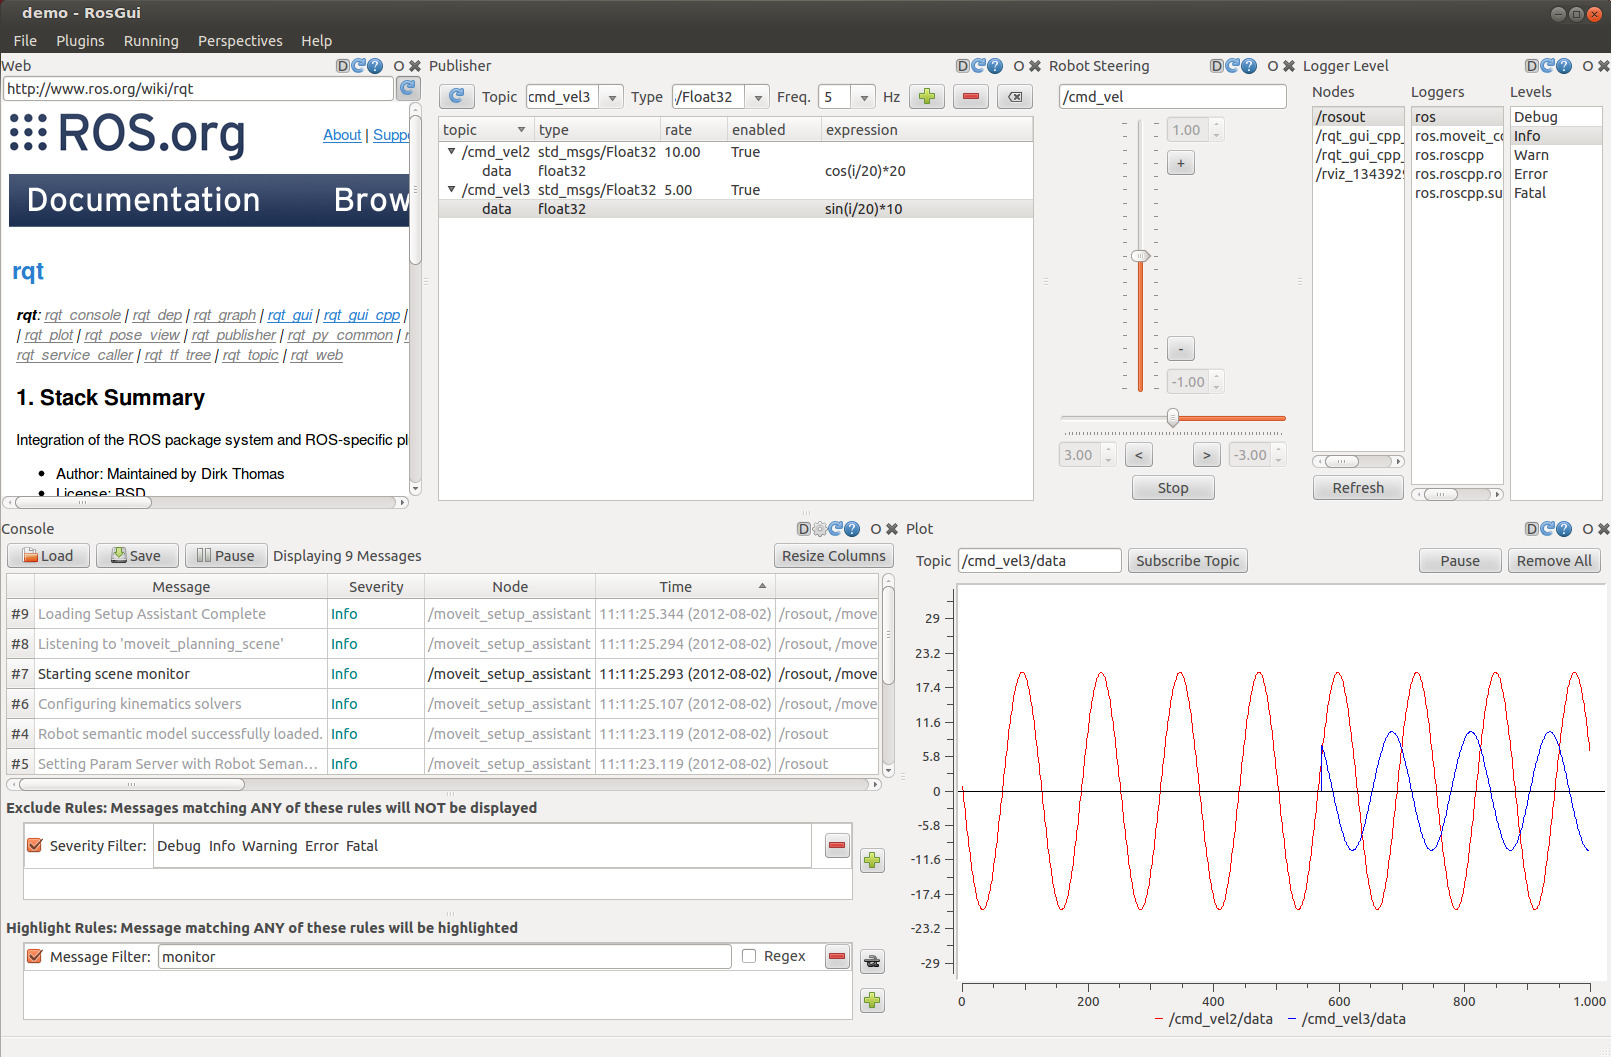
\includegraphics[width=\textwidth]{Figuras/2_revisao/ros_gui.png}
                \caption{Exemplo de ferramentas gráficas existentes no ROS.}
                \label{fig:ros_gui}
            \end{figure}
            
            Essas ferramentas são agrupadas em categorias. Entre elas estão: 
            
            \begin{itemize}
                \item \textbf{Configuração}: reune ferramentas relacionadas a execução e configuração de nós, os \textit{plugins} \textit{rqt\_launch}\footnote{\url{http://wiki.ros.org/rqt_launch}} e \textit{rqt\_reconfigure}\footnote{\url{http://wiki.ros.org/rqt_reconfigure}} são exemplos disso;
                
                \item \textbf{Introspecção}: junta \textit{plugins} para a análise do Grafo de Computação e das dependências entre pacotes;
                
                \item \textbf{\textit{Logging}}: agrupa ferramentas para alternar o nível de \textit{log} nos nós e para filtrar \textit{logs};
                
                \item \textbf{Tópicos}: são reunidas ferramentas diretamente relacionadas tópicos no ROS, como a publicação de mensagens, monitor de tópico e navegador para definições de mensagem;
                
                \item \textbf{Serviços}: cliente de serviços e navegador para definições de serviços, são exemplo de ferramentas relacionadas com serviços;
                
                \item \textbf{Visualização}: agrupa ferramentas que traçam gráficos de dados numéricos no tempo, mostram de imagens publicadas em tópicos e sistemas supervisórios, são exemplos de \textit{plugins} que pertencem a esta categoria \textit{rqt\_image\_view}\footnote{\url{http://wiki.ros.org/rqt_image_view}}, \textit{rqt\_multiplot}\footnote{\url{http://wiki.ros.org/rqt_multiplot}} e \textit{rqt\_rviz}\footnote{\url{http://wiki.ros.org/rqt_rviz}};
                
                \item e muitas outras.
            \end{itemize}
        
    \section{Trabalhos Relacionados} \label{sec:trabalhos_relacionados}
        \citeonline{ref:reis2015alliance} elaboraram uma aproximação da arquitetura ALLIANCE dedicada para uma aplicação de patrulhamento simulada. O enfoque desse trabalho foi mostrar os benefícios que o ROS oferece ao tratar aplicações de robôs heterogêneos: fácil comunicação entre robôs heterogêneos, a aplicação pode crescer adicionando novos robôs com poucas modificações e a reutilização de projetos desenvolvidos por outros pesquisadores.
        
        A fim de enfrentar os dois grandes desafios na criação de \textit{software} para sistema multirrobô: cooperação distribuída entre robôs e reusabilidade de aplicações em robótica, \citeonline{ref:li2016alliance} desenvolveram uma arquitetura tolerante à falhas para a cooperação em sistema multirrobô: ALLIANCE-ROS \footnote{\url{http://wiki.ros.org/micros_mars_task_alloc}}. Foram encapsulados os mecanismos do ROS e bibliotecas em Python para a criação das funções básicas da arquitetura ALLIANCE \cite{ref:parker1998alliance}. Deste modo, foram combinadas as vantagens da arquitetura ALLIANCE e do \textit{framework} ROS, pois forneceram os seguintes benefícios para os seus usuários: \textit{templates} para a descrição de comportamento e coordenação, métodos tolerantes à falhas para a alocação de tarefas em sistema multirrobô, vários módulos para o ROS e uma interface para programação em Python.
        
        \citeonline{ref:guidotti2017murdoch} criaram um pacote ROS\footnote{\url{https://github.com/caueguidotti/Murdoch}} para a arquitetura Murdoch, sugerida por \citeonline{ref:gerkey2002murdoch}, para ser utilizada em problemas de alocação de tarefa em sistema multirrobô. Foi disponibilizado uma interface de programação em C++ para a integração de cada robô licitante com o leilão gerenciado pelo leiloeiro da arquitetura. Para verificar a validade do pacote criado, foi simulado um sistema com 4 robôs 3 tarefas distintas para serem realizadas.
 
\chapter[Desenvolvimento]{Desenvolvimento} \label{cap:desenvolvimento}
    
    
        
    \section{ALLIANCE} \label{sec:alliance}
    
        Esta é uma arquitetura totalmente distribuída, tolerante à falhas, que visa atingir controle cooperativo e atender os requisitos de uma missão à ser desempenhada por um grupo de robôs heterogêneos \cite{ref:parker1998alliance}. Cada robô é modelado usando uma aproximação baseada em comportamentos. A partir do estado do ambiente e dos outros robôs cooperadores, uma configuração de comportamento é selecionada conforme sua respectiva função de realização de tarefa na camada de alto nível de abstração. Cada configuração de comportamento permite controlar os atuadores do robô em questão de um modo diferente.
        
        Sejam $R=\{r_1, r_2, \cdots, r_n\}$, o conjunto de $n$ robôs heterogêneos, e $A=\{a_1,a_2, \cdots,\allowbreak a_m\}$, o conjunto de $m$ sub-tarefas independentes que compõem uma dada missão. Na arquitetura ALLIANCE, cada robô $r_i$ possui um conjunto de $p$ configurações de comportamento, dado por $C_i=\{c_{i1}, c_{i2},\cdots, c_{ip}\}$. Cada configuração de comportamento fornece ao seu robô uma função de realização de tarefa em alto nível, conforme definido em \cite{ref:brooks1986robust}. Por fim, é possível saber qual tarefa em $A$ é executada por $r_i$ quando sua configuração de ativação $c_{ik}$ é ativa. Tal informação é obtida através da função $h_i(c_{ik})$, a qual pertence ao conjunto de $n$ funções $H : C_i \to A$, $H = \{h_1(c_{1k}),\allowbreak h_2(c_{2k}), \cdots, h_n(c_{nk})\}$.
        
        A ativação de uma dada configuração de comportamento $c_{ij}$ do robô $r_i$ para a execução da tarefa $h_i(c_{ij})$ em um dado instante, é dada pelo cálculo de motivação do seu comportamento motivacional. Por sua vez, cada comportamento motivacional possui um conjunto de módulos que têm a responsabilidade de monitorar alguma informação relevante sobre o sistema. A seguir, será detalhado o papel de cada uma desses módulos e suas contribuições para o cálculo de motivação.
        
        A primeira função, definida pela Equação \ref{eq:alliance_aplicavel}, tem como responsabilidade identificar quando a configuração de comportamento $c_{ij}$ é aplicável. Esta função lógica é implementada no módulo de \textit{feedback} sensorial, o qual observa constantemente as condições do ambiente por meio de sensores e, então, verifica se o sistema é favorecido se $c_{ij}$ estiver ativada.
        
        \begin{equation} \label{eq:alliance_aplicavel}
            aplic\acute{a}vel_{ij}(t) =
            \begin{cases}
                1, & \parbox[t]{.5\textwidth}{se o módulo de \textit{feedback} sensorial da configuração de comportamento $c_{ij}$ do robô $r_i$ indicar que esta configuração é aplicável mediante ao estado atual do ambiente no instante $t$;} \\
                0, & \text{caso contrário.}
            \end{cases}
        \end{equation}
        
        A Equação \ref{eq:alliance_inibida} mostra uma das funções lógicas que também compõe o cálculo para ativação de $c_{ij}$. Seu papel, neste cálculo, é garantir que o robô $r_i$ só tenha uma configuração de comportamento ativa por vez. Essa função é implementada pelo módulo de supressão, o qual observa a ativação das demais configurações de comportamento de $r_i$. 
        
        \begin{equation} \label{eq:alliance_inibida}
            inibida_{ij}(t) =
            \begin{cases}
                1, & \parbox[t]{.5\textwidth}{se outra configuração de comportamento $c_{ik}$ (com $k \neq j$) está ativa no robô $r_i$ no instante $t$;} \\
                0, & \text{caso contrário.}
            \end{cases}
        \end{equation}
        
        Cada configuração de comportamento $c_{ij}$ possui um módulo de comunicação que auxilia vários outros módulos de $c_{ij}$ por meio do monitoramento da comunicação entre os robôs do sistema. Este módulo mantém o histórico das atividades dos demais robôs do sistema no que diz respeito à execução da tarefa $h_i(c_{ij})$. Deste modo, os demais módulos de $c_{ij}$ podem consultar se os outros robôs estavam executando a tarefa $h_i(c_{ij})$ em um dado intervalo de tempo $[t_1; t_2]$, conforme mostra a Equação \ref{eq:alliance_recebida}. Existem dois parâmetros no ALLIANCE que influenciam diretamente no módulo de comunicação de cada comportamento motivacional. O primeiro parâmetro, $\rho_i$, define a frequência com que $r_i$ atualiza suas configurações de comportamento e publica seu estado atual, no que diz respeito à arquitetura. O segundo parâmetro, $\tau_i$, indica a duração de tempo máxima que o robô $r_i$ permite ficar sem receber mensagens do estado de qualquer outro robô do sistema. Quando esta duração é excedida para um dado robô $r_k$, o robô $r_i$ passa considerar que $r_k$ cessou sua atividade. A utilização deste parâmetro visa prever falhas de comunicação e de mal funcionamento.
        
        \begin{equation} \label{eq:alliance_recebida}
            recebida_{ij}(k, t_1, t_2) =
            \begin{cases}
                1, & \parbox[t]{.5\textwidth}{se o robô $r_i$ recebeu mensagem do robô $r_k$ referente à tarefa $h_i(c_{ij})$ dentro do intervalo de tempo $[t_1; t_2]$, em que $t_1 < t_2$;} \\
                0, & \text{caso contrário.}
            \end{cases}
        \end{equation}
        
        A próxima função tem a incumbência de reiniciar o cálculo para a ativação da configuração de comportamento $c_{ij}$. Essa função lógica é impulsionada apenas uma vez para cada robô que tenta executar a tarefa $h_i(c_{ij})$. Isto é, no instante em que acontece a primeira rampa de subida na Equação \ref{eq:alliance_recebida} para cada robô $r_k$, está função retorna um nível lógico alto. Essa condição evita que problemas de falhas persistentes não comprometam a completude da missão.
        %
        \begin{equation} \label{eq:alliance_reiniciada}
            reiniciada_{ij}(t) = \exists x, (recebida_{ij}(x, t - dt, t) \land \lnot recebida_{ij}(x, 0, t - dt))
        \end{equation}
        %
        onde $dt$ é o tempo decorrido desde a última verificação de comunicação.
        
        A Equação \ref{eq:alliance_ativa_intervalo} auxilia o módulo de aquiescência no cálculo de desistência para a desativação de $c_{ij}$. Baseando-se no histórico de ativação de $c_{ij}$, o módulo de comportamento motivacional disponibiliza essa função lógica que verifica se $c_{ij}$ ficou mantida ativa por um dado período de tempo até o instante desejado.
        
        \begin{equation} \label{eq:alliance_ativa_intervalo}
            ativa_{ij}(\Delta t, t) =
            \begin{cases}
                1, & \parbox[t]{.5\textwidth}{se a configuração de comportamento $c_{ij}$ do robô $r_i$ estiver ativa por mais de $\Delta t$ unidades de tempo no instante $t$;} \\
                0, & \text{caso contrário.}
            \end{cases}
        \end{equation}
        
        O módulo de aquiescência monitora o tempo decorrido após a ativação da configuração de comportamento $c_{ij}$ do robô $r_i$ com o auxílio da Equação \ref{eq:alliance_ativa_intervalo}. São duas as suas preocupações: (1) verificar se $c_{ij}$ permaneceu ativa por mais tempo que o esperado e (2) verificar se o tempo decorrido após um outro robô $r_k$ ter iniciado a execução da tarefa $h_i(c_{ij})$, enquanto $c_{ij}$ estava ativa, tenha excedido o tempo configurado para $r_i$ passar sua vez para esse outro robô. A Equação \ref{eq:alliance_aquiescente} define as condições em que $r_i$ está aquiescente à desativação de $c_{ij}$.
        %
        \begin{equation} \label{eq:alliance_aquiescente}
            \begin{aligned}
                aquiescente_{ij}(t) = \
                & (ativa_{ij}(\psi_{ij}(t), t) \land \exists x, recebida_{ij}(x, t - \tau_i, t)) \\
                & \lor ativa_{ij}(\lambda_{ij}(t), t)
            \end{aligned}
        \end{equation}
        %
        onde $\psi_{ij}(t)$ é a duração de tempo que $r_i$ deseja manter a configuração de comportamento $c_{ij}$ ativa antes de dar preferência para outro robô executar a tarefa $h_i(c_{ij})$; e $\lambda_{ij}(t)$ é a duração de tempo que $r_i$ deseja manter $c_{ij}$ ativa antes de desistir para possivelmente tentar outra configuração de comportamento.
        
        A impaciência de $r_i$ para a ativação de $c_{ij}$ cresce linearmente mediante a taxa de impaciência instantânea. Assim, o módulo de impaciência de $c_{ij}$ é responsável por identificar falhas de execução da tarefa $h_i(c_{ij})$ por outros robôs do sistema e quantificar a insatisfação de $r_i$ concernente à essa tarefa, conforme visto na Equação \ref{eq:alliance_impaciencia}. Para isso, três parâmetros são utilizados: (1) $\phi_{ij}(k, t)$, o qual estabelece o tempo máximo que $r_i$ permite a um outro robô $r_k$ executar a tarefa $h_i(c_{ij})$ antes dele próprio iniciar sua tentativa; (2) $\delta_{slow_{ij}}(k, t)$, que determina a taxa de impaciência do robô $r_i$ com respeito à configuração de comportamento $c_{ij}$ enquanto o robô $r_k$ está executando a tarefa correspondente à $c_{ij}$; e (3) $\delta_{fast_{ij}}(t)$, que determina a taxa de impaciência de $r_i$ com relação à $c_{ij}$ quando nenhum outro robô está executando a tarefa $h_i(c_{ij})$.
        %
        \begin{equation} \label{eq:alliance_impaciencia}
            impaci\hat{e}ncia_{ij}(t) =
            \begin{cases}
                \min\limits_{x}\delta_{slow_{ij}}(x, t), & \parbox[t]{.5\textwidth}{se $recebida_{ij}(x, t - \tau_i, t) \land \lnot recebida_{ij}(x, 0, t - \phi_{ij}(x, t)$;} \\
                \delta_{fast_{ij}}(t), & \text{caso contrário.}
            \end{cases}
        \end{equation}
        %
        Note que o método usado incrementa a motivação à uma taxa que permita que o robô mais lento $r_k$ continue sua tentativa de execução de $h(c_{ij})$, desde que seja respeitada a duração máxima estipulada pelo parâmetro $\phi_{ij}(k, t)$.
        
        A Equação \ref{eq:alliance_motivacao} mostra a função de motivação, a qual combina todas as funções mencionadas anteriormente para a ativação da configuração de comportamento $c_{ij}$. Seu valor inicial é nulo e aumenta mediante a taxa de impaciência instantânea de $r_i$ para ativar $c_{ij}$ quando satisfeitas as seguintes condições: (1) $c_{ij}$ seja aplicável, (2) mas não tenha sido inibida, (3) nem reiniciada; (4) e, ainda, $r_i$ não seja aquiescente em desistir de manter $c_{ij}$ ativa. Quando uma das condições citadas não é satisfeita, seu valor volta a ser nulo. 
        
        \begin{equation} \label{eq:alliance_motivacao}
            \begin{aligned}
                motiva\textit{ç}\tilde{a}o_{ij}(0) = \ & 0 \\
                motiva\textit{ç}\tilde{a}o_{ij}(t) = \ & (motiva\textit{ç}\tilde{a}o_{ij}(t - dt) + impaci\hat{e}ncia_{ij}(t)) \\
                & \times aplic\acute{a}vel_{ij}(t) \times inibida_{ij}(t) \\
                & \times reiniciada_{ij}(t) \times aquiescente_{ij}(t).
            \end{aligned}
        \end{equation}
        
        Assim que a motivação de $r_i$ para ativar $c_{ij}$ ultrapassa o limite de ativação, essa configuração de comportamento é ativada, conforme a Equação \ref{eq:alliance_ativa}:
        %
        \begin{equation} \label{eq:alliance_ativa}
            ativa_{ij}(t) = motiva\textit{ç}\tilde{a}o_{ij}(t) \geq \theta
        \end{equation}
        %
        onde $\theta$ é o limite de ativação.
        
        Fazendo uma análise das equações acima, verifica-se que, enquanto sua motivação cresce, é possível estimar quanto tempo resta para que a configuração de comportamento $c_{ij}$ se torne ativa. 
        %
        \begin{equation} \label{eq:alliance_estimativa_ativacao}
            \overline{\Delta t}_{ativa\textit{ç}\tilde{a}o_{ij}} = \frac{\theta - motiva\textit{ç}\tilde{a}o_{ij}(t)}{impaci\hat{e}ncia_{ij}(t) \rho_i}
        \end{equation}
        %
        onde $\rho_i$ é a frequência aproximada, em [\si{\hertz}], com que $r_i$ atualiza as motivação das configurações de comportamento em $C_i$ e, ainda, publica seu estado comportamental. Como a taxa de impaciência não é constante, a Equação \ref{eq:alliance_estimativa_ativacao} é apenas uma estimativa, dada em [\si{\second}].
        
        Em conformidade com o que foi exposto, pode-se observar que é possível normalizar todas as funções de motivação, de modo que a imagem de cada uma delas pertença ao intervalo $[0; 1] \subset \mathbb{R}_+$. Para isso, é necessário: (1) parametrizar o módulo de impaciência de cada configuração de comportamento $c_{ij}$, de maneira que a imagem da sua função de taxa de impaciência instantânea pertença ao intervalo $(0; 1) \subset \mathbb{R}_+^*$; além disso, (2) atribuir o valor unitário ao limite de ativação; bem como, (3) saturar a função de motivação no limite de ativação. Como resultado, as Equações \ref{eq:alliance_ativa} e \ref{eq:alliance_estimativa_ativacao} podem ser rescritas como as Equações \ref{eq:alliance_ativa_nova} e \ref{eq:alliance_estimativa_ativacao_nova}, respectivamente.
        
        \begin{equation} \label{eq:alliance_ativa_nova}
            ativa_{ij}(t) = motiva\textit{ç}\tilde{a}o_{ij}(t) == 1
        \end{equation}
        
        \begin{equation} \label{eq:alliance_estimativa_ativacao_nova}
            \overline{\Delta t}_{ativa\textit{ç}\tilde{a}o_{ij}} = \frac{1 - motiva\textit{ç}\tilde{a}o_{ij}(t)}{impaci\hat{e}ncia_{ij}(t) \rho_i}
        \end{equation}
        
        \citeonline{ref:parker1996lalliance} desenvolveu também uma variação do ALLIANCE, chamada L-ALLIANCE, capaz de estimar alguns parâmetros do ALLIANCE durante a fase de aprendizado.
        
        \textbf{\color{red} Classificar essa arquitetura segundo as taxonomias revisadas}
        
        \textbf{\color{red} Comentar sobre o motivo de ter falado sobre essa arquitetura com tanto detalhe}
        
        \pgfplotstableread[col sep=comma]{\detokenize{Figuras/capitulo_3/robot1-wander-motivation-new.csv}}\datatable
\begin{figure}[htb]
    \centering
    \begin{tikzpicture}
    \begin{groupplot}[
      group style={rows=6}, 
      width=0.75\textwidth,
      height=0.25\textwidth, 
      xmajorgrids, 
      ymajorgrids, 
      enlarge x limits=false,
    ] 
        \nextgroupplot[
        %title={Motivação da configuração de comportamento /robot1/wander.},
        ymin=-0.1,
        ylabel={$impaci\hat{e}ncia(t)$},
        ]
        \addplot[blue,line width=1pt] table[x index=0,y index=1]{\datatable}; 
        
        \nextgroupplot[
        ymin=-0.1,
        ymax=1.1,
        ylabel={$aquiescente(t)$},
        ] 
        \addplot[blue,line width=1pt] table[x index=0,y index=2]{\datatable}; 
        
        \nextgroupplot[
        ymin=-0.1,
        ymax=1.1,
        ylabel={$inibida(t)$},
        ] 
        \addplot[blue,line width=1pt] table[x index=0,y index=3]{\datatable}; 
        
        \nextgroupplot[
        ymin=-0.1,
        ymax=1.1,
        ylabel={$reiniciada(t)$},
        ] 
        \addplot[blue,line width=1pt] table[x index=0,y index=4]{\datatable}; 
        
        \nextgroupplot[
        ymin=-0.1,
        ymax=1.1,
        ylabel={$aplic\acute{a}vel(t)$},
        ] 
        \addplot[blue,line width=1pt] table[x index=0,y index=5]{\datatable};
        
        \nextgroupplot[
        ylabel={$motiva\textit{ç}\tilde{a}o(t)$},
        xlabel={$t [s]$}
        ] 
        \addplot[blue,line width=1pt] table[x index=0,y index=6]{\datatable};
    \end{groupplot}
\end{tikzpicture}
    \caption{Motivação da configuração de comportamento /robot1/wander.} \label{fig:motivacao1}
\end{figure}

\pgfplotstableread[col sep=comma]{\detokenize{Figuras/capitulo_3/robot2-wander-motivation-new.csv}}\datatable
\begin{figure}[htb]
    \centering
    \begin{tikzpicture}
    \begin{groupplot}[
      group style={rows=6}, 
      width=0.75\textwidth,
      height=0.25\textwidth, 
      xmajorgrids, 
      ymajorgrids, 
      enlarge x limits=false,
    ] 
        \nextgroupplot[
        %title={Motivação da configuração de comportamento /robot1/wander.},
        ymin=-0.1,
        ylabel={$impaci\hat{e}ncia(t)$},
        ]
        \addplot[blue,line width=1pt] table[x index=0,y index=1]{\datatable}; 
        
        \nextgroupplot[
        ymin=-0.1,
        ymax=1.1,
        ylabel={$aquiescente(t)$},
        ] 
        \addplot[blue,line width=1pt] table[x index=0,y index=2]{\datatable}; 
        
        \nextgroupplot[
        ymin=-0.1,
        ymax=1.1,
        ylabel={$inibida(t)$},
        ] 
        \addplot[blue,line width=1pt] table[x index=0,y index=3]{\datatable}; 
        
        \nextgroupplot[
        ymin=-0.1,
        ymax=1.1,
        ylabel={$reiniciada(t)$},
        ] 
        \addplot[blue,line width=1pt] table[x index=0,y index=4]{\datatable}; 
        
        \nextgroupplot[
        ymin=-0.1,
        ymax=1.1,
        ylabel={$aplic\acute{a}vel(t)$},
        ] 
        \addplot[blue,line width=1pt] table[x index=0,y index=5]{\datatable};
        
        \nextgroupplot[
        ylabel={$motiva\textit{ç}\tilde{a}o(t)$},
        xlabel={$t [s]$}
        ] 
        \addplot[blue,line width=1pt] table[x index=0,y index=6]{\datatable};
    \end{groupplot}
\end{tikzpicture}
    \caption{Motivação da configuração de comportamento /robot2/wander.} \label{fig:motivacao2}
\end{figure}

\pgfplotstableread[col sep=comma]{\detokenize{Figuras/capitulo_3/robot2-border-protection-motivation-new.csv}}\datatable
\begin{figure}[htb]
    \centering
    \begin{tikzpicture}
    \begin{groupplot}[
      group style={rows=6}, 
      width=0.75\textwidth,
      height=0.25\textwidth, 
      xmajorgrids, 
      ymajorgrids, 
      enlarge x limits=false,
    ] 
        \nextgroupplot[
        %title={Motivação da configuração de comportamento /robot1/wander.},
        ymin=-0.1,
        ylabel={$impaci\hat{e}ncia(t)$},
        ]
        \addplot[blue,line width=1pt] table[x index=0,y index=1]{\datatable}; 
        
        \nextgroupplot[
        ymin=-0.1,
        ymax=1.1,
        ylabel={$aquiescente(t)$},
        ] 
        \addplot[blue,line width=1pt] table[x index=0,y index=2]{\datatable}; 
        
        \nextgroupplot[
        ymin=-0.1,
        ymax=1.1,
        ylabel={$inibida(t)$},
        ] 
        \addplot[blue,line width=1pt] table[x index=0,y index=3]{\datatable}; 
        
        \nextgroupplot[
        ymin=-0.1,
        ymax=1.1,
        ylabel={$reiniciada(t)$},
        ] 
        \addplot[blue,line width=1pt] table[x index=0,y index=4]{\datatable}; 
        
        \nextgroupplot[
        ymin=-0.1,
        ymax=1.1,
        ylabel={$aplic\acute{a}vel(t)$},
        ] 
        \addplot[blue,line width=1pt] table[x index=0,y index=5]{\datatable};
        
        \nextgroupplot[
        ylabel={$motiva\textit{ç}\tilde{a}o(t)$},
        xlabel={$t [s]$}
        ] 
        \addplot[blue,line width=1pt] table[x index=0,y index=6]{\datatable};
    \end{groupplot}
\end{tikzpicture}
    \caption{Motivação da configuração de comportamento /robot2/border-protection.} \label{fig:motivacao3}
\end{figure}
        
        \begin{figure}[htb]
            \centering
            \resizebox{0.95\textwidth}{!}{% Graphic for TeX using PGF
% Title: ../figures/motivation/rosgraph_3robots.dia
% Creator: Dia v0.97.2
% CreationDate: Mon Oct 23 13:54:22 2017
% For: adrianohrl
% \usepackage{tikz}
% The following commands are not supported in PSTricks at present
% We define them conditionally, so when they are implemented,
% this pgf file will use them.
\ifx\du\undefined
  \newlength{\du}
\fi
\setlength{\du}{15\unitlength}
\begin{tikzpicture}
\pgftransformxscale{1.000000}
\pgftransformyscale{-1.000000}
\definecolor{dialinecolor}{rgb}{0.000000, 0.000000, 0.000000}
\pgfsetstrokecolor{dialinecolor}
\definecolor{dialinecolor}{rgb}{1.000000, 1.000000, 1.000000}
\pgfsetfillcolor{dialinecolor}
\pgfsetlinewidth{0.100000\du}
\pgfsetdash{}{0pt}
\pgfsetdash{}{0pt}
\pgfsetmiterjoin
\definecolor{dialinecolor}{rgb}{1.000000, 1.000000, 1.000000}
\pgfsetfillcolor{dialinecolor}
\fill (111.917000\du,23.178800\du)--(111.917000\du,26.984282\du)--(123.631466\du,26.984282\du)--(123.631466\du,23.178800\du)--cycle;
\definecolor{dialinecolor}{rgb}{0.000000, 0.000000, 0.000000}
\pgfsetstrokecolor{dialinecolor}
\draw (111.917000\du,23.178800\du)--(111.917000\du,26.984282\du)--(123.631466\du,26.984282\du)--(123.631466\du,23.178800\du)--cycle;
\pgfsetlinewidth{0.050000\du}
\pgfsetdash{}{0pt}
\pgfsetdash{}{0pt}
\pgfsetmiterjoin
\pgfsetbuttcap
{
\definecolor{dialinecolor}{rgb}{0.000000, 0.000000, 0.000000}
\pgfsetfillcolor{dialinecolor}
% was here!!!
\definecolor{dialinecolor}{rgb}{0.000000, 0.000000, 0.000000}
\pgfsetstrokecolor{dialinecolor}
\pgfpathmoveto{\pgfpoint{116.896000\du}{23.822200\du}}
\pgfpathcurveto{\pgfpoint{116.856000\du}{23.822200\du}}{\pgfpoint{116.827000\du}{23.829300\du}}{\pgfpoint{116.809000\du}{23.843300\du}}
\pgfpathcurveto{\pgfpoint{116.792000\du}{23.857400\du}}{\pgfpoint{116.783000\du}{23.878000\du}}{\pgfpoint{116.783000\du}{23.905000\du}}
\pgfpathcurveto{\pgfpoint{116.783000\du}{23.931600\du}}{\pgfpoint{116.790000\du}{23.950500\du}}{\pgfpoint{116.805000\du}{23.961700\du}}
\pgfpathcurveto{\pgfpoint{116.820000\du}{23.972900\du}}{\pgfpoint{116.837000\du}{23.978500\du}}{\pgfpoint{116.857000\du}{23.978500\du}}
\pgfpathcurveto{\pgfpoint{116.894000\du}{23.978500\du}}{\pgfpoint{116.921000\du}{23.962600\du}}{\pgfpoint{116.938000\du}{23.930800\du}}
\pgfpathcurveto{\pgfpoint{116.954000\du}{23.898500\du}}{\pgfpoint{116.963000\du}{23.868300\du}}{\pgfpoint{116.963000\du}{23.840200\du}}
\pgfpathcurveto{\pgfpoint{116.963000\du}{23.822200\du}}{\pgfpoint{116.963000\du}{23.840200\du}}{\pgfpoint{116.963000\du}{23.822200\du}}
\pgfpathcurveto{\pgfpoint{116.896000\du}{23.822200\du}}{\pgfpoint{116.963000\du}{23.822200\du}}{\pgfpoint{116.896000\du}{23.822200\du}}
\pgfusepath{stroke}
}
\pgfsetlinewidth{0.050000\du}
\pgfsetdash{}{0pt}
\pgfsetdash{}{0pt}
\pgfsetmiterjoin
\pgfsetbuttcap
{
\definecolor{dialinecolor}{rgb}{0.000000, 0.000000, 0.000000}
\pgfsetfillcolor{dialinecolor}
% was here!!!
\definecolor{dialinecolor}{rgb}{0.000000, 0.000000, 0.000000}
\pgfsetstrokecolor{dialinecolor}
\pgfpathmoveto{\pgfpoint{116.988000\du}{23.819900\du}}
\pgfpathcurveto{\pgfpoint{116.988000\du}{23.991800\du}}{\pgfpoint{116.988000\du}{23.819900\du}}{\pgfpoint{116.988000\du}{23.991800\du}}
\pgfpathcurveto{\pgfpoint{116.963000\du}{23.991800\du}}{\pgfpoint{116.988000\du}{23.991800\du}}{\pgfpoint{116.963000\du}{23.991800\du}}
\pgfpathcurveto{\pgfpoint{116.963000\du}{23.909700\du}}{\pgfpoint{116.963000\du}{23.991800\du}}{\pgfpoint{116.963000\du}{23.909700\du}}
\pgfpathcurveto{\pgfpoint{116.949000\du}{23.949800\du}}{\pgfpoint{116.931000\du}{23.975400\du}}{\pgfpoint{116.908000\du}{23.986300\du}}
\pgfpathcurveto{\pgfpoint{116.890000\du}{23.995200\du}}{\pgfpoint{116.872000\du}{23.999600\du}}{\pgfpoint{116.854000\du}{23.999600\du}}
\pgfpathcurveto{\pgfpoint{116.825000\du}{23.999600\du}}{\pgfpoint{116.801000\du}{23.991500\du}}{\pgfpoint{116.784000\du}{23.975400\du}}
\pgfpathcurveto{\pgfpoint{116.767000\du}{23.959200\du}}{\pgfpoint{116.758000\du}{23.935600\du}}{\pgfpoint{116.758000\du}{23.904700\du}}
\pgfpathcurveto{\pgfpoint{116.758000\du}{23.873700\du}}{\pgfpoint{116.769000\du}{23.848800\du}}{\pgfpoint{116.792000\du}{23.830000\du}}
\pgfpathcurveto{\pgfpoint{116.814000\du}{23.811300\du}}{\pgfpoint{116.851000\du}{23.801900\du}}{\pgfpoint{116.901000\du}{23.801900\du}}
\pgfpathcurveto{\pgfpoint{116.963000\du}{23.801900\du}}{\pgfpoint{116.901000\du}{23.801900\du}}{\pgfpoint{116.963000\du}{23.801900\du}}
\pgfpathcurveto{\pgfpoint{116.963000\du}{23.797200\du}}{\pgfpoint{116.963000\du}{23.801900\du}}{\pgfpoint{116.963000\du}{23.797200\du}}
\pgfpathcurveto{\pgfpoint{116.963000\du}{23.770700\du}}{\pgfpoint{116.955000\du}{23.748800\du}}{\pgfpoint{116.939000\du}{23.731600\du}}
\pgfpathcurveto{\pgfpoint{116.925000\du}{23.714400\du}}{\pgfpoint{116.900000\du}{23.705800\du}}{\pgfpoint{116.865000\du}{23.705800\du}}
\pgfpathcurveto{\pgfpoint{116.848000\du}{23.705800\du}}{\pgfpoint{116.831000\du}{23.709000\du}}{\pgfpoint{116.813000\du}{23.715200\du}}
\pgfpathcurveto{\pgfpoint{116.801000\du}{23.719400\du}}{\pgfpoint{116.786000\du}{23.727700\du}}{\pgfpoint{116.768000\du}{23.740200\du}}
\pgfpathcurveto{\pgfpoint{116.768000\du}{23.713600\du}}{\pgfpoint{116.768000\du}{23.740200\du}}{\pgfpoint{116.768000\du}{23.713600\du}}
\pgfpathcurveto{\pgfpoint{116.784000\du}{23.703700\du}}{\pgfpoint{116.799000\du}{23.696700\du}}{\pgfpoint{116.813000\du}{23.692500\du}}
\pgfpathcurveto{\pgfpoint{116.833000\du}{23.686800\du}}{\pgfpoint{116.852000\du}{23.684000\du}}{\pgfpoint{116.870000\du}{23.684000\du}}
\pgfpathcurveto{\pgfpoint{116.906000\du}{23.684000\du}}{\pgfpoint{116.935000\du}{23.694600\du}}{\pgfpoint{116.958000\du}{23.716000\du}}
\pgfpathcurveto{\pgfpoint{116.978000\du}{23.734200\du}}{\pgfpoint{116.988000\du}{23.768900\du}}{\pgfpoint{116.988000\du}{23.819900\du}}
\pgfusepath{stroke}
}
\pgfsetlinewidth{0.050000\du}
\pgfsetdash{}{0pt}
\pgfsetdash{}{0pt}
\pgfsetmiterjoin
\pgfsetbuttcap
{
\definecolor{dialinecolor}{rgb}{0.000000, 0.000000, 0.000000}
\pgfsetfillcolor{dialinecolor}
% was here!!!
\definecolor{dialinecolor}{rgb}{0.000000, 0.000000, 0.000000}
\pgfsetstrokecolor{dialinecolor}
\pgfpathmoveto{\pgfpoint{117.112000\du}{23.573800\du}}
\pgfpathcurveto{\pgfpoint{117.136000\du}{23.573800\du}}{\pgfpoint{117.112000\du}{23.573800\du}}{\pgfpoint{117.136000\du}{23.573800\du}}
\pgfpathcurveto{\pgfpoint{117.136000\du}{23.991800\du}}{\pgfpoint{117.136000\du}{23.573800\du}}{\pgfpoint{117.136000\du}{23.991800\du}}
\pgfpathcurveto{\pgfpoint{117.112000\du}{23.991800\du}}{\pgfpoint{117.136000\du}{23.991800\du}}{\pgfpoint{117.112000\du}{23.991800\du}}
\pgfpathcurveto{\pgfpoint{117.112000\du}{23.573800\du}}{\pgfpoint{117.112000\du}{23.991800\du}}{\pgfpoint{117.112000\du}{23.573800\du}}
\pgfusepath{stroke}
}
\pgfsetlinewidth{0.050000\du}
\pgfsetdash{}{0pt}
\pgfsetdash{}{0pt}
\pgfsetmiterjoin
\pgfsetbuttcap
{
\definecolor{dialinecolor}{rgb}{0.000000, 0.000000, 0.000000}
\pgfsetfillcolor{dialinecolor}
% was here!!!
\definecolor{dialinecolor}{rgb}{0.000000, 0.000000, 0.000000}
\pgfsetstrokecolor{dialinecolor}
\pgfpathmoveto{\pgfpoint{117.264000\du}{23.573800\du}}
\pgfpathcurveto{\pgfpoint{117.289000\du}{23.573800\du}}{\pgfpoint{117.264000\du}{23.573800\du}}{\pgfpoint{117.289000\du}{23.573800\du}}
\pgfpathcurveto{\pgfpoint{117.289000\du}{23.991800\du}}{\pgfpoint{117.289000\du}{23.573800\du}}{\pgfpoint{117.289000\du}{23.991800\du}}
\pgfpathcurveto{\pgfpoint{117.264000\du}{23.991800\du}}{\pgfpoint{117.289000\du}{23.991800\du}}{\pgfpoint{117.264000\du}{23.991800\du}}
\pgfpathcurveto{\pgfpoint{117.264000\du}{23.573800\du}}{\pgfpoint{117.264000\du}{23.991800\du}}{\pgfpoint{117.264000\du}{23.573800\du}}
\pgfusepath{stroke}
}
\pgfsetlinewidth{0.050000\du}
\pgfsetdash{}{0pt}
\pgfsetdash{}{0pt}
\pgfsetmiterjoin
\pgfsetbuttcap
{
\definecolor{dialinecolor}{rgb}{0.000000, 0.000000, 0.000000}
\pgfsetfillcolor{dialinecolor}
% was here!!!
\definecolor{dialinecolor}{rgb}{0.000000, 0.000000, 0.000000}
\pgfsetstrokecolor{dialinecolor}
\pgfpathmoveto{\pgfpoint{117.416000\du}{23.691000\du}}
\pgfpathcurveto{\pgfpoint{117.441000\du}{23.691000\du}}{\pgfpoint{117.416000\du}{23.691000\du}}{\pgfpoint{117.441000\du}{23.691000\du}}
\pgfpathcurveto{\pgfpoint{117.441000\du}{23.991800\du}}{\pgfpoint{117.441000\du}{23.691000\du}}{\pgfpoint{117.441000\du}{23.991800\du}}
\pgfpathcurveto{\pgfpoint{117.416000\du}{23.991800\du}}{\pgfpoint{117.441000\du}{23.991800\du}}{\pgfpoint{117.416000\du}{23.991800\du}}
\pgfpathcurveto{\pgfpoint{117.416000\du}{23.691000\du}}{\pgfpoint{117.416000\du}{23.991800\du}}{\pgfpoint{117.416000\du}{23.691000\du}}
\pgfusepath{stroke}
}
\pgfsetlinewidth{0.050000\du}
\pgfsetdash{}{0pt}
\pgfsetdash{}{0pt}
\pgfsetmiterjoin
\pgfsetbuttcap
{
\definecolor{dialinecolor}{rgb}{0.000000, 0.000000, 0.000000}
\pgfsetfillcolor{dialinecolor}
% was here!!!
\definecolor{dialinecolor}{rgb}{0.000000, 0.000000, 0.000000}
\pgfsetstrokecolor{dialinecolor}
\pgfpathmoveto{\pgfpoint{117.416000\du}{23.573800\du}}
\pgfpathcurveto{\pgfpoint{117.441000\du}{23.573800\du}}{\pgfpoint{117.416000\du}{23.573800\du}}{\pgfpoint{117.441000\du}{23.573800\du}}
\pgfpathcurveto{\pgfpoint{117.441000\du}{23.607400\du}}{\pgfpoint{117.441000\du}{23.573800\du}}{\pgfpoint{117.441000\du}{23.607400\du}}
\pgfpathcurveto{\pgfpoint{117.416000\du}{23.607400\du}}{\pgfpoint{117.441000\du}{23.607400\du}}{\pgfpoint{117.416000\du}{23.607400\du}}
\pgfpathcurveto{\pgfpoint{117.416000\du}{23.573800\du}}{\pgfpoint{117.416000\du}{23.607400\du}}{\pgfpoint{117.416000\du}{23.573800\du}}
\pgfusepath{stroke}
}
\pgfsetlinewidth{0.050000\du}
\pgfsetdash{}{0pt}
\pgfsetdash{}{0pt}
\pgfsetmiterjoin
\pgfsetbuttcap
{
\definecolor{dialinecolor}{rgb}{0.000000, 0.000000, 0.000000}
\pgfsetfillcolor{dialinecolor}
% was here!!!
\definecolor{dialinecolor}{rgb}{0.000000, 0.000000, 0.000000}
\pgfsetstrokecolor{dialinecolor}
\pgfpathmoveto{\pgfpoint{117.689000\du}{23.822200\du}}
\pgfpathcurveto{\pgfpoint{117.649000\du}{23.822200\du}}{\pgfpoint{117.620000\du}{23.829300\du}}{\pgfpoint{117.603000\du}{23.843300\du}}
\pgfpathcurveto{\pgfpoint{117.586000\du}{23.857400\du}}{\pgfpoint{117.577000\du}{23.878000\du}}{\pgfpoint{117.577000\du}{23.905000\du}}
\pgfpathcurveto{\pgfpoint{117.577000\du}{23.931600\du}}{\pgfpoint{117.584000\du}{23.950500\du}}{\pgfpoint{117.599000\du}{23.961700\du}}
\pgfpathcurveto{\pgfpoint{117.613000\du}{23.972900\du}}{\pgfpoint{117.631000\du}{23.978500\du}}{\pgfpoint{117.650000\du}{23.978500\du}}
\pgfpathcurveto{\pgfpoint{117.688000\du}{23.978500\du}}{\pgfpoint{117.715000\du}{23.962600\du}}{\pgfpoint{117.732000\du}{23.930800\du}}
\pgfpathcurveto{\pgfpoint{117.748000\du}{23.898500\du}}{\pgfpoint{117.757000\du}{23.868300\du}}{\pgfpoint{117.757000\du}{23.840200\du}}
\pgfpathcurveto{\pgfpoint{117.757000\du}{23.822200\du}}{\pgfpoint{117.757000\du}{23.840200\du}}{\pgfpoint{117.757000\du}{23.822200\du}}
\pgfpathcurveto{\pgfpoint{117.689000\du}{23.822200\du}}{\pgfpoint{117.757000\du}{23.822200\du}}{\pgfpoint{117.689000\du}{23.822200\du}}
\pgfusepath{stroke}
}
\pgfsetlinewidth{0.050000\du}
\pgfsetdash{}{0pt}
\pgfsetdash{}{0pt}
\pgfsetmiterjoin
\pgfsetbuttcap
{
\definecolor{dialinecolor}{rgb}{0.000000, 0.000000, 0.000000}
\pgfsetfillcolor{dialinecolor}
% was here!!!
\definecolor{dialinecolor}{rgb}{0.000000, 0.000000, 0.000000}
\pgfsetstrokecolor{dialinecolor}
\pgfpathmoveto{\pgfpoint{117.782000\du}{23.819900\du}}
\pgfpathcurveto{\pgfpoint{117.782000\du}{23.991800\du}}{\pgfpoint{117.782000\du}{23.819900\du}}{\pgfpoint{117.782000\du}{23.991800\du}}
\pgfpathcurveto{\pgfpoint{117.757000\du}{23.991800\du}}{\pgfpoint{117.782000\du}{23.991800\du}}{\pgfpoint{117.757000\du}{23.991800\du}}
\pgfpathcurveto{\pgfpoint{117.757000\du}{23.909700\du}}{\pgfpoint{117.757000\du}{23.991800\du}}{\pgfpoint{117.757000\du}{23.909700\du}}
\pgfpathcurveto{\pgfpoint{117.743000\du}{23.949800\du}}{\pgfpoint{117.725000\du}{23.975400\du}}{\pgfpoint{117.702000\du}{23.986300\du}}
\pgfpathcurveto{\pgfpoint{117.684000\du}{23.995200\du}}{\pgfpoint{117.666000\du}{23.999600\du}}{\pgfpoint{117.648000\du}{23.999600\du}}
\pgfpathcurveto{\pgfpoint{117.618000\du}{23.999600\du}}{\pgfpoint{117.595000\du}{23.991500\du}}{\pgfpoint{117.578000\du}{23.975400\du}}
\pgfpathcurveto{\pgfpoint{117.560000\du}{23.959200\du}}{\pgfpoint{117.552000\du}{23.935600\du}}{\pgfpoint{117.552000\du}{23.904700\du}}
\pgfpathcurveto{\pgfpoint{117.552000\du}{23.873700\du}}{\pgfpoint{117.563000\du}{23.848800\du}}{\pgfpoint{117.585000\du}{23.830000\du}}
\pgfpathcurveto{\pgfpoint{117.608000\du}{23.811300\du}}{\pgfpoint{117.644000\du}{23.801900\du}}{\pgfpoint{117.695000\du}{23.801900\du}}
\pgfpathcurveto{\pgfpoint{117.757000\du}{23.801900\du}}{\pgfpoint{117.695000\du}{23.801900\du}}{\pgfpoint{117.757000\du}{23.801900\du}}
\pgfpathcurveto{\pgfpoint{117.757000\du}{23.797200\du}}{\pgfpoint{117.757000\du}{23.801900\du}}{\pgfpoint{117.757000\du}{23.797200\du}}
\pgfpathcurveto{\pgfpoint{117.757000\du}{23.770700\du}}{\pgfpoint{117.749000\du}{23.748800\du}}{\pgfpoint{117.733000\du}{23.731600\du}}
\pgfpathcurveto{\pgfpoint{117.719000\du}{23.714400\du}}{\pgfpoint{117.694000\du}{23.705800\du}}{\pgfpoint{117.659000\du}{23.705800\du}}
\pgfpathcurveto{\pgfpoint{117.642000\du}{23.705800\du}}{\pgfpoint{117.624000\du}{23.709000\du}}{\pgfpoint{117.607000\du}{23.715200\du}}
\pgfpathcurveto{\pgfpoint{117.595000\du}{23.719400\du}}{\pgfpoint{117.580000\du}{23.727700\du}}{\pgfpoint{117.561000\du}{23.740200\du}}
\pgfpathcurveto{\pgfpoint{117.561000\du}{23.713600\du}}{\pgfpoint{117.561000\du}{23.740200\du}}{\pgfpoint{117.561000\du}{23.713600\du}}
\pgfpathcurveto{\pgfpoint{117.577000\du}{23.703700\du}}{\pgfpoint{117.593000\du}{23.696700\du}}{\pgfpoint{117.607000\du}{23.692500\du}}
\pgfpathcurveto{\pgfpoint{117.626000\du}{23.686800\du}}{\pgfpoint{117.645000\du}{23.684000\du}}{\pgfpoint{117.664000\du}{23.684000\du}}
\pgfpathcurveto{\pgfpoint{117.700000\du}{23.684000\du}}{\pgfpoint{117.729000\du}{23.694600\du}}{\pgfpoint{117.752000\du}{23.716000\du}}
\pgfpathcurveto{\pgfpoint{117.772000\du}{23.734200\du}}{\pgfpoint{117.782000\du}{23.768900\du}}{\pgfpoint{117.782000\du}{23.819900\du}}
\pgfusepath{stroke}
}
\pgfsetlinewidth{0.050000\du}
\pgfsetdash{}{0pt}
\pgfsetdash{}{0pt}
\pgfsetmiterjoin
\pgfsetbuttcap
{
\definecolor{dialinecolor}{rgb}{0.000000, 0.000000, 0.000000}
\pgfsetfillcolor{dialinecolor}
% was here!!!
\definecolor{dialinecolor}{rgb}{0.000000, 0.000000, 0.000000}
\pgfsetstrokecolor{dialinecolor}
\pgfpathmoveto{\pgfpoint{118.133000\du}{23.810500\du}}
\pgfpathcurveto{\pgfpoint{118.133000\du}{23.991800\du}}{\pgfpoint{118.133000\du}{23.810500\du}}{\pgfpoint{118.133000\du}{23.991800\du}}
\pgfpathcurveto{\pgfpoint{118.108000\du}{23.991800\du}}{\pgfpoint{118.133000\du}{23.991800\du}}{\pgfpoint{118.108000\du}{23.991800\du}}
\pgfpathcurveto{\pgfpoint{118.108000\du}{23.812100\du}}{\pgfpoint{118.108000\du}{23.991800\du}}{\pgfpoint{118.108000\du}{23.812100\du}}
\pgfpathcurveto{\pgfpoint{118.108000\du}{23.773000\du}}{\pgfpoint{118.102000\du}{23.745500\du}}{\pgfpoint{118.089000\du}{23.729700\du}}
\pgfpathcurveto{\pgfpoint{118.077000\du}{23.713800\du}}{\pgfpoint{118.058000\du}{23.705800\du}}{\pgfpoint{118.034000\du}{23.705800\du}}
\pgfpathcurveto{\pgfpoint{118.005000\du}{23.705800\du}}{\pgfpoint{117.981000\du}{23.714400\du}}{\pgfpoint{117.961000\du}{23.731600\du}}
\pgfpathcurveto{\pgfpoint{117.940000\du}{23.748800\du}}{\pgfpoint{117.930000\du}{23.778700\du}}{\pgfpoint{117.930000\du}{23.821500\du}}
\pgfpathcurveto{\pgfpoint{117.930000\du}{23.991800\du}}{\pgfpoint{117.930000\du}{23.821500\du}}{\pgfpoint{117.930000\du}{23.991800\du}}
\pgfpathcurveto{\pgfpoint{117.906000\du}{23.991800\du}}{\pgfpoint{117.930000\du}{23.991800\du}}{\pgfpoint{117.906000\du}{23.991800\du}}
\pgfpathcurveto{\pgfpoint{117.906000\du}{23.691000\du}}{\pgfpoint{117.906000\du}{23.991800\du}}{\pgfpoint{117.906000\du}{23.691000\du}}
\pgfpathcurveto{\pgfpoint{117.930000\du}{23.691000\du}}{\pgfpoint{117.906000\du}{23.691000\du}}{\pgfpoint{117.930000\du}{23.691000\du}}
\pgfpathcurveto{\pgfpoint{117.930000\du}{23.747200\du}}{\pgfpoint{117.930000\du}{23.691000\du}}{\pgfpoint{117.930000\du}{23.747200\du}}
\pgfpathcurveto{\pgfpoint{117.939000\du}{23.729000\du}}{\pgfpoint{117.951000\du}{23.715200\du}}{\pgfpoint{117.965000\du}{23.705800\du}}
\pgfpathcurveto{\pgfpoint{117.986000\du}{23.691200\du}}{\pgfpoint{118.009000\du}{23.684000\du}}{\pgfpoint{118.035000\du}{23.684000\du}}
\pgfpathcurveto{\pgfpoint{118.065000\du}{23.684000\du}}{\pgfpoint{118.089000\du}{23.694100\du}}{\pgfpoint{118.107000\du}{23.714400\du}}
\pgfpathcurveto{\pgfpoint{118.124000\du}{23.734200\du}}{\pgfpoint{118.133000\du}{23.766200\du}}{\pgfpoint{118.133000\du}{23.810500\du}}
\pgfusepath{stroke}
}
\pgfsetlinewidth{0.050000\du}
\pgfsetdash{}{0pt}
\pgfsetdash{}{0pt}
\pgfsetmiterjoin
\pgfsetbuttcap
{
\definecolor{dialinecolor}{rgb}{0.000000, 0.000000, 0.000000}
\pgfsetfillcolor{dialinecolor}
% was here!!!
\definecolor{dialinecolor}{rgb}{0.000000, 0.000000, 0.000000}
\pgfsetstrokecolor{dialinecolor}
\pgfpathmoveto{\pgfpoint{118.460000\du}{23.705800\du}}
\pgfpathcurveto{\pgfpoint{118.460000\du}{23.731600\du}}{\pgfpoint{118.460000\du}{23.705800\du}}{\pgfpoint{118.460000\du}{23.731600\du}}
\pgfpathcurveto{\pgfpoint{118.445000\du}{23.722800\du}}{\pgfpoint{118.433000\du}{23.716800\du}}{\pgfpoint{118.423000\du}{23.713600\du}}
\pgfpathcurveto{\pgfpoint{118.406000\du}{23.708400\du}}{\pgfpoint{118.390000\du}{23.705800\du}}{\pgfpoint{118.375000\du}{23.705800\du}}
\pgfpathcurveto{\pgfpoint{118.332000\du}{23.705800\du}}{\pgfpoint{118.301000\du}{23.716900\du}}{\pgfpoint{118.282000\du}{23.739000\du}}
\pgfpathcurveto{\pgfpoint{118.264000\du}{23.761200\du}}{\pgfpoint{118.254000\du}{23.795400\du}}{\pgfpoint{118.254000\du}{23.841800\du}}
\pgfpathcurveto{\pgfpoint{118.254000\du}{23.888600\du}}{\pgfpoint{118.264000\du}{23.923100\du}}{\pgfpoint{118.282000\du}{23.945300\du}}
\pgfpathcurveto{\pgfpoint{118.301000\du}{23.967400\du}}{\pgfpoint{118.332000\du}{23.978500\du}}{\pgfpoint{118.375000\du}{23.978500\du}}
\pgfpathcurveto{\pgfpoint{118.390000\du}{23.978500\du}}{\pgfpoint{118.404000\du}{23.976400\du}}{\pgfpoint{118.418000\du}{23.972200\du}}
\pgfpathcurveto{\pgfpoint{118.432000\du}{23.968600\du}}{\pgfpoint{118.446000\du}{23.962900\du}}{\pgfpoint{118.460000\du}{23.955000\du}}
\pgfpathcurveto{\pgfpoint{118.460000\du}{23.980000\du}}{\pgfpoint{118.460000\du}{23.955000\du}}{\pgfpoint{118.460000\du}{23.980000\du}}
\pgfpathcurveto{\pgfpoint{118.446000\du}{23.986800\du}}{\pgfpoint{118.432000\du}{23.991800\du}}{\pgfpoint{118.418000\du}{23.994900\du}}
\pgfpathcurveto{\pgfpoint{118.402000\du}{23.998000\du}}{\pgfpoint{118.388000\du}{23.999600\du}}{\pgfpoint{118.373000\du}{23.999600\du}}
\pgfpathcurveto{\pgfpoint{118.329000\du}{23.999600\du}}{\pgfpoint{118.294000\du}{23.987600\du}}{\pgfpoint{118.268000\du}{23.963600\du}}
\pgfpathcurveto{\pgfpoint{118.242000\du}{23.939700\du}}{\pgfpoint{118.229000\du}{23.898900\du}}{\pgfpoint{118.229000\du}{23.841400\du}}
\pgfpathcurveto{\pgfpoint{118.229000\du}{23.783800\du}}{\pgfpoint{118.242000\du}{23.743100\du}}{\pgfpoint{118.268000\du}{23.719100\du}}
\pgfpathcurveto{\pgfpoint{118.294000\du}{23.695700\du}}{\pgfpoint{118.329000\du}{23.684000\du}}{\pgfpoint{118.373000\du}{23.684000\du}}
\pgfpathcurveto{\pgfpoint{118.388000\du}{23.684000\du}}{\pgfpoint{118.403000\du}{23.686000\du}}{\pgfpoint{118.419000\du}{23.690200\du}}
\pgfpathcurveto{\pgfpoint{118.435000\du}{23.693900\du}}{\pgfpoint{118.449000\du}{23.699100\du}}{\pgfpoint{118.460000\du}{23.705800\du}}
\pgfusepath{stroke}
}
\pgfsetlinewidth{0.050000\du}
\pgfsetdash{}{0pt}
\pgfsetdash{}{0pt}
\pgfsetmiterjoin
\pgfsetbuttcap
{
\definecolor{dialinecolor}{rgb}{0.000000, 0.000000, 0.000000}
\pgfsetfillcolor{dialinecolor}
% was here!!!
\definecolor{dialinecolor}{rgb}{0.000000, 0.000000, 0.000000}
\pgfsetstrokecolor{dialinecolor}
\pgfpathmoveto{\pgfpoint{118.791000\du}{23.829300\du}}
\pgfpathcurveto{\pgfpoint{118.791000\du}{23.844900\du}}{\pgfpoint{118.791000\du}{23.829300\du}}{\pgfpoint{118.791000\du}{23.844900\du}}
\pgfpathcurveto{\pgfpoint{118.563000\du}{23.844900\du}}{\pgfpoint{118.791000\du}{23.844900\du}}{\pgfpoint{118.563000\du}{23.844900\du}}
\pgfpathcurveto{\pgfpoint{118.563000\du}{23.892800\du}}{\pgfpoint{118.572000\du}{23.926700\du}}{\pgfpoint{118.591000\du}{23.946500\du}}
\pgfpathcurveto{\pgfpoint{118.612000\du}{23.967800\du}}{\pgfpoint{118.643000\du}{23.978500\du}}{\pgfpoint{118.683000\du}{23.978500\du}}
\pgfpathcurveto{\pgfpoint{118.694000\du}{23.978500\du}}{\pgfpoint{118.708000\du}{23.976100\du}}{\pgfpoint{118.726000\du}{23.971500\du}}
\pgfpathcurveto{\pgfpoint{118.744000\du}{23.966800\du}}{\pgfpoint{118.762000\du}{23.959700\du}}{\pgfpoint{118.779000\du}{23.950400\du}}
\pgfpathcurveto{\pgfpoint{118.779000\du}{23.976100\du}}{\pgfpoint{118.779000\du}{23.950400\du}}{\pgfpoint{118.779000\du}{23.976100\du}}
\pgfpathcurveto{\pgfpoint{118.762000\du}{23.984000\du}}{\pgfpoint{118.743000\du}{23.989800\du}}{\pgfpoint{118.725000\du}{23.993700\du}}
\pgfpathcurveto{\pgfpoint{118.706000\du}{23.997600\du}}{\pgfpoint{118.692000\du}{23.999600\du}}{\pgfpoint{118.681000\du}{23.999600\du}}
\pgfpathcurveto{\pgfpoint{118.634000\du}{23.999600\du}}{\pgfpoint{118.600000\du}{23.987100\du}}{\pgfpoint{118.576000\du}{23.962100\du}}
\pgfpathcurveto{\pgfpoint{118.551000\du}{23.935500\du}}{\pgfpoint{118.538000\du}{23.896500\du}}{\pgfpoint{118.538000\du}{23.844900\du}}
\pgfpathcurveto{\pgfpoint{118.538000\du}{23.791200\du}}{\pgfpoint{118.549000\du}{23.751100\du}}{\pgfpoint{118.572000\du}{23.724600\du}}
\pgfpathcurveto{\pgfpoint{118.596000\du}{23.697500\du}}{\pgfpoint{118.629000\du}{23.684000\du}}{\pgfpoint{118.672000\du}{23.684000\du}}
\pgfpathcurveto{\pgfpoint{118.711000\du}{23.684000\du}}{\pgfpoint{118.741000\du}{23.697000\du}}{\pgfpoint{118.761000\du}{23.723000\du}}
\pgfpathcurveto{\pgfpoint{118.781000\du}{23.750100\du}}{\pgfpoint{118.791000\du}{23.785500\du}}{\pgfpoint{118.791000\du}{23.829300\du}}
\pgfusepath{stroke}
}
\pgfsetlinewidth{0.050000\du}
\pgfsetdash{}{0pt}
\pgfsetdash{}{0pt}
\pgfsetmiterjoin
\pgfsetbuttcap
{
\definecolor{dialinecolor}{rgb}{0.000000, 0.000000, 0.000000}
\pgfsetfillcolor{dialinecolor}
% was here!!!
\definecolor{dialinecolor}{rgb}{0.000000, 0.000000, 0.000000}
\pgfsetstrokecolor{dialinecolor}
\pgfpathmoveto{\pgfpoint{118.766000\du}{23.823800\du}}
\pgfpathcurveto{\pgfpoint{118.766000\du}{23.781600\du}}{\pgfpoint{118.756000\du}{23.750900\du}}{\pgfpoint{118.737000\du}{23.731600\du}}
\pgfpathcurveto{\pgfpoint{118.721000\du}{23.714400\du}}{\pgfpoint{118.700000\du}{23.705800\du}}{\pgfpoint{118.672000\du}{23.705800\du}}
\pgfpathcurveto{\pgfpoint{118.643000\du}{23.705800\du}}{\pgfpoint{118.618000\du}{23.714700\du}}{\pgfpoint{118.597000\du}{23.732400\du}}
\pgfpathcurveto{\pgfpoint{118.578000\du}{23.749100\du}}{\pgfpoint{118.567000\du}{23.779500\du}}{\pgfpoint{118.564000\du}{23.823800\du}}
\pgfpathcurveto{\pgfpoint{118.766000\du}{23.823800\du}}{\pgfpoint{118.564000\du}{23.823800\du}}{\pgfpoint{118.766000\du}{23.823800\du}}
\pgfusepath{stroke}
}
\pgfsetlinewidth{0.100000\du}
\pgfsetdash{}{0pt}
\pgfsetdash{}{0pt}
\pgfsetmiterjoin
\definecolor{dialinecolor}{rgb}{1.000000, 1.000000, 1.000000}
\pgfsetfillcolor{dialinecolor}
\fill (112.376000\du,24.783500\du)--(112.376000\du,26.479920\du)--(123.173483\du,26.479920\du)--(123.173483\du,24.783500\du)--cycle;
\definecolor{dialinecolor}{rgb}{0.000000, 0.000000, 0.000000}
\pgfsetstrokecolor{dialinecolor}
\draw (112.376000\du,24.783500\du)--(112.376000\du,26.479920\du)--(123.173483\du,26.479920\du)--(123.173483\du,24.783500\du)--cycle;
\pgfsetlinewidth{0.050000\du}
\pgfsetdash{}{0pt}
\pgfsetdash{}{0pt}
\pgfsetmiterjoin
\pgfsetbuttcap
{
\definecolor{dialinecolor}{rgb}{0.000000, 0.000000, 0.000000}
\pgfsetfillcolor{dialinecolor}
% was here!!!
\definecolor{dialinecolor}{rgb}{0.000000, 0.000000, 0.000000}
\pgfsetstrokecolor{dialinecolor}
\pgfpathmoveto{\pgfpoint{112.937000\du}{25.375000\du}}
\pgfpathcurveto{\pgfpoint{112.965000\du}{25.375000\du}}{\pgfpoint{112.937000\du}{25.375000\du}}{\pgfpoint{112.965000\du}{25.375000\du}}
\pgfpathcurveto{\pgfpoint{112.825000\du}{25.826600\du}}{\pgfpoint{112.965000\du}{25.375000\du}}{\pgfpoint{112.825000\du}{25.826600\du}}
\pgfpathcurveto{\pgfpoint{112.797000\du}{25.826600\du}}{\pgfpoint{112.825000\du}{25.826600\du}}{\pgfpoint{112.797000\du}{25.826600\du}}
\pgfpathcurveto{\pgfpoint{112.937000\du}{25.375000\du}}{\pgfpoint{112.797000\du}{25.826600\du}}{\pgfpoint{112.937000\du}{25.375000\du}}
\pgfusepath{stroke}
}
\pgfsetlinewidth{0.050000\du}
\pgfsetdash{}{0pt}
\pgfsetdash{}{0pt}
\pgfsetmiterjoin
\pgfsetbuttcap
{
\definecolor{dialinecolor}{rgb}{0.000000, 0.000000, 0.000000}
\pgfsetfillcolor{dialinecolor}
% was here!!!
\definecolor{dialinecolor}{rgb}{0.000000, 0.000000, 0.000000}
\pgfsetstrokecolor{dialinecolor}
\pgfpathmoveto{\pgfpoint{113.156000\du}{25.606300\du}}
\pgfpathcurveto{\pgfpoint{113.116000\du}{25.606300\du}}{\pgfpoint{113.087000\du}{25.613300\du}}{\pgfpoint{113.070000\du}{25.627400\du}}
\pgfpathcurveto{\pgfpoint{113.053000\du}{25.641400\du}}{\pgfpoint{113.044000\du}{25.662000\du}}{\pgfpoint{113.044000\du}{25.689100\du}}
\pgfpathcurveto{\pgfpoint{113.044000\du}{25.715700\du}}{\pgfpoint{113.051000\du}{25.734500\du}}{\pgfpoint{113.066000\du}{25.745700\du}}
\pgfpathcurveto{\pgfpoint{113.080000\du}{25.756900\du}}{\pgfpoint{113.097000\du}{25.762500\du}}{\pgfpoint{113.117000\du}{25.762500\du}}
\pgfpathcurveto{\pgfpoint{113.155000\du}{25.762500\du}}{\pgfpoint{113.182000\du}{25.746700\du}}{\pgfpoint{113.198000\du}{25.714900\du}}
\pgfpathcurveto{\pgfpoint{113.215000\du}{25.682600\du}}{\pgfpoint{113.223000\du}{25.652400\du}}{\pgfpoint{113.223000\du}{25.624300\du}}
\pgfpathcurveto{\pgfpoint{113.223000\du}{25.606300\du}}{\pgfpoint{113.223000\du}{25.624300\du}}{\pgfpoint{113.223000\du}{25.606300\du}}
\pgfpathcurveto{\pgfpoint{113.156000\du}{25.606300\du}}{\pgfpoint{113.223000\du}{25.606300\du}}{\pgfpoint{113.156000\du}{25.606300\du}}
\pgfusepath{stroke}
}
\pgfsetlinewidth{0.050000\du}
\pgfsetdash{}{0pt}
\pgfsetdash{}{0pt}
\pgfsetmiterjoin
\pgfsetbuttcap
{
\definecolor{dialinecolor}{rgb}{0.000000, 0.000000, 0.000000}
\pgfsetfillcolor{dialinecolor}
% was here!!!
\definecolor{dialinecolor}{rgb}{0.000000, 0.000000, 0.000000}
\pgfsetstrokecolor{dialinecolor}
\pgfpathmoveto{\pgfpoint{113.248000\du}{25.603900\du}}
\pgfpathcurveto{\pgfpoint{113.248000\du}{25.775800\du}}{\pgfpoint{113.248000\du}{25.603900\du}}{\pgfpoint{113.248000\du}{25.775800\du}}
\pgfpathcurveto{\pgfpoint{113.223000\du}{25.775800\du}}{\pgfpoint{113.248000\du}{25.775800\du}}{\pgfpoint{113.223000\du}{25.775800\du}}
\pgfpathcurveto{\pgfpoint{113.223000\du}{25.693800\du}}{\pgfpoint{113.223000\du}{25.775800\du}}{\pgfpoint{113.223000\du}{25.693800\du}}
\pgfpathcurveto{\pgfpoint{113.210000\du}{25.733900\du}}{\pgfpoint{113.192000\du}{25.759400\du}}{\pgfpoint{113.169000\du}{25.770400\du}}
\pgfpathcurveto{\pgfpoint{113.151000\du}{25.779200\du}}{\pgfpoint{113.133000\du}{25.783600\du}}{\pgfpoint{113.115000\du}{25.783600\du}}
\pgfpathcurveto{\pgfpoint{113.085000\du}{25.783600\du}}{\pgfpoint{113.062000\du}{25.775600\du}}{\pgfpoint{113.045000\du}{25.759400\du}}
\pgfpathcurveto{\pgfpoint{113.027000\du}{25.743300\du}}{\pgfpoint{113.019000\du}{25.719700\du}}{\pgfpoint{113.019000\du}{25.688700\du}}
\pgfpathcurveto{\pgfpoint{113.019000\du}{25.657700\du}}{\pgfpoint{113.030000\du}{25.632900\du}}{\pgfpoint{113.052000\du}{25.614100\du}}
\pgfpathcurveto{\pgfpoint{113.075000\du}{25.595400\du}}{\pgfpoint{113.111000\du}{25.586000\du}}{\pgfpoint{113.162000\du}{25.586000\du}}
\pgfpathcurveto{\pgfpoint{113.223000\du}{25.586000\du}}{\pgfpoint{113.162000\du}{25.586000\du}}{\pgfpoint{113.223000\du}{25.586000\du}}
\pgfpathcurveto{\pgfpoint{113.223000\du}{25.581300\du}}{\pgfpoint{113.223000\du}{25.586000\du}}{\pgfpoint{113.223000\du}{25.581300\du}}
\pgfpathcurveto{\pgfpoint{113.223000\du}{25.554700\du}}{\pgfpoint{113.216000\du}{25.532900\du}}{\pgfpoint{113.200000\du}{25.515700\du}}
\pgfpathcurveto{\pgfpoint{113.185000\du}{25.498500\du}}{\pgfpoint{113.161000\du}{25.489900\du}}{\pgfpoint{113.126000\du}{25.489900\du}}
\pgfpathcurveto{\pgfpoint{113.109000\du}{25.489900\du}}{\pgfpoint{113.091000\du}{25.493000\du}}{\pgfpoint{113.073000\du}{25.499300\du}}
\pgfpathcurveto{\pgfpoint{113.062000\du}{25.503400\du}}{\pgfpoint{113.047000\du}{25.511800\du}}{\pgfpoint{113.028000\du}{25.524300\du}}
\pgfpathcurveto{\pgfpoint{113.028000\du}{25.497700\du}}{\pgfpoint{113.028000\du}{25.524300\du}}{\pgfpoint{113.028000\du}{25.497700\du}}
\pgfpathcurveto{\pgfpoint{113.044000\du}{25.487800\du}}{\pgfpoint{113.059000\du}{25.480800\du}}{\pgfpoint{113.073000\du}{25.476600\du}}
\pgfpathcurveto{\pgfpoint{113.093000\du}{25.470900\du}}{\pgfpoint{113.112000\du}{25.468000\du}}{\pgfpoint{113.131000\du}{25.468000\du}}
\pgfpathcurveto{\pgfpoint{113.166000\du}{25.468000\du}}{\pgfpoint{113.196000\du}{25.478700\du}}{\pgfpoint{113.219000\du}{25.500000\du}}
\pgfpathcurveto{\pgfpoint{113.239000\du}{25.518300\du}}{\pgfpoint{113.248000\du}{25.552900\du}}{\pgfpoint{113.248000\du}{25.603900\du}}
\pgfusepath{stroke}
}
\pgfsetlinewidth{0.050000\du}
\pgfsetdash{}{0pt}
\pgfsetdash{}{0pt}
\pgfsetmiterjoin
\pgfsetbuttcap
{
\definecolor{dialinecolor}{rgb}{0.000000, 0.000000, 0.000000}
\pgfsetfillcolor{dialinecolor}
% was here!!!
\definecolor{dialinecolor}{rgb}{0.000000, 0.000000, 0.000000}
\pgfsetstrokecolor{dialinecolor}
\pgfpathmoveto{\pgfpoint{113.373000\du}{25.357900\du}}
\pgfpathcurveto{\pgfpoint{113.397000\du}{25.357900\du}}{\pgfpoint{113.373000\du}{25.357900\du}}{\pgfpoint{113.397000\du}{25.357900\du}}
\pgfpathcurveto{\pgfpoint{113.397000\du}{25.775800\du}}{\pgfpoint{113.397000\du}{25.357900\du}}{\pgfpoint{113.397000\du}{25.775800\du}}
\pgfpathcurveto{\pgfpoint{113.373000\du}{25.775800\du}}{\pgfpoint{113.397000\du}{25.775800\du}}{\pgfpoint{113.373000\du}{25.775800\du}}
\pgfpathcurveto{\pgfpoint{113.373000\du}{25.357900\du}}{\pgfpoint{113.373000\du}{25.775800\du}}{\pgfpoint{113.373000\du}{25.357900\du}}
\pgfusepath{stroke}
}
\pgfsetlinewidth{0.050000\du}
\pgfsetdash{}{0pt}
\pgfsetdash{}{0pt}
\pgfsetmiterjoin
\pgfsetbuttcap
{
\definecolor{dialinecolor}{rgb}{0.000000, 0.000000, 0.000000}
\pgfsetfillcolor{dialinecolor}
% was here!!!
\definecolor{dialinecolor}{rgb}{0.000000, 0.000000, 0.000000}
\pgfsetstrokecolor{dialinecolor}
\pgfpathmoveto{\pgfpoint{113.525000\du}{25.357900\du}}
\pgfpathcurveto{\pgfpoint{113.549000\du}{25.357900\du}}{\pgfpoint{113.525000\du}{25.357900\du}}{\pgfpoint{113.549000\du}{25.357900\du}}
\pgfpathcurveto{\pgfpoint{113.549000\du}{25.775800\du}}{\pgfpoint{113.549000\du}{25.357900\du}}{\pgfpoint{113.549000\du}{25.775800\du}}
\pgfpathcurveto{\pgfpoint{113.525000\du}{25.775800\du}}{\pgfpoint{113.549000\du}{25.775800\du}}{\pgfpoint{113.525000\du}{25.775800\du}}
\pgfpathcurveto{\pgfpoint{113.525000\du}{25.357900\du}}{\pgfpoint{113.525000\du}{25.775800\du}}{\pgfpoint{113.525000\du}{25.357900\du}}
\pgfusepath{stroke}
}
\pgfsetlinewidth{0.050000\du}
\pgfsetdash{}{0pt}
\pgfsetdash{}{0pt}
\pgfsetmiterjoin
\pgfsetbuttcap
{
\definecolor{dialinecolor}{rgb}{0.000000, 0.000000, 0.000000}
\pgfsetfillcolor{dialinecolor}
% was here!!!
\definecolor{dialinecolor}{rgb}{0.000000, 0.000000, 0.000000}
\pgfsetstrokecolor{dialinecolor}
\pgfpathmoveto{\pgfpoint{113.677000\du}{25.475000\du}}
\pgfpathcurveto{\pgfpoint{113.702000\du}{25.475000\du}}{\pgfpoint{113.677000\du}{25.475000\du}}{\pgfpoint{113.702000\du}{25.475000\du}}
\pgfpathcurveto{\pgfpoint{113.702000\du}{25.775800\du}}{\pgfpoint{113.702000\du}{25.475000\du}}{\pgfpoint{113.702000\du}{25.775800\du}}
\pgfpathcurveto{\pgfpoint{113.677000\du}{25.775800\du}}{\pgfpoint{113.702000\du}{25.775800\du}}{\pgfpoint{113.677000\du}{25.775800\du}}
\pgfpathcurveto{\pgfpoint{113.677000\du}{25.475000\du}}{\pgfpoint{113.677000\du}{25.775800\du}}{\pgfpoint{113.677000\du}{25.475000\du}}
\pgfusepath{stroke}
}
\pgfsetlinewidth{0.050000\du}
\pgfsetdash{}{0pt}
\pgfsetdash{}{0pt}
\pgfsetmiterjoin
\pgfsetbuttcap
{
\definecolor{dialinecolor}{rgb}{0.000000, 0.000000, 0.000000}
\pgfsetfillcolor{dialinecolor}
% was here!!!
\definecolor{dialinecolor}{rgb}{0.000000, 0.000000, 0.000000}
\pgfsetstrokecolor{dialinecolor}
\pgfpathmoveto{\pgfpoint{113.677000\du}{25.357900\du}}
\pgfpathcurveto{\pgfpoint{113.702000\du}{25.357900\du}}{\pgfpoint{113.677000\du}{25.357900\du}}{\pgfpoint{113.702000\du}{25.357900\du}}
\pgfpathcurveto{\pgfpoint{113.702000\du}{25.391400\du}}{\pgfpoint{113.702000\du}{25.357900\du}}{\pgfpoint{113.702000\du}{25.391400\du}}
\pgfpathcurveto{\pgfpoint{113.677000\du}{25.391400\du}}{\pgfpoint{113.702000\du}{25.391400\du}}{\pgfpoint{113.677000\du}{25.391400\du}}
\pgfpathcurveto{\pgfpoint{113.677000\du}{25.357900\du}}{\pgfpoint{113.677000\du}{25.391400\du}}{\pgfpoint{113.677000\du}{25.357900\du}}
\pgfusepath{stroke}
}
\pgfsetlinewidth{0.050000\du}
\pgfsetdash{}{0pt}
\pgfsetdash{}{0pt}
\pgfsetmiterjoin
\pgfsetbuttcap
{
\definecolor{dialinecolor}{rgb}{0.000000, 0.000000, 0.000000}
\pgfsetfillcolor{dialinecolor}
% was here!!!
\definecolor{dialinecolor}{rgb}{0.000000, 0.000000, 0.000000}
\pgfsetstrokecolor{dialinecolor}
\pgfpathmoveto{\pgfpoint{113.950000\du}{25.606300\du}}
\pgfpathcurveto{\pgfpoint{113.910000\du}{25.606300\du}}{\pgfpoint{113.881000\du}{25.613300\du}}{\pgfpoint{113.864000\du}{25.627400\du}}
\pgfpathcurveto{\pgfpoint{113.846000\du}{25.641400\du}}{\pgfpoint{113.838000\du}{25.662000\du}}{\pgfpoint{113.838000\du}{25.689100\du}}
\pgfpathcurveto{\pgfpoint{113.838000\du}{25.715700\du}}{\pgfpoint{113.845000\du}{25.734500\du}}{\pgfpoint{113.859000\du}{25.745700\du}}
\pgfpathcurveto{\pgfpoint{113.874000\du}{25.756900\du}}{\pgfpoint{113.891000\du}{25.762500\du}}{\pgfpoint{113.911000\du}{25.762500\du}}
\pgfpathcurveto{\pgfpoint{113.948000\du}{25.762500\du}}{\pgfpoint{113.976000\du}{25.746700\du}}{\pgfpoint{113.992000\du}{25.714900\du}}
\pgfpathcurveto{\pgfpoint{114.009000\du}{25.682600\du}}{\pgfpoint{114.017000\du}{25.652400\du}}{\pgfpoint{114.017000\du}{25.624300\du}}
\pgfpathcurveto{\pgfpoint{114.017000\du}{25.606300\du}}{\pgfpoint{114.017000\du}{25.624300\du}}{\pgfpoint{114.017000\du}{25.606300\du}}
\pgfpathcurveto{\pgfpoint{113.950000\du}{25.606300\du}}{\pgfpoint{114.017000\du}{25.606300\du}}{\pgfpoint{113.950000\du}{25.606300\du}}
\pgfusepath{stroke}
}
\pgfsetlinewidth{0.050000\du}
\pgfsetdash{}{0pt}
\pgfsetdash{}{0pt}
\pgfsetmiterjoin
\pgfsetbuttcap
{
\definecolor{dialinecolor}{rgb}{0.000000, 0.000000, 0.000000}
\pgfsetfillcolor{dialinecolor}
% was here!!!
\definecolor{dialinecolor}{rgb}{0.000000, 0.000000, 0.000000}
\pgfsetstrokecolor{dialinecolor}
\pgfpathmoveto{\pgfpoint{114.042000\du}{25.603900\du}}
\pgfpathcurveto{\pgfpoint{114.042000\du}{25.775800\du}}{\pgfpoint{114.042000\du}{25.603900\du}}{\pgfpoint{114.042000\du}{25.775800\du}}
\pgfpathcurveto{\pgfpoint{114.017000\du}{25.775800\du}}{\pgfpoint{114.042000\du}{25.775800\du}}{\pgfpoint{114.017000\du}{25.775800\du}}
\pgfpathcurveto{\pgfpoint{114.017000\du}{25.693800\du}}{\pgfpoint{114.017000\du}{25.775800\du}}{\pgfpoint{114.017000\du}{25.693800\du}}
\pgfpathcurveto{\pgfpoint{114.004000\du}{25.733900\du}}{\pgfpoint{113.985000\du}{25.759400\du}}{\pgfpoint{113.963000\du}{25.770400\du}}
\pgfpathcurveto{\pgfpoint{113.945000\du}{25.779200\du}}{\pgfpoint{113.927000\du}{25.783600\du}}{\pgfpoint{113.909000\du}{25.783600\du}}
\pgfpathcurveto{\pgfpoint{113.879000\du}{25.783600\du}}{\pgfpoint{113.856000\du}{25.775600\du}}{\pgfpoint{113.838000\du}{25.759400\du}}
\pgfpathcurveto{\pgfpoint{113.821000\du}{25.743300\du}}{\pgfpoint{113.813000\du}{25.719700\du}}{\pgfpoint{113.813000\du}{25.688700\du}}
\pgfpathcurveto{\pgfpoint{113.813000\du}{25.657700\du}}{\pgfpoint{113.824000\du}{25.632900\du}}{\pgfpoint{113.846000\du}{25.614100\du}}
\pgfpathcurveto{\pgfpoint{113.869000\du}{25.595400\du}}{\pgfpoint{113.905000\du}{25.586000\du}}{\pgfpoint{113.956000\du}{25.586000\du}}
\pgfpathcurveto{\pgfpoint{114.017000\du}{25.586000\du}}{\pgfpoint{113.956000\du}{25.586000\du}}{\pgfpoint{114.017000\du}{25.586000\du}}
\pgfpathcurveto{\pgfpoint{114.017000\du}{25.581300\du}}{\pgfpoint{114.017000\du}{25.586000\du}}{\pgfpoint{114.017000\du}{25.581300\du}}
\pgfpathcurveto{\pgfpoint{114.017000\du}{25.554700\du}}{\pgfpoint{114.009000\du}{25.532900\du}}{\pgfpoint{113.994000\du}{25.515700\du}}
\pgfpathcurveto{\pgfpoint{113.979000\du}{25.498500\du}}{\pgfpoint{113.954000\du}{25.489900\du}}{\pgfpoint{113.920000\du}{25.489900\du}}
\pgfpathcurveto{\pgfpoint{113.902000\du}{25.489900\du}}{\pgfpoint{113.885000\du}{25.493000\du}}{\pgfpoint{113.867000\du}{25.499300\du}}
\pgfpathcurveto{\pgfpoint{113.856000\du}{25.503400\du}}{\pgfpoint{113.841000\du}{25.511800\du}}{\pgfpoint{113.822000\du}{25.524300\du}}
\pgfpathcurveto{\pgfpoint{113.822000\du}{25.497700\du}}{\pgfpoint{113.822000\du}{25.524300\du}}{\pgfpoint{113.822000\du}{25.497700\du}}
\pgfpathcurveto{\pgfpoint{113.838000\du}{25.487800\du}}{\pgfpoint{113.853000\du}{25.480800\du}}{\pgfpoint{113.867000\du}{25.476600\du}}
\pgfpathcurveto{\pgfpoint{113.887000\du}{25.470900\du}}{\pgfpoint{113.906000\du}{25.468000\du}}{\pgfpoint{113.924000\du}{25.468000\du}}
\pgfpathcurveto{\pgfpoint{113.960000\du}{25.468000\du}}{\pgfpoint{113.990000\du}{25.478700\du}}{\pgfpoint{114.013000\du}{25.500000\du}}
\pgfpathcurveto{\pgfpoint{114.032000\du}{25.518300\du}}{\pgfpoint{114.042000\du}{25.552900\du}}{\pgfpoint{114.042000\du}{25.603900\du}}
\pgfusepath{stroke}
}
\pgfsetlinewidth{0.050000\du}
\pgfsetdash{}{0pt}
\pgfsetdash{}{0pt}
\pgfsetmiterjoin
\pgfsetbuttcap
{
\definecolor{dialinecolor}{rgb}{0.000000, 0.000000, 0.000000}
\pgfsetfillcolor{dialinecolor}
% was here!!!
\definecolor{dialinecolor}{rgb}{0.000000, 0.000000, 0.000000}
\pgfsetstrokecolor{dialinecolor}
\pgfpathmoveto{\pgfpoint{114.394000\du}{25.594600\du}}
\pgfpathcurveto{\pgfpoint{114.394000\du}{25.775800\du}}{\pgfpoint{114.394000\du}{25.594600\du}}{\pgfpoint{114.394000\du}{25.775800\du}}
\pgfpathcurveto{\pgfpoint{114.369000\du}{25.775800\du}}{\pgfpoint{114.394000\du}{25.775800\du}}{\pgfpoint{114.369000\du}{25.775800\du}}
\pgfpathcurveto{\pgfpoint{114.369000\du}{25.596100\du}}{\pgfpoint{114.369000\du}{25.775800\du}}{\pgfpoint{114.369000\du}{25.596100\du}}
\pgfpathcurveto{\pgfpoint{114.369000\du}{25.557100\du}}{\pgfpoint{114.363000\du}{25.529600\du}}{\pgfpoint{114.350000\du}{25.513700\du}}
\pgfpathcurveto{\pgfpoint{114.338000\du}{25.497800\du}}{\pgfpoint{114.319000\du}{25.489900\du}}{\pgfpoint{114.295000\du}{25.489900\du}}
\pgfpathcurveto{\pgfpoint{114.266000\du}{25.489900\du}}{\pgfpoint{114.242000\du}{25.498500\du}}{\pgfpoint{114.222000\du}{25.515700\du}}
\pgfpathcurveto{\pgfpoint{114.201000\du}{25.532900\du}}{\pgfpoint{114.191000\du}{25.562800\du}}{\pgfpoint{114.191000\du}{25.605500\du}}
\pgfpathcurveto{\pgfpoint{114.191000\du}{25.775800\du}}{\pgfpoint{114.191000\du}{25.605500\du}}{\pgfpoint{114.191000\du}{25.775800\du}}
\pgfpathcurveto{\pgfpoint{114.166000\du}{25.775800\du}}{\pgfpoint{114.191000\du}{25.775800\du}}{\pgfpoint{114.166000\du}{25.775800\du}}
\pgfpathcurveto{\pgfpoint{114.166000\du}{25.475000\du}}{\pgfpoint{114.166000\du}{25.775800\du}}{\pgfpoint{114.166000\du}{25.475000\du}}
\pgfpathcurveto{\pgfpoint{114.191000\du}{25.475000\du}}{\pgfpoint{114.166000\du}{25.475000\du}}{\pgfpoint{114.191000\du}{25.475000\du}}
\pgfpathcurveto{\pgfpoint{114.191000\du}{25.531300\du}}{\pgfpoint{114.191000\du}{25.475000\du}}{\pgfpoint{114.191000\du}{25.531300\du}}
\pgfpathcurveto{\pgfpoint{114.200000\du}{25.513100\du}}{\pgfpoint{114.211000\du}{25.499300\du}}{\pgfpoint{114.226000\du}{25.489900\du}}
\pgfpathcurveto{\pgfpoint{114.247000\du}{25.475300\du}}{\pgfpoint{114.270000\du}{25.468000\du}}{\pgfpoint{114.295000\du}{25.468000\du}}
\pgfpathcurveto{\pgfpoint{114.326000\du}{25.468000\du}}{\pgfpoint{114.350000\du}{25.478200\du}}{\pgfpoint{114.367000\du}{25.498500\du}}
\pgfpathcurveto{\pgfpoint{114.385000\du}{25.518300\du}}{\pgfpoint{114.394000\du}{25.550300\du}}{\pgfpoint{114.394000\du}{25.594600\du}}
\pgfusepath{stroke}
}
\pgfsetlinewidth{0.050000\du}
\pgfsetdash{}{0pt}
\pgfsetdash{}{0pt}
\pgfsetmiterjoin
\pgfsetbuttcap
{
\definecolor{dialinecolor}{rgb}{0.000000, 0.000000, 0.000000}
\pgfsetfillcolor{dialinecolor}
% was here!!!
\definecolor{dialinecolor}{rgb}{0.000000, 0.000000, 0.000000}
\pgfsetstrokecolor{dialinecolor}
\pgfpathmoveto{\pgfpoint{114.720000\du}{25.489900\du}}
\pgfpathcurveto{\pgfpoint{114.720000\du}{25.515700\du}}{\pgfpoint{114.720000\du}{25.489900\du}}{\pgfpoint{114.720000\du}{25.515700\du}}
\pgfpathcurveto{\pgfpoint{114.706000\du}{25.506800\du}}{\pgfpoint{114.694000\du}{25.500800\du}}{\pgfpoint{114.684000\du}{25.497700\du}}
\pgfpathcurveto{\pgfpoint{114.667000\du}{25.492500\du}}{\pgfpoint{114.651000\du}{25.489900\du}}{\pgfpoint{114.636000\du}{25.489900\du}}
\pgfpathcurveto{\pgfpoint{114.593000\du}{25.489900\du}}{\pgfpoint{114.562000\du}{25.501000\du}}{\pgfpoint{114.543000\du}{25.523100\du}}
\pgfpathcurveto{\pgfpoint{114.524000\du}{25.545200\du}}{\pgfpoint{114.515000\du}{25.579500\du}}{\pgfpoint{114.515000\du}{25.625800\du}}
\pgfpathcurveto{\pgfpoint{114.515000\du}{25.672700\du}}{\pgfpoint{114.524000\du}{25.707200\du}}{\pgfpoint{114.543000\du}{25.729300\du}}
\pgfpathcurveto{\pgfpoint{114.562000\du}{25.751500\du}}{\pgfpoint{114.593000\du}{25.762500\du}}{\pgfpoint{114.636000\du}{25.762500\du}}
\pgfpathcurveto{\pgfpoint{114.651000\du}{25.762500\du}}{\pgfpoint{114.665000\du}{25.760500\du}}{\pgfpoint{114.678000\du}{25.756300\du}}
\pgfpathcurveto{\pgfpoint{114.693000\du}{25.752600\du}}{\pgfpoint{114.707000\du}{25.746900\du}}{\pgfpoint{114.720000\du}{25.739100\du}}
\pgfpathcurveto{\pgfpoint{114.720000\du}{25.764100\du}}{\pgfpoint{114.720000\du}{25.739100\du}}{\pgfpoint{114.720000\du}{25.764100\du}}
\pgfpathcurveto{\pgfpoint{114.707000\du}{25.770900\du}}{\pgfpoint{114.693000\du}{25.775800\du}}{\pgfpoint{114.678000\du}{25.778900\du}}
\pgfpathcurveto{\pgfpoint{114.663000\du}{25.782100\du}}{\pgfpoint{114.648000\du}{25.783600\du}}{\pgfpoint{114.634000\du}{25.783600\du}}
\pgfpathcurveto{\pgfpoint{114.590000\du}{25.783600\du}}{\pgfpoint{114.555000\du}{25.771700\du}}{\pgfpoint{114.529000\du}{25.747700\du}}
\pgfpathcurveto{\pgfpoint{114.503000\du}{25.723700\du}}{\pgfpoint{114.490000\du}{25.683000\du}}{\pgfpoint{114.490000\du}{25.625400\du}}
\pgfpathcurveto{\pgfpoint{114.490000\du}{25.567900\du}}{\pgfpoint{114.503000\du}{25.527100\du}}{\pgfpoint{114.529000\du}{25.503200\du}}
\pgfpathcurveto{\pgfpoint{114.555000\du}{25.479700\du}}{\pgfpoint{114.590000\du}{25.468000\du}}{\pgfpoint{114.634000\du}{25.468000\du}}
\pgfpathcurveto{\pgfpoint{114.648000\du}{25.468000\du}}{\pgfpoint{114.664000\du}{25.470100\du}}{\pgfpoint{114.680000\du}{25.474300\du}}
\pgfpathcurveto{\pgfpoint{114.696000\du}{25.477900\du}}{\pgfpoint{114.709000\du}{25.483100\du}}{\pgfpoint{114.720000\du}{25.489900\du}}
\pgfusepath{stroke}
}
\pgfsetlinewidth{0.050000\du}
\pgfsetdash{}{0pt}
\pgfsetdash{}{0pt}
\pgfsetmiterjoin
\pgfsetbuttcap
{
\definecolor{dialinecolor}{rgb}{0.000000, 0.000000, 0.000000}
\pgfsetfillcolor{dialinecolor}
% was here!!!
\definecolor{dialinecolor}{rgb}{0.000000, 0.000000, 0.000000}
\pgfsetstrokecolor{dialinecolor}
\pgfpathmoveto{\pgfpoint{115.052000\du}{25.613300\du}}
\pgfpathcurveto{\pgfpoint{115.052000\du}{25.628900\du}}{\pgfpoint{115.052000\du}{25.613300\du}}{\pgfpoint{115.052000\du}{25.628900\du}}
\pgfpathcurveto{\pgfpoint{114.823000\du}{25.628900\du}}{\pgfpoint{115.052000\du}{25.628900\du}}{\pgfpoint{114.823000\du}{25.628900\du}}
\pgfpathcurveto{\pgfpoint{114.823000\du}{25.676900\du}}{\pgfpoint{114.833000\du}{25.710700\du}}{\pgfpoint{114.852000\du}{25.730500\du}}
\pgfpathcurveto{\pgfpoint{114.872000\du}{25.751900\du}}{\pgfpoint{114.903000\du}{25.762500\du}}{\pgfpoint{114.944000\du}{25.762500\du}}
\pgfpathcurveto{\pgfpoint{114.955000\du}{25.762500\du}}{\pgfpoint{114.969000\du}{25.760200\du}}{\pgfpoint{114.987000\du}{25.755500\du}}
\pgfpathcurveto{\pgfpoint{115.004000\du}{25.750800\du}}{\pgfpoint{115.022000\du}{25.743800\du}}{\pgfpoint{115.040000\du}{25.734400\du}}
\pgfpathcurveto{\pgfpoint{115.040000\du}{25.760200\du}}{\pgfpoint{115.040000\du}{25.734400\du}}{\pgfpoint{115.040000\du}{25.760200\du}}
\pgfpathcurveto{\pgfpoint{115.022000\du}{25.768000\du}}{\pgfpoint{115.004000\du}{25.773900\du}}{\pgfpoint{114.986000\du}{25.777800\du}}
\pgfpathcurveto{\pgfpoint{114.967000\du}{25.781700\du}}{\pgfpoint{114.952000\du}{25.783600\du}}{\pgfpoint{114.941000\du}{25.783600\du}}
\pgfpathcurveto{\pgfpoint{114.895000\du}{25.783600\du}}{\pgfpoint{114.860000\du}{25.771100\du}}{\pgfpoint{114.837000\du}{25.746100\du}}
\pgfpathcurveto{\pgfpoint{114.811000\du}{25.719600\du}}{\pgfpoint{114.798000\du}{25.680500\du}}{\pgfpoint{114.798000\du}{25.628900\du}}
\pgfpathcurveto{\pgfpoint{114.798000\du}{25.575300\du}}{\pgfpoint{114.810000\du}{25.535200\du}}{\pgfpoint{114.833000\du}{25.508600\du}}
\pgfpathcurveto{\pgfpoint{114.857000\du}{25.481600\du}}{\pgfpoint{114.890000\du}{25.468000\du}}{\pgfpoint{114.933000\du}{25.468000\du}}
\pgfpathcurveto{\pgfpoint{114.972000\du}{25.468000\du}}{\pgfpoint{115.002000\du}{25.481000\du}}{\pgfpoint{115.022000\du}{25.507100\du}}
\pgfpathcurveto{\pgfpoint{115.042000\du}{25.534200\du}}{\pgfpoint{115.052000\du}{25.569600\du}}{\pgfpoint{115.052000\du}{25.613300\du}}
\pgfusepath{stroke}
}
\pgfsetlinewidth{0.050000\du}
\pgfsetdash{}{0pt}
\pgfsetdash{}{0pt}
\pgfsetmiterjoin
\pgfsetbuttcap
{
\definecolor{dialinecolor}{rgb}{0.000000, 0.000000, 0.000000}
\pgfsetfillcolor{dialinecolor}
% was here!!!
\definecolor{dialinecolor}{rgb}{0.000000, 0.000000, 0.000000}
\pgfsetstrokecolor{dialinecolor}
\pgfpathmoveto{\pgfpoint{115.027000\du}{25.607900\du}}
\pgfpathcurveto{\pgfpoint{115.027000\du}{25.565700\du}}{\pgfpoint{115.017000\du}{25.534900\du}}{\pgfpoint{114.998000\du}{25.515700\du}}
\pgfpathcurveto{\pgfpoint{114.982000\du}{25.498500\du}}{\pgfpoint{114.960000\du}{25.489900\du}}{\pgfpoint{114.933000\du}{25.489900\du}}
\pgfpathcurveto{\pgfpoint{114.903000\du}{25.489900\du}}{\pgfpoint{114.878000\du}{25.498700\du}}{\pgfpoint{114.858000\du}{25.516400\du}}
\pgfpathcurveto{\pgfpoint{114.839000\du}{25.533100\du}}{\pgfpoint{114.828000\du}{25.563600\du}}{\pgfpoint{114.824000\du}{25.607900\du}}
\pgfpathcurveto{\pgfpoint{115.027000\du}{25.607900\du}}{\pgfpoint{114.824000\du}{25.607900\du}}{\pgfpoint{115.027000\du}{25.607900\du}}
\pgfusepath{stroke}
}
\pgfsetlinewidth{0.050000\du}
\pgfsetdash{}{0pt}
\pgfsetdash{}{0pt}
\pgfsetmiterjoin
\pgfsetbuttcap
{
\definecolor{dialinecolor}{rgb}{0.000000, 0.000000, 0.000000}
\pgfsetfillcolor{dialinecolor}
% was here!!!
\definecolor{dialinecolor}{rgb}{0.000000, 0.000000, 0.000000}
\pgfsetstrokecolor{dialinecolor}
\pgfpathmoveto{\pgfpoint{115.241000\du}{25.375000\du}}
\pgfpathcurveto{\pgfpoint{115.270000\du}{25.375000\du}}{\pgfpoint{115.241000\du}{25.375000\du}}{\pgfpoint{115.270000\du}{25.375000\du}}
\pgfpathcurveto{\pgfpoint{115.130000\du}{25.826600\du}}{\pgfpoint{115.270000\du}{25.375000\du}}{\pgfpoint{115.130000\du}{25.826600\du}}
\pgfpathcurveto{\pgfpoint{115.102000\du}{25.826600\du}}{\pgfpoint{115.130000\du}{25.826600\du}}{\pgfpoint{115.102000\du}{25.826600\du}}
\pgfpathcurveto{\pgfpoint{115.241000\du}{25.375000\du}}{\pgfpoint{115.102000\du}{25.826600\du}}{\pgfpoint{115.241000\du}{25.375000\du}}
\pgfusepath{stroke}
}
\pgfsetlinewidth{0.050000\du}
\pgfsetdash{}{0pt}
\pgfsetdash{}{0pt}
\pgfsetmiterjoin
\pgfsetbuttcap
{
\definecolor{dialinecolor}{rgb}{0.000000, 0.000000, 0.000000}
\pgfsetfillcolor{dialinecolor}
% was here!!!
\definecolor{dialinecolor}{rgb}{0.000000, 0.000000, 0.000000}
\pgfsetstrokecolor{dialinecolor}
\pgfpathmoveto{\pgfpoint{115.340000\du}{25.475000\du}}
\pgfpathcurveto{\pgfpoint{115.365000\du}{25.475000\du}}{\pgfpoint{115.340000\du}{25.475000\du}}{\pgfpoint{115.365000\du}{25.475000\du}}
\pgfpathcurveto{\pgfpoint{115.365000\du}{25.775800\du}}{\pgfpoint{115.365000\du}{25.475000\du}}{\pgfpoint{115.365000\du}{25.775800\du}}
\pgfpathcurveto{\pgfpoint{115.340000\du}{25.775800\du}}{\pgfpoint{115.365000\du}{25.775800\du}}{\pgfpoint{115.340000\du}{25.775800\du}}
\pgfpathcurveto{\pgfpoint{115.340000\du}{25.475000\du}}{\pgfpoint{115.340000\du}{25.775800\du}}{\pgfpoint{115.340000\du}{25.475000\du}}
\pgfusepath{stroke}
}
\pgfsetlinewidth{0.050000\du}
\pgfsetdash{}{0pt}
\pgfsetdash{}{0pt}
\pgfsetmiterjoin
\pgfsetbuttcap
{
\definecolor{dialinecolor}{rgb}{0.000000, 0.000000, 0.000000}
\pgfsetfillcolor{dialinecolor}
% was here!!!
\definecolor{dialinecolor}{rgb}{0.000000, 0.000000, 0.000000}
\pgfsetstrokecolor{dialinecolor}
\pgfpathmoveto{\pgfpoint{115.340000\du}{25.357900\du}}
\pgfpathcurveto{\pgfpoint{115.365000\du}{25.357900\du}}{\pgfpoint{115.340000\du}{25.357900\du}}{\pgfpoint{115.365000\du}{25.357900\du}}
\pgfpathcurveto{\pgfpoint{115.365000\du}{25.391400\du}}{\pgfpoint{115.365000\du}{25.357900\du}}{\pgfpoint{115.365000\du}{25.391400\du}}
\pgfpathcurveto{\pgfpoint{115.340000\du}{25.391400\du}}{\pgfpoint{115.365000\du}{25.391400\du}}{\pgfpoint{115.340000\du}{25.391400\du}}
\pgfpathcurveto{\pgfpoint{115.340000\du}{25.357900\du}}{\pgfpoint{115.340000\du}{25.391400\du}}{\pgfpoint{115.340000\du}{25.357900\du}}
\pgfusepath{stroke}
}
\pgfsetlinewidth{0.050000\du}
\pgfsetdash{}{0pt}
\pgfsetdash{}{0pt}
\pgfsetmiterjoin
\pgfsetbuttcap
{
\definecolor{dialinecolor}{rgb}{0.000000, 0.000000, 0.000000}
\pgfsetfillcolor{dialinecolor}
% was here!!!
\definecolor{dialinecolor}{rgb}{0.000000, 0.000000, 0.000000}
\pgfsetstrokecolor{dialinecolor}
\pgfpathmoveto{\pgfpoint{115.720000\du}{25.594600\du}}
\pgfpathcurveto{\pgfpoint{115.720000\du}{25.775800\du}}{\pgfpoint{115.720000\du}{25.594600\du}}{\pgfpoint{115.720000\du}{25.775800\du}}
\pgfpathcurveto{\pgfpoint{115.695000\du}{25.775800\du}}{\pgfpoint{115.720000\du}{25.775800\du}}{\pgfpoint{115.695000\du}{25.775800\du}}
\pgfpathcurveto{\pgfpoint{115.695000\du}{25.596100\du}}{\pgfpoint{115.695000\du}{25.775800\du}}{\pgfpoint{115.695000\du}{25.596100\du}}
\pgfpathcurveto{\pgfpoint{115.695000\du}{25.557100\du}}{\pgfpoint{115.689000\du}{25.529600\du}}{\pgfpoint{115.677000\du}{25.513700\du}}
\pgfpathcurveto{\pgfpoint{115.664000\du}{25.497800\du}}{\pgfpoint{115.646000\du}{25.489900\du}}{\pgfpoint{115.621000\du}{25.489900\du}}
\pgfpathcurveto{\pgfpoint{115.592000\du}{25.489900\du}}{\pgfpoint{115.568000\du}{25.498500\du}}{\pgfpoint{115.548000\du}{25.515700\du}}
\pgfpathcurveto{\pgfpoint{115.528000\du}{25.532900\du}}{\pgfpoint{115.517000\du}{25.562800\du}}{\pgfpoint{115.517000\du}{25.605500\du}}
\pgfpathcurveto{\pgfpoint{115.517000\du}{25.775800\du}}{\pgfpoint{115.517000\du}{25.605500\du}}{\pgfpoint{115.517000\du}{25.775800\du}}
\pgfpathcurveto{\pgfpoint{115.493000\du}{25.775800\du}}{\pgfpoint{115.517000\du}{25.775800\du}}{\pgfpoint{115.493000\du}{25.775800\du}}
\pgfpathcurveto{\pgfpoint{115.493000\du}{25.475000\du}}{\pgfpoint{115.493000\du}{25.775800\du}}{\pgfpoint{115.493000\du}{25.475000\du}}
\pgfpathcurveto{\pgfpoint{115.517000\du}{25.475000\du}}{\pgfpoint{115.493000\du}{25.475000\du}}{\pgfpoint{115.517000\du}{25.475000\du}}
\pgfpathcurveto{\pgfpoint{115.517000\du}{25.531300\du}}{\pgfpoint{115.517000\du}{25.475000\du}}{\pgfpoint{115.517000\du}{25.531300\du}}
\pgfpathcurveto{\pgfpoint{115.526000\du}{25.513100\du}}{\pgfpoint{115.538000\du}{25.499300\du}}{\pgfpoint{115.552000\du}{25.489900\du}}
\pgfpathcurveto{\pgfpoint{115.573000\du}{25.475300\du}}{\pgfpoint{115.596000\du}{25.468000\du}}{\pgfpoint{115.622000\du}{25.468000\du}}
\pgfpathcurveto{\pgfpoint{115.652000\du}{25.468000\du}}{\pgfpoint{115.676000\du}{25.478200\du}}{\pgfpoint{115.694000\du}{25.498500\du}}
\pgfpathcurveto{\pgfpoint{115.711000\du}{25.518300\du}}{\pgfpoint{115.720000\du}{25.550300\du}}{\pgfpoint{115.720000\du}{25.594600\du}}
\pgfusepath{stroke}
}
\pgfsetlinewidth{0.050000\du}
\pgfsetdash{}{0pt}
\pgfsetdash{}{0pt}
\pgfsetmiterjoin
\pgfsetbuttcap
{
\definecolor{dialinecolor}{rgb}{0.000000, 0.000000, 0.000000}
\pgfsetfillcolor{dialinecolor}
% was here!!!
\definecolor{dialinecolor}{rgb}{0.000000, 0.000000, 0.000000}
\pgfsetstrokecolor{dialinecolor}
\pgfpathmoveto{\pgfpoint{115.867000\du}{25.389900\du}}
\pgfpathcurveto{\pgfpoint{115.867000\du}{25.475000\du}}{\pgfpoint{115.867000\du}{25.389900\du}}{\pgfpoint{115.867000\du}{25.475000\du}}
\pgfpathcurveto{\pgfpoint{115.969000\du}{25.475000\du}}{\pgfpoint{115.867000\du}{25.475000\du}}{\pgfpoint{115.969000\du}{25.475000\du}}
\pgfpathcurveto{\pgfpoint{115.969000\du}{25.496100\du}}{\pgfpoint{115.969000\du}{25.475000\du}}{\pgfpoint{115.969000\du}{25.496100\du}}
\pgfpathcurveto{\pgfpoint{115.867000\du}{25.496100\du}}{\pgfpoint{115.969000\du}{25.496100\du}}{\pgfpoint{115.867000\du}{25.496100\du}}
\pgfpathcurveto{\pgfpoint{115.867000\du}{25.676600\du}}{\pgfpoint{115.867000\du}{25.496100\du}}{\pgfpoint{115.867000\du}{25.676600\du}}
\pgfpathcurveto{\pgfpoint{115.867000\du}{25.699500\du}}{\pgfpoint{115.870000\du}{25.715700\du}}{\pgfpoint{115.876000\du}{25.725000\du}}
\pgfpathcurveto{\pgfpoint{115.888000\du}{25.744800\du}}{\pgfpoint{115.906000\du}{25.754700\du}}{\pgfpoint{115.930000\du}{25.754700\du}}
\pgfpathcurveto{\pgfpoint{115.969000\du}{25.754700\du}}{\pgfpoint{115.930000\du}{25.754700\du}}{\pgfpoint{115.969000\du}{25.754700\du}}
\pgfpathcurveto{\pgfpoint{115.969000\du}{25.775800\du}}{\pgfpoint{115.969000\du}{25.754700\du}}{\pgfpoint{115.969000\du}{25.775800\du}}
\pgfpathcurveto{\pgfpoint{115.931000\du}{25.775800\du}}{\pgfpoint{115.969000\du}{25.775800\du}}{\pgfpoint{115.931000\du}{25.775800\du}}
\pgfpathcurveto{\pgfpoint{115.906000\du}{25.775800\du}}{\pgfpoint{115.885000\du}{25.768700\du}}{\pgfpoint{115.868000\du}{25.754300\du}}
\pgfpathcurveto{\pgfpoint{115.851000\du}{25.740000\du}}{\pgfpoint{115.842000\du}{25.714100\du}}{\pgfpoint{115.842000\du}{25.676600\du}}
\pgfpathcurveto{\pgfpoint{115.842000\du}{25.496100\du}}{\pgfpoint{115.842000\du}{25.676600\du}}{\pgfpoint{115.842000\du}{25.496100\du}}
\pgfpathcurveto{\pgfpoint{115.806000\du}{25.496100\du}}{\pgfpoint{115.842000\du}{25.496100\du}}{\pgfpoint{115.806000\du}{25.496100\du}}
\pgfpathcurveto{\pgfpoint{115.806000\du}{25.475000\du}}{\pgfpoint{115.806000\du}{25.496100\du}}{\pgfpoint{115.806000\du}{25.475000\du}}
\pgfpathcurveto{\pgfpoint{115.842000\du}{25.475000\du}}{\pgfpoint{115.806000\du}{25.475000\du}}{\pgfpoint{115.842000\du}{25.475000\du}}
\pgfpathcurveto{\pgfpoint{115.842000\du}{25.389900\du}}{\pgfpoint{115.842000\du}{25.475000\du}}{\pgfpoint{115.842000\du}{25.389900\du}}
\pgfpathcurveto{\pgfpoint{115.867000\du}{25.389900\du}}{\pgfpoint{115.842000\du}{25.389900\du}}{\pgfpoint{115.867000\du}{25.389900\du}}
\pgfusepath{stroke}
}
\pgfsetlinewidth{0.050000\du}
\pgfsetdash{}{0pt}
\pgfsetdash{}{0pt}
\pgfsetmiterjoin
\pgfsetbuttcap
{
\definecolor{dialinecolor}{rgb}{0.000000, 0.000000, 0.000000}
\pgfsetfillcolor{dialinecolor}
% was here!!!
\definecolor{dialinecolor}{rgb}{0.000000, 0.000000, 0.000000}
\pgfsetstrokecolor{dialinecolor}
\pgfpathmoveto{\pgfpoint{116.291000\du}{25.613300\du}}
\pgfpathcurveto{\pgfpoint{116.291000\du}{25.628900\du}}{\pgfpoint{116.291000\du}{25.613300\du}}{\pgfpoint{116.291000\du}{25.628900\du}}
\pgfpathcurveto{\pgfpoint{116.063000\du}{25.628900\du}}{\pgfpoint{116.291000\du}{25.628900\du}}{\pgfpoint{116.063000\du}{25.628900\du}}
\pgfpathcurveto{\pgfpoint{116.063000\du}{25.676900\du}}{\pgfpoint{116.073000\du}{25.710700\du}}{\pgfpoint{116.091000\du}{25.730500\du}}
\pgfpathcurveto{\pgfpoint{116.112000\du}{25.751900\du}}{\pgfpoint{116.143000\du}{25.762500\du}}{\pgfpoint{116.184000\du}{25.762500\du}}
\pgfpathcurveto{\pgfpoint{116.195000\du}{25.762500\du}}{\pgfpoint{116.209000\du}{25.760200\du}}{\pgfpoint{116.227000\du}{25.755500\du}}
\pgfpathcurveto{\pgfpoint{116.244000\du}{25.750800\du}}{\pgfpoint{116.262000\du}{25.743800\du}}{\pgfpoint{116.280000\du}{25.734400\du}}
\pgfpathcurveto{\pgfpoint{116.280000\du}{25.760200\du}}{\pgfpoint{116.280000\du}{25.734400\du}}{\pgfpoint{116.280000\du}{25.760200\du}}
\pgfpathcurveto{\pgfpoint{116.262000\du}{25.768000\du}}{\pgfpoint{116.244000\du}{25.773900\du}}{\pgfpoint{116.225000\du}{25.777800\du}}
\pgfpathcurveto{\pgfpoint{116.207000\du}{25.781700\du}}{\pgfpoint{116.192000\du}{25.783600\du}}{\pgfpoint{116.181000\du}{25.783600\du}}
\pgfpathcurveto{\pgfpoint{116.135000\du}{25.783600\du}}{\pgfpoint{116.100000\du}{25.771100\du}}{\pgfpoint{116.077000\du}{25.746100\du}}
\pgfpathcurveto{\pgfpoint{116.051000\du}{25.719600\du}}{\pgfpoint{116.038000\du}{25.680500\du}}{\pgfpoint{116.038000\du}{25.628900\du}}
\pgfpathcurveto{\pgfpoint{116.038000\du}{25.575300\du}}{\pgfpoint{116.050000\du}{25.535200\du}}{\pgfpoint{116.073000\du}{25.508600\du}}
\pgfpathcurveto{\pgfpoint{116.097000\du}{25.481600\du}}{\pgfpoint{116.130000\du}{25.468000\du}}{\pgfpoint{116.173000\du}{25.468000\du}}
\pgfpathcurveto{\pgfpoint{116.212000\du}{25.468000\du}}{\pgfpoint{116.241000\du}{25.481000\du}}{\pgfpoint{116.262000\du}{25.507100\du}}
\pgfpathcurveto{\pgfpoint{116.282000\du}{25.534200\du}}{\pgfpoint{116.291000\du}{25.569600\du}}{\pgfpoint{116.291000\du}{25.613300\du}}
\pgfusepath{stroke}
}
\pgfsetlinewidth{0.050000\du}
\pgfsetdash{}{0pt}
\pgfsetdash{}{0pt}
\pgfsetmiterjoin
\pgfsetbuttcap
{
\definecolor{dialinecolor}{rgb}{0.000000, 0.000000, 0.000000}
\pgfsetfillcolor{dialinecolor}
% was here!!!
\definecolor{dialinecolor}{rgb}{0.000000, 0.000000, 0.000000}
\pgfsetstrokecolor{dialinecolor}
\pgfpathmoveto{\pgfpoint{116.266000\du}{25.607900\du}}
\pgfpathcurveto{\pgfpoint{116.266000\du}{25.565700\du}}{\pgfpoint{116.257000\du}{25.534900\du}}{\pgfpoint{116.238000\du}{25.515700\du}}
\pgfpathcurveto{\pgfpoint{116.222000\du}{25.498500\du}}{\pgfpoint{116.200000\du}{25.489900\du}}{\pgfpoint{116.173000\du}{25.489900\du}}
\pgfpathcurveto{\pgfpoint{116.143000\du}{25.489900\du}}{\pgfpoint{116.118000\du}{25.498700\du}}{\pgfpoint{116.098000\du}{25.516400\du}}
\pgfpathcurveto{\pgfpoint{116.079000\du}{25.533100\du}}{\pgfpoint{116.068000\du}{25.563600\du}}{\pgfpoint{116.064000\du}{25.607900\du}}
\pgfpathcurveto{\pgfpoint{116.266000\du}{25.607900\du}}{\pgfpoint{116.064000\du}{25.607900\du}}{\pgfpoint{116.266000\du}{25.607900\du}}
\pgfusepath{stroke}
}
\pgfsetlinewidth{0.050000\du}
\pgfsetdash{}{0pt}
\pgfsetdash{}{0pt}
\pgfsetmiterjoin
\pgfsetbuttcap
{
\definecolor{dialinecolor}{rgb}{0.000000, 0.000000, 0.000000}
\pgfsetfillcolor{dialinecolor}
% was here!!!
\definecolor{dialinecolor}{rgb}{0.000000, 0.000000, 0.000000}
\pgfsetstrokecolor{dialinecolor}
\pgfpathmoveto{\pgfpoint{116.559000\du}{25.496100\du}}
\pgfpathcurveto{\pgfpoint{116.554000\du}{25.494100\du}}{\pgfpoint{116.549000\du}{25.492500\du}}{\pgfpoint{116.542000\du}{25.491400\du}}
\pgfpathcurveto{\pgfpoint{116.536000\du}{25.490400\du}}{\pgfpoint{116.528000\du}{25.489900\du}}{\pgfpoint{116.520000\du}{25.489900\du}}
\pgfpathcurveto{\pgfpoint{116.489000\du}{25.489900\du}}{\pgfpoint{116.464000\du}{25.501100\du}}{\pgfpoint{116.444000\du}{25.523500\du}}
\pgfpathcurveto{\pgfpoint{116.428000\du}{25.541700\du}}{\pgfpoint{116.420000\du}{25.573000\du}}{\pgfpoint{116.420000\du}{25.617200\du}}
\pgfpathcurveto{\pgfpoint{116.420000\du}{25.775800\du}}{\pgfpoint{116.420000\du}{25.617200\du}}{\pgfpoint{116.420000\du}{25.775800\du}}
\pgfpathcurveto{\pgfpoint{116.395000\du}{25.775800\du}}{\pgfpoint{116.420000\du}{25.775800\du}}{\pgfpoint{116.395000\du}{25.775800\du}}
\pgfpathcurveto{\pgfpoint{116.395000\du}{25.475000\du}}{\pgfpoint{116.395000\du}{25.775800\du}}{\pgfpoint{116.395000\du}{25.475000\du}}
\pgfpathcurveto{\pgfpoint{116.420000\du}{25.475000\du}}{\pgfpoint{116.395000\du}{25.475000\du}}{\pgfpoint{116.420000\du}{25.475000\du}}
\pgfpathcurveto{\pgfpoint{116.420000\du}{25.531300\du}}{\pgfpoint{116.420000\du}{25.475000\du}}{\pgfpoint{116.420000\du}{25.531300\du}}
\pgfpathcurveto{\pgfpoint{116.428000\du}{25.515100\du}}{\pgfpoint{116.439000\du}{25.501600\du}}{\pgfpoint{116.454000\du}{25.490700\du}}
\pgfpathcurveto{\pgfpoint{116.474000\du}{25.475600\du}}{\pgfpoint{116.497000\du}{25.468000\du}}{\pgfpoint{116.524000\du}{25.468000\du}}
\pgfpathcurveto{\pgfpoint{116.532000\du}{25.468000\du}}{\pgfpoint{116.538000\du}{25.468300\du}}{\pgfpoint{116.543000\du}{25.468800\du}}
\pgfpathcurveto{\pgfpoint{116.548000\du}{25.468800\du}}{\pgfpoint{116.553000\du}{25.469300\du}}{\pgfpoint{116.559000\du}{25.470400\du}}
\pgfpathcurveto{\pgfpoint{116.559000\du}{25.496100\du}}{\pgfpoint{116.559000\du}{25.470400\du}}{\pgfpoint{116.559000\du}{25.496100\du}}
\pgfusepath{stroke}
}
\pgfsetlinewidth{0.050000\du}
\pgfsetdash{}{0pt}
\pgfsetdash{}{0pt}
\pgfsetmiterjoin
\pgfsetbuttcap
{
\definecolor{dialinecolor}{rgb}{0.000000, 0.000000, 0.000000}
\pgfsetfillcolor{dialinecolor}
% was here!!!
\definecolor{dialinecolor}{rgb}{0.000000, 0.000000, 0.000000}
\pgfsetstrokecolor{dialinecolor}
\pgfpathmoveto{\pgfpoint{116.839000\du}{25.884400\du}}
\pgfpathcurveto{\pgfpoint{116.839000\du}{25.905500\du}}{\pgfpoint{116.839000\du}{25.884400\du}}{\pgfpoint{116.839000\du}{25.905500\du}}
\pgfpathcurveto{\pgfpoint{116.553000\du}{25.905500\du}}{\pgfpoint{116.839000\du}{25.905500\du}}{\pgfpoint{116.553000\du}{25.905500\du}}
\pgfpathcurveto{\pgfpoint{116.553000\du}{25.884400\du}}{\pgfpoint{116.553000\du}{25.905500\du}}{\pgfpoint{116.553000\du}{25.884400\du}}
\pgfpathcurveto{\pgfpoint{116.839000\du}{25.884400\du}}{\pgfpoint{116.553000\du}{25.884400\du}}{\pgfpoint{116.839000\du}{25.884400\du}}
\pgfusepath{stroke}
}
\pgfsetlinewidth{0.050000\du}
\pgfsetdash{}{0pt}
\pgfsetdash{}{0pt}
\pgfsetmiterjoin
\pgfsetbuttcap
{
\definecolor{dialinecolor}{rgb}{0.000000, 0.000000, 0.000000}
\pgfsetfillcolor{dialinecolor}
% was here!!!
\definecolor{dialinecolor}{rgb}{0.000000, 0.000000, 0.000000}
\pgfsetstrokecolor{dialinecolor}
\pgfpathmoveto{\pgfpoint{117.059000\du}{25.496100\du}}
\pgfpathcurveto{\pgfpoint{117.055000\du}{25.494100\du}}{\pgfpoint{117.050000\du}{25.492500\du}}{\pgfpoint{117.043000\du}{25.491400\du}}
\pgfpathcurveto{\pgfpoint{117.037000\du}{25.490400\du}}{\pgfpoint{117.029000\du}{25.489900\du}}{\pgfpoint{117.020000\du}{25.489900\du}}
\pgfpathcurveto{\pgfpoint{116.990000\du}{25.489900\du}}{\pgfpoint{116.964000\du}{25.501100\du}}{\pgfpoint{116.945000\du}{25.523500\du}}
\pgfpathcurveto{\pgfpoint{116.928000\du}{25.541700\du}}{\pgfpoint{116.920000\du}{25.573000\du}}{\pgfpoint{116.920000\du}{25.617200\du}}
\pgfpathcurveto{\pgfpoint{116.920000\du}{25.775800\du}}{\pgfpoint{116.920000\du}{25.617200\du}}{\pgfpoint{116.920000\du}{25.775800\du}}
\pgfpathcurveto{\pgfpoint{116.896000\du}{25.775800\du}}{\pgfpoint{116.920000\du}{25.775800\du}}{\pgfpoint{116.896000\du}{25.775800\du}}
\pgfpathcurveto{\pgfpoint{116.896000\du}{25.475000\du}}{\pgfpoint{116.896000\du}{25.775800\du}}{\pgfpoint{116.896000\du}{25.475000\du}}
\pgfpathcurveto{\pgfpoint{116.920000\du}{25.475000\du}}{\pgfpoint{116.896000\du}{25.475000\du}}{\pgfpoint{116.920000\du}{25.475000\du}}
\pgfpathcurveto{\pgfpoint{116.920000\du}{25.531300\du}}{\pgfpoint{116.920000\du}{25.475000\du}}{\pgfpoint{116.920000\du}{25.531300\du}}
\pgfpathcurveto{\pgfpoint{116.929000\du}{25.515100\du}}{\pgfpoint{116.940000\du}{25.501600\du}}{\pgfpoint{116.955000\du}{25.490700\du}}
\pgfpathcurveto{\pgfpoint{116.975000\du}{25.475600\du}}{\pgfpoint{116.998000\du}{25.468000\du}}{\pgfpoint{117.025000\du}{25.468000\du}}
\pgfpathcurveto{\pgfpoint{117.032000\du}{25.468000\du}}{\pgfpoint{117.039000\du}{25.468300\du}}{\pgfpoint{117.044000\du}{25.468800\du}}
\pgfpathcurveto{\pgfpoint{117.049000\du}{25.468800\du}}{\pgfpoint{117.054000\du}{25.469300\du}}{\pgfpoint{117.059000\du}{25.470400\du}}
\pgfpathcurveto{\pgfpoint{117.059000\du}{25.496100\du}}{\pgfpoint{117.059000\du}{25.470400\du}}{\pgfpoint{117.059000\du}{25.496100\du}}
\pgfusepath{stroke}
}
\pgfsetlinewidth{0.050000\du}
\pgfsetdash{}{0pt}
\pgfsetdash{}{0pt}
\pgfsetmiterjoin
\pgfsetbuttcap
{
\definecolor{dialinecolor}{rgb}{0.000000, 0.000000, 0.000000}
\pgfsetfillcolor{dialinecolor}
% was here!!!
\definecolor{dialinecolor}{rgb}{0.000000, 0.000000, 0.000000}
\pgfsetstrokecolor{dialinecolor}
\pgfpathmoveto{\pgfpoint{117.288000\du}{25.508200\du}}
\pgfpathcurveto{\pgfpoint{117.217000\du}{25.496000\du}}{\pgfpoint{117.173000\du}{25.502100\du}}{\pgfpoint{117.156000\du}{25.526600\du}}
\pgfpathcurveto{\pgfpoint{117.138000\du}{25.550600\du}}{\pgfpoint{117.129000\du}{25.583400\du}}{\pgfpoint{117.129000\du}{25.625000\du}}
\pgfpathcurveto{\pgfpoint{117.129000\du}{25.667700\du}}{\pgfpoint{117.138000\du}{25.701300\du}}{\pgfpoint{117.156000\du}{25.725800\du}}
\pgfpathcurveto{\pgfpoint{117.173000\du}{25.750300\du}}{\pgfpoint{117.197000\du}{25.762500\du}}{\pgfpoint{117.228000\du}{25.762500\du}}
\pgfpathcurveto{\pgfpoint{117.259000\du}{25.762500\du}}{\pgfpoint{117.283000\du}{25.750300\du}}{\pgfpoint{117.301000\du}{25.725800\du}}
\pgfpathcurveto{\pgfpoint{117.319000\du}{25.700800\du}}{\pgfpoint{117.327000\du}{25.667200\du}}{\pgfpoint{117.327000\du}{25.625000\du}}
\pgfpathcurveto{\pgfpoint{117.327000\du}{25.583900\du}}{\pgfpoint{117.319000\du}{25.551100\du}}{\pgfpoint{117.301000\du}{25.526600\du}}
\pgfpathcurveto{\pgfpoint{117.288000\du}{25.508200\du}}{\pgfpoint{117.301000\du}{25.526600\du}}{\pgfpoint{117.288000\du}{25.508200\du}}
\pgfusepath{stroke}
}
\pgfsetlinewidth{0.050000\du}
\pgfsetdash{}{0pt}
\pgfsetdash{}{0pt}
\pgfsetmiterjoin
\pgfsetbuttcap
{
\definecolor{dialinecolor}{rgb}{0.000000, 0.000000, 0.000000}
\pgfsetfillcolor{dialinecolor}
% was here!!!
\definecolor{dialinecolor}{rgb}{0.000000, 0.000000, 0.000000}
\pgfsetstrokecolor{dialinecolor}
\pgfpathmoveto{\pgfpoint{117.228000\du}{25.468000\du}}
\pgfpathcurveto{\pgfpoint{117.266000\du}{25.468000\du}}{\pgfpoint{117.296000\du}{25.482300\du}}{\pgfpoint{117.319000\du}{25.511000\du}}
\pgfpathcurveto{\pgfpoint{117.341000\du}{25.539600\du}}{\pgfpoint{117.352000\du}{25.577600\du}}{\pgfpoint{117.352000\du}{25.625000\du}}
\pgfpathcurveto{\pgfpoint{117.352000\du}{25.674500\du}}{\pgfpoint{117.341000\du}{25.713600\du}}{\pgfpoint{117.319000\du}{25.742200\du}}
\pgfpathcurveto{\pgfpoint{117.296000\du}{25.770900\du}}{\pgfpoint{117.266000\du}{25.785200\du}}{\pgfpoint{117.228000\du}{25.785200\du}}
\pgfpathcurveto{\pgfpoint{117.189000\du}{25.785200\du}}{\pgfpoint{117.158000\du}{25.770900\du}}{\pgfpoint{117.136000\du}{25.742200\du}}
\pgfpathcurveto{\pgfpoint{117.114000\du}{25.713600\du}}{\pgfpoint{117.103000\du}{25.674500\du}}{\pgfpoint{117.103000\du}{25.625000\du}}
\pgfpathcurveto{\pgfpoint{117.103000\du}{25.577100\du}}{\pgfpoint{117.114000\du}{25.539000\du}}{\pgfpoint{117.137000\du}{25.510600\du}}
\pgfpathcurveto{\pgfpoint{117.159000\du}{25.482200\du}}{\pgfpoint{117.190000\du}{25.468000\du}}{\pgfpoint{117.228000\du}{25.468000\du}}
\pgfusepath{stroke}
}
\pgfsetlinewidth{0.050000\du}
\pgfsetdash{}{0pt}
\pgfsetdash{}{0pt}
\pgfsetmiterjoin
\pgfsetbuttcap
{
\definecolor{dialinecolor}{rgb}{0.000000, 0.000000, 0.000000}
\pgfsetfillcolor{dialinecolor}
% was here!!!
\definecolor{dialinecolor}{rgb}{0.000000, 0.000000, 0.000000}
\pgfsetstrokecolor{dialinecolor}
\pgfpathmoveto{\pgfpoint{117.659000\du}{25.714900\du}}
\pgfpathcurveto{\pgfpoint{117.670000\du}{25.606600\du}}{\pgfpoint{117.665000\du}{25.542000\du}}{\pgfpoint{117.644000\du}{25.521100\du}}
\pgfpathcurveto{\pgfpoint{117.623000\du}{25.500300\du}}{\pgfpoint{117.601000\du}{25.489900\du}}{\pgfpoint{117.578000\du}{25.489900\du}}
\pgfpathcurveto{\pgfpoint{117.556000\du}{25.489900\du}}{\pgfpoint{117.534000\du}{25.500300\du}}{\pgfpoint{117.513000\du}{25.521100\du}}
\pgfpathcurveto{\pgfpoint{117.493000\du}{25.542000\du}}{\pgfpoint{117.483000\du}{25.576900\du}}{\pgfpoint{117.483000\du}{25.625800\du}}
\pgfpathcurveto{\pgfpoint{117.483000\du}{25.674800\du}}{\pgfpoint{117.493000\du}{25.709700\du}}{\pgfpoint{117.513000\du}{25.730500\du}}
\pgfpathcurveto{\pgfpoint{117.534000\du}{25.751300\du}}{\pgfpoint{117.556000\du}{25.761800\du}}{\pgfpoint{117.578000\du}{25.761800\du}}
\pgfpathcurveto{\pgfpoint{117.601000\du}{25.761800\du}}{\pgfpoint{117.623000\du}{25.751300\du}}{\pgfpoint{117.644000\du}{25.730500\du}}
\pgfpathcurveto{\pgfpoint{117.659000\du}{25.714900\du}}{\pgfpoint{117.644000\du}{25.730500\du}}{\pgfpoint{117.659000\du}{25.714900\du}}
\pgfusepath{stroke}
}
\pgfsetlinewidth{0.050000\du}
\pgfsetdash{}{0pt}
\pgfsetdash{}{0pt}
\pgfsetmiterjoin
\pgfsetbuttcap
{
\definecolor{dialinecolor}{rgb}{0.000000, 0.000000, 0.000000}
\pgfsetfillcolor{dialinecolor}
% was here!!!
\definecolor{dialinecolor}{rgb}{0.000000, 0.000000, 0.000000}
\pgfsetstrokecolor{dialinecolor}
\pgfpathmoveto{\pgfpoint{117.482000\du}{25.543800\du}}
\pgfpathcurveto{\pgfpoint{117.494000\du}{25.517700\du}}{\pgfpoint{117.506000\du}{25.499800\du}}{\pgfpoint{117.519000\du}{25.489900\du}}
\pgfpathcurveto{\pgfpoint{117.539000\du}{25.475300\du}}{\pgfpoint{117.558000\du}{25.468000\du}}{\pgfpoint{117.577000\du}{25.468000\du}}
\pgfpathcurveto{\pgfpoint{117.612000\du}{25.468000\du}}{\pgfpoint{117.642000\du}{25.482500\du}}{\pgfpoint{117.665000\du}{25.511400\du}}
\pgfpathcurveto{\pgfpoint{117.689000\du}{25.540300\du}}{\pgfpoint{117.701000\du}{25.578400\du}}{\pgfpoint{117.701000\du}{25.625800\du}}
\pgfpathcurveto{\pgfpoint{117.701000\du}{25.673200\du}}{\pgfpoint{117.689000\du}{25.711400\du}}{\pgfpoint{117.665000\du}{25.740300\du}}
\pgfpathcurveto{\pgfpoint{117.642000\du}{25.769200\du}}{\pgfpoint{117.612000\du}{25.783600\du}}{\pgfpoint{117.577000\du}{25.783600\du}}
\pgfpathcurveto{\pgfpoint{117.558000\du}{25.783600\du}}{\pgfpoint{117.539000\du}{25.776100\du}}{\pgfpoint{117.519000\du}{25.761000\du}}
\pgfpathcurveto{\pgfpoint{117.506000\du}{25.751600\du}}{\pgfpoint{117.494000\du}{25.733900\du}}{\pgfpoint{117.482000\du}{25.707900\du}}
\pgfpathcurveto{\pgfpoint{117.482000\du}{25.775800\du}}{\pgfpoint{117.482000\du}{25.707900\du}}{\pgfpoint{117.482000\du}{25.775800\du}}
\pgfpathcurveto{\pgfpoint{117.458000\du}{25.775800\du}}{\pgfpoint{117.482000\du}{25.775800\du}}{\pgfpoint{117.458000\du}{25.775800\du}}
\pgfpathcurveto{\pgfpoint{117.458000\du}{25.357900\du}}{\pgfpoint{117.458000\du}{25.775800\du}}{\pgfpoint{117.458000\du}{25.357900\du}}
\pgfpathcurveto{\pgfpoint{117.482000\du}{25.357900\du}}{\pgfpoint{117.458000\du}{25.357900\du}}{\pgfpoint{117.482000\du}{25.357900\du}}
\pgfpathcurveto{\pgfpoint{117.482000\du}{25.543800\du}}{\pgfpoint{117.482000\du}{25.357900\du}}{\pgfpoint{117.482000\du}{25.543800\du}}
\pgfusepath{stroke}
}
\pgfsetlinewidth{0.050000\du}
\pgfsetdash{}{0pt}
\pgfsetdash{}{0pt}
\pgfsetmiterjoin
\pgfsetbuttcap
{
\definecolor{dialinecolor}{rgb}{0.000000, 0.000000, 0.000000}
\pgfsetfillcolor{dialinecolor}
% was here!!!
\definecolor{dialinecolor}{rgb}{0.000000, 0.000000, 0.000000}
\pgfsetstrokecolor{dialinecolor}
\pgfpathmoveto{\pgfpoint{117.972000\du}{25.508200\du}}
\pgfpathcurveto{\pgfpoint{117.902000\du}{25.496000\du}}{\pgfpoint{117.858000\du}{25.502100\du}}{\pgfpoint{117.840000\du}{25.526600\du}}
\pgfpathcurveto{\pgfpoint{117.822000\du}{25.550600\du}}{\pgfpoint{117.813000\du}{25.583400\du}}{\pgfpoint{117.813000\du}{25.625000\du}}
\pgfpathcurveto{\pgfpoint{117.813000\du}{25.667700\du}}{\pgfpoint{117.822000\du}{25.701300\du}}{\pgfpoint{117.840000\du}{25.725800\du}}
\pgfpathcurveto{\pgfpoint{117.858000\du}{25.750300\du}}{\pgfpoint{117.882000\du}{25.762500\du}}{\pgfpoint{117.913000\du}{25.762500\du}}
\pgfpathcurveto{\pgfpoint{117.943000\du}{25.762500\du}}{\pgfpoint{117.967000\du}{25.750300\du}}{\pgfpoint{117.985000\du}{25.725800\du}}
\pgfpathcurveto{\pgfpoint{118.003000\du}{25.700800\du}}{\pgfpoint{118.012000\du}{25.667200\du}}{\pgfpoint{118.012000\du}{25.625000\du}}
\pgfpathcurveto{\pgfpoint{118.012000\du}{25.583900\du}}{\pgfpoint{118.003000\du}{25.551100\du}}{\pgfpoint{117.985000\du}{25.526600\du}}
\pgfpathcurveto{\pgfpoint{117.972000\du}{25.508200\du}}{\pgfpoint{117.985000\du}{25.526600\du}}{\pgfpoint{117.972000\du}{25.508200\du}}
\pgfusepath{stroke}
}
\pgfsetlinewidth{0.050000\du}
\pgfsetdash{}{0pt}
\pgfsetdash{}{0pt}
\pgfsetmiterjoin
\pgfsetbuttcap
{
\definecolor{dialinecolor}{rgb}{0.000000, 0.000000, 0.000000}
\pgfsetfillcolor{dialinecolor}
% was here!!!
\definecolor{dialinecolor}{rgb}{0.000000, 0.000000, 0.000000}
\pgfsetstrokecolor{dialinecolor}
\pgfpathmoveto{\pgfpoint{117.913000\du}{25.468000\du}}
\pgfpathcurveto{\pgfpoint{117.951000\du}{25.468000\du}}{\pgfpoint{117.981000\du}{25.482300\du}}{\pgfpoint{118.003000\du}{25.511000\du}}
\pgfpathcurveto{\pgfpoint{118.026000\du}{25.539600\du}}{\pgfpoint{118.037000\du}{25.577600\du}}{\pgfpoint{118.037000\du}{25.625000\du}}
\pgfpathcurveto{\pgfpoint{118.037000\du}{25.674500\du}}{\pgfpoint{118.026000\du}{25.713600\du}}{\pgfpoint{118.003000\du}{25.742200\du}}
\pgfpathcurveto{\pgfpoint{117.981000\du}{25.770900\du}}{\pgfpoint{117.951000\du}{25.785200\du}}{\pgfpoint{117.913000\du}{25.785200\du}}
\pgfpathcurveto{\pgfpoint{117.873000\du}{25.785200\du}}{\pgfpoint{117.843000\du}{25.770900\du}}{\pgfpoint{117.820000\du}{25.742200\du}}
\pgfpathcurveto{\pgfpoint{117.798000\du}{25.713600\du}}{\pgfpoint{117.788000\du}{25.674500\du}}{\pgfpoint{117.788000\du}{25.625000\du}}
\pgfpathcurveto{\pgfpoint{117.788000\du}{25.577100\du}}{\pgfpoint{117.799000\du}{25.539000\du}}{\pgfpoint{117.821000\du}{25.510600\du}}
\pgfpathcurveto{\pgfpoint{117.844000\du}{25.482200\du}}{\pgfpoint{117.874000\du}{25.468000\du}}{\pgfpoint{117.913000\du}{25.468000\du}}
\pgfusepath{stroke}
}
\pgfsetlinewidth{0.050000\du}
\pgfsetdash{}{0pt}
\pgfsetdash{}{0pt}
\pgfsetmiterjoin
\pgfsetbuttcap
{
\definecolor{dialinecolor}{rgb}{0.000000, 0.000000, 0.000000}
\pgfsetfillcolor{dialinecolor}
% was here!!!
\definecolor{dialinecolor}{rgb}{0.000000, 0.000000, 0.000000}
\pgfsetstrokecolor{dialinecolor}
\pgfpathmoveto{\pgfpoint{118.168000\du}{25.389900\du}}
\pgfpathcurveto{\pgfpoint{118.168000\du}{25.475000\du}}{\pgfpoint{118.168000\du}{25.389900\du}}{\pgfpoint{118.168000\du}{25.475000\du}}
\pgfpathcurveto{\pgfpoint{118.270000\du}{25.475000\du}}{\pgfpoint{118.168000\du}{25.475000\du}}{\pgfpoint{118.270000\du}{25.475000\du}}
\pgfpathcurveto{\pgfpoint{118.270000\du}{25.496100\du}}{\pgfpoint{118.270000\du}{25.475000\du}}{\pgfpoint{118.270000\du}{25.496100\du}}
\pgfpathcurveto{\pgfpoint{118.168000\du}{25.496100\du}}{\pgfpoint{118.270000\du}{25.496100\du}}{\pgfpoint{118.168000\du}{25.496100\du}}
\pgfpathcurveto{\pgfpoint{118.168000\du}{25.676600\du}}{\pgfpoint{118.168000\du}{25.496100\du}}{\pgfpoint{118.168000\du}{25.676600\du}}
\pgfpathcurveto{\pgfpoint{118.168000\du}{25.699500\du}}{\pgfpoint{118.171000\du}{25.715700\du}}{\pgfpoint{118.177000\du}{25.725000\du}}
\pgfpathcurveto{\pgfpoint{118.189000\du}{25.744800\du}}{\pgfpoint{118.207000\du}{25.754700\du}}{\pgfpoint{118.231000\du}{25.754700\du}}
\pgfpathcurveto{\pgfpoint{118.270000\du}{25.754700\du}}{\pgfpoint{118.231000\du}{25.754700\du}}{\pgfpoint{118.270000\du}{25.754700\du}}
\pgfpathcurveto{\pgfpoint{118.270000\du}{25.775800\du}}{\pgfpoint{118.270000\du}{25.754700\du}}{\pgfpoint{118.270000\du}{25.775800\du}}
\pgfpathcurveto{\pgfpoint{118.231000\du}{25.775800\du}}{\pgfpoint{118.270000\du}{25.775800\du}}{\pgfpoint{118.231000\du}{25.775800\du}}
\pgfpathcurveto{\pgfpoint{118.207000\du}{25.775800\du}}{\pgfpoint{118.186000\du}{25.768700\du}}{\pgfpoint{118.169000\du}{25.754300\du}}
\pgfpathcurveto{\pgfpoint{118.152000\du}{25.740000\du}}{\pgfpoint{118.143000\du}{25.714100\du}}{\pgfpoint{118.143000\du}{25.676600\du}}
\pgfpathcurveto{\pgfpoint{118.143000\du}{25.496100\du}}{\pgfpoint{118.143000\du}{25.676600\du}}{\pgfpoint{118.143000\du}{25.496100\du}}
\pgfpathcurveto{\pgfpoint{118.107000\du}{25.496100\du}}{\pgfpoint{118.143000\du}{25.496100\du}}{\pgfpoint{118.107000\du}{25.496100\du}}
\pgfpathcurveto{\pgfpoint{118.107000\du}{25.475000\du}}{\pgfpoint{118.107000\du}{25.496100\du}}{\pgfpoint{118.107000\du}{25.475000\du}}
\pgfpathcurveto{\pgfpoint{118.143000\du}{25.475000\du}}{\pgfpoint{118.107000\du}{25.475000\du}}{\pgfpoint{118.143000\du}{25.475000\du}}
\pgfpathcurveto{\pgfpoint{118.143000\du}{25.389900\du}}{\pgfpoint{118.143000\du}{25.475000\du}}{\pgfpoint{118.143000\du}{25.389900\du}}
\pgfpathcurveto{\pgfpoint{118.168000\du}{25.389900\du}}{\pgfpoint{118.143000\du}{25.389900\du}}{\pgfpoint{118.168000\du}{25.389900\du}}
\pgfusepath{stroke}
}
\pgfsetlinewidth{0.050000\du}
\pgfsetdash{}{0pt}
\pgfsetdash{}{0pt}
\pgfsetmiterjoin
\pgfsetbuttcap
{
\definecolor{dialinecolor}{rgb}{0.000000, 0.000000, 0.000000}
\pgfsetfillcolor{dialinecolor}
% was here!!!
\definecolor{dialinecolor}{rgb}{0.000000, 0.000000, 0.000000}
\pgfsetstrokecolor{dialinecolor}
\pgfpathmoveto{\pgfpoint{118.576000\du}{25.884400\du}}
\pgfpathcurveto{\pgfpoint{118.576000\du}{25.905500\du}}{\pgfpoint{118.576000\du}{25.884400\du}}{\pgfpoint{118.576000\du}{25.905500\du}}
\pgfpathcurveto{\pgfpoint{118.290000\du}{25.905500\du}}{\pgfpoint{118.576000\du}{25.905500\du}}{\pgfpoint{118.290000\du}{25.905500\du}}
\pgfpathcurveto{\pgfpoint{118.290000\du}{25.884400\du}}{\pgfpoint{118.290000\du}{25.905500\du}}{\pgfpoint{118.290000\du}{25.884400\du}}
\pgfpathcurveto{\pgfpoint{118.576000\du}{25.884400\du}}{\pgfpoint{118.290000\du}{25.884400\du}}{\pgfpoint{118.576000\du}{25.884400\du}}
\pgfusepath{stroke}
}
\pgfsetlinewidth{0.050000\du}
\pgfsetdash{}{0pt}
\pgfsetdash{}{0pt}
\pgfsetmiterjoin
\pgfsetbuttcap
{
\definecolor{dialinecolor}{rgb}{0.000000, 0.000000, 0.000000}
\pgfsetfillcolor{dialinecolor}
% was here!!!
\definecolor{dialinecolor}{rgb}{0.000000, 0.000000, 0.000000}
\pgfsetstrokecolor{dialinecolor}
\pgfpathmoveto{\pgfpoint{118.838000\du}{25.489900\du}}
\pgfpathcurveto{\pgfpoint{118.838000\du}{25.515700\du}}{\pgfpoint{118.838000\du}{25.489900\du}}{\pgfpoint{118.838000\du}{25.515700\du}}
\pgfpathcurveto{\pgfpoint{118.824000\du}{25.506800\du}}{\pgfpoint{118.812000\du}{25.500800\du}}{\pgfpoint{118.802000\du}{25.497700\du}}
\pgfpathcurveto{\pgfpoint{118.785000\du}{25.492500\du}}{\pgfpoint{118.769000\du}{25.489900\du}}{\pgfpoint{118.754000\du}{25.489900\du}}
\pgfpathcurveto{\pgfpoint{118.711000\du}{25.489900\du}}{\pgfpoint{118.680000\du}{25.501000\du}}{\pgfpoint{118.661000\du}{25.523100\du}}
\pgfpathcurveto{\pgfpoint{118.642000\du}{25.545200\du}}{\pgfpoint{118.633000\du}{25.579500\du}}{\pgfpoint{118.633000\du}{25.625800\du}}
\pgfpathcurveto{\pgfpoint{118.633000\du}{25.672700\du}}{\pgfpoint{118.642000\du}{25.707200\du}}{\pgfpoint{118.661000\du}{25.729300\du}}
\pgfpathcurveto{\pgfpoint{118.680000\du}{25.751500\du}}{\pgfpoint{118.711000\du}{25.762500\du}}{\pgfpoint{118.754000\du}{25.762500\du}}
\pgfpathcurveto{\pgfpoint{118.769000\du}{25.762500\du}}{\pgfpoint{118.783000\du}{25.760500\du}}{\pgfpoint{118.796000\du}{25.756300\du}}
\pgfpathcurveto{\pgfpoint{118.811000\du}{25.752600\du}}{\pgfpoint{118.825000\du}{25.746900\du}}{\pgfpoint{118.838000\du}{25.739100\du}}
\pgfpathcurveto{\pgfpoint{118.838000\du}{25.764100\du}}{\pgfpoint{118.838000\du}{25.739100\du}}{\pgfpoint{118.838000\du}{25.764100\du}}
\pgfpathcurveto{\pgfpoint{118.825000\du}{25.770900\du}}{\pgfpoint{118.811000\du}{25.775800\du}}{\pgfpoint{118.796000\du}{25.778900\du}}
\pgfpathcurveto{\pgfpoint{118.781000\du}{25.782100\du}}{\pgfpoint{118.766000\du}{25.783600\du}}{\pgfpoint{118.752000\du}{25.783600\du}}
\pgfpathcurveto{\pgfpoint{118.708000\du}{25.783600\du}}{\pgfpoint{118.673000\du}{25.771700\du}}{\pgfpoint{118.647000\du}{25.747700\du}}
\pgfpathcurveto{\pgfpoint{118.621000\du}{25.723700\du}}{\pgfpoint{118.608000\du}{25.683000\du}}{\pgfpoint{118.608000\du}{25.625400\du}}
\pgfpathcurveto{\pgfpoint{118.608000\du}{25.567900\du}}{\pgfpoint{118.621000\du}{25.527100\du}}{\pgfpoint{118.647000\du}{25.503200\du}}
\pgfpathcurveto{\pgfpoint{118.673000\du}{25.479700\du}}{\pgfpoint{118.708000\du}{25.468000\du}}{\pgfpoint{118.752000\du}{25.468000\du}}
\pgfpathcurveto{\pgfpoint{118.766000\du}{25.468000\du}}{\pgfpoint{118.782000\du}{25.470100\du}}{\pgfpoint{118.798000\du}{25.474300\du}}
\pgfpathcurveto{\pgfpoint{118.814000\du}{25.477900\du}}{\pgfpoint{118.827000\du}{25.483100\du}}{\pgfpoint{118.838000\du}{25.489900\du}}
\pgfusepath{stroke}
}
\pgfsetlinewidth{0.050000\du}
\pgfsetdash{}{0pt}
\pgfsetdash{}{0pt}
\pgfsetmiterjoin
\pgfsetbuttcap
{
\definecolor{dialinecolor}{rgb}{0.000000, 0.000000, 0.000000}
\pgfsetfillcolor{dialinecolor}
% was here!!!
\definecolor{dialinecolor}{rgb}{0.000000, 0.000000, 0.000000}
\pgfsetstrokecolor{dialinecolor}
\pgfpathmoveto{\pgfpoint{119.101000\du}{25.508200\du}}
\pgfpathcurveto{\pgfpoint{119.031000\du}{25.496000\du}}{\pgfpoint{118.987000\du}{25.502100\du}}{\pgfpoint{118.969000\du}{25.526600\du}}
\pgfpathcurveto{\pgfpoint{118.951000\du}{25.550600\du}}{\pgfpoint{118.942000\du}{25.583400\du}}{\pgfpoint{118.942000\du}{25.625000\du}}
\pgfpathcurveto{\pgfpoint{118.942000\du}{25.667700\du}}{\pgfpoint{118.951000\du}{25.701300\du}}{\pgfpoint{118.969000\du}{25.725800\du}}
\pgfpathcurveto{\pgfpoint{118.987000\du}{25.750300\du}}{\pgfpoint{119.011000\du}{25.762500\du}}{\pgfpoint{119.041000\du}{25.762500\du}}
\pgfpathcurveto{\pgfpoint{119.072000\du}{25.762500\du}}{\pgfpoint{119.096000\du}{25.750300\du}}{\pgfpoint{119.114000\du}{25.725800\du}}
\pgfpathcurveto{\pgfpoint{119.132000\du}{25.700800\du}}{\pgfpoint{119.141000\du}{25.667200\du}}{\pgfpoint{119.141000\du}{25.625000\du}}
\pgfpathcurveto{\pgfpoint{119.141000\du}{25.583900\du}}{\pgfpoint{119.132000\du}{25.551100\du}}{\pgfpoint{119.114000\du}{25.526600\du}}
\pgfpathcurveto{\pgfpoint{119.101000\du}{25.508200\du}}{\pgfpoint{119.114000\du}{25.526600\du}}{\pgfpoint{119.101000\du}{25.508200\du}}
\pgfusepath{stroke}
}
\pgfsetlinewidth{0.050000\du}
\pgfsetdash{}{0pt}
\pgfsetdash{}{0pt}
\pgfsetmiterjoin
\pgfsetbuttcap
{
\definecolor{dialinecolor}{rgb}{0.000000, 0.000000, 0.000000}
\pgfsetfillcolor{dialinecolor}
% was here!!!
\definecolor{dialinecolor}{rgb}{0.000000, 0.000000, 0.000000}
\pgfsetstrokecolor{dialinecolor}
\pgfpathmoveto{\pgfpoint{119.041000\du}{25.468000\du}}
\pgfpathcurveto{\pgfpoint{119.079000\du}{25.468000\du}}{\pgfpoint{119.110000\du}{25.482300\du}}{\pgfpoint{119.132000\du}{25.511000\du}}
\pgfpathcurveto{\pgfpoint{119.154000\du}{25.539600\du}}{\pgfpoint{119.166000\du}{25.577600\du}}{\pgfpoint{119.166000\du}{25.625000\du}}
\pgfpathcurveto{\pgfpoint{119.166000\du}{25.674500\du}}{\pgfpoint{119.154000\du}{25.713600\du}}{\pgfpoint{119.132000\du}{25.742200\du}}
\pgfpathcurveto{\pgfpoint{119.110000\du}{25.770900\du}}{\pgfpoint{119.079000\du}{25.785200\du}}{\pgfpoint{119.041000\du}{25.785200\du}}
\pgfpathcurveto{\pgfpoint{119.002000\du}{25.785200\du}}{\pgfpoint{118.972000\du}{25.770900\du}}{\pgfpoint{118.949000\du}{25.742200\du}}
\pgfpathcurveto{\pgfpoint{118.927000\du}{25.713600\du}}{\pgfpoint{118.916000\du}{25.674500\du}}{\pgfpoint{118.916000\du}{25.625000\du}}
\pgfpathcurveto{\pgfpoint{118.916000\du}{25.577100\du}}{\pgfpoint{118.928000\du}{25.539000\du}}{\pgfpoint{118.950000\du}{25.510600\du}}
\pgfpathcurveto{\pgfpoint{118.972000\du}{25.482200\du}}{\pgfpoint{119.003000\du}{25.468000\du}}{\pgfpoint{119.041000\du}{25.468000\du}}
\pgfusepath{stroke}
}
\pgfsetlinewidth{0.050000\du}
\pgfsetdash{}{0pt}
\pgfsetdash{}{0pt}
\pgfsetmiterjoin
\pgfsetbuttcap
{
\definecolor{dialinecolor}{rgb}{0.000000, 0.000000, 0.000000}
\pgfsetfillcolor{dialinecolor}
% was here!!!
\definecolor{dialinecolor}{rgb}{0.000000, 0.000000, 0.000000}
\pgfsetstrokecolor{dialinecolor}
\pgfpathmoveto{\pgfpoint{119.488000\du}{25.540700\du}}
\pgfpathcurveto{\pgfpoint{119.497000\du}{25.516200\du}}{\pgfpoint{119.512000\du}{25.498000\du}}{\pgfpoint{119.531000\du}{25.486000\du}}
\pgfpathcurveto{\pgfpoint{119.551000\du}{25.474000\du}}{\pgfpoint{119.573000\du}{25.468000\du}}{\pgfpoint{119.599000\du}{25.468000\du}}
\pgfpathcurveto{\pgfpoint{119.625000\du}{25.468000\du}}{\pgfpoint{119.646000\du}{25.477100\du}}{\pgfpoint{119.662000\du}{25.495400\du}}
\pgfpathcurveto{\pgfpoint{119.678000\du}{25.513600\du}}{\pgfpoint{119.686000\du}{25.546700\du}}{\pgfpoint{119.686000\du}{25.594600\du}}
\pgfpathcurveto{\pgfpoint{119.686000\du}{25.775800\du}}{\pgfpoint{119.686000\du}{25.594600\du}}{\pgfpoint{119.686000\du}{25.775800\du}}
\pgfpathcurveto{\pgfpoint{119.662000\du}{25.775800\du}}{\pgfpoint{119.686000\du}{25.775800\du}}{\pgfpoint{119.662000\du}{25.775800\du}}
\pgfpathcurveto{\pgfpoint{119.662000\du}{25.596100\du}}{\pgfpoint{119.662000\du}{25.775800\du}}{\pgfpoint{119.662000\du}{25.596100\du}}
\pgfpathcurveto{\pgfpoint{119.662000\du}{25.554500\du}}{\pgfpoint{119.656000\du}{25.526300\du}}{\pgfpoint{119.645000\du}{25.511800\du}}
\pgfpathcurveto{\pgfpoint{119.633000\du}{25.497200\du}}{\pgfpoint{119.618000\du}{25.489900\du}}{\pgfpoint{119.598000\du}{25.489900\du}}
\pgfpathcurveto{\pgfpoint{119.571000\du}{25.489900\du}}{\pgfpoint{119.547000\du}{25.498200\du}}{\pgfpoint{119.526000\du}{25.514900\du}}
\pgfpathcurveto{\pgfpoint{119.502000\du}{25.533600\du}}{\pgfpoint{119.491000\du}{25.563800\du}}{\pgfpoint{119.491000\du}{25.605500\du}}
\pgfpathcurveto{\pgfpoint{119.491000\du}{25.775800\du}}{\pgfpoint{119.491000\du}{25.605500\du}}{\pgfpoint{119.491000\du}{25.775800\du}}
\pgfpathcurveto{\pgfpoint{119.466000\du}{25.775800\du}}{\pgfpoint{119.491000\du}{25.775800\du}}{\pgfpoint{119.466000\du}{25.775800\du}}
\pgfpathcurveto{\pgfpoint{119.466000\du}{25.596100\du}}{\pgfpoint{119.466000\du}{25.775800\du}}{\pgfpoint{119.466000\du}{25.596100\du}}
\pgfpathcurveto{\pgfpoint{119.466000\du}{25.556000\du}}{\pgfpoint{119.461000\du}{25.528300\du}}{\pgfpoint{119.450000\du}{25.512900\du}}
\pgfpathcurveto{\pgfpoint{119.438000\du}{25.497600\du}}{\pgfpoint{119.423000\du}{25.489900\du}}{\pgfpoint{119.403000\du}{25.489900\du}}
\pgfpathcurveto{\pgfpoint{119.376000\du}{25.489900\du}}{\pgfpoint{119.351000\du}{25.498500\du}}{\pgfpoint{119.331000\du}{25.515700\du}}
\pgfpathcurveto{\pgfpoint{119.307000\du}{25.533900\du}}{\pgfpoint{119.295000\du}{25.563800\du}}{\pgfpoint{119.295000\du}{25.605500\du}}
\pgfpathcurveto{\pgfpoint{119.295000\du}{25.775800\du}}{\pgfpoint{119.295000\du}{25.605500\du}}{\pgfpoint{119.295000\du}{25.775800\du}}
\pgfpathcurveto{\pgfpoint{119.271000\du}{25.775800\du}}{\pgfpoint{119.295000\du}{25.775800\du}}{\pgfpoint{119.271000\du}{25.775800\du}}
\pgfpathcurveto{\pgfpoint{119.271000\du}{25.475000\du}}{\pgfpoint{119.271000\du}{25.775800\du}}{\pgfpoint{119.271000\du}{25.475000\du}}
\pgfpathcurveto{\pgfpoint{119.295000\du}{25.475000\du}}{\pgfpoint{119.271000\du}{25.475000\du}}{\pgfpoint{119.295000\du}{25.475000\du}}
\pgfpathcurveto{\pgfpoint{119.295000\du}{25.531300\du}}{\pgfpoint{119.295000\du}{25.475000\du}}{\pgfpoint{119.295000\du}{25.531300\du}}
\pgfpathcurveto{\pgfpoint{119.304000\du}{25.511500\du}}{\pgfpoint{119.318000\du}{25.495900\du}}{\pgfpoint{119.337000\du}{25.484400\du}}
\pgfpathcurveto{\pgfpoint{119.355000\du}{25.473500\du}}{\pgfpoint{119.378000\du}{25.468000\du}}{\pgfpoint{119.405000\du}{25.468000\du}}
\pgfpathcurveto{\pgfpoint{119.422000\du}{25.468000\du}}{\pgfpoint{119.439000\du}{25.473700\du}}{\pgfpoint{119.456000\du}{25.485200\du}}
\pgfpathcurveto{\pgfpoint{119.468000\du}{25.494600\du}}{\pgfpoint{119.479000\du}{25.513100\du}}{\pgfpoint{119.488000\du}{25.540700\du}}
\pgfusepath{stroke}
}
\pgfsetlinewidth{0.050000\du}
\pgfsetdash{}{0pt}
\pgfsetdash{}{0pt}
\pgfsetmiterjoin
\pgfsetbuttcap
{
\definecolor{dialinecolor}{rgb}{0.000000, 0.000000, 0.000000}
\pgfsetfillcolor{dialinecolor}
% was here!!!
\definecolor{dialinecolor}{rgb}{0.000000, 0.000000, 0.000000}
\pgfsetstrokecolor{dialinecolor}
\pgfpathmoveto{\pgfpoint{120.023000\du}{25.540700\du}}
\pgfpathcurveto{\pgfpoint{120.032000\du}{25.516200\du}}{\pgfpoint{120.047000\du}{25.498000\du}}{\pgfpoint{120.066000\du}{25.486000\du}}
\pgfpathcurveto{\pgfpoint{120.086000\du}{25.474000\du}}{\pgfpoint{120.108000\du}{25.468000\du}}{\pgfpoint{120.134000\du}{25.468000\du}}
\pgfpathcurveto{\pgfpoint{120.160000\du}{25.468000\du}}{\pgfpoint{120.181000\du}{25.477100\du}}{\pgfpoint{120.197000\du}{25.495400\du}}
\pgfpathcurveto{\pgfpoint{120.213000\du}{25.513600\du}}{\pgfpoint{120.221000\du}{25.546700\du}}{\pgfpoint{120.221000\du}{25.594600\du}}
\pgfpathcurveto{\pgfpoint{120.221000\du}{25.775800\du}}{\pgfpoint{120.221000\du}{25.594600\du}}{\pgfpoint{120.221000\du}{25.775800\du}}
\pgfpathcurveto{\pgfpoint{120.197000\du}{25.775800\du}}{\pgfpoint{120.221000\du}{25.775800\du}}{\pgfpoint{120.197000\du}{25.775800\du}}
\pgfpathcurveto{\pgfpoint{120.197000\du}{25.596100\du}}{\pgfpoint{120.197000\du}{25.775800\du}}{\pgfpoint{120.197000\du}{25.596100\du}}
\pgfpathcurveto{\pgfpoint{120.197000\du}{25.554500\du}}{\pgfpoint{120.191000\du}{25.526300\du}}{\pgfpoint{120.180000\du}{25.511800\du}}
\pgfpathcurveto{\pgfpoint{120.168000\du}{25.497200\du}}{\pgfpoint{120.153000\du}{25.489900\du}}{\pgfpoint{120.134000\du}{25.489900\du}}
\pgfpathcurveto{\pgfpoint{120.106000\du}{25.489900\du}}{\pgfpoint{120.082000\du}{25.498200\du}}{\pgfpoint{120.061000\du}{25.514900\du}}
\pgfpathcurveto{\pgfpoint{120.038000\du}{25.533600\du}}{\pgfpoint{120.026000\du}{25.563800\du}}{\pgfpoint{120.026000\du}{25.605500\du}}
\pgfpathcurveto{\pgfpoint{120.026000\du}{25.775800\du}}{\pgfpoint{120.026000\du}{25.605500\du}}{\pgfpoint{120.026000\du}{25.775800\du}}
\pgfpathcurveto{\pgfpoint{120.002000\du}{25.775800\du}}{\pgfpoint{120.026000\du}{25.775800\du}}{\pgfpoint{120.002000\du}{25.775800\du}}
\pgfpathcurveto{\pgfpoint{120.002000\du}{25.596100\du}}{\pgfpoint{120.002000\du}{25.775800\du}}{\pgfpoint{120.002000\du}{25.596100\du}}
\pgfpathcurveto{\pgfpoint{120.002000\du}{25.556000\du}}{\pgfpoint{119.996000\du}{25.528300\du}}{\pgfpoint{119.985000\du}{25.512900\du}}
\pgfpathcurveto{\pgfpoint{119.974000\du}{25.497600\du}}{\pgfpoint{119.958000\du}{25.489900\du}}{\pgfpoint{119.938000\du}{25.489900\du}}
\pgfpathcurveto{\pgfpoint{119.911000\du}{25.489900\du}}{\pgfpoint{119.887000\du}{25.498500\du}}{\pgfpoint{119.866000\du}{25.515700\du}}
\pgfpathcurveto{\pgfpoint{119.842000\du}{25.533900\du}}{\pgfpoint{119.831000\du}{25.563800\du}}{\pgfpoint{119.831000\du}{25.605500\du}}
\pgfpathcurveto{\pgfpoint{119.831000\du}{25.775800\du}}{\pgfpoint{119.831000\du}{25.605500\du}}{\pgfpoint{119.831000\du}{25.775800\du}}
\pgfpathcurveto{\pgfpoint{119.806000\du}{25.775800\du}}{\pgfpoint{119.831000\du}{25.775800\du}}{\pgfpoint{119.806000\du}{25.775800\du}}
\pgfpathcurveto{\pgfpoint{119.806000\du}{25.475000\du}}{\pgfpoint{119.806000\du}{25.775800\du}}{\pgfpoint{119.806000\du}{25.475000\du}}
\pgfpathcurveto{\pgfpoint{119.831000\du}{25.475000\du}}{\pgfpoint{119.806000\du}{25.475000\du}}{\pgfpoint{119.831000\du}{25.475000\du}}
\pgfpathcurveto{\pgfpoint{119.831000\du}{25.531300\du}}{\pgfpoint{119.831000\du}{25.475000\du}}{\pgfpoint{119.831000\du}{25.531300\du}}
\pgfpathcurveto{\pgfpoint{119.839000\du}{25.511500\du}}{\pgfpoint{119.853000\du}{25.495900\du}}{\pgfpoint{119.872000\du}{25.484400\du}}
\pgfpathcurveto{\pgfpoint{119.890000\du}{25.473500\du}}{\pgfpoint{119.913000\du}{25.468000\du}}{\pgfpoint{119.940000\du}{25.468000\du}}
\pgfpathcurveto{\pgfpoint{119.958000\du}{25.468000\du}}{\pgfpoint{119.975000\du}{25.473700\du}}{\pgfpoint{119.991000\du}{25.485200\du}}
\pgfpathcurveto{\pgfpoint{120.003000\du}{25.494600\du}}{\pgfpoint{120.014000\du}{25.513100\du}}{\pgfpoint{120.023000\du}{25.540700\du}}
\pgfusepath{stroke}
}
\pgfsetlinewidth{0.050000\du}
\pgfsetdash{}{0pt}
\pgfsetdash{}{0pt}
\pgfsetmiterjoin
\pgfsetbuttcap
{
\definecolor{dialinecolor}{rgb}{0.000000, 0.000000, 0.000000}
\pgfsetfillcolor{dialinecolor}
% was here!!!
\definecolor{dialinecolor}{rgb}{0.000000, 0.000000, 0.000000}
\pgfsetstrokecolor{dialinecolor}
\pgfpathmoveto{\pgfpoint{120.341000\du}{25.656300\du}}
\pgfpathcurveto{\pgfpoint{120.341000\du}{25.475000\du}}{\pgfpoint{120.341000\du}{25.656300\du}}{\pgfpoint{120.341000\du}{25.475000\du}}
\pgfpathcurveto{\pgfpoint{120.366000\du}{25.475000\du}}{\pgfpoint{120.341000\du}{25.475000\du}}{\pgfpoint{120.366000\du}{25.475000\du}}
\pgfpathcurveto{\pgfpoint{120.366000\du}{25.654700\du}}{\pgfpoint{120.366000\du}{25.475000\du}}{\pgfpoint{120.366000\du}{25.654700\du}}
\pgfpathcurveto{\pgfpoint{120.366000\du}{25.693800\du}}{\pgfpoint{120.372000\du}{25.721300\du}}{\pgfpoint{120.385000\du}{25.737200\du}}
\pgfpathcurveto{\pgfpoint{120.398000\du}{25.753000\du}}{\pgfpoint{120.416000\du}{25.761000\du}}{\pgfpoint{120.440000\du}{25.761000\du}}
\pgfpathcurveto{\pgfpoint{120.469000\du}{25.761000\du}}{\pgfpoint{120.493000\du}{25.752400\du}}{\pgfpoint{120.513000\du}{25.735200\du}}
\pgfpathcurveto{\pgfpoint{120.534000\du}{25.718000\du}}{\pgfpoint{120.544000\du}{25.688100\du}}{\pgfpoint{120.544000\du}{25.645400\du}}
\pgfpathcurveto{\pgfpoint{120.544000\du}{25.475000\du}}{\pgfpoint{120.544000\du}{25.645400\du}}{\pgfpoint{120.544000\du}{25.475000\du}}
\pgfpathcurveto{\pgfpoint{120.569000\du}{25.475000\du}}{\pgfpoint{120.544000\du}{25.475000\du}}{\pgfpoint{120.569000\du}{25.475000\du}}
\pgfpathcurveto{\pgfpoint{120.569000\du}{25.775800\du}}{\pgfpoint{120.569000\du}{25.475000\du}}{\pgfpoint{120.569000\du}{25.775800\du}}
\pgfpathcurveto{\pgfpoint{120.544000\du}{25.775800\du}}{\pgfpoint{120.569000\du}{25.775800\du}}{\pgfpoint{120.544000\du}{25.775800\du}}
\pgfpathcurveto{\pgfpoint{120.544000\du}{25.719600\du}}{\pgfpoint{120.544000\du}{25.775800\du}}{\pgfpoint{120.544000\du}{25.719600\du}}
\pgfpathcurveto{\pgfpoint{120.535000\du}{25.737800\du}}{\pgfpoint{120.523000\du}{25.751600\du}}{\pgfpoint{120.509000\du}{25.761000\du}}
\pgfpathcurveto{\pgfpoint{120.488000\du}{25.775600\du}}{\pgfpoint{120.465000\du}{25.782900\du}}{\pgfpoint{120.439000\du}{25.782900\du}}
\pgfpathcurveto{\pgfpoint{120.409000\du}{25.782900\du}}{\pgfpoint{120.386000\du}{25.772700\du}}{\pgfpoint{120.368000\du}{25.752400\du}}
\pgfpathcurveto{\pgfpoint{120.350000\du}{25.732600\du}}{\pgfpoint{120.341000\du}{25.700600\du}}{\pgfpoint{120.341000\du}{25.656300\du}}
\pgfusepath{stroke}
}
\pgfsetlinewidth{0.050000\du}
\pgfsetdash{}{0pt}
\pgfsetdash{}{0pt}
\pgfsetmiterjoin
\pgfsetbuttcap
{
\definecolor{dialinecolor}{rgb}{0.000000, 0.000000, 0.000000}
\pgfsetfillcolor{dialinecolor}
% was here!!!
\definecolor{dialinecolor}{rgb}{0.000000, 0.000000, 0.000000}
\pgfsetstrokecolor{dialinecolor}
\pgfpathmoveto{\pgfpoint{120.917000\du}{25.594600\du}}
\pgfpathcurveto{\pgfpoint{120.917000\du}{25.775800\du}}{\pgfpoint{120.917000\du}{25.594600\du}}{\pgfpoint{120.917000\du}{25.775800\du}}
\pgfpathcurveto{\pgfpoint{120.892000\du}{25.775800\du}}{\pgfpoint{120.917000\du}{25.775800\du}}{\pgfpoint{120.892000\du}{25.775800\du}}
\pgfpathcurveto{\pgfpoint{120.892000\du}{25.596100\du}}{\pgfpoint{120.892000\du}{25.775800\du}}{\pgfpoint{120.892000\du}{25.596100\du}}
\pgfpathcurveto{\pgfpoint{120.892000\du}{25.557100\du}}{\pgfpoint{120.886000\du}{25.529600\du}}{\pgfpoint{120.873000\du}{25.513700\du}}
\pgfpathcurveto{\pgfpoint{120.861000\du}{25.497800\du}}{\pgfpoint{120.842000\du}{25.489900\du}}{\pgfpoint{120.818000\du}{25.489900\du}}
\pgfpathcurveto{\pgfpoint{120.789000\du}{25.489900\du}}{\pgfpoint{120.765000\du}{25.498500\du}}{\pgfpoint{120.745000\du}{25.515700\du}}
\pgfpathcurveto{\pgfpoint{120.725000\du}{25.532900\du}}{\pgfpoint{120.714000\du}{25.562800\du}}{\pgfpoint{120.714000\du}{25.605500\du}}
\pgfpathcurveto{\pgfpoint{120.714000\du}{25.775800\du}}{\pgfpoint{120.714000\du}{25.605500\du}}{\pgfpoint{120.714000\du}{25.775800\du}}
\pgfpathcurveto{\pgfpoint{120.690000\du}{25.775800\du}}{\pgfpoint{120.714000\du}{25.775800\du}}{\pgfpoint{120.690000\du}{25.775800\du}}
\pgfpathcurveto{\pgfpoint{120.690000\du}{25.475000\du}}{\pgfpoint{120.690000\du}{25.775800\du}}{\pgfpoint{120.690000\du}{25.475000\du}}
\pgfpathcurveto{\pgfpoint{120.714000\du}{25.475000\du}}{\pgfpoint{120.690000\du}{25.475000\du}}{\pgfpoint{120.714000\du}{25.475000\du}}
\pgfpathcurveto{\pgfpoint{120.714000\du}{25.531300\du}}{\pgfpoint{120.714000\du}{25.475000\du}}{\pgfpoint{120.714000\du}{25.531300\du}}
\pgfpathcurveto{\pgfpoint{120.723000\du}{25.513100\du}}{\pgfpoint{120.735000\du}{25.499300\du}}{\pgfpoint{120.749000\du}{25.489900\du}}
\pgfpathcurveto{\pgfpoint{120.770000\du}{25.475300\du}}{\pgfpoint{120.793000\du}{25.468000\du}}{\pgfpoint{120.819000\du}{25.468000\du}}
\pgfpathcurveto{\pgfpoint{120.849000\du}{25.468000\du}}{\pgfpoint{120.873000\du}{25.478200\du}}{\pgfpoint{120.891000\du}{25.498500\du}}
\pgfpathcurveto{\pgfpoint{120.908000\du}{25.518300\du}}{\pgfpoint{120.917000\du}{25.550300\du}}{\pgfpoint{120.917000\du}{25.594600\du}}
\pgfusepath{stroke}
}
\pgfsetlinewidth{0.050000\du}
\pgfsetdash{}{0pt}
\pgfsetdash{}{0pt}
\pgfsetmiterjoin
\pgfsetbuttcap
{
\definecolor{dialinecolor}{rgb}{0.000000, 0.000000, 0.000000}
\pgfsetfillcolor{dialinecolor}
% was here!!!
\definecolor{dialinecolor}{rgb}{0.000000, 0.000000, 0.000000}
\pgfsetstrokecolor{dialinecolor}
\pgfpathmoveto{\pgfpoint{121.038000\du}{25.475000\du}}
\pgfpathcurveto{\pgfpoint{121.063000\du}{25.475000\du}}{\pgfpoint{121.038000\du}{25.475000\du}}{\pgfpoint{121.063000\du}{25.475000\du}}
\pgfpathcurveto{\pgfpoint{121.063000\du}{25.775800\du}}{\pgfpoint{121.063000\du}{25.475000\du}}{\pgfpoint{121.063000\du}{25.775800\du}}
\pgfpathcurveto{\pgfpoint{121.038000\du}{25.775800\du}}{\pgfpoint{121.063000\du}{25.775800\du}}{\pgfpoint{121.038000\du}{25.775800\du}}
\pgfpathcurveto{\pgfpoint{121.038000\du}{25.475000\du}}{\pgfpoint{121.038000\du}{25.775800\du}}{\pgfpoint{121.038000\du}{25.475000\du}}
\pgfusepath{stroke}
}
\pgfsetlinewidth{0.050000\du}
\pgfsetdash{}{0pt}
\pgfsetdash{}{0pt}
\pgfsetmiterjoin
\pgfsetbuttcap
{
\definecolor{dialinecolor}{rgb}{0.000000, 0.000000, 0.000000}
\pgfsetfillcolor{dialinecolor}
% was here!!!
\definecolor{dialinecolor}{rgb}{0.000000, 0.000000, 0.000000}
\pgfsetstrokecolor{dialinecolor}
\pgfpathmoveto{\pgfpoint{121.038000\du}{25.357900\du}}
\pgfpathcurveto{\pgfpoint{121.063000\du}{25.357900\du}}{\pgfpoint{121.038000\du}{25.357900\du}}{\pgfpoint{121.063000\du}{25.357900\du}}
\pgfpathcurveto{\pgfpoint{121.063000\du}{25.391400\du}}{\pgfpoint{121.063000\du}{25.357900\du}}{\pgfpoint{121.063000\du}{25.391400\du}}
\pgfpathcurveto{\pgfpoint{121.038000\du}{25.391400\du}}{\pgfpoint{121.063000\du}{25.391400\du}}{\pgfpoint{121.038000\du}{25.391400\du}}
\pgfpathcurveto{\pgfpoint{121.038000\du}{25.357900\du}}{\pgfpoint{121.038000\du}{25.391400\du}}{\pgfpoint{121.038000\du}{25.357900\du}}
\pgfusepath{stroke}
}
\pgfsetlinewidth{0.050000\du}
\pgfsetdash{}{0pt}
\pgfsetdash{}{0pt}
\pgfsetmiterjoin
\pgfsetbuttcap
{
\definecolor{dialinecolor}{rgb}{0.000000, 0.000000, 0.000000}
\pgfsetfillcolor{dialinecolor}
% was here!!!
\definecolor{dialinecolor}{rgb}{0.000000, 0.000000, 0.000000}
\pgfsetstrokecolor{dialinecolor}
\pgfpathmoveto{\pgfpoint{121.396000\du}{25.489900\du}}
\pgfpathcurveto{\pgfpoint{121.396000\du}{25.515700\du}}{\pgfpoint{121.396000\du}{25.489900\du}}{\pgfpoint{121.396000\du}{25.515700\du}}
\pgfpathcurveto{\pgfpoint{121.382000\du}{25.506800\du}}{\pgfpoint{121.369000\du}{25.500800\du}}{\pgfpoint{121.359000\du}{25.497700\du}}
\pgfpathcurveto{\pgfpoint{121.343000\du}{25.492500\du}}{\pgfpoint{121.327000\du}{25.489900\du}}{\pgfpoint{121.312000\du}{25.489900\du}}
\pgfpathcurveto{\pgfpoint{121.269000\du}{25.489900\du}}{\pgfpoint{121.238000\du}{25.501000\du}}{\pgfpoint{121.219000\du}{25.523100\du}}
\pgfpathcurveto{\pgfpoint{121.200000\du}{25.545200\du}}{\pgfpoint{121.191000\du}{25.579500\du}}{\pgfpoint{121.191000\du}{25.625800\du}}
\pgfpathcurveto{\pgfpoint{121.191000\du}{25.672700\du}}{\pgfpoint{121.200000\du}{25.707200\du}}{\pgfpoint{121.219000\du}{25.729300\du}}
\pgfpathcurveto{\pgfpoint{121.238000\du}{25.751500\du}}{\pgfpoint{121.269000\du}{25.762500\du}}{\pgfpoint{121.312000\du}{25.762500\du}}
\pgfpathcurveto{\pgfpoint{121.326000\du}{25.762500\du}}{\pgfpoint{121.340000\du}{25.760500\du}}{\pgfpoint{121.354000\du}{25.756300\du}}
\pgfpathcurveto{\pgfpoint{121.369000\du}{25.752600\du}}{\pgfpoint{121.383000\du}{25.746900\du}}{\pgfpoint{121.396000\du}{25.739100\du}}
\pgfpathcurveto{\pgfpoint{121.396000\du}{25.764100\du}}{\pgfpoint{121.396000\du}{25.739100\du}}{\pgfpoint{121.396000\du}{25.764100\du}}
\pgfpathcurveto{\pgfpoint{121.383000\du}{25.770900\du}}{\pgfpoint{121.369000\du}{25.775800\du}}{\pgfpoint{121.354000\du}{25.778900\du}}
\pgfpathcurveto{\pgfpoint{121.339000\du}{25.782100\du}}{\pgfpoint{121.324000\du}{25.783600\du}}{\pgfpoint{121.309000\du}{25.783600\du}}
\pgfpathcurveto{\pgfpoint{121.266000\du}{25.783600\du}}{\pgfpoint{121.231000\du}{25.771700\du}}{\pgfpoint{121.205000\du}{25.747700\du}}
\pgfpathcurveto{\pgfpoint{121.179000\du}{25.723700\du}}{\pgfpoint{121.166000\du}{25.683000\du}}{\pgfpoint{121.166000\du}{25.625400\du}}
\pgfpathcurveto{\pgfpoint{121.166000\du}{25.567900\du}}{\pgfpoint{121.179000\du}{25.527100\du}}{\pgfpoint{121.205000\du}{25.503200\du}}
\pgfpathcurveto{\pgfpoint{121.231000\du}{25.479700\du}}{\pgfpoint{121.266000\du}{25.468000\du}}{\pgfpoint{121.309000\du}{25.468000\du}}
\pgfpathcurveto{\pgfpoint{121.324000\du}{25.468000\du}}{\pgfpoint{121.339000\du}{25.470100\du}}{\pgfpoint{121.356000\du}{25.474300\du}}
\pgfpathcurveto{\pgfpoint{121.372000\du}{25.477900\du}}{\pgfpoint{121.385000\du}{25.483100\du}}{\pgfpoint{121.396000\du}{25.489900\du}}
\pgfusepath{stroke}
}
\pgfsetlinewidth{0.050000\du}
\pgfsetdash{}{0pt}
\pgfsetdash{}{0pt}
\pgfsetmiterjoin
\pgfsetbuttcap
{
\definecolor{dialinecolor}{rgb}{0.000000, 0.000000, 0.000000}
\pgfsetfillcolor{dialinecolor}
% was here!!!
\definecolor{dialinecolor}{rgb}{0.000000, 0.000000, 0.000000}
\pgfsetstrokecolor{dialinecolor}
\pgfpathmoveto{\pgfpoint{121.613000\du}{25.606300\du}}
\pgfpathcurveto{\pgfpoint{121.573000\du}{25.606300\du}}{\pgfpoint{121.544000\du}{25.613300\du}}{\pgfpoint{121.527000\du}{25.627400\du}}
\pgfpathcurveto{\pgfpoint{121.510000\du}{25.641400\du}}{\pgfpoint{121.501000\du}{25.662000\du}}{\pgfpoint{121.501000\du}{25.689100\du}}
\pgfpathcurveto{\pgfpoint{121.501000\du}{25.715700\du}}{\pgfpoint{121.508000\du}{25.734500\du}}{\pgfpoint{121.523000\du}{25.745700\du}}
\pgfpathcurveto{\pgfpoint{121.537000\du}{25.756900\du}}{\pgfpoint{121.554000\du}{25.762500\du}}{\pgfpoint{121.574000\du}{25.762500\du}}
\pgfpathcurveto{\pgfpoint{121.612000\du}{25.762500\du}}{\pgfpoint{121.639000\du}{25.746700\du}}{\pgfpoint{121.656000\du}{25.714900\du}}
\pgfpathcurveto{\pgfpoint{121.672000\du}{25.682600\du}}{\pgfpoint{121.681000\du}{25.652400\du}}{\pgfpoint{121.681000\du}{25.624300\du}}
\pgfpathcurveto{\pgfpoint{121.681000\du}{25.606300\du}}{\pgfpoint{121.681000\du}{25.624300\du}}{\pgfpoint{121.681000\du}{25.606300\du}}
\pgfpathcurveto{\pgfpoint{121.613000\du}{25.606300\du}}{\pgfpoint{121.681000\du}{25.606300\du}}{\pgfpoint{121.613000\du}{25.606300\du}}
\pgfusepath{stroke}
}
\pgfsetlinewidth{0.050000\du}
\pgfsetdash{}{0pt}
\pgfsetdash{}{0pt}
\pgfsetmiterjoin
\pgfsetbuttcap
{
\definecolor{dialinecolor}{rgb}{0.000000, 0.000000, 0.000000}
\pgfsetfillcolor{dialinecolor}
% was here!!!
\definecolor{dialinecolor}{rgb}{0.000000, 0.000000, 0.000000}
\pgfsetstrokecolor{dialinecolor}
\pgfpathmoveto{\pgfpoint{121.706000\du}{25.603900\du}}
\pgfpathcurveto{\pgfpoint{121.706000\du}{25.775800\du}}{\pgfpoint{121.706000\du}{25.603900\du}}{\pgfpoint{121.706000\du}{25.775800\du}}
\pgfpathcurveto{\pgfpoint{121.681000\du}{25.775800\du}}{\pgfpoint{121.706000\du}{25.775800\du}}{\pgfpoint{121.681000\du}{25.775800\du}}
\pgfpathcurveto{\pgfpoint{121.681000\du}{25.693800\du}}{\pgfpoint{121.681000\du}{25.775800\du}}{\pgfpoint{121.681000\du}{25.693800\du}}
\pgfpathcurveto{\pgfpoint{121.667000\du}{25.733900\du}}{\pgfpoint{121.649000\du}{25.759400\du}}{\pgfpoint{121.626000\du}{25.770400\du}}
\pgfpathcurveto{\pgfpoint{121.608000\du}{25.779200\du}}{\pgfpoint{121.590000\du}{25.783600\du}}{\pgfpoint{121.572000\du}{25.783600\du}}
\pgfpathcurveto{\pgfpoint{121.542000\du}{25.783600\du}}{\pgfpoint{121.519000\du}{25.775600\du}}{\pgfpoint{121.502000\du}{25.759400\du}}
\pgfpathcurveto{\pgfpoint{121.484000\du}{25.743300\du}}{\pgfpoint{121.476000\du}{25.719700\du}}{\pgfpoint{121.476000\du}{25.688700\du}}
\pgfpathcurveto{\pgfpoint{121.476000\du}{25.657700\du}}{\pgfpoint{121.487000\du}{25.632900\du}}{\pgfpoint{121.509000\du}{25.614100\du}}
\pgfpathcurveto{\pgfpoint{121.532000\du}{25.595400\du}}{\pgfpoint{121.568000\du}{25.586000\du}}{\pgfpoint{121.619000\du}{25.586000\du}}
\pgfpathcurveto{\pgfpoint{121.681000\du}{25.586000\du}}{\pgfpoint{121.619000\du}{25.586000\du}}{\pgfpoint{121.681000\du}{25.586000\du}}
\pgfpathcurveto{\pgfpoint{121.681000\du}{25.581300\du}}{\pgfpoint{121.681000\du}{25.586000\du}}{\pgfpoint{121.681000\du}{25.581300\du}}
\pgfpathcurveto{\pgfpoint{121.681000\du}{25.554700\du}}{\pgfpoint{121.673000\du}{25.532900\du}}{\pgfpoint{121.657000\du}{25.515700\du}}
\pgfpathcurveto{\pgfpoint{121.642000\du}{25.498500\du}}{\pgfpoint{121.618000\du}{25.489900\du}}{\pgfpoint{121.583000\du}{25.489900\du}}
\pgfpathcurveto{\pgfpoint{121.566000\du}{25.489900\du}}{\pgfpoint{121.548000\du}{25.493000\du}}{\pgfpoint{121.531000\du}{25.499300\du}}
\pgfpathcurveto{\pgfpoint{121.519000\du}{25.503400\du}}{\pgfpoint{121.504000\du}{25.511800\du}}{\pgfpoint{121.485000\du}{25.524300\du}}
\pgfpathcurveto{\pgfpoint{121.485000\du}{25.497700\du}}{\pgfpoint{121.485000\du}{25.524300\du}}{\pgfpoint{121.485000\du}{25.497700\du}}
\pgfpathcurveto{\pgfpoint{121.501000\du}{25.487800\du}}{\pgfpoint{121.516000\du}{25.480800\du}}{\pgfpoint{121.531000\du}{25.476600\du}}
\pgfpathcurveto{\pgfpoint{121.550000\du}{25.470900\du}}{\pgfpoint{121.569000\du}{25.468000\du}}{\pgfpoint{121.588000\du}{25.468000\du}}
\pgfpathcurveto{\pgfpoint{121.623000\du}{25.468000\du}}{\pgfpoint{121.653000\du}{25.478700\du}}{\pgfpoint{121.676000\du}{25.500000\du}}
\pgfpathcurveto{\pgfpoint{121.696000\du}{25.518300\du}}{\pgfpoint{121.706000\du}{25.552900\du}}{\pgfpoint{121.706000\du}{25.603900\du}}
\pgfusepath{stroke}
}
\pgfsetlinewidth{0.050000\du}
\pgfsetdash{}{0pt}
\pgfsetdash{}{0pt}
\pgfsetmiterjoin
\pgfsetbuttcap
{
\definecolor{dialinecolor}{rgb}{0.000000, 0.000000, 0.000000}
\pgfsetfillcolor{dialinecolor}
% was here!!!
\definecolor{dialinecolor}{rgb}{0.000000, 0.000000, 0.000000}
\pgfsetstrokecolor{dialinecolor}
\pgfpathmoveto{\pgfpoint{121.856000\du}{25.389900\du}}
\pgfpathcurveto{\pgfpoint{121.856000\du}{25.475000\du}}{\pgfpoint{121.856000\du}{25.389900\du}}{\pgfpoint{121.856000\du}{25.475000\du}}
\pgfpathcurveto{\pgfpoint{121.957000\du}{25.475000\du}}{\pgfpoint{121.856000\du}{25.475000\du}}{\pgfpoint{121.957000\du}{25.475000\du}}
\pgfpathcurveto{\pgfpoint{121.957000\du}{25.496100\du}}{\pgfpoint{121.957000\du}{25.475000\du}}{\pgfpoint{121.957000\du}{25.496100\du}}
\pgfpathcurveto{\pgfpoint{121.856000\du}{25.496100\du}}{\pgfpoint{121.957000\du}{25.496100\du}}{\pgfpoint{121.856000\du}{25.496100\du}}
\pgfpathcurveto{\pgfpoint{121.856000\du}{25.676600\du}}{\pgfpoint{121.856000\du}{25.496100\du}}{\pgfpoint{121.856000\du}{25.676600\du}}
\pgfpathcurveto{\pgfpoint{121.856000\du}{25.699500\du}}{\pgfpoint{121.858000\du}{25.715700\du}}{\pgfpoint{121.864000\du}{25.725000\du}}
\pgfpathcurveto{\pgfpoint{121.877000\du}{25.744800\du}}{\pgfpoint{121.895000\du}{25.754700\du}}{\pgfpoint{121.918000\du}{25.754700\du}}
\pgfpathcurveto{\pgfpoint{121.957000\du}{25.754700\du}}{\pgfpoint{121.918000\du}{25.754700\du}}{\pgfpoint{121.957000\du}{25.754700\du}}
\pgfpathcurveto{\pgfpoint{121.957000\du}{25.775800\du}}{\pgfpoint{121.957000\du}{25.754700\du}}{\pgfpoint{121.957000\du}{25.775800\du}}
\pgfpathcurveto{\pgfpoint{121.919000\du}{25.775800\du}}{\pgfpoint{121.957000\du}{25.775800\du}}{\pgfpoint{121.919000\du}{25.775800\du}}
\pgfpathcurveto{\pgfpoint{121.894000\du}{25.775800\du}}{\pgfpoint{121.873000\du}{25.768700\du}}{\pgfpoint{121.856000\du}{25.754300\du}}
\pgfpathcurveto{\pgfpoint{121.839000\du}{25.740000\du}}{\pgfpoint{121.831000\du}{25.714100\du}}{\pgfpoint{121.831000\du}{25.676600\du}}
\pgfpathcurveto{\pgfpoint{121.831000\du}{25.496100\du}}{\pgfpoint{121.831000\du}{25.676600\du}}{\pgfpoint{121.831000\du}{25.496100\du}}
\pgfpathcurveto{\pgfpoint{121.795000\du}{25.496100\du}}{\pgfpoint{121.831000\du}{25.496100\du}}{\pgfpoint{121.795000\du}{25.496100\du}}
\pgfpathcurveto{\pgfpoint{121.795000\du}{25.475000\du}}{\pgfpoint{121.795000\du}{25.496100\du}}{\pgfpoint{121.795000\du}{25.475000\du}}
\pgfpathcurveto{\pgfpoint{121.831000\du}{25.475000\du}}{\pgfpoint{121.795000\du}{25.475000\du}}{\pgfpoint{121.831000\du}{25.475000\du}}
\pgfpathcurveto{\pgfpoint{121.831000\du}{25.389900\du}}{\pgfpoint{121.831000\du}{25.475000\du}}{\pgfpoint{121.831000\du}{25.389900\du}}
\pgfpathcurveto{\pgfpoint{121.856000\du}{25.389900\du}}{\pgfpoint{121.831000\du}{25.389900\du}}{\pgfpoint{121.856000\du}{25.389900\du}}
\pgfusepath{stroke}
}
\pgfsetlinewidth{0.050000\du}
\pgfsetdash{}{0pt}
\pgfsetdash{}{0pt}
\pgfsetmiterjoin
\pgfsetbuttcap
{
\definecolor{dialinecolor}{rgb}{0.000000, 0.000000, 0.000000}
\pgfsetfillcolor{dialinecolor}
% was here!!!
\definecolor{dialinecolor}{rgb}{0.000000, 0.000000, 0.000000}
\pgfsetstrokecolor{dialinecolor}
\pgfpathmoveto{\pgfpoint{122.045000\du}{25.475000\du}}
\pgfpathcurveto{\pgfpoint{122.070000\du}{25.475000\du}}{\pgfpoint{122.045000\du}{25.475000\du}}{\pgfpoint{122.070000\du}{25.475000\du}}
\pgfpathcurveto{\pgfpoint{122.070000\du}{25.775800\du}}{\pgfpoint{122.070000\du}{25.475000\du}}{\pgfpoint{122.070000\du}{25.775800\du}}
\pgfpathcurveto{\pgfpoint{122.045000\du}{25.775800\du}}{\pgfpoint{122.070000\du}{25.775800\du}}{\pgfpoint{122.045000\du}{25.775800\du}}
\pgfpathcurveto{\pgfpoint{122.045000\du}{25.475000\du}}{\pgfpoint{122.045000\du}{25.775800\du}}{\pgfpoint{122.045000\du}{25.475000\du}}
\pgfusepath{stroke}
}
\pgfsetlinewidth{0.050000\du}
\pgfsetdash{}{0pt}
\pgfsetdash{}{0pt}
\pgfsetmiterjoin
\pgfsetbuttcap
{
\definecolor{dialinecolor}{rgb}{0.000000, 0.000000, 0.000000}
\pgfsetfillcolor{dialinecolor}
% was here!!!
\definecolor{dialinecolor}{rgb}{0.000000, 0.000000, 0.000000}
\pgfsetstrokecolor{dialinecolor}
\pgfpathmoveto{\pgfpoint{122.045000\du}{25.357900\du}}
\pgfpathcurveto{\pgfpoint{122.070000\du}{25.357900\du}}{\pgfpoint{122.045000\du}{25.357900\du}}{\pgfpoint{122.070000\du}{25.357900\du}}
\pgfpathcurveto{\pgfpoint{122.070000\du}{25.391400\du}}{\pgfpoint{122.070000\du}{25.357900\du}}{\pgfpoint{122.070000\du}{25.391400\du}}
\pgfpathcurveto{\pgfpoint{122.045000\du}{25.391400\du}}{\pgfpoint{122.070000\du}{25.391400\du}}{\pgfpoint{122.045000\du}{25.391400\du}}
\pgfpathcurveto{\pgfpoint{122.045000\du}{25.357900\du}}{\pgfpoint{122.045000\du}{25.391400\du}}{\pgfpoint{122.045000\du}{25.357900\du}}
\pgfusepath{stroke}
}
\pgfsetlinewidth{0.050000\du}
\pgfsetdash{}{0pt}
\pgfsetdash{}{0pt}
\pgfsetmiterjoin
\pgfsetbuttcap
{
\definecolor{dialinecolor}{rgb}{0.000000, 0.000000, 0.000000}
\pgfsetfillcolor{dialinecolor}
% was here!!!
\definecolor{dialinecolor}{rgb}{0.000000, 0.000000, 0.000000}
\pgfsetstrokecolor{dialinecolor}
\pgfpathmoveto{\pgfpoint{122.363000\du}{25.508200\du}}
\pgfpathcurveto{\pgfpoint{122.293000\du}{25.496000\du}}{\pgfpoint{122.249000\du}{25.502100\du}}{\pgfpoint{122.231000\du}{25.526600\du}}
\pgfpathcurveto{\pgfpoint{122.214000\du}{25.550600\du}}{\pgfpoint{122.205000\du}{25.583400\du}}{\pgfpoint{122.205000\du}{25.625000\du}}
\pgfpathcurveto{\pgfpoint{122.205000\du}{25.667700\du}}{\pgfpoint{122.214000\du}{25.701300\du}}{\pgfpoint{122.231000\du}{25.725800\du}}
\pgfpathcurveto{\pgfpoint{122.249000\du}{25.750300\du}}{\pgfpoint{122.273000\du}{25.762500\du}}{\pgfpoint{122.304000\du}{25.762500\du}}
\pgfpathcurveto{\pgfpoint{122.335000\du}{25.762500\du}}{\pgfpoint{122.359000\du}{25.750300\du}}{\pgfpoint{122.377000\du}{25.725800\du}}
\pgfpathcurveto{\pgfpoint{122.394000\du}{25.700800\du}}{\pgfpoint{122.403000\du}{25.667200\du}}{\pgfpoint{122.403000\du}{25.625000\du}}
\pgfpathcurveto{\pgfpoint{122.403000\du}{25.583900\du}}{\pgfpoint{122.394000\du}{25.551100\du}}{\pgfpoint{122.377000\du}{25.526600\du}}
\pgfpathcurveto{\pgfpoint{122.363000\du}{25.508200\du}}{\pgfpoint{122.377000\du}{25.526600\du}}{\pgfpoint{122.363000\du}{25.508200\du}}
\pgfusepath{stroke}
}
\pgfsetlinewidth{0.050000\du}
\pgfsetdash{}{0pt}
\pgfsetdash{}{0pt}
\pgfsetmiterjoin
\pgfsetbuttcap
{
\definecolor{dialinecolor}{rgb}{0.000000, 0.000000, 0.000000}
\pgfsetfillcolor{dialinecolor}
% was here!!!
\definecolor{dialinecolor}{rgb}{0.000000, 0.000000, 0.000000}
\pgfsetstrokecolor{dialinecolor}
\pgfpathmoveto{\pgfpoint{122.304000\du}{25.468000\du}}
\pgfpathcurveto{\pgfpoint{122.342000\du}{25.468000\du}}{\pgfpoint{122.372000\du}{25.482300\du}}{\pgfpoint{122.395000\du}{25.511000\du}}
\pgfpathcurveto{\pgfpoint{122.417000\du}{25.539600\du}}{\pgfpoint{122.428000\du}{25.577600\du}}{\pgfpoint{122.428000\du}{25.625000\du}}
\pgfpathcurveto{\pgfpoint{122.428000\du}{25.674500\du}}{\pgfpoint{122.417000\du}{25.713600\du}}{\pgfpoint{122.395000\du}{25.742200\du}}
\pgfpathcurveto{\pgfpoint{122.372000\du}{25.770900\du}}{\pgfpoint{122.342000\du}{25.785200\du}}{\pgfpoint{122.304000\du}{25.785200\du}}
\pgfpathcurveto{\pgfpoint{122.265000\du}{25.785200\du}}{\pgfpoint{122.234000\du}{25.770900\du}}{\pgfpoint{122.212000\du}{25.742200\du}}
\pgfpathcurveto{\pgfpoint{122.190000\du}{25.713600\du}}{\pgfpoint{122.179000\du}{25.674500\du}}{\pgfpoint{122.179000\du}{25.625000\du}}
\pgfpathcurveto{\pgfpoint{122.179000\du}{25.577100\du}}{\pgfpoint{122.190000\du}{25.539000\du}}{\pgfpoint{122.213000\du}{25.510600\du}}
\pgfpathcurveto{\pgfpoint{122.235000\du}{25.482200\du}}{\pgfpoint{122.265000\du}{25.468000\du}}{\pgfpoint{122.304000\du}{25.468000\du}}
\pgfusepath{stroke}
}
\pgfsetlinewidth{0.050000\du}
\pgfsetdash{}{0pt}
\pgfsetdash{}{0pt}
\pgfsetmiterjoin
\pgfsetbuttcap
{
\definecolor{dialinecolor}{rgb}{0.000000, 0.000000, 0.000000}
\pgfsetfillcolor{dialinecolor}
% was here!!!
\definecolor{dialinecolor}{rgb}{0.000000, 0.000000, 0.000000}
\pgfsetstrokecolor{dialinecolor}
\pgfpathmoveto{\pgfpoint{122.761000\du}{25.594600\du}}
\pgfpathcurveto{\pgfpoint{122.761000\du}{25.775800\du}}{\pgfpoint{122.761000\du}{25.594600\du}}{\pgfpoint{122.761000\du}{25.775800\du}}
\pgfpathcurveto{\pgfpoint{122.736000\du}{25.775800\du}}{\pgfpoint{122.761000\du}{25.775800\du}}{\pgfpoint{122.736000\du}{25.775800\du}}
\pgfpathcurveto{\pgfpoint{122.736000\du}{25.596100\du}}{\pgfpoint{122.736000\du}{25.775800\du}}{\pgfpoint{122.736000\du}{25.596100\du}}
\pgfpathcurveto{\pgfpoint{122.736000\du}{25.557100\du}}{\pgfpoint{122.730000\du}{25.529600\du}}{\pgfpoint{122.717000\du}{25.513700\du}}
\pgfpathcurveto{\pgfpoint{122.705000\du}{25.497800\du}}{\pgfpoint{122.686000\du}{25.489900\du}}{\pgfpoint{122.662000\du}{25.489900\du}}
\pgfpathcurveto{\pgfpoint{122.633000\du}{25.489900\du}}{\pgfpoint{122.609000\du}{25.498500\du}}{\pgfpoint{122.589000\du}{25.515700\du}}
\pgfpathcurveto{\pgfpoint{122.568000\du}{25.532900\du}}{\pgfpoint{122.558000\du}{25.562800\du}}{\pgfpoint{122.558000\du}{25.605500\du}}
\pgfpathcurveto{\pgfpoint{122.558000\du}{25.775800\du}}{\pgfpoint{122.558000\du}{25.605500\du}}{\pgfpoint{122.558000\du}{25.775800\du}}
\pgfpathcurveto{\pgfpoint{122.534000\du}{25.775800\du}}{\pgfpoint{122.558000\du}{25.775800\du}}{\pgfpoint{122.534000\du}{25.775800\du}}
\pgfpathcurveto{\pgfpoint{122.534000\du}{25.475000\du}}{\pgfpoint{122.534000\du}{25.775800\du}}{\pgfpoint{122.534000\du}{25.475000\du}}
\pgfpathcurveto{\pgfpoint{122.558000\du}{25.475000\du}}{\pgfpoint{122.534000\du}{25.475000\du}}{\pgfpoint{122.558000\du}{25.475000\du}}
\pgfpathcurveto{\pgfpoint{122.558000\du}{25.531300\du}}{\pgfpoint{122.558000\du}{25.475000\du}}{\pgfpoint{122.558000\du}{25.531300\du}}
\pgfpathcurveto{\pgfpoint{122.567000\du}{25.513100\du}}{\pgfpoint{122.578000\du}{25.499300\du}}{\pgfpoint{122.593000\du}{25.489900\du}}
\pgfpathcurveto{\pgfpoint{122.614000\du}{25.475300\du}}{\pgfpoint{122.637000\du}{25.468000\du}}{\pgfpoint{122.663000\du}{25.468000\du}}
\pgfpathcurveto{\pgfpoint{122.693000\du}{25.468000\du}}{\pgfpoint{122.717000\du}{25.478200\du}}{\pgfpoint{122.734000\du}{25.498500\du}}
\pgfpathcurveto{\pgfpoint{122.752000\du}{25.518300\du}}{\pgfpoint{122.761000\du}{25.550300\du}}{\pgfpoint{122.761000\du}{25.594600\du}}
\pgfusepath{stroke}
}
\definecolor{dialinecolor}{rgb}{1.000000, 1.000000, 1.000000}
\pgfsetfillcolor{dialinecolor}
\fill (127.471000\du,30.673700\du)--(127.471000\du,50.105030\du)--(145.013173\du,50.105030\du)--(145.013173\du,30.673700\du)--cycle;
\pgfsetlinewidth{0.100000\du}
\pgfsetdash{}{0pt}
\pgfsetdash{}{0pt}
\pgfsetmiterjoin
\definecolor{dialinecolor}{rgb}{0.000000, 0.000000, 0.000000}
\pgfsetstrokecolor{dialinecolor}
\draw (127.471000\du,30.673700\du)--(127.471000\du,50.105030\du)--(145.013173\du,50.105030\du)--(145.013173\du,30.673700\du)--cycle;
% setfont left to latex
\definecolor{dialinecolor}{rgb}{0.000000, 0.000000, 0.000000}
\pgfsetstrokecolor{dialinecolor}
\node at (136.242087\du,40.584365\du){};
\pgfsetlinewidth{0.050000\du}
\pgfsetdash{}{0pt}
\pgfsetdash{}{0pt}
\pgfsetmiterjoin
\pgfsetbuttcap
{
\definecolor{dialinecolor}{rgb}{0.000000, 0.000000, 0.000000}
\pgfsetfillcolor{dialinecolor}
% was here!!!
\definecolor{dialinecolor}{rgb}{0.000000, 0.000000, 0.000000}
\pgfsetstrokecolor{dialinecolor}
\pgfpathmoveto{\pgfpoint{135.559000\du}{31.312500\du}}
\pgfpathcurveto{\pgfpoint{135.555000\du}{31.310500\du}}{\pgfpoint{135.550000\du}{31.308900\du}}{\pgfpoint{135.543000\du}{31.307800\du}}
\pgfpathcurveto{\pgfpoint{135.537000\du}{31.306800\du}}{\pgfpoint{135.529000\du}{31.306300\du}}{\pgfpoint{135.520000\du}{31.306300\du}}
\pgfpathcurveto{\pgfpoint{135.490000\du}{31.306300\du}}{\pgfpoint{135.464000\du}{31.317500\du}}{\pgfpoint{135.445000\du}{31.339900\du}}
\pgfpathcurveto{\pgfpoint{135.428000\du}{31.358100\du}}{\pgfpoint{135.420000\du}{31.389400\du}}{\pgfpoint{135.420000\du}{31.433600\du}}
\pgfpathcurveto{\pgfpoint{135.420000\du}{31.592200\du}}{\pgfpoint{135.420000\du}{31.433600\du}}{\pgfpoint{135.420000\du}{31.592200\du}}
\pgfpathcurveto{\pgfpoint{135.396000\du}{31.592200\du}}{\pgfpoint{135.420000\du}{31.592200\du}}{\pgfpoint{135.396000\du}{31.592200\du}}
\pgfpathcurveto{\pgfpoint{135.396000\du}{31.291400\du}}{\pgfpoint{135.396000\du}{31.592200\du}}{\pgfpoint{135.396000\du}{31.291400\du}}
\pgfpathcurveto{\pgfpoint{135.420000\du}{31.291400\du}}{\pgfpoint{135.396000\du}{31.291400\du}}{\pgfpoint{135.420000\du}{31.291400\du}}
\pgfpathcurveto{\pgfpoint{135.420000\du}{31.347700\du}}{\pgfpoint{135.420000\du}{31.291400\du}}{\pgfpoint{135.420000\du}{31.347700\du}}
\pgfpathcurveto{\pgfpoint{135.429000\du}{31.331500\du}}{\pgfpoint{135.440000\du}{31.318000\du}}{\pgfpoint{135.455000\du}{31.307100\du}}
\pgfpathcurveto{\pgfpoint{135.475000\du}{31.292000\du}}{\pgfpoint{135.498000\du}{31.284400\du}}{\pgfpoint{135.525000\du}{31.284400\du}}
\pgfpathcurveto{\pgfpoint{135.532000\du}{31.284400\du}}{\pgfpoint{135.539000\du}{31.284700\du}}{\pgfpoint{135.544000\du}{31.285200\du}}
\pgfpathcurveto{\pgfpoint{135.549000\du}{31.285200\du}}{\pgfpoint{135.554000\du}{31.285700\du}}{\pgfpoint{135.559000\du}{31.286800\du}}
\pgfpathcurveto{\pgfpoint{135.559000\du}{31.312500\du}}{\pgfpoint{135.559000\du}{31.286800\du}}{\pgfpoint{135.559000\du}{31.312500\du}}
\pgfusepath{stroke}
}
\pgfsetlinewidth{0.050000\du}
\pgfsetdash{}{0pt}
\pgfsetdash{}{0pt}
\pgfsetmiterjoin
\pgfsetbuttcap
{
\definecolor{dialinecolor}{rgb}{0.000000, 0.000000, 0.000000}
\pgfsetfillcolor{dialinecolor}
% was here!!!
\definecolor{dialinecolor}{rgb}{0.000000, 0.000000, 0.000000}
\pgfsetstrokecolor{dialinecolor}
\pgfpathmoveto{\pgfpoint{135.788000\du}{31.324600\du}}
\pgfpathcurveto{\pgfpoint{135.717000\du}{31.312400\du}}{\pgfpoint{135.673000\du}{31.318500\du}}{\pgfpoint{135.656000\du}{31.343000\du}}
\pgfpathcurveto{\pgfpoint{135.638000\du}{31.367000\du}}{\pgfpoint{135.629000\du}{31.399800\du}}{\pgfpoint{135.629000\du}{31.441400\du}}
\pgfpathcurveto{\pgfpoint{135.629000\du}{31.484100\du}}{\pgfpoint{135.638000\du}{31.517700\du}}{\pgfpoint{135.656000\du}{31.542200\du}}
\pgfpathcurveto{\pgfpoint{135.673000\du}{31.566700\du}}{\pgfpoint{135.697000\du}{31.578900\du}}{\pgfpoint{135.728000\du}{31.578900\du}}
\pgfpathcurveto{\pgfpoint{135.759000\du}{31.578900\du}}{\pgfpoint{135.783000\du}{31.566700\du}}{\pgfpoint{135.801000\du}{31.542200\du}}
\pgfpathcurveto{\pgfpoint{135.819000\du}{31.517200\du}}{\pgfpoint{135.827000\du}{31.483600\du}}{\pgfpoint{135.827000\du}{31.441400\du}}
\pgfpathcurveto{\pgfpoint{135.827000\du}{31.400300\du}}{\pgfpoint{135.819000\du}{31.367500\du}}{\pgfpoint{135.801000\du}{31.343000\du}}
\pgfpathcurveto{\pgfpoint{135.788000\du}{31.324600\du}}{\pgfpoint{135.801000\du}{31.343000\du}}{\pgfpoint{135.788000\du}{31.324600\du}}
\pgfusepath{stroke}
}
\pgfsetlinewidth{0.050000\du}
\pgfsetdash{}{0pt}
\pgfsetdash{}{0pt}
\pgfsetmiterjoin
\pgfsetbuttcap
{
\definecolor{dialinecolor}{rgb}{0.000000, 0.000000, 0.000000}
\pgfsetfillcolor{dialinecolor}
% was here!!!
\definecolor{dialinecolor}{rgb}{0.000000, 0.000000, 0.000000}
\pgfsetstrokecolor{dialinecolor}
\pgfpathmoveto{\pgfpoint{135.728000\du}{31.284400\du}}
\pgfpathcurveto{\pgfpoint{135.766000\du}{31.284400\du}}{\pgfpoint{135.796000\du}{31.298700\du}}{\pgfpoint{135.819000\du}{31.327400\du}}
\pgfpathcurveto{\pgfpoint{135.841000\du}{31.356000\du}}{\pgfpoint{135.852000\du}{31.394000\du}}{\pgfpoint{135.852000\du}{31.441400\du}}
\pgfpathcurveto{\pgfpoint{135.852000\du}{31.490900\du}}{\pgfpoint{135.841000\du}{31.530000\du}}{\pgfpoint{135.819000\du}{31.558600\du}}
\pgfpathcurveto{\pgfpoint{135.796000\du}{31.587300\du}}{\pgfpoint{135.766000\du}{31.601600\du}}{\pgfpoint{135.728000\du}{31.601600\du}}
\pgfpathcurveto{\pgfpoint{135.689000\du}{31.601600\du}}{\pgfpoint{135.658000\du}{31.587300\du}}{\pgfpoint{135.636000\du}{31.558600\du}}
\pgfpathcurveto{\pgfpoint{135.614000\du}{31.530000\du}}{\pgfpoint{135.603000\du}{31.490900\du}}{\pgfpoint{135.603000\du}{31.441400\du}}
\pgfpathcurveto{\pgfpoint{135.603000\du}{31.393500\du}}{\pgfpoint{135.614000\du}{31.355400\du}}{\pgfpoint{135.637000\du}{31.327000\du}}
\pgfpathcurveto{\pgfpoint{135.659000\du}{31.298600\du}}{\pgfpoint{135.690000\du}{31.284400\du}}{\pgfpoint{135.728000\du}{31.284400\du}}
\pgfusepath{stroke}
}
\pgfsetlinewidth{0.050000\du}
\pgfsetdash{}{0pt}
\pgfsetdash{}{0pt}
\pgfsetmiterjoin
\pgfsetbuttcap
{
\definecolor{dialinecolor}{rgb}{0.000000, 0.000000, 0.000000}
\pgfsetfillcolor{dialinecolor}
% was here!!!
\definecolor{dialinecolor}{rgb}{0.000000, 0.000000, 0.000000}
\pgfsetstrokecolor{dialinecolor}
\pgfpathmoveto{\pgfpoint{136.159000\du}{31.531300\du}}
\pgfpathcurveto{\pgfpoint{136.170000\du}{31.423000\du}}{\pgfpoint{136.165000\du}{31.358400\du}}{\pgfpoint{136.144000\du}{31.337500\du}}
\pgfpathcurveto{\pgfpoint{136.123000\du}{31.316700\du}}{\pgfpoint{136.101000\du}{31.306300\du}}{\pgfpoint{136.078000\du}{31.306300\du}}
\pgfpathcurveto{\pgfpoint{136.056000\du}{31.306300\du}}{\pgfpoint{136.034000\du}{31.316700\du}}{\pgfpoint{136.013000\du}{31.337500\du}}
\pgfpathcurveto{\pgfpoint{135.993000\du}{31.358400\du}}{\pgfpoint{135.983000\du}{31.393300\du}}{\pgfpoint{135.983000\du}{31.442200\du}}
\pgfpathcurveto{\pgfpoint{135.983000\du}{31.491200\du}}{\pgfpoint{135.993000\du}{31.526100\du}}{\pgfpoint{136.013000\du}{31.546900\du}}
\pgfpathcurveto{\pgfpoint{136.034000\du}{31.567700\du}}{\pgfpoint{136.056000\du}{31.578200\du}}{\pgfpoint{136.078000\du}{31.578200\du}}
\pgfpathcurveto{\pgfpoint{136.101000\du}{31.578200\du}}{\pgfpoint{136.123000\du}{31.567700\du}}{\pgfpoint{136.144000\du}{31.546900\du}}
\pgfpathcurveto{\pgfpoint{136.159000\du}{31.531300\du}}{\pgfpoint{136.144000\du}{31.546900\du}}{\pgfpoint{136.159000\du}{31.531300\du}}
\pgfusepath{stroke}
}
\pgfsetlinewidth{0.050000\du}
\pgfsetdash{}{0pt}
\pgfsetdash{}{0pt}
\pgfsetmiterjoin
\pgfsetbuttcap
{
\definecolor{dialinecolor}{rgb}{0.000000, 0.000000, 0.000000}
\pgfsetfillcolor{dialinecolor}
% was here!!!
\definecolor{dialinecolor}{rgb}{0.000000, 0.000000, 0.000000}
\pgfsetstrokecolor{dialinecolor}
\pgfpathmoveto{\pgfpoint{135.982000\du}{31.360200\du}}
\pgfpathcurveto{\pgfpoint{135.994000\du}{31.334100\du}}{\pgfpoint{136.006000\du}{31.316200\du}}{\pgfpoint{136.019000\du}{31.306300\du}}
\pgfpathcurveto{\pgfpoint{136.039000\du}{31.291700\du}}{\pgfpoint{136.058000\du}{31.284400\du}}{\pgfpoint{136.077000\du}{31.284400\du}}
\pgfpathcurveto{\pgfpoint{136.112000\du}{31.284400\du}}{\pgfpoint{136.142000\du}{31.298900\du}}{\pgfpoint{136.165000\du}{31.327800\du}}
\pgfpathcurveto{\pgfpoint{136.189000\du}{31.356700\du}}{\pgfpoint{136.201000\du}{31.394800\du}}{\pgfpoint{136.201000\du}{31.442200\du}}
\pgfpathcurveto{\pgfpoint{136.201000\du}{31.489600\du}}{\pgfpoint{136.189000\du}{31.527800\du}}{\pgfpoint{136.165000\du}{31.556700\du}}
\pgfpathcurveto{\pgfpoint{136.142000\du}{31.585600\du}}{\pgfpoint{136.112000\du}{31.600000\du}}{\pgfpoint{136.077000\du}{31.600000\du}}
\pgfpathcurveto{\pgfpoint{136.058000\du}{31.600000\du}}{\pgfpoint{136.039000\du}{31.592500\du}}{\pgfpoint{136.019000\du}{31.577400\du}}
\pgfpathcurveto{\pgfpoint{136.006000\du}{31.568000\du}}{\pgfpoint{135.994000\du}{31.550300\du}}{\pgfpoint{135.982000\du}{31.524300\du}}
\pgfpathcurveto{\pgfpoint{135.982000\du}{31.592200\du}}{\pgfpoint{135.982000\du}{31.524300\du}}{\pgfpoint{135.982000\du}{31.592200\du}}
\pgfpathcurveto{\pgfpoint{135.958000\du}{31.592200\du}}{\pgfpoint{135.982000\du}{31.592200\du}}{\pgfpoint{135.958000\du}{31.592200\du}}
\pgfpathcurveto{\pgfpoint{135.958000\du}{31.174300\du}}{\pgfpoint{135.958000\du}{31.592200\du}}{\pgfpoint{135.958000\du}{31.174300\du}}
\pgfpathcurveto{\pgfpoint{135.982000\du}{31.174300\du}}{\pgfpoint{135.958000\du}{31.174300\du}}{\pgfpoint{135.982000\du}{31.174300\du}}
\pgfpathcurveto{\pgfpoint{135.982000\du}{31.360200\du}}{\pgfpoint{135.982000\du}{31.174300\du}}{\pgfpoint{135.982000\du}{31.360200\du}}
\pgfusepath{stroke}
}
\pgfsetlinewidth{0.050000\du}
\pgfsetdash{}{0pt}
\pgfsetdash{}{0pt}
\pgfsetmiterjoin
\pgfsetbuttcap
{
\definecolor{dialinecolor}{rgb}{0.000000, 0.000000, 0.000000}
\pgfsetfillcolor{dialinecolor}
% was here!!!
\definecolor{dialinecolor}{rgb}{0.000000, 0.000000, 0.000000}
\pgfsetstrokecolor{dialinecolor}
\pgfpathmoveto{\pgfpoint{136.472000\du}{31.324600\du}}
\pgfpathcurveto{\pgfpoint{136.402000\du}{31.312400\du}}{\pgfpoint{136.358000\du}{31.318500\du}}{\pgfpoint{136.340000\du}{31.343000\du}}
\pgfpathcurveto{\pgfpoint{136.322000\du}{31.367000\du}}{\pgfpoint{136.313000\du}{31.399800\du}}{\pgfpoint{136.313000\du}{31.441400\du}}
\pgfpathcurveto{\pgfpoint{136.313000\du}{31.484100\du}}{\pgfpoint{136.322000\du}{31.517700\du}}{\pgfpoint{136.340000\du}{31.542200\du}}
\pgfpathcurveto{\pgfpoint{136.358000\du}{31.566700\du}}{\pgfpoint{136.382000\du}{31.578900\du}}{\pgfpoint{136.413000\du}{31.578900\du}}
\pgfpathcurveto{\pgfpoint{136.443000\du}{31.578900\du}}{\pgfpoint{136.468000\du}{31.566700\du}}{\pgfpoint{136.485000\du}{31.542200\du}}
\pgfpathcurveto{\pgfpoint{136.503000\du}{31.517200\du}}{\pgfpoint{136.512000\du}{31.483600\du}}{\pgfpoint{136.512000\du}{31.441400\du}}
\pgfpathcurveto{\pgfpoint{136.512000\du}{31.400300\du}}{\pgfpoint{136.503000\du}{31.367500\du}}{\pgfpoint{136.485000\du}{31.343000\du}}
\pgfpathcurveto{\pgfpoint{136.472000\du}{31.324600\du}}{\pgfpoint{136.485000\du}{31.343000\du}}{\pgfpoint{136.472000\du}{31.324600\du}}
\pgfusepath{stroke}
}
\pgfsetlinewidth{0.050000\du}
\pgfsetdash{}{0pt}
\pgfsetdash{}{0pt}
\pgfsetmiterjoin
\pgfsetbuttcap
{
\definecolor{dialinecolor}{rgb}{0.000000, 0.000000, 0.000000}
\pgfsetfillcolor{dialinecolor}
% was here!!!
\definecolor{dialinecolor}{rgb}{0.000000, 0.000000, 0.000000}
\pgfsetstrokecolor{dialinecolor}
\pgfpathmoveto{\pgfpoint{136.413000\du}{31.284400\du}}
\pgfpathcurveto{\pgfpoint{136.451000\du}{31.284400\du}}{\pgfpoint{136.481000\du}{31.298700\du}}{\pgfpoint{136.503000\du}{31.327400\du}}
\pgfpathcurveto{\pgfpoint{136.526000\du}{31.356000\du}}{\pgfpoint{136.537000\du}{31.394000\du}}{\pgfpoint{136.537000\du}{31.441400\du}}
\pgfpathcurveto{\pgfpoint{136.537000\du}{31.490900\du}}{\pgfpoint{136.526000\du}{31.530000\du}}{\pgfpoint{136.503000\du}{31.558600\du}}
\pgfpathcurveto{\pgfpoint{136.481000\du}{31.587300\du}}{\pgfpoint{136.451000\du}{31.601600\du}}{\pgfpoint{136.413000\du}{31.601600\du}}
\pgfpathcurveto{\pgfpoint{136.374000\du}{31.601600\du}}{\pgfpoint{136.343000\du}{31.587300\du}}{\pgfpoint{136.320000\du}{31.558600\du}}
\pgfpathcurveto{\pgfpoint{136.299000\du}{31.530000\du}}{\pgfpoint{136.288000\du}{31.490900\du}}{\pgfpoint{136.288000\du}{31.441400\du}}
\pgfpathcurveto{\pgfpoint{136.288000\du}{31.393500\du}}{\pgfpoint{136.299000\du}{31.355400\du}}{\pgfpoint{136.321000\du}{31.327000\du}}
\pgfpathcurveto{\pgfpoint{136.344000\du}{31.298600\du}}{\pgfpoint{136.374000\du}{31.284400\du}}{\pgfpoint{136.413000\du}{31.284400\du}}
\pgfusepath{stroke}
}
\pgfsetlinewidth{0.050000\du}
\pgfsetdash{}{0pt}
\pgfsetdash{}{0pt}
\pgfsetmiterjoin
\pgfsetbuttcap
{
\definecolor{dialinecolor}{rgb}{0.000000, 0.000000, 0.000000}
\pgfsetfillcolor{dialinecolor}
% was here!!!
\definecolor{dialinecolor}{rgb}{0.000000, 0.000000, 0.000000}
\pgfsetstrokecolor{dialinecolor}
\pgfpathmoveto{\pgfpoint{136.668000\du}{31.206300\du}}
\pgfpathcurveto{\pgfpoint{136.668000\du}{31.291400\du}}{\pgfpoint{136.668000\du}{31.206300\du}}{\pgfpoint{136.668000\du}{31.291400\du}}
\pgfpathcurveto{\pgfpoint{136.770000\du}{31.291400\du}}{\pgfpoint{136.668000\du}{31.291400\du}}{\pgfpoint{136.770000\du}{31.291400\du}}
\pgfpathcurveto{\pgfpoint{136.770000\du}{31.312500\du}}{\pgfpoint{136.770000\du}{31.291400\du}}{\pgfpoint{136.770000\du}{31.312500\du}}
\pgfpathcurveto{\pgfpoint{136.668000\du}{31.312500\du}}{\pgfpoint{136.770000\du}{31.312500\du}}{\pgfpoint{136.668000\du}{31.312500\du}}
\pgfpathcurveto{\pgfpoint{136.668000\du}{31.493000\du}}{\pgfpoint{136.668000\du}{31.312500\du}}{\pgfpoint{136.668000\du}{31.493000\du}}
\pgfpathcurveto{\pgfpoint{136.668000\du}{31.515900\du}}{\pgfpoint{136.671000\du}{31.532100\du}}{\pgfpoint{136.677000\du}{31.541400\du}}
\pgfpathcurveto{\pgfpoint{136.689000\du}{31.561200\du}}{\pgfpoint{136.707000\du}{31.571100\du}}{\pgfpoint{136.731000\du}{31.571100\du}}
\pgfpathcurveto{\pgfpoint{136.770000\du}{31.571100\du}}{\pgfpoint{136.731000\du}{31.571100\du}}{\pgfpoint{136.770000\du}{31.571100\du}}
\pgfpathcurveto{\pgfpoint{136.770000\du}{31.592200\du}}{\pgfpoint{136.770000\du}{31.571100\du}}{\pgfpoint{136.770000\du}{31.592200\du}}
\pgfpathcurveto{\pgfpoint{136.731000\du}{31.592200\du}}{\pgfpoint{136.770000\du}{31.592200\du}}{\pgfpoint{136.731000\du}{31.592200\du}}
\pgfpathcurveto{\pgfpoint{136.707000\du}{31.592200\du}}{\pgfpoint{136.686000\du}{31.585100\du}}{\pgfpoint{136.669000\du}{31.570700\du}}
\pgfpathcurveto{\pgfpoint{136.652000\du}{31.556400\du}}{\pgfpoint{136.643000\du}{31.530500\du}}{\pgfpoint{136.643000\du}{31.493000\du}}
\pgfpathcurveto{\pgfpoint{136.643000\du}{31.312500\du}}{\pgfpoint{136.643000\du}{31.493000\du}}{\pgfpoint{136.643000\du}{31.312500\du}}
\pgfpathcurveto{\pgfpoint{136.607000\du}{31.312500\du}}{\pgfpoint{136.643000\du}{31.312500\du}}{\pgfpoint{136.607000\du}{31.312500\du}}
\pgfpathcurveto{\pgfpoint{136.607000\du}{31.291400\du}}{\pgfpoint{136.607000\du}{31.312500\du}}{\pgfpoint{136.607000\du}{31.291400\du}}
\pgfpathcurveto{\pgfpoint{136.643000\du}{31.291400\du}}{\pgfpoint{136.607000\du}{31.291400\du}}{\pgfpoint{136.643000\du}{31.291400\du}}
\pgfpathcurveto{\pgfpoint{136.643000\du}{31.206300\du}}{\pgfpoint{136.643000\du}{31.291400\du}}{\pgfpoint{136.643000\du}{31.206300\du}}
\pgfpathcurveto{\pgfpoint{136.668000\du}{31.206300\du}}{\pgfpoint{136.643000\du}{31.206300\du}}{\pgfpoint{136.668000\du}{31.206300\du}}
\pgfusepath{stroke}
}
\pgfsetlinewidth{0.050000\du}
\pgfsetdash{}{0pt}
\pgfsetdash{}{0pt}
\pgfsetmiterjoin
\pgfsetbuttcap
{
\definecolor{dialinecolor}{rgb}{0.000000, 0.000000, 0.000000}
\pgfsetfillcolor{dialinecolor}
% was here!!!
\definecolor{dialinecolor}{rgb}{0.000000, 0.000000, 0.000000}
\pgfsetstrokecolor{dialinecolor}
\pgfpathmoveto{\pgfpoint{137.019000\du}{31.375800\du}}
\pgfpathcurveto{\pgfpoint{137.040000\du}{31.381000\du}}{\pgfpoint{137.057000\du}{31.392700\du}}{\pgfpoint{137.070000\du}{31.411000\du}}
\pgfpathcurveto{\pgfpoint{137.082000\du}{31.428200\du}}{\pgfpoint{137.088000\du}{31.449800\du}}{\pgfpoint{137.088000\du}{31.475800\du}}
\pgfpathcurveto{\pgfpoint{137.088000\du}{31.515400\du}}{\pgfpoint{137.076000\du}{31.546000\du}}{\pgfpoint{137.054000\du}{31.567600\du}}
\pgfpathcurveto{\pgfpoint{137.031000\du}{31.589200\du}}{\pgfpoint{136.995000\du}{31.600000\du}}{\pgfpoint{136.945000\du}{31.600000\du}}
\pgfpathcurveto{\pgfpoint{136.927000\du}{31.600000\du}}{\pgfpoint{136.910000\du}{31.597400\du}}{\pgfpoint{136.892000\du}{31.592200\du}}
\pgfpathcurveto{\pgfpoint{136.875000\du}{31.587000\du}}{\pgfpoint{136.856000\du}{31.578700\du}}{\pgfpoint{136.838000\du}{31.567200\du}}
\pgfpathcurveto{\pgfpoint{136.838000\du}{31.538300\du}}{\pgfpoint{136.838000\du}{31.567200\du}}{\pgfpoint{136.838000\du}{31.538300\du}}
\pgfpathcurveto{\pgfpoint{136.853000\du}{31.551300\du}}{\pgfpoint{136.869000\du}{31.561200\du}}{\pgfpoint{136.887000\du}{31.568000\du}}
\pgfpathcurveto{\pgfpoint{136.905000\du}{31.574800\du}}{\pgfpoint{136.923000\du}{31.578200\du}}{\pgfpoint{136.941000\du}{31.578200\du}}
\pgfpathcurveto{\pgfpoint{136.980000\du}{31.578200\du}}{\pgfpoint{137.009000\du}{31.569300\du}}{\pgfpoint{137.030000\du}{31.551600\du}}
\pgfpathcurveto{\pgfpoint{137.050000\du}{31.534400\du}}{\pgfpoint{137.060000\du}{31.509100\du}}{\pgfpoint{137.060000\du}{31.475800\du}}
\pgfpathcurveto{\pgfpoint{137.060000\du}{31.448700\du}}{\pgfpoint{137.051000\du}{31.427400\du}}{\pgfpoint{137.032000\du}{31.411800\du}}
\pgfpathcurveto{\pgfpoint{137.013000\du}{31.396600\du}}{\pgfpoint{136.987000\du}{31.389100\du}}{\pgfpoint{136.953000\du}{31.389100\du}}
\pgfpathcurveto{\pgfpoint{136.906000\du}{31.389100\du}}{\pgfpoint{136.953000\du}{31.389100\du}}{\pgfpoint{136.906000\du}{31.389100\du}}
\pgfpathcurveto{\pgfpoint{136.906000\du}{31.366400\du}}{\pgfpoint{136.906000\du}{31.389100\du}}{\pgfpoint{136.906000\du}{31.366400\du}}
\pgfpathcurveto{\pgfpoint{136.956000\du}{31.366400\du}}{\pgfpoint{136.906000\du}{31.366400\du}}{\pgfpoint{136.956000\du}{31.366400\du}}
\pgfpathcurveto{\pgfpoint{136.986000\du}{31.366400\du}}{\pgfpoint{137.010000\du}{31.360200\du}}{\pgfpoint{137.027000\du}{31.347700\du}}
\pgfpathcurveto{\pgfpoint{137.043000\du}{31.335200\du}}{\pgfpoint{137.051000\du}{31.317200\du}}{\pgfpoint{137.051000\du}{31.293800\du}}
\pgfpathcurveto{\pgfpoint{137.051000\du}{31.265700\du}}{\pgfpoint{137.043000\du}{31.244000\du}}{\pgfpoint{137.026000\du}{31.228900\du}}
\pgfpathcurveto{\pgfpoint{137.009000\du}{31.213800\du}}{\pgfpoint{136.984000\du}{31.206300\du}}{\pgfpoint{136.953000\du}{31.206300\du}}
\pgfpathcurveto{\pgfpoint{136.939000\du}{31.206300\du}}{\pgfpoint{136.923000\du}{31.208900\du}}{\pgfpoint{136.906000\du}{31.214100\du}}
\pgfpathcurveto{\pgfpoint{136.888000\du}{31.219300\du}}{\pgfpoint{136.870000\du}{31.227400\du}}{\pgfpoint{136.849000\du}{31.238300\du}}
\pgfpathcurveto{\pgfpoint{136.849000\du}{31.211000\du}}{\pgfpoint{136.849000\du}{31.238300\du}}{\pgfpoint{136.849000\du}{31.211000\du}}
\pgfpathcurveto{\pgfpoint{136.870000\du}{31.202100\du}}{\pgfpoint{136.889000\du}{31.195600\du}}{\pgfpoint{136.907000\du}{31.191400\du}}
\pgfpathcurveto{\pgfpoint{136.925000\du}{31.186800\du}}{\pgfpoint{136.942000\du}{31.184100\du}}{\pgfpoint{136.958000\du}{31.183600\du}}
\pgfpathcurveto{\pgfpoint{136.999000\du}{31.183600\du}}{\pgfpoint{137.030000\du}{31.193000\du}}{\pgfpoint{137.049000\du}{31.211800\du}}
\pgfpathcurveto{\pgfpoint{137.069000\du}{31.230500\du}}{\pgfpoint{137.078000\du}{31.256000\du}}{\pgfpoint{137.078000\du}{31.288300\du}}
\pgfpathcurveto{\pgfpoint{137.078000\du}{31.309100\du}}{\pgfpoint{137.073000\du}{31.327600\du}}{\pgfpoint{137.063000\du}{31.343800\du}}
\pgfpathcurveto{\pgfpoint{137.053000\du}{31.359400\du}}{\pgfpoint{137.038000\du}{31.370100\du}}{\pgfpoint{137.019000\du}{31.375800\du}}
\pgfusepath{stroke}
}
\pgfsetlinewidth{0.100000\du}
\pgfsetdash{}{0pt}
\pgfsetdash{}{0pt}
\pgfsetbuttcap
{
\definecolor{dialinecolor}{rgb}{0.000000, 0.000000, 0.000000}
\pgfsetfillcolor{dialinecolor}
% was here!!!
\pgfsetarrowsend{stealth}
\definecolor{dialinecolor}{rgb}{0.000000, 0.000000, 0.000000}
\pgfsetstrokecolor{dialinecolor}
\draw (136.242000\du,45.682200\du)--(136.242000\du,47.712300\du);
}
\pgfsetlinewidth{0.100000\du}
\pgfsetdash{}{0pt}
\pgfsetdash{}{0pt}
\pgfsetbuttcap
{
\definecolor{dialinecolor}{rgb}{0.000000, 0.000000, 0.000000}
\pgfsetfillcolor{dialinecolor}
% was here!!!
\pgfsetarrowsend{stealth}
\definecolor{dialinecolor}{rgb}{0.000000, 0.000000, 0.000000}
\pgfsetstrokecolor{dialinecolor}
\draw (136.242000\du,41.931700\du)--(136.242000\du,44.000400\du);
}
\pgfsetlinewidth{0.100000\du}
\pgfsetdash{}{0pt}
\pgfsetdash{}{0pt}
\pgfsetbuttcap
{
\definecolor{dialinecolor}{rgb}{0.000000, 0.000000, 0.000000}
\pgfsetfillcolor{dialinecolor}
% was here!!!
\pgfsetarrowsend{stealth}
\definecolor{dialinecolor}{rgb}{0.000000, 0.000000, 0.000000}
\pgfsetstrokecolor{dialinecolor}
\draw (131.621000\du,43.904700\du)--(134.816000\du,41.924200\du);
}
\pgfsetlinewidth{0.100000\du}
\pgfsetdash{}{0pt}
\pgfsetdash{}{0pt}
\pgfsetbuttcap
{
\definecolor{dialinecolor}{rgb}{0.000000, 0.000000, 0.000000}
\pgfsetfillcolor{dialinecolor}
% was here!!!
\pgfsetarrowsend{stealth}
\definecolor{dialinecolor}{rgb}{0.000000, 0.000000, 0.000000}
\pgfsetstrokecolor{dialinecolor}
\draw (140.866000\du,43.915600\du)--(137.664000\du,41.924800\du);
}
\pgfsetlinewidth{0.100000\du}
\pgfsetdash{}{0pt}
\pgfsetdash{}{0pt}
\pgfsetbuttcap
{
\definecolor{dialinecolor}{rgb}{0.000000, 0.000000, 0.000000}
\pgfsetfillcolor{dialinecolor}
% was here!!!
\pgfsetarrowsend{stealth}
\definecolor{dialinecolor}{rgb}{0.000000, 0.000000, 0.000000}
\pgfsetstrokecolor{dialinecolor}
\draw (137.607000\du,47.756900\du)--(140.863000\du,45.739300\du);
}
\pgfsetlinewidth{0.100000\du}
\pgfsetdash{}{0pt}
\pgfsetdash{}{0pt}
\pgfsetbuttcap
{
\definecolor{dialinecolor}{rgb}{0.000000, 0.000000, 0.000000}
\pgfsetfillcolor{dialinecolor}
% was here!!!
\pgfsetarrowsend{stealth}
\definecolor{dialinecolor}{rgb}{0.000000, 0.000000, 0.000000}
\pgfsetstrokecolor{dialinecolor}
\draw (134.883000\du,47.758300\du)--(131.617000\du,45.728400\du);
}
\pgfsetlinewidth{0.100000\du}
\pgfsetdash{}{0pt}
\pgfsetdash{}{0pt}
\pgfsetbuttcap
{
\definecolor{dialinecolor}{rgb}{0.000000, 0.000000, 0.000000}
\pgfsetfillcolor{dialinecolor}
% was here!!!
\pgfsetarrowsend{stealth}
\definecolor{dialinecolor}{rgb}{0.000000, 0.000000, 0.000000}
\pgfsetstrokecolor{dialinecolor}
\draw (136.242000\du,36.361100\du)--(136.242000\du,34.338400\du);
}
\pgfsetlinewidth{0.100000\du}
\pgfsetdash{}{0pt}
\pgfsetdash{}{0pt}
\pgfsetbuttcap
{
\definecolor{dialinecolor}{rgb}{0.000000, 0.000000, 0.000000}
\pgfsetfillcolor{dialinecolor}
% was here!!!
\pgfsetarrowsend{stealth}
\definecolor{dialinecolor}{rgb}{0.000000, 0.000000, 0.000000}
\pgfsetstrokecolor{dialinecolor}
\draw (136.242000\du,40.149700\du)--(136.242000\du,38.127000\du);
}
\definecolor{dialinecolor}{rgb}{1.000000, 1.000000, 1.000000}
\pgfsetfillcolor{dialinecolor}
\pgfpathellipse{\pgfpoint{136.241762\du}{33.447473\du}}{\pgfpoint{5.180762\du}{0\du}}{\pgfpoint{0\du}{0.890973\du}}
\pgfusepath{fill}
\pgfsetlinewidth{0.100000\du}
\pgfsetdash{}{0pt}
\pgfsetdash{}{0pt}
\definecolor{dialinecolor}{rgb}{0.000000, 0.000000, 0.000000}
\pgfsetstrokecolor{dialinecolor}
\pgfpathellipse{\pgfpoint{136.241762\du}{33.447473\du}}{\pgfpoint{5.180762\du}{0\du}}{\pgfpoint{0\du}{0.890973\du}}
\pgfusepath{stroke}
\pgfsetlinewidth{0.050000\du}
\pgfsetdash{}{0pt}
\pgfsetdash{}{0pt}
\pgfsetmiterjoin
\pgfsetbuttcap
{
\definecolor{dialinecolor}{rgb}{0.000000, 0.000000, 0.000000}
\pgfsetfillcolor{dialinecolor}
% was here!!!
\definecolor{dialinecolor}{rgb}{0.000000, 0.000000, 0.000000}
\pgfsetstrokecolor{dialinecolor}
\pgfpathmoveto{\pgfpoint{132.800000\du}{33.190800\du}}
\pgfpathcurveto{\pgfpoint{132.828000\du}{33.190800\du}}{\pgfpoint{132.800000\du}{33.190800\du}}{\pgfpoint{132.828000\du}{33.190800\du}}
\pgfpathcurveto{\pgfpoint{132.689000\du}{33.642400\du}}{\pgfpoint{132.828000\du}{33.190800\du}}{\pgfpoint{132.689000\du}{33.642400\du}}
\pgfpathcurveto{\pgfpoint{132.660000\du}{33.642400\du}}{\pgfpoint{132.689000\du}{33.642400\du}}{\pgfpoint{132.660000\du}{33.642400\du}}
\pgfpathcurveto{\pgfpoint{132.800000\du}{33.190800\du}}{\pgfpoint{132.660000\du}{33.642400\du}}{\pgfpoint{132.800000\du}{33.190800\du}}
\pgfusepath{stroke}
}
\pgfsetlinewidth{0.050000\du}
\pgfsetdash{}{0pt}
\pgfsetdash{}{0pt}
\pgfsetmiterjoin
\pgfsetbuttcap
{
\definecolor{dialinecolor}{rgb}{0.000000, 0.000000, 0.000000}
\pgfsetfillcolor{dialinecolor}
% was here!!!
\definecolor{dialinecolor}{rgb}{0.000000, 0.000000, 0.000000}
\pgfsetstrokecolor{dialinecolor}
\pgfpathmoveto{\pgfpoint{133.063000\du}{33.311900\du}}
\pgfpathcurveto{\pgfpoint{133.059000\du}{33.309800\du}}{\pgfpoint{133.053000\du}{33.308300\du}}{\pgfpoint{133.046000\du}{33.307200\du}}
\pgfpathcurveto{\pgfpoint{133.040000\du}{33.306200\du}}{\pgfpoint{133.033000\du}{33.305700\du}}{\pgfpoint{133.024000\du}{33.305700\du}}
\pgfpathcurveto{\pgfpoint{132.993000\du}{33.305700\du}}{\pgfpoint{132.968000\du}{33.316900\du}}{\pgfpoint{132.948000\du}{33.339200\du}}
\pgfpathcurveto{\pgfpoint{132.932000\du}{33.357500\du}}{\pgfpoint{132.924000\du}{33.388700\du}}{\pgfpoint{132.924000\du}{33.433000\du}}
\pgfpathcurveto{\pgfpoint{132.924000\du}{33.591600\du}}{\pgfpoint{132.924000\du}{33.433000\du}}{\pgfpoint{132.924000\du}{33.591600\du}}
\pgfpathcurveto{\pgfpoint{132.900000\du}{33.591600\du}}{\pgfpoint{132.924000\du}{33.591600\du}}{\pgfpoint{132.900000\du}{33.591600\du}}
\pgfpathcurveto{\pgfpoint{132.900000\du}{33.290800\du}}{\pgfpoint{132.900000\du}{33.591600\du}}{\pgfpoint{132.900000\du}{33.290800\du}}
\pgfpathcurveto{\pgfpoint{132.924000\du}{33.290800\du}}{\pgfpoint{132.900000\du}{33.290800\du}}{\pgfpoint{132.924000\du}{33.290800\du}}
\pgfpathcurveto{\pgfpoint{132.924000\du}{33.347100\du}}{\pgfpoint{132.924000\du}{33.290800\du}}{\pgfpoint{132.924000\du}{33.347100\du}}
\pgfpathcurveto{\pgfpoint{132.932000\du}{33.330900\du}}{\pgfpoint{132.944000\du}{33.317400\du}}{\pgfpoint{132.958000\du}{33.306400\du}}
\pgfpathcurveto{\pgfpoint{132.978000\du}{33.291300\du}}{\pgfpoint{133.001000\du}{33.283800\du}}{\pgfpoint{133.028000\du}{33.283800\du}}
\pgfpathcurveto{\pgfpoint{133.036000\du}{33.283800\du}}{\pgfpoint{133.042000\du}{33.284000\du}}{\pgfpoint{133.047000\du}{33.284600\du}}
\pgfpathcurveto{\pgfpoint{133.052000\du}{33.284600\du}}{\pgfpoint{133.058000\du}{33.285100\du}}{\pgfpoint{133.063000\du}{33.286100\du}}
\pgfpathcurveto{\pgfpoint{133.063000\du}{33.311900\du}}{\pgfpoint{133.063000\du}{33.286100\du}}{\pgfpoint{133.063000\du}{33.311900\du}}
\pgfusepath{stroke}
}
\pgfsetlinewidth{0.050000\du}
\pgfsetdash{}{0pt}
\pgfsetdash{}{0pt}
\pgfsetmiterjoin
\pgfsetbuttcap
{
\definecolor{dialinecolor}{rgb}{0.000000, 0.000000, 0.000000}
\pgfsetfillcolor{dialinecolor}
% was here!!!
\definecolor{dialinecolor}{rgb}{0.000000, 0.000000, 0.000000}
\pgfsetstrokecolor{dialinecolor}
\pgfpathmoveto{\pgfpoint{133.291000\du}{33.324000\du}}
\pgfpathcurveto{\pgfpoint{133.221000\du}{33.311800\du}}{\pgfpoint{133.177000\du}{33.317900\du}}{\pgfpoint{133.159000\du}{33.342400\du}}
\pgfpathcurveto{\pgfpoint{133.141000\du}{33.366300\du}}{\pgfpoint{133.132000\du}{33.399100\du}}{\pgfpoint{133.132000\du}{33.440800\du}}
\pgfpathcurveto{\pgfpoint{133.132000\du}{33.483500\du}}{\pgfpoint{133.141000\du}{33.517100\du}}{\pgfpoint{133.159000\du}{33.541600\du}}
\pgfpathcurveto{\pgfpoint{133.177000\du}{33.566100\du}}{\pgfpoint{133.201000\du}{33.578300\du}}{\pgfpoint{133.232000\du}{33.578300\du}}
\pgfpathcurveto{\pgfpoint{133.262000\du}{33.578300\du}}{\pgfpoint{133.286000\du}{33.566100\du}}{\pgfpoint{133.304000\du}{33.541600\du}}
\pgfpathcurveto{\pgfpoint{133.322000\du}{33.516600\du}}{\pgfpoint{133.331000\du}{33.483000\du}}{\pgfpoint{133.331000\du}{33.440800\du}}
\pgfpathcurveto{\pgfpoint{133.331000\du}{33.399700\du}}{\pgfpoint{133.322000\du}{33.366900\du}}{\pgfpoint{133.304000\du}{33.342400\du}}
\pgfpathcurveto{\pgfpoint{133.291000\du}{33.324000\du}}{\pgfpoint{133.304000\du}{33.342400\du}}{\pgfpoint{133.291000\du}{33.324000\du}}
\pgfusepath{stroke}
}
\pgfsetlinewidth{0.050000\du}
\pgfsetdash{}{0pt}
\pgfsetdash{}{0pt}
\pgfsetmiterjoin
\pgfsetbuttcap
{
\definecolor{dialinecolor}{rgb}{0.000000, 0.000000, 0.000000}
\pgfsetfillcolor{dialinecolor}
% was here!!!
\definecolor{dialinecolor}{rgb}{0.000000, 0.000000, 0.000000}
\pgfsetstrokecolor{dialinecolor}
\pgfpathmoveto{\pgfpoint{133.232000\du}{33.283800\du}}
\pgfpathcurveto{\pgfpoint{133.270000\du}{33.283800\du}}{\pgfpoint{133.300000\du}{33.298100\du}}{\pgfpoint{133.322000\du}{33.326700\du}}
\pgfpathcurveto{\pgfpoint{133.345000\du}{33.355400\du}}{\pgfpoint{133.356000\du}{33.393400\du}}{\pgfpoint{133.356000\du}{33.440800\du}}
\pgfpathcurveto{\pgfpoint{133.356000\du}{33.490300\du}}{\pgfpoint{133.345000\du}{33.529400\du}}{\pgfpoint{133.322000\du}{33.558000\du}}
\pgfpathcurveto{\pgfpoint{133.300000\du}{33.586600\du}}{\pgfpoint{133.270000\du}{33.601000\du}}{\pgfpoint{133.232000\du}{33.601000\du}}
\pgfpathcurveto{\pgfpoint{133.192000\du}{33.601000\du}}{\pgfpoint{133.162000\du}{33.586600\du}}{\pgfpoint{133.139000\du}{33.558000\du}}
\pgfpathcurveto{\pgfpoint{133.117000\du}{33.529400\du}}{\pgfpoint{133.107000\du}{33.490300\du}}{\pgfpoint{133.107000\du}{33.440800\du}}
\pgfpathcurveto{\pgfpoint{133.107000\du}{33.392900\du}}{\pgfpoint{133.118000\du}{33.354700\du}}{\pgfpoint{133.140000\du}{33.326400\du}}
\pgfpathcurveto{\pgfpoint{133.163000\du}{33.298000\du}}{\pgfpoint{133.193000\du}{33.283800\du}}{\pgfpoint{133.232000\du}{33.283800\du}}
\pgfusepath{stroke}
}
\pgfsetlinewidth{0.050000\du}
\pgfsetdash{}{0pt}
\pgfsetdash{}{0pt}
\pgfsetmiterjoin
\pgfsetbuttcap
{
\definecolor{dialinecolor}{rgb}{0.000000, 0.000000, 0.000000}
\pgfsetfillcolor{dialinecolor}
% was here!!!
\definecolor{dialinecolor}{rgb}{0.000000, 0.000000, 0.000000}
\pgfsetstrokecolor{dialinecolor}
\pgfpathmoveto{\pgfpoint{133.663000\du}{33.530700\du}}
\pgfpathcurveto{\pgfpoint{133.673000\du}{33.422300\du}}{\pgfpoint{133.668000\du}{33.357700\du}}{\pgfpoint{133.647000\du}{33.336900\du}}
\pgfpathcurveto{\pgfpoint{133.626000\du}{33.316100\du}}{\pgfpoint{133.604000\du}{33.305700\du}}{\pgfpoint{133.582000\du}{33.305700\du}}
\pgfpathcurveto{\pgfpoint{133.559000\du}{33.305700\du}}{\pgfpoint{133.538000\du}{33.316100\du}}{\pgfpoint{133.517000\du}{33.336900\du}}
\pgfpathcurveto{\pgfpoint{133.496000\du}{33.357700\du}}{\pgfpoint{133.486000\du}{33.392600\du}}{\pgfpoint{133.486000\du}{33.441600\du}}
\pgfpathcurveto{\pgfpoint{133.486000\du}{33.490500\du}}{\pgfpoint{133.496000\du}{33.525400\du}}{\pgfpoint{133.517000\du}{33.546300\du}}
\pgfpathcurveto{\pgfpoint{133.538000\du}{33.567100\du}}{\pgfpoint{133.559000\du}{33.577500\du}}{\pgfpoint{133.582000\du}{33.577500\du}}
\pgfpathcurveto{\pgfpoint{133.604000\du}{33.577500\du}}{\pgfpoint{133.626000\du}{33.567100\du}}{\pgfpoint{133.647000\du}{33.546300\du}}
\pgfpathcurveto{\pgfpoint{133.663000\du}{33.530700\du}}{\pgfpoint{133.647000\du}{33.546300\du}}{\pgfpoint{133.663000\du}{33.530700\du}}
\pgfusepath{stroke}
}
\pgfsetlinewidth{0.050000\du}
\pgfsetdash{}{0pt}
\pgfsetdash{}{0pt}
\pgfsetmiterjoin
\pgfsetbuttcap
{
\definecolor{dialinecolor}{rgb}{0.000000, 0.000000, 0.000000}
\pgfsetfillcolor{dialinecolor}
% was here!!!
\definecolor{dialinecolor}{rgb}{0.000000, 0.000000, 0.000000}
\pgfsetstrokecolor{dialinecolor}
\pgfpathmoveto{\pgfpoint{133.485000\du}{33.359600\du}}
\pgfpathcurveto{\pgfpoint{133.497000\du}{33.333500\du}}{\pgfpoint{133.509000\du}{33.315500\du}}{\pgfpoint{133.522000\du}{33.305700\du}}
\pgfpathcurveto{\pgfpoint{133.542000\du}{33.291100\du}}{\pgfpoint{133.562000\du}{33.283800\du}}{\pgfpoint{133.580000\du}{33.283800\du}}
\pgfpathcurveto{\pgfpoint{133.615000\du}{33.283800\du}}{\pgfpoint{133.645000\du}{33.298200\du}}{\pgfpoint{133.669000\du}{33.327100\du}}
\pgfpathcurveto{\pgfpoint{133.692000\du}{33.356000\du}}{\pgfpoint{133.704000\du}{33.394200\du}}{\pgfpoint{133.704000\du}{33.441600\du}}
\pgfpathcurveto{\pgfpoint{133.704000\du}{33.489000\du}}{\pgfpoint{133.692000\du}{33.527100\du}}{\pgfpoint{133.669000\du}{33.556000\du}}
\pgfpathcurveto{\pgfpoint{133.645000\du}{33.585000\du}}{\pgfpoint{133.615000\du}{33.599400\du}}{\pgfpoint{133.580000\du}{33.599400\du}}
\pgfpathcurveto{\pgfpoint{133.562000\du}{33.599400\du}}{\pgfpoint{133.542000\du}{33.591900\du}}{\pgfpoint{133.522000\du}{33.576700\du}}
\pgfpathcurveto{\pgfpoint{133.509000\du}{33.567400\du}}{\pgfpoint{133.497000\du}{33.549700\du}}{\pgfpoint{133.485000\du}{33.523600\du}}
\pgfpathcurveto{\pgfpoint{133.485000\du}{33.591600\du}}{\pgfpoint{133.485000\du}{33.523600\du}}{\pgfpoint{133.485000\du}{33.591600\du}}
\pgfpathcurveto{\pgfpoint{133.461000\du}{33.591600\du}}{\pgfpoint{133.485000\du}{33.591600\du}}{\pgfpoint{133.461000\du}{33.591600\du}}
\pgfpathcurveto{\pgfpoint{133.461000\du}{33.173600\du}}{\pgfpoint{133.461000\du}{33.591600\du}}{\pgfpoint{133.461000\du}{33.173600\du}}
\pgfpathcurveto{\pgfpoint{133.485000\du}{33.173600\du}}{\pgfpoint{133.461000\du}{33.173600\du}}{\pgfpoint{133.485000\du}{33.173600\du}}
\pgfpathcurveto{\pgfpoint{133.485000\du}{33.359600\du}}{\pgfpoint{133.485000\du}{33.173600\du}}{\pgfpoint{133.485000\du}{33.359600\du}}
\pgfusepath{stroke}
}
\pgfsetlinewidth{0.050000\du}
\pgfsetdash{}{0pt}
\pgfsetdash{}{0pt}
\pgfsetmiterjoin
\pgfsetbuttcap
{
\definecolor{dialinecolor}{rgb}{0.000000, 0.000000, 0.000000}
\pgfsetfillcolor{dialinecolor}
% was here!!!
\definecolor{dialinecolor}{rgb}{0.000000, 0.000000, 0.000000}
\pgfsetstrokecolor{dialinecolor}
\pgfpathmoveto{\pgfpoint{133.975000\du}{33.324000\du}}
\pgfpathcurveto{\pgfpoint{133.905000\du}{33.311800\du}}{\pgfpoint{133.861000\du}{33.317900\du}}{\pgfpoint{133.843000\du}{33.342400\du}}
\pgfpathcurveto{\pgfpoint{133.826000\du}{33.366300\du}}{\pgfpoint{133.817000\du}{33.399100\du}}{\pgfpoint{133.817000\du}{33.440800\du}}
\pgfpathcurveto{\pgfpoint{133.817000\du}{33.483500\du}}{\pgfpoint{133.826000\du}{33.517100\du}}{\pgfpoint{133.843000\du}{33.541600\du}}
\pgfpathcurveto{\pgfpoint{133.861000\du}{33.566100\du}}{\pgfpoint{133.885000\du}{33.578300\du}}{\pgfpoint{133.916000\du}{33.578300\du}}
\pgfpathcurveto{\pgfpoint{133.947000\du}{33.578300\du}}{\pgfpoint{133.971000\du}{33.566100\du}}{\pgfpoint{133.989000\du}{33.541600\du}}
\pgfpathcurveto{\pgfpoint{134.006000\du}{33.516600\du}}{\pgfpoint{134.015000\du}{33.483000\du}}{\pgfpoint{134.015000\du}{33.440800\du}}
\pgfpathcurveto{\pgfpoint{134.015000\du}{33.399700\du}}{\pgfpoint{134.006000\du}{33.366900\du}}{\pgfpoint{133.989000\du}{33.342400\du}}
\pgfpathcurveto{\pgfpoint{133.975000\du}{33.324000\du}}{\pgfpoint{133.989000\du}{33.342400\du}}{\pgfpoint{133.975000\du}{33.324000\du}}
\pgfusepath{stroke}
}
\pgfsetlinewidth{0.050000\du}
\pgfsetdash{}{0pt}
\pgfsetdash{}{0pt}
\pgfsetmiterjoin
\pgfsetbuttcap
{
\definecolor{dialinecolor}{rgb}{0.000000, 0.000000, 0.000000}
\pgfsetfillcolor{dialinecolor}
% was here!!!
\definecolor{dialinecolor}{rgb}{0.000000, 0.000000, 0.000000}
\pgfsetstrokecolor{dialinecolor}
\pgfpathmoveto{\pgfpoint{133.916000\du}{33.283800\du}}
\pgfpathcurveto{\pgfpoint{133.954000\du}{33.283800\du}}{\pgfpoint{133.984000\du}{33.298100\du}}{\pgfpoint{134.007000\du}{33.326700\du}}
\pgfpathcurveto{\pgfpoint{134.029000\du}{33.355400\du}}{\pgfpoint{134.040000\du}{33.393400\du}}{\pgfpoint{134.040000\du}{33.440800\du}}
\pgfpathcurveto{\pgfpoint{134.040000\du}{33.490300\du}}{\pgfpoint{134.029000\du}{33.529400\du}}{\pgfpoint{134.007000\du}{33.558000\du}}
\pgfpathcurveto{\pgfpoint{133.984000\du}{33.586600\du}}{\pgfpoint{133.954000\du}{33.601000\du}}{\pgfpoint{133.916000\du}{33.601000\du}}
\pgfpathcurveto{\pgfpoint{133.877000\du}{33.601000\du}}{\pgfpoint{133.846000\du}{33.586600\du}}{\pgfpoint{133.824000\du}{33.558000\du}}
\pgfpathcurveto{\pgfpoint{133.802000\du}{33.529400\du}}{\pgfpoint{133.791000\du}{33.490300\du}}{\pgfpoint{133.791000\du}{33.440800\du}}
\pgfpathcurveto{\pgfpoint{133.791000\du}{33.392900\du}}{\pgfpoint{133.802000\du}{33.354700\du}}{\pgfpoint{133.825000\du}{33.326400\du}}
\pgfpathcurveto{\pgfpoint{133.847000\du}{33.298000\du}}{\pgfpoint{133.877000\du}{33.283800\du}}{\pgfpoint{133.916000\du}{33.283800\du}}
\pgfusepath{stroke}
}
\pgfsetlinewidth{0.050000\du}
\pgfsetdash{}{0pt}
\pgfsetdash{}{0pt}
\pgfsetmiterjoin
\pgfsetbuttcap
{
\definecolor{dialinecolor}{rgb}{0.000000, 0.000000, 0.000000}
\pgfsetfillcolor{dialinecolor}
% was here!!!
\definecolor{dialinecolor}{rgb}{0.000000, 0.000000, 0.000000}
\pgfsetstrokecolor{dialinecolor}
\pgfpathmoveto{\pgfpoint{134.171000\du}{33.205700\du}}
\pgfpathcurveto{\pgfpoint{134.171000\du}{33.290800\du}}{\pgfpoint{134.171000\du}{33.205700\du}}{\pgfpoint{134.171000\du}{33.290800\du}}
\pgfpathcurveto{\pgfpoint{134.273000\du}{33.290800\du}}{\pgfpoint{134.171000\du}{33.290800\du}}{\pgfpoint{134.273000\du}{33.290800\du}}
\pgfpathcurveto{\pgfpoint{134.273000\du}{33.311900\du}}{\pgfpoint{134.273000\du}{33.290800\du}}{\pgfpoint{134.273000\du}{33.311900\du}}
\pgfpathcurveto{\pgfpoint{134.171000\du}{33.311900\du}}{\pgfpoint{134.273000\du}{33.311900\du}}{\pgfpoint{134.171000\du}{33.311900\du}}
\pgfpathcurveto{\pgfpoint{134.171000\du}{33.492400\du}}{\pgfpoint{134.171000\du}{33.311900\du}}{\pgfpoint{134.171000\du}{33.492400\du}}
\pgfpathcurveto{\pgfpoint{134.171000\du}{33.515300\du}}{\pgfpoint{134.174000\du}{33.531400\du}}{\pgfpoint{134.180000\du}{33.540800\du}}
\pgfpathcurveto{\pgfpoint{134.192000\du}{33.560600\du}}{\pgfpoint{134.210000\du}{33.570500\du}}{\pgfpoint{134.234000\du}{33.570500\du}}
\pgfpathcurveto{\pgfpoint{134.273000\du}{33.570500\du}}{\pgfpoint{134.234000\du}{33.570500\du}}{\pgfpoint{134.273000\du}{33.570500\du}}
\pgfpathcurveto{\pgfpoint{134.273000\du}{33.591600\du}}{\pgfpoint{134.273000\du}{33.570500\du}}{\pgfpoint{134.273000\du}{33.591600\du}}
\pgfpathcurveto{\pgfpoint{134.235000\du}{33.591600\du}}{\pgfpoint{134.273000\du}{33.591600\du}}{\pgfpoint{134.235000\du}{33.591600\du}}
\pgfpathcurveto{\pgfpoint{134.210000\du}{33.591600\du}}{\pgfpoint{134.189000\du}{33.584400\du}}{\pgfpoint{134.172000\du}{33.570100\du}}
\pgfpathcurveto{\pgfpoint{134.155000\du}{33.555800\du}}{\pgfpoint{134.146000\du}{33.529900\du}}{\pgfpoint{134.146000\du}{33.492400\du}}
\pgfpathcurveto{\pgfpoint{134.146000\du}{33.311900\du}}{\pgfpoint{134.146000\du}{33.492400\du}}{\pgfpoint{134.146000\du}{33.311900\du}}
\pgfpathcurveto{\pgfpoint{134.110000\du}{33.311900\du}}{\pgfpoint{134.146000\du}{33.311900\du}}{\pgfpoint{134.110000\du}{33.311900\du}}
\pgfpathcurveto{\pgfpoint{134.110000\du}{33.290800\du}}{\pgfpoint{134.110000\du}{33.311900\du}}{\pgfpoint{134.110000\du}{33.290800\du}}
\pgfpathcurveto{\pgfpoint{134.146000\du}{33.290800\du}}{\pgfpoint{134.110000\du}{33.290800\du}}{\pgfpoint{134.146000\du}{33.290800\du}}
\pgfpathcurveto{\pgfpoint{134.146000\du}{33.205700\du}}{\pgfpoint{134.146000\du}{33.290800\du}}{\pgfpoint{134.146000\du}{33.205700\du}}
\pgfpathcurveto{\pgfpoint{134.171000\du}{33.205700\du}}{\pgfpoint{134.146000\du}{33.205700\du}}{\pgfpoint{134.171000\du}{33.205700\du}}
\pgfusepath{stroke}
}
\pgfsetlinewidth{0.050000\du}
\pgfsetdash{}{0pt}
\pgfsetdash{}{0pt}
\pgfsetmiterjoin
\pgfsetbuttcap
{
\definecolor{dialinecolor}{rgb}{0.000000, 0.000000, 0.000000}
\pgfsetfillcolor{dialinecolor}
% was here!!!
\definecolor{dialinecolor}{rgb}{0.000000, 0.000000, 0.000000}
\pgfsetstrokecolor{dialinecolor}
\pgfpathmoveto{\pgfpoint{134.522000\du}{33.375200\du}}
\pgfpathcurveto{\pgfpoint{134.544000\du}{33.380400\du}}{\pgfpoint{134.560000\du}{33.392100\du}}{\pgfpoint{134.573000\du}{33.410300\du}}
\pgfpathcurveto{\pgfpoint{134.585000\du}{33.427500\du}}{\pgfpoint{134.591000\du}{33.449100\du}}{\pgfpoint{134.591000\du}{33.475200\du}}
\pgfpathcurveto{\pgfpoint{134.591000\du}{33.514800\du}}{\pgfpoint{134.580000\du}{33.545400\du}}{\pgfpoint{134.557000\du}{33.567000\du}}
\pgfpathcurveto{\pgfpoint{134.534000\du}{33.588600\du}}{\pgfpoint{134.498000\du}{33.599400\du}}{\pgfpoint{134.448000\du}{33.599400\du}}
\pgfpathcurveto{\pgfpoint{134.431000\du}{33.599400\du}}{\pgfpoint{134.413000\du}{33.596800\du}}{\pgfpoint{134.396000\du}{33.591600\du}}
\pgfpathcurveto{\pgfpoint{134.378000\du}{33.586400\du}}{\pgfpoint{134.360000\du}{33.578100\du}}{\pgfpoint{134.341000\du}{33.566600\du}}
\pgfpathcurveto{\pgfpoint{134.341000\du}{33.537700\du}}{\pgfpoint{134.341000\du}{33.566600\du}}{\pgfpoint{134.341000\du}{33.537700\du}}
\pgfpathcurveto{\pgfpoint{134.356000\du}{33.550700\du}}{\pgfpoint{134.372000\du}{33.560600\du}}{\pgfpoint{134.390000\du}{33.567400\du}}
\pgfpathcurveto{\pgfpoint{134.408000\du}{33.574100\du}}{\pgfpoint{134.426000\du}{33.577500\du}}{\pgfpoint{134.445000\du}{33.577500\du}}
\pgfpathcurveto{\pgfpoint{134.483000\du}{33.577500\du}}{\pgfpoint{134.513000\du}{33.568700\du}}{\pgfpoint{134.533000\du}{33.551000\du}}
\pgfpathcurveto{\pgfpoint{134.553000\du}{33.533800\du}}{\pgfpoint{134.564000\du}{33.508500\du}}{\pgfpoint{134.564000\du}{33.475200\du}}
\pgfpathcurveto{\pgfpoint{134.564000\du}{33.448100\du}}{\pgfpoint{134.554000\du}{33.426700\du}}{\pgfpoint{134.535000\du}{33.411100\du}}
\pgfpathcurveto{\pgfpoint{134.517000\du}{33.396000\du}}{\pgfpoint{134.490000\du}{33.388500\du}}{\pgfpoint{134.457000\du}{33.388500\du}}
\pgfpathcurveto{\pgfpoint{134.410000\du}{33.388500\du}}{\pgfpoint{134.457000\du}{33.388500\du}}{\pgfpoint{134.410000\du}{33.388500\du}}
\pgfpathcurveto{\pgfpoint{134.410000\du}{33.365800\du}}{\pgfpoint{134.410000\du}{33.388500\du}}{\pgfpoint{134.410000\du}{33.365800\du}}
\pgfpathcurveto{\pgfpoint{134.459000\du}{33.365800\du}}{\pgfpoint{134.410000\du}{33.365800\du}}{\pgfpoint{134.459000\du}{33.365800\du}}
\pgfpathcurveto{\pgfpoint{134.490000\du}{33.365800\du}}{\pgfpoint{134.513000\du}{33.359600\du}}{\pgfpoint{134.530000\du}{33.347100\du}}
\pgfpathcurveto{\pgfpoint{134.546000\du}{33.334600\du}}{\pgfpoint{134.554000\du}{33.316600\du}}{\pgfpoint{134.554000\du}{33.293200\du}}
\pgfpathcurveto{\pgfpoint{134.554000\du}{33.265000\du}}{\pgfpoint{134.546000\du}{33.243400\du}}{\pgfpoint{134.529000\du}{33.228300\du}}
\pgfpathcurveto{\pgfpoint{134.512000\du}{33.213200\du}}{\pgfpoint{134.488000\du}{33.205700\du}}{\pgfpoint{134.457000\du}{33.205700\du}}
\pgfpathcurveto{\pgfpoint{134.442000\du}{33.205700\du}}{\pgfpoint{134.426000\du}{33.208300\du}}{\pgfpoint{134.409000\du}{33.213500\du}}
\pgfpathcurveto{\pgfpoint{134.392000\du}{33.218700\du}}{\pgfpoint{134.373000\du}{33.226700\du}}{\pgfpoint{134.353000\du}{33.237700\du}}
\pgfpathcurveto{\pgfpoint{134.353000\du}{33.210300\du}}{\pgfpoint{134.353000\du}{33.237700\du}}{\pgfpoint{134.353000\du}{33.210300\du}}
\pgfpathcurveto{\pgfpoint{134.373000\du}{33.201500\du}}{\pgfpoint{134.393000\du}{33.195000\du}}{\pgfpoint{134.410000\du}{33.190800\du}}
\pgfpathcurveto{\pgfpoint{134.429000\du}{33.186100\du}}{\pgfpoint{134.446000\du}{33.183500\du}}{\pgfpoint{134.461000\du}{33.183000\du}}
\pgfpathcurveto{\pgfpoint{134.502000\du}{33.183000\du}}{\pgfpoint{134.533000\du}{33.192400\du}}{\pgfpoint{134.553000\du}{33.211100\du}}
\pgfpathcurveto{\pgfpoint{134.572000\du}{33.229900\du}}{\pgfpoint{134.582000\du}{33.255400\du}}{\pgfpoint{134.582000\du}{33.287700\du}}
\pgfpathcurveto{\pgfpoint{134.582000\du}{33.308500\du}}{\pgfpoint{134.576000\du}{33.327000\du}}{\pgfpoint{134.566000\du}{33.343200\du}}
\pgfpathcurveto{\pgfpoint{134.556000\du}{33.358800\du}}{\pgfpoint{134.541000\du}{33.369500\du}}{\pgfpoint{134.522000\du}{33.375200\du}}
\pgfusepath{stroke}
}
\pgfsetlinewidth{0.050000\du}
\pgfsetdash{}{0pt}
\pgfsetdash{}{0pt}
\pgfsetmiterjoin
\pgfsetbuttcap
{
\definecolor{dialinecolor}{rgb}{0.000000, 0.000000, 0.000000}
\pgfsetfillcolor{dialinecolor}
% was here!!!
\definecolor{dialinecolor}{rgb}{0.000000, 0.000000, 0.000000}
\pgfsetstrokecolor{dialinecolor}
\pgfpathmoveto{\pgfpoint{134.796000\du}{33.190800\du}}
\pgfpathcurveto{\pgfpoint{134.825000\du}{33.190800\du}}{\pgfpoint{134.796000\du}{33.190800\du}}{\pgfpoint{134.825000\du}{33.190800\du}}
\pgfpathcurveto{\pgfpoint{134.685000\du}{33.642400\du}}{\pgfpoint{134.825000\du}{33.190800\du}}{\pgfpoint{134.685000\du}{33.642400\du}}
\pgfpathcurveto{\pgfpoint{134.657000\du}{33.642400\du}}{\pgfpoint{134.685000\du}{33.642400\du}}{\pgfpoint{134.657000\du}{33.642400\du}}
\pgfpathcurveto{\pgfpoint{134.796000\du}{33.190800\du}}{\pgfpoint{134.657000\du}{33.642400\du}}{\pgfpoint{134.796000\du}{33.190800\du}}
\pgfusepath{stroke}
}
\pgfsetlinewidth{0.050000\du}
\pgfsetdash{}{0pt}
\pgfsetdash{}{0pt}
\pgfsetmiterjoin
\pgfsetbuttcap
{
\definecolor{dialinecolor}{rgb}{0.000000, 0.000000, 0.000000}
\pgfsetfillcolor{dialinecolor}
% was here!!!
\definecolor{dialinecolor}{rgb}{0.000000, 0.000000, 0.000000}
\pgfsetstrokecolor{dialinecolor}
\pgfpathmoveto{\pgfpoint{135.016000\du}{33.422100\du}}
\pgfpathcurveto{\pgfpoint{134.976000\du}{33.422100\du}}{\pgfpoint{134.947000\du}{33.429100\du}}{\pgfpoint{134.930000\du}{33.443200\du}}
\pgfpathcurveto{\pgfpoint{134.912000\du}{33.457200\du}}{\pgfpoint{134.903000\du}{33.477800\du}}{\pgfpoint{134.903000\du}{33.504900\du}}
\pgfpathcurveto{\pgfpoint{134.903000\du}{33.531400\du}}{\pgfpoint{134.911000\du}{33.550300\du}}{\pgfpoint{134.925000\du}{33.561500\du}}
\pgfpathcurveto{\pgfpoint{134.940000\du}{33.572700\du}}{\pgfpoint{134.957000\du}{33.578300\du}}{\pgfpoint{134.977000\du}{33.578300\du}}
\pgfpathcurveto{\pgfpoint{135.014000\du}{33.578300\du}}{\pgfpoint{135.041000\du}{33.562400\du}}{\pgfpoint{135.058000\du}{33.530700\du}}
\pgfpathcurveto{\pgfpoint{135.075000\du}{33.498400\du}}{\pgfpoint{135.083000\du}{33.468200\du}}{\pgfpoint{135.083000\du}{33.440000\du}}
\pgfpathcurveto{\pgfpoint{135.083000\du}{33.422100\du}}{\pgfpoint{135.083000\du}{33.440000\du}}{\pgfpoint{135.083000\du}{33.422100\du}}
\pgfpathcurveto{\pgfpoint{135.016000\du}{33.422100\du}}{\pgfpoint{135.083000\du}{33.422100\du}}{\pgfpoint{135.016000\du}{33.422100\du}}
\pgfusepath{stroke}
}
\pgfsetlinewidth{0.050000\du}
\pgfsetdash{}{0pt}
\pgfsetdash{}{0pt}
\pgfsetmiterjoin
\pgfsetbuttcap
{
\definecolor{dialinecolor}{rgb}{0.000000, 0.000000, 0.000000}
\pgfsetfillcolor{dialinecolor}
% was here!!!
\definecolor{dialinecolor}{rgb}{0.000000, 0.000000, 0.000000}
\pgfsetstrokecolor{dialinecolor}
\pgfpathmoveto{\pgfpoint{135.108000\du}{33.419700\du}}
\pgfpathcurveto{\pgfpoint{135.108000\du}{33.591600\du}}{\pgfpoint{135.108000\du}{33.419700\du}}{\pgfpoint{135.108000\du}{33.591600\du}}
\pgfpathcurveto{\pgfpoint{135.083000\du}{33.591600\du}}{\pgfpoint{135.108000\du}{33.591600\du}}{\pgfpoint{135.083000\du}{33.591600\du}}
\pgfpathcurveto{\pgfpoint{135.083000\du}{33.509600\du}}{\pgfpoint{135.083000\du}{33.591600\du}}{\pgfpoint{135.083000\du}{33.509600\du}}
\pgfpathcurveto{\pgfpoint{135.070000\du}{33.549700\du}}{\pgfpoint{135.051000\du}{33.575200\du}}{\pgfpoint{135.028000\du}{33.586100\du}}
\pgfpathcurveto{\pgfpoint{135.011000\du}{33.595000\du}}{\pgfpoint{134.993000\du}{33.599400\du}}{\pgfpoint{134.975000\du}{33.599400\du}}
\pgfpathcurveto{\pgfpoint{134.945000\du}{33.599400\du}}{\pgfpoint{134.921000\du}{33.591300\du}}{\pgfpoint{134.904000\du}{33.575200\du}}
\pgfpathcurveto{\pgfpoint{134.887000\du}{33.559000\du}}{\pgfpoint{134.878000\du}{33.535500\du}}{\pgfpoint{134.878000\du}{33.504500\du}}
\pgfpathcurveto{\pgfpoint{134.878000\du}{33.473500\du}}{\pgfpoint{134.890000\du}{33.448600\du}}{\pgfpoint{134.912000\du}{33.429900\du}}
\pgfpathcurveto{\pgfpoint{134.934000\du}{33.411100\du}}{\pgfpoint{134.971000\du}{33.401700\du}}{\pgfpoint{135.021000\du}{33.401700\du}}
\pgfpathcurveto{\pgfpoint{135.083000\du}{33.401700\du}}{\pgfpoint{135.021000\du}{33.401700\du}}{\pgfpoint{135.083000\du}{33.401700\du}}
\pgfpathcurveto{\pgfpoint{135.083000\du}{33.397100\du}}{\pgfpoint{135.083000\du}{33.401700\du}}{\pgfpoint{135.083000\du}{33.397100\du}}
\pgfpathcurveto{\pgfpoint{135.083000\du}{33.370500\du}}{\pgfpoint{135.075000\du}{33.348600\du}}{\pgfpoint{135.060000\du}{33.331400\du}}
\pgfpathcurveto{\pgfpoint{135.045000\du}{33.314200\du}}{\pgfpoint{135.020000\du}{33.305700\du}}{\pgfpoint{134.985000\du}{33.305700\du}}
\pgfpathcurveto{\pgfpoint{134.968000\du}{33.305700\du}}{\pgfpoint{134.951000\du}{33.308800\du}}{\pgfpoint{134.933000\du}{33.315000\du}}
\pgfpathcurveto{\pgfpoint{134.922000\du}{33.319200\du}}{\pgfpoint{134.907000\du}{33.327500\du}}{\pgfpoint{134.888000\du}{33.340000\du}}
\pgfpathcurveto{\pgfpoint{134.888000\du}{33.313500\du}}{\pgfpoint{134.888000\du}{33.340000\du}}{\pgfpoint{134.888000\du}{33.313500\du}}
\pgfpathcurveto{\pgfpoint{134.904000\du}{33.303600\du}}{\pgfpoint{134.919000\du}{33.296500\du}}{\pgfpoint{134.933000\du}{33.292400\du}}
\pgfpathcurveto{\pgfpoint{134.953000\du}{33.286600\du}}{\pgfpoint{134.972000\du}{33.283800\du}}{\pgfpoint{134.990000\du}{33.283800\du}}
\pgfpathcurveto{\pgfpoint{135.026000\du}{33.283800\du}}{\pgfpoint{135.055000\du}{33.294500\du}}{\pgfpoint{135.078000\du}{33.315800\du}}
\pgfpathcurveto{\pgfpoint{135.098000\du}{33.334000\du}}{\pgfpoint{135.108000\du}{33.368700\du}}{\pgfpoint{135.108000\du}{33.419700\du}}
\pgfusepath{stroke}
}
\pgfsetlinewidth{0.050000\du}
\pgfsetdash{}{0pt}
\pgfsetdash{}{0pt}
\pgfsetmiterjoin
\pgfsetbuttcap
{
\definecolor{dialinecolor}{rgb}{0.000000, 0.000000, 0.000000}
\pgfsetfillcolor{dialinecolor}
% was here!!!
\definecolor{dialinecolor}{rgb}{0.000000, 0.000000, 0.000000}
\pgfsetstrokecolor{dialinecolor}
\pgfpathmoveto{\pgfpoint{135.232000\du}{33.173600\du}}
\pgfpathcurveto{\pgfpoint{135.257000\du}{33.173600\du}}{\pgfpoint{135.232000\du}{33.173600\du}}{\pgfpoint{135.257000\du}{33.173600\du}}
\pgfpathcurveto{\pgfpoint{135.257000\du}{33.591600\du}}{\pgfpoint{135.257000\du}{33.173600\du}}{\pgfpoint{135.257000\du}{33.591600\du}}
\pgfpathcurveto{\pgfpoint{135.232000\du}{33.591600\du}}{\pgfpoint{135.257000\du}{33.591600\du}}{\pgfpoint{135.232000\du}{33.591600\du}}
\pgfpathcurveto{\pgfpoint{135.232000\du}{33.173600\du}}{\pgfpoint{135.232000\du}{33.591600\du}}{\pgfpoint{135.232000\du}{33.173600\du}}
\pgfusepath{stroke}
}
\pgfsetlinewidth{0.050000\du}
\pgfsetdash{}{0pt}
\pgfsetdash{}{0pt}
\pgfsetmiterjoin
\pgfsetbuttcap
{
\definecolor{dialinecolor}{rgb}{0.000000, 0.000000, 0.000000}
\pgfsetfillcolor{dialinecolor}
% was here!!!
\definecolor{dialinecolor}{rgb}{0.000000, 0.000000, 0.000000}
\pgfsetstrokecolor{dialinecolor}
\pgfpathmoveto{\pgfpoint{135.385000\du}{33.173600\du}}
\pgfpathcurveto{\pgfpoint{135.409000\du}{33.173600\du}}{\pgfpoint{135.385000\du}{33.173600\du}}{\pgfpoint{135.409000\du}{33.173600\du}}
\pgfpathcurveto{\pgfpoint{135.409000\du}{33.591600\du}}{\pgfpoint{135.409000\du}{33.173600\du}}{\pgfpoint{135.409000\du}{33.591600\du}}
\pgfpathcurveto{\pgfpoint{135.385000\du}{33.591600\du}}{\pgfpoint{135.409000\du}{33.591600\du}}{\pgfpoint{135.385000\du}{33.591600\du}}
\pgfpathcurveto{\pgfpoint{135.385000\du}{33.173600\du}}{\pgfpoint{135.385000\du}{33.591600\du}}{\pgfpoint{135.385000\du}{33.173600\du}}
\pgfusepath{stroke}
}
\pgfsetlinewidth{0.050000\du}
\pgfsetdash{}{0pt}
\pgfsetdash{}{0pt}
\pgfsetmiterjoin
\pgfsetbuttcap
{
\definecolor{dialinecolor}{rgb}{0.000000, 0.000000, 0.000000}
\pgfsetfillcolor{dialinecolor}
% was here!!!
\definecolor{dialinecolor}{rgb}{0.000000, 0.000000, 0.000000}
\pgfsetstrokecolor{dialinecolor}
\pgfpathmoveto{\pgfpoint{135.536000\du}{33.290800\du}}
\pgfpathcurveto{\pgfpoint{135.561000\du}{33.290800\du}}{\pgfpoint{135.536000\du}{33.290800\du}}{\pgfpoint{135.561000\du}{33.290800\du}}
\pgfpathcurveto{\pgfpoint{135.561000\du}{33.591600\du}}{\pgfpoint{135.561000\du}{33.290800\du}}{\pgfpoint{135.561000\du}{33.591600\du}}
\pgfpathcurveto{\pgfpoint{135.536000\du}{33.591600\du}}{\pgfpoint{135.561000\du}{33.591600\du}}{\pgfpoint{135.536000\du}{33.591600\du}}
\pgfpathcurveto{\pgfpoint{135.536000\du}{33.290800\du}}{\pgfpoint{135.536000\du}{33.591600\du}}{\pgfpoint{135.536000\du}{33.290800\du}}
\pgfusepath{stroke}
}
\pgfsetlinewidth{0.050000\du}
\pgfsetdash{}{0pt}
\pgfsetdash{}{0pt}
\pgfsetmiterjoin
\pgfsetbuttcap
{
\definecolor{dialinecolor}{rgb}{0.000000, 0.000000, 0.000000}
\pgfsetfillcolor{dialinecolor}
% was here!!!
\definecolor{dialinecolor}{rgb}{0.000000, 0.000000, 0.000000}
\pgfsetstrokecolor{dialinecolor}
\pgfpathmoveto{\pgfpoint{135.536000\du}{33.173600\du}}
\pgfpathcurveto{\pgfpoint{135.561000\du}{33.173600\du}}{\pgfpoint{135.536000\du}{33.173600\du}}{\pgfpoint{135.561000\du}{33.173600\du}}
\pgfpathcurveto{\pgfpoint{135.561000\du}{33.207200\du}}{\pgfpoint{135.561000\du}{33.173600\du}}{\pgfpoint{135.561000\du}{33.207200\du}}
\pgfpathcurveto{\pgfpoint{135.536000\du}{33.207200\du}}{\pgfpoint{135.561000\du}{33.207200\du}}{\pgfpoint{135.536000\du}{33.207200\du}}
\pgfpathcurveto{\pgfpoint{135.536000\du}{33.173600\du}}{\pgfpoint{135.536000\du}{33.207200\du}}{\pgfpoint{135.536000\du}{33.173600\du}}
\pgfusepath{stroke}
}
\pgfsetlinewidth{0.050000\du}
\pgfsetdash{}{0pt}
\pgfsetdash{}{0pt}
\pgfsetmiterjoin
\pgfsetbuttcap
{
\definecolor{dialinecolor}{rgb}{0.000000, 0.000000, 0.000000}
\pgfsetfillcolor{dialinecolor}
% was here!!!
\definecolor{dialinecolor}{rgb}{0.000000, 0.000000, 0.000000}
\pgfsetstrokecolor{dialinecolor}
\pgfpathmoveto{\pgfpoint{135.810000\du}{33.422100\du}}
\pgfpathcurveto{\pgfpoint{135.770000\du}{33.422100\du}}{\pgfpoint{135.741000\du}{33.429100\du}}{\pgfpoint{135.723000\du}{33.443200\du}}
\pgfpathcurveto{\pgfpoint{135.706000\du}{33.457200\du}}{\pgfpoint{135.697000\du}{33.477800\du}}{\pgfpoint{135.697000\du}{33.504900\du}}
\pgfpathcurveto{\pgfpoint{135.697000\du}{33.531400\du}}{\pgfpoint{135.704000\du}{33.550300\du}}{\pgfpoint{135.719000\du}{33.561500\du}}
\pgfpathcurveto{\pgfpoint{135.734000\du}{33.572700\du}}{\pgfpoint{135.751000\du}{33.578300\du}}{\pgfpoint{135.771000\du}{33.578300\du}}
\pgfpathcurveto{\pgfpoint{135.808000\du}{33.578300\du}}{\pgfpoint{135.835000\du}{33.562400\du}}{\pgfpoint{135.852000\du}{33.530700\du}}
\pgfpathcurveto{\pgfpoint{135.869000\du}{33.498400\du}}{\pgfpoint{135.877000\du}{33.468200\du}}{\pgfpoint{135.877000\du}{33.440000\du}}
\pgfpathcurveto{\pgfpoint{135.877000\du}{33.422100\du}}{\pgfpoint{135.877000\du}{33.440000\du}}{\pgfpoint{135.877000\du}{33.422100\du}}
\pgfpathcurveto{\pgfpoint{135.810000\du}{33.422100\du}}{\pgfpoint{135.877000\du}{33.422100\du}}{\pgfpoint{135.810000\du}{33.422100\du}}
\pgfusepath{stroke}
}
\pgfsetlinewidth{0.050000\du}
\pgfsetdash{}{0pt}
\pgfsetdash{}{0pt}
\pgfsetmiterjoin
\pgfsetbuttcap
{
\definecolor{dialinecolor}{rgb}{0.000000, 0.000000, 0.000000}
\pgfsetfillcolor{dialinecolor}
% was here!!!
\definecolor{dialinecolor}{rgb}{0.000000, 0.000000, 0.000000}
\pgfsetstrokecolor{dialinecolor}
\pgfpathmoveto{\pgfpoint{135.902000\du}{33.419700\du}}
\pgfpathcurveto{\pgfpoint{135.902000\du}{33.591600\du}}{\pgfpoint{135.902000\du}{33.419700\du}}{\pgfpoint{135.902000\du}{33.591600\du}}
\pgfpathcurveto{\pgfpoint{135.877000\du}{33.591600\du}}{\pgfpoint{135.902000\du}{33.591600\du}}{\pgfpoint{135.877000\du}{33.591600\du}}
\pgfpathcurveto{\pgfpoint{135.877000\du}{33.509600\du}}{\pgfpoint{135.877000\du}{33.591600\du}}{\pgfpoint{135.877000\du}{33.509600\du}}
\pgfpathcurveto{\pgfpoint{135.863000\du}{33.549700\du}}{\pgfpoint{135.845000\du}{33.575200\du}}{\pgfpoint{135.822000\du}{33.586100\du}}
\pgfpathcurveto{\pgfpoint{135.804000\du}{33.595000\du}}{\pgfpoint{135.786000\du}{33.599400\du}}{\pgfpoint{135.768000\du}{33.599400\du}}
\pgfpathcurveto{\pgfpoint{135.739000\du}{33.599400\du}}{\pgfpoint{135.715000\du}{33.591300\du}}{\pgfpoint{135.698000\du}{33.575200\du}}
\pgfpathcurveto{\pgfpoint{135.681000\du}{33.559000\du}}{\pgfpoint{135.672000\du}{33.535500\du}}{\pgfpoint{135.672000\du}{33.504500\du}}
\pgfpathcurveto{\pgfpoint{135.672000\du}{33.473500\du}}{\pgfpoint{135.683000\du}{33.448600\du}}{\pgfpoint{135.706000\du}{33.429900\du}}
\pgfpathcurveto{\pgfpoint{135.728000\du}{33.411100\du}}{\pgfpoint{135.765000\du}{33.401700\du}}{\pgfpoint{135.815000\du}{33.401700\du}}
\pgfpathcurveto{\pgfpoint{135.877000\du}{33.401700\du}}{\pgfpoint{135.815000\du}{33.401700\du}}{\pgfpoint{135.877000\du}{33.401700\du}}
\pgfpathcurveto{\pgfpoint{135.877000\du}{33.397100\du}}{\pgfpoint{135.877000\du}{33.401700\du}}{\pgfpoint{135.877000\du}{33.397100\du}}
\pgfpathcurveto{\pgfpoint{135.877000\du}{33.370500\du}}{\pgfpoint{135.869000\du}{33.348600\du}}{\pgfpoint{135.853000\du}{33.331400\du}}
\pgfpathcurveto{\pgfpoint{135.839000\du}{33.314200\du}}{\pgfpoint{135.814000\du}{33.305700\du}}{\pgfpoint{135.779000\du}{33.305700\du}}
\pgfpathcurveto{\pgfpoint{135.762000\du}{33.305700\du}}{\pgfpoint{135.745000\du}{33.308800\du}}{\pgfpoint{135.727000\du}{33.315000\du}}
\pgfpathcurveto{\pgfpoint{135.715000\du}{33.319200\du}}{\pgfpoint{135.700000\du}{33.327500\du}}{\pgfpoint{135.682000\du}{33.340000\du}}
\pgfpathcurveto{\pgfpoint{135.682000\du}{33.313500\du}}{\pgfpoint{135.682000\du}{33.340000\du}}{\pgfpoint{135.682000\du}{33.313500\du}}
\pgfpathcurveto{\pgfpoint{135.698000\du}{33.303600\du}}{\pgfpoint{135.713000\du}{33.296500\du}}{\pgfpoint{135.727000\du}{33.292400\du}}
\pgfpathcurveto{\pgfpoint{135.747000\du}{33.286600\du}}{\pgfpoint{135.766000\du}{33.283800\du}}{\pgfpoint{135.784000\du}{33.283800\du}}
\pgfpathcurveto{\pgfpoint{135.820000\du}{33.283800\du}}{\pgfpoint{135.849000\du}{33.294500\du}}{\pgfpoint{135.872000\du}{33.315800\du}}
\pgfpathcurveto{\pgfpoint{135.892000\du}{33.334000\du}}{\pgfpoint{135.902000\du}{33.368700\du}}{\pgfpoint{135.902000\du}{33.419700\du}}
\pgfusepath{stroke}
}
\pgfsetlinewidth{0.050000\du}
\pgfsetdash{}{0pt}
\pgfsetdash{}{0pt}
\pgfsetmiterjoin
\pgfsetbuttcap
{
\definecolor{dialinecolor}{rgb}{0.000000, 0.000000, 0.000000}
\pgfsetfillcolor{dialinecolor}
% was here!!!
\definecolor{dialinecolor}{rgb}{0.000000, 0.000000, 0.000000}
\pgfsetstrokecolor{dialinecolor}
\pgfpathmoveto{\pgfpoint{136.253000\du}{33.410300\du}}
\pgfpathcurveto{\pgfpoint{136.253000\du}{33.591600\du}}{\pgfpoint{136.253000\du}{33.410300\du}}{\pgfpoint{136.253000\du}{33.591600\du}}
\pgfpathcurveto{\pgfpoint{136.228000\du}{33.591600\du}}{\pgfpoint{136.253000\du}{33.591600\du}}{\pgfpoint{136.228000\du}{33.591600\du}}
\pgfpathcurveto{\pgfpoint{136.228000\du}{33.411900\du}}{\pgfpoint{136.228000\du}{33.591600\du}}{\pgfpoint{136.228000\du}{33.411900\du}}
\pgfpathcurveto{\pgfpoint{136.228000\du}{33.372800\du}}{\pgfpoint{136.222000\du}{33.345400\du}}{\pgfpoint{136.210000\du}{33.329500\du}}
\pgfpathcurveto{\pgfpoint{136.197000\du}{33.313600\du}}{\pgfpoint{136.179000\du}{33.305700\du}}{\pgfpoint{136.154000\du}{33.305700\du}}
\pgfpathcurveto{\pgfpoint{136.126000\du}{33.305700\du}}{\pgfpoint{136.101000\du}{33.314200\du}}{\pgfpoint{136.082000\du}{33.331400\du}}
\pgfpathcurveto{\pgfpoint{136.061000\du}{33.348600\du}}{\pgfpoint{136.050000\du}{33.378600\du}}{\pgfpoint{136.050000\du}{33.421300\du}}
\pgfpathcurveto{\pgfpoint{136.050000\du}{33.591600\du}}{\pgfpoint{136.050000\du}{33.421300\du}}{\pgfpoint{136.050000\du}{33.591600\du}}
\pgfpathcurveto{\pgfpoint{136.026000\du}{33.591600\du}}{\pgfpoint{136.050000\du}{33.591600\du}}{\pgfpoint{136.026000\du}{33.591600\du}}
\pgfpathcurveto{\pgfpoint{136.026000\du}{33.290800\du}}{\pgfpoint{136.026000\du}{33.591600\du}}{\pgfpoint{136.026000\du}{33.290800\du}}
\pgfpathcurveto{\pgfpoint{136.050000\du}{33.290800\du}}{\pgfpoint{136.026000\du}{33.290800\du}}{\pgfpoint{136.050000\du}{33.290800\du}}
\pgfpathcurveto{\pgfpoint{136.050000\du}{33.347100\du}}{\pgfpoint{136.050000\du}{33.290800\du}}{\pgfpoint{136.050000\du}{33.347100\du}}
\pgfpathcurveto{\pgfpoint{136.059000\du}{33.328800\du}}{\pgfpoint{136.071000\du}{33.315000\du}}{\pgfpoint{136.085000\du}{33.305700\du}}
\pgfpathcurveto{\pgfpoint{136.106000\du}{33.291100\du}}{\pgfpoint{136.129000\du}{33.283800\du}}{\pgfpoint{136.155000\du}{33.283800\du}}
\pgfpathcurveto{\pgfpoint{136.185000\du}{33.283800\du}}{\pgfpoint{136.209000\du}{33.293900\du}}{\pgfpoint{136.227000\du}{33.314200\du}}
\pgfpathcurveto{\pgfpoint{136.245000\du}{33.334000\du}}{\pgfpoint{136.253000\du}{33.366100\du}}{\pgfpoint{136.253000\du}{33.410300\du}}
\pgfusepath{stroke}
}
\pgfsetlinewidth{0.050000\du}
\pgfsetdash{}{0pt}
\pgfsetdash{}{0pt}
\pgfsetmiterjoin
\pgfsetbuttcap
{
\definecolor{dialinecolor}{rgb}{0.000000, 0.000000, 0.000000}
\pgfsetfillcolor{dialinecolor}
% was here!!!
\definecolor{dialinecolor}{rgb}{0.000000, 0.000000, 0.000000}
\pgfsetstrokecolor{dialinecolor}
\pgfpathmoveto{\pgfpoint{136.580000\du}{33.305700\du}}
\pgfpathcurveto{\pgfpoint{136.580000\du}{33.331400\du}}{\pgfpoint{136.580000\du}{33.305700\du}}{\pgfpoint{136.580000\du}{33.331400\du}}
\pgfpathcurveto{\pgfpoint{136.565000\du}{33.322600\du}}{\pgfpoint{136.553000\du}{33.316600\du}}{\pgfpoint{136.543000\du}{33.313500\du}}
\pgfpathcurveto{\pgfpoint{136.527000\du}{33.308300\du}}{\pgfpoint{136.511000\du}{33.305700\du}}{\pgfpoint{136.496000\du}{33.305700\du}}
\pgfpathcurveto{\pgfpoint{136.452000\du}{33.305700\du}}{\pgfpoint{136.421000\du}{33.316700\du}}{\pgfpoint{136.403000\du}{33.338900\du}}
\pgfpathcurveto{\pgfpoint{136.384000\du}{33.361000\du}}{\pgfpoint{136.375000\du}{33.395200\du}}{\pgfpoint{136.375000\du}{33.441600\du}}
\pgfpathcurveto{\pgfpoint{136.375000\du}{33.488500\du}}{\pgfpoint{136.384000\du}{33.523000\du}}{\pgfpoint{136.403000\du}{33.545100\du}}
\pgfpathcurveto{\pgfpoint{136.421000\du}{33.567200\du}}{\pgfpoint{136.452000\du}{33.578300\du}}{\pgfpoint{136.496000\du}{33.578300\du}}
\pgfpathcurveto{\pgfpoint{136.510000\du}{33.578300\du}}{\pgfpoint{136.524000\du}{33.576200\du}}{\pgfpoint{136.538000\du}{33.572100\du}}
\pgfpathcurveto{\pgfpoint{136.552000\du}{33.568400\du}}{\pgfpoint{136.566000\du}{33.562700\du}}{\pgfpoint{136.580000\du}{33.554900\du}}
\pgfpathcurveto{\pgfpoint{136.580000\du}{33.579900\du}}{\pgfpoint{136.580000\du}{33.554900\du}}{\pgfpoint{136.580000\du}{33.579900\du}}
\pgfpathcurveto{\pgfpoint{136.566000\du}{33.586600\du}}{\pgfpoint{136.552000\du}{33.591600\du}}{\pgfpoint{136.538000\du}{33.594700\du}}
\pgfpathcurveto{\pgfpoint{136.523000\du}{33.597800\du}}{\pgfpoint{136.508000\du}{33.599400\du}}{\pgfpoint{136.493000\du}{33.599400\du}}
\pgfpathcurveto{\pgfpoint{136.450000\du}{33.599400\du}}{\pgfpoint{136.415000\du}{33.587400\du}}{\pgfpoint{136.389000\du}{33.563500\du}}
\pgfpathcurveto{\pgfpoint{136.363000\du}{33.539500\du}}{\pgfpoint{136.350000\du}{33.498800\du}}{\pgfpoint{136.350000\du}{33.441200\du}}
\pgfpathcurveto{\pgfpoint{136.350000\du}{33.383600\du}}{\pgfpoint{136.363000\du}{33.342900\du}}{\pgfpoint{136.389000\du}{33.318900\du}}
\pgfpathcurveto{\pgfpoint{136.415000\du}{33.295500\du}}{\pgfpoint{136.450000\du}{33.283800\du}}{\pgfpoint{136.493000\du}{33.283800\du}}
\pgfpathcurveto{\pgfpoint{136.508000\du}{33.283800\du}}{\pgfpoint{136.523000\du}{33.285900\du}}{\pgfpoint{136.539000\du}{33.290000\du}}
\pgfpathcurveto{\pgfpoint{136.555000\du}{33.293700\du}}{\pgfpoint{136.569000\du}{33.298900\du}}{\pgfpoint{136.580000\du}{33.305700\du}}
\pgfusepath{stroke}
}
\pgfsetlinewidth{0.050000\du}
\pgfsetdash{}{0pt}
\pgfsetdash{}{0pt}
\pgfsetmiterjoin
\pgfsetbuttcap
{
\definecolor{dialinecolor}{rgb}{0.000000, 0.000000, 0.000000}
\pgfsetfillcolor{dialinecolor}
% was here!!!
\definecolor{dialinecolor}{rgb}{0.000000, 0.000000, 0.000000}
\pgfsetstrokecolor{dialinecolor}
\pgfpathmoveto{\pgfpoint{136.911000\du}{33.429100\du}}
\pgfpathcurveto{\pgfpoint{136.911000\du}{33.444700\du}}{\pgfpoint{136.911000\du}{33.429100\du}}{\pgfpoint{136.911000\du}{33.444700\du}}
\pgfpathcurveto{\pgfpoint{136.683000\du}{33.444700\du}}{\pgfpoint{136.911000\du}{33.444700\du}}{\pgfpoint{136.683000\du}{33.444700\du}}
\pgfpathcurveto{\pgfpoint{136.683000\du}{33.492600\du}}{\pgfpoint{136.692000\du}{33.526500\du}}{\pgfpoint{136.711000\du}{33.546300\du}}
\pgfpathcurveto{\pgfpoint{136.732000\du}{33.567600\du}}{\pgfpoint{136.763000\du}{33.578300\du}}{\pgfpoint{136.803000\du}{33.578300\du}}
\pgfpathcurveto{\pgfpoint{136.814000\du}{33.578300\du}}{\pgfpoint{136.829000\du}{33.576000\du}}{\pgfpoint{136.846000\du}{33.571300\du}}
\pgfpathcurveto{\pgfpoint{136.864000\du}{33.566600\du}}{\pgfpoint{136.882000\du}{33.559600\du}}{\pgfpoint{136.900000\du}{33.550200\du}}
\pgfpathcurveto{\pgfpoint{136.900000\du}{33.576000\du}}{\pgfpoint{136.900000\du}{33.550200\du}}{\pgfpoint{136.900000\du}{33.576000\du}}
\pgfpathcurveto{\pgfpoint{136.882000\du}{33.583800\du}}{\pgfpoint{136.864000\du}{33.589600\du}}{\pgfpoint{136.845000\du}{33.593500\du}}
\pgfpathcurveto{\pgfpoint{136.827000\du}{33.597500\du}}{\pgfpoint{136.812000\du}{33.599400\du}}{\pgfpoint{136.801000\du}{33.599400\du}}
\pgfpathcurveto{\pgfpoint{136.755000\du}{33.599400\du}}{\pgfpoint{136.720000\du}{33.586900\du}}{\pgfpoint{136.696000\du}{33.561900\du}}
\pgfpathcurveto{\pgfpoint{136.671000\du}{33.535300\du}}{\pgfpoint{136.658000\du}{33.496300\du}}{\pgfpoint{136.658000\du}{33.444700\du}}
\pgfpathcurveto{\pgfpoint{136.658000\du}{33.391100\du}}{\pgfpoint{136.670000\du}{33.351000\du}}{\pgfpoint{136.692000\du}{33.324400\du}}
\pgfpathcurveto{\pgfpoint{136.716000\du}{33.297300\du}}{\pgfpoint{136.750000\du}{33.283800\du}}{\pgfpoint{136.792000\du}{33.283800\du}}
\pgfpathcurveto{\pgfpoint{136.832000\du}{33.283800\du}}{\pgfpoint{136.861000\du}{33.296800\du}}{\pgfpoint{136.882000\du}{33.322800\du}}
\pgfpathcurveto{\pgfpoint{136.901000\du}{33.349900\du}}{\pgfpoint{136.911000\du}{33.385300\du}}{\pgfpoint{136.911000\du}{33.429100\du}}
\pgfusepath{stroke}
}
\pgfsetlinewidth{0.050000\du}
\pgfsetdash{}{0pt}
\pgfsetdash{}{0pt}
\pgfsetmiterjoin
\pgfsetbuttcap
{
\definecolor{dialinecolor}{rgb}{0.000000, 0.000000, 0.000000}
\pgfsetfillcolor{dialinecolor}
% was here!!!
\definecolor{dialinecolor}{rgb}{0.000000, 0.000000, 0.000000}
\pgfsetstrokecolor{dialinecolor}
\pgfpathmoveto{\pgfpoint{136.886000\du}{33.423600\du}}
\pgfpathcurveto{\pgfpoint{136.886000\du}{33.381400\du}}{\pgfpoint{136.877000\du}{33.350700\du}}{\pgfpoint{136.857000\du}{33.331400\du}}
\pgfpathcurveto{\pgfpoint{136.842000\du}{33.314200\du}}{\pgfpoint{136.820000\du}{33.305700\du}}{\pgfpoint{136.792000\du}{33.305700\du}}
\pgfpathcurveto{\pgfpoint{136.763000\du}{33.305700\du}}{\pgfpoint{136.738000\du}{33.314500\du}}{\pgfpoint{136.717000\du}{33.332200\du}}
\pgfpathcurveto{\pgfpoint{136.699000\du}{33.348900\du}}{\pgfpoint{136.688000\du}{33.379400\du}}{\pgfpoint{136.684000\du}{33.423600\du}}
\pgfpathcurveto{\pgfpoint{136.886000\du}{33.423600\du}}{\pgfpoint{136.684000\du}{33.423600\du}}{\pgfpoint{136.886000\du}{33.423600\du}}
\pgfusepath{stroke}
}
\pgfsetlinewidth{0.050000\du}
\pgfsetdash{}{0pt}
\pgfsetdash{}{0pt}
\pgfsetmiterjoin
\pgfsetbuttcap
{
\definecolor{dialinecolor}{rgb}{0.000000, 0.000000, 0.000000}
\pgfsetfillcolor{dialinecolor}
% was here!!!
\definecolor{dialinecolor}{rgb}{0.000000, 0.000000, 0.000000}
\pgfsetstrokecolor{dialinecolor}
\pgfpathmoveto{\pgfpoint{137.101000\du}{33.190800\du}}
\pgfpathcurveto{\pgfpoint{137.129000\du}{33.190800\du}}{\pgfpoint{137.101000\du}{33.190800\du}}{\pgfpoint{137.129000\du}{33.190800\du}}
\pgfpathcurveto{\pgfpoint{136.989000\du}{33.642400\du}}{\pgfpoint{137.129000\du}{33.190800\du}}{\pgfpoint{136.989000\du}{33.642400\du}}
\pgfpathcurveto{\pgfpoint{136.961000\du}{33.642400\du}}{\pgfpoint{136.989000\du}{33.642400\du}}{\pgfpoint{136.961000\du}{33.642400\du}}
\pgfpathcurveto{\pgfpoint{137.101000\du}{33.190800\du}}{\pgfpoint{136.961000\du}{33.642400\du}}{\pgfpoint{137.101000\du}{33.190800\du}}
\pgfusepath{stroke}
}
\pgfsetlinewidth{0.050000\du}
\pgfsetdash{}{0pt}
\pgfsetdash{}{0pt}
\pgfsetmiterjoin
\pgfsetbuttcap
{
\definecolor{dialinecolor}{rgb}{0.000000, 0.000000, 0.000000}
\pgfsetfillcolor{dialinecolor}
% was here!!!
\definecolor{dialinecolor}{rgb}{0.000000, 0.000000, 0.000000}
\pgfsetstrokecolor{dialinecolor}
\pgfpathmoveto{\pgfpoint{137.428000\du}{33.410300\du}}
\pgfpathcurveto{\pgfpoint{137.428000\du}{33.591600\du}}{\pgfpoint{137.428000\du}{33.410300\du}}{\pgfpoint{137.428000\du}{33.591600\du}}
\pgfpathcurveto{\pgfpoint{137.403000\du}{33.591600\du}}{\pgfpoint{137.428000\du}{33.591600\du}}{\pgfpoint{137.403000\du}{33.591600\du}}
\pgfpathcurveto{\pgfpoint{137.403000\du}{33.411900\du}}{\pgfpoint{137.403000\du}{33.591600\du}}{\pgfpoint{137.403000\du}{33.411900\du}}
\pgfpathcurveto{\pgfpoint{137.403000\du}{33.372800\du}}{\pgfpoint{137.396000\du}{33.345400\du}}{\pgfpoint{137.383000\du}{33.329500\du}}
\pgfpathcurveto{\pgfpoint{137.370000\du}{33.313600\du}}{\pgfpoint{137.350000\du}{33.305700\du}}{\pgfpoint{137.324000\du}{33.305700\du}}
\pgfpathcurveto{\pgfpoint{137.293000\du}{33.305700\du}}{\pgfpoint{137.269000\du}{33.314500\du}}{\pgfpoint{137.251000\du}{33.332200\du}}
\pgfpathcurveto{\pgfpoint{137.233000\du}{33.349900\du}}{\pgfpoint{137.225000\du}{33.379600\du}}{\pgfpoint{137.225000\du}{33.421300\du}}
\pgfpathcurveto{\pgfpoint{137.225000\du}{33.591600\du}}{\pgfpoint{137.225000\du}{33.421300\du}}{\pgfpoint{137.225000\du}{33.591600\du}}
\pgfpathcurveto{\pgfpoint{137.200000\du}{33.591600\du}}{\pgfpoint{137.225000\du}{33.591600\du}}{\pgfpoint{137.200000\du}{33.591600\du}}
\pgfpathcurveto{\pgfpoint{137.200000\du}{33.173600\du}}{\pgfpoint{137.200000\du}{33.591600\du}}{\pgfpoint{137.200000\du}{33.173600\du}}
\pgfpathcurveto{\pgfpoint{137.225000\du}{33.173600\du}}{\pgfpoint{137.200000\du}{33.173600\du}}{\pgfpoint{137.225000\du}{33.173600\du}}
\pgfpathcurveto{\pgfpoint{137.225000\du}{33.346300\du}}{\pgfpoint{137.225000\du}{33.173600\du}}{\pgfpoint{137.225000\du}{33.346300\du}}
\pgfpathcurveto{\pgfpoint{137.230000\du}{33.331200\du}}{\pgfpoint{137.241000\du}{33.317600\du}}{\pgfpoint{137.256000\du}{33.305700\du}}
\pgfpathcurveto{\pgfpoint{137.273000\du}{33.291100\du}}{\pgfpoint{137.297000\du}{33.283800\du}}{\pgfpoint{137.329000\du}{33.283800\du}}
\pgfpathcurveto{\pgfpoint{137.359000\du}{33.283800\du}}{\pgfpoint{137.383000\du}{33.294500\du}}{\pgfpoint{137.401000\du}{33.315800\du}}
\pgfpathcurveto{\pgfpoint{137.419000\du}{33.337200\du}}{\pgfpoint{137.428000\du}{33.368700\du}}{\pgfpoint{137.428000\du}{33.410300\du}}
\pgfusepath{stroke}
}
\pgfsetlinewidth{0.050000\du}
\pgfsetdash{}{0pt}
\pgfsetdash{}{0pt}
\pgfsetmiterjoin
\pgfsetbuttcap
{
\definecolor{dialinecolor}{rgb}{0.000000, 0.000000, 0.000000}
\pgfsetfillcolor{dialinecolor}
% was here!!!
\definecolor{dialinecolor}{rgb}{0.000000, 0.000000, 0.000000}
\pgfsetstrokecolor{dialinecolor}
\pgfpathmoveto{\pgfpoint{137.548000\du}{33.290800\du}}
\pgfpathcurveto{\pgfpoint{137.573000\du}{33.290800\du}}{\pgfpoint{137.548000\du}{33.290800\du}}{\pgfpoint{137.573000\du}{33.290800\du}}
\pgfpathcurveto{\pgfpoint{137.573000\du}{33.591600\du}}{\pgfpoint{137.573000\du}{33.290800\du}}{\pgfpoint{137.573000\du}{33.591600\du}}
\pgfpathcurveto{\pgfpoint{137.548000\du}{33.591600\du}}{\pgfpoint{137.573000\du}{33.591600\du}}{\pgfpoint{137.548000\du}{33.591600\du}}
\pgfpathcurveto{\pgfpoint{137.548000\du}{33.290800\du}}{\pgfpoint{137.548000\du}{33.591600\du}}{\pgfpoint{137.548000\du}{33.290800\du}}
\pgfusepath{stroke}
}
\pgfsetlinewidth{0.050000\du}
\pgfsetdash{}{0pt}
\pgfsetdash{}{0pt}
\pgfsetmiterjoin
\pgfsetbuttcap
{
\definecolor{dialinecolor}{rgb}{0.000000, 0.000000, 0.000000}
\pgfsetfillcolor{dialinecolor}
% was here!!!
\definecolor{dialinecolor}{rgb}{0.000000, 0.000000, 0.000000}
\pgfsetstrokecolor{dialinecolor}
\pgfpathmoveto{\pgfpoint{137.548000\du}{33.173600\du}}
\pgfpathcurveto{\pgfpoint{137.573000\du}{33.173600\du}}{\pgfpoint{137.548000\du}{33.173600\du}}{\pgfpoint{137.573000\du}{33.173600\du}}
\pgfpathcurveto{\pgfpoint{137.573000\du}{33.207200\du}}{\pgfpoint{137.573000\du}{33.173600\du}}{\pgfpoint{137.573000\du}{33.207200\du}}
\pgfpathcurveto{\pgfpoint{137.548000\du}{33.207200\du}}{\pgfpoint{137.573000\du}{33.207200\du}}{\pgfpoint{137.548000\du}{33.207200\du}}
\pgfpathcurveto{\pgfpoint{137.548000\du}{33.173600\du}}{\pgfpoint{137.548000\du}{33.207200\du}}{\pgfpoint{137.548000\du}{33.173600\du}}
\pgfusepath{stroke}
}
\pgfsetlinewidth{0.050000\du}
\pgfsetdash{}{0pt}
\pgfsetdash{}{0pt}
\pgfsetmiterjoin
\pgfsetbuttcap
{
\definecolor{dialinecolor}{rgb}{0.000000, 0.000000, 0.000000}
\pgfsetfillcolor{dialinecolor}
% was here!!!
\definecolor{dialinecolor}{rgb}{0.000000, 0.000000, 0.000000}
\pgfsetstrokecolor{dialinecolor}
\pgfpathmoveto{\pgfpoint{137.901000\du}{33.437700\du}}
\pgfpathcurveto{\pgfpoint{137.901000\du}{33.396000\du}}{\pgfpoint{137.893000\du}{33.363700\du}}{\pgfpoint{137.876000\du}{33.340800\du}}
\pgfpathcurveto{\pgfpoint{137.859000\du}{33.317900\du}}{\pgfpoint{137.835000\du}{33.306400\du}}{\pgfpoint{137.804000\du}{33.306400\du}}
\pgfpathcurveto{\pgfpoint{137.774000\du}{33.306400\du}}{\pgfpoint{137.750000\du}{33.317900\du}}{\pgfpoint{137.733000\du}{33.340800\du}}
\pgfpathcurveto{\pgfpoint{137.717000\du}{33.363700\du}}{\pgfpoint{137.708000\du}{33.396000\du}}{\pgfpoint{137.708000\du}{33.437700\du}}
\pgfpathcurveto{\pgfpoint{137.708000\du}{33.479400\du}}{\pgfpoint{137.717000\du}{33.511600\du}}{\pgfpoint{137.733000\du}{33.534600\du}}
\pgfpathcurveto{\pgfpoint{137.750000\du}{33.557500\du}}{\pgfpoint{137.774000\du}{33.568900\du}}{\pgfpoint{137.804000\du}{33.568900\du}}
\pgfpathcurveto{\pgfpoint{137.835000\du}{33.568900\du}}{\pgfpoint{137.859000\du}{33.557500\du}}{\pgfpoint{137.876000\du}{33.534600\du}}
\pgfpathcurveto{\pgfpoint{137.893000\du}{33.511600\du}}{\pgfpoint{137.901000\du}{33.479400\du}}{\pgfpoint{137.901000\du}{33.437700\du}}
\pgfusepath{stroke}
}
\pgfsetlinewidth{0.050000\du}
\pgfsetdash{}{0pt}
\pgfsetdash{}{0pt}
\pgfsetmiterjoin
\pgfsetbuttcap
{
\definecolor{dialinecolor}{rgb}{0.000000, 0.000000, 0.000000}
\pgfsetfillcolor{dialinecolor}
% was here!!!
\definecolor{dialinecolor}{rgb}{0.000000, 0.000000, 0.000000}
\pgfsetstrokecolor{dialinecolor}
\pgfpathmoveto{\pgfpoint{137.925000\du}{33.554100\du}}
\pgfpathcurveto{\pgfpoint{137.925000\du}{33.616600\du}}{\pgfpoint{137.913000\du}{33.657500\du}}{\pgfpoint{137.890000\du}{33.676700\du}}
\pgfpathcurveto{\pgfpoint{137.866000\du}{33.696000\du}}{\pgfpoint{137.836000\du}{33.705700\du}}{\pgfpoint{137.799000\du}{33.705700\du}}
\pgfpathcurveto{\pgfpoint{137.782000\du}{33.705700\du}}{\pgfpoint{137.765000\du}{33.704600\du}}{\pgfpoint{137.750000\du}{33.702500\du}}
\pgfpathcurveto{\pgfpoint{137.735000\du}{33.699400\du}}{\pgfpoint{137.720000\du}{33.695200\du}}{\pgfpoint{137.705000\du}{33.690000\du}}
\pgfpathcurveto{\pgfpoint{137.705000\du}{33.661900\du}}{\pgfpoint{137.705000\du}{33.690000\du}}{\pgfpoint{137.705000\du}{33.661900\du}}
\pgfpathcurveto{\pgfpoint{137.720000\du}{33.669700\du}}{\pgfpoint{137.734000\du}{33.675600\du}}{\pgfpoint{137.748000\du}{33.679500\du}}
\pgfpathcurveto{\pgfpoint{137.762000\du}{33.683400\du}}{\pgfpoint{137.777000\du}{33.685300\du}}{\pgfpoint{137.792000\du}{33.685300\du}}
\pgfpathcurveto{\pgfpoint{137.821000\du}{33.685300\du}}{\pgfpoint{137.847000\du}{33.679000\du}}{\pgfpoint{137.869000\du}{33.666200\du}}
\pgfpathcurveto{\pgfpoint{137.890000\du}{33.653400\du}}{\pgfpoint{137.901000\du}{33.619200\du}}{\pgfpoint{137.901000\du}{33.563500\du}}
\pgfpathcurveto{\pgfpoint{137.901000\du}{33.515800\du}}{\pgfpoint{137.901000\du}{33.563500\du}}{\pgfpoint{137.901000\du}{33.515800\du}}
\pgfpathcurveto{\pgfpoint{137.893000\du}{33.536600\du}}{\pgfpoint{137.883000\du}{33.553100\du}}{\pgfpoint{137.871000\du}{33.565000\du}}
\pgfpathcurveto{\pgfpoint{137.851000\du}{33.582700\du}}{\pgfpoint{137.829000\du}{33.591600\du}}{\pgfpoint{137.804000\du}{33.591600\du}}
\pgfpathcurveto{\pgfpoint{137.766000\du}{33.591600\du}}{\pgfpoint{137.736000\du}{33.578200\du}}{\pgfpoint{137.715000\du}{33.551400\du}}
\pgfpathcurveto{\pgfpoint{137.694000\du}{33.524500\du}}{\pgfpoint{137.683000\du}{33.486600\du}}{\pgfpoint{137.683000\du}{33.437700\du}}
\pgfpathcurveto{\pgfpoint{137.683000\du}{33.388700\du}}{\pgfpoint{137.694000\du}{33.350800\du}}{\pgfpoint{137.715000\du}{33.324000\du}}
\pgfpathcurveto{\pgfpoint{137.736000\du}{33.297200\du}}{\pgfpoint{137.766000\du}{33.283800\du}}{\pgfpoint{137.804000\du}{33.283800\du}}
\pgfpathcurveto{\pgfpoint{137.829000\du}{33.283800\du}}{\pgfpoint{137.849000\du}{33.291300\du}}{\pgfpoint{137.867000\du}{33.306400\du}}
\pgfpathcurveto{\pgfpoint{137.880000\du}{33.318400\du}}{\pgfpoint{137.892000\du}{33.334600\du}}{\pgfpoint{137.901000\du}{33.354900\du}}
\pgfpathcurveto{\pgfpoint{137.901000\du}{33.290800\du}}{\pgfpoint{137.901000\du}{33.354900\du}}{\pgfpoint{137.901000\du}{33.290800\du}}
\pgfpathcurveto{\pgfpoint{137.925000\du}{33.290800\du}}{\pgfpoint{137.901000\du}{33.290800\du}}{\pgfpoint{137.925000\du}{33.290800\du}}
\pgfpathcurveto{\pgfpoint{137.925000\du}{33.554100\du}}{\pgfpoint{137.925000\du}{33.290800\du}}{\pgfpoint{137.925000\du}{33.554100\du}}
\pgfusepath{stroke}
}
\pgfsetlinewidth{0.050000\du}
\pgfsetdash{}{0pt}
\pgfsetdash{}{0pt}
\pgfsetmiterjoin
\pgfsetbuttcap
{
\definecolor{dialinecolor}{rgb}{0.000000, 0.000000, 0.000000}
\pgfsetfillcolor{dialinecolor}
% was here!!!
\definecolor{dialinecolor}{rgb}{0.000000, 0.000000, 0.000000}
\pgfsetstrokecolor{dialinecolor}
\pgfpathmoveto{\pgfpoint{138.258000\du}{33.410300\du}}
\pgfpathcurveto{\pgfpoint{138.258000\du}{33.591600\du}}{\pgfpoint{138.258000\du}{33.410300\du}}{\pgfpoint{138.258000\du}{33.591600\du}}
\pgfpathcurveto{\pgfpoint{138.233000\du}{33.591600\du}}{\pgfpoint{138.258000\du}{33.591600\du}}{\pgfpoint{138.233000\du}{33.591600\du}}
\pgfpathcurveto{\pgfpoint{138.233000\du}{33.411900\du}}{\pgfpoint{138.233000\du}{33.591600\du}}{\pgfpoint{138.233000\du}{33.411900\du}}
\pgfpathcurveto{\pgfpoint{138.233000\du}{33.372800\du}}{\pgfpoint{138.227000\du}{33.345400\du}}{\pgfpoint{138.214000\du}{33.329500\du}}
\pgfpathcurveto{\pgfpoint{138.201000\du}{33.313600\du}}{\pgfpoint{138.181000\du}{33.305700\du}}{\pgfpoint{138.154000\du}{33.305700\du}}
\pgfpathcurveto{\pgfpoint{138.123000\du}{33.305700\du}}{\pgfpoint{138.099000\du}{33.314500\du}}{\pgfpoint{138.082000\du}{33.332200\du}}
\pgfpathcurveto{\pgfpoint{138.064000\du}{33.349900\du}}{\pgfpoint{138.055000\du}{33.379600\du}}{\pgfpoint{138.055000\du}{33.421300\du}}
\pgfpathcurveto{\pgfpoint{138.055000\du}{33.591600\du}}{\pgfpoint{138.055000\du}{33.421300\du}}{\pgfpoint{138.055000\du}{33.591600\du}}
\pgfpathcurveto{\pgfpoint{138.031000\du}{33.591600\du}}{\pgfpoint{138.055000\du}{33.591600\du}}{\pgfpoint{138.031000\du}{33.591600\du}}
\pgfpathcurveto{\pgfpoint{138.031000\du}{33.173600\du}}{\pgfpoint{138.031000\du}{33.591600\du}}{\pgfpoint{138.031000\du}{33.173600\du}}
\pgfpathcurveto{\pgfpoint{138.055000\du}{33.173600\du}}{\pgfpoint{138.031000\du}{33.173600\du}}{\pgfpoint{138.055000\du}{33.173600\du}}
\pgfpathcurveto{\pgfpoint{138.055000\du}{33.346300\du}}{\pgfpoint{138.055000\du}{33.173600\du}}{\pgfpoint{138.055000\du}{33.346300\du}}
\pgfpathcurveto{\pgfpoint{138.061000\du}{33.331200\du}}{\pgfpoint{138.071000\du}{33.317600\du}}{\pgfpoint{138.086000\du}{33.305700\du}}
\pgfpathcurveto{\pgfpoint{138.103000\du}{33.291100\du}}{\pgfpoint{138.128000\du}{33.283800\du}}{\pgfpoint{138.160000\du}{33.283800\du}}
\pgfpathcurveto{\pgfpoint{138.190000\du}{33.283800\du}}{\pgfpoint{138.214000\du}{33.294500\du}}{\pgfpoint{138.232000\du}{33.315800\du}}
\pgfpathcurveto{\pgfpoint{138.249000\du}{33.337200\du}}{\pgfpoint{138.258000\du}{33.368700\du}}{\pgfpoint{138.258000\du}{33.410300\du}}
\pgfusepath{stroke}
}
\pgfsetlinewidth{0.050000\du}
\pgfsetdash{}{0pt}
\pgfsetdash{}{0pt}
\pgfsetmiterjoin
\pgfsetbuttcap
{
\definecolor{dialinecolor}{rgb}{0.000000, 0.000000, 0.000000}
\pgfsetfillcolor{dialinecolor}
% was here!!!
\definecolor{dialinecolor}{rgb}{0.000000, 0.000000, 0.000000}
\pgfsetstrokecolor{dialinecolor}
\pgfpathmoveto{\pgfpoint{138.597000\du}{33.700200\du}}
\pgfpathcurveto{\pgfpoint{138.597000\du}{33.721300\du}}{\pgfpoint{138.597000\du}{33.700200\du}}{\pgfpoint{138.597000\du}{33.721300\du}}
\pgfpathcurveto{\pgfpoint{138.311000\du}{33.721300\du}}{\pgfpoint{138.597000\du}{33.721300\du}}{\pgfpoint{138.311000\du}{33.721300\du}}
\pgfpathcurveto{\pgfpoint{138.311000\du}{33.700200\du}}{\pgfpoint{138.311000\du}{33.721300\du}}{\pgfpoint{138.311000\du}{33.700200\du}}
\pgfpathcurveto{\pgfpoint{138.597000\du}{33.700200\du}}{\pgfpoint{138.311000\du}{33.700200\du}}{\pgfpoint{138.597000\du}{33.700200\du}}
\pgfusepath{stroke}
}
\pgfsetlinewidth{0.050000\du}
\pgfsetdash{}{0pt}
\pgfsetdash{}{0pt}
\pgfsetmiterjoin
\pgfsetbuttcap
{
\definecolor{dialinecolor}{rgb}{0.000000, 0.000000, 0.000000}
\pgfsetfillcolor{dialinecolor}
% was here!!!
\definecolor{dialinecolor}{rgb}{0.000000, 0.000000, 0.000000}
\pgfsetstrokecolor{dialinecolor}
\pgfpathmoveto{\pgfpoint{138.654000\du}{33.173600\du}}
\pgfpathcurveto{\pgfpoint{138.678000\du}{33.173600\du}}{\pgfpoint{138.654000\du}{33.173600\du}}{\pgfpoint{138.678000\du}{33.173600\du}}
\pgfpathcurveto{\pgfpoint{138.678000\du}{33.591600\du}}{\pgfpoint{138.678000\du}{33.173600\du}}{\pgfpoint{138.678000\du}{33.591600\du}}
\pgfpathcurveto{\pgfpoint{138.654000\du}{33.591600\du}}{\pgfpoint{138.678000\du}{33.591600\du}}{\pgfpoint{138.654000\du}{33.591600\du}}
\pgfpathcurveto{\pgfpoint{138.654000\du}{33.173600\du}}{\pgfpoint{138.654000\du}{33.591600\du}}{\pgfpoint{138.654000\du}{33.173600\du}}
\pgfusepath{stroke}
}
\pgfsetlinewidth{0.050000\du}
\pgfsetdash{}{0pt}
\pgfsetdash{}{0pt}
\pgfsetmiterjoin
\pgfsetbuttcap
{
\definecolor{dialinecolor}{rgb}{0.000000, 0.000000, 0.000000}
\pgfsetfillcolor{dialinecolor}
% was here!!!
\definecolor{dialinecolor}{rgb}{0.000000, 0.000000, 0.000000}
\pgfsetstrokecolor{dialinecolor}
\pgfpathmoveto{\pgfpoint{139.041000\du}{33.429100\du}}
\pgfpathcurveto{\pgfpoint{139.041000\du}{33.444700\du}}{\pgfpoint{139.041000\du}{33.429100\du}}{\pgfpoint{139.041000\du}{33.444700\du}}
\pgfpathcurveto{\pgfpoint{138.813000\du}{33.444700\du}}{\pgfpoint{139.041000\du}{33.444700\du}}{\pgfpoint{138.813000\du}{33.444700\du}}
\pgfpathcurveto{\pgfpoint{138.813000\du}{33.492600\du}}{\pgfpoint{138.822000\du}{33.526500\du}}{\pgfpoint{138.841000\du}{33.546300\du}}
\pgfpathcurveto{\pgfpoint{138.862000\du}{33.567600\du}}{\pgfpoint{138.892000\du}{33.578300\du}}{\pgfpoint{138.933000\du}{33.578300\du}}
\pgfpathcurveto{\pgfpoint{138.944000\du}{33.578300\du}}{\pgfpoint{138.958000\du}{33.576000\du}}{\pgfpoint{138.976000\du}{33.571300\du}}
\pgfpathcurveto{\pgfpoint{138.994000\du}{33.566600\du}}{\pgfpoint{139.011000\du}{33.559600\du}}{\pgfpoint{139.029000\du}{33.550200\du}}
\pgfpathcurveto{\pgfpoint{139.029000\du}{33.576000\du}}{\pgfpoint{139.029000\du}{33.550200\du}}{\pgfpoint{139.029000\du}{33.576000\du}}
\pgfpathcurveto{\pgfpoint{139.011000\du}{33.583800\du}}{\pgfpoint{138.993000\du}{33.589600\du}}{\pgfpoint{138.975000\du}{33.593500\du}}
\pgfpathcurveto{\pgfpoint{138.956000\du}{33.597500\du}}{\pgfpoint{138.942000\du}{33.599400\du}}{\pgfpoint{138.931000\du}{33.599400\du}}
\pgfpathcurveto{\pgfpoint{138.884000\du}{33.599400\du}}{\pgfpoint{138.849000\du}{33.586900\du}}{\pgfpoint{138.826000\du}{33.561900\du}}
\pgfpathcurveto{\pgfpoint{138.801000\du}{33.535300\du}}{\pgfpoint{138.788000\du}{33.496300\du}}{\pgfpoint{138.788000\du}{33.444700\du}}
\pgfpathcurveto{\pgfpoint{138.788000\du}{33.391100\du}}{\pgfpoint{138.799000\du}{33.351000\du}}{\pgfpoint{138.822000\du}{33.324400\du}}
\pgfpathcurveto{\pgfpoint{138.846000\du}{33.297300\du}}{\pgfpoint{138.879000\du}{33.283800\du}}{\pgfpoint{138.922000\du}{33.283800\du}}
\pgfpathcurveto{\pgfpoint{138.961000\du}{33.283800\du}}{\pgfpoint{138.991000\du}{33.296800\du}}{\pgfpoint{139.011000\du}{33.322800\du}}
\pgfpathcurveto{\pgfpoint{139.031000\du}{33.349900\du}}{\pgfpoint{139.041000\du}{33.385300\du}}{\pgfpoint{139.041000\du}{33.429100\du}}
\pgfusepath{stroke}
}
\pgfsetlinewidth{0.050000\du}
\pgfsetdash{}{0pt}
\pgfsetdash{}{0pt}
\pgfsetmiterjoin
\pgfsetbuttcap
{
\definecolor{dialinecolor}{rgb}{0.000000, 0.000000, 0.000000}
\pgfsetfillcolor{dialinecolor}
% was here!!!
\definecolor{dialinecolor}{rgb}{0.000000, 0.000000, 0.000000}
\pgfsetstrokecolor{dialinecolor}
\pgfpathmoveto{\pgfpoint{139.016000\du}{33.423600\du}}
\pgfpathcurveto{\pgfpoint{139.016000\du}{33.381400\du}}{\pgfpoint{139.006000\du}{33.350700\du}}{\pgfpoint{138.987000\du}{33.331400\du}}
\pgfpathcurveto{\pgfpoint{138.971000\du}{33.314200\du}}{\pgfpoint{138.950000\du}{33.305700\du}}{\pgfpoint{138.922000\du}{33.305700\du}}
\pgfpathcurveto{\pgfpoint{138.892000\du}{33.305700\du}}{\pgfpoint{138.867000\du}{33.314500\du}}{\pgfpoint{138.847000\du}{33.332200\du}}
\pgfpathcurveto{\pgfpoint{138.828000\du}{33.348900\du}}{\pgfpoint{138.817000\du}{33.379400\du}}{\pgfpoint{138.814000\du}{33.423600\du}}
\pgfpathcurveto{\pgfpoint{139.016000\du}{33.423600\du}}{\pgfpoint{138.814000\du}{33.423600\du}}{\pgfpoint{139.016000\du}{33.423600\du}}
\pgfusepath{stroke}
}
\pgfsetlinewidth{0.050000\du}
\pgfsetdash{}{0pt}
\pgfsetdash{}{0pt}
\pgfsetmiterjoin
\pgfsetbuttcap
{
\definecolor{dialinecolor}{rgb}{0.000000, 0.000000, 0.000000}
\pgfsetfillcolor{dialinecolor}
% was here!!!
\definecolor{dialinecolor}{rgb}{0.000000, 0.000000, 0.000000}
\pgfsetstrokecolor{dialinecolor}
\pgfpathmoveto{\pgfpoint{139.117000\du}{33.290800\du}}
\pgfpathcurveto{\pgfpoint{139.143000\du}{33.290800\du}}{\pgfpoint{139.117000\du}{33.290800\du}}{\pgfpoint{139.143000\du}{33.290800\du}}
\pgfpathcurveto{\pgfpoint{139.245000\du}{33.564200\du}}{\pgfpoint{139.143000\du}{33.290800\du}}{\pgfpoint{139.245000\du}{33.564200\du}}
\pgfpathcurveto{\pgfpoint{139.347000\du}{33.290800\du}}{\pgfpoint{139.245000\du}{33.564200\du}}{\pgfpoint{139.347000\du}{33.290800\du}}
\pgfpathcurveto{\pgfpoint{139.373000\du}{33.290800\du}}{\pgfpoint{139.347000\du}{33.290800\du}}{\pgfpoint{139.373000\du}{33.290800\du}}
\pgfpathcurveto{\pgfpoint{139.261000\du}{33.591600\du}}{\pgfpoint{139.373000\du}{33.290800\du}}{\pgfpoint{139.261000\du}{33.591600\du}}
\pgfpathcurveto{\pgfpoint{139.229000\du}{33.591600\du}}{\pgfpoint{139.261000\du}{33.591600\du}}{\pgfpoint{139.229000\du}{33.591600\du}}
\pgfpathcurveto{\pgfpoint{139.117000\du}{33.290800\du}}{\pgfpoint{139.229000\du}{33.591600\du}}{\pgfpoint{139.117000\du}{33.290800\du}}
\pgfusepath{stroke}
}
\pgfsetlinewidth{0.050000\du}
\pgfsetdash{}{0pt}
\pgfsetdash{}{0pt}
\pgfsetmiterjoin
\pgfsetbuttcap
{
\definecolor{dialinecolor}{rgb}{0.000000, 0.000000, 0.000000}
\pgfsetfillcolor{dialinecolor}
% was here!!!
\definecolor{dialinecolor}{rgb}{0.000000, 0.000000, 0.000000}
\pgfsetstrokecolor{dialinecolor}
\pgfpathmoveto{\pgfpoint{139.704000\du}{33.429100\du}}
\pgfpathcurveto{\pgfpoint{139.704000\du}{33.444700\du}}{\pgfpoint{139.704000\du}{33.429100\du}}{\pgfpoint{139.704000\du}{33.444700\du}}
\pgfpathcurveto{\pgfpoint{139.476000\du}{33.444700\du}}{\pgfpoint{139.704000\du}{33.444700\du}}{\pgfpoint{139.476000\du}{33.444700\du}}
\pgfpathcurveto{\pgfpoint{139.476000\du}{33.492600\du}}{\pgfpoint{139.485000\du}{33.526500\du}}{\pgfpoint{139.504000\du}{33.546300\du}}
\pgfpathcurveto{\pgfpoint{139.525000\du}{33.567600\du}}{\pgfpoint{139.556000\du}{33.578300\du}}{\pgfpoint{139.596000\du}{33.578300\du}}
\pgfpathcurveto{\pgfpoint{139.607000\du}{33.578300\du}}{\pgfpoint{139.622000\du}{33.576000\du}}{\pgfpoint{139.639000\du}{33.571300\du}}
\pgfpathcurveto{\pgfpoint{139.657000\du}{33.566600\du}}{\pgfpoint{139.675000\du}{33.559600\du}}{\pgfpoint{139.692000\du}{33.550200\du}}
\pgfpathcurveto{\pgfpoint{139.692000\du}{33.576000\du}}{\pgfpoint{139.692000\du}{33.550200\du}}{\pgfpoint{139.692000\du}{33.576000\du}}
\pgfpathcurveto{\pgfpoint{139.675000\du}{33.583800\du}}{\pgfpoint{139.657000\du}{33.589600\du}}{\pgfpoint{139.638000\du}{33.593500\du}}
\pgfpathcurveto{\pgfpoint{139.620000\du}{33.597500\du}}{\pgfpoint{139.605000\du}{33.599400\du}}{\pgfpoint{139.594000\du}{33.599400\du}}
\pgfpathcurveto{\pgfpoint{139.548000\du}{33.599400\du}}{\pgfpoint{139.513000\du}{33.586900\du}}{\pgfpoint{139.489000\du}{33.561900\du}}
\pgfpathcurveto{\pgfpoint{139.464000\du}{33.535300\du}}{\pgfpoint{139.451000\du}{33.496300\du}}{\pgfpoint{139.451000\du}{33.444700\du}}
\pgfpathcurveto{\pgfpoint{139.451000\du}{33.391100\du}}{\pgfpoint{139.463000\du}{33.351000\du}}{\pgfpoint{139.485000\du}{33.324400\du}}
\pgfpathcurveto{\pgfpoint{139.509000\du}{33.297300\du}}{\pgfpoint{139.543000\du}{33.283800\du}}{\pgfpoint{139.585000\du}{33.283800\du}}
\pgfpathcurveto{\pgfpoint{139.624000\du}{33.283800\du}}{\pgfpoint{139.654000\du}{33.296800\du}}{\pgfpoint{139.674000\du}{33.322800\du}}
\pgfpathcurveto{\pgfpoint{139.694000\du}{33.349900\du}}{\pgfpoint{139.704000\du}{33.385300\du}}{\pgfpoint{139.704000\du}{33.429100\du}}
\pgfusepath{stroke}
}
\pgfsetlinewidth{0.050000\du}
\pgfsetdash{}{0pt}
\pgfsetdash{}{0pt}
\pgfsetmiterjoin
\pgfsetbuttcap
{
\definecolor{dialinecolor}{rgb}{0.000000, 0.000000, 0.000000}
\pgfsetfillcolor{dialinecolor}
% was here!!!
\definecolor{dialinecolor}{rgb}{0.000000, 0.000000, 0.000000}
\pgfsetstrokecolor{dialinecolor}
\pgfpathmoveto{\pgfpoint{139.679000\du}{33.423600\du}}
\pgfpathcurveto{\pgfpoint{139.679000\du}{33.381400\du}}{\pgfpoint{139.670000\du}{33.350700\du}}{\pgfpoint{139.650000\du}{33.331400\du}}
\pgfpathcurveto{\pgfpoint{139.635000\du}{33.314200\du}}{\pgfpoint{139.613000\du}{33.305700\du}}{\pgfpoint{139.585000\du}{33.305700\du}}
\pgfpathcurveto{\pgfpoint{139.556000\du}{33.305700\du}}{\pgfpoint{139.531000\du}{33.314500\du}}{\pgfpoint{139.510000\du}{33.332200\du}}
\pgfpathcurveto{\pgfpoint{139.492000\du}{33.348900\du}}{\pgfpoint{139.480000\du}{33.379400\du}}{\pgfpoint{139.477000\du}{33.423600\du}}
\pgfpathcurveto{\pgfpoint{139.679000\du}{33.423600\du}}{\pgfpoint{139.477000\du}{33.423600\du}}{\pgfpoint{139.679000\du}{33.423600\du}}
\pgfusepath{stroke}
}
\pgfsetlinewidth{0.050000\du}
\pgfsetdash{}{0pt}
\pgfsetdash{}{0pt}
\pgfsetmiterjoin
\pgfsetbuttcap
{
\definecolor{dialinecolor}{rgb}{0.000000, 0.000000, 0.000000}
\pgfsetfillcolor{dialinecolor}
% was here!!!
\definecolor{dialinecolor}{rgb}{0.000000, 0.000000, 0.000000}
\pgfsetstrokecolor{dialinecolor}
\pgfpathmoveto{\pgfpoint{139.808000\du}{33.173600\du}}
\pgfpathcurveto{\pgfpoint{139.832000\du}{33.173600\du}}{\pgfpoint{139.808000\du}{33.173600\du}}{\pgfpoint{139.832000\du}{33.173600\du}}
\pgfpathcurveto{\pgfpoint{139.832000\du}{33.591600\du}}{\pgfpoint{139.832000\du}{33.173600\du}}{\pgfpoint{139.832000\du}{33.591600\du}}
\pgfpathcurveto{\pgfpoint{139.808000\du}{33.591600\du}}{\pgfpoint{139.832000\du}{33.591600\du}}{\pgfpoint{139.808000\du}{33.591600\du}}
\pgfpathcurveto{\pgfpoint{139.808000\du}{33.173600\du}}{\pgfpoint{139.808000\du}{33.591600\du}}{\pgfpoint{139.808000\du}{33.173600\du}}
\pgfusepath{stroke}
}
\pgfsetlinewidth{0.100000\du}
\pgfsetdash{}{0pt}
\pgfsetdash{}{0pt}
\pgfsetmiterjoin
\definecolor{dialinecolor}{rgb}{1.000000, 1.000000, 1.000000}
\pgfsetfillcolor{dialinecolor}
\fill (131.239000\du,36.361100\du)--(131.239000\du,38.126969\du)--(141.245589\du,38.126969\du)--(141.245589\du,36.361100\du)--cycle;
\definecolor{dialinecolor}{rgb}{0.000000, 0.000000, 0.000000}
\pgfsetstrokecolor{dialinecolor}
\draw (131.239000\du,36.361100\du)--(131.239000\du,38.126969\du)--(141.245589\du,38.126969\du)--(141.245589\du,36.361100\du)--cycle;
\pgfsetlinewidth{0.050000\du}
\pgfsetdash{}{0pt}
\pgfsetdash{}{0pt}
\pgfsetmiterjoin
\pgfsetbuttcap
{
\definecolor{dialinecolor}{rgb}{0.000000, 0.000000, 0.000000}
\pgfsetfillcolor{dialinecolor}
% was here!!!
\definecolor{dialinecolor}{rgb}{0.000000, 0.000000, 0.000000}
\pgfsetstrokecolor{dialinecolor}
\pgfpathmoveto{\pgfpoint{131.666000\du}{36.987400\du}}
\pgfpathcurveto{\pgfpoint{131.694000\du}{36.987400\du}}{\pgfpoint{131.666000\du}{36.987400\du}}{\pgfpoint{131.694000\du}{36.987400\du}}
\pgfpathcurveto{\pgfpoint{131.555000\du}{37.439000\du}}{\pgfpoint{131.694000\du}{36.987400\du}}{\pgfpoint{131.555000\du}{37.439000\du}}
\pgfpathcurveto{\pgfpoint{131.526000\du}{37.439000\du}}{\pgfpoint{131.555000\du}{37.439000\du}}{\pgfpoint{131.526000\du}{37.439000\du}}
\pgfpathcurveto{\pgfpoint{131.666000\du}{36.987400\du}}{\pgfpoint{131.526000\du}{37.439000\du}}{\pgfpoint{131.666000\du}{36.987400\du}}
\pgfusepath{stroke}
}
\pgfsetlinewidth{0.050000\du}
\pgfsetdash{}{0pt}
\pgfsetdash{}{0pt}
\pgfsetmiterjoin
\pgfsetbuttcap
{
\definecolor{dialinecolor}{rgb}{0.000000, 0.000000, 0.000000}
\pgfsetfillcolor{dialinecolor}
% was here!!!
\definecolor{dialinecolor}{rgb}{0.000000, 0.000000, 0.000000}
\pgfsetstrokecolor{dialinecolor}
\pgfpathmoveto{\pgfpoint{131.929000\du}{37.108500\du}}
\pgfpathcurveto{\pgfpoint{131.925000\du}{37.106400\du}}{\pgfpoint{131.919000\du}{37.104900\du}}{\pgfpoint{131.912000\du}{37.103800\du}}
\pgfpathcurveto{\pgfpoint{131.906000\du}{37.102800\du}}{\pgfpoint{131.899000\du}{37.102300\du}}{\pgfpoint{131.890000\du}{37.102300\du}}
\pgfpathcurveto{\pgfpoint{131.859000\du}{37.102300\du}}{\pgfpoint{131.834000\du}{37.113500\du}}{\pgfpoint{131.814000\du}{37.135900\du}}
\pgfpathcurveto{\pgfpoint{131.798000\du}{37.154100\du}}{\pgfpoint{131.790000\du}{37.185300\du}}{\pgfpoint{131.790000\du}{37.229600\du}}
\pgfpathcurveto{\pgfpoint{131.790000\du}{37.388200\du}}{\pgfpoint{131.790000\du}{37.229600\du}}{\pgfpoint{131.790000\du}{37.388200\du}}
\pgfpathcurveto{\pgfpoint{131.765000\du}{37.388200\du}}{\pgfpoint{131.790000\du}{37.388200\du}}{\pgfpoint{131.765000\du}{37.388200\du}}
\pgfpathcurveto{\pgfpoint{131.765000\du}{37.087400\du}}{\pgfpoint{131.765000\du}{37.388200\du}}{\pgfpoint{131.765000\du}{37.087400\du}}
\pgfpathcurveto{\pgfpoint{131.790000\du}{37.087400\du}}{\pgfpoint{131.765000\du}{37.087400\du}}{\pgfpoint{131.790000\du}{37.087400\du}}
\pgfpathcurveto{\pgfpoint{131.790000\du}{37.143700\du}}{\pgfpoint{131.790000\du}{37.087400\du}}{\pgfpoint{131.790000\du}{37.143700\du}}
\pgfpathcurveto{\pgfpoint{131.798000\du}{37.127500\du}}{\pgfpoint{131.809000\du}{37.114000\du}}{\pgfpoint{131.824000\du}{37.103100\du}}
\pgfpathcurveto{\pgfpoint{131.844000\du}{37.087900\du}}{\pgfpoint{131.867000\du}{37.080400\du}}{\pgfpoint{131.894000\du}{37.080400\du}}
\pgfpathcurveto{\pgfpoint{131.902000\du}{37.080400\du}}{\pgfpoint{131.908000\du}{37.080700\du}}{\pgfpoint{131.913000\du}{37.081200\du}}
\pgfpathcurveto{\pgfpoint{131.918000\du}{37.081200\du}}{\pgfpoint{131.924000\du}{37.081700\du}}{\pgfpoint{131.929000\du}{37.082700\du}}
\pgfpathcurveto{\pgfpoint{131.929000\du}{37.108500\du}}{\pgfpoint{131.929000\du}{37.082700\du}}{\pgfpoint{131.929000\du}{37.108500\du}}
\pgfusepath{stroke}
}
\pgfsetlinewidth{0.050000\du}
\pgfsetdash{}{0pt}
\pgfsetdash{}{0pt}
\pgfsetmiterjoin
\pgfsetbuttcap
{
\definecolor{dialinecolor}{rgb}{0.000000, 0.000000, 0.000000}
\pgfsetfillcolor{dialinecolor}
% was here!!!
\definecolor{dialinecolor}{rgb}{0.000000, 0.000000, 0.000000}
\pgfsetstrokecolor{dialinecolor}
\pgfpathmoveto{\pgfpoint{132.157000\du}{37.120600\du}}
\pgfpathcurveto{\pgfpoint{132.087000\du}{37.108400\du}}{\pgfpoint{132.043000\du}{37.114500\du}}{\pgfpoint{132.025000\du}{37.139000\du}}
\pgfpathcurveto{\pgfpoint{132.007000\du}{37.162900\du}}{\pgfpoint{131.998000\du}{37.195800\du}}{\pgfpoint{131.998000\du}{37.237400\du}}
\pgfpathcurveto{\pgfpoint{131.998000\du}{37.280100\du}}{\pgfpoint{132.007000\du}{37.313700\du}}{\pgfpoint{132.025000\du}{37.338200\du}}
\pgfpathcurveto{\pgfpoint{132.043000\du}{37.362700\du}}{\pgfpoint{132.067000\du}{37.374900\du}}{\pgfpoint{132.097000\du}{37.374900\du}}
\pgfpathcurveto{\pgfpoint{132.128000\du}{37.374900\du}}{\pgfpoint{132.152000\du}{37.362700\du}}{\pgfpoint{132.170000\du}{37.338200\du}}
\pgfpathcurveto{\pgfpoint{132.188000\du}{37.313200\du}}{\pgfpoint{132.197000\du}{37.279600\du}}{\pgfpoint{132.197000\du}{37.237400\du}}
\pgfpathcurveto{\pgfpoint{132.197000\du}{37.196300\du}}{\pgfpoint{132.188000\du}{37.163500\du}}{\pgfpoint{132.170000\du}{37.139000\du}}
\pgfpathcurveto{\pgfpoint{132.157000\du}{37.120600\du}}{\pgfpoint{132.170000\du}{37.139000\du}}{\pgfpoint{132.157000\du}{37.120600\du}}
\pgfusepath{stroke}
}
\pgfsetlinewidth{0.050000\du}
\pgfsetdash{}{0pt}
\pgfsetdash{}{0pt}
\pgfsetmiterjoin
\pgfsetbuttcap
{
\definecolor{dialinecolor}{rgb}{0.000000, 0.000000, 0.000000}
\pgfsetfillcolor{dialinecolor}
% was here!!!
\definecolor{dialinecolor}{rgb}{0.000000, 0.000000, 0.000000}
\pgfsetstrokecolor{dialinecolor}
\pgfpathmoveto{\pgfpoint{132.097000\du}{37.080400\du}}
\pgfpathcurveto{\pgfpoint{132.135000\du}{37.080400\du}}{\pgfpoint{132.166000\du}{37.094700\du}}{\pgfpoint{132.188000\du}{37.123400\du}}
\pgfpathcurveto{\pgfpoint{132.210000\du}{37.152000\du}}{\pgfpoint{132.222000\du}{37.190000\du}}{\pgfpoint{132.222000\du}{37.237400\du}}
\pgfpathcurveto{\pgfpoint{132.222000\du}{37.286900\du}}{\pgfpoint{132.210000\du}{37.326000\du}}{\pgfpoint{132.188000\du}{37.354600\du}}
\pgfpathcurveto{\pgfpoint{132.166000\du}{37.383300\du}}{\pgfpoint{132.135000\du}{37.397600\du}}{\pgfpoint{132.097000\du}{37.397600\du}}
\pgfpathcurveto{\pgfpoint{132.058000\du}{37.397600\du}}{\pgfpoint{132.028000\du}{37.383300\du}}{\pgfpoint{132.005000\du}{37.354600\du}}
\pgfpathcurveto{\pgfpoint{131.983000\du}{37.326000\du}}{\pgfpoint{131.972000\du}{37.286900\du}}{\pgfpoint{131.972000\du}{37.237400\du}}
\pgfpathcurveto{\pgfpoint{131.972000\du}{37.189500\du}}{\pgfpoint{131.984000\du}{37.151400\du}}{\pgfpoint{132.006000\du}{37.123000\du}}
\pgfpathcurveto{\pgfpoint{132.028000\du}{37.094600\du}}{\pgfpoint{132.059000\du}{37.080400\du}}{\pgfpoint{132.097000\du}{37.080400\du}}
\pgfusepath{stroke}
}
\pgfsetlinewidth{0.050000\du}
\pgfsetdash{}{0pt}
\pgfsetdash{}{0pt}
\pgfsetmiterjoin
\pgfsetbuttcap
{
\definecolor{dialinecolor}{rgb}{0.000000, 0.000000, 0.000000}
\pgfsetfillcolor{dialinecolor}
% was here!!!
\definecolor{dialinecolor}{rgb}{0.000000, 0.000000, 0.000000}
\pgfsetstrokecolor{dialinecolor}
\pgfpathmoveto{\pgfpoint{132.529000\du}{37.327300\du}}
\pgfpathcurveto{\pgfpoint{132.539000\du}{37.218900\du}}{\pgfpoint{132.534000\du}{37.154400\du}}{\pgfpoint{132.513000\du}{37.133500\du}}
\pgfpathcurveto{\pgfpoint{132.492000\du}{37.112700\du}}{\pgfpoint{132.470000\du}{37.102300\du}}{\pgfpoint{132.447000\du}{37.102300\du}}
\pgfpathcurveto{\pgfpoint{132.425000\du}{37.102300\du}}{\pgfpoint{132.403000\du}{37.112700\du}}{\pgfpoint{132.383000\du}{37.133500\du}}
\pgfpathcurveto{\pgfpoint{132.362000\du}{37.154400\du}}{\pgfpoint{132.352000\du}{37.189300\du}}{\pgfpoint{132.352000\du}{37.238200\du}}
\pgfpathcurveto{\pgfpoint{132.352000\du}{37.287200\du}}{\pgfpoint{132.362000\du}{37.322100\du}}{\pgfpoint{132.383000\du}{37.342900\du}}
\pgfpathcurveto{\pgfpoint{132.403000\du}{37.363700\du}}{\pgfpoint{132.425000\du}{37.374100\du}}{\pgfpoint{132.447000\du}{37.374100\du}}
\pgfpathcurveto{\pgfpoint{132.470000\du}{37.374100\du}}{\pgfpoint{132.492000\du}{37.363700\du}}{\pgfpoint{132.513000\du}{37.342900\du}}
\pgfpathcurveto{\pgfpoint{132.529000\du}{37.327300\du}}{\pgfpoint{132.513000\du}{37.342900\du}}{\pgfpoint{132.529000\du}{37.327300\du}}
\pgfusepath{stroke}
}
\pgfsetlinewidth{0.050000\du}
\pgfsetdash{}{0pt}
\pgfsetdash{}{0pt}
\pgfsetmiterjoin
\pgfsetbuttcap
{
\definecolor{dialinecolor}{rgb}{0.000000, 0.000000, 0.000000}
\pgfsetfillcolor{dialinecolor}
% was here!!!
\definecolor{dialinecolor}{rgb}{0.000000, 0.000000, 0.000000}
\pgfsetstrokecolor{dialinecolor}
\pgfpathmoveto{\pgfpoint{132.351000\du}{37.156200\du}}
\pgfpathcurveto{\pgfpoint{132.363000\du}{37.130100\du}}{\pgfpoint{132.375000\du}{37.112200\du}}{\pgfpoint{132.388000\du}{37.102300\du}}
\pgfpathcurveto{\pgfpoint{132.408000\du}{37.087700\du}}{\pgfpoint{132.428000\du}{37.080400\du}}{\pgfpoint{132.446000\du}{37.080400\du}}
\pgfpathcurveto{\pgfpoint{132.481000\du}{37.080400\du}}{\pgfpoint{132.511000\du}{37.094900\du}}{\pgfpoint{132.535000\du}{37.123800\du}}
\pgfpathcurveto{\pgfpoint{132.558000\du}{37.152700\du}}{\pgfpoint{132.570000\du}{37.190800\du}}{\pgfpoint{132.570000\du}{37.238200\du}}
\pgfpathcurveto{\pgfpoint{132.570000\du}{37.285600\du}}{\pgfpoint{132.558000\du}{37.323800\du}}{\pgfpoint{132.535000\du}{37.352700\du}}
\pgfpathcurveto{\pgfpoint{132.511000\du}{37.381600\du}}{\pgfpoint{132.481000\du}{37.396000\du}}{\pgfpoint{132.446000\du}{37.396000\du}}
\pgfpathcurveto{\pgfpoint{132.428000\du}{37.396000\du}}{\pgfpoint{132.408000\du}{37.388500\du}}{\pgfpoint{132.388000\du}{37.373400\du}}
\pgfpathcurveto{\pgfpoint{132.375000\du}{37.364000\du}}{\pgfpoint{132.363000\du}{37.346300\du}}{\pgfpoint{132.351000\du}{37.320200\du}}
\pgfpathcurveto{\pgfpoint{132.351000\du}{37.388200\du}}{\pgfpoint{132.351000\du}{37.320200\du}}{\pgfpoint{132.351000\du}{37.388200\du}}
\pgfpathcurveto{\pgfpoint{132.327000\du}{37.388200\du}}{\pgfpoint{132.351000\du}{37.388200\du}}{\pgfpoint{132.327000\du}{37.388200\du}}
\pgfpathcurveto{\pgfpoint{132.327000\du}{36.970200\du}}{\pgfpoint{132.327000\du}{37.388200\du}}{\pgfpoint{132.327000\du}{36.970200\du}}
\pgfpathcurveto{\pgfpoint{132.351000\du}{36.970200\du}}{\pgfpoint{132.327000\du}{36.970200\du}}{\pgfpoint{132.351000\du}{36.970200\du}}
\pgfpathcurveto{\pgfpoint{132.351000\du}{37.156200\du}}{\pgfpoint{132.351000\du}{36.970200\du}}{\pgfpoint{132.351000\du}{37.156200\du}}
\pgfusepath{stroke}
}
\pgfsetlinewidth{0.050000\du}
\pgfsetdash{}{0pt}
\pgfsetdash{}{0pt}
\pgfsetmiterjoin
\pgfsetbuttcap
{
\definecolor{dialinecolor}{rgb}{0.000000, 0.000000, 0.000000}
\pgfsetfillcolor{dialinecolor}
% was here!!!
\definecolor{dialinecolor}{rgb}{0.000000, 0.000000, 0.000000}
\pgfsetstrokecolor{dialinecolor}
\pgfpathmoveto{\pgfpoint{132.841000\du}{37.120600\du}}
\pgfpathcurveto{\pgfpoint{132.771000\du}{37.108400\du}}{\pgfpoint{132.727000\du}{37.114500\du}}{\pgfpoint{132.709000\du}{37.139000\du}}
\pgfpathcurveto{\pgfpoint{132.691000\du}{37.162900\du}}{\pgfpoint{132.683000\du}{37.195800\du}}{\pgfpoint{132.683000\du}{37.237400\du}}
\pgfpathcurveto{\pgfpoint{132.683000\du}{37.280100\du}}{\pgfpoint{132.691000\du}{37.313700\du}}{\pgfpoint{132.709000\du}{37.338200\du}}
\pgfpathcurveto{\pgfpoint{132.727000\du}{37.362700\du}}{\pgfpoint{132.751000\du}{37.374900\du}}{\pgfpoint{132.782000\du}{37.374900\du}}
\pgfpathcurveto{\pgfpoint{132.813000\du}{37.374900\du}}{\pgfpoint{132.837000\du}{37.362700\du}}{\pgfpoint{132.855000\du}{37.338200\du}}
\pgfpathcurveto{\pgfpoint{132.872000\du}{37.313200\du}}{\pgfpoint{132.881000\du}{37.279600\du}}{\pgfpoint{132.881000\du}{37.237400\du}}
\pgfpathcurveto{\pgfpoint{132.881000\du}{37.196300\du}}{\pgfpoint{132.872000\du}{37.163500\du}}{\pgfpoint{132.855000\du}{37.139000\du}}
\pgfpathcurveto{\pgfpoint{132.841000\du}{37.120600\du}}{\pgfpoint{132.855000\du}{37.139000\du}}{\pgfpoint{132.841000\du}{37.120600\du}}
\pgfusepath{stroke}
}
\pgfsetlinewidth{0.050000\du}
\pgfsetdash{}{0pt}
\pgfsetdash{}{0pt}
\pgfsetmiterjoin
\pgfsetbuttcap
{
\definecolor{dialinecolor}{rgb}{0.000000, 0.000000, 0.000000}
\pgfsetfillcolor{dialinecolor}
% was here!!!
\definecolor{dialinecolor}{rgb}{0.000000, 0.000000, 0.000000}
\pgfsetstrokecolor{dialinecolor}
\pgfpathmoveto{\pgfpoint{132.782000\du}{37.080400\du}}
\pgfpathcurveto{\pgfpoint{132.820000\du}{37.080400\du}}{\pgfpoint{132.850000\du}{37.094700\du}}{\pgfpoint{132.872000\du}{37.123400\du}}
\pgfpathcurveto{\pgfpoint{132.895000\du}{37.152000\du}}{\pgfpoint{132.906000\du}{37.190000\du}}{\pgfpoint{132.906000\du}{37.237400\du}}
\pgfpathcurveto{\pgfpoint{132.906000\du}{37.286900\du}}{\pgfpoint{132.895000\du}{37.326000\du}}{\pgfpoint{132.872000\du}{37.354600\du}}
\pgfpathcurveto{\pgfpoint{132.850000\du}{37.383300\du}}{\pgfpoint{132.820000\du}{37.397600\du}}{\pgfpoint{132.782000\du}{37.397600\du}}
\pgfpathcurveto{\pgfpoint{132.743000\du}{37.397600\du}}{\pgfpoint{132.712000\du}{37.383300\du}}{\pgfpoint{132.690000\du}{37.354600\du}}
\pgfpathcurveto{\pgfpoint{132.668000\du}{37.326000\du}}{\pgfpoint{132.657000\du}{37.286900\du}}{\pgfpoint{132.657000\du}{37.237400\du}}
\pgfpathcurveto{\pgfpoint{132.657000\du}{37.189500\du}}{\pgfpoint{132.668000\du}{37.151400\du}}{\pgfpoint{132.690000\du}{37.123000\du}}
\pgfpathcurveto{\pgfpoint{132.713000\du}{37.094600\du}}{\pgfpoint{132.743000\du}{37.080400\du}}{\pgfpoint{132.782000\du}{37.080400\du}}
\pgfusepath{stroke}
}
\pgfsetlinewidth{0.050000\du}
\pgfsetdash{}{0pt}
\pgfsetdash{}{0pt}
\pgfsetmiterjoin
\pgfsetbuttcap
{
\definecolor{dialinecolor}{rgb}{0.000000, 0.000000, 0.000000}
\pgfsetfillcolor{dialinecolor}
% was here!!!
\definecolor{dialinecolor}{rgb}{0.000000, 0.000000, 0.000000}
\pgfsetstrokecolor{dialinecolor}
\pgfpathmoveto{\pgfpoint{133.037000\du}{37.002300\du}}
\pgfpathcurveto{\pgfpoint{133.037000\du}{37.087400\du}}{\pgfpoint{133.037000\du}{37.002300\du}}{\pgfpoint{133.037000\du}{37.087400\du}}
\pgfpathcurveto{\pgfpoint{133.139000\du}{37.087400\du}}{\pgfpoint{133.037000\du}{37.087400\du}}{\pgfpoint{133.139000\du}{37.087400\du}}
\pgfpathcurveto{\pgfpoint{133.139000\du}{37.108500\du}}{\pgfpoint{133.139000\du}{37.087400\du}}{\pgfpoint{133.139000\du}{37.108500\du}}
\pgfpathcurveto{\pgfpoint{133.037000\du}{37.108500\du}}{\pgfpoint{133.139000\du}{37.108500\du}}{\pgfpoint{133.037000\du}{37.108500\du}}
\pgfpathcurveto{\pgfpoint{133.037000\du}{37.289000\du}}{\pgfpoint{133.037000\du}{37.108500\du}}{\pgfpoint{133.037000\du}{37.289000\du}}
\pgfpathcurveto{\pgfpoint{133.037000\du}{37.311900\du}}{\pgfpoint{133.040000\du}{37.328100\du}}{\pgfpoint{133.046000\du}{37.337400\du}}
\pgfpathcurveto{\pgfpoint{133.058000\du}{37.357200\du}}{\pgfpoint{133.076000\du}{37.367100\du}}{\pgfpoint{133.100000\du}{37.367100\du}}
\pgfpathcurveto{\pgfpoint{133.139000\du}{37.367100\du}}{\pgfpoint{133.100000\du}{37.367100\du}}{\pgfpoint{133.139000\du}{37.367100\du}}
\pgfpathcurveto{\pgfpoint{133.139000\du}{37.388200\du}}{\pgfpoint{133.139000\du}{37.367100\du}}{\pgfpoint{133.139000\du}{37.388200\du}}
\pgfpathcurveto{\pgfpoint{133.101000\du}{37.388200\du}}{\pgfpoint{133.139000\du}{37.388200\du}}{\pgfpoint{133.101000\du}{37.388200\du}}
\pgfpathcurveto{\pgfpoint{133.076000\du}{37.388200\du}}{\pgfpoint{133.055000\du}{37.381000\du}}{\pgfpoint{133.038000\du}{37.366700\du}}
\pgfpathcurveto{\pgfpoint{133.021000\du}{37.352400\du}}{\pgfpoint{133.012000\du}{37.326500\du}}{\pgfpoint{133.012000\du}{37.289000\du}}
\pgfpathcurveto{\pgfpoint{133.012000\du}{37.108500\du}}{\pgfpoint{133.012000\du}{37.289000\du}}{\pgfpoint{133.012000\du}{37.108500\du}}
\pgfpathcurveto{\pgfpoint{132.976000\du}{37.108500\du}}{\pgfpoint{133.012000\du}{37.108500\du}}{\pgfpoint{132.976000\du}{37.108500\du}}
\pgfpathcurveto{\pgfpoint{132.976000\du}{37.087400\du}}{\pgfpoint{132.976000\du}{37.108500\du}}{\pgfpoint{132.976000\du}{37.087400\du}}
\pgfpathcurveto{\pgfpoint{133.012000\du}{37.087400\du}}{\pgfpoint{132.976000\du}{37.087400\du}}{\pgfpoint{133.012000\du}{37.087400\du}}
\pgfpathcurveto{\pgfpoint{133.012000\du}{37.002300\du}}{\pgfpoint{133.012000\du}{37.087400\du}}{\pgfpoint{133.012000\du}{37.002300\du}}
\pgfpathcurveto{\pgfpoint{133.037000\du}{37.002300\du}}{\pgfpoint{133.012000\du}{37.002300\du}}{\pgfpoint{133.037000\du}{37.002300\du}}
\pgfusepath{stroke}
}
\pgfsetlinewidth{0.050000\du}
\pgfsetdash{}{0pt}
\pgfsetdash{}{0pt}
\pgfsetmiterjoin
\pgfsetbuttcap
{
\definecolor{dialinecolor}{rgb}{0.000000, 0.000000, 0.000000}
\pgfsetfillcolor{dialinecolor}
% was here!!!
\definecolor{dialinecolor}{rgb}{0.000000, 0.000000, 0.000000}
\pgfsetstrokecolor{dialinecolor}
\pgfpathmoveto{\pgfpoint{133.388000\du}{37.171800\du}}
\pgfpathcurveto{\pgfpoint{133.409000\du}{37.177000\du}}{\pgfpoint{133.426000\du}{37.188700\du}}{\pgfpoint{133.439000\du}{37.207000\du}}
\pgfpathcurveto{\pgfpoint{133.451000\du}{37.224100\du}}{\pgfpoint{133.457000\du}{37.245800\du}}{\pgfpoint{133.457000\du}{37.271800\du}}
\pgfpathcurveto{\pgfpoint{133.457000\du}{37.311400\du}}{\pgfpoint{133.446000\du}{37.342000\du}}{\pgfpoint{133.423000\du}{37.363600\du}}
\pgfpathcurveto{\pgfpoint{133.400000\du}{37.385200\du}}{\pgfpoint{133.364000\du}{37.396000\du}}{\pgfpoint{133.314000\du}{37.396000\du}}
\pgfpathcurveto{\pgfpoint{133.297000\du}{37.396000\du}}{\pgfpoint{133.279000\du}{37.393400\du}}{\pgfpoint{133.262000\du}{37.388200\du}}
\pgfpathcurveto{\pgfpoint{133.244000\du}{37.383000\du}}{\pgfpoint{133.226000\du}{37.374700\du}}{\pgfpoint{133.207000\du}{37.363200\du}}
\pgfpathcurveto{\pgfpoint{133.207000\du}{37.334300\du}}{\pgfpoint{133.207000\du}{37.363200\du}}{\pgfpoint{133.207000\du}{37.334300\du}}
\pgfpathcurveto{\pgfpoint{133.222000\du}{37.347300\du}}{\pgfpoint{133.238000\du}{37.357200\du}}{\pgfpoint{133.256000\du}{37.364000\du}}
\pgfpathcurveto{\pgfpoint{133.274000\du}{37.370800\du}}{\pgfpoint{133.292000\du}{37.374100\du}}{\pgfpoint{133.311000\du}{37.374100\du}}
\pgfpathcurveto{\pgfpoint{133.349000\du}{37.374100\du}}{\pgfpoint{133.379000\du}{37.365300\du}}{\pgfpoint{133.399000\du}{37.347600\du}}
\pgfpathcurveto{\pgfpoint{133.419000\du}{37.330400\du}}{\pgfpoint{133.430000\du}{37.305100\du}}{\pgfpoint{133.430000\du}{37.271800\du}}
\pgfpathcurveto{\pgfpoint{133.430000\du}{37.244700\du}}{\pgfpoint{133.420000\du}{37.223400\du}}{\pgfpoint{133.401000\du}{37.207700\du}}
\pgfpathcurveto{\pgfpoint{133.383000\du}{37.192600\du}}{\pgfpoint{133.356000\du}{37.185100\du}}{\pgfpoint{133.322000\du}{37.185100\du}}
\pgfpathcurveto{\pgfpoint{133.276000\du}{37.185100\du}}{\pgfpoint{133.322000\du}{37.185100\du}}{\pgfpoint{133.276000\du}{37.185100\du}}
\pgfpathcurveto{\pgfpoint{133.276000\du}{37.162400\du}}{\pgfpoint{133.276000\du}{37.185100\du}}{\pgfpoint{133.276000\du}{37.162400\du}}
\pgfpathcurveto{\pgfpoint{133.325000\du}{37.162400\du}}{\pgfpoint{133.276000\du}{37.162400\du}}{\pgfpoint{133.325000\du}{37.162400\du}}
\pgfpathcurveto{\pgfpoint{133.356000\du}{37.162400\du}}{\pgfpoint{133.379000\du}{37.156200\du}}{\pgfpoint{133.396000\du}{37.143700\du}}
\pgfpathcurveto{\pgfpoint{133.412000\du}{37.131200\du}}{\pgfpoint{133.420000\du}{37.113200\du}}{\pgfpoint{133.420000\du}{37.089800\du}}
\pgfpathcurveto{\pgfpoint{133.420000\du}{37.061600\du}}{\pgfpoint{133.412000\du}{37.040000\du}}{\pgfpoint{133.395000\du}{37.024900\du}}
\pgfpathcurveto{\pgfpoint{133.378000\du}{37.009800\du}}{\pgfpoint{133.354000\du}{37.002300\du}}{\pgfpoint{133.322000\du}{37.002300\du}}
\pgfpathcurveto{\pgfpoint{133.308000\du}{37.002300\du}}{\pgfpoint{133.292000\du}{37.004900\du}}{\pgfpoint{133.275000\du}{37.010100\du}}
\pgfpathcurveto{\pgfpoint{133.258000\du}{37.015300\du}}{\pgfpoint{133.239000\du}{37.023400\du}}{\pgfpoint{133.219000\du}{37.034300\du}}
\pgfpathcurveto{\pgfpoint{133.219000\du}{37.007000\du}}{\pgfpoint{133.219000\du}{37.034300\du}}{\pgfpoint{133.219000\du}{37.007000\du}}
\pgfpathcurveto{\pgfpoint{133.239000\du}{36.998100\du}}{\pgfpoint{133.259000\du}{36.991600\du}}{\pgfpoint{133.276000\du}{36.987400\du}}
\pgfpathcurveto{\pgfpoint{133.295000\du}{36.982700\du}}{\pgfpoint{133.312000\du}{36.980100\du}}{\pgfpoint{133.327000\du}{36.979600\du}}
\pgfpathcurveto{\pgfpoint{133.368000\du}{36.979600\du}}{\pgfpoint{133.399000\du}{36.989000\du}}{\pgfpoint{133.419000\du}{37.007700\du}}
\pgfpathcurveto{\pgfpoint{133.438000\du}{37.026500\du}}{\pgfpoint{133.447000\du}{37.052000\du}}{\pgfpoint{133.447000\du}{37.084300\du}}
\pgfpathcurveto{\pgfpoint{133.447000\du}{37.105100\du}}{\pgfpoint{133.442000\du}{37.123600\du}}{\pgfpoint{133.432000\du}{37.139800\du}}
\pgfpathcurveto{\pgfpoint{133.422000\du}{37.155400\du}}{\pgfpoint{133.407000\du}{37.166100\du}}{\pgfpoint{133.388000\du}{37.171800\du}}
\pgfusepath{stroke}
}
\pgfsetlinewidth{0.050000\du}
\pgfsetdash{}{0pt}
\pgfsetdash{}{0pt}
\pgfsetmiterjoin
\pgfsetbuttcap
{
\definecolor{dialinecolor}{rgb}{0.000000, 0.000000, 0.000000}
\pgfsetfillcolor{dialinecolor}
% was here!!!
\definecolor{dialinecolor}{rgb}{0.000000, 0.000000, 0.000000}
\pgfsetstrokecolor{dialinecolor}
\pgfpathmoveto{\pgfpoint{133.662000\du}{36.987400\du}}
\pgfpathcurveto{\pgfpoint{133.690000\du}{36.987400\du}}{\pgfpoint{133.662000\du}{36.987400\du}}{\pgfpoint{133.690000\du}{36.987400\du}}
\pgfpathcurveto{\pgfpoint{133.551000\du}{37.439000\du}}{\pgfpoint{133.690000\du}{36.987400\du}}{\pgfpoint{133.551000\du}{37.439000\du}}
\pgfpathcurveto{\pgfpoint{133.522000\du}{37.439000\du}}{\pgfpoint{133.551000\du}{37.439000\du}}{\pgfpoint{133.522000\du}{37.439000\du}}
\pgfpathcurveto{\pgfpoint{133.662000\du}{36.987400\du}}{\pgfpoint{133.522000\du}{37.439000\du}}{\pgfpoint{133.662000\du}{36.987400\du}}
\pgfusepath{stroke}
}
\pgfsetlinewidth{0.050000\du}
\pgfsetdash{}{0pt}
\pgfsetdash{}{0pt}
\pgfsetmiterjoin
\pgfsetbuttcap
{
\definecolor{dialinecolor}{rgb}{0.000000, 0.000000, 0.000000}
\pgfsetfillcolor{dialinecolor}
% was here!!!
\definecolor{dialinecolor}{rgb}{0.000000, 0.000000, 0.000000}
\pgfsetstrokecolor{dialinecolor}
\pgfpathmoveto{\pgfpoint{133.882000\du}{37.218700\du}}
\pgfpathcurveto{\pgfpoint{133.842000\du}{37.218700\du}}{\pgfpoint{133.813000\du}{37.225700\du}}{\pgfpoint{133.796000\du}{37.239800\du}}
\pgfpathcurveto{\pgfpoint{133.778000\du}{37.253800\du}}{\pgfpoint{133.769000\du}{37.274400\du}}{\pgfpoint{133.769000\du}{37.301500\du}}
\pgfpathcurveto{\pgfpoint{133.769000\du}{37.328100\du}}{\pgfpoint{133.777000\du}{37.346900\du}}{\pgfpoint{133.791000\du}{37.358100\du}}
\pgfpathcurveto{\pgfpoint{133.806000\du}{37.369300\du}}{\pgfpoint{133.823000\du}{37.374900\du}}{\pgfpoint{133.843000\du}{37.374900\du}}
\pgfpathcurveto{\pgfpoint{133.880000\du}{37.374900\du}}{\pgfpoint{133.907000\du}{37.359000\du}}{\pgfpoint{133.924000\du}{37.327300\du}}
\pgfpathcurveto{\pgfpoint{133.941000\du}{37.295000\du}}{\pgfpoint{133.949000\du}{37.264800\du}}{\pgfpoint{133.949000\du}{37.236600\du}}
\pgfpathcurveto{\pgfpoint{133.949000\du}{37.218700\du}}{\pgfpoint{133.949000\du}{37.236600\du}}{\pgfpoint{133.949000\du}{37.218700\du}}
\pgfpathcurveto{\pgfpoint{133.882000\du}{37.218700\du}}{\pgfpoint{133.949000\du}{37.218700\du}}{\pgfpoint{133.882000\du}{37.218700\du}}
\pgfusepath{stroke}
}
\pgfsetlinewidth{0.050000\du}
\pgfsetdash{}{0pt}
\pgfsetdash{}{0pt}
\pgfsetmiterjoin
\pgfsetbuttcap
{
\definecolor{dialinecolor}{rgb}{0.000000, 0.000000, 0.000000}
\pgfsetfillcolor{dialinecolor}
% was here!!!
\definecolor{dialinecolor}{rgb}{0.000000, 0.000000, 0.000000}
\pgfsetstrokecolor{dialinecolor}
\pgfpathmoveto{\pgfpoint{133.974000\du}{37.216300\du}}
\pgfpathcurveto{\pgfpoint{133.974000\du}{37.388200\du}}{\pgfpoint{133.974000\du}{37.216300\du}}{\pgfpoint{133.974000\du}{37.388200\du}}
\pgfpathcurveto{\pgfpoint{133.949000\du}{37.388200\du}}{\pgfpoint{133.974000\du}{37.388200\du}}{\pgfpoint{133.949000\du}{37.388200\du}}
\pgfpathcurveto{\pgfpoint{133.949000\du}{37.306200\du}}{\pgfpoint{133.949000\du}{37.388200\du}}{\pgfpoint{133.949000\du}{37.306200\du}}
\pgfpathcurveto{\pgfpoint{133.935000\du}{37.346300\du}}{\pgfpoint{133.917000\du}{37.371800\du}}{\pgfpoint{133.894000\du}{37.382700\du}}
\pgfpathcurveto{\pgfpoint{133.877000\du}{37.391600\du}}{\pgfpoint{133.859000\du}{37.396000\du}}{\pgfpoint{133.840000\du}{37.396000\du}}
\pgfpathcurveto{\pgfpoint{133.811000\du}{37.396000\du}}{\pgfpoint{133.787000\du}{37.387900\du}}{\pgfpoint{133.770000\du}{37.371800\du}}
\pgfpathcurveto{\pgfpoint{133.753000\du}{37.355700\du}}{\pgfpoint{133.744000\du}{37.332100\du}}{\pgfpoint{133.744000\du}{37.301100\du}}
\pgfpathcurveto{\pgfpoint{133.744000\du}{37.270100\du}}{\pgfpoint{133.756000\du}{37.245200\du}}{\pgfpoint{133.778000\du}{37.226500\du}}
\pgfpathcurveto{\pgfpoint{133.800000\du}{37.207700\du}}{\pgfpoint{133.837000\du}{37.198400\du}}{\pgfpoint{133.887000\du}{37.198400\du}}
\pgfpathcurveto{\pgfpoint{133.949000\du}{37.198400\du}}{\pgfpoint{133.887000\du}{37.198400\du}}{\pgfpoint{133.949000\du}{37.198400\du}}
\pgfpathcurveto{\pgfpoint{133.949000\du}{37.193700\du}}{\pgfpoint{133.949000\du}{37.198400\du}}{\pgfpoint{133.949000\du}{37.193700\du}}
\pgfpathcurveto{\pgfpoint{133.949000\du}{37.167100\du}}{\pgfpoint{133.941000\du}{37.145200\du}}{\pgfpoint{133.926000\du}{37.128100\du}}
\pgfpathcurveto{\pgfpoint{133.911000\du}{37.110900\du}}{\pgfpoint{133.886000\du}{37.102300\du}}{\pgfpoint{133.851000\du}{37.102300\du}}
\pgfpathcurveto{\pgfpoint{133.834000\du}{37.102300\du}}{\pgfpoint{133.817000\du}{37.105400\du}}{\pgfpoint{133.799000\du}{37.111600\du}}
\pgfpathcurveto{\pgfpoint{133.788000\du}{37.115800\du}}{\pgfpoint{133.772000\du}{37.124100\du}}{\pgfpoint{133.754000\du}{37.136600\du}}
\pgfpathcurveto{\pgfpoint{133.754000\du}{37.110100\du}}{\pgfpoint{133.754000\du}{37.136600\du}}{\pgfpoint{133.754000\du}{37.110100\du}}
\pgfpathcurveto{\pgfpoint{133.770000\du}{37.100200\du}}{\pgfpoint{133.785000\du}{37.093200\du}}{\pgfpoint{133.799000\du}{37.089000\du}}
\pgfpathcurveto{\pgfpoint{133.819000\du}{37.083300\du}}{\pgfpoint{133.838000\du}{37.080400\du}}{\pgfpoint{133.856000\du}{37.080400\du}}
\pgfpathcurveto{\pgfpoint{133.892000\du}{37.080400\du}}{\pgfpoint{133.921000\du}{37.091100\du}}{\pgfpoint{133.944000\du}{37.112400\du}}
\pgfpathcurveto{\pgfpoint{133.964000\du}{37.130700\du}}{\pgfpoint{133.974000\du}{37.165300\du}}{\pgfpoint{133.974000\du}{37.216300\du}}
\pgfusepath{stroke}
}
\pgfsetlinewidth{0.050000\du}
\pgfsetdash{}{0pt}
\pgfsetdash{}{0pt}
\pgfsetmiterjoin
\pgfsetbuttcap
{
\definecolor{dialinecolor}{rgb}{0.000000, 0.000000, 0.000000}
\pgfsetfillcolor{dialinecolor}
% was here!!!
\definecolor{dialinecolor}{rgb}{0.000000, 0.000000, 0.000000}
\pgfsetstrokecolor{dialinecolor}
\pgfpathmoveto{\pgfpoint{134.098000\du}{36.970200\du}}
\pgfpathcurveto{\pgfpoint{134.122000\du}{36.970200\du}}{\pgfpoint{134.098000\du}{36.970200\du}}{\pgfpoint{134.122000\du}{36.970200\du}}
\pgfpathcurveto{\pgfpoint{134.122000\du}{37.388200\du}}{\pgfpoint{134.122000\du}{36.970200\du}}{\pgfpoint{134.122000\du}{37.388200\du}}
\pgfpathcurveto{\pgfpoint{134.098000\du}{37.388200\du}}{\pgfpoint{134.122000\du}{37.388200\du}}{\pgfpoint{134.098000\du}{37.388200\du}}
\pgfpathcurveto{\pgfpoint{134.098000\du}{36.970200\du}}{\pgfpoint{134.098000\du}{37.388200\du}}{\pgfpoint{134.098000\du}{36.970200\du}}
\pgfusepath{stroke}
}
\pgfsetlinewidth{0.050000\du}
\pgfsetdash{}{0pt}
\pgfsetdash{}{0pt}
\pgfsetmiterjoin
\pgfsetbuttcap
{
\definecolor{dialinecolor}{rgb}{0.000000, 0.000000, 0.000000}
\pgfsetfillcolor{dialinecolor}
% was here!!!
\definecolor{dialinecolor}{rgb}{0.000000, 0.000000, 0.000000}
\pgfsetstrokecolor{dialinecolor}
\pgfpathmoveto{\pgfpoint{134.251000\du}{36.970200\du}}
\pgfpathcurveto{\pgfpoint{134.275000\du}{36.970200\du}}{\pgfpoint{134.251000\du}{36.970200\du}}{\pgfpoint{134.275000\du}{36.970200\du}}
\pgfpathcurveto{\pgfpoint{134.275000\du}{37.388200\du}}{\pgfpoint{134.275000\du}{36.970200\du}}{\pgfpoint{134.275000\du}{37.388200\du}}
\pgfpathcurveto{\pgfpoint{134.251000\du}{37.388200\du}}{\pgfpoint{134.275000\du}{37.388200\du}}{\pgfpoint{134.251000\du}{37.388200\du}}
\pgfpathcurveto{\pgfpoint{134.251000\du}{36.970200\du}}{\pgfpoint{134.251000\du}{37.388200\du}}{\pgfpoint{134.251000\du}{36.970200\du}}
\pgfusepath{stroke}
}
\pgfsetlinewidth{0.050000\du}
\pgfsetdash{}{0pt}
\pgfsetdash{}{0pt}
\pgfsetmiterjoin
\pgfsetbuttcap
{
\definecolor{dialinecolor}{rgb}{0.000000, 0.000000, 0.000000}
\pgfsetfillcolor{dialinecolor}
% was here!!!
\definecolor{dialinecolor}{rgb}{0.000000, 0.000000, 0.000000}
\pgfsetstrokecolor{dialinecolor}
\pgfpathmoveto{\pgfpoint{134.402000\du}{37.087400\du}}
\pgfpathcurveto{\pgfpoint{134.427000\du}{37.087400\du}}{\pgfpoint{134.402000\du}{37.087400\du}}{\pgfpoint{134.427000\du}{37.087400\du}}
\pgfpathcurveto{\pgfpoint{134.427000\du}{37.388200\du}}{\pgfpoint{134.427000\du}{37.087400\du}}{\pgfpoint{134.427000\du}{37.388200\du}}
\pgfpathcurveto{\pgfpoint{134.402000\du}{37.388200\du}}{\pgfpoint{134.427000\du}{37.388200\du}}{\pgfpoint{134.402000\du}{37.388200\du}}
\pgfpathcurveto{\pgfpoint{134.402000\du}{37.087400\du}}{\pgfpoint{134.402000\du}{37.388200\du}}{\pgfpoint{134.402000\du}{37.087400\du}}
\pgfusepath{stroke}
}
\pgfsetlinewidth{0.050000\du}
\pgfsetdash{}{0pt}
\pgfsetdash{}{0pt}
\pgfsetmiterjoin
\pgfsetbuttcap
{
\definecolor{dialinecolor}{rgb}{0.000000, 0.000000, 0.000000}
\pgfsetfillcolor{dialinecolor}
% was here!!!
\definecolor{dialinecolor}{rgb}{0.000000, 0.000000, 0.000000}
\pgfsetstrokecolor{dialinecolor}
\pgfpathmoveto{\pgfpoint{134.402000\du}{36.970200\du}}
\pgfpathcurveto{\pgfpoint{134.427000\du}{36.970200\du}}{\pgfpoint{134.402000\du}{36.970200\du}}{\pgfpoint{134.427000\du}{36.970200\du}}
\pgfpathcurveto{\pgfpoint{134.427000\du}{37.003800\du}}{\pgfpoint{134.427000\du}{36.970200\du}}{\pgfpoint{134.427000\du}{37.003800\du}}
\pgfpathcurveto{\pgfpoint{134.402000\du}{37.003800\du}}{\pgfpoint{134.427000\du}{37.003800\du}}{\pgfpoint{134.402000\du}{37.003800\du}}
\pgfpathcurveto{\pgfpoint{134.402000\du}{36.970200\du}}{\pgfpoint{134.402000\du}{37.003800\du}}{\pgfpoint{134.402000\du}{36.970200\du}}
\pgfusepath{stroke}
}
\pgfsetlinewidth{0.050000\du}
\pgfsetdash{}{0pt}
\pgfsetdash{}{0pt}
\pgfsetmiterjoin
\pgfsetbuttcap
{
\definecolor{dialinecolor}{rgb}{0.000000, 0.000000, 0.000000}
\pgfsetfillcolor{dialinecolor}
% was here!!!
\definecolor{dialinecolor}{rgb}{0.000000, 0.000000, 0.000000}
\pgfsetstrokecolor{dialinecolor}
\pgfpathmoveto{\pgfpoint{134.676000\du}{37.218700\du}}
\pgfpathcurveto{\pgfpoint{134.635000\du}{37.218700\du}}{\pgfpoint{134.607000\du}{37.225700\du}}{\pgfpoint{134.589000\du}{37.239800\du}}
\pgfpathcurveto{\pgfpoint{134.572000\du}{37.253800\du}}{\pgfpoint{134.563000\du}{37.274400\du}}{\pgfpoint{134.563000\du}{37.301500\du}}
\pgfpathcurveto{\pgfpoint{134.563000\du}{37.328100\du}}{\pgfpoint{134.570000\du}{37.346900\du}}{\pgfpoint{134.585000\du}{37.358100\du}}
\pgfpathcurveto{\pgfpoint{134.600000\du}{37.369300\du}}{\pgfpoint{134.617000\du}{37.374900\du}}{\pgfpoint{134.637000\du}{37.374900\du}}
\pgfpathcurveto{\pgfpoint{134.674000\du}{37.374900\du}}{\pgfpoint{134.701000\du}{37.359000\du}}{\pgfpoint{134.718000\du}{37.327300\du}}
\pgfpathcurveto{\pgfpoint{134.734000\du}{37.295000\du}}{\pgfpoint{134.743000\du}{37.264800\du}}{\pgfpoint{134.743000\du}{37.236600\du}}
\pgfpathcurveto{\pgfpoint{134.743000\du}{37.218700\du}}{\pgfpoint{134.743000\du}{37.236600\du}}{\pgfpoint{134.743000\du}{37.218700\du}}
\pgfpathcurveto{\pgfpoint{134.676000\du}{37.218700\du}}{\pgfpoint{134.743000\du}{37.218700\du}}{\pgfpoint{134.676000\du}{37.218700\du}}
\pgfusepath{stroke}
}
\pgfsetlinewidth{0.050000\du}
\pgfsetdash{}{0pt}
\pgfsetdash{}{0pt}
\pgfsetmiterjoin
\pgfsetbuttcap
{
\definecolor{dialinecolor}{rgb}{0.000000, 0.000000, 0.000000}
\pgfsetfillcolor{dialinecolor}
% was here!!!
\definecolor{dialinecolor}{rgb}{0.000000, 0.000000, 0.000000}
\pgfsetstrokecolor{dialinecolor}
\pgfpathmoveto{\pgfpoint{134.768000\du}{37.216300\du}}
\pgfpathcurveto{\pgfpoint{134.768000\du}{37.388200\du}}{\pgfpoint{134.768000\du}{37.216300\du}}{\pgfpoint{134.768000\du}{37.388200\du}}
\pgfpathcurveto{\pgfpoint{134.743000\du}{37.388200\du}}{\pgfpoint{134.768000\du}{37.388200\du}}{\pgfpoint{134.743000\du}{37.388200\du}}
\pgfpathcurveto{\pgfpoint{134.743000\du}{37.306200\du}}{\pgfpoint{134.743000\du}{37.388200\du}}{\pgfpoint{134.743000\du}{37.306200\du}}
\pgfpathcurveto{\pgfpoint{134.729000\du}{37.346300\du}}{\pgfpoint{134.711000\du}{37.371800\du}}{\pgfpoint{134.688000\du}{37.382700\du}}
\pgfpathcurveto{\pgfpoint{134.670000\du}{37.391600\du}}{\pgfpoint{134.652000\du}{37.396000\du}}{\pgfpoint{134.634000\du}{37.396000\du}}
\pgfpathcurveto{\pgfpoint{134.605000\du}{37.396000\du}}{\pgfpoint{134.581000\du}{37.387900\du}}{\pgfpoint{134.564000\du}{37.371800\du}}
\pgfpathcurveto{\pgfpoint{134.547000\du}{37.355700\du}}{\pgfpoint{134.538000\du}{37.332100\du}}{\pgfpoint{134.538000\du}{37.301100\du}}
\pgfpathcurveto{\pgfpoint{134.538000\du}{37.270100\du}}{\pgfpoint{134.549000\du}{37.245200\du}}{\pgfpoint{134.572000\du}{37.226500\du}}
\pgfpathcurveto{\pgfpoint{134.594000\du}{37.207700\du}}{\pgfpoint{134.631000\du}{37.198400\du}}{\pgfpoint{134.681000\du}{37.198400\du}}
\pgfpathcurveto{\pgfpoint{134.743000\du}{37.198400\du}}{\pgfpoint{134.681000\du}{37.198400\du}}{\pgfpoint{134.743000\du}{37.198400\du}}
\pgfpathcurveto{\pgfpoint{134.743000\du}{37.193700\du}}{\pgfpoint{134.743000\du}{37.198400\du}}{\pgfpoint{134.743000\du}{37.193700\du}}
\pgfpathcurveto{\pgfpoint{134.743000\du}{37.167100\du}}{\pgfpoint{134.735000\du}{37.145200\du}}{\pgfpoint{134.719000\du}{37.128100\du}}
\pgfpathcurveto{\pgfpoint{134.705000\du}{37.110900\du}}{\pgfpoint{134.680000\du}{37.102300\du}}{\pgfpoint{134.645000\du}{37.102300\du}}
\pgfpathcurveto{\pgfpoint{134.628000\du}{37.102300\du}}{\pgfpoint{134.610000\du}{37.105400\du}}{\pgfpoint{134.593000\du}{37.111600\du}}
\pgfpathcurveto{\pgfpoint{134.581000\du}{37.115800\du}}{\pgfpoint{134.566000\du}{37.124100\du}}{\pgfpoint{134.547000\du}{37.136600\du}}
\pgfpathcurveto{\pgfpoint{134.547000\du}{37.110100\du}}{\pgfpoint{134.547000\du}{37.136600\du}}{\pgfpoint{134.547000\du}{37.110100\du}}
\pgfpathcurveto{\pgfpoint{134.564000\du}{37.100200\du}}{\pgfpoint{134.579000\du}{37.093200\du}}{\pgfpoint{134.593000\du}{37.089000\du}}
\pgfpathcurveto{\pgfpoint{134.613000\du}{37.083300\du}}{\pgfpoint{134.632000\du}{37.080400\du}}{\pgfpoint{134.650000\du}{37.080400\du}}
\pgfpathcurveto{\pgfpoint{134.686000\du}{37.080400\du}}{\pgfpoint{134.715000\du}{37.091100\du}}{\pgfpoint{134.738000\du}{37.112400\du}}
\pgfpathcurveto{\pgfpoint{134.758000\du}{37.130700\du}}{\pgfpoint{134.768000\du}{37.165300\du}}{\pgfpoint{134.768000\du}{37.216300\du}}
\pgfusepath{stroke}
}
\pgfsetlinewidth{0.050000\du}
\pgfsetdash{}{0pt}
\pgfsetdash{}{0pt}
\pgfsetmiterjoin
\pgfsetbuttcap
{
\definecolor{dialinecolor}{rgb}{0.000000, 0.000000, 0.000000}
\pgfsetfillcolor{dialinecolor}
% was here!!!
\definecolor{dialinecolor}{rgb}{0.000000, 0.000000, 0.000000}
\pgfsetstrokecolor{dialinecolor}
\pgfpathmoveto{\pgfpoint{135.119000\du}{37.207000\du}}
\pgfpathcurveto{\pgfpoint{135.119000\du}{37.388200\du}}{\pgfpoint{135.119000\du}{37.207000\du}}{\pgfpoint{135.119000\du}{37.388200\du}}
\pgfpathcurveto{\pgfpoint{135.094000\du}{37.388200\du}}{\pgfpoint{135.119000\du}{37.388200\du}}{\pgfpoint{135.094000\du}{37.388200\du}}
\pgfpathcurveto{\pgfpoint{135.094000\du}{37.208500\du}}{\pgfpoint{135.094000\du}{37.388200\du}}{\pgfpoint{135.094000\du}{37.208500\du}}
\pgfpathcurveto{\pgfpoint{135.094000\du}{37.169500\du}}{\pgfpoint{135.088000\du}{37.142000\du}}{\pgfpoint{135.076000\du}{37.126100\du}}
\pgfpathcurveto{\pgfpoint{135.063000\du}{37.110200\du}}{\pgfpoint{135.045000\du}{37.102300\du}}{\pgfpoint{135.020000\du}{37.102300\du}}
\pgfpathcurveto{\pgfpoint{134.991000\du}{37.102300\du}}{\pgfpoint{134.967000\du}{37.110900\du}}{\pgfpoint{134.947000\du}{37.128100\du}}
\pgfpathcurveto{\pgfpoint{134.927000\du}{37.145200\du}}{\pgfpoint{134.916000\du}{37.175200\du}}{\pgfpoint{134.916000\du}{37.217900\du}}
\pgfpathcurveto{\pgfpoint{134.916000\du}{37.388200\du}}{\pgfpoint{134.916000\du}{37.217900\du}}{\pgfpoint{134.916000\du}{37.388200\du}}
\pgfpathcurveto{\pgfpoint{134.892000\du}{37.388200\du}}{\pgfpoint{134.916000\du}{37.388200\du}}{\pgfpoint{134.892000\du}{37.388200\du}}
\pgfpathcurveto{\pgfpoint{134.892000\du}{37.087400\du}}{\pgfpoint{134.892000\du}{37.388200\du}}{\pgfpoint{134.892000\du}{37.087400\du}}
\pgfpathcurveto{\pgfpoint{134.916000\du}{37.087400\du}}{\pgfpoint{134.892000\du}{37.087400\du}}{\pgfpoint{134.916000\du}{37.087400\du}}
\pgfpathcurveto{\pgfpoint{134.916000\du}{37.143700\du}}{\pgfpoint{134.916000\du}{37.087400\du}}{\pgfpoint{134.916000\du}{37.143700\du}}
\pgfpathcurveto{\pgfpoint{134.925000\du}{37.125400\du}}{\pgfpoint{134.937000\du}{37.111600\du}}{\pgfpoint{134.951000\du}{37.102300\du}}
\pgfpathcurveto{\pgfpoint{134.972000\du}{37.087700\du}}{\pgfpoint{134.995000\du}{37.080400\du}}{\pgfpoint{135.021000\du}{37.080400\du}}
\pgfpathcurveto{\pgfpoint{135.051000\du}{37.080400\du}}{\pgfpoint{135.075000\du}{37.090600\du}}{\pgfpoint{135.093000\du}{37.110900\du}}
\pgfpathcurveto{\pgfpoint{135.110000\du}{37.130700\du}}{\pgfpoint{135.119000\du}{37.162700\du}}{\pgfpoint{135.119000\du}{37.207000\du}}
\pgfusepath{stroke}
}
\pgfsetlinewidth{0.050000\du}
\pgfsetdash{}{0pt}
\pgfsetdash{}{0pt}
\pgfsetmiterjoin
\pgfsetbuttcap
{
\definecolor{dialinecolor}{rgb}{0.000000, 0.000000, 0.000000}
\pgfsetfillcolor{dialinecolor}
% was here!!!
\definecolor{dialinecolor}{rgb}{0.000000, 0.000000, 0.000000}
\pgfsetstrokecolor{dialinecolor}
\pgfpathmoveto{\pgfpoint{135.446000\du}{37.102300\du}}
\pgfpathcurveto{\pgfpoint{135.446000\du}{37.128100\du}}{\pgfpoint{135.446000\du}{37.102300\du}}{\pgfpoint{135.446000\du}{37.128100\du}}
\pgfpathcurveto{\pgfpoint{135.431000\du}{37.119200\du}}{\pgfpoint{135.419000\du}{37.113200\du}}{\pgfpoint{135.409000\du}{37.110100\du}}
\pgfpathcurveto{\pgfpoint{135.393000\du}{37.104900\du}}{\pgfpoint{135.377000\du}{37.102300\du}}{\pgfpoint{135.362000\du}{37.102300\du}}
\pgfpathcurveto{\pgfpoint{135.318000\du}{37.102300\du}}{\pgfpoint{135.287000\du}{37.113300\du}}{\pgfpoint{135.269000\du}{37.135500\du}}
\pgfpathcurveto{\pgfpoint{135.250000\du}{37.157600\du}}{\pgfpoint{135.240000\du}{37.191900\du}}{\pgfpoint{135.240000\du}{37.238200\du}}
\pgfpathcurveto{\pgfpoint{135.240000\du}{37.285100\du}}{\pgfpoint{135.250000\du}{37.319600\du}}{\pgfpoint{135.269000\du}{37.341700\du}}
\pgfpathcurveto{\pgfpoint{135.287000\du}{37.363900\du}}{\pgfpoint{135.318000\du}{37.374900\du}}{\pgfpoint{135.362000\du}{37.374900\du}}
\pgfpathcurveto{\pgfpoint{135.376000\du}{37.374900\du}}{\pgfpoint{135.390000\du}{37.372800\du}}{\pgfpoint{135.404000\du}{37.368700\du}}
\pgfpathcurveto{\pgfpoint{135.418000\du}{37.365000\du}}{\pgfpoint{135.432000\du}{37.359300\du}}{\pgfpoint{135.446000\du}{37.351500\du}}
\pgfpathcurveto{\pgfpoint{135.446000\du}{37.376500\du}}{\pgfpoint{135.446000\du}{37.351500\du}}{\pgfpoint{135.446000\du}{37.376500\du}}
\pgfpathcurveto{\pgfpoint{135.432000\du}{37.383300\du}}{\pgfpoint{135.418000\du}{37.388200\du}}{\pgfpoint{135.404000\du}{37.391300\du}}
\pgfpathcurveto{\pgfpoint{135.389000\du}{37.394500\du}}{\pgfpoint{135.374000\du}{37.396000\du}}{\pgfpoint{135.359000\du}{37.396000\du}}
\pgfpathcurveto{\pgfpoint{135.315000\du}{37.396000\du}}{\pgfpoint{135.281000\du}{37.384000\du}}{\pgfpoint{135.255000\du}{37.360100\du}}
\pgfpathcurveto{\pgfpoint{135.228000\du}{37.336100\du}}{\pgfpoint{135.215000\du}{37.295400\du}}{\pgfpoint{135.215000\du}{37.237800\du}}
\pgfpathcurveto{\pgfpoint{135.215000\du}{37.180300\du}}{\pgfpoint{135.228000\du}{37.139500\du}}{\pgfpoint{135.255000\du}{37.115600\du}}
\pgfpathcurveto{\pgfpoint{135.281000\du}{37.092100\du}}{\pgfpoint{135.315000\du}{37.080400\du}}{\pgfpoint{135.359000\du}{37.080400\du}}
\pgfpathcurveto{\pgfpoint{135.374000\du}{37.080400\du}}{\pgfpoint{135.389000\du}{37.082500\du}}{\pgfpoint{135.405000\du}{37.086600\du}}
\pgfpathcurveto{\pgfpoint{135.421000\du}{37.090300\du}}{\pgfpoint{135.435000\du}{37.095500\du}}{\pgfpoint{135.446000\du}{37.102300\du}}
\pgfusepath{stroke}
}
\pgfsetlinewidth{0.050000\du}
\pgfsetdash{}{0pt}
\pgfsetdash{}{0pt}
\pgfsetmiterjoin
\pgfsetbuttcap
{
\definecolor{dialinecolor}{rgb}{0.000000, 0.000000, 0.000000}
\pgfsetfillcolor{dialinecolor}
% was here!!!
\definecolor{dialinecolor}{rgb}{0.000000, 0.000000, 0.000000}
\pgfsetstrokecolor{dialinecolor}
\pgfpathmoveto{\pgfpoint{135.777000\du}{37.225700\du}}
\pgfpathcurveto{\pgfpoint{135.777000\du}{37.241300\du}}{\pgfpoint{135.777000\du}{37.225700\du}}{\pgfpoint{135.777000\du}{37.241300\du}}
\pgfpathcurveto{\pgfpoint{135.549000\du}{37.241300\du}}{\pgfpoint{135.777000\du}{37.241300\du}}{\pgfpoint{135.549000\du}{37.241300\du}}
\pgfpathcurveto{\pgfpoint{135.549000\du}{37.289300\du}}{\pgfpoint{135.558000\du}{37.323100\du}}{\pgfpoint{135.577000\du}{37.342900\du}}
\pgfpathcurveto{\pgfpoint{135.598000\du}{37.364200\du}}{\pgfpoint{135.629000\du}{37.374900\du}}{\pgfpoint{135.669000\du}{37.374900\du}}
\pgfpathcurveto{\pgfpoint{135.680000\du}{37.374900\du}}{\pgfpoint{135.695000\du}{37.372600\du}}{\pgfpoint{135.712000\du}{37.367900\du}}
\pgfpathcurveto{\pgfpoint{135.730000\du}{37.363200\du}}{\pgfpoint{135.748000\du}{37.356200\du}}{\pgfpoint{135.765000\du}{37.346800\du}}
\pgfpathcurveto{\pgfpoint{135.765000\du}{37.372600\du}}{\pgfpoint{135.765000\du}{37.346800\du}}{\pgfpoint{135.765000\du}{37.372600\du}}
\pgfpathcurveto{\pgfpoint{135.748000\du}{37.380400\du}}{\pgfpoint{135.730000\du}{37.386300\du}}{\pgfpoint{135.711000\du}{37.390200\du}}
\pgfpathcurveto{\pgfpoint{135.693000\du}{37.394100\du}}{\pgfpoint{135.678000\du}{37.396000\du}}{\pgfpoint{135.667000\du}{37.396000\du}}
\pgfpathcurveto{\pgfpoint{135.621000\du}{37.396000\du}}{\pgfpoint{135.586000\du}{37.383500\du}}{\pgfpoint{135.562000\du}{37.358500\du}}
\pgfpathcurveto{\pgfpoint{135.537000\du}{37.332000\du}}{\pgfpoint{135.524000\du}{37.292900\du}}{\pgfpoint{135.524000\du}{37.241300\du}}
\pgfpathcurveto{\pgfpoint{135.524000\du}{37.187700\du}}{\pgfpoint{135.535000\du}{37.147600\du}}{\pgfpoint{135.558000\du}{37.121000\du}}
\pgfpathcurveto{\pgfpoint{135.582000\du}{37.093900\du}}{\pgfpoint{135.616000\du}{37.080400\du}}{\pgfpoint{135.658000\du}{37.080400\du}}
\pgfpathcurveto{\pgfpoint{135.697000\du}{37.080400\du}}{\pgfpoint{135.727000\du}{37.093400\du}}{\pgfpoint{135.747000\du}{37.119500\du}}
\pgfpathcurveto{\pgfpoint{135.767000\du}{37.146500\du}}{\pgfpoint{135.777000\du}{37.182000\du}}{\pgfpoint{135.777000\du}{37.225700\du}}
\pgfusepath{stroke}
}
\pgfsetlinewidth{0.050000\du}
\pgfsetdash{}{0pt}
\pgfsetdash{}{0pt}
\pgfsetmiterjoin
\pgfsetbuttcap
{
\definecolor{dialinecolor}{rgb}{0.000000, 0.000000, 0.000000}
\pgfsetfillcolor{dialinecolor}
% was here!!!
\definecolor{dialinecolor}{rgb}{0.000000, 0.000000, 0.000000}
\pgfsetstrokecolor{dialinecolor}
\pgfpathmoveto{\pgfpoint{135.752000\du}{37.220200\du}}
\pgfpathcurveto{\pgfpoint{135.752000\du}{37.178100\du}}{\pgfpoint{135.743000\du}{37.147300\du}}{\pgfpoint{135.723000\du}{37.128100\du}}
\pgfpathcurveto{\pgfpoint{135.708000\du}{37.110900\du}}{\pgfpoint{135.686000\du}{37.102300\du}}{\pgfpoint{135.658000\du}{37.102300\du}}
\pgfpathcurveto{\pgfpoint{135.629000\du}{37.102300\du}}{\pgfpoint{135.604000\du}{37.111100\du}}{\pgfpoint{135.583000\du}{37.128800\du}}
\pgfpathcurveto{\pgfpoint{135.565000\du}{37.145500\du}}{\pgfpoint{135.553000\du}{37.176000\du}}{\pgfpoint{135.550000\du}{37.220200\du}}
\pgfpathcurveto{\pgfpoint{135.752000\du}{37.220200\du}}{\pgfpoint{135.550000\du}{37.220200\du}}{\pgfpoint{135.752000\du}{37.220200\du}}
\pgfusepath{stroke}
}
\pgfsetlinewidth{0.050000\du}
\pgfsetdash{}{0pt}
\pgfsetdash{}{0pt}
\pgfsetmiterjoin
\pgfsetbuttcap
{
\definecolor{dialinecolor}{rgb}{0.000000, 0.000000, 0.000000}
\pgfsetfillcolor{dialinecolor}
% was here!!!
\definecolor{dialinecolor}{rgb}{0.000000, 0.000000, 0.000000}
\pgfsetstrokecolor{dialinecolor}
\pgfpathmoveto{\pgfpoint{135.967000\du}{36.987400\du}}
\pgfpathcurveto{\pgfpoint{135.995000\du}{36.987400\du}}{\pgfpoint{135.967000\du}{36.987400\du}}{\pgfpoint{135.995000\du}{36.987400\du}}
\pgfpathcurveto{\pgfpoint{135.855000\du}{37.439000\du}}{\pgfpoint{135.995000\du}{36.987400\du}}{\pgfpoint{135.855000\du}{37.439000\du}}
\pgfpathcurveto{\pgfpoint{135.827000\du}{37.439000\du}}{\pgfpoint{135.855000\du}{37.439000\du}}{\pgfpoint{135.827000\du}{37.439000\du}}
\pgfpathcurveto{\pgfpoint{135.967000\du}{36.987400\du}}{\pgfpoint{135.827000\du}{37.439000\du}}{\pgfpoint{135.967000\du}{36.987400\du}}
\pgfusepath{stroke}
}
\pgfsetlinewidth{0.050000\du}
\pgfsetdash{}{0pt}
\pgfsetdash{}{0pt}
\pgfsetmiterjoin
\pgfsetbuttcap
{
\definecolor{dialinecolor}{rgb}{0.000000, 0.000000, 0.000000}
\pgfsetfillcolor{dialinecolor}
% was here!!!
\definecolor{dialinecolor}{rgb}{0.000000, 0.000000, 0.000000}
\pgfsetstrokecolor{dialinecolor}
\pgfpathmoveto{\pgfpoint{136.237000\du}{37.096000\du}}
\pgfpathcurveto{\pgfpoint{136.237000\du}{37.123400\du}}{\pgfpoint{136.237000\du}{37.096000\du}}{\pgfpoint{136.237000\du}{37.123400\du}}
\pgfpathcurveto{\pgfpoint{136.219000\du}{37.113500\du}}{\pgfpoint{136.208000\du}{37.108000\du}}{\pgfpoint{136.204000\du}{37.107000\du}}
\pgfpathcurveto{\pgfpoint{136.191000\du}{37.104400\du}}{\pgfpoint{136.176000\du}{37.102800\du}}{\pgfpoint{136.157000\du}{37.102300\du}}
\pgfpathcurveto{\pgfpoint{136.129000\du}{37.102300\du}}{\pgfpoint{136.107000\du}{37.107700\du}}{\pgfpoint{136.090000\du}{37.118700\du}}
\pgfpathcurveto{\pgfpoint{136.078000\du}{37.128100\du}}{\pgfpoint{136.072000\du}{37.143900\du}}{\pgfpoint{136.072000\du}{37.166300\du}}
\pgfpathcurveto{\pgfpoint{136.072000\du}{37.182000\du}}{\pgfpoint{136.078000\du}{37.193900\du}}{\pgfpoint{136.090000\du}{37.202300\du}}
\pgfpathcurveto{\pgfpoint{136.102000\du}{37.211600\du}}{\pgfpoint{136.119000\du}{37.218900\du}}{\pgfpoint{136.142000\du}{37.224100\du}}
\pgfpathcurveto{\pgfpoint{136.159000\du}{37.227300\du}}{\pgfpoint{136.142000\du}{37.224100\du}}{\pgfpoint{136.159000\du}{37.227300\du}}
\pgfpathcurveto{\pgfpoint{136.188000\du}{37.233500\du}}{\pgfpoint{136.209000\du}{37.242400\du}}{\pgfpoint{136.224000\du}{37.253800\du}}
\pgfpathcurveto{\pgfpoint{136.241000\du}{37.267400\du}}{\pgfpoint{136.250000\du}{37.284600\du}}{\pgfpoint{136.251000\du}{37.305400\du}}
\pgfpathcurveto{\pgfpoint{136.251000\du}{37.333500\du}}{\pgfpoint{136.242000\du}{37.355700\du}}{\pgfpoint{136.226000\du}{37.371800\du}}
\pgfpathcurveto{\pgfpoint{136.208000\du}{37.387900\du}}{\pgfpoint{136.179000\du}{37.396000\du}}{\pgfpoint{136.139000\du}{37.396000\du}}
\pgfpathcurveto{\pgfpoint{136.117000\du}{37.396000\du}}{\pgfpoint{136.100000\du}{37.394500\du}}{\pgfpoint{136.089000\du}{37.391300\du}}
\pgfpathcurveto{\pgfpoint{136.075000\du}{37.387700\du}}{\pgfpoint{136.060000\du}{37.383000\du}}{\pgfpoint{136.045000\du}{37.377300\du}}
\pgfpathcurveto{\pgfpoint{136.045000\du}{37.346000\du}}{\pgfpoint{136.045000\du}{37.377300\du}}{\pgfpoint{136.045000\du}{37.346000\du}}
\pgfpathcurveto{\pgfpoint{136.067000\du}{37.358500\du}}{\pgfpoint{136.081000\du}{37.365800\du}}{\pgfpoint{136.087000\du}{37.367900\du}}
\pgfpathcurveto{\pgfpoint{136.105000\du}{37.372600\du}}{\pgfpoint{136.123000\du}{37.374900\du}}{\pgfpoint{136.140000\du}{37.374900\du}}
\pgfpathcurveto{\pgfpoint{136.169000\du}{37.374900\du}}{\pgfpoint{136.190000\du}{37.368900\du}}{\pgfpoint{136.205000\du}{37.357000\du}}
\pgfpathcurveto{\pgfpoint{136.219000\du}{37.344500\du}}{\pgfpoint{136.226000\du}{37.328600\du}}{\pgfpoint{136.226000\du}{37.309300\du}}
\pgfpathcurveto{\pgfpoint{136.226000\du}{37.292600\du}}{\pgfpoint{136.221000\du}{37.280700\du}}{\pgfpoint{136.212000\du}{37.273400\du}}
\pgfpathcurveto{\pgfpoint{136.198000\du}{37.262400\du}}{\pgfpoint{136.177000\du}{37.253600\du}}{\pgfpoint{136.147000\du}{37.246800\du}}
\pgfpathcurveto{\pgfpoint{136.130000\du}{37.242900\du}}{\pgfpoint{136.147000\du}{37.246800\du}}{\pgfpoint{136.130000\du}{37.242900\du}}
\pgfpathcurveto{\pgfpoint{136.105000\du}{37.236600\du}}{\pgfpoint{136.085000\du}{37.228300\du}}{\pgfpoint{136.072000\du}{37.217900\du}}
\pgfpathcurveto{\pgfpoint{136.056000\du}{37.204400\du}}{\pgfpoint{136.047000\du}{37.187900\du}}{\pgfpoint{136.047000\du}{37.168700\du}}
\pgfpathcurveto{\pgfpoint{136.047000\du}{37.137400\du}}{\pgfpoint{136.058000\du}{37.114900\du}}{\pgfpoint{136.078000\du}{37.101100\du}}
\pgfpathcurveto{\pgfpoint{136.098000\du}{37.087300\du}}{\pgfpoint{136.122000\du}{37.080400\du}}{\pgfpoint{136.151000\du}{37.080400\du}}
\pgfpathcurveto{\pgfpoint{136.176000\du}{37.080400\du}}{\pgfpoint{136.194000\du}{37.081700\du}}{\pgfpoint{136.203000\du}{37.084300\du}}
\pgfpathcurveto{\pgfpoint{136.214000\du}{37.087400\du}}{\pgfpoint{136.226000\du}{37.091300\du}}{\pgfpoint{136.237000\du}{37.096000\du}}
\pgfusepath{stroke}
}
\pgfsetlinewidth{0.050000\du}
\pgfsetdash{}{0pt}
\pgfsetdash{}{0pt}
\pgfsetmiterjoin
\pgfsetbuttcap
{
\definecolor{dialinecolor}{rgb}{0.000000, 0.000000, 0.000000}
\pgfsetfillcolor{dialinecolor}
% was here!!!
\definecolor{dialinecolor}{rgb}{0.000000, 0.000000, 0.000000}
\pgfsetstrokecolor{dialinecolor}
\pgfpathmoveto{\pgfpoint{136.587000\du}{37.225700\du}}
\pgfpathcurveto{\pgfpoint{136.587000\du}{37.241300\du}}{\pgfpoint{136.587000\du}{37.225700\du}}{\pgfpoint{136.587000\du}{37.241300\du}}
\pgfpathcurveto{\pgfpoint{136.358000\du}{37.241300\du}}{\pgfpoint{136.587000\du}{37.241300\du}}{\pgfpoint{136.358000\du}{37.241300\du}}
\pgfpathcurveto{\pgfpoint{136.358000\du}{37.289300\du}}{\pgfpoint{136.368000\du}{37.323100\du}}{\pgfpoint{136.387000\du}{37.342900\du}}
\pgfpathcurveto{\pgfpoint{136.407000\du}{37.364200\du}}{\pgfpoint{136.438000\du}{37.374900\du}}{\pgfpoint{136.479000\du}{37.374900\du}}
\pgfpathcurveto{\pgfpoint{136.490000\du}{37.374900\du}}{\pgfpoint{136.504000\du}{37.372600\du}}{\pgfpoint{136.522000\du}{37.367900\du}}
\pgfpathcurveto{\pgfpoint{136.539000\du}{37.363200\du}}{\pgfpoint{136.557000\du}{37.356200\du}}{\pgfpoint{136.575000\du}{37.346800\du}}
\pgfpathcurveto{\pgfpoint{136.575000\du}{37.372600\du}}{\pgfpoint{136.575000\du}{37.346800\du}}{\pgfpoint{136.575000\du}{37.372600\du}}
\pgfpathcurveto{\pgfpoint{136.557000\du}{37.380400\du}}{\pgfpoint{136.539000\du}{37.386300\du}}{\pgfpoint{136.521000\du}{37.390200\du}}
\pgfpathcurveto{\pgfpoint{136.502000\du}{37.394100\du}}{\pgfpoint{136.487000\du}{37.396000\du}}{\pgfpoint{136.476000\du}{37.396000\du}}
\pgfpathcurveto{\pgfpoint{136.430000\du}{37.396000\du}}{\pgfpoint{136.395000\du}{37.383500\du}}{\pgfpoint{136.372000\du}{37.358500\du}}
\pgfpathcurveto{\pgfpoint{136.346000\du}{37.332000\du}}{\pgfpoint{136.333000\du}{37.292900\du}}{\pgfpoint{136.333000\du}{37.241300\du}}
\pgfpathcurveto{\pgfpoint{136.333000\du}{37.187700\du}}{\pgfpoint{136.345000\du}{37.147600\du}}{\pgfpoint{136.368000\du}{37.121000\du}}
\pgfpathcurveto{\pgfpoint{136.392000\du}{37.093900\du}}{\pgfpoint{136.425000\du}{37.080400\du}}{\pgfpoint{136.468000\du}{37.080400\du}}
\pgfpathcurveto{\pgfpoint{136.507000\du}{37.080400\du}}{\pgfpoint{136.537000\du}{37.093400\du}}{\pgfpoint{136.557000\du}{37.119500\du}}
\pgfpathcurveto{\pgfpoint{136.577000\du}{37.146500\du}}{\pgfpoint{136.587000\du}{37.182000\du}}{\pgfpoint{136.587000\du}{37.225700\du}}
\pgfusepath{stroke}
}
\pgfsetlinewidth{0.050000\du}
\pgfsetdash{}{0pt}
\pgfsetdash{}{0pt}
\pgfsetmiterjoin
\pgfsetbuttcap
{
\definecolor{dialinecolor}{rgb}{0.000000, 0.000000, 0.000000}
\pgfsetfillcolor{dialinecolor}
% was here!!!
\definecolor{dialinecolor}{rgb}{0.000000, 0.000000, 0.000000}
\pgfsetstrokecolor{dialinecolor}
\pgfpathmoveto{\pgfpoint{136.562000\du}{37.220200\du}}
\pgfpathcurveto{\pgfpoint{136.562000\du}{37.178100\du}}{\pgfpoint{136.552000\du}{37.147300\du}}{\pgfpoint{136.533000\du}{37.128100\du}}
\pgfpathcurveto{\pgfpoint{136.517000\du}{37.110900\du}}{\pgfpoint{136.495000\du}{37.102300\du}}{\pgfpoint{136.468000\du}{37.102300\du}}
\pgfpathcurveto{\pgfpoint{136.438000\du}{37.102300\du}}{\pgfpoint{136.413000\du}{37.111100\du}}{\pgfpoint{136.393000\du}{37.128800\du}}
\pgfpathcurveto{\pgfpoint{136.374000\du}{37.145500\du}}{\pgfpoint{136.363000\du}{37.176000\du}}{\pgfpoint{136.359000\du}{37.220200\du}}
\pgfpathcurveto{\pgfpoint{136.562000\du}{37.220200\du}}{\pgfpoint{136.359000\du}{37.220200\du}}{\pgfpoint{136.562000\du}{37.220200\du}}
\pgfusepath{stroke}
}
\pgfsetlinewidth{0.050000\du}
\pgfsetdash{}{0pt}
\pgfsetdash{}{0pt}
\pgfsetmiterjoin
\pgfsetbuttcap
{
\definecolor{dialinecolor}{rgb}{0.000000, 0.000000, 0.000000}
\pgfsetfillcolor{dialinecolor}
% was here!!!
\definecolor{dialinecolor}{rgb}{0.000000, 0.000000, 0.000000}
\pgfsetstrokecolor{dialinecolor}
\pgfpathmoveto{\pgfpoint{136.918000\du}{37.207000\du}}
\pgfpathcurveto{\pgfpoint{136.918000\du}{37.388200\du}}{\pgfpoint{136.918000\du}{37.207000\du}}{\pgfpoint{136.918000\du}{37.388200\du}}
\pgfpathcurveto{\pgfpoint{136.893000\du}{37.388200\du}}{\pgfpoint{136.918000\du}{37.388200\du}}{\pgfpoint{136.893000\du}{37.388200\du}}
\pgfpathcurveto{\pgfpoint{136.893000\du}{37.208500\du}}{\pgfpoint{136.893000\du}{37.388200\du}}{\pgfpoint{136.893000\du}{37.208500\du}}
\pgfpathcurveto{\pgfpoint{136.893000\du}{37.169500\du}}{\pgfpoint{136.887000\du}{37.142000\du}}{\pgfpoint{136.874000\du}{37.126100\du}}
\pgfpathcurveto{\pgfpoint{136.862000\du}{37.110200\du}}{\pgfpoint{136.843000\du}{37.102300\du}}{\pgfpoint{136.819000\du}{37.102300\du}}
\pgfpathcurveto{\pgfpoint{136.790000\du}{37.102300\du}}{\pgfpoint{136.766000\du}{37.110900\du}}{\pgfpoint{136.746000\du}{37.128100\du}}
\pgfpathcurveto{\pgfpoint{136.725000\du}{37.145200\du}}{\pgfpoint{136.715000\du}{37.175200\du}}{\pgfpoint{136.715000\du}{37.217900\du}}
\pgfpathcurveto{\pgfpoint{136.715000\du}{37.388200\du}}{\pgfpoint{136.715000\du}{37.217900\du}}{\pgfpoint{136.715000\du}{37.388200\du}}
\pgfpathcurveto{\pgfpoint{136.690000\du}{37.388200\du}}{\pgfpoint{136.715000\du}{37.388200\du}}{\pgfpoint{136.690000\du}{37.388200\du}}
\pgfpathcurveto{\pgfpoint{136.690000\du}{37.087400\du}}{\pgfpoint{136.690000\du}{37.388200\du}}{\pgfpoint{136.690000\du}{37.087400\du}}
\pgfpathcurveto{\pgfpoint{136.715000\du}{37.087400\du}}{\pgfpoint{136.690000\du}{37.087400\du}}{\pgfpoint{136.715000\du}{37.087400\du}}
\pgfpathcurveto{\pgfpoint{136.715000\du}{37.143700\du}}{\pgfpoint{136.715000\du}{37.087400\du}}{\pgfpoint{136.715000\du}{37.143700\du}}
\pgfpathcurveto{\pgfpoint{136.724000\du}{37.125400\du}}{\pgfpoint{136.735000\du}{37.111600\du}}{\pgfpoint{136.750000\du}{37.102300\du}}
\pgfpathcurveto{\pgfpoint{136.771000\du}{37.087700\du}}{\pgfpoint{136.794000\du}{37.080400\du}}{\pgfpoint{136.819000\du}{37.080400\du}}
\pgfpathcurveto{\pgfpoint{136.850000\du}{37.080400\du}}{\pgfpoint{136.874000\du}{37.090600\du}}{\pgfpoint{136.891000\du}{37.110900\du}}
\pgfpathcurveto{\pgfpoint{136.909000\du}{37.130700\du}}{\pgfpoint{136.918000\du}{37.162700\du}}{\pgfpoint{136.918000\du}{37.207000\du}}
\pgfusepath{stroke}
}
\pgfsetlinewidth{0.050000\du}
\pgfsetdash{}{0pt}
\pgfsetdash{}{0pt}
\pgfsetmiterjoin
\pgfsetbuttcap
{
\definecolor{dialinecolor}{rgb}{0.000000, 0.000000, 0.000000}
\pgfsetfillcolor{dialinecolor}
% was here!!!
\definecolor{dialinecolor}{rgb}{0.000000, 0.000000, 0.000000}
\pgfsetstrokecolor{dialinecolor}
\pgfpathmoveto{\pgfpoint{137.209000\du}{37.096000\du}}
\pgfpathcurveto{\pgfpoint{137.209000\du}{37.123400\du}}{\pgfpoint{137.209000\du}{37.096000\du}}{\pgfpoint{137.209000\du}{37.123400\du}}
\pgfpathcurveto{\pgfpoint{137.191000\du}{37.113500\du}}{\pgfpoint{137.181000\du}{37.108000\du}}{\pgfpoint{137.176000\du}{37.107000\du}}
\pgfpathcurveto{\pgfpoint{137.164000\du}{37.104400\du}}{\pgfpoint{137.148000\du}{37.102800\du}}{\pgfpoint{137.129000\du}{37.102300\du}}
\pgfpathcurveto{\pgfpoint{137.101000\du}{37.102300\du}}{\pgfpoint{137.079000\du}{37.107700\du}}{\pgfpoint{137.063000\du}{37.118700\du}}
\pgfpathcurveto{\pgfpoint{137.051000\du}{37.128100\du}}{\pgfpoint{137.044000\du}{37.143900\du}}{\pgfpoint{137.044000\du}{37.166300\du}}
\pgfpathcurveto{\pgfpoint{137.044000\du}{37.182000\du}}{\pgfpoint{137.050000\du}{37.193900\du}}{\pgfpoint{137.062000\du}{37.202300\du}}
\pgfpathcurveto{\pgfpoint{137.074000\du}{37.211600\du}}{\pgfpoint{137.092000\du}{37.218900\du}}{\pgfpoint{137.115000\du}{37.224100\du}}
\pgfpathcurveto{\pgfpoint{137.132000\du}{37.227300\du}}{\pgfpoint{137.115000\du}{37.224100\du}}{\pgfpoint{137.132000\du}{37.227300\du}}
\pgfpathcurveto{\pgfpoint{137.160000\du}{37.233500\du}}{\pgfpoint{137.182000\du}{37.242400\du}}{\pgfpoint{137.197000\du}{37.253800\du}}
\pgfpathcurveto{\pgfpoint{137.214000\du}{37.267400\du}}{\pgfpoint{137.223000\du}{37.284600\du}}{\pgfpoint{137.223000\du}{37.305400\du}}
\pgfpathcurveto{\pgfpoint{137.223000\du}{37.333500\du}}{\pgfpoint{137.215000\du}{37.355700\du}}{\pgfpoint{137.198000\du}{37.371800\du}}
\pgfpathcurveto{\pgfpoint{137.181000\du}{37.387900\du}}{\pgfpoint{137.152000\du}{37.396000\du}}{\pgfpoint{137.112000\du}{37.396000\du}}
\pgfpathcurveto{\pgfpoint{137.090000\du}{37.396000\du}}{\pgfpoint{137.073000\du}{37.394500\du}}{\pgfpoint{137.062000\du}{37.391300\du}}
\pgfpathcurveto{\pgfpoint{137.047000\du}{37.387700\du}}{\pgfpoint{137.033000\du}{37.383000\du}}{\pgfpoint{137.018000\du}{37.377300\du}}
\pgfpathcurveto{\pgfpoint{137.018000\du}{37.346000\du}}{\pgfpoint{137.018000\du}{37.377300\du}}{\pgfpoint{137.018000\du}{37.346000\du}}
\pgfpathcurveto{\pgfpoint{137.040000\du}{37.358500\du}}{\pgfpoint{137.054000\du}{37.365800\du}}{\pgfpoint{137.060000\du}{37.367900\du}}
\pgfpathcurveto{\pgfpoint{137.078000\du}{37.372600\du}}{\pgfpoint{137.095000\du}{37.374900\du}}{\pgfpoint{137.113000\du}{37.374900\du}}
\pgfpathcurveto{\pgfpoint{137.142000\du}{37.374900\du}}{\pgfpoint{137.163000\du}{37.368900\du}}{\pgfpoint{137.177000\du}{37.357000\du}}
\pgfpathcurveto{\pgfpoint{137.191000\du}{37.344500\du}}{\pgfpoint{137.198000\du}{37.328600\du}}{\pgfpoint{137.198000\du}{37.309300\du}}
\pgfpathcurveto{\pgfpoint{137.198000\du}{37.292600\du}}{\pgfpoint{137.194000\du}{37.280700\du}}{\pgfpoint{137.184000\du}{37.273400\du}}
\pgfpathcurveto{\pgfpoint{137.171000\du}{37.262400\du}}{\pgfpoint{137.149000\du}{37.253600\du}}{\pgfpoint{137.120000\du}{37.246800\du}}
\pgfpathcurveto{\pgfpoint{137.103000\du}{37.242900\du}}{\pgfpoint{137.120000\du}{37.246800\du}}{\pgfpoint{137.103000\du}{37.242900\du}}
\pgfpathcurveto{\pgfpoint{137.077000\du}{37.236600\du}}{\pgfpoint{137.058000\du}{37.228300\du}}{\pgfpoint{137.045000\du}{37.217900\du}}
\pgfpathcurveto{\pgfpoint{137.028000\du}{37.204400\du}}{\pgfpoint{137.020000\du}{37.187900\du}}{\pgfpoint{137.020000\du}{37.168700\du}}
\pgfpathcurveto{\pgfpoint{137.020000\du}{37.137400\du}}{\pgfpoint{137.030000\du}{37.114900\du}}{\pgfpoint{137.050000\du}{37.101100\du}}
\pgfpathcurveto{\pgfpoint{137.070000\du}{37.087300\du}}{\pgfpoint{137.095000\du}{37.080400\du}}{\pgfpoint{137.124000\du}{37.080400\du}}
\pgfpathcurveto{\pgfpoint{137.149000\du}{37.080400\du}}{\pgfpoint{137.166000\du}{37.081700\du}}{\pgfpoint{137.176000\du}{37.084300\du}}
\pgfpathcurveto{\pgfpoint{137.187000\du}{37.087400\du}}{\pgfpoint{137.198000\du}{37.091300\du}}{\pgfpoint{137.209000\du}{37.096000\du}}
\pgfusepath{stroke}
}
\pgfsetlinewidth{0.050000\du}
\pgfsetdash{}{0pt}
\pgfsetdash{}{0pt}
\pgfsetmiterjoin
\pgfsetbuttcap
{
\definecolor{dialinecolor}{rgb}{0.000000, 0.000000, 0.000000}
\pgfsetfillcolor{dialinecolor}
% was here!!!
\definecolor{dialinecolor}{rgb}{0.000000, 0.000000, 0.000000}
\pgfsetstrokecolor{dialinecolor}
\pgfpathmoveto{\pgfpoint{137.490000\du}{37.120600\du}}
\pgfpathcurveto{\pgfpoint{137.420000\du}{37.108400\du}}{\pgfpoint{137.376000\du}{37.114500\du}}{\pgfpoint{137.358000\du}{37.139000\du}}
\pgfpathcurveto{\pgfpoint{137.341000\du}{37.162900\du}}{\pgfpoint{137.332000\du}{37.195800\du}}{\pgfpoint{137.332000\du}{37.237400\du}}
\pgfpathcurveto{\pgfpoint{137.332000\du}{37.280100\du}}{\pgfpoint{137.341000\du}{37.313700\du}}{\pgfpoint{137.358000\du}{37.338200\du}}
\pgfpathcurveto{\pgfpoint{137.376000\du}{37.362700\du}}{\pgfpoint{137.400000\du}{37.374900\du}}{\pgfpoint{137.431000\du}{37.374900\du}}
\pgfpathcurveto{\pgfpoint{137.462000\du}{37.374900\du}}{\pgfpoint{137.486000\du}{37.362700\du}}{\pgfpoint{137.504000\du}{37.338200\du}}
\pgfpathcurveto{\pgfpoint{137.521000\du}{37.313200\du}}{\pgfpoint{137.530000\du}{37.279600\du}}{\pgfpoint{137.530000\du}{37.237400\du}}
\pgfpathcurveto{\pgfpoint{137.530000\du}{37.196300\du}}{\pgfpoint{137.521000\du}{37.163500\du}}{\pgfpoint{137.504000\du}{37.139000\du}}
\pgfpathcurveto{\pgfpoint{137.490000\du}{37.120600\du}}{\pgfpoint{137.504000\du}{37.139000\du}}{\pgfpoint{137.490000\du}{37.120600\du}}
\pgfusepath{stroke}
}
\pgfsetlinewidth{0.050000\du}
\pgfsetdash{}{0pt}
\pgfsetdash{}{0pt}
\pgfsetmiterjoin
\pgfsetbuttcap
{
\definecolor{dialinecolor}{rgb}{0.000000, 0.000000, 0.000000}
\pgfsetfillcolor{dialinecolor}
% was here!!!
\definecolor{dialinecolor}{rgb}{0.000000, 0.000000, 0.000000}
\pgfsetstrokecolor{dialinecolor}
\pgfpathmoveto{\pgfpoint{137.431000\du}{37.080400\du}}
\pgfpathcurveto{\pgfpoint{137.469000\du}{37.080400\du}}{\pgfpoint{137.499000\du}{37.094700\du}}{\pgfpoint{137.522000\du}{37.123400\du}}
\pgfpathcurveto{\pgfpoint{137.544000\du}{37.152000\du}}{\pgfpoint{137.555000\du}{37.190000\du}}{\pgfpoint{137.555000\du}{37.237400\du}}
\pgfpathcurveto{\pgfpoint{137.555000\du}{37.286900\du}}{\pgfpoint{137.544000\du}{37.326000\du}}{\pgfpoint{137.522000\du}{37.354600\du}}
\pgfpathcurveto{\pgfpoint{137.499000\du}{37.383300\du}}{\pgfpoint{137.469000\du}{37.397600\du}}{\pgfpoint{137.431000\du}{37.397600\du}}
\pgfpathcurveto{\pgfpoint{137.392000\du}{37.397600\du}}{\pgfpoint{137.361000\du}{37.383300\du}}{\pgfpoint{137.339000\du}{37.354600\du}}
\pgfpathcurveto{\pgfpoint{137.317000\du}{37.326000\du}}{\pgfpoint{137.306000\du}{37.286900\du}}{\pgfpoint{137.306000\du}{37.237400\du}}
\pgfpathcurveto{\pgfpoint{137.306000\du}{37.189500\du}}{\pgfpoint{137.317000\du}{37.151400\du}}{\pgfpoint{137.340000\du}{37.123000\du}}
\pgfpathcurveto{\pgfpoint{137.362000\du}{37.094600\du}}{\pgfpoint{137.393000\du}{37.080400\du}}{\pgfpoint{137.431000\du}{37.080400\du}}
\pgfusepath{stroke}
}
\pgfsetlinewidth{0.050000\du}
\pgfsetdash{}{0pt}
\pgfsetdash{}{0pt}
\pgfsetmiterjoin
\pgfsetbuttcap
{
\definecolor{dialinecolor}{rgb}{0.000000, 0.000000, 0.000000}
\pgfsetfillcolor{dialinecolor}
% was here!!!
\definecolor{dialinecolor}{rgb}{0.000000, 0.000000, 0.000000}
\pgfsetstrokecolor{dialinecolor}
\pgfpathmoveto{\pgfpoint{137.824000\du}{37.108500\du}}
\pgfpathcurveto{\pgfpoint{137.820000\du}{37.106400\du}}{\pgfpoint{137.814000\du}{37.104900\du}}{\pgfpoint{137.808000\du}{37.103800\du}}
\pgfpathcurveto{\pgfpoint{137.801000\du}{37.102800\du}}{\pgfpoint{137.794000\du}{37.102300\du}}{\pgfpoint{137.785000\du}{37.102300\du}}
\pgfpathcurveto{\pgfpoint{137.754000\du}{37.102300\du}}{\pgfpoint{137.729000\du}{37.113500\du}}{\pgfpoint{137.709000\du}{37.135900\du}}
\pgfpathcurveto{\pgfpoint{137.693000\du}{37.154100\du}}{\pgfpoint{137.685000\du}{37.185300\du}}{\pgfpoint{137.685000\du}{37.229600\du}}
\pgfpathcurveto{\pgfpoint{137.685000\du}{37.388200\du}}{\pgfpoint{137.685000\du}{37.229600\du}}{\pgfpoint{137.685000\du}{37.388200\du}}
\pgfpathcurveto{\pgfpoint{137.661000\du}{37.388200\du}}{\pgfpoint{137.685000\du}{37.388200\du}}{\pgfpoint{137.661000\du}{37.388200\du}}
\pgfpathcurveto{\pgfpoint{137.661000\du}{37.087400\du}}{\pgfpoint{137.661000\du}{37.388200\du}}{\pgfpoint{137.661000\du}{37.087400\du}}
\pgfpathcurveto{\pgfpoint{137.685000\du}{37.087400\du}}{\pgfpoint{137.661000\du}{37.087400\du}}{\pgfpoint{137.685000\du}{37.087400\du}}
\pgfpathcurveto{\pgfpoint{137.685000\du}{37.143700\du}}{\pgfpoint{137.685000\du}{37.087400\du}}{\pgfpoint{137.685000\du}{37.143700\du}}
\pgfpathcurveto{\pgfpoint{137.693000\du}{37.127500\du}}{\pgfpoint{137.705000\du}{37.114000\du}}{\pgfpoint{137.719000\du}{37.103100\du}}
\pgfpathcurveto{\pgfpoint{137.739000\du}{37.087900\du}}{\pgfpoint{137.763000\du}{37.080400\du}}{\pgfpoint{137.790000\du}{37.080400\du}}
\pgfpathcurveto{\pgfpoint{137.797000\du}{37.080400\du}}{\pgfpoint{137.803000\du}{37.080700\du}}{\pgfpoint{137.808000\du}{37.081200\du}}
\pgfpathcurveto{\pgfpoint{137.814000\du}{37.081200\du}}{\pgfpoint{137.819000\du}{37.081700\du}}{\pgfpoint{137.824000\du}{37.082700\du}}
\pgfpathcurveto{\pgfpoint{137.824000\du}{37.108500\du}}{\pgfpoint{137.824000\du}{37.082700\du}}{\pgfpoint{137.824000\du}{37.108500\du}}
\pgfusepath{stroke}
}
\pgfsetlinewidth{0.050000\du}
\pgfsetdash{}{0pt}
\pgfsetdash{}{0pt}
\pgfsetmiterjoin
\pgfsetbuttcap
{
\definecolor{dialinecolor}{rgb}{0.000000, 0.000000, 0.000000}
\pgfsetfillcolor{dialinecolor}
% was here!!!
\definecolor{dialinecolor}{rgb}{0.000000, 0.000000, 0.000000}
\pgfsetstrokecolor{dialinecolor}
\pgfpathmoveto{\pgfpoint{137.988000\du}{37.416300\du}}
\pgfpathcurveto{\pgfpoint{137.977000\du}{37.442900\du}}{\pgfpoint{137.965000\du}{37.461400\du}}{\pgfpoint{137.953000\du}{37.471800\du}}
\pgfpathcurveto{\pgfpoint{137.936000\du}{37.485300\du}}{\pgfpoint{137.920000\du}{37.492100\du}}{\pgfpoint{137.904000\du}{37.492100\du}}
\pgfpathcurveto{\pgfpoint{137.868000\du}{37.492100\du}}{\pgfpoint{137.904000\du}{37.492100\du}}{\pgfpoint{137.868000\du}{37.492100\du}}
\pgfpathcurveto{\pgfpoint{137.868000\du}{37.471000\du}}{\pgfpoint{137.868000\du}{37.492100\du}}{\pgfpoint{137.868000\du}{37.471000\du}}
\pgfpathcurveto{\pgfpoint{137.899000\du}{37.471000\du}}{\pgfpoint{137.868000\du}{37.471000\du}}{\pgfpoint{137.899000\du}{37.471000\du}}
\pgfpathcurveto{\pgfpoint{137.912000\du}{37.471000\du}}{\pgfpoint{137.924000\du}{37.466900\du}}{\pgfpoint{137.933000\du}{37.458500\du}}
\pgfpathcurveto{\pgfpoint{137.946000\du}{37.447600\du}}{\pgfpoint{137.956000\du}{37.431700\du}}{\pgfpoint{137.965000\du}{37.410900\du}}
\pgfpathcurveto{\pgfpoint{137.973000\du}{37.388200\du}}{\pgfpoint{137.965000\du}{37.410900\du}}{\pgfpoint{137.973000\du}{37.388200\du}}
\pgfpathcurveto{\pgfpoint{137.854000\du}{37.087400\du}}{\pgfpoint{137.973000\du}{37.388200\du}}{\pgfpoint{137.854000\du}{37.087400\du}}
\pgfpathcurveto{\pgfpoint{137.880000\du}{37.087400\du}}{\pgfpoint{137.854000\du}{37.087400\du}}{\pgfpoint{137.880000\du}{37.087400\du}}
\pgfpathcurveto{\pgfpoint{137.987000\du}{37.355400\du}}{\pgfpoint{137.880000\du}{37.087400\du}}{\pgfpoint{137.987000\du}{37.355400\du}}
\pgfpathcurveto{\pgfpoint{138.094000\du}{37.087400\du}}{\pgfpoint{137.987000\du}{37.355400\du}}{\pgfpoint{138.094000\du}{37.087400\du}}
\pgfpathcurveto{\pgfpoint{138.120000\du}{37.087400\du}}{\pgfpoint{138.094000\du}{37.087400\du}}{\pgfpoint{138.120000\du}{37.087400\du}}
\pgfpathcurveto{\pgfpoint{137.988000\du}{37.416300\du}}{\pgfpoint{138.120000\du}{37.087400\du}}{\pgfpoint{137.988000\du}{37.416300\du}}
\pgfusepath{stroke}
}
\pgfsetlinewidth{0.050000\du}
\pgfsetdash{}{0pt}
\pgfsetdash{}{0pt}
\pgfsetmiterjoin
\pgfsetbuttcap
{
\definecolor{dialinecolor}{rgb}{0.000000, 0.000000, 0.000000}
\pgfsetfillcolor{dialinecolor}
% was here!!!
\definecolor{dialinecolor}{rgb}{0.000000, 0.000000, 0.000000}
\pgfsetstrokecolor{dialinecolor}
\pgfpathmoveto{\pgfpoint{138.429000\du}{37.496800\du}}
\pgfpathcurveto{\pgfpoint{138.429000\du}{37.517900\du}}{\pgfpoint{138.429000\du}{37.496800\du}}{\pgfpoint{138.429000\du}{37.517900\du}}
\pgfpathcurveto{\pgfpoint{138.144000\du}{37.517900\du}}{\pgfpoint{138.429000\du}{37.517900\du}}{\pgfpoint{138.144000\du}{37.517900\du}}
\pgfpathcurveto{\pgfpoint{138.144000\du}{37.496800\du}}{\pgfpoint{138.144000\du}{37.517900\du}}{\pgfpoint{138.144000\du}{37.496800\du}}
\pgfpathcurveto{\pgfpoint{138.429000\du}{37.496800\du}}{\pgfpoint{138.144000\du}{37.496800\du}}{\pgfpoint{138.429000\du}{37.496800\du}}
\pgfusepath{stroke}
}
\pgfsetlinewidth{0.050000\du}
\pgfsetdash{}{0pt}
\pgfsetdash{}{0pt}
\pgfsetmiterjoin
\pgfsetbuttcap
{
\definecolor{dialinecolor}{rgb}{0.000000, 0.000000, 0.000000}
\pgfsetfillcolor{dialinecolor}
% was here!!!
\definecolor{dialinecolor}{rgb}{0.000000, 0.000000, 0.000000}
\pgfsetstrokecolor{dialinecolor}
\pgfpathmoveto{\pgfpoint{138.615000\du}{36.970200\du}}
\pgfpathcurveto{\pgfpoint{138.615000\du}{36.991300\du}}{\pgfpoint{138.615000\du}{36.970200\du}}{\pgfpoint{138.615000\du}{36.991300\du}}
\pgfpathcurveto{\pgfpoint{138.581000\du}{36.991300\du}}{\pgfpoint{138.615000\du}{36.991300\du}}{\pgfpoint{138.581000\du}{36.991300\du}}
\pgfpathcurveto{\pgfpoint{138.563000\du}{36.991300\du}}{\pgfpoint{138.549000\du}{36.996000\du}}{\pgfpoint{138.539000\du}{37.005400\du}}
\pgfpathcurveto{\pgfpoint{138.527000\du}{37.016900\du}}{\pgfpoint{138.521000\du}{37.035300\du}}{\pgfpoint{138.521000\du}{37.060900\du}}
\pgfpathcurveto{\pgfpoint{138.521000\du}{37.087400\du}}{\pgfpoint{138.521000\du}{37.060900\du}}{\pgfpoint{138.521000\du}{37.087400\du}}
\pgfpathcurveto{\pgfpoint{138.602000\du}{37.087400\du}}{\pgfpoint{138.521000\du}{37.087400\du}}{\pgfpoint{138.602000\du}{37.087400\du}}
\pgfpathcurveto{\pgfpoint{138.602000\du}{37.108500\du}}{\pgfpoint{138.602000\du}{37.087400\du}}{\pgfpoint{138.602000\du}{37.108500\du}}
\pgfpathcurveto{\pgfpoint{138.521000\du}{37.108500\du}}{\pgfpoint{138.602000\du}{37.108500\du}}{\pgfpoint{138.521000\du}{37.108500\du}}
\pgfpathcurveto{\pgfpoint{138.521000\du}{37.388200\du}}{\pgfpoint{138.521000\du}{37.108500\du}}{\pgfpoint{138.521000\du}{37.388200\du}}
\pgfpathcurveto{\pgfpoint{138.496000\du}{37.388200\du}}{\pgfpoint{138.521000\du}{37.388200\du}}{\pgfpoint{138.496000\du}{37.388200\du}}
\pgfpathcurveto{\pgfpoint{138.496000\du}{37.108500\du}}{\pgfpoint{138.496000\du}{37.388200\du}}{\pgfpoint{138.496000\du}{37.108500\du}}
\pgfpathcurveto{\pgfpoint{138.449000\du}{37.108500\du}}{\pgfpoint{138.496000\du}{37.108500\du}}{\pgfpoint{138.449000\du}{37.108500\du}}
\pgfpathcurveto{\pgfpoint{138.449000\du}{37.087400\du}}{\pgfpoint{138.449000\du}{37.108500\du}}{\pgfpoint{138.449000\du}{37.087400\du}}
\pgfpathcurveto{\pgfpoint{138.496000\du}{37.087400\du}}{\pgfpoint{138.449000\du}{37.087400\du}}{\pgfpoint{138.496000\du}{37.087400\du}}
\pgfpathcurveto{\pgfpoint{138.496000\du}{37.066300\du}}{\pgfpoint{138.496000\du}{37.087400\du}}{\pgfpoint{138.496000\du}{37.066300\du}}
\pgfpathcurveto{\pgfpoint{138.496000\du}{37.033000\du}}{\pgfpoint{138.504000\du}{37.008800\du}}{\pgfpoint{138.519000\du}{36.993700\du}}
\pgfpathcurveto{\pgfpoint{138.534000\du}{36.978100\du}}{\pgfpoint{138.555000\du}{36.970200\du}}{\pgfpoint{138.581000\du}{36.970200\du}}
\pgfpathcurveto{\pgfpoint{138.615000\du}{36.970200\du}}{\pgfpoint{138.581000\du}{36.970200\du}}{\pgfpoint{138.615000\du}{36.970200\du}}
\pgfusepath{stroke}
}
\pgfsetlinewidth{0.050000\du}
\pgfsetdash{}{0pt}
\pgfsetdash{}{0pt}
\pgfsetmiterjoin
\pgfsetbuttcap
{
\definecolor{dialinecolor}{rgb}{0.000000, 0.000000, 0.000000}
\pgfsetfillcolor{dialinecolor}
% was here!!!
\definecolor{dialinecolor}{rgb}{0.000000, 0.000000, 0.000000}
\pgfsetstrokecolor{dialinecolor}
\pgfpathmoveto{\pgfpoint{138.914000\du}{37.225700\du}}
\pgfpathcurveto{\pgfpoint{138.914000\du}{37.241300\du}}{\pgfpoint{138.914000\du}{37.225700\du}}{\pgfpoint{138.914000\du}{37.241300\du}}
\pgfpathcurveto{\pgfpoint{138.686000\du}{37.241300\du}}{\pgfpoint{138.914000\du}{37.241300\du}}{\pgfpoint{138.686000\du}{37.241300\du}}
\pgfpathcurveto{\pgfpoint{138.686000\du}{37.289300\du}}{\pgfpoint{138.695000\du}{37.323100\du}}{\pgfpoint{138.714000\du}{37.342900\du}}
\pgfpathcurveto{\pgfpoint{138.735000\du}{37.364200\du}}{\pgfpoint{138.765000\du}{37.374900\du}}{\pgfpoint{138.806000\du}{37.374900\du}}
\pgfpathcurveto{\pgfpoint{138.817000\du}{37.374900\du}}{\pgfpoint{138.831000\du}{37.372600\du}}{\pgfpoint{138.849000\du}{37.367900\du}}
\pgfpathcurveto{\pgfpoint{138.867000\du}{37.363200\du}}{\pgfpoint{138.884000\du}{37.356200\du}}{\pgfpoint{138.902000\du}{37.346800\du}}
\pgfpathcurveto{\pgfpoint{138.902000\du}{37.372600\du}}{\pgfpoint{138.902000\du}{37.346800\du}}{\pgfpoint{138.902000\du}{37.372600\du}}
\pgfpathcurveto{\pgfpoint{138.884000\du}{37.380400\du}}{\pgfpoint{138.866000\du}{37.386300\du}}{\pgfpoint{138.848000\du}{37.390200\du}}
\pgfpathcurveto{\pgfpoint{138.829000\du}{37.394100\du}}{\pgfpoint{138.815000\du}{37.396000\du}}{\pgfpoint{138.804000\du}{37.396000\du}}
\pgfpathcurveto{\pgfpoint{138.757000\du}{37.396000\du}}{\pgfpoint{138.722000\du}{37.383500\du}}{\pgfpoint{138.699000\du}{37.358500\du}}
\pgfpathcurveto{\pgfpoint{138.674000\du}{37.332000\du}}{\pgfpoint{138.661000\du}{37.292900\du}}{\pgfpoint{138.661000\du}{37.241300\du}}
\pgfpathcurveto{\pgfpoint{138.661000\du}{37.187700\du}}{\pgfpoint{138.672000\du}{37.147600\du}}{\pgfpoint{138.695000\du}{37.121000\du}}
\pgfpathcurveto{\pgfpoint{138.719000\du}{37.093900\du}}{\pgfpoint{138.752000\du}{37.080400\du}}{\pgfpoint{138.795000\du}{37.080400\du}}
\pgfpathcurveto{\pgfpoint{138.834000\du}{37.080400\du}}{\pgfpoint{138.864000\du}{37.093400\du}}{\pgfpoint{138.884000\du}{37.119500\du}}
\pgfpathcurveto{\pgfpoint{138.904000\du}{37.146500\du}}{\pgfpoint{138.914000\du}{37.182000\du}}{\pgfpoint{138.914000\du}{37.225700\du}}
\pgfusepath{stroke}
}
\pgfsetlinewidth{0.050000\du}
\pgfsetdash{}{0pt}
\pgfsetdash{}{0pt}
\pgfsetmiterjoin
\pgfsetbuttcap
{
\definecolor{dialinecolor}{rgb}{0.000000, 0.000000, 0.000000}
\pgfsetfillcolor{dialinecolor}
% was here!!!
\definecolor{dialinecolor}{rgb}{0.000000, 0.000000, 0.000000}
\pgfsetstrokecolor{dialinecolor}
\pgfpathmoveto{\pgfpoint{138.889000\du}{37.220200\du}}
\pgfpathcurveto{\pgfpoint{138.889000\du}{37.178100\du}}{\pgfpoint{138.879000\du}{37.147300\du}}{\pgfpoint{138.860000\du}{37.128100\du}}
\pgfpathcurveto{\pgfpoint{138.844000\du}{37.110900\du}}{\pgfpoint{138.823000\du}{37.102300\du}}{\pgfpoint{138.795000\du}{37.102300\du}}
\pgfpathcurveto{\pgfpoint{138.765000\du}{37.102300\du}}{\pgfpoint{138.740000\du}{37.111100\du}}{\pgfpoint{138.720000\du}{37.128800\du}}
\pgfpathcurveto{\pgfpoint{138.701000\du}{37.145500\du}}{\pgfpoint{138.690000\du}{37.176000\du}}{\pgfpoint{138.687000\du}{37.220200\du}}
\pgfpathcurveto{\pgfpoint{138.889000\du}{37.220200\du}}{\pgfpoint{138.687000\du}{37.220200\du}}{\pgfpoint{138.889000\du}{37.220200\du}}
\pgfusepath{stroke}
}
\pgfsetlinewidth{0.050000\du}
\pgfsetdash{}{0pt}
\pgfsetdash{}{0pt}
\pgfsetmiterjoin
\pgfsetbuttcap
{
\definecolor{dialinecolor}{rgb}{0.000000, 0.000000, 0.000000}
\pgfsetfillcolor{dialinecolor}
% was here!!!
\definecolor{dialinecolor}{rgb}{0.000000, 0.000000, 0.000000}
\pgfsetstrokecolor{dialinecolor}
\pgfpathmoveto{\pgfpoint{139.252000\du}{37.225700\du}}
\pgfpathcurveto{\pgfpoint{139.252000\du}{37.241300\du}}{\pgfpoint{139.252000\du}{37.225700\du}}{\pgfpoint{139.252000\du}{37.241300\du}}
\pgfpathcurveto{\pgfpoint{139.024000\du}{37.241300\du}}{\pgfpoint{139.252000\du}{37.241300\du}}{\pgfpoint{139.024000\du}{37.241300\du}}
\pgfpathcurveto{\pgfpoint{139.024000\du}{37.289300\du}}{\pgfpoint{139.033000\du}{37.323100\du}}{\pgfpoint{139.052000\du}{37.342900\du}}
\pgfpathcurveto{\pgfpoint{139.073000\du}{37.364200\du}}{\pgfpoint{139.104000\du}{37.374900\du}}{\pgfpoint{139.144000\du}{37.374900\du}}
\pgfpathcurveto{\pgfpoint{139.155000\du}{37.374900\du}}{\pgfpoint{139.170000\du}{37.372600\du}}{\pgfpoint{139.187000\du}{37.367900\du}}
\pgfpathcurveto{\pgfpoint{139.205000\du}{37.363200\du}}{\pgfpoint{139.223000\du}{37.356200\du}}{\pgfpoint{139.240000\du}{37.346800\du}}
\pgfpathcurveto{\pgfpoint{139.240000\du}{37.372600\du}}{\pgfpoint{139.240000\du}{37.346800\du}}{\pgfpoint{139.240000\du}{37.372600\du}}
\pgfpathcurveto{\pgfpoint{139.223000\du}{37.380400\du}}{\pgfpoint{139.205000\du}{37.386300\du}}{\pgfpoint{139.186000\du}{37.390200\du}}
\pgfpathcurveto{\pgfpoint{139.168000\du}{37.394100\du}}{\pgfpoint{139.153000\du}{37.396000\du}}{\pgfpoint{139.142000\du}{37.396000\du}}
\pgfpathcurveto{\pgfpoint{139.096000\du}{37.396000\du}}{\pgfpoint{139.061000\du}{37.383500\du}}{\pgfpoint{139.037000\du}{37.358500\du}}
\pgfpathcurveto{\pgfpoint{139.012000\du}{37.332000\du}}{\pgfpoint{138.999000\du}{37.292900\du}}{\pgfpoint{138.999000\du}{37.241300\du}}
\pgfpathcurveto{\pgfpoint{138.999000\du}{37.187700\du}}{\pgfpoint{139.010000\du}{37.147600\du}}{\pgfpoint{139.033000\du}{37.121000\du}}
\pgfpathcurveto{\pgfpoint{139.057000\du}{37.093900\du}}{\pgfpoint{139.091000\du}{37.080400\du}}{\pgfpoint{139.133000\du}{37.080400\du}}
\pgfpathcurveto{\pgfpoint{139.172000\du}{37.080400\du}}{\pgfpoint{139.202000\du}{37.093400\du}}{\pgfpoint{139.222000\du}{37.119500\du}}
\pgfpathcurveto{\pgfpoint{139.242000\du}{37.146500\du}}{\pgfpoint{139.252000\du}{37.182000\du}}{\pgfpoint{139.252000\du}{37.225700\du}}
\pgfusepath{stroke}
}
\pgfsetlinewidth{0.050000\du}
\pgfsetdash{}{0pt}
\pgfsetdash{}{0pt}
\pgfsetmiterjoin
\pgfsetbuttcap
{
\definecolor{dialinecolor}{rgb}{0.000000, 0.000000, 0.000000}
\pgfsetfillcolor{dialinecolor}
% was here!!!
\definecolor{dialinecolor}{rgb}{0.000000, 0.000000, 0.000000}
\pgfsetstrokecolor{dialinecolor}
\pgfpathmoveto{\pgfpoint{139.227000\du}{37.220200\du}}
\pgfpathcurveto{\pgfpoint{139.227000\du}{37.178100\du}}{\pgfpoint{139.218000\du}{37.147300\du}}{\pgfpoint{139.198000\du}{37.128100\du}}
\pgfpathcurveto{\pgfpoint{139.183000\du}{37.110900\du}}{\pgfpoint{139.161000\du}{37.102300\du}}{\pgfpoint{139.133000\du}{37.102300\du}}
\pgfpathcurveto{\pgfpoint{139.104000\du}{37.102300\du}}{\pgfpoint{139.079000\du}{37.111100\du}}{\pgfpoint{139.058000\du}{37.128800\du}}
\pgfpathcurveto{\pgfpoint{139.040000\du}{37.145500\du}}{\pgfpoint{139.028000\du}{37.176000\du}}{\pgfpoint{139.025000\du}{37.220200\du}}
\pgfpathcurveto{\pgfpoint{139.227000\du}{37.220200\du}}{\pgfpoint{139.025000\du}{37.220200\du}}{\pgfpoint{139.227000\du}{37.220200\du}}
\pgfusepath{stroke}
}
\pgfsetlinewidth{0.050000\du}
\pgfsetdash{}{0pt}
\pgfsetdash{}{0pt}
\pgfsetmiterjoin
\pgfsetbuttcap
{
\definecolor{dialinecolor}{rgb}{0.000000, 0.000000, 0.000000}
\pgfsetfillcolor{dialinecolor}
% was here!!!
\definecolor{dialinecolor}{rgb}{0.000000, 0.000000, 0.000000}
\pgfsetstrokecolor{dialinecolor}
\pgfpathmoveto{\pgfpoint{139.575000\du}{37.156200\du}}
\pgfpathcurveto{\pgfpoint{139.575000\du}{36.970200\du}}{\pgfpoint{139.575000\du}{37.156200\du}}{\pgfpoint{139.575000\du}{36.970200\du}}
\pgfpathcurveto{\pgfpoint{139.599000\du}{36.970200\du}}{\pgfpoint{139.575000\du}{36.970200\du}}{\pgfpoint{139.599000\du}{36.970200\du}}
\pgfpathcurveto{\pgfpoint{139.599000\du}{37.388200\du}}{\pgfpoint{139.599000\du}{36.970200\du}}{\pgfpoint{139.599000\du}{37.388200\du}}
\pgfpathcurveto{\pgfpoint{139.575000\du}{37.388200\du}}{\pgfpoint{139.599000\du}{37.388200\du}}{\pgfpoint{139.575000\du}{37.388200\du}}
\pgfpathcurveto{\pgfpoint{139.575000\du}{37.320200\du}}{\pgfpoint{139.575000\du}{37.388200\du}}{\pgfpoint{139.575000\du}{37.320200\du}}
\pgfpathcurveto{\pgfpoint{139.563000\du}{37.346300\du}}{\pgfpoint{139.551000\du}{37.364000\du}}{\pgfpoint{139.538000\du}{37.373400\du}}
\pgfpathcurveto{\pgfpoint{139.518000\du}{37.388500\du}}{\pgfpoint{139.499000\du}{37.396000\du}}{\pgfpoint{139.481000\du}{37.396000\du}}
\pgfpathcurveto{\pgfpoint{139.445000\du}{37.396000\du}}{\pgfpoint{139.415000\du}{37.381600\du}}{\pgfpoint{139.392000\du}{37.352700\du}}
\pgfpathcurveto{\pgfpoint{139.368000\du}{37.323800\du}}{\pgfpoint{139.356000\du}{37.285600\du}}{\pgfpoint{139.356000\du}{37.238200\du}}
\pgfpathcurveto{\pgfpoint{139.356000\du}{37.190800\du}}{\pgfpoint{139.368000\du}{37.152700\du}}{\pgfpoint{139.392000\du}{37.123800\du}}
\pgfpathcurveto{\pgfpoint{139.415000\du}{37.094900\du}}{\pgfpoint{139.445000\du}{37.080400\du}}{\pgfpoint{139.481000\du}{37.080400\du}}
\pgfpathcurveto{\pgfpoint{139.499000\du}{37.080400\du}}{\pgfpoint{139.518000\du}{37.087700\du}}{\pgfpoint{139.538000\du}{37.102300\du}}
\pgfpathcurveto{\pgfpoint{139.551000\du}{37.112200\du}}{\pgfpoint{139.563000\du}{37.130100\du}}{\pgfpoint{139.575000\du}{37.156200\du}}
\pgfusepath{stroke}
}
\pgfsetlinewidth{0.050000\du}
\pgfsetdash{}{0pt}
\pgfsetdash{}{0pt}
\pgfsetmiterjoin
\pgfsetbuttcap
{
\definecolor{dialinecolor}{rgb}{0.000000, 0.000000, 0.000000}
\pgfsetfillcolor{dialinecolor}
% was here!!!
\definecolor{dialinecolor}{rgb}{0.000000, 0.000000, 0.000000}
\pgfsetstrokecolor{dialinecolor}
\pgfpathmoveto{\pgfpoint{139.398000\du}{37.149100\du}}
\pgfpathcurveto{\pgfpoint{139.388000\du}{37.257500\du}}{\pgfpoint{139.393000\du}{37.322100\du}}{\pgfpoint{139.414000\du}{37.342900\du}}
\pgfpathcurveto{\pgfpoint{139.434000\du}{37.363700\du}}{\pgfpoint{139.456000\du}{37.374100\du}}{\pgfpoint{139.479000\du}{37.374100\du}}
\pgfpathcurveto{\pgfpoint{139.501000\du}{37.374100\du}}{\pgfpoint{139.523000\du}{37.363700\du}}{\pgfpoint{139.544000\du}{37.342900\du}}
\pgfpathcurveto{\pgfpoint{139.564000\du}{37.322100\du}}{\pgfpoint{139.575000\du}{37.287200\du}}{\pgfpoint{139.575000\du}{37.238200\du}}
\pgfpathcurveto{\pgfpoint{139.575000\du}{37.189300\du}}{\pgfpoint{139.564000\du}{37.154400\du}}{\pgfpoint{139.544000\du}{37.133500\du}}
\pgfpathcurveto{\pgfpoint{139.523000\du}{37.112700\du}}{\pgfpoint{139.501000\du}{37.102300\du}}{\pgfpoint{139.479000\du}{37.102300\du}}
\pgfpathcurveto{\pgfpoint{139.456000\du}{37.102300\du}}{\pgfpoint{139.434000\du}{37.112700\du}}{\pgfpoint{139.414000\du}{37.133500\du}}
\pgfpathcurveto{\pgfpoint{139.398000\du}{37.149100\du}}{\pgfpoint{139.414000\du}{37.133500\du}}{\pgfpoint{139.398000\du}{37.149100\du}}
\pgfusepath{stroke}
}
\pgfsetlinewidth{0.050000\du}
\pgfsetdash{}{0pt}
\pgfsetdash{}{0pt}
\pgfsetmiterjoin
\pgfsetbuttcap
{
\definecolor{dialinecolor}{rgb}{0.000000, 0.000000, 0.000000}
\pgfsetfillcolor{dialinecolor}
% was here!!!
\definecolor{dialinecolor}{rgb}{0.000000, 0.000000, 0.000000}
\pgfsetstrokecolor{dialinecolor}
\pgfpathmoveto{\pgfpoint{139.906000\du}{37.327300\du}}
\pgfpathcurveto{\pgfpoint{139.916000\du}{37.218900\du}}{\pgfpoint{139.911000\du}{37.154400\du}}{\pgfpoint{139.890000\du}{37.133500\du}}
\pgfpathcurveto{\pgfpoint{139.870000\du}{37.112700\du}}{\pgfpoint{139.848000\du}{37.102300\du}}{\pgfpoint{139.825000\du}{37.102300\du}}
\pgfpathcurveto{\pgfpoint{139.802000\du}{37.102300\du}}{\pgfpoint{139.781000\du}{37.112700\du}}{\pgfpoint{139.760000\du}{37.133500\du}}
\pgfpathcurveto{\pgfpoint{139.740000\du}{37.154400\du}}{\pgfpoint{139.729000\du}{37.189300\du}}{\pgfpoint{139.729000\du}{37.238200\du}}
\pgfpathcurveto{\pgfpoint{139.729000\du}{37.287200\du}}{\pgfpoint{139.740000\du}{37.322100\du}}{\pgfpoint{139.760000\du}{37.342900\du}}
\pgfpathcurveto{\pgfpoint{139.781000\du}{37.363700\du}}{\pgfpoint{139.802000\du}{37.374100\du}}{\pgfpoint{139.825000\du}{37.374100\du}}
\pgfpathcurveto{\pgfpoint{139.848000\du}{37.374100\du}}{\pgfpoint{139.870000\du}{37.363700\du}}{\pgfpoint{139.890000\du}{37.342900\du}}
\pgfpathcurveto{\pgfpoint{139.906000\du}{37.327300\du}}{\pgfpoint{139.890000\du}{37.342900\du}}{\pgfpoint{139.906000\du}{37.327300\du}}
\pgfusepath{stroke}
}
\pgfsetlinewidth{0.050000\du}
\pgfsetdash{}{0pt}
\pgfsetdash{}{0pt}
\pgfsetmiterjoin
\pgfsetbuttcap
{
\definecolor{dialinecolor}{rgb}{0.000000, 0.000000, 0.000000}
\pgfsetfillcolor{dialinecolor}
% was here!!!
\definecolor{dialinecolor}{rgb}{0.000000, 0.000000, 0.000000}
\pgfsetstrokecolor{dialinecolor}
\pgfpathmoveto{\pgfpoint{139.729000\du}{37.156200\du}}
\pgfpathcurveto{\pgfpoint{139.740000\du}{37.130100\du}}{\pgfpoint{139.752000\du}{37.112200\du}}{\pgfpoint{139.765000\du}{37.102300\du}}
\pgfpathcurveto{\pgfpoint{139.786000\du}{37.087700\du}}{\pgfpoint{139.805000\du}{37.080400\du}}{\pgfpoint{139.823000\du}{37.080400\du}}
\pgfpathcurveto{\pgfpoint{139.859000\du}{37.080400\du}}{\pgfpoint{139.888000\du}{37.094900\du}}{\pgfpoint{139.912000\du}{37.123800\du}}
\pgfpathcurveto{\pgfpoint{139.936000\du}{37.152700\du}}{\pgfpoint{139.947000\du}{37.190800\du}}{\pgfpoint{139.947000\du}{37.238200\du}}
\pgfpathcurveto{\pgfpoint{139.947000\du}{37.285600\du}}{\pgfpoint{139.936000\du}{37.323800\du}}{\pgfpoint{139.912000\du}{37.352700\du}}
\pgfpathcurveto{\pgfpoint{139.888000\du}{37.381600\du}}{\pgfpoint{139.859000\du}{37.396000\du}}{\pgfpoint{139.823000\du}{37.396000\du}}
\pgfpathcurveto{\pgfpoint{139.805000\du}{37.396000\du}}{\pgfpoint{139.786000\du}{37.388500\du}}{\pgfpoint{139.765000\du}{37.373400\du}}
\pgfpathcurveto{\pgfpoint{139.752000\du}{37.364000\du}}{\pgfpoint{139.740000\du}{37.346300\du}}{\pgfpoint{139.729000\du}{37.320200\du}}
\pgfpathcurveto{\pgfpoint{139.729000\du}{37.388200\du}}{\pgfpoint{139.729000\du}{37.320200\du}}{\pgfpoint{139.729000\du}{37.388200\du}}
\pgfpathcurveto{\pgfpoint{139.704000\du}{37.388200\du}}{\pgfpoint{139.729000\du}{37.388200\du}}{\pgfpoint{139.704000\du}{37.388200\du}}
\pgfpathcurveto{\pgfpoint{139.704000\du}{36.970200\du}}{\pgfpoint{139.704000\du}{37.388200\du}}{\pgfpoint{139.704000\du}{36.970200\du}}
\pgfpathcurveto{\pgfpoint{139.729000\du}{36.970200\du}}{\pgfpoint{139.704000\du}{36.970200\du}}{\pgfpoint{139.729000\du}{36.970200\du}}
\pgfpathcurveto{\pgfpoint{139.729000\du}{37.156200\du}}{\pgfpoint{139.729000\du}{36.970200\du}}{\pgfpoint{139.729000\du}{37.156200\du}}
\pgfusepath{stroke}
}
\pgfsetlinewidth{0.050000\du}
\pgfsetdash{}{0pt}
\pgfsetdash{}{0pt}
\pgfsetmiterjoin
\pgfsetbuttcap
{
\definecolor{dialinecolor}{rgb}{0.000000, 0.000000, 0.000000}
\pgfsetfillcolor{dialinecolor}
% was here!!!
\definecolor{dialinecolor}{rgb}{0.000000, 0.000000, 0.000000}
\pgfsetstrokecolor{dialinecolor}
\pgfpathmoveto{\pgfpoint{140.173000\du}{37.218700\du}}
\pgfpathcurveto{\pgfpoint{140.133000\du}{37.218700\du}}{\pgfpoint{140.104000\du}{37.225700\du}}{\pgfpoint{140.087000\du}{37.239800\du}}
\pgfpathcurveto{\pgfpoint{140.069000\du}{37.253800\du}}{\pgfpoint{140.061000\du}{37.274400\du}}{\pgfpoint{140.061000\du}{37.301500\du}}
\pgfpathcurveto{\pgfpoint{140.061000\du}{37.328100\du}}{\pgfpoint{140.068000\du}{37.346900\du}}{\pgfpoint{140.083000\du}{37.358100\du}}
\pgfpathcurveto{\pgfpoint{140.097000\du}{37.369300\du}}{\pgfpoint{140.114000\du}{37.374900\du}}{\pgfpoint{140.134000\du}{37.374900\du}}
\pgfpathcurveto{\pgfpoint{140.172000\du}{37.374900\du}}{\pgfpoint{140.199000\du}{37.359000\du}}{\pgfpoint{140.215000\du}{37.327300\du}}
\pgfpathcurveto{\pgfpoint{140.232000\du}{37.295000\du}}{\pgfpoint{140.240000\du}{37.264800\du}}{\pgfpoint{140.240000\du}{37.236600\du}}
\pgfpathcurveto{\pgfpoint{140.240000\du}{37.218700\du}}{\pgfpoint{140.240000\du}{37.236600\du}}{\pgfpoint{140.240000\du}{37.218700\du}}
\pgfpathcurveto{\pgfpoint{140.173000\du}{37.218700\du}}{\pgfpoint{140.240000\du}{37.218700\du}}{\pgfpoint{140.173000\du}{37.218700\du}}
\pgfusepath{stroke}
}
\pgfsetlinewidth{0.050000\du}
\pgfsetdash{}{0pt}
\pgfsetdash{}{0pt}
\pgfsetmiterjoin
\pgfsetbuttcap
{
\definecolor{dialinecolor}{rgb}{0.000000, 0.000000, 0.000000}
\pgfsetfillcolor{dialinecolor}
% was here!!!
\definecolor{dialinecolor}{rgb}{0.000000, 0.000000, 0.000000}
\pgfsetstrokecolor{dialinecolor}
\pgfpathmoveto{\pgfpoint{140.265000\du}{37.216300\du}}
\pgfpathcurveto{\pgfpoint{140.265000\du}{37.388200\du}}{\pgfpoint{140.265000\du}{37.216300\du}}{\pgfpoint{140.265000\du}{37.388200\du}}
\pgfpathcurveto{\pgfpoint{140.240000\du}{37.388200\du}}{\pgfpoint{140.265000\du}{37.388200\du}}{\pgfpoint{140.240000\du}{37.388200\du}}
\pgfpathcurveto{\pgfpoint{140.240000\du}{37.306200\du}}{\pgfpoint{140.240000\du}{37.388200\du}}{\pgfpoint{140.240000\du}{37.306200\du}}
\pgfpathcurveto{\pgfpoint{140.227000\du}{37.346300\du}}{\pgfpoint{140.209000\du}{37.371800\du}}{\pgfpoint{140.186000\du}{37.382700\du}}
\pgfpathcurveto{\pgfpoint{140.168000\du}{37.391600\du}}{\pgfpoint{140.150000\du}{37.396000\du}}{\pgfpoint{140.132000\du}{37.396000\du}}
\pgfpathcurveto{\pgfpoint{140.102000\du}{37.396000\du}}{\pgfpoint{140.079000\du}{37.387900\du}}{\pgfpoint{140.062000\du}{37.371800\du}}
\pgfpathcurveto{\pgfpoint{140.044000\du}{37.355700\du}}{\pgfpoint{140.036000\du}{37.332100\du}}{\pgfpoint{140.036000\du}{37.301100\du}}
\pgfpathcurveto{\pgfpoint{140.036000\du}{37.270100\du}}{\pgfpoint{140.047000\du}{37.245200\du}}{\pgfpoint{140.069000\du}{37.226500\du}}
\pgfpathcurveto{\pgfpoint{140.092000\du}{37.207700\du}}{\pgfpoint{140.128000\du}{37.198400\du}}{\pgfpoint{140.179000\du}{37.198400\du}}
\pgfpathcurveto{\pgfpoint{140.240000\du}{37.198400\du}}{\pgfpoint{140.179000\du}{37.198400\du}}{\pgfpoint{140.240000\du}{37.198400\du}}
\pgfpathcurveto{\pgfpoint{140.240000\du}{37.193700\du}}{\pgfpoint{140.240000\du}{37.198400\du}}{\pgfpoint{140.240000\du}{37.193700\du}}
\pgfpathcurveto{\pgfpoint{140.240000\du}{37.167100\du}}{\pgfpoint{140.233000\du}{37.145200\du}}{\pgfpoint{140.217000\du}{37.128100\du}}
\pgfpathcurveto{\pgfpoint{140.202000\du}{37.110900\du}}{\pgfpoint{140.178000\du}{37.102300\du}}{\pgfpoint{140.143000\du}{37.102300\du}}
\pgfpathcurveto{\pgfpoint{140.126000\du}{37.102300\du}}{\pgfpoint{140.108000\du}{37.105400\du}}{\pgfpoint{140.090000\du}{37.111600\du}}
\pgfpathcurveto{\pgfpoint{140.079000\du}{37.115800\du}}{\pgfpoint{140.064000\du}{37.124100\du}}{\pgfpoint{140.045000\du}{37.136600\du}}
\pgfpathcurveto{\pgfpoint{140.045000\du}{37.110100\du}}{\pgfpoint{140.045000\du}{37.136600\du}}{\pgfpoint{140.045000\du}{37.110100\du}}
\pgfpathcurveto{\pgfpoint{140.061000\du}{37.100200\du}}{\pgfpoint{140.076000\du}{37.093200\du}}{\pgfpoint{140.090000\du}{37.089000\du}}
\pgfpathcurveto{\pgfpoint{140.110000\du}{37.083300\du}}{\pgfpoint{140.129000\du}{37.080400\du}}{\pgfpoint{140.147000\du}{37.080400\du}}
\pgfpathcurveto{\pgfpoint{140.183000\du}{37.080400\du}}{\pgfpoint{140.213000\du}{37.091100\du}}{\pgfpoint{140.236000\du}{37.112400\du}}
\pgfpathcurveto{\pgfpoint{140.256000\du}{37.130700\du}}{\pgfpoint{140.265000\du}{37.165300\du}}{\pgfpoint{140.265000\du}{37.216300\du}}
\pgfusepath{stroke}
}
\pgfsetlinewidth{0.050000\du}
\pgfsetdash{}{0pt}
\pgfsetdash{}{0pt}
\pgfsetmiterjoin
\pgfsetbuttcap
{
\definecolor{dialinecolor}{rgb}{0.000000, 0.000000, 0.000000}
\pgfsetfillcolor{dialinecolor}
% was here!!!
\definecolor{dialinecolor}{rgb}{0.000000, 0.000000, 0.000000}
\pgfsetstrokecolor{dialinecolor}
\pgfpathmoveto{\pgfpoint{140.595000\du}{37.102300\du}}
\pgfpathcurveto{\pgfpoint{140.595000\du}{37.128100\du}}{\pgfpoint{140.595000\du}{37.102300\du}}{\pgfpoint{140.595000\du}{37.128100\du}}
\pgfpathcurveto{\pgfpoint{140.581000\du}{37.119200\du}}{\pgfpoint{140.568000\du}{37.113200\du}}{\pgfpoint{140.558000\du}{37.110100\du}}
\pgfpathcurveto{\pgfpoint{140.542000\du}{37.104900\du}}{\pgfpoint{140.526000\du}{37.102300\du}}{\pgfpoint{140.511000\du}{37.102300\du}}
\pgfpathcurveto{\pgfpoint{140.468000\du}{37.102300\du}}{\pgfpoint{140.437000\du}{37.113300\du}}{\pgfpoint{140.418000\du}{37.135500\du}}
\pgfpathcurveto{\pgfpoint{140.399000\du}{37.157600\du}}{\pgfpoint{140.390000\du}{37.191900\du}}{\pgfpoint{140.390000\du}{37.238200\du}}
\pgfpathcurveto{\pgfpoint{140.390000\du}{37.285100\du}}{\pgfpoint{140.399000\du}{37.319600\du}}{\pgfpoint{140.418000\du}{37.341700\du}}
\pgfpathcurveto{\pgfpoint{140.437000\du}{37.363900\du}}{\pgfpoint{140.468000\du}{37.374900\du}}{\pgfpoint{140.511000\du}{37.374900\du}}
\pgfpathcurveto{\pgfpoint{140.525000\du}{37.374900\du}}{\pgfpoint{140.539000\du}{37.372800\du}}{\pgfpoint{140.553000\du}{37.368700\du}}
\pgfpathcurveto{\pgfpoint{140.568000\du}{37.365000\du}}{\pgfpoint{140.582000\du}{37.359300\du}}{\pgfpoint{140.595000\du}{37.351500\du}}
\pgfpathcurveto{\pgfpoint{140.595000\du}{37.376500\du}}{\pgfpoint{140.595000\du}{37.351500\du}}{\pgfpoint{140.595000\du}{37.376500\du}}
\pgfpathcurveto{\pgfpoint{140.582000\du}{37.383300\du}}{\pgfpoint{140.568000\du}{37.388200\du}}{\pgfpoint{140.553000\du}{37.391300\du}}
\pgfpathcurveto{\pgfpoint{140.538000\du}{37.394500\du}}{\pgfpoint{140.523000\du}{37.396000\du}}{\pgfpoint{140.508000\du}{37.396000\du}}
\pgfpathcurveto{\pgfpoint{140.465000\du}{37.396000\du}}{\pgfpoint{140.430000\du}{37.384000\du}}{\pgfpoint{140.404000\du}{37.360100\du}}
\pgfpathcurveto{\pgfpoint{140.378000\du}{37.336100\du}}{\pgfpoint{140.365000\du}{37.295400\du}}{\pgfpoint{140.365000\du}{37.237800\du}}
\pgfpathcurveto{\pgfpoint{140.365000\du}{37.180300\du}}{\pgfpoint{140.378000\du}{37.139500\du}}{\pgfpoint{140.404000\du}{37.115600\du}}
\pgfpathcurveto{\pgfpoint{140.430000\du}{37.092100\du}}{\pgfpoint{140.465000\du}{37.080400\du}}{\pgfpoint{140.508000\du}{37.080400\du}}
\pgfpathcurveto{\pgfpoint{140.523000\du}{37.080400\du}}{\pgfpoint{140.538000\du}{37.082500\du}}{\pgfpoint{140.554000\du}{37.086600\du}}
\pgfpathcurveto{\pgfpoint{140.571000\du}{37.090300\du}}{\pgfpoint{140.584000\du}{37.095500\du}}{\pgfpoint{140.595000\du}{37.102300\du}}
\pgfusepath{stroke}
}
\pgfsetlinewidth{0.050000\du}
\pgfsetdash{}{0pt}
\pgfsetdash{}{0pt}
\pgfsetmiterjoin
\pgfsetbuttcap
{
\definecolor{dialinecolor}{rgb}{0.000000, 0.000000, 0.000000}
\pgfsetfillcolor{dialinecolor}
% was here!!!
\definecolor{dialinecolor}{rgb}{0.000000, 0.000000, 0.000000}
\pgfsetstrokecolor{dialinecolor}
\pgfpathmoveto{\pgfpoint{140.717000\du}{36.970200\du}}
\pgfpathcurveto{\pgfpoint{140.742000\du}{36.970200\du}}{\pgfpoint{140.717000\du}{36.970200\du}}{\pgfpoint{140.742000\du}{36.970200\du}}
\pgfpathcurveto{\pgfpoint{140.742000\du}{37.224100\du}}{\pgfpoint{140.742000\du}{36.970200\du}}{\pgfpoint{140.742000\du}{37.224100\du}}
\pgfpathcurveto{\pgfpoint{140.891000\du}{37.087400\du}}{\pgfpoint{140.742000\du}{37.224100\du}}{\pgfpoint{140.891000\du}{37.087400\du}}
\pgfpathcurveto{\pgfpoint{140.925000\du}{37.087400\du}}{\pgfpoint{140.891000\du}{37.087400\du}}{\pgfpoint{140.925000\du}{37.087400\du}}
\pgfpathcurveto{\pgfpoint{140.769000\du}{37.229600\du}}{\pgfpoint{140.925000\du}{37.087400\du}}{\pgfpoint{140.769000\du}{37.229600\du}}
\pgfpathcurveto{\pgfpoint{140.930000\du}{37.388200\du}}{\pgfpoint{140.769000\du}{37.229600\du}}{\pgfpoint{140.930000\du}{37.388200\du}}
\pgfpathcurveto{\pgfpoint{140.898000\du}{37.388200\du}}{\pgfpoint{140.930000\du}{37.388200\du}}{\pgfpoint{140.898000\du}{37.388200\du}}
\pgfpathcurveto{\pgfpoint{140.742000\du}{37.234300\du}}{\pgfpoint{140.898000\du}{37.388200\du}}{\pgfpoint{140.742000\du}{37.234300\du}}
\pgfpathcurveto{\pgfpoint{140.742000\du}{37.388200\du}}{\pgfpoint{140.742000\du}{37.234300\du}}{\pgfpoint{140.742000\du}{37.388200\du}}
\pgfpathcurveto{\pgfpoint{140.717000\du}{37.388200\du}}{\pgfpoint{140.742000\du}{37.388200\du}}{\pgfpoint{140.717000\du}{37.388200\du}}
\pgfpathcurveto{\pgfpoint{140.717000\du}{36.970200\du}}{\pgfpoint{140.717000\du}{37.388200\du}}{\pgfpoint{140.717000\du}{36.970200\du}}
\pgfusepath{stroke}
}
\definecolor{dialinecolor}{rgb}{1.000000, 1.000000, 1.000000}
\pgfsetfillcolor{dialinecolor}
\pgfpathellipse{\pgfpoint{136.241525\du}{41.040673\du}}{\pgfpoint{5.083525\du}{0\du}}{\pgfpoint{0\du}{0.890973\du}}
\pgfusepath{fill}
\pgfsetlinewidth{0.100000\du}
\pgfsetdash{}{0pt}
\pgfsetdash{}{0pt}
\definecolor{dialinecolor}{rgb}{0.000000, 0.000000, 0.000000}
\pgfsetstrokecolor{dialinecolor}
\pgfpathellipse{\pgfpoint{136.241525\du}{41.040673\du}}{\pgfpoint{5.083525\du}{0\du}}{\pgfpoint{0\du}{0.890973\du}}
\pgfusepath{stroke}
\pgfsetlinewidth{0.050000\du}
\pgfsetdash{}{0pt}
\pgfsetdash{}{0pt}
\pgfsetmiterjoin
\pgfsetbuttcap
{
\definecolor{dialinecolor}{rgb}{0.000000, 0.000000, 0.000000}
\pgfsetfillcolor{dialinecolor}
% was here!!!
\definecolor{dialinecolor}{rgb}{0.000000, 0.000000, 0.000000}
\pgfsetstrokecolor{dialinecolor}
\pgfpathmoveto{\pgfpoint{132.921000\du}{40.784100\du}}
\pgfpathcurveto{\pgfpoint{132.949000\du}{40.784100\du}}{\pgfpoint{132.921000\du}{40.784100\du}}{\pgfpoint{132.949000\du}{40.784100\du}}
\pgfpathcurveto{\pgfpoint{132.809000\du}{41.235600\du}}{\pgfpoint{132.949000\du}{40.784100\du}}{\pgfpoint{132.809000\du}{41.235600\du}}
\pgfpathcurveto{\pgfpoint{132.781000\du}{41.235600\du}}{\pgfpoint{132.809000\du}{41.235600\du}}{\pgfpoint{132.781000\du}{41.235600\du}}
\pgfpathcurveto{\pgfpoint{132.921000\du}{40.784100\du}}{\pgfpoint{132.781000\du}{41.235600\du}}{\pgfpoint{132.921000\du}{40.784100\du}}
\pgfusepath{stroke}
}
\pgfsetlinewidth{0.050000\du}
\pgfsetdash{}{0pt}
\pgfsetdash{}{0pt}
\pgfsetmiterjoin
\pgfsetbuttcap
{
\definecolor{dialinecolor}{rgb}{0.000000, 0.000000, 0.000000}
\pgfsetfillcolor{dialinecolor}
% was here!!!
\definecolor{dialinecolor}{rgb}{0.000000, 0.000000, 0.000000}
\pgfsetstrokecolor{dialinecolor}
\pgfpathmoveto{\pgfpoint{133.183000\du}{40.905100\du}}
\pgfpathcurveto{\pgfpoint{133.179000\du}{40.903100\du}}{\pgfpoint{133.174000\du}{40.901500\du}}{\pgfpoint{133.167000\du}{40.900500\du}}
\pgfpathcurveto{\pgfpoint{133.161000\du}{40.899400\du}}{\pgfpoint{133.153000\du}{40.898900\du}}{\pgfpoint{133.144000\du}{40.898900\du}}
\pgfpathcurveto{\pgfpoint{133.114000\du}{40.898900\du}}{\pgfpoint{133.088000\du}{40.910100\du}}{\pgfpoint{133.069000\du}{40.932500\du}}
\pgfpathcurveto{\pgfpoint{133.052000\du}{40.950700\du}}{\pgfpoint{133.044000\du}{40.982000\du}}{\pgfpoint{133.044000\du}{41.026200\du}}
\pgfpathcurveto{\pgfpoint{133.044000\du}{41.184800\du}}{\pgfpoint{133.044000\du}{41.026200\du}}{\pgfpoint{133.044000\du}{41.184800\du}}
\pgfpathcurveto{\pgfpoint{133.020000\du}{41.184800\du}}{\pgfpoint{133.044000\du}{41.184800\du}}{\pgfpoint{133.020000\du}{41.184800\du}}
\pgfpathcurveto{\pgfpoint{133.020000\du}{40.884100\du}}{\pgfpoint{133.020000\du}{41.184800\du}}{\pgfpoint{133.020000\du}{40.884100\du}}
\pgfpathcurveto{\pgfpoint{133.044000\du}{40.884100\du}}{\pgfpoint{133.020000\du}{40.884100\du}}{\pgfpoint{133.044000\du}{40.884100\du}}
\pgfpathcurveto{\pgfpoint{133.044000\du}{40.940300\du}}{\pgfpoint{133.044000\du}{40.884100\du}}{\pgfpoint{133.044000\du}{40.940300\du}}
\pgfpathcurveto{\pgfpoint{133.053000\du}{40.924200\du}}{\pgfpoint{133.064000\du}{40.910600\du}}{\pgfpoint{133.079000\du}{40.899700\du}}
\pgfpathcurveto{\pgfpoint{133.099000\du}{40.884600\du}}{\pgfpoint{133.122000\du}{40.877000\du}}{\pgfpoint{133.149000\du}{40.877000\du}}
\pgfpathcurveto{\pgfpoint{133.156000\du}{40.877000\du}}{\pgfpoint{133.163000\du}{40.877300\du}}{\pgfpoint{133.168000\du}{40.877800\du}}
\pgfpathcurveto{\pgfpoint{133.173000\du}{40.877800\du}}{\pgfpoint{133.178000\du}{40.878300\du}}{\pgfpoint{133.183000\du}{40.879400\du}}
\pgfpathcurveto{\pgfpoint{133.183000\du}{40.905100\du}}{\pgfpoint{133.183000\du}{40.879400\du}}{\pgfpoint{133.183000\du}{40.905100\du}}
\pgfusepath{stroke}
}
\pgfsetlinewidth{0.050000\du}
\pgfsetdash{}{0pt}
\pgfsetdash{}{0pt}
\pgfsetmiterjoin
\pgfsetbuttcap
{
\definecolor{dialinecolor}{rgb}{0.000000, 0.000000, 0.000000}
\pgfsetfillcolor{dialinecolor}
% was here!!!
\definecolor{dialinecolor}{rgb}{0.000000, 0.000000, 0.000000}
\pgfsetstrokecolor{dialinecolor}
\pgfpathmoveto{\pgfpoint{133.412000\du}{40.917300\du}}
\pgfpathcurveto{\pgfpoint{133.341000\du}{40.905000\du}}{\pgfpoint{133.297000\du}{40.911100\du}}{\pgfpoint{133.280000\du}{40.935600\du}}
\pgfpathcurveto{\pgfpoint{133.262000\du}{40.959600\du}}{\pgfpoint{133.253000\du}{40.992400\du}}{\pgfpoint{133.253000\du}{41.034100\du}}
\pgfpathcurveto{\pgfpoint{133.253000\du}{41.076800\du}}{\pgfpoint{133.262000\du}{41.110400\du}}{\pgfpoint{133.280000\du}{41.134800\du}}
\pgfpathcurveto{\pgfpoint{133.297000\du}{41.159300\du}}{\pgfpoint{133.321000\du}{41.171600\du}}{\pgfpoint{133.352000\du}{41.171600\du}}
\pgfpathcurveto{\pgfpoint{133.383000\du}{41.171600\du}}{\pgfpoint{133.407000\du}{41.159300\du}}{\pgfpoint{133.425000\du}{41.134800\du}}
\pgfpathcurveto{\pgfpoint{133.443000\du}{41.109800\du}}{\pgfpoint{133.451000\du}{41.076200\du}}{\pgfpoint{133.451000\du}{41.034100\du}}
\pgfpathcurveto{\pgfpoint{133.451000\du}{40.992900\du}}{\pgfpoint{133.443000\du}{40.960100\du}}{\pgfpoint{133.425000\du}{40.935600\du}}
\pgfpathcurveto{\pgfpoint{133.412000\du}{40.917300\du}}{\pgfpoint{133.425000\du}{40.935600\du}}{\pgfpoint{133.412000\du}{40.917300\du}}
\pgfusepath{stroke}
}
\pgfsetlinewidth{0.050000\du}
\pgfsetdash{}{0pt}
\pgfsetdash{}{0pt}
\pgfsetmiterjoin
\pgfsetbuttcap
{
\definecolor{dialinecolor}{rgb}{0.000000, 0.000000, 0.000000}
\pgfsetfillcolor{dialinecolor}
% was here!!!
\definecolor{dialinecolor}{rgb}{0.000000, 0.000000, 0.000000}
\pgfsetstrokecolor{dialinecolor}
\pgfpathmoveto{\pgfpoint{133.352000\du}{40.877000\du}}
\pgfpathcurveto{\pgfpoint{133.390000\du}{40.877000\du}}{\pgfpoint{133.420000\du}{40.891300\du}}{\pgfpoint{133.443000\du}{40.920000\du}}
\pgfpathcurveto{\pgfpoint{133.465000\du}{40.948600\du}}{\pgfpoint{133.476000\du}{40.986700\du}}{\pgfpoint{133.476000\du}{41.034100\du}}
\pgfpathcurveto{\pgfpoint{133.476000\du}{41.083500\du}}{\pgfpoint{133.465000\du}{41.122600\du}}{\pgfpoint{133.443000\du}{41.151200\du}}
\pgfpathcurveto{\pgfpoint{133.420000\du}{41.179900\du}}{\pgfpoint{133.390000\du}{41.194200\du}}{\pgfpoint{133.352000\du}{41.194200\du}}
\pgfpathcurveto{\pgfpoint{133.313000\du}{41.194200\du}}{\pgfpoint{133.282000\du}{41.179900\du}}{\pgfpoint{133.260000\du}{41.151200\du}}
\pgfpathcurveto{\pgfpoint{133.238000\du}{41.122600\du}}{\pgfpoint{133.227000\du}{41.083500\du}}{\pgfpoint{133.227000\du}{41.034100\du}}
\pgfpathcurveto{\pgfpoint{133.227000\du}{40.986100\du}}{\pgfpoint{133.238000\du}{40.948000\du}}{\pgfpoint{133.261000\du}{40.919600\du}}
\pgfpathcurveto{\pgfpoint{133.283000\du}{40.891200\du}}{\pgfpoint{133.314000\du}{40.877000\du}}{\pgfpoint{133.352000\du}{40.877000\du}}
\pgfusepath{stroke}
}
\pgfsetlinewidth{0.050000\du}
\pgfsetdash{}{0pt}
\pgfsetdash{}{0pt}
\pgfsetmiterjoin
\pgfsetbuttcap
{
\definecolor{dialinecolor}{rgb}{0.000000, 0.000000, 0.000000}
\pgfsetfillcolor{dialinecolor}
% was here!!!
\definecolor{dialinecolor}{rgb}{0.000000, 0.000000, 0.000000}
\pgfsetstrokecolor{dialinecolor}
\pgfpathmoveto{\pgfpoint{133.783000\du}{41.123900\du}}
\pgfpathcurveto{\pgfpoint{133.794000\du}{41.015600\du}}{\pgfpoint{133.789000\du}{40.951000\du}}{\pgfpoint{133.768000\du}{40.930100\du}}
\pgfpathcurveto{\pgfpoint{133.747000\du}{40.909300\du}}{\pgfpoint{133.725000\du}{40.898900\du}}{\pgfpoint{133.702000\du}{40.898900\du}}
\pgfpathcurveto{\pgfpoint{133.680000\du}{40.898900\du}}{\pgfpoint{133.658000\du}{40.909300\du}}{\pgfpoint{133.637000\du}{40.930100\du}}
\pgfpathcurveto{\pgfpoint{133.617000\du}{40.951000\du}}{\pgfpoint{133.607000\du}{40.985900\du}}{\pgfpoint{133.607000\du}{41.034800\du}}
\pgfpathcurveto{\pgfpoint{133.607000\du}{41.083800\du}}{\pgfpoint{133.617000\du}{41.118700\du}}{\pgfpoint{133.637000\du}{41.139500\du}}
\pgfpathcurveto{\pgfpoint{133.658000\du}{41.160400\du}}{\pgfpoint{133.680000\du}{41.170800\du}}{\pgfpoint{133.702000\du}{41.170800\du}}
\pgfpathcurveto{\pgfpoint{133.725000\du}{41.170800\du}}{\pgfpoint{133.747000\du}{41.160400\du}}{\pgfpoint{133.768000\du}{41.139500\du}}
\pgfpathcurveto{\pgfpoint{133.783000\du}{41.123900\du}}{\pgfpoint{133.768000\du}{41.139500\du}}{\pgfpoint{133.783000\du}{41.123900\du}}
\pgfusepath{stroke}
}
\pgfsetlinewidth{0.050000\du}
\pgfsetdash{}{0pt}
\pgfsetdash{}{0pt}
\pgfsetmiterjoin
\pgfsetbuttcap
{
\definecolor{dialinecolor}{rgb}{0.000000, 0.000000, 0.000000}
\pgfsetfillcolor{dialinecolor}
% was here!!!
\definecolor{dialinecolor}{rgb}{0.000000, 0.000000, 0.000000}
\pgfsetstrokecolor{dialinecolor}
\pgfpathmoveto{\pgfpoint{133.606000\du}{40.952800\du}}
\pgfpathcurveto{\pgfpoint{133.618000\du}{40.926800\du}}{\pgfpoint{133.630000\du}{40.908800\du}}{\pgfpoint{133.643000\du}{40.898900\du}}
\pgfpathcurveto{\pgfpoint{133.663000\du}{40.884300\du}}{\pgfpoint{133.682000\du}{40.877000\du}}{\pgfpoint{133.701000\du}{40.877000\du}}
\pgfpathcurveto{\pgfpoint{133.736000\du}{40.877000\du}}{\pgfpoint{133.766000\du}{40.891500\du}}{\pgfpoint{133.789000\du}{40.920400\du}}
\pgfpathcurveto{\pgfpoint{133.813000\du}{40.949300\du}}{\pgfpoint{133.825000\du}{40.987400\du}}{\pgfpoint{133.825000\du}{41.034800\du}}
\pgfpathcurveto{\pgfpoint{133.825000\du}{41.082200\du}}{\pgfpoint{133.813000\du}{41.120400\du}}{\pgfpoint{133.789000\du}{41.149300\du}}
\pgfpathcurveto{\pgfpoint{133.766000\du}{41.178200\du}}{\pgfpoint{133.736000\du}{41.192600\du}}{\pgfpoint{133.701000\du}{41.192600\du}}
\pgfpathcurveto{\pgfpoint{133.682000\du}{41.192600\du}}{\pgfpoint{133.663000\du}{41.185100\du}}{\pgfpoint{133.643000\du}{41.170000\du}}
\pgfpathcurveto{\pgfpoint{133.630000\du}{41.160600\du}}{\pgfpoint{133.618000\du}{41.142900\du}}{\pgfpoint{133.606000\du}{41.116900\du}}
\pgfpathcurveto{\pgfpoint{133.606000\du}{41.184800\du}}{\pgfpoint{133.606000\du}{41.116900\du}}{\pgfpoint{133.606000\du}{41.184800\du}}
\pgfpathcurveto{\pgfpoint{133.582000\du}{41.184800\du}}{\pgfpoint{133.606000\du}{41.184800\du}}{\pgfpoint{133.582000\du}{41.184800\du}}
\pgfpathcurveto{\pgfpoint{133.582000\du}{40.766900\du}}{\pgfpoint{133.582000\du}{41.184800\du}}{\pgfpoint{133.582000\du}{40.766900\du}}
\pgfpathcurveto{\pgfpoint{133.606000\du}{40.766900\du}}{\pgfpoint{133.582000\du}{40.766900\du}}{\pgfpoint{133.606000\du}{40.766900\du}}
\pgfpathcurveto{\pgfpoint{133.606000\du}{40.952800\du}}{\pgfpoint{133.606000\du}{40.766900\du}}{\pgfpoint{133.606000\du}{40.952800\du}}
\pgfusepath{stroke}
}
\pgfsetlinewidth{0.050000\du}
\pgfsetdash{}{0pt}
\pgfsetdash{}{0pt}
\pgfsetmiterjoin
\pgfsetbuttcap
{
\definecolor{dialinecolor}{rgb}{0.000000, 0.000000, 0.000000}
\pgfsetfillcolor{dialinecolor}
% was here!!!
\definecolor{dialinecolor}{rgb}{0.000000, 0.000000, 0.000000}
\pgfsetstrokecolor{dialinecolor}
\pgfpathmoveto{\pgfpoint{134.096000\du}{40.917300\du}}
\pgfpathcurveto{\pgfpoint{134.026000\du}{40.905000\du}}{\pgfpoint{133.982000\du}{40.911100\du}}{\pgfpoint{133.964000\du}{40.935600\du}}
\pgfpathcurveto{\pgfpoint{133.946000\du}{40.959600\du}}{\pgfpoint{133.937000\du}{40.992400\du}}{\pgfpoint{133.937000\du}{41.034100\du}}
\pgfpathcurveto{\pgfpoint{133.937000\du}{41.076800\du}}{\pgfpoint{133.946000\du}{41.110400\du}}{\pgfpoint{133.964000\du}{41.134800\du}}
\pgfpathcurveto{\pgfpoint{133.982000\du}{41.159300\du}}{\pgfpoint{134.006000\du}{41.171600\du}}{\pgfpoint{134.037000\du}{41.171600\du}}
\pgfpathcurveto{\pgfpoint{134.067000\du}{41.171600\du}}{\pgfpoint{134.091000\du}{41.159300\du}}{\pgfpoint{134.109000\du}{41.134800\du}}
\pgfpathcurveto{\pgfpoint{134.127000\du}{41.109800\du}}{\pgfpoint{134.136000\du}{41.076200\du}}{\pgfpoint{134.136000\du}{41.034100\du}}
\pgfpathcurveto{\pgfpoint{134.136000\du}{40.992900\du}}{\pgfpoint{134.127000\du}{40.960100\du}}{\pgfpoint{134.109000\du}{40.935600\du}}
\pgfpathcurveto{\pgfpoint{134.096000\du}{40.917300\du}}{\pgfpoint{134.109000\du}{40.935600\du}}{\pgfpoint{134.096000\du}{40.917300\du}}
\pgfusepath{stroke}
}
\pgfsetlinewidth{0.050000\du}
\pgfsetdash{}{0pt}
\pgfsetdash{}{0pt}
\pgfsetmiterjoin
\pgfsetbuttcap
{
\definecolor{dialinecolor}{rgb}{0.000000, 0.000000, 0.000000}
\pgfsetfillcolor{dialinecolor}
% was here!!!
\definecolor{dialinecolor}{rgb}{0.000000, 0.000000, 0.000000}
\pgfsetstrokecolor{dialinecolor}
\pgfpathmoveto{\pgfpoint{134.037000\du}{40.877000\du}}
\pgfpathcurveto{\pgfpoint{134.075000\du}{40.877000\du}}{\pgfpoint{134.105000\du}{40.891300\du}}{\pgfpoint{134.127000\du}{40.920000\du}}
\pgfpathcurveto{\pgfpoint{134.150000\du}{40.948600\du}}{\pgfpoint{134.161000\du}{40.986700\du}}{\pgfpoint{134.161000\du}{41.034100\du}}
\pgfpathcurveto{\pgfpoint{134.161000\du}{41.083500\du}}{\pgfpoint{134.150000\du}{41.122600\du}}{\pgfpoint{134.127000\du}{41.151200\du}}
\pgfpathcurveto{\pgfpoint{134.105000\du}{41.179900\du}}{\pgfpoint{134.075000\du}{41.194200\du}}{\pgfpoint{134.037000\du}{41.194200\du}}
\pgfpathcurveto{\pgfpoint{133.997000\du}{41.194200\du}}{\pgfpoint{133.967000\du}{41.179900\du}}{\pgfpoint{133.944000\du}{41.151200\du}}
\pgfpathcurveto{\pgfpoint{133.922000\du}{41.122600\du}}{\pgfpoint{133.912000\du}{41.083500\du}}{\pgfpoint{133.912000\du}{41.034100\du}}
\pgfpathcurveto{\pgfpoint{133.912000\du}{40.986100\du}}{\pgfpoint{133.923000\du}{40.948000\du}}{\pgfpoint{133.945000\du}{40.919600\du}}
\pgfpathcurveto{\pgfpoint{133.968000\du}{40.891200\du}}{\pgfpoint{133.998000\du}{40.877000\du}}{\pgfpoint{134.037000\du}{40.877000\du}}
\pgfusepath{stroke}
}
\pgfsetlinewidth{0.050000\du}
\pgfsetdash{}{0pt}
\pgfsetdash{}{0pt}
\pgfsetmiterjoin
\pgfsetbuttcap
{
\definecolor{dialinecolor}{rgb}{0.000000, 0.000000, 0.000000}
\pgfsetfillcolor{dialinecolor}
% was here!!!
\definecolor{dialinecolor}{rgb}{0.000000, 0.000000, 0.000000}
\pgfsetstrokecolor{dialinecolor}
\pgfpathmoveto{\pgfpoint{134.292000\du}{40.798900\du}}
\pgfpathcurveto{\pgfpoint{134.292000\du}{40.884100\du}}{\pgfpoint{134.292000\du}{40.798900\du}}{\pgfpoint{134.292000\du}{40.884100\du}}
\pgfpathcurveto{\pgfpoint{134.394000\du}{40.884100\du}}{\pgfpoint{134.292000\du}{40.884100\du}}{\pgfpoint{134.394000\du}{40.884100\du}}
\pgfpathcurveto{\pgfpoint{134.394000\du}{40.905100\du}}{\pgfpoint{134.394000\du}{40.884100\du}}{\pgfpoint{134.394000\du}{40.905100\du}}
\pgfpathcurveto{\pgfpoint{134.292000\du}{40.905100\du}}{\pgfpoint{134.394000\du}{40.905100\du}}{\pgfpoint{134.292000\du}{40.905100\du}}
\pgfpathcurveto{\pgfpoint{134.292000\du}{41.085600\du}}{\pgfpoint{134.292000\du}{40.905100\du}}{\pgfpoint{134.292000\du}{41.085600\du}}
\pgfpathcurveto{\pgfpoint{134.292000\du}{41.108500\du}}{\pgfpoint{134.295000\du}{41.124700\du}}{\pgfpoint{134.301000\du}{41.134100\du}}
\pgfpathcurveto{\pgfpoint{134.313000\du}{41.153800\du}}{\pgfpoint{134.331000\du}{41.163700\du}}{\pgfpoint{134.355000\du}{41.163700\du}}
\pgfpathcurveto{\pgfpoint{134.394000\du}{41.163700\du}}{\pgfpoint{134.355000\du}{41.163700\du}}{\pgfpoint{134.394000\du}{41.163700\du}}
\pgfpathcurveto{\pgfpoint{134.394000\du}{41.184800\du}}{\pgfpoint{134.394000\du}{41.163700\du}}{\pgfpoint{134.394000\du}{41.184800\du}}
\pgfpathcurveto{\pgfpoint{134.355000\du}{41.184800\du}}{\pgfpoint{134.394000\du}{41.184800\du}}{\pgfpoint{134.355000\du}{41.184800\du}}
\pgfpathcurveto{\pgfpoint{134.331000\du}{41.184800\du}}{\pgfpoint{134.310000\du}{41.177700\du}}{\pgfpoint{134.293000\du}{41.163300\du}}
\pgfpathcurveto{\pgfpoint{134.276000\du}{41.149000\du}}{\pgfpoint{134.267000\du}{41.123100\du}}{\pgfpoint{134.267000\du}{41.085600\du}}
\pgfpathcurveto{\pgfpoint{134.267000\du}{40.905100\du}}{\pgfpoint{134.267000\du}{41.085600\du}}{\pgfpoint{134.267000\du}{40.905100\du}}
\pgfpathcurveto{\pgfpoint{134.231000\du}{40.905100\du}}{\pgfpoint{134.267000\du}{40.905100\du}}{\pgfpoint{134.231000\du}{40.905100\du}}
\pgfpathcurveto{\pgfpoint{134.231000\du}{40.884100\du}}{\pgfpoint{134.231000\du}{40.905100\du}}{\pgfpoint{134.231000\du}{40.884100\du}}
\pgfpathcurveto{\pgfpoint{134.267000\du}{40.884100\du}}{\pgfpoint{134.231000\du}{40.884100\du}}{\pgfpoint{134.267000\du}{40.884100\du}}
\pgfpathcurveto{\pgfpoint{134.267000\du}{40.798900\du}}{\pgfpoint{134.267000\du}{40.884100\du}}{\pgfpoint{134.267000\du}{40.798900\du}}
\pgfpathcurveto{\pgfpoint{134.292000\du}{40.798900\du}}{\pgfpoint{134.267000\du}{40.798900\du}}{\pgfpoint{134.292000\du}{40.798900\du}}
\pgfusepath{stroke}
}
\pgfsetlinewidth{0.050000\du}
\pgfsetdash{}{0pt}
\pgfsetdash{}{0pt}
\pgfsetmiterjoin
\pgfsetbuttcap
{
\definecolor{dialinecolor}{rgb}{0.000000, 0.000000, 0.000000}
\pgfsetfillcolor{dialinecolor}
% was here!!!
\definecolor{dialinecolor}{rgb}{0.000000, 0.000000, 0.000000}
\pgfsetstrokecolor{dialinecolor}
\pgfpathmoveto{\pgfpoint{134.643000\du}{40.968400\du}}
\pgfpathcurveto{\pgfpoint{134.664000\du}{40.973600\du}}{\pgfpoint{134.681000\du}{40.985400\du}}{\pgfpoint{134.694000\du}{41.003600\du}}
\pgfpathcurveto{\pgfpoint{134.706000\du}{41.020800\du}}{\pgfpoint{134.712000\du}{41.042400\du}}{\pgfpoint{134.712000\du}{41.068400\du}}
\pgfpathcurveto{\pgfpoint{134.712000\du}{41.108000\du}}{\pgfpoint{134.700000\du}{41.138600\du}}{\pgfpoint{134.678000\du}{41.160200\du}}
\pgfpathcurveto{\pgfpoint{134.655000\du}{41.181800\du}}{\pgfpoint{134.619000\du}{41.192600\du}}{\pgfpoint{134.569000\du}{41.192600\du}}
\pgfpathcurveto{\pgfpoint{134.551000\du}{41.192600\du}}{\pgfpoint{134.534000\du}{41.190000\du}}{\pgfpoint{134.516000\du}{41.184800\du}}
\pgfpathcurveto{\pgfpoint{134.499000\du}{41.179600\du}}{\pgfpoint{134.480000\du}{41.171300\du}}{\pgfpoint{134.462000\du}{41.159800\du}}
\pgfpathcurveto{\pgfpoint{134.462000\du}{41.130900\du}}{\pgfpoint{134.462000\du}{41.159800\du}}{\pgfpoint{134.462000\du}{41.130900\du}}
\pgfpathcurveto{\pgfpoint{134.477000\du}{41.143900\du}}{\pgfpoint{134.493000\du}{41.153800\du}}{\pgfpoint{134.511000\du}{41.160600\du}}
\pgfpathcurveto{\pgfpoint{134.528000\du}{41.167400\du}}{\pgfpoint{134.547000\du}{41.170800\du}}{\pgfpoint{134.565000\du}{41.170800\du}}
\pgfpathcurveto{\pgfpoint{134.604000\du}{41.170800\du}}{\pgfpoint{134.633000\du}{41.161900\du}}{\pgfpoint{134.654000\du}{41.144200\du}}
\pgfpathcurveto{\pgfpoint{134.674000\du}{41.127000\du}}{\pgfpoint{134.684000\du}{41.101800\du}}{\pgfpoint{134.684000\du}{41.068400\du}}
\pgfpathcurveto{\pgfpoint{134.684000\du}{41.041300\du}}{\pgfpoint{134.675000\du}{41.020000\du}}{\pgfpoint{134.656000\du}{41.004400\du}}
\pgfpathcurveto{\pgfpoint{134.637000\du}{40.989300\du}}{\pgfpoint{134.611000\du}{40.981700\du}}{\pgfpoint{134.577000\du}{40.981700\du}}
\pgfpathcurveto{\pgfpoint{134.530000\du}{40.981700\du}}{\pgfpoint{134.577000\du}{40.981700\du}}{\pgfpoint{134.530000\du}{40.981700\du}}
\pgfpathcurveto{\pgfpoint{134.530000\du}{40.959100\du}}{\pgfpoint{134.530000\du}{40.981700\du}}{\pgfpoint{134.530000\du}{40.959100\du}}
\pgfpathcurveto{\pgfpoint{134.580000\du}{40.959100\du}}{\pgfpoint{134.530000\du}{40.959100\du}}{\pgfpoint{134.580000\du}{40.959100\du}}
\pgfpathcurveto{\pgfpoint{134.610000\du}{40.959100\du}}{\pgfpoint{134.634000\du}{40.952800\du}}{\pgfpoint{134.651000\du}{40.940300\du}}
\pgfpathcurveto{\pgfpoint{134.667000\du}{40.927800\du}}{\pgfpoint{134.675000\du}{40.909800\du}}{\pgfpoint{134.675000\du}{40.886400\du}}
\pgfpathcurveto{\pgfpoint{134.675000\du}{40.858300\du}}{\pgfpoint{134.666000\du}{40.836700\du}}{\pgfpoint{134.650000\du}{40.821600\du}}
\pgfpathcurveto{\pgfpoint{134.633000\du}{40.806400\du}}{\pgfpoint{134.608000\du}{40.798900\du}}{\pgfpoint{134.577000\du}{40.798900\du}}
\pgfpathcurveto{\pgfpoint{134.563000\du}{40.798900\du}}{\pgfpoint{134.547000\du}{40.801500\du}}{\pgfpoint{134.530000\du}{40.806700\du}}
\pgfpathcurveto{\pgfpoint{134.512000\du}{40.811900\du}}{\pgfpoint{134.494000\du}{40.820000\du}}{\pgfpoint{134.473000\du}{40.830900\du}}
\pgfpathcurveto{\pgfpoint{134.473000\du}{40.803600\du}}{\pgfpoint{134.473000\du}{40.830900\du}}{\pgfpoint{134.473000\du}{40.803600\du}}
\pgfpathcurveto{\pgfpoint{134.494000\du}{40.794700\du}}{\pgfpoint{134.513000\du}{40.788200\du}}{\pgfpoint{134.531000\du}{40.784100\du}}
\pgfpathcurveto{\pgfpoint{134.549000\du}{40.779400\du}}{\pgfpoint{134.566000\du}{40.776800\du}}{\pgfpoint{134.582000\du}{40.776200\du}}
\pgfpathcurveto{\pgfpoint{134.623000\du}{40.776200\du}}{\pgfpoint{134.653000\du}{40.785600\du}}{\pgfpoint{134.673000\du}{40.804400\du}}
\pgfpathcurveto{\pgfpoint{134.693000\du}{40.823100\du}}{\pgfpoint{134.702000\du}{40.848600\du}}{\pgfpoint{134.702000\du}{40.880900\du}}
\pgfpathcurveto{\pgfpoint{134.702000\du}{40.901800\du}}{\pgfpoint{134.697000\du}{40.920300\du}}{\pgfpoint{134.687000\du}{40.936400\du}}
\pgfpathcurveto{\pgfpoint{134.677000\du}{40.952000\du}}{\pgfpoint{134.662000\du}{40.962700\du}}{\pgfpoint{134.643000\du}{40.968400\du}}
\pgfusepath{stroke}
}
\pgfsetlinewidth{0.050000\du}
\pgfsetdash{}{0pt}
\pgfsetdash{}{0pt}
\pgfsetmiterjoin
\pgfsetbuttcap
{
\definecolor{dialinecolor}{rgb}{0.000000, 0.000000, 0.000000}
\pgfsetfillcolor{dialinecolor}
% was here!!!
\definecolor{dialinecolor}{rgb}{0.000000, 0.000000, 0.000000}
\pgfsetstrokecolor{dialinecolor}
\pgfpathmoveto{\pgfpoint{134.917000\du}{40.784100\du}}
\pgfpathcurveto{\pgfpoint{134.945000\du}{40.784100\du}}{\pgfpoint{134.917000\du}{40.784100\du}}{\pgfpoint{134.945000\du}{40.784100\du}}
\pgfpathcurveto{\pgfpoint{134.805000\du}{41.235600\du}}{\pgfpoint{134.945000\du}{40.784100\du}}{\pgfpoint{134.805000\du}{41.235600\du}}
\pgfpathcurveto{\pgfpoint{134.777000\du}{41.235600\du}}{\pgfpoint{134.805000\du}{41.235600\du}}{\pgfpoint{134.777000\du}{41.235600\du}}
\pgfpathcurveto{\pgfpoint{134.917000\du}{40.784100\du}}{\pgfpoint{134.777000\du}{41.235600\du}}{\pgfpoint{134.917000\du}{40.784100\du}}
\pgfusepath{stroke}
}
\pgfsetlinewidth{0.050000\du}
\pgfsetdash{}{0pt}
\pgfsetdash{}{0pt}
\pgfsetmiterjoin
\pgfsetbuttcap
{
\definecolor{dialinecolor}{rgb}{0.000000, 0.000000, 0.000000}
\pgfsetfillcolor{dialinecolor}
% was here!!!
\definecolor{dialinecolor}{rgb}{0.000000, 0.000000, 0.000000}
\pgfsetstrokecolor{dialinecolor}
\pgfpathmoveto{\pgfpoint{135.137000\du}{41.015300\du}}
\pgfpathcurveto{\pgfpoint{135.096000\du}{41.015300\du}}{\pgfpoint{135.068000\du}{41.022300\du}}{\pgfpoint{135.050000\du}{41.036400\du}}
\pgfpathcurveto{\pgfpoint{135.033000\du}{41.050500\du}}{\pgfpoint{135.024000\du}{41.071000\du}}{\pgfpoint{135.024000\du}{41.098100\du}}
\pgfpathcurveto{\pgfpoint{135.024000\du}{41.124700\du}}{\pgfpoint{135.031000\du}{41.143600\du}}{\pgfpoint{135.046000\du}{41.154800\du}}
\pgfpathcurveto{\pgfpoint{135.061000\du}{41.166000\du}}{\pgfpoint{135.078000\du}{41.171600\du}}{\pgfpoint{135.097000\du}{41.171600\du}}
\pgfpathcurveto{\pgfpoint{135.135000\du}{41.171600\du}}{\pgfpoint{135.162000\du}{41.155700\du}}{\pgfpoint{135.179000\du}{41.123900\du}}
\pgfpathcurveto{\pgfpoint{135.195000\du}{41.091600\du}}{\pgfpoint{135.204000\du}{41.061400\du}}{\pgfpoint{135.204000\du}{41.033300\du}}
\pgfpathcurveto{\pgfpoint{135.204000\du}{41.015300\du}}{\pgfpoint{135.204000\du}{41.033300\du}}{\pgfpoint{135.204000\du}{41.015300\du}}
\pgfpathcurveto{\pgfpoint{135.137000\du}{41.015300\du}}{\pgfpoint{135.204000\du}{41.015300\du}}{\pgfpoint{135.137000\du}{41.015300\du}}
\pgfusepath{stroke}
}
\pgfsetlinewidth{0.050000\du}
\pgfsetdash{}{0pt}
\pgfsetdash{}{0pt}
\pgfsetmiterjoin
\pgfsetbuttcap
{
\definecolor{dialinecolor}{rgb}{0.000000, 0.000000, 0.000000}
\pgfsetfillcolor{dialinecolor}
% was here!!!
\definecolor{dialinecolor}{rgb}{0.000000, 0.000000, 0.000000}
\pgfsetstrokecolor{dialinecolor}
\pgfpathmoveto{\pgfpoint{135.229000\du}{41.013000\du}}
\pgfpathcurveto{\pgfpoint{135.229000\du}{41.184800\du}}{\pgfpoint{135.229000\du}{41.013000\du}}{\pgfpoint{135.229000\du}{41.184800\du}}
\pgfpathcurveto{\pgfpoint{135.204000\du}{41.184800\du}}{\pgfpoint{135.229000\du}{41.184800\du}}{\pgfpoint{135.204000\du}{41.184800\du}}
\pgfpathcurveto{\pgfpoint{135.204000\du}{41.102800\du}}{\pgfpoint{135.204000\du}{41.184800\du}}{\pgfpoint{135.204000\du}{41.102800\du}}
\pgfpathcurveto{\pgfpoint{135.190000\du}{41.142900\du}}{\pgfpoint{135.172000\du}{41.168400\du}}{\pgfpoint{135.149000\du}{41.179400\du}}
\pgfpathcurveto{\pgfpoint{135.131000\du}{41.188200\du}}{\pgfpoint{135.113000\du}{41.192600\du}}{\pgfpoint{135.095000\du}{41.192600\du}}
\pgfpathcurveto{\pgfpoint{135.065000\du}{41.192600\du}}{\pgfpoint{135.042000\du}{41.184600\du}}{\pgfpoint{135.025000\du}{41.168400\du}}
\pgfpathcurveto{\pgfpoint{135.008000\du}{41.152300\du}}{\pgfpoint{134.999000\du}{41.128700\du}}{\pgfpoint{134.999000\du}{41.097700\du}}
\pgfpathcurveto{\pgfpoint{134.999000\du}{41.066700\du}}{\pgfpoint{135.010000\du}{41.041900\du}}{\pgfpoint{135.033000\du}{41.023100\du}}
\pgfpathcurveto{\pgfpoint{135.055000\du}{41.004400\du}}{\pgfpoint{135.091000\du}{40.995000\du}}{\pgfpoint{135.142000\du}{40.995000\du}}
\pgfpathcurveto{\pgfpoint{135.204000\du}{40.995000\du}}{\pgfpoint{135.142000\du}{40.995000\du}}{\pgfpoint{135.204000\du}{40.995000\du}}
\pgfpathcurveto{\pgfpoint{135.204000\du}{40.990300\du}}{\pgfpoint{135.204000\du}{40.995000\du}}{\pgfpoint{135.204000\du}{40.990300\du}}
\pgfpathcurveto{\pgfpoint{135.204000\du}{40.963700\du}}{\pgfpoint{135.196000\du}{40.941900\du}}{\pgfpoint{135.180000\du}{40.924700\du}}
\pgfpathcurveto{\pgfpoint{135.166000\du}{40.907500\du}}{\pgfpoint{135.141000\du}{40.898900\du}}{\pgfpoint{135.106000\du}{40.898900\du}}
\pgfpathcurveto{\pgfpoint{135.089000\du}{40.898900\du}}{\pgfpoint{135.071000\du}{40.902000\du}}{\pgfpoint{135.054000\du}{40.908300\du}}
\pgfpathcurveto{\pgfpoint{135.042000\du}{40.912400\du}}{\pgfpoint{135.027000\du}{40.920800\du}}{\pgfpoint{135.008000\du}{40.933300\du}}
\pgfpathcurveto{\pgfpoint{135.008000\du}{40.906700\du}}{\pgfpoint{135.008000\du}{40.933300\du}}{\pgfpoint{135.008000\du}{40.906700\du}}
\pgfpathcurveto{\pgfpoint{135.025000\du}{40.896800\du}}{\pgfpoint{135.040000\du}{40.889800\du}}{\pgfpoint{135.054000\du}{40.885600\du}}
\pgfpathcurveto{\pgfpoint{135.074000\du}{40.879900\du}}{\pgfpoint{135.093000\du}{40.877000\du}}{\pgfpoint{135.111000\du}{40.877000\du}}
\pgfpathcurveto{\pgfpoint{135.147000\du}{40.877000\du}}{\pgfpoint{135.176000\du}{40.887700\du}}{\pgfpoint{135.199000\du}{40.909100\du}}
\pgfpathcurveto{\pgfpoint{135.219000\du}{40.927300\du}}{\pgfpoint{135.229000\du}{40.961900\du}}{\pgfpoint{135.229000\du}{41.013000\du}}
\pgfusepath{stroke}
}
\pgfsetlinewidth{0.050000\du}
\pgfsetdash{}{0pt}
\pgfsetdash{}{0pt}
\pgfsetmiterjoin
\pgfsetbuttcap
{
\definecolor{dialinecolor}{rgb}{0.000000, 0.000000, 0.000000}
\pgfsetfillcolor{dialinecolor}
% was here!!!
\definecolor{dialinecolor}{rgb}{0.000000, 0.000000, 0.000000}
\pgfsetstrokecolor{dialinecolor}
\pgfpathmoveto{\pgfpoint{135.353000\du}{40.766900\du}}
\pgfpathcurveto{\pgfpoint{135.377000\du}{40.766900\du}}{\pgfpoint{135.353000\du}{40.766900\du}}{\pgfpoint{135.377000\du}{40.766900\du}}
\pgfpathcurveto{\pgfpoint{135.377000\du}{41.184800\du}}{\pgfpoint{135.377000\du}{40.766900\du}}{\pgfpoint{135.377000\du}{41.184800\du}}
\pgfpathcurveto{\pgfpoint{135.353000\du}{41.184800\du}}{\pgfpoint{135.377000\du}{41.184800\du}}{\pgfpoint{135.353000\du}{41.184800\du}}
\pgfpathcurveto{\pgfpoint{135.353000\du}{40.766900\du}}{\pgfpoint{135.353000\du}{41.184800\du}}{\pgfpoint{135.353000\du}{40.766900\du}}
\pgfusepath{stroke}
}
\pgfsetlinewidth{0.050000\du}
\pgfsetdash{}{0pt}
\pgfsetdash{}{0pt}
\pgfsetmiterjoin
\pgfsetbuttcap
{
\definecolor{dialinecolor}{rgb}{0.000000, 0.000000, 0.000000}
\pgfsetfillcolor{dialinecolor}
% was here!!!
\definecolor{dialinecolor}{rgb}{0.000000, 0.000000, 0.000000}
\pgfsetstrokecolor{dialinecolor}
\pgfpathmoveto{\pgfpoint{135.505000\du}{40.766900\du}}
\pgfpathcurveto{\pgfpoint{135.530000\du}{40.766900\du}}{\pgfpoint{135.505000\du}{40.766900\du}}{\pgfpoint{135.530000\du}{40.766900\du}}
\pgfpathcurveto{\pgfpoint{135.530000\du}{41.184800\du}}{\pgfpoint{135.530000\du}{40.766900\du}}{\pgfpoint{135.530000\du}{41.184800\du}}
\pgfpathcurveto{\pgfpoint{135.505000\du}{41.184800\du}}{\pgfpoint{135.530000\du}{41.184800\du}}{\pgfpoint{135.505000\du}{41.184800\du}}
\pgfpathcurveto{\pgfpoint{135.505000\du}{40.766900\du}}{\pgfpoint{135.505000\du}{41.184800\du}}{\pgfpoint{135.505000\du}{40.766900\du}}
\pgfusepath{stroke}
}
\pgfsetlinewidth{0.050000\du}
\pgfsetdash{}{0pt}
\pgfsetdash{}{0pt}
\pgfsetmiterjoin
\pgfsetbuttcap
{
\definecolor{dialinecolor}{rgb}{0.000000, 0.000000, 0.000000}
\pgfsetfillcolor{dialinecolor}
% was here!!!
\definecolor{dialinecolor}{rgb}{0.000000, 0.000000, 0.000000}
\pgfsetstrokecolor{dialinecolor}
\pgfpathmoveto{\pgfpoint{135.657000\du}{40.884100\du}}
\pgfpathcurveto{\pgfpoint{135.682000\du}{40.884100\du}}{\pgfpoint{135.657000\du}{40.884100\du}}{\pgfpoint{135.682000\du}{40.884100\du}}
\pgfpathcurveto{\pgfpoint{135.682000\du}{41.184800\du}}{\pgfpoint{135.682000\du}{40.884100\du}}{\pgfpoint{135.682000\du}{41.184800\du}}
\pgfpathcurveto{\pgfpoint{135.657000\du}{41.184800\du}}{\pgfpoint{135.682000\du}{41.184800\du}}{\pgfpoint{135.657000\du}{41.184800\du}}
\pgfpathcurveto{\pgfpoint{135.657000\du}{40.884100\du}}{\pgfpoint{135.657000\du}{41.184800\du}}{\pgfpoint{135.657000\du}{40.884100\du}}
\pgfusepath{stroke}
}
\pgfsetlinewidth{0.050000\du}
\pgfsetdash{}{0pt}
\pgfsetdash{}{0pt}
\pgfsetmiterjoin
\pgfsetbuttcap
{
\definecolor{dialinecolor}{rgb}{0.000000, 0.000000, 0.000000}
\pgfsetfillcolor{dialinecolor}
% was here!!!
\definecolor{dialinecolor}{rgb}{0.000000, 0.000000, 0.000000}
\pgfsetstrokecolor{dialinecolor}
\pgfpathmoveto{\pgfpoint{135.657000\du}{40.766900\du}}
\pgfpathcurveto{\pgfpoint{135.682000\du}{40.766900\du}}{\pgfpoint{135.657000\du}{40.766900\du}}{\pgfpoint{135.682000\du}{40.766900\du}}
\pgfpathcurveto{\pgfpoint{135.682000\du}{40.800500\du}}{\pgfpoint{135.682000\du}{40.766900\du}}{\pgfpoint{135.682000\du}{40.800500\du}}
\pgfpathcurveto{\pgfpoint{135.657000\du}{40.800500\du}}{\pgfpoint{135.682000\du}{40.800500\du}}{\pgfpoint{135.657000\du}{40.800500\du}}
\pgfpathcurveto{\pgfpoint{135.657000\du}{40.766900\du}}{\pgfpoint{135.657000\du}{40.800500\du}}{\pgfpoint{135.657000\du}{40.766900\du}}
\pgfusepath{stroke}
}
\pgfsetlinewidth{0.050000\du}
\pgfsetdash{}{0pt}
\pgfsetdash{}{0pt}
\pgfsetmiterjoin
\pgfsetbuttcap
{
\definecolor{dialinecolor}{rgb}{0.000000, 0.000000, 0.000000}
\pgfsetfillcolor{dialinecolor}
% was here!!!
\definecolor{dialinecolor}{rgb}{0.000000, 0.000000, 0.000000}
\pgfsetstrokecolor{dialinecolor}
\pgfpathmoveto{\pgfpoint{135.930000\du}{41.015300\du}}
\pgfpathcurveto{\pgfpoint{135.890000\du}{41.015300\du}}{\pgfpoint{135.861000\du}{41.022300\du}}{\pgfpoint{135.844000\du}{41.036400\du}}
\pgfpathcurveto{\pgfpoint{135.827000\du}{41.050500\du}}{\pgfpoint{135.818000\du}{41.071000\du}}{\pgfpoint{135.818000\du}{41.098100\du}}
\pgfpathcurveto{\pgfpoint{135.818000\du}{41.124700\du}}{\pgfpoint{135.825000\du}{41.143600\du}}{\pgfpoint{135.840000\du}{41.154800\du}}
\pgfpathcurveto{\pgfpoint{135.854000\du}{41.166000\du}}{\pgfpoint{135.871000\du}{41.171600\du}}{\pgfpoint{135.891000\du}{41.171600\du}}
\pgfpathcurveto{\pgfpoint{135.929000\du}{41.171600\du}}{\pgfpoint{135.956000\du}{41.155700\du}}{\pgfpoint{135.972000\du}{41.123900\du}}
\pgfpathcurveto{\pgfpoint{135.989000\du}{41.091600\du}}{\pgfpoint{135.997000\du}{41.061400\du}}{\pgfpoint{135.997000\du}{41.033300\du}}
\pgfpathcurveto{\pgfpoint{135.997000\du}{41.015300\du}}{\pgfpoint{135.997000\du}{41.033300\du}}{\pgfpoint{135.997000\du}{41.015300\du}}
\pgfpathcurveto{\pgfpoint{135.930000\du}{41.015300\du}}{\pgfpoint{135.997000\du}{41.015300\du}}{\pgfpoint{135.930000\du}{41.015300\du}}
\pgfusepath{stroke}
}
\pgfsetlinewidth{0.050000\du}
\pgfsetdash{}{0pt}
\pgfsetdash{}{0pt}
\pgfsetmiterjoin
\pgfsetbuttcap
{
\definecolor{dialinecolor}{rgb}{0.000000, 0.000000, 0.000000}
\pgfsetfillcolor{dialinecolor}
% was here!!!
\definecolor{dialinecolor}{rgb}{0.000000, 0.000000, 0.000000}
\pgfsetstrokecolor{dialinecolor}
\pgfpathmoveto{\pgfpoint{136.022000\du}{41.013000\du}}
\pgfpathcurveto{\pgfpoint{136.022000\du}{41.184800\du}}{\pgfpoint{136.022000\du}{41.013000\du}}{\pgfpoint{136.022000\du}{41.184800\du}}
\pgfpathcurveto{\pgfpoint{135.997000\du}{41.184800\du}}{\pgfpoint{136.022000\du}{41.184800\du}}{\pgfpoint{135.997000\du}{41.184800\du}}
\pgfpathcurveto{\pgfpoint{135.997000\du}{41.102800\du}}{\pgfpoint{135.997000\du}{41.184800\du}}{\pgfpoint{135.997000\du}{41.102800\du}}
\pgfpathcurveto{\pgfpoint{135.984000\du}{41.142900\du}}{\pgfpoint{135.966000\du}{41.168400\du}}{\pgfpoint{135.943000\du}{41.179400\du}}
\pgfpathcurveto{\pgfpoint{135.925000\du}{41.188200\du}}{\pgfpoint{135.907000\du}{41.192600\du}}{\pgfpoint{135.889000\du}{41.192600\du}}
\pgfpathcurveto{\pgfpoint{135.859000\du}{41.192600\du}}{\pgfpoint{135.836000\du}{41.184600\du}}{\pgfpoint{135.819000\du}{41.168400\du}}
\pgfpathcurveto{\pgfpoint{135.801000\du}{41.152300\du}}{\pgfpoint{135.793000\du}{41.128700\du}}{\pgfpoint{135.793000\du}{41.097700\du}}
\pgfpathcurveto{\pgfpoint{135.793000\du}{41.066700\du}}{\pgfpoint{135.804000\du}{41.041900\du}}{\pgfpoint{135.826000\du}{41.023100\du}}
\pgfpathcurveto{\pgfpoint{135.849000\du}{41.004400\du}}{\pgfpoint{135.885000\du}{40.995000\du}}{\pgfpoint{135.936000\du}{40.995000\du}}
\pgfpathcurveto{\pgfpoint{135.997000\du}{40.995000\du}}{\pgfpoint{135.936000\du}{40.995000\du}}{\pgfpoint{135.997000\du}{40.995000\du}}
\pgfpathcurveto{\pgfpoint{135.997000\du}{40.990300\du}}{\pgfpoint{135.997000\du}{40.995000\du}}{\pgfpoint{135.997000\du}{40.990300\du}}
\pgfpathcurveto{\pgfpoint{135.997000\du}{40.963700\du}}{\pgfpoint{135.990000\du}{40.941900\du}}{\pgfpoint{135.974000\du}{40.924700\du}}
\pgfpathcurveto{\pgfpoint{135.959000\du}{40.907500\du}}{\pgfpoint{135.935000\du}{40.898900\du}}{\pgfpoint{135.900000\du}{40.898900\du}}
\pgfpathcurveto{\pgfpoint{135.883000\du}{40.898900\du}}{\pgfpoint{135.865000\du}{40.902000\du}}{\pgfpoint{135.847000\du}{40.908300\du}}
\pgfpathcurveto{\pgfpoint{135.836000\du}{40.912400\du}}{\pgfpoint{135.821000\du}{40.920800\du}}{\pgfpoint{135.802000\du}{40.933300\du}}
\pgfpathcurveto{\pgfpoint{135.802000\du}{40.906700\du}}{\pgfpoint{135.802000\du}{40.933300\du}}{\pgfpoint{135.802000\du}{40.906700\du}}
\pgfpathcurveto{\pgfpoint{135.818000\du}{40.896800\du}}{\pgfpoint{135.833000\du}{40.889800\du}}{\pgfpoint{135.847000\du}{40.885600\du}}
\pgfpathcurveto{\pgfpoint{135.867000\du}{40.879900\du}}{\pgfpoint{135.886000\du}{40.877000\du}}{\pgfpoint{135.905000\du}{40.877000\du}}
\pgfpathcurveto{\pgfpoint{135.940000\du}{40.877000\du}}{\pgfpoint{135.970000\du}{40.887700\du}}{\pgfpoint{135.993000\du}{40.909100\du}}
\pgfpathcurveto{\pgfpoint{136.013000\du}{40.927300\du}}{\pgfpoint{136.022000\du}{40.961900\du}}{\pgfpoint{136.022000\du}{41.013000\du}}
\pgfusepath{stroke}
}
\pgfsetlinewidth{0.050000\du}
\pgfsetdash{}{0pt}
\pgfsetdash{}{0pt}
\pgfsetmiterjoin
\pgfsetbuttcap
{
\definecolor{dialinecolor}{rgb}{0.000000, 0.000000, 0.000000}
\pgfsetfillcolor{dialinecolor}
% was here!!!
\definecolor{dialinecolor}{rgb}{0.000000, 0.000000, 0.000000}
\pgfsetstrokecolor{dialinecolor}
\pgfpathmoveto{\pgfpoint{136.374000\du}{41.003600\du}}
\pgfpathcurveto{\pgfpoint{136.374000\du}{41.184800\du}}{\pgfpoint{136.374000\du}{41.003600\du}}{\pgfpoint{136.374000\du}{41.184800\du}}
\pgfpathcurveto{\pgfpoint{136.349000\du}{41.184800\du}}{\pgfpoint{136.374000\du}{41.184800\du}}{\pgfpoint{136.349000\du}{41.184800\du}}
\pgfpathcurveto{\pgfpoint{136.349000\du}{41.005100\du}}{\pgfpoint{136.349000\du}{41.184800\du}}{\pgfpoint{136.349000\du}{41.005100\du}}
\pgfpathcurveto{\pgfpoint{136.349000\du}{40.966100\du}}{\pgfpoint{136.343000\du}{40.938600\du}}{\pgfpoint{136.330000\du}{40.922700\du}}
\pgfpathcurveto{\pgfpoint{136.318000\du}{40.906800\du}}{\pgfpoint{136.299000\du}{40.898900\du}}{\pgfpoint{136.275000\du}{40.898900\du}}
\pgfpathcurveto{\pgfpoint{136.246000\du}{40.898900\du}}{\pgfpoint{136.222000\du}{40.907500\du}}{\pgfpoint{136.202000\du}{40.924700\du}}
\pgfpathcurveto{\pgfpoint{136.181000\du}{40.941900\du}}{\pgfpoint{136.171000\du}{40.971800\du}}{\pgfpoint{136.171000\du}{41.014500\du}}
\pgfpathcurveto{\pgfpoint{136.171000\du}{41.184800\du}}{\pgfpoint{136.171000\du}{41.014500\du}}{\pgfpoint{136.171000\du}{41.184800\du}}
\pgfpathcurveto{\pgfpoint{136.147000\du}{41.184800\du}}{\pgfpoint{136.171000\du}{41.184800\du}}{\pgfpoint{136.147000\du}{41.184800\du}}
\pgfpathcurveto{\pgfpoint{136.147000\du}{40.884100\du}}{\pgfpoint{136.147000\du}{41.184800\du}}{\pgfpoint{136.147000\du}{40.884100\du}}
\pgfpathcurveto{\pgfpoint{136.171000\du}{40.884100\du}}{\pgfpoint{136.147000\du}{40.884100\du}}{\pgfpoint{136.171000\du}{40.884100\du}}
\pgfpathcurveto{\pgfpoint{136.171000\du}{40.940300\du}}{\pgfpoint{136.171000\du}{40.884100\du}}{\pgfpoint{136.171000\du}{40.940300\du}}
\pgfpathcurveto{\pgfpoint{136.180000\du}{40.922100\du}}{\pgfpoint{136.191000\du}{40.908300\du}}{\pgfpoint{136.206000\du}{40.898900\du}}
\pgfpathcurveto{\pgfpoint{136.227000\du}{40.884300\du}}{\pgfpoint{136.250000\du}{40.877000\du}}{\pgfpoint{136.276000\du}{40.877000\du}}
\pgfpathcurveto{\pgfpoint{136.306000\du}{40.877000\du}}{\pgfpoint{136.330000\du}{40.887200\du}}{\pgfpoint{136.347000\du}{40.907500\du}}
\pgfpathcurveto{\pgfpoint{136.365000\du}{40.927300\du}}{\pgfpoint{136.374000\du}{40.959300\du}}{\pgfpoint{136.374000\du}{41.003600\du}}
\pgfusepath{stroke}
}
\pgfsetlinewidth{0.050000\du}
\pgfsetdash{}{0pt}
\pgfsetdash{}{0pt}
\pgfsetmiterjoin
\pgfsetbuttcap
{
\definecolor{dialinecolor}{rgb}{0.000000, 0.000000, 0.000000}
\pgfsetfillcolor{dialinecolor}
% was here!!!
\definecolor{dialinecolor}{rgb}{0.000000, 0.000000, 0.000000}
\pgfsetstrokecolor{dialinecolor}
\pgfpathmoveto{\pgfpoint{136.701000\du}{40.898900\du}}
\pgfpathcurveto{\pgfpoint{136.701000\du}{40.924700\du}}{\pgfpoint{136.701000\du}{40.898900\du}}{\pgfpoint{136.701000\du}{40.924700\du}}
\pgfpathcurveto{\pgfpoint{136.686000\du}{40.915800\du}}{\pgfpoint{136.674000\du}{40.909800\du}}{\pgfpoint{136.664000\du}{40.906700\du}}
\pgfpathcurveto{\pgfpoint{136.647000\du}{40.901500\du}}{\pgfpoint{136.631000\du}{40.898900\du}}{\pgfpoint{136.616000\du}{40.898900\du}}
\pgfpathcurveto{\pgfpoint{136.573000\du}{40.898900\du}}{\pgfpoint{136.542000\du}{40.910000\du}}{\pgfpoint{136.523000\du}{40.932100\du}}
\pgfpathcurveto{\pgfpoint{136.505000\du}{40.954200\du}}{\pgfpoint{136.495000\du}{40.988500\du}}{\pgfpoint{136.495000\du}{41.034800\du}}
\pgfpathcurveto{\pgfpoint{136.495000\du}{41.081700\du}}{\pgfpoint{136.505000\du}{41.116200\du}}{\pgfpoint{136.523000\du}{41.138300\du}}
\pgfpathcurveto{\pgfpoint{136.542000\du}{41.160500\du}}{\pgfpoint{136.573000\du}{41.171600\du}}{\pgfpoint{136.616000\du}{41.171600\du}}
\pgfpathcurveto{\pgfpoint{136.631000\du}{41.171600\du}}{\pgfpoint{136.645000\du}{41.169500\du}}{\pgfpoint{136.658000\du}{41.165300\du}}
\pgfpathcurveto{\pgfpoint{136.673000\du}{41.161700\du}}{\pgfpoint{136.687000\du}{41.155900\du}}{\pgfpoint{136.701000\du}{41.148100\du}}
\pgfpathcurveto{\pgfpoint{136.701000\du}{41.173100\du}}{\pgfpoint{136.701000\du}{41.148100\du}}{\pgfpoint{136.701000\du}{41.173100\du}}
\pgfpathcurveto{\pgfpoint{136.687000\du}{41.179900\du}}{\pgfpoint{136.673000\du}{41.184800\du}}{\pgfpoint{136.658000\du}{41.188000\du}}
\pgfpathcurveto{\pgfpoint{136.643000\du}{41.191100\du}}{\pgfpoint{136.628000\du}{41.192600\du}}{\pgfpoint{136.614000\du}{41.192600\du}}
\pgfpathcurveto{\pgfpoint{136.570000\du}{41.192600\du}}{\pgfpoint{136.535000\du}{41.180700\du}}{\pgfpoint{136.509000\du}{41.156700\du}}
\pgfpathcurveto{\pgfpoint{136.483000\du}{41.132800\du}}{\pgfpoint{136.470000\du}{41.092000\du}}{\pgfpoint{136.470000\du}{41.034400\du}}
\pgfpathcurveto{\pgfpoint{136.470000\du}{40.976900\du}}{\pgfpoint{136.483000\du}{40.936100\du}}{\pgfpoint{136.509000\du}{40.912200\du}}
\pgfpathcurveto{\pgfpoint{136.535000\du}{40.888700\du}}{\pgfpoint{136.570000\du}{40.877000\du}}{\pgfpoint{136.614000\du}{40.877000\du}}
\pgfpathcurveto{\pgfpoint{136.628000\du}{40.877000\du}}{\pgfpoint{136.644000\du}{40.879100\du}}{\pgfpoint{136.660000\du}{40.883300\du}}
\pgfpathcurveto{\pgfpoint{136.676000\du}{40.886900\du}}{\pgfpoint{136.690000\du}{40.892100\du}}{\pgfpoint{136.701000\du}{40.898900\du}}
\pgfusepath{stroke}
}
\pgfsetlinewidth{0.050000\du}
\pgfsetdash{}{0pt}
\pgfsetdash{}{0pt}
\pgfsetmiterjoin
\pgfsetbuttcap
{
\definecolor{dialinecolor}{rgb}{0.000000, 0.000000, 0.000000}
\pgfsetfillcolor{dialinecolor}
% was here!!!
\definecolor{dialinecolor}{rgb}{0.000000, 0.000000, 0.000000}
\pgfsetstrokecolor{dialinecolor}
\pgfpathmoveto{\pgfpoint{137.032000\du}{41.022300\du}}
\pgfpathcurveto{\pgfpoint{137.032000\du}{41.038000\du}}{\pgfpoint{137.032000\du}{41.022300\du}}{\pgfpoint{137.032000\du}{41.038000\du}}
\pgfpathcurveto{\pgfpoint{136.804000\du}{41.038000\du}}{\pgfpoint{137.032000\du}{41.038000\du}}{\pgfpoint{136.804000\du}{41.038000\du}}
\pgfpathcurveto{\pgfpoint{136.804000\du}{41.085900\du}}{\pgfpoint{136.813000\du}{41.119700\du}}{\pgfpoint{136.832000\du}{41.139500\du}}
\pgfpathcurveto{\pgfpoint{136.853000\du}{41.160900\du}}{\pgfpoint{136.883000\du}{41.171600\du}}{\pgfpoint{136.924000\du}{41.171600\du}}
\pgfpathcurveto{\pgfpoint{136.935000\du}{41.171600\du}}{\pgfpoint{136.949000\du}{41.169200\du}}{\pgfpoint{136.967000\du}{41.164500\du}}
\pgfpathcurveto{\pgfpoint{136.985000\du}{41.159800\du}}{\pgfpoint{137.002000\du}{41.152800\du}}{\pgfpoint{137.020000\du}{41.143400\du}}
\pgfpathcurveto{\pgfpoint{137.020000\du}{41.169200\du}}{\pgfpoint{137.020000\du}{41.143400\du}}{\pgfpoint{137.020000\du}{41.169200\du}}
\pgfpathcurveto{\pgfpoint{137.002000\du}{41.177000\du}}{\pgfpoint{136.984000\du}{41.182900\du}}{\pgfpoint{136.966000\du}{41.186800\du}}
\pgfpathcurveto{\pgfpoint{136.947000\du}{41.190700\du}}{\pgfpoint{136.933000\du}{41.192600\du}}{\pgfpoint{136.922000\du}{41.192600\du}}
\pgfpathcurveto{\pgfpoint{136.875000\du}{41.192600\du}}{\pgfpoint{136.840000\du}{41.180100\du}}{\pgfpoint{136.817000\du}{41.155100\du}}
\pgfpathcurveto{\pgfpoint{136.791000\du}{41.128600\du}}{\pgfpoint{136.779000\du}{41.089500\du}}{\pgfpoint{136.779000\du}{41.038000\du}}
\pgfpathcurveto{\pgfpoint{136.779000\du}{40.984300\du}}{\pgfpoint{136.790000\du}{40.944200\du}}{\pgfpoint{136.813000\du}{40.917600\du}}
\pgfpathcurveto{\pgfpoint{136.837000\du}{40.890600\du}}{\pgfpoint{136.870000\du}{40.877000\du}}{\pgfpoint{136.913000\du}{40.877000\du}}
\pgfpathcurveto{\pgfpoint{136.952000\du}{40.877000\du}}{\pgfpoint{136.982000\du}{40.890000\du}}{\pgfpoint{137.002000\du}{40.916100\du}}
\pgfpathcurveto{\pgfpoint{137.022000\du}{40.943200\du}}{\pgfpoint{137.032000\du}{40.978600\du}}{\pgfpoint{137.032000\du}{41.022300\du}}
\pgfusepath{stroke}
}
\pgfsetlinewidth{0.050000\du}
\pgfsetdash{}{0pt}
\pgfsetdash{}{0pt}
\pgfsetmiterjoin
\pgfsetbuttcap
{
\definecolor{dialinecolor}{rgb}{0.000000, 0.000000, 0.000000}
\pgfsetfillcolor{dialinecolor}
% was here!!!
\definecolor{dialinecolor}{rgb}{0.000000, 0.000000, 0.000000}
\pgfsetstrokecolor{dialinecolor}
\pgfpathmoveto{\pgfpoint{137.007000\du}{41.016900\du}}
\pgfpathcurveto{\pgfpoint{137.007000\du}{40.974700\du}}{\pgfpoint{136.997000\du}{40.943900\du}}{\pgfpoint{136.978000\du}{40.924700\du}}
\pgfpathcurveto{\pgfpoint{136.962000\du}{40.907500\du}}{\pgfpoint{136.941000\du}{40.898900\du}}{\pgfpoint{136.913000\du}{40.898900\du}}
\pgfpathcurveto{\pgfpoint{136.883000\du}{40.898900\du}}{\pgfpoint{136.858000\du}{40.907800\du}}{\pgfpoint{136.838000\du}{40.925500\du}}
\pgfpathcurveto{\pgfpoint{136.819000\du}{40.942100\du}}{\pgfpoint{136.808000\du}{40.972600\du}}{\pgfpoint{136.805000\du}{41.016900\du}}
\pgfpathcurveto{\pgfpoint{137.007000\du}{41.016900\du}}{\pgfpoint{136.805000\du}{41.016900\du}}{\pgfpoint{137.007000\du}{41.016900\du}}
\pgfusepath{stroke}
}
\pgfsetlinewidth{0.050000\du}
\pgfsetdash{}{0pt}
\pgfsetdash{}{0pt}
\pgfsetmiterjoin
\pgfsetbuttcap
{
\definecolor{dialinecolor}{rgb}{0.000000, 0.000000, 0.000000}
\pgfsetfillcolor{dialinecolor}
% was here!!!
\definecolor{dialinecolor}{rgb}{0.000000, 0.000000, 0.000000}
\pgfsetstrokecolor{dialinecolor}
\pgfpathmoveto{\pgfpoint{137.222000\du}{40.784100\du}}
\pgfpathcurveto{\pgfpoint{137.250000\du}{40.784100\du}}{\pgfpoint{137.222000\du}{40.784100\du}}{\pgfpoint{137.250000\du}{40.784100\du}}
\pgfpathcurveto{\pgfpoint{137.110000\du}{41.235600\du}}{\pgfpoint{137.250000\du}{40.784100\du}}{\pgfpoint{137.110000\du}{41.235600\du}}
\pgfpathcurveto{\pgfpoint{137.082000\du}{41.235600\du}}{\pgfpoint{137.110000\du}{41.235600\du}}{\pgfpoint{137.082000\du}{41.235600\du}}
\pgfpathcurveto{\pgfpoint{137.222000\du}{40.784100\du}}{\pgfpoint{137.082000\du}{41.235600\du}}{\pgfpoint{137.222000\du}{40.784100\du}}
\pgfusepath{stroke}
}
\pgfsetlinewidth{0.050000\du}
\pgfsetdash{}{0pt}
\pgfsetdash{}{0pt}
\pgfsetmiterjoin
\pgfsetbuttcap
{
\definecolor{dialinecolor}{rgb}{0.000000, 0.000000, 0.000000}
\pgfsetfillcolor{dialinecolor}
% was here!!!
\definecolor{dialinecolor}{rgb}{0.000000, 0.000000, 0.000000}
\pgfsetstrokecolor{dialinecolor}
\pgfpathmoveto{\pgfpoint{137.321000\du}{40.766900\du}}
\pgfpathcurveto{\pgfpoint{137.345000\du}{40.766900\du}}{\pgfpoint{137.321000\du}{40.766900\du}}{\pgfpoint{137.345000\du}{40.766900\du}}
\pgfpathcurveto{\pgfpoint{137.345000\du}{41.184800\du}}{\pgfpoint{137.345000\du}{40.766900\du}}{\pgfpoint{137.345000\du}{41.184800\du}}
\pgfpathcurveto{\pgfpoint{137.321000\du}{41.184800\du}}{\pgfpoint{137.345000\du}{41.184800\du}}{\pgfpoint{137.321000\du}{41.184800\du}}
\pgfpathcurveto{\pgfpoint{137.321000\du}{40.766900\du}}{\pgfpoint{137.321000\du}{41.184800\du}}{\pgfpoint{137.321000\du}{40.766900\du}}
\pgfusepath{stroke}
}
\pgfsetlinewidth{0.050000\du}
\pgfsetdash{}{0pt}
\pgfsetdash{}{0pt}
\pgfsetmiterjoin
\pgfsetbuttcap
{
\definecolor{dialinecolor}{rgb}{0.000000, 0.000000, 0.000000}
\pgfsetfillcolor{dialinecolor}
% was here!!!
\definecolor{dialinecolor}{rgb}{0.000000, 0.000000, 0.000000}
\pgfsetstrokecolor{dialinecolor}
\pgfpathmoveto{\pgfpoint{137.639000\du}{40.917300\du}}
\pgfpathcurveto{\pgfpoint{137.569000\du}{40.905000\du}}{\pgfpoint{137.525000\du}{40.911100\du}}{\pgfpoint{137.507000\du}{40.935600\du}}
\pgfpathcurveto{\pgfpoint{137.489000\du}{40.959600\du}}{\pgfpoint{137.480000\du}{40.992400\du}}{\pgfpoint{137.480000\du}{41.034100\du}}
\pgfpathcurveto{\pgfpoint{137.480000\du}{41.076800\du}}{\pgfpoint{137.489000\du}{41.110400\du}}{\pgfpoint{137.507000\du}{41.134800\du}}
\pgfpathcurveto{\pgfpoint{137.525000\du}{41.159300\du}}{\pgfpoint{137.549000\du}{41.171600\du}}{\pgfpoint{137.580000\du}{41.171600\du}}
\pgfpathcurveto{\pgfpoint{137.610000\du}{41.171600\du}}{\pgfpoint{137.634000\du}{41.159300\du}}{\pgfpoint{137.652000\du}{41.134800\du}}
\pgfpathcurveto{\pgfpoint{137.670000\du}{41.109800\du}}{\pgfpoint{137.679000\du}{41.076200\du}}{\pgfpoint{137.679000\du}{41.034100\du}}
\pgfpathcurveto{\pgfpoint{137.679000\du}{40.992900\du}}{\pgfpoint{137.670000\du}{40.960100\du}}{\pgfpoint{137.652000\du}{40.935600\du}}
\pgfpathcurveto{\pgfpoint{137.639000\du}{40.917300\du}}{\pgfpoint{137.652000\du}{40.935600\du}}{\pgfpoint{137.639000\du}{40.917300\du}}
\pgfusepath{stroke}
}
\pgfsetlinewidth{0.050000\du}
\pgfsetdash{}{0pt}
\pgfsetdash{}{0pt}
\pgfsetmiterjoin
\pgfsetbuttcap
{
\definecolor{dialinecolor}{rgb}{0.000000, 0.000000, 0.000000}
\pgfsetfillcolor{dialinecolor}
% was here!!!
\definecolor{dialinecolor}{rgb}{0.000000, 0.000000, 0.000000}
\pgfsetstrokecolor{dialinecolor}
\pgfpathmoveto{\pgfpoint{137.580000\du}{40.877000\du}}
\pgfpathcurveto{\pgfpoint{137.618000\du}{40.877000\du}}{\pgfpoint{137.648000\du}{40.891300\du}}{\pgfpoint{137.670000\du}{40.920000\du}}
\pgfpathcurveto{\pgfpoint{137.693000\du}{40.948600\du}}{\pgfpoint{137.704000\du}{40.986700\du}}{\pgfpoint{137.704000\du}{41.034100\du}}
\pgfpathcurveto{\pgfpoint{137.704000\du}{41.083500\du}}{\pgfpoint{137.693000\du}{41.122600\du}}{\pgfpoint{137.670000\du}{41.151200\du}}
\pgfpathcurveto{\pgfpoint{137.648000\du}{41.179900\du}}{\pgfpoint{137.618000\du}{41.194200\du}}{\pgfpoint{137.580000\du}{41.194200\du}}
\pgfpathcurveto{\pgfpoint{137.540000\du}{41.194200\du}}{\pgfpoint{137.510000\du}{41.179900\du}}{\pgfpoint{137.487000\du}{41.151200\du}}
\pgfpathcurveto{\pgfpoint{137.465000\du}{41.122600\du}}{\pgfpoint{137.455000\du}{41.083500\du}}{\pgfpoint{137.455000\du}{41.034100\du}}
\pgfpathcurveto{\pgfpoint{137.455000\du}{40.986100\du}}{\pgfpoint{137.466000\du}{40.948000\du}}{\pgfpoint{137.488000\du}{40.919600\du}}
\pgfpathcurveto{\pgfpoint{137.511000\du}{40.891200\du}}{\pgfpoint{137.541000\du}{40.877000\du}}{\pgfpoint{137.580000\du}{40.877000\du}}
\pgfusepath{stroke}
}
\pgfsetlinewidth{0.050000\du}
\pgfsetdash{}{0pt}
\pgfsetdash{}{0pt}
\pgfsetmiterjoin
\pgfsetbuttcap
{
\definecolor{dialinecolor}{rgb}{0.000000, 0.000000, 0.000000}
\pgfsetfillcolor{dialinecolor}
% was here!!!
\definecolor{dialinecolor}{rgb}{0.000000, 0.000000, 0.000000}
\pgfsetstrokecolor{dialinecolor}
\pgfpathmoveto{\pgfpoint{137.782000\du}{40.884100\du}}
\pgfpathcurveto{\pgfpoint{137.807000\du}{40.884100\du}}{\pgfpoint{137.782000\du}{40.884100\du}}{\pgfpoint{137.807000\du}{40.884100\du}}
\pgfpathcurveto{\pgfpoint{137.878000\du}{41.152000\du}}{\pgfpoint{137.807000\du}{40.884100\du}}{\pgfpoint{137.878000\du}{41.152000\du}}
\pgfpathcurveto{\pgfpoint{137.947000\du}{40.884100\du}}{\pgfpoint{137.878000\du}{41.152000\du}}{\pgfpoint{137.947000\du}{40.884100\du}}
\pgfpathcurveto{\pgfpoint{137.980000\du}{40.884100\du}}{\pgfpoint{137.947000\du}{40.884100\du}}{\pgfpoint{137.980000\du}{40.884100\du}}
\pgfpathcurveto{\pgfpoint{138.050000\du}{41.153600\du}}{\pgfpoint{137.980000\du}{40.884100\du}}{\pgfpoint{138.050000\du}{41.153600\du}}
\pgfpathcurveto{\pgfpoint{138.120000\du}{40.884100\du}}{\pgfpoint{138.050000\du}{41.153600\du}}{\pgfpoint{138.120000\du}{40.884100\du}}
\pgfpathcurveto{\pgfpoint{138.146000\du}{40.884100\du}}{\pgfpoint{138.120000\du}{40.884100\du}}{\pgfpoint{138.146000\du}{40.884100\du}}
\pgfpathcurveto{\pgfpoint{138.067000\du}{41.184800\du}}{\pgfpoint{138.146000\du}{40.884100\du}}{\pgfpoint{138.067000\du}{41.184800\du}}
\pgfpathcurveto{\pgfpoint{138.033000\du}{41.184800\du}}{\pgfpoint{138.067000\du}{41.184800\du}}{\pgfpoint{138.033000\du}{41.184800\du}}
\pgfpathcurveto{\pgfpoint{137.963000\du}{40.920800\du}}{\pgfpoint{138.033000\du}{41.184800\du}}{\pgfpoint{137.963000\du}{40.920800\du}}
\pgfpathcurveto{\pgfpoint{137.894000\du}{41.184800\du}}{\pgfpoint{137.963000\du}{40.920800\du}}{\pgfpoint{137.894000\du}{41.184800\du}}
\pgfpathcurveto{\pgfpoint{137.861000\du}{41.184800\du}}{\pgfpoint{137.894000\du}{41.184800\du}}{\pgfpoint{137.861000\du}{41.184800\du}}
\pgfpathcurveto{\pgfpoint{137.782000\du}{40.884100\du}}{\pgfpoint{137.861000\du}{41.184800\du}}{\pgfpoint{137.782000\du}{40.884100\du}}
\pgfusepath{stroke}
}
\pgfsetlinewidth{0.050000\du}
\pgfsetdash{}{0pt}
\pgfsetdash{}{0pt}
\pgfsetmiterjoin
\pgfsetbuttcap
{
\definecolor{dialinecolor}{rgb}{0.000000, 0.000000, 0.000000}
\pgfsetfillcolor{dialinecolor}
% was here!!!
\definecolor{dialinecolor}{rgb}{0.000000, 0.000000, 0.000000}
\pgfsetstrokecolor{dialinecolor}
\pgfpathmoveto{\pgfpoint{138.476000\du}{41.293400\du}}
\pgfpathcurveto{\pgfpoint{138.476000\du}{41.314500\du}}{\pgfpoint{138.476000\du}{41.293400\du}}{\pgfpoint{138.476000\du}{41.314500\du}}
\pgfpathcurveto{\pgfpoint{138.190000\du}{41.314500\du}}{\pgfpoint{138.476000\du}{41.314500\du}}{\pgfpoint{138.190000\du}{41.314500\du}}
\pgfpathcurveto{\pgfpoint{138.190000\du}{41.293400\du}}{\pgfpoint{138.190000\du}{41.314500\du}}{\pgfpoint{138.190000\du}{41.293400\du}}
\pgfpathcurveto{\pgfpoint{138.476000\du}{41.293400\du}}{\pgfpoint{138.190000\du}{41.293400\du}}{\pgfpoint{138.476000\du}{41.293400\du}}
\pgfusepath{stroke}
}
\pgfsetlinewidth{0.050000\du}
\pgfsetdash{}{0pt}
\pgfsetdash{}{0pt}
\pgfsetmiterjoin
\pgfsetbuttcap
{
\definecolor{dialinecolor}{rgb}{0.000000, 0.000000, 0.000000}
\pgfsetfillcolor{dialinecolor}
% was here!!!
\definecolor{dialinecolor}{rgb}{0.000000, 0.000000, 0.000000}
\pgfsetstrokecolor{dialinecolor}
\pgfpathmoveto{\pgfpoint{138.533000\du}{40.766900\du}}
\pgfpathcurveto{\pgfpoint{138.558000\du}{40.766900\du}}{\pgfpoint{138.533000\du}{40.766900\du}}{\pgfpoint{138.558000\du}{40.766900\du}}
\pgfpathcurveto{\pgfpoint{138.558000\du}{41.184800\du}}{\pgfpoint{138.558000\du}{40.766900\du}}{\pgfpoint{138.558000\du}{41.184800\du}}
\pgfpathcurveto{\pgfpoint{138.533000\du}{41.184800\du}}{\pgfpoint{138.558000\du}{41.184800\du}}{\pgfpoint{138.533000\du}{41.184800\du}}
\pgfpathcurveto{\pgfpoint{138.533000\du}{40.766900\du}}{\pgfpoint{138.533000\du}{41.184800\du}}{\pgfpoint{138.533000\du}{40.766900\du}}
\pgfusepath{stroke}
}
\pgfsetlinewidth{0.050000\du}
\pgfsetdash{}{0pt}
\pgfsetdash{}{0pt}
\pgfsetmiterjoin
\pgfsetbuttcap
{
\definecolor{dialinecolor}{rgb}{0.000000, 0.000000, 0.000000}
\pgfsetfillcolor{dialinecolor}
% was here!!!
\definecolor{dialinecolor}{rgb}{0.000000, 0.000000, 0.000000}
\pgfsetstrokecolor{dialinecolor}
\pgfpathmoveto{\pgfpoint{138.920000\du}{41.022300\du}}
\pgfpathcurveto{\pgfpoint{138.920000\du}{41.038000\du}}{\pgfpoint{138.920000\du}{41.022300\du}}{\pgfpoint{138.920000\du}{41.038000\du}}
\pgfpathcurveto{\pgfpoint{138.692000\du}{41.038000\du}}{\pgfpoint{138.920000\du}{41.038000\du}}{\pgfpoint{138.692000\du}{41.038000\du}}
\pgfpathcurveto{\pgfpoint{138.692000\du}{41.085900\du}}{\pgfpoint{138.701000\du}{41.119700\du}}{\pgfpoint{138.720000\du}{41.139500\du}}
\pgfpathcurveto{\pgfpoint{138.741000\du}{41.160900\du}}{\pgfpoint{138.772000\du}{41.171600\du}}{\pgfpoint{138.812000\du}{41.171600\du}}
\pgfpathcurveto{\pgfpoint{138.823000\du}{41.171600\du}}{\pgfpoint{138.838000\du}{41.169200\du}}{\pgfpoint{138.855000\du}{41.164500\du}}
\pgfpathcurveto{\pgfpoint{138.873000\du}{41.159800\du}}{\pgfpoint{138.891000\du}{41.152800\du}}{\pgfpoint{138.908000\du}{41.143400\du}}
\pgfpathcurveto{\pgfpoint{138.908000\du}{41.169200\du}}{\pgfpoint{138.908000\du}{41.143400\du}}{\pgfpoint{138.908000\du}{41.169200\du}}
\pgfpathcurveto{\pgfpoint{138.891000\du}{41.177000\du}}{\pgfpoint{138.873000\du}{41.182900\du}}{\pgfpoint{138.854000\du}{41.186800\du}}
\pgfpathcurveto{\pgfpoint{138.836000\du}{41.190700\du}}{\pgfpoint{138.821000\du}{41.192600\du}}{\pgfpoint{138.810000\du}{41.192600\du}}
\pgfpathcurveto{\pgfpoint{138.764000\du}{41.192600\du}}{\pgfpoint{138.729000\du}{41.180100\du}}{\pgfpoint{138.705000\du}{41.155100\du}}
\pgfpathcurveto{\pgfpoint{138.680000\du}{41.128600\du}}{\pgfpoint{138.667000\du}{41.089500\du}}{\pgfpoint{138.667000\du}{41.038000\du}}
\pgfpathcurveto{\pgfpoint{138.667000\du}{40.984300\du}}{\pgfpoint{138.678000\du}{40.944200\du}}{\pgfpoint{138.701000\du}{40.917600\du}}
\pgfpathcurveto{\pgfpoint{138.725000\du}{40.890600\du}}{\pgfpoint{138.759000\du}{40.877000\du}}{\pgfpoint{138.801000\du}{40.877000\du}}
\pgfpathcurveto{\pgfpoint{138.840000\du}{40.877000\du}}{\pgfpoint{138.870000\du}{40.890000\du}}{\pgfpoint{138.890000\du}{40.916100\du}}
\pgfpathcurveto{\pgfpoint{138.910000\du}{40.943200\du}}{\pgfpoint{138.920000\du}{40.978600\du}}{\pgfpoint{138.920000\du}{41.022300\du}}
\pgfusepath{stroke}
}
\pgfsetlinewidth{0.050000\du}
\pgfsetdash{}{0pt}
\pgfsetdash{}{0pt}
\pgfsetmiterjoin
\pgfsetbuttcap
{
\definecolor{dialinecolor}{rgb}{0.000000, 0.000000, 0.000000}
\pgfsetfillcolor{dialinecolor}
% was here!!!
\definecolor{dialinecolor}{rgb}{0.000000, 0.000000, 0.000000}
\pgfsetstrokecolor{dialinecolor}
\pgfpathmoveto{\pgfpoint{138.895000\du}{41.016900\du}}
\pgfpathcurveto{\pgfpoint{138.895000\du}{40.974700\du}}{\pgfpoint{138.885000\du}{40.943900\du}}{\pgfpoint{138.866000\du}{40.924700\du}}
\pgfpathcurveto{\pgfpoint{138.851000\du}{40.907500\du}}{\pgfpoint{138.829000\du}{40.898900\du}}{\pgfpoint{138.801000\du}{40.898900\du}}
\pgfpathcurveto{\pgfpoint{138.772000\du}{40.898900\du}}{\pgfpoint{138.747000\du}{40.907800\du}}{\pgfpoint{138.726000\du}{40.925500\du}}
\pgfpathcurveto{\pgfpoint{138.708000\du}{40.942100\du}}{\pgfpoint{138.696000\du}{40.972600\du}}{\pgfpoint{138.693000\du}{41.016900\du}}
\pgfpathcurveto{\pgfpoint{138.895000\du}{41.016900\du}}{\pgfpoint{138.693000\du}{41.016900\du}}{\pgfpoint{138.895000\du}{41.016900\du}}
\pgfusepath{stroke}
}
\pgfsetlinewidth{0.050000\du}
\pgfsetdash{}{0pt}
\pgfsetdash{}{0pt}
\pgfsetmiterjoin
\pgfsetbuttcap
{
\definecolor{dialinecolor}{rgb}{0.000000, 0.000000, 0.000000}
\pgfsetfillcolor{dialinecolor}
% was here!!!
\definecolor{dialinecolor}{rgb}{0.000000, 0.000000, 0.000000}
\pgfsetstrokecolor{dialinecolor}
\pgfpathmoveto{\pgfpoint{138.997000\du}{40.884100\du}}
\pgfpathcurveto{\pgfpoint{139.022000\du}{40.884100\du}}{\pgfpoint{138.997000\du}{40.884100\du}}{\pgfpoint{139.022000\du}{40.884100\du}}
\pgfpathcurveto{\pgfpoint{139.124000\du}{41.157500\du}}{\pgfpoint{139.022000\du}{40.884100\du}}{\pgfpoint{139.124000\du}{41.157500\du}}
\pgfpathcurveto{\pgfpoint{139.226000\du}{40.884100\du}}{\pgfpoint{139.124000\du}{41.157500\du}}{\pgfpoint{139.226000\du}{40.884100\du}}
\pgfpathcurveto{\pgfpoint{139.252000\du}{40.884100\du}}{\pgfpoint{139.226000\du}{40.884100\du}}{\pgfpoint{139.252000\du}{40.884100\du}}
\pgfpathcurveto{\pgfpoint{139.140000\du}{41.184800\du}}{\pgfpoint{139.252000\du}{40.884100\du}}{\pgfpoint{139.140000\du}{41.184800\du}}
\pgfpathcurveto{\pgfpoint{139.108000\du}{41.184800\du}}{\pgfpoint{139.140000\du}{41.184800\du}}{\pgfpoint{139.108000\du}{41.184800\du}}
\pgfpathcurveto{\pgfpoint{138.997000\du}{40.884100\du}}{\pgfpoint{139.108000\du}{41.184800\du}}{\pgfpoint{138.997000\du}{40.884100\du}}
\pgfusepath{stroke}
}
\pgfsetlinewidth{0.050000\du}
\pgfsetdash{}{0pt}
\pgfsetdash{}{0pt}
\pgfsetmiterjoin
\pgfsetbuttcap
{
\definecolor{dialinecolor}{rgb}{0.000000, 0.000000, 0.000000}
\pgfsetfillcolor{dialinecolor}
% was here!!!
\definecolor{dialinecolor}{rgb}{0.000000, 0.000000, 0.000000}
\pgfsetstrokecolor{dialinecolor}
\pgfpathmoveto{\pgfpoint{139.583000\du}{41.022300\du}}
\pgfpathcurveto{\pgfpoint{139.583000\du}{41.038000\du}}{\pgfpoint{139.583000\du}{41.022300\du}}{\pgfpoint{139.583000\du}{41.038000\du}}
\pgfpathcurveto{\pgfpoint{139.355000\du}{41.038000\du}}{\pgfpoint{139.583000\du}{41.038000\du}}{\pgfpoint{139.355000\du}{41.038000\du}}
\pgfpathcurveto{\pgfpoint{139.355000\du}{41.085900\du}}{\pgfpoint{139.365000\du}{41.119700\du}}{\pgfpoint{139.383000\du}{41.139500\du}}
\pgfpathcurveto{\pgfpoint{139.404000\du}{41.160900\du}}{\pgfpoint{139.435000\du}{41.171600\du}}{\pgfpoint{139.476000\du}{41.171600\du}}
\pgfpathcurveto{\pgfpoint{139.487000\du}{41.171600\du}}{\pgfpoint{139.501000\du}{41.169200\du}}{\pgfpoint{139.519000\du}{41.164500\du}}
\pgfpathcurveto{\pgfpoint{139.536000\du}{41.159800\du}}{\pgfpoint{139.554000\du}{41.152800\du}}{\pgfpoint{139.572000\du}{41.143400\du}}
\pgfpathcurveto{\pgfpoint{139.572000\du}{41.169200\du}}{\pgfpoint{139.572000\du}{41.143400\du}}{\pgfpoint{139.572000\du}{41.169200\du}}
\pgfpathcurveto{\pgfpoint{139.554000\du}{41.177000\du}}{\pgfpoint{139.536000\du}{41.182900\du}}{\pgfpoint{139.517000\du}{41.186800\du}}
\pgfpathcurveto{\pgfpoint{139.499000\du}{41.190700\du}}{\pgfpoint{139.484000\du}{41.192600\du}}{\pgfpoint{139.473000\du}{41.192600\du}}
\pgfpathcurveto{\pgfpoint{139.427000\du}{41.192600\du}}{\pgfpoint{139.392000\du}{41.180100\du}}{\pgfpoint{139.369000\du}{41.155100\du}}
\pgfpathcurveto{\pgfpoint{139.343000\du}{41.128600\du}}{\pgfpoint{139.330000\du}{41.089500\du}}{\pgfpoint{139.330000\du}{41.038000\du}}
\pgfpathcurveto{\pgfpoint{139.330000\du}{40.984300\du}}{\pgfpoint{139.342000\du}{40.944200\du}}{\pgfpoint{139.365000\du}{40.917600\du}}
\pgfpathcurveto{\pgfpoint{139.389000\du}{40.890600\du}}{\pgfpoint{139.422000\du}{40.877000\du}}{\pgfpoint{139.465000\du}{40.877000\du}}
\pgfpathcurveto{\pgfpoint{139.504000\du}{40.877000\du}}{\pgfpoint{139.533000\du}{40.890000\du}}{\pgfpoint{139.554000\du}{40.916100\du}}
\pgfpathcurveto{\pgfpoint{139.574000\du}{40.943200\du}}{\pgfpoint{139.583000\du}{40.978600\du}}{\pgfpoint{139.583000\du}{41.022300\du}}
\pgfusepath{stroke}
}
\pgfsetlinewidth{0.050000\du}
\pgfsetdash{}{0pt}
\pgfsetdash{}{0pt}
\pgfsetmiterjoin
\pgfsetbuttcap
{
\definecolor{dialinecolor}{rgb}{0.000000, 0.000000, 0.000000}
\pgfsetfillcolor{dialinecolor}
% was here!!!
\definecolor{dialinecolor}{rgb}{0.000000, 0.000000, 0.000000}
\pgfsetstrokecolor{dialinecolor}
\pgfpathmoveto{\pgfpoint{139.558000\du}{41.016900\du}}
\pgfpathcurveto{\pgfpoint{139.558000\du}{40.974700\du}}{\pgfpoint{139.549000\du}{40.943900\du}}{\pgfpoint{139.530000\du}{40.924700\du}}
\pgfpathcurveto{\pgfpoint{139.514000\du}{40.907500\du}}{\pgfpoint{139.492000\du}{40.898900\du}}{\pgfpoint{139.465000\du}{40.898900\du}}
\pgfpathcurveto{\pgfpoint{139.435000\du}{40.898900\du}}{\pgfpoint{139.410000\du}{40.907800\du}}{\pgfpoint{139.390000\du}{40.925500\du}}
\pgfpathcurveto{\pgfpoint{139.371000\du}{40.942100\du}}{\pgfpoint{139.360000\du}{40.972600\du}}{\pgfpoint{139.356000\du}{41.016900\du}}
\pgfpathcurveto{\pgfpoint{139.558000\du}{41.016900\du}}{\pgfpoint{139.356000\du}{41.016900\du}}{\pgfpoint{139.558000\du}{41.016900\du}}
\pgfusepath{stroke}
}
\pgfsetlinewidth{0.050000\du}
\pgfsetdash{}{0pt}
\pgfsetdash{}{0pt}
\pgfsetmiterjoin
\pgfsetbuttcap
{
\definecolor{dialinecolor}{rgb}{0.000000, 0.000000, 0.000000}
\pgfsetfillcolor{dialinecolor}
% was here!!!
\definecolor{dialinecolor}{rgb}{0.000000, 0.000000, 0.000000}
\pgfsetstrokecolor{dialinecolor}
\pgfpathmoveto{\pgfpoint{139.687000\du}{40.766900\du}}
\pgfpathcurveto{\pgfpoint{139.712000\du}{40.766900\du}}{\pgfpoint{139.687000\du}{40.766900\du}}{\pgfpoint{139.712000\du}{40.766900\du}}
\pgfpathcurveto{\pgfpoint{139.712000\du}{41.184800\du}}{\pgfpoint{139.712000\du}{40.766900\du}}{\pgfpoint{139.712000\du}{41.184800\du}}
\pgfpathcurveto{\pgfpoint{139.687000\du}{41.184800\du}}{\pgfpoint{139.712000\du}{41.184800\du}}{\pgfpoint{139.687000\du}{41.184800\du}}
\pgfpathcurveto{\pgfpoint{139.687000\du}{40.766900\du}}{\pgfpoint{139.687000\du}{41.184800\du}}{\pgfpoint{139.687000\du}{40.766900\du}}
\pgfusepath{stroke}
}
\pgfsetlinewidth{0.100000\du}
\pgfsetdash{}{0pt}
\pgfsetdash{}{0pt}
\pgfsetmiterjoin
\definecolor{dialinecolor}{rgb}{1.000000, 1.000000, 1.000000}
\pgfsetfillcolor{dialinecolor}
\fill (133.635000\du,44.000400\du)--(133.635000\du,45.682180\du)--(138.848517\du,45.682180\du)--(138.848517\du,44.000400\du)--cycle;
\definecolor{dialinecolor}{rgb}{0.000000, 0.000000, 0.000000}
\pgfsetstrokecolor{dialinecolor}
\draw (133.635000\du,44.000400\du)--(133.635000\du,45.682180\du)--(138.848517\du,45.682180\du)--(138.848517\du,44.000400\du)--cycle;
\pgfsetlinewidth{0.050000\du}
\pgfsetdash{}{0pt}
\pgfsetdash{}{0pt}
\pgfsetmiterjoin
\pgfsetbuttcap
{
\definecolor{dialinecolor}{rgb}{0.000000, 0.000000, 0.000000}
\pgfsetfillcolor{dialinecolor}
% was here!!!
\definecolor{dialinecolor}{rgb}{0.000000, 0.000000, 0.000000}
\pgfsetstrokecolor{dialinecolor}
\pgfpathmoveto{\pgfpoint{134.194000\du}{44.584600\du}}
\pgfpathcurveto{\pgfpoint{134.223000\du}{44.584600\du}}{\pgfpoint{134.194000\du}{44.584600\du}}{\pgfpoint{134.223000\du}{44.584600\du}}
\pgfpathcurveto{\pgfpoint{134.083000\du}{45.036200\du}}{\pgfpoint{134.223000\du}{44.584600\du}}{\pgfpoint{134.083000\du}{45.036200\du}}
\pgfpathcurveto{\pgfpoint{134.055000\du}{45.036200\du}}{\pgfpoint{134.083000\du}{45.036200\du}}{\pgfpoint{134.055000\du}{45.036200\du}}
\pgfpathcurveto{\pgfpoint{134.194000\du}{44.584600\du}}{\pgfpoint{134.055000\du}{45.036200\du}}{\pgfpoint{134.194000\du}{44.584600\du}}
\pgfusepath{stroke}
}
\pgfsetlinewidth{0.050000\du}
\pgfsetdash{}{0pt}
\pgfsetdash{}{0pt}
\pgfsetmiterjoin
\pgfsetbuttcap
{
\definecolor{dialinecolor}{rgb}{0.000000, 0.000000, 0.000000}
\pgfsetfillcolor{dialinecolor}
% was here!!!
\definecolor{dialinecolor}{rgb}{0.000000, 0.000000, 0.000000}
\pgfsetstrokecolor{dialinecolor}
\pgfpathmoveto{\pgfpoint{134.457000\du}{44.705700\du}}
\pgfpathcurveto{\pgfpoint{134.453000\du}{44.703600\du}}{\pgfpoint{134.447000\du}{44.702100\du}}{\pgfpoint{134.441000\du}{44.701000\du}}
\pgfpathcurveto{\pgfpoint{134.434000\du}{44.700000\du}}{\pgfpoint{134.427000\du}{44.699500\du}}{\pgfpoint{134.418000\du}{44.699500\du}}
\pgfpathcurveto{\pgfpoint{134.387000\du}{44.699500\du}}{\pgfpoint{134.362000\du}{44.710700\du}}{\pgfpoint{134.342000\du}{44.733100\du}}
\pgfpathcurveto{\pgfpoint{134.326000\du}{44.751300\du}}{\pgfpoint{134.318000\du}{44.782600\du}}{\pgfpoint{134.318000\du}{44.826800\du}}
\pgfpathcurveto{\pgfpoint{134.318000\du}{44.985400\du}}{\pgfpoint{134.318000\du}{44.826800\du}}{\pgfpoint{134.318000\du}{44.985400\du}}
\pgfpathcurveto{\pgfpoint{134.294000\du}{44.985400\du}}{\pgfpoint{134.318000\du}{44.985400\du}}{\pgfpoint{134.294000\du}{44.985400\du}}
\pgfpathcurveto{\pgfpoint{134.294000\du}{44.684600\du}}{\pgfpoint{134.294000\du}{44.985400\du}}{\pgfpoint{134.294000\du}{44.684600\du}}
\pgfpathcurveto{\pgfpoint{134.318000\du}{44.684600\du}}{\pgfpoint{134.294000\du}{44.684600\du}}{\pgfpoint{134.318000\du}{44.684600\du}}
\pgfpathcurveto{\pgfpoint{134.318000\du}{44.740900\du}}{\pgfpoint{134.318000\du}{44.684600\du}}{\pgfpoint{134.318000\du}{44.740900\du}}
\pgfpathcurveto{\pgfpoint{134.326000\du}{44.724700\du}}{\pgfpoint{134.338000\du}{44.711200\du}}{\pgfpoint{134.352000\du}{44.700300\du}}
\pgfpathcurveto{\pgfpoint{134.372000\du}{44.685200\du}}{\pgfpoint{134.395000\du}{44.677600\du}}{\pgfpoint{134.423000\du}{44.677600\du}}
\pgfpathcurveto{\pgfpoint{134.430000\du}{44.677600\du}}{\pgfpoint{134.436000\du}{44.677900\du}}{\pgfpoint{134.441000\du}{44.678400\du}}
\pgfpathcurveto{\pgfpoint{134.447000\du}{44.678400\du}}{\pgfpoint{134.452000\du}{44.678900\du}}{\pgfpoint{134.457000\du}{44.679900\du}}
\pgfpathcurveto{\pgfpoint{134.457000\du}{44.705700\du}}{\pgfpoint{134.457000\du}{44.679900\du}}{\pgfpoint{134.457000\du}{44.705700\du}}
\pgfusepath{stroke}
}
\pgfsetlinewidth{0.050000\du}
\pgfsetdash{}{0pt}
\pgfsetdash{}{0pt}
\pgfsetmiterjoin
\pgfsetbuttcap
{
\definecolor{dialinecolor}{rgb}{0.000000, 0.000000, 0.000000}
\pgfsetfillcolor{dialinecolor}
% was here!!!
\definecolor{dialinecolor}{rgb}{0.000000, 0.000000, 0.000000}
\pgfsetstrokecolor{dialinecolor}
\pgfpathmoveto{\pgfpoint{134.685000\du}{44.717800\du}}
\pgfpathcurveto{\pgfpoint{134.615000\du}{44.705600\du}}{\pgfpoint{134.571000\du}{44.711700\du}}{\pgfpoint{134.553000\du}{44.736200\du}}
\pgfpathcurveto{\pgfpoint{134.535000\du}{44.760200\du}}{\pgfpoint{134.526000\du}{44.793000\du}}{\pgfpoint{134.526000\du}{44.834600\du}}
\pgfpathcurveto{\pgfpoint{134.526000\du}{44.877300\du}}{\pgfpoint{134.535000\du}{44.910900\du}}{\pgfpoint{134.553000\du}{44.935400\du}}
\pgfpathcurveto{\pgfpoint{134.571000\du}{44.959900\du}}{\pgfpoint{134.595000\du}{44.972100\du}}{\pgfpoint{134.626000\du}{44.972100\du}}
\pgfpathcurveto{\pgfpoint{134.656000\du}{44.972100\du}}{\pgfpoint{134.681000\du}{44.959900\du}}{\pgfpoint{134.698000\du}{44.935400\du}}
\pgfpathcurveto{\pgfpoint{134.716000\du}{44.910400\du}}{\pgfpoint{134.725000\du}{44.876800\du}}{\pgfpoint{134.725000\du}{44.834600\du}}
\pgfpathcurveto{\pgfpoint{134.725000\du}{44.793500\du}}{\pgfpoint{134.716000\du}{44.760700\du}}{\pgfpoint{134.698000\du}{44.736200\du}}
\pgfpathcurveto{\pgfpoint{134.685000\du}{44.717800\du}}{\pgfpoint{134.698000\du}{44.736200\du}}{\pgfpoint{134.685000\du}{44.717800\du}}
\pgfusepath{stroke}
}
\pgfsetlinewidth{0.050000\du}
\pgfsetdash{}{0pt}
\pgfsetdash{}{0pt}
\pgfsetmiterjoin
\pgfsetbuttcap
{
\definecolor{dialinecolor}{rgb}{0.000000, 0.000000, 0.000000}
\pgfsetfillcolor{dialinecolor}
% was here!!!
\definecolor{dialinecolor}{rgb}{0.000000, 0.000000, 0.000000}
\pgfsetstrokecolor{dialinecolor}
\pgfpathmoveto{\pgfpoint{134.626000\du}{44.677600\du}}
\pgfpathcurveto{\pgfpoint{134.664000\du}{44.677600\du}}{\pgfpoint{134.694000\du}{44.691900\du}}{\pgfpoint{134.716000\du}{44.720600\du}}
\pgfpathcurveto{\pgfpoint{134.739000\du}{44.749200\du}}{\pgfpoint{134.750000\du}{44.787200\du}}{\pgfpoint{134.750000\du}{44.834600\du}}
\pgfpathcurveto{\pgfpoint{134.750000\du}{44.884100\du}}{\pgfpoint{134.739000\du}{44.923200\du}}{\pgfpoint{134.716000\du}{44.951800\du}}
\pgfpathcurveto{\pgfpoint{134.694000\du}{44.980500\du}}{\pgfpoint{134.664000\du}{44.994800\du}}{\pgfpoint{134.626000\du}{44.994800\du}}
\pgfpathcurveto{\pgfpoint{134.587000\du}{44.994800\du}}{\pgfpoint{134.556000\du}{44.980500\du}}{\pgfpoint{134.533000\du}{44.951800\du}}
\pgfpathcurveto{\pgfpoint{134.512000\du}{44.923200\du}}{\pgfpoint{134.501000\du}{44.884100\du}}{\pgfpoint{134.501000\du}{44.834600\du}}
\pgfpathcurveto{\pgfpoint{134.501000\du}{44.786700\du}}{\pgfpoint{134.512000\du}{44.748600\du}}{\pgfpoint{134.534000\du}{44.720200\du}}
\pgfpathcurveto{\pgfpoint{134.557000\du}{44.691800\du}}{\pgfpoint{134.587000\du}{44.677600\du}}{\pgfpoint{134.626000\du}{44.677600\du}}
\pgfusepath{stroke}
}
\pgfsetlinewidth{0.050000\du}
\pgfsetdash{}{0pt}
\pgfsetdash{}{0pt}
\pgfsetmiterjoin
\pgfsetbuttcap
{
\definecolor{dialinecolor}{rgb}{0.000000, 0.000000, 0.000000}
\pgfsetfillcolor{dialinecolor}
% was here!!!
\definecolor{dialinecolor}{rgb}{0.000000, 0.000000, 0.000000}
\pgfsetstrokecolor{dialinecolor}
\pgfpathmoveto{\pgfpoint{135.057000\du}{44.924500\du}}
\pgfpathcurveto{\pgfpoint{135.067000\du}{44.816100\du}}{\pgfpoint{135.062000\du}{44.751600\du}}{\pgfpoint{135.041000\du}{44.730700\du}}
\pgfpathcurveto{\pgfpoint{135.020000\du}{44.709900\du}}{\pgfpoint{134.999000\du}{44.699500\du}}{\pgfpoint{134.976000\du}{44.699500\du}}
\pgfpathcurveto{\pgfpoint{134.953000\du}{44.699500\du}}{\pgfpoint{134.932000\du}{44.709900\du}}{\pgfpoint{134.911000\du}{44.730700\du}}
\pgfpathcurveto{\pgfpoint{134.891000\du}{44.751600\du}}{\pgfpoint{134.880000\du}{44.786500\du}}{\pgfpoint{134.880000\du}{44.835400\du}}
\pgfpathcurveto{\pgfpoint{134.880000\du}{44.884400\du}}{\pgfpoint{134.891000\du}{44.919300\du}}{\pgfpoint{134.911000\du}{44.940100\du}}
\pgfpathcurveto{\pgfpoint{134.932000\du}{44.960900\du}}{\pgfpoint{134.953000\du}{44.971400\du}}{\pgfpoint{134.976000\du}{44.971400\du}}
\pgfpathcurveto{\pgfpoint{134.999000\du}{44.971400\du}}{\pgfpoint{135.020000\du}{44.960900\du}}{\pgfpoint{135.041000\du}{44.940100\du}}
\pgfpathcurveto{\pgfpoint{135.057000\du}{44.924500\du}}{\pgfpoint{135.041000\du}{44.940100\du}}{\pgfpoint{135.057000\du}{44.924500\du}}
\pgfusepath{stroke}
}
\pgfsetlinewidth{0.050000\du}
\pgfsetdash{}{0pt}
\pgfsetdash{}{0pt}
\pgfsetmiterjoin
\pgfsetbuttcap
{
\definecolor{dialinecolor}{rgb}{0.000000, 0.000000, 0.000000}
\pgfsetfillcolor{dialinecolor}
% was here!!!
\definecolor{dialinecolor}{rgb}{0.000000, 0.000000, 0.000000}
\pgfsetstrokecolor{dialinecolor}
\pgfpathmoveto{\pgfpoint{134.880000\du}{44.753400\du}}
\pgfpathcurveto{\pgfpoint{134.891000\du}{44.727300\du}}{\pgfpoint{134.903000\du}{44.709400\du}}{\pgfpoint{134.916000\du}{44.699500\du}}
\pgfpathcurveto{\pgfpoint{134.937000\du}{44.684900\du}}{\pgfpoint{134.956000\du}{44.677600\du}}{\pgfpoint{134.974000\du}{44.677600\du}}
\pgfpathcurveto{\pgfpoint{135.010000\du}{44.677600\du}}{\pgfpoint{135.039000\du}{44.692100\du}}{\pgfpoint{135.063000\du}{44.721000\du}}
\pgfpathcurveto{\pgfpoint{135.086000\du}{44.749900\du}}{\pgfpoint{135.098000\du}{44.788000\du}}{\pgfpoint{135.098000\du}{44.835400\du}}
\pgfpathcurveto{\pgfpoint{135.098000\du}{44.882800\du}}{\pgfpoint{135.086000\du}{44.921000\du}}{\pgfpoint{135.063000\du}{44.949900\du}}
\pgfpathcurveto{\pgfpoint{135.039000\du}{44.978800\du}}{\pgfpoint{135.010000\du}{44.993200\du}}{\pgfpoint{134.974000\du}{44.993200\du}}
\pgfpathcurveto{\pgfpoint{134.956000\du}{44.993200\du}}{\pgfpoint{134.937000\du}{44.985700\du}}{\pgfpoint{134.916000\du}{44.970600\du}}
\pgfpathcurveto{\pgfpoint{134.903000\du}{44.961200\du}}{\pgfpoint{134.891000\du}{44.943500\du}}{\pgfpoint{134.880000\du}{44.917400\du}}
\pgfpathcurveto{\pgfpoint{134.880000\du}{44.985400\du}}{\pgfpoint{134.880000\du}{44.917400\du}}{\pgfpoint{134.880000\du}{44.985400\du}}
\pgfpathcurveto{\pgfpoint{134.855000\du}{44.985400\du}}{\pgfpoint{134.880000\du}{44.985400\du}}{\pgfpoint{134.855000\du}{44.985400\du}}
\pgfpathcurveto{\pgfpoint{134.855000\du}{44.567400\du}}{\pgfpoint{134.855000\du}{44.985400\du}}{\pgfpoint{134.855000\du}{44.567400\du}}
\pgfpathcurveto{\pgfpoint{134.880000\du}{44.567400\du}}{\pgfpoint{134.855000\du}{44.567400\du}}{\pgfpoint{134.880000\du}{44.567400\du}}
\pgfpathcurveto{\pgfpoint{134.880000\du}{44.753400\du}}{\pgfpoint{134.880000\du}{44.567400\du}}{\pgfpoint{134.880000\du}{44.753400\du}}
\pgfusepath{stroke}
}
\pgfsetlinewidth{0.050000\du}
\pgfsetdash{}{0pt}
\pgfsetdash{}{0pt}
\pgfsetmiterjoin
\pgfsetbuttcap
{
\definecolor{dialinecolor}{rgb}{0.000000, 0.000000, 0.000000}
\pgfsetfillcolor{dialinecolor}
% was here!!!
\definecolor{dialinecolor}{rgb}{0.000000, 0.000000, 0.000000}
\pgfsetstrokecolor{dialinecolor}
\pgfpathmoveto{\pgfpoint{135.369000\du}{44.717800\du}}
\pgfpathcurveto{\pgfpoint{135.299000\du}{44.705600\du}}{\pgfpoint{135.255000\du}{44.711700\du}}{\pgfpoint{135.237000\du}{44.736200\du}}
\pgfpathcurveto{\pgfpoint{135.220000\du}{44.760200\du}}{\pgfpoint{135.211000\du}{44.793000\du}}{\pgfpoint{135.211000\du}{44.834600\du}}
\pgfpathcurveto{\pgfpoint{135.211000\du}{44.877300\du}}{\pgfpoint{135.220000\du}{44.910900\du}}{\pgfpoint{135.237000\du}{44.935400\du}}
\pgfpathcurveto{\pgfpoint{135.255000\du}{44.959900\du}}{\pgfpoint{135.279000\du}{44.972100\du}}{\pgfpoint{135.310000\du}{44.972100\du}}
\pgfpathcurveto{\pgfpoint{135.341000\du}{44.972100\du}}{\pgfpoint{135.365000\du}{44.959900\du}}{\pgfpoint{135.383000\du}{44.935400\du}}
\pgfpathcurveto{\pgfpoint{135.400000\du}{44.910400\du}}{\pgfpoint{135.409000\du}{44.876800\du}}{\pgfpoint{135.409000\du}{44.834600\du}}
\pgfpathcurveto{\pgfpoint{135.409000\du}{44.793500\du}}{\pgfpoint{135.400000\du}{44.760700\du}}{\pgfpoint{135.383000\du}{44.736200\du}}
\pgfpathcurveto{\pgfpoint{135.369000\du}{44.717800\du}}{\pgfpoint{135.383000\du}{44.736200\du}}{\pgfpoint{135.369000\du}{44.717800\du}}
\pgfusepath{stroke}
}
\pgfsetlinewidth{0.050000\du}
\pgfsetdash{}{0pt}
\pgfsetdash{}{0pt}
\pgfsetmiterjoin
\pgfsetbuttcap
{
\definecolor{dialinecolor}{rgb}{0.000000, 0.000000, 0.000000}
\pgfsetfillcolor{dialinecolor}
% was here!!!
\definecolor{dialinecolor}{rgb}{0.000000, 0.000000, 0.000000}
\pgfsetstrokecolor{dialinecolor}
\pgfpathmoveto{\pgfpoint{135.310000\du}{44.677600\du}}
\pgfpathcurveto{\pgfpoint{135.348000\du}{44.677600\du}}{\pgfpoint{135.378000\du}{44.691900\du}}{\pgfpoint{135.401000\du}{44.720600\du}}
\pgfpathcurveto{\pgfpoint{135.423000\du}{44.749200\du}}{\pgfpoint{135.434000\du}{44.787200\du}}{\pgfpoint{135.434000\du}{44.834600\du}}
\pgfpathcurveto{\pgfpoint{135.434000\du}{44.884100\du}}{\pgfpoint{135.423000\du}{44.923200\du}}{\pgfpoint{135.401000\du}{44.951800\du}}
\pgfpathcurveto{\pgfpoint{135.378000\du}{44.980500\du}}{\pgfpoint{135.348000\du}{44.994800\du}}{\pgfpoint{135.310000\du}{44.994800\du}}
\pgfpathcurveto{\pgfpoint{135.271000\du}{44.994800\du}}{\pgfpoint{135.240000\du}{44.980500\du}}{\pgfpoint{135.218000\du}{44.951800\du}}
\pgfpathcurveto{\pgfpoint{135.196000\du}{44.923200\du}}{\pgfpoint{135.185000\du}{44.884100\du}}{\pgfpoint{135.185000\du}{44.834600\du}}
\pgfpathcurveto{\pgfpoint{135.185000\du}{44.786700\du}}{\pgfpoint{135.196000\du}{44.748600\du}}{\pgfpoint{135.219000\du}{44.720200\du}}
\pgfpathcurveto{\pgfpoint{135.241000\du}{44.691800\du}}{\pgfpoint{135.272000\du}{44.677600\du}}{\pgfpoint{135.310000\du}{44.677600\du}}
\pgfusepath{stroke}
}
\pgfsetlinewidth{0.050000\du}
\pgfsetdash{}{0pt}
\pgfsetdash{}{0pt}
\pgfsetmiterjoin
\pgfsetbuttcap
{
\definecolor{dialinecolor}{rgb}{0.000000, 0.000000, 0.000000}
\pgfsetfillcolor{dialinecolor}
% was here!!!
\definecolor{dialinecolor}{rgb}{0.000000, 0.000000, 0.000000}
\pgfsetstrokecolor{dialinecolor}
\pgfpathmoveto{\pgfpoint{135.566000\du}{44.599500\du}}
\pgfpathcurveto{\pgfpoint{135.566000\du}{44.684600\du}}{\pgfpoint{135.566000\du}{44.599500\du}}{\pgfpoint{135.566000\du}{44.684600\du}}
\pgfpathcurveto{\pgfpoint{135.667000\du}{44.684600\du}}{\pgfpoint{135.566000\du}{44.684600\du}}{\pgfpoint{135.667000\du}{44.684600\du}}
\pgfpathcurveto{\pgfpoint{135.667000\du}{44.705700\du}}{\pgfpoint{135.667000\du}{44.684600\du}}{\pgfpoint{135.667000\du}{44.705700\du}}
\pgfpathcurveto{\pgfpoint{135.566000\du}{44.705700\du}}{\pgfpoint{135.667000\du}{44.705700\du}}{\pgfpoint{135.566000\du}{44.705700\du}}
\pgfpathcurveto{\pgfpoint{135.566000\du}{44.886200\du}}{\pgfpoint{135.566000\du}{44.705700\du}}{\pgfpoint{135.566000\du}{44.886200\du}}
\pgfpathcurveto{\pgfpoint{135.566000\du}{44.909100\du}}{\pgfpoint{135.568000\du}{44.925300\du}}{\pgfpoint{135.574000\du}{44.934600\du}}
\pgfpathcurveto{\pgfpoint{135.587000\du}{44.954400\du}}{\pgfpoint{135.605000\du}{44.964300\du}}{\pgfpoint{135.628000\du}{44.964300\du}}
\pgfpathcurveto{\pgfpoint{135.667000\du}{44.964300\du}}{\pgfpoint{135.628000\du}{44.964300\du}}{\pgfpoint{135.667000\du}{44.964300\du}}
\pgfpathcurveto{\pgfpoint{135.667000\du}{44.985400\du}}{\pgfpoint{135.667000\du}{44.964300\du}}{\pgfpoint{135.667000\du}{44.985400\du}}
\pgfpathcurveto{\pgfpoint{135.629000\du}{44.985400\du}}{\pgfpoint{135.667000\du}{44.985400\du}}{\pgfpoint{135.629000\du}{44.985400\du}}
\pgfpathcurveto{\pgfpoint{135.604000\du}{44.985400\du}}{\pgfpoint{135.583000\du}{44.978300\du}}{\pgfpoint{135.566000\du}{44.963900\du}}
\pgfpathcurveto{\pgfpoint{135.549000\du}{44.949600\du}}{\pgfpoint{135.541000\du}{44.923700\du}}{\pgfpoint{135.541000\du}{44.886200\du}}
\pgfpathcurveto{\pgfpoint{135.541000\du}{44.705700\du}}{\pgfpoint{135.541000\du}{44.886200\du}}{\pgfpoint{135.541000\du}{44.705700\du}}
\pgfpathcurveto{\pgfpoint{135.505000\du}{44.705700\du}}{\pgfpoint{135.541000\du}{44.705700\du}}{\pgfpoint{135.505000\du}{44.705700\du}}
\pgfpathcurveto{\pgfpoint{135.505000\du}{44.684600\du}}{\pgfpoint{135.505000\du}{44.705700\du}}{\pgfpoint{135.505000\du}{44.684600\du}}
\pgfpathcurveto{\pgfpoint{135.541000\du}{44.684600\du}}{\pgfpoint{135.505000\du}{44.684600\du}}{\pgfpoint{135.541000\du}{44.684600\du}}
\pgfpathcurveto{\pgfpoint{135.541000\du}{44.599500\du}}{\pgfpoint{135.541000\du}{44.684600\du}}{\pgfpoint{135.541000\du}{44.599500\du}}
\pgfpathcurveto{\pgfpoint{135.566000\du}{44.599500\du}}{\pgfpoint{135.541000\du}{44.599500\du}}{\pgfpoint{135.566000\du}{44.599500\du}}
\pgfusepath{stroke}
}
\pgfsetlinewidth{0.050000\du}
\pgfsetdash{}{0pt}
\pgfsetdash{}{0pt}
\pgfsetmiterjoin
\pgfsetbuttcap
{
\definecolor{dialinecolor}{rgb}{0.000000, 0.000000, 0.000000}
\pgfsetfillcolor{dialinecolor}
% was here!!!
\definecolor{dialinecolor}{rgb}{0.000000, 0.000000, 0.000000}
\pgfsetstrokecolor{dialinecolor}
\pgfpathmoveto{\pgfpoint{135.916000\du}{44.769000\du}}
\pgfpathcurveto{\pgfpoint{135.938000\du}{44.774200\du}}{\pgfpoint{135.955000\du}{44.785900\du}}{\pgfpoint{135.967000\du}{44.804200\du}}
\pgfpathcurveto{\pgfpoint{135.979000\du}{44.821400\du}}{\pgfpoint{135.985000\du}{44.843000\du}}{\pgfpoint{135.985000\du}{44.869000\du}}
\pgfpathcurveto{\pgfpoint{135.985000\du}{44.908600\du}}{\pgfpoint{135.974000\du}{44.939200\du}}{\pgfpoint{135.951000\du}{44.960800\du}}
\pgfpathcurveto{\pgfpoint{135.928000\du}{44.982400\du}}{\pgfpoint{135.892000\du}{44.993200\du}}{\pgfpoint{135.842000\du}{44.993200\du}}
\pgfpathcurveto{\pgfpoint{135.825000\du}{44.993200\du}}{\pgfpoint{135.807000\du}{44.990600\du}}{\pgfpoint{135.790000\du}{44.985400\du}}
\pgfpathcurveto{\pgfpoint{135.772000\du}{44.980200\du}}{\pgfpoint{135.754000\du}{44.971900\du}}{\pgfpoint{135.735000\du}{44.960400\du}}
\pgfpathcurveto{\pgfpoint{135.735000\du}{44.931500\du}}{\pgfpoint{135.735000\du}{44.960400\du}}{\pgfpoint{135.735000\du}{44.931500\du}}
\pgfpathcurveto{\pgfpoint{135.750000\du}{44.944500\du}}{\pgfpoint{135.767000\du}{44.954400\du}}{\pgfpoint{135.784000\du}{44.961200\du}}
\pgfpathcurveto{\pgfpoint{135.802000\du}{44.968000\du}}{\pgfpoint{135.820000\du}{44.971400\du}}{\pgfpoint{135.839000\du}{44.971400\du}}
\pgfpathcurveto{\pgfpoint{135.878000\du}{44.971400\du}}{\pgfpoint{135.907000\du}{44.962500\du}}{\pgfpoint{135.927000\du}{44.944800\du}}
\pgfpathcurveto{\pgfpoint{135.948000\du}{44.927600\du}}{\pgfpoint{135.958000\du}{44.902300\du}}{\pgfpoint{135.958000\du}{44.869000\du}}
\pgfpathcurveto{\pgfpoint{135.958000\du}{44.841900\du}}{\pgfpoint{135.948000\du}{44.820600\du}}{\pgfpoint{135.930000\du}{44.804900\du}}
\pgfpathcurveto{\pgfpoint{135.911000\du}{44.789800\du}}{\pgfpoint{135.885000\du}{44.782300\du}}{\pgfpoint{135.851000\du}{44.782300\du}}
\pgfpathcurveto{\pgfpoint{135.804000\du}{44.782300\du}}{\pgfpoint{135.851000\du}{44.782300\du}}{\pgfpoint{135.804000\du}{44.782300\du}}
\pgfpathcurveto{\pgfpoint{135.804000\du}{44.759600\du}}{\pgfpoint{135.804000\du}{44.782300\du}}{\pgfpoint{135.804000\du}{44.759600\du}}
\pgfpathcurveto{\pgfpoint{135.853000\du}{44.759600\du}}{\pgfpoint{135.804000\du}{44.759600\du}}{\pgfpoint{135.853000\du}{44.759600\du}}
\pgfpathcurveto{\pgfpoint{135.884000\du}{44.759600\du}}{\pgfpoint{135.907000\du}{44.753400\du}}{\pgfpoint{135.924000\du}{44.740900\du}}
\pgfpathcurveto{\pgfpoint{135.940000\du}{44.728400\du}}{\pgfpoint{135.948000\du}{44.710400\du}}{\pgfpoint{135.948000\du}{44.687000\du}}
\pgfpathcurveto{\pgfpoint{135.948000\du}{44.658900\du}}{\pgfpoint{135.940000\du}{44.637200\du}}{\pgfpoint{135.923000\du}{44.622100\du}}
\pgfpathcurveto{\pgfpoint{135.906000\du}{44.607000\du}}{\pgfpoint{135.882000\du}{44.599500\du}}{\pgfpoint{135.851000\du}{44.599500\du}}
\pgfpathcurveto{\pgfpoint{135.836000\du}{44.599500\du}}{\pgfpoint{135.820000\du}{44.602100\du}}{\pgfpoint{135.803000\du}{44.607300\du}}
\pgfpathcurveto{\pgfpoint{135.786000\du}{44.612500\du}}{\pgfpoint{135.767000\du}{44.620600\du}}{\pgfpoint{135.747000\du}{44.631500\du}}
\pgfpathcurveto{\pgfpoint{135.747000\du}{44.604200\du}}{\pgfpoint{135.747000\du}{44.631500\du}}{\pgfpoint{135.747000\du}{44.604200\du}}
\pgfpathcurveto{\pgfpoint{135.768000\du}{44.595300\du}}{\pgfpoint{135.787000\du}{44.588800\du}}{\pgfpoint{135.805000\du}{44.584600\du}}
\pgfpathcurveto{\pgfpoint{135.823000\du}{44.579900\du}}{\pgfpoint{135.840000\du}{44.577300\du}}{\pgfpoint{135.855000\du}{44.576800\du}}
\pgfpathcurveto{\pgfpoint{135.897000\du}{44.576800\du}}{\pgfpoint{135.927000\du}{44.586200\du}}{\pgfpoint{135.947000\du}{44.604900\du}}
\pgfpathcurveto{\pgfpoint{135.966000\du}{44.623700\du}}{\pgfpoint{135.976000\du}{44.649200\du}}{\pgfpoint{135.976000\du}{44.681500\du}}
\pgfpathcurveto{\pgfpoint{135.976000\du}{44.702300\du}}{\pgfpoint{135.970000\du}{44.720800\du}}{\pgfpoint{135.960000\du}{44.737000\du}}
\pgfpathcurveto{\pgfpoint{135.950000\du}{44.752600\du}}{\pgfpoint{135.936000\du}{44.763300\du}}{\pgfpoint{135.916000\du}{44.769000\du}}
\pgfusepath{stroke}
}
\pgfsetlinewidth{0.050000\du}
\pgfsetdash{}{0pt}
\pgfsetdash{}{0pt}
\pgfsetmiterjoin
\pgfsetbuttcap
{
\definecolor{dialinecolor}{rgb}{0.000000, 0.000000, 0.000000}
\pgfsetfillcolor{dialinecolor}
% was here!!!
\definecolor{dialinecolor}{rgb}{0.000000, 0.000000, 0.000000}
\pgfsetstrokecolor{dialinecolor}
\pgfpathmoveto{\pgfpoint{136.191000\du}{44.584600\du}}
\pgfpathcurveto{\pgfpoint{136.219000\du}{44.584600\du}}{\pgfpoint{136.191000\du}{44.584600\du}}{\pgfpoint{136.219000\du}{44.584600\du}}
\pgfpathcurveto{\pgfpoint{136.079000\du}{45.036200\du}}{\pgfpoint{136.219000\du}{44.584600\du}}{\pgfpoint{136.079000\du}{45.036200\du}}
\pgfpathcurveto{\pgfpoint{136.051000\du}{45.036200\du}}{\pgfpoint{136.079000\du}{45.036200\du}}{\pgfpoint{136.051000\du}{45.036200\du}}
\pgfpathcurveto{\pgfpoint{136.191000\du}{44.584600\du}}{\pgfpoint{136.051000\du}{45.036200\du}}{\pgfpoint{136.191000\du}{44.584600\du}}
\pgfusepath{stroke}
}
\pgfsetlinewidth{0.050000\du}
\pgfsetdash{}{0pt}
\pgfsetdash{}{0pt}
\pgfsetmiterjoin
\pgfsetbuttcap
{
\definecolor{dialinecolor}{rgb}{0.000000, 0.000000, 0.000000}
\pgfsetfillcolor{dialinecolor}
% was here!!!
\definecolor{dialinecolor}{rgb}{0.000000, 0.000000, 0.000000}
\pgfsetstrokecolor{dialinecolor}
\pgfpathmoveto{\pgfpoint{136.495000\du}{44.699500\du}}
\pgfpathcurveto{\pgfpoint{136.495000\du}{44.725300\du}}{\pgfpoint{136.495000\du}{44.699500\du}}{\pgfpoint{136.495000\du}{44.725300\du}}
\pgfpathcurveto{\pgfpoint{136.481000\du}{44.716400\du}}{\pgfpoint{136.468000\du}{44.710400\du}}{\pgfpoint{136.458000\du}{44.707300\du}}
\pgfpathcurveto{\pgfpoint{136.442000\du}{44.702100\du}}{\pgfpoint{136.426000\du}{44.699500\du}}{\pgfpoint{136.411000\du}{44.699500\du}}
\pgfpathcurveto{\pgfpoint{136.368000\du}{44.699500\du}}{\pgfpoint{136.337000\du}{44.710500\du}}{\pgfpoint{136.318000\du}{44.732700\du}}
\pgfpathcurveto{\pgfpoint{136.299000\du}{44.754800\du}}{\pgfpoint{136.290000\du}{44.789100\du}}{\pgfpoint{136.290000\du}{44.835400\du}}
\pgfpathcurveto{\pgfpoint{136.290000\du}{44.882300\du}}{\pgfpoint{136.299000\du}{44.916800\du}}{\pgfpoint{136.318000\du}{44.938900\du}}
\pgfpathcurveto{\pgfpoint{136.337000\du}{44.961100\du}}{\pgfpoint{136.368000\du}{44.972100\du}}{\pgfpoint{136.411000\du}{44.972100\du}}
\pgfpathcurveto{\pgfpoint{136.425000\du}{44.972100\du}}{\pgfpoint{136.439000\du}{44.970100\du}}{\pgfpoint{136.453000\du}{44.965900\du}}
\pgfpathcurveto{\pgfpoint{136.468000\du}{44.962200\du}}{\pgfpoint{136.482000\du}{44.956500\du}}{\pgfpoint{136.495000\du}{44.948700\du}}
\pgfpathcurveto{\pgfpoint{136.495000\du}{44.973700\du}}{\pgfpoint{136.495000\du}{44.948700\du}}{\pgfpoint{136.495000\du}{44.973700\du}}
\pgfpathcurveto{\pgfpoint{136.482000\du}{44.980500\du}}{\pgfpoint{136.468000\du}{44.985400\du}}{\pgfpoint{136.453000\du}{44.988500\du}}
\pgfpathcurveto{\pgfpoint{136.438000\du}{44.991700\du}}{\pgfpoint{136.423000\du}{44.993200\du}}{\pgfpoint{136.408000\du}{44.993200\du}}
\pgfpathcurveto{\pgfpoint{136.365000\du}{44.993200\du}}{\pgfpoint{136.330000\du}{44.981300\du}}{\pgfpoint{136.304000\du}{44.957300\du}}
\pgfpathcurveto{\pgfpoint{136.278000\du}{44.933300\du}}{\pgfpoint{136.265000\du}{44.892600\du}}{\pgfpoint{136.265000\du}{44.835000\du}}
\pgfpathcurveto{\pgfpoint{136.265000\du}{44.777500\du}}{\pgfpoint{136.278000\du}{44.736700\du}}{\pgfpoint{136.304000\du}{44.712800\du}}
\pgfpathcurveto{\pgfpoint{136.330000\du}{44.689300\du}}{\pgfpoint{136.365000\du}{44.677600\du}}{\pgfpoint{136.408000\du}{44.677600\du}}
\pgfpathcurveto{\pgfpoint{136.423000\du}{44.677600\du}}{\pgfpoint{136.438000\du}{44.679700\du}}{\pgfpoint{136.455000\du}{44.683900\du}}
\pgfpathcurveto{\pgfpoint{136.471000\du}{44.687500\du}}{\pgfpoint{136.484000\du}{44.692700\du}}{\pgfpoint{136.495000\du}{44.699500\du}}
\pgfusepath{stroke}
}
\pgfsetlinewidth{0.050000\du}
\pgfsetdash{}{0pt}
\pgfsetdash{}{0pt}
\pgfsetmiterjoin
\pgfsetbuttcap
{
\definecolor{dialinecolor}{rgb}{0.000000, 0.000000, 0.000000}
\pgfsetfillcolor{dialinecolor}
% was here!!!
\definecolor{dialinecolor}{rgb}{0.000000, 0.000000, 0.000000}
\pgfsetstrokecolor{dialinecolor}
\pgfpathmoveto{\pgfpoint{136.808000\du}{44.750300\du}}
\pgfpathcurveto{\pgfpoint{136.818000\du}{44.725800\du}}{\pgfpoint{136.832000\du}{44.707600\du}}{\pgfpoint{136.852000\du}{44.695600\du}}
\pgfpathcurveto{\pgfpoint{136.872000\du}{44.683600\du}}{\pgfpoint{136.894000\du}{44.677600\du}}{\pgfpoint{136.920000\du}{44.677600\du}}
\pgfpathcurveto{\pgfpoint{136.946000\du}{44.677600\du}}{\pgfpoint{136.967000\du}{44.686700\du}}{\pgfpoint{136.983000\du}{44.704900\du}}
\pgfpathcurveto{\pgfpoint{136.999000\du}{44.723200\du}}{\pgfpoint{137.007000\du}{44.756200\du}}{\pgfpoint{137.007000\du}{44.804200\du}}
\pgfpathcurveto{\pgfpoint{137.007000\du}{44.985400\du}}{\pgfpoint{137.007000\du}{44.804200\du}}{\pgfpoint{137.007000\du}{44.985400\du}}
\pgfpathcurveto{\pgfpoint{136.983000\du}{44.985400\du}}{\pgfpoint{137.007000\du}{44.985400\du}}{\pgfpoint{136.983000\du}{44.985400\du}}
\pgfpathcurveto{\pgfpoint{136.983000\du}{44.805700\du}}{\pgfpoint{136.983000\du}{44.985400\du}}{\pgfpoint{136.983000\du}{44.805700\du}}
\pgfpathcurveto{\pgfpoint{136.983000\du}{44.764100\du}}{\pgfpoint{136.977000\du}{44.735900\du}}{\pgfpoint{136.966000\du}{44.721400\du}}
\pgfpathcurveto{\pgfpoint{136.954000\du}{44.706800\du}}{\pgfpoint{136.939000\du}{44.699500\du}}{\pgfpoint{136.919000\du}{44.699500\du}}
\pgfpathcurveto{\pgfpoint{136.892000\du}{44.699500\du}}{\pgfpoint{136.868000\du}{44.707800\du}}{\pgfpoint{136.847000\du}{44.724500\du}}
\pgfpathcurveto{\pgfpoint{136.823000\du}{44.743200\du}}{\pgfpoint{136.812000\du}{44.773400\du}}{\pgfpoint{136.812000\du}{44.815100\du}}
\pgfpathcurveto{\pgfpoint{136.812000\du}{44.985400\du}}{\pgfpoint{136.812000\du}{44.815100\du}}{\pgfpoint{136.812000\du}{44.985400\du}}
\pgfpathcurveto{\pgfpoint{136.787000\du}{44.985400\du}}{\pgfpoint{136.812000\du}{44.985400\du}}{\pgfpoint{136.787000\du}{44.985400\du}}
\pgfpathcurveto{\pgfpoint{136.787000\du}{44.805700\du}}{\pgfpoint{136.787000\du}{44.985400\du}}{\pgfpoint{136.787000\du}{44.805700\du}}
\pgfpathcurveto{\pgfpoint{136.787000\du}{44.765600\du}}{\pgfpoint{136.782000\du}{44.737900\du}}{\pgfpoint{136.771000\du}{44.722500\du}}
\pgfpathcurveto{\pgfpoint{136.759000\du}{44.707200\du}}{\pgfpoint{136.744000\du}{44.699500\du}}{\pgfpoint{136.724000\du}{44.699500\du}}
\pgfpathcurveto{\pgfpoint{136.697000\du}{44.699500\du}}{\pgfpoint{136.672000\du}{44.708100\du}}{\pgfpoint{136.651000\du}{44.725300\du}}
\pgfpathcurveto{\pgfpoint{136.628000\du}{44.743500\du}}{\pgfpoint{136.616000\du}{44.773400\du}}{\pgfpoint{136.616000\du}{44.815100\du}}
\pgfpathcurveto{\pgfpoint{136.616000\du}{44.985400\du}}{\pgfpoint{136.616000\du}{44.815100\du}}{\pgfpoint{136.616000\du}{44.985400\du}}
\pgfpathcurveto{\pgfpoint{136.592000\du}{44.985400\du}}{\pgfpoint{136.616000\du}{44.985400\du}}{\pgfpoint{136.592000\du}{44.985400\du}}
\pgfpathcurveto{\pgfpoint{136.592000\du}{44.684600\du}}{\pgfpoint{136.592000\du}{44.985400\du}}{\pgfpoint{136.592000\du}{44.684600\du}}
\pgfpathcurveto{\pgfpoint{136.616000\du}{44.684600\du}}{\pgfpoint{136.592000\du}{44.684600\du}}{\pgfpoint{136.616000\du}{44.684600\du}}
\pgfpathcurveto{\pgfpoint{136.616000\du}{44.740900\du}}{\pgfpoint{136.616000\du}{44.684600\du}}{\pgfpoint{136.616000\du}{44.740900\du}}
\pgfpathcurveto{\pgfpoint{136.625000\du}{44.721100\du}}{\pgfpoint{136.639000\du}{44.705500\du}}{\pgfpoint{136.658000\du}{44.694000\du}}
\pgfpathcurveto{\pgfpoint{136.676000\du}{44.683100\du}}{\pgfpoint{136.699000\du}{44.677600\du}}{\pgfpoint{136.726000\du}{44.677600\du}}
\pgfpathcurveto{\pgfpoint{136.743000\du}{44.677600\du}}{\pgfpoint{136.760000\du}{44.683300\du}}{\pgfpoint{136.776000\du}{44.694800\du}}
\pgfpathcurveto{\pgfpoint{136.789000\du}{44.704200\du}}{\pgfpoint{136.800000\du}{44.722700\du}}{\pgfpoint{136.808000\du}{44.750300\du}}
\pgfusepath{stroke}
}
\pgfsetlinewidth{0.050000\du}
\pgfsetdash{}{0pt}
\pgfsetdash{}{0pt}
\pgfsetmiterjoin
\pgfsetbuttcap
{
\definecolor{dialinecolor}{rgb}{0.000000, 0.000000, 0.000000}
\pgfsetfillcolor{dialinecolor}
% was here!!!
\definecolor{dialinecolor}{rgb}{0.000000, 0.000000, 0.000000}
\pgfsetstrokecolor{dialinecolor}
\pgfpathmoveto{\pgfpoint{137.346000\du}{44.753400\du}}
\pgfpathcurveto{\pgfpoint{137.346000\du}{44.567400\du}}{\pgfpoint{137.346000\du}{44.753400\du}}{\pgfpoint{137.346000\du}{44.567400\du}}
\pgfpathcurveto{\pgfpoint{137.370000\du}{44.567400\du}}{\pgfpoint{137.346000\du}{44.567400\du}}{\pgfpoint{137.370000\du}{44.567400\du}}
\pgfpathcurveto{\pgfpoint{137.370000\du}{44.985400\du}}{\pgfpoint{137.370000\du}{44.567400\du}}{\pgfpoint{137.370000\du}{44.985400\du}}
\pgfpathcurveto{\pgfpoint{137.346000\du}{44.985400\du}}{\pgfpoint{137.370000\du}{44.985400\du}}{\pgfpoint{137.346000\du}{44.985400\du}}
\pgfpathcurveto{\pgfpoint{137.346000\du}{44.917400\du}}{\pgfpoint{137.346000\du}{44.985400\du}}{\pgfpoint{137.346000\du}{44.917400\du}}
\pgfpathcurveto{\pgfpoint{137.335000\du}{44.943500\du}}{\pgfpoint{137.322000\du}{44.961200\du}}{\pgfpoint{137.309000\du}{44.970600\du}}
\pgfpathcurveto{\pgfpoint{137.289000\du}{44.985700\du}}{\pgfpoint{137.270000\du}{44.993200\du}}{\pgfpoint{137.252000\du}{44.993200\du}}
\pgfpathcurveto{\pgfpoint{137.216000\du}{44.993200\du}}{\pgfpoint{137.186000\du}{44.978800\du}}{\pgfpoint{137.163000\du}{44.949900\du}}
\pgfpathcurveto{\pgfpoint{137.139000\du}{44.921000\du}}{\pgfpoint{137.127000\du}{44.882800\du}}{\pgfpoint{137.127000\du}{44.835400\du}}
\pgfpathcurveto{\pgfpoint{137.127000\du}{44.788000\du}}{\pgfpoint{137.139000\du}{44.749900\du}}{\pgfpoint{137.163000\du}{44.721000\du}}
\pgfpathcurveto{\pgfpoint{137.186000\du}{44.692100\du}}{\pgfpoint{137.216000\du}{44.677600\du}}{\pgfpoint{137.252000\du}{44.677600\du}}
\pgfpathcurveto{\pgfpoint{137.270000\du}{44.677600\du}}{\pgfpoint{137.289000\du}{44.684900\du}}{\pgfpoint{137.309000\du}{44.699500\du}}
\pgfpathcurveto{\pgfpoint{137.322000\du}{44.709400\du}}{\pgfpoint{137.335000\du}{44.727300\du}}{\pgfpoint{137.346000\du}{44.753400\du}}
\pgfusepath{stroke}
}
\pgfsetlinewidth{0.050000\du}
\pgfsetdash{}{0pt}
\pgfsetdash{}{0pt}
\pgfsetmiterjoin
\pgfsetbuttcap
{
\definecolor{dialinecolor}{rgb}{0.000000, 0.000000, 0.000000}
\pgfsetfillcolor{dialinecolor}
% was here!!!
\definecolor{dialinecolor}{rgb}{0.000000, 0.000000, 0.000000}
\pgfsetstrokecolor{dialinecolor}
\pgfpathmoveto{\pgfpoint{137.169000\du}{44.746400\du}}
\pgfpathcurveto{\pgfpoint{137.159000\du}{44.854700\du}}{\pgfpoint{137.164000\du}{44.919300\du}}{\pgfpoint{137.185000\du}{44.940100\du}}
\pgfpathcurveto{\pgfpoint{137.205000\du}{44.960900\du}}{\pgfpoint{137.227000\du}{44.971400\du}}{\pgfpoint{137.250000\du}{44.971400\du}}
\pgfpathcurveto{\pgfpoint{137.272000\du}{44.971400\du}}{\pgfpoint{137.294000\du}{44.960900\du}}{\pgfpoint{137.315000\du}{44.940100\du}}
\pgfpathcurveto{\pgfpoint{137.336000\du}{44.919300\du}}{\pgfpoint{137.346000\du}{44.884400\du}}{\pgfpoint{137.346000\du}{44.835400\du}}
\pgfpathcurveto{\pgfpoint{137.346000\du}{44.786500\du}}{\pgfpoint{137.336000\du}{44.751600\du}}{\pgfpoint{137.315000\du}{44.730700\du}}
\pgfpathcurveto{\pgfpoint{137.294000\du}{44.709900\du}}{\pgfpoint{137.272000\du}{44.699500\du}}{\pgfpoint{137.250000\du}{44.699500\du}}
\pgfpathcurveto{\pgfpoint{137.227000\du}{44.699500\du}}{\pgfpoint{137.205000\du}{44.709900\du}}{\pgfpoint{137.185000\du}{44.730700\du}}
\pgfpathcurveto{\pgfpoint{137.169000\du}{44.746400\du}}{\pgfpoint{137.185000\du}{44.730700\du}}{\pgfpoint{137.169000\du}{44.746400\du}}
\pgfusepath{stroke}
}
\pgfsetlinewidth{0.050000\du}
\pgfsetdash{}{0pt}
\pgfsetdash{}{0pt}
\pgfsetmiterjoin
\pgfsetbuttcap
{
\definecolor{dialinecolor}{rgb}{0.000000, 0.000000, 0.000000}
\pgfsetfillcolor{dialinecolor}
% was here!!!
\definecolor{dialinecolor}{rgb}{0.000000, 0.000000, 0.000000}
\pgfsetstrokecolor{dialinecolor}
\pgfpathmoveto{\pgfpoint{137.694000\du}{45.094000\du}}
\pgfpathcurveto{\pgfpoint{137.694000\du}{45.115100\du}}{\pgfpoint{137.694000\du}{45.094000\du}}{\pgfpoint{137.694000\du}{45.115100\du}}
\pgfpathcurveto{\pgfpoint{137.408000\du}{45.115100\du}}{\pgfpoint{137.694000\du}{45.115100\du}}{\pgfpoint{137.408000\du}{45.115100\du}}
\pgfpathcurveto{\pgfpoint{137.408000\du}{45.094000\du}}{\pgfpoint{137.408000\du}{45.115100\du}}{\pgfpoint{137.408000\du}{45.094000\du}}
\pgfpathcurveto{\pgfpoint{137.694000\du}{45.094000\du}}{\pgfpoint{137.408000\du}{45.094000\du}}{\pgfpoint{137.694000\du}{45.094000\du}}
\pgfusepath{stroke}
}
\pgfsetlinewidth{0.050000\du}
\pgfsetdash{}{0pt}
\pgfsetdash{}{0pt}
\pgfsetmiterjoin
\pgfsetbuttcap
{
\definecolor{dialinecolor}{rgb}{0.000000, 0.000000, 0.000000}
\pgfsetfillcolor{dialinecolor}
% was here!!!
\definecolor{dialinecolor}{rgb}{0.000000, 0.000000, 0.000000}
\pgfsetstrokecolor{dialinecolor}
\pgfpathmoveto{\pgfpoint{137.723000\du}{44.684600\du}}
\pgfpathcurveto{\pgfpoint{137.749000\du}{44.684600\du}}{\pgfpoint{137.723000\du}{44.684600\du}}{\pgfpoint{137.749000\du}{44.684600\du}}
\pgfpathcurveto{\pgfpoint{137.851000\du}{44.958100\du}}{\pgfpoint{137.749000\du}{44.684600\du}}{\pgfpoint{137.851000\du}{44.958100\du}}
\pgfpathcurveto{\pgfpoint{137.953000\du}{44.684600\du}}{\pgfpoint{137.851000\du}{44.958100\du}}{\pgfpoint{137.953000\du}{44.684600\du}}
\pgfpathcurveto{\pgfpoint{137.979000\du}{44.684600\du}}{\pgfpoint{137.953000\du}{44.684600\du}}{\pgfpoint{137.979000\du}{44.684600\du}}
\pgfpathcurveto{\pgfpoint{137.867000\du}{44.985400\du}}{\pgfpoint{137.979000\du}{44.684600\du}}{\pgfpoint{137.867000\du}{44.985400\du}}
\pgfpathcurveto{\pgfpoint{137.835000\du}{44.985400\du}}{\pgfpoint{137.867000\du}{44.985400\du}}{\pgfpoint{137.835000\du}{44.985400\du}}
\pgfpathcurveto{\pgfpoint{137.723000\du}{44.684600\du}}{\pgfpoint{137.835000\du}{44.985400\du}}{\pgfpoint{137.723000\du}{44.684600\du}}
\pgfusepath{stroke}
}
\pgfsetlinewidth{0.050000\du}
\pgfsetdash{}{0pt}
\pgfsetdash{}{0pt}
\pgfsetmiterjoin
\pgfsetbuttcap
{
\definecolor{dialinecolor}{rgb}{0.000000, 0.000000, 0.000000}
\pgfsetfillcolor{dialinecolor}
% was here!!!
\definecolor{dialinecolor}{rgb}{0.000000, 0.000000, 0.000000}
\pgfsetstrokecolor{dialinecolor}
\pgfpathmoveto{\pgfpoint{138.310000\du}{44.822900\du}}
\pgfpathcurveto{\pgfpoint{138.310000\du}{44.838500\du}}{\pgfpoint{138.310000\du}{44.822900\du}}{\pgfpoint{138.310000\du}{44.838500\du}}
\pgfpathcurveto{\pgfpoint{138.082000\du}{44.838500\du}}{\pgfpoint{138.310000\du}{44.838500\du}}{\pgfpoint{138.082000\du}{44.838500\du}}
\pgfpathcurveto{\pgfpoint{138.082000\du}{44.886500\du}}{\pgfpoint{138.091000\du}{44.920300\du}}{\pgfpoint{138.110000\du}{44.940100\du}}
\pgfpathcurveto{\pgfpoint{138.131000\du}{44.961500\du}}{\pgfpoint{138.162000\du}{44.972100\du}}{\pgfpoint{138.202000\du}{44.972100\du}}
\pgfpathcurveto{\pgfpoint{138.213000\du}{44.972100\du}}{\pgfpoint{138.228000\du}{44.969800\du}}{\pgfpoint{138.245000\du}{44.965100\du}}
\pgfpathcurveto{\pgfpoint{138.263000\du}{44.960400\du}}{\pgfpoint{138.281000\du}{44.953400\du}}{\pgfpoint{138.298000\du}{44.944000\du}}
\pgfpathcurveto{\pgfpoint{138.298000\du}{44.969800\du}}{\pgfpoint{138.298000\du}{44.944000\du}}{\pgfpoint{138.298000\du}{44.969800\du}}
\pgfpathcurveto{\pgfpoint{138.281000\du}{44.977600\du}}{\pgfpoint{138.263000\du}{44.983500\du}}{\pgfpoint{138.244000\du}{44.987400\du}}
\pgfpathcurveto{\pgfpoint{138.226000\du}{44.991300\du}}{\pgfpoint{138.211000\du}{44.993200\du}}{\pgfpoint{138.200000\du}{44.993200\du}}
\pgfpathcurveto{\pgfpoint{138.154000\du}{44.993200\du}}{\pgfpoint{138.119000\du}{44.980700\du}}{\pgfpoint{138.095000\du}{44.955700\du}}
\pgfpathcurveto{\pgfpoint{138.070000\du}{44.929200\du}}{\pgfpoint{138.057000\du}{44.890100\du}}{\pgfpoint{138.057000\du}{44.838500\du}}
\pgfpathcurveto{\pgfpoint{138.057000\du}{44.784900\du}}{\pgfpoint{138.068000\du}{44.744800\du}}{\pgfpoint{138.091000\du}{44.718200\du}}
\pgfpathcurveto{\pgfpoint{138.115000\du}{44.691100\du}}{\pgfpoint{138.149000\du}{44.677600\du}}{\pgfpoint{138.191000\du}{44.677600\du}}
\pgfpathcurveto{\pgfpoint{138.230000\du}{44.677600\du}}{\pgfpoint{138.260000\du}{44.690600\du}}{\pgfpoint{138.280000\du}{44.716700\du}}
\pgfpathcurveto{\pgfpoint{138.300000\du}{44.743700\du}}{\pgfpoint{138.310000\du}{44.779200\du}}{\pgfpoint{138.310000\du}{44.822900\du}}
\pgfusepath{stroke}
}
\pgfsetlinewidth{0.050000\du}
\pgfsetdash{}{0pt}
\pgfsetdash{}{0pt}
\pgfsetmiterjoin
\pgfsetbuttcap
{
\definecolor{dialinecolor}{rgb}{0.000000, 0.000000, 0.000000}
\pgfsetfillcolor{dialinecolor}
% was here!!!
\definecolor{dialinecolor}{rgb}{0.000000, 0.000000, 0.000000}
\pgfsetstrokecolor{dialinecolor}
\pgfpathmoveto{\pgfpoint{138.285000\du}{44.817400\du}}
\pgfpathcurveto{\pgfpoint{138.285000\du}{44.775300\du}}{\pgfpoint{138.275000\du}{44.744500\du}}{\pgfpoint{138.256000\du}{44.725300\du}}
\pgfpathcurveto{\pgfpoint{138.241000\du}{44.708100\du}}{\pgfpoint{138.219000\du}{44.699500\du}}{\pgfpoint{138.191000\du}{44.699500\du}}
\pgfpathcurveto{\pgfpoint{138.162000\du}{44.699500\du}}{\pgfpoint{138.137000\du}{44.708300\du}}{\pgfpoint{138.116000\du}{44.726000\du}}
\pgfpathcurveto{\pgfpoint{138.098000\du}{44.742700\du}}{\pgfpoint{138.086000\du}{44.773200\du}}{\pgfpoint{138.083000\du}{44.817400\du}}
\pgfpathcurveto{\pgfpoint{138.285000\du}{44.817400\du}}{\pgfpoint{138.083000\du}{44.817400\du}}{\pgfpoint{138.285000\du}{44.817400\du}}
\pgfusepath{stroke}
}
\pgfsetlinewidth{0.050000\du}
\pgfsetdash{}{0pt}
\pgfsetdash{}{0pt}
\pgfsetmiterjoin
\pgfsetbuttcap
{
\definecolor{dialinecolor}{rgb}{0.000000, 0.000000, 0.000000}
\pgfsetfillcolor{dialinecolor}
% was here!!!
\definecolor{dialinecolor}{rgb}{0.000000, 0.000000, 0.000000}
\pgfsetstrokecolor{dialinecolor}
\pgfpathmoveto{\pgfpoint{138.414000\du}{44.567400\du}}
\pgfpathcurveto{\pgfpoint{138.438000\du}{44.567400\du}}{\pgfpoint{138.414000\du}{44.567400\du}}{\pgfpoint{138.438000\du}{44.567400\du}}
\pgfpathcurveto{\pgfpoint{138.438000\du}{44.985400\du}}{\pgfpoint{138.438000\du}{44.567400\du}}{\pgfpoint{138.438000\du}{44.985400\du}}
\pgfpathcurveto{\pgfpoint{138.414000\du}{44.985400\du}}{\pgfpoint{138.438000\du}{44.985400\du}}{\pgfpoint{138.414000\du}{44.985400\du}}
\pgfpathcurveto{\pgfpoint{138.414000\du}{44.567400\du}}{\pgfpoint{138.414000\du}{44.985400\du}}{\pgfpoint{138.414000\du}{44.567400\du}}
\pgfusepath{stroke}
}
\pgfsetlinewidth{0.100000\du}
\pgfsetdash{}{0pt}
\pgfsetdash{}{0pt}
\pgfsetmiterjoin
\definecolor{dialinecolor}{rgb}{1.000000, 1.000000, 1.000000}
\pgfsetfillcolor{dialinecolor}
\fill (140.084000\du,43.965800\du)--(140.084000\du,45.689624\du)--(144.582761\du,45.689624\du)--(144.582761\du,43.965800\du)--cycle;
\definecolor{dialinecolor}{rgb}{0.000000, 0.000000, 0.000000}
\pgfsetstrokecolor{dialinecolor}
\draw (140.084000\du,43.965800\du)--(140.084000\du,45.689624\du)--(144.582761\du,45.689624\du)--(144.582761\du,43.965800\du)--cycle;
\pgfsetlinewidth{0.050000\du}
\pgfsetdash{}{0pt}
\pgfsetdash{}{0pt}
\pgfsetmiterjoin
\pgfsetbuttcap
{
\definecolor{dialinecolor}{rgb}{0.000000, 0.000000, 0.000000}
\pgfsetfillcolor{dialinecolor}
% was here!!!
\definecolor{dialinecolor}{rgb}{0.000000, 0.000000, 0.000000}
\pgfsetstrokecolor{dialinecolor}
\pgfpathmoveto{\pgfpoint{140.643000\du}{44.610500\du}}
\pgfpathcurveto{\pgfpoint{140.671000\du}{44.610500\du}}{\pgfpoint{140.643000\du}{44.610500\du}}{\pgfpoint{140.671000\du}{44.610500\du}}
\pgfpathcurveto{\pgfpoint{140.531000\du}{45.062100\du}}{\pgfpoint{140.671000\du}{44.610500\du}}{\pgfpoint{140.531000\du}{45.062100\du}}
\pgfpathcurveto{\pgfpoint{140.503000\du}{45.062100\du}}{\pgfpoint{140.531000\du}{45.062100\du}}{\pgfpoint{140.503000\du}{45.062100\du}}
\pgfpathcurveto{\pgfpoint{140.643000\du}{44.610500\du}}{\pgfpoint{140.503000\du}{45.062100\du}}{\pgfpoint{140.643000\du}{44.610500\du}}
\pgfusepath{stroke}
}
\pgfsetlinewidth{0.050000\du}
\pgfsetdash{}{0pt}
\pgfsetdash{}{0pt}
\pgfsetmiterjoin
\pgfsetbuttcap
{
\definecolor{dialinecolor}{rgb}{0.000000, 0.000000, 0.000000}
\pgfsetfillcolor{dialinecolor}
% was here!!!
\definecolor{dialinecolor}{rgb}{0.000000, 0.000000, 0.000000}
\pgfsetstrokecolor{dialinecolor}
\pgfpathmoveto{\pgfpoint{140.905000\du}{44.731600\du}}
\pgfpathcurveto{\pgfpoint{140.901000\du}{44.729500\du}}{\pgfpoint{140.895000\du}{44.728000\du}}{\pgfpoint{140.889000\du}{44.726900\du}}
\pgfpathcurveto{\pgfpoint{140.882000\du}{44.725900\du}}{\pgfpoint{140.875000\du}{44.725400\du}}{\pgfpoint{140.866000\du}{44.725400\du}}
\pgfpathcurveto{\pgfpoint{140.835000\du}{44.725400\du}}{\pgfpoint{140.810000\du}{44.736600\du}}{\pgfpoint{140.790000\du}{44.759000\du}}
\pgfpathcurveto{\pgfpoint{140.774000\du}{44.777200\du}}{\pgfpoint{140.766000\du}{44.808400\du}}{\pgfpoint{140.766000\du}{44.852700\du}}
\pgfpathcurveto{\pgfpoint{140.766000\du}{45.011300\du}}{\pgfpoint{140.766000\du}{44.852700\du}}{\pgfpoint{140.766000\du}{45.011300\du}}
\pgfpathcurveto{\pgfpoint{140.742000\du}{45.011300\du}}{\pgfpoint{140.766000\du}{45.011300\du}}{\pgfpoint{140.742000\du}{45.011300\du}}
\pgfpathcurveto{\pgfpoint{140.742000\du}{44.710500\du}}{\pgfpoint{140.742000\du}{45.011300\du}}{\pgfpoint{140.742000\du}{44.710500\du}}
\pgfpathcurveto{\pgfpoint{140.766000\du}{44.710500\du}}{\pgfpoint{140.742000\du}{44.710500\du}}{\pgfpoint{140.766000\du}{44.710500\du}}
\pgfpathcurveto{\pgfpoint{140.766000\du}{44.766800\du}}{\pgfpoint{140.766000\du}{44.710500\du}}{\pgfpoint{140.766000\du}{44.766800\du}}
\pgfpathcurveto{\pgfpoint{140.774000\du}{44.750600\du}}{\pgfpoint{140.786000\du}{44.737100\du}}{\pgfpoint{140.800000\du}{44.726100\du}}
\pgfpathcurveto{\pgfpoint{140.820000\du}{44.711000\du}}{\pgfpoint{140.844000\du}{44.703500\du}}{\pgfpoint{140.871000\du}{44.703500\du}}
\pgfpathcurveto{\pgfpoint{140.878000\du}{44.703500\du}}{\pgfpoint{140.884000\du}{44.703700\du}}{\pgfpoint{140.890000\du}{44.704300\du}}
\pgfpathcurveto{\pgfpoint{140.895000\du}{44.704300\du}}{\pgfpoint{140.900000\du}{44.704800\du}}{\pgfpoint{140.905000\du}{44.705800\du}}
\pgfpathcurveto{\pgfpoint{140.905000\du}{44.731600\du}}{\pgfpoint{140.905000\du}{44.705800\du}}{\pgfpoint{140.905000\du}{44.731600\du}}
\pgfusepath{stroke}
}
\pgfsetlinewidth{0.050000\du}
\pgfsetdash{}{0pt}
\pgfsetdash{}{0pt}
\pgfsetmiterjoin
\pgfsetbuttcap
{
\definecolor{dialinecolor}{rgb}{0.000000, 0.000000, 0.000000}
\pgfsetfillcolor{dialinecolor}
% was here!!!
\definecolor{dialinecolor}{rgb}{0.000000, 0.000000, 0.000000}
\pgfsetstrokecolor{dialinecolor}
\pgfpathmoveto{\pgfpoint{141.133000\du}{44.743700\du}}
\pgfpathcurveto{\pgfpoint{141.063000\du}{44.731500\du}}{\pgfpoint{141.019000\du}{44.737600\du}}{\pgfpoint{141.001000\du}{44.762100\du}}
\pgfpathcurveto{\pgfpoint{140.984000\du}{44.786000\du}}{\pgfpoint{140.975000\du}{44.818800\du}}{\pgfpoint{140.975000\du}{44.860500\du}}
\pgfpathcurveto{\pgfpoint{140.975000\du}{44.903200\du}}{\pgfpoint{140.984000\du}{44.936800\du}}{\pgfpoint{141.001000\du}{44.961300\du}}
\pgfpathcurveto{\pgfpoint{141.019000\du}{44.985800\du}}{\pgfpoint{141.043000\du}{44.998000\du}}{\pgfpoint{141.074000\du}{44.998000\du}}
\pgfpathcurveto{\pgfpoint{141.105000\du}{44.998000\du}}{\pgfpoint{141.129000\du}{44.985800\du}}{\pgfpoint{141.147000\du}{44.961300\du}}
\pgfpathcurveto{\pgfpoint{141.164000\du}{44.936300\du}}{\pgfpoint{141.173000\du}{44.902700\du}}{\pgfpoint{141.173000\du}{44.860500\du}}
\pgfpathcurveto{\pgfpoint{141.173000\du}{44.819400\du}}{\pgfpoint{141.164000\du}{44.786600\du}}{\pgfpoint{141.147000\du}{44.762100\du}}
\pgfpathcurveto{\pgfpoint{141.133000\du}{44.743700\du}}{\pgfpoint{141.147000\du}{44.762100\du}}{\pgfpoint{141.133000\du}{44.743700\du}}
\pgfusepath{stroke}
}
\pgfsetlinewidth{0.050000\du}
\pgfsetdash{}{0pt}
\pgfsetdash{}{0pt}
\pgfsetmiterjoin
\pgfsetbuttcap
{
\definecolor{dialinecolor}{rgb}{0.000000, 0.000000, 0.000000}
\pgfsetfillcolor{dialinecolor}
% was here!!!
\definecolor{dialinecolor}{rgb}{0.000000, 0.000000, 0.000000}
\pgfsetstrokecolor{dialinecolor}
\pgfpathmoveto{\pgfpoint{141.074000\du}{44.703500\du}}
\pgfpathcurveto{\pgfpoint{141.112000\du}{44.703500\du}}{\pgfpoint{141.142000\du}{44.717800\du}}{\pgfpoint{141.165000\du}{44.746500\du}}
\pgfpathcurveto{\pgfpoint{141.187000\du}{44.775100\du}}{\pgfpoint{141.198000\du}{44.813100\du}}{\pgfpoint{141.198000\du}{44.860500\du}}
\pgfpathcurveto{\pgfpoint{141.198000\du}{44.910000\du}}{\pgfpoint{141.187000\du}{44.949100\du}}{\pgfpoint{141.165000\du}{44.977700\du}}
\pgfpathcurveto{\pgfpoint{141.142000\du}{45.006300\du}}{\pgfpoint{141.112000\du}{45.020700\du}}{\pgfpoint{141.074000\du}{45.020700\du}}
\pgfpathcurveto{\pgfpoint{141.035000\du}{45.020700\du}}{\pgfpoint{141.004000\du}{45.006300\du}}{\pgfpoint{140.982000\du}{44.977700\du}}
\pgfpathcurveto{\pgfpoint{140.960000\du}{44.949100\du}}{\pgfpoint{140.949000\du}{44.910000\du}}{\pgfpoint{140.949000\du}{44.860500\du}}
\pgfpathcurveto{\pgfpoint{140.949000\du}{44.812600\du}}{\pgfpoint{140.960000\du}{44.774400\du}}{\pgfpoint{140.982000\du}{44.746100\du}}
\pgfpathcurveto{\pgfpoint{141.005000\du}{44.717700\du}}{\pgfpoint{141.035000\du}{44.703500\du}}{\pgfpoint{141.074000\du}{44.703500\du}}
\pgfusepath{stroke}
}
\pgfsetlinewidth{0.050000\du}
\pgfsetdash{}{0pt}
\pgfsetdash{}{0pt}
\pgfsetmiterjoin
\pgfsetbuttcap
{
\definecolor{dialinecolor}{rgb}{0.000000, 0.000000, 0.000000}
\pgfsetfillcolor{dialinecolor}
% was here!!!
\definecolor{dialinecolor}{rgb}{0.000000, 0.000000, 0.000000}
\pgfsetstrokecolor{dialinecolor}
\pgfpathmoveto{\pgfpoint{141.505000\du}{44.950400\du}}
\pgfpathcurveto{\pgfpoint{141.516000\du}{44.842000\du}}{\pgfpoint{141.510000\du}{44.777400\du}}{\pgfpoint{141.490000\du}{44.756600\du}}
\pgfpathcurveto{\pgfpoint{141.469000\du}{44.735800\du}}{\pgfpoint{141.447000\du}{44.725400\du}}{\pgfpoint{141.424000\du}{44.725400\du}}
\pgfpathcurveto{\pgfpoint{141.401000\du}{44.725400\du}}{\pgfpoint{141.380000\du}{44.735800\du}}{\pgfpoint{141.359000\du}{44.756600\du}}
\pgfpathcurveto{\pgfpoint{141.339000\du}{44.777400\du}}{\pgfpoint{141.329000\du}{44.812300\du}}{\pgfpoint{141.329000\du}{44.861300\du}}
\pgfpathcurveto{\pgfpoint{141.329000\du}{44.910300\du}}{\pgfpoint{141.339000\du}{44.945100\du}}{\pgfpoint{141.359000\du}{44.966000\du}}
\pgfpathcurveto{\pgfpoint{141.380000\du}{44.986800\du}}{\pgfpoint{141.401000\du}{44.997200\du}}{\pgfpoint{141.424000\du}{44.997200\du}}
\pgfpathcurveto{\pgfpoint{141.447000\du}{44.997200\du}}{\pgfpoint{141.469000\du}{44.986800\du}}{\pgfpoint{141.490000\du}{44.966000\du}}
\pgfpathcurveto{\pgfpoint{141.505000\du}{44.950400\du}}{\pgfpoint{141.490000\du}{44.966000\du}}{\pgfpoint{141.505000\du}{44.950400\du}}
\pgfusepath{stroke}
}
\pgfsetlinewidth{0.050000\du}
\pgfsetdash{}{0pt}
\pgfsetdash{}{0pt}
\pgfsetmiterjoin
\pgfsetbuttcap
{
\definecolor{dialinecolor}{rgb}{0.000000, 0.000000, 0.000000}
\pgfsetfillcolor{dialinecolor}
% was here!!!
\definecolor{dialinecolor}{rgb}{0.000000, 0.000000, 0.000000}
\pgfsetstrokecolor{dialinecolor}
\pgfpathmoveto{\pgfpoint{141.328000\du}{44.779300\du}}
\pgfpathcurveto{\pgfpoint{141.339000\du}{44.753200\du}}{\pgfpoint{141.351000\du}{44.735300\du}}{\pgfpoint{141.365000\du}{44.725400\du}}
\pgfpathcurveto{\pgfpoint{141.385000\du}{44.710800\du}}{\pgfpoint{141.404000\du}{44.703500\du}}{\pgfpoint{141.422000\du}{44.703500\du}}
\pgfpathcurveto{\pgfpoint{141.458000\du}{44.703500\du}}{\pgfpoint{141.487000\du}{44.717900\du}}{\pgfpoint{141.511000\du}{44.746800\du}}
\pgfpathcurveto{\pgfpoint{141.535000\du}{44.775700\du}}{\pgfpoint{141.547000\du}{44.813900\du}}{\pgfpoint{141.547000\du}{44.861300\du}}
\pgfpathcurveto{\pgfpoint{141.547000\du}{44.908700\du}}{\pgfpoint{141.535000\du}{44.946800\du}}{\pgfpoint{141.511000\du}{44.975700\du}}
\pgfpathcurveto{\pgfpoint{141.487000\du}{45.004700\du}}{\pgfpoint{141.458000\du}{45.019100\du}}{\pgfpoint{141.422000\du}{45.019100\du}}
\pgfpathcurveto{\pgfpoint{141.404000\du}{45.019100\du}}{\pgfpoint{141.385000\du}{45.011600\du}}{\pgfpoint{141.365000\du}{44.996400\du}}
\pgfpathcurveto{\pgfpoint{141.351000\du}{44.987100\du}}{\pgfpoint{141.339000\du}{44.969400\du}}{\pgfpoint{141.328000\du}{44.943300\du}}
\pgfpathcurveto{\pgfpoint{141.328000\du}{45.011300\du}}{\pgfpoint{141.328000\du}{44.943300\du}}{\pgfpoint{141.328000\du}{45.011300\du}}
\pgfpathcurveto{\pgfpoint{141.304000\du}{45.011300\du}}{\pgfpoint{141.328000\du}{45.011300\du}}{\pgfpoint{141.304000\du}{45.011300\du}}
\pgfpathcurveto{\pgfpoint{141.304000\du}{44.593300\du}}{\pgfpoint{141.304000\du}{45.011300\du}}{\pgfpoint{141.304000\du}{44.593300\du}}
\pgfpathcurveto{\pgfpoint{141.328000\du}{44.593300\du}}{\pgfpoint{141.304000\du}{44.593300\du}}{\pgfpoint{141.328000\du}{44.593300\du}}
\pgfpathcurveto{\pgfpoint{141.328000\du}{44.779300\du}}{\pgfpoint{141.328000\du}{44.593300\du}}{\pgfpoint{141.328000\du}{44.779300\du}}
\pgfusepath{stroke}
}
\pgfsetlinewidth{0.050000\du}
\pgfsetdash{}{0pt}
\pgfsetdash{}{0pt}
\pgfsetmiterjoin
\pgfsetbuttcap
{
\definecolor{dialinecolor}{rgb}{0.000000, 0.000000, 0.000000}
\pgfsetfillcolor{dialinecolor}
% was here!!!
\definecolor{dialinecolor}{rgb}{0.000000, 0.000000, 0.000000}
\pgfsetstrokecolor{dialinecolor}
\pgfpathmoveto{\pgfpoint{141.818000\du}{44.743700\du}}
\pgfpathcurveto{\pgfpoint{141.747000\du}{44.731500\du}}{\pgfpoint{141.703000\du}{44.737600\du}}{\pgfpoint{141.686000\du}{44.762100\du}}
\pgfpathcurveto{\pgfpoint{141.668000\du}{44.786000\du}}{\pgfpoint{141.659000\du}{44.818800\du}}{\pgfpoint{141.659000\du}{44.860500\du}}
\pgfpathcurveto{\pgfpoint{141.659000\du}{44.903200\du}}{\pgfpoint{141.668000\du}{44.936800\du}}{\pgfpoint{141.686000\du}{44.961300\du}}
\pgfpathcurveto{\pgfpoint{141.703000\du}{44.985800\du}}{\pgfpoint{141.728000\du}{44.998000\du}}{\pgfpoint{141.758000\du}{44.998000\du}}
\pgfpathcurveto{\pgfpoint{141.789000\du}{44.998000\du}}{\pgfpoint{141.813000\du}{44.985800\du}}{\pgfpoint{141.831000\du}{44.961300\du}}
\pgfpathcurveto{\pgfpoint{141.849000\du}{44.936300\du}}{\pgfpoint{141.857000\du}{44.902700\du}}{\pgfpoint{141.857000\du}{44.860500\du}}
\pgfpathcurveto{\pgfpoint{141.857000\du}{44.819400\du}}{\pgfpoint{141.849000\du}{44.786600\du}}{\pgfpoint{141.831000\du}{44.762100\du}}
\pgfpathcurveto{\pgfpoint{141.818000\du}{44.743700\du}}{\pgfpoint{141.831000\du}{44.762100\du}}{\pgfpoint{141.818000\du}{44.743700\du}}
\pgfusepath{stroke}
}
\pgfsetlinewidth{0.050000\du}
\pgfsetdash{}{0pt}
\pgfsetdash{}{0pt}
\pgfsetmiterjoin
\pgfsetbuttcap
{
\definecolor{dialinecolor}{rgb}{0.000000, 0.000000, 0.000000}
\pgfsetfillcolor{dialinecolor}
% was here!!!
\definecolor{dialinecolor}{rgb}{0.000000, 0.000000, 0.000000}
\pgfsetstrokecolor{dialinecolor}
\pgfpathmoveto{\pgfpoint{141.758000\du}{44.703500\du}}
\pgfpathcurveto{\pgfpoint{141.796000\du}{44.703500\du}}{\pgfpoint{141.826000\du}{44.717800\du}}{\pgfpoint{141.849000\du}{44.746500\du}}
\pgfpathcurveto{\pgfpoint{141.871000\du}{44.775100\du}}{\pgfpoint{141.882000\du}{44.813100\du}}{\pgfpoint{141.882000\du}{44.860500\du}}
\pgfpathcurveto{\pgfpoint{141.882000\du}{44.910000\du}}{\pgfpoint{141.871000\du}{44.949100\du}}{\pgfpoint{141.849000\du}{44.977700\du}}
\pgfpathcurveto{\pgfpoint{141.826000\du}{45.006300\du}}{\pgfpoint{141.796000\du}{45.020700\du}}{\pgfpoint{141.758000\du}{45.020700\du}}
\pgfpathcurveto{\pgfpoint{141.719000\du}{45.020700\du}}{\pgfpoint{141.688000\du}{45.006300\du}}{\pgfpoint{141.666000\du}{44.977700\du}}
\pgfpathcurveto{\pgfpoint{141.644000\du}{44.949100\du}}{\pgfpoint{141.633000\du}{44.910000\du}}{\pgfpoint{141.633000\du}{44.860500\du}}
\pgfpathcurveto{\pgfpoint{141.633000\du}{44.812600\du}}{\pgfpoint{141.644000\du}{44.774400\du}}{\pgfpoint{141.667000\du}{44.746100\du}}
\pgfpathcurveto{\pgfpoint{141.689000\du}{44.717700\du}}{\pgfpoint{141.720000\du}{44.703500\du}}{\pgfpoint{141.758000\du}{44.703500\du}}
\pgfusepath{stroke}
}
\pgfsetlinewidth{0.050000\du}
\pgfsetdash{}{0pt}
\pgfsetdash{}{0pt}
\pgfsetmiterjoin
\pgfsetbuttcap
{
\definecolor{dialinecolor}{rgb}{0.000000, 0.000000, 0.000000}
\pgfsetfillcolor{dialinecolor}
% was here!!!
\definecolor{dialinecolor}{rgb}{0.000000, 0.000000, 0.000000}
\pgfsetstrokecolor{dialinecolor}
\pgfpathmoveto{\pgfpoint{142.014000\du}{44.625400\du}}
\pgfpathcurveto{\pgfpoint{142.014000\du}{44.710500\du}}{\pgfpoint{142.014000\du}{44.625400\du}}{\pgfpoint{142.014000\du}{44.710500\du}}
\pgfpathcurveto{\pgfpoint{142.115000\du}{44.710500\du}}{\pgfpoint{142.014000\du}{44.710500\du}}{\pgfpoint{142.115000\du}{44.710500\du}}
\pgfpathcurveto{\pgfpoint{142.115000\du}{44.731600\du}}{\pgfpoint{142.115000\du}{44.710500\du}}{\pgfpoint{142.115000\du}{44.731600\du}}
\pgfpathcurveto{\pgfpoint{142.014000\du}{44.731600\du}}{\pgfpoint{142.115000\du}{44.731600\du}}{\pgfpoint{142.014000\du}{44.731600\du}}
\pgfpathcurveto{\pgfpoint{142.014000\du}{44.912100\du}}{\pgfpoint{142.014000\du}{44.731600\du}}{\pgfpoint{142.014000\du}{44.912100\du}}
\pgfpathcurveto{\pgfpoint{142.014000\du}{44.935000\du}}{\pgfpoint{142.017000\du}{44.951100\du}}{\pgfpoint{142.022000\du}{44.960500\du}}
\pgfpathcurveto{\pgfpoint{142.035000\du}{44.980300\du}}{\pgfpoint{142.053000\du}{44.990200\du}}{\pgfpoint{142.076000\du}{44.990200\du}}
\pgfpathcurveto{\pgfpoint{142.115000\du}{44.990200\du}}{\pgfpoint{142.076000\du}{44.990200\du}}{\pgfpoint{142.115000\du}{44.990200\du}}
\pgfpathcurveto{\pgfpoint{142.115000\du}{45.011300\du}}{\pgfpoint{142.115000\du}{44.990200\du}}{\pgfpoint{142.115000\du}{45.011300\du}}
\pgfpathcurveto{\pgfpoint{142.077000\du}{45.011300\du}}{\pgfpoint{142.115000\du}{45.011300\du}}{\pgfpoint{142.077000\du}{45.011300\du}}
\pgfpathcurveto{\pgfpoint{142.053000\du}{45.011300\du}}{\pgfpoint{142.032000\du}{45.004100\du}}{\pgfpoint{142.015000\du}{44.989800\du}}
\pgfpathcurveto{\pgfpoint{141.997000\du}{44.975500\du}}{\pgfpoint{141.989000\du}{44.949600\du}}{\pgfpoint{141.989000\du}{44.912100\du}}
\pgfpathcurveto{\pgfpoint{141.989000\du}{44.731600\du}}{\pgfpoint{141.989000\du}{44.912100\du}}{\pgfpoint{141.989000\du}{44.731600\du}}
\pgfpathcurveto{\pgfpoint{141.953000\du}{44.731600\du}}{\pgfpoint{141.989000\du}{44.731600\du}}{\pgfpoint{141.953000\du}{44.731600\du}}
\pgfpathcurveto{\pgfpoint{141.953000\du}{44.710500\du}}{\pgfpoint{141.953000\du}{44.731600\du}}{\pgfpoint{141.953000\du}{44.710500\du}}
\pgfpathcurveto{\pgfpoint{141.989000\du}{44.710500\du}}{\pgfpoint{141.953000\du}{44.710500\du}}{\pgfpoint{141.989000\du}{44.710500\du}}
\pgfpathcurveto{\pgfpoint{141.989000\du}{44.625400\du}}{\pgfpoint{141.989000\du}{44.710500\du}}{\pgfpoint{141.989000\du}{44.625400\du}}
\pgfpathcurveto{\pgfpoint{142.014000\du}{44.625400\du}}{\pgfpoint{141.989000\du}{44.625400\du}}{\pgfpoint{142.014000\du}{44.625400\du}}
\pgfusepath{stroke}
}
\pgfsetlinewidth{0.050000\du}
\pgfsetdash{}{0pt}
\pgfsetdash{}{0pt}
\pgfsetmiterjoin
\pgfsetbuttcap
{
\definecolor{dialinecolor}{rgb}{0.000000, 0.000000, 0.000000}
\pgfsetfillcolor{dialinecolor}
% was here!!!
\definecolor{dialinecolor}{rgb}{0.000000, 0.000000, 0.000000}
\pgfsetstrokecolor{dialinecolor}
\pgfpathmoveto{\pgfpoint{142.365000\du}{44.794900\du}}
\pgfpathcurveto{\pgfpoint{142.386000\du}{44.800100\du}}{\pgfpoint{142.403000\du}{44.811800\du}}{\pgfpoint{142.415000\du}{44.830000\du}}
\pgfpathcurveto{\pgfpoint{142.427000\du}{44.847200\du}}{\pgfpoint{142.433000\du}{44.868800\du}}{\pgfpoint{142.433000\du}{44.894900\du}}
\pgfpathcurveto{\pgfpoint{142.433000\du}{44.934500\du}}{\pgfpoint{142.422000\du}{44.965100\du}}{\pgfpoint{142.399000\du}{44.986700\du}}
\pgfpathcurveto{\pgfpoint{142.377000\du}{45.008300\du}}{\pgfpoint{142.340000\du}{45.019100\du}}{\pgfpoint{142.290000\du}{45.019100\du}}
\pgfpathcurveto{\pgfpoint{142.273000\du}{45.019100\du}}{\pgfpoint{142.256000\du}{45.016500\du}}{\pgfpoint{142.238000\du}{45.011300\du}}
\pgfpathcurveto{\pgfpoint{142.220000\du}{45.006100\du}}{\pgfpoint{142.202000\du}{44.997800\du}}{\pgfpoint{142.183000\du}{44.986300\du}}
\pgfpathcurveto{\pgfpoint{142.183000\du}{44.957400\du}}{\pgfpoint{142.183000\du}{44.986300\du}}{\pgfpoint{142.183000\du}{44.957400\du}}
\pgfpathcurveto{\pgfpoint{142.198000\du}{44.970400\du}}{\pgfpoint{142.215000\du}{44.980300\du}}{\pgfpoint{142.232000\du}{44.987100\du}}
\pgfpathcurveto{\pgfpoint{142.250000\du}{44.993800\du}}{\pgfpoint{142.268000\du}{44.997200\du}}{\pgfpoint{142.287000\du}{44.997200\du}}
\pgfpathcurveto{\pgfpoint{142.326000\du}{44.997200\du}}{\pgfpoint{142.355000\du}{44.988400\du}}{\pgfpoint{142.375000\du}{44.970700\du}}
\pgfpathcurveto{\pgfpoint{142.396000\du}{44.953500\du}}{\pgfpoint{142.406000\du}{44.928200\du}}{\pgfpoint{142.406000\du}{44.894900\du}}
\pgfpathcurveto{\pgfpoint{142.406000\du}{44.867800\du}}{\pgfpoint{142.397000\du}{44.846500\du}}{\pgfpoint{142.378000\du}{44.830800\du}}
\pgfpathcurveto{\pgfpoint{142.359000\du}{44.815700\du}}{\pgfpoint{142.333000\du}{44.808200\du}}{\pgfpoint{142.299000\du}{44.808200\du}}
\pgfpathcurveto{\pgfpoint{142.252000\du}{44.808200\du}}{\pgfpoint{142.299000\du}{44.808200\du}}{\pgfpoint{142.252000\du}{44.808200\du}}
\pgfpathcurveto{\pgfpoint{142.252000\du}{44.785500\du}}{\pgfpoint{142.252000\du}{44.808200\du}}{\pgfpoint{142.252000\du}{44.785500\du}}
\pgfpathcurveto{\pgfpoint{142.301000\du}{44.785500\du}}{\pgfpoint{142.252000\du}{44.785500\du}}{\pgfpoint{142.301000\du}{44.785500\du}}
\pgfpathcurveto{\pgfpoint{142.332000\du}{44.785500\du}}{\pgfpoint{142.356000\du}{44.779300\du}}{\pgfpoint{142.372000\du}{44.766800\du}}
\pgfpathcurveto{\pgfpoint{142.388000\du}{44.754300\du}}{\pgfpoint{142.397000\du}{44.736300\du}}{\pgfpoint{142.397000\du}{44.712900\du}}
\pgfpathcurveto{\pgfpoint{142.397000\du}{44.684700\du}}{\pgfpoint{142.388000\du}{44.663100\du}}{\pgfpoint{142.372000\du}{44.648000\du}}
\pgfpathcurveto{\pgfpoint{142.354000\du}{44.632900\du}}{\pgfpoint{142.330000\du}{44.625400\du}}{\pgfpoint{142.299000\du}{44.625400\du}}
\pgfpathcurveto{\pgfpoint{142.284000\du}{44.625400\du}}{\pgfpoint{142.268000\du}{44.628000\du}}{\pgfpoint{142.251000\du}{44.633200\du}}
\pgfpathcurveto{\pgfpoint{142.234000\du}{44.638400\du}}{\pgfpoint{142.215000\du}{44.646500\du}}{\pgfpoint{142.195000\du}{44.657400\du}}
\pgfpathcurveto{\pgfpoint{142.195000\du}{44.630000\du}}{\pgfpoint{142.195000\du}{44.657400\du}}{\pgfpoint{142.195000\du}{44.630000\du}}
\pgfpathcurveto{\pgfpoint{142.216000\du}{44.621200\du}}{\pgfpoint{142.235000\du}{44.614700\du}}{\pgfpoint{142.253000\du}{44.610500\du}}
\pgfpathcurveto{\pgfpoint{142.271000\du}{44.605800\du}}{\pgfpoint{142.288000\du}{44.603200\du}}{\pgfpoint{142.304000\du}{44.602700\du}}
\pgfpathcurveto{\pgfpoint{142.345000\du}{44.602700\du}}{\pgfpoint{142.375000\du}{44.612100\du}}{\pgfpoint{142.395000\du}{44.630800\du}}
\pgfpathcurveto{\pgfpoint{142.414000\du}{44.649600\du}}{\pgfpoint{142.424000\du}{44.675100\du}}{\pgfpoint{142.424000\du}{44.707400\du}}
\pgfpathcurveto{\pgfpoint{142.424000\du}{44.728200\du}}{\pgfpoint{142.419000\du}{44.746700\du}}{\pgfpoint{142.408000\du}{44.762900\du}}
\pgfpathcurveto{\pgfpoint{142.398000\du}{44.778500\du}}{\pgfpoint{142.384000\du}{44.789200\du}}{\pgfpoint{142.365000\du}{44.794900\du}}
\pgfusepath{stroke}
}
\pgfsetlinewidth{0.050000\du}
\pgfsetdash{}{0pt}
\pgfsetdash{}{0pt}
\pgfsetmiterjoin
\pgfsetbuttcap
{
\definecolor{dialinecolor}{rgb}{0.000000, 0.000000, 0.000000}
\pgfsetfillcolor{dialinecolor}
% was here!!!
\definecolor{dialinecolor}{rgb}{0.000000, 0.000000, 0.000000}
\pgfsetstrokecolor{dialinecolor}
\pgfpathmoveto{\pgfpoint{142.639000\du}{44.610500\du}}
\pgfpathcurveto{\pgfpoint{142.667000\du}{44.610500\du}}{\pgfpoint{142.639000\du}{44.610500\du}}{\pgfpoint{142.667000\du}{44.610500\du}}
\pgfpathcurveto{\pgfpoint{142.527000\du}{45.062100\du}}{\pgfpoint{142.667000\du}{44.610500\du}}{\pgfpoint{142.527000\du}{45.062100\du}}
\pgfpathcurveto{\pgfpoint{142.499000\du}{45.062100\du}}{\pgfpoint{142.527000\du}{45.062100\du}}{\pgfpoint{142.499000\du}{45.062100\du}}
\pgfpathcurveto{\pgfpoint{142.639000\du}{44.610500\du}}{\pgfpoint{142.499000\du}{45.062100\du}}{\pgfpoint{142.639000\du}{44.610500\du}}
\pgfusepath{stroke}
}
\pgfsetlinewidth{0.050000\du}
\pgfsetdash{}{0pt}
\pgfsetdash{}{0pt}
\pgfsetmiterjoin
\pgfsetbuttcap
{
\definecolor{dialinecolor}{rgb}{0.000000, 0.000000, 0.000000}
\pgfsetfillcolor{dialinecolor}
% was here!!!
\definecolor{dialinecolor}{rgb}{0.000000, 0.000000, 0.000000}
\pgfsetstrokecolor{dialinecolor}
\pgfpathmoveto{\pgfpoint{142.904000\du}{44.743700\du}}
\pgfpathcurveto{\pgfpoint{142.833000\du}{44.731500\du}}{\pgfpoint{142.789000\du}{44.737600\du}}{\pgfpoint{142.772000\du}{44.762100\du}}
\pgfpathcurveto{\pgfpoint{142.754000\du}{44.786000\du}}{\pgfpoint{142.745000\du}{44.818800\du}}{\pgfpoint{142.745000\du}{44.860500\du}}
\pgfpathcurveto{\pgfpoint{142.745000\du}{44.903200\du}}{\pgfpoint{142.754000\du}{44.936800\du}}{\pgfpoint{142.772000\du}{44.961300\du}}
\pgfpathcurveto{\pgfpoint{142.789000\du}{44.985800\du}}{\pgfpoint{142.813000\du}{44.998000\du}}{\pgfpoint{142.844000\du}{44.998000\du}}
\pgfpathcurveto{\pgfpoint{142.875000\du}{44.998000\du}}{\pgfpoint{142.899000\du}{44.985800\du}}{\pgfpoint{142.917000\du}{44.961300\du}}
\pgfpathcurveto{\pgfpoint{142.935000\du}{44.936300\du}}{\pgfpoint{142.943000\du}{44.902700\du}}{\pgfpoint{142.943000\du}{44.860500\du}}
\pgfpathcurveto{\pgfpoint{142.943000\du}{44.819400\du}}{\pgfpoint{142.935000\du}{44.786600\du}}{\pgfpoint{142.917000\du}{44.762100\du}}
\pgfpathcurveto{\pgfpoint{142.904000\du}{44.743700\du}}{\pgfpoint{142.917000\du}{44.762100\du}}{\pgfpoint{142.904000\du}{44.743700\du}}
\pgfusepath{stroke}
}
\pgfsetlinewidth{0.050000\du}
\pgfsetdash{}{0pt}
\pgfsetdash{}{0pt}
\pgfsetmiterjoin
\pgfsetbuttcap
{
\definecolor{dialinecolor}{rgb}{0.000000, 0.000000, 0.000000}
\pgfsetfillcolor{dialinecolor}
% was here!!!
\definecolor{dialinecolor}{rgb}{0.000000, 0.000000, 0.000000}
\pgfsetstrokecolor{dialinecolor}
\pgfpathmoveto{\pgfpoint{142.844000\du}{44.703500\du}}
\pgfpathcurveto{\pgfpoint{142.882000\du}{44.703500\du}}{\pgfpoint{142.912000\du}{44.717800\du}}{\pgfpoint{142.935000\du}{44.746500\du}}
\pgfpathcurveto{\pgfpoint{142.957000\du}{44.775100\du}}{\pgfpoint{142.968000\du}{44.813100\du}}{\pgfpoint{142.968000\du}{44.860500\du}}
\pgfpathcurveto{\pgfpoint{142.968000\du}{44.910000\du}}{\pgfpoint{142.957000\du}{44.949100\du}}{\pgfpoint{142.935000\du}{44.977700\du}}
\pgfpathcurveto{\pgfpoint{142.912000\du}{45.006300\du}}{\pgfpoint{142.882000\du}{45.020700\du}}{\pgfpoint{142.844000\du}{45.020700\du}}
\pgfpathcurveto{\pgfpoint{142.805000\du}{45.020700\du}}{\pgfpoint{142.774000\du}{45.006300\du}}{\pgfpoint{142.752000\du}{44.977700\du}}
\pgfpathcurveto{\pgfpoint{142.730000\du}{44.949100\du}}{\pgfpoint{142.719000\du}{44.910000\du}}{\pgfpoint{142.719000\du}{44.860500\du}}
\pgfpathcurveto{\pgfpoint{142.719000\du}{44.812600\du}}{\pgfpoint{142.730000\du}{44.774400\du}}{\pgfpoint{142.753000\du}{44.746100\du}}
\pgfpathcurveto{\pgfpoint{142.775000\du}{44.717700\du}}{\pgfpoint{142.806000\du}{44.703500\du}}{\pgfpoint{142.844000\du}{44.703500\du}}
\pgfusepath{stroke}
}
\pgfsetlinewidth{0.050000\du}
\pgfsetdash{}{0pt}
\pgfsetdash{}{0pt}
\pgfsetmiterjoin
\pgfsetbuttcap
{
\definecolor{dialinecolor}{rgb}{0.000000, 0.000000, 0.000000}
\pgfsetfillcolor{dialinecolor}
% was here!!!
\definecolor{dialinecolor}{rgb}{0.000000, 0.000000, 0.000000}
\pgfsetstrokecolor{dialinecolor}
\pgfpathmoveto{\pgfpoint{143.293000\du}{44.779300\du}}
\pgfpathcurveto{\pgfpoint{143.293000\du}{44.593300\du}}{\pgfpoint{143.293000\du}{44.779300\du}}{\pgfpoint{143.293000\du}{44.593300\du}}
\pgfpathcurveto{\pgfpoint{143.317000\du}{44.593300\du}}{\pgfpoint{143.293000\du}{44.593300\du}}{\pgfpoint{143.317000\du}{44.593300\du}}
\pgfpathcurveto{\pgfpoint{143.317000\du}{45.011300\du}}{\pgfpoint{143.317000\du}{44.593300\du}}{\pgfpoint{143.317000\du}{45.011300\du}}
\pgfpathcurveto{\pgfpoint{143.293000\du}{45.011300\du}}{\pgfpoint{143.317000\du}{45.011300\du}}{\pgfpoint{143.293000\du}{45.011300\du}}
\pgfpathcurveto{\pgfpoint{143.293000\du}{44.943300\du}}{\pgfpoint{143.293000\du}{45.011300\du}}{\pgfpoint{143.293000\du}{44.943300\du}}
\pgfpathcurveto{\pgfpoint{143.281000\du}{44.969400\du}}{\pgfpoint{143.269000\du}{44.987100\du}}{\pgfpoint{143.256000\du}{44.996400\du}}
\pgfpathcurveto{\pgfpoint{143.236000\du}{45.011600\du}}{\pgfpoint{143.217000\du}{45.019100\du}}{\pgfpoint{143.199000\du}{45.019100\du}}
\pgfpathcurveto{\pgfpoint{143.163000\du}{45.019100\du}}{\pgfpoint{143.133000\du}{45.004700\du}}{\pgfpoint{143.109000\du}{44.975700\du}}
\pgfpathcurveto{\pgfpoint{143.086000\du}{44.946800\du}}{\pgfpoint{143.074000\du}{44.908700\du}}{\pgfpoint{143.074000\du}{44.861300\du}}
\pgfpathcurveto{\pgfpoint{143.074000\du}{44.813900\du}}{\pgfpoint{143.086000\du}{44.775700\du}}{\pgfpoint{143.109000\du}{44.746800\du}}
\pgfpathcurveto{\pgfpoint{143.133000\du}{44.717900\du}}{\pgfpoint{143.163000\du}{44.703500\du}}{\pgfpoint{143.199000\du}{44.703500\du}}
\pgfpathcurveto{\pgfpoint{143.217000\du}{44.703500\du}}{\pgfpoint{143.236000\du}{44.710800\du}}{\pgfpoint{143.256000\du}{44.725400\du}}
\pgfpathcurveto{\pgfpoint{143.269000\du}{44.735300\du}}{\pgfpoint{143.281000\du}{44.753200\du}}{\pgfpoint{143.293000\du}{44.779300\du}}
\pgfusepath{stroke}
}
\pgfsetlinewidth{0.050000\du}
\pgfsetdash{}{0pt}
\pgfsetdash{}{0pt}
\pgfsetmiterjoin
\pgfsetbuttcap
{
\definecolor{dialinecolor}{rgb}{0.000000, 0.000000, 0.000000}
\pgfsetfillcolor{dialinecolor}
% was here!!!
\definecolor{dialinecolor}{rgb}{0.000000, 0.000000, 0.000000}
\pgfsetstrokecolor{dialinecolor}
\pgfpathmoveto{\pgfpoint{143.116000\du}{44.772200\du}}
\pgfpathcurveto{\pgfpoint{143.106000\du}{44.880600\du}}{\pgfpoint{143.111000\du}{44.945100\du}}{\pgfpoint{143.132000\du}{44.966000\du}}
\pgfpathcurveto{\pgfpoint{143.152000\du}{44.986800\du}}{\pgfpoint{143.174000\du}{44.997200\du}}{\pgfpoint{143.197000\du}{44.997200\du}}
\pgfpathcurveto{\pgfpoint{143.219000\du}{44.997200\du}}{\pgfpoint{143.241000\du}{44.986800\du}}{\pgfpoint{143.261000\du}{44.966000\du}}
\pgfpathcurveto{\pgfpoint{143.282000\du}{44.945100\du}}{\pgfpoint{143.293000\du}{44.910300\du}}{\pgfpoint{143.293000\du}{44.861300\du}}
\pgfpathcurveto{\pgfpoint{143.293000\du}{44.812300\du}}{\pgfpoint{143.282000\du}{44.777400\du}}{\pgfpoint{143.261000\du}{44.756600\du}}
\pgfpathcurveto{\pgfpoint{143.241000\du}{44.735800\du}}{\pgfpoint{143.219000\du}{44.725400\du}}{\pgfpoint{143.197000\du}{44.725400\du}}
\pgfpathcurveto{\pgfpoint{143.174000\du}{44.725400\du}}{\pgfpoint{143.152000\du}{44.735800\du}}{\pgfpoint{143.132000\du}{44.756600\du}}
\pgfpathcurveto{\pgfpoint{143.116000\du}{44.772200\du}}{\pgfpoint{143.132000\du}{44.756600\du}}{\pgfpoint{143.116000\du}{44.772200\du}}
\pgfusepath{stroke}
}
\pgfsetlinewidth{0.050000\du}
\pgfsetdash{}{0pt}
\pgfsetdash{}{0pt}
\pgfsetmiterjoin
\pgfsetbuttcap
{
\definecolor{dialinecolor}{rgb}{0.000000, 0.000000, 0.000000}
\pgfsetfillcolor{dialinecolor}
% was here!!!
\definecolor{dialinecolor}{rgb}{0.000000, 0.000000, 0.000000}
\pgfsetstrokecolor{dialinecolor}
\pgfpathmoveto{\pgfpoint{143.588000\du}{44.743700\du}}
\pgfpathcurveto{\pgfpoint{143.518000\du}{44.731500\du}}{\pgfpoint{143.474000\du}{44.737600\du}}{\pgfpoint{143.456000\du}{44.762100\du}}
\pgfpathcurveto{\pgfpoint{143.438000\du}{44.786000\du}}{\pgfpoint{143.429000\du}{44.818800\du}}{\pgfpoint{143.429000\du}{44.860500\du}}
\pgfpathcurveto{\pgfpoint{143.429000\du}{44.903200\du}}{\pgfpoint{143.438000\du}{44.936800\du}}{\pgfpoint{143.456000\du}{44.961300\du}}
\pgfpathcurveto{\pgfpoint{143.474000\du}{44.985800\du}}{\pgfpoint{143.498000\du}{44.998000\du}}{\pgfpoint{143.529000\du}{44.998000\du}}
\pgfpathcurveto{\pgfpoint{143.559000\du}{44.998000\du}}{\pgfpoint{143.584000\du}{44.985800\du}}{\pgfpoint{143.601000\du}{44.961300\du}}
\pgfpathcurveto{\pgfpoint{143.619000\du}{44.936300\du}}{\pgfpoint{143.628000\du}{44.902700\du}}{\pgfpoint{143.628000\du}{44.860500\du}}
\pgfpathcurveto{\pgfpoint{143.628000\du}{44.819400\du}}{\pgfpoint{143.619000\du}{44.786600\du}}{\pgfpoint{143.601000\du}{44.762100\du}}
\pgfpathcurveto{\pgfpoint{143.588000\du}{44.743700\du}}{\pgfpoint{143.601000\du}{44.762100\du}}{\pgfpoint{143.588000\du}{44.743700\du}}
\pgfusepath{stroke}
}
\pgfsetlinewidth{0.050000\du}
\pgfsetdash{}{0pt}
\pgfsetdash{}{0pt}
\pgfsetmiterjoin
\pgfsetbuttcap
{
\definecolor{dialinecolor}{rgb}{0.000000, 0.000000, 0.000000}
\pgfsetfillcolor{dialinecolor}
% was here!!!
\definecolor{dialinecolor}{rgb}{0.000000, 0.000000, 0.000000}
\pgfsetstrokecolor{dialinecolor}
\pgfpathmoveto{\pgfpoint{143.529000\du}{44.703500\du}}
\pgfpathcurveto{\pgfpoint{143.567000\du}{44.703500\du}}{\pgfpoint{143.597000\du}{44.717800\du}}{\pgfpoint{143.619000\du}{44.746500\du}}
\pgfpathcurveto{\pgfpoint{143.642000\du}{44.775100\du}}{\pgfpoint{143.653000\du}{44.813100\du}}{\pgfpoint{143.653000\du}{44.860500\du}}
\pgfpathcurveto{\pgfpoint{143.653000\du}{44.910000\du}}{\pgfpoint{143.642000\du}{44.949100\du}}{\pgfpoint{143.619000\du}{44.977700\du}}
\pgfpathcurveto{\pgfpoint{143.597000\du}{45.006300\du}}{\pgfpoint{143.567000\du}{45.020700\du}}{\pgfpoint{143.529000\du}{45.020700\du}}
\pgfpathcurveto{\pgfpoint{143.490000\du}{45.020700\du}}{\pgfpoint{143.459000\du}{45.006300\du}}{\pgfpoint{143.436000\du}{44.977700\du}}
\pgfpathcurveto{\pgfpoint{143.415000\du}{44.949100\du}}{\pgfpoint{143.404000\du}{44.910000\du}}{\pgfpoint{143.404000\du}{44.860500\du}}
\pgfpathcurveto{\pgfpoint{143.404000\du}{44.812600\du}}{\pgfpoint{143.415000\du}{44.774400\du}}{\pgfpoint{143.437000\du}{44.746100\du}}
\pgfpathcurveto{\pgfpoint{143.460000\du}{44.717700\du}}{\pgfpoint{143.490000\du}{44.703500\du}}{\pgfpoint{143.529000\du}{44.703500\du}}
\pgfusepath{stroke}
}
\pgfsetlinewidth{0.050000\du}
\pgfsetdash{}{0pt}
\pgfsetdash{}{0pt}
\pgfsetmiterjoin
\pgfsetbuttcap
{
\definecolor{dialinecolor}{rgb}{0.000000, 0.000000, 0.000000}
\pgfsetfillcolor{dialinecolor}
% was here!!!
\definecolor{dialinecolor}{rgb}{0.000000, 0.000000, 0.000000}
\pgfsetstrokecolor{dialinecolor}
\pgfpathmoveto{\pgfpoint{143.975000\du}{44.776100\du}}
\pgfpathcurveto{\pgfpoint{143.984000\du}{44.751700\du}}{\pgfpoint{143.999000\du}{44.733400\du}}{\pgfpoint{144.018000\du}{44.721500\du}}
\pgfpathcurveto{\pgfpoint{144.038000\du}{44.709500\du}}{\pgfpoint{144.060000\du}{44.703500\du}}{\pgfpoint{144.086000\du}{44.703500\du}}
\pgfpathcurveto{\pgfpoint{144.112000\du}{44.703500\du}}{\pgfpoint{144.133000\du}{44.712600\du}}{\pgfpoint{144.149000\du}{44.730800\du}}
\pgfpathcurveto{\pgfpoint{144.165000\du}{44.749100\du}}{\pgfpoint{144.173000\du}{44.782100\du}}{\pgfpoint{144.173000\du}{44.830000\du}}
\pgfpathcurveto{\pgfpoint{144.173000\du}{45.011300\du}}{\pgfpoint{144.173000\du}{44.830000\du}}{\pgfpoint{144.173000\du}{45.011300\du}}
\pgfpathcurveto{\pgfpoint{144.149000\du}{45.011300\du}}{\pgfpoint{144.173000\du}{45.011300\du}}{\pgfpoint{144.149000\du}{45.011300\du}}
\pgfpathcurveto{\pgfpoint{144.149000\du}{44.831600\du}}{\pgfpoint{144.149000\du}{45.011300\du}}{\pgfpoint{144.149000\du}{44.831600\du}}
\pgfpathcurveto{\pgfpoint{144.149000\du}{44.789900\du}}{\pgfpoint{144.143000\du}{44.761800\du}}{\pgfpoint{144.132000\du}{44.747200\du}}
\pgfpathcurveto{\pgfpoint{144.120000\du}{44.732600\du}}{\pgfpoint{144.105000\du}{44.725400\du}}{\pgfpoint{144.086000\du}{44.725400\du}}
\pgfpathcurveto{\pgfpoint{144.058000\du}{44.725400\du}}{\pgfpoint{144.034000\du}{44.733700\du}}{\pgfpoint{144.013000\du}{44.750400\du}}
\pgfpathcurveto{\pgfpoint{143.990000\du}{44.769100\du}}{\pgfpoint{143.978000\du}{44.799300\du}}{\pgfpoint{143.978000\du}{44.841000\du}}
\pgfpathcurveto{\pgfpoint{143.978000\du}{45.011300\du}}{\pgfpoint{143.978000\du}{44.841000\du}}{\pgfpoint{143.978000\du}{45.011300\du}}
\pgfpathcurveto{\pgfpoint{143.954000\du}{45.011300\du}}{\pgfpoint{143.978000\du}{45.011300\du}}{\pgfpoint{143.954000\du}{45.011300\du}}
\pgfpathcurveto{\pgfpoint{143.954000\du}{44.831600\du}}{\pgfpoint{143.954000\du}{45.011300\du}}{\pgfpoint{143.954000\du}{44.831600\du}}
\pgfpathcurveto{\pgfpoint{143.954000\du}{44.791500\du}}{\pgfpoint{143.948000\du}{44.763800\du}}{\pgfpoint{143.937000\du}{44.748400\du}}
\pgfpathcurveto{\pgfpoint{143.926000\du}{44.733000\du}}{\pgfpoint{143.910000\du}{44.725400\du}}{\pgfpoint{143.890000\du}{44.725400\du}}
\pgfpathcurveto{\pgfpoint{143.863000\du}{44.725400\du}}{\pgfpoint{143.838000\du}{44.734000\du}}{\pgfpoint{143.818000\du}{44.751100\du}}
\pgfpathcurveto{\pgfpoint{143.794000\du}{44.769400\du}}{\pgfpoint{143.782000\du}{44.799300\du}}{\pgfpoint{143.782000\du}{44.841000\du}}
\pgfpathcurveto{\pgfpoint{143.782000\du}{45.011300\du}}{\pgfpoint{143.782000\du}{44.841000\du}}{\pgfpoint{143.782000\du}{45.011300\du}}
\pgfpathcurveto{\pgfpoint{143.758000\du}{45.011300\du}}{\pgfpoint{143.782000\du}{45.011300\du}}{\pgfpoint{143.758000\du}{45.011300\du}}
\pgfpathcurveto{\pgfpoint{143.758000\du}{44.710500\du}}{\pgfpoint{143.758000\du}{45.011300\du}}{\pgfpoint{143.758000\du}{44.710500\du}}
\pgfpathcurveto{\pgfpoint{143.782000\du}{44.710500\du}}{\pgfpoint{143.758000\du}{44.710500\du}}{\pgfpoint{143.782000\du}{44.710500\du}}
\pgfpathcurveto{\pgfpoint{143.782000\du}{44.766800\du}}{\pgfpoint{143.782000\du}{44.710500\du}}{\pgfpoint{143.782000\du}{44.766800\du}}
\pgfpathcurveto{\pgfpoint{143.791000\du}{44.747000\du}}{\pgfpoint{143.805000\du}{44.731300\du}}{\pgfpoint{143.824000\du}{44.719900\du}}
\pgfpathcurveto{\pgfpoint{143.842000\du}{44.709000\du}}{\pgfpoint{143.865000\du}{44.703500\du}}{\pgfpoint{143.892000\du}{44.703500\du}}
\pgfpathcurveto{\pgfpoint{143.910000\du}{44.703500\du}}{\pgfpoint{143.926000\du}{44.709200\du}}{\pgfpoint{143.943000\du}{44.720700\du}}
\pgfpathcurveto{\pgfpoint{143.955000\du}{44.730000\du}}{\pgfpoint{143.966000\du}{44.748500\du}}{\pgfpoint{143.975000\du}{44.776100\du}}
\pgfusepath{stroke}
}
\pgfsetlinewidth{0.100000\du}
\pgfsetdash{}{0pt}
\pgfsetdash{}{0pt}
\pgfsetmiterjoin
\definecolor{dialinecolor}{rgb}{1.000000, 1.000000, 1.000000}
\pgfsetfillcolor{dialinecolor}
\fill (127.901000\du,43.954400\du)--(127.901000\du,45.678224\du)--(132.399761\du,45.678224\du)--(132.399761\du,43.954400\du)--cycle;
\definecolor{dialinecolor}{rgb}{0.000000, 0.000000, 0.000000}
\pgfsetstrokecolor{dialinecolor}
\draw (127.901000\du,43.954400\du)--(127.901000\du,45.678224\du)--(132.399761\du,45.678224\du)--(132.399761\du,43.954400\du)--cycle;
\pgfsetlinewidth{0.050000\du}
\pgfsetdash{}{0pt}
\pgfsetdash{}{0pt}
\pgfsetmiterjoin
\pgfsetbuttcap
{
\definecolor{dialinecolor}{rgb}{0.000000, 0.000000, 0.000000}
\pgfsetfillcolor{dialinecolor}
% was here!!!
\definecolor{dialinecolor}{rgb}{0.000000, 0.000000, 0.000000}
\pgfsetstrokecolor{dialinecolor}
\pgfpathmoveto{\pgfpoint{128.438000\du}{44.599100\du}}
\pgfpathcurveto{\pgfpoint{128.466000\du}{44.599100\du}}{\pgfpoint{128.438000\du}{44.599100\du}}{\pgfpoint{128.466000\du}{44.599100\du}}
\pgfpathcurveto{\pgfpoint{128.326000\du}{45.050700\du}}{\pgfpoint{128.466000\du}{44.599100\du}}{\pgfpoint{128.326000\du}{45.050700\du}}
\pgfpathcurveto{\pgfpoint{128.298000\du}{45.050700\du}}{\pgfpoint{128.326000\du}{45.050700\du}}{\pgfpoint{128.298000\du}{45.050700\du}}
\pgfpathcurveto{\pgfpoint{128.438000\du}{44.599100\du}}{\pgfpoint{128.298000\du}{45.050700\du}}{\pgfpoint{128.438000\du}{44.599100\du}}
\pgfusepath{stroke}
}
\pgfsetlinewidth{0.050000\du}
\pgfsetdash{}{0pt}
\pgfsetdash{}{0pt}
\pgfsetmiterjoin
\pgfsetbuttcap
{
\definecolor{dialinecolor}{rgb}{0.000000, 0.000000, 0.000000}
\pgfsetfillcolor{dialinecolor}
% was here!!!
\definecolor{dialinecolor}{rgb}{0.000000, 0.000000, 0.000000}
\pgfsetstrokecolor{dialinecolor}
\pgfpathmoveto{\pgfpoint{128.700000\du}{44.720200\du}}
\pgfpathcurveto{\pgfpoint{128.696000\du}{44.718100\du}}{\pgfpoint{128.690000\du}{44.716600\du}}{\pgfpoint{128.684000\du}{44.715500\du}}
\pgfpathcurveto{\pgfpoint{128.677000\du}{44.714500\du}}{\pgfpoint{128.670000\du}{44.714000\du}}{\pgfpoint{128.661000\du}{44.714000\du}}
\pgfpathcurveto{\pgfpoint{128.630000\du}{44.714000\du}}{\pgfpoint{128.605000\du}{44.725200\du}}{\pgfpoint{128.585000\du}{44.747500\du}}
\pgfpathcurveto{\pgfpoint{128.569000\du}{44.765800\du}}{\pgfpoint{128.561000\du}{44.797000\du}}{\pgfpoint{128.561000\du}{44.841300\du}}
\pgfpathcurveto{\pgfpoint{128.561000\du}{44.999900\du}}{\pgfpoint{128.561000\du}{44.841300\du}}{\pgfpoint{128.561000\du}{44.999900\du}}
\pgfpathcurveto{\pgfpoint{128.537000\du}{44.999900\du}}{\pgfpoint{128.561000\du}{44.999900\du}}{\pgfpoint{128.537000\du}{44.999900\du}}
\pgfpathcurveto{\pgfpoint{128.537000\du}{44.699100\du}}{\pgfpoint{128.537000\du}{44.999900\du}}{\pgfpoint{128.537000\du}{44.699100\du}}
\pgfpathcurveto{\pgfpoint{128.561000\du}{44.699100\du}}{\pgfpoint{128.537000\du}{44.699100\du}}{\pgfpoint{128.561000\du}{44.699100\du}}
\pgfpathcurveto{\pgfpoint{128.561000\du}{44.755400\du}}{\pgfpoint{128.561000\du}{44.699100\du}}{\pgfpoint{128.561000\du}{44.755400\du}}
\pgfpathcurveto{\pgfpoint{128.569000\du}{44.739200\du}}{\pgfpoint{128.581000\du}{44.725700\du}}{\pgfpoint{128.595000\du}{44.714700\du}}
\pgfpathcurveto{\pgfpoint{128.615000\du}{44.699600\du}}{\pgfpoint{128.639000\du}{44.692100\du}}{\pgfpoint{128.666000\du}{44.692100\du}}
\pgfpathcurveto{\pgfpoint{128.673000\du}{44.692100\du}}{\pgfpoint{128.679000\du}{44.692300\du}}{\pgfpoint{128.684000\du}{44.692900\du}}
\pgfpathcurveto{\pgfpoint{128.690000\du}{44.692900\du}}{\pgfpoint{128.695000\du}{44.693400\du}}{\pgfpoint{128.700000\du}{44.694400\du}}
\pgfpathcurveto{\pgfpoint{128.700000\du}{44.720200\du}}{\pgfpoint{128.700000\du}{44.694400\du}}{\pgfpoint{128.700000\du}{44.720200\du}}
\pgfusepath{stroke}
}
\pgfsetlinewidth{0.050000\du}
\pgfsetdash{}{0pt}
\pgfsetdash{}{0pt}
\pgfsetmiterjoin
\pgfsetbuttcap
{
\definecolor{dialinecolor}{rgb}{0.000000, 0.000000, 0.000000}
\pgfsetfillcolor{dialinecolor}
% was here!!!
\definecolor{dialinecolor}{rgb}{0.000000, 0.000000, 0.000000}
\pgfsetstrokecolor{dialinecolor}
\pgfpathmoveto{\pgfpoint{128.928000\du}{44.732300\du}}
\pgfpathcurveto{\pgfpoint{128.858000\du}{44.720100\du}}{\pgfpoint{128.814000\du}{44.726200\du}}{\pgfpoint{128.796000\du}{44.750700\du}}
\pgfpathcurveto{\pgfpoint{128.778000\du}{44.774600\du}}{\pgfpoint{128.770000\du}{44.807400\du}}{\pgfpoint{128.770000\du}{44.849100\du}}
\pgfpathcurveto{\pgfpoint{128.770000\du}{44.891800\du}}{\pgfpoint{128.778000\du}{44.925400\du}}{\pgfpoint{128.796000\du}{44.949900\du}}
\pgfpathcurveto{\pgfpoint{128.814000\du}{44.974400\du}}{\pgfpoint{128.838000\du}{44.986600\du}}{\pgfpoint{128.869000\du}{44.986600\du}}
\pgfpathcurveto{\pgfpoint{128.900000\du}{44.986600\du}}{\pgfpoint{128.924000\du}{44.974400\du}}{\pgfpoint{128.942000\du}{44.949900\du}}
\pgfpathcurveto{\pgfpoint{128.959000\du}{44.924900\du}}{\pgfpoint{128.968000\du}{44.891300\du}}{\pgfpoint{128.968000\du}{44.849100\du}}
\pgfpathcurveto{\pgfpoint{128.968000\du}{44.808000\du}}{\pgfpoint{128.959000\du}{44.775200\du}}{\pgfpoint{128.942000\du}{44.750700\du}}
\pgfpathcurveto{\pgfpoint{128.928000\du}{44.732300\du}}{\pgfpoint{128.942000\du}{44.750700\du}}{\pgfpoint{128.928000\du}{44.732300\du}}
\pgfusepath{stroke}
}
\pgfsetlinewidth{0.050000\du}
\pgfsetdash{}{0pt}
\pgfsetdash{}{0pt}
\pgfsetmiterjoin
\pgfsetbuttcap
{
\definecolor{dialinecolor}{rgb}{0.000000, 0.000000, 0.000000}
\pgfsetfillcolor{dialinecolor}
% was here!!!
\definecolor{dialinecolor}{rgb}{0.000000, 0.000000, 0.000000}
\pgfsetstrokecolor{dialinecolor}
\pgfpathmoveto{\pgfpoint{128.869000\du}{44.692100\du}}
\pgfpathcurveto{\pgfpoint{128.907000\du}{44.692100\du}}{\pgfpoint{128.937000\du}{44.706400\du}}{\pgfpoint{128.959000\du}{44.735000\du}}
\pgfpathcurveto{\pgfpoint{128.982000\du}{44.763700\du}}{\pgfpoint{128.993000\du}{44.801700\du}}{\pgfpoint{128.993000\du}{44.849100\du}}
\pgfpathcurveto{\pgfpoint{128.993000\du}{44.898600\du}}{\pgfpoint{128.982000\du}{44.937700\du}}{\pgfpoint{128.959000\du}{44.966300\du}}
\pgfpathcurveto{\pgfpoint{128.937000\du}{44.994900\du}}{\pgfpoint{128.907000\du}{45.009300\du}}{\pgfpoint{128.869000\du}{45.009300\du}}
\pgfpathcurveto{\pgfpoint{128.830000\du}{45.009300\du}}{\pgfpoint{128.799000\du}{44.994900\du}}{\pgfpoint{128.777000\du}{44.966300\du}}
\pgfpathcurveto{\pgfpoint{128.755000\du}{44.937700\du}}{\pgfpoint{128.744000\du}{44.898600\du}}{\pgfpoint{128.744000\du}{44.849100\du}}
\pgfpathcurveto{\pgfpoint{128.744000\du}{44.801200\du}}{\pgfpoint{128.755000\du}{44.763000\du}}{\pgfpoint{128.777000\du}{44.734700\du}}
\pgfpathcurveto{\pgfpoint{128.800000\du}{44.706300\du}}{\pgfpoint{128.830000\du}{44.692100\du}}{\pgfpoint{128.869000\du}{44.692100\du}}
\pgfusepath{stroke}
}
\pgfsetlinewidth{0.050000\du}
\pgfsetdash{}{0pt}
\pgfsetdash{}{0pt}
\pgfsetmiterjoin
\pgfsetbuttcap
{
\definecolor{dialinecolor}{rgb}{0.000000, 0.000000, 0.000000}
\pgfsetfillcolor{dialinecolor}
% was here!!!
\definecolor{dialinecolor}{rgb}{0.000000, 0.000000, 0.000000}
\pgfsetstrokecolor{dialinecolor}
\pgfpathmoveto{\pgfpoint{129.300000\du}{44.939000\du}}
\pgfpathcurveto{\pgfpoint{129.311000\du}{44.830600\du}}{\pgfpoint{129.305000\du}{44.766000\du}}{\pgfpoint{129.284000\du}{44.745200\du}}
\pgfpathcurveto{\pgfpoint{129.264000\du}{44.724400\du}}{\pgfpoint{129.242000\du}{44.714000\du}}{\pgfpoint{129.219000\du}{44.714000\du}}
\pgfpathcurveto{\pgfpoint{129.196000\du}{44.714000\du}}{\pgfpoint{129.175000\du}{44.724400\du}}{\pgfpoint{129.154000\du}{44.745200\du}}
\pgfpathcurveto{\pgfpoint{129.134000\du}{44.766000\du}}{\pgfpoint{129.124000\du}{44.800900\du}}{\pgfpoint{129.124000\du}{44.849900\du}}
\pgfpathcurveto{\pgfpoint{129.124000\du}{44.898800\du}}{\pgfpoint{129.134000\du}{44.933700\du}}{\pgfpoint{129.154000\du}{44.954600\du}}
\pgfpathcurveto{\pgfpoint{129.175000\du}{44.975400\du}}{\pgfpoint{129.196000\du}{44.985800\du}}{\pgfpoint{129.219000\du}{44.985800\du}}
\pgfpathcurveto{\pgfpoint{129.242000\du}{44.985800\du}}{\pgfpoint{129.264000\du}{44.975400\du}}{\pgfpoint{129.284000\du}{44.954600\du}}
\pgfpathcurveto{\pgfpoint{129.300000\du}{44.939000\du}}{\pgfpoint{129.284000\du}{44.954600\du}}{\pgfpoint{129.300000\du}{44.939000\du}}
\pgfusepath{stroke}
}
\pgfsetlinewidth{0.050000\du}
\pgfsetdash{}{0pt}
\pgfsetdash{}{0pt}
\pgfsetmiterjoin
\pgfsetbuttcap
{
\definecolor{dialinecolor}{rgb}{0.000000, 0.000000, 0.000000}
\pgfsetfillcolor{dialinecolor}
% was here!!!
\definecolor{dialinecolor}{rgb}{0.000000, 0.000000, 0.000000}
\pgfsetstrokecolor{dialinecolor}
\pgfpathmoveto{\pgfpoint{129.123000\du}{44.767900\du}}
\pgfpathcurveto{\pgfpoint{129.134000\du}{44.741800\du}}{\pgfpoint{129.146000\du}{44.723800\du}}{\pgfpoint{129.159000\du}{44.714000\du}}
\pgfpathcurveto{\pgfpoint{129.180000\du}{44.699400\du}}{\pgfpoint{129.199000\du}{44.692100\du}}{\pgfpoint{129.217000\du}{44.692100\du}}
\pgfpathcurveto{\pgfpoint{129.253000\du}{44.692100\du}}{\pgfpoint{129.282000\du}{44.706500\du}}{\pgfpoint{129.306000\du}{44.735400\du}}
\pgfpathcurveto{\pgfpoint{129.330000\du}{44.764300\du}}{\pgfpoint{129.342000\du}{44.802500\du}}{\pgfpoint{129.342000\du}{44.849900\du}}
\pgfpathcurveto{\pgfpoint{129.342000\du}{44.897300\du}}{\pgfpoint{129.330000\du}{44.935400\du}}{\pgfpoint{129.306000\du}{44.964300\du}}
\pgfpathcurveto{\pgfpoint{129.282000\du}{44.993300\du}}{\pgfpoint{129.253000\du}{45.007700\du}}{\pgfpoint{129.217000\du}{45.007700\du}}
\pgfpathcurveto{\pgfpoint{129.199000\du}{45.007700\du}}{\pgfpoint{129.180000\du}{45.000200\du}}{\pgfpoint{129.159000\du}{44.985000\du}}
\pgfpathcurveto{\pgfpoint{129.146000\du}{44.975700\du}}{\pgfpoint{129.134000\du}{44.958000\du}}{\pgfpoint{129.123000\du}{44.931900\du}}
\pgfpathcurveto{\pgfpoint{129.123000\du}{44.999900\du}}{\pgfpoint{129.123000\du}{44.931900\du}}{\pgfpoint{129.123000\du}{44.999900\du}}
\pgfpathcurveto{\pgfpoint{129.099000\du}{44.999900\du}}{\pgfpoint{129.123000\du}{44.999900\du}}{\pgfpoint{129.099000\du}{44.999900\du}}
\pgfpathcurveto{\pgfpoint{129.099000\du}{44.581900\du}}{\pgfpoint{129.099000\du}{44.999900\du}}{\pgfpoint{129.099000\du}{44.581900\du}}
\pgfpathcurveto{\pgfpoint{129.123000\du}{44.581900\du}}{\pgfpoint{129.099000\du}{44.581900\du}}{\pgfpoint{129.123000\du}{44.581900\du}}
\pgfpathcurveto{\pgfpoint{129.123000\du}{44.767900\du}}{\pgfpoint{129.123000\du}{44.581900\du}}{\pgfpoint{129.123000\du}{44.767900\du}}
\pgfusepath{stroke}
}
\pgfsetlinewidth{0.050000\du}
\pgfsetdash{}{0pt}
\pgfsetdash{}{0pt}
\pgfsetmiterjoin
\pgfsetbuttcap
{
\definecolor{dialinecolor}{rgb}{0.000000, 0.000000, 0.000000}
\pgfsetfillcolor{dialinecolor}
% was here!!!
\definecolor{dialinecolor}{rgb}{0.000000, 0.000000, 0.000000}
\pgfsetstrokecolor{dialinecolor}
\pgfpathmoveto{\pgfpoint{129.613000\du}{44.732300\du}}
\pgfpathcurveto{\pgfpoint{129.542000\du}{44.720100\du}}{\pgfpoint{129.498000\du}{44.726200\du}}{\pgfpoint{129.481000\du}{44.750700\du}}
\pgfpathcurveto{\pgfpoint{129.463000\du}{44.774600\du}}{\pgfpoint{129.454000\du}{44.807400\du}}{\pgfpoint{129.454000\du}{44.849100\du}}
\pgfpathcurveto{\pgfpoint{129.454000\du}{44.891800\du}}{\pgfpoint{129.463000\du}{44.925400\du}}{\pgfpoint{129.481000\du}{44.949900\du}}
\pgfpathcurveto{\pgfpoint{129.498000\du}{44.974400\du}}{\pgfpoint{129.522000\du}{44.986600\du}}{\pgfpoint{129.553000\du}{44.986600\du}}
\pgfpathcurveto{\pgfpoint{129.584000\du}{44.986600\du}}{\pgfpoint{129.608000\du}{44.974400\du}}{\pgfpoint{129.626000\du}{44.949900\du}}
\pgfpathcurveto{\pgfpoint{129.644000\du}{44.924900\du}}{\pgfpoint{129.652000\du}{44.891300\du}}{\pgfpoint{129.652000\du}{44.849100\du}}
\pgfpathcurveto{\pgfpoint{129.652000\du}{44.808000\du}}{\pgfpoint{129.644000\du}{44.775200\du}}{\pgfpoint{129.626000\du}{44.750700\du}}
\pgfpathcurveto{\pgfpoint{129.613000\du}{44.732300\du}}{\pgfpoint{129.626000\du}{44.750700\du}}{\pgfpoint{129.613000\du}{44.732300\du}}
\pgfusepath{stroke}
}
\pgfsetlinewidth{0.050000\du}
\pgfsetdash{}{0pt}
\pgfsetdash{}{0pt}
\pgfsetmiterjoin
\pgfsetbuttcap
{
\definecolor{dialinecolor}{rgb}{0.000000, 0.000000, 0.000000}
\pgfsetfillcolor{dialinecolor}
% was here!!!
\definecolor{dialinecolor}{rgb}{0.000000, 0.000000, 0.000000}
\pgfsetstrokecolor{dialinecolor}
\pgfpathmoveto{\pgfpoint{129.553000\du}{44.692100\du}}
\pgfpathcurveto{\pgfpoint{129.591000\du}{44.692100\du}}{\pgfpoint{129.621000\du}{44.706400\du}}{\pgfpoint{129.644000\du}{44.735000\du}}
\pgfpathcurveto{\pgfpoint{129.666000\du}{44.763700\du}}{\pgfpoint{129.677000\du}{44.801700\du}}{\pgfpoint{129.677000\du}{44.849100\du}}
\pgfpathcurveto{\pgfpoint{129.677000\du}{44.898600\du}}{\pgfpoint{129.666000\du}{44.937700\du}}{\pgfpoint{129.644000\du}{44.966300\du}}
\pgfpathcurveto{\pgfpoint{129.621000\du}{44.994900\du}}{\pgfpoint{129.591000\du}{45.009300\du}}{\pgfpoint{129.553000\du}{45.009300\du}}
\pgfpathcurveto{\pgfpoint{129.514000\du}{45.009300\du}}{\pgfpoint{129.483000\du}{44.994900\du}}{\pgfpoint{129.461000\du}{44.966300\du}}
\pgfpathcurveto{\pgfpoint{129.439000\du}{44.937700\du}}{\pgfpoint{129.428000\du}{44.898600\du}}{\pgfpoint{129.428000\du}{44.849100\du}}
\pgfpathcurveto{\pgfpoint{129.428000\du}{44.801200\du}}{\pgfpoint{129.439000\du}{44.763000\du}}{\pgfpoint{129.462000\du}{44.734700\du}}
\pgfpathcurveto{\pgfpoint{129.484000\du}{44.706300\du}}{\pgfpoint{129.515000\du}{44.692100\du}}{\pgfpoint{129.553000\du}{44.692100\du}}
\pgfusepath{stroke}
}
\pgfsetlinewidth{0.050000\du}
\pgfsetdash{}{0pt}
\pgfsetdash{}{0pt}
\pgfsetmiterjoin
\pgfsetbuttcap
{
\definecolor{dialinecolor}{rgb}{0.000000, 0.000000, 0.000000}
\pgfsetfillcolor{dialinecolor}
% was here!!!
\definecolor{dialinecolor}{rgb}{0.000000, 0.000000, 0.000000}
\pgfsetstrokecolor{dialinecolor}
\pgfpathmoveto{\pgfpoint{129.809000\du}{44.614000\du}}
\pgfpathcurveto{\pgfpoint{129.809000\du}{44.699100\du}}{\pgfpoint{129.809000\du}{44.614000\du}}{\pgfpoint{129.809000\du}{44.699100\du}}
\pgfpathcurveto{\pgfpoint{129.910000\du}{44.699100\du}}{\pgfpoint{129.809000\du}{44.699100\du}}{\pgfpoint{129.910000\du}{44.699100\du}}
\pgfpathcurveto{\pgfpoint{129.910000\du}{44.720200\du}}{\pgfpoint{129.910000\du}{44.699100\du}}{\pgfpoint{129.910000\du}{44.720200\du}}
\pgfpathcurveto{\pgfpoint{129.809000\du}{44.720200\du}}{\pgfpoint{129.910000\du}{44.720200\du}}{\pgfpoint{129.809000\du}{44.720200\du}}
\pgfpathcurveto{\pgfpoint{129.809000\du}{44.900700\du}}{\pgfpoint{129.809000\du}{44.720200\du}}{\pgfpoint{129.809000\du}{44.900700\du}}
\pgfpathcurveto{\pgfpoint{129.809000\du}{44.923600\du}}{\pgfpoint{129.812000\du}{44.939700\du}}{\pgfpoint{129.817000\du}{44.949100\du}}
\pgfpathcurveto{\pgfpoint{129.830000\du}{44.968900\du}}{\pgfpoint{129.848000\du}{44.978800\du}}{\pgfpoint{129.871000\du}{44.978800\du}}
\pgfpathcurveto{\pgfpoint{129.910000\du}{44.978800\du}}{\pgfpoint{129.871000\du}{44.978800\du}}{\pgfpoint{129.910000\du}{44.978800\du}}
\pgfpathcurveto{\pgfpoint{129.910000\du}{44.999900\du}}{\pgfpoint{129.910000\du}{44.978800\du}}{\pgfpoint{129.910000\du}{44.999900\du}}
\pgfpathcurveto{\pgfpoint{129.872000\du}{44.999900\du}}{\pgfpoint{129.910000\du}{44.999900\du}}{\pgfpoint{129.872000\du}{44.999900\du}}
\pgfpathcurveto{\pgfpoint{129.847000\du}{44.999900\du}}{\pgfpoint{129.827000\du}{44.992700\du}}{\pgfpoint{129.809000\du}{44.978400\du}}
\pgfpathcurveto{\pgfpoint{129.792000\du}{44.964100\du}}{\pgfpoint{129.784000\du}{44.938200\du}}{\pgfpoint{129.784000\du}{44.900700\du}}
\pgfpathcurveto{\pgfpoint{129.784000\du}{44.720200\du}}{\pgfpoint{129.784000\du}{44.900700\du}}{\pgfpoint{129.784000\du}{44.720200\du}}
\pgfpathcurveto{\pgfpoint{129.748000\du}{44.720200\du}}{\pgfpoint{129.784000\du}{44.720200\du}}{\pgfpoint{129.748000\du}{44.720200\du}}
\pgfpathcurveto{\pgfpoint{129.748000\du}{44.699100\du}}{\pgfpoint{129.748000\du}{44.720200\du}}{\pgfpoint{129.748000\du}{44.699100\du}}
\pgfpathcurveto{\pgfpoint{129.784000\du}{44.699100\du}}{\pgfpoint{129.748000\du}{44.699100\du}}{\pgfpoint{129.784000\du}{44.699100\du}}
\pgfpathcurveto{\pgfpoint{129.784000\du}{44.614000\du}}{\pgfpoint{129.784000\du}{44.699100\du}}{\pgfpoint{129.784000\du}{44.614000\du}}
\pgfpathcurveto{\pgfpoint{129.809000\du}{44.614000\du}}{\pgfpoint{129.784000\du}{44.614000\du}}{\pgfpoint{129.809000\du}{44.614000\du}}
\pgfusepath{stroke}
}
\pgfsetlinewidth{0.050000\du}
\pgfsetdash{}{0pt}
\pgfsetdash{}{0pt}
\pgfsetmiterjoin
\pgfsetbuttcap
{
\definecolor{dialinecolor}{rgb}{0.000000, 0.000000, 0.000000}
\pgfsetfillcolor{dialinecolor}
% was here!!!
\definecolor{dialinecolor}{rgb}{0.000000, 0.000000, 0.000000}
\pgfsetstrokecolor{dialinecolor}
\pgfpathmoveto{\pgfpoint{130.159000\du}{44.783500\du}}
\pgfpathcurveto{\pgfpoint{130.181000\du}{44.788700\du}}{\pgfpoint{130.198000\du}{44.800400\du}}{\pgfpoint{130.210000\du}{44.818600\du}}
\pgfpathcurveto{\pgfpoint{130.222000\du}{44.835800\du}}{\pgfpoint{130.228000\du}{44.857400\du}}{\pgfpoint{130.228000\du}{44.883500\du}}
\pgfpathcurveto{\pgfpoint{130.228000\du}{44.923100\du}}{\pgfpoint{130.217000\du}{44.953700\du}}{\pgfpoint{130.194000\du}{44.975300\du}}
\pgfpathcurveto{\pgfpoint{130.172000\du}{44.996900\du}}{\pgfpoint{130.135000\du}{45.007700\du}}{\pgfpoint{130.085000\du}{45.007700\du}}
\pgfpathcurveto{\pgfpoint{130.068000\du}{45.007700\du}}{\pgfpoint{130.051000\du}{45.005100\du}}{\pgfpoint{130.033000\du}{44.999900\du}}
\pgfpathcurveto{\pgfpoint{130.015000\du}{44.994700\du}}{\pgfpoint{129.997000\du}{44.986400\du}}{\pgfpoint{129.978000\du}{44.974900\du}}
\pgfpathcurveto{\pgfpoint{129.978000\du}{44.946000\du}}{\pgfpoint{129.978000\du}{44.974900\du}}{\pgfpoint{129.978000\du}{44.946000\du}}
\pgfpathcurveto{\pgfpoint{129.993000\du}{44.959000\du}}{\pgfpoint{130.010000\du}{44.968900\du}}{\pgfpoint{130.027000\du}{44.975700\du}}
\pgfpathcurveto{\pgfpoint{130.045000\du}{44.982400\du}}{\pgfpoint{130.063000\du}{44.985800\du}}{\pgfpoint{130.082000\du}{44.985800\du}}
\pgfpathcurveto{\pgfpoint{130.121000\du}{44.985800\du}}{\pgfpoint{130.150000\du}{44.977000\du}}{\pgfpoint{130.170000\du}{44.959300\du}}
\pgfpathcurveto{\pgfpoint{130.191000\du}{44.942100\du}}{\pgfpoint{130.201000\du}{44.916800\du}}{\pgfpoint{130.201000\du}{44.883500\du}}
\pgfpathcurveto{\pgfpoint{130.201000\du}{44.856400\du}}{\pgfpoint{130.192000\du}{44.835000\du}}{\pgfpoint{130.173000\du}{44.819400\du}}
\pgfpathcurveto{\pgfpoint{130.154000\du}{44.804300\du}}{\pgfpoint{130.128000\du}{44.796800\du}}{\pgfpoint{130.094000\du}{44.796800\du}}
\pgfpathcurveto{\pgfpoint{130.047000\du}{44.796800\du}}{\pgfpoint{130.094000\du}{44.796800\du}}{\pgfpoint{130.047000\du}{44.796800\du}}
\pgfpathcurveto{\pgfpoint{130.047000\du}{44.774100\du}}{\pgfpoint{130.047000\du}{44.796800\du}}{\pgfpoint{130.047000\du}{44.774100\du}}
\pgfpathcurveto{\pgfpoint{130.096000\du}{44.774100\du}}{\pgfpoint{130.047000\du}{44.774100\du}}{\pgfpoint{130.096000\du}{44.774100\du}}
\pgfpathcurveto{\pgfpoint{130.127000\du}{44.774100\du}}{\pgfpoint{130.151000\du}{44.767900\du}}{\pgfpoint{130.167000\du}{44.755400\du}}
\pgfpathcurveto{\pgfpoint{130.183000\du}{44.742900\du}}{\pgfpoint{130.192000\du}{44.724900\du}}{\pgfpoint{130.192000\du}{44.701500\du}}
\pgfpathcurveto{\pgfpoint{130.192000\du}{44.673300\du}}{\pgfpoint{130.183000\du}{44.651700\du}}{\pgfpoint{130.167000\du}{44.636600\du}}
\pgfpathcurveto{\pgfpoint{130.149000\du}{44.621500\du}}{\pgfpoint{130.125000\du}{44.614000\du}}{\pgfpoint{130.094000\du}{44.614000\du}}
\pgfpathcurveto{\pgfpoint{130.079000\du}{44.614000\du}}{\pgfpoint{130.063000\du}{44.616600\du}}{\pgfpoint{130.046000\du}{44.621800\du}}
\pgfpathcurveto{\pgfpoint{130.029000\du}{44.627000\du}}{\pgfpoint{130.010000\du}{44.635000\du}}{\pgfpoint{129.990000\du}{44.646000\du}}
\pgfpathcurveto{\pgfpoint{129.990000\du}{44.618600\du}}{\pgfpoint{129.990000\du}{44.646000\du}}{\pgfpoint{129.990000\du}{44.618600\du}}
\pgfpathcurveto{\pgfpoint{130.011000\du}{44.609800\du}}{\pgfpoint{130.030000\du}{44.603300\du}}{\pgfpoint{130.048000\du}{44.599100\du}}
\pgfpathcurveto{\pgfpoint{130.066000\du}{44.594400\du}}{\pgfpoint{130.083000\du}{44.591800\du}}{\pgfpoint{130.099000\du}{44.591300\du}}
\pgfpathcurveto{\pgfpoint{130.140000\du}{44.591300\du}}{\pgfpoint{130.170000\du}{44.600700\du}}{\pgfpoint{130.190000\du}{44.619400\du}}
\pgfpathcurveto{\pgfpoint{130.209000\du}{44.638200\du}}{\pgfpoint{130.219000\du}{44.663700\du}}{\pgfpoint{130.219000\du}{44.696000\du}}
\pgfpathcurveto{\pgfpoint{130.219000\du}{44.716800\du}}{\pgfpoint{130.214000\du}{44.735300\du}}{\pgfpoint{130.203000\du}{44.751500\du}}
\pgfpathcurveto{\pgfpoint{130.193000\du}{44.767100\du}}{\pgfpoint{130.179000\du}{44.777800\du}}{\pgfpoint{130.159000\du}{44.783500\du}}
\pgfusepath{stroke}
}
\pgfsetlinewidth{0.050000\du}
\pgfsetdash{}{0pt}
\pgfsetdash{}{0pt}
\pgfsetmiterjoin
\pgfsetbuttcap
{
\definecolor{dialinecolor}{rgb}{0.000000, 0.000000, 0.000000}
\pgfsetfillcolor{dialinecolor}
% was here!!!
\definecolor{dialinecolor}{rgb}{0.000000, 0.000000, 0.000000}
\pgfsetstrokecolor{dialinecolor}
\pgfpathmoveto{\pgfpoint{130.434000\du}{44.599100\du}}
\pgfpathcurveto{\pgfpoint{130.462000\du}{44.599100\du}}{\pgfpoint{130.434000\du}{44.599100\du}}{\pgfpoint{130.462000\du}{44.599100\du}}
\pgfpathcurveto{\pgfpoint{130.322000\du}{45.050700\du}}{\pgfpoint{130.462000\du}{44.599100\du}}{\pgfpoint{130.322000\du}{45.050700\du}}
\pgfpathcurveto{\pgfpoint{130.294000\du}{45.050700\du}}{\pgfpoint{130.322000\du}{45.050700\du}}{\pgfpoint{130.294000\du}{45.050700\du}}
\pgfpathcurveto{\pgfpoint{130.434000\du}{44.599100\du}}{\pgfpoint{130.294000\du}{45.050700\du}}{\pgfpoint{130.434000\du}{44.599100\du}}
\pgfusepath{stroke}
}
\pgfsetlinewidth{0.050000\du}
\pgfsetdash{}{0pt}
\pgfsetdash{}{0pt}
\pgfsetmiterjoin
\pgfsetbuttcap
{
\definecolor{dialinecolor}{rgb}{0.000000, 0.000000, 0.000000}
\pgfsetfillcolor{dialinecolor}
% was here!!!
\definecolor{dialinecolor}{rgb}{0.000000, 0.000000, 0.000000}
\pgfsetstrokecolor{dialinecolor}
\pgfpathmoveto{\pgfpoint{130.703000\du}{44.707700\du}}
\pgfpathcurveto{\pgfpoint{130.703000\du}{44.735000\du}}{\pgfpoint{130.703000\du}{44.707700\du}}{\pgfpoint{130.703000\du}{44.735000\du}}
\pgfpathcurveto{\pgfpoint{130.686000\du}{44.725200\du}}{\pgfpoint{130.675000\du}{44.719700\du}}{\pgfpoint{130.670000\du}{44.718600\du}}
\pgfpathcurveto{\pgfpoint{130.658000\du}{44.716000\du}}{\pgfpoint{130.642000\du}{44.714500\du}}{\pgfpoint{130.624000\du}{44.714000\du}}
\pgfpathcurveto{\pgfpoint{130.595000\du}{44.714000\du}}{\pgfpoint{130.573000\du}{44.719400\du}}{\pgfpoint{130.557000\du}{44.730400\du}}
\pgfpathcurveto{\pgfpoint{130.545000\du}{44.739700\du}}{\pgfpoint{130.538000\du}{44.755600\du}}{\pgfpoint{130.538000\du}{44.778000\du}}
\pgfpathcurveto{\pgfpoint{130.538000\du}{44.793600\du}}{\pgfpoint{130.544000\du}{44.805600\du}}{\pgfpoint{130.556000\du}{44.814000\du}}
\pgfpathcurveto{\pgfpoint{130.568000\du}{44.823300\du}}{\pgfpoint{130.586000\du}{44.830600\du}}{\pgfpoint{130.609000\du}{44.835800\du}}
\pgfpathcurveto{\pgfpoint{130.626000\du}{44.839000\du}}{\pgfpoint{130.609000\du}{44.835800\du}}{\pgfpoint{130.626000\du}{44.839000\du}}
\pgfpathcurveto{\pgfpoint{130.655000\du}{44.845200\du}}{\pgfpoint{130.676000\du}{44.854100\du}}{\pgfpoint{130.691000\du}{44.865500\du}}
\pgfpathcurveto{\pgfpoint{130.708000\du}{44.879100\du}}{\pgfpoint{130.717000\du}{44.896200\du}}{\pgfpoint{130.717000\du}{44.917100\du}}
\pgfpathcurveto{\pgfpoint{130.717000\du}{44.945200\du}}{\pgfpoint{130.709000\du}{44.967300\du}}{\pgfpoint{130.692000\du}{44.983500\du}}
\pgfpathcurveto{\pgfpoint{130.675000\du}{44.999600\du}}{\pgfpoint{130.646000\du}{45.007700\du}}{\pgfpoint{130.606000\du}{45.007700\du}}
\pgfpathcurveto{\pgfpoint{130.584000\du}{45.007700\du}}{\pgfpoint{130.567000\du}{45.006100\du}}{\pgfpoint{130.556000\du}{45.003000\du}}
\pgfpathcurveto{\pgfpoint{130.542000\du}{44.999400\du}}{\pgfpoint{130.527000\du}{44.994700\du}}{\pgfpoint{130.512000\du}{44.989000\du}}
\pgfpathcurveto{\pgfpoint{130.512000\du}{44.957700\du}}{\pgfpoint{130.512000\du}{44.989000\du}}{\pgfpoint{130.512000\du}{44.957700\du}}
\pgfpathcurveto{\pgfpoint{130.534000\du}{44.970200\du}}{\pgfpoint{130.548000\du}{44.977500\du}}{\pgfpoint{130.554000\du}{44.979600\du}}
\pgfpathcurveto{\pgfpoint{130.572000\du}{44.984300\du}}{\pgfpoint{130.589000\du}{44.986600\du}}{\pgfpoint{130.607000\du}{44.986600\du}}
\pgfpathcurveto{\pgfpoint{130.636000\du}{44.986600\du}}{\pgfpoint{130.657000\du}{44.980600\du}}{\pgfpoint{130.671000\du}{44.968600\du}}
\pgfpathcurveto{\pgfpoint{130.685000\du}{44.956100\du}}{\pgfpoint{130.692000\du}{44.940300\du}}{\pgfpoint{130.692000\du}{44.921000\du}}
\pgfpathcurveto{\pgfpoint{130.692000\du}{44.904300\du}}{\pgfpoint{130.688000\du}{44.892300\du}}{\pgfpoint{130.678000\du}{44.885000\du}}
\pgfpathcurveto{\pgfpoint{130.665000\du}{44.874100\du}}{\pgfpoint{130.643000\du}{44.865300\du}}{\pgfpoint{130.614000\du}{44.858500\du}}
\pgfpathcurveto{\pgfpoint{130.597000\du}{44.854600\du}}{\pgfpoint{130.614000\du}{44.858500\du}}{\pgfpoint{130.597000\du}{44.854600\du}}
\pgfpathcurveto{\pgfpoint{130.571000\du}{44.848300\du}}{\pgfpoint{130.552000\du}{44.840000\du}}{\pgfpoint{130.539000\du}{44.829600\du}}
\pgfpathcurveto{\pgfpoint{130.522000\du}{44.816000\du}}{\pgfpoint{130.514000\du}{44.799600\du}}{\pgfpoint{130.514000\du}{44.780400\du}}
\pgfpathcurveto{\pgfpoint{130.514000\du}{44.749100\du}}{\pgfpoint{130.524000\du}{44.726600\du}}{\pgfpoint{130.544000\du}{44.712800\du}}
\pgfpathcurveto{\pgfpoint{130.564000\du}{44.699000\du}}{\pgfpoint{130.589000\du}{44.692100\du}}{\pgfpoint{130.618000\du}{44.692100\du}}
\pgfpathcurveto{\pgfpoint{130.643000\du}{44.692100\du}}{\pgfpoint{130.660000\du}{44.693400\du}}{\pgfpoint{130.670000\du}{44.696000\du}}
\pgfpathcurveto{\pgfpoint{130.681000\du}{44.699100\du}}{\pgfpoint{130.692000\du}{44.703000\du}}{\pgfpoint{130.703000\du}{44.707700\du}}
\pgfusepath{stroke}
}
\pgfsetlinewidth{0.050000\du}
\pgfsetdash{}{0pt}
\pgfsetdash{}{0pt}
\pgfsetmiterjoin
\pgfsetbuttcap
{
\definecolor{dialinecolor}{rgb}{0.000000, 0.000000, 0.000000}
\pgfsetfillcolor{dialinecolor}
% was here!!!
\definecolor{dialinecolor}{rgb}{0.000000, 0.000000, 0.000000}
\pgfsetstrokecolor{dialinecolor}
\pgfpathmoveto{\pgfpoint{130.984000\du}{44.732300\du}}
\pgfpathcurveto{\pgfpoint{130.914000\du}{44.720100\du}}{\pgfpoint{130.870000\du}{44.726200\du}}{\pgfpoint{130.852000\du}{44.750700\du}}
\pgfpathcurveto{\pgfpoint{130.835000\du}{44.774600\du}}{\pgfpoint{130.826000\du}{44.807400\du}}{\pgfpoint{130.826000\du}{44.849100\du}}
\pgfpathcurveto{\pgfpoint{130.826000\du}{44.891800\du}}{\pgfpoint{130.835000\du}{44.925400\du}}{\pgfpoint{130.852000\du}{44.949900\du}}
\pgfpathcurveto{\pgfpoint{130.870000\du}{44.974400\du}}{\pgfpoint{130.894000\du}{44.986600\du}}{\pgfpoint{130.925000\du}{44.986600\du}}
\pgfpathcurveto{\pgfpoint{130.956000\du}{44.986600\du}}{\pgfpoint{130.980000\du}{44.974400\du}}{\pgfpoint{130.998000\du}{44.949900\du}}
\pgfpathcurveto{\pgfpoint{131.015000\du}{44.924900\du}}{\pgfpoint{131.024000\du}{44.891300\du}}{\pgfpoint{131.024000\du}{44.849100\du}}
\pgfpathcurveto{\pgfpoint{131.024000\du}{44.808000\du}}{\pgfpoint{131.015000\du}{44.775200\du}}{\pgfpoint{130.998000\du}{44.750700\du}}
\pgfpathcurveto{\pgfpoint{130.984000\du}{44.732300\du}}{\pgfpoint{130.998000\du}{44.750700\du}}{\pgfpoint{130.984000\du}{44.732300\du}}
\pgfusepath{stroke}
}
\pgfsetlinewidth{0.050000\du}
\pgfsetdash{}{0pt}
\pgfsetdash{}{0pt}
\pgfsetmiterjoin
\pgfsetbuttcap
{
\definecolor{dialinecolor}{rgb}{0.000000, 0.000000, 0.000000}
\pgfsetfillcolor{dialinecolor}
% was here!!!
\definecolor{dialinecolor}{rgb}{0.000000, 0.000000, 0.000000}
\pgfsetstrokecolor{dialinecolor}
\pgfpathmoveto{\pgfpoint{130.925000\du}{44.692100\du}}
\pgfpathcurveto{\pgfpoint{130.963000\du}{44.692100\du}}{\pgfpoint{130.993000\du}{44.706400\du}}{\pgfpoint{131.016000\du}{44.735000\du}}
\pgfpathcurveto{\pgfpoint{131.038000\du}{44.763700\du}}{\pgfpoint{131.049000\du}{44.801700\du}}{\pgfpoint{131.049000\du}{44.849100\du}}
\pgfpathcurveto{\pgfpoint{131.049000\du}{44.898600\du}}{\pgfpoint{131.038000\du}{44.937700\du}}{\pgfpoint{131.016000\du}{44.966300\du}}
\pgfpathcurveto{\pgfpoint{130.993000\du}{44.994900\du}}{\pgfpoint{130.963000\du}{45.009300\du}}{\pgfpoint{130.925000\du}{45.009300\du}}
\pgfpathcurveto{\pgfpoint{130.886000\du}{45.009300\du}}{\pgfpoint{130.855000\du}{44.994900\du}}{\pgfpoint{130.833000\du}{44.966300\du}}
\pgfpathcurveto{\pgfpoint{130.811000\du}{44.937700\du}}{\pgfpoint{130.800000\du}{44.898600\du}}{\pgfpoint{130.800000\du}{44.849100\du}}
\pgfpathcurveto{\pgfpoint{130.800000\du}{44.801200\du}}{\pgfpoint{130.811000\du}{44.763000\du}}{\pgfpoint{130.834000\du}{44.734700\du}}
\pgfpathcurveto{\pgfpoint{130.856000\du}{44.706300\du}}{\pgfpoint{130.887000\du}{44.692100\du}}{\pgfpoint{130.925000\du}{44.692100\du}}
\pgfusepath{stroke}
}
\pgfsetlinewidth{0.050000\du}
\pgfsetdash{}{0pt}
\pgfsetdash{}{0pt}
\pgfsetmiterjoin
\pgfsetbuttcap
{
\definecolor{dialinecolor}{rgb}{0.000000, 0.000000, 0.000000}
\pgfsetfillcolor{dialinecolor}
% was here!!!
\definecolor{dialinecolor}{rgb}{0.000000, 0.000000, 0.000000}
\pgfsetstrokecolor{dialinecolor}
\pgfpathmoveto{\pgfpoint{131.382000\du}{44.818600\du}}
\pgfpathcurveto{\pgfpoint{131.382000\du}{44.999900\du}}{\pgfpoint{131.382000\du}{44.818600\du}}{\pgfpoint{131.382000\du}{44.999900\du}}
\pgfpathcurveto{\pgfpoint{131.357000\du}{44.999900\du}}{\pgfpoint{131.382000\du}{44.999900\du}}{\pgfpoint{131.357000\du}{44.999900\du}}
\pgfpathcurveto{\pgfpoint{131.357000\du}{44.820200\du}}{\pgfpoint{131.357000\du}{44.999900\du}}{\pgfpoint{131.357000\du}{44.820200\du}}
\pgfpathcurveto{\pgfpoint{131.357000\du}{44.781100\du}}{\pgfpoint{131.351000\du}{44.753700\du}}{\pgfpoint{131.338000\du}{44.737800\du}}
\pgfpathcurveto{\pgfpoint{131.326000\du}{44.721900\du}}{\pgfpoint{131.307000\du}{44.714000\du}}{\pgfpoint{131.283000\du}{44.714000\du}}
\pgfpathcurveto{\pgfpoint{131.254000\du}{44.714000\du}}{\pgfpoint{131.230000\du}{44.722500\du}}{\pgfpoint{131.210000\du}{44.739700\du}}
\pgfpathcurveto{\pgfpoint{131.189000\du}{44.756900\du}}{\pgfpoint{131.179000\du}{44.786900\du}}{\pgfpoint{131.179000\du}{44.829600\du}}
\pgfpathcurveto{\pgfpoint{131.179000\du}{44.999900\du}}{\pgfpoint{131.179000\du}{44.829600\du}}{\pgfpoint{131.179000\du}{44.999900\du}}
\pgfpathcurveto{\pgfpoint{131.155000\du}{44.999900\du}}{\pgfpoint{131.179000\du}{44.999900\du}}{\pgfpoint{131.155000\du}{44.999900\du}}
\pgfpathcurveto{\pgfpoint{131.155000\du}{44.699100\du}}{\pgfpoint{131.155000\du}{44.999900\du}}{\pgfpoint{131.155000\du}{44.699100\du}}
\pgfpathcurveto{\pgfpoint{131.179000\du}{44.699100\du}}{\pgfpoint{131.155000\du}{44.699100\du}}{\pgfpoint{131.179000\du}{44.699100\du}}
\pgfpathcurveto{\pgfpoint{131.179000\du}{44.755400\du}}{\pgfpoint{131.179000\du}{44.699100\du}}{\pgfpoint{131.179000\du}{44.755400\du}}
\pgfpathcurveto{\pgfpoint{131.188000\du}{44.737100\du}}{\pgfpoint{131.200000\du}{44.723300\du}}{\pgfpoint{131.214000\du}{44.714000\du}}
\pgfpathcurveto{\pgfpoint{131.235000\du}{44.699400\du}}{\pgfpoint{131.258000\du}{44.692100\du}}{\pgfpoint{131.284000\du}{44.692100\du}}
\pgfpathcurveto{\pgfpoint{131.314000\du}{44.692100\du}}{\pgfpoint{131.338000\du}{44.702200\du}}{\pgfpoint{131.356000\du}{44.722500\du}}
\pgfpathcurveto{\pgfpoint{131.373000\du}{44.742300\du}}{\pgfpoint{131.382000\du}{44.774400\du}}{\pgfpoint{131.382000\du}{44.818600\du}}
\pgfusepath{stroke}
}
\pgfsetlinewidth{0.050000\du}
\pgfsetdash{}{0pt}
\pgfsetdash{}{0pt}
\pgfsetmiterjoin
\pgfsetbuttcap
{
\definecolor{dialinecolor}{rgb}{0.000000, 0.000000, 0.000000}
\pgfsetfillcolor{dialinecolor}
% was here!!!
\definecolor{dialinecolor}{rgb}{0.000000, 0.000000, 0.000000}
\pgfsetstrokecolor{dialinecolor}
\pgfpathmoveto{\pgfpoint{131.624000\du}{44.830400\du}}
\pgfpathcurveto{\pgfpoint{131.583000\du}{44.830400\du}}{\pgfpoint{131.555000\du}{44.837400\du}}{\pgfpoint{131.537000\du}{44.851500\du}}
\pgfpathcurveto{\pgfpoint{131.520000\du}{44.865500\du}}{\pgfpoint{131.511000\du}{44.886100\du}}{\pgfpoint{131.511000\du}{44.913200\du}}
\pgfpathcurveto{\pgfpoint{131.511000\du}{44.939700\du}}{\pgfpoint{131.518000\du}{44.958600\du}}{\pgfpoint{131.533000\du}{44.969800\du}}
\pgfpathcurveto{\pgfpoint{131.547000\du}{44.981000\du}}{\pgfpoint{131.565000\du}{44.986600\du}}{\pgfpoint{131.584000\du}{44.986600\du}}
\pgfpathcurveto{\pgfpoint{131.622000\du}{44.986600\du}}{\pgfpoint{131.649000\du}{44.970700\du}}{\pgfpoint{131.666000\du}{44.939000\du}}
\pgfpathcurveto{\pgfpoint{131.682000\du}{44.906700\du}}{\pgfpoint{131.691000\du}{44.876500\du}}{\pgfpoint{131.691000\du}{44.848300\du}}
\pgfpathcurveto{\pgfpoint{131.691000\du}{44.830400\du}}{\pgfpoint{131.691000\du}{44.848300\du}}{\pgfpoint{131.691000\du}{44.830400\du}}
\pgfpathcurveto{\pgfpoint{131.624000\du}{44.830400\du}}{\pgfpoint{131.691000\du}{44.830400\du}}{\pgfpoint{131.624000\du}{44.830400\du}}
\pgfusepath{stroke}
}
\pgfsetlinewidth{0.050000\du}
\pgfsetdash{}{0pt}
\pgfsetdash{}{0pt}
\pgfsetmiterjoin
\pgfsetbuttcap
{
\definecolor{dialinecolor}{rgb}{0.000000, 0.000000, 0.000000}
\pgfsetfillcolor{dialinecolor}
% was here!!!
\definecolor{dialinecolor}{rgb}{0.000000, 0.000000, 0.000000}
\pgfsetstrokecolor{dialinecolor}
\pgfpathmoveto{\pgfpoint{131.716000\du}{44.828000\du}}
\pgfpathcurveto{\pgfpoint{131.716000\du}{44.999900\du}}{\pgfpoint{131.716000\du}{44.828000\du}}{\pgfpoint{131.716000\du}{44.999900\du}}
\pgfpathcurveto{\pgfpoint{131.691000\du}{44.999900\du}}{\pgfpoint{131.716000\du}{44.999900\du}}{\pgfpoint{131.691000\du}{44.999900\du}}
\pgfpathcurveto{\pgfpoint{131.691000\du}{44.917900\du}}{\pgfpoint{131.691000\du}{44.999900\du}}{\pgfpoint{131.691000\du}{44.917900\du}}
\pgfpathcurveto{\pgfpoint{131.677000\du}{44.958000\du}}{\pgfpoint{131.659000\du}{44.983500\du}}{\pgfpoint{131.636000\du}{44.994400\du}}
\pgfpathcurveto{\pgfpoint{131.618000\du}{45.003300\du}}{\pgfpoint{131.600000\du}{45.007700\du}}{\pgfpoint{131.582000\du}{45.007700\du}}
\pgfpathcurveto{\pgfpoint{131.552000\du}{45.007700\du}}{\pgfpoint{131.529000\du}{44.999600\du}}{\pgfpoint{131.512000\du}{44.983500\du}}
\pgfpathcurveto{\pgfpoint{131.495000\du}{44.967300\du}}{\pgfpoint{131.486000\du}{44.943800\du}}{\pgfpoint{131.486000\du}{44.912800\du}}
\pgfpathcurveto{\pgfpoint{131.486000\du}{44.881800\du}}{\pgfpoint{131.497000\du}{44.856900\du}}{\pgfpoint{131.520000\du}{44.838200\du}}
\pgfpathcurveto{\pgfpoint{131.542000\du}{44.819400\du}}{\pgfpoint{131.578000\du}{44.810000\du}}{\pgfpoint{131.629000\du}{44.810000\du}}
\pgfpathcurveto{\pgfpoint{131.691000\du}{44.810000\du}}{\pgfpoint{131.629000\du}{44.810000\du}}{\pgfpoint{131.691000\du}{44.810000\du}}
\pgfpathcurveto{\pgfpoint{131.691000\du}{44.805400\du}}{\pgfpoint{131.691000\du}{44.810000\du}}{\pgfpoint{131.691000\du}{44.805400\du}}
\pgfpathcurveto{\pgfpoint{131.691000\du}{44.778800\du}}{\pgfpoint{131.683000\du}{44.756900\du}}{\pgfpoint{131.667000\du}{44.739700\du}}
\pgfpathcurveto{\pgfpoint{131.653000\du}{44.722500\du}}{\pgfpoint{131.628000\du}{44.714000\du}}{\pgfpoint{131.593000\du}{44.714000\du}}
\pgfpathcurveto{\pgfpoint{131.576000\du}{44.714000\du}}{\pgfpoint{131.558000\du}{44.717100\du}}{\pgfpoint{131.541000\du}{44.723300\du}}
\pgfpathcurveto{\pgfpoint{131.529000\du}{44.727500\du}}{\pgfpoint{131.514000\du}{44.735800\du}}{\pgfpoint{131.495000\du}{44.748300\du}}
\pgfpathcurveto{\pgfpoint{131.495000\du}{44.721800\du}}{\pgfpoint{131.495000\du}{44.748300\du}}{\pgfpoint{131.495000\du}{44.721800\du}}
\pgfpathcurveto{\pgfpoint{131.512000\du}{44.711900\du}}{\pgfpoint{131.527000\du}{44.704800\du}}{\pgfpoint{131.541000\du}{44.700700\du}}
\pgfpathcurveto{\pgfpoint{131.561000\du}{44.694900\du}}{\pgfpoint{131.580000\du}{44.692100\du}}{\pgfpoint{131.598000\du}{44.692100\du}}
\pgfpathcurveto{\pgfpoint{131.634000\du}{44.692100\du}}{\pgfpoint{131.663000\du}{44.702800\du}}{\pgfpoint{131.686000\du}{44.724100\du}}
\pgfpathcurveto{\pgfpoint{131.706000\du}{44.742300\du}}{\pgfpoint{131.716000\du}{44.777000\du}}{\pgfpoint{131.716000\du}{44.828000\du}}
\pgfusepath{stroke}
}
\pgfsetlinewidth{0.050000\du}
\pgfsetdash{}{0pt}
\pgfsetdash{}{0pt}
\pgfsetmiterjoin
\pgfsetbuttcap
{
\definecolor{dialinecolor}{rgb}{0.000000, 0.000000, 0.000000}
\pgfsetfillcolor{dialinecolor}
% was here!!!
\definecolor{dialinecolor}{rgb}{0.000000, 0.000000, 0.000000}
\pgfsetstrokecolor{dialinecolor}
\pgfpathmoveto{\pgfpoint{132.003000\du}{44.720200\du}}
\pgfpathcurveto{\pgfpoint{131.999000\du}{44.718100\du}}{\pgfpoint{131.994000\du}{44.716600\du}}{\pgfpoint{131.987000\du}{44.715500\du}}
\pgfpathcurveto{\pgfpoint{131.981000\du}{44.714500\du}}{\pgfpoint{131.973000\du}{44.714000\du}}{\pgfpoint{131.964000\du}{44.714000\du}}
\pgfpathcurveto{\pgfpoint{131.933000\du}{44.714000\du}}{\pgfpoint{131.908000\du}{44.725200\du}}{\pgfpoint{131.888000\du}{44.747500\du}}
\pgfpathcurveto{\pgfpoint{131.872000\du}{44.765800\du}}{\pgfpoint{131.864000\du}{44.797000\du}}{\pgfpoint{131.864000\du}{44.841300\du}}
\pgfpathcurveto{\pgfpoint{131.864000\du}{44.999900\du}}{\pgfpoint{131.864000\du}{44.841300\du}}{\pgfpoint{131.864000\du}{44.999900\du}}
\pgfpathcurveto{\pgfpoint{131.840000\du}{44.999900\du}}{\pgfpoint{131.864000\du}{44.999900\du}}{\pgfpoint{131.840000\du}{44.999900\du}}
\pgfpathcurveto{\pgfpoint{131.840000\du}{44.699100\du}}{\pgfpoint{131.840000\du}{44.999900\du}}{\pgfpoint{131.840000\du}{44.699100\du}}
\pgfpathcurveto{\pgfpoint{131.864000\du}{44.699100\du}}{\pgfpoint{131.840000\du}{44.699100\du}}{\pgfpoint{131.864000\du}{44.699100\du}}
\pgfpathcurveto{\pgfpoint{131.864000\du}{44.755400\du}}{\pgfpoint{131.864000\du}{44.699100\du}}{\pgfpoint{131.864000\du}{44.755400\du}}
\pgfpathcurveto{\pgfpoint{131.872000\du}{44.739200\du}}{\pgfpoint{131.884000\du}{44.725700\du}}{\pgfpoint{131.899000\du}{44.714700\du}}
\pgfpathcurveto{\pgfpoint{131.918000\du}{44.699600\du}}{\pgfpoint{131.942000\du}{44.692100\du}}{\pgfpoint{131.969000\du}{44.692100\du}}
\pgfpathcurveto{\pgfpoint{131.976000\du}{44.692100\du}}{\pgfpoint{131.982000\du}{44.692300\du}}{\pgfpoint{131.988000\du}{44.692900\du}}
\pgfpathcurveto{\pgfpoint{131.993000\du}{44.692900\du}}{\pgfpoint{131.998000\du}{44.693400\du}}{\pgfpoint{132.003000\du}{44.694400\du}}
\pgfpathcurveto{\pgfpoint{132.003000\du}{44.720200\du}}{\pgfpoint{132.003000\du}{44.694400\du}}{\pgfpoint{132.003000\du}{44.720200\du}}
\pgfusepath{stroke}
}
\definecolor{dialinecolor}{rgb}{1.000000, 1.000000, 1.000000}
\pgfsetfillcolor{dialinecolor}
\pgfpathellipse{\pgfpoint{136.241804\du}{48.603273\du}}{\pgfpoint{3.380804\du}{0\du}}{\pgfpoint{0\du}{0.890973\du}}
\pgfusepath{fill}
\pgfsetlinewidth{0.100000\du}
\pgfsetdash{}{0pt}
\pgfsetdash{}{0pt}
\definecolor{dialinecolor}{rgb}{0.000000, 0.000000, 0.000000}
\pgfsetstrokecolor{dialinecolor}
\pgfpathellipse{\pgfpoint{136.241804\du}{48.603273\du}}{\pgfpoint{3.380804\du}{0\du}}{\pgfpoint{0\du}{0.890973\du}}
\pgfusepath{stroke}
\pgfsetlinewidth{0.050000\du}
\pgfsetdash{}{0pt}
\pgfsetdash{}{0pt}
\pgfsetmiterjoin
\pgfsetbuttcap
{
\definecolor{dialinecolor}{rgb}{0.000000, 0.000000, 0.000000}
\pgfsetfillcolor{dialinecolor}
% was here!!!
\definecolor{dialinecolor}{rgb}{0.000000, 0.000000, 0.000000}
\pgfsetstrokecolor{dialinecolor}
\pgfpathmoveto{\pgfpoint{134.283000\du}{48.386100\du}}
\pgfpathcurveto{\pgfpoint{134.312000\du}{48.386100\du}}{\pgfpoint{134.283000\du}{48.386100\du}}{\pgfpoint{134.312000\du}{48.386100\du}}
\pgfpathcurveto{\pgfpoint{134.172000\du}{48.837700\du}}{\pgfpoint{134.312000\du}{48.386100\du}}{\pgfpoint{134.172000\du}{48.837700\du}}
\pgfpathcurveto{\pgfpoint{134.144000\du}{48.837700\du}}{\pgfpoint{134.172000\du}{48.837700\du}}{\pgfpoint{134.144000\du}{48.837700\du}}
\pgfpathcurveto{\pgfpoint{134.283000\du}{48.386100\du}}{\pgfpoint{134.144000\du}{48.837700\du}}{\pgfpoint{134.283000\du}{48.386100\du}}
\pgfusepath{stroke}
}
\pgfsetlinewidth{0.050000\du}
\pgfsetdash{}{0pt}
\pgfsetdash{}{0pt}
\pgfsetmiterjoin
\pgfsetbuttcap
{
\definecolor{dialinecolor}{rgb}{0.000000, 0.000000, 0.000000}
\pgfsetfillcolor{dialinecolor}
% was here!!!
\definecolor{dialinecolor}{rgb}{0.000000, 0.000000, 0.000000}
\pgfsetstrokecolor{dialinecolor}
\pgfpathmoveto{\pgfpoint{134.546000\du}{48.507200\du}}
\pgfpathcurveto{\pgfpoint{134.542000\du}{48.505100\du}}{\pgfpoint{134.536000\du}{48.503600\du}}{\pgfpoint{134.530000\du}{48.502500\du}}
\pgfpathcurveto{\pgfpoint{134.523000\du}{48.501500\du}}{\pgfpoint{134.516000\du}{48.501000\du}}{\pgfpoint{134.507000\du}{48.501000\du}}
\pgfpathcurveto{\pgfpoint{134.476000\du}{48.501000\du}}{\pgfpoint{134.451000\du}{48.512200\du}}{\pgfpoint{134.431000\du}{48.534600\du}}
\pgfpathcurveto{\pgfpoint{134.415000\du}{48.552800\du}}{\pgfpoint{134.407000\du}{48.584000\du}}{\pgfpoint{134.407000\du}{48.628300\du}}
\pgfpathcurveto{\pgfpoint{134.407000\du}{48.786900\du}}{\pgfpoint{134.407000\du}{48.628300\du}}{\pgfpoint{134.407000\du}{48.786900\du}}
\pgfpathcurveto{\pgfpoint{134.383000\du}{48.786900\du}}{\pgfpoint{134.407000\du}{48.786900\du}}{\pgfpoint{134.383000\du}{48.786900\du}}
\pgfpathcurveto{\pgfpoint{134.383000\du}{48.486100\du}}{\pgfpoint{134.383000\du}{48.786900\du}}{\pgfpoint{134.383000\du}{48.486100\du}}
\pgfpathcurveto{\pgfpoint{134.407000\du}{48.486100\du}}{\pgfpoint{134.383000\du}{48.486100\du}}{\pgfpoint{134.407000\du}{48.486100\du}}
\pgfpathcurveto{\pgfpoint{134.407000\du}{48.542400\du}}{\pgfpoint{134.407000\du}{48.486100\du}}{\pgfpoint{134.407000\du}{48.542400\du}}
\pgfpathcurveto{\pgfpoint{134.415000\du}{48.526200\du}}{\pgfpoint{134.427000\du}{48.512700\du}}{\pgfpoint{134.441000\du}{48.501700\du}}
\pgfpathcurveto{\pgfpoint{134.461000\du}{48.486600\du}}{\pgfpoint{134.484000\du}{48.479100\du}}{\pgfpoint{134.512000\du}{48.479100\du}}
\pgfpathcurveto{\pgfpoint{134.519000\du}{48.479100\du}}{\pgfpoint{134.525000\du}{48.479300\du}}{\pgfpoint{134.530000\du}{48.479900\du}}
\pgfpathcurveto{\pgfpoint{134.536000\du}{48.479900\du}}{\pgfpoint{134.541000\du}{48.480400\du}}{\pgfpoint{134.546000\du}{48.481400\du}}
\pgfpathcurveto{\pgfpoint{134.546000\du}{48.507200\du}}{\pgfpoint{134.546000\du}{48.481400\du}}{\pgfpoint{134.546000\du}{48.507200\du}}
\pgfusepath{stroke}
}
\pgfsetlinewidth{0.050000\du}
\pgfsetdash{}{0pt}
\pgfsetdash{}{0pt}
\pgfsetmiterjoin
\pgfsetbuttcap
{
\definecolor{dialinecolor}{rgb}{0.000000, 0.000000, 0.000000}
\pgfsetfillcolor{dialinecolor}
% was here!!!
\definecolor{dialinecolor}{rgb}{0.000000, 0.000000, 0.000000}
\pgfsetstrokecolor{dialinecolor}
\pgfpathmoveto{\pgfpoint{134.774000\du}{48.519300\du}}
\pgfpathcurveto{\pgfpoint{134.704000\du}{48.507100\du}}{\pgfpoint{134.660000\du}{48.513200\du}}{\pgfpoint{134.642000\du}{48.537700\du}}
\pgfpathcurveto{\pgfpoint{134.624000\du}{48.561600\du}}{\pgfpoint{134.615000\du}{48.594400\du}}{\pgfpoint{134.615000\du}{48.636100\du}}
\pgfpathcurveto{\pgfpoint{134.615000\du}{48.678800\du}}{\pgfpoint{134.624000\du}{48.712400\du}}{\pgfpoint{134.642000\du}{48.736900\du}}
\pgfpathcurveto{\pgfpoint{134.660000\du}{48.761400\du}}{\pgfpoint{134.684000\du}{48.773600\du}}{\pgfpoint{134.715000\du}{48.773600\du}}
\pgfpathcurveto{\pgfpoint{134.745000\du}{48.773600\du}}{\pgfpoint{134.770000\du}{48.761400\du}}{\pgfpoint{134.787000\du}{48.736900\du}}
\pgfpathcurveto{\pgfpoint{134.805000\du}{48.711900\du}}{\pgfpoint{134.814000\du}{48.678300\du}}{\pgfpoint{134.814000\du}{48.636100\du}}
\pgfpathcurveto{\pgfpoint{134.814000\du}{48.595000\du}}{\pgfpoint{134.805000\du}{48.562200\du}}{\pgfpoint{134.787000\du}{48.537700\du}}
\pgfpathcurveto{\pgfpoint{134.774000\du}{48.519300\du}}{\pgfpoint{134.787000\du}{48.537700\du}}{\pgfpoint{134.774000\du}{48.519300\du}}
\pgfusepath{stroke}
}
\pgfsetlinewidth{0.050000\du}
\pgfsetdash{}{0pt}
\pgfsetdash{}{0pt}
\pgfsetmiterjoin
\pgfsetbuttcap
{
\definecolor{dialinecolor}{rgb}{0.000000, 0.000000, 0.000000}
\pgfsetfillcolor{dialinecolor}
% was here!!!
\definecolor{dialinecolor}{rgb}{0.000000, 0.000000, 0.000000}
\pgfsetstrokecolor{dialinecolor}
\pgfpathmoveto{\pgfpoint{134.715000\du}{48.479100\du}}
\pgfpathcurveto{\pgfpoint{134.753000\du}{48.479100\du}}{\pgfpoint{134.783000\du}{48.493400\du}}{\pgfpoint{134.805000\du}{48.522100\du}}
\pgfpathcurveto{\pgfpoint{134.828000\du}{48.550700\du}}{\pgfpoint{134.839000\du}{48.588700\du}}{\pgfpoint{134.839000\du}{48.636100\du}}
\pgfpathcurveto{\pgfpoint{134.839000\du}{48.685600\du}}{\pgfpoint{134.828000\du}{48.724700\du}}{\pgfpoint{134.805000\du}{48.753300\du}}
\pgfpathcurveto{\pgfpoint{134.783000\du}{48.781900\du}}{\pgfpoint{134.753000\du}{48.796300\du}}{\pgfpoint{134.715000\du}{48.796300\du}}
\pgfpathcurveto{\pgfpoint{134.676000\du}{48.796300\du}}{\pgfpoint{134.645000\du}{48.781900\du}}{\pgfpoint{134.623000\du}{48.753300\du}}
\pgfpathcurveto{\pgfpoint{134.601000\du}{48.724700\du}}{\pgfpoint{134.590000\du}{48.685600\du}}{\pgfpoint{134.590000\du}{48.636100\du}}
\pgfpathcurveto{\pgfpoint{134.590000\du}{48.588200\du}}{\pgfpoint{134.601000\du}{48.550000\du}}{\pgfpoint{134.623000\du}{48.521700\du}}
\pgfpathcurveto{\pgfpoint{134.646000\du}{48.493300\du}}{\pgfpoint{134.676000\du}{48.479100\du}}{\pgfpoint{134.715000\du}{48.479100\du}}
\pgfusepath{stroke}
}
\pgfsetlinewidth{0.050000\du}
\pgfsetdash{}{0pt}
\pgfsetdash{}{0pt}
\pgfsetmiterjoin
\pgfsetbuttcap
{
\definecolor{dialinecolor}{rgb}{0.000000, 0.000000, 0.000000}
\pgfsetfillcolor{dialinecolor}
% was here!!!
\definecolor{dialinecolor}{rgb}{0.000000, 0.000000, 0.000000}
\pgfsetstrokecolor{dialinecolor}
\pgfpathmoveto{\pgfpoint{135.146000\du}{48.726000\du}}
\pgfpathcurveto{\pgfpoint{135.156000\du}{48.617600\du}}{\pgfpoint{135.151000\du}{48.553000\du}}{\pgfpoint{135.130000\du}{48.532200\du}}
\pgfpathcurveto{\pgfpoint{135.109000\du}{48.511400\du}}{\pgfpoint{135.088000\du}{48.501000\du}}{\pgfpoint{135.065000\du}{48.501000\du}}
\pgfpathcurveto{\pgfpoint{135.042000\du}{48.501000\du}}{\pgfpoint{135.021000\du}{48.511400\du}}{\pgfpoint{135.000000\du}{48.532200\du}}
\pgfpathcurveto{\pgfpoint{134.980000\du}{48.553000\du}}{\pgfpoint{134.969000\du}{48.587900\du}}{\pgfpoint{134.969000\du}{48.636900\du}}
\pgfpathcurveto{\pgfpoint{134.969000\du}{48.685900\du}}{\pgfpoint{134.980000\du}{48.720700\du}}{\pgfpoint{135.000000\du}{48.741600\du}}
\pgfpathcurveto{\pgfpoint{135.021000\du}{48.762400\du}}{\pgfpoint{135.042000\du}{48.772800\du}}{\pgfpoint{135.065000\du}{48.772800\du}}
\pgfpathcurveto{\pgfpoint{135.088000\du}{48.772800\du}}{\pgfpoint{135.109000\du}{48.762400\du}}{\pgfpoint{135.130000\du}{48.741600\du}}
\pgfpathcurveto{\pgfpoint{135.146000\du}{48.726000\du}}{\pgfpoint{135.130000\du}{48.741600\du}}{\pgfpoint{135.146000\du}{48.726000\du}}
\pgfusepath{stroke}
}
\pgfsetlinewidth{0.050000\du}
\pgfsetdash{}{0pt}
\pgfsetdash{}{0pt}
\pgfsetmiterjoin
\pgfsetbuttcap
{
\definecolor{dialinecolor}{rgb}{0.000000, 0.000000, 0.000000}
\pgfsetfillcolor{dialinecolor}
% was here!!!
\definecolor{dialinecolor}{rgb}{0.000000, 0.000000, 0.000000}
\pgfsetstrokecolor{dialinecolor}
\pgfpathmoveto{\pgfpoint{134.969000\du}{48.554900\du}}
\pgfpathcurveto{\pgfpoint{134.980000\du}{48.528800\du}}{\pgfpoint{134.992000\du}{48.510900\du}}{\pgfpoint{135.005000\du}{48.501000\du}}
\pgfpathcurveto{\pgfpoint{135.026000\du}{48.486400\du}}{\pgfpoint{135.045000\du}{48.479100\du}}{\pgfpoint{135.063000\du}{48.479100\du}}
\pgfpathcurveto{\pgfpoint{135.099000\du}{48.479100\du}}{\pgfpoint{135.128000\du}{48.493500\du}}{\pgfpoint{135.152000\du}{48.522400\du}}
\pgfpathcurveto{\pgfpoint{135.176000\du}{48.551300\du}}{\pgfpoint{135.187000\du}{48.589500\du}}{\pgfpoint{135.187000\du}{48.636900\du}}
\pgfpathcurveto{\pgfpoint{135.187000\du}{48.684300\du}}{\pgfpoint{135.176000\du}{48.722400\du}}{\pgfpoint{135.152000\du}{48.751400\du}}
\pgfpathcurveto{\pgfpoint{135.128000\du}{48.780300\du}}{\pgfpoint{135.099000\du}{48.794700\du}}{\pgfpoint{135.063000\du}{48.794700\du}}
\pgfpathcurveto{\pgfpoint{135.045000\du}{48.794700\du}}{\pgfpoint{135.026000\du}{48.787200\du}}{\pgfpoint{135.005000\du}{48.772100\du}}
\pgfpathcurveto{\pgfpoint{134.992000\du}{48.762700\du}}{\pgfpoint{134.980000\du}{48.745000\du}}{\pgfpoint{134.969000\du}{48.718900\du}}
\pgfpathcurveto{\pgfpoint{134.969000\du}{48.786900\du}}{\pgfpoint{134.969000\du}{48.718900\du}}{\pgfpoint{134.969000\du}{48.786900\du}}
\pgfpathcurveto{\pgfpoint{134.944000\du}{48.786900\du}}{\pgfpoint{134.969000\du}{48.786900\du}}{\pgfpoint{134.944000\du}{48.786900\du}}
\pgfpathcurveto{\pgfpoint{134.944000\du}{48.368900\du}}{\pgfpoint{134.944000\du}{48.786900\du}}{\pgfpoint{134.944000\du}{48.368900\du}}
\pgfpathcurveto{\pgfpoint{134.969000\du}{48.368900\du}}{\pgfpoint{134.944000\du}{48.368900\du}}{\pgfpoint{134.969000\du}{48.368900\du}}
\pgfpathcurveto{\pgfpoint{134.969000\du}{48.554900\du}}{\pgfpoint{134.969000\du}{48.368900\du}}{\pgfpoint{134.969000\du}{48.554900\du}}
\pgfusepath{stroke}
}
\pgfsetlinewidth{0.050000\du}
\pgfsetdash{}{0pt}
\pgfsetdash{}{0pt}
\pgfsetmiterjoin
\pgfsetbuttcap
{
\definecolor{dialinecolor}{rgb}{0.000000, 0.000000, 0.000000}
\pgfsetfillcolor{dialinecolor}
% was here!!!
\definecolor{dialinecolor}{rgb}{0.000000, 0.000000, 0.000000}
\pgfsetstrokecolor{dialinecolor}
\pgfpathmoveto{\pgfpoint{135.458000\du}{48.519300\du}}
\pgfpathcurveto{\pgfpoint{135.388000\du}{48.507100\du}}{\pgfpoint{135.344000\du}{48.513200\du}}{\pgfpoint{135.326000\du}{48.537700\du}}
\pgfpathcurveto{\pgfpoint{135.309000\du}{48.561600\du}}{\pgfpoint{135.300000\du}{48.594400\du}}{\pgfpoint{135.300000\du}{48.636100\du}}
\pgfpathcurveto{\pgfpoint{135.300000\du}{48.678800\du}}{\pgfpoint{135.309000\du}{48.712400\du}}{\pgfpoint{135.326000\du}{48.736900\du}}
\pgfpathcurveto{\pgfpoint{135.344000\du}{48.761400\du}}{\pgfpoint{135.368000\du}{48.773600\du}}{\pgfpoint{135.399000\du}{48.773600\du}}
\pgfpathcurveto{\pgfpoint{135.430000\du}{48.773600\du}}{\pgfpoint{135.454000\du}{48.761400\du}}{\pgfpoint{135.472000\du}{48.736900\du}}
\pgfpathcurveto{\pgfpoint{135.489000\du}{48.711900\du}}{\pgfpoint{135.498000\du}{48.678300\du}}{\pgfpoint{135.498000\du}{48.636100\du}}
\pgfpathcurveto{\pgfpoint{135.498000\du}{48.595000\du}}{\pgfpoint{135.489000\du}{48.562200\du}}{\pgfpoint{135.472000\du}{48.537700\du}}
\pgfpathcurveto{\pgfpoint{135.458000\du}{48.519300\du}}{\pgfpoint{135.472000\du}{48.537700\du}}{\pgfpoint{135.458000\du}{48.519300\du}}
\pgfusepath{stroke}
}
\pgfsetlinewidth{0.050000\du}
\pgfsetdash{}{0pt}
\pgfsetdash{}{0pt}
\pgfsetmiterjoin
\pgfsetbuttcap
{
\definecolor{dialinecolor}{rgb}{0.000000, 0.000000, 0.000000}
\pgfsetfillcolor{dialinecolor}
% was here!!!
\definecolor{dialinecolor}{rgb}{0.000000, 0.000000, 0.000000}
\pgfsetstrokecolor{dialinecolor}
\pgfpathmoveto{\pgfpoint{135.399000\du}{48.479100\du}}
\pgfpathcurveto{\pgfpoint{135.437000\du}{48.479100\du}}{\pgfpoint{135.467000\du}{48.493400\du}}{\pgfpoint{135.490000\du}{48.522100\du}}
\pgfpathcurveto{\pgfpoint{135.512000\du}{48.550700\du}}{\pgfpoint{135.523000\du}{48.588700\du}}{\pgfpoint{135.523000\du}{48.636100\du}}
\pgfpathcurveto{\pgfpoint{135.523000\du}{48.685600\du}}{\pgfpoint{135.512000\du}{48.724700\du}}{\pgfpoint{135.490000\du}{48.753300\du}}
\pgfpathcurveto{\pgfpoint{135.467000\du}{48.781900\du}}{\pgfpoint{135.437000\du}{48.796300\du}}{\pgfpoint{135.399000\du}{48.796300\du}}
\pgfpathcurveto{\pgfpoint{135.360000\du}{48.796300\du}}{\pgfpoint{135.329000\du}{48.781900\du}}{\pgfpoint{135.307000\du}{48.753300\du}}
\pgfpathcurveto{\pgfpoint{135.285000\du}{48.724700\du}}{\pgfpoint{135.274000\du}{48.685600\du}}{\pgfpoint{135.274000\du}{48.636100\du}}
\pgfpathcurveto{\pgfpoint{135.274000\du}{48.588200\du}}{\pgfpoint{135.285000\du}{48.550000\du}}{\pgfpoint{135.308000\du}{48.521700\du}}
\pgfpathcurveto{\pgfpoint{135.330000\du}{48.493300\du}}{\pgfpoint{135.361000\du}{48.479100\du}}{\pgfpoint{135.399000\du}{48.479100\du}}
\pgfusepath{stroke}
}
\pgfsetlinewidth{0.050000\du}
\pgfsetdash{}{0pt}
\pgfsetdash{}{0pt}
\pgfsetmiterjoin
\pgfsetbuttcap
{
\definecolor{dialinecolor}{rgb}{0.000000, 0.000000, 0.000000}
\pgfsetfillcolor{dialinecolor}
% was here!!!
\definecolor{dialinecolor}{rgb}{0.000000, 0.000000, 0.000000}
\pgfsetstrokecolor{dialinecolor}
\pgfpathmoveto{\pgfpoint{135.655000\du}{48.401000\du}}
\pgfpathcurveto{\pgfpoint{135.655000\du}{48.486100\du}}{\pgfpoint{135.655000\du}{48.401000\du}}{\pgfpoint{135.655000\du}{48.486100\du}}
\pgfpathcurveto{\pgfpoint{135.756000\du}{48.486100\du}}{\pgfpoint{135.655000\du}{48.486100\du}}{\pgfpoint{135.756000\du}{48.486100\du}}
\pgfpathcurveto{\pgfpoint{135.756000\du}{48.507200\du}}{\pgfpoint{135.756000\du}{48.486100\du}}{\pgfpoint{135.756000\du}{48.507200\du}}
\pgfpathcurveto{\pgfpoint{135.655000\du}{48.507200\du}}{\pgfpoint{135.756000\du}{48.507200\du}}{\pgfpoint{135.655000\du}{48.507200\du}}
\pgfpathcurveto{\pgfpoint{135.655000\du}{48.687700\du}}{\pgfpoint{135.655000\du}{48.507200\du}}{\pgfpoint{135.655000\du}{48.687700\du}}
\pgfpathcurveto{\pgfpoint{135.655000\du}{48.710600\du}}{\pgfpoint{135.657000\du}{48.726700\du}}{\pgfpoint{135.663000\du}{48.736100\du}}
\pgfpathcurveto{\pgfpoint{135.676000\du}{48.755900\du}}{\pgfpoint{135.694000\du}{48.765800\du}}{\pgfpoint{135.717000\du}{48.765800\du}}
\pgfpathcurveto{\pgfpoint{135.756000\du}{48.765800\du}}{\pgfpoint{135.717000\du}{48.765800\du}}{\pgfpoint{135.756000\du}{48.765800\du}}
\pgfpathcurveto{\pgfpoint{135.756000\du}{48.786900\du}}{\pgfpoint{135.756000\du}{48.765800\du}}{\pgfpoint{135.756000\du}{48.786900\du}}
\pgfpathcurveto{\pgfpoint{135.718000\du}{48.786900\du}}{\pgfpoint{135.756000\du}{48.786900\du}}{\pgfpoint{135.718000\du}{48.786900\du}}
\pgfpathcurveto{\pgfpoint{135.693000\du}{48.786900\du}}{\pgfpoint{135.673000\du}{48.779700\du}}{\pgfpoint{135.655000\du}{48.765400\du}}
\pgfpathcurveto{\pgfpoint{135.638000\du}{48.751100\du}}{\pgfpoint{135.630000\du}{48.725200\du}}{\pgfpoint{135.630000\du}{48.687700\du}}
\pgfpathcurveto{\pgfpoint{135.630000\du}{48.507200\du}}{\pgfpoint{135.630000\du}{48.687700\du}}{\pgfpoint{135.630000\du}{48.507200\du}}
\pgfpathcurveto{\pgfpoint{135.594000\du}{48.507200\du}}{\pgfpoint{135.630000\du}{48.507200\du}}{\pgfpoint{135.594000\du}{48.507200\du}}
\pgfpathcurveto{\pgfpoint{135.594000\du}{48.486100\du}}{\pgfpoint{135.594000\du}{48.507200\du}}{\pgfpoint{135.594000\du}{48.486100\du}}
\pgfpathcurveto{\pgfpoint{135.630000\du}{48.486100\du}}{\pgfpoint{135.594000\du}{48.486100\du}}{\pgfpoint{135.630000\du}{48.486100\du}}
\pgfpathcurveto{\pgfpoint{135.630000\du}{48.401000\du}}{\pgfpoint{135.630000\du}{48.486100\du}}{\pgfpoint{135.630000\du}{48.401000\du}}
\pgfpathcurveto{\pgfpoint{135.655000\du}{48.401000\du}}{\pgfpoint{135.630000\du}{48.401000\du}}{\pgfpoint{135.655000\du}{48.401000\du}}
\pgfusepath{stroke}
}
\pgfsetlinewidth{0.050000\du}
\pgfsetdash{}{0pt}
\pgfsetdash{}{0pt}
\pgfsetmiterjoin
\pgfsetbuttcap
{
\definecolor{dialinecolor}{rgb}{0.000000, 0.000000, 0.000000}
\pgfsetfillcolor{dialinecolor}
% was here!!!
\definecolor{dialinecolor}{rgb}{0.000000, 0.000000, 0.000000}
\pgfsetstrokecolor{dialinecolor}
\pgfpathmoveto{\pgfpoint{136.005000\du}{48.570500\du}}
\pgfpathcurveto{\pgfpoint{136.027000\du}{48.575700\du}}{\pgfpoint{136.044000\du}{48.587400\du}}{\pgfpoint{136.056000\du}{48.605600\du}}
\pgfpathcurveto{\pgfpoint{136.068000\du}{48.622800\du}}{\pgfpoint{136.074000\du}{48.644400\du}}{\pgfpoint{136.074000\du}{48.670500\du}}
\pgfpathcurveto{\pgfpoint{136.074000\du}{48.710100\du}}{\pgfpoint{136.063000\du}{48.740700\du}}{\pgfpoint{136.040000\du}{48.762300\du}}
\pgfpathcurveto{\pgfpoint{136.017000\du}{48.783900\du}}{\pgfpoint{135.981000\du}{48.794700\du}}{\pgfpoint{135.931000\du}{48.794700\du}}
\pgfpathcurveto{\pgfpoint{135.914000\du}{48.794700\du}}{\pgfpoint{135.896000\du}{48.792100\du}}{\pgfpoint{135.879000\du}{48.786900\du}}
\pgfpathcurveto{\pgfpoint{135.861000\du}{48.781700\du}}{\pgfpoint{135.843000\du}{48.773400\du}}{\pgfpoint{135.824000\du}{48.761900\du}}
\pgfpathcurveto{\pgfpoint{135.824000\du}{48.733000\du}}{\pgfpoint{135.824000\du}{48.761900\du}}{\pgfpoint{135.824000\du}{48.733000\du}}
\pgfpathcurveto{\pgfpoint{135.839000\du}{48.746000\du}}{\pgfpoint{135.856000\du}{48.755900\du}}{\pgfpoint{135.873000\du}{48.762700\du}}
\pgfpathcurveto{\pgfpoint{135.891000\du}{48.769400\du}}{\pgfpoint{135.909000\du}{48.772800\du}}{\pgfpoint{135.928000\du}{48.772800\du}}
\pgfpathcurveto{\pgfpoint{135.967000\du}{48.772800\du}}{\pgfpoint{135.996000\du}{48.764000\du}}{\pgfpoint{136.016000\du}{48.746300\du}}
\pgfpathcurveto{\pgfpoint{136.037000\du}{48.729100\du}}{\pgfpoint{136.047000\du}{48.703800\du}}{\pgfpoint{136.047000\du}{48.670500\du}}
\pgfpathcurveto{\pgfpoint{136.047000\du}{48.643400\du}}{\pgfpoint{136.037000\du}{48.622100\du}}{\pgfpoint{136.019000\du}{48.606400\du}}
\pgfpathcurveto{\pgfpoint{136.000000\du}{48.591300\du}}{\pgfpoint{135.974000\du}{48.583800\du}}{\pgfpoint{135.940000\du}{48.583800\du}}
\pgfpathcurveto{\pgfpoint{135.893000\du}{48.583800\du}}{\pgfpoint{135.940000\du}{48.583800\du}}{\pgfpoint{135.893000\du}{48.583800\du}}
\pgfpathcurveto{\pgfpoint{135.893000\du}{48.561100\du}}{\pgfpoint{135.893000\du}{48.583800\du}}{\pgfpoint{135.893000\du}{48.561100\du}}
\pgfpathcurveto{\pgfpoint{135.942000\du}{48.561100\du}}{\pgfpoint{135.893000\du}{48.561100\du}}{\pgfpoint{135.942000\du}{48.561100\du}}
\pgfpathcurveto{\pgfpoint{135.973000\du}{48.561100\du}}{\pgfpoint{135.996000\du}{48.554900\du}}{\pgfpoint{136.013000\du}{48.542400\du}}
\pgfpathcurveto{\pgfpoint{136.029000\du}{48.529900\du}}{\pgfpoint{136.037000\du}{48.511900\du}}{\pgfpoint{136.037000\du}{48.488500\du}}
\pgfpathcurveto{\pgfpoint{136.037000\du}{48.460300\du}}{\pgfpoint{136.029000\du}{48.438700\du}}{\pgfpoint{136.012000\du}{48.423600\du}}
\pgfpathcurveto{\pgfpoint{135.995000\du}{48.408500\du}}{\pgfpoint{135.971000\du}{48.401000\du}}{\pgfpoint{135.940000\du}{48.401000\du}}
\pgfpathcurveto{\pgfpoint{135.925000\du}{48.401000\du}}{\pgfpoint{135.909000\du}{48.403600\du}}{\pgfpoint{135.892000\du}{48.408800\du}}
\pgfpathcurveto{\pgfpoint{135.875000\du}{48.414000\du}}{\pgfpoint{135.856000\du}{48.422100\du}}{\pgfpoint{135.836000\du}{48.433000\du}}
\pgfpathcurveto{\pgfpoint{135.836000\du}{48.405600\du}}{\pgfpoint{135.836000\du}{48.433000\du}}{\pgfpoint{135.836000\du}{48.405600\du}}
\pgfpathcurveto{\pgfpoint{135.857000\du}{48.396800\du}}{\pgfpoint{135.876000\du}{48.390300\du}}{\pgfpoint{135.894000\du}{48.386100\du}}
\pgfpathcurveto{\pgfpoint{135.912000\du}{48.381400\du}}{\pgfpoint{135.929000\du}{48.378800\du}}{\pgfpoint{135.944000\du}{48.378300\du}}
\pgfpathcurveto{\pgfpoint{135.986000\du}{48.378300\du}}{\pgfpoint{136.016000\du}{48.387700\du}}{\pgfpoint{136.036000\du}{48.406400\du}}
\pgfpathcurveto{\pgfpoint{136.055000\du}{48.425200\du}}{\pgfpoint{136.065000\du}{48.450700\du}}{\pgfpoint{136.065000\du}{48.483000\du}}
\pgfpathcurveto{\pgfpoint{136.065000\du}{48.503800\du}}{\pgfpoint{136.059000\du}{48.522300\du}}{\pgfpoint{136.049000\du}{48.538500\du}}
\pgfpathcurveto{\pgfpoint{136.039000\du}{48.554100\du}}{\pgfpoint{136.025000\du}{48.564800\du}}{\pgfpoint{136.005000\du}{48.570500\du}}
\pgfusepath{stroke}
}
\pgfsetlinewidth{0.050000\du}
\pgfsetdash{}{0pt}
\pgfsetdash{}{0pt}
\pgfsetmiterjoin
\pgfsetbuttcap
{
\definecolor{dialinecolor}{rgb}{0.000000, 0.000000, 0.000000}
\pgfsetfillcolor{dialinecolor}
% was here!!!
\definecolor{dialinecolor}{rgb}{0.000000, 0.000000, 0.000000}
\pgfsetstrokecolor{dialinecolor}
\pgfpathmoveto{\pgfpoint{136.280000\du}{48.386100\du}}
\pgfpathcurveto{\pgfpoint{136.308000\du}{48.386100\du}}{\pgfpoint{136.280000\du}{48.386100\du}}{\pgfpoint{136.308000\du}{48.386100\du}}
\pgfpathcurveto{\pgfpoint{136.168000\du}{48.837700\du}}{\pgfpoint{136.308000\du}{48.386100\du}}{\pgfpoint{136.168000\du}{48.837700\du}}
\pgfpathcurveto{\pgfpoint{136.140000\du}{48.837700\du}}{\pgfpoint{136.168000\du}{48.837700\du}}{\pgfpoint{136.140000\du}{48.837700\du}}
\pgfpathcurveto{\pgfpoint{136.280000\du}{48.386100\du}}{\pgfpoint{136.140000\du}{48.837700\du}}{\pgfpoint{136.280000\du}{48.386100\du}}
\pgfusepath{stroke}
}
\pgfsetlinewidth{0.050000\du}
\pgfsetdash{}{0pt}
\pgfsetdash{}{0pt}
\pgfsetmiterjoin
\pgfsetbuttcap
{
\definecolor{dialinecolor}{rgb}{0.000000, 0.000000, 0.000000}
\pgfsetfillcolor{dialinecolor}
% was here!!!
\definecolor{dialinecolor}{rgb}{0.000000, 0.000000, 0.000000}
\pgfsetstrokecolor{dialinecolor}
\pgfpathmoveto{\pgfpoint{136.549000\du}{48.598600\du}}
\pgfpathcurveto{\pgfpoint{136.560000\du}{48.602800\du}}{\pgfpoint{136.571000\du}{48.611400\du}}{\pgfpoint{136.581000\du}{48.624400\du}}
\pgfpathcurveto{\pgfpoint{136.588000\du}{48.633800\du}}{\pgfpoint{136.599000\du}{48.651500\du}}{\pgfpoint{136.613000\du}{48.677500\du}}
\pgfpathcurveto{\pgfpoint{136.669000\du}{48.786900\du}}{\pgfpoint{136.613000\du}{48.677500\du}}{\pgfpoint{136.669000\du}{48.786900\du}}
\pgfpathcurveto{\pgfpoint{136.640000\du}{48.786900\du}}{\pgfpoint{136.669000\du}{48.786900\du}}{\pgfpoint{136.640000\du}{48.786900\du}}
\pgfpathcurveto{\pgfpoint{136.583000\du}{48.676700\du}}{\pgfpoint{136.640000\du}{48.786900\du}}{\pgfpoint{136.583000\du}{48.676700\du}}
\pgfpathcurveto{\pgfpoint{136.568000\du}{48.648100\du}}{\pgfpoint{136.554000\du}{48.629100\du}}{\pgfpoint{136.540000\du}{48.619700\du}}
\pgfpathcurveto{\pgfpoint{136.526000\du}{48.610300\du}}{\pgfpoint{136.507000\du}{48.605600\du}}{\pgfpoint{136.483000\du}{48.605600\du}}
\pgfpathcurveto{\pgfpoint{136.411000\du}{48.605600\du}}{\pgfpoint{136.483000\du}{48.605600\du}}{\pgfpoint{136.411000\du}{48.605600\du}}
\pgfpathcurveto{\pgfpoint{136.411000\du}{48.786900\du}}{\pgfpoint{136.411000\du}{48.605600\du}}{\pgfpoint{136.411000\du}{48.786900\du}}
\pgfpathcurveto{\pgfpoint{136.384000\du}{48.786900\du}}{\pgfpoint{136.411000\du}{48.786900\du}}{\pgfpoint{136.384000\du}{48.786900\du}}
\pgfpathcurveto{\pgfpoint{136.384000\du}{48.386100\du}}{\pgfpoint{136.384000\du}{48.786900\du}}{\pgfpoint{136.384000\du}{48.386100\du}}
\pgfpathcurveto{\pgfpoint{136.493000\du}{48.386100\du}}{\pgfpoint{136.384000\du}{48.386100\du}}{\pgfpoint{136.493000\du}{48.386100\du}}
\pgfpathcurveto{\pgfpoint{136.534000\du}{48.386100\du}}{\pgfpoint{136.565000\du}{48.395600\du}}{\pgfpoint{136.585000\du}{48.414600\du}}
\pgfpathcurveto{\pgfpoint{136.605000\du}{48.433600\du}}{\pgfpoint{136.615000\du}{48.462700\du}}{\pgfpoint{136.615000\du}{48.501700\du}}
\pgfpathcurveto{\pgfpoint{136.615000\du}{48.526200\du}}{\pgfpoint{136.609000\du}{48.547100\du}}{\pgfpoint{136.599000\du}{48.564200\du}}
\pgfpathcurveto{\pgfpoint{136.589000\du}{48.580900\du}}{\pgfpoint{136.573000\du}{48.592400\du}}{\pgfpoint{136.549000\du}{48.598600\du}}
\pgfusepath{stroke}
}
\pgfsetlinewidth{0.050000\du}
\pgfsetdash{}{0pt}
\pgfsetdash{}{0pt}
\pgfsetmiterjoin
\pgfsetbuttcap
{
\definecolor{dialinecolor}{rgb}{0.000000, 0.000000, 0.000000}
\pgfsetfillcolor{dialinecolor}
% was here!!!
\definecolor{dialinecolor}{rgb}{0.000000, 0.000000, 0.000000}
\pgfsetstrokecolor{dialinecolor}
\pgfpathmoveto{\pgfpoint{136.411000\du}{48.408000\du}}
\pgfpathcurveto{\pgfpoint{136.411000\du}{48.583000\du}}{\pgfpoint{136.411000\du}{48.408000\du}}{\pgfpoint{136.411000\du}{48.583000\du}}
\pgfpathcurveto{\pgfpoint{136.499000\du}{48.583000\du}}{\pgfpoint{136.411000\du}{48.583000\du}}{\pgfpoint{136.499000\du}{48.583000\du}}
\pgfpathcurveto{\pgfpoint{136.528000\du}{48.583000\du}}{\pgfpoint{136.549000\du}{48.575600\du}}{\pgfpoint{136.564000\du}{48.560700\du}}
\pgfpathcurveto{\pgfpoint{136.579000\du}{48.545900\du}}{\pgfpoint{136.587000\du}{48.524100\du}}{\pgfpoint{136.587000\du}{48.495500\du}}
\pgfpathcurveto{\pgfpoint{136.587000\du}{48.466300\du}}{\pgfpoint{136.579000\du}{48.444400\du}}{\pgfpoint{136.564000\du}{48.429900\du}}
\pgfpathcurveto{\pgfpoint{136.549000\du}{48.415300\du}}{\pgfpoint{136.528000\du}{48.408000\du}}{\pgfpoint{136.499000\du}{48.408000\du}}
\pgfpathcurveto{\pgfpoint{136.411000\du}{48.408000\du}}{\pgfpoint{136.499000\du}{48.408000\du}}{\pgfpoint{136.411000\du}{48.408000\du}}
\pgfusepath{stroke}
}
\pgfsetlinewidth{0.050000\du}
\pgfsetdash{}{0pt}
\pgfsetdash{}{0pt}
\pgfsetmiterjoin
\pgfsetbuttcap
{
\definecolor{dialinecolor}{rgb}{0.000000, 0.000000, 0.000000}
\pgfsetfillcolor{dialinecolor}
% was here!!!
\definecolor{dialinecolor}{rgb}{0.000000, 0.000000, 0.000000}
\pgfsetstrokecolor{dialinecolor}
\pgfpathmoveto{\pgfpoint{136.926000\du}{48.519300\du}}
\pgfpathcurveto{\pgfpoint{136.856000\du}{48.507100\du}}{\pgfpoint{136.812000\du}{48.513200\du}}{\pgfpoint{136.794000\du}{48.537700\du}}
\pgfpathcurveto{\pgfpoint{136.777000\du}{48.561600\du}}{\pgfpoint{136.768000\du}{48.594400\du}}{\pgfpoint{136.768000\du}{48.636100\du}}
\pgfpathcurveto{\pgfpoint{136.768000\du}{48.678800\du}}{\pgfpoint{136.777000\du}{48.712400\du}}{\pgfpoint{136.794000\du}{48.736900\du}}
\pgfpathcurveto{\pgfpoint{136.812000\du}{48.761400\du}}{\pgfpoint{136.836000\du}{48.773600\du}}{\pgfpoint{136.867000\du}{48.773600\du}}
\pgfpathcurveto{\pgfpoint{136.898000\du}{48.773600\du}}{\pgfpoint{136.922000\du}{48.761400\du}}{\pgfpoint{136.940000\du}{48.736900\du}}
\pgfpathcurveto{\pgfpoint{136.957000\du}{48.711900\du}}{\pgfpoint{136.966000\du}{48.678300\du}}{\pgfpoint{136.966000\du}{48.636100\du}}
\pgfpathcurveto{\pgfpoint{136.966000\du}{48.595000\du}}{\pgfpoint{136.957000\du}{48.562200\du}}{\pgfpoint{136.940000\du}{48.537700\du}}
\pgfpathcurveto{\pgfpoint{136.926000\du}{48.519300\du}}{\pgfpoint{136.940000\du}{48.537700\du}}{\pgfpoint{136.926000\du}{48.519300\du}}
\pgfusepath{stroke}
}
\pgfsetlinewidth{0.050000\du}
\pgfsetdash{}{0pt}
\pgfsetdash{}{0pt}
\pgfsetmiterjoin
\pgfsetbuttcap
{
\definecolor{dialinecolor}{rgb}{0.000000, 0.000000, 0.000000}
\pgfsetfillcolor{dialinecolor}
% was here!!!
\definecolor{dialinecolor}{rgb}{0.000000, 0.000000, 0.000000}
\pgfsetstrokecolor{dialinecolor}
\pgfpathmoveto{\pgfpoint{136.867000\du}{48.479100\du}}
\pgfpathcurveto{\pgfpoint{136.905000\du}{48.479100\du}}{\pgfpoint{136.935000\du}{48.493400\du}}{\pgfpoint{136.958000\du}{48.522100\du}}
\pgfpathcurveto{\pgfpoint{136.980000\du}{48.550700\du}}{\pgfpoint{136.991000\du}{48.588700\du}}{\pgfpoint{136.991000\du}{48.636100\du}}
\pgfpathcurveto{\pgfpoint{136.991000\du}{48.685600\du}}{\pgfpoint{136.980000\du}{48.724700\du}}{\pgfpoint{136.958000\du}{48.753300\du}}
\pgfpathcurveto{\pgfpoint{136.935000\du}{48.781900\du}}{\pgfpoint{136.905000\du}{48.796300\du}}{\pgfpoint{136.867000\du}{48.796300\du}}
\pgfpathcurveto{\pgfpoint{136.828000\du}{48.796300\du}}{\pgfpoint{136.797000\du}{48.781900\du}}{\pgfpoint{136.775000\du}{48.753300\du}}
\pgfpathcurveto{\pgfpoint{136.753000\du}{48.724700\du}}{\pgfpoint{136.742000\du}{48.685600\du}}{\pgfpoint{136.742000\du}{48.636100\du}}
\pgfpathcurveto{\pgfpoint{136.742000\du}{48.588200\du}}{\pgfpoint{136.753000\du}{48.550000\du}}{\pgfpoint{136.776000\du}{48.521700\du}}
\pgfpathcurveto{\pgfpoint{136.798000\du}{48.493300\du}}{\pgfpoint{136.828000\du}{48.479100\du}}{\pgfpoint{136.867000\du}{48.479100\du}}
\pgfusepath{stroke}
}
\pgfsetlinewidth{0.050000\du}
\pgfsetdash{}{0pt}
\pgfsetdash{}{0pt}
\pgfsetmiterjoin
\pgfsetbuttcap
{
\definecolor{dialinecolor}{rgb}{0.000000, 0.000000, 0.000000}
\pgfsetfillcolor{dialinecolor}
% was here!!!
\definecolor{dialinecolor}{rgb}{0.000000, 0.000000, 0.000000}
\pgfsetstrokecolor{dialinecolor}
\pgfpathmoveto{\pgfpoint{137.267000\du}{48.494700\du}}
\pgfpathcurveto{\pgfpoint{137.267000\du}{48.522100\du}}{\pgfpoint{137.267000\du}{48.494700\du}}{\pgfpoint{137.267000\du}{48.522100\du}}
\pgfpathcurveto{\pgfpoint{137.249000\du}{48.512200\du}}{\pgfpoint{137.238000\du}{48.506700\du}}{\pgfpoint{137.234000\du}{48.505600\du}}
\pgfpathcurveto{\pgfpoint{137.222000\du}{48.503000\du}}{\pgfpoint{137.206000\du}{48.501500\du}}{\pgfpoint{137.187000\du}{48.501000\du}}
\pgfpathcurveto{\pgfpoint{137.159000\du}{48.501000\du}}{\pgfpoint{137.137000\du}{48.506400\du}}{\pgfpoint{137.121000\du}{48.517400\du}}
\pgfpathcurveto{\pgfpoint{137.108000\du}{48.526700\du}}{\pgfpoint{137.102000\du}{48.542600\du}}{\pgfpoint{137.102000\du}{48.565000\du}}
\pgfpathcurveto{\pgfpoint{137.102000\du}{48.580600\du}}{\pgfpoint{137.108000\du}{48.592600\du}}{\pgfpoint{137.120000\du}{48.601000\du}}
\pgfpathcurveto{\pgfpoint{137.132000\du}{48.610300\du}}{\pgfpoint{137.150000\du}{48.617600\du}}{\pgfpoint{137.173000\du}{48.622800\du}}
\pgfpathcurveto{\pgfpoint{137.190000\du}{48.626000\du}}{\pgfpoint{137.173000\du}{48.622800\du}}{\pgfpoint{137.190000\du}{48.626000\du}}
\pgfpathcurveto{\pgfpoint{137.218000\du}{48.632200\du}}{\pgfpoint{137.240000\du}{48.641100\du}}{\pgfpoint{137.255000\du}{48.652500\du}}
\pgfpathcurveto{\pgfpoint{137.272000\du}{48.666100\du}}{\pgfpoint{137.281000\du}{48.683200\du}}{\pgfpoint{137.281000\du}{48.704100\du}}
\pgfpathcurveto{\pgfpoint{137.281000\du}{48.732200\du}}{\pgfpoint{137.273000\du}{48.754300\du}}{\pgfpoint{137.256000\du}{48.770500\du}}
\pgfpathcurveto{\pgfpoint{137.238000\du}{48.786600\du}}{\pgfpoint{137.209000\du}{48.794700\du}}{\pgfpoint{137.169000\du}{48.794700\du}}
\pgfpathcurveto{\pgfpoint{137.148000\du}{48.794700\du}}{\pgfpoint{137.131000\du}{48.793100\du}}{\pgfpoint{137.119000\du}{48.790000\du}}
\pgfpathcurveto{\pgfpoint{137.105000\du}{48.786400\du}}{\pgfpoint{137.091000\du}{48.781700\du}}{\pgfpoint{137.076000\du}{48.776000\du}}
\pgfpathcurveto{\pgfpoint{137.076000\du}{48.744700\du}}{\pgfpoint{137.076000\du}{48.776000\du}}{\pgfpoint{137.076000\du}{48.744700\du}}
\pgfpathcurveto{\pgfpoint{137.098000\du}{48.757200\du}}{\pgfpoint{137.112000\du}{48.764500\du}}{\pgfpoint{137.118000\du}{48.766600\du}}
\pgfpathcurveto{\pgfpoint{137.136000\du}{48.771300\du}}{\pgfpoint{137.153000\du}{48.773600\du}}{\pgfpoint{137.171000\du}{48.773600\du}}
\pgfpathcurveto{\pgfpoint{137.200000\du}{48.773600\du}}{\pgfpoint{137.221000\du}{48.767600\du}}{\pgfpoint{137.235000\du}{48.755600\du}}
\pgfpathcurveto{\pgfpoint{137.249000\du}{48.743100\du}}{\pgfpoint{137.256000\du}{48.727300\du}}{\pgfpoint{137.256000\du}{48.708000\du}}
\pgfpathcurveto{\pgfpoint{137.256000\du}{48.691300\du}}{\pgfpoint{137.251000\du}{48.679300\du}}{\pgfpoint{137.242000\du}{48.672100\du}}
\pgfpathcurveto{\pgfpoint{137.228000\du}{48.661100\du}}{\pgfpoint{137.207000\du}{48.652300\du}}{\pgfpoint{137.178000\du}{48.645500\du}}
\pgfpathcurveto{\pgfpoint{137.161000\du}{48.641600\du}}{\pgfpoint{137.178000\du}{48.645500\du}}{\pgfpoint{137.161000\du}{48.641600\du}}
\pgfpathcurveto{\pgfpoint{137.135000\du}{48.635300\du}}{\pgfpoint{137.116000\du}{48.627000\du}}{\pgfpoint{137.103000\du}{48.616600\du}}
\pgfpathcurveto{\pgfpoint{137.086000\du}{48.603000\du}}{\pgfpoint{137.078000\du}{48.586600\du}}{\pgfpoint{137.078000\du}{48.567400\du}}
\pgfpathcurveto{\pgfpoint{137.078000\du}{48.536100\du}}{\pgfpoint{137.088000\du}{48.513600\du}}{\pgfpoint{137.108000\du}{48.499800\du}}
\pgfpathcurveto{\pgfpoint{137.128000\du}{48.486000\du}}{\pgfpoint{137.153000\du}{48.479100\du}}{\pgfpoint{137.182000\du}{48.479100\du}}
\pgfpathcurveto{\pgfpoint{137.207000\du}{48.479100\du}}{\pgfpoint{137.224000\du}{48.480400\du}}{\pgfpoint{137.233000\du}{48.483000\du}}
\pgfpathcurveto{\pgfpoint{137.245000\du}{48.486100\du}}{\pgfpoint{137.256000\du}{48.490000\du}}{\pgfpoint{137.267000\du}{48.494700\du}}
\pgfusepath{stroke}
}
\pgfsetlinewidth{0.050000\du}
\pgfsetdash{}{0pt}
\pgfsetdash{}{0pt}
\pgfsetmiterjoin
\pgfsetbuttcap
{
\definecolor{dialinecolor}{rgb}{0.000000, 0.000000, 0.000000}
\pgfsetfillcolor{dialinecolor}
% was here!!!
\definecolor{dialinecolor}{rgb}{0.000000, 0.000000, 0.000000}
\pgfsetstrokecolor{dialinecolor}
\pgfpathmoveto{\pgfpoint{137.507000\du}{48.412700\du}}
\pgfpathcurveto{\pgfpoint{137.421000\du}{48.638500\du}}{\pgfpoint{137.507000\du}{48.412700\du}}{\pgfpoint{137.421000\du}{48.638500\du}}
\pgfpathcurveto{\pgfpoint{137.591000\du}{48.638500\du}}{\pgfpoint{137.421000\du}{48.638500\du}}{\pgfpoint{137.591000\du}{48.638500\du}}
\pgfpathcurveto{\pgfpoint{137.507000\du}{48.412700\du}}{\pgfpoint{137.591000\du}{48.638500\du}}{\pgfpoint{137.507000\du}{48.412700\du}}
\pgfusepath{stroke}
}
\pgfsetlinewidth{0.050000\du}
\pgfsetdash{}{0pt}
\pgfsetdash{}{0pt}
\pgfsetmiterjoin
\pgfsetbuttcap
{
\definecolor{dialinecolor}{rgb}{0.000000, 0.000000, 0.000000}
\pgfsetfillcolor{dialinecolor}
% was here!!!
\definecolor{dialinecolor}{rgb}{0.000000, 0.000000, 0.000000}
\pgfsetstrokecolor{dialinecolor}
\pgfpathmoveto{\pgfpoint{137.490000\du}{48.386100\du}}
\pgfpathcurveto{\pgfpoint{137.525000\du}{48.386100\du}}{\pgfpoint{137.490000\du}{48.386100\du}}{\pgfpoint{137.525000\du}{48.386100\du}}
\pgfpathcurveto{\pgfpoint{137.678000\du}{48.786900\du}}{\pgfpoint{137.525000\du}{48.386100\du}}{\pgfpoint{137.678000\du}{48.786900\du}}
\pgfpathcurveto{\pgfpoint{137.648000\du}{48.786900\du}}{\pgfpoint{137.678000\du}{48.786900\du}}{\pgfpoint{137.648000\du}{48.786900\du}}
\pgfpathcurveto{\pgfpoint{137.600000\du}{48.661100\du}}{\pgfpoint{137.648000\du}{48.786900\du}}{\pgfpoint{137.600000\du}{48.661100\du}}
\pgfpathcurveto{\pgfpoint{137.412000\du}{48.661100\du}}{\pgfpoint{137.600000\du}{48.661100\du}}{\pgfpoint{137.412000\du}{48.661100\du}}
\pgfpathcurveto{\pgfpoint{137.365000\du}{48.786900\du}}{\pgfpoint{137.412000\du}{48.661100\du}}{\pgfpoint{137.365000\du}{48.786900\du}}
\pgfpathcurveto{\pgfpoint{137.337000\du}{48.786900\du}}{\pgfpoint{137.365000\du}{48.786900\du}}{\pgfpoint{137.337000\du}{48.786900\du}}
\pgfpathcurveto{\pgfpoint{137.490000\du}{48.386100\du}}{\pgfpoint{137.337000\du}{48.786900\du}}{\pgfpoint{137.490000\du}{48.386100\du}}
\pgfusepath{stroke}
}
\pgfsetlinewidth{0.050000\du}
\pgfsetdash{}{0pt}
\pgfsetdash{}{0pt}
\pgfsetmiterjoin
\pgfsetbuttcap
{
\definecolor{dialinecolor}{rgb}{0.000000, 0.000000, 0.000000}
\pgfsetfillcolor{dialinecolor}
% was here!!!
\definecolor{dialinecolor}{rgb}{0.000000, 0.000000, 0.000000}
\pgfsetstrokecolor{dialinecolor}
\pgfpathmoveto{\pgfpoint{137.922000\du}{48.507200\du}}
\pgfpathcurveto{\pgfpoint{137.918000\du}{48.505100\du}}{\pgfpoint{137.912000\du}{48.503600\du}}{\pgfpoint{137.905000\du}{48.502500\du}}
\pgfpathcurveto{\pgfpoint{137.899000\du}{48.501500\du}}{\pgfpoint{137.892000\du}{48.501000\du}}{\pgfpoint{137.883000\du}{48.501000\du}}
\pgfpathcurveto{\pgfpoint{137.852000\du}{48.501000\du}}{\pgfpoint{137.827000\du}{48.512200\du}}{\pgfpoint{137.807000\du}{48.534600\du}}
\pgfpathcurveto{\pgfpoint{137.791000\du}{48.552800\du}}{\pgfpoint{137.783000\du}{48.584000\du}}{\pgfpoint{137.783000\du}{48.628300\du}}
\pgfpathcurveto{\pgfpoint{137.783000\du}{48.786900\du}}{\pgfpoint{137.783000\du}{48.628300\du}}{\pgfpoint{137.783000\du}{48.786900\du}}
\pgfpathcurveto{\pgfpoint{137.758000\du}{48.786900\du}}{\pgfpoint{137.783000\du}{48.786900\du}}{\pgfpoint{137.758000\du}{48.786900\du}}
\pgfpathcurveto{\pgfpoint{137.758000\du}{48.486100\du}}{\pgfpoint{137.758000\du}{48.786900\du}}{\pgfpoint{137.758000\du}{48.486100\du}}
\pgfpathcurveto{\pgfpoint{137.783000\du}{48.486100\du}}{\pgfpoint{137.758000\du}{48.486100\du}}{\pgfpoint{137.783000\du}{48.486100\du}}
\pgfpathcurveto{\pgfpoint{137.783000\du}{48.542400\du}}{\pgfpoint{137.783000\du}{48.486100\du}}{\pgfpoint{137.783000\du}{48.542400\du}}
\pgfpathcurveto{\pgfpoint{137.791000\du}{48.526200\du}}{\pgfpoint{137.802000\du}{48.512700\du}}{\pgfpoint{137.817000\du}{48.501700\du}}
\pgfpathcurveto{\pgfpoint{137.837000\du}{48.486600\du}}{\pgfpoint{137.860000\du}{48.479100\du}}{\pgfpoint{137.887000\du}{48.479100\du}}
\pgfpathcurveto{\pgfpoint{137.895000\du}{48.479100\du}}{\pgfpoint{137.901000\du}{48.479300\du}}{\pgfpoint{137.906000\du}{48.479900\du}}
\pgfpathcurveto{\pgfpoint{137.911000\du}{48.479900\du}}{\pgfpoint{137.917000\du}{48.480400\du}}{\pgfpoint{137.922000\du}{48.481400\du}}
\pgfpathcurveto{\pgfpoint{137.922000\du}{48.507200\du}}{\pgfpoint{137.922000\du}{48.481400\du}}{\pgfpoint{137.922000\du}{48.507200\du}}
\pgfusepath{stroke}
}
\pgfsetlinewidth{0.050000\du}
\pgfsetdash{}{0pt}
\pgfsetdash{}{0pt}
\pgfsetmiterjoin
\pgfsetbuttcap
{
\definecolor{dialinecolor}{rgb}{0.000000, 0.000000, 0.000000}
\pgfsetfillcolor{dialinecolor}
% was here!!!
\definecolor{dialinecolor}{rgb}{0.000000, 0.000000, 0.000000}
\pgfsetstrokecolor{dialinecolor}
\pgfpathmoveto{\pgfpoint{137.983000\du}{48.486100\du}}
\pgfpathcurveto{\pgfpoint{138.008000\du}{48.486100\du}}{\pgfpoint{137.983000\du}{48.486100\du}}{\pgfpoint{138.008000\du}{48.486100\du}}
\pgfpathcurveto{\pgfpoint{138.008000\du}{48.786900\du}}{\pgfpoint{138.008000\du}{48.486100\du}}{\pgfpoint{138.008000\du}{48.786900\du}}
\pgfpathcurveto{\pgfpoint{137.983000\du}{48.786900\du}}{\pgfpoint{138.008000\du}{48.786900\du}}{\pgfpoint{137.983000\du}{48.786900\du}}
\pgfpathcurveto{\pgfpoint{137.983000\du}{48.486100\du}}{\pgfpoint{137.983000\du}{48.786900\du}}{\pgfpoint{137.983000\du}{48.486100\du}}
\pgfusepath{stroke}
}
\pgfsetlinewidth{0.050000\du}
\pgfsetdash{}{0pt}
\pgfsetdash{}{0pt}
\pgfsetmiterjoin
\pgfsetbuttcap
{
\definecolor{dialinecolor}{rgb}{0.000000, 0.000000, 0.000000}
\pgfsetfillcolor{dialinecolor}
% was here!!!
\definecolor{dialinecolor}{rgb}{0.000000, 0.000000, 0.000000}
\pgfsetstrokecolor{dialinecolor}
\pgfpathmoveto{\pgfpoint{137.983000\du}{48.368900\du}}
\pgfpathcurveto{\pgfpoint{138.008000\du}{48.368900\du}}{\pgfpoint{137.983000\du}{48.368900\du}}{\pgfpoint{138.008000\du}{48.368900\du}}
\pgfpathcurveto{\pgfpoint{138.008000\du}{48.402500\du}}{\pgfpoint{138.008000\du}{48.368900\du}}{\pgfpoint{138.008000\du}{48.402500\du}}
\pgfpathcurveto{\pgfpoint{137.983000\du}{48.402500\du}}{\pgfpoint{138.008000\du}{48.402500\du}}{\pgfpoint{137.983000\du}{48.402500\du}}
\pgfpathcurveto{\pgfpoint{137.983000\du}{48.368900\du}}{\pgfpoint{137.983000\du}{48.402500\du}}{\pgfpoint{137.983000\du}{48.368900\du}}
\pgfusepath{stroke}
}
\pgfsetlinewidth{0.050000\du}
\pgfsetdash{}{0pt}
\pgfsetdash{}{0pt}
\pgfsetmiterjoin
\pgfsetbuttcap
{
\definecolor{dialinecolor}{rgb}{0.000000, 0.000000, 0.000000}
\pgfsetfillcolor{dialinecolor}
% was here!!!
\definecolor{dialinecolor}{rgb}{0.000000, 0.000000, 0.000000}
\pgfsetstrokecolor{dialinecolor}
\pgfpathmoveto{\pgfpoint{138.257000\du}{48.617400\du}}
\pgfpathcurveto{\pgfpoint{138.217000\du}{48.617400\du}}{\pgfpoint{138.188000\du}{48.624400\du}}{\pgfpoint{138.171000\du}{48.638500\du}}
\pgfpathcurveto{\pgfpoint{138.153000\du}{48.652500\du}}{\pgfpoint{138.144000\du}{48.673100\du}}{\pgfpoint{138.144000\du}{48.700200\du}}
\pgfpathcurveto{\pgfpoint{138.144000\du}{48.726700\du}}{\pgfpoint{138.152000\du}{48.745600\du}}{\pgfpoint{138.166000\du}{48.756800\du}}
\pgfpathcurveto{\pgfpoint{138.181000\du}{48.768000\du}}{\pgfpoint{138.198000\du}{48.773600\du}}{\pgfpoint{138.218000\du}{48.773600\du}}
\pgfpathcurveto{\pgfpoint{138.255000\du}{48.773600\du}}{\pgfpoint{138.282000\du}{48.757700\du}}{\pgfpoint{138.299000\du}{48.726000\du}}
\pgfpathcurveto{\pgfpoint{138.316000\du}{48.693700\du}}{\pgfpoint{138.324000\du}{48.663500\du}}{\pgfpoint{138.324000\du}{48.635300\du}}
\pgfpathcurveto{\pgfpoint{138.324000\du}{48.617400\du}}{\pgfpoint{138.324000\du}{48.635300\du}}{\pgfpoint{138.324000\du}{48.617400\du}}
\pgfpathcurveto{\pgfpoint{138.257000\du}{48.617400\du}}{\pgfpoint{138.324000\du}{48.617400\du}}{\pgfpoint{138.257000\du}{48.617400\du}}
\pgfusepath{stroke}
}
\pgfsetlinewidth{0.050000\du}
\pgfsetdash{}{0pt}
\pgfsetdash{}{0pt}
\pgfsetmiterjoin
\pgfsetbuttcap
{
\definecolor{dialinecolor}{rgb}{0.000000, 0.000000, 0.000000}
\pgfsetfillcolor{dialinecolor}
% was here!!!
\definecolor{dialinecolor}{rgb}{0.000000, 0.000000, 0.000000}
\pgfsetstrokecolor{dialinecolor}
\pgfpathmoveto{\pgfpoint{138.349000\du}{48.615000\du}}
\pgfpathcurveto{\pgfpoint{138.349000\du}{48.786900\du}}{\pgfpoint{138.349000\du}{48.615000\du}}{\pgfpoint{138.349000\du}{48.786900\du}}
\pgfpathcurveto{\pgfpoint{138.324000\du}{48.786900\du}}{\pgfpoint{138.349000\du}{48.786900\du}}{\pgfpoint{138.324000\du}{48.786900\du}}
\pgfpathcurveto{\pgfpoint{138.324000\du}{48.704900\du}}{\pgfpoint{138.324000\du}{48.786900\du}}{\pgfpoint{138.324000\du}{48.704900\du}}
\pgfpathcurveto{\pgfpoint{138.311000\du}{48.745000\du}}{\pgfpoint{138.292000\du}{48.770500\du}}{\pgfpoint{138.269000\du}{48.781400\du}}
\pgfpathcurveto{\pgfpoint{138.252000\du}{48.790300\du}}{\pgfpoint{138.234000\du}{48.794700\du}}{\pgfpoint{138.215000\du}{48.794700\du}}
\pgfpathcurveto{\pgfpoint{138.186000\du}{48.794700\du}}{\pgfpoint{138.162000\du}{48.786600\du}}{\pgfpoint{138.145000\du}{48.770500\du}}
\pgfpathcurveto{\pgfpoint{138.128000\du}{48.754300\du}}{\pgfpoint{138.119000\du}{48.730800\du}}{\pgfpoint{138.119000\du}{48.699800\du}}
\pgfpathcurveto{\pgfpoint{138.119000\du}{48.668800\du}}{\pgfpoint{138.131000\du}{48.643900\du}}{\pgfpoint{138.153000\du}{48.625200\du}}
\pgfpathcurveto{\pgfpoint{138.175000\du}{48.606400\du}}{\pgfpoint{138.212000\du}{48.597100\du}}{\pgfpoint{138.262000\du}{48.597100\du}}
\pgfpathcurveto{\pgfpoint{138.324000\du}{48.597100\du}}{\pgfpoint{138.262000\du}{48.597100\du}}{\pgfpoint{138.324000\du}{48.597100\du}}
\pgfpathcurveto{\pgfpoint{138.324000\du}{48.592400\du}}{\pgfpoint{138.324000\du}{48.597100\du}}{\pgfpoint{138.324000\du}{48.592400\du}}
\pgfpathcurveto{\pgfpoint{138.324000\du}{48.565800\du}}{\pgfpoint{138.316000\du}{48.543900\du}}{\pgfpoint{138.301000\du}{48.526700\du}}
\pgfpathcurveto{\pgfpoint{138.286000\du}{48.509600\du}}{\pgfpoint{138.261000\du}{48.501000\du}}{\pgfpoint{138.226000\du}{48.501000\du}}
\pgfpathcurveto{\pgfpoint{138.209000\du}{48.501000\du}}{\pgfpoint{138.192000\du}{48.504100\du}}{\pgfpoint{138.174000\du}{48.510300\du}}
\pgfpathcurveto{\pgfpoint{138.163000\du}{48.514500\du}}{\pgfpoint{138.148000\du}{48.522800\du}}{\pgfpoint{138.129000\du}{48.535300\du}}
\pgfpathcurveto{\pgfpoint{138.129000\du}{48.508800\du}}{\pgfpoint{138.129000\du}{48.535300\du}}{\pgfpoint{138.129000\du}{48.508800\du}}
\pgfpathcurveto{\pgfpoint{138.145000\du}{48.498900\du}}{\pgfpoint{138.160000\du}{48.491800\du}}{\pgfpoint{138.174000\du}{48.487700\du}}
\pgfpathcurveto{\pgfpoint{138.194000\du}{48.481900\du}}{\pgfpoint{138.213000\du}{48.479100\du}}{\pgfpoint{138.231000\du}{48.479100\du}}
\pgfpathcurveto{\pgfpoint{138.267000\du}{48.479100\du}}{\pgfpoint{138.296000\du}{48.489800\du}}{\pgfpoint{138.319000\du}{48.511100\du}}
\pgfpathcurveto{\pgfpoint{138.339000\du}{48.529300\du}}{\pgfpoint{138.349000\du}{48.564000\du}}{\pgfpoint{138.349000\du}{48.615000\du}}
\pgfusepath{stroke}
}
\definecolor{dialinecolor}{rgb}{1.000000, 1.000000, 1.000000}
\pgfsetfillcolor{dialinecolor}
\fill (109.003000\du,30.673700\du)--(109.003000\du,50.105030\du)--(126.545173\du,50.105030\du)--(126.545173\du,30.673700\du)--cycle;
\pgfsetlinewidth{0.100000\du}
\pgfsetdash{}{0pt}
\pgfsetdash{}{0pt}
\pgfsetmiterjoin
\definecolor{dialinecolor}{rgb}{0.000000, 0.000000, 0.000000}
\pgfsetstrokecolor{dialinecolor}
\draw (109.003000\du,30.673700\du)--(109.003000\du,50.105030\du)--(126.545173\du,50.105030\du)--(126.545173\du,30.673700\du)--cycle;
% setfont left to latex
\definecolor{dialinecolor}{rgb}{0.000000, 0.000000, 0.000000}
\pgfsetstrokecolor{dialinecolor}
\node at (117.774087\du,40.584365\du){};
\pgfsetlinewidth{0.050000\du}
\pgfsetdash{}{0pt}
\pgfsetdash{}{0pt}
\pgfsetmiterjoin
\pgfsetbuttcap
{
\definecolor{dialinecolor}{rgb}{0.000000, 0.000000, 0.000000}
\pgfsetfillcolor{dialinecolor}
% was here!!!
\definecolor{dialinecolor}{rgb}{0.000000, 0.000000, 0.000000}
\pgfsetstrokecolor{dialinecolor}
\pgfpathmoveto{\pgfpoint{117.091000\du}{31.319400\du}}
\pgfpathcurveto{\pgfpoint{117.087000\du}{31.317300\du}}{\pgfpoint{117.081000\du}{31.315800\du}}{\pgfpoint{117.075000\du}{31.314700\du}}
\pgfpathcurveto{\pgfpoint{117.068000\du}{31.313700\du}}{\pgfpoint{117.061000\du}{31.313200\du}}{\pgfpoint{117.052000\du}{31.313200\du}}
\pgfpathcurveto{\pgfpoint{117.021000\du}{31.313200\du}}{\pgfpoint{116.996000\du}{31.324400\du}}{\pgfpoint{116.976000\du}{31.346700\du}}
\pgfpathcurveto{\pgfpoint{116.960000\du}{31.365000\du}}{\pgfpoint{116.952000\du}{31.396200\du}}{\pgfpoint{116.952000\du}{31.440500\du}}
\pgfpathcurveto{\pgfpoint{116.952000\du}{31.599100\du}}{\pgfpoint{116.952000\du}{31.440500\du}}{\pgfpoint{116.952000\du}{31.599100\du}}
\pgfpathcurveto{\pgfpoint{116.928000\du}{31.599100\du}}{\pgfpoint{116.952000\du}{31.599100\du}}{\pgfpoint{116.928000\du}{31.599100\du}}
\pgfpathcurveto{\pgfpoint{116.928000\du}{31.298300\du}}{\pgfpoint{116.928000\du}{31.599100\du}}{\pgfpoint{116.928000\du}{31.298300\du}}
\pgfpathcurveto{\pgfpoint{116.952000\du}{31.298300\du}}{\pgfpoint{116.928000\du}{31.298300\du}}{\pgfpoint{116.952000\du}{31.298300\du}}
\pgfpathcurveto{\pgfpoint{116.952000\du}{31.354600\du}}{\pgfpoint{116.952000\du}{31.298300\du}}{\pgfpoint{116.952000\du}{31.354600\du}}
\pgfpathcurveto{\pgfpoint{116.960000\du}{31.338400\du}}{\pgfpoint{116.972000\du}{31.324900\du}}{\pgfpoint{116.986000\du}{31.313900\du}}
\pgfpathcurveto{\pgfpoint{117.006000\du}{31.298800\du}}{\pgfpoint{117.029000\du}{31.291300\du}}{\pgfpoint{117.057000\du}{31.291300\du}}
\pgfpathcurveto{\pgfpoint{117.064000\du}{31.291300\du}}{\pgfpoint{117.070000\du}{31.291500\du}}{\pgfpoint{117.075000\du}{31.292100\du}}
\pgfpathcurveto{\pgfpoint{117.081000\du}{31.292100\du}}{\pgfpoint{117.086000\du}{31.292600\du}}{\pgfpoint{117.091000\du}{31.293600\du}}
\pgfpathcurveto{\pgfpoint{117.091000\du}{31.319400\du}}{\pgfpoint{117.091000\du}{31.293600\du}}{\pgfpoint{117.091000\du}{31.319400\du}}
\pgfusepath{stroke}
}
\pgfsetlinewidth{0.050000\du}
\pgfsetdash{}{0pt}
\pgfsetdash{}{0pt}
\pgfsetmiterjoin
\pgfsetbuttcap
{
\definecolor{dialinecolor}{rgb}{0.000000, 0.000000, 0.000000}
\pgfsetfillcolor{dialinecolor}
% was here!!!
\definecolor{dialinecolor}{rgb}{0.000000, 0.000000, 0.000000}
\pgfsetstrokecolor{dialinecolor}
\pgfpathmoveto{\pgfpoint{117.319000\du}{31.331500\du}}
\pgfpathcurveto{\pgfpoint{117.249000\du}{31.319300\du}}{\pgfpoint{117.205000\du}{31.325400\du}}{\pgfpoint{117.187000\du}{31.349900\du}}
\pgfpathcurveto{\pgfpoint{117.169000\du}{31.373800\du}}{\pgfpoint{117.160000\du}{31.406600\du}}{\pgfpoint{117.160000\du}{31.448300\du}}
\pgfpathcurveto{\pgfpoint{117.160000\du}{31.491000\du}}{\pgfpoint{117.169000\du}{31.524600\du}}{\pgfpoint{117.187000\du}{31.549100\du}}
\pgfpathcurveto{\pgfpoint{117.205000\du}{31.573600\du}}{\pgfpoint{117.229000\du}{31.585800\du}}{\pgfpoint{117.260000\du}{31.585800\du}}
\pgfpathcurveto{\pgfpoint{117.290000\du}{31.585800\du}}{\pgfpoint{117.315000\du}{31.573600\du}}{\pgfpoint{117.332000\du}{31.549100\du}}
\pgfpathcurveto{\pgfpoint{117.350000\du}{31.524100\du}}{\pgfpoint{117.359000\du}{31.490500\du}}{\pgfpoint{117.359000\du}{31.448300\du}}
\pgfpathcurveto{\pgfpoint{117.359000\du}{31.407200\du}}{\pgfpoint{117.350000\du}{31.374400\du}}{\pgfpoint{117.332000\du}{31.349900\du}}
\pgfpathcurveto{\pgfpoint{117.319000\du}{31.331500\du}}{\pgfpoint{117.332000\du}{31.349900\du}}{\pgfpoint{117.319000\du}{31.331500\du}}
\pgfusepath{stroke}
}
\pgfsetlinewidth{0.050000\du}
\pgfsetdash{}{0pt}
\pgfsetdash{}{0pt}
\pgfsetmiterjoin
\pgfsetbuttcap
{
\definecolor{dialinecolor}{rgb}{0.000000, 0.000000, 0.000000}
\pgfsetfillcolor{dialinecolor}
% was here!!!
\definecolor{dialinecolor}{rgb}{0.000000, 0.000000, 0.000000}
\pgfsetstrokecolor{dialinecolor}
\pgfpathmoveto{\pgfpoint{117.260000\du}{31.291300\du}}
\pgfpathcurveto{\pgfpoint{117.298000\du}{31.291300\du}}{\pgfpoint{117.328000\du}{31.305600\du}}{\pgfpoint{117.350000\du}{31.334200\du}}
\pgfpathcurveto{\pgfpoint{117.373000\du}{31.362900\du}}{\pgfpoint{117.384000\du}{31.400900\du}}{\pgfpoint{117.384000\du}{31.448300\du}}
\pgfpathcurveto{\pgfpoint{117.384000\du}{31.497800\du}}{\pgfpoint{117.373000\du}{31.536900\du}}{\pgfpoint{117.350000\du}{31.565500\du}}
\pgfpathcurveto{\pgfpoint{117.328000\du}{31.594100\du}}{\pgfpoint{117.298000\du}{31.608500\du}}{\pgfpoint{117.260000\du}{31.608500\du}}
\pgfpathcurveto{\pgfpoint{117.221000\du}{31.608500\du}}{\pgfpoint{117.190000\du}{31.594100\du}}{\pgfpoint{117.168000\du}{31.565500\du}}
\pgfpathcurveto{\pgfpoint{117.146000\du}{31.536900\du}}{\pgfpoint{117.135000\du}{31.497800\du}}{\pgfpoint{117.135000\du}{31.448300\du}}
\pgfpathcurveto{\pgfpoint{117.135000\du}{31.400400\du}}{\pgfpoint{117.146000\du}{31.362200\du}}{\pgfpoint{117.168000\du}{31.333900\du}}
\pgfpathcurveto{\pgfpoint{117.191000\du}{31.305500\du}}{\pgfpoint{117.221000\du}{31.291300\du}}{\pgfpoint{117.260000\du}{31.291300\du}}
\pgfusepath{stroke}
}
\pgfsetlinewidth{0.050000\du}
\pgfsetdash{}{0pt}
\pgfsetdash{}{0pt}
\pgfsetmiterjoin
\pgfsetbuttcap
{
\definecolor{dialinecolor}{rgb}{0.000000, 0.000000, 0.000000}
\pgfsetfillcolor{dialinecolor}
% was here!!!
\definecolor{dialinecolor}{rgb}{0.000000, 0.000000, 0.000000}
\pgfsetstrokecolor{dialinecolor}
\pgfpathmoveto{\pgfpoint{117.691000\du}{31.538200\du}}
\pgfpathcurveto{\pgfpoint{117.701000\du}{31.429800\du}}{\pgfpoint{117.696000\du}{31.365200\du}}{\pgfpoint{117.675000\du}{31.344400\du}}
\pgfpathcurveto{\pgfpoint{117.654000\du}{31.323600\du}}{\pgfpoint{117.633000\du}{31.313200\du}}{\pgfpoint{117.610000\du}{31.313200\du}}
\pgfpathcurveto{\pgfpoint{117.587000\du}{31.313200\du}}{\pgfpoint{117.566000\du}{31.323600\du}}{\pgfpoint{117.545000\du}{31.344400\du}}
\pgfpathcurveto{\pgfpoint{117.525000\du}{31.365200\du}}{\pgfpoint{117.514000\du}{31.400100\du}}{\pgfpoint{117.514000\du}{31.449100\du}}
\pgfpathcurveto{\pgfpoint{117.514000\du}{31.498000\du}}{\pgfpoint{117.525000\du}{31.532900\du}}{\pgfpoint{117.545000\du}{31.553800\du}}
\pgfpathcurveto{\pgfpoint{117.566000\du}{31.574600\du}}{\pgfpoint{117.587000\du}{31.585000\du}}{\pgfpoint{117.610000\du}{31.585000\du}}
\pgfpathcurveto{\pgfpoint{117.633000\du}{31.585000\du}}{\pgfpoint{117.654000\du}{31.574600\du}}{\pgfpoint{117.675000\du}{31.553800\du}}
\pgfpathcurveto{\pgfpoint{117.691000\du}{31.538200\du}}{\pgfpoint{117.675000\du}{31.553800\du}}{\pgfpoint{117.691000\du}{31.538200\du}}
\pgfusepath{stroke}
}
\pgfsetlinewidth{0.050000\du}
\pgfsetdash{}{0pt}
\pgfsetdash{}{0pt}
\pgfsetmiterjoin
\pgfsetbuttcap
{
\definecolor{dialinecolor}{rgb}{0.000000, 0.000000, 0.000000}
\pgfsetfillcolor{dialinecolor}
% was here!!!
\definecolor{dialinecolor}{rgb}{0.000000, 0.000000, 0.000000}
\pgfsetstrokecolor{dialinecolor}
\pgfpathmoveto{\pgfpoint{117.514000\du}{31.367100\du}}
\pgfpathcurveto{\pgfpoint{117.525000\du}{31.341000\du}}{\pgfpoint{117.537000\du}{31.323000\du}}{\pgfpoint{117.550000\du}{31.313200\du}}
\pgfpathcurveto{\pgfpoint{117.571000\du}{31.298600\du}}{\pgfpoint{117.590000\du}{31.291300\du}}{\pgfpoint{117.608000\du}{31.291300\du}}
\pgfpathcurveto{\pgfpoint{117.644000\du}{31.291300\du}}{\pgfpoint{117.673000\du}{31.305700\du}}{\pgfpoint{117.697000\du}{31.334600\du}}
\pgfpathcurveto{\pgfpoint{117.721000\du}{31.363500\du}}{\pgfpoint{117.732000\du}{31.401700\du}}{\pgfpoint{117.732000\du}{31.449100\du}}
\pgfpathcurveto{\pgfpoint{117.732000\du}{31.496500\du}}{\pgfpoint{117.721000\du}{31.534600\du}}{\pgfpoint{117.697000\du}{31.563500\du}}
\pgfpathcurveto{\pgfpoint{117.673000\du}{31.592400\du}}{\pgfpoint{117.644000\du}{31.606900\du}}{\pgfpoint{117.608000\du}{31.606900\du}}
\pgfpathcurveto{\pgfpoint{117.590000\du}{31.606900\du}}{\pgfpoint{117.571000\du}{31.599300\du}}{\pgfpoint{117.550000\du}{31.584200\du}}
\pgfpathcurveto{\pgfpoint{117.537000\du}{31.574900\du}}{\pgfpoint{117.525000\du}{31.557200\du}}{\pgfpoint{117.514000\du}{31.531100\du}}
\pgfpathcurveto{\pgfpoint{117.514000\du}{31.599100\du}}{\pgfpoint{117.514000\du}{31.531100\du}}{\pgfpoint{117.514000\du}{31.599100\du}}
\pgfpathcurveto{\pgfpoint{117.489000\du}{31.599100\du}}{\pgfpoint{117.514000\du}{31.599100\du}}{\pgfpoint{117.489000\du}{31.599100\du}}
\pgfpathcurveto{\pgfpoint{117.489000\du}{31.181100\du}}{\pgfpoint{117.489000\du}{31.599100\du}}{\pgfpoint{117.489000\du}{31.181100\du}}
\pgfpathcurveto{\pgfpoint{117.514000\du}{31.181100\du}}{\pgfpoint{117.489000\du}{31.181100\du}}{\pgfpoint{117.514000\du}{31.181100\du}}
\pgfpathcurveto{\pgfpoint{117.514000\du}{31.367100\du}}{\pgfpoint{117.514000\du}{31.181100\du}}{\pgfpoint{117.514000\du}{31.367100\du}}
\pgfusepath{stroke}
}
\pgfsetlinewidth{0.050000\du}
\pgfsetdash{}{0pt}
\pgfsetdash{}{0pt}
\pgfsetmiterjoin
\pgfsetbuttcap
{
\definecolor{dialinecolor}{rgb}{0.000000, 0.000000, 0.000000}
\pgfsetfillcolor{dialinecolor}
% was here!!!
\definecolor{dialinecolor}{rgb}{0.000000, 0.000000, 0.000000}
\pgfsetstrokecolor{dialinecolor}
\pgfpathmoveto{\pgfpoint{118.003000\du}{31.331500\du}}
\pgfpathcurveto{\pgfpoint{117.933000\du}{31.319300\du}}{\pgfpoint{117.889000\du}{31.325400\du}}{\pgfpoint{117.871000\du}{31.349900\du}}
\pgfpathcurveto{\pgfpoint{117.854000\du}{31.373800\du}}{\pgfpoint{117.845000\du}{31.406600\du}}{\pgfpoint{117.845000\du}{31.448300\du}}
\pgfpathcurveto{\pgfpoint{117.845000\du}{31.491000\du}}{\pgfpoint{117.854000\du}{31.524600\du}}{\pgfpoint{117.871000\du}{31.549100\du}}
\pgfpathcurveto{\pgfpoint{117.889000\du}{31.573600\du}}{\pgfpoint{117.913000\du}{31.585800\du}}{\pgfpoint{117.944000\du}{31.585800\du}}
\pgfpathcurveto{\pgfpoint{117.975000\du}{31.585800\du}}{\pgfpoint{117.999000\du}{31.573600\du}}{\pgfpoint{118.017000\du}{31.549100\du}}
\pgfpathcurveto{\pgfpoint{118.034000\du}{31.524100\du}}{\pgfpoint{118.043000\du}{31.490500\du}}{\pgfpoint{118.043000\du}{31.448300\du}}
\pgfpathcurveto{\pgfpoint{118.043000\du}{31.407200\du}}{\pgfpoint{118.034000\du}{31.374400\du}}{\pgfpoint{118.017000\du}{31.349900\du}}
\pgfpathcurveto{\pgfpoint{118.003000\du}{31.331500\du}}{\pgfpoint{118.017000\du}{31.349900\du}}{\pgfpoint{118.003000\du}{31.331500\du}}
\pgfusepath{stroke}
}
\pgfsetlinewidth{0.050000\du}
\pgfsetdash{}{0pt}
\pgfsetdash{}{0pt}
\pgfsetmiterjoin
\pgfsetbuttcap
{
\definecolor{dialinecolor}{rgb}{0.000000, 0.000000, 0.000000}
\pgfsetfillcolor{dialinecolor}
% was here!!!
\definecolor{dialinecolor}{rgb}{0.000000, 0.000000, 0.000000}
\pgfsetstrokecolor{dialinecolor}
\pgfpathmoveto{\pgfpoint{117.944000\du}{31.291300\du}}
\pgfpathcurveto{\pgfpoint{117.982000\du}{31.291300\du}}{\pgfpoint{118.012000\du}{31.305600\du}}{\pgfpoint{118.035000\du}{31.334200\du}}
\pgfpathcurveto{\pgfpoint{118.057000\du}{31.362900\du}}{\pgfpoint{118.068000\du}{31.400900\du}}{\pgfpoint{118.068000\du}{31.448300\du}}
\pgfpathcurveto{\pgfpoint{118.068000\du}{31.497800\du}}{\pgfpoint{118.057000\du}{31.536900\du}}{\pgfpoint{118.035000\du}{31.565500\du}}
\pgfpathcurveto{\pgfpoint{118.012000\du}{31.594100\du}}{\pgfpoint{117.982000\du}{31.608500\du}}{\pgfpoint{117.944000\du}{31.608500\du}}
\pgfpathcurveto{\pgfpoint{117.905000\du}{31.608500\du}}{\pgfpoint{117.874000\du}{31.594100\du}}{\pgfpoint{117.852000\du}{31.565500\du}}
\pgfpathcurveto{\pgfpoint{117.830000\du}{31.536900\du}}{\pgfpoint{117.819000\du}{31.497800\du}}{\pgfpoint{117.819000\du}{31.448300\du}}
\pgfpathcurveto{\pgfpoint{117.819000\du}{31.400400\du}}{\pgfpoint{117.830000\du}{31.362200\du}}{\pgfpoint{117.853000\du}{31.333900\du}}
\pgfpathcurveto{\pgfpoint{117.875000\du}{31.305500\du}}{\pgfpoint{117.906000\du}{31.291300\du}}{\pgfpoint{117.944000\du}{31.291300\du}}
\pgfusepath{stroke}
}
\pgfsetlinewidth{0.050000\du}
\pgfsetdash{}{0pt}
\pgfsetdash{}{0pt}
\pgfsetmiterjoin
\pgfsetbuttcap
{
\definecolor{dialinecolor}{rgb}{0.000000, 0.000000, 0.000000}
\pgfsetfillcolor{dialinecolor}
% was here!!!
\definecolor{dialinecolor}{rgb}{0.000000, 0.000000, 0.000000}
\pgfsetstrokecolor{dialinecolor}
\pgfpathmoveto{\pgfpoint{118.200000\du}{31.213200\du}}
\pgfpathcurveto{\pgfpoint{118.200000\du}{31.298300\du}}{\pgfpoint{118.200000\du}{31.213200\du}}{\pgfpoint{118.200000\du}{31.298300\du}}
\pgfpathcurveto{\pgfpoint{118.301000\du}{31.298300\du}}{\pgfpoint{118.200000\du}{31.298300\du}}{\pgfpoint{118.301000\du}{31.298300\du}}
\pgfpathcurveto{\pgfpoint{118.301000\du}{31.319400\du}}{\pgfpoint{118.301000\du}{31.298300\du}}{\pgfpoint{118.301000\du}{31.319400\du}}
\pgfpathcurveto{\pgfpoint{118.200000\du}{31.319400\du}}{\pgfpoint{118.301000\du}{31.319400\du}}{\pgfpoint{118.200000\du}{31.319400\du}}
\pgfpathcurveto{\pgfpoint{118.200000\du}{31.499900\du}}{\pgfpoint{118.200000\du}{31.319400\du}}{\pgfpoint{118.200000\du}{31.499900\du}}
\pgfpathcurveto{\pgfpoint{118.200000\du}{31.522800\du}}{\pgfpoint{118.202000\du}{31.538900\du}}{\pgfpoint{118.208000\du}{31.548300\du}}
\pgfpathcurveto{\pgfpoint{118.221000\du}{31.568100\du}}{\pgfpoint{118.239000\du}{31.578000\du}}{\pgfpoint{118.262000\du}{31.578000\du}}
\pgfpathcurveto{\pgfpoint{118.301000\du}{31.578000\du}}{\pgfpoint{118.262000\du}{31.578000\du}}{\pgfpoint{118.301000\du}{31.578000\du}}
\pgfpathcurveto{\pgfpoint{118.301000\du}{31.599100\du}}{\pgfpoint{118.301000\du}{31.578000\du}}{\pgfpoint{118.301000\du}{31.599100\du}}
\pgfpathcurveto{\pgfpoint{118.263000\du}{31.599100\du}}{\pgfpoint{118.301000\du}{31.599100\du}}{\pgfpoint{118.263000\du}{31.599100\du}}
\pgfpathcurveto{\pgfpoint{118.238000\du}{31.599100\du}}{\pgfpoint{118.218000\du}{31.591900\du}}{\pgfpoint{118.200000\du}{31.577600\du}}
\pgfpathcurveto{\pgfpoint{118.183000\du}{31.563300\du}}{\pgfpoint{118.175000\du}{31.537400\du}}{\pgfpoint{118.175000\du}{31.499900\du}}
\pgfpathcurveto{\pgfpoint{118.175000\du}{31.319400\du}}{\pgfpoint{118.175000\du}{31.499900\du}}{\pgfpoint{118.175000\du}{31.319400\du}}
\pgfpathcurveto{\pgfpoint{118.139000\du}{31.319400\du}}{\pgfpoint{118.175000\du}{31.319400\du}}{\pgfpoint{118.139000\du}{31.319400\du}}
\pgfpathcurveto{\pgfpoint{118.139000\du}{31.298300\du}}{\pgfpoint{118.139000\du}{31.319400\du}}{\pgfpoint{118.139000\du}{31.298300\du}}
\pgfpathcurveto{\pgfpoint{118.175000\du}{31.298300\du}}{\pgfpoint{118.139000\du}{31.298300\du}}{\pgfpoint{118.175000\du}{31.298300\du}}
\pgfpathcurveto{\pgfpoint{118.175000\du}{31.213200\du}}{\pgfpoint{118.175000\du}{31.298300\du}}{\pgfpoint{118.175000\du}{31.213200\du}}
\pgfpathcurveto{\pgfpoint{118.200000\du}{31.213200\du}}{\pgfpoint{118.175000\du}{31.213200\du}}{\pgfpoint{118.200000\du}{31.213200\du}}
\pgfusepath{stroke}
}
\pgfsetlinewidth{0.050000\du}
\pgfsetdash{}{0pt}
\pgfsetdash{}{0pt}
\pgfsetmiterjoin
\pgfsetbuttcap
{
\definecolor{dialinecolor}{rgb}{0.000000, 0.000000, 0.000000}
\pgfsetfillcolor{dialinecolor}
% was here!!!
\definecolor{dialinecolor}{rgb}{0.000000, 0.000000, 0.000000}
\pgfsetstrokecolor{dialinecolor}
\pgfpathmoveto{\pgfpoint{118.393000\du}{31.577200\du}}
\pgfpathcurveto{\pgfpoint{118.621000\du}{31.577200\du}}{\pgfpoint{118.393000\du}{31.577200\du}}{\pgfpoint{118.621000\du}{31.577200\du}}
\pgfpathcurveto{\pgfpoint{118.621000\du}{31.599100\du}}{\pgfpoint{118.621000\du}{31.577200\du}}{\pgfpoint{118.621000\du}{31.599100\du}}
\pgfpathcurveto{\pgfpoint{118.365000\du}{31.599100\du}}{\pgfpoint{118.621000\du}{31.599100\du}}{\pgfpoint{118.365000\du}{31.599100\du}}
\pgfpathcurveto{\pgfpoint{118.365000\du}{31.571000\du}}{\pgfpoint{118.365000\du}{31.599100\du}}{\pgfpoint{118.365000\du}{31.571000\du}}
\pgfpathcurveto{\pgfpoint{118.465000\du}{31.467100\du}}{\pgfpoint{118.365000\du}{31.571000\du}}{\pgfpoint{118.465000\du}{31.467100\du}}
\pgfpathcurveto{\pgfpoint{118.490000\du}{31.442100\du}}{\pgfpoint{118.512000\du}{31.418900\du}}{\pgfpoint{118.532000\du}{31.397500\du}}
\pgfpathcurveto{\pgfpoint{118.551000\du}{31.377700\du}}{\pgfpoint{118.563000\du}{31.362400\du}}{\pgfpoint{118.569000\du}{31.351400\du}}
\pgfpathcurveto{\pgfpoint{118.575000\du}{31.340500\du}}{\pgfpoint{118.578000\du}{31.325900\du}}{\pgfpoint{118.578000\du}{31.307700\du}}
\pgfpathcurveto{\pgfpoint{118.578000\du}{31.277000\du}}{\pgfpoint{118.569000\du}{31.252200\du}}{\pgfpoint{118.550000\du}{31.233500\du}}
\pgfpathcurveto{\pgfpoint{118.537000\du}{31.219900\du}}{\pgfpoint{118.515000\du}{31.213200\du}}{\pgfpoint{118.484000\du}{31.213200\du}}
\pgfpathcurveto{\pgfpoint{118.466000\du}{31.213200\du}}{\pgfpoint{118.445000\du}{31.218400\du}}{\pgfpoint{118.422000\du}{31.228800\du}}
\pgfpathcurveto{\pgfpoint{118.412000\du}{31.233500\du}}{\pgfpoint{118.394000\du}{31.243600\du}}{\pgfpoint{118.370000\du}{31.259200\du}}
\pgfpathcurveto{\pgfpoint{118.370000\du}{31.231100\du}}{\pgfpoint{118.370000\du}{31.259200\du}}{\pgfpoint{118.370000\du}{31.231100\du}}
\pgfpathcurveto{\pgfpoint{118.380000\du}{31.223800\du}}{\pgfpoint{118.395000\du}{31.215500\du}}{\pgfpoint{118.415000\du}{31.206100\du}}
\pgfpathcurveto{\pgfpoint{118.438000\du}{31.196200\du}}{\pgfpoint{118.461000\du}{31.191000\du}}{\pgfpoint{118.483000\du}{31.190500\du}}
\pgfpathcurveto{\pgfpoint{118.518000\du}{31.190500\du}}{\pgfpoint{118.546000\du}{31.199600\du}}{\pgfpoint{118.570000\du}{31.217800\du}}
\pgfpathcurveto{\pgfpoint{118.593000\du}{31.235500\du}}{\pgfpoint{118.604000\du}{31.264700\du}}{\pgfpoint{118.604000\du}{31.305300\du}}
\pgfpathcurveto{\pgfpoint{118.604000\du}{31.322000\du}}{\pgfpoint{118.601000\du}{31.337600\du}}{\pgfpoint{118.595000\du}{31.352200\du}}
\pgfpathcurveto{\pgfpoint{118.588000\du}{31.369400\du}}{\pgfpoint{118.576000\du}{31.386900\du}}{\pgfpoint{118.561000\du}{31.404600\du}}
\pgfpathcurveto{\pgfpoint{118.557000\du}{31.409800\du}}{\pgfpoint{118.542000\du}{31.424600\du}}{\pgfpoint{118.518000\du}{31.449100\du}}
\pgfpathcurveto{\pgfpoint{118.393000\du}{31.577200\du}}{\pgfpoint{118.518000\du}{31.449100\du}}{\pgfpoint{118.393000\du}{31.577200\du}}
\pgfusepath{stroke}
}
\pgfsetlinewidth{0.100000\du}
\pgfsetdash{}{0pt}
\pgfsetdash{}{0pt}
\pgfsetbuttcap
{
\definecolor{dialinecolor}{rgb}{0.000000, 0.000000, 0.000000}
\pgfsetfillcolor{dialinecolor}
% was here!!!
\pgfsetarrowsend{stealth}
\definecolor{dialinecolor}{rgb}{0.000000, 0.000000, 0.000000}
\pgfsetstrokecolor{dialinecolor}
\draw (117.775000\du,45.682200\du)--(117.775000\du,47.712300\du);
}
\pgfsetlinewidth{0.100000\du}
\pgfsetdash{}{0pt}
\pgfsetdash{}{0pt}
\pgfsetbuttcap
{
\definecolor{dialinecolor}{rgb}{0.000000, 0.000000, 0.000000}
\pgfsetfillcolor{dialinecolor}
% was here!!!
\pgfsetarrowsend{stealth}
\definecolor{dialinecolor}{rgb}{0.000000, 0.000000, 0.000000}
\pgfsetstrokecolor{dialinecolor}
\draw (117.775000\du,41.931700\du)--(117.775000\du,44.000400\du);
}
\pgfsetlinewidth{0.100000\du}
\pgfsetdash{}{0pt}
\pgfsetdash{}{0pt}
\pgfsetbuttcap
{
\definecolor{dialinecolor}{rgb}{0.000000, 0.000000, 0.000000}
\pgfsetfillcolor{dialinecolor}
% was here!!!
\pgfsetarrowsend{stealth}
\definecolor{dialinecolor}{rgb}{0.000000, 0.000000, 0.000000}
\pgfsetstrokecolor{dialinecolor}
\draw (113.154000\du,43.904700\du)--(116.349000\du,41.924200\du);
}
\pgfsetlinewidth{0.100000\du}
\pgfsetdash{}{0pt}
\pgfsetdash{}{0pt}
\pgfsetbuttcap
{
\definecolor{dialinecolor}{rgb}{0.000000, 0.000000, 0.000000}
\pgfsetfillcolor{dialinecolor}
% was here!!!
\pgfsetarrowsend{stealth}
\definecolor{dialinecolor}{rgb}{0.000000, 0.000000, 0.000000}
\pgfsetstrokecolor{dialinecolor}
\draw (122.399000\du,43.915600\du)--(119.197000\du,41.924800\du);
}
\pgfsetlinewidth{0.100000\du}
\pgfsetdash{}{0pt}
\pgfsetdash{}{0pt}
\pgfsetbuttcap
{
\definecolor{dialinecolor}{rgb}{0.000000, 0.000000, 0.000000}
\pgfsetfillcolor{dialinecolor}
% was here!!!
\pgfsetarrowsend{stealth}
\definecolor{dialinecolor}{rgb}{0.000000, 0.000000, 0.000000}
\pgfsetstrokecolor{dialinecolor}
\draw (119.140000\du,47.756900\du)--(122.395000\du,45.739300\du);
}
\pgfsetlinewidth{0.100000\du}
\pgfsetdash{}{0pt}
\pgfsetdash{}{0pt}
\pgfsetbuttcap
{
\definecolor{dialinecolor}{rgb}{0.000000, 0.000000, 0.000000}
\pgfsetfillcolor{dialinecolor}
% was here!!!
\pgfsetarrowsend{stealth}
\definecolor{dialinecolor}{rgb}{0.000000, 0.000000, 0.000000}
\pgfsetstrokecolor{dialinecolor}
\draw (116.415000\du,47.758300\du)--(113.150000\du,45.728400\du);
}
\pgfsetlinewidth{0.100000\du}
\pgfsetdash{}{0pt}
\pgfsetdash{}{0pt}
\pgfsetbuttcap
{
\definecolor{dialinecolor}{rgb}{0.000000, 0.000000, 0.000000}
\pgfsetfillcolor{dialinecolor}
% was here!!!
\pgfsetarrowsend{stealth}
\definecolor{dialinecolor}{rgb}{0.000000, 0.000000, 0.000000}
\pgfsetstrokecolor{dialinecolor}
\draw (117.775000\du,36.361100\du)--(117.775000\du,34.338400\du);
}
\pgfsetlinewidth{0.100000\du}
\pgfsetdash{}{0pt}
\pgfsetdash{}{0pt}
\pgfsetbuttcap
{
\definecolor{dialinecolor}{rgb}{0.000000, 0.000000, 0.000000}
\pgfsetfillcolor{dialinecolor}
% was here!!!
\pgfsetarrowsend{stealth}
\definecolor{dialinecolor}{rgb}{0.000000, 0.000000, 0.000000}
\pgfsetstrokecolor{dialinecolor}
\draw (117.775000\du,40.149700\du)--(117.775000\du,38.127000\du);
}
\pgfsetlinewidth{0.100000\du}
\pgfsetdash{}{0pt}
\pgfsetdash{}{0pt}
\pgfsetmiterjoin
\definecolor{dialinecolor}{rgb}{1.000000, 1.000000, 1.000000}
\pgfsetfillcolor{dialinecolor}
\fill (109.434000\du,43.954400\du)--(109.434000\du,45.678224\du)--(113.932761\du,45.678224\du)--(113.932761\du,43.954400\du)--cycle;
\definecolor{dialinecolor}{rgb}{0.000000, 0.000000, 0.000000}
\pgfsetstrokecolor{dialinecolor}
\draw (109.434000\du,43.954400\du)--(109.434000\du,45.678224\du)--(113.932761\du,45.678224\du)--(113.932761\du,43.954400\du)--cycle;
\pgfsetlinewidth{0.050000\du}
\pgfsetdash{}{0pt}
\pgfsetdash{}{0pt}
\pgfsetmiterjoin
\pgfsetbuttcap
{
\definecolor{dialinecolor}{rgb}{0.000000, 0.000000, 0.000000}
\pgfsetfillcolor{dialinecolor}
% was here!!!
\definecolor{dialinecolor}{rgb}{0.000000, 0.000000, 0.000000}
\pgfsetstrokecolor{dialinecolor}
\pgfpathmoveto{\pgfpoint{109.970000\du}{44.599100\du}}
\pgfpathcurveto{\pgfpoint{109.998000\du}{44.599100\du}}{\pgfpoint{109.970000\du}{44.599100\du}}{\pgfpoint{109.998000\du}{44.599100\du}}
\pgfpathcurveto{\pgfpoint{109.859000\du}{45.050700\du}}{\pgfpoint{109.998000\du}{44.599100\du}}{\pgfpoint{109.859000\du}{45.050700\du}}
\pgfpathcurveto{\pgfpoint{109.830000\du}{45.050700\du}}{\pgfpoint{109.859000\du}{45.050700\du}}{\pgfpoint{109.830000\du}{45.050700\du}}
\pgfpathcurveto{\pgfpoint{109.970000\du}{44.599100\du}}{\pgfpoint{109.830000\du}{45.050700\du}}{\pgfpoint{109.970000\du}{44.599100\du}}
\pgfusepath{stroke}
}
\pgfsetlinewidth{0.050000\du}
\pgfsetdash{}{0pt}
\pgfsetdash{}{0pt}
\pgfsetmiterjoin
\pgfsetbuttcap
{
\definecolor{dialinecolor}{rgb}{0.000000, 0.000000, 0.000000}
\pgfsetfillcolor{dialinecolor}
% was here!!!
\definecolor{dialinecolor}{rgb}{0.000000, 0.000000, 0.000000}
\pgfsetstrokecolor{dialinecolor}
\pgfpathmoveto{\pgfpoint{110.233000\du}{44.720200\du}}
\pgfpathcurveto{\pgfpoint{110.229000\du}{44.718100\du}}{\pgfpoint{110.223000\du}{44.716600\du}}{\pgfpoint{110.216000\du}{44.715500\du}}
\pgfpathcurveto{\pgfpoint{110.210000\du}{44.714500\du}}{\pgfpoint{110.203000\du}{44.714000\du}}{\pgfpoint{110.194000\du}{44.714000\du}}
\pgfpathcurveto{\pgfpoint{110.163000\du}{44.714000\du}}{\pgfpoint{110.138000\du}{44.725200\du}}{\pgfpoint{110.118000\du}{44.747500\du}}
\pgfpathcurveto{\pgfpoint{110.102000\du}{44.765800\du}}{\pgfpoint{110.094000\du}{44.797000\du}}{\pgfpoint{110.094000\du}{44.841300\du}}
\pgfpathcurveto{\pgfpoint{110.094000\du}{44.999900\du}}{\pgfpoint{110.094000\du}{44.841300\du}}{\pgfpoint{110.094000\du}{44.999900\du}}
\pgfpathcurveto{\pgfpoint{110.070000\du}{44.999900\du}}{\pgfpoint{110.094000\du}{44.999900\du}}{\pgfpoint{110.070000\du}{44.999900\du}}
\pgfpathcurveto{\pgfpoint{110.070000\du}{44.699100\du}}{\pgfpoint{110.070000\du}{44.999900\du}}{\pgfpoint{110.070000\du}{44.699100\du}}
\pgfpathcurveto{\pgfpoint{110.094000\du}{44.699100\du}}{\pgfpoint{110.070000\du}{44.699100\du}}{\pgfpoint{110.094000\du}{44.699100\du}}
\pgfpathcurveto{\pgfpoint{110.094000\du}{44.755400\du}}{\pgfpoint{110.094000\du}{44.699100\du}}{\pgfpoint{110.094000\du}{44.755400\du}}
\pgfpathcurveto{\pgfpoint{110.102000\du}{44.739200\du}}{\pgfpoint{110.114000\du}{44.725700\du}}{\pgfpoint{110.128000\du}{44.714700\du}}
\pgfpathcurveto{\pgfpoint{110.148000\du}{44.699600\du}}{\pgfpoint{110.171000\du}{44.692100\du}}{\pgfpoint{110.198000\du}{44.692100\du}}
\pgfpathcurveto{\pgfpoint{110.206000\du}{44.692100\du}}{\pgfpoint{110.212000\du}{44.692300\du}}{\pgfpoint{110.217000\du}{44.692900\du}}
\pgfpathcurveto{\pgfpoint{110.222000\du}{44.692900\du}}{\pgfpoint{110.228000\du}{44.693400\du}}{\pgfpoint{110.233000\du}{44.694400\du}}
\pgfpathcurveto{\pgfpoint{110.233000\du}{44.720200\du}}{\pgfpoint{110.233000\du}{44.694400\du}}{\pgfpoint{110.233000\du}{44.720200\du}}
\pgfusepath{stroke}
}
\pgfsetlinewidth{0.050000\du}
\pgfsetdash{}{0pt}
\pgfsetdash{}{0pt}
\pgfsetmiterjoin
\pgfsetbuttcap
{
\definecolor{dialinecolor}{rgb}{0.000000, 0.000000, 0.000000}
\pgfsetfillcolor{dialinecolor}
% was here!!!
\definecolor{dialinecolor}{rgb}{0.000000, 0.000000, 0.000000}
\pgfsetstrokecolor{dialinecolor}
\pgfpathmoveto{\pgfpoint{110.461000\du}{44.732300\du}}
\pgfpathcurveto{\pgfpoint{110.391000\du}{44.720100\du}}{\pgfpoint{110.347000\du}{44.726200\du}}{\pgfpoint{110.329000\du}{44.750700\du}}
\pgfpathcurveto{\pgfpoint{110.311000\du}{44.774600\du}}{\pgfpoint{110.302000\du}{44.807400\du}}{\pgfpoint{110.302000\du}{44.849100\du}}
\pgfpathcurveto{\pgfpoint{110.302000\du}{44.891800\du}}{\pgfpoint{110.311000\du}{44.925400\du}}{\pgfpoint{110.329000\du}{44.949900\du}}
\pgfpathcurveto{\pgfpoint{110.347000\du}{44.974400\du}}{\pgfpoint{110.371000\du}{44.986600\du}}{\pgfpoint{110.402000\du}{44.986600\du}}
\pgfpathcurveto{\pgfpoint{110.432000\du}{44.986600\du}}{\pgfpoint{110.456000\du}{44.974400\du}}{\pgfpoint{110.474000\du}{44.949900\du}}
\pgfpathcurveto{\pgfpoint{110.492000\du}{44.924900\du}}{\pgfpoint{110.501000\du}{44.891300\du}}{\pgfpoint{110.501000\du}{44.849100\du}}
\pgfpathcurveto{\pgfpoint{110.501000\du}{44.808000\du}}{\pgfpoint{110.492000\du}{44.775200\du}}{\pgfpoint{110.474000\du}{44.750700\du}}
\pgfpathcurveto{\pgfpoint{110.461000\du}{44.732300\du}}{\pgfpoint{110.474000\du}{44.750700\du}}{\pgfpoint{110.461000\du}{44.732300\du}}
\pgfusepath{stroke}
}
\pgfsetlinewidth{0.050000\du}
\pgfsetdash{}{0pt}
\pgfsetdash{}{0pt}
\pgfsetmiterjoin
\pgfsetbuttcap
{
\definecolor{dialinecolor}{rgb}{0.000000, 0.000000, 0.000000}
\pgfsetfillcolor{dialinecolor}
% was here!!!
\definecolor{dialinecolor}{rgb}{0.000000, 0.000000, 0.000000}
\pgfsetstrokecolor{dialinecolor}
\pgfpathmoveto{\pgfpoint{110.402000\du}{44.692100\du}}
\pgfpathcurveto{\pgfpoint{110.440000\du}{44.692100\du}}{\pgfpoint{110.470000\du}{44.706400\du}}{\pgfpoint{110.492000\du}{44.735000\du}}
\pgfpathcurveto{\pgfpoint{110.515000\du}{44.763700\du}}{\pgfpoint{110.526000\du}{44.801700\du}}{\pgfpoint{110.526000\du}{44.849100\du}}
\pgfpathcurveto{\pgfpoint{110.526000\du}{44.898600\du}}{\pgfpoint{110.515000\du}{44.937700\du}}{\pgfpoint{110.492000\du}{44.966300\du}}
\pgfpathcurveto{\pgfpoint{110.470000\du}{44.994900\du}}{\pgfpoint{110.440000\du}{45.009300\du}}{\pgfpoint{110.402000\du}{45.009300\du}}
\pgfpathcurveto{\pgfpoint{110.362000\du}{45.009300\du}}{\pgfpoint{110.332000\du}{44.994900\du}}{\pgfpoint{110.309000\du}{44.966300\du}}
\pgfpathcurveto{\pgfpoint{110.287000\du}{44.937700\du}}{\pgfpoint{110.277000\du}{44.898600\du}}{\pgfpoint{110.277000\du}{44.849100\du}}
\pgfpathcurveto{\pgfpoint{110.277000\du}{44.801200\du}}{\pgfpoint{110.288000\du}{44.763000\du}}{\pgfpoint{110.310000\du}{44.734700\du}}
\pgfpathcurveto{\pgfpoint{110.333000\du}{44.706300\du}}{\pgfpoint{110.363000\du}{44.692100\du}}{\pgfpoint{110.402000\du}{44.692100\du}}
\pgfusepath{stroke}
}
\pgfsetlinewidth{0.050000\du}
\pgfsetdash{}{0pt}
\pgfsetdash{}{0pt}
\pgfsetmiterjoin
\pgfsetbuttcap
{
\definecolor{dialinecolor}{rgb}{0.000000, 0.000000, 0.000000}
\pgfsetfillcolor{dialinecolor}
% was here!!!
\definecolor{dialinecolor}{rgb}{0.000000, 0.000000, 0.000000}
\pgfsetstrokecolor{dialinecolor}
\pgfpathmoveto{\pgfpoint{110.833000\du}{44.939000\du}}
\pgfpathcurveto{\pgfpoint{110.843000\du}{44.830600\du}}{\pgfpoint{110.838000\du}{44.766000\du}}{\pgfpoint{110.817000\du}{44.745200\du}}
\pgfpathcurveto{\pgfpoint{110.796000\du}{44.724400\du}}{\pgfpoint{110.774000\du}{44.714000\du}}{\pgfpoint{110.752000\du}{44.714000\du}}
\pgfpathcurveto{\pgfpoint{110.729000\du}{44.714000\du}}{\pgfpoint{110.708000\du}{44.724400\du}}{\pgfpoint{110.687000\du}{44.745200\du}}
\pgfpathcurveto{\pgfpoint{110.666000\du}{44.766000\du}}{\pgfpoint{110.656000\du}{44.800900\du}}{\pgfpoint{110.656000\du}{44.849900\du}}
\pgfpathcurveto{\pgfpoint{110.656000\du}{44.898800\du}}{\pgfpoint{110.666000\du}{44.933700\du}}{\pgfpoint{110.687000\du}{44.954600\du}}
\pgfpathcurveto{\pgfpoint{110.708000\du}{44.975400\du}}{\pgfpoint{110.729000\du}{44.985800\du}}{\pgfpoint{110.752000\du}{44.985800\du}}
\pgfpathcurveto{\pgfpoint{110.774000\du}{44.985800\du}}{\pgfpoint{110.796000\du}{44.975400\du}}{\pgfpoint{110.817000\du}{44.954600\du}}
\pgfpathcurveto{\pgfpoint{110.833000\du}{44.939000\du}}{\pgfpoint{110.817000\du}{44.954600\du}}{\pgfpoint{110.833000\du}{44.939000\du}}
\pgfusepath{stroke}
}
\pgfsetlinewidth{0.050000\du}
\pgfsetdash{}{0pt}
\pgfsetdash{}{0pt}
\pgfsetmiterjoin
\pgfsetbuttcap
{
\definecolor{dialinecolor}{rgb}{0.000000, 0.000000, 0.000000}
\pgfsetfillcolor{dialinecolor}
% was here!!!
\definecolor{dialinecolor}{rgb}{0.000000, 0.000000, 0.000000}
\pgfsetstrokecolor{dialinecolor}
\pgfpathmoveto{\pgfpoint{110.655000\du}{44.767900\du}}
\pgfpathcurveto{\pgfpoint{110.667000\du}{44.741800\du}}{\pgfpoint{110.679000\du}{44.723800\du}}{\pgfpoint{110.692000\du}{44.714000\du}}
\pgfpathcurveto{\pgfpoint{110.712000\du}{44.699400\du}}{\pgfpoint{110.732000\du}{44.692100\du}}{\pgfpoint{110.750000\du}{44.692100\du}}
\pgfpathcurveto{\pgfpoint{110.785000\du}{44.692100\du}}{\pgfpoint{110.815000\du}{44.706500\du}}{\pgfpoint{110.839000\du}{44.735400\du}}
\pgfpathcurveto{\pgfpoint{110.862000\du}{44.764300\du}}{\pgfpoint{110.874000\du}{44.802500\du}}{\pgfpoint{110.874000\du}{44.849900\du}}
\pgfpathcurveto{\pgfpoint{110.874000\du}{44.897300\du}}{\pgfpoint{110.862000\du}{44.935400\du}}{\pgfpoint{110.839000\du}{44.964300\du}}
\pgfpathcurveto{\pgfpoint{110.815000\du}{44.993300\du}}{\pgfpoint{110.785000\du}{45.007700\du}}{\pgfpoint{110.750000\du}{45.007700\du}}
\pgfpathcurveto{\pgfpoint{110.732000\du}{45.007700\du}}{\pgfpoint{110.712000\du}{45.000200\du}}{\pgfpoint{110.692000\du}{44.985000\du}}
\pgfpathcurveto{\pgfpoint{110.679000\du}{44.975700\du}}{\pgfpoint{110.667000\du}{44.958000\du}}{\pgfpoint{110.655000\du}{44.931900\du}}
\pgfpathcurveto{\pgfpoint{110.655000\du}{44.999900\du}}{\pgfpoint{110.655000\du}{44.931900\du}}{\pgfpoint{110.655000\du}{44.999900\du}}
\pgfpathcurveto{\pgfpoint{110.631000\du}{44.999900\du}}{\pgfpoint{110.655000\du}{44.999900\du}}{\pgfpoint{110.631000\du}{44.999900\du}}
\pgfpathcurveto{\pgfpoint{110.631000\du}{44.581900\du}}{\pgfpoint{110.631000\du}{44.999900\du}}{\pgfpoint{110.631000\du}{44.581900\du}}
\pgfpathcurveto{\pgfpoint{110.655000\du}{44.581900\du}}{\pgfpoint{110.631000\du}{44.581900\du}}{\pgfpoint{110.655000\du}{44.581900\du}}
\pgfpathcurveto{\pgfpoint{110.655000\du}{44.767900\du}}{\pgfpoint{110.655000\du}{44.581900\du}}{\pgfpoint{110.655000\du}{44.767900\du}}
\pgfusepath{stroke}
}
\pgfsetlinewidth{0.050000\du}
\pgfsetdash{}{0pt}
\pgfsetdash{}{0pt}
\pgfsetmiterjoin
\pgfsetbuttcap
{
\definecolor{dialinecolor}{rgb}{0.000000, 0.000000, 0.000000}
\pgfsetfillcolor{dialinecolor}
% was here!!!
\definecolor{dialinecolor}{rgb}{0.000000, 0.000000, 0.000000}
\pgfsetstrokecolor{dialinecolor}
\pgfpathmoveto{\pgfpoint{111.145000\du}{44.732300\du}}
\pgfpathcurveto{\pgfpoint{111.075000\du}{44.720100\du}}{\pgfpoint{111.031000\du}{44.726200\du}}{\pgfpoint{111.013000\du}{44.750700\du}}
\pgfpathcurveto{\pgfpoint{110.996000\du}{44.774600\du}}{\pgfpoint{110.987000\du}{44.807400\du}}{\pgfpoint{110.987000\du}{44.849100\du}}
\pgfpathcurveto{\pgfpoint{110.987000\du}{44.891800\du}}{\pgfpoint{110.996000\du}{44.925400\du}}{\pgfpoint{111.013000\du}{44.949900\du}}
\pgfpathcurveto{\pgfpoint{111.031000\du}{44.974400\du}}{\pgfpoint{111.055000\du}{44.986600\du}}{\pgfpoint{111.086000\du}{44.986600\du}}
\pgfpathcurveto{\pgfpoint{111.117000\du}{44.986600\du}}{\pgfpoint{111.141000\du}{44.974400\du}}{\pgfpoint{111.159000\du}{44.949900\du}}
\pgfpathcurveto{\pgfpoint{111.176000\du}{44.924900\du}}{\pgfpoint{111.185000\du}{44.891300\du}}{\pgfpoint{111.185000\du}{44.849100\du}}
\pgfpathcurveto{\pgfpoint{111.185000\du}{44.808000\du}}{\pgfpoint{111.176000\du}{44.775200\du}}{\pgfpoint{111.159000\du}{44.750700\du}}
\pgfpathcurveto{\pgfpoint{111.145000\du}{44.732300\du}}{\pgfpoint{111.159000\du}{44.750700\du}}{\pgfpoint{111.145000\du}{44.732300\du}}
\pgfusepath{stroke}
}
\pgfsetlinewidth{0.050000\du}
\pgfsetdash{}{0pt}
\pgfsetdash{}{0pt}
\pgfsetmiterjoin
\pgfsetbuttcap
{
\definecolor{dialinecolor}{rgb}{0.000000, 0.000000, 0.000000}
\pgfsetfillcolor{dialinecolor}
% was here!!!
\definecolor{dialinecolor}{rgb}{0.000000, 0.000000, 0.000000}
\pgfsetstrokecolor{dialinecolor}
\pgfpathmoveto{\pgfpoint{111.086000\du}{44.692100\du}}
\pgfpathcurveto{\pgfpoint{111.124000\du}{44.692100\du}}{\pgfpoint{111.154000\du}{44.706400\du}}{\pgfpoint{111.177000\du}{44.735000\du}}
\pgfpathcurveto{\pgfpoint{111.199000\du}{44.763700\du}}{\pgfpoint{111.210000\du}{44.801700\du}}{\pgfpoint{111.210000\du}{44.849100\du}}
\pgfpathcurveto{\pgfpoint{111.210000\du}{44.898600\du}}{\pgfpoint{111.199000\du}{44.937700\du}}{\pgfpoint{111.177000\du}{44.966300\du}}
\pgfpathcurveto{\pgfpoint{111.154000\du}{44.994900\du}}{\pgfpoint{111.124000\du}{45.009300\du}}{\pgfpoint{111.086000\du}{45.009300\du}}
\pgfpathcurveto{\pgfpoint{111.047000\du}{45.009300\du}}{\pgfpoint{111.016000\du}{44.994900\du}}{\pgfpoint{110.994000\du}{44.966300\du}}
\pgfpathcurveto{\pgfpoint{110.972000\du}{44.937700\du}}{\pgfpoint{110.961000\du}{44.898600\du}}{\pgfpoint{110.961000\du}{44.849100\du}}
\pgfpathcurveto{\pgfpoint{110.961000\du}{44.801200\du}}{\pgfpoint{110.972000\du}{44.763000\du}}{\pgfpoint{110.995000\du}{44.734700\du}}
\pgfpathcurveto{\pgfpoint{111.017000\du}{44.706300\du}}{\pgfpoint{111.047000\du}{44.692100\du}}{\pgfpoint{111.086000\du}{44.692100\du}}
\pgfusepath{stroke}
}
\pgfsetlinewidth{0.050000\du}
\pgfsetdash{}{0pt}
\pgfsetdash{}{0pt}
\pgfsetmiterjoin
\pgfsetbuttcap
{
\definecolor{dialinecolor}{rgb}{0.000000, 0.000000, 0.000000}
\pgfsetfillcolor{dialinecolor}
% was here!!!
\definecolor{dialinecolor}{rgb}{0.000000, 0.000000, 0.000000}
\pgfsetstrokecolor{dialinecolor}
\pgfpathmoveto{\pgfpoint{111.341000\du}{44.614000\du}}
\pgfpathcurveto{\pgfpoint{111.341000\du}{44.699100\du}}{\pgfpoint{111.341000\du}{44.614000\du}}{\pgfpoint{111.341000\du}{44.699100\du}}
\pgfpathcurveto{\pgfpoint{111.443000\du}{44.699100\du}}{\pgfpoint{111.341000\du}{44.699100\du}}{\pgfpoint{111.443000\du}{44.699100\du}}
\pgfpathcurveto{\pgfpoint{111.443000\du}{44.720200\du}}{\pgfpoint{111.443000\du}{44.699100\du}}{\pgfpoint{111.443000\du}{44.720200\du}}
\pgfpathcurveto{\pgfpoint{111.341000\du}{44.720200\du}}{\pgfpoint{111.443000\du}{44.720200\du}}{\pgfpoint{111.341000\du}{44.720200\du}}
\pgfpathcurveto{\pgfpoint{111.341000\du}{44.900700\du}}{\pgfpoint{111.341000\du}{44.720200\du}}{\pgfpoint{111.341000\du}{44.900700\du}}
\pgfpathcurveto{\pgfpoint{111.341000\du}{44.923600\du}}{\pgfpoint{111.344000\du}{44.939700\du}}{\pgfpoint{111.350000\du}{44.949100\du}}
\pgfpathcurveto{\pgfpoint{111.362000\du}{44.968900\du}}{\pgfpoint{111.380000\du}{44.978800\du}}{\pgfpoint{111.404000\du}{44.978800\du}}
\pgfpathcurveto{\pgfpoint{111.443000\du}{44.978800\du}}{\pgfpoint{111.404000\du}{44.978800\du}}{\pgfpoint{111.443000\du}{44.978800\du}}
\pgfpathcurveto{\pgfpoint{111.443000\du}{44.999900\du}}{\pgfpoint{111.443000\du}{44.978800\du}}{\pgfpoint{111.443000\du}{44.999900\du}}
\pgfpathcurveto{\pgfpoint{111.405000\du}{44.999900\du}}{\pgfpoint{111.443000\du}{44.999900\du}}{\pgfpoint{111.405000\du}{44.999900\du}}
\pgfpathcurveto{\pgfpoint{111.380000\du}{44.999900\du}}{\pgfpoint{111.359000\du}{44.992700\du}}{\pgfpoint{111.342000\du}{44.978400\du}}
\pgfpathcurveto{\pgfpoint{111.325000\du}{44.964100\du}}{\pgfpoint{111.316000\du}{44.938200\du}}{\pgfpoint{111.316000\du}{44.900700\du}}
\pgfpathcurveto{\pgfpoint{111.316000\du}{44.720200\du}}{\pgfpoint{111.316000\du}{44.900700\du}}{\pgfpoint{111.316000\du}{44.720200\du}}
\pgfpathcurveto{\pgfpoint{111.280000\du}{44.720200\du}}{\pgfpoint{111.316000\du}{44.720200\du}}{\pgfpoint{111.280000\du}{44.720200\du}}
\pgfpathcurveto{\pgfpoint{111.280000\du}{44.699100\du}}{\pgfpoint{111.280000\du}{44.720200\du}}{\pgfpoint{111.280000\du}{44.699100\du}}
\pgfpathcurveto{\pgfpoint{111.316000\du}{44.699100\du}}{\pgfpoint{111.280000\du}{44.699100\du}}{\pgfpoint{111.316000\du}{44.699100\du}}
\pgfpathcurveto{\pgfpoint{111.316000\du}{44.614000\du}}{\pgfpoint{111.316000\du}{44.699100\du}}{\pgfpoint{111.316000\du}{44.614000\du}}
\pgfpathcurveto{\pgfpoint{111.341000\du}{44.614000\du}}{\pgfpoint{111.316000\du}{44.614000\du}}{\pgfpoint{111.341000\du}{44.614000\du}}
\pgfusepath{stroke}
}
\pgfsetlinewidth{0.050000\du}
\pgfsetdash{}{0pt}
\pgfsetdash{}{0pt}
\pgfsetmiterjoin
\pgfsetbuttcap
{
\definecolor{dialinecolor}{rgb}{0.000000, 0.000000, 0.000000}
\pgfsetfillcolor{dialinecolor}
% was here!!!
\definecolor{dialinecolor}{rgb}{0.000000, 0.000000, 0.000000}
\pgfsetstrokecolor{dialinecolor}
\pgfpathmoveto{\pgfpoint{111.535000\du}{44.978000\du}}
\pgfpathcurveto{\pgfpoint{111.763000\du}{44.978000\du}}{\pgfpoint{111.535000\du}{44.978000\du}}{\pgfpoint{111.763000\du}{44.978000\du}}
\pgfpathcurveto{\pgfpoint{111.763000\du}{44.999900\du}}{\pgfpoint{111.763000\du}{44.978000\du}}{\pgfpoint{111.763000\du}{44.999900\du}}
\pgfpathcurveto{\pgfpoint{111.507000\du}{44.999900\du}}{\pgfpoint{111.763000\du}{44.999900\du}}{\pgfpoint{111.507000\du}{44.999900\du}}
\pgfpathcurveto{\pgfpoint{111.507000\du}{44.971800\du}}{\pgfpoint{111.507000\du}{44.999900\du}}{\pgfpoint{111.507000\du}{44.971800\du}}
\pgfpathcurveto{\pgfpoint{111.607000\du}{44.867900\du}}{\pgfpoint{111.507000\du}{44.971800\du}}{\pgfpoint{111.607000\du}{44.867900\du}}
\pgfpathcurveto{\pgfpoint{111.631000\du}{44.842900\du}}{\pgfpoint{111.654000\du}{44.819700\du}}{\pgfpoint{111.674000\du}{44.798300\du}}
\pgfpathcurveto{\pgfpoint{111.692000\du}{44.778500\du}}{\pgfpoint{111.705000\du}{44.763200\du}}{\pgfpoint{111.711000\du}{44.752200\du}}
\pgfpathcurveto{\pgfpoint{111.717000\du}{44.741300\du}}{\pgfpoint{111.720000\du}{44.726700\du}}{\pgfpoint{111.720000\du}{44.708500\du}}
\pgfpathcurveto{\pgfpoint{111.720000\du}{44.677800\du}}{\pgfpoint{111.711000\du}{44.653000\du}}{\pgfpoint{111.692000\du}{44.634300\du}}
\pgfpathcurveto{\pgfpoint{111.679000\du}{44.620700\du}}{\pgfpoint{111.656000\du}{44.614000\du}}{\pgfpoint{111.626000\du}{44.614000\du}}
\pgfpathcurveto{\pgfpoint{111.608000\du}{44.614000\du}}{\pgfpoint{111.587000\du}{44.619200\du}}{\pgfpoint{111.564000\du}{44.629600\du}}
\pgfpathcurveto{\pgfpoint{111.554000\du}{44.634300\du}}{\pgfpoint{111.536000\du}{44.644400\du}}{\pgfpoint{111.512000\du}{44.660000\du}}
\pgfpathcurveto{\pgfpoint{111.512000\du}{44.631900\du}}{\pgfpoint{111.512000\du}{44.660000\du}}{\pgfpoint{111.512000\du}{44.631900\du}}
\pgfpathcurveto{\pgfpoint{111.522000\du}{44.624600\du}}{\pgfpoint{111.537000\du}{44.616300\du}}{\pgfpoint{111.557000\du}{44.606900\du}}
\pgfpathcurveto{\pgfpoint{111.580000\du}{44.597000\du}}{\pgfpoint{111.603000\du}{44.591800\du}}{\pgfpoint{111.625000\du}{44.591300\du}}
\pgfpathcurveto{\pgfpoint{111.659000\du}{44.591300\du}}{\pgfpoint{111.688000\du}{44.600400\du}}{\pgfpoint{111.712000\du}{44.618600\du}}
\pgfpathcurveto{\pgfpoint{111.735000\du}{44.636300\du}}{\pgfpoint{111.746000\du}{44.665500\du}}{\pgfpoint{111.746000\du}{44.706100\du}}
\pgfpathcurveto{\pgfpoint{111.746000\du}{44.722800\du}}{\pgfpoint{111.743000\du}{44.738400\du}}{\pgfpoint{111.737000\du}{44.753000\du}}
\pgfpathcurveto{\pgfpoint{111.729000\du}{44.770200\du}}{\pgfpoint{111.718000\du}{44.787700\du}}{\pgfpoint{111.703000\du}{44.805400\du}}
\pgfpathcurveto{\pgfpoint{111.698000\du}{44.810600\du}}{\pgfpoint{111.684000\du}{44.825400\du}}{\pgfpoint{111.660000\du}{44.849900\du}}
\pgfpathcurveto{\pgfpoint{111.535000\du}{44.978000\du}}{\pgfpoint{111.660000\du}{44.849900\du}}{\pgfpoint{111.535000\du}{44.978000\du}}
\pgfusepath{stroke}
}
\pgfsetlinewidth{0.050000\du}
\pgfsetdash{}{0pt}
\pgfsetdash{}{0pt}
\pgfsetmiterjoin
\pgfsetbuttcap
{
\definecolor{dialinecolor}{rgb}{0.000000, 0.000000, 0.000000}
\pgfsetfillcolor{dialinecolor}
% was here!!!
\definecolor{dialinecolor}{rgb}{0.000000, 0.000000, 0.000000}
\pgfsetstrokecolor{dialinecolor}
\pgfpathmoveto{\pgfpoint{111.966000\du}{44.599100\du}}
\pgfpathcurveto{\pgfpoint{111.995000\du}{44.599100\du}}{\pgfpoint{111.966000\du}{44.599100\du}}{\pgfpoint{111.995000\du}{44.599100\du}}
\pgfpathcurveto{\pgfpoint{111.855000\du}{45.050700\du}}{\pgfpoint{111.995000\du}{44.599100\du}}{\pgfpoint{111.855000\du}{45.050700\du}}
\pgfpathcurveto{\pgfpoint{111.827000\du}{45.050700\du}}{\pgfpoint{111.855000\du}{45.050700\du}}{\pgfpoint{111.827000\du}{45.050700\du}}
\pgfpathcurveto{\pgfpoint{111.966000\du}{44.599100\du}}{\pgfpoint{111.827000\du}{45.050700\du}}{\pgfpoint{111.966000\du}{44.599100\du}}
\pgfusepath{stroke}
}
\pgfsetlinewidth{0.050000\du}
\pgfsetdash{}{0pt}
\pgfsetdash{}{0pt}
\pgfsetmiterjoin
\pgfsetbuttcap
{
\definecolor{dialinecolor}{rgb}{0.000000, 0.000000, 0.000000}
\pgfsetfillcolor{dialinecolor}
% was here!!!
\definecolor{dialinecolor}{rgb}{0.000000, 0.000000, 0.000000}
\pgfsetstrokecolor{dialinecolor}
\pgfpathmoveto{\pgfpoint{112.236000\du}{44.707700\du}}
\pgfpathcurveto{\pgfpoint{112.236000\du}{44.735000\du}}{\pgfpoint{112.236000\du}{44.707700\du}}{\pgfpoint{112.236000\du}{44.735000\du}}
\pgfpathcurveto{\pgfpoint{112.218000\du}{44.725200\du}}{\pgfpoint{112.207000\du}{44.719700\du}}{\pgfpoint{112.203000\du}{44.718600\du}}
\pgfpathcurveto{\pgfpoint{112.191000\du}{44.716000\du}}{\pgfpoint{112.175000\du}{44.714500\du}}{\pgfpoint{112.156000\du}{44.714000\du}}
\pgfpathcurveto{\pgfpoint{112.128000\du}{44.714000\du}}{\pgfpoint{112.106000\du}{44.719400\du}}{\pgfpoint{112.090000\du}{44.730400\du}}
\pgfpathcurveto{\pgfpoint{112.077000\du}{44.739700\du}}{\pgfpoint{112.071000\du}{44.755600\du}}{\pgfpoint{112.071000\du}{44.778000\du}}
\pgfpathcurveto{\pgfpoint{112.071000\du}{44.793600\du}}{\pgfpoint{112.077000\du}{44.805600\du}}{\pgfpoint{112.089000\du}{44.814000\du}}
\pgfpathcurveto{\pgfpoint{112.101000\du}{44.823300\du}}{\pgfpoint{112.118000\du}{44.830600\du}}{\pgfpoint{112.141000\du}{44.835800\du}}
\pgfpathcurveto{\pgfpoint{112.159000\du}{44.839000\du}}{\pgfpoint{112.141000\du}{44.835800\du}}{\pgfpoint{112.159000\du}{44.839000\du}}
\pgfpathcurveto{\pgfpoint{112.187000\du}{44.845200\du}}{\pgfpoint{112.209000\du}{44.854100\du}}{\pgfpoint{112.223000\du}{44.865500\du}}
\pgfpathcurveto{\pgfpoint{112.241000\du}{44.879100\du}}{\pgfpoint{112.249000\du}{44.896200\du}}{\pgfpoint{112.250000\du}{44.917100\du}}
\pgfpathcurveto{\pgfpoint{112.250000\du}{44.945200\du}}{\pgfpoint{112.242000\du}{44.967300\du}}{\pgfpoint{112.225000\du}{44.983500\du}}
\pgfpathcurveto{\pgfpoint{112.207000\du}{44.999600\du}}{\pgfpoint{112.178000\du}{45.007700\du}}{\pgfpoint{112.138000\du}{45.007700\du}}
\pgfpathcurveto{\pgfpoint{112.116000\du}{45.007700\du}}{\pgfpoint{112.100000\du}{45.006100\du}}{\pgfpoint{112.088000\du}{45.003000\du}}
\pgfpathcurveto{\pgfpoint{112.074000\du}{44.999400\du}}{\pgfpoint{112.060000\du}{44.994700\du}}{\pgfpoint{112.045000\du}{44.989000\du}}
\pgfpathcurveto{\pgfpoint{112.045000\du}{44.957700\du}}{\pgfpoint{112.045000\du}{44.989000\du}}{\pgfpoint{112.045000\du}{44.957700\du}}
\pgfpathcurveto{\pgfpoint{112.066000\du}{44.970200\du}}{\pgfpoint{112.080000\du}{44.977500\du}}{\pgfpoint{112.087000\du}{44.979600\du}}
\pgfpathcurveto{\pgfpoint{112.104000\du}{44.984300\du}}{\pgfpoint{112.122000\du}{44.986600\du}}{\pgfpoint{112.140000\du}{44.986600\du}}
\pgfpathcurveto{\pgfpoint{112.168000\du}{44.986600\du}}{\pgfpoint{112.190000\du}{44.980600\du}}{\pgfpoint{112.204000\du}{44.968600\du}}
\pgfpathcurveto{\pgfpoint{112.218000\du}{44.956100\du}}{\pgfpoint{112.225000\du}{44.940300\du}}{\pgfpoint{112.225000\du}{44.921000\du}}
\pgfpathcurveto{\pgfpoint{112.225000\du}{44.904300\du}}{\pgfpoint{112.220000\du}{44.892300\du}}{\pgfpoint{112.211000\du}{44.885000\du}}
\pgfpathcurveto{\pgfpoint{112.197000\du}{44.874100\du}}{\pgfpoint{112.176000\du}{44.865300\du}}{\pgfpoint{112.147000\du}{44.858500\du}}
\pgfpathcurveto{\pgfpoint{112.130000\du}{44.854600\du}}{\pgfpoint{112.147000\du}{44.858500\du}}{\pgfpoint{112.130000\du}{44.854600\du}}
\pgfpathcurveto{\pgfpoint{112.104000\du}{44.848300\du}}{\pgfpoint{112.085000\du}{44.840000\du}}{\pgfpoint{112.072000\du}{44.829600\du}}
\pgfpathcurveto{\pgfpoint{112.055000\du}{44.816000\du}}{\pgfpoint{112.047000\du}{44.799600\du}}{\pgfpoint{112.047000\du}{44.780400\du}}
\pgfpathcurveto{\pgfpoint{112.047000\du}{44.749100\du}}{\pgfpoint{112.057000\du}{44.726600\du}}{\pgfpoint{112.077000\du}{44.712800\du}}
\pgfpathcurveto{\pgfpoint{112.097000\du}{44.699000\du}}{\pgfpoint{112.122000\du}{44.692100\du}}{\pgfpoint{112.151000\du}{44.692100\du}}
\pgfpathcurveto{\pgfpoint{112.176000\du}{44.692100\du}}{\pgfpoint{112.193000\du}{44.693400\du}}{\pgfpoint{112.202000\du}{44.696000\du}}
\pgfpathcurveto{\pgfpoint{112.214000\du}{44.699100\du}}{\pgfpoint{112.225000\du}{44.703000\du}}{\pgfpoint{112.236000\du}{44.707700\du}}
\pgfusepath{stroke}
}
\pgfsetlinewidth{0.050000\du}
\pgfsetdash{}{0pt}
\pgfsetdash{}{0pt}
\pgfsetmiterjoin
\pgfsetbuttcap
{
\definecolor{dialinecolor}{rgb}{0.000000, 0.000000, 0.000000}
\pgfsetfillcolor{dialinecolor}
% was here!!!
\definecolor{dialinecolor}{rgb}{0.000000, 0.000000, 0.000000}
\pgfsetstrokecolor{dialinecolor}
\pgfpathmoveto{\pgfpoint{112.517000\du}{44.732300\du}}
\pgfpathcurveto{\pgfpoint{112.447000\du}{44.720100\du}}{\pgfpoint{112.403000\du}{44.726200\du}}{\pgfpoint{112.385000\du}{44.750700\du}}
\pgfpathcurveto{\pgfpoint{112.367000\du}{44.774600\du}}{\pgfpoint{112.359000\du}{44.807400\du}}{\pgfpoint{112.359000\du}{44.849100\du}}
\pgfpathcurveto{\pgfpoint{112.359000\du}{44.891800\du}}{\pgfpoint{112.367000\du}{44.925400\du}}{\pgfpoint{112.385000\du}{44.949900\du}}
\pgfpathcurveto{\pgfpoint{112.403000\du}{44.974400\du}}{\pgfpoint{112.427000\du}{44.986600\du}}{\pgfpoint{112.458000\du}{44.986600\du}}
\pgfpathcurveto{\pgfpoint{112.489000\du}{44.986600\du}}{\pgfpoint{112.513000\du}{44.974400\du}}{\pgfpoint{112.530000\du}{44.949900\du}}
\pgfpathcurveto{\pgfpoint{112.548000\du}{44.924900\du}}{\pgfpoint{112.557000\du}{44.891300\du}}{\pgfpoint{112.557000\du}{44.849100\du}}
\pgfpathcurveto{\pgfpoint{112.557000\du}{44.808000\du}}{\pgfpoint{112.548000\du}{44.775200\du}}{\pgfpoint{112.530000\du}{44.750700\du}}
\pgfpathcurveto{\pgfpoint{112.517000\du}{44.732300\du}}{\pgfpoint{112.530000\du}{44.750700\du}}{\pgfpoint{112.517000\du}{44.732300\du}}
\pgfusepath{stroke}
}
\pgfsetlinewidth{0.050000\du}
\pgfsetdash{}{0pt}
\pgfsetdash{}{0pt}
\pgfsetmiterjoin
\pgfsetbuttcap
{
\definecolor{dialinecolor}{rgb}{0.000000, 0.000000, 0.000000}
\pgfsetfillcolor{dialinecolor}
% was here!!!
\definecolor{dialinecolor}{rgb}{0.000000, 0.000000, 0.000000}
\pgfsetstrokecolor{dialinecolor}
\pgfpathmoveto{\pgfpoint{112.458000\du}{44.692100\du}}
\pgfpathcurveto{\pgfpoint{112.496000\du}{44.692100\du}}{\pgfpoint{112.526000\du}{44.706400\du}}{\pgfpoint{112.548000\du}{44.735000\du}}
\pgfpathcurveto{\pgfpoint{112.571000\du}{44.763700\du}}{\pgfpoint{112.582000\du}{44.801700\du}}{\pgfpoint{112.582000\du}{44.849100\du}}
\pgfpathcurveto{\pgfpoint{112.582000\du}{44.898600\du}}{\pgfpoint{112.571000\du}{44.937700\du}}{\pgfpoint{112.548000\du}{44.966300\du}}
\pgfpathcurveto{\pgfpoint{112.526000\du}{44.994900\du}}{\pgfpoint{112.496000\du}{45.009300\du}}{\pgfpoint{112.458000\du}{45.009300\du}}
\pgfpathcurveto{\pgfpoint{112.419000\du}{45.009300\du}}{\pgfpoint{112.388000\du}{44.994900\du}}{\pgfpoint{112.366000\du}{44.966300\du}}
\pgfpathcurveto{\pgfpoint{112.344000\du}{44.937700\du}}{\pgfpoint{112.333000\du}{44.898600\du}}{\pgfpoint{112.333000\du}{44.849100\du}}
\pgfpathcurveto{\pgfpoint{112.333000\du}{44.801200\du}}{\pgfpoint{112.344000\du}{44.763000\du}}{\pgfpoint{112.366000\du}{44.734700\du}}
\pgfpathcurveto{\pgfpoint{112.389000\du}{44.706300\du}}{\pgfpoint{112.419000\du}{44.692100\du}}{\pgfpoint{112.458000\du}{44.692100\du}}
\pgfusepath{stroke}
}
\pgfsetlinewidth{0.050000\du}
\pgfsetdash{}{0pt}
\pgfsetdash{}{0pt}
\pgfsetmiterjoin
\pgfsetbuttcap
{
\definecolor{dialinecolor}{rgb}{0.000000, 0.000000, 0.000000}
\pgfsetfillcolor{dialinecolor}
% was here!!!
\definecolor{dialinecolor}{rgb}{0.000000, 0.000000, 0.000000}
\pgfsetstrokecolor{dialinecolor}
\pgfpathmoveto{\pgfpoint{112.915000\du}{44.818600\du}}
\pgfpathcurveto{\pgfpoint{112.915000\du}{44.999900\du}}{\pgfpoint{112.915000\du}{44.818600\du}}{\pgfpoint{112.915000\du}{44.999900\du}}
\pgfpathcurveto{\pgfpoint{112.890000\du}{44.999900\du}}{\pgfpoint{112.915000\du}{44.999900\du}}{\pgfpoint{112.890000\du}{44.999900\du}}
\pgfpathcurveto{\pgfpoint{112.890000\du}{44.820200\du}}{\pgfpoint{112.890000\du}{44.999900\du}}{\pgfpoint{112.890000\du}{44.820200\du}}
\pgfpathcurveto{\pgfpoint{112.890000\du}{44.781100\du}}{\pgfpoint{112.884000\du}{44.753700\du}}{\pgfpoint{112.871000\du}{44.737800\du}}
\pgfpathcurveto{\pgfpoint{112.859000\du}{44.721900\du}}{\pgfpoint{112.840000\du}{44.714000\du}}{\pgfpoint{112.816000\du}{44.714000\du}}
\pgfpathcurveto{\pgfpoint{112.787000\du}{44.714000\du}}{\pgfpoint{112.763000\du}{44.722500\du}}{\pgfpoint{112.743000\du}{44.739700\du}}
\pgfpathcurveto{\pgfpoint{112.722000\du}{44.756900\du}}{\pgfpoint{112.712000\du}{44.786900\du}}{\pgfpoint{112.712000\du}{44.829600\du}}
\pgfpathcurveto{\pgfpoint{112.712000\du}{44.999900\du}}{\pgfpoint{112.712000\du}{44.829600\du}}{\pgfpoint{112.712000\du}{44.999900\du}}
\pgfpathcurveto{\pgfpoint{112.687000\du}{44.999900\du}}{\pgfpoint{112.712000\du}{44.999900\du}}{\pgfpoint{112.687000\du}{44.999900\du}}
\pgfpathcurveto{\pgfpoint{112.687000\du}{44.699100\du}}{\pgfpoint{112.687000\du}{44.999900\du}}{\pgfpoint{112.687000\du}{44.699100\du}}
\pgfpathcurveto{\pgfpoint{112.712000\du}{44.699100\du}}{\pgfpoint{112.687000\du}{44.699100\du}}{\pgfpoint{112.712000\du}{44.699100\du}}
\pgfpathcurveto{\pgfpoint{112.712000\du}{44.755400\du}}{\pgfpoint{112.712000\du}{44.699100\du}}{\pgfpoint{112.712000\du}{44.755400\du}}
\pgfpathcurveto{\pgfpoint{112.721000\du}{44.737100\du}}{\pgfpoint{112.732000\du}{44.723300\du}}{\pgfpoint{112.747000\du}{44.714000\du}}
\pgfpathcurveto{\pgfpoint{112.768000\du}{44.699400\du}}{\pgfpoint{112.791000\du}{44.692100\du}}{\pgfpoint{112.816000\du}{44.692100\du}}
\pgfpathcurveto{\pgfpoint{112.847000\du}{44.692100\du}}{\pgfpoint{112.871000\du}{44.702200\du}}{\pgfpoint{112.888000\du}{44.722500\du}}
\pgfpathcurveto{\pgfpoint{112.906000\du}{44.742300\du}}{\pgfpoint{112.915000\du}{44.774400\du}}{\pgfpoint{112.915000\du}{44.818600\du}}
\pgfusepath{stroke}
}
\pgfsetlinewidth{0.050000\du}
\pgfsetdash{}{0pt}
\pgfsetdash{}{0pt}
\pgfsetmiterjoin
\pgfsetbuttcap
{
\definecolor{dialinecolor}{rgb}{0.000000, 0.000000, 0.000000}
\pgfsetfillcolor{dialinecolor}
% was here!!!
\definecolor{dialinecolor}{rgb}{0.000000, 0.000000, 0.000000}
\pgfsetstrokecolor{dialinecolor}
\pgfpathmoveto{\pgfpoint{113.156000\du}{44.830400\du}}
\pgfpathcurveto{\pgfpoint{113.116000\du}{44.830400\du}}{\pgfpoint{113.087000\du}{44.837400\du}}{\pgfpoint{113.070000\du}{44.851500\du}}
\pgfpathcurveto{\pgfpoint{113.052000\du}{44.865500\du}}{\pgfpoint{113.044000\du}{44.886100\du}}{\pgfpoint{113.044000\du}{44.913200\du}}
\pgfpathcurveto{\pgfpoint{113.044000\du}{44.939700\du}}{\pgfpoint{113.051000\du}{44.958600\du}}{\pgfpoint{113.066000\du}{44.969800\du}}
\pgfpathcurveto{\pgfpoint{113.080000\du}{44.981000\du}}{\pgfpoint{113.097000\du}{44.986600\du}}{\pgfpoint{113.117000\du}{44.986600\du}}
\pgfpathcurveto{\pgfpoint{113.155000\du}{44.986600\du}}{\pgfpoint{113.182000\du}{44.970700\du}}{\pgfpoint{113.198000\du}{44.939000\du}}
\pgfpathcurveto{\pgfpoint{113.215000\du}{44.906700\du}}{\pgfpoint{113.223000\du}{44.876500\du}}{\pgfpoint{113.223000\du}{44.848300\du}}
\pgfpathcurveto{\pgfpoint{113.223000\du}{44.830400\du}}{\pgfpoint{113.223000\du}{44.848300\du}}{\pgfpoint{113.223000\du}{44.830400\du}}
\pgfpathcurveto{\pgfpoint{113.156000\du}{44.830400\du}}{\pgfpoint{113.223000\du}{44.830400\du}}{\pgfpoint{113.156000\du}{44.830400\du}}
\pgfusepath{stroke}
}
\pgfsetlinewidth{0.050000\du}
\pgfsetdash{}{0pt}
\pgfsetdash{}{0pt}
\pgfsetmiterjoin
\pgfsetbuttcap
{
\definecolor{dialinecolor}{rgb}{0.000000, 0.000000, 0.000000}
\pgfsetfillcolor{dialinecolor}
% was here!!!
\definecolor{dialinecolor}{rgb}{0.000000, 0.000000, 0.000000}
\pgfsetstrokecolor{dialinecolor}
\pgfpathmoveto{\pgfpoint{113.248000\du}{44.828000\du}}
\pgfpathcurveto{\pgfpoint{113.248000\du}{44.999900\du}}{\pgfpoint{113.248000\du}{44.828000\du}}{\pgfpoint{113.248000\du}{44.999900\du}}
\pgfpathcurveto{\pgfpoint{113.223000\du}{44.999900\du}}{\pgfpoint{113.248000\du}{44.999900\du}}{\pgfpoint{113.223000\du}{44.999900\du}}
\pgfpathcurveto{\pgfpoint{113.223000\du}{44.917900\du}}{\pgfpoint{113.223000\du}{44.999900\du}}{\pgfpoint{113.223000\du}{44.917900\du}}
\pgfpathcurveto{\pgfpoint{113.210000\du}{44.958000\du}}{\pgfpoint{113.192000\du}{44.983500\du}}{\pgfpoint{113.169000\du}{44.994400\du}}
\pgfpathcurveto{\pgfpoint{113.151000\du}{45.003300\du}}{\pgfpoint{113.133000\du}{45.007700\du}}{\pgfpoint{113.115000\du}{45.007700\du}}
\pgfpathcurveto{\pgfpoint{113.085000\du}{45.007700\du}}{\pgfpoint{113.062000\du}{44.999600\du}}{\pgfpoint{113.045000\du}{44.983500\du}}
\pgfpathcurveto{\pgfpoint{113.027000\du}{44.967300\du}}{\pgfpoint{113.019000\du}{44.943800\du}}{\pgfpoint{113.019000\du}{44.912800\du}}
\pgfpathcurveto{\pgfpoint{113.019000\du}{44.881800\du}}{\pgfpoint{113.030000\du}{44.856900\du}}{\pgfpoint{113.052000\du}{44.838200\du}}
\pgfpathcurveto{\pgfpoint{113.075000\du}{44.819400\du}}{\pgfpoint{113.111000\du}{44.810000\du}}{\pgfpoint{113.162000\du}{44.810000\du}}
\pgfpathcurveto{\pgfpoint{113.223000\du}{44.810000\du}}{\pgfpoint{113.162000\du}{44.810000\du}}{\pgfpoint{113.223000\du}{44.810000\du}}
\pgfpathcurveto{\pgfpoint{113.223000\du}{44.805400\du}}{\pgfpoint{113.223000\du}{44.810000\du}}{\pgfpoint{113.223000\du}{44.805400\du}}
\pgfpathcurveto{\pgfpoint{113.223000\du}{44.778800\du}}{\pgfpoint{113.216000\du}{44.756900\du}}{\pgfpoint{113.200000\du}{44.739700\du}}
\pgfpathcurveto{\pgfpoint{113.185000\du}{44.722500\du}}{\pgfpoint{113.161000\du}{44.714000\du}}{\pgfpoint{113.126000\du}{44.714000\du}}
\pgfpathcurveto{\pgfpoint{113.109000\du}{44.714000\du}}{\pgfpoint{113.091000\du}{44.717100\du}}{\pgfpoint{113.073000\du}{44.723300\du}}
\pgfpathcurveto{\pgfpoint{113.062000\du}{44.727500\du}}{\pgfpoint{113.047000\du}{44.735800\du}}{\pgfpoint{113.028000\du}{44.748300\du}}
\pgfpathcurveto{\pgfpoint{113.028000\du}{44.721800\du}}{\pgfpoint{113.028000\du}{44.748300\du}}{\pgfpoint{113.028000\du}{44.721800\du}}
\pgfpathcurveto{\pgfpoint{113.044000\du}{44.711900\du}}{\pgfpoint{113.059000\du}{44.704800\du}}{\pgfpoint{113.073000\du}{44.700700\du}}
\pgfpathcurveto{\pgfpoint{113.093000\du}{44.694900\du}}{\pgfpoint{113.112000\du}{44.692100\du}}{\pgfpoint{113.130000\du}{44.692100\du}}
\pgfpathcurveto{\pgfpoint{113.166000\du}{44.692100\du}}{\pgfpoint{113.196000\du}{44.702800\du}}{\pgfpoint{113.219000\du}{44.724100\du}}
\pgfpathcurveto{\pgfpoint{113.239000\du}{44.742300\du}}{\pgfpoint{113.248000\du}{44.777000\du}}{\pgfpoint{113.248000\du}{44.828000\du}}
\pgfusepath{stroke}
}
\pgfsetlinewidth{0.050000\du}
\pgfsetdash{}{0pt}
\pgfsetdash{}{0pt}
\pgfsetmiterjoin
\pgfsetbuttcap
{
\definecolor{dialinecolor}{rgb}{0.000000, 0.000000, 0.000000}
\pgfsetfillcolor{dialinecolor}
% was here!!!
\definecolor{dialinecolor}{rgb}{0.000000, 0.000000, 0.000000}
\pgfsetstrokecolor{dialinecolor}
\pgfpathmoveto{\pgfpoint{113.536000\du}{44.720200\du}}
\pgfpathcurveto{\pgfpoint{113.532000\du}{44.718100\du}}{\pgfpoint{113.526000\du}{44.716600\du}}{\pgfpoint{113.520000\du}{44.715500\du}}
\pgfpathcurveto{\pgfpoint{113.513000\du}{44.714500\du}}{\pgfpoint{113.506000\du}{44.714000\du}}{\pgfpoint{113.497000\du}{44.714000\du}}
\pgfpathcurveto{\pgfpoint{113.466000\du}{44.714000\du}}{\pgfpoint{113.441000\du}{44.725200\du}}{\pgfpoint{113.421000\du}{44.747500\du}}
\pgfpathcurveto{\pgfpoint{113.405000\du}{44.765800\du}}{\pgfpoint{113.397000\du}{44.797000\du}}{\pgfpoint{113.397000\du}{44.841300\du}}
\pgfpathcurveto{\pgfpoint{113.397000\du}{44.999900\du}}{\pgfpoint{113.397000\du}{44.841300\du}}{\pgfpoint{113.397000\du}{44.999900\du}}
\pgfpathcurveto{\pgfpoint{113.373000\du}{44.999900\du}}{\pgfpoint{113.397000\du}{44.999900\du}}{\pgfpoint{113.373000\du}{44.999900\du}}
\pgfpathcurveto{\pgfpoint{113.373000\du}{44.699100\du}}{\pgfpoint{113.373000\du}{44.999900\du}}{\pgfpoint{113.373000\du}{44.699100\du}}
\pgfpathcurveto{\pgfpoint{113.397000\du}{44.699100\du}}{\pgfpoint{113.373000\du}{44.699100\du}}{\pgfpoint{113.397000\du}{44.699100\du}}
\pgfpathcurveto{\pgfpoint{113.397000\du}{44.755400\du}}{\pgfpoint{113.397000\du}{44.699100\du}}{\pgfpoint{113.397000\du}{44.755400\du}}
\pgfpathcurveto{\pgfpoint{113.405000\du}{44.739200\du}}{\pgfpoint{113.417000\du}{44.725700\du}}{\pgfpoint{113.431000\du}{44.714700\du}}
\pgfpathcurveto{\pgfpoint{113.451000\du}{44.699600\du}}{\pgfpoint{113.474000\du}{44.692100\du}}{\pgfpoint{113.502000\du}{44.692100\du}}
\pgfpathcurveto{\pgfpoint{113.509000\du}{44.692100\du}}{\pgfpoint{113.515000\du}{44.692300\du}}{\pgfpoint{113.520000\du}{44.692900\du}}
\pgfpathcurveto{\pgfpoint{113.525000\du}{44.692900\du}}{\pgfpoint{113.531000\du}{44.693400\du}}{\pgfpoint{113.536000\du}{44.694400\du}}
\pgfpathcurveto{\pgfpoint{113.536000\du}{44.720200\du}}{\pgfpoint{113.536000\du}{44.694400\du}}{\pgfpoint{113.536000\du}{44.720200\du}}
\pgfusepath{stroke}
}
\definecolor{dialinecolor}{rgb}{1.000000, 1.000000, 1.000000}
\pgfsetfillcolor{dialinecolor}
\pgfpathellipse{\pgfpoint{117.774762\du}{33.447473\du}}{\pgfpoint{5.180762\du}{0\du}}{\pgfpoint{0\du}{0.890973\du}}
\pgfusepath{fill}
\pgfsetlinewidth{0.100000\du}
\pgfsetdash{}{0pt}
\pgfsetdash{}{0pt}
\definecolor{dialinecolor}{rgb}{0.000000, 0.000000, 0.000000}
\pgfsetstrokecolor{dialinecolor}
\pgfpathellipse{\pgfpoint{117.774762\du}{33.447473\du}}{\pgfpoint{5.180762\du}{0\du}}{\pgfpoint{0\du}{0.890973\du}}
\pgfusepath{stroke}
\pgfsetlinewidth{0.050000\du}
\pgfsetdash{}{0pt}
\pgfsetdash{}{0pt}
\pgfsetmiterjoin
\pgfsetbuttcap
{
\definecolor{dialinecolor}{rgb}{0.000000, 0.000000, 0.000000}
\pgfsetfillcolor{dialinecolor}
% was here!!!
\definecolor{dialinecolor}{rgb}{0.000000, 0.000000, 0.000000}
\pgfsetstrokecolor{dialinecolor}
\pgfpathmoveto{\pgfpoint{114.333000\du}{33.190800\du}}
\pgfpathcurveto{\pgfpoint{114.361000\du}{33.190800\du}}{\pgfpoint{114.333000\du}{33.190800\du}}{\pgfpoint{114.361000\du}{33.190800\du}}
\pgfpathcurveto{\pgfpoint{114.221000\du}{33.642400\du}}{\pgfpoint{114.361000\du}{33.190800\du}}{\pgfpoint{114.221000\du}{33.642400\du}}
\pgfpathcurveto{\pgfpoint{114.193000\du}{33.642400\du}}{\pgfpoint{114.221000\du}{33.642400\du}}{\pgfpoint{114.193000\du}{33.642400\du}}
\pgfpathcurveto{\pgfpoint{114.333000\du}{33.190800\du}}{\pgfpoint{114.193000\du}{33.642400\du}}{\pgfpoint{114.333000\du}{33.190800\du}}
\pgfusepath{stroke}
}
\pgfsetlinewidth{0.050000\du}
\pgfsetdash{}{0pt}
\pgfsetdash{}{0pt}
\pgfsetmiterjoin
\pgfsetbuttcap
{
\definecolor{dialinecolor}{rgb}{0.000000, 0.000000, 0.000000}
\pgfsetfillcolor{dialinecolor}
% was here!!!
\definecolor{dialinecolor}{rgb}{0.000000, 0.000000, 0.000000}
\pgfsetstrokecolor{dialinecolor}
\pgfpathmoveto{\pgfpoint{114.595000\du}{33.311900\du}}
\pgfpathcurveto{\pgfpoint{114.591000\du}{33.309800\du}}{\pgfpoint{114.586000\du}{33.308300\du}}{\pgfpoint{114.579000\du}{33.307200\du}}
\pgfpathcurveto{\pgfpoint{114.573000\du}{33.306200\du}}{\pgfpoint{114.565000\du}{33.305700\du}}{\pgfpoint{114.556000\du}{33.305700\du}}
\pgfpathcurveto{\pgfpoint{114.526000\du}{33.305700\du}}{\pgfpoint{114.500000\du}{33.316900\du}}{\pgfpoint{114.481000\du}{33.339200\du}}
\pgfpathcurveto{\pgfpoint{114.464000\du}{33.357500\du}}{\pgfpoint{114.456000\du}{33.388700\du}}{\pgfpoint{114.456000\du}{33.433000\du}}
\pgfpathcurveto{\pgfpoint{114.456000\du}{33.591600\du}}{\pgfpoint{114.456000\du}{33.433000\du}}{\pgfpoint{114.456000\du}{33.591600\du}}
\pgfpathcurveto{\pgfpoint{114.432000\du}{33.591600\du}}{\pgfpoint{114.456000\du}{33.591600\du}}{\pgfpoint{114.432000\du}{33.591600\du}}
\pgfpathcurveto{\pgfpoint{114.432000\du}{33.290800\du}}{\pgfpoint{114.432000\du}{33.591600\du}}{\pgfpoint{114.432000\du}{33.290800\du}}
\pgfpathcurveto{\pgfpoint{114.456000\du}{33.290800\du}}{\pgfpoint{114.432000\du}{33.290800\du}}{\pgfpoint{114.456000\du}{33.290800\du}}
\pgfpathcurveto{\pgfpoint{114.456000\du}{33.347100\du}}{\pgfpoint{114.456000\du}{33.290800\du}}{\pgfpoint{114.456000\du}{33.347100\du}}
\pgfpathcurveto{\pgfpoint{114.465000\du}{33.330900\du}}{\pgfpoint{114.476000\du}{33.317400\du}}{\pgfpoint{114.491000\du}{33.306400\du}}
\pgfpathcurveto{\pgfpoint{114.511000\du}{33.291300\du}}{\pgfpoint{114.534000\du}{33.283800\du}}{\pgfpoint{114.561000\du}{33.283800\du}}
\pgfpathcurveto{\pgfpoint{114.568000\du}{33.283800\du}}{\pgfpoint{114.575000\du}{33.284000\du}}{\pgfpoint{114.580000\du}{33.284600\du}}
\pgfpathcurveto{\pgfpoint{114.585000\du}{33.284600\du}}{\pgfpoint{114.590000\du}{33.285100\du}}{\pgfpoint{114.595000\du}{33.286100\du}}
\pgfpathcurveto{\pgfpoint{114.595000\du}{33.311900\du}}{\pgfpoint{114.595000\du}{33.286100\du}}{\pgfpoint{114.595000\du}{33.311900\du}}
\pgfusepath{stroke}
}
\pgfsetlinewidth{0.050000\du}
\pgfsetdash{}{0pt}
\pgfsetdash{}{0pt}
\pgfsetmiterjoin
\pgfsetbuttcap
{
\definecolor{dialinecolor}{rgb}{0.000000, 0.000000, 0.000000}
\pgfsetfillcolor{dialinecolor}
% was here!!!
\definecolor{dialinecolor}{rgb}{0.000000, 0.000000, 0.000000}
\pgfsetstrokecolor{dialinecolor}
\pgfpathmoveto{\pgfpoint{114.824000\du}{33.324000\du}}
\pgfpathcurveto{\pgfpoint{114.753000\du}{33.311800\du}}{\pgfpoint{114.709000\du}{33.317900\du}}{\pgfpoint{114.692000\du}{33.342400\du}}
\pgfpathcurveto{\pgfpoint{114.674000\du}{33.366300\du}}{\pgfpoint{114.665000\du}{33.399100\du}}{\pgfpoint{114.665000\du}{33.440800\du}}
\pgfpathcurveto{\pgfpoint{114.665000\du}{33.483500\du}}{\pgfpoint{114.674000\du}{33.517100\du}}{\pgfpoint{114.692000\du}{33.541600\du}}
\pgfpathcurveto{\pgfpoint{114.709000\du}{33.566100\du}}{\pgfpoint{114.733000\du}{33.578300\du}}{\pgfpoint{114.764000\du}{33.578300\du}}
\pgfpathcurveto{\pgfpoint{114.795000\du}{33.578300\du}}{\pgfpoint{114.819000\du}{33.566100\du}}{\pgfpoint{114.837000\du}{33.541600\du}}
\pgfpathcurveto{\pgfpoint{114.855000\du}{33.516600\du}}{\pgfpoint{114.863000\du}{33.483000\du}}{\pgfpoint{114.863000\du}{33.440800\du}}
\pgfpathcurveto{\pgfpoint{114.863000\du}{33.399700\du}}{\pgfpoint{114.855000\du}{33.366900\du}}{\pgfpoint{114.837000\du}{33.342400\du}}
\pgfpathcurveto{\pgfpoint{114.824000\du}{33.324000\du}}{\pgfpoint{114.837000\du}{33.342400\du}}{\pgfpoint{114.824000\du}{33.324000\du}}
\pgfusepath{stroke}
}
\pgfsetlinewidth{0.050000\du}
\pgfsetdash{}{0pt}
\pgfsetdash{}{0pt}
\pgfsetmiterjoin
\pgfsetbuttcap
{
\definecolor{dialinecolor}{rgb}{0.000000, 0.000000, 0.000000}
\pgfsetfillcolor{dialinecolor}
% was here!!!
\definecolor{dialinecolor}{rgb}{0.000000, 0.000000, 0.000000}
\pgfsetstrokecolor{dialinecolor}
\pgfpathmoveto{\pgfpoint{114.764000\du}{33.283800\du}}
\pgfpathcurveto{\pgfpoint{114.802000\du}{33.283800\du}}{\pgfpoint{114.832000\du}{33.298100\du}}{\pgfpoint{114.855000\du}{33.326700\du}}
\pgfpathcurveto{\pgfpoint{114.877000\du}{33.355400\du}}{\pgfpoint{114.888000\du}{33.393400\du}}{\pgfpoint{114.888000\du}{33.440800\du}}
\pgfpathcurveto{\pgfpoint{114.888000\du}{33.490300\du}}{\pgfpoint{114.877000\du}{33.529400\du}}{\pgfpoint{114.855000\du}{33.558000\du}}
\pgfpathcurveto{\pgfpoint{114.832000\du}{33.586600\du}}{\pgfpoint{114.802000\du}{33.601000\du}}{\pgfpoint{114.764000\du}{33.601000\du}}
\pgfpathcurveto{\pgfpoint{114.725000\du}{33.601000\du}}{\pgfpoint{114.694000\du}{33.586600\du}}{\pgfpoint{114.672000\du}{33.558000\du}}
\pgfpathcurveto{\pgfpoint{114.650000\du}{33.529400\du}}{\pgfpoint{114.639000\du}{33.490300\du}}{\pgfpoint{114.639000\du}{33.440800\du}}
\pgfpathcurveto{\pgfpoint{114.639000\du}{33.392900\du}}{\pgfpoint{114.650000\du}{33.354700\du}}{\pgfpoint{114.673000\du}{33.326400\du}}
\pgfpathcurveto{\pgfpoint{114.695000\du}{33.298000\du}}{\pgfpoint{114.726000\du}{33.283800\du}}{\pgfpoint{114.764000\du}{33.283800\du}}
\pgfusepath{stroke}
}
\pgfsetlinewidth{0.050000\du}
\pgfsetdash{}{0pt}
\pgfsetdash{}{0pt}
\pgfsetmiterjoin
\pgfsetbuttcap
{
\definecolor{dialinecolor}{rgb}{0.000000, 0.000000, 0.000000}
\pgfsetfillcolor{dialinecolor}
% was here!!!
\definecolor{dialinecolor}{rgb}{0.000000, 0.000000, 0.000000}
\pgfsetstrokecolor{dialinecolor}
\pgfpathmoveto{\pgfpoint{115.195000\du}{33.530700\du}}
\pgfpathcurveto{\pgfpoint{115.206000\du}{33.422300\du}}{\pgfpoint{115.201000\du}{33.357700\du}}{\pgfpoint{115.180000\du}{33.336900\du}}
\pgfpathcurveto{\pgfpoint{115.159000\du}{33.316100\du}}{\pgfpoint{115.137000\du}{33.305700\du}}{\pgfpoint{115.114000\du}{33.305700\du}}
\pgfpathcurveto{\pgfpoint{115.092000\du}{33.305700\du}}{\pgfpoint{115.070000\du}{33.316100\du}}{\pgfpoint{115.049000\du}{33.336900\du}}
\pgfpathcurveto{\pgfpoint{115.029000\du}{33.357700\du}}{\pgfpoint{115.019000\du}{33.392600\du}}{\pgfpoint{115.019000\du}{33.441600\du}}
\pgfpathcurveto{\pgfpoint{115.019000\du}{33.490600\du}}{\pgfpoint{115.029000\du}{33.525400\du}}{\pgfpoint{115.049000\du}{33.546300\du}}
\pgfpathcurveto{\pgfpoint{115.070000\du}{33.567100\du}}{\pgfpoint{115.092000\du}{33.577500\du}}{\pgfpoint{115.114000\du}{33.577500\du}}
\pgfpathcurveto{\pgfpoint{115.137000\du}{33.577500\du}}{\pgfpoint{115.159000\du}{33.567100\du}}{\pgfpoint{115.180000\du}{33.546300\du}}
\pgfpathcurveto{\pgfpoint{115.195000\du}{33.530700\du}}{\pgfpoint{115.180000\du}{33.546300\du}}{\pgfpoint{115.195000\du}{33.530700\du}}
\pgfusepath{stroke}
}
\pgfsetlinewidth{0.050000\du}
\pgfsetdash{}{0pt}
\pgfsetdash{}{0pt}
\pgfsetmiterjoin
\pgfsetbuttcap
{
\definecolor{dialinecolor}{rgb}{0.000000, 0.000000, 0.000000}
\pgfsetfillcolor{dialinecolor}
% was here!!!
\definecolor{dialinecolor}{rgb}{0.000000, 0.000000, 0.000000}
\pgfsetstrokecolor{dialinecolor}
\pgfpathmoveto{\pgfpoint{115.018000\du}{33.359600\du}}
\pgfpathcurveto{\pgfpoint{115.030000\du}{33.333500\du}}{\pgfpoint{115.042000\du}{33.315600\du}}{\pgfpoint{115.055000\du}{33.305700\du}}
\pgfpathcurveto{\pgfpoint{115.075000\du}{33.291100\du}}{\pgfpoint{115.094000\du}{33.283800\du}}{\pgfpoint{115.113000\du}{33.283800\du}}
\pgfpathcurveto{\pgfpoint{115.148000\du}{33.283800\du}}{\pgfpoint{115.178000\du}{33.298200\du}}{\pgfpoint{115.201000\du}{33.327100\du}}
\pgfpathcurveto{\pgfpoint{115.225000\du}{33.356000\du}}{\pgfpoint{115.237000\du}{33.394200\du}}{\pgfpoint{115.237000\du}{33.441600\du}}
\pgfpathcurveto{\pgfpoint{115.237000\du}{33.489000\du}}{\pgfpoint{115.225000\du}{33.527100\du}}{\pgfpoint{115.201000\du}{33.556000\du}}
\pgfpathcurveto{\pgfpoint{115.178000\du}{33.585000\du}}{\pgfpoint{115.148000\du}{33.599400\du}}{\pgfpoint{115.113000\du}{33.599400\du}}
\pgfpathcurveto{\pgfpoint{115.094000\du}{33.599400\du}}{\pgfpoint{115.075000\du}{33.591900\du}}{\pgfpoint{115.055000\du}{33.576700\du}}
\pgfpathcurveto{\pgfpoint{115.042000\du}{33.567400\du}}{\pgfpoint{115.030000\du}{33.549700\du}}{\pgfpoint{115.018000\du}{33.523600\du}}
\pgfpathcurveto{\pgfpoint{115.018000\du}{33.591600\du}}{\pgfpoint{115.018000\du}{33.523600\du}}{\pgfpoint{115.018000\du}{33.591600\du}}
\pgfpathcurveto{\pgfpoint{114.994000\du}{33.591600\du}}{\pgfpoint{115.018000\du}{33.591600\du}}{\pgfpoint{114.994000\du}{33.591600\du}}
\pgfpathcurveto{\pgfpoint{114.994000\du}{33.173600\du}}{\pgfpoint{114.994000\du}{33.591600\du}}{\pgfpoint{114.994000\du}{33.173600\du}}
\pgfpathcurveto{\pgfpoint{115.018000\du}{33.173600\du}}{\pgfpoint{114.994000\du}{33.173600\du}}{\pgfpoint{115.018000\du}{33.173600\du}}
\pgfpathcurveto{\pgfpoint{115.018000\du}{33.359600\du}}{\pgfpoint{115.018000\du}{33.173600\du}}{\pgfpoint{115.018000\du}{33.359600\du}}
\pgfusepath{stroke}
}
\pgfsetlinewidth{0.050000\du}
\pgfsetdash{}{0pt}
\pgfsetdash{}{0pt}
\pgfsetmiterjoin
\pgfsetbuttcap
{
\definecolor{dialinecolor}{rgb}{0.000000, 0.000000, 0.000000}
\pgfsetfillcolor{dialinecolor}
% was here!!!
\definecolor{dialinecolor}{rgb}{0.000000, 0.000000, 0.000000}
\pgfsetstrokecolor{dialinecolor}
\pgfpathmoveto{\pgfpoint{115.508000\du}{33.324000\du}}
\pgfpathcurveto{\pgfpoint{115.438000\du}{33.311800\du}}{\pgfpoint{115.394000\du}{33.317900\du}}{\pgfpoint{115.376000\du}{33.342400\du}}
\pgfpathcurveto{\pgfpoint{115.358000\du}{33.366300\du}}{\pgfpoint{115.349000\du}{33.399100\du}}{\pgfpoint{115.349000\du}{33.440800\du}}
\pgfpathcurveto{\pgfpoint{115.349000\du}{33.483500\du}}{\pgfpoint{115.358000\du}{33.517100\du}}{\pgfpoint{115.376000\du}{33.541600\du}}
\pgfpathcurveto{\pgfpoint{115.394000\du}{33.566100\du}}{\pgfpoint{115.418000\du}{33.578300\du}}{\pgfpoint{115.449000\du}{33.578300\du}}
\pgfpathcurveto{\pgfpoint{115.479000\du}{33.578300\du}}{\pgfpoint{115.503000\du}{33.566100\du}}{\pgfpoint{115.521000\du}{33.541600\du}}
\pgfpathcurveto{\pgfpoint{115.539000\du}{33.516600\du}}{\pgfpoint{115.548000\du}{33.483000\du}}{\pgfpoint{115.548000\du}{33.440800\du}}
\pgfpathcurveto{\pgfpoint{115.548000\du}{33.399700\du}}{\pgfpoint{115.539000\du}{33.366900\du}}{\pgfpoint{115.521000\du}{33.342400\du}}
\pgfpathcurveto{\pgfpoint{115.508000\du}{33.324000\du}}{\pgfpoint{115.521000\du}{33.342400\du}}{\pgfpoint{115.508000\du}{33.324000\du}}
\pgfusepath{stroke}
}
\pgfsetlinewidth{0.050000\du}
\pgfsetdash{}{0pt}
\pgfsetdash{}{0pt}
\pgfsetmiterjoin
\pgfsetbuttcap
{
\definecolor{dialinecolor}{rgb}{0.000000, 0.000000, 0.000000}
\pgfsetfillcolor{dialinecolor}
% was here!!!
\definecolor{dialinecolor}{rgb}{0.000000, 0.000000, 0.000000}
\pgfsetstrokecolor{dialinecolor}
\pgfpathmoveto{\pgfpoint{115.449000\du}{33.283800\du}}
\pgfpathcurveto{\pgfpoint{115.487000\du}{33.283800\du}}{\pgfpoint{115.517000\du}{33.298100\du}}{\pgfpoint{115.539000\du}{33.326700\du}}
\pgfpathcurveto{\pgfpoint{115.562000\du}{33.355400\du}}{\pgfpoint{115.573000\du}{33.393400\du}}{\pgfpoint{115.573000\du}{33.440800\du}}
\pgfpathcurveto{\pgfpoint{115.573000\du}{33.490300\du}}{\pgfpoint{115.562000\du}{33.529400\du}}{\pgfpoint{115.539000\du}{33.558000\du}}
\pgfpathcurveto{\pgfpoint{115.517000\du}{33.586600\du}}{\pgfpoint{115.487000\du}{33.601000\du}}{\pgfpoint{115.449000\du}{33.601000\du}}
\pgfpathcurveto{\pgfpoint{115.409000\du}{33.601000\du}}{\pgfpoint{115.379000\du}{33.586600\du}}{\pgfpoint{115.356000\du}{33.558000\du}}
\pgfpathcurveto{\pgfpoint{115.334000\du}{33.529400\du}}{\pgfpoint{115.324000\du}{33.490300\du}}{\pgfpoint{115.324000\du}{33.440800\du}}
\pgfpathcurveto{\pgfpoint{115.324000\du}{33.392900\du}}{\pgfpoint{115.335000\du}{33.354700\du}}{\pgfpoint{115.357000\du}{33.326400\du}}
\pgfpathcurveto{\pgfpoint{115.380000\du}{33.298000\du}}{\pgfpoint{115.410000\du}{33.283800\du}}{\pgfpoint{115.449000\du}{33.283800\du}}
\pgfusepath{stroke}
}
\pgfsetlinewidth{0.050000\du}
\pgfsetdash{}{0pt}
\pgfsetdash{}{0pt}
\pgfsetmiterjoin
\pgfsetbuttcap
{
\definecolor{dialinecolor}{rgb}{0.000000, 0.000000, 0.000000}
\pgfsetfillcolor{dialinecolor}
% was here!!!
\definecolor{dialinecolor}{rgb}{0.000000, 0.000000, 0.000000}
\pgfsetstrokecolor{dialinecolor}
\pgfpathmoveto{\pgfpoint{115.704000\du}{33.205700\du}}
\pgfpathcurveto{\pgfpoint{115.704000\du}{33.290800\du}}{\pgfpoint{115.704000\du}{33.205700\du}}{\pgfpoint{115.704000\du}{33.290800\du}}
\pgfpathcurveto{\pgfpoint{115.806000\du}{33.290800\du}}{\pgfpoint{115.704000\du}{33.290800\du}}{\pgfpoint{115.806000\du}{33.290800\du}}
\pgfpathcurveto{\pgfpoint{115.806000\du}{33.311900\du}}{\pgfpoint{115.806000\du}{33.290800\du}}{\pgfpoint{115.806000\du}{33.311900\du}}
\pgfpathcurveto{\pgfpoint{115.704000\du}{33.311900\du}}{\pgfpoint{115.806000\du}{33.311900\du}}{\pgfpoint{115.704000\du}{33.311900\du}}
\pgfpathcurveto{\pgfpoint{115.704000\du}{33.492400\du}}{\pgfpoint{115.704000\du}{33.311900\du}}{\pgfpoint{115.704000\du}{33.492400\du}}
\pgfpathcurveto{\pgfpoint{115.704000\du}{33.515300\du}}{\pgfpoint{115.707000\du}{33.531400\du}}{\pgfpoint{115.713000\du}{33.540800\du}}
\pgfpathcurveto{\pgfpoint{115.725000\du}{33.560600\du}}{\pgfpoint{115.743000\du}{33.570500\du}}{\pgfpoint{115.767000\du}{33.570500\du}}
\pgfpathcurveto{\pgfpoint{115.806000\du}{33.570500\du}}{\pgfpoint{115.767000\du}{33.570500\du}}{\pgfpoint{115.806000\du}{33.570500\du}}
\pgfpathcurveto{\pgfpoint{115.806000\du}{33.591600\du}}{\pgfpoint{115.806000\du}{33.570500\du}}{\pgfpoint{115.806000\du}{33.591600\du}}
\pgfpathcurveto{\pgfpoint{115.767000\du}{33.591600\du}}{\pgfpoint{115.806000\du}{33.591600\du}}{\pgfpoint{115.767000\du}{33.591600\du}}
\pgfpathcurveto{\pgfpoint{115.743000\du}{33.591600\du}}{\pgfpoint{115.722000\du}{33.584400\du}}{\pgfpoint{115.705000\du}{33.570100\du}}
\pgfpathcurveto{\pgfpoint{115.688000\du}{33.555800\du}}{\pgfpoint{115.679000\du}{33.529900\du}}{\pgfpoint{115.679000\du}{33.492400\du}}
\pgfpathcurveto{\pgfpoint{115.679000\du}{33.311900\du}}{\pgfpoint{115.679000\du}{33.492400\du}}{\pgfpoint{115.679000\du}{33.311900\du}}
\pgfpathcurveto{\pgfpoint{115.643000\du}{33.311900\du}}{\pgfpoint{115.679000\du}{33.311900\du}}{\pgfpoint{115.643000\du}{33.311900\du}}
\pgfpathcurveto{\pgfpoint{115.643000\du}{33.290800\du}}{\pgfpoint{115.643000\du}{33.311900\du}}{\pgfpoint{115.643000\du}{33.290800\du}}
\pgfpathcurveto{\pgfpoint{115.679000\du}{33.290800\du}}{\pgfpoint{115.643000\du}{33.290800\du}}{\pgfpoint{115.679000\du}{33.290800\du}}
\pgfpathcurveto{\pgfpoint{115.679000\du}{33.205700\du}}{\pgfpoint{115.679000\du}{33.290800\du}}{\pgfpoint{115.679000\du}{33.205700\du}}
\pgfpathcurveto{\pgfpoint{115.704000\du}{33.205700\du}}{\pgfpoint{115.679000\du}{33.205700\du}}{\pgfpoint{115.704000\du}{33.205700\du}}
\pgfusepath{stroke}
}
\pgfsetlinewidth{0.050000\du}
\pgfsetdash{}{0pt}
\pgfsetdash{}{0pt}
\pgfsetmiterjoin
\pgfsetbuttcap
{
\definecolor{dialinecolor}{rgb}{0.000000, 0.000000, 0.000000}
\pgfsetfillcolor{dialinecolor}
% was here!!!
\definecolor{dialinecolor}{rgb}{0.000000, 0.000000, 0.000000}
\pgfsetstrokecolor{dialinecolor}
\pgfpathmoveto{\pgfpoint{115.898000\du}{33.569700\du}}
\pgfpathcurveto{\pgfpoint{116.126000\du}{33.569700\du}}{\pgfpoint{115.898000\du}{33.569700\du}}{\pgfpoint{116.126000\du}{33.569700\du}}
\pgfpathcurveto{\pgfpoint{116.126000\du}{33.591600\du}}{\pgfpoint{116.126000\du}{33.569700\du}}{\pgfpoint{116.126000\du}{33.591600\du}}
\pgfpathcurveto{\pgfpoint{115.870000\du}{33.591600\du}}{\pgfpoint{116.126000\du}{33.591600\du}}{\pgfpoint{115.870000\du}{33.591600\du}}
\pgfpathcurveto{\pgfpoint{115.870000\du}{33.563500\du}}{\pgfpoint{115.870000\du}{33.591600\du}}{\pgfpoint{115.870000\du}{33.563500\du}}
\pgfpathcurveto{\pgfpoint{115.970000\du}{33.459600\du}}{\pgfpoint{115.870000\du}{33.563500\du}}{\pgfpoint{115.970000\du}{33.459600\du}}
\pgfpathcurveto{\pgfpoint{115.994000\du}{33.434600\du}}{\pgfpoint{116.017000\du}{33.411400\du}}{\pgfpoint{116.037000\du}{33.390000\du}}
\pgfpathcurveto{\pgfpoint{116.055000\du}{33.370200\du}}{\pgfpoint{116.067000\du}{33.354900\du}}{\pgfpoint{116.074000\du}{33.343900\du}}
\pgfpathcurveto{\pgfpoint{116.080000\du}{33.333000\du}}{\pgfpoint{116.083000\du}{33.318400\du}}{\pgfpoint{116.083000\du}{33.300200\du}}
\pgfpathcurveto{\pgfpoint{116.083000\du}{33.269500\du}}{\pgfpoint{116.074000\du}{33.244700\du}}{\pgfpoint{116.055000\du}{33.226000\du}}
\pgfpathcurveto{\pgfpoint{116.041000\du}{33.212400\du}}{\pgfpoint{116.019000\du}{33.205700\du}}{\pgfpoint{115.988000\du}{33.205700\du}}
\pgfpathcurveto{\pgfpoint{115.970000\du}{33.205700\du}}{\pgfpoint{115.950000\du}{33.210900\du}}{\pgfpoint{115.927000\du}{33.221300\du}}
\pgfpathcurveto{\pgfpoint{115.916000\du}{33.226000\du}}{\pgfpoint{115.899000\du}{33.236100\du}}{\pgfpoint{115.874000\du}{33.251700\du}}
\pgfpathcurveto{\pgfpoint{115.874000\du}{33.223600\du}}{\pgfpoint{115.874000\du}{33.251700\du}}{\pgfpoint{115.874000\du}{33.223600\du}}
\pgfpathcurveto{\pgfpoint{115.885000\du}{33.216300\du}}{\pgfpoint{115.900000\du}{33.208000\du}}{\pgfpoint{115.920000\du}{33.198600\du}}
\pgfpathcurveto{\pgfpoint{115.943000\du}{33.188700\du}}{\pgfpoint{115.965000\du}{33.183500\du}}{\pgfpoint{115.988000\du}{33.183000\du}}
\pgfpathcurveto{\pgfpoint{116.022000\du}{33.183000\du}}{\pgfpoint{116.051000\du}{33.192100\du}}{\pgfpoint{116.074000\du}{33.210300\du}}
\pgfpathcurveto{\pgfpoint{116.097000\du}{33.228100\du}}{\pgfpoint{116.109000\du}{33.257200\du}}{\pgfpoint{116.109000\du}{33.297800\du}}
\pgfpathcurveto{\pgfpoint{116.109000\du}{33.314500\du}}{\pgfpoint{116.106000\du}{33.330100\du}}{\pgfpoint{116.099000\du}{33.344700\du}}
\pgfpathcurveto{\pgfpoint{116.092000\du}{33.361900\du}}{\pgfpoint{116.081000\du}{33.379400\du}}{\pgfpoint{116.066000\du}{33.397100\du}}
\pgfpathcurveto{\pgfpoint{116.061000\du}{33.402300\du}}{\pgfpoint{116.047000\du}{33.417100\du}}{\pgfpoint{116.023000\du}{33.441600\du}}
\pgfpathcurveto{\pgfpoint{115.898000\du}{33.569700\du}}{\pgfpoint{116.023000\du}{33.441600\du}}{\pgfpoint{115.898000\du}{33.569700\du}}
\pgfusepath{stroke}
}
\pgfsetlinewidth{0.050000\du}
\pgfsetdash{}{0pt}
\pgfsetdash{}{0pt}
\pgfsetmiterjoin
\pgfsetbuttcap
{
\definecolor{dialinecolor}{rgb}{0.000000, 0.000000, 0.000000}
\pgfsetfillcolor{dialinecolor}
% was here!!!
\definecolor{dialinecolor}{rgb}{0.000000, 0.000000, 0.000000}
\pgfsetstrokecolor{dialinecolor}
\pgfpathmoveto{\pgfpoint{116.329000\du}{33.190800\du}}
\pgfpathcurveto{\pgfpoint{116.357000\du}{33.190800\du}}{\pgfpoint{116.329000\du}{33.190800\du}}{\pgfpoint{116.357000\du}{33.190800\du}}
\pgfpathcurveto{\pgfpoint{116.217000\du}{33.642400\du}}{\pgfpoint{116.357000\du}{33.190800\du}}{\pgfpoint{116.217000\du}{33.642400\du}}
\pgfpathcurveto{\pgfpoint{116.189000\du}{33.642400\du}}{\pgfpoint{116.217000\du}{33.642400\du}}{\pgfpoint{116.189000\du}{33.642400\du}}
\pgfpathcurveto{\pgfpoint{116.329000\du}{33.190800\du}}{\pgfpoint{116.189000\du}{33.642400\du}}{\pgfpoint{116.329000\du}{33.190800\du}}
\pgfusepath{stroke}
}
\pgfsetlinewidth{0.050000\du}
\pgfsetdash{}{0pt}
\pgfsetdash{}{0pt}
\pgfsetmiterjoin
\pgfsetbuttcap
{
\definecolor{dialinecolor}{rgb}{0.000000, 0.000000, 0.000000}
\pgfsetfillcolor{dialinecolor}
% was here!!!
\definecolor{dialinecolor}{rgb}{0.000000, 0.000000, 0.000000}
\pgfsetstrokecolor{dialinecolor}
\pgfpathmoveto{\pgfpoint{116.549000\du}{33.422100\du}}
\pgfpathcurveto{\pgfpoint{116.508000\du}{33.422100\du}}{\pgfpoint{116.480000\du}{33.429100\du}}{\pgfpoint{116.462000\du}{33.443200\du}}
\pgfpathcurveto{\pgfpoint{116.445000\du}{33.457200\du}}{\pgfpoint{116.436000\du}{33.477800\du}}{\pgfpoint{116.436000\du}{33.504900\du}}
\pgfpathcurveto{\pgfpoint{116.436000\du}{33.531400\du}}{\pgfpoint{116.443000\du}{33.550300\du}}{\pgfpoint{116.458000\du}{33.561500\du}}
\pgfpathcurveto{\pgfpoint{116.473000\du}{33.572700\du}}{\pgfpoint{116.490000\du}{33.578300\du}}{\pgfpoint{116.510000\du}{33.578300\du}}
\pgfpathcurveto{\pgfpoint{116.547000\du}{33.578300\du}}{\pgfpoint{116.574000\du}{33.562400\du}}{\pgfpoint{116.591000\du}{33.530700\du}}
\pgfpathcurveto{\pgfpoint{116.607000\du}{33.498400\du}}{\pgfpoint{116.616000\du}{33.468200\du}}{\pgfpoint{116.616000\du}{33.440000\du}}
\pgfpathcurveto{\pgfpoint{116.616000\du}{33.422100\du}}{\pgfpoint{116.616000\du}{33.440000\du}}{\pgfpoint{116.616000\du}{33.422100\du}}
\pgfpathcurveto{\pgfpoint{116.549000\du}{33.422100\du}}{\pgfpoint{116.616000\du}{33.422100\du}}{\pgfpoint{116.549000\du}{33.422100\du}}
\pgfusepath{stroke}
}
\pgfsetlinewidth{0.050000\du}
\pgfsetdash{}{0pt}
\pgfsetdash{}{0pt}
\pgfsetmiterjoin
\pgfsetbuttcap
{
\definecolor{dialinecolor}{rgb}{0.000000, 0.000000, 0.000000}
\pgfsetfillcolor{dialinecolor}
% was here!!!
\definecolor{dialinecolor}{rgb}{0.000000, 0.000000, 0.000000}
\pgfsetstrokecolor{dialinecolor}
\pgfpathmoveto{\pgfpoint{116.641000\du}{33.419700\du}}
\pgfpathcurveto{\pgfpoint{116.641000\du}{33.591600\du}}{\pgfpoint{116.641000\du}{33.419700\du}}{\pgfpoint{116.641000\du}{33.591600\du}}
\pgfpathcurveto{\pgfpoint{116.616000\du}{33.591600\du}}{\pgfpoint{116.641000\du}{33.591600\du}}{\pgfpoint{116.616000\du}{33.591600\du}}
\pgfpathcurveto{\pgfpoint{116.616000\du}{33.509600\du}}{\pgfpoint{116.616000\du}{33.591600\du}}{\pgfpoint{116.616000\du}{33.509600\du}}
\pgfpathcurveto{\pgfpoint{116.602000\du}{33.549700\du}}{\pgfpoint{116.584000\du}{33.575200\du}}{\pgfpoint{116.561000\du}{33.586100\du}}
\pgfpathcurveto{\pgfpoint{116.543000\du}{33.595000\du}}{\pgfpoint{116.525000\du}{33.599400\du}}{\pgfpoint{116.507000\du}{33.599400\du}}
\pgfpathcurveto{\pgfpoint{116.477000\du}{33.599400\du}}{\pgfpoint{116.454000\du}{33.591300\du}}{\pgfpoint{116.437000\du}{33.575200\du}}
\pgfpathcurveto{\pgfpoint{116.420000\du}{33.559000\du}}{\pgfpoint{116.411000\du}{33.535500\du}}{\pgfpoint{116.411000\du}{33.504500\du}}
\pgfpathcurveto{\pgfpoint{116.411000\du}{33.473500\du}}{\pgfpoint{116.422000\du}{33.448600\du}}{\pgfpoint{116.445000\du}{33.429900\du}}
\pgfpathcurveto{\pgfpoint{116.467000\du}{33.411100\du}}{\pgfpoint{116.504000\du}{33.401700\du}}{\pgfpoint{116.554000\du}{33.401700\du}}
\pgfpathcurveto{\pgfpoint{116.616000\du}{33.401700\du}}{\pgfpoint{116.554000\du}{33.401700\du}}{\pgfpoint{116.616000\du}{33.401700\du}}
\pgfpathcurveto{\pgfpoint{116.616000\du}{33.397100\du}}{\pgfpoint{116.616000\du}{33.401700\du}}{\pgfpoint{116.616000\du}{33.397100\du}}
\pgfpathcurveto{\pgfpoint{116.616000\du}{33.370500\du}}{\pgfpoint{116.608000\du}{33.348600\du}}{\pgfpoint{116.592000\du}{33.331400\du}}
\pgfpathcurveto{\pgfpoint{116.578000\du}{33.314200\du}}{\pgfpoint{116.553000\du}{33.305700\du}}{\pgfpoint{116.518000\du}{33.305700\du}}
\pgfpathcurveto{\pgfpoint{116.501000\du}{33.305700\du}}{\pgfpoint{116.483000\du}{33.308800\du}}{\pgfpoint{116.466000\du}{33.315000\du}}
\pgfpathcurveto{\pgfpoint{116.454000\du}{33.319200\du}}{\pgfpoint{116.439000\du}{33.327500\du}}{\pgfpoint{116.420000\du}{33.340000\du}}
\pgfpathcurveto{\pgfpoint{116.420000\du}{33.313500\du}}{\pgfpoint{116.420000\du}{33.340000\du}}{\pgfpoint{116.420000\du}{33.313500\du}}
\pgfpathcurveto{\pgfpoint{116.437000\du}{33.303600\du}}{\pgfpoint{116.452000\du}{33.296500\du}}{\pgfpoint{116.466000\du}{33.292400\du}}
\pgfpathcurveto{\pgfpoint{116.486000\du}{33.286600\du}}{\pgfpoint{116.505000\du}{33.283800\du}}{\pgfpoint{116.523000\du}{33.283800\du}}
\pgfpathcurveto{\pgfpoint{116.559000\du}{33.283800\du}}{\pgfpoint{116.588000\du}{33.294500\du}}{\pgfpoint{116.611000\du}{33.315800\du}}
\pgfpathcurveto{\pgfpoint{116.631000\du}{33.334000\du}}{\pgfpoint{116.641000\du}{33.368700\du}}{\pgfpoint{116.641000\du}{33.419700\du}}
\pgfusepath{stroke}
}
\pgfsetlinewidth{0.050000\du}
\pgfsetdash{}{0pt}
\pgfsetdash{}{0pt}
\pgfsetmiterjoin
\pgfsetbuttcap
{
\definecolor{dialinecolor}{rgb}{0.000000, 0.000000, 0.000000}
\pgfsetfillcolor{dialinecolor}
% was here!!!
\definecolor{dialinecolor}{rgb}{0.000000, 0.000000, 0.000000}
\pgfsetstrokecolor{dialinecolor}
\pgfpathmoveto{\pgfpoint{116.765000\du}{33.173600\du}}
\pgfpathcurveto{\pgfpoint{116.789000\du}{33.173600\du}}{\pgfpoint{116.765000\du}{33.173600\du}}{\pgfpoint{116.789000\du}{33.173600\du}}
\pgfpathcurveto{\pgfpoint{116.789000\du}{33.591600\du}}{\pgfpoint{116.789000\du}{33.173600\du}}{\pgfpoint{116.789000\du}{33.591600\du}}
\pgfpathcurveto{\pgfpoint{116.765000\du}{33.591600\du}}{\pgfpoint{116.789000\du}{33.591600\du}}{\pgfpoint{116.765000\du}{33.591600\du}}
\pgfpathcurveto{\pgfpoint{116.765000\du}{33.173600\du}}{\pgfpoint{116.765000\du}{33.591600\du}}{\pgfpoint{116.765000\du}{33.173600\du}}
\pgfusepath{stroke}
}
\pgfsetlinewidth{0.050000\du}
\pgfsetdash{}{0pt}
\pgfsetdash{}{0pt}
\pgfsetmiterjoin
\pgfsetbuttcap
{
\definecolor{dialinecolor}{rgb}{0.000000, 0.000000, 0.000000}
\pgfsetfillcolor{dialinecolor}
% was here!!!
\definecolor{dialinecolor}{rgb}{0.000000, 0.000000, 0.000000}
\pgfsetstrokecolor{dialinecolor}
\pgfpathmoveto{\pgfpoint{116.917000\du}{33.173600\du}}
\pgfpathcurveto{\pgfpoint{116.942000\du}{33.173600\du}}{\pgfpoint{116.917000\du}{33.173600\du}}{\pgfpoint{116.942000\du}{33.173600\du}}
\pgfpathcurveto{\pgfpoint{116.942000\du}{33.591600\du}}{\pgfpoint{116.942000\du}{33.173600\du}}{\pgfpoint{116.942000\du}{33.591600\du}}
\pgfpathcurveto{\pgfpoint{116.917000\du}{33.591600\du}}{\pgfpoint{116.942000\du}{33.591600\du}}{\pgfpoint{116.917000\du}{33.591600\du}}
\pgfpathcurveto{\pgfpoint{116.917000\du}{33.173600\du}}{\pgfpoint{116.917000\du}{33.591600\du}}{\pgfpoint{116.917000\du}{33.173600\du}}
\pgfusepath{stroke}
}
\pgfsetlinewidth{0.050000\du}
\pgfsetdash{}{0pt}
\pgfsetdash{}{0pt}
\pgfsetmiterjoin
\pgfsetbuttcap
{
\definecolor{dialinecolor}{rgb}{0.000000, 0.000000, 0.000000}
\pgfsetfillcolor{dialinecolor}
% was here!!!
\definecolor{dialinecolor}{rgb}{0.000000, 0.000000, 0.000000}
\pgfsetstrokecolor{dialinecolor}
\pgfpathmoveto{\pgfpoint{117.069000\du}{33.290800\du}}
\pgfpathcurveto{\pgfpoint{117.094000\du}{33.290800\du}}{\pgfpoint{117.069000\du}{33.290800\du}}{\pgfpoint{117.094000\du}{33.290800\du}}
\pgfpathcurveto{\pgfpoint{117.094000\du}{33.591600\du}}{\pgfpoint{117.094000\du}{33.290800\du}}{\pgfpoint{117.094000\du}{33.591600\du}}
\pgfpathcurveto{\pgfpoint{117.069000\du}{33.591600\du}}{\pgfpoint{117.094000\du}{33.591600\du}}{\pgfpoint{117.069000\du}{33.591600\du}}
\pgfpathcurveto{\pgfpoint{117.069000\du}{33.290800\du}}{\pgfpoint{117.069000\du}{33.591600\du}}{\pgfpoint{117.069000\du}{33.290800\du}}
\pgfusepath{stroke}
}
\pgfsetlinewidth{0.050000\du}
\pgfsetdash{}{0pt}
\pgfsetdash{}{0pt}
\pgfsetmiterjoin
\pgfsetbuttcap
{
\definecolor{dialinecolor}{rgb}{0.000000, 0.000000, 0.000000}
\pgfsetfillcolor{dialinecolor}
% was here!!!
\definecolor{dialinecolor}{rgb}{0.000000, 0.000000, 0.000000}
\pgfsetstrokecolor{dialinecolor}
\pgfpathmoveto{\pgfpoint{117.069000\du}{33.173600\du}}
\pgfpathcurveto{\pgfpoint{117.094000\du}{33.173600\du}}{\pgfpoint{117.069000\du}{33.173600\du}}{\pgfpoint{117.094000\du}{33.173600\du}}
\pgfpathcurveto{\pgfpoint{117.094000\du}{33.207200\du}}{\pgfpoint{117.094000\du}{33.173600\du}}{\pgfpoint{117.094000\du}{33.207200\du}}
\pgfpathcurveto{\pgfpoint{117.069000\du}{33.207200\du}}{\pgfpoint{117.094000\du}{33.207200\du}}{\pgfpoint{117.069000\du}{33.207200\du}}
\pgfpathcurveto{\pgfpoint{117.069000\du}{33.173600\du}}{\pgfpoint{117.069000\du}{33.207200\du}}{\pgfpoint{117.069000\du}{33.173600\du}}
\pgfusepath{stroke}
}
\pgfsetlinewidth{0.050000\du}
\pgfsetdash{}{0pt}
\pgfsetdash{}{0pt}
\pgfsetmiterjoin
\pgfsetbuttcap
{
\definecolor{dialinecolor}{rgb}{0.000000, 0.000000, 0.000000}
\pgfsetfillcolor{dialinecolor}
% was here!!!
\definecolor{dialinecolor}{rgb}{0.000000, 0.000000, 0.000000}
\pgfsetstrokecolor{dialinecolor}
\pgfpathmoveto{\pgfpoint{117.342000\du}{33.422100\du}}
\pgfpathcurveto{\pgfpoint{117.302000\du}{33.422100\du}}{\pgfpoint{117.273000\du}{33.429100\du}}{\pgfpoint{117.256000\du}{33.443200\du}}
\pgfpathcurveto{\pgfpoint{117.239000\du}{33.457200\du}}{\pgfpoint{117.230000\du}{33.477800\du}}{\pgfpoint{117.230000\du}{33.504900\du}}
\pgfpathcurveto{\pgfpoint{117.230000\du}{33.531400\du}}{\pgfpoint{117.237000\du}{33.550300\du}}{\pgfpoint{117.252000\du}{33.561500\du}}
\pgfpathcurveto{\pgfpoint{117.266000\du}{33.572700\du}}{\pgfpoint{117.283000\du}{33.578300\du}}{\pgfpoint{117.303000\du}{33.578300\du}}
\pgfpathcurveto{\pgfpoint{117.341000\du}{33.578300\du}}{\pgfpoint{117.368000\du}{33.562400\du}}{\pgfpoint{117.385000\du}{33.530700\du}}
\pgfpathcurveto{\pgfpoint{117.401000\du}{33.498400\du}}{\pgfpoint{117.410000\du}{33.468200\du}}{\pgfpoint{117.410000\du}{33.440000\du}}
\pgfpathcurveto{\pgfpoint{117.410000\du}{33.422100\du}}{\pgfpoint{117.410000\du}{33.440000\du}}{\pgfpoint{117.410000\du}{33.422100\du}}
\pgfpathcurveto{\pgfpoint{117.342000\du}{33.422100\du}}{\pgfpoint{117.410000\du}{33.422100\du}}{\pgfpoint{117.342000\du}{33.422100\du}}
\pgfusepath{stroke}
}
\pgfsetlinewidth{0.050000\du}
\pgfsetdash{}{0pt}
\pgfsetdash{}{0pt}
\pgfsetmiterjoin
\pgfsetbuttcap
{
\definecolor{dialinecolor}{rgb}{0.000000, 0.000000, 0.000000}
\pgfsetfillcolor{dialinecolor}
% was here!!!
\definecolor{dialinecolor}{rgb}{0.000000, 0.000000, 0.000000}
\pgfsetstrokecolor{dialinecolor}
\pgfpathmoveto{\pgfpoint{117.435000\du}{33.419700\du}}
\pgfpathcurveto{\pgfpoint{117.435000\du}{33.591600\du}}{\pgfpoint{117.435000\du}{33.419700\du}}{\pgfpoint{117.435000\du}{33.591600\du}}
\pgfpathcurveto{\pgfpoint{117.410000\du}{33.591600\du}}{\pgfpoint{117.435000\du}{33.591600\du}}{\pgfpoint{117.410000\du}{33.591600\du}}
\pgfpathcurveto{\pgfpoint{117.410000\du}{33.509600\du}}{\pgfpoint{117.410000\du}{33.591600\du}}{\pgfpoint{117.410000\du}{33.509600\du}}
\pgfpathcurveto{\pgfpoint{117.396000\du}{33.549700\du}}{\pgfpoint{117.378000\du}{33.575200\du}}{\pgfpoint{117.355000\du}{33.586100\du}}
\pgfpathcurveto{\pgfpoint{117.337000\du}{33.595000\du}}{\pgfpoint{117.319000\du}{33.599400\du}}{\pgfpoint{117.301000\du}{33.599400\du}}
\pgfpathcurveto{\pgfpoint{117.271000\du}{33.599400\du}}{\pgfpoint{117.248000\du}{33.591300\du}}{\pgfpoint{117.231000\du}{33.575200\du}}
\pgfpathcurveto{\pgfpoint{117.213000\du}{33.559000\du}}{\pgfpoint{117.205000\du}{33.535500\du}}{\pgfpoint{117.205000\du}{33.504500\du}}
\pgfpathcurveto{\pgfpoint{117.205000\du}{33.473500\du}}{\pgfpoint{117.216000\du}{33.448600\du}}{\pgfpoint{117.238000\du}{33.429900\du}}
\pgfpathcurveto{\pgfpoint{117.261000\du}{33.411100\du}}{\pgfpoint{117.297000\du}{33.401700\du}}{\pgfpoint{117.348000\du}{33.401700\du}}
\pgfpathcurveto{\pgfpoint{117.410000\du}{33.401700\du}}{\pgfpoint{117.348000\du}{33.401700\du}}{\pgfpoint{117.410000\du}{33.401700\du}}
\pgfpathcurveto{\pgfpoint{117.410000\du}{33.397100\du}}{\pgfpoint{117.410000\du}{33.401700\du}}{\pgfpoint{117.410000\du}{33.397100\du}}
\pgfpathcurveto{\pgfpoint{117.410000\du}{33.370500\du}}{\pgfpoint{117.402000\du}{33.348600\du}}{\pgfpoint{117.386000\du}{33.331400\du}}
\pgfpathcurveto{\pgfpoint{117.371000\du}{33.314200\du}}{\pgfpoint{117.347000\du}{33.305700\du}}{\pgfpoint{117.312000\du}{33.305700\du}}
\pgfpathcurveto{\pgfpoint{117.295000\du}{33.305700\du}}{\pgfpoint{117.277000\du}{33.308800\du}}{\pgfpoint{117.260000\du}{33.315000\du}}
\pgfpathcurveto{\pgfpoint{117.248000\du}{33.319200\du}}{\pgfpoint{117.233000\du}{33.327500\du}}{\pgfpoint{117.214000\du}{33.340000\du}}
\pgfpathcurveto{\pgfpoint{117.214000\du}{33.313500\du}}{\pgfpoint{117.214000\du}{33.340000\du}}{\pgfpoint{117.214000\du}{33.313500\du}}
\pgfpathcurveto{\pgfpoint{117.230000\du}{33.303600\du}}{\pgfpoint{117.245000\du}{33.296500\du}}{\pgfpoint{117.260000\du}{33.292400\du}}
\pgfpathcurveto{\pgfpoint{117.279000\du}{33.286600\du}}{\pgfpoint{117.298000\du}{33.283800\du}}{\pgfpoint{117.317000\du}{33.283800\du}}
\pgfpathcurveto{\pgfpoint{117.352000\du}{33.283800\du}}{\pgfpoint{117.382000\du}{33.294500\du}}{\pgfpoint{117.405000\du}{33.315800\du}}
\pgfpathcurveto{\pgfpoint{117.425000\du}{33.334000\du}}{\pgfpoint{117.435000\du}{33.368700\du}}{\pgfpoint{117.435000\du}{33.419700\du}}
\pgfusepath{stroke}
}
\pgfsetlinewidth{0.050000\du}
\pgfsetdash{}{0pt}
\pgfsetdash{}{0pt}
\pgfsetmiterjoin
\pgfsetbuttcap
{
\definecolor{dialinecolor}{rgb}{0.000000, 0.000000, 0.000000}
\pgfsetfillcolor{dialinecolor}
% was here!!!
\definecolor{dialinecolor}{rgb}{0.000000, 0.000000, 0.000000}
\pgfsetstrokecolor{dialinecolor}
\pgfpathmoveto{\pgfpoint{117.786000\du}{33.410300\du}}
\pgfpathcurveto{\pgfpoint{117.786000\du}{33.591600\du}}{\pgfpoint{117.786000\du}{33.410300\du}}{\pgfpoint{117.786000\du}{33.591600\du}}
\pgfpathcurveto{\pgfpoint{117.761000\du}{33.591600\du}}{\pgfpoint{117.786000\du}{33.591600\du}}{\pgfpoint{117.761000\du}{33.591600\du}}
\pgfpathcurveto{\pgfpoint{117.761000\du}{33.411900\du}}{\pgfpoint{117.761000\du}{33.591600\du}}{\pgfpoint{117.761000\du}{33.411900\du}}
\pgfpathcurveto{\pgfpoint{117.761000\du}{33.372800\du}}{\pgfpoint{117.755000\du}{33.345400\du}}{\pgfpoint{117.742000\du}{33.329500\du}}
\pgfpathcurveto{\pgfpoint{117.730000\du}{33.313600\du}}{\pgfpoint{117.711000\du}{33.305700\du}}{\pgfpoint{117.687000\du}{33.305700\du}}
\pgfpathcurveto{\pgfpoint{117.658000\du}{33.305700\du}}{\pgfpoint{117.634000\du}{33.314200\du}}{\pgfpoint{117.614000\du}{33.331400\du}}
\pgfpathcurveto{\pgfpoint{117.593000\du}{33.348600\du}}{\pgfpoint{117.583000\du}{33.378600\du}}{\pgfpoint{117.583000\du}{33.421300\du}}
\pgfpathcurveto{\pgfpoint{117.583000\du}{33.591600\du}}{\pgfpoint{117.583000\du}{33.421300\du}}{\pgfpoint{117.583000\du}{33.591600\du}}
\pgfpathcurveto{\pgfpoint{117.559000\du}{33.591600\du}}{\pgfpoint{117.583000\du}{33.591600\du}}{\pgfpoint{117.559000\du}{33.591600\du}}
\pgfpathcurveto{\pgfpoint{117.559000\du}{33.290800\du}}{\pgfpoint{117.559000\du}{33.591600\du}}{\pgfpoint{117.559000\du}{33.290800\du}}
\pgfpathcurveto{\pgfpoint{117.583000\du}{33.290800\du}}{\pgfpoint{117.559000\du}{33.290800\du}}{\pgfpoint{117.583000\du}{33.290800\du}}
\pgfpathcurveto{\pgfpoint{117.583000\du}{33.347100\du}}{\pgfpoint{117.583000\du}{33.290800\du}}{\pgfpoint{117.583000\du}{33.347100\du}}
\pgfpathcurveto{\pgfpoint{117.592000\du}{33.328800\du}}{\pgfpoint{117.604000\du}{33.315000\du}}{\pgfpoint{117.618000\du}{33.305700\du}}
\pgfpathcurveto{\pgfpoint{117.639000\du}{33.291100\du}}{\pgfpoint{117.662000\du}{33.283800\du}}{\pgfpoint{117.688000\du}{33.283800\du}}
\pgfpathcurveto{\pgfpoint{117.718000\du}{33.283800\du}}{\pgfpoint{117.742000\du}{33.293900\du}}{\pgfpoint{117.760000\du}{33.314200\du}}
\pgfpathcurveto{\pgfpoint{117.777000\du}{33.334000\du}}{\pgfpoint{117.786000\du}{33.366100\du}}{\pgfpoint{117.786000\du}{33.410300\du}}
\pgfusepath{stroke}
}
\pgfsetlinewidth{0.050000\du}
\pgfsetdash{}{0pt}
\pgfsetdash{}{0pt}
\pgfsetmiterjoin
\pgfsetbuttcap
{
\definecolor{dialinecolor}{rgb}{0.000000, 0.000000, 0.000000}
\pgfsetfillcolor{dialinecolor}
% was here!!!
\definecolor{dialinecolor}{rgb}{0.000000, 0.000000, 0.000000}
\pgfsetstrokecolor{dialinecolor}
\pgfpathmoveto{\pgfpoint{118.113000\du}{33.305700\du}}
\pgfpathcurveto{\pgfpoint{118.113000\du}{33.331400\du}}{\pgfpoint{118.113000\du}{33.305700\du}}{\pgfpoint{118.113000\du}{33.331400\du}}
\pgfpathcurveto{\pgfpoint{118.098000\du}{33.322600\du}}{\pgfpoint{118.086000\du}{33.316600\du}}{\pgfpoint{118.076000\du}{33.313500\du}}
\pgfpathcurveto{\pgfpoint{118.059000\du}{33.308300\du}}{\pgfpoint{118.043000\du}{33.305700\du}}{\pgfpoint{118.028000\du}{33.305700\du}}
\pgfpathcurveto{\pgfpoint{117.985000\du}{33.305700\du}}{\pgfpoint{117.954000\du}{33.316700\du}}{\pgfpoint{117.935000\du}{33.338900\du}}
\pgfpathcurveto{\pgfpoint{117.917000\du}{33.361000\du}}{\pgfpoint{117.907000\du}{33.395200\du}}{\pgfpoint{117.907000\du}{33.441600\du}}
\pgfpathcurveto{\pgfpoint{117.907000\du}{33.488500\du}}{\pgfpoint{117.917000\du}{33.523000\du}}{\pgfpoint{117.935000\du}{33.545100\du}}
\pgfpathcurveto{\pgfpoint{117.954000\du}{33.567200\du}}{\pgfpoint{117.985000\du}{33.578300\du}}{\pgfpoint{118.028000\du}{33.578300\du}}
\pgfpathcurveto{\pgfpoint{118.043000\du}{33.578300\du}}{\pgfpoint{118.057000\du}{33.576200\du}}{\pgfpoint{118.070000\du}{33.572100\du}}
\pgfpathcurveto{\pgfpoint{118.085000\du}{33.568400\du}}{\pgfpoint{118.099000\du}{33.562700\du}}{\pgfpoint{118.113000\du}{33.554900\du}}
\pgfpathcurveto{\pgfpoint{118.113000\du}{33.579900\du}}{\pgfpoint{118.113000\du}{33.554900\du}}{\pgfpoint{118.113000\du}{33.579900\du}}
\pgfpathcurveto{\pgfpoint{118.099000\du}{33.586600\du}}{\pgfpoint{118.085000\du}{33.591600\du}}{\pgfpoint{118.070000\du}{33.594700\du}}
\pgfpathcurveto{\pgfpoint{118.055000\du}{33.597800\du}}{\pgfpoint{118.040000\du}{33.599400\du}}{\pgfpoint{118.026000\du}{33.599400\du}}
\pgfpathcurveto{\pgfpoint{117.982000\du}{33.599400\du}}{\pgfpoint{117.947000\du}{33.587400\du}}{\pgfpoint{117.921000\du}{33.563500\du}}
\pgfpathcurveto{\pgfpoint{117.895000\du}{33.539500\du}}{\pgfpoint{117.882000\du}{33.498800\du}}{\pgfpoint{117.882000\du}{33.441200\du}}
\pgfpathcurveto{\pgfpoint{117.882000\du}{33.383700\du}}{\pgfpoint{117.895000\du}{33.342900\du}}{\pgfpoint{117.921000\du}{33.318900\du}}
\pgfpathcurveto{\pgfpoint{117.947000\du}{33.295500\du}}{\pgfpoint{117.982000\du}{33.283800\du}}{\pgfpoint{118.026000\du}{33.283800\du}}
\pgfpathcurveto{\pgfpoint{118.040000\du}{33.283800\du}}{\pgfpoint{118.056000\du}{33.285900\du}}{\pgfpoint{118.072000\du}{33.290000\du}}
\pgfpathcurveto{\pgfpoint{118.088000\du}{33.293700\du}}{\pgfpoint{118.102000\du}{33.298900\du}}{\pgfpoint{118.113000\du}{33.305700\du}}
\pgfusepath{stroke}
}
\pgfsetlinewidth{0.050000\du}
\pgfsetdash{}{0pt}
\pgfsetdash{}{0pt}
\pgfsetmiterjoin
\pgfsetbuttcap
{
\definecolor{dialinecolor}{rgb}{0.000000, 0.000000, 0.000000}
\pgfsetfillcolor{dialinecolor}
% was here!!!
\definecolor{dialinecolor}{rgb}{0.000000, 0.000000, 0.000000}
\pgfsetstrokecolor{dialinecolor}
\pgfpathmoveto{\pgfpoint{118.444000\du}{33.429100\du}}
\pgfpathcurveto{\pgfpoint{118.444000\du}{33.444700\du}}{\pgfpoint{118.444000\du}{33.429100\du}}{\pgfpoint{118.444000\du}{33.444700\du}}
\pgfpathcurveto{\pgfpoint{118.216000\du}{33.444700\du}}{\pgfpoint{118.444000\du}{33.444700\du}}{\pgfpoint{118.216000\du}{33.444700\du}}
\pgfpathcurveto{\pgfpoint{118.216000\du}{33.492600\du}}{\pgfpoint{118.225000\du}{33.526500\du}}{\pgfpoint{118.244000\du}{33.546300\du}}
\pgfpathcurveto{\pgfpoint{118.265000\du}{33.567600\du}}{\pgfpoint{118.295000\du}{33.578300\du}}{\pgfpoint{118.336000\du}{33.578300\du}}
\pgfpathcurveto{\pgfpoint{118.347000\du}{33.578300\du}}{\pgfpoint{118.361000\du}{33.576000\du}}{\pgfpoint{118.379000\du}{33.571300\du}}
\pgfpathcurveto{\pgfpoint{118.397000\du}{33.566600\du}}{\pgfpoint{118.414000\du}{33.559600\du}}{\pgfpoint{118.432000\du}{33.550200\du}}
\pgfpathcurveto{\pgfpoint{118.432000\du}{33.576000\du}}{\pgfpoint{118.432000\du}{33.550200\du}}{\pgfpoint{118.432000\du}{33.576000\du}}
\pgfpathcurveto{\pgfpoint{118.414000\du}{33.583800\du}}{\pgfpoint{118.396000\du}{33.589600\du}}{\pgfpoint{118.378000\du}{33.593500\du}}
\pgfpathcurveto{\pgfpoint{118.359000\du}{33.597500\du}}{\pgfpoint{118.345000\du}{33.599400\du}}{\pgfpoint{118.334000\du}{33.599400\du}}
\pgfpathcurveto{\pgfpoint{118.287000\du}{33.599400\du}}{\pgfpoint{118.252000\du}{33.586900\du}}{\pgfpoint{118.229000\du}{33.561900\du}}
\pgfpathcurveto{\pgfpoint{118.204000\du}{33.535300\du}}{\pgfpoint{118.191000\du}{33.496300\du}}{\pgfpoint{118.191000\du}{33.444700\du}}
\pgfpathcurveto{\pgfpoint{118.191000\du}{33.391100\du}}{\pgfpoint{118.202000\du}{33.351000\du}}{\pgfpoint{118.225000\du}{33.324400\du}}
\pgfpathcurveto{\pgfpoint{118.249000\du}{33.297300\du}}{\pgfpoint{118.282000\du}{33.283800\du}}{\pgfpoint{118.325000\du}{33.283800\du}}
\pgfpathcurveto{\pgfpoint{118.364000\du}{33.283800\du}}{\pgfpoint{118.394000\du}{33.296800\du}}{\pgfpoint{118.414000\du}{33.322800\du}}
\pgfpathcurveto{\pgfpoint{118.434000\du}{33.349900\du}}{\pgfpoint{118.444000\du}{33.385300\du}}{\pgfpoint{118.444000\du}{33.429100\du}}
\pgfusepath{stroke}
}
\pgfsetlinewidth{0.050000\du}
\pgfsetdash{}{0pt}
\pgfsetdash{}{0pt}
\pgfsetmiterjoin
\pgfsetbuttcap
{
\definecolor{dialinecolor}{rgb}{0.000000, 0.000000, 0.000000}
\pgfsetfillcolor{dialinecolor}
% was here!!!
\definecolor{dialinecolor}{rgb}{0.000000, 0.000000, 0.000000}
\pgfsetstrokecolor{dialinecolor}
\pgfpathmoveto{\pgfpoint{118.419000\du}{33.423600\du}}
\pgfpathcurveto{\pgfpoint{118.419000\du}{33.381400\du}}{\pgfpoint{118.409000\du}{33.350700\du}}{\pgfpoint{118.390000\du}{33.331400\du}}
\pgfpathcurveto{\pgfpoint{118.374000\du}{33.314200\du}}{\pgfpoint{118.353000\du}{33.305700\du}}{\pgfpoint{118.325000\du}{33.305700\du}}
\pgfpathcurveto{\pgfpoint{118.295000\du}{33.305700\du}}{\pgfpoint{118.270000\du}{33.314500\du}}{\pgfpoint{118.250000\du}{33.332200\du}}
\pgfpathcurveto{\pgfpoint{118.231000\du}{33.348900\du}}{\pgfpoint{118.220000\du}{33.379400\du}}{\pgfpoint{118.217000\du}{33.423600\du}}
\pgfpathcurveto{\pgfpoint{118.419000\du}{33.423600\du}}{\pgfpoint{118.217000\du}{33.423600\du}}{\pgfpoint{118.419000\du}{33.423600\du}}
\pgfusepath{stroke}
}
\pgfsetlinewidth{0.050000\du}
\pgfsetdash{}{0pt}
\pgfsetdash{}{0pt}
\pgfsetmiterjoin
\pgfsetbuttcap
{
\definecolor{dialinecolor}{rgb}{0.000000, 0.000000, 0.000000}
\pgfsetfillcolor{dialinecolor}
% was here!!!
\definecolor{dialinecolor}{rgb}{0.000000, 0.000000, 0.000000}
\pgfsetstrokecolor{dialinecolor}
\pgfpathmoveto{\pgfpoint{118.634000\du}{33.190800\du}}
\pgfpathcurveto{\pgfpoint{118.662000\du}{33.190800\du}}{\pgfpoint{118.634000\du}{33.190800\du}}{\pgfpoint{118.662000\du}{33.190800\du}}
\pgfpathcurveto{\pgfpoint{118.522000\du}{33.642400\du}}{\pgfpoint{118.662000\du}{33.190800\du}}{\pgfpoint{118.522000\du}{33.642400\du}}
\pgfpathcurveto{\pgfpoint{118.494000\du}{33.642400\du}}{\pgfpoint{118.522000\du}{33.642400\du}}{\pgfpoint{118.494000\du}{33.642400\du}}
\pgfpathcurveto{\pgfpoint{118.634000\du}{33.190800\du}}{\pgfpoint{118.494000\du}{33.642400\du}}{\pgfpoint{118.634000\du}{33.190800\du}}
\pgfusepath{stroke}
}
\pgfsetlinewidth{0.050000\du}
\pgfsetdash{}{0pt}
\pgfsetdash{}{0pt}
\pgfsetmiterjoin
\pgfsetbuttcap
{
\definecolor{dialinecolor}{rgb}{0.000000, 0.000000, 0.000000}
\pgfsetfillcolor{dialinecolor}
% was here!!!
\definecolor{dialinecolor}{rgb}{0.000000, 0.000000, 0.000000}
\pgfsetstrokecolor{dialinecolor}
\pgfpathmoveto{\pgfpoint{118.960000\du}{33.410300\du}}
\pgfpathcurveto{\pgfpoint{118.960000\du}{33.591600\du}}{\pgfpoint{118.960000\du}{33.410300\du}}{\pgfpoint{118.960000\du}{33.591600\du}}
\pgfpathcurveto{\pgfpoint{118.935000\du}{33.591600\du}}{\pgfpoint{118.960000\du}{33.591600\du}}{\pgfpoint{118.935000\du}{33.591600\du}}
\pgfpathcurveto{\pgfpoint{118.935000\du}{33.411900\du}}{\pgfpoint{118.935000\du}{33.591600\du}}{\pgfpoint{118.935000\du}{33.411900\du}}
\pgfpathcurveto{\pgfpoint{118.935000\du}{33.372800\du}}{\pgfpoint{118.929000\du}{33.345400\du}}{\pgfpoint{118.916000\du}{33.329500\du}}
\pgfpathcurveto{\pgfpoint{118.903000\du}{33.313600\du}}{\pgfpoint{118.883000\du}{33.305700\du}}{\pgfpoint{118.856000\du}{33.305700\du}}
\pgfpathcurveto{\pgfpoint{118.826000\du}{33.305700\du}}{\pgfpoint{118.801000\du}{33.314500\du}}{\pgfpoint{118.784000\du}{33.332200\du}}
\pgfpathcurveto{\pgfpoint{118.766000\du}{33.349900\du}}{\pgfpoint{118.757000\du}{33.379600\du}}{\pgfpoint{118.757000\du}{33.421300\du}}
\pgfpathcurveto{\pgfpoint{118.757000\du}{33.591600\du}}{\pgfpoint{118.757000\du}{33.421300\du}}{\pgfpoint{118.757000\du}{33.591600\du}}
\pgfpathcurveto{\pgfpoint{118.733000\du}{33.591600\du}}{\pgfpoint{118.757000\du}{33.591600\du}}{\pgfpoint{118.733000\du}{33.591600\du}}
\pgfpathcurveto{\pgfpoint{118.733000\du}{33.173600\du}}{\pgfpoint{118.733000\du}{33.591600\du}}{\pgfpoint{118.733000\du}{33.173600\du}}
\pgfpathcurveto{\pgfpoint{118.757000\du}{33.173600\du}}{\pgfpoint{118.733000\du}{33.173600\du}}{\pgfpoint{118.757000\du}{33.173600\du}}
\pgfpathcurveto{\pgfpoint{118.757000\du}{33.346300\du}}{\pgfpoint{118.757000\du}{33.173600\du}}{\pgfpoint{118.757000\du}{33.346300\du}}
\pgfpathcurveto{\pgfpoint{118.763000\du}{33.331200\du}}{\pgfpoint{118.773000\du}{33.317600\du}}{\pgfpoint{118.788000\du}{33.305700\du}}
\pgfpathcurveto{\pgfpoint{118.806000\du}{33.291100\du}}{\pgfpoint{118.830000\du}{33.283800\du}}{\pgfpoint{118.862000\du}{33.283800\du}}
\pgfpathcurveto{\pgfpoint{118.892000\du}{33.283800\du}}{\pgfpoint{118.916000\du}{33.294500\du}}{\pgfpoint{118.934000\du}{33.315800\du}}
\pgfpathcurveto{\pgfpoint{118.951000\du}{33.337200\du}}{\pgfpoint{118.960000\du}{33.368700\du}}{\pgfpoint{118.960000\du}{33.410300\du}}
\pgfusepath{stroke}
}
\pgfsetlinewidth{0.050000\du}
\pgfsetdash{}{0pt}
\pgfsetdash{}{0pt}
\pgfsetmiterjoin
\pgfsetbuttcap
{
\definecolor{dialinecolor}{rgb}{0.000000, 0.000000, 0.000000}
\pgfsetfillcolor{dialinecolor}
% was here!!!
\definecolor{dialinecolor}{rgb}{0.000000, 0.000000, 0.000000}
\pgfsetstrokecolor{dialinecolor}
\pgfpathmoveto{\pgfpoint{119.081000\du}{33.290800\du}}
\pgfpathcurveto{\pgfpoint{119.106000\du}{33.290800\du}}{\pgfpoint{119.081000\du}{33.290800\du}}{\pgfpoint{119.106000\du}{33.290800\du}}
\pgfpathcurveto{\pgfpoint{119.106000\du}{33.591600\du}}{\pgfpoint{119.106000\du}{33.290800\du}}{\pgfpoint{119.106000\du}{33.591600\du}}
\pgfpathcurveto{\pgfpoint{119.081000\du}{33.591600\du}}{\pgfpoint{119.106000\du}{33.591600\du}}{\pgfpoint{119.081000\du}{33.591600\du}}
\pgfpathcurveto{\pgfpoint{119.081000\du}{33.290800\du}}{\pgfpoint{119.081000\du}{33.591600\du}}{\pgfpoint{119.081000\du}{33.290800\du}}
\pgfusepath{stroke}
}
\pgfsetlinewidth{0.050000\du}
\pgfsetdash{}{0pt}
\pgfsetdash{}{0pt}
\pgfsetmiterjoin
\pgfsetbuttcap
{
\definecolor{dialinecolor}{rgb}{0.000000, 0.000000, 0.000000}
\pgfsetfillcolor{dialinecolor}
% was here!!!
\definecolor{dialinecolor}{rgb}{0.000000, 0.000000, 0.000000}
\pgfsetstrokecolor{dialinecolor}
\pgfpathmoveto{\pgfpoint{119.081000\du}{33.173600\du}}
\pgfpathcurveto{\pgfpoint{119.106000\du}{33.173600\du}}{\pgfpoint{119.081000\du}{33.173600\du}}{\pgfpoint{119.106000\du}{33.173600\du}}
\pgfpathcurveto{\pgfpoint{119.106000\du}{33.207200\du}}{\pgfpoint{119.106000\du}{33.173600\du}}{\pgfpoint{119.106000\du}{33.207200\du}}
\pgfpathcurveto{\pgfpoint{119.081000\du}{33.207200\du}}{\pgfpoint{119.106000\du}{33.207200\du}}{\pgfpoint{119.081000\du}{33.207200\du}}
\pgfpathcurveto{\pgfpoint{119.081000\du}{33.173600\du}}{\pgfpoint{119.081000\du}{33.207200\du}}{\pgfpoint{119.081000\du}{33.173600\du}}
\pgfusepath{stroke}
}
\pgfsetlinewidth{0.050000\du}
\pgfsetdash{}{0pt}
\pgfsetdash{}{0pt}
\pgfsetmiterjoin
\pgfsetbuttcap
{
\definecolor{dialinecolor}{rgb}{0.000000, 0.000000, 0.000000}
\pgfsetfillcolor{dialinecolor}
% was here!!!
\definecolor{dialinecolor}{rgb}{0.000000, 0.000000, 0.000000}
\pgfsetstrokecolor{dialinecolor}
\pgfpathmoveto{\pgfpoint{119.434000\du}{33.437700\du}}
\pgfpathcurveto{\pgfpoint{119.434000\du}{33.396000\du}}{\pgfpoint{119.425000\du}{33.363700\du}}{\pgfpoint{119.408000\du}{33.340800\du}}
\pgfpathcurveto{\pgfpoint{119.391000\du}{33.317900\du}}{\pgfpoint{119.368000\du}{33.306400\du}}{\pgfpoint{119.337000\du}{33.306400\du}}
\pgfpathcurveto{\pgfpoint{119.307000\du}{33.306400\du}}{\pgfpoint{119.283000\du}{33.317900\du}}{\pgfpoint{119.266000\du}{33.340800\du}}
\pgfpathcurveto{\pgfpoint{119.249000\du}{33.363700\du}}{\pgfpoint{119.241000\du}{33.396000\du}}{\pgfpoint{119.241000\du}{33.437700\du}}
\pgfpathcurveto{\pgfpoint{119.241000\du}{33.479400\du}}{\pgfpoint{119.249000\du}{33.511600\du}}{\pgfpoint{119.266000\du}{33.534600\du}}
\pgfpathcurveto{\pgfpoint{119.283000\du}{33.557500\du}}{\pgfpoint{119.307000\du}{33.568900\du}}{\pgfpoint{119.337000\du}{33.568900\du}}
\pgfpathcurveto{\pgfpoint{119.368000\du}{33.568900\du}}{\pgfpoint{119.391000\du}{33.557500\du}}{\pgfpoint{119.408000\du}{33.534600\du}}
\pgfpathcurveto{\pgfpoint{119.425000\du}{33.511600\du}}{\pgfpoint{119.434000\du}{33.479400\du}}{\pgfpoint{119.434000\du}{33.437700\du}}
\pgfusepath{stroke}
}
\pgfsetlinewidth{0.050000\du}
\pgfsetdash{}{0pt}
\pgfsetdash{}{0pt}
\pgfsetmiterjoin
\pgfsetbuttcap
{
\definecolor{dialinecolor}{rgb}{0.000000, 0.000000, 0.000000}
\pgfsetfillcolor{dialinecolor}
% was here!!!
\definecolor{dialinecolor}{rgb}{0.000000, 0.000000, 0.000000}
\pgfsetstrokecolor{dialinecolor}
\pgfpathmoveto{\pgfpoint{119.458000\du}{33.554100\du}}
\pgfpathcurveto{\pgfpoint{119.458000\du}{33.616600\du}}{\pgfpoint{119.446000\du}{33.657500\du}}{\pgfpoint{119.422000\du}{33.676700\du}}
\pgfpathcurveto{\pgfpoint{119.399000\du}{33.696000\du}}{\pgfpoint{119.369000\du}{33.705700\du}}{\pgfpoint{119.332000\du}{33.705700\du}}
\pgfpathcurveto{\pgfpoint{119.314000\du}{33.705700\du}}{\pgfpoint{119.298000\du}{33.704600\du}}{\pgfpoint{119.283000\du}{33.702500\du}}
\pgfpathcurveto{\pgfpoint{119.267000\du}{33.699400\du}}{\pgfpoint{119.252000\du}{33.695200\du}}{\pgfpoint{119.238000\du}{33.690000\du}}
\pgfpathcurveto{\pgfpoint{119.238000\du}{33.661900\du}}{\pgfpoint{119.238000\du}{33.690000\du}}{\pgfpoint{119.238000\du}{33.661900\du}}
\pgfpathcurveto{\pgfpoint{119.252000\du}{33.669700\du}}{\pgfpoint{119.267000\du}{33.675600\du}}{\pgfpoint{119.281000\du}{33.679500\du}}
\pgfpathcurveto{\pgfpoint{119.295000\du}{33.683400\du}}{\pgfpoint{119.309000\du}{33.685300\du}}{\pgfpoint{119.324000\du}{33.685300\du}}
\pgfpathcurveto{\pgfpoint{119.354000\du}{33.685300\du}}{\pgfpoint{119.380000\du}{33.679000\du}}{\pgfpoint{119.401000\du}{33.666200\du}}
\pgfpathcurveto{\pgfpoint{119.423000\du}{33.653400\du}}{\pgfpoint{119.434000\du}{33.619200\du}}{\pgfpoint{119.434000\du}{33.563500\du}}
\pgfpathcurveto{\pgfpoint{119.434000\du}{33.515800\du}}{\pgfpoint{119.434000\du}{33.563500\du}}{\pgfpoint{119.434000\du}{33.515800\du}}
\pgfpathcurveto{\pgfpoint{119.426000\du}{33.536600\du}}{\pgfpoint{119.416000\du}{33.553100\du}}{\pgfpoint{119.403000\du}{33.565000\du}}
\pgfpathcurveto{\pgfpoint{119.383000\du}{33.582700\du}}{\pgfpoint{119.361000\du}{33.591600\du}}{\pgfpoint{119.337000\du}{33.591600\du}}
\pgfpathcurveto{\pgfpoint{119.299000\du}{33.591600\du}}{\pgfpoint{119.269000\du}{33.578200\du}}{\pgfpoint{119.248000\du}{33.551400\du}}
\pgfpathcurveto{\pgfpoint{119.226000\du}{33.524500\du}}{\pgfpoint{119.216000\du}{33.486600\du}}{\pgfpoint{119.216000\du}{33.437700\du}}
\pgfpathcurveto{\pgfpoint{119.216000\du}{33.388700\du}}{\pgfpoint{119.226000\du}{33.350800\du}}{\pgfpoint{119.248000\du}{33.324000\du}}
\pgfpathcurveto{\pgfpoint{119.269000\du}{33.297200\du}}{\pgfpoint{119.299000\du}{33.283800\du}}{\pgfpoint{119.337000\du}{33.283800\du}}
\pgfpathcurveto{\pgfpoint{119.361000\du}{33.283800\du}}{\pgfpoint{119.382000\du}{33.291300\du}}{\pgfpoint{119.399000\du}{33.306400\du}}
\pgfpathcurveto{\pgfpoint{119.413000\du}{33.318400\du}}{\pgfpoint{119.424000\du}{33.334600\du}}{\pgfpoint{119.434000\du}{33.354900\du}}
\pgfpathcurveto{\pgfpoint{119.434000\du}{33.290800\du}}{\pgfpoint{119.434000\du}{33.354900\du}}{\pgfpoint{119.434000\du}{33.290800\du}}
\pgfpathcurveto{\pgfpoint{119.458000\du}{33.290800\du}}{\pgfpoint{119.434000\du}{33.290800\du}}{\pgfpoint{119.458000\du}{33.290800\du}}
\pgfpathcurveto{\pgfpoint{119.458000\du}{33.554100\du}}{\pgfpoint{119.458000\du}{33.290800\du}}{\pgfpoint{119.458000\du}{33.554100\du}}
\pgfusepath{stroke}
}
\pgfsetlinewidth{0.050000\du}
\pgfsetdash{}{0pt}
\pgfsetdash{}{0pt}
\pgfsetmiterjoin
\pgfsetbuttcap
{
\definecolor{dialinecolor}{rgb}{0.000000, 0.000000, 0.000000}
\pgfsetfillcolor{dialinecolor}
% was here!!!
\definecolor{dialinecolor}{rgb}{0.000000, 0.000000, 0.000000}
\pgfsetstrokecolor{dialinecolor}
\pgfpathmoveto{\pgfpoint{119.791000\du}{33.410300\du}}
\pgfpathcurveto{\pgfpoint{119.791000\du}{33.591600\du}}{\pgfpoint{119.791000\du}{33.410300\du}}{\pgfpoint{119.791000\du}{33.591600\du}}
\pgfpathcurveto{\pgfpoint{119.766000\du}{33.591600\du}}{\pgfpoint{119.791000\du}{33.591600\du}}{\pgfpoint{119.766000\du}{33.591600\du}}
\pgfpathcurveto{\pgfpoint{119.766000\du}{33.411900\du}}{\pgfpoint{119.766000\du}{33.591600\du}}{\pgfpoint{119.766000\du}{33.411900\du}}
\pgfpathcurveto{\pgfpoint{119.766000\du}{33.372800\du}}{\pgfpoint{119.759000\du}{33.345400\du}}{\pgfpoint{119.746000\du}{33.329500\du}}
\pgfpathcurveto{\pgfpoint{119.733000\du}{33.313600\du}}{\pgfpoint{119.713000\du}{33.305700\du}}{\pgfpoint{119.687000\du}{33.305700\du}}
\pgfpathcurveto{\pgfpoint{119.656000\du}{33.305700\du}}{\pgfpoint{119.632000\du}{33.314500\du}}{\pgfpoint{119.614000\du}{33.332200\du}}
\pgfpathcurveto{\pgfpoint{119.597000\du}{33.349900\du}}{\pgfpoint{119.588000\du}{33.379600\du}}{\pgfpoint{119.588000\du}{33.421300\du}}
\pgfpathcurveto{\pgfpoint{119.588000\du}{33.591600\du}}{\pgfpoint{119.588000\du}{33.421300\du}}{\pgfpoint{119.588000\du}{33.591600\du}}
\pgfpathcurveto{\pgfpoint{119.563000\du}{33.591600\du}}{\pgfpoint{119.588000\du}{33.591600\du}}{\pgfpoint{119.563000\du}{33.591600\du}}
\pgfpathcurveto{\pgfpoint{119.563000\du}{33.173600\du}}{\pgfpoint{119.563000\du}{33.591600\du}}{\pgfpoint{119.563000\du}{33.173600\du}}
\pgfpathcurveto{\pgfpoint{119.588000\du}{33.173600\du}}{\pgfpoint{119.563000\du}{33.173600\du}}{\pgfpoint{119.588000\du}{33.173600\du}}
\pgfpathcurveto{\pgfpoint{119.588000\du}{33.346300\du}}{\pgfpoint{119.588000\du}{33.173600\du}}{\pgfpoint{119.588000\du}{33.346300\du}}
\pgfpathcurveto{\pgfpoint{119.593000\du}{33.331200\du}}{\pgfpoint{119.604000\du}{33.317600\du}}{\pgfpoint{119.619000\du}{33.305700\du}}
\pgfpathcurveto{\pgfpoint{119.636000\du}{33.291100\du}}{\pgfpoint{119.661000\du}{33.283800\du}}{\pgfpoint{119.692000\du}{33.283800\du}}
\pgfpathcurveto{\pgfpoint{119.723000\du}{33.283800\du}}{\pgfpoint{119.747000\du}{33.294500\du}}{\pgfpoint{119.764000\du}{33.315800\du}}
\pgfpathcurveto{\pgfpoint{119.782000\du}{33.337200\du}}{\pgfpoint{119.791000\du}{33.368700\du}}{\pgfpoint{119.791000\du}{33.410300\du}}
\pgfusepath{stroke}
}
\pgfsetlinewidth{0.050000\du}
\pgfsetdash{}{0pt}
\pgfsetdash{}{0pt}
\pgfsetmiterjoin
\pgfsetbuttcap
{
\definecolor{dialinecolor}{rgb}{0.000000, 0.000000, 0.000000}
\pgfsetfillcolor{dialinecolor}
% was here!!!
\definecolor{dialinecolor}{rgb}{0.000000, 0.000000, 0.000000}
\pgfsetstrokecolor{dialinecolor}
\pgfpathmoveto{\pgfpoint{120.130000\du}{33.700200\du}}
\pgfpathcurveto{\pgfpoint{120.130000\du}{33.721300\du}}{\pgfpoint{120.130000\du}{33.700200\du}}{\pgfpoint{120.130000\du}{33.721300\du}}
\pgfpathcurveto{\pgfpoint{119.844000\du}{33.721300\du}}{\pgfpoint{120.130000\du}{33.721300\du}}{\pgfpoint{119.844000\du}{33.721300\du}}
\pgfpathcurveto{\pgfpoint{119.844000\du}{33.700200\du}}{\pgfpoint{119.844000\du}{33.721300\du}}{\pgfpoint{119.844000\du}{33.700200\du}}
\pgfpathcurveto{\pgfpoint{120.130000\du}{33.700200\du}}{\pgfpoint{119.844000\du}{33.700200\du}}{\pgfpoint{120.130000\du}{33.700200\du}}
\pgfusepath{stroke}
}
\pgfsetlinewidth{0.050000\du}
\pgfsetdash{}{0pt}
\pgfsetdash{}{0pt}
\pgfsetmiterjoin
\pgfsetbuttcap
{
\definecolor{dialinecolor}{rgb}{0.000000, 0.000000, 0.000000}
\pgfsetfillcolor{dialinecolor}
% was here!!!
\definecolor{dialinecolor}{rgb}{0.000000, 0.000000, 0.000000}
\pgfsetstrokecolor{dialinecolor}
\pgfpathmoveto{\pgfpoint{120.187000\du}{33.173600\du}}
\pgfpathcurveto{\pgfpoint{120.211000\du}{33.173600\du}}{\pgfpoint{120.187000\du}{33.173600\du}}{\pgfpoint{120.211000\du}{33.173600\du}}
\pgfpathcurveto{\pgfpoint{120.211000\du}{33.591600\du}}{\pgfpoint{120.211000\du}{33.173600\du}}{\pgfpoint{120.211000\du}{33.591600\du}}
\pgfpathcurveto{\pgfpoint{120.187000\du}{33.591600\du}}{\pgfpoint{120.211000\du}{33.591600\du}}{\pgfpoint{120.187000\du}{33.591600\du}}
\pgfpathcurveto{\pgfpoint{120.187000\du}{33.173600\du}}{\pgfpoint{120.187000\du}{33.591600\du}}{\pgfpoint{120.187000\du}{33.173600\du}}
\pgfusepath{stroke}
}
\pgfsetlinewidth{0.050000\du}
\pgfsetdash{}{0pt}
\pgfsetdash{}{0pt}
\pgfsetmiterjoin
\pgfsetbuttcap
{
\definecolor{dialinecolor}{rgb}{0.000000, 0.000000, 0.000000}
\pgfsetfillcolor{dialinecolor}
% was here!!!
\definecolor{dialinecolor}{rgb}{0.000000, 0.000000, 0.000000}
\pgfsetstrokecolor{dialinecolor}
\pgfpathmoveto{\pgfpoint{120.574000\du}{33.429100\du}}
\pgfpathcurveto{\pgfpoint{120.574000\du}{33.444700\du}}{\pgfpoint{120.574000\du}{33.429100\du}}{\pgfpoint{120.574000\du}{33.444700\du}}
\pgfpathcurveto{\pgfpoint{120.345000\du}{33.444700\du}}{\pgfpoint{120.574000\du}{33.444700\du}}{\pgfpoint{120.345000\du}{33.444700\du}}
\pgfpathcurveto{\pgfpoint{120.345000\du}{33.492600\du}}{\pgfpoint{120.355000\du}{33.526500\du}}{\pgfpoint{120.374000\du}{33.546300\du}}
\pgfpathcurveto{\pgfpoint{120.394000\du}{33.567600\du}}{\pgfpoint{120.425000\du}{33.578300\du}}{\pgfpoint{120.466000\du}{33.578300\du}}
\pgfpathcurveto{\pgfpoint{120.477000\du}{33.578300\du}}{\pgfpoint{120.491000\du}{33.576000\du}}{\pgfpoint{120.509000\du}{33.571300\du}}
\pgfpathcurveto{\pgfpoint{120.526000\du}{33.566600\du}}{\pgfpoint{120.544000\du}{33.559600\du}}{\pgfpoint{120.562000\du}{33.550200\du}}
\pgfpathcurveto{\pgfpoint{120.562000\du}{33.576000\du}}{\pgfpoint{120.562000\du}{33.550200\du}}{\pgfpoint{120.562000\du}{33.576000\du}}
\pgfpathcurveto{\pgfpoint{120.544000\du}{33.583800\du}}{\pgfpoint{120.526000\du}{33.589600\du}}{\pgfpoint{120.508000\du}{33.593500\du}}
\pgfpathcurveto{\pgfpoint{120.489000\du}{33.597500\du}}{\pgfpoint{120.474000\du}{33.599400\du}}{\pgfpoint{120.463000\du}{33.599400\du}}
\pgfpathcurveto{\pgfpoint{120.417000\du}{33.599400\du}}{\pgfpoint{120.382000\du}{33.586900\du}}{\pgfpoint{120.359000\du}{33.561900\du}}
\pgfpathcurveto{\pgfpoint{120.333000\du}{33.535300\du}}{\pgfpoint{120.320000\du}{33.496300\du}}{\pgfpoint{120.320000\du}{33.444700\du}}
\pgfpathcurveto{\pgfpoint{120.320000\du}{33.391100\du}}{\pgfpoint{120.332000\du}{33.351000\du}}{\pgfpoint{120.355000\du}{33.324400\du}}
\pgfpathcurveto{\pgfpoint{120.379000\du}{33.297300\du}}{\pgfpoint{120.412000\du}{33.283800\du}}{\pgfpoint{120.455000\du}{33.283800\du}}
\pgfpathcurveto{\pgfpoint{120.494000\du}{33.283800\du}}{\pgfpoint{120.524000\du}{33.296800\du}}{\pgfpoint{120.544000\du}{33.322800\du}}
\pgfpathcurveto{\pgfpoint{120.564000\du}{33.349900\du}}{\pgfpoint{120.574000\du}{33.385300\du}}{\pgfpoint{120.574000\du}{33.429100\du}}
\pgfusepath{stroke}
}
\pgfsetlinewidth{0.050000\du}
\pgfsetdash{}{0pt}
\pgfsetdash{}{0pt}
\pgfsetmiterjoin
\pgfsetbuttcap
{
\definecolor{dialinecolor}{rgb}{0.000000, 0.000000, 0.000000}
\pgfsetfillcolor{dialinecolor}
% was here!!!
\definecolor{dialinecolor}{rgb}{0.000000, 0.000000, 0.000000}
\pgfsetstrokecolor{dialinecolor}
\pgfpathmoveto{\pgfpoint{120.549000\du}{33.423600\du}}
\pgfpathcurveto{\pgfpoint{120.549000\du}{33.381400\du}}{\pgfpoint{120.539000\du}{33.350700\du}}{\pgfpoint{120.520000\du}{33.331400\du}}
\pgfpathcurveto{\pgfpoint{120.504000\du}{33.314200\du}}{\pgfpoint{120.482000\du}{33.305700\du}}{\pgfpoint{120.455000\du}{33.305700\du}}
\pgfpathcurveto{\pgfpoint{120.425000\du}{33.305700\du}}{\pgfpoint{120.400000\du}{33.314500\du}}{\pgfpoint{120.380000\du}{33.332200\du}}
\pgfpathcurveto{\pgfpoint{120.361000\du}{33.348900\du}}{\pgfpoint{120.350000\du}{33.379400\du}}{\pgfpoint{120.346000\du}{33.423600\du}}
\pgfpathcurveto{\pgfpoint{120.549000\du}{33.423600\du}}{\pgfpoint{120.346000\du}{33.423600\du}}{\pgfpoint{120.549000\du}{33.423600\du}}
\pgfusepath{stroke}
}
\pgfsetlinewidth{0.050000\du}
\pgfsetdash{}{0pt}
\pgfsetdash{}{0pt}
\pgfsetmiterjoin
\pgfsetbuttcap
{
\definecolor{dialinecolor}{rgb}{0.000000, 0.000000, 0.000000}
\pgfsetfillcolor{dialinecolor}
% was here!!!
\definecolor{dialinecolor}{rgb}{0.000000, 0.000000, 0.000000}
\pgfsetstrokecolor{dialinecolor}
\pgfpathmoveto{\pgfpoint{120.650000\du}{33.290800\du}}
\pgfpathcurveto{\pgfpoint{120.676000\du}{33.290800\du}}{\pgfpoint{120.650000\du}{33.290800\du}}{\pgfpoint{120.676000\du}{33.290800\du}}
\pgfpathcurveto{\pgfpoint{120.777000\du}{33.564200\du}}{\pgfpoint{120.676000\du}{33.290800\du}}{\pgfpoint{120.777000\du}{33.564200\du}}
\pgfpathcurveto{\pgfpoint{120.880000\du}{33.290800\du}}{\pgfpoint{120.777000\du}{33.564200\du}}{\pgfpoint{120.880000\du}{33.290800\du}}
\pgfpathcurveto{\pgfpoint{120.906000\du}{33.290800\du}}{\pgfpoint{120.880000\du}{33.290800\du}}{\pgfpoint{120.906000\du}{33.290800\du}}
\pgfpathcurveto{\pgfpoint{120.794000\du}{33.591600\du}}{\pgfpoint{120.906000\du}{33.290800\du}}{\pgfpoint{120.794000\du}{33.591600\du}}
\pgfpathcurveto{\pgfpoint{120.762000\du}{33.591600\du}}{\pgfpoint{120.794000\du}{33.591600\du}}{\pgfpoint{120.762000\du}{33.591600\du}}
\pgfpathcurveto{\pgfpoint{120.650000\du}{33.290800\du}}{\pgfpoint{120.762000\du}{33.591600\du}}{\pgfpoint{120.650000\du}{33.290800\du}}
\pgfusepath{stroke}
}
\pgfsetlinewidth{0.050000\du}
\pgfsetdash{}{0pt}
\pgfsetdash{}{0pt}
\pgfsetmiterjoin
\pgfsetbuttcap
{
\definecolor{dialinecolor}{rgb}{0.000000, 0.000000, 0.000000}
\pgfsetfillcolor{dialinecolor}
% was here!!!
\definecolor{dialinecolor}{rgb}{0.000000, 0.000000, 0.000000}
\pgfsetstrokecolor{dialinecolor}
\pgfpathmoveto{\pgfpoint{121.237000\du}{33.429100\du}}
\pgfpathcurveto{\pgfpoint{121.237000\du}{33.444700\du}}{\pgfpoint{121.237000\du}{33.429100\du}}{\pgfpoint{121.237000\du}{33.444700\du}}
\pgfpathcurveto{\pgfpoint{121.009000\du}{33.444700\du}}{\pgfpoint{121.237000\du}{33.444700\du}}{\pgfpoint{121.009000\du}{33.444700\du}}
\pgfpathcurveto{\pgfpoint{121.009000\du}{33.492600\du}}{\pgfpoint{121.018000\du}{33.526500\du}}{\pgfpoint{121.037000\du}{33.546300\du}}
\pgfpathcurveto{\pgfpoint{121.058000\du}{33.567600\du}}{\pgfpoint{121.088000\du}{33.578300\du}}{\pgfpoint{121.129000\du}{33.578300\du}}
\pgfpathcurveto{\pgfpoint{121.140000\du}{33.578300\du}}{\pgfpoint{121.154000\du}{33.576000\du}}{\pgfpoint{121.172000\du}{33.571300\du}}
\pgfpathcurveto{\pgfpoint{121.190000\du}{33.566600\du}}{\pgfpoint{121.207000\du}{33.559600\du}}{\pgfpoint{121.225000\du}{33.550200\du}}
\pgfpathcurveto{\pgfpoint{121.225000\du}{33.576000\du}}{\pgfpoint{121.225000\du}{33.550200\du}}{\pgfpoint{121.225000\du}{33.576000\du}}
\pgfpathcurveto{\pgfpoint{121.207000\du}{33.583800\du}}{\pgfpoint{121.189000\du}{33.589600\du}}{\pgfpoint{121.171000\du}{33.593500\du}}
\pgfpathcurveto{\pgfpoint{121.152000\du}{33.597500\du}}{\pgfpoint{121.138000\du}{33.599400\du}}{\pgfpoint{121.127000\du}{33.599400\du}}
\pgfpathcurveto{\pgfpoint{121.080000\du}{33.599400\du}}{\pgfpoint{121.045000\du}{33.586900\du}}{\pgfpoint{121.022000\du}{33.561900\du}}
\pgfpathcurveto{\pgfpoint{120.997000\du}{33.535300\du}}{\pgfpoint{120.984000\du}{33.496300\du}}{\pgfpoint{120.984000\du}{33.444700\du}}
\pgfpathcurveto{\pgfpoint{120.984000\du}{33.391100\du}}{\pgfpoint{120.995000\du}{33.351000\du}}{\pgfpoint{121.018000\du}{33.324400\du}}
\pgfpathcurveto{\pgfpoint{121.042000\du}{33.297300\du}}{\pgfpoint{121.075000\du}{33.283800\du}}{\pgfpoint{121.118000\du}{33.283800\du}}
\pgfpathcurveto{\pgfpoint{121.157000\du}{33.283800\du}}{\pgfpoint{121.187000\du}{33.296800\du}}{\pgfpoint{121.207000\du}{33.322800\du}}
\pgfpathcurveto{\pgfpoint{121.227000\du}{33.349900\du}}{\pgfpoint{121.237000\du}{33.385300\du}}{\pgfpoint{121.237000\du}{33.429100\du}}
\pgfusepath{stroke}
}
\pgfsetlinewidth{0.050000\du}
\pgfsetdash{}{0pt}
\pgfsetdash{}{0pt}
\pgfsetmiterjoin
\pgfsetbuttcap
{
\definecolor{dialinecolor}{rgb}{0.000000, 0.000000, 0.000000}
\pgfsetfillcolor{dialinecolor}
% was here!!!
\definecolor{dialinecolor}{rgb}{0.000000, 0.000000, 0.000000}
\pgfsetstrokecolor{dialinecolor}
\pgfpathmoveto{\pgfpoint{121.212000\du}{33.423600\du}}
\pgfpathcurveto{\pgfpoint{121.212000\du}{33.381400\du}}{\pgfpoint{121.202000\du}{33.350700\du}}{\pgfpoint{121.183000\du}{33.331400\du}}
\pgfpathcurveto{\pgfpoint{121.167000\du}{33.314200\du}}{\pgfpoint{121.146000\du}{33.305700\du}}{\pgfpoint{121.118000\du}{33.305700\du}}
\pgfpathcurveto{\pgfpoint{121.088000\du}{33.305700\du}}{\pgfpoint{121.063000\du}{33.314500\du}}{\pgfpoint{121.043000\du}{33.332200\du}}
\pgfpathcurveto{\pgfpoint{121.024000\du}{33.348900\du}}{\pgfpoint{121.013000\du}{33.379400\du}}{\pgfpoint{121.010000\du}{33.423600\du}}
\pgfpathcurveto{\pgfpoint{121.212000\du}{33.423600\du}}{\pgfpoint{121.010000\du}{33.423600\du}}{\pgfpoint{121.212000\du}{33.423600\du}}
\pgfusepath{stroke}
}
\pgfsetlinewidth{0.050000\du}
\pgfsetdash{}{0pt}
\pgfsetdash{}{0pt}
\pgfsetmiterjoin
\pgfsetbuttcap
{
\definecolor{dialinecolor}{rgb}{0.000000, 0.000000, 0.000000}
\pgfsetfillcolor{dialinecolor}
% was here!!!
\definecolor{dialinecolor}{rgb}{0.000000, 0.000000, 0.000000}
\pgfsetstrokecolor{dialinecolor}
\pgfpathmoveto{\pgfpoint{121.341000\du}{33.173600\du}}
\pgfpathcurveto{\pgfpoint{121.365000\du}{33.173600\du}}{\pgfpoint{121.341000\du}{33.173600\du}}{\pgfpoint{121.365000\du}{33.173600\du}}
\pgfpathcurveto{\pgfpoint{121.365000\du}{33.591600\du}}{\pgfpoint{121.365000\du}{33.173600\du}}{\pgfpoint{121.365000\du}{33.591600\du}}
\pgfpathcurveto{\pgfpoint{121.341000\du}{33.591600\du}}{\pgfpoint{121.365000\du}{33.591600\du}}{\pgfpoint{121.341000\du}{33.591600\du}}
\pgfpathcurveto{\pgfpoint{121.341000\du}{33.173600\du}}{\pgfpoint{121.341000\du}{33.591600\du}}{\pgfpoint{121.341000\du}{33.173600\du}}
\pgfusepath{stroke}
}
\pgfsetlinewidth{0.100000\du}
\pgfsetdash{}{0pt}
\pgfsetdash{}{0pt}
\pgfsetmiterjoin
\definecolor{dialinecolor}{rgb}{1.000000, 1.000000, 1.000000}
\pgfsetfillcolor{dialinecolor}
\fill (112.771000\du,36.361100\du)--(112.771000\du,38.126969\du)--(122.777589\du,38.126969\du)--(122.777589\du,36.361100\du)--cycle;
\definecolor{dialinecolor}{rgb}{0.000000, 0.000000, 0.000000}
\pgfsetstrokecolor{dialinecolor}
\draw (112.771000\du,36.361100\du)--(112.771000\du,38.126969\du)--(122.777589\du,38.126969\du)--(122.777589\du,36.361100\du)--cycle;
\pgfsetlinewidth{0.050000\du}
\pgfsetdash{}{0pt}
\pgfsetdash{}{0pt}
\pgfsetmiterjoin
\pgfsetbuttcap
{
\definecolor{dialinecolor}{rgb}{0.000000, 0.000000, 0.000000}
\pgfsetfillcolor{dialinecolor}
% was here!!!
\definecolor{dialinecolor}{rgb}{0.000000, 0.000000, 0.000000}
\pgfsetstrokecolor{dialinecolor}
\pgfpathmoveto{\pgfpoint{113.199000\du}{36.987400\du}}
\pgfpathcurveto{\pgfpoint{113.227000\du}{36.987400\du}}{\pgfpoint{113.199000\du}{36.987400\du}}{\pgfpoint{113.227000\du}{36.987400\du}}
\pgfpathcurveto{\pgfpoint{113.087000\du}{37.439000\du}}{\pgfpoint{113.227000\du}{36.987400\du}}{\pgfpoint{113.087000\du}{37.439000\du}}
\pgfpathcurveto{\pgfpoint{113.059000\du}{37.439000\du}}{\pgfpoint{113.087000\du}{37.439000\du}}{\pgfpoint{113.059000\du}{37.439000\du}}
\pgfpathcurveto{\pgfpoint{113.199000\du}{36.987400\du}}{\pgfpoint{113.059000\du}{37.439000\du}}{\pgfpoint{113.199000\du}{36.987400\du}}
\pgfusepath{stroke}
}
\pgfsetlinewidth{0.050000\du}
\pgfsetdash{}{0pt}
\pgfsetdash{}{0pt}
\pgfsetmiterjoin
\pgfsetbuttcap
{
\definecolor{dialinecolor}{rgb}{0.000000, 0.000000, 0.000000}
\pgfsetfillcolor{dialinecolor}
% was here!!!
\definecolor{dialinecolor}{rgb}{0.000000, 0.000000, 0.000000}
\pgfsetstrokecolor{dialinecolor}
\pgfpathmoveto{\pgfpoint{113.461000\du}{37.108500\du}}
\pgfpathcurveto{\pgfpoint{113.457000\du}{37.106400\du}}{\pgfpoint{113.452000\du}{37.104900\du}}{\pgfpoint{113.445000\du}{37.103800\du}}
\pgfpathcurveto{\pgfpoint{113.439000\du}{37.102800\du}}{\pgfpoint{113.431000\du}{37.102300\du}}{\pgfpoint{113.422000\du}{37.102300\du}}
\pgfpathcurveto{\pgfpoint{113.392000\du}{37.102300\du}}{\pgfpoint{113.366000\du}{37.113500\du}}{\pgfpoint{113.347000\du}{37.135900\du}}
\pgfpathcurveto{\pgfpoint{113.330000\du}{37.154100\du}}{\pgfpoint{113.322000\du}{37.185300\du}}{\pgfpoint{113.322000\du}{37.229600\du}}
\pgfpathcurveto{\pgfpoint{113.322000\du}{37.388200\du}}{\pgfpoint{113.322000\du}{37.229600\du}}{\pgfpoint{113.322000\du}{37.388200\du}}
\pgfpathcurveto{\pgfpoint{113.298000\du}{37.388200\du}}{\pgfpoint{113.322000\du}{37.388200\du}}{\pgfpoint{113.298000\du}{37.388200\du}}
\pgfpathcurveto{\pgfpoint{113.298000\du}{37.087400\du}}{\pgfpoint{113.298000\du}{37.388200\du}}{\pgfpoint{113.298000\du}{37.087400\du}}
\pgfpathcurveto{\pgfpoint{113.322000\du}{37.087400\du}}{\pgfpoint{113.298000\du}{37.087400\du}}{\pgfpoint{113.322000\du}{37.087400\du}}
\pgfpathcurveto{\pgfpoint{113.322000\du}{37.143700\du}}{\pgfpoint{113.322000\du}{37.087400\du}}{\pgfpoint{113.322000\du}{37.143700\du}}
\pgfpathcurveto{\pgfpoint{113.331000\du}{37.127500\du}}{\pgfpoint{113.342000\du}{37.114000\du}}{\pgfpoint{113.357000\du}{37.103100\du}}
\pgfpathcurveto{\pgfpoint{113.376000\du}{37.088000\du}}{\pgfpoint{113.400000\du}{37.080400\du}}{\pgfpoint{113.427000\du}{37.080400\du}}
\pgfpathcurveto{\pgfpoint{113.434000\du}{37.080400\du}}{\pgfpoint{113.441000\du}{37.080700\du}}{\pgfpoint{113.446000\du}{37.081200\du}}
\pgfpathcurveto{\pgfpoint{113.451000\du}{37.081200\du}}{\pgfpoint{113.456000\du}{37.081700\du}}{\pgfpoint{113.461000\du}{37.082700\du}}
\pgfpathcurveto{\pgfpoint{113.461000\du}{37.108500\du}}{\pgfpoint{113.461000\du}{37.082700\du}}{\pgfpoint{113.461000\du}{37.108500\du}}
\pgfusepath{stroke}
}
\pgfsetlinewidth{0.050000\du}
\pgfsetdash{}{0pt}
\pgfsetdash{}{0pt}
\pgfsetmiterjoin
\pgfsetbuttcap
{
\definecolor{dialinecolor}{rgb}{0.000000, 0.000000, 0.000000}
\pgfsetfillcolor{dialinecolor}
% was here!!!
\definecolor{dialinecolor}{rgb}{0.000000, 0.000000, 0.000000}
\pgfsetstrokecolor{dialinecolor}
\pgfpathmoveto{\pgfpoint{113.690000\du}{37.120600\du}}
\pgfpathcurveto{\pgfpoint{113.619000\du}{37.108400\du}}{\pgfpoint{113.575000\du}{37.114500\du}}{\pgfpoint{113.557000\du}{37.139000\du}}
\pgfpathcurveto{\pgfpoint{113.540000\du}{37.163000\du}}{\pgfpoint{113.531000\du}{37.195800\du}}{\pgfpoint{113.531000\du}{37.237400\du}}
\pgfpathcurveto{\pgfpoint{113.531000\du}{37.280100\du}}{\pgfpoint{113.540000\du}{37.313700\du}}{\pgfpoint{113.557000\du}{37.338200\du}}
\pgfpathcurveto{\pgfpoint{113.575000\du}{37.362700\du}}{\pgfpoint{113.599000\du}{37.374900\du}}{\pgfpoint{113.630000\du}{37.374900\du}}
\pgfpathcurveto{\pgfpoint{113.661000\du}{37.374900\du}}{\pgfpoint{113.685000\du}{37.362700\du}}{\pgfpoint{113.703000\du}{37.338200\du}}
\pgfpathcurveto{\pgfpoint{113.720000\du}{37.313200\du}}{\pgfpoint{113.729000\du}{37.279600\du}}{\pgfpoint{113.729000\du}{37.237400\du}}
\pgfpathcurveto{\pgfpoint{113.729000\du}{37.196300\du}}{\pgfpoint{113.720000\du}{37.163500\du}}{\pgfpoint{113.703000\du}{37.139000\du}}
\pgfpathcurveto{\pgfpoint{113.690000\du}{37.120600\du}}{\pgfpoint{113.703000\du}{37.139000\du}}{\pgfpoint{113.690000\du}{37.120600\du}}
\pgfusepath{stroke}
}
\pgfsetlinewidth{0.050000\du}
\pgfsetdash{}{0pt}
\pgfsetdash{}{0pt}
\pgfsetmiterjoin
\pgfsetbuttcap
{
\definecolor{dialinecolor}{rgb}{0.000000, 0.000000, 0.000000}
\pgfsetfillcolor{dialinecolor}
% was here!!!
\definecolor{dialinecolor}{rgb}{0.000000, 0.000000, 0.000000}
\pgfsetstrokecolor{dialinecolor}
\pgfpathmoveto{\pgfpoint{113.630000\du}{37.080400\du}}
\pgfpathcurveto{\pgfpoint{113.668000\du}{37.080400\du}}{\pgfpoint{113.698000\du}{37.094700\du}}{\pgfpoint{113.721000\du}{37.123400\du}}
\pgfpathcurveto{\pgfpoint{113.743000\du}{37.152000\du}}{\pgfpoint{113.754000\du}{37.190000\du}}{\pgfpoint{113.754000\du}{37.237400\du}}
\pgfpathcurveto{\pgfpoint{113.754000\du}{37.286900\du}}{\pgfpoint{113.743000\du}{37.326000\du}}{\pgfpoint{113.721000\du}{37.354600\du}}
\pgfpathcurveto{\pgfpoint{113.698000\du}{37.383300\du}}{\pgfpoint{113.668000\du}{37.397600\du}}{\pgfpoint{113.630000\du}{37.397600\du}}
\pgfpathcurveto{\pgfpoint{113.591000\du}{37.397600\du}}{\pgfpoint{113.560000\du}{37.383300\du}}{\pgfpoint{113.538000\du}{37.354600\du}}
\pgfpathcurveto{\pgfpoint{113.516000\du}{37.326000\du}}{\pgfpoint{113.505000\du}{37.286900\du}}{\pgfpoint{113.505000\du}{37.237400\du}}
\pgfpathcurveto{\pgfpoint{113.505000\du}{37.189500\du}}{\pgfpoint{113.516000\du}{37.151400\du}}{\pgfpoint{113.539000\du}{37.123000\du}}
\pgfpathcurveto{\pgfpoint{113.561000\du}{37.094600\du}}{\pgfpoint{113.592000\du}{37.080400\du}}{\pgfpoint{113.630000\du}{37.080400\du}}
\pgfusepath{stroke}
}
\pgfsetlinewidth{0.050000\du}
\pgfsetdash{}{0pt}
\pgfsetdash{}{0pt}
\pgfsetmiterjoin
\pgfsetbuttcap
{
\definecolor{dialinecolor}{rgb}{0.000000, 0.000000, 0.000000}
\pgfsetfillcolor{dialinecolor}
% was here!!!
\definecolor{dialinecolor}{rgb}{0.000000, 0.000000, 0.000000}
\pgfsetstrokecolor{dialinecolor}
\pgfpathmoveto{\pgfpoint{114.061000\du}{37.327300\du}}
\pgfpathcurveto{\pgfpoint{114.072000\du}{37.218900\du}}{\pgfpoint{114.067000\du}{37.154400\du}}{\pgfpoint{114.046000\du}{37.133500\du}}
\pgfpathcurveto{\pgfpoint{114.025000\du}{37.112700\du}}{\pgfpoint{114.003000\du}{37.102300\du}}{\pgfpoint{113.980000\du}{37.102300\du}}
\pgfpathcurveto{\pgfpoint{113.958000\du}{37.102300\du}}{\pgfpoint{113.936000\du}{37.112700\du}}{\pgfpoint{113.915000\du}{37.133500\du}}
\pgfpathcurveto{\pgfpoint{113.895000\du}{37.154400\du}}{\pgfpoint{113.885000\du}{37.189300\du}}{\pgfpoint{113.885000\du}{37.238200\du}}
\pgfpathcurveto{\pgfpoint{113.885000\du}{37.287200\du}}{\pgfpoint{113.895000\du}{37.322100\du}}{\pgfpoint{113.915000\du}{37.342900\du}}
\pgfpathcurveto{\pgfpoint{113.936000\du}{37.363700\du}}{\pgfpoint{113.958000\du}{37.374200\du}}{\pgfpoint{113.980000\du}{37.374200\du}}
\pgfpathcurveto{\pgfpoint{114.003000\du}{37.374200\du}}{\pgfpoint{114.025000\du}{37.363700\du}}{\pgfpoint{114.046000\du}{37.342900\du}}
\pgfpathcurveto{\pgfpoint{114.061000\du}{37.327300\du}}{\pgfpoint{114.046000\du}{37.342900\du}}{\pgfpoint{114.061000\du}{37.327300\du}}
\pgfusepath{stroke}
}
\pgfsetlinewidth{0.050000\du}
\pgfsetdash{}{0pt}
\pgfsetdash{}{0pt}
\pgfsetmiterjoin
\pgfsetbuttcap
{
\definecolor{dialinecolor}{rgb}{0.000000, 0.000000, 0.000000}
\pgfsetfillcolor{dialinecolor}
% was here!!!
\definecolor{dialinecolor}{rgb}{0.000000, 0.000000, 0.000000}
\pgfsetstrokecolor{dialinecolor}
\pgfpathmoveto{\pgfpoint{113.884000\du}{37.156200\du}}
\pgfpathcurveto{\pgfpoint{113.895000\du}{37.130100\du}}{\pgfpoint{113.908000\du}{37.112200\du}}{\pgfpoint{113.921000\du}{37.102300\du}}
\pgfpathcurveto{\pgfpoint{113.941000\du}{37.087700\du}}{\pgfpoint{113.960000\du}{37.080400\du}}{\pgfpoint{113.979000\du}{37.080400\du}}
\pgfpathcurveto{\pgfpoint{114.014000\du}{37.080400\du}}{\pgfpoint{114.044000\du}{37.094900\du}}{\pgfpoint{114.067000\du}{37.123800\du}}
\pgfpathcurveto{\pgfpoint{114.091000\du}{37.152700\du}}{\pgfpoint{114.103000\du}{37.190800\du}}{\pgfpoint{114.103000\du}{37.238200\du}}
\pgfpathcurveto{\pgfpoint{114.103000\du}{37.285600\du}}{\pgfpoint{114.091000\du}{37.323800\du}}{\pgfpoint{114.067000\du}{37.352700\du}}
\pgfpathcurveto{\pgfpoint{114.044000\du}{37.381600\du}}{\pgfpoint{114.014000\du}{37.396000\du}}{\pgfpoint{113.979000\du}{37.396000\du}}
\pgfpathcurveto{\pgfpoint{113.960000\du}{37.396000\du}}{\pgfpoint{113.941000\du}{37.388500\du}}{\pgfpoint{113.921000\du}{37.373400\du}}
\pgfpathcurveto{\pgfpoint{113.908000\du}{37.364000\du}}{\pgfpoint{113.895000\du}{37.346300\du}}{\pgfpoint{113.884000\du}{37.320200\du}}
\pgfpathcurveto{\pgfpoint{113.884000\du}{37.388200\du}}{\pgfpoint{113.884000\du}{37.320200\du}}{\pgfpoint{113.884000\du}{37.388200\du}}
\pgfpathcurveto{\pgfpoint{113.860000\du}{37.388200\du}}{\pgfpoint{113.884000\du}{37.388200\du}}{\pgfpoint{113.860000\du}{37.388200\du}}
\pgfpathcurveto{\pgfpoint{113.860000\du}{36.970200\du}}{\pgfpoint{113.860000\du}{37.388200\du}}{\pgfpoint{113.860000\du}{36.970200\du}}
\pgfpathcurveto{\pgfpoint{113.884000\du}{36.970200\du}}{\pgfpoint{113.860000\du}{36.970200\du}}{\pgfpoint{113.884000\du}{36.970200\du}}
\pgfpathcurveto{\pgfpoint{113.884000\du}{37.156200\du}}{\pgfpoint{113.884000\du}{36.970200\du}}{\pgfpoint{113.884000\du}{37.156200\du}}
\pgfusepath{stroke}
}
\pgfsetlinewidth{0.050000\du}
\pgfsetdash{}{0pt}
\pgfsetdash{}{0pt}
\pgfsetmiterjoin
\pgfsetbuttcap
{
\definecolor{dialinecolor}{rgb}{0.000000, 0.000000, 0.000000}
\pgfsetfillcolor{dialinecolor}
% was here!!!
\definecolor{dialinecolor}{rgb}{0.000000, 0.000000, 0.000000}
\pgfsetstrokecolor{dialinecolor}
\pgfpathmoveto{\pgfpoint{114.374000\du}{37.120600\du}}
\pgfpathcurveto{\pgfpoint{114.304000\du}{37.108400\du}}{\pgfpoint{114.260000\du}{37.114500\du}}{\pgfpoint{114.242000\du}{37.139000\du}}
\pgfpathcurveto{\pgfpoint{114.224000\du}{37.163000\du}}{\pgfpoint{114.215000\du}{37.195800\du}}{\pgfpoint{114.215000\du}{37.237400\du}}
\pgfpathcurveto{\pgfpoint{114.215000\du}{37.280100\du}}{\pgfpoint{114.224000\du}{37.313700\du}}{\pgfpoint{114.242000\du}{37.338200\du}}
\pgfpathcurveto{\pgfpoint{114.260000\du}{37.362700\du}}{\pgfpoint{114.284000\du}{37.374900\du}}{\pgfpoint{114.315000\du}{37.374900\du}}
\pgfpathcurveto{\pgfpoint{114.345000\du}{37.374900\du}}{\pgfpoint{114.369000\du}{37.362700\du}}{\pgfpoint{114.387000\du}{37.338200\du}}
\pgfpathcurveto{\pgfpoint{114.405000\du}{37.313200\du}}{\pgfpoint{114.414000\du}{37.279600\du}}{\pgfpoint{114.414000\du}{37.237400\du}}
\pgfpathcurveto{\pgfpoint{114.414000\du}{37.196300\du}}{\pgfpoint{114.405000\du}{37.163500\du}}{\pgfpoint{114.387000\du}{37.139000\du}}
\pgfpathcurveto{\pgfpoint{114.374000\du}{37.120600\du}}{\pgfpoint{114.387000\du}{37.139000\du}}{\pgfpoint{114.374000\du}{37.120600\du}}
\pgfusepath{stroke}
}
\pgfsetlinewidth{0.050000\du}
\pgfsetdash{}{0pt}
\pgfsetdash{}{0pt}
\pgfsetmiterjoin
\pgfsetbuttcap
{
\definecolor{dialinecolor}{rgb}{0.000000, 0.000000, 0.000000}
\pgfsetfillcolor{dialinecolor}
% was here!!!
\definecolor{dialinecolor}{rgb}{0.000000, 0.000000, 0.000000}
\pgfsetstrokecolor{dialinecolor}
\pgfpathmoveto{\pgfpoint{114.315000\du}{37.080400\du}}
\pgfpathcurveto{\pgfpoint{114.353000\du}{37.080400\du}}{\pgfpoint{114.383000\du}{37.094700\du}}{\pgfpoint{114.405000\du}{37.123400\du}}
\pgfpathcurveto{\pgfpoint{114.428000\du}{37.152000\du}}{\pgfpoint{114.439000\du}{37.190000\du}}{\pgfpoint{114.439000\du}{37.237400\du}}
\pgfpathcurveto{\pgfpoint{114.439000\du}{37.286900\du}}{\pgfpoint{114.428000\du}{37.326000\du}}{\pgfpoint{114.405000\du}{37.354600\du}}
\pgfpathcurveto{\pgfpoint{114.383000\du}{37.383300\du}}{\pgfpoint{114.353000\du}{37.397600\du}}{\pgfpoint{114.315000\du}{37.397600\du}}
\pgfpathcurveto{\pgfpoint{114.275000\du}{37.397600\du}}{\pgfpoint{114.245000\du}{37.383300\du}}{\pgfpoint{114.222000\du}{37.354600\du}}
\pgfpathcurveto{\pgfpoint{114.200000\du}{37.326000\du}}{\pgfpoint{114.190000\du}{37.286900\du}}{\pgfpoint{114.190000\du}{37.237400\du}}
\pgfpathcurveto{\pgfpoint{114.190000\du}{37.189500\du}}{\pgfpoint{114.201000\du}{37.151400\du}}{\pgfpoint{114.223000\du}{37.123000\du}}
\pgfpathcurveto{\pgfpoint{114.245000\du}{37.094600\du}}{\pgfpoint{114.276000\du}{37.080400\du}}{\pgfpoint{114.315000\du}{37.080400\du}}
\pgfusepath{stroke}
}
\pgfsetlinewidth{0.050000\du}
\pgfsetdash{}{0pt}
\pgfsetdash{}{0pt}
\pgfsetmiterjoin
\pgfsetbuttcap
{
\definecolor{dialinecolor}{rgb}{0.000000, 0.000000, 0.000000}
\pgfsetfillcolor{dialinecolor}
% was here!!!
\definecolor{dialinecolor}{rgb}{0.000000, 0.000000, 0.000000}
\pgfsetstrokecolor{dialinecolor}
\pgfpathmoveto{\pgfpoint{114.570000\du}{37.002300\du}}
\pgfpathcurveto{\pgfpoint{114.570000\du}{37.087400\du}}{\pgfpoint{114.570000\du}{37.002300\du}}{\pgfpoint{114.570000\du}{37.087400\du}}
\pgfpathcurveto{\pgfpoint{114.672000\du}{37.087400\du}}{\pgfpoint{114.570000\du}{37.087400\du}}{\pgfpoint{114.672000\du}{37.087400\du}}
\pgfpathcurveto{\pgfpoint{114.672000\du}{37.108500\du}}{\pgfpoint{114.672000\du}{37.087400\du}}{\pgfpoint{114.672000\du}{37.108500\du}}
\pgfpathcurveto{\pgfpoint{114.570000\du}{37.108500\du}}{\pgfpoint{114.672000\du}{37.108500\du}}{\pgfpoint{114.570000\du}{37.108500\du}}
\pgfpathcurveto{\pgfpoint{114.570000\du}{37.289000\du}}{\pgfpoint{114.570000\du}{37.108500\du}}{\pgfpoint{114.570000\du}{37.289000\du}}
\pgfpathcurveto{\pgfpoint{114.570000\du}{37.311900\du}}{\pgfpoint{114.573000\du}{37.328100\du}}{\pgfpoint{114.579000\du}{37.337400\du}}
\pgfpathcurveto{\pgfpoint{114.591000\du}{37.357200\du}}{\pgfpoint{114.609000\du}{37.367100\du}}{\pgfpoint{114.632000\du}{37.367100\du}}
\pgfpathcurveto{\pgfpoint{114.672000\du}{37.367100\du}}{\pgfpoint{114.632000\du}{37.367100\du}}{\pgfpoint{114.672000\du}{37.367100\du}}
\pgfpathcurveto{\pgfpoint{114.672000\du}{37.388200\du}}{\pgfpoint{114.672000\du}{37.367100\du}}{\pgfpoint{114.672000\du}{37.388200\du}}
\pgfpathcurveto{\pgfpoint{114.633000\du}{37.388200\du}}{\pgfpoint{114.672000\du}{37.388200\du}}{\pgfpoint{114.633000\du}{37.388200\du}}
\pgfpathcurveto{\pgfpoint{114.609000\du}{37.388200\du}}{\pgfpoint{114.588000\du}{37.381100\du}}{\pgfpoint{114.571000\du}{37.366700\du}}
\pgfpathcurveto{\pgfpoint{114.554000\du}{37.352400\du}}{\pgfpoint{114.545000\du}{37.326500\du}}{\pgfpoint{114.545000\du}{37.289000\du}}
\pgfpathcurveto{\pgfpoint{114.545000\du}{37.108500\du}}{\pgfpoint{114.545000\du}{37.289000\du}}{\pgfpoint{114.545000\du}{37.108500\du}}
\pgfpathcurveto{\pgfpoint{114.509000\du}{37.108500\du}}{\pgfpoint{114.545000\du}{37.108500\du}}{\pgfpoint{114.509000\du}{37.108500\du}}
\pgfpathcurveto{\pgfpoint{114.509000\du}{37.087400\du}}{\pgfpoint{114.509000\du}{37.108500\du}}{\pgfpoint{114.509000\du}{37.087400\du}}
\pgfpathcurveto{\pgfpoint{114.545000\du}{37.087400\du}}{\pgfpoint{114.509000\du}{37.087400\du}}{\pgfpoint{114.545000\du}{37.087400\du}}
\pgfpathcurveto{\pgfpoint{114.545000\du}{37.002300\du}}{\pgfpoint{114.545000\du}{37.087400\du}}{\pgfpoint{114.545000\du}{37.002300\du}}
\pgfpathcurveto{\pgfpoint{114.570000\du}{37.002300\du}}{\pgfpoint{114.545000\du}{37.002300\du}}{\pgfpoint{114.570000\du}{37.002300\du}}
\pgfusepath{stroke}
}
\pgfsetlinewidth{0.050000\du}
\pgfsetdash{}{0pt}
\pgfsetdash{}{0pt}
\pgfsetmiterjoin
\pgfsetbuttcap
{
\definecolor{dialinecolor}{rgb}{0.000000, 0.000000, 0.000000}
\pgfsetfillcolor{dialinecolor}
% was here!!!
\definecolor{dialinecolor}{rgb}{0.000000, 0.000000, 0.000000}
\pgfsetstrokecolor{dialinecolor}
\pgfpathmoveto{\pgfpoint{114.764000\du}{37.366300\du}}
\pgfpathcurveto{\pgfpoint{114.992000\du}{37.366300\du}}{\pgfpoint{114.764000\du}{37.366300\du}}{\pgfpoint{114.992000\du}{37.366300\du}}
\pgfpathcurveto{\pgfpoint{114.992000\du}{37.388200\du}}{\pgfpoint{114.992000\du}{37.366300\du}}{\pgfpoint{114.992000\du}{37.388200\du}}
\pgfpathcurveto{\pgfpoint{114.736000\du}{37.388200\du}}{\pgfpoint{114.992000\du}{37.388200\du}}{\pgfpoint{114.736000\du}{37.388200\du}}
\pgfpathcurveto{\pgfpoint{114.736000\du}{37.360100\du}}{\pgfpoint{114.736000\du}{37.388200\du}}{\pgfpoint{114.736000\du}{37.360100\du}}
\pgfpathcurveto{\pgfpoint{114.836000\du}{37.256200\du}}{\pgfpoint{114.736000\du}{37.360100\du}}{\pgfpoint{114.836000\du}{37.256200\du}}
\pgfpathcurveto{\pgfpoint{114.860000\du}{37.231200\du}}{\pgfpoint{114.882000\du}{37.208000\du}}{\pgfpoint{114.903000\du}{37.186700\du}}
\pgfpathcurveto{\pgfpoint{114.921000\du}{37.166900\du}}{\pgfpoint{114.933000\du}{37.151500\du}}{\pgfpoint{114.940000\du}{37.140600\du}}
\pgfpathcurveto{\pgfpoint{114.946000\du}{37.129600\du}}{\pgfpoint{114.949000\du}{37.115000\du}}{\pgfpoint{114.949000\du}{37.096800\du}}
\pgfpathcurveto{\pgfpoint{114.949000\du}{37.066100\du}}{\pgfpoint{114.940000\du}{37.041300\du}}{\pgfpoint{114.921000\du}{37.022600\du}}
\pgfpathcurveto{\pgfpoint{114.907000\du}{37.009000\du}}{\pgfpoint{114.885000\du}{37.002300\du}}{\pgfpoint{114.854000\du}{37.002300\du}}
\pgfpathcurveto{\pgfpoint{114.836000\du}{37.002300\du}}{\pgfpoint{114.816000\du}{37.007500\du}}{\pgfpoint{114.793000\du}{37.017900\du}}
\pgfpathcurveto{\pgfpoint{114.782000\du}{37.022600\du}}{\pgfpoint{114.765000\du}{37.032700\du}}{\pgfpoint{114.740000\du}{37.048400\du}}
\pgfpathcurveto{\pgfpoint{114.740000\du}{37.020200\du}}{\pgfpoint{114.740000\du}{37.048400\du}}{\pgfpoint{114.740000\du}{37.020200\du}}
\pgfpathcurveto{\pgfpoint{114.751000\du}{37.013000\du}}{\pgfpoint{114.766000\du}{37.004600\du}}{\pgfpoint{114.786000\du}{36.995200\du}}
\pgfpathcurveto{\pgfpoint{114.809000\du}{36.985300\du}}{\pgfpoint{114.831000\du}{36.980100\du}}{\pgfpoint{114.854000\du}{36.979600\du}}
\pgfpathcurveto{\pgfpoint{114.888000\du}{36.979600\du}}{\pgfpoint{114.917000\du}{36.988700\du}}{\pgfpoint{114.940000\du}{37.007000\du}}
\pgfpathcurveto{\pgfpoint{114.963000\du}{37.024700\du}}{\pgfpoint{114.975000\du}{37.053800\du}}{\pgfpoint{114.975000\du}{37.094500\du}}
\pgfpathcurveto{\pgfpoint{114.975000\du}{37.111100\du}}{\pgfpoint{114.972000\du}{37.126800\du}}{\pgfpoint{114.965000\du}{37.141300\du}}
\pgfpathcurveto{\pgfpoint{114.958000\du}{37.158500\du}}{\pgfpoint{114.947000\du}{37.176000\du}}{\pgfpoint{114.932000\du}{37.193700\du}}
\pgfpathcurveto{\pgfpoint{114.927000\du}{37.198900\du}}{\pgfpoint{114.913000\du}{37.213700\du}}{\pgfpoint{114.889000\du}{37.238200\du}}
\pgfpathcurveto{\pgfpoint{114.764000\du}{37.366300\du}}{\pgfpoint{114.889000\du}{37.238200\du}}{\pgfpoint{114.764000\du}{37.366300\du}}
\pgfusepath{stroke}
}
\pgfsetlinewidth{0.050000\du}
\pgfsetdash{}{0pt}
\pgfsetdash{}{0pt}
\pgfsetmiterjoin
\pgfsetbuttcap
{
\definecolor{dialinecolor}{rgb}{0.000000, 0.000000, 0.000000}
\pgfsetfillcolor{dialinecolor}
% was here!!!
\definecolor{dialinecolor}{rgb}{0.000000, 0.000000, 0.000000}
\pgfsetstrokecolor{dialinecolor}
\pgfpathmoveto{\pgfpoint{115.195000\du}{36.987400\du}}
\pgfpathcurveto{\pgfpoint{115.223000\du}{36.987400\du}}{\pgfpoint{115.195000\du}{36.987400\du}}{\pgfpoint{115.223000\du}{36.987400\du}}
\pgfpathcurveto{\pgfpoint{115.083000\du}{37.439000\du}}{\pgfpoint{115.223000\du}{36.987400\du}}{\pgfpoint{115.083000\du}{37.439000\du}}
\pgfpathcurveto{\pgfpoint{115.055000\du}{37.439000\du}}{\pgfpoint{115.083000\du}{37.439000\du}}{\pgfpoint{115.055000\du}{37.439000\du}}
\pgfpathcurveto{\pgfpoint{115.195000\du}{36.987400\du}}{\pgfpoint{115.055000\du}{37.439000\du}}{\pgfpoint{115.195000\du}{36.987400\du}}
\pgfusepath{stroke}
}
\pgfsetlinewidth{0.050000\du}
\pgfsetdash{}{0pt}
\pgfsetdash{}{0pt}
\pgfsetmiterjoin
\pgfsetbuttcap
{
\definecolor{dialinecolor}{rgb}{0.000000, 0.000000, 0.000000}
\pgfsetfillcolor{dialinecolor}
% was here!!!
\definecolor{dialinecolor}{rgb}{0.000000, 0.000000, 0.000000}
\pgfsetstrokecolor{dialinecolor}
\pgfpathmoveto{\pgfpoint{115.415000\du}{37.218700\du}}
\pgfpathcurveto{\pgfpoint{115.374000\du}{37.218700\du}}{\pgfpoint{115.346000\du}{37.225700\du}}{\pgfpoint{115.328000\du}{37.239800\du}}
\pgfpathcurveto{\pgfpoint{115.311000\du}{37.253800\du}}{\pgfpoint{115.302000\du}{37.274400\du}}{\pgfpoint{115.302000\du}{37.301500\du}}
\pgfpathcurveto{\pgfpoint{115.302000\du}{37.328100\du}}{\pgfpoint{115.309000\du}{37.346900\du}}{\pgfpoint{115.324000\du}{37.358100\du}}
\pgfpathcurveto{\pgfpoint{115.338000\du}{37.369300\du}}{\pgfpoint{115.356000\du}{37.374900\du}}{\pgfpoint{115.375000\du}{37.374900\du}}
\pgfpathcurveto{\pgfpoint{115.413000\du}{37.374900\du}}{\pgfpoint{115.440000\du}{37.359000\du}}{\pgfpoint{115.457000\du}{37.327300\du}}
\pgfpathcurveto{\pgfpoint{115.473000\du}{37.295000\du}}{\pgfpoint{115.482000\du}{37.264800\du}}{\pgfpoint{115.482000\du}{37.236700\du}}
\pgfpathcurveto{\pgfpoint{115.482000\du}{37.218700\du}}{\pgfpoint{115.482000\du}{37.236700\du}}{\pgfpoint{115.482000\du}{37.218700\du}}
\pgfpathcurveto{\pgfpoint{115.415000\du}{37.218700\du}}{\pgfpoint{115.482000\du}{37.218700\du}}{\pgfpoint{115.415000\du}{37.218700\du}}
\pgfusepath{stroke}
}
\pgfsetlinewidth{0.050000\du}
\pgfsetdash{}{0pt}
\pgfsetdash{}{0pt}
\pgfsetmiterjoin
\pgfsetbuttcap
{
\definecolor{dialinecolor}{rgb}{0.000000, 0.000000, 0.000000}
\pgfsetfillcolor{dialinecolor}
% was here!!!
\definecolor{dialinecolor}{rgb}{0.000000, 0.000000, 0.000000}
\pgfsetstrokecolor{dialinecolor}
\pgfpathmoveto{\pgfpoint{115.507000\du}{37.216300\du}}
\pgfpathcurveto{\pgfpoint{115.507000\du}{37.388200\du}}{\pgfpoint{115.507000\du}{37.216300\du}}{\pgfpoint{115.507000\du}{37.388200\du}}
\pgfpathcurveto{\pgfpoint{115.482000\du}{37.388200\du}}{\pgfpoint{115.507000\du}{37.388200\du}}{\pgfpoint{115.482000\du}{37.388200\du}}
\pgfpathcurveto{\pgfpoint{115.482000\du}{37.306200\du}}{\pgfpoint{115.482000\du}{37.388200\du}}{\pgfpoint{115.482000\du}{37.306200\du}}
\pgfpathcurveto{\pgfpoint{115.468000\du}{37.346300\du}}{\pgfpoint{115.450000\du}{37.371800\du}}{\pgfpoint{115.427000\du}{37.382700\du}}
\pgfpathcurveto{\pgfpoint{115.409000\du}{37.391600\du}}{\pgfpoint{115.391000\du}{37.396000\du}}{\pgfpoint{115.373000\du}{37.396000\du}}
\pgfpathcurveto{\pgfpoint{115.343000\du}{37.396000\du}}{\pgfpoint{115.320000\du}{37.388000\du}}{\pgfpoint{115.303000\du}{37.371800\du}}
\pgfpathcurveto{\pgfpoint{115.286000\du}{37.355700\du}}{\pgfpoint{115.277000\du}{37.332100\du}}{\pgfpoint{115.277000\du}{37.301100\du}}
\pgfpathcurveto{\pgfpoint{115.277000\du}{37.270100\du}}{\pgfpoint{115.288000\du}{37.245200\du}}{\pgfpoint{115.311000\du}{37.226500\du}}
\pgfpathcurveto{\pgfpoint{115.333000\du}{37.207700\du}}{\pgfpoint{115.369000\du}{37.198400\du}}{\pgfpoint{115.420000\du}{37.198400\du}}
\pgfpathcurveto{\pgfpoint{115.482000\du}{37.198400\du}}{\pgfpoint{115.420000\du}{37.198400\du}}{\pgfpoint{115.482000\du}{37.198400\du}}
\pgfpathcurveto{\pgfpoint{115.482000\du}{37.193700\du}}{\pgfpoint{115.482000\du}{37.198400\du}}{\pgfpoint{115.482000\du}{37.193700\du}}
\pgfpathcurveto{\pgfpoint{115.482000\du}{37.167100\du}}{\pgfpoint{115.474000\du}{37.145200\du}}{\pgfpoint{115.458000\du}{37.128100\du}}
\pgfpathcurveto{\pgfpoint{115.444000\du}{37.110900\du}}{\pgfpoint{115.419000\du}{37.102300\du}}{\pgfpoint{115.384000\du}{37.102300\du}}
\pgfpathcurveto{\pgfpoint{115.367000\du}{37.102300\du}}{\pgfpoint{115.349000\du}{37.105400\du}}{\pgfpoint{115.332000\du}{37.111700\du}}
\pgfpathcurveto{\pgfpoint{115.320000\du}{37.115800\du}}{\pgfpoint{115.305000\du}{37.124200\du}}{\pgfpoint{115.286000\du}{37.136700\du}}
\pgfpathcurveto{\pgfpoint{115.286000\du}{37.110100\du}}{\pgfpoint{115.286000\du}{37.136700\du}}{\pgfpoint{115.286000\du}{37.110100\du}}
\pgfpathcurveto{\pgfpoint{115.303000\du}{37.100200\du}}{\pgfpoint{115.318000\du}{37.093200\du}}{\pgfpoint{115.332000\du}{37.089000\du}}
\pgfpathcurveto{\pgfpoint{115.351000\du}{37.083300\du}}{\pgfpoint{115.370000\du}{37.080400\du}}{\pgfpoint{115.389000\du}{37.080400\du}}
\pgfpathcurveto{\pgfpoint{115.425000\du}{37.080400\du}}{\pgfpoint{115.454000\du}{37.091100\du}}{\pgfpoint{115.477000\du}{37.112400\du}}
\pgfpathcurveto{\pgfpoint{115.497000\du}{37.130700\du}}{\pgfpoint{115.507000\du}{37.165300\du}}{\pgfpoint{115.507000\du}{37.216300\du}}
\pgfusepath{stroke}
}
\pgfsetlinewidth{0.050000\du}
\pgfsetdash{}{0pt}
\pgfsetdash{}{0pt}
\pgfsetmiterjoin
\pgfsetbuttcap
{
\definecolor{dialinecolor}{rgb}{0.000000, 0.000000, 0.000000}
\pgfsetfillcolor{dialinecolor}
% was here!!!
\definecolor{dialinecolor}{rgb}{0.000000, 0.000000, 0.000000}
\pgfsetstrokecolor{dialinecolor}
\pgfpathmoveto{\pgfpoint{115.631000\du}{36.970200\du}}
\pgfpathcurveto{\pgfpoint{115.655000\du}{36.970200\du}}{\pgfpoint{115.631000\du}{36.970200\du}}{\pgfpoint{115.655000\du}{36.970200\du}}
\pgfpathcurveto{\pgfpoint{115.655000\du}{37.388200\du}}{\pgfpoint{115.655000\du}{36.970200\du}}{\pgfpoint{115.655000\du}{37.388200\du}}
\pgfpathcurveto{\pgfpoint{115.631000\du}{37.388200\du}}{\pgfpoint{115.655000\du}{37.388200\du}}{\pgfpoint{115.631000\du}{37.388200\du}}
\pgfpathcurveto{\pgfpoint{115.631000\du}{36.970200\du}}{\pgfpoint{115.631000\du}{37.388200\du}}{\pgfpoint{115.631000\du}{36.970200\du}}
\pgfusepath{stroke}
}
\pgfsetlinewidth{0.050000\du}
\pgfsetdash{}{0pt}
\pgfsetdash{}{0pt}
\pgfsetmiterjoin
\pgfsetbuttcap
{
\definecolor{dialinecolor}{rgb}{0.000000, 0.000000, 0.000000}
\pgfsetfillcolor{dialinecolor}
% was here!!!
\definecolor{dialinecolor}{rgb}{0.000000, 0.000000, 0.000000}
\pgfsetstrokecolor{dialinecolor}
\pgfpathmoveto{\pgfpoint{115.783000\du}{36.970200\du}}
\pgfpathcurveto{\pgfpoint{115.807000\du}{36.970200\du}}{\pgfpoint{115.783000\du}{36.970200\du}}{\pgfpoint{115.807000\du}{36.970200\du}}
\pgfpathcurveto{\pgfpoint{115.807000\du}{37.388200\du}}{\pgfpoint{115.807000\du}{36.970200\du}}{\pgfpoint{115.807000\du}{37.388200\du}}
\pgfpathcurveto{\pgfpoint{115.783000\du}{37.388200\du}}{\pgfpoint{115.807000\du}{37.388200\du}}{\pgfpoint{115.783000\du}{37.388200\du}}
\pgfpathcurveto{\pgfpoint{115.783000\du}{36.970200\du}}{\pgfpoint{115.783000\du}{37.388200\du}}{\pgfpoint{115.783000\du}{36.970200\du}}
\pgfusepath{stroke}
}
\pgfsetlinewidth{0.050000\du}
\pgfsetdash{}{0pt}
\pgfsetdash{}{0pt}
\pgfsetmiterjoin
\pgfsetbuttcap
{
\definecolor{dialinecolor}{rgb}{0.000000, 0.000000, 0.000000}
\pgfsetfillcolor{dialinecolor}
% was here!!!
\definecolor{dialinecolor}{rgb}{0.000000, 0.000000, 0.000000}
\pgfsetstrokecolor{dialinecolor}
\pgfpathmoveto{\pgfpoint{115.935000\du}{37.087400\du}}
\pgfpathcurveto{\pgfpoint{115.960000\du}{37.087400\du}}{\pgfpoint{115.935000\du}{37.087400\du}}{\pgfpoint{115.960000\du}{37.087400\du}}
\pgfpathcurveto{\pgfpoint{115.960000\du}{37.388200\du}}{\pgfpoint{115.960000\du}{37.087400\du}}{\pgfpoint{115.960000\du}{37.388200\du}}
\pgfpathcurveto{\pgfpoint{115.935000\du}{37.388200\du}}{\pgfpoint{115.960000\du}{37.388200\du}}{\pgfpoint{115.935000\du}{37.388200\du}}
\pgfpathcurveto{\pgfpoint{115.935000\du}{37.087400\du}}{\pgfpoint{115.935000\du}{37.388200\du}}{\pgfpoint{115.935000\du}{37.087400\du}}
\pgfusepath{stroke}
}
\pgfsetlinewidth{0.050000\du}
\pgfsetdash{}{0pt}
\pgfsetdash{}{0pt}
\pgfsetmiterjoin
\pgfsetbuttcap
{
\definecolor{dialinecolor}{rgb}{0.000000, 0.000000, 0.000000}
\pgfsetfillcolor{dialinecolor}
% was here!!!
\definecolor{dialinecolor}{rgb}{0.000000, 0.000000, 0.000000}
\pgfsetstrokecolor{dialinecolor}
\pgfpathmoveto{\pgfpoint{115.935000\du}{36.970200\du}}
\pgfpathcurveto{\pgfpoint{115.960000\du}{36.970200\du}}{\pgfpoint{115.935000\du}{36.970200\du}}{\pgfpoint{115.960000\du}{36.970200\du}}
\pgfpathcurveto{\pgfpoint{115.960000\du}{37.003800\du}}{\pgfpoint{115.960000\du}{36.970200\du}}{\pgfpoint{115.960000\du}{37.003800\du}}
\pgfpathcurveto{\pgfpoint{115.935000\du}{37.003800\du}}{\pgfpoint{115.960000\du}{37.003800\du}}{\pgfpoint{115.935000\du}{37.003800\du}}
\pgfpathcurveto{\pgfpoint{115.935000\du}{36.970200\du}}{\pgfpoint{115.935000\du}{37.003800\du}}{\pgfpoint{115.935000\du}{36.970200\du}}
\pgfusepath{stroke}
}
\pgfsetlinewidth{0.050000\du}
\pgfsetdash{}{0pt}
\pgfsetdash{}{0pt}
\pgfsetmiterjoin
\pgfsetbuttcap
{
\definecolor{dialinecolor}{rgb}{0.000000, 0.000000, 0.000000}
\pgfsetfillcolor{dialinecolor}
% was here!!!
\definecolor{dialinecolor}{rgb}{0.000000, 0.000000, 0.000000}
\pgfsetstrokecolor{dialinecolor}
\pgfpathmoveto{\pgfpoint{116.208000\du}{37.218700\du}}
\pgfpathcurveto{\pgfpoint{116.168000\du}{37.218700\du}}{\pgfpoint{116.139000\du}{37.225700\du}}{\pgfpoint{116.122000\du}{37.239800\du}}
\pgfpathcurveto{\pgfpoint{116.104000\du}{37.253800\du}}{\pgfpoint{116.096000\du}{37.274400\du}}{\pgfpoint{116.096000\du}{37.301500\du}}
\pgfpathcurveto{\pgfpoint{116.096000\du}{37.328100\du}}{\pgfpoint{116.103000\du}{37.346900\du}}{\pgfpoint{116.118000\du}{37.358100\du}}
\pgfpathcurveto{\pgfpoint{116.132000\du}{37.369300\du}}{\pgfpoint{116.149000\du}{37.374900\du}}{\pgfpoint{116.169000\du}{37.374900\du}}
\pgfpathcurveto{\pgfpoint{116.207000\du}{37.374900\du}}{\pgfpoint{116.234000\du}{37.359000\du}}{\pgfpoint{116.250000\du}{37.327300\du}}
\pgfpathcurveto{\pgfpoint{116.267000\du}{37.295000\du}}{\pgfpoint{116.275000\du}{37.264800\du}}{\pgfpoint{116.275000\du}{37.236700\du}}
\pgfpathcurveto{\pgfpoint{116.275000\du}{37.218700\du}}{\pgfpoint{116.275000\du}{37.236700\du}}{\pgfpoint{116.275000\du}{37.218700\du}}
\pgfpathcurveto{\pgfpoint{116.208000\du}{37.218700\du}}{\pgfpoint{116.275000\du}{37.218700\du}}{\pgfpoint{116.208000\du}{37.218700\du}}
\pgfusepath{stroke}
}
\pgfsetlinewidth{0.050000\du}
\pgfsetdash{}{0pt}
\pgfsetdash{}{0pt}
\pgfsetmiterjoin
\pgfsetbuttcap
{
\definecolor{dialinecolor}{rgb}{0.000000, 0.000000, 0.000000}
\pgfsetfillcolor{dialinecolor}
% was here!!!
\definecolor{dialinecolor}{rgb}{0.000000, 0.000000, 0.000000}
\pgfsetstrokecolor{dialinecolor}
\pgfpathmoveto{\pgfpoint{116.300000\du}{37.216300\du}}
\pgfpathcurveto{\pgfpoint{116.300000\du}{37.388200\du}}{\pgfpoint{116.300000\du}{37.216300\du}}{\pgfpoint{116.300000\du}{37.388200\du}}
\pgfpathcurveto{\pgfpoint{116.275000\du}{37.388200\du}}{\pgfpoint{116.300000\du}{37.388200\du}}{\pgfpoint{116.275000\du}{37.388200\du}}
\pgfpathcurveto{\pgfpoint{116.275000\du}{37.306200\du}}{\pgfpoint{116.275000\du}{37.388200\du}}{\pgfpoint{116.275000\du}{37.306200\du}}
\pgfpathcurveto{\pgfpoint{116.262000\du}{37.346300\du}}{\pgfpoint{116.244000\du}{37.371800\du}}{\pgfpoint{116.221000\du}{37.382700\du}}
\pgfpathcurveto{\pgfpoint{116.203000\du}{37.391600\du}}{\pgfpoint{116.185000\du}{37.396000\du}}{\pgfpoint{116.167000\du}{37.396000\du}}
\pgfpathcurveto{\pgfpoint{116.137000\du}{37.396000\du}}{\pgfpoint{116.114000\du}{37.388000\du}}{\pgfpoint{116.097000\du}{37.371800\du}}
\pgfpathcurveto{\pgfpoint{116.079000\du}{37.355700\du}}{\pgfpoint{116.071000\du}{37.332100\du}}{\pgfpoint{116.071000\du}{37.301100\du}}
\pgfpathcurveto{\pgfpoint{116.071000\du}{37.270100\du}}{\pgfpoint{116.082000\du}{37.245200\du}}{\pgfpoint{116.104000\du}{37.226500\du}}
\pgfpathcurveto{\pgfpoint{116.127000\du}{37.207700\du}}{\pgfpoint{116.163000\du}{37.198400\du}}{\pgfpoint{116.214000\du}{37.198400\du}}
\pgfpathcurveto{\pgfpoint{116.275000\du}{37.198400\du}}{\pgfpoint{116.214000\du}{37.198400\du}}{\pgfpoint{116.275000\du}{37.198400\du}}
\pgfpathcurveto{\pgfpoint{116.275000\du}{37.193700\du}}{\pgfpoint{116.275000\du}{37.198400\du}}{\pgfpoint{116.275000\du}{37.193700\du}}
\pgfpathcurveto{\pgfpoint{116.275000\du}{37.167100\du}}{\pgfpoint{116.268000\du}{37.145200\du}}{\pgfpoint{116.252000\du}{37.128100\du}}
\pgfpathcurveto{\pgfpoint{116.237000\du}{37.110900\du}}{\pgfpoint{116.213000\du}{37.102300\du}}{\pgfpoint{116.178000\du}{37.102300\du}}
\pgfpathcurveto{\pgfpoint{116.161000\du}{37.102300\du}}{\pgfpoint{116.143000\du}{37.105400\du}}{\pgfpoint{116.125000\du}{37.111700\du}}
\pgfpathcurveto{\pgfpoint{116.114000\du}{37.115800\du}}{\pgfpoint{116.099000\du}{37.124200\du}}{\pgfpoint{116.080000\du}{37.136700\du}}
\pgfpathcurveto{\pgfpoint{116.080000\du}{37.110100\du}}{\pgfpoint{116.080000\du}{37.136700\du}}{\pgfpoint{116.080000\du}{37.110100\du}}
\pgfpathcurveto{\pgfpoint{116.096000\du}{37.100200\du}}{\pgfpoint{116.111000\du}{37.093200\du}}{\pgfpoint{116.125000\du}{37.089000\du}}
\pgfpathcurveto{\pgfpoint{116.145000\du}{37.083300\du}}{\pgfpoint{116.164000\du}{37.080400\du}}{\pgfpoint{116.182000\du}{37.080400\du}}
\pgfpathcurveto{\pgfpoint{116.218000\du}{37.080400\du}}{\pgfpoint{116.248000\du}{37.091100\du}}{\pgfpoint{116.271000\du}{37.112400\du}}
\pgfpathcurveto{\pgfpoint{116.291000\du}{37.130700\du}}{\pgfpoint{116.300000\du}{37.165300\du}}{\pgfpoint{116.300000\du}{37.216300\du}}
\pgfusepath{stroke}
}
\pgfsetlinewidth{0.050000\du}
\pgfsetdash{}{0pt}
\pgfsetdash{}{0pt}
\pgfsetmiterjoin
\pgfsetbuttcap
{
\definecolor{dialinecolor}{rgb}{0.000000, 0.000000, 0.000000}
\pgfsetfillcolor{dialinecolor}
% was here!!!
\definecolor{dialinecolor}{rgb}{0.000000, 0.000000, 0.000000}
\pgfsetstrokecolor{dialinecolor}
\pgfpathmoveto{\pgfpoint{116.652000\du}{37.207000\du}}
\pgfpathcurveto{\pgfpoint{116.652000\du}{37.388200\du}}{\pgfpoint{116.652000\du}{37.207000\du}}{\pgfpoint{116.652000\du}{37.388200\du}}
\pgfpathcurveto{\pgfpoint{116.627000\du}{37.388200\du}}{\pgfpoint{116.652000\du}{37.388200\du}}{\pgfpoint{116.627000\du}{37.388200\du}}
\pgfpathcurveto{\pgfpoint{116.627000\du}{37.208500\du}}{\pgfpoint{116.627000\du}{37.388200\du}}{\pgfpoint{116.627000\du}{37.208500\du}}
\pgfpathcurveto{\pgfpoint{116.627000\du}{37.169500\du}}{\pgfpoint{116.621000\du}{37.142000\du}}{\pgfpoint{116.608000\du}{37.126100\du}}
\pgfpathcurveto{\pgfpoint{116.596000\du}{37.110200\du}}{\pgfpoint{116.577000\du}{37.102300\du}}{\pgfpoint{116.553000\du}{37.102300\du}}
\pgfpathcurveto{\pgfpoint{116.524000\du}{37.102300\du}}{\pgfpoint{116.500000\du}{37.110900\du}}{\pgfpoint{116.480000\du}{37.128100\du}}
\pgfpathcurveto{\pgfpoint{116.459000\du}{37.145200\du}}{\pgfpoint{116.449000\du}{37.175200\du}}{\pgfpoint{116.449000\du}{37.217900\du}}
\pgfpathcurveto{\pgfpoint{116.449000\du}{37.388200\du}}{\pgfpoint{116.449000\du}{37.217900\du}}{\pgfpoint{116.449000\du}{37.388200\du}}
\pgfpathcurveto{\pgfpoint{116.425000\du}{37.388200\du}}{\pgfpoint{116.449000\du}{37.388200\du}}{\pgfpoint{116.425000\du}{37.388200\du}}
\pgfpathcurveto{\pgfpoint{116.425000\du}{37.087400\du}}{\pgfpoint{116.425000\du}{37.388200\du}}{\pgfpoint{116.425000\du}{37.087400\du}}
\pgfpathcurveto{\pgfpoint{116.449000\du}{37.087400\du}}{\pgfpoint{116.425000\du}{37.087400\du}}{\pgfpoint{116.449000\du}{37.087400\du}}
\pgfpathcurveto{\pgfpoint{116.449000\du}{37.143700\du}}{\pgfpoint{116.449000\du}{37.087400\du}}{\pgfpoint{116.449000\du}{37.143700\du}}
\pgfpathcurveto{\pgfpoint{116.458000\du}{37.125500\du}}{\pgfpoint{116.469000\du}{37.111700\du}}{\pgfpoint{116.484000\du}{37.102300\du}}
\pgfpathcurveto{\pgfpoint{116.505000\du}{37.087700\du}}{\pgfpoint{116.528000\du}{37.080400\du}}{\pgfpoint{116.554000\du}{37.080400\du}}
\pgfpathcurveto{\pgfpoint{116.584000\du}{37.080400\du}}{\pgfpoint{116.608000\du}{37.090600\du}}{\pgfpoint{116.625000\du}{37.110900\du}}
\pgfpathcurveto{\pgfpoint{116.643000\du}{37.130700\du}}{\pgfpoint{116.652000\du}{37.162700\du}}{\pgfpoint{116.652000\du}{37.207000\du}}
\pgfusepath{stroke}
}
\pgfsetlinewidth{0.050000\du}
\pgfsetdash{}{0pt}
\pgfsetdash{}{0pt}
\pgfsetmiterjoin
\pgfsetbuttcap
{
\definecolor{dialinecolor}{rgb}{0.000000, 0.000000, 0.000000}
\pgfsetfillcolor{dialinecolor}
% was here!!!
\definecolor{dialinecolor}{rgb}{0.000000, 0.000000, 0.000000}
\pgfsetstrokecolor{dialinecolor}
\pgfpathmoveto{\pgfpoint{116.979000\du}{37.102300\du}}
\pgfpathcurveto{\pgfpoint{116.979000\du}{37.128100\du}}{\pgfpoint{116.979000\du}{37.102300\du}}{\pgfpoint{116.979000\du}{37.128100\du}}
\pgfpathcurveto{\pgfpoint{116.964000\du}{37.119200\du}}{\pgfpoint{116.952000\du}{37.113200\du}}{\pgfpoint{116.942000\du}{37.110100\du}}
\pgfpathcurveto{\pgfpoint{116.925000\du}{37.104900\du}}{\pgfpoint{116.909000\du}{37.102300\du}}{\pgfpoint{116.894000\du}{37.102300\du}}
\pgfpathcurveto{\pgfpoint{116.851000\du}{37.102300\du}}{\pgfpoint{116.820000\du}{37.113300\du}}{\pgfpoint{116.801000\du}{37.135500\du}}
\pgfpathcurveto{\pgfpoint{116.782000\du}{37.157600\du}}{\pgfpoint{116.773000\du}{37.191900\du}}{\pgfpoint{116.773000\du}{37.238200\du}}
\pgfpathcurveto{\pgfpoint{116.773000\du}{37.285100\du}}{\pgfpoint{116.782000\du}{37.319600\du}}{\pgfpoint{116.801000\du}{37.341700\du}}
\pgfpathcurveto{\pgfpoint{116.820000\du}{37.363900\du}}{\pgfpoint{116.851000\du}{37.374900\du}}{\pgfpoint{116.894000\du}{37.374900\du}}
\pgfpathcurveto{\pgfpoint{116.909000\du}{37.374900\du}}{\pgfpoint{116.923000\du}{37.372800\du}}{\pgfpoint{116.936000\du}{37.368700\du}}
\pgfpathcurveto{\pgfpoint{116.951000\du}{37.365000\du}}{\pgfpoint{116.965000\du}{37.359300\du}}{\pgfpoint{116.979000\du}{37.351500\du}}
\pgfpathcurveto{\pgfpoint{116.979000\du}{37.376500\du}}{\pgfpoint{116.979000\du}{37.351500\du}}{\pgfpoint{116.979000\du}{37.376500\du}}
\pgfpathcurveto{\pgfpoint{116.965000\du}{37.383300\du}}{\pgfpoint{116.951000\du}{37.388200\du}}{\pgfpoint{116.936000\du}{37.391300\du}}
\pgfpathcurveto{\pgfpoint{116.921000\du}{37.394500\du}}{\pgfpoint{116.906000\du}{37.396000\du}}{\pgfpoint{116.892000\du}{37.396000\du}}
\pgfpathcurveto{\pgfpoint{116.848000\du}{37.396000\du}}{\pgfpoint{116.813000\du}{37.384000\du}}{\pgfpoint{116.787000\du}{37.360100\du}}
\pgfpathcurveto{\pgfpoint{116.761000\du}{37.336100\du}}{\pgfpoint{116.748000\du}{37.295400\du}}{\pgfpoint{116.748000\du}{37.237800\du}}
\pgfpathcurveto{\pgfpoint{116.748000\du}{37.180300\du}}{\pgfpoint{116.761000\du}{37.139500\du}}{\pgfpoint{116.787000\du}{37.115600\du}}
\pgfpathcurveto{\pgfpoint{116.813000\du}{37.092100\du}}{\pgfpoint{116.848000\du}{37.080400\du}}{\pgfpoint{116.892000\du}{37.080400\du}}
\pgfpathcurveto{\pgfpoint{116.906000\du}{37.080400\du}}{\pgfpoint{116.922000\du}{37.082500\du}}{\pgfpoint{116.938000\du}{37.086700\du}}
\pgfpathcurveto{\pgfpoint{116.954000\du}{37.090300\du}}{\pgfpoint{116.968000\du}{37.095500\du}}{\pgfpoint{116.979000\du}{37.102300\du}}
\pgfusepath{stroke}
}
\pgfsetlinewidth{0.050000\du}
\pgfsetdash{}{0pt}
\pgfsetdash{}{0pt}
\pgfsetmiterjoin
\pgfsetbuttcap
{
\definecolor{dialinecolor}{rgb}{0.000000, 0.000000, 0.000000}
\pgfsetfillcolor{dialinecolor}
% was here!!!
\definecolor{dialinecolor}{rgb}{0.000000, 0.000000, 0.000000}
\pgfsetstrokecolor{dialinecolor}
\pgfpathmoveto{\pgfpoint{117.310000\du}{37.225700\du}}
\pgfpathcurveto{\pgfpoint{117.310000\du}{37.241300\du}}{\pgfpoint{117.310000\du}{37.225700\du}}{\pgfpoint{117.310000\du}{37.241300\du}}
\pgfpathcurveto{\pgfpoint{117.082000\du}{37.241300\du}}{\pgfpoint{117.310000\du}{37.241300\du}}{\pgfpoint{117.082000\du}{37.241300\du}}
\pgfpathcurveto{\pgfpoint{117.082000\du}{37.289300\du}}{\pgfpoint{117.091000\du}{37.323100\du}}{\pgfpoint{117.110000\du}{37.342900\du}}
\pgfpathcurveto{\pgfpoint{117.131000\du}{37.364300\du}}{\pgfpoint{117.161000\du}{37.374900\du}}{\pgfpoint{117.202000\du}{37.374900\du}}
\pgfpathcurveto{\pgfpoint{117.213000\du}{37.374900\du}}{\pgfpoint{117.227000\du}{37.372600\du}}{\pgfpoint{117.245000\du}{37.367900\du}}
\pgfpathcurveto{\pgfpoint{117.263000\du}{37.363200\du}}{\pgfpoint{117.280000\du}{37.356200\du}}{\pgfpoint{117.298000\du}{37.346800\du}}
\pgfpathcurveto{\pgfpoint{117.298000\du}{37.372600\du}}{\pgfpoint{117.298000\du}{37.346800\du}}{\pgfpoint{117.298000\du}{37.372600\du}}
\pgfpathcurveto{\pgfpoint{117.280000\du}{37.380400\du}}{\pgfpoint{117.262000\du}{37.386300\du}}{\pgfpoint{117.244000\du}{37.390200\du}}
\pgfpathcurveto{\pgfpoint{117.225000\du}{37.394100\du}}{\pgfpoint{117.211000\du}{37.396000\du}}{\pgfpoint{117.200000\du}{37.396000\du}}
\pgfpathcurveto{\pgfpoint{117.153000\du}{37.396000\du}}{\pgfpoint{117.118000\du}{37.383500\du}}{\pgfpoint{117.095000\du}{37.358500\du}}
\pgfpathcurveto{\pgfpoint{117.069000\du}{37.332000\du}}{\pgfpoint{117.057000\du}{37.292900\du}}{\pgfpoint{117.057000\du}{37.241300\du}}
\pgfpathcurveto{\pgfpoint{117.057000\du}{37.187700\du}}{\pgfpoint{117.068000\du}{37.147600\du}}{\pgfpoint{117.091000\du}{37.121000\du}}
\pgfpathcurveto{\pgfpoint{117.115000\du}{37.093900\du}}{\pgfpoint{117.148000\du}{37.080400\du}}{\pgfpoint{117.191000\du}{37.080400\du}}
\pgfpathcurveto{\pgfpoint{117.230000\du}{37.080400\du}}{\pgfpoint{117.260000\du}{37.093400\du}}{\pgfpoint{117.280000\du}{37.119500\du}}
\pgfpathcurveto{\pgfpoint{117.300000\du}{37.146500\du}}{\pgfpoint{117.310000\du}{37.182000\du}}{\pgfpoint{117.310000\du}{37.225700\du}}
\pgfusepath{stroke}
}
\pgfsetlinewidth{0.050000\du}
\pgfsetdash{}{0pt}
\pgfsetdash{}{0pt}
\pgfsetmiterjoin
\pgfsetbuttcap
{
\definecolor{dialinecolor}{rgb}{0.000000, 0.000000, 0.000000}
\pgfsetfillcolor{dialinecolor}
% was here!!!
\definecolor{dialinecolor}{rgb}{0.000000, 0.000000, 0.000000}
\pgfsetstrokecolor{dialinecolor}
\pgfpathmoveto{\pgfpoint{117.285000\du}{37.220200\du}}
\pgfpathcurveto{\pgfpoint{117.285000\du}{37.178100\du}}{\pgfpoint{117.275000\du}{37.147300\du}}{\pgfpoint{117.256000\du}{37.128100\du}}
\pgfpathcurveto{\pgfpoint{117.240000\du}{37.110900\du}}{\pgfpoint{117.219000\du}{37.102300\du}}{\pgfpoint{117.191000\du}{37.102300\du}}
\pgfpathcurveto{\pgfpoint{117.161000\du}{37.102300\du}}{\pgfpoint{117.136000\du}{37.111100\du}}{\pgfpoint{117.116000\du}{37.128800\du}}
\pgfpathcurveto{\pgfpoint{117.097000\du}{37.145500\du}}{\pgfpoint{117.086000\du}{37.176000\du}}{\pgfpoint{117.082000\du}{37.220200\du}}
\pgfpathcurveto{\pgfpoint{117.285000\du}{37.220200\du}}{\pgfpoint{117.082000\du}{37.220200\du}}{\pgfpoint{117.285000\du}{37.220200\du}}
\pgfusepath{stroke}
}
\pgfsetlinewidth{0.050000\du}
\pgfsetdash{}{0pt}
\pgfsetdash{}{0pt}
\pgfsetmiterjoin
\pgfsetbuttcap
{
\definecolor{dialinecolor}{rgb}{0.000000, 0.000000, 0.000000}
\pgfsetfillcolor{dialinecolor}
% was here!!!
\definecolor{dialinecolor}{rgb}{0.000000, 0.000000, 0.000000}
\pgfsetstrokecolor{dialinecolor}
\pgfpathmoveto{\pgfpoint{117.500000\du}{36.987400\du}}
\pgfpathcurveto{\pgfpoint{117.528000\du}{36.987400\du}}{\pgfpoint{117.500000\du}{36.987400\du}}{\pgfpoint{117.528000\du}{36.987400\du}}
\pgfpathcurveto{\pgfpoint{117.388000\du}{37.439000\du}}{\pgfpoint{117.528000\du}{36.987400\du}}{\pgfpoint{117.388000\du}{37.439000\du}}
\pgfpathcurveto{\pgfpoint{117.360000\du}{37.439000\du}}{\pgfpoint{117.388000\du}{37.439000\du}}{\pgfpoint{117.360000\du}{37.439000\du}}
\pgfpathcurveto{\pgfpoint{117.500000\du}{36.987400\du}}{\pgfpoint{117.360000\du}{37.439000\du}}{\pgfpoint{117.500000\du}{36.987400\du}}
\pgfusepath{stroke}
}
\pgfsetlinewidth{0.050000\du}
\pgfsetdash{}{0pt}
\pgfsetdash{}{0pt}
\pgfsetmiterjoin
\pgfsetbuttcap
{
\definecolor{dialinecolor}{rgb}{0.000000, 0.000000, 0.000000}
\pgfsetfillcolor{dialinecolor}
% was here!!!
\definecolor{dialinecolor}{rgb}{0.000000, 0.000000, 0.000000}
\pgfsetstrokecolor{dialinecolor}
\pgfpathmoveto{\pgfpoint{117.769000\du}{37.096000\du}}
\pgfpathcurveto{\pgfpoint{117.769000\du}{37.123400\du}}{\pgfpoint{117.769000\du}{37.096000\du}}{\pgfpoint{117.769000\du}{37.123400\du}}
\pgfpathcurveto{\pgfpoint{117.751000\du}{37.113500\du}}{\pgfpoint{117.741000\du}{37.108000\du}}{\pgfpoint{117.736000\du}{37.107000\du}}
\pgfpathcurveto{\pgfpoint{117.724000\du}{37.104400\du}}{\pgfpoint{117.708000\du}{37.102800\du}}{\pgfpoint{117.690000\du}{37.102300\du}}
\pgfpathcurveto{\pgfpoint{117.661000\du}{37.102300\du}}{\pgfpoint{117.639000\du}{37.107700\du}}{\pgfpoint{117.623000\du}{37.118700\du}}
\pgfpathcurveto{\pgfpoint{117.611000\du}{37.128100\du}}{\pgfpoint{117.604000\du}{37.143900\du}}{\pgfpoint{117.604000\du}{37.166300\du}}
\pgfpathcurveto{\pgfpoint{117.604000\du}{37.182000\du}}{\pgfpoint{117.610000\du}{37.193900\du}}{\pgfpoint{117.622000\du}{37.202300\du}}
\pgfpathcurveto{\pgfpoint{117.634000\du}{37.211700\du}}{\pgfpoint{117.652000\du}{37.218900\du}}{\pgfpoint{117.675000\du}{37.224200\du}}
\pgfpathcurveto{\pgfpoint{117.692000\du}{37.227300\du}}{\pgfpoint{117.675000\du}{37.224200\du}}{\pgfpoint{117.692000\du}{37.227300\du}}
\pgfpathcurveto{\pgfpoint{117.720000\du}{37.233500\du}}{\pgfpoint{117.742000\du}{37.242400\du}}{\pgfpoint{117.757000\du}{37.253800\du}}
\pgfpathcurveto{\pgfpoint{117.774000\du}{37.267400\du}}{\pgfpoint{117.783000\du}{37.284600\du}}{\pgfpoint{117.783000\du}{37.305400\du}}
\pgfpathcurveto{\pgfpoint{117.783000\du}{37.333500\du}}{\pgfpoint{117.775000\du}{37.355700\du}}{\pgfpoint{117.758000\du}{37.371800\du}}
\pgfpathcurveto{\pgfpoint{117.741000\du}{37.388000\du}}{\pgfpoint{117.712000\du}{37.396000\du}}{\pgfpoint{117.672000\du}{37.396000\du}}
\pgfpathcurveto{\pgfpoint{117.650000\du}{37.396000\du}}{\pgfpoint{117.633000\du}{37.394500\du}}{\pgfpoint{117.622000\du}{37.391300\du}}
\pgfpathcurveto{\pgfpoint{117.607000\du}{37.387700\du}}{\pgfpoint{117.593000\du}{37.383000\du}}{\pgfpoint{117.578000\du}{37.377300\du}}
\pgfpathcurveto{\pgfpoint{117.578000\du}{37.346000\du}}{\pgfpoint{117.578000\du}{37.377300\du}}{\pgfpoint{117.578000\du}{37.346000\du}}
\pgfpathcurveto{\pgfpoint{117.600000\du}{37.358500\du}}{\pgfpoint{117.614000\du}{37.365800\du}}{\pgfpoint{117.620000\du}{37.367900\du}}
\pgfpathcurveto{\pgfpoint{117.638000\du}{37.372600\du}}{\pgfpoint{117.655000\du}{37.374900\du}}{\pgfpoint{117.673000\du}{37.374900\du}}
\pgfpathcurveto{\pgfpoint{117.702000\du}{37.374900\du}}{\pgfpoint{117.723000\du}{37.368900\du}}{\pgfpoint{117.737000\du}{37.357000\du}}
\pgfpathcurveto{\pgfpoint{117.751000\du}{37.344500\du}}{\pgfpoint{117.758000\du}{37.328600\du}}{\pgfpoint{117.758000\du}{37.309300\du}}
\pgfpathcurveto{\pgfpoint{117.758000\du}{37.292600\du}}{\pgfpoint{117.754000\du}{37.280700\du}}{\pgfpoint{117.744000\du}{37.273400\du}}
\pgfpathcurveto{\pgfpoint{117.731000\du}{37.262400\du}}{\pgfpoint{117.709000\du}{37.253600\du}}{\pgfpoint{117.680000\du}{37.246800\du}}
\pgfpathcurveto{\pgfpoint{117.663000\du}{37.242900\du}}{\pgfpoint{117.680000\du}{37.246800\du}}{\pgfpoint{117.663000\du}{37.242900\du}}
\pgfpathcurveto{\pgfpoint{117.637000\du}{37.236700\du}}{\pgfpoint{117.618000\du}{37.228300\du}}{\pgfpoint{117.605000\du}{37.217900\du}}
\pgfpathcurveto{\pgfpoint{117.588000\du}{37.204400\du}}{\pgfpoint{117.580000\du}{37.188000\du}}{\pgfpoint{117.580000\du}{37.168700\du}}
\pgfpathcurveto{\pgfpoint{117.580000\du}{37.137400\du}}{\pgfpoint{117.590000\du}{37.114900\du}}{\pgfpoint{117.610000\du}{37.101100\du}}
\pgfpathcurveto{\pgfpoint{117.630000\du}{37.087300\du}}{\pgfpoint{117.655000\du}{37.080400\du}}{\pgfpoint{117.684000\du}{37.080400\du}}
\pgfpathcurveto{\pgfpoint{117.709000\du}{37.080400\du}}{\pgfpoint{117.726000\du}{37.081700\du}}{\pgfpoint{117.736000\du}{37.084300\du}}
\pgfpathcurveto{\pgfpoint{117.747000\du}{37.087400\du}}{\pgfpoint{117.758000\du}{37.091300\du}}{\pgfpoint{117.769000\du}{37.096000\du}}
\pgfusepath{stroke}
}
\pgfsetlinewidth{0.050000\du}
\pgfsetdash{}{0pt}
\pgfsetdash{}{0pt}
\pgfsetmiterjoin
\pgfsetbuttcap
{
\definecolor{dialinecolor}{rgb}{0.000000, 0.000000, 0.000000}
\pgfsetfillcolor{dialinecolor}
% was here!!!
\definecolor{dialinecolor}{rgb}{0.000000, 0.000000, 0.000000}
\pgfsetstrokecolor{dialinecolor}
\pgfpathmoveto{\pgfpoint{118.119000\du}{37.225700\du}}
\pgfpathcurveto{\pgfpoint{118.119000\du}{37.241300\du}}{\pgfpoint{118.119000\du}{37.225700\du}}{\pgfpoint{118.119000\du}{37.241300\du}}
\pgfpathcurveto{\pgfpoint{117.891000\du}{37.241300\du}}{\pgfpoint{118.119000\du}{37.241300\du}}{\pgfpoint{117.891000\du}{37.241300\du}}
\pgfpathcurveto{\pgfpoint{117.891000\du}{37.289300\du}}{\pgfpoint{117.900000\du}{37.323100\du}}{\pgfpoint{117.919000\du}{37.342900\du}}
\pgfpathcurveto{\pgfpoint{117.940000\du}{37.364300\du}}{\pgfpoint{117.971000\du}{37.374900\du}}{\pgfpoint{118.011000\du}{37.374900\du}}
\pgfpathcurveto{\pgfpoint{118.022000\du}{37.374900\du}}{\pgfpoint{118.037000\du}{37.372600\du}}{\pgfpoint{118.054000\du}{37.367900\du}}
\pgfpathcurveto{\pgfpoint{118.072000\du}{37.363200\du}}{\pgfpoint{118.090000\du}{37.356200\du}}{\pgfpoint{118.107000\du}{37.346800\du}}
\pgfpathcurveto{\pgfpoint{118.107000\du}{37.372600\du}}{\pgfpoint{118.107000\du}{37.346800\du}}{\pgfpoint{118.107000\du}{37.372600\du}}
\pgfpathcurveto{\pgfpoint{118.090000\du}{37.380400\du}}{\pgfpoint{118.072000\du}{37.386300\du}}{\pgfpoint{118.053000\du}{37.390200\du}}
\pgfpathcurveto{\pgfpoint{118.035000\du}{37.394100\du}}{\pgfpoint{118.020000\du}{37.396000\du}}{\pgfpoint{118.009000\du}{37.396000\du}}
\pgfpathcurveto{\pgfpoint{117.963000\du}{37.396000\du}}{\pgfpoint{117.928000\du}{37.383500\du}}{\pgfpoint{117.904000\du}{37.358500\du}}
\pgfpathcurveto{\pgfpoint{117.879000\du}{37.332000\du}}{\pgfpoint{117.866000\du}{37.292900\du}}{\pgfpoint{117.866000\du}{37.241300\du}}
\pgfpathcurveto{\pgfpoint{117.866000\du}{37.187700\du}}{\pgfpoint{117.878000\du}{37.147600\du}}{\pgfpoint{117.900000\du}{37.121000\du}}
\pgfpathcurveto{\pgfpoint{117.924000\du}{37.093900\du}}{\pgfpoint{117.958000\du}{37.080400\du}}{\pgfpoint{118.000000\du}{37.080400\du}}
\pgfpathcurveto{\pgfpoint{118.040000\du}{37.080400\du}}{\pgfpoint{118.069000\du}{37.093400\du}}{\pgfpoint{118.089000\du}{37.119500\du}}
\pgfpathcurveto{\pgfpoint{118.109000\du}{37.146500\du}}{\pgfpoint{118.119000\du}{37.182000\du}}{\pgfpoint{118.119000\du}{37.225700\du}}
\pgfusepath{stroke}
}
\pgfsetlinewidth{0.050000\du}
\pgfsetdash{}{0pt}
\pgfsetdash{}{0pt}
\pgfsetmiterjoin
\pgfsetbuttcap
{
\definecolor{dialinecolor}{rgb}{0.000000, 0.000000, 0.000000}
\pgfsetfillcolor{dialinecolor}
% was here!!!
\definecolor{dialinecolor}{rgb}{0.000000, 0.000000, 0.000000}
\pgfsetstrokecolor{dialinecolor}
\pgfpathmoveto{\pgfpoint{118.094000\du}{37.220200\du}}
\pgfpathcurveto{\pgfpoint{118.094000\du}{37.178100\du}}{\pgfpoint{118.085000\du}{37.147300\du}}{\pgfpoint{118.065000\du}{37.128100\du}}
\pgfpathcurveto{\pgfpoint{118.050000\du}{37.110900\du}}{\pgfpoint{118.028000\du}{37.102300\du}}{\pgfpoint{118.000000\du}{37.102300\du}}
\pgfpathcurveto{\pgfpoint{117.971000\du}{37.102300\du}}{\pgfpoint{117.946000\du}{37.111100\du}}{\pgfpoint{117.925000\du}{37.128800\du}}
\pgfpathcurveto{\pgfpoint{117.907000\du}{37.145500\du}}{\pgfpoint{117.895000\du}{37.176000\du}}{\pgfpoint{117.892000\du}{37.220200\du}}
\pgfpathcurveto{\pgfpoint{118.094000\du}{37.220200\du}}{\pgfpoint{117.892000\du}{37.220200\du}}{\pgfpoint{118.094000\du}{37.220200\du}}
\pgfusepath{stroke}
}
\pgfsetlinewidth{0.050000\du}
\pgfsetdash{}{0pt}
\pgfsetdash{}{0pt}
\pgfsetmiterjoin
\pgfsetbuttcap
{
\definecolor{dialinecolor}{rgb}{0.000000, 0.000000, 0.000000}
\pgfsetfillcolor{dialinecolor}
% was here!!!
\definecolor{dialinecolor}{rgb}{0.000000, 0.000000, 0.000000}
\pgfsetstrokecolor{dialinecolor}
\pgfpathmoveto{\pgfpoint{118.450000\du}{37.207000\du}}
\pgfpathcurveto{\pgfpoint{118.450000\du}{37.388200\du}}{\pgfpoint{118.450000\du}{37.207000\du}}{\pgfpoint{118.450000\du}{37.388200\du}}
\pgfpathcurveto{\pgfpoint{118.425000\du}{37.388200\du}}{\pgfpoint{118.450000\du}{37.388200\du}}{\pgfpoint{118.425000\du}{37.388200\du}}
\pgfpathcurveto{\pgfpoint{118.425000\du}{37.208500\du}}{\pgfpoint{118.425000\du}{37.388200\du}}{\pgfpoint{118.425000\du}{37.208500\du}}
\pgfpathcurveto{\pgfpoint{118.425000\du}{37.169500\du}}{\pgfpoint{118.419000\du}{37.142000\du}}{\pgfpoint{118.407000\du}{37.126100\du}}
\pgfpathcurveto{\pgfpoint{118.394000\du}{37.110200\du}}{\pgfpoint{118.376000\du}{37.102300\du}}{\pgfpoint{118.351000\du}{37.102300\du}}
\pgfpathcurveto{\pgfpoint{118.323000\du}{37.102300\du}}{\pgfpoint{118.298000\du}{37.110900\du}}{\pgfpoint{118.279000\du}{37.128100\du}}
\pgfpathcurveto{\pgfpoint{118.258000\du}{37.145200\du}}{\pgfpoint{118.247000\du}{37.175200\du}}{\pgfpoint{118.247000\du}{37.217900\du}}
\pgfpathcurveto{\pgfpoint{118.247000\du}{37.388200\du}}{\pgfpoint{118.247000\du}{37.217900\du}}{\pgfpoint{118.247000\du}{37.388200\du}}
\pgfpathcurveto{\pgfpoint{118.223000\du}{37.388200\du}}{\pgfpoint{118.247000\du}{37.388200\du}}{\pgfpoint{118.223000\du}{37.388200\du}}
\pgfpathcurveto{\pgfpoint{118.223000\du}{37.087400\du}}{\pgfpoint{118.223000\du}{37.388200\du}}{\pgfpoint{118.223000\du}{37.087400\du}}
\pgfpathcurveto{\pgfpoint{118.247000\du}{37.087400\du}}{\pgfpoint{118.223000\du}{37.087400\du}}{\pgfpoint{118.247000\du}{37.087400\du}}
\pgfpathcurveto{\pgfpoint{118.247000\du}{37.143700\du}}{\pgfpoint{118.247000\du}{37.087400\du}}{\pgfpoint{118.247000\du}{37.143700\du}}
\pgfpathcurveto{\pgfpoint{118.256000\du}{37.125500\du}}{\pgfpoint{118.268000\du}{37.111700\du}}{\pgfpoint{118.282000\du}{37.102300\du}}
\pgfpathcurveto{\pgfpoint{118.303000\du}{37.087700\du}}{\pgfpoint{118.326000\du}{37.080400\du}}{\pgfpoint{118.352000\du}{37.080400\du}}
\pgfpathcurveto{\pgfpoint{118.382000\du}{37.080400\du}}{\pgfpoint{118.406000\du}{37.090600\du}}{\pgfpoint{118.424000\du}{37.110900\du}}
\pgfpathcurveto{\pgfpoint{118.442000\du}{37.130700\du}}{\pgfpoint{118.450000\du}{37.162700\du}}{\pgfpoint{118.450000\du}{37.207000\du}}
\pgfusepath{stroke}
}
\pgfsetlinewidth{0.050000\du}
\pgfsetdash{}{0pt}
\pgfsetdash{}{0pt}
\pgfsetmiterjoin
\pgfsetbuttcap
{
\definecolor{dialinecolor}{rgb}{0.000000, 0.000000, 0.000000}
\pgfsetfillcolor{dialinecolor}
% was here!!!
\definecolor{dialinecolor}{rgb}{0.000000, 0.000000, 0.000000}
\pgfsetstrokecolor{dialinecolor}
\pgfpathmoveto{\pgfpoint{118.742000\du}{37.096000\du}}
\pgfpathcurveto{\pgfpoint{118.742000\du}{37.123400\du}}{\pgfpoint{118.742000\du}{37.096000\du}}{\pgfpoint{118.742000\du}{37.123400\du}}
\pgfpathcurveto{\pgfpoint{118.724000\du}{37.113500\du}}{\pgfpoint{118.713000\du}{37.108000\du}}{\pgfpoint{118.709000\du}{37.107000\du}}
\pgfpathcurveto{\pgfpoint{118.697000\du}{37.104400\du}}{\pgfpoint{118.681000\du}{37.102800\du}}{\pgfpoint{118.662000\du}{37.102300\du}}
\pgfpathcurveto{\pgfpoint{118.634000\du}{37.102300\du}}{\pgfpoint{118.612000\du}{37.107700\du}}{\pgfpoint{118.596000\du}{37.118700\du}}
\pgfpathcurveto{\pgfpoint{118.583000\du}{37.128100\du}}{\pgfpoint{118.577000\du}{37.143900\du}}{\pgfpoint{118.577000\du}{37.166300\du}}
\pgfpathcurveto{\pgfpoint{118.577000\du}{37.182000\du}}{\pgfpoint{118.583000\du}{37.193900\du}}{\pgfpoint{118.595000\du}{37.202300\du}}
\pgfpathcurveto{\pgfpoint{118.607000\du}{37.211700\du}}{\pgfpoint{118.624000\du}{37.218900\du}}{\pgfpoint{118.647000\du}{37.224200\du}}
\pgfpathcurveto{\pgfpoint{118.664000\du}{37.227300\du}}{\pgfpoint{118.647000\du}{37.224200\du}}{\pgfpoint{118.664000\du}{37.227300\du}}
\pgfpathcurveto{\pgfpoint{118.693000\du}{37.233500\du}}{\pgfpoint{118.715000\du}{37.242400\du}}{\pgfpoint{118.729000\du}{37.253800\du}}
\pgfpathcurveto{\pgfpoint{118.747000\du}{37.267400\du}}{\pgfpoint{118.755000\du}{37.284600\du}}{\pgfpoint{118.756000\du}{37.305400\du}}
\pgfpathcurveto{\pgfpoint{118.756000\du}{37.333500\du}}{\pgfpoint{118.748000\du}{37.355700\du}}{\pgfpoint{118.731000\du}{37.371800\du}}
\pgfpathcurveto{\pgfpoint{118.713000\du}{37.388000\du}}{\pgfpoint{118.684000\du}{37.396000\du}}{\pgfpoint{118.644000\du}{37.396000\du}}
\pgfpathcurveto{\pgfpoint{118.622000\du}{37.396000\du}}{\pgfpoint{118.606000\du}{37.394500\du}}{\pgfpoint{118.594000\du}{37.391300\du}}
\pgfpathcurveto{\pgfpoint{118.580000\du}{37.387700\du}}{\pgfpoint{118.566000\du}{37.383000\du}}{\pgfpoint{118.550000\du}{37.377300\du}}
\pgfpathcurveto{\pgfpoint{118.550000\du}{37.346000\du}}{\pgfpoint{118.550000\du}{37.377300\du}}{\pgfpoint{118.550000\du}{37.346000\du}}
\pgfpathcurveto{\pgfpoint{118.572000\du}{37.358500\du}}{\pgfpoint{118.586000\du}{37.365800\du}}{\pgfpoint{118.593000\du}{37.367900\du}}
\pgfpathcurveto{\pgfpoint{118.610000\du}{37.372600\du}}{\pgfpoint{118.628000\du}{37.374900\du}}{\pgfpoint{118.646000\du}{37.374900\du}}
\pgfpathcurveto{\pgfpoint{118.674000\du}{37.374900\du}}{\pgfpoint{118.696000\du}{37.368900\du}}{\pgfpoint{118.710000\du}{37.357000\du}}
\pgfpathcurveto{\pgfpoint{118.724000\du}{37.344500\du}}{\pgfpoint{118.731000\du}{37.328600\du}}{\pgfpoint{118.731000\du}{37.309300\du}}
\pgfpathcurveto{\pgfpoint{118.731000\du}{37.292600\du}}{\pgfpoint{118.726000\du}{37.280700\du}}{\pgfpoint{118.717000\du}{37.273400\du}}
\pgfpathcurveto{\pgfpoint{118.703000\du}{37.262400\du}}{\pgfpoint{118.682000\du}{37.253600\du}}{\pgfpoint{118.653000\du}{37.246800\du}}
\pgfpathcurveto{\pgfpoint{118.636000\du}{37.242900\du}}{\pgfpoint{118.653000\du}{37.246800\du}}{\pgfpoint{118.636000\du}{37.242900\du}}
\pgfpathcurveto{\pgfpoint{118.610000\du}{37.236700\du}}{\pgfpoint{118.591000\du}{37.228300\du}}{\pgfpoint{118.578000\du}{37.217900\du}}
\pgfpathcurveto{\pgfpoint{118.561000\du}{37.204400\du}}{\pgfpoint{118.553000\du}{37.188000\du}}{\pgfpoint{118.553000\du}{37.168700\du}}
\pgfpathcurveto{\pgfpoint{118.553000\du}{37.137400\du}}{\pgfpoint{118.563000\du}{37.114900\du}}{\pgfpoint{118.583000\du}{37.101100\du}}
\pgfpathcurveto{\pgfpoint{118.603000\du}{37.087300\du}}{\pgfpoint{118.628000\du}{37.080400\du}}{\pgfpoint{118.657000\du}{37.080400\du}}
\pgfpathcurveto{\pgfpoint{118.682000\du}{37.080400\du}}{\pgfpoint{118.699000\du}{37.081700\du}}{\pgfpoint{118.708000\du}{37.084300\du}}
\pgfpathcurveto{\pgfpoint{118.720000\du}{37.087400\du}}{\pgfpoint{118.731000\du}{37.091300\du}}{\pgfpoint{118.742000\du}{37.096000\du}}
\pgfusepath{stroke}
}
\pgfsetlinewidth{0.050000\du}
\pgfsetdash{}{0pt}
\pgfsetdash{}{0pt}
\pgfsetmiterjoin
\pgfsetbuttcap
{
\definecolor{dialinecolor}{rgb}{0.000000, 0.000000, 0.000000}
\pgfsetfillcolor{dialinecolor}
% was here!!!
\definecolor{dialinecolor}{rgb}{0.000000, 0.000000, 0.000000}
\pgfsetstrokecolor{dialinecolor}
\pgfpathmoveto{\pgfpoint{119.023000\du}{37.120600\du}}
\pgfpathcurveto{\pgfpoint{118.953000\du}{37.108400\du}}{\pgfpoint{118.909000\du}{37.114500\du}}{\pgfpoint{118.891000\du}{37.139000\du}}
\pgfpathcurveto{\pgfpoint{118.873000\du}{37.163000\du}}{\pgfpoint{118.864000\du}{37.195800\du}}{\pgfpoint{118.864000\du}{37.237400\du}}
\pgfpathcurveto{\pgfpoint{118.864000\du}{37.280100\du}}{\pgfpoint{118.873000\du}{37.313700\du}}{\pgfpoint{118.891000\du}{37.338200\du}}
\pgfpathcurveto{\pgfpoint{118.909000\du}{37.362700\du}}{\pgfpoint{118.933000\du}{37.374900\du}}{\pgfpoint{118.964000\du}{37.374900\du}}
\pgfpathcurveto{\pgfpoint{118.994000\du}{37.374900\du}}{\pgfpoint{119.019000\du}{37.362700\du}}{\pgfpoint{119.036000\du}{37.338200\du}}
\pgfpathcurveto{\pgfpoint{119.054000\du}{37.313200\du}}{\pgfpoint{119.063000\du}{37.279600\du}}{\pgfpoint{119.063000\du}{37.237400\du}}
\pgfpathcurveto{\pgfpoint{119.063000\du}{37.196300\du}}{\pgfpoint{119.054000\du}{37.163500\du}}{\pgfpoint{119.036000\du}{37.139000\du}}
\pgfpathcurveto{\pgfpoint{119.023000\du}{37.120600\du}}{\pgfpoint{119.036000\du}{37.139000\du}}{\pgfpoint{119.023000\du}{37.120600\du}}
\pgfusepath{stroke}
}
\pgfsetlinewidth{0.050000\du}
\pgfsetdash{}{0pt}
\pgfsetdash{}{0pt}
\pgfsetmiterjoin
\pgfsetbuttcap
{
\definecolor{dialinecolor}{rgb}{0.000000, 0.000000, 0.000000}
\pgfsetfillcolor{dialinecolor}
% was here!!!
\definecolor{dialinecolor}{rgb}{0.000000, 0.000000, 0.000000}
\pgfsetstrokecolor{dialinecolor}
\pgfpathmoveto{\pgfpoint{118.964000\du}{37.080400\du}}
\pgfpathcurveto{\pgfpoint{119.002000\du}{37.080400\du}}{\pgfpoint{119.032000\du}{37.094700\du}}{\pgfpoint{119.054000\du}{37.123400\du}}
\pgfpathcurveto{\pgfpoint{119.077000\du}{37.152000\du}}{\pgfpoint{119.088000\du}{37.190000\du}}{\pgfpoint{119.088000\du}{37.237400\du}}
\pgfpathcurveto{\pgfpoint{119.088000\du}{37.286900\du}}{\pgfpoint{119.077000\du}{37.326000\du}}{\pgfpoint{119.054000\du}{37.354600\du}}
\pgfpathcurveto{\pgfpoint{119.032000\du}{37.383300\du}}{\pgfpoint{119.002000\du}{37.397600\du}}{\pgfpoint{118.964000\du}{37.397600\du}}
\pgfpathcurveto{\pgfpoint{118.925000\du}{37.397600\du}}{\pgfpoint{118.894000\du}{37.383300\du}}{\pgfpoint{118.872000\du}{37.354600\du}}
\pgfpathcurveto{\pgfpoint{118.850000\du}{37.326000\du}}{\pgfpoint{118.839000\du}{37.286900\du}}{\pgfpoint{118.839000\du}{37.237400\du}}
\pgfpathcurveto{\pgfpoint{118.839000\du}{37.189500\du}}{\pgfpoint{118.850000\du}{37.151400\du}}{\pgfpoint{118.872000\du}{37.123000\du}}
\pgfpathcurveto{\pgfpoint{118.895000\du}{37.094600\du}}{\pgfpoint{118.925000\du}{37.080400\du}}{\pgfpoint{118.964000\du}{37.080400\du}}
\pgfusepath{stroke}
}
\pgfsetlinewidth{0.050000\du}
\pgfsetdash{}{0pt}
\pgfsetdash{}{0pt}
\pgfsetmiterjoin
\pgfsetbuttcap
{
\definecolor{dialinecolor}{rgb}{0.000000, 0.000000, 0.000000}
\pgfsetfillcolor{dialinecolor}
% was here!!!
\definecolor{dialinecolor}{rgb}{0.000000, 0.000000, 0.000000}
\pgfsetstrokecolor{dialinecolor}
\pgfpathmoveto{\pgfpoint{119.357000\du}{37.108500\du}}
\pgfpathcurveto{\pgfpoint{119.353000\du}{37.106400\du}}{\pgfpoint{119.347000\du}{37.104900\du}}{\pgfpoint{119.340000\du}{37.103800\du}}
\pgfpathcurveto{\pgfpoint{119.334000\du}{37.102800\du}}{\pgfpoint{119.326000\du}{37.102300\du}}{\pgfpoint{119.318000\du}{37.102300\du}}
\pgfpathcurveto{\pgfpoint{119.287000\du}{37.102300\du}}{\pgfpoint{119.262000\du}{37.113500\du}}{\pgfpoint{119.242000\du}{37.135900\du}}
\pgfpathcurveto{\pgfpoint{119.226000\du}{37.154100\du}}{\pgfpoint{119.218000\du}{37.185300\du}}{\pgfpoint{119.218000\du}{37.229600\du}}
\pgfpathcurveto{\pgfpoint{119.218000\du}{37.388200\du}}{\pgfpoint{119.218000\du}{37.229600\du}}{\pgfpoint{119.218000\du}{37.388200\du}}
\pgfpathcurveto{\pgfpoint{119.193000\du}{37.388200\du}}{\pgfpoint{119.218000\du}{37.388200\du}}{\pgfpoint{119.193000\du}{37.388200\du}}
\pgfpathcurveto{\pgfpoint{119.193000\du}{37.087400\du}}{\pgfpoint{119.193000\du}{37.388200\du}}{\pgfpoint{119.193000\du}{37.087400\du}}
\pgfpathcurveto{\pgfpoint{119.218000\du}{37.087400\du}}{\pgfpoint{119.193000\du}{37.087400\du}}{\pgfpoint{119.218000\du}{37.087400\du}}
\pgfpathcurveto{\pgfpoint{119.218000\du}{37.143700\du}}{\pgfpoint{119.218000\du}{37.087400\du}}{\pgfpoint{119.218000\du}{37.143700\du}}
\pgfpathcurveto{\pgfpoint{119.226000\du}{37.127500\du}}{\pgfpoint{119.237000\du}{37.114000\du}}{\pgfpoint{119.252000\du}{37.103100\du}}
\pgfpathcurveto{\pgfpoint{119.272000\du}{37.088000\du}}{\pgfpoint{119.295000\du}{37.080400\du}}{\pgfpoint{119.322000\du}{37.080400\du}}
\pgfpathcurveto{\pgfpoint{119.330000\du}{37.080400\du}}{\pgfpoint{119.336000\du}{37.080700\du}}{\pgfpoint{119.341000\du}{37.081200\du}}
\pgfpathcurveto{\pgfpoint{119.346000\du}{37.081200\du}}{\pgfpoint{119.351000\du}{37.081700\du}}{\pgfpoint{119.357000\du}{37.082700\du}}
\pgfpathcurveto{\pgfpoint{119.357000\du}{37.108500\du}}{\pgfpoint{119.357000\du}{37.082700\du}}{\pgfpoint{119.357000\du}{37.108500\du}}
\pgfusepath{stroke}
}
\pgfsetlinewidth{0.050000\du}
\pgfsetdash{}{0pt}
\pgfsetdash{}{0pt}
\pgfsetmiterjoin
\pgfsetbuttcap
{
\definecolor{dialinecolor}{rgb}{0.000000, 0.000000, 0.000000}
\pgfsetfillcolor{dialinecolor}
% was here!!!
\definecolor{dialinecolor}{rgb}{0.000000, 0.000000, 0.000000}
\pgfsetstrokecolor{dialinecolor}
\pgfpathmoveto{\pgfpoint{119.521000\du}{37.416300\du}}
\pgfpathcurveto{\pgfpoint{119.510000\du}{37.442900\du}}{\pgfpoint{119.498000\du}{37.461400\du}}{\pgfpoint{119.486000\du}{37.471800\du}}
\pgfpathcurveto{\pgfpoint{119.469000\du}{37.485300\du}}{\pgfpoint{119.453000\du}{37.492100\du}}{\pgfpoint{119.437000\du}{37.492100\du}}
\pgfpathcurveto{\pgfpoint{119.400000\du}{37.492100\du}}{\pgfpoint{119.437000\du}{37.492100\du}}{\pgfpoint{119.400000\du}{37.492100\du}}
\pgfpathcurveto{\pgfpoint{119.400000\du}{37.471000\du}}{\pgfpoint{119.400000\du}{37.492100\du}}{\pgfpoint{119.400000\du}{37.471000\du}}
\pgfpathcurveto{\pgfpoint{119.432000\du}{37.471000\du}}{\pgfpoint{119.400000\du}{37.471000\du}}{\pgfpoint{119.432000\du}{37.471000\du}}
\pgfpathcurveto{\pgfpoint{119.445000\du}{37.471000\du}}{\pgfpoint{119.456000\du}{37.466900\du}}{\pgfpoint{119.466000\du}{37.458500\du}}
\pgfpathcurveto{\pgfpoint{119.479000\du}{37.447600\du}}{\pgfpoint{119.489000\du}{37.431700\du}}{\pgfpoint{119.497000\du}{37.410900\du}}
\pgfpathcurveto{\pgfpoint{119.506000\du}{37.388200\du}}{\pgfpoint{119.497000\du}{37.410900\du}}{\pgfpoint{119.506000\du}{37.388200\du}}
\pgfpathcurveto{\pgfpoint{119.386000\du}{37.087400\du}}{\pgfpoint{119.506000\du}{37.388200\du}}{\pgfpoint{119.386000\du}{37.087400\du}}
\pgfpathcurveto{\pgfpoint{119.413000\du}{37.087400\du}}{\pgfpoint{119.386000\du}{37.087400\du}}{\pgfpoint{119.413000\du}{37.087400\du}}
\pgfpathcurveto{\pgfpoint{119.519000\du}{37.355400\du}}{\pgfpoint{119.413000\du}{37.087400\du}}{\pgfpoint{119.519000\du}{37.355400\du}}
\pgfpathcurveto{\pgfpoint{119.626000\du}{37.087400\du}}{\pgfpoint{119.519000\du}{37.355400\du}}{\pgfpoint{119.626000\du}{37.087400\du}}
\pgfpathcurveto{\pgfpoint{119.653000\du}{37.087400\du}}{\pgfpoint{119.626000\du}{37.087400\du}}{\pgfpoint{119.653000\du}{37.087400\du}}
\pgfpathcurveto{\pgfpoint{119.521000\du}{37.416300\du}}{\pgfpoint{119.653000\du}{37.087400\du}}{\pgfpoint{119.521000\du}{37.416300\du}}
\pgfusepath{stroke}
}
\pgfsetlinewidth{0.050000\du}
\pgfsetdash{}{0pt}
\pgfsetdash{}{0pt}
\pgfsetmiterjoin
\pgfsetbuttcap
{
\definecolor{dialinecolor}{rgb}{0.000000, 0.000000, 0.000000}
\pgfsetfillcolor{dialinecolor}
% was here!!!
\definecolor{dialinecolor}{rgb}{0.000000, 0.000000, 0.000000}
\pgfsetstrokecolor{dialinecolor}
\pgfpathmoveto{\pgfpoint{119.962000\du}{37.496800\du}}
\pgfpathcurveto{\pgfpoint{119.962000\du}{37.517900\du}}{\pgfpoint{119.962000\du}{37.496800\du}}{\pgfpoint{119.962000\du}{37.517900\du}}
\pgfpathcurveto{\pgfpoint{119.676000\du}{37.517900\du}}{\pgfpoint{119.962000\du}{37.517900\du}}{\pgfpoint{119.676000\du}{37.517900\du}}
\pgfpathcurveto{\pgfpoint{119.676000\du}{37.496800\du}}{\pgfpoint{119.676000\du}{37.517900\du}}{\pgfpoint{119.676000\du}{37.496800\du}}
\pgfpathcurveto{\pgfpoint{119.962000\du}{37.496800\du}}{\pgfpoint{119.676000\du}{37.496800\du}}{\pgfpoint{119.962000\du}{37.496800\du}}
\pgfusepath{stroke}
}
\pgfsetlinewidth{0.050000\du}
\pgfsetdash{}{0pt}
\pgfsetdash{}{0pt}
\pgfsetmiterjoin
\pgfsetbuttcap
{
\definecolor{dialinecolor}{rgb}{0.000000, 0.000000, 0.000000}
\pgfsetfillcolor{dialinecolor}
% was here!!!
\definecolor{dialinecolor}{rgb}{0.000000, 0.000000, 0.000000}
\pgfsetstrokecolor{dialinecolor}
\pgfpathmoveto{\pgfpoint{120.148000\du}{36.970200\du}}
\pgfpathcurveto{\pgfpoint{120.148000\du}{36.991300\du}}{\pgfpoint{120.148000\du}{36.970200\du}}{\pgfpoint{120.148000\du}{36.991300\du}}
\pgfpathcurveto{\pgfpoint{120.114000\du}{36.991300\du}}{\pgfpoint{120.148000\du}{36.991300\du}}{\pgfpoint{120.114000\du}{36.991300\du}}
\pgfpathcurveto{\pgfpoint{120.095000\du}{36.991300\du}}{\pgfpoint{120.081000\du}{36.996000\du}}{\pgfpoint{120.072000\du}{37.005400\du}}
\pgfpathcurveto{\pgfpoint{120.060000\du}{37.016900\du}}{\pgfpoint{120.054000\du}{37.035300\du}}{\pgfpoint{120.054000\du}{37.060900\du}}
\pgfpathcurveto{\pgfpoint{120.054000\du}{37.087400\du}}{\pgfpoint{120.054000\du}{37.060900\du}}{\pgfpoint{120.054000\du}{37.087400\du}}
\pgfpathcurveto{\pgfpoint{120.135000\du}{37.087400\du}}{\pgfpoint{120.054000\du}{37.087400\du}}{\pgfpoint{120.135000\du}{37.087400\du}}
\pgfpathcurveto{\pgfpoint{120.135000\du}{37.108500\du}}{\pgfpoint{120.135000\du}{37.087400\du}}{\pgfpoint{120.135000\du}{37.108500\du}}
\pgfpathcurveto{\pgfpoint{120.054000\du}{37.108500\du}}{\pgfpoint{120.135000\du}{37.108500\du}}{\pgfpoint{120.054000\du}{37.108500\du}}
\pgfpathcurveto{\pgfpoint{120.054000\du}{37.388200\du}}{\pgfpoint{120.054000\du}{37.108500\du}}{\pgfpoint{120.054000\du}{37.388200\du}}
\pgfpathcurveto{\pgfpoint{120.029000\du}{37.388200\du}}{\pgfpoint{120.054000\du}{37.388200\du}}{\pgfpoint{120.029000\du}{37.388200\du}}
\pgfpathcurveto{\pgfpoint{120.029000\du}{37.108500\du}}{\pgfpoint{120.029000\du}{37.388200\du}}{\pgfpoint{120.029000\du}{37.108500\du}}
\pgfpathcurveto{\pgfpoint{119.982000\du}{37.108500\du}}{\pgfpoint{120.029000\du}{37.108500\du}}{\pgfpoint{119.982000\du}{37.108500\du}}
\pgfpathcurveto{\pgfpoint{119.982000\du}{37.087400\du}}{\pgfpoint{119.982000\du}{37.108500\du}}{\pgfpoint{119.982000\du}{37.087400\du}}
\pgfpathcurveto{\pgfpoint{120.029000\du}{37.087400\du}}{\pgfpoint{119.982000\du}{37.087400\du}}{\pgfpoint{120.029000\du}{37.087400\du}}
\pgfpathcurveto{\pgfpoint{120.029000\du}{37.066300\du}}{\pgfpoint{120.029000\du}{37.087400\du}}{\pgfpoint{120.029000\du}{37.066300\du}}
\pgfpathcurveto{\pgfpoint{120.029000\du}{37.033000\du}}{\pgfpoint{120.036000\du}{37.008800\du}}{\pgfpoint{120.052000\du}{36.993700\du}}
\pgfpathcurveto{\pgfpoint{120.067000\du}{36.978100\du}}{\pgfpoint{120.088000\du}{36.970200\du}}{\pgfpoint{120.114000\du}{36.970200\du}}
\pgfpathcurveto{\pgfpoint{120.148000\du}{36.970200\du}}{\pgfpoint{120.114000\du}{36.970200\du}}{\pgfpoint{120.148000\du}{36.970200\du}}
\pgfusepath{stroke}
}
\pgfsetlinewidth{0.050000\du}
\pgfsetdash{}{0pt}
\pgfsetdash{}{0pt}
\pgfsetmiterjoin
\pgfsetbuttcap
{
\definecolor{dialinecolor}{rgb}{0.000000, 0.000000, 0.000000}
\pgfsetfillcolor{dialinecolor}
% was here!!!
\definecolor{dialinecolor}{rgb}{0.000000, 0.000000, 0.000000}
\pgfsetstrokecolor{dialinecolor}
\pgfpathmoveto{\pgfpoint{120.447000\du}{37.225700\du}}
\pgfpathcurveto{\pgfpoint{120.447000\du}{37.241300\du}}{\pgfpoint{120.447000\du}{37.225700\du}}{\pgfpoint{120.447000\du}{37.241300\du}}
\pgfpathcurveto{\pgfpoint{120.218000\du}{37.241300\du}}{\pgfpoint{120.447000\du}{37.241300\du}}{\pgfpoint{120.218000\du}{37.241300\du}}
\pgfpathcurveto{\pgfpoint{120.218000\du}{37.289300\du}}{\pgfpoint{120.228000\du}{37.323100\du}}{\pgfpoint{120.247000\du}{37.342900\du}}
\pgfpathcurveto{\pgfpoint{120.267000\du}{37.364300\du}}{\pgfpoint{120.298000\du}{37.374900\du}}{\pgfpoint{120.339000\du}{37.374900\du}}
\pgfpathcurveto{\pgfpoint{120.350000\du}{37.374900\du}}{\pgfpoint{120.364000\du}{37.372600\du}}{\pgfpoint{120.382000\du}{37.367900\du}}
\pgfpathcurveto{\pgfpoint{120.399000\du}{37.363200\du}}{\pgfpoint{120.417000\du}{37.356200\du}}{\pgfpoint{120.435000\du}{37.346800\du}}
\pgfpathcurveto{\pgfpoint{120.435000\du}{37.372600\du}}{\pgfpoint{120.435000\du}{37.346800\du}}{\pgfpoint{120.435000\du}{37.372600\du}}
\pgfpathcurveto{\pgfpoint{120.417000\du}{37.380400\du}}{\pgfpoint{120.399000\du}{37.386300\du}}{\pgfpoint{120.381000\du}{37.390200\du}}
\pgfpathcurveto{\pgfpoint{120.362000\du}{37.394100\du}}{\pgfpoint{120.347000\du}{37.396000\du}}{\pgfpoint{120.336000\du}{37.396000\du}}
\pgfpathcurveto{\pgfpoint{120.290000\du}{37.396000\du}}{\pgfpoint{120.255000\du}{37.383500\du}}{\pgfpoint{120.232000\du}{37.358500\du}}
\pgfpathcurveto{\pgfpoint{120.206000\du}{37.332000\du}}{\pgfpoint{120.193000\du}{37.292900\du}}{\pgfpoint{120.193000\du}{37.241300\du}}
\pgfpathcurveto{\pgfpoint{120.193000\du}{37.187700\du}}{\pgfpoint{120.205000\du}{37.147600\du}}{\pgfpoint{120.228000\du}{37.121000\du}}
\pgfpathcurveto{\pgfpoint{120.252000\du}{37.093900\du}}{\pgfpoint{120.285000\du}{37.080400\du}}{\pgfpoint{120.328000\du}{37.080400\du}}
\pgfpathcurveto{\pgfpoint{120.367000\du}{37.080400\du}}{\pgfpoint{120.397000\du}{37.093400\du}}{\pgfpoint{120.417000\du}{37.119500\du}}
\pgfpathcurveto{\pgfpoint{120.437000\du}{37.146500\du}}{\pgfpoint{120.447000\du}{37.182000\du}}{\pgfpoint{120.447000\du}{37.225700\du}}
\pgfusepath{stroke}
}
\pgfsetlinewidth{0.050000\du}
\pgfsetdash{}{0pt}
\pgfsetdash{}{0pt}
\pgfsetmiterjoin
\pgfsetbuttcap
{
\definecolor{dialinecolor}{rgb}{0.000000, 0.000000, 0.000000}
\pgfsetfillcolor{dialinecolor}
% was here!!!
\definecolor{dialinecolor}{rgb}{0.000000, 0.000000, 0.000000}
\pgfsetstrokecolor{dialinecolor}
\pgfpathmoveto{\pgfpoint{120.422000\du}{37.220200\du}}
\pgfpathcurveto{\pgfpoint{120.422000\du}{37.178100\du}}{\pgfpoint{120.412000\du}{37.147300\du}}{\pgfpoint{120.393000\du}{37.128100\du}}
\pgfpathcurveto{\pgfpoint{120.377000\du}{37.110900\du}}{\pgfpoint{120.355000\du}{37.102300\du}}{\pgfpoint{120.328000\du}{37.102300\du}}
\pgfpathcurveto{\pgfpoint{120.298000\du}{37.102300\du}}{\pgfpoint{120.273000\du}{37.111100\du}}{\pgfpoint{120.253000\du}{37.128800\du}}
\pgfpathcurveto{\pgfpoint{120.234000\du}{37.145500\du}}{\pgfpoint{120.223000\du}{37.176000\du}}{\pgfpoint{120.219000\du}{37.220200\du}}
\pgfpathcurveto{\pgfpoint{120.422000\du}{37.220200\du}}{\pgfpoint{120.219000\du}{37.220200\du}}{\pgfpoint{120.422000\du}{37.220200\du}}
\pgfusepath{stroke}
}
\pgfsetlinewidth{0.050000\du}
\pgfsetdash{}{0pt}
\pgfsetdash{}{0pt}
\pgfsetmiterjoin
\pgfsetbuttcap
{
\definecolor{dialinecolor}{rgb}{0.000000, 0.000000, 0.000000}
\pgfsetfillcolor{dialinecolor}
% was here!!!
\definecolor{dialinecolor}{rgb}{0.000000, 0.000000, 0.000000}
\pgfsetstrokecolor{dialinecolor}
\pgfpathmoveto{\pgfpoint{120.785000\du}{37.225700\du}}
\pgfpathcurveto{\pgfpoint{120.785000\du}{37.241300\du}}{\pgfpoint{120.785000\du}{37.225700\du}}{\pgfpoint{120.785000\du}{37.241300\du}}
\pgfpathcurveto{\pgfpoint{120.557000\du}{37.241300\du}}{\pgfpoint{120.785000\du}{37.241300\du}}{\pgfpoint{120.557000\du}{37.241300\du}}
\pgfpathcurveto{\pgfpoint{120.557000\du}{37.289300\du}}{\pgfpoint{120.566000\du}{37.323100\du}}{\pgfpoint{120.585000\du}{37.342900\du}}
\pgfpathcurveto{\pgfpoint{120.606000\du}{37.364300\du}}{\pgfpoint{120.636000\du}{37.374900\du}}{\pgfpoint{120.677000\du}{37.374900\du}}
\pgfpathcurveto{\pgfpoint{120.688000\du}{37.374900\du}}{\pgfpoint{120.702000\du}{37.372600\du}}{\pgfpoint{120.720000\du}{37.367900\du}}
\pgfpathcurveto{\pgfpoint{120.738000\du}{37.363200\du}}{\pgfpoint{120.755000\du}{37.356200\du}}{\pgfpoint{120.773000\du}{37.346800\du}}
\pgfpathcurveto{\pgfpoint{120.773000\du}{37.372600\du}}{\pgfpoint{120.773000\du}{37.346800\du}}{\pgfpoint{120.773000\du}{37.372600\du}}
\pgfpathcurveto{\pgfpoint{120.755000\du}{37.380400\du}}{\pgfpoint{120.737000\du}{37.386300\du}}{\pgfpoint{120.719000\du}{37.390200\du}}
\pgfpathcurveto{\pgfpoint{120.700000\du}{37.394100\du}}{\pgfpoint{120.686000\du}{37.396000\du}}{\pgfpoint{120.675000\du}{37.396000\du}}
\pgfpathcurveto{\pgfpoint{120.628000\du}{37.396000\du}}{\pgfpoint{120.593000\du}{37.383500\du}}{\pgfpoint{120.570000\du}{37.358500\du}}
\pgfpathcurveto{\pgfpoint{120.544000\du}{37.332000\du}}{\pgfpoint{120.532000\du}{37.292900\du}}{\pgfpoint{120.532000\du}{37.241300\du}}
\pgfpathcurveto{\pgfpoint{120.532000\du}{37.187700\du}}{\pgfpoint{120.543000\du}{37.147600\du}}{\pgfpoint{120.566000\du}{37.121000\du}}
\pgfpathcurveto{\pgfpoint{120.590000\du}{37.093900\du}}{\pgfpoint{120.623000\du}{37.080400\du}}{\pgfpoint{120.666000\du}{37.080400\du}}
\pgfpathcurveto{\pgfpoint{120.705000\du}{37.080400\du}}{\pgfpoint{120.735000\du}{37.093400\du}}{\pgfpoint{120.755000\du}{37.119500\du}}
\pgfpathcurveto{\pgfpoint{120.775000\du}{37.146500\du}}{\pgfpoint{120.785000\du}{37.182000\du}}{\pgfpoint{120.785000\du}{37.225700\du}}
\pgfusepath{stroke}
}
\pgfsetlinewidth{0.050000\du}
\pgfsetdash{}{0pt}
\pgfsetdash{}{0pt}
\pgfsetmiterjoin
\pgfsetbuttcap
{
\definecolor{dialinecolor}{rgb}{0.000000, 0.000000, 0.000000}
\pgfsetfillcolor{dialinecolor}
% was here!!!
\definecolor{dialinecolor}{rgb}{0.000000, 0.000000, 0.000000}
\pgfsetstrokecolor{dialinecolor}
\pgfpathmoveto{\pgfpoint{120.760000\du}{37.220200\du}}
\pgfpathcurveto{\pgfpoint{120.760000\du}{37.178100\du}}{\pgfpoint{120.750000\du}{37.147300\du}}{\pgfpoint{120.731000\du}{37.128100\du}}
\pgfpathcurveto{\pgfpoint{120.715000\du}{37.110900\du}}{\pgfpoint{120.694000\du}{37.102300\du}}{\pgfpoint{120.666000\du}{37.102300\du}}
\pgfpathcurveto{\pgfpoint{120.636000\du}{37.102300\du}}{\pgfpoint{120.611000\du}{37.111100\du}}{\pgfpoint{120.591000\du}{37.128800\du}}
\pgfpathcurveto{\pgfpoint{120.572000\du}{37.145500\du}}{\pgfpoint{120.561000\du}{37.176000\du}}{\pgfpoint{120.557000\du}{37.220200\du}}
\pgfpathcurveto{\pgfpoint{120.760000\du}{37.220200\du}}{\pgfpoint{120.557000\du}{37.220200\du}}{\pgfpoint{120.760000\du}{37.220200\du}}
\pgfusepath{stroke}
}
\pgfsetlinewidth{0.050000\du}
\pgfsetdash{}{0pt}
\pgfsetdash{}{0pt}
\pgfsetmiterjoin
\pgfsetbuttcap
{
\definecolor{dialinecolor}{rgb}{0.000000, 0.000000, 0.000000}
\pgfsetfillcolor{dialinecolor}
% was here!!!
\definecolor{dialinecolor}{rgb}{0.000000, 0.000000, 0.000000}
\pgfsetstrokecolor{dialinecolor}
\pgfpathmoveto{\pgfpoint{121.107000\du}{37.156200\du}}
\pgfpathcurveto{\pgfpoint{121.107000\du}{36.970200\du}}{\pgfpoint{121.107000\du}{37.156200\du}}{\pgfpoint{121.107000\du}{36.970200\du}}
\pgfpathcurveto{\pgfpoint{121.132000\du}{36.970200\du}}{\pgfpoint{121.107000\du}{36.970200\du}}{\pgfpoint{121.132000\du}{36.970200\du}}
\pgfpathcurveto{\pgfpoint{121.132000\du}{37.388200\du}}{\pgfpoint{121.132000\du}{36.970200\du}}{\pgfpoint{121.132000\du}{37.388200\du}}
\pgfpathcurveto{\pgfpoint{121.107000\du}{37.388200\du}}{\pgfpoint{121.132000\du}{37.388200\du}}{\pgfpoint{121.107000\du}{37.388200\du}}
\pgfpathcurveto{\pgfpoint{121.107000\du}{37.320200\du}}{\pgfpoint{121.107000\du}{37.388200\du}}{\pgfpoint{121.107000\du}{37.320200\du}}
\pgfpathcurveto{\pgfpoint{121.096000\du}{37.346300\du}}{\pgfpoint{121.084000\du}{37.364000\du}}{\pgfpoint{121.071000\du}{37.373400\du}}
\pgfpathcurveto{\pgfpoint{121.050000\du}{37.388500\du}}{\pgfpoint{121.031000\du}{37.396000\du}}{\pgfpoint{121.014000\du}{37.396000\du}}
\pgfpathcurveto{\pgfpoint{120.978000\du}{37.396000\du}}{\pgfpoint{120.948000\du}{37.381600\du}}{\pgfpoint{120.924000\du}{37.352700\du}}
\pgfpathcurveto{\pgfpoint{120.901000\du}{37.323800\du}}{\pgfpoint{120.889000\du}{37.285600\du}}{\pgfpoint{120.889000\du}{37.238200\du}}
\pgfpathcurveto{\pgfpoint{120.889000\du}{37.190800\du}}{\pgfpoint{120.901000\du}{37.152700\du}}{\pgfpoint{120.924000\du}{37.123800\du}}
\pgfpathcurveto{\pgfpoint{120.948000\du}{37.094900\du}}{\pgfpoint{120.978000\du}{37.080400\du}}{\pgfpoint{121.014000\du}{37.080400\du}}
\pgfpathcurveto{\pgfpoint{121.031000\du}{37.080400\du}}{\pgfpoint{121.050000\du}{37.087700\du}}{\pgfpoint{121.071000\du}{37.102300\du}}
\pgfpathcurveto{\pgfpoint{121.084000\du}{37.112200\du}}{\pgfpoint{121.096000\du}{37.130100\du}}{\pgfpoint{121.107000\du}{37.156200\du}}
\pgfusepath{stroke}
}
\pgfsetlinewidth{0.050000\du}
\pgfsetdash{}{0pt}
\pgfsetdash{}{0pt}
\pgfsetmiterjoin
\pgfsetbuttcap
{
\definecolor{dialinecolor}{rgb}{0.000000, 0.000000, 0.000000}
\pgfsetfillcolor{dialinecolor}
% was here!!!
\definecolor{dialinecolor}{rgb}{0.000000, 0.000000, 0.000000}
\pgfsetstrokecolor{dialinecolor}
\pgfpathmoveto{\pgfpoint{120.931000\du}{37.149200\du}}
\pgfpathcurveto{\pgfpoint{120.920000\du}{37.257500\du}}{\pgfpoint{120.926000\du}{37.322100\du}}{\pgfpoint{120.947000\du}{37.342900\du}}
\pgfpathcurveto{\pgfpoint{120.967000\du}{37.363700\du}}{\pgfpoint{120.988000\du}{37.374200\du}}{\pgfpoint{121.011000\du}{37.374200\du}}
\pgfpathcurveto{\pgfpoint{121.034000\du}{37.374200\du}}{\pgfpoint{121.055000\du}{37.363700\du}}{\pgfpoint{121.076000\du}{37.342900\du}}
\pgfpathcurveto{\pgfpoint{121.097000\du}{37.322100\du}}{\pgfpoint{121.107000\du}{37.287200\du}}{\pgfpoint{121.107000\du}{37.238200\du}}
\pgfpathcurveto{\pgfpoint{121.107000\du}{37.189300\du}}{\pgfpoint{121.097000\du}{37.154400\du}}{\pgfpoint{121.076000\du}{37.133500\du}}
\pgfpathcurveto{\pgfpoint{121.055000\du}{37.112700\du}}{\pgfpoint{121.034000\du}{37.102300\du}}{\pgfpoint{121.011000\du}{37.102300\du}}
\pgfpathcurveto{\pgfpoint{120.988000\du}{37.102300\du}}{\pgfpoint{120.967000\du}{37.112700\du}}{\pgfpoint{120.947000\du}{37.133500\du}}
\pgfpathcurveto{\pgfpoint{120.931000\du}{37.149200\du}}{\pgfpoint{120.947000\du}{37.133500\du}}{\pgfpoint{120.931000\du}{37.149200\du}}
\pgfusepath{stroke}
}
\pgfsetlinewidth{0.050000\du}
\pgfsetdash{}{0pt}
\pgfsetdash{}{0pt}
\pgfsetmiterjoin
\pgfsetbuttcap
{
\definecolor{dialinecolor}{rgb}{0.000000, 0.000000, 0.000000}
\pgfsetfillcolor{dialinecolor}
% was here!!!
\definecolor{dialinecolor}{rgb}{0.000000, 0.000000, 0.000000}
\pgfsetstrokecolor{dialinecolor}
\pgfpathmoveto{\pgfpoint{121.439000\du}{37.327300\du}}
\pgfpathcurveto{\pgfpoint{121.449000\du}{37.218900\du}}{\pgfpoint{121.444000\du}{37.154400\du}}{\pgfpoint{121.423000\du}{37.133500\du}}
\pgfpathcurveto{\pgfpoint{121.402000\du}{37.112700\du}}{\pgfpoint{121.380000\du}{37.102300\du}}{\pgfpoint{121.357000\du}{37.102300\du}}
\pgfpathcurveto{\pgfpoint{121.335000\du}{37.102300\du}}{\pgfpoint{121.313000\du}{37.112700\du}}{\pgfpoint{121.293000\du}{37.133500\du}}
\pgfpathcurveto{\pgfpoint{121.272000\du}{37.154400\du}}{\pgfpoint{121.262000\du}{37.189300\du}}{\pgfpoint{121.262000\du}{37.238200\du}}
\pgfpathcurveto{\pgfpoint{121.262000\du}{37.287200\du}}{\pgfpoint{121.272000\du}{37.322100\du}}{\pgfpoint{121.293000\du}{37.342900\du}}
\pgfpathcurveto{\pgfpoint{121.313000\du}{37.363700\du}}{\pgfpoint{121.335000\du}{37.374200\du}}{\pgfpoint{121.357000\du}{37.374200\du}}
\pgfpathcurveto{\pgfpoint{121.380000\du}{37.374200\du}}{\pgfpoint{121.402000\du}{37.363700\du}}{\pgfpoint{121.423000\du}{37.342900\du}}
\pgfpathcurveto{\pgfpoint{121.439000\du}{37.327300\du}}{\pgfpoint{121.423000\du}{37.342900\du}}{\pgfpoint{121.439000\du}{37.327300\du}}
\pgfusepath{stroke}
}
\pgfsetlinewidth{0.050000\du}
\pgfsetdash{}{0pt}
\pgfsetdash{}{0pt}
\pgfsetmiterjoin
\pgfsetbuttcap
{
\definecolor{dialinecolor}{rgb}{0.000000, 0.000000, 0.000000}
\pgfsetfillcolor{dialinecolor}
% was here!!!
\definecolor{dialinecolor}{rgb}{0.000000, 0.000000, 0.000000}
\pgfsetstrokecolor{dialinecolor}
\pgfpathmoveto{\pgfpoint{121.261000\du}{37.156200\du}}
\pgfpathcurveto{\pgfpoint{121.273000\du}{37.130100\du}}{\pgfpoint{121.285000\du}{37.112200\du}}{\pgfpoint{121.298000\du}{37.102300\du}}
\pgfpathcurveto{\pgfpoint{121.318000\du}{37.087700\du}}{\pgfpoint{121.338000\du}{37.080400\du}}{\pgfpoint{121.356000\du}{37.080400\du}}
\pgfpathcurveto{\pgfpoint{121.391000\du}{37.080400\du}}{\pgfpoint{121.421000\du}{37.094900\du}}{\pgfpoint{121.445000\du}{37.123800\du}}
\pgfpathcurveto{\pgfpoint{121.468000\du}{37.152700\du}}{\pgfpoint{121.480000\du}{37.190800\du}}{\pgfpoint{121.480000\du}{37.238200\du}}
\pgfpathcurveto{\pgfpoint{121.480000\du}{37.285600\du}}{\pgfpoint{121.468000\du}{37.323800\du}}{\pgfpoint{121.445000\du}{37.352700\du}}
\pgfpathcurveto{\pgfpoint{121.421000\du}{37.381600\du}}{\pgfpoint{121.391000\du}{37.396000\du}}{\pgfpoint{121.356000\du}{37.396000\du}}
\pgfpathcurveto{\pgfpoint{121.338000\du}{37.396000\du}}{\pgfpoint{121.318000\du}{37.388500\du}}{\pgfpoint{121.298000\du}{37.373400\du}}
\pgfpathcurveto{\pgfpoint{121.285000\du}{37.364000\du}}{\pgfpoint{121.273000\du}{37.346300\du}}{\pgfpoint{121.261000\du}{37.320200\du}}
\pgfpathcurveto{\pgfpoint{121.261000\du}{37.388200\du}}{\pgfpoint{121.261000\du}{37.320200\du}}{\pgfpoint{121.261000\du}{37.388200\du}}
\pgfpathcurveto{\pgfpoint{121.237000\du}{37.388200\du}}{\pgfpoint{121.261000\du}{37.388200\du}}{\pgfpoint{121.237000\du}{37.388200\du}}
\pgfpathcurveto{\pgfpoint{121.237000\du}{36.970200\du}}{\pgfpoint{121.237000\du}{37.388200\du}}{\pgfpoint{121.237000\du}{36.970200\du}}
\pgfpathcurveto{\pgfpoint{121.261000\du}{36.970200\du}}{\pgfpoint{121.237000\du}{36.970200\du}}{\pgfpoint{121.261000\du}{36.970200\du}}
\pgfpathcurveto{\pgfpoint{121.261000\du}{37.156200\du}}{\pgfpoint{121.261000\du}{36.970200\du}}{\pgfpoint{121.261000\du}{37.156200\du}}
\pgfusepath{stroke}
}
\pgfsetlinewidth{0.050000\du}
\pgfsetdash{}{0pt}
\pgfsetdash{}{0pt}
\pgfsetmiterjoin
\pgfsetbuttcap
{
\definecolor{dialinecolor}{rgb}{0.000000, 0.000000, 0.000000}
\pgfsetfillcolor{dialinecolor}
% was here!!!
\definecolor{dialinecolor}{rgb}{0.000000, 0.000000, 0.000000}
\pgfsetstrokecolor{dialinecolor}
\pgfpathmoveto{\pgfpoint{121.706000\du}{37.218700\du}}
\pgfpathcurveto{\pgfpoint{121.666000\du}{37.218700\du}}{\pgfpoint{121.637000\du}{37.225700\du}}{\pgfpoint{121.620000\du}{37.239800\du}}
\pgfpathcurveto{\pgfpoint{121.602000\du}{37.253800\du}}{\pgfpoint{121.593000\du}{37.274400\du}}{\pgfpoint{121.593000\du}{37.301500\du}}
\pgfpathcurveto{\pgfpoint{121.593000\du}{37.328100\du}}{\pgfpoint{121.601000\du}{37.346900\du}}{\pgfpoint{121.615000\du}{37.358100\du}}
\pgfpathcurveto{\pgfpoint{121.630000\du}{37.369300\du}}{\pgfpoint{121.647000\du}{37.374900\du}}{\pgfpoint{121.667000\du}{37.374900\du}}
\pgfpathcurveto{\pgfpoint{121.704000\du}{37.374900\du}}{\pgfpoint{121.731000\du}{37.359000\du}}{\pgfpoint{121.748000\du}{37.327300\du}}
\pgfpathcurveto{\pgfpoint{121.765000\du}{37.295000\du}}{\pgfpoint{121.773000\du}{37.264800\du}}{\pgfpoint{121.773000\du}{37.236700\du}}
\pgfpathcurveto{\pgfpoint{121.773000\du}{37.218700\du}}{\pgfpoint{121.773000\du}{37.236700\du}}{\pgfpoint{121.773000\du}{37.218700\du}}
\pgfpathcurveto{\pgfpoint{121.706000\du}{37.218700\du}}{\pgfpoint{121.773000\du}{37.218700\du}}{\pgfpoint{121.706000\du}{37.218700\du}}
\pgfusepath{stroke}
}
\pgfsetlinewidth{0.050000\du}
\pgfsetdash{}{0pt}
\pgfsetdash{}{0pt}
\pgfsetmiterjoin
\pgfsetbuttcap
{
\definecolor{dialinecolor}{rgb}{0.000000, 0.000000, 0.000000}
\pgfsetfillcolor{dialinecolor}
% was here!!!
\definecolor{dialinecolor}{rgb}{0.000000, 0.000000, 0.000000}
\pgfsetstrokecolor{dialinecolor}
\pgfpathmoveto{\pgfpoint{121.798000\du}{37.216300\du}}
\pgfpathcurveto{\pgfpoint{121.798000\du}{37.388200\du}}{\pgfpoint{121.798000\du}{37.216300\du}}{\pgfpoint{121.798000\du}{37.388200\du}}
\pgfpathcurveto{\pgfpoint{121.773000\du}{37.388200\du}}{\pgfpoint{121.798000\du}{37.388200\du}}{\pgfpoint{121.773000\du}{37.388200\du}}
\pgfpathcurveto{\pgfpoint{121.773000\du}{37.306200\du}}{\pgfpoint{121.773000\du}{37.388200\du}}{\pgfpoint{121.773000\du}{37.306200\du}}
\pgfpathcurveto{\pgfpoint{121.760000\du}{37.346300\du}}{\pgfpoint{121.741000\du}{37.371800\du}}{\pgfpoint{121.718000\du}{37.382700\du}}
\pgfpathcurveto{\pgfpoint{121.701000\du}{37.391600\du}}{\pgfpoint{121.683000\du}{37.396000\du}}{\pgfpoint{121.664000\du}{37.396000\du}}
\pgfpathcurveto{\pgfpoint{121.635000\du}{37.396000\du}}{\pgfpoint{121.611000\du}{37.388000\du}}{\pgfpoint{121.594000\du}{37.371800\du}}
\pgfpathcurveto{\pgfpoint{121.577000\du}{37.355700\du}}{\pgfpoint{121.568000\du}{37.332100\du}}{\pgfpoint{121.568000\du}{37.301100\du}}
\pgfpathcurveto{\pgfpoint{121.568000\du}{37.270100\du}}{\pgfpoint{121.580000\du}{37.245200\du}}{\pgfpoint{121.602000\du}{37.226500\du}}
\pgfpathcurveto{\pgfpoint{121.624000\du}{37.207700\du}}{\pgfpoint{121.661000\du}{37.198400\du}}{\pgfpoint{121.711000\du}{37.198400\du}}
\pgfpathcurveto{\pgfpoint{121.773000\du}{37.198400\du}}{\pgfpoint{121.711000\du}{37.198400\du}}{\pgfpoint{121.773000\du}{37.198400\du}}
\pgfpathcurveto{\pgfpoint{121.773000\du}{37.193700\du}}{\pgfpoint{121.773000\du}{37.198400\du}}{\pgfpoint{121.773000\du}{37.193700\du}}
\pgfpathcurveto{\pgfpoint{121.773000\du}{37.167100\du}}{\pgfpoint{121.765000\du}{37.145200\du}}{\pgfpoint{121.750000\du}{37.128100\du}}
\pgfpathcurveto{\pgfpoint{121.735000\du}{37.110900\du}}{\pgfpoint{121.710000\du}{37.102300\du}}{\pgfpoint{121.675000\du}{37.102300\du}}
\pgfpathcurveto{\pgfpoint{121.658000\du}{37.102300\du}}{\pgfpoint{121.641000\du}{37.105400\du}}{\pgfpoint{121.623000\du}{37.111700\du}}
\pgfpathcurveto{\pgfpoint{121.612000\du}{37.115800\du}}{\pgfpoint{121.597000\du}{37.124200\du}}{\pgfpoint{121.578000\du}{37.136700\du}}
\pgfpathcurveto{\pgfpoint{121.578000\du}{37.110100\du}}{\pgfpoint{121.578000\du}{37.136700\du}}{\pgfpoint{121.578000\du}{37.110100\du}}
\pgfpathcurveto{\pgfpoint{121.594000\du}{37.100200\du}}{\pgfpoint{121.609000\du}{37.093200\du}}{\pgfpoint{121.623000\du}{37.089000\du}}
\pgfpathcurveto{\pgfpoint{121.643000\du}{37.083300\du}}{\pgfpoint{121.662000\du}{37.080400\du}}{\pgfpoint{121.680000\du}{37.080400\du}}
\pgfpathcurveto{\pgfpoint{121.716000\du}{37.080400\du}}{\pgfpoint{121.745000\du}{37.091100\du}}{\pgfpoint{121.768000\du}{37.112400\du}}
\pgfpathcurveto{\pgfpoint{121.788000\du}{37.130700\du}}{\pgfpoint{121.798000\du}{37.165300\du}}{\pgfpoint{121.798000\du}{37.216300\du}}
\pgfusepath{stroke}
}
\pgfsetlinewidth{0.050000\du}
\pgfsetdash{}{0pt}
\pgfsetdash{}{0pt}
\pgfsetmiterjoin
\pgfsetbuttcap
{
\definecolor{dialinecolor}{rgb}{0.000000, 0.000000, 0.000000}
\pgfsetfillcolor{dialinecolor}
% was here!!!
\definecolor{dialinecolor}{rgb}{0.000000, 0.000000, 0.000000}
\pgfsetstrokecolor{dialinecolor}
\pgfpathmoveto{\pgfpoint{122.128000\du}{37.102300\du}}
\pgfpathcurveto{\pgfpoint{122.128000\du}{37.128100\du}}{\pgfpoint{122.128000\du}{37.102300\du}}{\pgfpoint{122.128000\du}{37.128100\du}}
\pgfpathcurveto{\pgfpoint{122.113000\du}{37.119200\du}}{\pgfpoint{122.101000\du}{37.113200\du}}{\pgfpoint{122.091000\du}{37.110100\du}}
\pgfpathcurveto{\pgfpoint{122.074000\du}{37.104900\du}}{\pgfpoint{122.058000\du}{37.102300\du}}{\pgfpoint{122.043000\du}{37.102300\du}}
\pgfpathcurveto{\pgfpoint{122.000000\du}{37.102300\du}}{\pgfpoint{121.969000\du}{37.113300\du}}{\pgfpoint{121.950000\du}{37.135500\du}}
\pgfpathcurveto{\pgfpoint{121.932000\du}{37.157600\du}}{\pgfpoint{121.922000\du}{37.191900\du}}{\pgfpoint{121.922000\du}{37.238200\du}}
\pgfpathcurveto{\pgfpoint{121.922000\du}{37.285100\du}}{\pgfpoint{121.932000\du}{37.319600\du}}{\pgfpoint{121.950000\du}{37.341700\du}}
\pgfpathcurveto{\pgfpoint{121.969000\du}{37.363900\du}}{\pgfpoint{122.000000\du}{37.374900\du}}{\pgfpoint{122.043000\du}{37.374900\du}}
\pgfpathcurveto{\pgfpoint{122.058000\du}{37.374900\du}}{\pgfpoint{122.072000\du}{37.372800\du}}{\pgfpoint{122.086000\du}{37.368700\du}}
\pgfpathcurveto{\pgfpoint{122.100000\du}{37.365000\du}}{\pgfpoint{122.114000\du}{37.359300\du}}{\pgfpoint{122.128000\du}{37.351500\du}}
\pgfpathcurveto{\pgfpoint{122.128000\du}{37.376500\du}}{\pgfpoint{122.128000\du}{37.351500\du}}{\pgfpoint{122.128000\du}{37.376500\du}}
\pgfpathcurveto{\pgfpoint{122.114000\du}{37.383300\du}}{\pgfpoint{122.100000\du}{37.388200\du}}{\pgfpoint{122.086000\du}{37.391300\du}}
\pgfpathcurveto{\pgfpoint{122.070000\du}{37.394500\du}}{\pgfpoint{122.056000\du}{37.396000\du}}{\pgfpoint{122.041000\du}{37.396000\du}}
\pgfpathcurveto{\pgfpoint{121.997000\du}{37.396000\du}}{\pgfpoint{121.962000\du}{37.384000\du}}{\pgfpoint{121.936000\du}{37.360100\du}}
\pgfpathcurveto{\pgfpoint{121.910000\du}{37.336100\du}}{\pgfpoint{121.897000\du}{37.295400\du}}{\pgfpoint{121.897000\du}{37.237800\du}}
\pgfpathcurveto{\pgfpoint{121.897000\du}{37.180300\du}}{\pgfpoint{121.910000\du}{37.139500\du}}{\pgfpoint{121.936000\du}{37.115600\du}}
\pgfpathcurveto{\pgfpoint{121.962000\du}{37.092100\du}}{\pgfpoint{121.997000\du}{37.080400\du}}{\pgfpoint{122.041000\du}{37.080400\du}}
\pgfpathcurveto{\pgfpoint{122.056000\du}{37.080400\du}}{\pgfpoint{122.071000\du}{37.082500\du}}{\pgfpoint{122.087000\du}{37.086700\du}}
\pgfpathcurveto{\pgfpoint{122.103000\du}{37.090300\du}}{\pgfpoint{122.117000\du}{37.095500\du}}{\pgfpoint{122.128000\du}{37.102300\du}}
\pgfusepath{stroke}
}
\pgfsetlinewidth{0.050000\du}
\pgfsetdash{}{0pt}
\pgfsetdash{}{0pt}
\pgfsetmiterjoin
\pgfsetbuttcap
{
\definecolor{dialinecolor}{rgb}{0.000000, 0.000000, 0.000000}
\pgfsetfillcolor{dialinecolor}
% was here!!!
\definecolor{dialinecolor}{rgb}{0.000000, 0.000000, 0.000000}
\pgfsetstrokecolor{dialinecolor}
\pgfpathmoveto{\pgfpoint{122.250000\du}{36.970200\du}}
\pgfpathcurveto{\pgfpoint{122.275000\du}{36.970200\du}}{\pgfpoint{122.250000\du}{36.970200\du}}{\pgfpoint{122.275000\du}{36.970200\du}}
\pgfpathcurveto{\pgfpoint{122.275000\du}{37.224200\du}}{\pgfpoint{122.275000\du}{36.970200\du}}{\pgfpoint{122.275000\du}{37.224200\du}}
\pgfpathcurveto{\pgfpoint{122.424000\du}{37.087400\du}}{\pgfpoint{122.275000\du}{37.224200\du}}{\pgfpoint{122.424000\du}{37.087400\du}}
\pgfpathcurveto{\pgfpoint{122.457000\du}{37.087400\du}}{\pgfpoint{122.424000\du}{37.087400\du}}{\pgfpoint{122.457000\du}{37.087400\du}}
\pgfpathcurveto{\pgfpoint{122.302000\du}{37.229600\du}}{\pgfpoint{122.457000\du}{37.087400\du}}{\pgfpoint{122.302000\du}{37.229600\du}}
\pgfpathcurveto{\pgfpoint{122.463000\du}{37.388200\du}}{\pgfpoint{122.302000\du}{37.229600\du}}{\pgfpoint{122.463000\du}{37.388200\du}}
\pgfpathcurveto{\pgfpoint{122.431000\du}{37.388200\du}}{\pgfpoint{122.463000\du}{37.388200\du}}{\pgfpoint{122.431000\du}{37.388200\du}}
\pgfpathcurveto{\pgfpoint{122.275000\du}{37.234300\du}}{\pgfpoint{122.431000\du}{37.388200\du}}{\pgfpoint{122.275000\du}{37.234300\du}}
\pgfpathcurveto{\pgfpoint{122.275000\du}{37.388200\du}}{\pgfpoint{122.275000\du}{37.234300\du}}{\pgfpoint{122.275000\du}{37.388200\du}}
\pgfpathcurveto{\pgfpoint{122.250000\du}{37.388200\du}}{\pgfpoint{122.275000\du}{37.388200\du}}{\pgfpoint{122.250000\du}{37.388200\du}}
\pgfpathcurveto{\pgfpoint{122.250000\du}{36.970200\du}}{\pgfpoint{122.250000\du}{37.388200\du}}{\pgfpoint{122.250000\du}{36.970200\du}}
\pgfusepath{stroke}
}
\definecolor{dialinecolor}{rgb}{1.000000, 1.000000, 1.000000}
\pgfsetfillcolor{dialinecolor}
\pgfpathellipse{\pgfpoint{117.774525\du}{41.040673\du}}{\pgfpoint{5.083525\du}{0\du}}{\pgfpoint{0\du}{0.890973\du}}
\pgfusepath{fill}
\pgfsetlinewidth{0.100000\du}
\pgfsetdash{}{0pt}
\pgfsetdash{}{0pt}
\definecolor{dialinecolor}{rgb}{0.000000, 0.000000, 0.000000}
\pgfsetstrokecolor{dialinecolor}
\pgfpathellipse{\pgfpoint{117.774525\du}{41.040673\du}}{\pgfpoint{5.083525\du}{0\du}}{\pgfpoint{0\du}{0.890973\du}}
\pgfusepath{stroke}
\pgfsetlinewidth{0.050000\du}
\pgfsetdash{}{0pt}
\pgfsetdash{}{0pt}
\pgfsetmiterjoin
\pgfsetbuttcap
{
\definecolor{dialinecolor}{rgb}{0.000000, 0.000000, 0.000000}
\pgfsetfillcolor{dialinecolor}
% was here!!!
\definecolor{dialinecolor}{rgb}{0.000000, 0.000000, 0.000000}
\pgfsetstrokecolor{dialinecolor}
\pgfpathmoveto{\pgfpoint{114.454000\du}{40.784100\du}}
\pgfpathcurveto{\pgfpoint{114.482000\du}{40.784100\du}}{\pgfpoint{114.454000\du}{40.784100\du}}{\pgfpoint{114.482000\du}{40.784100\du}}
\pgfpathcurveto{\pgfpoint{114.342000\du}{41.235600\du}}{\pgfpoint{114.482000\du}{40.784100\du}}{\pgfpoint{114.342000\du}{41.235600\du}}
\pgfpathcurveto{\pgfpoint{114.314000\du}{41.235600\du}}{\pgfpoint{114.342000\du}{41.235600\du}}{\pgfpoint{114.314000\du}{41.235600\du}}
\pgfpathcurveto{\pgfpoint{114.454000\du}{40.784100\du}}{\pgfpoint{114.314000\du}{41.235600\du}}{\pgfpoint{114.454000\du}{40.784100\du}}
\pgfusepath{stroke}
}
\pgfsetlinewidth{0.050000\du}
\pgfsetdash{}{0pt}
\pgfsetdash{}{0pt}
\pgfsetmiterjoin
\pgfsetbuttcap
{
\definecolor{dialinecolor}{rgb}{0.000000, 0.000000, 0.000000}
\pgfsetfillcolor{dialinecolor}
% was here!!!
\definecolor{dialinecolor}{rgb}{0.000000, 0.000000, 0.000000}
\pgfsetstrokecolor{dialinecolor}
\pgfpathmoveto{\pgfpoint{114.716000\du}{40.905100\du}}
\pgfpathcurveto{\pgfpoint{114.712000\du}{40.903100\du}}{\pgfpoint{114.706000\du}{40.901500\du}}{\pgfpoint{114.700000\du}{40.900500\du}}
\pgfpathcurveto{\pgfpoint{114.693000\du}{40.899400\du}}{\pgfpoint{114.686000\du}{40.898900\du}}{\pgfpoint{114.677000\du}{40.898900\du}}
\pgfpathcurveto{\pgfpoint{114.646000\du}{40.898900\du}}{\pgfpoint{114.621000\du}{40.910100\du}}{\pgfpoint{114.601000\du}{40.932500\du}}
\pgfpathcurveto{\pgfpoint{114.585000\du}{40.950700\du}}{\pgfpoint{114.577000\du}{40.982000\du}}{\pgfpoint{114.577000\du}{41.026200\du}}
\pgfpathcurveto{\pgfpoint{114.577000\du}{41.184800\du}}{\pgfpoint{114.577000\du}{41.026200\du}}{\pgfpoint{114.577000\du}{41.184800\du}}
\pgfpathcurveto{\pgfpoint{114.553000\du}{41.184800\du}}{\pgfpoint{114.577000\du}{41.184800\du}}{\pgfpoint{114.553000\du}{41.184800\du}}
\pgfpathcurveto{\pgfpoint{114.553000\du}{40.884100\du}}{\pgfpoint{114.553000\du}{41.184800\du}}{\pgfpoint{114.553000\du}{40.884100\du}}
\pgfpathcurveto{\pgfpoint{114.577000\du}{40.884100\du}}{\pgfpoint{114.553000\du}{40.884100\du}}{\pgfpoint{114.577000\du}{40.884100\du}}
\pgfpathcurveto{\pgfpoint{114.577000\du}{40.940300\du}}{\pgfpoint{114.577000\du}{40.884100\du}}{\pgfpoint{114.577000\du}{40.940300\du}}
\pgfpathcurveto{\pgfpoint{114.585000\du}{40.924200\du}}{\pgfpoint{114.597000\du}{40.910600\du}}{\pgfpoint{114.611000\du}{40.899700\du}}
\pgfpathcurveto{\pgfpoint{114.631000\du}{40.884600\du}}{\pgfpoint{114.655000\du}{40.877000\du}}{\pgfpoint{114.682000\du}{40.877000\du}}
\pgfpathcurveto{\pgfpoint{114.689000\du}{40.877000\du}}{\pgfpoint{114.695000\du}{40.877300\du}}{\pgfpoint{114.700000\du}{40.877800\du}}
\pgfpathcurveto{\pgfpoint{114.706000\du}{40.877800\du}}{\pgfpoint{114.711000\du}{40.878300\du}}{\pgfpoint{114.716000\du}{40.879400\du}}
\pgfpathcurveto{\pgfpoint{114.716000\du}{40.905100\du}}{\pgfpoint{114.716000\du}{40.879400\du}}{\pgfpoint{114.716000\du}{40.905100\du}}
\pgfusepath{stroke}
}
\pgfsetlinewidth{0.050000\du}
\pgfsetdash{}{0pt}
\pgfsetdash{}{0pt}
\pgfsetmiterjoin
\pgfsetbuttcap
{
\definecolor{dialinecolor}{rgb}{0.000000, 0.000000, 0.000000}
\pgfsetfillcolor{dialinecolor}
% was here!!!
\definecolor{dialinecolor}{rgb}{0.000000, 0.000000, 0.000000}
\pgfsetstrokecolor{dialinecolor}
\pgfpathmoveto{\pgfpoint{114.944000\du}{40.917300\du}}
\pgfpathcurveto{\pgfpoint{114.874000\du}{40.905000\du}}{\pgfpoint{114.830000\du}{40.911100\du}}{\pgfpoint{114.812000\du}{40.935600\du}}
\pgfpathcurveto{\pgfpoint{114.794000\du}{40.959600\du}}{\pgfpoint{114.786000\du}{40.992400\du}}{\pgfpoint{114.786000\du}{41.034100\du}}
\pgfpathcurveto{\pgfpoint{114.786000\du}{41.076800\du}}{\pgfpoint{114.794000\du}{41.110400\du}}{\pgfpoint{114.812000\du}{41.134800\du}}
\pgfpathcurveto{\pgfpoint{114.830000\du}{41.159300\du}}{\pgfpoint{114.854000\du}{41.171600\du}}{\pgfpoint{114.885000\du}{41.171600\du}}
\pgfpathcurveto{\pgfpoint{114.916000\du}{41.171600\du}}{\pgfpoint{114.940000\du}{41.159300\du}}{\pgfpoint{114.957000\du}{41.134800\du}}
\pgfpathcurveto{\pgfpoint{114.975000\du}{41.109800\du}}{\pgfpoint{114.984000\du}{41.076200\du}}{\pgfpoint{114.984000\du}{41.034100\du}}
\pgfpathcurveto{\pgfpoint{114.984000\du}{40.992900\du}}{\pgfpoint{114.975000\du}{40.960100\du}}{\pgfpoint{114.957000\du}{40.935600\du}}
\pgfpathcurveto{\pgfpoint{114.944000\du}{40.917300\du}}{\pgfpoint{114.957000\du}{40.935600\du}}{\pgfpoint{114.944000\du}{40.917300\du}}
\pgfusepath{stroke}
}
\pgfsetlinewidth{0.050000\du}
\pgfsetdash{}{0pt}
\pgfsetdash{}{0pt}
\pgfsetmiterjoin
\pgfsetbuttcap
{
\definecolor{dialinecolor}{rgb}{0.000000, 0.000000, 0.000000}
\pgfsetfillcolor{dialinecolor}
% was here!!!
\definecolor{dialinecolor}{rgb}{0.000000, 0.000000, 0.000000}
\pgfsetstrokecolor{dialinecolor}
\pgfpathmoveto{\pgfpoint{114.885000\du}{40.877000\du}}
\pgfpathcurveto{\pgfpoint{114.923000\du}{40.877000\du}}{\pgfpoint{114.953000\du}{40.891300\du}}{\pgfpoint{114.975000\du}{40.920000\du}}
\pgfpathcurveto{\pgfpoint{114.998000\du}{40.948600\du}}{\pgfpoint{115.009000\du}{40.986700\du}}{\pgfpoint{115.009000\du}{41.034100\du}}
\pgfpathcurveto{\pgfpoint{115.009000\du}{41.083500\du}}{\pgfpoint{114.998000\du}{41.122600\du}}{\pgfpoint{114.975000\du}{41.151200\du}}
\pgfpathcurveto{\pgfpoint{114.953000\du}{41.179900\du}}{\pgfpoint{114.923000\du}{41.194200\du}}{\pgfpoint{114.885000\du}{41.194200\du}}
\pgfpathcurveto{\pgfpoint{114.846000\du}{41.194200\du}}{\pgfpoint{114.815000\du}{41.179900\du}}{\pgfpoint{114.793000\du}{41.151200\du}}
\pgfpathcurveto{\pgfpoint{114.771000\du}{41.122600\du}}{\pgfpoint{114.760000\du}{41.083500\du}}{\pgfpoint{114.760000\du}{41.034100\du}}
\pgfpathcurveto{\pgfpoint{114.760000\du}{40.986100\du}}{\pgfpoint{114.771000\du}{40.948000\du}}{\pgfpoint{114.793000\du}{40.919600\du}}
\pgfpathcurveto{\pgfpoint{114.816000\du}{40.891200\du}}{\pgfpoint{114.846000\du}{40.877000\du}}{\pgfpoint{114.885000\du}{40.877000\du}}
\pgfusepath{stroke}
}
\pgfsetlinewidth{0.050000\du}
\pgfsetdash{}{0pt}
\pgfsetdash{}{0pt}
\pgfsetmiterjoin
\pgfsetbuttcap
{
\definecolor{dialinecolor}{rgb}{0.000000, 0.000000, 0.000000}
\pgfsetfillcolor{dialinecolor}
% was here!!!
\definecolor{dialinecolor}{rgb}{0.000000, 0.000000, 0.000000}
\pgfsetstrokecolor{dialinecolor}
\pgfpathmoveto{\pgfpoint{115.316000\du}{41.123900\du}}
\pgfpathcurveto{\pgfpoint{115.327000\du}{41.015600\du}}{\pgfpoint{115.321000\du}{40.951000\du}}{\pgfpoint{115.300000\du}{40.930100\du}}
\pgfpathcurveto{\pgfpoint{115.280000\du}{40.909300\du}}{\pgfpoint{115.258000\du}{40.898900\du}}{\pgfpoint{115.235000\du}{40.898900\du}}
\pgfpathcurveto{\pgfpoint{115.212000\du}{40.898900\du}}{\pgfpoint{115.191000\du}{40.909300\du}}{\pgfpoint{115.170000\du}{40.930100\du}}
\pgfpathcurveto{\pgfpoint{115.150000\du}{40.951000\du}}{\pgfpoint{115.140000\du}{40.985900\du}}{\pgfpoint{115.140000\du}{41.034800\du}}
\pgfpathcurveto{\pgfpoint{115.140000\du}{41.083800\du}}{\pgfpoint{115.150000\du}{41.118700\du}}{\pgfpoint{115.170000\du}{41.139500\du}}
\pgfpathcurveto{\pgfpoint{115.191000\du}{41.160400\du}}{\pgfpoint{115.212000\du}{41.170800\du}}{\pgfpoint{115.235000\du}{41.170800\du}}
\pgfpathcurveto{\pgfpoint{115.258000\du}{41.170800\du}}{\pgfpoint{115.280000\du}{41.160400\du}}{\pgfpoint{115.300000\du}{41.139500\du}}
\pgfpathcurveto{\pgfpoint{115.316000\du}{41.123900\du}}{\pgfpoint{115.300000\du}{41.139500\du}}{\pgfpoint{115.316000\du}{41.123900\du}}
\pgfusepath{stroke}
}
\pgfsetlinewidth{0.050000\du}
\pgfsetdash{}{0pt}
\pgfsetdash{}{0pt}
\pgfsetmiterjoin
\pgfsetbuttcap
{
\definecolor{dialinecolor}{rgb}{0.000000, 0.000000, 0.000000}
\pgfsetfillcolor{dialinecolor}
% was here!!!
\definecolor{dialinecolor}{rgb}{0.000000, 0.000000, 0.000000}
\pgfsetstrokecolor{dialinecolor}
\pgfpathmoveto{\pgfpoint{115.139000\du}{40.952800\du}}
\pgfpathcurveto{\pgfpoint{115.150000\du}{40.926800\du}}{\pgfpoint{115.162000\du}{40.908800\du}}{\pgfpoint{115.175000\du}{40.898900\du}}
\pgfpathcurveto{\pgfpoint{115.196000\du}{40.884300\du}}{\pgfpoint{115.215000\du}{40.877000\du}}{\pgfpoint{115.233000\du}{40.877000\du}}
\pgfpathcurveto{\pgfpoint{115.269000\du}{40.877000\du}}{\pgfpoint{115.298000\du}{40.891500\du}}{\pgfpoint{115.322000\du}{40.920400\du}}
\pgfpathcurveto{\pgfpoint{115.346000\du}{40.949300\du}}{\pgfpoint{115.357000\du}{40.987400\du}}{\pgfpoint{115.357000\du}{41.034800\du}}
\pgfpathcurveto{\pgfpoint{115.357000\du}{41.082200\du}}{\pgfpoint{115.346000\du}{41.120400\du}}{\pgfpoint{115.322000\du}{41.149300\du}}
\pgfpathcurveto{\pgfpoint{115.298000\du}{41.178200\du}}{\pgfpoint{115.269000\du}{41.192600\du}}{\pgfpoint{115.233000\du}{41.192600\du}}
\pgfpathcurveto{\pgfpoint{115.215000\du}{41.192600\du}}{\pgfpoint{115.196000\du}{41.185100\du}}{\pgfpoint{115.175000\du}{41.170000\du}}
\pgfpathcurveto{\pgfpoint{115.162000\du}{41.160600\du}}{\pgfpoint{115.150000\du}{41.142900\du}}{\pgfpoint{115.139000\du}{41.116900\du}}
\pgfpathcurveto{\pgfpoint{115.139000\du}{41.184800\du}}{\pgfpoint{115.139000\du}{41.116900\du}}{\pgfpoint{115.139000\du}{41.184800\du}}
\pgfpathcurveto{\pgfpoint{115.115000\du}{41.184800\du}}{\pgfpoint{115.139000\du}{41.184800\du}}{\pgfpoint{115.115000\du}{41.184800\du}}
\pgfpathcurveto{\pgfpoint{115.115000\du}{40.766900\du}}{\pgfpoint{115.115000\du}{41.184800\du}}{\pgfpoint{115.115000\du}{40.766900\du}}
\pgfpathcurveto{\pgfpoint{115.139000\du}{40.766900\du}}{\pgfpoint{115.115000\du}{40.766900\du}}{\pgfpoint{115.139000\du}{40.766900\du}}
\pgfpathcurveto{\pgfpoint{115.139000\du}{40.952800\du}}{\pgfpoint{115.139000\du}{40.766900\du}}{\pgfpoint{115.139000\du}{40.952800\du}}
\pgfusepath{stroke}
}
\pgfsetlinewidth{0.050000\du}
\pgfsetdash{}{0pt}
\pgfsetdash{}{0pt}
\pgfsetmiterjoin
\pgfsetbuttcap
{
\definecolor{dialinecolor}{rgb}{0.000000, 0.000000, 0.000000}
\pgfsetfillcolor{dialinecolor}
% was here!!!
\definecolor{dialinecolor}{rgb}{0.000000, 0.000000, 0.000000}
\pgfsetstrokecolor{dialinecolor}
\pgfpathmoveto{\pgfpoint{115.629000\du}{40.917300\du}}
\pgfpathcurveto{\pgfpoint{115.558000\du}{40.905000\du}}{\pgfpoint{115.514000\du}{40.911100\du}}{\pgfpoint{115.497000\du}{40.935600\du}}
\pgfpathcurveto{\pgfpoint{115.479000\du}{40.959600\du}}{\pgfpoint{115.470000\du}{40.992400\du}}{\pgfpoint{115.470000\du}{41.034100\du}}
\pgfpathcurveto{\pgfpoint{115.470000\du}{41.076800\du}}{\pgfpoint{115.479000\du}{41.110400\du}}{\pgfpoint{115.497000\du}{41.134800\du}}
\pgfpathcurveto{\pgfpoint{115.514000\du}{41.159300\du}}{\pgfpoint{115.538000\du}{41.171600\du}}{\pgfpoint{115.569000\du}{41.171600\du}}
\pgfpathcurveto{\pgfpoint{115.600000\du}{41.171600\du}}{\pgfpoint{115.624000\du}{41.159300\du}}{\pgfpoint{115.642000\du}{41.134800\du}}
\pgfpathcurveto{\pgfpoint{115.660000\du}{41.109800\du}}{\pgfpoint{115.668000\du}{41.076200\du}}{\pgfpoint{115.668000\du}{41.034100\du}}
\pgfpathcurveto{\pgfpoint{115.668000\du}{40.992900\du}}{\pgfpoint{115.660000\du}{40.960100\du}}{\pgfpoint{115.642000\du}{40.935600\du}}
\pgfpathcurveto{\pgfpoint{115.629000\du}{40.917300\du}}{\pgfpoint{115.642000\du}{40.935600\du}}{\pgfpoint{115.629000\du}{40.917300\du}}
\pgfusepath{stroke}
}
\pgfsetlinewidth{0.050000\du}
\pgfsetdash{}{0pt}
\pgfsetdash{}{0pt}
\pgfsetmiterjoin
\pgfsetbuttcap
{
\definecolor{dialinecolor}{rgb}{0.000000, 0.000000, 0.000000}
\pgfsetfillcolor{dialinecolor}
% was here!!!
\definecolor{dialinecolor}{rgb}{0.000000, 0.000000, 0.000000}
\pgfsetstrokecolor{dialinecolor}
\pgfpathmoveto{\pgfpoint{115.569000\du}{40.877000\du}}
\pgfpathcurveto{\pgfpoint{115.607000\du}{40.877000\du}}{\pgfpoint{115.637000\du}{40.891300\du}}{\pgfpoint{115.660000\du}{40.920000\du}}
\pgfpathcurveto{\pgfpoint{115.682000\du}{40.948600\du}}{\pgfpoint{115.693000\du}{40.986700\du}}{\pgfpoint{115.693000\du}{41.034100\du}}
\pgfpathcurveto{\pgfpoint{115.693000\du}{41.083500\du}}{\pgfpoint{115.682000\du}{41.122600\du}}{\pgfpoint{115.660000\du}{41.151200\du}}
\pgfpathcurveto{\pgfpoint{115.637000\du}{41.179900\du}}{\pgfpoint{115.607000\du}{41.194200\du}}{\pgfpoint{115.569000\du}{41.194200\du}}
\pgfpathcurveto{\pgfpoint{115.530000\du}{41.194200\du}}{\pgfpoint{115.499000\du}{41.179900\du}}{\pgfpoint{115.477000\du}{41.151200\du}}
\pgfpathcurveto{\pgfpoint{115.455000\du}{41.122600\du}}{\pgfpoint{115.444000\du}{41.083500\du}}{\pgfpoint{115.444000\du}{41.034100\du}}
\pgfpathcurveto{\pgfpoint{115.444000\du}{40.986100\du}}{\pgfpoint{115.455000\du}{40.948000\du}}{\pgfpoint{115.478000\du}{40.919600\du}}
\pgfpathcurveto{\pgfpoint{115.500000\du}{40.891200\du}}{\pgfpoint{115.531000\du}{40.877000\du}}{\pgfpoint{115.569000\du}{40.877000\du}}
\pgfusepath{stroke}
}
\pgfsetlinewidth{0.050000\du}
\pgfsetdash{}{0pt}
\pgfsetdash{}{0pt}
\pgfsetmiterjoin
\pgfsetbuttcap
{
\definecolor{dialinecolor}{rgb}{0.000000, 0.000000, 0.000000}
\pgfsetfillcolor{dialinecolor}
% was here!!!
\definecolor{dialinecolor}{rgb}{0.000000, 0.000000, 0.000000}
\pgfsetstrokecolor{dialinecolor}
\pgfpathmoveto{\pgfpoint{115.825000\du}{40.798900\du}}
\pgfpathcurveto{\pgfpoint{115.825000\du}{40.884100\du}}{\pgfpoint{115.825000\du}{40.798900\du}}{\pgfpoint{115.825000\du}{40.884100\du}}
\pgfpathcurveto{\pgfpoint{115.926000\du}{40.884100\du}}{\pgfpoint{115.825000\du}{40.884100\du}}{\pgfpoint{115.926000\du}{40.884100\du}}
\pgfpathcurveto{\pgfpoint{115.926000\du}{40.905100\du}}{\pgfpoint{115.926000\du}{40.884100\du}}{\pgfpoint{115.926000\du}{40.905100\du}}
\pgfpathcurveto{\pgfpoint{115.825000\du}{40.905100\du}}{\pgfpoint{115.926000\du}{40.905100\du}}{\pgfpoint{115.825000\du}{40.905100\du}}
\pgfpathcurveto{\pgfpoint{115.825000\du}{41.085600\du}}{\pgfpoint{115.825000\du}{40.905100\du}}{\pgfpoint{115.825000\du}{41.085600\du}}
\pgfpathcurveto{\pgfpoint{115.825000\du}{41.108500\du}}{\pgfpoint{115.828000\du}{41.124700\du}}{\pgfpoint{115.833000\du}{41.134100\du}}
\pgfpathcurveto{\pgfpoint{115.846000\du}{41.153800\du}}{\pgfpoint{115.864000\du}{41.163700\du}}{\pgfpoint{115.887000\du}{41.163700\du}}
\pgfpathcurveto{\pgfpoint{115.926000\du}{41.163700\du}}{\pgfpoint{115.887000\du}{41.163700\du}}{\pgfpoint{115.926000\du}{41.163700\du}}
\pgfpathcurveto{\pgfpoint{115.926000\du}{41.184800\du}}{\pgfpoint{115.926000\du}{41.163700\du}}{\pgfpoint{115.926000\du}{41.184800\du}}
\pgfpathcurveto{\pgfpoint{115.888000\du}{41.184800\du}}{\pgfpoint{115.926000\du}{41.184800\du}}{\pgfpoint{115.888000\du}{41.184800\du}}
\pgfpathcurveto{\pgfpoint{115.863000\du}{41.184800\du}}{\pgfpoint{115.843000\du}{41.177700\du}}{\pgfpoint{115.825000\du}{41.163300\du}}
\pgfpathcurveto{\pgfpoint{115.808000\du}{41.149000\du}}{\pgfpoint{115.800000\du}{41.123100\du}}{\pgfpoint{115.800000\du}{41.085600\du}}
\pgfpathcurveto{\pgfpoint{115.800000\du}{40.905100\du}}{\pgfpoint{115.800000\du}{41.085600\du}}{\pgfpoint{115.800000\du}{40.905100\du}}
\pgfpathcurveto{\pgfpoint{115.764000\du}{40.905100\du}}{\pgfpoint{115.800000\du}{40.905100\du}}{\pgfpoint{115.764000\du}{40.905100\du}}
\pgfpathcurveto{\pgfpoint{115.764000\du}{40.884100\du}}{\pgfpoint{115.764000\du}{40.905100\du}}{\pgfpoint{115.764000\du}{40.884100\du}}
\pgfpathcurveto{\pgfpoint{115.800000\du}{40.884100\du}}{\pgfpoint{115.764000\du}{40.884100\du}}{\pgfpoint{115.800000\du}{40.884100\du}}
\pgfpathcurveto{\pgfpoint{115.800000\du}{40.798900\du}}{\pgfpoint{115.800000\du}{40.884100\du}}{\pgfpoint{115.800000\du}{40.798900\du}}
\pgfpathcurveto{\pgfpoint{115.825000\du}{40.798900\du}}{\pgfpoint{115.800000\du}{40.798900\du}}{\pgfpoint{115.825000\du}{40.798900\du}}
\pgfusepath{stroke}
}
\pgfsetlinewidth{0.050000\du}
\pgfsetdash{}{0pt}
\pgfsetdash{}{0pt}
\pgfsetmiterjoin
\pgfsetbuttcap
{
\definecolor{dialinecolor}{rgb}{0.000000, 0.000000, 0.000000}
\pgfsetfillcolor{dialinecolor}
% was here!!!
\definecolor{dialinecolor}{rgb}{0.000000, 0.000000, 0.000000}
\pgfsetstrokecolor{dialinecolor}
\pgfpathmoveto{\pgfpoint{116.018000\du}{41.163000\du}}
\pgfpathcurveto{\pgfpoint{116.247000\du}{41.163000\du}}{\pgfpoint{116.018000\du}{41.163000\du}}{\pgfpoint{116.247000\du}{41.163000\du}}
\pgfpathcurveto{\pgfpoint{116.247000\du}{41.184800\du}}{\pgfpoint{116.247000\du}{41.163000\du}}{\pgfpoint{116.247000\du}{41.184800\du}}
\pgfpathcurveto{\pgfpoint{115.990000\du}{41.184800\du}}{\pgfpoint{116.247000\du}{41.184800\du}}{\pgfpoint{115.990000\du}{41.184800\du}}
\pgfpathcurveto{\pgfpoint{115.990000\du}{41.156700\du}}{\pgfpoint{115.990000\du}{41.184800\du}}{\pgfpoint{115.990000\du}{41.156700\du}}
\pgfpathcurveto{\pgfpoint{116.090000\du}{41.052800\du}}{\pgfpoint{115.990000\du}{41.156700\du}}{\pgfpoint{116.090000\du}{41.052800\du}}
\pgfpathcurveto{\pgfpoint{116.115000\du}{41.027800\du}}{\pgfpoint{116.137000\du}{41.004600\du}}{\pgfpoint{116.157000\du}{40.983300\du}}
\pgfpathcurveto{\pgfpoint{116.176000\du}{40.963500\du}}{\pgfpoint{116.188000\du}{40.948100\du}}{\pgfpoint{116.194000\du}{40.937200\du}}
\pgfpathcurveto{\pgfpoint{116.200000\du}{40.926200\du}}{\pgfpoint{116.204000\du}{40.911700\du}}{\pgfpoint{116.204000\du}{40.893400\du}}
\pgfpathcurveto{\pgfpoint{116.204000\du}{40.862700\du}}{\pgfpoint{116.194000\du}{40.838000\du}}{\pgfpoint{116.175000\du}{40.819200\du}}
\pgfpathcurveto{\pgfpoint{116.162000\du}{40.805700\du}}{\pgfpoint{116.140000\du}{40.798900\du}}{\pgfpoint{116.109000\du}{40.798900\du}}
\pgfpathcurveto{\pgfpoint{116.091000\du}{40.798900\du}}{\pgfpoint{116.070000\du}{40.804100\du}}{\pgfpoint{116.047000\du}{40.814500\du}}
\pgfpathcurveto{\pgfpoint{116.037000\du}{40.819200\du}}{\pgfpoint{116.019000\du}{40.829400\du}}{\pgfpoint{115.995000\du}{40.845000\du}}
\pgfpathcurveto{\pgfpoint{115.995000\du}{40.816900\du}}{\pgfpoint{115.995000\du}{40.845000\du}}{\pgfpoint{115.995000\du}{40.816900\du}}
\pgfpathcurveto{\pgfpoint{116.005000\du}{40.809600\du}}{\pgfpoint{116.021000\du}{40.801200\du}}{\pgfpoint{116.040000\du}{40.791900\du}}
\pgfpathcurveto{\pgfpoint{116.063000\du}{40.782000\du}}{\pgfpoint{116.086000\du}{40.776800\du}}{\pgfpoint{116.108000\du}{40.776200\du}}
\pgfpathcurveto{\pgfpoint{116.143000\du}{40.776200\du}}{\pgfpoint{116.172000\du}{40.785400\du}}{\pgfpoint{116.195000\du}{40.803600\du}}
\pgfpathcurveto{\pgfpoint{116.218000\du}{40.821300\du}}{\pgfpoint{116.229000\du}{40.850500\du}}{\pgfpoint{116.229000\du}{40.891100\du}}
\pgfpathcurveto{\pgfpoint{116.229000\du}{40.907700\du}}{\pgfpoint{116.226000\du}{40.923400\du}}{\pgfpoint{116.220000\du}{40.938000\du}}
\pgfpathcurveto{\pgfpoint{116.213000\du}{40.955100\du}}{\pgfpoint{116.202000\du}{40.972600\du}}{\pgfpoint{116.186000\du}{40.990300\du}}
\pgfpathcurveto{\pgfpoint{116.182000\du}{40.995500\du}}{\pgfpoint{116.167000\du}{41.010400\du}}{\pgfpoint{116.143000\du}{41.034800\du}}
\pgfpathcurveto{\pgfpoint{116.018000\du}{41.163000\du}}{\pgfpoint{116.143000\du}{41.034800\du}}{\pgfpoint{116.018000\du}{41.163000\du}}
\pgfusepath{stroke}
}
\pgfsetlinewidth{0.050000\du}
\pgfsetdash{}{0pt}
\pgfsetdash{}{0pt}
\pgfsetmiterjoin
\pgfsetbuttcap
{
\definecolor{dialinecolor}{rgb}{0.000000, 0.000000, 0.000000}
\pgfsetfillcolor{dialinecolor}
% was here!!!
\definecolor{dialinecolor}{rgb}{0.000000, 0.000000, 0.000000}
\pgfsetstrokecolor{dialinecolor}
\pgfpathmoveto{\pgfpoint{116.450000\du}{40.784100\du}}
\pgfpathcurveto{\pgfpoint{116.478000\du}{40.784100\du}}{\pgfpoint{116.450000\du}{40.784100\du}}{\pgfpoint{116.478000\du}{40.784100\du}}
\pgfpathcurveto{\pgfpoint{116.338000\du}{41.235600\du}}{\pgfpoint{116.478000\du}{40.784100\du}}{\pgfpoint{116.338000\du}{41.235600\du}}
\pgfpathcurveto{\pgfpoint{116.310000\du}{41.235600\du}}{\pgfpoint{116.338000\du}{41.235600\du}}{\pgfpoint{116.310000\du}{41.235600\du}}
\pgfpathcurveto{\pgfpoint{116.450000\du}{40.784100\du}}{\pgfpoint{116.310000\du}{41.235600\du}}{\pgfpoint{116.450000\du}{40.784100\du}}
\pgfusepath{stroke}
}
\pgfsetlinewidth{0.050000\du}
\pgfsetdash{}{0pt}
\pgfsetdash{}{0pt}
\pgfsetmiterjoin
\pgfsetbuttcap
{
\definecolor{dialinecolor}{rgb}{0.000000, 0.000000, 0.000000}
\pgfsetfillcolor{dialinecolor}
% was here!!!
\definecolor{dialinecolor}{rgb}{0.000000, 0.000000, 0.000000}
\pgfsetstrokecolor{dialinecolor}
\pgfpathmoveto{\pgfpoint{116.669000\du}{41.015300\du}}
\pgfpathcurveto{\pgfpoint{116.629000\du}{41.015300\du}}{\pgfpoint{116.600000\du}{41.022300\du}}{\pgfpoint{116.583000\du}{41.036400\du}}
\pgfpathcurveto{\pgfpoint{116.565000\du}{41.050500\du}}{\pgfpoint{116.557000\du}{41.071000\du}}{\pgfpoint{116.557000\du}{41.098100\du}}
\pgfpathcurveto{\pgfpoint{116.557000\du}{41.124700\du}}{\pgfpoint{116.564000\du}{41.143600\du}}{\pgfpoint{116.579000\du}{41.154800\du}}
\pgfpathcurveto{\pgfpoint{116.593000\du}{41.166000\du}}{\pgfpoint{116.610000\du}{41.171600\du}}{\pgfpoint{116.630000\du}{41.171600\du}}
\pgfpathcurveto{\pgfpoint{116.668000\du}{41.171600\du}}{\pgfpoint{116.695000\du}{41.155700\du}}{\pgfpoint{116.711000\du}{41.123900\du}}
\pgfpathcurveto{\pgfpoint{116.728000\du}{41.091600\du}}{\pgfpoint{116.736000\du}{41.061400\du}}{\pgfpoint{116.736000\du}{41.033300\du}}
\pgfpathcurveto{\pgfpoint{116.736000\du}{41.015300\du}}{\pgfpoint{116.736000\du}{41.033300\du}}{\pgfpoint{116.736000\du}{41.015300\du}}
\pgfpathcurveto{\pgfpoint{116.669000\du}{41.015300\du}}{\pgfpoint{116.736000\du}{41.015300\du}}{\pgfpoint{116.669000\du}{41.015300\du}}
\pgfusepath{stroke}
}
\pgfsetlinewidth{0.050000\du}
\pgfsetdash{}{0pt}
\pgfsetdash{}{0pt}
\pgfsetmiterjoin
\pgfsetbuttcap
{
\definecolor{dialinecolor}{rgb}{0.000000, 0.000000, 0.000000}
\pgfsetfillcolor{dialinecolor}
% was here!!!
\definecolor{dialinecolor}{rgb}{0.000000, 0.000000, 0.000000}
\pgfsetstrokecolor{dialinecolor}
\pgfpathmoveto{\pgfpoint{116.761000\du}{41.013000\du}}
\pgfpathcurveto{\pgfpoint{116.761000\du}{41.184800\du}}{\pgfpoint{116.761000\du}{41.013000\du}}{\pgfpoint{116.761000\du}{41.184800\du}}
\pgfpathcurveto{\pgfpoint{116.736000\du}{41.184800\du}}{\pgfpoint{116.761000\du}{41.184800\du}}{\pgfpoint{116.736000\du}{41.184800\du}}
\pgfpathcurveto{\pgfpoint{116.736000\du}{41.102800\du}}{\pgfpoint{116.736000\du}{41.184800\du}}{\pgfpoint{116.736000\du}{41.102800\du}}
\pgfpathcurveto{\pgfpoint{116.723000\du}{41.142900\du}}{\pgfpoint{116.705000\du}{41.168400\du}}{\pgfpoint{116.682000\du}{41.179400\du}}
\pgfpathcurveto{\pgfpoint{116.664000\du}{41.188200\du}}{\pgfpoint{116.646000\du}{41.192600\du}}{\pgfpoint{116.628000\du}{41.192600\du}}
\pgfpathcurveto{\pgfpoint{116.598000\du}{41.192600\du}}{\pgfpoint{116.575000\du}{41.184600\du}}{\pgfpoint{116.557000\du}{41.168400\du}}
\pgfpathcurveto{\pgfpoint{116.540000\du}{41.152300\du}}{\pgfpoint{116.532000\du}{41.128700\du}}{\pgfpoint{116.532000\du}{41.097700\du}}
\pgfpathcurveto{\pgfpoint{116.532000\du}{41.066700\du}}{\pgfpoint{116.543000\du}{41.041900\du}}{\pgfpoint{116.565000\du}{41.023100\du}}
\pgfpathcurveto{\pgfpoint{116.588000\du}{41.004400\du}}{\pgfpoint{116.624000\du}{40.995000\du}}{\pgfpoint{116.675000\du}{40.995000\du}}
\pgfpathcurveto{\pgfpoint{116.736000\du}{40.995000\du}}{\pgfpoint{116.675000\du}{40.995000\du}}{\pgfpoint{116.736000\du}{40.995000\du}}
\pgfpathcurveto{\pgfpoint{116.736000\du}{40.990300\du}}{\pgfpoint{116.736000\du}{40.995000\du}}{\pgfpoint{116.736000\du}{40.990300\du}}
\pgfpathcurveto{\pgfpoint{116.736000\du}{40.963700\du}}{\pgfpoint{116.729000\du}{40.941900\du}}{\pgfpoint{116.713000\du}{40.924700\du}}
\pgfpathcurveto{\pgfpoint{116.698000\du}{40.907500\du}}{\pgfpoint{116.674000\du}{40.898900\du}}{\pgfpoint{116.639000\du}{40.898900\du}}
\pgfpathcurveto{\pgfpoint{116.622000\du}{40.898900\du}}{\pgfpoint{116.604000\du}{40.902000\du}}{\pgfpoint{116.586000\du}{40.908300\du}}
\pgfpathcurveto{\pgfpoint{116.575000\du}{40.912400\du}}{\pgfpoint{116.560000\du}{40.920800\du}}{\pgfpoint{116.541000\du}{40.933300\du}}
\pgfpathcurveto{\pgfpoint{116.541000\du}{40.906700\du}}{\pgfpoint{116.541000\du}{40.933300\du}}{\pgfpoint{116.541000\du}{40.906700\du}}
\pgfpathcurveto{\pgfpoint{116.557000\du}{40.896800\du}}{\pgfpoint{116.572000\du}{40.889800\du}}{\pgfpoint{116.586000\du}{40.885600\du}}
\pgfpathcurveto{\pgfpoint{116.606000\du}{40.879900\du}}{\pgfpoint{116.625000\du}{40.877000\du}}{\pgfpoint{116.643000\du}{40.877000\du}}
\pgfpathcurveto{\pgfpoint{116.679000\du}{40.877000\du}}{\pgfpoint{116.709000\du}{40.887700\du}}{\pgfpoint{116.732000\du}{40.909100\du}}
\pgfpathcurveto{\pgfpoint{116.752000\du}{40.927300\du}}{\pgfpoint{116.761000\du}{40.961900\du}}{\pgfpoint{116.761000\du}{41.013000\du}}
\pgfusepath{stroke}
}
\pgfsetlinewidth{0.050000\du}
\pgfsetdash{}{0pt}
\pgfsetdash{}{0pt}
\pgfsetmiterjoin
\pgfsetbuttcap
{
\definecolor{dialinecolor}{rgb}{0.000000, 0.000000, 0.000000}
\pgfsetfillcolor{dialinecolor}
% was here!!!
\definecolor{dialinecolor}{rgb}{0.000000, 0.000000, 0.000000}
\pgfsetstrokecolor{dialinecolor}
\pgfpathmoveto{\pgfpoint{116.886000\du}{40.766900\du}}
\pgfpathcurveto{\pgfpoint{116.910000\du}{40.766900\du}}{\pgfpoint{116.886000\du}{40.766900\du}}{\pgfpoint{116.910000\du}{40.766900\du}}
\pgfpathcurveto{\pgfpoint{116.910000\du}{41.184800\du}}{\pgfpoint{116.910000\du}{40.766900\du}}{\pgfpoint{116.910000\du}{41.184800\du}}
\pgfpathcurveto{\pgfpoint{116.886000\du}{41.184800\du}}{\pgfpoint{116.910000\du}{41.184800\du}}{\pgfpoint{116.886000\du}{41.184800\du}}
\pgfpathcurveto{\pgfpoint{116.886000\du}{40.766900\du}}{\pgfpoint{116.886000\du}{41.184800\du}}{\pgfpoint{116.886000\du}{40.766900\du}}
\pgfusepath{stroke}
}
\pgfsetlinewidth{0.050000\du}
\pgfsetdash{}{0pt}
\pgfsetdash{}{0pt}
\pgfsetmiterjoin
\pgfsetbuttcap
{
\definecolor{dialinecolor}{rgb}{0.000000, 0.000000, 0.000000}
\pgfsetfillcolor{dialinecolor}
% was here!!!
\definecolor{dialinecolor}{rgb}{0.000000, 0.000000, 0.000000}
\pgfsetstrokecolor{dialinecolor}
\pgfpathmoveto{\pgfpoint{117.038000\du}{40.766900\du}}
\pgfpathcurveto{\pgfpoint{117.062000\du}{40.766900\du}}{\pgfpoint{117.038000\du}{40.766900\du}}{\pgfpoint{117.062000\du}{40.766900\du}}
\pgfpathcurveto{\pgfpoint{117.062000\du}{41.184800\du}}{\pgfpoint{117.062000\du}{40.766900\du}}{\pgfpoint{117.062000\du}{41.184800\du}}
\pgfpathcurveto{\pgfpoint{117.038000\du}{41.184800\du}}{\pgfpoint{117.062000\du}{41.184800\du}}{\pgfpoint{117.038000\du}{41.184800\du}}
\pgfpathcurveto{\pgfpoint{117.038000\du}{40.766900\du}}{\pgfpoint{117.038000\du}{41.184800\du}}{\pgfpoint{117.038000\du}{40.766900\du}}
\pgfusepath{stroke}
}
\pgfsetlinewidth{0.050000\du}
\pgfsetdash{}{0pt}
\pgfsetdash{}{0pt}
\pgfsetmiterjoin
\pgfsetbuttcap
{
\definecolor{dialinecolor}{rgb}{0.000000, 0.000000, 0.000000}
\pgfsetfillcolor{dialinecolor}
% was here!!!
\definecolor{dialinecolor}{rgb}{0.000000, 0.000000, 0.000000}
\pgfsetstrokecolor{dialinecolor}
\pgfpathmoveto{\pgfpoint{117.190000\du}{40.884100\du}}
\pgfpathcurveto{\pgfpoint{117.215000\du}{40.884100\du}}{\pgfpoint{117.190000\du}{40.884100\du}}{\pgfpoint{117.215000\du}{40.884100\du}}
\pgfpathcurveto{\pgfpoint{117.215000\du}{41.184800\du}}{\pgfpoint{117.215000\du}{40.884100\du}}{\pgfpoint{117.215000\du}{41.184800\du}}
\pgfpathcurveto{\pgfpoint{117.190000\du}{41.184800\du}}{\pgfpoint{117.215000\du}{41.184800\du}}{\pgfpoint{117.190000\du}{41.184800\du}}
\pgfpathcurveto{\pgfpoint{117.190000\du}{40.884100\du}}{\pgfpoint{117.190000\du}{41.184800\du}}{\pgfpoint{117.190000\du}{40.884100\du}}
\pgfusepath{stroke}
}
\pgfsetlinewidth{0.050000\du}
\pgfsetdash{}{0pt}
\pgfsetdash{}{0pt}
\pgfsetmiterjoin
\pgfsetbuttcap
{
\definecolor{dialinecolor}{rgb}{0.000000, 0.000000, 0.000000}
\pgfsetfillcolor{dialinecolor}
% was here!!!
\definecolor{dialinecolor}{rgb}{0.000000, 0.000000, 0.000000}
\pgfsetstrokecolor{dialinecolor}
\pgfpathmoveto{\pgfpoint{117.190000\du}{40.766900\du}}
\pgfpathcurveto{\pgfpoint{117.215000\du}{40.766900\du}}{\pgfpoint{117.190000\du}{40.766900\du}}{\pgfpoint{117.215000\du}{40.766900\du}}
\pgfpathcurveto{\pgfpoint{117.215000\du}{40.800500\du}}{\pgfpoint{117.215000\du}{40.766900\du}}{\pgfpoint{117.215000\du}{40.800500\du}}
\pgfpathcurveto{\pgfpoint{117.190000\du}{40.800500\du}}{\pgfpoint{117.215000\du}{40.800500\du}}{\pgfpoint{117.190000\du}{40.800500\du}}
\pgfpathcurveto{\pgfpoint{117.190000\du}{40.766900\du}}{\pgfpoint{117.190000\du}{40.800500\du}}{\pgfpoint{117.190000\du}{40.766900\du}}
\pgfusepath{stroke}
}
\pgfsetlinewidth{0.050000\du}
\pgfsetdash{}{0pt}
\pgfsetdash{}{0pt}
\pgfsetmiterjoin
\pgfsetbuttcap
{
\definecolor{dialinecolor}{rgb}{0.000000, 0.000000, 0.000000}
\pgfsetfillcolor{dialinecolor}
% was here!!!
\definecolor{dialinecolor}{rgb}{0.000000, 0.000000, 0.000000}
\pgfsetstrokecolor{dialinecolor}
\pgfpathmoveto{\pgfpoint{117.463000\du}{41.015300\du}}
\pgfpathcurveto{\pgfpoint{117.423000\du}{41.015300\du}}{\pgfpoint{117.394000\du}{41.022300\du}}{\pgfpoint{117.377000\du}{41.036400\du}}
\pgfpathcurveto{\pgfpoint{117.359000\du}{41.050500\du}}{\pgfpoint{117.350000\du}{41.071000\du}}{\pgfpoint{117.350000\du}{41.098100\du}}
\pgfpathcurveto{\pgfpoint{117.350000\du}{41.124700\du}}{\pgfpoint{117.358000\du}{41.143600\du}}{\pgfpoint{117.372000\du}{41.154800\du}}
\pgfpathcurveto{\pgfpoint{117.387000\du}{41.166000\du}}{\pgfpoint{117.404000\du}{41.171600\du}}{\pgfpoint{117.424000\du}{41.171600\du}}
\pgfpathcurveto{\pgfpoint{117.461000\du}{41.171600\du}}{\pgfpoint{117.488000\du}{41.155700\du}}{\pgfpoint{117.505000\du}{41.123900\du}}
\pgfpathcurveto{\pgfpoint{117.522000\du}{41.091600\du}}{\pgfpoint{117.530000\du}{41.061400\du}}{\pgfpoint{117.530000\du}{41.033300\du}}
\pgfpathcurveto{\pgfpoint{117.530000\du}{41.015300\du}}{\pgfpoint{117.530000\du}{41.033300\du}}{\pgfpoint{117.530000\du}{41.015300\du}}
\pgfpathcurveto{\pgfpoint{117.463000\du}{41.015300\du}}{\pgfpoint{117.530000\du}{41.015300\du}}{\pgfpoint{117.463000\du}{41.015300\du}}
\pgfusepath{stroke}
}
\pgfsetlinewidth{0.050000\du}
\pgfsetdash{}{0pt}
\pgfsetdash{}{0pt}
\pgfsetmiterjoin
\pgfsetbuttcap
{
\definecolor{dialinecolor}{rgb}{0.000000, 0.000000, 0.000000}
\pgfsetfillcolor{dialinecolor}
% was here!!!
\definecolor{dialinecolor}{rgb}{0.000000, 0.000000, 0.000000}
\pgfsetstrokecolor{dialinecolor}
\pgfpathmoveto{\pgfpoint{117.555000\du}{41.013000\du}}
\pgfpathcurveto{\pgfpoint{117.555000\du}{41.184800\du}}{\pgfpoint{117.555000\du}{41.013000\du}}{\pgfpoint{117.555000\du}{41.184800\du}}
\pgfpathcurveto{\pgfpoint{117.530000\du}{41.184800\du}}{\pgfpoint{117.555000\du}{41.184800\du}}{\pgfpoint{117.530000\du}{41.184800\du}}
\pgfpathcurveto{\pgfpoint{117.530000\du}{41.102800\du}}{\pgfpoint{117.530000\du}{41.184800\du}}{\pgfpoint{117.530000\du}{41.102800\du}}
\pgfpathcurveto{\pgfpoint{117.517000\du}{41.142900\du}}{\pgfpoint{117.498000\du}{41.168400\du}}{\pgfpoint{117.475000\du}{41.179400\du}}
\pgfpathcurveto{\pgfpoint{117.458000\du}{41.188200\du}}{\pgfpoint{117.440000\du}{41.192600\du}}{\pgfpoint{117.422000\du}{41.192600\du}}
\pgfpathcurveto{\pgfpoint{117.392000\du}{41.192600\du}}{\pgfpoint{117.368000\du}{41.184600\du}}{\pgfpoint{117.351000\du}{41.168400\du}}
\pgfpathcurveto{\pgfpoint{117.334000\du}{41.152300\du}}{\pgfpoint{117.325000\du}{41.128700\du}}{\pgfpoint{117.325000\du}{41.097700\du}}
\pgfpathcurveto{\pgfpoint{117.325000\du}{41.066700\du}}{\pgfpoint{117.337000\du}{41.041900\du}}{\pgfpoint{117.359000\du}{41.023100\du}}
\pgfpathcurveto{\pgfpoint{117.381000\du}{41.004400\du}}{\pgfpoint{117.418000\du}{40.995000\du}}{\pgfpoint{117.468000\du}{40.995000\du}}
\pgfpathcurveto{\pgfpoint{117.530000\du}{40.995000\du}}{\pgfpoint{117.468000\du}{40.995000\du}}{\pgfpoint{117.530000\du}{40.995000\du}}
\pgfpathcurveto{\pgfpoint{117.530000\du}{40.990300\du}}{\pgfpoint{117.530000\du}{40.995000\du}}{\pgfpoint{117.530000\du}{40.990300\du}}
\pgfpathcurveto{\pgfpoint{117.530000\du}{40.963700\du}}{\pgfpoint{117.522000\du}{40.941900\du}}{\pgfpoint{117.507000\du}{40.924700\du}}
\pgfpathcurveto{\pgfpoint{117.492000\du}{40.907500\du}}{\pgfpoint{117.467000\du}{40.898900\du}}{\pgfpoint{117.432000\du}{40.898900\du}}
\pgfpathcurveto{\pgfpoint{117.415000\du}{40.898900\du}}{\pgfpoint{117.398000\du}{40.902000\du}}{\pgfpoint{117.380000\du}{40.908300\du}}
\pgfpathcurveto{\pgfpoint{117.369000\du}{40.912400\du}}{\pgfpoint{117.354000\du}{40.920800\du}}{\pgfpoint{117.335000\du}{40.933300\du}}
\pgfpathcurveto{\pgfpoint{117.335000\du}{40.906700\du}}{\pgfpoint{117.335000\du}{40.933300\du}}{\pgfpoint{117.335000\du}{40.906700\du}}
\pgfpathcurveto{\pgfpoint{117.351000\du}{40.896800\du}}{\pgfpoint{117.366000\du}{40.889800\du}}{\pgfpoint{117.380000\du}{40.885600\du}}
\pgfpathcurveto{\pgfpoint{117.400000\du}{40.879900\du}}{\pgfpoint{117.419000\du}{40.877000\du}}{\pgfpoint{117.437000\du}{40.877000\du}}
\pgfpathcurveto{\pgfpoint{117.473000\du}{40.877000\du}}{\pgfpoint{117.503000\du}{40.887700\du}}{\pgfpoint{117.525000\du}{40.909100\du}}
\pgfpathcurveto{\pgfpoint{117.545000\du}{40.927300\du}}{\pgfpoint{117.555000\du}{40.961900\du}}{\pgfpoint{117.555000\du}{41.013000\du}}
\pgfusepath{stroke}
}
\pgfsetlinewidth{0.050000\du}
\pgfsetdash{}{0pt}
\pgfsetdash{}{0pt}
\pgfsetmiterjoin
\pgfsetbuttcap
{
\definecolor{dialinecolor}{rgb}{0.000000, 0.000000, 0.000000}
\pgfsetfillcolor{dialinecolor}
% was here!!!
\definecolor{dialinecolor}{rgb}{0.000000, 0.000000, 0.000000}
\pgfsetstrokecolor{dialinecolor}
\pgfpathmoveto{\pgfpoint{117.907000\du}{41.003600\du}}
\pgfpathcurveto{\pgfpoint{117.907000\du}{41.184800\du}}{\pgfpoint{117.907000\du}{41.003600\du}}{\pgfpoint{117.907000\du}{41.184800\du}}
\pgfpathcurveto{\pgfpoint{117.882000\du}{41.184800\du}}{\pgfpoint{117.907000\du}{41.184800\du}}{\pgfpoint{117.882000\du}{41.184800\du}}
\pgfpathcurveto{\pgfpoint{117.882000\du}{41.005100\du}}{\pgfpoint{117.882000\du}{41.184800\du}}{\pgfpoint{117.882000\du}{41.005100\du}}
\pgfpathcurveto{\pgfpoint{117.882000\du}{40.966100\du}}{\pgfpoint{117.875000\du}{40.938600\du}}{\pgfpoint{117.863000\du}{40.922700\du}}
\pgfpathcurveto{\pgfpoint{117.850000\du}{40.906800\du}}{\pgfpoint{117.832000\du}{40.898900\du}}{\pgfpoint{117.807000\du}{40.898900\du}}
\pgfpathcurveto{\pgfpoint{117.779000\du}{40.898900\du}}{\pgfpoint{117.755000\du}{40.907500\du}}{\pgfpoint{117.735000\du}{40.924700\du}}
\pgfpathcurveto{\pgfpoint{117.714000\du}{40.941900\du}}{\pgfpoint{117.704000\du}{40.971800\du}}{\pgfpoint{117.704000\du}{41.014500\du}}
\pgfpathcurveto{\pgfpoint{117.704000\du}{41.184800\du}}{\pgfpoint{117.704000\du}{41.014500\du}}{\pgfpoint{117.704000\du}{41.184800\du}}
\pgfpathcurveto{\pgfpoint{117.679000\du}{41.184800\du}}{\pgfpoint{117.704000\du}{41.184800\du}}{\pgfpoint{117.679000\du}{41.184800\du}}
\pgfpathcurveto{\pgfpoint{117.679000\du}{40.884100\du}}{\pgfpoint{117.679000\du}{41.184800\du}}{\pgfpoint{117.679000\du}{40.884100\du}}
\pgfpathcurveto{\pgfpoint{117.704000\du}{40.884100\du}}{\pgfpoint{117.679000\du}{40.884100\du}}{\pgfpoint{117.704000\du}{40.884100\du}}
\pgfpathcurveto{\pgfpoint{117.704000\du}{40.940300\du}}{\pgfpoint{117.704000\du}{40.884100\du}}{\pgfpoint{117.704000\du}{40.940300\du}}
\pgfpathcurveto{\pgfpoint{117.712000\du}{40.922100\du}}{\pgfpoint{117.724000\du}{40.908300\du}}{\pgfpoint{117.739000\du}{40.898900\du}}
\pgfpathcurveto{\pgfpoint{117.760000\du}{40.884300\du}}{\pgfpoint{117.783000\du}{40.877000\du}}{\pgfpoint{117.808000\du}{40.877000\du}}
\pgfpathcurveto{\pgfpoint{117.838000\du}{40.877000\du}}{\pgfpoint{117.862000\du}{40.887200\du}}{\pgfpoint{117.880000\du}{40.907500\du}}
\pgfpathcurveto{\pgfpoint{117.898000\du}{40.927300\du}}{\pgfpoint{117.907000\du}{40.959300\du}}{\pgfpoint{117.907000\du}{41.003600\du}}
\pgfusepath{stroke}
}
\pgfsetlinewidth{0.050000\du}
\pgfsetdash{}{0pt}
\pgfsetdash{}{0pt}
\pgfsetmiterjoin
\pgfsetbuttcap
{
\definecolor{dialinecolor}{rgb}{0.000000, 0.000000, 0.000000}
\pgfsetfillcolor{dialinecolor}
% was here!!!
\definecolor{dialinecolor}{rgb}{0.000000, 0.000000, 0.000000}
\pgfsetstrokecolor{dialinecolor}
\pgfpathmoveto{\pgfpoint{118.233000\du}{40.898900\du}}
\pgfpathcurveto{\pgfpoint{118.233000\du}{40.924700\du}}{\pgfpoint{118.233000\du}{40.898900\du}}{\pgfpoint{118.233000\du}{40.924700\du}}
\pgfpathcurveto{\pgfpoint{118.219000\du}{40.915800\du}}{\pgfpoint{118.206000\du}{40.909800\du}}{\pgfpoint{118.197000\du}{40.906700\du}}
\pgfpathcurveto{\pgfpoint{118.180000\du}{40.901500\du}}{\pgfpoint{118.164000\du}{40.898900\du}}{\pgfpoint{118.149000\du}{40.898900\du}}
\pgfpathcurveto{\pgfpoint{118.106000\du}{40.898900\du}}{\pgfpoint{118.075000\du}{40.910000\du}}{\pgfpoint{118.056000\du}{40.932100\du}}
\pgfpathcurveto{\pgfpoint{118.037000\du}{40.954200\du}}{\pgfpoint{118.028000\du}{40.988500\du}}{\pgfpoint{118.028000\du}{41.034800\du}}
\pgfpathcurveto{\pgfpoint{118.028000\du}{41.081700\du}}{\pgfpoint{118.037000\du}{41.116200\du}}{\pgfpoint{118.056000\du}{41.138300\du}}
\pgfpathcurveto{\pgfpoint{118.075000\du}{41.160500\du}}{\pgfpoint{118.106000\du}{41.171600\du}}{\pgfpoint{118.149000\du}{41.171600\du}}
\pgfpathcurveto{\pgfpoint{118.163000\du}{41.171600\du}}{\pgfpoint{118.178000\du}{41.169500\du}}{\pgfpoint{118.191000\du}{41.165300\du}}
\pgfpathcurveto{\pgfpoint{118.206000\du}{41.161700\du}}{\pgfpoint{118.220000\du}{41.155900\du}}{\pgfpoint{118.233000\du}{41.148100\du}}
\pgfpathcurveto{\pgfpoint{118.233000\du}{41.173100\du}}{\pgfpoint{118.233000\du}{41.148100\du}}{\pgfpoint{118.233000\du}{41.173100\du}}
\pgfpathcurveto{\pgfpoint{118.220000\du}{41.179900\du}}{\pgfpoint{118.206000\du}{41.184800\du}}{\pgfpoint{118.191000\du}{41.188000\du}}
\pgfpathcurveto{\pgfpoint{118.176000\du}{41.191100\du}}{\pgfpoint{118.161000\du}{41.192600\du}}{\pgfpoint{118.147000\du}{41.192600\du}}
\pgfpathcurveto{\pgfpoint{118.103000\du}{41.192600\du}}{\pgfpoint{118.068000\du}{41.180700\du}}{\pgfpoint{118.042000\du}{41.156700\du}}
\pgfpathcurveto{\pgfpoint{118.016000\du}{41.132700\du}}{\pgfpoint{118.003000\du}{41.092000\du}}{\pgfpoint{118.003000\du}{41.034400\du}}
\pgfpathcurveto{\pgfpoint{118.003000\du}{40.976900\du}}{\pgfpoint{118.016000\du}{40.936100\du}}{\pgfpoint{118.042000\du}{40.912200\du}}
\pgfpathcurveto{\pgfpoint{118.068000\du}{40.888700\du}}{\pgfpoint{118.103000\du}{40.877000\du}}{\pgfpoint{118.147000\du}{40.877000\du}}
\pgfpathcurveto{\pgfpoint{118.161000\du}{40.877000\du}}{\pgfpoint{118.177000\du}{40.879100\du}}{\pgfpoint{118.193000\du}{40.883300\du}}
\pgfpathcurveto{\pgfpoint{118.209000\du}{40.886900\du}}{\pgfpoint{118.222000\du}{40.892100\du}}{\pgfpoint{118.233000\du}{40.898900\du}}
\pgfusepath{stroke}
}
\pgfsetlinewidth{0.050000\du}
\pgfsetdash{}{0pt}
\pgfsetdash{}{0pt}
\pgfsetmiterjoin
\pgfsetbuttcap
{
\definecolor{dialinecolor}{rgb}{0.000000, 0.000000, 0.000000}
\pgfsetfillcolor{dialinecolor}
% was here!!!
\definecolor{dialinecolor}{rgb}{0.000000, 0.000000, 0.000000}
\pgfsetstrokecolor{dialinecolor}
\pgfpathmoveto{\pgfpoint{118.565000\du}{41.022300\du}}
\pgfpathcurveto{\pgfpoint{118.565000\du}{41.038000\du}}{\pgfpoint{118.565000\du}{41.022300\du}}{\pgfpoint{118.565000\du}{41.038000\du}}
\pgfpathcurveto{\pgfpoint{118.336000\du}{41.038000\du}}{\pgfpoint{118.565000\du}{41.038000\du}}{\pgfpoint{118.336000\du}{41.038000\du}}
\pgfpathcurveto{\pgfpoint{118.336000\du}{41.085900\du}}{\pgfpoint{118.346000\du}{41.119700\du}}{\pgfpoint{118.365000\du}{41.139500\du}}
\pgfpathcurveto{\pgfpoint{118.385000\du}{41.160900\du}}{\pgfpoint{118.416000\du}{41.171600\du}}{\pgfpoint{118.457000\du}{41.171600\du}}
\pgfpathcurveto{\pgfpoint{118.468000\du}{41.171600\du}}{\pgfpoint{118.482000\du}{41.169200\du}}{\pgfpoint{118.500000\du}{41.164500\du}}
\pgfpathcurveto{\pgfpoint{118.517000\du}{41.159800\du}}{\pgfpoint{118.535000\du}{41.152800\du}}{\pgfpoint{118.553000\du}{41.143400\du}}
\pgfpathcurveto{\pgfpoint{118.553000\du}{41.169200\du}}{\pgfpoint{118.553000\du}{41.143400\du}}{\pgfpoint{118.553000\du}{41.169200\du}}
\pgfpathcurveto{\pgfpoint{118.535000\du}{41.177000\du}}{\pgfpoint{118.517000\du}{41.182900\du}}{\pgfpoint{118.499000\du}{41.186800\du}}
\pgfpathcurveto{\pgfpoint{118.480000\du}{41.190700\du}}{\pgfpoint{118.465000\du}{41.192600\du}}{\pgfpoint{118.454000\du}{41.192600\du}}
\pgfpathcurveto{\pgfpoint{118.408000\du}{41.192600\du}}{\pgfpoint{118.373000\du}{41.180100\du}}{\pgfpoint{118.350000\du}{41.155100\du}}
\pgfpathcurveto{\pgfpoint{118.324000\du}{41.128600\du}}{\pgfpoint{118.311000\du}{41.089500\du}}{\pgfpoint{118.311000\du}{41.038000\du}}
\pgfpathcurveto{\pgfpoint{118.311000\du}{40.984300\du}}{\pgfpoint{118.323000\du}{40.944200\du}}{\pgfpoint{118.346000\du}{40.917600\du}}
\pgfpathcurveto{\pgfpoint{118.370000\du}{40.890600\du}}{\pgfpoint{118.403000\du}{40.877000\du}}{\pgfpoint{118.446000\du}{40.877000\du}}
\pgfpathcurveto{\pgfpoint{118.485000\du}{40.877000\du}}{\pgfpoint{118.515000\du}{40.890000\du}}{\pgfpoint{118.535000\du}{40.916100\du}}
\pgfpathcurveto{\pgfpoint{118.555000\du}{40.943200\du}}{\pgfpoint{118.565000\du}{40.978600\du}}{\pgfpoint{118.565000\du}{41.022300\du}}
\pgfusepath{stroke}
}
\pgfsetlinewidth{0.050000\du}
\pgfsetdash{}{0pt}
\pgfsetdash{}{0pt}
\pgfsetmiterjoin
\pgfsetbuttcap
{
\definecolor{dialinecolor}{rgb}{0.000000, 0.000000, 0.000000}
\pgfsetfillcolor{dialinecolor}
% was here!!!
\definecolor{dialinecolor}{rgb}{0.000000, 0.000000, 0.000000}
\pgfsetstrokecolor{dialinecolor}
\pgfpathmoveto{\pgfpoint{118.540000\du}{41.016900\du}}
\pgfpathcurveto{\pgfpoint{118.540000\du}{40.974700\du}}{\pgfpoint{118.530000\du}{40.943900\du}}{\pgfpoint{118.511000\du}{40.924700\du}}
\pgfpathcurveto{\pgfpoint{118.495000\du}{40.907500\du}}{\pgfpoint{118.473000\du}{40.898900\du}}{\pgfpoint{118.446000\du}{40.898900\du}}
\pgfpathcurveto{\pgfpoint{118.416000\du}{40.898900\du}}{\pgfpoint{118.391000\du}{40.907700\du}}{\pgfpoint{118.371000\du}{40.925500\du}}
\pgfpathcurveto{\pgfpoint{118.352000\du}{40.942100\du}}{\pgfpoint{118.341000\du}{40.972600\du}}{\pgfpoint{118.337000\du}{41.016900\du}}
\pgfpathcurveto{\pgfpoint{118.540000\du}{41.016900\du}}{\pgfpoint{118.337000\du}{41.016900\du}}{\pgfpoint{118.540000\du}{41.016900\du}}
\pgfusepath{stroke}
}
\pgfsetlinewidth{0.050000\du}
\pgfsetdash{}{0pt}
\pgfsetdash{}{0pt}
\pgfsetmiterjoin
\pgfsetbuttcap
{
\definecolor{dialinecolor}{rgb}{0.000000, 0.000000, 0.000000}
\pgfsetfillcolor{dialinecolor}
% was here!!!
\definecolor{dialinecolor}{rgb}{0.000000, 0.000000, 0.000000}
\pgfsetstrokecolor{dialinecolor}
\pgfpathmoveto{\pgfpoint{118.754000\du}{40.784100\du}}
\pgfpathcurveto{\pgfpoint{118.782000\du}{40.784100\du}}{\pgfpoint{118.754000\du}{40.784100\du}}{\pgfpoint{118.782000\du}{40.784100\du}}
\pgfpathcurveto{\pgfpoint{118.643000\du}{41.235600\du}}{\pgfpoint{118.782000\du}{40.784100\du}}{\pgfpoint{118.643000\du}{41.235600\du}}
\pgfpathcurveto{\pgfpoint{118.615000\du}{41.235600\du}}{\pgfpoint{118.643000\du}{41.235600\du}}{\pgfpoint{118.615000\du}{41.235600\du}}
\pgfpathcurveto{\pgfpoint{118.754000\du}{40.784100\du}}{\pgfpoint{118.615000\du}{41.235600\du}}{\pgfpoint{118.754000\du}{40.784100\du}}
\pgfusepath{stroke}
}
\pgfsetlinewidth{0.050000\du}
\pgfsetdash{}{0pt}
\pgfsetdash{}{0pt}
\pgfsetmiterjoin
\pgfsetbuttcap
{
\definecolor{dialinecolor}{rgb}{0.000000, 0.000000, 0.000000}
\pgfsetfillcolor{dialinecolor}
% was here!!!
\definecolor{dialinecolor}{rgb}{0.000000, 0.000000, 0.000000}
\pgfsetstrokecolor{dialinecolor}
\pgfpathmoveto{\pgfpoint{118.854000\du}{40.766900\du}}
\pgfpathcurveto{\pgfpoint{118.878000\du}{40.766900\du}}{\pgfpoint{118.854000\du}{40.766900\du}}{\pgfpoint{118.878000\du}{40.766900\du}}
\pgfpathcurveto{\pgfpoint{118.878000\du}{41.184800\du}}{\pgfpoint{118.878000\du}{40.766900\du}}{\pgfpoint{118.878000\du}{41.184800\du}}
\pgfpathcurveto{\pgfpoint{118.854000\du}{41.184800\du}}{\pgfpoint{118.878000\du}{41.184800\du}}{\pgfpoint{118.854000\du}{41.184800\du}}
\pgfpathcurveto{\pgfpoint{118.854000\du}{40.766900\du}}{\pgfpoint{118.854000\du}{41.184800\du}}{\pgfpoint{118.854000\du}{40.766900\du}}
\pgfusepath{stroke}
}
\pgfsetlinewidth{0.050000\du}
\pgfsetdash{}{0pt}
\pgfsetdash{}{0pt}
\pgfsetmiterjoin
\pgfsetbuttcap
{
\definecolor{dialinecolor}{rgb}{0.000000, 0.000000, 0.000000}
\pgfsetfillcolor{dialinecolor}
% was here!!!
\definecolor{dialinecolor}{rgb}{0.000000, 0.000000, 0.000000}
\pgfsetstrokecolor{dialinecolor}
\pgfpathmoveto{\pgfpoint{119.172000\du}{40.917300\du}}
\pgfpathcurveto{\pgfpoint{119.101000\du}{40.905000\du}}{\pgfpoint{119.057000\du}{40.911100\du}}{\pgfpoint{119.040000\du}{40.935600\du}}
\pgfpathcurveto{\pgfpoint{119.022000\du}{40.959600\du}}{\pgfpoint{119.013000\du}{40.992400\du}}{\pgfpoint{119.013000\du}{41.034100\du}}
\pgfpathcurveto{\pgfpoint{119.013000\du}{41.076800\du}}{\pgfpoint{119.022000\du}{41.110400\du}}{\pgfpoint{119.040000\du}{41.134800\du}}
\pgfpathcurveto{\pgfpoint{119.057000\du}{41.159300\du}}{\pgfpoint{119.081000\du}{41.171600\du}}{\pgfpoint{119.112000\du}{41.171600\du}}
\pgfpathcurveto{\pgfpoint{119.143000\du}{41.171600\du}}{\pgfpoint{119.167000\du}{41.159300\du}}{\pgfpoint{119.185000\du}{41.134800\du}}
\pgfpathcurveto{\pgfpoint{119.203000\du}{41.109800\du}}{\pgfpoint{119.211000\du}{41.076200\du}}{\pgfpoint{119.211000\du}{41.034100\du}}
\pgfpathcurveto{\pgfpoint{119.211000\du}{40.992900\du}}{\pgfpoint{119.203000\du}{40.960100\du}}{\pgfpoint{119.185000\du}{40.935600\du}}
\pgfpathcurveto{\pgfpoint{119.172000\du}{40.917300\du}}{\pgfpoint{119.185000\du}{40.935600\du}}{\pgfpoint{119.172000\du}{40.917300\du}}
\pgfusepath{stroke}
}
\pgfsetlinewidth{0.050000\du}
\pgfsetdash{}{0pt}
\pgfsetdash{}{0pt}
\pgfsetmiterjoin
\pgfsetbuttcap
{
\definecolor{dialinecolor}{rgb}{0.000000, 0.000000, 0.000000}
\pgfsetfillcolor{dialinecolor}
% was here!!!
\definecolor{dialinecolor}{rgb}{0.000000, 0.000000, 0.000000}
\pgfsetstrokecolor{dialinecolor}
\pgfpathmoveto{\pgfpoint{119.112000\du}{40.877000\du}}
\pgfpathcurveto{\pgfpoint{119.150000\du}{40.877000\du}}{\pgfpoint{119.180000\du}{40.891300\du}}{\pgfpoint{119.203000\du}{40.920000\du}}
\pgfpathcurveto{\pgfpoint{119.225000\du}{40.948600\du}}{\pgfpoint{119.236000\du}{40.986700\du}}{\pgfpoint{119.236000\du}{41.034100\du}}
\pgfpathcurveto{\pgfpoint{119.236000\du}{41.083500\du}}{\pgfpoint{119.225000\du}{41.122600\du}}{\pgfpoint{119.203000\du}{41.151200\du}}
\pgfpathcurveto{\pgfpoint{119.180000\du}{41.179900\du}}{\pgfpoint{119.150000\du}{41.194200\du}}{\pgfpoint{119.112000\du}{41.194200\du}}
\pgfpathcurveto{\pgfpoint{119.073000\du}{41.194200\du}}{\pgfpoint{119.042000\du}{41.179900\du}}{\pgfpoint{119.020000\du}{41.151200\du}}
\pgfpathcurveto{\pgfpoint{118.998000\du}{41.122600\du}}{\pgfpoint{118.987000\du}{41.083500\du}}{\pgfpoint{118.987000\du}{41.034100\du}}
\pgfpathcurveto{\pgfpoint{118.987000\du}{40.986100\du}}{\pgfpoint{118.998000\du}{40.948000\du}}{\pgfpoint{119.021000\du}{40.919600\du}}
\pgfpathcurveto{\pgfpoint{119.043000\du}{40.891200\du}}{\pgfpoint{119.074000\du}{40.877000\du}}{\pgfpoint{119.112000\du}{40.877000\du}}
\pgfusepath{stroke}
}
\pgfsetlinewidth{0.050000\du}
\pgfsetdash{}{0pt}
\pgfsetdash{}{0pt}
\pgfsetmiterjoin
\pgfsetbuttcap
{
\definecolor{dialinecolor}{rgb}{0.000000, 0.000000, 0.000000}
\pgfsetfillcolor{dialinecolor}
% was here!!!
\definecolor{dialinecolor}{rgb}{0.000000, 0.000000, 0.000000}
\pgfsetstrokecolor{dialinecolor}
\pgfpathmoveto{\pgfpoint{119.315000\du}{40.884100\du}}
\pgfpathcurveto{\pgfpoint{119.340000\du}{40.884100\du}}{\pgfpoint{119.315000\du}{40.884100\du}}{\pgfpoint{119.340000\du}{40.884100\du}}
\pgfpathcurveto{\pgfpoint{119.411000\du}{41.152000\du}}{\pgfpoint{119.340000\du}{40.884100\du}}{\pgfpoint{119.411000\du}{41.152000\du}}
\pgfpathcurveto{\pgfpoint{119.480000\du}{40.884100\du}}{\pgfpoint{119.411000\du}{41.152000\du}}{\pgfpoint{119.480000\du}{40.884100\du}}
\pgfpathcurveto{\pgfpoint{119.512000\du}{40.884100\du}}{\pgfpoint{119.480000\du}{40.884100\du}}{\pgfpoint{119.512000\du}{40.884100\du}}
\pgfpathcurveto{\pgfpoint{119.582000\du}{41.153600\du}}{\pgfpoint{119.512000\du}{40.884100\du}}{\pgfpoint{119.582000\du}{41.153600\du}}
\pgfpathcurveto{\pgfpoint{119.653000\du}{40.884100\du}}{\pgfpoint{119.582000\du}{41.153600\du}}{\pgfpoint{119.653000\du}{40.884100\du}}
\pgfpathcurveto{\pgfpoint{119.679000\du}{40.884100\du}}{\pgfpoint{119.653000\du}{40.884100\du}}{\pgfpoint{119.679000\du}{40.884100\du}}
\pgfpathcurveto{\pgfpoint{119.600000\du}{41.184800\du}}{\pgfpoint{119.679000\du}{40.884100\du}}{\pgfpoint{119.600000\du}{41.184800\du}}
\pgfpathcurveto{\pgfpoint{119.565000\du}{41.184800\du}}{\pgfpoint{119.600000\du}{41.184800\du}}{\pgfpoint{119.565000\du}{41.184800\du}}
\pgfpathcurveto{\pgfpoint{119.496000\du}{40.920800\du}}{\pgfpoint{119.565000\du}{41.184800\du}}{\pgfpoint{119.496000\du}{40.920800\du}}
\pgfpathcurveto{\pgfpoint{119.427000\du}{41.184800\du}}{\pgfpoint{119.496000\du}{40.920800\du}}{\pgfpoint{119.427000\du}{41.184800\du}}
\pgfpathcurveto{\pgfpoint{119.393000\du}{41.184800\du}}{\pgfpoint{119.427000\du}{41.184800\du}}{\pgfpoint{119.393000\du}{41.184800\du}}
\pgfpathcurveto{\pgfpoint{119.315000\du}{40.884100\du}}{\pgfpoint{119.393000\du}{41.184800\du}}{\pgfpoint{119.315000\du}{40.884100\du}}
\pgfusepath{stroke}
}
\pgfsetlinewidth{0.050000\du}
\pgfsetdash{}{0pt}
\pgfsetdash{}{0pt}
\pgfsetmiterjoin
\pgfsetbuttcap
{
\definecolor{dialinecolor}{rgb}{0.000000, 0.000000, 0.000000}
\pgfsetfillcolor{dialinecolor}
% was here!!!
\definecolor{dialinecolor}{rgb}{0.000000, 0.000000, 0.000000}
\pgfsetstrokecolor{dialinecolor}
\pgfpathmoveto{\pgfpoint{120.009000\du}{41.293400\du}}
\pgfpathcurveto{\pgfpoint{120.009000\du}{41.314500\du}}{\pgfpoint{120.009000\du}{41.293400\du}}{\pgfpoint{120.009000\du}{41.314500\du}}
\pgfpathcurveto{\pgfpoint{119.723000\du}{41.314500\du}}{\pgfpoint{120.009000\du}{41.314500\du}}{\pgfpoint{119.723000\du}{41.314500\du}}
\pgfpathcurveto{\pgfpoint{119.723000\du}{41.293400\du}}{\pgfpoint{119.723000\du}{41.314500\du}}{\pgfpoint{119.723000\du}{41.293400\du}}
\pgfpathcurveto{\pgfpoint{120.009000\du}{41.293400\du}}{\pgfpoint{119.723000\du}{41.293400\du}}{\pgfpoint{120.009000\du}{41.293400\du}}
\pgfusepath{stroke}
}
\pgfsetlinewidth{0.050000\du}
\pgfsetdash{}{0pt}
\pgfsetdash{}{0pt}
\pgfsetmiterjoin
\pgfsetbuttcap
{
\definecolor{dialinecolor}{rgb}{0.000000, 0.000000, 0.000000}
\pgfsetfillcolor{dialinecolor}
% was here!!!
\definecolor{dialinecolor}{rgb}{0.000000, 0.000000, 0.000000}
\pgfsetstrokecolor{dialinecolor}
\pgfpathmoveto{\pgfpoint{120.066000\du}{40.766900\du}}
\pgfpathcurveto{\pgfpoint{120.090000\du}{40.766900\du}}{\pgfpoint{120.066000\du}{40.766900\du}}{\pgfpoint{120.090000\du}{40.766900\du}}
\pgfpathcurveto{\pgfpoint{120.090000\du}{41.184800\du}}{\pgfpoint{120.090000\du}{40.766900\du}}{\pgfpoint{120.090000\du}{41.184800\du}}
\pgfpathcurveto{\pgfpoint{120.066000\du}{41.184800\du}}{\pgfpoint{120.090000\du}{41.184800\du}}{\pgfpoint{120.066000\du}{41.184800\du}}
\pgfpathcurveto{\pgfpoint{120.066000\du}{40.766900\du}}{\pgfpoint{120.066000\du}{41.184800\du}}{\pgfpoint{120.066000\du}{40.766900\du}}
\pgfusepath{stroke}
}
\pgfsetlinewidth{0.050000\du}
\pgfsetdash{}{0pt}
\pgfsetdash{}{0pt}
\pgfsetmiterjoin
\pgfsetbuttcap
{
\definecolor{dialinecolor}{rgb}{0.000000, 0.000000, 0.000000}
\pgfsetfillcolor{dialinecolor}
% was here!!!
\definecolor{dialinecolor}{rgb}{0.000000, 0.000000, 0.000000}
\pgfsetstrokecolor{dialinecolor}
\pgfpathmoveto{\pgfpoint{120.453000\du}{41.022300\du}}
\pgfpathcurveto{\pgfpoint{120.453000\du}{41.038000\du}}{\pgfpoint{120.453000\du}{41.022300\du}}{\pgfpoint{120.453000\du}{41.038000\du}}
\pgfpathcurveto{\pgfpoint{120.225000\du}{41.038000\du}}{\pgfpoint{120.453000\du}{41.038000\du}}{\pgfpoint{120.225000\du}{41.038000\du}}
\pgfpathcurveto{\pgfpoint{120.225000\du}{41.085900\du}}{\pgfpoint{120.234000\du}{41.119700\du}}{\pgfpoint{120.253000\du}{41.139500\du}}
\pgfpathcurveto{\pgfpoint{120.274000\du}{41.160900\du}}{\pgfpoint{120.304000\du}{41.171600\du}}{\pgfpoint{120.345000\du}{41.171600\du}}
\pgfpathcurveto{\pgfpoint{120.356000\du}{41.171600\du}}{\pgfpoint{120.370000\du}{41.169200\du}}{\pgfpoint{120.388000\du}{41.164500\du}}
\pgfpathcurveto{\pgfpoint{120.406000\du}{41.159800\du}}{\pgfpoint{120.423000\du}{41.152800\du}}{\pgfpoint{120.441000\du}{41.143400\du}}
\pgfpathcurveto{\pgfpoint{120.441000\du}{41.169200\du}}{\pgfpoint{120.441000\du}{41.143400\du}}{\pgfpoint{120.441000\du}{41.169200\du}}
\pgfpathcurveto{\pgfpoint{120.423000\du}{41.177000\du}}{\pgfpoint{120.405000\du}{41.182900\du}}{\pgfpoint{120.387000\du}{41.186800\du}}
\pgfpathcurveto{\pgfpoint{120.368000\du}{41.190700\du}}{\pgfpoint{120.354000\du}{41.192600\du}}{\pgfpoint{120.343000\du}{41.192600\du}}
\pgfpathcurveto{\pgfpoint{120.296000\du}{41.192600\du}}{\pgfpoint{120.261000\du}{41.180100\du}}{\pgfpoint{120.238000\du}{41.155100\du}}
\pgfpathcurveto{\pgfpoint{120.212000\du}{41.128600\du}}{\pgfpoint{120.200000\du}{41.089500\du}}{\pgfpoint{120.200000\du}{41.038000\du}}
\pgfpathcurveto{\pgfpoint{120.200000\du}{40.984300\du}}{\pgfpoint{120.211000\du}{40.944200\du}}{\pgfpoint{120.234000\du}{40.917600\du}}
\pgfpathcurveto{\pgfpoint{120.258000\du}{40.890600\du}}{\pgfpoint{120.291000\du}{40.877000\du}}{\pgfpoint{120.334000\du}{40.877000\du}}
\pgfpathcurveto{\pgfpoint{120.373000\du}{40.877000\du}}{\pgfpoint{120.403000\du}{40.890000\du}}{\pgfpoint{120.423000\du}{40.916100\du}}
\pgfpathcurveto{\pgfpoint{120.443000\du}{40.943200\du}}{\pgfpoint{120.453000\du}{40.978600\du}}{\pgfpoint{120.453000\du}{41.022300\du}}
\pgfusepath{stroke}
}
\pgfsetlinewidth{0.050000\du}
\pgfsetdash{}{0pt}
\pgfsetdash{}{0pt}
\pgfsetmiterjoin
\pgfsetbuttcap
{
\definecolor{dialinecolor}{rgb}{0.000000, 0.000000, 0.000000}
\pgfsetfillcolor{dialinecolor}
% was here!!!
\definecolor{dialinecolor}{rgb}{0.000000, 0.000000, 0.000000}
\pgfsetstrokecolor{dialinecolor}
\pgfpathmoveto{\pgfpoint{120.428000\du}{41.016900\du}}
\pgfpathcurveto{\pgfpoint{120.428000\du}{40.974700\du}}{\pgfpoint{120.418000\du}{40.943900\du}}{\pgfpoint{120.399000\du}{40.924700\du}}
\pgfpathcurveto{\pgfpoint{120.383000\du}{40.907500\du}}{\pgfpoint{120.362000\du}{40.898900\du}}{\pgfpoint{120.334000\du}{40.898900\du}}
\pgfpathcurveto{\pgfpoint{120.304000\du}{40.898900\du}}{\pgfpoint{120.279000\du}{40.907700\du}}{\pgfpoint{120.259000\du}{40.925500\du}}
\pgfpathcurveto{\pgfpoint{120.240000\du}{40.942100\du}}{\pgfpoint{120.229000\du}{40.972600\du}}{\pgfpoint{120.225000\du}{41.016900\du}}
\pgfpathcurveto{\pgfpoint{120.428000\du}{41.016900\du}}{\pgfpoint{120.225000\du}{41.016900\du}}{\pgfpoint{120.428000\du}{41.016900\du}}
\pgfusepath{stroke}
}
\pgfsetlinewidth{0.050000\du}
\pgfsetdash{}{0pt}
\pgfsetdash{}{0pt}
\pgfsetmiterjoin
\pgfsetbuttcap
{
\definecolor{dialinecolor}{rgb}{0.000000, 0.000000, 0.000000}
\pgfsetfillcolor{dialinecolor}
% was here!!!
\definecolor{dialinecolor}{rgb}{0.000000, 0.000000, 0.000000}
\pgfsetstrokecolor{dialinecolor}
\pgfpathmoveto{\pgfpoint{120.529000\du}{40.884100\du}}
\pgfpathcurveto{\pgfpoint{120.555000\du}{40.884100\du}}{\pgfpoint{120.529000\du}{40.884100\du}}{\pgfpoint{120.555000\du}{40.884100\du}}
\pgfpathcurveto{\pgfpoint{120.657000\du}{41.157500\du}}{\pgfpoint{120.555000\du}{40.884100\du}}{\pgfpoint{120.657000\du}{41.157500\du}}
\pgfpathcurveto{\pgfpoint{120.759000\du}{40.884100\du}}{\pgfpoint{120.657000\du}{41.157500\du}}{\pgfpoint{120.759000\du}{40.884100\du}}
\pgfpathcurveto{\pgfpoint{120.785000\du}{40.884100\du}}{\pgfpoint{120.759000\du}{40.884100\du}}{\pgfpoint{120.785000\du}{40.884100\du}}
\pgfpathcurveto{\pgfpoint{120.673000\du}{41.184800\du}}{\pgfpoint{120.785000\du}{40.884100\du}}{\pgfpoint{120.673000\du}{41.184800\du}}
\pgfpathcurveto{\pgfpoint{120.641000\du}{41.184800\du}}{\pgfpoint{120.673000\du}{41.184800\du}}{\pgfpoint{120.641000\du}{41.184800\du}}
\pgfpathcurveto{\pgfpoint{120.529000\du}{40.884100\du}}{\pgfpoint{120.641000\du}{41.184800\du}}{\pgfpoint{120.529000\du}{40.884100\du}}
\pgfusepath{stroke}
}
\pgfsetlinewidth{0.050000\du}
\pgfsetdash{}{0pt}
\pgfsetdash{}{0pt}
\pgfsetmiterjoin
\pgfsetbuttcap
{
\definecolor{dialinecolor}{rgb}{0.000000, 0.000000, 0.000000}
\pgfsetfillcolor{dialinecolor}
% was here!!!
\definecolor{dialinecolor}{rgb}{0.000000, 0.000000, 0.000000}
\pgfsetstrokecolor{dialinecolor}
\pgfpathmoveto{\pgfpoint{121.116000\du}{41.022300\du}}
\pgfpathcurveto{\pgfpoint{121.116000\du}{41.038000\du}}{\pgfpoint{121.116000\du}{41.022300\du}}{\pgfpoint{121.116000\du}{41.038000\du}}
\pgfpathcurveto{\pgfpoint{120.888000\du}{41.038000\du}}{\pgfpoint{121.116000\du}{41.038000\du}}{\pgfpoint{120.888000\du}{41.038000\du}}
\pgfpathcurveto{\pgfpoint{120.888000\du}{41.085900\du}}{\pgfpoint{120.897000\du}{41.119700\du}}{\pgfpoint{120.916000\du}{41.139500\du}}
\pgfpathcurveto{\pgfpoint{120.937000\du}{41.160900\du}}{\pgfpoint{120.968000\du}{41.171600\du}}{\pgfpoint{121.008000\du}{41.171600\du}}
\pgfpathcurveto{\pgfpoint{121.019000\du}{41.171600\du}}{\pgfpoint{121.034000\du}{41.169200\du}}{\pgfpoint{121.051000\du}{41.164500\du}}
\pgfpathcurveto{\pgfpoint{121.069000\du}{41.159800\du}}{\pgfpoint{121.087000\du}{41.152800\du}}{\pgfpoint{121.104000\du}{41.143400\du}}
\pgfpathcurveto{\pgfpoint{121.104000\du}{41.169200\du}}{\pgfpoint{121.104000\du}{41.143400\du}}{\pgfpoint{121.104000\du}{41.169200\du}}
\pgfpathcurveto{\pgfpoint{121.087000\du}{41.177000\du}}{\pgfpoint{121.069000\du}{41.182900\du}}{\pgfpoint{121.050000\du}{41.186800\du}}
\pgfpathcurveto{\pgfpoint{121.032000\du}{41.190700\du}}{\pgfpoint{121.017000\du}{41.192600\du}}{\pgfpoint{121.006000\du}{41.192600\du}}
\pgfpathcurveto{\pgfpoint{120.960000\du}{41.192600\du}}{\pgfpoint{120.925000\du}{41.180100\du}}{\pgfpoint{120.901000\du}{41.155100\du}}
\pgfpathcurveto{\pgfpoint{120.876000\du}{41.128600\du}}{\pgfpoint{120.863000\du}{41.089500\du}}{\pgfpoint{120.863000\du}{41.038000\du}}
\pgfpathcurveto{\pgfpoint{120.863000\du}{40.984300\du}}{\pgfpoint{120.874000\du}{40.944200\du}}{\pgfpoint{120.897000\du}{40.917600\du}}
\pgfpathcurveto{\pgfpoint{120.921000\du}{40.890600\du}}{\pgfpoint{120.955000\du}{40.877000\du}}{\pgfpoint{120.997000\du}{40.877000\du}}
\pgfpathcurveto{\pgfpoint{121.036000\du}{40.877000\du}}{\pgfpoint{121.066000\du}{40.890000\du}}{\pgfpoint{121.086000\du}{40.916100\du}}
\pgfpathcurveto{\pgfpoint{121.106000\du}{40.943200\du}}{\pgfpoint{121.116000\du}{40.978600\du}}{\pgfpoint{121.116000\du}{41.022300\du}}
\pgfusepath{stroke}
}
\pgfsetlinewidth{0.050000\du}
\pgfsetdash{}{0pt}
\pgfsetdash{}{0pt}
\pgfsetmiterjoin
\pgfsetbuttcap
{
\definecolor{dialinecolor}{rgb}{0.000000, 0.000000, 0.000000}
\pgfsetfillcolor{dialinecolor}
% was here!!!
\definecolor{dialinecolor}{rgb}{0.000000, 0.000000, 0.000000}
\pgfsetstrokecolor{dialinecolor}
\pgfpathmoveto{\pgfpoint{121.091000\du}{41.016900\du}}
\pgfpathcurveto{\pgfpoint{121.091000\du}{40.974700\du}}{\pgfpoint{121.081000\du}{40.943900\du}}{\pgfpoint{121.062000\du}{40.924700\du}}
\pgfpathcurveto{\pgfpoint{121.047000\du}{40.907500\du}}{\pgfpoint{121.025000\du}{40.898900\du}}{\pgfpoint{120.997000\du}{40.898900\du}}
\pgfpathcurveto{\pgfpoint{120.968000\du}{40.898900\du}}{\pgfpoint{120.943000\du}{40.907700\du}}{\pgfpoint{120.922000\du}{40.925500\du}}
\pgfpathcurveto{\pgfpoint{120.904000\du}{40.942100\du}}{\pgfpoint{120.892000\du}{40.972600\du}}{\pgfpoint{120.889000\du}{41.016900\du}}
\pgfpathcurveto{\pgfpoint{121.091000\du}{41.016900\du}}{\pgfpoint{120.889000\du}{41.016900\du}}{\pgfpoint{121.091000\du}{41.016900\du}}
\pgfusepath{stroke}
}
\pgfsetlinewidth{0.050000\du}
\pgfsetdash{}{0pt}
\pgfsetdash{}{0pt}
\pgfsetmiterjoin
\pgfsetbuttcap
{
\definecolor{dialinecolor}{rgb}{0.000000, 0.000000, 0.000000}
\pgfsetfillcolor{dialinecolor}
% was here!!!
\definecolor{dialinecolor}{rgb}{0.000000, 0.000000, 0.000000}
\pgfsetstrokecolor{dialinecolor}
\pgfpathmoveto{\pgfpoint{121.220000\du}{40.766900\du}}
\pgfpathcurveto{\pgfpoint{121.244000\du}{40.766900\du}}{\pgfpoint{121.220000\du}{40.766900\du}}{\pgfpoint{121.244000\du}{40.766900\du}}
\pgfpathcurveto{\pgfpoint{121.244000\du}{41.184800\du}}{\pgfpoint{121.244000\du}{40.766900\du}}{\pgfpoint{121.244000\du}{41.184800\du}}
\pgfpathcurveto{\pgfpoint{121.220000\du}{41.184800\du}}{\pgfpoint{121.244000\du}{41.184800\du}}{\pgfpoint{121.220000\du}{41.184800\du}}
\pgfpathcurveto{\pgfpoint{121.220000\du}{40.766900\du}}{\pgfpoint{121.220000\du}{41.184800\du}}{\pgfpoint{121.220000\du}{40.766900\du}}
\pgfusepath{stroke}
}
\pgfsetlinewidth{0.100000\du}
\pgfsetdash{}{0pt}
\pgfsetdash{}{0pt}
\pgfsetmiterjoin
\definecolor{dialinecolor}{rgb}{1.000000, 1.000000, 1.000000}
\pgfsetfillcolor{dialinecolor}
\fill (115.168000\du,44.000400\du)--(115.168000\du,45.682180\du)--(120.381517\du,45.682180\du)--(120.381517\du,44.000400\du)--cycle;
\definecolor{dialinecolor}{rgb}{0.000000, 0.000000, 0.000000}
\pgfsetstrokecolor{dialinecolor}
\draw (115.168000\du,44.000400\du)--(115.168000\du,45.682180\du)--(120.381517\du,45.682180\du)--(120.381517\du,44.000400\du)--cycle;
\pgfsetlinewidth{0.050000\du}
\pgfsetdash{}{0pt}
\pgfsetdash{}{0pt}
\pgfsetmiterjoin
\pgfsetbuttcap
{
\definecolor{dialinecolor}{rgb}{0.000000, 0.000000, 0.000000}
\pgfsetfillcolor{dialinecolor}
% was here!!!
\definecolor{dialinecolor}{rgb}{0.000000, 0.000000, 0.000000}
\pgfsetstrokecolor{dialinecolor}
\pgfpathmoveto{\pgfpoint{115.727000\du}{44.584600\du}}
\pgfpathcurveto{\pgfpoint{115.755000\du}{44.584600\du}}{\pgfpoint{115.727000\du}{44.584600\du}}{\pgfpoint{115.755000\du}{44.584600\du}}
\pgfpathcurveto{\pgfpoint{115.615000\du}{45.036200\du}}{\pgfpoint{115.755000\du}{44.584600\du}}{\pgfpoint{115.615000\du}{45.036200\du}}
\pgfpathcurveto{\pgfpoint{115.587000\du}{45.036200\du}}{\pgfpoint{115.615000\du}{45.036200\du}}{\pgfpoint{115.587000\du}{45.036200\du}}
\pgfpathcurveto{\pgfpoint{115.727000\du}{44.584600\du}}{\pgfpoint{115.587000\du}{45.036200\du}}{\pgfpoint{115.727000\du}{44.584600\du}}
\pgfusepath{stroke}
}
\pgfsetlinewidth{0.050000\du}
\pgfsetdash{}{0pt}
\pgfsetdash{}{0pt}
\pgfsetmiterjoin
\pgfsetbuttcap
{
\definecolor{dialinecolor}{rgb}{0.000000, 0.000000, 0.000000}
\pgfsetfillcolor{dialinecolor}
% was here!!!
\definecolor{dialinecolor}{rgb}{0.000000, 0.000000, 0.000000}
\pgfsetstrokecolor{dialinecolor}
\pgfpathmoveto{\pgfpoint{115.989000\du}{44.705700\du}}
\pgfpathcurveto{\pgfpoint{115.985000\du}{44.703600\du}}{\pgfpoint{115.980000\du}{44.702100\du}}{\pgfpoint{115.973000\du}{44.701000\du}}
\pgfpathcurveto{\pgfpoint{115.967000\du}{44.700000\du}}{\pgfpoint{115.959000\du}{44.699500\du}}{\pgfpoint{115.950000\du}{44.699500\du}}
\pgfpathcurveto{\pgfpoint{115.920000\du}{44.699500\du}}{\pgfpoint{115.894000\du}{44.710700\du}}{\pgfpoint{115.875000\du}{44.733100\du}}
\pgfpathcurveto{\pgfpoint{115.858000\du}{44.751300\du}}{\pgfpoint{115.850000\du}{44.782500\du}}{\pgfpoint{115.850000\du}{44.826800\du}}
\pgfpathcurveto{\pgfpoint{115.850000\du}{44.985400\du}}{\pgfpoint{115.850000\du}{44.826800\du}}{\pgfpoint{115.850000\du}{44.985400\du}}
\pgfpathcurveto{\pgfpoint{115.826000\du}{44.985400\du}}{\pgfpoint{115.850000\du}{44.985400\du}}{\pgfpoint{115.826000\du}{44.985400\du}}
\pgfpathcurveto{\pgfpoint{115.826000\du}{44.684600\du}}{\pgfpoint{115.826000\du}{44.985400\du}}{\pgfpoint{115.826000\du}{44.684600\du}}
\pgfpathcurveto{\pgfpoint{115.850000\du}{44.684600\du}}{\pgfpoint{115.826000\du}{44.684600\du}}{\pgfpoint{115.850000\du}{44.684600\du}}
\pgfpathcurveto{\pgfpoint{115.850000\du}{44.740900\du}}{\pgfpoint{115.850000\du}{44.684600\du}}{\pgfpoint{115.850000\du}{44.740900\du}}
\pgfpathcurveto{\pgfpoint{115.859000\du}{44.724700\du}}{\pgfpoint{115.870000\du}{44.711200\du}}{\pgfpoint{115.885000\du}{44.700300\du}}
\pgfpathcurveto{\pgfpoint{115.905000\du}{44.685200\du}}{\pgfpoint{115.928000\du}{44.677600\du}}{\pgfpoint{115.955000\du}{44.677600\du}}
\pgfpathcurveto{\pgfpoint{115.962000\du}{44.677600\du}}{\pgfpoint{115.969000\du}{44.677900\du}}{\pgfpoint{115.974000\du}{44.678400\du}}
\pgfpathcurveto{\pgfpoint{115.979000\du}{44.678400\du}}{\pgfpoint{115.984000\du}{44.678900\du}}{\pgfpoint{115.989000\du}{44.679900\du}}
\pgfpathcurveto{\pgfpoint{115.989000\du}{44.705700\du}}{\pgfpoint{115.989000\du}{44.679900\du}}{\pgfpoint{115.989000\du}{44.705700\du}}
\pgfusepath{stroke}
}
\pgfsetlinewidth{0.050000\du}
\pgfsetdash{}{0pt}
\pgfsetdash{}{0pt}
\pgfsetmiterjoin
\pgfsetbuttcap
{
\definecolor{dialinecolor}{rgb}{0.000000, 0.000000, 0.000000}
\pgfsetfillcolor{dialinecolor}
% was here!!!
\definecolor{dialinecolor}{rgb}{0.000000, 0.000000, 0.000000}
\pgfsetstrokecolor{dialinecolor}
\pgfpathmoveto{\pgfpoint{116.218000\du}{44.717800\du}}
\pgfpathcurveto{\pgfpoint{116.147000\du}{44.705600\du}}{\pgfpoint{116.103000\du}{44.711700\du}}{\pgfpoint{116.086000\du}{44.736200\du}}
\pgfpathcurveto{\pgfpoint{116.068000\du}{44.760200\du}}{\pgfpoint{116.059000\du}{44.793000\du}}{\pgfpoint{116.059000\du}{44.834600\du}}
\pgfpathcurveto{\pgfpoint{116.059000\du}{44.877300\du}}{\pgfpoint{116.068000\du}{44.910900\du}}{\pgfpoint{116.086000\du}{44.935400\du}}
\pgfpathcurveto{\pgfpoint{116.103000\du}{44.959900\du}}{\pgfpoint{116.128000\du}{44.972100\du}}{\pgfpoint{116.158000\du}{44.972100\du}}
\pgfpathcurveto{\pgfpoint{116.189000\du}{44.972100\du}}{\pgfpoint{116.213000\du}{44.959900\du}}{\pgfpoint{116.231000\du}{44.935400\du}}
\pgfpathcurveto{\pgfpoint{116.249000\du}{44.910400\du}}{\pgfpoint{116.257000\du}{44.876800\du}}{\pgfpoint{116.257000\du}{44.834600\du}}
\pgfpathcurveto{\pgfpoint{116.257000\du}{44.793500\du}}{\pgfpoint{116.249000\du}{44.760700\du}}{\pgfpoint{116.231000\du}{44.736200\du}}
\pgfpathcurveto{\pgfpoint{116.218000\du}{44.717800\du}}{\pgfpoint{116.231000\du}{44.736200\du}}{\pgfpoint{116.218000\du}{44.717800\du}}
\pgfusepath{stroke}
}
\pgfsetlinewidth{0.050000\du}
\pgfsetdash{}{0pt}
\pgfsetdash{}{0pt}
\pgfsetmiterjoin
\pgfsetbuttcap
{
\definecolor{dialinecolor}{rgb}{0.000000, 0.000000, 0.000000}
\pgfsetfillcolor{dialinecolor}
% was here!!!
\definecolor{dialinecolor}{rgb}{0.000000, 0.000000, 0.000000}
\pgfsetstrokecolor{dialinecolor}
\pgfpathmoveto{\pgfpoint{116.158000\du}{44.677600\du}}
\pgfpathcurveto{\pgfpoint{116.196000\du}{44.677600\du}}{\pgfpoint{116.226000\du}{44.691900\du}}{\pgfpoint{116.249000\du}{44.720600\du}}
\pgfpathcurveto{\pgfpoint{116.271000\du}{44.749200\du}}{\pgfpoint{116.282000\du}{44.787200\du}}{\pgfpoint{116.282000\du}{44.834600\du}}
\pgfpathcurveto{\pgfpoint{116.282000\du}{44.884100\du}}{\pgfpoint{116.271000\du}{44.923200\du}}{\pgfpoint{116.249000\du}{44.951800\du}}
\pgfpathcurveto{\pgfpoint{116.226000\du}{44.980500\du}}{\pgfpoint{116.196000\du}{44.994800\du}}{\pgfpoint{116.158000\du}{44.994800\du}}
\pgfpathcurveto{\pgfpoint{116.119000\du}{44.994800\du}}{\pgfpoint{116.088000\du}{44.980500\du}}{\pgfpoint{116.066000\du}{44.951800\du}}
\pgfpathcurveto{\pgfpoint{116.044000\du}{44.923200\du}}{\pgfpoint{116.033000\du}{44.884100\du}}{\pgfpoint{116.033000\du}{44.834600\du}}
\pgfpathcurveto{\pgfpoint{116.033000\du}{44.786700\du}}{\pgfpoint{116.044000\du}{44.748600\du}}{\pgfpoint{116.067000\du}{44.720200\du}}
\pgfpathcurveto{\pgfpoint{116.089000\du}{44.691800\du}}{\pgfpoint{116.120000\du}{44.677600\du}}{\pgfpoint{116.158000\du}{44.677600\du}}
\pgfusepath{stroke}
}
\pgfsetlinewidth{0.050000\du}
\pgfsetdash{}{0pt}
\pgfsetdash{}{0pt}
\pgfsetmiterjoin
\pgfsetbuttcap
{
\definecolor{dialinecolor}{rgb}{0.000000, 0.000000, 0.000000}
\pgfsetfillcolor{dialinecolor}
% was here!!!
\definecolor{dialinecolor}{rgb}{0.000000, 0.000000, 0.000000}
\pgfsetstrokecolor{dialinecolor}
\pgfpathmoveto{\pgfpoint{116.589000\du}{44.924500\du}}
\pgfpathcurveto{\pgfpoint{116.600000\du}{44.816100\du}}{\pgfpoint{116.595000\du}{44.751600\du}}{\pgfpoint{116.574000\du}{44.730700\du}}
\pgfpathcurveto{\pgfpoint{116.553000\du}{44.709900\du}}{\pgfpoint{116.531000\du}{44.699500\du}}{\pgfpoint{116.508000\du}{44.699500\du}}
\pgfpathcurveto{\pgfpoint{116.486000\du}{44.699500\du}}{\pgfpoint{116.464000\du}{44.709900\du}}{\pgfpoint{116.443000\du}{44.730700\du}}
\pgfpathcurveto{\pgfpoint{116.423000\du}{44.751600\du}}{\pgfpoint{116.413000\du}{44.786500\du}}{\pgfpoint{116.413000\du}{44.835400\du}}
\pgfpathcurveto{\pgfpoint{116.413000\du}{44.884400\du}}{\pgfpoint{116.423000\du}{44.919300\du}}{\pgfpoint{116.443000\du}{44.940100\du}}
\pgfpathcurveto{\pgfpoint{116.464000\du}{44.960900\du}}{\pgfpoint{116.486000\du}{44.971400\du}}{\pgfpoint{116.508000\du}{44.971400\du}}
\pgfpathcurveto{\pgfpoint{116.531000\du}{44.971400\du}}{\pgfpoint{116.553000\du}{44.960900\du}}{\pgfpoint{116.574000\du}{44.940100\du}}
\pgfpathcurveto{\pgfpoint{116.589000\du}{44.924500\du}}{\pgfpoint{116.574000\du}{44.940100\du}}{\pgfpoint{116.589000\du}{44.924500\du}}
\pgfusepath{stroke}
}
\pgfsetlinewidth{0.050000\du}
\pgfsetdash{}{0pt}
\pgfsetdash{}{0pt}
\pgfsetmiterjoin
\pgfsetbuttcap
{
\definecolor{dialinecolor}{rgb}{0.000000, 0.000000, 0.000000}
\pgfsetfillcolor{dialinecolor}
% was here!!!
\definecolor{dialinecolor}{rgb}{0.000000, 0.000000, 0.000000}
\pgfsetstrokecolor{dialinecolor}
\pgfpathmoveto{\pgfpoint{116.412000\du}{44.753400\du}}
\pgfpathcurveto{\pgfpoint{116.424000\du}{44.727300\du}}{\pgfpoint{116.436000\du}{44.709400\du}}{\pgfpoint{116.449000\du}{44.699500\du}}
\pgfpathcurveto{\pgfpoint{116.469000\du}{44.684900\du}}{\pgfpoint{116.488000\du}{44.677600\du}}{\pgfpoint{116.507000\du}{44.677600\du}}
\pgfpathcurveto{\pgfpoint{116.542000\du}{44.677600\du}}{\pgfpoint{116.572000\du}{44.692100\du}}{\pgfpoint{116.595000\du}{44.721000\du}}
\pgfpathcurveto{\pgfpoint{116.619000\du}{44.749900\du}}{\pgfpoint{116.631000\du}{44.788000\du}}{\pgfpoint{116.631000\du}{44.835400\du}}
\pgfpathcurveto{\pgfpoint{116.631000\du}{44.882800\du}}{\pgfpoint{116.619000\du}{44.921000\du}}{\pgfpoint{116.595000\du}{44.949900\du}}
\pgfpathcurveto{\pgfpoint{116.572000\du}{44.978800\du}}{\pgfpoint{116.542000\du}{44.993200\du}}{\pgfpoint{116.507000\du}{44.993200\du}}
\pgfpathcurveto{\pgfpoint{116.488000\du}{44.993200\du}}{\pgfpoint{116.469000\du}{44.985700\du}}{\pgfpoint{116.449000\du}{44.970600\du}}
\pgfpathcurveto{\pgfpoint{116.436000\du}{44.961200\du}}{\pgfpoint{116.424000\du}{44.943500\du}}{\pgfpoint{116.412000\du}{44.917400\du}}
\pgfpathcurveto{\pgfpoint{116.412000\du}{44.985400\du}}{\pgfpoint{116.412000\du}{44.917400\du}}{\pgfpoint{116.412000\du}{44.985400\du}}
\pgfpathcurveto{\pgfpoint{116.388000\du}{44.985400\du}}{\pgfpoint{116.412000\du}{44.985400\du}}{\pgfpoint{116.388000\du}{44.985400\du}}
\pgfpathcurveto{\pgfpoint{116.388000\du}{44.567400\du}}{\pgfpoint{116.388000\du}{44.985400\du}}{\pgfpoint{116.388000\du}{44.567400\du}}
\pgfpathcurveto{\pgfpoint{116.412000\du}{44.567400\du}}{\pgfpoint{116.388000\du}{44.567400\du}}{\pgfpoint{116.412000\du}{44.567400\du}}
\pgfpathcurveto{\pgfpoint{116.412000\du}{44.753400\du}}{\pgfpoint{116.412000\du}{44.567400\du}}{\pgfpoint{116.412000\du}{44.753400\du}}
\pgfusepath{stroke}
}
\pgfsetlinewidth{0.050000\du}
\pgfsetdash{}{0pt}
\pgfsetdash{}{0pt}
\pgfsetmiterjoin
\pgfsetbuttcap
{
\definecolor{dialinecolor}{rgb}{0.000000, 0.000000, 0.000000}
\pgfsetfillcolor{dialinecolor}
% was here!!!
\definecolor{dialinecolor}{rgb}{0.000000, 0.000000, 0.000000}
\pgfsetstrokecolor{dialinecolor}
\pgfpathmoveto{\pgfpoint{116.902000\du}{44.717800\du}}
\pgfpathcurveto{\pgfpoint{116.832000\du}{44.705600\du}}{\pgfpoint{116.788000\du}{44.711700\du}}{\pgfpoint{116.770000\du}{44.736200\du}}
\pgfpathcurveto{\pgfpoint{116.752000\du}{44.760200\du}}{\pgfpoint{116.743000\du}{44.793000\du}}{\pgfpoint{116.743000\du}{44.834600\du}}
\pgfpathcurveto{\pgfpoint{116.743000\du}{44.877300\du}}{\pgfpoint{116.752000\du}{44.910900\du}}{\pgfpoint{116.770000\du}{44.935400\du}}
\pgfpathcurveto{\pgfpoint{116.788000\du}{44.959900\du}}{\pgfpoint{116.812000\du}{44.972100\du}}{\pgfpoint{116.843000\du}{44.972100\du}}
\pgfpathcurveto{\pgfpoint{116.873000\du}{44.972100\du}}{\pgfpoint{116.898000\du}{44.959900\du}}{\pgfpoint{116.915000\du}{44.935400\du}}
\pgfpathcurveto{\pgfpoint{116.933000\du}{44.910400\du}}{\pgfpoint{116.942000\du}{44.876800\du}}{\pgfpoint{116.942000\du}{44.834600\du}}
\pgfpathcurveto{\pgfpoint{116.942000\du}{44.793500\du}}{\pgfpoint{116.933000\du}{44.760700\du}}{\pgfpoint{116.915000\du}{44.736200\du}}
\pgfpathcurveto{\pgfpoint{116.902000\du}{44.717800\du}}{\pgfpoint{116.915000\du}{44.736200\du}}{\pgfpoint{116.902000\du}{44.717800\du}}
\pgfusepath{stroke}
}
\pgfsetlinewidth{0.050000\du}
\pgfsetdash{}{0pt}
\pgfsetdash{}{0pt}
\pgfsetmiterjoin
\pgfsetbuttcap
{
\definecolor{dialinecolor}{rgb}{0.000000, 0.000000, 0.000000}
\pgfsetfillcolor{dialinecolor}
% was here!!!
\definecolor{dialinecolor}{rgb}{0.000000, 0.000000, 0.000000}
\pgfsetstrokecolor{dialinecolor}
\pgfpathmoveto{\pgfpoint{116.843000\du}{44.677600\du}}
\pgfpathcurveto{\pgfpoint{116.881000\du}{44.677600\du}}{\pgfpoint{116.911000\du}{44.691900\du}}{\pgfpoint{116.933000\du}{44.720600\du}}
\pgfpathcurveto{\pgfpoint{116.956000\du}{44.749200\du}}{\pgfpoint{116.967000\du}{44.787200\du}}{\pgfpoint{116.967000\du}{44.834600\du}}
\pgfpathcurveto{\pgfpoint{116.967000\du}{44.884100\du}}{\pgfpoint{116.956000\du}{44.923200\du}}{\pgfpoint{116.933000\du}{44.951800\du}}
\pgfpathcurveto{\pgfpoint{116.911000\du}{44.980500\du}}{\pgfpoint{116.881000\du}{44.994800\du}}{\pgfpoint{116.843000\du}{44.994800\du}}
\pgfpathcurveto{\pgfpoint{116.804000\du}{44.994800\du}}{\pgfpoint{116.773000\du}{44.980500\du}}{\pgfpoint{116.750000\du}{44.951800\du}}
\pgfpathcurveto{\pgfpoint{116.729000\du}{44.923200\du}}{\pgfpoint{116.718000\du}{44.884100\du}}{\pgfpoint{116.718000\du}{44.834600\du}}
\pgfpathcurveto{\pgfpoint{116.718000\du}{44.786700\du}}{\pgfpoint{116.729000\du}{44.748600\du}}{\pgfpoint{116.751000\du}{44.720200\du}}
\pgfpathcurveto{\pgfpoint{116.774000\du}{44.691800\du}}{\pgfpoint{116.804000\du}{44.677600\du}}{\pgfpoint{116.843000\du}{44.677600\du}}
\pgfusepath{stroke}
}
\pgfsetlinewidth{0.050000\du}
\pgfsetdash{}{0pt}
\pgfsetdash{}{0pt}
\pgfsetmiterjoin
\pgfsetbuttcap
{
\definecolor{dialinecolor}{rgb}{0.000000, 0.000000, 0.000000}
\pgfsetfillcolor{dialinecolor}
% was here!!!
\definecolor{dialinecolor}{rgb}{0.000000, 0.000000, 0.000000}
\pgfsetstrokecolor{dialinecolor}
\pgfpathmoveto{\pgfpoint{117.098000\du}{44.599500\du}}
\pgfpathcurveto{\pgfpoint{117.098000\du}{44.684600\du}}{\pgfpoint{117.098000\du}{44.599500\du}}{\pgfpoint{117.098000\du}{44.684600\du}}
\pgfpathcurveto{\pgfpoint{117.200000\du}{44.684600\du}}{\pgfpoint{117.098000\du}{44.684600\du}}{\pgfpoint{117.200000\du}{44.684600\du}}
\pgfpathcurveto{\pgfpoint{117.200000\du}{44.705700\du}}{\pgfpoint{117.200000\du}{44.684600\du}}{\pgfpoint{117.200000\du}{44.705700\du}}
\pgfpathcurveto{\pgfpoint{117.098000\du}{44.705700\du}}{\pgfpoint{117.200000\du}{44.705700\du}}{\pgfpoint{117.098000\du}{44.705700\du}}
\pgfpathcurveto{\pgfpoint{117.098000\du}{44.886200\du}}{\pgfpoint{117.098000\du}{44.705700\du}}{\pgfpoint{117.098000\du}{44.886200\du}}
\pgfpathcurveto{\pgfpoint{117.098000\du}{44.909100\du}}{\pgfpoint{117.101000\du}{44.925300\du}}{\pgfpoint{117.107000\du}{44.934600\du}}
\pgfpathcurveto{\pgfpoint{117.119000\du}{44.954400\du}}{\pgfpoint{117.137000\du}{44.964300\du}}{\pgfpoint{117.161000\du}{44.964300\du}}
\pgfpathcurveto{\pgfpoint{117.200000\du}{44.964300\du}}{\pgfpoint{117.161000\du}{44.964300\du}}{\pgfpoint{117.200000\du}{44.964300\du}}
\pgfpathcurveto{\pgfpoint{117.200000\du}{44.985400\du}}{\pgfpoint{117.200000\du}{44.964300\du}}{\pgfpoint{117.200000\du}{44.985400\du}}
\pgfpathcurveto{\pgfpoint{117.161000\du}{44.985400\du}}{\pgfpoint{117.200000\du}{44.985400\du}}{\pgfpoint{117.161000\du}{44.985400\du}}
\pgfpathcurveto{\pgfpoint{117.137000\du}{44.985400\du}}{\pgfpoint{117.116000\du}{44.978300\du}}{\pgfpoint{117.099000\du}{44.963900\du}}
\pgfpathcurveto{\pgfpoint{117.082000\du}{44.949600\du}}{\pgfpoint{117.073000\du}{44.923700\du}}{\pgfpoint{117.073000\du}{44.886200\du}}
\pgfpathcurveto{\pgfpoint{117.073000\du}{44.705700\du}}{\pgfpoint{117.073000\du}{44.886200\du}}{\pgfpoint{117.073000\du}{44.705700\du}}
\pgfpathcurveto{\pgfpoint{117.037000\du}{44.705700\du}}{\pgfpoint{117.073000\du}{44.705700\du}}{\pgfpoint{117.037000\du}{44.705700\du}}
\pgfpathcurveto{\pgfpoint{117.037000\du}{44.684600\du}}{\pgfpoint{117.037000\du}{44.705700\du}}{\pgfpoint{117.037000\du}{44.684600\du}}
\pgfpathcurveto{\pgfpoint{117.073000\du}{44.684600\du}}{\pgfpoint{117.037000\du}{44.684600\du}}{\pgfpoint{117.073000\du}{44.684600\du}}
\pgfpathcurveto{\pgfpoint{117.073000\du}{44.599500\du}}{\pgfpoint{117.073000\du}{44.684600\du}}{\pgfpoint{117.073000\du}{44.599500\du}}
\pgfpathcurveto{\pgfpoint{117.098000\du}{44.599500\du}}{\pgfpoint{117.073000\du}{44.599500\du}}{\pgfpoint{117.098000\du}{44.599500\du}}
\pgfusepath{stroke}
}
\pgfsetlinewidth{0.050000\du}
\pgfsetdash{}{0pt}
\pgfsetdash{}{0pt}
\pgfsetmiterjoin
\pgfsetbuttcap
{
\definecolor{dialinecolor}{rgb}{0.000000, 0.000000, 0.000000}
\pgfsetfillcolor{dialinecolor}
% was here!!!
\definecolor{dialinecolor}{rgb}{0.000000, 0.000000, 0.000000}
\pgfsetstrokecolor{dialinecolor}
\pgfpathmoveto{\pgfpoint{117.292000\du}{44.963500\du}}
\pgfpathcurveto{\pgfpoint{117.520000\du}{44.963500\du}}{\pgfpoint{117.292000\du}{44.963500\du}}{\pgfpoint{117.520000\du}{44.963500\du}}
\pgfpathcurveto{\pgfpoint{117.520000\du}{44.985400\du}}{\pgfpoint{117.520000\du}{44.963500\du}}{\pgfpoint{117.520000\du}{44.985400\du}}
\pgfpathcurveto{\pgfpoint{117.264000\du}{44.985400\du}}{\pgfpoint{117.520000\du}{44.985400\du}}{\pgfpoint{117.264000\du}{44.985400\du}}
\pgfpathcurveto{\pgfpoint{117.264000\du}{44.957300\du}}{\pgfpoint{117.264000\du}{44.985400\du}}{\pgfpoint{117.264000\du}{44.957300\du}}
\pgfpathcurveto{\pgfpoint{117.364000\du}{44.853400\du}}{\pgfpoint{117.264000\du}{44.957300\du}}{\pgfpoint{117.364000\du}{44.853400\du}}
\pgfpathcurveto{\pgfpoint{117.388000\du}{44.828400\du}}{\pgfpoint{117.411000\du}{44.805200\du}}{\pgfpoint{117.431000\du}{44.783900\du}}
\pgfpathcurveto{\pgfpoint{117.449000\du}{44.764100\du}}{\pgfpoint{117.461000\du}{44.748700\du}}{\pgfpoint{117.468000\du}{44.737800\du}}
\pgfpathcurveto{\pgfpoint{117.474000\du}{44.726800\du}}{\pgfpoint{117.477000\du}{44.712200\du}}{\pgfpoint{117.477000\du}{44.694000\du}}
\pgfpathcurveto{\pgfpoint{117.477000\du}{44.663300\du}}{\pgfpoint{117.468000\du}{44.638500\du}}{\pgfpoint{117.449000\du}{44.619800\du}}
\pgfpathcurveto{\pgfpoint{117.435000\du}{44.606200\du}}{\pgfpoint{117.413000\du}{44.599500\du}}{\pgfpoint{117.382000\du}{44.599500\du}}
\pgfpathcurveto{\pgfpoint{117.364000\du}{44.599500\du}}{\pgfpoint{117.344000\du}{44.604700\du}}{\pgfpoint{117.321000\du}{44.615100\du}}
\pgfpathcurveto{\pgfpoint{117.310000\du}{44.619800\du}}{\pgfpoint{117.293000\du}{44.629900\du}}{\pgfpoint{117.268000\du}{44.645600\du}}
\pgfpathcurveto{\pgfpoint{117.268000\du}{44.617400\du}}{\pgfpoint{117.268000\du}{44.645600\du}}{\pgfpoint{117.268000\du}{44.617400\du}}
\pgfpathcurveto{\pgfpoint{117.279000\du}{44.610200\du}}{\pgfpoint{117.294000\du}{44.601800\du}}{\pgfpoint{117.314000\du}{44.592400\du}}
\pgfpathcurveto{\pgfpoint{117.337000\du}{44.582500\du}}{\pgfpoint{117.359000\du}{44.577300\du}}{\pgfpoint{117.382000\du}{44.576800\du}}
\pgfpathcurveto{\pgfpoint{117.416000\du}{44.576800\du}}{\pgfpoint{117.445000\du}{44.585900\du}}{\pgfpoint{117.468000\du}{44.604200\du}}
\pgfpathcurveto{\pgfpoint{117.491000\du}{44.621900\du}}{\pgfpoint{117.503000\du}{44.651000\du}}{\pgfpoint{117.503000\du}{44.691700\du}}
\pgfpathcurveto{\pgfpoint{117.503000\du}{44.708300\du}}{\pgfpoint{117.500000\du}{44.724000\du}}{\pgfpoint{117.493000\du}{44.738500\du}}
\pgfpathcurveto{\pgfpoint{117.486000\du}{44.755700\du}}{\pgfpoint{117.475000\du}{44.773200\du}}{\pgfpoint{117.460000\du}{44.790900\du}}
\pgfpathcurveto{\pgfpoint{117.455000\du}{44.796100\du}}{\pgfpoint{117.441000\du}{44.810900\du}}{\pgfpoint{117.417000\du}{44.835400\du}}
\pgfpathcurveto{\pgfpoint{117.292000\du}{44.963500\du}}{\pgfpoint{117.417000\du}{44.835400\du}}{\pgfpoint{117.292000\du}{44.963500\du}}
\pgfusepath{stroke}
}
\pgfsetlinewidth{0.050000\du}
\pgfsetdash{}{0pt}
\pgfsetdash{}{0pt}
\pgfsetmiterjoin
\pgfsetbuttcap
{
\definecolor{dialinecolor}{rgb}{0.000000, 0.000000, 0.000000}
\pgfsetfillcolor{dialinecolor}
% was here!!!
\definecolor{dialinecolor}{rgb}{0.000000, 0.000000, 0.000000}
\pgfsetstrokecolor{dialinecolor}
\pgfpathmoveto{\pgfpoint{117.723000\du}{44.584600\du}}
\pgfpathcurveto{\pgfpoint{117.751000\du}{44.584600\du}}{\pgfpoint{117.723000\du}{44.584600\du}}{\pgfpoint{117.751000\du}{44.584600\du}}
\pgfpathcurveto{\pgfpoint{117.611000\du}{45.036200\du}}{\pgfpoint{117.751000\du}{44.584600\du}}{\pgfpoint{117.611000\du}{45.036200\du}}
\pgfpathcurveto{\pgfpoint{117.583000\du}{45.036200\du}}{\pgfpoint{117.611000\du}{45.036200\du}}{\pgfpoint{117.583000\du}{45.036200\du}}
\pgfpathcurveto{\pgfpoint{117.723000\du}{44.584600\du}}{\pgfpoint{117.583000\du}{45.036200\du}}{\pgfpoint{117.723000\du}{44.584600\du}}
\pgfusepath{stroke}
}
\pgfsetlinewidth{0.050000\du}
\pgfsetdash{}{0pt}
\pgfsetdash{}{0pt}
\pgfsetmiterjoin
\pgfsetbuttcap
{
\definecolor{dialinecolor}{rgb}{0.000000, 0.000000, 0.000000}
\pgfsetfillcolor{dialinecolor}
% was here!!!
\definecolor{dialinecolor}{rgb}{0.000000, 0.000000, 0.000000}
\pgfsetstrokecolor{dialinecolor}
\pgfpathmoveto{\pgfpoint{118.028000\du}{44.699500\du}}
\pgfpathcurveto{\pgfpoint{118.028000\du}{44.725300\du}}{\pgfpoint{118.028000\du}{44.699500\du}}{\pgfpoint{118.028000\du}{44.725300\du}}
\pgfpathcurveto{\pgfpoint{118.013000\du}{44.716400\du}}{\pgfpoint{118.001000\du}{44.710400\du}}{\pgfpoint{117.991000\du}{44.707300\du}}
\pgfpathcurveto{\pgfpoint{117.974000\du}{44.702100\du}}{\pgfpoint{117.958000\du}{44.699500\du}}{\pgfpoint{117.943000\du}{44.699500\du}}
\pgfpathcurveto{\pgfpoint{117.900000\du}{44.699500\du}}{\pgfpoint{117.869000\du}{44.710500\du}}{\pgfpoint{117.850000\du}{44.732700\du}}
\pgfpathcurveto{\pgfpoint{117.832000\du}{44.754800\du}}{\pgfpoint{117.822000\du}{44.789100\du}}{\pgfpoint{117.822000\du}{44.835400\du}}
\pgfpathcurveto{\pgfpoint{117.822000\du}{44.882300\du}}{\pgfpoint{117.832000\du}{44.916800\du}}{\pgfpoint{117.850000\du}{44.938900\du}}
\pgfpathcurveto{\pgfpoint{117.869000\du}{44.961100\du}}{\pgfpoint{117.900000\du}{44.972100\du}}{\pgfpoint{117.943000\du}{44.972100\du}}
\pgfpathcurveto{\pgfpoint{117.958000\du}{44.972100\du}}{\pgfpoint{117.972000\du}{44.970000\du}}{\pgfpoint{117.986000\du}{44.965900\du}}
\pgfpathcurveto{\pgfpoint{118.000000\du}{44.962200\du}}{\pgfpoint{118.014000\du}{44.956500\du}}{\pgfpoint{118.028000\du}{44.948700\du}}
\pgfpathcurveto{\pgfpoint{118.028000\du}{44.973700\du}}{\pgfpoint{118.028000\du}{44.948700\du}}{\pgfpoint{118.028000\du}{44.973700\du}}
\pgfpathcurveto{\pgfpoint{118.014000\du}{44.980500\du}}{\pgfpoint{118.000000\du}{44.985400\du}}{\pgfpoint{117.986000\du}{44.988500\du}}
\pgfpathcurveto{\pgfpoint{117.970000\du}{44.991700\du}}{\pgfpoint{117.956000\du}{44.993200\du}}{\pgfpoint{117.941000\du}{44.993200\du}}
\pgfpathcurveto{\pgfpoint{117.897000\du}{44.993200\du}}{\pgfpoint{117.862000\du}{44.981200\du}}{\pgfpoint{117.836000\du}{44.957300\du}}
\pgfpathcurveto{\pgfpoint{117.810000\du}{44.933300\du}}{\pgfpoint{117.797000\du}{44.892600\du}}{\pgfpoint{117.797000\du}{44.835000\du}}
\pgfpathcurveto{\pgfpoint{117.797000\du}{44.777500\du}}{\pgfpoint{117.810000\du}{44.736700\du}}{\pgfpoint{117.836000\du}{44.712800\du}}
\pgfpathcurveto{\pgfpoint{117.862000\du}{44.689300\du}}{\pgfpoint{117.897000\du}{44.677600\du}}{\pgfpoint{117.941000\du}{44.677600\du}}
\pgfpathcurveto{\pgfpoint{117.956000\du}{44.677600\du}}{\pgfpoint{117.971000\du}{44.679700\du}}{\pgfpoint{117.987000\du}{44.683900\du}}
\pgfpathcurveto{\pgfpoint{118.003000\du}{44.687500\du}}{\pgfpoint{118.017000\du}{44.692700\du}}{\pgfpoint{118.028000\du}{44.699500\du}}
\pgfusepath{stroke}
}
\pgfsetlinewidth{0.050000\du}
\pgfsetdash{}{0pt}
\pgfsetdash{}{0pt}
\pgfsetmiterjoin
\pgfsetbuttcap
{
\definecolor{dialinecolor}{rgb}{0.000000, 0.000000, 0.000000}
\pgfsetfillcolor{dialinecolor}
% was here!!!
\definecolor{dialinecolor}{rgb}{0.000000, 0.000000, 0.000000}
\pgfsetstrokecolor{dialinecolor}
\pgfpathmoveto{\pgfpoint{118.341000\du}{44.750300\du}}
\pgfpathcurveto{\pgfpoint{118.350000\du}{44.725800\du}}{\pgfpoint{118.365000\du}{44.707500\du}}{\pgfpoint{118.385000\du}{44.695600\du}}
\pgfpathcurveto{\pgfpoint{118.404000\du}{44.683600\du}}{\pgfpoint{118.427000\du}{44.677600\du}}{\pgfpoint{118.453000\du}{44.677600\du}}
\pgfpathcurveto{\pgfpoint{118.479000\du}{44.677600\du}}{\pgfpoint{118.500000\du}{44.686700\du}}{\pgfpoint{118.515000\du}{44.704900\du}}
\pgfpathcurveto{\pgfpoint{118.531000\du}{44.723200\du}}{\pgfpoint{118.539000\du}{44.756200\du}}{\pgfpoint{118.539000\du}{44.804200\du}}
\pgfpathcurveto{\pgfpoint{118.539000\du}{44.985400\du}}{\pgfpoint{118.539000\du}{44.804200\du}}{\pgfpoint{118.539000\du}{44.985400\du}}
\pgfpathcurveto{\pgfpoint{118.515000\du}{44.985400\du}}{\pgfpoint{118.539000\du}{44.985400\du}}{\pgfpoint{118.515000\du}{44.985400\du}}
\pgfpathcurveto{\pgfpoint{118.515000\du}{44.805700\du}}{\pgfpoint{118.515000\du}{44.985400\du}}{\pgfpoint{118.515000\du}{44.805700\du}}
\pgfpathcurveto{\pgfpoint{118.515000\du}{44.764100\du}}{\pgfpoint{118.510000\du}{44.735900\du}}{\pgfpoint{118.498000\du}{44.721400\du}}
\pgfpathcurveto{\pgfpoint{118.487000\du}{44.706800\du}}{\pgfpoint{118.471000\du}{44.699500\du}}{\pgfpoint{118.452000\du}{44.699500\du}}
\pgfpathcurveto{\pgfpoint{118.424000\du}{44.699500\du}}{\pgfpoint{118.400000\du}{44.707800\du}}{\pgfpoint{118.379000\du}{44.724500\du}}
\pgfpathcurveto{\pgfpoint{118.356000\du}{44.743200\du}}{\pgfpoint{118.344000\du}{44.773400\du}}{\pgfpoint{118.344000\du}{44.815100\du}}
\pgfpathcurveto{\pgfpoint{118.344000\du}{44.985400\du}}{\pgfpoint{118.344000\du}{44.815100\du}}{\pgfpoint{118.344000\du}{44.985400\du}}
\pgfpathcurveto{\pgfpoint{118.320000\du}{44.985400\du}}{\pgfpoint{118.344000\du}{44.985400\du}}{\pgfpoint{118.320000\du}{44.985400\du}}
\pgfpathcurveto{\pgfpoint{118.320000\du}{44.805700\du}}{\pgfpoint{118.320000\du}{44.985400\du}}{\pgfpoint{118.320000\du}{44.805700\du}}
\pgfpathcurveto{\pgfpoint{118.320000\du}{44.765600\du}}{\pgfpoint{118.314000\du}{44.737900\du}}{\pgfpoint{118.303000\du}{44.722500\du}}
\pgfpathcurveto{\pgfpoint{118.292000\du}{44.707200\du}}{\pgfpoint{118.276000\du}{44.699500\du}}{\pgfpoint{118.257000\du}{44.699500\du}}
\pgfpathcurveto{\pgfpoint{118.229000\du}{44.699500\du}}{\pgfpoint{118.205000\du}{44.708100\du}}{\pgfpoint{118.184000\du}{44.725300\du}}
\pgfpathcurveto{\pgfpoint{118.161000\du}{44.743500\du}}{\pgfpoint{118.149000\du}{44.773400\du}}{\pgfpoint{118.149000\du}{44.815100\du}}
\pgfpathcurveto{\pgfpoint{118.149000\du}{44.985400\du}}{\pgfpoint{118.149000\du}{44.815100\du}}{\pgfpoint{118.149000\du}{44.985400\du}}
\pgfpathcurveto{\pgfpoint{118.125000\du}{44.985400\du}}{\pgfpoint{118.149000\du}{44.985400\du}}{\pgfpoint{118.125000\du}{44.985400\du}}
\pgfpathcurveto{\pgfpoint{118.125000\du}{44.684600\du}}{\pgfpoint{118.125000\du}{44.985400\du}}{\pgfpoint{118.125000\du}{44.684600\du}}
\pgfpathcurveto{\pgfpoint{118.149000\du}{44.684600\du}}{\pgfpoint{118.125000\du}{44.684600\du}}{\pgfpoint{118.149000\du}{44.684600\du}}
\pgfpathcurveto{\pgfpoint{118.149000\du}{44.740900\du}}{\pgfpoint{118.149000\du}{44.684600\du}}{\pgfpoint{118.149000\du}{44.740900\du}}
\pgfpathcurveto{\pgfpoint{118.158000\du}{44.721100\du}}{\pgfpoint{118.172000\du}{44.705500\du}}{\pgfpoint{118.190000\du}{44.694000\du}}
\pgfpathcurveto{\pgfpoint{118.208000\du}{44.683100\du}}{\pgfpoint{118.231000\du}{44.677600\du}}{\pgfpoint{118.258000\du}{44.677600\du}}
\pgfpathcurveto{\pgfpoint{118.276000\du}{44.677600\du}}{\pgfpoint{118.293000\du}{44.683300\du}}{\pgfpoint{118.309000\du}{44.694800\du}}
\pgfpathcurveto{\pgfpoint{118.322000\du}{44.704200\du}}{\pgfpoint{118.332000\du}{44.722700\du}}{\pgfpoint{118.341000\du}{44.750300\du}}
\pgfusepath{stroke}
}
\pgfsetlinewidth{0.050000\du}
\pgfsetdash{}{0pt}
\pgfsetdash{}{0pt}
\pgfsetmiterjoin
\pgfsetbuttcap
{
\definecolor{dialinecolor}{rgb}{0.000000, 0.000000, 0.000000}
\pgfsetfillcolor{dialinecolor}
% was here!!!
\definecolor{dialinecolor}{rgb}{0.000000, 0.000000, 0.000000}
\pgfsetstrokecolor{dialinecolor}
\pgfpathmoveto{\pgfpoint{118.879000\du}{44.753400\du}}
\pgfpathcurveto{\pgfpoint{118.879000\du}{44.567400\du}}{\pgfpoint{118.879000\du}{44.753400\du}}{\pgfpoint{118.879000\du}{44.567400\du}}
\pgfpathcurveto{\pgfpoint{118.903000\du}{44.567400\du}}{\pgfpoint{118.879000\du}{44.567400\du}}{\pgfpoint{118.903000\du}{44.567400\du}}
\pgfpathcurveto{\pgfpoint{118.903000\du}{44.985400\du}}{\pgfpoint{118.903000\du}{44.567400\du}}{\pgfpoint{118.903000\du}{44.985400\du}}
\pgfpathcurveto{\pgfpoint{118.879000\du}{44.985400\du}}{\pgfpoint{118.903000\du}{44.985400\du}}{\pgfpoint{118.879000\du}{44.985400\du}}
\pgfpathcurveto{\pgfpoint{118.879000\du}{44.917400\du}}{\pgfpoint{118.879000\du}{44.985400\du}}{\pgfpoint{118.879000\du}{44.917400\du}}
\pgfpathcurveto{\pgfpoint{118.867000\du}{44.943500\du}}{\pgfpoint{118.855000\du}{44.961200\du}}{\pgfpoint{118.842000\du}{44.970600\du}}
\pgfpathcurveto{\pgfpoint{118.822000\du}{44.985700\du}}{\pgfpoint{118.803000\du}{44.993200\du}}{\pgfpoint{118.785000\du}{44.993200\du}}
\pgfpathcurveto{\pgfpoint{118.749000\du}{44.993200\du}}{\pgfpoint{118.719000\du}{44.978800\du}}{\pgfpoint{118.695000\du}{44.949900\du}}
\pgfpathcurveto{\pgfpoint{118.672000\du}{44.921000\du}}{\pgfpoint{118.660000\du}{44.882800\du}}{\pgfpoint{118.660000\du}{44.835400\du}}
\pgfpathcurveto{\pgfpoint{118.660000\du}{44.788000\du}}{\pgfpoint{118.672000\du}{44.749900\du}}{\pgfpoint{118.695000\du}{44.721000\du}}
\pgfpathcurveto{\pgfpoint{118.719000\du}{44.692100\du}}{\pgfpoint{118.749000\du}{44.677600\du}}{\pgfpoint{118.785000\du}{44.677600\du}}
\pgfpathcurveto{\pgfpoint{118.803000\du}{44.677600\du}}{\pgfpoint{118.822000\du}{44.684900\du}}{\pgfpoint{118.842000\du}{44.699500\du}}
\pgfpathcurveto{\pgfpoint{118.855000\du}{44.709400\du}}{\pgfpoint{118.867000\du}{44.727300\du}}{\pgfpoint{118.879000\du}{44.753400\du}}
\pgfusepath{stroke}
}
\pgfsetlinewidth{0.050000\du}
\pgfsetdash{}{0pt}
\pgfsetdash{}{0pt}
\pgfsetmiterjoin
\pgfsetbuttcap
{
\definecolor{dialinecolor}{rgb}{0.000000, 0.000000, 0.000000}
\pgfsetfillcolor{dialinecolor}
% was here!!!
\definecolor{dialinecolor}{rgb}{0.000000, 0.000000, 0.000000}
\pgfsetstrokecolor{dialinecolor}
\pgfpathmoveto{\pgfpoint{118.702000\du}{44.746400\du}}
\pgfpathcurveto{\pgfpoint{118.692000\du}{44.854700\du}}{\pgfpoint{118.697000\du}{44.919300\du}}{\pgfpoint{118.718000\du}{44.940100\du}}
\pgfpathcurveto{\pgfpoint{118.738000\du}{44.960900\du}}{\pgfpoint{118.760000\du}{44.971400\du}}{\pgfpoint{118.782000\du}{44.971400\du}}
\pgfpathcurveto{\pgfpoint{118.805000\du}{44.971400\du}}{\pgfpoint{118.826000\du}{44.960900\du}}{\pgfpoint{118.847000\du}{44.940100\du}}
\pgfpathcurveto{\pgfpoint{118.868000\du}{44.919300\du}}{\pgfpoint{118.879000\du}{44.884400\du}}{\pgfpoint{118.879000\du}{44.835400\du}}
\pgfpathcurveto{\pgfpoint{118.879000\du}{44.786500\du}}{\pgfpoint{118.868000\du}{44.751600\du}}{\pgfpoint{118.847000\du}{44.730700\du}}
\pgfpathcurveto{\pgfpoint{118.826000\du}{44.709900\du}}{\pgfpoint{118.805000\du}{44.699500\du}}{\pgfpoint{118.782000\du}{44.699500\du}}
\pgfpathcurveto{\pgfpoint{118.760000\du}{44.699500\du}}{\pgfpoint{118.738000\du}{44.709900\du}}{\pgfpoint{118.718000\du}{44.730700\du}}
\pgfpathcurveto{\pgfpoint{118.702000\du}{44.746400\du}}{\pgfpoint{118.718000\du}{44.730700\du}}{\pgfpoint{118.702000\du}{44.746400\du}}
\pgfusepath{stroke}
}
\pgfsetlinewidth{0.050000\du}
\pgfsetdash{}{0pt}
\pgfsetdash{}{0pt}
\pgfsetmiterjoin
\pgfsetbuttcap
{
\definecolor{dialinecolor}{rgb}{0.000000, 0.000000, 0.000000}
\pgfsetfillcolor{dialinecolor}
% was here!!!
\definecolor{dialinecolor}{rgb}{0.000000, 0.000000, 0.000000}
\pgfsetstrokecolor{dialinecolor}
\pgfpathmoveto{\pgfpoint{119.226000\du}{45.094000\du}}
\pgfpathcurveto{\pgfpoint{119.226000\du}{45.115100\du}}{\pgfpoint{119.226000\du}{45.094000\du}}{\pgfpoint{119.226000\du}{45.115100\du}}
\pgfpathcurveto{\pgfpoint{118.940000\du}{45.115100\du}}{\pgfpoint{119.226000\du}{45.115100\du}}{\pgfpoint{118.940000\du}{45.115100\du}}
\pgfpathcurveto{\pgfpoint{118.940000\du}{45.094000\du}}{\pgfpoint{118.940000\du}{45.115100\du}}{\pgfpoint{118.940000\du}{45.094000\du}}
\pgfpathcurveto{\pgfpoint{119.226000\du}{45.094000\du}}{\pgfpoint{118.940000\du}{45.094000\du}}{\pgfpoint{119.226000\du}{45.094000\du}}
\pgfusepath{stroke}
}
\pgfsetlinewidth{0.050000\du}
\pgfsetdash{}{0pt}
\pgfsetdash{}{0pt}
\pgfsetmiterjoin
\pgfsetbuttcap
{
\definecolor{dialinecolor}{rgb}{0.000000, 0.000000, 0.000000}
\pgfsetfillcolor{dialinecolor}
% was here!!!
\definecolor{dialinecolor}{rgb}{0.000000, 0.000000, 0.000000}
\pgfsetstrokecolor{dialinecolor}
\pgfpathmoveto{\pgfpoint{119.256000\du}{44.684600\du}}
\pgfpathcurveto{\pgfpoint{119.282000\du}{44.684600\du}}{\pgfpoint{119.256000\du}{44.684600\du}}{\pgfpoint{119.282000\du}{44.684600\du}}
\pgfpathcurveto{\pgfpoint{119.383000\du}{44.958100\du}}{\pgfpoint{119.282000\du}{44.684600\du}}{\pgfpoint{119.383000\du}{44.958100\du}}
\pgfpathcurveto{\pgfpoint{119.486000\du}{44.684600\du}}{\pgfpoint{119.383000\du}{44.958100\du}}{\pgfpoint{119.486000\du}{44.684600\du}}
\pgfpathcurveto{\pgfpoint{119.511000\du}{44.684600\du}}{\pgfpoint{119.486000\du}{44.684600\du}}{\pgfpoint{119.511000\du}{44.684600\du}}
\pgfpathcurveto{\pgfpoint{119.400000\du}{44.985400\du}}{\pgfpoint{119.511000\du}{44.684600\du}}{\pgfpoint{119.400000\du}{44.985400\du}}
\pgfpathcurveto{\pgfpoint{119.368000\du}{44.985400\du}}{\pgfpoint{119.400000\du}{44.985400\du}}{\pgfpoint{119.368000\du}{44.985400\du}}
\pgfpathcurveto{\pgfpoint{119.256000\du}{44.684600\du}}{\pgfpoint{119.368000\du}{44.985400\du}}{\pgfpoint{119.256000\du}{44.684600\du}}
\pgfusepath{stroke}
}
\pgfsetlinewidth{0.050000\du}
\pgfsetdash{}{0pt}
\pgfsetdash{}{0pt}
\pgfsetmiterjoin
\pgfsetbuttcap
{
\definecolor{dialinecolor}{rgb}{0.000000, 0.000000, 0.000000}
\pgfsetfillcolor{dialinecolor}
% was here!!!
\definecolor{dialinecolor}{rgb}{0.000000, 0.000000, 0.000000}
\pgfsetstrokecolor{dialinecolor}
\pgfpathmoveto{\pgfpoint{119.843000\du}{44.822900\du}}
\pgfpathcurveto{\pgfpoint{119.843000\du}{44.838500\du}}{\pgfpoint{119.843000\du}{44.822900\du}}{\pgfpoint{119.843000\du}{44.838500\du}}
\pgfpathcurveto{\pgfpoint{119.614000\du}{44.838500\du}}{\pgfpoint{119.843000\du}{44.838500\du}}{\pgfpoint{119.614000\du}{44.838500\du}}
\pgfpathcurveto{\pgfpoint{119.614000\du}{44.886500\du}}{\pgfpoint{119.624000\du}{44.920300\du}}{\pgfpoint{119.643000\du}{44.940100\du}}
\pgfpathcurveto{\pgfpoint{119.663000\du}{44.961500\du}}{\pgfpoint{119.694000\du}{44.972100\du}}{\pgfpoint{119.735000\du}{44.972100\du}}
\pgfpathcurveto{\pgfpoint{119.746000\du}{44.972100\du}}{\pgfpoint{119.760000\du}{44.969800\du}}{\pgfpoint{119.778000\du}{44.965100\du}}
\pgfpathcurveto{\pgfpoint{119.795000\du}{44.960400\du}}{\pgfpoint{119.813000\du}{44.953400\du}}{\pgfpoint{119.831000\du}{44.944000\du}}
\pgfpathcurveto{\pgfpoint{119.831000\du}{44.969800\du}}{\pgfpoint{119.831000\du}{44.944000\du}}{\pgfpoint{119.831000\du}{44.969800\du}}
\pgfpathcurveto{\pgfpoint{119.813000\du}{44.977600\du}}{\pgfpoint{119.795000\du}{44.983500\du}}{\pgfpoint{119.777000\du}{44.987400\du}}
\pgfpathcurveto{\pgfpoint{119.758000\du}{44.991300\du}}{\pgfpoint{119.743000\du}{44.993200\du}}{\pgfpoint{119.732000\du}{44.993200\du}}
\pgfpathcurveto{\pgfpoint{119.686000\du}{44.993200\du}}{\pgfpoint{119.651000\du}{44.980700\du}}{\pgfpoint{119.628000\du}{44.955700\du}}
\pgfpathcurveto{\pgfpoint{119.602000\du}{44.929200\du}}{\pgfpoint{119.589000\du}{44.890100\du}}{\pgfpoint{119.589000\du}{44.838500\du}}
\pgfpathcurveto{\pgfpoint{119.589000\du}{44.784900\du}}{\pgfpoint{119.601000\du}{44.744800\du}}{\pgfpoint{119.624000\du}{44.718200\du}}
\pgfpathcurveto{\pgfpoint{119.648000\du}{44.691100\du}}{\pgfpoint{119.681000\du}{44.677600\du}}{\pgfpoint{119.724000\du}{44.677600\du}}
\pgfpathcurveto{\pgfpoint{119.763000\du}{44.677600\du}}{\pgfpoint{119.793000\du}{44.690600\du}}{\pgfpoint{119.813000\du}{44.716700\du}}
\pgfpathcurveto{\pgfpoint{119.833000\du}{44.743700\du}}{\pgfpoint{119.843000\du}{44.779200\du}}{\pgfpoint{119.843000\du}{44.822900\du}}
\pgfusepath{stroke}
}
\pgfsetlinewidth{0.050000\du}
\pgfsetdash{}{0pt}
\pgfsetdash{}{0pt}
\pgfsetmiterjoin
\pgfsetbuttcap
{
\definecolor{dialinecolor}{rgb}{0.000000, 0.000000, 0.000000}
\pgfsetfillcolor{dialinecolor}
% was here!!!
\definecolor{dialinecolor}{rgb}{0.000000, 0.000000, 0.000000}
\pgfsetstrokecolor{dialinecolor}
\pgfpathmoveto{\pgfpoint{119.818000\du}{44.817400\du}}
\pgfpathcurveto{\pgfpoint{119.818000\du}{44.775300\du}}{\pgfpoint{119.808000\du}{44.744500\du}}{\pgfpoint{119.789000\du}{44.725300\du}}
\pgfpathcurveto{\pgfpoint{119.773000\du}{44.708100\du}}{\pgfpoint{119.751000\du}{44.699500\du}}{\pgfpoint{119.724000\du}{44.699500\du}}
\pgfpathcurveto{\pgfpoint{119.694000\du}{44.699500\du}}{\pgfpoint{119.669000\du}{44.708300\du}}{\pgfpoint{119.649000\du}{44.726000\du}}
\pgfpathcurveto{\pgfpoint{119.630000\du}{44.742700\du}}{\pgfpoint{119.619000\du}{44.773200\du}}{\pgfpoint{119.615000\du}{44.817400\du}}
\pgfpathcurveto{\pgfpoint{119.818000\du}{44.817400\du}}{\pgfpoint{119.615000\du}{44.817400\du}}{\pgfpoint{119.818000\du}{44.817400\du}}
\pgfusepath{stroke}
}
\pgfsetlinewidth{0.050000\du}
\pgfsetdash{}{0pt}
\pgfsetdash{}{0pt}
\pgfsetmiterjoin
\pgfsetbuttcap
{
\definecolor{dialinecolor}{rgb}{0.000000, 0.000000, 0.000000}
\pgfsetfillcolor{dialinecolor}
% was here!!!
\definecolor{dialinecolor}{rgb}{0.000000, 0.000000, 0.000000}
\pgfsetstrokecolor{dialinecolor}
\pgfpathmoveto{\pgfpoint{119.947000\du}{44.567400\du}}
\pgfpathcurveto{\pgfpoint{119.971000\du}{44.567400\du}}{\pgfpoint{119.947000\du}{44.567400\du}}{\pgfpoint{119.971000\du}{44.567400\du}}
\pgfpathcurveto{\pgfpoint{119.971000\du}{44.985400\du}}{\pgfpoint{119.971000\du}{44.567400\du}}{\pgfpoint{119.971000\du}{44.985400\du}}
\pgfpathcurveto{\pgfpoint{119.947000\du}{44.985400\du}}{\pgfpoint{119.971000\du}{44.985400\du}}{\pgfpoint{119.947000\du}{44.985400\du}}
\pgfpathcurveto{\pgfpoint{119.947000\du}{44.567400\du}}{\pgfpoint{119.947000\du}{44.985400\du}}{\pgfpoint{119.947000\du}{44.567400\du}}
\pgfusepath{stroke}
}
\pgfsetlinewidth{0.100000\du}
\pgfsetdash{}{0pt}
\pgfsetdash{}{0pt}
\pgfsetmiterjoin
\definecolor{dialinecolor}{rgb}{1.000000, 1.000000, 1.000000}
\pgfsetfillcolor{dialinecolor}
\fill (121.617000\du,43.965800\du)--(121.617000\du,45.689624\du)--(126.115761\du,45.689624\du)--(126.115761\du,43.965800\du)--cycle;
\definecolor{dialinecolor}{rgb}{0.000000, 0.000000, 0.000000}
\pgfsetstrokecolor{dialinecolor}
\draw (121.617000\du,43.965800\du)--(121.617000\du,45.689624\du)--(126.115761\du,45.689624\du)--(126.115761\du,43.965800\du)--cycle;
\pgfsetlinewidth{0.050000\du}
\pgfsetdash{}{0pt}
\pgfsetdash{}{0pt}
\pgfsetmiterjoin
\pgfsetbuttcap
{
\definecolor{dialinecolor}{rgb}{0.000000, 0.000000, 0.000000}
\pgfsetfillcolor{dialinecolor}
% was here!!!
\definecolor{dialinecolor}{rgb}{0.000000, 0.000000, 0.000000}
\pgfsetstrokecolor{dialinecolor}
\pgfpathmoveto{\pgfpoint{122.175000\du}{44.610500\du}}
\pgfpathcurveto{\pgfpoint{122.203000\du}{44.610500\du}}{\pgfpoint{122.175000\du}{44.610500\du}}{\pgfpoint{122.203000\du}{44.610500\du}}
\pgfpathcurveto{\pgfpoint{122.064000\du}{45.062100\du}}{\pgfpoint{122.203000\du}{44.610500\du}}{\pgfpoint{122.064000\du}{45.062100\du}}
\pgfpathcurveto{\pgfpoint{122.035000\du}{45.062100\du}}{\pgfpoint{122.064000\du}{45.062100\du}}{\pgfpoint{122.035000\du}{45.062100\du}}
\pgfpathcurveto{\pgfpoint{122.175000\du}{44.610500\du}}{\pgfpoint{122.035000\du}{45.062100\du}}{\pgfpoint{122.175000\du}{44.610500\du}}
\pgfusepath{stroke}
}
\pgfsetlinewidth{0.050000\du}
\pgfsetdash{}{0pt}
\pgfsetdash{}{0pt}
\pgfsetmiterjoin
\pgfsetbuttcap
{
\definecolor{dialinecolor}{rgb}{0.000000, 0.000000, 0.000000}
\pgfsetfillcolor{dialinecolor}
% was here!!!
\definecolor{dialinecolor}{rgb}{0.000000, 0.000000, 0.000000}
\pgfsetstrokecolor{dialinecolor}
\pgfpathmoveto{\pgfpoint{122.438000\du}{44.731600\du}}
\pgfpathcurveto{\pgfpoint{122.434000\du}{44.729500\du}}{\pgfpoint{122.428000\du}{44.728000\du}}{\pgfpoint{122.421000\du}{44.726900\du}}
\pgfpathcurveto{\pgfpoint{122.415000\du}{44.725900\du}}{\pgfpoint{122.408000\du}{44.725400\du}}{\pgfpoint{122.399000\du}{44.725400\du}}
\pgfpathcurveto{\pgfpoint{122.368000\du}{44.725400\du}}{\pgfpoint{122.343000\du}{44.736600\du}}{\pgfpoint{122.323000\du}{44.759000\du}}
\pgfpathcurveto{\pgfpoint{122.307000\du}{44.777200\du}}{\pgfpoint{122.299000\du}{44.808400\du}}{\pgfpoint{122.299000\du}{44.852700\du}}
\pgfpathcurveto{\pgfpoint{122.299000\du}{45.011300\du}}{\pgfpoint{122.299000\du}{44.852700\du}}{\pgfpoint{122.299000\du}{45.011300\du}}
\pgfpathcurveto{\pgfpoint{122.274000\du}{45.011300\du}}{\pgfpoint{122.299000\du}{45.011300\du}}{\pgfpoint{122.274000\du}{45.011300\du}}
\pgfpathcurveto{\pgfpoint{122.274000\du}{44.710500\du}}{\pgfpoint{122.274000\du}{45.011300\du}}{\pgfpoint{122.274000\du}{44.710500\du}}
\pgfpathcurveto{\pgfpoint{122.299000\du}{44.710500\du}}{\pgfpoint{122.274000\du}{44.710500\du}}{\pgfpoint{122.299000\du}{44.710500\du}}
\pgfpathcurveto{\pgfpoint{122.299000\du}{44.766800\du}}{\pgfpoint{122.299000\du}{44.710500\du}}{\pgfpoint{122.299000\du}{44.766800\du}}
\pgfpathcurveto{\pgfpoint{122.307000\du}{44.750600\du}}{\pgfpoint{122.318000\du}{44.737100\du}}{\pgfpoint{122.333000\du}{44.726100\du}}
\pgfpathcurveto{\pgfpoint{122.353000\du}{44.711000\du}}{\pgfpoint{122.376000\du}{44.703500\du}}{\pgfpoint{122.403000\du}{44.703500\du}}
\pgfpathcurveto{\pgfpoint{122.411000\du}{44.703500\du}}{\pgfpoint{122.417000\du}{44.703700\du}}{\pgfpoint{122.422000\du}{44.704300\du}}
\pgfpathcurveto{\pgfpoint{122.427000\du}{44.704300\du}}{\pgfpoint{122.433000\du}{44.704800\du}}{\pgfpoint{122.438000\du}{44.705800\du}}
\pgfpathcurveto{\pgfpoint{122.438000\du}{44.731600\du}}{\pgfpoint{122.438000\du}{44.705800\du}}{\pgfpoint{122.438000\du}{44.731600\du}}
\pgfusepath{stroke}
}
\pgfsetlinewidth{0.050000\du}
\pgfsetdash{}{0pt}
\pgfsetdash{}{0pt}
\pgfsetmiterjoin
\pgfsetbuttcap
{
\definecolor{dialinecolor}{rgb}{0.000000, 0.000000, 0.000000}
\pgfsetfillcolor{dialinecolor}
% was here!!!
\definecolor{dialinecolor}{rgb}{0.000000, 0.000000, 0.000000}
\pgfsetstrokecolor{dialinecolor}
\pgfpathmoveto{\pgfpoint{122.666000\du}{44.743700\du}}
\pgfpathcurveto{\pgfpoint{122.596000\du}{44.731500\du}}{\pgfpoint{122.552000\du}{44.737600\du}}{\pgfpoint{122.534000\du}{44.762100\du}}
\pgfpathcurveto{\pgfpoint{122.516000\du}{44.786000\du}}{\pgfpoint{122.507000\du}{44.818800\du}}{\pgfpoint{122.507000\du}{44.860500\du}}
\pgfpathcurveto{\pgfpoint{122.507000\du}{44.903200\du}}{\pgfpoint{122.516000\du}{44.936800\du}}{\pgfpoint{122.534000\du}{44.961300\du}}
\pgfpathcurveto{\pgfpoint{122.552000\du}{44.985800\du}}{\pgfpoint{122.576000\du}{44.998000\du}}{\pgfpoint{122.607000\du}{44.998000\du}}
\pgfpathcurveto{\pgfpoint{122.637000\du}{44.998000\du}}{\pgfpoint{122.661000\du}{44.985800\du}}{\pgfpoint{122.679000\du}{44.961300\du}}
\pgfpathcurveto{\pgfpoint{122.697000\du}{44.936300\du}}{\pgfpoint{122.706000\du}{44.902700\du}}{\pgfpoint{122.706000\du}{44.860500\du}}
\pgfpathcurveto{\pgfpoint{122.706000\du}{44.819400\du}}{\pgfpoint{122.697000\du}{44.786600\du}}{\pgfpoint{122.679000\du}{44.762100\du}}
\pgfpathcurveto{\pgfpoint{122.666000\du}{44.743700\du}}{\pgfpoint{122.679000\du}{44.762100\du}}{\pgfpoint{122.666000\du}{44.743700\du}}
\pgfusepath{stroke}
}
\pgfsetlinewidth{0.050000\du}
\pgfsetdash{}{0pt}
\pgfsetdash{}{0pt}
\pgfsetmiterjoin
\pgfsetbuttcap
{
\definecolor{dialinecolor}{rgb}{0.000000, 0.000000, 0.000000}
\pgfsetfillcolor{dialinecolor}
% was here!!!
\definecolor{dialinecolor}{rgb}{0.000000, 0.000000, 0.000000}
\pgfsetstrokecolor{dialinecolor}
\pgfpathmoveto{\pgfpoint{122.607000\du}{44.703500\du}}
\pgfpathcurveto{\pgfpoint{122.645000\du}{44.703500\du}}{\pgfpoint{122.675000\du}{44.717800\du}}{\pgfpoint{122.697000\du}{44.746500\du}}
\pgfpathcurveto{\pgfpoint{122.720000\du}{44.775100\du}}{\pgfpoint{122.731000\du}{44.813100\du}}{\pgfpoint{122.731000\du}{44.860500\du}}
\pgfpathcurveto{\pgfpoint{122.731000\du}{44.910000\du}}{\pgfpoint{122.720000\du}{44.949100\du}}{\pgfpoint{122.697000\du}{44.977700\du}}
\pgfpathcurveto{\pgfpoint{122.675000\du}{45.006300\du}}{\pgfpoint{122.645000\du}{45.020700\du}}{\pgfpoint{122.607000\du}{45.020700\du}}
\pgfpathcurveto{\pgfpoint{122.567000\du}{45.020700\du}}{\pgfpoint{122.537000\du}{45.006300\du}}{\pgfpoint{122.514000\du}{44.977700\du}}
\pgfpathcurveto{\pgfpoint{122.492000\du}{44.949100\du}}{\pgfpoint{122.482000\du}{44.910000\du}}{\pgfpoint{122.482000\du}{44.860500\du}}
\pgfpathcurveto{\pgfpoint{122.482000\du}{44.812600\du}}{\pgfpoint{122.493000\du}{44.774400\du}}{\pgfpoint{122.515000\du}{44.746100\du}}
\pgfpathcurveto{\pgfpoint{122.537000\du}{44.717700\du}}{\pgfpoint{122.568000\du}{44.703500\du}}{\pgfpoint{122.607000\du}{44.703500\du}}
\pgfusepath{stroke}
}
\pgfsetlinewidth{0.050000\du}
\pgfsetdash{}{0pt}
\pgfsetdash{}{0pt}
\pgfsetmiterjoin
\pgfsetbuttcap
{
\definecolor{dialinecolor}{rgb}{0.000000, 0.000000, 0.000000}
\pgfsetfillcolor{dialinecolor}
% was here!!!
\definecolor{dialinecolor}{rgb}{0.000000, 0.000000, 0.000000}
\pgfsetstrokecolor{dialinecolor}
\pgfpathmoveto{\pgfpoint{123.038000\du}{44.950400\du}}
\pgfpathcurveto{\pgfpoint{123.048000\du}{44.842000\du}}{\pgfpoint{123.043000\du}{44.777400\du}}{\pgfpoint{123.022000\du}{44.756600\du}}
\pgfpathcurveto{\pgfpoint{123.001000\du}{44.735800\du}}{\pgfpoint{122.979000\du}{44.725400\du}}{\pgfpoint{122.957000\du}{44.725400\du}}
\pgfpathcurveto{\pgfpoint{122.934000\du}{44.725400\du}}{\pgfpoint{122.912000\du}{44.735800\du}}{\pgfpoint{122.892000\du}{44.756600\du}}
\pgfpathcurveto{\pgfpoint{122.871000\du}{44.777400\du}}{\pgfpoint{122.861000\du}{44.812300\du}}{\pgfpoint{122.861000\du}{44.861300\du}}
\pgfpathcurveto{\pgfpoint{122.861000\du}{44.910300\du}}{\pgfpoint{122.871000\du}{44.945100\du}}{\pgfpoint{122.892000\du}{44.966000\du}}
\pgfpathcurveto{\pgfpoint{122.912000\du}{44.986800\du}}{\pgfpoint{122.934000\du}{44.997200\du}}{\pgfpoint{122.957000\du}{44.997200\du}}
\pgfpathcurveto{\pgfpoint{122.979000\du}{44.997200\du}}{\pgfpoint{123.001000\du}{44.986800\du}}{\pgfpoint{123.022000\du}{44.966000\du}}
\pgfpathcurveto{\pgfpoint{123.038000\du}{44.950400\du}}{\pgfpoint{123.022000\du}{44.966000\du}}{\pgfpoint{123.038000\du}{44.950400\du}}
\pgfusepath{stroke}
}
\pgfsetlinewidth{0.050000\du}
\pgfsetdash{}{0pt}
\pgfsetdash{}{0pt}
\pgfsetmiterjoin
\pgfsetbuttcap
{
\definecolor{dialinecolor}{rgb}{0.000000, 0.000000, 0.000000}
\pgfsetfillcolor{dialinecolor}
% was here!!!
\definecolor{dialinecolor}{rgb}{0.000000, 0.000000, 0.000000}
\pgfsetstrokecolor{dialinecolor}
\pgfpathmoveto{\pgfpoint{122.860000\du}{44.779300\du}}
\pgfpathcurveto{\pgfpoint{122.872000\du}{44.753200\du}}{\pgfpoint{122.884000\du}{44.735300\du}}{\pgfpoint{122.897000\du}{44.725400\du}}
\pgfpathcurveto{\pgfpoint{122.917000\du}{44.710800\du}}{\pgfpoint{122.937000\du}{44.703500\du}}{\pgfpoint{122.955000\du}{44.703500\du}}
\pgfpathcurveto{\pgfpoint{122.990000\du}{44.703500\du}}{\pgfpoint{123.020000\du}{44.717900\du}}{\pgfpoint{123.044000\du}{44.746800\du}}
\pgfpathcurveto{\pgfpoint{123.067000\du}{44.775700\du}}{\pgfpoint{123.079000\du}{44.813900\du}}{\pgfpoint{123.079000\du}{44.861300\du}}
\pgfpathcurveto{\pgfpoint{123.079000\du}{44.908700\du}}{\pgfpoint{123.067000\du}{44.946800\du}}{\pgfpoint{123.044000\du}{44.975800\du}}
\pgfpathcurveto{\pgfpoint{123.020000\du}{45.004700\du}}{\pgfpoint{122.990000\du}{45.019100\du}}{\pgfpoint{122.955000\du}{45.019100\du}}
\pgfpathcurveto{\pgfpoint{122.937000\du}{45.019100\du}}{\pgfpoint{122.917000\du}{45.011600\du}}{\pgfpoint{122.897000\du}{44.996500\du}}
\pgfpathcurveto{\pgfpoint{122.884000\du}{44.987100\du}}{\pgfpoint{122.872000\du}{44.969400\du}}{\pgfpoint{122.860000\du}{44.943300\du}}
\pgfpathcurveto{\pgfpoint{122.860000\du}{45.011300\du}}{\pgfpoint{122.860000\du}{44.943300\du}}{\pgfpoint{122.860000\du}{45.011300\du}}
\pgfpathcurveto{\pgfpoint{122.836000\du}{45.011300\du}}{\pgfpoint{122.860000\du}{45.011300\du}}{\pgfpoint{122.836000\du}{45.011300\du}}
\pgfpathcurveto{\pgfpoint{122.836000\du}{44.593300\du}}{\pgfpoint{122.836000\du}{45.011300\du}}{\pgfpoint{122.836000\du}{44.593300\du}}
\pgfpathcurveto{\pgfpoint{122.860000\du}{44.593300\du}}{\pgfpoint{122.836000\du}{44.593300\du}}{\pgfpoint{122.860000\du}{44.593300\du}}
\pgfpathcurveto{\pgfpoint{122.860000\du}{44.779300\du}}{\pgfpoint{122.860000\du}{44.593300\du}}{\pgfpoint{122.860000\du}{44.779300\du}}
\pgfusepath{stroke}
}
\pgfsetlinewidth{0.050000\du}
\pgfsetdash{}{0pt}
\pgfsetdash{}{0pt}
\pgfsetmiterjoin
\pgfsetbuttcap
{
\definecolor{dialinecolor}{rgb}{0.000000, 0.000000, 0.000000}
\pgfsetfillcolor{dialinecolor}
% was here!!!
\definecolor{dialinecolor}{rgb}{0.000000, 0.000000, 0.000000}
\pgfsetstrokecolor{dialinecolor}
\pgfpathmoveto{\pgfpoint{123.350000\du}{44.743700\du}}
\pgfpathcurveto{\pgfpoint{123.280000\du}{44.731500\du}}{\pgfpoint{123.236000\du}{44.737600\du}}{\pgfpoint{123.218000\du}{44.762100\du}}
\pgfpathcurveto{\pgfpoint{123.201000\du}{44.786000\du}}{\pgfpoint{123.192000\du}{44.818800\du}}{\pgfpoint{123.192000\du}{44.860500\du}}
\pgfpathcurveto{\pgfpoint{123.192000\du}{44.903200\du}}{\pgfpoint{123.201000\du}{44.936800\du}}{\pgfpoint{123.218000\du}{44.961300\du}}
\pgfpathcurveto{\pgfpoint{123.236000\du}{44.985800\du}}{\pgfpoint{123.260000\du}{44.998000\du}}{\pgfpoint{123.291000\du}{44.998000\du}}
\pgfpathcurveto{\pgfpoint{123.322000\du}{44.998000\du}}{\pgfpoint{123.346000\du}{44.985800\du}}{\pgfpoint{123.364000\du}{44.961300\du}}
\pgfpathcurveto{\pgfpoint{123.381000\du}{44.936300\du}}{\pgfpoint{123.390000\du}{44.902700\du}}{\pgfpoint{123.390000\du}{44.860500\du}}
\pgfpathcurveto{\pgfpoint{123.390000\du}{44.819400\du}}{\pgfpoint{123.381000\du}{44.786600\du}}{\pgfpoint{123.364000\du}{44.762100\du}}
\pgfpathcurveto{\pgfpoint{123.350000\du}{44.743700\du}}{\pgfpoint{123.364000\du}{44.762100\du}}{\pgfpoint{123.350000\du}{44.743700\du}}
\pgfusepath{stroke}
}
\pgfsetlinewidth{0.050000\du}
\pgfsetdash{}{0pt}
\pgfsetdash{}{0pt}
\pgfsetmiterjoin
\pgfsetbuttcap
{
\definecolor{dialinecolor}{rgb}{0.000000, 0.000000, 0.000000}
\pgfsetfillcolor{dialinecolor}
% was here!!!
\definecolor{dialinecolor}{rgb}{0.000000, 0.000000, 0.000000}
\pgfsetstrokecolor{dialinecolor}
\pgfpathmoveto{\pgfpoint{123.291000\du}{44.703500\du}}
\pgfpathcurveto{\pgfpoint{123.329000\du}{44.703500\du}}{\pgfpoint{123.359000\du}{44.717800\du}}{\pgfpoint{123.382000\du}{44.746500\du}}
\pgfpathcurveto{\pgfpoint{123.404000\du}{44.775100\du}}{\pgfpoint{123.415000\du}{44.813100\du}}{\pgfpoint{123.415000\du}{44.860500\du}}
\pgfpathcurveto{\pgfpoint{123.415000\du}{44.910000\du}}{\pgfpoint{123.404000\du}{44.949100\du}}{\pgfpoint{123.382000\du}{44.977700\du}}
\pgfpathcurveto{\pgfpoint{123.359000\du}{45.006300\du}}{\pgfpoint{123.329000\du}{45.020700\du}}{\pgfpoint{123.291000\du}{45.020700\du}}
\pgfpathcurveto{\pgfpoint{123.252000\du}{45.020700\du}}{\pgfpoint{123.221000\du}{45.006300\du}}{\pgfpoint{123.199000\du}{44.977700\du}}
\pgfpathcurveto{\pgfpoint{123.177000\du}{44.949100\du}}{\pgfpoint{123.166000\du}{44.910000\du}}{\pgfpoint{123.166000\du}{44.860500\du}}
\pgfpathcurveto{\pgfpoint{123.166000\du}{44.812600\du}}{\pgfpoint{123.177000\du}{44.774400\du}}{\pgfpoint{123.199000\du}{44.746100\du}}
\pgfpathcurveto{\pgfpoint{123.222000\du}{44.717700\du}}{\pgfpoint{123.252000\du}{44.703500\du}}{\pgfpoint{123.291000\du}{44.703500\du}}
\pgfusepath{stroke}
}
\pgfsetlinewidth{0.050000\du}
\pgfsetdash{}{0pt}
\pgfsetdash{}{0pt}
\pgfsetmiterjoin
\pgfsetbuttcap
{
\definecolor{dialinecolor}{rgb}{0.000000, 0.000000, 0.000000}
\pgfsetfillcolor{dialinecolor}
% was here!!!
\definecolor{dialinecolor}{rgb}{0.000000, 0.000000, 0.000000}
\pgfsetstrokecolor{dialinecolor}
\pgfpathmoveto{\pgfpoint{123.546000\du}{44.625400\du}}
\pgfpathcurveto{\pgfpoint{123.546000\du}{44.710500\du}}{\pgfpoint{123.546000\du}{44.625400\du}}{\pgfpoint{123.546000\du}{44.710500\du}}
\pgfpathcurveto{\pgfpoint{123.648000\du}{44.710500\du}}{\pgfpoint{123.546000\du}{44.710500\du}}{\pgfpoint{123.648000\du}{44.710500\du}}
\pgfpathcurveto{\pgfpoint{123.648000\du}{44.731600\du}}{\pgfpoint{123.648000\du}{44.710500\du}}{\pgfpoint{123.648000\du}{44.731600\du}}
\pgfpathcurveto{\pgfpoint{123.546000\du}{44.731600\du}}{\pgfpoint{123.648000\du}{44.731600\du}}{\pgfpoint{123.546000\du}{44.731600\du}}
\pgfpathcurveto{\pgfpoint{123.546000\du}{44.912100\du}}{\pgfpoint{123.546000\du}{44.731600\du}}{\pgfpoint{123.546000\du}{44.912100\du}}
\pgfpathcurveto{\pgfpoint{123.546000\du}{44.935000\du}}{\pgfpoint{123.549000\du}{44.951100\du}}{\pgfpoint{123.555000\du}{44.960500\du}}
\pgfpathcurveto{\pgfpoint{123.567000\du}{44.980300\du}}{\pgfpoint{123.585000\du}{44.990200\du}}{\pgfpoint{123.609000\du}{44.990200\du}}
\pgfpathcurveto{\pgfpoint{123.648000\du}{44.990200\du}}{\pgfpoint{123.609000\du}{44.990200\du}}{\pgfpoint{123.648000\du}{44.990200\du}}
\pgfpathcurveto{\pgfpoint{123.648000\du}{45.011300\du}}{\pgfpoint{123.648000\du}{44.990200\du}}{\pgfpoint{123.648000\du}{45.011300\du}}
\pgfpathcurveto{\pgfpoint{123.610000\du}{45.011300\du}}{\pgfpoint{123.648000\du}{45.011300\du}}{\pgfpoint{123.610000\du}{45.011300\du}}
\pgfpathcurveto{\pgfpoint{123.585000\du}{45.011300\du}}{\pgfpoint{123.564000\du}{45.004100\du}}{\pgfpoint{123.547000\du}{44.989800\du}}
\pgfpathcurveto{\pgfpoint{123.530000\du}{44.975500\du}}{\pgfpoint{123.521000\du}{44.949600\du}}{\pgfpoint{123.521000\du}{44.912100\du}}
\pgfpathcurveto{\pgfpoint{123.521000\du}{44.731600\du}}{\pgfpoint{123.521000\du}{44.912100\du}}{\pgfpoint{123.521000\du}{44.731600\du}}
\pgfpathcurveto{\pgfpoint{123.485000\du}{44.731600\du}}{\pgfpoint{123.521000\du}{44.731600\du}}{\pgfpoint{123.485000\du}{44.731600\du}}
\pgfpathcurveto{\pgfpoint{123.485000\du}{44.710500\du}}{\pgfpoint{123.485000\du}{44.731600\du}}{\pgfpoint{123.485000\du}{44.710500\du}}
\pgfpathcurveto{\pgfpoint{123.521000\du}{44.710500\du}}{\pgfpoint{123.485000\du}{44.710500\du}}{\pgfpoint{123.521000\du}{44.710500\du}}
\pgfpathcurveto{\pgfpoint{123.521000\du}{44.625400\du}}{\pgfpoint{123.521000\du}{44.710500\du}}{\pgfpoint{123.521000\du}{44.625400\du}}
\pgfpathcurveto{\pgfpoint{123.546000\du}{44.625400\du}}{\pgfpoint{123.521000\du}{44.625400\du}}{\pgfpoint{123.546000\du}{44.625400\du}}
\pgfusepath{stroke}
}
\pgfsetlinewidth{0.050000\du}
\pgfsetdash{}{0pt}
\pgfsetdash{}{0pt}
\pgfsetmiterjoin
\pgfsetbuttcap
{
\definecolor{dialinecolor}{rgb}{0.000000, 0.000000, 0.000000}
\pgfsetfillcolor{dialinecolor}
% was here!!!
\definecolor{dialinecolor}{rgb}{0.000000, 0.000000, 0.000000}
\pgfsetstrokecolor{dialinecolor}
\pgfpathmoveto{\pgfpoint{123.740000\du}{44.989400\du}}
\pgfpathcurveto{\pgfpoint{123.968000\du}{44.989400\du}}{\pgfpoint{123.740000\du}{44.989400\du}}{\pgfpoint{123.968000\du}{44.989400\du}}
\pgfpathcurveto{\pgfpoint{123.968000\du}{45.011300\du}}{\pgfpoint{123.968000\du}{44.989400\du}}{\pgfpoint{123.968000\du}{45.011300\du}}
\pgfpathcurveto{\pgfpoint{123.712000\du}{45.011300\du}}{\pgfpoint{123.968000\du}{45.011300\du}}{\pgfpoint{123.712000\du}{45.011300\du}}
\pgfpathcurveto{\pgfpoint{123.712000\du}{44.983200\du}}{\pgfpoint{123.712000\du}{45.011300\du}}{\pgfpoint{123.712000\du}{44.983200\du}}
\pgfpathcurveto{\pgfpoint{123.812000\du}{44.879300\du}}{\pgfpoint{123.712000\du}{44.983200\du}}{\pgfpoint{123.812000\du}{44.879300\du}}
\pgfpathcurveto{\pgfpoint{123.836000\du}{44.854300\du}}{\pgfpoint{123.859000\du}{44.831100\du}}{\pgfpoint{123.879000\du}{44.809700\du}}
\pgfpathcurveto{\pgfpoint{123.897000\du}{44.789900\du}}{\pgfpoint{123.910000\du}{44.774600\du}}{\pgfpoint{123.916000\du}{44.763600\du}}
\pgfpathcurveto{\pgfpoint{123.922000\du}{44.752700\du}}{\pgfpoint{123.925000\du}{44.738100\du}}{\pgfpoint{123.925000\du}{44.719900\du}}
\pgfpathcurveto{\pgfpoint{123.925000\du}{44.689200\du}}{\pgfpoint{123.916000\du}{44.664400\du}}{\pgfpoint{123.897000\du}{44.645700\du}}
\pgfpathcurveto{\pgfpoint{123.884000\du}{44.632100\du}}{\pgfpoint{123.861000\du}{44.625400\du}}{\pgfpoint{123.831000\du}{44.625400\du}}
\pgfpathcurveto{\pgfpoint{123.813000\du}{44.625400\du}}{\pgfpoint{123.792000\du}{44.630600\du}}{\pgfpoint{123.769000\du}{44.641000\du}}
\pgfpathcurveto{\pgfpoint{123.759000\du}{44.645700\du}}{\pgfpoint{123.741000\du}{44.655800\du}}{\pgfpoint{123.717000\du}{44.671500\du}}
\pgfpathcurveto{\pgfpoint{123.717000\du}{44.643300\du}}{\pgfpoint{123.717000\du}{44.671500\du}}{\pgfpoint{123.717000\du}{44.643300\du}}
\pgfpathcurveto{\pgfpoint{123.727000\du}{44.636000\du}}{\pgfpoint{123.742000\du}{44.627700\du}}{\pgfpoint{123.762000\du}{44.618300\du}}
\pgfpathcurveto{\pgfpoint{123.785000\du}{44.608400\du}}{\pgfpoint{123.808000\du}{44.603200\du}}{\pgfpoint{123.830000\du}{44.602700\du}}
\pgfpathcurveto{\pgfpoint{123.864000\du}{44.602700\du}}{\pgfpoint{123.893000\du}{44.611800\du}}{\pgfpoint{123.917000\du}{44.630000\du}}
\pgfpathcurveto{\pgfpoint{123.940000\du}{44.647800\du}}{\pgfpoint{123.951000\du}{44.676900\du}}{\pgfpoint{123.951000\du}{44.717500\du}}
\pgfpathcurveto{\pgfpoint{123.951000\du}{44.734200\du}}{\pgfpoint{123.948000\du}{44.749800\du}}{\pgfpoint{123.942000\du}{44.764400\du}}
\pgfpathcurveto{\pgfpoint{123.934000\du}{44.781600\du}}{\pgfpoint{123.923000\du}{44.799100\du}}{\pgfpoint{123.908000\du}{44.816800\du}}
\pgfpathcurveto{\pgfpoint{123.903000\du}{44.822000\du}}{\pgfpoint{123.889000\du}{44.836800\du}}{\pgfpoint{123.865000\du}{44.861300\du}}
\pgfpathcurveto{\pgfpoint{123.740000\du}{44.989400\du}}{\pgfpoint{123.865000\du}{44.861300\du}}{\pgfpoint{123.740000\du}{44.989400\du}}
\pgfusepath{stroke}
}
\pgfsetlinewidth{0.050000\du}
\pgfsetdash{}{0pt}
\pgfsetdash{}{0pt}
\pgfsetmiterjoin
\pgfsetbuttcap
{
\definecolor{dialinecolor}{rgb}{0.000000, 0.000000, 0.000000}
\pgfsetfillcolor{dialinecolor}
% was here!!!
\definecolor{dialinecolor}{rgb}{0.000000, 0.000000, 0.000000}
\pgfsetstrokecolor{dialinecolor}
\pgfpathmoveto{\pgfpoint{124.171000\du}{44.610500\du}}
\pgfpathcurveto{\pgfpoint{124.200000\du}{44.610500\du}}{\pgfpoint{124.171000\du}{44.610500\du}}{\pgfpoint{124.200000\du}{44.610500\du}}
\pgfpathcurveto{\pgfpoint{124.060000\du}{45.062100\du}}{\pgfpoint{124.200000\du}{44.610500\du}}{\pgfpoint{124.060000\du}{45.062100\du}}
\pgfpathcurveto{\pgfpoint{124.032000\du}{45.062100\du}}{\pgfpoint{124.060000\du}{45.062100\du}}{\pgfpoint{124.032000\du}{45.062100\du}}
\pgfpathcurveto{\pgfpoint{124.171000\du}{44.610500\du}}{\pgfpoint{124.032000\du}{45.062100\du}}{\pgfpoint{124.171000\du}{44.610500\du}}
\pgfusepath{stroke}
}
\pgfsetlinewidth{0.050000\du}
\pgfsetdash{}{0pt}
\pgfsetdash{}{0pt}
\pgfsetmiterjoin
\pgfsetbuttcap
{
\definecolor{dialinecolor}{rgb}{0.000000, 0.000000, 0.000000}
\pgfsetfillcolor{dialinecolor}
% was here!!!
\definecolor{dialinecolor}{rgb}{0.000000, 0.000000, 0.000000}
\pgfsetstrokecolor{dialinecolor}
\pgfpathmoveto{\pgfpoint{124.436000\du}{44.743700\du}}
\pgfpathcurveto{\pgfpoint{124.366000\du}{44.731500\du}}{\pgfpoint{124.322000\du}{44.737600\du}}{\pgfpoint{124.304000\du}{44.762100\du}}
\pgfpathcurveto{\pgfpoint{124.286000\du}{44.786000\du}}{\pgfpoint{124.278000\du}{44.818800\du}}{\pgfpoint{124.278000\du}{44.860500\du}}
\pgfpathcurveto{\pgfpoint{124.278000\du}{44.903200\du}}{\pgfpoint{124.286000\du}{44.936800\du}}{\pgfpoint{124.304000\du}{44.961300\du}}
\pgfpathcurveto{\pgfpoint{124.322000\du}{44.985800\du}}{\pgfpoint{124.346000\du}{44.998000\du}}{\pgfpoint{124.377000\du}{44.998000\du}}
\pgfpathcurveto{\pgfpoint{124.408000\du}{44.998000\du}}{\pgfpoint{124.432000\du}{44.985800\du}}{\pgfpoint{124.450000\du}{44.961300\du}}
\pgfpathcurveto{\pgfpoint{124.467000\du}{44.936300\du}}{\pgfpoint{124.476000\du}{44.902700\du}}{\pgfpoint{124.476000\du}{44.860500\du}}
\pgfpathcurveto{\pgfpoint{124.476000\du}{44.819400\du}}{\pgfpoint{124.467000\du}{44.786600\du}}{\pgfpoint{124.450000\du}{44.762100\du}}
\pgfpathcurveto{\pgfpoint{124.436000\du}{44.743700\du}}{\pgfpoint{124.450000\du}{44.762100\du}}{\pgfpoint{124.436000\du}{44.743700\du}}
\pgfusepath{stroke}
}
\pgfsetlinewidth{0.050000\du}
\pgfsetdash{}{0pt}
\pgfsetdash{}{0pt}
\pgfsetmiterjoin
\pgfsetbuttcap
{
\definecolor{dialinecolor}{rgb}{0.000000, 0.000000, 0.000000}
\pgfsetfillcolor{dialinecolor}
% was here!!!
\definecolor{dialinecolor}{rgb}{0.000000, 0.000000, 0.000000}
\pgfsetstrokecolor{dialinecolor}
\pgfpathmoveto{\pgfpoint{124.377000\du}{44.703500\du}}
\pgfpathcurveto{\pgfpoint{124.415000\du}{44.703500\du}}{\pgfpoint{124.445000\du}{44.717800\du}}{\pgfpoint{124.467000\du}{44.746500\du}}
\pgfpathcurveto{\pgfpoint{124.490000\du}{44.775100\du}}{\pgfpoint{124.501000\du}{44.813100\du}}{\pgfpoint{124.501000\du}{44.860500\du}}
\pgfpathcurveto{\pgfpoint{124.501000\du}{44.910000\du}}{\pgfpoint{124.490000\du}{44.949100\du}}{\pgfpoint{124.467000\du}{44.977700\du}}
\pgfpathcurveto{\pgfpoint{124.445000\du}{45.006300\du}}{\pgfpoint{124.415000\du}{45.020700\du}}{\pgfpoint{124.377000\du}{45.020700\du}}
\pgfpathcurveto{\pgfpoint{124.338000\du}{45.020700\du}}{\pgfpoint{124.307000\du}{45.006300\du}}{\pgfpoint{124.285000\du}{44.977700\du}}
\pgfpathcurveto{\pgfpoint{124.263000\du}{44.949100\du}}{\pgfpoint{124.252000\du}{44.910000\du}}{\pgfpoint{124.252000\du}{44.860500\du}}
\pgfpathcurveto{\pgfpoint{124.252000\du}{44.812600\du}}{\pgfpoint{124.263000\du}{44.774400\du}}{\pgfpoint{124.285000\du}{44.746100\du}}
\pgfpathcurveto{\pgfpoint{124.308000\du}{44.717700\du}}{\pgfpoint{124.338000\du}{44.703500\du}}{\pgfpoint{124.377000\du}{44.703500\du}}
\pgfusepath{stroke}
}
\pgfsetlinewidth{0.050000\du}
\pgfsetdash{}{0pt}
\pgfsetdash{}{0pt}
\pgfsetmiterjoin
\pgfsetbuttcap
{
\definecolor{dialinecolor}{rgb}{0.000000, 0.000000, 0.000000}
\pgfsetfillcolor{dialinecolor}
% was here!!!
\definecolor{dialinecolor}{rgb}{0.000000, 0.000000, 0.000000}
\pgfsetstrokecolor{dialinecolor}
\pgfpathmoveto{\pgfpoint{124.825000\du}{44.779300\du}}
\pgfpathcurveto{\pgfpoint{124.825000\du}{44.593300\du}}{\pgfpoint{124.825000\du}{44.779300\du}}{\pgfpoint{124.825000\du}{44.593300\du}}
\pgfpathcurveto{\pgfpoint{124.850000\du}{44.593300\du}}{\pgfpoint{124.825000\du}{44.593300\du}}{\pgfpoint{124.850000\du}{44.593300\du}}
\pgfpathcurveto{\pgfpoint{124.850000\du}{45.011300\du}}{\pgfpoint{124.850000\du}{44.593300\du}}{\pgfpoint{124.850000\du}{45.011300\du}}
\pgfpathcurveto{\pgfpoint{124.825000\du}{45.011300\du}}{\pgfpoint{124.850000\du}{45.011300\du}}{\pgfpoint{124.825000\du}{45.011300\du}}
\pgfpathcurveto{\pgfpoint{124.825000\du}{44.943300\du}}{\pgfpoint{124.825000\du}{45.011300\du}}{\pgfpoint{124.825000\du}{44.943300\du}}
\pgfpathcurveto{\pgfpoint{124.814000\du}{44.969400\du}}{\pgfpoint{124.802000\du}{44.987100\du}}{\pgfpoint{124.789000\du}{44.996500\du}}
\pgfpathcurveto{\pgfpoint{124.768000\du}{45.011600\du}}{\pgfpoint{124.749000\du}{45.019100\du}}{\pgfpoint{124.732000\du}{45.019100\du}}
\pgfpathcurveto{\pgfpoint{124.696000\du}{45.019100\du}}{\pgfpoint{124.666000\du}{45.004700\du}}{\pgfpoint{124.642000\du}{44.975800\du}}
\pgfpathcurveto{\pgfpoint{124.618000\du}{44.946800\du}}{\pgfpoint{124.607000\du}{44.908700\du}}{\pgfpoint{124.607000\du}{44.861300\du}}
\pgfpathcurveto{\pgfpoint{124.607000\du}{44.813900\du}}{\pgfpoint{124.618000\du}{44.775700\du}}{\pgfpoint{124.642000\du}{44.746800\du}}
\pgfpathcurveto{\pgfpoint{124.666000\du}{44.717900\du}}{\pgfpoint{124.696000\du}{44.703500\du}}{\pgfpoint{124.732000\du}{44.703500\du}}
\pgfpathcurveto{\pgfpoint{124.749000\du}{44.703500\du}}{\pgfpoint{124.768000\du}{44.710800\du}}{\pgfpoint{124.789000\du}{44.725400\du}}
\pgfpathcurveto{\pgfpoint{124.802000\du}{44.735300\du}}{\pgfpoint{124.814000\du}{44.753200\du}}{\pgfpoint{124.825000\du}{44.779300\du}}
\pgfusepath{stroke}
}
\pgfsetlinewidth{0.050000\du}
\pgfsetdash{}{0pt}
\pgfsetdash{}{0pt}
\pgfsetmiterjoin
\pgfsetbuttcap
{
\definecolor{dialinecolor}{rgb}{0.000000, 0.000000, 0.000000}
\pgfsetfillcolor{dialinecolor}
% was here!!!
\definecolor{dialinecolor}{rgb}{0.000000, 0.000000, 0.000000}
\pgfsetstrokecolor{dialinecolor}
\pgfpathmoveto{\pgfpoint{124.649000\du}{44.772200\du}}
\pgfpathcurveto{\pgfpoint{124.638000\du}{44.880600\du}}{\pgfpoint{124.644000\du}{44.945100\du}}{\pgfpoint{124.664000\du}{44.966000\du}}
\pgfpathcurveto{\pgfpoint{124.685000\du}{44.986800\du}}{\pgfpoint{124.706000\du}{44.997200\du}}{\pgfpoint{124.729000\du}{44.997200\du}}
\pgfpathcurveto{\pgfpoint{124.752000\du}{44.997200\du}}{\pgfpoint{124.773000\du}{44.986800\du}}{\pgfpoint{124.794000\du}{44.966000\du}}
\pgfpathcurveto{\pgfpoint{124.815000\du}{44.945100\du}}{\pgfpoint{124.825000\du}{44.910300\du}}{\pgfpoint{124.825000\du}{44.861300\du}}
\pgfpathcurveto{\pgfpoint{124.825000\du}{44.812300\du}}{\pgfpoint{124.815000\du}{44.777400\du}}{\pgfpoint{124.794000\du}{44.756600\du}}
\pgfpathcurveto{\pgfpoint{124.773000\du}{44.735800\du}}{\pgfpoint{124.752000\du}{44.725400\du}}{\pgfpoint{124.729000\du}{44.725400\du}}
\pgfpathcurveto{\pgfpoint{124.706000\du}{44.725400\du}}{\pgfpoint{124.685000\du}{44.735800\du}}{\pgfpoint{124.664000\du}{44.756600\du}}
\pgfpathcurveto{\pgfpoint{124.649000\du}{44.772200\du}}{\pgfpoint{124.664000\du}{44.756600\du}}{\pgfpoint{124.649000\du}{44.772200\du}}
\pgfusepath{stroke}
}
\pgfsetlinewidth{0.050000\du}
\pgfsetdash{}{0pt}
\pgfsetdash{}{0pt}
\pgfsetmiterjoin
\pgfsetbuttcap
{
\definecolor{dialinecolor}{rgb}{0.000000, 0.000000, 0.000000}
\pgfsetfillcolor{dialinecolor}
% was here!!!
\definecolor{dialinecolor}{rgb}{0.000000, 0.000000, 0.000000}
\pgfsetstrokecolor{dialinecolor}
\pgfpathmoveto{\pgfpoint{125.121000\du}{44.743700\du}}
\pgfpathcurveto{\pgfpoint{125.050000\du}{44.731500\du}}{\pgfpoint{125.006000\du}{44.737600\du}}{\pgfpoint{124.989000\du}{44.762100\du}}
\pgfpathcurveto{\pgfpoint{124.971000\du}{44.786000\du}}{\pgfpoint{124.962000\du}{44.818800\du}}{\pgfpoint{124.962000\du}{44.860500\du}}
\pgfpathcurveto{\pgfpoint{124.962000\du}{44.903200\du}}{\pgfpoint{124.971000\du}{44.936800\du}}{\pgfpoint{124.989000\du}{44.961300\du}}
\pgfpathcurveto{\pgfpoint{125.006000\du}{44.985800\du}}{\pgfpoint{125.030000\du}{44.998000\du}}{\pgfpoint{125.061000\du}{44.998000\du}}
\pgfpathcurveto{\pgfpoint{125.092000\du}{44.998000\du}}{\pgfpoint{125.116000\du}{44.985800\du}}{\pgfpoint{125.134000\du}{44.961300\du}}
\pgfpathcurveto{\pgfpoint{125.152000\du}{44.936300\du}}{\pgfpoint{125.160000\du}{44.902700\du}}{\pgfpoint{125.160000\du}{44.860500\du}}
\pgfpathcurveto{\pgfpoint{125.160000\du}{44.819400\du}}{\pgfpoint{125.152000\du}{44.786600\du}}{\pgfpoint{125.134000\du}{44.762100\du}}
\pgfpathcurveto{\pgfpoint{125.121000\du}{44.743700\du}}{\pgfpoint{125.134000\du}{44.762100\du}}{\pgfpoint{125.121000\du}{44.743700\du}}
\pgfusepath{stroke}
}
\pgfsetlinewidth{0.050000\du}
\pgfsetdash{}{0pt}
\pgfsetdash{}{0pt}
\pgfsetmiterjoin
\pgfsetbuttcap
{
\definecolor{dialinecolor}{rgb}{0.000000, 0.000000, 0.000000}
\pgfsetfillcolor{dialinecolor}
% was here!!!
\definecolor{dialinecolor}{rgb}{0.000000, 0.000000, 0.000000}
\pgfsetstrokecolor{dialinecolor}
\pgfpathmoveto{\pgfpoint{125.061000\du}{44.703500\du}}
\pgfpathcurveto{\pgfpoint{125.099000\du}{44.703500\du}}{\pgfpoint{125.129000\du}{44.717800\du}}{\pgfpoint{125.152000\du}{44.746500\du}}
\pgfpathcurveto{\pgfpoint{125.174000\du}{44.775100\du}}{\pgfpoint{125.185000\du}{44.813100\du}}{\pgfpoint{125.185000\du}{44.860500\du}}
\pgfpathcurveto{\pgfpoint{125.185000\du}{44.910000\du}}{\pgfpoint{125.174000\du}{44.949100\du}}{\pgfpoint{125.152000\du}{44.977700\du}}
\pgfpathcurveto{\pgfpoint{125.129000\du}{45.006300\du}}{\pgfpoint{125.099000\du}{45.020700\du}}{\pgfpoint{125.061000\du}{45.020700\du}}
\pgfpathcurveto{\pgfpoint{125.022000\du}{45.020700\du}}{\pgfpoint{124.991000\du}{45.006300\du}}{\pgfpoint{124.969000\du}{44.977700\du}}
\pgfpathcurveto{\pgfpoint{124.947000\du}{44.949100\du}}{\pgfpoint{124.936000\du}{44.910000\du}}{\pgfpoint{124.936000\du}{44.860500\du}}
\pgfpathcurveto{\pgfpoint{124.936000\du}{44.812600\du}}{\pgfpoint{124.947000\du}{44.774400\du}}{\pgfpoint{124.970000\du}{44.746100\du}}
\pgfpathcurveto{\pgfpoint{124.992000\du}{44.717700\du}}{\pgfpoint{125.023000\du}{44.703500\du}}{\pgfpoint{125.061000\du}{44.703500\du}}
\pgfusepath{stroke}
}
\pgfsetlinewidth{0.050000\du}
\pgfsetdash{}{0pt}
\pgfsetdash{}{0pt}
\pgfsetmiterjoin
\pgfsetbuttcap
{
\definecolor{dialinecolor}{rgb}{0.000000, 0.000000, 0.000000}
\pgfsetfillcolor{dialinecolor}
% was here!!!
\definecolor{dialinecolor}{rgb}{0.000000, 0.000000, 0.000000}
\pgfsetstrokecolor{dialinecolor}
\pgfpathmoveto{\pgfpoint{125.507000\du}{44.776100\du}}
\pgfpathcurveto{\pgfpoint{125.517000\du}{44.751700\du}}{\pgfpoint{125.531000\du}{44.733400\du}}{\pgfpoint{125.551000\du}{44.721500\du}}
\pgfpathcurveto{\pgfpoint{125.570000\du}{44.709500\du}}{\pgfpoint{125.593000\du}{44.703500\du}}{\pgfpoint{125.619000\du}{44.703500\du}}
\pgfpathcurveto{\pgfpoint{125.645000\du}{44.703500\du}}{\pgfpoint{125.666000\du}{44.712600\du}}{\pgfpoint{125.682000\du}{44.730800\du}}
\pgfpathcurveto{\pgfpoint{125.698000\du}{44.749100\du}}{\pgfpoint{125.706000\du}{44.782100\du}}{\pgfpoint{125.706000\du}{44.830000\du}}
\pgfpathcurveto{\pgfpoint{125.706000\du}{45.011300\du}}{\pgfpoint{125.706000\du}{44.830000\du}}{\pgfpoint{125.706000\du}{45.011300\du}}
\pgfpathcurveto{\pgfpoint{125.682000\du}{45.011300\du}}{\pgfpoint{125.706000\du}{45.011300\du}}{\pgfpoint{125.682000\du}{45.011300\du}}
\pgfpathcurveto{\pgfpoint{125.682000\du}{44.831600\du}}{\pgfpoint{125.682000\du}{45.011300\du}}{\pgfpoint{125.682000\du}{44.831600\du}}
\pgfpathcurveto{\pgfpoint{125.682000\du}{44.789900\du}}{\pgfpoint{125.676000\du}{44.761800\du}}{\pgfpoint{125.664000\du}{44.747200\du}}
\pgfpathcurveto{\pgfpoint{125.653000\du}{44.732600\du}}{\pgfpoint{125.638000\du}{44.725400\du}}{\pgfpoint{125.618000\du}{44.725400\du}}
\pgfpathcurveto{\pgfpoint{125.591000\du}{44.725400\du}}{\pgfpoint{125.566000\du}{44.733700\du}}{\pgfpoint{125.546000\du}{44.750400\du}}
\pgfpathcurveto{\pgfpoint{125.522000\du}{44.769100\du}}{\pgfpoint{125.510000\du}{44.799300\du}}{\pgfpoint{125.510000\du}{44.841000\du}}
\pgfpathcurveto{\pgfpoint{125.510000\du}{45.011300\du}}{\pgfpoint{125.510000\du}{44.841000\du}}{\pgfpoint{125.510000\du}{45.011300\du}}
\pgfpathcurveto{\pgfpoint{125.486000\du}{45.011300\du}}{\pgfpoint{125.510000\du}{45.011300\du}}{\pgfpoint{125.486000\du}{45.011300\du}}
\pgfpathcurveto{\pgfpoint{125.486000\du}{44.831600\du}}{\pgfpoint{125.486000\du}{45.011300\du}}{\pgfpoint{125.486000\du}{44.831600\du}}
\pgfpathcurveto{\pgfpoint{125.486000\du}{44.791500\du}}{\pgfpoint{125.481000\du}{44.763800\du}}{\pgfpoint{125.469000\du}{44.748400\du}}
\pgfpathcurveto{\pgfpoint{125.458000\du}{44.733000\du}}{\pgfpoint{125.443000\du}{44.725400\du}}{\pgfpoint{125.423000\du}{44.725400\du}}
\pgfpathcurveto{\pgfpoint{125.395000\du}{44.725400\du}}{\pgfpoint{125.371000\du}{44.734000\du}}{\pgfpoint{125.350000\du}{44.751100\du}}
\pgfpathcurveto{\pgfpoint{125.327000\du}{44.769400\du}}{\pgfpoint{125.315000\du}{44.799300\du}}{\pgfpoint{125.315000\du}{44.841000\du}}
\pgfpathcurveto{\pgfpoint{125.315000\du}{45.011300\du}}{\pgfpoint{125.315000\du}{44.841000\du}}{\pgfpoint{125.315000\du}{45.011300\du}}
\pgfpathcurveto{\pgfpoint{125.291000\du}{45.011300\du}}{\pgfpoint{125.315000\du}{45.011300\du}}{\pgfpoint{125.291000\du}{45.011300\du}}
\pgfpathcurveto{\pgfpoint{125.291000\du}{44.710500\du}}{\pgfpoint{125.291000\du}{45.011300\du}}{\pgfpoint{125.291000\du}{44.710500\du}}
\pgfpathcurveto{\pgfpoint{125.315000\du}{44.710500\du}}{\pgfpoint{125.291000\du}{44.710500\du}}{\pgfpoint{125.315000\du}{44.710500\du}}
\pgfpathcurveto{\pgfpoint{125.315000\du}{44.766800\du}}{\pgfpoint{125.315000\du}{44.710500\du}}{\pgfpoint{125.315000\du}{44.766800\du}}
\pgfpathcurveto{\pgfpoint{125.324000\du}{44.747000\du}}{\pgfpoint{125.338000\du}{44.731300\du}}{\pgfpoint{125.357000\du}{44.719900\du}}
\pgfpathcurveto{\pgfpoint{125.375000\du}{44.709000\du}}{\pgfpoint{125.397000\du}{44.703500\du}}{\pgfpoint{125.425000\du}{44.703500\du}}
\pgfpathcurveto{\pgfpoint{125.442000\du}{44.703500\du}}{\pgfpoint{125.459000\du}{44.709200\du}}{\pgfpoint{125.475000\du}{44.720700\du}}
\pgfpathcurveto{\pgfpoint{125.488000\du}{44.730000\du}}{\pgfpoint{125.498000\du}{44.748500\du}}{\pgfpoint{125.507000\du}{44.776100\du}}
\pgfusepath{stroke}
}
\definecolor{dialinecolor}{rgb}{1.000000, 1.000000, 1.000000}
\pgfsetfillcolor{dialinecolor}
\pgfpathellipse{\pgfpoint{117.774804\du}{48.603273\du}}{\pgfpoint{3.380804\du}{0\du}}{\pgfpoint{0\du}{0.890973\du}}
\pgfusepath{fill}
\pgfsetlinewidth{0.100000\du}
\pgfsetdash{}{0pt}
\pgfsetdash{}{0pt}
\definecolor{dialinecolor}{rgb}{0.000000, 0.000000, 0.000000}
\pgfsetstrokecolor{dialinecolor}
\pgfpathellipse{\pgfpoint{117.774804\du}{48.603273\du}}{\pgfpoint{3.380804\du}{0\du}}{\pgfpoint{0\du}{0.890973\du}}
\pgfusepath{stroke}
\pgfsetlinewidth{0.050000\du}
\pgfsetdash{}{0pt}
\pgfsetdash{}{0pt}
\pgfsetmiterjoin
\pgfsetbuttcap
{
\definecolor{dialinecolor}{rgb}{0.000000, 0.000000, 0.000000}
\pgfsetfillcolor{dialinecolor}
% was here!!!
\definecolor{dialinecolor}{rgb}{0.000000, 0.000000, 0.000000}
\pgfsetstrokecolor{dialinecolor}
\pgfpathmoveto{\pgfpoint{115.816000\du}{48.386100\du}}
\pgfpathcurveto{\pgfpoint{115.844000\du}{48.386100\du}}{\pgfpoint{115.816000\du}{48.386100\du}}{\pgfpoint{115.844000\du}{48.386100\du}}
\pgfpathcurveto{\pgfpoint{115.704000\du}{48.837700\du}}{\pgfpoint{115.844000\du}{48.386100\du}}{\pgfpoint{115.704000\du}{48.837700\du}}
\pgfpathcurveto{\pgfpoint{115.676000\du}{48.837700\du}}{\pgfpoint{115.704000\du}{48.837700\du}}{\pgfpoint{115.676000\du}{48.837700\du}}
\pgfpathcurveto{\pgfpoint{115.816000\du}{48.386100\du}}{\pgfpoint{115.676000\du}{48.837700\du}}{\pgfpoint{115.816000\du}{48.386100\du}}
\pgfusepath{stroke}
}
\pgfsetlinewidth{0.050000\du}
\pgfsetdash{}{0pt}
\pgfsetdash{}{0pt}
\pgfsetmiterjoin
\pgfsetbuttcap
{
\definecolor{dialinecolor}{rgb}{0.000000, 0.000000, 0.000000}
\pgfsetfillcolor{dialinecolor}
% was here!!!
\definecolor{dialinecolor}{rgb}{0.000000, 0.000000, 0.000000}
\pgfsetstrokecolor{dialinecolor}
\pgfpathmoveto{\pgfpoint{116.079000\du}{48.507200\du}}
\pgfpathcurveto{\pgfpoint{116.074000\du}{48.505100\du}}{\pgfpoint{116.069000\du}{48.503600\du}}{\pgfpoint{116.062000\du}{48.502500\du}}
\pgfpathcurveto{\pgfpoint{116.056000\du}{48.501500\du}}{\pgfpoint{116.048000\du}{48.501000\du}}{\pgfpoint{116.040000\du}{48.501000\du}}
\pgfpathcurveto{\pgfpoint{116.009000\du}{48.501000\du}}{\pgfpoint{115.984000\du}{48.512200\du}}{\pgfpoint{115.964000\du}{48.534500\du}}
\pgfpathcurveto{\pgfpoint{115.948000\du}{48.552800\du}}{\pgfpoint{115.940000\du}{48.584000\du}}{\pgfpoint{115.940000\du}{48.628300\du}}
\pgfpathcurveto{\pgfpoint{115.940000\du}{48.786900\du}}{\pgfpoint{115.940000\du}{48.628300\du}}{\pgfpoint{115.940000\du}{48.786900\du}}
\pgfpathcurveto{\pgfpoint{115.915000\du}{48.786900\du}}{\pgfpoint{115.940000\du}{48.786900\du}}{\pgfpoint{115.915000\du}{48.786900\du}}
\pgfpathcurveto{\pgfpoint{115.915000\du}{48.486100\du}}{\pgfpoint{115.915000\du}{48.786900\du}}{\pgfpoint{115.915000\du}{48.486100\du}}
\pgfpathcurveto{\pgfpoint{115.940000\du}{48.486100\du}}{\pgfpoint{115.915000\du}{48.486100\du}}{\pgfpoint{115.940000\du}{48.486100\du}}
\pgfpathcurveto{\pgfpoint{115.940000\du}{48.542400\du}}{\pgfpoint{115.940000\du}{48.486100\du}}{\pgfpoint{115.940000\du}{48.542400\du}}
\pgfpathcurveto{\pgfpoint{115.948000\du}{48.526200\du}}{\pgfpoint{115.959000\du}{48.512700\du}}{\pgfpoint{115.974000\du}{48.501700\du}}
\pgfpathcurveto{\pgfpoint{115.994000\du}{48.486600\du}}{\pgfpoint{116.017000\du}{48.479100\du}}{\pgfpoint{116.044000\du}{48.479100\du}}
\pgfpathcurveto{\pgfpoint{116.052000\du}{48.479100\du}}{\pgfpoint{116.058000\du}{48.479300\du}}{\pgfpoint{116.063000\du}{48.479900\du}}
\pgfpathcurveto{\pgfpoint{116.068000\du}{48.479900\du}}{\pgfpoint{116.073000\du}{48.480400\du}}{\pgfpoint{116.079000\du}{48.481400\du}}
\pgfpathcurveto{\pgfpoint{116.079000\du}{48.507200\du}}{\pgfpoint{116.079000\du}{48.481400\du}}{\pgfpoint{116.079000\du}{48.507200\du}}
\pgfusepath{stroke}
}
\pgfsetlinewidth{0.050000\du}
\pgfsetdash{}{0pt}
\pgfsetdash{}{0pt}
\pgfsetmiterjoin
\pgfsetbuttcap
{
\definecolor{dialinecolor}{rgb}{0.000000, 0.000000, 0.000000}
\pgfsetfillcolor{dialinecolor}
% was here!!!
\definecolor{dialinecolor}{rgb}{0.000000, 0.000000, 0.000000}
\pgfsetstrokecolor{dialinecolor}
\pgfpathmoveto{\pgfpoint{116.307000\du}{48.519300\du}}
\pgfpathcurveto{\pgfpoint{116.236000\du}{48.507100\du}}{\pgfpoint{116.192000\du}{48.513200\du}}{\pgfpoint{116.175000\du}{48.537700\du}}
\pgfpathcurveto{\pgfpoint{116.157000\du}{48.561600\du}}{\pgfpoint{116.148000\du}{48.594400\du}}{\pgfpoint{116.148000\du}{48.636100\du}}
\pgfpathcurveto{\pgfpoint{116.148000\du}{48.678800\du}}{\pgfpoint{116.157000\du}{48.712400\du}}{\pgfpoint{116.175000\du}{48.736900\du}}
\pgfpathcurveto{\pgfpoint{116.192000\du}{48.761400\du}}{\pgfpoint{116.217000\du}{48.773600\du}}{\pgfpoint{116.247000\du}{48.773600\du}}
\pgfpathcurveto{\pgfpoint{116.278000\du}{48.773600\du}}{\pgfpoint{116.302000\du}{48.761400\du}}{\pgfpoint{116.320000\du}{48.736900\du}}
\pgfpathcurveto{\pgfpoint{116.338000\du}{48.711900\du}}{\pgfpoint{116.347000\du}{48.678300\du}}{\pgfpoint{116.347000\du}{48.636100\du}}
\pgfpathcurveto{\pgfpoint{116.347000\du}{48.595000\du}}{\pgfpoint{116.338000\du}{48.562200\du}}{\pgfpoint{116.320000\du}{48.537700\du}}
\pgfpathcurveto{\pgfpoint{116.307000\du}{48.519300\du}}{\pgfpoint{116.320000\du}{48.537700\du}}{\pgfpoint{116.307000\du}{48.519300\du}}
\pgfusepath{stroke}
}
\pgfsetlinewidth{0.050000\du}
\pgfsetdash{}{0pt}
\pgfsetdash{}{0pt}
\pgfsetmiterjoin
\pgfsetbuttcap
{
\definecolor{dialinecolor}{rgb}{0.000000, 0.000000, 0.000000}
\pgfsetfillcolor{dialinecolor}
% was here!!!
\definecolor{dialinecolor}{rgb}{0.000000, 0.000000, 0.000000}
\pgfsetstrokecolor{dialinecolor}
\pgfpathmoveto{\pgfpoint{116.247000\du}{48.479100\du}}
\pgfpathcurveto{\pgfpoint{116.285000\du}{48.479100\du}}{\pgfpoint{116.316000\du}{48.493400\du}}{\pgfpoint{116.338000\du}{48.522000\du}}
\pgfpathcurveto{\pgfpoint{116.360000\du}{48.550700\du}}{\pgfpoint{116.372000\du}{48.588700\du}}{\pgfpoint{116.372000\du}{48.636100\du}}
\pgfpathcurveto{\pgfpoint{116.372000\du}{48.685600\du}}{\pgfpoint{116.360000\du}{48.724700\du}}{\pgfpoint{116.338000\du}{48.753300\du}}
\pgfpathcurveto{\pgfpoint{116.316000\du}{48.781900\du}}{\pgfpoint{116.285000\du}{48.796300\du}}{\pgfpoint{116.247000\du}{48.796300\du}}
\pgfpathcurveto{\pgfpoint{116.208000\du}{48.796300\du}}{\pgfpoint{116.178000\du}{48.781900\du}}{\pgfpoint{116.155000\du}{48.753300\du}}
\pgfpathcurveto{\pgfpoint{116.133000\du}{48.724700\du}}{\pgfpoint{116.122000\du}{48.685600\du}}{\pgfpoint{116.122000\du}{48.636100\du}}
\pgfpathcurveto{\pgfpoint{116.122000\du}{48.588200\du}}{\pgfpoint{116.134000\du}{48.550000\du}}{\pgfpoint{116.156000\du}{48.521700\du}}
\pgfpathcurveto{\pgfpoint{116.178000\du}{48.493300\du}}{\pgfpoint{116.209000\du}{48.479100\du}}{\pgfpoint{116.247000\du}{48.479100\du}}
\pgfusepath{stroke}
}
\pgfsetlinewidth{0.050000\du}
\pgfsetdash{}{0pt}
\pgfsetdash{}{0pt}
\pgfsetmiterjoin
\pgfsetbuttcap
{
\definecolor{dialinecolor}{rgb}{0.000000, 0.000000, 0.000000}
\pgfsetfillcolor{dialinecolor}
% was here!!!
\definecolor{dialinecolor}{rgb}{0.000000, 0.000000, 0.000000}
\pgfsetstrokecolor{dialinecolor}
\pgfpathmoveto{\pgfpoint{116.679000\du}{48.726000\du}}
\pgfpathcurveto{\pgfpoint{116.689000\du}{48.617600\du}}{\pgfpoint{116.684000\du}{48.553000\du}}{\pgfpoint{116.663000\du}{48.532200\du}}
\pgfpathcurveto{\pgfpoint{116.642000\du}{48.511400\du}}{\pgfpoint{116.620000\du}{48.501000\du}}{\pgfpoint{116.597000\du}{48.501000\du}}
\pgfpathcurveto{\pgfpoint{116.575000\du}{48.501000\du}}{\pgfpoint{116.553000\du}{48.511400\du}}{\pgfpoint{116.533000\du}{48.532200\du}}
\pgfpathcurveto{\pgfpoint{116.512000\du}{48.553000\du}}{\pgfpoint{116.502000\du}{48.587900\du}}{\pgfpoint{116.502000\du}{48.636900\du}}
\pgfpathcurveto{\pgfpoint{116.502000\du}{48.685800\du}}{\pgfpoint{116.512000\du}{48.720700\du}}{\pgfpoint{116.533000\du}{48.741600\du}}
\pgfpathcurveto{\pgfpoint{116.553000\du}{48.762400\du}}{\pgfpoint{116.575000\du}{48.772800\du}}{\pgfpoint{116.597000\du}{48.772800\du}}
\pgfpathcurveto{\pgfpoint{116.620000\du}{48.772800\du}}{\pgfpoint{116.642000\du}{48.762400\du}}{\pgfpoint{116.663000\du}{48.741600\du}}
\pgfpathcurveto{\pgfpoint{116.679000\du}{48.726000\du}}{\pgfpoint{116.663000\du}{48.741600\du}}{\pgfpoint{116.679000\du}{48.726000\du}}
\pgfusepath{stroke}
}
\pgfsetlinewidth{0.050000\du}
\pgfsetdash{}{0pt}
\pgfsetdash{}{0pt}
\pgfsetmiterjoin
\pgfsetbuttcap
{
\definecolor{dialinecolor}{rgb}{0.000000, 0.000000, 0.000000}
\pgfsetfillcolor{dialinecolor}
% was here!!!
\definecolor{dialinecolor}{rgb}{0.000000, 0.000000, 0.000000}
\pgfsetstrokecolor{dialinecolor}
\pgfpathmoveto{\pgfpoint{116.501000\du}{48.554900\du}}
\pgfpathcurveto{\pgfpoint{116.513000\du}{48.528800\du}}{\pgfpoint{116.525000\du}{48.510800\du}}{\pgfpoint{116.538000\du}{48.501000\du}}
\pgfpathcurveto{\pgfpoint{116.558000\du}{48.486400\du}}{\pgfpoint{116.578000\du}{48.479100\du}}{\pgfpoint{116.596000\du}{48.479100\du}}
\pgfpathcurveto{\pgfpoint{116.631000\du}{48.479100\du}}{\pgfpoint{116.661000\du}{48.493500\du}}{\pgfpoint{116.684000\du}{48.522400\du}}
\pgfpathcurveto{\pgfpoint{116.708000\du}{48.551300\du}}{\pgfpoint{116.720000\du}{48.589500\du}}{\pgfpoint{116.720000\du}{48.636900\du}}
\pgfpathcurveto{\pgfpoint{116.720000\du}{48.684300\du}}{\pgfpoint{116.708000\du}{48.722400\du}}{\pgfpoint{116.684000\du}{48.751300\du}}
\pgfpathcurveto{\pgfpoint{116.661000\du}{48.780300\du}}{\pgfpoint{116.631000\du}{48.794700\du}}{\pgfpoint{116.596000\du}{48.794700\du}}
\pgfpathcurveto{\pgfpoint{116.578000\du}{48.794700\du}}{\pgfpoint{116.558000\du}{48.787200\du}}{\pgfpoint{116.538000\du}{48.772000\du}}
\pgfpathcurveto{\pgfpoint{116.525000\du}{48.762700\du}}{\pgfpoint{116.513000\du}{48.745000\du}}{\pgfpoint{116.501000\du}{48.718900\du}}
\pgfpathcurveto{\pgfpoint{116.501000\du}{48.786900\du}}{\pgfpoint{116.501000\du}{48.718900\du}}{\pgfpoint{116.501000\du}{48.786900\du}}
\pgfpathcurveto{\pgfpoint{116.477000\du}{48.786900\du}}{\pgfpoint{116.501000\du}{48.786900\du}}{\pgfpoint{116.477000\du}{48.786900\du}}
\pgfpathcurveto{\pgfpoint{116.477000\du}{48.368900\du}}{\pgfpoint{116.477000\du}{48.786900\du}}{\pgfpoint{116.477000\du}{48.368900\du}}
\pgfpathcurveto{\pgfpoint{116.501000\du}{48.368900\du}}{\pgfpoint{116.477000\du}{48.368900\du}}{\pgfpoint{116.501000\du}{48.368900\du}}
\pgfpathcurveto{\pgfpoint{116.501000\du}{48.554900\du}}{\pgfpoint{116.501000\du}{48.368900\du}}{\pgfpoint{116.501000\du}{48.554900\du}}
\pgfusepath{stroke}
}
\pgfsetlinewidth{0.050000\du}
\pgfsetdash{}{0pt}
\pgfsetdash{}{0pt}
\pgfsetmiterjoin
\pgfsetbuttcap
{
\definecolor{dialinecolor}{rgb}{0.000000, 0.000000, 0.000000}
\pgfsetfillcolor{dialinecolor}
% was here!!!
\definecolor{dialinecolor}{rgb}{0.000000, 0.000000, 0.000000}
\pgfsetstrokecolor{dialinecolor}
\pgfpathmoveto{\pgfpoint{116.991000\du}{48.519300\du}}
\pgfpathcurveto{\pgfpoint{116.921000\du}{48.507100\du}}{\pgfpoint{116.877000\du}{48.513200\du}}{\pgfpoint{116.859000\du}{48.537700\du}}
\pgfpathcurveto{\pgfpoint{116.841000\du}{48.561600\du}}{\pgfpoint{116.833000\du}{48.594400\du}}{\pgfpoint{116.833000\du}{48.636100\du}}
\pgfpathcurveto{\pgfpoint{116.833000\du}{48.678800\du}}{\pgfpoint{116.841000\du}{48.712400\du}}{\pgfpoint{116.859000\du}{48.736900\du}}
\pgfpathcurveto{\pgfpoint{116.877000\du}{48.761400\du}}{\pgfpoint{116.901000\du}{48.773600\du}}{\pgfpoint{116.932000\du}{48.773600\du}}
\pgfpathcurveto{\pgfpoint{116.962000\du}{48.773600\du}}{\pgfpoint{116.987000\du}{48.761400\du}}{\pgfpoint{117.004000\du}{48.736900\du}}
\pgfpathcurveto{\pgfpoint{117.022000\du}{48.711900\du}}{\pgfpoint{117.031000\du}{48.678300\du}}{\pgfpoint{117.031000\du}{48.636100\du}}
\pgfpathcurveto{\pgfpoint{117.031000\du}{48.595000\du}}{\pgfpoint{117.022000\du}{48.562200\du}}{\pgfpoint{117.004000\du}{48.537700\du}}
\pgfpathcurveto{\pgfpoint{116.991000\du}{48.519300\du}}{\pgfpoint{117.004000\du}{48.537700\du}}{\pgfpoint{116.991000\du}{48.519300\du}}
\pgfusepath{stroke}
}
\pgfsetlinewidth{0.050000\du}
\pgfsetdash{}{0pt}
\pgfsetdash{}{0pt}
\pgfsetmiterjoin
\pgfsetbuttcap
{
\definecolor{dialinecolor}{rgb}{0.000000, 0.000000, 0.000000}
\pgfsetfillcolor{dialinecolor}
% was here!!!
\definecolor{dialinecolor}{rgb}{0.000000, 0.000000, 0.000000}
\pgfsetstrokecolor{dialinecolor}
\pgfpathmoveto{\pgfpoint{116.932000\du}{48.479100\du}}
\pgfpathcurveto{\pgfpoint{116.970000\du}{48.479100\du}}{\pgfpoint{117.000000\du}{48.493400\du}}{\pgfpoint{117.022000\du}{48.522000\du}}
\pgfpathcurveto{\pgfpoint{117.045000\du}{48.550700\du}}{\pgfpoint{117.056000\du}{48.588700\du}}{\pgfpoint{117.056000\du}{48.636100\du}}
\pgfpathcurveto{\pgfpoint{117.056000\du}{48.685600\du}}{\pgfpoint{117.045000\du}{48.724700\du}}{\pgfpoint{117.022000\du}{48.753300\du}}
\pgfpathcurveto{\pgfpoint{117.000000\du}{48.781900\du}}{\pgfpoint{116.970000\du}{48.796300\du}}{\pgfpoint{116.932000\du}{48.796300\du}}
\pgfpathcurveto{\pgfpoint{116.893000\du}{48.796300\du}}{\pgfpoint{116.862000\du}{48.781900\du}}{\pgfpoint{116.840000\du}{48.753300\du}}
\pgfpathcurveto{\pgfpoint{116.818000\du}{48.724700\du}}{\pgfpoint{116.807000\du}{48.685600\du}}{\pgfpoint{116.807000\du}{48.636100\du}}
\pgfpathcurveto{\pgfpoint{116.807000\du}{48.588200\du}}{\pgfpoint{116.818000\du}{48.550000\du}}{\pgfpoint{116.840000\du}{48.521700\du}}
\pgfpathcurveto{\pgfpoint{116.863000\du}{48.493300\du}}{\pgfpoint{116.893000\du}{48.479100\du}}{\pgfpoint{116.932000\du}{48.479100\du}}
\pgfusepath{stroke}
}
\pgfsetlinewidth{0.050000\du}
\pgfsetdash{}{0pt}
\pgfsetdash{}{0pt}
\pgfsetmiterjoin
\pgfsetbuttcap
{
\definecolor{dialinecolor}{rgb}{0.000000, 0.000000, 0.000000}
\pgfsetfillcolor{dialinecolor}
% was here!!!
\definecolor{dialinecolor}{rgb}{0.000000, 0.000000, 0.000000}
\pgfsetstrokecolor{dialinecolor}
\pgfpathmoveto{\pgfpoint{117.187000\du}{48.401000\du}}
\pgfpathcurveto{\pgfpoint{117.187000\du}{48.486100\du}}{\pgfpoint{117.187000\du}{48.401000\du}}{\pgfpoint{117.187000\du}{48.486100\du}}
\pgfpathcurveto{\pgfpoint{117.289000\du}{48.486100\du}}{\pgfpoint{117.187000\du}{48.486100\du}}{\pgfpoint{117.289000\du}{48.486100\du}}
\pgfpathcurveto{\pgfpoint{117.289000\du}{48.507200\du}}{\pgfpoint{117.289000\du}{48.486100\du}}{\pgfpoint{117.289000\du}{48.507200\du}}
\pgfpathcurveto{\pgfpoint{117.187000\du}{48.507200\du}}{\pgfpoint{117.289000\du}{48.507200\du}}{\pgfpoint{117.187000\du}{48.507200\du}}
\pgfpathcurveto{\pgfpoint{117.187000\du}{48.687700\du}}{\pgfpoint{117.187000\du}{48.507200\du}}{\pgfpoint{117.187000\du}{48.687700\du}}
\pgfpathcurveto{\pgfpoint{117.187000\du}{48.710600\du}}{\pgfpoint{117.190000\du}{48.726700\du}}{\pgfpoint{117.196000\du}{48.736100\du}}
\pgfpathcurveto{\pgfpoint{117.208000\du}{48.755900\du}}{\pgfpoint{117.226000\du}{48.765800\du}}{\pgfpoint{117.250000\du}{48.765800\du}}
\pgfpathcurveto{\pgfpoint{117.289000\du}{48.765800\du}}{\pgfpoint{117.250000\du}{48.765800\du}}{\pgfpoint{117.289000\du}{48.765800\du}}
\pgfpathcurveto{\pgfpoint{117.289000\du}{48.786900\du}}{\pgfpoint{117.289000\du}{48.765800\du}}{\pgfpoint{117.289000\du}{48.786900\du}}
\pgfpathcurveto{\pgfpoint{117.250000\du}{48.786900\du}}{\pgfpoint{117.289000\du}{48.786900\du}}{\pgfpoint{117.250000\du}{48.786900\du}}
\pgfpathcurveto{\pgfpoint{117.226000\du}{48.786900\du}}{\pgfpoint{117.205000\du}{48.779700\du}}{\pgfpoint{117.188000\du}{48.765400\du}}
\pgfpathcurveto{\pgfpoint{117.171000\du}{48.751100\du}}{\pgfpoint{117.162000\du}{48.725200\du}}{\pgfpoint{117.162000\du}{48.687700\du}}
\pgfpathcurveto{\pgfpoint{117.162000\du}{48.507200\du}}{\pgfpoint{117.162000\du}{48.687700\du}}{\pgfpoint{117.162000\du}{48.507200\du}}
\pgfpathcurveto{\pgfpoint{117.126000\du}{48.507200\du}}{\pgfpoint{117.162000\du}{48.507200\du}}{\pgfpoint{117.126000\du}{48.507200\du}}
\pgfpathcurveto{\pgfpoint{117.126000\du}{48.486100\du}}{\pgfpoint{117.126000\du}{48.507200\du}}{\pgfpoint{117.126000\du}{48.486100\du}}
\pgfpathcurveto{\pgfpoint{117.162000\du}{48.486100\du}}{\pgfpoint{117.126000\du}{48.486100\du}}{\pgfpoint{117.162000\du}{48.486100\du}}
\pgfpathcurveto{\pgfpoint{117.162000\du}{48.401000\du}}{\pgfpoint{117.162000\du}{48.486100\du}}{\pgfpoint{117.162000\du}{48.401000\du}}
\pgfpathcurveto{\pgfpoint{117.187000\du}{48.401000\du}}{\pgfpoint{117.162000\du}{48.401000\du}}{\pgfpoint{117.187000\du}{48.401000\du}}
\pgfusepath{stroke}
}
\pgfsetlinewidth{0.050000\du}
\pgfsetdash{}{0pt}
\pgfsetdash{}{0pt}
\pgfsetmiterjoin
\pgfsetbuttcap
{
\definecolor{dialinecolor}{rgb}{0.000000, 0.000000, 0.000000}
\pgfsetfillcolor{dialinecolor}
% was here!!!
\definecolor{dialinecolor}{rgb}{0.000000, 0.000000, 0.000000}
\pgfsetstrokecolor{dialinecolor}
\pgfpathmoveto{\pgfpoint{117.381000\du}{48.765000\du}}
\pgfpathcurveto{\pgfpoint{117.609000\du}{48.765000\du}}{\pgfpoint{117.381000\du}{48.765000\du}}{\pgfpoint{117.609000\du}{48.765000\du}}
\pgfpathcurveto{\pgfpoint{117.609000\du}{48.786900\du}}{\pgfpoint{117.609000\du}{48.765000\du}}{\pgfpoint{117.609000\du}{48.786900\du}}
\pgfpathcurveto{\pgfpoint{117.353000\du}{48.786900\du}}{\pgfpoint{117.609000\du}{48.786900\du}}{\pgfpoint{117.353000\du}{48.786900\du}}
\pgfpathcurveto{\pgfpoint{117.353000\du}{48.758800\du}}{\pgfpoint{117.353000\du}{48.786900\du}}{\pgfpoint{117.353000\du}{48.758800\du}}
\pgfpathcurveto{\pgfpoint{117.453000\du}{48.654900\du}}{\pgfpoint{117.353000\du}{48.758800\du}}{\pgfpoint{117.453000\du}{48.654900\du}}
\pgfpathcurveto{\pgfpoint{117.477000\du}{48.629900\du}}{\pgfpoint{117.500000\du}{48.606700\du}}{\pgfpoint{117.520000\du}{48.585300\du}}
\pgfpathcurveto{\pgfpoint{117.538000\du}{48.565500\du}}{\pgfpoint{117.550000\du}{48.550200\du}}{\pgfpoint{117.557000\du}{48.539200\du}}
\pgfpathcurveto{\pgfpoint{117.563000\du}{48.528300\du}}{\pgfpoint{117.566000\du}{48.513700\du}}{\pgfpoint{117.566000\du}{48.495500\du}}
\pgfpathcurveto{\pgfpoint{117.566000\du}{48.464800\du}}{\pgfpoint{117.557000\du}{48.440000\du}}{\pgfpoint{117.538000\du}{48.421300\du}}
\pgfpathcurveto{\pgfpoint{117.524000\du}{48.407700\du}}{\pgfpoint{117.502000\du}{48.401000\du}}{\pgfpoint{117.472000\du}{48.401000\du}}
\pgfpathcurveto{\pgfpoint{117.453000\du}{48.401000\du}}{\pgfpoint{117.433000\du}{48.406200\du}}{\pgfpoint{117.410000\du}{48.416600\du}}
\pgfpathcurveto{\pgfpoint{117.399000\du}{48.421300\du}}{\pgfpoint{117.382000\du}{48.431400\du}}{\pgfpoint{117.358000\du}{48.447000\du}}
\pgfpathcurveto{\pgfpoint{117.358000\du}{48.418900\du}}{\pgfpoint{117.358000\du}{48.447000\du}}{\pgfpoint{117.358000\du}{48.418900\du}}
\pgfpathcurveto{\pgfpoint{117.368000\du}{48.411600\du}}{\pgfpoint{117.383000\du}{48.403300\du}}{\pgfpoint{117.403000\du}{48.393900\du}}
\pgfpathcurveto{\pgfpoint{117.426000\du}{48.384000\du}}{\pgfpoint{117.448000\du}{48.378800\du}}{\pgfpoint{117.471000\du}{48.378300\du}}
\pgfpathcurveto{\pgfpoint{117.505000\du}{48.378300\du}}{\pgfpoint{117.534000\du}{48.387400\du}}{\pgfpoint{117.558000\du}{48.405600\du}}
\pgfpathcurveto{\pgfpoint{117.580000\du}{48.423300\du}}{\pgfpoint{117.592000\du}{48.452500\du}}{\pgfpoint{117.592000\du}{48.493100\du}}
\pgfpathcurveto{\pgfpoint{117.592000\du}{48.509800\du}}{\pgfpoint{117.589000\du}{48.525400\du}}{\pgfpoint{117.583000\du}{48.540000\du}}
\pgfpathcurveto{\pgfpoint{117.575000\du}{48.557200\du}}{\pgfpoint{117.564000\du}{48.574700\du}}{\pgfpoint{117.549000\du}{48.592400\du}}
\pgfpathcurveto{\pgfpoint{117.544000\du}{48.597600\du}}{\pgfpoint{117.530000\du}{48.612400\du}}{\pgfpoint{117.506000\du}{48.636900\du}}
\pgfpathcurveto{\pgfpoint{117.381000\du}{48.765000\du}}{\pgfpoint{117.506000\du}{48.636900\du}}{\pgfpoint{117.381000\du}{48.765000\du}}
\pgfusepath{stroke}
}
\pgfsetlinewidth{0.050000\du}
\pgfsetdash{}{0pt}
\pgfsetdash{}{0pt}
\pgfsetmiterjoin
\pgfsetbuttcap
{
\definecolor{dialinecolor}{rgb}{0.000000, 0.000000, 0.000000}
\pgfsetfillcolor{dialinecolor}
% was here!!!
\definecolor{dialinecolor}{rgb}{0.000000, 0.000000, 0.000000}
\pgfsetstrokecolor{dialinecolor}
\pgfpathmoveto{\pgfpoint{117.812000\du}{48.386100\du}}
\pgfpathcurveto{\pgfpoint{117.840000\du}{48.386100\du}}{\pgfpoint{117.812000\du}{48.386100\du}}{\pgfpoint{117.840000\du}{48.386100\du}}
\pgfpathcurveto{\pgfpoint{117.700000\du}{48.837700\du}}{\pgfpoint{117.840000\du}{48.386100\du}}{\pgfpoint{117.700000\du}{48.837700\du}}
\pgfpathcurveto{\pgfpoint{117.672000\du}{48.837700\du}}{\pgfpoint{117.700000\du}{48.837700\du}}{\pgfpoint{117.672000\du}{48.837700\du}}
\pgfpathcurveto{\pgfpoint{117.812000\du}{48.386100\du}}{\pgfpoint{117.672000\du}{48.837700\du}}{\pgfpoint{117.812000\du}{48.386100\du}}
\pgfusepath{stroke}
}
\pgfsetlinewidth{0.050000\du}
\pgfsetdash{}{0pt}
\pgfsetdash{}{0pt}
\pgfsetmiterjoin
\pgfsetbuttcap
{
\definecolor{dialinecolor}{rgb}{0.000000, 0.000000, 0.000000}
\pgfsetfillcolor{dialinecolor}
% was here!!!
\definecolor{dialinecolor}{rgb}{0.000000, 0.000000, 0.000000}
\pgfsetstrokecolor{dialinecolor}
\pgfpathmoveto{\pgfpoint{118.082000\du}{48.598600\du}}
\pgfpathcurveto{\pgfpoint{118.093000\du}{48.602800\du}}{\pgfpoint{118.103000\du}{48.611400\du}}{\pgfpoint{118.114000\du}{48.624400\du}}
\pgfpathcurveto{\pgfpoint{118.121000\du}{48.633800\du}}{\pgfpoint{118.132000\du}{48.651500\du}}{\pgfpoint{118.146000\du}{48.677500\du}}
\pgfpathcurveto{\pgfpoint{118.201000\du}{48.786900\du}}{\pgfpoint{118.146000\du}{48.677500\du}}{\pgfpoint{118.201000\du}{48.786900\du}}
\pgfpathcurveto{\pgfpoint{118.173000\du}{48.786900\du}}{\pgfpoint{118.201000\du}{48.786900\du}}{\pgfpoint{118.173000\du}{48.786900\du}}
\pgfpathcurveto{\pgfpoint{118.115000\du}{48.676700\du}}{\pgfpoint{118.173000\du}{48.786900\du}}{\pgfpoint{118.115000\du}{48.676700\du}}
\pgfpathcurveto{\pgfpoint{118.101000\du}{48.648100\du}}{\pgfpoint{118.087000\du}{48.629100\du}}{\pgfpoint{118.073000\du}{48.619700\du}}
\pgfpathcurveto{\pgfpoint{118.059000\du}{48.610300\du}}{\pgfpoint{118.040000\du}{48.605600\du}}{\pgfpoint{118.016000\du}{48.605600\du}}
\pgfpathcurveto{\pgfpoint{117.943000\du}{48.605600\du}}{\pgfpoint{118.016000\du}{48.605600\du}}{\pgfpoint{117.943000\du}{48.605600\du}}
\pgfpathcurveto{\pgfpoint{117.943000\du}{48.786900\du}}{\pgfpoint{117.943000\du}{48.605600\du}}{\pgfpoint{117.943000\du}{48.786900\du}}
\pgfpathcurveto{\pgfpoint{117.917000\du}{48.786900\du}}{\pgfpoint{117.943000\du}{48.786900\du}}{\pgfpoint{117.917000\du}{48.786900\du}}
\pgfpathcurveto{\pgfpoint{117.917000\du}{48.386100\du}}{\pgfpoint{117.917000\du}{48.786900\du}}{\pgfpoint{117.917000\du}{48.386100\du}}
\pgfpathcurveto{\pgfpoint{118.025000\du}{48.386100\du}}{\pgfpoint{117.917000\du}{48.386100\du}}{\pgfpoint{118.025000\du}{48.386100\du}}
\pgfpathcurveto{\pgfpoint{118.067000\du}{48.386100\du}}{\pgfpoint{118.097000\du}{48.395600\du}}{\pgfpoint{118.117000\du}{48.414600\du}}
\pgfpathcurveto{\pgfpoint{118.137000\du}{48.433600\du}}{\pgfpoint{118.147000\du}{48.462700\du}}{\pgfpoint{118.147000\du}{48.501700\du}}
\pgfpathcurveto{\pgfpoint{118.147000\du}{48.526200\du}}{\pgfpoint{118.142000\du}{48.547000\du}}{\pgfpoint{118.132000\du}{48.564200\du}}
\pgfpathcurveto{\pgfpoint{118.122000\du}{48.580900\du}}{\pgfpoint{118.105000\du}{48.592400\du}}{\pgfpoint{118.082000\du}{48.598600\du}}
\pgfusepath{stroke}
}
\pgfsetlinewidth{0.050000\du}
\pgfsetdash{}{0pt}
\pgfsetdash{}{0pt}
\pgfsetmiterjoin
\pgfsetbuttcap
{
\definecolor{dialinecolor}{rgb}{0.000000, 0.000000, 0.000000}
\pgfsetfillcolor{dialinecolor}
% was here!!!
\definecolor{dialinecolor}{rgb}{0.000000, 0.000000, 0.000000}
\pgfsetstrokecolor{dialinecolor}
\pgfpathmoveto{\pgfpoint{117.943000\du}{48.408000\du}}
\pgfpathcurveto{\pgfpoint{117.943000\du}{48.583000\du}}{\pgfpoint{117.943000\du}{48.408000\du}}{\pgfpoint{117.943000\du}{48.583000\du}}
\pgfpathcurveto{\pgfpoint{118.032000\du}{48.583000\du}}{\pgfpoint{117.943000\du}{48.583000\du}}{\pgfpoint{118.032000\du}{48.583000\du}}
\pgfpathcurveto{\pgfpoint{118.060000\du}{48.583000\du}}{\pgfpoint{118.082000\du}{48.575600\du}}{\pgfpoint{118.097000\du}{48.560700\du}}
\pgfpathcurveto{\pgfpoint{118.112000\du}{48.545900\du}}{\pgfpoint{118.119000\du}{48.524100\du}}{\pgfpoint{118.119000\du}{48.495500\du}}
\pgfpathcurveto{\pgfpoint{118.119000\du}{48.466300\du}}{\pgfpoint{118.112000\du}{48.444400\du}}{\pgfpoint{118.097000\du}{48.429900\du}}
\pgfpathcurveto{\pgfpoint{118.082000\du}{48.415300\du}}{\pgfpoint{118.060000\du}{48.408000\du}}{\pgfpoint{118.032000\du}{48.408000\du}}
\pgfpathcurveto{\pgfpoint{117.943000\du}{48.408000\du}}{\pgfpoint{118.032000\du}{48.408000\du}}{\pgfpoint{117.943000\du}{48.408000\du}}
\pgfusepath{stroke}
}
\pgfsetlinewidth{0.050000\du}
\pgfsetdash{}{0pt}
\pgfsetdash{}{0pt}
\pgfsetmiterjoin
\pgfsetbuttcap
{
\definecolor{dialinecolor}{rgb}{0.000000, 0.000000, 0.000000}
\pgfsetfillcolor{dialinecolor}
% was here!!!
\definecolor{dialinecolor}{rgb}{0.000000, 0.000000, 0.000000}
\pgfsetstrokecolor{dialinecolor}
\pgfpathmoveto{\pgfpoint{118.459000\du}{48.519300\du}}
\pgfpathcurveto{\pgfpoint{118.389000\du}{48.507100\du}}{\pgfpoint{118.345000\du}{48.513200\du}}{\pgfpoint{118.327000\du}{48.537700\du}}
\pgfpathcurveto{\pgfpoint{118.309000\du}{48.561600\du}}{\pgfpoint{118.300000\du}{48.594400\du}}{\pgfpoint{118.300000\du}{48.636100\du}}
\pgfpathcurveto{\pgfpoint{118.300000\du}{48.678800\du}}{\pgfpoint{118.309000\du}{48.712400\du}}{\pgfpoint{118.327000\du}{48.736900\du}}
\pgfpathcurveto{\pgfpoint{118.345000\du}{48.761400\du}}{\pgfpoint{118.369000\du}{48.773600\du}}{\pgfpoint{118.400000\du}{48.773600\du}}
\pgfpathcurveto{\pgfpoint{118.430000\du}{48.773600\du}}{\pgfpoint{118.455000\du}{48.761400\du}}{\pgfpoint{118.472000\du}{48.736900\du}}
\pgfpathcurveto{\pgfpoint{118.490000\du}{48.711900\du}}{\pgfpoint{118.499000\du}{48.678300\du}}{\pgfpoint{118.499000\du}{48.636100\du}}
\pgfpathcurveto{\pgfpoint{118.499000\du}{48.595000\du}}{\pgfpoint{118.490000\du}{48.562200\du}}{\pgfpoint{118.472000\du}{48.537700\du}}
\pgfpathcurveto{\pgfpoint{118.459000\du}{48.519300\du}}{\pgfpoint{118.472000\du}{48.537700\du}}{\pgfpoint{118.459000\du}{48.519300\du}}
\pgfusepath{stroke}
}
\pgfsetlinewidth{0.050000\du}
\pgfsetdash{}{0pt}
\pgfsetdash{}{0pt}
\pgfsetmiterjoin
\pgfsetbuttcap
{
\definecolor{dialinecolor}{rgb}{0.000000, 0.000000, 0.000000}
\pgfsetfillcolor{dialinecolor}
% was here!!!
\definecolor{dialinecolor}{rgb}{0.000000, 0.000000, 0.000000}
\pgfsetstrokecolor{dialinecolor}
\pgfpathmoveto{\pgfpoint{118.400000\du}{48.479100\du}}
\pgfpathcurveto{\pgfpoint{118.438000\du}{48.479100\du}}{\pgfpoint{118.468000\du}{48.493400\du}}{\pgfpoint{118.490000\du}{48.522000\du}}
\pgfpathcurveto{\pgfpoint{118.513000\du}{48.550700\du}}{\pgfpoint{118.524000\du}{48.588700\du}}{\pgfpoint{118.524000\du}{48.636100\du}}
\pgfpathcurveto{\pgfpoint{118.524000\du}{48.685600\du}}{\pgfpoint{118.513000\du}{48.724700\du}}{\pgfpoint{118.490000\du}{48.753300\du}}
\pgfpathcurveto{\pgfpoint{118.468000\du}{48.781900\du}}{\pgfpoint{118.438000\du}{48.796300\du}}{\pgfpoint{118.400000\du}{48.796300\du}}
\pgfpathcurveto{\pgfpoint{118.361000\du}{48.796300\du}}{\pgfpoint{118.330000\du}{48.781900\du}}{\pgfpoint{118.308000\du}{48.753300\du}}
\pgfpathcurveto{\pgfpoint{118.286000\du}{48.724700\du}}{\pgfpoint{118.275000\du}{48.685600\du}}{\pgfpoint{118.275000\du}{48.636100\du}}
\pgfpathcurveto{\pgfpoint{118.275000\du}{48.588200\du}}{\pgfpoint{118.286000\du}{48.550000\du}}{\pgfpoint{118.308000\du}{48.521700\du}}
\pgfpathcurveto{\pgfpoint{118.331000\du}{48.493300\du}}{\pgfpoint{118.361000\du}{48.479100\du}}{\pgfpoint{118.400000\du}{48.479100\du}}
\pgfusepath{stroke}
}
\pgfsetlinewidth{0.050000\du}
\pgfsetdash{}{0pt}
\pgfsetdash{}{0pt}
\pgfsetmiterjoin
\pgfsetbuttcap
{
\definecolor{dialinecolor}{rgb}{0.000000, 0.000000, 0.000000}
\pgfsetfillcolor{dialinecolor}
% was here!!!
\definecolor{dialinecolor}{rgb}{0.000000, 0.000000, 0.000000}
\pgfsetstrokecolor{dialinecolor}
\pgfpathmoveto{\pgfpoint{118.800000\du}{48.494700\du}}
\pgfpathcurveto{\pgfpoint{118.800000\du}{48.522000\du}}{\pgfpoint{118.800000\du}{48.494700\du}}{\pgfpoint{118.800000\du}{48.522000\du}}
\pgfpathcurveto{\pgfpoint{118.782000\du}{48.512200\du}}{\pgfpoint{118.771000\du}{48.506700\du}}{\pgfpoint{118.767000\du}{48.505600\du}}
\pgfpathcurveto{\pgfpoint{118.754000\du}{48.503000\du}}{\pgfpoint{118.739000\du}{48.501500\du}}{\pgfpoint{118.720000\du}{48.501000\du}}
\pgfpathcurveto{\pgfpoint{118.692000\du}{48.501000\du}}{\pgfpoint{118.670000\du}{48.506400\du}}{\pgfpoint{118.654000\du}{48.517400\du}}
\pgfpathcurveto{\pgfpoint{118.641000\du}{48.526700\du}}{\pgfpoint{118.635000\du}{48.542600\du}}{\pgfpoint{118.635000\du}{48.565000\du}}
\pgfpathcurveto{\pgfpoint{118.635000\du}{48.580600\du}}{\pgfpoint{118.641000\du}{48.592600\du}}{\pgfpoint{118.653000\du}{48.601000\du}}
\pgfpathcurveto{\pgfpoint{118.665000\du}{48.610300\du}}{\pgfpoint{118.682000\du}{48.617600\du}}{\pgfpoint{118.705000\du}{48.622800\du}}
\pgfpathcurveto{\pgfpoint{118.722000\du}{48.626000\du}}{\pgfpoint{118.705000\du}{48.622800\du}}{\pgfpoint{118.722000\du}{48.626000\du}}
\pgfpathcurveto{\pgfpoint{118.751000\du}{48.632200\du}}{\pgfpoint{118.773000\du}{48.641100\du}}{\pgfpoint{118.787000\du}{48.652500\du}}
\pgfpathcurveto{\pgfpoint{118.804000\du}{48.666100\du}}{\pgfpoint{118.813000\du}{48.683200\du}}{\pgfpoint{118.814000\du}{48.704100\du}}
\pgfpathcurveto{\pgfpoint{118.814000\du}{48.732200\du}}{\pgfpoint{118.805000\du}{48.754300\du}}{\pgfpoint{118.789000\du}{48.770500\du}}
\pgfpathcurveto{\pgfpoint{118.771000\du}{48.786600\du}}{\pgfpoint{118.742000\du}{48.794700\du}}{\pgfpoint{118.702000\du}{48.794700\du}}
\pgfpathcurveto{\pgfpoint{118.680000\du}{48.794700\du}}{\pgfpoint{118.664000\du}{48.793100\du}}{\pgfpoint{118.652000\du}{48.790000\du}}
\pgfpathcurveto{\pgfpoint{118.638000\du}{48.786400\du}}{\pgfpoint{118.623000\du}{48.781700\du}}{\pgfpoint{118.608000\du}{48.776000\du}}
\pgfpathcurveto{\pgfpoint{118.608000\du}{48.744700\du}}{\pgfpoint{118.608000\du}{48.776000\du}}{\pgfpoint{118.608000\du}{48.744700\du}}
\pgfpathcurveto{\pgfpoint{118.630000\du}{48.757200\du}}{\pgfpoint{118.644000\du}{48.764500\du}}{\pgfpoint{118.650000\du}{48.766600\du}}
\pgfpathcurveto{\pgfpoint{118.668000\du}{48.771300\du}}{\pgfpoint{118.686000\du}{48.773600\du}}{\pgfpoint{118.704000\du}{48.773600\du}}
\pgfpathcurveto{\pgfpoint{118.732000\du}{48.773600\du}}{\pgfpoint{118.754000\du}{48.767600\du}}{\pgfpoint{118.768000\du}{48.755600\du}}
\pgfpathcurveto{\pgfpoint{118.782000\du}{48.743100\du}}{\pgfpoint{118.789000\du}{48.727300\du}}{\pgfpoint{118.789000\du}{48.708000\du}}
\pgfpathcurveto{\pgfpoint{118.789000\du}{48.691300\du}}{\pgfpoint{118.784000\du}{48.679300\du}}{\pgfpoint{118.775000\du}{48.672000\du}}
\pgfpathcurveto{\pgfpoint{118.761000\du}{48.661100\du}}{\pgfpoint{118.740000\du}{48.652300\du}}{\pgfpoint{118.711000\du}{48.645500\du}}
\pgfpathcurveto{\pgfpoint{118.693000\du}{48.641600\du}}{\pgfpoint{118.711000\du}{48.645500\du}}{\pgfpoint{118.693000\du}{48.641600\du}}
\pgfpathcurveto{\pgfpoint{118.668000\du}{48.635300\du}}{\pgfpoint{118.649000\du}{48.627000\du}}{\pgfpoint{118.636000\du}{48.616600\du}}
\pgfpathcurveto{\pgfpoint{118.619000\du}{48.603000\du}}{\pgfpoint{118.611000\du}{48.586600\du}}{\pgfpoint{118.611000\du}{48.567400\du}}
\pgfpathcurveto{\pgfpoint{118.611000\du}{48.536100\du}}{\pgfpoint{118.621000\du}{48.513600\du}}{\pgfpoint{118.641000\du}{48.499800\du}}
\pgfpathcurveto{\pgfpoint{118.661000\du}{48.486000\du}}{\pgfpoint{118.685000\du}{48.479100\du}}{\pgfpoint{118.715000\du}{48.479100\du}}
\pgfpathcurveto{\pgfpoint{118.740000\du}{48.479100\du}}{\pgfpoint{118.757000\du}{48.480400\du}}{\pgfpoint{118.766000\du}{48.483000\du}}
\pgfpathcurveto{\pgfpoint{118.778000\du}{48.486100\du}}{\pgfpoint{118.789000\du}{48.490000\du}}{\pgfpoint{118.800000\du}{48.494700\du}}
\pgfusepath{stroke}
}
\pgfsetlinewidth{0.050000\du}
\pgfsetdash{}{0pt}
\pgfsetdash{}{0pt}
\pgfsetmiterjoin
\pgfsetbuttcap
{
\definecolor{dialinecolor}{rgb}{0.000000, 0.000000, 0.000000}
\pgfsetfillcolor{dialinecolor}
% was here!!!
\definecolor{dialinecolor}{rgb}{0.000000, 0.000000, 0.000000}
\pgfsetstrokecolor{dialinecolor}
\pgfpathmoveto{\pgfpoint{119.040000\du}{48.412700\du}}
\pgfpathcurveto{\pgfpoint{118.954000\du}{48.638500\du}}{\pgfpoint{119.040000\du}{48.412700\du}}{\pgfpoint{118.954000\du}{48.638500\du}}
\pgfpathcurveto{\pgfpoint{119.124000\du}{48.638500\du}}{\pgfpoint{118.954000\du}{48.638500\du}}{\pgfpoint{119.124000\du}{48.638500\du}}
\pgfpathcurveto{\pgfpoint{119.040000\du}{48.412700\du}}{\pgfpoint{119.124000\du}{48.638500\du}}{\pgfpoint{119.040000\du}{48.412700\du}}
\pgfusepath{stroke}
}
\pgfsetlinewidth{0.050000\du}
\pgfsetdash{}{0pt}
\pgfsetdash{}{0pt}
\pgfsetmiterjoin
\pgfsetbuttcap
{
\definecolor{dialinecolor}{rgb}{0.000000, 0.000000, 0.000000}
\pgfsetfillcolor{dialinecolor}
% was here!!!
\definecolor{dialinecolor}{rgb}{0.000000, 0.000000, 0.000000}
\pgfsetstrokecolor{dialinecolor}
\pgfpathmoveto{\pgfpoint{119.022000\du}{48.386100\du}}
\pgfpathcurveto{\pgfpoint{119.058000\du}{48.386100\du}}{\pgfpoint{119.022000\du}{48.386100\du}}{\pgfpoint{119.058000\du}{48.386100\du}}
\pgfpathcurveto{\pgfpoint{119.211000\du}{48.786900\du}}{\pgfpoint{119.058000\du}{48.386100\du}}{\pgfpoint{119.211000\du}{48.786900\du}}
\pgfpathcurveto{\pgfpoint{119.180000\du}{48.786900\du}}{\pgfpoint{119.211000\du}{48.786900\du}}{\pgfpoint{119.180000\du}{48.786900\du}}
\pgfpathcurveto{\pgfpoint{119.133000\du}{48.661100\du}}{\pgfpoint{119.180000\du}{48.786900\du}}{\pgfpoint{119.133000\du}{48.661100\du}}
\pgfpathcurveto{\pgfpoint{118.945000\du}{48.661100\du}}{\pgfpoint{119.133000\du}{48.661100\du}}{\pgfpoint{118.945000\du}{48.661100\du}}
\pgfpathcurveto{\pgfpoint{118.897000\du}{48.786900\du}}{\pgfpoint{118.945000\du}{48.661100\du}}{\pgfpoint{118.897000\du}{48.786900\du}}
\pgfpathcurveto{\pgfpoint{118.869000\du}{48.786900\du}}{\pgfpoint{118.897000\du}{48.786900\du}}{\pgfpoint{118.869000\du}{48.786900\du}}
\pgfpathcurveto{\pgfpoint{119.022000\du}{48.386100\du}}{\pgfpoint{118.869000\du}{48.786900\du}}{\pgfpoint{119.022000\du}{48.386100\du}}
\pgfusepath{stroke}
}
\pgfsetlinewidth{0.050000\du}
\pgfsetdash{}{0pt}
\pgfsetdash{}{0pt}
\pgfsetmiterjoin
\pgfsetbuttcap
{
\definecolor{dialinecolor}{rgb}{0.000000, 0.000000, 0.000000}
\pgfsetfillcolor{dialinecolor}
% was here!!!
\definecolor{dialinecolor}{rgb}{0.000000, 0.000000, 0.000000}
\pgfsetstrokecolor{dialinecolor}
\pgfpathmoveto{\pgfpoint{119.454000\du}{48.507200\du}}
\pgfpathcurveto{\pgfpoint{119.450000\du}{48.505100\du}}{\pgfpoint{119.445000\du}{48.503600\du}}{\pgfpoint{119.438000\du}{48.502500\du}}
\pgfpathcurveto{\pgfpoint{119.432000\du}{48.501500\du}}{\pgfpoint{119.424000\du}{48.501000\du}}{\pgfpoint{119.415000\du}{48.501000\du}}
\pgfpathcurveto{\pgfpoint{119.385000\du}{48.501000\du}}{\pgfpoint{119.359000\du}{48.512200\du}}{\pgfpoint{119.340000\du}{48.534500\du}}
\pgfpathcurveto{\pgfpoint{119.323000\du}{48.552800\du}}{\pgfpoint{119.315000\du}{48.584000\du}}{\pgfpoint{119.315000\du}{48.628300\du}}
\pgfpathcurveto{\pgfpoint{119.315000\du}{48.786900\du}}{\pgfpoint{119.315000\du}{48.628300\du}}{\pgfpoint{119.315000\du}{48.786900\du}}
\pgfpathcurveto{\pgfpoint{119.291000\du}{48.786900\du}}{\pgfpoint{119.315000\du}{48.786900\du}}{\pgfpoint{119.291000\du}{48.786900\du}}
\pgfpathcurveto{\pgfpoint{119.291000\du}{48.486100\du}}{\pgfpoint{119.291000\du}{48.786900\du}}{\pgfpoint{119.291000\du}{48.486100\du}}
\pgfpathcurveto{\pgfpoint{119.315000\du}{48.486100\du}}{\pgfpoint{119.291000\du}{48.486100\du}}{\pgfpoint{119.315000\du}{48.486100\du}}
\pgfpathcurveto{\pgfpoint{119.315000\du}{48.542400\du}}{\pgfpoint{119.315000\du}{48.486100\du}}{\pgfpoint{119.315000\du}{48.542400\du}}
\pgfpathcurveto{\pgfpoint{119.324000\du}{48.526200\du}}{\pgfpoint{119.335000\du}{48.512700\du}}{\pgfpoint{119.350000\du}{48.501700\du}}
\pgfpathcurveto{\pgfpoint{119.369000\du}{48.486600\du}}{\pgfpoint{119.393000\du}{48.479100\du}}{\pgfpoint{119.420000\du}{48.479100\du}}
\pgfpathcurveto{\pgfpoint{119.427000\du}{48.479100\du}}{\pgfpoint{119.434000\du}{48.479300\du}}{\pgfpoint{119.439000\du}{48.479900\du}}
\pgfpathcurveto{\pgfpoint{119.444000\du}{48.479900\du}}{\pgfpoint{119.449000\du}{48.480400\du}}{\pgfpoint{119.454000\du}{48.481400\du}}
\pgfpathcurveto{\pgfpoint{119.454000\du}{48.507200\du}}{\pgfpoint{119.454000\du}{48.481400\du}}{\pgfpoint{119.454000\du}{48.507200\du}}
\pgfusepath{stroke}
}
\pgfsetlinewidth{0.050000\du}
\pgfsetdash{}{0pt}
\pgfsetdash{}{0pt}
\pgfsetmiterjoin
\pgfsetbuttcap
{
\definecolor{dialinecolor}{rgb}{0.000000, 0.000000, 0.000000}
\pgfsetfillcolor{dialinecolor}
% was here!!!
\definecolor{dialinecolor}{rgb}{0.000000, 0.000000, 0.000000}
\pgfsetstrokecolor{dialinecolor}
\pgfpathmoveto{\pgfpoint{119.516000\du}{48.486100\du}}
\pgfpathcurveto{\pgfpoint{119.541000\du}{48.486100\du}}{\pgfpoint{119.516000\du}{48.486100\du}}{\pgfpoint{119.541000\du}{48.486100\du}}
\pgfpathcurveto{\pgfpoint{119.541000\du}{48.786900\du}}{\pgfpoint{119.541000\du}{48.486100\du}}{\pgfpoint{119.541000\du}{48.786900\du}}
\pgfpathcurveto{\pgfpoint{119.516000\du}{48.786900\du}}{\pgfpoint{119.541000\du}{48.786900\du}}{\pgfpoint{119.516000\du}{48.786900\du}}
\pgfpathcurveto{\pgfpoint{119.516000\du}{48.486100\du}}{\pgfpoint{119.516000\du}{48.786900\du}}{\pgfpoint{119.516000\du}{48.486100\du}}
\pgfusepath{stroke}
}
\pgfsetlinewidth{0.050000\du}
\pgfsetdash{}{0pt}
\pgfsetdash{}{0pt}
\pgfsetmiterjoin
\pgfsetbuttcap
{
\definecolor{dialinecolor}{rgb}{0.000000, 0.000000, 0.000000}
\pgfsetfillcolor{dialinecolor}
% was here!!!
\definecolor{dialinecolor}{rgb}{0.000000, 0.000000, 0.000000}
\pgfsetstrokecolor{dialinecolor}
\pgfpathmoveto{\pgfpoint{119.516000\du}{48.368900\du}}
\pgfpathcurveto{\pgfpoint{119.541000\du}{48.368900\du}}{\pgfpoint{119.516000\du}{48.368900\du}}{\pgfpoint{119.541000\du}{48.368900\du}}
\pgfpathcurveto{\pgfpoint{119.541000\du}{48.402500\du}}{\pgfpoint{119.541000\du}{48.368900\du}}{\pgfpoint{119.541000\du}{48.402500\du}}
\pgfpathcurveto{\pgfpoint{119.516000\du}{48.402500\du}}{\pgfpoint{119.541000\du}{48.402500\du}}{\pgfpoint{119.516000\du}{48.402500\du}}
\pgfpathcurveto{\pgfpoint{119.516000\du}{48.368900\du}}{\pgfpoint{119.516000\du}{48.402500\du}}{\pgfpoint{119.516000\du}{48.368900\du}}
\pgfusepath{stroke}
}
\pgfsetlinewidth{0.050000\du}
\pgfsetdash{}{0pt}
\pgfsetdash{}{0pt}
\pgfsetmiterjoin
\pgfsetbuttcap
{
\definecolor{dialinecolor}{rgb}{0.000000, 0.000000, 0.000000}
\pgfsetfillcolor{dialinecolor}
% was here!!!
\definecolor{dialinecolor}{rgb}{0.000000, 0.000000, 0.000000}
\pgfsetstrokecolor{dialinecolor}
\pgfpathmoveto{\pgfpoint{119.790000\du}{48.617400\du}}
\pgfpathcurveto{\pgfpoint{119.749000\du}{48.617400\du}}{\pgfpoint{119.721000\du}{48.624400\du}}{\pgfpoint{119.703000\du}{48.638500\du}}
\pgfpathcurveto{\pgfpoint{119.686000\du}{48.652500\du}}{\pgfpoint{119.677000\du}{48.673100\du}}{\pgfpoint{119.677000\du}{48.700200\du}}
\pgfpathcurveto{\pgfpoint{119.677000\du}{48.726700\du}}{\pgfpoint{119.684000\du}{48.745600\du}}{\pgfpoint{119.699000\du}{48.756800\du}}
\pgfpathcurveto{\pgfpoint{119.714000\du}{48.768000\du}}{\pgfpoint{119.731000\du}{48.773600\du}}{\pgfpoint{119.750000\du}{48.773600\du}}
\pgfpathcurveto{\pgfpoint{119.788000\du}{48.773600\du}}{\pgfpoint{119.815000\du}{48.757700\du}}{\pgfpoint{119.832000\du}{48.726000\du}}
\pgfpathcurveto{\pgfpoint{119.848000\du}{48.693700\du}}{\pgfpoint{119.857000\du}{48.663500\du}}{\pgfpoint{119.857000\du}{48.635300\du}}
\pgfpathcurveto{\pgfpoint{119.857000\du}{48.617400\du}}{\pgfpoint{119.857000\du}{48.635300\du}}{\pgfpoint{119.857000\du}{48.617400\du}}
\pgfpathcurveto{\pgfpoint{119.790000\du}{48.617400\du}}{\pgfpoint{119.857000\du}{48.617400\du}}{\pgfpoint{119.790000\du}{48.617400\du}}
\pgfusepath{stroke}
}
\pgfsetlinewidth{0.050000\du}
\pgfsetdash{}{0pt}
\pgfsetdash{}{0pt}
\pgfsetmiterjoin
\pgfsetbuttcap
{
\definecolor{dialinecolor}{rgb}{0.000000, 0.000000, 0.000000}
\pgfsetfillcolor{dialinecolor}
% was here!!!
\definecolor{dialinecolor}{rgb}{0.000000, 0.000000, 0.000000}
\pgfsetstrokecolor{dialinecolor}
\pgfpathmoveto{\pgfpoint{119.882000\du}{48.615000\du}}
\pgfpathcurveto{\pgfpoint{119.882000\du}{48.786900\du}}{\pgfpoint{119.882000\du}{48.615000\du}}{\pgfpoint{119.882000\du}{48.786900\du}}
\pgfpathcurveto{\pgfpoint{119.857000\du}{48.786900\du}}{\pgfpoint{119.882000\du}{48.786900\du}}{\pgfpoint{119.857000\du}{48.786900\du}}
\pgfpathcurveto{\pgfpoint{119.857000\du}{48.704900\du}}{\pgfpoint{119.857000\du}{48.786900\du}}{\pgfpoint{119.857000\du}{48.704900\du}}
\pgfpathcurveto{\pgfpoint{119.843000\du}{48.745000\du}}{\pgfpoint{119.825000\du}{48.770500\du}}{\pgfpoint{119.802000\du}{48.781400\du}}
\pgfpathcurveto{\pgfpoint{119.784000\du}{48.790300\du}}{\pgfpoint{119.766000\du}{48.794700\du}}{\pgfpoint{119.748000\du}{48.794700\du}}
\pgfpathcurveto{\pgfpoint{119.718000\du}{48.794700\du}}{\pgfpoint{119.695000\du}{48.786600\du}}{\pgfpoint{119.678000\du}{48.770500\du}}
\pgfpathcurveto{\pgfpoint{119.661000\du}{48.754300\du}}{\pgfpoint{119.652000\du}{48.730800\du}}{\pgfpoint{119.652000\du}{48.699800\du}}
\pgfpathcurveto{\pgfpoint{119.652000\du}{48.668800\du}}{\pgfpoint{119.663000\du}{48.643900\du}}{\pgfpoint{119.686000\du}{48.625200\du}}
\pgfpathcurveto{\pgfpoint{119.708000\du}{48.606400\du}}{\pgfpoint{119.744000\du}{48.597000\du}}{\pgfpoint{119.795000\du}{48.597000\du}}
\pgfpathcurveto{\pgfpoint{119.857000\du}{48.597000\du}}{\pgfpoint{119.795000\du}{48.597000\du}}{\pgfpoint{119.857000\du}{48.597000\du}}
\pgfpathcurveto{\pgfpoint{119.857000\du}{48.592400\du}}{\pgfpoint{119.857000\du}{48.597000\du}}{\pgfpoint{119.857000\du}{48.592400\du}}
\pgfpathcurveto{\pgfpoint{119.857000\du}{48.565800\du}}{\pgfpoint{119.849000\du}{48.543900\du}}{\pgfpoint{119.833000\du}{48.526700\du}}
\pgfpathcurveto{\pgfpoint{119.819000\du}{48.509500\du}}{\pgfpoint{119.794000\du}{48.501000\du}}{\pgfpoint{119.759000\du}{48.501000\du}}
\pgfpathcurveto{\pgfpoint{119.742000\du}{48.501000\du}}{\pgfpoint{119.724000\du}{48.504100\du}}{\pgfpoint{119.707000\du}{48.510300\du}}
\pgfpathcurveto{\pgfpoint{119.695000\du}{48.514500\du}}{\pgfpoint{119.680000\du}{48.522800\du}}{\pgfpoint{119.661000\du}{48.535300\du}}
\pgfpathcurveto{\pgfpoint{119.661000\du}{48.508800\du}}{\pgfpoint{119.661000\du}{48.535300\du}}{\pgfpoint{119.661000\du}{48.508800\du}}
\pgfpathcurveto{\pgfpoint{119.678000\du}{48.498900\du}}{\pgfpoint{119.693000\du}{48.491800\du}}{\pgfpoint{119.707000\du}{48.487700\du}}
\pgfpathcurveto{\pgfpoint{119.727000\du}{48.481900\du}}{\pgfpoint{119.746000\du}{48.479100\du}}{\pgfpoint{119.764000\du}{48.479100\du}}
\pgfpathcurveto{\pgfpoint{119.800000\du}{48.479100\du}}{\pgfpoint{119.829000\du}{48.489800\du}}{\pgfpoint{119.852000\du}{48.511100\du}}
\pgfpathcurveto{\pgfpoint{119.872000\du}{48.529300\du}}{\pgfpoint{119.882000\du}{48.564000\du}}{\pgfpoint{119.882000\du}{48.615000\du}}
\pgfusepath{stroke}
}
\definecolor{dialinecolor}{rgb}{1.000000, 1.000000, 1.000000}
\pgfsetfillcolor{dialinecolor}
\fill (90.536100\du,30.673700\du)--(90.536100\du,50.105030\du)--(108.078273\du,50.105030\du)--(108.078273\du,30.673700\du)--cycle;
\pgfsetlinewidth{0.100000\du}
\pgfsetdash{}{0pt}
\pgfsetdash{}{0pt}
\pgfsetmiterjoin
\definecolor{dialinecolor}{rgb}{0.000000, 0.000000, 0.000000}
\pgfsetstrokecolor{dialinecolor}
\draw (90.536100\du,30.673700\du)--(90.536100\du,50.105030\du)--(108.078273\du,50.105030\du)--(108.078273\du,30.673700\du)--cycle;
% setfont left to latex
\definecolor{dialinecolor}{rgb}{0.000000, 0.000000, 0.000000}
\pgfsetstrokecolor{dialinecolor}
\node at (99.307187\du,40.584365\du){};
\pgfsetlinewidth{0.050000\du}
\pgfsetdash{}{0pt}
\pgfsetdash{}{0pt}
\pgfsetmiterjoin
\pgfsetbuttcap
{
\definecolor{dialinecolor}{rgb}{0.000000, 0.000000, 0.000000}
\pgfsetfillcolor{dialinecolor}
% was here!!!
\definecolor{dialinecolor}{rgb}{0.000000, 0.000000, 0.000000}
\pgfsetstrokecolor{dialinecolor}
\pgfpathmoveto{\pgfpoint{98.627900\du}{31.339900\du}}
\pgfpathcurveto{\pgfpoint{98.623800\du}{31.337800\du}}{\pgfpoint{98.618300\du}{31.336300\du}}{\pgfpoint{98.611500\du}{31.335200\du}}
\pgfpathcurveto{\pgfpoint{98.605300\du}{31.334200\du}}{\pgfpoint{98.597700\du}{31.333700\du}}{\pgfpoint{98.588900\du}{31.333700\du}}
\pgfpathcurveto{\pgfpoint{98.558100\du}{31.333700\du}}{\pgfpoint{98.532900\du}{31.344900\du}}{\pgfpoint{98.513100\du}{31.367200\du}}
\pgfpathcurveto{\pgfpoint{98.496900\du}{31.385500\du}}{\pgfpoint{98.488900\du}{31.416700\du}}{\pgfpoint{98.488900\du}{31.461000\du}}
\pgfpathcurveto{\pgfpoint{98.488900\du}{31.619600\du}}{\pgfpoint{98.488900\du}{31.461000\du}}{\pgfpoint{98.488900\du}{31.619600\du}}
\pgfpathcurveto{\pgfpoint{98.464600\du}{31.619600\du}}{\pgfpoint{98.488900\du}{31.619600\du}}{\pgfpoint{98.464600\du}{31.619600\du}}
\pgfpathcurveto{\pgfpoint{98.464600\du}{31.318800\du}}{\pgfpoint{98.464600\du}{31.619600\du}}{\pgfpoint{98.464600\du}{31.318800\du}}
\pgfpathcurveto{\pgfpoint{98.488900\du}{31.318800\du}}{\pgfpoint{98.464600\du}{31.318800\du}}{\pgfpoint{98.488900\du}{31.318800\du}}
\pgfpathcurveto{\pgfpoint{98.488900\du}{31.375100\du}}{\pgfpoint{98.488900\du}{31.318800\du}}{\pgfpoint{98.488900\du}{31.375100\du}}
\pgfpathcurveto{\pgfpoint{98.497200\du}{31.358900\du}}{\pgfpoint{98.508700\du}{31.345400\du}}{\pgfpoint{98.523200\du}{31.334400\du}}
\pgfpathcurveto{\pgfpoint{98.543000\du}{31.319300\du}}{\pgfpoint{98.566500\du}{31.311800\du}}{\pgfpoint{98.593600\du}{31.311800\du}}
\pgfpathcurveto{\pgfpoint{98.600800\du}{31.311800\du}}{\pgfpoint{98.607100\du}{31.312000\du}}{\pgfpoint{98.612300\du}{31.312600\du}}
\pgfpathcurveto{\pgfpoint{98.617500\du}{31.312600\du}}{\pgfpoint{98.622700\du}{31.313100\du}}{\pgfpoint{98.627900\du}{31.314100\du}}
\pgfpathcurveto{\pgfpoint{98.627900\du}{31.339900\du}}{\pgfpoint{98.627900\du}{31.314100\du}}{\pgfpoint{98.627900\du}{31.339900\du}}
\pgfusepath{stroke}
}
\pgfsetlinewidth{0.050000\du}
\pgfsetdash{}{0pt}
\pgfsetdash{}{0pt}
\pgfsetmiterjoin
\pgfsetbuttcap
{
\definecolor{dialinecolor}{rgb}{0.000000, 0.000000, 0.000000}
\pgfsetfillcolor{dialinecolor}
% was here!!!
\definecolor{dialinecolor}{rgb}{0.000000, 0.000000, 0.000000}
\pgfsetstrokecolor{dialinecolor}
\pgfpathmoveto{\pgfpoint{98.856100\du}{31.352000\du}}
\pgfpathcurveto{\pgfpoint{98.785700\du}{31.339800\du}}{\pgfpoint{98.741700\du}{31.345900\du}}{\pgfpoint{98.724000\du}{31.370400\du}}
\pgfpathcurveto{\pgfpoint{98.706300\du}{31.394300\du}}{\pgfpoint{98.697500\du}{31.427100\du}}{\pgfpoint{98.697500\du}{31.468800\du}}
\pgfpathcurveto{\pgfpoint{98.697500\du}{31.511500\du}}{\pgfpoint{98.706300\du}{31.545100\du}}{\pgfpoint{98.724000\du}{31.569600\du}}
\pgfpathcurveto{\pgfpoint{98.741700\du}{31.594100\du}}{\pgfpoint{98.765900\du}{31.606300\du}}{\pgfpoint{98.796700\du}{31.606300\du}}
\pgfpathcurveto{\pgfpoint{98.827400\du}{31.606300\du}}{\pgfpoint{98.851600\du}{31.594100\du}}{\pgfpoint{98.869300\du}{31.569600\du}}
\pgfpathcurveto{\pgfpoint{98.887000\du}{31.544600\du}}{\pgfpoint{98.895900\du}{31.511000\du}}{\pgfpoint{98.895900\du}{31.468800\du}}
\pgfpathcurveto{\pgfpoint{98.895900\du}{31.427700\du}}{\pgfpoint{98.887000\du}{31.394900\du}}{\pgfpoint{98.869300\du}{31.370400\du}}
\pgfpathcurveto{\pgfpoint{98.856100\du}{31.352000\du}}{\pgfpoint{98.869300\du}{31.370400\du}}{\pgfpoint{98.856100\du}{31.352000\du}}
\pgfusepath{stroke}
}
\pgfsetlinewidth{0.050000\du}
\pgfsetdash{}{0pt}
\pgfsetdash{}{0pt}
\pgfsetmiterjoin
\pgfsetbuttcap
{
\definecolor{dialinecolor}{rgb}{0.000000, 0.000000, 0.000000}
\pgfsetfillcolor{dialinecolor}
% was here!!!
\definecolor{dialinecolor}{rgb}{0.000000, 0.000000, 0.000000}
\pgfsetstrokecolor{dialinecolor}
\pgfpathmoveto{\pgfpoint{98.796700\du}{31.311800\du}}
\pgfpathcurveto{\pgfpoint{98.834700\du}{31.311800\du}}{\pgfpoint{98.864900\du}{31.326100\du}}{\pgfpoint{98.887300\du}{31.354700\du}}
\pgfpathcurveto{\pgfpoint{98.909700\du}{31.383400\du}}{\pgfpoint{98.920900\du}{31.421400\du}}{\pgfpoint{98.920900\du}{31.468800\du}}
\pgfpathcurveto{\pgfpoint{98.920900\du}{31.518300\du}}{\pgfpoint{98.909700\du}{31.557400\du}}{\pgfpoint{98.887300\du}{31.586000\du}}
\pgfpathcurveto{\pgfpoint{98.864900\du}{31.614600\du}}{\pgfpoint{98.834700\du}{31.629000\du}}{\pgfpoint{98.796700\du}{31.629000\du}}
\pgfpathcurveto{\pgfpoint{98.757600\du}{31.629000\du}}{\pgfpoint{98.726900\du}{31.614600\du}}{\pgfpoint{98.704500\du}{31.586000\du}}
\pgfpathcurveto{\pgfpoint{98.682600\du}{31.557400\du}}{\pgfpoint{98.671700\du}{31.518300\du}}{\pgfpoint{98.671700\du}{31.468800\du}}
\pgfpathcurveto{\pgfpoint{98.671700\du}{31.420900\du}}{\pgfpoint{98.682900\du}{31.382700\du}}{\pgfpoint{98.705300\du}{31.354400\du}}
\pgfpathcurveto{\pgfpoint{98.727700\du}{31.326000\du}}{\pgfpoint{98.758100\du}{31.311800\du}}{\pgfpoint{98.796700\du}{31.311800\du}}
\pgfusepath{stroke}
}
\pgfsetlinewidth{0.050000\du}
\pgfsetdash{}{0pt}
\pgfsetdash{}{0pt}
\pgfsetmiterjoin
\pgfsetbuttcap
{
\definecolor{dialinecolor}{rgb}{0.000000, 0.000000, 0.000000}
\pgfsetfillcolor{dialinecolor}
% was here!!!
\definecolor{dialinecolor}{rgb}{0.000000, 0.000000, 0.000000}
\pgfsetstrokecolor{dialinecolor}
\pgfpathmoveto{\pgfpoint{99.227900\du}{31.558700\du}}
\pgfpathcurveto{\pgfpoint{99.238300\du}{31.450300\du}}{\pgfpoint{99.233100\du}{31.385700\du}}{\pgfpoint{99.212300\du}{31.364900\du}}
\pgfpathcurveto{\pgfpoint{99.191500\du}{31.344100\du}}{\pgfpoint{99.169600\du}{31.333700\du}}{\pgfpoint{99.146700\du}{31.333700\du}}
\pgfpathcurveto{\pgfpoint{99.124300\du}{31.333700\du}}{\pgfpoint{99.102700\du}{31.344100\du}}{\pgfpoint{99.081800\du}{31.364900\du}}
\pgfpathcurveto{\pgfpoint{99.061500\du}{31.385700\du}}{\pgfpoint{99.051400\du}{31.420600\du}}{\pgfpoint{99.051400\du}{31.469600\du}}
\pgfpathcurveto{\pgfpoint{99.051400\du}{31.518500\du}}{\pgfpoint{99.061500\du}{31.553400\du}}{\pgfpoint{99.081800\du}{31.574300\du}}
\pgfpathcurveto{\pgfpoint{99.102700\du}{31.595100\du}}{\pgfpoint{99.124300\du}{31.605500\du}}{\pgfpoint{99.146700\du}{31.605500\du}}
\pgfpathcurveto{\pgfpoint{99.169600\du}{31.605500\du}}{\pgfpoint{99.191500\du}{31.595100\du}}{\pgfpoint{99.212300\du}{31.574300\du}}
\pgfpathcurveto{\pgfpoint{99.227900\du}{31.558700\du}}{\pgfpoint{99.212300\du}{31.574300\du}}{\pgfpoint{99.227900\du}{31.558700\du}}
\pgfusepath{stroke}
}
\pgfsetlinewidth{0.050000\du}
\pgfsetdash{}{0pt}
\pgfsetdash{}{0pt}
\pgfsetmiterjoin
\pgfsetbuttcap
{
\definecolor{dialinecolor}{rgb}{0.000000, 0.000000, 0.000000}
\pgfsetfillcolor{dialinecolor}
% was here!!!
\definecolor{dialinecolor}{rgb}{0.000000, 0.000000, 0.000000}
\pgfsetstrokecolor{dialinecolor}
\pgfpathmoveto{\pgfpoint{99.050600\du}{31.387600\du}}
\pgfpathcurveto{\pgfpoint{99.062000\du}{31.361500\du}}{\pgfpoint{99.074300\du}{31.343500\du}}{\pgfpoint{99.087300\du}{31.333700\du}}
\pgfpathcurveto{\pgfpoint{99.107600\du}{31.319100\du}}{\pgfpoint{99.126900\du}{31.311800\du}}{\pgfpoint{99.145100\du}{31.311800\du}}
\pgfpathcurveto{\pgfpoint{99.180500\du}{31.311800\du}}{\pgfpoint{99.210100\du}{31.326200\du}}{\pgfpoint{99.233800\du}{31.355100\du}}
\pgfpathcurveto{\pgfpoint{99.257500\du}{31.384000\du}}{\pgfpoint{99.269300\du}{31.422200\du}}{\pgfpoint{99.269300\du}{31.469600\du}}
\pgfpathcurveto{\pgfpoint{99.269300\du}{31.517000\du}}{\pgfpoint{99.257500\du}{31.555100\du}}{\pgfpoint{99.233800\du}{31.584000\du}}
\pgfpathcurveto{\pgfpoint{99.210100\du}{31.613000\du}}{\pgfpoint{99.180500\du}{31.627400\du}}{\pgfpoint{99.145100\du}{31.627400\du}}
\pgfpathcurveto{\pgfpoint{99.126900\du}{31.627400\du}}{\pgfpoint{99.107600\du}{31.619900\du}}{\pgfpoint{99.087300\du}{31.604700\du}}
\pgfpathcurveto{\pgfpoint{99.074300\du}{31.595400\du}}{\pgfpoint{99.062000\du}{31.577700\du}}{\pgfpoint{99.050600\du}{31.551600\du}}
\pgfpathcurveto{\pgfpoint{99.050600\du}{31.619600\du}}{\pgfpoint{99.050600\du}{31.551600\du}}{\pgfpoint{99.050600\du}{31.619600\du}}
\pgfpathcurveto{\pgfpoint{99.026400\du}{31.619600\du}}{\pgfpoint{99.050600\du}{31.619600\du}}{\pgfpoint{99.026400\du}{31.619600\du}}
\pgfpathcurveto{\pgfpoint{99.026400\du}{31.201600\du}}{\pgfpoint{99.026400\du}{31.619600\du}}{\pgfpoint{99.026400\du}{31.201600\du}}
\pgfpathcurveto{\pgfpoint{99.050600\du}{31.201600\du}}{\pgfpoint{99.026400\du}{31.201600\du}}{\pgfpoint{99.050600\du}{31.201600\du}}
\pgfpathcurveto{\pgfpoint{99.050600\du}{31.387600\du}}{\pgfpoint{99.050600\du}{31.201600\du}}{\pgfpoint{99.050600\du}{31.387600\du}}
\pgfusepath{stroke}
}
\pgfsetlinewidth{0.050000\du}
\pgfsetdash{}{0pt}
\pgfsetdash{}{0pt}
\pgfsetmiterjoin
\pgfsetbuttcap
{
\definecolor{dialinecolor}{rgb}{0.000000, 0.000000, 0.000000}
\pgfsetfillcolor{dialinecolor}
% was here!!!
\definecolor{dialinecolor}{rgb}{0.000000, 0.000000, 0.000000}
\pgfsetstrokecolor{dialinecolor}
\pgfpathmoveto{\pgfpoint{99.540400\du}{31.352000\du}}
\pgfpathcurveto{\pgfpoint{99.470100\du}{31.339800\du}}{\pgfpoint{99.426100\du}{31.345900\du}}{\pgfpoint{99.408400\du}{31.370400\du}}
\pgfpathcurveto{\pgfpoint{99.390700\du}{31.394300\du}}{\pgfpoint{99.381800\du}{31.427100\du}}{\pgfpoint{99.381800\du}{31.468800\du}}
\pgfpathcurveto{\pgfpoint{99.381800\du}{31.511500\du}}{\pgfpoint{99.390700\du}{31.545100\du}}{\pgfpoint{99.408400\du}{31.569600\du}}
\pgfpathcurveto{\pgfpoint{99.426100\du}{31.594100\du}}{\pgfpoint{99.450300\du}{31.606300\du}}{\pgfpoint{99.481100\du}{31.606300\du}}
\pgfpathcurveto{\pgfpoint{99.511800\du}{31.606300\du}}{\pgfpoint{99.536000\du}{31.594100\du}}{\pgfpoint{99.553700\du}{31.569600\du}}
\pgfpathcurveto{\pgfpoint{99.571400\du}{31.544600\du}}{\pgfpoint{99.580300\du}{31.511000\du}}{\pgfpoint{99.580300\du}{31.468800\du}}
\pgfpathcurveto{\pgfpoint{99.580300\du}{31.427700\du}}{\pgfpoint{99.571400\du}{31.394900\du}}{\pgfpoint{99.553700\du}{31.370400\du}}
\pgfpathcurveto{\pgfpoint{99.540400\du}{31.352000\du}}{\pgfpoint{99.553700\du}{31.370400\du}}{\pgfpoint{99.540400\du}{31.352000\du}}
\pgfusepath{stroke}
}
\pgfsetlinewidth{0.050000\du}
\pgfsetdash{}{0pt}
\pgfsetdash{}{0pt}
\pgfsetmiterjoin
\pgfsetbuttcap
{
\definecolor{dialinecolor}{rgb}{0.000000, 0.000000, 0.000000}
\pgfsetfillcolor{dialinecolor}
% was here!!!
\definecolor{dialinecolor}{rgb}{0.000000, 0.000000, 0.000000}
\pgfsetstrokecolor{dialinecolor}
\pgfpathmoveto{\pgfpoint{99.481100\du}{31.311800\du}}
\pgfpathcurveto{\pgfpoint{99.519100\du}{31.311800\du}}{\pgfpoint{99.549300\du}{31.326100\du}}{\pgfpoint{99.571700\du}{31.354700\du}}
\pgfpathcurveto{\pgfpoint{99.594100\du}{31.383400\du}}{\pgfpoint{99.605300\du}{31.421400\du}}{\pgfpoint{99.605300\du}{31.468800\du}}
\pgfpathcurveto{\pgfpoint{99.605300\du}{31.518300\du}}{\pgfpoint{99.594100\du}{31.557400\du}}{\pgfpoint{99.571700\du}{31.586000\du}}
\pgfpathcurveto{\pgfpoint{99.549300\du}{31.614600\du}}{\pgfpoint{99.519100\du}{31.629000\du}}{\pgfpoint{99.481100\du}{31.629000\du}}
\pgfpathcurveto{\pgfpoint{99.442000\du}{31.629000\du}}{\pgfpoint{99.411300\du}{31.614600\du}}{\pgfpoint{99.388900\du}{31.586000\du}}
\pgfpathcurveto{\pgfpoint{99.367000\du}{31.557400\du}}{\pgfpoint{99.356100\du}{31.518300\du}}{\pgfpoint{99.356100\du}{31.468800\du}}
\pgfpathcurveto{\pgfpoint{99.356100\du}{31.420900\du}}{\pgfpoint{99.367300\du}{31.382700\du}}{\pgfpoint{99.389600\du}{31.354400\du}}
\pgfpathcurveto{\pgfpoint{99.412000\du}{31.326000\du}}{\pgfpoint{99.442500\du}{31.311800\du}}{\pgfpoint{99.481100\du}{31.311800\du}}
\pgfusepath{stroke}
}
\pgfsetlinewidth{0.050000\du}
\pgfsetdash{}{0pt}
\pgfsetdash{}{0pt}
\pgfsetmiterjoin
\pgfsetbuttcap
{
\definecolor{dialinecolor}{rgb}{0.000000, 0.000000, 0.000000}
\pgfsetfillcolor{dialinecolor}
% was here!!!
\definecolor{dialinecolor}{rgb}{0.000000, 0.000000, 0.000000}
\pgfsetstrokecolor{dialinecolor}
\pgfpathmoveto{\pgfpoint{99.736500\du}{31.233700\du}}
\pgfpathcurveto{\pgfpoint{99.736500\du}{31.318800\du}}{\pgfpoint{99.736500\du}{31.233700\du}}{\pgfpoint{99.736500\du}{31.318800\du}}
\pgfpathcurveto{\pgfpoint{99.838100\du}{31.318800\du}}{\pgfpoint{99.736500\du}{31.318800\du}}{\pgfpoint{99.838100\du}{31.318800\du}}
\pgfpathcurveto{\pgfpoint{99.838100\du}{31.339900\du}}{\pgfpoint{99.838100\du}{31.318800\du}}{\pgfpoint{99.838100\du}{31.339900\du}}
\pgfpathcurveto{\pgfpoint{99.736500\du}{31.339900\du}}{\pgfpoint{99.838100\du}{31.339900\du}}{\pgfpoint{99.736500\du}{31.339900\du}}
\pgfpathcurveto{\pgfpoint{99.736500\du}{31.520400\du}}{\pgfpoint{99.736500\du}{31.339900\du}}{\pgfpoint{99.736500\du}{31.520400\du}}
\pgfpathcurveto{\pgfpoint{99.736500\du}{31.543300\du}}{\pgfpoint{99.739400\du}{31.559400\du}}{\pgfpoint{99.745100\du}{31.568800\du}}
\pgfpathcurveto{\pgfpoint{99.757600\du}{31.588600\du}}{\pgfpoint{99.775600\du}{31.598500\du}}{\pgfpoint{99.799000\du}{31.598500\du}}
\pgfpathcurveto{\pgfpoint{99.838100\du}{31.598500\du}}{\pgfpoint{99.799000\du}{31.598500\du}}{\pgfpoint{99.838100\du}{31.598500\du}}
\pgfpathcurveto{\pgfpoint{99.838100\du}{31.619600\du}}{\pgfpoint{99.838100\du}{31.598500\du}}{\pgfpoint{99.838100\du}{31.619600\du}}
\pgfpathcurveto{\pgfpoint{99.799800\du}{31.619600\du}}{\pgfpoint{99.838100\du}{31.619600\du}}{\pgfpoint{99.799800\du}{31.619600\du}}
\pgfpathcurveto{\pgfpoint{99.775300\du}{31.619600\du}}{\pgfpoint{99.754500\du}{31.612400\du}}{\pgfpoint{99.737300\du}{31.598100\du}}
\pgfpathcurveto{\pgfpoint{99.720100\du}{31.583800\du}}{\pgfpoint{99.711500\du}{31.557900\du}}{\pgfpoint{99.711500\du}{31.520400\du}}
\pgfpathcurveto{\pgfpoint{99.711500\du}{31.339900\du}}{\pgfpoint{99.711500\du}{31.520400\du}}{\pgfpoint{99.711500\du}{31.339900\du}}
\pgfpathcurveto{\pgfpoint{99.675600\du}{31.339900\du}}{\pgfpoint{99.711500\du}{31.339900\du}}{\pgfpoint{99.675600\du}{31.339900\du}}
\pgfpathcurveto{\pgfpoint{99.675600\du}{31.318800\du}}{\pgfpoint{99.675600\du}{31.339900\du}}{\pgfpoint{99.675600\du}{31.318800\du}}
\pgfpathcurveto{\pgfpoint{99.711500\du}{31.318800\du}}{\pgfpoint{99.675600\du}{31.318800\du}}{\pgfpoint{99.711500\du}{31.318800\du}}
\pgfpathcurveto{\pgfpoint{99.711500\du}{31.233700\du}}{\pgfpoint{99.711500\du}{31.318800\du}}{\pgfpoint{99.711500\du}{31.233700\du}}
\pgfpathcurveto{\pgfpoint{99.736500\du}{31.233700\du}}{\pgfpoint{99.711500\du}{31.233700\du}}{\pgfpoint{99.736500\du}{31.233700\du}}
\pgfusepath{stroke}
}
\pgfsetlinewidth{0.050000\du}
\pgfsetdash{}{0pt}
\pgfsetdash{}{0pt}
\pgfsetmiterjoin
\pgfsetbuttcap
{
\definecolor{dialinecolor}{rgb}{0.000000, 0.000000, 0.000000}
\pgfsetfillcolor{dialinecolor}
% was here!!!
\definecolor{dialinecolor}{rgb}{0.000000, 0.000000, 0.000000}
\pgfsetstrokecolor{dialinecolor}
\pgfpathmoveto{\pgfpoint{99.945900\du}{31.597700\du}}
\pgfpathcurveto{\pgfpoint{100.034000\du}{31.597700\du}}{\pgfpoint{99.945900\du}{31.597700\du}}{\pgfpoint{100.034000\du}{31.597700\du}}
\pgfpathcurveto{\pgfpoint{100.034000\du}{31.243000\du}}{\pgfpoint{100.034000\du}{31.597700\du}}{\pgfpoint{100.034000\du}{31.243000\du}}
\pgfpathcurveto{\pgfpoint{99.924000\du}{31.287600\du}}{\pgfpoint{100.034000\du}{31.243000\du}}{\pgfpoint{99.924000\du}{31.287600\du}}
\pgfpathcurveto{\pgfpoint{99.924000\du}{31.262600\du}}{\pgfpoint{99.924000\du}{31.287600\du}}{\pgfpoint{99.924000\du}{31.262600\du}}
\pgfpathcurveto{\pgfpoint{100.033000\du}{31.218800\du}}{\pgfpoint{99.924000\du}{31.262600\du}}{\pgfpoint{100.033000\du}{31.218800\du}}
\pgfpathcurveto{\pgfpoint{100.061000\du}{31.218800\du}}{\pgfpoint{100.033000\du}{31.218800\du}}{\pgfpoint{100.061000\du}{31.218800\du}}
\pgfpathcurveto{\pgfpoint{100.061000\du}{31.597700\du}}{\pgfpoint{100.061000\du}{31.218800\du}}{\pgfpoint{100.061000\du}{31.597700\du}}
\pgfpathcurveto{\pgfpoint{100.150000\du}{31.597700\du}}{\pgfpoint{100.061000\du}{31.597700\du}}{\pgfpoint{100.150000\du}{31.597700\du}}
\pgfpathcurveto{\pgfpoint{100.150000\du}{31.619600\du}}{\pgfpoint{100.150000\du}{31.597700\du}}{\pgfpoint{100.150000\du}{31.619600\du}}
\pgfpathcurveto{\pgfpoint{99.945900\du}{31.619600\du}}{\pgfpoint{100.150000\du}{31.619600\du}}{\pgfpoint{99.945900\du}{31.619600\du}}
\pgfpathcurveto{\pgfpoint{99.945900\du}{31.597700\du}}{\pgfpoint{99.945900\du}{31.619600\du}}{\pgfpoint{99.945900\du}{31.597700\du}}
\pgfusepath{stroke}
}
\definecolor{dialinecolor}{rgb}{1.000000, 1.000000, 1.000000}
\pgfsetfillcolor{dialinecolor}
\pgfpathellipse{\pgfpoint{99.307162\du}{33.447473\du}}{\pgfpoint{5.180762\du}{0\du}}{\pgfpoint{0\du}{0.890973\du}}
\pgfusepath{fill}
\pgfsetlinewidth{0.100000\du}
\pgfsetdash{}{0pt}
\pgfsetdash{}{0pt}
\definecolor{dialinecolor}{rgb}{0.000000, 0.000000, 0.000000}
\pgfsetstrokecolor{dialinecolor}
\pgfpathellipse{\pgfpoint{99.307162\du}{33.447473\du}}{\pgfpoint{5.180762\du}{0\du}}{\pgfpoint{0\du}{0.890973\du}}
\pgfusepath{stroke}
\pgfsetlinewidth{0.050000\du}
\pgfsetdash{}{0pt}
\pgfsetdash{}{0pt}
\pgfsetmiterjoin
\pgfsetbuttcap
{
\definecolor{dialinecolor}{rgb}{0.000000, 0.000000, 0.000000}
\pgfsetfillcolor{dialinecolor}
% was here!!!
\definecolor{dialinecolor}{rgb}{0.000000, 0.000000, 0.000000}
\pgfsetstrokecolor{dialinecolor}
\pgfpathmoveto{\pgfpoint{95.865600\du}{33.190800\du}}
\pgfpathcurveto{\pgfpoint{95.893700\du}{33.190800\du}}{\pgfpoint{95.865600\du}{33.190800\du}}{\pgfpoint{95.893700\du}{33.190800\du}}
\pgfpathcurveto{\pgfpoint{95.753900\du}{33.642400\du}}{\pgfpoint{95.893700\du}{33.190800\du}}{\pgfpoint{95.753900\du}{33.642400\du}}
\pgfpathcurveto{\pgfpoint{95.725700\du}{33.642400\du}}{\pgfpoint{95.753900\du}{33.642400\du}}{\pgfpoint{95.725700\du}{33.642400\du}}
\pgfpathcurveto{\pgfpoint{95.865600\du}{33.190800\du}}{\pgfpoint{95.725700\du}{33.642400\du}}{\pgfpoint{95.865600\du}{33.190800\du}}
\pgfusepath{stroke}
}
\pgfsetlinewidth{0.050000\du}
\pgfsetdash{}{0pt}
\pgfsetdash{}{0pt}
\pgfsetmiterjoin
\pgfsetbuttcap
{
\definecolor{dialinecolor}{rgb}{0.000000, 0.000000, 0.000000}
\pgfsetfillcolor{dialinecolor}
% was here!!!
\definecolor{dialinecolor}{rgb}{0.000000, 0.000000, 0.000000}
\pgfsetstrokecolor{dialinecolor}
\pgfpathmoveto{\pgfpoint{96.128100\du}{33.311900\du}}
\pgfpathcurveto{\pgfpoint{96.123900\du}{33.309800\du}}{\pgfpoint{96.118400\du}{33.308300\du}}{\pgfpoint{96.111700\du}{33.307200\du}}
\pgfpathcurveto{\pgfpoint{96.105400\du}{33.306200\du}}{\pgfpoint{96.097900\du}{33.305700\du}}{\pgfpoint{96.089000\du}{33.305700\du}}
\pgfpathcurveto{\pgfpoint{96.058300\du}{33.305700\du}}{\pgfpoint{96.033000\du}{33.316900\du}}{\pgfpoint{96.013200\du}{33.339200\du}}
\pgfpathcurveto{\pgfpoint{95.997100\du}{33.357500\du}}{\pgfpoint{95.989000\du}{33.388700\du}}{\pgfpoint{95.989000\du}{33.433000\du}}
\pgfpathcurveto{\pgfpoint{95.989000\du}{33.591600\du}}{\pgfpoint{95.989000\du}{33.433000\du}}{\pgfpoint{95.989000\du}{33.591600\du}}
\pgfpathcurveto{\pgfpoint{95.964800\du}{33.591600\du}}{\pgfpoint{95.989000\du}{33.591600\du}}{\pgfpoint{95.964800\du}{33.591600\du}}
\pgfpathcurveto{\pgfpoint{95.964800\du}{33.290800\du}}{\pgfpoint{95.964800\du}{33.591600\du}}{\pgfpoint{95.964800\du}{33.290800\du}}
\pgfpathcurveto{\pgfpoint{95.989000\du}{33.290800\du}}{\pgfpoint{95.964800\du}{33.290800\du}}{\pgfpoint{95.989000\du}{33.290800\du}}
\pgfpathcurveto{\pgfpoint{95.989000\du}{33.347100\du}}{\pgfpoint{95.989000\du}{33.290800\du}}{\pgfpoint{95.989000\du}{33.347100\du}}
\pgfpathcurveto{\pgfpoint{95.997400\du}{33.330900\du}}{\pgfpoint{96.008800\du}{33.317400\du}}{\pgfpoint{96.023400\du}{33.306400\du}}
\pgfpathcurveto{\pgfpoint{96.043200\du}{33.291300\du}}{\pgfpoint{96.066600\du}{33.283800\du}}{\pgfpoint{96.093700\du}{33.283800\du}}
\pgfpathcurveto{\pgfpoint{96.101000\du}{33.283800\du}}{\pgfpoint{96.107300\du}{33.284000\du}}{\pgfpoint{96.112500\du}{33.284600\du}}
\pgfpathcurveto{\pgfpoint{96.117700\du}{33.284600\du}}{\pgfpoint{96.122900\du}{33.285100\du}}{\pgfpoint{96.128100\du}{33.286100\du}}
\pgfpathcurveto{\pgfpoint{96.128100\du}{33.311900\du}}{\pgfpoint{96.128100\du}{33.286100\du}}{\pgfpoint{96.128100\du}{33.311900\du}}
\pgfusepath{stroke}
}
\pgfsetlinewidth{0.050000\du}
\pgfsetdash{}{0pt}
\pgfsetdash{}{0pt}
\pgfsetmiterjoin
\pgfsetbuttcap
{
\definecolor{dialinecolor}{rgb}{0.000000, 0.000000, 0.000000}
\pgfsetfillcolor{dialinecolor}
% was here!!!
\definecolor{dialinecolor}{rgb}{0.000000, 0.000000, 0.000000}
\pgfsetstrokecolor{dialinecolor}
\pgfpathmoveto{\pgfpoint{96.356200\du}{33.324000\du}}
\pgfpathcurveto{\pgfpoint{96.285900\du}{33.311800\du}}{\pgfpoint{96.241900\du}{33.317900\du}}{\pgfpoint{96.224200\du}{33.342400\du}}
\pgfpathcurveto{\pgfpoint{96.206500\du}{33.366300\du}}{\pgfpoint{96.197600\du}{33.399100\du}}{\pgfpoint{96.197600\du}{33.440800\du}}
\pgfpathcurveto{\pgfpoint{96.197600\du}{33.483500\du}}{\pgfpoint{96.206500\du}{33.517100\du}}{\pgfpoint{96.224200\du}{33.541600\du}}
\pgfpathcurveto{\pgfpoint{96.241900\du}{33.566100\du}}{\pgfpoint{96.266100\du}{33.578300\du}}{\pgfpoint{96.296800\du}{33.578300\du}}
\pgfpathcurveto{\pgfpoint{96.327600\du}{33.578300\du}}{\pgfpoint{96.351800\du}{33.566100\du}}{\pgfpoint{96.369500\du}{33.541600\du}}
\pgfpathcurveto{\pgfpoint{96.387200\du}{33.516600\du}}{\pgfpoint{96.396100\du}{33.483000\du}}{\pgfpoint{96.396100\du}{33.440800\du}}
\pgfpathcurveto{\pgfpoint{96.396100\du}{33.399700\du}}{\pgfpoint{96.387200\du}{33.366900\du}}{\pgfpoint{96.369500\du}{33.342400\du}}
\pgfpathcurveto{\pgfpoint{96.356200\du}{33.324000\du}}{\pgfpoint{96.369500\du}{33.342400\du}}{\pgfpoint{96.356200\du}{33.324000\du}}
\pgfusepath{stroke}
}
\pgfsetlinewidth{0.050000\du}
\pgfsetdash{}{0pt}
\pgfsetdash{}{0pt}
\pgfsetmiterjoin
\pgfsetbuttcap
{
\definecolor{dialinecolor}{rgb}{0.000000, 0.000000, 0.000000}
\pgfsetfillcolor{dialinecolor}
% was here!!!
\definecolor{dialinecolor}{rgb}{0.000000, 0.000000, 0.000000}
\pgfsetstrokecolor{dialinecolor}
\pgfpathmoveto{\pgfpoint{96.296800\du}{33.283800\du}}
\pgfpathcurveto{\pgfpoint{96.334900\du}{33.283800\du}}{\pgfpoint{96.365100\du}{33.298100\du}}{\pgfpoint{96.387500\du}{33.326700\du}}
\pgfpathcurveto{\pgfpoint{96.409900\du}{33.355400\du}}{\pgfpoint{96.421100\du}{33.393400\du}}{\pgfpoint{96.421100\du}{33.440800\du}}
\pgfpathcurveto{\pgfpoint{96.421100\du}{33.490300\du}}{\pgfpoint{96.409900\du}{33.529400\du}}{\pgfpoint{96.387500\du}{33.558000\du}}
\pgfpathcurveto{\pgfpoint{96.365100\du}{33.586600\du}}{\pgfpoint{96.334900\du}{33.601000\du}}{\pgfpoint{96.296800\du}{33.601000\du}}
\pgfpathcurveto{\pgfpoint{96.257800\du}{33.601000\du}}{\pgfpoint{96.227000\du}{33.586600\du}}{\pgfpoint{96.204600\du}{33.558000\du}}
\pgfpathcurveto{\pgfpoint{96.182800\du}{33.529400\du}}{\pgfpoint{96.171800\du}{33.490300\du}}{\pgfpoint{96.171800\du}{33.440800\du}}
\pgfpathcurveto{\pgfpoint{96.171800\du}{33.392900\du}}{\pgfpoint{96.183000\du}{33.354700\du}}{\pgfpoint{96.205400\du}{33.326400\du}}
\pgfpathcurveto{\pgfpoint{96.227800\du}{33.298000\du}}{\pgfpoint{96.258300\du}{33.283800\du}}{\pgfpoint{96.296800\du}{33.283800\du}}
\pgfusepath{stroke}
}
\pgfsetlinewidth{0.050000\du}
\pgfsetdash{}{0pt}
\pgfsetdash{}{0pt}
\pgfsetmiterjoin
\pgfsetbuttcap
{
\definecolor{dialinecolor}{rgb}{0.000000, 0.000000, 0.000000}
\pgfsetfillcolor{dialinecolor}
% was here!!!
\definecolor{dialinecolor}{rgb}{0.000000, 0.000000, 0.000000}
\pgfsetstrokecolor{dialinecolor}
\pgfpathmoveto{\pgfpoint{96.728100\du}{33.530700\du}}
\pgfpathcurveto{\pgfpoint{96.738500\du}{33.422300\du}}{\pgfpoint{96.733300\du}{33.357700\du}}{\pgfpoint{96.712500\du}{33.336900\du}}
\pgfpathcurveto{\pgfpoint{96.691600\du}{33.316100\du}}{\pgfpoint{96.669800\du}{33.305700\du}}{\pgfpoint{96.646800\du}{33.305700\du}}
\pgfpathcurveto{\pgfpoint{96.624400\du}{33.305700\du}}{\pgfpoint{96.602800\du}{33.316100\du}}{\pgfpoint{96.582000\du}{33.336900\du}}
\pgfpathcurveto{\pgfpoint{96.561700\du}{33.357700\du}}{\pgfpoint{96.551500\du}{33.392600\du}}{\pgfpoint{96.551500\du}{33.441600\du}}
\pgfpathcurveto{\pgfpoint{96.551500\du}{33.490500\du}}{\pgfpoint{96.561700\du}{33.525400\du}}{\pgfpoint{96.582000\du}{33.546300\du}}
\pgfpathcurveto{\pgfpoint{96.602800\du}{33.567100\du}}{\pgfpoint{96.624400\du}{33.577500\du}}{\pgfpoint{96.646800\du}{33.577500\du}}
\pgfpathcurveto{\pgfpoint{96.669800\du}{33.577500\du}}{\pgfpoint{96.691600\du}{33.567100\du}}{\pgfpoint{96.712500\du}{33.546300\du}}
\pgfpathcurveto{\pgfpoint{96.728100\du}{33.530700\du}}{\pgfpoint{96.712500\du}{33.546300\du}}{\pgfpoint{96.728100\du}{33.530700\du}}
\pgfusepath{stroke}
}
\pgfsetlinewidth{0.050000\du}
\pgfsetdash{}{0pt}
\pgfsetdash{}{0pt}
\pgfsetmiterjoin
\pgfsetbuttcap
{
\definecolor{dialinecolor}{rgb}{0.000000, 0.000000, 0.000000}
\pgfsetfillcolor{dialinecolor}
% was here!!!
\definecolor{dialinecolor}{rgb}{0.000000, 0.000000, 0.000000}
\pgfsetstrokecolor{dialinecolor}
\pgfpathmoveto{\pgfpoint{96.550700\du}{33.359600\du}}
\pgfpathcurveto{\pgfpoint{96.562200\du}{33.333500\du}}{\pgfpoint{96.574400\du}{33.315500\du}}{\pgfpoint{96.587500\du}{33.305700\du}}
\pgfpathcurveto{\pgfpoint{96.607800\du}{33.291100\du}}{\pgfpoint{96.627000\du}{33.283800\du}}{\pgfpoint{96.645300\du}{33.283800\du}}
\pgfpathcurveto{\pgfpoint{96.680700\du}{33.283800\du}}{\pgfpoint{96.710200\du}{33.298200\du}}{\pgfpoint{96.733900\du}{33.327100\du}}
\pgfpathcurveto{\pgfpoint{96.757600\du}{33.356000\du}}{\pgfpoint{96.769500\du}{33.394200\du}}{\pgfpoint{96.769500\du}{33.441600\du}}
\pgfpathcurveto{\pgfpoint{96.769500\du}{33.489000\du}}{\pgfpoint{96.757600\du}{33.527100\du}}{\pgfpoint{96.733900\du}{33.556000\du}}
\pgfpathcurveto{\pgfpoint{96.710200\du}{33.585000\du}}{\pgfpoint{96.680700\du}{33.599400\du}}{\pgfpoint{96.645300\du}{33.599400\du}}
\pgfpathcurveto{\pgfpoint{96.627000\du}{33.599400\du}}{\pgfpoint{96.607800\du}{33.591900\du}}{\pgfpoint{96.587500\du}{33.576700\du}}
\pgfpathcurveto{\pgfpoint{96.574400\du}{33.567400\du}}{\pgfpoint{96.562200\du}{33.549700\du}}{\pgfpoint{96.550700\du}{33.523600\du}}
\pgfpathcurveto{\pgfpoint{96.550700\du}{33.591600\du}}{\pgfpoint{96.550700\du}{33.523600\du}}{\pgfpoint{96.550700\du}{33.591600\du}}
\pgfpathcurveto{\pgfpoint{96.526500\du}{33.591600\du}}{\pgfpoint{96.550700\du}{33.591600\du}}{\pgfpoint{96.526500\du}{33.591600\du}}
\pgfpathcurveto{\pgfpoint{96.526500\du}{33.173600\du}}{\pgfpoint{96.526500\du}{33.591600\du}}{\pgfpoint{96.526500\du}{33.173600\du}}
\pgfpathcurveto{\pgfpoint{96.550700\du}{33.173600\du}}{\pgfpoint{96.526500\du}{33.173600\du}}{\pgfpoint{96.550700\du}{33.173600\du}}
\pgfpathcurveto{\pgfpoint{96.550700\du}{33.359600\du}}{\pgfpoint{96.550700\du}{33.173600\du}}{\pgfpoint{96.550700\du}{33.359600\du}}
\pgfusepath{stroke}
}
\pgfsetlinewidth{0.050000\du}
\pgfsetdash{}{0pt}
\pgfsetdash{}{0pt}
\pgfsetmiterjoin
\pgfsetbuttcap
{
\definecolor{dialinecolor}{rgb}{0.000000, 0.000000, 0.000000}
\pgfsetfillcolor{dialinecolor}
% was here!!!
\definecolor{dialinecolor}{rgb}{0.000000, 0.000000, 0.000000}
\pgfsetstrokecolor{dialinecolor}
\pgfpathmoveto{\pgfpoint{97.040600\du}{33.324000\du}}
\pgfpathcurveto{\pgfpoint{96.970300\du}{33.311800\du}}{\pgfpoint{96.926300\du}{33.317900\du}}{\pgfpoint{96.908600\du}{33.342400\du}}
\pgfpathcurveto{\pgfpoint{96.890800\du}{33.366300\du}}{\pgfpoint{96.882000\du}{33.399100\du}}{\pgfpoint{96.882000\du}{33.440800\du}}
\pgfpathcurveto{\pgfpoint{96.882000\du}{33.483500\du}}{\pgfpoint{96.890800\du}{33.517100\du}}{\pgfpoint{96.908600\du}{33.541600\du}}
\pgfpathcurveto{\pgfpoint{96.926300\du}{33.566100\du}}{\pgfpoint{96.950500\du}{33.578300\du}}{\pgfpoint{96.981200\du}{33.578300\du}}
\pgfpathcurveto{\pgfpoint{97.011900\du}{33.578300\du}}{\pgfpoint{97.036200\du}{33.566100\du}}{\pgfpoint{97.053900\du}{33.541600\du}}
\pgfpathcurveto{\pgfpoint{97.071600\du}{33.516600\du}}{\pgfpoint{97.080400\du}{33.483000\du}}{\pgfpoint{97.080400\du}{33.440800\du}}
\pgfpathcurveto{\pgfpoint{97.080400\du}{33.399700\du}}{\pgfpoint{97.071600\du}{33.366900\du}}{\pgfpoint{97.053900\du}{33.342400\du}}
\pgfpathcurveto{\pgfpoint{97.040600\du}{33.324000\du}}{\pgfpoint{97.053900\du}{33.342400\du}}{\pgfpoint{97.040600\du}{33.324000\du}}
\pgfusepath{stroke}
}
\pgfsetlinewidth{0.050000\du}
\pgfsetdash{}{0pt}
\pgfsetdash{}{0pt}
\pgfsetmiterjoin
\pgfsetbuttcap
{
\definecolor{dialinecolor}{rgb}{0.000000, 0.000000, 0.000000}
\pgfsetfillcolor{dialinecolor}
% was here!!!
\definecolor{dialinecolor}{rgb}{0.000000, 0.000000, 0.000000}
\pgfsetstrokecolor{dialinecolor}
\pgfpathmoveto{\pgfpoint{96.981200\du}{33.283800\du}}
\pgfpathcurveto{\pgfpoint{97.019200\du}{33.283800\du}}{\pgfpoint{97.049400\du}{33.298100\du}}{\pgfpoint{97.071800\du}{33.326700\du}}
\pgfpathcurveto{\pgfpoint{97.094200\du}{33.355400\du}}{\pgfpoint{97.105400\du}{33.393400\du}}{\pgfpoint{97.105400\du}{33.440800\du}}
\pgfpathcurveto{\pgfpoint{97.105400\du}{33.490300\du}}{\pgfpoint{97.094200\du}{33.529400\du}}{\pgfpoint{97.071800\du}{33.558000\du}}
\pgfpathcurveto{\pgfpoint{97.049400\du}{33.586600\du}}{\pgfpoint{97.019200\du}{33.601000\du}}{\pgfpoint{96.981200\du}{33.601000\du}}
\pgfpathcurveto{\pgfpoint{96.942100\du}{33.601000\du}}{\pgfpoint{96.911400\du}{33.586600\du}}{\pgfpoint{96.889000\du}{33.558000\du}}
\pgfpathcurveto{\pgfpoint{96.867100\du}{33.529400\du}}{\pgfpoint{96.856200\du}{33.490300\du}}{\pgfpoint{96.856200\du}{33.440800\du}}
\pgfpathcurveto{\pgfpoint{96.856200\du}{33.392900\du}}{\pgfpoint{96.867400\du}{33.354700\du}}{\pgfpoint{96.889800\du}{33.326400\du}}
\pgfpathcurveto{\pgfpoint{96.912200\du}{33.298000\du}}{\pgfpoint{96.942700\du}{33.283800\du}}{\pgfpoint{96.981200\du}{33.283800\du}}
\pgfusepath{stroke}
}
\pgfsetlinewidth{0.050000\du}
\pgfsetdash{}{0pt}
\pgfsetdash{}{0pt}
\pgfsetmiterjoin
\pgfsetbuttcap
{
\definecolor{dialinecolor}{rgb}{0.000000, 0.000000, 0.000000}
\pgfsetfillcolor{dialinecolor}
% was here!!!
\definecolor{dialinecolor}{rgb}{0.000000, 0.000000, 0.000000}
\pgfsetstrokecolor{dialinecolor}
\pgfpathmoveto{\pgfpoint{97.236700\du}{33.205700\du}}
\pgfpathcurveto{\pgfpoint{97.236700\du}{33.290800\du}}{\pgfpoint{97.236700\du}{33.205700\du}}{\pgfpoint{97.236700\du}{33.290800\du}}
\pgfpathcurveto{\pgfpoint{97.338200\du}{33.290800\du}}{\pgfpoint{97.236700\du}{33.290800\du}}{\pgfpoint{97.338200\du}{33.290800\du}}
\pgfpathcurveto{\pgfpoint{97.338200\du}{33.311900\du}}{\pgfpoint{97.338200\du}{33.290800\du}}{\pgfpoint{97.338200\du}{33.311900\du}}
\pgfpathcurveto{\pgfpoint{97.236700\du}{33.311900\du}}{\pgfpoint{97.338200\du}{33.311900\du}}{\pgfpoint{97.236700\du}{33.311900\du}}
\pgfpathcurveto{\pgfpoint{97.236700\du}{33.492400\du}}{\pgfpoint{97.236700\du}{33.311900\du}}{\pgfpoint{97.236700\du}{33.492400\du}}
\pgfpathcurveto{\pgfpoint{97.236700\du}{33.515300\du}}{\pgfpoint{97.239500\du}{33.531400\du}}{\pgfpoint{97.245300\du}{33.540800\du}}
\pgfpathcurveto{\pgfpoint{97.257800\du}{33.560600\du}}{\pgfpoint{97.275700\du}{33.570500\du}}{\pgfpoint{97.299200\du}{33.570500\du}}
\pgfpathcurveto{\pgfpoint{97.338200\du}{33.570500\du}}{\pgfpoint{97.299200\du}{33.570500\du}}{\pgfpoint{97.338200\du}{33.570500\du}}
\pgfpathcurveto{\pgfpoint{97.338200\du}{33.591600\du}}{\pgfpoint{97.338200\du}{33.570500\du}}{\pgfpoint{97.338200\du}{33.591600\du}}
\pgfpathcurveto{\pgfpoint{97.300000\du}{33.591600\du}}{\pgfpoint{97.338200\du}{33.591600\du}}{\pgfpoint{97.300000\du}{33.591600\du}}
\pgfpathcurveto{\pgfpoint{97.275500\du}{33.591600\du}}{\pgfpoint{97.254600\du}{33.584400\du}}{\pgfpoint{97.237500\du}{33.570100\du}}
\pgfpathcurveto{\pgfpoint{97.220300\du}{33.555800\du}}{\pgfpoint{97.211700\du}{33.529900\du}}{\pgfpoint{97.211700\du}{33.492400\du}}
\pgfpathcurveto{\pgfpoint{97.211700\du}{33.311900\du}}{\pgfpoint{97.211700\du}{33.492400\du}}{\pgfpoint{97.211700\du}{33.311900\du}}
\pgfpathcurveto{\pgfpoint{97.175700\du}{33.311900\du}}{\pgfpoint{97.211700\du}{33.311900\du}}{\pgfpoint{97.175700\du}{33.311900\du}}
\pgfpathcurveto{\pgfpoint{97.175700\du}{33.290800\du}}{\pgfpoint{97.175700\du}{33.311900\du}}{\pgfpoint{97.175700\du}{33.290800\du}}
\pgfpathcurveto{\pgfpoint{97.211700\du}{33.290800\du}}{\pgfpoint{97.175700\du}{33.290800\du}}{\pgfpoint{97.211700\du}{33.290800\du}}
\pgfpathcurveto{\pgfpoint{97.211700\du}{33.205700\du}}{\pgfpoint{97.211700\du}{33.290800\du}}{\pgfpoint{97.211700\du}{33.205700\du}}
\pgfpathcurveto{\pgfpoint{97.236700\du}{33.205700\du}}{\pgfpoint{97.211700\du}{33.205700\du}}{\pgfpoint{97.236700\du}{33.205700\du}}
\pgfusepath{stroke}
}
\pgfsetlinewidth{0.050000\du}
\pgfsetdash{}{0pt}
\pgfsetdash{}{0pt}
\pgfsetmiterjoin
\pgfsetbuttcap
{
\definecolor{dialinecolor}{rgb}{0.000000, 0.000000, 0.000000}
\pgfsetfillcolor{dialinecolor}
% was here!!!
\definecolor{dialinecolor}{rgb}{0.000000, 0.000000, 0.000000}
\pgfsetstrokecolor{dialinecolor}
\pgfpathmoveto{\pgfpoint{97.446100\du}{33.569700\du}}
\pgfpathcurveto{\pgfpoint{97.534300\du}{33.569700\du}}{\pgfpoint{97.446100\du}{33.569700\du}}{\pgfpoint{97.534300\du}{33.569700\du}}
\pgfpathcurveto{\pgfpoint{97.534300\du}{33.215000\du}}{\pgfpoint{97.534300\du}{33.569700\du}}{\pgfpoint{97.534300\du}{33.215000\du}}
\pgfpathcurveto{\pgfpoint{97.424200\du}{33.259600\du}}{\pgfpoint{97.534300\du}{33.215000\du}}{\pgfpoint{97.424200\du}{33.259600\du}}
\pgfpathcurveto{\pgfpoint{97.424200\du}{33.234600\du}}{\pgfpoint{97.424200\du}{33.259600\du}}{\pgfpoint{97.424200\du}{33.234600\du}}
\pgfpathcurveto{\pgfpoint{97.533600\du}{33.190800\du}}{\pgfpoint{97.424200\du}{33.234600\du}}{\pgfpoint{97.533600\du}{33.190800\du}}
\pgfpathcurveto{\pgfpoint{97.560900\du}{33.190800\du}}{\pgfpoint{97.533600\du}{33.190800\du}}{\pgfpoint{97.560900\du}{33.190800\du}}
\pgfpathcurveto{\pgfpoint{97.560900\du}{33.569700\du}}{\pgfpoint{97.560900\du}{33.190800\du}}{\pgfpoint{97.560900\du}{33.569700\du}}
\pgfpathcurveto{\pgfpoint{97.650000\du}{33.569700\du}}{\pgfpoint{97.560900\du}{33.569700\du}}{\pgfpoint{97.650000\du}{33.569700\du}}
\pgfpathcurveto{\pgfpoint{97.650000\du}{33.591600\du}}{\pgfpoint{97.650000\du}{33.569700\du}}{\pgfpoint{97.650000\du}{33.591600\du}}
\pgfpathcurveto{\pgfpoint{97.446100\du}{33.591600\du}}{\pgfpoint{97.650000\du}{33.591600\du}}{\pgfpoint{97.446100\du}{33.591600\du}}
\pgfpathcurveto{\pgfpoint{97.446100\du}{33.569700\du}}{\pgfpoint{97.446100\du}{33.591600\du}}{\pgfpoint{97.446100\du}{33.569700\du}}
\pgfusepath{stroke}
}
\pgfsetlinewidth{0.050000\du}
\pgfsetdash{}{0pt}
\pgfsetdash{}{0pt}
\pgfsetmiterjoin
\pgfsetbuttcap
{
\definecolor{dialinecolor}{rgb}{0.000000, 0.000000, 0.000000}
\pgfsetfillcolor{dialinecolor}
% was here!!!
\definecolor{dialinecolor}{rgb}{0.000000, 0.000000, 0.000000}
\pgfsetstrokecolor{dialinecolor}
\pgfpathmoveto{\pgfpoint{97.861700\du}{33.190800\du}}
\pgfpathcurveto{\pgfpoint{97.889800\du}{33.190800\du}}{\pgfpoint{97.861700\du}{33.190800\du}}{\pgfpoint{97.889800\du}{33.190800\du}}
\pgfpathcurveto{\pgfpoint{97.750000\du}{33.642400\du}}{\pgfpoint{97.889800\du}{33.190800\du}}{\pgfpoint{97.750000\du}{33.642400\du}}
\pgfpathcurveto{\pgfpoint{97.721800\du}{33.642400\du}}{\pgfpoint{97.750000\du}{33.642400\du}}{\pgfpoint{97.721800\du}{33.642400\du}}
\pgfpathcurveto{\pgfpoint{97.861700\du}{33.190800\du}}{\pgfpoint{97.721800\du}{33.642400\du}}{\pgfpoint{97.861700\du}{33.190800\du}}
\pgfusepath{stroke}
}
\pgfsetlinewidth{0.050000\du}
\pgfsetdash{}{0pt}
\pgfsetdash{}{0pt}
\pgfsetmiterjoin
\pgfsetbuttcap
{
\definecolor{dialinecolor}{rgb}{0.000000, 0.000000, 0.000000}
\pgfsetfillcolor{dialinecolor}
% was here!!!
\definecolor{dialinecolor}{rgb}{0.000000, 0.000000, 0.000000}
\pgfsetstrokecolor{dialinecolor}
\pgfpathmoveto{\pgfpoint{98.081200\du}{33.422100\du}}
\pgfpathcurveto{\pgfpoint{98.041100\du}{33.422100\du}}{\pgfpoint{98.012300\du}{33.429100\du}}{\pgfpoint{97.994900\du}{33.443200\du}}
\pgfpathcurveto{\pgfpoint{97.977400\du}{33.457200\du}}{\pgfpoint{97.968700\du}{33.477800\du}}{\pgfpoint{97.968700\du}{33.504900\du}}
\pgfpathcurveto{\pgfpoint{97.968700\du}{33.531400\du}}{\pgfpoint{97.976000\du}{33.550300\du}}{\pgfpoint{97.990600\du}{33.561500\du}}
\pgfpathcurveto{\pgfpoint{98.005200\du}{33.572700\du}}{\pgfpoint{98.022400\du}{33.578300\du}}{\pgfpoint{98.042100\du}{33.578300\du}}
\pgfpathcurveto{\pgfpoint{98.079600\du}{33.578300\du}}{\pgfpoint{98.106700\du}{33.562400\du}}{\pgfpoint{98.123400\du}{33.530700\du}}
\pgfpathcurveto{\pgfpoint{98.140100\du}{33.498400\du}}{\pgfpoint{98.148400\du}{33.468200\du}}{\pgfpoint{98.148400\du}{33.440000\du}}
\pgfpathcurveto{\pgfpoint{98.148400\du}{33.422100\du}}{\pgfpoint{98.148400\du}{33.440000\du}}{\pgfpoint{98.148400\du}{33.422100\du}}
\pgfpathcurveto{\pgfpoint{98.081200\du}{33.422100\du}}{\pgfpoint{98.148400\du}{33.422100\du}}{\pgfpoint{98.081200\du}{33.422100\du}}
\pgfusepath{stroke}
}
\pgfsetlinewidth{0.050000\du}
\pgfsetdash{}{0pt}
\pgfsetdash{}{0pt}
\pgfsetmiterjoin
\pgfsetbuttcap
{
\definecolor{dialinecolor}{rgb}{0.000000, 0.000000, 0.000000}
\pgfsetfillcolor{dialinecolor}
% was here!!!
\definecolor{dialinecolor}{rgb}{0.000000, 0.000000, 0.000000}
\pgfsetstrokecolor{dialinecolor}
\pgfpathmoveto{\pgfpoint{98.173400\du}{33.419700\du}}
\pgfpathcurveto{\pgfpoint{98.173400\du}{33.591600\du}}{\pgfpoint{98.173400\du}{33.419700\du}}{\pgfpoint{98.173400\du}{33.591600\du}}
\pgfpathcurveto{\pgfpoint{98.148400\du}{33.591600\du}}{\pgfpoint{98.173400\du}{33.591600\du}}{\pgfpoint{98.148400\du}{33.591600\du}}
\pgfpathcurveto{\pgfpoint{98.148400\du}{33.509600\du}}{\pgfpoint{98.148400\du}{33.591600\du}}{\pgfpoint{98.148400\du}{33.509600\du}}
\pgfpathcurveto{\pgfpoint{98.134900\du}{33.549700\du}}{\pgfpoint{98.116600\du}{33.575200\du}}{\pgfpoint{98.093700\du}{33.586100\du}}
\pgfpathcurveto{\pgfpoint{98.076000\du}{33.595000\du}}{\pgfpoint{98.058000\du}{33.599400\du}}{\pgfpoint{98.039800\du}{33.599400\du}}
\pgfpathcurveto{\pgfpoint{98.010100\du}{33.599400\du}}{\pgfpoint{97.986700\du}{33.591300\du}}{\pgfpoint{97.969500\du}{33.575200\du}}
\pgfpathcurveto{\pgfpoint{97.952300\du}{33.559000\du}}{\pgfpoint{97.943700\du}{33.535500\du}}{\pgfpoint{97.943700\du}{33.504500\du}}
\pgfpathcurveto{\pgfpoint{97.943700\du}{33.473500\du}}{\pgfpoint{97.954900\du}{33.448600\du}}{\pgfpoint{97.977300\du}{33.429900\du}}
\pgfpathcurveto{\pgfpoint{97.999700\du}{33.411100\du}}{\pgfpoint{98.036200\du}{33.401700\du}}{\pgfpoint{98.086700\du}{33.401700\du}}
\pgfpathcurveto{\pgfpoint{98.148400\du}{33.401700\du}}{\pgfpoint{98.086700\du}{33.401700\du}}{\pgfpoint{98.148400\du}{33.401700\du}}
\pgfpathcurveto{\pgfpoint{98.148400\du}{33.397100\du}}{\pgfpoint{98.148400\du}{33.401700\du}}{\pgfpoint{98.148400\du}{33.397100\du}}
\pgfpathcurveto{\pgfpoint{98.148400\du}{33.370500\du}}{\pgfpoint{98.140600\du}{33.348600\du}}{\pgfpoint{98.125000\du}{33.331400\du}}
\pgfpathcurveto{\pgfpoint{98.110400\du}{33.314200\du}}{\pgfpoint{98.085600\du}{33.305700\du}}{\pgfpoint{98.050700\du}{33.305700\du}}
\pgfpathcurveto{\pgfpoint{98.033600\du}{33.305700\du}}{\pgfpoint{98.016100\du}{33.308800\du}}{\pgfpoint{97.998400\du}{33.315000\du}}
\pgfpathcurveto{\pgfpoint{97.986900\du}{33.319200\du}}{\pgfpoint{97.971800\du}{33.327500\du}}{\pgfpoint{97.953100\du}{33.340000\du}}
\pgfpathcurveto{\pgfpoint{97.953100\du}{33.313500\du}}{\pgfpoint{97.953100\du}{33.340000\du}}{\pgfpoint{97.953100\du}{33.313500\du}}
\pgfpathcurveto{\pgfpoint{97.969200\du}{33.303600\du}}{\pgfpoint{97.984300\du}{33.296500\du}}{\pgfpoint{97.998400\du}{33.292400\du}}
\pgfpathcurveto{\pgfpoint{98.018200\du}{33.286600\du}}{\pgfpoint{98.037200\du}{33.283800\du}}{\pgfpoint{98.055400\du}{33.283800\du}}
\pgfpathcurveto{\pgfpoint{98.091400\du}{33.283800\du}}{\pgfpoint{98.120800\du}{33.294500\du}}{\pgfpoint{98.143700\du}{33.315800\du}}
\pgfpathcurveto{\pgfpoint{98.163500\du}{33.334000\du}}{\pgfpoint{98.173400\du}{33.368700\du}}{\pgfpoint{98.173400\du}{33.419700\du}}
\pgfusepath{stroke}
}
\pgfsetlinewidth{0.050000\du}
\pgfsetdash{}{0pt}
\pgfsetdash{}{0pt}
\pgfsetmiterjoin
\pgfsetbuttcap
{
\definecolor{dialinecolor}{rgb}{0.000000, 0.000000, 0.000000}
\pgfsetfillcolor{dialinecolor}
% was here!!!
\definecolor{dialinecolor}{rgb}{0.000000, 0.000000, 0.000000}
\pgfsetstrokecolor{dialinecolor}
\pgfpathmoveto{\pgfpoint{98.297600\du}{33.173600\du}}
\pgfpathcurveto{\pgfpoint{98.321800\du}{33.173600\du}}{\pgfpoint{98.297600\du}{33.173600\du}}{\pgfpoint{98.321800\du}{33.173600\du}}
\pgfpathcurveto{\pgfpoint{98.321800\du}{33.591600\du}}{\pgfpoint{98.321800\du}{33.173600\du}}{\pgfpoint{98.321800\du}{33.591600\du}}
\pgfpathcurveto{\pgfpoint{98.297600\du}{33.591600\du}}{\pgfpoint{98.321800\du}{33.591600\du}}{\pgfpoint{98.297600\du}{33.591600\du}}
\pgfpathcurveto{\pgfpoint{98.297600\du}{33.173600\du}}{\pgfpoint{98.297600\du}{33.591600\du}}{\pgfpoint{98.297600\du}{33.173600\du}}
\pgfusepath{stroke}
}
\pgfsetlinewidth{0.050000\du}
\pgfsetdash{}{0pt}
\pgfsetdash{}{0pt}
\pgfsetmiterjoin
\pgfsetbuttcap
{
\definecolor{dialinecolor}{rgb}{0.000000, 0.000000, 0.000000}
\pgfsetfillcolor{dialinecolor}
% was here!!!
\definecolor{dialinecolor}{rgb}{0.000000, 0.000000, 0.000000}
\pgfsetstrokecolor{dialinecolor}
\pgfpathmoveto{\pgfpoint{98.450000\du}{33.173600\du}}
\pgfpathcurveto{\pgfpoint{98.474200\du}{33.173600\du}}{\pgfpoint{98.450000\du}{33.173600\du}}{\pgfpoint{98.474200\du}{33.173600\du}}
\pgfpathcurveto{\pgfpoint{98.474200\du}{33.591600\du}}{\pgfpoint{98.474200\du}{33.173600\du}}{\pgfpoint{98.474200\du}{33.591600\du}}
\pgfpathcurveto{\pgfpoint{98.450000\du}{33.591600\du}}{\pgfpoint{98.474200\du}{33.591600\du}}{\pgfpoint{98.450000\du}{33.591600\du}}
\pgfpathcurveto{\pgfpoint{98.450000\du}{33.173600\du}}{\pgfpoint{98.450000\du}{33.591600\du}}{\pgfpoint{98.450000\du}{33.173600\du}}
\pgfusepath{stroke}
}
\pgfsetlinewidth{0.050000\du}
\pgfsetdash{}{0pt}
\pgfsetdash{}{0pt}
\pgfsetmiterjoin
\pgfsetbuttcap
{
\definecolor{dialinecolor}{rgb}{0.000000, 0.000000, 0.000000}
\pgfsetfillcolor{dialinecolor}
% was here!!!
\definecolor{dialinecolor}{rgb}{0.000000, 0.000000, 0.000000}
\pgfsetstrokecolor{dialinecolor}
\pgfpathmoveto{\pgfpoint{98.601500\du}{33.290800\du}}
\pgfpathcurveto{\pgfpoint{98.626500\du}{33.290800\du}}{\pgfpoint{98.601500\du}{33.290800\du}}{\pgfpoint{98.626500\du}{33.290800\du}}
\pgfpathcurveto{\pgfpoint{98.626500\du}{33.591600\du}}{\pgfpoint{98.626500\du}{33.290800\du}}{\pgfpoint{98.626500\du}{33.591600\du}}
\pgfpathcurveto{\pgfpoint{98.601500\du}{33.591600\du}}{\pgfpoint{98.626500\du}{33.591600\du}}{\pgfpoint{98.601500\du}{33.591600\du}}
\pgfpathcurveto{\pgfpoint{98.601500\du}{33.290800\du}}{\pgfpoint{98.601500\du}{33.591600\du}}{\pgfpoint{98.601500\du}{33.290800\du}}
\pgfusepath{stroke}
}
\pgfsetlinewidth{0.050000\du}
\pgfsetdash{}{0pt}
\pgfsetdash{}{0pt}
\pgfsetmiterjoin
\pgfsetbuttcap
{
\definecolor{dialinecolor}{rgb}{0.000000, 0.000000, 0.000000}
\pgfsetfillcolor{dialinecolor}
% was here!!!
\definecolor{dialinecolor}{rgb}{0.000000, 0.000000, 0.000000}
\pgfsetstrokecolor{dialinecolor}
\pgfpathmoveto{\pgfpoint{98.601500\du}{33.173600\du}}
\pgfpathcurveto{\pgfpoint{98.626500\du}{33.173600\du}}{\pgfpoint{98.601500\du}{33.173600\du}}{\pgfpoint{98.626500\du}{33.173600\du}}
\pgfpathcurveto{\pgfpoint{98.626500\du}{33.207200\du}}{\pgfpoint{98.626500\du}{33.173600\du}}{\pgfpoint{98.626500\du}{33.207200\du}}
\pgfpathcurveto{\pgfpoint{98.601500\du}{33.207200\du}}{\pgfpoint{98.626500\du}{33.207200\du}}{\pgfpoint{98.601500\du}{33.207200\du}}
\pgfpathcurveto{\pgfpoint{98.601500\du}{33.173600\du}}{\pgfpoint{98.601500\du}{33.207200\du}}{\pgfpoint{98.601500\du}{33.173600\du}}
\pgfusepath{stroke}
}
\pgfsetlinewidth{0.050000\du}
\pgfsetdash{}{0pt}
\pgfsetdash{}{0pt}
\pgfsetmiterjoin
\pgfsetbuttcap
{
\definecolor{dialinecolor}{rgb}{0.000000, 0.000000, 0.000000}
\pgfsetfillcolor{dialinecolor}
% was here!!!
\definecolor{dialinecolor}{rgb}{0.000000, 0.000000, 0.000000}
\pgfsetstrokecolor{dialinecolor}
\pgfpathmoveto{\pgfpoint{98.875000\du}{33.422100\du}}
\pgfpathcurveto{\pgfpoint{98.834900\du}{33.422100\du}}{\pgfpoint{98.806100\du}{33.429100\du}}{\pgfpoint{98.788600\du}{33.443200\du}}
\pgfpathcurveto{\pgfpoint{98.771200\du}{33.457200\du}}{\pgfpoint{98.762500\du}{33.477800\du}}{\pgfpoint{98.762500\du}{33.504900\du}}
\pgfpathcurveto{\pgfpoint{98.762500\du}{33.531400\du}}{\pgfpoint{98.769800\du}{33.550300\du}}{\pgfpoint{98.784300\du}{33.561500\du}}
\pgfpathcurveto{\pgfpoint{98.798900\du}{33.572700\du}}{\pgfpoint{98.816100\du}{33.578300\du}}{\pgfpoint{98.835900\du}{33.578300\du}}
\pgfpathcurveto{\pgfpoint{98.873400\du}{33.578300\du}}{\pgfpoint{98.900500\du}{33.562400\du}}{\pgfpoint{98.917100\du}{33.530700\du}}
\pgfpathcurveto{\pgfpoint{98.933800\du}{33.498400\du}}{\pgfpoint{98.942100\du}{33.468200\du}}{\pgfpoint{98.942100\du}{33.440000\du}}
\pgfpathcurveto{\pgfpoint{98.942100\du}{33.422100\du}}{\pgfpoint{98.942100\du}{33.440000\du}}{\pgfpoint{98.942100\du}{33.422100\du}}
\pgfpathcurveto{\pgfpoint{98.875000\du}{33.422100\du}}{\pgfpoint{98.942100\du}{33.422100\du}}{\pgfpoint{98.875000\du}{33.422100\du}}
\pgfusepath{stroke}
}
\pgfsetlinewidth{0.050000\du}
\pgfsetdash{}{0pt}
\pgfsetdash{}{0pt}
\pgfsetmiterjoin
\pgfsetbuttcap
{
\definecolor{dialinecolor}{rgb}{0.000000, 0.000000, 0.000000}
\pgfsetfillcolor{dialinecolor}
% was here!!!
\definecolor{dialinecolor}{rgb}{0.000000, 0.000000, 0.000000}
\pgfsetstrokecolor{dialinecolor}
\pgfpathmoveto{\pgfpoint{98.967100\du}{33.419700\du}}
\pgfpathcurveto{\pgfpoint{98.967100\du}{33.591600\du}}{\pgfpoint{98.967100\du}{33.419700\du}}{\pgfpoint{98.967100\du}{33.591600\du}}
\pgfpathcurveto{\pgfpoint{98.942100\du}{33.591600\du}}{\pgfpoint{98.967100\du}{33.591600\du}}{\pgfpoint{98.942100\du}{33.591600\du}}
\pgfpathcurveto{\pgfpoint{98.942100\du}{33.509600\du}}{\pgfpoint{98.942100\du}{33.591600\du}}{\pgfpoint{98.942100\du}{33.509600\du}}
\pgfpathcurveto{\pgfpoint{98.928600\du}{33.549700\du}}{\pgfpoint{98.910400\du}{33.575200\du}}{\pgfpoint{98.887500\du}{33.586100\du}}
\pgfpathcurveto{\pgfpoint{98.869800\du}{33.595000\du}}{\pgfpoint{98.851800\du}{33.599400\du}}{\pgfpoint{98.833600\du}{33.599400\du}}
\pgfpathcurveto{\pgfpoint{98.803900\du}{33.599400\du}}{\pgfpoint{98.780400\du}{33.591300\du}}{\pgfpoint{98.763200\du}{33.575200\du}}
\pgfpathcurveto{\pgfpoint{98.746100\du}{33.559000\du}}{\pgfpoint{98.737500\du}{33.535500\du}}{\pgfpoint{98.737500\du}{33.504500\du}}
\pgfpathcurveto{\pgfpoint{98.737500\du}{33.473500\du}}{\pgfpoint{98.748700\du}{33.448600\du}}{\pgfpoint{98.771100\du}{33.429900\du}}
\pgfpathcurveto{\pgfpoint{98.793400\du}{33.411100\du}}{\pgfpoint{98.829900\du}{33.401700\du}}{\pgfpoint{98.880400\du}{33.401700\du}}
\pgfpathcurveto{\pgfpoint{98.942100\du}{33.401700\du}}{\pgfpoint{98.880400\du}{33.401700\du}}{\pgfpoint{98.942100\du}{33.401700\du}}
\pgfpathcurveto{\pgfpoint{98.942100\du}{33.397100\du}}{\pgfpoint{98.942100\du}{33.401700\du}}{\pgfpoint{98.942100\du}{33.397100\du}}
\pgfpathcurveto{\pgfpoint{98.942100\du}{33.370500\du}}{\pgfpoint{98.934300\du}{33.348600\du}}{\pgfpoint{98.918700\du}{33.331400\du}}
\pgfpathcurveto{\pgfpoint{98.904100\du}{33.314200\du}}{\pgfpoint{98.879400\du}{33.305700\du}}{\pgfpoint{98.844500\du}{33.305700\du}}
\pgfpathcurveto{\pgfpoint{98.827300\du}{33.305700\du}}{\pgfpoint{98.809900\du}{33.308800\du}}{\pgfpoint{98.792100\du}{33.315000\du}}
\pgfpathcurveto{\pgfpoint{98.780700\du}{33.319200\du}}{\pgfpoint{98.765600\du}{33.327500\du}}{\pgfpoint{98.746800\du}{33.340000\du}}
\pgfpathcurveto{\pgfpoint{98.746800\du}{33.313500\du}}{\pgfpoint{98.746800\du}{33.340000\du}}{\pgfpoint{98.746800\du}{33.313500\du}}
\pgfpathcurveto{\pgfpoint{98.763000\du}{33.303600\du}}{\pgfpoint{98.778100\du}{33.296500\du}}{\pgfpoint{98.792100\du}{33.292400\du}}
\pgfpathcurveto{\pgfpoint{98.811900\du}{33.286600\du}}{\pgfpoint{98.830900\du}{33.283800\du}}{\pgfpoint{98.849200\du}{33.283800\du}}
\pgfpathcurveto{\pgfpoint{98.885100\du}{33.283800\du}}{\pgfpoint{98.914500\du}{33.294500\du}}{\pgfpoint{98.937500\du}{33.315800\du}}
\pgfpathcurveto{\pgfpoint{98.957300\du}{33.334000\du}}{\pgfpoint{98.967100\du}{33.368700\du}}{\pgfpoint{98.967100\du}{33.419700\du}}
\pgfusepath{stroke}
}
\pgfsetlinewidth{0.050000\du}
\pgfsetdash{}{0pt}
\pgfsetdash{}{0pt}
\pgfsetmiterjoin
\pgfsetbuttcap
{
\definecolor{dialinecolor}{rgb}{0.000000, 0.000000, 0.000000}
\pgfsetfillcolor{dialinecolor}
% was here!!!
\definecolor{dialinecolor}{rgb}{0.000000, 0.000000, 0.000000}
\pgfsetstrokecolor{dialinecolor}
\pgfpathmoveto{\pgfpoint{99.318700\du}{33.410300\du}}
\pgfpathcurveto{\pgfpoint{99.318700\du}{33.591600\du}}{\pgfpoint{99.318700\du}{33.410300\du}}{\pgfpoint{99.318700\du}{33.591600\du}}
\pgfpathcurveto{\pgfpoint{99.293700\du}{33.591600\du}}{\pgfpoint{99.318700\du}{33.591600\du}}{\pgfpoint{99.293700\du}{33.591600\du}}
\pgfpathcurveto{\pgfpoint{99.293700\du}{33.411900\du}}{\pgfpoint{99.293700\du}{33.591600\du}}{\pgfpoint{99.293700\du}{33.411900\du}}
\pgfpathcurveto{\pgfpoint{99.293700\du}{33.372800\du}}{\pgfpoint{99.287500\du}{33.345400\du}}{\pgfpoint{99.275000\du}{33.329500\du}}
\pgfpathcurveto{\pgfpoint{99.262500\du}{33.313600\du}}{\pgfpoint{99.244000\du}{33.305700\du}}{\pgfpoint{99.219500\du}{33.305700\du}}
\pgfpathcurveto{\pgfpoint{99.190800\du}{33.305700\du}}{\pgfpoint{99.166600\du}{33.314200\du}}{\pgfpoint{99.146800\du}{33.331400\du}}
\pgfpathcurveto{\pgfpoint{99.126000\du}{33.348600\du}}{\pgfpoint{99.115600\du}{33.378600\du}}{\pgfpoint{99.115600\du}{33.421300\du}}
\pgfpathcurveto{\pgfpoint{99.115600\du}{33.591600\du}}{\pgfpoint{99.115600\du}{33.421300\du}}{\pgfpoint{99.115600\du}{33.591600\du}}
\pgfpathcurveto{\pgfpoint{99.091400\du}{33.591600\du}}{\pgfpoint{99.115600\du}{33.591600\du}}{\pgfpoint{99.091400\du}{33.591600\du}}
\pgfpathcurveto{\pgfpoint{99.091400\du}{33.290800\du}}{\pgfpoint{99.091400\du}{33.591600\du}}{\pgfpoint{99.091400\du}{33.290800\du}}
\pgfpathcurveto{\pgfpoint{99.115600\du}{33.290800\du}}{\pgfpoint{99.091400\du}{33.290800\du}}{\pgfpoint{99.115600\du}{33.290800\du}}
\pgfpathcurveto{\pgfpoint{99.115600\du}{33.347100\du}}{\pgfpoint{99.115600\du}{33.290800\du}}{\pgfpoint{99.115600\du}{33.347100\du}}
\pgfpathcurveto{\pgfpoint{99.124400\du}{33.328800\du}}{\pgfpoint{99.136200\du}{33.315000\du}}{\pgfpoint{99.150700\du}{33.305700\du}}
\pgfpathcurveto{\pgfpoint{99.171600\du}{33.291100\du}}{\pgfpoint{99.194800\du}{33.283800\du}}{\pgfpoint{99.220300\du}{33.283800\du}}
\pgfpathcurveto{\pgfpoint{99.250500\du}{33.283800\du}}{\pgfpoint{99.274400\du}{33.293900\du}}{\pgfpoint{99.292100\du}{33.314200\du}}
\pgfpathcurveto{\pgfpoint{99.309900\du}{33.334000\du}}{\pgfpoint{99.318700\du}{33.366100\du}}{\pgfpoint{99.318700\du}{33.410300\du}}
\pgfusepath{stroke}
}
\pgfsetlinewidth{0.050000\du}
\pgfsetdash{}{0pt}
\pgfsetdash{}{0pt}
\pgfsetmiterjoin
\pgfsetbuttcap
{
\definecolor{dialinecolor}{rgb}{0.000000, 0.000000, 0.000000}
\pgfsetfillcolor{dialinecolor}
% was here!!!
\definecolor{dialinecolor}{rgb}{0.000000, 0.000000, 0.000000}
\pgfsetstrokecolor{dialinecolor}
\pgfpathmoveto{\pgfpoint{99.645300\du}{33.305700\du}}
\pgfpathcurveto{\pgfpoint{99.645300\du}{33.331400\du}}{\pgfpoint{99.645300\du}{33.305700\du}}{\pgfpoint{99.645300\du}{33.331400\du}}
\pgfpathcurveto{\pgfpoint{99.630700\du}{33.322600\du}}{\pgfpoint{99.618400\du}{33.316600\du}}{\pgfpoint{99.608600\du}{33.313500\du}}
\pgfpathcurveto{\pgfpoint{99.591900\du}{33.308300\du}}{\pgfpoint{99.576000\du}{33.305700\du}}{\pgfpoint{99.560900\du}{33.305700\du}}
\pgfpathcurveto{\pgfpoint{99.517700\du}{33.305700\du}}{\pgfpoint{99.486700\du}{33.316700\du}}{\pgfpoint{99.467900\du}{33.338900\du}}
\pgfpathcurveto{\pgfpoint{99.449200\du}{33.361000\du}}{\pgfpoint{99.439800\du}{33.395200\du}}{\pgfpoint{99.439800\du}{33.441600\du}}
\pgfpathcurveto{\pgfpoint{99.439800\du}{33.488500\du}}{\pgfpoint{99.449200\du}{33.523000\du}}{\pgfpoint{99.467900\du}{33.545100\du}}
\pgfpathcurveto{\pgfpoint{99.486700\du}{33.567200\du}}{\pgfpoint{99.517700\du}{33.578300\du}}{\pgfpoint{99.560900\du}{33.578300\du}}
\pgfpathcurveto{\pgfpoint{99.575500\du}{33.578300\du}}{\pgfpoint{99.589500\du}{33.576200\du}}{\pgfpoint{99.603100\du}{33.572100\du}}
\pgfpathcurveto{\pgfpoint{99.617700\du}{33.568400\du}}{\pgfpoint{99.631700\du}{33.562700\du}}{\pgfpoint{99.645300\du}{33.554900\du}}
\pgfpathcurveto{\pgfpoint{99.645300\du}{33.579900\du}}{\pgfpoint{99.645300\du}{33.554900\du}}{\pgfpoint{99.645300\du}{33.579900\du}}
\pgfpathcurveto{\pgfpoint{99.631700\du}{33.586600\du}}{\pgfpoint{99.617700\du}{33.591600\du}}{\pgfpoint{99.603100\du}{33.594700\du}}
\pgfpathcurveto{\pgfpoint{99.588000\du}{33.597800\du}}{\pgfpoint{99.573100\du}{33.599400\du}}{\pgfpoint{99.558600\du}{33.599400\du}}
\pgfpathcurveto{\pgfpoint{99.514800\du}{33.599400\du}}{\pgfpoint{99.479900\du}{33.587400\du}}{\pgfpoint{99.453900\du}{33.563500\du}}
\pgfpathcurveto{\pgfpoint{99.427800\du}{33.539500\du}}{\pgfpoint{99.414800\du}{33.498800\du}}{\pgfpoint{99.414800\du}{33.441200\du}}
\pgfpathcurveto{\pgfpoint{99.414800\du}{33.383600\du}}{\pgfpoint{99.427800\du}{33.342900\du}}{\pgfpoint{99.453900\du}{33.318900\du}}
\pgfpathcurveto{\pgfpoint{99.479900\du}{33.295500\du}}{\pgfpoint{99.514800\du}{33.283800\du}}{\pgfpoint{99.558600\du}{33.283800\du}}
\pgfpathcurveto{\pgfpoint{99.573100\du}{33.283800\du}}{\pgfpoint{99.588500\du}{33.285900\du}}{\pgfpoint{99.604600\du}{33.290000\du}}
\pgfpathcurveto{\pgfpoint{99.620800\du}{33.293700\du}}{\pgfpoint{99.634300\du}{33.298900\du}}{\pgfpoint{99.645300\du}{33.305700\du}}
\pgfusepath{stroke}
}
\pgfsetlinewidth{0.050000\du}
\pgfsetdash{}{0pt}
\pgfsetdash{}{0pt}
\pgfsetmiterjoin
\pgfsetbuttcap
{
\definecolor{dialinecolor}{rgb}{0.000000, 0.000000, 0.000000}
\pgfsetfillcolor{dialinecolor}
% was here!!!
\definecolor{dialinecolor}{rgb}{0.000000, 0.000000, 0.000000}
\pgfsetstrokecolor{dialinecolor}
\pgfpathmoveto{\pgfpoint{99.976500\du}{33.429100\du}}
\pgfpathcurveto{\pgfpoint{99.976500\du}{33.444700\du}}{\pgfpoint{99.976500\du}{33.429100\du}}{\pgfpoint{99.976500\du}{33.444700\du}}
\pgfpathcurveto{\pgfpoint{99.748400\du}{33.444700\du}}{\pgfpoint{99.976500\du}{33.444700\du}}{\pgfpoint{99.748400\du}{33.444700\du}}
\pgfpathcurveto{\pgfpoint{99.748400\du}{33.492600\du}}{\pgfpoint{99.757800\du}{33.526500\du}}{\pgfpoint{99.776500\du}{33.546300\du}}
\pgfpathcurveto{\pgfpoint{99.797400\du}{33.567600\du}}{\pgfpoint{99.828100\du}{33.578300\du}}{\pgfpoint{99.868700\du}{33.578300\du}}
\pgfpathcurveto{\pgfpoint{99.879600\du}{33.578300\du}}{\pgfpoint{99.894000\du}{33.576000\du}}{\pgfpoint{99.911700\du}{33.571300\du}}
\pgfpathcurveto{\pgfpoint{99.929400\du}{33.566600\du}}{\pgfpoint{99.947100\du}{33.559600\du}}{\pgfpoint{99.964800\du}{33.550200\du}}
\pgfpathcurveto{\pgfpoint{99.964800\du}{33.576000\du}}{\pgfpoint{99.964800\du}{33.550200\du}}{\pgfpoint{99.964800\du}{33.576000\du}}
\pgfpathcurveto{\pgfpoint{99.947100\du}{33.583800\du}}{\pgfpoint{99.929000\du}{33.589600\du}}{\pgfpoint{99.910500\du}{33.593500\du}}
\pgfpathcurveto{\pgfpoint{99.892000\du}{33.597500\du}}{\pgfpoint{99.877300\du}{33.599400\du}}{\pgfpoint{99.866400\du}{33.599400\du}}
\pgfpathcurveto{\pgfpoint{99.820000\du}{33.599400\du}}{\pgfpoint{99.785100\du}{33.586900\du}}{\pgfpoint{99.761700\du}{33.561900\du}}
\pgfpathcurveto{\pgfpoint{99.736200\du}{33.535300\du}}{\pgfpoint{99.723400\du}{33.496300\du}}{\pgfpoint{99.723400\du}{33.444700\du}}
\pgfpathcurveto{\pgfpoint{99.723400\du}{33.391100\du}}{\pgfpoint{99.734900\du}{33.351000\du}}{\pgfpoint{99.757800\du}{33.324400\du}}
\pgfpathcurveto{\pgfpoint{99.781700\du}{33.297300\du}}{\pgfpoint{99.815100\du}{33.283800\du}}{\pgfpoint{99.857800\du}{33.283800\du}}
\pgfpathcurveto{\pgfpoint{99.896800\du}{33.283800\du}}{\pgfpoint{99.926500\du}{33.296800\du}}{\pgfpoint{99.946800\du}{33.322800\du}}
\pgfpathcurveto{\pgfpoint{99.966600\du}{33.349900\du}}{\pgfpoint{99.976500\du}{33.385300\du}}{\pgfpoint{99.976500\du}{33.429100\du}}
\pgfusepath{stroke}
}
\pgfsetlinewidth{0.050000\du}
\pgfsetdash{}{0pt}
\pgfsetdash{}{0pt}
\pgfsetmiterjoin
\pgfsetbuttcap
{
\definecolor{dialinecolor}{rgb}{0.000000, 0.000000, 0.000000}
\pgfsetfillcolor{dialinecolor}
% was here!!!
\definecolor{dialinecolor}{rgb}{0.000000, 0.000000, 0.000000}
\pgfsetstrokecolor{dialinecolor}
\pgfpathmoveto{\pgfpoint{99.951500\du}{33.423600\du}}
\pgfpathcurveto{\pgfpoint{99.951500\du}{33.381400\du}}{\pgfpoint{99.941900\du}{33.350700\du}}{\pgfpoint{99.922600\du}{33.331400\du}}
\pgfpathcurveto{\pgfpoint{99.907000\du}{33.314200\du}}{\pgfpoint{99.885400\du}{33.305700\du}}{\pgfpoint{99.857800\du}{33.305700\du}}
\pgfpathcurveto{\pgfpoint{99.828100\du}{33.305700\du}}{\pgfpoint{99.803100\du}{33.314500\du}}{\pgfpoint{99.782800\du}{33.332200\du}}
\pgfpathcurveto{\pgfpoint{99.764000\du}{33.348900\du}}{\pgfpoint{99.752800\du}{33.379400\du}}{\pgfpoint{99.749200\du}{33.423600\du}}
\pgfpathcurveto{\pgfpoint{99.951500\du}{33.423600\du}}{\pgfpoint{99.749200\du}{33.423600\du}}{\pgfpoint{99.951500\du}{33.423600\du}}
\pgfusepath{stroke}
}
\pgfsetlinewidth{0.050000\du}
\pgfsetdash{}{0pt}
\pgfsetdash{}{0pt}
\pgfsetmiterjoin
\pgfsetbuttcap
{
\definecolor{dialinecolor}{rgb}{0.000000, 0.000000, 0.000000}
\pgfsetfillcolor{dialinecolor}
% was here!!!
\definecolor{dialinecolor}{rgb}{0.000000, 0.000000, 0.000000}
\pgfsetstrokecolor{dialinecolor}
\pgfpathmoveto{\pgfpoint{100.166000\du}{33.190800\du}}
\pgfpathcurveto{\pgfpoint{100.195000\du}{33.190800\du}}{\pgfpoint{100.166000\du}{33.190800\du}}{\pgfpoint{100.195000\du}{33.190800\du}}
\pgfpathcurveto{\pgfpoint{100.055000\du}{33.642400\du}}{\pgfpoint{100.195000\du}{33.190800\du}}{\pgfpoint{100.055000\du}{33.642400\du}}
\pgfpathcurveto{\pgfpoint{100.027000\du}{33.642400\du}}{\pgfpoint{100.055000\du}{33.642400\du}}{\pgfpoint{100.027000\du}{33.642400\du}}
\pgfpathcurveto{\pgfpoint{100.166000\du}{33.190800\du}}{\pgfpoint{100.027000\du}{33.642400\du}}{\pgfpoint{100.166000\du}{33.190800\du}}
\pgfusepath{stroke}
}
\pgfsetlinewidth{0.050000\du}
\pgfsetdash{}{0pt}
\pgfsetdash{}{0pt}
\pgfsetmiterjoin
\pgfsetbuttcap
{
\definecolor{dialinecolor}{rgb}{0.000000, 0.000000, 0.000000}
\pgfsetfillcolor{dialinecolor}
% was here!!!
\definecolor{dialinecolor}{rgb}{0.000000, 0.000000, 0.000000}
\pgfsetstrokecolor{dialinecolor}
\pgfpathmoveto{\pgfpoint{100.493000\du}{33.410300\du}}
\pgfpathcurveto{\pgfpoint{100.493000\du}{33.591600\du}}{\pgfpoint{100.493000\du}{33.410300\du}}{\pgfpoint{100.493000\du}{33.591600\du}}
\pgfpathcurveto{\pgfpoint{100.468000\du}{33.591600\du}}{\pgfpoint{100.493000\du}{33.591600\du}}{\pgfpoint{100.468000\du}{33.591600\du}}
\pgfpathcurveto{\pgfpoint{100.468000\du}{33.411900\du}}{\pgfpoint{100.468000\du}{33.591600\du}}{\pgfpoint{100.468000\du}{33.411900\du}}
\pgfpathcurveto{\pgfpoint{100.468000\du}{33.372800\du}}{\pgfpoint{100.461000\du}{33.345400\du}}{\pgfpoint{100.448000\du}{33.329500\du}}
\pgfpathcurveto{\pgfpoint{100.435000\du}{33.313600\du}}{\pgfpoint{100.416000\du}{33.305700\du}}{\pgfpoint{100.389000\du}{33.305700\du}}
\pgfpathcurveto{\pgfpoint{100.358000\du}{33.305700\du}}{\pgfpoint{100.334000\du}{33.314500\du}}{\pgfpoint{100.316000\du}{33.332200\du}}
\pgfpathcurveto{\pgfpoint{100.299000\du}{33.349900\du}}{\pgfpoint{100.290000\du}{33.379600\du}}{\pgfpoint{100.290000\du}{33.421300\du}}
\pgfpathcurveto{\pgfpoint{100.290000\du}{33.591600\du}}{\pgfpoint{100.290000\du}{33.421300\du}}{\pgfpoint{100.290000\du}{33.591600\du}}
\pgfpathcurveto{\pgfpoint{100.266000\du}{33.591600\du}}{\pgfpoint{100.290000\du}{33.591600\du}}{\pgfpoint{100.266000\du}{33.591600\du}}
\pgfpathcurveto{\pgfpoint{100.266000\du}{33.173600\du}}{\pgfpoint{100.266000\du}{33.591600\du}}{\pgfpoint{100.266000\du}{33.173600\du}}
\pgfpathcurveto{\pgfpoint{100.290000\du}{33.173600\du}}{\pgfpoint{100.266000\du}{33.173600\du}}{\pgfpoint{100.290000\du}{33.173600\du}}
\pgfpathcurveto{\pgfpoint{100.290000\du}{33.346300\du}}{\pgfpoint{100.290000\du}{33.173600\du}}{\pgfpoint{100.290000\du}{33.346300\du}}
\pgfpathcurveto{\pgfpoint{100.296000\du}{33.331200\du}}{\pgfpoint{100.306000\du}{33.317600\du}}{\pgfpoint{100.321000\du}{33.305700\du}}
\pgfpathcurveto{\pgfpoint{100.338000\du}{33.291100\du}}{\pgfpoint{100.363000\du}{33.283800\du}}{\pgfpoint{100.395000\du}{33.283800\du}}
\pgfpathcurveto{\pgfpoint{100.425000\du}{33.283800\du}}{\pgfpoint{100.449000\du}{33.294500\du}}{\pgfpoint{100.466000\du}{33.315800\du}}
\pgfpathcurveto{\pgfpoint{100.484000\du}{33.337200\du}}{\pgfpoint{100.493000\du}{33.368700\du}}{\pgfpoint{100.493000\du}{33.410300\du}}
\pgfusepath{stroke}
}
\pgfsetlinewidth{0.050000\du}
\pgfsetdash{}{0pt}
\pgfsetdash{}{0pt}
\pgfsetmiterjoin
\pgfsetbuttcap
{
\definecolor{dialinecolor}{rgb}{0.000000, 0.000000, 0.000000}
\pgfsetfillcolor{dialinecolor}
% was here!!!
\definecolor{dialinecolor}{rgb}{0.000000, 0.000000, 0.000000}
\pgfsetstrokecolor{dialinecolor}
\pgfpathmoveto{\pgfpoint{100.613000\du}{33.290800\du}}
\pgfpathcurveto{\pgfpoint{100.638000\du}{33.290800\du}}{\pgfpoint{100.613000\du}{33.290800\du}}{\pgfpoint{100.638000\du}{33.290800\du}}
\pgfpathcurveto{\pgfpoint{100.638000\du}{33.591600\du}}{\pgfpoint{100.638000\du}{33.290800\du}}{\pgfpoint{100.638000\du}{33.591600\du}}
\pgfpathcurveto{\pgfpoint{100.613000\du}{33.591600\du}}{\pgfpoint{100.638000\du}{33.591600\du}}{\pgfpoint{100.613000\du}{33.591600\du}}
\pgfpathcurveto{\pgfpoint{100.613000\du}{33.290800\du}}{\pgfpoint{100.613000\du}{33.591600\du}}{\pgfpoint{100.613000\du}{33.290800\du}}
\pgfusepath{stroke}
}
\pgfsetlinewidth{0.050000\du}
\pgfsetdash{}{0pt}
\pgfsetdash{}{0pt}
\pgfsetmiterjoin
\pgfsetbuttcap
{
\definecolor{dialinecolor}{rgb}{0.000000, 0.000000, 0.000000}
\pgfsetfillcolor{dialinecolor}
% was here!!!
\definecolor{dialinecolor}{rgb}{0.000000, 0.000000, 0.000000}
\pgfsetstrokecolor{dialinecolor}
\pgfpathmoveto{\pgfpoint{100.613000\du}{33.173600\du}}
\pgfpathcurveto{\pgfpoint{100.638000\du}{33.173600\du}}{\pgfpoint{100.613000\du}{33.173600\du}}{\pgfpoint{100.638000\du}{33.173600\du}}
\pgfpathcurveto{\pgfpoint{100.638000\du}{33.207200\du}}{\pgfpoint{100.638000\du}{33.173600\du}}{\pgfpoint{100.638000\du}{33.207200\du}}
\pgfpathcurveto{\pgfpoint{100.613000\du}{33.207200\du}}{\pgfpoint{100.638000\du}{33.207200\du}}{\pgfpoint{100.613000\du}{33.207200\du}}
\pgfpathcurveto{\pgfpoint{100.613000\du}{33.173600\du}}{\pgfpoint{100.613000\du}{33.207200\du}}{\pgfpoint{100.613000\du}{33.173600\du}}
\pgfusepath{stroke}
}
\pgfsetlinewidth{0.050000\du}
\pgfsetdash{}{0pt}
\pgfsetdash{}{0pt}
\pgfsetmiterjoin
\pgfsetbuttcap
{
\definecolor{dialinecolor}{rgb}{0.000000, 0.000000, 0.000000}
\pgfsetfillcolor{dialinecolor}
% was here!!!
\definecolor{dialinecolor}{rgb}{0.000000, 0.000000, 0.000000}
\pgfsetstrokecolor{dialinecolor}
\pgfpathmoveto{\pgfpoint{100.966000\du}{33.437700\du}}
\pgfpathcurveto{\pgfpoint{100.966000\du}{33.396000\du}}{\pgfpoint{100.958000\du}{33.363700\du}}{\pgfpoint{100.941000\du}{33.340800\du}}
\pgfpathcurveto{\pgfpoint{100.924000\du}{33.317900\du}}{\pgfpoint{100.900000\du}{33.306400\du}}{\pgfpoint{100.870000\du}{33.306400\du}}
\pgfpathcurveto{\pgfpoint{100.839000\du}{33.306400\du}}{\pgfpoint{100.816000\du}{33.317900\du}}{\pgfpoint{100.799000\du}{33.340800\du}}
\pgfpathcurveto{\pgfpoint{100.782000\du}{33.363700\du}}{\pgfpoint{100.773000\du}{33.396000\du}}{\pgfpoint{100.773000\du}{33.437700\du}}
\pgfpathcurveto{\pgfpoint{100.773000\du}{33.479400\du}}{\pgfpoint{100.782000\du}{33.511600\du}}{\pgfpoint{100.799000\du}{33.534600\du}}
\pgfpathcurveto{\pgfpoint{100.816000\du}{33.557500\du}}{\pgfpoint{100.839000\du}{33.568900\du}}{\pgfpoint{100.870000\du}{33.568900\du}}
\pgfpathcurveto{\pgfpoint{100.900000\du}{33.568900\du}}{\pgfpoint{100.924000\du}{33.557500\du}}{\pgfpoint{100.941000\du}{33.534600\du}}
\pgfpathcurveto{\pgfpoint{100.958000\du}{33.511600\du}}{\pgfpoint{100.966000\du}{33.479400\du}}{\pgfpoint{100.966000\du}{33.437700\du}}
\pgfusepath{stroke}
}
\pgfsetlinewidth{0.050000\du}
\pgfsetdash{}{0pt}
\pgfsetdash{}{0pt}
\pgfsetmiterjoin
\pgfsetbuttcap
{
\definecolor{dialinecolor}{rgb}{0.000000, 0.000000, 0.000000}
\pgfsetfillcolor{dialinecolor}
% was here!!!
\definecolor{dialinecolor}{rgb}{0.000000, 0.000000, 0.000000}
\pgfsetstrokecolor{dialinecolor}
\pgfpathmoveto{\pgfpoint{100.991000\du}{33.554100\du}}
\pgfpathcurveto{\pgfpoint{100.991000\du}{33.616600\du}}{\pgfpoint{100.979000\du}{33.657500\du}}{\pgfpoint{100.955000\du}{33.676700\du}}
\pgfpathcurveto{\pgfpoint{100.931000\du}{33.696000\du}}{\pgfpoint{100.901000\du}{33.705700\du}}{\pgfpoint{100.865000\du}{33.705700\du}}
\pgfpathcurveto{\pgfpoint{100.847000\du}{33.705700\du}}{\pgfpoint{100.831000\du}{33.704600\du}}{\pgfpoint{100.816000\du}{33.702500\du}}
\pgfpathcurveto{\pgfpoint{100.800000\du}{33.699400\du}}{\pgfpoint{100.785000\du}{33.695200\du}}{\pgfpoint{100.770000\du}{33.690000\du}}
\pgfpathcurveto{\pgfpoint{100.770000\du}{33.661900\du}}{\pgfpoint{100.770000\du}{33.690000\du}}{\pgfpoint{100.770000\du}{33.661900\du}}
\pgfpathcurveto{\pgfpoint{100.785000\du}{33.669700\du}}{\pgfpoint{100.799000\du}{33.675600\du}}{\pgfpoint{100.813000\du}{33.679500\du}}
\pgfpathcurveto{\pgfpoint{100.827000\du}{33.683400\du}}{\pgfpoint{100.842000\du}{33.685300\du}}{\pgfpoint{100.857000\du}{33.685300\du}}
\pgfpathcurveto{\pgfpoint{100.887000\du}{33.685300\du}}{\pgfpoint{100.912000\du}{33.679000\du}}{\pgfpoint{100.934000\du}{33.666200\du}}
\pgfpathcurveto{\pgfpoint{100.956000\du}{33.653400\du}}{\pgfpoint{100.966000\du}{33.619200\du}}{\pgfpoint{100.966000\du}{33.563500\du}}
\pgfpathcurveto{\pgfpoint{100.966000\du}{33.515800\du}}{\pgfpoint{100.966000\du}{33.563500\du}}{\pgfpoint{100.966000\du}{33.515800\du}}
\pgfpathcurveto{\pgfpoint{100.959000\du}{33.536600\du}}{\pgfpoint{100.948000\du}{33.553100\du}}{\pgfpoint{100.936000\du}{33.565000\du}}
\pgfpathcurveto{\pgfpoint{100.916000\du}{33.582700\du}}{\pgfpoint{100.894000\du}{33.591600\du}}{\pgfpoint{100.870000\du}{33.591600\du}}
\pgfpathcurveto{\pgfpoint{100.831000\du}{33.591600\du}}{\pgfpoint{100.802000\du}{33.578200\du}}{\pgfpoint{100.780000\du}{33.551400\du}}
\pgfpathcurveto{\pgfpoint{100.759000\du}{33.524500\du}}{\pgfpoint{100.748000\du}{33.486600\du}}{\pgfpoint{100.748000\du}{33.437700\du}}
\pgfpathcurveto{\pgfpoint{100.748000\du}{33.388700\du}}{\pgfpoint{100.759000\du}{33.350800\du}}{\pgfpoint{100.780000\du}{33.324000\du}}
\pgfpathcurveto{\pgfpoint{100.802000\du}{33.297200\du}}{\pgfpoint{100.831000\du}{33.283800\du}}{\pgfpoint{100.870000\du}{33.283800\du}}
\pgfpathcurveto{\pgfpoint{100.894000\du}{33.283800\du}}{\pgfpoint{100.915000\du}{33.291300\du}}{\pgfpoint{100.932000\du}{33.306400\du}}
\pgfpathcurveto{\pgfpoint{100.946000\du}{33.318400\du}}{\pgfpoint{100.957000\du}{33.334600\du}}{\pgfpoint{100.966000\du}{33.354900\du}}
\pgfpathcurveto{\pgfpoint{100.966000\du}{33.290800\du}}{\pgfpoint{100.966000\du}{33.354900\du}}{\pgfpoint{100.966000\du}{33.290800\du}}
\pgfpathcurveto{\pgfpoint{100.991000\du}{33.290800\du}}{\pgfpoint{100.966000\du}{33.290800\du}}{\pgfpoint{100.991000\du}{33.290800\du}}
\pgfpathcurveto{\pgfpoint{100.991000\du}{33.554100\du}}{\pgfpoint{100.991000\du}{33.290800\du}}{\pgfpoint{100.991000\du}{33.554100\du}}
\pgfusepath{stroke}
}
\pgfsetlinewidth{0.050000\du}
\pgfsetdash{}{0pt}
\pgfsetdash{}{0pt}
\pgfsetmiterjoin
\pgfsetbuttcap
{
\definecolor{dialinecolor}{rgb}{0.000000, 0.000000, 0.000000}
\pgfsetfillcolor{dialinecolor}
% was here!!!
\definecolor{dialinecolor}{rgb}{0.000000, 0.000000, 0.000000}
\pgfsetstrokecolor{dialinecolor}
\pgfpathmoveto{\pgfpoint{101.323000\du}{33.410300\du}}
\pgfpathcurveto{\pgfpoint{101.323000\du}{33.591600\du}}{\pgfpoint{101.323000\du}{33.410300\du}}{\pgfpoint{101.323000\du}{33.591600\du}}
\pgfpathcurveto{\pgfpoint{101.298000\du}{33.591600\du}}{\pgfpoint{101.323000\du}{33.591600\du}}{\pgfpoint{101.298000\du}{33.591600\du}}
\pgfpathcurveto{\pgfpoint{101.298000\du}{33.411900\du}}{\pgfpoint{101.298000\du}{33.591600\du}}{\pgfpoint{101.298000\du}{33.411900\du}}
\pgfpathcurveto{\pgfpoint{101.298000\du}{33.372800\du}}{\pgfpoint{101.292000\du}{33.345400\du}}{\pgfpoint{101.279000\du}{33.329500\du}}
\pgfpathcurveto{\pgfpoint{101.266000\du}{33.313600\du}}{\pgfpoint{101.246000\du}{33.305700\du}}{\pgfpoint{101.220000\du}{33.305700\du}}
\pgfpathcurveto{\pgfpoint{101.189000\du}{33.305700\du}}{\pgfpoint{101.165000\du}{33.314500\du}}{\pgfpoint{101.147000\du}{33.332200\du}}
\pgfpathcurveto{\pgfpoint{101.129000\du}{33.349900\du}}{\pgfpoint{101.120000\du}{33.379600\du}}{\pgfpoint{101.120000\du}{33.421300\du}}
\pgfpathcurveto{\pgfpoint{101.120000\du}{33.591600\du}}{\pgfpoint{101.120000\du}{33.421300\du}}{\pgfpoint{101.120000\du}{33.591600\du}}
\pgfpathcurveto{\pgfpoint{101.096000\du}{33.591600\du}}{\pgfpoint{101.120000\du}{33.591600\du}}{\pgfpoint{101.096000\du}{33.591600\du}}
\pgfpathcurveto{\pgfpoint{101.096000\du}{33.173600\du}}{\pgfpoint{101.096000\du}{33.591600\du}}{\pgfpoint{101.096000\du}{33.173600\du}}
\pgfpathcurveto{\pgfpoint{101.120000\du}{33.173600\du}}{\pgfpoint{101.096000\du}{33.173600\du}}{\pgfpoint{101.120000\du}{33.173600\du}}
\pgfpathcurveto{\pgfpoint{101.120000\du}{33.346300\du}}{\pgfpoint{101.120000\du}{33.173600\du}}{\pgfpoint{101.120000\du}{33.346300\du}}
\pgfpathcurveto{\pgfpoint{101.126000\du}{33.331200\du}}{\pgfpoint{101.136000\du}{33.317600\du}}{\pgfpoint{101.152000\du}{33.305700\du}}
\pgfpathcurveto{\pgfpoint{101.169000\du}{33.291100\du}}{\pgfpoint{101.193000\du}{33.283800\du}}{\pgfpoint{101.225000\du}{33.283800\du}}
\pgfpathcurveto{\pgfpoint{101.255000\du}{33.283800\du}}{\pgfpoint{101.279000\du}{33.294500\du}}{\pgfpoint{101.297000\du}{33.315800\du}}
\pgfpathcurveto{\pgfpoint{101.315000\du}{33.337200\du}}{\pgfpoint{101.323000\du}{33.368700\du}}{\pgfpoint{101.323000\du}{33.410300\du}}
\pgfusepath{stroke}
}
\pgfsetlinewidth{0.050000\du}
\pgfsetdash{}{0pt}
\pgfsetdash{}{0pt}
\pgfsetmiterjoin
\pgfsetbuttcap
{
\definecolor{dialinecolor}{rgb}{0.000000, 0.000000, 0.000000}
\pgfsetfillcolor{dialinecolor}
% was here!!!
\definecolor{dialinecolor}{rgb}{0.000000, 0.000000, 0.000000}
\pgfsetstrokecolor{dialinecolor}
\pgfpathmoveto{\pgfpoint{101.662000\du}{33.700200\du}}
\pgfpathcurveto{\pgfpoint{101.662000\du}{33.721300\du}}{\pgfpoint{101.662000\du}{33.700200\du}}{\pgfpoint{101.662000\du}{33.721300\du}}
\pgfpathcurveto{\pgfpoint{101.377000\du}{33.721300\du}}{\pgfpoint{101.662000\du}{33.721300\du}}{\pgfpoint{101.377000\du}{33.721300\du}}
\pgfpathcurveto{\pgfpoint{101.377000\du}{33.700200\du}}{\pgfpoint{101.377000\du}{33.721300\du}}{\pgfpoint{101.377000\du}{33.700200\du}}
\pgfpathcurveto{\pgfpoint{101.662000\du}{33.700200\du}}{\pgfpoint{101.377000\du}{33.700200\du}}{\pgfpoint{101.662000\du}{33.700200\du}}
\pgfusepath{stroke}
}
\pgfsetlinewidth{0.050000\du}
\pgfsetdash{}{0pt}
\pgfsetdash{}{0pt}
\pgfsetmiterjoin
\pgfsetbuttcap
{
\definecolor{dialinecolor}{rgb}{0.000000, 0.000000, 0.000000}
\pgfsetfillcolor{dialinecolor}
% was here!!!
\definecolor{dialinecolor}{rgb}{0.000000, 0.000000, 0.000000}
\pgfsetstrokecolor{dialinecolor}
\pgfpathmoveto{\pgfpoint{101.720000\du}{33.173600\du}}
\pgfpathcurveto{\pgfpoint{101.744000\du}{33.173600\du}}{\pgfpoint{101.720000\du}{33.173600\du}}{\pgfpoint{101.744000\du}{33.173600\du}}
\pgfpathcurveto{\pgfpoint{101.744000\du}{33.591600\du}}{\pgfpoint{101.744000\du}{33.173600\du}}{\pgfpoint{101.744000\du}{33.591600\du}}
\pgfpathcurveto{\pgfpoint{101.720000\du}{33.591600\du}}{\pgfpoint{101.744000\du}{33.591600\du}}{\pgfpoint{101.720000\du}{33.591600\du}}
\pgfpathcurveto{\pgfpoint{101.720000\du}{33.173600\du}}{\pgfpoint{101.720000\du}{33.591600\du}}{\pgfpoint{101.720000\du}{33.173600\du}}
\pgfusepath{stroke}
}
\pgfsetlinewidth{0.050000\du}
\pgfsetdash{}{0pt}
\pgfsetdash{}{0pt}
\pgfsetmiterjoin
\pgfsetbuttcap
{
\definecolor{dialinecolor}{rgb}{0.000000, 0.000000, 0.000000}
\pgfsetfillcolor{dialinecolor}
% was here!!!
\definecolor{dialinecolor}{rgb}{0.000000, 0.000000, 0.000000}
\pgfsetstrokecolor{dialinecolor}
\pgfpathmoveto{\pgfpoint{102.106000\du}{33.429100\du}}
\pgfpathcurveto{\pgfpoint{102.106000\du}{33.444700\du}}{\pgfpoint{102.106000\du}{33.429100\du}}{\pgfpoint{102.106000\du}{33.444700\du}}
\pgfpathcurveto{\pgfpoint{101.878000\du}{33.444700\du}}{\pgfpoint{102.106000\du}{33.444700\du}}{\pgfpoint{101.878000\du}{33.444700\du}}
\pgfpathcurveto{\pgfpoint{101.878000\du}{33.492600\du}}{\pgfpoint{101.887000\du}{33.526500\du}}{\pgfpoint{101.906000\du}{33.546300\du}}
\pgfpathcurveto{\pgfpoint{101.927000\du}{33.567600\du}}{\pgfpoint{101.958000\du}{33.578300\du}}{\pgfpoint{101.998000\du}{33.578300\du}}
\pgfpathcurveto{\pgfpoint{102.009000\du}{33.578300\du}}{\pgfpoint{102.024000\du}{33.576000\du}}{\pgfpoint{102.041000\du}{33.571300\du}}
\pgfpathcurveto{\pgfpoint{102.059000\du}{33.566600\du}}{\pgfpoint{102.077000\du}{33.559600\du}}{\pgfpoint{102.095000\du}{33.550200\du}}
\pgfpathcurveto{\pgfpoint{102.095000\du}{33.576000\du}}{\pgfpoint{102.095000\du}{33.550200\du}}{\pgfpoint{102.095000\du}{33.576000\du}}
\pgfpathcurveto{\pgfpoint{102.077000\du}{33.583800\du}}{\pgfpoint{102.059000\du}{33.589600\du}}{\pgfpoint{102.040000\du}{33.593500\du}}
\pgfpathcurveto{\pgfpoint{102.022000\du}{33.597500\du}}{\pgfpoint{102.007000\du}{33.599400\du}}{\pgfpoint{101.996000\du}{33.599400\du}}
\pgfpathcurveto{\pgfpoint{101.950000\du}{33.599400\du}}{\pgfpoint{101.915000\du}{33.586900\du}}{\pgfpoint{101.891000\du}{33.561900\du}}
\pgfpathcurveto{\pgfpoint{101.866000\du}{33.535300\du}}{\pgfpoint{101.853000\du}{33.496300\du}}{\pgfpoint{101.853000\du}{33.444700\du}}
\pgfpathcurveto{\pgfpoint{101.853000\du}{33.391100\du}}{\pgfpoint{101.865000\du}{33.351000\du}}{\pgfpoint{101.887000\du}{33.324400\du}}
\pgfpathcurveto{\pgfpoint{101.911000\du}{33.297300\du}}{\pgfpoint{101.945000\du}{33.283800\du}}{\pgfpoint{101.987000\du}{33.283800\du}}
\pgfpathcurveto{\pgfpoint{102.027000\du}{33.283800\du}}{\pgfpoint{102.056000\du}{33.296800\du}}{\pgfpoint{102.077000\du}{33.322800\du}}
\pgfpathcurveto{\pgfpoint{102.096000\du}{33.349900\du}}{\pgfpoint{102.106000\du}{33.385300\du}}{\pgfpoint{102.106000\du}{33.429100\du}}
\pgfusepath{stroke}
}
\pgfsetlinewidth{0.050000\du}
\pgfsetdash{}{0pt}
\pgfsetdash{}{0pt}
\pgfsetmiterjoin
\pgfsetbuttcap
{
\definecolor{dialinecolor}{rgb}{0.000000, 0.000000, 0.000000}
\pgfsetfillcolor{dialinecolor}
% was here!!!
\definecolor{dialinecolor}{rgb}{0.000000, 0.000000, 0.000000}
\pgfsetstrokecolor{dialinecolor}
\pgfpathmoveto{\pgfpoint{102.081000\du}{33.423600\du}}
\pgfpathcurveto{\pgfpoint{102.081000\du}{33.381400\du}}{\pgfpoint{102.072000\du}{33.350700\du}}{\pgfpoint{102.052000\du}{33.331400\du}}
\pgfpathcurveto{\pgfpoint{102.037000\du}{33.314200\du}}{\pgfpoint{102.015000\du}{33.305700\du}}{\pgfpoint{101.987000\du}{33.305700\du}}
\pgfpathcurveto{\pgfpoint{101.958000\du}{33.305700\du}}{\pgfpoint{101.933000\du}{33.314500\du}}{\pgfpoint{101.912000\du}{33.332200\du}}
\pgfpathcurveto{\pgfpoint{101.894000\du}{33.348900\du}}{\pgfpoint{101.883000\du}{33.379400\du}}{\pgfpoint{101.879000\du}{33.423600\du}}
\pgfpathcurveto{\pgfpoint{102.081000\du}{33.423600\du}}{\pgfpoint{101.879000\du}{33.423600\du}}{\pgfpoint{102.081000\du}{33.423600\du}}
\pgfusepath{stroke}
}
\pgfsetlinewidth{0.050000\du}
\pgfsetdash{}{0pt}
\pgfsetdash{}{0pt}
\pgfsetmiterjoin
\pgfsetbuttcap
{
\definecolor{dialinecolor}{rgb}{0.000000, 0.000000, 0.000000}
\pgfsetfillcolor{dialinecolor}
% was here!!!
\definecolor{dialinecolor}{rgb}{0.000000, 0.000000, 0.000000}
\pgfsetstrokecolor{dialinecolor}
\pgfpathmoveto{\pgfpoint{102.183000\du}{33.290800\du}}
\pgfpathcurveto{\pgfpoint{102.209000\du}{33.290800\du}}{\pgfpoint{102.183000\du}{33.290800\du}}{\pgfpoint{102.209000\du}{33.290800\du}}
\pgfpathcurveto{\pgfpoint{102.310000\du}{33.564200\du}}{\pgfpoint{102.209000\du}{33.290800\du}}{\pgfpoint{102.310000\du}{33.564200\du}}
\pgfpathcurveto{\pgfpoint{102.412000\du}{33.290800\du}}{\pgfpoint{102.310000\du}{33.564200\du}}{\pgfpoint{102.412000\du}{33.290800\du}}
\pgfpathcurveto{\pgfpoint{102.438000\du}{33.290800\du}}{\pgfpoint{102.412000\du}{33.290800\du}}{\pgfpoint{102.438000\du}{33.290800\du}}
\pgfpathcurveto{\pgfpoint{102.327000\du}{33.591600\du}}{\pgfpoint{102.438000\du}{33.290800\du}}{\pgfpoint{102.327000\du}{33.591600\du}}
\pgfpathcurveto{\pgfpoint{102.295000\du}{33.591600\du}}{\pgfpoint{102.327000\du}{33.591600\du}}{\pgfpoint{102.295000\du}{33.591600\du}}
\pgfpathcurveto{\pgfpoint{102.183000\du}{33.290800\du}}{\pgfpoint{102.295000\du}{33.591600\du}}{\pgfpoint{102.183000\du}{33.290800\du}}
\pgfusepath{stroke}
}
\pgfsetlinewidth{0.050000\du}
\pgfsetdash{}{0pt}
\pgfsetdash{}{0pt}
\pgfsetmiterjoin
\pgfsetbuttcap
{
\definecolor{dialinecolor}{rgb}{0.000000, 0.000000, 0.000000}
\pgfsetfillcolor{dialinecolor}
% was here!!!
\definecolor{dialinecolor}{rgb}{0.000000, 0.000000, 0.000000}
\pgfsetstrokecolor{dialinecolor}
\pgfpathmoveto{\pgfpoint{102.770000\du}{33.429100\du}}
\pgfpathcurveto{\pgfpoint{102.770000\du}{33.444700\du}}{\pgfpoint{102.770000\du}{33.429100\du}}{\pgfpoint{102.770000\du}{33.444700\du}}
\pgfpathcurveto{\pgfpoint{102.541000\du}{33.444700\du}}{\pgfpoint{102.770000\du}{33.444700\du}}{\pgfpoint{102.541000\du}{33.444700\du}}
\pgfpathcurveto{\pgfpoint{102.541000\du}{33.492600\du}}{\pgfpoint{102.551000\du}{33.526500\du}}{\pgfpoint{102.570000\du}{33.546300\du}}
\pgfpathcurveto{\pgfpoint{102.590000\du}{33.567600\du}}{\pgfpoint{102.621000\du}{33.578300\du}}{\pgfpoint{102.662000\du}{33.578300\du}}
\pgfpathcurveto{\pgfpoint{102.673000\du}{33.578300\du}}{\pgfpoint{102.687000\du}{33.576000\du}}{\pgfpoint{102.705000\du}{33.571300\du}}
\pgfpathcurveto{\pgfpoint{102.722000\du}{33.566600\du}}{\pgfpoint{102.740000\du}{33.559600\du}}{\pgfpoint{102.758000\du}{33.550200\du}}
\pgfpathcurveto{\pgfpoint{102.758000\du}{33.576000\du}}{\pgfpoint{102.758000\du}{33.550200\du}}{\pgfpoint{102.758000\du}{33.576000\du}}
\pgfpathcurveto{\pgfpoint{102.740000\du}{33.583800\du}}{\pgfpoint{102.722000\du}{33.589600\du}}{\pgfpoint{102.704000\du}{33.593500\du}}
\pgfpathcurveto{\pgfpoint{102.685000\du}{33.597500\du}}{\pgfpoint{102.670000\du}{33.599400\du}}{\pgfpoint{102.659000\du}{33.599400\du}}
\pgfpathcurveto{\pgfpoint{102.613000\du}{33.599400\du}}{\pgfpoint{102.578000\du}{33.586900\du}}{\pgfpoint{102.555000\du}{33.561900\du}}
\pgfpathcurveto{\pgfpoint{102.529000\du}{33.535300\du}}{\pgfpoint{102.516000\du}{33.496300\du}}{\pgfpoint{102.516000\du}{33.444700\du}}
\pgfpathcurveto{\pgfpoint{102.516000\du}{33.391100\du}}{\pgfpoint{102.528000\du}{33.351000\du}}{\pgfpoint{102.551000\du}{33.324400\du}}
\pgfpathcurveto{\pgfpoint{102.575000\du}{33.297300\du}}{\pgfpoint{102.608000\du}{33.283800\du}}{\pgfpoint{102.651000\du}{33.283800\du}}
\pgfpathcurveto{\pgfpoint{102.690000\du}{33.283800\du}}{\pgfpoint{102.720000\du}{33.296800\du}}{\pgfpoint{102.740000\du}{33.322800\du}}
\pgfpathcurveto{\pgfpoint{102.760000\du}{33.349900\du}}{\pgfpoint{102.770000\du}{33.385300\du}}{\pgfpoint{102.770000\du}{33.429100\du}}
\pgfusepath{stroke}
}
\pgfsetlinewidth{0.050000\du}
\pgfsetdash{}{0pt}
\pgfsetdash{}{0pt}
\pgfsetmiterjoin
\pgfsetbuttcap
{
\definecolor{dialinecolor}{rgb}{0.000000, 0.000000, 0.000000}
\pgfsetfillcolor{dialinecolor}
% was here!!!
\definecolor{dialinecolor}{rgb}{0.000000, 0.000000, 0.000000}
\pgfsetstrokecolor{dialinecolor}
\pgfpathmoveto{\pgfpoint{102.745000\du}{33.423600\du}}
\pgfpathcurveto{\pgfpoint{102.745000\du}{33.381400\du}}{\pgfpoint{102.735000\du}{33.350700\du}}{\pgfpoint{102.716000\du}{33.331400\du}}
\pgfpathcurveto{\pgfpoint{102.700000\du}{33.314200\du}}{\pgfpoint{102.678000\du}{33.305700\du}}{\pgfpoint{102.651000\du}{33.305700\du}}
\pgfpathcurveto{\pgfpoint{102.621000\du}{33.305700\du}}{\pgfpoint{102.596000\du}{33.314500\du}}{\pgfpoint{102.576000\du}{33.332200\du}}
\pgfpathcurveto{\pgfpoint{102.557000\du}{33.348900\du}}{\pgfpoint{102.546000\du}{33.379400\du}}{\pgfpoint{102.542000\du}{33.423600\du}}
\pgfpathcurveto{\pgfpoint{102.745000\du}{33.423600\du}}{\pgfpoint{102.542000\du}{33.423600\du}}{\pgfpoint{102.745000\du}{33.423600\du}}
\pgfusepath{stroke}
}
\pgfsetlinewidth{0.050000\du}
\pgfsetdash{}{0pt}
\pgfsetdash{}{0pt}
\pgfsetmiterjoin
\pgfsetbuttcap
{
\definecolor{dialinecolor}{rgb}{0.000000, 0.000000, 0.000000}
\pgfsetfillcolor{dialinecolor}
% was here!!!
\definecolor{dialinecolor}{rgb}{0.000000, 0.000000, 0.000000}
\pgfsetstrokecolor{dialinecolor}
\pgfpathmoveto{\pgfpoint{102.873000\du}{33.173600\du}}
\pgfpathcurveto{\pgfpoint{102.898000\du}{33.173600\du}}{\pgfpoint{102.873000\du}{33.173600\du}}{\pgfpoint{102.898000\du}{33.173600\du}}
\pgfpathcurveto{\pgfpoint{102.898000\du}{33.591600\du}}{\pgfpoint{102.898000\du}{33.173600\du}}{\pgfpoint{102.898000\du}{33.591600\du}}
\pgfpathcurveto{\pgfpoint{102.873000\du}{33.591600\du}}{\pgfpoint{102.898000\du}{33.591600\du}}{\pgfpoint{102.873000\du}{33.591600\du}}
\pgfpathcurveto{\pgfpoint{102.873000\du}{33.173600\du}}{\pgfpoint{102.873000\du}{33.591600\du}}{\pgfpoint{102.873000\du}{33.173600\du}}
\pgfusepath{stroke}
}
\pgfsetlinewidth{0.100000\du}
\pgfsetdash{}{0pt}
\pgfsetdash{}{0pt}
\pgfsetmiterjoin
\definecolor{dialinecolor}{rgb}{1.000000, 1.000000, 1.000000}
\pgfsetfillcolor{dialinecolor}
\fill (94.303900\du,36.361100\du)--(94.303900\du,38.126969\du)--(104.310489\du,38.126969\du)--(104.310489\du,36.361100\du)--cycle;
\definecolor{dialinecolor}{rgb}{0.000000, 0.000000, 0.000000}
\pgfsetstrokecolor{dialinecolor}
\draw (94.303900\du,36.361100\du)--(94.303900\du,38.126969\du)--(104.310489\du,38.126969\du)--(104.310489\du,36.361100\du)--cycle;
\pgfsetlinewidth{0.050000\du}
\pgfsetdash{}{0pt}
\pgfsetdash{}{0pt}
\pgfsetmiterjoin
\pgfsetbuttcap
{
\definecolor{dialinecolor}{rgb}{0.000000, 0.000000, 0.000000}
\pgfsetfillcolor{dialinecolor}
% was here!!!
\definecolor{dialinecolor}{rgb}{0.000000, 0.000000, 0.000000}
\pgfsetstrokecolor{dialinecolor}
\pgfpathmoveto{\pgfpoint{94.731500\du}{36.987400\du}}
\pgfpathcurveto{\pgfpoint{94.759600\du}{36.987400\du}}{\pgfpoint{94.731500\du}{36.987400\du}}{\pgfpoint{94.759600\du}{36.987400\du}}
\pgfpathcurveto{\pgfpoint{94.619800\du}{37.439000\du}}{\pgfpoint{94.759600\du}{36.987400\du}}{\pgfpoint{94.619800\du}{37.439000\du}}
\pgfpathcurveto{\pgfpoint{94.591700\du}{37.439000\du}}{\pgfpoint{94.619800\du}{37.439000\du}}{\pgfpoint{94.591700\du}{37.439000\du}}
\pgfpathcurveto{\pgfpoint{94.731500\du}{36.987400\du}}{\pgfpoint{94.591700\du}{37.439000\du}}{\pgfpoint{94.731500\du}{36.987400\du}}
\pgfusepath{stroke}
}
\pgfsetlinewidth{0.050000\du}
\pgfsetdash{}{0pt}
\pgfsetdash{}{0pt}
\pgfsetmiterjoin
\pgfsetbuttcap
{
\definecolor{dialinecolor}{rgb}{0.000000, 0.000000, 0.000000}
\pgfsetfillcolor{dialinecolor}
% was here!!!
\definecolor{dialinecolor}{rgb}{0.000000, 0.000000, 0.000000}
\pgfsetstrokecolor{dialinecolor}
\pgfpathmoveto{\pgfpoint{94.994000\du}{37.108500\du}}
\pgfpathcurveto{\pgfpoint{94.989800\du}{37.106400\du}}{\pgfpoint{94.984400\du}{37.104900\du}}{\pgfpoint{94.977600\du}{37.103800\du}}
\pgfpathcurveto{\pgfpoint{94.971400\du}{37.102800\du}}{\pgfpoint{94.963800\du}{37.102300\du}}{\pgfpoint{94.955000\du}{37.102300\du}}
\pgfpathcurveto{\pgfpoint{94.924200\du}{37.102300\du}}{\pgfpoint{94.899000\du}{37.113500\du}}{\pgfpoint{94.879200\du}{37.135800\du}}
\pgfpathcurveto{\pgfpoint{94.863000\du}{37.154100\du}}{\pgfpoint{94.855000\du}{37.185300\du}}{\pgfpoint{94.855000\du}{37.229600\du}}
\pgfpathcurveto{\pgfpoint{94.855000\du}{37.388200\du}}{\pgfpoint{94.855000\du}{37.229600\du}}{\pgfpoint{94.855000\du}{37.388200\du}}
\pgfpathcurveto{\pgfpoint{94.830700\du}{37.388200\du}}{\pgfpoint{94.855000\du}{37.388200\du}}{\pgfpoint{94.830700\du}{37.388200\du}}
\pgfpathcurveto{\pgfpoint{94.830700\du}{37.087400\du}}{\pgfpoint{94.830700\du}{37.388200\du}}{\pgfpoint{94.830700\du}{37.087400\du}}
\pgfpathcurveto{\pgfpoint{94.855000\du}{37.087400\du}}{\pgfpoint{94.830700\du}{37.087400\du}}{\pgfpoint{94.855000\du}{37.087400\du}}
\pgfpathcurveto{\pgfpoint{94.855000\du}{37.143700\du}}{\pgfpoint{94.855000\du}{37.087400\du}}{\pgfpoint{94.855000\du}{37.143700\du}}
\pgfpathcurveto{\pgfpoint{94.863300\du}{37.127500\du}}{\pgfpoint{94.874700\du}{37.114000\du}}{\pgfpoint{94.889300\du}{37.103000\du}}
\pgfpathcurveto{\pgfpoint{94.909100\du}{37.087900\du}}{\pgfpoint{94.932600\du}{37.080400\du}}{\pgfpoint{94.959600\du}{37.080400\du}}
\pgfpathcurveto{\pgfpoint{94.966900\du}{37.080400\du}}{\pgfpoint{94.973200\du}{37.080600\du}}{\pgfpoint{94.978400\du}{37.081200\du}}
\pgfpathcurveto{\pgfpoint{94.983600\du}{37.081200\du}}{\pgfpoint{94.988800\du}{37.081700\du}}{\pgfpoint{94.994000\du}{37.082700\du}}
\pgfpathcurveto{\pgfpoint{94.994000\du}{37.108500\du}}{\pgfpoint{94.994000\du}{37.082700\du}}{\pgfpoint{94.994000\du}{37.108500\du}}
\pgfusepath{stroke}
}
\pgfsetlinewidth{0.050000\du}
\pgfsetdash{}{0pt}
\pgfsetdash{}{0pt}
\pgfsetmiterjoin
\pgfsetbuttcap
{
\definecolor{dialinecolor}{rgb}{0.000000, 0.000000, 0.000000}
\pgfsetfillcolor{dialinecolor}
% was here!!!
\definecolor{dialinecolor}{rgb}{0.000000, 0.000000, 0.000000}
\pgfsetstrokecolor{dialinecolor}
\pgfpathmoveto{\pgfpoint{95.222100\du}{37.120600\du}}
\pgfpathcurveto{\pgfpoint{95.151800\du}{37.108400\du}}{\pgfpoint{95.107800\du}{37.114500\du}}{\pgfpoint{95.090100\du}{37.139000\du}}
\pgfpathcurveto{\pgfpoint{95.072400\du}{37.162900\du}}{\pgfpoint{95.063500\du}{37.195700\du}}{\pgfpoint{95.063500\du}{37.237400\du}}
\pgfpathcurveto{\pgfpoint{95.063500\du}{37.280100\du}}{\pgfpoint{95.072400\du}{37.313700\du}}{\pgfpoint{95.090100\du}{37.338200\du}}
\pgfpathcurveto{\pgfpoint{95.107800\du}{37.362700\du}}{\pgfpoint{95.132000\du}{37.374900\du}}{\pgfpoint{95.162800\du}{37.374900\du}}
\pgfpathcurveto{\pgfpoint{95.193500\du}{37.374900\du}}{\pgfpoint{95.217700\du}{37.362700\du}}{\pgfpoint{95.235400\du}{37.338200\du}}
\pgfpathcurveto{\pgfpoint{95.253100\du}{37.313200\du}}{\pgfpoint{95.262000\du}{37.279600\du}}{\pgfpoint{95.262000\du}{37.237400\du}}
\pgfpathcurveto{\pgfpoint{95.262000\du}{37.196300\du}}{\pgfpoint{95.253100\du}{37.163500\du}}{\pgfpoint{95.235400\du}{37.139000\du}}
\pgfpathcurveto{\pgfpoint{95.222100\du}{37.120600\du}}{\pgfpoint{95.235400\du}{37.139000\du}}{\pgfpoint{95.222100\du}{37.120600\du}}
\pgfusepath{stroke}
}
\pgfsetlinewidth{0.050000\du}
\pgfsetdash{}{0pt}
\pgfsetdash{}{0pt}
\pgfsetmiterjoin
\pgfsetbuttcap
{
\definecolor{dialinecolor}{rgb}{0.000000, 0.000000, 0.000000}
\pgfsetfillcolor{dialinecolor}
% was here!!!
\definecolor{dialinecolor}{rgb}{0.000000, 0.000000, 0.000000}
\pgfsetstrokecolor{dialinecolor}
\pgfpathmoveto{\pgfpoint{95.162800\du}{37.080400\du}}
\pgfpathcurveto{\pgfpoint{95.200800\du}{37.080400\du}}{\pgfpoint{95.231000\du}{37.094700\du}}{\pgfpoint{95.253400\du}{37.123300\du}}
\pgfpathcurveto{\pgfpoint{95.275800\du}{37.152000\du}}{\pgfpoint{95.287000\du}{37.190000\du}}{\pgfpoint{95.287000\du}{37.237400\du}}
\pgfpathcurveto{\pgfpoint{95.287000\du}{37.286900\du}}{\pgfpoint{95.275800\du}{37.326000\du}}{\pgfpoint{95.253400\du}{37.354600\du}}
\pgfpathcurveto{\pgfpoint{95.231000\du}{37.383200\du}}{\pgfpoint{95.200800\du}{37.397600\du}}{\pgfpoint{95.162800\du}{37.397600\du}}
\pgfpathcurveto{\pgfpoint{95.123700\du}{37.397600\du}}{\pgfpoint{95.093000\du}{37.383200\du}}{\pgfpoint{95.070600\du}{37.354600\du}}
\pgfpathcurveto{\pgfpoint{95.048700\du}{37.326000\du}}{\pgfpoint{95.037800\du}{37.286900\du}}{\pgfpoint{95.037800\du}{37.237400\du}}
\pgfpathcurveto{\pgfpoint{95.037800\du}{37.189500\du}}{\pgfpoint{95.049000\du}{37.151300\du}}{\pgfpoint{95.071400\du}{37.123000\du}}
\pgfpathcurveto{\pgfpoint{95.093800\du}{37.094600\du}}{\pgfpoint{95.124200\du}{37.080400\du}}{\pgfpoint{95.162800\du}{37.080400\du}}
\pgfusepath{stroke}
}
\pgfsetlinewidth{0.050000\du}
\pgfsetdash{}{0pt}
\pgfsetdash{}{0pt}
\pgfsetmiterjoin
\pgfsetbuttcap
{
\definecolor{dialinecolor}{rgb}{0.000000, 0.000000, 0.000000}
\pgfsetfillcolor{dialinecolor}
% was here!!!
\definecolor{dialinecolor}{rgb}{0.000000, 0.000000, 0.000000}
\pgfsetstrokecolor{dialinecolor}
\pgfpathmoveto{\pgfpoint{95.594000\du}{37.327300\du}}
\pgfpathcurveto{\pgfpoint{95.604400\du}{37.218900\du}}{\pgfpoint{95.599200\du}{37.154300\du}}{\pgfpoint{95.578400\du}{37.133500\du}}
\pgfpathcurveto{\pgfpoint{95.557600\du}{37.112700\du}}{\pgfpoint{95.535700\du}{37.102300\du}}{\pgfpoint{95.512800\du}{37.102300\du}}
\pgfpathcurveto{\pgfpoint{95.490400\du}{37.102300\du}}{\pgfpoint{95.468800\du}{37.112700\du}}{\pgfpoint{95.447900\du}{37.133500\du}}
\pgfpathcurveto{\pgfpoint{95.427600\du}{37.154300\du}}{\pgfpoint{95.417500\du}{37.189200\du}}{\pgfpoint{95.417500\du}{37.238200\du}}
\pgfpathcurveto{\pgfpoint{95.417500\du}{37.287200\du}}{\pgfpoint{95.427600\du}{37.322000\du}}{\pgfpoint{95.447900\du}{37.342900\du}}
\pgfpathcurveto{\pgfpoint{95.468800\du}{37.363700\du}}{\pgfpoint{95.490400\du}{37.374100\du}}{\pgfpoint{95.512800\du}{37.374100\du}}
\pgfpathcurveto{\pgfpoint{95.535700\du}{37.374100\du}}{\pgfpoint{95.557600\du}{37.363700\du}}{\pgfpoint{95.578400\du}{37.342900\du}}
\pgfpathcurveto{\pgfpoint{95.594000\du}{37.327300\du}}{\pgfpoint{95.578400\du}{37.342900\du}}{\pgfpoint{95.594000\du}{37.327300\du}}
\pgfusepath{stroke}
}
\pgfsetlinewidth{0.050000\du}
\pgfsetdash{}{0pt}
\pgfsetdash{}{0pt}
\pgfsetmiterjoin
\pgfsetbuttcap
{
\definecolor{dialinecolor}{rgb}{0.000000, 0.000000, 0.000000}
\pgfsetfillcolor{dialinecolor}
% was here!!!
\definecolor{dialinecolor}{rgb}{0.000000, 0.000000, 0.000000}
\pgfsetstrokecolor{dialinecolor}
\pgfpathmoveto{\pgfpoint{95.416700\du}{37.156200\du}}
\pgfpathcurveto{\pgfpoint{95.428100\du}{37.130100\du}}{\pgfpoint{95.440400\du}{37.112200\du}}{\pgfpoint{95.453400\du}{37.102300\du}}
\pgfpathcurveto{\pgfpoint{95.473700\du}{37.087700\du}}{\pgfpoint{95.493000\du}{37.080400\du}}{\pgfpoint{95.511200\du}{37.080400\du}}
\pgfpathcurveto{\pgfpoint{95.546600\du}{37.080400\du}}{\pgfpoint{95.576200\du}{37.094800\du}}{\pgfpoint{95.599900\du}{37.123700\du}}
\pgfpathcurveto{\pgfpoint{95.623600\du}{37.152600\du}}{\pgfpoint{95.635400\du}{37.190800\du}}{\pgfpoint{95.635400\du}{37.238200\du}}
\pgfpathcurveto{\pgfpoint{95.635400\du}{37.285600\du}}{\pgfpoint{95.623600\du}{37.323700\du}}{\pgfpoint{95.599900\du}{37.352600\du}}
\pgfpathcurveto{\pgfpoint{95.576200\du}{37.381600\du}}{\pgfpoint{95.546600\du}{37.396000\du}}{\pgfpoint{95.511200\du}{37.396000\du}}
\pgfpathcurveto{\pgfpoint{95.493000\du}{37.396000\du}}{\pgfpoint{95.473700\du}{37.388500\du}}{\pgfpoint{95.453400\du}{37.373300\du}}
\pgfpathcurveto{\pgfpoint{95.440400\du}{37.364000\du}}{\pgfpoint{95.428100\du}{37.346300\du}}{\pgfpoint{95.416700\du}{37.320200\du}}
\pgfpathcurveto{\pgfpoint{95.416700\du}{37.388200\du}}{\pgfpoint{95.416700\du}{37.320200\du}}{\pgfpoint{95.416700\du}{37.388200\du}}
\pgfpathcurveto{\pgfpoint{95.392500\du}{37.388200\du}}{\pgfpoint{95.416700\du}{37.388200\du}}{\pgfpoint{95.392500\du}{37.388200\du}}
\pgfpathcurveto{\pgfpoint{95.392500\du}{36.970200\du}}{\pgfpoint{95.392500\du}{37.388200\du}}{\pgfpoint{95.392500\du}{36.970200\du}}
\pgfpathcurveto{\pgfpoint{95.416700\du}{36.970200\du}}{\pgfpoint{95.392500\du}{36.970200\du}}{\pgfpoint{95.416700\du}{36.970200\du}}
\pgfpathcurveto{\pgfpoint{95.416700\du}{37.156200\du}}{\pgfpoint{95.416700\du}{36.970200\du}}{\pgfpoint{95.416700\du}{37.156200\du}}
\pgfusepath{stroke}
}
\pgfsetlinewidth{0.050000\du}
\pgfsetdash{}{0pt}
\pgfsetdash{}{0pt}
\pgfsetmiterjoin
\pgfsetbuttcap
{
\definecolor{dialinecolor}{rgb}{0.000000, 0.000000, 0.000000}
\pgfsetfillcolor{dialinecolor}
% was here!!!
\definecolor{dialinecolor}{rgb}{0.000000, 0.000000, 0.000000}
\pgfsetstrokecolor{dialinecolor}
\pgfpathmoveto{\pgfpoint{95.906500\du}{37.120600\du}}
\pgfpathcurveto{\pgfpoint{95.836200\du}{37.108400\du}}{\pgfpoint{95.792200\du}{37.114500\du}}{\pgfpoint{95.774500\du}{37.139000\du}}
\pgfpathcurveto{\pgfpoint{95.756800\du}{37.162900\du}}{\pgfpoint{95.747900\du}{37.195700\du}}{\pgfpoint{95.747900\du}{37.237400\du}}
\pgfpathcurveto{\pgfpoint{95.747900\du}{37.280100\du}}{\pgfpoint{95.756800\du}{37.313700\du}}{\pgfpoint{95.774500\du}{37.338200\du}}
\pgfpathcurveto{\pgfpoint{95.792200\du}{37.362700\du}}{\pgfpoint{95.816400\du}{37.374900\du}}{\pgfpoint{95.847100\du}{37.374900\du}}
\pgfpathcurveto{\pgfpoint{95.877900\du}{37.374900\du}}{\pgfpoint{95.902100\du}{37.362700\du}}{\pgfpoint{95.919800\du}{37.338200\du}}
\pgfpathcurveto{\pgfpoint{95.937500\du}{37.313200\du}}{\pgfpoint{95.946400\du}{37.279600\du}}{\pgfpoint{95.946400\du}{37.237400\du}}
\pgfpathcurveto{\pgfpoint{95.946400\du}{37.196300\du}}{\pgfpoint{95.937500\du}{37.163500\du}}{\pgfpoint{95.919800\du}{37.139000\du}}
\pgfpathcurveto{\pgfpoint{95.906500\du}{37.120600\du}}{\pgfpoint{95.919800\du}{37.139000\du}}{\pgfpoint{95.906500\du}{37.120600\du}}
\pgfusepath{stroke}
}
\pgfsetlinewidth{0.050000\du}
\pgfsetdash{}{0pt}
\pgfsetdash{}{0pt}
\pgfsetmiterjoin
\pgfsetbuttcap
{
\definecolor{dialinecolor}{rgb}{0.000000, 0.000000, 0.000000}
\pgfsetfillcolor{dialinecolor}
% was here!!!
\definecolor{dialinecolor}{rgb}{0.000000, 0.000000, 0.000000}
\pgfsetstrokecolor{dialinecolor}
\pgfpathmoveto{\pgfpoint{95.847100\du}{37.080400\du}}
\pgfpathcurveto{\pgfpoint{95.885200\du}{37.080400\du}}{\pgfpoint{95.915400\du}{37.094700\du}}{\pgfpoint{95.937800\du}{37.123300\du}}
\pgfpathcurveto{\pgfpoint{95.960200\du}{37.152000\du}}{\pgfpoint{95.971400\du}{37.190000\du}}{\pgfpoint{95.971400\du}{37.237400\du}}
\pgfpathcurveto{\pgfpoint{95.971400\du}{37.286900\du}}{\pgfpoint{95.960200\du}{37.326000\du}}{\pgfpoint{95.937800\du}{37.354600\du}}
\pgfpathcurveto{\pgfpoint{95.915400\du}{37.383200\du}}{\pgfpoint{95.885200\du}{37.397600\du}}{\pgfpoint{95.847100\du}{37.397600\du}}
\pgfpathcurveto{\pgfpoint{95.808100\du}{37.397600\du}}{\pgfpoint{95.777300\du}{37.383200\du}}{\pgfpoint{95.755000\du}{37.354600\du}}
\pgfpathcurveto{\pgfpoint{95.733100\du}{37.326000\du}}{\pgfpoint{95.722100\du}{37.286900\du}}{\pgfpoint{95.722100\du}{37.237400\du}}
\pgfpathcurveto{\pgfpoint{95.722100\du}{37.189500\du}}{\pgfpoint{95.733300\du}{37.151300\du}}{\pgfpoint{95.755700\du}{37.123000\du}}
\pgfpathcurveto{\pgfpoint{95.778100\du}{37.094600\du}}{\pgfpoint{95.808600\du}{37.080400\du}}{\pgfpoint{95.847100\du}{37.080400\du}}
\pgfusepath{stroke}
}
\pgfsetlinewidth{0.050000\du}
\pgfsetdash{}{0pt}
\pgfsetdash{}{0pt}
\pgfsetmiterjoin
\pgfsetbuttcap
{
\definecolor{dialinecolor}{rgb}{0.000000, 0.000000, 0.000000}
\pgfsetfillcolor{dialinecolor}
% was here!!!
\definecolor{dialinecolor}{rgb}{0.000000, 0.000000, 0.000000}
\pgfsetstrokecolor{dialinecolor}
\pgfpathmoveto{\pgfpoint{96.102600\du}{37.002300\du}}
\pgfpathcurveto{\pgfpoint{96.102600\du}{37.087400\du}}{\pgfpoint{96.102600\du}{37.002300\du}}{\pgfpoint{96.102600\du}{37.087400\du}}
\pgfpathcurveto{\pgfpoint{96.204200\du}{37.087400\du}}{\pgfpoint{96.102600\du}{37.087400\du}}{\pgfpoint{96.204200\du}{37.087400\du}}
\pgfpathcurveto{\pgfpoint{96.204200\du}{37.108500\du}}{\pgfpoint{96.204200\du}{37.087400\du}}{\pgfpoint{96.204200\du}{37.108500\du}}
\pgfpathcurveto{\pgfpoint{96.102600\du}{37.108500\du}}{\pgfpoint{96.204200\du}{37.108500\du}}{\pgfpoint{96.102600\du}{37.108500\du}}
\pgfpathcurveto{\pgfpoint{96.102600\du}{37.289000\du}}{\pgfpoint{96.102600\du}{37.108500\du}}{\pgfpoint{96.102600\du}{37.289000\du}}
\pgfpathcurveto{\pgfpoint{96.102600\du}{37.311900\du}}{\pgfpoint{96.105500\du}{37.328000\du}}{\pgfpoint{96.111200\du}{37.337400\du}}
\pgfpathcurveto{\pgfpoint{96.123700\du}{37.357200\du}}{\pgfpoint{96.141700\du}{37.367100\du}}{\pgfpoint{96.165100\du}{37.367100\du}}
\pgfpathcurveto{\pgfpoint{96.204200\du}{37.367100\du}}{\pgfpoint{96.165100\du}{37.367100\du}}{\pgfpoint{96.204200\du}{37.367100\du}}
\pgfpathcurveto{\pgfpoint{96.204200\du}{37.388200\du}}{\pgfpoint{96.204200\du}{37.367100\du}}{\pgfpoint{96.204200\du}{37.388200\du}}
\pgfpathcurveto{\pgfpoint{96.165900\du}{37.388200\du}}{\pgfpoint{96.204200\du}{37.388200\du}}{\pgfpoint{96.165900\du}{37.388200\du}}
\pgfpathcurveto{\pgfpoint{96.141400\du}{37.388200\du}}{\pgfpoint{96.120600\du}{37.381000\du}}{\pgfpoint{96.103400\du}{37.366700\du}}
\pgfpathcurveto{\pgfpoint{96.086200\du}{37.352400\du}}{\pgfpoint{96.077600\du}{37.326500\du}}{\pgfpoint{96.077600\du}{37.289000\du}}
\pgfpathcurveto{\pgfpoint{96.077600\du}{37.108500\du}}{\pgfpoint{96.077600\du}{37.289000\du}}{\pgfpoint{96.077600\du}{37.108500\du}}
\pgfpathcurveto{\pgfpoint{96.041700\du}{37.108500\du}}{\pgfpoint{96.077600\du}{37.108500\du}}{\pgfpoint{96.041700\du}{37.108500\du}}
\pgfpathcurveto{\pgfpoint{96.041700\du}{37.087400\du}}{\pgfpoint{96.041700\du}{37.108500\du}}{\pgfpoint{96.041700\du}{37.087400\du}}
\pgfpathcurveto{\pgfpoint{96.077600\du}{37.087400\du}}{\pgfpoint{96.041700\du}{37.087400\du}}{\pgfpoint{96.077600\du}{37.087400\du}}
\pgfpathcurveto{\pgfpoint{96.077600\du}{37.002300\du}}{\pgfpoint{96.077600\du}{37.087400\du}}{\pgfpoint{96.077600\du}{37.002300\du}}
\pgfpathcurveto{\pgfpoint{96.102600\du}{37.002300\du}}{\pgfpoint{96.077600\du}{37.002300\du}}{\pgfpoint{96.102600\du}{37.002300\du}}
\pgfusepath{stroke}
}
\pgfsetlinewidth{0.050000\du}
\pgfsetdash{}{0pt}
\pgfsetdash{}{0pt}
\pgfsetmiterjoin
\pgfsetbuttcap
{
\definecolor{dialinecolor}{rgb}{0.000000, 0.000000, 0.000000}
\pgfsetfillcolor{dialinecolor}
% was here!!!
\definecolor{dialinecolor}{rgb}{0.000000, 0.000000, 0.000000}
\pgfsetstrokecolor{dialinecolor}
\pgfpathmoveto{\pgfpoint{96.312000\du}{37.366300\du}}
\pgfpathcurveto{\pgfpoint{96.400300\du}{37.366300\du}}{\pgfpoint{96.312000\du}{37.366300\du}}{\pgfpoint{96.400300\du}{37.366300\du}}
\pgfpathcurveto{\pgfpoint{96.400300\du}{37.011600\du}}{\pgfpoint{96.400300\du}{37.366300\du}}{\pgfpoint{96.400300\du}{37.011600\du}}
\pgfpathcurveto{\pgfpoint{96.290100\du}{37.056200\du}}{\pgfpoint{96.400300\du}{37.011600\du}}{\pgfpoint{96.290100\du}{37.056200\du}}
\pgfpathcurveto{\pgfpoint{96.290100\du}{37.031200\du}}{\pgfpoint{96.290100\du}{37.056200\du}}{\pgfpoint{96.290100\du}{37.031200\du}}
\pgfpathcurveto{\pgfpoint{96.399500\du}{36.987400\du}}{\pgfpoint{96.290100\du}{37.031200\du}}{\pgfpoint{96.399500\du}{36.987400\du}}
\pgfpathcurveto{\pgfpoint{96.426800\du}{36.987400\du}}{\pgfpoint{96.399500\du}{36.987400\du}}{\pgfpoint{96.426800\du}{36.987400\du}}
\pgfpathcurveto{\pgfpoint{96.426800\du}{37.366300\du}}{\pgfpoint{96.426800\du}{36.987400\du}}{\pgfpoint{96.426800\du}{37.366300\du}}
\pgfpathcurveto{\pgfpoint{96.515900\du}{37.366300\du}}{\pgfpoint{96.426800\du}{37.366300\du}}{\pgfpoint{96.515900\du}{37.366300\du}}
\pgfpathcurveto{\pgfpoint{96.515900\du}{37.388200\du}}{\pgfpoint{96.515900\du}{37.366300\du}}{\pgfpoint{96.515900\du}{37.388200\du}}
\pgfpathcurveto{\pgfpoint{96.312000\du}{37.388200\du}}{\pgfpoint{96.515900\du}{37.388200\du}}{\pgfpoint{96.312000\du}{37.388200\du}}
\pgfpathcurveto{\pgfpoint{96.312000\du}{37.366300\du}}{\pgfpoint{96.312000\du}{37.388200\du}}{\pgfpoint{96.312000\du}{37.366300\du}}
\pgfusepath{stroke}
}
\pgfsetlinewidth{0.050000\du}
\pgfsetdash{}{0pt}
\pgfsetdash{}{0pt}
\pgfsetmiterjoin
\pgfsetbuttcap
{
\definecolor{dialinecolor}{rgb}{0.000000, 0.000000, 0.000000}
\pgfsetfillcolor{dialinecolor}
% was here!!!
\definecolor{dialinecolor}{rgb}{0.000000, 0.000000, 0.000000}
\pgfsetstrokecolor{dialinecolor}
\pgfpathmoveto{\pgfpoint{96.727600\du}{36.987400\du}}
\pgfpathcurveto{\pgfpoint{96.755700\du}{36.987400\du}}{\pgfpoint{96.727600\du}{36.987400\du}}{\pgfpoint{96.755700\du}{36.987400\du}}
\pgfpathcurveto{\pgfpoint{96.615900\du}{37.439000\du}}{\pgfpoint{96.755700\du}{36.987400\du}}{\pgfpoint{96.615900\du}{37.439000\du}}
\pgfpathcurveto{\pgfpoint{96.587800\du}{37.439000\du}}{\pgfpoint{96.615900\du}{37.439000\du}}{\pgfpoint{96.587800\du}{37.439000\du}}
\pgfpathcurveto{\pgfpoint{96.727600\du}{36.987400\du}}{\pgfpoint{96.587800\du}{37.439000\du}}{\pgfpoint{96.727600\du}{36.987400\du}}
\pgfusepath{stroke}
}
\pgfsetlinewidth{0.050000\du}
\pgfsetdash{}{0pt}
\pgfsetdash{}{0pt}
\pgfsetmiterjoin
\pgfsetbuttcap
{
\definecolor{dialinecolor}{rgb}{0.000000, 0.000000, 0.000000}
\pgfsetfillcolor{dialinecolor}
% was here!!!
\definecolor{dialinecolor}{rgb}{0.000000, 0.000000, 0.000000}
\pgfsetstrokecolor{dialinecolor}
\pgfpathmoveto{\pgfpoint{96.947100\du}{37.218700\du}}
\pgfpathcurveto{\pgfpoint{96.907000\du}{37.218700\du}}{\pgfpoint{96.878300\du}{37.225700\du}}{\pgfpoint{96.860800\du}{37.239800\du}}
\pgfpathcurveto{\pgfpoint{96.843400\du}{37.253800\du}}{\pgfpoint{96.834600\du}{37.274400\du}}{\pgfpoint{96.834600\du}{37.301500\du}}
\pgfpathcurveto{\pgfpoint{96.834600\du}{37.328000\du}}{\pgfpoint{96.841900\du}{37.346900\du}}{\pgfpoint{96.856500\du}{37.358100\du}}
\pgfpathcurveto{\pgfpoint{96.871100\du}{37.369300\du}}{\pgfpoint{96.888300\du}{37.374900\du}}{\pgfpoint{96.908100\du}{37.374900\du}}
\pgfpathcurveto{\pgfpoint{96.945600\du}{37.374900\du}}{\pgfpoint{96.972700\du}{37.359000\du}}{\pgfpoint{96.989300\du}{37.327300\du}}
\pgfpathcurveto{\pgfpoint{97.006000\du}{37.295000\du}}{\pgfpoint{97.014300\du}{37.264800\du}}{\pgfpoint{97.014300\du}{37.236600\du}}
\pgfpathcurveto{\pgfpoint{97.014300\du}{37.218700\du}}{\pgfpoint{97.014300\du}{37.236600\du}}{\pgfpoint{97.014300\du}{37.218700\du}}
\pgfpathcurveto{\pgfpoint{96.947100\du}{37.218700\du}}{\pgfpoint{97.014300\du}{37.218700\du}}{\pgfpoint{96.947100\du}{37.218700\du}}
\pgfusepath{stroke}
}
\pgfsetlinewidth{0.050000\du}
\pgfsetdash{}{0pt}
\pgfsetdash{}{0pt}
\pgfsetmiterjoin
\pgfsetbuttcap
{
\definecolor{dialinecolor}{rgb}{0.000000, 0.000000, 0.000000}
\pgfsetfillcolor{dialinecolor}
% was here!!!
\definecolor{dialinecolor}{rgb}{0.000000, 0.000000, 0.000000}
\pgfsetstrokecolor{dialinecolor}
\pgfpathmoveto{\pgfpoint{97.039300\du}{37.216300\du}}
\pgfpathcurveto{\pgfpoint{97.039300\du}{37.388200\du}}{\pgfpoint{97.039300\du}{37.216300\du}}{\pgfpoint{97.039300\du}{37.388200\du}}
\pgfpathcurveto{\pgfpoint{97.014300\du}{37.388200\du}}{\pgfpoint{97.039300\du}{37.388200\du}}{\pgfpoint{97.014300\du}{37.388200\du}}
\pgfpathcurveto{\pgfpoint{97.014300\du}{37.306200\du}}{\pgfpoint{97.014300\du}{37.388200\du}}{\pgfpoint{97.014300\du}{37.306200\du}}
\pgfpathcurveto{\pgfpoint{97.000800\du}{37.346300\du}}{\pgfpoint{96.982600\du}{37.371800\du}}{\pgfpoint{96.959600\du}{37.382700\du}}
\pgfpathcurveto{\pgfpoint{96.941900\du}{37.391600\du}}{\pgfpoint{96.924000\du}{37.396000\du}}{\pgfpoint{96.905700\du}{37.396000\du}}
\pgfpathcurveto{\pgfpoint{96.876000\du}{37.396000\du}}{\pgfpoint{96.852600\du}{37.387900\du}}{\pgfpoint{96.835400\du}{37.371800\du}}
\pgfpathcurveto{\pgfpoint{96.818200\du}{37.355600\du}}{\pgfpoint{96.809600\du}{37.332100\du}}{\pgfpoint{96.809600\du}{37.301100\du}}
\pgfpathcurveto{\pgfpoint{96.809600\du}{37.270100\du}}{\pgfpoint{96.820800\du}{37.245200\du}}{\pgfpoint{96.843200\du}{37.226500\du}}
\pgfpathcurveto{\pgfpoint{96.865600\du}{37.207700\du}}{\pgfpoint{96.902100\du}{37.198300\du}}{\pgfpoint{96.952600\du}{37.198300\du}}
\pgfpathcurveto{\pgfpoint{97.014300\du}{37.198300\du}}{\pgfpoint{96.952600\du}{37.198300\du}}{\pgfpoint{97.014300\du}{37.198300\du}}
\pgfpathcurveto{\pgfpoint{97.014300\du}{37.193700\du}}{\pgfpoint{97.014300\du}{37.198300\du}}{\pgfpoint{97.014300\du}{37.193700\du}}
\pgfpathcurveto{\pgfpoint{97.014300\du}{37.167100\du}}{\pgfpoint{97.006500\du}{37.145200\du}}{\pgfpoint{96.990900\du}{37.128000\du}}
\pgfpathcurveto{\pgfpoint{96.976300\du}{37.110800\du}}{\pgfpoint{96.951600\du}{37.102300\du}}{\pgfpoint{96.916700\du}{37.102300\du}}
\pgfpathcurveto{\pgfpoint{96.899500\du}{37.102300\du}}{\pgfpoint{96.882000\du}{37.105400\du}}{\pgfpoint{96.864300\du}{37.111600\du}}
\pgfpathcurveto{\pgfpoint{96.852900\du}{37.115800\du}}{\pgfpoint{96.837800\du}{37.124100\du}}{\pgfpoint{96.819000\du}{37.136600\du}}
\pgfpathcurveto{\pgfpoint{96.819000\du}{37.110100\du}}{\pgfpoint{96.819000\du}{37.136600\du}}{\pgfpoint{96.819000\du}{37.110100\du}}
\pgfpathcurveto{\pgfpoint{96.835200\du}{37.100200\du}}{\pgfpoint{96.850300\du}{37.093100\du}}{\pgfpoint{96.864300\du}{37.089000\du}}
\pgfpathcurveto{\pgfpoint{96.884100\du}{37.083200\du}}{\pgfpoint{96.903100\du}{37.080400\du}}{\pgfpoint{96.921400\du}{37.080400\du}}
\pgfpathcurveto{\pgfpoint{96.957300\du}{37.080400\du}}{\pgfpoint{96.986700\du}{37.091100\du}}{\pgfpoint{97.009600\du}{37.112400\du}}
\pgfpathcurveto{\pgfpoint{97.029400\du}{37.130600\du}}{\pgfpoint{97.039300\du}{37.165300\du}}{\pgfpoint{97.039300\du}{37.216300\du}}
\pgfusepath{stroke}
}
\pgfsetlinewidth{0.050000\du}
\pgfsetdash{}{0pt}
\pgfsetdash{}{0pt}
\pgfsetmiterjoin
\pgfsetbuttcap
{
\definecolor{dialinecolor}{rgb}{0.000000, 0.000000, 0.000000}
\pgfsetfillcolor{dialinecolor}
% was here!!!
\definecolor{dialinecolor}{rgb}{0.000000, 0.000000, 0.000000}
\pgfsetstrokecolor{dialinecolor}
\pgfpathmoveto{\pgfpoint{97.163500\du}{36.970200\du}}
\pgfpathcurveto{\pgfpoint{97.187800\du}{36.970200\du}}{\pgfpoint{97.163500\du}{36.970200\du}}{\pgfpoint{97.187800\du}{36.970200\du}}
\pgfpathcurveto{\pgfpoint{97.187800\du}{37.388200\du}}{\pgfpoint{97.187800\du}{36.970200\du}}{\pgfpoint{97.187800\du}{37.388200\du}}
\pgfpathcurveto{\pgfpoint{97.163500\du}{37.388200\du}}{\pgfpoint{97.187800\du}{37.388200\du}}{\pgfpoint{97.163500\du}{37.388200\du}}
\pgfpathcurveto{\pgfpoint{97.163500\du}{36.970200\du}}{\pgfpoint{97.163500\du}{37.388200\du}}{\pgfpoint{97.163500\du}{36.970200\du}}
\pgfusepath{stroke}
}
\pgfsetlinewidth{0.050000\du}
\pgfsetdash{}{0pt}
\pgfsetdash{}{0pt}
\pgfsetmiterjoin
\pgfsetbuttcap
{
\definecolor{dialinecolor}{rgb}{0.000000, 0.000000, 0.000000}
\pgfsetfillcolor{dialinecolor}
% was here!!!
\definecolor{dialinecolor}{rgb}{0.000000, 0.000000, 0.000000}
\pgfsetstrokecolor{dialinecolor}
\pgfpathmoveto{\pgfpoint{97.315900\du}{36.970200\du}}
\pgfpathcurveto{\pgfpoint{97.340100\du}{36.970200\du}}{\pgfpoint{97.315900\du}{36.970200\du}}{\pgfpoint{97.340100\du}{36.970200\du}}
\pgfpathcurveto{\pgfpoint{97.340100\du}{37.388200\du}}{\pgfpoint{97.340100\du}{36.970200\du}}{\pgfpoint{97.340100\du}{37.388200\du}}
\pgfpathcurveto{\pgfpoint{97.315900\du}{37.388200\du}}{\pgfpoint{97.340100\du}{37.388200\du}}{\pgfpoint{97.315900\du}{37.388200\du}}
\pgfpathcurveto{\pgfpoint{97.315900\du}{36.970200\du}}{\pgfpoint{97.315900\du}{37.388200\du}}{\pgfpoint{97.315900\du}{36.970200\du}}
\pgfusepath{stroke}
}
\pgfsetlinewidth{0.050000\du}
\pgfsetdash{}{0pt}
\pgfsetdash{}{0pt}
\pgfsetmiterjoin
\pgfsetbuttcap
{
\definecolor{dialinecolor}{rgb}{0.000000, 0.000000, 0.000000}
\pgfsetfillcolor{dialinecolor}
% was here!!!
\definecolor{dialinecolor}{rgb}{0.000000, 0.000000, 0.000000}
\pgfsetstrokecolor{dialinecolor}
\pgfpathmoveto{\pgfpoint{97.467500\du}{37.087400\du}}
\pgfpathcurveto{\pgfpoint{97.492500\du}{37.087400\du}}{\pgfpoint{97.467500\du}{37.087400\du}}{\pgfpoint{97.492500\du}{37.087400\du}}
\pgfpathcurveto{\pgfpoint{97.492500\du}{37.388200\du}}{\pgfpoint{97.492500\du}{37.087400\du}}{\pgfpoint{97.492500\du}{37.388200\du}}
\pgfpathcurveto{\pgfpoint{97.467500\du}{37.388200\du}}{\pgfpoint{97.492500\du}{37.388200\du}}{\pgfpoint{97.467500\du}{37.388200\du}}
\pgfpathcurveto{\pgfpoint{97.467500\du}{37.087400\du}}{\pgfpoint{97.467500\du}{37.388200\du}}{\pgfpoint{97.467500\du}{37.087400\du}}
\pgfusepath{stroke}
}
\pgfsetlinewidth{0.050000\du}
\pgfsetdash{}{0pt}
\pgfsetdash{}{0pt}
\pgfsetmiterjoin
\pgfsetbuttcap
{
\definecolor{dialinecolor}{rgb}{0.000000, 0.000000, 0.000000}
\pgfsetfillcolor{dialinecolor}
% was here!!!
\definecolor{dialinecolor}{rgb}{0.000000, 0.000000, 0.000000}
\pgfsetstrokecolor{dialinecolor}
\pgfpathmoveto{\pgfpoint{97.467500\du}{36.970200\du}}
\pgfpathcurveto{\pgfpoint{97.492500\du}{36.970200\du}}{\pgfpoint{97.467500\du}{36.970200\du}}{\pgfpoint{97.492500\du}{36.970200\du}}
\pgfpathcurveto{\pgfpoint{97.492500\du}{37.003800\du}}{\pgfpoint{97.492500\du}{36.970200\du}}{\pgfpoint{97.492500\du}{37.003800\du}}
\pgfpathcurveto{\pgfpoint{97.467500\du}{37.003800\du}}{\pgfpoint{97.492500\du}{37.003800\du}}{\pgfpoint{97.467500\du}{37.003800\du}}
\pgfpathcurveto{\pgfpoint{97.467500\du}{36.970200\du}}{\pgfpoint{97.467500\du}{37.003800\du}}{\pgfpoint{97.467500\du}{36.970200\du}}
\pgfusepath{stroke}
}
\pgfsetlinewidth{0.050000\du}
\pgfsetdash{}{0pt}
\pgfsetdash{}{0pt}
\pgfsetmiterjoin
\pgfsetbuttcap
{
\definecolor{dialinecolor}{rgb}{0.000000, 0.000000, 0.000000}
\pgfsetfillcolor{dialinecolor}
% was here!!!
\definecolor{dialinecolor}{rgb}{0.000000, 0.000000, 0.000000}
\pgfsetstrokecolor{dialinecolor}
\pgfpathmoveto{\pgfpoint{97.740900\du}{37.218700\du}}
\pgfpathcurveto{\pgfpoint{97.700800\du}{37.218700\du}}{\pgfpoint{97.672000\du}{37.225700\du}}{\pgfpoint{97.654600\du}{37.239800\du}}
\pgfpathcurveto{\pgfpoint{97.637100\du}{37.253800\du}}{\pgfpoint{97.628400\du}{37.274400\du}}{\pgfpoint{97.628400\du}{37.301500\du}}
\pgfpathcurveto{\pgfpoint{97.628400\du}{37.328000\du}}{\pgfpoint{97.635700\du}{37.346900\du}}{\pgfpoint{97.650300\du}{37.358100\du}}
\pgfpathcurveto{\pgfpoint{97.664800\du}{37.369300\du}}{\pgfpoint{97.682000\du}{37.374900\du}}{\pgfpoint{97.701800\du}{37.374900\du}}
\pgfpathcurveto{\pgfpoint{97.739300\du}{37.374900\du}}{\pgfpoint{97.766400\du}{37.359000\du}}{\pgfpoint{97.783100\du}{37.327300\du}}
\pgfpathcurveto{\pgfpoint{97.799700\du}{37.295000\du}}{\pgfpoint{97.808100\du}{37.264800\du}}{\pgfpoint{97.808100\du}{37.236600\du}}
\pgfpathcurveto{\pgfpoint{97.808100\du}{37.218700\du}}{\pgfpoint{97.808100\du}{37.236600\du}}{\pgfpoint{97.808100\du}{37.218700\du}}
\pgfpathcurveto{\pgfpoint{97.740900\du}{37.218700\du}}{\pgfpoint{97.808100\du}{37.218700\du}}{\pgfpoint{97.740900\du}{37.218700\du}}
\pgfusepath{stroke}
}
\pgfsetlinewidth{0.050000\du}
\pgfsetdash{}{0pt}
\pgfsetdash{}{0pt}
\pgfsetmiterjoin
\pgfsetbuttcap
{
\definecolor{dialinecolor}{rgb}{0.000000, 0.000000, 0.000000}
\pgfsetfillcolor{dialinecolor}
% was here!!!
\definecolor{dialinecolor}{rgb}{0.000000, 0.000000, 0.000000}
\pgfsetstrokecolor{dialinecolor}
\pgfpathmoveto{\pgfpoint{97.833100\du}{37.216300\du}}
\pgfpathcurveto{\pgfpoint{97.833100\du}{37.388200\du}}{\pgfpoint{97.833100\du}{37.216300\du}}{\pgfpoint{97.833100\du}{37.388200\du}}
\pgfpathcurveto{\pgfpoint{97.808100\du}{37.388200\du}}{\pgfpoint{97.833100\du}{37.388200\du}}{\pgfpoint{97.808100\du}{37.388200\du}}
\pgfpathcurveto{\pgfpoint{97.808100\du}{37.306200\du}}{\pgfpoint{97.808100\du}{37.388200\du}}{\pgfpoint{97.808100\du}{37.306200\du}}
\pgfpathcurveto{\pgfpoint{97.794500\du}{37.346300\du}}{\pgfpoint{97.776300\du}{37.371800\du}}{\pgfpoint{97.753400\du}{37.382700\du}}
\pgfpathcurveto{\pgfpoint{97.735700\du}{37.391600\du}}{\pgfpoint{97.717700\du}{37.396000\du}}{\pgfpoint{97.699500\du}{37.396000\du}}
\pgfpathcurveto{\pgfpoint{97.669800\du}{37.396000\du}}{\pgfpoint{97.646400\du}{37.387900\du}}{\pgfpoint{97.629200\du}{37.371800\du}}
\pgfpathcurveto{\pgfpoint{97.612000\du}{37.355600\du}}{\pgfpoint{97.603400\du}{37.332100\du}}{\pgfpoint{97.603400\du}{37.301100\du}}
\pgfpathcurveto{\pgfpoint{97.603400\du}{37.270100\du}}{\pgfpoint{97.614600\du}{37.245200\du}}{\pgfpoint{97.637000\du}{37.226500\du}}
\pgfpathcurveto{\pgfpoint{97.659400\du}{37.207700\du}}{\pgfpoint{97.695800\du}{37.198300\du}}{\pgfpoint{97.746400\du}{37.198300\du}}
\pgfpathcurveto{\pgfpoint{97.808100\du}{37.198300\du}}{\pgfpoint{97.746400\du}{37.198300\du}}{\pgfpoint{97.808100\du}{37.198300\du}}
\pgfpathcurveto{\pgfpoint{97.808100\du}{37.193700\du}}{\pgfpoint{97.808100\du}{37.198300\du}}{\pgfpoint{97.808100\du}{37.193700\du}}
\pgfpathcurveto{\pgfpoint{97.808100\du}{37.167100\du}}{\pgfpoint{97.800300\du}{37.145200\du}}{\pgfpoint{97.784600\du}{37.128000\du}}
\pgfpathcurveto{\pgfpoint{97.770100\du}{37.110800\du}}{\pgfpoint{97.745300\du}{37.102300\du}}{\pgfpoint{97.710400\du}{37.102300\du}}
\pgfpathcurveto{\pgfpoint{97.693200\du}{37.102300\du}}{\pgfpoint{97.675800\du}{37.105400\du}}{\pgfpoint{97.658100\du}{37.111600\du}}
\pgfpathcurveto{\pgfpoint{97.646600\du}{37.115800\du}}{\pgfpoint{97.631500\du}{37.124100\du}}{\pgfpoint{97.612800\du}{37.136600\du}}
\pgfpathcurveto{\pgfpoint{97.612800\du}{37.110100\du}}{\pgfpoint{97.612800\du}{37.136600\du}}{\pgfpoint{97.612800\du}{37.110100\du}}
\pgfpathcurveto{\pgfpoint{97.628900\du}{37.100200\du}}{\pgfpoint{97.644000\du}{37.093100\du}}{\pgfpoint{97.658100\du}{37.089000\du}}
\pgfpathcurveto{\pgfpoint{97.677900\du}{37.083200\du}}{\pgfpoint{97.696900\du}{37.080400\du}}{\pgfpoint{97.715100\du}{37.080400\du}}
\pgfpathcurveto{\pgfpoint{97.751000\du}{37.080400\du}}{\pgfpoint{97.780500\du}{37.091100\du}}{\pgfpoint{97.803400\du}{37.112400\du}}
\pgfpathcurveto{\pgfpoint{97.823200\du}{37.130600\du}}{\pgfpoint{97.833100\du}{37.165300\du}}{\pgfpoint{97.833100\du}{37.216300\du}}
\pgfusepath{stroke}
}
\pgfsetlinewidth{0.050000\du}
\pgfsetdash{}{0pt}
\pgfsetdash{}{0pt}
\pgfsetmiterjoin
\pgfsetbuttcap
{
\definecolor{dialinecolor}{rgb}{0.000000, 0.000000, 0.000000}
\pgfsetfillcolor{dialinecolor}
% was here!!!
\definecolor{dialinecolor}{rgb}{0.000000, 0.000000, 0.000000}
\pgfsetstrokecolor{dialinecolor}
\pgfpathmoveto{\pgfpoint{98.184600\du}{37.206900\du}}
\pgfpathcurveto{\pgfpoint{98.184600\du}{37.388200\du}}{\pgfpoint{98.184600\du}{37.206900\du}}{\pgfpoint{98.184600\du}{37.388200\du}}
\pgfpathcurveto{\pgfpoint{98.159600\du}{37.388200\du}}{\pgfpoint{98.184600\du}{37.388200\du}}{\pgfpoint{98.159600\du}{37.388200\du}}
\pgfpathcurveto{\pgfpoint{98.159600\du}{37.208500\du}}{\pgfpoint{98.159600\du}{37.388200\du}}{\pgfpoint{98.159600\du}{37.208500\du}}
\pgfpathcurveto{\pgfpoint{98.159600\du}{37.169400\du}}{\pgfpoint{98.153400\du}{37.142000\du}}{\pgfpoint{98.140900\du}{37.126100\du}}
\pgfpathcurveto{\pgfpoint{98.128400\du}{37.110200\du}}{\pgfpoint{98.109900\du}{37.102300\du}}{\pgfpoint{98.085400\du}{37.102300\du}}
\pgfpathcurveto{\pgfpoint{98.056800\du}{37.102300\du}}{\pgfpoint{98.032500\du}{37.110800\du}}{\pgfpoint{98.012700\du}{37.128000\du}}
\pgfpathcurveto{\pgfpoint{97.991900\du}{37.145200\du}}{\pgfpoint{97.981500\du}{37.175200\du}}{\pgfpoint{97.981500\du}{37.217900\du}}
\pgfpathcurveto{\pgfpoint{97.981500\du}{37.388200\du}}{\pgfpoint{97.981500\du}{37.217900\du}}{\pgfpoint{97.981500\du}{37.388200\du}}
\pgfpathcurveto{\pgfpoint{97.957300\du}{37.388200\du}}{\pgfpoint{97.981500\du}{37.388200\du}}{\pgfpoint{97.957300\du}{37.388200\du}}
\pgfpathcurveto{\pgfpoint{97.957300\du}{37.087400\du}}{\pgfpoint{97.957300\du}{37.388200\du}}{\pgfpoint{97.957300\du}{37.087400\du}}
\pgfpathcurveto{\pgfpoint{97.981500\du}{37.087400\du}}{\pgfpoint{97.957300\du}{37.087400\du}}{\pgfpoint{97.981500\du}{37.087400\du}}
\pgfpathcurveto{\pgfpoint{97.981500\du}{37.143700\du}}{\pgfpoint{97.981500\du}{37.087400\du}}{\pgfpoint{97.981500\du}{37.143700\du}}
\pgfpathcurveto{\pgfpoint{97.990300\du}{37.125400\du}}{\pgfpoint{98.002100\du}{37.111600\du}}{\pgfpoint{98.016600\du}{37.102300\du}}
\pgfpathcurveto{\pgfpoint{98.037500\du}{37.087700\du}}{\pgfpoint{98.060700\du}{37.080400\du}}{\pgfpoint{98.086200\du}{37.080400\du}}
\pgfpathcurveto{\pgfpoint{98.116400\du}{37.080400\du}}{\pgfpoint{98.140300\du}{37.090500\du}}{\pgfpoint{98.158100\du}{37.110800\du}}
\pgfpathcurveto{\pgfpoint{98.175800\du}{37.130600\du}}{\pgfpoint{98.184600\du}{37.162700\du}}{\pgfpoint{98.184600\du}{37.206900\du}}
\pgfusepath{stroke}
}
\pgfsetlinewidth{0.050000\du}
\pgfsetdash{}{0pt}
\pgfsetdash{}{0pt}
\pgfsetmiterjoin
\pgfsetbuttcap
{
\definecolor{dialinecolor}{rgb}{0.000000, 0.000000, 0.000000}
\pgfsetfillcolor{dialinecolor}
% was here!!!
\definecolor{dialinecolor}{rgb}{0.000000, 0.000000, 0.000000}
\pgfsetstrokecolor{dialinecolor}
\pgfpathmoveto{\pgfpoint{98.511200\du}{37.102300\du}}
\pgfpathcurveto{\pgfpoint{98.511200\du}{37.128000\du}}{\pgfpoint{98.511200\du}{37.102300\du}}{\pgfpoint{98.511200\du}{37.128000\du}}
\pgfpathcurveto{\pgfpoint{98.496600\du}{37.119200\du}}{\pgfpoint{98.484400\du}{37.113200\du}}{\pgfpoint{98.474500\du}{37.110100\du}}
\pgfpathcurveto{\pgfpoint{98.457800\du}{37.104900\du}}{\pgfpoint{98.441900\du}{37.102300\du}}{\pgfpoint{98.426800\du}{37.102300\du}}
\pgfpathcurveto{\pgfpoint{98.383600\du}{37.102300\du}}{\pgfpoint{98.352600\du}{37.113300\du}}{\pgfpoint{98.333800\du}{37.135500\du}}
\pgfpathcurveto{\pgfpoint{98.315100\du}{37.157600\du}}{\pgfpoint{98.305700\du}{37.191800\du}}{\pgfpoint{98.305700\du}{37.238200\du}}
\pgfpathcurveto{\pgfpoint{98.305700\du}{37.285100\du}}{\pgfpoint{98.315100\du}{37.319600\du}}{\pgfpoint{98.333800\du}{37.341700\du}}
\pgfpathcurveto{\pgfpoint{98.352600\du}{37.363800\du}}{\pgfpoint{98.383600\du}{37.374900\du}}{\pgfpoint{98.426800\du}{37.374900\du}}
\pgfpathcurveto{\pgfpoint{98.441400\du}{37.374900\du}}{\pgfpoint{98.455400\du}{37.372800\du}}{\pgfpoint{98.469000\du}{37.368700\du}}
\pgfpathcurveto{\pgfpoint{98.483600\du}{37.365000\du}}{\pgfpoint{98.497600\du}{37.359300\du}}{\pgfpoint{98.511200\du}{37.351500\du}}
\pgfpathcurveto{\pgfpoint{98.511200\du}{37.376500\du}}{\pgfpoint{98.511200\du}{37.351500\du}}{\pgfpoint{98.511200\du}{37.376500\du}}
\pgfpathcurveto{\pgfpoint{98.497600\du}{37.383200\du}}{\pgfpoint{98.483600\du}{37.388200\du}}{\pgfpoint{98.469000\du}{37.391300\du}}
\pgfpathcurveto{\pgfpoint{98.453900\du}{37.394400\du}}{\pgfpoint{98.439000\du}{37.396000\du}}{\pgfpoint{98.424500\du}{37.396000\du}}
\pgfpathcurveto{\pgfpoint{98.380700\du}{37.396000\du}}{\pgfpoint{98.345800\du}{37.384000\du}}{\pgfpoint{98.319800\du}{37.360100\du}}
\pgfpathcurveto{\pgfpoint{98.293700\du}{37.336100\du}}{\pgfpoint{98.280700\du}{37.295400\du}}{\pgfpoint{98.280700\du}{37.237800\du}}
\pgfpathcurveto{\pgfpoint{98.280700\du}{37.180300\du}}{\pgfpoint{98.293700\du}{37.139500\du}}{\pgfpoint{98.319800\du}{37.115500\du}}
\pgfpathcurveto{\pgfpoint{98.345800\du}{37.092100\du}}{\pgfpoint{98.380700\du}{37.080400\du}}{\pgfpoint{98.424500\du}{37.080400\du}}
\pgfpathcurveto{\pgfpoint{98.439000\du}{37.080400\du}}{\pgfpoint{98.454400\du}{37.082500\du}}{\pgfpoint{98.470600\du}{37.086600\du}}
\pgfpathcurveto{\pgfpoint{98.486700\du}{37.090300\du}}{\pgfpoint{98.500200\du}{37.095500\du}}{\pgfpoint{98.511200\du}{37.102300\du}}
\pgfusepath{stroke}
}
\pgfsetlinewidth{0.050000\du}
\pgfsetdash{}{0pt}
\pgfsetdash{}{0pt}
\pgfsetmiterjoin
\pgfsetbuttcap
{
\definecolor{dialinecolor}{rgb}{0.000000, 0.000000, 0.000000}
\pgfsetfillcolor{dialinecolor}
% was here!!!
\definecolor{dialinecolor}{rgb}{0.000000, 0.000000, 0.000000}
\pgfsetstrokecolor{dialinecolor}
\pgfpathmoveto{\pgfpoint{98.842400\du}{37.225700\du}}
\pgfpathcurveto{\pgfpoint{98.842400\du}{37.241300\du}}{\pgfpoint{98.842400\du}{37.225700\du}}{\pgfpoint{98.842400\du}{37.241300\du}}
\pgfpathcurveto{\pgfpoint{98.614300\du}{37.241300\du}}{\pgfpoint{98.842400\du}{37.241300\du}}{\pgfpoint{98.614300\du}{37.241300\du}}
\pgfpathcurveto{\pgfpoint{98.614300\du}{37.289200\du}}{\pgfpoint{98.623700\du}{37.323100\du}}{\pgfpoint{98.642400\du}{37.342900\du}}
\pgfpathcurveto{\pgfpoint{98.663300\du}{37.364200\du}}{\pgfpoint{98.694000\du}{37.374900\du}}{\pgfpoint{98.734600\du}{37.374900\du}}
\pgfpathcurveto{\pgfpoint{98.745600\du}{37.374900\du}}{\pgfpoint{98.759900\du}{37.372600\du}}{\pgfpoint{98.777600\du}{37.367900\du}}
\pgfpathcurveto{\pgfpoint{98.795300\du}{37.363200\du}}{\pgfpoint{98.813000\du}{37.356200\du}}{\pgfpoint{98.830700\du}{37.346800\du}}
\pgfpathcurveto{\pgfpoint{98.830700\du}{37.372600\du}}{\pgfpoint{98.830700\du}{37.346800\du}}{\pgfpoint{98.830700\du}{37.372600\du}}
\pgfpathcurveto{\pgfpoint{98.813000\du}{37.380400\du}}{\pgfpoint{98.794900\du}{37.386200\du}}{\pgfpoint{98.776400\du}{37.390100\du}}
\pgfpathcurveto{\pgfpoint{98.757900\du}{37.394100\du}}{\pgfpoint{98.743200\du}{37.396000\du}}{\pgfpoint{98.732300\du}{37.396000\du}}
\pgfpathcurveto{\pgfpoint{98.685900\du}{37.396000\du}}{\pgfpoint{98.651000\du}{37.383500\du}}{\pgfpoint{98.627600\du}{37.358500\du}}
\pgfpathcurveto{\pgfpoint{98.602100\du}{37.331900\du}}{\pgfpoint{98.589300\du}{37.292900\du}}{\pgfpoint{98.589300\du}{37.241300\du}}
\pgfpathcurveto{\pgfpoint{98.589300\du}{37.187700\du}}{\pgfpoint{98.600800\du}{37.147600\du}}{\pgfpoint{98.623700\du}{37.121000\du}}
\pgfpathcurveto{\pgfpoint{98.647600\du}{37.093900\du}}{\pgfpoint{98.681000\du}{37.080400\du}}{\pgfpoint{98.723700\du}{37.080400\du}}
\pgfpathcurveto{\pgfpoint{98.762700\du}{37.080400\du}}{\pgfpoint{98.792400\du}{37.093400\du}}{\pgfpoint{98.812700\du}{37.119400\du}}
\pgfpathcurveto{\pgfpoint{98.832500\du}{37.146500\du}}{\pgfpoint{98.842400\du}{37.181900\du}}{\pgfpoint{98.842400\du}{37.225700\du}}
\pgfusepath{stroke}
}
\pgfsetlinewidth{0.050000\du}
\pgfsetdash{}{0pt}
\pgfsetdash{}{0pt}
\pgfsetmiterjoin
\pgfsetbuttcap
{
\definecolor{dialinecolor}{rgb}{0.000000, 0.000000, 0.000000}
\pgfsetfillcolor{dialinecolor}
% was here!!!
\definecolor{dialinecolor}{rgb}{0.000000, 0.000000, 0.000000}
\pgfsetstrokecolor{dialinecolor}
\pgfpathmoveto{\pgfpoint{98.817400\du}{37.220200\du}}
\pgfpathcurveto{\pgfpoint{98.817400\du}{37.178000\du}}{\pgfpoint{98.807800\du}{37.147300\du}}{\pgfpoint{98.788500\du}{37.128000\du}}
\pgfpathcurveto{\pgfpoint{98.772900\du}{37.110800\du}}{\pgfpoint{98.751300\du}{37.102300\du}}{\pgfpoint{98.723700\du}{37.102300\du}}
\pgfpathcurveto{\pgfpoint{98.694000\du}{37.102300\du}}{\pgfpoint{98.669000\du}{37.111100\du}}{\pgfpoint{98.648700\du}{37.128800\du}}
\pgfpathcurveto{\pgfpoint{98.629900\du}{37.145500\du}}{\pgfpoint{98.618700\du}{37.176000\du}}{\pgfpoint{98.615100\du}{37.220200\du}}
\pgfpathcurveto{\pgfpoint{98.817400\du}{37.220200\du}}{\pgfpoint{98.615100\du}{37.220200\du}}{\pgfpoint{98.817400\du}{37.220200\du}}
\pgfusepath{stroke}
}
\pgfsetlinewidth{0.050000\du}
\pgfsetdash{}{0pt}
\pgfsetdash{}{0pt}
\pgfsetmiterjoin
\pgfsetbuttcap
{
\definecolor{dialinecolor}{rgb}{0.000000, 0.000000, 0.000000}
\pgfsetfillcolor{dialinecolor}
% was here!!!
\definecolor{dialinecolor}{rgb}{0.000000, 0.000000, 0.000000}
\pgfsetstrokecolor{dialinecolor}
\pgfpathmoveto{\pgfpoint{99.032300\du}{36.987400\du}}
\pgfpathcurveto{\pgfpoint{99.060400\du}{36.987400\du}}{\pgfpoint{99.032300\du}{36.987400\du}}{\pgfpoint{99.060400\du}{36.987400\du}}
\pgfpathcurveto{\pgfpoint{98.920600\du}{37.439000\du}}{\pgfpoint{99.060400\du}{36.987400\du}}{\pgfpoint{98.920600\du}{37.439000\du}}
\pgfpathcurveto{\pgfpoint{98.892400\du}{37.439000\du}}{\pgfpoint{98.920600\du}{37.439000\du}}{\pgfpoint{98.892400\du}{37.439000\du}}
\pgfpathcurveto{\pgfpoint{99.032300\du}{36.987400\du}}{\pgfpoint{98.892400\du}{37.439000\du}}{\pgfpoint{99.032300\du}{36.987400\du}}
\pgfusepath{stroke}
}
\pgfsetlinewidth{0.050000\du}
\pgfsetdash{}{0pt}
\pgfsetdash{}{0pt}
\pgfsetmiterjoin
\pgfsetbuttcap
{
\definecolor{dialinecolor}{rgb}{0.000000, 0.000000, 0.000000}
\pgfsetfillcolor{dialinecolor}
% was here!!!
\definecolor{dialinecolor}{rgb}{0.000000, 0.000000, 0.000000}
\pgfsetstrokecolor{dialinecolor}
\pgfpathmoveto{\pgfpoint{99.301800\du}{37.096000\du}}
\pgfpathcurveto{\pgfpoint{99.301800\du}{37.123300\du}}{\pgfpoint{99.301800\du}{37.096000\du}}{\pgfpoint{99.301800\du}{37.123300\du}}
\pgfpathcurveto{\pgfpoint{99.284100\du}{37.113500\du}}{\pgfpoint{99.273200\du}{37.108000\du}}{\pgfpoint{99.269000\du}{37.106900\du}}
\pgfpathcurveto{\pgfpoint{99.256500\du}{37.104300\du}}{\pgfpoint{99.240900\du}{37.102800\du}}{\pgfpoint{99.222100\du}{37.102300\du}}
\pgfpathcurveto{\pgfpoint{99.194000\du}{37.102300\du}}{\pgfpoint{99.171900\du}{37.107700\du}}{\pgfpoint{99.155700\du}{37.118700\du}}
\pgfpathcurveto{\pgfpoint{99.143200\du}{37.128000\du}}{\pgfpoint{99.137000\du}{37.143900\du}}{\pgfpoint{99.137000\du}{37.166300\du}}
\pgfpathcurveto{\pgfpoint{99.137000\du}{37.181900\du}}{\pgfpoint{99.142900\du}{37.193900\du}}{\pgfpoint{99.154900\du}{37.202300\du}}
\pgfpathcurveto{\pgfpoint{99.166900\du}{37.211600\du}}{\pgfpoint{99.184400\du}{37.218900\du}}{\pgfpoint{99.207300\du}{37.224100\du}}
\pgfpathcurveto{\pgfpoint{99.224500\du}{37.227300\du}}{\pgfpoint{99.207300\du}{37.224100\du}}{\pgfpoint{99.224500\du}{37.227300\du}}
\pgfpathcurveto{\pgfpoint{99.253100\du}{37.233500\du}}{\pgfpoint{99.274700\du}{37.242400\du}}{\pgfpoint{99.289300\du}{37.253800\du}}
\pgfpathcurveto{\pgfpoint{99.306500\du}{37.267400\du}}{\pgfpoint{99.315300\du}{37.284500\du}}{\pgfpoint{99.315900\du}{37.305400\du}}
\pgfpathcurveto{\pgfpoint{99.315900\du}{37.333500\du}}{\pgfpoint{99.307500\du}{37.355600\du}}{\pgfpoint{99.290900\du}{37.371800\du}}
\pgfpathcurveto{\pgfpoint{99.273200\du}{37.387900\du}}{\pgfpoint{99.244300\du}{37.396000\du}}{\pgfpoint{99.204100\du}{37.396000\du}}
\pgfpathcurveto{\pgfpoint{99.182300\du}{37.396000\du}}{\pgfpoint{99.165600\du}{37.394400\du}}{\pgfpoint{99.154100\du}{37.391300\du}}
\pgfpathcurveto{\pgfpoint{99.140100\du}{37.387700\du}}{\pgfpoint{99.125500\du}{37.383000\du}}{\pgfpoint{99.110400\du}{37.377300\du}}
\pgfpathcurveto{\pgfpoint{99.110400\du}{37.346000\du}}{\pgfpoint{99.110400\du}{37.377300\du}}{\pgfpoint{99.110400\du}{37.346000\du}}
\pgfpathcurveto{\pgfpoint{99.132300\du}{37.358500\du}}{\pgfpoint{99.146300\du}{37.365800\du}}{\pgfpoint{99.152600\du}{37.367900\du}}
\pgfpathcurveto{\pgfpoint{99.170300\du}{37.372600\du}}{\pgfpoint{99.188000\du}{37.374900\du}}{\pgfpoint{99.205700\du}{37.374900\du}}
\pgfpathcurveto{\pgfpoint{99.234400\du}{37.374900\du}}{\pgfpoint{99.255700\du}{37.368900\du}}{\pgfpoint{99.269800\du}{37.356900\du}}
\pgfpathcurveto{\pgfpoint{99.283800\du}{37.344400\du}}{\pgfpoint{99.290900\du}{37.328600\du}}{\pgfpoint{99.290900\du}{37.309300\du}}
\pgfpathcurveto{\pgfpoint{99.290900\du}{37.292600\du}}{\pgfpoint{99.286200\du}{37.280600\du}}{\pgfpoint{99.276800\du}{37.273300\du}}
\pgfpathcurveto{\pgfpoint{99.263300\du}{37.262400\du}}{\pgfpoint{99.241900\du}{37.253600\du}}{\pgfpoint{99.212700\du}{37.246800\du}}
\pgfpathcurveto{\pgfpoint{99.195600\du}{37.242900\du}}{\pgfpoint{99.212700\du}{37.246800\du}}{\pgfpoint{99.195600\du}{37.242900\du}}
\pgfpathcurveto{\pgfpoint{99.170000\du}{37.236600\du}}{\pgfpoint{99.150800\du}{37.228300\du}}{\pgfpoint{99.137700\du}{37.217900\du}}
\pgfpathcurveto{\pgfpoint{99.121100\du}{37.204300\du}}{\pgfpoint{99.112700\du}{37.187900\du}}{\pgfpoint{99.112700\du}{37.168700\du}}
\pgfpathcurveto{\pgfpoint{99.112700\du}{37.137400\du}}{\pgfpoint{99.122800\du}{37.114900\du}}{\pgfpoint{99.142800\du}{37.101100\du}}
\pgfpathcurveto{\pgfpoint{99.162900\du}{37.087300\du}}{\pgfpoint{99.187500\du}{37.080400\du}}{\pgfpoint{99.216600\du}{37.080400\du}}
\pgfpathcurveto{\pgfpoint{99.241600\du}{37.080400\du}}{\pgfpoint{99.258800\du}{37.081700\du}}{\pgfpoint{99.268200\du}{37.084300\du}}
\pgfpathcurveto{\pgfpoint{99.279700\du}{37.087400\du}}{\pgfpoint{99.290900\du}{37.091300\du}}{\pgfpoint{99.301800\du}{37.096000\du}}
\pgfusepath{stroke}
}
\pgfsetlinewidth{0.050000\du}
\pgfsetdash{}{0pt}
\pgfsetdash{}{0pt}
\pgfsetmiterjoin
\pgfsetbuttcap
{
\definecolor{dialinecolor}{rgb}{0.000000, 0.000000, 0.000000}
\pgfsetfillcolor{dialinecolor}
% was here!!!
\definecolor{dialinecolor}{rgb}{0.000000, 0.000000, 0.000000}
\pgfsetstrokecolor{dialinecolor}
\pgfpathmoveto{\pgfpoint{99.651800\du}{37.225700\du}}
\pgfpathcurveto{\pgfpoint{99.651800\du}{37.241300\du}}{\pgfpoint{99.651800\du}{37.225700\du}}{\pgfpoint{99.651800\du}{37.241300\du}}
\pgfpathcurveto{\pgfpoint{99.423700\du}{37.241300\du}}{\pgfpoint{99.651800\du}{37.241300\du}}{\pgfpoint{99.423700\du}{37.241300\du}}
\pgfpathcurveto{\pgfpoint{99.423700\du}{37.289200\du}}{\pgfpoint{99.433100\du}{37.323100\du}}{\pgfpoint{99.451800\du}{37.342900\du}}
\pgfpathcurveto{\pgfpoint{99.472600\du}{37.364200\du}}{\pgfpoint{99.503400\du}{37.374900\du}}{\pgfpoint{99.544000\du}{37.374900\du}}
\pgfpathcurveto{\pgfpoint{99.554900\du}{37.374900\du}}{\pgfpoint{99.569300\du}{37.372600\du}}{\pgfpoint{99.587000\du}{37.367900\du}}
\pgfpathcurveto{\pgfpoint{99.604700\du}{37.363200\du}}{\pgfpoint{99.622400\du}{37.356200\du}}{\pgfpoint{99.640100\du}{37.346800\du}}
\pgfpathcurveto{\pgfpoint{99.640100\du}{37.372600\du}}{\pgfpoint{99.640100\du}{37.346800\du}}{\pgfpoint{99.640100\du}{37.372600\du}}
\pgfpathcurveto{\pgfpoint{99.622400\du}{37.380400\du}}{\pgfpoint{99.604300\du}{37.386200\du}}{\pgfpoint{99.585800\du}{37.390100\du}}
\pgfpathcurveto{\pgfpoint{99.567300\du}{37.394100\du}}{\pgfpoint{99.552600\du}{37.396000\du}}{\pgfpoint{99.541600\du}{37.396000\du}}
\pgfpathcurveto{\pgfpoint{99.495300\du}{37.396000\du}}{\pgfpoint{99.460400\du}{37.383500\du}}{\pgfpoint{99.437000\du}{37.358500\du}}
\pgfpathcurveto{\pgfpoint{99.411400\du}{37.331900\du}}{\pgfpoint{99.398700\du}{37.292900\du}}{\pgfpoint{99.398700\du}{37.241300\du}}
\pgfpathcurveto{\pgfpoint{99.398700\du}{37.187700\du}}{\pgfpoint{99.410100\du}{37.147600\du}}{\pgfpoint{99.433100\du}{37.121000\du}}
\pgfpathcurveto{\pgfpoint{99.457000\du}{37.093900\du}}{\pgfpoint{99.490300\du}{37.080400\du}}{\pgfpoint{99.533100\du}{37.080400\du}}
\pgfpathcurveto{\pgfpoint{99.572100\du}{37.080400\du}}{\pgfpoint{99.601800\du}{37.093400\du}}{\pgfpoint{99.622100\du}{37.119400\du}}
\pgfpathcurveto{\pgfpoint{99.641900\du}{37.146500\du}}{\pgfpoint{99.651800\du}{37.181900\du}}{\pgfpoint{99.651800\du}{37.225700\du}}
\pgfusepath{stroke}
}
\pgfsetlinewidth{0.050000\du}
\pgfsetdash{}{0pt}
\pgfsetdash{}{0pt}
\pgfsetmiterjoin
\pgfsetbuttcap
{
\definecolor{dialinecolor}{rgb}{0.000000, 0.000000, 0.000000}
\pgfsetfillcolor{dialinecolor}
% was here!!!
\definecolor{dialinecolor}{rgb}{0.000000, 0.000000, 0.000000}
\pgfsetstrokecolor{dialinecolor}
\pgfpathmoveto{\pgfpoint{99.626800\du}{37.220200\du}}
\pgfpathcurveto{\pgfpoint{99.626800\du}{37.178000\du}}{\pgfpoint{99.617200\du}{37.147300\du}}{\pgfpoint{99.597900\du}{37.128000\du}}
\pgfpathcurveto{\pgfpoint{99.582300\du}{37.110800\du}}{\pgfpoint{99.560700\du}{37.102300\du}}{\pgfpoint{99.533100\du}{37.102300\du}}
\pgfpathcurveto{\pgfpoint{99.503400\du}{37.102300\du}}{\pgfpoint{99.478400\du}{37.111100\du}}{\pgfpoint{99.458100\du}{37.128800\du}}
\pgfpathcurveto{\pgfpoint{99.439300\du}{37.145500\du}}{\pgfpoint{99.428100\du}{37.176000\du}}{\pgfpoint{99.424500\du}{37.220200\du}}
\pgfpathcurveto{\pgfpoint{99.626800\du}{37.220200\du}}{\pgfpoint{99.424500\du}{37.220200\du}}{\pgfpoint{99.626800\du}{37.220200\du}}
\pgfusepath{stroke}
}
\pgfsetlinewidth{0.050000\du}
\pgfsetdash{}{0pt}
\pgfsetdash{}{0pt}
\pgfsetmiterjoin
\pgfsetbuttcap
{
\definecolor{dialinecolor}{rgb}{0.000000, 0.000000, 0.000000}
\pgfsetfillcolor{dialinecolor}
% was here!!!
\definecolor{dialinecolor}{rgb}{0.000000, 0.000000, 0.000000}
\pgfsetstrokecolor{dialinecolor}
\pgfpathmoveto{\pgfpoint{99.983100\du}{37.206900\du}}
\pgfpathcurveto{\pgfpoint{99.983100\du}{37.388200\du}}{\pgfpoint{99.983100\du}{37.206900\du}}{\pgfpoint{99.983100\du}{37.388200\du}}
\pgfpathcurveto{\pgfpoint{99.958100\du}{37.388200\du}}{\pgfpoint{99.983100\du}{37.388200\du}}{\pgfpoint{99.958100\du}{37.388200\du}}
\pgfpathcurveto{\pgfpoint{99.958100\du}{37.208500\du}}{\pgfpoint{99.958100\du}{37.388200\du}}{\pgfpoint{99.958100\du}{37.208500\du}}
\pgfpathcurveto{\pgfpoint{99.958100\du}{37.169400\du}}{\pgfpoint{99.951800\du}{37.142000\du}}{\pgfpoint{99.939300\du}{37.126100\du}}
\pgfpathcurveto{\pgfpoint{99.926800\du}{37.110200\du}}{\pgfpoint{99.908300\du}{37.102300\du}}{\pgfpoint{99.883900\du}{37.102300\du}}
\pgfpathcurveto{\pgfpoint{99.855200\du}{37.102300\du}}{\pgfpoint{99.831000\du}{37.110800\du}}{\pgfpoint{99.811200\du}{37.128000\du}}
\pgfpathcurveto{\pgfpoint{99.790400\du}{37.145200\du}}{\pgfpoint{99.780000\du}{37.175200\du}}{\pgfpoint{99.780000\du}{37.217900\du}}
\pgfpathcurveto{\pgfpoint{99.780000\du}{37.388200\du}}{\pgfpoint{99.780000\du}{37.217900\du}}{\pgfpoint{99.780000\du}{37.388200\du}}
\pgfpathcurveto{\pgfpoint{99.755700\du}{37.388200\du}}{\pgfpoint{99.780000\du}{37.388200\du}}{\pgfpoint{99.755700\du}{37.388200\du}}
\pgfpathcurveto{\pgfpoint{99.755700\du}{37.087400\du}}{\pgfpoint{99.755700\du}{37.388200\du}}{\pgfpoint{99.755700\du}{37.087400\du}}
\pgfpathcurveto{\pgfpoint{99.780000\du}{37.087400\du}}{\pgfpoint{99.755700\du}{37.087400\du}}{\pgfpoint{99.780000\du}{37.087400\du}}
\pgfpathcurveto{\pgfpoint{99.780000\du}{37.143700\du}}{\pgfpoint{99.780000\du}{37.087400\du}}{\pgfpoint{99.780000\du}{37.143700\du}}
\pgfpathcurveto{\pgfpoint{99.788800\du}{37.125400\du}}{\pgfpoint{99.800500\du}{37.111600\du}}{\pgfpoint{99.815100\du}{37.102300\du}}
\pgfpathcurveto{\pgfpoint{99.835900\du}{37.087700\du}}{\pgfpoint{99.859100\du}{37.080400\du}}{\pgfpoint{99.884600\du}{37.080400\du}}
\pgfpathcurveto{\pgfpoint{99.914800\du}{37.080400\du}}{\pgfpoint{99.938800\du}{37.090500\du}}{\pgfpoint{99.956500\du}{37.110800\du}}
\pgfpathcurveto{\pgfpoint{99.974200\du}{37.130600\du}}{\pgfpoint{99.983100\du}{37.162700\du}}{\pgfpoint{99.983100\du}{37.206900\du}}
\pgfusepath{stroke}
}
\pgfsetlinewidth{0.050000\du}
\pgfsetdash{}{0pt}
\pgfsetdash{}{0pt}
\pgfsetmiterjoin
\pgfsetbuttcap
{
\definecolor{dialinecolor}{rgb}{0.000000, 0.000000, 0.000000}
\pgfsetfillcolor{dialinecolor}
% was here!!!
\definecolor{dialinecolor}{rgb}{0.000000, 0.000000, 0.000000}
\pgfsetstrokecolor{dialinecolor}
\pgfpathmoveto{\pgfpoint{100.275000\du}{37.096000\du}}
\pgfpathcurveto{\pgfpoint{100.275000\du}{37.123300\du}}{\pgfpoint{100.275000\du}{37.096000\du}}{\pgfpoint{100.275000\du}{37.123300\du}}
\pgfpathcurveto{\pgfpoint{100.257000\du}{37.113500\du}}{\pgfpoint{100.246000\du}{37.108000\du}}{\pgfpoint{100.242000\du}{37.106900\du}}
\pgfpathcurveto{\pgfpoint{100.229000\du}{37.104300\du}}{\pgfpoint{100.214000\du}{37.102800\du}}{\pgfpoint{100.195000\du}{37.102300\du}}
\pgfpathcurveto{\pgfpoint{100.167000\du}{37.102300\du}}{\pgfpoint{100.145000\du}{37.107700\du}}{\pgfpoint{100.128000\du}{37.118700\du}}
\pgfpathcurveto{\pgfpoint{100.116000\du}{37.128000\du}}{\pgfpoint{100.110000\du}{37.143900\du}}{\pgfpoint{100.110000\du}{37.166300\du}}
\pgfpathcurveto{\pgfpoint{100.110000\du}{37.181900\du}}{\pgfpoint{100.116000\du}{37.193900\du}}{\pgfpoint{100.128000\du}{37.202300\du}}
\pgfpathcurveto{\pgfpoint{100.140000\du}{37.211600\du}}{\pgfpoint{100.157000\du}{37.218900\du}}{\pgfpoint{100.180000\du}{37.224100\du}}
\pgfpathcurveto{\pgfpoint{100.197000\du}{37.227300\du}}{\pgfpoint{100.180000\du}{37.224100\du}}{\pgfpoint{100.197000\du}{37.227300\du}}
\pgfpathcurveto{\pgfpoint{100.226000\du}{37.233500\du}}{\pgfpoint{100.247000\du}{37.242400\du}}{\pgfpoint{100.262000\du}{37.253800\du}}
\pgfpathcurveto{\pgfpoint{100.279000\du}{37.267400\du}}{\pgfpoint{100.288000\du}{37.284500\du}}{\pgfpoint{100.289000\du}{37.305400\du}}
\pgfpathcurveto{\pgfpoint{100.289000\du}{37.333500\du}}{\pgfpoint{100.280000\du}{37.355600\du}}{\pgfpoint{100.264000\du}{37.371800\du}}
\pgfpathcurveto{\pgfpoint{100.246000\du}{37.387900\du}}{\pgfpoint{100.217000\du}{37.396000\du}}{\pgfpoint{100.177000\du}{37.396000\du}}
\pgfpathcurveto{\pgfpoint{100.155000\du}{37.396000\du}}{\pgfpoint{100.138000\du}{37.394400\du}}{\pgfpoint{100.127000\du}{37.391300\du}}
\pgfpathcurveto{\pgfpoint{100.113000\du}{37.387700\du}}{\pgfpoint{100.098000\du}{37.383000\du}}{\pgfpoint{100.083000\du}{37.377300\du}}
\pgfpathcurveto{\pgfpoint{100.083000\du}{37.346000\du}}{\pgfpoint{100.083000\du}{37.377300\du}}{\pgfpoint{100.083000\du}{37.346000\du}}
\pgfpathcurveto{\pgfpoint{100.105000\du}{37.358500\du}}{\pgfpoint{100.119000\du}{37.365800\du}}{\pgfpoint{100.125000\du}{37.367900\du}}
\pgfpathcurveto{\pgfpoint{100.143000\du}{37.372600\du}}{\pgfpoint{100.161000\du}{37.374900\du}}{\pgfpoint{100.178000\du}{37.374900\du}}
\pgfpathcurveto{\pgfpoint{100.207000\du}{37.374900\du}}{\pgfpoint{100.228000\du}{37.368900\du}}{\pgfpoint{100.243000\du}{37.356900\du}}
\pgfpathcurveto{\pgfpoint{100.257000\du}{37.344400\du}}{\pgfpoint{100.264000\du}{37.328600\du}}{\pgfpoint{100.264000\du}{37.309300\du}}
\pgfpathcurveto{\pgfpoint{100.264000\du}{37.292600\du}}{\pgfpoint{100.259000\du}{37.280600\du}}{\pgfpoint{100.250000\du}{37.273300\du}}
\pgfpathcurveto{\pgfpoint{100.236000\du}{37.262400\du}}{\pgfpoint{100.215000\du}{37.253600\du}}{\pgfpoint{100.185000\du}{37.246800\du}}
\pgfpathcurveto{\pgfpoint{100.168000\du}{37.242900\du}}{\pgfpoint{100.185000\du}{37.246800\du}}{\pgfpoint{100.168000\du}{37.242900\du}}
\pgfpathcurveto{\pgfpoint{100.143000\du}{37.236600\du}}{\pgfpoint{100.123000\du}{37.228300\du}}{\pgfpoint{100.110000\du}{37.217900\du}}
\pgfpathcurveto{\pgfpoint{100.094000\du}{37.204300\du}}{\pgfpoint{100.085000\du}{37.187900\du}}{\pgfpoint{100.085000\du}{37.168700\du}}
\pgfpathcurveto{\pgfpoint{100.085000\du}{37.137400\du}}{\pgfpoint{100.095000\du}{37.114900\du}}{\pgfpoint{100.116000\du}{37.101100\du}}
\pgfpathcurveto{\pgfpoint{100.136000\du}{37.087300\du}}{\pgfpoint{100.160000\du}{37.080400\du}}{\pgfpoint{100.189000\du}{37.080400\du}}
\pgfpathcurveto{\pgfpoint{100.214000\du}{37.080400\du}}{\pgfpoint{100.232000\du}{37.081700\du}}{\pgfpoint{100.241000\du}{37.084300\du}}
\pgfpathcurveto{\pgfpoint{100.252000\du}{37.087400\du}}{\pgfpoint{100.264000\du}{37.091300\du}}{\pgfpoint{100.275000\du}{37.096000\du}}
\pgfusepath{stroke}
}
\pgfsetlinewidth{0.050000\du}
\pgfsetdash{}{0pt}
\pgfsetdash{}{0pt}
\pgfsetmiterjoin
\pgfsetbuttcap
{
\definecolor{dialinecolor}{rgb}{0.000000, 0.000000, 0.000000}
\pgfsetfillcolor{dialinecolor}
% was here!!!
\definecolor{dialinecolor}{rgb}{0.000000, 0.000000, 0.000000}
\pgfsetstrokecolor{dialinecolor}
\pgfpathmoveto{\pgfpoint{100.556000\du}{37.120600\du}}
\pgfpathcurveto{\pgfpoint{100.485000\du}{37.108400\du}}{\pgfpoint{100.441000\du}{37.114500\du}}{\pgfpoint{100.424000\du}{37.139000\du}}
\pgfpathcurveto{\pgfpoint{100.406000\du}{37.162900\du}}{\pgfpoint{100.397000\du}{37.195700\du}}{\pgfpoint{100.397000\du}{37.237400\du}}
\pgfpathcurveto{\pgfpoint{100.397000\du}{37.280100\du}}{\pgfpoint{100.406000\du}{37.313700\du}}{\pgfpoint{100.424000\du}{37.338200\du}}
\pgfpathcurveto{\pgfpoint{100.441000\du}{37.362700\du}}{\pgfpoint{100.466000\du}{37.374900\du}}{\pgfpoint{100.496000\du}{37.374900\du}}
\pgfpathcurveto{\pgfpoint{100.527000\du}{37.374900\du}}{\pgfpoint{100.551000\du}{37.362700\du}}{\pgfpoint{100.569000\du}{37.338200\du}}
\pgfpathcurveto{\pgfpoint{100.587000\du}{37.313200\du}}{\pgfpoint{100.596000\du}{37.279600\du}}{\pgfpoint{100.596000\du}{37.237400\du}}
\pgfpathcurveto{\pgfpoint{100.596000\du}{37.196300\du}}{\pgfpoint{100.587000\du}{37.163500\du}}{\pgfpoint{100.569000\du}{37.139000\du}}
\pgfpathcurveto{\pgfpoint{100.556000\du}{37.120600\du}}{\pgfpoint{100.569000\du}{37.139000\du}}{\pgfpoint{100.556000\du}{37.120600\du}}
\pgfusepath{stroke}
}
\pgfsetlinewidth{0.050000\du}
\pgfsetdash{}{0pt}
\pgfsetdash{}{0pt}
\pgfsetmiterjoin
\pgfsetbuttcap
{
\definecolor{dialinecolor}{rgb}{0.000000, 0.000000, 0.000000}
\pgfsetfillcolor{dialinecolor}
% was here!!!
\definecolor{dialinecolor}{rgb}{0.000000, 0.000000, 0.000000}
\pgfsetstrokecolor{dialinecolor}
\pgfpathmoveto{\pgfpoint{100.496000\du}{37.080400\du}}
\pgfpathcurveto{\pgfpoint{100.534000\du}{37.080400\du}}{\pgfpoint{100.565000\du}{37.094700\du}}{\pgfpoint{100.587000\du}{37.123300\du}}
\pgfpathcurveto{\pgfpoint{100.609000\du}{37.152000\du}}{\pgfpoint{100.621000\du}{37.190000\du}}{\pgfpoint{100.621000\du}{37.237400\du}}
\pgfpathcurveto{\pgfpoint{100.621000\du}{37.286900\du}}{\pgfpoint{100.609000\du}{37.326000\du}}{\pgfpoint{100.587000\du}{37.354600\du}}
\pgfpathcurveto{\pgfpoint{100.565000\du}{37.383200\du}}{\pgfpoint{100.534000\du}{37.397600\du}}{\pgfpoint{100.496000\du}{37.397600\du}}
\pgfpathcurveto{\pgfpoint{100.457000\du}{37.397600\du}}{\pgfpoint{100.427000\du}{37.383200\du}}{\pgfpoint{100.404000\du}{37.354600\du}}
\pgfpathcurveto{\pgfpoint{100.382000\du}{37.326000\du}}{\pgfpoint{100.371000\du}{37.286900\du}}{\pgfpoint{100.371000\du}{37.237400\du}}
\pgfpathcurveto{\pgfpoint{100.371000\du}{37.189500\du}}{\pgfpoint{100.383000\du}{37.151300\du}}{\pgfpoint{100.405000\du}{37.123000\du}}
\pgfpathcurveto{\pgfpoint{100.427000\du}{37.094600\du}}{\pgfpoint{100.458000\du}{37.080400\du}}{\pgfpoint{100.496000\du}{37.080400\du}}
\pgfusepath{stroke}
}
\pgfsetlinewidth{0.050000\du}
\pgfsetdash{}{0pt}
\pgfsetdash{}{0pt}
\pgfsetmiterjoin
\pgfsetbuttcap
{
\definecolor{dialinecolor}{rgb}{0.000000, 0.000000, 0.000000}
\pgfsetfillcolor{dialinecolor}
% was here!!!
\definecolor{dialinecolor}{rgb}{0.000000, 0.000000, 0.000000}
\pgfsetstrokecolor{dialinecolor}
\pgfpathmoveto{\pgfpoint{100.889000\du}{37.108500\du}}
\pgfpathcurveto{\pgfpoint{100.885000\du}{37.106400\du}}{\pgfpoint{100.880000\du}{37.104900\du}}{\pgfpoint{100.873000\du}{37.103800\du}}
\pgfpathcurveto{\pgfpoint{100.867000\du}{37.102800\du}}{\pgfpoint{100.859000\du}{37.102300\du}}{\pgfpoint{100.850000\du}{37.102300\du}}
\pgfpathcurveto{\pgfpoint{100.820000\du}{37.102300\du}}{\pgfpoint{100.794000\du}{37.113500\du}}{\pgfpoint{100.775000\du}{37.135800\du}}
\pgfpathcurveto{\pgfpoint{100.758000\du}{37.154100\du}}{\pgfpoint{100.750000\du}{37.185300\du}}{\pgfpoint{100.750000\du}{37.229600\du}}
\pgfpathcurveto{\pgfpoint{100.750000\du}{37.388200\du}}{\pgfpoint{100.750000\du}{37.229600\du}}{\pgfpoint{100.750000\du}{37.388200\du}}
\pgfpathcurveto{\pgfpoint{100.726000\du}{37.388200\du}}{\pgfpoint{100.750000\du}{37.388200\du}}{\pgfpoint{100.726000\du}{37.388200\du}}
\pgfpathcurveto{\pgfpoint{100.726000\du}{37.087400\du}}{\pgfpoint{100.726000\du}{37.388200\du}}{\pgfpoint{100.726000\du}{37.087400\du}}
\pgfpathcurveto{\pgfpoint{100.750000\du}{37.087400\du}}{\pgfpoint{100.726000\du}{37.087400\du}}{\pgfpoint{100.750000\du}{37.087400\du}}
\pgfpathcurveto{\pgfpoint{100.750000\du}{37.143700\du}}{\pgfpoint{100.750000\du}{37.087400\du}}{\pgfpoint{100.750000\du}{37.143700\du}}
\pgfpathcurveto{\pgfpoint{100.759000\du}{37.127500\du}}{\pgfpoint{100.770000\du}{37.114000\du}}{\pgfpoint{100.785000\du}{37.103000\du}}
\pgfpathcurveto{\pgfpoint{100.804000\du}{37.087900\du}}{\pgfpoint{100.828000\du}{37.080400\du}}{\pgfpoint{100.855000\du}{37.080400\du}}
\pgfpathcurveto{\pgfpoint{100.862000\du}{37.080400\du}}{\pgfpoint{100.869000\du}{37.080600\du}}{\pgfpoint{100.874000\du}{37.081200\du}}
\pgfpathcurveto{\pgfpoint{100.879000\du}{37.081200\du}}{\pgfpoint{100.884000\du}{37.081700\du}}{\pgfpoint{100.889000\du}{37.082700\du}}
\pgfpathcurveto{\pgfpoint{100.889000\du}{37.108500\du}}{\pgfpoint{100.889000\du}{37.082700\du}}{\pgfpoint{100.889000\du}{37.108500\du}}
\pgfusepath{stroke}
}
\pgfsetlinewidth{0.050000\du}
\pgfsetdash{}{0pt}
\pgfsetdash{}{0pt}
\pgfsetmiterjoin
\pgfsetbuttcap
{
\definecolor{dialinecolor}{rgb}{0.000000, 0.000000, 0.000000}
\pgfsetfillcolor{dialinecolor}
% was here!!!
\definecolor{dialinecolor}{rgb}{0.000000, 0.000000, 0.000000}
\pgfsetstrokecolor{dialinecolor}
\pgfpathmoveto{\pgfpoint{101.053000\du}{37.416300\du}}
\pgfpathcurveto{\pgfpoint{101.043000\du}{37.442900\du}}{\pgfpoint{101.031000\du}{37.461400\du}}{\pgfpoint{101.018000\du}{37.471800\du}}
\pgfpathcurveto{\pgfpoint{101.002000\du}{37.485300\du}}{\pgfpoint{100.985000\du}{37.492100\du}}{\pgfpoint{100.970000\du}{37.492100\du}}
\pgfpathcurveto{\pgfpoint{100.933000\du}{37.492100\du}}{\pgfpoint{100.970000\du}{37.492100\du}}{\pgfpoint{100.933000\du}{37.492100\du}}
\pgfpathcurveto{\pgfpoint{100.933000\du}{37.471000\du}}{\pgfpoint{100.933000\du}{37.492100\du}}{\pgfpoint{100.933000\du}{37.471000\du}}
\pgfpathcurveto{\pgfpoint{100.964000\du}{37.471000\du}}{\pgfpoint{100.933000\du}{37.471000\du}}{\pgfpoint{100.964000\du}{37.471000\du}}
\pgfpathcurveto{\pgfpoint{100.977000\du}{37.471000\du}}{\pgfpoint{100.989000\du}{37.466800\du}}{\pgfpoint{100.999000\du}{37.458500\du}}
\pgfpathcurveto{\pgfpoint{101.011000\du}{37.447600\du}}{\pgfpoint{101.022000\du}{37.431700\du}}{\pgfpoint{101.030000\du}{37.410800\du}}
\pgfpathcurveto{\pgfpoint{101.039000\du}{37.388200\du}}{\pgfpoint{101.030000\du}{37.410800\du}}{\pgfpoint{101.039000\du}{37.388200\du}}
\pgfpathcurveto{\pgfpoint{100.919000\du}{37.087400\du}}{\pgfpoint{101.039000\du}{37.388200\du}}{\pgfpoint{100.919000\du}{37.087400\du}}
\pgfpathcurveto{\pgfpoint{100.946000\du}{37.087400\du}}{\pgfpoint{100.919000\du}{37.087400\du}}{\pgfpoint{100.946000\du}{37.087400\du}}
\pgfpathcurveto{\pgfpoint{101.052000\du}{37.355400\du}}{\pgfpoint{100.946000\du}{37.087400\du}}{\pgfpoint{101.052000\du}{37.355400\du}}
\pgfpathcurveto{\pgfpoint{101.159000\du}{37.087400\du}}{\pgfpoint{101.052000\du}{37.355400\du}}{\pgfpoint{101.159000\du}{37.087400\du}}
\pgfpathcurveto{\pgfpoint{101.185000\du}{37.087400\du}}{\pgfpoint{101.159000\du}{37.087400\du}}{\pgfpoint{101.185000\du}{37.087400\du}}
\pgfpathcurveto{\pgfpoint{101.053000\du}{37.416300\du}}{\pgfpoint{101.185000\du}{37.087400\du}}{\pgfpoint{101.053000\du}{37.416300\du}}
\pgfusepath{stroke}
}
\pgfsetlinewidth{0.050000\du}
\pgfsetdash{}{0pt}
\pgfsetdash{}{0pt}
\pgfsetmiterjoin
\pgfsetbuttcap
{
\definecolor{dialinecolor}{rgb}{0.000000, 0.000000, 0.000000}
\pgfsetfillcolor{dialinecolor}
% was here!!!
\definecolor{dialinecolor}{rgb}{0.000000, 0.000000, 0.000000}
\pgfsetstrokecolor{dialinecolor}
\pgfpathmoveto{\pgfpoint{101.495000\du}{37.496800\du}}
\pgfpathcurveto{\pgfpoint{101.495000\du}{37.517900\du}}{\pgfpoint{101.495000\du}{37.496800\du}}{\pgfpoint{101.495000\du}{37.517900\du}}
\pgfpathcurveto{\pgfpoint{101.209000\du}{37.517900\du}}{\pgfpoint{101.495000\du}{37.517900\du}}{\pgfpoint{101.209000\du}{37.517900\du}}
\pgfpathcurveto{\pgfpoint{101.209000\du}{37.496800\du}}{\pgfpoint{101.209000\du}{37.517900\du}}{\pgfpoint{101.209000\du}{37.496800\du}}
\pgfpathcurveto{\pgfpoint{101.495000\du}{37.496800\du}}{\pgfpoint{101.209000\du}{37.496800\du}}{\pgfpoint{101.495000\du}{37.496800\du}}
\pgfusepath{stroke}
}
\pgfsetlinewidth{0.050000\du}
\pgfsetdash{}{0pt}
\pgfsetdash{}{0pt}
\pgfsetmiterjoin
\pgfsetbuttcap
{
\definecolor{dialinecolor}{rgb}{0.000000, 0.000000, 0.000000}
\pgfsetfillcolor{dialinecolor}
% was here!!!
\definecolor{dialinecolor}{rgb}{0.000000, 0.000000, 0.000000}
\pgfsetstrokecolor{dialinecolor}
\pgfpathmoveto{\pgfpoint{101.681000\du}{36.970200\du}}
\pgfpathcurveto{\pgfpoint{101.681000\du}{36.991300\du}}{\pgfpoint{101.681000\du}{36.970200\du}}{\pgfpoint{101.681000\du}{36.991300\du}}
\pgfpathcurveto{\pgfpoint{101.646000\du}{36.991300\du}}{\pgfpoint{101.681000\du}{36.991300\du}}{\pgfpoint{101.646000\du}{36.991300\du}}
\pgfpathcurveto{\pgfpoint{101.628000\du}{36.991300\du}}{\pgfpoint{101.614000\du}{36.996000\du}}{\pgfpoint{101.604000\du}{37.005400\du}}
\pgfpathcurveto{\pgfpoint{101.592000\du}{37.016800\du}}{\pgfpoint{101.586000\du}{37.035300\du}}{\pgfpoint{101.586000\du}{37.060800\du}}
\pgfpathcurveto{\pgfpoint{101.586000\du}{37.087400\du}}{\pgfpoint{101.586000\du}{37.060800\du}}{\pgfpoint{101.586000\du}{37.087400\du}}
\pgfpathcurveto{\pgfpoint{101.668000\du}{37.087400\du}}{\pgfpoint{101.586000\du}{37.087400\du}}{\pgfpoint{101.668000\du}{37.087400\du}}
\pgfpathcurveto{\pgfpoint{101.668000\du}{37.108500\du}}{\pgfpoint{101.668000\du}{37.087400\du}}{\pgfpoint{101.668000\du}{37.108500\du}}
\pgfpathcurveto{\pgfpoint{101.586000\du}{37.108500\du}}{\pgfpoint{101.668000\du}{37.108500\du}}{\pgfpoint{101.586000\du}{37.108500\du}}
\pgfpathcurveto{\pgfpoint{101.586000\du}{37.388200\du}}{\pgfpoint{101.586000\du}{37.108500\du}}{\pgfpoint{101.586000\du}{37.388200\du}}
\pgfpathcurveto{\pgfpoint{101.561000\du}{37.388200\du}}{\pgfpoint{101.586000\du}{37.388200\du}}{\pgfpoint{101.561000\du}{37.388200\du}}
\pgfpathcurveto{\pgfpoint{101.561000\du}{37.108500\du}}{\pgfpoint{101.561000\du}{37.388200\du}}{\pgfpoint{101.561000\du}{37.108500\du}}
\pgfpathcurveto{\pgfpoint{101.514000\du}{37.108500\du}}{\pgfpoint{101.561000\du}{37.108500\du}}{\pgfpoint{101.514000\du}{37.108500\du}}
\pgfpathcurveto{\pgfpoint{101.514000\du}{37.087400\du}}{\pgfpoint{101.514000\du}{37.108500\du}}{\pgfpoint{101.514000\du}{37.087400\du}}
\pgfpathcurveto{\pgfpoint{101.561000\du}{37.087400\du}}{\pgfpoint{101.514000\du}{37.087400\du}}{\pgfpoint{101.561000\du}{37.087400\du}}
\pgfpathcurveto{\pgfpoint{101.561000\du}{37.066300\du}}{\pgfpoint{101.561000\du}{37.087400\du}}{\pgfpoint{101.561000\du}{37.066300\du}}
\pgfpathcurveto{\pgfpoint{101.561000\du}{37.033000\du}}{\pgfpoint{101.569000\du}{37.008800\du}}{\pgfpoint{101.585000\du}{36.993700\du}}
\pgfpathcurveto{\pgfpoint{101.600000\du}{36.978000\du}}{\pgfpoint{101.620000\du}{36.970200\du}}{\pgfpoint{101.646000\du}{36.970200\du}}
\pgfpathcurveto{\pgfpoint{101.681000\du}{36.970200\du}}{\pgfpoint{101.646000\du}{36.970200\du}}{\pgfpoint{101.681000\du}{36.970200\du}}
\pgfusepath{stroke}
}
\pgfsetlinewidth{0.050000\du}
\pgfsetdash{}{0pt}
\pgfsetdash{}{0pt}
\pgfsetmiterjoin
\pgfsetbuttcap
{
\definecolor{dialinecolor}{rgb}{0.000000, 0.000000, 0.000000}
\pgfsetfillcolor{dialinecolor}
% was here!!!
\definecolor{dialinecolor}{rgb}{0.000000, 0.000000, 0.000000}
\pgfsetstrokecolor{dialinecolor}
\pgfpathmoveto{\pgfpoint{101.979000\du}{37.225700\du}}
\pgfpathcurveto{\pgfpoint{101.979000\du}{37.241300\du}}{\pgfpoint{101.979000\du}{37.225700\du}}{\pgfpoint{101.979000\du}{37.241300\du}}
\pgfpathcurveto{\pgfpoint{101.751000\du}{37.241300\du}}{\pgfpoint{101.979000\du}{37.241300\du}}{\pgfpoint{101.751000\du}{37.241300\du}}
\pgfpathcurveto{\pgfpoint{101.751000\du}{37.289200\du}}{\pgfpoint{101.760000\du}{37.323100\du}}{\pgfpoint{101.779000\du}{37.342900\du}}
\pgfpathcurveto{\pgfpoint{101.800000\du}{37.364200\du}}{\pgfpoint{101.831000\du}{37.374900\du}}{\pgfpoint{101.871000\du}{37.374900\du}}
\pgfpathcurveto{\pgfpoint{101.882000\du}{37.374900\du}}{\pgfpoint{101.897000\du}{37.372600\du}}{\pgfpoint{101.914000\du}{37.367900\du}}
\pgfpathcurveto{\pgfpoint{101.932000\du}{37.363200\du}}{\pgfpoint{101.950000\du}{37.356200\du}}{\pgfpoint{101.968000\du}{37.346800\du}}
\pgfpathcurveto{\pgfpoint{101.968000\du}{37.372600\du}}{\pgfpoint{101.968000\du}{37.346800\du}}{\pgfpoint{101.968000\du}{37.372600\du}}
\pgfpathcurveto{\pgfpoint{101.950000\du}{37.380400\du}}{\pgfpoint{101.932000\du}{37.386200\du}}{\pgfpoint{101.913000\du}{37.390100\du}}
\pgfpathcurveto{\pgfpoint{101.895000\du}{37.394100\du}}{\pgfpoint{101.880000\du}{37.396000\du}}{\pgfpoint{101.869000\du}{37.396000\du}}
\pgfpathcurveto{\pgfpoint{101.823000\du}{37.396000\du}}{\pgfpoint{101.788000\du}{37.383500\du}}{\pgfpoint{101.764000\du}{37.358500\du}}
\pgfpathcurveto{\pgfpoint{101.739000\du}{37.331900\du}}{\pgfpoint{101.726000\du}{37.292900\du}}{\pgfpoint{101.726000\du}{37.241300\du}}
\pgfpathcurveto{\pgfpoint{101.726000\du}{37.187700\du}}{\pgfpoint{101.738000\du}{37.147600\du}}{\pgfpoint{101.760000\du}{37.121000\du}}
\pgfpathcurveto{\pgfpoint{101.784000\du}{37.093900\du}}{\pgfpoint{101.818000\du}{37.080400\du}}{\pgfpoint{101.860000\du}{37.080400\du}}
\pgfpathcurveto{\pgfpoint{101.900000\du}{37.080400\du}}{\pgfpoint{101.929000\du}{37.093400\du}}{\pgfpoint{101.950000\du}{37.119400\du}}
\pgfpathcurveto{\pgfpoint{101.969000\du}{37.146500\du}}{\pgfpoint{101.979000\du}{37.181900\du}}{\pgfpoint{101.979000\du}{37.225700\du}}
\pgfusepath{stroke}
}
\pgfsetlinewidth{0.050000\du}
\pgfsetdash{}{0pt}
\pgfsetdash{}{0pt}
\pgfsetmiterjoin
\pgfsetbuttcap
{
\definecolor{dialinecolor}{rgb}{0.000000, 0.000000, 0.000000}
\pgfsetfillcolor{dialinecolor}
% was here!!!
\definecolor{dialinecolor}{rgb}{0.000000, 0.000000, 0.000000}
\pgfsetstrokecolor{dialinecolor}
\pgfpathmoveto{\pgfpoint{101.954000\du}{37.220200\du}}
\pgfpathcurveto{\pgfpoint{101.954000\du}{37.178000\du}}{\pgfpoint{101.945000\du}{37.147300\du}}{\pgfpoint{101.925000\du}{37.128000\du}}
\pgfpathcurveto{\pgfpoint{101.910000\du}{37.110800\du}}{\pgfpoint{101.888000\du}{37.102300\du}}{\pgfpoint{101.860000\du}{37.102300\du}}
\pgfpathcurveto{\pgfpoint{101.831000\du}{37.102300\du}}{\pgfpoint{101.806000\du}{37.111100\du}}{\pgfpoint{101.785000\du}{37.128800\du}}
\pgfpathcurveto{\pgfpoint{101.767000\du}{37.145500\du}}{\pgfpoint{101.756000\du}{37.176000\du}}{\pgfpoint{101.752000\du}{37.220200\du}}
\pgfpathcurveto{\pgfpoint{101.954000\du}{37.220200\du}}{\pgfpoint{101.752000\du}{37.220200\du}}{\pgfpoint{101.954000\du}{37.220200\du}}
\pgfusepath{stroke}
}
\pgfsetlinewidth{0.050000\du}
\pgfsetdash{}{0pt}
\pgfsetdash{}{0pt}
\pgfsetmiterjoin
\pgfsetbuttcap
{
\definecolor{dialinecolor}{rgb}{0.000000, 0.000000, 0.000000}
\pgfsetfillcolor{dialinecolor}
% was here!!!
\definecolor{dialinecolor}{rgb}{0.000000, 0.000000, 0.000000}
\pgfsetstrokecolor{dialinecolor}
\pgfpathmoveto{\pgfpoint{102.318000\du}{37.225700\du}}
\pgfpathcurveto{\pgfpoint{102.318000\du}{37.241300\du}}{\pgfpoint{102.318000\du}{37.225700\du}}{\pgfpoint{102.318000\du}{37.241300\du}}
\pgfpathcurveto{\pgfpoint{102.089000\du}{37.241300\du}}{\pgfpoint{102.318000\du}{37.241300\du}}{\pgfpoint{102.089000\du}{37.241300\du}}
\pgfpathcurveto{\pgfpoint{102.089000\du}{37.289200\du}}{\pgfpoint{102.099000\du}{37.323100\du}}{\pgfpoint{102.118000\du}{37.342900\du}}
\pgfpathcurveto{\pgfpoint{102.138000\du}{37.364200\du}}{\pgfpoint{102.169000\du}{37.374900\du}}{\pgfpoint{102.210000\du}{37.374900\du}}
\pgfpathcurveto{\pgfpoint{102.221000\du}{37.374900\du}}{\pgfpoint{102.235000\du}{37.372600\du}}{\pgfpoint{102.253000\du}{37.367900\du}}
\pgfpathcurveto{\pgfpoint{102.270000\du}{37.363200\du}}{\pgfpoint{102.288000\du}{37.356200\du}}{\pgfpoint{102.306000\du}{37.346800\du}}
\pgfpathcurveto{\pgfpoint{102.306000\du}{37.372600\du}}{\pgfpoint{102.306000\du}{37.346800\du}}{\pgfpoint{102.306000\du}{37.372600\du}}
\pgfpathcurveto{\pgfpoint{102.288000\du}{37.380400\du}}{\pgfpoint{102.270000\du}{37.386200\du}}{\pgfpoint{102.251000\du}{37.390100\du}}
\pgfpathcurveto{\pgfpoint{102.233000\du}{37.394100\du}}{\pgfpoint{102.218000\du}{37.396000\du}}{\pgfpoint{102.207000\du}{37.396000\du}}
\pgfpathcurveto{\pgfpoint{102.161000\du}{37.396000\du}}{\pgfpoint{102.126000\du}{37.383500\du}}{\pgfpoint{102.103000\du}{37.358500\du}}
\pgfpathcurveto{\pgfpoint{102.077000\du}{37.331900\du}}{\pgfpoint{102.064000\du}{37.292900\du}}{\pgfpoint{102.064000\du}{37.241300\du}}
\pgfpathcurveto{\pgfpoint{102.064000\du}{37.187700\du}}{\pgfpoint{102.076000\du}{37.147600\du}}{\pgfpoint{102.099000\du}{37.121000\du}}
\pgfpathcurveto{\pgfpoint{102.123000\du}{37.093900\du}}{\pgfpoint{102.156000\du}{37.080400\du}}{\pgfpoint{102.199000\du}{37.080400\du}}
\pgfpathcurveto{\pgfpoint{102.238000\du}{37.080400\du}}{\pgfpoint{102.268000\du}{37.093400\du}}{\pgfpoint{102.288000\du}{37.119400\du}}
\pgfpathcurveto{\pgfpoint{102.308000\du}{37.146500\du}}{\pgfpoint{102.318000\du}{37.181900\du}}{\pgfpoint{102.318000\du}{37.225700\du}}
\pgfusepath{stroke}
}
\pgfsetlinewidth{0.050000\du}
\pgfsetdash{}{0pt}
\pgfsetdash{}{0pt}
\pgfsetmiterjoin
\pgfsetbuttcap
{
\definecolor{dialinecolor}{rgb}{0.000000, 0.000000, 0.000000}
\pgfsetfillcolor{dialinecolor}
% was here!!!
\definecolor{dialinecolor}{rgb}{0.000000, 0.000000, 0.000000}
\pgfsetstrokecolor{dialinecolor}
\pgfpathmoveto{\pgfpoint{102.293000\du}{37.220200\du}}
\pgfpathcurveto{\pgfpoint{102.293000\du}{37.178000\du}}{\pgfpoint{102.283000\du}{37.147300\du}}{\pgfpoint{102.264000\du}{37.128000\du}}
\pgfpathcurveto{\pgfpoint{102.248000\du}{37.110800\du}}{\pgfpoint{102.226000\du}{37.102300\du}}{\pgfpoint{102.199000\du}{37.102300\du}}
\pgfpathcurveto{\pgfpoint{102.169000\du}{37.102300\du}}{\pgfpoint{102.144000\du}{37.111100\du}}{\pgfpoint{102.124000\du}{37.128800\du}}
\pgfpathcurveto{\pgfpoint{102.105000\du}{37.145500\du}}{\pgfpoint{102.094000\du}{37.176000\du}}{\pgfpoint{102.090000\du}{37.220200\du}}
\pgfpathcurveto{\pgfpoint{102.293000\du}{37.220200\du}}{\pgfpoint{102.090000\du}{37.220200\du}}{\pgfpoint{102.293000\du}{37.220200\du}}
\pgfusepath{stroke}
}
\pgfsetlinewidth{0.050000\du}
\pgfsetdash{}{0pt}
\pgfsetdash{}{0pt}
\pgfsetmiterjoin
\pgfsetbuttcap
{
\definecolor{dialinecolor}{rgb}{0.000000, 0.000000, 0.000000}
\pgfsetfillcolor{dialinecolor}
% was here!!!
\definecolor{dialinecolor}{rgb}{0.000000, 0.000000, 0.000000}
\pgfsetstrokecolor{dialinecolor}
\pgfpathmoveto{\pgfpoint{102.640000\du}{37.156200\du}}
\pgfpathcurveto{\pgfpoint{102.640000\du}{36.970200\du}}{\pgfpoint{102.640000\du}{37.156200\du}}{\pgfpoint{102.640000\du}{36.970200\du}}
\pgfpathcurveto{\pgfpoint{102.664000\du}{36.970200\du}}{\pgfpoint{102.640000\du}{36.970200\du}}{\pgfpoint{102.664000\du}{36.970200\du}}
\pgfpathcurveto{\pgfpoint{102.664000\du}{37.388200\du}}{\pgfpoint{102.664000\du}{36.970200\du}}{\pgfpoint{102.664000\du}{37.388200\du}}
\pgfpathcurveto{\pgfpoint{102.640000\du}{37.388200\du}}{\pgfpoint{102.664000\du}{37.388200\du}}{\pgfpoint{102.640000\du}{37.388200\du}}
\pgfpathcurveto{\pgfpoint{102.640000\du}{37.320200\du}}{\pgfpoint{102.640000\du}{37.388200\du}}{\pgfpoint{102.640000\du}{37.320200\du}}
\pgfpathcurveto{\pgfpoint{102.629000\du}{37.346300\du}}{\pgfpoint{102.616000\du}{37.364000\du}}{\pgfpoint{102.603000\du}{37.373300\du}}
\pgfpathcurveto{\pgfpoint{102.583000\du}{37.388500\du}}{\pgfpoint{102.564000\du}{37.396000\du}}{\pgfpoint{102.546000\du}{37.396000\du}}
\pgfpathcurveto{\pgfpoint{102.510000\du}{37.396000\du}}{\pgfpoint{102.481000\du}{37.381600\du}}{\pgfpoint{102.457000\du}{37.352600\du}}
\pgfpathcurveto{\pgfpoint{102.433000\du}{37.323700\du}}{\pgfpoint{102.421000\du}{37.285600\du}}{\pgfpoint{102.421000\du}{37.238200\du}}
\pgfpathcurveto{\pgfpoint{102.421000\du}{37.190800\du}}{\pgfpoint{102.433000\du}{37.152600\du}}{\pgfpoint{102.457000\du}{37.123700\du}}
\pgfpathcurveto{\pgfpoint{102.481000\du}{37.094800\du}}{\pgfpoint{102.510000\du}{37.080400\du}}{\pgfpoint{102.546000\du}{37.080400\du}}
\pgfpathcurveto{\pgfpoint{102.564000\du}{37.080400\du}}{\pgfpoint{102.583000\du}{37.087700\du}}{\pgfpoint{102.603000\du}{37.102300\du}}
\pgfpathcurveto{\pgfpoint{102.616000\du}{37.112200\du}}{\pgfpoint{102.629000\du}{37.130100\du}}{\pgfpoint{102.640000\du}{37.156200\du}}
\pgfusepath{stroke}
}
\pgfsetlinewidth{0.050000\du}
\pgfsetdash{}{0pt}
\pgfsetdash{}{0pt}
\pgfsetmiterjoin
\pgfsetbuttcap
{
\definecolor{dialinecolor}{rgb}{0.000000, 0.000000, 0.000000}
\pgfsetfillcolor{dialinecolor}
% was here!!!
\definecolor{dialinecolor}{rgb}{0.000000, 0.000000, 0.000000}
\pgfsetstrokecolor{dialinecolor}
\pgfpathmoveto{\pgfpoint{102.464000\du}{37.149100\du}}
\pgfpathcurveto{\pgfpoint{102.453000\du}{37.257500\du}}{\pgfpoint{102.458000\du}{37.322000\du}}{\pgfpoint{102.479000\du}{37.342900\du}}
\pgfpathcurveto{\pgfpoint{102.500000\du}{37.363700\du}}{\pgfpoint{102.521000\du}{37.374100\du}}{\pgfpoint{102.544000\du}{37.374100\du}}
\pgfpathcurveto{\pgfpoint{102.566000\du}{37.374100\du}}{\pgfpoint{102.588000\du}{37.363700\du}}{\pgfpoint{102.609000\du}{37.342900\du}}
\pgfpathcurveto{\pgfpoint{102.630000\du}{37.322000\du}}{\pgfpoint{102.640000\du}{37.287200\du}}{\pgfpoint{102.640000\du}{37.238200\du}}
\pgfpathcurveto{\pgfpoint{102.640000\du}{37.189200\du}}{\pgfpoint{102.630000\du}{37.154300\du}}{\pgfpoint{102.609000\du}{37.133500\du}}
\pgfpathcurveto{\pgfpoint{102.588000\du}{37.112700\du}}{\pgfpoint{102.566000\du}{37.102300\du}}{\pgfpoint{102.544000\du}{37.102300\du}}
\pgfpathcurveto{\pgfpoint{102.521000\du}{37.102300\du}}{\pgfpoint{102.500000\du}{37.112700\du}}{\pgfpoint{102.479000\du}{37.133500\du}}
\pgfpathcurveto{\pgfpoint{102.464000\du}{37.149100\du}}{\pgfpoint{102.479000\du}{37.133500\du}}{\pgfpoint{102.464000\du}{37.149100\du}}
\pgfusepath{stroke}
}
\pgfsetlinewidth{0.050000\du}
\pgfsetdash{}{0pt}
\pgfsetdash{}{0pt}
\pgfsetmiterjoin
\pgfsetbuttcap
{
\definecolor{dialinecolor}{rgb}{0.000000, 0.000000, 0.000000}
\pgfsetfillcolor{dialinecolor}
% was here!!!
\definecolor{dialinecolor}{rgb}{0.000000, 0.000000, 0.000000}
\pgfsetstrokecolor{dialinecolor}
\pgfpathmoveto{\pgfpoint{102.971000\du}{37.327300\du}}
\pgfpathcurveto{\pgfpoint{102.982000\du}{37.218900\du}}{\pgfpoint{102.977000\du}{37.154300\du}}{\pgfpoint{102.956000\du}{37.133500\du}}
\pgfpathcurveto{\pgfpoint{102.935000\du}{37.112700\du}}{\pgfpoint{102.913000\du}{37.102300\du}}{\pgfpoint{102.890000\du}{37.102300\du}}
\pgfpathcurveto{\pgfpoint{102.868000\du}{37.102300\du}}{\pgfpoint{102.846000\du}{37.112700\du}}{\pgfpoint{102.825000\du}{37.133500\du}}
\pgfpathcurveto{\pgfpoint{102.805000\du}{37.154300\du}}{\pgfpoint{102.795000\du}{37.189200\du}}{\pgfpoint{102.795000\du}{37.238200\du}}
\pgfpathcurveto{\pgfpoint{102.795000\du}{37.287200\du}}{\pgfpoint{102.805000\du}{37.322000\du}}{\pgfpoint{102.825000\du}{37.342900\du}}
\pgfpathcurveto{\pgfpoint{102.846000\du}{37.363700\du}}{\pgfpoint{102.868000\du}{37.374100\du}}{\pgfpoint{102.890000\du}{37.374100\du}}
\pgfpathcurveto{\pgfpoint{102.913000\du}{37.374100\du}}{\pgfpoint{102.935000\du}{37.363700\du}}{\pgfpoint{102.956000\du}{37.342900\du}}
\pgfpathcurveto{\pgfpoint{102.971000\du}{37.327300\du}}{\pgfpoint{102.956000\du}{37.342900\du}}{\pgfpoint{102.971000\du}{37.327300\du}}
\pgfusepath{stroke}
}
\pgfsetlinewidth{0.050000\du}
\pgfsetdash{}{0pt}
\pgfsetdash{}{0pt}
\pgfsetmiterjoin
\pgfsetbuttcap
{
\definecolor{dialinecolor}{rgb}{0.000000, 0.000000, 0.000000}
\pgfsetfillcolor{dialinecolor}
% was here!!!
\definecolor{dialinecolor}{rgb}{0.000000, 0.000000, 0.000000}
\pgfsetstrokecolor{dialinecolor}
\pgfpathmoveto{\pgfpoint{102.794000\du}{37.156200\du}}
\pgfpathcurveto{\pgfpoint{102.806000\du}{37.130100\du}}{\pgfpoint{102.818000\du}{37.112200\du}}{\pgfpoint{102.831000\du}{37.102300\du}}
\pgfpathcurveto{\pgfpoint{102.851000\du}{37.087700\du}}{\pgfpoint{102.870000\du}{37.080400\du}}{\pgfpoint{102.889000\du}{37.080400\du}}
\pgfpathcurveto{\pgfpoint{102.924000\du}{37.080400\du}}{\pgfpoint{102.954000\du}{37.094800\du}}{\pgfpoint{102.977000\du}{37.123700\du}}
\pgfpathcurveto{\pgfpoint{103.001000\du}{37.152600\du}}{\pgfpoint{103.013000\du}{37.190800\du}}{\pgfpoint{103.013000\du}{37.238200\du}}
\pgfpathcurveto{\pgfpoint{103.013000\du}{37.285600\du}}{\pgfpoint{103.001000\du}{37.323700\du}}{\pgfpoint{102.977000\du}{37.352600\du}}
\pgfpathcurveto{\pgfpoint{102.954000\du}{37.381600\du}}{\pgfpoint{102.924000\du}{37.396000\du}}{\pgfpoint{102.889000\du}{37.396000\du}}
\pgfpathcurveto{\pgfpoint{102.870000\du}{37.396000\du}}{\pgfpoint{102.851000\du}{37.388500\du}}{\pgfpoint{102.831000\du}{37.373300\du}}
\pgfpathcurveto{\pgfpoint{102.818000\du}{37.364000\du}}{\pgfpoint{102.806000\du}{37.346300\du}}{\pgfpoint{102.794000\du}{37.320200\du}}
\pgfpathcurveto{\pgfpoint{102.794000\du}{37.388200\du}}{\pgfpoint{102.794000\du}{37.320200\du}}{\pgfpoint{102.794000\du}{37.388200\du}}
\pgfpathcurveto{\pgfpoint{102.770000\du}{37.388200\du}}{\pgfpoint{102.794000\du}{37.388200\du}}{\pgfpoint{102.770000\du}{37.388200\du}}
\pgfpathcurveto{\pgfpoint{102.770000\du}{36.970200\du}}{\pgfpoint{102.770000\du}{37.388200\du}}{\pgfpoint{102.770000\du}{36.970200\du}}
\pgfpathcurveto{\pgfpoint{102.794000\du}{36.970200\du}}{\pgfpoint{102.770000\du}{36.970200\du}}{\pgfpoint{102.794000\du}{36.970200\du}}
\pgfpathcurveto{\pgfpoint{102.794000\du}{37.156200\du}}{\pgfpoint{102.794000\du}{36.970200\du}}{\pgfpoint{102.794000\du}{37.156200\du}}
\pgfusepath{stroke}
}
\pgfsetlinewidth{0.050000\du}
\pgfsetdash{}{0pt}
\pgfsetdash{}{0pt}
\pgfsetmiterjoin
\pgfsetbuttcap
{
\definecolor{dialinecolor}{rgb}{0.000000, 0.000000, 0.000000}
\pgfsetfillcolor{dialinecolor}
% was here!!!
\definecolor{dialinecolor}{rgb}{0.000000, 0.000000, 0.000000}
\pgfsetstrokecolor{dialinecolor}
\pgfpathmoveto{\pgfpoint{103.239000\du}{37.218700\du}}
\pgfpathcurveto{\pgfpoint{103.198000\du}{37.218700\du}}{\pgfpoint{103.170000\du}{37.225700\du}}{\pgfpoint{103.152000\du}{37.239800\du}}
\pgfpathcurveto{\pgfpoint{103.135000\du}{37.253800\du}}{\pgfpoint{103.126000\du}{37.274400\du}}{\pgfpoint{103.126000\du}{37.301500\du}}
\pgfpathcurveto{\pgfpoint{103.126000\du}{37.328000\du}}{\pgfpoint{103.133000\du}{37.346900\du}}{\pgfpoint{103.148000\du}{37.358100\du}}
\pgfpathcurveto{\pgfpoint{103.163000\du}{37.369300\du}}{\pgfpoint{103.180000\du}{37.374900\du}}{\pgfpoint{103.200000\du}{37.374900\du}}
\pgfpathcurveto{\pgfpoint{103.237000\du}{37.374900\du}}{\pgfpoint{103.264000\du}{37.359000\du}}{\pgfpoint{103.281000\du}{37.327300\du}}
\pgfpathcurveto{\pgfpoint{103.297000\du}{37.295000\du}}{\pgfpoint{103.306000\du}{37.264800\du}}{\pgfpoint{103.306000\du}{37.236600\du}}
\pgfpathcurveto{\pgfpoint{103.306000\du}{37.218700\du}}{\pgfpoint{103.306000\du}{37.236600\du}}{\pgfpoint{103.306000\du}{37.218700\du}}
\pgfpathcurveto{\pgfpoint{103.239000\du}{37.218700\du}}{\pgfpoint{103.306000\du}{37.218700\du}}{\pgfpoint{103.239000\du}{37.218700\du}}
\pgfusepath{stroke}
}
\pgfsetlinewidth{0.050000\du}
\pgfsetdash{}{0pt}
\pgfsetdash{}{0pt}
\pgfsetmiterjoin
\pgfsetbuttcap
{
\definecolor{dialinecolor}{rgb}{0.000000, 0.000000, 0.000000}
\pgfsetfillcolor{dialinecolor}
% was here!!!
\definecolor{dialinecolor}{rgb}{0.000000, 0.000000, 0.000000}
\pgfsetstrokecolor{dialinecolor}
\pgfpathmoveto{\pgfpoint{103.331000\du}{37.216300\du}}
\pgfpathcurveto{\pgfpoint{103.331000\du}{37.388200\du}}{\pgfpoint{103.331000\du}{37.216300\du}}{\pgfpoint{103.331000\du}{37.388200\du}}
\pgfpathcurveto{\pgfpoint{103.306000\du}{37.388200\du}}{\pgfpoint{103.331000\du}{37.388200\du}}{\pgfpoint{103.306000\du}{37.388200\du}}
\pgfpathcurveto{\pgfpoint{103.306000\du}{37.306200\du}}{\pgfpoint{103.306000\du}{37.388200\du}}{\pgfpoint{103.306000\du}{37.306200\du}}
\pgfpathcurveto{\pgfpoint{103.292000\du}{37.346300\du}}{\pgfpoint{103.274000\du}{37.371800\du}}{\pgfpoint{103.251000\du}{37.382700\du}}
\pgfpathcurveto{\pgfpoint{103.233000\du}{37.391600\du}}{\pgfpoint{103.215000\du}{37.396000\du}}{\pgfpoint{103.197000\du}{37.396000\du}}
\pgfpathcurveto{\pgfpoint{103.168000\du}{37.396000\du}}{\pgfpoint{103.144000\du}{37.387900\du}}{\pgfpoint{103.127000\du}{37.371800\du}}
\pgfpathcurveto{\pgfpoint{103.110000\du}{37.355600\du}}{\pgfpoint{103.101000\du}{37.332100\du}}{\pgfpoint{103.101000\du}{37.301100\du}}
\pgfpathcurveto{\pgfpoint{103.101000\du}{37.270100\du}}{\pgfpoint{103.112000\du}{37.245200\du}}{\pgfpoint{103.135000\du}{37.226500\du}}
\pgfpathcurveto{\pgfpoint{103.157000\du}{37.207700\du}}{\pgfpoint{103.194000\du}{37.198300\du}}{\pgfpoint{103.244000\du}{37.198300\du}}
\pgfpathcurveto{\pgfpoint{103.306000\du}{37.198300\du}}{\pgfpoint{103.244000\du}{37.198300\du}}{\pgfpoint{103.306000\du}{37.198300\du}}
\pgfpathcurveto{\pgfpoint{103.306000\du}{37.193700\du}}{\pgfpoint{103.306000\du}{37.198300\du}}{\pgfpoint{103.306000\du}{37.193700\du}}
\pgfpathcurveto{\pgfpoint{103.306000\du}{37.167100\du}}{\pgfpoint{103.298000\du}{37.145200\du}}{\pgfpoint{103.282000\du}{37.128000\du}}
\pgfpathcurveto{\pgfpoint{103.268000\du}{37.110800\du}}{\pgfpoint{103.243000\du}{37.102300\du}}{\pgfpoint{103.208000\du}{37.102300\du}}
\pgfpathcurveto{\pgfpoint{103.191000\du}{37.102300\du}}{\pgfpoint{103.173000\du}{37.105400\du}}{\pgfpoint{103.156000\du}{37.111600\du}}
\pgfpathcurveto{\pgfpoint{103.144000\du}{37.115800\du}}{\pgfpoint{103.129000\du}{37.124100\du}}{\pgfpoint{103.110000\du}{37.136600\du}}
\pgfpathcurveto{\pgfpoint{103.110000\du}{37.110100\du}}{\pgfpoint{103.110000\du}{37.136600\du}}{\pgfpoint{103.110000\du}{37.110100\du}}
\pgfpathcurveto{\pgfpoint{103.127000\du}{37.100200\du}}{\pgfpoint{103.142000\du}{37.093100\du}}{\pgfpoint{103.156000\du}{37.089000\du}}
\pgfpathcurveto{\pgfpoint{103.176000\du}{37.083200\du}}{\pgfpoint{103.195000\du}{37.080400\du}}{\pgfpoint{103.213000\du}{37.080400\du}}
\pgfpathcurveto{\pgfpoint{103.249000\du}{37.080400\du}}{\pgfpoint{103.278000\du}{37.091100\du}}{\pgfpoint{103.301000\du}{37.112400\du}}
\pgfpathcurveto{\pgfpoint{103.321000\du}{37.130600\du}}{\pgfpoint{103.331000\du}{37.165300\du}}{\pgfpoint{103.331000\du}{37.216300\du}}
\pgfusepath{stroke}
}
\pgfsetlinewidth{0.050000\du}
\pgfsetdash{}{0pt}
\pgfsetdash{}{0pt}
\pgfsetmiterjoin
\pgfsetbuttcap
{
\definecolor{dialinecolor}{rgb}{0.000000, 0.000000, 0.000000}
\pgfsetfillcolor{dialinecolor}
% was here!!!
\definecolor{dialinecolor}{rgb}{0.000000, 0.000000, 0.000000}
\pgfsetstrokecolor{dialinecolor}
\pgfpathmoveto{\pgfpoint{103.660000\du}{37.102300\du}}
\pgfpathcurveto{\pgfpoint{103.660000\du}{37.128000\du}}{\pgfpoint{103.660000\du}{37.102300\du}}{\pgfpoint{103.660000\du}{37.128000\du}}
\pgfpathcurveto{\pgfpoint{103.646000\du}{37.119200\du}}{\pgfpoint{103.634000\du}{37.113200\du}}{\pgfpoint{103.624000\du}{37.110100\du}}
\pgfpathcurveto{\pgfpoint{103.607000\du}{37.104900\du}}{\pgfpoint{103.591000\du}{37.102300\du}}{\pgfpoint{103.576000\du}{37.102300\du}}
\pgfpathcurveto{\pgfpoint{103.533000\du}{37.102300\du}}{\pgfpoint{103.502000\du}{37.113300\du}}{\pgfpoint{103.483000\du}{37.135500\du}}
\pgfpathcurveto{\pgfpoint{103.464000\du}{37.157600\du}}{\pgfpoint{103.455000\du}{37.191800\du}}{\pgfpoint{103.455000\du}{37.238200\du}}
\pgfpathcurveto{\pgfpoint{103.455000\du}{37.285100\du}}{\pgfpoint{103.464000\du}{37.319600\du}}{\pgfpoint{103.483000\du}{37.341700\du}}
\pgfpathcurveto{\pgfpoint{103.502000\du}{37.363800\du}}{\pgfpoint{103.533000\du}{37.374900\du}}{\pgfpoint{103.576000\du}{37.374900\du}}
\pgfpathcurveto{\pgfpoint{103.591000\du}{37.374900\du}}{\pgfpoint{103.605000\du}{37.372800\du}}{\pgfpoint{103.618000\du}{37.368700\du}}
\pgfpathcurveto{\pgfpoint{103.633000\du}{37.365000\du}}{\pgfpoint{103.647000\du}{37.359300\du}}{\pgfpoint{103.660000\du}{37.351500\du}}
\pgfpathcurveto{\pgfpoint{103.660000\du}{37.376500\du}}{\pgfpoint{103.660000\du}{37.351500\du}}{\pgfpoint{103.660000\du}{37.376500\du}}
\pgfpathcurveto{\pgfpoint{103.647000\du}{37.383200\du}}{\pgfpoint{103.633000\du}{37.388200\du}}{\pgfpoint{103.618000\du}{37.391300\du}}
\pgfpathcurveto{\pgfpoint{103.603000\du}{37.394400\du}}{\pgfpoint{103.588000\du}{37.396000\du}}{\pgfpoint{103.574000\du}{37.396000\du}}
\pgfpathcurveto{\pgfpoint{103.530000\du}{37.396000\du}}{\pgfpoint{103.495000\du}{37.384000\du}}{\pgfpoint{103.469000\du}{37.360100\du}}
\pgfpathcurveto{\pgfpoint{103.443000\du}{37.336100\du}}{\pgfpoint{103.430000\du}{37.295400\du}}{\pgfpoint{103.430000\du}{37.237800\du}}
\pgfpathcurveto{\pgfpoint{103.430000\du}{37.180300\du}}{\pgfpoint{103.443000\du}{37.139500\du}}{\pgfpoint{103.469000\du}{37.115500\du}}
\pgfpathcurveto{\pgfpoint{103.495000\du}{37.092100\du}}{\pgfpoint{103.530000\du}{37.080400\du}}{\pgfpoint{103.574000\du}{37.080400\du}}
\pgfpathcurveto{\pgfpoint{103.588000\du}{37.080400\du}}{\pgfpoint{103.604000\du}{37.082500\du}}{\pgfpoint{103.620000\du}{37.086600\du}}
\pgfpathcurveto{\pgfpoint{103.636000\du}{37.090300\du}}{\pgfpoint{103.650000\du}{37.095500\du}}{\pgfpoint{103.660000\du}{37.102300\du}}
\pgfusepath{stroke}
}
\pgfsetlinewidth{0.050000\du}
\pgfsetdash{}{0pt}
\pgfsetdash{}{0pt}
\pgfsetmiterjoin
\pgfsetbuttcap
{
\definecolor{dialinecolor}{rgb}{0.000000, 0.000000, 0.000000}
\pgfsetfillcolor{dialinecolor}
% was here!!!
\definecolor{dialinecolor}{rgb}{0.000000, 0.000000, 0.000000}
\pgfsetstrokecolor{dialinecolor}
\pgfpathmoveto{\pgfpoint{103.782000\du}{36.970200\du}}
\pgfpathcurveto{\pgfpoint{103.807000\du}{36.970200\du}}{\pgfpoint{103.782000\du}{36.970200\du}}{\pgfpoint{103.807000\du}{36.970200\du}}
\pgfpathcurveto{\pgfpoint{103.807000\du}{37.224100\du}}{\pgfpoint{103.807000\du}{36.970200\du}}{\pgfpoint{103.807000\du}{37.224100\du}}
\pgfpathcurveto{\pgfpoint{103.957000\du}{37.087400\du}}{\pgfpoint{103.807000\du}{37.224100\du}}{\pgfpoint{103.957000\du}{37.087400\du}}
\pgfpathcurveto{\pgfpoint{103.990000\du}{37.087400\du}}{\pgfpoint{103.957000\du}{37.087400\du}}{\pgfpoint{103.990000\du}{37.087400\du}}
\pgfpathcurveto{\pgfpoint{103.835000\du}{37.229600\du}}{\pgfpoint{103.990000\du}{37.087400\du}}{\pgfpoint{103.835000\du}{37.229600\du}}
\pgfpathcurveto{\pgfpoint{103.996000\du}{37.388200\du}}{\pgfpoint{103.835000\du}{37.229600\du}}{\pgfpoint{103.996000\du}{37.388200\du}}
\pgfpathcurveto{\pgfpoint{103.964000\du}{37.388200\du}}{\pgfpoint{103.996000\du}{37.388200\du}}{\pgfpoint{103.964000\du}{37.388200\du}}
\pgfpathcurveto{\pgfpoint{103.807000\du}{37.234300\du}}{\pgfpoint{103.964000\du}{37.388200\du}}{\pgfpoint{103.807000\du}{37.234300\du}}
\pgfpathcurveto{\pgfpoint{103.807000\du}{37.388200\du}}{\pgfpoint{103.807000\du}{37.234300\du}}{\pgfpoint{103.807000\du}{37.388200\du}}
\pgfpathcurveto{\pgfpoint{103.782000\du}{37.388200\du}}{\pgfpoint{103.807000\du}{37.388200\du}}{\pgfpoint{103.782000\du}{37.388200\du}}
\pgfpathcurveto{\pgfpoint{103.782000\du}{36.970200\du}}{\pgfpoint{103.782000\du}{37.388200\du}}{\pgfpoint{103.782000\du}{36.970200\du}}
\pgfusepath{stroke}
}
\pgfsetlinewidth{0.100000\du}
\pgfsetdash{}{0pt}
\pgfsetdash{}{0pt}
\pgfsetbuttcap
{
\definecolor{dialinecolor}{rgb}{0.000000, 0.000000, 0.000000}
\pgfsetfillcolor{dialinecolor}
% was here!!!
\pgfsetarrowsend{stealth}
\definecolor{dialinecolor}{rgb}{0.000000, 0.000000, 0.000000}
\pgfsetstrokecolor{dialinecolor}
\draw (99.307200\du,45.731300\du)--(99.307200\du,47.662300\du);
}
\pgfsetlinewidth{0.100000\du}
\pgfsetdash{}{0pt}
\pgfsetdash{}{0pt}
\pgfsetbuttcap
{
\definecolor{dialinecolor}{rgb}{0.000000, 0.000000, 0.000000}
\pgfsetfillcolor{dialinecolor}
% was here!!!
\pgfsetarrowsend{stealth}
\definecolor{dialinecolor}{rgb}{0.000000, 0.000000, 0.000000}
\pgfsetstrokecolor{dialinecolor}
\draw (99.307200\du,41.982000\du)--(99.307200\du,43.950100\du);
}
\definecolor{dialinecolor}{rgb}{1.000000, 1.000000, 1.000000}
\pgfsetfillcolor{dialinecolor}
\pgfpathellipse{\pgfpoint{99.307204\du}{48.603273\du}}{\pgfpoint{3.380804\du}{0\du}}{\pgfpoint{0\du}{0.890973\du}}
\pgfusepath{fill}
\pgfsetlinewidth{0.100000\du}
\pgfsetdash{}{0pt}
\pgfsetdash{}{0pt}
\definecolor{dialinecolor}{rgb}{0.000000, 0.000000, 0.000000}
\pgfsetstrokecolor{dialinecolor}
\pgfpathellipse{\pgfpoint{99.307204\du}{48.603273\du}}{\pgfpoint{3.380804\du}{0\du}}{\pgfpoint{0\du}{0.890973\du}}
\pgfusepath{stroke}
\pgfsetlinewidth{0.050000\du}
\pgfsetdash{}{0pt}
\pgfsetdash{}{0pt}
\pgfsetmiterjoin
\pgfsetbuttcap
{
\definecolor{dialinecolor}{rgb}{0.000000, 0.000000, 0.000000}
\pgfsetfillcolor{dialinecolor}
% was here!!!
\definecolor{dialinecolor}{rgb}{0.000000, 0.000000, 0.000000}
\pgfsetstrokecolor{dialinecolor}
\pgfpathmoveto{\pgfpoint{97.348800\du}{48.386100\du}}
\pgfpathcurveto{\pgfpoint{97.376900\du}{48.386100\du}}{\pgfpoint{97.348800\du}{48.386100\du}}{\pgfpoint{97.376900\du}{48.386100\du}}
\pgfpathcurveto{\pgfpoint{97.237000\du}{48.837700\du}}{\pgfpoint{97.376900\du}{48.386100\du}}{\pgfpoint{97.237000\du}{48.837700\du}}
\pgfpathcurveto{\pgfpoint{97.208900\du}{48.837700\du}}{\pgfpoint{97.237000\du}{48.837700\du}}{\pgfpoint{97.208900\du}{48.837700\du}}
\pgfpathcurveto{\pgfpoint{97.348800\du}{48.386100\du}}{\pgfpoint{97.208900\du}{48.837700\du}}{\pgfpoint{97.348800\du}{48.386100\du}}
\pgfusepath{stroke}
}
\pgfsetlinewidth{0.050000\du}
\pgfsetdash{}{0pt}
\pgfsetdash{}{0pt}
\pgfsetmiterjoin
\pgfsetbuttcap
{
\definecolor{dialinecolor}{rgb}{0.000000, 0.000000, 0.000000}
\pgfsetfillcolor{dialinecolor}
% was here!!!
\definecolor{dialinecolor}{rgb}{0.000000, 0.000000, 0.000000}
\pgfsetstrokecolor{dialinecolor}
\pgfpathmoveto{\pgfpoint{97.611300\du}{48.507200\du}}
\pgfpathcurveto{\pgfpoint{97.607100\du}{48.505100\du}}{\pgfpoint{97.601600\du}{48.503600\du}}{\pgfpoint{97.594900\du}{48.502500\du}}
\pgfpathcurveto{\pgfpoint{97.588600\du}{48.501500\du}}{\pgfpoint{97.581100\du}{48.501000\du}}{\pgfpoint{97.572200\du}{48.501000\du}}
\pgfpathcurveto{\pgfpoint{97.541500\du}{48.501000\du}}{\pgfpoint{97.516200\du}{48.512200\du}}{\pgfpoint{97.496400\du}{48.534600\du}}
\pgfpathcurveto{\pgfpoint{97.480300\du}{48.552800\du}}{\pgfpoint{97.472200\du}{48.584000\du}}{\pgfpoint{97.472200\du}{48.628300\du}}
\pgfpathcurveto{\pgfpoint{97.472200\du}{48.786900\du}}{\pgfpoint{97.472200\du}{48.628300\du}}{\pgfpoint{97.472200\du}{48.786900\du}}
\pgfpathcurveto{\pgfpoint{97.448000\du}{48.786900\du}}{\pgfpoint{97.472200\du}{48.786900\du}}{\pgfpoint{97.448000\du}{48.786900\du}}
\pgfpathcurveto{\pgfpoint{97.448000\du}{48.486100\du}}{\pgfpoint{97.448000\du}{48.786900\du}}{\pgfpoint{97.448000\du}{48.486100\du}}
\pgfpathcurveto{\pgfpoint{97.472200\du}{48.486100\du}}{\pgfpoint{97.448000\du}{48.486100\du}}{\pgfpoint{97.472200\du}{48.486100\du}}
\pgfpathcurveto{\pgfpoint{97.472200\du}{48.542400\du}}{\pgfpoint{97.472200\du}{48.486100\du}}{\pgfpoint{97.472200\du}{48.542400\du}}
\pgfpathcurveto{\pgfpoint{97.480500\du}{48.526200\du}}{\pgfpoint{97.492000\du}{48.512700\du}}{\pgfpoint{97.506600\du}{48.501700\du}}
\pgfpathcurveto{\pgfpoint{97.526400\du}{48.486600\du}}{\pgfpoint{97.549800\du}{48.479100\du}}{\pgfpoint{97.576900\du}{48.479100\du}}
\pgfpathcurveto{\pgfpoint{97.584200\du}{48.479100\du}}{\pgfpoint{97.590400\du}{48.479300\du}}{\pgfpoint{97.595600\du}{48.479900\du}}
\pgfpathcurveto{\pgfpoint{97.600800\du}{48.479900\du}}{\pgfpoint{97.606100\du}{48.480400\du}}{\pgfpoint{97.611300\du}{48.481400\du}}
\pgfpathcurveto{\pgfpoint{97.611300\du}{48.507200\du}}{\pgfpoint{97.611300\du}{48.481400\du}}{\pgfpoint{97.611300\du}{48.507200\du}}
\pgfusepath{stroke}
}
\pgfsetlinewidth{0.050000\du}
\pgfsetdash{}{0pt}
\pgfsetdash{}{0pt}
\pgfsetmiterjoin
\pgfsetbuttcap
{
\definecolor{dialinecolor}{rgb}{0.000000, 0.000000, 0.000000}
\pgfsetfillcolor{dialinecolor}
% was here!!!
\definecolor{dialinecolor}{rgb}{0.000000, 0.000000, 0.000000}
\pgfsetstrokecolor{dialinecolor}
\pgfpathmoveto{\pgfpoint{97.839400\du}{48.519300\du}}
\pgfpathcurveto{\pgfpoint{97.769100\du}{48.507100\du}}{\pgfpoint{97.725100\du}{48.513200\du}}{\pgfpoint{97.707400\du}{48.537700\du}}
\pgfpathcurveto{\pgfpoint{97.689700\du}{48.561600\du}}{\pgfpoint{97.680800\du}{48.594400\du}}{\pgfpoint{97.680800\du}{48.636100\du}}
\pgfpathcurveto{\pgfpoint{97.680800\du}{48.678800\du}}{\pgfpoint{97.689700\du}{48.712400\du}}{\pgfpoint{97.707400\du}{48.736900\du}}
\pgfpathcurveto{\pgfpoint{97.725100\du}{48.761400\du}}{\pgfpoint{97.749300\du}{48.773600\du}}{\pgfpoint{97.780000\du}{48.773600\du}}
\pgfpathcurveto{\pgfpoint{97.810700\du}{48.773600\du}}{\pgfpoint{97.835000\du}{48.761400\du}}{\pgfpoint{97.852700\du}{48.736900\du}}
\pgfpathcurveto{\pgfpoint{97.870400\du}{48.711900\du}}{\pgfpoint{97.879200\du}{48.678300\du}}{\pgfpoint{97.879200\du}{48.636100\du}}
\pgfpathcurveto{\pgfpoint{97.879200\du}{48.595000\du}}{\pgfpoint{97.870400\du}{48.562200\du}}{\pgfpoint{97.852700\du}{48.537700\du}}
\pgfpathcurveto{\pgfpoint{97.839400\du}{48.519300\du}}{\pgfpoint{97.852700\du}{48.537700\du}}{\pgfpoint{97.839400\du}{48.519300\du}}
\pgfusepath{stroke}
}
\pgfsetlinewidth{0.050000\du}
\pgfsetdash{}{0pt}
\pgfsetdash{}{0pt}
\pgfsetmiterjoin
\pgfsetbuttcap
{
\definecolor{dialinecolor}{rgb}{0.000000, 0.000000, 0.000000}
\pgfsetfillcolor{dialinecolor}
% was here!!!
\definecolor{dialinecolor}{rgb}{0.000000, 0.000000, 0.000000}
\pgfsetstrokecolor{dialinecolor}
\pgfpathmoveto{\pgfpoint{97.780000\du}{48.479100\du}}
\pgfpathcurveto{\pgfpoint{97.818000\du}{48.479100\du}}{\pgfpoint{97.848200\du}{48.493400\du}}{\pgfpoint{97.870600\du}{48.522100\du}}
\pgfpathcurveto{\pgfpoint{97.893000\du}{48.550700\du}}{\pgfpoint{97.904200\du}{48.588700\du}}{\pgfpoint{97.904200\du}{48.636100\du}}
\pgfpathcurveto{\pgfpoint{97.904200\du}{48.685600\du}}{\pgfpoint{97.893000\du}{48.724700\du}}{\pgfpoint{97.870600\du}{48.753300\du}}
\pgfpathcurveto{\pgfpoint{97.848200\du}{48.781900\du}}{\pgfpoint{97.818000\du}{48.796300\du}}{\pgfpoint{97.780000\du}{48.796300\du}}
\pgfpathcurveto{\pgfpoint{97.741000\du}{48.796300\du}}{\pgfpoint{97.710200\du}{48.781900\du}}{\pgfpoint{97.687800\du}{48.753300\du}}
\pgfpathcurveto{\pgfpoint{97.666000\du}{48.724700\du}}{\pgfpoint{97.655000\du}{48.685600\du}}{\pgfpoint{97.655000\du}{48.636100\du}}
\pgfpathcurveto{\pgfpoint{97.655000\du}{48.588200\du}}{\pgfpoint{97.666200\du}{48.550000\du}}{\pgfpoint{97.688600\du}{48.521700\du}}
\pgfpathcurveto{\pgfpoint{97.711000\du}{48.493300\du}}{\pgfpoint{97.741500\du}{48.479100\du}}{\pgfpoint{97.780000\du}{48.479100\du}}
\pgfusepath{stroke}
}
\pgfsetlinewidth{0.050000\du}
\pgfsetdash{}{0pt}
\pgfsetdash{}{0pt}
\pgfsetmiterjoin
\pgfsetbuttcap
{
\definecolor{dialinecolor}{rgb}{0.000000, 0.000000, 0.000000}
\pgfsetfillcolor{dialinecolor}
% was here!!!
\definecolor{dialinecolor}{rgb}{0.000000, 0.000000, 0.000000}
\pgfsetstrokecolor{dialinecolor}
\pgfpathmoveto{\pgfpoint{98.211300\du}{48.726000\du}}
\pgfpathcurveto{\pgfpoint{98.221700\du}{48.617600\du}}{\pgfpoint{98.216500\du}{48.553000\du}}{\pgfpoint{98.195600\du}{48.532200\du}}
\pgfpathcurveto{\pgfpoint{98.174800\du}{48.511400\du}}{\pgfpoint{98.152900\du}{48.501000\du}}{\pgfpoint{98.130000\du}{48.501000\du}}
\pgfpathcurveto{\pgfpoint{98.107600\du}{48.501000\du}}{\pgfpoint{98.086000\du}{48.511400\du}}{\pgfpoint{98.065200\du}{48.532200\du}}
\pgfpathcurveto{\pgfpoint{98.044900\du}{48.553000\du}}{\pgfpoint{98.034700\du}{48.587900\du}}{\pgfpoint{98.034700\du}{48.636900\du}}
\pgfpathcurveto{\pgfpoint{98.034700\du}{48.685900\du}}{\pgfpoint{98.044900\du}{48.720700\du}}{\pgfpoint{98.065200\du}{48.741600\du}}
\pgfpathcurveto{\pgfpoint{98.086000\du}{48.762400\du}}{\pgfpoint{98.107600\du}{48.772800\du}}{\pgfpoint{98.130000\du}{48.772800\du}}
\pgfpathcurveto{\pgfpoint{98.152900\du}{48.772800\du}}{\pgfpoint{98.174800\du}{48.762400\du}}{\pgfpoint{98.195600\du}{48.741600\du}}
\pgfpathcurveto{\pgfpoint{98.211300\du}{48.726000\du}}{\pgfpoint{98.195600\du}{48.741600\du}}{\pgfpoint{98.211300\du}{48.726000\du}}
\pgfusepath{stroke}
}
\pgfsetlinewidth{0.050000\du}
\pgfsetdash{}{0pt}
\pgfsetdash{}{0pt}
\pgfsetmiterjoin
\pgfsetbuttcap
{
\definecolor{dialinecolor}{rgb}{0.000000, 0.000000, 0.000000}
\pgfsetfillcolor{dialinecolor}
% was here!!!
\definecolor{dialinecolor}{rgb}{0.000000, 0.000000, 0.000000}
\pgfsetstrokecolor{dialinecolor}
\pgfpathmoveto{\pgfpoint{98.033900\du}{48.554900\du}}
\pgfpathcurveto{\pgfpoint{98.045400\du}{48.528800\du}}{\pgfpoint{98.057600\du}{48.510900\du}}{\pgfpoint{98.070600\du}{48.501000\du}}
\pgfpathcurveto{\pgfpoint{98.091000\du}{48.486400\du}}{\pgfpoint{98.110200\du}{48.479100\du}}{\pgfpoint{98.128500\du}{48.479100\du}}
\pgfpathcurveto{\pgfpoint{98.163900\du}{48.479100\du}}{\pgfpoint{98.193400\du}{48.493500\du}}{\pgfpoint{98.217100\du}{48.522400\du}}
\pgfpathcurveto{\pgfpoint{98.240800\du}{48.551300\du}}{\pgfpoint{98.252700\du}{48.589500\du}}{\pgfpoint{98.252700\du}{48.636900\du}}
\pgfpathcurveto{\pgfpoint{98.252700\du}{48.684300\du}}{\pgfpoint{98.240800\du}{48.722400\du}}{\pgfpoint{98.217100\du}{48.751400\du}}
\pgfpathcurveto{\pgfpoint{98.193400\du}{48.780300\du}}{\pgfpoint{98.163900\du}{48.794700\du}}{\pgfpoint{98.128500\du}{48.794700\du}}
\pgfpathcurveto{\pgfpoint{98.110200\du}{48.794700\du}}{\pgfpoint{98.091000\du}{48.787200\du}}{\pgfpoint{98.070600\du}{48.772100\du}}
\pgfpathcurveto{\pgfpoint{98.057600\du}{48.762700\du}}{\pgfpoint{98.045400\du}{48.745000\du}}{\pgfpoint{98.033900\du}{48.718900\du}}
\pgfpathcurveto{\pgfpoint{98.033900\du}{48.786900\du}}{\pgfpoint{98.033900\du}{48.718900\du}}{\pgfpoint{98.033900\du}{48.786900\du}}
\pgfpathcurveto{\pgfpoint{98.009700\du}{48.786900\du}}{\pgfpoint{98.033900\du}{48.786900\du}}{\pgfpoint{98.009700\du}{48.786900\du}}
\pgfpathcurveto{\pgfpoint{98.009700\du}{48.368900\du}}{\pgfpoint{98.009700\du}{48.786900\du}}{\pgfpoint{98.009700\du}{48.368900\du}}
\pgfpathcurveto{\pgfpoint{98.033900\du}{48.368900\du}}{\pgfpoint{98.009700\du}{48.368900\du}}{\pgfpoint{98.033900\du}{48.368900\du}}
\pgfpathcurveto{\pgfpoint{98.033900\du}{48.554900\du}}{\pgfpoint{98.033900\du}{48.368900\du}}{\pgfpoint{98.033900\du}{48.554900\du}}
\pgfusepath{stroke}
}
\pgfsetlinewidth{0.050000\du}
\pgfsetdash{}{0pt}
\pgfsetdash{}{0pt}
\pgfsetmiterjoin
\pgfsetbuttcap
{
\definecolor{dialinecolor}{rgb}{0.000000, 0.000000, 0.000000}
\pgfsetfillcolor{dialinecolor}
% was here!!!
\definecolor{dialinecolor}{rgb}{0.000000, 0.000000, 0.000000}
\pgfsetstrokecolor{dialinecolor}
\pgfpathmoveto{\pgfpoint{98.523800\du}{48.519300\du}}
\pgfpathcurveto{\pgfpoint{98.453500\du}{48.507100\du}}{\pgfpoint{98.409400\du}{48.513200\du}}{\pgfpoint{98.391700\du}{48.537700\du}}
\pgfpathcurveto{\pgfpoint{98.374000\du}{48.561600\du}}{\pgfpoint{98.365200\du}{48.594400\du}}{\pgfpoint{98.365200\du}{48.636100\du}}
\pgfpathcurveto{\pgfpoint{98.365200\du}{48.678800\du}}{\pgfpoint{98.374000\du}{48.712400\du}}{\pgfpoint{98.391700\du}{48.736900\du}}
\pgfpathcurveto{\pgfpoint{98.409400\du}{48.761400\du}}{\pgfpoint{98.433700\du}{48.773600\du}}{\pgfpoint{98.464400\du}{48.773600\du}}
\pgfpathcurveto{\pgfpoint{98.495100\du}{48.773600\du}}{\pgfpoint{98.519300\du}{48.761400\du}}{\pgfpoint{98.537000\du}{48.736900\du}}
\pgfpathcurveto{\pgfpoint{98.554800\du}{48.711900\du}}{\pgfpoint{98.563600\du}{48.678300\du}}{\pgfpoint{98.563600\du}{48.636100\du}}
\pgfpathcurveto{\pgfpoint{98.563600\du}{48.595000\du}}{\pgfpoint{98.554800\du}{48.562200\du}}{\pgfpoint{98.537000\du}{48.537700\du}}
\pgfpathcurveto{\pgfpoint{98.523800\du}{48.519300\du}}{\pgfpoint{98.537000\du}{48.537700\du}}{\pgfpoint{98.523800\du}{48.519300\du}}
\pgfusepath{stroke}
}
\pgfsetlinewidth{0.050000\du}
\pgfsetdash{}{0pt}
\pgfsetdash{}{0pt}
\pgfsetmiterjoin
\pgfsetbuttcap
{
\definecolor{dialinecolor}{rgb}{0.000000, 0.000000, 0.000000}
\pgfsetfillcolor{dialinecolor}
% was here!!!
\definecolor{dialinecolor}{rgb}{0.000000, 0.000000, 0.000000}
\pgfsetstrokecolor{dialinecolor}
\pgfpathmoveto{\pgfpoint{98.464400\du}{48.479100\du}}
\pgfpathcurveto{\pgfpoint{98.502400\du}{48.479100\du}}{\pgfpoint{98.532600\du}{48.493400\du}}{\pgfpoint{98.555000\du}{48.522100\du}}
\pgfpathcurveto{\pgfpoint{98.577400\du}{48.550700\du}}{\pgfpoint{98.588600\du}{48.588700\du}}{\pgfpoint{98.588600\du}{48.636100\du}}
\pgfpathcurveto{\pgfpoint{98.588600\du}{48.685600\du}}{\pgfpoint{98.577400\du}{48.724700\du}}{\pgfpoint{98.555000\du}{48.753300\du}}
\pgfpathcurveto{\pgfpoint{98.532600\du}{48.781900\du}}{\pgfpoint{98.502400\du}{48.796300\du}}{\pgfpoint{98.464400\du}{48.796300\du}}
\pgfpathcurveto{\pgfpoint{98.425300\du}{48.796300\du}}{\pgfpoint{98.394600\du}{48.781900\du}}{\pgfpoint{98.372200\du}{48.753300\du}}
\pgfpathcurveto{\pgfpoint{98.350300\du}{48.724700\du}}{\pgfpoint{98.339400\du}{48.685600\du}}{\pgfpoint{98.339400\du}{48.636100\du}}
\pgfpathcurveto{\pgfpoint{98.339400\du}{48.588200\du}}{\pgfpoint{98.350600\du}{48.550000\du}}{\pgfpoint{98.373000\du}{48.521700\du}}
\pgfpathcurveto{\pgfpoint{98.395400\du}{48.493300\du}}{\pgfpoint{98.425800\du}{48.479100\du}}{\pgfpoint{98.464400\du}{48.479100\du}}
\pgfusepath{stroke}
}
\pgfsetlinewidth{0.050000\du}
\pgfsetdash{}{0pt}
\pgfsetdash{}{0pt}
\pgfsetmiterjoin
\pgfsetbuttcap
{
\definecolor{dialinecolor}{rgb}{0.000000, 0.000000, 0.000000}
\pgfsetfillcolor{dialinecolor}
% was here!!!
\definecolor{dialinecolor}{rgb}{0.000000, 0.000000, 0.000000}
\pgfsetstrokecolor{dialinecolor}
\pgfpathmoveto{\pgfpoint{98.719900\du}{48.401000\du}}
\pgfpathcurveto{\pgfpoint{98.719900\du}{48.486100\du}}{\pgfpoint{98.719900\du}{48.401000\du}}{\pgfpoint{98.719900\du}{48.486100\du}}
\pgfpathcurveto{\pgfpoint{98.821400\du}{48.486100\du}}{\pgfpoint{98.719900\du}{48.486100\du}}{\pgfpoint{98.821400\du}{48.486100\du}}
\pgfpathcurveto{\pgfpoint{98.821400\du}{48.507200\du}}{\pgfpoint{98.821400\du}{48.486100\du}}{\pgfpoint{98.821400\du}{48.507200\du}}
\pgfpathcurveto{\pgfpoint{98.719900\du}{48.507200\du}}{\pgfpoint{98.821400\du}{48.507200\du}}{\pgfpoint{98.719900\du}{48.507200\du}}
\pgfpathcurveto{\pgfpoint{98.719900\du}{48.687700\du}}{\pgfpoint{98.719900\du}{48.507200\du}}{\pgfpoint{98.719900\du}{48.687700\du}}
\pgfpathcurveto{\pgfpoint{98.719900\du}{48.710600\du}}{\pgfpoint{98.722700\du}{48.726700\du}}{\pgfpoint{98.728500\du}{48.736100\du}}
\pgfpathcurveto{\pgfpoint{98.741000\du}{48.755900\du}}{\pgfpoint{98.758900\du}{48.765800\du}}{\pgfpoint{98.782400\du}{48.765800\du}}
\pgfpathcurveto{\pgfpoint{98.821400\du}{48.765800\du}}{\pgfpoint{98.782400\du}{48.765800\du}}{\pgfpoint{98.821400\du}{48.765800\du}}
\pgfpathcurveto{\pgfpoint{98.821400\du}{48.786900\du}}{\pgfpoint{98.821400\du}{48.765800\du}}{\pgfpoint{98.821400\du}{48.786900\du}}
\pgfpathcurveto{\pgfpoint{98.783100\du}{48.786900\du}}{\pgfpoint{98.821400\du}{48.786900\du}}{\pgfpoint{98.783100\du}{48.786900\du}}
\pgfpathcurveto{\pgfpoint{98.758700\du}{48.786900\du}}{\pgfpoint{98.737800\du}{48.779700\du}}{\pgfpoint{98.720600\du}{48.765400\du}}
\pgfpathcurveto{\pgfpoint{98.703500\du}{48.751100\du}}{\pgfpoint{98.694900\du}{48.725200\du}}{\pgfpoint{98.694900\du}{48.687700\du}}
\pgfpathcurveto{\pgfpoint{98.694900\du}{48.507200\du}}{\pgfpoint{98.694900\du}{48.687700\du}}{\pgfpoint{98.694900\du}{48.507200\du}}
\pgfpathcurveto{\pgfpoint{98.658900\du}{48.507200\du}}{\pgfpoint{98.694900\du}{48.507200\du}}{\pgfpoint{98.658900\du}{48.507200\du}}
\pgfpathcurveto{\pgfpoint{98.658900\du}{48.486100\du}}{\pgfpoint{98.658900\du}{48.507200\du}}{\pgfpoint{98.658900\du}{48.486100\du}}
\pgfpathcurveto{\pgfpoint{98.694900\du}{48.486100\du}}{\pgfpoint{98.658900\du}{48.486100\du}}{\pgfpoint{98.694900\du}{48.486100\du}}
\pgfpathcurveto{\pgfpoint{98.694900\du}{48.401000\du}}{\pgfpoint{98.694900\du}{48.486100\du}}{\pgfpoint{98.694900\du}{48.401000\du}}
\pgfpathcurveto{\pgfpoint{98.719900\du}{48.401000\du}}{\pgfpoint{98.694900\du}{48.401000\du}}{\pgfpoint{98.719900\du}{48.401000\du}}
\pgfusepath{stroke}
}
\pgfsetlinewidth{0.050000\du}
\pgfsetdash{}{0pt}
\pgfsetdash{}{0pt}
\pgfsetmiterjoin
\pgfsetbuttcap
{
\definecolor{dialinecolor}{rgb}{0.000000, 0.000000, 0.000000}
\pgfsetfillcolor{dialinecolor}
% was here!!!
\definecolor{dialinecolor}{rgb}{0.000000, 0.000000, 0.000000}
\pgfsetstrokecolor{dialinecolor}
\pgfpathmoveto{\pgfpoint{98.929200\du}{48.765000\du}}
\pgfpathcurveto{\pgfpoint{99.017500\du}{48.765000\du}}{\pgfpoint{98.929200\du}{48.765000\du}}{\pgfpoint{99.017500\du}{48.765000\du}}
\pgfpathcurveto{\pgfpoint{99.017500\du}{48.410300\du}}{\pgfpoint{99.017500\du}{48.765000\du}}{\pgfpoint{99.017500\du}{48.410300\du}}
\pgfpathcurveto{\pgfpoint{98.907400\du}{48.454900\du}}{\pgfpoint{99.017500\du}{48.410300\du}}{\pgfpoint{98.907400\du}{48.454900\du}}
\pgfpathcurveto{\pgfpoint{98.907400\du}{48.429900\du}}{\pgfpoint{98.907400\du}{48.454900\du}}{\pgfpoint{98.907400\du}{48.429900\du}}
\pgfpathcurveto{\pgfpoint{99.016700\du}{48.386100\du}}{\pgfpoint{98.907400\du}{48.429900\du}}{\pgfpoint{99.016700\du}{48.386100\du}}
\pgfpathcurveto{\pgfpoint{99.044100\du}{48.386100\du}}{\pgfpoint{99.016700\du}{48.386100\du}}{\pgfpoint{99.044100\du}{48.386100\du}}
\pgfpathcurveto{\pgfpoint{99.044100\du}{48.765000\du}}{\pgfpoint{99.044100\du}{48.386100\du}}{\pgfpoint{99.044100\du}{48.765000\du}}
\pgfpathcurveto{\pgfpoint{99.133100\du}{48.765000\du}}{\pgfpoint{99.044100\du}{48.765000\du}}{\pgfpoint{99.133100\du}{48.765000\du}}
\pgfpathcurveto{\pgfpoint{99.133100\du}{48.786900\du}}{\pgfpoint{99.133100\du}{48.765000\du}}{\pgfpoint{99.133100\du}{48.786900\du}}
\pgfpathcurveto{\pgfpoint{98.929200\du}{48.786900\du}}{\pgfpoint{99.133100\du}{48.786900\du}}{\pgfpoint{98.929200\du}{48.786900\du}}
\pgfpathcurveto{\pgfpoint{98.929200\du}{48.765000\du}}{\pgfpoint{98.929200\du}{48.786900\du}}{\pgfpoint{98.929200\du}{48.765000\du}}
\pgfusepath{stroke}
}
\pgfsetlinewidth{0.050000\du}
\pgfsetdash{}{0pt}
\pgfsetdash{}{0pt}
\pgfsetmiterjoin
\pgfsetbuttcap
{
\definecolor{dialinecolor}{rgb}{0.000000, 0.000000, 0.000000}
\pgfsetfillcolor{dialinecolor}
% was here!!!
\definecolor{dialinecolor}{rgb}{0.000000, 0.000000, 0.000000}
\pgfsetstrokecolor{dialinecolor}
\pgfpathmoveto{\pgfpoint{99.344900\du}{48.386100\du}}
\pgfpathcurveto{\pgfpoint{99.373000\du}{48.386100\du}}{\pgfpoint{99.344900\du}{48.386100\du}}{\pgfpoint{99.373000\du}{48.386100\du}}
\pgfpathcurveto{\pgfpoint{99.233100\du}{48.837700\du}}{\pgfpoint{99.373000\du}{48.386100\du}}{\pgfpoint{99.233100\du}{48.837700\du}}
\pgfpathcurveto{\pgfpoint{99.205000\du}{48.837700\du}}{\pgfpoint{99.233100\du}{48.837700\du}}{\pgfpoint{99.205000\du}{48.837700\du}}
\pgfpathcurveto{\pgfpoint{99.344900\du}{48.386100\du}}{\pgfpoint{99.205000\du}{48.837700\du}}{\pgfpoint{99.344900\du}{48.386100\du}}
\pgfusepath{stroke}
}
\pgfsetlinewidth{0.050000\du}
\pgfsetdash{}{0pt}
\pgfsetdash{}{0pt}
\pgfsetmiterjoin
\pgfsetbuttcap
{
\definecolor{dialinecolor}{rgb}{0.000000, 0.000000, 0.000000}
\pgfsetfillcolor{dialinecolor}
% was here!!!
\definecolor{dialinecolor}{rgb}{0.000000, 0.000000, 0.000000}
\pgfsetstrokecolor{dialinecolor}
\pgfpathmoveto{\pgfpoint{99.614400\du}{48.598600\du}}
\pgfpathcurveto{\pgfpoint{99.625300\du}{48.602800\du}}{\pgfpoint{99.636000\du}{48.611400\du}}{\pgfpoint{99.646400\du}{48.624400\du}}
\pgfpathcurveto{\pgfpoint{99.653700\du}{48.633800\du}}{\pgfpoint{99.664400\du}{48.651500\du}}{\pgfpoint{99.678500\du}{48.677500\du}}
\pgfpathcurveto{\pgfpoint{99.733900\du}{48.786900\du}}{\pgfpoint{99.678500\du}{48.677500\du}}{\pgfpoint{99.733900\du}{48.786900\du}}
\pgfpathcurveto{\pgfpoint{99.705800\du}{48.786900\du}}{\pgfpoint{99.733900\du}{48.786900\du}}{\pgfpoint{99.705800\du}{48.786900\du}}
\pgfpathcurveto{\pgfpoint{99.648000\du}{48.676700\du}}{\pgfpoint{99.705800\du}{48.786900\du}}{\pgfpoint{99.648000\du}{48.676700\du}}
\pgfpathcurveto{\pgfpoint{99.633400\du}{48.648100\du}}{\pgfpoint{99.619300\du}{48.629100\du}}{\pgfpoint{99.605800\du}{48.619700\du}}
\pgfpathcurveto{\pgfpoint{99.591700\du}{48.610300\du}}{\pgfpoint{99.572700\du}{48.605600\du}}{\pgfpoint{99.548800\du}{48.605600\du}}
\pgfpathcurveto{\pgfpoint{99.476100\du}{48.605600\du}}{\pgfpoint{99.548800\du}{48.605600\du}}{\pgfpoint{99.476100\du}{48.605600\du}}
\pgfpathcurveto{\pgfpoint{99.476100\du}{48.786900\du}}{\pgfpoint{99.476100\du}{48.605600\du}}{\pgfpoint{99.476100\du}{48.786900\du}}
\pgfpathcurveto{\pgfpoint{99.449500\du}{48.786900\du}}{\pgfpoint{99.476100\du}{48.786900\du}}{\pgfpoint{99.449500\du}{48.786900\du}}
\pgfpathcurveto{\pgfpoint{99.449500\du}{48.386100\du}}{\pgfpoint{99.449500\du}{48.786900\du}}{\pgfpoint{99.449500\du}{48.386100\du}}
\pgfpathcurveto{\pgfpoint{99.558100\du}{48.386100\du}}{\pgfpoint{99.449500\du}{48.386100\du}}{\pgfpoint{99.558100\du}{48.386100\du}}
\pgfpathcurveto{\pgfpoint{99.599300\du}{48.386100\du}}{\pgfpoint{99.629900\du}{48.395600\du}}{\pgfpoint{99.649900\du}{48.414600\du}}
\pgfpathcurveto{\pgfpoint{99.670000\du}{48.433600\du}}{\pgfpoint{99.680000\du}{48.462700\du}}{\pgfpoint{99.680000\du}{48.501700\du}}
\pgfpathcurveto{\pgfpoint{99.680000\du}{48.526200\du}}{\pgfpoint{99.674800\du}{48.547100\du}}{\pgfpoint{99.664400\du}{48.564200\du}}
\pgfpathcurveto{\pgfpoint{99.654500\du}{48.580900\du}}{\pgfpoint{99.637800\du}{48.592400\du}}{\pgfpoint{99.614400\du}{48.598600\du}}
\pgfusepath{stroke}
}
\pgfsetlinewidth{0.050000\du}
\pgfsetdash{}{0pt}
\pgfsetdash{}{0pt}
\pgfsetmiterjoin
\pgfsetbuttcap
{
\definecolor{dialinecolor}{rgb}{0.000000, 0.000000, 0.000000}
\pgfsetfillcolor{dialinecolor}
% was here!!!
\definecolor{dialinecolor}{rgb}{0.000000, 0.000000, 0.000000}
\pgfsetstrokecolor{dialinecolor}
\pgfpathmoveto{\pgfpoint{99.476100\du}{48.408000\du}}
\pgfpathcurveto{\pgfpoint{99.476100\du}{48.583000\du}}{\pgfpoint{99.476100\du}{48.408000\du}}{\pgfpoint{99.476100\du}{48.583000\du}}
\pgfpathcurveto{\pgfpoint{99.564400\du}{48.583000\du}}{\pgfpoint{99.476100\du}{48.583000\du}}{\pgfpoint{99.564400\du}{48.583000\du}}
\pgfpathcurveto{\pgfpoint{99.593000\du}{48.583000\du}}{\pgfpoint{99.614800\du}{48.575600\du}}{\pgfpoint{99.629600\du}{48.560700\du}}
\pgfpathcurveto{\pgfpoint{99.644500\du}{48.545900\du}}{\pgfpoint{99.651900\du}{48.524100\du}}{\pgfpoint{99.651900\du}{48.495500\du}}
\pgfpathcurveto{\pgfpoint{99.651900\du}{48.466300\du}}{\pgfpoint{99.644500\du}{48.444400\du}}{\pgfpoint{99.629600\du}{48.429900\du}}
\pgfpathcurveto{\pgfpoint{99.614800\du}{48.415300\du}}{\pgfpoint{99.593000\du}{48.408000\du}}{\pgfpoint{99.564400\du}{48.408000\du}}
\pgfpathcurveto{\pgfpoint{99.476100\du}{48.408000\du}}{\pgfpoint{99.564400\du}{48.408000\du}}{\pgfpoint{99.476100\du}{48.408000\du}}
\pgfusepath{stroke}
}
\pgfsetlinewidth{0.050000\du}
\pgfsetdash{}{0pt}
\pgfsetdash{}{0pt}
\pgfsetmiterjoin
\pgfsetbuttcap
{
\definecolor{dialinecolor}{rgb}{0.000000, 0.000000, 0.000000}
\pgfsetfillcolor{dialinecolor}
% was here!!!
\definecolor{dialinecolor}{rgb}{0.000000, 0.000000, 0.000000}
\pgfsetstrokecolor{dialinecolor}
\pgfpathmoveto{\pgfpoint{99.991700\du}{48.519300\du}}
\pgfpathcurveto{\pgfpoint{99.921400\du}{48.507100\du}}{\pgfpoint{99.877400\du}{48.513200\du}}{\pgfpoint{99.859700\du}{48.537700\du}}
\pgfpathcurveto{\pgfpoint{99.842000\du}{48.561600\du}}{\pgfpoint{99.833100\du}{48.594400\du}}{\pgfpoint{99.833100\du}{48.636100\du}}
\pgfpathcurveto{\pgfpoint{99.833100\du}{48.678800\du}}{\pgfpoint{99.842000\du}{48.712400\du}}{\pgfpoint{99.859700\du}{48.736900\du}}
\pgfpathcurveto{\pgfpoint{99.877400\du}{48.761400\du}}{\pgfpoint{99.901600\du}{48.773600\du}}{\pgfpoint{99.932400\du}{48.773600\du}}
\pgfpathcurveto{\pgfpoint{99.963100\du}{48.773600\du}}{\pgfpoint{99.987300\du}{48.761400\du}}{\pgfpoint{100.005000\du}{48.736900\du}}
\pgfpathcurveto{\pgfpoint{100.023000\du}{48.711900\du}}{\pgfpoint{100.032000\du}{48.678300\du}}{\pgfpoint{100.032000\du}{48.636100\du}}
\pgfpathcurveto{\pgfpoint{100.032000\du}{48.595000\du}}{\pgfpoint{100.023000\du}{48.562200\du}}{\pgfpoint{100.005000\du}{48.537700\du}}
\pgfpathcurveto{\pgfpoint{99.991700\du}{48.519300\du}}{\pgfpoint{100.005000\du}{48.537700\du}}{\pgfpoint{99.991700\du}{48.519300\du}}
\pgfusepath{stroke}
}
\pgfsetlinewidth{0.050000\du}
\pgfsetdash{}{0pt}
\pgfsetdash{}{0pt}
\pgfsetmiterjoin
\pgfsetbuttcap
{
\definecolor{dialinecolor}{rgb}{0.000000, 0.000000, 0.000000}
\pgfsetfillcolor{dialinecolor}
% was here!!!
\definecolor{dialinecolor}{rgb}{0.000000, 0.000000, 0.000000}
\pgfsetstrokecolor{dialinecolor}
\pgfpathmoveto{\pgfpoint{99.932400\du}{48.479100\du}}
\pgfpathcurveto{\pgfpoint{99.970400\du}{48.479100\du}}{\pgfpoint{100.001000\du}{48.493400\du}}{\pgfpoint{100.023000\du}{48.522100\du}}
\pgfpathcurveto{\pgfpoint{100.045000\du}{48.550700\du}}{\pgfpoint{100.057000\du}{48.588700\du}}{\pgfpoint{100.057000\du}{48.636100\du}}
\pgfpathcurveto{\pgfpoint{100.057000\du}{48.685600\du}}{\pgfpoint{100.045000\du}{48.724700\du}}{\pgfpoint{100.023000\du}{48.753300\du}}
\pgfpathcurveto{\pgfpoint{100.001000\du}{48.781900\du}}{\pgfpoint{99.970400\du}{48.796300\du}}{\pgfpoint{99.932400\du}{48.796300\du}}
\pgfpathcurveto{\pgfpoint{99.893300\du}{48.796300\du}}{\pgfpoint{99.862600\du}{48.781900\du}}{\pgfpoint{99.840200\du}{48.753300\du}}
\pgfpathcurveto{\pgfpoint{99.818300\du}{48.724700\du}}{\pgfpoint{99.807400\du}{48.685600\du}}{\pgfpoint{99.807400\du}{48.636100\du}}
\pgfpathcurveto{\pgfpoint{99.807400\du}{48.588200\du}}{\pgfpoint{99.818600\du}{48.550000\du}}{\pgfpoint{99.841000\du}{48.521700\du}}
\pgfpathcurveto{\pgfpoint{99.863300\du}{48.493300\du}}{\pgfpoint{99.893800\du}{48.479100\du}}{\pgfpoint{99.932400\du}{48.479100\du}}
\pgfusepath{stroke}
}
\pgfsetlinewidth{0.050000\du}
\pgfsetdash{}{0pt}
\pgfsetdash{}{0pt}
\pgfsetmiterjoin
\pgfsetbuttcap
{
\definecolor{dialinecolor}{rgb}{0.000000, 0.000000, 0.000000}
\pgfsetfillcolor{dialinecolor}
% was here!!!
\definecolor{dialinecolor}{rgb}{0.000000, 0.000000, 0.000000}
\pgfsetstrokecolor{dialinecolor}
\pgfpathmoveto{\pgfpoint{100.332000\du}{48.494700\du}}
\pgfpathcurveto{\pgfpoint{100.332000\du}{48.522100\du}}{\pgfpoint{100.332000\du}{48.494700\du}}{\pgfpoint{100.332000\du}{48.522100\du}}
\pgfpathcurveto{\pgfpoint{100.315000\du}{48.512200\du}}{\pgfpoint{100.304000\du}{48.506700\du}}{\pgfpoint{100.300000\du}{48.505600\du}}
\pgfpathcurveto{\pgfpoint{100.287000\du}{48.503000\du}}{\pgfpoint{100.271000\du}{48.501500\du}}{\pgfpoint{100.253000\du}{48.501000\du}}
\pgfpathcurveto{\pgfpoint{100.225000\du}{48.501000\du}}{\pgfpoint{100.202000\du}{48.506400\du}}{\pgfpoint{100.186000\du}{48.517400\du}}
\pgfpathcurveto{\pgfpoint{100.174000\du}{48.526700\du}}{\pgfpoint{100.168000\du}{48.542600\du}}{\pgfpoint{100.168000\du}{48.565000\du}}
\pgfpathcurveto{\pgfpoint{100.168000\du}{48.580600\du}}{\pgfpoint{100.174000\du}{48.592600\du}}{\pgfpoint{100.185000\du}{48.601000\du}}
\pgfpathcurveto{\pgfpoint{100.197000\du}{48.610300\du}}{\pgfpoint{100.215000\du}{48.617600\du}}{\pgfpoint{100.238000\du}{48.622800\du}}
\pgfpathcurveto{\pgfpoint{100.255000\du}{48.626000\du}}{\pgfpoint{100.238000\du}{48.622800\du}}{\pgfpoint{100.255000\du}{48.626000\du}}
\pgfpathcurveto{\pgfpoint{100.284000\du}{48.632200\du}}{\pgfpoint{100.305000\du}{48.641100\du}}{\pgfpoint{100.320000\du}{48.652500\du}}
\pgfpathcurveto{\pgfpoint{100.337000\du}{48.666100\du}}{\pgfpoint{100.346000\du}{48.683200\du}}{\pgfpoint{100.346000\du}{48.704100\du}}
\pgfpathcurveto{\pgfpoint{100.346000\du}{48.732200\du}}{\pgfpoint{100.338000\du}{48.754300\du}}{\pgfpoint{100.321000\du}{48.770500\du}}
\pgfpathcurveto{\pgfpoint{100.304000\du}{48.786600\du}}{\pgfpoint{100.275000\du}{48.794700\du}}{\pgfpoint{100.235000\du}{48.794700\du}}
\pgfpathcurveto{\pgfpoint{100.213000\du}{48.794700\du}}{\pgfpoint{100.196000\du}{48.793100\du}}{\pgfpoint{100.185000\du}{48.790000\du}}
\pgfpathcurveto{\pgfpoint{100.171000\du}{48.786400\du}}{\pgfpoint{100.156000\du}{48.781700\du}}{\pgfpoint{100.141000\du}{48.776000\du}}
\pgfpathcurveto{\pgfpoint{100.141000\du}{48.744700\du}}{\pgfpoint{100.141000\du}{48.776000\du}}{\pgfpoint{100.141000\du}{48.744700\du}}
\pgfpathcurveto{\pgfpoint{100.163000\du}{48.757200\du}}{\pgfpoint{100.177000\du}{48.764500\du}}{\pgfpoint{100.183000\du}{48.766600\du}}
\pgfpathcurveto{\pgfpoint{100.201000\du}{48.771300\du}}{\pgfpoint{100.219000\du}{48.773600\du}}{\pgfpoint{100.236000\du}{48.773600\du}}
\pgfpathcurveto{\pgfpoint{100.265000\du}{48.773600\du}}{\pgfpoint{100.286000\du}{48.767600\du}}{\pgfpoint{100.300000\du}{48.755600\du}}
\pgfpathcurveto{\pgfpoint{100.314000\du}{48.743100\du}}{\pgfpoint{100.321000\du}{48.727300\du}}{\pgfpoint{100.321000\du}{48.708000\du}}
\pgfpathcurveto{\pgfpoint{100.321000\du}{48.691300\du}}{\pgfpoint{100.317000\du}{48.679300\du}}{\pgfpoint{100.307000\du}{48.672100\du}}
\pgfpathcurveto{\pgfpoint{100.294000\du}{48.661100\du}}{\pgfpoint{100.272000\du}{48.652300\du}}{\pgfpoint{100.243000\du}{48.645500\du}}
\pgfpathcurveto{\pgfpoint{100.226000\du}{48.641600\du}}{\pgfpoint{100.243000\du}{48.645500\du}}{\pgfpoint{100.226000\du}{48.641600\du}}
\pgfpathcurveto{\pgfpoint{100.201000\du}{48.635300\du}}{\pgfpoint{100.181000\du}{48.627000\du}}{\pgfpoint{100.168000\du}{48.616600\du}}
\pgfpathcurveto{\pgfpoint{100.152000\du}{48.603000\du}}{\pgfpoint{100.143000\du}{48.586600\du}}{\pgfpoint{100.143000\du}{48.567400\du}}
\pgfpathcurveto{\pgfpoint{100.143000\du}{48.536100\du}}{\pgfpoint{100.153000\du}{48.513600\du}}{\pgfpoint{100.173000\du}{48.499800\du}}
\pgfpathcurveto{\pgfpoint{100.193000\du}{48.486000\du}}{\pgfpoint{100.218000\du}{48.479100\du}}{\pgfpoint{100.247000\du}{48.479100\du}}
\pgfpathcurveto{\pgfpoint{100.272000\du}{48.479100\du}}{\pgfpoint{100.289000\du}{48.480400\du}}{\pgfpoint{100.299000\du}{48.483000\du}}
\pgfpathcurveto{\pgfpoint{100.310000\du}{48.486100\du}}{\pgfpoint{100.321000\du}{48.490000\du}}{\pgfpoint{100.332000\du}{48.494700\du}}
\pgfusepath{stroke}
}
\pgfsetlinewidth{0.050000\du}
\pgfsetdash{}{0pt}
\pgfsetdash{}{0pt}
\pgfsetmiterjoin
\pgfsetbuttcap
{
\definecolor{dialinecolor}{rgb}{0.000000, 0.000000, 0.000000}
\pgfsetfillcolor{dialinecolor}
% was here!!!
\definecolor{dialinecolor}{rgb}{0.000000, 0.000000, 0.000000}
\pgfsetstrokecolor{dialinecolor}
\pgfpathmoveto{\pgfpoint{100.572000\du}{48.412700\du}}
\pgfpathcurveto{\pgfpoint{100.486000\du}{48.638500\du}}{\pgfpoint{100.572000\du}{48.412700\du}}{\pgfpoint{100.486000\du}{48.638500\du}}
\pgfpathcurveto{\pgfpoint{100.657000\du}{48.638500\du}}{\pgfpoint{100.486000\du}{48.638500\du}}{\pgfpoint{100.657000\du}{48.638500\du}}
\pgfpathcurveto{\pgfpoint{100.572000\du}{48.412700\du}}{\pgfpoint{100.657000\du}{48.638500\du}}{\pgfpoint{100.572000\du}{48.412700\du}}
\pgfusepath{stroke}
}
\pgfsetlinewidth{0.050000\du}
\pgfsetdash{}{0pt}
\pgfsetdash{}{0pt}
\pgfsetmiterjoin
\pgfsetbuttcap
{
\definecolor{dialinecolor}{rgb}{0.000000, 0.000000, 0.000000}
\pgfsetfillcolor{dialinecolor}
% was here!!!
\definecolor{dialinecolor}{rgb}{0.000000, 0.000000, 0.000000}
\pgfsetstrokecolor{dialinecolor}
\pgfpathmoveto{\pgfpoint{100.555000\du}{48.386100\du}}
\pgfpathcurveto{\pgfpoint{100.590000\du}{48.386100\du}}{\pgfpoint{100.555000\du}{48.386100\du}}{\pgfpoint{100.590000\du}{48.386100\du}}
\pgfpathcurveto{\pgfpoint{100.743000\du}{48.786900\du}}{\pgfpoint{100.590000\du}{48.386100\du}}{\pgfpoint{100.743000\du}{48.786900\du}}
\pgfpathcurveto{\pgfpoint{100.713000\du}{48.786900\du}}{\pgfpoint{100.743000\du}{48.786900\du}}{\pgfpoint{100.713000\du}{48.786900\du}}
\pgfpathcurveto{\pgfpoint{100.665000\du}{48.661100\du}}{\pgfpoint{100.713000\du}{48.786900\du}}{\pgfpoint{100.665000\du}{48.661100\du}}
\pgfpathcurveto{\pgfpoint{100.478000\du}{48.661100\du}}{\pgfpoint{100.665000\du}{48.661100\du}}{\pgfpoint{100.478000\du}{48.661100\du}}
\pgfpathcurveto{\pgfpoint{100.430000\du}{48.786900\du}}{\pgfpoint{100.478000\du}{48.661100\du}}{\pgfpoint{100.430000\du}{48.786900\du}}
\pgfpathcurveto{\pgfpoint{100.402000\du}{48.786900\du}}{\pgfpoint{100.430000\du}{48.786900\du}}{\pgfpoint{100.402000\du}{48.786900\du}}
\pgfpathcurveto{\pgfpoint{100.555000\du}{48.386100\du}}{\pgfpoint{100.402000\du}{48.786900\du}}{\pgfpoint{100.555000\du}{48.386100\du}}
\pgfusepath{stroke}
}
\pgfsetlinewidth{0.050000\du}
\pgfsetdash{}{0pt}
\pgfsetdash{}{0pt}
\pgfsetmiterjoin
\pgfsetbuttcap
{
\definecolor{dialinecolor}{rgb}{0.000000, 0.000000, 0.000000}
\pgfsetfillcolor{dialinecolor}
% was here!!!
\definecolor{dialinecolor}{rgb}{0.000000, 0.000000, 0.000000}
\pgfsetstrokecolor{dialinecolor}
\pgfpathmoveto{\pgfpoint{100.987000\du}{48.507200\du}}
\pgfpathcurveto{\pgfpoint{100.983000\du}{48.505100\du}}{\pgfpoint{100.977000\du}{48.503600\du}}{\pgfpoint{100.971000\du}{48.502500\du}}
\pgfpathcurveto{\pgfpoint{100.964000\du}{48.501500\du}}{\pgfpoint{100.957000\du}{48.501000\du}}{\pgfpoint{100.948000\du}{48.501000\du}}
\pgfpathcurveto{\pgfpoint{100.917000\du}{48.501000\du}}{\pgfpoint{100.892000\du}{48.512200\du}}{\pgfpoint{100.872000\du}{48.534600\du}}
\pgfpathcurveto{\pgfpoint{100.856000\du}{48.552800\du}}{\pgfpoint{100.848000\du}{48.584000\du}}{\pgfpoint{100.848000\du}{48.628300\du}}
\pgfpathcurveto{\pgfpoint{100.848000\du}{48.786900\du}}{\pgfpoint{100.848000\du}{48.628300\du}}{\pgfpoint{100.848000\du}{48.786900\du}}
\pgfpathcurveto{\pgfpoint{100.824000\du}{48.786900\du}}{\pgfpoint{100.848000\du}{48.786900\du}}{\pgfpoint{100.824000\du}{48.786900\du}}
\pgfpathcurveto{\pgfpoint{100.824000\du}{48.486100\du}}{\pgfpoint{100.824000\du}{48.786900\du}}{\pgfpoint{100.824000\du}{48.486100\du}}
\pgfpathcurveto{\pgfpoint{100.848000\du}{48.486100\du}}{\pgfpoint{100.824000\du}{48.486100\du}}{\pgfpoint{100.848000\du}{48.486100\du}}
\pgfpathcurveto{\pgfpoint{100.848000\du}{48.542400\du}}{\pgfpoint{100.848000\du}{48.486100\du}}{\pgfpoint{100.848000\du}{48.542400\du}}
\pgfpathcurveto{\pgfpoint{100.856000\du}{48.526200\du}}{\pgfpoint{100.868000\du}{48.512700\du}}{\pgfpoint{100.882000\du}{48.501700\du}}
\pgfpathcurveto{\pgfpoint{100.902000\du}{48.486600\du}}{\pgfpoint{100.926000\du}{48.479100\du}}{\pgfpoint{100.953000\du}{48.479100\du}}
\pgfpathcurveto{\pgfpoint{100.960000\du}{48.479100\du}}{\pgfpoint{100.966000\du}{48.479300\du}}{\pgfpoint{100.971000\du}{48.479900\du}}
\pgfpathcurveto{\pgfpoint{100.977000\du}{48.479900\du}}{\pgfpoint{100.982000\du}{48.480400\du}}{\pgfpoint{100.987000\du}{48.481400\du}}
\pgfpathcurveto{\pgfpoint{100.987000\du}{48.507200\du}}{\pgfpoint{100.987000\du}{48.481400\du}}{\pgfpoint{100.987000\du}{48.507200\du}}
\pgfusepath{stroke}
}
\pgfsetlinewidth{0.050000\du}
\pgfsetdash{}{0pt}
\pgfsetdash{}{0pt}
\pgfsetmiterjoin
\pgfsetbuttcap
{
\definecolor{dialinecolor}{rgb}{0.000000, 0.000000, 0.000000}
\pgfsetfillcolor{dialinecolor}
% was here!!!
\definecolor{dialinecolor}{rgb}{0.000000, 0.000000, 0.000000}
\pgfsetstrokecolor{dialinecolor}
\pgfpathmoveto{\pgfpoint{101.049000\du}{48.486100\du}}
\pgfpathcurveto{\pgfpoint{101.074000\du}{48.486100\du}}{\pgfpoint{101.049000\du}{48.486100\du}}{\pgfpoint{101.074000\du}{48.486100\du}}
\pgfpathcurveto{\pgfpoint{101.074000\du}{48.786900\du}}{\pgfpoint{101.074000\du}{48.486100\du}}{\pgfpoint{101.074000\du}{48.786900\du}}
\pgfpathcurveto{\pgfpoint{101.049000\du}{48.786900\du}}{\pgfpoint{101.074000\du}{48.786900\du}}{\pgfpoint{101.049000\du}{48.786900\du}}
\pgfpathcurveto{\pgfpoint{101.049000\du}{48.486100\du}}{\pgfpoint{101.049000\du}{48.786900\du}}{\pgfpoint{101.049000\du}{48.486100\du}}
\pgfusepath{stroke}
}
\pgfsetlinewidth{0.050000\du}
\pgfsetdash{}{0pt}
\pgfsetdash{}{0pt}
\pgfsetmiterjoin
\pgfsetbuttcap
{
\definecolor{dialinecolor}{rgb}{0.000000, 0.000000, 0.000000}
\pgfsetfillcolor{dialinecolor}
% was here!!!
\definecolor{dialinecolor}{rgb}{0.000000, 0.000000, 0.000000}
\pgfsetstrokecolor{dialinecolor}
\pgfpathmoveto{\pgfpoint{101.049000\du}{48.368900\du}}
\pgfpathcurveto{\pgfpoint{101.074000\du}{48.368900\du}}{\pgfpoint{101.049000\du}{48.368900\du}}{\pgfpoint{101.074000\du}{48.368900\du}}
\pgfpathcurveto{\pgfpoint{101.074000\du}{48.402500\du}}{\pgfpoint{101.074000\du}{48.368900\du}}{\pgfpoint{101.074000\du}{48.402500\du}}
\pgfpathcurveto{\pgfpoint{101.049000\du}{48.402500\du}}{\pgfpoint{101.074000\du}{48.402500\du}}{\pgfpoint{101.049000\du}{48.402500\du}}
\pgfpathcurveto{\pgfpoint{101.049000\du}{48.368900\du}}{\pgfpoint{101.049000\du}{48.402500\du}}{\pgfpoint{101.049000\du}{48.368900\du}}
\pgfusepath{stroke}
}
\pgfsetlinewidth{0.050000\du}
\pgfsetdash{}{0pt}
\pgfsetdash{}{0pt}
\pgfsetmiterjoin
\pgfsetbuttcap
{
\definecolor{dialinecolor}{rgb}{0.000000, 0.000000, 0.000000}
\pgfsetfillcolor{dialinecolor}
% was here!!!
\definecolor{dialinecolor}{rgb}{0.000000, 0.000000, 0.000000}
\pgfsetstrokecolor{dialinecolor}
\pgfpathmoveto{\pgfpoint{101.322000\du}{48.617400\du}}
\pgfpathcurveto{\pgfpoint{101.282000\du}{48.617400\du}}{\pgfpoint{101.253000\du}{48.624400\du}}{\pgfpoint{101.236000\du}{48.638500\du}}
\pgfpathcurveto{\pgfpoint{101.218000\du}{48.652500\du}}{\pgfpoint{101.210000\du}{48.673100\du}}{\pgfpoint{101.210000\du}{48.700200\du}}
\pgfpathcurveto{\pgfpoint{101.210000\du}{48.726700\du}}{\pgfpoint{101.217000\du}{48.745600\du}}{\pgfpoint{101.232000\du}{48.756800\du}}
\pgfpathcurveto{\pgfpoint{101.246000\du}{48.768000\du}}{\pgfpoint{101.263000\du}{48.773600\du}}{\pgfpoint{101.283000\du}{48.773600\du}}
\pgfpathcurveto{\pgfpoint{101.321000\du}{48.773600\du}}{\pgfpoint{101.348000\du}{48.757700\du}}{\pgfpoint{101.364000\du}{48.726000\du}}
\pgfpathcurveto{\pgfpoint{101.381000\du}{48.693700\du}}{\pgfpoint{101.389000\du}{48.663500\du}}{\pgfpoint{101.389000\du}{48.635300\du}}
\pgfpathcurveto{\pgfpoint{101.389000\du}{48.617400\du}}{\pgfpoint{101.389000\du}{48.635300\du}}{\pgfpoint{101.389000\du}{48.617400\du}}
\pgfpathcurveto{\pgfpoint{101.322000\du}{48.617400\du}}{\pgfpoint{101.389000\du}{48.617400\du}}{\pgfpoint{101.322000\du}{48.617400\du}}
\pgfusepath{stroke}
}
\pgfsetlinewidth{0.050000\du}
\pgfsetdash{}{0pt}
\pgfsetdash{}{0pt}
\pgfsetmiterjoin
\pgfsetbuttcap
{
\definecolor{dialinecolor}{rgb}{0.000000, 0.000000, 0.000000}
\pgfsetfillcolor{dialinecolor}
% was here!!!
\definecolor{dialinecolor}{rgb}{0.000000, 0.000000, 0.000000}
\pgfsetstrokecolor{dialinecolor}
\pgfpathmoveto{\pgfpoint{101.414000\du}{48.615000\du}}
\pgfpathcurveto{\pgfpoint{101.414000\du}{48.786900\du}}{\pgfpoint{101.414000\du}{48.615000\du}}{\pgfpoint{101.414000\du}{48.786900\du}}
\pgfpathcurveto{\pgfpoint{101.389000\du}{48.786900\du}}{\pgfpoint{101.414000\du}{48.786900\du}}{\pgfpoint{101.389000\du}{48.786900\du}}
\pgfpathcurveto{\pgfpoint{101.389000\du}{48.704900\du}}{\pgfpoint{101.389000\du}{48.786900\du}}{\pgfpoint{101.389000\du}{48.704900\du}}
\pgfpathcurveto{\pgfpoint{101.376000\du}{48.745000\du}}{\pgfpoint{101.358000\du}{48.770500\du}}{\pgfpoint{101.335000\du}{48.781400\du}}
\pgfpathcurveto{\pgfpoint{101.317000\du}{48.790300\du}}{\pgfpoint{101.299000\du}{48.794700\du}}{\pgfpoint{101.281000\du}{48.794700\du}}
\pgfpathcurveto{\pgfpoint{101.251000\du}{48.794700\du}}{\pgfpoint{101.228000\du}{48.786600\du}}{\pgfpoint{101.210000\du}{48.770500\du}}
\pgfpathcurveto{\pgfpoint{101.193000\du}{48.754300\du}}{\pgfpoint{101.185000\du}{48.730800\du}}{\pgfpoint{101.185000\du}{48.699800\du}}
\pgfpathcurveto{\pgfpoint{101.185000\du}{48.668800\du}}{\pgfpoint{101.196000\du}{48.643900\du}}{\pgfpoint{101.218000\du}{48.625200\du}}
\pgfpathcurveto{\pgfpoint{101.241000\du}{48.606400\du}}{\pgfpoint{101.277000\du}{48.597100\du}}{\pgfpoint{101.328000\du}{48.597100\du}}
\pgfpathcurveto{\pgfpoint{101.389000\du}{48.597100\du}}{\pgfpoint{101.328000\du}{48.597100\du}}{\pgfpoint{101.389000\du}{48.597100\du}}
\pgfpathcurveto{\pgfpoint{101.389000\du}{48.592400\du}}{\pgfpoint{101.389000\du}{48.597100\du}}{\pgfpoint{101.389000\du}{48.592400\du}}
\pgfpathcurveto{\pgfpoint{101.389000\du}{48.565800\du}}{\pgfpoint{101.382000\du}{48.543900\du}}{\pgfpoint{101.366000\du}{48.526700\du}}
\pgfpathcurveto{\pgfpoint{101.351000\du}{48.509600\du}}{\pgfpoint{101.327000\du}{48.501000\du}}{\pgfpoint{101.292000\du}{48.501000\du}}
\pgfpathcurveto{\pgfpoint{101.275000\du}{48.501000\du}}{\pgfpoint{101.257000\du}{48.504100\du}}{\pgfpoint{101.239000\du}{48.510300\du}}
\pgfpathcurveto{\pgfpoint{101.228000\du}{48.514500\du}}{\pgfpoint{101.213000\du}{48.522800\du}}{\pgfpoint{101.194000\du}{48.535300\du}}
\pgfpathcurveto{\pgfpoint{101.194000\du}{48.508800\du}}{\pgfpoint{101.194000\du}{48.535300\du}}{\pgfpoint{101.194000\du}{48.508800\du}}
\pgfpathcurveto{\pgfpoint{101.210000\du}{48.498900\du}}{\pgfpoint{101.225000\du}{48.491800\du}}{\pgfpoint{101.239000\du}{48.487700\du}}
\pgfpathcurveto{\pgfpoint{101.259000\du}{48.481900\du}}{\pgfpoint{101.278000\du}{48.479100\du}}{\pgfpoint{101.296000\du}{48.479100\du}}
\pgfpathcurveto{\pgfpoint{101.332000\du}{48.479100\du}}{\pgfpoint{101.362000\du}{48.489800\du}}{\pgfpoint{101.385000\du}{48.511100\du}}
\pgfpathcurveto{\pgfpoint{101.404000\du}{48.529300\du}}{\pgfpoint{101.414000\du}{48.564000\du}}{\pgfpoint{101.414000\du}{48.615000\du}}
\pgfusepath{stroke}
}
\definecolor{dialinecolor}{rgb}{1.000000, 1.000000, 1.000000}
\pgfsetfillcolor{dialinecolor}
\pgfpathellipse{\pgfpoint{99.307225\du}{41.040673\du}}{\pgfpoint{5.083525\du}{0\du}}{\pgfpoint{0\du}{0.890973\du}}
\pgfusepath{fill}
\pgfsetlinewidth{0.100000\du}
\pgfsetdash{}{0pt}
\pgfsetdash{}{0pt}
\definecolor{dialinecolor}{rgb}{0.000000, 0.000000, 0.000000}
\pgfsetstrokecolor{dialinecolor}
\pgfpathellipse{\pgfpoint{99.307225\du}{41.040673\du}}{\pgfpoint{5.083525\du}{0\du}}{\pgfpoint{0\du}{0.890973\du}}
\pgfusepath{stroke}
\pgfsetlinewidth{0.050000\du}
\pgfsetdash{}{0pt}
\pgfsetdash{}{0pt}
\pgfsetmiterjoin
\pgfsetbuttcap
{
\definecolor{dialinecolor}{rgb}{0.000000, 0.000000, 0.000000}
\pgfsetfillcolor{dialinecolor}
% was here!!!
\definecolor{dialinecolor}{rgb}{0.000000, 0.000000, 0.000000}
\pgfsetstrokecolor{dialinecolor}
\pgfpathmoveto{\pgfpoint{95.986300\du}{40.784100\du}}
\pgfpathcurveto{\pgfpoint{96.014500\du}{40.784100\du}}{\pgfpoint{95.986300\du}{40.784100\du}}{\pgfpoint{96.014500\du}{40.784100\du}}
\pgfpathcurveto{\pgfpoint{95.874600\du}{41.235600\du}}{\pgfpoint{96.014500\du}{40.784100\du}}{\pgfpoint{95.874600\du}{41.235600\du}}
\pgfpathcurveto{\pgfpoint{95.846500\du}{41.235600\du}}{\pgfpoint{95.874600\du}{41.235600\du}}{\pgfpoint{95.846500\du}{41.235600\du}}
\pgfpathcurveto{\pgfpoint{95.986300\du}{40.784100\du}}{\pgfpoint{95.846500\du}{41.235600\du}}{\pgfpoint{95.986300\du}{40.784100\du}}
\pgfusepath{stroke}
}
\pgfsetlinewidth{0.050000\du}
\pgfsetdash{}{0pt}
\pgfsetdash{}{0pt}
\pgfsetmiterjoin
\pgfsetbuttcap
{
\definecolor{dialinecolor}{rgb}{0.000000, 0.000000, 0.000000}
\pgfsetfillcolor{dialinecolor}
% was here!!!
\definecolor{dialinecolor}{rgb}{0.000000, 0.000000, 0.000000}
\pgfsetstrokecolor{dialinecolor}
\pgfpathmoveto{\pgfpoint{96.248800\du}{40.905200\du}}
\pgfpathcurveto{\pgfpoint{96.244700\du}{40.903100\du}}{\pgfpoint{96.239200\du}{40.901500\du}}{\pgfpoint{96.232400\du}{40.900500\du}}
\pgfpathcurveto{\pgfpoint{96.226200\du}{40.899400\du}}{\pgfpoint{96.218600\du}{40.898900\du}}{\pgfpoint{96.209800\du}{40.898900\du}}
\pgfpathcurveto{\pgfpoint{96.179000\du}{40.898900\du}}{\pgfpoint{96.153800\du}{40.910100\du}}{\pgfpoint{96.134000\du}{40.932500\du}}
\pgfpathcurveto{\pgfpoint{96.117800\du}{40.950700\du}}{\pgfpoint{96.109800\du}{40.982000\du}}{\pgfpoint{96.109800\du}{41.026300\du}}
\pgfpathcurveto{\pgfpoint{96.109800\du}{41.184800\du}}{\pgfpoint{96.109800\du}{41.026300\du}}{\pgfpoint{96.109800\du}{41.184800\du}}
\pgfpathcurveto{\pgfpoint{96.085500\du}{41.184800\du}}{\pgfpoint{96.109800\du}{41.184800\du}}{\pgfpoint{96.085500\du}{41.184800\du}}
\pgfpathcurveto{\pgfpoint{96.085500\du}{40.884100\du}}{\pgfpoint{96.085500\du}{41.184800\du}}{\pgfpoint{96.085500\du}{40.884100\du}}
\pgfpathcurveto{\pgfpoint{96.109800\du}{40.884100\du}}{\pgfpoint{96.085500\du}{40.884100\du}}{\pgfpoint{96.109800\du}{40.884100\du}}
\pgfpathcurveto{\pgfpoint{96.109800\du}{40.940300\du}}{\pgfpoint{96.109800\du}{40.884100\du}}{\pgfpoint{96.109800\du}{40.940300\du}}
\pgfpathcurveto{\pgfpoint{96.118100\du}{40.924200\du}}{\pgfpoint{96.129600\du}{40.910600\du}}{\pgfpoint{96.144100\du}{40.899700\du}}
\pgfpathcurveto{\pgfpoint{96.163900\du}{40.884600\du}}{\pgfpoint{96.187400\du}{40.877000\du}}{\pgfpoint{96.214500\du}{40.877000\du}}
\pgfpathcurveto{\pgfpoint{96.221700\du}{40.877000\du}}{\pgfpoint{96.228000\du}{40.877300\du}}{\pgfpoint{96.233200\du}{40.877800\du}}
\pgfpathcurveto{\pgfpoint{96.238400\du}{40.877800\du}}{\pgfpoint{96.243600\du}{40.878300\du}}{\pgfpoint{96.248800\du}{40.879400\du}}
\pgfpathcurveto{\pgfpoint{96.248800\du}{40.905200\du}}{\pgfpoint{96.248800\du}{40.879400\du}}{\pgfpoint{96.248800\du}{40.905200\du}}
\pgfusepath{stroke}
}
\pgfsetlinewidth{0.050000\du}
\pgfsetdash{}{0pt}
\pgfsetdash{}{0pt}
\pgfsetmiterjoin
\pgfsetbuttcap
{
\definecolor{dialinecolor}{rgb}{0.000000, 0.000000, 0.000000}
\pgfsetfillcolor{dialinecolor}
% was here!!!
\definecolor{dialinecolor}{rgb}{0.000000, 0.000000, 0.000000}
\pgfsetstrokecolor{dialinecolor}
\pgfpathmoveto{\pgfpoint{96.476900\du}{40.917300\du}}
\pgfpathcurveto{\pgfpoint{96.406600\du}{40.905000\du}}{\pgfpoint{96.362600\du}{40.911200\du}}{\pgfpoint{96.344900\du}{40.935600\du}}
\pgfpathcurveto{\pgfpoint{96.327200\du}{40.959600\du}}{\pgfpoint{96.318400\du}{40.992400\du}}{\pgfpoint{96.318400\du}{41.034100\du}}
\pgfpathcurveto{\pgfpoint{96.318400\du}{41.076800\du}}{\pgfpoint{96.327200\du}{41.110400\du}}{\pgfpoint{96.344900\du}{41.134900\du}}
\pgfpathcurveto{\pgfpoint{96.362600\du}{41.159300\du}}{\pgfpoint{96.386800\du}{41.171600\du}}{\pgfpoint{96.417600\du}{41.171600\du}}
\pgfpathcurveto{\pgfpoint{96.448300\du}{41.171600\du}}{\pgfpoint{96.472500\du}{41.159300\du}}{\pgfpoint{96.490200\du}{41.134900\du}}
\pgfpathcurveto{\pgfpoint{96.507900\du}{41.109900\du}}{\pgfpoint{96.516800\du}{41.076300\du}}{\pgfpoint{96.516800\du}{41.034100\du}}
\pgfpathcurveto{\pgfpoint{96.516800\du}{40.992900\du}}{\pgfpoint{96.507900\du}{40.960100\du}}{\pgfpoint{96.490200\du}{40.935600\du}}
\pgfpathcurveto{\pgfpoint{96.476900\du}{40.917300\du}}{\pgfpoint{96.490200\du}{40.935600\du}}{\pgfpoint{96.476900\du}{40.917300\du}}
\pgfusepath{stroke}
}
\pgfsetlinewidth{0.050000\du}
\pgfsetdash{}{0pt}
\pgfsetdash{}{0pt}
\pgfsetmiterjoin
\pgfsetbuttcap
{
\definecolor{dialinecolor}{rgb}{0.000000, 0.000000, 0.000000}
\pgfsetfillcolor{dialinecolor}
% was here!!!
\definecolor{dialinecolor}{rgb}{0.000000, 0.000000, 0.000000}
\pgfsetstrokecolor{dialinecolor}
\pgfpathmoveto{\pgfpoint{96.417600\du}{40.877000\du}}
\pgfpathcurveto{\pgfpoint{96.455600\du}{40.877000\du}}{\pgfpoint{96.485800\du}{40.891400\du}}{\pgfpoint{96.508200\du}{40.920000\du}}
\pgfpathcurveto{\pgfpoint{96.530600\du}{40.948700\du}}{\pgfpoint{96.541800\du}{40.986700\du}}{\pgfpoint{96.541800\du}{41.034100\du}}
\pgfpathcurveto{\pgfpoint{96.541800\du}{41.083600\du}}{\pgfpoint{96.530600\du}{41.122600\du}}{\pgfpoint{96.508200\du}{41.151200\du}}
\pgfpathcurveto{\pgfpoint{96.485800\du}{41.179900\du}}{\pgfpoint{96.455600\du}{41.194200\du}}{\pgfpoint{96.417600\du}{41.194200\du}}
\pgfpathcurveto{\pgfpoint{96.378500\du}{41.194200\du}}{\pgfpoint{96.347800\du}{41.179900\du}}{\pgfpoint{96.325400\du}{41.151200\du}}
\pgfpathcurveto{\pgfpoint{96.303500\du}{41.122600\du}}{\pgfpoint{96.292600\du}{41.083600\du}}{\pgfpoint{96.292600\du}{41.034100\du}}
\pgfpathcurveto{\pgfpoint{96.292600\du}{40.986200\du}}{\pgfpoint{96.303800\du}{40.948000\du}}{\pgfpoint{96.326200\du}{40.919600\du}}
\pgfpathcurveto{\pgfpoint{96.348600\du}{40.891200\du}}{\pgfpoint{96.379000\du}{40.877000\du}}{\pgfpoint{96.417600\du}{40.877000\du}}
\pgfusepath{stroke}
}
\pgfsetlinewidth{0.050000\du}
\pgfsetdash{}{0pt}
\pgfsetdash{}{0pt}
\pgfsetmiterjoin
\pgfsetbuttcap
{
\definecolor{dialinecolor}{rgb}{0.000000, 0.000000, 0.000000}
\pgfsetfillcolor{dialinecolor}
% was here!!!
\definecolor{dialinecolor}{rgb}{0.000000, 0.000000, 0.000000}
\pgfsetstrokecolor{dialinecolor}
\pgfpathmoveto{\pgfpoint{96.848800\du}{41.123900\du}}
\pgfpathcurveto{\pgfpoint{96.859200\du}{41.015600\du}}{\pgfpoint{96.854000\du}{40.951000\du}}{\pgfpoint{96.833200\du}{40.930200\du}}
\pgfpathcurveto{\pgfpoint{96.812400\du}{40.909300\du}}{\pgfpoint{96.790500\du}{40.898900\du}}{\pgfpoint{96.767600\du}{40.898900\du}}
\pgfpathcurveto{\pgfpoint{96.745200\du}{40.898900\du}}{\pgfpoint{96.723600\du}{40.909300\du}}{\pgfpoint{96.702700\du}{40.930200\du}}
\pgfpathcurveto{\pgfpoint{96.682400\du}{40.951000\du}}{\pgfpoint{96.672300\du}{40.985900\du}}{\pgfpoint{96.672300\du}{41.034900\du}}
\pgfpathcurveto{\pgfpoint{96.672300\du}{41.083800\du}}{\pgfpoint{96.682400\du}{41.118700\du}}{\pgfpoint{96.702700\du}{41.139500\du}}
\pgfpathcurveto{\pgfpoint{96.723600\du}{41.160400\du}}{\pgfpoint{96.745200\du}{41.170800\du}}{\pgfpoint{96.767600\du}{41.170800\du}}
\pgfpathcurveto{\pgfpoint{96.790500\du}{41.170800\du}}{\pgfpoint{96.812400\du}{41.160400\du}}{\pgfpoint{96.833200\du}{41.139500\du}}
\pgfpathcurveto{\pgfpoint{96.848800\du}{41.123900\du}}{\pgfpoint{96.833200\du}{41.139500\du}}{\pgfpoint{96.848800\du}{41.123900\du}}
\pgfusepath{stroke}
}
\pgfsetlinewidth{0.050000\du}
\pgfsetdash{}{0pt}
\pgfsetdash{}{0pt}
\pgfsetmiterjoin
\pgfsetbuttcap
{
\definecolor{dialinecolor}{rgb}{0.000000, 0.000000, 0.000000}
\pgfsetfillcolor{dialinecolor}
% was here!!!
\definecolor{dialinecolor}{rgb}{0.000000, 0.000000, 0.000000}
\pgfsetstrokecolor{dialinecolor}
\pgfpathmoveto{\pgfpoint{96.671500\du}{40.952800\du}}
\pgfpathcurveto{\pgfpoint{96.682900\du}{40.926800\du}}{\pgfpoint{96.695200\du}{40.908800\du}}{\pgfpoint{96.708200\du}{40.898900\du}}
\pgfpathcurveto{\pgfpoint{96.728500\du}{40.884300\du}}{\pgfpoint{96.747800\du}{40.877000\du}}{\pgfpoint{96.766000\du}{40.877000\du}}
\pgfpathcurveto{\pgfpoint{96.801400\du}{40.877000\du}}{\pgfpoint{96.831000\du}{40.891500\du}}{\pgfpoint{96.854700\du}{40.920400\du}}
\pgfpathcurveto{\pgfpoint{96.878400\du}{40.949300\du}}{\pgfpoint{96.890200\du}{40.987500\du}}{\pgfpoint{96.890200\du}{41.034900\du}}
\pgfpathcurveto{\pgfpoint{96.890200\du}{41.082300\du}}{\pgfpoint{96.878400\du}{41.120400\du}}{\pgfpoint{96.854700\du}{41.149300\du}}
\pgfpathcurveto{\pgfpoint{96.831000\du}{41.178200\du}}{\pgfpoint{96.801400\du}{41.192700\du}}{\pgfpoint{96.766000\du}{41.192700\du}}
\pgfpathcurveto{\pgfpoint{96.747800\du}{41.192700\du}}{\pgfpoint{96.728500\du}{41.185100\du}}{\pgfpoint{96.708200\du}{41.170000\du}}
\pgfpathcurveto{\pgfpoint{96.695200\du}{41.160600\du}}{\pgfpoint{96.682900\du}{41.142900\du}}{\pgfpoint{96.671500\du}{41.116900\du}}
\pgfpathcurveto{\pgfpoint{96.671500\du}{41.184800\du}}{\pgfpoint{96.671500\du}{41.116900\du}}{\pgfpoint{96.671500\du}{41.184800\du}}
\pgfpathcurveto{\pgfpoint{96.647300\du}{41.184800\du}}{\pgfpoint{96.671500\du}{41.184800\du}}{\pgfpoint{96.647300\du}{41.184800\du}}
\pgfpathcurveto{\pgfpoint{96.647300\du}{40.766900\du}}{\pgfpoint{96.647300\du}{41.184800\du}}{\pgfpoint{96.647300\du}{40.766900\du}}
\pgfpathcurveto{\pgfpoint{96.671500\du}{40.766900\du}}{\pgfpoint{96.647300\du}{40.766900\du}}{\pgfpoint{96.671500\du}{40.766900\du}}
\pgfpathcurveto{\pgfpoint{96.671500\du}{40.952800\du}}{\pgfpoint{96.671500\du}{40.766900\du}}{\pgfpoint{96.671500\du}{40.952800\du}}
\pgfusepath{stroke}
}
\pgfsetlinewidth{0.050000\du}
\pgfsetdash{}{0pt}
\pgfsetdash{}{0pt}
\pgfsetmiterjoin
\pgfsetbuttcap
{
\definecolor{dialinecolor}{rgb}{0.000000, 0.000000, 0.000000}
\pgfsetfillcolor{dialinecolor}
% was here!!!
\definecolor{dialinecolor}{rgb}{0.000000, 0.000000, 0.000000}
\pgfsetstrokecolor{dialinecolor}
\pgfpathmoveto{\pgfpoint{97.161300\du}{40.917300\du}}
\pgfpathcurveto{\pgfpoint{97.091000\du}{40.905000\du}}{\pgfpoint{97.047000\du}{40.911200\du}}{\pgfpoint{97.029300\du}{40.935600\du}}
\pgfpathcurveto{\pgfpoint{97.011600\du}{40.959600\du}}{\pgfpoint{97.002700\du}{40.992400\du}}{\pgfpoint{97.002700\du}{41.034100\du}}
\pgfpathcurveto{\pgfpoint{97.002700\du}{41.076800\du}}{\pgfpoint{97.011600\du}{41.110400\du}}{\pgfpoint{97.029300\du}{41.134900\du}}
\pgfpathcurveto{\pgfpoint{97.047000\du}{41.159300\du}}{\pgfpoint{97.071200\du}{41.171600\du}}{\pgfpoint{97.101900\du}{41.171600\du}}
\pgfpathcurveto{\pgfpoint{97.132700\du}{41.171600\du}}{\pgfpoint{97.156900\du}{41.159300\du}}{\pgfpoint{97.174600\du}{41.134900\du}}
\pgfpathcurveto{\pgfpoint{97.192300\du}{41.109900\du}}{\pgfpoint{97.201200\du}{41.076300\du}}{\pgfpoint{97.201200\du}{41.034100\du}}
\pgfpathcurveto{\pgfpoint{97.201200\du}{40.992900\du}}{\pgfpoint{97.192300\du}{40.960100\du}}{\pgfpoint{97.174600\du}{40.935600\du}}
\pgfpathcurveto{\pgfpoint{97.161300\du}{40.917300\du}}{\pgfpoint{97.174600\du}{40.935600\du}}{\pgfpoint{97.161300\du}{40.917300\du}}
\pgfusepath{stroke}
}
\pgfsetlinewidth{0.050000\du}
\pgfsetdash{}{0pt}
\pgfsetdash{}{0pt}
\pgfsetmiterjoin
\pgfsetbuttcap
{
\definecolor{dialinecolor}{rgb}{0.000000, 0.000000, 0.000000}
\pgfsetfillcolor{dialinecolor}
% was here!!!
\definecolor{dialinecolor}{rgb}{0.000000, 0.000000, 0.000000}
\pgfsetstrokecolor{dialinecolor}
\pgfpathmoveto{\pgfpoint{97.101900\du}{40.877000\du}}
\pgfpathcurveto{\pgfpoint{97.140000\du}{40.877000\du}}{\pgfpoint{97.170200\du}{40.891400\du}}{\pgfpoint{97.192600\du}{40.920000\du}}
\pgfpathcurveto{\pgfpoint{97.215000\du}{40.948700\du}}{\pgfpoint{97.226200\du}{40.986700\du}}{\pgfpoint{97.226200\du}{41.034100\du}}
\pgfpathcurveto{\pgfpoint{97.226200\du}{41.083600\du}}{\pgfpoint{97.215000\du}{41.122600\du}}{\pgfpoint{97.192600\du}{41.151200\du}}
\pgfpathcurveto{\pgfpoint{97.170200\du}{41.179900\du}}{\pgfpoint{97.140000\du}{41.194200\du}}{\pgfpoint{97.101900\du}{41.194200\du}}
\pgfpathcurveto{\pgfpoint{97.062900\du}{41.194200\du}}{\pgfpoint{97.032200\du}{41.179900\du}}{\pgfpoint{97.009800\du}{41.151200\du}}
\pgfpathcurveto{\pgfpoint{96.987900\du}{41.122600\du}}{\pgfpoint{96.976900\du}{41.083600\du}}{\pgfpoint{96.976900\du}{41.034100\du}}
\pgfpathcurveto{\pgfpoint{96.976900\du}{40.986200\du}}{\pgfpoint{96.988100\du}{40.948000\du}}{\pgfpoint{97.010500\du}{40.919600\du}}
\pgfpathcurveto{\pgfpoint{97.032900\du}{40.891200\du}}{\pgfpoint{97.063400\du}{40.877000\du}}{\pgfpoint{97.101900\du}{40.877000\du}}
\pgfusepath{stroke}
}
\pgfsetlinewidth{0.050000\du}
\pgfsetdash{}{0pt}
\pgfsetdash{}{0pt}
\pgfsetmiterjoin
\pgfsetbuttcap
{
\definecolor{dialinecolor}{rgb}{0.000000, 0.000000, 0.000000}
\pgfsetfillcolor{dialinecolor}
% was here!!!
\definecolor{dialinecolor}{rgb}{0.000000, 0.000000, 0.000000}
\pgfsetstrokecolor{dialinecolor}
\pgfpathmoveto{\pgfpoint{97.357400\du}{40.798900\du}}
\pgfpathcurveto{\pgfpoint{97.357400\du}{40.884100\du}}{\pgfpoint{97.357400\du}{40.798900\du}}{\pgfpoint{97.357400\du}{40.884100\du}}
\pgfpathcurveto{\pgfpoint{97.459000\du}{40.884100\du}}{\pgfpoint{97.357400\du}{40.884100\du}}{\pgfpoint{97.459000\du}{40.884100\du}}
\pgfpathcurveto{\pgfpoint{97.459000\du}{40.905200\du}}{\pgfpoint{97.459000\du}{40.884100\du}}{\pgfpoint{97.459000\du}{40.905200\du}}
\pgfpathcurveto{\pgfpoint{97.357400\du}{40.905200\du}}{\pgfpoint{97.459000\du}{40.905200\du}}{\pgfpoint{97.357400\du}{40.905200\du}}
\pgfpathcurveto{\pgfpoint{97.357400\du}{41.085600\du}}{\pgfpoint{97.357400\du}{40.905200\du}}{\pgfpoint{97.357400\du}{41.085600\du}}
\pgfpathcurveto{\pgfpoint{97.357400\du}{41.108600\du}}{\pgfpoint{97.360300\du}{41.124700\du}}{\pgfpoint{97.366000\du}{41.134100\du}}
\pgfpathcurveto{\pgfpoint{97.378500\du}{41.153900\du}}{\pgfpoint{97.396500\du}{41.163700\du}}{\pgfpoint{97.419900\du}{41.163700\du}}
\pgfpathcurveto{\pgfpoint{97.459000\du}{41.163700\du}}{\pgfpoint{97.419900\du}{41.163700\du}}{\pgfpoint{97.459000\du}{41.163700\du}}
\pgfpathcurveto{\pgfpoint{97.459000\du}{41.184800\du}}{\pgfpoint{97.459000\du}{41.163700\du}}{\pgfpoint{97.459000\du}{41.184800\du}}
\pgfpathcurveto{\pgfpoint{97.420700\du}{41.184800\du}}{\pgfpoint{97.459000\du}{41.184800\du}}{\pgfpoint{97.420700\du}{41.184800\du}}
\pgfpathcurveto{\pgfpoint{97.396200\du}{41.184800\du}}{\pgfpoint{97.375400\du}{41.177700\du}}{\pgfpoint{97.358200\du}{41.163400\du}}
\pgfpathcurveto{\pgfpoint{97.341000\du}{41.149000\du}}{\pgfpoint{97.332400\du}{41.123100\du}}{\pgfpoint{97.332400\du}{41.085600\du}}
\pgfpathcurveto{\pgfpoint{97.332400\du}{40.905200\du}}{\pgfpoint{97.332400\du}{41.085600\du}}{\pgfpoint{97.332400\du}{40.905200\du}}
\pgfpathcurveto{\pgfpoint{97.296500\du}{40.905200\du}}{\pgfpoint{97.332400\du}{40.905200\du}}{\pgfpoint{97.296500\du}{40.905200\du}}
\pgfpathcurveto{\pgfpoint{97.296500\du}{40.884100\du}}{\pgfpoint{97.296500\du}{40.905200\du}}{\pgfpoint{97.296500\du}{40.884100\du}}
\pgfpathcurveto{\pgfpoint{97.332400\du}{40.884100\du}}{\pgfpoint{97.296500\du}{40.884100\du}}{\pgfpoint{97.332400\du}{40.884100\du}}
\pgfpathcurveto{\pgfpoint{97.332400\du}{40.798900\du}}{\pgfpoint{97.332400\du}{40.884100\du}}{\pgfpoint{97.332400\du}{40.798900\du}}
\pgfpathcurveto{\pgfpoint{97.357400\du}{40.798900\du}}{\pgfpoint{97.332400\du}{40.798900\du}}{\pgfpoint{97.357400\du}{40.798900\du}}
\pgfusepath{stroke}
}
\pgfsetlinewidth{0.050000\du}
\pgfsetdash{}{0pt}
\pgfsetdash{}{0pt}
\pgfsetmiterjoin
\pgfsetbuttcap
{
\definecolor{dialinecolor}{rgb}{0.000000, 0.000000, 0.000000}
\pgfsetfillcolor{dialinecolor}
% was here!!!
\definecolor{dialinecolor}{rgb}{0.000000, 0.000000, 0.000000}
\pgfsetstrokecolor{dialinecolor}
\pgfpathmoveto{\pgfpoint{97.566800\du}{41.163000\du}}
\pgfpathcurveto{\pgfpoint{97.655100\du}{41.163000\du}}{\pgfpoint{97.566800\du}{41.163000\du}}{\pgfpoint{97.655100\du}{41.163000\du}}
\pgfpathcurveto{\pgfpoint{97.655100\du}{40.808300\du}}{\pgfpoint{97.655100\du}{41.163000\du}}{\pgfpoint{97.655100\du}{40.808300\du}}
\pgfpathcurveto{\pgfpoint{97.544900\du}{40.852800\du}}{\pgfpoint{97.655100\du}{40.808300\du}}{\pgfpoint{97.544900\du}{40.852800\du}}
\pgfpathcurveto{\pgfpoint{97.544900\du}{40.827800\du}}{\pgfpoint{97.544900\du}{40.852800\du}}{\pgfpoint{97.544900\du}{40.827800\du}}
\pgfpathcurveto{\pgfpoint{97.654300\du}{40.784100\du}}{\pgfpoint{97.544900\du}{40.827800\du}}{\pgfpoint{97.654300\du}{40.784100\du}}
\pgfpathcurveto{\pgfpoint{97.681600\du}{40.784100\du}}{\pgfpoint{97.654300\du}{40.784100\du}}{\pgfpoint{97.681600\du}{40.784100\du}}
\pgfpathcurveto{\pgfpoint{97.681600\du}{41.163000\du}}{\pgfpoint{97.681600\du}{40.784100\du}}{\pgfpoint{97.681600\du}{41.163000\du}}
\pgfpathcurveto{\pgfpoint{97.770700\du}{41.163000\du}}{\pgfpoint{97.681600\du}{41.163000\du}}{\pgfpoint{97.770700\du}{41.163000\du}}
\pgfpathcurveto{\pgfpoint{97.770700\du}{41.184800\du}}{\pgfpoint{97.770700\du}{41.163000\du}}{\pgfpoint{97.770700\du}{41.184800\du}}
\pgfpathcurveto{\pgfpoint{97.566800\du}{41.184800\du}}{\pgfpoint{97.770700\du}{41.184800\du}}{\pgfpoint{97.566800\du}{41.184800\du}}
\pgfpathcurveto{\pgfpoint{97.566800\du}{41.163000\du}}{\pgfpoint{97.566800\du}{41.184800\du}}{\pgfpoint{97.566800\du}{41.163000\du}}
\pgfusepath{stroke}
}
\pgfsetlinewidth{0.050000\du}
\pgfsetdash{}{0pt}
\pgfsetdash{}{0pt}
\pgfsetmiterjoin
\pgfsetbuttcap
{
\definecolor{dialinecolor}{rgb}{0.000000, 0.000000, 0.000000}
\pgfsetfillcolor{dialinecolor}
% was here!!!
\definecolor{dialinecolor}{rgb}{0.000000, 0.000000, 0.000000}
\pgfsetstrokecolor{dialinecolor}
\pgfpathmoveto{\pgfpoint{97.982400\du}{40.784100\du}}
\pgfpathcurveto{\pgfpoint{98.010500\du}{40.784100\du}}{\pgfpoint{97.982400\du}{40.784100\du}}{\pgfpoint{98.010500\du}{40.784100\du}}
\pgfpathcurveto{\pgfpoint{97.870700\du}{41.235600\du}}{\pgfpoint{98.010500\du}{40.784100\du}}{\pgfpoint{97.870700\du}{41.235600\du}}
\pgfpathcurveto{\pgfpoint{97.842600\du}{41.235600\du}}{\pgfpoint{97.870700\du}{41.235600\du}}{\pgfpoint{97.842600\du}{41.235600\du}}
\pgfpathcurveto{\pgfpoint{97.982400\du}{40.784100\du}}{\pgfpoint{97.842600\du}{41.235600\du}}{\pgfpoint{97.982400\du}{40.784100\du}}
\pgfusepath{stroke}
}
\pgfsetlinewidth{0.050000\du}
\pgfsetdash{}{0pt}
\pgfsetdash{}{0pt}
\pgfsetmiterjoin
\pgfsetbuttcap
{
\definecolor{dialinecolor}{rgb}{0.000000, 0.000000, 0.000000}
\pgfsetfillcolor{dialinecolor}
% was here!!!
\definecolor{dialinecolor}{rgb}{0.000000, 0.000000, 0.000000}
\pgfsetstrokecolor{dialinecolor}
\pgfpathmoveto{\pgfpoint{98.201900\du}{41.015300\du}}
\pgfpathcurveto{\pgfpoint{98.161800\du}{41.015300\du}}{\pgfpoint{98.133100\du}{41.022400\du}}{\pgfpoint{98.115600\du}{41.036400\du}}
\pgfpathcurveto{\pgfpoint{98.098200\du}{41.050500\du}}{\pgfpoint{98.089400\du}{41.071100\du}}{\pgfpoint{98.089400\du}{41.098100\du}}
\pgfpathcurveto{\pgfpoint{98.089400\du}{41.124700\du}}{\pgfpoint{98.096700\du}{41.143600\du}}{\pgfpoint{98.111300\du}{41.154800\du}}
\pgfpathcurveto{\pgfpoint{98.125900\du}{41.166000\du}}{\pgfpoint{98.143100\du}{41.171600\du}}{\pgfpoint{98.162900\du}{41.171600\du}}
\pgfpathcurveto{\pgfpoint{98.200400\du}{41.171600\du}}{\pgfpoint{98.227500\du}{41.155700\du}}{\pgfpoint{98.244100\du}{41.123900\du}}
\pgfpathcurveto{\pgfpoint{98.260800\du}{41.091600\du}}{\pgfpoint{98.269100\du}{41.061400\du}}{\pgfpoint{98.269100\du}{41.033300\du}}
\pgfpathcurveto{\pgfpoint{98.269100\du}{41.015300\du}}{\pgfpoint{98.269100\du}{41.033300\du}}{\pgfpoint{98.269100\du}{41.015300\du}}
\pgfpathcurveto{\pgfpoint{98.201900\du}{41.015300\du}}{\pgfpoint{98.269100\du}{41.015300\du}}{\pgfpoint{98.201900\du}{41.015300\du}}
\pgfusepath{stroke}
}
\pgfsetlinewidth{0.050000\du}
\pgfsetdash{}{0pt}
\pgfsetdash{}{0pt}
\pgfsetmiterjoin
\pgfsetbuttcap
{
\definecolor{dialinecolor}{rgb}{0.000000, 0.000000, 0.000000}
\pgfsetfillcolor{dialinecolor}
% was here!!!
\definecolor{dialinecolor}{rgb}{0.000000, 0.000000, 0.000000}
\pgfsetstrokecolor{dialinecolor}
\pgfpathmoveto{\pgfpoint{98.294100\du}{41.013000\du}}
\pgfpathcurveto{\pgfpoint{98.294100\du}{41.184800\du}}{\pgfpoint{98.294100\du}{41.013000\du}}{\pgfpoint{98.294100\du}{41.184800\du}}
\pgfpathcurveto{\pgfpoint{98.269100\du}{41.184800\du}}{\pgfpoint{98.294100\du}{41.184800\du}}{\pgfpoint{98.269100\du}{41.184800\du}}
\pgfpathcurveto{\pgfpoint{98.269100\du}{41.102800\du}}{\pgfpoint{98.269100\du}{41.184800\du}}{\pgfpoint{98.269100\du}{41.102800\du}}
\pgfpathcurveto{\pgfpoint{98.255600\du}{41.142900\du}}{\pgfpoint{98.237400\du}{41.168400\du}}{\pgfpoint{98.214400\du}{41.179400\du}}
\pgfpathcurveto{\pgfpoint{98.196700\du}{41.188200\du}}{\pgfpoint{98.178800\du}{41.192700\du}}{\pgfpoint{98.160500\du}{41.192700\du}}
\pgfpathcurveto{\pgfpoint{98.130900\du}{41.192700\du}}{\pgfpoint{98.107400\du}{41.184600\du}}{\pgfpoint{98.090200\du}{41.168400\du}}
\pgfpathcurveto{\pgfpoint{98.073000\du}{41.152300\du}}{\pgfpoint{98.064400\du}{41.128700\du}}{\pgfpoint{98.064400\du}{41.097700\du}}
\pgfpathcurveto{\pgfpoint{98.064400\du}{41.066800\du}}{\pgfpoint{98.075600\du}{41.041900\du}}{\pgfpoint{98.098000\du}{41.023100\du}}
\pgfpathcurveto{\pgfpoint{98.120400\du}{41.004400\du}}{\pgfpoint{98.156900\du}{40.995000\du}}{\pgfpoint{98.207400\du}{40.995000\du}}
\pgfpathcurveto{\pgfpoint{98.269100\du}{40.995000\du}}{\pgfpoint{98.207400\du}{40.995000\du}}{\pgfpoint{98.269100\du}{40.995000\du}}
\pgfpathcurveto{\pgfpoint{98.269100\du}{40.990300\du}}{\pgfpoint{98.269100\du}{40.995000\du}}{\pgfpoint{98.269100\du}{40.990300\du}}
\pgfpathcurveto{\pgfpoint{98.269100\du}{40.963800\du}}{\pgfpoint{98.261300\du}{40.941900\du}}{\pgfpoint{98.245700\du}{40.924700\du}}
\pgfpathcurveto{\pgfpoint{98.231100\du}{40.907500\du}}{\pgfpoint{98.206400\du}{40.898900\du}}{\pgfpoint{98.171500\du}{40.898900\du}}
\pgfpathcurveto{\pgfpoint{98.154300\du}{40.898900\du}}{\pgfpoint{98.136800\du}{40.902000\du}}{\pgfpoint{98.119100\du}{40.908300\du}}
\pgfpathcurveto{\pgfpoint{98.107700\du}{40.912500\du}}{\pgfpoint{98.092600\du}{40.920800\du}}{\pgfpoint{98.073800\du}{40.933300\du}}
\pgfpathcurveto{\pgfpoint{98.073800\du}{40.906700\du}}{\pgfpoint{98.073800\du}{40.933300\du}}{\pgfpoint{98.073800\du}{40.906700\du}}
\pgfpathcurveto{\pgfpoint{98.090000\du}{40.896800\du}}{\pgfpoint{98.105100\du}{40.889800\du}}{\pgfpoint{98.119100\du}{40.885600\du}}
\pgfpathcurveto{\pgfpoint{98.138900\du}{40.879900\du}}{\pgfpoint{98.157900\du}{40.877000\du}}{\pgfpoint{98.176200\du}{40.877000\du}}
\pgfpathcurveto{\pgfpoint{98.212100\du}{40.877000\du}}{\pgfpoint{98.241500\du}{40.887700\du}}{\pgfpoint{98.264400\du}{40.909100\du}}
\pgfpathcurveto{\pgfpoint{98.284200\du}{40.927300\du}}{\pgfpoint{98.294100\du}{40.961900\du}}{\pgfpoint{98.294100\du}{41.013000\du}}
\pgfusepath{stroke}
}
\pgfsetlinewidth{0.050000\du}
\pgfsetdash{}{0pt}
\pgfsetdash{}{0pt}
\pgfsetmiterjoin
\pgfsetbuttcap
{
\definecolor{dialinecolor}{rgb}{0.000000, 0.000000, 0.000000}
\pgfsetfillcolor{dialinecolor}
% was here!!!
\definecolor{dialinecolor}{rgb}{0.000000, 0.000000, 0.000000}
\pgfsetstrokecolor{dialinecolor}
\pgfpathmoveto{\pgfpoint{98.418400\du}{40.766900\du}}
\pgfpathcurveto{\pgfpoint{98.442600\du}{40.766900\du}}{\pgfpoint{98.418400\du}{40.766900\du}}{\pgfpoint{98.442600\du}{40.766900\du}}
\pgfpathcurveto{\pgfpoint{98.442600\du}{41.184800\du}}{\pgfpoint{98.442600\du}{40.766900\du}}{\pgfpoint{98.442600\du}{41.184800\du}}
\pgfpathcurveto{\pgfpoint{98.418400\du}{41.184800\du}}{\pgfpoint{98.442600\du}{41.184800\du}}{\pgfpoint{98.418400\du}{41.184800\du}}
\pgfpathcurveto{\pgfpoint{98.418400\du}{40.766900\du}}{\pgfpoint{98.418400\du}{41.184800\du}}{\pgfpoint{98.418400\du}{40.766900\du}}
\pgfusepath{stroke}
}
\pgfsetlinewidth{0.050000\du}
\pgfsetdash{}{0pt}
\pgfsetdash{}{0pt}
\pgfsetmiterjoin
\pgfsetbuttcap
{
\definecolor{dialinecolor}{rgb}{0.000000, 0.000000, 0.000000}
\pgfsetfillcolor{dialinecolor}
% was here!!!
\definecolor{dialinecolor}{rgb}{0.000000, 0.000000, 0.000000}
\pgfsetstrokecolor{dialinecolor}
\pgfpathmoveto{\pgfpoint{98.570700\du}{40.766900\du}}
\pgfpathcurveto{\pgfpoint{98.594900\du}{40.766900\du}}{\pgfpoint{98.570700\du}{40.766900\du}}{\pgfpoint{98.594900\du}{40.766900\du}}
\pgfpathcurveto{\pgfpoint{98.594900\du}{41.184800\du}}{\pgfpoint{98.594900\du}{40.766900\du}}{\pgfpoint{98.594900\du}{41.184800\du}}
\pgfpathcurveto{\pgfpoint{98.570700\du}{41.184800\du}}{\pgfpoint{98.594900\du}{41.184800\du}}{\pgfpoint{98.570700\du}{41.184800\du}}
\pgfpathcurveto{\pgfpoint{98.570700\du}{40.766900\du}}{\pgfpoint{98.570700\du}{41.184800\du}}{\pgfpoint{98.570700\du}{40.766900\du}}
\pgfusepath{stroke}
}
\pgfsetlinewidth{0.050000\du}
\pgfsetdash{}{0pt}
\pgfsetdash{}{0pt}
\pgfsetmiterjoin
\pgfsetbuttcap
{
\definecolor{dialinecolor}{rgb}{0.000000, 0.000000, 0.000000}
\pgfsetfillcolor{dialinecolor}
% was here!!!
\definecolor{dialinecolor}{rgb}{0.000000, 0.000000, 0.000000}
\pgfsetstrokecolor{dialinecolor}
\pgfpathmoveto{\pgfpoint{98.722300\du}{40.884100\du}}
\pgfpathcurveto{\pgfpoint{98.747300\du}{40.884100\du}}{\pgfpoint{98.722300\du}{40.884100\du}}{\pgfpoint{98.747300\du}{40.884100\du}}
\pgfpathcurveto{\pgfpoint{98.747300\du}{41.184800\du}}{\pgfpoint{98.747300\du}{40.884100\du}}{\pgfpoint{98.747300\du}{41.184800\du}}
\pgfpathcurveto{\pgfpoint{98.722300\du}{41.184800\du}}{\pgfpoint{98.747300\du}{41.184800\du}}{\pgfpoint{98.722300\du}{41.184800\du}}
\pgfpathcurveto{\pgfpoint{98.722300\du}{40.884100\du}}{\pgfpoint{98.722300\du}{41.184800\du}}{\pgfpoint{98.722300\du}{40.884100\du}}
\pgfusepath{stroke}
}
\pgfsetlinewidth{0.050000\du}
\pgfsetdash{}{0pt}
\pgfsetdash{}{0pt}
\pgfsetmiterjoin
\pgfsetbuttcap
{
\definecolor{dialinecolor}{rgb}{0.000000, 0.000000, 0.000000}
\pgfsetfillcolor{dialinecolor}
% was here!!!
\definecolor{dialinecolor}{rgb}{0.000000, 0.000000, 0.000000}
\pgfsetstrokecolor{dialinecolor}
\pgfpathmoveto{\pgfpoint{98.722300\du}{40.766900\du}}
\pgfpathcurveto{\pgfpoint{98.747300\du}{40.766900\du}}{\pgfpoint{98.722300\du}{40.766900\du}}{\pgfpoint{98.747300\du}{40.766900\du}}
\pgfpathcurveto{\pgfpoint{98.747300\du}{40.800500\du}}{\pgfpoint{98.747300\du}{40.766900\du}}{\pgfpoint{98.747300\du}{40.800500\du}}
\pgfpathcurveto{\pgfpoint{98.722300\du}{40.800500\du}}{\pgfpoint{98.747300\du}{40.800500\du}}{\pgfpoint{98.722300\du}{40.800500\du}}
\pgfpathcurveto{\pgfpoint{98.722300\du}{40.766900\du}}{\pgfpoint{98.722300\du}{40.800500\du}}{\pgfpoint{98.722300\du}{40.766900\du}}
\pgfusepath{stroke}
}
\pgfsetlinewidth{0.050000\du}
\pgfsetdash{}{0pt}
\pgfsetdash{}{0pt}
\pgfsetmiterjoin
\pgfsetbuttcap
{
\definecolor{dialinecolor}{rgb}{0.000000, 0.000000, 0.000000}
\pgfsetfillcolor{dialinecolor}
% was here!!!
\definecolor{dialinecolor}{rgb}{0.000000, 0.000000, 0.000000}
\pgfsetstrokecolor{dialinecolor}
\pgfpathmoveto{\pgfpoint{98.995700\du}{41.015300\du}}
\pgfpathcurveto{\pgfpoint{98.955600\du}{41.015300\du}}{\pgfpoint{98.926800\du}{41.022400\du}}{\pgfpoint{98.909400\du}{41.036400\du}}
\pgfpathcurveto{\pgfpoint{98.891900\du}{41.050500\du}}{\pgfpoint{98.883200\du}{41.071100\du}}{\pgfpoint{98.883200\du}{41.098100\du}}
\pgfpathcurveto{\pgfpoint{98.883200\du}{41.124700\du}}{\pgfpoint{98.890500\du}{41.143600\du}}{\pgfpoint{98.905100\du}{41.154800\du}}
\pgfpathcurveto{\pgfpoint{98.919700\du}{41.166000\du}}{\pgfpoint{98.936800\du}{41.171600\du}}{\pgfpoint{98.956600\du}{41.171600\du}}
\pgfpathcurveto{\pgfpoint{98.994100\du}{41.171600\du}}{\pgfpoint{99.021200\du}{41.155700\du}}{\pgfpoint{99.037900\du}{41.123900\du}}
\pgfpathcurveto{\pgfpoint{99.054600\du}{41.091600\du}}{\pgfpoint{99.062900\du}{41.061400\du}}{\pgfpoint{99.062900\du}{41.033300\du}}
\pgfpathcurveto{\pgfpoint{99.062900\du}{41.015300\du}}{\pgfpoint{99.062900\du}{41.033300\du}}{\pgfpoint{99.062900\du}{41.015300\du}}
\pgfpathcurveto{\pgfpoint{98.995700\du}{41.015300\du}}{\pgfpoint{99.062900\du}{41.015300\du}}{\pgfpoint{98.995700\du}{41.015300\du}}
\pgfusepath{stroke}
}
\pgfsetlinewidth{0.050000\du}
\pgfsetdash{}{0pt}
\pgfsetdash{}{0pt}
\pgfsetmiterjoin
\pgfsetbuttcap
{
\definecolor{dialinecolor}{rgb}{0.000000, 0.000000, 0.000000}
\pgfsetfillcolor{dialinecolor}
% was here!!!
\definecolor{dialinecolor}{rgb}{0.000000, 0.000000, 0.000000}
\pgfsetstrokecolor{dialinecolor}
\pgfpathmoveto{\pgfpoint{99.087900\du}{41.013000\du}}
\pgfpathcurveto{\pgfpoint{99.087900\du}{41.184800\du}}{\pgfpoint{99.087900\du}{41.013000\du}}{\pgfpoint{99.087900\du}{41.184800\du}}
\pgfpathcurveto{\pgfpoint{99.062900\du}{41.184800\du}}{\pgfpoint{99.087900\du}{41.184800\du}}{\pgfpoint{99.062900\du}{41.184800\du}}
\pgfpathcurveto{\pgfpoint{99.062900\du}{41.102800\du}}{\pgfpoint{99.062900\du}{41.184800\du}}{\pgfpoint{99.062900\du}{41.102800\du}}
\pgfpathcurveto{\pgfpoint{99.049300\du}{41.142900\du}}{\pgfpoint{99.031100\du}{41.168400\du}}{\pgfpoint{99.008200\du}{41.179400\du}}
\pgfpathcurveto{\pgfpoint{98.990500\du}{41.188200\du}}{\pgfpoint{98.972500\du}{41.192700\du}}{\pgfpoint{98.954300\du}{41.192700\du}}
\pgfpathcurveto{\pgfpoint{98.924600\du}{41.192700\du}}{\pgfpoint{98.901200\du}{41.184600\du}}{\pgfpoint{98.884000\du}{41.168400\du}}
\pgfpathcurveto{\pgfpoint{98.866800\du}{41.152300\du}}{\pgfpoint{98.858200\du}{41.128700\du}}{\pgfpoint{98.858200\du}{41.097700\du}}
\pgfpathcurveto{\pgfpoint{98.858200\du}{41.066800\du}}{\pgfpoint{98.869400\du}{41.041900\du}}{\pgfpoint{98.891800\du}{41.023100\du}}
\pgfpathcurveto{\pgfpoint{98.914200\du}{41.004400\du}}{\pgfpoint{98.950600\du}{40.995000\du}}{\pgfpoint{99.001200\du}{40.995000\du}}
\pgfpathcurveto{\pgfpoint{99.062900\du}{40.995000\du}}{\pgfpoint{99.001200\du}{40.995000\du}}{\pgfpoint{99.062900\du}{40.995000\du}}
\pgfpathcurveto{\pgfpoint{99.062900\du}{40.990300\du}}{\pgfpoint{99.062900\du}{40.995000\du}}{\pgfpoint{99.062900\du}{40.990300\du}}
\pgfpathcurveto{\pgfpoint{99.062900\du}{40.963800\du}}{\pgfpoint{99.055100\du}{40.941900\du}}{\pgfpoint{99.039400\du}{40.924700\du}}
\pgfpathcurveto{\pgfpoint{99.024900\du}{40.907500\du}}{\pgfpoint{99.000100\du}{40.898900\du}}{\pgfpoint{98.965200\du}{40.898900\du}}
\pgfpathcurveto{\pgfpoint{98.948000\du}{40.898900\du}}{\pgfpoint{98.930600\du}{40.902000\du}}{\pgfpoint{98.912900\du}{40.908300\du}}
\pgfpathcurveto{\pgfpoint{98.901400\du}{40.912500\du}}{\pgfpoint{98.886300\du}{40.920800\du}}{\pgfpoint{98.867600\du}{40.933300\du}}
\pgfpathcurveto{\pgfpoint{98.867600\du}{40.906700\du}}{\pgfpoint{98.867600\du}{40.933300\du}}{\pgfpoint{98.867600\du}{40.906700\du}}
\pgfpathcurveto{\pgfpoint{98.883700\du}{40.896800\du}}{\pgfpoint{98.898800\du}{40.889800\du}}{\pgfpoint{98.912900\du}{40.885600\du}}
\pgfpathcurveto{\pgfpoint{98.932700\du}{40.879900\du}}{\pgfpoint{98.951700\du}{40.877000\du}}{\pgfpoint{98.969900\du}{40.877000\du}}
\pgfpathcurveto{\pgfpoint{99.005900\du}{40.877000\du}}{\pgfpoint{99.035300\du}{40.887700\du}}{\pgfpoint{99.058200\du}{40.909100\du}}
\pgfpathcurveto{\pgfpoint{99.078000\du}{40.927300\du}}{\pgfpoint{99.087900\du}{40.961900\du}}{\pgfpoint{99.087900\du}{41.013000\du}}
\pgfusepath{stroke}
}
\pgfsetlinewidth{0.050000\du}
\pgfsetdash{}{0pt}
\pgfsetdash{}{0pt}
\pgfsetmiterjoin
\pgfsetbuttcap
{
\definecolor{dialinecolor}{rgb}{0.000000, 0.000000, 0.000000}
\pgfsetfillcolor{dialinecolor}
% was here!!!
\definecolor{dialinecolor}{rgb}{0.000000, 0.000000, 0.000000}
\pgfsetstrokecolor{dialinecolor}
\pgfpathmoveto{\pgfpoint{99.439400\du}{41.003600\du}}
\pgfpathcurveto{\pgfpoint{99.439400\du}{41.184800\du}}{\pgfpoint{99.439400\du}{41.003600\du}}{\pgfpoint{99.439400\du}{41.184800\du}}
\pgfpathcurveto{\pgfpoint{99.414400\du}{41.184800\du}}{\pgfpoint{99.439400\du}{41.184800\du}}{\pgfpoint{99.414400\du}{41.184800\du}}
\pgfpathcurveto{\pgfpoint{99.414400\du}{41.005200\du}}{\pgfpoint{99.414400\du}{41.184800\du}}{\pgfpoint{99.414400\du}{41.005200\du}}
\pgfpathcurveto{\pgfpoint{99.414400\du}{40.966100\du}}{\pgfpoint{99.408200\du}{40.938600\du}}{\pgfpoint{99.395700\du}{40.922700\du}}
\pgfpathcurveto{\pgfpoint{99.383200\du}{40.906900\du}}{\pgfpoint{99.364700\du}{40.898900\du}}{\pgfpoint{99.340200\du}{40.898900\du}}
\pgfpathcurveto{\pgfpoint{99.311600\du}{40.898900\du}}{\pgfpoint{99.287400\du}{40.907500\du}}{\pgfpoint{99.267600\du}{40.924700\du}}
\pgfpathcurveto{\pgfpoint{99.246700\du}{40.941900\du}}{\pgfpoint{99.236300\du}{40.971800\du}}{\pgfpoint{99.236300\du}{41.014500\du}}
\pgfpathcurveto{\pgfpoint{99.236300\du}{41.184800\du}}{\pgfpoint{99.236300\du}{41.014500\du}}{\pgfpoint{99.236300\du}{41.184800\du}}
\pgfpathcurveto{\pgfpoint{99.212100\du}{41.184800\du}}{\pgfpoint{99.236300\du}{41.184800\du}}{\pgfpoint{99.212100\du}{41.184800\du}}
\pgfpathcurveto{\pgfpoint{99.212100\du}{40.884100\du}}{\pgfpoint{99.212100\du}{41.184800\du}}{\pgfpoint{99.212100\du}{40.884100\du}}
\pgfpathcurveto{\pgfpoint{99.236300\du}{40.884100\du}}{\pgfpoint{99.212100\du}{40.884100\du}}{\pgfpoint{99.236300\du}{40.884100\du}}
\pgfpathcurveto{\pgfpoint{99.236300\du}{40.940300\du}}{\pgfpoint{99.236300\du}{40.884100\du}}{\pgfpoint{99.236300\du}{40.940300\du}}
\pgfpathcurveto{\pgfpoint{99.245200\du}{40.922100\du}}{\pgfpoint{99.256900\du}{40.908300\du}}{\pgfpoint{99.271500\du}{40.898900\du}}
\pgfpathcurveto{\pgfpoint{99.292300\du}{40.884300\du}}{\pgfpoint{99.315500\du}{40.877000\du}}{\pgfpoint{99.341000\du}{40.877000\du}}
\pgfpathcurveto{\pgfpoint{99.371200\du}{40.877000\du}}{\pgfpoint{99.395200\du}{40.887200\du}}{\pgfpoint{99.412900\du}{40.907500\du}}
\pgfpathcurveto{\pgfpoint{99.430600\du}{40.927300\du}}{\pgfpoint{99.439400\du}{40.959300\du}}{\pgfpoint{99.439400\du}{41.003600\du}}
\pgfusepath{stroke}
}
\pgfsetlinewidth{0.050000\du}
\pgfsetdash{}{0pt}
\pgfsetdash{}{0pt}
\pgfsetmiterjoin
\pgfsetbuttcap
{
\definecolor{dialinecolor}{rgb}{0.000000, 0.000000, 0.000000}
\pgfsetfillcolor{dialinecolor}
% was here!!!
\definecolor{dialinecolor}{rgb}{0.000000, 0.000000, 0.000000}
\pgfsetstrokecolor{dialinecolor}
\pgfpathmoveto{\pgfpoint{99.766000\du}{40.898900\du}}
\pgfpathcurveto{\pgfpoint{99.766000\du}{40.924700\du}}{\pgfpoint{99.766000\du}{40.898900\du}}{\pgfpoint{99.766000\du}{40.924700\du}}
\pgfpathcurveto{\pgfpoint{99.751400\du}{40.915800\du}}{\pgfpoint{99.739200\du}{40.909900\du}}{\pgfpoint{99.729300\du}{40.906700\du}}
\pgfpathcurveto{\pgfpoint{99.712600\du}{40.901500\du}}{\pgfpoint{99.696700\du}{40.898900\du}}{\pgfpoint{99.681600\du}{40.898900\du}}
\pgfpathcurveto{\pgfpoint{99.638400\du}{40.898900\du}}{\pgfpoint{99.607400\du}{40.910000\du}}{\pgfpoint{99.588700\du}{40.932100\du}}
\pgfpathcurveto{\pgfpoint{99.569900\du}{40.954300\du}}{\pgfpoint{99.560500\du}{40.988500\du}}{\pgfpoint{99.560500\du}{41.034900\du}}
\pgfpathcurveto{\pgfpoint{99.560500\du}{41.081700\du}}{\pgfpoint{99.569900\du}{41.116200\du}}{\pgfpoint{99.588700\du}{41.138400\du}}
\pgfpathcurveto{\pgfpoint{99.607400\du}{41.160500\du}}{\pgfpoint{99.638400\du}{41.171600\du}}{\pgfpoint{99.681600\du}{41.171600\du}}
\pgfpathcurveto{\pgfpoint{99.696200\du}{41.171600\du}}{\pgfpoint{99.710300\du}{41.169500\du}}{\pgfpoint{99.723800\du}{41.165300\du}}
\pgfpathcurveto{\pgfpoint{99.738400\du}{41.161700\du}}{\pgfpoint{99.752500\du}{41.155900\du}}{\pgfpoint{99.766000\du}{41.148100\du}}
\pgfpathcurveto{\pgfpoint{99.766000\du}{41.173100\du}}{\pgfpoint{99.766000\du}{41.148100\du}}{\pgfpoint{99.766000\du}{41.173100\du}}
\pgfpathcurveto{\pgfpoint{99.752500\du}{41.179900\du}}{\pgfpoint{99.738400\du}{41.184800\du}}{\pgfpoint{99.723800\du}{41.188000\du}}
\pgfpathcurveto{\pgfpoint{99.708700\du}{41.191100\du}}{\pgfpoint{99.693900\du}{41.192700\du}}{\pgfpoint{99.679300\du}{41.192700\du}}
\pgfpathcurveto{\pgfpoint{99.635500\du}{41.192700\du}}{\pgfpoint{99.600600\du}{41.180700\du}}{\pgfpoint{99.574600\du}{41.156700\du}}
\pgfpathcurveto{\pgfpoint{99.548600\du}{41.132800\du}}{\pgfpoint{99.535500\du}{41.092000\du}}{\pgfpoint{99.535500\du}{41.034500\du}}
\pgfpathcurveto{\pgfpoint{99.535500\du}{40.976900\du}}{\pgfpoint{99.548600\du}{40.936200\du}}{\pgfpoint{99.574600\du}{40.912200\du}}
\pgfpathcurveto{\pgfpoint{99.600600\du}{40.888800\du}}{\pgfpoint{99.635500\du}{40.877000\du}}{\pgfpoint{99.679300\du}{40.877000\du}}
\pgfpathcurveto{\pgfpoint{99.693900\du}{40.877000\du}}{\pgfpoint{99.709200\du}{40.879100\du}}{\pgfpoint{99.725400\du}{40.883300\du}}
\pgfpathcurveto{\pgfpoint{99.741500\du}{40.886900\du}}{\pgfpoint{99.755100\du}{40.892200\du}}{\pgfpoint{99.766000\du}{40.898900\du}}
\pgfusepath{stroke}
}
\pgfsetlinewidth{0.050000\du}
\pgfsetdash{}{0pt}
\pgfsetdash{}{0pt}
\pgfsetmiterjoin
\pgfsetbuttcap
{
\definecolor{dialinecolor}{rgb}{0.000000, 0.000000, 0.000000}
\pgfsetfillcolor{dialinecolor}
% was here!!!
\definecolor{dialinecolor}{rgb}{0.000000, 0.000000, 0.000000}
\pgfsetstrokecolor{dialinecolor}
\pgfpathmoveto{\pgfpoint{100.097000\du}{41.022400\du}}
\pgfpathcurveto{\pgfpoint{100.097000\du}{41.038000\du}}{\pgfpoint{100.097000\du}{41.022400\du}}{\pgfpoint{100.097000\du}{41.038000\du}}
\pgfpathcurveto{\pgfpoint{99.869100\du}{41.038000\du}}{\pgfpoint{100.097000\du}{41.038000\du}}{\pgfpoint{99.869100\du}{41.038000\du}}
\pgfpathcurveto{\pgfpoint{99.869100\du}{41.085900\du}}{\pgfpoint{99.878500\du}{41.119800\du}}{\pgfpoint{99.897300\du}{41.139500\du}}
\pgfpathcurveto{\pgfpoint{99.918100\du}{41.160900\du}}{\pgfpoint{99.948800\du}{41.171600\du}}{\pgfpoint{99.989400\du}{41.171600\du}}
\pgfpathcurveto{\pgfpoint{100.000000\du}{41.171600\du}}{\pgfpoint{100.015000\du}{41.169200\du}}{\pgfpoint{100.032000\du}{41.164500\du}}
\pgfpathcurveto{\pgfpoint{100.050000\du}{41.159800\du}}{\pgfpoint{100.068000\du}{41.152800\du}}{\pgfpoint{100.085000\du}{41.143500\du}}
\pgfpathcurveto{\pgfpoint{100.085000\du}{41.169200\du}}{\pgfpoint{100.085000\du}{41.143500\du}}{\pgfpoint{100.085000\du}{41.169200\du}}
\pgfpathcurveto{\pgfpoint{100.068000\du}{41.177000\du}}{\pgfpoint{100.050000\du}{41.182900\du}}{\pgfpoint{100.031000\du}{41.186800\du}}
\pgfpathcurveto{\pgfpoint{100.013000\du}{41.190700\du}}{\pgfpoint{99.998000\du}{41.192700\du}}{\pgfpoint{99.987100\du}{41.192700\du}}
\pgfpathcurveto{\pgfpoint{99.940800\du}{41.192700\du}}{\pgfpoint{99.905900\du}{41.180200\du}}{\pgfpoint{99.882400\du}{41.155200\du}}
\pgfpathcurveto{\pgfpoint{99.856900\du}{41.128600\du}}{\pgfpoint{99.844100\du}{41.089500\du}}{\pgfpoint{99.844100\du}{41.038000\du}}
\pgfpathcurveto{\pgfpoint{99.844100\du}{40.984300\du}}{\pgfpoint{99.855600\du}{40.944200\du}}{\pgfpoint{99.878500\du}{40.917700\du}}
\pgfpathcurveto{\pgfpoint{99.902500\du}{40.890600\du}}{\pgfpoint{99.935800\du}{40.877000\du}}{\pgfpoint{99.978500\du}{40.877000\du}}
\pgfpathcurveto{\pgfpoint{100.018000\du}{40.877000\du}}{\pgfpoint{100.047000\du}{40.890100\du}}{\pgfpoint{100.068000\du}{40.916100\du}}
\pgfpathcurveto{\pgfpoint{100.087000\du}{40.943200\du}}{\pgfpoint{100.097000\du}{40.978600\du}}{\pgfpoint{100.097000\du}{41.022400\du}}
\pgfusepath{stroke}
}
\pgfsetlinewidth{0.050000\du}
\pgfsetdash{}{0pt}
\pgfsetdash{}{0pt}
\pgfsetmiterjoin
\pgfsetbuttcap
{
\definecolor{dialinecolor}{rgb}{0.000000, 0.000000, 0.000000}
\pgfsetfillcolor{dialinecolor}
% was here!!!
\definecolor{dialinecolor}{rgb}{0.000000, 0.000000, 0.000000}
\pgfsetstrokecolor{dialinecolor}
\pgfpathmoveto{\pgfpoint{100.072000\du}{41.016900\du}}
\pgfpathcurveto{\pgfpoint{100.072000\du}{40.974700\du}}{\pgfpoint{100.063000\du}{40.944000\du}}{\pgfpoint{100.043000\du}{40.924700\du}}
\pgfpathcurveto{\pgfpoint{100.028000\du}{40.907500\du}}{\pgfpoint{100.006000\du}{40.898900\du}}{\pgfpoint{99.978500\du}{40.898900\du}}
\pgfpathcurveto{\pgfpoint{99.948800\du}{40.898900\du}}{\pgfpoint{99.923800\du}{40.907800\du}}{\pgfpoint{99.903500\du}{40.925500\du}}
\pgfpathcurveto{\pgfpoint{99.884800\du}{40.942200\du}}{\pgfpoint{99.873600\du}{40.972600\du}}{\pgfpoint{99.869900\du}{41.016900\du}}
\pgfpathcurveto{\pgfpoint{100.072000\du}{41.016900\du}}{\pgfpoint{99.869900\du}{41.016900\du}}{\pgfpoint{100.072000\du}{41.016900\du}}
\pgfusepath{stroke}
}
\pgfsetlinewidth{0.050000\du}
\pgfsetdash{}{0pt}
\pgfsetdash{}{0pt}
\pgfsetmiterjoin
\pgfsetbuttcap
{
\definecolor{dialinecolor}{rgb}{0.000000, 0.000000, 0.000000}
\pgfsetfillcolor{dialinecolor}
% was here!!!
\definecolor{dialinecolor}{rgb}{0.000000, 0.000000, 0.000000}
\pgfsetstrokecolor{dialinecolor}
\pgfpathmoveto{\pgfpoint{100.287000\du}{40.784100\du}}
\pgfpathcurveto{\pgfpoint{100.315000\du}{40.784100\du}}{\pgfpoint{100.287000\du}{40.784100\du}}{\pgfpoint{100.315000\du}{40.784100\du}}
\pgfpathcurveto{\pgfpoint{100.175000\du}{41.235600\du}}{\pgfpoint{100.315000\du}{40.784100\du}}{\pgfpoint{100.175000\du}{41.235600\du}}
\pgfpathcurveto{\pgfpoint{100.147000\du}{41.235600\du}}{\pgfpoint{100.175000\du}{41.235600\du}}{\pgfpoint{100.147000\du}{41.235600\du}}
\pgfpathcurveto{\pgfpoint{100.287000\du}{40.784100\du}}{\pgfpoint{100.147000\du}{41.235600\du}}{\pgfpoint{100.287000\du}{40.784100\du}}
\pgfusepath{stroke}
}
\pgfsetlinewidth{0.050000\du}
\pgfsetdash{}{0pt}
\pgfsetdash{}{0pt}
\pgfsetmiterjoin
\pgfsetbuttcap
{
\definecolor{dialinecolor}{rgb}{0.000000, 0.000000, 0.000000}
\pgfsetfillcolor{dialinecolor}
% was here!!!
\definecolor{dialinecolor}{rgb}{0.000000, 0.000000, 0.000000}
\pgfsetstrokecolor{dialinecolor}
\pgfpathmoveto{\pgfpoint{100.386000\du}{40.766900\du}}
\pgfpathcurveto{\pgfpoint{100.410000\du}{40.766900\du}}{\pgfpoint{100.386000\du}{40.766900\du}}{\pgfpoint{100.410000\du}{40.766900\du}}
\pgfpathcurveto{\pgfpoint{100.410000\du}{41.184800\du}}{\pgfpoint{100.410000\du}{40.766900\du}}{\pgfpoint{100.410000\du}{41.184800\du}}
\pgfpathcurveto{\pgfpoint{100.386000\du}{41.184800\du}}{\pgfpoint{100.410000\du}{41.184800\du}}{\pgfpoint{100.386000\du}{41.184800\du}}
\pgfpathcurveto{\pgfpoint{100.386000\du}{40.766900\du}}{\pgfpoint{100.386000\du}{41.184800\du}}{\pgfpoint{100.386000\du}{40.766900\du}}
\pgfusepath{stroke}
}
\pgfsetlinewidth{0.050000\du}
\pgfsetdash{}{0pt}
\pgfsetdash{}{0pt}
\pgfsetmiterjoin
\pgfsetbuttcap
{
\definecolor{dialinecolor}{rgb}{0.000000, 0.000000, 0.000000}
\pgfsetfillcolor{dialinecolor}
% was here!!!
\definecolor{dialinecolor}{rgb}{0.000000, 0.000000, 0.000000}
\pgfsetstrokecolor{dialinecolor}
\pgfpathmoveto{\pgfpoint{100.704000\du}{40.917300\du}}
\pgfpathcurveto{\pgfpoint{100.634000\du}{40.905000\du}}{\pgfpoint{100.590000\du}{40.911200\du}}{\pgfpoint{100.572000\du}{40.935600\du}}
\pgfpathcurveto{\pgfpoint{100.555000\du}{40.959600\du}}{\pgfpoint{100.546000\du}{40.992400\du}}{\pgfpoint{100.546000\du}{41.034100\du}}
\pgfpathcurveto{\pgfpoint{100.546000\du}{41.076800\du}}{\pgfpoint{100.555000\du}{41.110400\du}}{\pgfpoint{100.572000\du}{41.134900\du}}
\pgfpathcurveto{\pgfpoint{100.590000\du}{41.159300\du}}{\pgfpoint{100.614000\du}{41.171600\du}}{\pgfpoint{100.645000\du}{41.171600\du}}
\pgfpathcurveto{\pgfpoint{100.676000\du}{41.171600\du}}{\pgfpoint{100.700000\du}{41.159300\du}}{\pgfpoint{100.718000\du}{41.134900\du}}
\pgfpathcurveto{\pgfpoint{100.735000\du}{41.109900\du}}{\pgfpoint{100.744000\du}{41.076300\du}}{\pgfpoint{100.744000\du}{41.034100\du}}
\pgfpathcurveto{\pgfpoint{100.744000\du}{40.992900\du}}{\pgfpoint{100.735000\du}{40.960100\du}}{\pgfpoint{100.718000\du}{40.935600\du}}
\pgfpathcurveto{\pgfpoint{100.704000\du}{40.917300\du}}{\pgfpoint{100.718000\du}{40.935600\du}}{\pgfpoint{100.704000\du}{40.917300\du}}
\pgfusepath{stroke}
}
\pgfsetlinewidth{0.050000\du}
\pgfsetdash{}{0pt}
\pgfsetdash{}{0pt}
\pgfsetmiterjoin
\pgfsetbuttcap
{
\definecolor{dialinecolor}{rgb}{0.000000, 0.000000, 0.000000}
\pgfsetfillcolor{dialinecolor}
% was here!!!
\definecolor{dialinecolor}{rgb}{0.000000, 0.000000, 0.000000}
\pgfsetstrokecolor{dialinecolor}
\pgfpathmoveto{\pgfpoint{100.645000\du}{40.877000\du}}
\pgfpathcurveto{\pgfpoint{100.683000\du}{40.877000\du}}{\pgfpoint{100.713000\du}{40.891400\du}}{\pgfpoint{100.735000\du}{40.920000\du}}
\pgfpathcurveto{\pgfpoint{100.758000\du}{40.948700\du}}{\pgfpoint{100.769000\du}{40.986700\du}}{\pgfpoint{100.769000\du}{41.034100\du}}
\pgfpathcurveto{\pgfpoint{100.769000\du}{41.083600\du}}{\pgfpoint{100.758000\du}{41.122600\du}}{\pgfpoint{100.735000\du}{41.151200\du}}
\pgfpathcurveto{\pgfpoint{100.713000\du}{41.179900\du}}{\pgfpoint{100.683000\du}{41.194200\du}}{\pgfpoint{100.645000\du}{41.194200\du}}
\pgfpathcurveto{\pgfpoint{100.606000\du}{41.194200\du}}{\pgfpoint{100.575000\du}{41.179900\du}}{\pgfpoint{100.553000\du}{41.151200\du}}
\pgfpathcurveto{\pgfpoint{100.531000\du}{41.122600\du}}{\pgfpoint{100.520000\du}{41.083600\du}}{\pgfpoint{100.520000\du}{41.034100\du}}
\pgfpathcurveto{\pgfpoint{100.520000\du}{40.986200\du}}{\pgfpoint{100.531000\du}{40.948000\du}}{\pgfpoint{100.553000\du}{40.919600\du}}
\pgfpathcurveto{\pgfpoint{100.576000\du}{40.891200\du}}{\pgfpoint{100.606000\du}{40.877000\du}}{\pgfpoint{100.645000\du}{40.877000\du}}
\pgfusepath{stroke}
}
\pgfsetlinewidth{0.050000\du}
\pgfsetdash{}{0pt}
\pgfsetdash{}{0pt}
\pgfsetmiterjoin
\pgfsetbuttcap
{
\definecolor{dialinecolor}{rgb}{0.000000, 0.000000, 0.000000}
\pgfsetfillcolor{dialinecolor}
% was here!!!
\definecolor{dialinecolor}{rgb}{0.000000, 0.000000, 0.000000}
\pgfsetstrokecolor{dialinecolor}
\pgfpathmoveto{\pgfpoint{100.847000\du}{40.884100\du}}
\pgfpathcurveto{\pgfpoint{100.872000\du}{40.884100\du}}{\pgfpoint{100.847000\du}{40.884100\du}}{\pgfpoint{100.872000\du}{40.884100\du}}
\pgfpathcurveto{\pgfpoint{100.943000\du}{41.152000\du}}{\pgfpoint{100.872000\du}{40.884100\du}}{\pgfpoint{100.943000\du}{41.152000\du}}
\pgfpathcurveto{\pgfpoint{101.013000\du}{40.884100\du}}{\pgfpoint{100.943000\du}{41.152000\du}}{\pgfpoint{101.013000\du}{40.884100\du}}
\pgfpathcurveto{\pgfpoint{101.045000\du}{40.884100\du}}{\pgfpoint{101.013000\du}{40.884100\du}}{\pgfpoint{101.045000\du}{40.884100\du}}
\pgfpathcurveto{\pgfpoint{101.115000\du}{41.153600\du}}{\pgfpoint{101.045000\du}{40.884100\du}}{\pgfpoint{101.115000\du}{41.153600\du}}
\pgfpathcurveto{\pgfpoint{101.185000\du}{40.884100\du}}{\pgfpoint{101.115000\du}{41.153600\du}}{\pgfpoint{101.185000\du}{40.884100\du}}
\pgfpathcurveto{\pgfpoint{101.211000\du}{40.884100\du}}{\pgfpoint{101.185000\du}{40.884100\du}}{\pgfpoint{101.211000\du}{40.884100\du}}
\pgfpathcurveto{\pgfpoint{101.132000\du}{41.184800\du}}{\pgfpoint{101.211000\du}{40.884100\du}}{\pgfpoint{101.132000\du}{41.184800\du}}
\pgfpathcurveto{\pgfpoint{101.098000\du}{41.184800\du}}{\pgfpoint{101.132000\du}{41.184800\du}}{\pgfpoint{101.098000\du}{41.184800\du}}
\pgfpathcurveto{\pgfpoint{101.028000\du}{40.920800\du}}{\pgfpoint{101.098000\du}{41.184800\du}}{\pgfpoint{101.028000\du}{40.920800\du}}
\pgfpathcurveto{\pgfpoint{100.960000\du}{41.184800\du}}{\pgfpoint{101.028000\du}{40.920800\du}}{\pgfpoint{100.960000\du}{41.184800\du}}
\pgfpathcurveto{\pgfpoint{100.926000\du}{41.184800\du}}{\pgfpoint{100.960000\du}{41.184800\du}}{\pgfpoint{100.926000\du}{41.184800\du}}
\pgfpathcurveto{\pgfpoint{100.847000\du}{40.884100\du}}{\pgfpoint{100.926000\du}{41.184800\du}}{\pgfpoint{100.847000\du}{40.884100\du}}
\pgfusepath{stroke}
}
\pgfsetlinewidth{0.050000\du}
\pgfsetdash{}{0pt}
\pgfsetdash{}{0pt}
\pgfsetmiterjoin
\pgfsetbuttcap
{
\definecolor{dialinecolor}{rgb}{0.000000, 0.000000, 0.000000}
\pgfsetfillcolor{dialinecolor}
% was here!!!
\definecolor{dialinecolor}{rgb}{0.000000, 0.000000, 0.000000}
\pgfsetstrokecolor{dialinecolor}
\pgfpathmoveto{\pgfpoint{101.542000\du}{41.293400\du}}
\pgfpathcurveto{\pgfpoint{101.542000\du}{41.314500\du}}{\pgfpoint{101.542000\du}{41.293400\du}}{\pgfpoint{101.542000\du}{41.314500\du}}
\pgfpathcurveto{\pgfpoint{101.256000\du}{41.314500\du}}{\pgfpoint{101.542000\du}{41.314500\du}}{\pgfpoint{101.256000\du}{41.314500\du}}
\pgfpathcurveto{\pgfpoint{101.256000\du}{41.293400\du}}{\pgfpoint{101.256000\du}{41.314500\du}}{\pgfpoint{101.256000\du}{41.293400\du}}
\pgfpathcurveto{\pgfpoint{101.542000\du}{41.293400\du}}{\pgfpoint{101.256000\du}{41.293400\du}}{\pgfpoint{101.542000\du}{41.293400\du}}
\pgfusepath{stroke}
}
\pgfsetlinewidth{0.050000\du}
\pgfsetdash{}{0pt}
\pgfsetdash{}{0pt}
\pgfsetmiterjoin
\pgfsetbuttcap
{
\definecolor{dialinecolor}{rgb}{0.000000, 0.000000, 0.000000}
\pgfsetfillcolor{dialinecolor}
% was here!!!
\definecolor{dialinecolor}{rgb}{0.000000, 0.000000, 0.000000}
\pgfsetstrokecolor{dialinecolor}
\pgfpathmoveto{\pgfpoint{101.599000\du}{40.766900\du}}
\pgfpathcurveto{\pgfpoint{101.623000\du}{40.766900\du}}{\pgfpoint{101.599000\du}{40.766900\du}}{\pgfpoint{101.623000\du}{40.766900\du}}
\pgfpathcurveto{\pgfpoint{101.623000\du}{41.184800\du}}{\pgfpoint{101.623000\du}{40.766900\du}}{\pgfpoint{101.623000\du}{41.184800\du}}
\pgfpathcurveto{\pgfpoint{101.599000\du}{41.184800\du}}{\pgfpoint{101.623000\du}{41.184800\du}}{\pgfpoint{101.599000\du}{41.184800\du}}
\pgfpathcurveto{\pgfpoint{101.599000\du}{40.766900\du}}{\pgfpoint{101.599000\du}{41.184800\du}}{\pgfpoint{101.599000\du}{40.766900\du}}
\pgfusepath{stroke}
}
\pgfsetlinewidth{0.050000\du}
\pgfsetdash{}{0pt}
\pgfsetdash{}{0pt}
\pgfsetmiterjoin
\pgfsetbuttcap
{
\definecolor{dialinecolor}{rgb}{0.000000, 0.000000, 0.000000}
\pgfsetfillcolor{dialinecolor}
% was here!!!
\definecolor{dialinecolor}{rgb}{0.000000, 0.000000, 0.000000}
\pgfsetstrokecolor{dialinecolor}
\pgfpathmoveto{\pgfpoint{101.985000\du}{41.022400\du}}
\pgfpathcurveto{\pgfpoint{101.985000\du}{41.038000\du}}{\pgfpoint{101.985000\du}{41.022400\du}}{\pgfpoint{101.985000\du}{41.038000\du}}
\pgfpathcurveto{\pgfpoint{101.757000\du}{41.038000\du}}{\pgfpoint{101.985000\du}{41.038000\du}}{\pgfpoint{101.757000\du}{41.038000\du}}
\pgfpathcurveto{\pgfpoint{101.757000\du}{41.085900\du}}{\pgfpoint{101.767000\du}{41.119800\du}}{\pgfpoint{101.785000\du}{41.139500\du}}
\pgfpathcurveto{\pgfpoint{101.806000\du}{41.160900\du}}{\pgfpoint{101.837000\du}{41.171600\du}}{\pgfpoint{101.878000\du}{41.171600\du}}
\pgfpathcurveto{\pgfpoint{101.889000\du}{41.171600\du}}{\pgfpoint{101.903000\du}{41.169200\du}}{\pgfpoint{101.921000\du}{41.164500\du}}
\pgfpathcurveto{\pgfpoint{101.938000\du}{41.159800\du}}{\pgfpoint{101.956000\du}{41.152800\du}}{\pgfpoint{101.974000\du}{41.143500\du}}
\pgfpathcurveto{\pgfpoint{101.974000\du}{41.169200\du}}{\pgfpoint{101.974000\du}{41.143500\du}}{\pgfpoint{101.974000\du}{41.169200\du}}
\pgfpathcurveto{\pgfpoint{101.956000\du}{41.177000\du}}{\pgfpoint{101.938000\du}{41.182900\du}}{\pgfpoint{101.919000\du}{41.186800\du}}
\pgfpathcurveto{\pgfpoint{101.901000\du}{41.190700\du}}{\pgfpoint{101.886000\du}{41.192700\du}}{\pgfpoint{101.875000\du}{41.192700\du}}
\pgfpathcurveto{\pgfpoint{101.829000\du}{41.192700\du}}{\pgfpoint{101.794000\du}{41.180200\du}}{\pgfpoint{101.771000\du}{41.155200\du}}
\pgfpathcurveto{\pgfpoint{101.745000\du}{41.128600\du}}{\pgfpoint{101.732000\du}{41.089500\du}}{\pgfpoint{101.732000\du}{41.038000\du}}
\pgfpathcurveto{\pgfpoint{101.732000\du}{40.984300\du}}{\pgfpoint{101.744000\du}{40.944200\du}}{\pgfpoint{101.767000\du}{40.917700\du}}
\pgfpathcurveto{\pgfpoint{101.791000\du}{40.890600\du}}{\pgfpoint{101.824000\du}{40.877000\du}}{\pgfpoint{101.867000\du}{40.877000\du}}
\pgfpathcurveto{\pgfpoint{101.906000\du}{40.877000\du}}{\pgfpoint{101.935000\du}{40.890100\du}}{\pgfpoint{101.956000\du}{40.916100\du}}
\pgfpathcurveto{\pgfpoint{101.976000\du}{40.943200\du}}{\pgfpoint{101.985000\du}{40.978600\du}}{\pgfpoint{101.985000\du}{41.022400\du}}
\pgfusepath{stroke}
}
\pgfsetlinewidth{0.050000\du}
\pgfsetdash{}{0pt}
\pgfsetdash{}{0pt}
\pgfsetmiterjoin
\pgfsetbuttcap
{
\definecolor{dialinecolor}{rgb}{0.000000, 0.000000, 0.000000}
\pgfsetfillcolor{dialinecolor}
% was here!!!
\definecolor{dialinecolor}{rgb}{0.000000, 0.000000, 0.000000}
\pgfsetstrokecolor{dialinecolor}
\pgfpathmoveto{\pgfpoint{101.960000\du}{41.016900\du}}
\pgfpathcurveto{\pgfpoint{101.960000\du}{40.974700\du}}{\pgfpoint{101.951000\du}{40.944000\du}}{\pgfpoint{101.932000\du}{40.924700\du}}
\pgfpathcurveto{\pgfpoint{101.916000\du}{40.907500\du}}{\pgfpoint{101.894000\du}{40.898900\du}}{\pgfpoint{101.867000\du}{40.898900\du}}
\pgfpathcurveto{\pgfpoint{101.837000\du}{40.898900\du}}{\pgfpoint{101.812000\du}{40.907800\du}}{\pgfpoint{101.792000\du}{40.925500\du}}
\pgfpathcurveto{\pgfpoint{101.773000\du}{40.942200\du}}{\pgfpoint{101.762000\du}{40.972600\du}}{\pgfpoint{101.758000\du}{41.016900\du}}
\pgfpathcurveto{\pgfpoint{101.960000\du}{41.016900\du}}{\pgfpoint{101.758000\du}{41.016900\du}}{\pgfpoint{101.960000\du}{41.016900\du}}
\pgfusepath{stroke}
}
\pgfsetlinewidth{0.050000\du}
\pgfsetdash{}{0pt}
\pgfsetdash{}{0pt}
\pgfsetmiterjoin
\pgfsetbuttcap
{
\definecolor{dialinecolor}{rgb}{0.000000, 0.000000, 0.000000}
\pgfsetfillcolor{dialinecolor}
% was here!!!
\definecolor{dialinecolor}{rgb}{0.000000, 0.000000, 0.000000}
\pgfsetstrokecolor{dialinecolor}
\pgfpathmoveto{\pgfpoint{102.062000\du}{40.884100\du}}
\pgfpathcurveto{\pgfpoint{102.088000\du}{40.884100\du}}{\pgfpoint{102.062000\du}{40.884100\du}}{\pgfpoint{102.088000\du}{40.884100\du}}
\pgfpathcurveto{\pgfpoint{102.189000\du}{41.157500\du}}{\pgfpoint{102.088000\du}{40.884100\du}}{\pgfpoint{102.189000\du}{41.157500\du}}
\pgfpathcurveto{\pgfpoint{102.292000\du}{40.884100\du}}{\pgfpoint{102.189000\du}{41.157500\du}}{\pgfpoint{102.292000\du}{40.884100\du}}
\pgfpathcurveto{\pgfpoint{102.318000\du}{40.884100\du}}{\pgfpoint{102.292000\du}{40.884100\du}}{\pgfpoint{102.318000\du}{40.884100\du}}
\pgfpathcurveto{\pgfpoint{102.206000\du}{41.184800\du}}{\pgfpoint{102.318000\du}{40.884100\du}}{\pgfpoint{102.206000\du}{41.184800\du}}
\pgfpathcurveto{\pgfpoint{102.174000\du}{41.184800\du}}{\pgfpoint{102.206000\du}{41.184800\du}}{\pgfpoint{102.174000\du}{41.184800\du}}
\pgfpathcurveto{\pgfpoint{102.062000\du}{40.884100\du}}{\pgfpoint{102.174000\du}{41.184800\du}}{\pgfpoint{102.062000\du}{40.884100\du}}
\pgfusepath{stroke}
}
\pgfsetlinewidth{0.050000\du}
\pgfsetdash{}{0pt}
\pgfsetdash{}{0pt}
\pgfsetmiterjoin
\pgfsetbuttcap
{
\definecolor{dialinecolor}{rgb}{0.000000, 0.000000, 0.000000}
\pgfsetfillcolor{dialinecolor}
% was here!!!
\definecolor{dialinecolor}{rgb}{0.000000, 0.000000, 0.000000}
\pgfsetstrokecolor{dialinecolor}
\pgfpathmoveto{\pgfpoint{102.649000\du}{41.022400\du}}
\pgfpathcurveto{\pgfpoint{102.649000\du}{41.038000\du}}{\pgfpoint{102.649000\du}{41.022400\du}}{\pgfpoint{102.649000\du}{41.038000\du}}
\pgfpathcurveto{\pgfpoint{102.421000\du}{41.038000\du}}{\pgfpoint{102.649000\du}{41.038000\du}}{\pgfpoint{102.421000\du}{41.038000\du}}
\pgfpathcurveto{\pgfpoint{102.421000\du}{41.085900\du}}{\pgfpoint{102.430000\du}{41.119800\du}}{\pgfpoint{102.449000\du}{41.139500\du}}
\pgfpathcurveto{\pgfpoint{102.470000\du}{41.160900\du}}{\pgfpoint{102.500000\du}{41.171600\du}}{\pgfpoint{102.541000\du}{41.171600\du}}
\pgfpathcurveto{\pgfpoint{102.552000\du}{41.171600\du}}{\pgfpoint{102.566000\du}{41.169200\du}}{\pgfpoint{102.584000\du}{41.164500\du}}
\pgfpathcurveto{\pgfpoint{102.602000\du}{41.159800\du}}{\pgfpoint{102.619000\du}{41.152800\du}}{\pgfpoint{102.637000\du}{41.143500\du}}
\pgfpathcurveto{\pgfpoint{102.637000\du}{41.169200\du}}{\pgfpoint{102.637000\du}{41.143500\du}}{\pgfpoint{102.637000\du}{41.169200\du}}
\pgfpathcurveto{\pgfpoint{102.619000\du}{41.177000\du}}{\pgfpoint{102.601000\du}{41.182900\du}}{\pgfpoint{102.583000\du}{41.186800\du}}
\pgfpathcurveto{\pgfpoint{102.564000\du}{41.190700\du}}{\pgfpoint{102.550000\du}{41.192700\du}}{\pgfpoint{102.539000\du}{41.192700\du}}
\pgfpathcurveto{\pgfpoint{102.492000\du}{41.192700\du}}{\pgfpoint{102.457000\du}{41.180200\du}}{\pgfpoint{102.434000\du}{41.155200\du}}
\pgfpathcurveto{\pgfpoint{102.408000\du}{41.128600\du}}{\pgfpoint{102.396000\du}{41.089500\du}}{\pgfpoint{102.396000\du}{41.038000\du}}
\pgfpathcurveto{\pgfpoint{102.396000\du}{40.984300\du}}{\pgfpoint{102.407000\du}{40.944200\du}}{\pgfpoint{102.430000\du}{40.917700\du}}
\pgfpathcurveto{\pgfpoint{102.454000\du}{40.890600\du}}{\pgfpoint{102.487000\du}{40.877000\du}}{\pgfpoint{102.530000\du}{40.877000\du}}
\pgfpathcurveto{\pgfpoint{102.569000\du}{40.877000\du}}{\pgfpoint{102.599000\du}{40.890100\du}}{\pgfpoint{102.619000\du}{40.916100\du}}
\pgfpathcurveto{\pgfpoint{102.639000\du}{40.943200\du}}{\pgfpoint{102.649000\du}{40.978600\du}}{\pgfpoint{102.649000\du}{41.022400\du}}
\pgfusepath{stroke}
}
\pgfsetlinewidth{0.050000\du}
\pgfsetdash{}{0pt}
\pgfsetdash{}{0pt}
\pgfsetmiterjoin
\pgfsetbuttcap
{
\definecolor{dialinecolor}{rgb}{0.000000, 0.000000, 0.000000}
\pgfsetfillcolor{dialinecolor}
% was here!!!
\definecolor{dialinecolor}{rgb}{0.000000, 0.000000, 0.000000}
\pgfsetstrokecolor{dialinecolor}
\pgfpathmoveto{\pgfpoint{102.624000\du}{41.016900\du}}
\pgfpathcurveto{\pgfpoint{102.624000\du}{40.974700\du}}{\pgfpoint{102.614000\du}{40.944000\du}}{\pgfpoint{102.595000\du}{40.924700\du}}
\pgfpathcurveto{\pgfpoint{102.579000\du}{40.907500\du}}{\pgfpoint{102.558000\du}{40.898900\du}}{\pgfpoint{102.530000\du}{40.898900\du}}
\pgfpathcurveto{\pgfpoint{102.500000\du}{40.898900\du}}{\pgfpoint{102.475000\du}{40.907800\du}}{\pgfpoint{102.455000\du}{40.925500\du}}
\pgfpathcurveto{\pgfpoint{102.436000\du}{40.942200\du}}{\pgfpoint{102.425000\du}{40.972600\du}}{\pgfpoint{102.421000\du}{41.016900\du}}
\pgfpathcurveto{\pgfpoint{102.624000\du}{41.016900\du}}{\pgfpoint{102.421000\du}{41.016900\du}}{\pgfpoint{102.624000\du}{41.016900\du}}
\pgfusepath{stroke}
}
\pgfsetlinewidth{0.050000\du}
\pgfsetdash{}{0pt}
\pgfsetdash{}{0pt}
\pgfsetmiterjoin
\pgfsetbuttcap
{
\definecolor{dialinecolor}{rgb}{0.000000, 0.000000, 0.000000}
\pgfsetfillcolor{dialinecolor}
% was here!!!
\definecolor{dialinecolor}{rgb}{0.000000, 0.000000, 0.000000}
\pgfsetstrokecolor{dialinecolor}
\pgfpathmoveto{\pgfpoint{102.753000\du}{40.766900\du}}
\pgfpathcurveto{\pgfpoint{102.777000\du}{40.766900\du}}{\pgfpoint{102.753000\du}{40.766900\du}}{\pgfpoint{102.777000\du}{40.766900\du}}
\pgfpathcurveto{\pgfpoint{102.777000\du}{41.184800\du}}{\pgfpoint{102.777000\du}{40.766900\du}}{\pgfpoint{102.777000\du}{41.184800\du}}
\pgfpathcurveto{\pgfpoint{102.753000\du}{41.184800\du}}{\pgfpoint{102.777000\du}{41.184800\du}}{\pgfpoint{102.753000\du}{41.184800\du}}
\pgfpathcurveto{\pgfpoint{102.753000\du}{40.766900\du}}{\pgfpoint{102.753000\du}{41.184800\du}}{\pgfpoint{102.753000\du}{40.766900\du}}
\pgfusepath{stroke}
}
\pgfsetlinewidth{0.100000\du}
\pgfsetdash{}{0pt}
\pgfsetdash{}{0pt}
\pgfsetbuttcap
{
\definecolor{dialinecolor}{rgb}{0.000000, 0.000000, 0.000000}
\pgfsetfillcolor{dialinecolor}
% was here!!!
\pgfsetarrowsend{stealth}
\definecolor{dialinecolor}{rgb}{0.000000, 0.000000, 0.000000}
\pgfsetstrokecolor{dialinecolor}
\draw (94.686500\du,43.904700\du)--(97.881700\du,41.924200\du);
}
\pgfsetlinewidth{0.100000\du}
\pgfsetdash{}{0pt}
\pgfsetdash{}{0pt}
\pgfsetbuttcap
{
\definecolor{dialinecolor}{rgb}{0.000000, 0.000000, 0.000000}
\pgfsetfillcolor{dialinecolor}
% was here!!!
\pgfsetarrowsend{stealth}
\definecolor{dialinecolor}{rgb}{0.000000, 0.000000, 0.000000}
\pgfsetstrokecolor{dialinecolor}
\draw (103.932000\du,43.915600\du)--(100.729000\du,41.924800\du);
}
\pgfsetlinewidth{0.100000\du}
\pgfsetdash{}{0pt}
\pgfsetdash{}{0pt}
\pgfsetbuttcap
{
\definecolor{dialinecolor}{rgb}{0.000000, 0.000000, 0.000000}
\pgfsetfillcolor{dialinecolor}
% was here!!!
\pgfsetarrowsend{stealth}
\definecolor{dialinecolor}{rgb}{0.000000, 0.000000, 0.000000}
\pgfsetstrokecolor{dialinecolor}
\draw (100.673000\du,47.756900\du)--(103.928000\du,45.739300\du);
}
\pgfsetlinewidth{0.100000\du}
\pgfsetdash{}{0pt}
\pgfsetdash{}{0pt}
\pgfsetbuttcap
{
\definecolor{dialinecolor}{rgb}{0.000000, 0.000000, 0.000000}
\pgfsetfillcolor{dialinecolor}
% was here!!!
\pgfsetarrowsend{stealth}
\definecolor{dialinecolor}{rgb}{0.000000, 0.000000, 0.000000}
\pgfsetstrokecolor{dialinecolor}
\draw (97.947900\du,47.758300\du)--(94.682800\du,45.728400\du);
}
\pgfsetlinewidth{0.100000\du}
\pgfsetdash{}{0pt}
\pgfsetdash{}{0pt}
\pgfsetbuttcap
{
\definecolor{dialinecolor}{rgb}{0.000000, 0.000000, 0.000000}
\pgfsetfillcolor{dialinecolor}
% was here!!!
\pgfsetarrowsend{stealth}
\definecolor{dialinecolor}{rgb}{0.000000, 0.000000, 0.000000}
\pgfsetstrokecolor{dialinecolor}
\draw (99.307200\du,36.311100\du)--(99.307200\du,34.385500\du);
}
\pgfsetlinewidth{0.100000\du}
\pgfsetdash{}{0pt}
\pgfsetdash{}{0pt}
\pgfsetbuttcap
{
\definecolor{dialinecolor}{rgb}{0.000000, 0.000000, 0.000000}
\pgfsetfillcolor{dialinecolor}
% was here!!!
\pgfsetarrowsend{stealth}
\definecolor{dialinecolor}{rgb}{0.000000, 0.000000, 0.000000}
\pgfsetstrokecolor{dialinecolor}
\draw (99.307200\du,40.102700\du)--(99.307200\du,38.177000\du);
}
\pgfsetlinewidth{0.100000\du}
\pgfsetdash{}{0pt}
\pgfsetdash{}{0pt}
\pgfsetmiterjoin
\definecolor{dialinecolor}{rgb}{1.000000, 1.000000, 1.000000}
\pgfsetfillcolor{dialinecolor}
\fill (103.149000\du,43.965800\du)--(103.149000\du,45.689624\du)--(107.647761\du,45.689624\du)--(107.647761\du,43.965800\du)--cycle;
\definecolor{dialinecolor}{rgb}{0.000000, 0.000000, 0.000000}
\pgfsetstrokecolor{dialinecolor}
\draw (103.149000\du,43.965800\du)--(103.149000\du,45.689624\du)--(107.647761\du,45.689624\du)--(107.647761\du,43.965800\du)--cycle;
\pgfsetlinewidth{0.050000\du}
\pgfsetdash{}{0pt}
\pgfsetdash{}{0pt}
\pgfsetmiterjoin
\pgfsetbuttcap
{
\definecolor{dialinecolor}{rgb}{0.000000, 0.000000, 0.000000}
\pgfsetfillcolor{dialinecolor}
% was here!!!
\definecolor{dialinecolor}{rgb}{0.000000, 0.000000, 0.000000}
\pgfsetstrokecolor{dialinecolor}
\pgfpathmoveto{\pgfpoint{103.708000\du}{44.610500\du}}
\pgfpathcurveto{\pgfpoint{103.736000\du}{44.610500\du}}{\pgfpoint{103.708000\du}{44.610500\du}}{\pgfpoint{103.736000\du}{44.610500\du}}
\pgfpathcurveto{\pgfpoint{103.596000\du}{45.062100\du}}{\pgfpoint{103.736000\du}{44.610500\du}}{\pgfpoint{103.596000\du}{45.062100\du}}
\pgfpathcurveto{\pgfpoint{103.568000\du}{45.062100\du}}{\pgfpoint{103.596000\du}{45.062100\du}}{\pgfpoint{103.568000\du}{45.062100\du}}
\pgfpathcurveto{\pgfpoint{103.708000\du}{44.610500\du}}{\pgfpoint{103.568000\du}{45.062100\du}}{\pgfpoint{103.708000\du}{44.610500\du}}
\pgfusepath{stroke}
}
\pgfsetlinewidth{0.050000\du}
\pgfsetdash{}{0pt}
\pgfsetdash{}{0pt}
\pgfsetmiterjoin
\pgfsetbuttcap
{
\definecolor{dialinecolor}{rgb}{0.000000, 0.000000, 0.000000}
\pgfsetfillcolor{dialinecolor}
% was here!!!
\definecolor{dialinecolor}{rgb}{0.000000, 0.000000, 0.000000}
\pgfsetstrokecolor{dialinecolor}
\pgfpathmoveto{\pgfpoint{103.970000\du}{44.731600\du}}
\pgfpathcurveto{\pgfpoint{103.966000\du}{44.729500\du}}{\pgfpoint{103.961000\du}{44.728000\du}}{\pgfpoint{103.954000\du}{44.726900\du}}
\pgfpathcurveto{\pgfpoint{103.948000\du}{44.725900\du}}{\pgfpoint{103.940000\du}{44.725400\du}}{\pgfpoint{103.931000\du}{44.725400\du}}
\pgfpathcurveto{\pgfpoint{103.901000\du}{44.725400\du}}{\pgfpoint{103.875000\du}{44.736600\du}}{\pgfpoint{103.856000\du}{44.759000\du}}
\pgfpathcurveto{\pgfpoint{103.839000\du}{44.777200\du}}{\pgfpoint{103.831000\du}{44.808400\du}}{\pgfpoint{103.831000\du}{44.852700\du}}
\pgfpathcurveto{\pgfpoint{103.831000\du}{45.011300\du}}{\pgfpoint{103.831000\du}{44.852700\du}}{\pgfpoint{103.831000\du}{45.011300\du}}
\pgfpathcurveto{\pgfpoint{103.807000\du}{45.011300\du}}{\pgfpoint{103.831000\du}{45.011300\du}}{\pgfpoint{103.807000\du}{45.011300\du}}
\pgfpathcurveto{\pgfpoint{103.807000\du}{44.710500\du}}{\pgfpoint{103.807000\du}{45.011300\du}}{\pgfpoint{103.807000\du}{44.710500\du}}
\pgfpathcurveto{\pgfpoint{103.831000\du}{44.710500\du}}{\pgfpoint{103.807000\du}{44.710500\du}}{\pgfpoint{103.831000\du}{44.710500\du}}
\pgfpathcurveto{\pgfpoint{103.831000\du}{44.766800\du}}{\pgfpoint{103.831000\du}{44.710500\du}}{\pgfpoint{103.831000\du}{44.766800\du}}
\pgfpathcurveto{\pgfpoint{103.840000\du}{44.750600\du}}{\pgfpoint{103.851000\du}{44.737100\du}}{\pgfpoint{103.866000\du}{44.726100\du}}
\pgfpathcurveto{\pgfpoint{103.886000\du}{44.711000\du}}{\pgfpoint{103.909000\du}{44.703500\du}}{\pgfpoint{103.936000\du}{44.703500\du}}
\pgfpathcurveto{\pgfpoint{103.943000\du}{44.703500\du}}{\pgfpoint{103.950000\du}{44.703700\du}}{\pgfpoint{103.955000\du}{44.704300\du}}
\pgfpathcurveto{\pgfpoint{103.960000\du}{44.704300\du}}{\pgfpoint{103.965000\du}{44.704800\du}}{\pgfpoint{103.970000\du}{44.705800\du}}
\pgfpathcurveto{\pgfpoint{103.970000\du}{44.731600\du}}{\pgfpoint{103.970000\du}{44.705800\du}}{\pgfpoint{103.970000\du}{44.731600\du}}
\pgfusepath{stroke}
}
\pgfsetlinewidth{0.050000\du}
\pgfsetdash{}{0pt}
\pgfsetdash{}{0pt}
\pgfsetmiterjoin
\pgfsetbuttcap
{
\definecolor{dialinecolor}{rgb}{0.000000, 0.000000, 0.000000}
\pgfsetfillcolor{dialinecolor}
% was here!!!
\definecolor{dialinecolor}{rgb}{0.000000, 0.000000, 0.000000}
\pgfsetstrokecolor{dialinecolor}
\pgfpathmoveto{\pgfpoint{104.199000\du}{44.743700\du}}
\pgfpathcurveto{\pgfpoint{104.128000\du}{44.731500\du}}{\pgfpoint{104.084000\du}{44.737600\du}}{\pgfpoint{104.067000\du}{44.762100\du}}
\pgfpathcurveto{\pgfpoint{104.049000\du}{44.786000\du}}{\pgfpoint{104.040000\du}{44.818800\du}}{\pgfpoint{104.040000\du}{44.860500\du}}
\pgfpathcurveto{\pgfpoint{104.040000\du}{44.903200\du}}{\pgfpoint{104.049000\du}{44.936800\du}}{\pgfpoint{104.067000\du}{44.961300\du}}
\pgfpathcurveto{\pgfpoint{104.084000\du}{44.985800\du}}{\pgfpoint{104.108000\du}{44.998000\du}}{\pgfpoint{104.139000\du}{44.998000\du}}
\pgfpathcurveto{\pgfpoint{104.170000\du}{44.998000\du}}{\pgfpoint{104.194000\du}{44.985800\du}}{\pgfpoint{104.212000\du}{44.961300\du}}
\pgfpathcurveto{\pgfpoint{104.230000\du}{44.936300\du}}{\pgfpoint{104.238000\du}{44.902700\du}}{\pgfpoint{104.238000\du}{44.860500\du}}
\pgfpathcurveto{\pgfpoint{104.238000\du}{44.819400\du}}{\pgfpoint{104.230000\du}{44.786600\du}}{\pgfpoint{104.212000\du}{44.762100\du}}
\pgfpathcurveto{\pgfpoint{104.199000\du}{44.743700\du}}{\pgfpoint{104.212000\du}{44.762100\du}}{\pgfpoint{104.199000\du}{44.743700\du}}
\pgfusepath{stroke}
}
\pgfsetlinewidth{0.050000\du}
\pgfsetdash{}{0pt}
\pgfsetdash{}{0pt}
\pgfsetmiterjoin
\pgfsetbuttcap
{
\definecolor{dialinecolor}{rgb}{0.000000, 0.000000, 0.000000}
\pgfsetfillcolor{dialinecolor}
% was here!!!
\definecolor{dialinecolor}{rgb}{0.000000, 0.000000, 0.000000}
\pgfsetstrokecolor{dialinecolor}
\pgfpathmoveto{\pgfpoint{104.139000\du}{44.703500\du}}
\pgfpathcurveto{\pgfpoint{104.177000\du}{44.703500\du}}{\pgfpoint{104.207000\du}{44.717800\du}}{\pgfpoint{104.230000\du}{44.746500\du}}
\pgfpathcurveto{\pgfpoint{104.252000\du}{44.775100\du}}{\pgfpoint{104.263000\du}{44.813100\du}}{\pgfpoint{104.263000\du}{44.860500\du}}
\pgfpathcurveto{\pgfpoint{104.263000\du}{44.910000\du}}{\pgfpoint{104.252000\du}{44.949100\du}}{\pgfpoint{104.230000\du}{44.977700\du}}
\pgfpathcurveto{\pgfpoint{104.207000\du}{45.006300\du}}{\pgfpoint{104.177000\du}{45.020700\du}}{\pgfpoint{104.139000\du}{45.020700\du}}
\pgfpathcurveto{\pgfpoint{104.100000\du}{45.020700\du}}{\pgfpoint{104.069000\du}{45.006300\du}}{\pgfpoint{104.047000\du}{44.977700\du}}
\pgfpathcurveto{\pgfpoint{104.025000\du}{44.949100\du}}{\pgfpoint{104.014000\du}{44.910000\du}}{\pgfpoint{104.014000\du}{44.860500\du}}
\pgfpathcurveto{\pgfpoint{104.014000\du}{44.812600\du}}{\pgfpoint{104.025000\du}{44.774400\du}}{\pgfpoint{104.048000\du}{44.746100\du}}
\pgfpathcurveto{\pgfpoint{104.070000\du}{44.717700\du}}{\pgfpoint{104.101000\du}{44.703500\du}}{\pgfpoint{104.139000\du}{44.703500\du}}
\pgfusepath{stroke}
}
\pgfsetlinewidth{0.050000\du}
\pgfsetdash{}{0pt}
\pgfsetdash{}{0pt}
\pgfsetmiterjoin
\pgfsetbuttcap
{
\definecolor{dialinecolor}{rgb}{0.000000, 0.000000, 0.000000}
\pgfsetfillcolor{dialinecolor}
% was here!!!
\definecolor{dialinecolor}{rgb}{0.000000, 0.000000, 0.000000}
\pgfsetstrokecolor{dialinecolor}
\pgfpathmoveto{\pgfpoint{104.570000\du}{44.950400\du}}
\pgfpathcurveto{\pgfpoint{104.581000\du}{44.842000\du}}{\pgfpoint{104.576000\du}{44.777400\du}}{\pgfpoint{104.555000\du}{44.756600\du}}
\pgfpathcurveto{\pgfpoint{104.534000\du}{44.735800\du}}{\pgfpoint{104.512000\du}{44.725400\du}}{\pgfpoint{104.489000\du}{44.725400\du}}
\pgfpathcurveto{\pgfpoint{104.467000\du}{44.725400\du}}{\pgfpoint{104.445000\du}{44.735800\du}}{\pgfpoint{104.424000\du}{44.756600\du}}
\pgfpathcurveto{\pgfpoint{104.404000\du}{44.777400\du}}{\pgfpoint{104.394000\du}{44.812300\du}}{\pgfpoint{104.394000\du}{44.861300\du}}
\pgfpathcurveto{\pgfpoint{104.394000\du}{44.910300\du}}{\pgfpoint{104.404000\du}{44.945200\du}}{\pgfpoint{104.424000\du}{44.966000\du}}
\pgfpathcurveto{\pgfpoint{104.445000\du}{44.986800\du}}{\pgfpoint{104.467000\du}{44.997200\du}}{\pgfpoint{104.489000\du}{44.997200\du}}
\pgfpathcurveto{\pgfpoint{104.512000\du}{44.997200\du}}{\pgfpoint{104.534000\du}{44.986800\du}}{\pgfpoint{104.555000\du}{44.966000\du}}
\pgfpathcurveto{\pgfpoint{104.570000\du}{44.950400\du}}{\pgfpoint{104.555000\du}{44.966000\du}}{\pgfpoint{104.570000\du}{44.950400\du}}
\pgfusepath{stroke}
}
\pgfsetlinewidth{0.050000\du}
\pgfsetdash{}{0pt}
\pgfsetdash{}{0pt}
\pgfsetmiterjoin
\pgfsetbuttcap
{
\definecolor{dialinecolor}{rgb}{0.000000, 0.000000, 0.000000}
\pgfsetfillcolor{dialinecolor}
% was here!!!
\definecolor{dialinecolor}{rgb}{0.000000, 0.000000, 0.000000}
\pgfsetstrokecolor{dialinecolor}
\pgfpathmoveto{\pgfpoint{104.393000\du}{44.779300\du}}
\pgfpathcurveto{\pgfpoint{104.405000\du}{44.753200\du}}{\pgfpoint{104.417000\du}{44.735300\du}}{\pgfpoint{104.430000\du}{44.725400\du}}
\pgfpathcurveto{\pgfpoint{104.450000\du}{44.710800\du}}{\pgfpoint{104.469000\du}{44.703500\du}}{\pgfpoint{104.488000\du}{44.703500\du}}
\pgfpathcurveto{\pgfpoint{104.523000\du}{44.703500\du}}{\pgfpoint{104.553000\du}{44.717900\du}}{\pgfpoint{104.576000\du}{44.746800\du}}
\pgfpathcurveto{\pgfpoint{104.600000\du}{44.775700\du}}{\pgfpoint{104.612000\du}{44.813900\du}}{\pgfpoint{104.612000\du}{44.861300\du}}
\pgfpathcurveto{\pgfpoint{104.612000\du}{44.908700\du}}{\pgfpoint{104.600000\du}{44.946800\du}}{\pgfpoint{104.576000\du}{44.975800\du}}
\pgfpathcurveto{\pgfpoint{104.553000\du}{45.004700\du}}{\pgfpoint{104.523000\du}{45.019100\du}}{\pgfpoint{104.488000\du}{45.019100\du}}
\pgfpathcurveto{\pgfpoint{104.469000\du}{45.019100\du}}{\pgfpoint{104.450000\du}{45.011600\du}}{\pgfpoint{104.430000\du}{44.996500\du}}
\pgfpathcurveto{\pgfpoint{104.417000\du}{44.987100\du}}{\pgfpoint{104.405000\du}{44.969400\du}}{\pgfpoint{104.393000\du}{44.943300\du}}
\pgfpathcurveto{\pgfpoint{104.393000\du}{45.011300\du}}{\pgfpoint{104.393000\du}{44.943300\du}}{\pgfpoint{104.393000\du}{45.011300\du}}
\pgfpathcurveto{\pgfpoint{104.369000\du}{45.011300\du}}{\pgfpoint{104.393000\du}{45.011300\du}}{\pgfpoint{104.369000\du}{45.011300\du}}
\pgfpathcurveto{\pgfpoint{104.369000\du}{44.593300\du}}{\pgfpoint{104.369000\du}{45.011300\du}}{\pgfpoint{104.369000\du}{44.593300\du}}
\pgfpathcurveto{\pgfpoint{104.393000\du}{44.593300\du}}{\pgfpoint{104.369000\du}{44.593300\du}}{\pgfpoint{104.393000\du}{44.593300\du}}
\pgfpathcurveto{\pgfpoint{104.393000\du}{44.779300\du}}{\pgfpoint{104.393000\du}{44.593300\du}}{\pgfpoint{104.393000\du}{44.779300\du}}
\pgfusepath{stroke}
}
\pgfsetlinewidth{0.050000\du}
\pgfsetdash{}{0pt}
\pgfsetdash{}{0pt}
\pgfsetmiterjoin
\pgfsetbuttcap
{
\definecolor{dialinecolor}{rgb}{0.000000, 0.000000, 0.000000}
\pgfsetfillcolor{dialinecolor}
% was here!!!
\definecolor{dialinecolor}{rgb}{0.000000, 0.000000, 0.000000}
\pgfsetstrokecolor{dialinecolor}
\pgfpathmoveto{\pgfpoint{104.883000\du}{44.743700\du}}
\pgfpathcurveto{\pgfpoint{104.813000\du}{44.731500\du}}{\pgfpoint{104.769000\du}{44.737600\du}}{\pgfpoint{104.751000\du}{44.762100\du}}
\pgfpathcurveto{\pgfpoint{104.733000\du}{44.786000\du}}{\pgfpoint{104.724000\du}{44.818800\du}}{\pgfpoint{104.724000\du}{44.860500\du}}
\pgfpathcurveto{\pgfpoint{104.724000\du}{44.903200\du}}{\pgfpoint{104.733000\du}{44.936800\du}}{\pgfpoint{104.751000\du}{44.961300\du}}
\pgfpathcurveto{\pgfpoint{104.769000\du}{44.985800\du}}{\pgfpoint{104.793000\du}{44.998000\du}}{\pgfpoint{104.824000\du}{44.998000\du}}
\pgfpathcurveto{\pgfpoint{104.854000\du}{44.998000\du}}{\pgfpoint{104.879000\du}{44.985800\du}}{\pgfpoint{104.896000\du}{44.961300\du}}
\pgfpathcurveto{\pgfpoint{104.914000\du}{44.936300\du}}{\pgfpoint{104.923000\du}{44.902700\du}}{\pgfpoint{104.923000\du}{44.860500\du}}
\pgfpathcurveto{\pgfpoint{104.923000\du}{44.819400\du}}{\pgfpoint{104.914000\du}{44.786600\du}}{\pgfpoint{104.896000\du}{44.762100\du}}
\pgfpathcurveto{\pgfpoint{104.883000\du}{44.743700\du}}{\pgfpoint{104.896000\du}{44.762100\du}}{\pgfpoint{104.883000\du}{44.743700\du}}
\pgfusepath{stroke}
}
\pgfsetlinewidth{0.050000\du}
\pgfsetdash{}{0pt}
\pgfsetdash{}{0pt}
\pgfsetmiterjoin
\pgfsetbuttcap
{
\definecolor{dialinecolor}{rgb}{0.000000, 0.000000, 0.000000}
\pgfsetfillcolor{dialinecolor}
% was here!!!
\definecolor{dialinecolor}{rgb}{0.000000, 0.000000, 0.000000}
\pgfsetstrokecolor{dialinecolor}
\pgfpathmoveto{\pgfpoint{104.824000\du}{44.703500\du}}
\pgfpathcurveto{\pgfpoint{104.862000\du}{44.703500\du}}{\pgfpoint{104.892000\du}{44.717800\du}}{\pgfpoint{104.914000\du}{44.746500\du}}
\pgfpathcurveto{\pgfpoint{104.937000\du}{44.775100\du}}{\pgfpoint{104.948000\du}{44.813100\du}}{\pgfpoint{104.948000\du}{44.860500\du}}
\pgfpathcurveto{\pgfpoint{104.948000\du}{44.910000\du}}{\pgfpoint{104.937000\du}{44.949100\du}}{\pgfpoint{104.914000\du}{44.977700\du}}
\pgfpathcurveto{\pgfpoint{104.892000\du}{45.006300\du}}{\pgfpoint{104.862000\du}{45.020700\du}}{\pgfpoint{104.824000\du}{45.020700\du}}
\pgfpathcurveto{\pgfpoint{104.784000\du}{45.020700\du}}{\pgfpoint{104.754000\du}{45.006300\du}}{\pgfpoint{104.731000\du}{44.977700\du}}
\pgfpathcurveto{\pgfpoint{104.709000\du}{44.949100\du}}{\pgfpoint{104.699000\du}{44.910000\du}}{\pgfpoint{104.699000\du}{44.860500\du}}
\pgfpathcurveto{\pgfpoint{104.699000\du}{44.812600\du}}{\pgfpoint{104.710000\du}{44.774400\du}}{\pgfpoint{104.732000\du}{44.746100\du}}
\pgfpathcurveto{\pgfpoint{104.755000\du}{44.717700\du}}{\pgfpoint{104.785000\du}{44.703500\du}}{\pgfpoint{104.824000\du}{44.703500\du}}
\pgfusepath{stroke}
}
\pgfsetlinewidth{0.050000\du}
\pgfsetdash{}{0pt}
\pgfsetdash{}{0pt}
\pgfsetmiterjoin
\pgfsetbuttcap
{
\definecolor{dialinecolor}{rgb}{0.000000, 0.000000, 0.000000}
\pgfsetfillcolor{dialinecolor}
% was here!!!
\definecolor{dialinecolor}{rgb}{0.000000, 0.000000, 0.000000}
\pgfsetstrokecolor{dialinecolor}
\pgfpathmoveto{\pgfpoint{105.079000\du}{44.625400\du}}
\pgfpathcurveto{\pgfpoint{105.079000\du}{44.710500\du}}{\pgfpoint{105.079000\du}{44.625400\du}}{\pgfpoint{105.079000\du}{44.710500\du}}
\pgfpathcurveto{\pgfpoint{105.181000\du}{44.710500\du}}{\pgfpoint{105.079000\du}{44.710500\du}}{\pgfpoint{105.181000\du}{44.710500\du}}
\pgfpathcurveto{\pgfpoint{105.181000\du}{44.731600\du}}{\pgfpoint{105.181000\du}{44.710500\du}}{\pgfpoint{105.181000\du}{44.731600\du}}
\pgfpathcurveto{\pgfpoint{105.079000\du}{44.731600\du}}{\pgfpoint{105.181000\du}{44.731600\du}}{\pgfpoint{105.079000\du}{44.731600\du}}
\pgfpathcurveto{\pgfpoint{105.079000\du}{44.912100\du}}{\pgfpoint{105.079000\du}{44.731600\du}}{\pgfpoint{105.079000\du}{44.912100\du}}
\pgfpathcurveto{\pgfpoint{105.079000\du}{44.935000\du}}{\pgfpoint{105.082000\du}{44.951100\du}}{\pgfpoint{105.088000\du}{44.960500\du}}
\pgfpathcurveto{\pgfpoint{105.100000\du}{44.980300\du}}{\pgfpoint{105.118000\du}{44.990200\du}}{\pgfpoint{105.142000\du}{44.990200\du}}
\pgfpathcurveto{\pgfpoint{105.181000\du}{44.990200\du}}{\pgfpoint{105.142000\du}{44.990200\du}}{\pgfpoint{105.181000\du}{44.990200\du}}
\pgfpathcurveto{\pgfpoint{105.181000\du}{45.011300\du}}{\pgfpoint{105.181000\du}{44.990200\du}}{\pgfpoint{105.181000\du}{45.011300\du}}
\pgfpathcurveto{\pgfpoint{105.142000\du}{45.011300\du}}{\pgfpoint{105.181000\du}{45.011300\du}}{\pgfpoint{105.142000\du}{45.011300\du}}
\pgfpathcurveto{\pgfpoint{105.118000\du}{45.011300\du}}{\pgfpoint{105.097000\du}{45.004100\du}}{\pgfpoint{105.080000\du}{44.989800\du}}
\pgfpathcurveto{\pgfpoint{105.063000\du}{44.975500\du}}{\pgfpoint{105.054000\du}{44.949600\du}}{\pgfpoint{105.054000\du}{44.912100\du}}
\pgfpathcurveto{\pgfpoint{105.054000\du}{44.731600\du}}{\pgfpoint{105.054000\du}{44.912100\du}}{\pgfpoint{105.054000\du}{44.731600\du}}
\pgfpathcurveto{\pgfpoint{105.018000\du}{44.731600\du}}{\pgfpoint{105.054000\du}{44.731600\du}}{\pgfpoint{105.018000\du}{44.731600\du}}
\pgfpathcurveto{\pgfpoint{105.018000\du}{44.710500\du}}{\pgfpoint{105.018000\du}{44.731600\du}}{\pgfpoint{105.018000\du}{44.710500\du}}
\pgfpathcurveto{\pgfpoint{105.054000\du}{44.710500\du}}{\pgfpoint{105.018000\du}{44.710500\du}}{\pgfpoint{105.054000\du}{44.710500\du}}
\pgfpathcurveto{\pgfpoint{105.054000\du}{44.625400\du}}{\pgfpoint{105.054000\du}{44.710500\du}}{\pgfpoint{105.054000\du}{44.625400\du}}
\pgfpathcurveto{\pgfpoint{105.079000\du}{44.625400\du}}{\pgfpoint{105.054000\du}{44.625400\du}}{\pgfpoint{105.079000\du}{44.625400\du}}
\pgfusepath{stroke}
}
\pgfsetlinewidth{0.050000\du}
\pgfsetdash{}{0pt}
\pgfsetdash{}{0pt}
\pgfsetmiterjoin
\pgfsetbuttcap
{
\definecolor{dialinecolor}{rgb}{0.000000, 0.000000, 0.000000}
\pgfsetfillcolor{dialinecolor}
% was here!!!
\definecolor{dialinecolor}{rgb}{0.000000, 0.000000, 0.000000}
\pgfsetstrokecolor{dialinecolor}
\pgfpathmoveto{\pgfpoint{105.288000\du}{44.989400\du}}
\pgfpathcurveto{\pgfpoint{105.377000\du}{44.989400\du}}{\pgfpoint{105.288000\du}{44.989400\du}}{\pgfpoint{105.377000\du}{44.989400\du}}
\pgfpathcurveto{\pgfpoint{105.377000\du}{44.634700\du}}{\pgfpoint{105.377000\du}{44.989400\du}}{\pgfpoint{105.377000\du}{44.634700\du}}
\pgfpathcurveto{\pgfpoint{105.267000\du}{44.679300\du}}{\pgfpoint{105.377000\du}{44.634700\du}}{\pgfpoint{105.267000\du}{44.679300\du}}
\pgfpathcurveto{\pgfpoint{105.267000\du}{44.654300\du}}{\pgfpoint{105.267000\du}{44.679300\du}}{\pgfpoint{105.267000\du}{44.654300\du}}
\pgfpathcurveto{\pgfpoint{105.376000\du}{44.610500\du}}{\pgfpoint{105.267000\du}{44.654300\du}}{\pgfpoint{105.376000\du}{44.610500\du}}
\pgfpathcurveto{\pgfpoint{105.403000\du}{44.610500\du}}{\pgfpoint{105.376000\du}{44.610500\du}}{\pgfpoint{105.403000\du}{44.610500\du}}
\pgfpathcurveto{\pgfpoint{105.403000\du}{44.989400\du}}{\pgfpoint{105.403000\du}{44.610500\du}}{\pgfpoint{105.403000\du}{44.989400\du}}
\pgfpathcurveto{\pgfpoint{105.492000\du}{44.989400\du}}{\pgfpoint{105.403000\du}{44.989400\du}}{\pgfpoint{105.492000\du}{44.989400\du}}
\pgfpathcurveto{\pgfpoint{105.492000\du}{45.011300\du}}{\pgfpoint{105.492000\du}{44.989400\du}}{\pgfpoint{105.492000\du}{45.011300\du}}
\pgfpathcurveto{\pgfpoint{105.288000\du}{45.011300\du}}{\pgfpoint{105.492000\du}{45.011300\du}}{\pgfpoint{105.288000\du}{45.011300\du}}
\pgfpathcurveto{\pgfpoint{105.288000\du}{44.989400\du}}{\pgfpoint{105.288000\du}{45.011300\du}}{\pgfpoint{105.288000\du}{44.989400\du}}
\pgfusepath{stroke}
}
\pgfsetlinewidth{0.050000\du}
\pgfsetdash{}{0pt}
\pgfsetdash{}{0pt}
\pgfsetmiterjoin
\pgfsetbuttcap
{
\definecolor{dialinecolor}{rgb}{0.000000, 0.000000, 0.000000}
\pgfsetfillcolor{dialinecolor}
% was here!!!
\definecolor{dialinecolor}{rgb}{0.000000, 0.000000, 0.000000}
\pgfsetstrokecolor{dialinecolor}
\pgfpathmoveto{\pgfpoint{105.704000\du}{44.610500\du}}
\pgfpathcurveto{\pgfpoint{105.732000\du}{44.610500\du}}{\pgfpoint{105.704000\du}{44.610500\du}}{\pgfpoint{105.732000\du}{44.610500\du}}
\pgfpathcurveto{\pgfpoint{105.592000\du}{45.062100\du}}{\pgfpoint{105.732000\du}{44.610500\du}}{\pgfpoint{105.592000\du}{45.062100\du}}
\pgfpathcurveto{\pgfpoint{105.564000\du}{45.062100\du}}{\pgfpoint{105.592000\du}{45.062100\du}}{\pgfpoint{105.564000\du}{45.062100\du}}
\pgfpathcurveto{\pgfpoint{105.704000\du}{44.610500\du}}{\pgfpoint{105.564000\du}{45.062100\du}}{\pgfpoint{105.704000\du}{44.610500\du}}
\pgfusepath{stroke}
}
\pgfsetlinewidth{0.050000\du}
\pgfsetdash{}{0pt}
\pgfsetdash{}{0pt}
\pgfsetmiterjoin
\pgfsetbuttcap
{
\definecolor{dialinecolor}{rgb}{0.000000, 0.000000, 0.000000}
\pgfsetfillcolor{dialinecolor}
% was here!!!
\definecolor{dialinecolor}{rgb}{0.000000, 0.000000, 0.000000}
\pgfsetstrokecolor{dialinecolor}
\pgfpathmoveto{\pgfpoint{105.969000\du}{44.743700\du}}
\pgfpathcurveto{\pgfpoint{105.899000\du}{44.731500\du}}{\pgfpoint{105.855000\du}{44.737600\du}}{\pgfpoint{105.837000\du}{44.762100\du}}
\pgfpathcurveto{\pgfpoint{105.819000\du}{44.786000\du}}{\pgfpoint{105.810000\du}{44.818800\du}}{\pgfpoint{105.810000\du}{44.860500\du}}
\pgfpathcurveto{\pgfpoint{105.810000\du}{44.903200\du}}{\pgfpoint{105.819000\du}{44.936800\du}}{\pgfpoint{105.837000\du}{44.961300\du}}
\pgfpathcurveto{\pgfpoint{105.855000\du}{44.985800\du}}{\pgfpoint{105.879000\du}{44.998000\du}}{\pgfpoint{105.909000\du}{44.998000\du}}
\pgfpathcurveto{\pgfpoint{105.940000\du}{44.998000\du}}{\pgfpoint{105.964000\du}{44.985800\du}}{\pgfpoint{105.982000\du}{44.961300\du}}
\pgfpathcurveto{\pgfpoint{106.000000\du}{44.936300\du}}{\pgfpoint{106.009000\du}{44.902700\du}}{\pgfpoint{106.009000\du}{44.860500\du}}
\pgfpathcurveto{\pgfpoint{106.009000\du}{44.819400\du}}{\pgfpoint{106.000000\du}{44.786600\du}}{\pgfpoint{105.982000\du}{44.762100\du}}
\pgfpathcurveto{\pgfpoint{105.969000\du}{44.743700\du}}{\pgfpoint{105.982000\du}{44.762100\du}}{\pgfpoint{105.969000\du}{44.743700\du}}
\pgfusepath{stroke}
}
\pgfsetlinewidth{0.050000\du}
\pgfsetdash{}{0pt}
\pgfsetdash{}{0pt}
\pgfsetmiterjoin
\pgfsetbuttcap
{
\definecolor{dialinecolor}{rgb}{0.000000, 0.000000, 0.000000}
\pgfsetfillcolor{dialinecolor}
% was here!!!
\definecolor{dialinecolor}{rgb}{0.000000, 0.000000, 0.000000}
\pgfsetstrokecolor{dialinecolor}
\pgfpathmoveto{\pgfpoint{105.909000\du}{44.703500\du}}
\pgfpathcurveto{\pgfpoint{105.948000\du}{44.703500\du}}{\pgfpoint{105.978000\du}{44.717800\du}}{\pgfpoint{106.000000\du}{44.746500\du}}
\pgfpathcurveto{\pgfpoint{106.023000\du}{44.775100\du}}{\pgfpoint{106.034000\du}{44.813100\du}}{\pgfpoint{106.034000\du}{44.860500\du}}
\pgfpathcurveto{\pgfpoint{106.034000\du}{44.910000\du}}{\pgfpoint{106.023000\du}{44.949100\du}}{\pgfpoint{106.000000\du}{44.977700\du}}
\pgfpathcurveto{\pgfpoint{105.978000\du}{45.006300\du}}{\pgfpoint{105.948000\du}{45.020700\du}}{\pgfpoint{105.909000\du}{45.020700\du}}
\pgfpathcurveto{\pgfpoint{105.870000\du}{45.020700\du}}{\pgfpoint{105.840000\du}{45.006300\du}}{\pgfpoint{105.817000\du}{44.977700\du}}
\pgfpathcurveto{\pgfpoint{105.795000\du}{44.949100\du}}{\pgfpoint{105.784000\du}{44.910000\du}}{\pgfpoint{105.784000\du}{44.860500\du}}
\pgfpathcurveto{\pgfpoint{105.784000\du}{44.812600\du}}{\pgfpoint{105.796000\du}{44.774400\du}}{\pgfpoint{105.818000\du}{44.746100\du}}
\pgfpathcurveto{\pgfpoint{105.840000\du}{44.717700\du}}{\pgfpoint{105.871000\du}{44.703500\du}}{\pgfpoint{105.909000\du}{44.703500\du}}
\pgfusepath{stroke}
}
\pgfsetlinewidth{0.050000\du}
\pgfsetdash{}{0pt}
\pgfsetdash{}{0pt}
\pgfsetmiterjoin
\pgfsetbuttcap
{
\definecolor{dialinecolor}{rgb}{0.000000, 0.000000, 0.000000}
\pgfsetfillcolor{dialinecolor}
% was here!!!
\definecolor{dialinecolor}{rgb}{0.000000, 0.000000, 0.000000}
\pgfsetstrokecolor{dialinecolor}
\pgfpathmoveto{\pgfpoint{106.358000\du}{44.779300\du}}
\pgfpathcurveto{\pgfpoint{106.358000\du}{44.593300\du}}{\pgfpoint{106.358000\du}{44.779300\du}}{\pgfpoint{106.358000\du}{44.593300\du}}
\pgfpathcurveto{\pgfpoint{106.382000\du}{44.593300\du}}{\pgfpoint{106.358000\du}{44.593300\du}}{\pgfpoint{106.382000\du}{44.593300\du}}
\pgfpathcurveto{\pgfpoint{106.382000\du}{45.011300\du}}{\pgfpoint{106.382000\du}{44.593300\du}}{\pgfpoint{106.382000\du}{45.011300\du}}
\pgfpathcurveto{\pgfpoint{106.358000\du}{45.011300\du}}{\pgfpoint{106.382000\du}{45.011300\du}}{\pgfpoint{106.358000\du}{45.011300\du}}
\pgfpathcurveto{\pgfpoint{106.358000\du}{44.943300\du}}{\pgfpoint{106.358000\du}{45.011300\du}}{\pgfpoint{106.358000\du}{44.943300\du}}
\pgfpathcurveto{\pgfpoint{106.346000\du}{44.969400\du}}{\pgfpoint{106.334000\du}{44.987100\du}}{\pgfpoint{106.321000\du}{44.996500\du}}
\pgfpathcurveto{\pgfpoint{106.301000\du}{45.011600\du}}{\pgfpoint{106.282000\du}{45.019100\du}}{\pgfpoint{106.264000\du}{45.019100\du}}
\pgfpathcurveto{\pgfpoint{106.228000\du}{45.019100\du}}{\pgfpoint{106.198000\du}{45.004700\du}}{\pgfpoint{106.175000\du}{44.975800\du}}
\pgfpathcurveto{\pgfpoint{106.151000\du}{44.946800\du}}{\pgfpoint{106.139000\du}{44.908700\du}}{\pgfpoint{106.139000\du}{44.861300\du}}
\pgfpathcurveto{\pgfpoint{106.139000\du}{44.813900\du}}{\pgfpoint{106.151000\du}{44.775700\du}}{\pgfpoint{106.175000\du}{44.746800\du}}
\pgfpathcurveto{\pgfpoint{106.198000\du}{44.717900\du}}{\pgfpoint{106.228000\du}{44.703500\du}}{\pgfpoint{106.264000\du}{44.703500\du}}
\pgfpathcurveto{\pgfpoint{106.282000\du}{44.703500\du}}{\pgfpoint{106.301000\du}{44.710800\du}}{\pgfpoint{106.321000\du}{44.725400\du}}
\pgfpathcurveto{\pgfpoint{106.334000\du}{44.735300\du}}{\pgfpoint{106.346000\du}{44.753200\du}}{\pgfpoint{106.358000\du}{44.779300\du}}
\pgfusepath{stroke}
}
\pgfsetlinewidth{0.050000\du}
\pgfsetdash{}{0pt}
\pgfsetdash{}{0pt}
\pgfsetmiterjoin
\pgfsetbuttcap
{
\definecolor{dialinecolor}{rgb}{0.000000, 0.000000, 0.000000}
\pgfsetfillcolor{dialinecolor}
% was here!!!
\definecolor{dialinecolor}{rgb}{0.000000, 0.000000, 0.000000}
\pgfsetstrokecolor{dialinecolor}
\pgfpathmoveto{\pgfpoint{106.181000\du}{44.772200\du}}
\pgfpathcurveto{\pgfpoint{106.171000\du}{44.880600\du}}{\pgfpoint{106.176000\du}{44.945200\du}}{\pgfpoint{106.197000\du}{44.966000\du}}
\pgfpathcurveto{\pgfpoint{106.217000\du}{44.986800\du}}{\pgfpoint{106.239000\du}{44.997200\du}}{\pgfpoint{106.262000\du}{44.997200\du}}
\pgfpathcurveto{\pgfpoint{106.284000\du}{44.997200\du}}{\pgfpoint{106.306000\du}{44.986800\du}}{\pgfpoint{106.327000\du}{44.966000\du}}
\pgfpathcurveto{\pgfpoint{106.348000\du}{44.945200\du}}{\pgfpoint{106.358000\du}{44.910300\du}}{\pgfpoint{106.358000\du}{44.861300\du}}
\pgfpathcurveto{\pgfpoint{106.358000\du}{44.812300\du}}{\pgfpoint{106.348000\du}{44.777400\du}}{\pgfpoint{106.327000\du}{44.756600\du}}
\pgfpathcurveto{\pgfpoint{106.306000\du}{44.735800\du}}{\pgfpoint{106.284000\du}{44.725400\du}}{\pgfpoint{106.262000\du}{44.725400\du}}
\pgfpathcurveto{\pgfpoint{106.239000\du}{44.725400\du}}{\pgfpoint{106.217000\du}{44.735800\du}}{\pgfpoint{106.197000\du}{44.756600\du}}
\pgfpathcurveto{\pgfpoint{106.181000\du}{44.772200\du}}{\pgfpoint{106.197000\du}{44.756600\du}}{\pgfpoint{106.181000\du}{44.772200\du}}
\pgfusepath{stroke}
}
\pgfsetlinewidth{0.050000\du}
\pgfsetdash{}{0pt}
\pgfsetdash{}{0pt}
\pgfsetmiterjoin
\pgfsetbuttcap
{
\definecolor{dialinecolor}{rgb}{0.000000, 0.000000, 0.000000}
\pgfsetfillcolor{dialinecolor}
% was here!!!
\definecolor{dialinecolor}{rgb}{0.000000, 0.000000, 0.000000}
\pgfsetstrokecolor{dialinecolor}
\pgfpathmoveto{\pgfpoint{106.653000\du}{44.743700\du}}
\pgfpathcurveto{\pgfpoint{106.583000\du}{44.731500\du}}{\pgfpoint{106.539000\du}{44.737600\du}}{\pgfpoint{106.521000\du}{44.762100\du}}
\pgfpathcurveto{\pgfpoint{106.504000\du}{44.786000\du}}{\pgfpoint{106.495000\du}{44.818800\du}}{\pgfpoint{106.495000\du}{44.860500\du}}
\pgfpathcurveto{\pgfpoint{106.495000\du}{44.903200\du}}{\pgfpoint{106.504000\du}{44.936800\du}}{\pgfpoint{106.521000\du}{44.961300\du}}
\pgfpathcurveto{\pgfpoint{106.539000\du}{44.985800\du}}{\pgfpoint{106.563000\du}{44.998000\du}}{\pgfpoint{106.594000\du}{44.998000\du}}
\pgfpathcurveto{\pgfpoint{106.625000\du}{44.998000\du}}{\pgfpoint{106.649000\du}{44.985800\du}}{\pgfpoint{106.667000\du}{44.961300\du}}
\pgfpathcurveto{\pgfpoint{106.684000\du}{44.936300\du}}{\pgfpoint{106.693000\du}{44.902700\du}}{\pgfpoint{106.693000\du}{44.860500\du}}
\pgfpathcurveto{\pgfpoint{106.693000\du}{44.819400\du}}{\pgfpoint{106.684000\du}{44.786600\du}}{\pgfpoint{106.667000\du}{44.762100\du}}
\pgfpathcurveto{\pgfpoint{106.653000\du}{44.743700\du}}{\pgfpoint{106.667000\du}{44.762100\du}}{\pgfpoint{106.653000\du}{44.743700\du}}
\pgfusepath{stroke}
}
\pgfsetlinewidth{0.050000\du}
\pgfsetdash{}{0pt}
\pgfsetdash{}{0pt}
\pgfsetmiterjoin
\pgfsetbuttcap
{
\definecolor{dialinecolor}{rgb}{0.000000, 0.000000, 0.000000}
\pgfsetfillcolor{dialinecolor}
% was here!!!
\definecolor{dialinecolor}{rgb}{0.000000, 0.000000, 0.000000}
\pgfsetstrokecolor{dialinecolor}
\pgfpathmoveto{\pgfpoint{106.594000\du}{44.703500\du}}
\pgfpathcurveto{\pgfpoint{106.632000\du}{44.703500\du}}{\pgfpoint{106.662000\du}{44.717800\du}}{\pgfpoint{106.684000\du}{44.746500\du}}
\pgfpathcurveto{\pgfpoint{106.707000\du}{44.775100\du}}{\pgfpoint{106.718000\du}{44.813100\du}}{\pgfpoint{106.718000\du}{44.860500\du}}
\pgfpathcurveto{\pgfpoint{106.718000\du}{44.910000\du}}{\pgfpoint{106.707000\du}{44.949100\du}}{\pgfpoint{106.684000\du}{44.977700\du}}
\pgfpathcurveto{\pgfpoint{106.662000\du}{45.006300\du}}{\pgfpoint{106.632000\du}{45.020700\du}}{\pgfpoint{106.594000\du}{45.020700\du}}
\pgfpathcurveto{\pgfpoint{106.555000\du}{45.020700\du}}{\pgfpoint{106.524000\du}{45.006300\du}}{\pgfpoint{106.502000\du}{44.977700\du}}
\pgfpathcurveto{\pgfpoint{106.480000\du}{44.949100\du}}{\pgfpoint{106.469000\du}{44.910000\du}}{\pgfpoint{106.469000\du}{44.860500\du}}
\pgfpathcurveto{\pgfpoint{106.469000\du}{44.812600\du}}{\pgfpoint{106.480000\du}{44.774400\du}}{\pgfpoint{106.502000\du}{44.746100\du}}
\pgfpathcurveto{\pgfpoint{106.525000\du}{44.717700\du}}{\pgfpoint{106.555000\du}{44.703500\du}}{\pgfpoint{106.594000\du}{44.703500\du}}
\pgfusepath{stroke}
}
\pgfsetlinewidth{0.050000\du}
\pgfsetdash{}{0pt}
\pgfsetdash{}{0pt}
\pgfsetmiterjoin
\pgfsetbuttcap
{
\definecolor{dialinecolor}{rgb}{0.000000, 0.000000, 0.000000}
\pgfsetfillcolor{dialinecolor}
% was here!!!
\definecolor{dialinecolor}{rgb}{0.000000, 0.000000, 0.000000}
\pgfsetstrokecolor{dialinecolor}
\pgfpathmoveto{\pgfpoint{107.040000\du}{44.776100\du}}
\pgfpathcurveto{\pgfpoint{107.049000\du}{44.751700\du}}{\pgfpoint{107.064000\du}{44.733400\du}}{\pgfpoint{107.084000\du}{44.721500\du}}
\pgfpathcurveto{\pgfpoint{107.103000\du}{44.709500\du}}{\pgfpoint{107.126000\du}{44.703500\du}}{\pgfpoint{107.152000\du}{44.703500\du}}
\pgfpathcurveto{\pgfpoint{107.178000\du}{44.703500\du}}{\pgfpoint{107.199000\du}{44.712600\du}}{\pgfpoint{107.214000\du}{44.730800\du}}
\pgfpathcurveto{\pgfpoint{107.230000\du}{44.749100\du}}{\pgfpoint{107.238000\du}{44.782100\du}}{\pgfpoint{107.238000\du}{44.830000\du}}
\pgfpathcurveto{\pgfpoint{107.238000\du}{45.011300\du}}{\pgfpoint{107.238000\du}{44.830000\du}}{\pgfpoint{107.238000\du}{45.011300\du}}
\pgfpathcurveto{\pgfpoint{107.214000\du}{45.011300\du}}{\pgfpoint{107.238000\du}{45.011300\du}}{\pgfpoint{107.214000\du}{45.011300\du}}
\pgfpathcurveto{\pgfpoint{107.214000\du}{44.831600\du}}{\pgfpoint{107.214000\du}{45.011300\du}}{\pgfpoint{107.214000\du}{44.831600\du}}
\pgfpathcurveto{\pgfpoint{107.214000\du}{44.789900\du}}{\pgfpoint{107.208000\du}{44.761800\du}}{\pgfpoint{107.197000\du}{44.747200\du}}
\pgfpathcurveto{\pgfpoint{107.186000\du}{44.732700\du}}{\pgfpoint{107.170000\du}{44.725400\du}}{\pgfpoint{107.151000\du}{44.725400\du}}
\pgfpathcurveto{\pgfpoint{107.123000\du}{44.725400\du}}{\pgfpoint{107.099000\du}{44.733700\du}}{\pgfpoint{107.078000\du}{44.750400\du}}
\pgfpathcurveto{\pgfpoint{107.055000\du}{44.769100\du}}{\pgfpoint{107.043000\du}{44.799300\du}}{\pgfpoint{107.043000\du}{44.841000\du}}
\pgfpathcurveto{\pgfpoint{107.043000\du}{45.011300\du}}{\pgfpoint{107.043000\du}{44.841000\du}}{\pgfpoint{107.043000\du}{45.011300\du}}
\pgfpathcurveto{\pgfpoint{107.019000\du}{45.011300\du}}{\pgfpoint{107.043000\du}{45.011300\du}}{\pgfpoint{107.019000\du}{45.011300\du}}
\pgfpathcurveto{\pgfpoint{107.019000\du}{44.831600\du}}{\pgfpoint{107.019000\du}{45.011300\du}}{\pgfpoint{107.019000\du}{44.831600\du}}
\pgfpathcurveto{\pgfpoint{107.019000\du}{44.791500\du}}{\pgfpoint{107.013000\du}{44.763800\du}}{\pgfpoint{107.002000\du}{44.748400\du}}
\pgfpathcurveto{\pgfpoint{106.991000\du}{44.733000\du}}{\pgfpoint{106.975000\du}{44.725400\du}}{\pgfpoint{106.956000\du}{44.725400\du}}
\pgfpathcurveto{\pgfpoint{106.928000\du}{44.725400\du}}{\pgfpoint{106.904000\du}{44.734000\du}}{\pgfpoint{106.883000\du}{44.751100\du}}
\pgfpathcurveto{\pgfpoint{106.859000\du}{44.769400\du}}{\pgfpoint{106.848000\du}{44.799300\du}}{\pgfpoint{106.848000\du}{44.841000\du}}
\pgfpathcurveto{\pgfpoint{106.848000\du}{45.011300\du}}{\pgfpoint{106.848000\du}{44.841000\du}}{\pgfpoint{106.848000\du}{45.011300\du}}
\pgfpathcurveto{\pgfpoint{106.824000\du}{45.011300\du}}{\pgfpoint{106.848000\du}{45.011300\du}}{\pgfpoint{106.824000\du}{45.011300\du}}
\pgfpathcurveto{\pgfpoint{106.824000\du}{44.710500\du}}{\pgfpoint{106.824000\du}{45.011300\du}}{\pgfpoint{106.824000\du}{44.710500\du}}
\pgfpathcurveto{\pgfpoint{106.848000\du}{44.710500\du}}{\pgfpoint{106.824000\du}{44.710500\du}}{\pgfpoint{106.848000\du}{44.710500\du}}
\pgfpathcurveto{\pgfpoint{106.848000\du}{44.766800\du}}{\pgfpoint{106.848000\du}{44.710500\du}}{\pgfpoint{106.848000\du}{44.766800\du}}
\pgfpathcurveto{\pgfpoint{106.857000\du}{44.747000\du}}{\pgfpoint{106.870000\du}{44.731300\du}}{\pgfpoint{106.889000\du}{44.719900\du}}
\pgfpathcurveto{\pgfpoint{106.907000\du}{44.709000\du}}{\pgfpoint{106.930000\du}{44.703500\du}}{\pgfpoint{106.957000\du}{44.703500\du}}
\pgfpathcurveto{\pgfpoint{106.975000\du}{44.703500\du}}{\pgfpoint{106.992000\du}{44.709200\du}}{\pgfpoint{107.008000\du}{44.720700\du}}
\pgfpathcurveto{\pgfpoint{107.020000\du}{44.730000\du}}{\pgfpoint{107.031000\du}{44.748500\du}}{\pgfpoint{107.040000\du}{44.776100\du}}
\pgfusepath{stroke}
}
\pgfsetlinewidth{0.100000\du}
\pgfsetdash{}{0pt}
\pgfsetdash{}{0pt}
\pgfsetmiterjoin
\definecolor{dialinecolor}{rgb}{1.000000, 1.000000, 1.000000}
\pgfsetfillcolor{dialinecolor}
\fill (90.966200\du,43.954400\du)--(90.966200\du,45.678224\du)--(95.464961\du,45.678224\du)--(95.464961\du,43.954400\du)--cycle;
\definecolor{dialinecolor}{rgb}{0.000000, 0.000000, 0.000000}
\pgfsetstrokecolor{dialinecolor}
\draw (90.966200\du,43.954400\du)--(90.966200\du,45.678224\du)--(95.464961\du,45.678224\du)--(95.464961\du,43.954400\du)--cycle;
\pgfsetlinewidth{0.050000\du}
\pgfsetdash{}{0pt}
\pgfsetdash{}{0pt}
\pgfsetmiterjoin
\pgfsetbuttcap
{
\definecolor{dialinecolor}{rgb}{0.000000, 0.000000, 0.000000}
\pgfsetfillcolor{dialinecolor}
% was here!!!
\definecolor{dialinecolor}{rgb}{0.000000, 0.000000, 0.000000}
\pgfsetstrokecolor{dialinecolor}
\pgfpathmoveto{\pgfpoint{91.502900\du}{44.599100\du}}
\pgfpathcurveto{\pgfpoint{91.531100\du}{44.599100\du}}{\pgfpoint{91.502900\du}{44.599100\du}}{\pgfpoint{91.531100\du}{44.599100\du}}
\pgfpathcurveto{\pgfpoint{91.391200\du}{45.050700\du}}{\pgfpoint{91.531100\du}{44.599100\du}}{\pgfpoint{91.391200\du}{45.050700\du}}
\pgfpathcurveto{\pgfpoint{91.363100\du}{45.050700\du}}{\pgfpoint{91.391200\du}{45.050700\du}}{\pgfpoint{91.363100\du}{45.050700\du}}
\pgfpathcurveto{\pgfpoint{91.502900\du}{44.599100\du}}{\pgfpoint{91.363100\du}{45.050700\du}}{\pgfpoint{91.502900\du}{44.599100\du}}
\pgfusepath{stroke}
}
\pgfsetlinewidth{0.050000\du}
\pgfsetdash{}{0pt}
\pgfsetdash{}{0pt}
\pgfsetmiterjoin
\pgfsetbuttcap
{
\definecolor{dialinecolor}{rgb}{0.000000, 0.000000, 0.000000}
\pgfsetfillcolor{dialinecolor}
% was here!!!
\definecolor{dialinecolor}{rgb}{0.000000, 0.000000, 0.000000}
\pgfsetstrokecolor{dialinecolor}
\pgfpathmoveto{\pgfpoint{91.765400\du}{44.720200\du}}
\pgfpathcurveto{\pgfpoint{91.761300\du}{44.718100\du}}{\pgfpoint{91.755800\du}{44.716600\du}}{\pgfpoint{91.749000\du}{44.715500\du}}
\pgfpathcurveto{\pgfpoint{91.742800\du}{44.714500\du}}{\pgfpoint{91.735200\du}{44.714000\du}}{\pgfpoint{91.726400\du}{44.714000\du}}
\pgfpathcurveto{\pgfpoint{91.695600\du}{44.714000\du}}{\pgfpoint{91.670400\du}{44.725200\du}}{\pgfpoint{91.650600\du}{44.747600\du}}
\pgfpathcurveto{\pgfpoint{91.634400\du}{44.765800\du}}{\pgfpoint{91.626400\du}{44.797000\du}}{\pgfpoint{91.626400\du}{44.841300\du}}
\pgfpathcurveto{\pgfpoint{91.626400\du}{44.999900\du}}{\pgfpoint{91.626400\du}{44.841300\du}}{\pgfpoint{91.626400\du}{44.999900\du}}
\pgfpathcurveto{\pgfpoint{91.602100\du}{44.999900\du}}{\pgfpoint{91.626400\du}{44.999900\du}}{\pgfpoint{91.602100\du}{44.999900\du}}
\pgfpathcurveto{\pgfpoint{91.602100\du}{44.699100\du}}{\pgfpoint{91.602100\du}{44.999900\du}}{\pgfpoint{91.602100\du}{44.699100\du}}
\pgfpathcurveto{\pgfpoint{91.626400\du}{44.699100\du}}{\pgfpoint{91.602100\du}{44.699100\du}}{\pgfpoint{91.626400\du}{44.699100\du}}
\pgfpathcurveto{\pgfpoint{91.626400\du}{44.755400\du}}{\pgfpoint{91.626400\du}{44.699100\du}}{\pgfpoint{91.626400\du}{44.755400\du}}
\pgfpathcurveto{\pgfpoint{91.634700\du}{44.739200\du}}{\pgfpoint{91.646200\du}{44.725700\du}}{\pgfpoint{91.660700\du}{44.714700\du}}
\pgfpathcurveto{\pgfpoint{91.680500\du}{44.699600\du}}{\pgfpoint{91.704000\du}{44.692100\du}}{\pgfpoint{91.731100\du}{44.692100\du}}
\pgfpathcurveto{\pgfpoint{91.738300\du}{44.692100\du}}{\pgfpoint{91.744600\du}{44.692300\du}}{\pgfpoint{91.749800\du}{44.692900\du}}
\pgfpathcurveto{\pgfpoint{91.755000\du}{44.692900\du}}{\pgfpoint{91.760200\du}{44.693400\du}}{\pgfpoint{91.765400\du}{44.694400\du}}
\pgfpathcurveto{\pgfpoint{91.765400\du}{44.720200\du}}{\pgfpoint{91.765400\du}{44.694400\du}}{\pgfpoint{91.765400\du}{44.720200\du}}
\pgfusepath{stroke}
}
\pgfsetlinewidth{0.050000\du}
\pgfsetdash{}{0pt}
\pgfsetdash{}{0pt}
\pgfsetmiterjoin
\pgfsetbuttcap
{
\definecolor{dialinecolor}{rgb}{0.000000, 0.000000, 0.000000}
\pgfsetfillcolor{dialinecolor}
% was here!!!
\definecolor{dialinecolor}{rgb}{0.000000, 0.000000, 0.000000}
\pgfsetstrokecolor{dialinecolor}
\pgfpathmoveto{\pgfpoint{91.993600\du}{44.732300\du}}
\pgfpathcurveto{\pgfpoint{91.923200\du}{44.720100\du}}{\pgfpoint{91.879200\du}{44.726200\du}}{\pgfpoint{91.861500\du}{44.750700\du}}
\pgfpathcurveto{\pgfpoint{91.843800\du}{44.774600\du}}{\pgfpoint{91.835000\du}{44.807400\du}}{\pgfpoint{91.835000\du}{44.849100\du}}
\pgfpathcurveto{\pgfpoint{91.835000\du}{44.891800\du}}{\pgfpoint{91.843800\du}{44.925400\du}}{\pgfpoint{91.861500\du}{44.949900\du}}
\pgfpathcurveto{\pgfpoint{91.879200\du}{44.974400\du}}{\pgfpoint{91.903500\du}{44.986600\du}}{\pgfpoint{91.934200\du}{44.986600\du}}
\pgfpathcurveto{\pgfpoint{91.964900\du}{44.986600\du}}{\pgfpoint{91.989100\du}{44.974400\du}}{\pgfpoint{92.006800\du}{44.949900\du}}
\pgfpathcurveto{\pgfpoint{92.024500\du}{44.924900\du}}{\pgfpoint{92.033400\du}{44.891300\du}}{\pgfpoint{92.033400\du}{44.849100\du}}
\pgfpathcurveto{\pgfpoint{92.033400\du}{44.808000\du}}{\pgfpoint{92.024500\du}{44.775200\du}}{\pgfpoint{92.006800\du}{44.750700\du}}
\pgfpathcurveto{\pgfpoint{91.993600\du}{44.732300\du}}{\pgfpoint{92.006800\du}{44.750700\du}}{\pgfpoint{91.993600\du}{44.732300\du}}
\pgfusepath{stroke}
}
\pgfsetlinewidth{0.050000\du}
\pgfsetdash{}{0pt}
\pgfsetdash{}{0pt}
\pgfsetmiterjoin
\pgfsetbuttcap
{
\definecolor{dialinecolor}{rgb}{0.000000, 0.000000, 0.000000}
\pgfsetfillcolor{dialinecolor}
% was here!!!
\definecolor{dialinecolor}{rgb}{0.000000, 0.000000, 0.000000}
\pgfsetstrokecolor{dialinecolor}
\pgfpathmoveto{\pgfpoint{91.934200\du}{44.692100\du}}
\pgfpathcurveto{\pgfpoint{91.972200\du}{44.692100\du}}{\pgfpoint{92.002400\du}{44.706400\du}}{\pgfpoint{92.024800\du}{44.735100\du}}
\pgfpathcurveto{\pgfpoint{92.047200\du}{44.763700\du}}{\pgfpoint{92.058400\du}{44.801700\du}}{\pgfpoint{92.058400\du}{44.849100\du}}
\pgfpathcurveto{\pgfpoint{92.058400\du}{44.898600\du}}{\pgfpoint{92.047200\du}{44.937700\du}}{\pgfpoint{92.024800\du}{44.966300\du}}
\pgfpathcurveto{\pgfpoint{92.002400\du}{44.994900\du}}{\pgfpoint{91.972200\du}{45.009300\du}}{\pgfpoint{91.934200\du}{45.009300\du}}
\pgfpathcurveto{\pgfpoint{91.895100\du}{45.009300\du}}{\pgfpoint{91.864400\du}{44.994900\du}}{\pgfpoint{91.842000\du}{44.966300\du}}
\pgfpathcurveto{\pgfpoint{91.820100\du}{44.937700\du}}{\pgfpoint{91.809200\du}{44.898600\du}}{\pgfpoint{91.809200\du}{44.849100\du}}
\pgfpathcurveto{\pgfpoint{91.809200\du}{44.801200\du}}{\pgfpoint{91.820400\du}{44.763000\du}}{\pgfpoint{91.842800\du}{44.734700\du}}
\pgfpathcurveto{\pgfpoint{91.865200\du}{44.706300\du}}{\pgfpoint{91.895600\du}{44.692100\du}}{\pgfpoint{91.934200\du}{44.692100\du}}
\pgfusepath{stroke}
}
\pgfsetlinewidth{0.050000\du}
\pgfsetdash{}{0pt}
\pgfsetdash{}{0pt}
\pgfsetmiterjoin
\pgfsetbuttcap
{
\definecolor{dialinecolor}{rgb}{0.000000, 0.000000, 0.000000}
\pgfsetfillcolor{dialinecolor}
% was here!!!
\definecolor{dialinecolor}{rgb}{0.000000, 0.000000, 0.000000}
\pgfsetstrokecolor{dialinecolor}
\pgfpathmoveto{\pgfpoint{92.365400\du}{44.939000\du}}
\pgfpathcurveto{\pgfpoint{92.375800\du}{44.830600\du}}{\pgfpoint{92.370600\du}{44.766000\du}}{\pgfpoint{92.349800\du}{44.745200\du}}
\pgfpathcurveto{\pgfpoint{92.329000\du}{44.724400\du}}{\pgfpoint{92.307100\du}{44.714000\du}}{\pgfpoint{92.284200\du}{44.714000\du}}
\pgfpathcurveto{\pgfpoint{92.261800\du}{44.714000\du}}{\pgfpoint{92.240200\du}{44.724400\du}}{\pgfpoint{92.219300\du}{44.745200\du}}
\pgfpathcurveto{\pgfpoint{92.199000\du}{44.766000\du}}{\pgfpoint{92.188900\du}{44.800900\du}}{\pgfpoint{92.188900\du}{44.849900\du}}
\pgfpathcurveto{\pgfpoint{92.188900\du}{44.898900\du}}{\pgfpoint{92.199000\du}{44.933700\du}}{\pgfpoint{92.219300\du}{44.954600\du}}
\pgfpathcurveto{\pgfpoint{92.240200\du}{44.975400\du}}{\pgfpoint{92.261800\du}{44.985800\du}}{\pgfpoint{92.284200\du}{44.985800\du}}
\pgfpathcurveto{\pgfpoint{92.307100\du}{44.985800\du}}{\pgfpoint{92.329000\du}{44.975400\du}}{\pgfpoint{92.349800\du}{44.954600\du}}
\pgfpathcurveto{\pgfpoint{92.365400\du}{44.939000\du}}{\pgfpoint{92.349800\du}{44.954600\du}}{\pgfpoint{92.365400\du}{44.939000\du}}
\pgfusepath{stroke}
}
\pgfsetlinewidth{0.050000\du}
\pgfsetdash{}{0pt}
\pgfsetdash{}{0pt}
\pgfsetmiterjoin
\pgfsetbuttcap
{
\definecolor{dialinecolor}{rgb}{0.000000, 0.000000, 0.000000}
\pgfsetfillcolor{dialinecolor}
% was here!!!
\definecolor{dialinecolor}{rgb}{0.000000, 0.000000, 0.000000}
\pgfsetstrokecolor{dialinecolor}
\pgfpathmoveto{\pgfpoint{92.188100\du}{44.767900\du}}
\pgfpathcurveto{\pgfpoint{92.199500\du}{44.741800\du}}{\pgfpoint{92.211800\du}{44.723900\du}}{\pgfpoint{92.224800\du}{44.714000\du}}
\pgfpathcurveto{\pgfpoint{92.245100\du}{44.699400\du}}{\pgfpoint{92.264400\du}{44.692100\du}}{\pgfpoint{92.282600\du}{44.692100\du}}
\pgfpathcurveto{\pgfpoint{92.318000\du}{44.692100\du}}{\pgfpoint{92.347600\du}{44.706500\du}}{\pgfpoint{92.371300\du}{44.735400\du}}
\pgfpathcurveto{\pgfpoint{92.395000\du}{44.764300\du}}{\pgfpoint{92.406800\du}{44.802500\du}}{\pgfpoint{92.406800\du}{44.849900\du}}
\pgfpathcurveto{\pgfpoint{92.406800\du}{44.897300\du}}{\pgfpoint{92.395000\du}{44.935400\du}}{\pgfpoint{92.371300\du}{44.964300\du}}
\pgfpathcurveto{\pgfpoint{92.347600\du}{44.993300\du}}{\pgfpoint{92.318000\du}{45.007700\du}}{\pgfpoint{92.282600\du}{45.007700\du}}
\pgfpathcurveto{\pgfpoint{92.264400\du}{45.007700\du}}{\pgfpoint{92.245100\du}{45.000200\du}}{\pgfpoint{92.224800\du}{44.985000\du}}
\pgfpathcurveto{\pgfpoint{92.211800\du}{44.975700\du}}{\pgfpoint{92.199500\du}{44.958000\du}}{\pgfpoint{92.188100\du}{44.931900\du}}
\pgfpathcurveto{\pgfpoint{92.188100\du}{44.999900\du}}{\pgfpoint{92.188100\du}{44.931900\du}}{\pgfpoint{92.188100\du}{44.999900\du}}
\pgfpathcurveto{\pgfpoint{92.163900\du}{44.999900\du}}{\pgfpoint{92.188100\du}{44.999900\du}}{\pgfpoint{92.163900\du}{44.999900\du}}
\pgfpathcurveto{\pgfpoint{92.163900\du}{44.581900\du}}{\pgfpoint{92.163900\du}{44.999900\du}}{\pgfpoint{92.163900\du}{44.581900\du}}
\pgfpathcurveto{\pgfpoint{92.188100\du}{44.581900\du}}{\pgfpoint{92.163900\du}{44.581900\du}}{\pgfpoint{92.188100\du}{44.581900\du}}
\pgfpathcurveto{\pgfpoint{92.188100\du}{44.767900\du}}{\pgfpoint{92.188100\du}{44.581900\du}}{\pgfpoint{92.188100\du}{44.767900\du}}
\pgfusepath{stroke}
}
\pgfsetlinewidth{0.050000\du}
\pgfsetdash{}{0pt}
\pgfsetdash{}{0pt}
\pgfsetmiterjoin
\pgfsetbuttcap
{
\definecolor{dialinecolor}{rgb}{0.000000, 0.000000, 0.000000}
\pgfsetfillcolor{dialinecolor}
% was here!!!
\definecolor{dialinecolor}{rgb}{0.000000, 0.000000, 0.000000}
\pgfsetstrokecolor{dialinecolor}
\pgfpathmoveto{\pgfpoint{92.677900\du}{44.732300\du}}
\pgfpathcurveto{\pgfpoint{92.607600\du}{44.720100\du}}{\pgfpoint{92.563600\du}{44.726200\du}}{\pgfpoint{92.545900\du}{44.750700\du}}
\pgfpathcurveto{\pgfpoint{92.528200\du}{44.774600\du}}{\pgfpoint{92.519300\du}{44.807400\du}}{\pgfpoint{92.519300\du}{44.849100\du}}
\pgfpathcurveto{\pgfpoint{92.519300\du}{44.891800\du}}{\pgfpoint{92.528200\du}{44.925400\du}}{\pgfpoint{92.545900\du}{44.949900\du}}
\pgfpathcurveto{\pgfpoint{92.563600\du}{44.974400\du}}{\pgfpoint{92.587800\du}{44.986600\du}}{\pgfpoint{92.618600\du}{44.986600\du}}
\pgfpathcurveto{\pgfpoint{92.649300\du}{44.986600\du}}{\pgfpoint{92.673500\du}{44.974400\du}}{\pgfpoint{92.691200\du}{44.949900\du}}
\pgfpathcurveto{\pgfpoint{92.708900\du}{44.924900\du}}{\pgfpoint{92.717800\du}{44.891300\du}}{\pgfpoint{92.717800\du}{44.849100\du}}
\pgfpathcurveto{\pgfpoint{92.717800\du}{44.808000\du}}{\pgfpoint{92.708900\du}{44.775200\du}}{\pgfpoint{92.691200\du}{44.750700\du}}
\pgfpathcurveto{\pgfpoint{92.677900\du}{44.732300\du}}{\pgfpoint{92.691200\du}{44.750700\du}}{\pgfpoint{92.677900\du}{44.732300\du}}
\pgfusepath{stroke}
}
\pgfsetlinewidth{0.050000\du}
\pgfsetdash{}{0pt}
\pgfsetdash{}{0pt}
\pgfsetmiterjoin
\pgfsetbuttcap
{
\definecolor{dialinecolor}{rgb}{0.000000, 0.000000, 0.000000}
\pgfsetfillcolor{dialinecolor}
% was here!!!
\definecolor{dialinecolor}{rgb}{0.000000, 0.000000, 0.000000}
\pgfsetstrokecolor{dialinecolor}
\pgfpathmoveto{\pgfpoint{92.618600\du}{44.692100\du}}
\pgfpathcurveto{\pgfpoint{92.656600\du}{44.692100\du}}{\pgfpoint{92.686800\du}{44.706400\du}}{\pgfpoint{92.709200\du}{44.735100\du}}
\pgfpathcurveto{\pgfpoint{92.731600\du}{44.763700\du}}{\pgfpoint{92.742800\du}{44.801700\du}}{\pgfpoint{92.742800\du}{44.849100\du}}
\pgfpathcurveto{\pgfpoint{92.742800\du}{44.898600\du}}{\pgfpoint{92.731600\du}{44.937700\du}}{\pgfpoint{92.709200\du}{44.966300\du}}
\pgfpathcurveto{\pgfpoint{92.686800\du}{44.994900\du}}{\pgfpoint{92.656600\du}{45.009300\du}}{\pgfpoint{92.618600\du}{45.009300\du}}
\pgfpathcurveto{\pgfpoint{92.579500\du}{45.009300\du}}{\pgfpoint{92.548800\du}{44.994900\du}}{\pgfpoint{92.526400\du}{44.966300\du}}
\pgfpathcurveto{\pgfpoint{92.504500\du}{44.937700\du}}{\pgfpoint{92.493600\du}{44.898600\du}}{\pgfpoint{92.493600\du}{44.849100\du}}
\pgfpathcurveto{\pgfpoint{92.493600\du}{44.801200\du}}{\pgfpoint{92.504800\du}{44.763000\du}}{\pgfpoint{92.527100\du}{44.734700\du}}
\pgfpathcurveto{\pgfpoint{92.549500\du}{44.706300\du}}{\pgfpoint{92.580000\du}{44.692100\du}}{\pgfpoint{92.618600\du}{44.692100\du}}
\pgfusepath{stroke}
}
\pgfsetlinewidth{0.050000\du}
\pgfsetdash{}{0pt}
\pgfsetdash{}{0pt}
\pgfsetmiterjoin
\pgfsetbuttcap
{
\definecolor{dialinecolor}{rgb}{0.000000, 0.000000, 0.000000}
\pgfsetfillcolor{dialinecolor}
% was here!!!
\definecolor{dialinecolor}{rgb}{0.000000, 0.000000, 0.000000}
\pgfsetstrokecolor{dialinecolor}
\pgfpathmoveto{\pgfpoint{92.874000\du}{44.614000\du}}
\pgfpathcurveto{\pgfpoint{92.874000\du}{44.699100\du}}{\pgfpoint{92.874000\du}{44.614000\du}}{\pgfpoint{92.874000\du}{44.699100\du}}
\pgfpathcurveto{\pgfpoint{92.975600\du}{44.699100\du}}{\pgfpoint{92.874000\du}{44.699100\du}}{\pgfpoint{92.975600\du}{44.699100\du}}
\pgfpathcurveto{\pgfpoint{92.975600\du}{44.720200\du}}{\pgfpoint{92.975600\du}{44.699100\du}}{\pgfpoint{92.975600\du}{44.720200\du}}
\pgfpathcurveto{\pgfpoint{92.874000\du}{44.720200\du}}{\pgfpoint{92.975600\du}{44.720200\du}}{\pgfpoint{92.874000\du}{44.720200\du}}
\pgfpathcurveto{\pgfpoint{92.874000\du}{44.900700\du}}{\pgfpoint{92.874000\du}{44.720200\du}}{\pgfpoint{92.874000\du}{44.900700\du}}
\pgfpathcurveto{\pgfpoint{92.874000\du}{44.923600\du}}{\pgfpoint{92.876900\du}{44.939700\du}}{\pgfpoint{92.882600\du}{44.949100\du}}
\pgfpathcurveto{\pgfpoint{92.895100\du}{44.968900\du}}{\pgfpoint{92.913100\du}{44.978800\du}}{\pgfpoint{92.936500\du}{44.978800\du}}
\pgfpathcurveto{\pgfpoint{92.975600\du}{44.978800\du}}{\pgfpoint{92.936500\du}{44.978800\du}}{\pgfpoint{92.975600\du}{44.978800\du}}
\pgfpathcurveto{\pgfpoint{92.975600\du}{44.999900\du}}{\pgfpoint{92.975600\du}{44.978800\du}}{\pgfpoint{92.975600\du}{44.999900\du}}
\pgfpathcurveto{\pgfpoint{92.937300\du}{44.999900\du}}{\pgfpoint{92.975600\du}{44.999900\du}}{\pgfpoint{92.937300\du}{44.999900\du}}
\pgfpathcurveto{\pgfpoint{92.912800\du}{44.999900\du}}{\pgfpoint{92.892000\du}{44.992700\du}}{\pgfpoint{92.874800\du}{44.978400\du}}
\pgfpathcurveto{\pgfpoint{92.857600\du}{44.964100\du}}{\pgfpoint{92.849000\du}{44.938200\du}}{\pgfpoint{92.849000\du}{44.900700\du}}
\pgfpathcurveto{\pgfpoint{92.849000\du}{44.720200\du}}{\pgfpoint{92.849000\du}{44.900700\du}}{\pgfpoint{92.849000\du}{44.720200\du}}
\pgfpathcurveto{\pgfpoint{92.813100\du}{44.720200\du}}{\pgfpoint{92.849000\du}{44.720200\du}}{\pgfpoint{92.813100\du}{44.720200\du}}
\pgfpathcurveto{\pgfpoint{92.813100\du}{44.699100\du}}{\pgfpoint{92.813100\du}{44.720200\du}}{\pgfpoint{92.813100\du}{44.699100\du}}
\pgfpathcurveto{\pgfpoint{92.849000\du}{44.699100\du}}{\pgfpoint{92.813100\du}{44.699100\du}}{\pgfpoint{92.849000\du}{44.699100\du}}
\pgfpathcurveto{\pgfpoint{92.849000\du}{44.614000\du}}{\pgfpoint{92.849000\du}{44.699100\du}}{\pgfpoint{92.849000\du}{44.614000\du}}
\pgfpathcurveto{\pgfpoint{92.874000\du}{44.614000\du}}{\pgfpoint{92.849000\du}{44.614000\du}}{\pgfpoint{92.874000\du}{44.614000\du}}
\pgfusepath{stroke}
}
\pgfsetlinewidth{0.050000\du}
\pgfsetdash{}{0pt}
\pgfsetdash{}{0pt}
\pgfsetmiterjoin
\pgfsetbuttcap
{
\definecolor{dialinecolor}{rgb}{0.000000, 0.000000, 0.000000}
\pgfsetfillcolor{dialinecolor}
% was here!!!
\definecolor{dialinecolor}{rgb}{0.000000, 0.000000, 0.000000}
\pgfsetstrokecolor{dialinecolor}
\pgfpathmoveto{\pgfpoint{93.083400\du}{44.978000\du}}
\pgfpathcurveto{\pgfpoint{93.171700\du}{44.978000\du}}{\pgfpoint{93.083400\du}{44.978000\du}}{\pgfpoint{93.171700\du}{44.978000\du}}
\pgfpathcurveto{\pgfpoint{93.171700\du}{44.623300\du}}{\pgfpoint{93.171700\du}{44.978000\du}}{\pgfpoint{93.171700\du}{44.623300\du}}
\pgfpathcurveto{\pgfpoint{93.061500\du}{44.667900\du}}{\pgfpoint{93.171700\du}{44.623300\du}}{\pgfpoint{93.061500\du}{44.667900\du}}
\pgfpathcurveto{\pgfpoint{93.061500\du}{44.642900\du}}{\pgfpoint{93.061500\du}{44.667900\du}}{\pgfpoint{93.061500\du}{44.642900\du}}
\pgfpathcurveto{\pgfpoint{93.170900\du}{44.599100\du}}{\pgfpoint{93.061500\du}{44.642900\du}}{\pgfpoint{93.170900\du}{44.599100\du}}
\pgfpathcurveto{\pgfpoint{93.198200\du}{44.599100\du}}{\pgfpoint{93.170900\du}{44.599100\du}}{\pgfpoint{93.198200\du}{44.599100\du}}
\pgfpathcurveto{\pgfpoint{93.198200\du}{44.978000\du}}{\pgfpoint{93.198200\du}{44.599100\du}}{\pgfpoint{93.198200\du}{44.978000\du}}
\pgfpathcurveto{\pgfpoint{93.287300\du}{44.978000\du}}{\pgfpoint{93.198200\du}{44.978000\du}}{\pgfpoint{93.287300\du}{44.978000\du}}
\pgfpathcurveto{\pgfpoint{93.287300\du}{44.999900\du}}{\pgfpoint{93.287300\du}{44.978000\du}}{\pgfpoint{93.287300\du}{44.999900\du}}
\pgfpathcurveto{\pgfpoint{93.083400\du}{44.999900\du}}{\pgfpoint{93.287300\du}{44.999900\du}}{\pgfpoint{93.083400\du}{44.999900\du}}
\pgfpathcurveto{\pgfpoint{93.083400\du}{44.978000\du}}{\pgfpoint{93.083400\du}{44.999900\du}}{\pgfpoint{93.083400\du}{44.978000\du}}
\pgfusepath{stroke}
}
\pgfsetlinewidth{0.050000\du}
\pgfsetdash{}{0pt}
\pgfsetdash{}{0pt}
\pgfsetmiterjoin
\pgfsetbuttcap
{
\definecolor{dialinecolor}{rgb}{0.000000, 0.000000, 0.000000}
\pgfsetfillcolor{dialinecolor}
% was here!!!
\definecolor{dialinecolor}{rgb}{0.000000, 0.000000, 0.000000}
\pgfsetstrokecolor{dialinecolor}
\pgfpathmoveto{\pgfpoint{93.499000\du}{44.599100\du}}
\pgfpathcurveto{\pgfpoint{93.527100\du}{44.599100\du}}{\pgfpoint{93.499000\du}{44.599100\du}}{\pgfpoint{93.527100\du}{44.599100\du}}
\pgfpathcurveto{\pgfpoint{93.387300\du}{45.050700\du}}{\pgfpoint{93.527100\du}{44.599100\du}}{\pgfpoint{93.387300\du}{45.050700\du}}
\pgfpathcurveto{\pgfpoint{93.359200\du}{45.050700\du}}{\pgfpoint{93.387300\du}{45.050700\du}}{\pgfpoint{93.359200\du}{45.050700\du}}
\pgfpathcurveto{\pgfpoint{93.499000\du}{44.599100\du}}{\pgfpoint{93.359200\du}{45.050700\du}}{\pgfpoint{93.499000\du}{44.599100\du}}
\pgfusepath{stroke}
}
\pgfsetlinewidth{0.050000\du}
\pgfsetdash{}{0pt}
\pgfsetdash{}{0pt}
\pgfsetmiterjoin
\pgfsetbuttcap
{
\definecolor{dialinecolor}{rgb}{0.000000, 0.000000, 0.000000}
\pgfsetfillcolor{dialinecolor}
% was here!!!
\definecolor{dialinecolor}{rgb}{0.000000, 0.000000, 0.000000}
\pgfsetstrokecolor{dialinecolor}
\pgfpathmoveto{\pgfpoint{93.768600\du}{44.707700\du}}
\pgfpathcurveto{\pgfpoint{93.768600\du}{44.735100\du}}{\pgfpoint{93.768600\du}{44.707700\du}}{\pgfpoint{93.768600\du}{44.735100\du}}
\pgfpathcurveto{\pgfpoint{93.750800\du}{44.725200\du}}{\pgfpoint{93.739900\du}{44.719700\du}}{\pgfpoint{93.735700\du}{44.718600\du}}
\pgfpathcurveto{\pgfpoint{93.723200\du}{44.716000\du}}{\pgfpoint{93.707600\du}{44.714500\du}}{\pgfpoint{93.688900\du}{44.714000\du}}
\pgfpathcurveto{\pgfpoint{93.660700\du}{44.714000\du}}{\pgfpoint{93.638600\du}{44.719400\du}}{\pgfpoint{93.622500\du}{44.730400\du}}
\pgfpathcurveto{\pgfpoint{93.610000\du}{44.739700\du}}{\pgfpoint{93.603700\du}{44.755600\du}}{\pgfpoint{93.603700\du}{44.778000\du}}
\pgfpathcurveto{\pgfpoint{93.603700\du}{44.793600\du}}{\pgfpoint{93.609700\du}{44.805600\du}}{\pgfpoint{93.621700\du}{44.814000\du}}
\pgfpathcurveto{\pgfpoint{93.633700\du}{44.823300\du}}{\pgfpoint{93.651100\du}{44.830600\du}}{\pgfpoint{93.674000\du}{44.835800\du}}
\pgfpathcurveto{\pgfpoint{93.691200\du}{44.839000\du}}{\pgfpoint{93.674000\du}{44.835800\du}}{\pgfpoint{93.691200\du}{44.839000\du}}
\pgfpathcurveto{\pgfpoint{93.719900\du}{44.845200\du}}{\pgfpoint{93.741500\du}{44.854100\du}}{\pgfpoint{93.756100\du}{44.865500\du}}
\pgfpathcurveto{\pgfpoint{93.773200\du}{44.879100\du}}{\pgfpoint{93.782100\du}{44.896200\du}}{\pgfpoint{93.782600\du}{44.917100\du}}
\pgfpathcurveto{\pgfpoint{93.782600\du}{44.945200\du}}{\pgfpoint{93.774300\du}{44.967300\du}}{\pgfpoint{93.757600\du}{44.983500\du}}
\pgfpathcurveto{\pgfpoint{93.739900\du}{44.999600\du}}{\pgfpoint{93.711000\du}{45.007700\du}}{\pgfpoint{93.670900\du}{45.007700\du}}
\pgfpathcurveto{\pgfpoint{93.649000\du}{45.007700\du}}{\pgfpoint{93.632400\du}{45.006100\du}}{\pgfpoint{93.620900\du}{45.003000\du}}
\pgfpathcurveto{\pgfpoint{93.606800\du}{44.999400\du}}{\pgfpoint{93.592300\du}{44.994700\du}}{\pgfpoint{93.577100\du}{44.989000\du}}
\pgfpathcurveto{\pgfpoint{93.577100\du}{44.957700\du}}{\pgfpoint{93.577100\du}{44.989000\du}}{\pgfpoint{93.577100\du}{44.957700\du}}
\pgfpathcurveto{\pgfpoint{93.599000\du}{44.970200\du}}{\pgfpoint{93.613100\du}{44.977500\du}}{\pgfpoint{93.619300\du}{44.979600\du}}
\pgfpathcurveto{\pgfpoint{93.637000\du}{44.984300\du}}{\pgfpoint{93.654800\du}{44.986600\du}}{\pgfpoint{93.672500\du}{44.986600\du}}
\pgfpathcurveto{\pgfpoint{93.701100\du}{44.986600\du}}{\pgfpoint{93.722500\du}{44.980600\du}}{\pgfpoint{93.736500\du}{44.968600\du}}
\pgfpathcurveto{\pgfpoint{93.750600\du}{44.956100\du}}{\pgfpoint{93.757600\du}{44.940300\du}}{\pgfpoint{93.757600\du}{44.921000\du}}
\pgfpathcurveto{\pgfpoint{93.757600\du}{44.904300\du}}{\pgfpoint{93.752900\du}{44.892300\du}}{\pgfpoint{93.743600\du}{44.885100\du}}
\pgfpathcurveto{\pgfpoint{93.730000\du}{44.874100\du}}{\pgfpoint{93.708700\du}{44.865300\du}}{\pgfpoint{93.679500\du}{44.858500\du}}
\pgfpathcurveto{\pgfpoint{93.662300\du}{44.854600\du}}{\pgfpoint{93.679500\du}{44.858500\du}}{\pgfpoint{93.662300\du}{44.854600\du}}
\pgfpathcurveto{\pgfpoint{93.636800\du}{44.848300\du}}{\pgfpoint{93.617500\du}{44.840000\du}}{\pgfpoint{93.604500\du}{44.829600\du}}
\pgfpathcurveto{\pgfpoint{93.587800\du}{44.816000\du}}{\pgfpoint{93.579500\du}{44.799600\du}}{\pgfpoint{93.579500\du}{44.780400\du}}
\pgfpathcurveto{\pgfpoint{93.579500\du}{44.749100\du}}{\pgfpoint{93.589500\du}{44.726600\du}}{\pgfpoint{93.609600\du}{44.712800\du}}
\pgfpathcurveto{\pgfpoint{93.629600\du}{44.699000\du}}{\pgfpoint{93.654200\du}{44.692100\du}}{\pgfpoint{93.683400\du}{44.692100\du}}
\pgfpathcurveto{\pgfpoint{93.708400\du}{44.692100\du}}{\pgfpoint{93.725600\du}{44.693400\du}}{\pgfpoint{93.735000\du}{44.696000\du}}
\pgfpathcurveto{\pgfpoint{93.746400\du}{44.699100\du}}{\pgfpoint{93.757600\du}{44.703000\du}}{\pgfpoint{93.768600\du}{44.707700\du}}
\pgfusepath{stroke}
}
\pgfsetlinewidth{0.050000\du}
\pgfsetdash{}{0pt}
\pgfsetdash{}{0pt}
\pgfsetmiterjoin
\pgfsetbuttcap
{
\definecolor{dialinecolor}{rgb}{0.000000, 0.000000, 0.000000}
\pgfsetfillcolor{dialinecolor}
% was here!!!
\definecolor{dialinecolor}{rgb}{0.000000, 0.000000, 0.000000}
\pgfsetstrokecolor{dialinecolor}
\pgfpathmoveto{\pgfpoint{94.049800\du}{44.732300\du}}
\pgfpathcurveto{\pgfpoint{93.979500\du}{44.720100\du}}{\pgfpoint{93.935500\du}{44.726200\du}}{\pgfpoint{93.917800\du}{44.750700\du}}
\pgfpathcurveto{\pgfpoint{93.900100\du}{44.774600\du}}{\pgfpoint{93.891200\du}{44.807400\du}}{\pgfpoint{93.891200\du}{44.849100\du}}
\pgfpathcurveto{\pgfpoint{93.891200\du}{44.891800\du}}{\pgfpoint{93.900100\du}{44.925400\du}}{\pgfpoint{93.917800\du}{44.949900\du}}
\pgfpathcurveto{\pgfpoint{93.935500\du}{44.974400\du}}{\pgfpoint{93.959700\du}{44.986600\du}}{\pgfpoint{93.990400\du}{44.986600\du}}
\pgfpathcurveto{\pgfpoint{94.021200\du}{44.986600\du}}{\pgfpoint{94.045400\du}{44.974400\du}}{\pgfpoint{94.063100\du}{44.949900\du}}
\pgfpathcurveto{\pgfpoint{94.080800\du}{44.924900\du}}{\pgfpoint{94.089600\du}{44.891300\du}}{\pgfpoint{94.089600\du}{44.849100\du}}
\pgfpathcurveto{\pgfpoint{94.089600\du}{44.808000\du}}{\pgfpoint{94.080800\du}{44.775200\du}}{\pgfpoint{94.063100\du}{44.750700\du}}
\pgfpathcurveto{\pgfpoint{94.049800\du}{44.732300\du}}{\pgfpoint{94.063100\du}{44.750700\du}}{\pgfpoint{94.049800\du}{44.732300\du}}
\pgfusepath{stroke}
}
\pgfsetlinewidth{0.050000\du}
\pgfsetdash{}{0pt}
\pgfsetdash{}{0pt}
\pgfsetmiterjoin
\pgfsetbuttcap
{
\definecolor{dialinecolor}{rgb}{0.000000, 0.000000, 0.000000}
\pgfsetfillcolor{dialinecolor}
% was here!!!
\definecolor{dialinecolor}{rgb}{0.000000, 0.000000, 0.000000}
\pgfsetstrokecolor{dialinecolor}
\pgfpathmoveto{\pgfpoint{93.990400\du}{44.692100\du}}
\pgfpathcurveto{\pgfpoint{94.028500\du}{44.692100\du}}{\pgfpoint{94.058700\du}{44.706400\du}}{\pgfpoint{94.081100\du}{44.735100\du}}
\pgfpathcurveto{\pgfpoint{94.103500\du}{44.763700\du}}{\pgfpoint{94.114600\du}{44.801700\du}}{\pgfpoint{94.114600\du}{44.849100\du}}
\pgfpathcurveto{\pgfpoint{94.114600\du}{44.898600\du}}{\pgfpoint{94.103500\du}{44.937700\du}}{\pgfpoint{94.081100\du}{44.966300\du}}
\pgfpathcurveto{\pgfpoint{94.058700\du}{44.994900\du}}{\pgfpoint{94.028500\du}{45.009300\du}}{\pgfpoint{93.990400\du}{45.009300\du}}
\pgfpathcurveto{\pgfpoint{93.951400\du}{45.009300\du}}{\pgfpoint{93.920600\du}{44.994900\du}}{\pgfpoint{93.898200\du}{44.966300\du}}
\pgfpathcurveto{\pgfpoint{93.876400\du}{44.937700\du}}{\pgfpoint{93.865400\du}{44.898600\du}}{\pgfpoint{93.865400\du}{44.849100\du}}
\pgfpathcurveto{\pgfpoint{93.865400\du}{44.801200\du}}{\pgfpoint{93.876600\du}{44.763000\du}}{\pgfpoint{93.899000\du}{44.734700\du}}
\pgfpathcurveto{\pgfpoint{93.921400\du}{44.706300\du}}{\pgfpoint{93.951900\du}{44.692100\du}}{\pgfpoint{93.990400\du}{44.692100\du}}
\pgfusepath{stroke}
}
\pgfsetlinewidth{0.050000\du}
\pgfsetdash{}{0pt}
\pgfsetdash{}{0pt}
\pgfsetmiterjoin
\pgfsetbuttcap
{
\definecolor{dialinecolor}{rgb}{0.000000, 0.000000, 0.000000}
\pgfsetfillcolor{dialinecolor}
% was here!!!
\definecolor{dialinecolor}{rgb}{0.000000, 0.000000, 0.000000}
\pgfsetstrokecolor{dialinecolor}
\pgfpathmoveto{\pgfpoint{94.447500\du}{44.818600\du}}
\pgfpathcurveto{\pgfpoint{94.447500\du}{44.999900\du}}{\pgfpoint{94.447500\du}{44.818600\du}}{\pgfpoint{94.447500\du}{44.999900\du}}
\pgfpathcurveto{\pgfpoint{94.422500\du}{44.999900\du}}{\pgfpoint{94.447500\du}{44.999900\du}}{\pgfpoint{94.422500\du}{44.999900\du}}
\pgfpathcurveto{\pgfpoint{94.422500\du}{44.820200\du}}{\pgfpoint{94.422500\du}{44.999900\du}}{\pgfpoint{94.422500\du}{44.820200\du}}
\pgfpathcurveto{\pgfpoint{94.422500\du}{44.781100\du}}{\pgfpoint{94.416200\du}{44.753700\du}}{\pgfpoint{94.403700\du}{44.737800\du}}
\pgfpathcurveto{\pgfpoint{94.391200\du}{44.721900\du}}{\pgfpoint{94.372700\du}{44.714000\du}}{\pgfpoint{94.348200\du}{44.714000\du}}
\pgfpathcurveto{\pgfpoint{94.319600\du}{44.714000\du}}{\pgfpoint{94.295400\du}{44.722600\du}}{\pgfpoint{94.275600\du}{44.739700\du}}
\pgfpathcurveto{\pgfpoint{94.254800\du}{44.756900\du}}{\pgfpoint{94.244300\du}{44.786900\du}}{\pgfpoint{94.244300\du}{44.829600\du}}
\pgfpathcurveto{\pgfpoint{94.244300\du}{44.999900\du}}{\pgfpoint{94.244300\du}{44.829600\du}}{\pgfpoint{94.244300\du}{44.999900\du}}
\pgfpathcurveto{\pgfpoint{94.220100\du}{44.999900\du}}{\pgfpoint{94.244300\du}{44.999900\du}}{\pgfpoint{94.220100\du}{44.999900\du}}
\pgfpathcurveto{\pgfpoint{94.220100\du}{44.699100\du}}{\pgfpoint{94.220100\du}{44.999900\du}}{\pgfpoint{94.220100\du}{44.699100\du}}
\pgfpathcurveto{\pgfpoint{94.244300\du}{44.699100\du}}{\pgfpoint{94.220100\du}{44.699100\du}}{\pgfpoint{94.244300\du}{44.699100\du}}
\pgfpathcurveto{\pgfpoint{94.244300\du}{44.755400\du}}{\pgfpoint{94.244300\du}{44.699100\du}}{\pgfpoint{94.244300\du}{44.755400\du}}
\pgfpathcurveto{\pgfpoint{94.253200\du}{44.737100\du}}{\pgfpoint{94.264900\du}{44.723300\du}}{\pgfpoint{94.279500\du}{44.714000\du}}
\pgfpathcurveto{\pgfpoint{94.300300\du}{44.699400\du}}{\pgfpoint{94.323500\du}{44.692100\du}}{\pgfpoint{94.349000\du}{44.692100\du}}
\pgfpathcurveto{\pgfpoint{94.379200\du}{44.692100\du}}{\pgfpoint{94.403200\du}{44.702200\du}}{\pgfpoint{94.420900\du}{44.722600\du}}
\pgfpathcurveto{\pgfpoint{94.438600\du}{44.742300\du}}{\pgfpoint{94.447500\du}{44.774400\du}}{\pgfpoint{94.447500\du}{44.818600\du}}
\pgfusepath{stroke}
}
\pgfsetlinewidth{0.050000\du}
\pgfsetdash{}{0pt}
\pgfsetdash{}{0pt}
\pgfsetmiterjoin
\pgfsetbuttcap
{
\definecolor{dialinecolor}{rgb}{0.000000, 0.000000, 0.000000}
\pgfsetfillcolor{dialinecolor}
% was here!!!
\definecolor{dialinecolor}{rgb}{0.000000, 0.000000, 0.000000}
\pgfsetstrokecolor{dialinecolor}
\pgfpathmoveto{\pgfpoint{94.688900\du}{44.830400\du}}
\pgfpathcurveto{\pgfpoint{94.648800\du}{44.830400\du}}{\pgfpoint{94.620000\du}{44.837400\du}}{\pgfpoint{94.602500\du}{44.851500\du}}
\pgfpathcurveto{\pgfpoint{94.585100\du}{44.865500\du}}{\pgfpoint{94.576400\du}{44.886100\du}}{\pgfpoint{94.576400\du}{44.913200\du}}
\pgfpathcurveto{\pgfpoint{94.576400\du}{44.939700\du}}{\pgfpoint{94.583700\du}{44.958600\du}}{\pgfpoint{94.598200\du}{44.969800\du}}
\pgfpathcurveto{\pgfpoint{94.612800\du}{44.981000\du}}{\pgfpoint{94.630000\du}{44.986600\du}}{\pgfpoint{94.649800\du}{44.986600\du}}
\pgfpathcurveto{\pgfpoint{94.687300\du}{44.986600\du}}{\pgfpoint{94.714400\du}{44.970700\du}}{\pgfpoint{94.731100\du}{44.939000\du}}
\pgfpathcurveto{\pgfpoint{94.747700\du}{44.906700\du}}{\pgfpoint{94.756100\du}{44.876500\du}}{\pgfpoint{94.756100\du}{44.848300\du}}
\pgfpathcurveto{\pgfpoint{94.756100\du}{44.830400\du}}{\pgfpoint{94.756100\du}{44.848300\du}}{\pgfpoint{94.756100\du}{44.830400\du}}
\pgfpathcurveto{\pgfpoint{94.688900\du}{44.830400\du}}{\pgfpoint{94.756100\du}{44.830400\du}}{\pgfpoint{94.688900\du}{44.830400\du}}
\pgfusepath{stroke}
}
\pgfsetlinewidth{0.050000\du}
\pgfsetdash{}{0pt}
\pgfsetdash{}{0pt}
\pgfsetmiterjoin
\pgfsetbuttcap
{
\definecolor{dialinecolor}{rgb}{0.000000, 0.000000, 0.000000}
\pgfsetfillcolor{dialinecolor}
% was here!!!
\definecolor{dialinecolor}{rgb}{0.000000, 0.000000, 0.000000}
\pgfsetstrokecolor{dialinecolor}
\pgfpathmoveto{\pgfpoint{94.781100\du}{44.828000\du}}
\pgfpathcurveto{\pgfpoint{94.781100\du}{44.999900\du}}{\pgfpoint{94.781100\du}{44.828000\du}}{\pgfpoint{94.781100\du}{44.999900\du}}
\pgfpathcurveto{\pgfpoint{94.756100\du}{44.999900\du}}{\pgfpoint{94.781100\du}{44.999900\du}}{\pgfpoint{94.756100\du}{44.999900\du}}
\pgfpathcurveto{\pgfpoint{94.756100\du}{44.917900\du}}{\pgfpoint{94.756100\du}{44.999900\du}}{\pgfpoint{94.756100\du}{44.917900\du}}
\pgfpathcurveto{\pgfpoint{94.742500\du}{44.958000\du}}{\pgfpoint{94.724300\du}{44.983500\du}}{\pgfpoint{94.701400\du}{44.994400\du}}
\pgfpathcurveto{\pgfpoint{94.683700\du}{45.003300\du}}{\pgfpoint{94.665700\du}{45.007700\du}}{\pgfpoint{94.647500\du}{45.007700\du}}
\pgfpathcurveto{\pgfpoint{94.617800\du}{45.007700\du}}{\pgfpoint{94.594300\du}{44.999600\du}}{\pgfpoint{94.577100\du}{44.983500\du}}
\pgfpathcurveto{\pgfpoint{94.560000\du}{44.967300\du}}{\pgfpoint{94.551400\du}{44.943800\du}}{\pgfpoint{94.551400\du}{44.912800\du}}
\pgfpathcurveto{\pgfpoint{94.551400\du}{44.881800\du}}{\pgfpoint{94.562600\du}{44.856900\du}}{\pgfpoint{94.585000\du}{44.838200\du}}
\pgfpathcurveto{\pgfpoint{94.607400\du}{44.819400\du}}{\pgfpoint{94.643800\du}{44.810100\du}}{\pgfpoint{94.694300\du}{44.810100\du}}
\pgfpathcurveto{\pgfpoint{94.756100\du}{44.810100\du}}{\pgfpoint{94.694300\du}{44.810100\du}}{\pgfpoint{94.756100\du}{44.810100\du}}
\pgfpathcurveto{\pgfpoint{94.756100\du}{44.805400\du}}{\pgfpoint{94.756100\du}{44.810100\du}}{\pgfpoint{94.756100\du}{44.805400\du}}
\pgfpathcurveto{\pgfpoint{94.756100\du}{44.778800\du}}{\pgfpoint{94.748200\du}{44.756900\du}}{\pgfpoint{94.732600\du}{44.739700\du}}
\pgfpathcurveto{\pgfpoint{94.718000\du}{44.722600\du}}{\pgfpoint{94.693300\du}{44.714000\du}}{\pgfpoint{94.658400\du}{44.714000\du}}
\pgfpathcurveto{\pgfpoint{94.641200\du}{44.714000\du}}{\pgfpoint{94.623800\du}{44.717100\du}}{\pgfpoint{94.606100\du}{44.723300\du}}
\pgfpathcurveto{\pgfpoint{94.594600\du}{44.727500\du}}{\pgfpoint{94.579500\du}{44.735800\du}}{\pgfpoint{94.560700\du}{44.748300\du}}
\pgfpathcurveto{\pgfpoint{94.560700\du}{44.721800\du}}{\pgfpoint{94.560700\du}{44.748300\du}}{\pgfpoint{94.560700\du}{44.721800\du}}
\pgfpathcurveto{\pgfpoint{94.576900\du}{44.711900\du}}{\pgfpoint{94.592000\du}{44.704800\du}}{\pgfpoint{94.606100\du}{44.700700\du}}
\pgfpathcurveto{\pgfpoint{94.625800\du}{44.694900\du}}{\pgfpoint{94.644900\du}{44.692100\du}}{\pgfpoint{94.663100\du}{44.692100\du}}
\pgfpathcurveto{\pgfpoint{94.699000\du}{44.692100\du}}{\pgfpoint{94.728500\du}{44.702800\du}}{\pgfpoint{94.751400\du}{44.724100\du}}
\pgfpathcurveto{\pgfpoint{94.771200\du}{44.742300\du}}{\pgfpoint{94.781100\du}{44.777000\du}}{\pgfpoint{94.781100\du}{44.828000\du}}
\pgfusepath{stroke}
}
\pgfsetlinewidth{0.050000\du}
\pgfsetdash{}{0pt}
\pgfsetdash{}{0pt}
\pgfsetmiterjoin
\pgfsetbuttcap
{
\definecolor{dialinecolor}{rgb}{0.000000, 0.000000, 0.000000}
\pgfsetfillcolor{dialinecolor}
% was here!!!
\definecolor{dialinecolor}{rgb}{0.000000, 0.000000, 0.000000}
\pgfsetstrokecolor{dialinecolor}
\pgfpathmoveto{\pgfpoint{95.068600\du}{44.720200\du}}
\pgfpathcurveto{\pgfpoint{95.064400\du}{44.718100\du}}{\pgfpoint{95.058900\du}{44.716600\du}}{\pgfpoint{95.052100\du}{44.715500\du}}
\pgfpathcurveto{\pgfpoint{95.045900\du}{44.714500\du}}{\pgfpoint{95.038300\du}{44.714000\du}}{\pgfpoint{95.029500\du}{44.714000\du}}
\pgfpathcurveto{\pgfpoint{94.998800\du}{44.714000\du}}{\pgfpoint{94.973500\du}{44.725200\du}}{\pgfpoint{94.953700\du}{44.747600\du}}
\pgfpathcurveto{\pgfpoint{94.937600\du}{44.765800\du}}{\pgfpoint{94.929500\du}{44.797000\du}}{\pgfpoint{94.929500\du}{44.841300\du}}
\pgfpathcurveto{\pgfpoint{94.929500\du}{44.999900\du}}{\pgfpoint{94.929500\du}{44.841300\du}}{\pgfpoint{94.929500\du}{44.999900\du}}
\pgfpathcurveto{\pgfpoint{94.905300\du}{44.999900\du}}{\pgfpoint{94.929500\du}{44.999900\du}}{\pgfpoint{94.905300\du}{44.999900\du}}
\pgfpathcurveto{\pgfpoint{94.905300\du}{44.699100\du}}{\pgfpoint{94.905300\du}{44.999900\du}}{\pgfpoint{94.905300\du}{44.699100\du}}
\pgfpathcurveto{\pgfpoint{94.929500\du}{44.699100\du}}{\pgfpoint{94.905300\du}{44.699100\du}}{\pgfpoint{94.929500\du}{44.699100\du}}
\pgfpathcurveto{\pgfpoint{94.929500\du}{44.755400\du}}{\pgfpoint{94.929500\du}{44.699100\du}}{\pgfpoint{94.929500\du}{44.755400\du}}
\pgfpathcurveto{\pgfpoint{94.937800\du}{44.739200\du}}{\pgfpoint{94.949300\du}{44.725700\du}}{\pgfpoint{94.963900\du}{44.714700\du}}
\pgfpathcurveto{\pgfpoint{94.983700\du}{44.699600\du}}{\pgfpoint{95.007100\du}{44.692100\du}}{\pgfpoint{95.034200\du}{44.692100\du}}
\pgfpathcurveto{\pgfpoint{95.041500\du}{44.692100\du}}{\pgfpoint{95.047700\du}{44.692300\du}}{\pgfpoint{95.052900\du}{44.692900\du}}
\pgfpathcurveto{\pgfpoint{95.058100\du}{44.692900\du}}{\pgfpoint{95.063300\du}{44.693400\du}}{\pgfpoint{95.068600\du}{44.694400\du}}
\pgfpathcurveto{\pgfpoint{95.068600\du}{44.720200\du}}{\pgfpoint{95.068600\du}{44.694400\du}}{\pgfpoint{95.068600\du}{44.720200\du}}
\pgfusepath{stroke}
}
\pgfsetlinewidth{0.100000\du}
\pgfsetdash{}{0pt}
\pgfsetdash{}{0pt}
\pgfsetmiterjoin
\definecolor{dialinecolor}{rgb}{1.000000, 1.000000, 1.000000}
\pgfsetfillcolor{dialinecolor}
\fill (96.700400\du,44.000400\du)--(96.700400\du,45.682180\du)--(101.913917\du,45.682180\du)--(101.913917\du,44.000400\du)--cycle;
\definecolor{dialinecolor}{rgb}{0.000000, 0.000000, 0.000000}
\pgfsetstrokecolor{dialinecolor}
\draw (96.700400\du,44.000400\du)--(96.700400\du,45.682180\du)--(101.913917\du,45.682180\du)--(101.913917\du,44.000400\du)--cycle;
\pgfsetlinewidth{0.050000\du}
\pgfsetdash{}{0pt}
\pgfsetdash{}{0pt}
\pgfsetmiterjoin
\pgfsetbuttcap
{
\definecolor{dialinecolor}{rgb}{0.000000, 0.000000, 0.000000}
\pgfsetfillcolor{dialinecolor}
% was here!!!
\definecolor{dialinecolor}{rgb}{0.000000, 0.000000, 0.000000}
\pgfsetstrokecolor{dialinecolor}
\pgfpathmoveto{\pgfpoint{97.259700\du}{44.584600\du}}
\pgfpathcurveto{\pgfpoint{97.287800\du}{44.584600\du}}{\pgfpoint{97.259700\du}{44.584600\du}}{\pgfpoint{97.287800\du}{44.584600\du}}
\pgfpathcurveto{\pgfpoint{97.148000\du}{45.036200\du}}{\pgfpoint{97.287800\du}{44.584600\du}}{\pgfpoint{97.148000\du}{45.036200\du}}
\pgfpathcurveto{\pgfpoint{97.119900\du}{45.036200\du}}{\pgfpoint{97.148000\du}{45.036200\du}}{\pgfpoint{97.119900\du}{45.036200\du}}
\pgfpathcurveto{\pgfpoint{97.259700\du}{44.584600\du}}{\pgfpoint{97.119900\du}{45.036200\du}}{\pgfpoint{97.259700\du}{44.584600\du}}
\pgfusepath{stroke}
}
\pgfsetlinewidth{0.050000\du}
\pgfsetdash{}{0pt}
\pgfsetdash{}{0pt}
\pgfsetmiterjoin
\pgfsetbuttcap
{
\definecolor{dialinecolor}{rgb}{0.000000, 0.000000, 0.000000}
\pgfsetfillcolor{dialinecolor}
% was here!!!
\definecolor{dialinecolor}{rgb}{0.000000, 0.000000, 0.000000}
\pgfsetstrokecolor{dialinecolor}
\pgfpathmoveto{\pgfpoint{97.522200\du}{44.705700\du}}
\pgfpathcurveto{\pgfpoint{97.518100\du}{44.703600\du}}{\pgfpoint{97.512600\du}{44.702100\du}}{\pgfpoint{97.505800\du}{44.701000\du}}
\pgfpathcurveto{\pgfpoint{97.499600\du}{44.700000\du}}{\pgfpoint{97.492000\du}{44.699500\du}}{\pgfpoint{97.483200\du}{44.699500\du}}
\pgfpathcurveto{\pgfpoint{97.452400\du}{44.699500\du}}{\pgfpoint{97.427200\du}{44.710700\du}}{\pgfpoint{97.407400\du}{44.733100\du}}
\pgfpathcurveto{\pgfpoint{97.391200\du}{44.751300\du}}{\pgfpoint{97.383200\du}{44.782500\du}}{\pgfpoint{97.383200\du}{44.826800\du}}
\pgfpathcurveto{\pgfpoint{97.383200\du}{44.985400\du}}{\pgfpoint{97.383200\du}{44.826800\du}}{\pgfpoint{97.383200\du}{44.985400\du}}
\pgfpathcurveto{\pgfpoint{97.358900\du}{44.985400\du}}{\pgfpoint{97.383200\du}{44.985400\du}}{\pgfpoint{97.358900\du}{44.985400\du}}
\pgfpathcurveto{\pgfpoint{97.358900\du}{44.684600\du}}{\pgfpoint{97.358900\du}{44.985400\du}}{\pgfpoint{97.358900\du}{44.684600\du}}
\pgfpathcurveto{\pgfpoint{97.383200\du}{44.684600\du}}{\pgfpoint{97.358900\du}{44.684600\du}}{\pgfpoint{97.383200\du}{44.684600\du}}
\pgfpathcurveto{\pgfpoint{97.383200\du}{44.740900\du}}{\pgfpoint{97.383200\du}{44.684600\du}}{\pgfpoint{97.383200\du}{44.740900\du}}
\pgfpathcurveto{\pgfpoint{97.391500\du}{44.724700\du}}{\pgfpoint{97.403000\du}{44.711200\du}}{\pgfpoint{97.417500\du}{44.700300\du}}
\pgfpathcurveto{\pgfpoint{97.437300\du}{44.685200\du}}{\pgfpoint{97.460800\du}{44.677600\du}}{\pgfpoint{97.487800\du}{44.677600\du}}
\pgfpathcurveto{\pgfpoint{97.495100\du}{44.677600\du}}{\pgfpoint{97.501400\du}{44.677900\du}}{\pgfpoint{97.506600\du}{44.678400\du}}
\pgfpathcurveto{\pgfpoint{97.511800\du}{44.678400\du}}{\pgfpoint{97.517000\du}{44.678900\du}}{\pgfpoint{97.522200\du}{44.679900\du}}
\pgfpathcurveto{\pgfpoint{97.522200\du}{44.705700\du}}{\pgfpoint{97.522200\du}{44.679900\du}}{\pgfpoint{97.522200\du}{44.705700\du}}
\pgfusepath{stroke}
}
\pgfsetlinewidth{0.050000\du}
\pgfsetdash{}{0pt}
\pgfsetdash{}{0pt}
\pgfsetmiterjoin
\pgfsetbuttcap
{
\definecolor{dialinecolor}{rgb}{0.000000, 0.000000, 0.000000}
\pgfsetfillcolor{dialinecolor}
% was here!!!
\definecolor{dialinecolor}{rgb}{0.000000, 0.000000, 0.000000}
\pgfsetstrokecolor{dialinecolor}
\pgfpathmoveto{\pgfpoint{97.750300\du}{44.717800\du}}
\pgfpathcurveto{\pgfpoint{97.680000\du}{44.705600\du}}{\pgfpoint{97.636000\du}{44.711700\du}}{\pgfpoint{97.618300\du}{44.736200\du}}
\pgfpathcurveto{\pgfpoint{97.600600\du}{44.760200\du}}{\pgfpoint{97.591800\du}{44.793000\du}}{\pgfpoint{97.591800\du}{44.834600\du}}
\pgfpathcurveto{\pgfpoint{97.591800\du}{44.877300\du}}{\pgfpoint{97.600600\du}{44.910900\du}}{\pgfpoint{97.618300\du}{44.935400\du}}
\pgfpathcurveto{\pgfpoint{97.636000\du}{44.959900\du}}{\pgfpoint{97.660200\du}{44.972100\du}}{\pgfpoint{97.691000\du}{44.972100\du}}
\pgfpathcurveto{\pgfpoint{97.721700\du}{44.972100\du}}{\pgfpoint{97.745900\du}{44.959900\du}}{\pgfpoint{97.763600\du}{44.935400\du}}
\pgfpathcurveto{\pgfpoint{97.781300\du}{44.910400\du}}{\pgfpoint{97.790200\du}{44.876800\du}}{\pgfpoint{97.790200\du}{44.834600\du}}
\pgfpathcurveto{\pgfpoint{97.790200\du}{44.793500\du}}{\pgfpoint{97.781300\du}{44.760700\du}}{\pgfpoint{97.763600\du}{44.736200\du}}
\pgfpathcurveto{\pgfpoint{97.750300\du}{44.717800\du}}{\pgfpoint{97.763600\du}{44.736200\du}}{\pgfpoint{97.750300\du}{44.717800\du}}
\pgfusepath{stroke}
}
\pgfsetlinewidth{0.050000\du}
\pgfsetdash{}{0pt}
\pgfsetdash{}{0pt}
\pgfsetmiterjoin
\pgfsetbuttcap
{
\definecolor{dialinecolor}{rgb}{0.000000, 0.000000, 0.000000}
\pgfsetfillcolor{dialinecolor}
% was here!!!
\definecolor{dialinecolor}{rgb}{0.000000, 0.000000, 0.000000}
\pgfsetstrokecolor{dialinecolor}
\pgfpathmoveto{\pgfpoint{97.691000\du}{44.677600\du}}
\pgfpathcurveto{\pgfpoint{97.729000\du}{44.677600\du}}{\pgfpoint{97.759200\du}{44.691900\du}}{\pgfpoint{97.781600\du}{44.720600\du}}
\pgfpathcurveto{\pgfpoint{97.804000\du}{44.749200\du}}{\pgfpoint{97.815200\du}{44.787200\du}}{\pgfpoint{97.815200\du}{44.834600\du}}
\pgfpathcurveto{\pgfpoint{97.815200\du}{44.884100\du}}{\pgfpoint{97.804000\du}{44.923200\du}}{\pgfpoint{97.781600\du}{44.951800\du}}
\pgfpathcurveto{\pgfpoint{97.759200\du}{44.980500\du}}{\pgfpoint{97.729000\du}{44.994800\du}}{\pgfpoint{97.691000\du}{44.994800\du}}
\pgfpathcurveto{\pgfpoint{97.651900\du}{44.994800\du}}{\pgfpoint{97.621200\du}{44.980500\du}}{\pgfpoint{97.598800\du}{44.951800\du}}
\pgfpathcurveto{\pgfpoint{97.576900\du}{44.923200\du}}{\pgfpoint{97.566000\du}{44.884100\du}}{\pgfpoint{97.566000\du}{44.834600\du}}
\pgfpathcurveto{\pgfpoint{97.566000\du}{44.786700\du}}{\pgfpoint{97.577200\du}{44.748600\du}}{\pgfpoint{97.599600\du}{44.720200\du}}
\pgfpathcurveto{\pgfpoint{97.622000\du}{44.691800\du}}{\pgfpoint{97.652400\du}{44.677600\du}}{\pgfpoint{97.691000\du}{44.677600\du}}
\pgfusepath{stroke}
}
\pgfsetlinewidth{0.050000\du}
\pgfsetdash{}{0pt}
\pgfsetdash{}{0pt}
\pgfsetmiterjoin
\pgfsetbuttcap
{
\definecolor{dialinecolor}{rgb}{0.000000, 0.000000, 0.000000}
\pgfsetfillcolor{dialinecolor}
% was here!!!
\definecolor{dialinecolor}{rgb}{0.000000, 0.000000, 0.000000}
\pgfsetstrokecolor{dialinecolor}
\pgfpathmoveto{\pgfpoint{98.122200\du}{44.924500\du}}
\pgfpathcurveto{\pgfpoint{98.132600\du}{44.816100\du}}{\pgfpoint{98.127400\du}{44.751600\du}}{\pgfpoint{98.106600\du}{44.730700\du}}
\pgfpathcurveto{\pgfpoint{98.085800\du}{44.709900\du}}{\pgfpoint{98.063900\du}{44.699500\du}}{\pgfpoint{98.041000\du}{44.699500\du}}
\pgfpathcurveto{\pgfpoint{98.018600\du}{44.699500\du}}{\pgfpoint{97.997000\du}{44.709900\du}}{\pgfpoint{97.976100\du}{44.730700\du}}
\pgfpathcurveto{\pgfpoint{97.955800\du}{44.751600\du}}{\pgfpoint{97.945700\du}{44.786500\du}}{\pgfpoint{97.945700\du}{44.835400\du}}
\pgfpathcurveto{\pgfpoint{97.945700\du}{44.884400\du}}{\pgfpoint{97.955800\du}{44.919300\du}}{\pgfpoint{97.976100\du}{44.940100\du}}
\pgfpathcurveto{\pgfpoint{97.997000\du}{44.960900\du}}{\pgfpoint{98.018600\du}{44.971400\du}}{\pgfpoint{98.041000\du}{44.971400\du}}
\pgfpathcurveto{\pgfpoint{98.063900\du}{44.971400\du}}{\pgfpoint{98.085800\du}{44.960900\du}}{\pgfpoint{98.106600\du}{44.940100\du}}
\pgfpathcurveto{\pgfpoint{98.122200\du}{44.924500\du}}{\pgfpoint{98.106600\du}{44.940100\du}}{\pgfpoint{98.122200\du}{44.924500\du}}
\pgfusepath{stroke}
}
\pgfsetlinewidth{0.050000\du}
\pgfsetdash{}{0pt}
\pgfsetdash{}{0pt}
\pgfsetmiterjoin
\pgfsetbuttcap
{
\definecolor{dialinecolor}{rgb}{0.000000, 0.000000, 0.000000}
\pgfsetfillcolor{dialinecolor}
% was here!!!
\definecolor{dialinecolor}{rgb}{0.000000, 0.000000, 0.000000}
\pgfsetstrokecolor{dialinecolor}
\pgfpathmoveto{\pgfpoint{97.944900\du}{44.753400\du}}
\pgfpathcurveto{\pgfpoint{97.956300\du}{44.727300\du}}{\pgfpoint{97.968600\du}{44.709400\du}}{\pgfpoint{97.981600\du}{44.699500\du}}
\pgfpathcurveto{\pgfpoint{98.001900\du}{44.684900\du}}{\pgfpoint{98.021200\du}{44.677600\du}}{\pgfpoint{98.039400\du}{44.677600\du}}
\pgfpathcurveto{\pgfpoint{98.074800\du}{44.677600\du}}{\pgfpoint{98.104400\du}{44.692100\du}}{\pgfpoint{98.128100\du}{44.721000\du}}
\pgfpathcurveto{\pgfpoint{98.151800\du}{44.749900\du}}{\pgfpoint{98.163600\du}{44.788000\du}}{\pgfpoint{98.163600\du}{44.835400\du}}
\pgfpathcurveto{\pgfpoint{98.163600\du}{44.882800\du}}{\pgfpoint{98.151800\du}{44.921000\du}}{\pgfpoint{98.128100\du}{44.949900\du}}
\pgfpathcurveto{\pgfpoint{98.104400\du}{44.978800\du}}{\pgfpoint{98.074800\du}{44.993200\du}}{\pgfpoint{98.039400\du}{44.993200\du}}
\pgfpathcurveto{\pgfpoint{98.021200\du}{44.993200\du}}{\pgfpoint{98.001900\du}{44.985700\du}}{\pgfpoint{97.981600\du}{44.970600\du}}
\pgfpathcurveto{\pgfpoint{97.968600\du}{44.961200\du}}{\pgfpoint{97.956300\du}{44.943500\du}}{\pgfpoint{97.944900\du}{44.917400\du}}
\pgfpathcurveto{\pgfpoint{97.944900\du}{44.985400\du}}{\pgfpoint{97.944900\du}{44.917400\du}}{\pgfpoint{97.944900\du}{44.985400\du}}
\pgfpathcurveto{\pgfpoint{97.920700\du}{44.985400\du}}{\pgfpoint{97.944900\du}{44.985400\du}}{\pgfpoint{97.920700\du}{44.985400\du}}
\pgfpathcurveto{\pgfpoint{97.920700\du}{44.567400\du}}{\pgfpoint{97.920700\du}{44.985400\du}}{\pgfpoint{97.920700\du}{44.567400\du}}
\pgfpathcurveto{\pgfpoint{97.944900\du}{44.567400\du}}{\pgfpoint{97.920700\du}{44.567400\du}}{\pgfpoint{97.944900\du}{44.567400\du}}
\pgfpathcurveto{\pgfpoint{97.944900\du}{44.753400\du}}{\pgfpoint{97.944900\du}{44.567400\du}}{\pgfpoint{97.944900\du}{44.753400\du}}
\pgfusepath{stroke}
}
\pgfsetlinewidth{0.050000\du}
\pgfsetdash{}{0pt}
\pgfsetdash{}{0pt}
\pgfsetmiterjoin
\pgfsetbuttcap
{
\definecolor{dialinecolor}{rgb}{0.000000, 0.000000, 0.000000}
\pgfsetfillcolor{dialinecolor}
% was here!!!
\definecolor{dialinecolor}{rgb}{0.000000, 0.000000, 0.000000}
\pgfsetstrokecolor{dialinecolor}
\pgfpathmoveto{\pgfpoint{98.434700\du}{44.717800\du}}
\pgfpathcurveto{\pgfpoint{98.364400\du}{44.705600\du}}{\pgfpoint{98.320400\du}{44.711700\du}}{\pgfpoint{98.302700\du}{44.736200\du}}
\pgfpathcurveto{\pgfpoint{98.285000\du}{44.760200\du}}{\pgfpoint{98.276100\du}{44.793000\du}}{\pgfpoint{98.276100\du}{44.834600\du}}
\pgfpathcurveto{\pgfpoint{98.276100\du}{44.877300\du}}{\pgfpoint{98.285000\du}{44.910900\du}}{\pgfpoint{98.302700\du}{44.935400\du}}
\pgfpathcurveto{\pgfpoint{98.320400\du}{44.959900\du}}{\pgfpoint{98.344600\du}{44.972100\du}}{\pgfpoint{98.375300\du}{44.972100\du}}
\pgfpathcurveto{\pgfpoint{98.406100\du}{44.972100\du}}{\pgfpoint{98.430300\du}{44.959900\du}}{\pgfpoint{98.448000\du}{44.935400\du}}
\pgfpathcurveto{\pgfpoint{98.465700\du}{44.910400\du}}{\pgfpoint{98.474600\du}{44.876800\du}}{\pgfpoint{98.474600\du}{44.834600\du}}
\pgfpathcurveto{\pgfpoint{98.474600\du}{44.793500\du}}{\pgfpoint{98.465700\du}{44.760700\du}}{\pgfpoint{98.448000\du}{44.736200\du}}
\pgfpathcurveto{\pgfpoint{98.434700\du}{44.717800\du}}{\pgfpoint{98.448000\du}{44.736200\du}}{\pgfpoint{98.434700\du}{44.717800\du}}
\pgfusepath{stroke}
}
\pgfsetlinewidth{0.050000\du}
\pgfsetdash{}{0pt}
\pgfsetdash{}{0pt}
\pgfsetmiterjoin
\pgfsetbuttcap
{
\definecolor{dialinecolor}{rgb}{0.000000, 0.000000, 0.000000}
\pgfsetfillcolor{dialinecolor}
% was here!!!
\definecolor{dialinecolor}{rgb}{0.000000, 0.000000, 0.000000}
\pgfsetstrokecolor{dialinecolor}
\pgfpathmoveto{\pgfpoint{98.375300\du}{44.677600\du}}
\pgfpathcurveto{\pgfpoint{98.413400\du}{44.677600\du}}{\pgfpoint{98.443600\du}{44.691900\du}}{\pgfpoint{98.466000\du}{44.720600\du}}
\pgfpathcurveto{\pgfpoint{98.488400\du}{44.749200\du}}{\pgfpoint{98.499600\du}{44.787200\du}}{\pgfpoint{98.499600\du}{44.834600\du}}
\pgfpathcurveto{\pgfpoint{98.499600\du}{44.884100\du}}{\pgfpoint{98.488400\du}{44.923200\du}}{\pgfpoint{98.466000\du}{44.951800\du}}
\pgfpathcurveto{\pgfpoint{98.443600\du}{44.980500\du}}{\pgfpoint{98.413400\du}{44.994800\du}}{\pgfpoint{98.375300\du}{44.994800\du}}
\pgfpathcurveto{\pgfpoint{98.336300\du}{44.994800\du}}{\pgfpoint{98.305600\du}{44.980500\du}}{\pgfpoint{98.283200\du}{44.951800\du}}
\pgfpathcurveto{\pgfpoint{98.261300\du}{44.923200\du}}{\pgfpoint{98.250300\du}{44.884100\du}}{\pgfpoint{98.250300\du}{44.834600\du}}
\pgfpathcurveto{\pgfpoint{98.250300\du}{44.786700\du}}{\pgfpoint{98.261500\du}{44.748600\du}}{\pgfpoint{98.283900\du}{44.720200\du}}
\pgfpathcurveto{\pgfpoint{98.306300\du}{44.691800\du}}{\pgfpoint{98.336800\du}{44.677600\du}}{\pgfpoint{98.375300\du}{44.677600\du}}
\pgfusepath{stroke}
}
\pgfsetlinewidth{0.050000\du}
\pgfsetdash{}{0pt}
\pgfsetdash{}{0pt}
\pgfsetmiterjoin
\pgfsetbuttcap
{
\definecolor{dialinecolor}{rgb}{0.000000, 0.000000, 0.000000}
\pgfsetfillcolor{dialinecolor}
% was here!!!
\definecolor{dialinecolor}{rgb}{0.000000, 0.000000, 0.000000}
\pgfsetstrokecolor{dialinecolor}
\pgfpathmoveto{\pgfpoint{98.630800\du}{44.599500\du}}
\pgfpathcurveto{\pgfpoint{98.630800\du}{44.684600\du}}{\pgfpoint{98.630800\du}{44.599500\du}}{\pgfpoint{98.630800\du}{44.684600\du}}
\pgfpathcurveto{\pgfpoint{98.732400\du}{44.684600\du}}{\pgfpoint{98.630800\du}{44.684600\du}}{\pgfpoint{98.732400\du}{44.684600\du}}
\pgfpathcurveto{\pgfpoint{98.732400\du}{44.705700\du}}{\pgfpoint{98.732400\du}{44.684600\du}}{\pgfpoint{98.732400\du}{44.705700\du}}
\pgfpathcurveto{\pgfpoint{98.630800\du}{44.705700\du}}{\pgfpoint{98.732400\du}{44.705700\du}}{\pgfpoint{98.630800\du}{44.705700\du}}
\pgfpathcurveto{\pgfpoint{98.630800\du}{44.886200\du}}{\pgfpoint{98.630800\du}{44.705700\du}}{\pgfpoint{98.630800\du}{44.886200\du}}
\pgfpathcurveto{\pgfpoint{98.630800\du}{44.909100\du}}{\pgfpoint{98.633700\du}{44.925300\du}}{\pgfpoint{98.639400\du}{44.934600\du}}
\pgfpathcurveto{\pgfpoint{98.651900\du}{44.954400\du}}{\pgfpoint{98.669900\du}{44.964300\du}}{\pgfpoint{98.693300\du}{44.964300\du}}
\pgfpathcurveto{\pgfpoint{98.732400\du}{44.964300\du}}{\pgfpoint{98.693300\du}{44.964300\du}}{\pgfpoint{98.732400\du}{44.964300\du}}
\pgfpathcurveto{\pgfpoint{98.732400\du}{44.985400\du}}{\pgfpoint{98.732400\du}{44.964300\du}}{\pgfpoint{98.732400\du}{44.985400\du}}
\pgfpathcurveto{\pgfpoint{98.694100\du}{44.985400\du}}{\pgfpoint{98.732400\du}{44.985400\du}}{\pgfpoint{98.694100\du}{44.985400\du}}
\pgfpathcurveto{\pgfpoint{98.669600\du}{44.985400\du}}{\pgfpoint{98.648800\du}{44.978300\du}}{\pgfpoint{98.631600\du}{44.963900\du}}
\pgfpathcurveto{\pgfpoint{98.614400\du}{44.949600\du}}{\pgfpoint{98.605800\du}{44.923700\du}}{\pgfpoint{98.605800\du}{44.886200\du}}
\pgfpathcurveto{\pgfpoint{98.605800\du}{44.705700\du}}{\pgfpoint{98.605800\du}{44.886200\du}}{\pgfpoint{98.605800\du}{44.705700\du}}
\pgfpathcurveto{\pgfpoint{98.569900\du}{44.705700\du}}{\pgfpoint{98.605800\du}{44.705700\du}}{\pgfpoint{98.569900\du}{44.705700\du}}
\pgfpathcurveto{\pgfpoint{98.569900\du}{44.684600\du}}{\pgfpoint{98.569900\du}{44.705700\du}}{\pgfpoint{98.569900\du}{44.684600\du}}
\pgfpathcurveto{\pgfpoint{98.605800\du}{44.684600\du}}{\pgfpoint{98.569900\du}{44.684600\du}}{\pgfpoint{98.605800\du}{44.684600\du}}
\pgfpathcurveto{\pgfpoint{98.605800\du}{44.599500\du}}{\pgfpoint{98.605800\du}{44.684600\du}}{\pgfpoint{98.605800\du}{44.599500\du}}
\pgfpathcurveto{\pgfpoint{98.630800\du}{44.599500\du}}{\pgfpoint{98.605800\du}{44.599500\du}}{\pgfpoint{98.630800\du}{44.599500\du}}
\pgfusepath{stroke}
}
\pgfsetlinewidth{0.050000\du}
\pgfsetdash{}{0pt}
\pgfsetdash{}{0pt}
\pgfsetmiterjoin
\pgfsetbuttcap
{
\definecolor{dialinecolor}{rgb}{0.000000, 0.000000, 0.000000}
\pgfsetfillcolor{dialinecolor}
% was here!!!
\definecolor{dialinecolor}{rgb}{0.000000, 0.000000, 0.000000}
\pgfsetstrokecolor{dialinecolor}
\pgfpathmoveto{\pgfpoint{98.840200\du}{44.963500\du}}
\pgfpathcurveto{\pgfpoint{98.928400\du}{44.963500\du}}{\pgfpoint{98.840200\du}{44.963500\du}}{\pgfpoint{98.928400\du}{44.963500\du}}
\pgfpathcurveto{\pgfpoint{98.928400\du}{44.608800\du}}{\pgfpoint{98.928400\du}{44.963500\du}}{\pgfpoint{98.928400\du}{44.608800\du}}
\pgfpathcurveto{\pgfpoint{98.818300\du}{44.653400\du}}{\pgfpoint{98.928400\du}{44.608800\du}}{\pgfpoint{98.818300\du}{44.653400\du}}
\pgfpathcurveto{\pgfpoint{98.818300\du}{44.628400\du}}{\pgfpoint{98.818300\du}{44.653400\du}}{\pgfpoint{98.818300\du}{44.628400\du}}
\pgfpathcurveto{\pgfpoint{98.927700\du}{44.584600\du}}{\pgfpoint{98.818300\du}{44.628400\du}}{\pgfpoint{98.927700\du}{44.584600\du}}
\pgfpathcurveto{\pgfpoint{98.955000\du}{44.584600\du}}{\pgfpoint{98.927700\du}{44.584600\du}}{\pgfpoint{98.955000\du}{44.584600\du}}
\pgfpathcurveto{\pgfpoint{98.955000\du}{44.963500\du}}{\pgfpoint{98.955000\du}{44.584600\du}}{\pgfpoint{98.955000\du}{44.963500\du}}
\pgfpathcurveto{\pgfpoint{99.044100\du}{44.963500\du}}{\pgfpoint{98.955000\du}{44.963500\du}}{\pgfpoint{99.044100\du}{44.963500\du}}
\pgfpathcurveto{\pgfpoint{99.044100\du}{44.985400\du}}{\pgfpoint{99.044100\du}{44.963500\du}}{\pgfpoint{99.044100\du}{44.985400\du}}
\pgfpathcurveto{\pgfpoint{98.840200\du}{44.985400\du}}{\pgfpoint{99.044100\du}{44.985400\du}}{\pgfpoint{98.840200\du}{44.985400\du}}
\pgfpathcurveto{\pgfpoint{98.840200\du}{44.963500\du}}{\pgfpoint{98.840200\du}{44.985400\du}}{\pgfpoint{98.840200\du}{44.963500\du}}
\pgfusepath{stroke}
}
\pgfsetlinewidth{0.050000\du}
\pgfsetdash{}{0pt}
\pgfsetdash{}{0pt}
\pgfsetmiterjoin
\pgfsetbuttcap
{
\definecolor{dialinecolor}{rgb}{0.000000, 0.000000, 0.000000}
\pgfsetfillcolor{dialinecolor}
% was here!!!
\definecolor{dialinecolor}{rgb}{0.000000, 0.000000, 0.000000}
\pgfsetstrokecolor{dialinecolor}
\pgfpathmoveto{\pgfpoint{99.255800\du}{44.584600\du}}
\pgfpathcurveto{\pgfpoint{99.283900\du}{44.584600\du}}{\pgfpoint{99.255800\du}{44.584600\du}}{\pgfpoint{99.283900\du}{44.584600\du}}
\pgfpathcurveto{\pgfpoint{99.144100\du}{45.036200\du}}{\pgfpoint{99.283900\du}{44.584600\du}}{\pgfpoint{99.144100\du}{45.036200\du}}
\pgfpathcurveto{\pgfpoint{99.115900\du}{45.036200\du}}{\pgfpoint{99.144100\du}{45.036200\du}}{\pgfpoint{99.115900\du}{45.036200\du}}
\pgfpathcurveto{\pgfpoint{99.255800\du}{44.584600\du}}{\pgfpoint{99.115900\du}{45.036200\du}}{\pgfpoint{99.255800\du}{44.584600\du}}
\pgfusepath{stroke}
}
\pgfsetlinewidth{0.050000\du}
\pgfsetdash{}{0pt}
\pgfsetdash{}{0pt}
\pgfsetmiterjoin
\pgfsetbuttcap
{
\definecolor{dialinecolor}{rgb}{0.000000, 0.000000, 0.000000}
\pgfsetfillcolor{dialinecolor}
% was here!!!
\definecolor{dialinecolor}{rgb}{0.000000, 0.000000, 0.000000}
\pgfsetstrokecolor{dialinecolor}
\pgfpathmoveto{\pgfpoint{99.560500\du}{44.699500\du}}
\pgfpathcurveto{\pgfpoint{99.560500\du}{44.725300\du}}{\pgfpoint{99.560500\du}{44.699500\du}}{\pgfpoint{99.560500\du}{44.725300\du}}
\pgfpathcurveto{\pgfpoint{99.545900\du}{44.716400\du}}{\pgfpoint{99.533600\du}{44.710400\du}}{\pgfpoint{99.523800\du}{44.707300\du}}
\pgfpathcurveto{\pgfpoint{99.507100\du}{44.702100\du}}{\pgfpoint{99.491200\du}{44.699500\du}}{\pgfpoint{99.476100\du}{44.699500\du}}
\pgfpathcurveto{\pgfpoint{99.432900\du}{44.699500\du}}{\pgfpoint{99.401900\du}{44.710500\du}}{\pgfpoint{99.383100\du}{44.732700\du}}
\pgfpathcurveto{\pgfpoint{99.364400\du}{44.754800\du}}{\pgfpoint{99.355000\du}{44.789100\du}}{\pgfpoint{99.355000\du}{44.835400\du}}
\pgfpathcurveto{\pgfpoint{99.355000\du}{44.882300\du}}{\pgfpoint{99.364400\du}{44.916800\du}}{\pgfpoint{99.383100\du}{44.938900\du}}
\pgfpathcurveto{\pgfpoint{99.401900\du}{44.961100\du}}{\pgfpoint{99.432900\du}{44.972100\du}}{\pgfpoint{99.476100\du}{44.972100\du}}
\pgfpathcurveto{\pgfpoint{99.490700\du}{44.972100\du}}{\pgfpoint{99.504700\du}{44.970000\du}}{\pgfpoint{99.518300\du}{44.965900\du}}
\pgfpathcurveto{\pgfpoint{99.532900\du}{44.962200\du}}{\pgfpoint{99.546900\du}{44.956500\du}}{\pgfpoint{99.560500\du}{44.948700\du}}
\pgfpathcurveto{\pgfpoint{99.560500\du}{44.973700\du}}{\pgfpoint{99.560500\du}{44.948700\du}}{\pgfpoint{99.560500\du}{44.973700\du}}
\pgfpathcurveto{\pgfpoint{99.546900\du}{44.980500\du}}{\pgfpoint{99.532900\du}{44.985400\du}}{\pgfpoint{99.518300\du}{44.988500\du}}
\pgfpathcurveto{\pgfpoint{99.503200\du}{44.991700\du}}{\pgfpoint{99.488300\du}{44.993200\du}}{\pgfpoint{99.473800\du}{44.993200\du}}
\pgfpathcurveto{\pgfpoint{99.430000\du}{44.993200\du}}{\pgfpoint{99.395100\du}{44.981200\du}}{\pgfpoint{99.369100\du}{44.957300\du}}
\pgfpathcurveto{\pgfpoint{99.343000\du}{44.933300\du}}{\pgfpoint{99.330000\du}{44.892600\du}}{\pgfpoint{99.330000\du}{44.835000\du}}
\pgfpathcurveto{\pgfpoint{99.330000\du}{44.777500\du}}{\pgfpoint{99.343000\du}{44.736700\du}}{\pgfpoint{99.369100\du}{44.712800\du}}
\pgfpathcurveto{\pgfpoint{99.395100\du}{44.689300\du}}{\pgfpoint{99.430000\du}{44.677600\du}}{\pgfpoint{99.473800\du}{44.677600\du}}
\pgfpathcurveto{\pgfpoint{99.488300\du}{44.677600\du}}{\pgfpoint{99.503700\du}{44.679700\du}}{\pgfpoint{99.519800\du}{44.683800\du}}
\pgfpathcurveto{\pgfpoint{99.536000\du}{44.687500\du}}{\pgfpoint{99.549500\du}{44.692700\du}}{\pgfpoint{99.560500\du}{44.699500\du}}
\pgfusepath{stroke}
}
\pgfsetlinewidth{0.050000\du}
\pgfsetdash{}{0pt}
\pgfsetdash{}{0pt}
\pgfsetmiterjoin
\pgfsetbuttcap
{
\definecolor{dialinecolor}{rgb}{0.000000, 0.000000, 0.000000}
\pgfsetfillcolor{dialinecolor}
% was here!!!
\definecolor{dialinecolor}{rgb}{0.000000, 0.000000, 0.000000}
\pgfsetstrokecolor{dialinecolor}
\pgfpathmoveto{\pgfpoint{99.873800\du}{44.750300\du}}
\pgfpathcurveto{\pgfpoint{99.883100\du}{44.725800\du}}{\pgfpoint{99.897700\du}{44.707500\du}}{\pgfpoint{99.917500\du}{44.695600\du}}
\pgfpathcurveto{\pgfpoint{99.936800\du}{44.683600\du}}{\pgfpoint{99.959400\du}{44.677600\du}}{\pgfpoint{99.985500\du}{44.677600\du}}
\pgfpathcurveto{\pgfpoint{100.012000\du}{44.677600\du}}{\pgfpoint{100.032000\du}{44.686700\du}}{\pgfpoint{100.048000\du}{44.704900\du}}
\pgfpathcurveto{\pgfpoint{100.064000\du}{44.723200\du}}{\pgfpoint{100.072000\du}{44.756200\du}}{\pgfpoint{100.072000\du}{44.804200\du}}
\pgfpathcurveto{\pgfpoint{100.072000\du}{44.985400\du}}{\pgfpoint{100.072000\du}{44.804200\du}}{\pgfpoint{100.072000\du}{44.985400\du}}
\pgfpathcurveto{\pgfpoint{100.048000\du}{44.985400\du}}{\pgfpoint{100.072000\du}{44.985400\du}}{\pgfpoint{100.048000\du}{44.985400\du}}
\pgfpathcurveto{\pgfpoint{100.048000\du}{44.805700\du}}{\pgfpoint{100.048000\du}{44.985400\du}}{\pgfpoint{100.048000\du}{44.805700\du}}
\pgfpathcurveto{\pgfpoint{100.048000\du}{44.764100\du}}{\pgfpoint{100.042000\du}{44.735900\du}}{\pgfpoint{100.031000\du}{44.721300\du}}
\pgfpathcurveto{\pgfpoint{100.019000\du}{44.706800\du}}{\pgfpoint{100.004000\du}{44.699500\du}}{\pgfpoint{99.984700\du}{44.699500\du}}
\pgfpathcurveto{\pgfpoint{99.957100\du}{44.699500\du}}{\pgfpoint{99.932900\du}{44.707800\du}}{\pgfpoint{99.912000\du}{44.724500\du}}
\pgfpathcurveto{\pgfpoint{99.888600\du}{44.743200\du}}{\pgfpoint{99.876900\du}{44.773400\du}}{\pgfpoint{99.876900\du}{44.815100\du}}
\pgfpathcurveto{\pgfpoint{99.876900\du}{44.985400\du}}{\pgfpoint{99.876900\du}{44.815100\du}}{\pgfpoint{99.876900\du}{44.985400\du}}
\pgfpathcurveto{\pgfpoint{99.852700\du}{44.985400\du}}{\pgfpoint{99.876900\du}{44.985400\du}}{\pgfpoint{99.852700\du}{44.985400\du}}
\pgfpathcurveto{\pgfpoint{99.852700\du}{44.805700\du}}{\pgfpoint{99.852700\du}{44.985400\du}}{\pgfpoint{99.852700\du}{44.805700\du}}
\pgfpathcurveto{\pgfpoint{99.852700\du}{44.765600\du}}{\pgfpoint{99.847100\du}{44.737900\du}}{\pgfpoint{99.835900\du}{44.722500\du}}
\pgfpathcurveto{\pgfpoint{99.824700\du}{44.707200\du}}{\pgfpoint{99.809200\du}{44.699500\du}}{\pgfpoint{99.789400\du}{44.699500\du}}
\pgfpathcurveto{\pgfpoint{99.761800\du}{44.699500\du}}{\pgfpoint{99.737600\du}{44.708100\du}}{\pgfpoint{99.716700\du}{44.725300\du}}
\pgfpathcurveto{\pgfpoint{99.693300\du}{44.743500\du}}{\pgfpoint{99.681600\du}{44.773400\du}}{\pgfpoint{99.681600\du}{44.815100\du}}
\pgfpathcurveto{\pgfpoint{99.681600\du}{44.985400\du}}{\pgfpoint{99.681600\du}{44.815100\du}}{\pgfpoint{99.681600\du}{44.985400\du}}
\pgfpathcurveto{\pgfpoint{99.657300\du}{44.985400\du}}{\pgfpoint{99.681600\du}{44.985400\du}}{\pgfpoint{99.657300\du}{44.985400\du}}
\pgfpathcurveto{\pgfpoint{99.657300\du}{44.684600\du}}{\pgfpoint{99.657300\du}{44.985400\du}}{\pgfpoint{99.657300\du}{44.684600\du}}
\pgfpathcurveto{\pgfpoint{99.681600\du}{44.684600\du}}{\pgfpoint{99.657300\du}{44.684600\du}}{\pgfpoint{99.681600\du}{44.684600\du}}
\pgfpathcurveto{\pgfpoint{99.681600\du}{44.740900\du}}{\pgfpoint{99.681600\du}{44.684600\du}}{\pgfpoint{99.681600\du}{44.740900\du}}
\pgfpathcurveto{\pgfpoint{99.690400\du}{44.721100\du}}{\pgfpoint{99.704200\du}{44.705500\du}}{\pgfpoint{99.723000\du}{44.694000\du}}
\pgfpathcurveto{\pgfpoint{99.741200\du}{44.683100\du}}{\pgfpoint{99.763900\du}{44.677600\du}}{\pgfpoint{99.790900\du}{44.677600\du}}
\pgfpathcurveto{\pgfpoint{99.808600\du}{44.677600\du}}{\pgfpoint{99.825600\du}{44.683300\du}}{\pgfpoint{99.841700\du}{44.694800\du}}
\pgfpathcurveto{\pgfpoint{99.854200\du}{44.704200\du}}{\pgfpoint{99.864900\du}{44.722700\du}}{\pgfpoint{99.873800\du}{44.750300\du}}
\pgfusepath{stroke}
}
\pgfsetlinewidth{0.050000\du}
\pgfsetdash{}{0pt}
\pgfsetdash{}{0pt}
\pgfsetmiterjoin
\pgfsetbuttcap
{
\definecolor{dialinecolor}{rgb}{0.000000, 0.000000, 0.000000}
\pgfsetfillcolor{dialinecolor}
% was here!!!
\definecolor{dialinecolor}{rgb}{0.000000, 0.000000, 0.000000}
\pgfsetstrokecolor{dialinecolor}
\pgfpathmoveto{\pgfpoint{100.411000\du}{44.753400\du}}
\pgfpathcurveto{\pgfpoint{100.411000\du}{44.567400\du}}{\pgfpoint{100.411000\du}{44.753400\du}}{\pgfpoint{100.411000\du}{44.567400\du}}
\pgfpathcurveto{\pgfpoint{100.436000\du}{44.567400\du}}{\pgfpoint{100.411000\du}{44.567400\du}}{\pgfpoint{100.436000\du}{44.567400\du}}
\pgfpathcurveto{\pgfpoint{100.436000\du}{44.985400\du}}{\pgfpoint{100.436000\du}{44.567400\du}}{\pgfpoint{100.436000\du}{44.985400\du}}
\pgfpathcurveto{\pgfpoint{100.411000\du}{44.985400\du}}{\pgfpoint{100.436000\du}{44.985400\du}}{\pgfpoint{100.411000\du}{44.985400\du}}
\pgfpathcurveto{\pgfpoint{100.411000\du}{44.917400\du}}{\pgfpoint{100.411000\du}{44.985400\du}}{\pgfpoint{100.411000\du}{44.917400\du}}
\pgfpathcurveto{\pgfpoint{100.400000\du}{44.943500\du}}{\pgfpoint{100.388000\du}{44.961200\du}}{\pgfpoint{100.375000\du}{44.970600\du}}
\pgfpathcurveto{\pgfpoint{100.354000\du}{44.985700\du}}{\pgfpoint{100.335000\du}{44.993200\du}}{\pgfpoint{100.318000\du}{44.993200\du}}
\pgfpathcurveto{\pgfpoint{100.282000\du}{44.993200\du}}{\pgfpoint{100.252000\du}{44.978800\du}}{\pgfpoint{100.228000\du}{44.949900\du}}
\pgfpathcurveto{\pgfpoint{100.204000\du}{44.921000\du}}{\pgfpoint{100.193000\du}{44.882800\du}}{\pgfpoint{100.193000\du}{44.835400\du}}
\pgfpathcurveto{\pgfpoint{100.193000\du}{44.788000\du}}{\pgfpoint{100.204000\du}{44.749900\du}}{\pgfpoint{100.228000\du}{44.721000\du}}
\pgfpathcurveto{\pgfpoint{100.252000\du}{44.692100\du}}{\pgfpoint{100.282000\du}{44.677600\du}}{\pgfpoint{100.318000\du}{44.677600\du}}
\pgfpathcurveto{\pgfpoint{100.335000\du}{44.677600\du}}{\pgfpoint{100.354000\du}{44.684900\du}}{\pgfpoint{100.375000\du}{44.699500\du}}
\pgfpathcurveto{\pgfpoint{100.388000\du}{44.709400\du}}{\pgfpoint{100.400000\du}{44.727300\du}}{\pgfpoint{100.411000\du}{44.753400\du}}
\pgfusepath{stroke}
}
\pgfsetlinewidth{0.050000\du}
\pgfsetdash{}{0pt}
\pgfsetdash{}{0pt}
\pgfsetmiterjoin
\pgfsetbuttcap
{
\definecolor{dialinecolor}{rgb}{0.000000, 0.000000, 0.000000}
\pgfsetfillcolor{dialinecolor}
% was here!!!
\definecolor{dialinecolor}{rgb}{0.000000, 0.000000, 0.000000}
\pgfsetstrokecolor{dialinecolor}
\pgfpathmoveto{\pgfpoint{100.235000\du}{44.746300\du}}
\pgfpathcurveto{\pgfpoint{100.224000\du}{44.854700\du}}{\pgfpoint{100.230000\du}{44.919300\du}}{\pgfpoint{100.250000\du}{44.940100\du}}
\pgfpathcurveto{\pgfpoint{100.271000\du}{44.960900\du}}{\pgfpoint{100.292000\du}{44.971400\du}}{\pgfpoint{100.315000\du}{44.971400\du}}
\pgfpathcurveto{\pgfpoint{100.338000\du}{44.971400\du}}{\pgfpoint{100.359000\du}{44.960900\du}}{\pgfpoint{100.380000\du}{44.940100\du}}
\pgfpathcurveto{\pgfpoint{100.401000\du}{44.919300\du}}{\pgfpoint{100.411000\du}{44.884400\du}}{\pgfpoint{100.411000\du}{44.835400\du}}
\pgfpathcurveto{\pgfpoint{100.411000\du}{44.786500\du}}{\pgfpoint{100.401000\du}{44.751600\du}}{\pgfpoint{100.380000\du}{44.730700\du}}
\pgfpathcurveto{\pgfpoint{100.359000\du}{44.709900\du}}{\pgfpoint{100.338000\du}{44.699500\du}}{\pgfpoint{100.315000\du}{44.699500\du}}
\pgfpathcurveto{\pgfpoint{100.292000\du}{44.699500\du}}{\pgfpoint{100.271000\du}{44.709900\du}}{\pgfpoint{100.250000\du}{44.730700\du}}
\pgfpathcurveto{\pgfpoint{100.235000\du}{44.746300\du}}{\pgfpoint{100.250000\du}{44.730700\du}}{\pgfpoint{100.235000\du}{44.746300\du}}
\pgfusepath{stroke}
}
\pgfsetlinewidth{0.050000\du}
\pgfsetdash{}{0pt}
\pgfsetdash{}{0pt}
\pgfsetmiterjoin
\pgfsetbuttcap
{
\definecolor{dialinecolor}{rgb}{0.000000, 0.000000, 0.000000}
\pgfsetfillcolor{dialinecolor}
% was here!!!
\definecolor{dialinecolor}{rgb}{0.000000, 0.000000, 0.000000}
\pgfsetstrokecolor{dialinecolor}
\pgfpathmoveto{\pgfpoint{100.759000\du}{45.094000\du}}
\pgfpathcurveto{\pgfpoint{100.759000\du}{45.115100\du}}{\pgfpoint{100.759000\du}{45.094000\du}}{\pgfpoint{100.759000\du}{45.115100\du}}
\pgfpathcurveto{\pgfpoint{100.473000\du}{45.115100\du}}{\pgfpoint{100.759000\du}{45.115100\du}}{\pgfpoint{100.473000\du}{45.115100\du}}
\pgfpathcurveto{\pgfpoint{100.473000\du}{45.094000\du}}{\pgfpoint{100.473000\du}{45.115100\du}}{\pgfpoint{100.473000\du}{45.094000\du}}
\pgfpathcurveto{\pgfpoint{100.759000\du}{45.094000\du}}{\pgfpoint{100.473000\du}{45.094000\du}}{\pgfpoint{100.759000\du}{45.094000\du}}
\pgfusepath{stroke}
}
\pgfsetlinewidth{0.050000\du}
\pgfsetdash{}{0pt}
\pgfsetdash{}{0pt}
\pgfsetmiterjoin
\pgfsetbuttcap
{
\definecolor{dialinecolor}{rgb}{0.000000, 0.000000, 0.000000}
\pgfsetfillcolor{dialinecolor}
% was here!!!
\definecolor{dialinecolor}{rgb}{0.000000, 0.000000, 0.000000}
\pgfsetstrokecolor{dialinecolor}
\pgfpathmoveto{\pgfpoint{100.789000\du}{44.684600\du}}
\pgfpathcurveto{\pgfpoint{100.814000\du}{44.684600\du}}{\pgfpoint{100.789000\du}{44.684600\du}}{\pgfpoint{100.814000\du}{44.684600\du}}
\pgfpathcurveto{\pgfpoint{100.916000\du}{44.958100\du}}{\pgfpoint{100.814000\du}{44.684600\du}}{\pgfpoint{100.916000\du}{44.958100\du}}
\pgfpathcurveto{\pgfpoint{101.018000\du}{44.684600\du}}{\pgfpoint{100.916000\du}{44.958100\du}}{\pgfpoint{101.018000\du}{44.684600\du}}
\pgfpathcurveto{\pgfpoint{101.044000\du}{44.684600\du}}{\pgfpoint{101.018000\du}{44.684600\du}}{\pgfpoint{101.044000\du}{44.684600\du}}
\pgfpathcurveto{\pgfpoint{100.932000\du}{44.985400\du}}{\pgfpoint{101.044000\du}{44.684600\du}}{\pgfpoint{100.932000\du}{44.985400\du}}
\pgfpathcurveto{\pgfpoint{100.900000\du}{44.985400\du}}{\pgfpoint{100.932000\du}{44.985400\du}}{\pgfpoint{100.900000\du}{44.985400\du}}
\pgfpathcurveto{\pgfpoint{100.789000\du}{44.684600\du}}{\pgfpoint{100.900000\du}{44.985400\du}}{\pgfpoint{100.789000\du}{44.684600\du}}
\pgfusepath{stroke}
}
\pgfsetlinewidth{0.050000\du}
\pgfsetdash{}{0pt}
\pgfsetdash{}{0pt}
\pgfsetmiterjoin
\pgfsetbuttcap
{
\definecolor{dialinecolor}{rgb}{0.000000, 0.000000, 0.000000}
\pgfsetfillcolor{dialinecolor}
% was here!!!
\definecolor{dialinecolor}{rgb}{0.000000, 0.000000, 0.000000}
\pgfsetstrokecolor{dialinecolor}
\pgfpathmoveto{\pgfpoint{101.375000\du}{44.822900\du}}
\pgfpathcurveto{\pgfpoint{101.375000\du}{44.838500\du}}{\pgfpoint{101.375000\du}{44.822900\du}}{\pgfpoint{101.375000\du}{44.838500\du}}
\pgfpathcurveto{\pgfpoint{101.147000\du}{44.838500\du}}{\pgfpoint{101.375000\du}{44.838500\du}}{\pgfpoint{101.147000\du}{44.838500\du}}
\pgfpathcurveto{\pgfpoint{101.147000\du}{44.886500\du}}{\pgfpoint{101.157000\du}{44.920300\du}}{\pgfpoint{101.175000\du}{44.940100\du}}
\pgfpathcurveto{\pgfpoint{101.196000\du}{44.961500\du}}{\pgfpoint{101.227000\du}{44.972100\du}}{\pgfpoint{101.268000\du}{44.972100\du}}
\pgfpathcurveto{\pgfpoint{101.278000\du}{44.972100\du}}{\pgfpoint{101.293000\du}{44.969800\du}}{\pgfpoint{101.311000\du}{44.965100\du}}
\pgfpathcurveto{\pgfpoint{101.328000\du}{44.960400\du}}{\pgfpoint{101.346000\du}{44.953400\du}}{\pgfpoint{101.364000\du}{44.944000\du}}
\pgfpathcurveto{\pgfpoint{101.364000\du}{44.969800\du}}{\pgfpoint{101.364000\du}{44.944000\du}}{\pgfpoint{101.364000\du}{44.969800\du}}
\pgfpathcurveto{\pgfpoint{101.346000\du}{44.977600\du}}{\pgfpoint{101.328000\du}{44.983500\du}}{\pgfpoint{101.309000\du}{44.987400\du}}
\pgfpathcurveto{\pgfpoint{101.291000\du}{44.991300\du}}{\pgfpoint{101.276000\du}{44.993200\du}}{\pgfpoint{101.265000\du}{44.993200\du}}
\pgfpathcurveto{\pgfpoint{101.219000\du}{44.993200\du}}{\pgfpoint{101.184000\du}{44.980700\du}}{\pgfpoint{101.161000\du}{44.955700\du}}
\pgfpathcurveto{\pgfpoint{101.135000\du}{44.929200\du}}{\pgfpoint{101.122000\du}{44.890100\du}}{\pgfpoint{101.122000\du}{44.838500\du}}
\pgfpathcurveto{\pgfpoint{101.122000\du}{44.784900\du}}{\pgfpoint{101.134000\du}{44.744800\du}}{\pgfpoint{101.157000\du}{44.718200\du}}
\pgfpathcurveto{\pgfpoint{101.181000\du}{44.691100\du}}{\pgfpoint{101.214000\du}{44.677600\du}}{\pgfpoint{101.257000\du}{44.677600\du}}
\pgfpathcurveto{\pgfpoint{101.296000\du}{44.677600\du}}{\pgfpoint{101.325000\du}{44.690600\du}}{\pgfpoint{101.346000\du}{44.716700\du}}
\pgfpathcurveto{\pgfpoint{101.365000\du}{44.743700\du}}{\pgfpoint{101.375000\du}{44.779200\du}}{\pgfpoint{101.375000\du}{44.822900\du}}
\pgfusepath{stroke}
}
\pgfsetlinewidth{0.050000\du}
\pgfsetdash{}{0pt}
\pgfsetdash{}{0pt}
\pgfsetmiterjoin
\pgfsetbuttcap
{
\definecolor{dialinecolor}{rgb}{0.000000, 0.000000, 0.000000}
\pgfsetfillcolor{dialinecolor}
% was here!!!
\definecolor{dialinecolor}{rgb}{0.000000, 0.000000, 0.000000}
\pgfsetstrokecolor{dialinecolor}
\pgfpathmoveto{\pgfpoint{101.350000\du}{44.817400\du}}
\pgfpathcurveto{\pgfpoint{101.350000\du}{44.775300\du}}{\pgfpoint{101.341000\du}{44.744500\du}}{\pgfpoint{101.321000\du}{44.725300\du}}
\pgfpathcurveto{\pgfpoint{101.306000\du}{44.708100\du}}{\pgfpoint{101.284000\du}{44.699500\du}}{\pgfpoint{101.257000\du}{44.699500\du}}
\pgfpathcurveto{\pgfpoint{101.227000\du}{44.699500\du}}{\pgfpoint{101.202000\du}{44.708300\du}}{\pgfpoint{101.182000\du}{44.726000\du}}
\pgfpathcurveto{\pgfpoint{101.163000\du}{44.742700\du}}{\pgfpoint{101.152000\du}{44.773200\du}}{\pgfpoint{101.148000\du}{44.817400\du}}
\pgfpathcurveto{\pgfpoint{101.350000\du}{44.817400\du}}{\pgfpoint{101.148000\du}{44.817400\du}}{\pgfpoint{101.350000\du}{44.817400\du}}
\pgfusepath{stroke}
}
\pgfsetlinewidth{0.050000\du}
\pgfsetdash{}{0pt}
\pgfsetdash{}{0pt}
\pgfsetmiterjoin
\pgfsetbuttcap
{
\definecolor{dialinecolor}{rgb}{0.000000, 0.000000, 0.000000}
\pgfsetfillcolor{dialinecolor}
% was here!!!
\definecolor{dialinecolor}{rgb}{0.000000, 0.000000, 0.000000}
\pgfsetstrokecolor{dialinecolor}
\pgfpathmoveto{\pgfpoint{101.479000\du}{44.567400\du}}
\pgfpathcurveto{\pgfpoint{101.503000\du}{44.567400\du}}{\pgfpoint{101.479000\du}{44.567400\du}}{\pgfpoint{101.503000\du}{44.567400\du}}
\pgfpathcurveto{\pgfpoint{101.503000\du}{44.985400\du}}{\pgfpoint{101.503000\du}{44.567400\du}}{\pgfpoint{101.503000\du}{44.985400\du}}
\pgfpathcurveto{\pgfpoint{101.479000\du}{44.985400\du}}{\pgfpoint{101.503000\du}{44.985400\du}}{\pgfpoint{101.479000\du}{44.985400\du}}
\pgfpathcurveto{\pgfpoint{101.479000\du}{44.567400\du}}{\pgfpoint{101.479000\du}{44.985400\du}}{\pgfpoint{101.479000\du}{44.567400\du}}
\pgfusepath{stroke}
}
\pgfsetlinewidth{0.100000\du}
\pgfsetdash{}{0pt}
\pgfsetdash{}{0pt}
\pgfsetbuttcap
{
\definecolor{dialinecolor}{rgb}{0.000000, 0.000000, 0.000000}
\pgfsetfillcolor{dialinecolor}
% was here!!!
\pgfsetarrowsstart{stealth}
\pgfsetarrowsend{stealth}
\definecolor{dialinecolor}{rgb}{0.000000, 0.000000, 0.000000}
\pgfsetstrokecolor{dialinecolor}
\draw (101.303665\du,32.602522\du)--(115.653404\du,26.529492\du);
}
\pgfsetlinewidth{0.100000\du}
\pgfsetdash{}{0pt}
\pgfsetdash{}{0pt}
\pgfsetbuttcap
{
\definecolor{dialinecolor}{rgb}{0.000000, 0.000000, 0.000000}
\pgfsetfillcolor{dialinecolor}
% was here!!!
\pgfsetarrowsstart{stealth}
\pgfsetarrowsend{stealth}
\definecolor{dialinecolor}{rgb}{0.000000, 0.000000, 0.000000}
\pgfsetstrokecolor{dialinecolor}
\draw (134.245320\du,32.602522\du)--(119.896014\du,26.529492\du);
}
\pgfsetlinewidth{0.100000\du}
\pgfsetdash{}{0pt}
\pgfsetdash{}{0pt}
\pgfsetbuttcap
{
\definecolor{dialinecolor}{rgb}{0.000000, 0.000000, 0.000000}
\pgfsetfillcolor{dialinecolor}
% was here!!!
\pgfsetarrowsend{stealth}
\definecolor{dialinecolor}{rgb}{0.000000, 0.000000, 0.000000}
\pgfsetstrokecolor{dialinecolor}
\draw (116.872428\du,26.528336\du)--(102.902000\du,40.410700\du);
}
\pgfsetlinewidth{0.100000\du}
\pgfsetdash{}{0pt}
\pgfsetdash{}{0pt}
\pgfsetbuttcap
{
\definecolor{dialinecolor}{rgb}{0.000000, 0.000000, 0.000000}
\pgfsetfillcolor{dialinecolor}
% was here!!!
\pgfsetarrowsend{stealth}
\definecolor{dialinecolor}{rgb}{0.000000, 0.000000, 0.000000}
\pgfsetstrokecolor{dialinecolor}
\draw (118.677026\du,26.528336\du)--(132.647000\du,40.410700\du);
}
\pgfsetlinewidth{0.100000\du}
\pgfsetdash{}{0pt}
\pgfsetdash{}{0pt}
\pgfsetmiterjoin
\pgfsetbuttcap
{
\definecolor{dialinecolor}{rgb}{0.000000, 0.000000, 0.000000}
\pgfsetfillcolor{dialinecolor}
% was here!!!
\pgfsetarrowsend{stealth}
\definecolor{dialinecolor}{rgb}{0.000000, 0.000000, 0.000000}
\pgfsetstrokecolor{dialinecolor}
\pgfpathmoveto{\pgfpoint{117.775000\du}{26.479900\du}}
\pgfpathcurveto{\pgfpoint{124.521000\du}{32.873600\du}}{\pgfpoint{126.752000\du}{36.999700\du}}{\pgfpoint{121.369000\du}{40.410700\du}}
\pgfusepath{stroke}
}
\pgfsetlinewidth{0.100000\du}
\pgfsetdash{}{0pt}
\pgfsetdash{}{0pt}
\pgfsetmiterjoin
\pgfsetbuttcap
{
\definecolor{dialinecolor}{rgb}{0.000000, 0.000000, 0.000000}
\pgfsetfillcolor{dialinecolor}
% was here!!!
\pgfsetarrowsstart{stealth}
\pgfsetarrowsend{stealth}
\definecolor{dialinecolor}{rgb}{0.000000, 0.000000, 0.000000}
\pgfsetstrokecolor{dialinecolor}
\pgfpathmoveto{\pgfpoint{117.775000\du}{26.479900\du}}
\pgfpathcurveto{\pgfpoint{115.300000\du}{28.452700\du}}{\pgfpoint{114.374000\du}{30.600000\du}}{\pgfpoint{117.775000\du}{32.556500\du}}
\pgfusepath{stroke}
}
\end{tikzpicture}
}
            \caption{Grafo do ALLIANCE no ROS para três robôs.} \label{fig:rosgraph_alliance}
        \end{figure}
\chapter[Experimentos e Resultados]{Experimentos e Resultados} \label{cap:resultados}

    \section{\textit{alliance}} \label{sec:alliance}
    
    
        \begin{figure}[htb]
            \centering
            \resizebox{0.95\textwidth}{!}{% Graphic for TeX using PGF
% Title: ../figures/motivation/rosgraph_3robots.dia
% Creator: Dia v0.97.2
% CreationDate: Mon Oct 23 13:54:22 2017
% For: adrianohrl
% \usepackage{tikz}
% The following commands are not supported in PSTricks at present
% We define them conditionally, so when they are implemented,
% this pgf file will use them.
\ifx\du\undefined
  \newlength{\du}
\fi
\setlength{\du}{15\unitlength}
\begin{tikzpicture}
\pgftransformxscale{1.000000}
\pgftransformyscale{-1.000000}
\definecolor{dialinecolor}{rgb}{0.000000, 0.000000, 0.000000}
\pgfsetstrokecolor{dialinecolor}
\definecolor{dialinecolor}{rgb}{1.000000, 1.000000, 1.000000}
\pgfsetfillcolor{dialinecolor}
\pgfsetlinewidth{0.100000\du}
\pgfsetdash{}{0pt}
\pgfsetdash{}{0pt}
\pgfsetmiterjoin
\definecolor{dialinecolor}{rgb}{1.000000, 1.000000, 1.000000}
\pgfsetfillcolor{dialinecolor}
\fill (111.917000\du,23.178800\du)--(111.917000\du,26.984282\du)--(123.631466\du,26.984282\du)--(123.631466\du,23.178800\du)--cycle;
\definecolor{dialinecolor}{rgb}{0.000000, 0.000000, 0.000000}
\pgfsetstrokecolor{dialinecolor}
\draw (111.917000\du,23.178800\du)--(111.917000\du,26.984282\du)--(123.631466\du,26.984282\du)--(123.631466\du,23.178800\du)--cycle;
\pgfsetlinewidth{0.050000\du}
\pgfsetdash{}{0pt}
\pgfsetdash{}{0pt}
\pgfsetmiterjoin
\pgfsetbuttcap
{
\definecolor{dialinecolor}{rgb}{0.000000, 0.000000, 0.000000}
\pgfsetfillcolor{dialinecolor}
% was here!!!
\definecolor{dialinecolor}{rgb}{0.000000, 0.000000, 0.000000}
\pgfsetstrokecolor{dialinecolor}
\pgfpathmoveto{\pgfpoint{116.896000\du}{23.822200\du}}
\pgfpathcurveto{\pgfpoint{116.856000\du}{23.822200\du}}{\pgfpoint{116.827000\du}{23.829300\du}}{\pgfpoint{116.809000\du}{23.843300\du}}
\pgfpathcurveto{\pgfpoint{116.792000\du}{23.857400\du}}{\pgfpoint{116.783000\du}{23.878000\du}}{\pgfpoint{116.783000\du}{23.905000\du}}
\pgfpathcurveto{\pgfpoint{116.783000\du}{23.931600\du}}{\pgfpoint{116.790000\du}{23.950500\du}}{\pgfpoint{116.805000\du}{23.961700\du}}
\pgfpathcurveto{\pgfpoint{116.820000\du}{23.972900\du}}{\pgfpoint{116.837000\du}{23.978500\du}}{\pgfpoint{116.857000\du}{23.978500\du}}
\pgfpathcurveto{\pgfpoint{116.894000\du}{23.978500\du}}{\pgfpoint{116.921000\du}{23.962600\du}}{\pgfpoint{116.938000\du}{23.930800\du}}
\pgfpathcurveto{\pgfpoint{116.954000\du}{23.898500\du}}{\pgfpoint{116.963000\du}{23.868300\du}}{\pgfpoint{116.963000\du}{23.840200\du}}
\pgfpathcurveto{\pgfpoint{116.963000\du}{23.822200\du}}{\pgfpoint{116.963000\du}{23.840200\du}}{\pgfpoint{116.963000\du}{23.822200\du}}
\pgfpathcurveto{\pgfpoint{116.896000\du}{23.822200\du}}{\pgfpoint{116.963000\du}{23.822200\du}}{\pgfpoint{116.896000\du}{23.822200\du}}
\pgfusepath{stroke}
}
\pgfsetlinewidth{0.050000\du}
\pgfsetdash{}{0pt}
\pgfsetdash{}{0pt}
\pgfsetmiterjoin
\pgfsetbuttcap
{
\definecolor{dialinecolor}{rgb}{0.000000, 0.000000, 0.000000}
\pgfsetfillcolor{dialinecolor}
% was here!!!
\definecolor{dialinecolor}{rgb}{0.000000, 0.000000, 0.000000}
\pgfsetstrokecolor{dialinecolor}
\pgfpathmoveto{\pgfpoint{116.988000\du}{23.819900\du}}
\pgfpathcurveto{\pgfpoint{116.988000\du}{23.991800\du}}{\pgfpoint{116.988000\du}{23.819900\du}}{\pgfpoint{116.988000\du}{23.991800\du}}
\pgfpathcurveto{\pgfpoint{116.963000\du}{23.991800\du}}{\pgfpoint{116.988000\du}{23.991800\du}}{\pgfpoint{116.963000\du}{23.991800\du}}
\pgfpathcurveto{\pgfpoint{116.963000\du}{23.909700\du}}{\pgfpoint{116.963000\du}{23.991800\du}}{\pgfpoint{116.963000\du}{23.909700\du}}
\pgfpathcurveto{\pgfpoint{116.949000\du}{23.949800\du}}{\pgfpoint{116.931000\du}{23.975400\du}}{\pgfpoint{116.908000\du}{23.986300\du}}
\pgfpathcurveto{\pgfpoint{116.890000\du}{23.995200\du}}{\pgfpoint{116.872000\du}{23.999600\du}}{\pgfpoint{116.854000\du}{23.999600\du}}
\pgfpathcurveto{\pgfpoint{116.825000\du}{23.999600\du}}{\pgfpoint{116.801000\du}{23.991500\du}}{\pgfpoint{116.784000\du}{23.975400\du}}
\pgfpathcurveto{\pgfpoint{116.767000\du}{23.959200\du}}{\pgfpoint{116.758000\du}{23.935600\du}}{\pgfpoint{116.758000\du}{23.904700\du}}
\pgfpathcurveto{\pgfpoint{116.758000\du}{23.873700\du}}{\pgfpoint{116.769000\du}{23.848800\du}}{\pgfpoint{116.792000\du}{23.830000\du}}
\pgfpathcurveto{\pgfpoint{116.814000\du}{23.811300\du}}{\pgfpoint{116.851000\du}{23.801900\du}}{\pgfpoint{116.901000\du}{23.801900\du}}
\pgfpathcurveto{\pgfpoint{116.963000\du}{23.801900\du}}{\pgfpoint{116.901000\du}{23.801900\du}}{\pgfpoint{116.963000\du}{23.801900\du}}
\pgfpathcurveto{\pgfpoint{116.963000\du}{23.797200\du}}{\pgfpoint{116.963000\du}{23.801900\du}}{\pgfpoint{116.963000\du}{23.797200\du}}
\pgfpathcurveto{\pgfpoint{116.963000\du}{23.770700\du}}{\pgfpoint{116.955000\du}{23.748800\du}}{\pgfpoint{116.939000\du}{23.731600\du}}
\pgfpathcurveto{\pgfpoint{116.925000\du}{23.714400\du}}{\pgfpoint{116.900000\du}{23.705800\du}}{\pgfpoint{116.865000\du}{23.705800\du}}
\pgfpathcurveto{\pgfpoint{116.848000\du}{23.705800\du}}{\pgfpoint{116.831000\du}{23.709000\du}}{\pgfpoint{116.813000\du}{23.715200\du}}
\pgfpathcurveto{\pgfpoint{116.801000\du}{23.719400\du}}{\pgfpoint{116.786000\du}{23.727700\du}}{\pgfpoint{116.768000\du}{23.740200\du}}
\pgfpathcurveto{\pgfpoint{116.768000\du}{23.713600\du}}{\pgfpoint{116.768000\du}{23.740200\du}}{\pgfpoint{116.768000\du}{23.713600\du}}
\pgfpathcurveto{\pgfpoint{116.784000\du}{23.703700\du}}{\pgfpoint{116.799000\du}{23.696700\du}}{\pgfpoint{116.813000\du}{23.692500\du}}
\pgfpathcurveto{\pgfpoint{116.833000\du}{23.686800\du}}{\pgfpoint{116.852000\du}{23.684000\du}}{\pgfpoint{116.870000\du}{23.684000\du}}
\pgfpathcurveto{\pgfpoint{116.906000\du}{23.684000\du}}{\pgfpoint{116.935000\du}{23.694600\du}}{\pgfpoint{116.958000\du}{23.716000\du}}
\pgfpathcurveto{\pgfpoint{116.978000\du}{23.734200\du}}{\pgfpoint{116.988000\du}{23.768900\du}}{\pgfpoint{116.988000\du}{23.819900\du}}
\pgfusepath{stroke}
}
\pgfsetlinewidth{0.050000\du}
\pgfsetdash{}{0pt}
\pgfsetdash{}{0pt}
\pgfsetmiterjoin
\pgfsetbuttcap
{
\definecolor{dialinecolor}{rgb}{0.000000, 0.000000, 0.000000}
\pgfsetfillcolor{dialinecolor}
% was here!!!
\definecolor{dialinecolor}{rgb}{0.000000, 0.000000, 0.000000}
\pgfsetstrokecolor{dialinecolor}
\pgfpathmoveto{\pgfpoint{117.112000\du}{23.573800\du}}
\pgfpathcurveto{\pgfpoint{117.136000\du}{23.573800\du}}{\pgfpoint{117.112000\du}{23.573800\du}}{\pgfpoint{117.136000\du}{23.573800\du}}
\pgfpathcurveto{\pgfpoint{117.136000\du}{23.991800\du}}{\pgfpoint{117.136000\du}{23.573800\du}}{\pgfpoint{117.136000\du}{23.991800\du}}
\pgfpathcurveto{\pgfpoint{117.112000\du}{23.991800\du}}{\pgfpoint{117.136000\du}{23.991800\du}}{\pgfpoint{117.112000\du}{23.991800\du}}
\pgfpathcurveto{\pgfpoint{117.112000\du}{23.573800\du}}{\pgfpoint{117.112000\du}{23.991800\du}}{\pgfpoint{117.112000\du}{23.573800\du}}
\pgfusepath{stroke}
}
\pgfsetlinewidth{0.050000\du}
\pgfsetdash{}{0pt}
\pgfsetdash{}{0pt}
\pgfsetmiterjoin
\pgfsetbuttcap
{
\definecolor{dialinecolor}{rgb}{0.000000, 0.000000, 0.000000}
\pgfsetfillcolor{dialinecolor}
% was here!!!
\definecolor{dialinecolor}{rgb}{0.000000, 0.000000, 0.000000}
\pgfsetstrokecolor{dialinecolor}
\pgfpathmoveto{\pgfpoint{117.264000\du}{23.573800\du}}
\pgfpathcurveto{\pgfpoint{117.289000\du}{23.573800\du}}{\pgfpoint{117.264000\du}{23.573800\du}}{\pgfpoint{117.289000\du}{23.573800\du}}
\pgfpathcurveto{\pgfpoint{117.289000\du}{23.991800\du}}{\pgfpoint{117.289000\du}{23.573800\du}}{\pgfpoint{117.289000\du}{23.991800\du}}
\pgfpathcurveto{\pgfpoint{117.264000\du}{23.991800\du}}{\pgfpoint{117.289000\du}{23.991800\du}}{\pgfpoint{117.264000\du}{23.991800\du}}
\pgfpathcurveto{\pgfpoint{117.264000\du}{23.573800\du}}{\pgfpoint{117.264000\du}{23.991800\du}}{\pgfpoint{117.264000\du}{23.573800\du}}
\pgfusepath{stroke}
}
\pgfsetlinewidth{0.050000\du}
\pgfsetdash{}{0pt}
\pgfsetdash{}{0pt}
\pgfsetmiterjoin
\pgfsetbuttcap
{
\definecolor{dialinecolor}{rgb}{0.000000, 0.000000, 0.000000}
\pgfsetfillcolor{dialinecolor}
% was here!!!
\definecolor{dialinecolor}{rgb}{0.000000, 0.000000, 0.000000}
\pgfsetstrokecolor{dialinecolor}
\pgfpathmoveto{\pgfpoint{117.416000\du}{23.691000\du}}
\pgfpathcurveto{\pgfpoint{117.441000\du}{23.691000\du}}{\pgfpoint{117.416000\du}{23.691000\du}}{\pgfpoint{117.441000\du}{23.691000\du}}
\pgfpathcurveto{\pgfpoint{117.441000\du}{23.991800\du}}{\pgfpoint{117.441000\du}{23.691000\du}}{\pgfpoint{117.441000\du}{23.991800\du}}
\pgfpathcurveto{\pgfpoint{117.416000\du}{23.991800\du}}{\pgfpoint{117.441000\du}{23.991800\du}}{\pgfpoint{117.416000\du}{23.991800\du}}
\pgfpathcurveto{\pgfpoint{117.416000\du}{23.691000\du}}{\pgfpoint{117.416000\du}{23.991800\du}}{\pgfpoint{117.416000\du}{23.691000\du}}
\pgfusepath{stroke}
}
\pgfsetlinewidth{0.050000\du}
\pgfsetdash{}{0pt}
\pgfsetdash{}{0pt}
\pgfsetmiterjoin
\pgfsetbuttcap
{
\definecolor{dialinecolor}{rgb}{0.000000, 0.000000, 0.000000}
\pgfsetfillcolor{dialinecolor}
% was here!!!
\definecolor{dialinecolor}{rgb}{0.000000, 0.000000, 0.000000}
\pgfsetstrokecolor{dialinecolor}
\pgfpathmoveto{\pgfpoint{117.416000\du}{23.573800\du}}
\pgfpathcurveto{\pgfpoint{117.441000\du}{23.573800\du}}{\pgfpoint{117.416000\du}{23.573800\du}}{\pgfpoint{117.441000\du}{23.573800\du}}
\pgfpathcurveto{\pgfpoint{117.441000\du}{23.607400\du}}{\pgfpoint{117.441000\du}{23.573800\du}}{\pgfpoint{117.441000\du}{23.607400\du}}
\pgfpathcurveto{\pgfpoint{117.416000\du}{23.607400\du}}{\pgfpoint{117.441000\du}{23.607400\du}}{\pgfpoint{117.416000\du}{23.607400\du}}
\pgfpathcurveto{\pgfpoint{117.416000\du}{23.573800\du}}{\pgfpoint{117.416000\du}{23.607400\du}}{\pgfpoint{117.416000\du}{23.573800\du}}
\pgfusepath{stroke}
}
\pgfsetlinewidth{0.050000\du}
\pgfsetdash{}{0pt}
\pgfsetdash{}{0pt}
\pgfsetmiterjoin
\pgfsetbuttcap
{
\definecolor{dialinecolor}{rgb}{0.000000, 0.000000, 0.000000}
\pgfsetfillcolor{dialinecolor}
% was here!!!
\definecolor{dialinecolor}{rgb}{0.000000, 0.000000, 0.000000}
\pgfsetstrokecolor{dialinecolor}
\pgfpathmoveto{\pgfpoint{117.689000\du}{23.822200\du}}
\pgfpathcurveto{\pgfpoint{117.649000\du}{23.822200\du}}{\pgfpoint{117.620000\du}{23.829300\du}}{\pgfpoint{117.603000\du}{23.843300\du}}
\pgfpathcurveto{\pgfpoint{117.586000\du}{23.857400\du}}{\pgfpoint{117.577000\du}{23.878000\du}}{\pgfpoint{117.577000\du}{23.905000\du}}
\pgfpathcurveto{\pgfpoint{117.577000\du}{23.931600\du}}{\pgfpoint{117.584000\du}{23.950500\du}}{\pgfpoint{117.599000\du}{23.961700\du}}
\pgfpathcurveto{\pgfpoint{117.613000\du}{23.972900\du}}{\pgfpoint{117.631000\du}{23.978500\du}}{\pgfpoint{117.650000\du}{23.978500\du}}
\pgfpathcurveto{\pgfpoint{117.688000\du}{23.978500\du}}{\pgfpoint{117.715000\du}{23.962600\du}}{\pgfpoint{117.732000\du}{23.930800\du}}
\pgfpathcurveto{\pgfpoint{117.748000\du}{23.898500\du}}{\pgfpoint{117.757000\du}{23.868300\du}}{\pgfpoint{117.757000\du}{23.840200\du}}
\pgfpathcurveto{\pgfpoint{117.757000\du}{23.822200\du}}{\pgfpoint{117.757000\du}{23.840200\du}}{\pgfpoint{117.757000\du}{23.822200\du}}
\pgfpathcurveto{\pgfpoint{117.689000\du}{23.822200\du}}{\pgfpoint{117.757000\du}{23.822200\du}}{\pgfpoint{117.689000\du}{23.822200\du}}
\pgfusepath{stroke}
}
\pgfsetlinewidth{0.050000\du}
\pgfsetdash{}{0pt}
\pgfsetdash{}{0pt}
\pgfsetmiterjoin
\pgfsetbuttcap
{
\definecolor{dialinecolor}{rgb}{0.000000, 0.000000, 0.000000}
\pgfsetfillcolor{dialinecolor}
% was here!!!
\definecolor{dialinecolor}{rgb}{0.000000, 0.000000, 0.000000}
\pgfsetstrokecolor{dialinecolor}
\pgfpathmoveto{\pgfpoint{117.782000\du}{23.819900\du}}
\pgfpathcurveto{\pgfpoint{117.782000\du}{23.991800\du}}{\pgfpoint{117.782000\du}{23.819900\du}}{\pgfpoint{117.782000\du}{23.991800\du}}
\pgfpathcurveto{\pgfpoint{117.757000\du}{23.991800\du}}{\pgfpoint{117.782000\du}{23.991800\du}}{\pgfpoint{117.757000\du}{23.991800\du}}
\pgfpathcurveto{\pgfpoint{117.757000\du}{23.909700\du}}{\pgfpoint{117.757000\du}{23.991800\du}}{\pgfpoint{117.757000\du}{23.909700\du}}
\pgfpathcurveto{\pgfpoint{117.743000\du}{23.949800\du}}{\pgfpoint{117.725000\du}{23.975400\du}}{\pgfpoint{117.702000\du}{23.986300\du}}
\pgfpathcurveto{\pgfpoint{117.684000\du}{23.995200\du}}{\pgfpoint{117.666000\du}{23.999600\du}}{\pgfpoint{117.648000\du}{23.999600\du}}
\pgfpathcurveto{\pgfpoint{117.618000\du}{23.999600\du}}{\pgfpoint{117.595000\du}{23.991500\du}}{\pgfpoint{117.578000\du}{23.975400\du}}
\pgfpathcurveto{\pgfpoint{117.560000\du}{23.959200\du}}{\pgfpoint{117.552000\du}{23.935600\du}}{\pgfpoint{117.552000\du}{23.904700\du}}
\pgfpathcurveto{\pgfpoint{117.552000\du}{23.873700\du}}{\pgfpoint{117.563000\du}{23.848800\du}}{\pgfpoint{117.585000\du}{23.830000\du}}
\pgfpathcurveto{\pgfpoint{117.608000\du}{23.811300\du}}{\pgfpoint{117.644000\du}{23.801900\du}}{\pgfpoint{117.695000\du}{23.801900\du}}
\pgfpathcurveto{\pgfpoint{117.757000\du}{23.801900\du}}{\pgfpoint{117.695000\du}{23.801900\du}}{\pgfpoint{117.757000\du}{23.801900\du}}
\pgfpathcurveto{\pgfpoint{117.757000\du}{23.797200\du}}{\pgfpoint{117.757000\du}{23.801900\du}}{\pgfpoint{117.757000\du}{23.797200\du}}
\pgfpathcurveto{\pgfpoint{117.757000\du}{23.770700\du}}{\pgfpoint{117.749000\du}{23.748800\du}}{\pgfpoint{117.733000\du}{23.731600\du}}
\pgfpathcurveto{\pgfpoint{117.719000\du}{23.714400\du}}{\pgfpoint{117.694000\du}{23.705800\du}}{\pgfpoint{117.659000\du}{23.705800\du}}
\pgfpathcurveto{\pgfpoint{117.642000\du}{23.705800\du}}{\pgfpoint{117.624000\du}{23.709000\du}}{\pgfpoint{117.607000\du}{23.715200\du}}
\pgfpathcurveto{\pgfpoint{117.595000\du}{23.719400\du}}{\pgfpoint{117.580000\du}{23.727700\du}}{\pgfpoint{117.561000\du}{23.740200\du}}
\pgfpathcurveto{\pgfpoint{117.561000\du}{23.713600\du}}{\pgfpoint{117.561000\du}{23.740200\du}}{\pgfpoint{117.561000\du}{23.713600\du}}
\pgfpathcurveto{\pgfpoint{117.577000\du}{23.703700\du}}{\pgfpoint{117.593000\du}{23.696700\du}}{\pgfpoint{117.607000\du}{23.692500\du}}
\pgfpathcurveto{\pgfpoint{117.626000\du}{23.686800\du}}{\pgfpoint{117.645000\du}{23.684000\du}}{\pgfpoint{117.664000\du}{23.684000\du}}
\pgfpathcurveto{\pgfpoint{117.700000\du}{23.684000\du}}{\pgfpoint{117.729000\du}{23.694600\du}}{\pgfpoint{117.752000\du}{23.716000\du}}
\pgfpathcurveto{\pgfpoint{117.772000\du}{23.734200\du}}{\pgfpoint{117.782000\du}{23.768900\du}}{\pgfpoint{117.782000\du}{23.819900\du}}
\pgfusepath{stroke}
}
\pgfsetlinewidth{0.050000\du}
\pgfsetdash{}{0pt}
\pgfsetdash{}{0pt}
\pgfsetmiterjoin
\pgfsetbuttcap
{
\definecolor{dialinecolor}{rgb}{0.000000, 0.000000, 0.000000}
\pgfsetfillcolor{dialinecolor}
% was here!!!
\definecolor{dialinecolor}{rgb}{0.000000, 0.000000, 0.000000}
\pgfsetstrokecolor{dialinecolor}
\pgfpathmoveto{\pgfpoint{118.133000\du}{23.810500\du}}
\pgfpathcurveto{\pgfpoint{118.133000\du}{23.991800\du}}{\pgfpoint{118.133000\du}{23.810500\du}}{\pgfpoint{118.133000\du}{23.991800\du}}
\pgfpathcurveto{\pgfpoint{118.108000\du}{23.991800\du}}{\pgfpoint{118.133000\du}{23.991800\du}}{\pgfpoint{118.108000\du}{23.991800\du}}
\pgfpathcurveto{\pgfpoint{118.108000\du}{23.812100\du}}{\pgfpoint{118.108000\du}{23.991800\du}}{\pgfpoint{118.108000\du}{23.812100\du}}
\pgfpathcurveto{\pgfpoint{118.108000\du}{23.773000\du}}{\pgfpoint{118.102000\du}{23.745500\du}}{\pgfpoint{118.089000\du}{23.729700\du}}
\pgfpathcurveto{\pgfpoint{118.077000\du}{23.713800\du}}{\pgfpoint{118.058000\du}{23.705800\du}}{\pgfpoint{118.034000\du}{23.705800\du}}
\pgfpathcurveto{\pgfpoint{118.005000\du}{23.705800\du}}{\pgfpoint{117.981000\du}{23.714400\du}}{\pgfpoint{117.961000\du}{23.731600\du}}
\pgfpathcurveto{\pgfpoint{117.940000\du}{23.748800\du}}{\pgfpoint{117.930000\du}{23.778700\du}}{\pgfpoint{117.930000\du}{23.821500\du}}
\pgfpathcurveto{\pgfpoint{117.930000\du}{23.991800\du}}{\pgfpoint{117.930000\du}{23.821500\du}}{\pgfpoint{117.930000\du}{23.991800\du}}
\pgfpathcurveto{\pgfpoint{117.906000\du}{23.991800\du}}{\pgfpoint{117.930000\du}{23.991800\du}}{\pgfpoint{117.906000\du}{23.991800\du}}
\pgfpathcurveto{\pgfpoint{117.906000\du}{23.691000\du}}{\pgfpoint{117.906000\du}{23.991800\du}}{\pgfpoint{117.906000\du}{23.691000\du}}
\pgfpathcurveto{\pgfpoint{117.930000\du}{23.691000\du}}{\pgfpoint{117.906000\du}{23.691000\du}}{\pgfpoint{117.930000\du}{23.691000\du}}
\pgfpathcurveto{\pgfpoint{117.930000\du}{23.747200\du}}{\pgfpoint{117.930000\du}{23.691000\du}}{\pgfpoint{117.930000\du}{23.747200\du}}
\pgfpathcurveto{\pgfpoint{117.939000\du}{23.729000\du}}{\pgfpoint{117.951000\du}{23.715200\du}}{\pgfpoint{117.965000\du}{23.705800\du}}
\pgfpathcurveto{\pgfpoint{117.986000\du}{23.691200\du}}{\pgfpoint{118.009000\du}{23.684000\du}}{\pgfpoint{118.035000\du}{23.684000\du}}
\pgfpathcurveto{\pgfpoint{118.065000\du}{23.684000\du}}{\pgfpoint{118.089000\du}{23.694100\du}}{\pgfpoint{118.107000\du}{23.714400\du}}
\pgfpathcurveto{\pgfpoint{118.124000\du}{23.734200\du}}{\pgfpoint{118.133000\du}{23.766200\du}}{\pgfpoint{118.133000\du}{23.810500\du}}
\pgfusepath{stroke}
}
\pgfsetlinewidth{0.050000\du}
\pgfsetdash{}{0pt}
\pgfsetdash{}{0pt}
\pgfsetmiterjoin
\pgfsetbuttcap
{
\definecolor{dialinecolor}{rgb}{0.000000, 0.000000, 0.000000}
\pgfsetfillcolor{dialinecolor}
% was here!!!
\definecolor{dialinecolor}{rgb}{0.000000, 0.000000, 0.000000}
\pgfsetstrokecolor{dialinecolor}
\pgfpathmoveto{\pgfpoint{118.460000\du}{23.705800\du}}
\pgfpathcurveto{\pgfpoint{118.460000\du}{23.731600\du}}{\pgfpoint{118.460000\du}{23.705800\du}}{\pgfpoint{118.460000\du}{23.731600\du}}
\pgfpathcurveto{\pgfpoint{118.445000\du}{23.722800\du}}{\pgfpoint{118.433000\du}{23.716800\du}}{\pgfpoint{118.423000\du}{23.713600\du}}
\pgfpathcurveto{\pgfpoint{118.406000\du}{23.708400\du}}{\pgfpoint{118.390000\du}{23.705800\du}}{\pgfpoint{118.375000\du}{23.705800\du}}
\pgfpathcurveto{\pgfpoint{118.332000\du}{23.705800\du}}{\pgfpoint{118.301000\du}{23.716900\du}}{\pgfpoint{118.282000\du}{23.739000\du}}
\pgfpathcurveto{\pgfpoint{118.264000\du}{23.761200\du}}{\pgfpoint{118.254000\du}{23.795400\du}}{\pgfpoint{118.254000\du}{23.841800\du}}
\pgfpathcurveto{\pgfpoint{118.254000\du}{23.888600\du}}{\pgfpoint{118.264000\du}{23.923100\du}}{\pgfpoint{118.282000\du}{23.945300\du}}
\pgfpathcurveto{\pgfpoint{118.301000\du}{23.967400\du}}{\pgfpoint{118.332000\du}{23.978500\du}}{\pgfpoint{118.375000\du}{23.978500\du}}
\pgfpathcurveto{\pgfpoint{118.390000\du}{23.978500\du}}{\pgfpoint{118.404000\du}{23.976400\du}}{\pgfpoint{118.418000\du}{23.972200\du}}
\pgfpathcurveto{\pgfpoint{118.432000\du}{23.968600\du}}{\pgfpoint{118.446000\du}{23.962900\du}}{\pgfpoint{118.460000\du}{23.955000\du}}
\pgfpathcurveto{\pgfpoint{118.460000\du}{23.980000\du}}{\pgfpoint{118.460000\du}{23.955000\du}}{\pgfpoint{118.460000\du}{23.980000\du}}
\pgfpathcurveto{\pgfpoint{118.446000\du}{23.986800\du}}{\pgfpoint{118.432000\du}{23.991800\du}}{\pgfpoint{118.418000\du}{23.994900\du}}
\pgfpathcurveto{\pgfpoint{118.402000\du}{23.998000\du}}{\pgfpoint{118.388000\du}{23.999600\du}}{\pgfpoint{118.373000\du}{23.999600\du}}
\pgfpathcurveto{\pgfpoint{118.329000\du}{23.999600\du}}{\pgfpoint{118.294000\du}{23.987600\du}}{\pgfpoint{118.268000\du}{23.963600\du}}
\pgfpathcurveto{\pgfpoint{118.242000\du}{23.939700\du}}{\pgfpoint{118.229000\du}{23.898900\du}}{\pgfpoint{118.229000\du}{23.841400\du}}
\pgfpathcurveto{\pgfpoint{118.229000\du}{23.783800\du}}{\pgfpoint{118.242000\du}{23.743100\du}}{\pgfpoint{118.268000\du}{23.719100\du}}
\pgfpathcurveto{\pgfpoint{118.294000\du}{23.695700\du}}{\pgfpoint{118.329000\du}{23.684000\du}}{\pgfpoint{118.373000\du}{23.684000\du}}
\pgfpathcurveto{\pgfpoint{118.388000\du}{23.684000\du}}{\pgfpoint{118.403000\du}{23.686000\du}}{\pgfpoint{118.419000\du}{23.690200\du}}
\pgfpathcurveto{\pgfpoint{118.435000\du}{23.693900\du}}{\pgfpoint{118.449000\du}{23.699100\du}}{\pgfpoint{118.460000\du}{23.705800\du}}
\pgfusepath{stroke}
}
\pgfsetlinewidth{0.050000\du}
\pgfsetdash{}{0pt}
\pgfsetdash{}{0pt}
\pgfsetmiterjoin
\pgfsetbuttcap
{
\definecolor{dialinecolor}{rgb}{0.000000, 0.000000, 0.000000}
\pgfsetfillcolor{dialinecolor}
% was here!!!
\definecolor{dialinecolor}{rgb}{0.000000, 0.000000, 0.000000}
\pgfsetstrokecolor{dialinecolor}
\pgfpathmoveto{\pgfpoint{118.791000\du}{23.829300\du}}
\pgfpathcurveto{\pgfpoint{118.791000\du}{23.844900\du}}{\pgfpoint{118.791000\du}{23.829300\du}}{\pgfpoint{118.791000\du}{23.844900\du}}
\pgfpathcurveto{\pgfpoint{118.563000\du}{23.844900\du}}{\pgfpoint{118.791000\du}{23.844900\du}}{\pgfpoint{118.563000\du}{23.844900\du}}
\pgfpathcurveto{\pgfpoint{118.563000\du}{23.892800\du}}{\pgfpoint{118.572000\du}{23.926700\du}}{\pgfpoint{118.591000\du}{23.946500\du}}
\pgfpathcurveto{\pgfpoint{118.612000\du}{23.967800\du}}{\pgfpoint{118.643000\du}{23.978500\du}}{\pgfpoint{118.683000\du}{23.978500\du}}
\pgfpathcurveto{\pgfpoint{118.694000\du}{23.978500\du}}{\pgfpoint{118.708000\du}{23.976100\du}}{\pgfpoint{118.726000\du}{23.971500\du}}
\pgfpathcurveto{\pgfpoint{118.744000\du}{23.966800\du}}{\pgfpoint{118.762000\du}{23.959700\du}}{\pgfpoint{118.779000\du}{23.950400\du}}
\pgfpathcurveto{\pgfpoint{118.779000\du}{23.976100\du}}{\pgfpoint{118.779000\du}{23.950400\du}}{\pgfpoint{118.779000\du}{23.976100\du}}
\pgfpathcurveto{\pgfpoint{118.762000\du}{23.984000\du}}{\pgfpoint{118.743000\du}{23.989800\du}}{\pgfpoint{118.725000\du}{23.993700\du}}
\pgfpathcurveto{\pgfpoint{118.706000\du}{23.997600\du}}{\pgfpoint{118.692000\du}{23.999600\du}}{\pgfpoint{118.681000\du}{23.999600\du}}
\pgfpathcurveto{\pgfpoint{118.634000\du}{23.999600\du}}{\pgfpoint{118.600000\du}{23.987100\du}}{\pgfpoint{118.576000\du}{23.962100\du}}
\pgfpathcurveto{\pgfpoint{118.551000\du}{23.935500\du}}{\pgfpoint{118.538000\du}{23.896500\du}}{\pgfpoint{118.538000\du}{23.844900\du}}
\pgfpathcurveto{\pgfpoint{118.538000\du}{23.791200\du}}{\pgfpoint{118.549000\du}{23.751100\du}}{\pgfpoint{118.572000\du}{23.724600\du}}
\pgfpathcurveto{\pgfpoint{118.596000\du}{23.697500\du}}{\pgfpoint{118.629000\du}{23.684000\du}}{\pgfpoint{118.672000\du}{23.684000\du}}
\pgfpathcurveto{\pgfpoint{118.711000\du}{23.684000\du}}{\pgfpoint{118.741000\du}{23.697000\du}}{\pgfpoint{118.761000\du}{23.723000\du}}
\pgfpathcurveto{\pgfpoint{118.781000\du}{23.750100\du}}{\pgfpoint{118.791000\du}{23.785500\du}}{\pgfpoint{118.791000\du}{23.829300\du}}
\pgfusepath{stroke}
}
\pgfsetlinewidth{0.050000\du}
\pgfsetdash{}{0pt}
\pgfsetdash{}{0pt}
\pgfsetmiterjoin
\pgfsetbuttcap
{
\definecolor{dialinecolor}{rgb}{0.000000, 0.000000, 0.000000}
\pgfsetfillcolor{dialinecolor}
% was here!!!
\definecolor{dialinecolor}{rgb}{0.000000, 0.000000, 0.000000}
\pgfsetstrokecolor{dialinecolor}
\pgfpathmoveto{\pgfpoint{118.766000\du}{23.823800\du}}
\pgfpathcurveto{\pgfpoint{118.766000\du}{23.781600\du}}{\pgfpoint{118.756000\du}{23.750900\du}}{\pgfpoint{118.737000\du}{23.731600\du}}
\pgfpathcurveto{\pgfpoint{118.721000\du}{23.714400\du}}{\pgfpoint{118.700000\du}{23.705800\du}}{\pgfpoint{118.672000\du}{23.705800\du}}
\pgfpathcurveto{\pgfpoint{118.643000\du}{23.705800\du}}{\pgfpoint{118.618000\du}{23.714700\du}}{\pgfpoint{118.597000\du}{23.732400\du}}
\pgfpathcurveto{\pgfpoint{118.578000\du}{23.749100\du}}{\pgfpoint{118.567000\du}{23.779500\du}}{\pgfpoint{118.564000\du}{23.823800\du}}
\pgfpathcurveto{\pgfpoint{118.766000\du}{23.823800\du}}{\pgfpoint{118.564000\du}{23.823800\du}}{\pgfpoint{118.766000\du}{23.823800\du}}
\pgfusepath{stroke}
}
\pgfsetlinewidth{0.100000\du}
\pgfsetdash{}{0pt}
\pgfsetdash{}{0pt}
\pgfsetmiterjoin
\definecolor{dialinecolor}{rgb}{1.000000, 1.000000, 1.000000}
\pgfsetfillcolor{dialinecolor}
\fill (112.376000\du,24.783500\du)--(112.376000\du,26.479920\du)--(123.173483\du,26.479920\du)--(123.173483\du,24.783500\du)--cycle;
\definecolor{dialinecolor}{rgb}{0.000000, 0.000000, 0.000000}
\pgfsetstrokecolor{dialinecolor}
\draw (112.376000\du,24.783500\du)--(112.376000\du,26.479920\du)--(123.173483\du,26.479920\du)--(123.173483\du,24.783500\du)--cycle;
\pgfsetlinewidth{0.050000\du}
\pgfsetdash{}{0pt}
\pgfsetdash{}{0pt}
\pgfsetmiterjoin
\pgfsetbuttcap
{
\definecolor{dialinecolor}{rgb}{0.000000, 0.000000, 0.000000}
\pgfsetfillcolor{dialinecolor}
% was here!!!
\definecolor{dialinecolor}{rgb}{0.000000, 0.000000, 0.000000}
\pgfsetstrokecolor{dialinecolor}
\pgfpathmoveto{\pgfpoint{112.937000\du}{25.375000\du}}
\pgfpathcurveto{\pgfpoint{112.965000\du}{25.375000\du}}{\pgfpoint{112.937000\du}{25.375000\du}}{\pgfpoint{112.965000\du}{25.375000\du}}
\pgfpathcurveto{\pgfpoint{112.825000\du}{25.826600\du}}{\pgfpoint{112.965000\du}{25.375000\du}}{\pgfpoint{112.825000\du}{25.826600\du}}
\pgfpathcurveto{\pgfpoint{112.797000\du}{25.826600\du}}{\pgfpoint{112.825000\du}{25.826600\du}}{\pgfpoint{112.797000\du}{25.826600\du}}
\pgfpathcurveto{\pgfpoint{112.937000\du}{25.375000\du}}{\pgfpoint{112.797000\du}{25.826600\du}}{\pgfpoint{112.937000\du}{25.375000\du}}
\pgfusepath{stroke}
}
\pgfsetlinewidth{0.050000\du}
\pgfsetdash{}{0pt}
\pgfsetdash{}{0pt}
\pgfsetmiterjoin
\pgfsetbuttcap
{
\definecolor{dialinecolor}{rgb}{0.000000, 0.000000, 0.000000}
\pgfsetfillcolor{dialinecolor}
% was here!!!
\definecolor{dialinecolor}{rgb}{0.000000, 0.000000, 0.000000}
\pgfsetstrokecolor{dialinecolor}
\pgfpathmoveto{\pgfpoint{113.156000\du}{25.606300\du}}
\pgfpathcurveto{\pgfpoint{113.116000\du}{25.606300\du}}{\pgfpoint{113.087000\du}{25.613300\du}}{\pgfpoint{113.070000\du}{25.627400\du}}
\pgfpathcurveto{\pgfpoint{113.053000\du}{25.641400\du}}{\pgfpoint{113.044000\du}{25.662000\du}}{\pgfpoint{113.044000\du}{25.689100\du}}
\pgfpathcurveto{\pgfpoint{113.044000\du}{25.715700\du}}{\pgfpoint{113.051000\du}{25.734500\du}}{\pgfpoint{113.066000\du}{25.745700\du}}
\pgfpathcurveto{\pgfpoint{113.080000\du}{25.756900\du}}{\pgfpoint{113.097000\du}{25.762500\du}}{\pgfpoint{113.117000\du}{25.762500\du}}
\pgfpathcurveto{\pgfpoint{113.155000\du}{25.762500\du}}{\pgfpoint{113.182000\du}{25.746700\du}}{\pgfpoint{113.198000\du}{25.714900\du}}
\pgfpathcurveto{\pgfpoint{113.215000\du}{25.682600\du}}{\pgfpoint{113.223000\du}{25.652400\du}}{\pgfpoint{113.223000\du}{25.624300\du}}
\pgfpathcurveto{\pgfpoint{113.223000\du}{25.606300\du}}{\pgfpoint{113.223000\du}{25.624300\du}}{\pgfpoint{113.223000\du}{25.606300\du}}
\pgfpathcurveto{\pgfpoint{113.156000\du}{25.606300\du}}{\pgfpoint{113.223000\du}{25.606300\du}}{\pgfpoint{113.156000\du}{25.606300\du}}
\pgfusepath{stroke}
}
\pgfsetlinewidth{0.050000\du}
\pgfsetdash{}{0pt}
\pgfsetdash{}{0pt}
\pgfsetmiterjoin
\pgfsetbuttcap
{
\definecolor{dialinecolor}{rgb}{0.000000, 0.000000, 0.000000}
\pgfsetfillcolor{dialinecolor}
% was here!!!
\definecolor{dialinecolor}{rgb}{0.000000, 0.000000, 0.000000}
\pgfsetstrokecolor{dialinecolor}
\pgfpathmoveto{\pgfpoint{113.248000\du}{25.603900\du}}
\pgfpathcurveto{\pgfpoint{113.248000\du}{25.775800\du}}{\pgfpoint{113.248000\du}{25.603900\du}}{\pgfpoint{113.248000\du}{25.775800\du}}
\pgfpathcurveto{\pgfpoint{113.223000\du}{25.775800\du}}{\pgfpoint{113.248000\du}{25.775800\du}}{\pgfpoint{113.223000\du}{25.775800\du}}
\pgfpathcurveto{\pgfpoint{113.223000\du}{25.693800\du}}{\pgfpoint{113.223000\du}{25.775800\du}}{\pgfpoint{113.223000\du}{25.693800\du}}
\pgfpathcurveto{\pgfpoint{113.210000\du}{25.733900\du}}{\pgfpoint{113.192000\du}{25.759400\du}}{\pgfpoint{113.169000\du}{25.770400\du}}
\pgfpathcurveto{\pgfpoint{113.151000\du}{25.779200\du}}{\pgfpoint{113.133000\du}{25.783600\du}}{\pgfpoint{113.115000\du}{25.783600\du}}
\pgfpathcurveto{\pgfpoint{113.085000\du}{25.783600\du}}{\pgfpoint{113.062000\du}{25.775600\du}}{\pgfpoint{113.045000\du}{25.759400\du}}
\pgfpathcurveto{\pgfpoint{113.027000\du}{25.743300\du}}{\pgfpoint{113.019000\du}{25.719700\du}}{\pgfpoint{113.019000\du}{25.688700\du}}
\pgfpathcurveto{\pgfpoint{113.019000\du}{25.657700\du}}{\pgfpoint{113.030000\du}{25.632900\du}}{\pgfpoint{113.052000\du}{25.614100\du}}
\pgfpathcurveto{\pgfpoint{113.075000\du}{25.595400\du}}{\pgfpoint{113.111000\du}{25.586000\du}}{\pgfpoint{113.162000\du}{25.586000\du}}
\pgfpathcurveto{\pgfpoint{113.223000\du}{25.586000\du}}{\pgfpoint{113.162000\du}{25.586000\du}}{\pgfpoint{113.223000\du}{25.586000\du}}
\pgfpathcurveto{\pgfpoint{113.223000\du}{25.581300\du}}{\pgfpoint{113.223000\du}{25.586000\du}}{\pgfpoint{113.223000\du}{25.581300\du}}
\pgfpathcurveto{\pgfpoint{113.223000\du}{25.554700\du}}{\pgfpoint{113.216000\du}{25.532900\du}}{\pgfpoint{113.200000\du}{25.515700\du}}
\pgfpathcurveto{\pgfpoint{113.185000\du}{25.498500\du}}{\pgfpoint{113.161000\du}{25.489900\du}}{\pgfpoint{113.126000\du}{25.489900\du}}
\pgfpathcurveto{\pgfpoint{113.109000\du}{25.489900\du}}{\pgfpoint{113.091000\du}{25.493000\du}}{\pgfpoint{113.073000\du}{25.499300\du}}
\pgfpathcurveto{\pgfpoint{113.062000\du}{25.503400\du}}{\pgfpoint{113.047000\du}{25.511800\du}}{\pgfpoint{113.028000\du}{25.524300\du}}
\pgfpathcurveto{\pgfpoint{113.028000\du}{25.497700\du}}{\pgfpoint{113.028000\du}{25.524300\du}}{\pgfpoint{113.028000\du}{25.497700\du}}
\pgfpathcurveto{\pgfpoint{113.044000\du}{25.487800\du}}{\pgfpoint{113.059000\du}{25.480800\du}}{\pgfpoint{113.073000\du}{25.476600\du}}
\pgfpathcurveto{\pgfpoint{113.093000\du}{25.470900\du}}{\pgfpoint{113.112000\du}{25.468000\du}}{\pgfpoint{113.131000\du}{25.468000\du}}
\pgfpathcurveto{\pgfpoint{113.166000\du}{25.468000\du}}{\pgfpoint{113.196000\du}{25.478700\du}}{\pgfpoint{113.219000\du}{25.500000\du}}
\pgfpathcurveto{\pgfpoint{113.239000\du}{25.518300\du}}{\pgfpoint{113.248000\du}{25.552900\du}}{\pgfpoint{113.248000\du}{25.603900\du}}
\pgfusepath{stroke}
}
\pgfsetlinewidth{0.050000\du}
\pgfsetdash{}{0pt}
\pgfsetdash{}{0pt}
\pgfsetmiterjoin
\pgfsetbuttcap
{
\definecolor{dialinecolor}{rgb}{0.000000, 0.000000, 0.000000}
\pgfsetfillcolor{dialinecolor}
% was here!!!
\definecolor{dialinecolor}{rgb}{0.000000, 0.000000, 0.000000}
\pgfsetstrokecolor{dialinecolor}
\pgfpathmoveto{\pgfpoint{113.373000\du}{25.357900\du}}
\pgfpathcurveto{\pgfpoint{113.397000\du}{25.357900\du}}{\pgfpoint{113.373000\du}{25.357900\du}}{\pgfpoint{113.397000\du}{25.357900\du}}
\pgfpathcurveto{\pgfpoint{113.397000\du}{25.775800\du}}{\pgfpoint{113.397000\du}{25.357900\du}}{\pgfpoint{113.397000\du}{25.775800\du}}
\pgfpathcurveto{\pgfpoint{113.373000\du}{25.775800\du}}{\pgfpoint{113.397000\du}{25.775800\du}}{\pgfpoint{113.373000\du}{25.775800\du}}
\pgfpathcurveto{\pgfpoint{113.373000\du}{25.357900\du}}{\pgfpoint{113.373000\du}{25.775800\du}}{\pgfpoint{113.373000\du}{25.357900\du}}
\pgfusepath{stroke}
}
\pgfsetlinewidth{0.050000\du}
\pgfsetdash{}{0pt}
\pgfsetdash{}{0pt}
\pgfsetmiterjoin
\pgfsetbuttcap
{
\definecolor{dialinecolor}{rgb}{0.000000, 0.000000, 0.000000}
\pgfsetfillcolor{dialinecolor}
% was here!!!
\definecolor{dialinecolor}{rgb}{0.000000, 0.000000, 0.000000}
\pgfsetstrokecolor{dialinecolor}
\pgfpathmoveto{\pgfpoint{113.525000\du}{25.357900\du}}
\pgfpathcurveto{\pgfpoint{113.549000\du}{25.357900\du}}{\pgfpoint{113.525000\du}{25.357900\du}}{\pgfpoint{113.549000\du}{25.357900\du}}
\pgfpathcurveto{\pgfpoint{113.549000\du}{25.775800\du}}{\pgfpoint{113.549000\du}{25.357900\du}}{\pgfpoint{113.549000\du}{25.775800\du}}
\pgfpathcurveto{\pgfpoint{113.525000\du}{25.775800\du}}{\pgfpoint{113.549000\du}{25.775800\du}}{\pgfpoint{113.525000\du}{25.775800\du}}
\pgfpathcurveto{\pgfpoint{113.525000\du}{25.357900\du}}{\pgfpoint{113.525000\du}{25.775800\du}}{\pgfpoint{113.525000\du}{25.357900\du}}
\pgfusepath{stroke}
}
\pgfsetlinewidth{0.050000\du}
\pgfsetdash{}{0pt}
\pgfsetdash{}{0pt}
\pgfsetmiterjoin
\pgfsetbuttcap
{
\definecolor{dialinecolor}{rgb}{0.000000, 0.000000, 0.000000}
\pgfsetfillcolor{dialinecolor}
% was here!!!
\definecolor{dialinecolor}{rgb}{0.000000, 0.000000, 0.000000}
\pgfsetstrokecolor{dialinecolor}
\pgfpathmoveto{\pgfpoint{113.677000\du}{25.475000\du}}
\pgfpathcurveto{\pgfpoint{113.702000\du}{25.475000\du}}{\pgfpoint{113.677000\du}{25.475000\du}}{\pgfpoint{113.702000\du}{25.475000\du}}
\pgfpathcurveto{\pgfpoint{113.702000\du}{25.775800\du}}{\pgfpoint{113.702000\du}{25.475000\du}}{\pgfpoint{113.702000\du}{25.775800\du}}
\pgfpathcurveto{\pgfpoint{113.677000\du}{25.775800\du}}{\pgfpoint{113.702000\du}{25.775800\du}}{\pgfpoint{113.677000\du}{25.775800\du}}
\pgfpathcurveto{\pgfpoint{113.677000\du}{25.475000\du}}{\pgfpoint{113.677000\du}{25.775800\du}}{\pgfpoint{113.677000\du}{25.475000\du}}
\pgfusepath{stroke}
}
\pgfsetlinewidth{0.050000\du}
\pgfsetdash{}{0pt}
\pgfsetdash{}{0pt}
\pgfsetmiterjoin
\pgfsetbuttcap
{
\definecolor{dialinecolor}{rgb}{0.000000, 0.000000, 0.000000}
\pgfsetfillcolor{dialinecolor}
% was here!!!
\definecolor{dialinecolor}{rgb}{0.000000, 0.000000, 0.000000}
\pgfsetstrokecolor{dialinecolor}
\pgfpathmoveto{\pgfpoint{113.677000\du}{25.357900\du}}
\pgfpathcurveto{\pgfpoint{113.702000\du}{25.357900\du}}{\pgfpoint{113.677000\du}{25.357900\du}}{\pgfpoint{113.702000\du}{25.357900\du}}
\pgfpathcurveto{\pgfpoint{113.702000\du}{25.391400\du}}{\pgfpoint{113.702000\du}{25.357900\du}}{\pgfpoint{113.702000\du}{25.391400\du}}
\pgfpathcurveto{\pgfpoint{113.677000\du}{25.391400\du}}{\pgfpoint{113.702000\du}{25.391400\du}}{\pgfpoint{113.677000\du}{25.391400\du}}
\pgfpathcurveto{\pgfpoint{113.677000\du}{25.357900\du}}{\pgfpoint{113.677000\du}{25.391400\du}}{\pgfpoint{113.677000\du}{25.357900\du}}
\pgfusepath{stroke}
}
\pgfsetlinewidth{0.050000\du}
\pgfsetdash{}{0pt}
\pgfsetdash{}{0pt}
\pgfsetmiterjoin
\pgfsetbuttcap
{
\definecolor{dialinecolor}{rgb}{0.000000, 0.000000, 0.000000}
\pgfsetfillcolor{dialinecolor}
% was here!!!
\definecolor{dialinecolor}{rgb}{0.000000, 0.000000, 0.000000}
\pgfsetstrokecolor{dialinecolor}
\pgfpathmoveto{\pgfpoint{113.950000\du}{25.606300\du}}
\pgfpathcurveto{\pgfpoint{113.910000\du}{25.606300\du}}{\pgfpoint{113.881000\du}{25.613300\du}}{\pgfpoint{113.864000\du}{25.627400\du}}
\pgfpathcurveto{\pgfpoint{113.846000\du}{25.641400\du}}{\pgfpoint{113.838000\du}{25.662000\du}}{\pgfpoint{113.838000\du}{25.689100\du}}
\pgfpathcurveto{\pgfpoint{113.838000\du}{25.715700\du}}{\pgfpoint{113.845000\du}{25.734500\du}}{\pgfpoint{113.859000\du}{25.745700\du}}
\pgfpathcurveto{\pgfpoint{113.874000\du}{25.756900\du}}{\pgfpoint{113.891000\du}{25.762500\du}}{\pgfpoint{113.911000\du}{25.762500\du}}
\pgfpathcurveto{\pgfpoint{113.948000\du}{25.762500\du}}{\pgfpoint{113.976000\du}{25.746700\du}}{\pgfpoint{113.992000\du}{25.714900\du}}
\pgfpathcurveto{\pgfpoint{114.009000\du}{25.682600\du}}{\pgfpoint{114.017000\du}{25.652400\du}}{\pgfpoint{114.017000\du}{25.624300\du}}
\pgfpathcurveto{\pgfpoint{114.017000\du}{25.606300\du}}{\pgfpoint{114.017000\du}{25.624300\du}}{\pgfpoint{114.017000\du}{25.606300\du}}
\pgfpathcurveto{\pgfpoint{113.950000\du}{25.606300\du}}{\pgfpoint{114.017000\du}{25.606300\du}}{\pgfpoint{113.950000\du}{25.606300\du}}
\pgfusepath{stroke}
}
\pgfsetlinewidth{0.050000\du}
\pgfsetdash{}{0pt}
\pgfsetdash{}{0pt}
\pgfsetmiterjoin
\pgfsetbuttcap
{
\definecolor{dialinecolor}{rgb}{0.000000, 0.000000, 0.000000}
\pgfsetfillcolor{dialinecolor}
% was here!!!
\definecolor{dialinecolor}{rgb}{0.000000, 0.000000, 0.000000}
\pgfsetstrokecolor{dialinecolor}
\pgfpathmoveto{\pgfpoint{114.042000\du}{25.603900\du}}
\pgfpathcurveto{\pgfpoint{114.042000\du}{25.775800\du}}{\pgfpoint{114.042000\du}{25.603900\du}}{\pgfpoint{114.042000\du}{25.775800\du}}
\pgfpathcurveto{\pgfpoint{114.017000\du}{25.775800\du}}{\pgfpoint{114.042000\du}{25.775800\du}}{\pgfpoint{114.017000\du}{25.775800\du}}
\pgfpathcurveto{\pgfpoint{114.017000\du}{25.693800\du}}{\pgfpoint{114.017000\du}{25.775800\du}}{\pgfpoint{114.017000\du}{25.693800\du}}
\pgfpathcurveto{\pgfpoint{114.004000\du}{25.733900\du}}{\pgfpoint{113.985000\du}{25.759400\du}}{\pgfpoint{113.963000\du}{25.770400\du}}
\pgfpathcurveto{\pgfpoint{113.945000\du}{25.779200\du}}{\pgfpoint{113.927000\du}{25.783600\du}}{\pgfpoint{113.909000\du}{25.783600\du}}
\pgfpathcurveto{\pgfpoint{113.879000\du}{25.783600\du}}{\pgfpoint{113.856000\du}{25.775600\du}}{\pgfpoint{113.838000\du}{25.759400\du}}
\pgfpathcurveto{\pgfpoint{113.821000\du}{25.743300\du}}{\pgfpoint{113.813000\du}{25.719700\du}}{\pgfpoint{113.813000\du}{25.688700\du}}
\pgfpathcurveto{\pgfpoint{113.813000\du}{25.657700\du}}{\pgfpoint{113.824000\du}{25.632900\du}}{\pgfpoint{113.846000\du}{25.614100\du}}
\pgfpathcurveto{\pgfpoint{113.869000\du}{25.595400\du}}{\pgfpoint{113.905000\du}{25.586000\du}}{\pgfpoint{113.956000\du}{25.586000\du}}
\pgfpathcurveto{\pgfpoint{114.017000\du}{25.586000\du}}{\pgfpoint{113.956000\du}{25.586000\du}}{\pgfpoint{114.017000\du}{25.586000\du}}
\pgfpathcurveto{\pgfpoint{114.017000\du}{25.581300\du}}{\pgfpoint{114.017000\du}{25.586000\du}}{\pgfpoint{114.017000\du}{25.581300\du}}
\pgfpathcurveto{\pgfpoint{114.017000\du}{25.554700\du}}{\pgfpoint{114.009000\du}{25.532900\du}}{\pgfpoint{113.994000\du}{25.515700\du}}
\pgfpathcurveto{\pgfpoint{113.979000\du}{25.498500\du}}{\pgfpoint{113.954000\du}{25.489900\du}}{\pgfpoint{113.920000\du}{25.489900\du}}
\pgfpathcurveto{\pgfpoint{113.902000\du}{25.489900\du}}{\pgfpoint{113.885000\du}{25.493000\du}}{\pgfpoint{113.867000\du}{25.499300\du}}
\pgfpathcurveto{\pgfpoint{113.856000\du}{25.503400\du}}{\pgfpoint{113.841000\du}{25.511800\du}}{\pgfpoint{113.822000\du}{25.524300\du}}
\pgfpathcurveto{\pgfpoint{113.822000\du}{25.497700\du}}{\pgfpoint{113.822000\du}{25.524300\du}}{\pgfpoint{113.822000\du}{25.497700\du}}
\pgfpathcurveto{\pgfpoint{113.838000\du}{25.487800\du}}{\pgfpoint{113.853000\du}{25.480800\du}}{\pgfpoint{113.867000\du}{25.476600\du}}
\pgfpathcurveto{\pgfpoint{113.887000\du}{25.470900\du}}{\pgfpoint{113.906000\du}{25.468000\du}}{\pgfpoint{113.924000\du}{25.468000\du}}
\pgfpathcurveto{\pgfpoint{113.960000\du}{25.468000\du}}{\pgfpoint{113.990000\du}{25.478700\du}}{\pgfpoint{114.013000\du}{25.500000\du}}
\pgfpathcurveto{\pgfpoint{114.032000\du}{25.518300\du}}{\pgfpoint{114.042000\du}{25.552900\du}}{\pgfpoint{114.042000\du}{25.603900\du}}
\pgfusepath{stroke}
}
\pgfsetlinewidth{0.050000\du}
\pgfsetdash{}{0pt}
\pgfsetdash{}{0pt}
\pgfsetmiterjoin
\pgfsetbuttcap
{
\definecolor{dialinecolor}{rgb}{0.000000, 0.000000, 0.000000}
\pgfsetfillcolor{dialinecolor}
% was here!!!
\definecolor{dialinecolor}{rgb}{0.000000, 0.000000, 0.000000}
\pgfsetstrokecolor{dialinecolor}
\pgfpathmoveto{\pgfpoint{114.394000\du}{25.594600\du}}
\pgfpathcurveto{\pgfpoint{114.394000\du}{25.775800\du}}{\pgfpoint{114.394000\du}{25.594600\du}}{\pgfpoint{114.394000\du}{25.775800\du}}
\pgfpathcurveto{\pgfpoint{114.369000\du}{25.775800\du}}{\pgfpoint{114.394000\du}{25.775800\du}}{\pgfpoint{114.369000\du}{25.775800\du}}
\pgfpathcurveto{\pgfpoint{114.369000\du}{25.596100\du}}{\pgfpoint{114.369000\du}{25.775800\du}}{\pgfpoint{114.369000\du}{25.596100\du}}
\pgfpathcurveto{\pgfpoint{114.369000\du}{25.557100\du}}{\pgfpoint{114.363000\du}{25.529600\du}}{\pgfpoint{114.350000\du}{25.513700\du}}
\pgfpathcurveto{\pgfpoint{114.338000\du}{25.497800\du}}{\pgfpoint{114.319000\du}{25.489900\du}}{\pgfpoint{114.295000\du}{25.489900\du}}
\pgfpathcurveto{\pgfpoint{114.266000\du}{25.489900\du}}{\pgfpoint{114.242000\du}{25.498500\du}}{\pgfpoint{114.222000\du}{25.515700\du}}
\pgfpathcurveto{\pgfpoint{114.201000\du}{25.532900\du}}{\pgfpoint{114.191000\du}{25.562800\du}}{\pgfpoint{114.191000\du}{25.605500\du}}
\pgfpathcurveto{\pgfpoint{114.191000\du}{25.775800\du}}{\pgfpoint{114.191000\du}{25.605500\du}}{\pgfpoint{114.191000\du}{25.775800\du}}
\pgfpathcurveto{\pgfpoint{114.166000\du}{25.775800\du}}{\pgfpoint{114.191000\du}{25.775800\du}}{\pgfpoint{114.166000\du}{25.775800\du}}
\pgfpathcurveto{\pgfpoint{114.166000\du}{25.475000\du}}{\pgfpoint{114.166000\du}{25.775800\du}}{\pgfpoint{114.166000\du}{25.475000\du}}
\pgfpathcurveto{\pgfpoint{114.191000\du}{25.475000\du}}{\pgfpoint{114.166000\du}{25.475000\du}}{\pgfpoint{114.191000\du}{25.475000\du}}
\pgfpathcurveto{\pgfpoint{114.191000\du}{25.531300\du}}{\pgfpoint{114.191000\du}{25.475000\du}}{\pgfpoint{114.191000\du}{25.531300\du}}
\pgfpathcurveto{\pgfpoint{114.200000\du}{25.513100\du}}{\pgfpoint{114.211000\du}{25.499300\du}}{\pgfpoint{114.226000\du}{25.489900\du}}
\pgfpathcurveto{\pgfpoint{114.247000\du}{25.475300\du}}{\pgfpoint{114.270000\du}{25.468000\du}}{\pgfpoint{114.295000\du}{25.468000\du}}
\pgfpathcurveto{\pgfpoint{114.326000\du}{25.468000\du}}{\pgfpoint{114.350000\du}{25.478200\du}}{\pgfpoint{114.367000\du}{25.498500\du}}
\pgfpathcurveto{\pgfpoint{114.385000\du}{25.518300\du}}{\pgfpoint{114.394000\du}{25.550300\du}}{\pgfpoint{114.394000\du}{25.594600\du}}
\pgfusepath{stroke}
}
\pgfsetlinewidth{0.050000\du}
\pgfsetdash{}{0pt}
\pgfsetdash{}{0pt}
\pgfsetmiterjoin
\pgfsetbuttcap
{
\definecolor{dialinecolor}{rgb}{0.000000, 0.000000, 0.000000}
\pgfsetfillcolor{dialinecolor}
% was here!!!
\definecolor{dialinecolor}{rgb}{0.000000, 0.000000, 0.000000}
\pgfsetstrokecolor{dialinecolor}
\pgfpathmoveto{\pgfpoint{114.720000\du}{25.489900\du}}
\pgfpathcurveto{\pgfpoint{114.720000\du}{25.515700\du}}{\pgfpoint{114.720000\du}{25.489900\du}}{\pgfpoint{114.720000\du}{25.515700\du}}
\pgfpathcurveto{\pgfpoint{114.706000\du}{25.506800\du}}{\pgfpoint{114.694000\du}{25.500800\du}}{\pgfpoint{114.684000\du}{25.497700\du}}
\pgfpathcurveto{\pgfpoint{114.667000\du}{25.492500\du}}{\pgfpoint{114.651000\du}{25.489900\du}}{\pgfpoint{114.636000\du}{25.489900\du}}
\pgfpathcurveto{\pgfpoint{114.593000\du}{25.489900\du}}{\pgfpoint{114.562000\du}{25.501000\du}}{\pgfpoint{114.543000\du}{25.523100\du}}
\pgfpathcurveto{\pgfpoint{114.524000\du}{25.545200\du}}{\pgfpoint{114.515000\du}{25.579500\du}}{\pgfpoint{114.515000\du}{25.625800\du}}
\pgfpathcurveto{\pgfpoint{114.515000\du}{25.672700\du}}{\pgfpoint{114.524000\du}{25.707200\du}}{\pgfpoint{114.543000\du}{25.729300\du}}
\pgfpathcurveto{\pgfpoint{114.562000\du}{25.751500\du}}{\pgfpoint{114.593000\du}{25.762500\du}}{\pgfpoint{114.636000\du}{25.762500\du}}
\pgfpathcurveto{\pgfpoint{114.651000\du}{25.762500\du}}{\pgfpoint{114.665000\du}{25.760500\du}}{\pgfpoint{114.678000\du}{25.756300\du}}
\pgfpathcurveto{\pgfpoint{114.693000\du}{25.752600\du}}{\pgfpoint{114.707000\du}{25.746900\du}}{\pgfpoint{114.720000\du}{25.739100\du}}
\pgfpathcurveto{\pgfpoint{114.720000\du}{25.764100\du}}{\pgfpoint{114.720000\du}{25.739100\du}}{\pgfpoint{114.720000\du}{25.764100\du}}
\pgfpathcurveto{\pgfpoint{114.707000\du}{25.770900\du}}{\pgfpoint{114.693000\du}{25.775800\du}}{\pgfpoint{114.678000\du}{25.778900\du}}
\pgfpathcurveto{\pgfpoint{114.663000\du}{25.782100\du}}{\pgfpoint{114.648000\du}{25.783600\du}}{\pgfpoint{114.634000\du}{25.783600\du}}
\pgfpathcurveto{\pgfpoint{114.590000\du}{25.783600\du}}{\pgfpoint{114.555000\du}{25.771700\du}}{\pgfpoint{114.529000\du}{25.747700\du}}
\pgfpathcurveto{\pgfpoint{114.503000\du}{25.723700\du}}{\pgfpoint{114.490000\du}{25.683000\du}}{\pgfpoint{114.490000\du}{25.625400\du}}
\pgfpathcurveto{\pgfpoint{114.490000\du}{25.567900\du}}{\pgfpoint{114.503000\du}{25.527100\du}}{\pgfpoint{114.529000\du}{25.503200\du}}
\pgfpathcurveto{\pgfpoint{114.555000\du}{25.479700\du}}{\pgfpoint{114.590000\du}{25.468000\du}}{\pgfpoint{114.634000\du}{25.468000\du}}
\pgfpathcurveto{\pgfpoint{114.648000\du}{25.468000\du}}{\pgfpoint{114.664000\du}{25.470100\du}}{\pgfpoint{114.680000\du}{25.474300\du}}
\pgfpathcurveto{\pgfpoint{114.696000\du}{25.477900\du}}{\pgfpoint{114.709000\du}{25.483100\du}}{\pgfpoint{114.720000\du}{25.489900\du}}
\pgfusepath{stroke}
}
\pgfsetlinewidth{0.050000\du}
\pgfsetdash{}{0pt}
\pgfsetdash{}{0pt}
\pgfsetmiterjoin
\pgfsetbuttcap
{
\definecolor{dialinecolor}{rgb}{0.000000, 0.000000, 0.000000}
\pgfsetfillcolor{dialinecolor}
% was here!!!
\definecolor{dialinecolor}{rgb}{0.000000, 0.000000, 0.000000}
\pgfsetstrokecolor{dialinecolor}
\pgfpathmoveto{\pgfpoint{115.052000\du}{25.613300\du}}
\pgfpathcurveto{\pgfpoint{115.052000\du}{25.628900\du}}{\pgfpoint{115.052000\du}{25.613300\du}}{\pgfpoint{115.052000\du}{25.628900\du}}
\pgfpathcurveto{\pgfpoint{114.823000\du}{25.628900\du}}{\pgfpoint{115.052000\du}{25.628900\du}}{\pgfpoint{114.823000\du}{25.628900\du}}
\pgfpathcurveto{\pgfpoint{114.823000\du}{25.676900\du}}{\pgfpoint{114.833000\du}{25.710700\du}}{\pgfpoint{114.852000\du}{25.730500\du}}
\pgfpathcurveto{\pgfpoint{114.872000\du}{25.751900\du}}{\pgfpoint{114.903000\du}{25.762500\du}}{\pgfpoint{114.944000\du}{25.762500\du}}
\pgfpathcurveto{\pgfpoint{114.955000\du}{25.762500\du}}{\pgfpoint{114.969000\du}{25.760200\du}}{\pgfpoint{114.987000\du}{25.755500\du}}
\pgfpathcurveto{\pgfpoint{115.004000\du}{25.750800\du}}{\pgfpoint{115.022000\du}{25.743800\du}}{\pgfpoint{115.040000\du}{25.734400\du}}
\pgfpathcurveto{\pgfpoint{115.040000\du}{25.760200\du}}{\pgfpoint{115.040000\du}{25.734400\du}}{\pgfpoint{115.040000\du}{25.760200\du}}
\pgfpathcurveto{\pgfpoint{115.022000\du}{25.768000\du}}{\pgfpoint{115.004000\du}{25.773900\du}}{\pgfpoint{114.986000\du}{25.777800\du}}
\pgfpathcurveto{\pgfpoint{114.967000\du}{25.781700\du}}{\pgfpoint{114.952000\du}{25.783600\du}}{\pgfpoint{114.941000\du}{25.783600\du}}
\pgfpathcurveto{\pgfpoint{114.895000\du}{25.783600\du}}{\pgfpoint{114.860000\du}{25.771100\du}}{\pgfpoint{114.837000\du}{25.746100\du}}
\pgfpathcurveto{\pgfpoint{114.811000\du}{25.719600\du}}{\pgfpoint{114.798000\du}{25.680500\du}}{\pgfpoint{114.798000\du}{25.628900\du}}
\pgfpathcurveto{\pgfpoint{114.798000\du}{25.575300\du}}{\pgfpoint{114.810000\du}{25.535200\du}}{\pgfpoint{114.833000\du}{25.508600\du}}
\pgfpathcurveto{\pgfpoint{114.857000\du}{25.481600\du}}{\pgfpoint{114.890000\du}{25.468000\du}}{\pgfpoint{114.933000\du}{25.468000\du}}
\pgfpathcurveto{\pgfpoint{114.972000\du}{25.468000\du}}{\pgfpoint{115.002000\du}{25.481000\du}}{\pgfpoint{115.022000\du}{25.507100\du}}
\pgfpathcurveto{\pgfpoint{115.042000\du}{25.534200\du}}{\pgfpoint{115.052000\du}{25.569600\du}}{\pgfpoint{115.052000\du}{25.613300\du}}
\pgfusepath{stroke}
}
\pgfsetlinewidth{0.050000\du}
\pgfsetdash{}{0pt}
\pgfsetdash{}{0pt}
\pgfsetmiterjoin
\pgfsetbuttcap
{
\definecolor{dialinecolor}{rgb}{0.000000, 0.000000, 0.000000}
\pgfsetfillcolor{dialinecolor}
% was here!!!
\definecolor{dialinecolor}{rgb}{0.000000, 0.000000, 0.000000}
\pgfsetstrokecolor{dialinecolor}
\pgfpathmoveto{\pgfpoint{115.027000\du}{25.607900\du}}
\pgfpathcurveto{\pgfpoint{115.027000\du}{25.565700\du}}{\pgfpoint{115.017000\du}{25.534900\du}}{\pgfpoint{114.998000\du}{25.515700\du}}
\pgfpathcurveto{\pgfpoint{114.982000\du}{25.498500\du}}{\pgfpoint{114.960000\du}{25.489900\du}}{\pgfpoint{114.933000\du}{25.489900\du}}
\pgfpathcurveto{\pgfpoint{114.903000\du}{25.489900\du}}{\pgfpoint{114.878000\du}{25.498700\du}}{\pgfpoint{114.858000\du}{25.516400\du}}
\pgfpathcurveto{\pgfpoint{114.839000\du}{25.533100\du}}{\pgfpoint{114.828000\du}{25.563600\du}}{\pgfpoint{114.824000\du}{25.607900\du}}
\pgfpathcurveto{\pgfpoint{115.027000\du}{25.607900\du}}{\pgfpoint{114.824000\du}{25.607900\du}}{\pgfpoint{115.027000\du}{25.607900\du}}
\pgfusepath{stroke}
}
\pgfsetlinewidth{0.050000\du}
\pgfsetdash{}{0pt}
\pgfsetdash{}{0pt}
\pgfsetmiterjoin
\pgfsetbuttcap
{
\definecolor{dialinecolor}{rgb}{0.000000, 0.000000, 0.000000}
\pgfsetfillcolor{dialinecolor}
% was here!!!
\definecolor{dialinecolor}{rgb}{0.000000, 0.000000, 0.000000}
\pgfsetstrokecolor{dialinecolor}
\pgfpathmoveto{\pgfpoint{115.241000\du}{25.375000\du}}
\pgfpathcurveto{\pgfpoint{115.270000\du}{25.375000\du}}{\pgfpoint{115.241000\du}{25.375000\du}}{\pgfpoint{115.270000\du}{25.375000\du}}
\pgfpathcurveto{\pgfpoint{115.130000\du}{25.826600\du}}{\pgfpoint{115.270000\du}{25.375000\du}}{\pgfpoint{115.130000\du}{25.826600\du}}
\pgfpathcurveto{\pgfpoint{115.102000\du}{25.826600\du}}{\pgfpoint{115.130000\du}{25.826600\du}}{\pgfpoint{115.102000\du}{25.826600\du}}
\pgfpathcurveto{\pgfpoint{115.241000\du}{25.375000\du}}{\pgfpoint{115.102000\du}{25.826600\du}}{\pgfpoint{115.241000\du}{25.375000\du}}
\pgfusepath{stroke}
}
\pgfsetlinewidth{0.050000\du}
\pgfsetdash{}{0pt}
\pgfsetdash{}{0pt}
\pgfsetmiterjoin
\pgfsetbuttcap
{
\definecolor{dialinecolor}{rgb}{0.000000, 0.000000, 0.000000}
\pgfsetfillcolor{dialinecolor}
% was here!!!
\definecolor{dialinecolor}{rgb}{0.000000, 0.000000, 0.000000}
\pgfsetstrokecolor{dialinecolor}
\pgfpathmoveto{\pgfpoint{115.340000\du}{25.475000\du}}
\pgfpathcurveto{\pgfpoint{115.365000\du}{25.475000\du}}{\pgfpoint{115.340000\du}{25.475000\du}}{\pgfpoint{115.365000\du}{25.475000\du}}
\pgfpathcurveto{\pgfpoint{115.365000\du}{25.775800\du}}{\pgfpoint{115.365000\du}{25.475000\du}}{\pgfpoint{115.365000\du}{25.775800\du}}
\pgfpathcurveto{\pgfpoint{115.340000\du}{25.775800\du}}{\pgfpoint{115.365000\du}{25.775800\du}}{\pgfpoint{115.340000\du}{25.775800\du}}
\pgfpathcurveto{\pgfpoint{115.340000\du}{25.475000\du}}{\pgfpoint{115.340000\du}{25.775800\du}}{\pgfpoint{115.340000\du}{25.475000\du}}
\pgfusepath{stroke}
}
\pgfsetlinewidth{0.050000\du}
\pgfsetdash{}{0pt}
\pgfsetdash{}{0pt}
\pgfsetmiterjoin
\pgfsetbuttcap
{
\definecolor{dialinecolor}{rgb}{0.000000, 0.000000, 0.000000}
\pgfsetfillcolor{dialinecolor}
% was here!!!
\definecolor{dialinecolor}{rgb}{0.000000, 0.000000, 0.000000}
\pgfsetstrokecolor{dialinecolor}
\pgfpathmoveto{\pgfpoint{115.340000\du}{25.357900\du}}
\pgfpathcurveto{\pgfpoint{115.365000\du}{25.357900\du}}{\pgfpoint{115.340000\du}{25.357900\du}}{\pgfpoint{115.365000\du}{25.357900\du}}
\pgfpathcurveto{\pgfpoint{115.365000\du}{25.391400\du}}{\pgfpoint{115.365000\du}{25.357900\du}}{\pgfpoint{115.365000\du}{25.391400\du}}
\pgfpathcurveto{\pgfpoint{115.340000\du}{25.391400\du}}{\pgfpoint{115.365000\du}{25.391400\du}}{\pgfpoint{115.340000\du}{25.391400\du}}
\pgfpathcurveto{\pgfpoint{115.340000\du}{25.357900\du}}{\pgfpoint{115.340000\du}{25.391400\du}}{\pgfpoint{115.340000\du}{25.357900\du}}
\pgfusepath{stroke}
}
\pgfsetlinewidth{0.050000\du}
\pgfsetdash{}{0pt}
\pgfsetdash{}{0pt}
\pgfsetmiterjoin
\pgfsetbuttcap
{
\definecolor{dialinecolor}{rgb}{0.000000, 0.000000, 0.000000}
\pgfsetfillcolor{dialinecolor}
% was here!!!
\definecolor{dialinecolor}{rgb}{0.000000, 0.000000, 0.000000}
\pgfsetstrokecolor{dialinecolor}
\pgfpathmoveto{\pgfpoint{115.720000\du}{25.594600\du}}
\pgfpathcurveto{\pgfpoint{115.720000\du}{25.775800\du}}{\pgfpoint{115.720000\du}{25.594600\du}}{\pgfpoint{115.720000\du}{25.775800\du}}
\pgfpathcurveto{\pgfpoint{115.695000\du}{25.775800\du}}{\pgfpoint{115.720000\du}{25.775800\du}}{\pgfpoint{115.695000\du}{25.775800\du}}
\pgfpathcurveto{\pgfpoint{115.695000\du}{25.596100\du}}{\pgfpoint{115.695000\du}{25.775800\du}}{\pgfpoint{115.695000\du}{25.596100\du}}
\pgfpathcurveto{\pgfpoint{115.695000\du}{25.557100\du}}{\pgfpoint{115.689000\du}{25.529600\du}}{\pgfpoint{115.677000\du}{25.513700\du}}
\pgfpathcurveto{\pgfpoint{115.664000\du}{25.497800\du}}{\pgfpoint{115.646000\du}{25.489900\du}}{\pgfpoint{115.621000\du}{25.489900\du}}
\pgfpathcurveto{\pgfpoint{115.592000\du}{25.489900\du}}{\pgfpoint{115.568000\du}{25.498500\du}}{\pgfpoint{115.548000\du}{25.515700\du}}
\pgfpathcurveto{\pgfpoint{115.528000\du}{25.532900\du}}{\pgfpoint{115.517000\du}{25.562800\du}}{\pgfpoint{115.517000\du}{25.605500\du}}
\pgfpathcurveto{\pgfpoint{115.517000\du}{25.775800\du}}{\pgfpoint{115.517000\du}{25.605500\du}}{\pgfpoint{115.517000\du}{25.775800\du}}
\pgfpathcurveto{\pgfpoint{115.493000\du}{25.775800\du}}{\pgfpoint{115.517000\du}{25.775800\du}}{\pgfpoint{115.493000\du}{25.775800\du}}
\pgfpathcurveto{\pgfpoint{115.493000\du}{25.475000\du}}{\pgfpoint{115.493000\du}{25.775800\du}}{\pgfpoint{115.493000\du}{25.475000\du}}
\pgfpathcurveto{\pgfpoint{115.517000\du}{25.475000\du}}{\pgfpoint{115.493000\du}{25.475000\du}}{\pgfpoint{115.517000\du}{25.475000\du}}
\pgfpathcurveto{\pgfpoint{115.517000\du}{25.531300\du}}{\pgfpoint{115.517000\du}{25.475000\du}}{\pgfpoint{115.517000\du}{25.531300\du}}
\pgfpathcurveto{\pgfpoint{115.526000\du}{25.513100\du}}{\pgfpoint{115.538000\du}{25.499300\du}}{\pgfpoint{115.552000\du}{25.489900\du}}
\pgfpathcurveto{\pgfpoint{115.573000\du}{25.475300\du}}{\pgfpoint{115.596000\du}{25.468000\du}}{\pgfpoint{115.622000\du}{25.468000\du}}
\pgfpathcurveto{\pgfpoint{115.652000\du}{25.468000\du}}{\pgfpoint{115.676000\du}{25.478200\du}}{\pgfpoint{115.694000\du}{25.498500\du}}
\pgfpathcurveto{\pgfpoint{115.711000\du}{25.518300\du}}{\pgfpoint{115.720000\du}{25.550300\du}}{\pgfpoint{115.720000\du}{25.594600\du}}
\pgfusepath{stroke}
}
\pgfsetlinewidth{0.050000\du}
\pgfsetdash{}{0pt}
\pgfsetdash{}{0pt}
\pgfsetmiterjoin
\pgfsetbuttcap
{
\definecolor{dialinecolor}{rgb}{0.000000, 0.000000, 0.000000}
\pgfsetfillcolor{dialinecolor}
% was here!!!
\definecolor{dialinecolor}{rgb}{0.000000, 0.000000, 0.000000}
\pgfsetstrokecolor{dialinecolor}
\pgfpathmoveto{\pgfpoint{115.867000\du}{25.389900\du}}
\pgfpathcurveto{\pgfpoint{115.867000\du}{25.475000\du}}{\pgfpoint{115.867000\du}{25.389900\du}}{\pgfpoint{115.867000\du}{25.475000\du}}
\pgfpathcurveto{\pgfpoint{115.969000\du}{25.475000\du}}{\pgfpoint{115.867000\du}{25.475000\du}}{\pgfpoint{115.969000\du}{25.475000\du}}
\pgfpathcurveto{\pgfpoint{115.969000\du}{25.496100\du}}{\pgfpoint{115.969000\du}{25.475000\du}}{\pgfpoint{115.969000\du}{25.496100\du}}
\pgfpathcurveto{\pgfpoint{115.867000\du}{25.496100\du}}{\pgfpoint{115.969000\du}{25.496100\du}}{\pgfpoint{115.867000\du}{25.496100\du}}
\pgfpathcurveto{\pgfpoint{115.867000\du}{25.676600\du}}{\pgfpoint{115.867000\du}{25.496100\du}}{\pgfpoint{115.867000\du}{25.676600\du}}
\pgfpathcurveto{\pgfpoint{115.867000\du}{25.699500\du}}{\pgfpoint{115.870000\du}{25.715700\du}}{\pgfpoint{115.876000\du}{25.725000\du}}
\pgfpathcurveto{\pgfpoint{115.888000\du}{25.744800\du}}{\pgfpoint{115.906000\du}{25.754700\du}}{\pgfpoint{115.930000\du}{25.754700\du}}
\pgfpathcurveto{\pgfpoint{115.969000\du}{25.754700\du}}{\pgfpoint{115.930000\du}{25.754700\du}}{\pgfpoint{115.969000\du}{25.754700\du}}
\pgfpathcurveto{\pgfpoint{115.969000\du}{25.775800\du}}{\pgfpoint{115.969000\du}{25.754700\du}}{\pgfpoint{115.969000\du}{25.775800\du}}
\pgfpathcurveto{\pgfpoint{115.931000\du}{25.775800\du}}{\pgfpoint{115.969000\du}{25.775800\du}}{\pgfpoint{115.931000\du}{25.775800\du}}
\pgfpathcurveto{\pgfpoint{115.906000\du}{25.775800\du}}{\pgfpoint{115.885000\du}{25.768700\du}}{\pgfpoint{115.868000\du}{25.754300\du}}
\pgfpathcurveto{\pgfpoint{115.851000\du}{25.740000\du}}{\pgfpoint{115.842000\du}{25.714100\du}}{\pgfpoint{115.842000\du}{25.676600\du}}
\pgfpathcurveto{\pgfpoint{115.842000\du}{25.496100\du}}{\pgfpoint{115.842000\du}{25.676600\du}}{\pgfpoint{115.842000\du}{25.496100\du}}
\pgfpathcurveto{\pgfpoint{115.806000\du}{25.496100\du}}{\pgfpoint{115.842000\du}{25.496100\du}}{\pgfpoint{115.806000\du}{25.496100\du}}
\pgfpathcurveto{\pgfpoint{115.806000\du}{25.475000\du}}{\pgfpoint{115.806000\du}{25.496100\du}}{\pgfpoint{115.806000\du}{25.475000\du}}
\pgfpathcurveto{\pgfpoint{115.842000\du}{25.475000\du}}{\pgfpoint{115.806000\du}{25.475000\du}}{\pgfpoint{115.842000\du}{25.475000\du}}
\pgfpathcurveto{\pgfpoint{115.842000\du}{25.389900\du}}{\pgfpoint{115.842000\du}{25.475000\du}}{\pgfpoint{115.842000\du}{25.389900\du}}
\pgfpathcurveto{\pgfpoint{115.867000\du}{25.389900\du}}{\pgfpoint{115.842000\du}{25.389900\du}}{\pgfpoint{115.867000\du}{25.389900\du}}
\pgfusepath{stroke}
}
\pgfsetlinewidth{0.050000\du}
\pgfsetdash{}{0pt}
\pgfsetdash{}{0pt}
\pgfsetmiterjoin
\pgfsetbuttcap
{
\definecolor{dialinecolor}{rgb}{0.000000, 0.000000, 0.000000}
\pgfsetfillcolor{dialinecolor}
% was here!!!
\definecolor{dialinecolor}{rgb}{0.000000, 0.000000, 0.000000}
\pgfsetstrokecolor{dialinecolor}
\pgfpathmoveto{\pgfpoint{116.291000\du}{25.613300\du}}
\pgfpathcurveto{\pgfpoint{116.291000\du}{25.628900\du}}{\pgfpoint{116.291000\du}{25.613300\du}}{\pgfpoint{116.291000\du}{25.628900\du}}
\pgfpathcurveto{\pgfpoint{116.063000\du}{25.628900\du}}{\pgfpoint{116.291000\du}{25.628900\du}}{\pgfpoint{116.063000\du}{25.628900\du}}
\pgfpathcurveto{\pgfpoint{116.063000\du}{25.676900\du}}{\pgfpoint{116.073000\du}{25.710700\du}}{\pgfpoint{116.091000\du}{25.730500\du}}
\pgfpathcurveto{\pgfpoint{116.112000\du}{25.751900\du}}{\pgfpoint{116.143000\du}{25.762500\du}}{\pgfpoint{116.184000\du}{25.762500\du}}
\pgfpathcurveto{\pgfpoint{116.195000\du}{25.762500\du}}{\pgfpoint{116.209000\du}{25.760200\du}}{\pgfpoint{116.227000\du}{25.755500\du}}
\pgfpathcurveto{\pgfpoint{116.244000\du}{25.750800\du}}{\pgfpoint{116.262000\du}{25.743800\du}}{\pgfpoint{116.280000\du}{25.734400\du}}
\pgfpathcurveto{\pgfpoint{116.280000\du}{25.760200\du}}{\pgfpoint{116.280000\du}{25.734400\du}}{\pgfpoint{116.280000\du}{25.760200\du}}
\pgfpathcurveto{\pgfpoint{116.262000\du}{25.768000\du}}{\pgfpoint{116.244000\du}{25.773900\du}}{\pgfpoint{116.225000\du}{25.777800\du}}
\pgfpathcurveto{\pgfpoint{116.207000\du}{25.781700\du}}{\pgfpoint{116.192000\du}{25.783600\du}}{\pgfpoint{116.181000\du}{25.783600\du}}
\pgfpathcurveto{\pgfpoint{116.135000\du}{25.783600\du}}{\pgfpoint{116.100000\du}{25.771100\du}}{\pgfpoint{116.077000\du}{25.746100\du}}
\pgfpathcurveto{\pgfpoint{116.051000\du}{25.719600\du}}{\pgfpoint{116.038000\du}{25.680500\du}}{\pgfpoint{116.038000\du}{25.628900\du}}
\pgfpathcurveto{\pgfpoint{116.038000\du}{25.575300\du}}{\pgfpoint{116.050000\du}{25.535200\du}}{\pgfpoint{116.073000\du}{25.508600\du}}
\pgfpathcurveto{\pgfpoint{116.097000\du}{25.481600\du}}{\pgfpoint{116.130000\du}{25.468000\du}}{\pgfpoint{116.173000\du}{25.468000\du}}
\pgfpathcurveto{\pgfpoint{116.212000\du}{25.468000\du}}{\pgfpoint{116.241000\du}{25.481000\du}}{\pgfpoint{116.262000\du}{25.507100\du}}
\pgfpathcurveto{\pgfpoint{116.282000\du}{25.534200\du}}{\pgfpoint{116.291000\du}{25.569600\du}}{\pgfpoint{116.291000\du}{25.613300\du}}
\pgfusepath{stroke}
}
\pgfsetlinewidth{0.050000\du}
\pgfsetdash{}{0pt}
\pgfsetdash{}{0pt}
\pgfsetmiterjoin
\pgfsetbuttcap
{
\definecolor{dialinecolor}{rgb}{0.000000, 0.000000, 0.000000}
\pgfsetfillcolor{dialinecolor}
% was here!!!
\definecolor{dialinecolor}{rgb}{0.000000, 0.000000, 0.000000}
\pgfsetstrokecolor{dialinecolor}
\pgfpathmoveto{\pgfpoint{116.266000\du}{25.607900\du}}
\pgfpathcurveto{\pgfpoint{116.266000\du}{25.565700\du}}{\pgfpoint{116.257000\du}{25.534900\du}}{\pgfpoint{116.238000\du}{25.515700\du}}
\pgfpathcurveto{\pgfpoint{116.222000\du}{25.498500\du}}{\pgfpoint{116.200000\du}{25.489900\du}}{\pgfpoint{116.173000\du}{25.489900\du}}
\pgfpathcurveto{\pgfpoint{116.143000\du}{25.489900\du}}{\pgfpoint{116.118000\du}{25.498700\du}}{\pgfpoint{116.098000\du}{25.516400\du}}
\pgfpathcurveto{\pgfpoint{116.079000\du}{25.533100\du}}{\pgfpoint{116.068000\du}{25.563600\du}}{\pgfpoint{116.064000\du}{25.607900\du}}
\pgfpathcurveto{\pgfpoint{116.266000\du}{25.607900\du}}{\pgfpoint{116.064000\du}{25.607900\du}}{\pgfpoint{116.266000\du}{25.607900\du}}
\pgfusepath{stroke}
}
\pgfsetlinewidth{0.050000\du}
\pgfsetdash{}{0pt}
\pgfsetdash{}{0pt}
\pgfsetmiterjoin
\pgfsetbuttcap
{
\definecolor{dialinecolor}{rgb}{0.000000, 0.000000, 0.000000}
\pgfsetfillcolor{dialinecolor}
% was here!!!
\definecolor{dialinecolor}{rgb}{0.000000, 0.000000, 0.000000}
\pgfsetstrokecolor{dialinecolor}
\pgfpathmoveto{\pgfpoint{116.559000\du}{25.496100\du}}
\pgfpathcurveto{\pgfpoint{116.554000\du}{25.494100\du}}{\pgfpoint{116.549000\du}{25.492500\du}}{\pgfpoint{116.542000\du}{25.491400\du}}
\pgfpathcurveto{\pgfpoint{116.536000\du}{25.490400\du}}{\pgfpoint{116.528000\du}{25.489900\du}}{\pgfpoint{116.520000\du}{25.489900\du}}
\pgfpathcurveto{\pgfpoint{116.489000\du}{25.489900\du}}{\pgfpoint{116.464000\du}{25.501100\du}}{\pgfpoint{116.444000\du}{25.523500\du}}
\pgfpathcurveto{\pgfpoint{116.428000\du}{25.541700\du}}{\pgfpoint{116.420000\du}{25.573000\du}}{\pgfpoint{116.420000\du}{25.617200\du}}
\pgfpathcurveto{\pgfpoint{116.420000\du}{25.775800\du}}{\pgfpoint{116.420000\du}{25.617200\du}}{\pgfpoint{116.420000\du}{25.775800\du}}
\pgfpathcurveto{\pgfpoint{116.395000\du}{25.775800\du}}{\pgfpoint{116.420000\du}{25.775800\du}}{\pgfpoint{116.395000\du}{25.775800\du}}
\pgfpathcurveto{\pgfpoint{116.395000\du}{25.475000\du}}{\pgfpoint{116.395000\du}{25.775800\du}}{\pgfpoint{116.395000\du}{25.475000\du}}
\pgfpathcurveto{\pgfpoint{116.420000\du}{25.475000\du}}{\pgfpoint{116.395000\du}{25.475000\du}}{\pgfpoint{116.420000\du}{25.475000\du}}
\pgfpathcurveto{\pgfpoint{116.420000\du}{25.531300\du}}{\pgfpoint{116.420000\du}{25.475000\du}}{\pgfpoint{116.420000\du}{25.531300\du}}
\pgfpathcurveto{\pgfpoint{116.428000\du}{25.515100\du}}{\pgfpoint{116.439000\du}{25.501600\du}}{\pgfpoint{116.454000\du}{25.490700\du}}
\pgfpathcurveto{\pgfpoint{116.474000\du}{25.475600\du}}{\pgfpoint{116.497000\du}{25.468000\du}}{\pgfpoint{116.524000\du}{25.468000\du}}
\pgfpathcurveto{\pgfpoint{116.532000\du}{25.468000\du}}{\pgfpoint{116.538000\du}{25.468300\du}}{\pgfpoint{116.543000\du}{25.468800\du}}
\pgfpathcurveto{\pgfpoint{116.548000\du}{25.468800\du}}{\pgfpoint{116.553000\du}{25.469300\du}}{\pgfpoint{116.559000\du}{25.470400\du}}
\pgfpathcurveto{\pgfpoint{116.559000\du}{25.496100\du}}{\pgfpoint{116.559000\du}{25.470400\du}}{\pgfpoint{116.559000\du}{25.496100\du}}
\pgfusepath{stroke}
}
\pgfsetlinewidth{0.050000\du}
\pgfsetdash{}{0pt}
\pgfsetdash{}{0pt}
\pgfsetmiterjoin
\pgfsetbuttcap
{
\definecolor{dialinecolor}{rgb}{0.000000, 0.000000, 0.000000}
\pgfsetfillcolor{dialinecolor}
% was here!!!
\definecolor{dialinecolor}{rgb}{0.000000, 0.000000, 0.000000}
\pgfsetstrokecolor{dialinecolor}
\pgfpathmoveto{\pgfpoint{116.839000\du}{25.884400\du}}
\pgfpathcurveto{\pgfpoint{116.839000\du}{25.905500\du}}{\pgfpoint{116.839000\du}{25.884400\du}}{\pgfpoint{116.839000\du}{25.905500\du}}
\pgfpathcurveto{\pgfpoint{116.553000\du}{25.905500\du}}{\pgfpoint{116.839000\du}{25.905500\du}}{\pgfpoint{116.553000\du}{25.905500\du}}
\pgfpathcurveto{\pgfpoint{116.553000\du}{25.884400\du}}{\pgfpoint{116.553000\du}{25.905500\du}}{\pgfpoint{116.553000\du}{25.884400\du}}
\pgfpathcurveto{\pgfpoint{116.839000\du}{25.884400\du}}{\pgfpoint{116.553000\du}{25.884400\du}}{\pgfpoint{116.839000\du}{25.884400\du}}
\pgfusepath{stroke}
}
\pgfsetlinewidth{0.050000\du}
\pgfsetdash{}{0pt}
\pgfsetdash{}{0pt}
\pgfsetmiterjoin
\pgfsetbuttcap
{
\definecolor{dialinecolor}{rgb}{0.000000, 0.000000, 0.000000}
\pgfsetfillcolor{dialinecolor}
% was here!!!
\definecolor{dialinecolor}{rgb}{0.000000, 0.000000, 0.000000}
\pgfsetstrokecolor{dialinecolor}
\pgfpathmoveto{\pgfpoint{117.059000\du}{25.496100\du}}
\pgfpathcurveto{\pgfpoint{117.055000\du}{25.494100\du}}{\pgfpoint{117.050000\du}{25.492500\du}}{\pgfpoint{117.043000\du}{25.491400\du}}
\pgfpathcurveto{\pgfpoint{117.037000\du}{25.490400\du}}{\pgfpoint{117.029000\du}{25.489900\du}}{\pgfpoint{117.020000\du}{25.489900\du}}
\pgfpathcurveto{\pgfpoint{116.990000\du}{25.489900\du}}{\pgfpoint{116.964000\du}{25.501100\du}}{\pgfpoint{116.945000\du}{25.523500\du}}
\pgfpathcurveto{\pgfpoint{116.928000\du}{25.541700\du}}{\pgfpoint{116.920000\du}{25.573000\du}}{\pgfpoint{116.920000\du}{25.617200\du}}
\pgfpathcurveto{\pgfpoint{116.920000\du}{25.775800\du}}{\pgfpoint{116.920000\du}{25.617200\du}}{\pgfpoint{116.920000\du}{25.775800\du}}
\pgfpathcurveto{\pgfpoint{116.896000\du}{25.775800\du}}{\pgfpoint{116.920000\du}{25.775800\du}}{\pgfpoint{116.896000\du}{25.775800\du}}
\pgfpathcurveto{\pgfpoint{116.896000\du}{25.475000\du}}{\pgfpoint{116.896000\du}{25.775800\du}}{\pgfpoint{116.896000\du}{25.475000\du}}
\pgfpathcurveto{\pgfpoint{116.920000\du}{25.475000\du}}{\pgfpoint{116.896000\du}{25.475000\du}}{\pgfpoint{116.920000\du}{25.475000\du}}
\pgfpathcurveto{\pgfpoint{116.920000\du}{25.531300\du}}{\pgfpoint{116.920000\du}{25.475000\du}}{\pgfpoint{116.920000\du}{25.531300\du}}
\pgfpathcurveto{\pgfpoint{116.929000\du}{25.515100\du}}{\pgfpoint{116.940000\du}{25.501600\du}}{\pgfpoint{116.955000\du}{25.490700\du}}
\pgfpathcurveto{\pgfpoint{116.975000\du}{25.475600\du}}{\pgfpoint{116.998000\du}{25.468000\du}}{\pgfpoint{117.025000\du}{25.468000\du}}
\pgfpathcurveto{\pgfpoint{117.032000\du}{25.468000\du}}{\pgfpoint{117.039000\du}{25.468300\du}}{\pgfpoint{117.044000\du}{25.468800\du}}
\pgfpathcurveto{\pgfpoint{117.049000\du}{25.468800\du}}{\pgfpoint{117.054000\du}{25.469300\du}}{\pgfpoint{117.059000\du}{25.470400\du}}
\pgfpathcurveto{\pgfpoint{117.059000\du}{25.496100\du}}{\pgfpoint{117.059000\du}{25.470400\du}}{\pgfpoint{117.059000\du}{25.496100\du}}
\pgfusepath{stroke}
}
\pgfsetlinewidth{0.050000\du}
\pgfsetdash{}{0pt}
\pgfsetdash{}{0pt}
\pgfsetmiterjoin
\pgfsetbuttcap
{
\definecolor{dialinecolor}{rgb}{0.000000, 0.000000, 0.000000}
\pgfsetfillcolor{dialinecolor}
% was here!!!
\definecolor{dialinecolor}{rgb}{0.000000, 0.000000, 0.000000}
\pgfsetstrokecolor{dialinecolor}
\pgfpathmoveto{\pgfpoint{117.288000\du}{25.508200\du}}
\pgfpathcurveto{\pgfpoint{117.217000\du}{25.496000\du}}{\pgfpoint{117.173000\du}{25.502100\du}}{\pgfpoint{117.156000\du}{25.526600\du}}
\pgfpathcurveto{\pgfpoint{117.138000\du}{25.550600\du}}{\pgfpoint{117.129000\du}{25.583400\du}}{\pgfpoint{117.129000\du}{25.625000\du}}
\pgfpathcurveto{\pgfpoint{117.129000\du}{25.667700\du}}{\pgfpoint{117.138000\du}{25.701300\du}}{\pgfpoint{117.156000\du}{25.725800\du}}
\pgfpathcurveto{\pgfpoint{117.173000\du}{25.750300\du}}{\pgfpoint{117.197000\du}{25.762500\du}}{\pgfpoint{117.228000\du}{25.762500\du}}
\pgfpathcurveto{\pgfpoint{117.259000\du}{25.762500\du}}{\pgfpoint{117.283000\du}{25.750300\du}}{\pgfpoint{117.301000\du}{25.725800\du}}
\pgfpathcurveto{\pgfpoint{117.319000\du}{25.700800\du}}{\pgfpoint{117.327000\du}{25.667200\du}}{\pgfpoint{117.327000\du}{25.625000\du}}
\pgfpathcurveto{\pgfpoint{117.327000\du}{25.583900\du}}{\pgfpoint{117.319000\du}{25.551100\du}}{\pgfpoint{117.301000\du}{25.526600\du}}
\pgfpathcurveto{\pgfpoint{117.288000\du}{25.508200\du}}{\pgfpoint{117.301000\du}{25.526600\du}}{\pgfpoint{117.288000\du}{25.508200\du}}
\pgfusepath{stroke}
}
\pgfsetlinewidth{0.050000\du}
\pgfsetdash{}{0pt}
\pgfsetdash{}{0pt}
\pgfsetmiterjoin
\pgfsetbuttcap
{
\definecolor{dialinecolor}{rgb}{0.000000, 0.000000, 0.000000}
\pgfsetfillcolor{dialinecolor}
% was here!!!
\definecolor{dialinecolor}{rgb}{0.000000, 0.000000, 0.000000}
\pgfsetstrokecolor{dialinecolor}
\pgfpathmoveto{\pgfpoint{117.228000\du}{25.468000\du}}
\pgfpathcurveto{\pgfpoint{117.266000\du}{25.468000\du}}{\pgfpoint{117.296000\du}{25.482300\du}}{\pgfpoint{117.319000\du}{25.511000\du}}
\pgfpathcurveto{\pgfpoint{117.341000\du}{25.539600\du}}{\pgfpoint{117.352000\du}{25.577600\du}}{\pgfpoint{117.352000\du}{25.625000\du}}
\pgfpathcurveto{\pgfpoint{117.352000\du}{25.674500\du}}{\pgfpoint{117.341000\du}{25.713600\du}}{\pgfpoint{117.319000\du}{25.742200\du}}
\pgfpathcurveto{\pgfpoint{117.296000\du}{25.770900\du}}{\pgfpoint{117.266000\du}{25.785200\du}}{\pgfpoint{117.228000\du}{25.785200\du}}
\pgfpathcurveto{\pgfpoint{117.189000\du}{25.785200\du}}{\pgfpoint{117.158000\du}{25.770900\du}}{\pgfpoint{117.136000\du}{25.742200\du}}
\pgfpathcurveto{\pgfpoint{117.114000\du}{25.713600\du}}{\pgfpoint{117.103000\du}{25.674500\du}}{\pgfpoint{117.103000\du}{25.625000\du}}
\pgfpathcurveto{\pgfpoint{117.103000\du}{25.577100\du}}{\pgfpoint{117.114000\du}{25.539000\du}}{\pgfpoint{117.137000\du}{25.510600\du}}
\pgfpathcurveto{\pgfpoint{117.159000\du}{25.482200\du}}{\pgfpoint{117.190000\du}{25.468000\du}}{\pgfpoint{117.228000\du}{25.468000\du}}
\pgfusepath{stroke}
}
\pgfsetlinewidth{0.050000\du}
\pgfsetdash{}{0pt}
\pgfsetdash{}{0pt}
\pgfsetmiterjoin
\pgfsetbuttcap
{
\definecolor{dialinecolor}{rgb}{0.000000, 0.000000, 0.000000}
\pgfsetfillcolor{dialinecolor}
% was here!!!
\definecolor{dialinecolor}{rgb}{0.000000, 0.000000, 0.000000}
\pgfsetstrokecolor{dialinecolor}
\pgfpathmoveto{\pgfpoint{117.659000\du}{25.714900\du}}
\pgfpathcurveto{\pgfpoint{117.670000\du}{25.606600\du}}{\pgfpoint{117.665000\du}{25.542000\du}}{\pgfpoint{117.644000\du}{25.521100\du}}
\pgfpathcurveto{\pgfpoint{117.623000\du}{25.500300\du}}{\pgfpoint{117.601000\du}{25.489900\du}}{\pgfpoint{117.578000\du}{25.489900\du}}
\pgfpathcurveto{\pgfpoint{117.556000\du}{25.489900\du}}{\pgfpoint{117.534000\du}{25.500300\du}}{\pgfpoint{117.513000\du}{25.521100\du}}
\pgfpathcurveto{\pgfpoint{117.493000\du}{25.542000\du}}{\pgfpoint{117.483000\du}{25.576900\du}}{\pgfpoint{117.483000\du}{25.625800\du}}
\pgfpathcurveto{\pgfpoint{117.483000\du}{25.674800\du}}{\pgfpoint{117.493000\du}{25.709700\du}}{\pgfpoint{117.513000\du}{25.730500\du}}
\pgfpathcurveto{\pgfpoint{117.534000\du}{25.751300\du}}{\pgfpoint{117.556000\du}{25.761800\du}}{\pgfpoint{117.578000\du}{25.761800\du}}
\pgfpathcurveto{\pgfpoint{117.601000\du}{25.761800\du}}{\pgfpoint{117.623000\du}{25.751300\du}}{\pgfpoint{117.644000\du}{25.730500\du}}
\pgfpathcurveto{\pgfpoint{117.659000\du}{25.714900\du}}{\pgfpoint{117.644000\du}{25.730500\du}}{\pgfpoint{117.659000\du}{25.714900\du}}
\pgfusepath{stroke}
}
\pgfsetlinewidth{0.050000\du}
\pgfsetdash{}{0pt}
\pgfsetdash{}{0pt}
\pgfsetmiterjoin
\pgfsetbuttcap
{
\definecolor{dialinecolor}{rgb}{0.000000, 0.000000, 0.000000}
\pgfsetfillcolor{dialinecolor}
% was here!!!
\definecolor{dialinecolor}{rgb}{0.000000, 0.000000, 0.000000}
\pgfsetstrokecolor{dialinecolor}
\pgfpathmoveto{\pgfpoint{117.482000\du}{25.543800\du}}
\pgfpathcurveto{\pgfpoint{117.494000\du}{25.517700\du}}{\pgfpoint{117.506000\du}{25.499800\du}}{\pgfpoint{117.519000\du}{25.489900\du}}
\pgfpathcurveto{\pgfpoint{117.539000\du}{25.475300\du}}{\pgfpoint{117.558000\du}{25.468000\du}}{\pgfpoint{117.577000\du}{25.468000\du}}
\pgfpathcurveto{\pgfpoint{117.612000\du}{25.468000\du}}{\pgfpoint{117.642000\du}{25.482500\du}}{\pgfpoint{117.665000\du}{25.511400\du}}
\pgfpathcurveto{\pgfpoint{117.689000\du}{25.540300\du}}{\pgfpoint{117.701000\du}{25.578400\du}}{\pgfpoint{117.701000\du}{25.625800\du}}
\pgfpathcurveto{\pgfpoint{117.701000\du}{25.673200\du}}{\pgfpoint{117.689000\du}{25.711400\du}}{\pgfpoint{117.665000\du}{25.740300\du}}
\pgfpathcurveto{\pgfpoint{117.642000\du}{25.769200\du}}{\pgfpoint{117.612000\du}{25.783600\du}}{\pgfpoint{117.577000\du}{25.783600\du}}
\pgfpathcurveto{\pgfpoint{117.558000\du}{25.783600\du}}{\pgfpoint{117.539000\du}{25.776100\du}}{\pgfpoint{117.519000\du}{25.761000\du}}
\pgfpathcurveto{\pgfpoint{117.506000\du}{25.751600\du}}{\pgfpoint{117.494000\du}{25.733900\du}}{\pgfpoint{117.482000\du}{25.707900\du}}
\pgfpathcurveto{\pgfpoint{117.482000\du}{25.775800\du}}{\pgfpoint{117.482000\du}{25.707900\du}}{\pgfpoint{117.482000\du}{25.775800\du}}
\pgfpathcurveto{\pgfpoint{117.458000\du}{25.775800\du}}{\pgfpoint{117.482000\du}{25.775800\du}}{\pgfpoint{117.458000\du}{25.775800\du}}
\pgfpathcurveto{\pgfpoint{117.458000\du}{25.357900\du}}{\pgfpoint{117.458000\du}{25.775800\du}}{\pgfpoint{117.458000\du}{25.357900\du}}
\pgfpathcurveto{\pgfpoint{117.482000\du}{25.357900\du}}{\pgfpoint{117.458000\du}{25.357900\du}}{\pgfpoint{117.482000\du}{25.357900\du}}
\pgfpathcurveto{\pgfpoint{117.482000\du}{25.543800\du}}{\pgfpoint{117.482000\du}{25.357900\du}}{\pgfpoint{117.482000\du}{25.543800\du}}
\pgfusepath{stroke}
}
\pgfsetlinewidth{0.050000\du}
\pgfsetdash{}{0pt}
\pgfsetdash{}{0pt}
\pgfsetmiterjoin
\pgfsetbuttcap
{
\definecolor{dialinecolor}{rgb}{0.000000, 0.000000, 0.000000}
\pgfsetfillcolor{dialinecolor}
% was here!!!
\definecolor{dialinecolor}{rgb}{0.000000, 0.000000, 0.000000}
\pgfsetstrokecolor{dialinecolor}
\pgfpathmoveto{\pgfpoint{117.972000\du}{25.508200\du}}
\pgfpathcurveto{\pgfpoint{117.902000\du}{25.496000\du}}{\pgfpoint{117.858000\du}{25.502100\du}}{\pgfpoint{117.840000\du}{25.526600\du}}
\pgfpathcurveto{\pgfpoint{117.822000\du}{25.550600\du}}{\pgfpoint{117.813000\du}{25.583400\du}}{\pgfpoint{117.813000\du}{25.625000\du}}
\pgfpathcurveto{\pgfpoint{117.813000\du}{25.667700\du}}{\pgfpoint{117.822000\du}{25.701300\du}}{\pgfpoint{117.840000\du}{25.725800\du}}
\pgfpathcurveto{\pgfpoint{117.858000\du}{25.750300\du}}{\pgfpoint{117.882000\du}{25.762500\du}}{\pgfpoint{117.913000\du}{25.762500\du}}
\pgfpathcurveto{\pgfpoint{117.943000\du}{25.762500\du}}{\pgfpoint{117.967000\du}{25.750300\du}}{\pgfpoint{117.985000\du}{25.725800\du}}
\pgfpathcurveto{\pgfpoint{118.003000\du}{25.700800\du}}{\pgfpoint{118.012000\du}{25.667200\du}}{\pgfpoint{118.012000\du}{25.625000\du}}
\pgfpathcurveto{\pgfpoint{118.012000\du}{25.583900\du}}{\pgfpoint{118.003000\du}{25.551100\du}}{\pgfpoint{117.985000\du}{25.526600\du}}
\pgfpathcurveto{\pgfpoint{117.972000\du}{25.508200\du}}{\pgfpoint{117.985000\du}{25.526600\du}}{\pgfpoint{117.972000\du}{25.508200\du}}
\pgfusepath{stroke}
}
\pgfsetlinewidth{0.050000\du}
\pgfsetdash{}{0pt}
\pgfsetdash{}{0pt}
\pgfsetmiterjoin
\pgfsetbuttcap
{
\definecolor{dialinecolor}{rgb}{0.000000, 0.000000, 0.000000}
\pgfsetfillcolor{dialinecolor}
% was here!!!
\definecolor{dialinecolor}{rgb}{0.000000, 0.000000, 0.000000}
\pgfsetstrokecolor{dialinecolor}
\pgfpathmoveto{\pgfpoint{117.913000\du}{25.468000\du}}
\pgfpathcurveto{\pgfpoint{117.951000\du}{25.468000\du}}{\pgfpoint{117.981000\du}{25.482300\du}}{\pgfpoint{118.003000\du}{25.511000\du}}
\pgfpathcurveto{\pgfpoint{118.026000\du}{25.539600\du}}{\pgfpoint{118.037000\du}{25.577600\du}}{\pgfpoint{118.037000\du}{25.625000\du}}
\pgfpathcurveto{\pgfpoint{118.037000\du}{25.674500\du}}{\pgfpoint{118.026000\du}{25.713600\du}}{\pgfpoint{118.003000\du}{25.742200\du}}
\pgfpathcurveto{\pgfpoint{117.981000\du}{25.770900\du}}{\pgfpoint{117.951000\du}{25.785200\du}}{\pgfpoint{117.913000\du}{25.785200\du}}
\pgfpathcurveto{\pgfpoint{117.873000\du}{25.785200\du}}{\pgfpoint{117.843000\du}{25.770900\du}}{\pgfpoint{117.820000\du}{25.742200\du}}
\pgfpathcurveto{\pgfpoint{117.798000\du}{25.713600\du}}{\pgfpoint{117.788000\du}{25.674500\du}}{\pgfpoint{117.788000\du}{25.625000\du}}
\pgfpathcurveto{\pgfpoint{117.788000\du}{25.577100\du}}{\pgfpoint{117.799000\du}{25.539000\du}}{\pgfpoint{117.821000\du}{25.510600\du}}
\pgfpathcurveto{\pgfpoint{117.844000\du}{25.482200\du}}{\pgfpoint{117.874000\du}{25.468000\du}}{\pgfpoint{117.913000\du}{25.468000\du}}
\pgfusepath{stroke}
}
\pgfsetlinewidth{0.050000\du}
\pgfsetdash{}{0pt}
\pgfsetdash{}{0pt}
\pgfsetmiterjoin
\pgfsetbuttcap
{
\definecolor{dialinecolor}{rgb}{0.000000, 0.000000, 0.000000}
\pgfsetfillcolor{dialinecolor}
% was here!!!
\definecolor{dialinecolor}{rgb}{0.000000, 0.000000, 0.000000}
\pgfsetstrokecolor{dialinecolor}
\pgfpathmoveto{\pgfpoint{118.168000\du}{25.389900\du}}
\pgfpathcurveto{\pgfpoint{118.168000\du}{25.475000\du}}{\pgfpoint{118.168000\du}{25.389900\du}}{\pgfpoint{118.168000\du}{25.475000\du}}
\pgfpathcurveto{\pgfpoint{118.270000\du}{25.475000\du}}{\pgfpoint{118.168000\du}{25.475000\du}}{\pgfpoint{118.270000\du}{25.475000\du}}
\pgfpathcurveto{\pgfpoint{118.270000\du}{25.496100\du}}{\pgfpoint{118.270000\du}{25.475000\du}}{\pgfpoint{118.270000\du}{25.496100\du}}
\pgfpathcurveto{\pgfpoint{118.168000\du}{25.496100\du}}{\pgfpoint{118.270000\du}{25.496100\du}}{\pgfpoint{118.168000\du}{25.496100\du}}
\pgfpathcurveto{\pgfpoint{118.168000\du}{25.676600\du}}{\pgfpoint{118.168000\du}{25.496100\du}}{\pgfpoint{118.168000\du}{25.676600\du}}
\pgfpathcurveto{\pgfpoint{118.168000\du}{25.699500\du}}{\pgfpoint{118.171000\du}{25.715700\du}}{\pgfpoint{118.177000\du}{25.725000\du}}
\pgfpathcurveto{\pgfpoint{118.189000\du}{25.744800\du}}{\pgfpoint{118.207000\du}{25.754700\du}}{\pgfpoint{118.231000\du}{25.754700\du}}
\pgfpathcurveto{\pgfpoint{118.270000\du}{25.754700\du}}{\pgfpoint{118.231000\du}{25.754700\du}}{\pgfpoint{118.270000\du}{25.754700\du}}
\pgfpathcurveto{\pgfpoint{118.270000\du}{25.775800\du}}{\pgfpoint{118.270000\du}{25.754700\du}}{\pgfpoint{118.270000\du}{25.775800\du}}
\pgfpathcurveto{\pgfpoint{118.231000\du}{25.775800\du}}{\pgfpoint{118.270000\du}{25.775800\du}}{\pgfpoint{118.231000\du}{25.775800\du}}
\pgfpathcurveto{\pgfpoint{118.207000\du}{25.775800\du}}{\pgfpoint{118.186000\du}{25.768700\du}}{\pgfpoint{118.169000\du}{25.754300\du}}
\pgfpathcurveto{\pgfpoint{118.152000\du}{25.740000\du}}{\pgfpoint{118.143000\du}{25.714100\du}}{\pgfpoint{118.143000\du}{25.676600\du}}
\pgfpathcurveto{\pgfpoint{118.143000\du}{25.496100\du}}{\pgfpoint{118.143000\du}{25.676600\du}}{\pgfpoint{118.143000\du}{25.496100\du}}
\pgfpathcurveto{\pgfpoint{118.107000\du}{25.496100\du}}{\pgfpoint{118.143000\du}{25.496100\du}}{\pgfpoint{118.107000\du}{25.496100\du}}
\pgfpathcurveto{\pgfpoint{118.107000\du}{25.475000\du}}{\pgfpoint{118.107000\du}{25.496100\du}}{\pgfpoint{118.107000\du}{25.475000\du}}
\pgfpathcurveto{\pgfpoint{118.143000\du}{25.475000\du}}{\pgfpoint{118.107000\du}{25.475000\du}}{\pgfpoint{118.143000\du}{25.475000\du}}
\pgfpathcurveto{\pgfpoint{118.143000\du}{25.389900\du}}{\pgfpoint{118.143000\du}{25.475000\du}}{\pgfpoint{118.143000\du}{25.389900\du}}
\pgfpathcurveto{\pgfpoint{118.168000\du}{25.389900\du}}{\pgfpoint{118.143000\du}{25.389900\du}}{\pgfpoint{118.168000\du}{25.389900\du}}
\pgfusepath{stroke}
}
\pgfsetlinewidth{0.050000\du}
\pgfsetdash{}{0pt}
\pgfsetdash{}{0pt}
\pgfsetmiterjoin
\pgfsetbuttcap
{
\definecolor{dialinecolor}{rgb}{0.000000, 0.000000, 0.000000}
\pgfsetfillcolor{dialinecolor}
% was here!!!
\definecolor{dialinecolor}{rgb}{0.000000, 0.000000, 0.000000}
\pgfsetstrokecolor{dialinecolor}
\pgfpathmoveto{\pgfpoint{118.576000\du}{25.884400\du}}
\pgfpathcurveto{\pgfpoint{118.576000\du}{25.905500\du}}{\pgfpoint{118.576000\du}{25.884400\du}}{\pgfpoint{118.576000\du}{25.905500\du}}
\pgfpathcurveto{\pgfpoint{118.290000\du}{25.905500\du}}{\pgfpoint{118.576000\du}{25.905500\du}}{\pgfpoint{118.290000\du}{25.905500\du}}
\pgfpathcurveto{\pgfpoint{118.290000\du}{25.884400\du}}{\pgfpoint{118.290000\du}{25.905500\du}}{\pgfpoint{118.290000\du}{25.884400\du}}
\pgfpathcurveto{\pgfpoint{118.576000\du}{25.884400\du}}{\pgfpoint{118.290000\du}{25.884400\du}}{\pgfpoint{118.576000\du}{25.884400\du}}
\pgfusepath{stroke}
}
\pgfsetlinewidth{0.050000\du}
\pgfsetdash{}{0pt}
\pgfsetdash{}{0pt}
\pgfsetmiterjoin
\pgfsetbuttcap
{
\definecolor{dialinecolor}{rgb}{0.000000, 0.000000, 0.000000}
\pgfsetfillcolor{dialinecolor}
% was here!!!
\definecolor{dialinecolor}{rgb}{0.000000, 0.000000, 0.000000}
\pgfsetstrokecolor{dialinecolor}
\pgfpathmoveto{\pgfpoint{118.838000\du}{25.489900\du}}
\pgfpathcurveto{\pgfpoint{118.838000\du}{25.515700\du}}{\pgfpoint{118.838000\du}{25.489900\du}}{\pgfpoint{118.838000\du}{25.515700\du}}
\pgfpathcurveto{\pgfpoint{118.824000\du}{25.506800\du}}{\pgfpoint{118.812000\du}{25.500800\du}}{\pgfpoint{118.802000\du}{25.497700\du}}
\pgfpathcurveto{\pgfpoint{118.785000\du}{25.492500\du}}{\pgfpoint{118.769000\du}{25.489900\du}}{\pgfpoint{118.754000\du}{25.489900\du}}
\pgfpathcurveto{\pgfpoint{118.711000\du}{25.489900\du}}{\pgfpoint{118.680000\du}{25.501000\du}}{\pgfpoint{118.661000\du}{25.523100\du}}
\pgfpathcurveto{\pgfpoint{118.642000\du}{25.545200\du}}{\pgfpoint{118.633000\du}{25.579500\du}}{\pgfpoint{118.633000\du}{25.625800\du}}
\pgfpathcurveto{\pgfpoint{118.633000\du}{25.672700\du}}{\pgfpoint{118.642000\du}{25.707200\du}}{\pgfpoint{118.661000\du}{25.729300\du}}
\pgfpathcurveto{\pgfpoint{118.680000\du}{25.751500\du}}{\pgfpoint{118.711000\du}{25.762500\du}}{\pgfpoint{118.754000\du}{25.762500\du}}
\pgfpathcurveto{\pgfpoint{118.769000\du}{25.762500\du}}{\pgfpoint{118.783000\du}{25.760500\du}}{\pgfpoint{118.796000\du}{25.756300\du}}
\pgfpathcurveto{\pgfpoint{118.811000\du}{25.752600\du}}{\pgfpoint{118.825000\du}{25.746900\du}}{\pgfpoint{118.838000\du}{25.739100\du}}
\pgfpathcurveto{\pgfpoint{118.838000\du}{25.764100\du}}{\pgfpoint{118.838000\du}{25.739100\du}}{\pgfpoint{118.838000\du}{25.764100\du}}
\pgfpathcurveto{\pgfpoint{118.825000\du}{25.770900\du}}{\pgfpoint{118.811000\du}{25.775800\du}}{\pgfpoint{118.796000\du}{25.778900\du}}
\pgfpathcurveto{\pgfpoint{118.781000\du}{25.782100\du}}{\pgfpoint{118.766000\du}{25.783600\du}}{\pgfpoint{118.752000\du}{25.783600\du}}
\pgfpathcurveto{\pgfpoint{118.708000\du}{25.783600\du}}{\pgfpoint{118.673000\du}{25.771700\du}}{\pgfpoint{118.647000\du}{25.747700\du}}
\pgfpathcurveto{\pgfpoint{118.621000\du}{25.723700\du}}{\pgfpoint{118.608000\du}{25.683000\du}}{\pgfpoint{118.608000\du}{25.625400\du}}
\pgfpathcurveto{\pgfpoint{118.608000\du}{25.567900\du}}{\pgfpoint{118.621000\du}{25.527100\du}}{\pgfpoint{118.647000\du}{25.503200\du}}
\pgfpathcurveto{\pgfpoint{118.673000\du}{25.479700\du}}{\pgfpoint{118.708000\du}{25.468000\du}}{\pgfpoint{118.752000\du}{25.468000\du}}
\pgfpathcurveto{\pgfpoint{118.766000\du}{25.468000\du}}{\pgfpoint{118.782000\du}{25.470100\du}}{\pgfpoint{118.798000\du}{25.474300\du}}
\pgfpathcurveto{\pgfpoint{118.814000\du}{25.477900\du}}{\pgfpoint{118.827000\du}{25.483100\du}}{\pgfpoint{118.838000\du}{25.489900\du}}
\pgfusepath{stroke}
}
\pgfsetlinewidth{0.050000\du}
\pgfsetdash{}{0pt}
\pgfsetdash{}{0pt}
\pgfsetmiterjoin
\pgfsetbuttcap
{
\definecolor{dialinecolor}{rgb}{0.000000, 0.000000, 0.000000}
\pgfsetfillcolor{dialinecolor}
% was here!!!
\definecolor{dialinecolor}{rgb}{0.000000, 0.000000, 0.000000}
\pgfsetstrokecolor{dialinecolor}
\pgfpathmoveto{\pgfpoint{119.101000\du}{25.508200\du}}
\pgfpathcurveto{\pgfpoint{119.031000\du}{25.496000\du}}{\pgfpoint{118.987000\du}{25.502100\du}}{\pgfpoint{118.969000\du}{25.526600\du}}
\pgfpathcurveto{\pgfpoint{118.951000\du}{25.550600\du}}{\pgfpoint{118.942000\du}{25.583400\du}}{\pgfpoint{118.942000\du}{25.625000\du}}
\pgfpathcurveto{\pgfpoint{118.942000\du}{25.667700\du}}{\pgfpoint{118.951000\du}{25.701300\du}}{\pgfpoint{118.969000\du}{25.725800\du}}
\pgfpathcurveto{\pgfpoint{118.987000\du}{25.750300\du}}{\pgfpoint{119.011000\du}{25.762500\du}}{\pgfpoint{119.041000\du}{25.762500\du}}
\pgfpathcurveto{\pgfpoint{119.072000\du}{25.762500\du}}{\pgfpoint{119.096000\du}{25.750300\du}}{\pgfpoint{119.114000\du}{25.725800\du}}
\pgfpathcurveto{\pgfpoint{119.132000\du}{25.700800\du}}{\pgfpoint{119.141000\du}{25.667200\du}}{\pgfpoint{119.141000\du}{25.625000\du}}
\pgfpathcurveto{\pgfpoint{119.141000\du}{25.583900\du}}{\pgfpoint{119.132000\du}{25.551100\du}}{\pgfpoint{119.114000\du}{25.526600\du}}
\pgfpathcurveto{\pgfpoint{119.101000\du}{25.508200\du}}{\pgfpoint{119.114000\du}{25.526600\du}}{\pgfpoint{119.101000\du}{25.508200\du}}
\pgfusepath{stroke}
}
\pgfsetlinewidth{0.050000\du}
\pgfsetdash{}{0pt}
\pgfsetdash{}{0pt}
\pgfsetmiterjoin
\pgfsetbuttcap
{
\definecolor{dialinecolor}{rgb}{0.000000, 0.000000, 0.000000}
\pgfsetfillcolor{dialinecolor}
% was here!!!
\definecolor{dialinecolor}{rgb}{0.000000, 0.000000, 0.000000}
\pgfsetstrokecolor{dialinecolor}
\pgfpathmoveto{\pgfpoint{119.041000\du}{25.468000\du}}
\pgfpathcurveto{\pgfpoint{119.079000\du}{25.468000\du}}{\pgfpoint{119.110000\du}{25.482300\du}}{\pgfpoint{119.132000\du}{25.511000\du}}
\pgfpathcurveto{\pgfpoint{119.154000\du}{25.539600\du}}{\pgfpoint{119.166000\du}{25.577600\du}}{\pgfpoint{119.166000\du}{25.625000\du}}
\pgfpathcurveto{\pgfpoint{119.166000\du}{25.674500\du}}{\pgfpoint{119.154000\du}{25.713600\du}}{\pgfpoint{119.132000\du}{25.742200\du}}
\pgfpathcurveto{\pgfpoint{119.110000\du}{25.770900\du}}{\pgfpoint{119.079000\du}{25.785200\du}}{\pgfpoint{119.041000\du}{25.785200\du}}
\pgfpathcurveto{\pgfpoint{119.002000\du}{25.785200\du}}{\pgfpoint{118.972000\du}{25.770900\du}}{\pgfpoint{118.949000\du}{25.742200\du}}
\pgfpathcurveto{\pgfpoint{118.927000\du}{25.713600\du}}{\pgfpoint{118.916000\du}{25.674500\du}}{\pgfpoint{118.916000\du}{25.625000\du}}
\pgfpathcurveto{\pgfpoint{118.916000\du}{25.577100\du}}{\pgfpoint{118.928000\du}{25.539000\du}}{\pgfpoint{118.950000\du}{25.510600\du}}
\pgfpathcurveto{\pgfpoint{118.972000\du}{25.482200\du}}{\pgfpoint{119.003000\du}{25.468000\du}}{\pgfpoint{119.041000\du}{25.468000\du}}
\pgfusepath{stroke}
}
\pgfsetlinewidth{0.050000\du}
\pgfsetdash{}{0pt}
\pgfsetdash{}{0pt}
\pgfsetmiterjoin
\pgfsetbuttcap
{
\definecolor{dialinecolor}{rgb}{0.000000, 0.000000, 0.000000}
\pgfsetfillcolor{dialinecolor}
% was here!!!
\definecolor{dialinecolor}{rgb}{0.000000, 0.000000, 0.000000}
\pgfsetstrokecolor{dialinecolor}
\pgfpathmoveto{\pgfpoint{119.488000\du}{25.540700\du}}
\pgfpathcurveto{\pgfpoint{119.497000\du}{25.516200\du}}{\pgfpoint{119.512000\du}{25.498000\du}}{\pgfpoint{119.531000\du}{25.486000\du}}
\pgfpathcurveto{\pgfpoint{119.551000\du}{25.474000\du}}{\pgfpoint{119.573000\du}{25.468000\du}}{\pgfpoint{119.599000\du}{25.468000\du}}
\pgfpathcurveto{\pgfpoint{119.625000\du}{25.468000\du}}{\pgfpoint{119.646000\du}{25.477100\du}}{\pgfpoint{119.662000\du}{25.495400\du}}
\pgfpathcurveto{\pgfpoint{119.678000\du}{25.513600\du}}{\pgfpoint{119.686000\du}{25.546700\du}}{\pgfpoint{119.686000\du}{25.594600\du}}
\pgfpathcurveto{\pgfpoint{119.686000\du}{25.775800\du}}{\pgfpoint{119.686000\du}{25.594600\du}}{\pgfpoint{119.686000\du}{25.775800\du}}
\pgfpathcurveto{\pgfpoint{119.662000\du}{25.775800\du}}{\pgfpoint{119.686000\du}{25.775800\du}}{\pgfpoint{119.662000\du}{25.775800\du}}
\pgfpathcurveto{\pgfpoint{119.662000\du}{25.596100\du}}{\pgfpoint{119.662000\du}{25.775800\du}}{\pgfpoint{119.662000\du}{25.596100\du}}
\pgfpathcurveto{\pgfpoint{119.662000\du}{25.554500\du}}{\pgfpoint{119.656000\du}{25.526300\du}}{\pgfpoint{119.645000\du}{25.511800\du}}
\pgfpathcurveto{\pgfpoint{119.633000\du}{25.497200\du}}{\pgfpoint{119.618000\du}{25.489900\du}}{\pgfpoint{119.598000\du}{25.489900\du}}
\pgfpathcurveto{\pgfpoint{119.571000\du}{25.489900\du}}{\pgfpoint{119.547000\du}{25.498200\du}}{\pgfpoint{119.526000\du}{25.514900\du}}
\pgfpathcurveto{\pgfpoint{119.502000\du}{25.533600\du}}{\pgfpoint{119.491000\du}{25.563800\du}}{\pgfpoint{119.491000\du}{25.605500\du}}
\pgfpathcurveto{\pgfpoint{119.491000\du}{25.775800\du}}{\pgfpoint{119.491000\du}{25.605500\du}}{\pgfpoint{119.491000\du}{25.775800\du}}
\pgfpathcurveto{\pgfpoint{119.466000\du}{25.775800\du}}{\pgfpoint{119.491000\du}{25.775800\du}}{\pgfpoint{119.466000\du}{25.775800\du}}
\pgfpathcurveto{\pgfpoint{119.466000\du}{25.596100\du}}{\pgfpoint{119.466000\du}{25.775800\du}}{\pgfpoint{119.466000\du}{25.596100\du}}
\pgfpathcurveto{\pgfpoint{119.466000\du}{25.556000\du}}{\pgfpoint{119.461000\du}{25.528300\du}}{\pgfpoint{119.450000\du}{25.512900\du}}
\pgfpathcurveto{\pgfpoint{119.438000\du}{25.497600\du}}{\pgfpoint{119.423000\du}{25.489900\du}}{\pgfpoint{119.403000\du}{25.489900\du}}
\pgfpathcurveto{\pgfpoint{119.376000\du}{25.489900\du}}{\pgfpoint{119.351000\du}{25.498500\du}}{\pgfpoint{119.331000\du}{25.515700\du}}
\pgfpathcurveto{\pgfpoint{119.307000\du}{25.533900\du}}{\pgfpoint{119.295000\du}{25.563800\du}}{\pgfpoint{119.295000\du}{25.605500\du}}
\pgfpathcurveto{\pgfpoint{119.295000\du}{25.775800\du}}{\pgfpoint{119.295000\du}{25.605500\du}}{\pgfpoint{119.295000\du}{25.775800\du}}
\pgfpathcurveto{\pgfpoint{119.271000\du}{25.775800\du}}{\pgfpoint{119.295000\du}{25.775800\du}}{\pgfpoint{119.271000\du}{25.775800\du}}
\pgfpathcurveto{\pgfpoint{119.271000\du}{25.475000\du}}{\pgfpoint{119.271000\du}{25.775800\du}}{\pgfpoint{119.271000\du}{25.475000\du}}
\pgfpathcurveto{\pgfpoint{119.295000\du}{25.475000\du}}{\pgfpoint{119.271000\du}{25.475000\du}}{\pgfpoint{119.295000\du}{25.475000\du}}
\pgfpathcurveto{\pgfpoint{119.295000\du}{25.531300\du}}{\pgfpoint{119.295000\du}{25.475000\du}}{\pgfpoint{119.295000\du}{25.531300\du}}
\pgfpathcurveto{\pgfpoint{119.304000\du}{25.511500\du}}{\pgfpoint{119.318000\du}{25.495900\du}}{\pgfpoint{119.337000\du}{25.484400\du}}
\pgfpathcurveto{\pgfpoint{119.355000\du}{25.473500\du}}{\pgfpoint{119.378000\du}{25.468000\du}}{\pgfpoint{119.405000\du}{25.468000\du}}
\pgfpathcurveto{\pgfpoint{119.422000\du}{25.468000\du}}{\pgfpoint{119.439000\du}{25.473700\du}}{\pgfpoint{119.456000\du}{25.485200\du}}
\pgfpathcurveto{\pgfpoint{119.468000\du}{25.494600\du}}{\pgfpoint{119.479000\du}{25.513100\du}}{\pgfpoint{119.488000\du}{25.540700\du}}
\pgfusepath{stroke}
}
\pgfsetlinewidth{0.050000\du}
\pgfsetdash{}{0pt}
\pgfsetdash{}{0pt}
\pgfsetmiterjoin
\pgfsetbuttcap
{
\definecolor{dialinecolor}{rgb}{0.000000, 0.000000, 0.000000}
\pgfsetfillcolor{dialinecolor}
% was here!!!
\definecolor{dialinecolor}{rgb}{0.000000, 0.000000, 0.000000}
\pgfsetstrokecolor{dialinecolor}
\pgfpathmoveto{\pgfpoint{120.023000\du}{25.540700\du}}
\pgfpathcurveto{\pgfpoint{120.032000\du}{25.516200\du}}{\pgfpoint{120.047000\du}{25.498000\du}}{\pgfpoint{120.066000\du}{25.486000\du}}
\pgfpathcurveto{\pgfpoint{120.086000\du}{25.474000\du}}{\pgfpoint{120.108000\du}{25.468000\du}}{\pgfpoint{120.134000\du}{25.468000\du}}
\pgfpathcurveto{\pgfpoint{120.160000\du}{25.468000\du}}{\pgfpoint{120.181000\du}{25.477100\du}}{\pgfpoint{120.197000\du}{25.495400\du}}
\pgfpathcurveto{\pgfpoint{120.213000\du}{25.513600\du}}{\pgfpoint{120.221000\du}{25.546700\du}}{\pgfpoint{120.221000\du}{25.594600\du}}
\pgfpathcurveto{\pgfpoint{120.221000\du}{25.775800\du}}{\pgfpoint{120.221000\du}{25.594600\du}}{\pgfpoint{120.221000\du}{25.775800\du}}
\pgfpathcurveto{\pgfpoint{120.197000\du}{25.775800\du}}{\pgfpoint{120.221000\du}{25.775800\du}}{\pgfpoint{120.197000\du}{25.775800\du}}
\pgfpathcurveto{\pgfpoint{120.197000\du}{25.596100\du}}{\pgfpoint{120.197000\du}{25.775800\du}}{\pgfpoint{120.197000\du}{25.596100\du}}
\pgfpathcurveto{\pgfpoint{120.197000\du}{25.554500\du}}{\pgfpoint{120.191000\du}{25.526300\du}}{\pgfpoint{120.180000\du}{25.511800\du}}
\pgfpathcurveto{\pgfpoint{120.168000\du}{25.497200\du}}{\pgfpoint{120.153000\du}{25.489900\du}}{\pgfpoint{120.134000\du}{25.489900\du}}
\pgfpathcurveto{\pgfpoint{120.106000\du}{25.489900\du}}{\pgfpoint{120.082000\du}{25.498200\du}}{\pgfpoint{120.061000\du}{25.514900\du}}
\pgfpathcurveto{\pgfpoint{120.038000\du}{25.533600\du}}{\pgfpoint{120.026000\du}{25.563800\du}}{\pgfpoint{120.026000\du}{25.605500\du}}
\pgfpathcurveto{\pgfpoint{120.026000\du}{25.775800\du}}{\pgfpoint{120.026000\du}{25.605500\du}}{\pgfpoint{120.026000\du}{25.775800\du}}
\pgfpathcurveto{\pgfpoint{120.002000\du}{25.775800\du}}{\pgfpoint{120.026000\du}{25.775800\du}}{\pgfpoint{120.002000\du}{25.775800\du}}
\pgfpathcurveto{\pgfpoint{120.002000\du}{25.596100\du}}{\pgfpoint{120.002000\du}{25.775800\du}}{\pgfpoint{120.002000\du}{25.596100\du}}
\pgfpathcurveto{\pgfpoint{120.002000\du}{25.556000\du}}{\pgfpoint{119.996000\du}{25.528300\du}}{\pgfpoint{119.985000\du}{25.512900\du}}
\pgfpathcurveto{\pgfpoint{119.974000\du}{25.497600\du}}{\pgfpoint{119.958000\du}{25.489900\du}}{\pgfpoint{119.938000\du}{25.489900\du}}
\pgfpathcurveto{\pgfpoint{119.911000\du}{25.489900\du}}{\pgfpoint{119.887000\du}{25.498500\du}}{\pgfpoint{119.866000\du}{25.515700\du}}
\pgfpathcurveto{\pgfpoint{119.842000\du}{25.533900\du}}{\pgfpoint{119.831000\du}{25.563800\du}}{\pgfpoint{119.831000\du}{25.605500\du}}
\pgfpathcurveto{\pgfpoint{119.831000\du}{25.775800\du}}{\pgfpoint{119.831000\du}{25.605500\du}}{\pgfpoint{119.831000\du}{25.775800\du}}
\pgfpathcurveto{\pgfpoint{119.806000\du}{25.775800\du}}{\pgfpoint{119.831000\du}{25.775800\du}}{\pgfpoint{119.806000\du}{25.775800\du}}
\pgfpathcurveto{\pgfpoint{119.806000\du}{25.475000\du}}{\pgfpoint{119.806000\du}{25.775800\du}}{\pgfpoint{119.806000\du}{25.475000\du}}
\pgfpathcurveto{\pgfpoint{119.831000\du}{25.475000\du}}{\pgfpoint{119.806000\du}{25.475000\du}}{\pgfpoint{119.831000\du}{25.475000\du}}
\pgfpathcurveto{\pgfpoint{119.831000\du}{25.531300\du}}{\pgfpoint{119.831000\du}{25.475000\du}}{\pgfpoint{119.831000\du}{25.531300\du}}
\pgfpathcurveto{\pgfpoint{119.839000\du}{25.511500\du}}{\pgfpoint{119.853000\du}{25.495900\du}}{\pgfpoint{119.872000\du}{25.484400\du}}
\pgfpathcurveto{\pgfpoint{119.890000\du}{25.473500\du}}{\pgfpoint{119.913000\du}{25.468000\du}}{\pgfpoint{119.940000\du}{25.468000\du}}
\pgfpathcurveto{\pgfpoint{119.958000\du}{25.468000\du}}{\pgfpoint{119.975000\du}{25.473700\du}}{\pgfpoint{119.991000\du}{25.485200\du}}
\pgfpathcurveto{\pgfpoint{120.003000\du}{25.494600\du}}{\pgfpoint{120.014000\du}{25.513100\du}}{\pgfpoint{120.023000\du}{25.540700\du}}
\pgfusepath{stroke}
}
\pgfsetlinewidth{0.050000\du}
\pgfsetdash{}{0pt}
\pgfsetdash{}{0pt}
\pgfsetmiterjoin
\pgfsetbuttcap
{
\definecolor{dialinecolor}{rgb}{0.000000, 0.000000, 0.000000}
\pgfsetfillcolor{dialinecolor}
% was here!!!
\definecolor{dialinecolor}{rgb}{0.000000, 0.000000, 0.000000}
\pgfsetstrokecolor{dialinecolor}
\pgfpathmoveto{\pgfpoint{120.341000\du}{25.656300\du}}
\pgfpathcurveto{\pgfpoint{120.341000\du}{25.475000\du}}{\pgfpoint{120.341000\du}{25.656300\du}}{\pgfpoint{120.341000\du}{25.475000\du}}
\pgfpathcurveto{\pgfpoint{120.366000\du}{25.475000\du}}{\pgfpoint{120.341000\du}{25.475000\du}}{\pgfpoint{120.366000\du}{25.475000\du}}
\pgfpathcurveto{\pgfpoint{120.366000\du}{25.654700\du}}{\pgfpoint{120.366000\du}{25.475000\du}}{\pgfpoint{120.366000\du}{25.654700\du}}
\pgfpathcurveto{\pgfpoint{120.366000\du}{25.693800\du}}{\pgfpoint{120.372000\du}{25.721300\du}}{\pgfpoint{120.385000\du}{25.737200\du}}
\pgfpathcurveto{\pgfpoint{120.398000\du}{25.753000\du}}{\pgfpoint{120.416000\du}{25.761000\du}}{\pgfpoint{120.440000\du}{25.761000\du}}
\pgfpathcurveto{\pgfpoint{120.469000\du}{25.761000\du}}{\pgfpoint{120.493000\du}{25.752400\du}}{\pgfpoint{120.513000\du}{25.735200\du}}
\pgfpathcurveto{\pgfpoint{120.534000\du}{25.718000\du}}{\pgfpoint{120.544000\du}{25.688100\du}}{\pgfpoint{120.544000\du}{25.645400\du}}
\pgfpathcurveto{\pgfpoint{120.544000\du}{25.475000\du}}{\pgfpoint{120.544000\du}{25.645400\du}}{\pgfpoint{120.544000\du}{25.475000\du}}
\pgfpathcurveto{\pgfpoint{120.569000\du}{25.475000\du}}{\pgfpoint{120.544000\du}{25.475000\du}}{\pgfpoint{120.569000\du}{25.475000\du}}
\pgfpathcurveto{\pgfpoint{120.569000\du}{25.775800\du}}{\pgfpoint{120.569000\du}{25.475000\du}}{\pgfpoint{120.569000\du}{25.775800\du}}
\pgfpathcurveto{\pgfpoint{120.544000\du}{25.775800\du}}{\pgfpoint{120.569000\du}{25.775800\du}}{\pgfpoint{120.544000\du}{25.775800\du}}
\pgfpathcurveto{\pgfpoint{120.544000\du}{25.719600\du}}{\pgfpoint{120.544000\du}{25.775800\du}}{\pgfpoint{120.544000\du}{25.719600\du}}
\pgfpathcurveto{\pgfpoint{120.535000\du}{25.737800\du}}{\pgfpoint{120.523000\du}{25.751600\du}}{\pgfpoint{120.509000\du}{25.761000\du}}
\pgfpathcurveto{\pgfpoint{120.488000\du}{25.775600\du}}{\pgfpoint{120.465000\du}{25.782900\du}}{\pgfpoint{120.439000\du}{25.782900\du}}
\pgfpathcurveto{\pgfpoint{120.409000\du}{25.782900\du}}{\pgfpoint{120.386000\du}{25.772700\du}}{\pgfpoint{120.368000\du}{25.752400\du}}
\pgfpathcurveto{\pgfpoint{120.350000\du}{25.732600\du}}{\pgfpoint{120.341000\du}{25.700600\du}}{\pgfpoint{120.341000\du}{25.656300\du}}
\pgfusepath{stroke}
}
\pgfsetlinewidth{0.050000\du}
\pgfsetdash{}{0pt}
\pgfsetdash{}{0pt}
\pgfsetmiterjoin
\pgfsetbuttcap
{
\definecolor{dialinecolor}{rgb}{0.000000, 0.000000, 0.000000}
\pgfsetfillcolor{dialinecolor}
% was here!!!
\definecolor{dialinecolor}{rgb}{0.000000, 0.000000, 0.000000}
\pgfsetstrokecolor{dialinecolor}
\pgfpathmoveto{\pgfpoint{120.917000\du}{25.594600\du}}
\pgfpathcurveto{\pgfpoint{120.917000\du}{25.775800\du}}{\pgfpoint{120.917000\du}{25.594600\du}}{\pgfpoint{120.917000\du}{25.775800\du}}
\pgfpathcurveto{\pgfpoint{120.892000\du}{25.775800\du}}{\pgfpoint{120.917000\du}{25.775800\du}}{\pgfpoint{120.892000\du}{25.775800\du}}
\pgfpathcurveto{\pgfpoint{120.892000\du}{25.596100\du}}{\pgfpoint{120.892000\du}{25.775800\du}}{\pgfpoint{120.892000\du}{25.596100\du}}
\pgfpathcurveto{\pgfpoint{120.892000\du}{25.557100\du}}{\pgfpoint{120.886000\du}{25.529600\du}}{\pgfpoint{120.873000\du}{25.513700\du}}
\pgfpathcurveto{\pgfpoint{120.861000\du}{25.497800\du}}{\pgfpoint{120.842000\du}{25.489900\du}}{\pgfpoint{120.818000\du}{25.489900\du}}
\pgfpathcurveto{\pgfpoint{120.789000\du}{25.489900\du}}{\pgfpoint{120.765000\du}{25.498500\du}}{\pgfpoint{120.745000\du}{25.515700\du}}
\pgfpathcurveto{\pgfpoint{120.725000\du}{25.532900\du}}{\pgfpoint{120.714000\du}{25.562800\du}}{\pgfpoint{120.714000\du}{25.605500\du}}
\pgfpathcurveto{\pgfpoint{120.714000\du}{25.775800\du}}{\pgfpoint{120.714000\du}{25.605500\du}}{\pgfpoint{120.714000\du}{25.775800\du}}
\pgfpathcurveto{\pgfpoint{120.690000\du}{25.775800\du}}{\pgfpoint{120.714000\du}{25.775800\du}}{\pgfpoint{120.690000\du}{25.775800\du}}
\pgfpathcurveto{\pgfpoint{120.690000\du}{25.475000\du}}{\pgfpoint{120.690000\du}{25.775800\du}}{\pgfpoint{120.690000\du}{25.475000\du}}
\pgfpathcurveto{\pgfpoint{120.714000\du}{25.475000\du}}{\pgfpoint{120.690000\du}{25.475000\du}}{\pgfpoint{120.714000\du}{25.475000\du}}
\pgfpathcurveto{\pgfpoint{120.714000\du}{25.531300\du}}{\pgfpoint{120.714000\du}{25.475000\du}}{\pgfpoint{120.714000\du}{25.531300\du}}
\pgfpathcurveto{\pgfpoint{120.723000\du}{25.513100\du}}{\pgfpoint{120.735000\du}{25.499300\du}}{\pgfpoint{120.749000\du}{25.489900\du}}
\pgfpathcurveto{\pgfpoint{120.770000\du}{25.475300\du}}{\pgfpoint{120.793000\du}{25.468000\du}}{\pgfpoint{120.819000\du}{25.468000\du}}
\pgfpathcurveto{\pgfpoint{120.849000\du}{25.468000\du}}{\pgfpoint{120.873000\du}{25.478200\du}}{\pgfpoint{120.891000\du}{25.498500\du}}
\pgfpathcurveto{\pgfpoint{120.908000\du}{25.518300\du}}{\pgfpoint{120.917000\du}{25.550300\du}}{\pgfpoint{120.917000\du}{25.594600\du}}
\pgfusepath{stroke}
}
\pgfsetlinewidth{0.050000\du}
\pgfsetdash{}{0pt}
\pgfsetdash{}{0pt}
\pgfsetmiterjoin
\pgfsetbuttcap
{
\definecolor{dialinecolor}{rgb}{0.000000, 0.000000, 0.000000}
\pgfsetfillcolor{dialinecolor}
% was here!!!
\definecolor{dialinecolor}{rgb}{0.000000, 0.000000, 0.000000}
\pgfsetstrokecolor{dialinecolor}
\pgfpathmoveto{\pgfpoint{121.038000\du}{25.475000\du}}
\pgfpathcurveto{\pgfpoint{121.063000\du}{25.475000\du}}{\pgfpoint{121.038000\du}{25.475000\du}}{\pgfpoint{121.063000\du}{25.475000\du}}
\pgfpathcurveto{\pgfpoint{121.063000\du}{25.775800\du}}{\pgfpoint{121.063000\du}{25.475000\du}}{\pgfpoint{121.063000\du}{25.775800\du}}
\pgfpathcurveto{\pgfpoint{121.038000\du}{25.775800\du}}{\pgfpoint{121.063000\du}{25.775800\du}}{\pgfpoint{121.038000\du}{25.775800\du}}
\pgfpathcurveto{\pgfpoint{121.038000\du}{25.475000\du}}{\pgfpoint{121.038000\du}{25.775800\du}}{\pgfpoint{121.038000\du}{25.475000\du}}
\pgfusepath{stroke}
}
\pgfsetlinewidth{0.050000\du}
\pgfsetdash{}{0pt}
\pgfsetdash{}{0pt}
\pgfsetmiterjoin
\pgfsetbuttcap
{
\definecolor{dialinecolor}{rgb}{0.000000, 0.000000, 0.000000}
\pgfsetfillcolor{dialinecolor}
% was here!!!
\definecolor{dialinecolor}{rgb}{0.000000, 0.000000, 0.000000}
\pgfsetstrokecolor{dialinecolor}
\pgfpathmoveto{\pgfpoint{121.038000\du}{25.357900\du}}
\pgfpathcurveto{\pgfpoint{121.063000\du}{25.357900\du}}{\pgfpoint{121.038000\du}{25.357900\du}}{\pgfpoint{121.063000\du}{25.357900\du}}
\pgfpathcurveto{\pgfpoint{121.063000\du}{25.391400\du}}{\pgfpoint{121.063000\du}{25.357900\du}}{\pgfpoint{121.063000\du}{25.391400\du}}
\pgfpathcurveto{\pgfpoint{121.038000\du}{25.391400\du}}{\pgfpoint{121.063000\du}{25.391400\du}}{\pgfpoint{121.038000\du}{25.391400\du}}
\pgfpathcurveto{\pgfpoint{121.038000\du}{25.357900\du}}{\pgfpoint{121.038000\du}{25.391400\du}}{\pgfpoint{121.038000\du}{25.357900\du}}
\pgfusepath{stroke}
}
\pgfsetlinewidth{0.050000\du}
\pgfsetdash{}{0pt}
\pgfsetdash{}{0pt}
\pgfsetmiterjoin
\pgfsetbuttcap
{
\definecolor{dialinecolor}{rgb}{0.000000, 0.000000, 0.000000}
\pgfsetfillcolor{dialinecolor}
% was here!!!
\definecolor{dialinecolor}{rgb}{0.000000, 0.000000, 0.000000}
\pgfsetstrokecolor{dialinecolor}
\pgfpathmoveto{\pgfpoint{121.396000\du}{25.489900\du}}
\pgfpathcurveto{\pgfpoint{121.396000\du}{25.515700\du}}{\pgfpoint{121.396000\du}{25.489900\du}}{\pgfpoint{121.396000\du}{25.515700\du}}
\pgfpathcurveto{\pgfpoint{121.382000\du}{25.506800\du}}{\pgfpoint{121.369000\du}{25.500800\du}}{\pgfpoint{121.359000\du}{25.497700\du}}
\pgfpathcurveto{\pgfpoint{121.343000\du}{25.492500\du}}{\pgfpoint{121.327000\du}{25.489900\du}}{\pgfpoint{121.312000\du}{25.489900\du}}
\pgfpathcurveto{\pgfpoint{121.269000\du}{25.489900\du}}{\pgfpoint{121.238000\du}{25.501000\du}}{\pgfpoint{121.219000\du}{25.523100\du}}
\pgfpathcurveto{\pgfpoint{121.200000\du}{25.545200\du}}{\pgfpoint{121.191000\du}{25.579500\du}}{\pgfpoint{121.191000\du}{25.625800\du}}
\pgfpathcurveto{\pgfpoint{121.191000\du}{25.672700\du}}{\pgfpoint{121.200000\du}{25.707200\du}}{\pgfpoint{121.219000\du}{25.729300\du}}
\pgfpathcurveto{\pgfpoint{121.238000\du}{25.751500\du}}{\pgfpoint{121.269000\du}{25.762500\du}}{\pgfpoint{121.312000\du}{25.762500\du}}
\pgfpathcurveto{\pgfpoint{121.326000\du}{25.762500\du}}{\pgfpoint{121.340000\du}{25.760500\du}}{\pgfpoint{121.354000\du}{25.756300\du}}
\pgfpathcurveto{\pgfpoint{121.369000\du}{25.752600\du}}{\pgfpoint{121.383000\du}{25.746900\du}}{\pgfpoint{121.396000\du}{25.739100\du}}
\pgfpathcurveto{\pgfpoint{121.396000\du}{25.764100\du}}{\pgfpoint{121.396000\du}{25.739100\du}}{\pgfpoint{121.396000\du}{25.764100\du}}
\pgfpathcurveto{\pgfpoint{121.383000\du}{25.770900\du}}{\pgfpoint{121.369000\du}{25.775800\du}}{\pgfpoint{121.354000\du}{25.778900\du}}
\pgfpathcurveto{\pgfpoint{121.339000\du}{25.782100\du}}{\pgfpoint{121.324000\du}{25.783600\du}}{\pgfpoint{121.309000\du}{25.783600\du}}
\pgfpathcurveto{\pgfpoint{121.266000\du}{25.783600\du}}{\pgfpoint{121.231000\du}{25.771700\du}}{\pgfpoint{121.205000\du}{25.747700\du}}
\pgfpathcurveto{\pgfpoint{121.179000\du}{25.723700\du}}{\pgfpoint{121.166000\du}{25.683000\du}}{\pgfpoint{121.166000\du}{25.625400\du}}
\pgfpathcurveto{\pgfpoint{121.166000\du}{25.567900\du}}{\pgfpoint{121.179000\du}{25.527100\du}}{\pgfpoint{121.205000\du}{25.503200\du}}
\pgfpathcurveto{\pgfpoint{121.231000\du}{25.479700\du}}{\pgfpoint{121.266000\du}{25.468000\du}}{\pgfpoint{121.309000\du}{25.468000\du}}
\pgfpathcurveto{\pgfpoint{121.324000\du}{25.468000\du}}{\pgfpoint{121.339000\du}{25.470100\du}}{\pgfpoint{121.356000\du}{25.474300\du}}
\pgfpathcurveto{\pgfpoint{121.372000\du}{25.477900\du}}{\pgfpoint{121.385000\du}{25.483100\du}}{\pgfpoint{121.396000\du}{25.489900\du}}
\pgfusepath{stroke}
}
\pgfsetlinewidth{0.050000\du}
\pgfsetdash{}{0pt}
\pgfsetdash{}{0pt}
\pgfsetmiterjoin
\pgfsetbuttcap
{
\definecolor{dialinecolor}{rgb}{0.000000, 0.000000, 0.000000}
\pgfsetfillcolor{dialinecolor}
% was here!!!
\definecolor{dialinecolor}{rgb}{0.000000, 0.000000, 0.000000}
\pgfsetstrokecolor{dialinecolor}
\pgfpathmoveto{\pgfpoint{121.613000\du}{25.606300\du}}
\pgfpathcurveto{\pgfpoint{121.573000\du}{25.606300\du}}{\pgfpoint{121.544000\du}{25.613300\du}}{\pgfpoint{121.527000\du}{25.627400\du}}
\pgfpathcurveto{\pgfpoint{121.510000\du}{25.641400\du}}{\pgfpoint{121.501000\du}{25.662000\du}}{\pgfpoint{121.501000\du}{25.689100\du}}
\pgfpathcurveto{\pgfpoint{121.501000\du}{25.715700\du}}{\pgfpoint{121.508000\du}{25.734500\du}}{\pgfpoint{121.523000\du}{25.745700\du}}
\pgfpathcurveto{\pgfpoint{121.537000\du}{25.756900\du}}{\pgfpoint{121.554000\du}{25.762500\du}}{\pgfpoint{121.574000\du}{25.762500\du}}
\pgfpathcurveto{\pgfpoint{121.612000\du}{25.762500\du}}{\pgfpoint{121.639000\du}{25.746700\du}}{\pgfpoint{121.656000\du}{25.714900\du}}
\pgfpathcurveto{\pgfpoint{121.672000\du}{25.682600\du}}{\pgfpoint{121.681000\du}{25.652400\du}}{\pgfpoint{121.681000\du}{25.624300\du}}
\pgfpathcurveto{\pgfpoint{121.681000\du}{25.606300\du}}{\pgfpoint{121.681000\du}{25.624300\du}}{\pgfpoint{121.681000\du}{25.606300\du}}
\pgfpathcurveto{\pgfpoint{121.613000\du}{25.606300\du}}{\pgfpoint{121.681000\du}{25.606300\du}}{\pgfpoint{121.613000\du}{25.606300\du}}
\pgfusepath{stroke}
}
\pgfsetlinewidth{0.050000\du}
\pgfsetdash{}{0pt}
\pgfsetdash{}{0pt}
\pgfsetmiterjoin
\pgfsetbuttcap
{
\definecolor{dialinecolor}{rgb}{0.000000, 0.000000, 0.000000}
\pgfsetfillcolor{dialinecolor}
% was here!!!
\definecolor{dialinecolor}{rgb}{0.000000, 0.000000, 0.000000}
\pgfsetstrokecolor{dialinecolor}
\pgfpathmoveto{\pgfpoint{121.706000\du}{25.603900\du}}
\pgfpathcurveto{\pgfpoint{121.706000\du}{25.775800\du}}{\pgfpoint{121.706000\du}{25.603900\du}}{\pgfpoint{121.706000\du}{25.775800\du}}
\pgfpathcurveto{\pgfpoint{121.681000\du}{25.775800\du}}{\pgfpoint{121.706000\du}{25.775800\du}}{\pgfpoint{121.681000\du}{25.775800\du}}
\pgfpathcurveto{\pgfpoint{121.681000\du}{25.693800\du}}{\pgfpoint{121.681000\du}{25.775800\du}}{\pgfpoint{121.681000\du}{25.693800\du}}
\pgfpathcurveto{\pgfpoint{121.667000\du}{25.733900\du}}{\pgfpoint{121.649000\du}{25.759400\du}}{\pgfpoint{121.626000\du}{25.770400\du}}
\pgfpathcurveto{\pgfpoint{121.608000\du}{25.779200\du}}{\pgfpoint{121.590000\du}{25.783600\du}}{\pgfpoint{121.572000\du}{25.783600\du}}
\pgfpathcurveto{\pgfpoint{121.542000\du}{25.783600\du}}{\pgfpoint{121.519000\du}{25.775600\du}}{\pgfpoint{121.502000\du}{25.759400\du}}
\pgfpathcurveto{\pgfpoint{121.484000\du}{25.743300\du}}{\pgfpoint{121.476000\du}{25.719700\du}}{\pgfpoint{121.476000\du}{25.688700\du}}
\pgfpathcurveto{\pgfpoint{121.476000\du}{25.657700\du}}{\pgfpoint{121.487000\du}{25.632900\du}}{\pgfpoint{121.509000\du}{25.614100\du}}
\pgfpathcurveto{\pgfpoint{121.532000\du}{25.595400\du}}{\pgfpoint{121.568000\du}{25.586000\du}}{\pgfpoint{121.619000\du}{25.586000\du}}
\pgfpathcurveto{\pgfpoint{121.681000\du}{25.586000\du}}{\pgfpoint{121.619000\du}{25.586000\du}}{\pgfpoint{121.681000\du}{25.586000\du}}
\pgfpathcurveto{\pgfpoint{121.681000\du}{25.581300\du}}{\pgfpoint{121.681000\du}{25.586000\du}}{\pgfpoint{121.681000\du}{25.581300\du}}
\pgfpathcurveto{\pgfpoint{121.681000\du}{25.554700\du}}{\pgfpoint{121.673000\du}{25.532900\du}}{\pgfpoint{121.657000\du}{25.515700\du}}
\pgfpathcurveto{\pgfpoint{121.642000\du}{25.498500\du}}{\pgfpoint{121.618000\du}{25.489900\du}}{\pgfpoint{121.583000\du}{25.489900\du}}
\pgfpathcurveto{\pgfpoint{121.566000\du}{25.489900\du}}{\pgfpoint{121.548000\du}{25.493000\du}}{\pgfpoint{121.531000\du}{25.499300\du}}
\pgfpathcurveto{\pgfpoint{121.519000\du}{25.503400\du}}{\pgfpoint{121.504000\du}{25.511800\du}}{\pgfpoint{121.485000\du}{25.524300\du}}
\pgfpathcurveto{\pgfpoint{121.485000\du}{25.497700\du}}{\pgfpoint{121.485000\du}{25.524300\du}}{\pgfpoint{121.485000\du}{25.497700\du}}
\pgfpathcurveto{\pgfpoint{121.501000\du}{25.487800\du}}{\pgfpoint{121.516000\du}{25.480800\du}}{\pgfpoint{121.531000\du}{25.476600\du}}
\pgfpathcurveto{\pgfpoint{121.550000\du}{25.470900\du}}{\pgfpoint{121.569000\du}{25.468000\du}}{\pgfpoint{121.588000\du}{25.468000\du}}
\pgfpathcurveto{\pgfpoint{121.623000\du}{25.468000\du}}{\pgfpoint{121.653000\du}{25.478700\du}}{\pgfpoint{121.676000\du}{25.500000\du}}
\pgfpathcurveto{\pgfpoint{121.696000\du}{25.518300\du}}{\pgfpoint{121.706000\du}{25.552900\du}}{\pgfpoint{121.706000\du}{25.603900\du}}
\pgfusepath{stroke}
}
\pgfsetlinewidth{0.050000\du}
\pgfsetdash{}{0pt}
\pgfsetdash{}{0pt}
\pgfsetmiterjoin
\pgfsetbuttcap
{
\definecolor{dialinecolor}{rgb}{0.000000, 0.000000, 0.000000}
\pgfsetfillcolor{dialinecolor}
% was here!!!
\definecolor{dialinecolor}{rgb}{0.000000, 0.000000, 0.000000}
\pgfsetstrokecolor{dialinecolor}
\pgfpathmoveto{\pgfpoint{121.856000\du}{25.389900\du}}
\pgfpathcurveto{\pgfpoint{121.856000\du}{25.475000\du}}{\pgfpoint{121.856000\du}{25.389900\du}}{\pgfpoint{121.856000\du}{25.475000\du}}
\pgfpathcurveto{\pgfpoint{121.957000\du}{25.475000\du}}{\pgfpoint{121.856000\du}{25.475000\du}}{\pgfpoint{121.957000\du}{25.475000\du}}
\pgfpathcurveto{\pgfpoint{121.957000\du}{25.496100\du}}{\pgfpoint{121.957000\du}{25.475000\du}}{\pgfpoint{121.957000\du}{25.496100\du}}
\pgfpathcurveto{\pgfpoint{121.856000\du}{25.496100\du}}{\pgfpoint{121.957000\du}{25.496100\du}}{\pgfpoint{121.856000\du}{25.496100\du}}
\pgfpathcurveto{\pgfpoint{121.856000\du}{25.676600\du}}{\pgfpoint{121.856000\du}{25.496100\du}}{\pgfpoint{121.856000\du}{25.676600\du}}
\pgfpathcurveto{\pgfpoint{121.856000\du}{25.699500\du}}{\pgfpoint{121.858000\du}{25.715700\du}}{\pgfpoint{121.864000\du}{25.725000\du}}
\pgfpathcurveto{\pgfpoint{121.877000\du}{25.744800\du}}{\pgfpoint{121.895000\du}{25.754700\du}}{\pgfpoint{121.918000\du}{25.754700\du}}
\pgfpathcurveto{\pgfpoint{121.957000\du}{25.754700\du}}{\pgfpoint{121.918000\du}{25.754700\du}}{\pgfpoint{121.957000\du}{25.754700\du}}
\pgfpathcurveto{\pgfpoint{121.957000\du}{25.775800\du}}{\pgfpoint{121.957000\du}{25.754700\du}}{\pgfpoint{121.957000\du}{25.775800\du}}
\pgfpathcurveto{\pgfpoint{121.919000\du}{25.775800\du}}{\pgfpoint{121.957000\du}{25.775800\du}}{\pgfpoint{121.919000\du}{25.775800\du}}
\pgfpathcurveto{\pgfpoint{121.894000\du}{25.775800\du}}{\pgfpoint{121.873000\du}{25.768700\du}}{\pgfpoint{121.856000\du}{25.754300\du}}
\pgfpathcurveto{\pgfpoint{121.839000\du}{25.740000\du}}{\pgfpoint{121.831000\du}{25.714100\du}}{\pgfpoint{121.831000\du}{25.676600\du}}
\pgfpathcurveto{\pgfpoint{121.831000\du}{25.496100\du}}{\pgfpoint{121.831000\du}{25.676600\du}}{\pgfpoint{121.831000\du}{25.496100\du}}
\pgfpathcurveto{\pgfpoint{121.795000\du}{25.496100\du}}{\pgfpoint{121.831000\du}{25.496100\du}}{\pgfpoint{121.795000\du}{25.496100\du}}
\pgfpathcurveto{\pgfpoint{121.795000\du}{25.475000\du}}{\pgfpoint{121.795000\du}{25.496100\du}}{\pgfpoint{121.795000\du}{25.475000\du}}
\pgfpathcurveto{\pgfpoint{121.831000\du}{25.475000\du}}{\pgfpoint{121.795000\du}{25.475000\du}}{\pgfpoint{121.831000\du}{25.475000\du}}
\pgfpathcurveto{\pgfpoint{121.831000\du}{25.389900\du}}{\pgfpoint{121.831000\du}{25.475000\du}}{\pgfpoint{121.831000\du}{25.389900\du}}
\pgfpathcurveto{\pgfpoint{121.856000\du}{25.389900\du}}{\pgfpoint{121.831000\du}{25.389900\du}}{\pgfpoint{121.856000\du}{25.389900\du}}
\pgfusepath{stroke}
}
\pgfsetlinewidth{0.050000\du}
\pgfsetdash{}{0pt}
\pgfsetdash{}{0pt}
\pgfsetmiterjoin
\pgfsetbuttcap
{
\definecolor{dialinecolor}{rgb}{0.000000, 0.000000, 0.000000}
\pgfsetfillcolor{dialinecolor}
% was here!!!
\definecolor{dialinecolor}{rgb}{0.000000, 0.000000, 0.000000}
\pgfsetstrokecolor{dialinecolor}
\pgfpathmoveto{\pgfpoint{122.045000\du}{25.475000\du}}
\pgfpathcurveto{\pgfpoint{122.070000\du}{25.475000\du}}{\pgfpoint{122.045000\du}{25.475000\du}}{\pgfpoint{122.070000\du}{25.475000\du}}
\pgfpathcurveto{\pgfpoint{122.070000\du}{25.775800\du}}{\pgfpoint{122.070000\du}{25.475000\du}}{\pgfpoint{122.070000\du}{25.775800\du}}
\pgfpathcurveto{\pgfpoint{122.045000\du}{25.775800\du}}{\pgfpoint{122.070000\du}{25.775800\du}}{\pgfpoint{122.045000\du}{25.775800\du}}
\pgfpathcurveto{\pgfpoint{122.045000\du}{25.475000\du}}{\pgfpoint{122.045000\du}{25.775800\du}}{\pgfpoint{122.045000\du}{25.475000\du}}
\pgfusepath{stroke}
}
\pgfsetlinewidth{0.050000\du}
\pgfsetdash{}{0pt}
\pgfsetdash{}{0pt}
\pgfsetmiterjoin
\pgfsetbuttcap
{
\definecolor{dialinecolor}{rgb}{0.000000, 0.000000, 0.000000}
\pgfsetfillcolor{dialinecolor}
% was here!!!
\definecolor{dialinecolor}{rgb}{0.000000, 0.000000, 0.000000}
\pgfsetstrokecolor{dialinecolor}
\pgfpathmoveto{\pgfpoint{122.045000\du}{25.357900\du}}
\pgfpathcurveto{\pgfpoint{122.070000\du}{25.357900\du}}{\pgfpoint{122.045000\du}{25.357900\du}}{\pgfpoint{122.070000\du}{25.357900\du}}
\pgfpathcurveto{\pgfpoint{122.070000\du}{25.391400\du}}{\pgfpoint{122.070000\du}{25.357900\du}}{\pgfpoint{122.070000\du}{25.391400\du}}
\pgfpathcurveto{\pgfpoint{122.045000\du}{25.391400\du}}{\pgfpoint{122.070000\du}{25.391400\du}}{\pgfpoint{122.045000\du}{25.391400\du}}
\pgfpathcurveto{\pgfpoint{122.045000\du}{25.357900\du}}{\pgfpoint{122.045000\du}{25.391400\du}}{\pgfpoint{122.045000\du}{25.357900\du}}
\pgfusepath{stroke}
}
\pgfsetlinewidth{0.050000\du}
\pgfsetdash{}{0pt}
\pgfsetdash{}{0pt}
\pgfsetmiterjoin
\pgfsetbuttcap
{
\definecolor{dialinecolor}{rgb}{0.000000, 0.000000, 0.000000}
\pgfsetfillcolor{dialinecolor}
% was here!!!
\definecolor{dialinecolor}{rgb}{0.000000, 0.000000, 0.000000}
\pgfsetstrokecolor{dialinecolor}
\pgfpathmoveto{\pgfpoint{122.363000\du}{25.508200\du}}
\pgfpathcurveto{\pgfpoint{122.293000\du}{25.496000\du}}{\pgfpoint{122.249000\du}{25.502100\du}}{\pgfpoint{122.231000\du}{25.526600\du}}
\pgfpathcurveto{\pgfpoint{122.214000\du}{25.550600\du}}{\pgfpoint{122.205000\du}{25.583400\du}}{\pgfpoint{122.205000\du}{25.625000\du}}
\pgfpathcurveto{\pgfpoint{122.205000\du}{25.667700\du}}{\pgfpoint{122.214000\du}{25.701300\du}}{\pgfpoint{122.231000\du}{25.725800\du}}
\pgfpathcurveto{\pgfpoint{122.249000\du}{25.750300\du}}{\pgfpoint{122.273000\du}{25.762500\du}}{\pgfpoint{122.304000\du}{25.762500\du}}
\pgfpathcurveto{\pgfpoint{122.335000\du}{25.762500\du}}{\pgfpoint{122.359000\du}{25.750300\du}}{\pgfpoint{122.377000\du}{25.725800\du}}
\pgfpathcurveto{\pgfpoint{122.394000\du}{25.700800\du}}{\pgfpoint{122.403000\du}{25.667200\du}}{\pgfpoint{122.403000\du}{25.625000\du}}
\pgfpathcurveto{\pgfpoint{122.403000\du}{25.583900\du}}{\pgfpoint{122.394000\du}{25.551100\du}}{\pgfpoint{122.377000\du}{25.526600\du}}
\pgfpathcurveto{\pgfpoint{122.363000\du}{25.508200\du}}{\pgfpoint{122.377000\du}{25.526600\du}}{\pgfpoint{122.363000\du}{25.508200\du}}
\pgfusepath{stroke}
}
\pgfsetlinewidth{0.050000\du}
\pgfsetdash{}{0pt}
\pgfsetdash{}{0pt}
\pgfsetmiterjoin
\pgfsetbuttcap
{
\definecolor{dialinecolor}{rgb}{0.000000, 0.000000, 0.000000}
\pgfsetfillcolor{dialinecolor}
% was here!!!
\definecolor{dialinecolor}{rgb}{0.000000, 0.000000, 0.000000}
\pgfsetstrokecolor{dialinecolor}
\pgfpathmoveto{\pgfpoint{122.304000\du}{25.468000\du}}
\pgfpathcurveto{\pgfpoint{122.342000\du}{25.468000\du}}{\pgfpoint{122.372000\du}{25.482300\du}}{\pgfpoint{122.395000\du}{25.511000\du}}
\pgfpathcurveto{\pgfpoint{122.417000\du}{25.539600\du}}{\pgfpoint{122.428000\du}{25.577600\du}}{\pgfpoint{122.428000\du}{25.625000\du}}
\pgfpathcurveto{\pgfpoint{122.428000\du}{25.674500\du}}{\pgfpoint{122.417000\du}{25.713600\du}}{\pgfpoint{122.395000\du}{25.742200\du}}
\pgfpathcurveto{\pgfpoint{122.372000\du}{25.770900\du}}{\pgfpoint{122.342000\du}{25.785200\du}}{\pgfpoint{122.304000\du}{25.785200\du}}
\pgfpathcurveto{\pgfpoint{122.265000\du}{25.785200\du}}{\pgfpoint{122.234000\du}{25.770900\du}}{\pgfpoint{122.212000\du}{25.742200\du}}
\pgfpathcurveto{\pgfpoint{122.190000\du}{25.713600\du}}{\pgfpoint{122.179000\du}{25.674500\du}}{\pgfpoint{122.179000\du}{25.625000\du}}
\pgfpathcurveto{\pgfpoint{122.179000\du}{25.577100\du}}{\pgfpoint{122.190000\du}{25.539000\du}}{\pgfpoint{122.213000\du}{25.510600\du}}
\pgfpathcurveto{\pgfpoint{122.235000\du}{25.482200\du}}{\pgfpoint{122.265000\du}{25.468000\du}}{\pgfpoint{122.304000\du}{25.468000\du}}
\pgfusepath{stroke}
}
\pgfsetlinewidth{0.050000\du}
\pgfsetdash{}{0pt}
\pgfsetdash{}{0pt}
\pgfsetmiterjoin
\pgfsetbuttcap
{
\definecolor{dialinecolor}{rgb}{0.000000, 0.000000, 0.000000}
\pgfsetfillcolor{dialinecolor}
% was here!!!
\definecolor{dialinecolor}{rgb}{0.000000, 0.000000, 0.000000}
\pgfsetstrokecolor{dialinecolor}
\pgfpathmoveto{\pgfpoint{122.761000\du}{25.594600\du}}
\pgfpathcurveto{\pgfpoint{122.761000\du}{25.775800\du}}{\pgfpoint{122.761000\du}{25.594600\du}}{\pgfpoint{122.761000\du}{25.775800\du}}
\pgfpathcurveto{\pgfpoint{122.736000\du}{25.775800\du}}{\pgfpoint{122.761000\du}{25.775800\du}}{\pgfpoint{122.736000\du}{25.775800\du}}
\pgfpathcurveto{\pgfpoint{122.736000\du}{25.596100\du}}{\pgfpoint{122.736000\du}{25.775800\du}}{\pgfpoint{122.736000\du}{25.596100\du}}
\pgfpathcurveto{\pgfpoint{122.736000\du}{25.557100\du}}{\pgfpoint{122.730000\du}{25.529600\du}}{\pgfpoint{122.717000\du}{25.513700\du}}
\pgfpathcurveto{\pgfpoint{122.705000\du}{25.497800\du}}{\pgfpoint{122.686000\du}{25.489900\du}}{\pgfpoint{122.662000\du}{25.489900\du}}
\pgfpathcurveto{\pgfpoint{122.633000\du}{25.489900\du}}{\pgfpoint{122.609000\du}{25.498500\du}}{\pgfpoint{122.589000\du}{25.515700\du}}
\pgfpathcurveto{\pgfpoint{122.568000\du}{25.532900\du}}{\pgfpoint{122.558000\du}{25.562800\du}}{\pgfpoint{122.558000\du}{25.605500\du}}
\pgfpathcurveto{\pgfpoint{122.558000\du}{25.775800\du}}{\pgfpoint{122.558000\du}{25.605500\du}}{\pgfpoint{122.558000\du}{25.775800\du}}
\pgfpathcurveto{\pgfpoint{122.534000\du}{25.775800\du}}{\pgfpoint{122.558000\du}{25.775800\du}}{\pgfpoint{122.534000\du}{25.775800\du}}
\pgfpathcurveto{\pgfpoint{122.534000\du}{25.475000\du}}{\pgfpoint{122.534000\du}{25.775800\du}}{\pgfpoint{122.534000\du}{25.475000\du}}
\pgfpathcurveto{\pgfpoint{122.558000\du}{25.475000\du}}{\pgfpoint{122.534000\du}{25.475000\du}}{\pgfpoint{122.558000\du}{25.475000\du}}
\pgfpathcurveto{\pgfpoint{122.558000\du}{25.531300\du}}{\pgfpoint{122.558000\du}{25.475000\du}}{\pgfpoint{122.558000\du}{25.531300\du}}
\pgfpathcurveto{\pgfpoint{122.567000\du}{25.513100\du}}{\pgfpoint{122.578000\du}{25.499300\du}}{\pgfpoint{122.593000\du}{25.489900\du}}
\pgfpathcurveto{\pgfpoint{122.614000\du}{25.475300\du}}{\pgfpoint{122.637000\du}{25.468000\du}}{\pgfpoint{122.663000\du}{25.468000\du}}
\pgfpathcurveto{\pgfpoint{122.693000\du}{25.468000\du}}{\pgfpoint{122.717000\du}{25.478200\du}}{\pgfpoint{122.734000\du}{25.498500\du}}
\pgfpathcurveto{\pgfpoint{122.752000\du}{25.518300\du}}{\pgfpoint{122.761000\du}{25.550300\du}}{\pgfpoint{122.761000\du}{25.594600\du}}
\pgfusepath{stroke}
}
\definecolor{dialinecolor}{rgb}{1.000000, 1.000000, 1.000000}
\pgfsetfillcolor{dialinecolor}
\fill (127.471000\du,30.673700\du)--(127.471000\du,50.105030\du)--(145.013173\du,50.105030\du)--(145.013173\du,30.673700\du)--cycle;
\pgfsetlinewidth{0.100000\du}
\pgfsetdash{}{0pt}
\pgfsetdash{}{0pt}
\pgfsetmiterjoin
\definecolor{dialinecolor}{rgb}{0.000000, 0.000000, 0.000000}
\pgfsetstrokecolor{dialinecolor}
\draw (127.471000\du,30.673700\du)--(127.471000\du,50.105030\du)--(145.013173\du,50.105030\du)--(145.013173\du,30.673700\du)--cycle;
% setfont left to latex
\definecolor{dialinecolor}{rgb}{0.000000, 0.000000, 0.000000}
\pgfsetstrokecolor{dialinecolor}
\node at (136.242087\du,40.584365\du){};
\pgfsetlinewidth{0.050000\du}
\pgfsetdash{}{0pt}
\pgfsetdash{}{0pt}
\pgfsetmiterjoin
\pgfsetbuttcap
{
\definecolor{dialinecolor}{rgb}{0.000000, 0.000000, 0.000000}
\pgfsetfillcolor{dialinecolor}
% was here!!!
\definecolor{dialinecolor}{rgb}{0.000000, 0.000000, 0.000000}
\pgfsetstrokecolor{dialinecolor}
\pgfpathmoveto{\pgfpoint{135.559000\du}{31.312500\du}}
\pgfpathcurveto{\pgfpoint{135.555000\du}{31.310500\du}}{\pgfpoint{135.550000\du}{31.308900\du}}{\pgfpoint{135.543000\du}{31.307800\du}}
\pgfpathcurveto{\pgfpoint{135.537000\du}{31.306800\du}}{\pgfpoint{135.529000\du}{31.306300\du}}{\pgfpoint{135.520000\du}{31.306300\du}}
\pgfpathcurveto{\pgfpoint{135.490000\du}{31.306300\du}}{\pgfpoint{135.464000\du}{31.317500\du}}{\pgfpoint{135.445000\du}{31.339900\du}}
\pgfpathcurveto{\pgfpoint{135.428000\du}{31.358100\du}}{\pgfpoint{135.420000\du}{31.389400\du}}{\pgfpoint{135.420000\du}{31.433600\du}}
\pgfpathcurveto{\pgfpoint{135.420000\du}{31.592200\du}}{\pgfpoint{135.420000\du}{31.433600\du}}{\pgfpoint{135.420000\du}{31.592200\du}}
\pgfpathcurveto{\pgfpoint{135.396000\du}{31.592200\du}}{\pgfpoint{135.420000\du}{31.592200\du}}{\pgfpoint{135.396000\du}{31.592200\du}}
\pgfpathcurveto{\pgfpoint{135.396000\du}{31.291400\du}}{\pgfpoint{135.396000\du}{31.592200\du}}{\pgfpoint{135.396000\du}{31.291400\du}}
\pgfpathcurveto{\pgfpoint{135.420000\du}{31.291400\du}}{\pgfpoint{135.396000\du}{31.291400\du}}{\pgfpoint{135.420000\du}{31.291400\du}}
\pgfpathcurveto{\pgfpoint{135.420000\du}{31.347700\du}}{\pgfpoint{135.420000\du}{31.291400\du}}{\pgfpoint{135.420000\du}{31.347700\du}}
\pgfpathcurveto{\pgfpoint{135.429000\du}{31.331500\du}}{\pgfpoint{135.440000\du}{31.318000\du}}{\pgfpoint{135.455000\du}{31.307100\du}}
\pgfpathcurveto{\pgfpoint{135.475000\du}{31.292000\du}}{\pgfpoint{135.498000\du}{31.284400\du}}{\pgfpoint{135.525000\du}{31.284400\du}}
\pgfpathcurveto{\pgfpoint{135.532000\du}{31.284400\du}}{\pgfpoint{135.539000\du}{31.284700\du}}{\pgfpoint{135.544000\du}{31.285200\du}}
\pgfpathcurveto{\pgfpoint{135.549000\du}{31.285200\du}}{\pgfpoint{135.554000\du}{31.285700\du}}{\pgfpoint{135.559000\du}{31.286800\du}}
\pgfpathcurveto{\pgfpoint{135.559000\du}{31.312500\du}}{\pgfpoint{135.559000\du}{31.286800\du}}{\pgfpoint{135.559000\du}{31.312500\du}}
\pgfusepath{stroke}
}
\pgfsetlinewidth{0.050000\du}
\pgfsetdash{}{0pt}
\pgfsetdash{}{0pt}
\pgfsetmiterjoin
\pgfsetbuttcap
{
\definecolor{dialinecolor}{rgb}{0.000000, 0.000000, 0.000000}
\pgfsetfillcolor{dialinecolor}
% was here!!!
\definecolor{dialinecolor}{rgb}{0.000000, 0.000000, 0.000000}
\pgfsetstrokecolor{dialinecolor}
\pgfpathmoveto{\pgfpoint{135.788000\du}{31.324600\du}}
\pgfpathcurveto{\pgfpoint{135.717000\du}{31.312400\du}}{\pgfpoint{135.673000\du}{31.318500\du}}{\pgfpoint{135.656000\du}{31.343000\du}}
\pgfpathcurveto{\pgfpoint{135.638000\du}{31.367000\du}}{\pgfpoint{135.629000\du}{31.399800\du}}{\pgfpoint{135.629000\du}{31.441400\du}}
\pgfpathcurveto{\pgfpoint{135.629000\du}{31.484100\du}}{\pgfpoint{135.638000\du}{31.517700\du}}{\pgfpoint{135.656000\du}{31.542200\du}}
\pgfpathcurveto{\pgfpoint{135.673000\du}{31.566700\du}}{\pgfpoint{135.697000\du}{31.578900\du}}{\pgfpoint{135.728000\du}{31.578900\du}}
\pgfpathcurveto{\pgfpoint{135.759000\du}{31.578900\du}}{\pgfpoint{135.783000\du}{31.566700\du}}{\pgfpoint{135.801000\du}{31.542200\du}}
\pgfpathcurveto{\pgfpoint{135.819000\du}{31.517200\du}}{\pgfpoint{135.827000\du}{31.483600\du}}{\pgfpoint{135.827000\du}{31.441400\du}}
\pgfpathcurveto{\pgfpoint{135.827000\du}{31.400300\du}}{\pgfpoint{135.819000\du}{31.367500\du}}{\pgfpoint{135.801000\du}{31.343000\du}}
\pgfpathcurveto{\pgfpoint{135.788000\du}{31.324600\du}}{\pgfpoint{135.801000\du}{31.343000\du}}{\pgfpoint{135.788000\du}{31.324600\du}}
\pgfusepath{stroke}
}
\pgfsetlinewidth{0.050000\du}
\pgfsetdash{}{0pt}
\pgfsetdash{}{0pt}
\pgfsetmiterjoin
\pgfsetbuttcap
{
\definecolor{dialinecolor}{rgb}{0.000000, 0.000000, 0.000000}
\pgfsetfillcolor{dialinecolor}
% was here!!!
\definecolor{dialinecolor}{rgb}{0.000000, 0.000000, 0.000000}
\pgfsetstrokecolor{dialinecolor}
\pgfpathmoveto{\pgfpoint{135.728000\du}{31.284400\du}}
\pgfpathcurveto{\pgfpoint{135.766000\du}{31.284400\du}}{\pgfpoint{135.796000\du}{31.298700\du}}{\pgfpoint{135.819000\du}{31.327400\du}}
\pgfpathcurveto{\pgfpoint{135.841000\du}{31.356000\du}}{\pgfpoint{135.852000\du}{31.394000\du}}{\pgfpoint{135.852000\du}{31.441400\du}}
\pgfpathcurveto{\pgfpoint{135.852000\du}{31.490900\du}}{\pgfpoint{135.841000\du}{31.530000\du}}{\pgfpoint{135.819000\du}{31.558600\du}}
\pgfpathcurveto{\pgfpoint{135.796000\du}{31.587300\du}}{\pgfpoint{135.766000\du}{31.601600\du}}{\pgfpoint{135.728000\du}{31.601600\du}}
\pgfpathcurveto{\pgfpoint{135.689000\du}{31.601600\du}}{\pgfpoint{135.658000\du}{31.587300\du}}{\pgfpoint{135.636000\du}{31.558600\du}}
\pgfpathcurveto{\pgfpoint{135.614000\du}{31.530000\du}}{\pgfpoint{135.603000\du}{31.490900\du}}{\pgfpoint{135.603000\du}{31.441400\du}}
\pgfpathcurveto{\pgfpoint{135.603000\du}{31.393500\du}}{\pgfpoint{135.614000\du}{31.355400\du}}{\pgfpoint{135.637000\du}{31.327000\du}}
\pgfpathcurveto{\pgfpoint{135.659000\du}{31.298600\du}}{\pgfpoint{135.690000\du}{31.284400\du}}{\pgfpoint{135.728000\du}{31.284400\du}}
\pgfusepath{stroke}
}
\pgfsetlinewidth{0.050000\du}
\pgfsetdash{}{0pt}
\pgfsetdash{}{0pt}
\pgfsetmiterjoin
\pgfsetbuttcap
{
\definecolor{dialinecolor}{rgb}{0.000000, 0.000000, 0.000000}
\pgfsetfillcolor{dialinecolor}
% was here!!!
\definecolor{dialinecolor}{rgb}{0.000000, 0.000000, 0.000000}
\pgfsetstrokecolor{dialinecolor}
\pgfpathmoveto{\pgfpoint{136.159000\du}{31.531300\du}}
\pgfpathcurveto{\pgfpoint{136.170000\du}{31.423000\du}}{\pgfpoint{136.165000\du}{31.358400\du}}{\pgfpoint{136.144000\du}{31.337500\du}}
\pgfpathcurveto{\pgfpoint{136.123000\du}{31.316700\du}}{\pgfpoint{136.101000\du}{31.306300\du}}{\pgfpoint{136.078000\du}{31.306300\du}}
\pgfpathcurveto{\pgfpoint{136.056000\du}{31.306300\du}}{\pgfpoint{136.034000\du}{31.316700\du}}{\pgfpoint{136.013000\du}{31.337500\du}}
\pgfpathcurveto{\pgfpoint{135.993000\du}{31.358400\du}}{\pgfpoint{135.983000\du}{31.393300\du}}{\pgfpoint{135.983000\du}{31.442200\du}}
\pgfpathcurveto{\pgfpoint{135.983000\du}{31.491200\du}}{\pgfpoint{135.993000\du}{31.526100\du}}{\pgfpoint{136.013000\du}{31.546900\du}}
\pgfpathcurveto{\pgfpoint{136.034000\du}{31.567700\du}}{\pgfpoint{136.056000\du}{31.578200\du}}{\pgfpoint{136.078000\du}{31.578200\du}}
\pgfpathcurveto{\pgfpoint{136.101000\du}{31.578200\du}}{\pgfpoint{136.123000\du}{31.567700\du}}{\pgfpoint{136.144000\du}{31.546900\du}}
\pgfpathcurveto{\pgfpoint{136.159000\du}{31.531300\du}}{\pgfpoint{136.144000\du}{31.546900\du}}{\pgfpoint{136.159000\du}{31.531300\du}}
\pgfusepath{stroke}
}
\pgfsetlinewidth{0.050000\du}
\pgfsetdash{}{0pt}
\pgfsetdash{}{0pt}
\pgfsetmiterjoin
\pgfsetbuttcap
{
\definecolor{dialinecolor}{rgb}{0.000000, 0.000000, 0.000000}
\pgfsetfillcolor{dialinecolor}
% was here!!!
\definecolor{dialinecolor}{rgb}{0.000000, 0.000000, 0.000000}
\pgfsetstrokecolor{dialinecolor}
\pgfpathmoveto{\pgfpoint{135.982000\du}{31.360200\du}}
\pgfpathcurveto{\pgfpoint{135.994000\du}{31.334100\du}}{\pgfpoint{136.006000\du}{31.316200\du}}{\pgfpoint{136.019000\du}{31.306300\du}}
\pgfpathcurveto{\pgfpoint{136.039000\du}{31.291700\du}}{\pgfpoint{136.058000\du}{31.284400\du}}{\pgfpoint{136.077000\du}{31.284400\du}}
\pgfpathcurveto{\pgfpoint{136.112000\du}{31.284400\du}}{\pgfpoint{136.142000\du}{31.298900\du}}{\pgfpoint{136.165000\du}{31.327800\du}}
\pgfpathcurveto{\pgfpoint{136.189000\du}{31.356700\du}}{\pgfpoint{136.201000\du}{31.394800\du}}{\pgfpoint{136.201000\du}{31.442200\du}}
\pgfpathcurveto{\pgfpoint{136.201000\du}{31.489600\du}}{\pgfpoint{136.189000\du}{31.527800\du}}{\pgfpoint{136.165000\du}{31.556700\du}}
\pgfpathcurveto{\pgfpoint{136.142000\du}{31.585600\du}}{\pgfpoint{136.112000\du}{31.600000\du}}{\pgfpoint{136.077000\du}{31.600000\du}}
\pgfpathcurveto{\pgfpoint{136.058000\du}{31.600000\du}}{\pgfpoint{136.039000\du}{31.592500\du}}{\pgfpoint{136.019000\du}{31.577400\du}}
\pgfpathcurveto{\pgfpoint{136.006000\du}{31.568000\du}}{\pgfpoint{135.994000\du}{31.550300\du}}{\pgfpoint{135.982000\du}{31.524300\du}}
\pgfpathcurveto{\pgfpoint{135.982000\du}{31.592200\du}}{\pgfpoint{135.982000\du}{31.524300\du}}{\pgfpoint{135.982000\du}{31.592200\du}}
\pgfpathcurveto{\pgfpoint{135.958000\du}{31.592200\du}}{\pgfpoint{135.982000\du}{31.592200\du}}{\pgfpoint{135.958000\du}{31.592200\du}}
\pgfpathcurveto{\pgfpoint{135.958000\du}{31.174300\du}}{\pgfpoint{135.958000\du}{31.592200\du}}{\pgfpoint{135.958000\du}{31.174300\du}}
\pgfpathcurveto{\pgfpoint{135.982000\du}{31.174300\du}}{\pgfpoint{135.958000\du}{31.174300\du}}{\pgfpoint{135.982000\du}{31.174300\du}}
\pgfpathcurveto{\pgfpoint{135.982000\du}{31.360200\du}}{\pgfpoint{135.982000\du}{31.174300\du}}{\pgfpoint{135.982000\du}{31.360200\du}}
\pgfusepath{stroke}
}
\pgfsetlinewidth{0.050000\du}
\pgfsetdash{}{0pt}
\pgfsetdash{}{0pt}
\pgfsetmiterjoin
\pgfsetbuttcap
{
\definecolor{dialinecolor}{rgb}{0.000000, 0.000000, 0.000000}
\pgfsetfillcolor{dialinecolor}
% was here!!!
\definecolor{dialinecolor}{rgb}{0.000000, 0.000000, 0.000000}
\pgfsetstrokecolor{dialinecolor}
\pgfpathmoveto{\pgfpoint{136.472000\du}{31.324600\du}}
\pgfpathcurveto{\pgfpoint{136.402000\du}{31.312400\du}}{\pgfpoint{136.358000\du}{31.318500\du}}{\pgfpoint{136.340000\du}{31.343000\du}}
\pgfpathcurveto{\pgfpoint{136.322000\du}{31.367000\du}}{\pgfpoint{136.313000\du}{31.399800\du}}{\pgfpoint{136.313000\du}{31.441400\du}}
\pgfpathcurveto{\pgfpoint{136.313000\du}{31.484100\du}}{\pgfpoint{136.322000\du}{31.517700\du}}{\pgfpoint{136.340000\du}{31.542200\du}}
\pgfpathcurveto{\pgfpoint{136.358000\du}{31.566700\du}}{\pgfpoint{136.382000\du}{31.578900\du}}{\pgfpoint{136.413000\du}{31.578900\du}}
\pgfpathcurveto{\pgfpoint{136.443000\du}{31.578900\du}}{\pgfpoint{136.468000\du}{31.566700\du}}{\pgfpoint{136.485000\du}{31.542200\du}}
\pgfpathcurveto{\pgfpoint{136.503000\du}{31.517200\du}}{\pgfpoint{136.512000\du}{31.483600\du}}{\pgfpoint{136.512000\du}{31.441400\du}}
\pgfpathcurveto{\pgfpoint{136.512000\du}{31.400300\du}}{\pgfpoint{136.503000\du}{31.367500\du}}{\pgfpoint{136.485000\du}{31.343000\du}}
\pgfpathcurveto{\pgfpoint{136.472000\du}{31.324600\du}}{\pgfpoint{136.485000\du}{31.343000\du}}{\pgfpoint{136.472000\du}{31.324600\du}}
\pgfusepath{stroke}
}
\pgfsetlinewidth{0.050000\du}
\pgfsetdash{}{0pt}
\pgfsetdash{}{0pt}
\pgfsetmiterjoin
\pgfsetbuttcap
{
\definecolor{dialinecolor}{rgb}{0.000000, 0.000000, 0.000000}
\pgfsetfillcolor{dialinecolor}
% was here!!!
\definecolor{dialinecolor}{rgb}{0.000000, 0.000000, 0.000000}
\pgfsetstrokecolor{dialinecolor}
\pgfpathmoveto{\pgfpoint{136.413000\du}{31.284400\du}}
\pgfpathcurveto{\pgfpoint{136.451000\du}{31.284400\du}}{\pgfpoint{136.481000\du}{31.298700\du}}{\pgfpoint{136.503000\du}{31.327400\du}}
\pgfpathcurveto{\pgfpoint{136.526000\du}{31.356000\du}}{\pgfpoint{136.537000\du}{31.394000\du}}{\pgfpoint{136.537000\du}{31.441400\du}}
\pgfpathcurveto{\pgfpoint{136.537000\du}{31.490900\du}}{\pgfpoint{136.526000\du}{31.530000\du}}{\pgfpoint{136.503000\du}{31.558600\du}}
\pgfpathcurveto{\pgfpoint{136.481000\du}{31.587300\du}}{\pgfpoint{136.451000\du}{31.601600\du}}{\pgfpoint{136.413000\du}{31.601600\du}}
\pgfpathcurveto{\pgfpoint{136.374000\du}{31.601600\du}}{\pgfpoint{136.343000\du}{31.587300\du}}{\pgfpoint{136.320000\du}{31.558600\du}}
\pgfpathcurveto{\pgfpoint{136.299000\du}{31.530000\du}}{\pgfpoint{136.288000\du}{31.490900\du}}{\pgfpoint{136.288000\du}{31.441400\du}}
\pgfpathcurveto{\pgfpoint{136.288000\du}{31.393500\du}}{\pgfpoint{136.299000\du}{31.355400\du}}{\pgfpoint{136.321000\du}{31.327000\du}}
\pgfpathcurveto{\pgfpoint{136.344000\du}{31.298600\du}}{\pgfpoint{136.374000\du}{31.284400\du}}{\pgfpoint{136.413000\du}{31.284400\du}}
\pgfusepath{stroke}
}
\pgfsetlinewidth{0.050000\du}
\pgfsetdash{}{0pt}
\pgfsetdash{}{0pt}
\pgfsetmiterjoin
\pgfsetbuttcap
{
\definecolor{dialinecolor}{rgb}{0.000000, 0.000000, 0.000000}
\pgfsetfillcolor{dialinecolor}
% was here!!!
\definecolor{dialinecolor}{rgb}{0.000000, 0.000000, 0.000000}
\pgfsetstrokecolor{dialinecolor}
\pgfpathmoveto{\pgfpoint{136.668000\du}{31.206300\du}}
\pgfpathcurveto{\pgfpoint{136.668000\du}{31.291400\du}}{\pgfpoint{136.668000\du}{31.206300\du}}{\pgfpoint{136.668000\du}{31.291400\du}}
\pgfpathcurveto{\pgfpoint{136.770000\du}{31.291400\du}}{\pgfpoint{136.668000\du}{31.291400\du}}{\pgfpoint{136.770000\du}{31.291400\du}}
\pgfpathcurveto{\pgfpoint{136.770000\du}{31.312500\du}}{\pgfpoint{136.770000\du}{31.291400\du}}{\pgfpoint{136.770000\du}{31.312500\du}}
\pgfpathcurveto{\pgfpoint{136.668000\du}{31.312500\du}}{\pgfpoint{136.770000\du}{31.312500\du}}{\pgfpoint{136.668000\du}{31.312500\du}}
\pgfpathcurveto{\pgfpoint{136.668000\du}{31.493000\du}}{\pgfpoint{136.668000\du}{31.312500\du}}{\pgfpoint{136.668000\du}{31.493000\du}}
\pgfpathcurveto{\pgfpoint{136.668000\du}{31.515900\du}}{\pgfpoint{136.671000\du}{31.532100\du}}{\pgfpoint{136.677000\du}{31.541400\du}}
\pgfpathcurveto{\pgfpoint{136.689000\du}{31.561200\du}}{\pgfpoint{136.707000\du}{31.571100\du}}{\pgfpoint{136.731000\du}{31.571100\du}}
\pgfpathcurveto{\pgfpoint{136.770000\du}{31.571100\du}}{\pgfpoint{136.731000\du}{31.571100\du}}{\pgfpoint{136.770000\du}{31.571100\du}}
\pgfpathcurveto{\pgfpoint{136.770000\du}{31.592200\du}}{\pgfpoint{136.770000\du}{31.571100\du}}{\pgfpoint{136.770000\du}{31.592200\du}}
\pgfpathcurveto{\pgfpoint{136.731000\du}{31.592200\du}}{\pgfpoint{136.770000\du}{31.592200\du}}{\pgfpoint{136.731000\du}{31.592200\du}}
\pgfpathcurveto{\pgfpoint{136.707000\du}{31.592200\du}}{\pgfpoint{136.686000\du}{31.585100\du}}{\pgfpoint{136.669000\du}{31.570700\du}}
\pgfpathcurveto{\pgfpoint{136.652000\du}{31.556400\du}}{\pgfpoint{136.643000\du}{31.530500\du}}{\pgfpoint{136.643000\du}{31.493000\du}}
\pgfpathcurveto{\pgfpoint{136.643000\du}{31.312500\du}}{\pgfpoint{136.643000\du}{31.493000\du}}{\pgfpoint{136.643000\du}{31.312500\du}}
\pgfpathcurveto{\pgfpoint{136.607000\du}{31.312500\du}}{\pgfpoint{136.643000\du}{31.312500\du}}{\pgfpoint{136.607000\du}{31.312500\du}}
\pgfpathcurveto{\pgfpoint{136.607000\du}{31.291400\du}}{\pgfpoint{136.607000\du}{31.312500\du}}{\pgfpoint{136.607000\du}{31.291400\du}}
\pgfpathcurveto{\pgfpoint{136.643000\du}{31.291400\du}}{\pgfpoint{136.607000\du}{31.291400\du}}{\pgfpoint{136.643000\du}{31.291400\du}}
\pgfpathcurveto{\pgfpoint{136.643000\du}{31.206300\du}}{\pgfpoint{136.643000\du}{31.291400\du}}{\pgfpoint{136.643000\du}{31.206300\du}}
\pgfpathcurveto{\pgfpoint{136.668000\du}{31.206300\du}}{\pgfpoint{136.643000\du}{31.206300\du}}{\pgfpoint{136.668000\du}{31.206300\du}}
\pgfusepath{stroke}
}
\pgfsetlinewidth{0.050000\du}
\pgfsetdash{}{0pt}
\pgfsetdash{}{0pt}
\pgfsetmiterjoin
\pgfsetbuttcap
{
\definecolor{dialinecolor}{rgb}{0.000000, 0.000000, 0.000000}
\pgfsetfillcolor{dialinecolor}
% was here!!!
\definecolor{dialinecolor}{rgb}{0.000000, 0.000000, 0.000000}
\pgfsetstrokecolor{dialinecolor}
\pgfpathmoveto{\pgfpoint{137.019000\du}{31.375800\du}}
\pgfpathcurveto{\pgfpoint{137.040000\du}{31.381000\du}}{\pgfpoint{137.057000\du}{31.392700\du}}{\pgfpoint{137.070000\du}{31.411000\du}}
\pgfpathcurveto{\pgfpoint{137.082000\du}{31.428200\du}}{\pgfpoint{137.088000\du}{31.449800\du}}{\pgfpoint{137.088000\du}{31.475800\du}}
\pgfpathcurveto{\pgfpoint{137.088000\du}{31.515400\du}}{\pgfpoint{137.076000\du}{31.546000\du}}{\pgfpoint{137.054000\du}{31.567600\du}}
\pgfpathcurveto{\pgfpoint{137.031000\du}{31.589200\du}}{\pgfpoint{136.995000\du}{31.600000\du}}{\pgfpoint{136.945000\du}{31.600000\du}}
\pgfpathcurveto{\pgfpoint{136.927000\du}{31.600000\du}}{\pgfpoint{136.910000\du}{31.597400\du}}{\pgfpoint{136.892000\du}{31.592200\du}}
\pgfpathcurveto{\pgfpoint{136.875000\du}{31.587000\du}}{\pgfpoint{136.856000\du}{31.578700\du}}{\pgfpoint{136.838000\du}{31.567200\du}}
\pgfpathcurveto{\pgfpoint{136.838000\du}{31.538300\du}}{\pgfpoint{136.838000\du}{31.567200\du}}{\pgfpoint{136.838000\du}{31.538300\du}}
\pgfpathcurveto{\pgfpoint{136.853000\du}{31.551300\du}}{\pgfpoint{136.869000\du}{31.561200\du}}{\pgfpoint{136.887000\du}{31.568000\du}}
\pgfpathcurveto{\pgfpoint{136.905000\du}{31.574800\du}}{\pgfpoint{136.923000\du}{31.578200\du}}{\pgfpoint{136.941000\du}{31.578200\du}}
\pgfpathcurveto{\pgfpoint{136.980000\du}{31.578200\du}}{\pgfpoint{137.009000\du}{31.569300\du}}{\pgfpoint{137.030000\du}{31.551600\du}}
\pgfpathcurveto{\pgfpoint{137.050000\du}{31.534400\du}}{\pgfpoint{137.060000\du}{31.509100\du}}{\pgfpoint{137.060000\du}{31.475800\du}}
\pgfpathcurveto{\pgfpoint{137.060000\du}{31.448700\du}}{\pgfpoint{137.051000\du}{31.427400\du}}{\pgfpoint{137.032000\du}{31.411800\du}}
\pgfpathcurveto{\pgfpoint{137.013000\du}{31.396600\du}}{\pgfpoint{136.987000\du}{31.389100\du}}{\pgfpoint{136.953000\du}{31.389100\du}}
\pgfpathcurveto{\pgfpoint{136.906000\du}{31.389100\du}}{\pgfpoint{136.953000\du}{31.389100\du}}{\pgfpoint{136.906000\du}{31.389100\du}}
\pgfpathcurveto{\pgfpoint{136.906000\du}{31.366400\du}}{\pgfpoint{136.906000\du}{31.389100\du}}{\pgfpoint{136.906000\du}{31.366400\du}}
\pgfpathcurveto{\pgfpoint{136.956000\du}{31.366400\du}}{\pgfpoint{136.906000\du}{31.366400\du}}{\pgfpoint{136.956000\du}{31.366400\du}}
\pgfpathcurveto{\pgfpoint{136.986000\du}{31.366400\du}}{\pgfpoint{137.010000\du}{31.360200\du}}{\pgfpoint{137.027000\du}{31.347700\du}}
\pgfpathcurveto{\pgfpoint{137.043000\du}{31.335200\du}}{\pgfpoint{137.051000\du}{31.317200\du}}{\pgfpoint{137.051000\du}{31.293800\du}}
\pgfpathcurveto{\pgfpoint{137.051000\du}{31.265700\du}}{\pgfpoint{137.043000\du}{31.244000\du}}{\pgfpoint{137.026000\du}{31.228900\du}}
\pgfpathcurveto{\pgfpoint{137.009000\du}{31.213800\du}}{\pgfpoint{136.984000\du}{31.206300\du}}{\pgfpoint{136.953000\du}{31.206300\du}}
\pgfpathcurveto{\pgfpoint{136.939000\du}{31.206300\du}}{\pgfpoint{136.923000\du}{31.208900\du}}{\pgfpoint{136.906000\du}{31.214100\du}}
\pgfpathcurveto{\pgfpoint{136.888000\du}{31.219300\du}}{\pgfpoint{136.870000\du}{31.227400\du}}{\pgfpoint{136.849000\du}{31.238300\du}}
\pgfpathcurveto{\pgfpoint{136.849000\du}{31.211000\du}}{\pgfpoint{136.849000\du}{31.238300\du}}{\pgfpoint{136.849000\du}{31.211000\du}}
\pgfpathcurveto{\pgfpoint{136.870000\du}{31.202100\du}}{\pgfpoint{136.889000\du}{31.195600\du}}{\pgfpoint{136.907000\du}{31.191400\du}}
\pgfpathcurveto{\pgfpoint{136.925000\du}{31.186800\du}}{\pgfpoint{136.942000\du}{31.184100\du}}{\pgfpoint{136.958000\du}{31.183600\du}}
\pgfpathcurveto{\pgfpoint{136.999000\du}{31.183600\du}}{\pgfpoint{137.030000\du}{31.193000\du}}{\pgfpoint{137.049000\du}{31.211800\du}}
\pgfpathcurveto{\pgfpoint{137.069000\du}{31.230500\du}}{\pgfpoint{137.078000\du}{31.256000\du}}{\pgfpoint{137.078000\du}{31.288300\du}}
\pgfpathcurveto{\pgfpoint{137.078000\du}{31.309100\du}}{\pgfpoint{137.073000\du}{31.327600\du}}{\pgfpoint{137.063000\du}{31.343800\du}}
\pgfpathcurveto{\pgfpoint{137.053000\du}{31.359400\du}}{\pgfpoint{137.038000\du}{31.370100\du}}{\pgfpoint{137.019000\du}{31.375800\du}}
\pgfusepath{stroke}
}
\pgfsetlinewidth{0.100000\du}
\pgfsetdash{}{0pt}
\pgfsetdash{}{0pt}
\pgfsetbuttcap
{
\definecolor{dialinecolor}{rgb}{0.000000, 0.000000, 0.000000}
\pgfsetfillcolor{dialinecolor}
% was here!!!
\pgfsetarrowsend{stealth}
\definecolor{dialinecolor}{rgb}{0.000000, 0.000000, 0.000000}
\pgfsetstrokecolor{dialinecolor}
\draw (136.242000\du,45.682200\du)--(136.242000\du,47.712300\du);
}
\pgfsetlinewidth{0.100000\du}
\pgfsetdash{}{0pt}
\pgfsetdash{}{0pt}
\pgfsetbuttcap
{
\definecolor{dialinecolor}{rgb}{0.000000, 0.000000, 0.000000}
\pgfsetfillcolor{dialinecolor}
% was here!!!
\pgfsetarrowsend{stealth}
\definecolor{dialinecolor}{rgb}{0.000000, 0.000000, 0.000000}
\pgfsetstrokecolor{dialinecolor}
\draw (136.242000\du,41.931700\du)--(136.242000\du,44.000400\du);
}
\pgfsetlinewidth{0.100000\du}
\pgfsetdash{}{0pt}
\pgfsetdash{}{0pt}
\pgfsetbuttcap
{
\definecolor{dialinecolor}{rgb}{0.000000, 0.000000, 0.000000}
\pgfsetfillcolor{dialinecolor}
% was here!!!
\pgfsetarrowsend{stealth}
\definecolor{dialinecolor}{rgb}{0.000000, 0.000000, 0.000000}
\pgfsetstrokecolor{dialinecolor}
\draw (131.621000\du,43.904700\du)--(134.816000\du,41.924200\du);
}
\pgfsetlinewidth{0.100000\du}
\pgfsetdash{}{0pt}
\pgfsetdash{}{0pt}
\pgfsetbuttcap
{
\definecolor{dialinecolor}{rgb}{0.000000, 0.000000, 0.000000}
\pgfsetfillcolor{dialinecolor}
% was here!!!
\pgfsetarrowsend{stealth}
\definecolor{dialinecolor}{rgb}{0.000000, 0.000000, 0.000000}
\pgfsetstrokecolor{dialinecolor}
\draw (140.866000\du,43.915600\du)--(137.664000\du,41.924800\du);
}
\pgfsetlinewidth{0.100000\du}
\pgfsetdash{}{0pt}
\pgfsetdash{}{0pt}
\pgfsetbuttcap
{
\definecolor{dialinecolor}{rgb}{0.000000, 0.000000, 0.000000}
\pgfsetfillcolor{dialinecolor}
% was here!!!
\pgfsetarrowsend{stealth}
\definecolor{dialinecolor}{rgb}{0.000000, 0.000000, 0.000000}
\pgfsetstrokecolor{dialinecolor}
\draw (137.607000\du,47.756900\du)--(140.863000\du,45.739300\du);
}
\pgfsetlinewidth{0.100000\du}
\pgfsetdash{}{0pt}
\pgfsetdash{}{0pt}
\pgfsetbuttcap
{
\definecolor{dialinecolor}{rgb}{0.000000, 0.000000, 0.000000}
\pgfsetfillcolor{dialinecolor}
% was here!!!
\pgfsetarrowsend{stealth}
\definecolor{dialinecolor}{rgb}{0.000000, 0.000000, 0.000000}
\pgfsetstrokecolor{dialinecolor}
\draw (134.883000\du,47.758300\du)--(131.617000\du,45.728400\du);
}
\pgfsetlinewidth{0.100000\du}
\pgfsetdash{}{0pt}
\pgfsetdash{}{0pt}
\pgfsetbuttcap
{
\definecolor{dialinecolor}{rgb}{0.000000, 0.000000, 0.000000}
\pgfsetfillcolor{dialinecolor}
% was here!!!
\pgfsetarrowsend{stealth}
\definecolor{dialinecolor}{rgb}{0.000000, 0.000000, 0.000000}
\pgfsetstrokecolor{dialinecolor}
\draw (136.242000\du,36.361100\du)--(136.242000\du,34.338400\du);
}
\pgfsetlinewidth{0.100000\du}
\pgfsetdash{}{0pt}
\pgfsetdash{}{0pt}
\pgfsetbuttcap
{
\definecolor{dialinecolor}{rgb}{0.000000, 0.000000, 0.000000}
\pgfsetfillcolor{dialinecolor}
% was here!!!
\pgfsetarrowsend{stealth}
\definecolor{dialinecolor}{rgb}{0.000000, 0.000000, 0.000000}
\pgfsetstrokecolor{dialinecolor}
\draw (136.242000\du,40.149700\du)--(136.242000\du,38.127000\du);
}
\definecolor{dialinecolor}{rgb}{1.000000, 1.000000, 1.000000}
\pgfsetfillcolor{dialinecolor}
\pgfpathellipse{\pgfpoint{136.241762\du}{33.447473\du}}{\pgfpoint{5.180762\du}{0\du}}{\pgfpoint{0\du}{0.890973\du}}
\pgfusepath{fill}
\pgfsetlinewidth{0.100000\du}
\pgfsetdash{}{0pt}
\pgfsetdash{}{0pt}
\definecolor{dialinecolor}{rgb}{0.000000, 0.000000, 0.000000}
\pgfsetstrokecolor{dialinecolor}
\pgfpathellipse{\pgfpoint{136.241762\du}{33.447473\du}}{\pgfpoint{5.180762\du}{0\du}}{\pgfpoint{0\du}{0.890973\du}}
\pgfusepath{stroke}
\pgfsetlinewidth{0.050000\du}
\pgfsetdash{}{0pt}
\pgfsetdash{}{0pt}
\pgfsetmiterjoin
\pgfsetbuttcap
{
\definecolor{dialinecolor}{rgb}{0.000000, 0.000000, 0.000000}
\pgfsetfillcolor{dialinecolor}
% was here!!!
\definecolor{dialinecolor}{rgb}{0.000000, 0.000000, 0.000000}
\pgfsetstrokecolor{dialinecolor}
\pgfpathmoveto{\pgfpoint{132.800000\du}{33.190800\du}}
\pgfpathcurveto{\pgfpoint{132.828000\du}{33.190800\du}}{\pgfpoint{132.800000\du}{33.190800\du}}{\pgfpoint{132.828000\du}{33.190800\du}}
\pgfpathcurveto{\pgfpoint{132.689000\du}{33.642400\du}}{\pgfpoint{132.828000\du}{33.190800\du}}{\pgfpoint{132.689000\du}{33.642400\du}}
\pgfpathcurveto{\pgfpoint{132.660000\du}{33.642400\du}}{\pgfpoint{132.689000\du}{33.642400\du}}{\pgfpoint{132.660000\du}{33.642400\du}}
\pgfpathcurveto{\pgfpoint{132.800000\du}{33.190800\du}}{\pgfpoint{132.660000\du}{33.642400\du}}{\pgfpoint{132.800000\du}{33.190800\du}}
\pgfusepath{stroke}
}
\pgfsetlinewidth{0.050000\du}
\pgfsetdash{}{0pt}
\pgfsetdash{}{0pt}
\pgfsetmiterjoin
\pgfsetbuttcap
{
\definecolor{dialinecolor}{rgb}{0.000000, 0.000000, 0.000000}
\pgfsetfillcolor{dialinecolor}
% was here!!!
\definecolor{dialinecolor}{rgb}{0.000000, 0.000000, 0.000000}
\pgfsetstrokecolor{dialinecolor}
\pgfpathmoveto{\pgfpoint{133.063000\du}{33.311900\du}}
\pgfpathcurveto{\pgfpoint{133.059000\du}{33.309800\du}}{\pgfpoint{133.053000\du}{33.308300\du}}{\pgfpoint{133.046000\du}{33.307200\du}}
\pgfpathcurveto{\pgfpoint{133.040000\du}{33.306200\du}}{\pgfpoint{133.033000\du}{33.305700\du}}{\pgfpoint{133.024000\du}{33.305700\du}}
\pgfpathcurveto{\pgfpoint{132.993000\du}{33.305700\du}}{\pgfpoint{132.968000\du}{33.316900\du}}{\pgfpoint{132.948000\du}{33.339200\du}}
\pgfpathcurveto{\pgfpoint{132.932000\du}{33.357500\du}}{\pgfpoint{132.924000\du}{33.388700\du}}{\pgfpoint{132.924000\du}{33.433000\du}}
\pgfpathcurveto{\pgfpoint{132.924000\du}{33.591600\du}}{\pgfpoint{132.924000\du}{33.433000\du}}{\pgfpoint{132.924000\du}{33.591600\du}}
\pgfpathcurveto{\pgfpoint{132.900000\du}{33.591600\du}}{\pgfpoint{132.924000\du}{33.591600\du}}{\pgfpoint{132.900000\du}{33.591600\du}}
\pgfpathcurveto{\pgfpoint{132.900000\du}{33.290800\du}}{\pgfpoint{132.900000\du}{33.591600\du}}{\pgfpoint{132.900000\du}{33.290800\du}}
\pgfpathcurveto{\pgfpoint{132.924000\du}{33.290800\du}}{\pgfpoint{132.900000\du}{33.290800\du}}{\pgfpoint{132.924000\du}{33.290800\du}}
\pgfpathcurveto{\pgfpoint{132.924000\du}{33.347100\du}}{\pgfpoint{132.924000\du}{33.290800\du}}{\pgfpoint{132.924000\du}{33.347100\du}}
\pgfpathcurveto{\pgfpoint{132.932000\du}{33.330900\du}}{\pgfpoint{132.944000\du}{33.317400\du}}{\pgfpoint{132.958000\du}{33.306400\du}}
\pgfpathcurveto{\pgfpoint{132.978000\du}{33.291300\du}}{\pgfpoint{133.001000\du}{33.283800\du}}{\pgfpoint{133.028000\du}{33.283800\du}}
\pgfpathcurveto{\pgfpoint{133.036000\du}{33.283800\du}}{\pgfpoint{133.042000\du}{33.284000\du}}{\pgfpoint{133.047000\du}{33.284600\du}}
\pgfpathcurveto{\pgfpoint{133.052000\du}{33.284600\du}}{\pgfpoint{133.058000\du}{33.285100\du}}{\pgfpoint{133.063000\du}{33.286100\du}}
\pgfpathcurveto{\pgfpoint{133.063000\du}{33.311900\du}}{\pgfpoint{133.063000\du}{33.286100\du}}{\pgfpoint{133.063000\du}{33.311900\du}}
\pgfusepath{stroke}
}
\pgfsetlinewidth{0.050000\du}
\pgfsetdash{}{0pt}
\pgfsetdash{}{0pt}
\pgfsetmiterjoin
\pgfsetbuttcap
{
\definecolor{dialinecolor}{rgb}{0.000000, 0.000000, 0.000000}
\pgfsetfillcolor{dialinecolor}
% was here!!!
\definecolor{dialinecolor}{rgb}{0.000000, 0.000000, 0.000000}
\pgfsetstrokecolor{dialinecolor}
\pgfpathmoveto{\pgfpoint{133.291000\du}{33.324000\du}}
\pgfpathcurveto{\pgfpoint{133.221000\du}{33.311800\du}}{\pgfpoint{133.177000\du}{33.317900\du}}{\pgfpoint{133.159000\du}{33.342400\du}}
\pgfpathcurveto{\pgfpoint{133.141000\du}{33.366300\du}}{\pgfpoint{133.132000\du}{33.399100\du}}{\pgfpoint{133.132000\du}{33.440800\du}}
\pgfpathcurveto{\pgfpoint{133.132000\du}{33.483500\du}}{\pgfpoint{133.141000\du}{33.517100\du}}{\pgfpoint{133.159000\du}{33.541600\du}}
\pgfpathcurveto{\pgfpoint{133.177000\du}{33.566100\du}}{\pgfpoint{133.201000\du}{33.578300\du}}{\pgfpoint{133.232000\du}{33.578300\du}}
\pgfpathcurveto{\pgfpoint{133.262000\du}{33.578300\du}}{\pgfpoint{133.286000\du}{33.566100\du}}{\pgfpoint{133.304000\du}{33.541600\du}}
\pgfpathcurveto{\pgfpoint{133.322000\du}{33.516600\du}}{\pgfpoint{133.331000\du}{33.483000\du}}{\pgfpoint{133.331000\du}{33.440800\du}}
\pgfpathcurveto{\pgfpoint{133.331000\du}{33.399700\du}}{\pgfpoint{133.322000\du}{33.366900\du}}{\pgfpoint{133.304000\du}{33.342400\du}}
\pgfpathcurveto{\pgfpoint{133.291000\du}{33.324000\du}}{\pgfpoint{133.304000\du}{33.342400\du}}{\pgfpoint{133.291000\du}{33.324000\du}}
\pgfusepath{stroke}
}
\pgfsetlinewidth{0.050000\du}
\pgfsetdash{}{0pt}
\pgfsetdash{}{0pt}
\pgfsetmiterjoin
\pgfsetbuttcap
{
\definecolor{dialinecolor}{rgb}{0.000000, 0.000000, 0.000000}
\pgfsetfillcolor{dialinecolor}
% was here!!!
\definecolor{dialinecolor}{rgb}{0.000000, 0.000000, 0.000000}
\pgfsetstrokecolor{dialinecolor}
\pgfpathmoveto{\pgfpoint{133.232000\du}{33.283800\du}}
\pgfpathcurveto{\pgfpoint{133.270000\du}{33.283800\du}}{\pgfpoint{133.300000\du}{33.298100\du}}{\pgfpoint{133.322000\du}{33.326700\du}}
\pgfpathcurveto{\pgfpoint{133.345000\du}{33.355400\du}}{\pgfpoint{133.356000\du}{33.393400\du}}{\pgfpoint{133.356000\du}{33.440800\du}}
\pgfpathcurveto{\pgfpoint{133.356000\du}{33.490300\du}}{\pgfpoint{133.345000\du}{33.529400\du}}{\pgfpoint{133.322000\du}{33.558000\du}}
\pgfpathcurveto{\pgfpoint{133.300000\du}{33.586600\du}}{\pgfpoint{133.270000\du}{33.601000\du}}{\pgfpoint{133.232000\du}{33.601000\du}}
\pgfpathcurveto{\pgfpoint{133.192000\du}{33.601000\du}}{\pgfpoint{133.162000\du}{33.586600\du}}{\pgfpoint{133.139000\du}{33.558000\du}}
\pgfpathcurveto{\pgfpoint{133.117000\du}{33.529400\du}}{\pgfpoint{133.107000\du}{33.490300\du}}{\pgfpoint{133.107000\du}{33.440800\du}}
\pgfpathcurveto{\pgfpoint{133.107000\du}{33.392900\du}}{\pgfpoint{133.118000\du}{33.354700\du}}{\pgfpoint{133.140000\du}{33.326400\du}}
\pgfpathcurveto{\pgfpoint{133.163000\du}{33.298000\du}}{\pgfpoint{133.193000\du}{33.283800\du}}{\pgfpoint{133.232000\du}{33.283800\du}}
\pgfusepath{stroke}
}
\pgfsetlinewidth{0.050000\du}
\pgfsetdash{}{0pt}
\pgfsetdash{}{0pt}
\pgfsetmiterjoin
\pgfsetbuttcap
{
\definecolor{dialinecolor}{rgb}{0.000000, 0.000000, 0.000000}
\pgfsetfillcolor{dialinecolor}
% was here!!!
\definecolor{dialinecolor}{rgb}{0.000000, 0.000000, 0.000000}
\pgfsetstrokecolor{dialinecolor}
\pgfpathmoveto{\pgfpoint{133.663000\du}{33.530700\du}}
\pgfpathcurveto{\pgfpoint{133.673000\du}{33.422300\du}}{\pgfpoint{133.668000\du}{33.357700\du}}{\pgfpoint{133.647000\du}{33.336900\du}}
\pgfpathcurveto{\pgfpoint{133.626000\du}{33.316100\du}}{\pgfpoint{133.604000\du}{33.305700\du}}{\pgfpoint{133.582000\du}{33.305700\du}}
\pgfpathcurveto{\pgfpoint{133.559000\du}{33.305700\du}}{\pgfpoint{133.538000\du}{33.316100\du}}{\pgfpoint{133.517000\du}{33.336900\du}}
\pgfpathcurveto{\pgfpoint{133.496000\du}{33.357700\du}}{\pgfpoint{133.486000\du}{33.392600\du}}{\pgfpoint{133.486000\du}{33.441600\du}}
\pgfpathcurveto{\pgfpoint{133.486000\du}{33.490500\du}}{\pgfpoint{133.496000\du}{33.525400\du}}{\pgfpoint{133.517000\du}{33.546300\du}}
\pgfpathcurveto{\pgfpoint{133.538000\du}{33.567100\du}}{\pgfpoint{133.559000\du}{33.577500\du}}{\pgfpoint{133.582000\du}{33.577500\du}}
\pgfpathcurveto{\pgfpoint{133.604000\du}{33.577500\du}}{\pgfpoint{133.626000\du}{33.567100\du}}{\pgfpoint{133.647000\du}{33.546300\du}}
\pgfpathcurveto{\pgfpoint{133.663000\du}{33.530700\du}}{\pgfpoint{133.647000\du}{33.546300\du}}{\pgfpoint{133.663000\du}{33.530700\du}}
\pgfusepath{stroke}
}
\pgfsetlinewidth{0.050000\du}
\pgfsetdash{}{0pt}
\pgfsetdash{}{0pt}
\pgfsetmiterjoin
\pgfsetbuttcap
{
\definecolor{dialinecolor}{rgb}{0.000000, 0.000000, 0.000000}
\pgfsetfillcolor{dialinecolor}
% was here!!!
\definecolor{dialinecolor}{rgb}{0.000000, 0.000000, 0.000000}
\pgfsetstrokecolor{dialinecolor}
\pgfpathmoveto{\pgfpoint{133.485000\du}{33.359600\du}}
\pgfpathcurveto{\pgfpoint{133.497000\du}{33.333500\du}}{\pgfpoint{133.509000\du}{33.315500\du}}{\pgfpoint{133.522000\du}{33.305700\du}}
\pgfpathcurveto{\pgfpoint{133.542000\du}{33.291100\du}}{\pgfpoint{133.562000\du}{33.283800\du}}{\pgfpoint{133.580000\du}{33.283800\du}}
\pgfpathcurveto{\pgfpoint{133.615000\du}{33.283800\du}}{\pgfpoint{133.645000\du}{33.298200\du}}{\pgfpoint{133.669000\du}{33.327100\du}}
\pgfpathcurveto{\pgfpoint{133.692000\du}{33.356000\du}}{\pgfpoint{133.704000\du}{33.394200\du}}{\pgfpoint{133.704000\du}{33.441600\du}}
\pgfpathcurveto{\pgfpoint{133.704000\du}{33.489000\du}}{\pgfpoint{133.692000\du}{33.527100\du}}{\pgfpoint{133.669000\du}{33.556000\du}}
\pgfpathcurveto{\pgfpoint{133.645000\du}{33.585000\du}}{\pgfpoint{133.615000\du}{33.599400\du}}{\pgfpoint{133.580000\du}{33.599400\du}}
\pgfpathcurveto{\pgfpoint{133.562000\du}{33.599400\du}}{\pgfpoint{133.542000\du}{33.591900\du}}{\pgfpoint{133.522000\du}{33.576700\du}}
\pgfpathcurveto{\pgfpoint{133.509000\du}{33.567400\du}}{\pgfpoint{133.497000\du}{33.549700\du}}{\pgfpoint{133.485000\du}{33.523600\du}}
\pgfpathcurveto{\pgfpoint{133.485000\du}{33.591600\du}}{\pgfpoint{133.485000\du}{33.523600\du}}{\pgfpoint{133.485000\du}{33.591600\du}}
\pgfpathcurveto{\pgfpoint{133.461000\du}{33.591600\du}}{\pgfpoint{133.485000\du}{33.591600\du}}{\pgfpoint{133.461000\du}{33.591600\du}}
\pgfpathcurveto{\pgfpoint{133.461000\du}{33.173600\du}}{\pgfpoint{133.461000\du}{33.591600\du}}{\pgfpoint{133.461000\du}{33.173600\du}}
\pgfpathcurveto{\pgfpoint{133.485000\du}{33.173600\du}}{\pgfpoint{133.461000\du}{33.173600\du}}{\pgfpoint{133.485000\du}{33.173600\du}}
\pgfpathcurveto{\pgfpoint{133.485000\du}{33.359600\du}}{\pgfpoint{133.485000\du}{33.173600\du}}{\pgfpoint{133.485000\du}{33.359600\du}}
\pgfusepath{stroke}
}
\pgfsetlinewidth{0.050000\du}
\pgfsetdash{}{0pt}
\pgfsetdash{}{0pt}
\pgfsetmiterjoin
\pgfsetbuttcap
{
\definecolor{dialinecolor}{rgb}{0.000000, 0.000000, 0.000000}
\pgfsetfillcolor{dialinecolor}
% was here!!!
\definecolor{dialinecolor}{rgb}{0.000000, 0.000000, 0.000000}
\pgfsetstrokecolor{dialinecolor}
\pgfpathmoveto{\pgfpoint{133.975000\du}{33.324000\du}}
\pgfpathcurveto{\pgfpoint{133.905000\du}{33.311800\du}}{\pgfpoint{133.861000\du}{33.317900\du}}{\pgfpoint{133.843000\du}{33.342400\du}}
\pgfpathcurveto{\pgfpoint{133.826000\du}{33.366300\du}}{\pgfpoint{133.817000\du}{33.399100\du}}{\pgfpoint{133.817000\du}{33.440800\du}}
\pgfpathcurveto{\pgfpoint{133.817000\du}{33.483500\du}}{\pgfpoint{133.826000\du}{33.517100\du}}{\pgfpoint{133.843000\du}{33.541600\du}}
\pgfpathcurveto{\pgfpoint{133.861000\du}{33.566100\du}}{\pgfpoint{133.885000\du}{33.578300\du}}{\pgfpoint{133.916000\du}{33.578300\du}}
\pgfpathcurveto{\pgfpoint{133.947000\du}{33.578300\du}}{\pgfpoint{133.971000\du}{33.566100\du}}{\pgfpoint{133.989000\du}{33.541600\du}}
\pgfpathcurveto{\pgfpoint{134.006000\du}{33.516600\du}}{\pgfpoint{134.015000\du}{33.483000\du}}{\pgfpoint{134.015000\du}{33.440800\du}}
\pgfpathcurveto{\pgfpoint{134.015000\du}{33.399700\du}}{\pgfpoint{134.006000\du}{33.366900\du}}{\pgfpoint{133.989000\du}{33.342400\du}}
\pgfpathcurveto{\pgfpoint{133.975000\du}{33.324000\du}}{\pgfpoint{133.989000\du}{33.342400\du}}{\pgfpoint{133.975000\du}{33.324000\du}}
\pgfusepath{stroke}
}
\pgfsetlinewidth{0.050000\du}
\pgfsetdash{}{0pt}
\pgfsetdash{}{0pt}
\pgfsetmiterjoin
\pgfsetbuttcap
{
\definecolor{dialinecolor}{rgb}{0.000000, 0.000000, 0.000000}
\pgfsetfillcolor{dialinecolor}
% was here!!!
\definecolor{dialinecolor}{rgb}{0.000000, 0.000000, 0.000000}
\pgfsetstrokecolor{dialinecolor}
\pgfpathmoveto{\pgfpoint{133.916000\du}{33.283800\du}}
\pgfpathcurveto{\pgfpoint{133.954000\du}{33.283800\du}}{\pgfpoint{133.984000\du}{33.298100\du}}{\pgfpoint{134.007000\du}{33.326700\du}}
\pgfpathcurveto{\pgfpoint{134.029000\du}{33.355400\du}}{\pgfpoint{134.040000\du}{33.393400\du}}{\pgfpoint{134.040000\du}{33.440800\du}}
\pgfpathcurveto{\pgfpoint{134.040000\du}{33.490300\du}}{\pgfpoint{134.029000\du}{33.529400\du}}{\pgfpoint{134.007000\du}{33.558000\du}}
\pgfpathcurveto{\pgfpoint{133.984000\du}{33.586600\du}}{\pgfpoint{133.954000\du}{33.601000\du}}{\pgfpoint{133.916000\du}{33.601000\du}}
\pgfpathcurveto{\pgfpoint{133.877000\du}{33.601000\du}}{\pgfpoint{133.846000\du}{33.586600\du}}{\pgfpoint{133.824000\du}{33.558000\du}}
\pgfpathcurveto{\pgfpoint{133.802000\du}{33.529400\du}}{\pgfpoint{133.791000\du}{33.490300\du}}{\pgfpoint{133.791000\du}{33.440800\du}}
\pgfpathcurveto{\pgfpoint{133.791000\du}{33.392900\du}}{\pgfpoint{133.802000\du}{33.354700\du}}{\pgfpoint{133.825000\du}{33.326400\du}}
\pgfpathcurveto{\pgfpoint{133.847000\du}{33.298000\du}}{\pgfpoint{133.877000\du}{33.283800\du}}{\pgfpoint{133.916000\du}{33.283800\du}}
\pgfusepath{stroke}
}
\pgfsetlinewidth{0.050000\du}
\pgfsetdash{}{0pt}
\pgfsetdash{}{0pt}
\pgfsetmiterjoin
\pgfsetbuttcap
{
\definecolor{dialinecolor}{rgb}{0.000000, 0.000000, 0.000000}
\pgfsetfillcolor{dialinecolor}
% was here!!!
\definecolor{dialinecolor}{rgb}{0.000000, 0.000000, 0.000000}
\pgfsetstrokecolor{dialinecolor}
\pgfpathmoveto{\pgfpoint{134.171000\du}{33.205700\du}}
\pgfpathcurveto{\pgfpoint{134.171000\du}{33.290800\du}}{\pgfpoint{134.171000\du}{33.205700\du}}{\pgfpoint{134.171000\du}{33.290800\du}}
\pgfpathcurveto{\pgfpoint{134.273000\du}{33.290800\du}}{\pgfpoint{134.171000\du}{33.290800\du}}{\pgfpoint{134.273000\du}{33.290800\du}}
\pgfpathcurveto{\pgfpoint{134.273000\du}{33.311900\du}}{\pgfpoint{134.273000\du}{33.290800\du}}{\pgfpoint{134.273000\du}{33.311900\du}}
\pgfpathcurveto{\pgfpoint{134.171000\du}{33.311900\du}}{\pgfpoint{134.273000\du}{33.311900\du}}{\pgfpoint{134.171000\du}{33.311900\du}}
\pgfpathcurveto{\pgfpoint{134.171000\du}{33.492400\du}}{\pgfpoint{134.171000\du}{33.311900\du}}{\pgfpoint{134.171000\du}{33.492400\du}}
\pgfpathcurveto{\pgfpoint{134.171000\du}{33.515300\du}}{\pgfpoint{134.174000\du}{33.531400\du}}{\pgfpoint{134.180000\du}{33.540800\du}}
\pgfpathcurveto{\pgfpoint{134.192000\du}{33.560600\du}}{\pgfpoint{134.210000\du}{33.570500\du}}{\pgfpoint{134.234000\du}{33.570500\du}}
\pgfpathcurveto{\pgfpoint{134.273000\du}{33.570500\du}}{\pgfpoint{134.234000\du}{33.570500\du}}{\pgfpoint{134.273000\du}{33.570500\du}}
\pgfpathcurveto{\pgfpoint{134.273000\du}{33.591600\du}}{\pgfpoint{134.273000\du}{33.570500\du}}{\pgfpoint{134.273000\du}{33.591600\du}}
\pgfpathcurveto{\pgfpoint{134.235000\du}{33.591600\du}}{\pgfpoint{134.273000\du}{33.591600\du}}{\pgfpoint{134.235000\du}{33.591600\du}}
\pgfpathcurveto{\pgfpoint{134.210000\du}{33.591600\du}}{\pgfpoint{134.189000\du}{33.584400\du}}{\pgfpoint{134.172000\du}{33.570100\du}}
\pgfpathcurveto{\pgfpoint{134.155000\du}{33.555800\du}}{\pgfpoint{134.146000\du}{33.529900\du}}{\pgfpoint{134.146000\du}{33.492400\du}}
\pgfpathcurveto{\pgfpoint{134.146000\du}{33.311900\du}}{\pgfpoint{134.146000\du}{33.492400\du}}{\pgfpoint{134.146000\du}{33.311900\du}}
\pgfpathcurveto{\pgfpoint{134.110000\du}{33.311900\du}}{\pgfpoint{134.146000\du}{33.311900\du}}{\pgfpoint{134.110000\du}{33.311900\du}}
\pgfpathcurveto{\pgfpoint{134.110000\du}{33.290800\du}}{\pgfpoint{134.110000\du}{33.311900\du}}{\pgfpoint{134.110000\du}{33.290800\du}}
\pgfpathcurveto{\pgfpoint{134.146000\du}{33.290800\du}}{\pgfpoint{134.110000\du}{33.290800\du}}{\pgfpoint{134.146000\du}{33.290800\du}}
\pgfpathcurveto{\pgfpoint{134.146000\du}{33.205700\du}}{\pgfpoint{134.146000\du}{33.290800\du}}{\pgfpoint{134.146000\du}{33.205700\du}}
\pgfpathcurveto{\pgfpoint{134.171000\du}{33.205700\du}}{\pgfpoint{134.146000\du}{33.205700\du}}{\pgfpoint{134.171000\du}{33.205700\du}}
\pgfusepath{stroke}
}
\pgfsetlinewidth{0.050000\du}
\pgfsetdash{}{0pt}
\pgfsetdash{}{0pt}
\pgfsetmiterjoin
\pgfsetbuttcap
{
\definecolor{dialinecolor}{rgb}{0.000000, 0.000000, 0.000000}
\pgfsetfillcolor{dialinecolor}
% was here!!!
\definecolor{dialinecolor}{rgb}{0.000000, 0.000000, 0.000000}
\pgfsetstrokecolor{dialinecolor}
\pgfpathmoveto{\pgfpoint{134.522000\du}{33.375200\du}}
\pgfpathcurveto{\pgfpoint{134.544000\du}{33.380400\du}}{\pgfpoint{134.560000\du}{33.392100\du}}{\pgfpoint{134.573000\du}{33.410300\du}}
\pgfpathcurveto{\pgfpoint{134.585000\du}{33.427500\du}}{\pgfpoint{134.591000\du}{33.449100\du}}{\pgfpoint{134.591000\du}{33.475200\du}}
\pgfpathcurveto{\pgfpoint{134.591000\du}{33.514800\du}}{\pgfpoint{134.580000\du}{33.545400\du}}{\pgfpoint{134.557000\du}{33.567000\du}}
\pgfpathcurveto{\pgfpoint{134.534000\du}{33.588600\du}}{\pgfpoint{134.498000\du}{33.599400\du}}{\pgfpoint{134.448000\du}{33.599400\du}}
\pgfpathcurveto{\pgfpoint{134.431000\du}{33.599400\du}}{\pgfpoint{134.413000\du}{33.596800\du}}{\pgfpoint{134.396000\du}{33.591600\du}}
\pgfpathcurveto{\pgfpoint{134.378000\du}{33.586400\du}}{\pgfpoint{134.360000\du}{33.578100\du}}{\pgfpoint{134.341000\du}{33.566600\du}}
\pgfpathcurveto{\pgfpoint{134.341000\du}{33.537700\du}}{\pgfpoint{134.341000\du}{33.566600\du}}{\pgfpoint{134.341000\du}{33.537700\du}}
\pgfpathcurveto{\pgfpoint{134.356000\du}{33.550700\du}}{\pgfpoint{134.372000\du}{33.560600\du}}{\pgfpoint{134.390000\du}{33.567400\du}}
\pgfpathcurveto{\pgfpoint{134.408000\du}{33.574100\du}}{\pgfpoint{134.426000\du}{33.577500\du}}{\pgfpoint{134.445000\du}{33.577500\du}}
\pgfpathcurveto{\pgfpoint{134.483000\du}{33.577500\du}}{\pgfpoint{134.513000\du}{33.568700\du}}{\pgfpoint{134.533000\du}{33.551000\du}}
\pgfpathcurveto{\pgfpoint{134.553000\du}{33.533800\du}}{\pgfpoint{134.564000\du}{33.508500\du}}{\pgfpoint{134.564000\du}{33.475200\du}}
\pgfpathcurveto{\pgfpoint{134.564000\du}{33.448100\du}}{\pgfpoint{134.554000\du}{33.426700\du}}{\pgfpoint{134.535000\du}{33.411100\du}}
\pgfpathcurveto{\pgfpoint{134.517000\du}{33.396000\du}}{\pgfpoint{134.490000\du}{33.388500\du}}{\pgfpoint{134.457000\du}{33.388500\du}}
\pgfpathcurveto{\pgfpoint{134.410000\du}{33.388500\du}}{\pgfpoint{134.457000\du}{33.388500\du}}{\pgfpoint{134.410000\du}{33.388500\du}}
\pgfpathcurveto{\pgfpoint{134.410000\du}{33.365800\du}}{\pgfpoint{134.410000\du}{33.388500\du}}{\pgfpoint{134.410000\du}{33.365800\du}}
\pgfpathcurveto{\pgfpoint{134.459000\du}{33.365800\du}}{\pgfpoint{134.410000\du}{33.365800\du}}{\pgfpoint{134.459000\du}{33.365800\du}}
\pgfpathcurveto{\pgfpoint{134.490000\du}{33.365800\du}}{\pgfpoint{134.513000\du}{33.359600\du}}{\pgfpoint{134.530000\du}{33.347100\du}}
\pgfpathcurveto{\pgfpoint{134.546000\du}{33.334600\du}}{\pgfpoint{134.554000\du}{33.316600\du}}{\pgfpoint{134.554000\du}{33.293200\du}}
\pgfpathcurveto{\pgfpoint{134.554000\du}{33.265000\du}}{\pgfpoint{134.546000\du}{33.243400\du}}{\pgfpoint{134.529000\du}{33.228300\du}}
\pgfpathcurveto{\pgfpoint{134.512000\du}{33.213200\du}}{\pgfpoint{134.488000\du}{33.205700\du}}{\pgfpoint{134.457000\du}{33.205700\du}}
\pgfpathcurveto{\pgfpoint{134.442000\du}{33.205700\du}}{\pgfpoint{134.426000\du}{33.208300\du}}{\pgfpoint{134.409000\du}{33.213500\du}}
\pgfpathcurveto{\pgfpoint{134.392000\du}{33.218700\du}}{\pgfpoint{134.373000\du}{33.226700\du}}{\pgfpoint{134.353000\du}{33.237700\du}}
\pgfpathcurveto{\pgfpoint{134.353000\du}{33.210300\du}}{\pgfpoint{134.353000\du}{33.237700\du}}{\pgfpoint{134.353000\du}{33.210300\du}}
\pgfpathcurveto{\pgfpoint{134.373000\du}{33.201500\du}}{\pgfpoint{134.393000\du}{33.195000\du}}{\pgfpoint{134.410000\du}{33.190800\du}}
\pgfpathcurveto{\pgfpoint{134.429000\du}{33.186100\du}}{\pgfpoint{134.446000\du}{33.183500\du}}{\pgfpoint{134.461000\du}{33.183000\du}}
\pgfpathcurveto{\pgfpoint{134.502000\du}{33.183000\du}}{\pgfpoint{134.533000\du}{33.192400\du}}{\pgfpoint{134.553000\du}{33.211100\du}}
\pgfpathcurveto{\pgfpoint{134.572000\du}{33.229900\du}}{\pgfpoint{134.582000\du}{33.255400\du}}{\pgfpoint{134.582000\du}{33.287700\du}}
\pgfpathcurveto{\pgfpoint{134.582000\du}{33.308500\du}}{\pgfpoint{134.576000\du}{33.327000\du}}{\pgfpoint{134.566000\du}{33.343200\du}}
\pgfpathcurveto{\pgfpoint{134.556000\du}{33.358800\du}}{\pgfpoint{134.541000\du}{33.369500\du}}{\pgfpoint{134.522000\du}{33.375200\du}}
\pgfusepath{stroke}
}
\pgfsetlinewidth{0.050000\du}
\pgfsetdash{}{0pt}
\pgfsetdash{}{0pt}
\pgfsetmiterjoin
\pgfsetbuttcap
{
\definecolor{dialinecolor}{rgb}{0.000000, 0.000000, 0.000000}
\pgfsetfillcolor{dialinecolor}
% was here!!!
\definecolor{dialinecolor}{rgb}{0.000000, 0.000000, 0.000000}
\pgfsetstrokecolor{dialinecolor}
\pgfpathmoveto{\pgfpoint{134.796000\du}{33.190800\du}}
\pgfpathcurveto{\pgfpoint{134.825000\du}{33.190800\du}}{\pgfpoint{134.796000\du}{33.190800\du}}{\pgfpoint{134.825000\du}{33.190800\du}}
\pgfpathcurveto{\pgfpoint{134.685000\du}{33.642400\du}}{\pgfpoint{134.825000\du}{33.190800\du}}{\pgfpoint{134.685000\du}{33.642400\du}}
\pgfpathcurveto{\pgfpoint{134.657000\du}{33.642400\du}}{\pgfpoint{134.685000\du}{33.642400\du}}{\pgfpoint{134.657000\du}{33.642400\du}}
\pgfpathcurveto{\pgfpoint{134.796000\du}{33.190800\du}}{\pgfpoint{134.657000\du}{33.642400\du}}{\pgfpoint{134.796000\du}{33.190800\du}}
\pgfusepath{stroke}
}
\pgfsetlinewidth{0.050000\du}
\pgfsetdash{}{0pt}
\pgfsetdash{}{0pt}
\pgfsetmiterjoin
\pgfsetbuttcap
{
\definecolor{dialinecolor}{rgb}{0.000000, 0.000000, 0.000000}
\pgfsetfillcolor{dialinecolor}
% was here!!!
\definecolor{dialinecolor}{rgb}{0.000000, 0.000000, 0.000000}
\pgfsetstrokecolor{dialinecolor}
\pgfpathmoveto{\pgfpoint{135.016000\du}{33.422100\du}}
\pgfpathcurveto{\pgfpoint{134.976000\du}{33.422100\du}}{\pgfpoint{134.947000\du}{33.429100\du}}{\pgfpoint{134.930000\du}{33.443200\du}}
\pgfpathcurveto{\pgfpoint{134.912000\du}{33.457200\du}}{\pgfpoint{134.903000\du}{33.477800\du}}{\pgfpoint{134.903000\du}{33.504900\du}}
\pgfpathcurveto{\pgfpoint{134.903000\du}{33.531400\du}}{\pgfpoint{134.911000\du}{33.550300\du}}{\pgfpoint{134.925000\du}{33.561500\du}}
\pgfpathcurveto{\pgfpoint{134.940000\du}{33.572700\du}}{\pgfpoint{134.957000\du}{33.578300\du}}{\pgfpoint{134.977000\du}{33.578300\du}}
\pgfpathcurveto{\pgfpoint{135.014000\du}{33.578300\du}}{\pgfpoint{135.041000\du}{33.562400\du}}{\pgfpoint{135.058000\du}{33.530700\du}}
\pgfpathcurveto{\pgfpoint{135.075000\du}{33.498400\du}}{\pgfpoint{135.083000\du}{33.468200\du}}{\pgfpoint{135.083000\du}{33.440000\du}}
\pgfpathcurveto{\pgfpoint{135.083000\du}{33.422100\du}}{\pgfpoint{135.083000\du}{33.440000\du}}{\pgfpoint{135.083000\du}{33.422100\du}}
\pgfpathcurveto{\pgfpoint{135.016000\du}{33.422100\du}}{\pgfpoint{135.083000\du}{33.422100\du}}{\pgfpoint{135.016000\du}{33.422100\du}}
\pgfusepath{stroke}
}
\pgfsetlinewidth{0.050000\du}
\pgfsetdash{}{0pt}
\pgfsetdash{}{0pt}
\pgfsetmiterjoin
\pgfsetbuttcap
{
\definecolor{dialinecolor}{rgb}{0.000000, 0.000000, 0.000000}
\pgfsetfillcolor{dialinecolor}
% was here!!!
\definecolor{dialinecolor}{rgb}{0.000000, 0.000000, 0.000000}
\pgfsetstrokecolor{dialinecolor}
\pgfpathmoveto{\pgfpoint{135.108000\du}{33.419700\du}}
\pgfpathcurveto{\pgfpoint{135.108000\du}{33.591600\du}}{\pgfpoint{135.108000\du}{33.419700\du}}{\pgfpoint{135.108000\du}{33.591600\du}}
\pgfpathcurveto{\pgfpoint{135.083000\du}{33.591600\du}}{\pgfpoint{135.108000\du}{33.591600\du}}{\pgfpoint{135.083000\du}{33.591600\du}}
\pgfpathcurveto{\pgfpoint{135.083000\du}{33.509600\du}}{\pgfpoint{135.083000\du}{33.591600\du}}{\pgfpoint{135.083000\du}{33.509600\du}}
\pgfpathcurveto{\pgfpoint{135.070000\du}{33.549700\du}}{\pgfpoint{135.051000\du}{33.575200\du}}{\pgfpoint{135.028000\du}{33.586100\du}}
\pgfpathcurveto{\pgfpoint{135.011000\du}{33.595000\du}}{\pgfpoint{134.993000\du}{33.599400\du}}{\pgfpoint{134.975000\du}{33.599400\du}}
\pgfpathcurveto{\pgfpoint{134.945000\du}{33.599400\du}}{\pgfpoint{134.921000\du}{33.591300\du}}{\pgfpoint{134.904000\du}{33.575200\du}}
\pgfpathcurveto{\pgfpoint{134.887000\du}{33.559000\du}}{\pgfpoint{134.878000\du}{33.535500\du}}{\pgfpoint{134.878000\du}{33.504500\du}}
\pgfpathcurveto{\pgfpoint{134.878000\du}{33.473500\du}}{\pgfpoint{134.890000\du}{33.448600\du}}{\pgfpoint{134.912000\du}{33.429900\du}}
\pgfpathcurveto{\pgfpoint{134.934000\du}{33.411100\du}}{\pgfpoint{134.971000\du}{33.401700\du}}{\pgfpoint{135.021000\du}{33.401700\du}}
\pgfpathcurveto{\pgfpoint{135.083000\du}{33.401700\du}}{\pgfpoint{135.021000\du}{33.401700\du}}{\pgfpoint{135.083000\du}{33.401700\du}}
\pgfpathcurveto{\pgfpoint{135.083000\du}{33.397100\du}}{\pgfpoint{135.083000\du}{33.401700\du}}{\pgfpoint{135.083000\du}{33.397100\du}}
\pgfpathcurveto{\pgfpoint{135.083000\du}{33.370500\du}}{\pgfpoint{135.075000\du}{33.348600\du}}{\pgfpoint{135.060000\du}{33.331400\du}}
\pgfpathcurveto{\pgfpoint{135.045000\du}{33.314200\du}}{\pgfpoint{135.020000\du}{33.305700\du}}{\pgfpoint{134.985000\du}{33.305700\du}}
\pgfpathcurveto{\pgfpoint{134.968000\du}{33.305700\du}}{\pgfpoint{134.951000\du}{33.308800\du}}{\pgfpoint{134.933000\du}{33.315000\du}}
\pgfpathcurveto{\pgfpoint{134.922000\du}{33.319200\du}}{\pgfpoint{134.907000\du}{33.327500\du}}{\pgfpoint{134.888000\du}{33.340000\du}}
\pgfpathcurveto{\pgfpoint{134.888000\du}{33.313500\du}}{\pgfpoint{134.888000\du}{33.340000\du}}{\pgfpoint{134.888000\du}{33.313500\du}}
\pgfpathcurveto{\pgfpoint{134.904000\du}{33.303600\du}}{\pgfpoint{134.919000\du}{33.296500\du}}{\pgfpoint{134.933000\du}{33.292400\du}}
\pgfpathcurveto{\pgfpoint{134.953000\du}{33.286600\du}}{\pgfpoint{134.972000\du}{33.283800\du}}{\pgfpoint{134.990000\du}{33.283800\du}}
\pgfpathcurveto{\pgfpoint{135.026000\du}{33.283800\du}}{\pgfpoint{135.055000\du}{33.294500\du}}{\pgfpoint{135.078000\du}{33.315800\du}}
\pgfpathcurveto{\pgfpoint{135.098000\du}{33.334000\du}}{\pgfpoint{135.108000\du}{33.368700\du}}{\pgfpoint{135.108000\du}{33.419700\du}}
\pgfusepath{stroke}
}
\pgfsetlinewidth{0.050000\du}
\pgfsetdash{}{0pt}
\pgfsetdash{}{0pt}
\pgfsetmiterjoin
\pgfsetbuttcap
{
\definecolor{dialinecolor}{rgb}{0.000000, 0.000000, 0.000000}
\pgfsetfillcolor{dialinecolor}
% was here!!!
\definecolor{dialinecolor}{rgb}{0.000000, 0.000000, 0.000000}
\pgfsetstrokecolor{dialinecolor}
\pgfpathmoveto{\pgfpoint{135.232000\du}{33.173600\du}}
\pgfpathcurveto{\pgfpoint{135.257000\du}{33.173600\du}}{\pgfpoint{135.232000\du}{33.173600\du}}{\pgfpoint{135.257000\du}{33.173600\du}}
\pgfpathcurveto{\pgfpoint{135.257000\du}{33.591600\du}}{\pgfpoint{135.257000\du}{33.173600\du}}{\pgfpoint{135.257000\du}{33.591600\du}}
\pgfpathcurveto{\pgfpoint{135.232000\du}{33.591600\du}}{\pgfpoint{135.257000\du}{33.591600\du}}{\pgfpoint{135.232000\du}{33.591600\du}}
\pgfpathcurveto{\pgfpoint{135.232000\du}{33.173600\du}}{\pgfpoint{135.232000\du}{33.591600\du}}{\pgfpoint{135.232000\du}{33.173600\du}}
\pgfusepath{stroke}
}
\pgfsetlinewidth{0.050000\du}
\pgfsetdash{}{0pt}
\pgfsetdash{}{0pt}
\pgfsetmiterjoin
\pgfsetbuttcap
{
\definecolor{dialinecolor}{rgb}{0.000000, 0.000000, 0.000000}
\pgfsetfillcolor{dialinecolor}
% was here!!!
\definecolor{dialinecolor}{rgb}{0.000000, 0.000000, 0.000000}
\pgfsetstrokecolor{dialinecolor}
\pgfpathmoveto{\pgfpoint{135.385000\du}{33.173600\du}}
\pgfpathcurveto{\pgfpoint{135.409000\du}{33.173600\du}}{\pgfpoint{135.385000\du}{33.173600\du}}{\pgfpoint{135.409000\du}{33.173600\du}}
\pgfpathcurveto{\pgfpoint{135.409000\du}{33.591600\du}}{\pgfpoint{135.409000\du}{33.173600\du}}{\pgfpoint{135.409000\du}{33.591600\du}}
\pgfpathcurveto{\pgfpoint{135.385000\du}{33.591600\du}}{\pgfpoint{135.409000\du}{33.591600\du}}{\pgfpoint{135.385000\du}{33.591600\du}}
\pgfpathcurveto{\pgfpoint{135.385000\du}{33.173600\du}}{\pgfpoint{135.385000\du}{33.591600\du}}{\pgfpoint{135.385000\du}{33.173600\du}}
\pgfusepath{stroke}
}
\pgfsetlinewidth{0.050000\du}
\pgfsetdash{}{0pt}
\pgfsetdash{}{0pt}
\pgfsetmiterjoin
\pgfsetbuttcap
{
\definecolor{dialinecolor}{rgb}{0.000000, 0.000000, 0.000000}
\pgfsetfillcolor{dialinecolor}
% was here!!!
\definecolor{dialinecolor}{rgb}{0.000000, 0.000000, 0.000000}
\pgfsetstrokecolor{dialinecolor}
\pgfpathmoveto{\pgfpoint{135.536000\du}{33.290800\du}}
\pgfpathcurveto{\pgfpoint{135.561000\du}{33.290800\du}}{\pgfpoint{135.536000\du}{33.290800\du}}{\pgfpoint{135.561000\du}{33.290800\du}}
\pgfpathcurveto{\pgfpoint{135.561000\du}{33.591600\du}}{\pgfpoint{135.561000\du}{33.290800\du}}{\pgfpoint{135.561000\du}{33.591600\du}}
\pgfpathcurveto{\pgfpoint{135.536000\du}{33.591600\du}}{\pgfpoint{135.561000\du}{33.591600\du}}{\pgfpoint{135.536000\du}{33.591600\du}}
\pgfpathcurveto{\pgfpoint{135.536000\du}{33.290800\du}}{\pgfpoint{135.536000\du}{33.591600\du}}{\pgfpoint{135.536000\du}{33.290800\du}}
\pgfusepath{stroke}
}
\pgfsetlinewidth{0.050000\du}
\pgfsetdash{}{0pt}
\pgfsetdash{}{0pt}
\pgfsetmiterjoin
\pgfsetbuttcap
{
\definecolor{dialinecolor}{rgb}{0.000000, 0.000000, 0.000000}
\pgfsetfillcolor{dialinecolor}
% was here!!!
\definecolor{dialinecolor}{rgb}{0.000000, 0.000000, 0.000000}
\pgfsetstrokecolor{dialinecolor}
\pgfpathmoveto{\pgfpoint{135.536000\du}{33.173600\du}}
\pgfpathcurveto{\pgfpoint{135.561000\du}{33.173600\du}}{\pgfpoint{135.536000\du}{33.173600\du}}{\pgfpoint{135.561000\du}{33.173600\du}}
\pgfpathcurveto{\pgfpoint{135.561000\du}{33.207200\du}}{\pgfpoint{135.561000\du}{33.173600\du}}{\pgfpoint{135.561000\du}{33.207200\du}}
\pgfpathcurveto{\pgfpoint{135.536000\du}{33.207200\du}}{\pgfpoint{135.561000\du}{33.207200\du}}{\pgfpoint{135.536000\du}{33.207200\du}}
\pgfpathcurveto{\pgfpoint{135.536000\du}{33.173600\du}}{\pgfpoint{135.536000\du}{33.207200\du}}{\pgfpoint{135.536000\du}{33.173600\du}}
\pgfusepath{stroke}
}
\pgfsetlinewidth{0.050000\du}
\pgfsetdash{}{0pt}
\pgfsetdash{}{0pt}
\pgfsetmiterjoin
\pgfsetbuttcap
{
\definecolor{dialinecolor}{rgb}{0.000000, 0.000000, 0.000000}
\pgfsetfillcolor{dialinecolor}
% was here!!!
\definecolor{dialinecolor}{rgb}{0.000000, 0.000000, 0.000000}
\pgfsetstrokecolor{dialinecolor}
\pgfpathmoveto{\pgfpoint{135.810000\du}{33.422100\du}}
\pgfpathcurveto{\pgfpoint{135.770000\du}{33.422100\du}}{\pgfpoint{135.741000\du}{33.429100\du}}{\pgfpoint{135.723000\du}{33.443200\du}}
\pgfpathcurveto{\pgfpoint{135.706000\du}{33.457200\du}}{\pgfpoint{135.697000\du}{33.477800\du}}{\pgfpoint{135.697000\du}{33.504900\du}}
\pgfpathcurveto{\pgfpoint{135.697000\du}{33.531400\du}}{\pgfpoint{135.704000\du}{33.550300\du}}{\pgfpoint{135.719000\du}{33.561500\du}}
\pgfpathcurveto{\pgfpoint{135.734000\du}{33.572700\du}}{\pgfpoint{135.751000\du}{33.578300\du}}{\pgfpoint{135.771000\du}{33.578300\du}}
\pgfpathcurveto{\pgfpoint{135.808000\du}{33.578300\du}}{\pgfpoint{135.835000\du}{33.562400\du}}{\pgfpoint{135.852000\du}{33.530700\du}}
\pgfpathcurveto{\pgfpoint{135.869000\du}{33.498400\du}}{\pgfpoint{135.877000\du}{33.468200\du}}{\pgfpoint{135.877000\du}{33.440000\du}}
\pgfpathcurveto{\pgfpoint{135.877000\du}{33.422100\du}}{\pgfpoint{135.877000\du}{33.440000\du}}{\pgfpoint{135.877000\du}{33.422100\du}}
\pgfpathcurveto{\pgfpoint{135.810000\du}{33.422100\du}}{\pgfpoint{135.877000\du}{33.422100\du}}{\pgfpoint{135.810000\du}{33.422100\du}}
\pgfusepath{stroke}
}
\pgfsetlinewidth{0.050000\du}
\pgfsetdash{}{0pt}
\pgfsetdash{}{0pt}
\pgfsetmiterjoin
\pgfsetbuttcap
{
\definecolor{dialinecolor}{rgb}{0.000000, 0.000000, 0.000000}
\pgfsetfillcolor{dialinecolor}
% was here!!!
\definecolor{dialinecolor}{rgb}{0.000000, 0.000000, 0.000000}
\pgfsetstrokecolor{dialinecolor}
\pgfpathmoveto{\pgfpoint{135.902000\du}{33.419700\du}}
\pgfpathcurveto{\pgfpoint{135.902000\du}{33.591600\du}}{\pgfpoint{135.902000\du}{33.419700\du}}{\pgfpoint{135.902000\du}{33.591600\du}}
\pgfpathcurveto{\pgfpoint{135.877000\du}{33.591600\du}}{\pgfpoint{135.902000\du}{33.591600\du}}{\pgfpoint{135.877000\du}{33.591600\du}}
\pgfpathcurveto{\pgfpoint{135.877000\du}{33.509600\du}}{\pgfpoint{135.877000\du}{33.591600\du}}{\pgfpoint{135.877000\du}{33.509600\du}}
\pgfpathcurveto{\pgfpoint{135.863000\du}{33.549700\du}}{\pgfpoint{135.845000\du}{33.575200\du}}{\pgfpoint{135.822000\du}{33.586100\du}}
\pgfpathcurveto{\pgfpoint{135.804000\du}{33.595000\du}}{\pgfpoint{135.786000\du}{33.599400\du}}{\pgfpoint{135.768000\du}{33.599400\du}}
\pgfpathcurveto{\pgfpoint{135.739000\du}{33.599400\du}}{\pgfpoint{135.715000\du}{33.591300\du}}{\pgfpoint{135.698000\du}{33.575200\du}}
\pgfpathcurveto{\pgfpoint{135.681000\du}{33.559000\du}}{\pgfpoint{135.672000\du}{33.535500\du}}{\pgfpoint{135.672000\du}{33.504500\du}}
\pgfpathcurveto{\pgfpoint{135.672000\du}{33.473500\du}}{\pgfpoint{135.683000\du}{33.448600\du}}{\pgfpoint{135.706000\du}{33.429900\du}}
\pgfpathcurveto{\pgfpoint{135.728000\du}{33.411100\du}}{\pgfpoint{135.765000\du}{33.401700\du}}{\pgfpoint{135.815000\du}{33.401700\du}}
\pgfpathcurveto{\pgfpoint{135.877000\du}{33.401700\du}}{\pgfpoint{135.815000\du}{33.401700\du}}{\pgfpoint{135.877000\du}{33.401700\du}}
\pgfpathcurveto{\pgfpoint{135.877000\du}{33.397100\du}}{\pgfpoint{135.877000\du}{33.401700\du}}{\pgfpoint{135.877000\du}{33.397100\du}}
\pgfpathcurveto{\pgfpoint{135.877000\du}{33.370500\du}}{\pgfpoint{135.869000\du}{33.348600\du}}{\pgfpoint{135.853000\du}{33.331400\du}}
\pgfpathcurveto{\pgfpoint{135.839000\du}{33.314200\du}}{\pgfpoint{135.814000\du}{33.305700\du}}{\pgfpoint{135.779000\du}{33.305700\du}}
\pgfpathcurveto{\pgfpoint{135.762000\du}{33.305700\du}}{\pgfpoint{135.745000\du}{33.308800\du}}{\pgfpoint{135.727000\du}{33.315000\du}}
\pgfpathcurveto{\pgfpoint{135.715000\du}{33.319200\du}}{\pgfpoint{135.700000\du}{33.327500\du}}{\pgfpoint{135.682000\du}{33.340000\du}}
\pgfpathcurveto{\pgfpoint{135.682000\du}{33.313500\du}}{\pgfpoint{135.682000\du}{33.340000\du}}{\pgfpoint{135.682000\du}{33.313500\du}}
\pgfpathcurveto{\pgfpoint{135.698000\du}{33.303600\du}}{\pgfpoint{135.713000\du}{33.296500\du}}{\pgfpoint{135.727000\du}{33.292400\du}}
\pgfpathcurveto{\pgfpoint{135.747000\du}{33.286600\du}}{\pgfpoint{135.766000\du}{33.283800\du}}{\pgfpoint{135.784000\du}{33.283800\du}}
\pgfpathcurveto{\pgfpoint{135.820000\du}{33.283800\du}}{\pgfpoint{135.849000\du}{33.294500\du}}{\pgfpoint{135.872000\du}{33.315800\du}}
\pgfpathcurveto{\pgfpoint{135.892000\du}{33.334000\du}}{\pgfpoint{135.902000\du}{33.368700\du}}{\pgfpoint{135.902000\du}{33.419700\du}}
\pgfusepath{stroke}
}
\pgfsetlinewidth{0.050000\du}
\pgfsetdash{}{0pt}
\pgfsetdash{}{0pt}
\pgfsetmiterjoin
\pgfsetbuttcap
{
\definecolor{dialinecolor}{rgb}{0.000000, 0.000000, 0.000000}
\pgfsetfillcolor{dialinecolor}
% was here!!!
\definecolor{dialinecolor}{rgb}{0.000000, 0.000000, 0.000000}
\pgfsetstrokecolor{dialinecolor}
\pgfpathmoveto{\pgfpoint{136.253000\du}{33.410300\du}}
\pgfpathcurveto{\pgfpoint{136.253000\du}{33.591600\du}}{\pgfpoint{136.253000\du}{33.410300\du}}{\pgfpoint{136.253000\du}{33.591600\du}}
\pgfpathcurveto{\pgfpoint{136.228000\du}{33.591600\du}}{\pgfpoint{136.253000\du}{33.591600\du}}{\pgfpoint{136.228000\du}{33.591600\du}}
\pgfpathcurveto{\pgfpoint{136.228000\du}{33.411900\du}}{\pgfpoint{136.228000\du}{33.591600\du}}{\pgfpoint{136.228000\du}{33.411900\du}}
\pgfpathcurveto{\pgfpoint{136.228000\du}{33.372800\du}}{\pgfpoint{136.222000\du}{33.345400\du}}{\pgfpoint{136.210000\du}{33.329500\du}}
\pgfpathcurveto{\pgfpoint{136.197000\du}{33.313600\du}}{\pgfpoint{136.179000\du}{33.305700\du}}{\pgfpoint{136.154000\du}{33.305700\du}}
\pgfpathcurveto{\pgfpoint{136.126000\du}{33.305700\du}}{\pgfpoint{136.101000\du}{33.314200\du}}{\pgfpoint{136.082000\du}{33.331400\du}}
\pgfpathcurveto{\pgfpoint{136.061000\du}{33.348600\du}}{\pgfpoint{136.050000\du}{33.378600\du}}{\pgfpoint{136.050000\du}{33.421300\du}}
\pgfpathcurveto{\pgfpoint{136.050000\du}{33.591600\du}}{\pgfpoint{136.050000\du}{33.421300\du}}{\pgfpoint{136.050000\du}{33.591600\du}}
\pgfpathcurveto{\pgfpoint{136.026000\du}{33.591600\du}}{\pgfpoint{136.050000\du}{33.591600\du}}{\pgfpoint{136.026000\du}{33.591600\du}}
\pgfpathcurveto{\pgfpoint{136.026000\du}{33.290800\du}}{\pgfpoint{136.026000\du}{33.591600\du}}{\pgfpoint{136.026000\du}{33.290800\du}}
\pgfpathcurveto{\pgfpoint{136.050000\du}{33.290800\du}}{\pgfpoint{136.026000\du}{33.290800\du}}{\pgfpoint{136.050000\du}{33.290800\du}}
\pgfpathcurveto{\pgfpoint{136.050000\du}{33.347100\du}}{\pgfpoint{136.050000\du}{33.290800\du}}{\pgfpoint{136.050000\du}{33.347100\du}}
\pgfpathcurveto{\pgfpoint{136.059000\du}{33.328800\du}}{\pgfpoint{136.071000\du}{33.315000\du}}{\pgfpoint{136.085000\du}{33.305700\du}}
\pgfpathcurveto{\pgfpoint{136.106000\du}{33.291100\du}}{\pgfpoint{136.129000\du}{33.283800\du}}{\pgfpoint{136.155000\du}{33.283800\du}}
\pgfpathcurveto{\pgfpoint{136.185000\du}{33.283800\du}}{\pgfpoint{136.209000\du}{33.293900\du}}{\pgfpoint{136.227000\du}{33.314200\du}}
\pgfpathcurveto{\pgfpoint{136.245000\du}{33.334000\du}}{\pgfpoint{136.253000\du}{33.366100\du}}{\pgfpoint{136.253000\du}{33.410300\du}}
\pgfusepath{stroke}
}
\pgfsetlinewidth{0.050000\du}
\pgfsetdash{}{0pt}
\pgfsetdash{}{0pt}
\pgfsetmiterjoin
\pgfsetbuttcap
{
\definecolor{dialinecolor}{rgb}{0.000000, 0.000000, 0.000000}
\pgfsetfillcolor{dialinecolor}
% was here!!!
\definecolor{dialinecolor}{rgb}{0.000000, 0.000000, 0.000000}
\pgfsetstrokecolor{dialinecolor}
\pgfpathmoveto{\pgfpoint{136.580000\du}{33.305700\du}}
\pgfpathcurveto{\pgfpoint{136.580000\du}{33.331400\du}}{\pgfpoint{136.580000\du}{33.305700\du}}{\pgfpoint{136.580000\du}{33.331400\du}}
\pgfpathcurveto{\pgfpoint{136.565000\du}{33.322600\du}}{\pgfpoint{136.553000\du}{33.316600\du}}{\pgfpoint{136.543000\du}{33.313500\du}}
\pgfpathcurveto{\pgfpoint{136.527000\du}{33.308300\du}}{\pgfpoint{136.511000\du}{33.305700\du}}{\pgfpoint{136.496000\du}{33.305700\du}}
\pgfpathcurveto{\pgfpoint{136.452000\du}{33.305700\du}}{\pgfpoint{136.421000\du}{33.316700\du}}{\pgfpoint{136.403000\du}{33.338900\du}}
\pgfpathcurveto{\pgfpoint{136.384000\du}{33.361000\du}}{\pgfpoint{136.375000\du}{33.395200\du}}{\pgfpoint{136.375000\du}{33.441600\du}}
\pgfpathcurveto{\pgfpoint{136.375000\du}{33.488500\du}}{\pgfpoint{136.384000\du}{33.523000\du}}{\pgfpoint{136.403000\du}{33.545100\du}}
\pgfpathcurveto{\pgfpoint{136.421000\du}{33.567200\du}}{\pgfpoint{136.452000\du}{33.578300\du}}{\pgfpoint{136.496000\du}{33.578300\du}}
\pgfpathcurveto{\pgfpoint{136.510000\du}{33.578300\du}}{\pgfpoint{136.524000\du}{33.576200\du}}{\pgfpoint{136.538000\du}{33.572100\du}}
\pgfpathcurveto{\pgfpoint{136.552000\du}{33.568400\du}}{\pgfpoint{136.566000\du}{33.562700\du}}{\pgfpoint{136.580000\du}{33.554900\du}}
\pgfpathcurveto{\pgfpoint{136.580000\du}{33.579900\du}}{\pgfpoint{136.580000\du}{33.554900\du}}{\pgfpoint{136.580000\du}{33.579900\du}}
\pgfpathcurveto{\pgfpoint{136.566000\du}{33.586600\du}}{\pgfpoint{136.552000\du}{33.591600\du}}{\pgfpoint{136.538000\du}{33.594700\du}}
\pgfpathcurveto{\pgfpoint{136.523000\du}{33.597800\du}}{\pgfpoint{136.508000\du}{33.599400\du}}{\pgfpoint{136.493000\du}{33.599400\du}}
\pgfpathcurveto{\pgfpoint{136.450000\du}{33.599400\du}}{\pgfpoint{136.415000\du}{33.587400\du}}{\pgfpoint{136.389000\du}{33.563500\du}}
\pgfpathcurveto{\pgfpoint{136.363000\du}{33.539500\du}}{\pgfpoint{136.350000\du}{33.498800\du}}{\pgfpoint{136.350000\du}{33.441200\du}}
\pgfpathcurveto{\pgfpoint{136.350000\du}{33.383600\du}}{\pgfpoint{136.363000\du}{33.342900\du}}{\pgfpoint{136.389000\du}{33.318900\du}}
\pgfpathcurveto{\pgfpoint{136.415000\du}{33.295500\du}}{\pgfpoint{136.450000\du}{33.283800\du}}{\pgfpoint{136.493000\du}{33.283800\du}}
\pgfpathcurveto{\pgfpoint{136.508000\du}{33.283800\du}}{\pgfpoint{136.523000\du}{33.285900\du}}{\pgfpoint{136.539000\du}{33.290000\du}}
\pgfpathcurveto{\pgfpoint{136.555000\du}{33.293700\du}}{\pgfpoint{136.569000\du}{33.298900\du}}{\pgfpoint{136.580000\du}{33.305700\du}}
\pgfusepath{stroke}
}
\pgfsetlinewidth{0.050000\du}
\pgfsetdash{}{0pt}
\pgfsetdash{}{0pt}
\pgfsetmiterjoin
\pgfsetbuttcap
{
\definecolor{dialinecolor}{rgb}{0.000000, 0.000000, 0.000000}
\pgfsetfillcolor{dialinecolor}
% was here!!!
\definecolor{dialinecolor}{rgb}{0.000000, 0.000000, 0.000000}
\pgfsetstrokecolor{dialinecolor}
\pgfpathmoveto{\pgfpoint{136.911000\du}{33.429100\du}}
\pgfpathcurveto{\pgfpoint{136.911000\du}{33.444700\du}}{\pgfpoint{136.911000\du}{33.429100\du}}{\pgfpoint{136.911000\du}{33.444700\du}}
\pgfpathcurveto{\pgfpoint{136.683000\du}{33.444700\du}}{\pgfpoint{136.911000\du}{33.444700\du}}{\pgfpoint{136.683000\du}{33.444700\du}}
\pgfpathcurveto{\pgfpoint{136.683000\du}{33.492600\du}}{\pgfpoint{136.692000\du}{33.526500\du}}{\pgfpoint{136.711000\du}{33.546300\du}}
\pgfpathcurveto{\pgfpoint{136.732000\du}{33.567600\du}}{\pgfpoint{136.763000\du}{33.578300\du}}{\pgfpoint{136.803000\du}{33.578300\du}}
\pgfpathcurveto{\pgfpoint{136.814000\du}{33.578300\du}}{\pgfpoint{136.829000\du}{33.576000\du}}{\pgfpoint{136.846000\du}{33.571300\du}}
\pgfpathcurveto{\pgfpoint{136.864000\du}{33.566600\du}}{\pgfpoint{136.882000\du}{33.559600\du}}{\pgfpoint{136.900000\du}{33.550200\du}}
\pgfpathcurveto{\pgfpoint{136.900000\du}{33.576000\du}}{\pgfpoint{136.900000\du}{33.550200\du}}{\pgfpoint{136.900000\du}{33.576000\du}}
\pgfpathcurveto{\pgfpoint{136.882000\du}{33.583800\du}}{\pgfpoint{136.864000\du}{33.589600\du}}{\pgfpoint{136.845000\du}{33.593500\du}}
\pgfpathcurveto{\pgfpoint{136.827000\du}{33.597500\du}}{\pgfpoint{136.812000\du}{33.599400\du}}{\pgfpoint{136.801000\du}{33.599400\du}}
\pgfpathcurveto{\pgfpoint{136.755000\du}{33.599400\du}}{\pgfpoint{136.720000\du}{33.586900\du}}{\pgfpoint{136.696000\du}{33.561900\du}}
\pgfpathcurveto{\pgfpoint{136.671000\du}{33.535300\du}}{\pgfpoint{136.658000\du}{33.496300\du}}{\pgfpoint{136.658000\du}{33.444700\du}}
\pgfpathcurveto{\pgfpoint{136.658000\du}{33.391100\du}}{\pgfpoint{136.670000\du}{33.351000\du}}{\pgfpoint{136.692000\du}{33.324400\du}}
\pgfpathcurveto{\pgfpoint{136.716000\du}{33.297300\du}}{\pgfpoint{136.750000\du}{33.283800\du}}{\pgfpoint{136.792000\du}{33.283800\du}}
\pgfpathcurveto{\pgfpoint{136.832000\du}{33.283800\du}}{\pgfpoint{136.861000\du}{33.296800\du}}{\pgfpoint{136.882000\du}{33.322800\du}}
\pgfpathcurveto{\pgfpoint{136.901000\du}{33.349900\du}}{\pgfpoint{136.911000\du}{33.385300\du}}{\pgfpoint{136.911000\du}{33.429100\du}}
\pgfusepath{stroke}
}
\pgfsetlinewidth{0.050000\du}
\pgfsetdash{}{0pt}
\pgfsetdash{}{0pt}
\pgfsetmiterjoin
\pgfsetbuttcap
{
\definecolor{dialinecolor}{rgb}{0.000000, 0.000000, 0.000000}
\pgfsetfillcolor{dialinecolor}
% was here!!!
\definecolor{dialinecolor}{rgb}{0.000000, 0.000000, 0.000000}
\pgfsetstrokecolor{dialinecolor}
\pgfpathmoveto{\pgfpoint{136.886000\du}{33.423600\du}}
\pgfpathcurveto{\pgfpoint{136.886000\du}{33.381400\du}}{\pgfpoint{136.877000\du}{33.350700\du}}{\pgfpoint{136.857000\du}{33.331400\du}}
\pgfpathcurveto{\pgfpoint{136.842000\du}{33.314200\du}}{\pgfpoint{136.820000\du}{33.305700\du}}{\pgfpoint{136.792000\du}{33.305700\du}}
\pgfpathcurveto{\pgfpoint{136.763000\du}{33.305700\du}}{\pgfpoint{136.738000\du}{33.314500\du}}{\pgfpoint{136.717000\du}{33.332200\du}}
\pgfpathcurveto{\pgfpoint{136.699000\du}{33.348900\du}}{\pgfpoint{136.688000\du}{33.379400\du}}{\pgfpoint{136.684000\du}{33.423600\du}}
\pgfpathcurveto{\pgfpoint{136.886000\du}{33.423600\du}}{\pgfpoint{136.684000\du}{33.423600\du}}{\pgfpoint{136.886000\du}{33.423600\du}}
\pgfusepath{stroke}
}
\pgfsetlinewidth{0.050000\du}
\pgfsetdash{}{0pt}
\pgfsetdash{}{0pt}
\pgfsetmiterjoin
\pgfsetbuttcap
{
\definecolor{dialinecolor}{rgb}{0.000000, 0.000000, 0.000000}
\pgfsetfillcolor{dialinecolor}
% was here!!!
\definecolor{dialinecolor}{rgb}{0.000000, 0.000000, 0.000000}
\pgfsetstrokecolor{dialinecolor}
\pgfpathmoveto{\pgfpoint{137.101000\du}{33.190800\du}}
\pgfpathcurveto{\pgfpoint{137.129000\du}{33.190800\du}}{\pgfpoint{137.101000\du}{33.190800\du}}{\pgfpoint{137.129000\du}{33.190800\du}}
\pgfpathcurveto{\pgfpoint{136.989000\du}{33.642400\du}}{\pgfpoint{137.129000\du}{33.190800\du}}{\pgfpoint{136.989000\du}{33.642400\du}}
\pgfpathcurveto{\pgfpoint{136.961000\du}{33.642400\du}}{\pgfpoint{136.989000\du}{33.642400\du}}{\pgfpoint{136.961000\du}{33.642400\du}}
\pgfpathcurveto{\pgfpoint{137.101000\du}{33.190800\du}}{\pgfpoint{136.961000\du}{33.642400\du}}{\pgfpoint{137.101000\du}{33.190800\du}}
\pgfusepath{stroke}
}
\pgfsetlinewidth{0.050000\du}
\pgfsetdash{}{0pt}
\pgfsetdash{}{0pt}
\pgfsetmiterjoin
\pgfsetbuttcap
{
\definecolor{dialinecolor}{rgb}{0.000000, 0.000000, 0.000000}
\pgfsetfillcolor{dialinecolor}
% was here!!!
\definecolor{dialinecolor}{rgb}{0.000000, 0.000000, 0.000000}
\pgfsetstrokecolor{dialinecolor}
\pgfpathmoveto{\pgfpoint{137.428000\du}{33.410300\du}}
\pgfpathcurveto{\pgfpoint{137.428000\du}{33.591600\du}}{\pgfpoint{137.428000\du}{33.410300\du}}{\pgfpoint{137.428000\du}{33.591600\du}}
\pgfpathcurveto{\pgfpoint{137.403000\du}{33.591600\du}}{\pgfpoint{137.428000\du}{33.591600\du}}{\pgfpoint{137.403000\du}{33.591600\du}}
\pgfpathcurveto{\pgfpoint{137.403000\du}{33.411900\du}}{\pgfpoint{137.403000\du}{33.591600\du}}{\pgfpoint{137.403000\du}{33.411900\du}}
\pgfpathcurveto{\pgfpoint{137.403000\du}{33.372800\du}}{\pgfpoint{137.396000\du}{33.345400\du}}{\pgfpoint{137.383000\du}{33.329500\du}}
\pgfpathcurveto{\pgfpoint{137.370000\du}{33.313600\du}}{\pgfpoint{137.350000\du}{33.305700\du}}{\pgfpoint{137.324000\du}{33.305700\du}}
\pgfpathcurveto{\pgfpoint{137.293000\du}{33.305700\du}}{\pgfpoint{137.269000\du}{33.314500\du}}{\pgfpoint{137.251000\du}{33.332200\du}}
\pgfpathcurveto{\pgfpoint{137.233000\du}{33.349900\du}}{\pgfpoint{137.225000\du}{33.379600\du}}{\pgfpoint{137.225000\du}{33.421300\du}}
\pgfpathcurveto{\pgfpoint{137.225000\du}{33.591600\du}}{\pgfpoint{137.225000\du}{33.421300\du}}{\pgfpoint{137.225000\du}{33.591600\du}}
\pgfpathcurveto{\pgfpoint{137.200000\du}{33.591600\du}}{\pgfpoint{137.225000\du}{33.591600\du}}{\pgfpoint{137.200000\du}{33.591600\du}}
\pgfpathcurveto{\pgfpoint{137.200000\du}{33.173600\du}}{\pgfpoint{137.200000\du}{33.591600\du}}{\pgfpoint{137.200000\du}{33.173600\du}}
\pgfpathcurveto{\pgfpoint{137.225000\du}{33.173600\du}}{\pgfpoint{137.200000\du}{33.173600\du}}{\pgfpoint{137.225000\du}{33.173600\du}}
\pgfpathcurveto{\pgfpoint{137.225000\du}{33.346300\du}}{\pgfpoint{137.225000\du}{33.173600\du}}{\pgfpoint{137.225000\du}{33.346300\du}}
\pgfpathcurveto{\pgfpoint{137.230000\du}{33.331200\du}}{\pgfpoint{137.241000\du}{33.317600\du}}{\pgfpoint{137.256000\du}{33.305700\du}}
\pgfpathcurveto{\pgfpoint{137.273000\du}{33.291100\du}}{\pgfpoint{137.297000\du}{33.283800\du}}{\pgfpoint{137.329000\du}{33.283800\du}}
\pgfpathcurveto{\pgfpoint{137.359000\du}{33.283800\du}}{\pgfpoint{137.383000\du}{33.294500\du}}{\pgfpoint{137.401000\du}{33.315800\du}}
\pgfpathcurveto{\pgfpoint{137.419000\du}{33.337200\du}}{\pgfpoint{137.428000\du}{33.368700\du}}{\pgfpoint{137.428000\du}{33.410300\du}}
\pgfusepath{stroke}
}
\pgfsetlinewidth{0.050000\du}
\pgfsetdash{}{0pt}
\pgfsetdash{}{0pt}
\pgfsetmiterjoin
\pgfsetbuttcap
{
\definecolor{dialinecolor}{rgb}{0.000000, 0.000000, 0.000000}
\pgfsetfillcolor{dialinecolor}
% was here!!!
\definecolor{dialinecolor}{rgb}{0.000000, 0.000000, 0.000000}
\pgfsetstrokecolor{dialinecolor}
\pgfpathmoveto{\pgfpoint{137.548000\du}{33.290800\du}}
\pgfpathcurveto{\pgfpoint{137.573000\du}{33.290800\du}}{\pgfpoint{137.548000\du}{33.290800\du}}{\pgfpoint{137.573000\du}{33.290800\du}}
\pgfpathcurveto{\pgfpoint{137.573000\du}{33.591600\du}}{\pgfpoint{137.573000\du}{33.290800\du}}{\pgfpoint{137.573000\du}{33.591600\du}}
\pgfpathcurveto{\pgfpoint{137.548000\du}{33.591600\du}}{\pgfpoint{137.573000\du}{33.591600\du}}{\pgfpoint{137.548000\du}{33.591600\du}}
\pgfpathcurveto{\pgfpoint{137.548000\du}{33.290800\du}}{\pgfpoint{137.548000\du}{33.591600\du}}{\pgfpoint{137.548000\du}{33.290800\du}}
\pgfusepath{stroke}
}
\pgfsetlinewidth{0.050000\du}
\pgfsetdash{}{0pt}
\pgfsetdash{}{0pt}
\pgfsetmiterjoin
\pgfsetbuttcap
{
\definecolor{dialinecolor}{rgb}{0.000000, 0.000000, 0.000000}
\pgfsetfillcolor{dialinecolor}
% was here!!!
\definecolor{dialinecolor}{rgb}{0.000000, 0.000000, 0.000000}
\pgfsetstrokecolor{dialinecolor}
\pgfpathmoveto{\pgfpoint{137.548000\du}{33.173600\du}}
\pgfpathcurveto{\pgfpoint{137.573000\du}{33.173600\du}}{\pgfpoint{137.548000\du}{33.173600\du}}{\pgfpoint{137.573000\du}{33.173600\du}}
\pgfpathcurveto{\pgfpoint{137.573000\du}{33.207200\du}}{\pgfpoint{137.573000\du}{33.173600\du}}{\pgfpoint{137.573000\du}{33.207200\du}}
\pgfpathcurveto{\pgfpoint{137.548000\du}{33.207200\du}}{\pgfpoint{137.573000\du}{33.207200\du}}{\pgfpoint{137.548000\du}{33.207200\du}}
\pgfpathcurveto{\pgfpoint{137.548000\du}{33.173600\du}}{\pgfpoint{137.548000\du}{33.207200\du}}{\pgfpoint{137.548000\du}{33.173600\du}}
\pgfusepath{stroke}
}
\pgfsetlinewidth{0.050000\du}
\pgfsetdash{}{0pt}
\pgfsetdash{}{0pt}
\pgfsetmiterjoin
\pgfsetbuttcap
{
\definecolor{dialinecolor}{rgb}{0.000000, 0.000000, 0.000000}
\pgfsetfillcolor{dialinecolor}
% was here!!!
\definecolor{dialinecolor}{rgb}{0.000000, 0.000000, 0.000000}
\pgfsetstrokecolor{dialinecolor}
\pgfpathmoveto{\pgfpoint{137.901000\du}{33.437700\du}}
\pgfpathcurveto{\pgfpoint{137.901000\du}{33.396000\du}}{\pgfpoint{137.893000\du}{33.363700\du}}{\pgfpoint{137.876000\du}{33.340800\du}}
\pgfpathcurveto{\pgfpoint{137.859000\du}{33.317900\du}}{\pgfpoint{137.835000\du}{33.306400\du}}{\pgfpoint{137.804000\du}{33.306400\du}}
\pgfpathcurveto{\pgfpoint{137.774000\du}{33.306400\du}}{\pgfpoint{137.750000\du}{33.317900\du}}{\pgfpoint{137.733000\du}{33.340800\du}}
\pgfpathcurveto{\pgfpoint{137.717000\du}{33.363700\du}}{\pgfpoint{137.708000\du}{33.396000\du}}{\pgfpoint{137.708000\du}{33.437700\du}}
\pgfpathcurveto{\pgfpoint{137.708000\du}{33.479400\du}}{\pgfpoint{137.717000\du}{33.511600\du}}{\pgfpoint{137.733000\du}{33.534600\du}}
\pgfpathcurveto{\pgfpoint{137.750000\du}{33.557500\du}}{\pgfpoint{137.774000\du}{33.568900\du}}{\pgfpoint{137.804000\du}{33.568900\du}}
\pgfpathcurveto{\pgfpoint{137.835000\du}{33.568900\du}}{\pgfpoint{137.859000\du}{33.557500\du}}{\pgfpoint{137.876000\du}{33.534600\du}}
\pgfpathcurveto{\pgfpoint{137.893000\du}{33.511600\du}}{\pgfpoint{137.901000\du}{33.479400\du}}{\pgfpoint{137.901000\du}{33.437700\du}}
\pgfusepath{stroke}
}
\pgfsetlinewidth{0.050000\du}
\pgfsetdash{}{0pt}
\pgfsetdash{}{0pt}
\pgfsetmiterjoin
\pgfsetbuttcap
{
\definecolor{dialinecolor}{rgb}{0.000000, 0.000000, 0.000000}
\pgfsetfillcolor{dialinecolor}
% was here!!!
\definecolor{dialinecolor}{rgb}{0.000000, 0.000000, 0.000000}
\pgfsetstrokecolor{dialinecolor}
\pgfpathmoveto{\pgfpoint{137.925000\du}{33.554100\du}}
\pgfpathcurveto{\pgfpoint{137.925000\du}{33.616600\du}}{\pgfpoint{137.913000\du}{33.657500\du}}{\pgfpoint{137.890000\du}{33.676700\du}}
\pgfpathcurveto{\pgfpoint{137.866000\du}{33.696000\du}}{\pgfpoint{137.836000\du}{33.705700\du}}{\pgfpoint{137.799000\du}{33.705700\du}}
\pgfpathcurveto{\pgfpoint{137.782000\du}{33.705700\du}}{\pgfpoint{137.765000\du}{33.704600\du}}{\pgfpoint{137.750000\du}{33.702500\du}}
\pgfpathcurveto{\pgfpoint{137.735000\du}{33.699400\du}}{\pgfpoint{137.720000\du}{33.695200\du}}{\pgfpoint{137.705000\du}{33.690000\du}}
\pgfpathcurveto{\pgfpoint{137.705000\du}{33.661900\du}}{\pgfpoint{137.705000\du}{33.690000\du}}{\pgfpoint{137.705000\du}{33.661900\du}}
\pgfpathcurveto{\pgfpoint{137.720000\du}{33.669700\du}}{\pgfpoint{137.734000\du}{33.675600\du}}{\pgfpoint{137.748000\du}{33.679500\du}}
\pgfpathcurveto{\pgfpoint{137.762000\du}{33.683400\du}}{\pgfpoint{137.777000\du}{33.685300\du}}{\pgfpoint{137.792000\du}{33.685300\du}}
\pgfpathcurveto{\pgfpoint{137.821000\du}{33.685300\du}}{\pgfpoint{137.847000\du}{33.679000\du}}{\pgfpoint{137.869000\du}{33.666200\du}}
\pgfpathcurveto{\pgfpoint{137.890000\du}{33.653400\du}}{\pgfpoint{137.901000\du}{33.619200\du}}{\pgfpoint{137.901000\du}{33.563500\du}}
\pgfpathcurveto{\pgfpoint{137.901000\du}{33.515800\du}}{\pgfpoint{137.901000\du}{33.563500\du}}{\pgfpoint{137.901000\du}{33.515800\du}}
\pgfpathcurveto{\pgfpoint{137.893000\du}{33.536600\du}}{\pgfpoint{137.883000\du}{33.553100\du}}{\pgfpoint{137.871000\du}{33.565000\du}}
\pgfpathcurveto{\pgfpoint{137.851000\du}{33.582700\du}}{\pgfpoint{137.829000\du}{33.591600\du}}{\pgfpoint{137.804000\du}{33.591600\du}}
\pgfpathcurveto{\pgfpoint{137.766000\du}{33.591600\du}}{\pgfpoint{137.736000\du}{33.578200\du}}{\pgfpoint{137.715000\du}{33.551400\du}}
\pgfpathcurveto{\pgfpoint{137.694000\du}{33.524500\du}}{\pgfpoint{137.683000\du}{33.486600\du}}{\pgfpoint{137.683000\du}{33.437700\du}}
\pgfpathcurveto{\pgfpoint{137.683000\du}{33.388700\du}}{\pgfpoint{137.694000\du}{33.350800\du}}{\pgfpoint{137.715000\du}{33.324000\du}}
\pgfpathcurveto{\pgfpoint{137.736000\du}{33.297200\du}}{\pgfpoint{137.766000\du}{33.283800\du}}{\pgfpoint{137.804000\du}{33.283800\du}}
\pgfpathcurveto{\pgfpoint{137.829000\du}{33.283800\du}}{\pgfpoint{137.849000\du}{33.291300\du}}{\pgfpoint{137.867000\du}{33.306400\du}}
\pgfpathcurveto{\pgfpoint{137.880000\du}{33.318400\du}}{\pgfpoint{137.892000\du}{33.334600\du}}{\pgfpoint{137.901000\du}{33.354900\du}}
\pgfpathcurveto{\pgfpoint{137.901000\du}{33.290800\du}}{\pgfpoint{137.901000\du}{33.354900\du}}{\pgfpoint{137.901000\du}{33.290800\du}}
\pgfpathcurveto{\pgfpoint{137.925000\du}{33.290800\du}}{\pgfpoint{137.901000\du}{33.290800\du}}{\pgfpoint{137.925000\du}{33.290800\du}}
\pgfpathcurveto{\pgfpoint{137.925000\du}{33.554100\du}}{\pgfpoint{137.925000\du}{33.290800\du}}{\pgfpoint{137.925000\du}{33.554100\du}}
\pgfusepath{stroke}
}
\pgfsetlinewidth{0.050000\du}
\pgfsetdash{}{0pt}
\pgfsetdash{}{0pt}
\pgfsetmiterjoin
\pgfsetbuttcap
{
\definecolor{dialinecolor}{rgb}{0.000000, 0.000000, 0.000000}
\pgfsetfillcolor{dialinecolor}
% was here!!!
\definecolor{dialinecolor}{rgb}{0.000000, 0.000000, 0.000000}
\pgfsetstrokecolor{dialinecolor}
\pgfpathmoveto{\pgfpoint{138.258000\du}{33.410300\du}}
\pgfpathcurveto{\pgfpoint{138.258000\du}{33.591600\du}}{\pgfpoint{138.258000\du}{33.410300\du}}{\pgfpoint{138.258000\du}{33.591600\du}}
\pgfpathcurveto{\pgfpoint{138.233000\du}{33.591600\du}}{\pgfpoint{138.258000\du}{33.591600\du}}{\pgfpoint{138.233000\du}{33.591600\du}}
\pgfpathcurveto{\pgfpoint{138.233000\du}{33.411900\du}}{\pgfpoint{138.233000\du}{33.591600\du}}{\pgfpoint{138.233000\du}{33.411900\du}}
\pgfpathcurveto{\pgfpoint{138.233000\du}{33.372800\du}}{\pgfpoint{138.227000\du}{33.345400\du}}{\pgfpoint{138.214000\du}{33.329500\du}}
\pgfpathcurveto{\pgfpoint{138.201000\du}{33.313600\du}}{\pgfpoint{138.181000\du}{33.305700\du}}{\pgfpoint{138.154000\du}{33.305700\du}}
\pgfpathcurveto{\pgfpoint{138.123000\du}{33.305700\du}}{\pgfpoint{138.099000\du}{33.314500\du}}{\pgfpoint{138.082000\du}{33.332200\du}}
\pgfpathcurveto{\pgfpoint{138.064000\du}{33.349900\du}}{\pgfpoint{138.055000\du}{33.379600\du}}{\pgfpoint{138.055000\du}{33.421300\du}}
\pgfpathcurveto{\pgfpoint{138.055000\du}{33.591600\du}}{\pgfpoint{138.055000\du}{33.421300\du}}{\pgfpoint{138.055000\du}{33.591600\du}}
\pgfpathcurveto{\pgfpoint{138.031000\du}{33.591600\du}}{\pgfpoint{138.055000\du}{33.591600\du}}{\pgfpoint{138.031000\du}{33.591600\du}}
\pgfpathcurveto{\pgfpoint{138.031000\du}{33.173600\du}}{\pgfpoint{138.031000\du}{33.591600\du}}{\pgfpoint{138.031000\du}{33.173600\du}}
\pgfpathcurveto{\pgfpoint{138.055000\du}{33.173600\du}}{\pgfpoint{138.031000\du}{33.173600\du}}{\pgfpoint{138.055000\du}{33.173600\du}}
\pgfpathcurveto{\pgfpoint{138.055000\du}{33.346300\du}}{\pgfpoint{138.055000\du}{33.173600\du}}{\pgfpoint{138.055000\du}{33.346300\du}}
\pgfpathcurveto{\pgfpoint{138.061000\du}{33.331200\du}}{\pgfpoint{138.071000\du}{33.317600\du}}{\pgfpoint{138.086000\du}{33.305700\du}}
\pgfpathcurveto{\pgfpoint{138.103000\du}{33.291100\du}}{\pgfpoint{138.128000\du}{33.283800\du}}{\pgfpoint{138.160000\du}{33.283800\du}}
\pgfpathcurveto{\pgfpoint{138.190000\du}{33.283800\du}}{\pgfpoint{138.214000\du}{33.294500\du}}{\pgfpoint{138.232000\du}{33.315800\du}}
\pgfpathcurveto{\pgfpoint{138.249000\du}{33.337200\du}}{\pgfpoint{138.258000\du}{33.368700\du}}{\pgfpoint{138.258000\du}{33.410300\du}}
\pgfusepath{stroke}
}
\pgfsetlinewidth{0.050000\du}
\pgfsetdash{}{0pt}
\pgfsetdash{}{0pt}
\pgfsetmiterjoin
\pgfsetbuttcap
{
\definecolor{dialinecolor}{rgb}{0.000000, 0.000000, 0.000000}
\pgfsetfillcolor{dialinecolor}
% was here!!!
\definecolor{dialinecolor}{rgb}{0.000000, 0.000000, 0.000000}
\pgfsetstrokecolor{dialinecolor}
\pgfpathmoveto{\pgfpoint{138.597000\du}{33.700200\du}}
\pgfpathcurveto{\pgfpoint{138.597000\du}{33.721300\du}}{\pgfpoint{138.597000\du}{33.700200\du}}{\pgfpoint{138.597000\du}{33.721300\du}}
\pgfpathcurveto{\pgfpoint{138.311000\du}{33.721300\du}}{\pgfpoint{138.597000\du}{33.721300\du}}{\pgfpoint{138.311000\du}{33.721300\du}}
\pgfpathcurveto{\pgfpoint{138.311000\du}{33.700200\du}}{\pgfpoint{138.311000\du}{33.721300\du}}{\pgfpoint{138.311000\du}{33.700200\du}}
\pgfpathcurveto{\pgfpoint{138.597000\du}{33.700200\du}}{\pgfpoint{138.311000\du}{33.700200\du}}{\pgfpoint{138.597000\du}{33.700200\du}}
\pgfusepath{stroke}
}
\pgfsetlinewidth{0.050000\du}
\pgfsetdash{}{0pt}
\pgfsetdash{}{0pt}
\pgfsetmiterjoin
\pgfsetbuttcap
{
\definecolor{dialinecolor}{rgb}{0.000000, 0.000000, 0.000000}
\pgfsetfillcolor{dialinecolor}
% was here!!!
\definecolor{dialinecolor}{rgb}{0.000000, 0.000000, 0.000000}
\pgfsetstrokecolor{dialinecolor}
\pgfpathmoveto{\pgfpoint{138.654000\du}{33.173600\du}}
\pgfpathcurveto{\pgfpoint{138.678000\du}{33.173600\du}}{\pgfpoint{138.654000\du}{33.173600\du}}{\pgfpoint{138.678000\du}{33.173600\du}}
\pgfpathcurveto{\pgfpoint{138.678000\du}{33.591600\du}}{\pgfpoint{138.678000\du}{33.173600\du}}{\pgfpoint{138.678000\du}{33.591600\du}}
\pgfpathcurveto{\pgfpoint{138.654000\du}{33.591600\du}}{\pgfpoint{138.678000\du}{33.591600\du}}{\pgfpoint{138.654000\du}{33.591600\du}}
\pgfpathcurveto{\pgfpoint{138.654000\du}{33.173600\du}}{\pgfpoint{138.654000\du}{33.591600\du}}{\pgfpoint{138.654000\du}{33.173600\du}}
\pgfusepath{stroke}
}
\pgfsetlinewidth{0.050000\du}
\pgfsetdash{}{0pt}
\pgfsetdash{}{0pt}
\pgfsetmiterjoin
\pgfsetbuttcap
{
\definecolor{dialinecolor}{rgb}{0.000000, 0.000000, 0.000000}
\pgfsetfillcolor{dialinecolor}
% was here!!!
\definecolor{dialinecolor}{rgb}{0.000000, 0.000000, 0.000000}
\pgfsetstrokecolor{dialinecolor}
\pgfpathmoveto{\pgfpoint{139.041000\du}{33.429100\du}}
\pgfpathcurveto{\pgfpoint{139.041000\du}{33.444700\du}}{\pgfpoint{139.041000\du}{33.429100\du}}{\pgfpoint{139.041000\du}{33.444700\du}}
\pgfpathcurveto{\pgfpoint{138.813000\du}{33.444700\du}}{\pgfpoint{139.041000\du}{33.444700\du}}{\pgfpoint{138.813000\du}{33.444700\du}}
\pgfpathcurveto{\pgfpoint{138.813000\du}{33.492600\du}}{\pgfpoint{138.822000\du}{33.526500\du}}{\pgfpoint{138.841000\du}{33.546300\du}}
\pgfpathcurveto{\pgfpoint{138.862000\du}{33.567600\du}}{\pgfpoint{138.892000\du}{33.578300\du}}{\pgfpoint{138.933000\du}{33.578300\du}}
\pgfpathcurveto{\pgfpoint{138.944000\du}{33.578300\du}}{\pgfpoint{138.958000\du}{33.576000\du}}{\pgfpoint{138.976000\du}{33.571300\du}}
\pgfpathcurveto{\pgfpoint{138.994000\du}{33.566600\du}}{\pgfpoint{139.011000\du}{33.559600\du}}{\pgfpoint{139.029000\du}{33.550200\du}}
\pgfpathcurveto{\pgfpoint{139.029000\du}{33.576000\du}}{\pgfpoint{139.029000\du}{33.550200\du}}{\pgfpoint{139.029000\du}{33.576000\du}}
\pgfpathcurveto{\pgfpoint{139.011000\du}{33.583800\du}}{\pgfpoint{138.993000\du}{33.589600\du}}{\pgfpoint{138.975000\du}{33.593500\du}}
\pgfpathcurveto{\pgfpoint{138.956000\du}{33.597500\du}}{\pgfpoint{138.942000\du}{33.599400\du}}{\pgfpoint{138.931000\du}{33.599400\du}}
\pgfpathcurveto{\pgfpoint{138.884000\du}{33.599400\du}}{\pgfpoint{138.849000\du}{33.586900\du}}{\pgfpoint{138.826000\du}{33.561900\du}}
\pgfpathcurveto{\pgfpoint{138.801000\du}{33.535300\du}}{\pgfpoint{138.788000\du}{33.496300\du}}{\pgfpoint{138.788000\du}{33.444700\du}}
\pgfpathcurveto{\pgfpoint{138.788000\du}{33.391100\du}}{\pgfpoint{138.799000\du}{33.351000\du}}{\pgfpoint{138.822000\du}{33.324400\du}}
\pgfpathcurveto{\pgfpoint{138.846000\du}{33.297300\du}}{\pgfpoint{138.879000\du}{33.283800\du}}{\pgfpoint{138.922000\du}{33.283800\du}}
\pgfpathcurveto{\pgfpoint{138.961000\du}{33.283800\du}}{\pgfpoint{138.991000\du}{33.296800\du}}{\pgfpoint{139.011000\du}{33.322800\du}}
\pgfpathcurveto{\pgfpoint{139.031000\du}{33.349900\du}}{\pgfpoint{139.041000\du}{33.385300\du}}{\pgfpoint{139.041000\du}{33.429100\du}}
\pgfusepath{stroke}
}
\pgfsetlinewidth{0.050000\du}
\pgfsetdash{}{0pt}
\pgfsetdash{}{0pt}
\pgfsetmiterjoin
\pgfsetbuttcap
{
\definecolor{dialinecolor}{rgb}{0.000000, 0.000000, 0.000000}
\pgfsetfillcolor{dialinecolor}
% was here!!!
\definecolor{dialinecolor}{rgb}{0.000000, 0.000000, 0.000000}
\pgfsetstrokecolor{dialinecolor}
\pgfpathmoveto{\pgfpoint{139.016000\du}{33.423600\du}}
\pgfpathcurveto{\pgfpoint{139.016000\du}{33.381400\du}}{\pgfpoint{139.006000\du}{33.350700\du}}{\pgfpoint{138.987000\du}{33.331400\du}}
\pgfpathcurveto{\pgfpoint{138.971000\du}{33.314200\du}}{\pgfpoint{138.950000\du}{33.305700\du}}{\pgfpoint{138.922000\du}{33.305700\du}}
\pgfpathcurveto{\pgfpoint{138.892000\du}{33.305700\du}}{\pgfpoint{138.867000\du}{33.314500\du}}{\pgfpoint{138.847000\du}{33.332200\du}}
\pgfpathcurveto{\pgfpoint{138.828000\du}{33.348900\du}}{\pgfpoint{138.817000\du}{33.379400\du}}{\pgfpoint{138.814000\du}{33.423600\du}}
\pgfpathcurveto{\pgfpoint{139.016000\du}{33.423600\du}}{\pgfpoint{138.814000\du}{33.423600\du}}{\pgfpoint{139.016000\du}{33.423600\du}}
\pgfusepath{stroke}
}
\pgfsetlinewidth{0.050000\du}
\pgfsetdash{}{0pt}
\pgfsetdash{}{0pt}
\pgfsetmiterjoin
\pgfsetbuttcap
{
\definecolor{dialinecolor}{rgb}{0.000000, 0.000000, 0.000000}
\pgfsetfillcolor{dialinecolor}
% was here!!!
\definecolor{dialinecolor}{rgb}{0.000000, 0.000000, 0.000000}
\pgfsetstrokecolor{dialinecolor}
\pgfpathmoveto{\pgfpoint{139.117000\du}{33.290800\du}}
\pgfpathcurveto{\pgfpoint{139.143000\du}{33.290800\du}}{\pgfpoint{139.117000\du}{33.290800\du}}{\pgfpoint{139.143000\du}{33.290800\du}}
\pgfpathcurveto{\pgfpoint{139.245000\du}{33.564200\du}}{\pgfpoint{139.143000\du}{33.290800\du}}{\pgfpoint{139.245000\du}{33.564200\du}}
\pgfpathcurveto{\pgfpoint{139.347000\du}{33.290800\du}}{\pgfpoint{139.245000\du}{33.564200\du}}{\pgfpoint{139.347000\du}{33.290800\du}}
\pgfpathcurveto{\pgfpoint{139.373000\du}{33.290800\du}}{\pgfpoint{139.347000\du}{33.290800\du}}{\pgfpoint{139.373000\du}{33.290800\du}}
\pgfpathcurveto{\pgfpoint{139.261000\du}{33.591600\du}}{\pgfpoint{139.373000\du}{33.290800\du}}{\pgfpoint{139.261000\du}{33.591600\du}}
\pgfpathcurveto{\pgfpoint{139.229000\du}{33.591600\du}}{\pgfpoint{139.261000\du}{33.591600\du}}{\pgfpoint{139.229000\du}{33.591600\du}}
\pgfpathcurveto{\pgfpoint{139.117000\du}{33.290800\du}}{\pgfpoint{139.229000\du}{33.591600\du}}{\pgfpoint{139.117000\du}{33.290800\du}}
\pgfusepath{stroke}
}
\pgfsetlinewidth{0.050000\du}
\pgfsetdash{}{0pt}
\pgfsetdash{}{0pt}
\pgfsetmiterjoin
\pgfsetbuttcap
{
\definecolor{dialinecolor}{rgb}{0.000000, 0.000000, 0.000000}
\pgfsetfillcolor{dialinecolor}
% was here!!!
\definecolor{dialinecolor}{rgb}{0.000000, 0.000000, 0.000000}
\pgfsetstrokecolor{dialinecolor}
\pgfpathmoveto{\pgfpoint{139.704000\du}{33.429100\du}}
\pgfpathcurveto{\pgfpoint{139.704000\du}{33.444700\du}}{\pgfpoint{139.704000\du}{33.429100\du}}{\pgfpoint{139.704000\du}{33.444700\du}}
\pgfpathcurveto{\pgfpoint{139.476000\du}{33.444700\du}}{\pgfpoint{139.704000\du}{33.444700\du}}{\pgfpoint{139.476000\du}{33.444700\du}}
\pgfpathcurveto{\pgfpoint{139.476000\du}{33.492600\du}}{\pgfpoint{139.485000\du}{33.526500\du}}{\pgfpoint{139.504000\du}{33.546300\du}}
\pgfpathcurveto{\pgfpoint{139.525000\du}{33.567600\du}}{\pgfpoint{139.556000\du}{33.578300\du}}{\pgfpoint{139.596000\du}{33.578300\du}}
\pgfpathcurveto{\pgfpoint{139.607000\du}{33.578300\du}}{\pgfpoint{139.622000\du}{33.576000\du}}{\pgfpoint{139.639000\du}{33.571300\du}}
\pgfpathcurveto{\pgfpoint{139.657000\du}{33.566600\du}}{\pgfpoint{139.675000\du}{33.559600\du}}{\pgfpoint{139.692000\du}{33.550200\du}}
\pgfpathcurveto{\pgfpoint{139.692000\du}{33.576000\du}}{\pgfpoint{139.692000\du}{33.550200\du}}{\pgfpoint{139.692000\du}{33.576000\du}}
\pgfpathcurveto{\pgfpoint{139.675000\du}{33.583800\du}}{\pgfpoint{139.657000\du}{33.589600\du}}{\pgfpoint{139.638000\du}{33.593500\du}}
\pgfpathcurveto{\pgfpoint{139.620000\du}{33.597500\du}}{\pgfpoint{139.605000\du}{33.599400\du}}{\pgfpoint{139.594000\du}{33.599400\du}}
\pgfpathcurveto{\pgfpoint{139.548000\du}{33.599400\du}}{\pgfpoint{139.513000\du}{33.586900\du}}{\pgfpoint{139.489000\du}{33.561900\du}}
\pgfpathcurveto{\pgfpoint{139.464000\du}{33.535300\du}}{\pgfpoint{139.451000\du}{33.496300\du}}{\pgfpoint{139.451000\du}{33.444700\du}}
\pgfpathcurveto{\pgfpoint{139.451000\du}{33.391100\du}}{\pgfpoint{139.463000\du}{33.351000\du}}{\pgfpoint{139.485000\du}{33.324400\du}}
\pgfpathcurveto{\pgfpoint{139.509000\du}{33.297300\du}}{\pgfpoint{139.543000\du}{33.283800\du}}{\pgfpoint{139.585000\du}{33.283800\du}}
\pgfpathcurveto{\pgfpoint{139.624000\du}{33.283800\du}}{\pgfpoint{139.654000\du}{33.296800\du}}{\pgfpoint{139.674000\du}{33.322800\du}}
\pgfpathcurveto{\pgfpoint{139.694000\du}{33.349900\du}}{\pgfpoint{139.704000\du}{33.385300\du}}{\pgfpoint{139.704000\du}{33.429100\du}}
\pgfusepath{stroke}
}
\pgfsetlinewidth{0.050000\du}
\pgfsetdash{}{0pt}
\pgfsetdash{}{0pt}
\pgfsetmiterjoin
\pgfsetbuttcap
{
\definecolor{dialinecolor}{rgb}{0.000000, 0.000000, 0.000000}
\pgfsetfillcolor{dialinecolor}
% was here!!!
\definecolor{dialinecolor}{rgb}{0.000000, 0.000000, 0.000000}
\pgfsetstrokecolor{dialinecolor}
\pgfpathmoveto{\pgfpoint{139.679000\du}{33.423600\du}}
\pgfpathcurveto{\pgfpoint{139.679000\du}{33.381400\du}}{\pgfpoint{139.670000\du}{33.350700\du}}{\pgfpoint{139.650000\du}{33.331400\du}}
\pgfpathcurveto{\pgfpoint{139.635000\du}{33.314200\du}}{\pgfpoint{139.613000\du}{33.305700\du}}{\pgfpoint{139.585000\du}{33.305700\du}}
\pgfpathcurveto{\pgfpoint{139.556000\du}{33.305700\du}}{\pgfpoint{139.531000\du}{33.314500\du}}{\pgfpoint{139.510000\du}{33.332200\du}}
\pgfpathcurveto{\pgfpoint{139.492000\du}{33.348900\du}}{\pgfpoint{139.480000\du}{33.379400\du}}{\pgfpoint{139.477000\du}{33.423600\du}}
\pgfpathcurveto{\pgfpoint{139.679000\du}{33.423600\du}}{\pgfpoint{139.477000\du}{33.423600\du}}{\pgfpoint{139.679000\du}{33.423600\du}}
\pgfusepath{stroke}
}
\pgfsetlinewidth{0.050000\du}
\pgfsetdash{}{0pt}
\pgfsetdash{}{0pt}
\pgfsetmiterjoin
\pgfsetbuttcap
{
\definecolor{dialinecolor}{rgb}{0.000000, 0.000000, 0.000000}
\pgfsetfillcolor{dialinecolor}
% was here!!!
\definecolor{dialinecolor}{rgb}{0.000000, 0.000000, 0.000000}
\pgfsetstrokecolor{dialinecolor}
\pgfpathmoveto{\pgfpoint{139.808000\du}{33.173600\du}}
\pgfpathcurveto{\pgfpoint{139.832000\du}{33.173600\du}}{\pgfpoint{139.808000\du}{33.173600\du}}{\pgfpoint{139.832000\du}{33.173600\du}}
\pgfpathcurveto{\pgfpoint{139.832000\du}{33.591600\du}}{\pgfpoint{139.832000\du}{33.173600\du}}{\pgfpoint{139.832000\du}{33.591600\du}}
\pgfpathcurveto{\pgfpoint{139.808000\du}{33.591600\du}}{\pgfpoint{139.832000\du}{33.591600\du}}{\pgfpoint{139.808000\du}{33.591600\du}}
\pgfpathcurveto{\pgfpoint{139.808000\du}{33.173600\du}}{\pgfpoint{139.808000\du}{33.591600\du}}{\pgfpoint{139.808000\du}{33.173600\du}}
\pgfusepath{stroke}
}
\pgfsetlinewidth{0.100000\du}
\pgfsetdash{}{0pt}
\pgfsetdash{}{0pt}
\pgfsetmiterjoin
\definecolor{dialinecolor}{rgb}{1.000000, 1.000000, 1.000000}
\pgfsetfillcolor{dialinecolor}
\fill (131.239000\du,36.361100\du)--(131.239000\du,38.126969\du)--(141.245589\du,38.126969\du)--(141.245589\du,36.361100\du)--cycle;
\definecolor{dialinecolor}{rgb}{0.000000, 0.000000, 0.000000}
\pgfsetstrokecolor{dialinecolor}
\draw (131.239000\du,36.361100\du)--(131.239000\du,38.126969\du)--(141.245589\du,38.126969\du)--(141.245589\du,36.361100\du)--cycle;
\pgfsetlinewidth{0.050000\du}
\pgfsetdash{}{0pt}
\pgfsetdash{}{0pt}
\pgfsetmiterjoin
\pgfsetbuttcap
{
\definecolor{dialinecolor}{rgb}{0.000000, 0.000000, 0.000000}
\pgfsetfillcolor{dialinecolor}
% was here!!!
\definecolor{dialinecolor}{rgb}{0.000000, 0.000000, 0.000000}
\pgfsetstrokecolor{dialinecolor}
\pgfpathmoveto{\pgfpoint{131.666000\du}{36.987400\du}}
\pgfpathcurveto{\pgfpoint{131.694000\du}{36.987400\du}}{\pgfpoint{131.666000\du}{36.987400\du}}{\pgfpoint{131.694000\du}{36.987400\du}}
\pgfpathcurveto{\pgfpoint{131.555000\du}{37.439000\du}}{\pgfpoint{131.694000\du}{36.987400\du}}{\pgfpoint{131.555000\du}{37.439000\du}}
\pgfpathcurveto{\pgfpoint{131.526000\du}{37.439000\du}}{\pgfpoint{131.555000\du}{37.439000\du}}{\pgfpoint{131.526000\du}{37.439000\du}}
\pgfpathcurveto{\pgfpoint{131.666000\du}{36.987400\du}}{\pgfpoint{131.526000\du}{37.439000\du}}{\pgfpoint{131.666000\du}{36.987400\du}}
\pgfusepath{stroke}
}
\pgfsetlinewidth{0.050000\du}
\pgfsetdash{}{0pt}
\pgfsetdash{}{0pt}
\pgfsetmiterjoin
\pgfsetbuttcap
{
\definecolor{dialinecolor}{rgb}{0.000000, 0.000000, 0.000000}
\pgfsetfillcolor{dialinecolor}
% was here!!!
\definecolor{dialinecolor}{rgb}{0.000000, 0.000000, 0.000000}
\pgfsetstrokecolor{dialinecolor}
\pgfpathmoveto{\pgfpoint{131.929000\du}{37.108500\du}}
\pgfpathcurveto{\pgfpoint{131.925000\du}{37.106400\du}}{\pgfpoint{131.919000\du}{37.104900\du}}{\pgfpoint{131.912000\du}{37.103800\du}}
\pgfpathcurveto{\pgfpoint{131.906000\du}{37.102800\du}}{\pgfpoint{131.899000\du}{37.102300\du}}{\pgfpoint{131.890000\du}{37.102300\du}}
\pgfpathcurveto{\pgfpoint{131.859000\du}{37.102300\du}}{\pgfpoint{131.834000\du}{37.113500\du}}{\pgfpoint{131.814000\du}{37.135900\du}}
\pgfpathcurveto{\pgfpoint{131.798000\du}{37.154100\du}}{\pgfpoint{131.790000\du}{37.185300\du}}{\pgfpoint{131.790000\du}{37.229600\du}}
\pgfpathcurveto{\pgfpoint{131.790000\du}{37.388200\du}}{\pgfpoint{131.790000\du}{37.229600\du}}{\pgfpoint{131.790000\du}{37.388200\du}}
\pgfpathcurveto{\pgfpoint{131.765000\du}{37.388200\du}}{\pgfpoint{131.790000\du}{37.388200\du}}{\pgfpoint{131.765000\du}{37.388200\du}}
\pgfpathcurveto{\pgfpoint{131.765000\du}{37.087400\du}}{\pgfpoint{131.765000\du}{37.388200\du}}{\pgfpoint{131.765000\du}{37.087400\du}}
\pgfpathcurveto{\pgfpoint{131.790000\du}{37.087400\du}}{\pgfpoint{131.765000\du}{37.087400\du}}{\pgfpoint{131.790000\du}{37.087400\du}}
\pgfpathcurveto{\pgfpoint{131.790000\du}{37.143700\du}}{\pgfpoint{131.790000\du}{37.087400\du}}{\pgfpoint{131.790000\du}{37.143700\du}}
\pgfpathcurveto{\pgfpoint{131.798000\du}{37.127500\du}}{\pgfpoint{131.809000\du}{37.114000\du}}{\pgfpoint{131.824000\du}{37.103100\du}}
\pgfpathcurveto{\pgfpoint{131.844000\du}{37.087900\du}}{\pgfpoint{131.867000\du}{37.080400\du}}{\pgfpoint{131.894000\du}{37.080400\du}}
\pgfpathcurveto{\pgfpoint{131.902000\du}{37.080400\du}}{\pgfpoint{131.908000\du}{37.080700\du}}{\pgfpoint{131.913000\du}{37.081200\du}}
\pgfpathcurveto{\pgfpoint{131.918000\du}{37.081200\du}}{\pgfpoint{131.924000\du}{37.081700\du}}{\pgfpoint{131.929000\du}{37.082700\du}}
\pgfpathcurveto{\pgfpoint{131.929000\du}{37.108500\du}}{\pgfpoint{131.929000\du}{37.082700\du}}{\pgfpoint{131.929000\du}{37.108500\du}}
\pgfusepath{stroke}
}
\pgfsetlinewidth{0.050000\du}
\pgfsetdash{}{0pt}
\pgfsetdash{}{0pt}
\pgfsetmiterjoin
\pgfsetbuttcap
{
\definecolor{dialinecolor}{rgb}{0.000000, 0.000000, 0.000000}
\pgfsetfillcolor{dialinecolor}
% was here!!!
\definecolor{dialinecolor}{rgb}{0.000000, 0.000000, 0.000000}
\pgfsetstrokecolor{dialinecolor}
\pgfpathmoveto{\pgfpoint{132.157000\du}{37.120600\du}}
\pgfpathcurveto{\pgfpoint{132.087000\du}{37.108400\du}}{\pgfpoint{132.043000\du}{37.114500\du}}{\pgfpoint{132.025000\du}{37.139000\du}}
\pgfpathcurveto{\pgfpoint{132.007000\du}{37.162900\du}}{\pgfpoint{131.998000\du}{37.195800\du}}{\pgfpoint{131.998000\du}{37.237400\du}}
\pgfpathcurveto{\pgfpoint{131.998000\du}{37.280100\du}}{\pgfpoint{132.007000\du}{37.313700\du}}{\pgfpoint{132.025000\du}{37.338200\du}}
\pgfpathcurveto{\pgfpoint{132.043000\du}{37.362700\du}}{\pgfpoint{132.067000\du}{37.374900\du}}{\pgfpoint{132.097000\du}{37.374900\du}}
\pgfpathcurveto{\pgfpoint{132.128000\du}{37.374900\du}}{\pgfpoint{132.152000\du}{37.362700\du}}{\pgfpoint{132.170000\du}{37.338200\du}}
\pgfpathcurveto{\pgfpoint{132.188000\du}{37.313200\du}}{\pgfpoint{132.197000\du}{37.279600\du}}{\pgfpoint{132.197000\du}{37.237400\du}}
\pgfpathcurveto{\pgfpoint{132.197000\du}{37.196300\du}}{\pgfpoint{132.188000\du}{37.163500\du}}{\pgfpoint{132.170000\du}{37.139000\du}}
\pgfpathcurveto{\pgfpoint{132.157000\du}{37.120600\du}}{\pgfpoint{132.170000\du}{37.139000\du}}{\pgfpoint{132.157000\du}{37.120600\du}}
\pgfusepath{stroke}
}
\pgfsetlinewidth{0.050000\du}
\pgfsetdash{}{0pt}
\pgfsetdash{}{0pt}
\pgfsetmiterjoin
\pgfsetbuttcap
{
\definecolor{dialinecolor}{rgb}{0.000000, 0.000000, 0.000000}
\pgfsetfillcolor{dialinecolor}
% was here!!!
\definecolor{dialinecolor}{rgb}{0.000000, 0.000000, 0.000000}
\pgfsetstrokecolor{dialinecolor}
\pgfpathmoveto{\pgfpoint{132.097000\du}{37.080400\du}}
\pgfpathcurveto{\pgfpoint{132.135000\du}{37.080400\du}}{\pgfpoint{132.166000\du}{37.094700\du}}{\pgfpoint{132.188000\du}{37.123400\du}}
\pgfpathcurveto{\pgfpoint{132.210000\du}{37.152000\du}}{\pgfpoint{132.222000\du}{37.190000\du}}{\pgfpoint{132.222000\du}{37.237400\du}}
\pgfpathcurveto{\pgfpoint{132.222000\du}{37.286900\du}}{\pgfpoint{132.210000\du}{37.326000\du}}{\pgfpoint{132.188000\du}{37.354600\du}}
\pgfpathcurveto{\pgfpoint{132.166000\du}{37.383300\du}}{\pgfpoint{132.135000\du}{37.397600\du}}{\pgfpoint{132.097000\du}{37.397600\du}}
\pgfpathcurveto{\pgfpoint{132.058000\du}{37.397600\du}}{\pgfpoint{132.028000\du}{37.383300\du}}{\pgfpoint{132.005000\du}{37.354600\du}}
\pgfpathcurveto{\pgfpoint{131.983000\du}{37.326000\du}}{\pgfpoint{131.972000\du}{37.286900\du}}{\pgfpoint{131.972000\du}{37.237400\du}}
\pgfpathcurveto{\pgfpoint{131.972000\du}{37.189500\du}}{\pgfpoint{131.984000\du}{37.151400\du}}{\pgfpoint{132.006000\du}{37.123000\du}}
\pgfpathcurveto{\pgfpoint{132.028000\du}{37.094600\du}}{\pgfpoint{132.059000\du}{37.080400\du}}{\pgfpoint{132.097000\du}{37.080400\du}}
\pgfusepath{stroke}
}
\pgfsetlinewidth{0.050000\du}
\pgfsetdash{}{0pt}
\pgfsetdash{}{0pt}
\pgfsetmiterjoin
\pgfsetbuttcap
{
\definecolor{dialinecolor}{rgb}{0.000000, 0.000000, 0.000000}
\pgfsetfillcolor{dialinecolor}
% was here!!!
\definecolor{dialinecolor}{rgb}{0.000000, 0.000000, 0.000000}
\pgfsetstrokecolor{dialinecolor}
\pgfpathmoveto{\pgfpoint{132.529000\du}{37.327300\du}}
\pgfpathcurveto{\pgfpoint{132.539000\du}{37.218900\du}}{\pgfpoint{132.534000\du}{37.154400\du}}{\pgfpoint{132.513000\du}{37.133500\du}}
\pgfpathcurveto{\pgfpoint{132.492000\du}{37.112700\du}}{\pgfpoint{132.470000\du}{37.102300\du}}{\pgfpoint{132.447000\du}{37.102300\du}}
\pgfpathcurveto{\pgfpoint{132.425000\du}{37.102300\du}}{\pgfpoint{132.403000\du}{37.112700\du}}{\pgfpoint{132.383000\du}{37.133500\du}}
\pgfpathcurveto{\pgfpoint{132.362000\du}{37.154400\du}}{\pgfpoint{132.352000\du}{37.189300\du}}{\pgfpoint{132.352000\du}{37.238200\du}}
\pgfpathcurveto{\pgfpoint{132.352000\du}{37.287200\du}}{\pgfpoint{132.362000\du}{37.322100\du}}{\pgfpoint{132.383000\du}{37.342900\du}}
\pgfpathcurveto{\pgfpoint{132.403000\du}{37.363700\du}}{\pgfpoint{132.425000\du}{37.374100\du}}{\pgfpoint{132.447000\du}{37.374100\du}}
\pgfpathcurveto{\pgfpoint{132.470000\du}{37.374100\du}}{\pgfpoint{132.492000\du}{37.363700\du}}{\pgfpoint{132.513000\du}{37.342900\du}}
\pgfpathcurveto{\pgfpoint{132.529000\du}{37.327300\du}}{\pgfpoint{132.513000\du}{37.342900\du}}{\pgfpoint{132.529000\du}{37.327300\du}}
\pgfusepath{stroke}
}
\pgfsetlinewidth{0.050000\du}
\pgfsetdash{}{0pt}
\pgfsetdash{}{0pt}
\pgfsetmiterjoin
\pgfsetbuttcap
{
\definecolor{dialinecolor}{rgb}{0.000000, 0.000000, 0.000000}
\pgfsetfillcolor{dialinecolor}
% was here!!!
\definecolor{dialinecolor}{rgb}{0.000000, 0.000000, 0.000000}
\pgfsetstrokecolor{dialinecolor}
\pgfpathmoveto{\pgfpoint{132.351000\du}{37.156200\du}}
\pgfpathcurveto{\pgfpoint{132.363000\du}{37.130100\du}}{\pgfpoint{132.375000\du}{37.112200\du}}{\pgfpoint{132.388000\du}{37.102300\du}}
\pgfpathcurveto{\pgfpoint{132.408000\du}{37.087700\du}}{\pgfpoint{132.428000\du}{37.080400\du}}{\pgfpoint{132.446000\du}{37.080400\du}}
\pgfpathcurveto{\pgfpoint{132.481000\du}{37.080400\du}}{\pgfpoint{132.511000\du}{37.094900\du}}{\pgfpoint{132.535000\du}{37.123800\du}}
\pgfpathcurveto{\pgfpoint{132.558000\du}{37.152700\du}}{\pgfpoint{132.570000\du}{37.190800\du}}{\pgfpoint{132.570000\du}{37.238200\du}}
\pgfpathcurveto{\pgfpoint{132.570000\du}{37.285600\du}}{\pgfpoint{132.558000\du}{37.323800\du}}{\pgfpoint{132.535000\du}{37.352700\du}}
\pgfpathcurveto{\pgfpoint{132.511000\du}{37.381600\du}}{\pgfpoint{132.481000\du}{37.396000\du}}{\pgfpoint{132.446000\du}{37.396000\du}}
\pgfpathcurveto{\pgfpoint{132.428000\du}{37.396000\du}}{\pgfpoint{132.408000\du}{37.388500\du}}{\pgfpoint{132.388000\du}{37.373400\du}}
\pgfpathcurveto{\pgfpoint{132.375000\du}{37.364000\du}}{\pgfpoint{132.363000\du}{37.346300\du}}{\pgfpoint{132.351000\du}{37.320200\du}}
\pgfpathcurveto{\pgfpoint{132.351000\du}{37.388200\du}}{\pgfpoint{132.351000\du}{37.320200\du}}{\pgfpoint{132.351000\du}{37.388200\du}}
\pgfpathcurveto{\pgfpoint{132.327000\du}{37.388200\du}}{\pgfpoint{132.351000\du}{37.388200\du}}{\pgfpoint{132.327000\du}{37.388200\du}}
\pgfpathcurveto{\pgfpoint{132.327000\du}{36.970200\du}}{\pgfpoint{132.327000\du}{37.388200\du}}{\pgfpoint{132.327000\du}{36.970200\du}}
\pgfpathcurveto{\pgfpoint{132.351000\du}{36.970200\du}}{\pgfpoint{132.327000\du}{36.970200\du}}{\pgfpoint{132.351000\du}{36.970200\du}}
\pgfpathcurveto{\pgfpoint{132.351000\du}{37.156200\du}}{\pgfpoint{132.351000\du}{36.970200\du}}{\pgfpoint{132.351000\du}{37.156200\du}}
\pgfusepath{stroke}
}
\pgfsetlinewidth{0.050000\du}
\pgfsetdash{}{0pt}
\pgfsetdash{}{0pt}
\pgfsetmiterjoin
\pgfsetbuttcap
{
\definecolor{dialinecolor}{rgb}{0.000000, 0.000000, 0.000000}
\pgfsetfillcolor{dialinecolor}
% was here!!!
\definecolor{dialinecolor}{rgb}{0.000000, 0.000000, 0.000000}
\pgfsetstrokecolor{dialinecolor}
\pgfpathmoveto{\pgfpoint{132.841000\du}{37.120600\du}}
\pgfpathcurveto{\pgfpoint{132.771000\du}{37.108400\du}}{\pgfpoint{132.727000\du}{37.114500\du}}{\pgfpoint{132.709000\du}{37.139000\du}}
\pgfpathcurveto{\pgfpoint{132.691000\du}{37.162900\du}}{\pgfpoint{132.683000\du}{37.195800\du}}{\pgfpoint{132.683000\du}{37.237400\du}}
\pgfpathcurveto{\pgfpoint{132.683000\du}{37.280100\du}}{\pgfpoint{132.691000\du}{37.313700\du}}{\pgfpoint{132.709000\du}{37.338200\du}}
\pgfpathcurveto{\pgfpoint{132.727000\du}{37.362700\du}}{\pgfpoint{132.751000\du}{37.374900\du}}{\pgfpoint{132.782000\du}{37.374900\du}}
\pgfpathcurveto{\pgfpoint{132.813000\du}{37.374900\du}}{\pgfpoint{132.837000\du}{37.362700\du}}{\pgfpoint{132.855000\du}{37.338200\du}}
\pgfpathcurveto{\pgfpoint{132.872000\du}{37.313200\du}}{\pgfpoint{132.881000\du}{37.279600\du}}{\pgfpoint{132.881000\du}{37.237400\du}}
\pgfpathcurveto{\pgfpoint{132.881000\du}{37.196300\du}}{\pgfpoint{132.872000\du}{37.163500\du}}{\pgfpoint{132.855000\du}{37.139000\du}}
\pgfpathcurveto{\pgfpoint{132.841000\du}{37.120600\du}}{\pgfpoint{132.855000\du}{37.139000\du}}{\pgfpoint{132.841000\du}{37.120600\du}}
\pgfusepath{stroke}
}
\pgfsetlinewidth{0.050000\du}
\pgfsetdash{}{0pt}
\pgfsetdash{}{0pt}
\pgfsetmiterjoin
\pgfsetbuttcap
{
\definecolor{dialinecolor}{rgb}{0.000000, 0.000000, 0.000000}
\pgfsetfillcolor{dialinecolor}
% was here!!!
\definecolor{dialinecolor}{rgb}{0.000000, 0.000000, 0.000000}
\pgfsetstrokecolor{dialinecolor}
\pgfpathmoveto{\pgfpoint{132.782000\du}{37.080400\du}}
\pgfpathcurveto{\pgfpoint{132.820000\du}{37.080400\du}}{\pgfpoint{132.850000\du}{37.094700\du}}{\pgfpoint{132.872000\du}{37.123400\du}}
\pgfpathcurveto{\pgfpoint{132.895000\du}{37.152000\du}}{\pgfpoint{132.906000\du}{37.190000\du}}{\pgfpoint{132.906000\du}{37.237400\du}}
\pgfpathcurveto{\pgfpoint{132.906000\du}{37.286900\du}}{\pgfpoint{132.895000\du}{37.326000\du}}{\pgfpoint{132.872000\du}{37.354600\du}}
\pgfpathcurveto{\pgfpoint{132.850000\du}{37.383300\du}}{\pgfpoint{132.820000\du}{37.397600\du}}{\pgfpoint{132.782000\du}{37.397600\du}}
\pgfpathcurveto{\pgfpoint{132.743000\du}{37.397600\du}}{\pgfpoint{132.712000\du}{37.383300\du}}{\pgfpoint{132.690000\du}{37.354600\du}}
\pgfpathcurveto{\pgfpoint{132.668000\du}{37.326000\du}}{\pgfpoint{132.657000\du}{37.286900\du}}{\pgfpoint{132.657000\du}{37.237400\du}}
\pgfpathcurveto{\pgfpoint{132.657000\du}{37.189500\du}}{\pgfpoint{132.668000\du}{37.151400\du}}{\pgfpoint{132.690000\du}{37.123000\du}}
\pgfpathcurveto{\pgfpoint{132.713000\du}{37.094600\du}}{\pgfpoint{132.743000\du}{37.080400\du}}{\pgfpoint{132.782000\du}{37.080400\du}}
\pgfusepath{stroke}
}
\pgfsetlinewidth{0.050000\du}
\pgfsetdash{}{0pt}
\pgfsetdash{}{0pt}
\pgfsetmiterjoin
\pgfsetbuttcap
{
\definecolor{dialinecolor}{rgb}{0.000000, 0.000000, 0.000000}
\pgfsetfillcolor{dialinecolor}
% was here!!!
\definecolor{dialinecolor}{rgb}{0.000000, 0.000000, 0.000000}
\pgfsetstrokecolor{dialinecolor}
\pgfpathmoveto{\pgfpoint{133.037000\du}{37.002300\du}}
\pgfpathcurveto{\pgfpoint{133.037000\du}{37.087400\du}}{\pgfpoint{133.037000\du}{37.002300\du}}{\pgfpoint{133.037000\du}{37.087400\du}}
\pgfpathcurveto{\pgfpoint{133.139000\du}{37.087400\du}}{\pgfpoint{133.037000\du}{37.087400\du}}{\pgfpoint{133.139000\du}{37.087400\du}}
\pgfpathcurveto{\pgfpoint{133.139000\du}{37.108500\du}}{\pgfpoint{133.139000\du}{37.087400\du}}{\pgfpoint{133.139000\du}{37.108500\du}}
\pgfpathcurveto{\pgfpoint{133.037000\du}{37.108500\du}}{\pgfpoint{133.139000\du}{37.108500\du}}{\pgfpoint{133.037000\du}{37.108500\du}}
\pgfpathcurveto{\pgfpoint{133.037000\du}{37.289000\du}}{\pgfpoint{133.037000\du}{37.108500\du}}{\pgfpoint{133.037000\du}{37.289000\du}}
\pgfpathcurveto{\pgfpoint{133.037000\du}{37.311900\du}}{\pgfpoint{133.040000\du}{37.328100\du}}{\pgfpoint{133.046000\du}{37.337400\du}}
\pgfpathcurveto{\pgfpoint{133.058000\du}{37.357200\du}}{\pgfpoint{133.076000\du}{37.367100\du}}{\pgfpoint{133.100000\du}{37.367100\du}}
\pgfpathcurveto{\pgfpoint{133.139000\du}{37.367100\du}}{\pgfpoint{133.100000\du}{37.367100\du}}{\pgfpoint{133.139000\du}{37.367100\du}}
\pgfpathcurveto{\pgfpoint{133.139000\du}{37.388200\du}}{\pgfpoint{133.139000\du}{37.367100\du}}{\pgfpoint{133.139000\du}{37.388200\du}}
\pgfpathcurveto{\pgfpoint{133.101000\du}{37.388200\du}}{\pgfpoint{133.139000\du}{37.388200\du}}{\pgfpoint{133.101000\du}{37.388200\du}}
\pgfpathcurveto{\pgfpoint{133.076000\du}{37.388200\du}}{\pgfpoint{133.055000\du}{37.381000\du}}{\pgfpoint{133.038000\du}{37.366700\du}}
\pgfpathcurveto{\pgfpoint{133.021000\du}{37.352400\du}}{\pgfpoint{133.012000\du}{37.326500\du}}{\pgfpoint{133.012000\du}{37.289000\du}}
\pgfpathcurveto{\pgfpoint{133.012000\du}{37.108500\du}}{\pgfpoint{133.012000\du}{37.289000\du}}{\pgfpoint{133.012000\du}{37.108500\du}}
\pgfpathcurveto{\pgfpoint{132.976000\du}{37.108500\du}}{\pgfpoint{133.012000\du}{37.108500\du}}{\pgfpoint{132.976000\du}{37.108500\du}}
\pgfpathcurveto{\pgfpoint{132.976000\du}{37.087400\du}}{\pgfpoint{132.976000\du}{37.108500\du}}{\pgfpoint{132.976000\du}{37.087400\du}}
\pgfpathcurveto{\pgfpoint{133.012000\du}{37.087400\du}}{\pgfpoint{132.976000\du}{37.087400\du}}{\pgfpoint{133.012000\du}{37.087400\du}}
\pgfpathcurveto{\pgfpoint{133.012000\du}{37.002300\du}}{\pgfpoint{133.012000\du}{37.087400\du}}{\pgfpoint{133.012000\du}{37.002300\du}}
\pgfpathcurveto{\pgfpoint{133.037000\du}{37.002300\du}}{\pgfpoint{133.012000\du}{37.002300\du}}{\pgfpoint{133.037000\du}{37.002300\du}}
\pgfusepath{stroke}
}
\pgfsetlinewidth{0.050000\du}
\pgfsetdash{}{0pt}
\pgfsetdash{}{0pt}
\pgfsetmiterjoin
\pgfsetbuttcap
{
\definecolor{dialinecolor}{rgb}{0.000000, 0.000000, 0.000000}
\pgfsetfillcolor{dialinecolor}
% was here!!!
\definecolor{dialinecolor}{rgb}{0.000000, 0.000000, 0.000000}
\pgfsetstrokecolor{dialinecolor}
\pgfpathmoveto{\pgfpoint{133.388000\du}{37.171800\du}}
\pgfpathcurveto{\pgfpoint{133.409000\du}{37.177000\du}}{\pgfpoint{133.426000\du}{37.188700\du}}{\pgfpoint{133.439000\du}{37.207000\du}}
\pgfpathcurveto{\pgfpoint{133.451000\du}{37.224100\du}}{\pgfpoint{133.457000\du}{37.245800\du}}{\pgfpoint{133.457000\du}{37.271800\du}}
\pgfpathcurveto{\pgfpoint{133.457000\du}{37.311400\du}}{\pgfpoint{133.446000\du}{37.342000\du}}{\pgfpoint{133.423000\du}{37.363600\du}}
\pgfpathcurveto{\pgfpoint{133.400000\du}{37.385200\du}}{\pgfpoint{133.364000\du}{37.396000\du}}{\pgfpoint{133.314000\du}{37.396000\du}}
\pgfpathcurveto{\pgfpoint{133.297000\du}{37.396000\du}}{\pgfpoint{133.279000\du}{37.393400\du}}{\pgfpoint{133.262000\du}{37.388200\du}}
\pgfpathcurveto{\pgfpoint{133.244000\du}{37.383000\du}}{\pgfpoint{133.226000\du}{37.374700\du}}{\pgfpoint{133.207000\du}{37.363200\du}}
\pgfpathcurveto{\pgfpoint{133.207000\du}{37.334300\du}}{\pgfpoint{133.207000\du}{37.363200\du}}{\pgfpoint{133.207000\du}{37.334300\du}}
\pgfpathcurveto{\pgfpoint{133.222000\du}{37.347300\du}}{\pgfpoint{133.238000\du}{37.357200\du}}{\pgfpoint{133.256000\du}{37.364000\du}}
\pgfpathcurveto{\pgfpoint{133.274000\du}{37.370800\du}}{\pgfpoint{133.292000\du}{37.374100\du}}{\pgfpoint{133.311000\du}{37.374100\du}}
\pgfpathcurveto{\pgfpoint{133.349000\du}{37.374100\du}}{\pgfpoint{133.379000\du}{37.365300\du}}{\pgfpoint{133.399000\du}{37.347600\du}}
\pgfpathcurveto{\pgfpoint{133.419000\du}{37.330400\du}}{\pgfpoint{133.430000\du}{37.305100\du}}{\pgfpoint{133.430000\du}{37.271800\du}}
\pgfpathcurveto{\pgfpoint{133.430000\du}{37.244700\du}}{\pgfpoint{133.420000\du}{37.223400\du}}{\pgfpoint{133.401000\du}{37.207700\du}}
\pgfpathcurveto{\pgfpoint{133.383000\du}{37.192600\du}}{\pgfpoint{133.356000\du}{37.185100\du}}{\pgfpoint{133.322000\du}{37.185100\du}}
\pgfpathcurveto{\pgfpoint{133.276000\du}{37.185100\du}}{\pgfpoint{133.322000\du}{37.185100\du}}{\pgfpoint{133.276000\du}{37.185100\du}}
\pgfpathcurveto{\pgfpoint{133.276000\du}{37.162400\du}}{\pgfpoint{133.276000\du}{37.185100\du}}{\pgfpoint{133.276000\du}{37.162400\du}}
\pgfpathcurveto{\pgfpoint{133.325000\du}{37.162400\du}}{\pgfpoint{133.276000\du}{37.162400\du}}{\pgfpoint{133.325000\du}{37.162400\du}}
\pgfpathcurveto{\pgfpoint{133.356000\du}{37.162400\du}}{\pgfpoint{133.379000\du}{37.156200\du}}{\pgfpoint{133.396000\du}{37.143700\du}}
\pgfpathcurveto{\pgfpoint{133.412000\du}{37.131200\du}}{\pgfpoint{133.420000\du}{37.113200\du}}{\pgfpoint{133.420000\du}{37.089800\du}}
\pgfpathcurveto{\pgfpoint{133.420000\du}{37.061600\du}}{\pgfpoint{133.412000\du}{37.040000\du}}{\pgfpoint{133.395000\du}{37.024900\du}}
\pgfpathcurveto{\pgfpoint{133.378000\du}{37.009800\du}}{\pgfpoint{133.354000\du}{37.002300\du}}{\pgfpoint{133.322000\du}{37.002300\du}}
\pgfpathcurveto{\pgfpoint{133.308000\du}{37.002300\du}}{\pgfpoint{133.292000\du}{37.004900\du}}{\pgfpoint{133.275000\du}{37.010100\du}}
\pgfpathcurveto{\pgfpoint{133.258000\du}{37.015300\du}}{\pgfpoint{133.239000\du}{37.023400\du}}{\pgfpoint{133.219000\du}{37.034300\du}}
\pgfpathcurveto{\pgfpoint{133.219000\du}{37.007000\du}}{\pgfpoint{133.219000\du}{37.034300\du}}{\pgfpoint{133.219000\du}{37.007000\du}}
\pgfpathcurveto{\pgfpoint{133.239000\du}{36.998100\du}}{\pgfpoint{133.259000\du}{36.991600\du}}{\pgfpoint{133.276000\du}{36.987400\du}}
\pgfpathcurveto{\pgfpoint{133.295000\du}{36.982700\du}}{\pgfpoint{133.312000\du}{36.980100\du}}{\pgfpoint{133.327000\du}{36.979600\du}}
\pgfpathcurveto{\pgfpoint{133.368000\du}{36.979600\du}}{\pgfpoint{133.399000\du}{36.989000\du}}{\pgfpoint{133.419000\du}{37.007700\du}}
\pgfpathcurveto{\pgfpoint{133.438000\du}{37.026500\du}}{\pgfpoint{133.447000\du}{37.052000\du}}{\pgfpoint{133.447000\du}{37.084300\du}}
\pgfpathcurveto{\pgfpoint{133.447000\du}{37.105100\du}}{\pgfpoint{133.442000\du}{37.123600\du}}{\pgfpoint{133.432000\du}{37.139800\du}}
\pgfpathcurveto{\pgfpoint{133.422000\du}{37.155400\du}}{\pgfpoint{133.407000\du}{37.166100\du}}{\pgfpoint{133.388000\du}{37.171800\du}}
\pgfusepath{stroke}
}
\pgfsetlinewidth{0.050000\du}
\pgfsetdash{}{0pt}
\pgfsetdash{}{0pt}
\pgfsetmiterjoin
\pgfsetbuttcap
{
\definecolor{dialinecolor}{rgb}{0.000000, 0.000000, 0.000000}
\pgfsetfillcolor{dialinecolor}
% was here!!!
\definecolor{dialinecolor}{rgb}{0.000000, 0.000000, 0.000000}
\pgfsetstrokecolor{dialinecolor}
\pgfpathmoveto{\pgfpoint{133.662000\du}{36.987400\du}}
\pgfpathcurveto{\pgfpoint{133.690000\du}{36.987400\du}}{\pgfpoint{133.662000\du}{36.987400\du}}{\pgfpoint{133.690000\du}{36.987400\du}}
\pgfpathcurveto{\pgfpoint{133.551000\du}{37.439000\du}}{\pgfpoint{133.690000\du}{36.987400\du}}{\pgfpoint{133.551000\du}{37.439000\du}}
\pgfpathcurveto{\pgfpoint{133.522000\du}{37.439000\du}}{\pgfpoint{133.551000\du}{37.439000\du}}{\pgfpoint{133.522000\du}{37.439000\du}}
\pgfpathcurveto{\pgfpoint{133.662000\du}{36.987400\du}}{\pgfpoint{133.522000\du}{37.439000\du}}{\pgfpoint{133.662000\du}{36.987400\du}}
\pgfusepath{stroke}
}
\pgfsetlinewidth{0.050000\du}
\pgfsetdash{}{0pt}
\pgfsetdash{}{0pt}
\pgfsetmiterjoin
\pgfsetbuttcap
{
\definecolor{dialinecolor}{rgb}{0.000000, 0.000000, 0.000000}
\pgfsetfillcolor{dialinecolor}
% was here!!!
\definecolor{dialinecolor}{rgb}{0.000000, 0.000000, 0.000000}
\pgfsetstrokecolor{dialinecolor}
\pgfpathmoveto{\pgfpoint{133.882000\du}{37.218700\du}}
\pgfpathcurveto{\pgfpoint{133.842000\du}{37.218700\du}}{\pgfpoint{133.813000\du}{37.225700\du}}{\pgfpoint{133.796000\du}{37.239800\du}}
\pgfpathcurveto{\pgfpoint{133.778000\du}{37.253800\du}}{\pgfpoint{133.769000\du}{37.274400\du}}{\pgfpoint{133.769000\du}{37.301500\du}}
\pgfpathcurveto{\pgfpoint{133.769000\du}{37.328100\du}}{\pgfpoint{133.777000\du}{37.346900\du}}{\pgfpoint{133.791000\du}{37.358100\du}}
\pgfpathcurveto{\pgfpoint{133.806000\du}{37.369300\du}}{\pgfpoint{133.823000\du}{37.374900\du}}{\pgfpoint{133.843000\du}{37.374900\du}}
\pgfpathcurveto{\pgfpoint{133.880000\du}{37.374900\du}}{\pgfpoint{133.907000\du}{37.359000\du}}{\pgfpoint{133.924000\du}{37.327300\du}}
\pgfpathcurveto{\pgfpoint{133.941000\du}{37.295000\du}}{\pgfpoint{133.949000\du}{37.264800\du}}{\pgfpoint{133.949000\du}{37.236600\du}}
\pgfpathcurveto{\pgfpoint{133.949000\du}{37.218700\du}}{\pgfpoint{133.949000\du}{37.236600\du}}{\pgfpoint{133.949000\du}{37.218700\du}}
\pgfpathcurveto{\pgfpoint{133.882000\du}{37.218700\du}}{\pgfpoint{133.949000\du}{37.218700\du}}{\pgfpoint{133.882000\du}{37.218700\du}}
\pgfusepath{stroke}
}
\pgfsetlinewidth{0.050000\du}
\pgfsetdash{}{0pt}
\pgfsetdash{}{0pt}
\pgfsetmiterjoin
\pgfsetbuttcap
{
\definecolor{dialinecolor}{rgb}{0.000000, 0.000000, 0.000000}
\pgfsetfillcolor{dialinecolor}
% was here!!!
\definecolor{dialinecolor}{rgb}{0.000000, 0.000000, 0.000000}
\pgfsetstrokecolor{dialinecolor}
\pgfpathmoveto{\pgfpoint{133.974000\du}{37.216300\du}}
\pgfpathcurveto{\pgfpoint{133.974000\du}{37.388200\du}}{\pgfpoint{133.974000\du}{37.216300\du}}{\pgfpoint{133.974000\du}{37.388200\du}}
\pgfpathcurveto{\pgfpoint{133.949000\du}{37.388200\du}}{\pgfpoint{133.974000\du}{37.388200\du}}{\pgfpoint{133.949000\du}{37.388200\du}}
\pgfpathcurveto{\pgfpoint{133.949000\du}{37.306200\du}}{\pgfpoint{133.949000\du}{37.388200\du}}{\pgfpoint{133.949000\du}{37.306200\du}}
\pgfpathcurveto{\pgfpoint{133.935000\du}{37.346300\du}}{\pgfpoint{133.917000\du}{37.371800\du}}{\pgfpoint{133.894000\du}{37.382700\du}}
\pgfpathcurveto{\pgfpoint{133.877000\du}{37.391600\du}}{\pgfpoint{133.859000\du}{37.396000\du}}{\pgfpoint{133.840000\du}{37.396000\du}}
\pgfpathcurveto{\pgfpoint{133.811000\du}{37.396000\du}}{\pgfpoint{133.787000\du}{37.387900\du}}{\pgfpoint{133.770000\du}{37.371800\du}}
\pgfpathcurveto{\pgfpoint{133.753000\du}{37.355700\du}}{\pgfpoint{133.744000\du}{37.332100\du}}{\pgfpoint{133.744000\du}{37.301100\du}}
\pgfpathcurveto{\pgfpoint{133.744000\du}{37.270100\du}}{\pgfpoint{133.756000\du}{37.245200\du}}{\pgfpoint{133.778000\du}{37.226500\du}}
\pgfpathcurveto{\pgfpoint{133.800000\du}{37.207700\du}}{\pgfpoint{133.837000\du}{37.198400\du}}{\pgfpoint{133.887000\du}{37.198400\du}}
\pgfpathcurveto{\pgfpoint{133.949000\du}{37.198400\du}}{\pgfpoint{133.887000\du}{37.198400\du}}{\pgfpoint{133.949000\du}{37.198400\du}}
\pgfpathcurveto{\pgfpoint{133.949000\du}{37.193700\du}}{\pgfpoint{133.949000\du}{37.198400\du}}{\pgfpoint{133.949000\du}{37.193700\du}}
\pgfpathcurveto{\pgfpoint{133.949000\du}{37.167100\du}}{\pgfpoint{133.941000\du}{37.145200\du}}{\pgfpoint{133.926000\du}{37.128100\du}}
\pgfpathcurveto{\pgfpoint{133.911000\du}{37.110900\du}}{\pgfpoint{133.886000\du}{37.102300\du}}{\pgfpoint{133.851000\du}{37.102300\du}}
\pgfpathcurveto{\pgfpoint{133.834000\du}{37.102300\du}}{\pgfpoint{133.817000\du}{37.105400\du}}{\pgfpoint{133.799000\du}{37.111600\du}}
\pgfpathcurveto{\pgfpoint{133.788000\du}{37.115800\du}}{\pgfpoint{133.772000\du}{37.124100\du}}{\pgfpoint{133.754000\du}{37.136600\du}}
\pgfpathcurveto{\pgfpoint{133.754000\du}{37.110100\du}}{\pgfpoint{133.754000\du}{37.136600\du}}{\pgfpoint{133.754000\du}{37.110100\du}}
\pgfpathcurveto{\pgfpoint{133.770000\du}{37.100200\du}}{\pgfpoint{133.785000\du}{37.093200\du}}{\pgfpoint{133.799000\du}{37.089000\du}}
\pgfpathcurveto{\pgfpoint{133.819000\du}{37.083300\du}}{\pgfpoint{133.838000\du}{37.080400\du}}{\pgfpoint{133.856000\du}{37.080400\du}}
\pgfpathcurveto{\pgfpoint{133.892000\du}{37.080400\du}}{\pgfpoint{133.921000\du}{37.091100\du}}{\pgfpoint{133.944000\du}{37.112400\du}}
\pgfpathcurveto{\pgfpoint{133.964000\du}{37.130700\du}}{\pgfpoint{133.974000\du}{37.165300\du}}{\pgfpoint{133.974000\du}{37.216300\du}}
\pgfusepath{stroke}
}
\pgfsetlinewidth{0.050000\du}
\pgfsetdash{}{0pt}
\pgfsetdash{}{0pt}
\pgfsetmiterjoin
\pgfsetbuttcap
{
\definecolor{dialinecolor}{rgb}{0.000000, 0.000000, 0.000000}
\pgfsetfillcolor{dialinecolor}
% was here!!!
\definecolor{dialinecolor}{rgb}{0.000000, 0.000000, 0.000000}
\pgfsetstrokecolor{dialinecolor}
\pgfpathmoveto{\pgfpoint{134.098000\du}{36.970200\du}}
\pgfpathcurveto{\pgfpoint{134.122000\du}{36.970200\du}}{\pgfpoint{134.098000\du}{36.970200\du}}{\pgfpoint{134.122000\du}{36.970200\du}}
\pgfpathcurveto{\pgfpoint{134.122000\du}{37.388200\du}}{\pgfpoint{134.122000\du}{36.970200\du}}{\pgfpoint{134.122000\du}{37.388200\du}}
\pgfpathcurveto{\pgfpoint{134.098000\du}{37.388200\du}}{\pgfpoint{134.122000\du}{37.388200\du}}{\pgfpoint{134.098000\du}{37.388200\du}}
\pgfpathcurveto{\pgfpoint{134.098000\du}{36.970200\du}}{\pgfpoint{134.098000\du}{37.388200\du}}{\pgfpoint{134.098000\du}{36.970200\du}}
\pgfusepath{stroke}
}
\pgfsetlinewidth{0.050000\du}
\pgfsetdash{}{0pt}
\pgfsetdash{}{0pt}
\pgfsetmiterjoin
\pgfsetbuttcap
{
\definecolor{dialinecolor}{rgb}{0.000000, 0.000000, 0.000000}
\pgfsetfillcolor{dialinecolor}
% was here!!!
\definecolor{dialinecolor}{rgb}{0.000000, 0.000000, 0.000000}
\pgfsetstrokecolor{dialinecolor}
\pgfpathmoveto{\pgfpoint{134.251000\du}{36.970200\du}}
\pgfpathcurveto{\pgfpoint{134.275000\du}{36.970200\du}}{\pgfpoint{134.251000\du}{36.970200\du}}{\pgfpoint{134.275000\du}{36.970200\du}}
\pgfpathcurveto{\pgfpoint{134.275000\du}{37.388200\du}}{\pgfpoint{134.275000\du}{36.970200\du}}{\pgfpoint{134.275000\du}{37.388200\du}}
\pgfpathcurveto{\pgfpoint{134.251000\du}{37.388200\du}}{\pgfpoint{134.275000\du}{37.388200\du}}{\pgfpoint{134.251000\du}{37.388200\du}}
\pgfpathcurveto{\pgfpoint{134.251000\du}{36.970200\du}}{\pgfpoint{134.251000\du}{37.388200\du}}{\pgfpoint{134.251000\du}{36.970200\du}}
\pgfusepath{stroke}
}
\pgfsetlinewidth{0.050000\du}
\pgfsetdash{}{0pt}
\pgfsetdash{}{0pt}
\pgfsetmiterjoin
\pgfsetbuttcap
{
\definecolor{dialinecolor}{rgb}{0.000000, 0.000000, 0.000000}
\pgfsetfillcolor{dialinecolor}
% was here!!!
\definecolor{dialinecolor}{rgb}{0.000000, 0.000000, 0.000000}
\pgfsetstrokecolor{dialinecolor}
\pgfpathmoveto{\pgfpoint{134.402000\du}{37.087400\du}}
\pgfpathcurveto{\pgfpoint{134.427000\du}{37.087400\du}}{\pgfpoint{134.402000\du}{37.087400\du}}{\pgfpoint{134.427000\du}{37.087400\du}}
\pgfpathcurveto{\pgfpoint{134.427000\du}{37.388200\du}}{\pgfpoint{134.427000\du}{37.087400\du}}{\pgfpoint{134.427000\du}{37.388200\du}}
\pgfpathcurveto{\pgfpoint{134.402000\du}{37.388200\du}}{\pgfpoint{134.427000\du}{37.388200\du}}{\pgfpoint{134.402000\du}{37.388200\du}}
\pgfpathcurveto{\pgfpoint{134.402000\du}{37.087400\du}}{\pgfpoint{134.402000\du}{37.388200\du}}{\pgfpoint{134.402000\du}{37.087400\du}}
\pgfusepath{stroke}
}
\pgfsetlinewidth{0.050000\du}
\pgfsetdash{}{0pt}
\pgfsetdash{}{0pt}
\pgfsetmiterjoin
\pgfsetbuttcap
{
\definecolor{dialinecolor}{rgb}{0.000000, 0.000000, 0.000000}
\pgfsetfillcolor{dialinecolor}
% was here!!!
\definecolor{dialinecolor}{rgb}{0.000000, 0.000000, 0.000000}
\pgfsetstrokecolor{dialinecolor}
\pgfpathmoveto{\pgfpoint{134.402000\du}{36.970200\du}}
\pgfpathcurveto{\pgfpoint{134.427000\du}{36.970200\du}}{\pgfpoint{134.402000\du}{36.970200\du}}{\pgfpoint{134.427000\du}{36.970200\du}}
\pgfpathcurveto{\pgfpoint{134.427000\du}{37.003800\du}}{\pgfpoint{134.427000\du}{36.970200\du}}{\pgfpoint{134.427000\du}{37.003800\du}}
\pgfpathcurveto{\pgfpoint{134.402000\du}{37.003800\du}}{\pgfpoint{134.427000\du}{37.003800\du}}{\pgfpoint{134.402000\du}{37.003800\du}}
\pgfpathcurveto{\pgfpoint{134.402000\du}{36.970200\du}}{\pgfpoint{134.402000\du}{37.003800\du}}{\pgfpoint{134.402000\du}{36.970200\du}}
\pgfusepath{stroke}
}
\pgfsetlinewidth{0.050000\du}
\pgfsetdash{}{0pt}
\pgfsetdash{}{0pt}
\pgfsetmiterjoin
\pgfsetbuttcap
{
\definecolor{dialinecolor}{rgb}{0.000000, 0.000000, 0.000000}
\pgfsetfillcolor{dialinecolor}
% was here!!!
\definecolor{dialinecolor}{rgb}{0.000000, 0.000000, 0.000000}
\pgfsetstrokecolor{dialinecolor}
\pgfpathmoveto{\pgfpoint{134.676000\du}{37.218700\du}}
\pgfpathcurveto{\pgfpoint{134.635000\du}{37.218700\du}}{\pgfpoint{134.607000\du}{37.225700\du}}{\pgfpoint{134.589000\du}{37.239800\du}}
\pgfpathcurveto{\pgfpoint{134.572000\du}{37.253800\du}}{\pgfpoint{134.563000\du}{37.274400\du}}{\pgfpoint{134.563000\du}{37.301500\du}}
\pgfpathcurveto{\pgfpoint{134.563000\du}{37.328100\du}}{\pgfpoint{134.570000\du}{37.346900\du}}{\pgfpoint{134.585000\du}{37.358100\du}}
\pgfpathcurveto{\pgfpoint{134.600000\du}{37.369300\du}}{\pgfpoint{134.617000\du}{37.374900\du}}{\pgfpoint{134.637000\du}{37.374900\du}}
\pgfpathcurveto{\pgfpoint{134.674000\du}{37.374900\du}}{\pgfpoint{134.701000\du}{37.359000\du}}{\pgfpoint{134.718000\du}{37.327300\du}}
\pgfpathcurveto{\pgfpoint{134.734000\du}{37.295000\du}}{\pgfpoint{134.743000\du}{37.264800\du}}{\pgfpoint{134.743000\du}{37.236600\du}}
\pgfpathcurveto{\pgfpoint{134.743000\du}{37.218700\du}}{\pgfpoint{134.743000\du}{37.236600\du}}{\pgfpoint{134.743000\du}{37.218700\du}}
\pgfpathcurveto{\pgfpoint{134.676000\du}{37.218700\du}}{\pgfpoint{134.743000\du}{37.218700\du}}{\pgfpoint{134.676000\du}{37.218700\du}}
\pgfusepath{stroke}
}
\pgfsetlinewidth{0.050000\du}
\pgfsetdash{}{0pt}
\pgfsetdash{}{0pt}
\pgfsetmiterjoin
\pgfsetbuttcap
{
\definecolor{dialinecolor}{rgb}{0.000000, 0.000000, 0.000000}
\pgfsetfillcolor{dialinecolor}
% was here!!!
\definecolor{dialinecolor}{rgb}{0.000000, 0.000000, 0.000000}
\pgfsetstrokecolor{dialinecolor}
\pgfpathmoveto{\pgfpoint{134.768000\du}{37.216300\du}}
\pgfpathcurveto{\pgfpoint{134.768000\du}{37.388200\du}}{\pgfpoint{134.768000\du}{37.216300\du}}{\pgfpoint{134.768000\du}{37.388200\du}}
\pgfpathcurveto{\pgfpoint{134.743000\du}{37.388200\du}}{\pgfpoint{134.768000\du}{37.388200\du}}{\pgfpoint{134.743000\du}{37.388200\du}}
\pgfpathcurveto{\pgfpoint{134.743000\du}{37.306200\du}}{\pgfpoint{134.743000\du}{37.388200\du}}{\pgfpoint{134.743000\du}{37.306200\du}}
\pgfpathcurveto{\pgfpoint{134.729000\du}{37.346300\du}}{\pgfpoint{134.711000\du}{37.371800\du}}{\pgfpoint{134.688000\du}{37.382700\du}}
\pgfpathcurveto{\pgfpoint{134.670000\du}{37.391600\du}}{\pgfpoint{134.652000\du}{37.396000\du}}{\pgfpoint{134.634000\du}{37.396000\du}}
\pgfpathcurveto{\pgfpoint{134.605000\du}{37.396000\du}}{\pgfpoint{134.581000\du}{37.387900\du}}{\pgfpoint{134.564000\du}{37.371800\du}}
\pgfpathcurveto{\pgfpoint{134.547000\du}{37.355700\du}}{\pgfpoint{134.538000\du}{37.332100\du}}{\pgfpoint{134.538000\du}{37.301100\du}}
\pgfpathcurveto{\pgfpoint{134.538000\du}{37.270100\du}}{\pgfpoint{134.549000\du}{37.245200\du}}{\pgfpoint{134.572000\du}{37.226500\du}}
\pgfpathcurveto{\pgfpoint{134.594000\du}{37.207700\du}}{\pgfpoint{134.631000\du}{37.198400\du}}{\pgfpoint{134.681000\du}{37.198400\du}}
\pgfpathcurveto{\pgfpoint{134.743000\du}{37.198400\du}}{\pgfpoint{134.681000\du}{37.198400\du}}{\pgfpoint{134.743000\du}{37.198400\du}}
\pgfpathcurveto{\pgfpoint{134.743000\du}{37.193700\du}}{\pgfpoint{134.743000\du}{37.198400\du}}{\pgfpoint{134.743000\du}{37.193700\du}}
\pgfpathcurveto{\pgfpoint{134.743000\du}{37.167100\du}}{\pgfpoint{134.735000\du}{37.145200\du}}{\pgfpoint{134.719000\du}{37.128100\du}}
\pgfpathcurveto{\pgfpoint{134.705000\du}{37.110900\du}}{\pgfpoint{134.680000\du}{37.102300\du}}{\pgfpoint{134.645000\du}{37.102300\du}}
\pgfpathcurveto{\pgfpoint{134.628000\du}{37.102300\du}}{\pgfpoint{134.610000\du}{37.105400\du}}{\pgfpoint{134.593000\du}{37.111600\du}}
\pgfpathcurveto{\pgfpoint{134.581000\du}{37.115800\du}}{\pgfpoint{134.566000\du}{37.124100\du}}{\pgfpoint{134.547000\du}{37.136600\du}}
\pgfpathcurveto{\pgfpoint{134.547000\du}{37.110100\du}}{\pgfpoint{134.547000\du}{37.136600\du}}{\pgfpoint{134.547000\du}{37.110100\du}}
\pgfpathcurveto{\pgfpoint{134.564000\du}{37.100200\du}}{\pgfpoint{134.579000\du}{37.093200\du}}{\pgfpoint{134.593000\du}{37.089000\du}}
\pgfpathcurveto{\pgfpoint{134.613000\du}{37.083300\du}}{\pgfpoint{134.632000\du}{37.080400\du}}{\pgfpoint{134.650000\du}{37.080400\du}}
\pgfpathcurveto{\pgfpoint{134.686000\du}{37.080400\du}}{\pgfpoint{134.715000\du}{37.091100\du}}{\pgfpoint{134.738000\du}{37.112400\du}}
\pgfpathcurveto{\pgfpoint{134.758000\du}{37.130700\du}}{\pgfpoint{134.768000\du}{37.165300\du}}{\pgfpoint{134.768000\du}{37.216300\du}}
\pgfusepath{stroke}
}
\pgfsetlinewidth{0.050000\du}
\pgfsetdash{}{0pt}
\pgfsetdash{}{0pt}
\pgfsetmiterjoin
\pgfsetbuttcap
{
\definecolor{dialinecolor}{rgb}{0.000000, 0.000000, 0.000000}
\pgfsetfillcolor{dialinecolor}
% was here!!!
\definecolor{dialinecolor}{rgb}{0.000000, 0.000000, 0.000000}
\pgfsetstrokecolor{dialinecolor}
\pgfpathmoveto{\pgfpoint{135.119000\du}{37.207000\du}}
\pgfpathcurveto{\pgfpoint{135.119000\du}{37.388200\du}}{\pgfpoint{135.119000\du}{37.207000\du}}{\pgfpoint{135.119000\du}{37.388200\du}}
\pgfpathcurveto{\pgfpoint{135.094000\du}{37.388200\du}}{\pgfpoint{135.119000\du}{37.388200\du}}{\pgfpoint{135.094000\du}{37.388200\du}}
\pgfpathcurveto{\pgfpoint{135.094000\du}{37.208500\du}}{\pgfpoint{135.094000\du}{37.388200\du}}{\pgfpoint{135.094000\du}{37.208500\du}}
\pgfpathcurveto{\pgfpoint{135.094000\du}{37.169500\du}}{\pgfpoint{135.088000\du}{37.142000\du}}{\pgfpoint{135.076000\du}{37.126100\du}}
\pgfpathcurveto{\pgfpoint{135.063000\du}{37.110200\du}}{\pgfpoint{135.045000\du}{37.102300\du}}{\pgfpoint{135.020000\du}{37.102300\du}}
\pgfpathcurveto{\pgfpoint{134.991000\du}{37.102300\du}}{\pgfpoint{134.967000\du}{37.110900\du}}{\pgfpoint{134.947000\du}{37.128100\du}}
\pgfpathcurveto{\pgfpoint{134.927000\du}{37.145200\du}}{\pgfpoint{134.916000\du}{37.175200\du}}{\pgfpoint{134.916000\du}{37.217900\du}}
\pgfpathcurveto{\pgfpoint{134.916000\du}{37.388200\du}}{\pgfpoint{134.916000\du}{37.217900\du}}{\pgfpoint{134.916000\du}{37.388200\du}}
\pgfpathcurveto{\pgfpoint{134.892000\du}{37.388200\du}}{\pgfpoint{134.916000\du}{37.388200\du}}{\pgfpoint{134.892000\du}{37.388200\du}}
\pgfpathcurveto{\pgfpoint{134.892000\du}{37.087400\du}}{\pgfpoint{134.892000\du}{37.388200\du}}{\pgfpoint{134.892000\du}{37.087400\du}}
\pgfpathcurveto{\pgfpoint{134.916000\du}{37.087400\du}}{\pgfpoint{134.892000\du}{37.087400\du}}{\pgfpoint{134.916000\du}{37.087400\du}}
\pgfpathcurveto{\pgfpoint{134.916000\du}{37.143700\du}}{\pgfpoint{134.916000\du}{37.087400\du}}{\pgfpoint{134.916000\du}{37.143700\du}}
\pgfpathcurveto{\pgfpoint{134.925000\du}{37.125400\du}}{\pgfpoint{134.937000\du}{37.111600\du}}{\pgfpoint{134.951000\du}{37.102300\du}}
\pgfpathcurveto{\pgfpoint{134.972000\du}{37.087700\du}}{\pgfpoint{134.995000\du}{37.080400\du}}{\pgfpoint{135.021000\du}{37.080400\du}}
\pgfpathcurveto{\pgfpoint{135.051000\du}{37.080400\du}}{\pgfpoint{135.075000\du}{37.090600\du}}{\pgfpoint{135.093000\du}{37.110900\du}}
\pgfpathcurveto{\pgfpoint{135.110000\du}{37.130700\du}}{\pgfpoint{135.119000\du}{37.162700\du}}{\pgfpoint{135.119000\du}{37.207000\du}}
\pgfusepath{stroke}
}
\pgfsetlinewidth{0.050000\du}
\pgfsetdash{}{0pt}
\pgfsetdash{}{0pt}
\pgfsetmiterjoin
\pgfsetbuttcap
{
\definecolor{dialinecolor}{rgb}{0.000000, 0.000000, 0.000000}
\pgfsetfillcolor{dialinecolor}
% was here!!!
\definecolor{dialinecolor}{rgb}{0.000000, 0.000000, 0.000000}
\pgfsetstrokecolor{dialinecolor}
\pgfpathmoveto{\pgfpoint{135.446000\du}{37.102300\du}}
\pgfpathcurveto{\pgfpoint{135.446000\du}{37.128100\du}}{\pgfpoint{135.446000\du}{37.102300\du}}{\pgfpoint{135.446000\du}{37.128100\du}}
\pgfpathcurveto{\pgfpoint{135.431000\du}{37.119200\du}}{\pgfpoint{135.419000\du}{37.113200\du}}{\pgfpoint{135.409000\du}{37.110100\du}}
\pgfpathcurveto{\pgfpoint{135.393000\du}{37.104900\du}}{\pgfpoint{135.377000\du}{37.102300\du}}{\pgfpoint{135.362000\du}{37.102300\du}}
\pgfpathcurveto{\pgfpoint{135.318000\du}{37.102300\du}}{\pgfpoint{135.287000\du}{37.113300\du}}{\pgfpoint{135.269000\du}{37.135500\du}}
\pgfpathcurveto{\pgfpoint{135.250000\du}{37.157600\du}}{\pgfpoint{135.240000\du}{37.191900\du}}{\pgfpoint{135.240000\du}{37.238200\du}}
\pgfpathcurveto{\pgfpoint{135.240000\du}{37.285100\du}}{\pgfpoint{135.250000\du}{37.319600\du}}{\pgfpoint{135.269000\du}{37.341700\du}}
\pgfpathcurveto{\pgfpoint{135.287000\du}{37.363900\du}}{\pgfpoint{135.318000\du}{37.374900\du}}{\pgfpoint{135.362000\du}{37.374900\du}}
\pgfpathcurveto{\pgfpoint{135.376000\du}{37.374900\du}}{\pgfpoint{135.390000\du}{37.372800\du}}{\pgfpoint{135.404000\du}{37.368700\du}}
\pgfpathcurveto{\pgfpoint{135.418000\du}{37.365000\du}}{\pgfpoint{135.432000\du}{37.359300\du}}{\pgfpoint{135.446000\du}{37.351500\du}}
\pgfpathcurveto{\pgfpoint{135.446000\du}{37.376500\du}}{\pgfpoint{135.446000\du}{37.351500\du}}{\pgfpoint{135.446000\du}{37.376500\du}}
\pgfpathcurveto{\pgfpoint{135.432000\du}{37.383300\du}}{\pgfpoint{135.418000\du}{37.388200\du}}{\pgfpoint{135.404000\du}{37.391300\du}}
\pgfpathcurveto{\pgfpoint{135.389000\du}{37.394500\du}}{\pgfpoint{135.374000\du}{37.396000\du}}{\pgfpoint{135.359000\du}{37.396000\du}}
\pgfpathcurveto{\pgfpoint{135.315000\du}{37.396000\du}}{\pgfpoint{135.281000\du}{37.384000\du}}{\pgfpoint{135.255000\du}{37.360100\du}}
\pgfpathcurveto{\pgfpoint{135.228000\du}{37.336100\du}}{\pgfpoint{135.215000\du}{37.295400\du}}{\pgfpoint{135.215000\du}{37.237800\du}}
\pgfpathcurveto{\pgfpoint{135.215000\du}{37.180300\du}}{\pgfpoint{135.228000\du}{37.139500\du}}{\pgfpoint{135.255000\du}{37.115600\du}}
\pgfpathcurveto{\pgfpoint{135.281000\du}{37.092100\du}}{\pgfpoint{135.315000\du}{37.080400\du}}{\pgfpoint{135.359000\du}{37.080400\du}}
\pgfpathcurveto{\pgfpoint{135.374000\du}{37.080400\du}}{\pgfpoint{135.389000\du}{37.082500\du}}{\pgfpoint{135.405000\du}{37.086600\du}}
\pgfpathcurveto{\pgfpoint{135.421000\du}{37.090300\du}}{\pgfpoint{135.435000\du}{37.095500\du}}{\pgfpoint{135.446000\du}{37.102300\du}}
\pgfusepath{stroke}
}
\pgfsetlinewidth{0.050000\du}
\pgfsetdash{}{0pt}
\pgfsetdash{}{0pt}
\pgfsetmiterjoin
\pgfsetbuttcap
{
\definecolor{dialinecolor}{rgb}{0.000000, 0.000000, 0.000000}
\pgfsetfillcolor{dialinecolor}
% was here!!!
\definecolor{dialinecolor}{rgb}{0.000000, 0.000000, 0.000000}
\pgfsetstrokecolor{dialinecolor}
\pgfpathmoveto{\pgfpoint{135.777000\du}{37.225700\du}}
\pgfpathcurveto{\pgfpoint{135.777000\du}{37.241300\du}}{\pgfpoint{135.777000\du}{37.225700\du}}{\pgfpoint{135.777000\du}{37.241300\du}}
\pgfpathcurveto{\pgfpoint{135.549000\du}{37.241300\du}}{\pgfpoint{135.777000\du}{37.241300\du}}{\pgfpoint{135.549000\du}{37.241300\du}}
\pgfpathcurveto{\pgfpoint{135.549000\du}{37.289300\du}}{\pgfpoint{135.558000\du}{37.323100\du}}{\pgfpoint{135.577000\du}{37.342900\du}}
\pgfpathcurveto{\pgfpoint{135.598000\du}{37.364200\du}}{\pgfpoint{135.629000\du}{37.374900\du}}{\pgfpoint{135.669000\du}{37.374900\du}}
\pgfpathcurveto{\pgfpoint{135.680000\du}{37.374900\du}}{\pgfpoint{135.695000\du}{37.372600\du}}{\pgfpoint{135.712000\du}{37.367900\du}}
\pgfpathcurveto{\pgfpoint{135.730000\du}{37.363200\du}}{\pgfpoint{135.748000\du}{37.356200\du}}{\pgfpoint{135.765000\du}{37.346800\du}}
\pgfpathcurveto{\pgfpoint{135.765000\du}{37.372600\du}}{\pgfpoint{135.765000\du}{37.346800\du}}{\pgfpoint{135.765000\du}{37.372600\du}}
\pgfpathcurveto{\pgfpoint{135.748000\du}{37.380400\du}}{\pgfpoint{135.730000\du}{37.386300\du}}{\pgfpoint{135.711000\du}{37.390200\du}}
\pgfpathcurveto{\pgfpoint{135.693000\du}{37.394100\du}}{\pgfpoint{135.678000\du}{37.396000\du}}{\pgfpoint{135.667000\du}{37.396000\du}}
\pgfpathcurveto{\pgfpoint{135.621000\du}{37.396000\du}}{\pgfpoint{135.586000\du}{37.383500\du}}{\pgfpoint{135.562000\du}{37.358500\du}}
\pgfpathcurveto{\pgfpoint{135.537000\du}{37.332000\du}}{\pgfpoint{135.524000\du}{37.292900\du}}{\pgfpoint{135.524000\du}{37.241300\du}}
\pgfpathcurveto{\pgfpoint{135.524000\du}{37.187700\du}}{\pgfpoint{135.535000\du}{37.147600\du}}{\pgfpoint{135.558000\du}{37.121000\du}}
\pgfpathcurveto{\pgfpoint{135.582000\du}{37.093900\du}}{\pgfpoint{135.616000\du}{37.080400\du}}{\pgfpoint{135.658000\du}{37.080400\du}}
\pgfpathcurveto{\pgfpoint{135.697000\du}{37.080400\du}}{\pgfpoint{135.727000\du}{37.093400\du}}{\pgfpoint{135.747000\du}{37.119500\du}}
\pgfpathcurveto{\pgfpoint{135.767000\du}{37.146500\du}}{\pgfpoint{135.777000\du}{37.182000\du}}{\pgfpoint{135.777000\du}{37.225700\du}}
\pgfusepath{stroke}
}
\pgfsetlinewidth{0.050000\du}
\pgfsetdash{}{0pt}
\pgfsetdash{}{0pt}
\pgfsetmiterjoin
\pgfsetbuttcap
{
\definecolor{dialinecolor}{rgb}{0.000000, 0.000000, 0.000000}
\pgfsetfillcolor{dialinecolor}
% was here!!!
\definecolor{dialinecolor}{rgb}{0.000000, 0.000000, 0.000000}
\pgfsetstrokecolor{dialinecolor}
\pgfpathmoveto{\pgfpoint{135.752000\du}{37.220200\du}}
\pgfpathcurveto{\pgfpoint{135.752000\du}{37.178100\du}}{\pgfpoint{135.743000\du}{37.147300\du}}{\pgfpoint{135.723000\du}{37.128100\du}}
\pgfpathcurveto{\pgfpoint{135.708000\du}{37.110900\du}}{\pgfpoint{135.686000\du}{37.102300\du}}{\pgfpoint{135.658000\du}{37.102300\du}}
\pgfpathcurveto{\pgfpoint{135.629000\du}{37.102300\du}}{\pgfpoint{135.604000\du}{37.111100\du}}{\pgfpoint{135.583000\du}{37.128800\du}}
\pgfpathcurveto{\pgfpoint{135.565000\du}{37.145500\du}}{\pgfpoint{135.553000\du}{37.176000\du}}{\pgfpoint{135.550000\du}{37.220200\du}}
\pgfpathcurveto{\pgfpoint{135.752000\du}{37.220200\du}}{\pgfpoint{135.550000\du}{37.220200\du}}{\pgfpoint{135.752000\du}{37.220200\du}}
\pgfusepath{stroke}
}
\pgfsetlinewidth{0.050000\du}
\pgfsetdash{}{0pt}
\pgfsetdash{}{0pt}
\pgfsetmiterjoin
\pgfsetbuttcap
{
\definecolor{dialinecolor}{rgb}{0.000000, 0.000000, 0.000000}
\pgfsetfillcolor{dialinecolor}
% was here!!!
\definecolor{dialinecolor}{rgb}{0.000000, 0.000000, 0.000000}
\pgfsetstrokecolor{dialinecolor}
\pgfpathmoveto{\pgfpoint{135.967000\du}{36.987400\du}}
\pgfpathcurveto{\pgfpoint{135.995000\du}{36.987400\du}}{\pgfpoint{135.967000\du}{36.987400\du}}{\pgfpoint{135.995000\du}{36.987400\du}}
\pgfpathcurveto{\pgfpoint{135.855000\du}{37.439000\du}}{\pgfpoint{135.995000\du}{36.987400\du}}{\pgfpoint{135.855000\du}{37.439000\du}}
\pgfpathcurveto{\pgfpoint{135.827000\du}{37.439000\du}}{\pgfpoint{135.855000\du}{37.439000\du}}{\pgfpoint{135.827000\du}{37.439000\du}}
\pgfpathcurveto{\pgfpoint{135.967000\du}{36.987400\du}}{\pgfpoint{135.827000\du}{37.439000\du}}{\pgfpoint{135.967000\du}{36.987400\du}}
\pgfusepath{stroke}
}
\pgfsetlinewidth{0.050000\du}
\pgfsetdash{}{0pt}
\pgfsetdash{}{0pt}
\pgfsetmiterjoin
\pgfsetbuttcap
{
\definecolor{dialinecolor}{rgb}{0.000000, 0.000000, 0.000000}
\pgfsetfillcolor{dialinecolor}
% was here!!!
\definecolor{dialinecolor}{rgb}{0.000000, 0.000000, 0.000000}
\pgfsetstrokecolor{dialinecolor}
\pgfpathmoveto{\pgfpoint{136.237000\du}{37.096000\du}}
\pgfpathcurveto{\pgfpoint{136.237000\du}{37.123400\du}}{\pgfpoint{136.237000\du}{37.096000\du}}{\pgfpoint{136.237000\du}{37.123400\du}}
\pgfpathcurveto{\pgfpoint{136.219000\du}{37.113500\du}}{\pgfpoint{136.208000\du}{37.108000\du}}{\pgfpoint{136.204000\du}{37.107000\du}}
\pgfpathcurveto{\pgfpoint{136.191000\du}{37.104400\du}}{\pgfpoint{136.176000\du}{37.102800\du}}{\pgfpoint{136.157000\du}{37.102300\du}}
\pgfpathcurveto{\pgfpoint{136.129000\du}{37.102300\du}}{\pgfpoint{136.107000\du}{37.107700\du}}{\pgfpoint{136.090000\du}{37.118700\du}}
\pgfpathcurveto{\pgfpoint{136.078000\du}{37.128100\du}}{\pgfpoint{136.072000\du}{37.143900\du}}{\pgfpoint{136.072000\du}{37.166300\du}}
\pgfpathcurveto{\pgfpoint{136.072000\du}{37.182000\du}}{\pgfpoint{136.078000\du}{37.193900\du}}{\pgfpoint{136.090000\du}{37.202300\du}}
\pgfpathcurveto{\pgfpoint{136.102000\du}{37.211600\du}}{\pgfpoint{136.119000\du}{37.218900\du}}{\pgfpoint{136.142000\du}{37.224100\du}}
\pgfpathcurveto{\pgfpoint{136.159000\du}{37.227300\du}}{\pgfpoint{136.142000\du}{37.224100\du}}{\pgfpoint{136.159000\du}{37.227300\du}}
\pgfpathcurveto{\pgfpoint{136.188000\du}{37.233500\du}}{\pgfpoint{136.209000\du}{37.242400\du}}{\pgfpoint{136.224000\du}{37.253800\du}}
\pgfpathcurveto{\pgfpoint{136.241000\du}{37.267400\du}}{\pgfpoint{136.250000\du}{37.284600\du}}{\pgfpoint{136.251000\du}{37.305400\du}}
\pgfpathcurveto{\pgfpoint{136.251000\du}{37.333500\du}}{\pgfpoint{136.242000\du}{37.355700\du}}{\pgfpoint{136.226000\du}{37.371800\du}}
\pgfpathcurveto{\pgfpoint{136.208000\du}{37.387900\du}}{\pgfpoint{136.179000\du}{37.396000\du}}{\pgfpoint{136.139000\du}{37.396000\du}}
\pgfpathcurveto{\pgfpoint{136.117000\du}{37.396000\du}}{\pgfpoint{136.100000\du}{37.394500\du}}{\pgfpoint{136.089000\du}{37.391300\du}}
\pgfpathcurveto{\pgfpoint{136.075000\du}{37.387700\du}}{\pgfpoint{136.060000\du}{37.383000\du}}{\pgfpoint{136.045000\du}{37.377300\du}}
\pgfpathcurveto{\pgfpoint{136.045000\du}{37.346000\du}}{\pgfpoint{136.045000\du}{37.377300\du}}{\pgfpoint{136.045000\du}{37.346000\du}}
\pgfpathcurveto{\pgfpoint{136.067000\du}{37.358500\du}}{\pgfpoint{136.081000\du}{37.365800\du}}{\pgfpoint{136.087000\du}{37.367900\du}}
\pgfpathcurveto{\pgfpoint{136.105000\du}{37.372600\du}}{\pgfpoint{136.123000\du}{37.374900\du}}{\pgfpoint{136.140000\du}{37.374900\du}}
\pgfpathcurveto{\pgfpoint{136.169000\du}{37.374900\du}}{\pgfpoint{136.190000\du}{37.368900\du}}{\pgfpoint{136.205000\du}{37.357000\du}}
\pgfpathcurveto{\pgfpoint{136.219000\du}{37.344500\du}}{\pgfpoint{136.226000\du}{37.328600\du}}{\pgfpoint{136.226000\du}{37.309300\du}}
\pgfpathcurveto{\pgfpoint{136.226000\du}{37.292600\du}}{\pgfpoint{136.221000\du}{37.280700\du}}{\pgfpoint{136.212000\du}{37.273400\du}}
\pgfpathcurveto{\pgfpoint{136.198000\du}{37.262400\du}}{\pgfpoint{136.177000\du}{37.253600\du}}{\pgfpoint{136.147000\du}{37.246800\du}}
\pgfpathcurveto{\pgfpoint{136.130000\du}{37.242900\du}}{\pgfpoint{136.147000\du}{37.246800\du}}{\pgfpoint{136.130000\du}{37.242900\du}}
\pgfpathcurveto{\pgfpoint{136.105000\du}{37.236600\du}}{\pgfpoint{136.085000\du}{37.228300\du}}{\pgfpoint{136.072000\du}{37.217900\du}}
\pgfpathcurveto{\pgfpoint{136.056000\du}{37.204400\du}}{\pgfpoint{136.047000\du}{37.187900\du}}{\pgfpoint{136.047000\du}{37.168700\du}}
\pgfpathcurveto{\pgfpoint{136.047000\du}{37.137400\du}}{\pgfpoint{136.058000\du}{37.114900\du}}{\pgfpoint{136.078000\du}{37.101100\du}}
\pgfpathcurveto{\pgfpoint{136.098000\du}{37.087300\du}}{\pgfpoint{136.122000\du}{37.080400\du}}{\pgfpoint{136.151000\du}{37.080400\du}}
\pgfpathcurveto{\pgfpoint{136.176000\du}{37.080400\du}}{\pgfpoint{136.194000\du}{37.081700\du}}{\pgfpoint{136.203000\du}{37.084300\du}}
\pgfpathcurveto{\pgfpoint{136.214000\du}{37.087400\du}}{\pgfpoint{136.226000\du}{37.091300\du}}{\pgfpoint{136.237000\du}{37.096000\du}}
\pgfusepath{stroke}
}
\pgfsetlinewidth{0.050000\du}
\pgfsetdash{}{0pt}
\pgfsetdash{}{0pt}
\pgfsetmiterjoin
\pgfsetbuttcap
{
\definecolor{dialinecolor}{rgb}{0.000000, 0.000000, 0.000000}
\pgfsetfillcolor{dialinecolor}
% was here!!!
\definecolor{dialinecolor}{rgb}{0.000000, 0.000000, 0.000000}
\pgfsetstrokecolor{dialinecolor}
\pgfpathmoveto{\pgfpoint{136.587000\du}{37.225700\du}}
\pgfpathcurveto{\pgfpoint{136.587000\du}{37.241300\du}}{\pgfpoint{136.587000\du}{37.225700\du}}{\pgfpoint{136.587000\du}{37.241300\du}}
\pgfpathcurveto{\pgfpoint{136.358000\du}{37.241300\du}}{\pgfpoint{136.587000\du}{37.241300\du}}{\pgfpoint{136.358000\du}{37.241300\du}}
\pgfpathcurveto{\pgfpoint{136.358000\du}{37.289300\du}}{\pgfpoint{136.368000\du}{37.323100\du}}{\pgfpoint{136.387000\du}{37.342900\du}}
\pgfpathcurveto{\pgfpoint{136.407000\du}{37.364200\du}}{\pgfpoint{136.438000\du}{37.374900\du}}{\pgfpoint{136.479000\du}{37.374900\du}}
\pgfpathcurveto{\pgfpoint{136.490000\du}{37.374900\du}}{\pgfpoint{136.504000\du}{37.372600\du}}{\pgfpoint{136.522000\du}{37.367900\du}}
\pgfpathcurveto{\pgfpoint{136.539000\du}{37.363200\du}}{\pgfpoint{136.557000\du}{37.356200\du}}{\pgfpoint{136.575000\du}{37.346800\du}}
\pgfpathcurveto{\pgfpoint{136.575000\du}{37.372600\du}}{\pgfpoint{136.575000\du}{37.346800\du}}{\pgfpoint{136.575000\du}{37.372600\du}}
\pgfpathcurveto{\pgfpoint{136.557000\du}{37.380400\du}}{\pgfpoint{136.539000\du}{37.386300\du}}{\pgfpoint{136.521000\du}{37.390200\du}}
\pgfpathcurveto{\pgfpoint{136.502000\du}{37.394100\du}}{\pgfpoint{136.487000\du}{37.396000\du}}{\pgfpoint{136.476000\du}{37.396000\du}}
\pgfpathcurveto{\pgfpoint{136.430000\du}{37.396000\du}}{\pgfpoint{136.395000\du}{37.383500\du}}{\pgfpoint{136.372000\du}{37.358500\du}}
\pgfpathcurveto{\pgfpoint{136.346000\du}{37.332000\du}}{\pgfpoint{136.333000\du}{37.292900\du}}{\pgfpoint{136.333000\du}{37.241300\du}}
\pgfpathcurveto{\pgfpoint{136.333000\du}{37.187700\du}}{\pgfpoint{136.345000\du}{37.147600\du}}{\pgfpoint{136.368000\du}{37.121000\du}}
\pgfpathcurveto{\pgfpoint{136.392000\du}{37.093900\du}}{\pgfpoint{136.425000\du}{37.080400\du}}{\pgfpoint{136.468000\du}{37.080400\du}}
\pgfpathcurveto{\pgfpoint{136.507000\du}{37.080400\du}}{\pgfpoint{136.537000\du}{37.093400\du}}{\pgfpoint{136.557000\du}{37.119500\du}}
\pgfpathcurveto{\pgfpoint{136.577000\du}{37.146500\du}}{\pgfpoint{136.587000\du}{37.182000\du}}{\pgfpoint{136.587000\du}{37.225700\du}}
\pgfusepath{stroke}
}
\pgfsetlinewidth{0.050000\du}
\pgfsetdash{}{0pt}
\pgfsetdash{}{0pt}
\pgfsetmiterjoin
\pgfsetbuttcap
{
\definecolor{dialinecolor}{rgb}{0.000000, 0.000000, 0.000000}
\pgfsetfillcolor{dialinecolor}
% was here!!!
\definecolor{dialinecolor}{rgb}{0.000000, 0.000000, 0.000000}
\pgfsetstrokecolor{dialinecolor}
\pgfpathmoveto{\pgfpoint{136.562000\du}{37.220200\du}}
\pgfpathcurveto{\pgfpoint{136.562000\du}{37.178100\du}}{\pgfpoint{136.552000\du}{37.147300\du}}{\pgfpoint{136.533000\du}{37.128100\du}}
\pgfpathcurveto{\pgfpoint{136.517000\du}{37.110900\du}}{\pgfpoint{136.495000\du}{37.102300\du}}{\pgfpoint{136.468000\du}{37.102300\du}}
\pgfpathcurveto{\pgfpoint{136.438000\du}{37.102300\du}}{\pgfpoint{136.413000\du}{37.111100\du}}{\pgfpoint{136.393000\du}{37.128800\du}}
\pgfpathcurveto{\pgfpoint{136.374000\du}{37.145500\du}}{\pgfpoint{136.363000\du}{37.176000\du}}{\pgfpoint{136.359000\du}{37.220200\du}}
\pgfpathcurveto{\pgfpoint{136.562000\du}{37.220200\du}}{\pgfpoint{136.359000\du}{37.220200\du}}{\pgfpoint{136.562000\du}{37.220200\du}}
\pgfusepath{stroke}
}
\pgfsetlinewidth{0.050000\du}
\pgfsetdash{}{0pt}
\pgfsetdash{}{0pt}
\pgfsetmiterjoin
\pgfsetbuttcap
{
\definecolor{dialinecolor}{rgb}{0.000000, 0.000000, 0.000000}
\pgfsetfillcolor{dialinecolor}
% was here!!!
\definecolor{dialinecolor}{rgb}{0.000000, 0.000000, 0.000000}
\pgfsetstrokecolor{dialinecolor}
\pgfpathmoveto{\pgfpoint{136.918000\du}{37.207000\du}}
\pgfpathcurveto{\pgfpoint{136.918000\du}{37.388200\du}}{\pgfpoint{136.918000\du}{37.207000\du}}{\pgfpoint{136.918000\du}{37.388200\du}}
\pgfpathcurveto{\pgfpoint{136.893000\du}{37.388200\du}}{\pgfpoint{136.918000\du}{37.388200\du}}{\pgfpoint{136.893000\du}{37.388200\du}}
\pgfpathcurveto{\pgfpoint{136.893000\du}{37.208500\du}}{\pgfpoint{136.893000\du}{37.388200\du}}{\pgfpoint{136.893000\du}{37.208500\du}}
\pgfpathcurveto{\pgfpoint{136.893000\du}{37.169500\du}}{\pgfpoint{136.887000\du}{37.142000\du}}{\pgfpoint{136.874000\du}{37.126100\du}}
\pgfpathcurveto{\pgfpoint{136.862000\du}{37.110200\du}}{\pgfpoint{136.843000\du}{37.102300\du}}{\pgfpoint{136.819000\du}{37.102300\du}}
\pgfpathcurveto{\pgfpoint{136.790000\du}{37.102300\du}}{\pgfpoint{136.766000\du}{37.110900\du}}{\pgfpoint{136.746000\du}{37.128100\du}}
\pgfpathcurveto{\pgfpoint{136.725000\du}{37.145200\du}}{\pgfpoint{136.715000\du}{37.175200\du}}{\pgfpoint{136.715000\du}{37.217900\du}}
\pgfpathcurveto{\pgfpoint{136.715000\du}{37.388200\du}}{\pgfpoint{136.715000\du}{37.217900\du}}{\pgfpoint{136.715000\du}{37.388200\du}}
\pgfpathcurveto{\pgfpoint{136.690000\du}{37.388200\du}}{\pgfpoint{136.715000\du}{37.388200\du}}{\pgfpoint{136.690000\du}{37.388200\du}}
\pgfpathcurveto{\pgfpoint{136.690000\du}{37.087400\du}}{\pgfpoint{136.690000\du}{37.388200\du}}{\pgfpoint{136.690000\du}{37.087400\du}}
\pgfpathcurveto{\pgfpoint{136.715000\du}{37.087400\du}}{\pgfpoint{136.690000\du}{37.087400\du}}{\pgfpoint{136.715000\du}{37.087400\du}}
\pgfpathcurveto{\pgfpoint{136.715000\du}{37.143700\du}}{\pgfpoint{136.715000\du}{37.087400\du}}{\pgfpoint{136.715000\du}{37.143700\du}}
\pgfpathcurveto{\pgfpoint{136.724000\du}{37.125400\du}}{\pgfpoint{136.735000\du}{37.111600\du}}{\pgfpoint{136.750000\du}{37.102300\du}}
\pgfpathcurveto{\pgfpoint{136.771000\du}{37.087700\du}}{\pgfpoint{136.794000\du}{37.080400\du}}{\pgfpoint{136.819000\du}{37.080400\du}}
\pgfpathcurveto{\pgfpoint{136.850000\du}{37.080400\du}}{\pgfpoint{136.874000\du}{37.090600\du}}{\pgfpoint{136.891000\du}{37.110900\du}}
\pgfpathcurveto{\pgfpoint{136.909000\du}{37.130700\du}}{\pgfpoint{136.918000\du}{37.162700\du}}{\pgfpoint{136.918000\du}{37.207000\du}}
\pgfusepath{stroke}
}
\pgfsetlinewidth{0.050000\du}
\pgfsetdash{}{0pt}
\pgfsetdash{}{0pt}
\pgfsetmiterjoin
\pgfsetbuttcap
{
\definecolor{dialinecolor}{rgb}{0.000000, 0.000000, 0.000000}
\pgfsetfillcolor{dialinecolor}
% was here!!!
\definecolor{dialinecolor}{rgb}{0.000000, 0.000000, 0.000000}
\pgfsetstrokecolor{dialinecolor}
\pgfpathmoveto{\pgfpoint{137.209000\du}{37.096000\du}}
\pgfpathcurveto{\pgfpoint{137.209000\du}{37.123400\du}}{\pgfpoint{137.209000\du}{37.096000\du}}{\pgfpoint{137.209000\du}{37.123400\du}}
\pgfpathcurveto{\pgfpoint{137.191000\du}{37.113500\du}}{\pgfpoint{137.181000\du}{37.108000\du}}{\pgfpoint{137.176000\du}{37.107000\du}}
\pgfpathcurveto{\pgfpoint{137.164000\du}{37.104400\du}}{\pgfpoint{137.148000\du}{37.102800\du}}{\pgfpoint{137.129000\du}{37.102300\du}}
\pgfpathcurveto{\pgfpoint{137.101000\du}{37.102300\du}}{\pgfpoint{137.079000\du}{37.107700\du}}{\pgfpoint{137.063000\du}{37.118700\du}}
\pgfpathcurveto{\pgfpoint{137.051000\du}{37.128100\du}}{\pgfpoint{137.044000\du}{37.143900\du}}{\pgfpoint{137.044000\du}{37.166300\du}}
\pgfpathcurveto{\pgfpoint{137.044000\du}{37.182000\du}}{\pgfpoint{137.050000\du}{37.193900\du}}{\pgfpoint{137.062000\du}{37.202300\du}}
\pgfpathcurveto{\pgfpoint{137.074000\du}{37.211600\du}}{\pgfpoint{137.092000\du}{37.218900\du}}{\pgfpoint{137.115000\du}{37.224100\du}}
\pgfpathcurveto{\pgfpoint{137.132000\du}{37.227300\du}}{\pgfpoint{137.115000\du}{37.224100\du}}{\pgfpoint{137.132000\du}{37.227300\du}}
\pgfpathcurveto{\pgfpoint{137.160000\du}{37.233500\du}}{\pgfpoint{137.182000\du}{37.242400\du}}{\pgfpoint{137.197000\du}{37.253800\du}}
\pgfpathcurveto{\pgfpoint{137.214000\du}{37.267400\du}}{\pgfpoint{137.223000\du}{37.284600\du}}{\pgfpoint{137.223000\du}{37.305400\du}}
\pgfpathcurveto{\pgfpoint{137.223000\du}{37.333500\du}}{\pgfpoint{137.215000\du}{37.355700\du}}{\pgfpoint{137.198000\du}{37.371800\du}}
\pgfpathcurveto{\pgfpoint{137.181000\du}{37.387900\du}}{\pgfpoint{137.152000\du}{37.396000\du}}{\pgfpoint{137.112000\du}{37.396000\du}}
\pgfpathcurveto{\pgfpoint{137.090000\du}{37.396000\du}}{\pgfpoint{137.073000\du}{37.394500\du}}{\pgfpoint{137.062000\du}{37.391300\du}}
\pgfpathcurveto{\pgfpoint{137.047000\du}{37.387700\du}}{\pgfpoint{137.033000\du}{37.383000\du}}{\pgfpoint{137.018000\du}{37.377300\du}}
\pgfpathcurveto{\pgfpoint{137.018000\du}{37.346000\du}}{\pgfpoint{137.018000\du}{37.377300\du}}{\pgfpoint{137.018000\du}{37.346000\du}}
\pgfpathcurveto{\pgfpoint{137.040000\du}{37.358500\du}}{\pgfpoint{137.054000\du}{37.365800\du}}{\pgfpoint{137.060000\du}{37.367900\du}}
\pgfpathcurveto{\pgfpoint{137.078000\du}{37.372600\du}}{\pgfpoint{137.095000\du}{37.374900\du}}{\pgfpoint{137.113000\du}{37.374900\du}}
\pgfpathcurveto{\pgfpoint{137.142000\du}{37.374900\du}}{\pgfpoint{137.163000\du}{37.368900\du}}{\pgfpoint{137.177000\du}{37.357000\du}}
\pgfpathcurveto{\pgfpoint{137.191000\du}{37.344500\du}}{\pgfpoint{137.198000\du}{37.328600\du}}{\pgfpoint{137.198000\du}{37.309300\du}}
\pgfpathcurveto{\pgfpoint{137.198000\du}{37.292600\du}}{\pgfpoint{137.194000\du}{37.280700\du}}{\pgfpoint{137.184000\du}{37.273400\du}}
\pgfpathcurveto{\pgfpoint{137.171000\du}{37.262400\du}}{\pgfpoint{137.149000\du}{37.253600\du}}{\pgfpoint{137.120000\du}{37.246800\du}}
\pgfpathcurveto{\pgfpoint{137.103000\du}{37.242900\du}}{\pgfpoint{137.120000\du}{37.246800\du}}{\pgfpoint{137.103000\du}{37.242900\du}}
\pgfpathcurveto{\pgfpoint{137.077000\du}{37.236600\du}}{\pgfpoint{137.058000\du}{37.228300\du}}{\pgfpoint{137.045000\du}{37.217900\du}}
\pgfpathcurveto{\pgfpoint{137.028000\du}{37.204400\du}}{\pgfpoint{137.020000\du}{37.187900\du}}{\pgfpoint{137.020000\du}{37.168700\du}}
\pgfpathcurveto{\pgfpoint{137.020000\du}{37.137400\du}}{\pgfpoint{137.030000\du}{37.114900\du}}{\pgfpoint{137.050000\du}{37.101100\du}}
\pgfpathcurveto{\pgfpoint{137.070000\du}{37.087300\du}}{\pgfpoint{137.095000\du}{37.080400\du}}{\pgfpoint{137.124000\du}{37.080400\du}}
\pgfpathcurveto{\pgfpoint{137.149000\du}{37.080400\du}}{\pgfpoint{137.166000\du}{37.081700\du}}{\pgfpoint{137.176000\du}{37.084300\du}}
\pgfpathcurveto{\pgfpoint{137.187000\du}{37.087400\du}}{\pgfpoint{137.198000\du}{37.091300\du}}{\pgfpoint{137.209000\du}{37.096000\du}}
\pgfusepath{stroke}
}
\pgfsetlinewidth{0.050000\du}
\pgfsetdash{}{0pt}
\pgfsetdash{}{0pt}
\pgfsetmiterjoin
\pgfsetbuttcap
{
\definecolor{dialinecolor}{rgb}{0.000000, 0.000000, 0.000000}
\pgfsetfillcolor{dialinecolor}
% was here!!!
\definecolor{dialinecolor}{rgb}{0.000000, 0.000000, 0.000000}
\pgfsetstrokecolor{dialinecolor}
\pgfpathmoveto{\pgfpoint{137.490000\du}{37.120600\du}}
\pgfpathcurveto{\pgfpoint{137.420000\du}{37.108400\du}}{\pgfpoint{137.376000\du}{37.114500\du}}{\pgfpoint{137.358000\du}{37.139000\du}}
\pgfpathcurveto{\pgfpoint{137.341000\du}{37.162900\du}}{\pgfpoint{137.332000\du}{37.195800\du}}{\pgfpoint{137.332000\du}{37.237400\du}}
\pgfpathcurveto{\pgfpoint{137.332000\du}{37.280100\du}}{\pgfpoint{137.341000\du}{37.313700\du}}{\pgfpoint{137.358000\du}{37.338200\du}}
\pgfpathcurveto{\pgfpoint{137.376000\du}{37.362700\du}}{\pgfpoint{137.400000\du}{37.374900\du}}{\pgfpoint{137.431000\du}{37.374900\du}}
\pgfpathcurveto{\pgfpoint{137.462000\du}{37.374900\du}}{\pgfpoint{137.486000\du}{37.362700\du}}{\pgfpoint{137.504000\du}{37.338200\du}}
\pgfpathcurveto{\pgfpoint{137.521000\du}{37.313200\du}}{\pgfpoint{137.530000\du}{37.279600\du}}{\pgfpoint{137.530000\du}{37.237400\du}}
\pgfpathcurveto{\pgfpoint{137.530000\du}{37.196300\du}}{\pgfpoint{137.521000\du}{37.163500\du}}{\pgfpoint{137.504000\du}{37.139000\du}}
\pgfpathcurveto{\pgfpoint{137.490000\du}{37.120600\du}}{\pgfpoint{137.504000\du}{37.139000\du}}{\pgfpoint{137.490000\du}{37.120600\du}}
\pgfusepath{stroke}
}
\pgfsetlinewidth{0.050000\du}
\pgfsetdash{}{0pt}
\pgfsetdash{}{0pt}
\pgfsetmiterjoin
\pgfsetbuttcap
{
\definecolor{dialinecolor}{rgb}{0.000000, 0.000000, 0.000000}
\pgfsetfillcolor{dialinecolor}
% was here!!!
\definecolor{dialinecolor}{rgb}{0.000000, 0.000000, 0.000000}
\pgfsetstrokecolor{dialinecolor}
\pgfpathmoveto{\pgfpoint{137.431000\du}{37.080400\du}}
\pgfpathcurveto{\pgfpoint{137.469000\du}{37.080400\du}}{\pgfpoint{137.499000\du}{37.094700\du}}{\pgfpoint{137.522000\du}{37.123400\du}}
\pgfpathcurveto{\pgfpoint{137.544000\du}{37.152000\du}}{\pgfpoint{137.555000\du}{37.190000\du}}{\pgfpoint{137.555000\du}{37.237400\du}}
\pgfpathcurveto{\pgfpoint{137.555000\du}{37.286900\du}}{\pgfpoint{137.544000\du}{37.326000\du}}{\pgfpoint{137.522000\du}{37.354600\du}}
\pgfpathcurveto{\pgfpoint{137.499000\du}{37.383300\du}}{\pgfpoint{137.469000\du}{37.397600\du}}{\pgfpoint{137.431000\du}{37.397600\du}}
\pgfpathcurveto{\pgfpoint{137.392000\du}{37.397600\du}}{\pgfpoint{137.361000\du}{37.383300\du}}{\pgfpoint{137.339000\du}{37.354600\du}}
\pgfpathcurveto{\pgfpoint{137.317000\du}{37.326000\du}}{\pgfpoint{137.306000\du}{37.286900\du}}{\pgfpoint{137.306000\du}{37.237400\du}}
\pgfpathcurveto{\pgfpoint{137.306000\du}{37.189500\du}}{\pgfpoint{137.317000\du}{37.151400\du}}{\pgfpoint{137.340000\du}{37.123000\du}}
\pgfpathcurveto{\pgfpoint{137.362000\du}{37.094600\du}}{\pgfpoint{137.393000\du}{37.080400\du}}{\pgfpoint{137.431000\du}{37.080400\du}}
\pgfusepath{stroke}
}
\pgfsetlinewidth{0.050000\du}
\pgfsetdash{}{0pt}
\pgfsetdash{}{0pt}
\pgfsetmiterjoin
\pgfsetbuttcap
{
\definecolor{dialinecolor}{rgb}{0.000000, 0.000000, 0.000000}
\pgfsetfillcolor{dialinecolor}
% was here!!!
\definecolor{dialinecolor}{rgb}{0.000000, 0.000000, 0.000000}
\pgfsetstrokecolor{dialinecolor}
\pgfpathmoveto{\pgfpoint{137.824000\du}{37.108500\du}}
\pgfpathcurveto{\pgfpoint{137.820000\du}{37.106400\du}}{\pgfpoint{137.814000\du}{37.104900\du}}{\pgfpoint{137.808000\du}{37.103800\du}}
\pgfpathcurveto{\pgfpoint{137.801000\du}{37.102800\du}}{\pgfpoint{137.794000\du}{37.102300\du}}{\pgfpoint{137.785000\du}{37.102300\du}}
\pgfpathcurveto{\pgfpoint{137.754000\du}{37.102300\du}}{\pgfpoint{137.729000\du}{37.113500\du}}{\pgfpoint{137.709000\du}{37.135900\du}}
\pgfpathcurveto{\pgfpoint{137.693000\du}{37.154100\du}}{\pgfpoint{137.685000\du}{37.185300\du}}{\pgfpoint{137.685000\du}{37.229600\du}}
\pgfpathcurveto{\pgfpoint{137.685000\du}{37.388200\du}}{\pgfpoint{137.685000\du}{37.229600\du}}{\pgfpoint{137.685000\du}{37.388200\du}}
\pgfpathcurveto{\pgfpoint{137.661000\du}{37.388200\du}}{\pgfpoint{137.685000\du}{37.388200\du}}{\pgfpoint{137.661000\du}{37.388200\du}}
\pgfpathcurveto{\pgfpoint{137.661000\du}{37.087400\du}}{\pgfpoint{137.661000\du}{37.388200\du}}{\pgfpoint{137.661000\du}{37.087400\du}}
\pgfpathcurveto{\pgfpoint{137.685000\du}{37.087400\du}}{\pgfpoint{137.661000\du}{37.087400\du}}{\pgfpoint{137.685000\du}{37.087400\du}}
\pgfpathcurveto{\pgfpoint{137.685000\du}{37.143700\du}}{\pgfpoint{137.685000\du}{37.087400\du}}{\pgfpoint{137.685000\du}{37.143700\du}}
\pgfpathcurveto{\pgfpoint{137.693000\du}{37.127500\du}}{\pgfpoint{137.705000\du}{37.114000\du}}{\pgfpoint{137.719000\du}{37.103100\du}}
\pgfpathcurveto{\pgfpoint{137.739000\du}{37.087900\du}}{\pgfpoint{137.763000\du}{37.080400\du}}{\pgfpoint{137.790000\du}{37.080400\du}}
\pgfpathcurveto{\pgfpoint{137.797000\du}{37.080400\du}}{\pgfpoint{137.803000\du}{37.080700\du}}{\pgfpoint{137.808000\du}{37.081200\du}}
\pgfpathcurveto{\pgfpoint{137.814000\du}{37.081200\du}}{\pgfpoint{137.819000\du}{37.081700\du}}{\pgfpoint{137.824000\du}{37.082700\du}}
\pgfpathcurveto{\pgfpoint{137.824000\du}{37.108500\du}}{\pgfpoint{137.824000\du}{37.082700\du}}{\pgfpoint{137.824000\du}{37.108500\du}}
\pgfusepath{stroke}
}
\pgfsetlinewidth{0.050000\du}
\pgfsetdash{}{0pt}
\pgfsetdash{}{0pt}
\pgfsetmiterjoin
\pgfsetbuttcap
{
\definecolor{dialinecolor}{rgb}{0.000000, 0.000000, 0.000000}
\pgfsetfillcolor{dialinecolor}
% was here!!!
\definecolor{dialinecolor}{rgb}{0.000000, 0.000000, 0.000000}
\pgfsetstrokecolor{dialinecolor}
\pgfpathmoveto{\pgfpoint{137.988000\du}{37.416300\du}}
\pgfpathcurveto{\pgfpoint{137.977000\du}{37.442900\du}}{\pgfpoint{137.965000\du}{37.461400\du}}{\pgfpoint{137.953000\du}{37.471800\du}}
\pgfpathcurveto{\pgfpoint{137.936000\du}{37.485300\du}}{\pgfpoint{137.920000\du}{37.492100\du}}{\pgfpoint{137.904000\du}{37.492100\du}}
\pgfpathcurveto{\pgfpoint{137.868000\du}{37.492100\du}}{\pgfpoint{137.904000\du}{37.492100\du}}{\pgfpoint{137.868000\du}{37.492100\du}}
\pgfpathcurveto{\pgfpoint{137.868000\du}{37.471000\du}}{\pgfpoint{137.868000\du}{37.492100\du}}{\pgfpoint{137.868000\du}{37.471000\du}}
\pgfpathcurveto{\pgfpoint{137.899000\du}{37.471000\du}}{\pgfpoint{137.868000\du}{37.471000\du}}{\pgfpoint{137.899000\du}{37.471000\du}}
\pgfpathcurveto{\pgfpoint{137.912000\du}{37.471000\du}}{\pgfpoint{137.924000\du}{37.466900\du}}{\pgfpoint{137.933000\du}{37.458500\du}}
\pgfpathcurveto{\pgfpoint{137.946000\du}{37.447600\du}}{\pgfpoint{137.956000\du}{37.431700\du}}{\pgfpoint{137.965000\du}{37.410900\du}}
\pgfpathcurveto{\pgfpoint{137.973000\du}{37.388200\du}}{\pgfpoint{137.965000\du}{37.410900\du}}{\pgfpoint{137.973000\du}{37.388200\du}}
\pgfpathcurveto{\pgfpoint{137.854000\du}{37.087400\du}}{\pgfpoint{137.973000\du}{37.388200\du}}{\pgfpoint{137.854000\du}{37.087400\du}}
\pgfpathcurveto{\pgfpoint{137.880000\du}{37.087400\du}}{\pgfpoint{137.854000\du}{37.087400\du}}{\pgfpoint{137.880000\du}{37.087400\du}}
\pgfpathcurveto{\pgfpoint{137.987000\du}{37.355400\du}}{\pgfpoint{137.880000\du}{37.087400\du}}{\pgfpoint{137.987000\du}{37.355400\du}}
\pgfpathcurveto{\pgfpoint{138.094000\du}{37.087400\du}}{\pgfpoint{137.987000\du}{37.355400\du}}{\pgfpoint{138.094000\du}{37.087400\du}}
\pgfpathcurveto{\pgfpoint{138.120000\du}{37.087400\du}}{\pgfpoint{138.094000\du}{37.087400\du}}{\pgfpoint{138.120000\du}{37.087400\du}}
\pgfpathcurveto{\pgfpoint{137.988000\du}{37.416300\du}}{\pgfpoint{138.120000\du}{37.087400\du}}{\pgfpoint{137.988000\du}{37.416300\du}}
\pgfusepath{stroke}
}
\pgfsetlinewidth{0.050000\du}
\pgfsetdash{}{0pt}
\pgfsetdash{}{0pt}
\pgfsetmiterjoin
\pgfsetbuttcap
{
\definecolor{dialinecolor}{rgb}{0.000000, 0.000000, 0.000000}
\pgfsetfillcolor{dialinecolor}
% was here!!!
\definecolor{dialinecolor}{rgb}{0.000000, 0.000000, 0.000000}
\pgfsetstrokecolor{dialinecolor}
\pgfpathmoveto{\pgfpoint{138.429000\du}{37.496800\du}}
\pgfpathcurveto{\pgfpoint{138.429000\du}{37.517900\du}}{\pgfpoint{138.429000\du}{37.496800\du}}{\pgfpoint{138.429000\du}{37.517900\du}}
\pgfpathcurveto{\pgfpoint{138.144000\du}{37.517900\du}}{\pgfpoint{138.429000\du}{37.517900\du}}{\pgfpoint{138.144000\du}{37.517900\du}}
\pgfpathcurveto{\pgfpoint{138.144000\du}{37.496800\du}}{\pgfpoint{138.144000\du}{37.517900\du}}{\pgfpoint{138.144000\du}{37.496800\du}}
\pgfpathcurveto{\pgfpoint{138.429000\du}{37.496800\du}}{\pgfpoint{138.144000\du}{37.496800\du}}{\pgfpoint{138.429000\du}{37.496800\du}}
\pgfusepath{stroke}
}
\pgfsetlinewidth{0.050000\du}
\pgfsetdash{}{0pt}
\pgfsetdash{}{0pt}
\pgfsetmiterjoin
\pgfsetbuttcap
{
\definecolor{dialinecolor}{rgb}{0.000000, 0.000000, 0.000000}
\pgfsetfillcolor{dialinecolor}
% was here!!!
\definecolor{dialinecolor}{rgb}{0.000000, 0.000000, 0.000000}
\pgfsetstrokecolor{dialinecolor}
\pgfpathmoveto{\pgfpoint{138.615000\du}{36.970200\du}}
\pgfpathcurveto{\pgfpoint{138.615000\du}{36.991300\du}}{\pgfpoint{138.615000\du}{36.970200\du}}{\pgfpoint{138.615000\du}{36.991300\du}}
\pgfpathcurveto{\pgfpoint{138.581000\du}{36.991300\du}}{\pgfpoint{138.615000\du}{36.991300\du}}{\pgfpoint{138.581000\du}{36.991300\du}}
\pgfpathcurveto{\pgfpoint{138.563000\du}{36.991300\du}}{\pgfpoint{138.549000\du}{36.996000\du}}{\pgfpoint{138.539000\du}{37.005400\du}}
\pgfpathcurveto{\pgfpoint{138.527000\du}{37.016900\du}}{\pgfpoint{138.521000\du}{37.035300\du}}{\pgfpoint{138.521000\du}{37.060900\du}}
\pgfpathcurveto{\pgfpoint{138.521000\du}{37.087400\du}}{\pgfpoint{138.521000\du}{37.060900\du}}{\pgfpoint{138.521000\du}{37.087400\du}}
\pgfpathcurveto{\pgfpoint{138.602000\du}{37.087400\du}}{\pgfpoint{138.521000\du}{37.087400\du}}{\pgfpoint{138.602000\du}{37.087400\du}}
\pgfpathcurveto{\pgfpoint{138.602000\du}{37.108500\du}}{\pgfpoint{138.602000\du}{37.087400\du}}{\pgfpoint{138.602000\du}{37.108500\du}}
\pgfpathcurveto{\pgfpoint{138.521000\du}{37.108500\du}}{\pgfpoint{138.602000\du}{37.108500\du}}{\pgfpoint{138.521000\du}{37.108500\du}}
\pgfpathcurveto{\pgfpoint{138.521000\du}{37.388200\du}}{\pgfpoint{138.521000\du}{37.108500\du}}{\pgfpoint{138.521000\du}{37.388200\du}}
\pgfpathcurveto{\pgfpoint{138.496000\du}{37.388200\du}}{\pgfpoint{138.521000\du}{37.388200\du}}{\pgfpoint{138.496000\du}{37.388200\du}}
\pgfpathcurveto{\pgfpoint{138.496000\du}{37.108500\du}}{\pgfpoint{138.496000\du}{37.388200\du}}{\pgfpoint{138.496000\du}{37.108500\du}}
\pgfpathcurveto{\pgfpoint{138.449000\du}{37.108500\du}}{\pgfpoint{138.496000\du}{37.108500\du}}{\pgfpoint{138.449000\du}{37.108500\du}}
\pgfpathcurveto{\pgfpoint{138.449000\du}{37.087400\du}}{\pgfpoint{138.449000\du}{37.108500\du}}{\pgfpoint{138.449000\du}{37.087400\du}}
\pgfpathcurveto{\pgfpoint{138.496000\du}{37.087400\du}}{\pgfpoint{138.449000\du}{37.087400\du}}{\pgfpoint{138.496000\du}{37.087400\du}}
\pgfpathcurveto{\pgfpoint{138.496000\du}{37.066300\du}}{\pgfpoint{138.496000\du}{37.087400\du}}{\pgfpoint{138.496000\du}{37.066300\du}}
\pgfpathcurveto{\pgfpoint{138.496000\du}{37.033000\du}}{\pgfpoint{138.504000\du}{37.008800\du}}{\pgfpoint{138.519000\du}{36.993700\du}}
\pgfpathcurveto{\pgfpoint{138.534000\du}{36.978100\du}}{\pgfpoint{138.555000\du}{36.970200\du}}{\pgfpoint{138.581000\du}{36.970200\du}}
\pgfpathcurveto{\pgfpoint{138.615000\du}{36.970200\du}}{\pgfpoint{138.581000\du}{36.970200\du}}{\pgfpoint{138.615000\du}{36.970200\du}}
\pgfusepath{stroke}
}
\pgfsetlinewidth{0.050000\du}
\pgfsetdash{}{0pt}
\pgfsetdash{}{0pt}
\pgfsetmiterjoin
\pgfsetbuttcap
{
\definecolor{dialinecolor}{rgb}{0.000000, 0.000000, 0.000000}
\pgfsetfillcolor{dialinecolor}
% was here!!!
\definecolor{dialinecolor}{rgb}{0.000000, 0.000000, 0.000000}
\pgfsetstrokecolor{dialinecolor}
\pgfpathmoveto{\pgfpoint{138.914000\du}{37.225700\du}}
\pgfpathcurveto{\pgfpoint{138.914000\du}{37.241300\du}}{\pgfpoint{138.914000\du}{37.225700\du}}{\pgfpoint{138.914000\du}{37.241300\du}}
\pgfpathcurveto{\pgfpoint{138.686000\du}{37.241300\du}}{\pgfpoint{138.914000\du}{37.241300\du}}{\pgfpoint{138.686000\du}{37.241300\du}}
\pgfpathcurveto{\pgfpoint{138.686000\du}{37.289300\du}}{\pgfpoint{138.695000\du}{37.323100\du}}{\pgfpoint{138.714000\du}{37.342900\du}}
\pgfpathcurveto{\pgfpoint{138.735000\du}{37.364200\du}}{\pgfpoint{138.765000\du}{37.374900\du}}{\pgfpoint{138.806000\du}{37.374900\du}}
\pgfpathcurveto{\pgfpoint{138.817000\du}{37.374900\du}}{\pgfpoint{138.831000\du}{37.372600\du}}{\pgfpoint{138.849000\du}{37.367900\du}}
\pgfpathcurveto{\pgfpoint{138.867000\du}{37.363200\du}}{\pgfpoint{138.884000\du}{37.356200\du}}{\pgfpoint{138.902000\du}{37.346800\du}}
\pgfpathcurveto{\pgfpoint{138.902000\du}{37.372600\du}}{\pgfpoint{138.902000\du}{37.346800\du}}{\pgfpoint{138.902000\du}{37.372600\du}}
\pgfpathcurveto{\pgfpoint{138.884000\du}{37.380400\du}}{\pgfpoint{138.866000\du}{37.386300\du}}{\pgfpoint{138.848000\du}{37.390200\du}}
\pgfpathcurveto{\pgfpoint{138.829000\du}{37.394100\du}}{\pgfpoint{138.815000\du}{37.396000\du}}{\pgfpoint{138.804000\du}{37.396000\du}}
\pgfpathcurveto{\pgfpoint{138.757000\du}{37.396000\du}}{\pgfpoint{138.722000\du}{37.383500\du}}{\pgfpoint{138.699000\du}{37.358500\du}}
\pgfpathcurveto{\pgfpoint{138.674000\du}{37.332000\du}}{\pgfpoint{138.661000\du}{37.292900\du}}{\pgfpoint{138.661000\du}{37.241300\du}}
\pgfpathcurveto{\pgfpoint{138.661000\du}{37.187700\du}}{\pgfpoint{138.672000\du}{37.147600\du}}{\pgfpoint{138.695000\du}{37.121000\du}}
\pgfpathcurveto{\pgfpoint{138.719000\du}{37.093900\du}}{\pgfpoint{138.752000\du}{37.080400\du}}{\pgfpoint{138.795000\du}{37.080400\du}}
\pgfpathcurveto{\pgfpoint{138.834000\du}{37.080400\du}}{\pgfpoint{138.864000\du}{37.093400\du}}{\pgfpoint{138.884000\du}{37.119500\du}}
\pgfpathcurveto{\pgfpoint{138.904000\du}{37.146500\du}}{\pgfpoint{138.914000\du}{37.182000\du}}{\pgfpoint{138.914000\du}{37.225700\du}}
\pgfusepath{stroke}
}
\pgfsetlinewidth{0.050000\du}
\pgfsetdash{}{0pt}
\pgfsetdash{}{0pt}
\pgfsetmiterjoin
\pgfsetbuttcap
{
\definecolor{dialinecolor}{rgb}{0.000000, 0.000000, 0.000000}
\pgfsetfillcolor{dialinecolor}
% was here!!!
\definecolor{dialinecolor}{rgb}{0.000000, 0.000000, 0.000000}
\pgfsetstrokecolor{dialinecolor}
\pgfpathmoveto{\pgfpoint{138.889000\du}{37.220200\du}}
\pgfpathcurveto{\pgfpoint{138.889000\du}{37.178100\du}}{\pgfpoint{138.879000\du}{37.147300\du}}{\pgfpoint{138.860000\du}{37.128100\du}}
\pgfpathcurveto{\pgfpoint{138.844000\du}{37.110900\du}}{\pgfpoint{138.823000\du}{37.102300\du}}{\pgfpoint{138.795000\du}{37.102300\du}}
\pgfpathcurveto{\pgfpoint{138.765000\du}{37.102300\du}}{\pgfpoint{138.740000\du}{37.111100\du}}{\pgfpoint{138.720000\du}{37.128800\du}}
\pgfpathcurveto{\pgfpoint{138.701000\du}{37.145500\du}}{\pgfpoint{138.690000\du}{37.176000\du}}{\pgfpoint{138.687000\du}{37.220200\du}}
\pgfpathcurveto{\pgfpoint{138.889000\du}{37.220200\du}}{\pgfpoint{138.687000\du}{37.220200\du}}{\pgfpoint{138.889000\du}{37.220200\du}}
\pgfusepath{stroke}
}
\pgfsetlinewidth{0.050000\du}
\pgfsetdash{}{0pt}
\pgfsetdash{}{0pt}
\pgfsetmiterjoin
\pgfsetbuttcap
{
\definecolor{dialinecolor}{rgb}{0.000000, 0.000000, 0.000000}
\pgfsetfillcolor{dialinecolor}
% was here!!!
\definecolor{dialinecolor}{rgb}{0.000000, 0.000000, 0.000000}
\pgfsetstrokecolor{dialinecolor}
\pgfpathmoveto{\pgfpoint{139.252000\du}{37.225700\du}}
\pgfpathcurveto{\pgfpoint{139.252000\du}{37.241300\du}}{\pgfpoint{139.252000\du}{37.225700\du}}{\pgfpoint{139.252000\du}{37.241300\du}}
\pgfpathcurveto{\pgfpoint{139.024000\du}{37.241300\du}}{\pgfpoint{139.252000\du}{37.241300\du}}{\pgfpoint{139.024000\du}{37.241300\du}}
\pgfpathcurveto{\pgfpoint{139.024000\du}{37.289300\du}}{\pgfpoint{139.033000\du}{37.323100\du}}{\pgfpoint{139.052000\du}{37.342900\du}}
\pgfpathcurveto{\pgfpoint{139.073000\du}{37.364200\du}}{\pgfpoint{139.104000\du}{37.374900\du}}{\pgfpoint{139.144000\du}{37.374900\du}}
\pgfpathcurveto{\pgfpoint{139.155000\du}{37.374900\du}}{\pgfpoint{139.170000\du}{37.372600\du}}{\pgfpoint{139.187000\du}{37.367900\du}}
\pgfpathcurveto{\pgfpoint{139.205000\du}{37.363200\du}}{\pgfpoint{139.223000\du}{37.356200\du}}{\pgfpoint{139.240000\du}{37.346800\du}}
\pgfpathcurveto{\pgfpoint{139.240000\du}{37.372600\du}}{\pgfpoint{139.240000\du}{37.346800\du}}{\pgfpoint{139.240000\du}{37.372600\du}}
\pgfpathcurveto{\pgfpoint{139.223000\du}{37.380400\du}}{\pgfpoint{139.205000\du}{37.386300\du}}{\pgfpoint{139.186000\du}{37.390200\du}}
\pgfpathcurveto{\pgfpoint{139.168000\du}{37.394100\du}}{\pgfpoint{139.153000\du}{37.396000\du}}{\pgfpoint{139.142000\du}{37.396000\du}}
\pgfpathcurveto{\pgfpoint{139.096000\du}{37.396000\du}}{\pgfpoint{139.061000\du}{37.383500\du}}{\pgfpoint{139.037000\du}{37.358500\du}}
\pgfpathcurveto{\pgfpoint{139.012000\du}{37.332000\du}}{\pgfpoint{138.999000\du}{37.292900\du}}{\pgfpoint{138.999000\du}{37.241300\du}}
\pgfpathcurveto{\pgfpoint{138.999000\du}{37.187700\du}}{\pgfpoint{139.010000\du}{37.147600\du}}{\pgfpoint{139.033000\du}{37.121000\du}}
\pgfpathcurveto{\pgfpoint{139.057000\du}{37.093900\du}}{\pgfpoint{139.091000\du}{37.080400\du}}{\pgfpoint{139.133000\du}{37.080400\du}}
\pgfpathcurveto{\pgfpoint{139.172000\du}{37.080400\du}}{\pgfpoint{139.202000\du}{37.093400\du}}{\pgfpoint{139.222000\du}{37.119500\du}}
\pgfpathcurveto{\pgfpoint{139.242000\du}{37.146500\du}}{\pgfpoint{139.252000\du}{37.182000\du}}{\pgfpoint{139.252000\du}{37.225700\du}}
\pgfusepath{stroke}
}
\pgfsetlinewidth{0.050000\du}
\pgfsetdash{}{0pt}
\pgfsetdash{}{0pt}
\pgfsetmiterjoin
\pgfsetbuttcap
{
\definecolor{dialinecolor}{rgb}{0.000000, 0.000000, 0.000000}
\pgfsetfillcolor{dialinecolor}
% was here!!!
\definecolor{dialinecolor}{rgb}{0.000000, 0.000000, 0.000000}
\pgfsetstrokecolor{dialinecolor}
\pgfpathmoveto{\pgfpoint{139.227000\du}{37.220200\du}}
\pgfpathcurveto{\pgfpoint{139.227000\du}{37.178100\du}}{\pgfpoint{139.218000\du}{37.147300\du}}{\pgfpoint{139.198000\du}{37.128100\du}}
\pgfpathcurveto{\pgfpoint{139.183000\du}{37.110900\du}}{\pgfpoint{139.161000\du}{37.102300\du}}{\pgfpoint{139.133000\du}{37.102300\du}}
\pgfpathcurveto{\pgfpoint{139.104000\du}{37.102300\du}}{\pgfpoint{139.079000\du}{37.111100\du}}{\pgfpoint{139.058000\du}{37.128800\du}}
\pgfpathcurveto{\pgfpoint{139.040000\du}{37.145500\du}}{\pgfpoint{139.028000\du}{37.176000\du}}{\pgfpoint{139.025000\du}{37.220200\du}}
\pgfpathcurveto{\pgfpoint{139.227000\du}{37.220200\du}}{\pgfpoint{139.025000\du}{37.220200\du}}{\pgfpoint{139.227000\du}{37.220200\du}}
\pgfusepath{stroke}
}
\pgfsetlinewidth{0.050000\du}
\pgfsetdash{}{0pt}
\pgfsetdash{}{0pt}
\pgfsetmiterjoin
\pgfsetbuttcap
{
\definecolor{dialinecolor}{rgb}{0.000000, 0.000000, 0.000000}
\pgfsetfillcolor{dialinecolor}
% was here!!!
\definecolor{dialinecolor}{rgb}{0.000000, 0.000000, 0.000000}
\pgfsetstrokecolor{dialinecolor}
\pgfpathmoveto{\pgfpoint{139.575000\du}{37.156200\du}}
\pgfpathcurveto{\pgfpoint{139.575000\du}{36.970200\du}}{\pgfpoint{139.575000\du}{37.156200\du}}{\pgfpoint{139.575000\du}{36.970200\du}}
\pgfpathcurveto{\pgfpoint{139.599000\du}{36.970200\du}}{\pgfpoint{139.575000\du}{36.970200\du}}{\pgfpoint{139.599000\du}{36.970200\du}}
\pgfpathcurveto{\pgfpoint{139.599000\du}{37.388200\du}}{\pgfpoint{139.599000\du}{36.970200\du}}{\pgfpoint{139.599000\du}{37.388200\du}}
\pgfpathcurveto{\pgfpoint{139.575000\du}{37.388200\du}}{\pgfpoint{139.599000\du}{37.388200\du}}{\pgfpoint{139.575000\du}{37.388200\du}}
\pgfpathcurveto{\pgfpoint{139.575000\du}{37.320200\du}}{\pgfpoint{139.575000\du}{37.388200\du}}{\pgfpoint{139.575000\du}{37.320200\du}}
\pgfpathcurveto{\pgfpoint{139.563000\du}{37.346300\du}}{\pgfpoint{139.551000\du}{37.364000\du}}{\pgfpoint{139.538000\du}{37.373400\du}}
\pgfpathcurveto{\pgfpoint{139.518000\du}{37.388500\du}}{\pgfpoint{139.499000\du}{37.396000\du}}{\pgfpoint{139.481000\du}{37.396000\du}}
\pgfpathcurveto{\pgfpoint{139.445000\du}{37.396000\du}}{\pgfpoint{139.415000\du}{37.381600\du}}{\pgfpoint{139.392000\du}{37.352700\du}}
\pgfpathcurveto{\pgfpoint{139.368000\du}{37.323800\du}}{\pgfpoint{139.356000\du}{37.285600\du}}{\pgfpoint{139.356000\du}{37.238200\du}}
\pgfpathcurveto{\pgfpoint{139.356000\du}{37.190800\du}}{\pgfpoint{139.368000\du}{37.152700\du}}{\pgfpoint{139.392000\du}{37.123800\du}}
\pgfpathcurveto{\pgfpoint{139.415000\du}{37.094900\du}}{\pgfpoint{139.445000\du}{37.080400\du}}{\pgfpoint{139.481000\du}{37.080400\du}}
\pgfpathcurveto{\pgfpoint{139.499000\du}{37.080400\du}}{\pgfpoint{139.518000\du}{37.087700\du}}{\pgfpoint{139.538000\du}{37.102300\du}}
\pgfpathcurveto{\pgfpoint{139.551000\du}{37.112200\du}}{\pgfpoint{139.563000\du}{37.130100\du}}{\pgfpoint{139.575000\du}{37.156200\du}}
\pgfusepath{stroke}
}
\pgfsetlinewidth{0.050000\du}
\pgfsetdash{}{0pt}
\pgfsetdash{}{0pt}
\pgfsetmiterjoin
\pgfsetbuttcap
{
\definecolor{dialinecolor}{rgb}{0.000000, 0.000000, 0.000000}
\pgfsetfillcolor{dialinecolor}
% was here!!!
\definecolor{dialinecolor}{rgb}{0.000000, 0.000000, 0.000000}
\pgfsetstrokecolor{dialinecolor}
\pgfpathmoveto{\pgfpoint{139.398000\du}{37.149100\du}}
\pgfpathcurveto{\pgfpoint{139.388000\du}{37.257500\du}}{\pgfpoint{139.393000\du}{37.322100\du}}{\pgfpoint{139.414000\du}{37.342900\du}}
\pgfpathcurveto{\pgfpoint{139.434000\du}{37.363700\du}}{\pgfpoint{139.456000\du}{37.374100\du}}{\pgfpoint{139.479000\du}{37.374100\du}}
\pgfpathcurveto{\pgfpoint{139.501000\du}{37.374100\du}}{\pgfpoint{139.523000\du}{37.363700\du}}{\pgfpoint{139.544000\du}{37.342900\du}}
\pgfpathcurveto{\pgfpoint{139.564000\du}{37.322100\du}}{\pgfpoint{139.575000\du}{37.287200\du}}{\pgfpoint{139.575000\du}{37.238200\du}}
\pgfpathcurveto{\pgfpoint{139.575000\du}{37.189300\du}}{\pgfpoint{139.564000\du}{37.154400\du}}{\pgfpoint{139.544000\du}{37.133500\du}}
\pgfpathcurveto{\pgfpoint{139.523000\du}{37.112700\du}}{\pgfpoint{139.501000\du}{37.102300\du}}{\pgfpoint{139.479000\du}{37.102300\du}}
\pgfpathcurveto{\pgfpoint{139.456000\du}{37.102300\du}}{\pgfpoint{139.434000\du}{37.112700\du}}{\pgfpoint{139.414000\du}{37.133500\du}}
\pgfpathcurveto{\pgfpoint{139.398000\du}{37.149100\du}}{\pgfpoint{139.414000\du}{37.133500\du}}{\pgfpoint{139.398000\du}{37.149100\du}}
\pgfusepath{stroke}
}
\pgfsetlinewidth{0.050000\du}
\pgfsetdash{}{0pt}
\pgfsetdash{}{0pt}
\pgfsetmiterjoin
\pgfsetbuttcap
{
\definecolor{dialinecolor}{rgb}{0.000000, 0.000000, 0.000000}
\pgfsetfillcolor{dialinecolor}
% was here!!!
\definecolor{dialinecolor}{rgb}{0.000000, 0.000000, 0.000000}
\pgfsetstrokecolor{dialinecolor}
\pgfpathmoveto{\pgfpoint{139.906000\du}{37.327300\du}}
\pgfpathcurveto{\pgfpoint{139.916000\du}{37.218900\du}}{\pgfpoint{139.911000\du}{37.154400\du}}{\pgfpoint{139.890000\du}{37.133500\du}}
\pgfpathcurveto{\pgfpoint{139.870000\du}{37.112700\du}}{\pgfpoint{139.848000\du}{37.102300\du}}{\pgfpoint{139.825000\du}{37.102300\du}}
\pgfpathcurveto{\pgfpoint{139.802000\du}{37.102300\du}}{\pgfpoint{139.781000\du}{37.112700\du}}{\pgfpoint{139.760000\du}{37.133500\du}}
\pgfpathcurveto{\pgfpoint{139.740000\du}{37.154400\du}}{\pgfpoint{139.729000\du}{37.189300\du}}{\pgfpoint{139.729000\du}{37.238200\du}}
\pgfpathcurveto{\pgfpoint{139.729000\du}{37.287200\du}}{\pgfpoint{139.740000\du}{37.322100\du}}{\pgfpoint{139.760000\du}{37.342900\du}}
\pgfpathcurveto{\pgfpoint{139.781000\du}{37.363700\du}}{\pgfpoint{139.802000\du}{37.374100\du}}{\pgfpoint{139.825000\du}{37.374100\du}}
\pgfpathcurveto{\pgfpoint{139.848000\du}{37.374100\du}}{\pgfpoint{139.870000\du}{37.363700\du}}{\pgfpoint{139.890000\du}{37.342900\du}}
\pgfpathcurveto{\pgfpoint{139.906000\du}{37.327300\du}}{\pgfpoint{139.890000\du}{37.342900\du}}{\pgfpoint{139.906000\du}{37.327300\du}}
\pgfusepath{stroke}
}
\pgfsetlinewidth{0.050000\du}
\pgfsetdash{}{0pt}
\pgfsetdash{}{0pt}
\pgfsetmiterjoin
\pgfsetbuttcap
{
\definecolor{dialinecolor}{rgb}{0.000000, 0.000000, 0.000000}
\pgfsetfillcolor{dialinecolor}
% was here!!!
\definecolor{dialinecolor}{rgb}{0.000000, 0.000000, 0.000000}
\pgfsetstrokecolor{dialinecolor}
\pgfpathmoveto{\pgfpoint{139.729000\du}{37.156200\du}}
\pgfpathcurveto{\pgfpoint{139.740000\du}{37.130100\du}}{\pgfpoint{139.752000\du}{37.112200\du}}{\pgfpoint{139.765000\du}{37.102300\du}}
\pgfpathcurveto{\pgfpoint{139.786000\du}{37.087700\du}}{\pgfpoint{139.805000\du}{37.080400\du}}{\pgfpoint{139.823000\du}{37.080400\du}}
\pgfpathcurveto{\pgfpoint{139.859000\du}{37.080400\du}}{\pgfpoint{139.888000\du}{37.094900\du}}{\pgfpoint{139.912000\du}{37.123800\du}}
\pgfpathcurveto{\pgfpoint{139.936000\du}{37.152700\du}}{\pgfpoint{139.947000\du}{37.190800\du}}{\pgfpoint{139.947000\du}{37.238200\du}}
\pgfpathcurveto{\pgfpoint{139.947000\du}{37.285600\du}}{\pgfpoint{139.936000\du}{37.323800\du}}{\pgfpoint{139.912000\du}{37.352700\du}}
\pgfpathcurveto{\pgfpoint{139.888000\du}{37.381600\du}}{\pgfpoint{139.859000\du}{37.396000\du}}{\pgfpoint{139.823000\du}{37.396000\du}}
\pgfpathcurveto{\pgfpoint{139.805000\du}{37.396000\du}}{\pgfpoint{139.786000\du}{37.388500\du}}{\pgfpoint{139.765000\du}{37.373400\du}}
\pgfpathcurveto{\pgfpoint{139.752000\du}{37.364000\du}}{\pgfpoint{139.740000\du}{37.346300\du}}{\pgfpoint{139.729000\du}{37.320200\du}}
\pgfpathcurveto{\pgfpoint{139.729000\du}{37.388200\du}}{\pgfpoint{139.729000\du}{37.320200\du}}{\pgfpoint{139.729000\du}{37.388200\du}}
\pgfpathcurveto{\pgfpoint{139.704000\du}{37.388200\du}}{\pgfpoint{139.729000\du}{37.388200\du}}{\pgfpoint{139.704000\du}{37.388200\du}}
\pgfpathcurveto{\pgfpoint{139.704000\du}{36.970200\du}}{\pgfpoint{139.704000\du}{37.388200\du}}{\pgfpoint{139.704000\du}{36.970200\du}}
\pgfpathcurveto{\pgfpoint{139.729000\du}{36.970200\du}}{\pgfpoint{139.704000\du}{36.970200\du}}{\pgfpoint{139.729000\du}{36.970200\du}}
\pgfpathcurveto{\pgfpoint{139.729000\du}{37.156200\du}}{\pgfpoint{139.729000\du}{36.970200\du}}{\pgfpoint{139.729000\du}{37.156200\du}}
\pgfusepath{stroke}
}
\pgfsetlinewidth{0.050000\du}
\pgfsetdash{}{0pt}
\pgfsetdash{}{0pt}
\pgfsetmiterjoin
\pgfsetbuttcap
{
\definecolor{dialinecolor}{rgb}{0.000000, 0.000000, 0.000000}
\pgfsetfillcolor{dialinecolor}
% was here!!!
\definecolor{dialinecolor}{rgb}{0.000000, 0.000000, 0.000000}
\pgfsetstrokecolor{dialinecolor}
\pgfpathmoveto{\pgfpoint{140.173000\du}{37.218700\du}}
\pgfpathcurveto{\pgfpoint{140.133000\du}{37.218700\du}}{\pgfpoint{140.104000\du}{37.225700\du}}{\pgfpoint{140.087000\du}{37.239800\du}}
\pgfpathcurveto{\pgfpoint{140.069000\du}{37.253800\du}}{\pgfpoint{140.061000\du}{37.274400\du}}{\pgfpoint{140.061000\du}{37.301500\du}}
\pgfpathcurveto{\pgfpoint{140.061000\du}{37.328100\du}}{\pgfpoint{140.068000\du}{37.346900\du}}{\pgfpoint{140.083000\du}{37.358100\du}}
\pgfpathcurveto{\pgfpoint{140.097000\du}{37.369300\du}}{\pgfpoint{140.114000\du}{37.374900\du}}{\pgfpoint{140.134000\du}{37.374900\du}}
\pgfpathcurveto{\pgfpoint{140.172000\du}{37.374900\du}}{\pgfpoint{140.199000\du}{37.359000\du}}{\pgfpoint{140.215000\du}{37.327300\du}}
\pgfpathcurveto{\pgfpoint{140.232000\du}{37.295000\du}}{\pgfpoint{140.240000\du}{37.264800\du}}{\pgfpoint{140.240000\du}{37.236600\du}}
\pgfpathcurveto{\pgfpoint{140.240000\du}{37.218700\du}}{\pgfpoint{140.240000\du}{37.236600\du}}{\pgfpoint{140.240000\du}{37.218700\du}}
\pgfpathcurveto{\pgfpoint{140.173000\du}{37.218700\du}}{\pgfpoint{140.240000\du}{37.218700\du}}{\pgfpoint{140.173000\du}{37.218700\du}}
\pgfusepath{stroke}
}
\pgfsetlinewidth{0.050000\du}
\pgfsetdash{}{0pt}
\pgfsetdash{}{0pt}
\pgfsetmiterjoin
\pgfsetbuttcap
{
\definecolor{dialinecolor}{rgb}{0.000000, 0.000000, 0.000000}
\pgfsetfillcolor{dialinecolor}
% was here!!!
\definecolor{dialinecolor}{rgb}{0.000000, 0.000000, 0.000000}
\pgfsetstrokecolor{dialinecolor}
\pgfpathmoveto{\pgfpoint{140.265000\du}{37.216300\du}}
\pgfpathcurveto{\pgfpoint{140.265000\du}{37.388200\du}}{\pgfpoint{140.265000\du}{37.216300\du}}{\pgfpoint{140.265000\du}{37.388200\du}}
\pgfpathcurveto{\pgfpoint{140.240000\du}{37.388200\du}}{\pgfpoint{140.265000\du}{37.388200\du}}{\pgfpoint{140.240000\du}{37.388200\du}}
\pgfpathcurveto{\pgfpoint{140.240000\du}{37.306200\du}}{\pgfpoint{140.240000\du}{37.388200\du}}{\pgfpoint{140.240000\du}{37.306200\du}}
\pgfpathcurveto{\pgfpoint{140.227000\du}{37.346300\du}}{\pgfpoint{140.209000\du}{37.371800\du}}{\pgfpoint{140.186000\du}{37.382700\du}}
\pgfpathcurveto{\pgfpoint{140.168000\du}{37.391600\du}}{\pgfpoint{140.150000\du}{37.396000\du}}{\pgfpoint{140.132000\du}{37.396000\du}}
\pgfpathcurveto{\pgfpoint{140.102000\du}{37.396000\du}}{\pgfpoint{140.079000\du}{37.387900\du}}{\pgfpoint{140.062000\du}{37.371800\du}}
\pgfpathcurveto{\pgfpoint{140.044000\du}{37.355700\du}}{\pgfpoint{140.036000\du}{37.332100\du}}{\pgfpoint{140.036000\du}{37.301100\du}}
\pgfpathcurveto{\pgfpoint{140.036000\du}{37.270100\du}}{\pgfpoint{140.047000\du}{37.245200\du}}{\pgfpoint{140.069000\du}{37.226500\du}}
\pgfpathcurveto{\pgfpoint{140.092000\du}{37.207700\du}}{\pgfpoint{140.128000\du}{37.198400\du}}{\pgfpoint{140.179000\du}{37.198400\du}}
\pgfpathcurveto{\pgfpoint{140.240000\du}{37.198400\du}}{\pgfpoint{140.179000\du}{37.198400\du}}{\pgfpoint{140.240000\du}{37.198400\du}}
\pgfpathcurveto{\pgfpoint{140.240000\du}{37.193700\du}}{\pgfpoint{140.240000\du}{37.198400\du}}{\pgfpoint{140.240000\du}{37.193700\du}}
\pgfpathcurveto{\pgfpoint{140.240000\du}{37.167100\du}}{\pgfpoint{140.233000\du}{37.145200\du}}{\pgfpoint{140.217000\du}{37.128100\du}}
\pgfpathcurveto{\pgfpoint{140.202000\du}{37.110900\du}}{\pgfpoint{140.178000\du}{37.102300\du}}{\pgfpoint{140.143000\du}{37.102300\du}}
\pgfpathcurveto{\pgfpoint{140.126000\du}{37.102300\du}}{\pgfpoint{140.108000\du}{37.105400\du}}{\pgfpoint{140.090000\du}{37.111600\du}}
\pgfpathcurveto{\pgfpoint{140.079000\du}{37.115800\du}}{\pgfpoint{140.064000\du}{37.124100\du}}{\pgfpoint{140.045000\du}{37.136600\du}}
\pgfpathcurveto{\pgfpoint{140.045000\du}{37.110100\du}}{\pgfpoint{140.045000\du}{37.136600\du}}{\pgfpoint{140.045000\du}{37.110100\du}}
\pgfpathcurveto{\pgfpoint{140.061000\du}{37.100200\du}}{\pgfpoint{140.076000\du}{37.093200\du}}{\pgfpoint{140.090000\du}{37.089000\du}}
\pgfpathcurveto{\pgfpoint{140.110000\du}{37.083300\du}}{\pgfpoint{140.129000\du}{37.080400\du}}{\pgfpoint{140.147000\du}{37.080400\du}}
\pgfpathcurveto{\pgfpoint{140.183000\du}{37.080400\du}}{\pgfpoint{140.213000\du}{37.091100\du}}{\pgfpoint{140.236000\du}{37.112400\du}}
\pgfpathcurveto{\pgfpoint{140.256000\du}{37.130700\du}}{\pgfpoint{140.265000\du}{37.165300\du}}{\pgfpoint{140.265000\du}{37.216300\du}}
\pgfusepath{stroke}
}
\pgfsetlinewidth{0.050000\du}
\pgfsetdash{}{0pt}
\pgfsetdash{}{0pt}
\pgfsetmiterjoin
\pgfsetbuttcap
{
\definecolor{dialinecolor}{rgb}{0.000000, 0.000000, 0.000000}
\pgfsetfillcolor{dialinecolor}
% was here!!!
\definecolor{dialinecolor}{rgb}{0.000000, 0.000000, 0.000000}
\pgfsetstrokecolor{dialinecolor}
\pgfpathmoveto{\pgfpoint{140.595000\du}{37.102300\du}}
\pgfpathcurveto{\pgfpoint{140.595000\du}{37.128100\du}}{\pgfpoint{140.595000\du}{37.102300\du}}{\pgfpoint{140.595000\du}{37.128100\du}}
\pgfpathcurveto{\pgfpoint{140.581000\du}{37.119200\du}}{\pgfpoint{140.568000\du}{37.113200\du}}{\pgfpoint{140.558000\du}{37.110100\du}}
\pgfpathcurveto{\pgfpoint{140.542000\du}{37.104900\du}}{\pgfpoint{140.526000\du}{37.102300\du}}{\pgfpoint{140.511000\du}{37.102300\du}}
\pgfpathcurveto{\pgfpoint{140.468000\du}{37.102300\du}}{\pgfpoint{140.437000\du}{37.113300\du}}{\pgfpoint{140.418000\du}{37.135500\du}}
\pgfpathcurveto{\pgfpoint{140.399000\du}{37.157600\du}}{\pgfpoint{140.390000\du}{37.191900\du}}{\pgfpoint{140.390000\du}{37.238200\du}}
\pgfpathcurveto{\pgfpoint{140.390000\du}{37.285100\du}}{\pgfpoint{140.399000\du}{37.319600\du}}{\pgfpoint{140.418000\du}{37.341700\du}}
\pgfpathcurveto{\pgfpoint{140.437000\du}{37.363900\du}}{\pgfpoint{140.468000\du}{37.374900\du}}{\pgfpoint{140.511000\du}{37.374900\du}}
\pgfpathcurveto{\pgfpoint{140.525000\du}{37.374900\du}}{\pgfpoint{140.539000\du}{37.372800\du}}{\pgfpoint{140.553000\du}{37.368700\du}}
\pgfpathcurveto{\pgfpoint{140.568000\du}{37.365000\du}}{\pgfpoint{140.582000\du}{37.359300\du}}{\pgfpoint{140.595000\du}{37.351500\du}}
\pgfpathcurveto{\pgfpoint{140.595000\du}{37.376500\du}}{\pgfpoint{140.595000\du}{37.351500\du}}{\pgfpoint{140.595000\du}{37.376500\du}}
\pgfpathcurveto{\pgfpoint{140.582000\du}{37.383300\du}}{\pgfpoint{140.568000\du}{37.388200\du}}{\pgfpoint{140.553000\du}{37.391300\du}}
\pgfpathcurveto{\pgfpoint{140.538000\du}{37.394500\du}}{\pgfpoint{140.523000\du}{37.396000\du}}{\pgfpoint{140.508000\du}{37.396000\du}}
\pgfpathcurveto{\pgfpoint{140.465000\du}{37.396000\du}}{\pgfpoint{140.430000\du}{37.384000\du}}{\pgfpoint{140.404000\du}{37.360100\du}}
\pgfpathcurveto{\pgfpoint{140.378000\du}{37.336100\du}}{\pgfpoint{140.365000\du}{37.295400\du}}{\pgfpoint{140.365000\du}{37.237800\du}}
\pgfpathcurveto{\pgfpoint{140.365000\du}{37.180300\du}}{\pgfpoint{140.378000\du}{37.139500\du}}{\pgfpoint{140.404000\du}{37.115600\du}}
\pgfpathcurveto{\pgfpoint{140.430000\du}{37.092100\du}}{\pgfpoint{140.465000\du}{37.080400\du}}{\pgfpoint{140.508000\du}{37.080400\du}}
\pgfpathcurveto{\pgfpoint{140.523000\du}{37.080400\du}}{\pgfpoint{140.538000\du}{37.082500\du}}{\pgfpoint{140.554000\du}{37.086600\du}}
\pgfpathcurveto{\pgfpoint{140.571000\du}{37.090300\du}}{\pgfpoint{140.584000\du}{37.095500\du}}{\pgfpoint{140.595000\du}{37.102300\du}}
\pgfusepath{stroke}
}
\pgfsetlinewidth{0.050000\du}
\pgfsetdash{}{0pt}
\pgfsetdash{}{0pt}
\pgfsetmiterjoin
\pgfsetbuttcap
{
\definecolor{dialinecolor}{rgb}{0.000000, 0.000000, 0.000000}
\pgfsetfillcolor{dialinecolor}
% was here!!!
\definecolor{dialinecolor}{rgb}{0.000000, 0.000000, 0.000000}
\pgfsetstrokecolor{dialinecolor}
\pgfpathmoveto{\pgfpoint{140.717000\du}{36.970200\du}}
\pgfpathcurveto{\pgfpoint{140.742000\du}{36.970200\du}}{\pgfpoint{140.717000\du}{36.970200\du}}{\pgfpoint{140.742000\du}{36.970200\du}}
\pgfpathcurveto{\pgfpoint{140.742000\du}{37.224100\du}}{\pgfpoint{140.742000\du}{36.970200\du}}{\pgfpoint{140.742000\du}{37.224100\du}}
\pgfpathcurveto{\pgfpoint{140.891000\du}{37.087400\du}}{\pgfpoint{140.742000\du}{37.224100\du}}{\pgfpoint{140.891000\du}{37.087400\du}}
\pgfpathcurveto{\pgfpoint{140.925000\du}{37.087400\du}}{\pgfpoint{140.891000\du}{37.087400\du}}{\pgfpoint{140.925000\du}{37.087400\du}}
\pgfpathcurveto{\pgfpoint{140.769000\du}{37.229600\du}}{\pgfpoint{140.925000\du}{37.087400\du}}{\pgfpoint{140.769000\du}{37.229600\du}}
\pgfpathcurveto{\pgfpoint{140.930000\du}{37.388200\du}}{\pgfpoint{140.769000\du}{37.229600\du}}{\pgfpoint{140.930000\du}{37.388200\du}}
\pgfpathcurveto{\pgfpoint{140.898000\du}{37.388200\du}}{\pgfpoint{140.930000\du}{37.388200\du}}{\pgfpoint{140.898000\du}{37.388200\du}}
\pgfpathcurveto{\pgfpoint{140.742000\du}{37.234300\du}}{\pgfpoint{140.898000\du}{37.388200\du}}{\pgfpoint{140.742000\du}{37.234300\du}}
\pgfpathcurveto{\pgfpoint{140.742000\du}{37.388200\du}}{\pgfpoint{140.742000\du}{37.234300\du}}{\pgfpoint{140.742000\du}{37.388200\du}}
\pgfpathcurveto{\pgfpoint{140.717000\du}{37.388200\du}}{\pgfpoint{140.742000\du}{37.388200\du}}{\pgfpoint{140.717000\du}{37.388200\du}}
\pgfpathcurveto{\pgfpoint{140.717000\du}{36.970200\du}}{\pgfpoint{140.717000\du}{37.388200\du}}{\pgfpoint{140.717000\du}{36.970200\du}}
\pgfusepath{stroke}
}
\definecolor{dialinecolor}{rgb}{1.000000, 1.000000, 1.000000}
\pgfsetfillcolor{dialinecolor}
\pgfpathellipse{\pgfpoint{136.241525\du}{41.040673\du}}{\pgfpoint{5.083525\du}{0\du}}{\pgfpoint{0\du}{0.890973\du}}
\pgfusepath{fill}
\pgfsetlinewidth{0.100000\du}
\pgfsetdash{}{0pt}
\pgfsetdash{}{0pt}
\definecolor{dialinecolor}{rgb}{0.000000, 0.000000, 0.000000}
\pgfsetstrokecolor{dialinecolor}
\pgfpathellipse{\pgfpoint{136.241525\du}{41.040673\du}}{\pgfpoint{5.083525\du}{0\du}}{\pgfpoint{0\du}{0.890973\du}}
\pgfusepath{stroke}
\pgfsetlinewidth{0.050000\du}
\pgfsetdash{}{0pt}
\pgfsetdash{}{0pt}
\pgfsetmiterjoin
\pgfsetbuttcap
{
\definecolor{dialinecolor}{rgb}{0.000000, 0.000000, 0.000000}
\pgfsetfillcolor{dialinecolor}
% was here!!!
\definecolor{dialinecolor}{rgb}{0.000000, 0.000000, 0.000000}
\pgfsetstrokecolor{dialinecolor}
\pgfpathmoveto{\pgfpoint{132.921000\du}{40.784100\du}}
\pgfpathcurveto{\pgfpoint{132.949000\du}{40.784100\du}}{\pgfpoint{132.921000\du}{40.784100\du}}{\pgfpoint{132.949000\du}{40.784100\du}}
\pgfpathcurveto{\pgfpoint{132.809000\du}{41.235600\du}}{\pgfpoint{132.949000\du}{40.784100\du}}{\pgfpoint{132.809000\du}{41.235600\du}}
\pgfpathcurveto{\pgfpoint{132.781000\du}{41.235600\du}}{\pgfpoint{132.809000\du}{41.235600\du}}{\pgfpoint{132.781000\du}{41.235600\du}}
\pgfpathcurveto{\pgfpoint{132.921000\du}{40.784100\du}}{\pgfpoint{132.781000\du}{41.235600\du}}{\pgfpoint{132.921000\du}{40.784100\du}}
\pgfusepath{stroke}
}
\pgfsetlinewidth{0.050000\du}
\pgfsetdash{}{0pt}
\pgfsetdash{}{0pt}
\pgfsetmiterjoin
\pgfsetbuttcap
{
\definecolor{dialinecolor}{rgb}{0.000000, 0.000000, 0.000000}
\pgfsetfillcolor{dialinecolor}
% was here!!!
\definecolor{dialinecolor}{rgb}{0.000000, 0.000000, 0.000000}
\pgfsetstrokecolor{dialinecolor}
\pgfpathmoveto{\pgfpoint{133.183000\du}{40.905100\du}}
\pgfpathcurveto{\pgfpoint{133.179000\du}{40.903100\du}}{\pgfpoint{133.174000\du}{40.901500\du}}{\pgfpoint{133.167000\du}{40.900500\du}}
\pgfpathcurveto{\pgfpoint{133.161000\du}{40.899400\du}}{\pgfpoint{133.153000\du}{40.898900\du}}{\pgfpoint{133.144000\du}{40.898900\du}}
\pgfpathcurveto{\pgfpoint{133.114000\du}{40.898900\du}}{\pgfpoint{133.088000\du}{40.910100\du}}{\pgfpoint{133.069000\du}{40.932500\du}}
\pgfpathcurveto{\pgfpoint{133.052000\du}{40.950700\du}}{\pgfpoint{133.044000\du}{40.982000\du}}{\pgfpoint{133.044000\du}{41.026200\du}}
\pgfpathcurveto{\pgfpoint{133.044000\du}{41.184800\du}}{\pgfpoint{133.044000\du}{41.026200\du}}{\pgfpoint{133.044000\du}{41.184800\du}}
\pgfpathcurveto{\pgfpoint{133.020000\du}{41.184800\du}}{\pgfpoint{133.044000\du}{41.184800\du}}{\pgfpoint{133.020000\du}{41.184800\du}}
\pgfpathcurveto{\pgfpoint{133.020000\du}{40.884100\du}}{\pgfpoint{133.020000\du}{41.184800\du}}{\pgfpoint{133.020000\du}{40.884100\du}}
\pgfpathcurveto{\pgfpoint{133.044000\du}{40.884100\du}}{\pgfpoint{133.020000\du}{40.884100\du}}{\pgfpoint{133.044000\du}{40.884100\du}}
\pgfpathcurveto{\pgfpoint{133.044000\du}{40.940300\du}}{\pgfpoint{133.044000\du}{40.884100\du}}{\pgfpoint{133.044000\du}{40.940300\du}}
\pgfpathcurveto{\pgfpoint{133.053000\du}{40.924200\du}}{\pgfpoint{133.064000\du}{40.910600\du}}{\pgfpoint{133.079000\du}{40.899700\du}}
\pgfpathcurveto{\pgfpoint{133.099000\du}{40.884600\du}}{\pgfpoint{133.122000\du}{40.877000\du}}{\pgfpoint{133.149000\du}{40.877000\du}}
\pgfpathcurveto{\pgfpoint{133.156000\du}{40.877000\du}}{\pgfpoint{133.163000\du}{40.877300\du}}{\pgfpoint{133.168000\du}{40.877800\du}}
\pgfpathcurveto{\pgfpoint{133.173000\du}{40.877800\du}}{\pgfpoint{133.178000\du}{40.878300\du}}{\pgfpoint{133.183000\du}{40.879400\du}}
\pgfpathcurveto{\pgfpoint{133.183000\du}{40.905100\du}}{\pgfpoint{133.183000\du}{40.879400\du}}{\pgfpoint{133.183000\du}{40.905100\du}}
\pgfusepath{stroke}
}
\pgfsetlinewidth{0.050000\du}
\pgfsetdash{}{0pt}
\pgfsetdash{}{0pt}
\pgfsetmiterjoin
\pgfsetbuttcap
{
\definecolor{dialinecolor}{rgb}{0.000000, 0.000000, 0.000000}
\pgfsetfillcolor{dialinecolor}
% was here!!!
\definecolor{dialinecolor}{rgb}{0.000000, 0.000000, 0.000000}
\pgfsetstrokecolor{dialinecolor}
\pgfpathmoveto{\pgfpoint{133.412000\du}{40.917300\du}}
\pgfpathcurveto{\pgfpoint{133.341000\du}{40.905000\du}}{\pgfpoint{133.297000\du}{40.911100\du}}{\pgfpoint{133.280000\du}{40.935600\du}}
\pgfpathcurveto{\pgfpoint{133.262000\du}{40.959600\du}}{\pgfpoint{133.253000\du}{40.992400\du}}{\pgfpoint{133.253000\du}{41.034100\du}}
\pgfpathcurveto{\pgfpoint{133.253000\du}{41.076800\du}}{\pgfpoint{133.262000\du}{41.110400\du}}{\pgfpoint{133.280000\du}{41.134800\du}}
\pgfpathcurveto{\pgfpoint{133.297000\du}{41.159300\du}}{\pgfpoint{133.321000\du}{41.171600\du}}{\pgfpoint{133.352000\du}{41.171600\du}}
\pgfpathcurveto{\pgfpoint{133.383000\du}{41.171600\du}}{\pgfpoint{133.407000\du}{41.159300\du}}{\pgfpoint{133.425000\du}{41.134800\du}}
\pgfpathcurveto{\pgfpoint{133.443000\du}{41.109800\du}}{\pgfpoint{133.451000\du}{41.076200\du}}{\pgfpoint{133.451000\du}{41.034100\du}}
\pgfpathcurveto{\pgfpoint{133.451000\du}{40.992900\du}}{\pgfpoint{133.443000\du}{40.960100\du}}{\pgfpoint{133.425000\du}{40.935600\du}}
\pgfpathcurveto{\pgfpoint{133.412000\du}{40.917300\du}}{\pgfpoint{133.425000\du}{40.935600\du}}{\pgfpoint{133.412000\du}{40.917300\du}}
\pgfusepath{stroke}
}
\pgfsetlinewidth{0.050000\du}
\pgfsetdash{}{0pt}
\pgfsetdash{}{0pt}
\pgfsetmiterjoin
\pgfsetbuttcap
{
\definecolor{dialinecolor}{rgb}{0.000000, 0.000000, 0.000000}
\pgfsetfillcolor{dialinecolor}
% was here!!!
\definecolor{dialinecolor}{rgb}{0.000000, 0.000000, 0.000000}
\pgfsetstrokecolor{dialinecolor}
\pgfpathmoveto{\pgfpoint{133.352000\du}{40.877000\du}}
\pgfpathcurveto{\pgfpoint{133.390000\du}{40.877000\du}}{\pgfpoint{133.420000\du}{40.891300\du}}{\pgfpoint{133.443000\du}{40.920000\du}}
\pgfpathcurveto{\pgfpoint{133.465000\du}{40.948600\du}}{\pgfpoint{133.476000\du}{40.986700\du}}{\pgfpoint{133.476000\du}{41.034100\du}}
\pgfpathcurveto{\pgfpoint{133.476000\du}{41.083500\du}}{\pgfpoint{133.465000\du}{41.122600\du}}{\pgfpoint{133.443000\du}{41.151200\du}}
\pgfpathcurveto{\pgfpoint{133.420000\du}{41.179900\du}}{\pgfpoint{133.390000\du}{41.194200\du}}{\pgfpoint{133.352000\du}{41.194200\du}}
\pgfpathcurveto{\pgfpoint{133.313000\du}{41.194200\du}}{\pgfpoint{133.282000\du}{41.179900\du}}{\pgfpoint{133.260000\du}{41.151200\du}}
\pgfpathcurveto{\pgfpoint{133.238000\du}{41.122600\du}}{\pgfpoint{133.227000\du}{41.083500\du}}{\pgfpoint{133.227000\du}{41.034100\du}}
\pgfpathcurveto{\pgfpoint{133.227000\du}{40.986100\du}}{\pgfpoint{133.238000\du}{40.948000\du}}{\pgfpoint{133.261000\du}{40.919600\du}}
\pgfpathcurveto{\pgfpoint{133.283000\du}{40.891200\du}}{\pgfpoint{133.314000\du}{40.877000\du}}{\pgfpoint{133.352000\du}{40.877000\du}}
\pgfusepath{stroke}
}
\pgfsetlinewidth{0.050000\du}
\pgfsetdash{}{0pt}
\pgfsetdash{}{0pt}
\pgfsetmiterjoin
\pgfsetbuttcap
{
\definecolor{dialinecolor}{rgb}{0.000000, 0.000000, 0.000000}
\pgfsetfillcolor{dialinecolor}
% was here!!!
\definecolor{dialinecolor}{rgb}{0.000000, 0.000000, 0.000000}
\pgfsetstrokecolor{dialinecolor}
\pgfpathmoveto{\pgfpoint{133.783000\du}{41.123900\du}}
\pgfpathcurveto{\pgfpoint{133.794000\du}{41.015600\du}}{\pgfpoint{133.789000\du}{40.951000\du}}{\pgfpoint{133.768000\du}{40.930100\du}}
\pgfpathcurveto{\pgfpoint{133.747000\du}{40.909300\du}}{\pgfpoint{133.725000\du}{40.898900\du}}{\pgfpoint{133.702000\du}{40.898900\du}}
\pgfpathcurveto{\pgfpoint{133.680000\du}{40.898900\du}}{\pgfpoint{133.658000\du}{40.909300\du}}{\pgfpoint{133.637000\du}{40.930100\du}}
\pgfpathcurveto{\pgfpoint{133.617000\du}{40.951000\du}}{\pgfpoint{133.607000\du}{40.985900\du}}{\pgfpoint{133.607000\du}{41.034800\du}}
\pgfpathcurveto{\pgfpoint{133.607000\du}{41.083800\du}}{\pgfpoint{133.617000\du}{41.118700\du}}{\pgfpoint{133.637000\du}{41.139500\du}}
\pgfpathcurveto{\pgfpoint{133.658000\du}{41.160400\du}}{\pgfpoint{133.680000\du}{41.170800\du}}{\pgfpoint{133.702000\du}{41.170800\du}}
\pgfpathcurveto{\pgfpoint{133.725000\du}{41.170800\du}}{\pgfpoint{133.747000\du}{41.160400\du}}{\pgfpoint{133.768000\du}{41.139500\du}}
\pgfpathcurveto{\pgfpoint{133.783000\du}{41.123900\du}}{\pgfpoint{133.768000\du}{41.139500\du}}{\pgfpoint{133.783000\du}{41.123900\du}}
\pgfusepath{stroke}
}
\pgfsetlinewidth{0.050000\du}
\pgfsetdash{}{0pt}
\pgfsetdash{}{0pt}
\pgfsetmiterjoin
\pgfsetbuttcap
{
\definecolor{dialinecolor}{rgb}{0.000000, 0.000000, 0.000000}
\pgfsetfillcolor{dialinecolor}
% was here!!!
\definecolor{dialinecolor}{rgb}{0.000000, 0.000000, 0.000000}
\pgfsetstrokecolor{dialinecolor}
\pgfpathmoveto{\pgfpoint{133.606000\du}{40.952800\du}}
\pgfpathcurveto{\pgfpoint{133.618000\du}{40.926800\du}}{\pgfpoint{133.630000\du}{40.908800\du}}{\pgfpoint{133.643000\du}{40.898900\du}}
\pgfpathcurveto{\pgfpoint{133.663000\du}{40.884300\du}}{\pgfpoint{133.682000\du}{40.877000\du}}{\pgfpoint{133.701000\du}{40.877000\du}}
\pgfpathcurveto{\pgfpoint{133.736000\du}{40.877000\du}}{\pgfpoint{133.766000\du}{40.891500\du}}{\pgfpoint{133.789000\du}{40.920400\du}}
\pgfpathcurveto{\pgfpoint{133.813000\du}{40.949300\du}}{\pgfpoint{133.825000\du}{40.987400\du}}{\pgfpoint{133.825000\du}{41.034800\du}}
\pgfpathcurveto{\pgfpoint{133.825000\du}{41.082200\du}}{\pgfpoint{133.813000\du}{41.120400\du}}{\pgfpoint{133.789000\du}{41.149300\du}}
\pgfpathcurveto{\pgfpoint{133.766000\du}{41.178200\du}}{\pgfpoint{133.736000\du}{41.192600\du}}{\pgfpoint{133.701000\du}{41.192600\du}}
\pgfpathcurveto{\pgfpoint{133.682000\du}{41.192600\du}}{\pgfpoint{133.663000\du}{41.185100\du}}{\pgfpoint{133.643000\du}{41.170000\du}}
\pgfpathcurveto{\pgfpoint{133.630000\du}{41.160600\du}}{\pgfpoint{133.618000\du}{41.142900\du}}{\pgfpoint{133.606000\du}{41.116900\du}}
\pgfpathcurveto{\pgfpoint{133.606000\du}{41.184800\du}}{\pgfpoint{133.606000\du}{41.116900\du}}{\pgfpoint{133.606000\du}{41.184800\du}}
\pgfpathcurveto{\pgfpoint{133.582000\du}{41.184800\du}}{\pgfpoint{133.606000\du}{41.184800\du}}{\pgfpoint{133.582000\du}{41.184800\du}}
\pgfpathcurveto{\pgfpoint{133.582000\du}{40.766900\du}}{\pgfpoint{133.582000\du}{41.184800\du}}{\pgfpoint{133.582000\du}{40.766900\du}}
\pgfpathcurveto{\pgfpoint{133.606000\du}{40.766900\du}}{\pgfpoint{133.582000\du}{40.766900\du}}{\pgfpoint{133.606000\du}{40.766900\du}}
\pgfpathcurveto{\pgfpoint{133.606000\du}{40.952800\du}}{\pgfpoint{133.606000\du}{40.766900\du}}{\pgfpoint{133.606000\du}{40.952800\du}}
\pgfusepath{stroke}
}
\pgfsetlinewidth{0.050000\du}
\pgfsetdash{}{0pt}
\pgfsetdash{}{0pt}
\pgfsetmiterjoin
\pgfsetbuttcap
{
\definecolor{dialinecolor}{rgb}{0.000000, 0.000000, 0.000000}
\pgfsetfillcolor{dialinecolor}
% was here!!!
\definecolor{dialinecolor}{rgb}{0.000000, 0.000000, 0.000000}
\pgfsetstrokecolor{dialinecolor}
\pgfpathmoveto{\pgfpoint{134.096000\du}{40.917300\du}}
\pgfpathcurveto{\pgfpoint{134.026000\du}{40.905000\du}}{\pgfpoint{133.982000\du}{40.911100\du}}{\pgfpoint{133.964000\du}{40.935600\du}}
\pgfpathcurveto{\pgfpoint{133.946000\du}{40.959600\du}}{\pgfpoint{133.937000\du}{40.992400\du}}{\pgfpoint{133.937000\du}{41.034100\du}}
\pgfpathcurveto{\pgfpoint{133.937000\du}{41.076800\du}}{\pgfpoint{133.946000\du}{41.110400\du}}{\pgfpoint{133.964000\du}{41.134800\du}}
\pgfpathcurveto{\pgfpoint{133.982000\du}{41.159300\du}}{\pgfpoint{134.006000\du}{41.171600\du}}{\pgfpoint{134.037000\du}{41.171600\du}}
\pgfpathcurveto{\pgfpoint{134.067000\du}{41.171600\du}}{\pgfpoint{134.091000\du}{41.159300\du}}{\pgfpoint{134.109000\du}{41.134800\du}}
\pgfpathcurveto{\pgfpoint{134.127000\du}{41.109800\du}}{\pgfpoint{134.136000\du}{41.076200\du}}{\pgfpoint{134.136000\du}{41.034100\du}}
\pgfpathcurveto{\pgfpoint{134.136000\du}{40.992900\du}}{\pgfpoint{134.127000\du}{40.960100\du}}{\pgfpoint{134.109000\du}{40.935600\du}}
\pgfpathcurveto{\pgfpoint{134.096000\du}{40.917300\du}}{\pgfpoint{134.109000\du}{40.935600\du}}{\pgfpoint{134.096000\du}{40.917300\du}}
\pgfusepath{stroke}
}
\pgfsetlinewidth{0.050000\du}
\pgfsetdash{}{0pt}
\pgfsetdash{}{0pt}
\pgfsetmiterjoin
\pgfsetbuttcap
{
\definecolor{dialinecolor}{rgb}{0.000000, 0.000000, 0.000000}
\pgfsetfillcolor{dialinecolor}
% was here!!!
\definecolor{dialinecolor}{rgb}{0.000000, 0.000000, 0.000000}
\pgfsetstrokecolor{dialinecolor}
\pgfpathmoveto{\pgfpoint{134.037000\du}{40.877000\du}}
\pgfpathcurveto{\pgfpoint{134.075000\du}{40.877000\du}}{\pgfpoint{134.105000\du}{40.891300\du}}{\pgfpoint{134.127000\du}{40.920000\du}}
\pgfpathcurveto{\pgfpoint{134.150000\du}{40.948600\du}}{\pgfpoint{134.161000\du}{40.986700\du}}{\pgfpoint{134.161000\du}{41.034100\du}}
\pgfpathcurveto{\pgfpoint{134.161000\du}{41.083500\du}}{\pgfpoint{134.150000\du}{41.122600\du}}{\pgfpoint{134.127000\du}{41.151200\du}}
\pgfpathcurveto{\pgfpoint{134.105000\du}{41.179900\du}}{\pgfpoint{134.075000\du}{41.194200\du}}{\pgfpoint{134.037000\du}{41.194200\du}}
\pgfpathcurveto{\pgfpoint{133.997000\du}{41.194200\du}}{\pgfpoint{133.967000\du}{41.179900\du}}{\pgfpoint{133.944000\du}{41.151200\du}}
\pgfpathcurveto{\pgfpoint{133.922000\du}{41.122600\du}}{\pgfpoint{133.912000\du}{41.083500\du}}{\pgfpoint{133.912000\du}{41.034100\du}}
\pgfpathcurveto{\pgfpoint{133.912000\du}{40.986100\du}}{\pgfpoint{133.923000\du}{40.948000\du}}{\pgfpoint{133.945000\du}{40.919600\du}}
\pgfpathcurveto{\pgfpoint{133.968000\du}{40.891200\du}}{\pgfpoint{133.998000\du}{40.877000\du}}{\pgfpoint{134.037000\du}{40.877000\du}}
\pgfusepath{stroke}
}
\pgfsetlinewidth{0.050000\du}
\pgfsetdash{}{0pt}
\pgfsetdash{}{0pt}
\pgfsetmiterjoin
\pgfsetbuttcap
{
\definecolor{dialinecolor}{rgb}{0.000000, 0.000000, 0.000000}
\pgfsetfillcolor{dialinecolor}
% was here!!!
\definecolor{dialinecolor}{rgb}{0.000000, 0.000000, 0.000000}
\pgfsetstrokecolor{dialinecolor}
\pgfpathmoveto{\pgfpoint{134.292000\du}{40.798900\du}}
\pgfpathcurveto{\pgfpoint{134.292000\du}{40.884100\du}}{\pgfpoint{134.292000\du}{40.798900\du}}{\pgfpoint{134.292000\du}{40.884100\du}}
\pgfpathcurveto{\pgfpoint{134.394000\du}{40.884100\du}}{\pgfpoint{134.292000\du}{40.884100\du}}{\pgfpoint{134.394000\du}{40.884100\du}}
\pgfpathcurveto{\pgfpoint{134.394000\du}{40.905100\du}}{\pgfpoint{134.394000\du}{40.884100\du}}{\pgfpoint{134.394000\du}{40.905100\du}}
\pgfpathcurveto{\pgfpoint{134.292000\du}{40.905100\du}}{\pgfpoint{134.394000\du}{40.905100\du}}{\pgfpoint{134.292000\du}{40.905100\du}}
\pgfpathcurveto{\pgfpoint{134.292000\du}{41.085600\du}}{\pgfpoint{134.292000\du}{40.905100\du}}{\pgfpoint{134.292000\du}{41.085600\du}}
\pgfpathcurveto{\pgfpoint{134.292000\du}{41.108500\du}}{\pgfpoint{134.295000\du}{41.124700\du}}{\pgfpoint{134.301000\du}{41.134100\du}}
\pgfpathcurveto{\pgfpoint{134.313000\du}{41.153800\du}}{\pgfpoint{134.331000\du}{41.163700\du}}{\pgfpoint{134.355000\du}{41.163700\du}}
\pgfpathcurveto{\pgfpoint{134.394000\du}{41.163700\du}}{\pgfpoint{134.355000\du}{41.163700\du}}{\pgfpoint{134.394000\du}{41.163700\du}}
\pgfpathcurveto{\pgfpoint{134.394000\du}{41.184800\du}}{\pgfpoint{134.394000\du}{41.163700\du}}{\pgfpoint{134.394000\du}{41.184800\du}}
\pgfpathcurveto{\pgfpoint{134.355000\du}{41.184800\du}}{\pgfpoint{134.394000\du}{41.184800\du}}{\pgfpoint{134.355000\du}{41.184800\du}}
\pgfpathcurveto{\pgfpoint{134.331000\du}{41.184800\du}}{\pgfpoint{134.310000\du}{41.177700\du}}{\pgfpoint{134.293000\du}{41.163300\du}}
\pgfpathcurveto{\pgfpoint{134.276000\du}{41.149000\du}}{\pgfpoint{134.267000\du}{41.123100\du}}{\pgfpoint{134.267000\du}{41.085600\du}}
\pgfpathcurveto{\pgfpoint{134.267000\du}{40.905100\du}}{\pgfpoint{134.267000\du}{41.085600\du}}{\pgfpoint{134.267000\du}{40.905100\du}}
\pgfpathcurveto{\pgfpoint{134.231000\du}{40.905100\du}}{\pgfpoint{134.267000\du}{40.905100\du}}{\pgfpoint{134.231000\du}{40.905100\du}}
\pgfpathcurveto{\pgfpoint{134.231000\du}{40.884100\du}}{\pgfpoint{134.231000\du}{40.905100\du}}{\pgfpoint{134.231000\du}{40.884100\du}}
\pgfpathcurveto{\pgfpoint{134.267000\du}{40.884100\du}}{\pgfpoint{134.231000\du}{40.884100\du}}{\pgfpoint{134.267000\du}{40.884100\du}}
\pgfpathcurveto{\pgfpoint{134.267000\du}{40.798900\du}}{\pgfpoint{134.267000\du}{40.884100\du}}{\pgfpoint{134.267000\du}{40.798900\du}}
\pgfpathcurveto{\pgfpoint{134.292000\du}{40.798900\du}}{\pgfpoint{134.267000\du}{40.798900\du}}{\pgfpoint{134.292000\du}{40.798900\du}}
\pgfusepath{stroke}
}
\pgfsetlinewidth{0.050000\du}
\pgfsetdash{}{0pt}
\pgfsetdash{}{0pt}
\pgfsetmiterjoin
\pgfsetbuttcap
{
\definecolor{dialinecolor}{rgb}{0.000000, 0.000000, 0.000000}
\pgfsetfillcolor{dialinecolor}
% was here!!!
\definecolor{dialinecolor}{rgb}{0.000000, 0.000000, 0.000000}
\pgfsetstrokecolor{dialinecolor}
\pgfpathmoveto{\pgfpoint{134.643000\du}{40.968400\du}}
\pgfpathcurveto{\pgfpoint{134.664000\du}{40.973600\du}}{\pgfpoint{134.681000\du}{40.985400\du}}{\pgfpoint{134.694000\du}{41.003600\du}}
\pgfpathcurveto{\pgfpoint{134.706000\du}{41.020800\du}}{\pgfpoint{134.712000\du}{41.042400\du}}{\pgfpoint{134.712000\du}{41.068400\du}}
\pgfpathcurveto{\pgfpoint{134.712000\du}{41.108000\du}}{\pgfpoint{134.700000\du}{41.138600\du}}{\pgfpoint{134.678000\du}{41.160200\du}}
\pgfpathcurveto{\pgfpoint{134.655000\du}{41.181800\du}}{\pgfpoint{134.619000\du}{41.192600\du}}{\pgfpoint{134.569000\du}{41.192600\du}}
\pgfpathcurveto{\pgfpoint{134.551000\du}{41.192600\du}}{\pgfpoint{134.534000\du}{41.190000\du}}{\pgfpoint{134.516000\du}{41.184800\du}}
\pgfpathcurveto{\pgfpoint{134.499000\du}{41.179600\du}}{\pgfpoint{134.480000\du}{41.171300\du}}{\pgfpoint{134.462000\du}{41.159800\du}}
\pgfpathcurveto{\pgfpoint{134.462000\du}{41.130900\du}}{\pgfpoint{134.462000\du}{41.159800\du}}{\pgfpoint{134.462000\du}{41.130900\du}}
\pgfpathcurveto{\pgfpoint{134.477000\du}{41.143900\du}}{\pgfpoint{134.493000\du}{41.153800\du}}{\pgfpoint{134.511000\du}{41.160600\du}}
\pgfpathcurveto{\pgfpoint{134.528000\du}{41.167400\du}}{\pgfpoint{134.547000\du}{41.170800\du}}{\pgfpoint{134.565000\du}{41.170800\du}}
\pgfpathcurveto{\pgfpoint{134.604000\du}{41.170800\du}}{\pgfpoint{134.633000\du}{41.161900\du}}{\pgfpoint{134.654000\du}{41.144200\du}}
\pgfpathcurveto{\pgfpoint{134.674000\du}{41.127000\du}}{\pgfpoint{134.684000\du}{41.101800\du}}{\pgfpoint{134.684000\du}{41.068400\du}}
\pgfpathcurveto{\pgfpoint{134.684000\du}{41.041300\du}}{\pgfpoint{134.675000\du}{41.020000\du}}{\pgfpoint{134.656000\du}{41.004400\du}}
\pgfpathcurveto{\pgfpoint{134.637000\du}{40.989300\du}}{\pgfpoint{134.611000\du}{40.981700\du}}{\pgfpoint{134.577000\du}{40.981700\du}}
\pgfpathcurveto{\pgfpoint{134.530000\du}{40.981700\du}}{\pgfpoint{134.577000\du}{40.981700\du}}{\pgfpoint{134.530000\du}{40.981700\du}}
\pgfpathcurveto{\pgfpoint{134.530000\du}{40.959100\du}}{\pgfpoint{134.530000\du}{40.981700\du}}{\pgfpoint{134.530000\du}{40.959100\du}}
\pgfpathcurveto{\pgfpoint{134.580000\du}{40.959100\du}}{\pgfpoint{134.530000\du}{40.959100\du}}{\pgfpoint{134.580000\du}{40.959100\du}}
\pgfpathcurveto{\pgfpoint{134.610000\du}{40.959100\du}}{\pgfpoint{134.634000\du}{40.952800\du}}{\pgfpoint{134.651000\du}{40.940300\du}}
\pgfpathcurveto{\pgfpoint{134.667000\du}{40.927800\du}}{\pgfpoint{134.675000\du}{40.909800\du}}{\pgfpoint{134.675000\du}{40.886400\du}}
\pgfpathcurveto{\pgfpoint{134.675000\du}{40.858300\du}}{\pgfpoint{134.666000\du}{40.836700\du}}{\pgfpoint{134.650000\du}{40.821600\du}}
\pgfpathcurveto{\pgfpoint{134.633000\du}{40.806400\du}}{\pgfpoint{134.608000\du}{40.798900\du}}{\pgfpoint{134.577000\du}{40.798900\du}}
\pgfpathcurveto{\pgfpoint{134.563000\du}{40.798900\du}}{\pgfpoint{134.547000\du}{40.801500\du}}{\pgfpoint{134.530000\du}{40.806700\du}}
\pgfpathcurveto{\pgfpoint{134.512000\du}{40.811900\du}}{\pgfpoint{134.494000\du}{40.820000\du}}{\pgfpoint{134.473000\du}{40.830900\du}}
\pgfpathcurveto{\pgfpoint{134.473000\du}{40.803600\du}}{\pgfpoint{134.473000\du}{40.830900\du}}{\pgfpoint{134.473000\du}{40.803600\du}}
\pgfpathcurveto{\pgfpoint{134.494000\du}{40.794700\du}}{\pgfpoint{134.513000\du}{40.788200\du}}{\pgfpoint{134.531000\du}{40.784100\du}}
\pgfpathcurveto{\pgfpoint{134.549000\du}{40.779400\du}}{\pgfpoint{134.566000\du}{40.776800\du}}{\pgfpoint{134.582000\du}{40.776200\du}}
\pgfpathcurveto{\pgfpoint{134.623000\du}{40.776200\du}}{\pgfpoint{134.653000\du}{40.785600\du}}{\pgfpoint{134.673000\du}{40.804400\du}}
\pgfpathcurveto{\pgfpoint{134.693000\du}{40.823100\du}}{\pgfpoint{134.702000\du}{40.848600\du}}{\pgfpoint{134.702000\du}{40.880900\du}}
\pgfpathcurveto{\pgfpoint{134.702000\du}{40.901800\du}}{\pgfpoint{134.697000\du}{40.920300\du}}{\pgfpoint{134.687000\du}{40.936400\du}}
\pgfpathcurveto{\pgfpoint{134.677000\du}{40.952000\du}}{\pgfpoint{134.662000\du}{40.962700\du}}{\pgfpoint{134.643000\du}{40.968400\du}}
\pgfusepath{stroke}
}
\pgfsetlinewidth{0.050000\du}
\pgfsetdash{}{0pt}
\pgfsetdash{}{0pt}
\pgfsetmiterjoin
\pgfsetbuttcap
{
\definecolor{dialinecolor}{rgb}{0.000000, 0.000000, 0.000000}
\pgfsetfillcolor{dialinecolor}
% was here!!!
\definecolor{dialinecolor}{rgb}{0.000000, 0.000000, 0.000000}
\pgfsetstrokecolor{dialinecolor}
\pgfpathmoveto{\pgfpoint{134.917000\du}{40.784100\du}}
\pgfpathcurveto{\pgfpoint{134.945000\du}{40.784100\du}}{\pgfpoint{134.917000\du}{40.784100\du}}{\pgfpoint{134.945000\du}{40.784100\du}}
\pgfpathcurveto{\pgfpoint{134.805000\du}{41.235600\du}}{\pgfpoint{134.945000\du}{40.784100\du}}{\pgfpoint{134.805000\du}{41.235600\du}}
\pgfpathcurveto{\pgfpoint{134.777000\du}{41.235600\du}}{\pgfpoint{134.805000\du}{41.235600\du}}{\pgfpoint{134.777000\du}{41.235600\du}}
\pgfpathcurveto{\pgfpoint{134.917000\du}{40.784100\du}}{\pgfpoint{134.777000\du}{41.235600\du}}{\pgfpoint{134.917000\du}{40.784100\du}}
\pgfusepath{stroke}
}
\pgfsetlinewidth{0.050000\du}
\pgfsetdash{}{0pt}
\pgfsetdash{}{0pt}
\pgfsetmiterjoin
\pgfsetbuttcap
{
\definecolor{dialinecolor}{rgb}{0.000000, 0.000000, 0.000000}
\pgfsetfillcolor{dialinecolor}
% was here!!!
\definecolor{dialinecolor}{rgb}{0.000000, 0.000000, 0.000000}
\pgfsetstrokecolor{dialinecolor}
\pgfpathmoveto{\pgfpoint{135.137000\du}{41.015300\du}}
\pgfpathcurveto{\pgfpoint{135.096000\du}{41.015300\du}}{\pgfpoint{135.068000\du}{41.022300\du}}{\pgfpoint{135.050000\du}{41.036400\du}}
\pgfpathcurveto{\pgfpoint{135.033000\du}{41.050500\du}}{\pgfpoint{135.024000\du}{41.071000\du}}{\pgfpoint{135.024000\du}{41.098100\du}}
\pgfpathcurveto{\pgfpoint{135.024000\du}{41.124700\du}}{\pgfpoint{135.031000\du}{41.143600\du}}{\pgfpoint{135.046000\du}{41.154800\du}}
\pgfpathcurveto{\pgfpoint{135.061000\du}{41.166000\du}}{\pgfpoint{135.078000\du}{41.171600\du}}{\pgfpoint{135.097000\du}{41.171600\du}}
\pgfpathcurveto{\pgfpoint{135.135000\du}{41.171600\du}}{\pgfpoint{135.162000\du}{41.155700\du}}{\pgfpoint{135.179000\du}{41.123900\du}}
\pgfpathcurveto{\pgfpoint{135.195000\du}{41.091600\du}}{\pgfpoint{135.204000\du}{41.061400\du}}{\pgfpoint{135.204000\du}{41.033300\du}}
\pgfpathcurveto{\pgfpoint{135.204000\du}{41.015300\du}}{\pgfpoint{135.204000\du}{41.033300\du}}{\pgfpoint{135.204000\du}{41.015300\du}}
\pgfpathcurveto{\pgfpoint{135.137000\du}{41.015300\du}}{\pgfpoint{135.204000\du}{41.015300\du}}{\pgfpoint{135.137000\du}{41.015300\du}}
\pgfusepath{stroke}
}
\pgfsetlinewidth{0.050000\du}
\pgfsetdash{}{0pt}
\pgfsetdash{}{0pt}
\pgfsetmiterjoin
\pgfsetbuttcap
{
\definecolor{dialinecolor}{rgb}{0.000000, 0.000000, 0.000000}
\pgfsetfillcolor{dialinecolor}
% was here!!!
\definecolor{dialinecolor}{rgb}{0.000000, 0.000000, 0.000000}
\pgfsetstrokecolor{dialinecolor}
\pgfpathmoveto{\pgfpoint{135.229000\du}{41.013000\du}}
\pgfpathcurveto{\pgfpoint{135.229000\du}{41.184800\du}}{\pgfpoint{135.229000\du}{41.013000\du}}{\pgfpoint{135.229000\du}{41.184800\du}}
\pgfpathcurveto{\pgfpoint{135.204000\du}{41.184800\du}}{\pgfpoint{135.229000\du}{41.184800\du}}{\pgfpoint{135.204000\du}{41.184800\du}}
\pgfpathcurveto{\pgfpoint{135.204000\du}{41.102800\du}}{\pgfpoint{135.204000\du}{41.184800\du}}{\pgfpoint{135.204000\du}{41.102800\du}}
\pgfpathcurveto{\pgfpoint{135.190000\du}{41.142900\du}}{\pgfpoint{135.172000\du}{41.168400\du}}{\pgfpoint{135.149000\du}{41.179400\du}}
\pgfpathcurveto{\pgfpoint{135.131000\du}{41.188200\du}}{\pgfpoint{135.113000\du}{41.192600\du}}{\pgfpoint{135.095000\du}{41.192600\du}}
\pgfpathcurveto{\pgfpoint{135.065000\du}{41.192600\du}}{\pgfpoint{135.042000\du}{41.184600\du}}{\pgfpoint{135.025000\du}{41.168400\du}}
\pgfpathcurveto{\pgfpoint{135.008000\du}{41.152300\du}}{\pgfpoint{134.999000\du}{41.128700\du}}{\pgfpoint{134.999000\du}{41.097700\du}}
\pgfpathcurveto{\pgfpoint{134.999000\du}{41.066700\du}}{\pgfpoint{135.010000\du}{41.041900\du}}{\pgfpoint{135.033000\du}{41.023100\du}}
\pgfpathcurveto{\pgfpoint{135.055000\du}{41.004400\du}}{\pgfpoint{135.091000\du}{40.995000\du}}{\pgfpoint{135.142000\du}{40.995000\du}}
\pgfpathcurveto{\pgfpoint{135.204000\du}{40.995000\du}}{\pgfpoint{135.142000\du}{40.995000\du}}{\pgfpoint{135.204000\du}{40.995000\du}}
\pgfpathcurveto{\pgfpoint{135.204000\du}{40.990300\du}}{\pgfpoint{135.204000\du}{40.995000\du}}{\pgfpoint{135.204000\du}{40.990300\du}}
\pgfpathcurveto{\pgfpoint{135.204000\du}{40.963700\du}}{\pgfpoint{135.196000\du}{40.941900\du}}{\pgfpoint{135.180000\du}{40.924700\du}}
\pgfpathcurveto{\pgfpoint{135.166000\du}{40.907500\du}}{\pgfpoint{135.141000\du}{40.898900\du}}{\pgfpoint{135.106000\du}{40.898900\du}}
\pgfpathcurveto{\pgfpoint{135.089000\du}{40.898900\du}}{\pgfpoint{135.071000\du}{40.902000\du}}{\pgfpoint{135.054000\du}{40.908300\du}}
\pgfpathcurveto{\pgfpoint{135.042000\du}{40.912400\du}}{\pgfpoint{135.027000\du}{40.920800\du}}{\pgfpoint{135.008000\du}{40.933300\du}}
\pgfpathcurveto{\pgfpoint{135.008000\du}{40.906700\du}}{\pgfpoint{135.008000\du}{40.933300\du}}{\pgfpoint{135.008000\du}{40.906700\du}}
\pgfpathcurveto{\pgfpoint{135.025000\du}{40.896800\du}}{\pgfpoint{135.040000\du}{40.889800\du}}{\pgfpoint{135.054000\du}{40.885600\du}}
\pgfpathcurveto{\pgfpoint{135.074000\du}{40.879900\du}}{\pgfpoint{135.093000\du}{40.877000\du}}{\pgfpoint{135.111000\du}{40.877000\du}}
\pgfpathcurveto{\pgfpoint{135.147000\du}{40.877000\du}}{\pgfpoint{135.176000\du}{40.887700\du}}{\pgfpoint{135.199000\du}{40.909100\du}}
\pgfpathcurveto{\pgfpoint{135.219000\du}{40.927300\du}}{\pgfpoint{135.229000\du}{40.961900\du}}{\pgfpoint{135.229000\du}{41.013000\du}}
\pgfusepath{stroke}
}
\pgfsetlinewidth{0.050000\du}
\pgfsetdash{}{0pt}
\pgfsetdash{}{0pt}
\pgfsetmiterjoin
\pgfsetbuttcap
{
\definecolor{dialinecolor}{rgb}{0.000000, 0.000000, 0.000000}
\pgfsetfillcolor{dialinecolor}
% was here!!!
\definecolor{dialinecolor}{rgb}{0.000000, 0.000000, 0.000000}
\pgfsetstrokecolor{dialinecolor}
\pgfpathmoveto{\pgfpoint{135.353000\du}{40.766900\du}}
\pgfpathcurveto{\pgfpoint{135.377000\du}{40.766900\du}}{\pgfpoint{135.353000\du}{40.766900\du}}{\pgfpoint{135.377000\du}{40.766900\du}}
\pgfpathcurveto{\pgfpoint{135.377000\du}{41.184800\du}}{\pgfpoint{135.377000\du}{40.766900\du}}{\pgfpoint{135.377000\du}{41.184800\du}}
\pgfpathcurveto{\pgfpoint{135.353000\du}{41.184800\du}}{\pgfpoint{135.377000\du}{41.184800\du}}{\pgfpoint{135.353000\du}{41.184800\du}}
\pgfpathcurveto{\pgfpoint{135.353000\du}{40.766900\du}}{\pgfpoint{135.353000\du}{41.184800\du}}{\pgfpoint{135.353000\du}{40.766900\du}}
\pgfusepath{stroke}
}
\pgfsetlinewidth{0.050000\du}
\pgfsetdash{}{0pt}
\pgfsetdash{}{0pt}
\pgfsetmiterjoin
\pgfsetbuttcap
{
\definecolor{dialinecolor}{rgb}{0.000000, 0.000000, 0.000000}
\pgfsetfillcolor{dialinecolor}
% was here!!!
\definecolor{dialinecolor}{rgb}{0.000000, 0.000000, 0.000000}
\pgfsetstrokecolor{dialinecolor}
\pgfpathmoveto{\pgfpoint{135.505000\du}{40.766900\du}}
\pgfpathcurveto{\pgfpoint{135.530000\du}{40.766900\du}}{\pgfpoint{135.505000\du}{40.766900\du}}{\pgfpoint{135.530000\du}{40.766900\du}}
\pgfpathcurveto{\pgfpoint{135.530000\du}{41.184800\du}}{\pgfpoint{135.530000\du}{40.766900\du}}{\pgfpoint{135.530000\du}{41.184800\du}}
\pgfpathcurveto{\pgfpoint{135.505000\du}{41.184800\du}}{\pgfpoint{135.530000\du}{41.184800\du}}{\pgfpoint{135.505000\du}{41.184800\du}}
\pgfpathcurveto{\pgfpoint{135.505000\du}{40.766900\du}}{\pgfpoint{135.505000\du}{41.184800\du}}{\pgfpoint{135.505000\du}{40.766900\du}}
\pgfusepath{stroke}
}
\pgfsetlinewidth{0.050000\du}
\pgfsetdash{}{0pt}
\pgfsetdash{}{0pt}
\pgfsetmiterjoin
\pgfsetbuttcap
{
\definecolor{dialinecolor}{rgb}{0.000000, 0.000000, 0.000000}
\pgfsetfillcolor{dialinecolor}
% was here!!!
\definecolor{dialinecolor}{rgb}{0.000000, 0.000000, 0.000000}
\pgfsetstrokecolor{dialinecolor}
\pgfpathmoveto{\pgfpoint{135.657000\du}{40.884100\du}}
\pgfpathcurveto{\pgfpoint{135.682000\du}{40.884100\du}}{\pgfpoint{135.657000\du}{40.884100\du}}{\pgfpoint{135.682000\du}{40.884100\du}}
\pgfpathcurveto{\pgfpoint{135.682000\du}{41.184800\du}}{\pgfpoint{135.682000\du}{40.884100\du}}{\pgfpoint{135.682000\du}{41.184800\du}}
\pgfpathcurveto{\pgfpoint{135.657000\du}{41.184800\du}}{\pgfpoint{135.682000\du}{41.184800\du}}{\pgfpoint{135.657000\du}{41.184800\du}}
\pgfpathcurveto{\pgfpoint{135.657000\du}{40.884100\du}}{\pgfpoint{135.657000\du}{41.184800\du}}{\pgfpoint{135.657000\du}{40.884100\du}}
\pgfusepath{stroke}
}
\pgfsetlinewidth{0.050000\du}
\pgfsetdash{}{0pt}
\pgfsetdash{}{0pt}
\pgfsetmiterjoin
\pgfsetbuttcap
{
\definecolor{dialinecolor}{rgb}{0.000000, 0.000000, 0.000000}
\pgfsetfillcolor{dialinecolor}
% was here!!!
\definecolor{dialinecolor}{rgb}{0.000000, 0.000000, 0.000000}
\pgfsetstrokecolor{dialinecolor}
\pgfpathmoveto{\pgfpoint{135.657000\du}{40.766900\du}}
\pgfpathcurveto{\pgfpoint{135.682000\du}{40.766900\du}}{\pgfpoint{135.657000\du}{40.766900\du}}{\pgfpoint{135.682000\du}{40.766900\du}}
\pgfpathcurveto{\pgfpoint{135.682000\du}{40.800500\du}}{\pgfpoint{135.682000\du}{40.766900\du}}{\pgfpoint{135.682000\du}{40.800500\du}}
\pgfpathcurveto{\pgfpoint{135.657000\du}{40.800500\du}}{\pgfpoint{135.682000\du}{40.800500\du}}{\pgfpoint{135.657000\du}{40.800500\du}}
\pgfpathcurveto{\pgfpoint{135.657000\du}{40.766900\du}}{\pgfpoint{135.657000\du}{40.800500\du}}{\pgfpoint{135.657000\du}{40.766900\du}}
\pgfusepath{stroke}
}
\pgfsetlinewidth{0.050000\du}
\pgfsetdash{}{0pt}
\pgfsetdash{}{0pt}
\pgfsetmiterjoin
\pgfsetbuttcap
{
\definecolor{dialinecolor}{rgb}{0.000000, 0.000000, 0.000000}
\pgfsetfillcolor{dialinecolor}
% was here!!!
\definecolor{dialinecolor}{rgb}{0.000000, 0.000000, 0.000000}
\pgfsetstrokecolor{dialinecolor}
\pgfpathmoveto{\pgfpoint{135.930000\du}{41.015300\du}}
\pgfpathcurveto{\pgfpoint{135.890000\du}{41.015300\du}}{\pgfpoint{135.861000\du}{41.022300\du}}{\pgfpoint{135.844000\du}{41.036400\du}}
\pgfpathcurveto{\pgfpoint{135.827000\du}{41.050500\du}}{\pgfpoint{135.818000\du}{41.071000\du}}{\pgfpoint{135.818000\du}{41.098100\du}}
\pgfpathcurveto{\pgfpoint{135.818000\du}{41.124700\du}}{\pgfpoint{135.825000\du}{41.143600\du}}{\pgfpoint{135.840000\du}{41.154800\du}}
\pgfpathcurveto{\pgfpoint{135.854000\du}{41.166000\du}}{\pgfpoint{135.871000\du}{41.171600\du}}{\pgfpoint{135.891000\du}{41.171600\du}}
\pgfpathcurveto{\pgfpoint{135.929000\du}{41.171600\du}}{\pgfpoint{135.956000\du}{41.155700\du}}{\pgfpoint{135.972000\du}{41.123900\du}}
\pgfpathcurveto{\pgfpoint{135.989000\du}{41.091600\du}}{\pgfpoint{135.997000\du}{41.061400\du}}{\pgfpoint{135.997000\du}{41.033300\du}}
\pgfpathcurveto{\pgfpoint{135.997000\du}{41.015300\du}}{\pgfpoint{135.997000\du}{41.033300\du}}{\pgfpoint{135.997000\du}{41.015300\du}}
\pgfpathcurveto{\pgfpoint{135.930000\du}{41.015300\du}}{\pgfpoint{135.997000\du}{41.015300\du}}{\pgfpoint{135.930000\du}{41.015300\du}}
\pgfusepath{stroke}
}
\pgfsetlinewidth{0.050000\du}
\pgfsetdash{}{0pt}
\pgfsetdash{}{0pt}
\pgfsetmiterjoin
\pgfsetbuttcap
{
\definecolor{dialinecolor}{rgb}{0.000000, 0.000000, 0.000000}
\pgfsetfillcolor{dialinecolor}
% was here!!!
\definecolor{dialinecolor}{rgb}{0.000000, 0.000000, 0.000000}
\pgfsetstrokecolor{dialinecolor}
\pgfpathmoveto{\pgfpoint{136.022000\du}{41.013000\du}}
\pgfpathcurveto{\pgfpoint{136.022000\du}{41.184800\du}}{\pgfpoint{136.022000\du}{41.013000\du}}{\pgfpoint{136.022000\du}{41.184800\du}}
\pgfpathcurveto{\pgfpoint{135.997000\du}{41.184800\du}}{\pgfpoint{136.022000\du}{41.184800\du}}{\pgfpoint{135.997000\du}{41.184800\du}}
\pgfpathcurveto{\pgfpoint{135.997000\du}{41.102800\du}}{\pgfpoint{135.997000\du}{41.184800\du}}{\pgfpoint{135.997000\du}{41.102800\du}}
\pgfpathcurveto{\pgfpoint{135.984000\du}{41.142900\du}}{\pgfpoint{135.966000\du}{41.168400\du}}{\pgfpoint{135.943000\du}{41.179400\du}}
\pgfpathcurveto{\pgfpoint{135.925000\du}{41.188200\du}}{\pgfpoint{135.907000\du}{41.192600\du}}{\pgfpoint{135.889000\du}{41.192600\du}}
\pgfpathcurveto{\pgfpoint{135.859000\du}{41.192600\du}}{\pgfpoint{135.836000\du}{41.184600\du}}{\pgfpoint{135.819000\du}{41.168400\du}}
\pgfpathcurveto{\pgfpoint{135.801000\du}{41.152300\du}}{\pgfpoint{135.793000\du}{41.128700\du}}{\pgfpoint{135.793000\du}{41.097700\du}}
\pgfpathcurveto{\pgfpoint{135.793000\du}{41.066700\du}}{\pgfpoint{135.804000\du}{41.041900\du}}{\pgfpoint{135.826000\du}{41.023100\du}}
\pgfpathcurveto{\pgfpoint{135.849000\du}{41.004400\du}}{\pgfpoint{135.885000\du}{40.995000\du}}{\pgfpoint{135.936000\du}{40.995000\du}}
\pgfpathcurveto{\pgfpoint{135.997000\du}{40.995000\du}}{\pgfpoint{135.936000\du}{40.995000\du}}{\pgfpoint{135.997000\du}{40.995000\du}}
\pgfpathcurveto{\pgfpoint{135.997000\du}{40.990300\du}}{\pgfpoint{135.997000\du}{40.995000\du}}{\pgfpoint{135.997000\du}{40.990300\du}}
\pgfpathcurveto{\pgfpoint{135.997000\du}{40.963700\du}}{\pgfpoint{135.990000\du}{40.941900\du}}{\pgfpoint{135.974000\du}{40.924700\du}}
\pgfpathcurveto{\pgfpoint{135.959000\du}{40.907500\du}}{\pgfpoint{135.935000\du}{40.898900\du}}{\pgfpoint{135.900000\du}{40.898900\du}}
\pgfpathcurveto{\pgfpoint{135.883000\du}{40.898900\du}}{\pgfpoint{135.865000\du}{40.902000\du}}{\pgfpoint{135.847000\du}{40.908300\du}}
\pgfpathcurveto{\pgfpoint{135.836000\du}{40.912400\du}}{\pgfpoint{135.821000\du}{40.920800\du}}{\pgfpoint{135.802000\du}{40.933300\du}}
\pgfpathcurveto{\pgfpoint{135.802000\du}{40.906700\du}}{\pgfpoint{135.802000\du}{40.933300\du}}{\pgfpoint{135.802000\du}{40.906700\du}}
\pgfpathcurveto{\pgfpoint{135.818000\du}{40.896800\du}}{\pgfpoint{135.833000\du}{40.889800\du}}{\pgfpoint{135.847000\du}{40.885600\du}}
\pgfpathcurveto{\pgfpoint{135.867000\du}{40.879900\du}}{\pgfpoint{135.886000\du}{40.877000\du}}{\pgfpoint{135.905000\du}{40.877000\du}}
\pgfpathcurveto{\pgfpoint{135.940000\du}{40.877000\du}}{\pgfpoint{135.970000\du}{40.887700\du}}{\pgfpoint{135.993000\du}{40.909100\du}}
\pgfpathcurveto{\pgfpoint{136.013000\du}{40.927300\du}}{\pgfpoint{136.022000\du}{40.961900\du}}{\pgfpoint{136.022000\du}{41.013000\du}}
\pgfusepath{stroke}
}
\pgfsetlinewidth{0.050000\du}
\pgfsetdash{}{0pt}
\pgfsetdash{}{0pt}
\pgfsetmiterjoin
\pgfsetbuttcap
{
\definecolor{dialinecolor}{rgb}{0.000000, 0.000000, 0.000000}
\pgfsetfillcolor{dialinecolor}
% was here!!!
\definecolor{dialinecolor}{rgb}{0.000000, 0.000000, 0.000000}
\pgfsetstrokecolor{dialinecolor}
\pgfpathmoveto{\pgfpoint{136.374000\du}{41.003600\du}}
\pgfpathcurveto{\pgfpoint{136.374000\du}{41.184800\du}}{\pgfpoint{136.374000\du}{41.003600\du}}{\pgfpoint{136.374000\du}{41.184800\du}}
\pgfpathcurveto{\pgfpoint{136.349000\du}{41.184800\du}}{\pgfpoint{136.374000\du}{41.184800\du}}{\pgfpoint{136.349000\du}{41.184800\du}}
\pgfpathcurveto{\pgfpoint{136.349000\du}{41.005100\du}}{\pgfpoint{136.349000\du}{41.184800\du}}{\pgfpoint{136.349000\du}{41.005100\du}}
\pgfpathcurveto{\pgfpoint{136.349000\du}{40.966100\du}}{\pgfpoint{136.343000\du}{40.938600\du}}{\pgfpoint{136.330000\du}{40.922700\du}}
\pgfpathcurveto{\pgfpoint{136.318000\du}{40.906800\du}}{\pgfpoint{136.299000\du}{40.898900\du}}{\pgfpoint{136.275000\du}{40.898900\du}}
\pgfpathcurveto{\pgfpoint{136.246000\du}{40.898900\du}}{\pgfpoint{136.222000\du}{40.907500\du}}{\pgfpoint{136.202000\du}{40.924700\du}}
\pgfpathcurveto{\pgfpoint{136.181000\du}{40.941900\du}}{\pgfpoint{136.171000\du}{40.971800\du}}{\pgfpoint{136.171000\du}{41.014500\du}}
\pgfpathcurveto{\pgfpoint{136.171000\du}{41.184800\du}}{\pgfpoint{136.171000\du}{41.014500\du}}{\pgfpoint{136.171000\du}{41.184800\du}}
\pgfpathcurveto{\pgfpoint{136.147000\du}{41.184800\du}}{\pgfpoint{136.171000\du}{41.184800\du}}{\pgfpoint{136.147000\du}{41.184800\du}}
\pgfpathcurveto{\pgfpoint{136.147000\du}{40.884100\du}}{\pgfpoint{136.147000\du}{41.184800\du}}{\pgfpoint{136.147000\du}{40.884100\du}}
\pgfpathcurveto{\pgfpoint{136.171000\du}{40.884100\du}}{\pgfpoint{136.147000\du}{40.884100\du}}{\pgfpoint{136.171000\du}{40.884100\du}}
\pgfpathcurveto{\pgfpoint{136.171000\du}{40.940300\du}}{\pgfpoint{136.171000\du}{40.884100\du}}{\pgfpoint{136.171000\du}{40.940300\du}}
\pgfpathcurveto{\pgfpoint{136.180000\du}{40.922100\du}}{\pgfpoint{136.191000\du}{40.908300\du}}{\pgfpoint{136.206000\du}{40.898900\du}}
\pgfpathcurveto{\pgfpoint{136.227000\du}{40.884300\du}}{\pgfpoint{136.250000\du}{40.877000\du}}{\pgfpoint{136.276000\du}{40.877000\du}}
\pgfpathcurveto{\pgfpoint{136.306000\du}{40.877000\du}}{\pgfpoint{136.330000\du}{40.887200\du}}{\pgfpoint{136.347000\du}{40.907500\du}}
\pgfpathcurveto{\pgfpoint{136.365000\du}{40.927300\du}}{\pgfpoint{136.374000\du}{40.959300\du}}{\pgfpoint{136.374000\du}{41.003600\du}}
\pgfusepath{stroke}
}
\pgfsetlinewidth{0.050000\du}
\pgfsetdash{}{0pt}
\pgfsetdash{}{0pt}
\pgfsetmiterjoin
\pgfsetbuttcap
{
\definecolor{dialinecolor}{rgb}{0.000000, 0.000000, 0.000000}
\pgfsetfillcolor{dialinecolor}
% was here!!!
\definecolor{dialinecolor}{rgb}{0.000000, 0.000000, 0.000000}
\pgfsetstrokecolor{dialinecolor}
\pgfpathmoveto{\pgfpoint{136.701000\du}{40.898900\du}}
\pgfpathcurveto{\pgfpoint{136.701000\du}{40.924700\du}}{\pgfpoint{136.701000\du}{40.898900\du}}{\pgfpoint{136.701000\du}{40.924700\du}}
\pgfpathcurveto{\pgfpoint{136.686000\du}{40.915800\du}}{\pgfpoint{136.674000\du}{40.909800\du}}{\pgfpoint{136.664000\du}{40.906700\du}}
\pgfpathcurveto{\pgfpoint{136.647000\du}{40.901500\du}}{\pgfpoint{136.631000\du}{40.898900\du}}{\pgfpoint{136.616000\du}{40.898900\du}}
\pgfpathcurveto{\pgfpoint{136.573000\du}{40.898900\du}}{\pgfpoint{136.542000\du}{40.910000\du}}{\pgfpoint{136.523000\du}{40.932100\du}}
\pgfpathcurveto{\pgfpoint{136.505000\du}{40.954200\du}}{\pgfpoint{136.495000\du}{40.988500\du}}{\pgfpoint{136.495000\du}{41.034800\du}}
\pgfpathcurveto{\pgfpoint{136.495000\du}{41.081700\du}}{\pgfpoint{136.505000\du}{41.116200\du}}{\pgfpoint{136.523000\du}{41.138300\du}}
\pgfpathcurveto{\pgfpoint{136.542000\du}{41.160500\du}}{\pgfpoint{136.573000\du}{41.171600\du}}{\pgfpoint{136.616000\du}{41.171600\du}}
\pgfpathcurveto{\pgfpoint{136.631000\du}{41.171600\du}}{\pgfpoint{136.645000\du}{41.169500\du}}{\pgfpoint{136.658000\du}{41.165300\du}}
\pgfpathcurveto{\pgfpoint{136.673000\du}{41.161700\du}}{\pgfpoint{136.687000\du}{41.155900\du}}{\pgfpoint{136.701000\du}{41.148100\du}}
\pgfpathcurveto{\pgfpoint{136.701000\du}{41.173100\du}}{\pgfpoint{136.701000\du}{41.148100\du}}{\pgfpoint{136.701000\du}{41.173100\du}}
\pgfpathcurveto{\pgfpoint{136.687000\du}{41.179900\du}}{\pgfpoint{136.673000\du}{41.184800\du}}{\pgfpoint{136.658000\du}{41.188000\du}}
\pgfpathcurveto{\pgfpoint{136.643000\du}{41.191100\du}}{\pgfpoint{136.628000\du}{41.192600\du}}{\pgfpoint{136.614000\du}{41.192600\du}}
\pgfpathcurveto{\pgfpoint{136.570000\du}{41.192600\du}}{\pgfpoint{136.535000\du}{41.180700\du}}{\pgfpoint{136.509000\du}{41.156700\du}}
\pgfpathcurveto{\pgfpoint{136.483000\du}{41.132800\du}}{\pgfpoint{136.470000\du}{41.092000\du}}{\pgfpoint{136.470000\du}{41.034400\du}}
\pgfpathcurveto{\pgfpoint{136.470000\du}{40.976900\du}}{\pgfpoint{136.483000\du}{40.936100\du}}{\pgfpoint{136.509000\du}{40.912200\du}}
\pgfpathcurveto{\pgfpoint{136.535000\du}{40.888700\du}}{\pgfpoint{136.570000\du}{40.877000\du}}{\pgfpoint{136.614000\du}{40.877000\du}}
\pgfpathcurveto{\pgfpoint{136.628000\du}{40.877000\du}}{\pgfpoint{136.644000\du}{40.879100\du}}{\pgfpoint{136.660000\du}{40.883300\du}}
\pgfpathcurveto{\pgfpoint{136.676000\du}{40.886900\du}}{\pgfpoint{136.690000\du}{40.892100\du}}{\pgfpoint{136.701000\du}{40.898900\du}}
\pgfusepath{stroke}
}
\pgfsetlinewidth{0.050000\du}
\pgfsetdash{}{0pt}
\pgfsetdash{}{0pt}
\pgfsetmiterjoin
\pgfsetbuttcap
{
\definecolor{dialinecolor}{rgb}{0.000000, 0.000000, 0.000000}
\pgfsetfillcolor{dialinecolor}
% was here!!!
\definecolor{dialinecolor}{rgb}{0.000000, 0.000000, 0.000000}
\pgfsetstrokecolor{dialinecolor}
\pgfpathmoveto{\pgfpoint{137.032000\du}{41.022300\du}}
\pgfpathcurveto{\pgfpoint{137.032000\du}{41.038000\du}}{\pgfpoint{137.032000\du}{41.022300\du}}{\pgfpoint{137.032000\du}{41.038000\du}}
\pgfpathcurveto{\pgfpoint{136.804000\du}{41.038000\du}}{\pgfpoint{137.032000\du}{41.038000\du}}{\pgfpoint{136.804000\du}{41.038000\du}}
\pgfpathcurveto{\pgfpoint{136.804000\du}{41.085900\du}}{\pgfpoint{136.813000\du}{41.119700\du}}{\pgfpoint{136.832000\du}{41.139500\du}}
\pgfpathcurveto{\pgfpoint{136.853000\du}{41.160900\du}}{\pgfpoint{136.883000\du}{41.171600\du}}{\pgfpoint{136.924000\du}{41.171600\du}}
\pgfpathcurveto{\pgfpoint{136.935000\du}{41.171600\du}}{\pgfpoint{136.949000\du}{41.169200\du}}{\pgfpoint{136.967000\du}{41.164500\du}}
\pgfpathcurveto{\pgfpoint{136.985000\du}{41.159800\du}}{\pgfpoint{137.002000\du}{41.152800\du}}{\pgfpoint{137.020000\du}{41.143400\du}}
\pgfpathcurveto{\pgfpoint{137.020000\du}{41.169200\du}}{\pgfpoint{137.020000\du}{41.143400\du}}{\pgfpoint{137.020000\du}{41.169200\du}}
\pgfpathcurveto{\pgfpoint{137.002000\du}{41.177000\du}}{\pgfpoint{136.984000\du}{41.182900\du}}{\pgfpoint{136.966000\du}{41.186800\du}}
\pgfpathcurveto{\pgfpoint{136.947000\du}{41.190700\du}}{\pgfpoint{136.933000\du}{41.192600\du}}{\pgfpoint{136.922000\du}{41.192600\du}}
\pgfpathcurveto{\pgfpoint{136.875000\du}{41.192600\du}}{\pgfpoint{136.840000\du}{41.180100\du}}{\pgfpoint{136.817000\du}{41.155100\du}}
\pgfpathcurveto{\pgfpoint{136.791000\du}{41.128600\du}}{\pgfpoint{136.779000\du}{41.089500\du}}{\pgfpoint{136.779000\du}{41.038000\du}}
\pgfpathcurveto{\pgfpoint{136.779000\du}{40.984300\du}}{\pgfpoint{136.790000\du}{40.944200\du}}{\pgfpoint{136.813000\du}{40.917600\du}}
\pgfpathcurveto{\pgfpoint{136.837000\du}{40.890600\du}}{\pgfpoint{136.870000\du}{40.877000\du}}{\pgfpoint{136.913000\du}{40.877000\du}}
\pgfpathcurveto{\pgfpoint{136.952000\du}{40.877000\du}}{\pgfpoint{136.982000\du}{40.890000\du}}{\pgfpoint{137.002000\du}{40.916100\du}}
\pgfpathcurveto{\pgfpoint{137.022000\du}{40.943200\du}}{\pgfpoint{137.032000\du}{40.978600\du}}{\pgfpoint{137.032000\du}{41.022300\du}}
\pgfusepath{stroke}
}
\pgfsetlinewidth{0.050000\du}
\pgfsetdash{}{0pt}
\pgfsetdash{}{0pt}
\pgfsetmiterjoin
\pgfsetbuttcap
{
\definecolor{dialinecolor}{rgb}{0.000000, 0.000000, 0.000000}
\pgfsetfillcolor{dialinecolor}
% was here!!!
\definecolor{dialinecolor}{rgb}{0.000000, 0.000000, 0.000000}
\pgfsetstrokecolor{dialinecolor}
\pgfpathmoveto{\pgfpoint{137.007000\du}{41.016900\du}}
\pgfpathcurveto{\pgfpoint{137.007000\du}{40.974700\du}}{\pgfpoint{136.997000\du}{40.943900\du}}{\pgfpoint{136.978000\du}{40.924700\du}}
\pgfpathcurveto{\pgfpoint{136.962000\du}{40.907500\du}}{\pgfpoint{136.941000\du}{40.898900\du}}{\pgfpoint{136.913000\du}{40.898900\du}}
\pgfpathcurveto{\pgfpoint{136.883000\du}{40.898900\du}}{\pgfpoint{136.858000\du}{40.907800\du}}{\pgfpoint{136.838000\du}{40.925500\du}}
\pgfpathcurveto{\pgfpoint{136.819000\du}{40.942100\du}}{\pgfpoint{136.808000\du}{40.972600\du}}{\pgfpoint{136.805000\du}{41.016900\du}}
\pgfpathcurveto{\pgfpoint{137.007000\du}{41.016900\du}}{\pgfpoint{136.805000\du}{41.016900\du}}{\pgfpoint{137.007000\du}{41.016900\du}}
\pgfusepath{stroke}
}
\pgfsetlinewidth{0.050000\du}
\pgfsetdash{}{0pt}
\pgfsetdash{}{0pt}
\pgfsetmiterjoin
\pgfsetbuttcap
{
\definecolor{dialinecolor}{rgb}{0.000000, 0.000000, 0.000000}
\pgfsetfillcolor{dialinecolor}
% was here!!!
\definecolor{dialinecolor}{rgb}{0.000000, 0.000000, 0.000000}
\pgfsetstrokecolor{dialinecolor}
\pgfpathmoveto{\pgfpoint{137.222000\du}{40.784100\du}}
\pgfpathcurveto{\pgfpoint{137.250000\du}{40.784100\du}}{\pgfpoint{137.222000\du}{40.784100\du}}{\pgfpoint{137.250000\du}{40.784100\du}}
\pgfpathcurveto{\pgfpoint{137.110000\du}{41.235600\du}}{\pgfpoint{137.250000\du}{40.784100\du}}{\pgfpoint{137.110000\du}{41.235600\du}}
\pgfpathcurveto{\pgfpoint{137.082000\du}{41.235600\du}}{\pgfpoint{137.110000\du}{41.235600\du}}{\pgfpoint{137.082000\du}{41.235600\du}}
\pgfpathcurveto{\pgfpoint{137.222000\du}{40.784100\du}}{\pgfpoint{137.082000\du}{41.235600\du}}{\pgfpoint{137.222000\du}{40.784100\du}}
\pgfusepath{stroke}
}
\pgfsetlinewidth{0.050000\du}
\pgfsetdash{}{0pt}
\pgfsetdash{}{0pt}
\pgfsetmiterjoin
\pgfsetbuttcap
{
\definecolor{dialinecolor}{rgb}{0.000000, 0.000000, 0.000000}
\pgfsetfillcolor{dialinecolor}
% was here!!!
\definecolor{dialinecolor}{rgb}{0.000000, 0.000000, 0.000000}
\pgfsetstrokecolor{dialinecolor}
\pgfpathmoveto{\pgfpoint{137.321000\du}{40.766900\du}}
\pgfpathcurveto{\pgfpoint{137.345000\du}{40.766900\du}}{\pgfpoint{137.321000\du}{40.766900\du}}{\pgfpoint{137.345000\du}{40.766900\du}}
\pgfpathcurveto{\pgfpoint{137.345000\du}{41.184800\du}}{\pgfpoint{137.345000\du}{40.766900\du}}{\pgfpoint{137.345000\du}{41.184800\du}}
\pgfpathcurveto{\pgfpoint{137.321000\du}{41.184800\du}}{\pgfpoint{137.345000\du}{41.184800\du}}{\pgfpoint{137.321000\du}{41.184800\du}}
\pgfpathcurveto{\pgfpoint{137.321000\du}{40.766900\du}}{\pgfpoint{137.321000\du}{41.184800\du}}{\pgfpoint{137.321000\du}{40.766900\du}}
\pgfusepath{stroke}
}
\pgfsetlinewidth{0.050000\du}
\pgfsetdash{}{0pt}
\pgfsetdash{}{0pt}
\pgfsetmiterjoin
\pgfsetbuttcap
{
\definecolor{dialinecolor}{rgb}{0.000000, 0.000000, 0.000000}
\pgfsetfillcolor{dialinecolor}
% was here!!!
\definecolor{dialinecolor}{rgb}{0.000000, 0.000000, 0.000000}
\pgfsetstrokecolor{dialinecolor}
\pgfpathmoveto{\pgfpoint{137.639000\du}{40.917300\du}}
\pgfpathcurveto{\pgfpoint{137.569000\du}{40.905000\du}}{\pgfpoint{137.525000\du}{40.911100\du}}{\pgfpoint{137.507000\du}{40.935600\du}}
\pgfpathcurveto{\pgfpoint{137.489000\du}{40.959600\du}}{\pgfpoint{137.480000\du}{40.992400\du}}{\pgfpoint{137.480000\du}{41.034100\du}}
\pgfpathcurveto{\pgfpoint{137.480000\du}{41.076800\du}}{\pgfpoint{137.489000\du}{41.110400\du}}{\pgfpoint{137.507000\du}{41.134800\du}}
\pgfpathcurveto{\pgfpoint{137.525000\du}{41.159300\du}}{\pgfpoint{137.549000\du}{41.171600\du}}{\pgfpoint{137.580000\du}{41.171600\du}}
\pgfpathcurveto{\pgfpoint{137.610000\du}{41.171600\du}}{\pgfpoint{137.634000\du}{41.159300\du}}{\pgfpoint{137.652000\du}{41.134800\du}}
\pgfpathcurveto{\pgfpoint{137.670000\du}{41.109800\du}}{\pgfpoint{137.679000\du}{41.076200\du}}{\pgfpoint{137.679000\du}{41.034100\du}}
\pgfpathcurveto{\pgfpoint{137.679000\du}{40.992900\du}}{\pgfpoint{137.670000\du}{40.960100\du}}{\pgfpoint{137.652000\du}{40.935600\du}}
\pgfpathcurveto{\pgfpoint{137.639000\du}{40.917300\du}}{\pgfpoint{137.652000\du}{40.935600\du}}{\pgfpoint{137.639000\du}{40.917300\du}}
\pgfusepath{stroke}
}
\pgfsetlinewidth{0.050000\du}
\pgfsetdash{}{0pt}
\pgfsetdash{}{0pt}
\pgfsetmiterjoin
\pgfsetbuttcap
{
\definecolor{dialinecolor}{rgb}{0.000000, 0.000000, 0.000000}
\pgfsetfillcolor{dialinecolor}
% was here!!!
\definecolor{dialinecolor}{rgb}{0.000000, 0.000000, 0.000000}
\pgfsetstrokecolor{dialinecolor}
\pgfpathmoveto{\pgfpoint{137.580000\du}{40.877000\du}}
\pgfpathcurveto{\pgfpoint{137.618000\du}{40.877000\du}}{\pgfpoint{137.648000\du}{40.891300\du}}{\pgfpoint{137.670000\du}{40.920000\du}}
\pgfpathcurveto{\pgfpoint{137.693000\du}{40.948600\du}}{\pgfpoint{137.704000\du}{40.986700\du}}{\pgfpoint{137.704000\du}{41.034100\du}}
\pgfpathcurveto{\pgfpoint{137.704000\du}{41.083500\du}}{\pgfpoint{137.693000\du}{41.122600\du}}{\pgfpoint{137.670000\du}{41.151200\du}}
\pgfpathcurveto{\pgfpoint{137.648000\du}{41.179900\du}}{\pgfpoint{137.618000\du}{41.194200\du}}{\pgfpoint{137.580000\du}{41.194200\du}}
\pgfpathcurveto{\pgfpoint{137.540000\du}{41.194200\du}}{\pgfpoint{137.510000\du}{41.179900\du}}{\pgfpoint{137.487000\du}{41.151200\du}}
\pgfpathcurveto{\pgfpoint{137.465000\du}{41.122600\du}}{\pgfpoint{137.455000\du}{41.083500\du}}{\pgfpoint{137.455000\du}{41.034100\du}}
\pgfpathcurveto{\pgfpoint{137.455000\du}{40.986100\du}}{\pgfpoint{137.466000\du}{40.948000\du}}{\pgfpoint{137.488000\du}{40.919600\du}}
\pgfpathcurveto{\pgfpoint{137.511000\du}{40.891200\du}}{\pgfpoint{137.541000\du}{40.877000\du}}{\pgfpoint{137.580000\du}{40.877000\du}}
\pgfusepath{stroke}
}
\pgfsetlinewidth{0.050000\du}
\pgfsetdash{}{0pt}
\pgfsetdash{}{0pt}
\pgfsetmiterjoin
\pgfsetbuttcap
{
\definecolor{dialinecolor}{rgb}{0.000000, 0.000000, 0.000000}
\pgfsetfillcolor{dialinecolor}
% was here!!!
\definecolor{dialinecolor}{rgb}{0.000000, 0.000000, 0.000000}
\pgfsetstrokecolor{dialinecolor}
\pgfpathmoveto{\pgfpoint{137.782000\du}{40.884100\du}}
\pgfpathcurveto{\pgfpoint{137.807000\du}{40.884100\du}}{\pgfpoint{137.782000\du}{40.884100\du}}{\pgfpoint{137.807000\du}{40.884100\du}}
\pgfpathcurveto{\pgfpoint{137.878000\du}{41.152000\du}}{\pgfpoint{137.807000\du}{40.884100\du}}{\pgfpoint{137.878000\du}{41.152000\du}}
\pgfpathcurveto{\pgfpoint{137.947000\du}{40.884100\du}}{\pgfpoint{137.878000\du}{41.152000\du}}{\pgfpoint{137.947000\du}{40.884100\du}}
\pgfpathcurveto{\pgfpoint{137.980000\du}{40.884100\du}}{\pgfpoint{137.947000\du}{40.884100\du}}{\pgfpoint{137.980000\du}{40.884100\du}}
\pgfpathcurveto{\pgfpoint{138.050000\du}{41.153600\du}}{\pgfpoint{137.980000\du}{40.884100\du}}{\pgfpoint{138.050000\du}{41.153600\du}}
\pgfpathcurveto{\pgfpoint{138.120000\du}{40.884100\du}}{\pgfpoint{138.050000\du}{41.153600\du}}{\pgfpoint{138.120000\du}{40.884100\du}}
\pgfpathcurveto{\pgfpoint{138.146000\du}{40.884100\du}}{\pgfpoint{138.120000\du}{40.884100\du}}{\pgfpoint{138.146000\du}{40.884100\du}}
\pgfpathcurveto{\pgfpoint{138.067000\du}{41.184800\du}}{\pgfpoint{138.146000\du}{40.884100\du}}{\pgfpoint{138.067000\du}{41.184800\du}}
\pgfpathcurveto{\pgfpoint{138.033000\du}{41.184800\du}}{\pgfpoint{138.067000\du}{41.184800\du}}{\pgfpoint{138.033000\du}{41.184800\du}}
\pgfpathcurveto{\pgfpoint{137.963000\du}{40.920800\du}}{\pgfpoint{138.033000\du}{41.184800\du}}{\pgfpoint{137.963000\du}{40.920800\du}}
\pgfpathcurveto{\pgfpoint{137.894000\du}{41.184800\du}}{\pgfpoint{137.963000\du}{40.920800\du}}{\pgfpoint{137.894000\du}{41.184800\du}}
\pgfpathcurveto{\pgfpoint{137.861000\du}{41.184800\du}}{\pgfpoint{137.894000\du}{41.184800\du}}{\pgfpoint{137.861000\du}{41.184800\du}}
\pgfpathcurveto{\pgfpoint{137.782000\du}{40.884100\du}}{\pgfpoint{137.861000\du}{41.184800\du}}{\pgfpoint{137.782000\du}{40.884100\du}}
\pgfusepath{stroke}
}
\pgfsetlinewidth{0.050000\du}
\pgfsetdash{}{0pt}
\pgfsetdash{}{0pt}
\pgfsetmiterjoin
\pgfsetbuttcap
{
\definecolor{dialinecolor}{rgb}{0.000000, 0.000000, 0.000000}
\pgfsetfillcolor{dialinecolor}
% was here!!!
\definecolor{dialinecolor}{rgb}{0.000000, 0.000000, 0.000000}
\pgfsetstrokecolor{dialinecolor}
\pgfpathmoveto{\pgfpoint{138.476000\du}{41.293400\du}}
\pgfpathcurveto{\pgfpoint{138.476000\du}{41.314500\du}}{\pgfpoint{138.476000\du}{41.293400\du}}{\pgfpoint{138.476000\du}{41.314500\du}}
\pgfpathcurveto{\pgfpoint{138.190000\du}{41.314500\du}}{\pgfpoint{138.476000\du}{41.314500\du}}{\pgfpoint{138.190000\du}{41.314500\du}}
\pgfpathcurveto{\pgfpoint{138.190000\du}{41.293400\du}}{\pgfpoint{138.190000\du}{41.314500\du}}{\pgfpoint{138.190000\du}{41.293400\du}}
\pgfpathcurveto{\pgfpoint{138.476000\du}{41.293400\du}}{\pgfpoint{138.190000\du}{41.293400\du}}{\pgfpoint{138.476000\du}{41.293400\du}}
\pgfusepath{stroke}
}
\pgfsetlinewidth{0.050000\du}
\pgfsetdash{}{0pt}
\pgfsetdash{}{0pt}
\pgfsetmiterjoin
\pgfsetbuttcap
{
\definecolor{dialinecolor}{rgb}{0.000000, 0.000000, 0.000000}
\pgfsetfillcolor{dialinecolor}
% was here!!!
\definecolor{dialinecolor}{rgb}{0.000000, 0.000000, 0.000000}
\pgfsetstrokecolor{dialinecolor}
\pgfpathmoveto{\pgfpoint{138.533000\du}{40.766900\du}}
\pgfpathcurveto{\pgfpoint{138.558000\du}{40.766900\du}}{\pgfpoint{138.533000\du}{40.766900\du}}{\pgfpoint{138.558000\du}{40.766900\du}}
\pgfpathcurveto{\pgfpoint{138.558000\du}{41.184800\du}}{\pgfpoint{138.558000\du}{40.766900\du}}{\pgfpoint{138.558000\du}{41.184800\du}}
\pgfpathcurveto{\pgfpoint{138.533000\du}{41.184800\du}}{\pgfpoint{138.558000\du}{41.184800\du}}{\pgfpoint{138.533000\du}{41.184800\du}}
\pgfpathcurveto{\pgfpoint{138.533000\du}{40.766900\du}}{\pgfpoint{138.533000\du}{41.184800\du}}{\pgfpoint{138.533000\du}{40.766900\du}}
\pgfusepath{stroke}
}
\pgfsetlinewidth{0.050000\du}
\pgfsetdash{}{0pt}
\pgfsetdash{}{0pt}
\pgfsetmiterjoin
\pgfsetbuttcap
{
\definecolor{dialinecolor}{rgb}{0.000000, 0.000000, 0.000000}
\pgfsetfillcolor{dialinecolor}
% was here!!!
\definecolor{dialinecolor}{rgb}{0.000000, 0.000000, 0.000000}
\pgfsetstrokecolor{dialinecolor}
\pgfpathmoveto{\pgfpoint{138.920000\du}{41.022300\du}}
\pgfpathcurveto{\pgfpoint{138.920000\du}{41.038000\du}}{\pgfpoint{138.920000\du}{41.022300\du}}{\pgfpoint{138.920000\du}{41.038000\du}}
\pgfpathcurveto{\pgfpoint{138.692000\du}{41.038000\du}}{\pgfpoint{138.920000\du}{41.038000\du}}{\pgfpoint{138.692000\du}{41.038000\du}}
\pgfpathcurveto{\pgfpoint{138.692000\du}{41.085900\du}}{\pgfpoint{138.701000\du}{41.119700\du}}{\pgfpoint{138.720000\du}{41.139500\du}}
\pgfpathcurveto{\pgfpoint{138.741000\du}{41.160900\du}}{\pgfpoint{138.772000\du}{41.171600\du}}{\pgfpoint{138.812000\du}{41.171600\du}}
\pgfpathcurveto{\pgfpoint{138.823000\du}{41.171600\du}}{\pgfpoint{138.838000\du}{41.169200\du}}{\pgfpoint{138.855000\du}{41.164500\du}}
\pgfpathcurveto{\pgfpoint{138.873000\du}{41.159800\du}}{\pgfpoint{138.891000\du}{41.152800\du}}{\pgfpoint{138.908000\du}{41.143400\du}}
\pgfpathcurveto{\pgfpoint{138.908000\du}{41.169200\du}}{\pgfpoint{138.908000\du}{41.143400\du}}{\pgfpoint{138.908000\du}{41.169200\du}}
\pgfpathcurveto{\pgfpoint{138.891000\du}{41.177000\du}}{\pgfpoint{138.873000\du}{41.182900\du}}{\pgfpoint{138.854000\du}{41.186800\du}}
\pgfpathcurveto{\pgfpoint{138.836000\du}{41.190700\du}}{\pgfpoint{138.821000\du}{41.192600\du}}{\pgfpoint{138.810000\du}{41.192600\du}}
\pgfpathcurveto{\pgfpoint{138.764000\du}{41.192600\du}}{\pgfpoint{138.729000\du}{41.180100\du}}{\pgfpoint{138.705000\du}{41.155100\du}}
\pgfpathcurveto{\pgfpoint{138.680000\du}{41.128600\du}}{\pgfpoint{138.667000\du}{41.089500\du}}{\pgfpoint{138.667000\du}{41.038000\du}}
\pgfpathcurveto{\pgfpoint{138.667000\du}{40.984300\du}}{\pgfpoint{138.678000\du}{40.944200\du}}{\pgfpoint{138.701000\du}{40.917600\du}}
\pgfpathcurveto{\pgfpoint{138.725000\du}{40.890600\du}}{\pgfpoint{138.759000\du}{40.877000\du}}{\pgfpoint{138.801000\du}{40.877000\du}}
\pgfpathcurveto{\pgfpoint{138.840000\du}{40.877000\du}}{\pgfpoint{138.870000\du}{40.890000\du}}{\pgfpoint{138.890000\du}{40.916100\du}}
\pgfpathcurveto{\pgfpoint{138.910000\du}{40.943200\du}}{\pgfpoint{138.920000\du}{40.978600\du}}{\pgfpoint{138.920000\du}{41.022300\du}}
\pgfusepath{stroke}
}
\pgfsetlinewidth{0.050000\du}
\pgfsetdash{}{0pt}
\pgfsetdash{}{0pt}
\pgfsetmiterjoin
\pgfsetbuttcap
{
\definecolor{dialinecolor}{rgb}{0.000000, 0.000000, 0.000000}
\pgfsetfillcolor{dialinecolor}
% was here!!!
\definecolor{dialinecolor}{rgb}{0.000000, 0.000000, 0.000000}
\pgfsetstrokecolor{dialinecolor}
\pgfpathmoveto{\pgfpoint{138.895000\du}{41.016900\du}}
\pgfpathcurveto{\pgfpoint{138.895000\du}{40.974700\du}}{\pgfpoint{138.885000\du}{40.943900\du}}{\pgfpoint{138.866000\du}{40.924700\du}}
\pgfpathcurveto{\pgfpoint{138.851000\du}{40.907500\du}}{\pgfpoint{138.829000\du}{40.898900\du}}{\pgfpoint{138.801000\du}{40.898900\du}}
\pgfpathcurveto{\pgfpoint{138.772000\du}{40.898900\du}}{\pgfpoint{138.747000\du}{40.907800\du}}{\pgfpoint{138.726000\du}{40.925500\du}}
\pgfpathcurveto{\pgfpoint{138.708000\du}{40.942100\du}}{\pgfpoint{138.696000\du}{40.972600\du}}{\pgfpoint{138.693000\du}{41.016900\du}}
\pgfpathcurveto{\pgfpoint{138.895000\du}{41.016900\du}}{\pgfpoint{138.693000\du}{41.016900\du}}{\pgfpoint{138.895000\du}{41.016900\du}}
\pgfusepath{stroke}
}
\pgfsetlinewidth{0.050000\du}
\pgfsetdash{}{0pt}
\pgfsetdash{}{0pt}
\pgfsetmiterjoin
\pgfsetbuttcap
{
\definecolor{dialinecolor}{rgb}{0.000000, 0.000000, 0.000000}
\pgfsetfillcolor{dialinecolor}
% was here!!!
\definecolor{dialinecolor}{rgb}{0.000000, 0.000000, 0.000000}
\pgfsetstrokecolor{dialinecolor}
\pgfpathmoveto{\pgfpoint{138.997000\du}{40.884100\du}}
\pgfpathcurveto{\pgfpoint{139.022000\du}{40.884100\du}}{\pgfpoint{138.997000\du}{40.884100\du}}{\pgfpoint{139.022000\du}{40.884100\du}}
\pgfpathcurveto{\pgfpoint{139.124000\du}{41.157500\du}}{\pgfpoint{139.022000\du}{40.884100\du}}{\pgfpoint{139.124000\du}{41.157500\du}}
\pgfpathcurveto{\pgfpoint{139.226000\du}{40.884100\du}}{\pgfpoint{139.124000\du}{41.157500\du}}{\pgfpoint{139.226000\du}{40.884100\du}}
\pgfpathcurveto{\pgfpoint{139.252000\du}{40.884100\du}}{\pgfpoint{139.226000\du}{40.884100\du}}{\pgfpoint{139.252000\du}{40.884100\du}}
\pgfpathcurveto{\pgfpoint{139.140000\du}{41.184800\du}}{\pgfpoint{139.252000\du}{40.884100\du}}{\pgfpoint{139.140000\du}{41.184800\du}}
\pgfpathcurveto{\pgfpoint{139.108000\du}{41.184800\du}}{\pgfpoint{139.140000\du}{41.184800\du}}{\pgfpoint{139.108000\du}{41.184800\du}}
\pgfpathcurveto{\pgfpoint{138.997000\du}{40.884100\du}}{\pgfpoint{139.108000\du}{41.184800\du}}{\pgfpoint{138.997000\du}{40.884100\du}}
\pgfusepath{stroke}
}
\pgfsetlinewidth{0.050000\du}
\pgfsetdash{}{0pt}
\pgfsetdash{}{0pt}
\pgfsetmiterjoin
\pgfsetbuttcap
{
\definecolor{dialinecolor}{rgb}{0.000000, 0.000000, 0.000000}
\pgfsetfillcolor{dialinecolor}
% was here!!!
\definecolor{dialinecolor}{rgb}{0.000000, 0.000000, 0.000000}
\pgfsetstrokecolor{dialinecolor}
\pgfpathmoveto{\pgfpoint{139.583000\du}{41.022300\du}}
\pgfpathcurveto{\pgfpoint{139.583000\du}{41.038000\du}}{\pgfpoint{139.583000\du}{41.022300\du}}{\pgfpoint{139.583000\du}{41.038000\du}}
\pgfpathcurveto{\pgfpoint{139.355000\du}{41.038000\du}}{\pgfpoint{139.583000\du}{41.038000\du}}{\pgfpoint{139.355000\du}{41.038000\du}}
\pgfpathcurveto{\pgfpoint{139.355000\du}{41.085900\du}}{\pgfpoint{139.365000\du}{41.119700\du}}{\pgfpoint{139.383000\du}{41.139500\du}}
\pgfpathcurveto{\pgfpoint{139.404000\du}{41.160900\du}}{\pgfpoint{139.435000\du}{41.171600\du}}{\pgfpoint{139.476000\du}{41.171600\du}}
\pgfpathcurveto{\pgfpoint{139.487000\du}{41.171600\du}}{\pgfpoint{139.501000\du}{41.169200\du}}{\pgfpoint{139.519000\du}{41.164500\du}}
\pgfpathcurveto{\pgfpoint{139.536000\du}{41.159800\du}}{\pgfpoint{139.554000\du}{41.152800\du}}{\pgfpoint{139.572000\du}{41.143400\du}}
\pgfpathcurveto{\pgfpoint{139.572000\du}{41.169200\du}}{\pgfpoint{139.572000\du}{41.143400\du}}{\pgfpoint{139.572000\du}{41.169200\du}}
\pgfpathcurveto{\pgfpoint{139.554000\du}{41.177000\du}}{\pgfpoint{139.536000\du}{41.182900\du}}{\pgfpoint{139.517000\du}{41.186800\du}}
\pgfpathcurveto{\pgfpoint{139.499000\du}{41.190700\du}}{\pgfpoint{139.484000\du}{41.192600\du}}{\pgfpoint{139.473000\du}{41.192600\du}}
\pgfpathcurveto{\pgfpoint{139.427000\du}{41.192600\du}}{\pgfpoint{139.392000\du}{41.180100\du}}{\pgfpoint{139.369000\du}{41.155100\du}}
\pgfpathcurveto{\pgfpoint{139.343000\du}{41.128600\du}}{\pgfpoint{139.330000\du}{41.089500\du}}{\pgfpoint{139.330000\du}{41.038000\du}}
\pgfpathcurveto{\pgfpoint{139.330000\du}{40.984300\du}}{\pgfpoint{139.342000\du}{40.944200\du}}{\pgfpoint{139.365000\du}{40.917600\du}}
\pgfpathcurveto{\pgfpoint{139.389000\du}{40.890600\du}}{\pgfpoint{139.422000\du}{40.877000\du}}{\pgfpoint{139.465000\du}{40.877000\du}}
\pgfpathcurveto{\pgfpoint{139.504000\du}{40.877000\du}}{\pgfpoint{139.533000\du}{40.890000\du}}{\pgfpoint{139.554000\du}{40.916100\du}}
\pgfpathcurveto{\pgfpoint{139.574000\du}{40.943200\du}}{\pgfpoint{139.583000\du}{40.978600\du}}{\pgfpoint{139.583000\du}{41.022300\du}}
\pgfusepath{stroke}
}
\pgfsetlinewidth{0.050000\du}
\pgfsetdash{}{0pt}
\pgfsetdash{}{0pt}
\pgfsetmiterjoin
\pgfsetbuttcap
{
\definecolor{dialinecolor}{rgb}{0.000000, 0.000000, 0.000000}
\pgfsetfillcolor{dialinecolor}
% was here!!!
\definecolor{dialinecolor}{rgb}{0.000000, 0.000000, 0.000000}
\pgfsetstrokecolor{dialinecolor}
\pgfpathmoveto{\pgfpoint{139.558000\du}{41.016900\du}}
\pgfpathcurveto{\pgfpoint{139.558000\du}{40.974700\du}}{\pgfpoint{139.549000\du}{40.943900\du}}{\pgfpoint{139.530000\du}{40.924700\du}}
\pgfpathcurveto{\pgfpoint{139.514000\du}{40.907500\du}}{\pgfpoint{139.492000\du}{40.898900\du}}{\pgfpoint{139.465000\du}{40.898900\du}}
\pgfpathcurveto{\pgfpoint{139.435000\du}{40.898900\du}}{\pgfpoint{139.410000\du}{40.907800\du}}{\pgfpoint{139.390000\du}{40.925500\du}}
\pgfpathcurveto{\pgfpoint{139.371000\du}{40.942100\du}}{\pgfpoint{139.360000\du}{40.972600\du}}{\pgfpoint{139.356000\du}{41.016900\du}}
\pgfpathcurveto{\pgfpoint{139.558000\du}{41.016900\du}}{\pgfpoint{139.356000\du}{41.016900\du}}{\pgfpoint{139.558000\du}{41.016900\du}}
\pgfusepath{stroke}
}
\pgfsetlinewidth{0.050000\du}
\pgfsetdash{}{0pt}
\pgfsetdash{}{0pt}
\pgfsetmiterjoin
\pgfsetbuttcap
{
\definecolor{dialinecolor}{rgb}{0.000000, 0.000000, 0.000000}
\pgfsetfillcolor{dialinecolor}
% was here!!!
\definecolor{dialinecolor}{rgb}{0.000000, 0.000000, 0.000000}
\pgfsetstrokecolor{dialinecolor}
\pgfpathmoveto{\pgfpoint{139.687000\du}{40.766900\du}}
\pgfpathcurveto{\pgfpoint{139.712000\du}{40.766900\du}}{\pgfpoint{139.687000\du}{40.766900\du}}{\pgfpoint{139.712000\du}{40.766900\du}}
\pgfpathcurveto{\pgfpoint{139.712000\du}{41.184800\du}}{\pgfpoint{139.712000\du}{40.766900\du}}{\pgfpoint{139.712000\du}{41.184800\du}}
\pgfpathcurveto{\pgfpoint{139.687000\du}{41.184800\du}}{\pgfpoint{139.712000\du}{41.184800\du}}{\pgfpoint{139.687000\du}{41.184800\du}}
\pgfpathcurveto{\pgfpoint{139.687000\du}{40.766900\du}}{\pgfpoint{139.687000\du}{41.184800\du}}{\pgfpoint{139.687000\du}{40.766900\du}}
\pgfusepath{stroke}
}
\pgfsetlinewidth{0.100000\du}
\pgfsetdash{}{0pt}
\pgfsetdash{}{0pt}
\pgfsetmiterjoin
\definecolor{dialinecolor}{rgb}{1.000000, 1.000000, 1.000000}
\pgfsetfillcolor{dialinecolor}
\fill (133.635000\du,44.000400\du)--(133.635000\du,45.682180\du)--(138.848517\du,45.682180\du)--(138.848517\du,44.000400\du)--cycle;
\definecolor{dialinecolor}{rgb}{0.000000, 0.000000, 0.000000}
\pgfsetstrokecolor{dialinecolor}
\draw (133.635000\du,44.000400\du)--(133.635000\du,45.682180\du)--(138.848517\du,45.682180\du)--(138.848517\du,44.000400\du)--cycle;
\pgfsetlinewidth{0.050000\du}
\pgfsetdash{}{0pt}
\pgfsetdash{}{0pt}
\pgfsetmiterjoin
\pgfsetbuttcap
{
\definecolor{dialinecolor}{rgb}{0.000000, 0.000000, 0.000000}
\pgfsetfillcolor{dialinecolor}
% was here!!!
\definecolor{dialinecolor}{rgb}{0.000000, 0.000000, 0.000000}
\pgfsetstrokecolor{dialinecolor}
\pgfpathmoveto{\pgfpoint{134.194000\du}{44.584600\du}}
\pgfpathcurveto{\pgfpoint{134.223000\du}{44.584600\du}}{\pgfpoint{134.194000\du}{44.584600\du}}{\pgfpoint{134.223000\du}{44.584600\du}}
\pgfpathcurveto{\pgfpoint{134.083000\du}{45.036200\du}}{\pgfpoint{134.223000\du}{44.584600\du}}{\pgfpoint{134.083000\du}{45.036200\du}}
\pgfpathcurveto{\pgfpoint{134.055000\du}{45.036200\du}}{\pgfpoint{134.083000\du}{45.036200\du}}{\pgfpoint{134.055000\du}{45.036200\du}}
\pgfpathcurveto{\pgfpoint{134.194000\du}{44.584600\du}}{\pgfpoint{134.055000\du}{45.036200\du}}{\pgfpoint{134.194000\du}{44.584600\du}}
\pgfusepath{stroke}
}
\pgfsetlinewidth{0.050000\du}
\pgfsetdash{}{0pt}
\pgfsetdash{}{0pt}
\pgfsetmiterjoin
\pgfsetbuttcap
{
\definecolor{dialinecolor}{rgb}{0.000000, 0.000000, 0.000000}
\pgfsetfillcolor{dialinecolor}
% was here!!!
\definecolor{dialinecolor}{rgb}{0.000000, 0.000000, 0.000000}
\pgfsetstrokecolor{dialinecolor}
\pgfpathmoveto{\pgfpoint{134.457000\du}{44.705700\du}}
\pgfpathcurveto{\pgfpoint{134.453000\du}{44.703600\du}}{\pgfpoint{134.447000\du}{44.702100\du}}{\pgfpoint{134.441000\du}{44.701000\du}}
\pgfpathcurveto{\pgfpoint{134.434000\du}{44.700000\du}}{\pgfpoint{134.427000\du}{44.699500\du}}{\pgfpoint{134.418000\du}{44.699500\du}}
\pgfpathcurveto{\pgfpoint{134.387000\du}{44.699500\du}}{\pgfpoint{134.362000\du}{44.710700\du}}{\pgfpoint{134.342000\du}{44.733100\du}}
\pgfpathcurveto{\pgfpoint{134.326000\du}{44.751300\du}}{\pgfpoint{134.318000\du}{44.782600\du}}{\pgfpoint{134.318000\du}{44.826800\du}}
\pgfpathcurveto{\pgfpoint{134.318000\du}{44.985400\du}}{\pgfpoint{134.318000\du}{44.826800\du}}{\pgfpoint{134.318000\du}{44.985400\du}}
\pgfpathcurveto{\pgfpoint{134.294000\du}{44.985400\du}}{\pgfpoint{134.318000\du}{44.985400\du}}{\pgfpoint{134.294000\du}{44.985400\du}}
\pgfpathcurveto{\pgfpoint{134.294000\du}{44.684600\du}}{\pgfpoint{134.294000\du}{44.985400\du}}{\pgfpoint{134.294000\du}{44.684600\du}}
\pgfpathcurveto{\pgfpoint{134.318000\du}{44.684600\du}}{\pgfpoint{134.294000\du}{44.684600\du}}{\pgfpoint{134.318000\du}{44.684600\du}}
\pgfpathcurveto{\pgfpoint{134.318000\du}{44.740900\du}}{\pgfpoint{134.318000\du}{44.684600\du}}{\pgfpoint{134.318000\du}{44.740900\du}}
\pgfpathcurveto{\pgfpoint{134.326000\du}{44.724700\du}}{\pgfpoint{134.338000\du}{44.711200\du}}{\pgfpoint{134.352000\du}{44.700300\du}}
\pgfpathcurveto{\pgfpoint{134.372000\du}{44.685200\du}}{\pgfpoint{134.395000\du}{44.677600\du}}{\pgfpoint{134.423000\du}{44.677600\du}}
\pgfpathcurveto{\pgfpoint{134.430000\du}{44.677600\du}}{\pgfpoint{134.436000\du}{44.677900\du}}{\pgfpoint{134.441000\du}{44.678400\du}}
\pgfpathcurveto{\pgfpoint{134.447000\du}{44.678400\du}}{\pgfpoint{134.452000\du}{44.678900\du}}{\pgfpoint{134.457000\du}{44.679900\du}}
\pgfpathcurveto{\pgfpoint{134.457000\du}{44.705700\du}}{\pgfpoint{134.457000\du}{44.679900\du}}{\pgfpoint{134.457000\du}{44.705700\du}}
\pgfusepath{stroke}
}
\pgfsetlinewidth{0.050000\du}
\pgfsetdash{}{0pt}
\pgfsetdash{}{0pt}
\pgfsetmiterjoin
\pgfsetbuttcap
{
\definecolor{dialinecolor}{rgb}{0.000000, 0.000000, 0.000000}
\pgfsetfillcolor{dialinecolor}
% was here!!!
\definecolor{dialinecolor}{rgb}{0.000000, 0.000000, 0.000000}
\pgfsetstrokecolor{dialinecolor}
\pgfpathmoveto{\pgfpoint{134.685000\du}{44.717800\du}}
\pgfpathcurveto{\pgfpoint{134.615000\du}{44.705600\du}}{\pgfpoint{134.571000\du}{44.711700\du}}{\pgfpoint{134.553000\du}{44.736200\du}}
\pgfpathcurveto{\pgfpoint{134.535000\du}{44.760200\du}}{\pgfpoint{134.526000\du}{44.793000\du}}{\pgfpoint{134.526000\du}{44.834600\du}}
\pgfpathcurveto{\pgfpoint{134.526000\du}{44.877300\du}}{\pgfpoint{134.535000\du}{44.910900\du}}{\pgfpoint{134.553000\du}{44.935400\du}}
\pgfpathcurveto{\pgfpoint{134.571000\du}{44.959900\du}}{\pgfpoint{134.595000\du}{44.972100\du}}{\pgfpoint{134.626000\du}{44.972100\du}}
\pgfpathcurveto{\pgfpoint{134.656000\du}{44.972100\du}}{\pgfpoint{134.681000\du}{44.959900\du}}{\pgfpoint{134.698000\du}{44.935400\du}}
\pgfpathcurveto{\pgfpoint{134.716000\du}{44.910400\du}}{\pgfpoint{134.725000\du}{44.876800\du}}{\pgfpoint{134.725000\du}{44.834600\du}}
\pgfpathcurveto{\pgfpoint{134.725000\du}{44.793500\du}}{\pgfpoint{134.716000\du}{44.760700\du}}{\pgfpoint{134.698000\du}{44.736200\du}}
\pgfpathcurveto{\pgfpoint{134.685000\du}{44.717800\du}}{\pgfpoint{134.698000\du}{44.736200\du}}{\pgfpoint{134.685000\du}{44.717800\du}}
\pgfusepath{stroke}
}
\pgfsetlinewidth{0.050000\du}
\pgfsetdash{}{0pt}
\pgfsetdash{}{0pt}
\pgfsetmiterjoin
\pgfsetbuttcap
{
\definecolor{dialinecolor}{rgb}{0.000000, 0.000000, 0.000000}
\pgfsetfillcolor{dialinecolor}
% was here!!!
\definecolor{dialinecolor}{rgb}{0.000000, 0.000000, 0.000000}
\pgfsetstrokecolor{dialinecolor}
\pgfpathmoveto{\pgfpoint{134.626000\du}{44.677600\du}}
\pgfpathcurveto{\pgfpoint{134.664000\du}{44.677600\du}}{\pgfpoint{134.694000\du}{44.691900\du}}{\pgfpoint{134.716000\du}{44.720600\du}}
\pgfpathcurveto{\pgfpoint{134.739000\du}{44.749200\du}}{\pgfpoint{134.750000\du}{44.787200\du}}{\pgfpoint{134.750000\du}{44.834600\du}}
\pgfpathcurveto{\pgfpoint{134.750000\du}{44.884100\du}}{\pgfpoint{134.739000\du}{44.923200\du}}{\pgfpoint{134.716000\du}{44.951800\du}}
\pgfpathcurveto{\pgfpoint{134.694000\du}{44.980500\du}}{\pgfpoint{134.664000\du}{44.994800\du}}{\pgfpoint{134.626000\du}{44.994800\du}}
\pgfpathcurveto{\pgfpoint{134.587000\du}{44.994800\du}}{\pgfpoint{134.556000\du}{44.980500\du}}{\pgfpoint{134.533000\du}{44.951800\du}}
\pgfpathcurveto{\pgfpoint{134.512000\du}{44.923200\du}}{\pgfpoint{134.501000\du}{44.884100\du}}{\pgfpoint{134.501000\du}{44.834600\du}}
\pgfpathcurveto{\pgfpoint{134.501000\du}{44.786700\du}}{\pgfpoint{134.512000\du}{44.748600\du}}{\pgfpoint{134.534000\du}{44.720200\du}}
\pgfpathcurveto{\pgfpoint{134.557000\du}{44.691800\du}}{\pgfpoint{134.587000\du}{44.677600\du}}{\pgfpoint{134.626000\du}{44.677600\du}}
\pgfusepath{stroke}
}
\pgfsetlinewidth{0.050000\du}
\pgfsetdash{}{0pt}
\pgfsetdash{}{0pt}
\pgfsetmiterjoin
\pgfsetbuttcap
{
\definecolor{dialinecolor}{rgb}{0.000000, 0.000000, 0.000000}
\pgfsetfillcolor{dialinecolor}
% was here!!!
\definecolor{dialinecolor}{rgb}{0.000000, 0.000000, 0.000000}
\pgfsetstrokecolor{dialinecolor}
\pgfpathmoveto{\pgfpoint{135.057000\du}{44.924500\du}}
\pgfpathcurveto{\pgfpoint{135.067000\du}{44.816100\du}}{\pgfpoint{135.062000\du}{44.751600\du}}{\pgfpoint{135.041000\du}{44.730700\du}}
\pgfpathcurveto{\pgfpoint{135.020000\du}{44.709900\du}}{\pgfpoint{134.999000\du}{44.699500\du}}{\pgfpoint{134.976000\du}{44.699500\du}}
\pgfpathcurveto{\pgfpoint{134.953000\du}{44.699500\du}}{\pgfpoint{134.932000\du}{44.709900\du}}{\pgfpoint{134.911000\du}{44.730700\du}}
\pgfpathcurveto{\pgfpoint{134.891000\du}{44.751600\du}}{\pgfpoint{134.880000\du}{44.786500\du}}{\pgfpoint{134.880000\du}{44.835400\du}}
\pgfpathcurveto{\pgfpoint{134.880000\du}{44.884400\du}}{\pgfpoint{134.891000\du}{44.919300\du}}{\pgfpoint{134.911000\du}{44.940100\du}}
\pgfpathcurveto{\pgfpoint{134.932000\du}{44.960900\du}}{\pgfpoint{134.953000\du}{44.971400\du}}{\pgfpoint{134.976000\du}{44.971400\du}}
\pgfpathcurveto{\pgfpoint{134.999000\du}{44.971400\du}}{\pgfpoint{135.020000\du}{44.960900\du}}{\pgfpoint{135.041000\du}{44.940100\du}}
\pgfpathcurveto{\pgfpoint{135.057000\du}{44.924500\du}}{\pgfpoint{135.041000\du}{44.940100\du}}{\pgfpoint{135.057000\du}{44.924500\du}}
\pgfusepath{stroke}
}
\pgfsetlinewidth{0.050000\du}
\pgfsetdash{}{0pt}
\pgfsetdash{}{0pt}
\pgfsetmiterjoin
\pgfsetbuttcap
{
\definecolor{dialinecolor}{rgb}{0.000000, 0.000000, 0.000000}
\pgfsetfillcolor{dialinecolor}
% was here!!!
\definecolor{dialinecolor}{rgb}{0.000000, 0.000000, 0.000000}
\pgfsetstrokecolor{dialinecolor}
\pgfpathmoveto{\pgfpoint{134.880000\du}{44.753400\du}}
\pgfpathcurveto{\pgfpoint{134.891000\du}{44.727300\du}}{\pgfpoint{134.903000\du}{44.709400\du}}{\pgfpoint{134.916000\du}{44.699500\du}}
\pgfpathcurveto{\pgfpoint{134.937000\du}{44.684900\du}}{\pgfpoint{134.956000\du}{44.677600\du}}{\pgfpoint{134.974000\du}{44.677600\du}}
\pgfpathcurveto{\pgfpoint{135.010000\du}{44.677600\du}}{\pgfpoint{135.039000\du}{44.692100\du}}{\pgfpoint{135.063000\du}{44.721000\du}}
\pgfpathcurveto{\pgfpoint{135.086000\du}{44.749900\du}}{\pgfpoint{135.098000\du}{44.788000\du}}{\pgfpoint{135.098000\du}{44.835400\du}}
\pgfpathcurveto{\pgfpoint{135.098000\du}{44.882800\du}}{\pgfpoint{135.086000\du}{44.921000\du}}{\pgfpoint{135.063000\du}{44.949900\du}}
\pgfpathcurveto{\pgfpoint{135.039000\du}{44.978800\du}}{\pgfpoint{135.010000\du}{44.993200\du}}{\pgfpoint{134.974000\du}{44.993200\du}}
\pgfpathcurveto{\pgfpoint{134.956000\du}{44.993200\du}}{\pgfpoint{134.937000\du}{44.985700\du}}{\pgfpoint{134.916000\du}{44.970600\du}}
\pgfpathcurveto{\pgfpoint{134.903000\du}{44.961200\du}}{\pgfpoint{134.891000\du}{44.943500\du}}{\pgfpoint{134.880000\du}{44.917400\du}}
\pgfpathcurveto{\pgfpoint{134.880000\du}{44.985400\du}}{\pgfpoint{134.880000\du}{44.917400\du}}{\pgfpoint{134.880000\du}{44.985400\du}}
\pgfpathcurveto{\pgfpoint{134.855000\du}{44.985400\du}}{\pgfpoint{134.880000\du}{44.985400\du}}{\pgfpoint{134.855000\du}{44.985400\du}}
\pgfpathcurveto{\pgfpoint{134.855000\du}{44.567400\du}}{\pgfpoint{134.855000\du}{44.985400\du}}{\pgfpoint{134.855000\du}{44.567400\du}}
\pgfpathcurveto{\pgfpoint{134.880000\du}{44.567400\du}}{\pgfpoint{134.855000\du}{44.567400\du}}{\pgfpoint{134.880000\du}{44.567400\du}}
\pgfpathcurveto{\pgfpoint{134.880000\du}{44.753400\du}}{\pgfpoint{134.880000\du}{44.567400\du}}{\pgfpoint{134.880000\du}{44.753400\du}}
\pgfusepath{stroke}
}
\pgfsetlinewidth{0.050000\du}
\pgfsetdash{}{0pt}
\pgfsetdash{}{0pt}
\pgfsetmiterjoin
\pgfsetbuttcap
{
\definecolor{dialinecolor}{rgb}{0.000000, 0.000000, 0.000000}
\pgfsetfillcolor{dialinecolor}
% was here!!!
\definecolor{dialinecolor}{rgb}{0.000000, 0.000000, 0.000000}
\pgfsetstrokecolor{dialinecolor}
\pgfpathmoveto{\pgfpoint{135.369000\du}{44.717800\du}}
\pgfpathcurveto{\pgfpoint{135.299000\du}{44.705600\du}}{\pgfpoint{135.255000\du}{44.711700\du}}{\pgfpoint{135.237000\du}{44.736200\du}}
\pgfpathcurveto{\pgfpoint{135.220000\du}{44.760200\du}}{\pgfpoint{135.211000\du}{44.793000\du}}{\pgfpoint{135.211000\du}{44.834600\du}}
\pgfpathcurveto{\pgfpoint{135.211000\du}{44.877300\du}}{\pgfpoint{135.220000\du}{44.910900\du}}{\pgfpoint{135.237000\du}{44.935400\du}}
\pgfpathcurveto{\pgfpoint{135.255000\du}{44.959900\du}}{\pgfpoint{135.279000\du}{44.972100\du}}{\pgfpoint{135.310000\du}{44.972100\du}}
\pgfpathcurveto{\pgfpoint{135.341000\du}{44.972100\du}}{\pgfpoint{135.365000\du}{44.959900\du}}{\pgfpoint{135.383000\du}{44.935400\du}}
\pgfpathcurveto{\pgfpoint{135.400000\du}{44.910400\du}}{\pgfpoint{135.409000\du}{44.876800\du}}{\pgfpoint{135.409000\du}{44.834600\du}}
\pgfpathcurveto{\pgfpoint{135.409000\du}{44.793500\du}}{\pgfpoint{135.400000\du}{44.760700\du}}{\pgfpoint{135.383000\du}{44.736200\du}}
\pgfpathcurveto{\pgfpoint{135.369000\du}{44.717800\du}}{\pgfpoint{135.383000\du}{44.736200\du}}{\pgfpoint{135.369000\du}{44.717800\du}}
\pgfusepath{stroke}
}
\pgfsetlinewidth{0.050000\du}
\pgfsetdash{}{0pt}
\pgfsetdash{}{0pt}
\pgfsetmiterjoin
\pgfsetbuttcap
{
\definecolor{dialinecolor}{rgb}{0.000000, 0.000000, 0.000000}
\pgfsetfillcolor{dialinecolor}
% was here!!!
\definecolor{dialinecolor}{rgb}{0.000000, 0.000000, 0.000000}
\pgfsetstrokecolor{dialinecolor}
\pgfpathmoveto{\pgfpoint{135.310000\du}{44.677600\du}}
\pgfpathcurveto{\pgfpoint{135.348000\du}{44.677600\du}}{\pgfpoint{135.378000\du}{44.691900\du}}{\pgfpoint{135.401000\du}{44.720600\du}}
\pgfpathcurveto{\pgfpoint{135.423000\du}{44.749200\du}}{\pgfpoint{135.434000\du}{44.787200\du}}{\pgfpoint{135.434000\du}{44.834600\du}}
\pgfpathcurveto{\pgfpoint{135.434000\du}{44.884100\du}}{\pgfpoint{135.423000\du}{44.923200\du}}{\pgfpoint{135.401000\du}{44.951800\du}}
\pgfpathcurveto{\pgfpoint{135.378000\du}{44.980500\du}}{\pgfpoint{135.348000\du}{44.994800\du}}{\pgfpoint{135.310000\du}{44.994800\du}}
\pgfpathcurveto{\pgfpoint{135.271000\du}{44.994800\du}}{\pgfpoint{135.240000\du}{44.980500\du}}{\pgfpoint{135.218000\du}{44.951800\du}}
\pgfpathcurveto{\pgfpoint{135.196000\du}{44.923200\du}}{\pgfpoint{135.185000\du}{44.884100\du}}{\pgfpoint{135.185000\du}{44.834600\du}}
\pgfpathcurveto{\pgfpoint{135.185000\du}{44.786700\du}}{\pgfpoint{135.196000\du}{44.748600\du}}{\pgfpoint{135.219000\du}{44.720200\du}}
\pgfpathcurveto{\pgfpoint{135.241000\du}{44.691800\du}}{\pgfpoint{135.272000\du}{44.677600\du}}{\pgfpoint{135.310000\du}{44.677600\du}}
\pgfusepath{stroke}
}
\pgfsetlinewidth{0.050000\du}
\pgfsetdash{}{0pt}
\pgfsetdash{}{0pt}
\pgfsetmiterjoin
\pgfsetbuttcap
{
\definecolor{dialinecolor}{rgb}{0.000000, 0.000000, 0.000000}
\pgfsetfillcolor{dialinecolor}
% was here!!!
\definecolor{dialinecolor}{rgb}{0.000000, 0.000000, 0.000000}
\pgfsetstrokecolor{dialinecolor}
\pgfpathmoveto{\pgfpoint{135.566000\du}{44.599500\du}}
\pgfpathcurveto{\pgfpoint{135.566000\du}{44.684600\du}}{\pgfpoint{135.566000\du}{44.599500\du}}{\pgfpoint{135.566000\du}{44.684600\du}}
\pgfpathcurveto{\pgfpoint{135.667000\du}{44.684600\du}}{\pgfpoint{135.566000\du}{44.684600\du}}{\pgfpoint{135.667000\du}{44.684600\du}}
\pgfpathcurveto{\pgfpoint{135.667000\du}{44.705700\du}}{\pgfpoint{135.667000\du}{44.684600\du}}{\pgfpoint{135.667000\du}{44.705700\du}}
\pgfpathcurveto{\pgfpoint{135.566000\du}{44.705700\du}}{\pgfpoint{135.667000\du}{44.705700\du}}{\pgfpoint{135.566000\du}{44.705700\du}}
\pgfpathcurveto{\pgfpoint{135.566000\du}{44.886200\du}}{\pgfpoint{135.566000\du}{44.705700\du}}{\pgfpoint{135.566000\du}{44.886200\du}}
\pgfpathcurveto{\pgfpoint{135.566000\du}{44.909100\du}}{\pgfpoint{135.568000\du}{44.925300\du}}{\pgfpoint{135.574000\du}{44.934600\du}}
\pgfpathcurveto{\pgfpoint{135.587000\du}{44.954400\du}}{\pgfpoint{135.605000\du}{44.964300\du}}{\pgfpoint{135.628000\du}{44.964300\du}}
\pgfpathcurveto{\pgfpoint{135.667000\du}{44.964300\du}}{\pgfpoint{135.628000\du}{44.964300\du}}{\pgfpoint{135.667000\du}{44.964300\du}}
\pgfpathcurveto{\pgfpoint{135.667000\du}{44.985400\du}}{\pgfpoint{135.667000\du}{44.964300\du}}{\pgfpoint{135.667000\du}{44.985400\du}}
\pgfpathcurveto{\pgfpoint{135.629000\du}{44.985400\du}}{\pgfpoint{135.667000\du}{44.985400\du}}{\pgfpoint{135.629000\du}{44.985400\du}}
\pgfpathcurveto{\pgfpoint{135.604000\du}{44.985400\du}}{\pgfpoint{135.583000\du}{44.978300\du}}{\pgfpoint{135.566000\du}{44.963900\du}}
\pgfpathcurveto{\pgfpoint{135.549000\du}{44.949600\du}}{\pgfpoint{135.541000\du}{44.923700\du}}{\pgfpoint{135.541000\du}{44.886200\du}}
\pgfpathcurveto{\pgfpoint{135.541000\du}{44.705700\du}}{\pgfpoint{135.541000\du}{44.886200\du}}{\pgfpoint{135.541000\du}{44.705700\du}}
\pgfpathcurveto{\pgfpoint{135.505000\du}{44.705700\du}}{\pgfpoint{135.541000\du}{44.705700\du}}{\pgfpoint{135.505000\du}{44.705700\du}}
\pgfpathcurveto{\pgfpoint{135.505000\du}{44.684600\du}}{\pgfpoint{135.505000\du}{44.705700\du}}{\pgfpoint{135.505000\du}{44.684600\du}}
\pgfpathcurveto{\pgfpoint{135.541000\du}{44.684600\du}}{\pgfpoint{135.505000\du}{44.684600\du}}{\pgfpoint{135.541000\du}{44.684600\du}}
\pgfpathcurveto{\pgfpoint{135.541000\du}{44.599500\du}}{\pgfpoint{135.541000\du}{44.684600\du}}{\pgfpoint{135.541000\du}{44.599500\du}}
\pgfpathcurveto{\pgfpoint{135.566000\du}{44.599500\du}}{\pgfpoint{135.541000\du}{44.599500\du}}{\pgfpoint{135.566000\du}{44.599500\du}}
\pgfusepath{stroke}
}
\pgfsetlinewidth{0.050000\du}
\pgfsetdash{}{0pt}
\pgfsetdash{}{0pt}
\pgfsetmiterjoin
\pgfsetbuttcap
{
\definecolor{dialinecolor}{rgb}{0.000000, 0.000000, 0.000000}
\pgfsetfillcolor{dialinecolor}
% was here!!!
\definecolor{dialinecolor}{rgb}{0.000000, 0.000000, 0.000000}
\pgfsetstrokecolor{dialinecolor}
\pgfpathmoveto{\pgfpoint{135.916000\du}{44.769000\du}}
\pgfpathcurveto{\pgfpoint{135.938000\du}{44.774200\du}}{\pgfpoint{135.955000\du}{44.785900\du}}{\pgfpoint{135.967000\du}{44.804200\du}}
\pgfpathcurveto{\pgfpoint{135.979000\du}{44.821400\du}}{\pgfpoint{135.985000\du}{44.843000\du}}{\pgfpoint{135.985000\du}{44.869000\du}}
\pgfpathcurveto{\pgfpoint{135.985000\du}{44.908600\du}}{\pgfpoint{135.974000\du}{44.939200\du}}{\pgfpoint{135.951000\du}{44.960800\du}}
\pgfpathcurveto{\pgfpoint{135.928000\du}{44.982400\du}}{\pgfpoint{135.892000\du}{44.993200\du}}{\pgfpoint{135.842000\du}{44.993200\du}}
\pgfpathcurveto{\pgfpoint{135.825000\du}{44.993200\du}}{\pgfpoint{135.807000\du}{44.990600\du}}{\pgfpoint{135.790000\du}{44.985400\du}}
\pgfpathcurveto{\pgfpoint{135.772000\du}{44.980200\du}}{\pgfpoint{135.754000\du}{44.971900\du}}{\pgfpoint{135.735000\du}{44.960400\du}}
\pgfpathcurveto{\pgfpoint{135.735000\du}{44.931500\du}}{\pgfpoint{135.735000\du}{44.960400\du}}{\pgfpoint{135.735000\du}{44.931500\du}}
\pgfpathcurveto{\pgfpoint{135.750000\du}{44.944500\du}}{\pgfpoint{135.767000\du}{44.954400\du}}{\pgfpoint{135.784000\du}{44.961200\du}}
\pgfpathcurveto{\pgfpoint{135.802000\du}{44.968000\du}}{\pgfpoint{135.820000\du}{44.971400\du}}{\pgfpoint{135.839000\du}{44.971400\du}}
\pgfpathcurveto{\pgfpoint{135.878000\du}{44.971400\du}}{\pgfpoint{135.907000\du}{44.962500\du}}{\pgfpoint{135.927000\du}{44.944800\du}}
\pgfpathcurveto{\pgfpoint{135.948000\du}{44.927600\du}}{\pgfpoint{135.958000\du}{44.902300\du}}{\pgfpoint{135.958000\du}{44.869000\du}}
\pgfpathcurveto{\pgfpoint{135.958000\du}{44.841900\du}}{\pgfpoint{135.948000\du}{44.820600\du}}{\pgfpoint{135.930000\du}{44.804900\du}}
\pgfpathcurveto{\pgfpoint{135.911000\du}{44.789800\du}}{\pgfpoint{135.885000\du}{44.782300\du}}{\pgfpoint{135.851000\du}{44.782300\du}}
\pgfpathcurveto{\pgfpoint{135.804000\du}{44.782300\du}}{\pgfpoint{135.851000\du}{44.782300\du}}{\pgfpoint{135.804000\du}{44.782300\du}}
\pgfpathcurveto{\pgfpoint{135.804000\du}{44.759600\du}}{\pgfpoint{135.804000\du}{44.782300\du}}{\pgfpoint{135.804000\du}{44.759600\du}}
\pgfpathcurveto{\pgfpoint{135.853000\du}{44.759600\du}}{\pgfpoint{135.804000\du}{44.759600\du}}{\pgfpoint{135.853000\du}{44.759600\du}}
\pgfpathcurveto{\pgfpoint{135.884000\du}{44.759600\du}}{\pgfpoint{135.907000\du}{44.753400\du}}{\pgfpoint{135.924000\du}{44.740900\du}}
\pgfpathcurveto{\pgfpoint{135.940000\du}{44.728400\du}}{\pgfpoint{135.948000\du}{44.710400\du}}{\pgfpoint{135.948000\du}{44.687000\du}}
\pgfpathcurveto{\pgfpoint{135.948000\du}{44.658900\du}}{\pgfpoint{135.940000\du}{44.637200\du}}{\pgfpoint{135.923000\du}{44.622100\du}}
\pgfpathcurveto{\pgfpoint{135.906000\du}{44.607000\du}}{\pgfpoint{135.882000\du}{44.599500\du}}{\pgfpoint{135.851000\du}{44.599500\du}}
\pgfpathcurveto{\pgfpoint{135.836000\du}{44.599500\du}}{\pgfpoint{135.820000\du}{44.602100\du}}{\pgfpoint{135.803000\du}{44.607300\du}}
\pgfpathcurveto{\pgfpoint{135.786000\du}{44.612500\du}}{\pgfpoint{135.767000\du}{44.620600\du}}{\pgfpoint{135.747000\du}{44.631500\du}}
\pgfpathcurveto{\pgfpoint{135.747000\du}{44.604200\du}}{\pgfpoint{135.747000\du}{44.631500\du}}{\pgfpoint{135.747000\du}{44.604200\du}}
\pgfpathcurveto{\pgfpoint{135.768000\du}{44.595300\du}}{\pgfpoint{135.787000\du}{44.588800\du}}{\pgfpoint{135.805000\du}{44.584600\du}}
\pgfpathcurveto{\pgfpoint{135.823000\du}{44.579900\du}}{\pgfpoint{135.840000\du}{44.577300\du}}{\pgfpoint{135.855000\du}{44.576800\du}}
\pgfpathcurveto{\pgfpoint{135.897000\du}{44.576800\du}}{\pgfpoint{135.927000\du}{44.586200\du}}{\pgfpoint{135.947000\du}{44.604900\du}}
\pgfpathcurveto{\pgfpoint{135.966000\du}{44.623700\du}}{\pgfpoint{135.976000\du}{44.649200\du}}{\pgfpoint{135.976000\du}{44.681500\du}}
\pgfpathcurveto{\pgfpoint{135.976000\du}{44.702300\du}}{\pgfpoint{135.970000\du}{44.720800\du}}{\pgfpoint{135.960000\du}{44.737000\du}}
\pgfpathcurveto{\pgfpoint{135.950000\du}{44.752600\du}}{\pgfpoint{135.936000\du}{44.763300\du}}{\pgfpoint{135.916000\du}{44.769000\du}}
\pgfusepath{stroke}
}
\pgfsetlinewidth{0.050000\du}
\pgfsetdash{}{0pt}
\pgfsetdash{}{0pt}
\pgfsetmiterjoin
\pgfsetbuttcap
{
\definecolor{dialinecolor}{rgb}{0.000000, 0.000000, 0.000000}
\pgfsetfillcolor{dialinecolor}
% was here!!!
\definecolor{dialinecolor}{rgb}{0.000000, 0.000000, 0.000000}
\pgfsetstrokecolor{dialinecolor}
\pgfpathmoveto{\pgfpoint{136.191000\du}{44.584600\du}}
\pgfpathcurveto{\pgfpoint{136.219000\du}{44.584600\du}}{\pgfpoint{136.191000\du}{44.584600\du}}{\pgfpoint{136.219000\du}{44.584600\du}}
\pgfpathcurveto{\pgfpoint{136.079000\du}{45.036200\du}}{\pgfpoint{136.219000\du}{44.584600\du}}{\pgfpoint{136.079000\du}{45.036200\du}}
\pgfpathcurveto{\pgfpoint{136.051000\du}{45.036200\du}}{\pgfpoint{136.079000\du}{45.036200\du}}{\pgfpoint{136.051000\du}{45.036200\du}}
\pgfpathcurveto{\pgfpoint{136.191000\du}{44.584600\du}}{\pgfpoint{136.051000\du}{45.036200\du}}{\pgfpoint{136.191000\du}{44.584600\du}}
\pgfusepath{stroke}
}
\pgfsetlinewidth{0.050000\du}
\pgfsetdash{}{0pt}
\pgfsetdash{}{0pt}
\pgfsetmiterjoin
\pgfsetbuttcap
{
\definecolor{dialinecolor}{rgb}{0.000000, 0.000000, 0.000000}
\pgfsetfillcolor{dialinecolor}
% was here!!!
\definecolor{dialinecolor}{rgb}{0.000000, 0.000000, 0.000000}
\pgfsetstrokecolor{dialinecolor}
\pgfpathmoveto{\pgfpoint{136.495000\du}{44.699500\du}}
\pgfpathcurveto{\pgfpoint{136.495000\du}{44.725300\du}}{\pgfpoint{136.495000\du}{44.699500\du}}{\pgfpoint{136.495000\du}{44.725300\du}}
\pgfpathcurveto{\pgfpoint{136.481000\du}{44.716400\du}}{\pgfpoint{136.468000\du}{44.710400\du}}{\pgfpoint{136.458000\du}{44.707300\du}}
\pgfpathcurveto{\pgfpoint{136.442000\du}{44.702100\du}}{\pgfpoint{136.426000\du}{44.699500\du}}{\pgfpoint{136.411000\du}{44.699500\du}}
\pgfpathcurveto{\pgfpoint{136.368000\du}{44.699500\du}}{\pgfpoint{136.337000\du}{44.710500\du}}{\pgfpoint{136.318000\du}{44.732700\du}}
\pgfpathcurveto{\pgfpoint{136.299000\du}{44.754800\du}}{\pgfpoint{136.290000\du}{44.789100\du}}{\pgfpoint{136.290000\du}{44.835400\du}}
\pgfpathcurveto{\pgfpoint{136.290000\du}{44.882300\du}}{\pgfpoint{136.299000\du}{44.916800\du}}{\pgfpoint{136.318000\du}{44.938900\du}}
\pgfpathcurveto{\pgfpoint{136.337000\du}{44.961100\du}}{\pgfpoint{136.368000\du}{44.972100\du}}{\pgfpoint{136.411000\du}{44.972100\du}}
\pgfpathcurveto{\pgfpoint{136.425000\du}{44.972100\du}}{\pgfpoint{136.439000\du}{44.970100\du}}{\pgfpoint{136.453000\du}{44.965900\du}}
\pgfpathcurveto{\pgfpoint{136.468000\du}{44.962200\du}}{\pgfpoint{136.482000\du}{44.956500\du}}{\pgfpoint{136.495000\du}{44.948700\du}}
\pgfpathcurveto{\pgfpoint{136.495000\du}{44.973700\du}}{\pgfpoint{136.495000\du}{44.948700\du}}{\pgfpoint{136.495000\du}{44.973700\du}}
\pgfpathcurveto{\pgfpoint{136.482000\du}{44.980500\du}}{\pgfpoint{136.468000\du}{44.985400\du}}{\pgfpoint{136.453000\du}{44.988500\du}}
\pgfpathcurveto{\pgfpoint{136.438000\du}{44.991700\du}}{\pgfpoint{136.423000\du}{44.993200\du}}{\pgfpoint{136.408000\du}{44.993200\du}}
\pgfpathcurveto{\pgfpoint{136.365000\du}{44.993200\du}}{\pgfpoint{136.330000\du}{44.981300\du}}{\pgfpoint{136.304000\du}{44.957300\du}}
\pgfpathcurveto{\pgfpoint{136.278000\du}{44.933300\du}}{\pgfpoint{136.265000\du}{44.892600\du}}{\pgfpoint{136.265000\du}{44.835000\du}}
\pgfpathcurveto{\pgfpoint{136.265000\du}{44.777500\du}}{\pgfpoint{136.278000\du}{44.736700\du}}{\pgfpoint{136.304000\du}{44.712800\du}}
\pgfpathcurveto{\pgfpoint{136.330000\du}{44.689300\du}}{\pgfpoint{136.365000\du}{44.677600\du}}{\pgfpoint{136.408000\du}{44.677600\du}}
\pgfpathcurveto{\pgfpoint{136.423000\du}{44.677600\du}}{\pgfpoint{136.438000\du}{44.679700\du}}{\pgfpoint{136.455000\du}{44.683900\du}}
\pgfpathcurveto{\pgfpoint{136.471000\du}{44.687500\du}}{\pgfpoint{136.484000\du}{44.692700\du}}{\pgfpoint{136.495000\du}{44.699500\du}}
\pgfusepath{stroke}
}
\pgfsetlinewidth{0.050000\du}
\pgfsetdash{}{0pt}
\pgfsetdash{}{0pt}
\pgfsetmiterjoin
\pgfsetbuttcap
{
\definecolor{dialinecolor}{rgb}{0.000000, 0.000000, 0.000000}
\pgfsetfillcolor{dialinecolor}
% was here!!!
\definecolor{dialinecolor}{rgb}{0.000000, 0.000000, 0.000000}
\pgfsetstrokecolor{dialinecolor}
\pgfpathmoveto{\pgfpoint{136.808000\du}{44.750300\du}}
\pgfpathcurveto{\pgfpoint{136.818000\du}{44.725800\du}}{\pgfpoint{136.832000\du}{44.707600\du}}{\pgfpoint{136.852000\du}{44.695600\du}}
\pgfpathcurveto{\pgfpoint{136.872000\du}{44.683600\du}}{\pgfpoint{136.894000\du}{44.677600\du}}{\pgfpoint{136.920000\du}{44.677600\du}}
\pgfpathcurveto{\pgfpoint{136.946000\du}{44.677600\du}}{\pgfpoint{136.967000\du}{44.686700\du}}{\pgfpoint{136.983000\du}{44.704900\du}}
\pgfpathcurveto{\pgfpoint{136.999000\du}{44.723200\du}}{\pgfpoint{137.007000\du}{44.756200\du}}{\pgfpoint{137.007000\du}{44.804200\du}}
\pgfpathcurveto{\pgfpoint{137.007000\du}{44.985400\du}}{\pgfpoint{137.007000\du}{44.804200\du}}{\pgfpoint{137.007000\du}{44.985400\du}}
\pgfpathcurveto{\pgfpoint{136.983000\du}{44.985400\du}}{\pgfpoint{137.007000\du}{44.985400\du}}{\pgfpoint{136.983000\du}{44.985400\du}}
\pgfpathcurveto{\pgfpoint{136.983000\du}{44.805700\du}}{\pgfpoint{136.983000\du}{44.985400\du}}{\pgfpoint{136.983000\du}{44.805700\du}}
\pgfpathcurveto{\pgfpoint{136.983000\du}{44.764100\du}}{\pgfpoint{136.977000\du}{44.735900\du}}{\pgfpoint{136.966000\du}{44.721400\du}}
\pgfpathcurveto{\pgfpoint{136.954000\du}{44.706800\du}}{\pgfpoint{136.939000\du}{44.699500\du}}{\pgfpoint{136.919000\du}{44.699500\du}}
\pgfpathcurveto{\pgfpoint{136.892000\du}{44.699500\du}}{\pgfpoint{136.868000\du}{44.707800\du}}{\pgfpoint{136.847000\du}{44.724500\du}}
\pgfpathcurveto{\pgfpoint{136.823000\du}{44.743200\du}}{\pgfpoint{136.812000\du}{44.773400\du}}{\pgfpoint{136.812000\du}{44.815100\du}}
\pgfpathcurveto{\pgfpoint{136.812000\du}{44.985400\du}}{\pgfpoint{136.812000\du}{44.815100\du}}{\pgfpoint{136.812000\du}{44.985400\du}}
\pgfpathcurveto{\pgfpoint{136.787000\du}{44.985400\du}}{\pgfpoint{136.812000\du}{44.985400\du}}{\pgfpoint{136.787000\du}{44.985400\du}}
\pgfpathcurveto{\pgfpoint{136.787000\du}{44.805700\du}}{\pgfpoint{136.787000\du}{44.985400\du}}{\pgfpoint{136.787000\du}{44.805700\du}}
\pgfpathcurveto{\pgfpoint{136.787000\du}{44.765600\du}}{\pgfpoint{136.782000\du}{44.737900\du}}{\pgfpoint{136.771000\du}{44.722500\du}}
\pgfpathcurveto{\pgfpoint{136.759000\du}{44.707200\du}}{\pgfpoint{136.744000\du}{44.699500\du}}{\pgfpoint{136.724000\du}{44.699500\du}}
\pgfpathcurveto{\pgfpoint{136.697000\du}{44.699500\du}}{\pgfpoint{136.672000\du}{44.708100\du}}{\pgfpoint{136.651000\du}{44.725300\du}}
\pgfpathcurveto{\pgfpoint{136.628000\du}{44.743500\du}}{\pgfpoint{136.616000\du}{44.773400\du}}{\pgfpoint{136.616000\du}{44.815100\du}}
\pgfpathcurveto{\pgfpoint{136.616000\du}{44.985400\du}}{\pgfpoint{136.616000\du}{44.815100\du}}{\pgfpoint{136.616000\du}{44.985400\du}}
\pgfpathcurveto{\pgfpoint{136.592000\du}{44.985400\du}}{\pgfpoint{136.616000\du}{44.985400\du}}{\pgfpoint{136.592000\du}{44.985400\du}}
\pgfpathcurveto{\pgfpoint{136.592000\du}{44.684600\du}}{\pgfpoint{136.592000\du}{44.985400\du}}{\pgfpoint{136.592000\du}{44.684600\du}}
\pgfpathcurveto{\pgfpoint{136.616000\du}{44.684600\du}}{\pgfpoint{136.592000\du}{44.684600\du}}{\pgfpoint{136.616000\du}{44.684600\du}}
\pgfpathcurveto{\pgfpoint{136.616000\du}{44.740900\du}}{\pgfpoint{136.616000\du}{44.684600\du}}{\pgfpoint{136.616000\du}{44.740900\du}}
\pgfpathcurveto{\pgfpoint{136.625000\du}{44.721100\du}}{\pgfpoint{136.639000\du}{44.705500\du}}{\pgfpoint{136.658000\du}{44.694000\du}}
\pgfpathcurveto{\pgfpoint{136.676000\du}{44.683100\du}}{\pgfpoint{136.699000\du}{44.677600\du}}{\pgfpoint{136.726000\du}{44.677600\du}}
\pgfpathcurveto{\pgfpoint{136.743000\du}{44.677600\du}}{\pgfpoint{136.760000\du}{44.683300\du}}{\pgfpoint{136.776000\du}{44.694800\du}}
\pgfpathcurveto{\pgfpoint{136.789000\du}{44.704200\du}}{\pgfpoint{136.800000\du}{44.722700\du}}{\pgfpoint{136.808000\du}{44.750300\du}}
\pgfusepath{stroke}
}
\pgfsetlinewidth{0.050000\du}
\pgfsetdash{}{0pt}
\pgfsetdash{}{0pt}
\pgfsetmiterjoin
\pgfsetbuttcap
{
\definecolor{dialinecolor}{rgb}{0.000000, 0.000000, 0.000000}
\pgfsetfillcolor{dialinecolor}
% was here!!!
\definecolor{dialinecolor}{rgb}{0.000000, 0.000000, 0.000000}
\pgfsetstrokecolor{dialinecolor}
\pgfpathmoveto{\pgfpoint{137.346000\du}{44.753400\du}}
\pgfpathcurveto{\pgfpoint{137.346000\du}{44.567400\du}}{\pgfpoint{137.346000\du}{44.753400\du}}{\pgfpoint{137.346000\du}{44.567400\du}}
\pgfpathcurveto{\pgfpoint{137.370000\du}{44.567400\du}}{\pgfpoint{137.346000\du}{44.567400\du}}{\pgfpoint{137.370000\du}{44.567400\du}}
\pgfpathcurveto{\pgfpoint{137.370000\du}{44.985400\du}}{\pgfpoint{137.370000\du}{44.567400\du}}{\pgfpoint{137.370000\du}{44.985400\du}}
\pgfpathcurveto{\pgfpoint{137.346000\du}{44.985400\du}}{\pgfpoint{137.370000\du}{44.985400\du}}{\pgfpoint{137.346000\du}{44.985400\du}}
\pgfpathcurveto{\pgfpoint{137.346000\du}{44.917400\du}}{\pgfpoint{137.346000\du}{44.985400\du}}{\pgfpoint{137.346000\du}{44.917400\du}}
\pgfpathcurveto{\pgfpoint{137.335000\du}{44.943500\du}}{\pgfpoint{137.322000\du}{44.961200\du}}{\pgfpoint{137.309000\du}{44.970600\du}}
\pgfpathcurveto{\pgfpoint{137.289000\du}{44.985700\du}}{\pgfpoint{137.270000\du}{44.993200\du}}{\pgfpoint{137.252000\du}{44.993200\du}}
\pgfpathcurveto{\pgfpoint{137.216000\du}{44.993200\du}}{\pgfpoint{137.186000\du}{44.978800\du}}{\pgfpoint{137.163000\du}{44.949900\du}}
\pgfpathcurveto{\pgfpoint{137.139000\du}{44.921000\du}}{\pgfpoint{137.127000\du}{44.882800\du}}{\pgfpoint{137.127000\du}{44.835400\du}}
\pgfpathcurveto{\pgfpoint{137.127000\du}{44.788000\du}}{\pgfpoint{137.139000\du}{44.749900\du}}{\pgfpoint{137.163000\du}{44.721000\du}}
\pgfpathcurveto{\pgfpoint{137.186000\du}{44.692100\du}}{\pgfpoint{137.216000\du}{44.677600\du}}{\pgfpoint{137.252000\du}{44.677600\du}}
\pgfpathcurveto{\pgfpoint{137.270000\du}{44.677600\du}}{\pgfpoint{137.289000\du}{44.684900\du}}{\pgfpoint{137.309000\du}{44.699500\du}}
\pgfpathcurveto{\pgfpoint{137.322000\du}{44.709400\du}}{\pgfpoint{137.335000\du}{44.727300\du}}{\pgfpoint{137.346000\du}{44.753400\du}}
\pgfusepath{stroke}
}
\pgfsetlinewidth{0.050000\du}
\pgfsetdash{}{0pt}
\pgfsetdash{}{0pt}
\pgfsetmiterjoin
\pgfsetbuttcap
{
\definecolor{dialinecolor}{rgb}{0.000000, 0.000000, 0.000000}
\pgfsetfillcolor{dialinecolor}
% was here!!!
\definecolor{dialinecolor}{rgb}{0.000000, 0.000000, 0.000000}
\pgfsetstrokecolor{dialinecolor}
\pgfpathmoveto{\pgfpoint{137.169000\du}{44.746400\du}}
\pgfpathcurveto{\pgfpoint{137.159000\du}{44.854700\du}}{\pgfpoint{137.164000\du}{44.919300\du}}{\pgfpoint{137.185000\du}{44.940100\du}}
\pgfpathcurveto{\pgfpoint{137.205000\du}{44.960900\du}}{\pgfpoint{137.227000\du}{44.971400\du}}{\pgfpoint{137.250000\du}{44.971400\du}}
\pgfpathcurveto{\pgfpoint{137.272000\du}{44.971400\du}}{\pgfpoint{137.294000\du}{44.960900\du}}{\pgfpoint{137.315000\du}{44.940100\du}}
\pgfpathcurveto{\pgfpoint{137.336000\du}{44.919300\du}}{\pgfpoint{137.346000\du}{44.884400\du}}{\pgfpoint{137.346000\du}{44.835400\du}}
\pgfpathcurveto{\pgfpoint{137.346000\du}{44.786500\du}}{\pgfpoint{137.336000\du}{44.751600\du}}{\pgfpoint{137.315000\du}{44.730700\du}}
\pgfpathcurveto{\pgfpoint{137.294000\du}{44.709900\du}}{\pgfpoint{137.272000\du}{44.699500\du}}{\pgfpoint{137.250000\du}{44.699500\du}}
\pgfpathcurveto{\pgfpoint{137.227000\du}{44.699500\du}}{\pgfpoint{137.205000\du}{44.709900\du}}{\pgfpoint{137.185000\du}{44.730700\du}}
\pgfpathcurveto{\pgfpoint{137.169000\du}{44.746400\du}}{\pgfpoint{137.185000\du}{44.730700\du}}{\pgfpoint{137.169000\du}{44.746400\du}}
\pgfusepath{stroke}
}
\pgfsetlinewidth{0.050000\du}
\pgfsetdash{}{0pt}
\pgfsetdash{}{0pt}
\pgfsetmiterjoin
\pgfsetbuttcap
{
\definecolor{dialinecolor}{rgb}{0.000000, 0.000000, 0.000000}
\pgfsetfillcolor{dialinecolor}
% was here!!!
\definecolor{dialinecolor}{rgb}{0.000000, 0.000000, 0.000000}
\pgfsetstrokecolor{dialinecolor}
\pgfpathmoveto{\pgfpoint{137.694000\du}{45.094000\du}}
\pgfpathcurveto{\pgfpoint{137.694000\du}{45.115100\du}}{\pgfpoint{137.694000\du}{45.094000\du}}{\pgfpoint{137.694000\du}{45.115100\du}}
\pgfpathcurveto{\pgfpoint{137.408000\du}{45.115100\du}}{\pgfpoint{137.694000\du}{45.115100\du}}{\pgfpoint{137.408000\du}{45.115100\du}}
\pgfpathcurveto{\pgfpoint{137.408000\du}{45.094000\du}}{\pgfpoint{137.408000\du}{45.115100\du}}{\pgfpoint{137.408000\du}{45.094000\du}}
\pgfpathcurveto{\pgfpoint{137.694000\du}{45.094000\du}}{\pgfpoint{137.408000\du}{45.094000\du}}{\pgfpoint{137.694000\du}{45.094000\du}}
\pgfusepath{stroke}
}
\pgfsetlinewidth{0.050000\du}
\pgfsetdash{}{0pt}
\pgfsetdash{}{0pt}
\pgfsetmiterjoin
\pgfsetbuttcap
{
\definecolor{dialinecolor}{rgb}{0.000000, 0.000000, 0.000000}
\pgfsetfillcolor{dialinecolor}
% was here!!!
\definecolor{dialinecolor}{rgb}{0.000000, 0.000000, 0.000000}
\pgfsetstrokecolor{dialinecolor}
\pgfpathmoveto{\pgfpoint{137.723000\du}{44.684600\du}}
\pgfpathcurveto{\pgfpoint{137.749000\du}{44.684600\du}}{\pgfpoint{137.723000\du}{44.684600\du}}{\pgfpoint{137.749000\du}{44.684600\du}}
\pgfpathcurveto{\pgfpoint{137.851000\du}{44.958100\du}}{\pgfpoint{137.749000\du}{44.684600\du}}{\pgfpoint{137.851000\du}{44.958100\du}}
\pgfpathcurveto{\pgfpoint{137.953000\du}{44.684600\du}}{\pgfpoint{137.851000\du}{44.958100\du}}{\pgfpoint{137.953000\du}{44.684600\du}}
\pgfpathcurveto{\pgfpoint{137.979000\du}{44.684600\du}}{\pgfpoint{137.953000\du}{44.684600\du}}{\pgfpoint{137.979000\du}{44.684600\du}}
\pgfpathcurveto{\pgfpoint{137.867000\du}{44.985400\du}}{\pgfpoint{137.979000\du}{44.684600\du}}{\pgfpoint{137.867000\du}{44.985400\du}}
\pgfpathcurveto{\pgfpoint{137.835000\du}{44.985400\du}}{\pgfpoint{137.867000\du}{44.985400\du}}{\pgfpoint{137.835000\du}{44.985400\du}}
\pgfpathcurveto{\pgfpoint{137.723000\du}{44.684600\du}}{\pgfpoint{137.835000\du}{44.985400\du}}{\pgfpoint{137.723000\du}{44.684600\du}}
\pgfusepath{stroke}
}
\pgfsetlinewidth{0.050000\du}
\pgfsetdash{}{0pt}
\pgfsetdash{}{0pt}
\pgfsetmiterjoin
\pgfsetbuttcap
{
\definecolor{dialinecolor}{rgb}{0.000000, 0.000000, 0.000000}
\pgfsetfillcolor{dialinecolor}
% was here!!!
\definecolor{dialinecolor}{rgb}{0.000000, 0.000000, 0.000000}
\pgfsetstrokecolor{dialinecolor}
\pgfpathmoveto{\pgfpoint{138.310000\du}{44.822900\du}}
\pgfpathcurveto{\pgfpoint{138.310000\du}{44.838500\du}}{\pgfpoint{138.310000\du}{44.822900\du}}{\pgfpoint{138.310000\du}{44.838500\du}}
\pgfpathcurveto{\pgfpoint{138.082000\du}{44.838500\du}}{\pgfpoint{138.310000\du}{44.838500\du}}{\pgfpoint{138.082000\du}{44.838500\du}}
\pgfpathcurveto{\pgfpoint{138.082000\du}{44.886500\du}}{\pgfpoint{138.091000\du}{44.920300\du}}{\pgfpoint{138.110000\du}{44.940100\du}}
\pgfpathcurveto{\pgfpoint{138.131000\du}{44.961500\du}}{\pgfpoint{138.162000\du}{44.972100\du}}{\pgfpoint{138.202000\du}{44.972100\du}}
\pgfpathcurveto{\pgfpoint{138.213000\du}{44.972100\du}}{\pgfpoint{138.228000\du}{44.969800\du}}{\pgfpoint{138.245000\du}{44.965100\du}}
\pgfpathcurveto{\pgfpoint{138.263000\du}{44.960400\du}}{\pgfpoint{138.281000\du}{44.953400\du}}{\pgfpoint{138.298000\du}{44.944000\du}}
\pgfpathcurveto{\pgfpoint{138.298000\du}{44.969800\du}}{\pgfpoint{138.298000\du}{44.944000\du}}{\pgfpoint{138.298000\du}{44.969800\du}}
\pgfpathcurveto{\pgfpoint{138.281000\du}{44.977600\du}}{\pgfpoint{138.263000\du}{44.983500\du}}{\pgfpoint{138.244000\du}{44.987400\du}}
\pgfpathcurveto{\pgfpoint{138.226000\du}{44.991300\du}}{\pgfpoint{138.211000\du}{44.993200\du}}{\pgfpoint{138.200000\du}{44.993200\du}}
\pgfpathcurveto{\pgfpoint{138.154000\du}{44.993200\du}}{\pgfpoint{138.119000\du}{44.980700\du}}{\pgfpoint{138.095000\du}{44.955700\du}}
\pgfpathcurveto{\pgfpoint{138.070000\du}{44.929200\du}}{\pgfpoint{138.057000\du}{44.890100\du}}{\pgfpoint{138.057000\du}{44.838500\du}}
\pgfpathcurveto{\pgfpoint{138.057000\du}{44.784900\du}}{\pgfpoint{138.068000\du}{44.744800\du}}{\pgfpoint{138.091000\du}{44.718200\du}}
\pgfpathcurveto{\pgfpoint{138.115000\du}{44.691100\du}}{\pgfpoint{138.149000\du}{44.677600\du}}{\pgfpoint{138.191000\du}{44.677600\du}}
\pgfpathcurveto{\pgfpoint{138.230000\du}{44.677600\du}}{\pgfpoint{138.260000\du}{44.690600\du}}{\pgfpoint{138.280000\du}{44.716700\du}}
\pgfpathcurveto{\pgfpoint{138.300000\du}{44.743700\du}}{\pgfpoint{138.310000\du}{44.779200\du}}{\pgfpoint{138.310000\du}{44.822900\du}}
\pgfusepath{stroke}
}
\pgfsetlinewidth{0.050000\du}
\pgfsetdash{}{0pt}
\pgfsetdash{}{0pt}
\pgfsetmiterjoin
\pgfsetbuttcap
{
\definecolor{dialinecolor}{rgb}{0.000000, 0.000000, 0.000000}
\pgfsetfillcolor{dialinecolor}
% was here!!!
\definecolor{dialinecolor}{rgb}{0.000000, 0.000000, 0.000000}
\pgfsetstrokecolor{dialinecolor}
\pgfpathmoveto{\pgfpoint{138.285000\du}{44.817400\du}}
\pgfpathcurveto{\pgfpoint{138.285000\du}{44.775300\du}}{\pgfpoint{138.275000\du}{44.744500\du}}{\pgfpoint{138.256000\du}{44.725300\du}}
\pgfpathcurveto{\pgfpoint{138.241000\du}{44.708100\du}}{\pgfpoint{138.219000\du}{44.699500\du}}{\pgfpoint{138.191000\du}{44.699500\du}}
\pgfpathcurveto{\pgfpoint{138.162000\du}{44.699500\du}}{\pgfpoint{138.137000\du}{44.708300\du}}{\pgfpoint{138.116000\du}{44.726000\du}}
\pgfpathcurveto{\pgfpoint{138.098000\du}{44.742700\du}}{\pgfpoint{138.086000\du}{44.773200\du}}{\pgfpoint{138.083000\du}{44.817400\du}}
\pgfpathcurveto{\pgfpoint{138.285000\du}{44.817400\du}}{\pgfpoint{138.083000\du}{44.817400\du}}{\pgfpoint{138.285000\du}{44.817400\du}}
\pgfusepath{stroke}
}
\pgfsetlinewidth{0.050000\du}
\pgfsetdash{}{0pt}
\pgfsetdash{}{0pt}
\pgfsetmiterjoin
\pgfsetbuttcap
{
\definecolor{dialinecolor}{rgb}{0.000000, 0.000000, 0.000000}
\pgfsetfillcolor{dialinecolor}
% was here!!!
\definecolor{dialinecolor}{rgb}{0.000000, 0.000000, 0.000000}
\pgfsetstrokecolor{dialinecolor}
\pgfpathmoveto{\pgfpoint{138.414000\du}{44.567400\du}}
\pgfpathcurveto{\pgfpoint{138.438000\du}{44.567400\du}}{\pgfpoint{138.414000\du}{44.567400\du}}{\pgfpoint{138.438000\du}{44.567400\du}}
\pgfpathcurveto{\pgfpoint{138.438000\du}{44.985400\du}}{\pgfpoint{138.438000\du}{44.567400\du}}{\pgfpoint{138.438000\du}{44.985400\du}}
\pgfpathcurveto{\pgfpoint{138.414000\du}{44.985400\du}}{\pgfpoint{138.438000\du}{44.985400\du}}{\pgfpoint{138.414000\du}{44.985400\du}}
\pgfpathcurveto{\pgfpoint{138.414000\du}{44.567400\du}}{\pgfpoint{138.414000\du}{44.985400\du}}{\pgfpoint{138.414000\du}{44.567400\du}}
\pgfusepath{stroke}
}
\pgfsetlinewidth{0.100000\du}
\pgfsetdash{}{0pt}
\pgfsetdash{}{0pt}
\pgfsetmiterjoin
\definecolor{dialinecolor}{rgb}{1.000000, 1.000000, 1.000000}
\pgfsetfillcolor{dialinecolor}
\fill (140.084000\du,43.965800\du)--(140.084000\du,45.689624\du)--(144.582761\du,45.689624\du)--(144.582761\du,43.965800\du)--cycle;
\definecolor{dialinecolor}{rgb}{0.000000, 0.000000, 0.000000}
\pgfsetstrokecolor{dialinecolor}
\draw (140.084000\du,43.965800\du)--(140.084000\du,45.689624\du)--(144.582761\du,45.689624\du)--(144.582761\du,43.965800\du)--cycle;
\pgfsetlinewidth{0.050000\du}
\pgfsetdash{}{0pt}
\pgfsetdash{}{0pt}
\pgfsetmiterjoin
\pgfsetbuttcap
{
\definecolor{dialinecolor}{rgb}{0.000000, 0.000000, 0.000000}
\pgfsetfillcolor{dialinecolor}
% was here!!!
\definecolor{dialinecolor}{rgb}{0.000000, 0.000000, 0.000000}
\pgfsetstrokecolor{dialinecolor}
\pgfpathmoveto{\pgfpoint{140.643000\du}{44.610500\du}}
\pgfpathcurveto{\pgfpoint{140.671000\du}{44.610500\du}}{\pgfpoint{140.643000\du}{44.610500\du}}{\pgfpoint{140.671000\du}{44.610500\du}}
\pgfpathcurveto{\pgfpoint{140.531000\du}{45.062100\du}}{\pgfpoint{140.671000\du}{44.610500\du}}{\pgfpoint{140.531000\du}{45.062100\du}}
\pgfpathcurveto{\pgfpoint{140.503000\du}{45.062100\du}}{\pgfpoint{140.531000\du}{45.062100\du}}{\pgfpoint{140.503000\du}{45.062100\du}}
\pgfpathcurveto{\pgfpoint{140.643000\du}{44.610500\du}}{\pgfpoint{140.503000\du}{45.062100\du}}{\pgfpoint{140.643000\du}{44.610500\du}}
\pgfusepath{stroke}
}
\pgfsetlinewidth{0.050000\du}
\pgfsetdash{}{0pt}
\pgfsetdash{}{0pt}
\pgfsetmiterjoin
\pgfsetbuttcap
{
\definecolor{dialinecolor}{rgb}{0.000000, 0.000000, 0.000000}
\pgfsetfillcolor{dialinecolor}
% was here!!!
\definecolor{dialinecolor}{rgb}{0.000000, 0.000000, 0.000000}
\pgfsetstrokecolor{dialinecolor}
\pgfpathmoveto{\pgfpoint{140.905000\du}{44.731600\du}}
\pgfpathcurveto{\pgfpoint{140.901000\du}{44.729500\du}}{\pgfpoint{140.895000\du}{44.728000\du}}{\pgfpoint{140.889000\du}{44.726900\du}}
\pgfpathcurveto{\pgfpoint{140.882000\du}{44.725900\du}}{\pgfpoint{140.875000\du}{44.725400\du}}{\pgfpoint{140.866000\du}{44.725400\du}}
\pgfpathcurveto{\pgfpoint{140.835000\du}{44.725400\du}}{\pgfpoint{140.810000\du}{44.736600\du}}{\pgfpoint{140.790000\du}{44.759000\du}}
\pgfpathcurveto{\pgfpoint{140.774000\du}{44.777200\du}}{\pgfpoint{140.766000\du}{44.808400\du}}{\pgfpoint{140.766000\du}{44.852700\du}}
\pgfpathcurveto{\pgfpoint{140.766000\du}{45.011300\du}}{\pgfpoint{140.766000\du}{44.852700\du}}{\pgfpoint{140.766000\du}{45.011300\du}}
\pgfpathcurveto{\pgfpoint{140.742000\du}{45.011300\du}}{\pgfpoint{140.766000\du}{45.011300\du}}{\pgfpoint{140.742000\du}{45.011300\du}}
\pgfpathcurveto{\pgfpoint{140.742000\du}{44.710500\du}}{\pgfpoint{140.742000\du}{45.011300\du}}{\pgfpoint{140.742000\du}{44.710500\du}}
\pgfpathcurveto{\pgfpoint{140.766000\du}{44.710500\du}}{\pgfpoint{140.742000\du}{44.710500\du}}{\pgfpoint{140.766000\du}{44.710500\du}}
\pgfpathcurveto{\pgfpoint{140.766000\du}{44.766800\du}}{\pgfpoint{140.766000\du}{44.710500\du}}{\pgfpoint{140.766000\du}{44.766800\du}}
\pgfpathcurveto{\pgfpoint{140.774000\du}{44.750600\du}}{\pgfpoint{140.786000\du}{44.737100\du}}{\pgfpoint{140.800000\du}{44.726100\du}}
\pgfpathcurveto{\pgfpoint{140.820000\du}{44.711000\du}}{\pgfpoint{140.844000\du}{44.703500\du}}{\pgfpoint{140.871000\du}{44.703500\du}}
\pgfpathcurveto{\pgfpoint{140.878000\du}{44.703500\du}}{\pgfpoint{140.884000\du}{44.703700\du}}{\pgfpoint{140.890000\du}{44.704300\du}}
\pgfpathcurveto{\pgfpoint{140.895000\du}{44.704300\du}}{\pgfpoint{140.900000\du}{44.704800\du}}{\pgfpoint{140.905000\du}{44.705800\du}}
\pgfpathcurveto{\pgfpoint{140.905000\du}{44.731600\du}}{\pgfpoint{140.905000\du}{44.705800\du}}{\pgfpoint{140.905000\du}{44.731600\du}}
\pgfusepath{stroke}
}
\pgfsetlinewidth{0.050000\du}
\pgfsetdash{}{0pt}
\pgfsetdash{}{0pt}
\pgfsetmiterjoin
\pgfsetbuttcap
{
\definecolor{dialinecolor}{rgb}{0.000000, 0.000000, 0.000000}
\pgfsetfillcolor{dialinecolor}
% was here!!!
\definecolor{dialinecolor}{rgb}{0.000000, 0.000000, 0.000000}
\pgfsetstrokecolor{dialinecolor}
\pgfpathmoveto{\pgfpoint{141.133000\du}{44.743700\du}}
\pgfpathcurveto{\pgfpoint{141.063000\du}{44.731500\du}}{\pgfpoint{141.019000\du}{44.737600\du}}{\pgfpoint{141.001000\du}{44.762100\du}}
\pgfpathcurveto{\pgfpoint{140.984000\du}{44.786000\du}}{\pgfpoint{140.975000\du}{44.818800\du}}{\pgfpoint{140.975000\du}{44.860500\du}}
\pgfpathcurveto{\pgfpoint{140.975000\du}{44.903200\du}}{\pgfpoint{140.984000\du}{44.936800\du}}{\pgfpoint{141.001000\du}{44.961300\du}}
\pgfpathcurveto{\pgfpoint{141.019000\du}{44.985800\du}}{\pgfpoint{141.043000\du}{44.998000\du}}{\pgfpoint{141.074000\du}{44.998000\du}}
\pgfpathcurveto{\pgfpoint{141.105000\du}{44.998000\du}}{\pgfpoint{141.129000\du}{44.985800\du}}{\pgfpoint{141.147000\du}{44.961300\du}}
\pgfpathcurveto{\pgfpoint{141.164000\du}{44.936300\du}}{\pgfpoint{141.173000\du}{44.902700\du}}{\pgfpoint{141.173000\du}{44.860500\du}}
\pgfpathcurveto{\pgfpoint{141.173000\du}{44.819400\du}}{\pgfpoint{141.164000\du}{44.786600\du}}{\pgfpoint{141.147000\du}{44.762100\du}}
\pgfpathcurveto{\pgfpoint{141.133000\du}{44.743700\du}}{\pgfpoint{141.147000\du}{44.762100\du}}{\pgfpoint{141.133000\du}{44.743700\du}}
\pgfusepath{stroke}
}
\pgfsetlinewidth{0.050000\du}
\pgfsetdash{}{0pt}
\pgfsetdash{}{0pt}
\pgfsetmiterjoin
\pgfsetbuttcap
{
\definecolor{dialinecolor}{rgb}{0.000000, 0.000000, 0.000000}
\pgfsetfillcolor{dialinecolor}
% was here!!!
\definecolor{dialinecolor}{rgb}{0.000000, 0.000000, 0.000000}
\pgfsetstrokecolor{dialinecolor}
\pgfpathmoveto{\pgfpoint{141.074000\du}{44.703500\du}}
\pgfpathcurveto{\pgfpoint{141.112000\du}{44.703500\du}}{\pgfpoint{141.142000\du}{44.717800\du}}{\pgfpoint{141.165000\du}{44.746500\du}}
\pgfpathcurveto{\pgfpoint{141.187000\du}{44.775100\du}}{\pgfpoint{141.198000\du}{44.813100\du}}{\pgfpoint{141.198000\du}{44.860500\du}}
\pgfpathcurveto{\pgfpoint{141.198000\du}{44.910000\du}}{\pgfpoint{141.187000\du}{44.949100\du}}{\pgfpoint{141.165000\du}{44.977700\du}}
\pgfpathcurveto{\pgfpoint{141.142000\du}{45.006300\du}}{\pgfpoint{141.112000\du}{45.020700\du}}{\pgfpoint{141.074000\du}{45.020700\du}}
\pgfpathcurveto{\pgfpoint{141.035000\du}{45.020700\du}}{\pgfpoint{141.004000\du}{45.006300\du}}{\pgfpoint{140.982000\du}{44.977700\du}}
\pgfpathcurveto{\pgfpoint{140.960000\du}{44.949100\du}}{\pgfpoint{140.949000\du}{44.910000\du}}{\pgfpoint{140.949000\du}{44.860500\du}}
\pgfpathcurveto{\pgfpoint{140.949000\du}{44.812600\du}}{\pgfpoint{140.960000\du}{44.774400\du}}{\pgfpoint{140.982000\du}{44.746100\du}}
\pgfpathcurveto{\pgfpoint{141.005000\du}{44.717700\du}}{\pgfpoint{141.035000\du}{44.703500\du}}{\pgfpoint{141.074000\du}{44.703500\du}}
\pgfusepath{stroke}
}
\pgfsetlinewidth{0.050000\du}
\pgfsetdash{}{0pt}
\pgfsetdash{}{0pt}
\pgfsetmiterjoin
\pgfsetbuttcap
{
\definecolor{dialinecolor}{rgb}{0.000000, 0.000000, 0.000000}
\pgfsetfillcolor{dialinecolor}
% was here!!!
\definecolor{dialinecolor}{rgb}{0.000000, 0.000000, 0.000000}
\pgfsetstrokecolor{dialinecolor}
\pgfpathmoveto{\pgfpoint{141.505000\du}{44.950400\du}}
\pgfpathcurveto{\pgfpoint{141.516000\du}{44.842000\du}}{\pgfpoint{141.510000\du}{44.777400\du}}{\pgfpoint{141.490000\du}{44.756600\du}}
\pgfpathcurveto{\pgfpoint{141.469000\du}{44.735800\du}}{\pgfpoint{141.447000\du}{44.725400\du}}{\pgfpoint{141.424000\du}{44.725400\du}}
\pgfpathcurveto{\pgfpoint{141.401000\du}{44.725400\du}}{\pgfpoint{141.380000\du}{44.735800\du}}{\pgfpoint{141.359000\du}{44.756600\du}}
\pgfpathcurveto{\pgfpoint{141.339000\du}{44.777400\du}}{\pgfpoint{141.329000\du}{44.812300\du}}{\pgfpoint{141.329000\du}{44.861300\du}}
\pgfpathcurveto{\pgfpoint{141.329000\du}{44.910300\du}}{\pgfpoint{141.339000\du}{44.945100\du}}{\pgfpoint{141.359000\du}{44.966000\du}}
\pgfpathcurveto{\pgfpoint{141.380000\du}{44.986800\du}}{\pgfpoint{141.401000\du}{44.997200\du}}{\pgfpoint{141.424000\du}{44.997200\du}}
\pgfpathcurveto{\pgfpoint{141.447000\du}{44.997200\du}}{\pgfpoint{141.469000\du}{44.986800\du}}{\pgfpoint{141.490000\du}{44.966000\du}}
\pgfpathcurveto{\pgfpoint{141.505000\du}{44.950400\du}}{\pgfpoint{141.490000\du}{44.966000\du}}{\pgfpoint{141.505000\du}{44.950400\du}}
\pgfusepath{stroke}
}
\pgfsetlinewidth{0.050000\du}
\pgfsetdash{}{0pt}
\pgfsetdash{}{0pt}
\pgfsetmiterjoin
\pgfsetbuttcap
{
\definecolor{dialinecolor}{rgb}{0.000000, 0.000000, 0.000000}
\pgfsetfillcolor{dialinecolor}
% was here!!!
\definecolor{dialinecolor}{rgb}{0.000000, 0.000000, 0.000000}
\pgfsetstrokecolor{dialinecolor}
\pgfpathmoveto{\pgfpoint{141.328000\du}{44.779300\du}}
\pgfpathcurveto{\pgfpoint{141.339000\du}{44.753200\du}}{\pgfpoint{141.351000\du}{44.735300\du}}{\pgfpoint{141.365000\du}{44.725400\du}}
\pgfpathcurveto{\pgfpoint{141.385000\du}{44.710800\du}}{\pgfpoint{141.404000\du}{44.703500\du}}{\pgfpoint{141.422000\du}{44.703500\du}}
\pgfpathcurveto{\pgfpoint{141.458000\du}{44.703500\du}}{\pgfpoint{141.487000\du}{44.717900\du}}{\pgfpoint{141.511000\du}{44.746800\du}}
\pgfpathcurveto{\pgfpoint{141.535000\du}{44.775700\du}}{\pgfpoint{141.547000\du}{44.813900\du}}{\pgfpoint{141.547000\du}{44.861300\du}}
\pgfpathcurveto{\pgfpoint{141.547000\du}{44.908700\du}}{\pgfpoint{141.535000\du}{44.946800\du}}{\pgfpoint{141.511000\du}{44.975700\du}}
\pgfpathcurveto{\pgfpoint{141.487000\du}{45.004700\du}}{\pgfpoint{141.458000\du}{45.019100\du}}{\pgfpoint{141.422000\du}{45.019100\du}}
\pgfpathcurveto{\pgfpoint{141.404000\du}{45.019100\du}}{\pgfpoint{141.385000\du}{45.011600\du}}{\pgfpoint{141.365000\du}{44.996400\du}}
\pgfpathcurveto{\pgfpoint{141.351000\du}{44.987100\du}}{\pgfpoint{141.339000\du}{44.969400\du}}{\pgfpoint{141.328000\du}{44.943300\du}}
\pgfpathcurveto{\pgfpoint{141.328000\du}{45.011300\du}}{\pgfpoint{141.328000\du}{44.943300\du}}{\pgfpoint{141.328000\du}{45.011300\du}}
\pgfpathcurveto{\pgfpoint{141.304000\du}{45.011300\du}}{\pgfpoint{141.328000\du}{45.011300\du}}{\pgfpoint{141.304000\du}{45.011300\du}}
\pgfpathcurveto{\pgfpoint{141.304000\du}{44.593300\du}}{\pgfpoint{141.304000\du}{45.011300\du}}{\pgfpoint{141.304000\du}{44.593300\du}}
\pgfpathcurveto{\pgfpoint{141.328000\du}{44.593300\du}}{\pgfpoint{141.304000\du}{44.593300\du}}{\pgfpoint{141.328000\du}{44.593300\du}}
\pgfpathcurveto{\pgfpoint{141.328000\du}{44.779300\du}}{\pgfpoint{141.328000\du}{44.593300\du}}{\pgfpoint{141.328000\du}{44.779300\du}}
\pgfusepath{stroke}
}
\pgfsetlinewidth{0.050000\du}
\pgfsetdash{}{0pt}
\pgfsetdash{}{0pt}
\pgfsetmiterjoin
\pgfsetbuttcap
{
\definecolor{dialinecolor}{rgb}{0.000000, 0.000000, 0.000000}
\pgfsetfillcolor{dialinecolor}
% was here!!!
\definecolor{dialinecolor}{rgb}{0.000000, 0.000000, 0.000000}
\pgfsetstrokecolor{dialinecolor}
\pgfpathmoveto{\pgfpoint{141.818000\du}{44.743700\du}}
\pgfpathcurveto{\pgfpoint{141.747000\du}{44.731500\du}}{\pgfpoint{141.703000\du}{44.737600\du}}{\pgfpoint{141.686000\du}{44.762100\du}}
\pgfpathcurveto{\pgfpoint{141.668000\du}{44.786000\du}}{\pgfpoint{141.659000\du}{44.818800\du}}{\pgfpoint{141.659000\du}{44.860500\du}}
\pgfpathcurveto{\pgfpoint{141.659000\du}{44.903200\du}}{\pgfpoint{141.668000\du}{44.936800\du}}{\pgfpoint{141.686000\du}{44.961300\du}}
\pgfpathcurveto{\pgfpoint{141.703000\du}{44.985800\du}}{\pgfpoint{141.728000\du}{44.998000\du}}{\pgfpoint{141.758000\du}{44.998000\du}}
\pgfpathcurveto{\pgfpoint{141.789000\du}{44.998000\du}}{\pgfpoint{141.813000\du}{44.985800\du}}{\pgfpoint{141.831000\du}{44.961300\du}}
\pgfpathcurveto{\pgfpoint{141.849000\du}{44.936300\du}}{\pgfpoint{141.857000\du}{44.902700\du}}{\pgfpoint{141.857000\du}{44.860500\du}}
\pgfpathcurveto{\pgfpoint{141.857000\du}{44.819400\du}}{\pgfpoint{141.849000\du}{44.786600\du}}{\pgfpoint{141.831000\du}{44.762100\du}}
\pgfpathcurveto{\pgfpoint{141.818000\du}{44.743700\du}}{\pgfpoint{141.831000\du}{44.762100\du}}{\pgfpoint{141.818000\du}{44.743700\du}}
\pgfusepath{stroke}
}
\pgfsetlinewidth{0.050000\du}
\pgfsetdash{}{0pt}
\pgfsetdash{}{0pt}
\pgfsetmiterjoin
\pgfsetbuttcap
{
\definecolor{dialinecolor}{rgb}{0.000000, 0.000000, 0.000000}
\pgfsetfillcolor{dialinecolor}
% was here!!!
\definecolor{dialinecolor}{rgb}{0.000000, 0.000000, 0.000000}
\pgfsetstrokecolor{dialinecolor}
\pgfpathmoveto{\pgfpoint{141.758000\du}{44.703500\du}}
\pgfpathcurveto{\pgfpoint{141.796000\du}{44.703500\du}}{\pgfpoint{141.826000\du}{44.717800\du}}{\pgfpoint{141.849000\du}{44.746500\du}}
\pgfpathcurveto{\pgfpoint{141.871000\du}{44.775100\du}}{\pgfpoint{141.882000\du}{44.813100\du}}{\pgfpoint{141.882000\du}{44.860500\du}}
\pgfpathcurveto{\pgfpoint{141.882000\du}{44.910000\du}}{\pgfpoint{141.871000\du}{44.949100\du}}{\pgfpoint{141.849000\du}{44.977700\du}}
\pgfpathcurveto{\pgfpoint{141.826000\du}{45.006300\du}}{\pgfpoint{141.796000\du}{45.020700\du}}{\pgfpoint{141.758000\du}{45.020700\du}}
\pgfpathcurveto{\pgfpoint{141.719000\du}{45.020700\du}}{\pgfpoint{141.688000\du}{45.006300\du}}{\pgfpoint{141.666000\du}{44.977700\du}}
\pgfpathcurveto{\pgfpoint{141.644000\du}{44.949100\du}}{\pgfpoint{141.633000\du}{44.910000\du}}{\pgfpoint{141.633000\du}{44.860500\du}}
\pgfpathcurveto{\pgfpoint{141.633000\du}{44.812600\du}}{\pgfpoint{141.644000\du}{44.774400\du}}{\pgfpoint{141.667000\du}{44.746100\du}}
\pgfpathcurveto{\pgfpoint{141.689000\du}{44.717700\du}}{\pgfpoint{141.720000\du}{44.703500\du}}{\pgfpoint{141.758000\du}{44.703500\du}}
\pgfusepath{stroke}
}
\pgfsetlinewidth{0.050000\du}
\pgfsetdash{}{0pt}
\pgfsetdash{}{0pt}
\pgfsetmiterjoin
\pgfsetbuttcap
{
\definecolor{dialinecolor}{rgb}{0.000000, 0.000000, 0.000000}
\pgfsetfillcolor{dialinecolor}
% was here!!!
\definecolor{dialinecolor}{rgb}{0.000000, 0.000000, 0.000000}
\pgfsetstrokecolor{dialinecolor}
\pgfpathmoveto{\pgfpoint{142.014000\du}{44.625400\du}}
\pgfpathcurveto{\pgfpoint{142.014000\du}{44.710500\du}}{\pgfpoint{142.014000\du}{44.625400\du}}{\pgfpoint{142.014000\du}{44.710500\du}}
\pgfpathcurveto{\pgfpoint{142.115000\du}{44.710500\du}}{\pgfpoint{142.014000\du}{44.710500\du}}{\pgfpoint{142.115000\du}{44.710500\du}}
\pgfpathcurveto{\pgfpoint{142.115000\du}{44.731600\du}}{\pgfpoint{142.115000\du}{44.710500\du}}{\pgfpoint{142.115000\du}{44.731600\du}}
\pgfpathcurveto{\pgfpoint{142.014000\du}{44.731600\du}}{\pgfpoint{142.115000\du}{44.731600\du}}{\pgfpoint{142.014000\du}{44.731600\du}}
\pgfpathcurveto{\pgfpoint{142.014000\du}{44.912100\du}}{\pgfpoint{142.014000\du}{44.731600\du}}{\pgfpoint{142.014000\du}{44.912100\du}}
\pgfpathcurveto{\pgfpoint{142.014000\du}{44.935000\du}}{\pgfpoint{142.017000\du}{44.951100\du}}{\pgfpoint{142.022000\du}{44.960500\du}}
\pgfpathcurveto{\pgfpoint{142.035000\du}{44.980300\du}}{\pgfpoint{142.053000\du}{44.990200\du}}{\pgfpoint{142.076000\du}{44.990200\du}}
\pgfpathcurveto{\pgfpoint{142.115000\du}{44.990200\du}}{\pgfpoint{142.076000\du}{44.990200\du}}{\pgfpoint{142.115000\du}{44.990200\du}}
\pgfpathcurveto{\pgfpoint{142.115000\du}{45.011300\du}}{\pgfpoint{142.115000\du}{44.990200\du}}{\pgfpoint{142.115000\du}{45.011300\du}}
\pgfpathcurveto{\pgfpoint{142.077000\du}{45.011300\du}}{\pgfpoint{142.115000\du}{45.011300\du}}{\pgfpoint{142.077000\du}{45.011300\du}}
\pgfpathcurveto{\pgfpoint{142.053000\du}{45.011300\du}}{\pgfpoint{142.032000\du}{45.004100\du}}{\pgfpoint{142.015000\du}{44.989800\du}}
\pgfpathcurveto{\pgfpoint{141.997000\du}{44.975500\du}}{\pgfpoint{141.989000\du}{44.949600\du}}{\pgfpoint{141.989000\du}{44.912100\du}}
\pgfpathcurveto{\pgfpoint{141.989000\du}{44.731600\du}}{\pgfpoint{141.989000\du}{44.912100\du}}{\pgfpoint{141.989000\du}{44.731600\du}}
\pgfpathcurveto{\pgfpoint{141.953000\du}{44.731600\du}}{\pgfpoint{141.989000\du}{44.731600\du}}{\pgfpoint{141.953000\du}{44.731600\du}}
\pgfpathcurveto{\pgfpoint{141.953000\du}{44.710500\du}}{\pgfpoint{141.953000\du}{44.731600\du}}{\pgfpoint{141.953000\du}{44.710500\du}}
\pgfpathcurveto{\pgfpoint{141.989000\du}{44.710500\du}}{\pgfpoint{141.953000\du}{44.710500\du}}{\pgfpoint{141.989000\du}{44.710500\du}}
\pgfpathcurveto{\pgfpoint{141.989000\du}{44.625400\du}}{\pgfpoint{141.989000\du}{44.710500\du}}{\pgfpoint{141.989000\du}{44.625400\du}}
\pgfpathcurveto{\pgfpoint{142.014000\du}{44.625400\du}}{\pgfpoint{141.989000\du}{44.625400\du}}{\pgfpoint{142.014000\du}{44.625400\du}}
\pgfusepath{stroke}
}
\pgfsetlinewidth{0.050000\du}
\pgfsetdash{}{0pt}
\pgfsetdash{}{0pt}
\pgfsetmiterjoin
\pgfsetbuttcap
{
\definecolor{dialinecolor}{rgb}{0.000000, 0.000000, 0.000000}
\pgfsetfillcolor{dialinecolor}
% was here!!!
\definecolor{dialinecolor}{rgb}{0.000000, 0.000000, 0.000000}
\pgfsetstrokecolor{dialinecolor}
\pgfpathmoveto{\pgfpoint{142.365000\du}{44.794900\du}}
\pgfpathcurveto{\pgfpoint{142.386000\du}{44.800100\du}}{\pgfpoint{142.403000\du}{44.811800\du}}{\pgfpoint{142.415000\du}{44.830000\du}}
\pgfpathcurveto{\pgfpoint{142.427000\du}{44.847200\du}}{\pgfpoint{142.433000\du}{44.868800\du}}{\pgfpoint{142.433000\du}{44.894900\du}}
\pgfpathcurveto{\pgfpoint{142.433000\du}{44.934500\du}}{\pgfpoint{142.422000\du}{44.965100\du}}{\pgfpoint{142.399000\du}{44.986700\du}}
\pgfpathcurveto{\pgfpoint{142.377000\du}{45.008300\du}}{\pgfpoint{142.340000\du}{45.019100\du}}{\pgfpoint{142.290000\du}{45.019100\du}}
\pgfpathcurveto{\pgfpoint{142.273000\du}{45.019100\du}}{\pgfpoint{142.256000\du}{45.016500\du}}{\pgfpoint{142.238000\du}{45.011300\du}}
\pgfpathcurveto{\pgfpoint{142.220000\du}{45.006100\du}}{\pgfpoint{142.202000\du}{44.997800\du}}{\pgfpoint{142.183000\du}{44.986300\du}}
\pgfpathcurveto{\pgfpoint{142.183000\du}{44.957400\du}}{\pgfpoint{142.183000\du}{44.986300\du}}{\pgfpoint{142.183000\du}{44.957400\du}}
\pgfpathcurveto{\pgfpoint{142.198000\du}{44.970400\du}}{\pgfpoint{142.215000\du}{44.980300\du}}{\pgfpoint{142.232000\du}{44.987100\du}}
\pgfpathcurveto{\pgfpoint{142.250000\du}{44.993800\du}}{\pgfpoint{142.268000\du}{44.997200\du}}{\pgfpoint{142.287000\du}{44.997200\du}}
\pgfpathcurveto{\pgfpoint{142.326000\du}{44.997200\du}}{\pgfpoint{142.355000\du}{44.988400\du}}{\pgfpoint{142.375000\du}{44.970700\du}}
\pgfpathcurveto{\pgfpoint{142.396000\du}{44.953500\du}}{\pgfpoint{142.406000\du}{44.928200\du}}{\pgfpoint{142.406000\du}{44.894900\du}}
\pgfpathcurveto{\pgfpoint{142.406000\du}{44.867800\du}}{\pgfpoint{142.397000\du}{44.846500\du}}{\pgfpoint{142.378000\du}{44.830800\du}}
\pgfpathcurveto{\pgfpoint{142.359000\du}{44.815700\du}}{\pgfpoint{142.333000\du}{44.808200\du}}{\pgfpoint{142.299000\du}{44.808200\du}}
\pgfpathcurveto{\pgfpoint{142.252000\du}{44.808200\du}}{\pgfpoint{142.299000\du}{44.808200\du}}{\pgfpoint{142.252000\du}{44.808200\du}}
\pgfpathcurveto{\pgfpoint{142.252000\du}{44.785500\du}}{\pgfpoint{142.252000\du}{44.808200\du}}{\pgfpoint{142.252000\du}{44.785500\du}}
\pgfpathcurveto{\pgfpoint{142.301000\du}{44.785500\du}}{\pgfpoint{142.252000\du}{44.785500\du}}{\pgfpoint{142.301000\du}{44.785500\du}}
\pgfpathcurveto{\pgfpoint{142.332000\du}{44.785500\du}}{\pgfpoint{142.356000\du}{44.779300\du}}{\pgfpoint{142.372000\du}{44.766800\du}}
\pgfpathcurveto{\pgfpoint{142.388000\du}{44.754300\du}}{\pgfpoint{142.397000\du}{44.736300\du}}{\pgfpoint{142.397000\du}{44.712900\du}}
\pgfpathcurveto{\pgfpoint{142.397000\du}{44.684700\du}}{\pgfpoint{142.388000\du}{44.663100\du}}{\pgfpoint{142.372000\du}{44.648000\du}}
\pgfpathcurveto{\pgfpoint{142.354000\du}{44.632900\du}}{\pgfpoint{142.330000\du}{44.625400\du}}{\pgfpoint{142.299000\du}{44.625400\du}}
\pgfpathcurveto{\pgfpoint{142.284000\du}{44.625400\du}}{\pgfpoint{142.268000\du}{44.628000\du}}{\pgfpoint{142.251000\du}{44.633200\du}}
\pgfpathcurveto{\pgfpoint{142.234000\du}{44.638400\du}}{\pgfpoint{142.215000\du}{44.646500\du}}{\pgfpoint{142.195000\du}{44.657400\du}}
\pgfpathcurveto{\pgfpoint{142.195000\du}{44.630000\du}}{\pgfpoint{142.195000\du}{44.657400\du}}{\pgfpoint{142.195000\du}{44.630000\du}}
\pgfpathcurveto{\pgfpoint{142.216000\du}{44.621200\du}}{\pgfpoint{142.235000\du}{44.614700\du}}{\pgfpoint{142.253000\du}{44.610500\du}}
\pgfpathcurveto{\pgfpoint{142.271000\du}{44.605800\du}}{\pgfpoint{142.288000\du}{44.603200\du}}{\pgfpoint{142.304000\du}{44.602700\du}}
\pgfpathcurveto{\pgfpoint{142.345000\du}{44.602700\du}}{\pgfpoint{142.375000\du}{44.612100\du}}{\pgfpoint{142.395000\du}{44.630800\du}}
\pgfpathcurveto{\pgfpoint{142.414000\du}{44.649600\du}}{\pgfpoint{142.424000\du}{44.675100\du}}{\pgfpoint{142.424000\du}{44.707400\du}}
\pgfpathcurveto{\pgfpoint{142.424000\du}{44.728200\du}}{\pgfpoint{142.419000\du}{44.746700\du}}{\pgfpoint{142.408000\du}{44.762900\du}}
\pgfpathcurveto{\pgfpoint{142.398000\du}{44.778500\du}}{\pgfpoint{142.384000\du}{44.789200\du}}{\pgfpoint{142.365000\du}{44.794900\du}}
\pgfusepath{stroke}
}
\pgfsetlinewidth{0.050000\du}
\pgfsetdash{}{0pt}
\pgfsetdash{}{0pt}
\pgfsetmiterjoin
\pgfsetbuttcap
{
\definecolor{dialinecolor}{rgb}{0.000000, 0.000000, 0.000000}
\pgfsetfillcolor{dialinecolor}
% was here!!!
\definecolor{dialinecolor}{rgb}{0.000000, 0.000000, 0.000000}
\pgfsetstrokecolor{dialinecolor}
\pgfpathmoveto{\pgfpoint{142.639000\du}{44.610500\du}}
\pgfpathcurveto{\pgfpoint{142.667000\du}{44.610500\du}}{\pgfpoint{142.639000\du}{44.610500\du}}{\pgfpoint{142.667000\du}{44.610500\du}}
\pgfpathcurveto{\pgfpoint{142.527000\du}{45.062100\du}}{\pgfpoint{142.667000\du}{44.610500\du}}{\pgfpoint{142.527000\du}{45.062100\du}}
\pgfpathcurveto{\pgfpoint{142.499000\du}{45.062100\du}}{\pgfpoint{142.527000\du}{45.062100\du}}{\pgfpoint{142.499000\du}{45.062100\du}}
\pgfpathcurveto{\pgfpoint{142.639000\du}{44.610500\du}}{\pgfpoint{142.499000\du}{45.062100\du}}{\pgfpoint{142.639000\du}{44.610500\du}}
\pgfusepath{stroke}
}
\pgfsetlinewidth{0.050000\du}
\pgfsetdash{}{0pt}
\pgfsetdash{}{0pt}
\pgfsetmiterjoin
\pgfsetbuttcap
{
\definecolor{dialinecolor}{rgb}{0.000000, 0.000000, 0.000000}
\pgfsetfillcolor{dialinecolor}
% was here!!!
\definecolor{dialinecolor}{rgb}{0.000000, 0.000000, 0.000000}
\pgfsetstrokecolor{dialinecolor}
\pgfpathmoveto{\pgfpoint{142.904000\du}{44.743700\du}}
\pgfpathcurveto{\pgfpoint{142.833000\du}{44.731500\du}}{\pgfpoint{142.789000\du}{44.737600\du}}{\pgfpoint{142.772000\du}{44.762100\du}}
\pgfpathcurveto{\pgfpoint{142.754000\du}{44.786000\du}}{\pgfpoint{142.745000\du}{44.818800\du}}{\pgfpoint{142.745000\du}{44.860500\du}}
\pgfpathcurveto{\pgfpoint{142.745000\du}{44.903200\du}}{\pgfpoint{142.754000\du}{44.936800\du}}{\pgfpoint{142.772000\du}{44.961300\du}}
\pgfpathcurveto{\pgfpoint{142.789000\du}{44.985800\du}}{\pgfpoint{142.813000\du}{44.998000\du}}{\pgfpoint{142.844000\du}{44.998000\du}}
\pgfpathcurveto{\pgfpoint{142.875000\du}{44.998000\du}}{\pgfpoint{142.899000\du}{44.985800\du}}{\pgfpoint{142.917000\du}{44.961300\du}}
\pgfpathcurveto{\pgfpoint{142.935000\du}{44.936300\du}}{\pgfpoint{142.943000\du}{44.902700\du}}{\pgfpoint{142.943000\du}{44.860500\du}}
\pgfpathcurveto{\pgfpoint{142.943000\du}{44.819400\du}}{\pgfpoint{142.935000\du}{44.786600\du}}{\pgfpoint{142.917000\du}{44.762100\du}}
\pgfpathcurveto{\pgfpoint{142.904000\du}{44.743700\du}}{\pgfpoint{142.917000\du}{44.762100\du}}{\pgfpoint{142.904000\du}{44.743700\du}}
\pgfusepath{stroke}
}
\pgfsetlinewidth{0.050000\du}
\pgfsetdash{}{0pt}
\pgfsetdash{}{0pt}
\pgfsetmiterjoin
\pgfsetbuttcap
{
\definecolor{dialinecolor}{rgb}{0.000000, 0.000000, 0.000000}
\pgfsetfillcolor{dialinecolor}
% was here!!!
\definecolor{dialinecolor}{rgb}{0.000000, 0.000000, 0.000000}
\pgfsetstrokecolor{dialinecolor}
\pgfpathmoveto{\pgfpoint{142.844000\du}{44.703500\du}}
\pgfpathcurveto{\pgfpoint{142.882000\du}{44.703500\du}}{\pgfpoint{142.912000\du}{44.717800\du}}{\pgfpoint{142.935000\du}{44.746500\du}}
\pgfpathcurveto{\pgfpoint{142.957000\du}{44.775100\du}}{\pgfpoint{142.968000\du}{44.813100\du}}{\pgfpoint{142.968000\du}{44.860500\du}}
\pgfpathcurveto{\pgfpoint{142.968000\du}{44.910000\du}}{\pgfpoint{142.957000\du}{44.949100\du}}{\pgfpoint{142.935000\du}{44.977700\du}}
\pgfpathcurveto{\pgfpoint{142.912000\du}{45.006300\du}}{\pgfpoint{142.882000\du}{45.020700\du}}{\pgfpoint{142.844000\du}{45.020700\du}}
\pgfpathcurveto{\pgfpoint{142.805000\du}{45.020700\du}}{\pgfpoint{142.774000\du}{45.006300\du}}{\pgfpoint{142.752000\du}{44.977700\du}}
\pgfpathcurveto{\pgfpoint{142.730000\du}{44.949100\du}}{\pgfpoint{142.719000\du}{44.910000\du}}{\pgfpoint{142.719000\du}{44.860500\du}}
\pgfpathcurveto{\pgfpoint{142.719000\du}{44.812600\du}}{\pgfpoint{142.730000\du}{44.774400\du}}{\pgfpoint{142.753000\du}{44.746100\du}}
\pgfpathcurveto{\pgfpoint{142.775000\du}{44.717700\du}}{\pgfpoint{142.806000\du}{44.703500\du}}{\pgfpoint{142.844000\du}{44.703500\du}}
\pgfusepath{stroke}
}
\pgfsetlinewidth{0.050000\du}
\pgfsetdash{}{0pt}
\pgfsetdash{}{0pt}
\pgfsetmiterjoin
\pgfsetbuttcap
{
\definecolor{dialinecolor}{rgb}{0.000000, 0.000000, 0.000000}
\pgfsetfillcolor{dialinecolor}
% was here!!!
\definecolor{dialinecolor}{rgb}{0.000000, 0.000000, 0.000000}
\pgfsetstrokecolor{dialinecolor}
\pgfpathmoveto{\pgfpoint{143.293000\du}{44.779300\du}}
\pgfpathcurveto{\pgfpoint{143.293000\du}{44.593300\du}}{\pgfpoint{143.293000\du}{44.779300\du}}{\pgfpoint{143.293000\du}{44.593300\du}}
\pgfpathcurveto{\pgfpoint{143.317000\du}{44.593300\du}}{\pgfpoint{143.293000\du}{44.593300\du}}{\pgfpoint{143.317000\du}{44.593300\du}}
\pgfpathcurveto{\pgfpoint{143.317000\du}{45.011300\du}}{\pgfpoint{143.317000\du}{44.593300\du}}{\pgfpoint{143.317000\du}{45.011300\du}}
\pgfpathcurveto{\pgfpoint{143.293000\du}{45.011300\du}}{\pgfpoint{143.317000\du}{45.011300\du}}{\pgfpoint{143.293000\du}{45.011300\du}}
\pgfpathcurveto{\pgfpoint{143.293000\du}{44.943300\du}}{\pgfpoint{143.293000\du}{45.011300\du}}{\pgfpoint{143.293000\du}{44.943300\du}}
\pgfpathcurveto{\pgfpoint{143.281000\du}{44.969400\du}}{\pgfpoint{143.269000\du}{44.987100\du}}{\pgfpoint{143.256000\du}{44.996400\du}}
\pgfpathcurveto{\pgfpoint{143.236000\du}{45.011600\du}}{\pgfpoint{143.217000\du}{45.019100\du}}{\pgfpoint{143.199000\du}{45.019100\du}}
\pgfpathcurveto{\pgfpoint{143.163000\du}{45.019100\du}}{\pgfpoint{143.133000\du}{45.004700\du}}{\pgfpoint{143.109000\du}{44.975700\du}}
\pgfpathcurveto{\pgfpoint{143.086000\du}{44.946800\du}}{\pgfpoint{143.074000\du}{44.908700\du}}{\pgfpoint{143.074000\du}{44.861300\du}}
\pgfpathcurveto{\pgfpoint{143.074000\du}{44.813900\du}}{\pgfpoint{143.086000\du}{44.775700\du}}{\pgfpoint{143.109000\du}{44.746800\du}}
\pgfpathcurveto{\pgfpoint{143.133000\du}{44.717900\du}}{\pgfpoint{143.163000\du}{44.703500\du}}{\pgfpoint{143.199000\du}{44.703500\du}}
\pgfpathcurveto{\pgfpoint{143.217000\du}{44.703500\du}}{\pgfpoint{143.236000\du}{44.710800\du}}{\pgfpoint{143.256000\du}{44.725400\du}}
\pgfpathcurveto{\pgfpoint{143.269000\du}{44.735300\du}}{\pgfpoint{143.281000\du}{44.753200\du}}{\pgfpoint{143.293000\du}{44.779300\du}}
\pgfusepath{stroke}
}
\pgfsetlinewidth{0.050000\du}
\pgfsetdash{}{0pt}
\pgfsetdash{}{0pt}
\pgfsetmiterjoin
\pgfsetbuttcap
{
\definecolor{dialinecolor}{rgb}{0.000000, 0.000000, 0.000000}
\pgfsetfillcolor{dialinecolor}
% was here!!!
\definecolor{dialinecolor}{rgb}{0.000000, 0.000000, 0.000000}
\pgfsetstrokecolor{dialinecolor}
\pgfpathmoveto{\pgfpoint{143.116000\du}{44.772200\du}}
\pgfpathcurveto{\pgfpoint{143.106000\du}{44.880600\du}}{\pgfpoint{143.111000\du}{44.945100\du}}{\pgfpoint{143.132000\du}{44.966000\du}}
\pgfpathcurveto{\pgfpoint{143.152000\du}{44.986800\du}}{\pgfpoint{143.174000\du}{44.997200\du}}{\pgfpoint{143.197000\du}{44.997200\du}}
\pgfpathcurveto{\pgfpoint{143.219000\du}{44.997200\du}}{\pgfpoint{143.241000\du}{44.986800\du}}{\pgfpoint{143.261000\du}{44.966000\du}}
\pgfpathcurveto{\pgfpoint{143.282000\du}{44.945100\du}}{\pgfpoint{143.293000\du}{44.910300\du}}{\pgfpoint{143.293000\du}{44.861300\du}}
\pgfpathcurveto{\pgfpoint{143.293000\du}{44.812300\du}}{\pgfpoint{143.282000\du}{44.777400\du}}{\pgfpoint{143.261000\du}{44.756600\du}}
\pgfpathcurveto{\pgfpoint{143.241000\du}{44.735800\du}}{\pgfpoint{143.219000\du}{44.725400\du}}{\pgfpoint{143.197000\du}{44.725400\du}}
\pgfpathcurveto{\pgfpoint{143.174000\du}{44.725400\du}}{\pgfpoint{143.152000\du}{44.735800\du}}{\pgfpoint{143.132000\du}{44.756600\du}}
\pgfpathcurveto{\pgfpoint{143.116000\du}{44.772200\du}}{\pgfpoint{143.132000\du}{44.756600\du}}{\pgfpoint{143.116000\du}{44.772200\du}}
\pgfusepath{stroke}
}
\pgfsetlinewidth{0.050000\du}
\pgfsetdash{}{0pt}
\pgfsetdash{}{0pt}
\pgfsetmiterjoin
\pgfsetbuttcap
{
\definecolor{dialinecolor}{rgb}{0.000000, 0.000000, 0.000000}
\pgfsetfillcolor{dialinecolor}
% was here!!!
\definecolor{dialinecolor}{rgb}{0.000000, 0.000000, 0.000000}
\pgfsetstrokecolor{dialinecolor}
\pgfpathmoveto{\pgfpoint{143.588000\du}{44.743700\du}}
\pgfpathcurveto{\pgfpoint{143.518000\du}{44.731500\du}}{\pgfpoint{143.474000\du}{44.737600\du}}{\pgfpoint{143.456000\du}{44.762100\du}}
\pgfpathcurveto{\pgfpoint{143.438000\du}{44.786000\du}}{\pgfpoint{143.429000\du}{44.818800\du}}{\pgfpoint{143.429000\du}{44.860500\du}}
\pgfpathcurveto{\pgfpoint{143.429000\du}{44.903200\du}}{\pgfpoint{143.438000\du}{44.936800\du}}{\pgfpoint{143.456000\du}{44.961300\du}}
\pgfpathcurveto{\pgfpoint{143.474000\du}{44.985800\du}}{\pgfpoint{143.498000\du}{44.998000\du}}{\pgfpoint{143.529000\du}{44.998000\du}}
\pgfpathcurveto{\pgfpoint{143.559000\du}{44.998000\du}}{\pgfpoint{143.584000\du}{44.985800\du}}{\pgfpoint{143.601000\du}{44.961300\du}}
\pgfpathcurveto{\pgfpoint{143.619000\du}{44.936300\du}}{\pgfpoint{143.628000\du}{44.902700\du}}{\pgfpoint{143.628000\du}{44.860500\du}}
\pgfpathcurveto{\pgfpoint{143.628000\du}{44.819400\du}}{\pgfpoint{143.619000\du}{44.786600\du}}{\pgfpoint{143.601000\du}{44.762100\du}}
\pgfpathcurveto{\pgfpoint{143.588000\du}{44.743700\du}}{\pgfpoint{143.601000\du}{44.762100\du}}{\pgfpoint{143.588000\du}{44.743700\du}}
\pgfusepath{stroke}
}
\pgfsetlinewidth{0.050000\du}
\pgfsetdash{}{0pt}
\pgfsetdash{}{0pt}
\pgfsetmiterjoin
\pgfsetbuttcap
{
\definecolor{dialinecolor}{rgb}{0.000000, 0.000000, 0.000000}
\pgfsetfillcolor{dialinecolor}
% was here!!!
\definecolor{dialinecolor}{rgb}{0.000000, 0.000000, 0.000000}
\pgfsetstrokecolor{dialinecolor}
\pgfpathmoveto{\pgfpoint{143.529000\du}{44.703500\du}}
\pgfpathcurveto{\pgfpoint{143.567000\du}{44.703500\du}}{\pgfpoint{143.597000\du}{44.717800\du}}{\pgfpoint{143.619000\du}{44.746500\du}}
\pgfpathcurveto{\pgfpoint{143.642000\du}{44.775100\du}}{\pgfpoint{143.653000\du}{44.813100\du}}{\pgfpoint{143.653000\du}{44.860500\du}}
\pgfpathcurveto{\pgfpoint{143.653000\du}{44.910000\du}}{\pgfpoint{143.642000\du}{44.949100\du}}{\pgfpoint{143.619000\du}{44.977700\du}}
\pgfpathcurveto{\pgfpoint{143.597000\du}{45.006300\du}}{\pgfpoint{143.567000\du}{45.020700\du}}{\pgfpoint{143.529000\du}{45.020700\du}}
\pgfpathcurveto{\pgfpoint{143.490000\du}{45.020700\du}}{\pgfpoint{143.459000\du}{45.006300\du}}{\pgfpoint{143.436000\du}{44.977700\du}}
\pgfpathcurveto{\pgfpoint{143.415000\du}{44.949100\du}}{\pgfpoint{143.404000\du}{44.910000\du}}{\pgfpoint{143.404000\du}{44.860500\du}}
\pgfpathcurveto{\pgfpoint{143.404000\du}{44.812600\du}}{\pgfpoint{143.415000\du}{44.774400\du}}{\pgfpoint{143.437000\du}{44.746100\du}}
\pgfpathcurveto{\pgfpoint{143.460000\du}{44.717700\du}}{\pgfpoint{143.490000\du}{44.703500\du}}{\pgfpoint{143.529000\du}{44.703500\du}}
\pgfusepath{stroke}
}
\pgfsetlinewidth{0.050000\du}
\pgfsetdash{}{0pt}
\pgfsetdash{}{0pt}
\pgfsetmiterjoin
\pgfsetbuttcap
{
\definecolor{dialinecolor}{rgb}{0.000000, 0.000000, 0.000000}
\pgfsetfillcolor{dialinecolor}
% was here!!!
\definecolor{dialinecolor}{rgb}{0.000000, 0.000000, 0.000000}
\pgfsetstrokecolor{dialinecolor}
\pgfpathmoveto{\pgfpoint{143.975000\du}{44.776100\du}}
\pgfpathcurveto{\pgfpoint{143.984000\du}{44.751700\du}}{\pgfpoint{143.999000\du}{44.733400\du}}{\pgfpoint{144.018000\du}{44.721500\du}}
\pgfpathcurveto{\pgfpoint{144.038000\du}{44.709500\du}}{\pgfpoint{144.060000\du}{44.703500\du}}{\pgfpoint{144.086000\du}{44.703500\du}}
\pgfpathcurveto{\pgfpoint{144.112000\du}{44.703500\du}}{\pgfpoint{144.133000\du}{44.712600\du}}{\pgfpoint{144.149000\du}{44.730800\du}}
\pgfpathcurveto{\pgfpoint{144.165000\du}{44.749100\du}}{\pgfpoint{144.173000\du}{44.782100\du}}{\pgfpoint{144.173000\du}{44.830000\du}}
\pgfpathcurveto{\pgfpoint{144.173000\du}{45.011300\du}}{\pgfpoint{144.173000\du}{44.830000\du}}{\pgfpoint{144.173000\du}{45.011300\du}}
\pgfpathcurveto{\pgfpoint{144.149000\du}{45.011300\du}}{\pgfpoint{144.173000\du}{45.011300\du}}{\pgfpoint{144.149000\du}{45.011300\du}}
\pgfpathcurveto{\pgfpoint{144.149000\du}{44.831600\du}}{\pgfpoint{144.149000\du}{45.011300\du}}{\pgfpoint{144.149000\du}{44.831600\du}}
\pgfpathcurveto{\pgfpoint{144.149000\du}{44.789900\du}}{\pgfpoint{144.143000\du}{44.761800\du}}{\pgfpoint{144.132000\du}{44.747200\du}}
\pgfpathcurveto{\pgfpoint{144.120000\du}{44.732600\du}}{\pgfpoint{144.105000\du}{44.725400\du}}{\pgfpoint{144.086000\du}{44.725400\du}}
\pgfpathcurveto{\pgfpoint{144.058000\du}{44.725400\du}}{\pgfpoint{144.034000\du}{44.733700\du}}{\pgfpoint{144.013000\du}{44.750400\du}}
\pgfpathcurveto{\pgfpoint{143.990000\du}{44.769100\du}}{\pgfpoint{143.978000\du}{44.799300\du}}{\pgfpoint{143.978000\du}{44.841000\du}}
\pgfpathcurveto{\pgfpoint{143.978000\du}{45.011300\du}}{\pgfpoint{143.978000\du}{44.841000\du}}{\pgfpoint{143.978000\du}{45.011300\du}}
\pgfpathcurveto{\pgfpoint{143.954000\du}{45.011300\du}}{\pgfpoint{143.978000\du}{45.011300\du}}{\pgfpoint{143.954000\du}{45.011300\du}}
\pgfpathcurveto{\pgfpoint{143.954000\du}{44.831600\du}}{\pgfpoint{143.954000\du}{45.011300\du}}{\pgfpoint{143.954000\du}{44.831600\du}}
\pgfpathcurveto{\pgfpoint{143.954000\du}{44.791500\du}}{\pgfpoint{143.948000\du}{44.763800\du}}{\pgfpoint{143.937000\du}{44.748400\du}}
\pgfpathcurveto{\pgfpoint{143.926000\du}{44.733000\du}}{\pgfpoint{143.910000\du}{44.725400\du}}{\pgfpoint{143.890000\du}{44.725400\du}}
\pgfpathcurveto{\pgfpoint{143.863000\du}{44.725400\du}}{\pgfpoint{143.838000\du}{44.734000\du}}{\pgfpoint{143.818000\du}{44.751100\du}}
\pgfpathcurveto{\pgfpoint{143.794000\du}{44.769400\du}}{\pgfpoint{143.782000\du}{44.799300\du}}{\pgfpoint{143.782000\du}{44.841000\du}}
\pgfpathcurveto{\pgfpoint{143.782000\du}{45.011300\du}}{\pgfpoint{143.782000\du}{44.841000\du}}{\pgfpoint{143.782000\du}{45.011300\du}}
\pgfpathcurveto{\pgfpoint{143.758000\du}{45.011300\du}}{\pgfpoint{143.782000\du}{45.011300\du}}{\pgfpoint{143.758000\du}{45.011300\du}}
\pgfpathcurveto{\pgfpoint{143.758000\du}{44.710500\du}}{\pgfpoint{143.758000\du}{45.011300\du}}{\pgfpoint{143.758000\du}{44.710500\du}}
\pgfpathcurveto{\pgfpoint{143.782000\du}{44.710500\du}}{\pgfpoint{143.758000\du}{44.710500\du}}{\pgfpoint{143.782000\du}{44.710500\du}}
\pgfpathcurveto{\pgfpoint{143.782000\du}{44.766800\du}}{\pgfpoint{143.782000\du}{44.710500\du}}{\pgfpoint{143.782000\du}{44.766800\du}}
\pgfpathcurveto{\pgfpoint{143.791000\du}{44.747000\du}}{\pgfpoint{143.805000\du}{44.731300\du}}{\pgfpoint{143.824000\du}{44.719900\du}}
\pgfpathcurveto{\pgfpoint{143.842000\du}{44.709000\du}}{\pgfpoint{143.865000\du}{44.703500\du}}{\pgfpoint{143.892000\du}{44.703500\du}}
\pgfpathcurveto{\pgfpoint{143.910000\du}{44.703500\du}}{\pgfpoint{143.926000\du}{44.709200\du}}{\pgfpoint{143.943000\du}{44.720700\du}}
\pgfpathcurveto{\pgfpoint{143.955000\du}{44.730000\du}}{\pgfpoint{143.966000\du}{44.748500\du}}{\pgfpoint{143.975000\du}{44.776100\du}}
\pgfusepath{stroke}
}
\pgfsetlinewidth{0.100000\du}
\pgfsetdash{}{0pt}
\pgfsetdash{}{0pt}
\pgfsetmiterjoin
\definecolor{dialinecolor}{rgb}{1.000000, 1.000000, 1.000000}
\pgfsetfillcolor{dialinecolor}
\fill (127.901000\du,43.954400\du)--(127.901000\du,45.678224\du)--(132.399761\du,45.678224\du)--(132.399761\du,43.954400\du)--cycle;
\definecolor{dialinecolor}{rgb}{0.000000, 0.000000, 0.000000}
\pgfsetstrokecolor{dialinecolor}
\draw (127.901000\du,43.954400\du)--(127.901000\du,45.678224\du)--(132.399761\du,45.678224\du)--(132.399761\du,43.954400\du)--cycle;
\pgfsetlinewidth{0.050000\du}
\pgfsetdash{}{0pt}
\pgfsetdash{}{0pt}
\pgfsetmiterjoin
\pgfsetbuttcap
{
\definecolor{dialinecolor}{rgb}{0.000000, 0.000000, 0.000000}
\pgfsetfillcolor{dialinecolor}
% was here!!!
\definecolor{dialinecolor}{rgb}{0.000000, 0.000000, 0.000000}
\pgfsetstrokecolor{dialinecolor}
\pgfpathmoveto{\pgfpoint{128.438000\du}{44.599100\du}}
\pgfpathcurveto{\pgfpoint{128.466000\du}{44.599100\du}}{\pgfpoint{128.438000\du}{44.599100\du}}{\pgfpoint{128.466000\du}{44.599100\du}}
\pgfpathcurveto{\pgfpoint{128.326000\du}{45.050700\du}}{\pgfpoint{128.466000\du}{44.599100\du}}{\pgfpoint{128.326000\du}{45.050700\du}}
\pgfpathcurveto{\pgfpoint{128.298000\du}{45.050700\du}}{\pgfpoint{128.326000\du}{45.050700\du}}{\pgfpoint{128.298000\du}{45.050700\du}}
\pgfpathcurveto{\pgfpoint{128.438000\du}{44.599100\du}}{\pgfpoint{128.298000\du}{45.050700\du}}{\pgfpoint{128.438000\du}{44.599100\du}}
\pgfusepath{stroke}
}
\pgfsetlinewidth{0.050000\du}
\pgfsetdash{}{0pt}
\pgfsetdash{}{0pt}
\pgfsetmiterjoin
\pgfsetbuttcap
{
\definecolor{dialinecolor}{rgb}{0.000000, 0.000000, 0.000000}
\pgfsetfillcolor{dialinecolor}
% was here!!!
\definecolor{dialinecolor}{rgb}{0.000000, 0.000000, 0.000000}
\pgfsetstrokecolor{dialinecolor}
\pgfpathmoveto{\pgfpoint{128.700000\du}{44.720200\du}}
\pgfpathcurveto{\pgfpoint{128.696000\du}{44.718100\du}}{\pgfpoint{128.690000\du}{44.716600\du}}{\pgfpoint{128.684000\du}{44.715500\du}}
\pgfpathcurveto{\pgfpoint{128.677000\du}{44.714500\du}}{\pgfpoint{128.670000\du}{44.714000\du}}{\pgfpoint{128.661000\du}{44.714000\du}}
\pgfpathcurveto{\pgfpoint{128.630000\du}{44.714000\du}}{\pgfpoint{128.605000\du}{44.725200\du}}{\pgfpoint{128.585000\du}{44.747500\du}}
\pgfpathcurveto{\pgfpoint{128.569000\du}{44.765800\du}}{\pgfpoint{128.561000\du}{44.797000\du}}{\pgfpoint{128.561000\du}{44.841300\du}}
\pgfpathcurveto{\pgfpoint{128.561000\du}{44.999900\du}}{\pgfpoint{128.561000\du}{44.841300\du}}{\pgfpoint{128.561000\du}{44.999900\du}}
\pgfpathcurveto{\pgfpoint{128.537000\du}{44.999900\du}}{\pgfpoint{128.561000\du}{44.999900\du}}{\pgfpoint{128.537000\du}{44.999900\du}}
\pgfpathcurveto{\pgfpoint{128.537000\du}{44.699100\du}}{\pgfpoint{128.537000\du}{44.999900\du}}{\pgfpoint{128.537000\du}{44.699100\du}}
\pgfpathcurveto{\pgfpoint{128.561000\du}{44.699100\du}}{\pgfpoint{128.537000\du}{44.699100\du}}{\pgfpoint{128.561000\du}{44.699100\du}}
\pgfpathcurveto{\pgfpoint{128.561000\du}{44.755400\du}}{\pgfpoint{128.561000\du}{44.699100\du}}{\pgfpoint{128.561000\du}{44.755400\du}}
\pgfpathcurveto{\pgfpoint{128.569000\du}{44.739200\du}}{\pgfpoint{128.581000\du}{44.725700\du}}{\pgfpoint{128.595000\du}{44.714700\du}}
\pgfpathcurveto{\pgfpoint{128.615000\du}{44.699600\du}}{\pgfpoint{128.639000\du}{44.692100\du}}{\pgfpoint{128.666000\du}{44.692100\du}}
\pgfpathcurveto{\pgfpoint{128.673000\du}{44.692100\du}}{\pgfpoint{128.679000\du}{44.692300\du}}{\pgfpoint{128.684000\du}{44.692900\du}}
\pgfpathcurveto{\pgfpoint{128.690000\du}{44.692900\du}}{\pgfpoint{128.695000\du}{44.693400\du}}{\pgfpoint{128.700000\du}{44.694400\du}}
\pgfpathcurveto{\pgfpoint{128.700000\du}{44.720200\du}}{\pgfpoint{128.700000\du}{44.694400\du}}{\pgfpoint{128.700000\du}{44.720200\du}}
\pgfusepath{stroke}
}
\pgfsetlinewidth{0.050000\du}
\pgfsetdash{}{0pt}
\pgfsetdash{}{0pt}
\pgfsetmiterjoin
\pgfsetbuttcap
{
\definecolor{dialinecolor}{rgb}{0.000000, 0.000000, 0.000000}
\pgfsetfillcolor{dialinecolor}
% was here!!!
\definecolor{dialinecolor}{rgb}{0.000000, 0.000000, 0.000000}
\pgfsetstrokecolor{dialinecolor}
\pgfpathmoveto{\pgfpoint{128.928000\du}{44.732300\du}}
\pgfpathcurveto{\pgfpoint{128.858000\du}{44.720100\du}}{\pgfpoint{128.814000\du}{44.726200\du}}{\pgfpoint{128.796000\du}{44.750700\du}}
\pgfpathcurveto{\pgfpoint{128.778000\du}{44.774600\du}}{\pgfpoint{128.770000\du}{44.807400\du}}{\pgfpoint{128.770000\du}{44.849100\du}}
\pgfpathcurveto{\pgfpoint{128.770000\du}{44.891800\du}}{\pgfpoint{128.778000\du}{44.925400\du}}{\pgfpoint{128.796000\du}{44.949900\du}}
\pgfpathcurveto{\pgfpoint{128.814000\du}{44.974400\du}}{\pgfpoint{128.838000\du}{44.986600\du}}{\pgfpoint{128.869000\du}{44.986600\du}}
\pgfpathcurveto{\pgfpoint{128.900000\du}{44.986600\du}}{\pgfpoint{128.924000\du}{44.974400\du}}{\pgfpoint{128.942000\du}{44.949900\du}}
\pgfpathcurveto{\pgfpoint{128.959000\du}{44.924900\du}}{\pgfpoint{128.968000\du}{44.891300\du}}{\pgfpoint{128.968000\du}{44.849100\du}}
\pgfpathcurveto{\pgfpoint{128.968000\du}{44.808000\du}}{\pgfpoint{128.959000\du}{44.775200\du}}{\pgfpoint{128.942000\du}{44.750700\du}}
\pgfpathcurveto{\pgfpoint{128.928000\du}{44.732300\du}}{\pgfpoint{128.942000\du}{44.750700\du}}{\pgfpoint{128.928000\du}{44.732300\du}}
\pgfusepath{stroke}
}
\pgfsetlinewidth{0.050000\du}
\pgfsetdash{}{0pt}
\pgfsetdash{}{0pt}
\pgfsetmiterjoin
\pgfsetbuttcap
{
\definecolor{dialinecolor}{rgb}{0.000000, 0.000000, 0.000000}
\pgfsetfillcolor{dialinecolor}
% was here!!!
\definecolor{dialinecolor}{rgb}{0.000000, 0.000000, 0.000000}
\pgfsetstrokecolor{dialinecolor}
\pgfpathmoveto{\pgfpoint{128.869000\du}{44.692100\du}}
\pgfpathcurveto{\pgfpoint{128.907000\du}{44.692100\du}}{\pgfpoint{128.937000\du}{44.706400\du}}{\pgfpoint{128.959000\du}{44.735000\du}}
\pgfpathcurveto{\pgfpoint{128.982000\du}{44.763700\du}}{\pgfpoint{128.993000\du}{44.801700\du}}{\pgfpoint{128.993000\du}{44.849100\du}}
\pgfpathcurveto{\pgfpoint{128.993000\du}{44.898600\du}}{\pgfpoint{128.982000\du}{44.937700\du}}{\pgfpoint{128.959000\du}{44.966300\du}}
\pgfpathcurveto{\pgfpoint{128.937000\du}{44.994900\du}}{\pgfpoint{128.907000\du}{45.009300\du}}{\pgfpoint{128.869000\du}{45.009300\du}}
\pgfpathcurveto{\pgfpoint{128.830000\du}{45.009300\du}}{\pgfpoint{128.799000\du}{44.994900\du}}{\pgfpoint{128.777000\du}{44.966300\du}}
\pgfpathcurveto{\pgfpoint{128.755000\du}{44.937700\du}}{\pgfpoint{128.744000\du}{44.898600\du}}{\pgfpoint{128.744000\du}{44.849100\du}}
\pgfpathcurveto{\pgfpoint{128.744000\du}{44.801200\du}}{\pgfpoint{128.755000\du}{44.763000\du}}{\pgfpoint{128.777000\du}{44.734700\du}}
\pgfpathcurveto{\pgfpoint{128.800000\du}{44.706300\du}}{\pgfpoint{128.830000\du}{44.692100\du}}{\pgfpoint{128.869000\du}{44.692100\du}}
\pgfusepath{stroke}
}
\pgfsetlinewidth{0.050000\du}
\pgfsetdash{}{0pt}
\pgfsetdash{}{0pt}
\pgfsetmiterjoin
\pgfsetbuttcap
{
\definecolor{dialinecolor}{rgb}{0.000000, 0.000000, 0.000000}
\pgfsetfillcolor{dialinecolor}
% was here!!!
\definecolor{dialinecolor}{rgb}{0.000000, 0.000000, 0.000000}
\pgfsetstrokecolor{dialinecolor}
\pgfpathmoveto{\pgfpoint{129.300000\du}{44.939000\du}}
\pgfpathcurveto{\pgfpoint{129.311000\du}{44.830600\du}}{\pgfpoint{129.305000\du}{44.766000\du}}{\pgfpoint{129.284000\du}{44.745200\du}}
\pgfpathcurveto{\pgfpoint{129.264000\du}{44.724400\du}}{\pgfpoint{129.242000\du}{44.714000\du}}{\pgfpoint{129.219000\du}{44.714000\du}}
\pgfpathcurveto{\pgfpoint{129.196000\du}{44.714000\du}}{\pgfpoint{129.175000\du}{44.724400\du}}{\pgfpoint{129.154000\du}{44.745200\du}}
\pgfpathcurveto{\pgfpoint{129.134000\du}{44.766000\du}}{\pgfpoint{129.124000\du}{44.800900\du}}{\pgfpoint{129.124000\du}{44.849900\du}}
\pgfpathcurveto{\pgfpoint{129.124000\du}{44.898800\du}}{\pgfpoint{129.134000\du}{44.933700\du}}{\pgfpoint{129.154000\du}{44.954600\du}}
\pgfpathcurveto{\pgfpoint{129.175000\du}{44.975400\du}}{\pgfpoint{129.196000\du}{44.985800\du}}{\pgfpoint{129.219000\du}{44.985800\du}}
\pgfpathcurveto{\pgfpoint{129.242000\du}{44.985800\du}}{\pgfpoint{129.264000\du}{44.975400\du}}{\pgfpoint{129.284000\du}{44.954600\du}}
\pgfpathcurveto{\pgfpoint{129.300000\du}{44.939000\du}}{\pgfpoint{129.284000\du}{44.954600\du}}{\pgfpoint{129.300000\du}{44.939000\du}}
\pgfusepath{stroke}
}
\pgfsetlinewidth{0.050000\du}
\pgfsetdash{}{0pt}
\pgfsetdash{}{0pt}
\pgfsetmiterjoin
\pgfsetbuttcap
{
\definecolor{dialinecolor}{rgb}{0.000000, 0.000000, 0.000000}
\pgfsetfillcolor{dialinecolor}
% was here!!!
\definecolor{dialinecolor}{rgb}{0.000000, 0.000000, 0.000000}
\pgfsetstrokecolor{dialinecolor}
\pgfpathmoveto{\pgfpoint{129.123000\du}{44.767900\du}}
\pgfpathcurveto{\pgfpoint{129.134000\du}{44.741800\du}}{\pgfpoint{129.146000\du}{44.723800\du}}{\pgfpoint{129.159000\du}{44.714000\du}}
\pgfpathcurveto{\pgfpoint{129.180000\du}{44.699400\du}}{\pgfpoint{129.199000\du}{44.692100\du}}{\pgfpoint{129.217000\du}{44.692100\du}}
\pgfpathcurveto{\pgfpoint{129.253000\du}{44.692100\du}}{\pgfpoint{129.282000\du}{44.706500\du}}{\pgfpoint{129.306000\du}{44.735400\du}}
\pgfpathcurveto{\pgfpoint{129.330000\du}{44.764300\du}}{\pgfpoint{129.342000\du}{44.802500\du}}{\pgfpoint{129.342000\du}{44.849900\du}}
\pgfpathcurveto{\pgfpoint{129.342000\du}{44.897300\du}}{\pgfpoint{129.330000\du}{44.935400\du}}{\pgfpoint{129.306000\du}{44.964300\du}}
\pgfpathcurveto{\pgfpoint{129.282000\du}{44.993300\du}}{\pgfpoint{129.253000\du}{45.007700\du}}{\pgfpoint{129.217000\du}{45.007700\du}}
\pgfpathcurveto{\pgfpoint{129.199000\du}{45.007700\du}}{\pgfpoint{129.180000\du}{45.000200\du}}{\pgfpoint{129.159000\du}{44.985000\du}}
\pgfpathcurveto{\pgfpoint{129.146000\du}{44.975700\du}}{\pgfpoint{129.134000\du}{44.958000\du}}{\pgfpoint{129.123000\du}{44.931900\du}}
\pgfpathcurveto{\pgfpoint{129.123000\du}{44.999900\du}}{\pgfpoint{129.123000\du}{44.931900\du}}{\pgfpoint{129.123000\du}{44.999900\du}}
\pgfpathcurveto{\pgfpoint{129.099000\du}{44.999900\du}}{\pgfpoint{129.123000\du}{44.999900\du}}{\pgfpoint{129.099000\du}{44.999900\du}}
\pgfpathcurveto{\pgfpoint{129.099000\du}{44.581900\du}}{\pgfpoint{129.099000\du}{44.999900\du}}{\pgfpoint{129.099000\du}{44.581900\du}}
\pgfpathcurveto{\pgfpoint{129.123000\du}{44.581900\du}}{\pgfpoint{129.099000\du}{44.581900\du}}{\pgfpoint{129.123000\du}{44.581900\du}}
\pgfpathcurveto{\pgfpoint{129.123000\du}{44.767900\du}}{\pgfpoint{129.123000\du}{44.581900\du}}{\pgfpoint{129.123000\du}{44.767900\du}}
\pgfusepath{stroke}
}
\pgfsetlinewidth{0.050000\du}
\pgfsetdash{}{0pt}
\pgfsetdash{}{0pt}
\pgfsetmiterjoin
\pgfsetbuttcap
{
\definecolor{dialinecolor}{rgb}{0.000000, 0.000000, 0.000000}
\pgfsetfillcolor{dialinecolor}
% was here!!!
\definecolor{dialinecolor}{rgb}{0.000000, 0.000000, 0.000000}
\pgfsetstrokecolor{dialinecolor}
\pgfpathmoveto{\pgfpoint{129.613000\du}{44.732300\du}}
\pgfpathcurveto{\pgfpoint{129.542000\du}{44.720100\du}}{\pgfpoint{129.498000\du}{44.726200\du}}{\pgfpoint{129.481000\du}{44.750700\du}}
\pgfpathcurveto{\pgfpoint{129.463000\du}{44.774600\du}}{\pgfpoint{129.454000\du}{44.807400\du}}{\pgfpoint{129.454000\du}{44.849100\du}}
\pgfpathcurveto{\pgfpoint{129.454000\du}{44.891800\du}}{\pgfpoint{129.463000\du}{44.925400\du}}{\pgfpoint{129.481000\du}{44.949900\du}}
\pgfpathcurveto{\pgfpoint{129.498000\du}{44.974400\du}}{\pgfpoint{129.522000\du}{44.986600\du}}{\pgfpoint{129.553000\du}{44.986600\du}}
\pgfpathcurveto{\pgfpoint{129.584000\du}{44.986600\du}}{\pgfpoint{129.608000\du}{44.974400\du}}{\pgfpoint{129.626000\du}{44.949900\du}}
\pgfpathcurveto{\pgfpoint{129.644000\du}{44.924900\du}}{\pgfpoint{129.652000\du}{44.891300\du}}{\pgfpoint{129.652000\du}{44.849100\du}}
\pgfpathcurveto{\pgfpoint{129.652000\du}{44.808000\du}}{\pgfpoint{129.644000\du}{44.775200\du}}{\pgfpoint{129.626000\du}{44.750700\du}}
\pgfpathcurveto{\pgfpoint{129.613000\du}{44.732300\du}}{\pgfpoint{129.626000\du}{44.750700\du}}{\pgfpoint{129.613000\du}{44.732300\du}}
\pgfusepath{stroke}
}
\pgfsetlinewidth{0.050000\du}
\pgfsetdash{}{0pt}
\pgfsetdash{}{0pt}
\pgfsetmiterjoin
\pgfsetbuttcap
{
\definecolor{dialinecolor}{rgb}{0.000000, 0.000000, 0.000000}
\pgfsetfillcolor{dialinecolor}
% was here!!!
\definecolor{dialinecolor}{rgb}{0.000000, 0.000000, 0.000000}
\pgfsetstrokecolor{dialinecolor}
\pgfpathmoveto{\pgfpoint{129.553000\du}{44.692100\du}}
\pgfpathcurveto{\pgfpoint{129.591000\du}{44.692100\du}}{\pgfpoint{129.621000\du}{44.706400\du}}{\pgfpoint{129.644000\du}{44.735000\du}}
\pgfpathcurveto{\pgfpoint{129.666000\du}{44.763700\du}}{\pgfpoint{129.677000\du}{44.801700\du}}{\pgfpoint{129.677000\du}{44.849100\du}}
\pgfpathcurveto{\pgfpoint{129.677000\du}{44.898600\du}}{\pgfpoint{129.666000\du}{44.937700\du}}{\pgfpoint{129.644000\du}{44.966300\du}}
\pgfpathcurveto{\pgfpoint{129.621000\du}{44.994900\du}}{\pgfpoint{129.591000\du}{45.009300\du}}{\pgfpoint{129.553000\du}{45.009300\du}}
\pgfpathcurveto{\pgfpoint{129.514000\du}{45.009300\du}}{\pgfpoint{129.483000\du}{44.994900\du}}{\pgfpoint{129.461000\du}{44.966300\du}}
\pgfpathcurveto{\pgfpoint{129.439000\du}{44.937700\du}}{\pgfpoint{129.428000\du}{44.898600\du}}{\pgfpoint{129.428000\du}{44.849100\du}}
\pgfpathcurveto{\pgfpoint{129.428000\du}{44.801200\du}}{\pgfpoint{129.439000\du}{44.763000\du}}{\pgfpoint{129.462000\du}{44.734700\du}}
\pgfpathcurveto{\pgfpoint{129.484000\du}{44.706300\du}}{\pgfpoint{129.515000\du}{44.692100\du}}{\pgfpoint{129.553000\du}{44.692100\du}}
\pgfusepath{stroke}
}
\pgfsetlinewidth{0.050000\du}
\pgfsetdash{}{0pt}
\pgfsetdash{}{0pt}
\pgfsetmiterjoin
\pgfsetbuttcap
{
\definecolor{dialinecolor}{rgb}{0.000000, 0.000000, 0.000000}
\pgfsetfillcolor{dialinecolor}
% was here!!!
\definecolor{dialinecolor}{rgb}{0.000000, 0.000000, 0.000000}
\pgfsetstrokecolor{dialinecolor}
\pgfpathmoveto{\pgfpoint{129.809000\du}{44.614000\du}}
\pgfpathcurveto{\pgfpoint{129.809000\du}{44.699100\du}}{\pgfpoint{129.809000\du}{44.614000\du}}{\pgfpoint{129.809000\du}{44.699100\du}}
\pgfpathcurveto{\pgfpoint{129.910000\du}{44.699100\du}}{\pgfpoint{129.809000\du}{44.699100\du}}{\pgfpoint{129.910000\du}{44.699100\du}}
\pgfpathcurveto{\pgfpoint{129.910000\du}{44.720200\du}}{\pgfpoint{129.910000\du}{44.699100\du}}{\pgfpoint{129.910000\du}{44.720200\du}}
\pgfpathcurveto{\pgfpoint{129.809000\du}{44.720200\du}}{\pgfpoint{129.910000\du}{44.720200\du}}{\pgfpoint{129.809000\du}{44.720200\du}}
\pgfpathcurveto{\pgfpoint{129.809000\du}{44.900700\du}}{\pgfpoint{129.809000\du}{44.720200\du}}{\pgfpoint{129.809000\du}{44.900700\du}}
\pgfpathcurveto{\pgfpoint{129.809000\du}{44.923600\du}}{\pgfpoint{129.812000\du}{44.939700\du}}{\pgfpoint{129.817000\du}{44.949100\du}}
\pgfpathcurveto{\pgfpoint{129.830000\du}{44.968900\du}}{\pgfpoint{129.848000\du}{44.978800\du}}{\pgfpoint{129.871000\du}{44.978800\du}}
\pgfpathcurveto{\pgfpoint{129.910000\du}{44.978800\du}}{\pgfpoint{129.871000\du}{44.978800\du}}{\pgfpoint{129.910000\du}{44.978800\du}}
\pgfpathcurveto{\pgfpoint{129.910000\du}{44.999900\du}}{\pgfpoint{129.910000\du}{44.978800\du}}{\pgfpoint{129.910000\du}{44.999900\du}}
\pgfpathcurveto{\pgfpoint{129.872000\du}{44.999900\du}}{\pgfpoint{129.910000\du}{44.999900\du}}{\pgfpoint{129.872000\du}{44.999900\du}}
\pgfpathcurveto{\pgfpoint{129.847000\du}{44.999900\du}}{\pgfpoint{129.827000\du}{44.992700\du}}{\pgfpoint{129.809000\du}{44.978400\du}}
\pgfpathcurveto{\pgfpoint{129.792000\du}{44.964100\du}}{\pgfpoint{129.784000\du}{44.938200\du}}{\pgfpoint{129.784000\du}{44.900700\du}}
\pgfpathcurveto{\pgfpoint{129.784000\du}{44.720200\du}}{\pgfpoint{129.784000\du}{44.900700\du}}{\pgfpoint{129.784000\du}{44.720200\du}}
\pgfpathcurveto{\pgfpoint{129.748000\du}{44.720200\du}}{\pgfpoint{129.784000\du}{44.720200\du}}{\pgfpoint{129.748000\du}{44.720200\du}}
\pgfpathcurveto{\pgfpoint{129.748000\du}{44.699100\du}}{\pgfpoint{129.748000\du}{44.720200\du}}{\pgfpoint{129.748000\du}{44.699100\du}}
\pgfpathcurveto{\pgfpoint{129.784000\du}{44.699100\du}}{\pgfpoint{129.748000\du}{44.699100\du}}{\pgfpoint{129.784000\du}{44.699100\du}}
\pgfpathcurveto{\pgfpoint{129.784000\du}{44.614000\du}}{\pgfpoint{129.784000\du}{44.699100\du}}{\pgfpoint{129.784000\du}{44.614000\du}}
\pgfpathcurveto{\pgfpoint{129.809000\du}{44.614000\du}}{\pgfpoint{129.784000\du}{44.614000\du}}{\pgfpoint{129.809000\du}{44.614000\du}}
\pgfusepath{stroke}
}
\pgfsetlinewidth{0.050000\du}
\pgfsetdash{}{0pt}
\pgfsetdash{}{0pt}
\pgfsetmiterjoin
\pgfsetbuttcap
{
\definecolor{dialinecolor}{rgb}{0.000000, 0.000000, 0.000000}
\pgfsetfillcolor{dialinecolor}
% was here!!!
\definecolor{dialinecolor}{rgb}{0.000000, 0.000000, 0.000000}
\pgfsetstrokecolor{dialinecolor}
\pgfpathmoveto{\pgfpoint{130.159000\du}{44.783500\du}}
\pgfpathcurveto{\pgfpoint{130.181000\du}{44.788700\du}}{\pgfpoint{130.198000\du}{44.800400\du}}{\pgfpoint{130.210000\du}{44.818600\du}}
\pgfpathcurveto{\pgfpoint{130.222000\du}{44.835800\du}}{\pgfpoint{130.228000\du}{44.857400\du}}{\pgfpoint{130.228000\du}{44.883500\du}}
\pgfpathcurveto{\pgfpoint{130.228000\du}{44.923100\du}}{\pgfpoint{130.217000\du}{44.953700\du}}{\pgfpoint{130.194000\du}{44.975300\du}}
\pgfpathcurveto{\pgfpoint{130.172000\du}{44.996900\du}}{\pgfpoint{130.135000\du}{45.007700\du}}{\pgfpoint{130.085000\du}{45.007700\du}}
\pgfpathcurveto{\pgfpoint{130.068000\du}{45.007700\du}}{\pgfpoint{130.051000\du}{45.005100\du}}{\pgfpoint{130.033000\du}{44.999900\du}}
\pgfpathcurveto{\pgfpoint{130.015000\du}{44.994700\du}}{\pgfpoint{129.997000\du}{44.986400\du}}{\pgfpoint{129.978000\du}{44.974900\du}}
\pgfpathcurveto{\pgfpoint{129.978000\du}{44.946000\du}}{\pgfpoint{129.978000\du}{44.974900\du}}{\pgfpoint{129.978000\du}{44.946000\du}}
\pgfpathcurveto{\pgfpoint{129.993000\du}{44.959000\du}}{\pgfpoint{130.010000\du}{44.968900\du}}{\pgfpoint{130.027000\du}{44.975700\du}}
\pgfpathcurveto{\pgfpoint{130.045000\du}{44.982400\du}}{\pgfpoint{130.063000\du}{44.985800\du}}{\pgfpoint{130.082000\du}{44.985800\du}}
\pgfpathcurveto{\pgfpoint{130.121000\du}{44.985800\du}}{\pgfpoint{130.150000\du}{44.977000\du}}{\pgfpoint{130.170000\du}{44.959300\du}}
\pgfpathcurveto{\pgfpoint{130.191000\du}{44.942100\du}}{\pgfpoint{130.201000\du}{44.916800\du}}{\pgfpoint{130.201000\du}{44.883500\du}}
\pgfpathcurveto{\pgfpoint{130.201000\du}{44.856400\du}}{\pgfpoint{130.192000\du}{44.835000\du}}{\pgfpoint{130.173000\du}{44.819400\du}}
\pgfpathcurveto{\pgfpoint{130.154000\du}{44.804300\du}}{\pgfpoint{130.128000\du}{44.796800\du}}{\pgfpoint{130.094000\du}{44.796800\du}}
\pgfpathcurveto{\pgfpoint{130.047000\du}{44.796800\du}}{\pgfpoint{130.094000\du}{44.796800\du}}{\pgfpoint{130.047000\du}{44.796800\du}}
\pgfpathcurveto{\pgfpoint{130.047000\du}{44.774100\du}}{\pgfpoint{130.047000\du}{44.796800\du}}{\pgfpoint{130.047000\du}{44.774100\du}}
\pgfpathcurveto{\pgfpoint{130.096000\du}{44.774100\du}}{\pgfpoint{130.047000\du}{44.774100\du}}{\pgfpoint{130.096000\du}{44.774100\du}}
\pgfpathcurveto{\pgfpoint{130.127000\du}{44.774100\du}}{\pgfpoint{130.151000\du}{44.767900\du}}{\pgfpoint{130.167000\du}{44.755400\du}}
\pgfpathcurveto{\pgfpoint{130.183000\du}{44.742900\du}}{\pgfpoint{130.192000\du}{44.724900\du}}{\pgfpoint{130.192000\du}{44.701500\du}}
\pgfpathcurveto{\pgfpoint{130.192000\du}{44.673300\du}}{\pgfpoint{130.183000\du}{44.651700\du}}{\pgfpoint{130.167000\du}{44.636600\du}}
\pgfpathcurveto{\pgfpoint{130.149000\du}{44.621500\du}}{\pgfpoint{130.125000\du}{44.614000\du}}{\pgfpoint{130.094000\du}{44.614000\du}}
\pgfpathcurveto{\pgfpoint{130.079000\du}{44.614000\du}}{\pgfpoint{130.063000\du}{44.616600\du}}{\pgfpoint{130.046000\du}{44.621800\du}}
\pgfpathcurveto{\pgfpoint{130.029000\du}{44.627000\du}}{\pgfpoint{130.010000\du}{44.635000\du}}{\pgfpoint{129.990000\du}{44.646000\du}}
\pgfpathcurveto{\pgfpoint{129.990000\du}{44.618600\du}}{\pgfpoint{129.990000\du}{44.646000\du}}{\pgfpoint{129.990000\du}{44.618600\du}}
\pgfpathcurveto{\pgfpoint{130.011000\du}{44.609800\du}}{\pgfpoint{130.030000\du}{44.603300\du}}{\pgfpoint{130.048000\du}{44.599100\du}}
\pgfpathcurveto{\pgfpoint{130.066000\du}{44.594400\du}}{\pgfpoint{130.083000\du}{44.591800\du}}{\pgfpoint{130.099000\du}{44.591300\du}}
\pgfpathcurveto{\pgfpoint{130.140000\du}{44.591300\du}}{\pgfpoint{130.170000\du}{44.600700\du}}{\pgfpoint{130.190000\du}{44.619400\du}}
\pgfpathcurveto{\pgfpoint{130.209000\du}{44.638200\du}}{\pgfpoint{130.219000\du}{44.663700\du}}{\pgfpoint{130.219000\du}{44.696000\du}}
\pgfpathcurveto{\pgfpoint{130.219000\du}{44.716800\du}}{\pgfpoint{130.214000\du}{44.735300\du}}{\pgfpoint{130.203000\du}{44.751500\du}}
\pgfpathcurveto{\pgfpoint{130.193000\du}{44.767100\du}}{\pgfpoint{130.179000\du}{44.777800\du}}{\pgfpoint{130.159000\du}{44.783500\du}}
\pgfusepath{stroke}
}
\pgfsetlinewidth{0.050000\du}
\pgfsetdash{}{0pt}
\pgfsetdash{}{0pt}
\pgfsetmiterjoin
\pgfsetbuttcap
{
\definecolor{dialinecolor}{rgb}{0.000000, 0.000000, 0.000000}
\pgfsetfillcolor{dialinecolor}
% was here!!!
\definecolor{dialinecolor}{rgb}{0.000000, 0.000000, 0.000000}
\pgfsetstrokecolor{dialinecolor}
\pgfpathmoveto{\pgfpoint{130.434000\du}{44.599100\du}}
\pgfpathcurveto{\pgfpoint{130.462000\du}{44.599100\du}}{\pgfpoint{130.434000\du}{44.599100\du}}{\pgfpoint{130.462000\du}{44.599100\du}}
\pgfpathcurveto{\pgfpoint{130.322000\du}{45.050700\du}}{\pgfpoint{130.462000\du}{44.599100\du}}{\pgfpoint{130.322000\du}{45.050700\du}}
\pgfpathcurveto{\pgfpoint{130.294000\du}{45.050700\du}}{\pgfpoint{130.322000\du}{45.050700\du}}{\pgfpoint{130.294000\du}{45.050700\du}}
\pgfpathcurveto{\pgfpoint{130.434000\du}{44.599100\du}}{\pgfpoint{130.294000\du}{45.050700\du}}{\pgfpoint{130.434000\du}{44.599100\du}}
\pgfusepath{stroke}
}
\pgfsetlinewidth{0.050000\du}
\pgfsetdash{}{0pt}
\pgfsetdash{}{0pt}
\pgfsetmiterjoin
\pgfsetbuttcap
{
\definecolor{dialinecolor}{rgb}{0.000000, 0.000000, 0.000000}
\pgfsetfillcolor{dialinecolor}
% was here!!!
\definecolor{dialinecolor}{rgb}{0.000000, 0.000000, 0.000000}
\pgfsetstrokecolor{dialinecolor}
\pgfpathmoveto{\pgfpoint{130.703000\du}{44.707700\du}}
\pgfpathcurveto{\pgfpoint{130.703000\du}{44.735000\du}}{\pgfpoint{130.703000\du}{44.707700\du}}{\pgfpoint{130.703000\du}{44.735000\du}}
\pgfpathcurveto{\pgfpoint{130.686000\du}{44.725200\du}}{\pgfpoint{130.675000\du}{44.719700\du}}{\pgfpoint{130.670000\du}{44.718600\du}}
\pgfpathcurveto{\pgfpoint{130.658000\du}{44.716000\du}}{\pgfpoint{130.642000\du}{44.714500\du}}{\pgfpoint{130.624000\du}{44.714000\du}}
\pgfpathcurveto{\pgfpoint{130.595000\du}{44.714000\du}}{\pgfpoint{130.573000\du}{44.719400\du}}{\pgfpoint{130.557000\du}{44.730400\du}}
\pgfpathcurveto{\pgfpoint{130.545000\du}{44.739700\du}}{\pgfpoint{130.538000\du}{44.755600\du}}{\pgfpoint{130.538000\du}{44.778000\du}}
\pgfpathcurveto{\pgfpoint{130.538000\du}{44.793600\du}}{\pgfpoint{130.544000\du}{44.805600\du}}{\pgfpoint{130.556000\du}{44.814000\du}}
\pgfpathcurveto{\pgfpoint{130.568000\du}{44.823300\du}}{\pgfpoint{130.586000\du}{44.830600\du}}{\pgfpoint{130.609000\du}{44.835800\du}}
\pgfpathcurveto{\pgfpoint{130.626000\du}{44.839000\du}}{\pgfpoint{130.609000\du}{44.835800\du}}{\pgfpoint{130.626000\du}{44.839000\du}}
\pgfpathcurveto{\pgfpoint{130.655000\du}{44.845200\du}}{\pgfpoint{130.676000\du}{44.854100\du}}{\pgfpoint{130.691000\du}{44.865500\du}}
\pgfpathcurveto{\pgfpoint{130.708000\du}{44.879100\du}}{\pgfpoint{130.717000\du}{44.896200\du}}{\pgfpoint{130.717000\du}{44.917100\du}}
\pgfpathcurveto{\pgfpoint{130.717000\du}{44.945200\du}}{\pgfpoint{130.709000\du}{44.967300\du}}{\pgfpoint{130.692000\du}{44.983500\du}}
\pgfpathcurveto{\pgfpoint{130.675000\du}{44.999600\du}}{\pgfpoint{130.646000\du}{45.007700\du}}{\pgfpoint{130.606000\du}{45.007700\du}}
\pgfpathcurveto{\pgfpoint{130.584000\du}{45.007700\du}}{\pgfpoint{130.567000\du}{45.006100\du}}{\pgfpoint{130.556000\du}{45.003000\du}}
\pgfpathcurveto{\pgfpoint{130.542000\du}{44.999400\du}}{\pgfpoint{130.527000\du}{44.994700\du}}{\pgfpoint{130.512000\du}{44.989000\du}}
\pgfpathcurveto{\pgfpoint{130.512000\du}{44.957700\du}}{\pgfpoint{130.512000\du}{44.989000\du}}{\pgfpoint{130.512000\du}{44.957700\du}}
\pgfpathcurveto{\pgfpoint{130.534000\du}{44.970200\du}}{\pgfpoint{130.548000\du}{44.977500\du}}{\pgfpoint{130.554000\du}{44.979600\du}}
\pgfpathcurveto{\pgfpoint{130.572000\du}{44.984300\du}}{\pgfpoint{130.589000\du}{44.986600\du}}{\pgfpoint{130.607000\du}{44.986600\du}}
\pgfpathcurveto{\pgfpoint{130.636000\du}{44.986600\du}}{\pgfpoint{130.657000\du}{44.980600\du}}{\pgfpoint{130.671000\du}{44.968600\du}}
\pgfpathcurveto{\pgfpoint{130.685000\du}{44.956100\du}}{\pgfpoint{130.692000\du}{44.940300\du}}{\pgfpoint{130.692000\du}{44.921000\du}}
\pgfpathcurveto{\pgfpoint{130.692000\du}{44.904300\du}}{\pgfpoint{130.688000\du}{44.892300\du}}{\pgfpoint{130.678000\du}{44.885000\du}}
\pgfpathcurveto{\pgfpoint{130.665000\du}{44.874100\du}}{\pgfpoint{130.643000\du}{44.865300\du}}{\pgfpoint{130.614000\du}{44.858500\du}}
\pgfpathcurveto{\pgfpoint{130.597000\du}{44.854600\du}}{\pgfpoint{130.614000\du}{44.858500\du}}{\pgfpoint{130.597000\du}{44.854600\du}}
\pgfpathcurveto{\pgfpoint{130.571000\du}{44.848300\du}}{\pgfpoint{130.552000\du}{44.840000\du}}{\pgfpoint{130.539000\du}{44.829600\du}}
\pgfpathcurveto{\pgfpoint{130.522000\du}{44.816000\du}}{\pgfpoint{130.514000\du}{44.799600\du}}{\pgfpoint{130.514000\du}{44.780400\du}}
\pgfpathcurveto{\pgfpoint{130.514000\du}{44.749100\du}}{\pgfpoint{130.524000\du}{44.726600\du}}{\pgfpoint{130.544000\du}{44.712800\du}}
\pgfpathcurveto{\pgfpoint{130.564000\du}{44.699000\du}}{\pgfpoint{130.589000\du}{44.692100\du}}{\pgfpoint{130.618000\du}{44.692100\du}}
\pgfpathcurveto{\pgfpoint{130.643000\du}{44.692100\du}}{\pgfpoint{130.660000\du}{44.693400\du}}{\pgfpoint{130.670000\du}{44.696000\du}}
\pgfpathcurveto{\pgfpoint{130.681000\du}{44.699100\du}}{\pgfpoint{130.692000\du}{44.703000\du}}{\pgfpoint{130.703000\du}{44.707700\du}}
\pgfusepath{stroke}
}
\pgfsetlinewidth{0.050000\du}
\pgfsetdash{}{0pt}
\pgfsetdash{}{0pt}
\pgfsetmiterjoin
\pgfsetbuttcap
{
\definecolor{dialinecolor}{rgb}{0.000000, 0.000000, 0.000000}
\pgfsetfillcolor{dialinecolor}
% was here!!!
\definecolor{dialinecolor}{rgb}{0.000000, 0.000000, 0.000000}
\pgfsetstrokecolor{dialinecolor}
\pgfpathmoveto{\pgfpoint{130.984000\du}{44.732300\du}}
\pgfpathcurveto{\pgfpoint{130.914000\du}{44.720100\du}}{\pgfpoint{130.870000\du}{44.726200\du}}{\pgfpoint{130.852000\du}{44.750700\du}}
\pgfpathcurveto{\pgfpoint{130.835000\du}{44.774600\du}}{\pgfpoint{130.826000\du}{44.807400\du}}{\pgfpoint{130.826000\du}{44.849100\du}}
\pgfpathcurveto{\pgfpoint{130.826000\du}{44.891800\du}}{\pgfpoint{130.835000\du}{44.925400\du}}{\pgfpoint{130.852000\du}{44.949900\du}}
\pgfpathcurveto{\pgfpoint{130.870000\du}{44.974400\du}}{\pgfpoint{130.894000\du}{44.986600\du}}{\pgfpoint{130.925000\du}{44.986600\du}}
\pgfpathcurveto{\pgfpoint{130.956000\du}{44.986600\du}}{\pgfpoint{130.980000\du}{44.974400\du}}{\pgfpoint{130.998000\du}{44.949900\du}}
\pgfpathcurveto{\pgfpoint{131.015000\du}{44.924900\du}}{\pgfpoint{131.024000\du}{44.891300\du}}{\pgfpoint{131.024000\du}{44.849100\du}}
\pgfpathcurveto{\pgfpoint{131.024000\du}{44.808000\du}}{\pgfpoint{131.015000\du}{44.775200\du}}{\pgfpoint{130.998000\du}{44.750700\du}}
\pgfpathcurveto{\pgfpoint{130.984000\du}{44.732300\du}}{\pgfpoint{130.998000\du}{44.750700\du}}{\pgfpoint{130.984000\du}{44.732300\du}}
\pgfusepath{stroke}
}
\pgfsetlinewidth{0.050000\du}
\pgfsetdash{}{0pt}
\pgfsetdash{}{0pt}
\pgfsetmiterjoin
\pgfsetbuttcap
{
\definecolor{dialinecolor}{rgb}{0.000000, 0.000000, 0.000000}
\pgfsetfillcolor{dialinecolor}
% was here!!!
\definecolor{dialinecolor}{rgb}{0.000000, 0.000000, 0.000000}
\pgfsetstrokecolor{dialinecolor}
\pgfpathmoveto{\pgfpoint{130.925000\du}{44.692100\du}}
\pgfpathcurveto{\pgfpoint{130.963000\du}{44.692100\du}}{\pgfpoint{130.993000\du}{44.706400\du}}{\pgfpoint{131.016000\du}{44.735000\du}}
\pgfpathcurveto{\pgfpoint{131.038000\du}{44.763700\du}}{\pgfpoint{131.049000\du}{44.801700\du}}{\pgfpoint{131.049000\du}{44.849100\du}}
\pgfpathcurveto{\pgfpoint{131.049000\du}{44.898600\du}}{\pgfpoint{131.038000\du}{44.937700\du}}{\pgfpoint{131.016000\du}{44.966300\du}}
\pgfpathcurveto{\pgfpoint{130.993000\du}{44.994900\du}}{\pgfpoint{130.963000\du}{45.009300\du}}{\pgfpoint{130.925000\du}{45.009300\du}}
\pgfpathcurveto{\pgfpoint{130.886000\du}{45.009300\du}}{\pgfpoint{130.855000\du}{44.994900\du}}{\pgfpoint{130.833000\du}{44.966300\du}}
\pgfpathcurveto{\pgfpoint{130.811000\du}{44.937700\du}}{\pgfpoint{130.800000\du}{44.898600\du}}{\pgfpoint{130.800000\du}{44.849100\du}}
\pgfpathcurveto{\pgfpoint{130.800000\du}{44.801200\du}}{\pgfpoint{130.811000\du}{44.763000\du}}{\pgfpoint{130.834000\du}{44.734700\du}}
\pgfpathcurveto{\pgfpoint{130.856000\du}{44.706300\du}}{\pgfpoint{130.887000\du}{44.692100\du}}{\pgfpoint{130.925000\du}{44.692100\du}}
\pgfusepath{stroke}
}
\pgfsetlinewidth{0.050000\du}
\pgfsetdash{}{0pt}
\pgfsetdash{}{0pt}
\pgfsetmiterjoin
\pgfsetbuttcap
{
\definecolor{dialinecolor}{rgb}{0.000000, 0.000000, 0.000000}
\pgfsetfillcolor{dialinecolor}
% was here!!!
\definecolor{dialinecolor}{rgb}{0.000000, 0.000000, 0.000000}
\pgfsetstrokecolor{dialinecolor}
\pgfpathmoveto{\pgfpoint{131.382000\du}{44.818600\du}}
\pgfpathcurveto{\pgfpoint{131.382000\du}{44.999900\du}}{\pgfpoint{131.382000\du}{44.818600\du}}{\pgfpoint{131.382000\du}{44.999900\du}}
\pgfpathcurveto{\pgfpoint{131.357000\du}{44.999900\du}}{\pgfpoint{131.382000\du}{44.999900\du}}{\pgfpoint{131.357000\du}{44.999900\du}}
\pgfpathcurveto{\pgfpoint{131.357000\du}{44.820200\du}}{\pgfpoint{131.357000\du}{44.999900\du}}{\pgfpoint{131.357000\du}{44.820200\du}}
\pgfpathcurveto{\pgfpoint{131.357000\du}{44.781100\du}}{\pgfpoint{131.351000\du}{44.753700\du}}{\pgfpoint{131.338000\du}{44.737800\du}}
\pgfpathcurveto{\pgfpoint{131.326000\du}{44.721900\du}}{\pgfpoint{131.307000\du}{44.714000\du}}{\pgfpoint{131.283000\du}{44.714000\du}}
\pgfpathcurveto{\pgfpoint{131.254000\du}{44.714000\du}}{\pgfpoint{131.230000\du}{44.722500\du}}{\pgfpoint{131.210000\du}{44.739700\du}}
\pgfpathcurveto{\pgfpoint{131.189000\du}{44.756900\du}}{\pgfpoint{131.179000\du}{44.786900\du}}{\pgfpoint{131.179000\du}{44.829600\du}}
\pgfpathcurveto{\pgfpoint{131.179000\du}{44.999900\du}}{\pgfpoint{131.179000\du}{44.829600\du}}{\pgfpoint{131.179000\du}{44.999900\du}}
\pgfpathcurveto{\pgfpoint{131.155000\du}{44.999900\du}}{\pgfpoint{131.179000\du}{44.999900\du}}{\pgfpoint{131.155000\du}{44.999900\du}}
\pgfpathcurveto{\pgfpoint{131.155000\du}{44.699100\du}}{\pgfpoint{131.155000\du}{44.999900\du}}{\pgfpoint{131.155000\du}{44.699100\du}}
\pgfpathcurveto{\pgfpoint{131.179000\du}{44.699100\du}}{\pgfpoint{131.155000\du}{44.699100\du}}{\pgfpoint{131.179000\du}{44.699100\du}}
\pgfpathcurveto{\pgfpoint{131.179000\du}{44.755400\du}}{\pgfpoint{131.179000\du}{44.699100\du}}{\pgfpoint{131.179000\du}{44.755400\du}}
\pgfpathcurveto{\pgfpoint{131.188000\du}{44.737100\du}}{\pgfpoint{131.200000\du}{44.723300\du}}{\pgfpoint{131.214000\du}{44.714000\du}}
\pgfpathcurveto{\pgfpoint{131.235000\du}{44.699400\du}}{\pgfpoint{131.258000\du}{44.692100\du}}{\pgfpoint{131.284000\du}{44.692100\du}}
\pgfpathcurveto{\pgfpoint{131.314000\du}{44.692100\du}}{\pgfpoint{131.338000\du}{44.702200\du}}{\pgfpoint{131.356000\du}{44.722500\du}}
\pgfpathcurveto{\pgfpoint{131.373000\du}{44.742300\du}}{\pgfpoint{131.382000\du}{44.774400\du}}{\pgfpoint{131.382000\du}{44.818600\du}}
\pgfusepath{stroke}
}
\pgfsetlinewidth{0.050000\du}
\pgfsetdash{}{0pt}
\pgfsetdash{}{0pt}
\pgfsetmiterjoin
\pgfsetbuttcap
{
\definecolor{dialinecolor}{rgb}{0.000000, 0.000000, 0.000000}
\pgfsetfillcolor{dialinecolor}
% was here!!!
\definecolor{dialinecolor}{rgb}{0.000000, 0.000000, 0.000000}
\pgfsetstrokecolor{dialinecolor}
\pgfpathmoveto{\pgfpoint{131.624000\du}{44.830400\du}}
\pgfpathcurveto{\pgfpoint{131.583000\du}{44.830400\du}}{\pgfpoint{131.555000\du}{44.837400\du}}{\pgfpoint{131.537000\du}{44.851500\du}}
\pgfpathcurveto{\pgfpoint{131.520000\du}{44.865500\du}}{\pgfpoint{131.511000\du}{44.886100\du}}{\pgfpoint{131.511000\du}{44.913200\du}}
\pgfpathcurveto{\pgfpoint{131.511000\du}{44.939700\du}}{\pgfpoint{131.518000\du}{44.958600\du}}{\pgfpoint{131.533000\du}{44.969800\du}}
\pgfpathcurveto{\pgfpoint{131.547000\du}{44.981000\du}}{\pgfpoint{131.565000\du}{44.986600\du}}{\pgfpoint{131.584000\du}{44.986600\du}}
\pgfpathcurveto{\pgfpoint{131.622000\du}{44.986600\du}}{\pgfpoint{131.649000\du}{44.970700\du}}{\pgfpoint{131.666000\du}{44.939000\du}}
\pgfpathcurveto{\pgfpoint{131.682000\du}{44.906700\du}}{\pgfpoint{131.691000\du}{44.876500\du}}{\pgfpoint{131.691000\du}{44.848300\du}}
\pgfpathcurveto{\pgfpoint{131.691000\du}{44.830400\du}}{\pgfpoint{131.691000\du}{44.848300\du}}{\pgfpoint{131.691000\du}{44.830400\du}}
\pgfpathcurveto{\pgfpoint{131.624000\du}{44.830400\du}}{\pgfpoint{131.691000\du}{44.830400\du}}{\pgfpoint{131.624000\du}{44.830400\du}}
\pgfusepath{stroke}
}
\pgfsetlinewidth{0.050000\du}
\pgfsetdash{}{0pt}
\pgfsetdash{}{0pt}
\pgfsetmiterjoin
\pgfsetbuttcap
{
\definecolor{dialinecolor}{rgb}{0.000000, 0.000000, 0.000000}
\pgfsetfillcolor{dialinecolor}
% was here!!!
\definecolor{dialinecolor}{rgb}{0.000000, 0.000000, 0.000000}
\pgfsetstrokecolor{dialinecolor}
\pgfpathmoveto{\pgfpoint{131.716000\du}{44.828000\du}}
\pgfpathcurveto{\pgfpoint{131.716000\du}{44.999900\du}}{\pgfpoint{131.716000\du}{44.828000\du}}{\pgfpoint{131.716000\du}{44.999900\du}}
\pgfpathcurveto{\pgfpoint{131.691000\du}{44.999900\du}}{\pgfpoint{131.716000\du}{44.999900\du}}{\pgfpoint{131.691000\du}{44.999900\du}}
\pgfpathcurveto{\pgfpoint{131.691000\du}{44.917900\du}}{\pgfpoint{131.691000\du}{44.999900\du}}{\pgfpoint{131.691000\du}{44.917900\du}}
\pgfpathcurveto{\pgfpoint{131.677000\du}{44.958000\du}}{\pgfpoint{131.659000\du}{44.983500\du}}{\pgfpoint{131.636000\du}{44.994400\du}}
\pgfpathcurveto{\pgfpoint{131.618000\du}{45.003300\du}}{\pgfpoint{131.600000\du}{45.007700\du}}{\pgfpoint{131.582000\du}{45.007700\du}}
\pgfpathcurveto{\pgfpoint{131.552000\du}{45.007700\du}}{\pgfpoint{131.529000\du}{44.999600\du}}{\pgfpoint{131.512000\du}{44.983500\du}}
\pgfpathcurveto{\pgfpoint{131.495000\du}{44.967300\du}}{\pgfpoint{131.486000\du}{44.943800\du}}{\pgfpoint{131.486000\du}{44.912800\du}}
\pgfpathcurveto{\pgfpoint{131.486000\du}{44.881800\du}}{\pgfpoint{131.497000\du}{44.856900\du}}{\pgfpoint{131.520000\du}{44.838200\du}}
\pgfpathcurveto{\pgfpoint{131.542000\du}{44.819400\du}}{\pgfpoint{131.578000\du}{44.810000\du}}{\pgfpoint{131.629000\du}{44.810000\du}}
\pgfpathcurveto{\pgfpoint{131.691000\du}{44.810000\du}}{\pgfpoint{131.629000\du}{44.810000\du}}{\pgfpoint{131.691000\du}{44.810000\du}}
\pgfpathcurveto{\pgfpoint{131.691000\du}{44.805400\du}}{\pgfpoint{131.691000\du}{44.810000\du}}{\pgfpoint{131.691000\du}{44.805400\du}}
\pgfpathcurveto{\pgfpoint{131.691000\du}{44.778800\du}}{\pgfpoint{131.683000\du}{44.756900\du}}{\pgfpoint{131.667000\du}{44.739700\du}}
\pgfpathcurveto{\pgfpoint{131.653000\du}{44.722500\du}}{\pgfpoint{131.628000\du}{44.714000\du}}{\pgfpoint{131.593000\du}{44.714000\du}}
\pgfpathcurveto{\pgfpoint{131.576000\du}{44.714000\du}}{\pgfpoint{131.558000\du}{44.717100\du}}{\pgfpoint{131.541000\du}{44.723300\du}}
\pgfpathcurveto{\pgfpoint{131.529000\du}{44.727500\du}}{\pgfpoint{131.514000\du}{44.735800\du}}{\pgfpoint{131.495000\du}{44.748300\du}}
\pgfpathcurveto{\pgfpoint{131.495000\du}{44.721800\du}}{\pgfpoint{131.495000\du}{44.748300\du}}{\pgfpoint{131.495000\du}{44.721800\du}}
\pgfpathcurveto{\pgfpoint{131.512000\du}{44.711900\du}}{\pgfpoint{131.527000\du}{44.704800\du}}{\pgfpoint{131.541000\du}{44.700700\du}}
\pgfpathcurveto{\pgfpoint{131.561000\du}{44.694900\du}}{\pgfpoint{131.580000\du}{44.692100\du}}{\pgfpoint{131.598000\du}{44.692100\du}}
\pgfpathcurveto{\pgfpoint{131.634000\du}{44.692100\du}}{\pgfpoint{131.663000\du}{44.702800\du}}{\pgfpoint{131.686000\du}{44.724100\du}}
\pgfpathcurveto{\pgfpoint{131.706000\du}{44.742300\du}}{\pgfpoint{131.716000\du}{44.777000\du}}{\pgfpoint{131.716000\du}{44.828000\du}}
\pgfusepath{stroke}
}
\pgfsetlinewidth{0.050000\du}
\pgfsetdash{}{0pt}
\pgfsetdash{}{0pt}
\pgfsetmiterjoin
\pgfsetbuttcap
{
\definecolor{dialinecolor}{rgb}{0.000000, 0.000000, 0.000000}
\pgfsetfillcolor{dialinecolor}
% was here!!!
\definecolor{dialinecolor}{rgb}{0.000000, 0.000000, 0.000000}
\pgfsetstrokecolor{dialinecolor}
\pgfpathmoveto{\pgfpoint{132.003000\du}{44.720200\du}}
\pgfpathcurveto{\pgfpoint{131.999000\du}{44.718100\du}}{\pgfpoint{131.994000\du}{44.716600\du}}{\pgfpoint{131.987000\du}{44.715500\du}}
\pgfpathcurveto{\pgfpoint{131.981000\du}{44.714500\du}}{\pgfpoint{131.973000\du}{44.714000\du}}{\pgfpoint{131.964000\du}{44.714000\du}}
\pgfpathcurveto{\pgfpoint{131.933000\du}{44.714000\du}}{\pgfpoint{131.908000\du}{44.725200\du}}{\pgfpoint{131.888000\du}{44.747500\du}}
\pgfpathcurveto{\pgfpoint{131.872000\du}{44.765800\du}}{\pgfpoint{131.864000\du}{44.797000\du}}{\pgfpoint{131.864000\du}{44.841300\du}}
\pgfpathcurveto{\pgfpoint{131.864000\du}{44.999900\du}}{\pgfpoint{131.864000\du}{44.841300\du}}{\pgfpoint{131.864000\du}{44.999900\du}}
\pgfpathcurveto{\pgfpoint{131.840000\du}{44.999900\du}}{\pgfpoint{131.864000\du}{44.999900\du}}{\pgfpoint{131.840000\du}{44.999900\du}}
\pgfpathcurveto{\pgfpoint{131.840000\du}{44.699100\du}}{\pgfpoint{131.840000\du}{44.999900\du}}{\pgfpoint{131.840000\du}{44.699100\du}}
\pgfpathcurveto{\pgfpoint{131.864000\du}{44.699100\du}}{\pgfpoint{131.840000\du}{44.699100\du}}{\pgfpoint{131.864000\du}{44.699100\du}}
\pgfpathcurveto{\pgfpoint{131.864000\du}{44.755400\du}}{\pgfpoint{131.864000\du}{44.699100\du}}{\pgfpoint{131.864000\du}{44.755400\du}}
\pgfpathcurveto{\pgfpoint{131.872000\du}{44.739200\du}}{\pgfpoint{131.884000\du}{44.725700\du}}{\pgfpoint{131.899000\du}{44.714700\du}}
\pgfpathcurveto{\pgfpoint{131.918000\du}{44.699600\du}}{\pgfpoint{131.942000\du}{44.692100\du}}{\pgfpoint{131.969000\du}{44.692100\du}}
\pgfpathcurveto{\pgfpoint{131.976000\du}{44.692100\du}}{\pgfpoint{131.982000\du}{44.692300\du}}{\pgfpoint{131.988000\du}{44.692900\du}}
\pgfpathcurveto{\pgfpoint{131.993000\du}{44.692900\du}}{\pgfpoint{131.998000\du}{44.693400\du}}{\pgfpoint{132.003000\du}{44.694400\du}}
\pgfpathcurveto{\pgfpoint{132.003000\du}{44.720200\du}}{\pgfpoint{132.003000\du}{44.694400\du}}{\pgfpoint{132.003000\du}{44.720200\du}}
\pgfusepath{stroke}
}
\definecolor{dialinecolor}{rgb}{1.000000, 1.000000, 1.000000}
\pgfsetfillcolor{dialinecolor}
\pgfpathellipse{\pgfpoint{136.241804\du}{48.603273\du}}{\pgfpoint{3.380804\du}{0\du}}{\pgfpoint{0\du}{0.890973\du}}
\pgfusepath{fill}
\pgfsetlinewidth{0.100000\du}
\pgfsetdash{}{0pt}
\pgfsetdash{}{0pt}
\definecolor{dialinecolor}{rgb}{0.000000, 0.000000, 0.000000}
\pgfsetstrokecolor{dialinecolor}
\pgfpathellipse{\pgfpoint{136.241804\du}{48.603273\du}}{\pgfpoint{3.380804\du}{0\du}}{\pgfpoint{0\du}{0.890973\du}}
\pgfusepath{stroke}
\pgfsetlinewidth{0.050000\du}
\pgfsetdash{}{0pt}
\pgfsetdash{}{0pt}
\pgfsetmiterjoin
\pgfsetbuttcap
{
\definecolor{dialinecolor}{rgb}{0.000000, 0.000000, 0.000000}
\pgfsetfillcolor{dialinecolor}
% was here!!!
\definecolor{dialinecolor}{rgb}{0.000000, 0.000000, 0.000000}
\pgfsetstrokecolor{dialinecolor}
\pgfpathmoveto{\pgfpoint{134.283000\du}{48.386100\du}}
\pgfpathcurveto{\pgfpoint{134.312000\du}{48.386100\du}}{\pgfpoint{134.283000\du}{48.386100\du}}{\pgfpoint{134.312000\du}{48.386100\du}}
\pgfpathcurveto{\pgfpoint{134.172000\du}{48.837700\du}}{\pgfpoint{134.312000\du}{48.386100\du}}{\pgfpoint{134.172000\du}{48.837700\du}}
\pgfpathcurveto{\pgfpoint{134.144000\du}{48.837700\du}}{\pgfpoint{134.172000\du}{48.837700\du}}{\pgfpoint{134.144000\du}{48.837700\du}}
\pgfpathcurveto{\pgfpoint{134.283000\du}{48.386100\du}}{\pgfpoint{134.144000\du}{48.837700\du}}{\pgfpoint{134.283000\du}{48.386100\du}}
\pgfusepath{stroke}
}
\pgfsetlinewidth{0.050000\du}
\pgfsetdash{}{0pt}
\pgfsetdash{}{0pt}
\pgfsetmiterjoin
\pgfsetbuttcap
{
\definecolor{dialinecolor}{rgb}{0.000000, 0.000000, 0.000000}
\pgfsetfillcolor{dialinecolor}
% was here!!!
\definecolor{dialinecolor}{rgb}{0.000000, 0.000000, 0.000000}
\pgfsetstrokecolor{dialinecolor}
\pgfpathmoveto{\pgfpoint{134.546000\du}{48.507200\du}}
\pgfpathcurveto{\pgfpoint{134.542000\du}{48.505100\du}}{\pgfpoint{134.536000\du}{48.503600\du}}{\pgfpoint{134.530000\du}{48.502500\du}}
\pgfpathcurveto{\pgfpoint{134.523000\du}{48.501500\du}}{\pgfpoint{134.516000\du}{48.501000\du}}{\pgfpoint{134.507000\du}{48.501000\du}}
\pgfpathcurveto{\pgfpoint{134.476000\du}{48.501000\du}}{\pgfpoint{134.451000\du}{48.512200\du}}{\pgfpoint{134.431000\du}{48.534600\du}}
\pgfpathcurveto{\pgfpoint{134.415000\du}{48.552800\du}}{\pgfpoint{134.407000\du}{48.584000\du}}{\pgfpoint{134.407000\du}{48.628300\du}}
\pgfpathcurveto{\pgfpoint{134.407000\du}{48.786900\du}}{\pgfpoint{134.407000\du}{48.628300\du}}{\pgfpoint{134.407000\du}{48.786900\du}}
\pgfpathcurveto{\pgfpoint{134.383000\du}{48.786900\du}}{\pgfpoint{134.407000\du}{48.786900\du}}{\pgfpoint{134.383000\du}{48.786900\du}}
\pgfpathcurveto{\pgfpoint{134.383000\du}{48.486100\du}}{\pgfpoint{134.383000\du}{48.786900\du}}{\pgfpoint{134.383000\du}{48.486100\du}}
\pgfpathcurveto{\pgfpoint{134.407000\du}{48.486100\du}}{\pgfpoint{134.383000\du}{48.486100\du}}{\pgfpoint{134.407000\du}{48.486100\du}}
\pgfpathcurveto{\pgfpoint{134.407000\du}{48.542400\du}}{\pgfpoint{134.407000\du}{48.486100\du}}{\pgfpoint{134.407000\du}{48.542400\du}}
\pgfpathcurveto{\pgfpoint{134.415000\du}{48.526200\du}}{\pgfpoint{134.427000\du}{48.512700\du}}{\pgfpoint{134.441000\du}{48.501700\du}}
\pgfpathcurveto{\pgfpoint{134.461000\du}{48.486600\du}}{\pgfpoint{134.484000\du}{48.479100\du}}{\pgfpoint{134.512000\du}{48.479100\du}}
\pgfpathcurveto{\pgfpoint{134.519000\du}{48.479100\du}}{\pgfpoint{134.525000\du}{48.479300\du}}{\pgfpoint{134.530000\du}{48.479900\du}}
\pgfpathcurveto{\pgfpoint{134.536000\du}{48.479900\du}}{\pgfpoint{134.541000\du}{48.480400\du}}{\pgfpoint{134.546000\du}{48.481400\du}}
\pgfpathcurveto{\pgfpoint{134.546000\du}{48.507200\du}}{\pgfpoint{134.546000\du}{48.481400\du}}{\pgfpoint{134.546000\du}{48.507200\du}}
\pgfusepath{stroke}
}
\pgfsetlinewidth{0.050000\du}
\pgfsetdash{}{0pt}
\pgfsetdash{}{0pt}
\pgfsetmiterjoin
\pgfsetbuttcap
{
\definecolor{dialinecolor}{rgb}{0.000000, 0.000000, 0.000000}
\pgfsetfillcolor{dialinecolor}
% was here!!!
\definecolor{dialinecolor}{rgb}{0.000000, 0.000000, 0.000000}
\pgfsetstrokecolor{dialinecolor}
\pgfpathmoveto{\pgfpoint{134.774000\du}{48.519300\du}}
\pgfpathcurveto{\pgfpoint{134.704000\du}{48.507100\du}}{\pgfpoint{134.660000\du}{48.513200\du}}{\pgfpoint{134.642000\du}{48.537700\du}}
\pgfpathcurveto{\pgfpoint{134.624000\du}{48.561600\du}}{\pgfpoint{134.615000\du}{48.594400\du}}{\pgfpoint{134.615000\du}{48.636100\du}}
\pgfpathcurveto{\pgfpoint{134.615000\du}{48.678800\du}}{\pgfpoint{134.624000\du}{48.712400\du}}{\pgfpoint{134.642000\du}{48.736900\du}}
\pgfpathcurveto{\pgfpoint{134.660000\du}{48.761400\du}}{\pgfpoint{134.684000\du}{48.773600\du}}{\pgfpoint{134.715000\du}{48.773600\du}}
\pgfpathcurveto{\pgfpoint{134.745000\du}{48.773600\du}}{\pgfpoint{134.770000\du}{48.761400\du}}{\pgfpoint{134.787000\du}{48.736900\du}}
\pgfpathcurveto{\pgfpoint{134.805000\du}{48.711900\du}}{\pgfpoint{134.814000\du}{48.678300\du}}{\pgfpoint{134.814000\du}{48.636100\du}}
\pgfpathcurveto{\pgfpoint{134.814000\du}{48.595000\du}}{\pgfpoint{134.805000\du}{48.562200\du}}{\pgfpoint{134.787000\du}{48.537700\du}}
\pgfpathcurveto{\pgfpoint{134.774000\du}{48.519300\du}}{\pgfpoint{134.787000\du}{48.537700\du}}{\pgfpoint{134.774000\du}{48.519300\du}}
\pgfusepath{stroke}
}
\pgfsetlinewidth{0.050000\du}
\pgfsetdash{}{0pt}
\pgfsetdash{}{0pt}
\pgfsetmiterjoin
\pgfsetbuttcap
{
\definecolor{dialinecolor}{rgb}{0.000000, 0.000000, 0.000000}
\pgfsetfillcolor{dialinecolor}
% was here!!!
\definecolor{dialinecolor}{rgb}{0.000000, 0.000000, 0.000000}
\pgfsetstrokecolor{dialinecolor}
\pgfpathmoveto{\pgfpoint{134.715000\du}{48.479100\du}}
\pgfpathcurveto{\pgfpoint{134.753000\du}{48.479100\du}}{\pgfpoint{134.783000\du}{48.493400\du}}{\pgfpoint{134.805000\du}{48.522100\du}}
\pgfpathcurveto{\pgfpoint{134.828000\du}{48.550700\du}}{\pgfpoint{134.839000\du}{48.588700\du}}{\pgfpoint{134.839000\du}{48.636100\du}}
\pgfpathcurveto{\pgfpoint{134.839000\du}{48.685600\du}}{\pgfpoint{134.828000\du}{48.724700\du}}{\pgfpoint{134.805000\du}{48.753300\du}}
\pgfpathcurveto{\pgfpoint{134.783000\du}{48.781900\du}}{\pgfpoint{134.753000\du}{48.796300\du}}{\pgfpoint{134.715000\du}{48.796300\du}}
\pgfpathcurveto{\pgfpoint{134.676000\du}{48.796300\du}}{\pgfpoint{134.645000\du}{48.781900\du}}{\pgfpoint{134.623000\du}{48.753300\du}}
\pgfpathcurveto{\pgfpoint{134.601000\du}{48.724700\du}}{\pgfpoint{134.590000\du}{48.685600\du}}{\pgfpoint{134.590000\du}{48.636100\du}}
\pgfpathcurveto{\pgfpoint{134.590000\du}{48.588200\du}}{\pgfpoint{134.601000\du}{48.550000\du}}{\pgfpoint{134.623000\du}{48.521700\du}}
\pgfpathcurveto{\pgfpoint{134.646000\du}{48.493300\du}}{\pgfpoint{134.676000\du}{48.479100\du}}{\pgfpoint{134.715000\du}{48.479100\du}}
\pgfusepath{stroke}
}
\pgfsetlinewidth{0.050000\du}
\pgfsetdash{}{0pt}
\pgfsetdash{}{0pt}
\pgfsetmiterjoin
\pgfsetbuttcap
{
\definecolor{dialinecolor}{rgb}{0.000000, 0.000000, 0.000000}
\pgfsetfillcolor{dialinecolor}
% was here!!!
\definecolor{dialinecolor}{rgb}{0.000000, 0.000000, 0.000000}
\pgfsetstrokecolor{dialinecolor}
\pgfpathmoveto{\pgfpoint{135.146000\du}{48.726000\du}}
\pgfpathcurveto{\pgfpoint{135.156000\du}{48.617600\du}}{\pgfpoint{135.151000\du}{48.553000\du}}{\pgfpoint{135.130000\du}{48.532200\du}}
\pgfpathcurveto{\pgfpoint{135.109000\du}{48.511400\du}}{\pgfpoint{135.088000\du}{48.501000\du}}{\pgfpoint{135.065000\du}{48.501000\du}}
\pgfpathcurveto{\pgfpoint{135.042000\du}{48.501000\du}}{\pgfpoint{135.021000\du}{48.511400\du}}{\pgfpoint{135.000000\du}{48.532200\du}}
\pgfpathcurveto{\pgfpoint{134.980000\du}{48.553000\du}}{\pgfpoint{134.969000\du}{48.587900\du}}{\pgfpoint{134.969000\du}{48.636900\du}}
\pgfpathcurveto{\pgfpoint{134.969000\du}{48.685900\du}}{\pgfpoint{134.980000\du}{48.720700\du}}{\pgfpoint{135.000000\du}{48.741600\du}}
\pgfpathcurveto{\pgfpoint{135.021000\du}{48.762400\du}}{\pgfpoint{135.042000\du}{48.772800\du}}{\pgfpoint{135.065000\du}{48.772800\du}}
\pgfpathcurveto{\pgfpoint{135.088000\du}{48.772800\du}}{\pgfpoint{135.109000\du}{48.762400\du}}{\pgfpoint{135.130000\du}{48.741600\du}}
\pgfpathcurveto{\pgfpoint{135.146000\du}{48.726000\du}}{\pgfpoint{135.130000\du}{48.741600\du}}{\pgfpoint{135.146000\du}{48.726000\du}}
\pgfusepath{stroke}
}
\pgfsetlinewidth{0.050000\du}
\pgfsetdash{}{0pt}
\pgfsetdash{}{0pt}
\pgfsetmiterjoin
\pgfsetbuttcap
{
\definecolor{dialinecolor}{rgb}{0.000000, 0.000000, 0.000000}
\pgfsetfillcolor{dialinecolor}
% was here!!!
\definecolor{dialinecolor}{rgb}{0.000000, 0.000000, 0.000000}
\pgfsetstrokecolor{dialinecolor}
\pgfpathmoveto{\pgfpoint{134.969000\du}{48.554900\du}}
\pgfpathcurveto{\pgfpoint{134.980000\du}{48.528800\du}}{\pgfpoint{134.992000\du}{48.510900\du}}{\pgfpoint{135.005000\du}{48.501000\du}}
\pgfpathcurveto{\pgfpoint{135.026000\du}{48.486400\du}}{\pgfpoint{135.045000\du}{48.479100\du}}{\pgfpoint{135.063000\du}{48.479100\du}}
\pgfpathcurveto{\pgfpoint{135.099000\du}{48.479100\du}}{\pgfpoint{135.128000\du}{48.493500\du}}{\pgfpoint{135.152000\du}{48.522400\du}}
\pgfpathcurveto{\pgfpoint{135.176000\du}{48.551300\du}}{\pgfpoint{135.187000\du}{48.589500\du}}{\pgfpoint{135.187000\du}{48.636900\du}}
\pgfpathcurveto{\pgfpoint{135.187000\du}{48.684300\du}}{\pgfpoint{135.176000\du}{48.722400\du}}{\pgfpoint{135.152000\du}{48.751400\du}}
\pgfpathcurveto{\pgfpoint{135.128000\du}{48.780300\du}}{\pgfpoint{135.099000\du}{48.794700\du}}{\pgfpoint{135.063000\du}{48.794700\du}}
\pgfpathcurveto{\pgfpoint{135.045000\du}{48.794700\du}}{\pgfpoint{135.026000\du}{48.787200\du}}{\pgfpoint{135.005000\du}{48.772100\du}}
\pgfpathcurveto{\pgfpoint{134.992000\du}{48.762700\du}}{\pgfpoint{134.980000\du}{48.745000\du}}{\pgfpoint{134.969000\du}{48.718900\du}}
\pgfpathcurveto{\pgfpoint{134.969000\du}{48.786900\du}}{\pgfpoint{134.969000\du}{48.718900\du}}{\pgfpoint{134.969000\du}{48.786900\du}}
\pgfpathcurveto{\pgfpoint{134.944000\du}{48.786900\du}}{\pgfpoint{134.969000\du}{48.786900\du}}{\pgfpoint{134.944000\du}{48.786900\du}}
\pgfpathcurveto{\pgfpoint{134.944000\du}{48.368900\du}}{\pgfpoint{134.944000\du}{48.786900\du}}{\pgfpoint{134.944000\du}{48.368900\du}}
\pgfpathcurveto{\pgfpoint{134.969000\du}{48.368900\du}}{\pgfpoint{134.944000\du}{48.368900\du}}{\pgfpoint{134.969000\du}{48.368900\du}}
\pgfpathcurveto{\pgfpoint{134.969000\du}{48.554900\du}}{\pgfpoint{134.969000\du}{48.368900\du}}{\pgfpoint{134.969000\du}{48.554900\du}}
\pgfusepath{stroke}
}
\pgfsetlinewidth{0.050000\du}
\pgfsetdash{}{0pt}
\pgfsetdash{}{0pt}
\pgfsetmiterjoin
\pgfsetbuttcap
{
\definecolor{dialinecolor}{rgb}{0.000000, 0.000000, 0.000000}
\pgfsetfillcolor{dialinecolor}
% was here!!!
\definecolor{dialinecolor}{rgb}{0.000000, 0.000000, 0.000000}
\pgfsetstrokecolor{dialinecolor}
\pgfpathmoveto{\pgfpoint{135.458000\du}{48.519300\du}}
\pgfpathcurveto{\pgfpoint{135.388000\du}{48.507100\du}}{\pgfpoint{135.344000\du}{48.513200\du}}{\pgfpoint{135.326000\du}{48.537700\du}}
\pgfpathcurveto{\pgfpoint{135.309000\du}{48.561600\du}}{\pgfpoint{135.300000\du}{48.594400\du}}{\pgfpoint{135.300000\du}{48.636100\du}}
\pgfpathcurveto{\pgfpoint{135.300000\du}{48.678800\du}}{\pgfpoint{135.309000\du}{48.712400\du}}{\pgfpoint{135.326000\du}{48.736900\du}}
\pgfpathcurveto{\pgfpoint{135.344000\du}{48.761400\du}}{\pgfpoint{135.368000\du}{48.773600\du}}{\pgfpoint{135.399000\du}{48.773600\du}}
\pgfpathcurveto{\pgfpoint{135.430000\du}{48.773600\du}}{\pgfpoint{135.454000\du}{48.761400\du}}{\pgfpoint{135.472000\du}{48.736900\du}}
\pgfpathcurveto{\pgfpoint{135.489000\du}{48.711900\du}}{\pgfpoint{135.498000\du}{48.678300\du}}{\pgfpoint{135.498000\du}{48.636100\du}}
\pgfpathcurveto{\pgfpoint{135.498000\du}{48.595000\du}}{\pgfpoint{135.489000\du}{48.562200\du}}{\pgfpoint{135.472000\du}{48.537700\du}}
\pgfpathcurveto{\pgfpoint{135.458000\du}{48.519300\du}}{\pgfpoint{135.472000\du}{48.537700\du}}{\pgfpoint{135.458000\du}{48.519300\du}}
\pgfusepath{stroke}
}
\pgfsetlinewidth{0.050000\du}
\pgfsetdash{}{0pt}
\pgfsetdash{}{0pt}
\pgfsetmiterjoin
\pgfsetbuttcap
{
\definecolor{dialinecolor}{rgb}{0.000000, 0.000000, 0.000000}
\pgfsetfillcolor{dialinecolor}
% was here!!!
\definecolor{dialinecolor}{rgb}{0.000000, 0.000000, 0.000000}
\pgfsetstrokecolor{dialinecolor}
\pgfpathmoveto{\pgfpoint{135.399000\du}{48.479100\du}}
\pgfpathcurveto{\pgfpoint{135.437000\du}{48.479100\du}}{\pgfpoint{135.467000\du}{48.493400\du}}{\pgfpoint{135.490000\du}{48.522100\du}}
\pgfpathcurveto{\pgfpoint{135.512000\du}{48.550700\du}}{\pgfpoint{135.523000\du}{48.588700\du}}{\pgfpoint{135.523000\du}{48.636100\du}}
\pgfpathcurveto{\pgfpoint{135.523000\du}{48.685600\du}}{\pgfpoint{135.512000\du}{48.724700\du}}{\pgfpoint{135.490000\du}{48.753300\du}}
\pgfpathcurveto{\pgfpoint{135.467000\du}{48.781900\du}}{\pgfpoint{135.437000\du}{48.796300\du}}{\pgfpoint{135.399000\du}{48.796300\du}}
\pgfpathcurveto{\pgfpoint{135.360000\du}{48.796300\du}}{\pgfpoint{135.329000\du}{48.781900\du}}{\pgfpoint{135.307000\du}{48.753300\du}}
\pgfpathcurveto{\pgfpoint{135.285000\du}{48.724700\du}}{\pgfpoint{135.274000\du}{48.685600\du}}{\pgfpoint{135.274000\du}{48.636100\du}}
\pgfpathcurveto{\pgfpoint{135.274000\du}{48.588200\du}}{\pgfpoint{135.285000\du}{48.550000\du}}{\pgfpoint{135.308000\du}{48.521700\du}}
\pgfpathcurveto{\pgfpoint{135.330000\du}{48.493300\du}}{\pgfpoint{135.361000\du}{48.479100\du}}{\pgfpoint{135.399000\du}{48.479100\du}}
\pgfusepath{stroke}
}
\pgfsetlinewidth{0.050000\du}
\pgfsetdash{}{0pt}
\pgfsetdash{}{0pt}
\pgfsetmiterjoin
\pgfsetbuttcap
{
\definecolor{dialinecolor}{rgb}{0.000000, 0.000000, 0.000000}
\pgfsetfillcolor{dialinecolor}
% was here!!!
\definecolor{dialinecolor}{rgb}{0.000000, 0.000000, 0.000000}
\pgfsetstrokecolor{dialinecolor}
\pgfpathmoveto{\pgfpoint{135.655000\du}{48.401000\du}}
\pgfpathcurveto{\pgfpoint{135.655000\du}{48.486100\du}}{\pgfpoint{135.655000\du}{48.401000\du}}{\pgfpoint{135.655000\du}{48.486100\du}}
\pgfpathcurveto{\pgfpoint{135.756000\du}{48.486100\du}}{\pgfpoint{135.655000\du}{48.486100\du}}{\pgfpoint{135.756000\du}{48.486100\du}}
\pgfpathcurveto{\pgfpoint{135.756000\du}{48.507200\du}}{\pgfpoint{135.756000\du}{48.486100\du}}{\pgfpoint{135.756000\du}{48.507200\du}}
\pgfpathcurveto{\pgfpoint{135.655000\du}{48.507200\du}}{\pgfpoint{135.756000\du}{48.507200\du}}{\pgfpoint{135.655000\du}{48.507200\du}}
\pgfpathcurveto{\pgfpoint{135.655000\du}{48.687700\du}}{\pgfpoint{135.655000\du}{48.507200\du}}{\pgfpoint{135.655000\du}{48.687700\du}}
\pgfpathcurveto{\pgfpoint{135.655000\du}{48.710600\du}}{\pgfpoint{135.657000\du}{48.726700\du}}{\pgfpoint{135.663000\du}{48.736100\du}}
\pgfpathcurveto{\pgfpoint{135.676000\du}{48.755900\du}}{\pgfpoint{135.694000\du}{48.765800\du}}{\pgfpoint{135.717000\du}{48.765800\du}}
\pgfpathcurveto{\pgfpoint{135.756000\du}{48.765800\du}}{\pgfpoint{135.717000\du}{48.765800\du}}{\pgfpoint{135.756000\du}{48.765800\du}}
\pgfpathcurveto{\pgfpoint{135.756000\du}{48.786900\du}}{\pgfpoint{135.756000\du}{48.765800\du}}{\pgfpoint{135.756000\du}{48.786900\du}}
\pgfpathcurveto{\pgfpoint{135.718000\du}{48.786900\du}}{\pgfpoint{135.756000\du}{48.786900\du}}{\pgfpoint{135.718000\du}{48.786900\du}}
\pgfpathcurveto{\pgfpoint{135.693000\du}{48.786900\du}}{\pgfpoint{135.673000\du}{48.779700\du}}{\pgfpoint{135.655000\du}{48.765400\du}}
\pgfpathcurveto{\pgfpoint{135.638000\du}{48.751100\du}}{\pgfpoint{135.630000\du}{48.725200\du}}{\pgfpoint{135.630000\du}{48.687700\du}}
\pgfpathcurveto{\pgfpoint{135.630000\du}{48.507200\du}}{\pgfpoint{135.630000\du}{48.687700\du}}{\pgfpoint{135.630000\du}{48.507200\du}}
\pgfpathcurveto{\pgfpoint{135.594000\du}{48.507200\du}}{\pgfpoint{135.630000\du}{48.507200\du}}{\pgfpoint{135.594000\du}{48.507200\du}}
\pgfpathcurveto{\pgfpoint{135.594000\du}{48.486100\du}}{\pgfpoint{135.594000\du}{48.507200\du}}{\pgfpoint{135.594000\du}{48.486100\du}}
\pgfpathcurveto{\pgfpoint{135.630000\du}{48.486100\du}}{\pgfpoint{135.594000\du}{48.486100\du}}{\pgfpoint{135.630000\du}{48.486100\du}}
\pgfpathcurveto{\pgfpoint{135.630000\du}{48.401000\du}}{\pgfpoint{135.630000\du}{48.486100\du}}{\pgfpoint{135.630000\du}{48.401000\du}}
\pgfpathcurveto{\pgfpoint{135.655000\du}{48.401000\du}}{\pgfpoint{135.630000\du}{48.401000\du}}{\pgfpoint{135.655000\du}{48.401000\du}}
\pgfusepath{stroke}
}
\pgfsetlinewidth{0.050000\du}
\pgfsetdash{}{0pt}
\pgfsetdash{}{0pt}
\pgfsetmiterjoin
\pgfsetbuttcap
{
\definecolor{dialinecolor}{rgb}{0.000000, 0.000000, 0.000000}
\pgfsetfillcolor{dialinecolor}
% was here!!!
\definecolor{dialinecolor}{rgb}{0.000000, 0.000000, 0.000000}
\pgfsetstrokecolor{dialinecolor}
\pgfpathmoveto{\pgfpoint{136.005000\du}{48.570500\du}}
\pgfpathcurveto{\pgfpoint{136.027000\du}{48.575700\du}}{\pgfpoint{136.044000\du}{48.587400\du}}{\pgfpoint{136.056000\du}{48.605600\du}}
\pgfpathcurveto{\pgfpoint{136.068000\du}{48.622800\du}}{\pgfpoint{136.074000\du}{48.644400\du}}{\pgfpoint{136.074000\du}{48.670500\du}}
\pgfpathcurveto{\pgfpoint{136.074000\du}{48.710100\du}}{\pgfpoint{136.063000\du}{48.740700\du}}{\pgfpoint{136.040000\du}{48.762300\du}}
\pgfpathcurveto{\pgfpoint{136.017000\du}{48.783900\du}}{\pgfpoint{135.981000\du}{48.794700\du}}{\pgfpoint{135.931000\du}{48.794700\du}}
\pgfpathcurveto{\pgfpoint{135.914000\du}{48.794700\du}}{\pgfpoint{135.896000\du}{48.792100\du}}{\pgfpoint{135.879000\du}{48.786900\du}}
\pgfpathcurveto{\pgfpoint{135.861000\du}{48.781700\du}}{\pgfpoint{135.843000\du}{48.773400\du}}{\pgfpoint{135.824000\du}{48.761900\du}}
\pgfpathcurveto{\pgfpoint{135.824000\du}{48.733000\du}}{\pgfpoint{135.824000\du}{48.761900\du}}{\pgfpoint{135.824000\du}{48.733000\du}}
\pgfpathcurveto{\pgfpoint{135.839000\du}{48.746000\du}}{\pgfpoint{135.856000\du}{48.755900\du}}{\pgfpoint{135.873000\du}{48.762700\du}}
\pgfpathcurveto{\pgfpoint{135.891000\du}{48.769400\du}}{\pgfpoint{135.909000\du}{48.772800\du}}{\pgfpoint{135.928000\du}{48.772800\du}}
\pgfpathcurveto{\pgfpoint{135.967000\du}{48.772800\du}}{\pgfpoint{135.996000\du}{48.764000\du}}{\pgfpoint{136.016000\du}{48.746300\du}}
\pgfpathcurveto{\pgfpoint{136.037000\du}{48.729100\du}}{\pgfpoint{136.047000\du}{48.703800\du}}{\pgfpoint{136.047000\du}{48.670500\du}}
\pgfpathcurveto{\pgfpoint{136.047000\du}{48.643400\du}}{\pgfpoint{136.037000\du}{48.622100\du}}{\pgfpoint{136.019000\du}{48.606400\du}}
\pgfpathcurveto{\pgfpoint{136.000000\du}{48.591300\du}}{\pgfpoint{135.974000\du}{48.583800\du}}{\pgfpoint{135.940000\du}{48.583800\du}}
\pgfpathcurveto{\pgfpoint{135.893000\du}{48.583800\du}}{\pgfpoint{135.940000\du}{48.583800\du}}{\pgfpoint{135.893000\du}{48.583800\du}}
\pgfpathcurveto{\pgfpoint{135.893000\du}{48.561100\du}}{\pgfpoint{135.893000\du}{48.583800\du}}{\pgfpoint{135.893000\du}{48.561100\du}}
\pgfpathcurveto{\pgfpoint{135.942000\du}{48.561100\du}}{\pgfpoint{135.893000\du}{48.561100\du}}{\pgfpoint{135.942000\du}{48.561100\du}}
\pgfpathcurveto{\pgfpoint{135.973000\du}{48.561100\du}}{\pgfpoint{135.996000\du}{48.554900\du}}{\pgfpoint{136.013000\du}{48.542400\du}}
\pgfpathcurveto{\pgfpoint{136.029000\du}{48.529900\du}}{\pgfpoint{136.037000\du}{48.511900\du}}{\pgfpoint{136.037000\du}{48.488500\du}}
\pgfpathcurveto{\pgfpoint{136.037000\du}{48.460300\du}}{\pgfpoint{136.029000\du}{48.438700\du}}{\pgfpoint{136.012000\du}{48.423600\du}}
\pgfpathcurveto{\pgfpoint{135.995000\du}{48.408500\du}}{\pgfpoint{135.971000\du}{48.401000\du}}{\pgfpoint{135.940000\du}{48.401000\du}}
\pgfpathcurveto{\pgfpoint{135.925000\du}{48.401000\du}}{\pgfpoint{135.909000\du}{48.403600\du}}{\pgfpoint{135.892000\du}{48.408800\du}}
\pgfpathcurveto{\pgfpoint{135.875000\du}{48.414000\du}}{\pgfpoint{135.856000\du}{48.422100\du}}{\pgfpoint{135.836000\du}{48.433000\du}}
\pgfpathcurveto{\pgfpoint{135.836000\du}{48.405600\du}}{\pgfpoint{135.836000\du}{48.433000\du}}{\pgfpoint{135.836000\du}{48.405600\du}}
\pgfpathcurveto{\pgfpoint{135.857000\du}{48.396800\du}}{\pgfpoint{135.876000\du}{48.390300\du}}{\pgfpoint{135.894000\du}{48.386100\du}}
\pgfpathcurveto{\pgfpoint{135.912000\du}{48.381400\du}}{\pgfpoint{135.929000\du}{48.378800\du}}{\pgfpoint{135.944000\du}{48.378300\du}}
\pgfpathcurveto{\pgfpoint{135.986000\du}{48.378300\du}}{\pgfpoint{136.016000\du}{48.387700\du}}{\pgfpoint{136.036000\du}{48.406400\du}}
\pgfpathcurveto{\pgfpoint{136.055000\du}{48.425200\du}}{\pgfpoint{136.065000\du}{48.450700\du}}{\pgfpoint{136.065000\du}{48.483000\du}}
\pgfpathcurveto{\pgfpoint{136.065000\du}{48.503800\du}}{\pgfpoint{136.059000\du}{48.522300\du}}{\pgfpoint{136.049000\du}{48.538500\du}}
\pgfpathcurveto{\pgfpoint{136.039000\du}{48.554100\du}}{\pgfpoint{136.025000\du}{48.564800\du}}{\pgfpoint{136.005000\du}{48.570500\du}}
\pgfusepath{stroke}
}
\pgfsetlinewidth{0.050000\du}
\pgfsetdash{}{0pt}
\pgfsetdash{}{0pt}
\pgfsetmiterjoin
\pgfsetbuttcap
{
\definecolor{dialinecolor}{rgb}{0.000000, 0.000000, 0.000000}
\pgfsetfillcolor{dialinecolor}
% was here!!!
\definecolor{dialinecolor}{rgb}{0.000000, 0.000000, 0.000000}
\pgfsetstrokecolor{dialinecolor}
\pgfpathmoveto{\pgfpoint{136.280000\du}{48.386100\du}}
\pgfpathcurveto{\pgfpoint{136.308000\du}{48.386100\du}}{\pgfpoint{136.280000\du}{48.386100\du}}{\pgfpoint{136.308000\du}{48.386100\du}}
\pgfpathcurveto{\pgfpoint{136.168000\du}{48.837700\du}}{\pgfpoint{136.308000\du}{48.386100\du}}{\pgfpoint{136.168000\du}{48.837700\du}}
\pgfpathcurveto{\pgfpoint{136.140000\du}{48.837700\du}}{\pgfpoint{136.168000\du}{48.837700\du}}{\pgfpoint{136.140000\du}{48.837700\du}}
\pgfpathcurveto{\pgfpoint{136.280000\du}{48.386100\du}}{\pgfpoint{136.140000\du}{48.837700\du}}{\pgfpoint{136.280000\du}{48.386100\du}}
\pgfusepath{stroke}
}
\pgfsetlinewidth{0.050000\du}
\pgfsetdash{}{0pt}
\pgfsetdash{}{0pt}
\pgfsetmiterjoin
\pgfsetbuttcap
{
\definecolor{dialinecolor}{rgb}{0.000000, 0.000000, 0.000000}
\pgfsetfillcolor{dialinecolor}
% was here!!!
\definecolor{dialinecolor}{rgb}{0.000000, 0.000000, 0.000000}
\pgfsetstrokecolor{dialinecolor}
\pgfpathmoveto{\pgfpoint{136.549000\du}{48.598600\du}}
\pgfpathcurveto{\pgfpoint{136.560000\du}{48.602800\du}}{\pgfpoint{136.571000\du}{48.611400\du}}{\pgfpoint{136.581000\du}{48.624400\du}}
\pgfpathcurveto{\pgfpoint{136.588000\du}{48.633800\du}}{\pgfpoint{136.599000\du}{48.651500\du}}{\pgfpoint{136.613000\du}{48.677500\du}}
\pgfpathcurveto{\pgfpoint{136.669000\du}{48.786900\du}}{\pgfpoint{136.613000\du}{48.677500\du}}{\pgfpoint{136.669000\du}{48.786900\du}}
\pgfpathcurveto{\pgfpoint{136.640000\du}{48.786900\du}}{\pgfpoint{136.669000\du}{48.786900\du}}{\pgfpoint{136.640000\du}{48.786900\du}}
\pgfpathcurveto{\pgfpoint{136.583000\du}{48.676700\du}}{\pgfpoint{136.640000\du}{48.786900\du}}{\pgfpoint{136.583000\du}{48.676700\du}}
\pgfpathcurveto{\pgfpoint{136.568000\du}{48.648100\du}}{\pgfpoint{136.554000\du}{48.629100\du}}{\pgfpoint{136.540000\du}{48.619700\du}}
\pgfpathcurveto{\pgfpoint{136.526000\du}{48.610300\du}}{\pgfpoint{136.507000\du}{48.605600\du}}{\pgfpoint{136.483000\du}{48.605600\du}}
\pgfpathcurveto{\pgfpoint{136.411000\du}{48.605600\du}}{\pgfpoint{136.483000\du}{48.605600\du}}{\pgfpoint{136.411000\du}{48.605600\du}}
\pgfpathcurveto{\pgfpoint{136.411000\du}{48.786900\du}}{\pgfpoint{136.411000\du}{48.605600\du}}{\pgfpoint{136.411000\du}{48.786900\du}}
\pgfpathcurveto{\pgfpoint{136.384000\du}{48.786900\du}}{\pgfpoint{136.411000\du}{48.786900\du}}{\pgfpoint{136.384000\du}{48.786900\du}}
\pgfpathcurveto{\pgfpoint{136.384000\du}{48.386100\du}}{\pgfpoint{136.384000\du}{48.786900\du}}{\pgfpoint{136.384000\du}{48.386100\du}}
\pgfpathcurveto{\pgfpoint{136.493000\du}{48.386100\du}}{\pgfpoint{136.384000\du}{48.386100\du}}{\pgfpoint{136.493000\du}{48.386100\du}}
\pgfpathcurveto{\pgfpoint{136.534000\du}{48.386100\du}}{\pgfpoint{136.565000\du}{48.395600\du}}{\pgfpoint{136.585000\du}{48.414600\du}}
\pgfpathcurveto{\pgfpoint{136.605000\du}{48.433600\du}}{\pgfpoint{136.615000\du}{48.462700\du}}{\pgfpoint{136.615000\du}{48.501700\du}}
\pgfpathcurveto{\pgfpoint{136.615000\du}{48.526200\du}}{\pgfpoint{136.609000\du}{48.547100\du}}{\pgfpoint{136.599000\du}{48.564200\du}}
\pgfpathcurveto{\pgfpoint{136.589000\du}{48.580900\du}}{\pgfpoint{136.573000\du}{48.592400\du}}{\pgfpoint{136.549000\du}{48.598600\du}}
\pgfusepath{stroke}
}
\pgfsetlinewidth{0.050000\du}
\pgfsetdash{}{0pt}
\pgfsetdash{}{0pt}
\pgfsetmiterjoin
\pgfsetbuttcap
{
\definecolor{dialinecolor}{rgb}{0.000000, 0.000000, 0.000000}
\pgfsetfillcolor{dialinecolor}
% was here!!!
\definecolor{dialinecolor}{rgb}{0.000000, 0.000000, 0.000000}
\pgfsetstrokecolor{dialinecolor}
\pgfpathmoveto{\pgfpoint{136.411000\du}{48.408000\du}}
\pgfpathcurveto{\pgfpoint{136.411000\du}{48.583000\du}}{\pgfpoint{136.411000\du}{48.408000\du}}{\pgfpoint{136.411000\du}{48.583000\du}}
\pgfpathcurveto{\pgfpoint{136.499000\du}{48.583000\du}}{\pgfpoint{136.411000\du}{48.583000\du}}{\pgfpoint{136.499000\du}{48.583000\du}}
\pgfpathcurveto{\pgfpoint{136.528000\du}{48.583000\du}}{\pgfpoint{136.549000\du}{48.575600\du}}{\pgfpoint{136.564000\du}{48.560700\du}}
\pgfpathcurveto{\pgfpoint{136.579000\du}{48.545900\du}}{\pgfpoint{136.587000\du}{48.524100\du}}{\pgfpoint{136.587000\du}{48.495500\du}}
\pgfpathcurveto{\pgfpoint{136.587000\du}{48.466300\du}}{\pgfpoint{136.579000\du}{48.444400\du}}{\pgfpoint{136.564000\du}{48.429900\du}}
\pgfpathcurveto{\pgfpoint{136.549000\du}{48.415300\du}}{\pgfpoint{136.528000\du}{48.408000\du}}{\pgfpoint{136.499000\du}{48.408000\du}}
\pgfpathcurveto{\pgfpoint{136.411000\du}{48.408000\du}}{\pgfpoint{136.499000\du}{48.408000\du}}{\pgfpoint{136.411000\du}{48.408000\du}}
\pgfusepath{stroke}
}
\pgfsetlinewidth{0.050000\du}
\pgfsetdash{}{0pt}
\pgfsetdash{}{0pt}
\pgfsetmiterjoin
\pgfsetbuttcap
{
\definecolor{dialinecolor}{rgb}{0.000000, 0.000000, 0.000000}
\pgfsetfillcolor{dialinecolor}
% was here!!!
\definecolor{dialinecolor}{rgb}{0.000000, 0.000000, 0.000000}
\pgfsetstrokecolor{dialinecolor}
\pgfpathmoveto{\pgfpoint{136.926000\du}{48.519300\du}}
\pgfpathcurveto{\pgfpoint{136.856000\du}{48.507100\du}}{\pgfpoint{136.812000\du}{48.513200\du}}{\pgfpoint{136.794000\du}{48.537700\du}}
\pgfpathcurveto{\pgfpoint{136.777000\du}{48.561600\du}}{\pgfpoint{136.768000\du}{48.594400\du}}{\pgfpoint{136.768000\du}{48.636100\du}}
\pgfpathcurveto{\pgfpoint{136.768000\du}{48.678800\du}}{\pgfpoint{136.777000\du}{48.712400\du}}{\pgfpoint{136.794000\du}{48.736900\du}}
\pgfpathcurveto{\pgfpoint{136.812000\du}{48.761400\du}}{\pgfpoint{136.836000\du}{48.773600\du}}{\pgfpoint{136.867000\du}{48.773600\du}}
\pgfpathcurveto{\pgfpoint{136.898000\du}{48.773600\du}}{\pgfpoint{136.922000\du}{48.761400\du}}{\pgfpoint{136.940000\du}{48.736900\du}}
\pgfpathcurveto{\pgfpoint{136.957000\du}{48.711900\du}}{\pgfpoint{136.966000\du}{48.678300\du}}{\pgfpoint{136.966000\du}{48.636100\du}}
\pgfpathcurveto{\pgfpoint{136.966000\du}{48.595000\du}}{\pgfpoint{136.957000\du}{48.562200\du}}{\pgfpoint{136.940000\du}{48.537700\du}}
\pgfpathcurveto{\pgfpoint{136.926000\du}{48.519300\du}}{\pgfpoint{136.940000\du}{48.537700\du}}{\pgfpoint{136.926000\du}{48.519300\du}}
\pgfusepath{stroke}
}
\pgfsetlinewidth{0.050000\du}
\pgfsetdash{}{0pt}
\pgfsetdash{}{0pt}
\pgfsetmiterjoin
\pgfsetbuttcap
{
\definecolor{dialinecolor}{rgb}{0.000000, 0.000000, 0.000000}
\pgfsetfillcolor{dialinecolor}
% was here!!!
\definecolor{dialinecolor}{rgb}{0.000000, 0.000000, 0.000000}
\pgfsetstrokecolor{dialinecolor}
\pgfpathmoveto{\pgfpoint{136.867000\du}{48.479100\du}}
\pgfpathcurveto{\pgfpoint{136.905000\du}{48.479100\du}}{\pgfpoint{136.935000\du}{48.493400\du}}{\pgfpoint{136.958000\du}{48.522100\du}}
\pgfpathcurveto{\pgfpoint{136.980000\du}{48.550700\du}}{\pgfpoint{136.991000\du}{48.588700\du}}{\pgfpoint{136.991000\du}{48.636100\du}}
\pgfpathcurveto{\pgfpoint{136.991000\du}{48.685600\du}}{\pgfpoint{136.980000\du}{48.724700\du}}{\pgfpoint{136.958000\du}{48.753300\du}}
\pgfpathcurveto{\pgfpoint{136.935000\du}{48.781900\du}}{\pgfpoint{136.905000\du}{48.796300\du}}{\pgfpoint{136.867000\du}{48.796300\du}}
\pgfpathcurveto{\pgfpoint{136.828000\du}{48.796300\du}}{\pgfpoint{136.797000\du}{48.781900\du}}{\pgfpoint{136.775000\du}{48.753300\du}}
\pgfpathcurveto{\pgfpoint{136.753000\du}{48.724700\du}}{\pgfpoint{136.742000\du}{48.685600\du}}{\pgfpoint{136.742000\du}{48.636100\du}}
\pgfpathcurveto{\pgfpoint{136.742000\du}{48.588200\du}}{\pgfpoint{136.753000\du}{48.550000\du}}{\pgfpoint{136.776000\du}{48.521700\du}}
\pgfpathcurveto{\pgfpoint{136.798000\du}{48.493300\du}}{\pgfpoint{136.828000\du}{48.479100\du}}{\pgfpoint{136.867000\du}{48.479100\du}}
\pgfusepath{stroke}
}
\pgfsetlinewidth{0.050000\du}
\pgfsetdash{}{0pt}
\pgfsetdash{}{0pt}
\pgfsetmiterjoin
\pgfsetbuttcap
{
\definecolor{dialinecolor}{rgb}{0.000000, 0.000000, 0.000000}
\pgfsetfillcolor{dialinecolor}
% was here!!!
\definecolor{dialinecolor}{rgb}{0.000000, 0.000000, 0.000000}
\pgfsetstrokecolor{dialinecolor}
\pgfpathmoveto{\pgfpoint{137.267000\du}{48.494700\du}}
\pgfpathcurveto{\pgfpoint{137.267000\du}{48.522100\du}}{\pgfpoint{137.267000\du}{48.494700\du}}{\pgfpoint{137.267000\du}{48.522100\du}}
\pgfpathcurveto{\pgfpoint{137.249000\du}{48.512200\du}}{\pgfpoint{137.238000\du}{48.506700\du}}{\pgfpoint{137.234000\du}{48.505600\du}}
\pgfpathcurveto{\pgfpoint{137.222000\du}{48.503000\du}}{\pgfpoint{137.206000\du}{48.501500\du}}{\pgfpoint{137.187000\du}{48.501000\du}}
\pgfpathcurveto{\pgfpoint{137.159000\du}{48.501000\du}}{\pgfpoint{137.137000\du}{48.506400\du}}{\pgfpoint{137.121000\du}{48.517400\du}}
\pgfpathcurveto{\pgfpoint{137.108000\du}{48.526700\du}}{\pgfpoint{137.102000\du}{48.542600\du}}{\pgfpoint{137.102000\du}{48.565000\du}}
\pgfpathcurveto{\pgfpoint{137.102000\du}{48.580600\du}}{\pgfpoint{137.108000\du}{48.592600\du}}{\pgfpoint{137.120000\du}{48.601000\du}}
\pgfpathcurveto{\pgfpoint{137.132000\du}{48.610300\du}}{\pgfpoint{137.150000\du}{48.617600\du}}{\pgfpoint{137.173000\du}{48.622800\du}}
\pgfpathcurveto{\pgfpoint{137.190000\du}{48.626000\du}}{\pgfpoint{137.173000\du}{48.622800\du}}{\pgfpoint{137.190000\du}{48.626000\du}}
\pgfpathcurveto{\pgfpoint{137.218000\du}{48.632200\du}}{\pgfpoint{137.240000\du}{48.641100\du}}{\pgfpoint{137.255000\du}{48.652500\du}}
\pgfpathcurveto{\pgfpoint{137.272000\du}{48.666100\du}}{\pgfpoint{137.281000\du}{48.683200\du}}{\pgfpoint{137.281000\du}{48.704100\du}}
\pgfpathcurveto{\pgfpoint{137.281000\du}{48.732200\du}}{\pgfpoint{137.273000\du}{48.754300\du}}{\pgfpoint{137.256000\du}{48.770500\du}}
\pgfpathcurveto{\pgfpoint{137.238000\du}{48.786600\du}}{\pgfpoint{137.209000\du}{48.794700\du}}{\pgfpoint{137.169000\du}{48.794700\du}}
\pgfpathcurveto{\pgfpoint{137.148000\du}{48.794700\du}}{\pgfpoint{137.131000\du}{48.793100\du}}{\pgfpoint{137.119000\du}{48.790000\du}}
\pgfpathcurveto{\pgfpoint{137.105000\du}{48.786400\du}}{\pgfpoint{137.091000\du}{48.781700\du}}{\pgfpoint{137.076000\du}{48.776000\du}}
\pgfpathcurveto{\pgfpoint{137.076000\du}{48.744700\du}}{\pgfpoint{137.076000\du}{48.776000\du}}{\pgfpoint{137.076000\du}{48.744700\du}}
\pgfpathcurveto{\pgfpoint{137.098000\du}{48.757200\du}}{\pgfpoint{137.112000\du}{48.764500\du}}{\pgfpoint{137.118000\du}{48.766600\du}}
\pgfpathcurveto{\pgfpoint{137.136000\du}{48.771300\du}}{\pgfpoint{137.153000\du}{48.773600\du}}{\pgfpoint{137.171000\du}{48.773600\du}}
\pgfpathcurveto{\pgfpoint{137.200000\du}{48.773600\du}}{\pgfpoint{137.221000\du}{48.767600\du}}{\pgfpoint{137.235000\du}{48.755600\du}}
\pgfpathcurveto{\pgfpoint{137.249000\du}{48.743100\du}}{\pgfpoint{137.256000\du}{48.727300\du}}{\pgfpoint{137.256000\du}{48.708000\du}}
\pgfpathcurveto{\pgfpoint{137.256000\du}{48.691300\du}}{\pgfpoint{137.251000\du}{48.679300\du}}{\pgfpoint{137.242000\du}{48.672100\du}}
\pgfpathcurveto{\pgfpoint{137.228000\du}{48.661100\du}}{\pgfpoint{137.207000\du}{48.652300\du}}{\pgfpoint{137.178000\du}{48.645500\du}}
\pgfpathcurveto{\pgfpoint{137.161000\du}{48.641600\du}}{\pgfpoint{137.178000\du}{48.645500\du}}{\pgfpoint{137.161000\du}{48.641600\du}}
\pgfpathcurveto{\pgfpoint{137.135000\du}{48.635300\du}}{\pgfpoint{137.116000\du}{48.627000\du}}{\pgfpoint{137.103000\du}{48.616600\du}}
\pgfpathcurveto{\pgfpoint{137.086000\du}{48.603000\du}}{\pgfpoint{137.078000\du}{48.586600\du}}{\pgfpoint{137.078000\du}{48.567400\du}}
\pgfpathcurveto{\pgfpoint{137.078000\du}{48.536100\du}}{\pgfpoint{137.088000\du}{48.513600\du}}{\pgfpoint{137.108000\du}{48.499800\du}}
\pgfpathcurveto{\pgfpoint{137.128000\du}{48.486000\du}}{\pgfpoint{137.153000\du}{48.479100\du}}{\pgfpoint{137.182000\du}{48.479100\du}}
\pgfpathcurveto{\pgfpoint{137.207000\du}{48.479100\du}}{\pgfpoint{137.224000\du}{48.480400\du}}{\pgfpoint{137.233000\du}{48.483000\du}}
\pgfpathcurveto{\pgfpoint{137.245000\du}{48.486100\du}}{\pgfpoint{137.256000\du}{48.490000\du}}{\pgfpoint{137.267000\du}{48.494700\du}}
\pgfusepath{stroke}
}
\pgfsetlinewidth{0.050000\du}
\pgfsetdash{}{0pt}
\pgfsetdash{}{0pt}
\pgfsetmiterjoin
\pgfsetbuttcap
{
\definecolor{dialinecolor}{rgb}{0.000000, 0.000000, 0.000000}
\pgfsetfillcolor{dialinecolor}
% was here!!!
\definecolor{dialinecolor}{rgb}{0.000000, 0.000000, 0.000000}
\pgfsetstrokecolor{dialinecolor}
\pgfpathmoveto{\pgfpoint{137.507000\du}{48.412700\du}}
\pgfpathcurveto{\pgfpoint{137.421000\du}{48.638500\du}}{\pgfpoint{137.507000\du}{48.412700\du}}{\pgfpoint{137.421000\du}{48.638500\du}}
\pgfpathcurveto{\pgfpoint{137.591000\du}{48.638500\du}}{\pgfpoint{137.421000\du}{48.638500\du}}{\pgfpoint{137.591000\du}{48.638500\du}}
\pgfpathcurveto{\pgfpoint{137.507000\du}{48.412700\du}}{\pgfpoint{137.591000\du}{48.638500\du}}{\pgfpoint{137.507000\du}{48.412700\du}}
\pgfusepath{stroke}
}
\pgfsetlinewidth{0.050000\du}
\pgfsetdash{}{0pt}
\pgfsetdash{}{0pt}
\pgfsetmiterjoin
\pgfsetbuttcap
{
\definecolor{dialinecolor}{rgb}{0.000000, 0.000000, 0.000000}
\pgfsetfillcolor{dialinecolor}
% was here!!!
\definecolor{dialinecolor}{rgb}{0.000000, 0.000000, 0.000000}
\pgfsetstrokecolor{dialinecolor}
\pgfpathmoveto{\pgfpoint{137.490000\du}{48.386100\du}}
\pgfpathcurveto{\pgfpoint{137.525000\du}{48.386100\du}}{\pgfpoint{137.490000\du}{48.386100\du}}{\pgfpoint{137.525000\du}{48.386100\du}}
\pgfpathcurveto{\pgfpoint{137.678000\du}{48.786900\du}}{\pgfpoint{137.525000\du}{48.386100\du}}{\pgfpoint{137.678000\du}{48.786900\du}}
\pgfpathcurveto{\pgfpoint{137.648000\du}{48.786900\du}}{\pgfpoint{137.678000\du}{48.786900\du}}{\pgfpoint{137.648000\du}{48.786900\du}}
\pgfpathcurveto{\pgfpoint{137.600000\du}{48.661100\du}}{\pgfpoint{137.648000\du}{48.786900\du}}{\pgfpoint{137.600000\du}{48.661100\du}}
\pgfpathcurveto{\pgfpoint{137.412000\du}{48.661100\du}}{\pgfpoint{137.600000\du}{48.661100\du}}{\pgfpoint{137.412000\du}{48.661100\du}}
\pgfpathcurveto{\pgfpoint{137.365000\du}{48.786900\du}}{\pgfpoint{137.412000\du}{48.661100\du}}{\pgfpoint{137.365000\du}{48.786900\du}}
\pgfpathcurveto{\pgfpoint{137.337000\du}{48.786900\du}}{\pgfpoint{137.365000\du}{48.786900\du}}{\pgfpoint{137.337000\du}{48.786900\du}}
\pgfpathcurveto{\pgfpoint{137.490000\du}{48.386100\du}}{\pgfpoint{137.337000\du}{48.786900\du}}{\pgfpoint{137.490000\du}{48.386100\du}}
\pgfusepath{stroke}
}
\pgfsetlinewidth{0.050000\du}
\pgfsetdash{}{0pt}
\pgfsetdash{}{0pt}
\pgfsetmiterjoin
\pgfsetbuttcap
{
\definecolor{dialinecolor}{rgb}{0.000000, 0.000000, 0.000000}
\pgfsetfillcolor{dialinecolor}
% was here!!!
\definecolor{dialinecolor}{rgb}{0.000000, 0.000000, 0.000000}
\pgfsetstrokecolor{dialinecolor}
\pgfpathmoveto{\pgfpoint{137.922000\du}{48.507200\du}}
\pgfpathcurveto{\pgfpoint{137.918000\du}{48.505100\du}}{\pgfpoint{137.912000\du}{48.503600\du}}{\pgfpoint{137.905000\du}{48.502500\du}}
\pgfpathcurveto{\pgfpoint{137.899000\du}{48.501500\du}}{\pgfpoint{137.892000\du}{48.501000\du}}{\pgfpoint{137.883000\du}{48.501000\du}}
\pgfpathcurveto{\pgfpoint{137.852000\du}{48.501000\du}}{\pgfpoint{137.827000\du}{48.512200\du}}{\pgfpoint{137.807000\du}{48.534600\du}}
\pgfpathcurveto{\pgfpoint{137.791000\du}{48.552800\du}}{\pgfpoint{137.783000\du}{48.584000\du}}{\pgfpoint{137.783000\du}{48.628300\du}}
\pgfpathcurveto{\pgfpoint{137.783000\du}{48.786900\du}}{\pgfpoint{137.783000\du}{48.628300\du}}{\pgfpoint{137.783000\du}{48.786900\du}}
\pgfpathcurveto{\pgfpoint{137.758000\du}{48.786900\du}}{\pgfpoint{137.783000\du}{48.786900\du}}{\pgfpoint{137.758000\du}{48.786900\du}}
\pgfpathcurveto{\pgfpoint{137.758000\du}{48.486100\du}}{\pgfpoint{137.758000\du}{48.786900\du}}{\pgfpoint{137.758000\du}{48.486100\du}}
\pgfpathcurveto{\pgfpoint{137.783000\du}{48.486100\du}}{\pgfpoint{137.758000\du}{48.486100\du}}{\pgfpoint{137.783000\du}{48.486100\du}}
\pgfpathcurveto{\pgfpoint{137.783000\du}{48.542400\du}}{\pgfpoint{137.783000\du}{48.486100\du}}{\pgfpoint{137.783000\du}{48.542400\du}}
\pgfpathcurveto{\pgfpoint{137.791000\du}{48.526200\du}}{\pgfpoint{137.802000\du}{48.512700\du}}{\pgfpoint{137.817000\du}{48.501700\du}}
\pgfpathcurveto{\pgfpoint{137.837000\du}{48.486600\du}}{\pgfpoint{137.860000\du}{48.479100\du}}{\pgfpoint{137.887000\du}{48.479100\du}}
\pgfpathcurveto{\pgfpoint{137.895000\du}{48.479100\du}}{\pgfpoint{137.901000\du}{48.479300\du}}{\pgfpoint{137.906000\du}{48.479900\du}}
\pgfpathcurveto{\pgfpoint{137.911000\du}{48.479900\du}}{\pgfpoint{137.917000\du}{48.480400\du}}{\pgfpoint{137.922000\du}{48.481400\du}}
\pgfpathcurveto{\pgfpoint{137.922000\du}{48.507200\du}}{\pgfpoint{137.922000\du}{48.481400\du}}{\pgfpoint{137.922000\du}{48.507200\du}}
\pgfusepath{stroke}
}
\pgfsetlinewidth{0.050000\du}
\pgfsetdash{}{0pt}
\pgfsetdash{}{0pt}
\pgfsetmiterjoin
\pgfsetbuttcap
{
\definecolor{dialinecolor}{rgb}{0.000000, 0.000000, 0.000000}
\pgfsetfillcolor{dialinecolor}
% was here!!!
\definecolor{dialinecolor}{rgb}{0.000000, 0.000000, 0.000000}
\pgfsetstrokecolor{dialinecolor}
\pgfpathmoveto{\pgfpoint{137.983000\du}{48.486100\du}}
\pgfpathcurveto{\pgfpoint{138.008000\du}{48.486100\du}}{\pgfpoint{137.983000\du}{48.486100\du}}{\pgfpoint{138.008000\du}{48.486100\du}}
\pgfpathcurveto{\pgfpoint{138.008000\du}{48.786900\du}}{\pgfpoint{138.008000\du}{48.486100\du}}{\pgfpoint{138.008000\du}{48.786900\du}}
\pgfpathcurveto{\pgfpoint{137.983000\du}{48.786900\du}}{\pgfpoint{138.008000\du}{48.786900\du}}{\pgfpoint{137.983000\du}{48.786900\du}}
\pgfpathcurveto{\pgfpoint{137.983000\du}{48.486100\du}}{\pgfpoint{137.983000\du}{48.786900\du}}{\pgfpoint{137.983000\du}{48.486100\du}}
\pgfusepath{stroke}
}
\pgfsetlinewidth{0.050000\du}
\pgfsetdash{}{0pt}
\pgfsetdash{}{0pt}
\pgfsetmiterjoin
\pgfsetbuttcap
{
\definecolor{dialinecolor}{rgb}{0.000000, 0.000000, 0.000000}
\pgfsetfillcolor{dialinecolor}
% was here!!!
\definecolor{dialinecolor}{rgb}{0.000000, 0.000000, 0.000000}
\pgfsetstrokecolor{dialinecolor}
\pgfpathmoveto{\pgfpoint{137.983000\du}{48.368900\du}}
\pgfpathcurveto{\pgfpoint{138.008000\du}{48.368900\du}}{\pgfpoint{137.983000\du}{48.368900\du}}{\pgfpoint{138.008000\du}{48.368900\du}}
\pgfpathcurveto{\pgfpoint{138.008000\du}{48.402500\du}}{\pgfpoint{138.008000\du}{48.368900\du}}{\pgfpoint{138.008000\du}{48.402500\du}}
\pgfpathcurveto{\pgfpoint{137.983000\du}{48.402500\du}}{\pgfpoint{138.008000\du}{48.402500\du}}{\pgfpoint{137.983000\du}{48.402500\du}}
\pgfpathcurveto{\pgfpoint{137.983000\du}{48.368900\du}}{\pgfpoint{137.983000\du}{48.402500\du}}{\pgfpoint{137.983000\du}{48.368900\du}}
\pgfusepath{stroke}
}
\pgfsetlinewidth{0.050000\du}
\pgfsetdash{}{0pt}
\pgfsetdash{}{0pt}
\pgfsetmiterjoin
\pgfsetbuttcap
{
\definecolor{dialinecolor}{rgb}{0.000000, 0.000000, 0.000000}
\pgfsetfillcolor{dialinecolor}
% was here!!!
\definecolor{dialinecolor}{rgb}{0.000000, 0.000000, 0.000000}
\pgfsetstrokecolor{dialinecolor}
\pgfpathmoveto{\pgfpoint{138.257000\du}{48.617400\du}}
\pgfpathcurveto{\pgfpoint{138.217000\du}{48.617400\du}}{\pgfpoint{138.188000\du}{48.624400\du}}{\pgfpoint{138.171000\du}{48.638500\du}}
\pgfpathcurveto{\pgfpoint{138.153000\du}{48.652500\du}}{\pgfpoint{138.144000\du}{48.673100\du}}{\pgfpoint{138.144000\du}{48.700200\du}}
\pgfpathcurveto{\pgfpoint{138.144000\du}{48.726700\du}}{\pgfpoint{138.152000\du}{48.745600\du}}{\pgfpoint{138.166000\du}{48.756800\du}}
\pgfpathcurveto{\pgfpoint{138.181000\du}{48.768000\du}}{\pgfpoint{138.198000\du}{48.773600\du}}{\pgfpoint{138.218000\du}{48.773600\du}}
\pgfpathcurveto{\pgfpoint{138.255000\du}{48.773600\du}}{\pgfpoint{138.282000\du}{48.757700\du}}{\pgfpoint{138.299000\du}{48.726000\du}}
\pgfpathcurveto{\pgfpoint{138.316000\du}{48.693700\du}}{\pgfpoint{138.324000\du}{48.663500\du}}{\pgfpoint{138.324000\du}{48.635300\du}}
\pgfpathcurveto{\pgfpoint{138.324000\du}{48.617400\du}}{\pgfpoint{138.324000\du}{48.635300\du}}{\pgfpoint{138.324000\du}{48.617400\du}}
\pgfpathcurveto{\pgfpoint{138.257000\du}{48.617400\du}}{\pgfpoint{138.324000\du}{48.617400\du}}{\pgfpoint{138.257000\du}{48.617400\du}}
\pgfusepath{stroke}
}
\pgfsetlinewidth{0.050000\du}
\pgfsetdash{}{0pt}
\pgfsetdash{}{0pt}
\pgfsetmiterjoin
\pgfsetbuttcap
{
\definecolor{dialinecolor}{rgb}{0.000000, 0.000000, 0.000000}
\pgfsetfillcolor{dialinecolor}
% was here!!!
\definecolor{dialinecolor}{rgb}{0.000000, 0.000000, 0.000000}
\pgfsetstrokecolor{dialinecolor}
\pgfpathmoveto{\pgfpoint{138.349000\du}{48.615000\du}}
\pgfpathcurveto{\pgfpoint{138.349000\du}{48.786900\du}}{\pgfpoint{138.349000\du}{48.615000\du}}{\pgfpoint{138.349000\du}{48.786900\du}}
\pgfpathcurveto{\pgfpoint{138.324000\du}{48.786900\du}}{\pgfpoint{138.349000\du}{48.786900\du}}{\pgfpoint{138.324000\du}{48.786900\du}}
\pgfpathcurveto{\pgfpoint{138.324000\du}{48.704900\du}}{\pgfpoint{138.324000\du}{48.786900\du}}{\pgfpoint{138.324000\du}{48.704900\du}}
\pgfpathcurveto{\pgfpoint{138.311000\du}{48.745000\du}}{\pgfpoint{138.292000\du}{48.770500\du}}{\pgfpoint{138.269000\du}{48.781400\du}}
\pgfpathcurveto{\pgfpoint{138.252000\du}{48.790300\du}}{\pgfpoint{138.234000\du}{48.794700\du}}{\pgfpoint{138.215000\du}{48.794700\du}}
\pgfpathcurveto{\pgfpoint{138.186000\du}{48.794700\du}}{\pgfpoint{138.162000\du}{48.786600\du}}{\pgfpoint{138.145000\du}{48.770500\du}}
\pgfpathcurveto{\pgfpoint{138.128000\du}{48.754300\du}}{\pgfpoint{138.119000\du}{48.730800\du}}{\pgfpoint{138.119000\du}{48.699800\du}}
\pgfpathcurveto{\pgfpoint{138.119000\du}{48.668800\du}}{\pgfpoint{138.131000\du}{48.643900\du}}{\pgfpoint{138.153000\du}{48.625200\du}}
\pgfpathcurveto{\pgfpoint{138.175000\du}{48.606400\du}}{\pgfpoint{138.212000\du}{48.597100\du}}{\pgfpoint{138.262000\du}{48.597100\du}}
\pgfpathcurveto{\pgfpoint{138.324000\du}{48.597100\du}}{\pgfpoint{138.262000\du}{48.597100\du}}{\pgfpoint{138.324000\du}{48.597100\du}}
\pgfpathcurveto{\pgfpoint{138.324000\du}{48.592400\du}}{\pgfpoint{138.324000\du}{48.597100\du}}{\pgfpoint{138.324000\du}{48.592400\du}}
\pgfpathcurveto{\pgfpoint{138.324000\du}{48.565800\du}}{\pgfpoint{138.316000\du}{48.543900\du}}{\pgfpoint{138.301000\du}{48.526700\du}}
\pgfpathcurveto{\pgfpoint{138.286000\du}{48.509600\du}}{\pgfpoint{138.261000\du}{48.501000\du}}{\pgfpoint{138.226000\du}{48.501000\du}}
\pgfpathcurveto{\pgfpoint{138.209000\du}{48.501000\du}}{\pgfpoint{138.192000\du}{48.504100\du}}{\pgfpoint{138.174000\du}{48.510300\du}}
\pgfpathcurveto{\pgfpoint{138.163000\du}{48.514500\du}}{\pgfpoint{138.148000\du}{48.522800\du}}{\pgfpoint{138.129000\du}{48.535300\du}}
\pgfpathcurveto{\pgfpoint{138.129000\du}{48.508800\du}}{\pgfpoint{138.129000\du}{48.535300\du}}{\pgfpoint{138.129000\du}{48.508800\du}}
\pgfpathcurveto{\pgfpoint{138.145000\du}{48.498900\du}}{\pgfpoint{138.160000\du}{48.491800\du}}{\pgfpoint{138.174000\du}{48.487700\du}}
\pgfpathcurveto{\pgfpoint{138.194000\du}{48.481900\du}}{\pgfpoint{138.213000\du}{48.479100\du}}{\pgfpoint{138.231000\du}{48.479100\du}}
\pgfpathcurveto{\pgfpoint{138.267000\du}{48.479100\du}}{\pgfpoint{138.296000\du}{48.489800\du}}{\pgfpoint{138.319000\du}{48.511100\du}}
\pgfpathcurveto{\pgfpoint{138.339000\du}{48.529300\du}}{\pgfpoint{138.349000\du}{48.564000\du}}{\pgfpoint{138.349000\du}{48.615000\du}}
\pgfusepath{stroke}
}
\definecolor{dialinecolor}{rgb}{1.000000, 1.000000, 1.000000}
\pgfsetfillcolor{dialinecolor}
\fill (109.003000\du,30.673700\du)--(109.003000\du,50.105030\du)--(126.545173\du,50.105030\du)--(126.545173\du,30.673700\du)--cycle;
\pgfsetlinewidth{0.100000\du}
\pgfsetdash{}{0pt}
\pgfsetdash{}{0pt}
\pgfsetmiterjoin
\definecolor{dialinecolor}{rgb}{0.000000, 0.000000, 0.000000}
\pgfsetstrokecolor{dialinecolor}
\draw (109.003000\du,30.673700\du)--(109.003000\du,50.105030\du)--(126.545173\du,50.105030\du)--(126.545173\du,30.673700\du)--cycle;
% setfont left to latex
\definecolor{dialinecolor}{rgb}{0.000000, 0.000000, 0.000000}
\pgfsetstrokecolor{dialinecolor}
\node at (117.774087\du,40.584365\du){};
\pgfsetlinewidth{0.050000\du}
\pgfsetdash{}{0pt}
\pgfsetdash{}{0pt}
\pgfsetmiterjoin
\pgfsetbuttcap
{
\definecolor{dialinecolor}{rgb}{0.000000, 0.000000, 0.000000}
\pgfsetfillcolor{dialinecolor}
% was here!!!
\definecolor{dialinecolor}{rgb}{0.000000, 0.000000, 0.000000}
\pgfsetstrokecolor{dialinecolor}
\pgfpathmoveto{\pgfpoint{117.091000\du}{31.319400\du}}
\pgfpathcurveto{\pgfpoint{117.087000\du}{31.317300\du}}{\pgfpoint{117.081000\du}{31.315800\du}}{\pgfpoint{117.075000\du}{31.314700\du}}
\pgfpathcurveto{\pgfpoint{117.068000\du}{31.313700\du}}{\pgfpoint{117.061000\du}{31.313200\du}}{\pgfpoint{117.052000\du}{31.313200\du}}
\pgfpathcurveto{\pgfpoint{117.021000\du}{31.313200\du}}{\pgfpoint{116.996000\du}{31.324400\du}}{\pgfpoint{116.976000\du}{31.346700\du}}
\pgfpathcurveto{\pgfpoint{116.960000\du}{31.365000\du}}{\pgfpoint{116.952000\du}{31.396200\du}}{\pgfpoint{116.952000\du}{31.440500\du}}
\pgfpathcurveto{\pgfpoint{116.952000\du}{31.599100\du}}{\pgfpoint{116.952000\du}{31.440500\du}}{\pgfpoint{116.952000\du}{31.599100\du}}
\pgfpathcurveto{\pgfpoint{116.928000\du}{31.599100\du}}{\pgfpoint{116.952000\du}{31.599100\du}}{\pgfpoint{116.928000\du}{31.599100\du}}
\pgfpathcurveto{\pgfpoint{116.928000\du}{31.298300\du}}{\pgfpoint{116.928000\du}{31.599100\du}}{\pgfpoint{116.928000\du}{31.298300\du}}
\pgfpathcurveto{\pgfpoint{116.952000\du}{31.298300\du}}{\pgfpoint{116.928000\du}{31.298300\du}}{\pgfpoint{116.952000\du}{31.298300\du}}
\pgfpathcurveto{\pgfpoint{116.952000\du}{31.354600\du}}{\pgfpoint{116.952000\du}{31.298300\du}}{\pgfpoint{116.952000\du}{31.354600\du}}
\pgfpathcurveto{\pgfpoint{116.960000\du}{31.338400\du}}{\pgfpoint{116.972000\du}{31.324900\du}}{\pgfpoint{116.986000\du}{31.313900\du}}
\pgfpathcurveto{\pgfpoint{117.006000\du}{31.298800\du}}{\pgfpoint{117.029000\du}{31.291300\du}}{\pgfpoint{117.057000\du}{31.291300\du}}
\pgfpathcurveto{\pgfpoint{117.064000\du}{31.291300\du}}{\pgfpoint{117.070000\du}{31.291500\du}}{\pgfpoint{117.075000\du}{31.292100\du}}
\pgfpathcurveto{\pgfpoint{117.081000\du}{31.292100\du}}{\pgfpoint{117.086000\du}{31.292600\du}}{\pgfpoint{117.091000\du}{31.293600\du}}
\pgfpathcurveto{\pgfpoint{117.091000\du}{31.319400\du}}{\pgfpoint{117.091000\du}{31.293600\du}}{\pgfpoint{117.091000\du}{31.319400\du}}
\pgfusepath{stroke}
}
\pgfsetlinewidth{0.050000\du}
\pgfsetdash{}{0pt}
\pgfsetdash{}{0pt}
\pgfsetmiterjoin
\pgfsetbuttcap
{
\definecolor{dialinecolor}{rgb}{0.000000, 0.000000, 0.000000}
\pgfsetfillcolor{dialinecolor}
% was here!!!
\definecolor{dialinecolor}{rgb}{0.000000, 0.000000, 0.000000}
\pgfsetstrokecolor{dialinecolor}
\pgfpathmoveto{\pgfpoint{117.319000\du}{31.331500\du}}
\pgfpathcurveto{\pgfpoint{117.249000\du}{31.319300\du}}{\pgfpoint{117.205000\du}{31.325400\du}}{\pgfpoint{117.187000\du}{31.349900\du}}
\pgfpathcurveto{\pgfpoint{117.169000\du}{31.373800\du}}{\pgfpoint{117.160000\du}{31.406600\du}}{\pgfpoint{117.160000\du}{31.448300\du}}
\pgfpathcurveto{\pgfpoint{117.160000\du}{31.491000\du}}{\pgfpoint{117.169000\du}{31.524600\du}}{\pgfpoint{117.187000\du}{31.549100\du}}
\pgfpathcurveto{\pgfpoint{117.205000\du}{31.573600\du}}{\pgfpoint{117.229000\du}{31.585800\du}}{\pgfpoint{117.260000\du}{31.585800\du}}
\pgfpathcurveto{\pgfpoint{117.290000\du}{31.585800\du}}{\pgfpoint{117.315000\du}{31.573600\du}}{\pgfpoint{117.332000\du}{31.549100\du}}
\pgfpathcurveto{\pgfpoint{117.350000\du}{31.524100\du}}{\pgfpoint{117.359000\du}{31.490500\du}}{\pgfpoint{117.359000\du}{31.448300\du}}
\pgfpathcurveto{\pgfpoint{117.359000\du}{31.407200\du}}{\pgfpoint{117.350000\du}{31.374400\du}}{\pgfpoint{117.332000\du}{31.349900\du}}
\pgfpathcurveto{\pgfpoint{117.319000\du}{31.331500\du}}{\pgfpoint{117.332000\du}{31.349900\du}}{\pgfpoint{117.319000\du}{31.331500\du}}
\pgfusepath{stroke}
}
\pgfsetlinewidth{0.050000\du}
\pgfsetdash{}{0pt}
\pgfsetdash{}{0pt}
\pgfsetmiterjoin
\pgfsetbuttcap
{
\definecolor{dialinecolor}{rgb}{0.000000, 0.000000, 0.000000}
\pgfsetfillcolor{dialinecolor}
% was here!!!
\definecolor{dialinecolor}{rgb}{0.000000, 0.000000, 0.000000}
\pgfsetstrokecolor{dialinecolor}
\pgfpathmoveto{\pgfpoint{117.260000\du}{31.291300\du}}
\pgfpathcurveto{\pgfpoint{117.298000\du}{31.291300\du}}{\pgfpoint{117.328000\du}{31.305600\du}}{\pgfpoint{117.350000\du}{31.334200\du}}
\pgfpathcurveto{\pgfpoint{117.373000\du}{31.362900\du}}{\pgfpoint{117.384000\du}{31.400900\du}}{\pgfpoint{117.384000\du}{31.448300\du}}
\pgfpathcurveto{\pgfpoint{117.384000\du}{31.497800\du}}{\pgfpoint{117.373000\du}{31.536900\du}}{\pgfpoint{117.350000\du}{31.565500\du}}
\pgfpathcurveto{\pgfpoint{117.328000\du}{31.594100\du}}{\pgfpoint{117.298000\du}{31.608500\du}}{\pgfpoint{117.260000\du}{31.608500\du}}
\pgfpathcurveto{\pgfpoint{117.221000\du}{31.608500\du}}{\pgfpoint{117.190000\du}{31.594100\du}}{\pgfpoint{117.168000\du}{31.565500\du}}
\pgfpathcurveto{\pgfpoint{117.146000\du}{31.536900\du}}{\pgfpoint{117.135000\du}{31.497800\du}}{\pgfpoint{117.135000\du}{31.448300\du}}
\pgfpathcurveto{\pgfpoint{117.135000\du}{31.400400\du}}{\pgfpoint{117.146000\du}{31.362200\du}}{\pgfpoint{117.168000\du}{31.333900\du}}
\pgfpathcurveto{\pgfpoint{117.191000\du}{31.305500\du}}{\pgfpoint{117.221000\du}{31.291300\du}}{\pgfpoint{117.260000\du}{31.291300\du}}
\pgfusepath{stroke}
}
\pgfsetlinewidth{0.050000\du}
\pgfsetdash{}{0pt}
\pgfsetdash{}{0pt}
\pgfsetmiterjoin
\pgfsetbuttcap
{
\definecolor{dialinecolor}{rgb}{0.000000, 0.000000, 0.000000}
\pgfsetfillcolor{dialinecolor}
% was here!!!
\definecolor{dialinecolor}{rgb}{0.000000, 0.000000, 0.000000}
\pgfsetstrokecolor{dialinecolor}
\pgfpathmoveto{\pgfpoint{117.691000\du}{31.538200\du}}
\pgfpathcurveto{\pgfpoint{117.701000\du}{31.429800\du}}{\pgfpoint{117.696000\du}{31.365200\du}}{\pgfpoint{117.675000\du}{31.344400\du}}
\pgfpathcurveto{\pgfpoint{117.654000\du}{31.323600\du}}{\pgfpoint{117.633000\du}{31.313200\du}}{\pgfpoint{117.610000\du}{31.313200\du}}
\pgfpathcurveto{\pgfpoint{117.587000\du}{31.313200\du}}{\pgfpoint{117.566000\du}{31.323600\du}}{\pgfpoint{117.545000\du}{31.344400\du}}
\pgfpathcurveto{\pgfpoint{117.525000\du}{31.365200\du}}{\pgfpoint{117.514000\du}{31.400100\du}}{\pgfpoint{117.514000\du}{31.449100\du}}
\pgfpathcurveto{\pgfpoint{117.514000\du}{31.498000\du}}{\pgfpoint{117.525000\du}{31.532900\du}}{\pgfpoint{117.545000\du}{31.553800\du}}
\pgfpathcurveto{\pgfpoint{117.566000\du}{31.574600\du}}{\pgfpoint{117.587000\du}{31.585000\du}}{\pgfpoint{117.610000\du}{31.585000\du}}
\pgfpathcurveto{\pgfpoint{117.633000\du}{31.585000\du}}{\pgfpoint{117.654000\du}{31.574600\du}}{\pgfpoint{117.675000\du}{31.553800\du}}
\pgfpathcurveto{\pgfpoint{117.691000\du}{31.538200\du}}{\pgfpoint{117.675000\du}{31.553800\du}}{\pgfpoint{117.691000\du}{31.538200\du}}
\pgfusepath{stroke}
}
\pgfsetlinewidth{0.050000\du}
\pgfsetdash{}{0pt}
\pgfsetdash{}{0pt}
\pgfsetmiterjoin
\pgfsetbuttcap
{
\definecolor{dialinecolor}{rgb}{0.000000, 0.000000, 0.000000}
\pgfsetfillcolor{dialinecolor}
% was here!!!
\definecolor{dialinecolor}{rgb}{0.000000, 0.000000, 0.000000}
\pgfsetstrokecolor{dialinecolor}
\pgfpathmoveto{\pgfpoint{117.514000\du}{31.367100\du}}
\pgfpathcurveto{\pgfpoint{117.525000\du}{31.341000\du}}{\pgfpoint{117.537000\du}{31.323000\du}}{\pgfpoint{117.550000\du}{31.313200\du}}
\pgfpathcurveto{\pgfpoint{117.571000\du}{31.298600\du}}{\pgfpoint{117.590000\du}{31.291300\du}}{\pgfpoint{117.608000\du}{31.291300\du}}
\pgfpathcurveto{\pgfpoint{117.644000\du}{31.291300\du}}{\pgfpoint{117.673000\du}{31.305700\du}}{\pgfpoint{117.697000\du}{31.334600\du}}
\pgfpathcurveto{\pgfpoint{117.721000\du}{31.363500\du}}{\pgfpoint{117.732000\du}{31.401700\du}}{\pgfpoint{117.732000\du}{31.449100\du}}
\pgfpathcurveto{\pgfpoint{117.732000\du}{31.496500\du}}{\pgfpoint{117.721000\du}{31.534600\du}}{\pgfpoint{117.697000\du}{31.563500\du}}
\pgfpathcurveto{\pgfpoint{117.673000\du}{31.592400\du}}{\pgfpoint{117.644000\du}{31.606900\du}}{\pgfpoint{117.608000\du}{31.606900\du}}
\pgfpathcurveto{\pgfpoint{117.590000\du}{31.606900\du}}{\pgfpoint{117.571000\du}{31.599300\du}}{\pgfpoint{117.550000\du}{31.584200\du}}
\pgfpathcurveto{\pgfpoint{117.537000\du}{31.574900\du}}{\pgfpoint{117.525000\du}{31.557200\du}}{\pgfpoint{117.514000\du}{31.531100\du}}
\pgfpathcurveto{\pgfpoint{117.514000\du}{31.599100\du}}{\pgfpoint{117.514000\du}{31.531100\du}}{\pgfpoint{117.514000\du}{31.599100\du}}
\pgfpathcurveto{\pgfpoint{117.489000\du}{31.599100\du}}{\pgfpoint{117.514000\du}{31.599100\du}}{\pgfpoint{117.489000\du}{31.599100\du}}
\pgfpathcurveto{\pgfpoint{117.489000\du}{31.181100\du}}{\pgfpoint{117.489000\du}{31.599100\du}}{\pgfpoint{117.489000\du}{31.181100\du}}
\pgfpathcurveto{\pgfpoint{117.514000\du}{31.181100\du}}{\pgfpoint{117.489000\du}{31.181100\du}}{\pgfpoint{117.514000\du}{31.181100\du}}
\pgfpathcurveto{\pgfpoint{117.514000\du}{31.367100\du}}{\pgfpoint{117.514000\du}{31.181100\du}}{\pgfpoint{117.514000\du}{31.367100\du}}
\pgfusepath{stroke}
}
\pgfsetlinewidth{0.050000\du}
\pgfsetdash{}{0pt}
\pgfsetdash{}{0pt}
\pgfsetmiterjoin
\pgfsetbuttcap
{
\definecolor{dialinecolor}{rgb}{0.000000, 0.000000, 0.000000}
\pgfsetfillcolor{dialinecolor}
% was here!!!
\definecolor{dialinecolor}{rgb}{0.000000, 0.000000, 0.000000}
\pgfsetstrokecolor{dialinecolor}
\pgfpathmoveto{\pgfpoint{118.003000\du}{31.331500\du}}
\pgfpathcurveto{\pgfpoint{117.933000\du}{31.319300\du}}{\pgfpoint{117.889000\du}{31.325400\du}}{\pgfpoint{117.871000\du}{31.349900\du}}
\pgfpathcurveto{\pgfpoint{117.854000\du}{31.373800\du}}{\pgfpoint{117.845000\du}{31.406600\du}}{\pgfpoint{117.845000\du}{31.448300\du}}
\pgfpathcurveto{\pgfpoint{117.845000\du}{31.491000\du}}{\pgfpoint{117.854000\du}{31.524600\du}}{\pgfpoint{117.871000\du}{31.549100\du}}
\pgfpathcurveto{\pgfpoint{117.889000\du}{31.573600\du}}{\pgfpoint{117.913000\du}{31.585800\du}}{\pgfpoint{117.944000\du}{31.585800\du}}
\pgfpathcurveto{\pgfpoint{117.975000\du}{31.585800\du}}{\pgfpoint{117.999000\du}{31.573600\du}}{\pgfpoint{118.017000\du}{31.549100\du}}
\pgfpathcurveto{\pgfpoint{118.034000\du}{31.524100\du}}{\pgfpoint{118.043000\du}{31.490500\du}}{\pgfpoint{118.043000\du}{31.448300\du}}
\pgfpathcurveto{\pgfpoint{118.043000\du}{31.407200\du}}{\pgfpoint{118.034000\du}{31.374400\du}}{\pgfpoint{118.017000\du}{31.349900\du}}
\pgfpathcurveto{\pgfpoint{118.003000\du}{31.331500\du}}{\pgfpoint{118.017000\du}{31.349900\du}}{\pgfpoint{118.003000\du}{31.331500\du}}
\pgfusepath{stroke}
}
\pgfsetlinewidth{0.050000\du}
\pgfsetdash{}{0pt}
\pgfsetdash{}{0pt}
\pgfsetmiterjoin
\pgfsetbuttcap
{
\definecolor{dialinecolor}{rgb}{0.000000, 0.000000, 0.000000}
\pgfsetfillcolor{dialinecolor}
% was here!!!
\definecolor{dialinecolor}{rgb}{0.000000, 0.000000, 0.000000}
\pgfsetstrokecolor{dialinecolor}
\pgfpathmoveto{\pgfpoint{117.944000\du}{31.291300\du}}
\pgfpathcurveto{\pgfpoint{117.982000\du}{31.291300\du}}{\pgfpoint{118.012000\du}{31.305600\du}}{\pgfpoint{118.035000\du}{31.334200\du}}
\pgfpathcurveto{\pgfpoint{118.057000\du}{31.362900\du}}{\pgfpoint{118.068000\du}{31.400900\du}}{\pgfpoint{118.068000\du}{31.448300\du}}
\pgfpathcurveto{\pgfpoint{118.068000\du}{31.497800\du}}{\pgfpoint{118.057000\du}{31.536900\du}}{\pgfpoint{118.035000\du}{31.565500\du}}
\pgfpathcurveto{\pgfpoint{118.012000\du}{31.594100\du}}{\pgfpoint{117.982000\du}{31.608500\du}}{\pgfpoint{117.944000\du}{31.608500\du}}
\pgfpathcurveto{\pgfpoint{117.905000\du}{31.608500\du}}{\pgfpoint{117.874000\du}{31.594100\du}}{\pgfpoint{117.852000\du}{31.565500\du}}
\pgfpathcurveto{\pgfpoint{117.830000\du}{31.536900\du}}{\pgfpoint{117.819000\du}{31.497800\du}}{\pgfpoint{117.819000\du}{31.448300\du}}
\pgfpathcurveto{\pgfpoint{117.819000\du}{31.400400\du}}{\pgfpoint{117.830000\du}{31.362200\du}}{\pgfpoint{117.853000\du}{31.333900\du}}
\pgfpathcurveto{\pgfpoint{117.875000\du}{31.305500\du}}{\pgfpoint{117.906000\du}{31.291300\du}}{\pgfpoint{117.944000\du}{31.291300\du}}
\pgfusepath{stroke}
}
\pgfsetlinewidth{0.050000\du}
\pgfsetdash{}{0pt}
\pgfsetdash{}{0pt}
\pgfsetmiterjoin
\pgfsetbuttcap
{
\definecolor{dialinecolor}{rgb}{0.000000, 0.000000, 0.000000}
\pgfsetfillcolor{dialinecolor}
% was here!!!
\definecolor{dialinecolor}{rgb}{0.000000, 0.000000, 0.000000}
\pgfsetstrokecolor{dialinecolor}
\pgfpathmoveto{\pgfpoint{118.200000\du}{31.213200\du}}
\pgfpathcurveto{\pgfpoint{118.200000\du}{31.298300\du}}{\pgfpoint{118.200000\du}{31.213200\du}}{\pgfpoint{118.200000\du}{31.298300\du}}
\pgfpathcurveto{\pgfpoint{118.301000\du}{31.298300\du}}{\pgfpoint{118.200000\du}{31.298300\du}}{\pgfpoint{118.301000\du}{31.298300\du}}
\pgfpathcurveto{\pgfpoint{118.301000\du}{31.319400\du}}{\pgfpoint{118.301000\du}{31.298300\du}}{\pgfpoint{118.301000\du}{31.319400\du}}
\pgfpathcurveto{\pgfpoint{118.200000\du}{31.319400\du}}{\pgfpoint{118.301000\du}{31.319400\du}}{\pgfpoint{118.200000\du}{31.319400\du}}
\pgfpathcurveto{\pgfpoint{118.200000\du}{31.499900\du}}{\pgfpoint{118.200000\du}{31.319400\du}}{\pgfpoint{118.200000\du}{31.499900\du}}
\pgfpathcurveto{\pgfpoint{118.200000\du}{31.522800\du}}{\pgfpoint{118.202000\du}{31.538900\du}}{\pgfpoint{118.208000\du}{31.548300\du}}
\pgfpathcurveto{\pgfpoint{118.221000\du}{31.568100\du}}{\pgfpoint{118.239000\du}{31.578000\du}}{\pgfpoint{118.262000\du}{31.578000\du}}
\pgfpathcurveto{\pgfpoint{118.301000\du}{31.578000\du}}{\pgfpoint{118.262000\du}{31.578000\du}}{\pgfpoint{118.301000\du}{31.578000\du}}
\pgfpathcurveto{\pgfpoint{118.301000\du}{31.599100\du}}{\pgfpoint{118.301000\du}{31.578000\du}}{\pgfpoint{118.301000\du}{31.599100\du}}
\pgfpathcurveto{\pgfpoint{118.263000\du}{31.599100\du}}{\pgfpoint{118.301000\du}{31.599100\du}}{\pgfpoint{118.263000\du}{31.599100\du}}
\pgfpathcurveto{\pgfpoint{118.238000\du}{31.599100\du}}{\pgfpoint{118.218000\du}{31.591900\du}}{\pgfpoint{118.200000\du}{31.577600\du}}
\pgfpathcurveto{\pgfpoint{118.183000\du}{31.563300\du}}{\pgfpoint{118.175000\du}{31.537400\du}}{\pgfpoint{118.175000\du}{31.499900\du}}
\pgfpathcurveto{\pgfpoint{118.175000\du}{31.319400\du}}{\pgfpoint{118.175000\du}{31.499900\du}}{\pgfpoint{118.175000\du}{31.319400\du}}
\pgfpathcurveto{\pgfpoint{118.139000\du}{31.319400\du}}{\pgfpoint{118.175000\du}{31.319400\du}}{\pgfpoint{118.139000\du}{31.319400\du}}
\pgfpathcurveto{\pgfpoint{118.139000\du}{31.298300\du}}{\pgfpoint{118.139000\du}{31.319400\du}}{\pgfpoint{118.139000\du}{31.298300\du}}
\pgfpathcurveto{\pgfpoint{118.175000\du}{31.298300\du}}{\pgfpoint{118.139000\du}{31.298300\du}}{\pgfpoint{118.175000\du}{31.298300\du}}
\pgfpathcurveto{\pgfpoint{118.175000\du}{31.213200\du}}{\pgfpoint{118.175000\du}{31.298300\du}}{\pgfpoint{118.175000\du}{31.213200\du}}
\pgfpathcurveto{\pgfpoint{118.200000\du}{31.213200\du}}{\pgfpoint{118.175000\du}{31.213200\du}}{\pgfpoint{118.200000\du}{31.213200\du}}
\pgfusepath{stroke}
}
\pgfsetlinewidth{0.050000\du}
\pgfsetdash{}{0pt}
\pgfsetdash{}{0pt}
\pgfsetmiterjoin
\pgfsetbuttcap
{
\definecolor{dialinecolor}{rgb}{0.000000, 0.000000, 0.000000}
\pgfsetfillcolor{dialinecolor}
% was here!!!
\definecolor{dialinecolor}{rgb}{0.000000, 0.000000, 0.000000}
\pgfsetstrokecolor{dialinecolor}
\pgfpathmoveto{\pgfpoint{118.393000\du}{31.577200\du}}
\pgfpathcurveto{\pgfpoint{118.621000\du}{31.577200\du}}{\pgfpoint{118.393000\du}{31.577200\du}}{\pgfpoint{118.621000\du}{31.577200\du}}
\pgfpathcurveto{\pgfpoint{118.621000\du}{31.599100\du}}{\pgfpoint{118.621000\du}{31.577200\du}}{\pgfpoint{118.621000\du}{31.599100\du}}
\pgfpathcurveto{\pgfpoint{118.365000\du}{31.599100\du}}{\pgfpoint{118.621000\du}{31.599100\du}}{\pgfpoint{118.365000\du}{31.599100\du}}
\pgfpathcurveto{\pgfpoint{118.365000\du}{31.571000\du}}{\pgfpoint{118.365000\du}{31.599100\du}}{\pgfpoint{118.365000\du}{31.571000\du}}
\pgfpathcurveto{\pgfpoint{118.465000\du}{31.467100\du}}{\pgfpoint{118.365000\du}{31.571000\du}}{\pgfpoint{118.465000\du}{31.467100\du}}
\pgfpathcurveto{\pgfpoint{118.490000\du}{31.442100\du}}{\pgfpoint{118.512000\du}{31.418900\du}}{\pgfpoint{118.532000\du}{31.397500\du}}
\pgfpathcurveto{\pgfpoint{118.551000\du}{31.377700\du}}{\pgfpoint{118.563000\du}{31.362400\du}}{\pgfpoint{118.569000\du}{31.351400\du}}
\pgfpathcurveto{\pgfpoint{118.575000\du}{31.340500\du}}{\pgfpoint{118.578000\du}{31.325900\du}}{\pgfpoint{118.578000\du}{31.307700\du}}
\pgfpathcurveto{\pgfpoint{118.578000\du}{31.277000\du}}{\pgfpoint{118.569000\du}{31.252200\du}}{\pgfpoint{118.550000\du}{31.233500\du}}
\pgfpathcurveto{\pgfpoint{118.537000\du}{31.219900\du}}{\pgfpoint{118.515000\du}{31.213200\du}}{\pgfpoint{118.484000\du}{31.213200\du}}
\pgfpathcurveto{\pgfpoint{118.466000\du}{31.213200\du}}{\pgfpoint{118.445000\du}{31.218400\du}}{\pgfpoint{118.422000\du}{31.228800\du}}
\pgfpathcurveto{\pgfpoint{118.412000\du}{31.233500\du}}{\pgfpoint{118.394000\du}{31.243600\du}}{\pgfpoint{118.370000\du}{31.259200\du}}
\pgfpathcurveto{\pgfpoint{118.370000\du}{31.231100\du}}{\pgfpoint{118.370000\du}{31.259200\du}}{\pgfpoint{118.370000\du}{31.231100\du}}
\pgfpathcurveto{\pgfpoint{118.380000\du}{31.223800\du}}{\pgfpoint{118.395000\du}{31.215500\du}}{\pgfpoint{118.415000\du}{31.206100\du}}
\pgfpathcurveto{\pgfpoint{118.438000\du}{31.196200\du}}{\pgfpoint{118.461000\du}{31.191000\du}}{\pgfpoint{118.483000\du}{31.190500\du}}
\pgfpathcurveto{\pgfpoint{118.518000\du}{31.190500\du}}{\pgfpoint{118.546000\du}{31.199600\du}}{\pgfpoint{118.570000\du}{31.217800\du}}
\pgfpathcurveto{\pgfpoint{118.593000\du}{31.235500\du}}{\pgfpoint{118.604000\du}{31.264700\du}}{\pgfpoint{118.604000\du}{31.305300\du}}
\pgfpathcurveto{\pgfpoint{118.604000\du}{31.322000\du}}{\pgfpoint{118.601000\du}{31.337600\du}}{\pgfpoint{118.595000\du}{31.352200\du}}
\pgfpathcurveto{\pgfpoint{118.588000\du}{31.369400\du}}{\pgfpoint{118.576000\du}{31.386900\du}}{\pgfpoint{118.561000\du}{31.404600\du}}
\pgfpathcurveto{\pgfpoint{118.557000\du}{31.409800\du}}{\pgfpoint{118.542000\du}{31.424600\du}}{\pgfpoint{118.518000\du}{31.449100\du}}
\pgfpathcurveto{\pgfpoint{118.393000\du}{31.577200\du}}{\pgfpoint{118.518000\du}{31.449100\du}}{\pgfpoint{118.393000\du}{31.577200\du}}
\pgfusepath{stroke}
}
\pgfsetlinewidth{0.100000\du}
\pgfsetdash{}{0pt}
\pgfsetdash{}{0pt}
\pgfsetbuttcap
{
\definecolor{dialinecolor}{rgb}{0.000000, 0.000000, 0.000000}
\pgfsetfillcolor{dialinecolor}
% was here!!!
\pgfsetarrowsend{stealth}
\definecolor{dialinecolor}{rgb}{0.000000, 0.000000, 0.000000}
\pgfsetstrokecolor{dialinecolor}
\draw (117.775000\du,45.682200\du)--(117.775000\du,47.712300\du);
}
\pgfsetlinewidth{0.100000\du}
\pgfsetdash{}{0pt}
\pgfsetdash{}{0pt}
\pgfsetbuttcap
{
\definecolor{dialinecolor}{rgb}{0.000000, 0.000000, 0.000000}
\pgfsetfillcolor{dialinecolor}
% was here!!!
\pgfsetarrowsend{stealth}
\definecolor{dialinecolor}{rgb}{0.000000, 0.000000, 0.000000}
\pgfsetstrokecolor{dialinecolor}
\draw (117.775000\du,41.931700\du)--(117.775000\du,44.000400\du);
}
\pgfsetlinewidth{0.100000\du}
\pgfsetdash{}{0pt}
\pgfsetdash{}{0pt}
\pgfsetbuttcap
{
\definecolor{dialinecolor}{rgb}{0.000000, 0.000000, 0.000000}
\pgfsetfillcolor{dialinecolor}
% was here!!!
\pgfsetarrowsend{stealth}
\definecolor{dialinecolor}{rgb}{0.000000, 0.000000, 0.000000}
\pgfsetstrokecolor{dialinecolor}
\draw (113.154000\du,43.904700\du)--(116.349000\du,41.924200\du);
}
\pgfsetlinewidth{0.100000\du}
\pgfsetdash{}{0pt}
\pgfsetdash{}{0pt}
\pgfsetbuttcap
{
\definecolor{dialinecolor}{rgb}{0.000000, 0.000000, 0.000000}
\pgfsetfillcolor{dialinecolor}
% was here!!!
\pgfsetarrowsend{stealth}
\definecolor{dialinecolor}{rgb}{0.000000, 0.000000, 0.000000}
\pgfsetstrokecolor{dialinecolor}
\draw (122.399000\du,43.915600\du)--(119.197000\du,41.924800\du);
}
\pgfsetlinewidth{0.100000\du}
\pgfsetdash{}{0pt}
\pgfsetdash{}{0pt}
\pgfsetbuttcap
{
\definecolor{dialinecolor}{rgb}{0.000000, 0.000000, 0.000000}
\pgfsetfillcolor{dialinecolor}
% was here!!!
\pgfsetarrowsend{stealth}
\definecolor{dialinecolor}{rgb}{0.000000, 0.000000, 0.000000}
\pgfsetstrokecolor{dialinecolor}
\draw (119.140000\du,47.756900\du)--(122.395000\du,45.739300\du);
}
\pgfsetlinewidth{0.100000\du}
\pgfsetdash{}{0pt}
\pgfsetdash{}{0pt}
\pgfsetbuttcap
{
\definecolor{dialinecolor}{rgb}{0.000000, 0.000000, 0.000000}
\pgfsetfillcolor{dialinecolor}
% was here!!!
\pgfsetarrowsend{stealth}
\definecolor{dialinecolor}{rgb}{0.000000, 0.000000, 0.000000}
\pgfsetstrokecolor{dialinecolor}
\draw (116.415000\du,47.758300\du)--(113.150000\du,45.728400\du);
}
\pgfsetlinewidth{0.100000\du}
\pgfsetdash{}{0pt}
\pgfsetdash{}{0pt}
\pgfsetbuttcap
{
\definecolor{dialinecolor}{rgb}{0.000000, 0.000000, 0.000000}
\pgfsetfillcolor{dialinecolor}
% was here!!!
\pgfsetarrowsend{stealth}
\definecolor{dialinecolor}{rgb}{0.000000, 0.000000, 0.000000}
\pgfsetstrokecolor{dialinecolor}
\draw (117.775000\du,36.361100\du)--(117.775000\du,34.338400\du);
}
\pgfsetlinewidth{0.100000\du}
\pgfsetdash{}{0pt}
\pgfsetdash{}{0pt}
\pgfsetbuttcap
{
\definecolor{dialinecolor}{rgb}{0.000000, 0.000000, 0.000000}
\pgfsetfillcolor{dialinecolor}
% was here!!!
\pgfsetarrowsend{stealth}
\definecolor{dialinecolor}{rgb}{0.000000, 0.000000, 0.000000}
\pgfsetstrokecolor{dialinecolor}
\draw (117.775000\du,40.149700\du)--(117.775000\du,38.127000\du);
}
\pgfsetlinewidth{0.100000\du}
\pgfsetdash{}{0pt}
\pgfsetdash{}{0pt}
\pgfsetmiterjoin
\definecolor{dialinecolor}{rgb}{1.000000, 1.000000, 1.000000}
\pgfsetfillcolor{dialinecolor}
\fill (109.434000\du,43.954400\du)--(109.434000\du,45.678224\du)--(113.932761\du,45.678224\du)--(113.932761\du,43.954400\du)--cycle;
\definecolor{dialinecolor}{rgb}{0.000000, 0.000000, 0.000000}
\pgfsetstrokecolor{dialinecolor}
\draw (109.434000\du,43.954400\du)--(109.434000\du,45.678224\du)--(113.932761\du,45.678224\du)--(113.932761\du,43.954400\du)--cycle;
\pgfsetlinewidth{0.050000\du}
\pgfsetdash{}{0pt}
\pgfsetdash{}{0pt}
\pgfsetmiterjoin
\pgfsetbuttcap
{
\definecolor{dialinecolor}{rgb}{0.000000, 0.000000, 0.000000}
\pgfsetfillcolor{dialinecolor}
% was here!!!
\definecolor{dialinecolor}{rgb}{0.000000, 0.000000, 0.000000}
\pgfsetstrokecolor{dialinecolor}
\pgfpathmoveto{\pgfpoint{109.970000\du}{44.599100\du}}
\pgfpathcurveto{\pgfpoint{109.998000\du}{44.599100\du}}{\pgfpoint{109.970000\du}{44.599100\du}}{\pgfpoint{109.998000\du}{44.599100\du}}
\pgfpathcurveto{\pgfpoint{109.859000\du}{45.050700\du}}{\pgfpoint{109.998000\du}{44.599100\du}}{\pgfpoint{109.859000\du}{45.050700\du}}
\pgfpathcurveto{\pgfpoint{109.830000\du}{45.050700\du}}{\pgfpoint{109.859000\du}{45.050700\du}}{\pgfpoint{109.830000\du}{45.050700\du}}
\pgfpathcurveto{\pgfpoint{109.970000\du}{44.599100\du}}{\pgfpoint{109.830000\du}{45.050700\du}}{\pgfpoint{109.970000\du}{44.599100\du}}
\pgfusepath{stroke}
}
\pgfsetlinewidth{0.050000\du}
\pgfsetdash{}{0pt}
\pgfsetdash{}{0pt}
\pgfsetmiterjoin
\pgfsetbuttcap
{
\definecolor{dialinecolor}{rgb}{0.000000, 0.000000, 0.000000}
\pgfsetfillcolor{dialinecolor}
% was here!!!
\definecolor{dialinecolor}{rgb}{0.000000, 0.000000, 0.000000}
\pgfsetstrokecolor{dialinecolor}
\pgfpathmoveto{\pgfpoint{110.233000\du}{44.720200\du}}
\pgfpathcurveto{\pgfpoint{110.229000\du}{44.718100\du}}{\pgfpoint{110.223000\du}{44.716600\du}}{\pgfpoint{110.216000\du}{44.715500\du}}
\pgfpathcurveto{\pgfpoint{110.210000\du}{44.714500\du}}{\pgfpoint{110.203000\du}{44.714000\du}}{\pgfpoint{110.194000\du}{44.714000\du}}
\pgfpathcurveto{\pgfpoint{110.163000\du}{44.714000\du}}{\pgfpoint{110.138000\du}{44.725200\du}}{\pgfpoint{110.118000\du}{44.747500\du}}
\pgfpathcurveto{\pgfpoint{110.102000\du}{44.765800\du}}{\pgfpoint{110.094000\du}{44.797000\du}}{\pgfpoint{110.094000\du}{44.841300\du}}
\pgfpathcurveto{\pgfpoint{110.094000\du}{44.999900\du}}{\pgfpoint{110.094000\du}{44.841300\du}}{\pgfpoint{110.094000\du}{44.999900\du}}
\pgfpathcurveto{\pgfpoint{110.070000\du}{44.999900\du}}{\pgfpoint{110.094000\du}{44.999900\du}}{\pgfpoint{110.070000\du}{44.999900\du}}
\pgfpathcurveto{\pgfpoint{110.070000\du}{44.699100\du}}{\pgfpoint{110.070000\du}{44.999900\du}}{\pgfpoint{110.070000\du}{44.699100\du}}
\pgfpathcurveto{\pgfpoint{110.094000\du}{44.699100\du}}{\pgfpoint{110.070000\du}{44.699100\du}}{\pgfpoint{110.094000\du}{44.699100\du}}
\pgfpathcurveto{\pgfpoint{110.094000\du}{44.755400\du}}{\pgfpoint{110.094000\du}{44.699100\du}}{\pgfpoint{110.094000\du}{44.755400\du}}
\pgfpathcurveto{\pgfpoint{110.102000\du}{44.739200\du}}{\pgfpoint{110.114000\du}{44.725700\du}}{\pgfpoint{110.128000\du}{44.714700\du}}
\pgfpathcurveto{\pgfpoint{110.148000\du}{44.699600\du}}{\pgfpoint{110.171000\du}{44.692100\du}}{\pgfpoint{110.198000\du}{44.692100\du}}
\pgfpathcurveto{\pgfpoint{110.206000\du}{44.692100\du}}{\pgfpoint{110.212000\du}{44.692300\du}}{\pgfpoint{110.217000\du}{44.692900\du}}
\pgfpathcurveto{\pgfpoint{110.222000\du}{44.692900\du}}{\pgfpoint{110.228000\du}{44.693400\du}}{\pgfpoint{110.233000\du}{44.694400\du}}
\pgfpathcurveto{\pgfpoint{110.233000\du}{44.720200\du}}{\pgfpoint{110.233000\du}{44.694400\du}}{\pgfpoint{110.233000\du}{44.720200\du}}
\pgfusepath{stroke}
}
\pgfsetlinewidth{0.050000\du}
\pgfsetdash{}{0pt}
\pgfsetdash{}{0pt}
\pgfsetmiterjoin
\pgfsetbuttcap
{
\definecolor{dialinecolor}{rgb}{0.000000, 0.000000, 0.000000}
\pgfsetfillcolor{dialinecolor}
% was here!!!
\definecolor{dialinecolor}{rgb}{0.000000, 0.000000, 0.000000}
\pgfsetstrokecolor{dialinecolor}
\pgfpathmoveto{\pgfpoint{110.461000\du}{44.732300\du}}
\pgfpathcurveto{\pgfpoint{110.391000\du}{44.720100\du}}{\pgfpoint{110.347000\du}{44.726200\du}}{\pgfpoint{110.329000\du}{44.750700\du}}
\pgfpathcurveto{\pgfpoint{110.311000\du}{44.774600\du}}{\pgfpoint{110.302000\du}{44.807400\du}}{\pgfpoint{110.302000\du}{44.849100\du}}
\pgfpathcurveto{\pgfpoint{110.302000\du}{44.891800\du}}{\pgfpoint{110.311000\du}{44.925400\du}}{\pgfpoint{110.329000\du}{44.949900\du}}
\pgfpathcurveto{\pgfpoint{110.347000\du}{44.974400\du}}{\pgfpoint{110.371000\du}{44.986600\du}}{\pgfpoint{110.402000\du}{44.986600\du}}
\pgfpathcurveto{\pgfpoint{110.432000\du}{44.986600\du}}{\pgfpoint{110.456000\du}{44.974400\du}}{\pgfpoint{110.474000\du}{44.949900\du}}
\pgfpathcurveto{\pgfpoint{110.492000\du}{44.924900\du}}{\pgfpoint{110.501000\du}{44.891300\du}}{\pgfpoint{110.501000\du}{44.849100\du}}
\pgfpathcurveto{\pgfpoint{110.501000\du}{44.808000\du}}{\pgfpoint{110.492000\du}{44.775200\du}}{\pgfpoint{110.474000\du}{44.750700\du}}
\pgfpathcurveto{\pgfpoint{110.461000\du}{44.732300\du}}{\pgfpoint{110.474000\du}{44.750700\du}}{\pgfpoint{110.461000\du}{44.732300\du}}
\pgfusepath{stroke}
}
\pgfsetlinewidth{0.050000\du}
\pgfsetdash{}{0pt}
\pgfsetdash{}{0pt}
\pgfsetmiterjoin
\pgfsetbuttcap
{
\definecolor{dialinecolor}{rgb}{0.000000, 0.000000, 0.000000}
\pgfsetfillcolor{dialinecolor}
% was here!!!
\definecolor{dialinecolor}{rgb}{0.000000, 0.000000, 0.000000}
\pgfsetstrokecolor{dialinecolor}
\pgfpathmoveto{\pgfpoint{110.402000\du}{44.692100\du}}
\pgfpathcurveto{\pgfpoint{110.440000\du}{44.692100\du}}{\pgfpoint{110.470000\du}{44.706400\du}}{\pgfpoint{110.492000\du}{44.735000\du}}
\pgfpathcurveto{\pgfpoint{110.515000\du}{44.763700\du}}{\pgfpoint{110.526000\du}{44.801700\du}}{\pgfpoint{110.526000\du}{44.849100\du}}
\pgfpathcurveto{\pgfpoint{110.526000\du}{44.898600\du}}{\pgfpoint{110.515000\du}{44.937700\du}}{\pgfpoint{110.492000\du}{44.966300\du}}
\pgfpathcurveto{\pgfpoint{110.470000\du}{44.994900\du}}{\pgfpoint{110.440000\du}{45.009300\du}}{\pgfpoint{110.402000\du}{45.009300\du}}
\pgfpathcurveto{\pgfpoint{110.362000\du}{45.009300\du}}{\pgfpoint{110.332000\du}{44.994900\du}}{\pgfpoint{110.309000\du}{44.966300\du}}
\pgfpathcurveto{\pgfpoint{110.287000\du}{44.937700\du}}{\pgfpoint{110.277000\du}{44.898600\du}}{\pgfpoint{110.277000\du}{44.849100\du}}
\pgfpathcurveto{\pgfpoint{110.277000\du}{44.801200\du}}{\pgfpoint{110.288000\du}{44.763000\du}}{\pgfpoint{110.310000\du}{44.734700\du}}
\pgfpathcurveto{\pgfpoint{110.333000\du}{44.706300\du}}{\pgfpoint{110.363000\du}{44.692100\du}}{\pgfpoint{110.402000\du}{44.692100\du}}
\pgfusepath{stroke}
}
\pgfsetlinewidth{0.050000\du}
\pgfsetdash{}{0pt}
\pgfsetdash{}{0pt}
\pgfsetmiterjoin
\pgfsetbuttcap
{
\definecolor{dialinecolor}{rgb}{0.000000, 0.000000, 0.000000}
\pgfsetfillcolor{dialinecolor}
% was here!!!
\definecolor{dialinecolor}{rgb}{0.000000, 0.000000, 0.000000}
\pgfsetstrokecolor{dialinecolor}
\pgfpathmoveto{\pgfpoint{110.833000\du}{44.939000\du}}
\pgfpathcurveto{\pgfpoint{110.843000\du}{44.830600\du}}{\pgfpoint{110.838000\du}{44.766000\du}}{\pgfpoint{110.817000\du}{44.745200\du}}
\pgfpathcurveto{\pgfpoint{110.796000\du}{44.724400\du}}{\pgfpoint{110.774000\du}{44.714000\du}}{\pgfpoint{110.752000\du}{44.714000\du}}
\pgfpathcurveto{\pgfpoint{110.729000\du}{44.714000\du}}{\pgfpoint{110.708000\du}{44.724400\du}}{\pgfpoint{110.687000\du}{44.745200\du}}
\pgfpathcurveto{\pgfpoint{110.666000\du}{44.766000\du}}{\pgfpoint{110.656000\du}{44.800900\du}}{\pgfpoint{110.656000\du}{44.849900\du}}
\pgfpathcurveto{\pgfpoint{110.656000\du}{44.898800\du}}{\pgfpoint{110.666000\du}{44.933700\du}}{\pgfpoint{110.687000\du}{44.954600\du}}
\pgfpathcurveto{\pgfpoint{110.708000\du}{44.975400\du}}{\pgfpoint{110.729000\du}{44.985800\du}}{\pgfpoint{110.752000\du}{44.985800\du}}
\pgfpathcurveto{\pgfpoint{110.774000\du}{44.985800\du}}{\pgfpoint{110.796000\du}{44.975400\du}}{\pgfpoint{110.817000\du}{44.954600\du}}
\pgfpathcurveto{\pgfpoint{110.833000\du}{44.939000\du}}{\pgfpoint{110.817000\du}{44.954600\du}}{\pgfpoint{110.833000\du}{44.939000\du}}
\pgfusepath{stroke}
}
\pgfsetlinewidth{0.050000\du}
\pgfsetdash{}{0pt}
\pgfsetdash{}{0pt}
\pgfsetmiterjoin
\pgfsetbuttcap
{
\definecolor{dialinecolor}{rgb}{0.000000, 0.000000, 0.000000}
\pgfsetfillcolor{dialinecolor}
% was here!!!
\definecolor{dialinecolor}{rgb}{0.000000, 0.000000, 0.000000}
\pgfsetstrokecolor{dialinecolor}
\pgfpathmoveto{\pgfpoint{110.655000\du}{44.767900\du}}
\pgfpathcurveto{\pgfpoint{110.667000\du}{44.741800\du}}{\pgfpoint{110.679000\du}{44.723800\du}}{\pgfpoint{110.692000\du}{44.714000\du}}
\pgfpathcurveto{\pgfpoint{110.712000\du}{44.699400\du}}{\pgfpoint{110.732000\du}{44.692100\du}}{\pgfpoint{110.750000\du}{44.692100\du}}
\pgfpathcurveto{\pgfpoint{110.785000\du}{44.692100\du}}{\pgfpoint{110.815000\du}{44.706500\du}}{\pgfpoint{110.839000\du}{44.735400\du}}
\pgfpathcurveto{\pgfpoint{110.862000\du}{44.764300\du}}{\pgfpoint{110.874000\du}{44.802500\du}}{\pgfpoint{110.874000\du}{44.849900\du}}
\pgfpathcurveto{\pgfpoint{110.874000\du}{44.897300\du}}{\pgfpoint{110.862000\du}{44.935400\du}}{\pgfpoint{110.839000\du}{44.964300\du}}
\pgfpathcurveto{\pgfpoint{110.815000\du}{44.993300\du}}{\pgfpoint{110.785000\du}{45.007700\du}}{\pgfpoint{110.750000\du}{45.007700\du}}
\pgfpathcurveto{\pgfpoint{110.732000\du}{45.007700\du}}{\pgfpoint{110.712000\du}{45.000200\du}}{\pgfpoint{110.692000\du}{44.985000\du}}
\pgfpathcurveto{\pgfpoint{110.679000\du}{44.975700\du}}{\pgfpoint{110.667000\du}{44.958000\du}}{\pgfpoint{110.655000\du}{44.931900\du}}
\pgfpathcurveto{\pgfpoint{110.655000\du}{44.999900\du}}{\pgfpoint{110.655000\du}{44.931900\du}}{\pgfpoint{110.655000\du}{44.999900\du}}
\pgfpathcurveto{\pgfpoint{110.631000\du}{44.999900\du}}{\pgfpoint{110.655000\du}{44.999900\du}}{\pgfpoint{110.631000\du}{44.999900\du}}
\pgfpathcurveto{\pgfpoint{110.631000\du}{44.581900\du}}{\pgfpoint{110.631000\du}{44.999900\du}}{\pgfpoint{110.631000\du}{44.581900\du}}
\pgfpathcurveto{\pgfpoint{110.655000\du}{44.581900\du}}{\pgfpoint{110.631000\du}{44.581900\du}}{\pgfpoint{110.655000\du}{44.581900\du}}
\pgfpathcurveto{\pgfpoint{110.655000\du}{44.767900\du}}{\pgfpoint{110.655000\du}{44.581900\du}}{\pgfpoint{110.655000\du}{44.767900\du}}
\pgfusepath{stroke}
}
\pgfsetlinewidth{0.050000\du}
\pgfsetdash{}{0pt}
\pgfsetdash{}{0pt}
\pgfsetmiterjoin
\pgfsetbuttcap
{
\definecolor{dialinecolor}{rgb}{0.000000, 0.000000, 0.000000}
\pgfsetfillcolor{dialinecolor}
% was here!!!
\definecolor{dialinecolor}{rgb}{0.000000, 0.000000, 0.000000}
\pgfsetstrokecolor{dialinecolor}
\pgfpathmoveto{\pgfpoint{111.145000\du}{44.732300\du}}
\pgfpathcurveto{\pgfpoint{111.075000\du}{44.720100\du}}{\pgfpoint{111.031000\du}{44.726200\du}}{\pgfpoint{111.013000\du}{44.750700\du}}
\pgfpathcurveto{\pgfpoint{110.996000\du}{44.774600\du}}{\pgfpoint{110.987000\du}{44.807400\du}}{\pgfpoint{110.987000\du}{44.849100\du}}
\pgfpathcurveto{\pgfpoint{110.987000\du}{44.891800\du}}{\pgfpoint{110.996000\du}{44.925400\du}}{\pgfpoint{111.013000\du}{44.949900\du}}
\pgfpathcurveto{\pgfpoint{111.031000\du}{44.974400\du}}{\pgfpoint{111.055000\du}{44.986600\du}}{\pgfpoint{111.086000\du}{44.986600\du}}
\pgfpathcurveto{\pgfpoint{111.117000\du}{44.986600\du}}{\pgfpoint{111.141000\du}{44.974400\du}}{\pgfpoint{111.159000\du}{44.949900\du}}
\pgfpathcurveto{\pgfpoint{111.176000\du}{44.924900\du}}{\pgfpoint{111.185000\du}{44.891300\du}}{\pgfpoint{111.185000\du}{44.849100\du}}
\pgfpathcurveto{\pgfpoint{111.185000\du}{44.808000\du}}{\pgfpoint{111.176000\du}{44.775200\du}}{\pgfpoint{111.159000\du}{44.750700\du}}
\pgfpathcurveto{\pgfpoint{111.145000\du}{44.732300\du}}{\pgfpoint{111.159000\du}{44.750700\du}}{\pgfpoint{111.145000\du}{44.732300\du}}
\pgfusepath{stroke}
}
\pgfsetlinewidth{0.050000\du}
\pgfsetdash{}{0pt}
\pgfsetdash{}{0pt}
\pgfsetmiterjoin
\pgfsetbuttcap
{
\definecolor{dialinecolor}{rgb}{0.000000, 0.000000, 0.000000}
\pgfsetfillcolor{dialinecolor}
% was here!!!
\definecolor{dialinecolor}{rgb}{0.000000, 0.000000, 0.000000}
\pgfsetstrokecolor{dialinecolor}
\pgfpathmoveto{\pgfpoint{111.086000\du}{44.692100\du}}
\pgfpathcurveto{\pgfpoint{111.124000\du}{44.692100\du}}{\pgfpoint{111.154000\du}{44.706400\du}}{\pgfpoint{111.177000\du}{44.735000\du}}
\pgfpathcurveto{\pgfpoint{111.199000\du}{44.763700\du}}{\pgfpoint{111.210000\du}{44.801700\du}}{\pgfpoint{111.210000\du}{44.849100\du}}
\pgfpathcurveto{\pgfpoint{111.210000\du}{44.898600\du}}{\pgfpoint{111.199000\du}{44.937700\du}}{\pgfpoint{111.177000\du}{44.966300\du}}
\pgfpathcurveto{\pgfpoint{111.154000\du}{44.994900\du}}{\pgfpoint{111.124000\du}{45.009300\du}}{\pgfpoint{111.086000\du}{45.009300\du}}
\pgfpathcurveto{\pgfpoint{111.047000\du}{45.009300\du}}{\pgfpoint{111.016000\du}{44.994900\du}}{\pgfpoint{110.994000\du}{44.966300\du}}
\pgfpathcurveto{\pgfpoint{110.972000\du}{44.937700\du}}{\pgfpoint{110.961000\du}{44.898600\du}}{\pgfpoint{110.961000\du}{44.849100\du}}
\pgfpathcurveto{\pgfpoint{110.961000\du}{44.801200\du}}{\pgfpoint{110.972000\du}{44.763000\du}}{\pgfpoint{110.995000\du}{44.734700\du}}
\pgfpathcurveto{\pgfpoint{111.017000\du}{44.706300\du}}{\pgfpoint{111.047000\du}{44.692100\du}}{\pgfpoint{111.086000\du}{44.692100\du}}
\pgfusepath{stroke}
}
\pgfsetlinewidth{0.050000\du}
\pgfsetdash{}{0pt}
\pgfsetdash{}{0pt}
\pgfsetmiterjoin
\pgfsetbuttcap
{
\definecolor{dialinecolor}{rgb}{0.000000, 0.000000, 0.000000}
\pgfsetfillcolor{dialinecolor}
% was here!!!
\definecolor{dialinecolor}{rgb}{0.000000, 0.000000, 0.000000}
\pgfsetstrokecolor{dialinecolor}
\pgfpathmoveto{\pgfpoint{111.341000\du}{44.614000\du}}
\pgfpathcurveto{\pgfpoint{111.341000\du}{44.699100\du}}{\pgfpoint{111.341000\du}{44.614000\du}}{\pgfpoint{111.341000\du}{44.699100\du}}
\pgfpathcurveto{\pgfpoint{111.443000\du}{44.699100\du}}{\pgfpoint{111.341000\du}{44.699100\du}}{\pgfpoint{111.443000\du}{44.699100\du}}
\pgfpathcurveto{\pgfpoint{111.443000\du}{44.720200\du}}{\pgfpoint{111.443000\du}{44.699100\du}}{\pgfpoint{111.443000\du}{44.720200\du}}
\pgfpathcurveto{\pgfpoint{111.341000\du}{44.720200\du}}{\pgfpoint{111.443000\du}{44.720200\du}}{\pgfpoint{111.341000\du}{44.720200\du}}
\pgfpathcurveto{\pgfpoint{111.341000\du}{44.900700\du}}{\pgfpoint{111.341000\du}{44.720200\du}}{\pgfpoint{111.341000\du}{44.900700\du}}
\pgfpathcurveto{\pgfpoint{111.341000\du}{44.923600\du}}{\pgfpoint{111.344000\du}{44.939700\du}}{\pgfpoint{111.350000\du}{44.949100\du}}
\pgfpathcurveto{\pgfpoint{111.362000\du}{44.968900\du}}{\pgfpoint{111.380000\du}{44.978800\du}}{\pgfpoint{111.404000\du}{44.978800\du}}
\pgfpathcurveto{\pgfpoint{111.443000\du}{44.978800\du}}{\pgfpoint{111.404000\du}{44.978800\du}}{\pgfpoint{111.443000\du}{44.978800\du}}
\pgfpathcurveto{\pgfpoint{111.443000\du}{44.999900\du}}{\pgfpoint{111.443000\du}{44.978800\du}}{\pgfpoint{111.443000\du}{44.999900\du}}
\pgfpathcurveto{\pgfpoint{111.405000\du}{44.999900\du}}{\pgfpoint{111.443000\du}{44.999900\du}}{\pgfpoint{111.405000\du}{44.999900\du}}
\pgfpathcurveto{\pgfpoint{111.380000\du}{44.999900\du}}{\pgfpoint{111.359000\du}{44.992700\du}}{\pgfpoint{111.342000\du}{44.978400\du}}
\pgfpathcurveto{\pgfpoint{111.325000\du}{44.964100\du}}{\pgfpoint{111.316000\du}{44.938200\du}}{\pgfpoint{111.316000\du}{44.900700\du}}
\pgfpathcurveto{\pgfpoint{111.316000\du}{44.720200\du}}{\pgfpoint{111.316000\du}{44.900700\du}}{\pgfpoint{111.316000\du}{44.720200\du}}
\pgfpathcurveto{\pgfpoint{111.280000\du}{44.720200\du}}{\pgfpoint{111.316000\du}{44.720200\du}}{\pgfpoint{111.280000\du}{44.720200\du}}
\pgfpathcurveto{\pgfpoint{111.280000\du}{44.699100\du}}{\pgfpoint{111.280000\du}{44.720200\du}}{\pgfpoint{111.280000\du}{44.699100\du}}
\pgfpathcurveto{\pgfpoint{111.316000\du}{44.699100\du}}{\pgfpoint{111.280000\du}{44.699100\du}}{\pgfpoint{111.316000\du}{44.699100\du}}
\pgfpathcurveto{\pgfpoint{111.316000\du}{44.614000\du}}{\pgfpoint{111.316000\du}{44.699100\du}}{\pgfpoint{111.316000\du}{44.614000\du}}
\pgfpathcurveto{\pgfpoint{111.341000\du}{44.614000\du}}{\pgfpoint{111.316000\du}{44.614000\du}}{\pgfpoint{111.341000\du}{44.614000\du}}
\pgfusepath{stroke}
}
\pgfsetlinewidth{0.050000\du}
\pgfsetdash{}{0pt}
\pgfsetdash{}{0pt}
\pgfsetmiterjoin
\pgfsetbuttcap
{
\definecolor{dialinecolor}{rgb}{0.000000, 0.000000, 0.000000}
\pgfsetfillcolor{dialinecolor}
% was here!!!
\definecolor{dialinecolor}{rgb}{0.000000, 0.000000, 0.000000}
\pgfsetstrokecolor{dialinecolor}
\pgfpathmoveto{\pgfpoint{111.535000\du}{44.978000\du}}
\pgfpathcurveto{\pgfpoint{111.763000\du}{44.978000\du}}{\pgfpoint{111.535000\du}{44.978000\du}}{\pgfpoint{111.763000\du}{44.978000\du}}
\pgfpathcurveto{\pgfpoint{111.763000\du}{44.999900\du}}{\pgfpoint{111.763000\du}{44.978000\du}}{\pgfpoint{111.763000\du}{44.999900\du}}
\pgfpathcurveto{\pgfpoint{111.507000\du}{44.999900\du}}{\pgfpoint{111.763000\du}{44.999900\du}}{\pgfpoint{111.507000\du}{44.999900\du}}
\pgfpathcurveto{\pgfpoint{111.507000\du}{44.971800\du}}{\pgfpoint{111.507000\du}{44.999900\du}}{\pgfpoint{111.507000\du}{44.971800\du}}
\pgfpathcurveto{\pgfpoint{111.607000\du}{44.867900\du}}{\pgfpoint{111.507000\du}{44.971800\du}}{\pgfpoint{111.607000\du}{44.867900\du}}
\pgfpathcurveto{\pgfpoint{111.631000\du}{44.842900\du}}{\pgfpoint{111.654000\du}{44.819700\du}}{\pgfpoint{111.674000\du}{44.798300\du}}
\pgfpathcurveto{\pgfpoint{111.692000\du}{44.778500\du}}{\pgfpoint{111.705000\du}{44.763200\du}}{\pgfpoint{111.711000\du}{44.752200\du}}
\pgfpathcurveto{\pgfpoint{111.717000\du}{44.741300\du}}{\pgfpoint{111.720000\du}{44.726700\du}}{\pgfpoint{111.720000\du}{44.708500\du}}
\pgfpathcurveto{\pgfpoint{111.720000\du}{44.677800\du}}{\pgfpoint{111.711000\du}{44.653000\du}}{\pgfpoint{111.692000\du}{44.634300\du}}
\pgfpathcurveto{\pgfpoint{111.679000\du}{44.620700\du}}{\pgfpoint{111.656000\du}{44.614000\du}}{\pgfpoint{111.626000\du}{44.614000\du}}
\pgfpathcurveto{\pgfpoint{111.608000\du}{44.614000\du}}{\pgfpoint{111.587000\du}{44.619200\du}}{\pgfpoint{111.564000\du}{44.629600\du}}
\pgfpathcurveto{\pgfpoint{111.554000\du}{44.634300\du}}{\pgfpoint{111.536000\du}{44.644400\du}}{\pgfpoint{111.512000\du}{44.660000\du}}
\pgfpathcurveto{\pgfpoint{111.512000\du}{44.631900\du}}{\pgfpoint{111.512000\du}{44.660000\du}}{\pgfpoint{111.512000\du}{44.631900\du}}
\pgfpathcurveto{\pgfpoint{111.522000\du}{44.624600\du}}{\pgfpoint{111.537000\du}{44.616300\du}}{\pgfpoint{111.557000\du}{44.606900\du}}
\pgfpathcurveto{\pgfpoint{111.580000\du}{44.597000\du}}{\pgfpoint{111.603000\du}{44.591800\du}}{\pgfpoint{111.625000\du}{44.591300\du}}
\pgfpathcurveto{\pgfpoint{111.659000\du}{44.591300\du}}{\pgfpoint{111.688000\du}{44.600400\du}}{\pgfpoint{111.712000\du}{44.618600\du}}
\pgfpathcurveto{\pgfpoint{111.735000\du}{44.636300\du}}{\pgfpoint{111.746000\du}{44.665500\du}}{\pgfpoint{111.746000\du}{44.706100\du}}
\pgfpathcurveto{\pgfpoint{111.746000\du}{44.722800\du}}{\pgfpoint{111.743000\du}{44.738400\du}}{\pgfpoint{111.737000\du}{44.753000\du}}
\pgfpathcurveto{\pgfpoint{111.729000\du}{44.770200\du}}{\pgfpoint{111.718000\du}{44.787700\du}}{\pgfpoint{111.703000\du}{44.805400\du}}
\pgfpathcurveto{\pgfpoint{111.698000\du}{44.810600\du}}{\pgfpoint{111.684000\du}{44.825400\du}}{\pgfpoint{111.660000\du}{44.849900\du}}
\pgfpathcurveto{\pgfpoint{111.535000\du}{44.978000\du}}{\pgfpoint{111.660000\du}{44.849900\du}}{\pgfpoint{111.535000\du}{44.978000\du}}
\pgfusepath{stroke}
}
\pgfsetlinewidth{0.050000\du}
\pgfsetdash{}{0pt}
\pgfsetdash{}{0pt}
\pgfsetmiterjoin
\pgfsetbuttcap
{
\definecolor{dialinecolor}{rgb}{0.000000, 0.000000, 0.000000}
\pgfsetfillcolor{dialinecolor}
% was here!!!
\definecolor{dialinecolor}{rgb}{0.000000, 0.000000, 0.000000}
\pgfsetstrokecolor{dialinecolor}
\pgfpathmoveto{\pgfpoint{111.966000\du}{44.599100\du}}
\pgfpathcurveto{\pgfpoint{111.995000\du}{44.599100\du}}{\pgfpoint{111.966000\du}{44.599100\du}}{\pgfpoint{111.995000\du}{44.599100\du}}
\pgfpathcurveto{\pgfpoint{111.855000\du}{45.050700\du}}{\pgfpoint{111.995000\du}{44.599100\du}}{\pgfpoint{111.855000\du}{45.050700\du}}
\pgfpathcurveto{\pgfpoint{111.827000\du}{45.050700\du}}{\pgfpoint{111.855000\du}{45.050700\du}}{\pgfpoint{111.827000\du}{45.050700\du}}
\pgfpathcurveto{\pgfpoint{111.966000\du}{44.599100\du}}{\pgfpoint{111.827000\du}{45.050700\du}}{\pgfpoint{111.966000\du}{44.599100\du}}
\pgfusepath{stroke}
}
\pgfsetlinewidth{0.050000\du}
\pgfsetdash{}{0pt}
\pgfsetdash{}{0pt}
\pgfsetmiterjoin
\pgfsetbuttcap
{
\definecolor{dialinecolor}{rgb}{0.000000, 0.000000, 0.000000}
\pgfsetfillcolor{dialinecolor}
% was here!!!
\definecolor{dialinecolor}{rgb}{0.000000, 0.000000, 0.000000}
\pgfsetstrokecolor{dialinecolor}
\pgfpathmoveto{\pgfpoint{112.236000\du}{44.707700\du}}
\pgfpathcurveto{\pgfpoint{112.236000\du}{44.735000\du}}{\pgfpoint{112.236000\du}{44.707700\du}}{\pgfpoint{112.236000\du}{44.735000\du}}
\pgfpathcurveto{\pgfpoint{112.218000\du}{44.725200\du}}{\pgfpoint{112.207000\du}{44.719700\du}}{\pgfpoint{112.203000\du}{44.718600\du}}
\pgfpathcurveto{\pgfpoint{112.191000\du}{44.716000\du}}{\pgfpoint{112.175000\du}{44.714500\du}}{\pgfpoint{112.156000\du}{44.714000\du}}
\pgfpathcurveto{\pgfpoint{112.128000\du}{44.714000\du}}{\pgfpoint{112.106000\du}{44.719400\du}}{\pgfpoint{112.090000\du}{44.730400\du}}
\pgfpathcurveto{\pgfpoint{112.077000\du}{44.739700\du}}{\pgfpoint{112.071000\du}{44.755600\du}}{\pgfpoint{112.071000\du}{44.778000\du}}
\pgfpathcurveto{\pgfpoint{112.071000\du}{44.793600\du}}{\pgfpoint{112.077000\du}{44.805600\du}}{\pgfpoint{112.089000\du}{44.814000\du}}
\pgfpathcurveto{\pgfpoint{112.101000\du}{44.823300\du}}{\pgfpoint{112.118000\du}{44.830600\du}}{\pgfpoint{112.141000\du}{44.835800\du}}
\pgfpathcurveto{\pgfpoint{112.159000\du}{44.839000\du}}{\pgfpoint{112.141000\du}{44.835800\du}}{\pgfpoint{112.159000\du}{44.839000\du}}
\pgfpathcurveto{\pgfpoint{112.187000\du}{44.845200\du}}{\pgfpoint{112.209000\du}{44.854100\du}}{\pgfpoint{112.223000\du}{44.865500\du}}
\pgfpathcurveto{\pgfpoint{112.241000\du}{44.879100\du}}{\pgfpoint{112.249000\du}{44.896200\du}}{\pgfpoint{112.250000\du}{44.917100\du}}
\pgfpathcurveto{\pgfpoint{112.250000\du}{44.945200\du}}{\pgfpoint{112.242000\du}{44.967300\du}}{\pgfpoint{112.225000\du}{44.983500\du}}
\pgfpathcurveto{\pgfpoint{112.207000\du}{44.999600\du}}{\pgfpoint{112.178000\du}{45.007700\du}}{\pgfpoint{112.138000\du}{45.007700\du}}
\pgfpathcurveto{\pgfpoint{112.116000\du}{45.007700\du}}{\pgfpoint{112.100000\du}{45.006100\du}}{\pgfpoint{112.088000\du}{45.003000\du}}
\pgfpathcurveto{\pgfpoint{112.074000\du}{44.999400\du}}{\pgfpoint{112.060000\du}{44.994700\du}}{\pgfpoint{112.045000\du}{44.989000\du}}
\pgfpathcurveto{\pgfpoint{112.045000\du}{44.957700\du}}{\pgfpoint{112.045000\du}{44.989000\du}}{\pgfpoint{112.045000\du}{44.957700\du}}
\pgfpathcurveto{\pgfpoint{112.066000\du}{44.970200\du}}{\pgfpoint{112.080000\du}{44.977500\du}}{\pgfpoint{112.087000\du}{44.979600\du}}
\pgfpathcurveto{\pgfpoint{112.104000\du}{44.984300\du}}{\pgfpoint{112.122000\du}{44.986600\du}}{\pgfpoint{112.140000\du}{44.986600\du}}
\pgfpathcurveto{\pgfpoint{112.168000\du}{44.986600\du}}{\pgfpoint{112.190000\du}{44.980600\du}}{\pgfpoint{112.204000\du}{44.968600\du}}
\pgfpathcurveto{\pgfpoint{112.218000\du}{44.956100\du}}{\pgfpoint{112.225000\du}{44.940300\du}}{\pgfpoint{112.225000\du}{44.921000\du}}
\pgfpathcurveto{\pgfpoint{112.225000\du}{44.904300\du}}{\pgfpoint{112.220000\du}{44.892300\du}}{\pgfpoint{112.211000\du}{44.885000\du}}
\pgfpathcurveto{\pgfpoint{112.197000\du}{44.874100\du}}{\pgfpoint{112.176000\du}{44.865300\du}}{\pgfpoint{112.147000\du}{44.858500\du}}
\pgfpathcurveto{\pgfpoint{112.130000\du}{44.854600\du}}{\pgfpoint{112.147000\du}{44.858500\du}}{\pgfpoint{112.130000\du}{44.854600\du}}
\pgfpathcurveto{\pgfpoint{112.104000\du}{44.848300\du}}{\pgfpoint{112.085000\du}{44.840000\du}}{\pgfpoint{112.072000\du}{44.829600\du}}
\pgfpathcurveto{\pgfpoint{112.055000\du}{44.816000\du}}{\pgfpoint{112.047000\du}{44.799600\du}}{\pgfpoint{112.047000\du}{44.780400\du}}
\pgfpathcurveto{\pgfpoint{112.047000\du}{44.749100\du}}{\pgfpoint{112.057000\du}{44.726600\du}}{\pgfpoint{112.077000\du}{44.712800\du}}
\pgfpathcurveto{\pgfpoint{112.097000\du}{44.699000\du}}{\pgfpoint{112.122000\du}{44.692100\du}}{\pgfpoint{112.151000\du}{44.692100\du}}
\pgfpathcurveto{\pgfpoint{112.176000\du}{44.692100\du}}{\pgfpoint{112.193000\du}{44.693400\du}}{\pgfpoint{112.202000\du}{44.696000\du}}
\pgfpathcurveto{\pgfpoint{112.214000\du}{44.699100\du}}{\pgfpoint{112.225000\du}{44.703000\du}}{\pgfpoint{112.236000\du}{44.707700\du}}
\pgfusepath{stroke}
}
\pgfsetlinewidth{0.050000\du}
\pgfsetdash{}{0pt}
\pgfsetdash{}{0pt}
\pgfsetmiterjoin
\pgfsetbuttcap
{
\definecolor{dialinecolor}{rgb}{0.000000, 0.000000, 0.000000}
\pgfsetfillcolor{dialinecolor}
% was here!!!
\definecolor{dialinecolor}{rgb}{0.000000, 0.000000, 0.000000}
\pgfsetstrokecolor{dialinecolor}
\pgfpathmoveto{\pgfpoint{112.517000\du}{44.732300\du}}
\pgfpathcurveto{\pgfpoint{112.447000\du}{44.720100\du}}{\pgfpoint{112.403000\du}{44.726200\du}}{\pgfpoint{112.385000\du}{44.750700\du}}
\pgfpathcurveto{\pgfpoint{112.367000\du}{44.774600\du}}{\pgfpoint{112.359000\du}{44.807400\du}}{\pgfpoint{112.359000\du}{44.849100\du}}
\pgfpathcurveto{\pgfpoint{112.359000\du}{44.891800\du}}{\pgfpoint{112.367000\du}{44.925400\du}}{\pgfpoint{112.385000\du}{44.949900\du}}
\pgfpathcurveto{\pgfpoint{112.403000\du}{44.974400\du}}{\pgfpoint{112.427000\du}{44.986600\du}}{\pgfpoint{112.458000\du}{44.986600\du}}
\pgfpathcurveto{\pgfpoint{112.489000\du}{44.986600\du}}{\pgfpoint{112.513000\du}{44.974400\du}}{\pgfpoint{112.530000\du}{44.949900\du}}
\pgfpathcurveto{\pgfpoint{112.548000\du}{44.924900\du}}{\pgfpoint{112.557000\du}{44.891300\du}}{\pgfpoint{112.557000\du}{44.849100\du}}
\pgfpathcurveto{\pgfpoint{112.557000\du}{44.808000\du}}{\pgfpoint{112.548000\du}{44.775200\du}}{\pgfpoint{112.530000\du}{44.750700\du}}
\pgfpathcurveto{\pgfpoint{112.517000\du}{44.732300\du}}{\pgfpoint{112.530000\du}{44.750700\du}}{\pgfpoint{112.517000\du}{44.732300\du}}
\pgfusepath{stroke}
}
\pgfsetlinewidth{0.050000\du}
\pgfsetdash{}{0pt}
\pgfsetdash{}{0pt}
\pgfsetmiterjoin
\pgfsetbuttcap
{
\definecolor{dialinecolor}{rgb}{0.000000, 0.000000, 0.000000}
\pgfsetfillcolor{dialinecolor}
% was here!!!
\definecolor{dialinecolor}{rgb}{0.000000, 0.000000, 0.000000}
\pgfsetstrokecolor{dialinecolor}
\pgfpathmoveto{\pgfpoint{112.458000\du}{44.692100\du}}
\pgfpathcurveto{\pgfpoint{112.496000\du}{44.692100\du}}{\pgfpoint{112.526000\du}{44.706400\du}}{\pgfpoint{112.548000\du}{44.735000\du}}
\pgfpathcurveto{\pgfpoint{112.571000\du}{44.763700\du}}{\pgfpoint{112.582000\du}{44.801700\du}}{\pgfpoint{112.582000\du}{44.849100\du}}
\pgfpathcurveto{\pgfpoint{112.582000\du}{44.898600\du}}{\pgfpoint{112.571000\du}{44.937700\du}}{\pgfpoint{112.548000\du}{44.966300\du}}
\pgfpathcurveto{\pgfpoint{112.526000\du}{44.994900\du}}{\pgfpoint{112.496000\du}{45.009300\du}}{\pgfpoint{112.458000\du}{45.009300\du}}
\pgfpathcurveto{\pgfpoint{112.419000\du}{45.009300\du}}{\pgfpoint{112.388000\du}{44.994900\du}}{\pgfpoint{112.366000\du}{44.966300\du}}
\pgfpathcurveto{\pgfpoint{112.344000\du}{44.937700\du}}{\pgfpoint{112.333000\du}{44.898600\du}}{\pgfpoint{112.333000\du}{44.849100\du}}
\pgfpathcurveto{\pgfpoint{112.333000\du}{44.801200\du}}{\pgfpoint{112.344000\du}{44.763000\du}}{\pgfpoint{112.366000\du}{44.734700\du}}
\pgfpathcurveto{\pgfpoint{112.389000\du}{44.706300\du}}{\pgfpoint{112.419000\du}{44.692100\du}}{\pgfpoint{112.458000\du}{44.692100\du}}
\pgfusepath{stroke}
}
\pgfsetlinewidth{0.050000\du}
\pgfsetdash{}{0pt}
\pgfsetdash{}{0pt}
\pgfsetmiterjoin
\pgfsetbuttcap
{
\definecolor{dialinecolor}{rgb}{0.000000, 0.000000, 0.000000}
\pgfsetfillcolor{dialinecolor}
% was here!!!
\definecolor{dialinecolor}{rgb}{0.000000, 0.000000, 0.000000}
\pgfsetstrokecolor{dialinecolor}
\pgfpathmoveto{\pgfpoint{112.915000\du}{44.818600\du}}
\pgfpathcurveto{\pgfpoint{112.915000\du}{44.999900\du}}{\pgfpoint{112.915000\du}{44.818600\du}}{\pgfpoint{112.915000\du}{44.999900\du}}
\pgfpathcurveto{\pgfpoint{112.890000\du}{44.999900\du}}{\pgfpoint{112.915000\du}{44.999900\du}}{\pgfpoint{112.890000\du}{44.999900\du}}
\pgfpathcurveto{\pgfpoint{112.890000\du}{44.820200\du}}{\pgfpoint{112.890000\du}{44.999900\du}}{\pgfpoint{112.890000\du}{44.820200\du}}
\pgfpathcurveto{\pgfpoint{112.890000\du}{44.781100\du}}{\pgfpoint{112.884000\du}{44.753700\du}}{\pgfpoint{112.871000\du}{44.737800\du}}
\pgfpathcurveto{\pgfpoint{112.859000\du}{44.721900\du}}{\pgfpoint{112.840000\du}{44.714000\du}}{\pgfpoint{112.816000\du}{44.714000\du}}
\pgfpathcurveto{\pgfpoint{112.787000\du}{44.714000\du}}{\pgfpoint{112.763000\du}{44.722500\du}}{\pgfpoint{112.743000\du}{44.739700\du}}
\pgfpathcurveto{\pgfpoint{112.722000\du}{44.756900\du}}{\pgfpoint{112.712000\du}{44.786900\du}}{\pgfpoint{112.712000\du}{44.829600\du}}
\pgfpathcurveto{\pgfpoint{112.712000\du}{44.999900\du}}{\pgfpoint{112.712000\du}{44.829600\du}}{\pgfpoint{112.712000\du}{44.999900\du}}
\pgfpathcurveto{\pgfpoint{112.687000\du}{44.999900\du}}{\pgfpoint{112.712000\du}{44.999900\du}}{\pgfpoint{112.687000\du}{44.999900\du}}
\pgfpathcurveto{\pgfpoint{112.687000\du}{44.699100\du}}{\pgfpoint{112.687000\du}{44.999900\du}}{\pgfpoint{112.687000\du}{44.699100\du}}
\pgfpathcurveto{\pgfpoint{112.712000\du}{44.699100\du}}{\pgfpoint{112.687000\du}{44.699100\du}}{\pgfpoint{112.712000\du}{44.699100\du}}
\pgfpathcurveto{\pgfpoint{112.712000\du}{44.755400\du}}{\pgfpoint{112.712000\du}{44.699100\du}}{\pgfpoint{112.712000\du}{44.755400\du}}
\pgfpathcurveto{\pgfpoint{112.721000\du}{44.737100\du}}{\pgfpoint{112.732000\du}{44.723300\du}}{\pgfpoint{112.747000\du}{44.714000\du}}
\pgfpathcurveto{\pgfpoint{112.768000\du}{44.699400\du}}{\pgfpoint{112.791000\du}{44.692100\du}}{\pgfpoint{112.816000\du}{44.692100\du}}
\pgfpathcurveto{\pgfpoint{112.847000\du}{44.692100\du}}{\pgfpoint{112.871000\du}{44.702200\du}}{\pgfpoint{112.888000\du}{44.722500\du}}
\pgfpathcurveto{\pgfpoint{112.906000\du}{44.742300\du}}{\pgfpoint{112.915000\du}{44.774400\du}}{\pgfpoint{112.915000\du}{44.818600\du}}
\pgfusepath{stroke}
}
\pgfsetlinewidth{0.050000\du}
\pgfsetdash{}{0pt}
\pgfsetdash{}{0pt}
\pgfsetmiterjoin
\pgfsetbuttcap
{
\definecolor{dialinecolor}{rgb}{0.000000, 0.000000, 0.000000}
\pgfsetfillcolor{dialinecolor}
% was here!!!
\definecolor{dialinecolor}{rgb}{0.000000, 0.000000, 0.000000}
\pgfsetstrokecolor{dialinecolor}
\pgfpathmoveto{\pgfpoint{113.156000\du}{44.830400\du}}
\pgfpathcurveto{\pgfpoint{113.116000\du}{44.830400\du}}{\pgfpoint{113.087000\du}{44.837400\du}}{\pgfpoint{113.070000\du}{44.851500\du}}
\pgfpathcurveto{\pgfpoint{113.052000\du}{44.865500\du}}{\pgfpoint{113.044000\du}{44.886100\du}}{\pgfpoint{113.044000\du}{44.913200\du}}
\pgfpathcurveto{\pgfpoint{113.044000\du}{44.939700\du}}{\pgfpoint{113.051000\du}{44.958600\du}}{\pgfpoint{113.066000\du}{44.969800\du}}
\pgfpathcurveto{\pgfpoint{113.080000\du}{44.981000\du}}{\pgfpoint{113.097000\du}{44.986600\du}}{\pgfpoint{113.117000\du}{44.986600\du}}
\pgfpathcurveto{\pgfpoint{113.155000\du}{44.986600\du}}{\pgfpoint{113.182000\du}{44.970700\du}}{\pgfpoint{113.198000\du}{44.939000\du}}
\pgfpathcurveto{\pgfpoint{113.215000\du}{44.906700\du}}{\pgfpoint{113.223000\du}{44.876500\du}}{\pgfpoint{113.223000\du}{44.848300\du}}
\pgfpathcurveto{\pgfpoint{113.223000\du}{44.830400\du}}{\pgfpoint{113.223000\du}{44.848300\du}}{\pgfpoint{113.223000\du}{44.830400\du}}
\pgfpathcurveto{\pgfpoint{113.156000\du}{44.830400\du}}{\pgfpoint{113.223000\du}{44.830400\du}}{\pgfpoint{113.156000\du}{44.830400\du}}
\pgfusepath{stroke}
}
\pgfsetlinewidth{0.050000\du}
\pgfsetdash{}{0pt}
\pgfsetdash{}{0pt}
\pgfsetmiterjoin
\pgfsetbuttcap
{
\definecolor{dialinecolor}{rgb}{0.000000, 0.000000, 0.000000}
\pgfsetfillcolor{dialinecolor}
% was here!!!
\definecolor{dialinecolor}{rgb}{0.000000, 0.000000, 0.000000}
\pgfsetstrokecolor{dialinecolor}
\pgfpathmoveto{\pgfpoint{113.248000\du}{44.828000\du}}
\pgfpathcurveto{\pgfpoint{113.248000\du}{44.999900\du}}{\pgfpoint{113.248000\du}{44.828000\du}}{\pgfpoint{113.248000\du}{44.999900\du}}
\pgfpathcurveto{\pgfpoint{113.223000\du}{44.999900\du}}{\pgfpoint{113.248000\du}{44.999900\du}}{\pgfpoint{113.223000\du}{44.999900\du}}
\pgfpathcurveto{\pgfpoint{113.223000\du}{44.917900\du}}{\pgfpoint{113.223000\du}{44.999900\du}}{\pgfpoint{113.223000\du}{44.917900\du}}
\pgfpathcurveto{\pgfpoint{113.210000\du}{44.958000\du}}{\pgfpoint{113.192000\du}{44.983500\du}}{\pgfpoint{113.169000\du}{44.994400\du}}
\pgfpathcurveto{\pgfpoint{113.151000\du}{45.003300\du}}{\pgfpoint{113.133000\du}{45.007700\du}}{\pgfpoint{113.115000\du}{45.007700\du}}
\pgfpathcurveto{\pgfpoint{113.085000\du}{45.007700\du}}{\pgfpoint{113.062000\du}{44.999600\du}}{\pgfpoint{113.045000\du}{44.983500\du}}
\pgfpathcurveto{\pgfpoint{113.027000\du}{44.967300\du}}{\pgfpoint{113.019000\du}{44.943800\du}}{\pgfpoint{113.019000\du}{44.912800\du}}
\pgfpathcurveto{\pgfpoint{113.019000\du}{44.881800\du}}{\pgfpoint{113.030000\du}{44.856900\du}}{\pgfpoint{113.052000\du}{44.838200\du}}
\pgfpathcurveto{\pgfpoint{113.075000\du}{44.819400\du}}{\pgfpoint{113.111000\du}{44.810000\du}}{\pgfpoint{113.162000\du}{44.810000\du}}
\pgfpathcurveto{\pgfpoint{113.223000\du}{44.810000\du}}{\pgfpoint{113.162000\du}{44.810000\du}}{\pgfpoint{113.223000\du}{44.810000\du}}
\pgfpathcurveto{\pgfpoint{113.223000\du}{44.805400\du}}{\pgfpoint{113.223000\du}{44.810000\du}}{\pgfpoint{113.223000\du}{44.805400\du}}
\pgfpathcurveto{\pgfpoint{113.223000\du}{44.778800\du}}{\pgfpoint{113.216000\du}{44.756900\du}}{\pgfpoint{113.200000\du}{44.739700\du}}
\pgfpathcurveto{\pgfpoint{113.185000\du}{44.722500\du}}{\pgfpoint{113.161000\du}{44.714000\du}}{\pgfpoint{113.126000\du}{44.714000\du}}
\pgfpathcurveto{\pgfpoint{113.109000\du}{44.714000\du}}{\pgfpoint{113.091000\du}{44.717100\du}}{\pgfpoint{113.073000\du}{44.723300\du}}
\pgfpathcurveto{\pgfpoint{113.062000\du}{44.727500\du}}{\pgfpoint{113.047000\du}{44.735800\du}}{\pgfpoint{113.028000\du}{44.748300\du}}
\pgfpathcurveto{\pgfpoint{113.028000\du}{44.721800\du}}{\pgfpoint{113.028000\du}{44.748300\du}}{\pgfpoint{113.028000\du}{44.721800\du}}
\pgfpathcurveto{\pgfpoint{113.044000\du}{44.711900\du}}{\pgfpoint{113.059000\du}{44.704800\du}}{\pgfpoint{113.073000\du}{44.700700\du}}
\pgfpathcurveto{\pgfpoint{113.093000\du}{44.694900\du}}{\pgfpoint{113.112000\du}{44.692100\du}}{\pgfpoint{113.130000\du}{44.692100\du}}
\pgfpathcurveto{\pgfpoint{113.166000\du}{44.692100\du}}{\pgfpoint{113.196000\du}{44.702800\du}}{\pgfpoint{113.219000\du}{44.724100\du}}
\pgfpathcurveto{\pgfpoint{113.239000\du}{44.742300\du}}{\pgfpoint{113.248000\du}{44.777000\du}}{\pgfpoint{113.248000\du}{44.828000\du}}
\pgfusepath{stroke}
}
\pgfsetlinewidth{0.050000\du}
\pgfsetdash{}{0pt}
\pgfsetdash{}{0pt}
\pgfsetmiterjoin
\pgfsetbuttcap
{
\definecolor{dialinecolor}{rgb}{0.000000, 0.000000, 0.000000}
\pgfsetfillcolor{dialinecolor}
% was here!!!
\definecolor{dialinecolor}{rgb}{0.000000, 0.000000, 0.000000}
\pgfsetstrokecolor{dialinecolor}
\pgfpathmoveto{\pgfpoint{113.536000\du}{44.720200\du}}
\pgfpathcurveto{\pgfpoint{113.532000\du}{44.718100\du}}{\pgfpoint{113.526000\du}{44.716600\du}}{\pgfpoint{113.520000\du}{44.715500\du}}
\pgfpathcurveto{\pgfpoint{113.513000\du}{44.714500\du}}{\pgfpoint{113.506000\du}{44.714000\du}}{\pgfpoint{113.497000\du}{44.714000\du}}
\pgfpathcurveto{\pgfpoint{113.466000\du}{44.714000\du}}{\pgfpoint{113.441000\du}{44.725200\du}}{\pgfpoint{113.421000\du}{44.747500\du}}
\pgfpathcurveto{\pgfpoint{113.405000\du}{44.765800\du}}{\pgfpoint{113.397000\du}{44.797000\du}}{\pgfpoint{113.397000\du}{44.841300\du}}
\pgfpathcurveto{\pgfpoint{113.397000\du}{44.999900\du}}{\pgfpoint{113.397000\du}{44.841300\du}}{\pgfpoint{113.397000\du}{44.999900\du}}
\pgfpathcurveto{\pgfpoint{113.373000\du}{44.999900\du}}{\pgfpoint{113.397000\du}{44.999900\du}}{\pgfpoint{113.373000\du}{44.999900\du}}
\pgfpathcurveto{\pgfpoint{113.373000\du}{44.699100\du}}{\pgfpoint{113.373000\du}{44.999900\du}}{\pgfpoint{113.373000\du}{44.699100\du}}
\pgfpathcurveto{\pgfpoint{113.397000\du}{44.699100\du}}{\pgfpoint{113.373000\du}{44.699100\du}}{\pgfpoint{113.397000\du}{44.699100\du}}
\pgfpathcurveto{\pgfpoint{113.397000\du}{44.755400\du}}{\pgfpoint{113.397000\du}{44.699100\du}}{\pgfpoint{113.397000\du}{44.755400\du}}
\pgfpathcurveto{\pgfpoint{113.405000\du}{44.739200\du}}{\pgfpoint{113.417000\du}{44.725700\du}}{\pgfpoint{113.431000\du}{44.714700\du}}
\pgfpathcurveto{\pgfpoint{113.451000\du}{44.699600\du}}{\pgfpoint{113.474000\du}{44.692100\du}}{\pgfpoint{113.502000\du}{44.692100\du}}
\pgfpathcurveto{\pgfpoint{113.509000\du}{44.692100\du}}{\pgfpoint{113.515000\du}{44.692300\du}}{\pgfpoint{113.520000\du}{44.692900\du}}
\pgfpathcurveto{\pgfpoint{113.525000\du}{44.692900\du}}{\pgfpoint{113.531000\du}{44.693400\du}}{\pgfpoint{113.536000\du}{44.694400\du}}
\pgfpathcurveto{\pgfpoint{113.536000\du}{44.720200\du}}{\pgfpoint{113.536000\du}{44.694400\du}}{\pgfpoint{113.536000\du}{44.720200\du}}
\pgfusepath{stroke}
}
\definecolor{dialinecolor}{rgb}{1.000000, 1.000000, 1.000000}
\pgfsetfillcolor{dialinecolor}
\pgfpathellipse{\pgfpoint{117.774762\du}{33.447473\du}}{\pgfpoint{5.180762\du}{0\du}}{\pgfpoint{0\du}{0.890973\du}}
\pgfusepath{fill}
\pgfsetlinewidth{0.100000\du}
\pgfsetdash{}{0pt}
\pgfsetdash{}{0pt}
\definecolor{dialinecolor}{rgb}{0.000000, 0.000000, 0.000000}
\pgfsetstrokecolor{dialinecolor}
\pgfpathellipse{\pgfpoint{117.774762\du}{33.447473\du}}{\pgfpoint{5.180762\du}{0\du}}{\pgfpoint{0\du}{0.890973\du}}
\pgfusepath{stroke}
\pgfsetlinewidth{0.050000\du}
\pgfsetdash{}{0pt}
\pgfsetdash{}{0pt}
\pgfsetmiterjoin
\pgfsetbuttcap
{
\definecolor{dialinecolor}{rgb}{0.000000, 0.000000, 0.000000}
\pgfsetfillcolor{dialinecolor}
% was here!!!
\definecolor{dialinecolor}{rgb}{0.000000, 0.000000, 0.000000}
\pgfsetstrokecolor{dialinecolor}
\pgfpathmoveto{\pgfpoint{114.333000\du}{33.190800\du}}
\pgfpathcurveto{\pgfpoint{114.361000\du}{33.190800\du}}{\pgfpoint{114.333000\du}{33.190800\du}}{\pgfpoint{114.361000\du}{33.190800\du}}
\pgfpathcurveto{\pgfpoint{114.221000\du}{33.642400\du}}{\pgfpoint{114.361000\du}{33.190800\du}}{\pgfpoint{114.221000\du}{33.642400\du}}
\pgfpathcurveto{\pgfpoint{114.193000\du}{33.642400\du}}{\pgfpoint{114.221000\du}{33.642400\du}}{\pgfpoint{114.193000\du}{33.642400\du}}
\pgfpathcurveto{\pgfpoint{114.333000\du}{33.190800\du}}{\pgfpoint{114.193000\du}{33.642400\du}}{\pgfpoint{114.333000\du}{33.190800\du}}
\pgfusepath{stroke}
}
\pgfsetlinewidth{0.050000\du}
\pgfsetdash{}{0pt}
\pgfsetdash{}{0pt}
\pgfsetmiterjoin
\pgfsetbuttcap
{
\definecolor{dialinecolor}{rgb}{0.000000, 0.000000, 0.000000}
\pgfsetfillcolor{dialinecolor}
% was here!!!
\definecolor{dialinecolor}{rgb}{0.000000, 0.000000, 0.000000}
\pgfsetstrokecolor{dialinecolor}
\pgfpathmoveto{\pgfpoint{114.595000\du}{33.311900\du}}
\pgfpathcurveto{\pgfpoint{114.591000\du}{33.309800\du}}{\pgfpoint{114.586000\du}{33.308300\du}}{\pgfpoint{114.579000\du}{33.307200\du}}
\pgfpathcurveto{\pgfpoint{114.573000\du}{33.306200\du}}{\pgfpoint{114.565000\du}{33.305700\du}}{\pgfpoint{114.556000\du}{33.305700\du}}
\pgfpathcurveto{\pgfpoint{114.526000\du}{33.305700\du}}{\pgfpoint{114.500000\du}{33.316900\du}}{\pgfpoint{114.481000\du}{33.339200\du}}
\pgfpathcurveto{\pgfpoint{114.464000\du}{33.357500\du}}{\pgfpoint{114.456000\du}{33.388700\du}}{\pgfpoint{114.456000\du}{33.433000\du}}
\pgfpathcurveto{\pgfpoint{114.456000\du}{33.591600\du}}{\pgfpoint{114.456000\du}{33.433000\du}}{\pgfpoint{114.456000\du}{33.591600\du}}
\pgfpathcurveto{\pgfpoint{114.432000\du}{33.591600\du}}{\pgfpoint{114.456000\du}{33.591600\du}}{\pgfpoint{114.432000\du}{33.591600\du}}
\pgfpathcurveto{\pgfpoint{114.432000\du}{33.290800\du}}{\pgfpoint{114.432000\du}{33.591600\du}}{\pgfpoint{114.432000\du}{33.290800\du}}
\pgfpathcurveto{\pgfpoint{114.456000\du}{33.290800\du}}{\pgfpoint{114.432000\du}{33.290800\du}}{\pgfpoint{114.456000\du}{33.290800\du}}
\pgfpathcurveto{\pgfpoint{114.456000\du}{33.347100\du}}{\pgfpoint{114.456000\du}{33.290800\du}}{\pgfpoint{114.456000\du}{33.347100\du}}
\pgfpathcurveto{\pgfpoint{114.465000\du}{33.330900\du}}{\pgfpoint{114.476000\du}{33.317400\du}}{\pgfpoint{114.491000\du}{33.306400\du}}
\pgfpathcurveto{\pgfpoint{114.511000\du}{33.291300\du}}{\pgfpoint{114.534000\du}{33.283800\du}}{\pgfpoint{114.561000\du}{33.283800\du}}
\pgfpathcurveto{\pgfpoint{114.568000\du}{33.283800\du}}{\pgfpoint{114.575000\du}{33.284000\du}}{\pgfpoint{114.580000\du}{33.284600\du}}
\pgfpathcurveto{\pgfpoint{114.585000\du}{33.284600\du}}{\pgfpoint{114.590000\du}{33.285100\du}}{\pgfpoint{114.595000\du}{33.286100\du}}
\pgfpathcurveto{\pgfpoint{114.595000\du}{33.311900\du}}{\pgfpoint{114.595000\du}{33.286100\du}}{\pgfpoint{114.595000\du}{33.311900\du}}
\pgfusepath{stroke}
}
\pgfsetlinewidth{0.050000\du}
\pgfsetdash{}{0pt}
\pgfsetdash{}{0pt}
\pgfsetmiterjoin
\pgfsetbuttcap
{
\definecolor{dialinecolor}{rgb}{0.000000, 0.000000, 0.000000}
\pgfsetfillcolor{dialinecolor}
% was here!!!
\definecolor{dialinecolor}{rgb}{0.000000, 0.000000, 0.000000}
\pgfsetstrokecolor{dialinecolor}
\pgfpathmoveto{\pgfpoint{114.824000\du}{33.324000\du}}
\pgfpathcurveto{\pgfpoint{114.753000\du}{33.311800\du}}{\pgfpoint{114.709000\du}{33.317900\du}}{\pgfpoint{114.692000\du}{33.342400\du}}
\pgfpathcurveto{\pgfpoint{114.674000\du}{33.366300\du}}{\pgfpoint{114.665000\du}{33.399100\du}}{\pgfpoint{114.665000\du}{33.440800\du}}
\pgfpathcurveto{\pgfpoint{114.665000\du}{33.483500\du}}{\pgfpoint{114.674000\du}{33.517100\du}}{\pgfpoint{114.692000\du}{33.541600\du}}
\pgfpathcurveto{\pgfpoint{114.709000\du}{33.566100\du}}{\pgfpoint{114.733000\du}{33.578300\du}}{\pgfpoint{114.764000\du}{33.578300\du}}
\pgfpathcurveto{\pgfpoint{114.795000\du}{33.578300\du}}{\pgfpoint{114.819000\du}{33.566100\du}}{\pgfpoint{114.837000\du}{33.541600\du}}
\pgfpathcurveto{\pgfpoint{114.855000\du}{33.516600\du}}{\pgfpoint{114.863000\du}{33.483000\du}}{\pgfpoint{114.863000\du}{33.440800\du}}
\pgfpathcurveto{\pgfpoint{114.863000\du}{33.399700\du}}{\pgfpoint{114.855000\du}{33.366900\du}}{\pgfpoint{114.837000\du}{33.342400\du}}
\pgfpathcurveto{\pgfpoint{114.824000\du}{33.324000\du}}{\pgfpoint{114.837000\du}{33.342400\du}}{\pgfpoint{114.824000\du}{33.324000\du}}
\pgfusepath{stroke}
}
\pgfsetlinewidth{0.050000\du}
\pgfsetdash{}{0pt}
\pgfsetdash{}{0pt}
\pgfsetmiterjoin
\pgfsetbuttcap
{
\definecolor{dialinecolor}{rgb}{0.000000, 0.000000, 0.000000}
\pgfsetfillcolor{dialinecolor}
% was here!!!
\definecolor{dialinecolor}{rgb}{0.000000, 0.000000, 0.000000}
\pgfsetstrokecolor{dialinecolor}
\pgfpathmoveto{\pgfpoint{114.764000\du}{33.283800\du}}
\pgfpathcurveto{\pgfpoint{114.802000\du}{33.283800\du}}{\pgfpoint{114.832000\du}{33.298100\du}}{\pgfpoint{114.855000\du}{33.326700\du}}
\pgfpathcurveto{\pgfpoint{114.877000\du}{33.355400\du}}{\pgfpoint{114.888000\du}{33.393400\du}}{\pgfpoint{114.888000\du}{33.440800\du}}
\pgfpathcurveto{\pgfpoint{114.888000\du}{33.490300\du}}{\pgfpoint{114.877000\du}{33.529400\du}}{\pgfpoint{114.855000\du}{33.558000\du}}
\pgfpathcurveto{\pgfpoint{114.832000\du}{33.586600\du}}{\pgfpoint{114.802000\du}{33.601000\du}}{\pgfpoint{114.764000\du}{33.601000\du}}
\pgfpathcurveto{\pgfpoint{114.725000\du}{33.601000\du}}{\pgfpoint{114.694000\du}{33.586600\du}}{\pgfpoint{114.672000\du}{33.558000\du}}
\pgfpathcurveto{\pgfpoint{114.650000\du}{33.529400\du}}{\pgfpoint{114.639000\du}{33.490300\du}}{\pgfpoint{114.639000\du}{33.440800\du}}
\pgfpathcurveto{\pgfpoint{114.639000\du}{33.392900\du}}{\pgfpoint{114.650000\du}{33.354700\du}}{\pgfpoint{114.673000\du}{33.326400\du}}
\pgfpathcurveto{\pgfpoint{114.695000\du}{33.298000\du}}{\pgfpoint{114.726000\du}{33.283800\du}}{\pgfpoint{114.764000\du}{33.283800\du}}
\pgfusepath{stroke}
}
\pgfsetlinewidth{0.050000\du}
\pgfsetdash{}{0pt}
\pgfsetdash{}{0pt}
\pgfsetmiterjoin
\pgfsetbuttcap
{
\definecolor{dialinecolor}{rgb}{0.000000, 0.000000, 0.000000}
\pgfsetfillcolor{dialinecolor}
% was here!!!
\definecolor{dialinecolor}{rgb}{0.000000, 0.000000, 0.000000}
\pgfsetstrokecolor{dialinecolor}
\pgfpathmoveto{\pgfpoint{115.195000\du}{33.530700\du}}
\pgfpathcurveto{\pgfpoint{115.206000\du}{33.422300\du}}{\pgfpoint{115.201000\du}{33.357700\du}}{\pgfpoint{115.180000\du}{33.336900\du}}
\pgfpathcurveto{\pgfpoint{115.159000\du}{33.316100\du}}{\pgfpoint{115.137000\du}{33.305700\du}}{\pgfpoint{115.114000\du}{33.305700\du}}
\pgfpathcurveto{\pgfpoint{115.092000\du}{33.305700\du}}{\pgfpoint{115.070000\du}{33.316100\du}}{\pgfpoint{115.049000\du}{33.336900\du}}
\pgfpathcurveto{\pgfpoint{115.029000\du}{33.357700\du}}{\pgfpoint{115.019000\du}{33.392600\du}}{\pgfpoint{115.019000\du}{33.441600\du}}
\pgfpathcurveto{\pgfpoint{115.019000\du}{33.490600\du}}{\pgfpoint{115.029000\du}{33.525400\du}}{\pgfpoint{115.049000\du}{33.546300\du}}
\pgfpathcurveto{\pgfpoint{115.070000\du}{33.567100\du}}{\pgfpoint{115.092000\du}{33.577500\du}}{\pgfpoint{115.114000\du}{33.577500\du}}
\pgfpathcurveto{\pgfpoint{115.137000\du}{33.577500\du}}{\pgfpoint{115.159000\du}{33.567100\du}}{\pgfpoint{115.180000\du}{33.546300\du}}
\pgfpathcurveto{\pgfpoint{115.195000\du}{33.530700\du}}{\pgfpoint{115.180000\du}{33.546300\du}}{\pgfpoint{115.195000\du}{33.530700\du}}
\pgfusepath{stroke}
}
\pgfsetlinewidth{0.050000\du}
\pgfsetdash{}{0pt}
\pgfsetdash{}{0pt}
\pgfsetmiterjoin
\pgfsetbuttcap
{
\definecolor{dialinecolor}{rgb}{0.000000, 0.000000, 0.000000}
\pgfsetfillcolor{dialinecolor}
% was here!!!
\definecolor{dialinecolor}{rgb}{0.000000, 0.000000, 0.000000}
\pgfsetstrokecolor{dialinecolor}
\pgfpathmoveto{\pgfpoint{115.018000\du}{33.359600\du}}
\pgfpathcurveto{\pgfpoint{115.030000\du}{33.333500\du}}{\pgfpoint{115.042000\du}{33.315600\du}}{\pgfpoint{115.055000\du}{33.305700\du}}
\pgfpathcurveto{\pgfpoint{115.075000\du}{33.291100\du}}{\pgfpoint{115.094000\du}{33.283800\du}}{\pgfpoint{115.113000\du}{33.283800\du}}
\pgfpathcurveto{\pgfpoint{115.148000\du}{33.283800\du}}{\pgfpoint{115.178000\du}{33.298200\du}}{\pgfpoint{115.201000\du}{33.327100\du}}
\pgfpathcurveto{\pgfpoint{115.225000\du}{33.356000\du}}{\pgfpoint{115.237000\du}{33.394200\du}}{\pgfpoint{115.237000\du}{33.441600\du}}
\pgfpathcurveto{\pgfpoint{115.237000\du}{33.489000\du}}{\pgfpoint{115.225000\du}{33.527100\du}}{\pgfpoint{115.201000\du}{33.556000\du}}
\pgfpathcurveto{\pgfpoint{115.178000\du}{33.585000\du}}{\pgfpoint{115.148000\du}{33.599400\du}}{\pgfpoint{115.113000\du}{33.599400\du}}
\pgfpathcurveto{\pgfpoint{115.094000\du}{33.599400\du}}{\pgfpoint{115.075000\du}{33.591900\du}}{\pgfpoint{115.055000\du}{33.576700\du}}
\pgfpathcurveto{\pgfpoint{115.042000\du}{33.567400\du}}{\pgfpoint{115.030000\du}{33.549700\du}}{\pgfpoint{115.018000\du}{33.523600\du}}
\pgfpathcurveto{\pgfpoint{115.018000\du}{33.591600\du}}{\pgfpoint{115.018000\du}{33.523600\du}}{\pgfpoint{115.018000\du}{33.591600\du}}
\pgfpathcurveto{\pgfpoint{114.994000\du}{33.591600\du}}{\pgfpoint{115.018000\du}{33.591600\du}}{\pgfpoint{114.994000\du}{33.591600\du}}
\pgfpathcurveto{\pgfpoint{114.994000\du}{33.173600\du}}{\pgfpoint{114.994000\du}{33.591600\du}}{\pgfpoint{114.994000\du}{33.173600\du}}
\pgfpathcurveto{\pgfpoint{115.018000\du}{33.173600\du}}{\pgfpoint{114.994000\du}{33.173600\du}}{\pgfpoint{115.018000\du}{33.173600\du}}
\pgfpathcurveto{\pgfpoint{115.018000\du}{33.359600\du}}{\pgfpoint{115.018000\du}{33.173600\du}}{\pgfpoint{115.018000\du}{33.359600\du}}
\pgfusepath{stroke}
}
\pgfsetlinewidth{0.050000\du}
\pgfsetdash{}{0pt}
\pgfsetdash{}{0pt}
\pgfsetmiterjoin
\pgfsetbuttcap
{
\definecolor{dialinecolor}{rgb}{0.000000, 0.000000, 0.000000}
\pgfsetfillcolor{dialinecolor}
% was here!!!
\definecolor{dialinecolor}{rgb}{0.000000, 0.000000, 0.000000}
\pgfsetstrokecolor{dialinecolor}
\pgfpathmoveto{\pgfpoint{115.508000\du}{33.324000\du}}
\pgfpathcurveto{\pgfpoint{115.438000\du}{33.311800\du}}{\pgfpoint{115.394000\du}{33.317900\du}}{\pgfpoint{115.376000\du}{33.342400\du}}
\pgfpathcurveto{\pgfpoint{115.358000\du}{33.366300\du}}{\pgfpoint{115.349000\du}{33.399100\du}}{\pgfpoint{115.349000\du}{33.440800\du}}
\pgfpathcurveto{\pgfpoint{115.349000\du}{33.483500\du}}{\pgfpoint{115.358000\du}{33.517100\du}}{\pgfpoint{115.376000\du}{33.541600\du}}
\pgfpathcurveto{\pgfpoint{115.394000\du}{33.566100\du}}{\pgfpoint{115.418000\du}{33.578300\du}}{\pgfpoint{115.449000\du}{33.578300\du}}
\pgfpathcurveto{\pgfpoint{115.479000\du}{33.578300\du}}{\pgfpoint{115.503000\du}{33.566100\du}}{\pgfpoint{115.521000\du}{33.541600\du}}
\pgfpathcurveto{\pgfpoint{115.539000\du}{33.516600\du}}{\pgfpoint{115.548000\du}{33.483000\du}}{\pgfpoint{115.548000\du}{33.440800\du}}
\pgfpathcurveto{\pgfpoint{115.548000\du}{33.399700\du}}{\pgfpoint{115.539000\du}{33.366900\du}}{\pgfpoint{115.521000\du}{33.342400\du}}
\pgfpathcurveto{\pgfpoint{115.508000\du}{33.324000\du}}{\pgfpoint{115.521000\du}{33.342400\du}}{\pgfpoint{115.508000\du}{33.324000\du}}
\pgfusepath{stroke}
}
\pgfsetlinewidth{0.050000\du}
\pgfsetdash{}{0pt}
\pgfsetdash{}{0pt}
\pgfsetmiterjoin
\pgfsetbuttcap
{
\definecolor{dialinecolor}{rgb}{0.000000, 0.000000, 0.000000}
\pgfsetfillcolor{dialinecolor}
% was here!!!
\definecolor{dialinecolor}{rgb}{0.000000, 0.000000, 0.000000}
\pgfsetstrokecolor{dialinecolor}
\pgfpathmoveto{\pgfpoint{115.449000\du}{33.283800\du}}
\pgfpathcurveto{\pgfpoint{115.487000\du}{33.283800\du}}{\pgfpoint{115.517000\du}{33.298100\du}}{\pgfpoint{115.539000\du}{33.326700\du}}
\pgfpathcurveto{\pgfpoint{115.562000\du}{33.355400\du}}{\pgfpoint{115.573000\du}{33.393400\du}}{\pgfpoint{115.573000\du}{33.440800\du}}
\pgfpathcurveto{\pgfpoint{115.573000\du}{33.490300\du}}{\pgfpoint{115.562000\du}{33.529400\du}}{\pgfpoint{115.539000\du}{33.558000\du}}
\pgfpathcurveto{\pgfpoint{115.517000\du}{33.586600\du}}{\pgfpoint{115.487000\du}{33.601000\du}}{\pgfpoint{115.449000\du}{33.601000\du}}
\pgfpathcurveto{\pgfpoint{115.409000\du}{33.601000\du}}{\pgfpoint{115.379000\du}{33.586600\du}}{\pgfpoint{115.356000\du}{33.558000\du}}
\pgfpathcurveto{\pgfpoint{115.334000\du}{33.529400\du}}{\pgfpoint{115.324000\du}{33.490300\du}}{\pgfpoint{115.324000\du}{33.440800\du}}
\pgfpathcurveto{\pgfpoint{115.324000\du}{33.392900\du}}{\pgfpoint{115.335000\du}{33.354700\du}}{\pgfpoint{115.357000\du}{33.326400\du}}
\pgfpathcurveto{\pgfpoint{115.380000\du}{33.298000\du}}{\pgfpoint{115.410000\du}{33.283800\du}}{\pgfpoint{115.449000\du}{33.283800\du}}
\pgfusepath{stroke}
}
\pgfsetlinewidth{0.050000\du}
\pgfsetdash{}{0pt}
\pgfsetdash{}{0pt}
\pgfsetmiterjoin
\pgfsetbuttcap
{
\definecolor{dialinecolor}{rgb}{0.000000, 0.000000, 0.000000}
\pgfsetfillcolor{dialinecolor}
% was here!!!
\definecolor{dialinecolor}{rgb}{0.000000, 0.000000, 0.000000}
\pgfsetstrokecolor{dialinecolor}
\pgfpathmoveto{\pgfpoint{115.704000\du}{33.205700\du}}
\pgfpathcurveto{\pgfpoint{115.704000\du}{33.290800\du}}{\pgfpoint{115.704000\du}{33.205700\du}}{\pgfpoint{115.704000\du}{33.290800\du}}
\pgfpathcurveto{\pgfpoint{115.806000\du}{33.290800\du}}{\pgfpoint{115.704000\du}{33.290800\du}}{\pgfpoint{115.806000\du}{33.290800\du}}
\pgfpathcurveto{\pgfpoint{115.806000\du}{33.311900\du}}{\pgfpoint{115.806000\du}{33.290800\du}}{\pgfpoint{115.806000\du}{33.311900\du}}
\pgfpathcurveto{\pgfpoint{115.704000\du}{33.311900\du}}{\pgfpoint{115.806000\du}{33.311900\du}}{\pgfpoint{115.704000\du}{33.311900\du}}
\pgfpathcurveto{\pgfpoint{115.704000\du}{33.492400\du}}{\pgfpoint{115.704000\du}{33.311900\du}}{\pgfpoint{115.704000\du}{33.492400\du}}
\pgfpathcurveto{\pgfpoint{115.704000\du}{33.515300\du}}{\pgfpoint{115.707000\du}{33.531400\du}}{\pgfpoint{115.713000\du}{33.540800\du}}
\pgfpathcurveto{\pgfpoint{115.725000\du}{33.560600\du}}{\pgfpoint{115.743000\du}{33.570500\du}}{\pgfpoint{115.767000\du}{33.570500\du}}
\pgfpathcurveto{\pgfpoint{115.806000\du}{33.570500\du}}{\pgfpoint{115.767000\du}{33.570500\du}}{\pgfpoint{115.806000\du}{33.570500\du}}
\pgfpathcurveto{\pgfpoint{115.806000\du}{33.591600\du}}{\pgfpoint{115.806000\du}{33.570500\du}}{\pgfpoint{115.806000\du}{33.591600\du}}
\pgfpathcurveto{\pgfpoint{115.767000\du}{33.591600\du}}{\pgfpoint{115.806000\du}{33.591600\du}}{\pgfpoint{115.767000\du}{33.591600\du}}
\pgfpathcurveto{\pgfpoint{115.743000\du}{33.591600\du}}{\pgfpoint{115.722000\du}{33.584400\du}}{\pgfpoint{115.705000\du}{33.570100\du}}
\pgfpathcurveto{\pgfpoint{115.688000\du}{33.555800\du}}{\pgfpoint{115.679000\du}{33.529900\du}}{\pgfpoint{115.679000\du}{33.492400\du}}
\pgfpathcurveto{\pgfpoint{115.679000\du}{33.311900\du}}{\pgfpoint{115.679000\du}{33.492400\du}}{\pgfpoint{115.679000\du}{33.311900\du}}
\pgfpathcurveto{\pgfpoint{115.643000\du}{33.311900\du}}{\pgfpoint{115.679000\du}{33.311900\du}}{\pgfpoint{115.643000\du}{33.311900\du}}
\pgfpathcurveto{\pgfpoint{115.643000\du}{33.290800\du}}{\pgfpoint{115.643000\du}{33.311900\du}}{\pgfpoint{115.643000\du}{33.290800\du}}
\pgfpathcurveto{\pgfpoint{115.679000\du}{33.290800\du}}{\pgfpoint{115.643000\du}{33.290800\du}}{\pgfpoint{115.679000\du}{33.290800\du}}
\pgfpathcurveto{\pgfpoint{115.679000\du}{33.205700\du}}{\pgfpoint{115.679000\du}{33.290800\du}}{\pgfpoint{115.679000\du}{33.205700\du}}
\pgfpathcurveto{\pgfpoint{115.704000\du}{33.205700\du}}{\pgfpoint{115.679000\du}{33.205700\du}}{\pgfpoint{115.704000\du}{33.205700\du}}
\pgfusepath{stroke}
}
\pgfsetlinewidth{0.050000\du}
\pgfsetdash{}{0pt}
\pgfsetdash{}{0pt}
\pgfsetmiterjoin
\pgfsetbuttcap
{
\definecolor{dialinecolor}{rgb}{0.000000, 0.000000, 0.000000}
\pgfsetfillcolor{dialinecolor}
% was here!!!
\definecolor{dialinecolor}{rgb}{0.000000, 0.000000, 0.000000}
\pgfsetstrokecolor{dialinecolor}
\pgfpathmoveto{\pgfpoint{115.898000\du}{33.569700\du}}
\pgfpathcurveto{\pgfpoint{116.126000\du}{33.569700\du}}{\pgfpoint{115.898000\du}{33.569700\du}}{\pgfpoint{116.126000\du}{33.569700\du}}
\pgfpathcurveto{\pgfpoint{116.126000\du}{33.591600\du}}{\pgfpoint{116.126000\du}{33.569700\du}}{\pgfpoint{116.126000\du}{33.591600\du}}
\pgfpathcurveto{\pgfpoint{115.870000\du}{33.591600\du}}{\pgfpoint{116.126000\du}{33.591600\du}}{\pgfpoint{115.870000\du}{33.591600\du}}
\pgfpathcurveto{\pgfpoint{115.870000\du}{33.563500\du}}{\pgfpoint{115.870000\du}{33.591600\du}}{\pgfpoint{115.870000\du}{33.563500\du}}
\pgfpathcurveto{\pgfpoint{115.970000\du}{33.459600\du}}{\pgfpoint{115.870000\du}{33.563500\du}}{\pgfpoint{115.970000\du}{33.459600\du}}
\pgfpathcurveto{\pgfpoint{115.994000\du}{33.434600\du}}{\pgfpoint{116.017000\du}{33.411400\du}}{\pgfpoint{116.037000\du}{33.390000\du}}
\pgfpathcurveto{\pgfpoint{116.055000\du}{33.370200\du}}{\pgfpoint{116.067000\du}{33.354900\du}}{\pgfpoint{116.074000\du}{33.343900\du}}
\pgfpathcurveto{\pgfpoint{116.080000\du}{33.333000\du}}{\pgfpoint{116.083000\du}{33.318400\du}}{\pgfpoint{116.083000\du}{33.300200\du}}
\pgfpathcurveto{\pgfpoint{116.083000\du}{33.269500\du}}{\pgfpoint{116.074000\du}{33.244700\du}}{\pgfpoint{116.055000\du}{33.226000\du}}
\pgfpathcurveto{\pgfpoint{116.041000\du}{33.212400\du}}{\pgfpoint{116.019000\du}{33.205700\du}}{\pgfpoint{115.988000\du}{33.205700\du}}
\pgfpathcurveto{\pgfpoint{115.970000\du}{33.205700\du}}{\pgfpoint{115.950000\du}{33.210900\du}}{\pgfpoint{115.927000\du}{33.221300\du}}
\pgfpathcurveto{\pgfpoint{115.916000\du}{33.226000\du}}{\pgfpoint{115.899000\du}{33.236100\du}}{\pgfpoint{115.874000\du}{33.251700\du}}
\pgfpathcurveto{\pgfpoint{115.874000\du}{33.223600\du}}{\pgfpoint{115.874000\du}{33.251700\du}}{\pgfpoint{115.874000\du}{33.223600\du}}
\pgfpathcurveto{\pgfpoint{115.885000\du}{33.216300\du}}{\pgfpoint{115.900000\du}{33.208000\du}}{\pgfpoint{115.920000\du}{33.198600\du}}
\pgfpathcurveto{\pgfpoint{115.943000\du}{33.188700\du}}{\pgfpoint{115.965000\du}{33.183500\du}}{\pgfpoint{115.988000\du}{33.183000\du}}
\pgfpathcurveto{\pgfpoint{116.022000\du}{33.183000\du}}{\pgfpoint{116.051000\du}{33.192100\du}}{\pgfpoint{116.074000\du}{33.210300\du}}
\pgfpathcurveto{\pgfpoint{116.097000\du}{33.228100\du}}{\pgfpoint{116.109000\du}{33.257200\du}}{\pgfpoint{116.109000\du}{33.297800\du}}
\pgfpathcurveto{\pgfpoint{116.109000\du}{33.314500\du}}{\pgfpoint{116.106000\du}{33.330100\du}}{\pgfpoint{116.099000\du}{33.344700\du}}
\pgfpathcurveto{\pgfpoint{116.092000\du}{33.361900\du}}{\pgfpoint{116.081000\du}{33.379400\du}}{\pgfpoint{116.066000\du}{33.397100\du}}
\pgfpathcurveto{\pgfpoint{116.061000\du}{33.402300\du}}{\pgfpoint{116.047000\du}{33.417100\du}}{\pgfpoint{116.023000\du}{33.441600\du}}
\pgfpathcurveto{\pgfpoint{115.898000\du}{33.569700\du}}{\pgfpoint{116.023000\du}{33.441600\du}}{\pgfpoint{115.898000\du}{33.569700\du}}
\pgfusepath{stroke}
}
\pgfsetlinewidth{0.050000\du}
\pgfsetdash{}{0pt}
\pgfsetdash{}{0pt}
\pgfsetmiterjoin
\pgfsetbuttcap
{
\definecolor{dialinecolor}{rgb}{0.000000, 0.000000, 0.000000}
\pgfsetfillcolor{dialinecolor}
% was here!!!
\definecolor{dialinecolor}{rgb}{0.000000, 0.000000, 0.000000}
\pgfsetstrokecolor{dialinecolor}
\pgfpathmoveto{\pgfpoint{116.329000\du}{33.190800\du}}
\pgfpathcurveto{\pgfpoint{116.357000\du}{33.190800\du}}{\pgfpoint{116.329000\du}{33.190800\du}}{\pgfpoint{116.357000\du}{33.190800\du}}
\pgfpathcurveto{\pgfpoint{116.217000\du}{33.642400\du}}{\pgfpoint{116.357000\du}{33.190800\du}}{\pgfpoint{116.217000\du}{33.642400\du}}
\pgfpathcurveto{\pgfpoint{116.189000\du}{33.642400\du}}{\pgfpoint{116.217000\du}{33.642400\du}}{\pgfpoint{116.189000\du}{33.642400\du}}
\pgfpathcurveto{\pgfpoint{116.329000\du}{33.190800\du}}{\pgfpoint{116.189000\du}{33.642400\du}}{\pgfpoint{116.329000\du}{33.190800\du}}
\pgfusepath{stroke}
}
\pgfsetlinewidth{0.050000\du}
\pgfsetdash{}{0pt}
\pgfsetdash{}{0pt}
\pgfsetmiterjoin
\pgfsetbuttcap
{
\definecolor{dialinecolor}{rgb}{0.000000, 0.000000, 0.000000}
\pgfsetfillcolor{dialinecolor}
% was here!!!
\definecolor{dialinecolor}{rgb}{0.000000, 0.000000, 0.000000}
\pgfsetstrokecolor{dialinecolor}
\pgfpathmoveto{\pgfpoint{116.549000\du}{33.422100\du}}
\pgfpathcurveto{\pgfpoint{116.508000\du}{33.422100\du}}{\pgfpoint{116.480000\du}{33.429100\du}}{\pgfpoint{116.462000\du}{33.443200\du}}
\pgfpathcurveto{\pgfpoint{116.445000\du}{33.457200\du}}{\pgfpoint{116.436000\du}{33.477800\du}}{\pgfpoint{116.436000\du}{33.504900\du}}
\pgfpathcurveto{\pgfpoint{116.436000\du}{33.531400\du}}{\pgfpoint{116.443000\du}{33.550300\du}}{\pgfpoint{116.458000\du}{33.561500\du}}
\pgfpathcurveto{\pgfpoint{116.473000\du}{33.572700\du}}{\pgfpoint{116.490000\du}{33.578300\du}}{\pgfpoint{116.510000\du}{33.578300\du}}
\pgfpathcurveto{\pgfpoint{116.547000\du}{33.578300\du}}{\pgfpoint{116.574000\du}{33.562400\du}}{\pgfpoint{116.591000\du}{33.530700\du}}
\pgfpathcurveto{\pgfpoint{116.607000\du}{33.498400\du}}{\pgfpoint{116.616000\du}{33.468200\du}}{\pgfpoint{116.616000\du}{33.440000\du}}
\pgfpathcurveto{\pgfpoint{116.616000\du}{33.422100\du}}{\pgfpoint{116.616000\du}{33.440000\du}}{\pgfpoint{116.616000\du}{33.422100\du}}
\pgfpathcurveto{\pgfpoint{116.549000\du}{33.422100\du}}{\pgfpoint{116.616000\du}{33.422100\du}}{\pgfpoint{116.549000\du}{33.422100\du}}
\pgfusepath{stroke}
}
\pgfsetlinewidth{0.050000\du}
\pgfsetdash{}{0pt}
\pgfsetdash{}{0pt}
\pgfsetmiterjoin
\pgfsetbuttcap
{
\definecolor{dialinecolor}{rgb}{0.000000, 0.000000, 0.000000}
\pgfsetfillcolor{dialinecolor}
% was here!!!
\definecolor{dialinecolor}{rgb}{0.000000, 0.000000, 0.000000}
\pgfsetstrokecolor{dialinecolor}
\pgfpathmoveto{\pgfpoint{116.641000\du}{33.419700\du}}
\pgfpathcurveto{\pgfpoint{116.641000\du}{33.591600\du}}{\pgfpoint{116.641000\du}{33.419700\du}}{\pgfpoint{116.641000\du}{33.591600\du}}
\pgfpathcurveto{\pgfpoint{116.616000\du}{33.591600\du}}{\pgfpoint{116.641000\du}{33.591600\du}}{\pgfpoint{116.616000\du}{33.591600\du}}
\pgfpathcurveto{\pgfpoint{116.616000\du}{33.509600\du}}{\pgfpoint{116.616000\du}{33.591600\du}}{\pgfpoint{116.616000\du}{33.509600\du}}
\pgfpathcurveto{\pgfpoint{116.602000\du}{33.549700\du}}{\pgfpoint{116.584000\du}{33.575200\du}}{\pgfpoint{116.561000\du}{33.586100\du}}
\pgfpathcurveto{\pgfpoint{116.543000\du}{33.595000\du}}{\pgfpoint{116.525000\du}{33.599400\du}}{\pgfpoint{116.507000\du}{33.599400\du}}
\pgfpathcurveto{\pgfpoint{116.477000\du}{33.599400\du}}{\pgfpoint{116.454000\du}{33.591300\du}}{\pgfpoint{116.437000\du}{33.575200\du}}
\pgfpathcurveto{\pgfpoint{116.420000\du}{33.559000\du}}{\pgfpoint{116.411000\du}{33.535500\du}}{\pgfpoint{116.411000\du}{33.504500\du}}
\pgfpathcurveto{\pgfpoint{116.411000\du}{33.473500\du}}{\pgfpoint{116.422000\du}{33.448600\du}}{\pgfpoint{116.445000\du}{33.429900\du}}
\pgfpathcurveto{\pgfpoint{116.467000\du}{33.411100\du}}{\pgfpoint{116.504000\du}{33.401700\du}}{\pgfpoint{116.554000\du}{33.401700\du}}
\pgfpathcurveto{\pgfpoint{116.616000\du}{33.401700\du}}{\pgfpoint{116.554000\du}{33.401700\du}}{\pgfpoint{116.616000\du}{33.401700\du}}
\pgfpathcurveto{\pgfpoint{116.616000\du}{33.397100\du}}{\pgfpoint{116.616000\du}{33.401700\du}}{\pgfpoint{116.616000\du}{33.397100\du}}
\pgfpathcurveto{\pgfpoint{116.616000\du}{33.370500\du}}{\pgfpoint{116.608000\du}{33.348600\du}}{\pgfpoint{116.592000\du}{33.331400\du}}
\pgfpathcurveto{\pgfpoint{116.578000\du}{33.314200\du}}{\pgfpoint{116.553000\du}{33.305700\du}}{\pgfpoint{116.518000\du}{33.305700\du}}
\pgfpathcurveto{\pgfpoint{116.501000\du}{33.305700\du}}{\pgfpoint{116.483000\du}{33.308800\du}}{\pgfpoint{116.466000\du}{33.315000\du}}
\pgfpathcurveto{\pgfpoint{116.454000\du}{33.319200\du}}{\pgfpoint{116.439000\du}{33.327500\du}}{\pgfpoint{116.420000\du}{33.340000\du}}
\pgfpathcurveto{\pgfpoint{116.420000\du}{33.313500\du}}{\pgfpoint{116.420000\du}{33.340000\du}}{\pgfpoint{116.420000\du}{33.313500\du}}
\pgfpathcurveto{\pgfpoint{116.437000\du}{33.303600\du}}{\pgfpoint{116.452000\du}{33.296500\du}}{\pgfpoint{116.466000\du}{33.292400\du}}
\pgfpathcurveto{\pgfpoint{116.486000\du}{33.286600\du}}{\pgfpoint{116.505000\du}{33.283800\du}}{\pgfpoint{116.523000\du}{33.283800\du}}
\pgfpathcurveto{\pgfpoint{116.559000\du}{33.283800\du}}{\pgfpoint{116.588000\du}{33.294500\du}}{\pgfpoint{116.611000\du}{33.315800\du}}
\pgfpathcurveto{\pgfpoint{116.631000\du}{33.334000\du}}{\pgfpoint{116.641000\du}{33.368700\du}}{\pgfpoint{116.641000\du}{33.419700\du}}
\pgfusepath{stroke}
}
\pgfsetlinewidth{0.050000\du}
\pgfsetdash{}{0pt}
\pgfsetdash{}{0pt}
\pgfsetmiterjoin
\pgfsetbuttcap
{
\definecolor{dialinecolor}{rgb}{0.000000, 0.000000, 0.000000}
\pgfsetfillcolor{dialinecolor}
% was here!!!
\definecolor{dialinecolor}{rgb}{0.000000, 0.000000, 0.000000}
\pgfsetstrokecolor{dialinecolor}
\pgfpathmoveto{\pgfpoint{116.765000\du}{33.173600\du}}
\pgfpathcurveto{\pgfpoint{116.789000\du}{33.173600\du}}{\pgfpoint{116.765000\du}{33.173600\du}}{\pgfpoint{116.789000\du}{33.173600\du}}
\pgfpathcurveto{\pgfpoint{116.789000\du}{33.591600\du}}{\pgfpoint{116.789000\du}{33.173600\du}}{\pgfpoint{116.789000\du}{33.591600\du}}
\pgfpathcurveto{\pgfpoint{116.765000\du}{33.591600\du}}{\pgfpoint{116.789000\du}{33.591600\du}}{\pgfpoint{116.765000\du}{33.591600\du}}
\pgfpathcurveto{\pgfpoint{116.765000\du}{33.173600\du}}{\pgfpoint{116.765000\du}{33.591600\du}}{\pgfpoint{116.765000\du}{33.173600\du}}
\pgfusepath{stroke}
}
\pgfsetlinewidth{0.050000\du}
\pgfsetdash{}{0pt}
\pgfsetdash{}{0pt}
\pgfsetmiterjoin
\pgfsetbuttcap
{
\definecolor{dialinecolor}{rgb}{0.000000, 0.000000, 0.000000}
\pgfsetfillcolor{dialinecolor}
% was here!!!
\definecolor{dialinecolor}{rgb}{0.000000, 0.000000, 0.000000}
\pgfsetstrokecolor{dialinecolor}
\pgfpathmoveto{\pgfpoint{116.917000\du}{33.173600\du}}
\pgfpathcurveto{\pgfpoint{116.942000\du}{33.173600\du}}{\pgfpoint{116.917000\du}{33.173600\du}}{\pgfpoint{116.942000\du}{33.173600\du}}
\pgfpathcurveto{\pgfpoint{116.942000\du}{33.591600\du}}{\pgfpoint{116.942000\du}{33.173600\du}}{\pgfpoint{116.942000\du}{33.591600\du}}
\pgfpathcurveto{\pgfpoint{116.917000\du}{33.591600\du}}{\pgfpoint{116.942000\du}{33.591600\du}}{\pgfpoint{116.917000\du}{33.591600\du}}
\pgfpathcurveto{\pgfpoint{116.917000\du}{33.173600\du}}{\pgfpoint{116.917000\du}{33.591600\du}}{\pgfpoint{116.917000\du}{33.173600\du}}
\pgfusepath{stroke}
}
\pgfsetlinewidth{0.050000\du}
\pgfsetdash{}{0pt}
\pgfsetdash{}{0pt}
\pgfsetmiterjoin
\pgfsetbuttcap
{
\definecolor{dialinecolor}{rgb}{0.000000, 0.000000, 0.000000}
\pgfsetfillcolor{dialinecolor}
% was here!!!
\definecolor{dialinecolor}{rgb}{0.000000, 0.000000, 0.000000}
\pgfsetstrokecolor{dialinecolor}
\pgfpathmoveto{\pgfpoint{117.069000\du}{33.290800\du}}
\pgfpathcurveto{\pgfpoint{117.094000\du}{33.290800\du}}{\pgfpoint{117.069000\du}{33.290800\du}}{\pgfpoint{117.094000\du}{33.290800\du}}
\pgfpathcurveto{\pgfpoint{117.094000\du}{33.591600\du}}{\pgfpoint{117.094000\du}{33.290800\du}}{\pgfpoint{117.094000\du}{33.591600\du}}
\pgfpathcurveto{\pgfpoint{117.069000\du}{33.591600\du}}{\pgfpoint{117.094000\du}{33.591600\du}}{\pgfpoint{117.069000\du}{33.591600\du}}
\pgfpathcurveto{\pgfpoint{117.069000\du}{33.290800\du}}{\pgfpoint{117.069000\du}{33.591600\du}}{\pgfpoint{117.069000\du}{33.290800\du}}
\pgfusepath{stroke}
}
\pgfsetlinewidth{0.050000\du}
\pgfsetdash{}{0pt}
\pgfsetdash{}{0pt}
\pgfsetmiterjoin
\pgfsetbuttcap
{
\definecolor{dialinecolor}{rgb}{0.000000, 0.000000, 0.000000}
\pgfsetfillcolor{dialinecolor}
% was here!!!
\definecolor{dialinecolor}{rgb}{0.000000, 0.000000, 0.000000}
\pgfsetstrokecolor{dialinecolor}
\pgfpathmoveto{\pgfpoint{117.069000\du}{33.173600\du}}
\pgfpathcurveto{\pgfpoint{117.094000\du}{33.173600\du}}{\pgfpoint{117.069000\du}{33.173600\du}}{\pgfpoint{117.094000\du}{33.173600\du}}
\pgfpathcurveto{\pgfpoint{117.094000\du}{33.207200\du}}{\pgfpoint{117.094000\du}{33.173600\du}}{\pgfpoint{117.094000\du}{33.207200\du}}
\pgfpathcurveto{\pgfpoint{117.069000\du}{33.207200\du}}{\pgfpoint{117.094000\du}{33.207200\du}}{\pgfpoint{117.069000\du}{33.207200\du}}
\pgfpathcurveto{\pgfpoint{117.069000\du}{33.173600\du}}{\pgfpoint{117.069000\du}{33.207200\du}}{\pgfpoint{117.069000\du}{33.173600\du}}
\pgfusepath{stroke}
}
\pgfsetlinewidth{0.050000\du}
\pgfsetdash{}{0pt}
\pgfsetdash{}{0pt}
\pgfsetmiterjoin
\pgfsetbuttcap
{
\definecolor{dialinecolor}{rgb}{0.000000, 0.000000, 0.000000}
\pgfsetfillcolor{dialinecolor}
% was here!!!
\definecolor{dialinecolor}{rgb}{0.000000, 0.000000, 0.000000}
\pgfsetstrokecolor{dialinecolor}
\pgfpathmoveto{\pgfpoint{117.342000\du}{33.422100\du}}
\pgfpathcurveto{\pgfpoint{117.302000\du}{33.422100\du}}{\pgfpoint{117.273000\du}{33.429100\du}}{\pgfpoint{117.256000\du}{33.443200\du}}
\pgfpathcurveto{\pgfpoint{117.239000\du}{33.457200\du}}{\pgfpoint{117.230000\du}{33.477800\du}}{\pgfpoint{117.230000\du}{33.504900\du}}
\pgfpathcurveto{\pgfpoint{117.230000\du}{33.531400\du}}{\pgfpoint{117.237000\du}{33.550300\du}}{\pgfpoint{117.252000\du}{33.561500\du}}
\pgfpathcurveto{\pgfpoint{117.266000\du}{33.572700\du}}{\pgfpoint{117.283000\du}{33.578300\du}}{\pgfpoint{117.303000\du}{33.578300\du}}
\pgfpathcurveto{\pgfpoint{117.341000\du}{33.578300\du}}{\pgfpoint{117.368000\du}{33.562400\du}}{\pgfpoint{117.385000\du}{33.530700\du}}
\pgfpathcurveto{\pgfpoint{117.401000\du}{33.498400\du}}{\pgfpoint{117.410000\du}{33.468200\du}}{\pgfpoint{117.410000\du}{33.440000\du}}
\pgfpathcurveto{\pgfpoint{117.410000\du}{33.422100\du}}{\pgfpoint{117.410000\du}{33.440000\du}}{\pgfpoint{117.410000\du}{33.422100\du}}
\pgfpathcurveto{\pgfpoint{117.342000\du}{33.422100\du}}{\pgfpoint{117.410000\du}{33.422100\du}}{\pgfpoint{117.342000\du}{33.422100\du}}
\pgfusepath{stroke}
}
\pgfsetlinewidth{0.050000\du}
\pgfsetdash{}{0pt}
\pgfsetdash{}{0pt}
\pgfsetmiterjoin
\pgfsetbuttcap
{
\definecolor{dialinecolor}{rgb}{0.000000, 0.000000, 0.000000}
\pgfsetfillcolor{dialinecolor}
% was here!!!
\definecolor{dialinecolor}{rgb}{0.000000, 0.000000, 0.000000}
\pgfsetstrokecolor{dialinecolor}
\pgfpathmoveto{\pgfpoint{117.435000\du}{33.419700\du}}
\pgfpathcurveto{\pgfpoint{117.435000\du}{33.591600\du}}{\pgfpoint{117.435000\du}{33.419700\du}}{\pgfpoint{117.435000\du}{33.591600\du}}
\pgfpathcurveto{\pgfpoint{117.410000\du}{33.591600\du}}{\pgfpoint{117.435000\du}{33.591600\du}}{\pgfpoint{117.410000\du}{33.591600\du}}
\pgfpathcurveto{\pgfpoint{117.410000\du}{33.509600\du}}{\pgfpoint{117.410000\du}{33.591600\du}}{\pgfpoint{117.410000\du}{33.509600\du}}
\pgfpathcurveto{\pgfpoint{117.396000\du}{33.549700\du}}{\pgfpoint{117.378000\du}{33.575200\du}}{\pgfpoint{117.355000\du}{33.586100\du}}
\pgfpathcurveto{\pgfpoint{117.337000\du}{33.595000\du}}{\pgfpoint{117.319000\du}{33.599400\du}}{\pgfpoint{117.301000\du}{33.599400\du}}
\pgfpathcurveto{\pgfpoint{117.271000\du}{33.599400\du}}{\pgfpoint{117.248000\du}{33.591300\du}}{\pgfpoint{117.231000\du}{33.575200\du}}
\pgfpathcurveto{\pgfpoint{117.213000\du}{33.559000\du}}{\pgfpoint{117.205000\du}{33.535500\du}}{\pgfpoint{117.205000\du}{33.504500\du}}
\pgfpathcurveto{\pgfpoint{117.205000\du}{33.473500\du}}{\pgfpoint{117.216000\du}{33.448600\du}}{\pgfpoint{117.238000\du}{33.429900\du}}
\pgfpathcurveto{\pgfpoint{117.261000\du}{33.411100\du}}{\pgfpoint{117.297000\du}{33.401700\du}}{\pgfpoint{117.348000\du}{33.401700\du}}
\pgfpathcurveto{\pgfpoint{117.410000\du}{33.401700\du}}{\pgfpoint{117.348000\du}{33.401700\du}}{\pgfpoint{117.410000\du}{33.401700\du}}
\pgfpathcurveto{\pgfpoint{117.410000\du}{33.397100\du}}{\pgfpoint{117.410000\du}{33.401700\du}}{\pgfpoint{117.410000\du}{33.397100\du}}
\pgfpathcurveto{\pgfpoint{117.410000\du}{33.370500\du}}{\pgfpoint{117.402000\du}{33.348600\du}}{\pgfpoint{117.386000\du}{33.331400\du}}
\pgfpathcurveto{\pgfpoint{117.371000\du}{33.314200\du}}{\pgfpoint{117.347000\du}{33.305700\du}}{\pgfpoint{117.312000\du}{33.305700\du}}
\pgfpathcurveto{\pgfpoint{117.295000\du}{33.305700\du}}{\pgfpoint{117.277000\du}{33.308800\du}}{\pgfpoint{117.260000\du}{33.315000\du}}
\pgfpathcurveto{\pgfpoint{117.248000\du}{33.319200\du}}{\pgfpoint{117.233000\du}{33.327500\du}}{\pgfpoint{117.214000\du}{33.340000\du}}
\pgfpathcurveto{\pgfpoint{117.214000\du}{33.313500\du}}{\pgfpoint{117.214000\du}{33.340000\du}}{\pgfpoint{117.214000\du}{33.313500\du}}
\pgfpathcurveto{\pgfpoint{117.230000\du}{33.303600\du}}{\pgfpoint{117.245000\du}{33.296500\du}}{\pgfpoint{117.260000\du}{33.292400\du}}
\pgfpathcurveto{\pgfpoint{117.279000\du}{33.286600\du}}{\pgfpoint{117.298000\du}{33.283800\du}}{\pgfpoint{117.317000\du}{33.283800\du}}
\pgfpathcurveto{\pgfpoint{117.352000\du}{33.283800\du}}{\pgfpoint{117.382000\du}{33.294500\du}}{\pgfpoint{117.405000\du}{33.315800\du}}
\pgfpathcurveto{\pgfpoint{117.425000\du}{33.334000\du}}{\pgfpoint{117.435000\du}{33.368700\du}}{\pgfpoint{117.435000\du}{33.419700\du}}
\pgfusepath{stroke}
}
\pgfsetlinewidth{0.050000\du}
\pgfsetdash{}{0pt}
\pgfsetdash{}{0pt}
\pgfsetmiterjoin
\pgfsetbuttcap
{
\definecolor{dialinecolor}{rgb}{0.000000, 0.000000, 0.000000}
\pgfsetfillcolor{dialinecolor}
% was here!!!
\definecolor{dialinecolor}{rgb}{0.000000, 0.000000, 0.000000}
\pgfsetstrokecolor{dialinecolor}
\pgfpathmoveto{\pgfpoint{117.786000\du}{33.410300\du}}
\pgfpathcurveto{\pgfpoint{117.786000\du}{33.591600\du}}{\pgfpoint{117.786000\du}{33.410300\du}}{\pgfpoint{117.786000\du}{33.591600\du}}
\pgfpathcurveto{\pgfpoint{117.761000\du}{33.591600\du}}{\pgfpoint{117.786000\du}{33.591600\du}}{\pgfpoint{117.761000\du}{33.591600\du}}
\pgfpathcurveto{\pgfpoint{117.761000\du}{33.411900\du}}{\pgfpoint{117.761000\du}{33.591600\du}}{\pgfpoint{117.761000\du}{33.411900\du}}
\pgfpathcurveto{\pgfpoint{117.761000\du}{33.372800\du}}{\pgfpoint{117.755000\du}{33.345400\du}}{\pgfpoint{117.742000\du}{33.329500\du}}
\pgfpathcurveto{\pgfpoint{117.730000\du}{33.313600\du}}{\pgfpoint{117.711000\du}{33.305700\du}}{\pgfpoint{117.687000\du}{33.305700\du}}
\pgfpathcurveto{\pgfpoint{117.658000\du}{33.305700\du}}{\pgfpoint{117.634000\du}{33.314200\du}}{\pgfpoint{117.614000\du}{33.331400\du}}
\pgfpathcurveto{\pgfpoint{117.593000\du}{33.348600\du}}{\pgfpoint{117.583000\du}{33.378600\du}}{\pgfpoint{117.583000\du}{33.421300\du}}
\pgfpathcurveto{\pgfpoint{117.583000\du}{33.591600\du}}{\pgfpoint{117.583000\du}{33.421300\du}}{\pgfpoint{117.583000\du}{33.591600\du}}
\pgfpathcurveto{\pgfpoint{117.559000\du}{33.591600\du}}{\pgfpoint{117.583000\du}{33.591600\du}}{\pgfpoint{117.559000\du}{33.591600\du}}
\pgfpathcurveto{\pgfpoint{117.559000\du}{33.290800\du}}{\pgfpoint{117.559000\du}{33.591600\du}}{\pgfpoint{117.559000\du}{33.290800\du}}
\pgfpathcurveto{\pgfpoint{117.583000\du}{33.290800\du}}{\pgfpoint{117.559000\du}{33.290800\du}}{\pgfpoint{117.583000\du}{33.290800\du}}
\pgfpathcurveto{\pgfpoint{117.583000\du}{33.347100\du}}{\pgfpoint{117.583000\du}{33.290800\du}}{\pgfpoint{117.583000\du}{33.347100\du}}
\pgfpathcurveto{\pgfpoint{117.592000\du}{33.328800\du}}{\pgfpoint{117.604000\du}{33.315000\du}}{\pgfpoint{117.618000\du}{33.305700\du}}
\pgfpathcurveto{\pgfpoint{117.639000\du}{33.291100\du}}{\pgfpoint{117.662000\du}{33.283800\du}}{\pgfpoint{117.688000\du}{33.283800\du}}
\pgfpathcurveto{\pgfpoint{117.718000\du}{33.283800\du}}{\pgfpoint{117.742000\du}{33.293900\du}}{\pgfpoint{117.760000\du}{33.314200\du}}
\pgfpathcurveto{\pgfpoint{117.777000\du}{33.334000\du}}{\pgfpoint{117.786000\du}{33.366100\du}}{\pgfpoint{117.786000\du}{33.410300\du}}
\pgfusepath{stroke}
}
\pgfsetlinewidth{0.050000\du}
\pgfsetdash{}{0pt}
\pgfsetdash{}{0pt}
\pgfsetmiterjoin
\pgfsetbuttcap
{
\definecolor{dialinecolor}{rgb}{0.000000, 0.000000, 0.000000}
\pgfsetfillcolor{dialinecolor}
% was here!!!
\definecolor{dialinecolor}{rgb}{0.000000, 0.000000, 0.000000}
\pgfsetstrokecolor{dialinecolor}
\pgfpathmoveto{\pgfpoint{118.113000\du}{33.305700\du}}
\pgfpathcurveto{\pgfpoint{118.113000\du}{33.331400\du}}{\pgfpoint{118.113000\du}{33.305700\du}}{\pgfpoint{118.113000\du}{33.331400\du}}
\pgfpathcurveto{\pgfpoint{118.098000\du}{33.322600\du}}{\pgfpoint{118.086000\du}{33.316600\du}}{\pgfpoint{118.076000\du}{33.313500\du}}
\pgfpathcurveto{\pgfpoint{118.059000\du}{33.308300\du}}{\pgfpoint{118.043000\du}{33.305700\du}}{\pgfpoint{118.028000\du}{33.305700\du}}
\pgfpathcurveto{\pgfpoint{117.985000\du}{33.305700\du}}{\pgfpoint{117.954000\du}{33.316700\du}}{\pgfpoint{117.935000\du}{33.338900\du}}
\pgfpathcurveto{\pgfpoint{117.917000\du}{33.361000\du}}{\pgfpoint{117.907000\du}{33.395200\du}}{\pgfpoint{117.907000\du}{33.441600\du}}
\pgfpathcurveto{\pgfpoint{117.907000\du}{33.488500\du}}{\pgfpoint{117.917000\du}{33.523000\du}}{\pgfpoint{117.935000\du}{33.545100\du}}
\pgfpathcurveto{\pgfpoint{117.954000\du}{33.567200\du}}{\pgfpoint{117.985000\du}{33.578300\du}}{\pgfpoint{118.028000\du}{33.578300\du}}
\pgfpathcurveto{\pgfpoint{118.043000\du}{33.578300\du}}{\pgfpoint{118.057000\du}{33.576200\du}}{\pgfpoint{118.070000\du}{33.572100\du}}
\pgfpathcurveto{\pgfpoint{118.085000\du}{33.568400\du}}{\pgfpoint{118.099000\du}{33.562700\du}}{\pgfpoint{118.113000\du}{33.554900\du}}
\pgfpathcurveto{\pgfpoint{118.113000\du}{33.579900\du}}{\pgfpoint{118.113000\du}{33.554900\du}}{\pgfpoint{118.113000\du}{33.579900\du}}
\pgfpathcurveto{\pgfpoint{118.099000\du}{33.586600\du}}{\pgfpoint{118.085000\du}{33.591600\du}}{\pgfpoint{118.070000\du}{33.594700\du}}
\pgfpathcurveto{\pgfpoint{118.055000\du}{33.597800\du}}{\pgfpoint{118.040000\du}{33.599400\du}}{\pgfpoint{118.026000\du}{33.599400\du}}
\pgfpathcurveto{\pgfpoint{117.982000\du}{33.599400\du}}{\pgfpoint{117.947000\du}{33.587400\du}}{\pgfpoint{117.921000\du}{33.563500\du}}
\pgfpathcurveto{\pgfpoint{117.895000\du}{33.539500\du}}{\pgfpoint{117.882000\du}{33.498800\du}}{\pgfpoint{117.882000\du}{33.441200\du}}
\pgfpathcurveto{\pgfpoint{117.882000\du}{33.383700\du}}{\pgfpoint{117.895000\du}{33.342900\du}}{\pgfpoint{117.921000\du}{33.318900\du}}
\pgfpathcurveto{\pgfpoint{117.947000\du}{33.295500\du}}{\pgfpoint{117.982000\du}{33.283800\du}}{\pgfpoint{118.026000\du}{33.283800\du}}
\pgfpathcurveto{\pgfpoint{118.040000\du}{33.283800\du}}{\pgfpoint{118.056000\du}{33.285900\du}}{\pgfpoint{118.072000\du}{33.290000\du}}
\pgfpathcurveto{\pgfpoint{118.088000\du}{33.293700\du}}{\pgfpoint{118.102000\du}{33.298900\du}}{\pgfpoint{118.113000\du}{33.305700\du}}
\pgfusepath{stroke}
}
\pgfsetlinewidth{0.050000\du}
\pgfsetdash{}{0pt}
\pgfsetdash{}{0pt}
\pgfsetmiterjoin
\pgfsetbuttcap
{
\definecolor{dialinecolor}{rgb}{0.000000, 0.000000, 0.000000}
\pgfsetfillcolor{dialinecolor}
% was here!!!
\definecolor{dialinecolor}{rgb}{0.000000, 0.000000, 0.000000}
\pgfsetstrokecolor{dialinecolor}
\pgfpathmoveto{\pgfpoint{118.444000\du}{33.429100\du}}
\pgfpathcurveto{\pgfpoint{118.444000\du}{33.444700\du}}{\pgfpoint{118.444000\du}{33.429100\du}}{\pgfpoint{118.444000\du}{33.444700\du}}
\pgfpathcurveto{\pgfpoint{118.216000\du}{33.444700\du}}{\pgfpoint{118.444000\du}{33.444700\du}}{\pgfpoint{118.216000\du}{33.444700\du}}
\pgfpathcurveto{\pgfpoint{118.216000\du}{33.492600\du}}{\pgfpoint{118.225000\du}{33.526500\du}}{\pgfpoint{118.244000\du}{33.546300\du}}
\pgfpathcurveto{\pgfpoint{118.265000\du}{33.567600\du}}{\pgfpoint{118.295000\du}{33.578300\du}}{\pgfpoint{118.336000\du}{33.578300\du}}
\pgfpathcurveto{\pgfpoint{118.347000\du}{33.578300\du}}{\pgfpoint{118.361000\du}{33.576000\du}}{\pgfpoint{118.379000\du}{33.571300\du}}
\pgfpathcurveto{\pgfpoint{118.397000\du}{33.566600\du}}{\pgfpoint{118.414000\du}{33.559600\du}}{\pgfpoint{118.432000\du}{33.550200\du}}
\pgfpathcurveto{\pgfpoint{118.432000\du}{33.576000\du}}{\pgfpoint{118.432000\du}{33.550200\du}}{\pgfpoint{118.432000\du}{33.576000\du}}
\pgfpathcurveto{\pgfpoint{118.414000\du}{33.583800\du}}{\pgfpoint{118.396000\du}{33.589600\du}}{\pgfpoint{118.378000\du}{33.593500\du}}
\pgfpathcurveto{\pgfpoint{118.359000\du}{33.597500\du}}{\pgfpoint{118.345000\du}{33.599400\du}}{\pgfpoint{118.334000\du}{33.599400\du}}
\pgfpathcurveto{\pgfpoint{118.287000\du}{33.599400\du}}{\pgfpoint{118.252000\du}{33.586900\du}}{\pgfpoint{118.229000\du}{33.561900\du}}
\pgfpathcurveto{\pgfpoint{118.204000\du}{33.535300\du}}{\pgfpoint{118.191000\du}{33.496300\du}}{\pgfpoint{118.191000\du}{33.444700\du}}
\pgfpathcurveto{\pgfpoint{118.191000\du}{33.391100\du}}{\pgfpoint{118.202000\du}{33.351000\du}}{\pgfpoint{118.225000\du}{33.324400\du}}
\pgfpathcurveto{\pgfpoint{118.249000\du}{33.297300\du}}{\pgfpoint{118.282000\du}{33.283800\du}}{\pgfpoint{118.325000\du}{33.283800\du}}
\pgfpathcurveto{\pgfpoint{118.364000\du}{33.283800\du}}{\pgfpoint{118.394000\du}{33.296800\du}}{\pgfpoint{118.414000\du}{33.322800\du}}
\pgfpathcurveto{\pgfpoint{118.434000\du}{33.349900\du}}{\pgfpoint{118.444000\du}{33.385300\du}}{\pgfpoint{118.444000\du}{33.429100\du}}
\pgfusepath{stroke}
}
\pgfsetlinewidth{0.050000\du}
\pgfsetdash{}{0pt}
\pgfsetdash{}{0pt}
\pgfsetmiterjoin
\pgfsetbuttcap
{
\definecolor{dialinecolor}{rgb}{0.000000, 0.000000, 0.000000}
\pgfsetfillcolor{dialinecolor}
% was here!!!
\definecolor{dialinecolor}{rgb}{0.000000, 0.000000, 0.000000}
\pgfsetstrokecolor{dialinecolor}
\pgfpathmoveto{\pgfpoint{118.419000\du}{33.423600\du}}
\pgfpathcurveto{\pgfpoint{118.419000\du}{33.381400\du}}{\pgfpoint{118.409000\du}{33.350700\du}}{\pgfpoint{118.390000\du}{33.331400\du}}
\pgfpathcurveto{\pgfpoint{118.374000\du}{33.314200\du}}{\pgfpoint{118.353000\du}{33.305700\du}}{\pgfpoint{118.325000\du}{33.305700\du}}
\pgfpathcurveto{\pgfpoint{118.295000\du}{33.305700\du}}{\pgfpoint{118.270000\du}{33.314500\du}}{\pgfpoint{118.250000\du}{33.332200\du}}
\pgfpathcurveto{\pgfpoint{118.231000\du}{33.348900\du}}{\pgfpoint{118.220000\du}{33.379400\du}}{\pgfpoint{118.217000\du}{33.423600\du}}
\pgfpathcurveto{\pgfpoint{118.419000\du}{33.423600\du}}{\pgfpoint{118.217000\du}{33.423600\du}}{\pgfpoint{118.419000\du}{33.423600\du}}
\pgfusepath{stroke}
}
\pgfsetlinewidth{0.050000\du}
\pgfsetdash{}{0pt}
\pgfsetdash{}{0pt}
\pgfsetmiterjoin
\pgfsetbuttcap
{
\definecolor{dialinecolor}{rgb}{0.000000, 0.000000, 0.000000}
\pgfsetfillcolor{dialinecolor}
% was here!!!
\definecolor{dialinecolor}{rgb}{0.000000, 0.000000, 0.000000}
\pgfsetstrokecolor{dialinecolor}
\pgfpathmoveto{\pgfpoint{118.634000\du}{33.190800\du}}
\pgfpathcurveto{\pgfpoint{118.662000\du}{33.190800\du}}{\pgfpoint{118.634000\du}{33.190800\du}}{\pgfpoint{118.662000\du}{33.190800\du}}
\pgfpathcurveto{\pgfpoint{118.522000\du}{33.642400\du}}{\pgfpoint{118.662000\du}{33.190800\du}}{\pgfpoint{118.522000\du}{33.642400\du}}
\pgfpathcurveto{\pgfpoint{118.494000\du}{33.642400\du}}{\pgfpoint{118.522000\du}{33.642400\du}}{\pgfpoint{118.494000\du}{33.642400\du}}
\pgfpathcurveto{\pgfpoint{118.634000\du}{33.190800\du}}{\pgfpoint{118.494000\du}{33.642400\du}}{\pgfpoint{118.634000\du}{33.190800\du}}
\pgfusepath{stroke}
}
\pgfsetlinewidth{0.050000\du}
\pgfsetdash{}{0pt}
\pgfsetdash{}{0pt}
\pgfsetmiterjoin
\pgfsetbuttcap
{
\definecolor{dialinecolor}{rgb}{0.000000, 0.000000, 0.000000}
\pgfsetfillcolor{dialinecolor}
% was here!!!
\definecolor{dialinecolor}{rgb}{0.000000, 0.000000, 0.000000}
\pgfsetstrokecolor{dialinecolor}
\pgfpathmoveto{\pgfpoint{118.960000\du}{33.410300\du}}
\pgfpathcurveto{\pgfpoint{118.960000\du}{33.591600\du}}{\pgfpoint{118.960000\du}{33.410300\du}}{\pgfpoint{118.960000\du}{33.591600\du}}
\pgfpathcurveto{\pgfpoint{118.935000\du}{33.591600\du}}{\pgfpoint{118.960000\du}{33.591600\du}}{\pgfpoint{118.935000\du}{33.591600\du}}
\pgfpathcurveto{\pgfpoint{118.935000\du}{33.411900\du}}{\pgfpoint{118.935000\du}{33.591600\du}}{\pgfpoint{118.935000\du}{33.411900\du}}
\pgfpathcurveto{\pgfpoint{118.935000\du}{33.372800\du}}{\pgfpoint{118.929000\du}{33.345400\du}}{\pgfpoint{118.916000\du}{33.329500\du}}
\pgfpathcurveto{\pgfpoint{118.903000\du}{33.313600\du}}{\pgfpoint{118.883000\du}{33.305700\du}}{\pgfpoint{118.856000\du}{33.305700\du}}
\pgfpathcurveto{\pgfpoint{118.826000\du}{33.305700\du}}{\pgfpoint{118.801000\du}{33.314500\du}}{\pgfpoint{118.784000\du}{33.332200\du}}
\pgfpathcurveto{\pgfpoint{118.766000\du}{33.349900\du}}{\pgfpoint{118.757000\du}{33.379600\du}}{\pgfpoint{118.757000\du}{33.421300\du}}
\pgfpathcurveto{\pgfpoint{118.757000\du}{33.591600\du}}{\pgfpoint{118.757000\du}{33.421300\du}}{\pgfpoint{118.757000\du}{33.591600\du}}
\pgfpathcurveto{\pgfpoint{118.733000\du}{33.591600\du}}{\pgfpoint{118.757000\du}{33.591600\du}}{\pgfpoint{118.733000\du}{33.591600\du}}
\pgfpathcurveto{\pgfpoint{118.733000\du}{33.173600\du}}{\pgfpoint{118.733000\du}{33.591600\du}}{\pgfpoint{118.733000\du}{33.173600\du}}
\pgfpathcurveto{\pgfpoint{118.757000\du}{33.173600\du}}{\pgfpoint{118.733000\du}{33.173600\du}}{\pgfpoint{118.757000\du}{33.173600\du}}
\pgfpathcurveto{\pgfpoint{118.757000\du}{33.346300\du}}{\pgfpoint{118.757000\du}{33.173600\du}}{\pgfpoint{118.757000\du}{33.346300\du}}
\pgfpathcurveto{\pgfpoint{118.763000\du}{33.331200\du}}{\pgfpoint{118.773000\du}{33.317600\du}}{\pgfpoint{118.788000\du}{33.305700\du}}
\pgfpathcurveto{\pgfpoint{118.806000\du}{33.291100\du}}{\pgfpoint{118.830000\du}{33.283800\du}}{\pgfpoint{118.862000\du}{33.283800\du}}
\pgfpathcurveto{\pgfpoint{118.892000\du}{33.283800\du}}{\pgfpoint{118.916000\du}{33.294500\du}}{\pgfpoint{118.934000\du}{33.315800\du}}
\pgfpathcurveto{\pgfpoint{118.951000\du}{33.337200\du}}{\pgfpoint{118.960000\du}{33.368700\du}}{\pgfpoint{118.960000\du}{33.410300\du}}
\pgfusepath{stroke}
}
\pgfsetlinewidth{0.050000\du}
\pgfsetdash{}{0pt}
\pgfsetdash{}{0pt}
\pgfsetmiterjoin
\pgfsetbuttcap
{
\definecolor{dialinecolor}{rgb}{0.000000, 0.000000, 0.000000}
\pgfsetfillcolor{dialinecolor}
% was here!!!
\definecolor{dialinecolor}{rgb}{0.000000, 0.000000, 0.000000}
\pgfsetstrokecolor{dialinecolor}
\pgfpathmoveto{\pgfpoint{119.081000\du}{33.290800\du}}
\pgfpathcurveto{\pgfpoint{119.106000\du}{33.290800\du}}{\pgfpoint{119.081000\du}{33.290800\du}}{\pgfpoint{119.106000\du}{33.290800\du}}
\pgfpathcurveto{\pgfpoint{119.106000\du}{33.591600\du}}{\pgfpoint{119.106000\du}{33.290800\du}}{\pgfpoint{119.106000\du}{33.591600\du}}
\pgfpathcurveto{\pgfpoint{119.081000\du}{33.591600\du}}{\pgfpoint{119.106000\du}{33.591600\du}}{\pgfpoint{119.081000\du}{33.591600\du}}
\pgfpathcurveto{\pgfpoint{119.081000\du}{33.290800\du}}{\pgfpoint{119.081000\du}{33.591600\du}}{\pgfpoint{119.081000\du}{33.290800\du}}
\pgfusepath{stroke}
}
\pgfsetlinewidth{0.050000\du}
\pgfsetdash{}{0pt}
\pgfsetdash{}{0pt}
\pgfsetmiterjoin
\pgfsetbuttcap
{
\definecolor{dialinecolor}{rgb}{0.000000, 0.000000, 0.000000}
\pgfsetfillcolor{dialinecolor}
% was here!!!
\definecolor{dialinecolor}{rgb}{0.000000, 0.000000, 0.000000}
\pgfsetstrokecolor{dialinecolor}
\pgfpathmoveto{\pgfpoint{119.081000\du}{33.173600\du}}
\pgfpathcurveto{\pgfpoint{119.106000\du}{33.173600\du}}{\pgfpoint{119.081000\du}{33.173600\du}}{\pgfpoint{119.106000\du}{33.173600\du}}
\pgfpathcurveto{\pgfpoint{119.106000\du}{33.207200\du}}{\pgfpoint{119.106000\du}{33.173600\du}}{\pgfpoint{119.106000\du}{33.207200\du}}
\pgfpathcurveto{\pgfpoint{119.081000\du}{33.207200\du}}{\pgfpoint{119.106000\du}{33.207200\du}}{\pgfpoint{119.081000\du}{33.207200\du}}
\pgfpathcurveto{\pgfpoint{119.081000\du}{33.173600\du}}{\pgfpoint{119.081000\du}{33.207200\du}}{\pgfpoint{119.081000\du}{33.173600\du}}
\pgfusepath{stroke}
}
\pgfsetlinewidth{0.050000\du}
\pgfsetdash{}{0pt}
\pgfsetdash{}{0pt}
\pgfsetmiterjoin
\pgfsetbuttcap
{
\definecolor{dialinecolor}{rgb}{0.000000, 0.000000, 0.000000}
\pgfsetfillcolor{dialinecolor}
% was here!!!
\definecolor{dialinecolor}{rgb}{0.000000, 0.000000, 0.000000}
\pgfsetstrokecolor{dialinecolor}
\pgfpathmoveto{\pgfpoint{119.434000\du}{33.437700\du}}
\pgfpathcurveto{\pgfpoint{119.434000\du}{33.396000\du}}{\pgfpoint{119.425000\du}{33.363700\du}}{\pgfpoint{119.408000\du}{33.340800\du}}
\pgfpathcurveto{\pgfpoint{119.391000\du}{33.317900\du}}{\pgfpoint{119.368000\du}{33.306400\du}}{\pgfpoint{119.337000\du}{33.306400\du}}
\pgfpathcurveto{\pgfpoint{119.307000\du}{33.306400\du}}{\pgfpoint{119.283000\du}{33.317900\du}}{\pgfpoint{119.266000\du}{33.340800\du}}
\pgfpathcurveto{\pgfpoint{119.249000\du}{33.363700\du}}{\pgfpoint{119.241000\du}{33.396000\du}}{\pgfpoint{119.241000\du}{33.437700\du}}
\pgfpathcurveto{\pgfpoint{119.241000\du}{33.479400\du}}{\pgfpoint{119.249000\du}{33.511600\du}}{\pgfpoint{119.266000\du}{33.534600\du}}
\pgfpathcurveto{\pgfpoint{119.283000\du}{33.557500\du}}{\pgfpoint{119.307000\du}{33.568900\du}}{\pgfpoint{119.337000\du}{33.568900\du}}
\pgfpathcurveto{\pgfpoint{119.368000\du}{33.568900\du}}{\pgfpoint{119.391000\du}{33.557500\du}}{\pgfpoint{119.408000\du}{33.534600\du}}
\pgfpathcurveto{\pgfpoint{119.425000\du}{33.511600\du}}{\pgfpoint{119.434000\du}{33.479400\du}}{\pgfpoint{119.434000\du}{33.437700\du}}
\pgfusepath{stroke}
}
\pgfsetlinewidth{0.050000\du}
\pgfsetdash{}{0pt}
\pgfsetdash{}{0pt}
\pgfsetmiterjoin
\pgfsetbuttcap
{
\definecolor{dialinecolor}{rgb}{0.000000, 0.000000, 0.000000}
\pgfsetfillcolor{dialinecolor}
% was here!!!
\definecolor{dialinecolor}{rgb}{0.000000, 0.000000, 0.000000}
\pgfsetstrokecolor{dialinecolor}
\pgfpathmoveto{\pgfpoint{119.458000\du}{33.554100\du}}
\pgfpathcurveto{\pgfpoint{119.458000\du}{33.616600\du}}{\pgfpoint{119.446000\du}{33.657500\du}}{\pgfpoint{119.422000\du}{33.676700\du}}
\pgfpathcurveto{\pgfpoint{119.399000\du}{33.696000\du}}{\pgfpoint{119.369000\du}{33.705700\du}}{\pgfpoint{119.332000\du}{33.705700\du}}
\pgfpathcurveto{\pgfpoint{119.314000\du}{33.705700\du}}{\pgfpoint{119.298000\du}{33.704600\du}}{\pgfpoint{119.283000\du}{33.702500\du}}
\pgfpathcurveto{\pgfpoint{119.267000\du}{33.699400\du}}{\pgfpoint{119.252000\du}{33.695200\du}}{\pgfpoint{119.238000\du}{33.690000\du}}
\pgfpathcurveto{\pgfpoint{119.238000\du}{33.661900\du}}{\pgfpoint{119.238000\du}{33.690000\du}}{\pgfpoint{119.238000\du}{33.661900\du}}
\pgfpathcurveto{\pgfpoint{119.252000\du}{33.669700\du}}{\pgfpoint{119.267000\du}{33.675600\du}}{\pgfpoint{119.281000\du}{33.679500\du}}
\pgfpathcurveto{\pgfpoint{119.295000\du}{33.683400\du}}{\pgfpoint{119.309000\du}{33.685300\du}}{\pgfpoint{119.324000\du}{33.685300\du}}
\pgfpathcurveto{\pgfpoint{119.354000\du}{33.685300\du}}{\pgfpoint{119.380000\du}{33.679000\du}}{\pgfpoint{119.401000\du}{33.666200\du}}
\pgfpathcurveto{\pgfpoint{119.423000\du}{33.653400\du}}{\pgfpoint{119.434000\du}{33.619200\du}}{\pgfpoint{119.434000\du}{33.563500\du}}
\pgfpathcurveto{\pgfpoint{119.434000\du}{33.515800\du}}{\pgfpoint{119.434000\du}{33.563500\du}}{\pgfpoint{119.434000\du}{33.515800\du}}
\pgfpathcurveto{\pgfpoint{119.426000\du}{33.536600\du}}{\pgfpoint{119.416000\du}{33.553100\du}}{\pgfpoint{119.403000\du}{33.565000\du}}
\pgfpathcurveto{\pgfpoint{119.383000\du}{33.582700\du}}{\pgfpoint{119.361000\du}{33.591600\du}}{\pgfpoint{119.337000\du}{33.591600\du}}
\pgfpathcurveto{\pgfpoint{119.299000\du}{33.591600\du}}{\pgfpoint{119.269000\du}{33.578200\du}}{\pgfpoint{119.248000\du}{33.551400\du}}
\pgfpathcurveto{\pgfpoint{119.226000\du}{33.524500\du}}{\pgfpoint{119.216000\du}{33.486600\du}}{\pgfpoint{119.216000\du}{33.437700\du}}
\pgfpathcurveto{\pgfpoint{119.216000\du}{33.388700\du}}{\pgfpoint{119.226000\du}{33.350800\du}}{\pgfpoint{119.248000\du}{33.324000\du}}
\pgfpathcurveto{\pgfpoint{119.269000\du}{33.297200\du}}{\pgfpoint{119.299000\du}{33.283800\du}}{\pgfpoint{119.337000\du}{33.283800\du}}
\pgfpathcurveto{\pgfpoint{119.361000\du}{33.283800\du}}{\pgfpoint{119.382000\du}{33.291300\du}}{\pgfpoint{119.399000\du}{33.306400\du}}
\pgfpathcurveto{\pgfpoint{119.413000\du}{33.318400\du}}{\pgfpoint{119.424000\du}{33.334600\du}}{\pgfpoint{119.434000\du}{33.354900\du}}
\pgfpathcurveto{\pgfpoint{119.434000\du}{33.290800\du}}{\pgfpoint{119.434000\du}{33.354900\du}}{\pgfpoint{119.434000\du}{33.290800\du}}
\pgfpathcurveto{\pgfpoint{119.458000\du}{33.290800\du}}{\pgfpoint{119.434000\du}{33.290800\du}}{\pgfpoint{119.458000\du}{33.290800\du}}
\pgfpathcurveto{\pgfpoint{119.458000\du}{33.554100\du}}{\pgfpoint{119.458000\du}{33.290800\du}}{\pgfpoint{119.458000\du}{33.554100\du}}
\pgfusepath{stroke}
}
\pgfsetlinewidth{0.050000\du}
\pgfsetdash{}{0pt}
\pgfsetdash{}{0pt}
\pgfsetmiterjoin
\pgfsetbuttcap
{
\definecolor{dialinecolor}{rgb}{0.000000, 0.000000, 0.000000}
\pgfsetfillcolor{dialinecolor}
% was here!!!
\definecolor{dialinecolor}{rgb}{0.000000, 0.000000, 0.000000}
\pgfsetstrokecolor{dialinecolor}
\pgfpathmoveto{\pgfpoint{119.791000\du}{33.410300\du}}
\pgfpathcurveto{\pgfpoint{119.791000\du}{33.591600\du}}{\pgfpoint{119.791000\du}{33.410300\du}}{\pgfpoint{119.791000\du}{33.591600\du}}
\pgfpathcurveto{\pgfpoint{119.766000\du}{33.591600\du}}{\pgfpoint{119.791000\du}{33.591600\du}}{\pgfpoint{119.766000\du}{33.591600\du}}
\pgfpathcurveto{\pgfpoint{119.766000\du}{33.411900\du}}{\pgfpoint{119.766000\du}{33.591600\du}}{\pgfpoint{119.766000\du}{33.411900\du}}
\pgfpathcurveto{\pgfpoint{119.766000\du}{33.372800\du}}{\pgfpoint{119.759000\du}{33.345400\du}}{\pgfpoint{119.746000\du}{33.329500\du}}
\pgfpathcurveto{\pgfpoint{119.733000\du}{33.313600\du}}{\pgfpoint{119.713000\du}{33.305700\du}}{\pgfpoint{119.687000\du}{33.305700\du}}
\pgfpathcurveto{\pgfpoint{119.656000\du}{33.305700\du}}{\pgfpoint{119.632000\du}{33.314500\du}}{\pgfpoint{119.614000\du}{33.332200\du}}
\pgfpathcurveto{\pgfpoint{119.597000\du}{33.349900\du}}{\pgfpoint{119.588000\du}{33.379600\du}}{\pgfpoint{119.588000\du}{33.421300\du}}
\pgfpathcurveto{\pgfpoint{119.588000\du}{33.591600\du}}{\pgfpoint{119.588000\du}{33.421300\du}}{\pgfpoint{119.588000\du}{33.591600\du}}
\pgfpathcurveto{\pgfpoint{119.563000\du}{33.591600\du}}{\pgfpoint{119.588000\du}{33.591600\du}}{\pgfpoint{119.563000\du}{33.591600\du}}
\pgfpathcurveto{\pgfpoint{119.563000\du}{33.173600\du}}{\pgfpoint{119.563000\du}{33.591600\du}}{\pgfpoint{119.563000\du}{33.173600\du}}
\pgfpathcurveto{\pgfpoint{119.588000\du}{33.173600\du}}{\pgfpoint{119.563000\du}{33.173600\du}}{\pgfpoint{119.588000\du}{33.173600\du}}
\pgfpathcurveto{\pgfpoint{119.588000\du}{33.346300\du}}{\pgfpoint{119.588000\du}{33.173600\du}}{\pgfpoint{119.588000\du}{33.346300\du}}
\pgfpathcurveto{\pgfpoint{119.593000\du}{33.331200\du}}{\pgfpoint{119.604000\du}{33.317600\du}}{\pgfpoint{119.619000\du}{33.305700\du}}
\pgfpathcurveto{\pgfpoint{119.636000\du}{33.291100\du}}{\pgfpoint{119.661000\du}{33.283800\du}}{\pgfpoint{119.692000\du}{33.283800\du}}
\pgfpathcurveto{\pgfpoint{119.723000\du}{33.283800\du}}{\pgfpoint{119.747000\du}{33.294500\du}}{\pgfpoint{119.764000\du}{33.315800\du}}
\pgfpathcurveto{\pgfpoint{119.782000\du}{33.337200\du}}{\pgfpoint{119.791000\du}{33.368700\du}}{\pgfpoint{119.791000\du}{33.410300\du}}
\pgfusepath{stroke}
}
\pgfsetlinewidth{0.050000\du}
\pgfsetdash{}{0pt}
\pgfsetdash{}{0pt}
\pgfsetmiterjoin
\pgfsetbuttcap
{
\definecolor{dialinecolor}{rgb}{0.000000, 0.000000, 0.000000}
\pgfsetfillcolor{dialinecolor}
% was here!!!
\definecolor{dialinecolor}{rgb}{0.000000, 0.000000, 0.000000}
\pgfsetstrokecolor{dialinecolor}
\pgfpathmoveto{\pgfpoint{120.130000\du}{33.700200\du}}
\pgfpathcurveto{\pgfpoint{120.130000\du}{33.721300\du}}{\pgfpoint{120.130000\du}{33.700200\du}}{\pgfpoint{120.130000\du}{33.721300\du}}
\pgfpathcurveto{\pgfpoint{119.844000\du}{33.721300\du}}{\pgfpoint{120.130000\du}{33.721300\du}}{\pgfpoint{119.844000\du}{33.721300\du}}
\pgfpathcurveto{\pgfpoint{119.844000\du}{33.700200\du}}{\pgfpoint{119.844000\du}{33.721300\du}}{\pgfpoint{119.844000\du}{33.700200\du}}
\pgfpathcurveto{\pgfpoint{120.130000\du}{33.700200\du}}{\pgfpoint{119.844000\du}{33.700200\du}}{\pgfpoint{120.130000\du}{33.700200\du}}
\pgfusepath{stroke}
}
\pgfsetlinewidth{0.050000\du}
\pgfsetdash{}{0pt}
\pgfsetdash{}{0pt}
\pgfsetmiterjoin
\pgfsetbuttcap
{
\definecolor{dialinecolor}{rgb}{0.000000, 0.000000, 0.000000}
\pgfsetfillcolor{dialinecolor}
% was here!!!
\definecolor{dialinecolor}{rgb}{0.000000, 0.000000, 0.000000}
\pgfsetstrokecolor{dialinecolor}
\pgfpathmoveto{\pgfpoint{120.187000\du}{33.173600\du}}
\pgfpathcurveto{\pgfpoint{120.211000\du}{33.173600\du}}{\pgfpoint{120.187000\du}{33.173600\du}}{\pgfpoint{120.211000\du}{33.173600\du}}
\pgfpathcurveto{\pgfpoint{120.211000\du}{33.591600\du}}{\pgfpoint{120.211000\du}{33.173600\du}}{\pgfpoint{120.211000\du}{33.591600\du}}
\pgfpathcurveto{\pgfpoint{120.187000\du}{33.591600\du}}{\pgfpoint{120.211000\du}{33.591600\du}}{\pgfpoint{120.187000\du}{33.591600\du}}
\pgfpathcurveto{\pgfpoint{120.187000\du}{33.173600\du}}{\pgfpoint{120.187000\du}{33.591600\du}}{\pgfpoint{120.187000\du}{33.173600\du}}
\pgfusepath{stroke}
}
\pgfsetlinewidth{0.050000\du}
\pgfsetdash{}{0pt}
\pgfsetdash{}{0pt}
\pgfsetmiterjoin
\pgfsetbuttcap
{
\definecolor{dialinecolor}{rgb}{0.000000, 0.000000, 0.000000}
\pgfsetfillcolor{dialinecolor}
% was here!!!
\definecolor{dialinecolor}{rgb}{0.000000, 0.000000, 0.000000}
\pgfsetstrokecolor{dialinecolor}
\pgfpathmoveto{\pgfpoint{120.574000\du}{33.429100\du}}
\pgfpathcurveto{\pgfpoint{120.574000\du}{33.444700\du}}{\pgfpoint{120.574000\du}{33.429100\du}}{\pgfpoint{120.574000\du}{33.444700\du}}
\pgfpathcurveto{\pgfpoint{120.345000\du}{33.444700\du}}{\pgfpoint{120.574000\du}{33.444700\du}}{\pgfpoint{120.345000\du}{33.444700\du}}
\pgfpathcurveto{\pgfpoint{120.345000\du}{33.492600\du}}{\pgfpoint{120.355000\du}{33.526500\du}}{\pgfpoint{120.374000\du}{33.546300\du}}
\pgfpathcurveto{\pgfpoint{120.394000\du}{33.567600\du}}{\pgfpoint{120.425000\du}{33.578300\du}}{\pgfpoint{120.466000\du}{33.578300\du}}
\pgfpathcurveto{\pgfpoint{120.477000\du}{33.578300\du}}{\pgfpoint{120.491000\du}{33.576000\du}}{\pgfpoint{120.509000\du}{33.571300\du}}
\pgfpathcurveto{\pgfpoint{120.526000\du}{33.566600\du}}{\pgfpoint{120.544000\du}{33.559600\du}}{\pgfpoint{120.562000\du}{33.550200\du}}
\pgfpathcurveto{\pgfpoint{120.562000\du}{33.576000\du}}{\pgfpoint{120.562000\du}{33.550200\du}}{\pgfpoint{120.562000\du}{33.576000\du}}
\pgfpathcurveto{\pgfpoint{120.544000\du}{33.583800\du}}{\pgfpoint{120.526000\du}{33.589600\du}}{\pgfpoint{120.508000\du}{33.593500\du}}
\pgfpathcurveto{\pgfpoint{120.489000\du}{33.597500\du}}{\pgfpoint{120.474000\du}{33.599400\du}}{\pgfpoint{120.463000\du}{33.599400\du}}
\pgfpathcurveto{\pgfpoint{120.417000\du}{33.599400\du}}{\pgfpoint{120.382000\du}{33.586900\du}}{\pgfpoint{120.359000\du}{33.561900\du}}
\pgfpathcurveto{\pgfpoint{120.333000\du}{33.535300\du}}{\pgfpoint{120.320000\du}{33.496300\du}}{\pgfpoint{120.320000\du}{33.444700\du}}
\pgfpathcurveto{\pgfpoint{120.320000\du}{33.391100\du}}{\pgfpoint{120.332000\du}{33.351000\du}}{\pgfpoint{120.355000\du}{33.324400\du}}
\pgfpathcurveto{\pgfpoint{120.379000\du}{33.297300\du}}{\pgfpoint{120.412000\du}{33.283800\du}}{\pgfpoint{120.455000\du}{33.283800\du}}
\pgfpathcurveto{\pgfpoint{120.494000\du}{33.283800\du}}{\pgfpoint{120.524000\du}{33.296800\du}}{\pgfpoint{120.544000\du}{33.322800\du}}
\pgfpathcurveto{\pgfpoint{120.564000\du}{33.349900\du}}{\pgfpoint{120.574000\du}{33.385300\du}}{\pgfpoint{120.574000\du}{33.429100\du}}
\pgfusepath{stroke}
}
\pgfsetlinewidth{0.050000\du}
\pgfsetdash{}{0pt}
\pgfsetdash{}{0pt}
\pgfsetmiterjoin
\pgfsetbuttcap
{
\definecolor{dialinecolor}{rgb}{0.000000, 0.000000, 0.000000}
\pgfsetfillcolor{dialinecolor}
% was here!!!
\definecolor{dialinecolor}{rgb}{0.000000, 0.000000, 0.000000}
\pgfsetstrokecolor{dialinecolor}
\pgfpathmoveto{\pgfpoint{120.549000\du}{33.423600\du}}
\pgfpathcurveto{\pgfpoint{120.549000\du}{33.381400\du}}{\pgfpoint{120.539000\du}{33.350700\du}}{\pgfpoint{120.520000\du}{33.331400\du}}
\pgfpathcurveto{\pgfpoint{120.504000\du}{33.314200\du}}{\pgfpoint{120.482000\du}{33.305700\du}}{\pgfpoint{120.455000\du}{33.305700\du}}
\pgfpathcurveto{\pgfpoint{120.425000\du}{33.305700\du}}{\pgfpoint{120.400000\du}{33.314500\du}}{\pgfpoint{120.380000\du}{33.332200\du}}
\pgfpathcurveto{\pgfpoint{120.361000\du}{33.348900\du}}{\pgfpoint{120.350000\du}{33.379400\du}}{\pgfpoint{120.346000\du}{33.423600\du}}
\pgfpathcurveto{\pgfpoint{120.549000\du}{33.423600\du}}{\pgfpoint{120.346000\du}{33.423600\du}}{\pgfpoint{120.549000\du}{33.423600\du}}
\pgfusepath{stroke}
}
\pgfsetlinewidth{0.050000\du}
\pgfsetdash{}{0pt}
\pgfsetdash{}{0pt}
\pgfsetmiterjoin
\pgfsetbuttcap
{
\definecolor{dialinecolor}{rgb}{0.000000, 0.000000, 0.000000}
\pgfsetfillcolor{dialinecolor}
% was here!!!
\definecolor{dialinecolor}{rgb}{0.000000, 0.000000, 0.000000}
\pgfsetstrokecolor{dialinecolor}
\pgfpathmoveto{\pgfpoint{120.650000\du}{33.290800\du}}
\pgfpathcurveto{\pgfpoint{120.676000\du}{33.290800\du}}{\pgfpoint{120.650000\du}{33.290800\du}}{\pgfpoint{120.676000\du}{33.290800\du}}
\pgfpathcurveto{\pgfpoint{120.777000\du}{33.564200\du}}{\pgfpoint{120.676000\du}{33.290800\du}}{\pgfpoint{120.777000\du}{33.564200\du}}
\pgfpathcurveto{\pgfpoint{120.880000\du}{33.290800\du}}{\pgfpoint{120.777000\du}{33.564200\du}}{\pgfpoint{120.880000\du}{33.290800\du}}
\pgfpathcurveto{\pgfpoint{120.906000\du}{33.290800\du}}{\pgfpoint{120.880000\du}{33.290800\du}}{\pgfpoint{120.906000\du}{33.290800\du}}
\pgfpathcurveto{\pgfpoint{120.794000\du}{33.591600\du}}{\pgfpoint{120.906000\du}{33.290800\du}}{\pgfpoint{120.794000\du}{33.591600\du}}
\pgfpathcurveto{\pgfpoint{120.762000\du}{33.591600\du}}{\pgfpoint{120.794000\du}{33.591600\du}}{\pgfpoint{120.762000\du}{33.591600\du}}
\pgfpathcurveto{\pgfpoint{120.650000\du}{33.290800\du}}{\pgfpoint{120.762000\du}{33.591600\du}}{\pgfpoint{120.650000\du}{33.290800\du}}
\pgfusepath{stroke}
}
\pgfsetlinewidth{0.050000\du}
\pgfsetdash{}{0pt}
\pgfsetdash{}{0pt}
\pgfsetmiterjoin
\pgfsetbuttcap
{
\definecolor{dialinecolor}{rgb}{0.000000, 0.000000, 0.000000}
\pgfsetfillcolor{dialinecolor}
% was here!!!
\definecolor{dialinecolor}{rgb}{0.000000, 0.000000, 0.000000}
\pgfsetstrokecolor{dialinecolor}
\pgfpathmoveto{\pgfpoint{121.237000\du}{33.429100\du}}
\pgfpathcurveto{\pgfpoint{121.237000\du}{33.444700\du}}{\pgfpoint{121.237000\du}{33.429100\du}}{\pgfpoint{121.237000\du}{33.444700\du}}
\pgfpathcurveto{\pgfpoint{121.009000\du}{33.444700\du}}{\pgfpoint{121.237000\du}{33.444700\du}}{\pgfpoint{121.009000\du}{33.444700\du}}
\pgfpathcurveto{\pgfpoint{121.009000\du}{33.492600\du}}{\pgfpoint{121.018000\du}{33.526500\du}}{\pgfpoint{121.037000\du}{33.546300\du}}
\pgfpathcurveto{\pgfpoint{121.058000\du}{33.567600\du}}{\pgfpoint{121.088000\du}{33.578300\du}}{\pgfpoint{121.129000\du}{33.578300\du}}
\pgfpathcurveto{\pgfpoint{121.140000\du}{33.578300\du}}{\pgfpoint{121.154000\du}{33.576000\du}}{\pgfpoint{121.172000\du}{33.571300\du}}
\pgfpathcurveto{\pgfpoint{121.190000\du}{33.566600\du}}{\pgfpoint{121.207000\du}{33.559600\du}}{\pgfpoint{121.225000\du}{33.550200\du}}
\pgfpathcurveto{\pgfpoint{121.225000\du}{33.576000\du}}{\pgfpoint{121.225000\du}{33.550200\du}}{\pgfpoint{121.225000\du}{33.576000\du}}
\pgfpathcurveto{\pgfpoint{121.207000\du}{33.583800\du}}{\pgfpoint{121.189000\du}{33.589600\du}}{\pgfpoint{121.171000\du}{33.593500\du}}
\pgfpathcurveto{\pgfpoint{121.152000\du}{33.597500\du}}{\pgfpoint{121.138000\du}{33.599400\du}}{\pgfpoint{121.127000\du}{33.599400\du}}
\pgfpathcurveto{\pgfpoint{121.080000\du}{33.599400\du}}{\pgfpoint{121.045000\du}{33.586900\du}}{\pgfpoint{121.022000\du}{33.561900\du}}
\pgfpathcurveto{\pgfpoint{120.997000\du}{33.535300\du}}{\pgfpoint{120.984000\du}{33.496300\du}}{\pgfpoint{120.984000\du}{33.444700\du}}
\pgfpathcurveto{\pgfpoint{120.984000\du}{33.391100\du}}{\pgfpoint{120.995000\du}{33.351000\du}}{\pgfpoint{121.018000\du}{33.324400\du}}
\pgfpathcurveto{\pgfpoint{121.042000\du}{33.297300\du}}{\pgfpoint{121.075000\du}{33.283800\du}}{\pgfpoint{121.118000\du}{33.283800\du}}
\pgfpathcurveto{\pgfpoint{121.157000\du}{33.283800\du}}{\pgfpoint{121.187000\du}{33.296800\du}}{\pgfpoint{121.207000\du}{33.322800\du}}
\pgfpathcurveto{\pgfpoint{121.227000\du}{33.349900\du}}{\pgfpoint{121.237000\du}{33.385300\du}}{\pgfpoint{121.237000\du}{33.429100\du}}
\pgfusepath{stroke}
}
\pgfsetlinewidth{0.050000\du}
\pgfsetdash{}{0pt}
\pgfsetdash{}{0pt}
\pgfsetmiterjoin
\pgfsetbuttcap
{
\definecolor{dialinecolor}{rgb}{0.000000, 0.000000, 0.000000}
\pgfsetfillcolor{dialinecolor}
% was here!!!
\definecolor{dialinecolor}{rgb}{0.000000, 0.000000, 0.000000}
\pgfsetstrokecolor{dialinecolor}
\pgfpathmoveto{\pgfpoint{121.212000\du}{33.423600\du}}
\pgfpathcurveto{\pgfpoint{121.212000\du}{33.381400\du}}{\pgfpoint{121.202000\du}{33.350700\du}}{\pgfpoint{121.183000\du}{33.331400\du}}
\pgfpathcurveto{\pgfpoint{121.167000\du}{33.314200\du}}{\pgfpoint{121.146000\du}{33.305700\du}}{\pgfpoint{121.118000\du}{33.305700\du}}
\pgfpathcurveto{\pgfpoint{121.088000\du}{33.305700\du}}{\pgfpoint{121.063000\du}{33.314500\du}}{\pgfpoint{121.043000\du}{33.332200\du}}
\pgfpathcurveto{\pgfpoint{121.024000\du}{33.348900\du}}{\pgfpoint{121.013000\du}{33.379400\du}}{\pgfpoint{121.010000\du}{33.423600\du}}
\pgfpathcurveto{\pgfpoint{121.212000\du}{33.423600\du}}{\pgfpoint{121.010000\du}{33.423600\du}}{\pgfpoint{121.212000\du}{33.423600\du}}
\pgfusepath{stroke}
}
\pgfsetlinewidth{0.050000\du}
\pgfsetdash{}{0pt}
\pgfsetdash{}{0pt}
\pgfsetmiterjoin
\pgfsetbuttcap
{
\definecolor{dialinecolor}{rgb}{0.000000, 0.000000, 0.000000}
\pgfsetfillcolor{dialinecolor}
% was here!!!
\definecolor{dialinecolor}{rgb}{0.000000, 0.000000, 0.000000}
\pgfsetstrokecolor{dialinecolor}
\pgfpathmoveto{\pgfpoint{121.341000\du}{33.173600\du}}
\pgfpathcurveto{\pgfpoint{121.365000\du}{33.173600\du}}{\pgfpoint{121.341000\du}{33.173600\du}}{\pgfpoint{121.365000\du}{33.173600\du}}
\pgfpathcurveto{\pgfpoint{121.365000\du}{33.591600\du}}{\pgfpoint{121.365000\du}{33.173600\du}}{\pgfpoint{121.365000\du}{33.591600\du}}
\pgfpathcurveto{\pgfpoint{121.341000\du}{33.591600\du}}{\pgfpoint{121.365000\du}{33.591600\du}}{\pgfpoint{121.341000\du}{33.591600\du}}
\pgfpathcurveto{\pgfpoint{121.341000\du}{33.173600\du}}{\pgfpoint{121.341000\du}{33.591600\du}}{\pgfpoint{121.341000\du}{33.173600\du}}
\pgfusepath{stroke}
}
\pgfsetlinewidth{0.100000\du}
\pgfsetdash{}{0pt}
\pgfsetdash{}{0pt}
\pgfsetmiterjoin
\definecolor{dialinecolor}{rgb}{1.000000, 1.000000, 1.000000}
\pgfsetfillcolor{dialinecolor}
\fill (112.771000\du,36.361100\du)--(112.771000\du,38.126969\du)--(122.777589\du,38.126969\du)--(122.777589\du,36.361100\du)--cycle;
\definecolor{dialinecolor}{rgb}{0.000000, 0.000000, 0.000000}
\pgfsetstrokecolor{dialinecolor}
\draw (112.771000\du,36.361100\du)--(112.771000\du,38.126969\du)--(122.777589\du,38.126969\du)--(122.777589\du,36.361100\du)--cycle;
\pgfsetlinewidth{0.050000\du}
\pgfsetdash{}{0pt}
\pgfsetdash{}{0pt}
\pgfsetmiterjoin
\pgfsetbuttcap
{
\definecolor{dialinecolor}{rgb}{0.000000, 0.000000, 0.000000}
\pgfsetfillcolor{dialinecolor}
% was here!!!
\definecolor{dialinecolor}{rgb}{0.000000, 0.000000, 0.000000}
\pgfsetstrokecolor{dialinecolor}
\pgfpathmoveto{\pgfpoint{113.199000\du}{36.987400\du}}
\pgfpathcurveto{\pgfpoint{113.227000\du}{36.987400\du}}{\pgfpoint{113.199000\du}{36.987400\du}}{\pgfpoint{113.227000\du}{36.987400\du}}
\pgfpathcurveto{\pgfpoint{113.087000\du}{37.439000\du}}{\pgfpoint{113.227000\du}{36.987400\du}}{\pgfpoint{113.087000\du}{37.439000\du}}
\pgfpathcurveto{\pgfpoint{113.059000\du}{37.439000\du}}{\pgfpoint{113.087000\du}{37.439000\du}}{\pgfpoint{113.059000\du}{37.439000\du}}
\pgfpathcurveto{\pgfpoint{113.199000\du}{36.987400\du}}{\pgfpoint{113.059000\du}{37.439000\du}}{\pgfpoint{113.199000\du}{36.987400\du}}
\pgfusepath{stroke}
}
\pgfsetlinewidth{0.050000\du}
\pgfsetdash{}{0pt}
\pgfsetdash{}{0pt}
\pgfsetmiterjoin
\pgfsetbuttcap
{
\definecolor{dialinecolor}{rgb}{0.000000, 0.000000, 0.000000}
\pgfsetfillcolor{dialinecolor}
% was here!!!
\definecolor{dialinecolor}{rgb}{0.000000, 0.000000, 0.000000}
\pgfsetstrokecolor{dialinecolor}
\pgfpathmoveto{\pgfpoint{113.461000\du}{37.108500\du}}
\pgfpathcurveto{\pgfpoint{113.457000\du}{37.106400\du}}{\pgfpoint{113.452000\du}{37.104900\du}}{\pgfpoint{113.445000\du}{37.103800\du}}
\pgfpathcurveto{\pgfpoint{113.439000\du}{37.102800\du}}{\pgfpoint{113.431000\du}{37.102300\du}}{\pgfpoint{113.422000\du}{37.102300\du}}
\pgfpathcurveto{\pgfpoint{113.392000\du}{37.102300\du}}{\pgfpoint{113.366000\du}{37.113500\du}}{\pgfpoint{113.347000\du}{37.135900\du}}
\pgfpathcurveto{\pgfpoint{113.330000\du}{37.154100\du}}{\pgfpoint{113.322000\du}{37.185300\du}}{\pgfpoint{113.322000\du}{37.229600\du}}
\pgfpathcurveto{\pgfpoint{113.322000\du}{37.388200\du}}{\pgfpoint{113.322000\du}{37.229600\du}}{\pgfpoint{113.322000\du}{37.388200\du}}
\pgfpathcurveto{\pgfpoint{113.298000\du}{37.388200\du}}{\pgfpoint{113.322000\du}{37.388200\du}}{\pgfpoint{113.298000\du}{37.388200\du}}
\pgfpathcurveto{\pgfpoint{113.298000\du}{37.087400\du}}{\pgfpoint{113.298000\du}{37.388200\du}}{\pgfpoint{113.298000\du}{37.087400\du}}
\pgfpathcurveto{\pgfpoint{113.322000\du}{37.087400\du}}{\pgfpoint{113.298000\du}{37.087400\du}}{\pgfpoint{113.322000\du}{37.087400\du}}
\pgfpathcurveto{\pgfpoint{113.322000\du}{37.143700\du}}{\pgfpoint{113.322000\du}{37.087400\du}}{\pgfpoint{113.322000\du}{37.143700\du}}
\pgfpathcurveto{\pgfpoint{113.331000\du}{37.127500\du}}{\pgfpoint{113.342000\du}{37.114000\du}}{\pgfpoint{113.357000\du}{37.103100\du}}
\pgfpathcurveto{\pgfpoint{113.376000\du}{37.088000\du}}{\pgfpoint{113.400000\du}{37.080400\du}}{\pgfpoint{113.427000\du}{37.080400\du}}
\pgfpathcurveto{\pgfpoint{113.434000\du}{37.080400\du}}{\pgfpoint{113.441000\du}{37.080700\du}}{\pgfpoint{113.446000\du}{37.081200\du}}
\pgfpathcurveto{\pgfpoint{113.451000\du}{37.081200\du}}{\pgfpoint{113.456000\du}{37.081700\du}}{\pgfpoint{113.461000\du}{37.082700\du}}
\pgfpathcurveto{\pgfpoint{113.461000\du}{37.108500\du}}{\pgfpoint{113.461000\du}{37.082700\du}}{\pgfpoint{113.461000\du}{37.108500\du}}
\pgfusepath{stroke}
}
\pgfsetlinewidth{0.050000\du}
\pgfsetdash{}{0pt}
\pgfsetdash{}{0pt}
\pgfsetmiterjoin
\pgfsetbuttcap
{
\definecolor{dialinecolor}{rgb}{0.000000, 0.000000, 0.000000}
\pgfsetfillcolor{dialinecolor}
% was here!!!
\definecolor{dialinecolor}{rgb}{0.000000, 0.000000, 0.000000}
\pgfsetstrokecolor{dialinecolor}
\pgfpathmoveto{\pgfpoint{113.690000\du}{37.120600\du}}
\pgfpathcurveto{\pgfpoint{113.619000\du}{37.108400\du}}{\pgfpoint{113.575000\du}{37.114500\du}}{\pgfpoint{113.557000\du}{37.139000\du}}
\pgfpathcurveto{\pgfpoint{113.540000\du}{37.163000\du}}{\pgfpoint{113.531000\du}{37.195800\du}}{\pgfpoint{113.531000\du}{37.237400\du}}
\pgfpathcurveto{\pgfpoint{113.531000\du}{37.280100\du}}{\pgfpoint{113.540000\du}{37.313700\du}}{\pgfpoint{113.557000\du}{37.338200\du}}
\pgfpathcurveto{\pgfpoint{113.575000\du}{37.362700\du}}{\pgfpoint{113.599000\du}{37.374900\du}}{\pgfpoint{113.630000\du}{37.374900\du}}
\pgfpathcurveto{\pgfpoint{113.661000\du}{37.374900\du}}{\pgfpoint{113.685000\du}{37.362700\du}}{\pgfpoint{113.703000\du}{37.338200\du}}
\pgfpathcurveto{\pgfpoint{113.720000\du}{37.313200\du}}{\pgfpoint{113.729000\du}{37.279600\du}}{\pgfpoint{113.729000\du}{37.237400\du}}
\pgfpathcurveto{\pgfpoint{113.729000\du}{37.196300\du}}{\pgfpoint{113.720000\du}{37.163500\du}}{\pgfpoint{113.703000\du}{37.139000\du}}
\pgfpathcurveto{\pgfpoint{113.690000\du}{37.120600\du}}{\pgfpoint{113.703000\du}{37.139000\du}}{\pgfpoint{113.690000\du}{37.120600\du}}
\pgfusepath{stroke}
}
\pgfsetlinewidth{0.050000\du}
\pgfsetdash{}{0pt}
\pgfsetdash{}{0pt}
\pgfsetmiterjoin
\pgfsetbuttcap
{
\definecolor{dialinecolor}{rgb}{0.000000, 0.000000, 0.000000}
\pgfsetfillcolor{dialinecolor}
% was here!!!
\definecolor{dialinecolor}{rgb}{0.000000, 0.000000, 0.000000}
\pgfsetstrokecolor{dialinecolor}
\pgfpathmoveto{\pgfpoint{113.630000\du}{37.080400\du}}
\pgfpathcurveto{\pgfpoint{113.668000\du}{37.080400\du}}{\pgfpoint{113.698000\du}{37.094700\du}}{\pgfpoint{113.721000\du}{37.123400\du}}
\pgfpathcurveto{\pgfpoint{113.743000\du}{37.152000\du}}{\pgfpoint{113.754000\du}{37.190000\du}}{\pgfpoint{113.754000\du}{37.237400\du}}
\pgfpathcurveto{\pgfpoint{113.754000\du}{37.286900\du}}{\pgfpoint{113.743000\du}{37.326000\du}}{\pgfpoint{113.721000\du}{37.354600\du}}
\pgfpathcurveto{\pgfpoint{113.698000\du}{37.383300\du}}{\pgfpoint{113.668000\du}{37.397600\du}}{\pgfpoint{113.630000\du}{37.397600\du}}
\pgfpathcurveto{\pgfpoint{113.591000\du}{37.397600\du}}{\pgfpoint{113.560000\du}{37.383300\du}}{\pgfpoint{113.538000\du}{37.354600\du}}
\pgfpathcurveto{\pgfpoint{113.516000\du}{37.326000\du}}{\pgfpoint{113.505000\du}{37.286900\du}}{\pgfpoint{113.505000\du}{37.237400\du}}
\pgfpathcurveto{\pgfpoint{113.505000\du}{37.189500\du}}{\pgfpoint{113.516000\du}{37.151400\du}}{\pgfpoint{113.539000\du}{37.123000\du}}
\pgfpathcurveto{\pgfpoint{113.561000\du}{37.094600\du}}{\pgfpoint{113.592000\du}{37.080400\du}}{\pgfpoint{113.630000\du}{37.080400\du}}
\pgfusepath{stroke}
}
\pgfsetlinewidth{0.050000\du}
\pgfsetdash{}{0pt}
\pgfsetdash{}{0pt}
\pgfsetmiterjoin
\pgfsetbuttcap
{
\definecolor{dialinecolor}{rgb}{0.000000, 0.000000, 0.000000}
\pgfsetfillcolor{dialinecolor}
% was here!!!
\definecolor{dialinecolor}{rgb}{0.000000, 0.000000, 0.000000}
\pgfsetstrokecolor{dialinecolor}
\pgfpathmoveto{\pgfpoint{114.061000\du}{37.327300\du}}
\pgfpathcurveto{\pgfpoint{114.072000\du}{37.218900\du}}{\pgfpoint{114.067000\du}{37.154400\du}}{\pgfpoint{114.046000\du}{37.133500\du}}
\pgfpathcurveto{\pgfpoint{114.025000\du}{37.112700\du}}{\pgfpoint{114.003000\du}{37.102300\du}}{\pgfpoint{113.980000\du}{37.102300\du}}
\pgfpathcurveto{\pgfpoint{113.958000\du}{37.102300\du}}{\pgfpoint{113.936000\du}{37.112700\du}}{\pgfpoint{113.915000\du}{37.133500\du}}
\pgfpathcurveto{\pgfpoint{113.895000\du}{37.154400\du}}{\pgfpoint{113.885000\du}{37.189300\du}}{\pgfpoint{113.885000\du}{37.238200\du}}
\pgfpathcurveto{\pgfpoint{113.885000\du}{37.287200\du}}{\pgfpoint{113.895000\du}{37.322100\du}}{\pgfpoint{113.915000\du}{37.342900\du}}
\pgfpathcurveto{\pgfpoint{113.936000\du}{37.363700\du}}{\pgfpoint{113.958000\du}{37.374200\du}}{\pgfpoint{113.980000\du}{37.374200\du}}
\pgfpathcurveto{\pgfpoint{114.003000\du}{37.374200\du}}{\pgfpoint{114.025000\du}{37.363700\du}}{\pgfpoint{114.046000\du}{37.342900\du}}
\pgfpathcurveto{\pgfpoint{114.061000\du}{37.327300\du}}{\pgfpoint{114.046000\du}{37.342900\du}}{\pgfpoint{114.061000\du}{37.327300\du}}
\pgfusepath{stroke}
}
\pgfsetlinewidth{0.050000\du}
\pgfsetdash{}{0pt}
\pgfsetdash{}{0pt}
\pgfsetmiterjoin
\pgfsetbuttcap
{
\definecolor{dialinecolor}{rgb}{0.000000, 0.000000, 0.000000}
\pgfsetfillcolor{dialinecolor}
% was here!!!
\definecolor{dialinecolor}{rgb}{0.000000, 0.000000, 0.000000}
\pgfsetstrokecolor{dialinecolor}
\pgfpathmoveto{\pgfpoint{113.884000\du}{37.156200\du}}
\pgfpathcurveto{\pgfpoint{113.895000\du}{37.130100\du}}{\pgfpoint{113.908000\du}{37.112200\du}}{\pgfpoint{113.921000\du}{37.102300\du}}
\pgfpathcurveto{\pgfpoint{113.941000\du}{37.087700\du}}{\pgfpoint{113.960000\du}{37.080400\du}}{\pgfpoint{113.979000\du}{37.080400\du}}
\pgfpathcurveto{\pgfpoint{114.014000\du}{37.080400\du}}{\pgfpoint{114.044000\du}{37.094900\du}}{\pgfpoint{114.067000\du}{37.123800\du}}
\pgfpathcurveto{\pgfpoint{114.091000\du}{37.152700\du}}{\pgfpoint{114.103000\du}{37.190800\du}}{\pgfpoint{114.103000\du}{37.238200\du}}
\pgfpathcurveto{\pgfpoint{114.103000\du}{37.285600\du}}{\pgfpoint{114.091000\du}{37.323800\du}}{\pgfpoint{114.067000\du}{37.352700\du}}
\pgfpathcurveto{\pgfpoint{114.044000\du}{37.381600\du}}{\pgfpoint{114.014000\du}{37.396000\du}}{\pgfpoint{113.979000\du}{37.396000\du}}
\pgfpathcurveto{\pgfpoint{113.960000\du}{37.396000\du}}{\pgfpoint{113.941000\du}{37.388500\du}}{\pgfpoint{113.921000\du}{37.373400\du}}
\pgfpathcurveto{\pgfpoint{113.908000\du}{37.364000\du}}{\pgfpoint{113.895000\du}{37.346300\du}}{\pgfpoint{113.884000\du}{37.320200\du}}
\pgfpathcurveto{\pgfpoint{113.884000\du}{37.388200\du}}{\pgfpoint{113.884000\du}{37.320200\du}}{\pgfpoint{113.884000\du}{37.388200\du}}
\pgfpathcurveto{\pgfpoint{113.860000\du}{37.388200\du}}{\pgfpoint{113.884000\du}{37.388200\du}}{\pgfpoint{113.860000\du}{37.388200\du}}
\pgfpathcurveto{\pgfpoint{113.860000\du}{36.970200\du}}{\pgfpoint{113.860000\du}{37.388200\du}}{\pgfpoint{113.860000\du}{36.970200\du}}
\pgfpathcurveto{\pgfpoint{113.884000\du}{36.970200\du}}{\pgfpoint{113.860000\du}{36.970200\du}}{\pgfpoint{113.884000\du}{36.970200\du}}
\pgfpathcurveto{\pgfpoint{113.884000\du}{37.156200\du}}{\pgfpoint{113.884000\du}{36.970200\du}}{\pgfpoint{113.884000\du}{37.156200\du}}
\pgfusepath{stroke}
}
\pgfsetlinewidth{0.050000\du}
\pgfsetdash{}{0pt}
\pgfsetdash{}{0pt}
\pgfsetmiterjoin
\pgfsetbuttcap
{
\definecolor{dialinecolor}{rgb}{0.000000, 0.000000, 0.000000}
\pgfsetfillcolor{dialinecolor}
% was here!!!
\definecolor{dialinecolor}{rgb}{0.000000, 0.000000, 0.000000}
\pgfsetstrokecolor{dialinecolor}
\pgfpathmoveto{\pgfpoint{114.374000\du}{37.120600\du}}
\pgfpathcurveto{\pgfpoint{114.304000\du}{37.108400\du}}{\pgfpoint{114.260000\du}{37.114500\du}}{\pgfpoint{114.242000\du}{37.139000\du}}
\pgfpathcurveto{\pgfpoint{114.224000\du}{37.163000\du}}{\pgfpoint{114.215000\du}{37.195800\du}}{\pgfpoint{114.215000\du}{37.237400\du}}
\pgfpathcurveto{\pgfpoint{114.215000\du}{37.280100\du}}{\pgfpoint{114.224000\du}{37.313700\du}}{\pgfpoint{114.242000\du}{37.338200\du}}
\pgfpathcurveto{\pgfpoint{114.260000\du}{37.362700\du}}{\pgfpoint{114.284000\du}{37.374900\du}}{\pgfpoint{114.315000\du}{37.374900\du}}
\pgfpathcurveto{\pgfpoint{114.345000\du}{37.374900\du}}{\pgfpoint{114.369000\du}{37.362700\du}}{\pgfpoint{114.387000\du}{37.338200\du}}
\pgfpathcurveto{\pgfpoint{114.405000\du}{37.313200\du}}{\pgfpoint{114.414000\du}{37.279600\du}}{\pgfpoint{114.414000\du}{37.237400\du}}
\pgfpathcurveto{\pgfpoint{114.414000\du}{37.196300\du}}{\pgfpoint{114.405000\du}{37.163500\du}}{\pgfpoint{114.387000\du}{37.139000\du}}
\pgfpathcurveto{\pgfpoint{114.374000\du}{37.120600\du}}{\pgfpoint{114.387000\du}{37.139000\du}}{\pgfpoint{114.374000\du}{37.120600\du}}
\pgfusepath{stroke}
}
\pgfsetlinewidth{0.050000\du}
\pgfsetdash{}{0pt}
\pgfsetdash{}{0pt}
\pgfsetmiterjoin
\pgfsetbuttcap
{
\definecolor{dialinecolor}{rgb}{0.000000, 0.000000, 0.000000}
\pgfsetfillcolor{dialinecolor}
% was here!!!
\definecolor{dialinecolor}{rgb}{0.000000, 0.000000, 0.000000}
\pgfsetstrokecolor{dialinecolor}
\pgfpathmoveto{\pgfpoint{114.315000\du}{37.080400\du}}
\pgfpathcurveto{\pgfpoint{114.353000\du}{37.080400\du}}{\pgfpoint{114.383000\du}{37.094700\du}}{\pgfpoint{114.405000\du}{37.123400\du}}
\pgfpathcurveto{\pgfpoint{114.428000\du}{37.152000\du}}{\pgfpoint{114.439000\du}{37.190000\du}}{\pgfpoint{114.439000\du}{37.237400\du}}
\pgfpathcurveto{\pgfpoint{114.439000\du}{37.286900\du}}{\pgfpoint{114.428000\du}{37.326000\du}}{\pgfpoint{114.405000\du}{37.354600\du}}
\pgfpathcurveto{\pgfpoint{114.383000\du}{37.383300\du}}{\pgfpoint{114.353000\du}{37.397600\du}}{\pgfpoint{114.315000\du}{37.397600\du}}
\pgfpathcurveto{\pgfpoint{114.275000\du}{37.397600\du}}{\pgfpoint{114.245000\du}{37.383300\du}}{\pgfpoint{114.222000\du}{37.354600\du}}
\pgfpathcurveto{\pgfpoint{114.200000\du}{37.326000\du}}{\pgfpoint{114.190000\du}{37.286900\du}}{\pgfpoint{114.190000\du}{37.237400\du}}
\pgfpathcurveto{\pgfpoint{114.190000\du}{37.189500\du}}{\pgfpoint{114.201000\du}{37.151400\du}}{\pgfpoint{114.223000\du}{37.123000\du}}
\pgfpathcurveto{\pgfpoint{114.245000\du}{37.094600\du}}{\pgfpoint{114.276000\du}{37.080400\du}}{\pgfpoint{114.315000\du}{37.080400\du}}
\pgfusepath{stroke}
}
\pgfsetlinewidth{0.050000\du}
\pgfsetdash{}{0pt}
\pgfsetdash{}{0pt}
\pgfsetmiterjoin
\pgfsetbuttcap
{
\definecolor{dialinecolor}{rgb}{0.000000, 0.000000, 0.000000}
\pgfsetfillcolor{dialinecolor}
% was here!!!
\definecolor{dialinecolor}{rgb}{0.000000, 0.000000, 0.000000}
\pgfsetstrokecolor{dialinecolor}
\pgfpathmoveto{\pgfpoint{114.570000\du}{37.002300\du}}
\pgfpathcurveto{\pgfpoint{114.570000\du}{37.087400\du}}{\pgfpoint{114.570000\du}{37.002300\du}}{\pgfpoint{114.570000\du}{37.087400\du}}
\pgfpathcurveto{\pgfpoint{114.672000\du}{37.087400\du}}{\pgfpoint{114.570000\du}{37.087400\du}}{\pgfpoint{114.672000\du}{37.087400\du}}
\pgfpathcurveto{\pgfpoint{114.672000\du}{37.108500\du}}{\pgfpoint{114.672000\du}{37.087400\du}}{\pgfpoint{114.672000\du}{37.108500\du}}
\pgfpathcurveto{\pgfpoint{114.570000\du}{37.108500\du}}{\pgfpoint{114.672000\du}{37.108500\du}}{\pgfpoint{114.570000\du}{37.108500\du}}
\pgfpathcurveto{\pgfpoint{114.570000\du}{37.289000\du}}{\pgfpoint{114.570000\du}{37.108500\du}}{\pgfpoint{114.570000\du}{37.289000\du}}
\pgfpathcurveto{\pgfpoint{114.570000\du}{37.311900\du}}{\pgfpoint{114.573000\du}{37.328100\du}}{\pgfpoint{114.579000\du}{37.337400\du}}
\pgfpathcurveto{\pgfpoint{114.591000\du}{37.357200\du}}{\pgfpoint{114.609000\du}{37.367100\du}}{\pgfpoint{114.632000\du}{37.367100\du}}
\pgfpathcurveto{\pgfpoint{114.672000\du}{37.367100\du}}{\pgfpoint{114.632000\du}{37.367100\du}}{\pgfpoint{114.672000\du}{37.367100\du}}
\pgfpathcurveto{\pgfpoint{114.672000\du}{37.388200\du}}{\pgfpoint{114.672000\du}{37.367100\du}}{\pgfpoint{114.672000\du}{37.388200\du}}
\pgfpathcurveto{\pgfpoint{114.633000\du}{37.388200\du}}{\pgfpoint{114.672000\du}{37.388200\du}}{\pgfpoint{114.633000\du}{37.388200\du}}
\pgfpathcurveto{\pgfpoint{114.609000\du}{37.388200\du}}{\pgfpoint{114.588000\du}{37.381100\du}}{\pgfpoint{114.571000\du}{37.366700\du}}
\pgfpathcurveto{\pgfpoint{114.554000\du}{37.352400\du}}{\pgfpoint{114.545000\du}{37.326500\du}}{\pgfpoint{114.545000\du}{37.289000\du}}
\pgfpathcurveto{\pgfpoint{114.545000\du}{37.108500\du}}{\pgfpoint{114.545000\du}{37.289000\du}}{\pgfpoint{114.545000\du}{37.108500\du}}
\pgfpathcurveto{\pgfpoint{114.509000\du}{37.108500\du}}{\pgfpoint{114.545000\du}{37.108500\du}}{\pgfpoint{114.509000\du}{37.108500\du}}
\pgfpathcurveto{\pgfpoint{114.509000\du}{37.087400\du}}{\pgfpoint{114.509000\du}{37.108500\du}}{\pgfpoint{114.509000\du}{37.087400\du}}
\pgfpathcurveto{\pgfpoint{114.545000\du}{37.087400\du}}{\pgfpoint{114.509000\du}{37.087400\du}}{\pgfpoint{114.545000\du}{37.087400\du}}
\pgfpathcurveto{\pgfpoint{114.545000\du}{37.002300\du}}{\pgfpoint{114.545000\du}{37.087400\du}}{\pgfpoint{114.545000\du}{37.002300\du}}
\pgfpathcurveto{\pgfpoint{114.570000\du}{37.002300\du}}{\pgfpoint{114.545000\du}{37.002300\du}}{\pgfpoint{114.570000\du}{37.002300\du}}
\pgfusepath{stroke}
}
\pgfsetlinewidth{0.050000\du}
\pgfsetdash{}{0pt}
\pgfsetdash{}{0pt}
\pgfsetmiterjoin
\pgfsetbuttcap
{
\definecolor{dialinecolor}{rgb}{0.000000, 0.000000, 0.000000}
\pgfsetfillcolor{dialinecolor}
% was here!!!
\definecolor{dialinecolor}{rgb}{0.000000, 0.000000, 0.000000}
\pgfsetstrokecolor{dialinecolor}
\pgfpathmoveto{\pgfpoint{114.764000\du}{37.366300\du}}
\pgfpathcurveto{\pgfpoint{114.992000\du}{37.366300\du}}{\pgfpoint{114.764000\du}{37.366300\du}}{\pgfpoint{114.992000\du}{37.366300\du}}
\pgfpathcurveto{\pgfpoint{114.992000\du}{37.388200\du}}{\pgfpoint{114.992000\du}{37.366300\du}}{\pgfpoint{114.992000\du}{37.388200\du}}
\pgfpathcurveto{\pgfpoint{114.736000\du}{37.388200\du}}{\pgfpoint{114.992000\du}{37.388200\du}}{\pgfpoint{114.736000\du}{37.388200\du}}
\pgfpathcurveto{\pgfpoint{114.736000\du}{37.360100\du}}{\pgfpoint{114.736000\du}{37.388200\du}}{\pgfpoint{114.736000\du}{37.360100\du}}
\pgfpathcurveto{\pgfpoint{114.836000\du}{37.256200\du}}{\pgfpoint{114.736000\du}{37.360100\du}}{\pgfpoint{114.836000\du}{37.256200\du}}
\pgfpathcurveto{\pgfpoint{114.860000\du}{37.231200\du}}{\pgfpoint{114.882000\du}{37.208000\du}}{\pgfpoint{114.903000\du}{37.186700\du}}
\pgfpathcurveto{\pgfpoint{114.921000\du}{37.166900\du}}{\pgfpoint{114.933000\du}{37.151500\du}}{\pgfpoint{114.940000\du}{37.140600\du}}
\pgfpathcurveto{\pgfpoint{114.946000\du}{37.129600\du}}{\pgfpoint{114.949000\du}{37.115000\du}}{\pgfpoint{114.949000\du}{37.096800\du}}
\pgfpathcurveto{\pgfpoint{114.949000\du}{37.066100\du}}{\pgfpoint{114.940000\du}{37.041300\du}}{\pgfpoint{114.921000\du}{37.022600\du}}
\pgfpathcurveto{\pgfpoint{114.907000\du}{37.009000\du}}{\pgfpoint{114.885000\du}{37.002300\du}}{\pgfpoint{114.854000\du}{37.002300\du}}
\pgfpathcurveto{\pgfpoint{114.836000\du}{37.002300\du}}{\pgfpoint{114.816000\du}{37.007500\du}}{\pgfpoint{114.793000\du}{37.017900\du}}
\pgfpathcurveto{\pgfpoint{114.782000\du}{37.022600\du}}{\pgfpoint{114.765000\du}{37.032700\du}}{\pgfpoint{114.740000\du}{37.048400\du}}
\pgfpathcurveto{\pgfpoint{114.740000\du}{37.020200\du}}{\pgfpoint{114.740000\du}{37.048400\du}}{\pgfpoint{114.740000\du}{37.020200\du}}
\pgfpathcurveto{\pgfpoint{114.751000\du}{37.013000\du}}{\pgfpoint{114.766000\du}{37.004600\du}}{\pgfpoint{114.786000\du}{36.995200\du}}
\pgfpathcurveto{\pgfpoint{114.809000\du}{36.985300\du}}{\pgfpoint{114.831000\du}{36.980100\du}}{\pgfpoint{114.854000\du}{36.979600\du}}
\pgfpathcurveto{\pgfpoint{114.888000\du}{36.979600\du}}{\pgfpoint{114.917000\du}{36.988700\du}}{\pgfpoint{114.940000\du}{37.007000\du}}
\pgfpathcurveto{\pgfpoint{114.963000\du}{37.024700\du}}{\pgfpoint{114.975000\du}{37.053800\du}}{\pgfpoint{114.975000\du}{37.094500\du}}
\pgfpathcurveto{\pgfpoint{114.975000\du}{37.111100\du}}{\pgfpoint{114.972000\du}{37.126800\du}}{\pgfpoint{114.965000\du}{37.141300\du}}
\pgfpathcurveto{\pgfpoint{114.958000\du}{37.158500\du}}{\pgfpoint{114.947000\du}{37.176000\du}}{\pgfpoint{114.932000\du}{37.193700\du}}
\pgfpathcurveto{\pgfpoint{114.927000\du}{37.198900\du}}{\pgfpoint{114.913000\du}{37.213700\du}}{\pgfpoint{114.889000\du}{37.238200\du}}
\pgfpathcurveto{\pgfpoint{114.764000\du}{37.366300\du}}{\pgfpoint{114.889000\du}{37.238200\du}}{\pgfpoint{114.764000\du}{37.366300\du}}
\pgfusepath{stroke}
}
\pgfsetlinewidth{0.050000\du}
\pgfsetdash{}{0pt}
\pgfsetdash{}{0pt}
\pgfsetmiterjoin
\pgfsetbuttcap
{
\definecolor{dialinecolor}{rgb}{0.000000, 0.000000, 0.000000}
\pgfsetfillcolor{dialinecolor}
% was here!!!
\definecolor{dialinecolor}{rgb}{0.000000, 0.000000, 0.000000}
\pgfsetstrokecolor{dialinecolor}
\pgfpathmoveto{\pgfpoint{115.195000\du}{36.987400\du}}
\pgfpathcurveto{\pgfpoint{115.223000\du}{36.987400\du}}{\pgfpoint{115.195000\du}{36.987400\du}}{\pgfpoint{115.223000\du}{36.987400\du}}
\pgfpathcurveto{\pgfpoint{115.083000\du}{37.439000\du}}{\pgfpoint{115.223000\du}{36.987400\du}}{\pgfpoint{115.083000\du}{37.439000\du}}
\pgfpathcurveto{\pgfpoint{115.055000\du}{37.439000\du}}{\pgfpoint{115.083000\du}{37.439000\du}}{\pgfpoint{115.055000\du}{37.439000\du}}
\pgfpathcurveto{\pgfpoint{115.195000\du}{36.987400\du}}{\pgfpoint{115.055000\du}{37.439000\du}}{\pgfpoint{115.195000\du}{36.987400\du}}
\pgfusepath{stroke}
}
\pgfsetlinewidth{0.050000\du}
\pgfsetdash{}{0pt}
\pgfsetdash{}{0pt}
\pgfsetmiterjoin
\pgfsetbuttcap
{
\definecolor{dialinecolor}{rgb}{0.000000, 0.000000, 0.000000}
\pgfsetfillcolor{dialinecolor}
% was here!!!
\definecolor{dialinecolor}{rgb}{0.000000, 0.000000, 0.000000}
\pgfsetstrokecolor{dialinecolor}
\pgfpathmoveto{\pgfpoint{115.415000\du}{37.218700\du}}
\pgfpathcurveto{\pgfpoint{115.374000\du}{37.218700\du}}{\pgfpoint{115.346000\du}{37.225700\du}}{\pgfpoint{115.328000\du}{37.239800\du}}
\pgfpathcurveto{\pgfpoint{115.311000\du}{37.253800\du}}{\pgfpoint{115.302000\du}{37.274400\du}}{\pgfpoint{115.302000\du}{37.301500\du}}
\pgfpathcurveto{\pgfpoint{115.302000\du}{37.328100\du}}{\pgfpoint{115.309000\du}{37.346900\du}}{\pgfpoint{115.324000\du}{37.358100\du}}
\pgfpathcurveto{\pgfpoint{115.338000\du}{37.369300\du}}{\pgfpoint{115.356000\du}{37.374900\du}}{\pgfpoint{115.375000\du}{37.374900\du}}
\pgfpathcurveto{\pgfpoint{115.413000\du}{37.374900\du}}{\pgfpoint{115.440000\du}{37.359000\du}}{\pgfpoint{115.457000\du}{37.327300\du}}
\pgfpathcurveto{\pgfpoint{115.473000\du}{37.295000\du}}{\pgfpoint{115.482000\du}{37.264800\du}}{\pgfpoint{115.482000\du}{37.236700\du}}
\pgfpathcurveto{\pgfpoint{115.482000\du}{37.218700\du}}{\pgfpoint{115.482000\du}{37.236700\du}}{\pgfpoint{115.482000\du}{37.218700\du}}
\pgfpathcurveto{\pgfpoint{115.415000\du}{37.218700\du}}{\pgfpoint{115.482000\du}{37.218700\du}}{\pgfpoint{115.415000\du}{37.218700\du}}
\pgfusepath{stroke}
}
\pgfsetlinewidth{0.050000\du}
\pgfsetdash{}{0pt}
\pgfsetdash{}{0pt}
\pgfsetmiterjoin
\pgfsetbuttcap
{
\definecolor{dialinecolor}{rgb}{0.000000, 0.000000, 0.000000}
\pgfsetfillcolor{dialinecolor}
% was here!!!
\definecolor{dialinecolor}{rgb}{0.000000, 0.000000, 0.000000}
\pgfsetstrokecolor{dialinecolor}
\pgfpathmoveto{\pgfpoint{115.507000\du}{37.216300\du}}
\pgfpathcurveto{\pgfpoint{115.507000\du}{37.388200\du}}{\pgfpoint{115.507000\du}{37.216300\du}}{\pgfpoint{115.507000\du}{37.388200\du}}
\pgfpathcurveto{\pgfpoint{115.482000\du}{37.388200\du}}{\pgfpoint{115.507000\du}{37.388200\du}}{\pgfpoint{115.482000\du}{37.388200\du}}
\pgfpathcurveto{\pgfpoint{115.482000\du}{37.306200\du}}{\pgfpoint{115.482000\du}{37.388200\du}}{\pgfpoint{115.482000\du}{37.306200\du}}
\pgfpathcurveto{\pgfpoint{115.468000\du}{37.346300\du}}{\pgfpoint{115.450000\du}{37.371800\du}}{\pgfpoint{115.427000\du}{37.382700\du}}
\pgfpathcurveto{\pgfpoint{115.409000\du}{37.391600\du}}{\pgfpoint{115.391000\du}{37.396000\du}}{\pgfpoint{115.373000\du}{37.396000\du}}
\pgfpathcurveto{\pgfpoint{115.343000\du}{37.396000\du}}{\pgfpoint{115.320000\du}{37.388000\du}}{\pgfpoint{115.303000\du}{37.371800\du}}
\pgfpathcurveto{\pgfpoint{115.286000\du}{37.355700\du}}{\pgfpoint{115.277000\du}{37.332100\du}}{\pgfpoint{115.277000\du}{37.301100\du}}
\pgfpathcurveto{\pgfpoint{115.277000\du}{37.270100\du}}{\pgfpoint{115.288000\du}{37.245200\du}}{\pgfpoint{115.311000\du}{37.226500\du}}
\pgfpathcurveto{\pgfpoint{115.333000\du}{37.207700\du}}{\pgfpoint{115.369000\du}{37.198400\du}}{\pgfpoint{115.420000\du}{37.198400\du}}
\pgfpathcurveto{\pgfpoint{115.482000\du}{37.198400\du}}{\pgfpoint{115.420000\du}{37.198400\du}}{\pgfpoint{115.482000\du}{37.198400\du}}
\pgfpathcurveto{\pgfpoint{115.482000\du}{37.193700\du}}{\pgfpoint{115.482000\du}{37.198400\du}}{\pgfpoint{115.482000\du}{37.193700\du}}
\pgfpathcurveto{\pgfpoint{115.482000\du}{37.167100\du}}{\pgfpoint{115.474000\du}{37.145200\du}}{\pgfpoint{115.458000\du}{37.128100\du}}
\pgfpathcurveto{\pgfpoint{115.444000\du}{37.110900\du}}{\pgfpoint{115.419000\du}{37.102300\du}}{\pgfpoint{115.384000\du}{37.102300\du}}
\pgfpathcurveto{\pgfpoint{115.367000\du}{37.102300\du}}{\pgfpoint{115.349000\du}{37.105400\du}}{\pgfpoint{115.332000\du}{37.111700\du}}
\pgfpathcurveto{\pgfpoint{115.320000\du}{37.115800\du}}{\pgfpoint{115.305000\du}{37.124200\du}}{\pgfpoint{115.286000\du}{37.136700\du}}
\pgfpathcurveto{\pgfpoint{115.286000\du}{37.110100\du}}{\pgfpoint{115.286000\du}{37.136700\du}}{\pgfpoint{115.286000\du}{37.110100\du}}
\pgfpathcurveto{\pgfpoint{115.303000\du}{37.100200\du}}{\pgfpoint{115.318000\du}{37.093200\du}}{\pgfpoint{115.332000\du}{37.089000\du}}
\pgfpathcurveto{\pgfpoint{115.351000\du}{37.083300\du}}{\pgfpoint{115.370000\du}{37.080400\du}}{\pgfpoint{115.389000\du}{37.080400\du}}
\pgfpathcurveto{\pgfpoint{115.425000\du}{37.080400\du}}{\pgfpoint{115.454000\du}{37.091100\du}}{\pgfpoint{115.477000\du}{37.112400\du}}
\pgfpathcurveto{\pgfpoint{115.497000\du}{37.130700\du}}{\pgfpoint{115.507000\du}{37.165300\du}}{\pgfpoint{115.507000\du}{37.216300\du}}
\pgfusepath{stroke}
}
\pgfsetlinewidth{0.050000\du}
\pgfsetdash{}{0pt}
\pgfsetdash{}{0pt}
\pgfsetmiterjoin
\pgfsetbuttcap
{
\definecolor{dialinecolor}{rgb}{0.000000, 0.000000, 0.000000}
\pgfsetfillcolor{dialinecolor}
% was here!!!
\definecolor{dialinecolor}{rgb}{0.000000, 0.000000, 0.000000}
\pgfsetstrokecolor{dialinecolor}
\pgfpathmoveto{\pgfpoint{115.631000\du}{36.970200\du}}
\pgfpathcurveto{\pgfpoint{115.655000\du}{36.970200\du}}{\pgfpoint{115.631000\du}{36.970200\du}}{\pgfpoint{115.655000\du}{36.970200\du}}
\pgfpathcurveto{\pgfpoint{115.655000\du}{37.388200\du}}{\pgfpoint{115.655000\du}{36.970200\du}}{\pgfpoint{115.655000\du}{37.388200\du}}
\pgfpathcurveto{\pgfpoint{115.631000\du}{37.388200\du}}{\pgfpoint{115.655000\du}{37.388200\du}}{\pgfpoint{115.631000\du}{37.388200\du}}
\pgfpathcurveto{\pgfpoint{115.631000\du}{36.970200\du}}{\pgfpoint{115.631000\du}{37.388200\du}}{\pgfpoint{115.631000\du}{36.970200\du}}
\pgfusepath{stroke}
}
\pgfsetlinewidth{0.050000\du}
\pgfsetdash{}{0pt}
\pgfsetdash{}{0pt}
\pgfsetmiterjoin
\pgfsetbuttcap
{
\definecolor{dialinecolor}{rgb}{0.000000, 0.000000, 0.000000}
\pgfsetfillcolor{dialinecolor}
% was here!!!
\definecolor{dialinecolor}{rgb}{0.000000, 0.000000, 0.000000}
\pgfsetstrokecolor{dialinecolor}
\pgfpathmoveto{\pgfpoint{115.783000\du}{36.970200\du}}
\pgfpathcurveto{\pgfpoint{115.807000\du}{36.970200\du}}{\pgfpoint{115.783000\du}{36.970200\du}}{\pgfpoint{115.807000\du}{36.970200\du}}
\pgfpathcurveto{\pgfpoint{115.807000\du}{37.388200\du}}{\pgfpoint{115.807000\du}{36.970200\du}}{\pgfpoint{115.807000\du}{37.388200\du}}
\pgfpathcurveto{\pgfpoint{115.783000\du}{37.388200\du}}{\pgfpoint{115.807000\du}{37.388200\du}}{\pgfpoint{115.783000\du}{37.388200\du}}
\pgfpathcurveto{\pgfpoint{115.783000\du}{36.970200\du}}{\pgfpoint{115.783000\du}{37.388200\du}}{\pgfpoint{115.783000\du}{36.970200\du}}
\pgfusepath{stroke}
}
\pgfsetlinewidth{0.050000\du}
\pgfsetdash{}{0pt}
\pgfsetdash{}{0pt}
\pgfsetmiterjoin
\pgfsetbuttcap
{
\definecolor{dialinecolor}{rgb}{0.000000, 0.000000, 0.000000}
\pgfsetfillcolor{dialinecolor}
% was here!!!
\definecolor{dialinecolor}{rgb}{0.000000, 0.000000, 0.000000}
\pgfsetstrokecolor{dialinecolor}
\pgfpathmoveto{\pgfpoint{115.935000\du}{37.087400\du}}
\pgfpathcurveto{\pgfpoint{115.960000\du}{37.087400\du}}{\pgfpoint{115.935000\du}{37.087400\du}}{\pgfpoint{115.960000\du}{37.087400\du}}
\pgfpathcurveto{\pgfpoint{115.960000\du}{37.388200\du}}{\pgfpoint{115.960000\du}{37.087400\du}}{\pgfpoint{115.960000\du}{37.388200\du}}
\pgfpathcurveto{\pgfpoint{115.935000\du}{37.388200\du}}{\pgfpoint{115.960000\du}{37.388200\du}}{\pgfpoint{115.935000\du}{37.388200\du}}
\pgfpathcurveto{\pgfpoint{115.935000\du}{37.087400\du}}{\pgfpoint{115.935000\du}{37.388200\du}}{\pgfpoint{115.935000\du}{37.087400\du}}
\pgfusepath{stroke}
}
\pgfsetlinewidth{0.050000\du}
\pgfsetdash{}{0pt}
\pgfsetdash{}{0pt}
\pgfsetmiterjoin
\pgfsetbuttcap
{
\definecolor{dialinecolor}{rgb}{0.000000, 0.000000, 0.000000}
\pgfsetfillcolor{dialinecolor}
% was here!!!
\definecolor{dialinecolor}{rgb}{0.000000, 0.000000, 0.000000}
\pgfsetstrokecolor{dialinecolor}
\pgfpathmoveto{\pgfpoint{115.935000\du}{36.970200\du}}
\pgfpathcurveto{\pgfpoint{115.960000\du}{36.970200\du}}{\pgfpoint{115.935000\du}{36.970200\du}}{\pgfpoint{115.960000\du}{36.970200\du}}
\pgfpathcurveto{\pgfpoint{115.960000\du}{37.003800\du}}{\pgfpoint{115.960000\du}{36.970200\du}}{\pgfpoint{115.960000\du}{37.003800\du}}
\pgfpathcurveto{\pgfpoint{115.935000\du}{37.003800\du}}{\pgfpoint{115.960000\du}{37.003800\du}}{\pgfpoint{115.935000\du}{37.003800\du}}
\pgfpathcurveto{\pgfpoint{115.935000\du}{36.970200\du}}{\pgfpoint{115.935000\du}{37.003800\du}}{\pgfpoint{115.935000\du}{36.970200\du}}
\pgfusepath{stroke}
}
\pgfsetlinewidth{0.050000\du}
\pgfsetdash{}{0pt}
\pgfsetdash{}{0pt}
\pgfsetmiterjoin
\pgfsetbuttcap
{
\definecolor{dialinecolor}{rgb}{0.000000, 0.000000, 0.000000}
\pgfsetfillcolor{dialinecolor}
% was here!!!
\definecolor{dialinecolor}{rgb}{0.000000, 0.000000, 0.000000}
\pgfsetstrokecolor{dialinecolor}
\pgfpathmoveto{\pgfpoint{116.208000\du}{37.218700\du}}
\pgfpathcurveto{\pgfpoint{116.168000\du}{37.218700\du}}{\pgfpoint{116.139000\du}{37.225700\du}}{\pgfpoint{116.122000\du}{37.239800\du}}
\pgfpathcurveto{\pgfpoint{116.104000\du}{37.253800\du}}{\pgfpoint{116.096000\du}{37.274400\du}}{\pgfpoint{116.096000\du}{37.301500\du}}
\pgfpathcurveto{\pgfpoint{116.096000\du}{37.328100\du}}{\pgfpoint{116.103000\du}{37.346900\du}}{\pgfpoint{116.118000\du}{37.358100\du}}
\pgfpathcurveto{\pgfpoint{116.132000\du}{37.369300\du}}{\pgfpoint{116.149000\du}{37.374900\du}}{\pgfpoint{116.169000\du}{37.374900\du}}
\pgfpathcurveto{\pgfpoint{116.207000\du}{37.374900\du}}{\pgfpoint{116.234000\du}{37.359000\du}}{\pgfpoint{116.250000\du}{37.327300\du}}
\pgfpathcurveto{\pgfpoint{116.267000\du}{37.295000\du}}{\pgfpoint{116.275000\du}{37.264800\du}}{\pgfpoint{116.275000\du}{37.236700\du}}
\pgfpathcurveto{\pgfpoint{116.275000\du}{37.218700\du}}{\pgfpoint{116.275000\du}{37.236700\du}}{\pgfpoint{116.275000\du}{37.218700\du}}
\pgfpathcurveto{\pgfpoint{116.208000\du}{37.218700\du}}{\pgfpoint{116.275000\du}{37.218700\du}}{\pgfpoint{116.208000\du}{37.218700\du}}
\pgfusepath{stroke}
}
\pgfsetlinewidth{0.050000\du}
\pgfsetdash{}{0pt}
\pgfsetdash{}{0pt}
\pgfsetmiterjoin
\pgfsetbuttcap
{
\definecolor{dialinecolor}{rgb}{0.000000, 0.000000, 0.000000}
\pgfsetfillcolor{dialinecolor}
% was here!!!
\definecolor{dialinecolor}{rgb}{0.000000, 0.000000, 0.000000}
\pgfsetstrokecolor{dialinecolor}
\pgfpathmoveto{\pgfpoint{116.300000\du}{37.216300\du}}
\pgfpathcurveto{\pgfpoint{116.300000\du}{37.388200\du}}{\pgfpoint{116.300000\du}{37.216300\du}}{\pgfpoint{116.300000\du}{37.388200\du}}
\pgfpathcurveto{\pgfpoint{116.275000\du}{37.388200\du}}{\pgfpoint{116.300000\du}{37.388200\du}}{\pgfpoint{116.275000\du}{37.388200\du}}
\pgfpathcurveto{\pgfpoint{116.275000\du}{37.306200\du}}{\pgfpoint{116.275000\du}{37.388200\du}}{\pgfpoint{116.275000\du}{37.306200\du}}
\pgfpathcurveto{\pgfpoint{116.262000\du}{37.346300\du}}{\pgfpoint{116.244000\du}{37.371800\du}}{\pgfpoint{116.221000\du}{37.382700\du}}
\pgfpathcurveto{\pgfpoint{116.203000\du}{37.391600\du}}{\pgfpoint{116.185000\du}{37.396000\du}}{\pgfpoint{116.167000\du}{37.396000\du}}
\pgfpathcurveto{\pgfpoint{116.137000\du}{37.396000\du}}{\pgfpoint{116.114000\du}{37.388000\du}}{\pgfpoint{116.097000\du}{37.371800\du}}
\pgfpathcurveto{\pgfpoint{116.079000\du}{37.355700\du}}{\pgfpoint{116.071000\du}{37.332100\du}}{\pgfpoint{116.071000\du}{37.301100\du}}
\pgfpathcurveto{\pgfpoint{116.071000\du}{37.270100\du}}{\pgfpoint{116.082000\du}{37.245200\du}}{\pgfpoint{116.104000\du}{37.226500\du}}
\pgfpathcurveto{\pgfpoint{116.127000\du}{37.207700\du}}{\pgfpoint{116.163000\du}{37.198400\du}}{\pgfpoint{116.214000\du}{37.198400\du}}
\pgfpathcurveto{\pgfpoint{116.275000\du}{37.198400\du}}{\pgfpoint{116.214000\du}{37.198400\du}}{\pgfpoint{116.275000\du}{37.198400\du}}
\pgfpathcurveto{\pgfpoint{116.275000\du}{37.193700\du}}{\pgfpoint{116.275000\du}{37.198400\du}}{\pgfpoint{116.275000\du}{37.193700\du}}
\pgfpathcurveto{\pgfpoint{116.275000\du}{37.167100\du}}{\pgfpoint{116.268000\du}{37.145200\du}}{\pgfpoint{116.252000\du}{37.128100\du}}
\pgfpathcurveto{\pgfpoint{116.237000\du}{37.110900\du}}{\pgfpoint{116.213000\du}{37.102300\du}}{\pgfpoint{116.178000\du}{37.102300\du}}
\pgfpathcurveto{\pgfpoint{116.161000\du}{37.102300\du}}{\pgfpoint{116.143000\du}{37.105400\du}}{\pgfpoint{116.125000\du}{37.111700\du}}
\pgfpathcurveto{\pgfpoint{116.114000\du}{37.115800\du}}{\pgfpoint{116.099000\du}{37.124200\du}}{\pgfpoint{116.080000\du}{37.136700\du}}
\pgfpathcurveto{\pgfpoint{116.080000\du}{37.110100\du}}{\pgfpoint{116.080000\du}{37.136700\du}}{\pgfpoint{116.080000\du}{37.110100\du}}
\pgfpathcurveto{\pgfpoint{116.096000\du}{37.100200\du}}{\pgfpoint{116.111000\du}{37.093200\du}}{\pgfpoint{116.125000\du}{37.089000\du}}
\pgfpathcurveto{\pgfpoint{116.145000\du}{37.083300\du}}{\pgfpoint{116.164000\du}{37.080400\du}}{\pgfpoint{116.182000\du}{37.080400\du}}
\pgfpathcurveto{\pgfpoint{116.218000\du}{37.080400\du}}{\pgfpoint{116.248000\du}{37.091100\du}}{\pgfpoint{116.271000\du}{37.112400\du}}
\pgfpathcurveto{\pgfpoint{116.291000\du}{37.130700\du}}{\pgfpoint{116.300000\du}{37.165300\du}}{\pgfpoint{116.300000\du}{37.216300\du}}
\pgfusepath{stroke}
}
\pgfsetlinewidth{0.050000\du}
\pgfsetdash{}{0pt}
\pgfsetdash{}{0pt}
\pgfsetmiterjoin
\pgfsetbuttcap
{
\definecolor{dialinecolor}{rgb}{0.000000, 0.000000, 0.000000}
\pgfsetfillcolor{dialinecolor}
% was here!!!
\definecolor{dialinecolor}{rgb}{0.000000, 0.000000, 0.000000}
\pgfsetstrokecolor{dialinecolor}
\pgfpathmoveto{\pgfpoint{116.652000\du}{37.207000\du}}
\pgfpathcurveto{\pgfpoint{116.652000\du}{37.388200\du}}{\pgfpoint{116.652000\du}{37.207000\du}}{\pgfpoint{116.652000\du}{37.388200\du}}
\pgfpathcurveto{\pgfpoint{116.627000\du}{37.388200\du}}{\pgfpoint{116.652000\du}{37.388200\du}}{\pgfpoint{116.627000\du}{37.388200\du}}
\pgfpathcurveto{\pgfpoint{116.627000\du}{37.208500\du}}{\pgfpoint{116.627000\du}{37.388200\du}}{\pgfpoint{116.627000\du}{37.208500\du}}
\pgfpathcurveto{\pgfpoint{116.627000\du}{37.169500\du}}{\pgfpoint{116.621000\du}{37.142000\du}}{\pgfpoint{116.608000\du}{37.126100\du}}
\pgfpathcurveto{\pgfpoint{116.596000\du}{37.110200\du}}{\pgfpoint{116.577000\du}{37.102300\du}}{\pgfpoint{116.553000\du}{37.102300\du}}
\pgfpathcurveto{\pgfpoint{116.524000\du}{37.102300\du}}{\pgfpoint{116.500000\du}{37.110900\du}}{\pgfpoint{116.480000\du}{37.128100\du}}
\pgfpathcurveto{\pgfpoint{116.459000\du}{37.145200\du}}{\pgfpoint{116.449000\du}{37.175200\du}}{\pgfpoint{116.449000\du}{37.217900\du}}
\pgfpathcurveto{\pgfpoint{116.449000\du}{37.388200\du}}{\pgfpoint{116.449000\du}{37.217900\du}}{\pgfpoint{116.449000\du}{37.388200\du}}
\pgfpathcurveto{\pgfpoint{116.425000\du}{37.388200\du}}{\pgfpoint{116.449000\du}{37.388200\du}}{\pgfpoint{116.425000\du}{37.388200\du}}
\pgfpathcurveto{\pgfpoint{116.425000\du}{37.087400\du}}{\pgfpoint{116.425000\du}{37.388200\du}}{\pgfpoint{116.425000\du}{37.087400\du}}
\pgfpathcurveto{\pgfpoint{116.449000\du}{37.087400\du}}{\pgfpoint{116.425000\du}{37.087400\du}}{\pgfpoint{116.449000\du}{37.087400\du}}
\pgfpathcurveto{\pgfpoint{116.449000\du}{37.143700\du}}{\pgfpoint{116.449000\du}{37.087400\du}}{\pgfpoint{116.449000\du}{37.143700\du}}
\pgfpathcurveto{\pgfpoint{116.458000\du}{37.125500\du}}{\pgfpoint{116.469000\du}{37.111700\du}}{\pgfpoint{116.484000\du}{37.102300\du}}
\pgfpathcurveto{\pgfpoint{116.505000\du}{37.087700\du}}{\pgfpoint{116.528000\du}{37.080400\du}}{\pgfpoint{116.554000\du}{37.080400\du}}
\pgfpathcurveto{\pgfpoint{116.584000\du}{37.080400\du}}{\pgfpoint{116.608000\du}{37.090600\du}}{\pgfpoint{116.625000\du}{37.110900\du}}
\pgfpathcurveto{\pgfpoint{116.643000\du}{37.130700\du}}{\pgfpoint{116.652000\du}{37.162700\du}}{\pgfpoint{116.652000\du}{37.207000\du}}
\pgfusepath{stroke}
}
\pgfsetlinewidth{0.050000\du}
\pgfsetdash{}{0pt}
\pgfsetdash{}{0pt}
\pgfsetmiterjoin
\pgfsetbuttcap
{
\definecolor{dialinecolor}{rgb}{0.000000, 0.000000, 0.000000}
\pgfsetfillcolor{dialinecolor}
% was here!!!
\definecolor{dialinecolor}{rgb}{0.000000, 0.000000, 0.000000}
\pgfsetstrokecolor{dialinecolor}
\pgfpathmoveto{\pgfpoint{116.979000\du}{37.102300\du}}
\pgfpathcurveto{\pgfpoint{116.979000\du}{37.128100\du}}{\pgfpoint{116.979000\du}{37.102300\du}}{\pgfpoint{116.979000\du}{37.128100\du}}
\pgfpathcurveto{\pgfpoint{116.964000\du}{37.119200\du}}{\pgfpoint{116.952000\du}{37.113200\du}}{\pgfpoint{116.942000\du}{37.110100\du}}
\pgfpathcurveto{\pgfpoint{116.925000\du}{37.104900\du}}{\pgfpoint{116.909000\du}{37.102300\du}}{\pgfpoint{116.894000\du}{37.102300\du}}
\pgfpathcurveto{\pgfpoint{116.851000\du}{37.102300\du}}{\pgfpoint{116.820000\du}{37.113300\du}}{\pgfpoint{116.801000\du}{37.135500\du}}
\pgfpathcurveto{\pgfpoint{116.782000\du}{37.157600\du}}{\pgfpoint{116.773000\du}{37.191900\du}}{\pgfpoint{116.773000\du}{37.238200\du}}
\pgfpathcurveto{\pgfpoint{116.773000\du}{37.285100\du}}{\pgfpoint{116.782000\du}{37.319600\du}}{\pgfpoint{116.801000\du}{37.341700\du}}
\pgfpathcurveto{\pgfpoint{116.820000\du}{37.363900\du}}{\pgfpoint{116.851000\du}{37.374900\du}}{\pgfpoint{116.894000\du}{37.374900\du}}
\pgfpathcurveto{\pgfpoint{116.909000\du}{37.374900\du}}{\pgfpoint{116.923000\du}{37.372800\du}}{\pgfpoint{116.936000\du}{37.368700\du}}
\pgfpathcurveto{\pgfpoint{116.951000\du}{37.365000\du}}{\pgfpoint{116.965000\du}{37.359300\du}}{\pgfpoint{116.979000\du}{37.351500\du}}
\pgfpathcurveto{\pgfpoint{116.979000\du}{37.376500\du}}{\pgfpoint{116.979000\du}{37.351500\du}}{\pgfpoint{116.979000\du}{37.376500\du}}
\pgfpathcurveto{\pgfpoint{116.965000\du}{37.383300\du}}{\pgfpoint{116.951000\du}{37.388200\du}}{\pgfpoint{116.936000\du}{37.391300\du}}
\pgfpathcurveto{\pgfpoint{116.921000\du}{37.394500\du}}{\pgfpoint{116.906000\du}{37.396000\du}}{\pgfpoint{116.892000\du}{37.396000\du}}
\pgfpathcurveto{\pgfpoint{116.848000\du}{37.396000\du}}{\pgfpoint{116.813000\du}{37.384000\du}}{\pgfpoint{116.787000\du}{37.360100\du}}
\pgfpathcurveto{\pgfpoint{116.761000\du}{37.336100\du}}{\pgfpoint{116.748000\du}{37.295400\du}}{\pgfpoint{116.748000\du}{37.237800\du}}
\pgfpathcurveto{\pgfpoint{116.748000\du}{37.180300\du}}{\pgfpoint{116.761000\du}{37.139500\du}}{\pgfpoint{116.787000\du}{37.115600\du}}
\pgfpathcurveto{\pgfpoint{116.813000\du}{37.092100\du}}{\pgfpoint{116.848000\du}{37.080400\du}}{\pgfpoint{116.892000\du}{37.080400\du}}
\pgfpathcurveto{\pgfpoint{116.906000\du}{37.080400\du}}{\pgfpoint{116.922000\du}{37.082500\du}}{\pgfpoint{116.938000\du}{37.086700\du}}
\pgfpathcurveto{\pgfpoint{116.954000\du}{37.090300\du}}{\pgfpoint{116.968000\du}{37.095500\du}}{\pgfpoint{116.979000\du}{37.102300\du}}
\pgfusepath{stroke}
}
\pgfsetlinewidth{0.050000\du}
\pgfsetdash{}{0pt}
\pgfsetdash{}{0pt}
\pgfsetmiterjoin
\pgfsetbuttcap
{
\definecolor{dialinecolor}{rgb}{0.000000, 0.000000, 0.000000}
\pgfsetfillcolor{dialinecolor}
% was here!!!
\definecolor{dialinecolor}{rgb}{0.000000, 0.000000, 0.000000}
\pgfsetstrokecolor{dialinecolor}
\pgfpathmoveto{\pgfpoint{117.310000\du}{37.225700\du}}
\pgfpathcurveto{\pgfpoint{117.310000\du}{37.241300\du}}{\pgfpoint{117.310000\du}{37.225700\du}}{\pgfpoint{117.310000\du}{37.241300\du}}
\pgfpathcurveto{\pgfpoint{117.082000\du}{37.241300\du}}{\pgfpoint{117.310000\du}{37.241300\du}}{\pgfpoint{117.082000\du}{37.241300\du}}
\pgfpathcurveto{\pgfpoint{117.082000\du}{37.289300\du}}{\pgfpoint{117.091000\du}{37.323100\du}}{\pgfpoint{117.110000\du}{37.342900\du}}
\pgfpathcurveto{\pgfpoint{117.131000\du}{37.364300\du}}{\pgfpoint{117.161000\du}{37.374900\du}}{\pgfpoint{117.202000\du}{37.374900\du}}
\pgfpathcurveto{\pgfpoint{117.213000\du}{37.374900\du}}{\pgfpoint{117.227000\du}{37.372600\du}}{\pgfpoint{117.245000\du}{37.367900\du}}
\pgfpathcurveto{\pgfpoint{117.263000\du}{37.363200\du}}{\pgfpoint{117.280000\du}{37.356200\du}}{\pgfpoint{117.298000\du}{37.346800\du}}
\pgfpathcurveto{\pgfpoint{117.298000\du}{37.372600\du}}{\pgfpoint{117.298000\du}{37.346800\du}}{\pgfpoint{117.298000\du}{37.372600\du}}
\pgfpathcurveto{\pgfpoint{117.280000\du}{37.380400\du}}{\pgfpoint{117.262000\du}{37.386300\du}}{\pgfpoint{117.244000\du}{37.390200\du}}
\pgfpathcurveto{\pgfpoint{117.225000\du}{37.394100\du}}{\pgfpoint{117.211000\du}{37.396000\du}}{\pgfpoint{117.200000\du}{37.396000\du}}
\pgfpathcurveto{\pgfpoint{117.153000\du}{37.396000\du}}{\pgfpoint{117.118000\du}{37.383500\du}}{\pgfpoint{117.095000\du}{37.358500\du}}
\pgfpathcurveto{\pgfpoint{117.069000\du}{37.332000\du}}{\pgfpoint{117.057000\du}{37.292900\du}}{\pgfpoint{117.057000\du}{37.241300\du}}
\pgfpathcurveto{\pgfpoint{117.057000\du}{37.187700\du}}{\pgfpoint{117.068000\du}{37.147600\du}}{\pgfpoint{117.091000\du}{37.121000\du}}
\pgfpathcurveto{\pgfpoint{117.115000\du}{37.093900\du}}{\pgfpoint{117.148000\du}{37.080400\du}}{\pgfpoint{117.191000\du}{37.080400\du}}
\pgfpathcurveto{\pgfpoint{117.230000\du}{37.080400\du}}{\pgfpoint{117.260000\du}{37.093400\du}}{\pgfpoint{117.280000\du}{37.119500\du}}
\pgfpathcurveto{\pgfpoint{117.300000\du}{37.146500\du}}{\pgfpoint{117.310000\du}{37.182000\du}}{\pgfpoint{117.310000\du}{37.225700\du}}
\pgfusepath{stroke}
}
\pgfsetlinewidth{0.050000\du}
\pgfsetdash{}{0pt}
\pgfsetdash{}{0pt}
\pgfsetmiterjoin
\pgfsetbuttcap
{
\definecolor{dialinecolor}{rgb}{0.000000, 0.000000, 0.000000}
\pgfsetfillcolor{dialinecolor}
% was here!!!
\definecolor{dialinecolor}{rgb}{0.000000, 0.000000, 0.000000}
\pgfsetstrokecolor{dialinecolor}
\pgfpathmoveto{\pgfpoint{117.285000\du}{37.220200\du}}
\pgfpathcurveto{\pgfpoint{117.285000\du}{37.178100\du}}{\pgfpoint{117.275000\du}{37.147300\du}}{\pgfpoint{117.256000\du}{37.128100\du}}
\pgfpathcurveto{\pgfpoint{117.240000\du}{37.110900\du}}{\pgfpoint{117.219000\du}{37.102300\du}}{\pgfpoint{117.191000\du}{37.102300\du}}
\pgfpathcurveto{\pgfpoint{117.161000\du}{37.102300\du}}{\pgfpoint{117.136000\du}{37.111100\du}}{\pgfpoint{117.116000\du}{37.128800\du}}
\pgfpathcurveto{\pgfpoint{117.097000\du}{37.145500\du}}{\pgfpoint{117.086000\du}{37.176000\du}}{\pgfpoint{117.082000\du}{37.220200\du}}
\pgfpathcurveto{\pgfpoint{117.285000\du}{37.220200\du}}{\pgfpoint{117.082000\du}{37.220200\du}}{\pgfpoint{117.285000\du}{37.220200\du}}
\pgfusepath{stroke}
}
\pgfsetlinewidth{0.050000\du}
\pgfsetdash{}{0pt}
\pgfsetdash{}{0pt}
\pgfsetmiterjoin
\pgfsetbuttcap
{
\definecolor{dialinecolor}{rgb}{0.000000, 0.000000, 0.000000}
\pgfsetfillcolor{dialinecolor}
% was here!!!
\definecolor{dialinecolor}{rgb}{0.000000, 0.000000, 0.000000}
\pgfsetstrokecolor{dialinecolor}
\pgfpathmoveto{\pgfpoint{117.500000\du}{36.987400\du}}
\pgfpathcurveto{\pgfpoint{117.528000\du}{36.987400\du}}{\pgfpoint{117.500000\du}{36.987400\du}}{\pgfpoint{117.528000\du}{36.987400\du}}
\pgfpathcurveto{\pgfpoint{117.388000\du}{37.439000\du}}{\pgfpoint{117.528000\du}{36.987400\du}}{\pgfpoint{117.388000\du}{37.439000\du}}
\pgfpathcurveto{\pgfpoint{117.360000\du}{37.439000\du}}{\pgfpoint{117.388000\du}{37.439000\du}}{\pgfpoint{117.360000\du}{37.439000\du}}
\pgfpathcurveto{\pgfpoint{117.500000\du}{36.987400\du}}{\pgfpoint{117.360000\du}{37.439000\du}}{\pgfpoint{117.500000\du}{36.987400\du}}
\pgfusepath{stroke}
}
\pgfsetlinewidth{0.050000\du}
\pgfsetdash{}{0pt}
\pgfsetdash{}{0pt}
\pgfsetmiterjoin
\pgfsetbuttcap
{
\definecolor{dialinecolor}{rgb}{0.000000, 0.000000, 0.000000}
\pgfsetfillcolor{dialinecolor}
% was here!!!
\definecolor{dialinecolor}{rgb}{0.000000, 0.000000, 0.000000}
\pgfsetstrokecolor{dialinecolor}
\pgfpathmoveto{\pgfpoint{117.769000\du}{37.096000\du}}
\pgfpathcurveto{\pgfpoint{117.769000\du}{37.123400\du}}{\pgfpoint{117.769000\du}{37.096000\du}}{\pgfpoint{117.769000\du}{37.123400\du}}
\pgfpathcurveto{\pgfpoint{117.751000\du}{37.113500\du}}{\pgfpoint{117.741000\du}{37.108000\du}}{\pgfpoint{117.736000\du}{37.107000\du}}
\pgfpathcurveto{\pgfpoint{117.724000\du}{37.104400\du}}{\pgfpoint{117.708000\du}{37.102800\du}}{\pgfpoint{117.690000\du}{37.102300\du}}
\pgfpathcurveto{\pgfpoint{117.661000\du}{37.102300\du}}{\pgfpoint{117.639000\du}{37.107700\du}}{\pgfpoint{117.623000\du}{37.118700\du}}
\pgfpathcurveto{\pgfpoint{117.611000\du}{37.128100\du}}{\pgfpoint{117.604000\du}{37.143900\du}}{\pgfpoint{117.604000\du}{37.166300\du}}
\pgfpathcurveto{\pgfpoint{117.604000\du}{37.182000\du}}{\pgfpoint{117.610000\du}{37.193900\du}}{\pgfpoint{117.622000\du}{37.202300\du}}
\pgfpathcurveto{\pgfpoint{117.634000\du}{37.211700\du}}{\pgfpoint{117.652000\du}{37.218900\du}}{\pgfpoint{117.675000\du}{37.224200\du}}
\pgfpathcurveto{\pgfpoint{117.692000\du}{37.227300\du}}{\pgfpoint{117.675000\du}{37.224200\du}}{\pgfpoint{117.692000\du}{37.227300\du}}
\pgfpathcurveto{\pgfpoint{117.720000\du}{37.233500\du}}{\pgfpoint{117.742000\du}{37.242400\du}}{\pgfpoint{117.757000\du}{37.253800\du}}
\pgfpathcurveto{\pgfpoint{117.774000\du}{37.267400\du}}{\pgfpoint{117.783000\du}{37.284600\du}}{\pgfpoint{117.783000\du}{37.305400\du}}
\pgfpathcurveto{\pgfpoint{117.783000\du}{37.333500\du}}{\pgfpoint{117.775000\du}{37.355700\du}}{\pgfpoint{117.758000\du}{37.371800\du}}
\pgfpathcurveto{\pgfpoint{117.741000\du}{37.388000\du}}{\pgfpoint{117.712000\du}{37.396000\du}}{\pgfpoint{117.672000\du}{37.396000\du}}
\pgfpathcurveto{\pgfpoint{117.650000\du}{37.396000\du}}{\pgfpoint{117.633000\du}{37.394500\du}}{\pgfpoint{117.622000\du}{37.391300\du}}
\pgfpathcurveto{\pgfpoint{117.607000\du}{37.387700\du}}{\pgfpoint{117.593000\du}{37.383000\du}}{\pgfpoint{117.578000\du}{37.377300\du}}
\pgfpathcurveto{\pgfpoint{117.578000\du}{37.346000\du}}{\pgfpoint{117.578000\du}{37.377300\du}}{\pgfpoint{117.578000\du}{37.346000\du}}
\pgfpathcurveto{\pgfpoint{117.600000\du}{37.358500\du}}{\pgfpoint{117.614000\du}{37.365800\du}}{\pgfpoint{117.620000\du}{37.367900\du}}
\pgfpathcurveto{\pgfpoint{117.638000\du}{37.372600\du}}{\pgfpoint{117.655000\du}{37.374900\du}}{\pgfpoint{117.673000\du}{37.374900\du}}
\pgfpathcurveto{\pgfpoint{117.702000\du}{37.374900\du}}{\pgfpoint{117.723000\du}{37.368900\du}}{\pgfpoint{117.737000\du}{37.357000\du}}
\pgfpathcurveto{\pgfpoint{117.751000\du}{37.344500\du}}{\pgfpoint{117.758000\du}{37.328600\du}}{\pgfpoint{117.758000\du}{37.309300\du}}
\pgfpathcurveto{\pgfpoint{117.758000\du}{37.292600\du}}{\pgfpoint{117.754000\du}{37.280700\du}}{\pgfpoint{117.744000\du}{37.273400\du}}
\pgfpathcurveto{\pgfpoint{117.731000\du}{37.262400\du}}{\pgfpoint{117.709000\du}{37.253600\du}}{\pgfpoint{117.680000\du}{37.246800\du}}
\pgfpathcurveto{\pgfpoint{117.663000\du}{37.242900\du}}{\pgfpoint{117.680000\du}{37.246800\du}}{\pgfpoint{117.663000\du}{37.242900\du}}
\pgfpathcurveto{\pgfpoint{117.637000\du}{37.236700\du}}{\pgfpoint{117.618000\du}{37.228300\du}}{\pgfpoint{117.605000\du}{37.217900\du}}
\pgfpathcurveto{\pgfpoint{117.588000\du}{37.204400\du}}{\pgfpoint{117.580000\du}{37.188000\du}}{\pgfpoint{117.580000\du}{37.168700\du}}
\pgfpathcurveto{\pgfpoint{117.580000\du}{37.137400\du}}{\pgfpoint{117.590000\du}{37.114900\du}}{\pgfpoint{117.610000\du}{37.101100\du}}
\pgfpathcurveto{\pgfpoint{117.630000\du}{37.087300\du}}{\pgfpoint{117.655000\du}{37.080400\du}}{\pgfpoint{117.684000\du}{37.080400\du}}
\pgfpathcurveto{\pgfpoint{117.709000\du}{37.080400\du}}{\pgfpoint{117.726000\du}{37.081700\du}}{\pgfpoint{117.736000\du}{37.084300\du}}
\pgfpathcurveto{\pgfpoint{117.747000\du}{37.087400\du}}{\pgfpoint{117.758000\du}{37.091300\du}}{\pgfpoint{117.769000\du}{37.096000\du}}
\pgfusepath{stroke}
}
\pgfsetlinewidth{0.050000\du}
\pgfsetdash{}{0pt}
\pgfsetdash{}{0pt}
\pgfsetmiterjoin
\pgfsetbuttcap
{
\definecolor{dialinecolor}{rgb}{0.000000, 0.000000, 0.000000}
\pgfsetfillcolor{dialinecolor}
% was here!!!
\definecolor{dialinecolor}{rgb}{0.000000, 0.000000, 0.000000}
\pgfsetstrokecolor{dialinecolor}
\pgfpathmoveto{\pgfpoint{118.119000\du}{37.225700\du}}
\pgfpathcurveto{\pgfpoint{118.119000\du}{37.241300\du}}{\pgfpoint{118.119000\du}{37.225700\du}}{\pgfpoint{118.119000\du}{37.241300\du}}
\pgfpathcurveto{\pgfpoint{117.891000\du}{37.241300\du}}{\pgfpoint{118.119000\du}{37.241300\du}}{\pgfpoint{117.891000\du}{37.241300\du}}
\pgfpathcurveto{\pgfpoint{117.891000\du}{37.289300\du}}{\pgfpoint{117.900000\du}{37.323100\du}}{\pgfpoint{117.919000\du}{37.342900\du}}
\pgfpathcurveto{\pgfpoint{117.940000\du}{37.364300\du}}{\pgfpoint{117.971000\du}{37.374900\du}}{\pgfpoint{118.011000\du}{37.374900\du}}
\pgfpathcurveto{\pgfpoint{118.022000\du}{37.374900\du}}{\pgfpoint{118.037000\du}{37.372600\du}}{\pgfpoint{118.054000\du}{37.367900\du}}
\pgfpathcurveto{\pgfpoint{118.072000\du}{37.363200\du}}{\pgfpoint{118.090000\du}{37.356200\du}}{\pgfpoint{118.107000\du}{37.346800\du}}
\pgfpathcurveto{\pgfpoint{118.107000\du}{37.372600\du}}{\pgfpoint{118.107000\du}{37.346800\du}}{\pgfpoint{118.107000\du}{37.372600\du}}
\pgfpathcurveto{\pgfpoint{118.090000\du}{37.380400\du}}{\pgfpoint{118.072000\du}{37.386300\du}}{\pgfpoint{118.053000\du}{37.390200\du}}
\pgfpathcurveto{\pgfpoint{118.035000\du}{37.394100\du}}{\pgfpoint{118.020000\du}{37.396000\du}}{\pgfpoint{118.009000\du}{37.396000\du}}
\pgfpathcurveto{\pgfpoint{117.963000\du}{37.396000\du}}{\pgfpoint{117.928000\du}{37.383500\du}}{\pgfpoint{117.904000\du}{37.358500\du}}
\pgfpathcurveto{\pgfpoint{117.879000\du}{37.332000\du}}{\pgfpoint{117.866000\du}{37.292900\du}}{\pgfpoint{117.866000\du}{37.241300\du}}
\pgfpathcurveto{\pgfpoint{117.866000\du}{37.187700\du}}{\pgfpoint{117.878000\du}{37.147600\du}}{\pgfpoint{117.900000\du}{37.121000\du}}
\pgfpathcurveto{\pgfpoint{117.924000\du}{37.093900\du}}{\pgfpoint{117.958000\du}{37.080400\du}}{\pgfpoint{118.000000\du}{37.080400\du}}
\pgfpathcurveto{\pgfpoint{118.040000\du}{37.080400\du}}{\pgfpoint{118.069000\du}{37.093400\du}}{\pgfpoint{118.089000\du}{37.119500\du}}
\pgfpathcurveto{\pgfpoint{118.109000\du}{37.146500\du}}{\pgfpoint{118.119000\du}{37.182000\du}}{\pgfpoint{118.119000\du}{37.225700\du}}
\pgfusepath{stroke}
}
\pgfsetlinewidth{0.050000\du}
\pgfsetdash{}{0pt}
\pgfsetdash{}{0pt}
\pgfsetmiterjoin
\pgfsetbuttcap
{
\definecolor{dialinecolor}{rgb}{0.000000, 0.000000, 0.000000}
\pgfsetfillcolor{dialinecolor}
% was here!!!
\definecolor{dialinecolor}{rgb}{0.000000, 0.000000, 0.000000}
\pgfsetstrokecolor{dialinecolor}
\pgfpathmoveto{\pgfpoint{118.094000\du}{37.220200\du}}
\pgfpathcurveto{\pgfpoint{118.094000\du}{37.178100\du}}{\pgfpoint{118.085000\du}{37.147300\du}}{\pgfpoint{118.065000\du}{37.128100\du}}
\pgfpathcurveto{\pgfpoint{118.050000\du}{37.110900\du}}{\pgfpoint{118.028000\du}{37.102300\du}}{\pgfpoint{118.000000\du}{37.102300\du}}
\pgfpathcurveto{\pgfpoint{117.971000\du}{37.102300\du}}{\pgfpoint{117.946000\du}{37.111100\du}}{\pgfpoint{117.925000\du}{37.128800\du}}
\pgfpathcurveto{\pgfpoint{117.907000\du}{37.145500\du}}{\pgfpoint{117.895000\du}{37.176000\du}}{\pgfpoint{117.892000\du}{37.220200\du}}
\pgfpathcurveto{\pgfpoint{118.094000\du}{37.220200\du}}{\pgfpoint{117.892000\du}{37.220200\du}}{\pgfpoint{118.094000\du}{37.220200\du}}
\pgfusepath{stroke}
}
\pgfsetlinewidth{0.050000\du}
\pgfsetdash{}{0pt}
\pgfsetdash{}{0pt}
\pgfsetmiterjoin
\pgfsetbuttcap
{
\definecolor{dialinecolor}{rgb}{0.000000, 0.000000, 0.000000}
\pgfsetfillcolor{dialinecolor}
% was here!!!
\definecolor{dialinecolor}{rgb}{0.000000, 0.000000, 0.000000}
\pgfsetstrokecolor{dialinecolor}
\pgfpathmoveto{\pgfpoint{118.450000\du}{37.207000\du}}
\pgfpathcurveto{\pgfpoint{118.450000\du}{37.388200\du}}{\pgfpoint{118.450000\du}{37.207000\du}}{\pgfpoint{118.450000\du}{37.388200\du}}
\pgfpathcurveto{\pgfpoint{118.425000\du}{37.388200\du}}{\pgfpoint{118.450000\du}{37.388200\du}}{\pgfpoint{118.425000\du}{37.388200\du}}
\pgfpathcurveto{\pgfpoint{118.425000\du}{37.208500\du}}{\pgfpoint{118.425000\du}{37.388200\du}}{\pgfpoint{118.425000\du}{37.208500\du}}
\pgfpathcurveto{\pgfpoint{118.425000\du}{37.169500\du}}{\pgfpoint{118.419000\du}{37.142000\du}}{\pgfpoint{118.407000\du}{37.126100\du}}
\pgfpathcurveto{\pgfpoint{118.394000\du}{37.110200\du}}{\pgfpoint{118.376000\du}{37.102300\du}}{\pgfpoint{118.351000\du}{37.102300\du}}
\pgfpathcurveto{\pgfpoint{118.323000\du}{37.102300\du}}{\pgfpoint{118.298000\du}{37.110900\du}}{\pgfpoint{118.279000\du}{37.128100\du}}
\pgfpathcurveto{\pgfpoint{118.258000\du}{37.145200\du}}{\pgfpoint{118.247000\du}{37.175200\du}}{\pgfpoint{118.247000\du}{37.217900\du}}
\pgfpathcurveto{\pgfpoint{118.247000\du}{37.388200\du}}{\pgfpoint{118.247000\du}{37.217900\du}}{\pgfpoint{118.247000\du}{37.388200\du}}
\pgfpathcurveto{\pgfpoint{118.223000\du}{37.388200\du}}{\pgfpoint{118.247000\du}{37.388200\du}}{\pgfpoint{118.223000\du}{37.388200\du}}
\pgfpathcurveto{\pgfpoint{118.223000\du}{37.087400\du}}{\pgfpoint{118.223000\du}{37.388200\du}}{\pgfpoint{118.223000\du}{37.087400\du}}
\pgfpathcurveto{\pgfpoint{118.247000\du}{37.087400\du}}{\pgfpoint{118.223000\du}{37.087400\du}}{\pgfpoint{118.247000\du}{37.087400\du}}
\pgfpathcurveto{\pgfpoint{118.247000\du}{37.143700\du}}{\pgfpoint{118.247000\du}{37.087400\du}}{\pgfpoint{118.247000\du}{37.143700\du}}
\pgfpathcurveto{\pgfpoint{118.256000\du}{37.125500\du}}{\pgfpoint{118.268000\du}{37.111700\du}}{\pgfpoint{118.282000\du}{37.102300\du}}
\pgfpathcurveto{\pgfpoint{118.303000\du}{37.087700\du}}{\pgfpoint{118.326000\du}{37.080400\du}}{\pgfpoint{118.352000\du}{37.080400\du}}
\pgfpathcurveto{\pgfpoint{118.382000\du}{37.080400\du}}{\pgfpoint{118.406000\du}{37.090600\du}}{\pgfpoint{118.424000\du}{37.110900\du}}
\pgfpathcurveto{\pgfpoint{118.442000\du}{37.130700\du}}{\pgfpoint{118.450000\du}{37.162700\du}}{\pgfpoint{118.450000\du}{37.207000\du}}
\pgfusepath{stroke}
}
\pgfsetlinewidth{0.050000\du}
\pgfsetdash{}{0pt}
\pgfsetdash{}{0pt}
\pgfsetmiterjoin
\pgfsetbuttcap
{
\definecolor{dialinecolor}{rgb}{0.000000, 0.000000, 0.000000}
\pgfsetfillcolor{dialinecolor}
% was here!!!
\definecolor{dialinecolor}{rgb}{0.000000, 0.000000, 0.000000}
\pgfsetstrokecolor{dialinecolor}
\pgfpathmoveto{\pgfpoint{118.742000\du}{37.096000\du}}
\pgfpathcurveto{\pgfpoint{118.742000\du}{37.123400\du}}{\pgfpoint{118.742000\du}{37.096000\du}}{\pgfpoint{118.742000\du}{37.123400\du}}
\pgfpathcurveto{\pgfpoint{118.724000\du}{37.113500\du}}{\pgfpoint{118.713000\du}{37.108000\du}}{\pgfpoint{118.709000\du}{37.107000\du}}
\pgfpathcurveto{\pgfpoint{118.697000\du}{37.104400\du}}{\pgfpoint{118.681000\du}{37.102800\du}}{\pgfpoint{118.662000\du}{37.102300\du}}
\pgfpathcurveto{\pgfpoint{118.634000\du}{37.102300\du}}{\pgfpoint{118.612000\du}{37.107700\du}}{\pgfpoint{118.596000\du}{37.118700\du}}
\pgfpathcurveto{\pgfpoint{118.583000\du}{37.128100\du}}{\pgfpoint{118.577000\du}{37.143900\du}}{\pgfpoint{118.577000\du}{37.166300\du}}
\pgfpathcurveto{\pgfpoint{118.577000\du}{37.182000\du}}{\pgfpoint{118.583000\du}{37.193900\du}}{\pgfpoint{118.595000\du}{37.202300\du}}
\pgfpathcurveto{\pgfpoint{118.607000\du}{37.211700\du}}{\pgfpoint{118.624000\du}{37.218900\du}}{\pgfpoint{118.647000\du}{37.224200\du}}
\pgfpathcurveto{\pgfpoint{118.664000\du}{37.227300\du}}{\pgfpoint{118.647000\du}{37.224200\du}}{\pgfpoint{118.664000\du}{37.227300\du}}
\pgfpathcurveto{\pgfpoint{118.693000\du}{37.233500\du}}{\pgfpoint{118.715000\du}{37.242400\du}}{\pgfpoint{118.729000\du}{37.253800\du}}
\pgfpathcurveto{\pgfpoint{118.747000\du}{37.267400\du}}{\pgfpoint{118.755000\du}{37.284600\du}}{\pgfpoint{118.756000\du}{37.305400\du}}
\pgfpathcurveto{\pgfpoint{118.756000\du}{37.333500\du}}{\pgfpoint{118.748000\du}{37.355700\du}}{\pgfpoint{118.731000\du}{37.371800\du}}
\pgfpathcurveto{\pgfpoint{118.713000\du}{37.388000\du}}{\pgfpoint{118.684000\du}{37.396000\du}}{\pgfpoint{118.644000\du}{37.396000\du}}
\pgfpathcurveto{\pgfpoint{118.622000\du}{37.396000\du}}{\pgfpoint{118.606000\du}{37.394500\du}}{\pgfpoint{118.594000\du}{37.391300\du}}
\pgfpathcurveto{\pgfpoint{118.580000\du}{37.387700\du}}{\pgfpoint{118.566000\du}{37.383000\du}}{\pgfpoint{118.550000\du}{37.377300\du}}
\pgfpathcurveto{\pgfpoint{118.550000\du}{37.346000\du}}{\pgfpoint{118.550000\du}{37.377300\du}}{\pgfpoint{118.550000\du}{37.346000\du}}
\pgfpathcurveto{\pgfpoint{118.572000\du}{37.358500\du}}{\pgfpoint{118.586000\du}{37.365800\du}}{\pgfpoint{118.593000\du}{37.367900\du}}
\pgfpathcurveto{\pgfpoint{118.610000\du}{37.372600\du}}{\pgfpoint{118.628000\du}{37.374900\du}}{\pgfpoint{118.646000\du}{37.374900\du}}
\pgfpathcurveto{\pgfpoint{118.674000\du}{37.374900\du}}{\pgfpoint{118.696000\du}{37.368900\du}}{\pgfpoint{118.710000\du}{37.357000\du}}
\pgfpathcurveto{\pgfpoint{118.724000\du}{37.344500\du}}{\pgfpoint{118.731000\du}{37.328600\du}}{\pgfpoint{118.731000\du}{37.309300\du}}
\pgfpathcurveto{\pgfpoint{118.731000\du}{37.292600\du}}{\pgfpoint{118.726000\du}{37.280700\du}}{\pgfpoint{118.717000\du}{37.273400\du}}
\pgfpathcurveto{\pgfpoint{118.703000\du}{37.262400\du}}{\pgfpoint{118.682000\du}{37.253600\du}}{\pgfpoint{118.653000\du}{37.246800\du}}
\pgfpathcurveto{\pgfpoint{118.636000\du}{37.242900\du}}{\pgfpoint{118.653000\du}{37.246800\du}}{\pgfpoint{118.636000\du}{37.242900\du}}
\pgfpathcurveto{\pgfpoint{118.610000\du}{37.236700\du}}{\pgfpoint{118.591000\du}{37.228300\du}}{\pgfpoint{118.578000\du}{37.217900\du}}
\pgfpathcurveto{\pgfpoint{118.561000\du}{37.204400\du}}{\pgfpoint{118.553000\du}{37.188000\du}}{\pgfpoint{118.553000\du}{37.168700\du}}
\pgfpathcurveto{\pgfpoint{118.553000\du}{37.137400\du}}{\pgfpoint{118.563000\du}{37.114900\du}}{\pgfpoint{118.583000\du}{37.101100\du}}
\pgfpathcurveto{\pgfpoint{118.603000\du}{37.087300\du}}{\pgfpoint{118.628000\du}{37.080400\du}}{\pgfpoint{118.657000\du}{37.080400\du}}
\pgfpathcurveto{\pgfpoint{118.682000\du}{37.080400\du}}{\pgfpoint{118.699000\du}{37.081700\du}}{\pgfpoint{118.708000\du}{37.084300\du}}
\pgfpathcurveto{\pgfpoint{118.720000\du}{37.087400\du}}{\pgfpoint{118.731000\du}{37.091300\du}}{\pgfpoint{118.742000\du}{37.096000\du}}
\pgfusepath{stroke}
}
\pgfsetlinewidth{0.050000\du}
\pgfsetdash{}{0pt}
\pgfsetdash{}{0pt}
\pgfsetmiterjoin
\pgfsetbuttcap
{
\definecolor{dialinecolor}{rgb}{0.000000, 0.000000, 0.000000}
\pgfsetfillcolor{dialinecolor}
% was here!!!
\definecolor{dialinecolor}{rgb}{0.000000, 0.000000, 0.000000}
\pgfsetstrokecolor{dialinecolor}
\pgfpathmoveto{\pgfpoint{119.023000\du}{37.120600\du}}
\pgfpathcurveto{\pgfpoint{118.953000\du}{37.108400\du}}{\pgfpoint{118.909000\du}{37.114500\du}}{\pgfpoint{118.891000\du}{37.139000\du}}
\pgfpathcurveto{\pgfpoint{118.873000\du}{37.163000\du}}{\pgfpoint{118.864000\du}{37.195800\du}}{\pgfpoint{118.864000\du}{37.237400\du}}
\pgfpathcurveto{\pgfpoint{118.864000\du}{37.280100\du}}{\pgfpoint{118.873000\du}{37.313700\du}}{\pgfpoint{118.891000\du}{37.338200\du}}
\pgfpathcurveto{\pgfpoint{118.909000\du}{37.362700\du}}{\pgfpoint{118.933000\du}{37.374900\du}}{\pgfpoint{118.964000\du}{37.374900\du}}
\pgfpathcurveto{\pgfpoint{118.994000\du}{37.374900\du}}{\pgfpoint{119.019000\du}{37.362700\du}}{\pgfpoint{119.036000\du}{37.338200\du}}
\pgfpathcurveto{\pgfpoint{119.054000\du}{37.313200\du}}{\pgfpoint{119.063000\du}{37.279600\du}}{\pgfpoint{119.063000\du}{37.237400\du}}
\pgfpathcurveto{\pgfpoint{119.063000\du}{37.196300\du}}{\pgfpoint{119.054000\du}{37.163500\du}}{\pgfpoint{119.036000\du}{37.139000\du}}
\pgfpathcurveto{\pgfpoint{119.023000\du}{37.120600\du}}{\pgfpoint{119.036000\du}{37.139000\du}}{\pgfpoint{119.023000\du}{37.120600\du}}
\pgfusepath{stroke}
}
\pgfsetlinewidth{0.050000\du}
\pgfsetdash{}{0pt}
\pgfsetdash{}{0pt}
\pgfsetmiterjoin
\pgfsetbuttcap
{
\definecolor{dialinecolor}{rgb}{0.000000, 0.000000, 0.000000}
\pgfsetfillcolor{dialinecolor}
% was here!!!
\definecolor{dialinecolor}{rgb}{0.000000, 0.000000, 0.000000}
\pgfsetstrokecolor{dialinecolor}
\pgfpathmoveto{\pgfpoint{118.964000\du}{37.080400\du}}
\pgfpathcurveto{\pgfpoint{119.002000\du}{37.080400\du}}{\pgfpoint{119.032000\du}{37.094700\du}}{\pgfpoint{119.054000\du}{37.123400\du}}
\pgfpathcurveto{\pgfpoint{119.077000\du}{37.152000\du}}{\pgfpoint{119.088000\du}{37.190000\du}}{\pgfpoint{119.088000\du}{37.237400\du}}
\pgfpathcurveto{\pgfpoint{119.088000\du}{37.286900\du}}{\pgfpoint{119.077000\du}{37.326000\du}}{\pgfpoint{119.054000\du}{37.354600\du}}
\pgfpathcurveto{\pgfpoint{119.032000\du}{37.383300\du}}{\pgfpoint{119.002000\du}{37.397600\du}}{\pgfpoint{118.964000\du}{37.397600\du}}
\pgfpathcurveto{\pgfpoint{118.925000\du}{37.397600\du}}{\pgfpoint{118.894000\du}{37.383300\du}}{\pgfpoint{118.872000\du}{37.354600\du}}
\pgfpathcurveto{\pgfpoint{118.850000\du}{37.326000\du}}{\pgfpoint{118.839000\du}{37.286900\du}}{\pgfpoint{118.839000\du}{37.237400\du}}
\pgfpathcurveto{\pgfpoint{118.839000\du}{37.189500\du}}{\pgfpoint{118.850000\du}{37.151400\du}}{\pgfpoint{118.872000\du}{37.123000\du}}
\pgfpathcurveto{\pgfpoint{118.895000\du}{37.094600\du}}{\pgfpoint{118.925000\du}{37.080400\du}}{\pgfpoint{118.964000\du}{37.080400\du}}
\pgfusepath{stroke}
}
\pgfsetlinewidth{0.050000\du}
\pgfsetdash{}{0pt}
\pgfsetdash{}{0pt}
\pgfsetmiterjoin
\pgfsetbuttcap
{
\definecolor{dialinecolor}{rgb}{0.000000, 0.000000, 0.000000}
\pgfsetfillcolor{dialinecolor}
% was here!!!
\definecolor{dialinecolor}{rgb}{0.000000, 0.000000, 0.000000}
\pgfsetstrokecolor{dialinecolor}
\pgfpathmoveto{\pgfpoint{119.357000\du}{37.108500\du}}
\pgfpathcurveto{\pgfpoint{119.353000\du}{37.106400\du}}{\pgfpoint{119.347000\du}{37.104900\du}}{\pgfpoint{119.340000\du}{37.103800\du}}
\pgfpathcurveto{\pgfpoint{119.334000\du}{37.102800\du}}{\pgfpoint{119.326000\du}{37.102300\du}}{\pgfpoint{119.318000\du}{37.102300\du}}
\pgfpathcurveto{\pgfpoint{119.287000\du}{37.102300\du}}{\pgfpoint{119.262000\du}{37.113500\du}}{\pgfpoint{119.242000\du}{37.135900\du}}
\pgfpathcurveto{\pgfpoint{119.226000\du}{37.154100\du}}{\pgfpoint{119.218000\du}{37.185300\du}}{\pgfpoint{119.218000\du}{37.229600\du}}
\pgfpathcurveto{\pgfpoint{119.218000\du}{37.388200\du}}{\pgfpoint{119.218000\du}{37.229600\du}}{\pgfpoint{119.218000\du}{37.388200\du}}
\pgfpathcurveto{\pgfpoint{119.193000\du}{37.388200\du}}{\pgfpoint{119.218000\du}{37.388200\du}}{\pgfpoint{119.193000\du}{37.388200\du}}
\pgfpathcurveto{\pgfpoint{119.193000\du}{37.087400\du}}{\pgfpoint{119.193000\du}{37.388200\du}}{\pgfpoint{119.193000\du}{37.087400\du}}
\pgfpathcurveto{\pgfpoint{119.218000\du}{37.087400\du}}{\pgfpoint{119.193000\du}{37.087400\du}}{\pgfpoint{119.218000\du}{37.087400\du}}
\pgfpathcurveto{\pgfpoint{119.218000\du}{37.143700\du}}{\pgfpoint{119.218000\du}{37.087400\du}}{\pgfpoint{119.218000\du}{37.143700\du}}
\pgfpathcurveto{\pgfpoint{119.226000\du}{37.127500\du}}{\pgfpoint{119.237000\du}{37.114000\du}}{\pgfpoint{119.252000\du}{37.103100\du}}
\pgfpathcurveto{\pgfpoint{119.272000\du}{37.088000\du}}{\pgfpoint{119.295000\du}{37.080400\du}}{\pgfpoint{119.322000\du}{37.080400\du}}
\pgfpathcurveto{\pgfpoint{119.330000\du}{37.080400\du}}{\pgfpoint{119.336000\du}{37.080700\du}}{\pgfpoint{119.341000\du}{37.081200\du}}
\pgfpathcurveto{\pgfpoint{119.346000\du}{37.081200\du}}{\pgfpoint{119.351000\du}{37.081700\du}}{\pgfpoint{119.357000\du}{37.082700\du}}
\pgfpathcurveto{\pgfpoint{119.357000\du}{37.108500\du}}{\pgfpoint{119.357000\du}{37.082700\du}}{\pgfpoint{119.357000\du}{37.108500\du}}
\pgfusepath{stroke}
}
\pgfsetlinewidth{0.050000\du}
\pgfsetdash{}{0pt}
\pgfsetdash{}{0pt}
\pgfsetmiterjoin
\pgfsetbuttcap
{
\definecolor{dialinecolor}{rgb}{0.000000, 0.000000, 0.000000}
\pgfsetfillcolor{dialinecolor}
% was here!!!
\definecolor{dialinecolor}{rgb}{0.000000, 0.000000, 0.000000}
\pgfsetstrokecolor{dialinecolor}
\pgfpathmoveto{\pgfpoint{119.521000\du}{37.416300\du}}
\pgfpathcurveto{\pgfpoint{119.510000\du}{37.442900\du}}{\pgfpoint{119.498000\du}{37.461400\du}}{\pgfpoint{119.486000\du}{37.471800\du}}
\pgfpathcurveto{\pgfpoint{119.469000\du}{37.485300\du}}{\pgfpoint{119.453000\du}{37.492100\du}}{\pgfpoint{119.437000\du}{37.492100\du}}
\pgfpathcurveto{\pgfpoint{119.400000\du}{37.492100\du}}{\pgfpoint{119.437000\du}{37.492100\du}}{\pgfpoint{119.400000\du}{37.492100\du}}
\pgfpathcurveto{\pgfpoint{119.400000\du}{37.471000\du}}{\pgfpoint{119.400000\du}{37.492100\du}}{\pgfpoint{119.400000\du}{37.471000\du}}
\pgfpathcurveto{\pgfpoint{119.432000\du}{37.471000\du}}{\pgfpoint{119.400000\du}{37.471000\du}}{\pgfpoint{119.432000\du}{37.471000\du}}
\pgfpathcurveto{\pgfpoint{119.445000\du}{37.471000\du}}{\pgfpoint{119.456000\du}{37.466900\du}}{\pgfpoint{119.466000\du}{37.458500\du}}
\pgfpathcurveto{\pgfpoint{119.479000\du}{37.447600\du}}{\pgfpoint{119.489000\du}{37.431700\du}}{\pgfpoint{119.497000\du}{37.410900\du}}
\pgfpathcurveto{\pgfpoint{119.506000\du}{37.388200\du}}{\pgfpoint{119.497000\du}{37.410900\du}}{\pgfpoint{119.506000\du}{37.388200\du}}
\pgfpathcurveto{\pgfpoint{119.386000\du}{37.087400\du}}{\pgfpoint{119.506000\du}{37.388200\du}}{\pgfpoint{119.386000\du}{37.087400\du}}
\pgfpathcurveto{\pgfpoint{119.413000\du}{37.087400\du}}{\pgfpoint{119.386000\du}{37.087400\du}}{\pgfpoint{119.413000\du}{37.087400\du}}
\pgfpathcurveto{\pgfpoint{119.519000\du}{37.355400\du}}{\pgfpoint{119.413000\du}{37.087400\du}}{\pgfpoint{119.519000\du}{37.355400\du}}
\pgfpathcurveto{\pgfpoint{119.626000\du}{37.087400\du}}{\pgfpoint{119.519000\du}{37.355400\du}}{\pgfpoint{119.626000\du}{37.087400\du}}
\pgfpathcurveto{\pgfpoint{119.653000\du}{37.087400\du}}{\pgfpoint{119.626000\du}{37.087400\du}}{\pgfpoint{119.653000\du}{37.087400\du}}
\pgfpathcurveto{\pgfpoint{119.521000\du}{37.416300\du}}{\pgfpoint{119.653000\du}{37.087400\du}}{\pgfpoint{119.521000\du}{37.416300\du}}
\pgfusepath{stroke}
}
\pgfsetlinewidth{0.050000\du}
\pgfsetdash{}{0pt}
\pgfsetdash{}{0pt}
\pgfsetmiterjoin
\pgfsetbuttcap
{
\definecolor{dialinecolor}{rgb}{0.000000, 0.000000, 0.000000}
\pgfsetfillcolor{dialinecolor}
% was here!!!
\definecolor{dialinecolor}{rgb}{0.000000, 0.000000, 0.000000}
\pgfsetstrokecolor{dialinecolor}
\pgfpathmoveto{\pgfpoint{119.962000\du}{37.496800\du}}
\pgfpathcurveto{\pgfpoint{119.962000\du}{37.517900\du}}{\pgfpoint{119.962000\du}{37.496800\du}}{\pgfpoint{119.962000\du}{37.517900\du}}
\pgfpathcurveto{\pgfpoint{119.676000\du}{37.517900\du}}{\pgfpoint{119.962000\du}{37.517900\du}}{\pgfpoint{119.676000\du}{37.517900\du}}
\pgfpathcurveto{\pgfpoint{119.676000\du}{37.496800\du}}{\pgfpoint{119.676000\du}{37.517900\du}}{\pgfpoint{119.676000\du}{37.496800\du}}
\pgfpathcurveto{\pgfpoint{119.962000\du}{37.496800\du}}{\pgfpoint{119.676000\du}{37.496800\du}}{\pgfpoint{119.962000\du}{37.496800\du}}
\pgfusepath{stroke}
}
\pgfsetlinewidth{0.050000\du}
\pgfsetdash{}{0pt}
\pgfsetdash{}{0pt}
\pgfsetmiterjoin
\pgfsetbuttcap
{
\definecolor{dialinecolor}{rgb}{0.000000, 0.000000, 0.000000}
\pgfsetfillcolor{dialinecolor}
% was here!!!
\definecolor{dialinecolor}{rgb}{0.000000, 0.000000, 0.000000}
\pgfsetstrokecolor{dialinecolor}
\pgfpathmoveto{\pgfpoint{120.148000\du}{36.970200\du}}
\pgfpathcurveto{\pgfpoint{120.148000\du}{36.991300\du}}{\pgfpoint{120.148000\du}{36.970200\du}}{\pgfpoint{120.148000\du}{36.991300\du}}
\pgfpathcurveto{\pgfpoint{120.114000\du}{36.991300\du}}{\pgfpoint{120.148000\du}{36.991300\du}}{\pgfpoint{120.114000\du}{36.991300\du}}
\pgfpathcurveto{\pgfpoint{120.095000\du}{36.991300\du}}{\pgfpoint{120.081000\du}{36.996000\du}}{\pgfpoint{120.072000\du}{37.005400\du}}
\pgfpathcurveto{\pgfpoint{120.060000\du}{37.016900\du}}{\pgfpoint{120.054000\du}{37.035300\du}}{\pgfpoint{120.054000\du}{37.060900\du}}
\pgfpathcurveto{\pgfpoint{120.054000\du}{37.087400\du}}{\pgfpoint{120.054000\du}{37.060900\du}}{\pgfpoint{120.054000\du}{37.087400\du}}
\pgfpathcurveto{\pgfpoint{120.135000\du}{37.087400\du}}{\pgfpoint{120.054000\du}{37.087400\du}}{\pgfpoint{120.135000\du}{37.087400\du}}
\pgfpathcurveto{\pgfpoint{120.135000\du}{37.108500\du}}{\pgfpoint{120.135000\du}{37.087400\du}}{\pgfpoint{120.135000\du}{37.108500\du}}
\pgfpathcurveto{\pgfpoint{120.054000\du}{37.108500\du}}{\pgfpoint{120.135000\du}{37.108500\du}}{\pgfpoint{120.054000\du}{37.108500\du}}
\pgfpathcurveto{\pgfpoint{120.054000\du}{37.388200\du}}{\pgfpoint{120.054000\du}{37.108500\du}}{\pgfpoint{120.054000\du}{37.388200\du}}
\pgfpathcurveto{\pgfpoint{120.029000\du}{37.388200\du}}{\pgfpoint{120.054000\du}{37.388200\du}}{\pgfpoint{120.029000\du}{37.388200\du}}
\pgfpathcurveto{\pgfpoint{120.029000\du}{37.108500\du}}{\pgfpoint{120.029000\du}{37.388200\du}}{\pgfpoint{120.029000\du}{37.108500\du}}
\pgfpathcurveto{\pgfpoint{119.982000\du}{37.108500\du}}{\pgfpoint{120.029000\du}{37.108500\du}}{\pgfpoint{119.982000\du}{37.108500\du}}
\pgfpathcurveto{\pgfpoint{119.982000\du}{37.087400\du}}{\pgfpoint{119.982000\du}{37.108500\du}}{\pgfpoint{119.982000\du}{37.087400\du}}
\pgfpathcurveto{\pgfpoint{120.029000\du}{37.087400\du}}{\pgfpoint{119.982000\du}{37.087400\du}}{\pgfpoint{120.029000\du}{37.087400\du}}
\pgfpathcurveto{\pgfpoint{120.029000\du}{37.066300\du}}{\pgfpoint{120.029000\du}{37.087400\du}}{\pgfpoint{120.029000\du}{37.066300\du}}
\pgfpathcurveto{\pgfpoint{120.029000\du}{37.033000\du}}{\pgfpoint{120.036000\du}{37.008800\du}}{\pgfpoint{120.052000\du}{36.993700\du}}
\pgfpathcurveto{\pgfpoint{120.067000\du}{36.978100\du}}{\pgfpoint{120.088000\du}{36.970200\du}}{\pgfpoint{120.114000\du}{36.970200\du}}
\pgfpathcurveto{\pgfpoint{120.148000\du}{36.970200\du}}{\pgfpoint{120.114000\du}{36.970200\du}}{\pgfpoint{120.148000\du}{36.970200\du}}
\pgfusepath{stroke}
}
\pgfsetlinewidth{0.050000\du}
\pgfsetdash{}{0pt}
\pgfsetdash{}{0pt}
\pgfsetmiterjoin
\pgfsetbuttcap
{
\definecolor{dialinecolor}{rgb}{0.000000, 0.000000, 0.000000}
\pgfsetfillcolor{dialinecolor}
% was here!!!
\definecolor{dialinecolor}{rgb}{0.000000, 0.000000, 0.000000}
\pgfsetstrokecolor{dialinecolor}
\pgfpathmoveto{\pgfpoint{120.447000\du}{37.225700\du}}
\pgfpathcurveto{\pgfpoint{120.447000\du}{37.241300\du}}{\pgfpoint{120.447000\du}{37.225700\du}}{\pgfpoint{120.447000\du}{37.241300\du}}
\pgfpathcurveto{\pgfpoint{120.218000\du}{37.241300\du}}{\pgfpoint{120.447000\du}{37.241300\du}}{\pgfpoint{120.218000\du}{37.241300\du}}
\pgfpathcurveto{\pgfpoint{120.218000\du}{37.289300\du}}{\pgfpoint{120.228000\du}{37.323100\du}}{\pgfpoint{120.247000\du}{37.342900\du}}
\pgfpathcurveto{\pgfpoint{120.267000\du}{37.364300\du}}{\pgfpoint{120.298000\du}{37.374900\du}}{\pgfpoint{120.339000\du}{37.374900\du}}
\pgfpathcurveto{\pgfpoint{120.350000\du}{37.374900\du}}{\pgfpoint{120.364000\du}{37.372600\du}}{\pgfpoint{120.382000\du}{37.367900\du}}
\pgfpathcurveto{\pgfpoint{120.399000\du}{37.363200\du}}{\pgfpoint{120.417000\du}{37.356200\du}}{\pgfpoint{120.435000\du}{37.346800\du}}
\pgfpathcurveto{\pgfpoint{120.435000\du}{37.372600\du}}{\pgfpoint{120.435000\du}{37.346800\du}}{\pgfpoint{120.435000\du}{37.372600\du}}
\pgfpathcurveto{\pgfpoint{120.417000\du}{37.380400\du}}{\pgfpoint{120.399000\du}{37.386300\du}}{\pgfpoint{120.381000\du}{37.390200\du}}
\pgfpathcurveto{\pgfpoint{120.362000\du}{37.394100\du}}{\pgfpoint{120.347000\du}{37.396000\du}}{\pgfpoint{120.336000\du}{37.396000\du}}
\pgfpathcurveto{\pgfpoint{120.290000\du}{37.396000\du}}{\pgfpoint{120.255000\du}{37.383500\du}}{\pgfpoint{120.232000\du}{37.358500\du}}
\pgfpathcurveto{\pgfpoint{120.206000\du}{37.332000\du}}{\pgfpoint{120.193000\du}{37.292900\du}}{\pgfpoint{120.193000\du}{37.241300\du}}
\pgfpathcurveto{\pgfpoint{120.193000\du}{37.187700\du}}{\pgfpoint{120.205000\du}{37.147600\du}}{\pgfpoint{120.228000\du}{37.121000\du}}
\pgfpathcurveto{\pgfpoint{120.252000\du}{37.093900\du}}{\pgfpoint{120.285000\du}{37.080400\du}}{\pgfpoint{120.328000\du}{37.080400\du}}
\pgfpathcurveto{\pgfpoint{120.367000\du}{37.080400\du}}{\pgfpoint{120.397000\du}{37.093400\du}}{\pgfpoint{120.417000\du}{37.119500\du}}
\pgfpathcurveto{\pgfpoint{120.437000\du}{37.146500\du}}{\pgfpoint{120.447000\du}{37.182000\du}}{\pgfpoint{120.447000\du}{37.225700\du}}
\pgfusepath{stroke}
}
\pgfsetlinewidth{0.050000\du}
\pgfsetdash{}{0pt}
\pgfsetdash{}{0pt}
\pgfsetmiterjoin
\pgfsetbuttcap
{
\definecolor{dialinecolor}{rgb}{0.000000, 0.000000, 0.000000}
\pgfsetfillcolor{dialinecolor}
% was here!!!
\definecolor{dialinecolor}{rgb}{0.000000, 0.000000, 0.000000}
\pgfsetstrokecolor{dialinecolor}
\pgfpathmoveto{\pgfpoint{120.422000\du}{37.220200\du}}
\pgfpathcurveto{\pgfpoint{120.422000\du}{37.178100\du}}{\pgfpoint{120.412000\du}{37.147300\du}}{\pgfpoint{120.393000\du}{37.128100\du}}
\pgfpathcurveto{\pgfpoint{120.377000\du}{37.110900\du}}{\pgfpoint{120.355000\du}{37.102300\du}}{\pgfpoint{120.328000\du}{37.102300\du}}
\pgfpathcurveto{\pgfpoint{120.298000\du}{37.102300\du}}{\pgfpoint{120.273000\du}{37.111100\du}}{\pgfpoint{120.253000\du}{37.128800\du}}
\pgfpathcurveto{\pgfpoint{120.234000\du}{37.145500\du}}{\pgfpoint{120.223000\du}{37.176000\du}}{\pgfpoint{120.219000\du}{37.220200\du}}
\pgfpathcurveto{\pgfpoint{120.422000\du}{37.220200\du}}{\pgfpoint{120.219000\du}{37.220200\du}}{\pgfpoint{120.422000\du}{37.220200\du}}
\pgfusepath{stroke}
}
\pgfsetlinewidth{0.050000\du}
\pgfsetdash{}{0pt}
\pgfsetdash{}{0pt}
\pgfsetmiterjoin
\pgfsetbuttcap
{
\definecolor{dialinecolor}{rgb}{0.000000, 0.000000, 0.000000}
\pgfsetfillcolor{dialinecolor}
% was here!!!
\definecolor{dialinecolor}{rgb}{0.000000, 0.000000, 0.000000}
\pgfsetstrokecolor{dialinecolor}
\pgfpathmoveto{\pgfpoint{120.785000\du}{37.225700\du}}
\pgfpathcurveto{\pgfpoint{120.785000\du}{37.241300\du}}{\pgfpoint{120.785000\du}{37.225700\du}}{\pgfpoint{120.785000\du}{37.241300\du}}
\pgfpathcurveto{\pgfpoint{120.557000\du}{37.241300\du}}{\pgfpoint{120.785000\du}{37.241300\du}}{\pgfpoint{120.557000\du}{37.241300\du}}
\pgfpathcurveto{\pgfpoint{120.557000\du}{37.289300\du}}{\pgfpoint{120.566000\du}{37.323100\du}}{\pgfpoint{120.585000\du}{37.342900\du}}
\pgfpathcurveto{\pgfpoint{120.606000\du}{37.364300\du}}{\pgfpoint{120.636000\du}{37.374900\du}}{\pgfpoint{120.677000\du}{37.374900\du}}
\pgfpathcurveto{\pgfpoint{120.688000\du}{37.374900\du}}{\pgfpoint{120.702000\du}{37.372600\du}}{\pgfpoint{120.720000\du}{37.367900\du}}
\pgfpathcurveto{\pgfpoint{120.738000\du}{37.363200\du}}{\pgfpoint{120.755000\du}{37.356200\du}}{\pgfpoint{120.773000\du}{37.346800\du}}
\pgfpathcurveto{\pgfpoint{120.773000\du}{37.372600\du}}{\pgfpoint{120.773000\du}{37.346800\du}}{\pgfpoint{120.773000\du}{37.372600\du}}
\pgfpathcurveto{\pgfpoint{120.755000\du}{37.380400\du}}{\pgfpoint{120.737000\du}{37.386300\du}}{\pgfpoint{120.719000\du}{37.390200\du}}
\pgfpathcurveto{\pgfpoint{120.700000\du}{37.394100\du}}{\pgfpoint{120.686000\du}{37.396000\du}}{\pgfpoint{120.675000\du}{37.396000\du}}
\pgfpathcurveto{\pgfpoint{120.628000\du}{37.396000\du}}{\pgfpoint{120.593000\du}{37.383500\du}}{\pgfpoint{120.570000\du}{37.358500\du}}
\pgfpathcurveto{\pgfpoint{120.544000\du}{37.332000\du}}{\pgfpoint{120.532000\du}{37.292900\du}}{\pgfpoint{120.532000\du}{37.241300\du}}
\pgfpathcurveto{\pgfpoint{120.532000\du}{37.187700\du}}{\pgfpoint{120.543000\du}{37.147600\du}}{\pgfpoint{120.566000\du}{37.121000\du}}
\pgfpathcurveto{\pgfpoint{120.590000\du}{37.093900\du}}{\pgfpoint{120.623000\du}{37.080400\du}}{\pgfpoint{120.666000\du}{37.080400\du}}
\pgfpathcurveto{\pgfpoint{120.705000\du}{37.080400\du}}{\pgfpoint{120.735000\du}{37.093400\du}}{\pgfpoint{120.755000\du}{37.119500\du}}
\pgfpathcurveto{\pgfpoint{120.775000\du}{37.146500\du}}{\pgfpoint{120.785000\du}{37.182000\du}}{\pgfpoint{120.785000\du}{37.225700\du}}
\pgfusepath{stroke}
}
\pgfsetlinewidth{0.050000\du}
\pgfsetdash{}{0pt}
\pgfsetdash{}{0pt}
\pgfsetmiterjoin
\pgfsetbuttcap
{
\definecolor{dialinecolor}{rgb}{0.000000, 0.000000, 0.000000}
\pgfsetfillcolor{dialinecolor}
% was here!!!
\definecolor{dialinecolor}{rgb}{0.000000, 0.000000, 0.000000}
\pgfsetstrokecolor{dialinecolor}
\pgfpathmoveto{\pgfpoint{120.760000\du}{37.220200\du}}
\pgfpathcurveto{\pgfpoint{120.760000\du}{37.178100\du}}{\pgfpoint{120.750000\du}{37.147300\du}}{\pgfpoint{120.731000\du}{37.128100\du}}
\pgfpathcurveto{\pgfpoint{120.715000\du}{37.110900\du}}{\pgfpoint{120.694000\du}{37.102300\du}}{\pgfpoint{120.666000\du}{37.102300\du}}
\pgfpathcurveto{\pgfpoint{120.636000\du}{37.102300\du}}{\pgfpoint{120.611000\du}{37.111100\du}}{\pgfpoint{120.591000\du}{37.128800\du}}
\pgfpathcurveto{\pgfpoint{120.572000\du}{37.145500\du}}{\pgfpoint{120.561000\du}{37.176000\du}}{\pgfpoint{120.557000\du}{37.220200\du}}
\pgfpathcurveto{\pgfpoint{120.760000\du}{37.220200\du}}{\pgfpoint{120.557000\du}{37.220200\du}}{\pgfpoint{120.760000\du}{37.220200\du}}
\pgfusepath{stroke}
}
\pgfsetlinewidth{0.050000\du}
\pgfsetdash{}{0pt}
\pgfsetdash{}{0pt}
\pgfsetmiterjoin
\pgfsetbuttcap
{
\definecolor{dialinecolor}{rgb}{0.000000, 0.000000, 0.000000}
\pgfsetfillcolor{dialinecolor}
% was here!!!
\definecolor{dialinecolor}{rgb}{0.000000, 0.000000, 0.000000}
\pgfsetstrokecolor{dialinecolor}
\pgfpathmoveto{\pgfpoint{121.107000\du}{37.156200\du}}
\pgfpathcurveto{\pgfpoint{121.107000\du}{36.970200\du}}{\pgfpoint{121.107000\du}{37.156200\du}}{\pgfpoint{121.107000\du}{36.970200\du}}
\pgfpathcurveto{\pgfpoint{121.132000\du}{36.970200\du}}{\pgfpoint{121.107000\du}{36.970200\du}}{\pgfpoint{121.132000\du}{36.970200\du}}
\pgfpathcurveto{\pgfpoint{121.132000\du}{37.388200\du}}{\pgfpoint{121.132000\du}{36.970200\du}}{\pgfpoint{121.132000\du}{37.388200\du}}
\pgfpathcurveto{\pgfpoint{121.107000\du}{37.388200\du}}{\pgfpoint{121.132000\du}{37.388200\du}}{\pgfpoint{121.107000\du}{37.388200\du}}
\pgfpathcurveto{\pgfpoint{121.107000\du}{37.320200\du}}{\pgfpoint{121.107000\du}{37.388200\du}}{\pgfpoint{121.107000\du}{37.320200\du}}
\pgfpathcurveto{\pgfpoint{121.096000\du}{37.346300\du}}{\pgfpoint{121.084000\du}{37.364000\du}}{\pgfpoint{121.071000\du}{37.373400\du}}
\pgfpathcurveto{\pgfpoint{121.050000\du}{37.388500\du}}{\pgfpoint{121.031000\du}{37.396000\du}}{\pgfpoint{121.014000\du}{37.396000\du}}
\pgfpathcurveto{\pgfpoint{120.978000\du}{37.396000\du}}{\pgfpoint{120.948000\du}{37.381600\du}}{\pgfpoint{120.924000\du}{37.352700\du}}
\pgfpathcurveto{\pgfpoint{120.901000\du}{37.323800\du}}{\pgfpoint{120.889000\du}{37.285600\du}}{\pgfpoint{120.889000\du}{37.238200\du}}
\pgfpathcurveto{\pgfpoint{120.889000\du}{37.190800\du}}{\pgfpoint{120.901000\du}{37.152700\du}}{\pgfpoint{120.924000\du}{37.123800\du}}
\pgfpathcurveto{\pgfpoint{120.948000\du}{37.094900\du}}{\pgfpoint{120.978000\du}{37.080400\du}}{\pgfpoint{121.014000\du}{37.080400\du}}
\pgfpathcurveto{\pgfpoint{121.031000\du}{37.080400\du}}{\pgfpoint{121.050000\du}{37.087700\du}}{\pgfpoint{121.071000\du}{37.102300\du}}
\pgfpathcurveto{\pgfpoint{121.084000\du}{37.112200\du}}{\pgfpoint{121.096000\du}{37.130100\du}}{\pgfpoint{121.107000\du}{37.156200\du}}
\pgfusepath{stroke}
}
\pgfsetlinewidth{0.050000\du}
\pgfsetdash{}{0pt}
\pgfsetdash{}{0pt}
\pgfsetmiterjoin
\pgfsetbuttcap
{
\definecolor{dialinecolor}{rgb}{0.000000, 0.000000, 0.000000}
\pgfsetfillcolor{dialinecolor}
% was here!!!
\definecolor{dialinecolor}{rgb}{0.000000, 0.000000, 0.000000}
\pgfsetstrokecolor{dialinecolor}
\pgfpathmoveto{\pgfpoint{120.931000\du}{37.149200\du}}
\pgfpathcurveto{\pgfpoint{120.920000\du}{37.257500\du}}{\pgfpoint{120.926000\du}{37.322100\du}}{\pgfpoint{120.947000\du}{37.342900\du}}
\pgfpathcurveto{\pgfpoint{120.967000\du}{37.363700\du}}{\pgfpoint{120.988000\du}{37.374200\du}}{\pgfpoint{121.011000\du}{37.374200\du}}
\pgfpathcurveto{\pgfpoint{121.034000\du}{37.374200\du}}{\pgfpoint{121.055000\du}{37.363700\du}}{\pgfpoint{121.076000\du}{37.342900\du}}
\pgfpathcurveto{\pgfpoint{121.097000\du}{37.322100\du}}{\pgfpoint{121.107000\du}{37.287200\du}}{\pgfpoint{121.107000\du}{37.238200\du}}
\pgfpathcurveto{\pgfpoint{121.107000\du}{37.189300\du}}{\pgfpoint{121.097000\du}{37.154400\du}}{\pgfpoint{121.076000\du}{37.133500\du}}
\pgfpathcurveto{\pgfpoint{121.055000\du}{37.112700\du}}{\pgfpoint{121.034000\du}{37.102300\du}}{\pgfpoint{121.011000\du}{37.102300\du}}
\pgfpathcurveto{\pgfpoint{120.988000\du}{37.102300\du}}{\pgfpoint{120.967000\du}{37.112700\du}}{\pgfpoint{120.947000\du}{37.133500\du}}
\pgfpathcurveto{\pgfpoint{120.931000\du}{37.149200\du}}{\pgfpoint{120.947000\du}{37.133500\du}}{\pgfpoint{120.931000\du}{37.149200\du}}
\pgfusepath{stroke}
}
\pgfsetlinewidth{0.050000\du}
\pgfsetdash{}{0pt}
\pgfsetdash{}{0pt}
\pgfsetmiterjoin
\pgfsetbuttcap
{
\definecolor{dialinecolor}{rgb}{0.000000, 0.000000, 0.000000}
\pgfsetfillcolor{dialinecolor}
% was here!!!
\definecolor{dialinecolor}{rgb}{0.000000, 0.000000, 0.000000}
\pgfsetstrokecolor{dialinecolor}
\pgfpathmoveto{\pgfpoint{121.439000\du}{37.327300\du}}
\pgfpathcurveto{\pgfpoint{121.449000\du}{37.218900\du}}{\pgfpoint{121.444000\du}{37.154400\du}}{\pgfpoint{121.423000\du}{37.133500\du}}
\pgfpathcurveto{\pgfpoint{121.402000\du}{37.112700\du}}{\pgfpoint{121.380000\du}{37.102300\du}}{\pgfpoint{121.357000\du}{37.102300\du}}
\pgfpathcurveto{\pgfpoint{121.335000\du}{37.102300\du}}{\pgfpoint{121.313000\du}{37.112700\du}}{\pgfpoint{121.293000\du}{37.133500\du}}
\pgfpathcurveto{\pgfpoint{121.272000\du}{37.154400\du}}{\pgfpoint{121.262000\du}{37.189300\du}}{\pgfpoint{121.262000\du}{37.238200\du}}
\pgfpathcurveto{\pgfpoint{121.262000\du}{37.287200\du}}{\pgfpoint{121.272000\du}{37.322100\du}}{\pgfpoint{121.293000\du}{37.342900\du}}
\pgfpathcurveto{\pgfpoint{121.313000\du}{37.363700\du}}{\pgfpoint{121.335000\du}{37.374200\du}}{\pgfpoint{121.357000\du}{37.374200\du}}
\pgfpathcurveto{\pgfpoint{121.380000\du}{37.374200\du}}{\pgfpoint{121.402000\du}{37.363700\du}}{\pgfpoint{121.423000\du}{37.342900\du}}
\pgfpathcurveto{\pgfpoint{121.439000\du}{37.327300\du}}{\pgfpoint{121.423000\du}{37.342900\du}}{\pgfpoint{121.439000\du}{37.327300\du}}
\pgfusepath{stroke}
}
\pgfsetlinewidth{0.050000\du}
\pgfsetdash{}{0pt}
\pgfsetdash{}{0pt}
\pgfsetmiterjoin
\pgfsetbuttcap
{
\definecolor{dialinecolor}{rgb}{0.000000, 0.000000, 0.000000}
\pgfsetfillcolor{dialinecolor}
% was here!!!
\definecolor{dialinecolor}{rgb}{0.000000, 0.000000, 0.000000}
\pgfsetstrokecolor{dialinecolor}
\pgfpathmoveto{\pgfpoint{121.261000\du}{37.156200\du}}
\pgfpathcurveto{\pgfpoint{121.273000\du}{37.130100\du}}{\pgfpoint{121.285000\du}{37.112200\du}}{\pgfpoint{121.298000\du}{37.102300\du}}
\pgfpathcurveto{\pgfpoint{121.318000\du}{37.087700\du}}{\pgfpoint{121.338000\du}{37.080400\du}}{\pgfpoint{121.356000\du}{37.080400\du}}
\pgfpathcurveto{\pgfpoint{121.391000\du}{37.080400\du}}{\pgfpoint{121.421000\du}{37.094900\du}}{\pgfpoint{121.445000\du}{37.123800\du}}
\pgfpathcurveto{\pgfpoint{121.468000\du}{37.152700\du}}{\pgfpoint{121.480000\du}{37.190800\du}}{\pgfpoint{121.480000\du}{37.238200\du}}
\pgfpathcurveto{\pgfpoint{121.480000\du}{37.285600\du}}{\pgfpoint{121.468000\du}{37.323800\du}}{\pgfpoint{121.445000\du}{37.352700\du}}
\pgfpathcurveto{\pgfpoint{121.421000\du}{37.381600\du}}{\pgfpoint{121.391000\du}{37.396000\du}}{\pgfpoint{121.356000\du}{37.396000\du}}
\pgfpathcurveto{\pgfpoint{121.338000\du}{37.396000\du}}{\pgfpoint{121.318000\du}{37.388500\du}}{\pgfpoint{121.298000\du}{37.373400\du}}
\pgfpathcurveto{\pgfpoint{121.285000\du}{37.364000\du}}{\pgfpoint{121.273000\du}{37.346300\du}}{\pgfpoint{121.261000\du}{37.320200\du}}
\pgfpathcurveto{\pgfpoint{121.261000\du}{37.388200\du}}{\pgfpoint{121.261000\du}{37.320200\du}}{\pgfpoint{121.261000\du}{37.388200\du}}
\pgfpathcurveto{\pgfpoint{121.237000\du}{37.388200\du}}{\pgfpoint{121.261000\du}{37.388200\du}}{\pgfpoint{121.237000\du}{37.388200\du}}
\pgfpathcurveto{\pgfpoint{121.237000\du}{36.970200\du}}{\pgfpoint{121.237000\du}{37.388200\du}}{\pgfpoint{121.237000\du}{36.970200\du}}
\pgfpathcurveto{\pgfpoint{121.261000\du}{36.970200\du}}{\pgfpoint{121.237000\du}{36.970200\du}}{\pgfpoint{121.261000\du}{36.970200\du}}
\pgfpathcurveto{\pgfpoint{121.261000\du}{37.156200\du}}{\pgfpoint{121.261000\du}{36.970200\du}}{\pgfpoint{121.261000\du}{37.156200\du}}
\pgfusepath{stroke}
}
\pgfsetlinewidth{0.050000\du}
\pgfsetdash{}{0pt}
\pgfsetdash{}{0pt}
\pgfsetmiterjoin
\pgfsetbuttcap
{
\definecolor{dialinecolor}{rgb}{0.000000, 0.000000, 0.000000}
\pgfsetfillcolor{dialinecolor}
% was here!!!
\definecolor{dialinecolor}{rgb}{0.000000, 0.000000, 0.000000}
\pgfsetstrokecolor{dialinecolor}
\pgfpathmoveto{\pgfpoint{121.706000\du}{37.218700\du}}
\pgfpathcurveto{\pgfpoint{121.666000\du}{37.218700\du}}{\pgfpoint{121.637000\du}{37.225700\du}}{\pgfpoint{121.620000\du}{37.239800\du}}
\pgfpathcurveto{\pgfpoint{121.602000\du}{37.253800\du}}{\pgfpoint{121.593000\du}{37.274400\du}}{\pgfpoint{121.593000\du}{37.301500\du}}
\pgfpathcurveto{\pgfpoint{121.593000\du}{37.328100\du}}{\pgfpoint{121.601000\du}{37.346900\du}}{\pgfpoint{121.615000\du}{37.358100\du}}
\pgfpathcurveto{\pgfpoint{121.630000\du}{37.369300\du}}{\pgfpoint{121.647000\du}{37.374900\du}}{\pgfpoint{121.667000\du}{37.374900\du}}
\pgfpathcurveto{\pgfpoint{121.704000\du}{37.374900\du}}{\pgfpoint{121.731000\du}{37.359000\du}}{\pgfpoint{121.748000\du}{37.327300\du}}
\pgfpathcurveto{\pgfpoint{121.765000\du}{37.295000\du}}{\pgfpoint{121.773000\du}{37.264800\du}}{\pgfpoint{121.773000\du}{37.236700\du}}
\pgfpathcurveto{\pgfpoint{121.773000\du}{37.218700\du}}{\pgfpoint{121.773000\du}{37.236700\du}}{\pgfpoint{121.773000\du}{37.218700\du}}
\pgfpathcurveto{\pgfpoint{121.706000\du}{37.218700\du}}{\pgfpoint{121.773000\du}{37.218700\du}}{\pgfpoint{121.706000\du}{37.218700\du}}
\pgfusepath{stroke}
}
\pgfsetlinewidth{0.050000\du}
\pgfsetdash{}{0pt}
\pgfsetdash{}{0pt}
\pgfsetmiterjoin
\pgfsetbuttcap
{
\definecolor{dialinecolor}{rgb}{0.000000, 0.000000, 0.000000}
\pgfsetfillcolor{dialinecolor}
% was here!!!
\definecolor{dialinecolor}{rgb}{0.000000, 0.000000, 0.000000}
\pgfsetstrokecolor{dialinecolor}
\pgfpathmoveto{\pgfpoint{121.798000\du}{37.216300\du}}
\pgfpathcurveto{\pgfpoint{121.798000\du}{37.388200\du}}{\pgfpoint{121.798000\du}{37.216300\du}}{\pgfpoint{121.798000\du}{37.388200\du}}
\pgfpathcurveto{\pgfpoint{121.773000\du}{37.388200\du}}{\pgfpoint{121.798000\du}{37.388200\du}}{\pgfpoint{121.773000\du}{37.388200\du}}
\pgfpathcurveto{\pgfpoint{121.773000\du}{37.306200\du}}{\pgfpoint{121.773000\du}{37.388200\du}}{\pgfpoint{121.773000\du}{37.306200\du}}
\pgfpathcurveto{\pgfpoint{121.760000\du}{37.346300\du}}{\pgfpoint{121.741000\du}{37.371800\du}}{\pgfpoint{121.718000\du}{37.382700\du}}
\pgfpathcurveto{\pgfpoint{121.701000\du}{37.391600\du}}{\pgfpoint{121.683000\du}{37.396000\du}}{\pgfpoint{121.664000\du}{37.396000\du}}
\pgfpathcurveto{\pgfpoint{121.635000\du}{37.396000\du}}{\pgfpoint{121.611000\du}{37.388000\du}}{\pgfpoint{121.594000\du}{37.371800\du}}
\pgfpathcurveto{\pgfpoint{121.577000\du}{37.355700\du}}{\pgfpoint{121.568000\du}{37.332100\du}}{\pgfpoint{121.568000\du}{37.301100\du}}
\pgfpathcurveto{\pgfpoint{121.568000\du}{37.270100\du}}{\pgfpoint{121.580000\du}{37.245200\du}}{\pgfpoint{121.602000\du}{37.226500\du}}
\pgfpathcurveto{\pgfpoint{121.624000\du}{37.207700\du}}{\pgfpoint{121.661000\du}{37.198400\du}}{\pgfpoint{121.711000\du}{37.198400\du}}
\pgfpathcurveto{\pgfpoint{121.773000\du}{37.198400\du}}{\pgfpoint{121.711000\du}{37.198400\du}}{\pgfpoint{121.773000\du}{37.198400\du}}
\pgfpathcurveto{\pgfpoint{121.773000\du}{37.193700\du}}{\pgfpoint{121.773000\du}{37.198400\du}}{\pgfpoint{121.773000\du}{37.193700\du}}
\pgfpathcurveto{\pgfpoint{121.773000\du}{37.167100\du}}{\pgfpoint{121.765000\du}{37.145200\du}}{\pgfpoint{121.750000\du}{37.128100\du}}
\pgfpathcurveto{\pgfpoint{121.735000\du}{37.110900\du}}{\pgfpoint{121.710000\du}{37.102300\du}}{\pgfpoint{121.675000\du}{37.102300\du}}
\pgfpathcurveto{\pgfpoint{121.658000\du}{37.102300\du}}{\pgfpoint{121.641000\du}{37.105400\du}}{\pgfpoint{121.623000\du}{37.111700\du}}
\pgfpathcurveto{\pgfpoint{121.612000\du}{37.115800\du}}{\pgfpoint{121.597000\du}{37.124200\du}}{\pgfpoint{121.578000\du}{37.136700\du}}
\pgfpathcurveto{\pgfpoint{121.578000\du}{37.110100\du}}{\pgfpoint{121.578000\du}{37.136700\du}}{\pgfpoint{121.578000\du}{37.110100\du}}
\pgfpathcurveto{\pgfpoint{121.594000\du}{37.100200\du}}{\pgfpoint{121.609000\du}{37.093200\du}}{\pgfpoint{121.623000\du}{37.089000\du}}
\pgfpathcurveto{\pgfpoint{121.643000\du}{37.083300\du}}{\pgfpoint{121.662000\du}{37.080400\du}}{\pgfpoint{121.680000\du}{37.080400\du}}
\pgfpathcurveto{\pgfpoint{121.716000\du}{37.080400\du}}{\pgfpoint{121.745000\du}{37.091100\du}}{\pgfpoint{121.768000\du}{37.112400\du}}
\pgfpathcurveto{\pgfpoint{121.788000\du}{37.130700\du}}{\pgfpoint{121.798000\du}{37.165300\du}}{\pgfpoint{121.798000\du}{37.216300\du}}
\pgfusepath{stroke}
}
\pgfsetlinewidth{0.050000\du}
\pgfsetdash{}{0pt}
\pgfsetdash{}{0pt}
\pgfsetmiterjoin
\pgfsetbuttcap
{
\definecolor{dialinecolor}{rgb}{0.000000, 0.000000, 0.000000}
\pgfsetfillcolor{dialinecolor}
% was here!!!
\definecolor{dialinecolor}{rgb}{0.000000, 0.000000, 0.000000}
\pgfsetstrokecolor{dialinecolor}
\pgfpathmoveto{\pgfpoint{122.128000\du}{37.102300\du}}
\pgfpathcurveto{\pgfpoint{122.128000\du}{37.128100\du}}{\pgfpoint{122.128000\du}{37.102300\du}}{\pgfpoint{122.128000\du}{37.128100\du}}
\pgfpathcurveto{\pgfpoint{122.113000\du}{37.119200\du}}{\pgfpoint{122.101000\du}{37.113200\du}}{\pgfpoint{122.091000\du}{37.110100\du}}
\pgfpathcurveto{\pgfpoint{122.074000\du}{37.104900\du}}{\pgfpoint{122.058000\du}{37.102300\du}}{\pgfpoint{122.043000\du}{37.102300\du}}
\pgfpathcurveto{\pgfpoint{122.000000\du}{37.102300\du}}{\pgfpoint{121.969000\du}{37.113300\du}}{\pgfpoint{121.950000\du}{37.135500\du}}
\pgfpathcurveto{\pgfpoint{121.932000\du}{37.157600\du}}{\pgfpoint{121.922000\du}{37.191900\du}}{\pgfpoint{121.922000\du}{37.238200\du}}
\pgfpathcurveto{\pgfpoint{121.922000\du}{37.285100\du}}{\pgfpoint{121.932000\du}{37.319600\du}}{\pgfpoint{121.950000\du}{37.341700\du}}
\pgfpathcurveto{\pgfpoint{121.969000\du}{37.363900\du}}{\pgfpoint{122.000000\du}{37.374900\du}}{\pgfpoint{122.043000\du}{37.374900\du}}
\pgfpathcurveto{\pgfpoint{122.058000\du}{37.374900\du}}{\pgfpoint{122.072000\du}{37.372800\du}}{\pgfpoint{122.086000\du}{37.368700\du}}
\pgfpathcurveto{\pgfpoint{122.100000\du}{37.365000\du}}{\pgfpoint{122.114000\du}{37.359300\du}}{\pgfpoint{122.128000\du}{37.351500\du}}
\pgfpathcurveto{\pgfpoint{122.128000\du}{37.376500\du}}{\pgfpoint{122.128000\du}{37.351500\du}}{\pgfpoint{122.128000\du}{37.376500\du}}
\pgfpathcurveto{\pgfpoint{122.114000\du}{37.383300\du}}{\pgfpoint{122.100000\du}{37.388200\du}}{\pgfpoint{122.086000\du}{37.391300\du}}
\pgfpathcurveto{\pgfpoint{122.070000\du}{37.394500\du}}{\pgfpoint{122.056000\du}{37.396000\du}}{\pgfpoint{122.041000\du}{37.396000\du}}
\pgfpathcurveto{\pgfpoint{121.997000\du}{37.396000\du}}{\pgfpoint{121.962000\du}{37.384000\du}}{\pgfpoint{121.936000\du}{37.360100\du}}
\pgfpathcurveto{\pgfpoint{121.910000\du}{37.336100\du}}{\pgfpoint{121.897000\du}{37.295400\du}}{\pgfpoint{121.897000\du}{37.237800\du}}
\pgfpathcurveto{\pgfpoint{121.897000\du}{37.180300\du}}{\pgfpoint{121.910000\du}{37.139500\du}}{\pgfpoint{121.936000\du}{37.115600\du}}
\pgfpathcurveto{\pgfpoint{121.962000\du}{37.092100\du}}{\pgfpoint{121.997000\du}{37.080400\du}}{\pgfpoint{122.041000\du}{37.080400\du}}
\pgfpathcurveto{\pgfpoint{122.056000\du}{37.080400\du}}{\pgfpoint{122.071000\du}{37.082500\du}}{\pgfpoint{122.087000\du}{37.086700\du}}
\pgfpathcurveto{\pgfpoint{122.103000\du}{37.090300\du}}{\pgfpoint{122.117000\du}{37.095500\du}}{\pgfpoint{122.128000\du}{37.102300\du}}
\pgfusepath{stroke}
}
\pgfsetlinewidth{0.050000\du}
\pgfsetdash{}{0pt}
\pgfsetdash{}{0pt}
\pgfsetmiterjoin
\pgfsetbuttcap
{
\definecolor{dialinecolor}{rgb}{0.000000, 0.000000, 0.000000}
\pgfsetfillcolor{dialinecolor}
% was here!!!
\definecolor{dialinecolor}{rgb}{0.000000, 0.000000, 0.000000}
\pgfsetstrokecolor{dialinecolor}
\pgfpathmoveto{\pgfpoint{122.250000\du}{36.970200\du}}
\pgfpathcurveto{\pgfpoint{122.275000\du}{36.970200\du}}{\pgfpoint{122.250000\du}{36.970200\du}}{\pgfpoint{122.275000\du}{36.970200\du}}
\pgfpathcurveto{\pgfpoint{122.275000\du}{37.224200\du}}{\pgfpoint{122.275000\du}{36.970200\du}}{\pgfpoint{122.275000\du}{37.224200\du}}
\pgfpathcurveto{\pgfpoint{122.424000\du}{37.087400\du}}{\pgfpoint{122.275000\du}{37.224200\du}}{\pgfpoint{122.424000\du}{37.087400\du}}
\pgfpathcurveto{\pgfpoint{122.457000\du}{37.087400\du}}{\pgfpoint{122.424000\du}{37.087400\du}}{\pgfpoint{122.457000\du}{37.087400\du}}
\pgfpathcurveto{\pgfpoint{122.302000\du}{37.229600\du}}{\pgfpoint{122.457000\du}{37.087400\du}}{\pgfpoint{122.302000\du}{37.229600\du}}
\pgfpathcurveto{\pgfpoint{122.463000\du}{37.388200\du}}{\pgfpoint{122.302000\du}{37.229600\du}}{\pgfpoint{122.463000\du}{37.388200\du}}
\pgfpathcurveto{\pgfpoint{122.431000\du}{37.388200\du}}{\pgfpoint{122.463000\du}{37.388200\du}}{\pgfpoint{122.431000\du}{37.388200\du}}
\pgfpathcurveto{\pgfpoint{122.275000\du}{37.234300\du}}{\pgfpoint{122.431000\du}{37.388200\du}}{\pgfpoint{122.275000\du}{37.234300\du}}
\pgfpathcurveto{\pgfpoint{122.275000\du}{37.388200\du}}{\pgfpoint{122.275000\du}{37.234300\du}}{\pgfpoint{122.275000\du}{37.388200\du}}
\pgfpathcurveto{\pgfpoint{122.250000\du}{37.388200\du}}{\pgfpoint{122.275000\du}{37.388200\du}}{\pgfpoint{122.250000\du}{37.388200\du}}
\pgfpathcurveto{\pgfpoint{122.250000\du}{36.970200\du}}{\pgfpoint{122.250000\du}{37.388200\du}}{\pgfpoint{122.250000\du}{36.970200\du}}
\pgfusepath{stroke}
}
\definecolor{dialinecolor}{rgb}{1.000000, 1.000000, 1.000000}
\pgfsetfillcolor{dialinecolor}
\pgfpathellipse{\pgfpoint{117.774525\du}{41.040673\du}}{\pgfpoint{5.083525\du}{0\du}}{\pgfpoint{0\du}{0.890973\du}}
\pgfusepath{fill}
\pgfsetlinewidth{0.100000\du}
\pgfsetdash{}{0pt}
\pgfsetdash{}{0pt}
\definecolor{dialinecolor}{rgb}{0.000000, 0.000000, 0.000000}
\pgfsetstrokecolor{dialinecolor}
\pgfpathellipse{\pgfpoint{117.774525\du}{41.040673\du}}{\pgfpoint{5.083525\du}{0\du}}{\pgfpoint{0\du}{0.890973\du}}
\pgfusepath{stroke}
\pgfsetlinewidth{0.050000\du}
\pgfsetdash{}{0pt}
\pgfsetdash{}{0pt}
\pgfsetmiterjoin
\pgfsetbuttcap
{
\definecolor{dialinecolor}{rgb}{0.000000, 0.000000, 0.000000}
\pgfsetfillcolor{dialinecolor}
% was here!!!
\definecolor{dialinecolor}{rgb}{0.000000, 0.000000, 0.000000}
\pgfsetstrokecolor{dialinecolor}
\pgfpathmoveto{\pgfpoint{114.454000\du}{40.784100\du}}
\pgfpathcurveto{\pgfpoint{114.482000\du}{40.784100\du}}{\pgfpoint{114.454000\du}{40.784100\du}}{\pgfpoint{114.482000\du}{40.784100\du}}
\pgfpathcurveto{\pgfpoint{114.342000\du}{41.235600\du}}{\pgfpoint{114.482000\du}{40.784100\du}}{\pgfpoint{114.342000\du}{41.235600\du}}
\pgfpathcurveto{\pgfpoint{114.314000\du}{41.235600\du}}{\pgfpoint{114.342000\du}{41.235600\du}}{\pgfpoint{114.314000\du}{41.235600\du}}
\pgfpathcurveto{\pgfpoint{114.454000\du}{40.784100\du}}{\pgfpoint{114.314000\du}{41.235600\du}}{\pgfpoint{114.454000\du}{40.784100\du}}
\pgfusepath{stroke}
}
\pgfsetlinewidth{0.050000\du}
\pgfsetdash{}{0pt}
\pgfsetdash{}{0pt}
\pgfsetmiterjoin
\pgfsetbuttcap
{
\definecolor{dialinecolor}{rgb}{0.000000, 0.000000, 0.000000}
\pgfsetfillcolor{dialinecolor}
% was here!!!
\definecolor{dialinecolor}{rgb}{0.000000, 0.000000, 0.000000}
\pgfsetstrokecolor{dialinecolor}
\pgfpathmoveto{\pgfpoint{114.716000\du}{40.905100\du}}
\pgfpathcurveto{\pgfpoint{114.712000\du}{40.903100\du}}{\pgfpoint{114.706000\du}{40.901500\du}}{\pgfpoint{114.700000\du}{40.900500\du}}
\pgfpathcurveto{\pgfpoint{114.693000\du}{40.899400\du}}{\pgfpoint{114.686000\du}{40.898900\du}}{\pgfpoint{114.677000\du}{40.898900\du}}
\pgfpathcurveto{\pgfpoint{114.646000\du}{40.898900\du}}{\pgfpoint{114.621000\du}{40.910100\du}}{\pgfpoint{114.601000\du}{40.932500\du}}
\pgfpathcurveto{\pgfpoint{114.585000\du}{40.950700\du}}{\pgfpoint{114.577000\du}{40.982000\du}}{\pgfpoint{114.577000\du}{41.026200\du}}
\pgfpathcurveto{\pgfpoint{114.577000\du}{41.184800\du}}{\pgfpoint{114.577000\du}{41.026200\du}}{\pgfpoint{114.577000\du}{41.184800\du}}
\pgfpathcurveto{\pgfpoint{114.553000\du}{41.184800\du}}{\pgfpoint{114.577000\du}{41.184800\du}}{\pgfpoint{114.553000\du}{41.184800\du}}
\pgfpathcurveto{\pgfpoint{114.553000\du}{40.884100\du}}{\pgfpoint{114.553000\du}{41.184800\du}}{\pgfpoint{114.553000\du}{40.884100\du}}
\pgfpathcurveto{\pgfpoint{114.577000\du}{40.884100\du}}{\pgfpoint{114.553000\du}{40.884100\du}}{\pgfpoint{114.577000\du}{40.884100\du}}
\pgfpathcurveto{\pgfpoint{114.577000\du}{40.940300\du}}{\pgfpoint{114.577000\du}{40.884100\du}}{\pgfpoint{114.577000\du}{40.940300\du}}
\pgfpathcurveto{\pgfpoint{114.585000\du}{40.924200\du}}{\pgfpoint{114.597000\du}{40.910600\du}}{\pgfpoint{114.611000\du}{40.899700\du}}
\pgfpathcurveto{\pgfpoint{114.631000\du}{40.884600\du}}{\pgfpoint{114.655000\du}{40.877000\du}}{\pgfpoint{114.682000\du}{40.877000\du}}
\pgfpathcurveto{\pgfpoint{114.689000\du}{40.877000\du}}{\pgfpoint{114.695000\du}{40.877300\du}}{\pgfpoint{114.700000\du}{40.877800\du}}
\pgfpathcurveto{\pgfpoint{114.706000\du}{40.877800\du}}{\pgfpoint{114.711000\du}{40.878300\du}}{\pgfpoint{114.716000\du}{40.879400\du}}
\pgfpathcurveto{\pgfpoint{114.716000\du}{40.905100\du}}{\pgfpoint{114.716000\du}{40.879400\du}}{\pgfpoint{114.716000\du}{40.905100\du}}
\pgfusepath{stroke}
}
\pgfsetlinewidth{0.050000\du}
\pgfsetdash{}{0pt}
\pgfsetdash{}{0pt}
\pgfsetmiterjoin
\pgfsetbuttcap
{
\definecolor{dialinecolor}{rgb}{0.000000, 0.000000, 0.000000}
\pgfsetfillcolor{dialinecolor}
% was here!!!
\definecolor{dialinecolor}{rgb}{0.000000, 0.000000, 0.000000}
\pgfsetstrokecolor{dialinecolor}
\pgfpathmoveto{\pgfpoint{114.944000\du}{40.917300\du}}
\pgfpathcurveto{\pgfpoint{114.874000\du}{40.905000\du}}{\pgfpoint{114.830000\du}{40.911100\du}}{\pgfpoint{114.812000\du}{40.935600\du}}
\pgfpathcurveto{\pgfpoint{114.794000\du}{40.959600\du}}{\pgfpoint{114.786000\du}{40.992400\du}}{\pgfpoint{114.786000\du}{41.034100\du}}
\pgfpathcurveto{\pgfpoint{114.786000\du}{41.076800\du}}{\pgfpoint{114.794000\du}{41.110400\du}}{\pgfpoint{114.812000\du}{41.134800\du}}
\pgfpathcurveto{\pgfpoint{114.830000\du}{41.159300\du}}{\pgfpoint{114.854000\du}{41.171600\du}}{\pgfpoint{114.885000\du}{41.171600\du}}
\pgfpathcurveto{\pgfpoint{114.916000\du}{41.171600\du}}{\pgfpoint{114.940000\du}{41.159300\du}}{\pgfpoint{114.957000\du}{41.134800\du}}
\pgfpathcurveto{\pgfpoint{114.975000\du}{41.109800\du}}{\pgfpoint{114.984000\du}{41.076200\du}}{\pgfpoint{114.984000\du}{41.034100\du}}
\pgfpathcurveto{\pgfpoint{114.984000\du}{40.992900\du}}{\pgfpoint{114.975000\du}{40.960100\du}}{\pgfpoint{114.957000\du}{40.935600\du}}
\pgfpathcurveto{\pgfpoint{114.944000\du}{40.917300\du}}{\pgfpoint{114.957000\du}{40.935600\du}}{\pgfpoint{114.944000\du}{40.917300\du}}
\pgfusepath{stroke}
}
\pgfsetlinewidth{0.050000\du}
\pgfsetdash{}{0pt}
\pgfsetdash{}{0pt}
\pgfsetmiterjoin
\pgfsetbuttcap
{
\definecolor{dialinecolor}{rgb}{0.000000, 0.000000, 0.000000}
\pgfsetfillcolor{dialinecolor}
% was here!!!
\definecolor{dialinecolor}{rgb}{0.000000, 0.000000, 0.000000}
\pgfsetstrokecolor{dialinecolor}
\pgfpathmoveto{\pgfpoint{114.885000\du}{40.877000\du}}
\pgfpathcurveto{\pgfpoint{114.923000\du}{40.877000\du}}{\pgfpoint{114.953000\du}{40.891300\du}}{\pgfpoint{114.975000\du}{40.920000\du}}
\pgfpathcurveto{\pgfpoint{114.998000\du}{40.948600\du}}{\pgfpoint{115.009000\du}{40.986700\du}}{\pgfpoint{115.009000\du}{41.034100\du}}
\pgfpathcurveto{\pgfpoint{115.009000\du}{41.083500\du}}{\pgfpoint{114.998000\du}{41.122600\du}}{\pgfpoint{114.975000\du}{41.151200\du}}
\pgfpathcurveto{\pgfpoint{114.953000\du}{41.179900\du}}{\pgfpoint{114.923000\du}{41.194200\du}}{\pgfpoint{114.885000\du}{41.194200\du}}
\pgfpathcurveto{\pgfpoint{114.846000\du}{41.194200\du}}{\pgfpoint{114.815000\du}{41.179900\du}}{\pgfpoint{114.793000\du}{41.151200\du}}
\pgfpathcurveto{\pgfpoint{114.771000\du}{41.122600\du}}{\pgfpoint{114.760000\du}{41.083500\du}}{\pgfpoint{114.760000\du}{41.034100\du}}
\pgfpathcurveto{\pgfpoint{114.760000\du}{40.986100\du}}{\pgfpoint{114.771000\du}{40.948000\du}}{\pgfpoint{114.793000\du}{40.919600\du}}
\pgfpathcurveto{\pgfpoint{114.816000\du}{40.891200\du}}{\pgfpoint{114.846000\du}{40.877000\du}}{\pgfpoint{114.885000\du}{40.877000\du}}
\pgfusepath{stroke}
}
\pgfsetlinewidth{0.050000\du}
\pgfsetdash{}{0pt}
\pgfsetdash{}{0pt}
\pgfsetmiterjoin
\pgfsetbuttcap
{
\definecolor{dialinecolor}{rgb}{0.000000, 0.000000, 0.000000}
\pgfsetfillcolor{dialinecolor}
% was here!!!
\definecolor{dialinecolor}{rgb}{0.000000, 0.000000, 0.000000}
\pgfsetstrokecolor{dialinecolor}
\pgfpathmoveto{\pgfpoint{115.316000\du}{41.123900\du}}
\pgfpathcurveto{\pgfpoint{115.327000\du}{41.015600\du}}{\pgfpoint{115.321000\du}{40.951000\du}}{\pgfpoint{115.300000\du}{40.930100\du}}
\pgfpathcurveto{\pgfpoint{115.280000\du}{40.909300\du}}{\pgfpoint{115.258000\du}{40.898900\du}}{\pgfpoint{115.235000\du}{40.898900\du}}
\pgfpathcurveto{\pgfpoint{115.212000\du}{40.898900\du}}{\pgfpoint{115.191000\du}{40.909300\du}}{\pgfpoint{115.170000\du}{40.930100\du}}
\pgfpathcurveto{\pgfpoint{115.150000\du}{40.951000\du}}{\pgfpoint{115.140000\du}{40.985900\du}}{\pgfpoint{115.140000\du}{41.034800\du}}
\pgfpathcurveto{\pgfpoint{115.140000\du}{41.083800\du}}{\pgfpoint{115.150000\du}{41.118700\du}}{\pgfpoint{115.170000\du}{41.139500\du}}
\pgfpathcurveto{\pgfpoint{115.191000\du}{41.160400\du}}{\pgfpoint{115.212000\du}{41.170800\du}}{\pgfpoint{115.235000\du}{41.170800\du}}
\pgfpathcurveto{\pgfpoint{115.258000\du}{41.170800\du}}{\pgfpoint{115.280000\du}{41.160400\du}}{\pgfpoint{115.300000\du}{41.139500\du}}
\pgfpathcurveto{\pgfpoint{115.316000\du}{41.123900\du}}{\pgfpoint{115.300000\du}{41.139500\du}}{\pgfpoint{115.316000\du}{41.123900\du}}
\pgfusepath{stroke}
}
\pgfsetlinewidth{0.050000\du}
\pgfsetdash{}{0pt}
\pgfsetdash{}{0pt}
\pgfsetmiterjoin
\pgfsetbuttcap
{
\definecolor{dialinecolor}{rgb}{0.000000, 0.000000, 0.000000}
\pgfsetfillcolor{dialinecolor}
% was here!!!
\definecolor{dialinecolor}{rgb}{0.000000, 0.000000, 0.000000}
\pgfsetstrokecolor{dialinecolor}
\pgfpathmoveto{\pgfpoint{115.139000\du}{40.952800\du}}
\pgfpathcurveto{\pgfpoint{115.150000\du}{40.926800\du}}{\pgfpoint{115.162000\du}{40.908800\du}}{\pgfpoint{115.175000\du}{40.898900\du}}
\pgfpathcurveto{\pgfpoint{115.196000\du}{40.884300\du}}{\pgfpoint{115.215000\du}{40.877000\du}}{\pgfpoint{115.233000\du}{40.877000\du}}
\pgfpathcurveto{\pgfpoint{115.269000\du}{40.877000\du}}{\pgfpoint{115.298000\du}{40.891500\du}}{\pgfpoint{115.322000\du}{40.920400\du}}
\pgfpathcurveto{\pgfpoint{115.346000\du}{40.949300\du}}{\pgfpoint{115.357000\du}{40.987400\du}}{\pgfpoint{115.357000\du}{41.034800\du}}
\pgfpathcurveto{\pgfpoint{115.357000\du}{41.082200\du}}{\pgfpoint{115.346000\du}{41.120400\du}}{\pgfpoint{115.322000\du}{41.149300\du}}
\pgfpathcurveto{\pgfpoint{115.298000\du}{41.178200\du}}{\pgfpoint{115.269000\du}{41.192600\du}}{\pgfpoint{115.233000\du}{41.192600\du}}
\pgfpathcurveto{\pgfpoint{115.215000\du}{41.192600\du}}{\pgfpoint{115.196000\du}{41.185100\du}}{\pgfpoint{115.175000\du}{41.170000\du}}
\pgfpathcurveto{\pgfpoint{115.162000\du}{41.160600\du}}{\pgfpoint{115.150000\du}{41.142900\du}}{\pgfpoint{115.139000\du}{41.116900\du}}
\pgfpathcurveto{\pgfpoint{115.139000\du}{41.184800\du}}{\pgfpoint{115.139000\du}{41.116900\du}}{\pgfpoint{115.139000\du}{41.184800\du}}
\pgfpathcurveto{\pgfpoint{115.115000\du}{41.184800\du}}{\pgfpoint{115.139000\du}{41.184800\du}}{\pgfpoint{115.115000\du}{41.184800\du}}
\pgfpathcurveto{\pgfpoint{115.115000\du}{40.766900\du}}{\pgfpoint{115.115000\du}{41.184800\du}}{\pgfpoint{115.115000\du}{40.766900\du}}
\pgfpathcurveto{\pgfpoint{115.139000\du}{40.766900\du}}{\pgfpoint{115.115000\du}{40.766900\du}}{\pgfpoint{115.139000\du}{40.766900\du}}
\pgfpathcurveto{\pgfpoint{115.139000\du}{40.952800\du}}{\pgfpoint{115.139000\du}{40.766900\du}}{\pgfpoint{115.139000\du}{40.952800\du}}
\pgfusepath{stroke}
}
\pgfsetlinewidth{0.050000\du}
\pgfsetdash{}{0pt}
\pgfsetdash{}{0pt}
\pgfsetmiterjoin
\pgfsetbuttcap
{
\definecolor{dialinecolor}{rgb}{0.000000, 0.000000, 0.000000}
\pgfsetfillcolor{dialinecolor}
% was here!!!
\definecolor{dialinecolor}{rgb}{0.000000, 0.000000, 0.000000}
\pgfsetstrokecolor{dialinecolor}
\pgfpathmoveto{\pgfpoint{115.629000\du}{40.917300\du}}
\pgfpathcurveto{\pgfpoint{115.558000\du}{40.905000\du}}{\pgfpoint{115.514000\du}{40.911100\du}}{\pgfpoint{115.497000\du}{40.935600\du}}
\pgfpathcurveto{\pgfpoint{115.479000\du}{40.959600\du}}{\pgfpoint{115.470000\du}{40.992400\du}}{\pgfpoint{115.470000\du}{41.034100\du}}
\pgfpathcurveto{\pgfpoint{115.470000\du}{41.076800\du}}{\pgfpoint{115.479000\du}{41.110400\du}}{\pgfpoint{115.497000\du}{41.134800\du}}
\pgfpathcurveto{\pgfpoint{115.514000\du}{41.159300\du}}{\pgfpoint{115.538000\du}{41.171600\du}}{\pgfpoint{115.569000\du}{41.171600\du}}
\pgfpathcurveto{\pgfpoint{115.600000\du}{41.171600\du}}{\pgfpoint{115.624000\du}{41.159300\du}}{\pgfpoint{115.642000\du}{41.134800\du}}
\pgfpathcurveto{\pgfpoint{115.660000\du}{41.109800\du}}{\pgfpoint{115.668000\du}{41.076200\du}}{\pgfpoint{115.668000\du}{41.034100\du}}
\pgfpathcurveto{\pgfpoint{115.668000\du}{40.992900\du}}{\pgfpoint{115.660000\du}{40.960100\du}}{\pgfpoint{115.642000\du}{40.935600\du}}
\pgfpathcurveto{\pgfpoint{115.629000\du}{40.917300\du}}{\pgfpoint{115.642000\du}{40.935600\du}}{\pgfpoint{115.629000\du}{40.917300\du}}
\pgfusepath{stroke}
}
\pgfsetlinewidth{0.050000\du}
\pgfsetdash{}{0pt}
\pgfsetdash{}{0pt}
\pgfsetmiterjoin
\pgfsetbuttcap
{
\definecolor{dialinecolor}{rgb}{0.000000, 0.000000, 0.000000}
\pgfsetfillcolor{dialinecolor}
% was here!!!
\definecolor{dialinecolor}{rgb}{0.000000, 0.000000, 0.000000}
\pgfsetstrokecolor{dialinecolor}
\pgfpathmoveto{\pgfpoint{115.569000\du}{40.877000\du}}
\pgfpathcurveto{\pgfpoint{115.607000\du}{40.877000\du}}{\pgfpoint{115.637000\du}{40.891300\du}}{\pgfpoint{115.660000\du}{40.920000\du}}
\pgfpathcurveto{\pgfpoint{115.682000\du}{40.948600\du}}{\pgfpoint{115.693000\du}{40.986700\du}}{\pgfpoint{115.693000\du}{41.034100\du}}
\pgfpathcurveto{\pgfpoint{115.693000\du}{41.083500\du}}{\pgfpoint{115.682000\du}{41.122600\du}}{\pgfpoint{115.660000\du}{41.151200\du}}
\pgfpathcurveto{\pgfpoint{115.637000\du}{41.179900\du}}{\pgfpoint{115.607000\du}{41.194200\du}}{\pgfpoint{115.569000\du}{41.194200\du}}
\pgfpathcurveto{\pgfpoint{115.530000\du}{41.194200\du}}{\pgfpoint{115.499000\du}{41.179900\du}}{\pgfpoint{115.477000\du}{41.151200\du}}
\pgfpathcurveto{\pgfpoint{115.455000\du}{41.122600\du}}{\pgfpoint{115.444000\du}{41.083500\du}}{\pgfpoint{115.444000\du}{41.034100\du}}
\pgfpathcurveto{\pgfpoint{115.444000\du}{40.986100\du}}{\pgfpoint{115.455000\du}{40.948000\du}}{\pgfpoint{115.478000\du}{40.919600\du}}
\pgfpathcurveto{\pgfpoint{115.500000\du}{40.891200\du}}{\pgfpoint{115.531000\du}{40.877000\du}}{\pgfpoint{115.569000\du}{40.877000\du}}
\pgfusepath{stroke}
}
\pgfsetlinewidth{0.050000\du}
\pgfsetdash{}{0pt}
\pgfsetdash{}{0pt}
\pgfsetmiterjoin
\pgfsetbuttcap
{
\definecolor{dialinecolor}{rgb}{0.000000, 0.000000, 0.000000}
\pgfsetfillcolor{dialinecolor}
% was here!!!
\definecolor{dialinecolor}{rgb}{0.000000, 0.000000, 0.000000}
\pgfsetstrokecolor{dialinecolor}
\pgfpathmoveto{\pgfpoint{115.825000\du}{40.798900\du}}
\pgfpathcurveto{\pgfpoint{115.825000\du}{40.884100\du}}{\pgfpoint{115.825000\du}{40.798900\du}}{\pgfpoint{115.825000\du}{40.884100\du}}
\pgfpathcurveto{\pgfpoint{115.926000\du}{40.884100\du}}{\pgfpoint{115.825000\du}{40.884100\du}}{\pgfpoint{115.926000\du}{40.884100\du}}
\pgfpathcurveto{\pgfpoint{115.926000\du}{40.905100\du}}{\pgfpoint{115.926000\du}{40.884100\du}}{\pgfpoint{115.926000\du}{40.905100\du}}
\pgfpathcurveto{\pgfpoint{115.825000\du}{40.905100\du}}{\pgfpoint{115.926000\du}{40.905100\du}}{\pgfpoint{115.825000\du}{40.905100\du}}
\pgfpathcurveto{\pgfpoint{115.825000\du}{41.085600\du}}{\pgfpoint{115.825000\du}{40.905100\du}}{\pgfpoint{115.825000\du}{41.085600\du}}
\pgfpathcurveto{\pgfpoint{115.825000\du}{41.108500\du}}{\pgfpoint{115.828000\du}{41.124700\du}}{\pgfpoint{115.833000\du}{41.134100\du}}
\pgfpathcurveto{\pgfpoint{115.846000\du}{41.153800\du}}{\pgfpoint{115.864000\du}{41.163700\du}}{\pgfpoint{115.887000\du}{41.163700\du}}
\pgfpathcurveto{\pgfpoint{115.926000\du}{41.163700\du}}{\pgfpoint{115.887000\du}{41.163700\du}}{\pgfpoint{115.926000\du}{41.163700\du}}
\pgfpathcurveto{\pgfpoint{115.926000\du}{41.184800\du}}{\pgfpoint{115.926000\du}{41.163700\du}}{\pgfpoint{115.926000\du}{41.184800\du}}
\pgfpathcurveto{\pgfpoint{115.888000\du}{41.184800\du}}{\pgfpoint{115.926000\du}{41.184800\du}}{\pgfpoint{115.888000\du}{41.184800\du}}
\pgfpathcurveto{\pgfpoint{115.863000\du}{41.184800\du}}{\pgfpoint{115.843000\du}{41.177700\du}}{\pgfpoint{115.825000\du}{41.163300\du}}
\pgfpathcurveto{\pgfpoint{115.808000\du}{41.149000\du}}{\pgfpoint{115.800000\du}{41.123100\du}}{\pgfpoint{115.800000\du}{41.085600\du}}
\pgfpathcurveto{\pgfpoint{115.800000\du}{40.905100\du}}{\pgfpoint{115.800000\du}{41.085600\du}}{\pgfpoint{115.800000\du}{40.905100\du}}
\pgfpathcurveto{\pgfpoint{115.764000\du}{40.905100\du}}{\pgfpoint{115.800000\du}{40.905100\du}}{\pgfpoint{115.764000\du}{40.905100\du}}
\pgfpathcurveto{\pgfpoint{115.764000\du}{40.884100\du}}{\pgfpoint{115.764000\du}{40.905100\du}}{\pgfpoint{115.764000\du}{40.884100\du}}
\pgfpathcurveto{\pgfpoint{115.800000\du}{40.884100\du}}{\pgfpoint{115.764000\du}{40.884100\du}}{\pgfpoint{115.800000\du}{40.884100\du}}
\pgfpathcurveto{\pgfpoint{115.800000\du}{40.798900\du}}{\pgfpoint{115.800000\du}{40.884100\du}}{\pgfpoint{115.800000\du}{40.798900\du}}
\pgfpathcurveto{\pgfpoint{115.825000\du}{40.798900\du}}{\pgfpoint{115.800000\du}{40.798900\du}}{\pgfpoint{115.825000\du}{40.798900\du}}
\pgfusepath{stroke}
}
\pgfsetlinewidth{0.050000\du}
\pgfsetdash{}{0pt}
\pgfsetdash{}{0pt}
\pgfsetmiterjoin
\pgfsetbuttcap
{
\definecolor{dialinecolor}{rgb}{0.000000, 0.000000, 0.000000}
\pgfsetfillcolor{dialinecolor}
% was here!!!
\definecolor{dialinecolor}{rgb}{0.000000, 0.000000, 0.000000}
\pgfsetstrokecolor{dialinecolor}
\pgfpathmoveto{\pgfpoint{116.018000\du}{41.163000\du}}
\pgfpathcurveto{\pgfpoint{116.247000\du}{41.163000\du}}{\pgfpoint{116.018000\du}{41.163000\du}}{\pgfpoint{116.247000\du}{41.163000\du}}
\pgfpathcurveto{\pgfpoint{116.247000\du}{41.184800\du}}{\pgfpoint{116.247000\du}{41.163000\du}}{\pgfpoint{116.247000\du}{41.184800\du}}
\pgfpathcurveto{\pgfpoint{115.990000\du}{41.184800\du}}{\pgfpoint{116.247000\du}{41.184800\du}}{\pgfpoint{115.990000\du}{41.184800\du}}
\pgfpathcurveto{\pgfpoint{115.990000\du}{41.156700\du}}{\pgfpoint{115.990000\du}{41.184800\du}}{\pgfpoint{115.990000\du}{41.156700\du}}
\pgfpathcurveto{\pgfpoint{116.090000\du}{41.052800\du}}{\pgfpoint{115.990000\du}{41.156700\du}}{\pgfpoint{116.090000\du}{41.052800\du}}
\pgfpathcurveto{\pgfpoint{116.115000\du}{41.027800\du}}{\pgfpoint{116.137000\du}{41.004600\du}}{\pgfpoint{116.157000\du}{40.983300\du}}
\pgfpathcurveto{\pgfpoint{116.176000\du}{40.963500\du}}{\pgfpoint{116.188000\du}{40.948100\du}}{\pgfpoint{116.194000\du}{40.937200\du}}
\pgfpathcurveto{\pgfpoint{116.200000\du}{40.926200\du}}{\pgfpoint{116.204000\du}{40.911700\du}}{\pgfpoint{116.204000\du}{40.893400\du}}
\pgfpathcurveto{\pgfpoint{116.204000\du}{40.862700\du}}{\pgfpoint{116.194000\du}{40.838000\du}}{\pgfpoint{116.175000\du}{40.819200\du}}
\pgfpathcurveto{\pgfpoint{116.162000\du}{40.805700\du}}{\pgfpoint{116.140000\du}{40.798900\du}}{\pgfpoint{116.109000\du}{40.798900\du}}
\pgfpathcurveto{\pgfpoint{116.091000\du}{40.798900\du}}{\pgfpoint{116.070000\du}{40.804100\du}}{\pgfpoint{116.047000\du}{40.814500\du}}
\pgfpathcurveto{\pgfpoint{116.037000\du}{40.819200\du}}{\pgfpoint{116.019000\du}{40.829400\du}}{\pgfpoint{115.995000\du}{40.845000\du}}
\pgfpathcurveto{\pgfpoint{115.995000\du}{40.816900\du}}{\pgfpoint{115.995000\du}{40.845000\du}}{\pgfpoint{115.995000\du}{40.816900\du}}
\pgfpathcurveto{\pgfpoint{116.005000\du}{40.809600\du}}{\pgfpoint{116.021000\du}{40.801200\du}}{\pgfpoint{116.040000\du}{40.791900\du}}
\pgfpathcurveto{\pgfpoint{116.063000\du}{40.782000\du}}{\pgfpoint{116.086000\du}{40.776800\du}}{\pgfpoint{116.108000\du}{40.776200\du}}
\pgfpathcurveto{\pgfpoint{116.143000\du}{40.776200\du}}{\pgfpoint{116.172000\du}{40.785400\du}}{\pgfpoint{116.195000\du}{40.803600\du}}
\pgfpathcurveto{\pgfpoint{116.218000\du}{40.821300\du}}{\pgfpoint{116.229000\du}{40.850500\du}}{\pgfpoint{116.229000\du}{40.891100\du}}
\pgfpathcurveto{\pgfpoint{116.229000\du}{40.907700\du}}{\pgfpoint{116.226000\du}{40.923400\du}}{\pgfpoint{116.220000\du}{40.938000\du}}
\pgfpathcurveto{\pgfpoint{116.213000\du}{40.955100\du}}{\pgfpoint{116.202000\du}{40.972600\du}}{\pgfpoint{116.186000\du}{40.990300\du}}
\pgfpathcurveto{\pgfpoint{116.182000\du}{40.995500\du}}{\pgfpoint{116.167000\du}{41.010400\du}}{\pgfpoint{116.143000\du}{41.034800\du}}
\pgfpathcurveto{\pgfpoint{116.018000\du}{41.163000\du}}{\pgfpoint{116.143000\du}{41.034800\du}}{\pgfpoint{116.018000\du}{41.163000\du}}
\pgfusepath{stroke}
}
\pgfsetlinewidth{0.050000\du}
\pgfsetdash{}{0pt}
\pgfsetdash{}{0pt}
\pgfsetmiterjoin
\pgfsetbuttcap
{
\definecolor{dialinecolor}{rgb}{0.000000, 0.000000, 0.000000}
\pgfsetfillcolor{dialinecolor}
% was here!!!
\definecolor{dialinecolor}{rgb}{0.000000, 0.000000, 0.000000}
\pgfsetstrokecolor{dialinecolor}
\pgfpathmoveto{\pgfpoint{116.450000\du}{40.784100\du}}
\pgfpathcurveto{\pgfpoint{116.478000\du}{40.784100\du}}{\pgfpoint{116.450000\du}{40.784100\du}}{\pgfpoint{116.478000\du}{40.784100\du}}
\pgfpathcurveto{\pgfpoint{116.338000\du}{41.235600\du}}{\pgfpoint{116.478000\du}{40.784100\du}}{\pgfpoint{116.338000\du}{41.235600\du}}
\pgfpathcurveto{\pgfpoint{116.310000\du}{41.235600\du}}{\pgfpoint{116.338000\du}{41.235600\du}}{\pgfpoint{116.310000\du}{41.235600\du}}
\pgfpathcurveto{\pgfpoint{116.450000\du}{40.784100\du}}{\pgfpoint{116.310000\du}{41.235600\du}}{\pgfpoint{116.450000\du}{40.784100\du}}
\pgfusepath{stroke}
}
\pgfsetlinewidth{0.050000\du}
\pgfsetdash{}{0pt}
\pgfsetdash{}{0pt}
\pgfsetmiterjoin
\pgfsetbuttcap
{
\definecolor{dialinecolor}{rgb}{0.000000, 0.000000, 0.000000}
\pgfsetfillcolor{dialinecolor}
% was here!!!
\definecolor{dialinecolor}{rgb}{0.000000, 0.000000, 0.000000}
\pgfsetstrokecolor{dialinecolor}
\pgfpathmoveto{\pgfpoint{116.669000\du}{41.015300\du}}
\pgfpathcurveto{\pgfpoint{116.629000\du}{41.015300\du}}{\pgfpoint{116.600000\du}{41.022300\du}}{\pgfpoint{116.583000\du}{41.036400\du}}
\pgfpathcurveto{\pgfpoint{116.565000\du}{41.050500\du}}{\pgfpoint{116.557000\du}{41.071000\du}}{\pgfpoint{116.557000\du}{41.098100\du}}
\pgfpathcurveto{\pgfpoint{116.557000\du}{41.124700\du}}{\pgfpoint{116.564000\du}{41.143600\du}}{\pgfpoint{116.579000\du}{41.154800\du}}
\pgfpathcurveto{\pgfpoint{116.593000\du}{41.166000\du}}{\pgfpoint{116.610000\du}{41.171600\du}}{\pgfpoint{116.630000\du}{41.171600\du}}
\pgfpathcurveto{\pgfpoint{116.668000\du}{41.171600\du}}{\pgfpoint{116.695000\du}{41.155700\du}}{\pgfpoint{116.711000\du}{41.123900\du}}
\pgfpathcurveto{\pgfpoint{116.728000\du}{41.091600\du}}{\pgfpoint{116.736000\du}{41.061400\du}}{\pgfpoint{116.736000\du}{41.033300\du}}
\pgfpathcurveto{\pgfpoint{116.736000\du}{41.015300\du}}{\pgfpoint{116.736000\du}{41.033300\du}}{\pgfpoint{116.736000\du}{41.015300\du}}
\pgfpathcurveto{\pgfpoint{116.669000\du}{41.015300\du}}{\pgfpoint{116.736000\du}{41.015300\du}}{\pgfpoint{116.669000\du}{41.015300\du}}
\pgfusepath{stroke}
}
\pgfsetlinewidth{0.050000\du}
\pgfsetdash{}{0pt}
\pgfsetdash{}{0pt}
\pgfsetmiterjoin
\pgfsetbuttcap
{
\definecolor{dialinecolor}{rgb}{0.000000, 0.000000, 0.000000}
\pgfsetfillcolor{dialinecolor}
% was here!!!
\definecolor{dialinecolor}{rgb}{0.000000, 0.000000, 0.000000}
\pgfsetstrokecolor{dialinecolor}
\pgfpathmoveto{\pgfpoint{116.761000\du}{41.013000\du}}
\pgfpathcurveto{\pgfpoint{116.761000\du}{41.184800\du}}{\pgfpoint{116.761000\du}{41.013000\du}}{\pgfpoint{116.761000\du}{41.184800\du}}
\pgfpathcurveto{\pgfpoint{116.736000\du}{41.184800\du}}{\pgfpoint{116.761000\du}{41.184800\du}}{\pgfpoint{116.736000\du}{41.184800\du}}
\pgfpathcurveto{\pgfpoint{116.736000\du}{41.102800\du}}{\pgfpoint{116.736000\du}{41.184800\du}}{\pgfpoint{116.736000\du}{41.102800\du}}
\pgfpathcurveto{\pgfpoint{116.723000\du}{41.142900\du}}{\pgfpoint{116.705000\du}{41.168400\du}}{\pgfpoint{116.682000\du}{41.179400\du}}
\pgfpathcurveto{\pgfpoint{116.664000\du}{41.188200\du}}{\pgfpoint{116.646000\du}{41.192600\du}}{\pgfpoint{116.628000\du}{41.192600\du}}
\pgfpathcurveto{\pgfpoint{116.598000\du}{41.192600\du}}{\pgfpoint{116.575000\du}{41.184600\du}}{\pgfpoint{116.557000\du}{41.168400\du}}
\pgfpathcurveto{\pgfpoint{116.540000\du}{41.152300\du}}{\pgfpoint{116.532000\du}{41.128700\du}}{\pgfpoint{116.532000\du}{41.097700\du}}
\pgfpathcurveto{\pgfpoint{116.532000\du}{41.066700\du}}{\pgfpoint{116.543000\du}{41.041900\du}}{\pgfpoint{116.565000\du}{41.023100\du}}
\pgfpathcurveto{\pgfpoint{116.588000\du}{41.004400\du}}{\pgfpoint{116.624000\du}{40.995000\du}}{\pgfpoint{116.675000\du}{40.995000\du}}
\pgfpathcurveto{\pgfpoint{116.736000\du}{40.995000\du}}{\pgfpoint{116.675000\du}{40.995000\du}}{\pgfpoint{116.736000\du}{40.995000\du}}
\pgfpathcurveto{\pgfpoint{116.736000\du}{40.990300\du}}{\pgfpoint{116.736000\du}{40.995000\du}}{\pgfpoint{116.736000\du}{40.990300\du}}
\pgfpathcurveto{\pgfpoint{116.736000\du}{40.963700\du}}{\pgfpoint{116.729000\du}{40.941900\du}}{\pgfpoint{116.713000\du}{40.924700\du}}
\pgfpathcurveto{\pgfpoint{116.698000\du}{40.907500\du}}{\pgfpoint{116.674000\du}{40.898900\du}}{\pgfpoint{116.639000\du}{40.898900\du}}
\pgfpathcurveto{\pgfpoint{116.622000\du}{40.898900\du}}{\pgfpoint{116.604000\du}{40.902000\du}}{\pgfpoint{116.586000\du}{40.908300\du}}
\pgfpathcurveto{\pgfpoint{116.575000\du}{40.912400\du}}{\pgfpoint{116.560000\du}{40.920800\du}}{\pgfpoint{116.541000\du}{40.933300\du}}
\pgfpathcurveto{\pgfpoint{116.541000\du}{40.906700\du}}{\pgfpoint{116.541000\du}{40.933300\du}}{\pgfpoint{116.541000\du}{40.906700\du}}
\pgfpathcurveto{\pgfpoint{116.557000\du}{40.896800\du}}{\pgfpoint{116.572000\du}{40.889800\du}}{\pgfpoint{116.586000\du}{40.885600\du}}
\pgfpathcurveto{\pgfpoint{116.606000\du}{40.879900\du}}{\pgfpoint{116.625000\du}{40.877000\du}}{\pgfpoint{116.643000\du}{40.877000\du}}
\pgfpathcurveto{\pgfpoint{116.679000\du}{40.877000\du}}{\pgfpoint{116.709000\du}{40.887700\du}}{\pgfpoint{116.732000\du}{40.909100\du}}
\pgfpathcurveto{\pgfpoint{116.752000\du}{40.927300\du}}{\pgfpoint{116.761000\du}{40.961900\du}}{\pgfpoint{116.761000\du}{41.013000\du}}
\pgfusepath{stroke}
}
\pgfsetlinewidth{0.050000\du}
\pgfsetdash{}{0pt}
\pgfsetdash{}{0pt}
\pgfsetmiterjoin
\pgfsetbuttcap
{
\definecolor{dialinecolor}{rgb}{0.000000, 0.000000, 0.000000}
\pgfsetfillcolor{dialinecolor}
% was here!!!
\definecolor{dialinecolor}{rgb}{0.000000, 0.000000, 0.000000}
\pgfsetstrokecolor{dialinecolor}
\pgfpathmoveto{\pgfpoint{116.886000\du}{40.766900\du}}
\pgfpathcurveto{\pgfpoint{116.910000\du}{40.766900\du}}{\pgfpoint{116.886000\du}{40.766900\du}}{\pgfpoint{116.910000\du}{40.766900\du}}
\pgfpathcurveto{\pgfpoint{116.910000\du}{41.184800\du}}{\pgfpoint{116.910000\du}{40.766900\du}}{\pgfpoint{116.910000\du}{41.184800\du}}
\pgfpathcurveto{\pgfpoint{116.886000\du}{41.184800\du}}{\pgfpoint{116.910000\du}{41.184800\du}}{\pgfpoint{116.886000\du}{41.184800\du}}
\pgfpathcurveto{\pgfpoint{116.886000\du}{40.766900\du}}{\pgfpoint{116.886000\du}{41.184800\du}}{\pgfpoint{116.886000\du}{40.766900\du}}
\pgfusepath{stroke}
}
\pgfsetlinewidth{0.050000\du}
\pgfsetdash{}{0pt}
\pgfsetdash{}{0pt}
\pgfsetmiterjoin
\pgfsetbuttcap
{
\definecolor{dialinecolor}{rgb}{0.000000, 0.000000, 0.000000}
\pgfsetfillcolor{dialinecolor}
% was here!!!
\definecolor{dialinecolor}{rgb}{0.000000, 0.000000, 0.000000}
\pgfsetstrokecolor{dialinecolor}
\pgfpathmoveto{\pgfpoint{117.038000\du}{40.766900\du}}
\pgfpathcurveto{\pgfpoint{117.062000\du}{40.766900\du}}{\pgfpoint{117.038000\du}{40.766900\du}}{\pgfpoint{117.062000\du}{40.766900\du}}
\pgfpathcurveto{\pgfpoint{117.062000\du}{41.184800\du}}{\pgfpoint{117.062000\du}{40.766900\du}}{\pgfpoint{117.062000\du}{41.184800\du}}
\pgfpathcurveto{\pgfpoint{117.038000\du}{41.184800\du}}{\pgfpoint{117.062000\du}{41.184800\du}}{\pgfpoint{117.038000\du}{41.184800\du}}
\pgfpathcurveto{\pgfpoint{117.038000\du}{40.766900\du}}{\pgfpoint{117.038000\du}{41.184800\du}}{\pgfpoint{117.038000\du}{40.766900\du}}
\pgfusepath{stroke}
}
\pgfsetlinewidth{0.050000\du}
\pgfsetdash{}{0pt}
\pgfsetdash{}{0pt}
\pgfsetmiterjoin
\pgfsetbuttcap
{
\definecolor{dialinecolor}{rgb}{0.000000, 0.000000, 0.000000}
\pgfsetfillcolor{dialinecolor}
% was here!!!
\definecolor{dialinecolor}{rgb}{0.000000, 0.000000, 0.000000}
\pgfsetstrokecolor{dialinecolor}
\pgfpathmoveto{\pgfpoint{117.190000\du}{40.884100\du}}
\pgfpathcurveto{\pgfpoint{117.215000\du}{40.884100\du}}{\pgfpoint{117.190000\du}{40.884100\du}}{\pgfpoint{117.215000\du}{40.884100\du}}
\pgfpathcurveto{\pgfpoint{117.215000\du}{41.184800\du}}{\pgfpoint{117.215000\du}{40.884100\du}}{\pgfpoint{117.215000\du}{41.184800\du}}
\pgfpathcurveto{\pgfpoint{117.190000\du}{41.184800\du}}{\pgfpoint{117.215000\du}{41.184800\du}}{\pgfpoint{117.190000\du}{41.184800\du}}
\pgfpathcurveto{\pgfpoint{117.190000\du}{40.884100\du}}{\pgfpoint{117.190000\du}{41.184800\du}}{\pgfpoint{117.190000\du}{40.884100\du}}
\pgfusepath{stroke}
}
\pgfsetlinewidth{0.050000\du}
\pgfsetdash{}{0pt}
\pgfsetdash{}{0pt}
\pgfsetmiterjoin
\pgfsetbuttcap
{
\definecolor{dialinecolor}{rgb}{0.000000, 0.000000, 0.000000}
\pgfsetfillcolor{dialinecolor}
% was here!!!
\definecolor{dialinecolor}{rgb}{0.000000, 0.000000, 0.000000}
\pgfsetstrokecolor{dialinecolor}
\pgfpathmoveto{\pgfpoint{117.190000\du}{40.766900\du}}
\pgfpathcurveto{\pgfpoint{117.215000\du}{40.766900\du}}{\pgfpoint{117.190000\du}{40.766900\du}}{\pgfpoint{117.215000\du}{40.766900\du}}
\pgfpathcurveto{\pgfpoint{117.215000\du}{40.800500\du}}{\pgfpoint{117.215000\du}{40.766900\du}}{\pgfpoint{117.215000\du}{40.800500\du}}
\pgfpathcurveto{\pgfpoint{117.190000\du}{40.800500\du}}{\pgfpoint{117.215000\du}{40.800500\du}}{\pgfpoint{117.190000\du}{40.800500\du}}
\pgfpathcurveto{\pgfpoint{117.190000\du}{40.766900\du}}{\pgfpoint{117.190000\du}{40.800500\du}}{\pgfpoint{117.190000\du}{40.766900\du}}
\pgfusepath{stroke}
}
\pgfsetlinewidth{0.050000\du}
\pgfsetdash{}{0pt}
\pgfsetdash{}{0pt}
\pgfsetmiterjoin
\pgfsetbuttcap
{
\definecolor{dialinecolor}{rgb}{0.000000, 0.000000, 0.000000}
\pgfsetfillcolor{dialinecolor}
% was here!!!
\definecolor{dialinecolor}{rgb}{0.000000, 0.000000, 0.000000}
\pgfsetstrokecolor{dialinecolor}
\pgfpathmoveto{\pgfpoint{117.463000\du}{41.015300\du}}
\pgfpathcurveto{\pgfpoint{117.423000\du}{41.015300\du}}{\pgfpoint{117.394000\du}{41.022300\du}}{\pgfpoint{117.377000\du}{41.036400\du}}
\pgfpathcurveto{\pgfpoint{117.359000\du}{41.050500\du}}{\pgfpoint{117.350000\du}{41.071000\du}}{\pgfpoint{117.350000\du}{41.098100\du}}
\pgfpathcurveto{\pgfpoint{117.350000\du}{41.124700\du}}{\pgfpoint{117.358000\du}{41.143600\du}}{\pgfpoint{117.372000\du}{41.154800\du}}
\pgfpathcurveto{\pgfpoint{117.387000\du}{41.166000\du}}{\pgfpoint{117.404000\du}{41.171600\du}}{\pgfpoint{117.424000\du}{41.171600\du}}
\pgfpathcurveto{\pgfpoint{117.461000\du}{41.171600\du}}{\pgfpoint{117.488000\du}{41.155700\du}}{\pgfpoint{117.505000\du}{41.123900\du}}
\pgfpathcurveto{\pgfpoint{117.522000\du}{41.091600\du}}{\pgfpoint{117.530000\du}{41.061400\du}}{\pgfpoint{117.530000\du}{41.033300\du}}
\pgfpathcurveto{\pgfpoint{117.530000\du}{41.015300\du}}{\pgfpoint{117.530000\du}{41.033300\du}}{\pgfpoint{117.530000\du}{41.015300\du}}
\pgfpathcurveto{\pgfpoint{117.463000\du}{41.015300\du}}{\pgfpoint{117.530000\du}{41.015300\du}}{\pgfpoint{117.463000\du}{41.015300\du}}
\pgfusepath{stroke}
}
\pgfsetlinewidth{0.050000\du}
\pgfsetdash{}{0pt}
\pgfsetdash{}{0pt}
\pgfsetmiterjoin
\pgfsetbuttcap
{
\definecolor{dialinecolor}{rgb}{0.000000, 0.000000, 0.000000}
\pgfsetfillcolor{dialinecolor}
% was here!!!
\definecolor{dialinecolor}{rgb}{0.000000, 0.000000, 0.000000}
\pgfsetstrokecolor{dialinecolor}
\pgfpathmoveto{\pgfpoint{117.555000\du}{41.013000\du}}
\pgfpathcurveto{\pgfpoint{117.555000\du}{41.184800\du}}{\pgfpoint{117.555000\du}{41.013000\du}}{\pgfpoint{117.555000\du}{41.184800\du}}
\pgfpathcurveto{\pgfpoint{117.530000\du}{41.184800\du}}{\pgfpoint{117.555000\du}{41.184800\du}}{\pgfpoint{117.530000\du}{41.184800\du}}
\pgfpathcurveto{\pgfpoint{117.530000\du}{41.102800\du}}{\pgfpoint{117.530000\du}{41.184800\du}}{\pgfpoint{117.530000\du}{41.102800\du}}
\pgfpathcurveto{\pgfpoint{117.517000\du}{41.142900\du}}{\pgfpoint{117.498000\du}{41.168400\du}}{\pgfpoint{117.475000\du}{41.179400\du}}
\pgfpathcurveto{\pgfpoint{117.458000\du}{41.188200\du}}{\pgfpoint{117.440000\du}{41.192600\du}}{\pgfpoint{117.422000\du}{41.192600\du}}
\pgfpathcurveto{\pgfpoint{117.392000\du}{41.192600\du}}{\pgfpoint{117.368000\du}{41.184600\du}}{\pgfpoint{117.351000\du}{41.168400\du}}
\pgfpathcurveto{\pgfpoint{117.334000\du}{41.152300\du}}{\pgfpoint{117.325000\du}{41.128700\du}}{\pgfpoint{117.325000\du}{41.097700\du}}
\pgfpathcurveto{\pgfpoint{117.325000\du}{41.066700\du}}{\pgfpoint{117.337000\du}{41.041900\du}}{\pgfpoint{117.359000\du}{41.023100\du}}
\pgfpathcurveto{\pgfpoint{117.381000\du}{41.004400\du}}{\pgfpoint{117.418000\du}{40.995000\du}}{\pgfpoint{117.468000\du}{40.995000\du}}
\pgfpathcurveto{\pgfpoint{117.530000\du}{40.995000\du}}{\pgfpoint{117.468000\du}{40.995000\du}}{\pgfpoint{117.530000\du}{40.995000\du}}
\pgfpathcurveto{\pgfpoint{117.530000\du}{40.990300\du}}{\pgfpoint{117.530000\du}{40.995000\du}}{\pgfpoint{117.530000\du}{40.990300\du}}
\pgfpathcurveto{\pgfpoint{117.530000\du}{40.963700\du}}{\pgfpoint{117.522000\du}{40.941900\du}}{\pgfpoint{117.507000\du}{40.924700\du}}
\pgfpathcurveto{\pgfpoint{117.492000\du}{40.907500\du}}{\pgfpoint{117.467000\du}{40.898900\du}}{\pgfpoint{117.432000\du}{40.898900\du}}
\pgfpathcurveto{\pgfpoint{117.415000\du}{40.898900\du}}{\pgfpoint{117.398000\du}{40.902000\du}}{\pgfpoint{117.380000\du}{40.908300\du}}
\pgfpathcurveto{\pgfpoint{117.369000\du}{40.912400\du}}{\pgfpoint{117.354000\du}{40.920800\du}}{\pgfpoint{117.335000\du}{40.933300\du}}
\pgfpathcurveto{\pgfpoint{117.335000\du}{40.906700\du}}{\pgfpoint{117.335000\du}{40.933300\du}}{\pgfpoint{117.335000\du}{40.906700\du}}
\pgfpathcurveto{\pgfpoint{117.351000\du}{40.896800\du}}{\pgfpoint{117.366000\du}{40.889800\du}}{\pgfpoint{117.380000\du}{40.885600\du}}
\pgfpathcurveto{\pgfpoint{117.400000\du}{40.879900\du}}{\pgfpoint{117.419000\du}{40.877000\du}}{\pgfpoint{117.437000\du}{40.877000\du}}
\pgfpathcurveto{\pgfpoint{117.473000\du}{40.877000\du}}{\pgfpoint{117.503000\du}{40.887700\du}}{\pgfpoint{117.525000\du}{40.909100\du}}
\pgfpathcurveto{\pgfpoint{117.545000\du}{40.927300\du}}{\pgfpoint{117.555000\du}{40.961900\du}}{\pgfpoint{117.555000\du}{41.013000\du}}
\pgfusepath{stroke}
}
\pgfsetlinewidth{0.050000\du}
\pgfsetdash{}{0pt}
\pgfsetdash{}{0pt}
\pgfsetmiterjoin
\pgfsetbuttcap
{
\definecolor{dialinecolor}{rgb}{0.000000, 0.000000, 0.000000}
\pgfsetfillcolor{dialinecolor}
% was here!!!
\definecolor{dialinecolor}{rgb}{0.000000, 0.000000, 0.000000}
\pgfsetstrokecolor{dialinecolor}
\pgfpathmoveto{\pgfpoint{117.907000\du}{41.003600\du}}
\pgfpathcurveto{\pgfpoint{117.907000\du}{41.184800\du}}{\pgfpoint{117.907000\du}{41.003600\du}}{\pgfpoint{117.907000\du}{41.184800\du}}
\pgfpathcurveto{\pgfpoint{117.882000\du}{41.184800\du}}{\pgfpoint{117.907000\du}{41.184800\du}}{\pgfpoint{117.882000\du}{41.184800\du}}
\pgfpathcurveto{\pgfpoint{117.882000\du}{41.005100\du}}{\pgfpoint{117.882000\du}{41.184800\du}}{\pgfpoint{117.882000\du}{41.005100\du}}
\pgfpathcurveto{\pgfpoint{117.882000\du}{40.966100\du}}{\pgfpoint{117.875000\du}{40.938600\du}}{\pgfpoint{117.863000\du}{40.922700\du}}
\pgfpathcurveto{\pgfpoint{117.850000\du}{40.906800\du}}{\pgfpoint{117.832000\du}{40.898900\du}}{\pgfpoint{117.807000\du}{40.898900\du}}
\pgfpathcurveto{\pgfpoint{117.779000\du}{40.898900\du}}{\pgfpoint{117.755000\du}{40.907500\du}}{\pgfpoint{117.735000\du}{40.924700\du}}
\pgfpathcurveto{\pgfpoint{117.714000\du}{40.941900\du}}{\pgfpoint{117.704000\du}{40.971800\du}}{\pgfpoint{117.704000\du}{41.014500\du}}
\pgfpathcurveto{\pgfpoint{117.704000\du}{41.184800\du}}{\pgfpoint{117.704000\du}{41.014500\du}}{\pgfpoint{117.704000\du}{41.184800\du}}
\pgfpathcurveto{\pgfpoint{117.679000\du}{41.184800\du}}{\pgfpoint{117.704000\du}{41.184800\du}}{\pgfpoint{117.679000\du}{41.184800\du}}
\pgfpathcurveto{\pgfpoint{117.679000\du}{40.884100\du}}{\pgfpoint{117.679000\du}{41.184800\du}}{\pgfpoint{117.679000\du}{40.884100\du}}
\pgfpathcurveto{\pgfpoint{117.704000\du}{40.884100\du}}{\pgfpoint{117.679000\du}{40.884100\du}}{\pgfpoint{117.704000\du}{40.884100\du}}
\pgfpathcurveto{\pgfpoint{117.704000\du}{40.940300\du}}{\pgfpoint{117.704000\du}{40.884100\du}}{\pgfpoint{117.704000\du}{40.940300\du}}
\pgfpathcurveto{\pgfpoint{117.712000\du}{40.922100\du}}{\pgfpoint{117.724000\du}{40.908300\du}}{\pgfpoint{117.739000\du}{40.898900\du}}
\pgfpathcurveto{\pgfpoint{117.760000\du}{40.884300\du}}{\pgfpoint{117.783000\du}{40.877000\du}}{\pgfpoint{117.808000\du}{40.877000\du}}
\pgfpathcurveto{\pgfpoint{117.838000\du}{40.877000\du}}{\pgfpoint{117.862000\du}{40.887200\du}}{\pgfpoint{117.880000\du}{40.907500\du}}
\pgfpathcurveto{\pgfpoint{117.898000\du}{40.927300\du}}{\pgfpoint{117.907000\du}{40.959300\du}}{\pgfpoint{117.907000\du}{41.003600\du}}
\pgfusepath{stroke}
}
\pgfsetlinewidth{0.050000\du}
\pgfsetdash{}{0pt}
\pgfsetdash{}{0pt}
\pgfsetmiterjoin
\pgfsetbuttcap
{
\definecolor{dialinecolor}{rgb}{0.000000, 0.000000, 0.000000}
\pgfsetfillcolor{dialinecolor}
% was here!!!
\definecolor{dialinecolor}{rgb}{0.000000, 0.000000, 0.000000}
\pgfsetstrokecolor{dialinecolor}
\pgfpathmoveto{\pgfpoint{118.233000\du}{40.898900\du}}
\pgfpathcurveto{\pgfpoint{118.233000\du}{40.924700\du}}{\pgfpoint{118.233000\du}{40.898900\du}}{\pgfpoint{118.233000\du}{40.924700\du}}
\pgfpathcurveto{\pgfpoint{118.219000\du}{40.915800\du}}{\pgfpoint{118.206000\du}{40.909800\du}}{\pgfpoint{118.197000\du}{40.906700\du}}
\pgfpathcurveto{\pgfpoint{118.180000\du}{40.901500\du}}{\pgfpoint{118.164000\du}{40.898900\du}}{\pgfpoint{118.149000\du}{40.898900\du}}
\pgfpathcurveto{\pgfpoint{118.106000\du}{40.898900\du}}{\pgfpoint{118.075000\du}{40.910000\du}}{\pgfpoint{118.056000\du}{40.932100\du}}
\pgfpathcurveto{\pgfpoint{118.037000\du}{40.954200\du}}{\pgfpoint{118.028000\du}{40.988500\du}}{\pgfpoint{118.028000\du}{41.034800\du}}
\pgfpathcurveto{\pgfpoint{118.028000\du}{41.081700\du}}{\pgfpoint{118.037000\du}{41.116200\du}}{\pgfpoint{118.056000\du}{41.138300\du}}
\pgfpathcurveto{\pgfpoint{118.075000\du}{41.160500\du}}{\pgfpoint{118.106000\du}{41.171600\du}}{\pgfpoint{118.149000\du}{41.171600\du}}
\pgfpathcurveto{\pgfpoint{118.163000\du}{41.171600\du}}{\pgfpoint{118.178000\du}{41.169500\du}}{\pgfpoint{118.191000\du}{41.165300\du}}
\pgfpathcurveto{\pgfpoint{118.206000\du}{41.161700\du}}{\pgfpoint{118.220000\du}{41.155900\du}}{\pgfpoint{118.233000\du}{41.148100\du}}
\pgfpathcurveto{\pgfpoint{118.233000\du}{41.173100\du}}{\pgfpoint{118.233000\du}{41.148100\du}}{\pgfpoint{118.233000\du}{41.173100\du}}
\pgfpathcurveto{\pgfpoint{118.220000\du}{41.179900\du}}{\pgfpoint{118.206000\du}{41.184800\du}}{\pgfpoint{118.191000\du}{41.188000\du}}
\pgfpathcurveto{\pgfpoint{118.176000\du}{41.191100\du}}{\pgfpoint{118.161000\du}{41.192600\du}}{\pgfpoint{118.147000\du}{41.192600\du}}
\pgfpathcurveto{\pgfpoint{118.103000\du}{41.192600\du}}{\pgfpoint{118.068000\du}{41.180700\du}}{\pgfpoint{118.042000\du}{41.156700\du}}
\pgfpathcurveto{\pgfpoint{118.016000\du}{41.132700\du}}{\pgfpoint{118.003000\du}{41.092000\du}}{\pgfpoint{118.003000\du}{41.034400\du}}
\pgfpathcurveto{\pgfpoint{118.003000\du}{40.976900\du}}{\pgfpoint{118.016000\du}{40.936100\du}}{\pgfpoint{118.042000\du}{40.912200\du}}
\pgfpathcurveto{\pgfpoint{118.068000\du}{40.888700\du}}{\pgfpoint{118.103000\du}{40.877000\du}}{\pgfpoint{118.147000\du}{40.877000\du}}
\pgfpathcurveto{\pgfpoint{118.161000\du}{40.877000\du}}{\pgfpoint{118.177000\du}{40.879100\du}}{\pgfpoint{118.193000\du}{40.883300\du}}
\pgfpathcurveto{\pgfpoint{118.209000\du}{40.886900\du}}{\pgfpoint{118.222000\du}{40.892100\du}}{\pgfpoint{118.233000\du}{40.898900\du}}
\pgfusepath{stroke}
}
\pgfsetlinewidth{0.050000\du}
\pgfsetdash{}{0pt}
\pgfsetdash{}{0pt}
\pgfsetmiterjoin
\pgfsetbuttcap
{
\definecolor{dialinecolor}{rgb}{0.000000, 0.000000, 0.000000}
\pgfsetfillcolor{dialinecolor}
% was here!!!
\definecolor{dialinecolor}{rgb}{0.000000, 0.000000, 0.000000}
\pgfsetstrokecolor{dialinecolor}
\pgfpathmoveto{\pgfpoint{118.565000\du}{41.022300\du}}
\pgfpathcurveto{\pgfpoint{118.565000\du}{41.038000\du}}{\pgfpoint{118.565000\du}{41.022300\du}}{\pgfpoint{118.565000\du}{41.038000\du}}
\pgfpathcurveto{\pgfpoint{118.336000\du}{41.038000\du}}{\pgfpoint{118.565000\du}{41.038000\du}}{\pgfpoint{118.336000\du}{41.038000\du}}
\pgfpathcurveto{\pgfpoint{118.336000\du}{41.085900\du}}{\pgfpoint{118.346000\du}{41.119700\du}}{\pgfpoint{118.365000\du}{41.139500\du}}
\pgfpathcurveto{\pgfpoint{118.385000\du}{41.160900\du}}{\pgfpoint{118.416000\du}{41.171600\du}}{\pgfpoint{118.457000\du}{41.171600\du}}
\pgfpathcurveto{\pgfpoint{118.468000\du}{41.171600\du}}{\pgfpoint{118.482000\du}{41.169200\du}}{\pgfpoint{118.500000\du}{41.164500\du}}
\pgfpathcurveto{\pgfpoint{118.517000\du}{41.159800\du}}{\pgfpoint{118.535000\du}{41.152800\du}}{\pgfpoint{118.553000\du}{41.143400\du}}
\pgfpathcurveto{\pgfpoint{118.553000\du}{41.169200\du}}{\pgfpoint{118.553000\du}{41.143400\du}}{\pgfpoint{118.553000\du}{41.169200\du}}
\pgfpathcurveto{\pgfpoint{118.535000\du}{41.177000\du}}{\pgfpoint{118.517000\du}{41.182900\du}}{\pgfpoint{118.499000\du}{41.186800\du}}
\pgfpathcurveto{\pgfpoint{118.480000\du}{41.190700\du}}{\pgfpoint{118.465000\du}{41.192600\du}}{\pgfpoint{118.454000\du}{41.192600\du}}
\pgfpathcurveto{\pgfpoint{118.408000\du}{41.192600\du}}{\pgfpoint{118.373000\du}{41.180100\du}}{\pgfpoint{118.350000\du}{41.155100\du}}
\pgfpathcurveto{\pgfpoint{118.324000\du}{41.128600\du}}{\pgfpoint{118.311000\du}{41.089500\du}}{\pgfpoint{118.311000\du}{41.038000\du}}
\pgfpathcurveto{\pgfpoint{118.311000\du}{40.984300\du}}{\pgfpoint{118.323000\du}{40.944200\du}}{\pgfpoint{118.346000\du}{40.917600\du}}
\pgfpathcurveto{\pgfpoint{118.370000\du}{40.890600\du}}{\pgfpoint{118.403000\du}{40.877000\du}}{\pgfpoint{118.446000\du}{40.877000\du}}
\pgfpathcurveto{\pgfpoint{118.485000\du}{40.877000\du}}{\pgfpoint{118.515000\du}{40.890000\du}}{\pgfpoint{118.535000\du}{40.916100\du}}
\pgfpathcurveto{\pgfpoint{118.555000\du}{40.943200\du}}{\pgfpoint{118.565000\du}{40.978600\du}}{\pgfpoint{118.565000\du}{41.022300\du}}
\pgfusepath{stroke}
}
\pgfsetlinewidth{0.050000\du}
\pgfsetdash{}{0pt}
\pgfsetdash{}{0pt}
\pgfsetmiterjoin
\pgfsetbuttcap
{
\definecolor{dialinecolor}{rgb}{0.000000, 0.000000, 0.000000}
\pgfsetfillcolor{dialinecolor}
% was here!!!
\definecolor{dialinecolor}{rgb}{0.000000, 0.000000, 0.000000}
\pgfsetstrokecolor{dialinecolor}
\pgfpathmoveto{\pgfpoint{118.540000\du}{41.016900\du}}
\pgfpathcurveto{\pgfpoint{118.540000\du}{40.974700\du}}{\pgfpoint{118.530000\du}{40.943900\du}}{\pgfpoint{118.511000\du}{40.924700\du}}
\pgfpathcurveto{\pgfpoint{118.495000\du}{40.907500\du}}{\pgfpoint{118.473000\du}{40.898900\du}}{\pgfpoint{118.446000\du}{40.898900\du}}
\pgfpathcurveto{\pgfpoint{118.416000\du}{40.898900\du}}{\pgfpoint{118.391000\du}{40.907700\du}}{\pgfpoint{118.371000\du}{40.925500\du}}
\pgfpathcurveto{\pgfpoint{118.352000\du}{40.942100\du}}{\pgfpoint{118.341000\du}{40.972600\du}}{\pgfpoint{118.337000\du}{41.016900\du}}
\pgfpathcurveto{\pgfpoint{118.540000\du}{41.016900\du}}{\pgfpoint{118.337000\du}{41.016900\du}}{\pgfpoint{118.540000\du}{41.016900\du}}
\pgfusepath{stroke}
}
\pgfsetlinewidth{0.050000\du}
\pgfsetdash{}{0pt}
\pgfsetdash{}{0pt}
\pgfsetmiterjoin
\pgfsetbuttcap
{
\definecolor{dialinecolor}{rgb}{0.000000, 0.000000, 0.000000}
\pgfsetfillcolor{dialinecolor}
% was here!!!
\definecolor{dialinecolor}{rgb}{0.000000, 0.000000, 0.000000}
\pgfsetstrokecolor{dialinecolor}
\pgfpathmoveto{\pgfpoint{118.754000\du}{40.784100\du}}
\pgfpathcurveto{\pgfpoint{118.782000\du}{40.784100\du}}{\pgfpoint{118.754000\du}{40.784100\du}}{\pgfpoint{118.782000\du}{40.784100\du}}
\pgfpathcurveto{\pgfpoint{118.643000\du}{41.235600\du}}{\pgfpoint{118.782000\du}{40.784100\du}}{\pgfpoint{118.643000\du}{41.235600\du}}
\pgfpathcurveto{\pgfpoint{118.615000\du}{41.235600\du}}{\pgfpoint{118.643000\du}{41.235600\du}}{\pgfpoint{118.615000\du}{41.235600\du}}
\pgfpathcurveto{\pgfpoint{118.754000\du}{40.784100\du}}{\pgfpoint{118.615000\du}{41.235600\du}}{\pgfpoint{118.754000\du}{40.784100\du}}
\pgfusepath{stroke}
}
\pgfsetlinewidth{0.050000\du}
\pgfsetdash{}{0pt}
\pgfsetdash{}{0pt}
\pgfsetmiterjoin
\pgfsetbuttcap
{
\definecolor{dialinecolor}{rgb}{0.000000, 0.000000, 0.000000}
\pgfsetfillcolor{dialinecolor}
% was here!!!
\definecolor{dialinecolor}{rgb}{0.000000, 0.000000, 0.000000}
\pgfsetstrokecolor{dialinecolor}
\pgfpathmoveto{\pgfpoint{118.854000\du}{40.766900\du}}
\pgfpathcurveto{\pgfpoint{118.878000\du}{40.766900\du}}{\pgfpoint{118.854000\du}{40.766900\du}}{\pgfpoint{118.878000\du}{40.766900\du}}
\pgfpathcurveto{\pgfpoint{118.878000\du}{41.184800\du}}{\pgfpoint{118.878000\du}{40.766900\du}}{\pgfpoint{118.878000\du}{41.184800\du}}
\pgfpathcurveto{\pgfpoint{118.854000\du}{41.184800\du}}{\pgfpoint{118.878000\du}{41.184800\du}}{\pgfpoint{118.854000\du}{41.184800\du}}
\pgfpathcurveto{\pgfpoint{118.854000\du}{40.766900\du}}{\pgfpoint{118.854000\du}{41.184800\du}}{\pgfpoint{118.854000\du}{40.766900\du}}
\pgfusepath{stroke}
}
\pgfsetlinewidth{0.050000\du}
\pgfsetdash{}{0pt}
\pgfsetdash{}{0pt}
\pgfsetmiterjoin
\pgfsetbuttcap
{
\definecolor{dialinecolor}{rgb}{0.000000, 0.000000, 0.000000}
\pgfsetfillcolor{dialinecolor}
% was here!!!
\definecolor{dialinecolor}{rgb}{0.000000, 0.000000, 0.000000}
\pgfsetstrokecolor{dialinecolor}
\pgfpathmoveto{\pgfpoint{119.172000\du}{40.917300\du}}
\pgfpathcurveto{\pgfpoint{119.101000\du}{40.905000\du}}{\pgfpoint{119.057000\du}{40.911100\du}}{\pgfpoint{119.040000\du}{40.935600\du}}
\pgfpathcurveto{\pgfpoint{119.022000\du}{40.959600\du}}{\pgfpoint{119.013000\du}{40.992400\du}}{\pgfpoint{119.013000\du}{41.034100\du}}
\pgfpathcurveto{\pgfpoint{119.013000\du}{41.076800\du}}{\pgfpoint{119.022000\du}{41.110400\du}}{\pgfpoint{119.040000\du}{41.134800\du}}
\pgfpathcurveto{\pgfpoint{119.057000\du}{41.159300\du}}{\pgfpoint{119.081000\du}{41.171600\du}}{\pgfpoint{119.112000\du}{41.171600\du}}
\pgfpathcurveto{\pgfpoint{119.143000\du}{41.171600\du}}{\pgfpoint{119.167000\du}{41.159300\du}}{\pgfpoint{119.185000\du}{41.134800\du}}
\pgfpathcurveto{\pgfpoint{119.203000\du}{41.109800\du}}{\pgfpoint{119.211000\du}{41.076200\du}}{\pgfpoint{119.211000\du}{41.034100\du}}
\pgfpathcurveto{\pgfpoint{119.211000\du}{40.992900\du}}{\pgfpoint{119.203000\du}{40.960100\du}}{\pgfpoint{119.185000\du}{40.935600\du}}
\pgfpathcurveto{\pgfpoint{119.172000\du}{40.917300\du}}{\pgfpoint{119.185000\du}{40.935600\du}}{\pgfpoint{119.172000\du}{40.917300\du}}
\pgfusepath{stroke}
}
\pgfsetlinewidth{0.050000\du}
\pgfsetdash{}{0pt}
\pgfsetdash{}{0pt}
\pgfsetmiterjoin
\pgfsetbuttcap
{
\definecolor{dialinecolor}{rgb}{0.000000, 0.000000, 0.000000}
\pgfsetfillcolor{dialinecolor}
% was here!!!
\definecolor{dialinecolor}{rgb}{0.000000, 0.000000, 0.000000}
\pgfsetstrokecolor{dialinecolor}
\pgfpathmoveto{\pgfpoint{119.112000\du}{40.877000\du}}
\pgfpathcurveto{\pgfpoint{119.150000\du}{40.877000\du}}{\pgfpoint{119.180000\du}{40.891300\du}}{\pgfpoint{119.203000\du}{40.920000\du}}
\pgfpathcurveto{\pgfpoint{119.225000\du}{40.948600\du}}{\pgfpoint{119.236000\du}{40.986700\du}}{\pgfpoint{119.236000\du}{41.034100\du}}
\pgfpathcurveto{\pgfpoint{119.236000\du}{41.083500\du}}{\pgfpoint{119.225000\du}{41.122600\du}}{\pgfpoint{119.203000\du}{41.151200\du}}
\pgfpathcurveto{\pgfpoint{119.180000\du}{41.179900\du}}{\pgfpoint{119.150000\du}{41.194200\du}}{\pgfpoint{119.112000\du}{41.194200\du}}
\pgfpathcurveto{\pgfpoint{119.073000\du}{41.194200\du}}{\pgfpoint{119.042000\du}{41.179900\du}}{\pgfpoint{119.020000\du}{41.151200\du}}
\pgfpathcurveto{\pgfpoint{118.998000\du}{41.122600\du}}{\pgfpoint{118.987000\du}{41.083500\du}}{\pgfpoint{118.987000\du}{41.034100\du}}
\pgfpathcurveto{\pgfpoint{118.987000\du}{40.986100\du}}{\pgfpoint{118.998000\du}{40.948000\du}}{\pgfpoint{119.021000\du}{40.919600\du}}
\pgfpathcurveto{\pgfpoint{119.043000\du}{40.891200\du}}{\pgfpoint{119.074000\du}{40.877000\du}}{\pgfpoint{119.112000\du}{40.877000\du}}
\pgfusepath{stroke}
}
\pgfsetlinewidth{0.050000\du}
\pgfsetdash{}{0pt}
\pgfsetdash{}{0pt}
\pgfsetmiterjoin
\pgfsetbuttcap
{
\definecolor{dialinecolor}{rgb}{0.000000, 0.000000, 0.000000}
\pgfsetfillcolor{dialinecolor}
% was here!!!
\definecolor{dialinecolor}{rgb}{0.000000, 0.000000, 0.000000}
\pgfsetstrokecolor{dialinecolor}
\pgfpathmoveto{\pgfpoint{119.315000\du}{40.884100\du}}
\pgfpathcurveto{\pgfpoint{119.340000\du}{40.884100\du}}{\pgfpoint{119.315000\du}{40.884100\du}}{\pgfpoint{119.340000\du}{40.884100\du}}
\pgfpathcurveto{\pgfpoint{119.411000\du}{41.152000\du}}{\pgfpoint{119.340000\du}{40.884100\du}}{\pgfpoint{119.411000\du}{41.152000\du}}
\pgfpathcurveto{\pgfpoint{119.480000\du}{40.884100\du}}{\pgfpoint{119.411000\du}{41.152000\du}}{\pgfpoint{119.480000\du}{40.884100\du}}
\pgfpathcurveto{\pgfpoint{119.512000\du}{40.884100\du}}{\pgfpoint{119.480000\du}{40.884100\du}}{\pgfpoint{119.512000\du}{40.884100\du}}
\pgfpathcurveto{\pgfpoint{119.582000\du}{41.153600\du}}{\pgfpoint{119.512000\du}{40.884100\du}}{\pgfpoint{119.582000\du}{41.153600\du}}
\pgfpathcurveto{\pgfpoint{119.653000\du}{40.884100\du}}{\pgfpoint{119.582000\du}{41.153600\du}}{\pgfpoint{119.653000\du}{40.884100\du}}
\pgfpathcurveto{\pgfpoint{119.679000\du}{40.884100\du}}{\pgfpoint{119.653000\du}{40.884100\du}}{\pgfpoint{119.679000\du}{40.884100\du}}
\pgfpathcurveto{\pgfpoint{119.600000\du}{41.184800\du}}{\pgfpoint{119.679000\du}{40.884100\du}}{\pgfpoint{119.600000\du}{41.184800\du}}
\pgfpathcurveto{\pgfpoint{119.565000\du}{41.184800\du}}{\pgfpoint{119.600000\du}{41.184800\du}}{\pgfpoint{119.565000\du}{41.184800\du}}
\pgfpathcurveto{\pgfpoint{119.496000\du}{40.920800\du}}{\pgfpoint{119.565000\du}{41.184800\du}}{\pgfpoint{119.496000\du}{40.920800\du}}
\pgfpathcurveto{\pgfpoint{119.427000\du}{41.184800\du}}{\pgfpoint{119.496000\du}{40.920800\du}}{\pgfpoint{119.427000\du}{41.184800\du}}
\pgfpathcurveto{\pgfpoint{119.393000\du}{41.184800\du}}{\pgfpoint{119.427000\du}{41.184800\du}}{\pgfpoint{119.393000\du}{41.184800\du}}
\pgfpathcurveto{\pgfpoint{119.315000\du}{40.884100\du}}{\pgfpoint{119.393000\du}{41.184800\du}}{\pgfpoint{119.315000\du}{40.884100\du}}
\pgfusepath{stroke}
}
\pgfsetlinewidth{0.050000\du}
\pgfsetdash{}{0pt}
\pgfsetdash{}{0pt}
\pgfsetmiterjoin
\pgfsetbuttcap
{
\definecolor{dialinecolor}{rgb}{0.000000, 0.000000, 0.000000}
\pgfsetfillcolor{dialinecolor}
% was here!!!
\definecolor{dialinecolor}{rgb}{0.000000, 0.000000, 0.000000}
\pgfsetstrokecolor{dialinecolor}
\pgfpathmoveto{\pgfpoint{120.009000\du}{41.293400\du}}
\pgfpathcurveto{\pgfpoint{120.009000\du}{41.314500\du}}{\pgfpoint{120.009000\du}{41.293400\du}}{\pgfpoint{120.009000\du}{41.314500\du}}
\pgfpathcurveto{\pgfpoint{119.723000\du}{41.314500\du}}{\pgfpoint{120.009000\du}{41.314500\du}}{\pgfpoint{119.723000\du}{41.314500\du}}
\pgfpathcurveto{\pgfpoint{119.723000\du}{41.293400\du}}{\pgfpoint{119.723000\du}{41.314500\du}}{\pgfpoint{119.723000\du}{41.293400\du}}
\pgfpathcurveto{\pgfpoint{120.009000\du}{41.293400\du}}{\pgfpoint{119.723000\du}{41.293400\du}}{\pgfpoint{120.009000\du}{41.293400\du}}
\pgfusepath{stroke}
}
\pgfsetlinewidth{0.050000\du}
\pgfsetdash{}{0pt}
\pgfsetdash{}{0pt}
\pgfsetmiterjoin
\pgfsetbuttcap
{
\definecolor{dialinecolor}{rgb}{0.000000, 0.000000, 0.000000}
\pgfsetfillcolor{dialinecolor}
% was here!!!
\definecolor{dialinecolor}{rgb}{0.000000, 0.000000, 0.000000}
\pgfsetstrokecolor{dialinecolor}
\pgfpathmoveto{\pgfpoint{120.066000\du}{40.766900\du}}
\pgfpathcurveto{\pgfpoint{120.090000\du}{40.766900\du}}{\pgfpoint{120.066000\du}{40.766900\du}}{\pgfpoint{120.090000\du}{40.766900\du}}
\pgfpathcurveto{\pgfpoint{120.090000\du}{41.184800\du}}{\pgfpoint{120.090000\du}{40.766900\du}}{\pgfpoint{120.090000\du}{41.184800\du}}
\pgfpathcurveto{\pgfpoint{120.066000\du}{41.184800\du}}{\pgfpoint{120.090000\du}{41.184800\du}}{\pgfpoint{120.066000\du}{41.184800\du}}
\pgfpathcurveto{\pgfpoint{120.066000\du}{40.766900\du}}{\pgfpoint{120.066000\du}{41.184800\du}}{\pgfpoint{120.066000\du}{40.766900\du}}
\pgfusepath{stroke}
}
\pgfsetlinewidth{0.050000\du}
\pgfsetdash{}{0pt}
\pgfsetdash{}{0pt}
\pgfsetmiterjoin
\pgfsetbuttcap
{
\definecolor{dialinecolor}{rgb}{0.000000, 0.000000, 0.000000}
\pgfsetfillcolor{dialinecolor}
% was here!!!
\definecolor{dialinecolor}{rgb}{0.000000, 0.000000, 0.000000}
\pgfsetstrokecolor{dialinecolor}
\pgfpathmoveto{\pgfpoint{120.453000\du}{41.022300\du}}
\pgfpathcurveto{\pgfpoint{120.453000\du}{41.038000\du}}{\pgfpoint{120.453000\du}{41.022300\du}}{\pgfpoint{120.453000\du}{41.038000\du}}
\pgfpathcurveto{\pgfpoint{120.225000\du}{41.038000\du}}{\pgfpoint{120.453000\du}{41.038000\du}}{\pgfpoint{120.225000\du}{41.038000\du}}
\pgfpathcurveto{\pgfpoint{120.225000\du}{41.085900\du}}{\pgfpoint{120.234000\du}{41.119700\du}}{\pgfpoint{120.253000\du}{41.139500\du}}
\pgfpathcurveto{\pgfpoint{120.274000\du}{41.160900\du}}{\pgfpoint{120.304000\du}{41.171600\du}}{\pgfpoint{120.345000\du}{41.171600\du}}
\pgfpathcurveto{\pgfpoint{120.356000\du}{41.171600\du}}{\pgfpoint{120.370000\du}{41.169200\du}}{\pgfpoint{120.388000\du}{41.164500\du}}
\pgfpathcurveto{\pgfpoint{120.406000\du}{41.159800\du}}{\pgfpoint{120.423000\du}{41.152800\du}}{\pgfpoint{120.441000\du}{41.143400\du}}
\pgfpathcurveto{\pgfpoint{120.441000\du}{41.169200\du}}{\pgfpoint{120.441000\du}{41.143400\du}}{\pgfpoint{120.441000\du}{41.169200\du}}
\pgfpathcurveto{\pgfpoint{120.423000\du}{41.177000\du}}{\pgfpoint{120.405000\du}{41.182900\du}}{\pgfpoint{120.387000\du}{41.186800\du}}
\pgfpathcurveto{\pgfpoint{120.368000\du}{41.190700\du}}{\pgfpoint{120.354000\du}{41.192600\du}}{\pgfpoint{120.343000\du}{41.192600\du}}
\pgfpathcurveto{\pgfpoint{120.296000\du}{41.192600\du}}{\pgfpoint{120.261000\du}{41.180100\du}}{\pgfpoint{120.238000\du}{41.155100\du}}
\pgfpathcurveto{\pgfpoint{120.212000\du}{41.128600\du}}{\pgfpoint{120.200000\du}{41.089500\du}}{\pgfpoint{120.200000\du}{41.038000\du}}
\pgfpathcurveto{\pgfpoint{120.200000\du}{40.984300\du}}{\pgfpoint{120.211000\du}{40.944200\du}}{\pgfpoint{120.234000\du}{40.917600\du}}
\pgfpathcurveto{\pgfpoint{120.258000\du}{40.890600\du}}{\pgfpoint{120.291000\du}{40.877000\du}}{\pgfpoint{120.334000\du}{40.877000\du}}
\pgfpathcurveto{\pgfpoint{120.373000\du}{40.877000\du}}{\pgfpoint{120.403000\du}{40.890000\du}}{\pgfpoint{120.423000\du}{40.916100\du}}
\pgfpathcurveto{\pgfpoint{120.443000\du}{40.943200\du}}{\pgfpoint{120.453000\du}{40.978600\du}}{\pgfpoint{120.453000\du}{41.022300\du}}
\pgfusepath{stroke}
}
\pgfsetlinewidth{0.050000\du}
\pgfsetdash{}{0pt}
\pgfsetdash{}{0pt}
\pgfsetmiterjoin
\pgfsetbuttcap
{
\definecolor{dialinecolor}{rgb}{0.000000, 0.000000, 0.000000}
\pgfsetfillcolor{dialinecolor}
% was here!!!
\definecolor{dialinecolor}{rgb}{0.000000, 0.000000, 0.000000}
\pgfsetstrokecolor{dialinecolor}
\pgfpathmoveto{\pgfpoint{120.428000\du}{41.016900\du}}
\pgfpathcurveto{\pgfpoint{120.428000\du}{40.974700\du}}{\pgfpoint{120.418000\du}{40.943900\du}}{\pgfpoint{120.399000\du}{40.924700\du}}
\pgfpathcurveto{\pgfpoint{120.383000\du}{40.907500\du}}{\pgfpoint{120.362000\du}{40.898900\du}}{\pgfpoint{120.334000\du}{40.898900\du}}
\pgfpathcurveto{\pgfpoint{120.304000\du}{40.898900\du}}{\pgfpoint{120.279000\du}{40.907700\du}}{\pgfpoint{120.259000\du}{40.925500\du}}
\pgfpathcurveto{\pgfpoint{120.240000\du}{40.942100\du}}{\pgfpoint{120.229000\du}{40.972600\du}}{\pgfpoint{120.225000\du}{41.016900\du}}
\pgfpathcurveto{\pgfpoint{120.428000\du}{41.016900\du}}{\pgfpoint{120.225000\du}{41.016900\du}}{\pgfpoint{120.428000\du}{41.016900\du}}
\pgfusepath{stroke}
}
\pgfsetlinewidth{0.050000\du}
\pgfsetdash{}{0pt}
\pgfsetdash{}{0pt}
\pgfsetmiterjoin
\pgfsetbuttcap
{
\definecolor{dialinecolor}{rgb}{0.000000, 0.000000, 0.000000}
\pgfsetfillcolor{dialinecolor}
% was here!!!
\definecolor{dialinecolor}{rgb}{0.000000, 0.000000, 0.000000}
\pgfsetstrokecolor{dialinecolor}
\pgfpathmoveto{\pgfpoint{120.529000\du}{40.884100\du}}
\pgfpathcurveto{\pgfpoint{120.555000\du}{40.884100\du}}{\pgfpoint{120.529000\du}{40.884100\du}}{\pgfpoint{120.555000\du}{40.884100\du}}
\pgfpathcurveto{\pgfpoint{120.657000\du}{41.157500\du}}{\pgfpoint{120.555000\du}{40.884100\du}}{\pgfpoint{120.657000\du}{41.157500\du}}
\pgfpathcurveto{\pgfpoint{120.759000\du}{40.884100\du}}{\pgfpoint{120.657000\du}{41.157500\du}}{\pgfpoint{120.759000\du}{40.884100\du}}
\pgfpathcurveto{\pgfpoint{120.785000\du}{40.884100\du}}{\pgfpoint{120.759000\du}{40.884100\du}}{\pgfpoint{120.785000\du}{40.884100\du}}
\pgfpathcurveto{\pgfpoint{120.673000\du}{41.184800\du}}{\pgfpoint{120.785000\du}{40.884100\du}}{\pgfpoint{120.673000\du}{41.184800\du}}
\pgfpathcurveto{\pgfpoint{120.641000\du}{41.184800\du}}{\pgfpoint{120.673000\du}{41.184800\du}}{\pgfpoint{120.641000\du}{41.184800\du}}
\pgfpathcurveto{\pgfpoint{120.529000\du}{40.884100\du}}{\pgfpoint{120.641000\du}{41.184800\du}}{\pgfpoint{120.529000\du}{40.884100\du}}
\pgfusepath{stroke}
}
\pgfsetlinewidth{0.050000\du}
\pgfsetdash{}{0pt}
\pgfsetdash{}{0pt}
\pgfsetmiterjoin
\pgfsetbuttcap
{
\definecolor{dialinecolor}{rgb}{0.000000, 0.000000, 0.000000}
\pgfsetfillcolor{dialinecolor}
% was here!!!
\definecolor{dialinecolor}{rgb}{0.000000, 0.000000, 0.000000}
\pgfsetstrokecolor{dialinecolor}
\pgfpathmoveto{\pgfpoint{121.116000\du}{41.022300\du}}
\pgfpathcurveto{\pgfpoint{121.116000\du}{41.038000\du}}{\pgfpoint{121.116000\du}{41.022300\du}}{\pgfpoint{121.116000\du}{41.038000\du}}
\pgfpathcurveto{\pgfpoint{120.888000\du}{41.038000\du}}{\pgfpoint{121.116000\du}{41.038000\du}}{\pgfpoint{120.888000\du}{41.038000\du}}
\pgfpathcurveto{\pgfpoint{120.888000\du}{41.085900\du}}{\pgfpoint{120.897000\du}{41.119700\du}}{\pgfpoint{120.916000\du}{41.139500\du}}
\pgfpathcurveto{\pgfpoint{120.937000\du}{41.160900\du}}{\pgfpoint{120.968000\du}{41.171600\du}}{\pgfpoint{121.008000\du}{41.171600\du}}
\pgfpathcurveto{\pgfpoint{121.019000\du}{41.171600\du}}{\pgfpoint{121.034000\du}{41.169200\du}}{\pgfpoint{121.051000\du}{41.164500\du}}
\pgfpathcurveto{\pgfpoint{121.069000\du}{41.159800\du}}{\pgfpoint{121.087000\du}{41.152800\du}}{\pgfpoint{121.104000\du}{41.143400\du}}
\pgfpathcurveto{\pgfpoint{121.104000\du}{41.169200\du}}{\pgfpoint{121.104000\du}{41.143400\du}}{\pgfpoint{121.104000\du}{41.169200\du}}
\pgfpathcurveto{\pgfpoint{121.087000\du}{41.177000\du}}{\pgfpoint{121.069000\du}{41.182900\du}}{\pgfpoint{121.050000\du}{41.186800\du}}
\pgfpathcurveto{\pgfpoint{121.032000\du}{41.190700\du}}{\pgfpoint{121.017000\du}{41.192600\du}}{\pgfpoint{121.006000\du}{41.192600\du}}
\pgfpathcurveto{\pgfpoint{120.960000\du}{41.192600\du}}{\pgfpoint{120.925000\du}{41.180100\du}}{\pgfpoint{120.901000\du}{41.155100\du}}
\pgfpathcurveto{\pgfpoint{120.876000\du}{41.128600\du}}{\pgfpoint{120.863000\du}{41.089500\du}}{\pgfpoint{120.863000\du}{41.038000\du}}
\pgfpathcurveto{\pgfpoint{120.863000\du}{40.984300\du}}{\pgfpoint{120.874000\du}{40.944200\du}}{\pgfpoint{120.897000\du}{40.917600\du}}
\pgfpathcurveto{\pgfpoint{120.921000\du}{40.890600\du}}{\pgfpoint{120.955000\du}{40.877000\du}}{\pgfpoint{120.997000\du}{40.877000\du}}
\pgfpathcurveto{\pgfpoint{121.036000\du}{40.877000\du}}{\pgfpoint{121.066000\du}{40.890000\du}}{\pgfpoint{121.086000\du}{40.916100\du}}
\pgfpathcurveto{\pgfpoint{121.106000\du}{40.943200\du}}{\pgfpoint{121.116000\du}{40.978600\du}}{\pgfpoint{121.116000\du}{41.022300\du}}
\pgfusepath{stroke}
}
\pgfsetlinewidth{0.050000\du}
\pgfsetdash{}{0pt}
\pgfsetdash{}{0pt}
\pgfsetmiterjoin
\pgfsetbuttcap
{
\definecolor{dialinecolor}{rgb}{0.000000, 0.000000, 0.000000}
\pgfsetfillcolor{dialinecolor}
% was here!!!
\definecolor{dialinecolor}{rgb}{0.000000, 0.000000, 0.000000}
\pgfsetstrokecolor{dialinecolor}
\pgfpathmoveto{\pgfpoint{121.091000\du}{41.016900\du}}
\pgfpathcurveto{\pgfpoint{121.091000\du}{40.974700\du}}{\pgfpoint{121.081000\du}{40.943900\du}}{\pgfpoint{121.062000\du}{40.924700\du}}
\pgfpathcurveto{\pgfpoint{121.047000\du}{40.907500\du}}{\pgfpoint{121.025000\du}{40.898900\du}}{\pgfpoint{120.997000\du}{40.898900\du}}
\pgfpathcurveto{\pgfpoint{120.968000\du}{40.898900\du}}{\pgfpoint{120.943000\du}{40.907700\du}}{\pgfpoint{120.922000\du}{40.925500\du}}
\pgfpathcurveto{\pgfpoint{120.904000\du}{40.942100\du}}{\pgfpoint{120.892000\du}{40.972600\du}}{\pgfpoint{120.889000\du}{41.016900\du}}
\pgfpathcurveto{\pgfpoint{121.091000\du}{41.016900\du}}{\pgfpoint{120.889000\du}{41.016900\du}}{\pgfpoint{121.091000\du}{41.016900\du}}
\pgfusepath{stroke}
}
\pgfsetlinewidth{0.050000\du}
\pgfsetdash{}{0pt}
\pgfsetdash{}{0pt}
\pgfsetmiterjoin
\pgfsetbuttcap
{
\definecolor{dialinecolor}{rgb}{0.000000, 0.000000, 0.000000}
\pgfsetfillcolor{dialinecolor}
% was here!!!
\definecolor{dialinecolor}{rgb}{0.000000, 0.000000, 0.000000}
\pgfsetstrokecolor{dialinecolor}
\pgfpathmoveto{\pgfpoint{121.220000\du}{40.766900\du}}
\pgfpathcurveto{\pgfpoint{121.244000\du}{40.766900\du}}{\pgfpoint{121.220000\du}{40.766900\du}}{\pgfpoint{121.244000\du}{40.766900\du}}
\pgfpathcurveto{\pgfpoint{121.244000\du}{41.184800\du}}{\pgfpoint{121.244000\du}{40.766900\du}}{\pgfpoint{121.244000\du}{41.184800\du}}
\pgfpathcurveto{\pgfpoint{121.220000\du}{41.184800\du}}{\pgfpoint{121.244000\du}{41.184800\du}}{\pgfpoint{121.220000\du}{41.184800\du}}
\pgfpathcurveto{\pgfpoint{121.220000\du}{40.766900\du}}{\pgfpoint{121.220000\du}{41.184800\du}}{\pgfpoint{121.220000\du}{40.766900\du}}
\pgfusepath{stroke}
}
\pgfsetlinewidth{0.100000\du}
\pgfsetdash{}{0pt}
\pgfsetdash{}{0pt}
\pgfsetmiterjoin
\definecolor{dialinecolor}{rgb}{1.000000, 1.000000, 1.000000}
\pgfsetfillcolor{dialinecolor}
\fill (115.168000\du,44.000400\du)--(115.168000\du,45.682180\du)--(120.381517\du,45.682180\du)--(120.381517\du,44.000400\du)--cycle;
\definecolor{dialinecolor}{rgb}{0.000000, 0.000000, 0.000000}
\pgfsetstrokecolor{dialinecolor}
\draw (115.168000\du,44.000400\du)--(115.168000\du,45.682180\du)--(120.381517\du,45.682180\du)--(120.381517\du,44.000400\du)--cycle;
\pgfsetlinewidth{0.050000\du}
\pgfsetdash{}{0pt}
\pgfsetdash{}{0pt}
\pgfsetmiterjoin
\pgfsetbuttcap
{
\definecolor{dialinecolor}{rgb}{0.000000, 0.000000, 0.000000}
\pgfsetfillcolor{dialinecolor}
% was here!!!
\definecolor{dialinecolor}{rgb}{0.000000, 0.000000, 0.000000}
\pgfsetstrokecolor{dialinecolor}
\pgfpathmoveto{\pgfpoint{115.727000\du}{44.584600\du}}
\pgfpathcurveto{\pgfpoint{115.755000\du}{44.584600\du}}{\pgfpoint{115.727000\du}{44.584600\du}}{\pgfpoint{115.755000\du}{44.584600\du}}
\pgfpathcurveto{\pgfpoint{115.615000\du}{45.036200\du}}{\pgfpoint{115.755000\du}{44.584600\du}}{\pgfpoint{115.615000\du}{45.036200\du}}
\pgfpathcurveto{\pgfpoint{115.587000\du}{45.036200\du}}{\pgfpoint{115.615000\du}{45.036200\du}}{\pgfpoint{115.587000\du}{45.036200\du}}
\pgfpathcurveto{\pgfpoint{115.727000\du}{44.584600\du}}{\pgfpoint{115.587000\du}{45.036200\du}}{\pgfpoint{115.727000\du}{44.584600\du}}
\pgfusepath{stroke}
}
\pgfsetlinewidth{0.050000\du}
\pgfsetdash{}{0pt}
\pgfsetdash{}{0pt}
\pgfsetmiterjoin
\pgfsetbuttcap
{
\definecolor{dialinecolor}{rgb}{0.000000, 0.000000, 0.000000}
\pgfsetfillcolor{dialinecolor}
% was here!!!
\definecolor{dialinecolor}{rgb}{0.000000, 0.000000, 0.000000}
\pgfsetstrokecolor{dialinecolor}
\pgfpathmoveto{\pgfpoint{115.989000\du}{44.705700\du}}
\pgfpathcurveto{\pgfpoint{115.985000\du}{44.703600\du}}{\pgfpoint{115.980000\du}{44.702100\du}}{\pgfpoint{115.973000\du}{44.701000\du}}
\pgfpathcurveto{\pgfpoint{115.967000\du}{44.700000\du}}{\pgfpoint{115.959000\du}{44.699500\du}}{\pgfpoint{115.950000\du}{44.699500\du}}
\pgfpathcurveto{\pgfpoint{115.920000\du}{44.699500\du}}{\pgfpoint{115.894000\du}{44.710700\du}}{\pgfpoint{115.875000\du}{44.733100\du}}
\pgfpathcurveto{\pgfpoint{115.858000\du}{44.751300\du}}{\pgfpoint{115.850000\du}{44.782500\du}}{\pgfpoint{115.850000\du}{44.826800\du}}
\pgfpathcurveto{\pgfpoint{115.850000\du}{44.985400\du}}{\pgfpoint{115.850000\du}{44.826800\du}}{\pgfpoint{115.850000\du}{44.985400\du}}
\pgfpathcurveto{\pgfpoint{115.826000\du}{44.985400\du}}{\pgfpoint{115.850000\du}{44.985400\du}}{\pgfpoint{115.826000\du}{44.985400\du}}
\pgfpathcurveto{\pgfpoint{115.826000\du}{44.684600\du}}{\pgfpoint{115.826000\du}{44.985400\du}}{\pgfpoint{115.826000\du}{44.684600\du}}
\pgfpathcurveto{\pgfpoint{115.850000\du}{44.684600\du}}{\pgfpoint{115.826000\du}{44.684600\du}}{\pgfpoint{115.850000\du}{44.684600\du}}
\pgfpathcurveto{\pgfpoint{115.850000\du}{44.740900\du}}{\pgfpoint{115.850000\du}{44.684600\du}}{\pgfpoint{115.850000\du}{44.740900\du}}
\pgfpathcurveto{\pgfpoint{115.859000\du}{44.724700\du}}{\pgfpoint{115.870000\du}{44.711200\du}}{\pgfpoint{115.885000\du}{44.700300\du}}
\pgfpathcurveto{\pgfpoint{115.905000\du}{44.685200\du}}{\pgfpoint{115.928000\du}{44.677600\du}}{\pgfpoint{115.955000\du}{44.677600\du}}
\pgfpathcurveto{\pgfpoint{115.962000\du}{44.677600\du}}{\pgfpoint{115.969000\du}{44.677900\du}}{\pgfpoint{115.974000\du}{44.678400\du}}
\pgfpathcurveto{\pgfpoint{115.979000\du}{44.678400\du}}{\pgfpoint{115.984000\du}{44.678900\du}}{\pgfpoint{115.989000\du}{44.679900\du}}
\pgfpathcurveto{\pgfpoint{115.989000\du}{44.705700\du}}{\pgfpoint{115.989000\du}{44.679900\du}}{\pgfpoint{115.989000\du}{44.705700\du}}
\pgfusepath{stroke}
}
\pgfsetlinewidth{0.050000\du}
\pgfsetdash{}{0pt}
\pgfsetdash{}{0pt}
\pgfsetmiterjoin
\pgfsetbuttcap
{
\definecolor{dialinecolor}{rgb}{0.000000, 0.000000, 0.000000}
\pgfsetfillcolor{dialinecolor}
% was here!!!
\definecolor{dialinecolor}{rgb}{0.000000, 0.000000, 0.000000}
\pgfsetstrokecolor{dialinecolor}
\pgfpathmoveto{\pgfpoint{116.218000\du}{44.717800\du}}
\pgfpathcurveto{\pgfpoint{116.147000\du}{44.705600\du}}{\pgfpoint{116.103000\du}{44.711700\du}}{\pgfpoint{116.086000\du}{44.736200\du}}
\pgfpathcurveto{\pgfpoint{116.068000\du}{44.760200\du}}{\pgfpoint{116.059000\du}{44.793000\du}}{\pgfpoint{116.059000\du}{44.834600\du}}
\pgfpathcurveto{\pgfpoint{116.059000\du}{44.877300\du}}{\pgfpoint{116.068000\du}{44.910900\du}}{\pgfpoint{116.086000\du}{44.935400\du}}
\pgfpathcurveto{\pgfpoint{116.103000\du}{44.959900\du}}{\pgfpoint{116.128000\du}{44.972100\du}}{\pgfpoint{116.158000\du}{44.972100\du}}
\pgfpathcurveto{\pgfpoint{116.189000\du}{44.972100\du}}{\pgfpoint{116.213000\du}{44.959900\du}}{\pgfpoint{116.231000\du}{44.935400\du}}
\pgfpathcurveto{\pgfpoint{116.249000\du}{44.910400\du}}{\pgfpoint{116.257000\du}{44.876800\du}}{\pgfpoint{116.257000\du}{44.834600\du}}
\pgfpathcurveto{\pgfpoint{116.257000\du}{44.793500\du}}{\pgfpoint{116.249000\du}{44.760700\du}}{\pgfpoint{116.231000\du}{44.736200\du}}
\pgfpathcurveto{\pgfpoint{116.218000\du}{44.717800\du}}{\pgfpoint{116.231000\du}{44.736200\du}}{\pgfpoint{116.218000\du}{44.717800\du}}
\pgfusepath{stroke}
}
\pgfsetlinewidth{0.050000\du}
\pgfsetdash{}{0pt}
\pgfsetdash{}{0pt}
\pgfsetmiterjoin
\pgfsetbuttcap
{
\definecolor{dialinecolor}{rgb}{0.000000, 0.000000, 0.000000}
\pgfsetfillcolor{dialinecolor}
% was here!!!
\definecolor{dialinecolor}{rgb}{0.000000, 0.000000, 0.000000}
\pgfsetstrokecolor{dialinecolor}
\pgfpathmoveto{\pgfpoint{116.158000\du}{44.677600\du}}
\pgfpathcurveto{\pgfpoint{116.196000\du}{44.677600\du}}{\pgfpoint{116.226000\du}{44.691900\du}}{\pgfpoint{116.249000\du}{44.720600\du}}
\pgfpathcurveto{\pgfpoint{116.271000\du}{44.749200\du}}{\pgfpoint{116.282000\du}{44.787200\du}}{\pgfpoint{116.282000\du}{44.834600\du}}
\pgfpathcurveto{\pgfpoint{116.282000\du}{44.884100\du}}{\pgfpoint{116.271000\du}{44.923200\du}}{\pgfpoint{116.249000\du}{44.951800\du}}
\pgfpathcurveto{\pgfpoint{116.226000\du}{44.980500\du}}{\pgfpoint{116.196000\du}{44.994800\du}}{\pgfpoint{116.158000\du}{44.994800\du}}
\pgfpathcurveto{\pgfpoint{116.119000\du}{44.994800\du}}{\pgfpoint{116.088000\du}{44.980500\du}}{\pgfpoint{116.066000\du}{44.951800\du}}
\pgfpathcurveto{\pgfpoint{116.044000\du}{44.923200\du}}{\pgfpoint{116.033000\du}{44.884100\du}}{\pgfpoint{116.033000\du}{44.834600\du}}
\pgfpathcurveto{\pgfpoint{116.033000\du}{44.786700\du}}{\pgfpoint{116.044000\du}{44.748600\du}}{\pgfpoint{116.067000\du}{44.720200\du}}
\pgfpathcurveto{\pgfpoint{116.089000\du}{44.691800\du}}{\pgfpoint{116.120000\du}{44.677600\du}}{\pgfpoint{116.158000\du}{44.677600\du}}
\pgfusepath{stroke}
}
\pgfsetlinewidth{0.050000\du}
\pgfsetdash{}{0pt}
\pgfsetdash{}{0pt}
\pgfsetmiterjoin
\pgfsetbuttcap
{
\definecolor{dialinecolor}{rgb}{0.000000, 0.000000, 0.000000}
\pgfsetfillcolor{dialinecolor}
% was here!!!
\definecolor{dialinecolor}{rgb}{0.000000, 0.000000, 0.000000}
\pgfsetstrokecolor{dialinecolor}
\pgfpathmoveto{\pgfpoint{116.589000\du}{44.924500\du}}
\pgfpathcurveto{\pgfpoint{116.600000\du}{44.816100\du}}{\pgfpoint{116.595000\du}{44.751600\du}}{\pgfpoint{116.574000\du}{44.730700\du}}
\pgfpathcurveto{\pgfpoint{116.553000\du}{44.709900\du}}{\pgfpoint{116.531000\du}{44.699500\du}}{\pgfpoint{116.508000\du}{44.699500\du}}
\pgfpathcurveto{\pgfpoint{116.486000\du}{44.699500\du}}{\pgfpoint{116.464000\du}{44.709900\du}}{\pgfpoint{116.443000\du}{44.730700\du}}
\pgfpathcurveto{\pgfpoint{116.423000\du}{44.751600\du}}{\pgfpoint{116.413000\du}{44.786500\du}}{\pgfpoint{116.413000\du}{44.835400\du}}
\pgfpathcurveto{\pgfpoint{116.413000\du}{44.884400\du}}{\pgfpoint{116.423000\du}{44.919300\du}}{\pgfpoint{116.443000\du}{44.940100\du}}
\pgfpathcurveto{\pgfpoint{116.464000\du}{44.960900\du}}{\pgfpoint{116.486000\du}{44.971400\du}}{\pgfpoint{116.508000\du}{44.971400\du}}
\pgfpathcurveto{\pgfpoint{116.531000\du}{44.971400\du}}{\pgfpoint{116.553000\du}{44.960900\du}}{\pgfpoint{116.574000\du}{44.940100\du}}
\pgfpathcurveto{\pgfpoint{116.589000\du}{44.924500\du}}{\pgfpoint{116.574000\du}{44.940100\du}}{\pgfpoint{116.589000\du}{44.924500\du}}
\pgfusepath{stroke}
}
\pgfsetlinewidth{0.050000\du}
\pgfsetdash{}{0pt}
\pgfsetdash{}{0pt}
\pgfsetmiterjoin
\pgfsetbuttcap
{
\definecolor{dialinecolor}{rgb}{0.000000, 0.000000, 0.000000}
\pgfsetfillcolor{dialinecolor}
% was here!!!
\definecolor{dialinecolor}{rgb}{0.000000, 0.000000, 0.000000}
\pgfsetstrokecolor{dialinecolor}
\pgfpathmoveto{\pgfpoint{116.412000\du}{44.753400\du}}
\pgfpathcurveto{\pgfpoint{116.424000\du}{44.727300\du}}{\pgfpoint{116.436000\du}{44.709400\du}}{\pgfpoint{116.449000\du}{44.699500\du}}
\pgfpathcurveto{\pgfpoint{116.469000\du}{44.684900\du}}{\pgfpoint{116.488000\du}{44.677600\du}}{\pgfpoint{116.507000\du}{44.677600\du}}
\pgfpathcurveto{\pgfpoint{116.542000\du}{44.677600\du}}{\pgfpoint{116.572000\du}{44.692100\du}}{\pgfpoint{116.595000\du}{44.721000\du}}
\pgfpathcurveto{\pgfpoint{116.619000\du}{44.749900\du}}{\pgfpoint{116.631000\du}{44.788000\du}}{\pgfpoint{116.631000\du}{44.835400\du}}
\pgfpathcurveto{\pgfpoint{116.631000\du}{44.882800\du}}{\pgfpoint{116.619000\du}{44.921000\du}}{\pgfpoint{116.595000\du}{44.949900\du}}
\pgfpathcurveto{\pgfpoint{116.572000\du}{44.978800\du}}{\pgfpoint{116.542000\du}{44.993200\du}}{\pgfpoint{116.507000\du}{44.993200\du}}
\pgfpathcurveto{\pgfpoint{116.488000\du}{44.993200\du}}{\pgfpoint{116.469000\du}{44.985700\du}}{\pgfpoint{116.449000\du}{44.970600\du}}
\pgfpathcurveto{\pgfpoint{116.436000\du}{44.961200\du}}{\pgfpoint{116.424000\du}{44.943500\du}}{\pgfpoint{116.412000\du}{44.917400\du}}
\pgfpathcurveto{\pgfpoint{116.412000\du}{44.985400\du}}{\pgfpoint{116.412000\du}{44.917400\du}}{\pgfpoint{116.412000\du}{44.985400\du}}
\pgfpathcurveto{\pgfpoint{116.388000\du}{44.985400\du}}{\pgfpoint{116.412000\du}{44.985400\du}}{\pgfpoint{116.388000\du}{44.985400\du}}
\pgfpathcurveto{\pgfpoint{116.388000\du}{44.567400\du}}{\pgfpoint{116.388000\du}{44.985400\du}}{\pgfpoint{116.388000\du}{44.567400\du}}
\pgfpathcurveto{\pgfpoint{116.412000\du}{44.567400\du}}{\pgfpoint{116.388000\du}{44.567400\du}}{\pgfpoint{116.412000\du}{44.567400\du}}
\pgfpathcurveto{\pgfpoint{116.412000\du}{44.753400\du}}{\pgfpoint{116.412000\du}{44.567400\du}}{\pgfpoint{116.412000\du}{44.753400\du}}
\pgfusepath{stroke}
}
\pgfsetlinewidth{0.050000\du}
\pgfsetdash{}{0pt}
\pgfsetdash{}{0pt}
\pgfsetmiterjoin
\pgfsetbuttcap
{
\definecolor{dialinecolor}{rgb}{0.000000, 0.000000, 0.000000}
\pgfsetfillcolor{dialinecolor}
% was here!!!
\definecolor{dialinecolor}{rgb}{0.000000, 0.000000, 0.000000}
\pgfsetstrokecolor{dialinecolor}
\pgfpathmoveto{\pgfpoint{116.902000\du}{44.717800\du}}
\pgfpathcurveto{\pgfpoint{116.832000\du}{44.705600\du}}{\pgfpoint{116.788000\du}{44.711700\du}}{\pgfpoint{116.770000\du}{44.736200\du}}
\pgfpathcurveto{\pgfpoint{116.752000\du}{44.760200\du}}{\pgfpoint{116.743000\du}{44.793000\du}}{\pgfpoint{116.743000\du}{44.834600\du}}
\pgfpathcurveto{\pgfpoint{116.743000\du}{44.877300\du}}{\pgfpoint{116.752000\du}{44.910900\du}}{\pgfpoint{116.770000\du}{44.935400\du}}
\pgfpathcurveto{\pgfpoint{116.788000\du}{44.959900\du}}{\pgfpoint{116.812000\du}{44.972100\du}}{\pgfpoint{116.843000\du}{44.972100\du}}
\pgfpathcurveto{\pgfpoint{116.873000\du}{44.972100\du}}{\pgfpoint{116.898000\du}{44.959900\du}}{\pgfpoint{116.915000\du}{44.935400\du}}
\pgfpathcurveto{\pgfpoint{116.933000\du}{44.910400\du}}{\pgfpoint{116.942000\du}{44.876800\du}}{\pgfpoint{116.942000\du}{44.834600\du}}
\pgfpathcurveto{\pgfpoint{116.942000\du}{44.793500\du}}{\pgfpoint{116.933000\du}{44.760700\du}}{\pgfpoint{116.915000\du}{44.736200\du}}
\pgfpathcurveto{\pgfpoint{116.902000\du}{44.717800\du}}{\pgfpoint{116.915000\du}{44.736200\du}}{\pgfpoint{116.902000\du}{44.717800\du}}
\pgfusepath{stroke}
}
\pgfsetlinewidth{0.050000\du}
\pgfsetdash{}{0pt}
\pgfsetdash{}{0pt}
\pgfsetmiterjoin
\pgfsetbuttcap
{
\definecolor{dialinecolor}{rgb}{0.000000, 0.000000, 0.000000}
\pgfsetfillcolor{dialinecolor}
% was here!!!
\definecolor{dialinecolor}{rgb}{0.000000, 0.000000, 0.000000}
\pgfsetstrokecolor{dialinecolor}
\pgfpathmoveto{\pgfpoint{116.843000\du}{44.677600\du}}
\pgfpathcurveto{\pgfpoint{116.881000\du}{44.677600\du}}{\pgfpoint{116.911000\du}{44.691900\du}}{\pgfpoint{116.933000\du}{44.720600\du}}
\pgfpathcurveto{\pgfpoint{116.956000\du}{44.749200\du}}{\pgfpoint{116.967000\du}{44.787200\du}}{\pgfpoint{116.967000\du}{44.834600\du}}
\pgfpathcurveto{\pgfpoint{116.967000\du}{44.884100\du}}{\pgfpoint{116.956000\du}{44.923200\du}}{\pgfpoint{116.933000\du}{44.951800\du}}
\pgfpathcurveto{\pgfpoint{116.911000\du}{44.980500\du}}{\pgfpoint{116.881000\du}{44.994800\du}}{\pgfpoint{116.843000\du}{44.994800\du}}
\pgfpathcurveto{\pgfpoint{116.804000\du}{44.994800\du}}{\pgfpoint{116.773000\du}{44.980500\du}}{\pgfpoint{116.750000\du}{44.951800\du}}
\pgfpathcurveto{\pgfpoint{116.729000\du}{44.923200\du}}{\pgfpoint{116.718000\du}{44.884100\du}}{\pgfpoint{116.718000\du}{44.834600\du}}
\pgfpathcurveto{\pgfpoint{116.718000\du}{44.786700\du}}{\pgfpoint{116.729000\du}{44.748600\du}}{\pgfpoint{116.751000\du}{44.720200\du}}
\pgfpathcurveto{\pgfpoint{116.774000\du}{44.691800\du}}{\pgfpoint{116.804000\du}{44.677600\du}}{\pgfpoint{116.843000\du}{44.677600\du}}
\pgfusepath{stroke}
}
\pgfsetlinewidth{0.050000\du}
\pgfsetdash{}{0pt}
\pgfsetdash{}{0pt}
\pgfsetmiterjoin
\pgfsetbuttcap
{
\definecolor{dialinecolor}{rgb}{0.000000, 0.000000, 0.000000}
\pgfsetfillcolor{dialinecolor}
% was here!!!
\definecolor{dialinecolor}{rgb}{0.000000, 0.000000, 0.000000}
\pgfsetstrokecolor{dialinecolor}
\pgfpathmoveto{\pgfpoint{117.098000\du}{44.599500\du}}
\pgfpathcurveto{\pgfpoint{117.098000\du}{44.684600\du}}{\pgfpoint{117.098000\du}{44.599500\du}}{\pgfpoint{117.098000\du}{44.684600\du}}
\pgfpathcurveto{\pgfpoint{117.200000\du}{44.684600\du}}{\pgfpoint{117.098000\du}{44.684600\du}}{\pgfpoint{117.200000\du}{44.684600\du}}
\pgfpathcurveto{\pgfpoint{117.200000\du}{44.705700\du}}{\pgfpoint{117.200000\du}{44.684600\du}}{\pgfpoint{117.200000\du}{44.705700\du}}
\pgfpathcurveto{\pgfpoint{117.098000\du}{44.705700\du}}{\pgfpoint{117.200000\du}{44.705700\du}}{\pgfpoint{117.098000\du}{44.705700\du}}
\pgfpathcurveto{\pgfpoint{117.098000\du}{44.886200\du}}{\pgfpoint{117.098000\du}{44.705700\du}}{\pgfpoint{117.098000\du}{44.886200\du}}
\pgfpathcurveto{\pgfpoint{117.098000\du}{44.909100\du}}{\pgfpoint{117.101000\du}{44.925300\du}}{\pgfpoint{117.107000\du}{44.934600\du}}
\pgfpathcurveto{\pgfpoint{117.119000\du}{44.954400\du}}{\pgfpoint{117.137000\du}{44.964300\du}}{\pgfpoint{117.161000\du}{44.964300\du}}
\pgfpathcurveto{\pgfpoint{117.200000\du}{44.964300\du}}{\pgfpoint{117.161000\du}{44.964300\du}}{\pgfpoint{117.200000\du}{44.964300\du}}
\pgfpathcurveto{\pgfpoint{117.200000\du}{44.985400\du}}{\pgfpoint{117.200000\du}{44.964300\du}}{\pgfpoint{117.200000\du}{44.985400\du}}
\pgfpathcurveto{\pgfpoint{117.161000\du}{44.985400\du}}{\pgfpoint{117.200000\du}{44.985400\du}}{\pgfpoint{117.161000\du}{44.985400\du}}
\pgfpathcurveto{\pgfpoint{117.137000\du}{44.985400\du}}{\pgfpoint{117.116000\du}{44.978300\du}}{\pgfpoint{117.099000\du}{44.963900\du}}
\pgfpathcurveto{\pgfpoint{117.082000\du}{44.949600\du}}{\pgfpoint{117.073000\du}{44.923700\du}}{\pgfpoint{117.073000\du}{44.886200\du}}
\pgfpathcurveto{\pgfpoint{117.073000\du}{44.705700\du}}{\pgfpoint{117.073000\du}{44.886200\du}}{\pgfpoint{117.073000\du}{44.705700\du}}
\pgfpathcurveto{\pgfpoint{117.037000\du}{44.705700\du}}{\pgfpoint{117.073000\du}{44.705700\du}}{\pgfpoint{117.037000\du}{44.705700\du}}
\pgfpathcurveto{\pgfpoint{117.037000\du}{44.684600\du}}{\pgfpoint{117.037000\du}{44.705700\du}}{\pgfpoint{117.037000\du}{44.684600\du}}
\pgfpathcurveto{\pgfpoint{117.073000\du}{44.684600\du}}{\pgfpoint{117.037000\du}{44.684600\du}}{\pgfpoint{117.073000\du}{44.684600\du}}
\pgfpathcurveto{\pgfpoint{117.073000\du}{44.599500\du}}{\pgfpoint{117.073000\du}{44.684600\du}}{\pgfpoint{117.073000\du}{44.599500\du}}
\pgfpathcurveto{\pgfpoint{117.098000\du}{44.599500\du}}{\pgfpoint{117.073000\du}{44.599500\du}}{\pgfpoint{117.098000\du}{44.599500\du}}
\pgfusepath{stroke}
}
\pgfsetlinewidth{0.050000\du}
\pgfsetdash{}{0pt}
\pgfsetdash{}{0pt}
\pgfsetmiterjoin
\pgfsetbuttcap
{
\definecolor{dialinecolor}{rgb}{0.000000, 0.000000, 0.000000}
\pgfsetfillcolor{dialinecolor}
% was here!!!
\definecolor{dialinecolor}{rgb}{0.000000, 0.000000, 0.000000}
\pgfsetstrokecolor{dialinecolor}
\pgfpathmoveto{\pgfpoint{117.292000\du}{44.963500\du}}
\pgfpathcurveto{\pgfpoint{117.520000\du}{44.963500\du}}{\pgfpoint{117.292000\du}{44.963500\du}}{\pgfpoint{117.520000\du}{44.963500\du}}
\pgfpathcurveto{\pgfpoint{117.520000\du}{44.985400\du}}{\pgfpoint{117.520000\du}{44.963500\du}}{\pgfpoint{117.520000\du}{44.985400\du}}
\pgfpathcurveto{\pgfpoint{117.264000\du}{44.985400\du}}{\pgfpoint{117.520000\du}{44.985400\du}}{\pgfpoint{117.264000\du}{44.985400\du}}
\pgfpathcurveto{\pgfpoint{117.264000\du}{44.957300\du}}{\pgfpoint{117.264000\du}{44.985400\du}}{\pgfpoint{117.264000\du}{44.957300\du}}
\pgfpathcurveto{\pgfpoint{117.364000\du}{44.853400\du}}{\pgfpoint{117.264000\du}{44.957300\du}}{\pgfpoint{117.364000\du}{44.853400\du}}
\pgfpathcurveto{\pgfpoint{117.388000\du}{44.828400\du}}{\pgfpoint{117.411000\du}{44.805200\du}}{\pgfpoint{117.431000\du}{44.783900\du}}
\pgfpathcurveto{\pgfpoint{117.449000\du}{44.764100\du}}{\pgfpoint{117.461000\du}{44.748700\du}}{\pgfpoint{117.468000\du}{44.737800\du}}
\pgfpathcurveto{\pgfpoint{117.474000\du}{44.726800\du}}{\pgfpoint{117.477000\du}{44.712200\du}}{\pgfpoint{117.477000\du}{44.694000\du}}
\pgfpathcurveto{\pgfpoint{117.477000\du}{44.663300\du}}{\pgfpoint{117.468000\du}{44.638500\du}}{\pgfpoint{117.449000\du}{44.619800\du}}
\pgfpathcurveto{\pgfpoint{117.435000\du}{44.606200\du}}{\pgfpoint{117.413000\du}{44.599500\du}}{\pgfpoint{117.382000\du}{44.599500\du}}
\pgfpathcurveto{\pgfpoint{117.364000\du}{44.599500\du}}{\pgfpoint{117.344000\du}{44.604700\du}}{\pgfpoint{117.321000\du}{44.615100\du}}
\pgfpathcurveto{\pgfpoint{117.310000\du}{44.619800\du}}{\pgfpoint{117.293000\du}{44.629900\du}}{\pgfpoint{117.268000\du}{44.645600\du}}
\pgfpathcurveto{\pgfpoint{117.268000\du}{44.617400\du}}{\pgfpoint{117.268000\du}{44.645600\du}}{\pgfpoint{117.268000\du}{44.617400\du}}
\pgfpathcurveto{\pgfpoint{117.279000\du}{44.610200\du}}{\pgfpoint{117.294000\du}{44.601800\du}}{\pgfpoint{117.314000\du}{44.592400\du}}
\pgfpathcurveto{\pgfpoint{117.337000\du}{44.582500\du}}{\pgfpoint{117.359000\du}{44.577300\du}}{\pgfpoint{117.382000\du}{44.576800\du}}
\pgfpathcurveto{\pgfpoint{117.416000\du}{44.576800\du}}{\pgfpoint{117.445000\du}{44.585900\du}}{\pgfpoint{117.468000\du}{44.604200\du}}
\pgfpathcurveto{\pgfpoint{117.491000\du}{44.621900\du}}{\pgfpoint{117.503000\du}{44.651000\du}}{\pgfpoint{117.503000\du}{44.691700\du}}
\pgfpathcurveto{\pgfpoint{117.503000\du}{44.708300\du}}{\pgfpoint{117.500000\du}{44.724000\du}}{\pgfpoint{117.493000\du}{44.738500\du}}
\pgfpathcurveto{\pgfpoint{117.486000\du}{44.755700\du}}{\pgfpoint{117.475000\du}{44.773200\du}}{\pgfpoint{117.460000\du}{44.790900\du}}
\pgfpathcurveto{\pgfpoint{117.455000\du}{44.796100\du}}{\pgfpoint{117.441000\du}{44.810900\du}}{\pgfpoint{117.417000\du}{44.835400\du}}
\pgfpathcurveto{\pgfpoint{117.292000\du}{44.963500\du}}{\pgfpoint{117.417000\du}{44.835400\du}}{\pgfpoint{117.292000\du}{44.963500\du}}
\pgfusepath{stroke}
}
\pgfsetlinewidth{0.050000\du}
\pgfsetdash{}{0pt}
\pgfsetdash{}{0pt}
\pgfsetmiterjoin
\pgfsetbuttcap
{
\definecolor{dialinecolor}{rgb}{0.000000, 0.000000, 0.000000}
\pgfsetfillcolor{dialinecolor}
% was here!!!
\definecolor{dialinecolor}{rgb}{0.000000, 0.000000, 0.000000}
\pgfsetstrokecolor{dialinecolor}
\pgfpathmoveto{\pgfpoint{117.723000\du}{44.584600\du}}
\pgfpathcurveto{\pgfpoint{117.751000\du}{44.584600\du}}{\pgfpoint{117.723000\du}{44.584600\du}}{\pgfpoint{117.751000\du}{44.584600\du}}
\pgfpathcurveto{\pgfpoint{117.611000\du}{45.036200\du}}{\pgfpoint{117.751000\du}{44.584600\du}}{\pgfpoint{117.611000\du}{45.036200\du}}
\pgfpathcurveto{\pgfpoint{117.583000\du}{45.036200\du}}{\pgfpoint{117.611000\du}{45.036200\du}}{\pgfpoint{117.583000\du}{45.036200\du}}
\pgfpathcurveto{\pgfpoint{117.723000\du}{44.584600\du}}{\pgfpoint{117.583000\du}{45.036200\du}}{\pgfpoint{117.723000\du}{44.584600\du}}
\pgfusepath{stroke}
}
\pgfsetlinewidth{0.050000\du}
\pgfsetdash{}{0pt}
\pgfsetdash{}{0pt}
\pgfsetmiterjoin
\pgfsetbuttcap
{
\definecolor{dialinecolor}{rgb}{0.000000, 0.000000, 0.000000}
\pgfsetfillcolor{dialinecolor}
% was here!!!
\definecolor{dialinecolor}{rgb}{0.000000, 0.000000, 0.000000}
\pgfsetstrokecolor{dialinecolor}
\pgfpathmoveto{\pgfpoint{118.028000\du}{44.699500\du}}
\pgfpathcurveto{\pgfpoint{118.028000\du}{44.725300\du}}{\pgfpoint{118.028000\du}{44.699500\du}}{\pgfpoint{118.028000\du}{44.725300\du}}
\pgfpathcurveto{\pgfpoint{118.013000\du}{44.716400\du}}{\pgfpoint{118.001000\du}{44.710400\du}}{\pgfpoint{117.991000\du}{44.707300\du}}
\pgfpathcurveto{\pgfpoint{117.974000\du}{44.702100\du}}{\pgfpoint{117.958000\du}{44.699500\du}}{\pgfpoint{117.943000\du}{44.699500\du}}
\pgfpathcurveto{\pgfpoint{117.900000\du}{44.699500\du}}{\pgfpoint{117.869000\du}{44.710500\du}}{\pgfpoint{117.850000\du}{44.732700\du}}
\pgfpathcurveto{\pgfpoint{117.832000\du}{44.754800\du}}{\pgfpoint{117.822000\du}{44.789100\du}}{\pgfpoint{117.822000\du}{44.835400\du}}
\pgfpathcurveto{\pgfpoint{117.822000\du}{44.882300\du}}{\pgfpoint{117.832000\du}{44.916800\du}}{\pgfpoint{117.850000\du}{44.938900\du}}
\pgfpathcurveto{\pgfpoint{117.869000\du}{44.961100\du}}{\pgfpoint{117.900000\du}{44.972100\du}}{\pgfpoint{117.943000\du}{44.972100\du}}
\pgfpathcurveto{\pgfpoint{117.958000\du}{44.972100\du}}{\pgfpoint{117.972000\du}{44.970000\du}}{\pgfpoint{117.986000\du}{44.965900\du}}
\pgfpathcurveto{\pgfpoint{118.000000\du}{44.962200\du}}{\pgfpoint{118.014000\du}{44.956500\du}}{\pgfpoint{118.028000\du}{44.948700\du}}
\pgfpathcurveto{\pgfpoint{118.028000\du}{44.973700\du}}{\pgfpoint{118.028000\du}{44.948700\du}}{\pgfpoint{118.028000\du}{44.973700\du}}
\pgfpathcurveto{\pgfpoint{118.014000\du}{44.980500\du}}{\pgfpoint{118.000000\du}{44.985400\du}}{\pgfpoint{117.986000\du}{44.988500\du}}
\pgfpathcurveto{\pgfpoint{117.970000\du}{44.991700\du}}{\pgfpoint{117.956000\du}{44.993200\du}}{\pgfpoint{117.941000\du}{44.993200\du}}
\pgfpathcurveto{\pgfpoint{117.897000\du}{44.993200\du}}{\pgfpoint{117.862000\du}{44.981200\du}}{\pgfpoint{117.836000\du}{44.957300\du}}
\pgfpathcurveto{\pgfpoint{117.810000\du}{44.933300\du}}{\pgfpoint{117.797000\du}{44.892600\du}}{\pgfpoint{117.797000\du}{44.835000\du}}
\pgfpathcurveto{\pgfpoint{117.797000\du}{44.777500\du}}{\pgfpoint{117.810000\du}{44.736700\du}}{\pgfpoint{117.836000\du}{44.712800\du}}
\pgfpathcurveto{\pgfpoint{117.862000\du}{44.689300\du}}{\pgfpoint{117.897000\du}{44.677600\du}}{\pgfpoint{117.941000\du}{44.677600\du}}
\pgfpathcurveto{\pgfpoint{117.956000\du}{44.677600\du}}{\pgfpoint{117.971000\du}{44.679700\du}}{\pgfpoint{117.987000\du}{44.683900\du}}
\pgfpathcurveto{\pgfpoint{118.003000\du}{44.687500\du}}{\pgfpoint{118.017000\du}{44.692700\du}}{\pgfpoint{118.028000\du}{44.699500\du}}
\pgfusepath{stroke}
}
\pgfsetlinewidth{0.050000\du}
\pgfsetdash{}{0pt}
\pgfsetdash{}{0pt}
\pgfsetmiterjoin
\pgfsetbuttcap
{
\definecolor{dialinecolor}{rgb}{0.000000, 0.000000, 0.000000}
\pgfsetfillcolor{dialinecolor}
% was here!!!
\definecolor{dialinecolor}{rgb}{0.000000, 0.000000, 0.000000}
\pgfsetstrokecolor{dialinecolor}
\pgfpathmoveto{\pgfpoint{118.341000\du}{44.750300\du}}
\pgfpathcurveto{\pgfpoint{118.350000\du}{44.725800\du}}{\pgfpoint{118.365000\du}{44.707500\du}}{\pgfpoint{118.385000\du}{44.695600\du}}
\pgfpathcurveto{\pgfpoint{118.404000\du}{44.683600\du}}{\pgfpoint{118.427000\du}{44.677600\du}}{\pgfpoint{118.453000\du}{44.677600\du}}
\pgfpathcurveto{\pgfpoint{118.479000\du}{44.677600\du}}{\pgfpoint{118.500000\du}{44.686700\du}}{\pgfpoint{118.515000\du}{44.704900\du}}
\pgfpathcurveto{\pgfpoint{118.531000\du}{44.723200\du}}{\pgfpoint{118.539000\du}{44.756200\du}}{\pgfpoint{118.539000\du}{44.804200\du}}
\pgfpathcurveto{\pgfpoint{118.539000\du}{44.985400\du}}{\pgfpoint{118.539000\du}{44.804200\du}}{\pgfpoint{118.539000\du}{44.985400\du}}
\pgfpathcurveto{\pgfpoint{118.515000\du}{44.985400\du}}{\pgfpoint{118.539000\du}{44.985400\du}}{\pgfpoint{118.515000\du}{44.985400\du}}
\pgfpathcurveto{\pgfpoint{118.515000\du}{44.805700\du}}{\pgfpoint{118.515000\du}{44.985400\du}}{\pgfpoint{118.515000\du}{44.805700\du}}
\pgfpathcurveto{\pgfpoint{118.515000\du}{44.764100\du}}{\pgfpoint{118.510000\du}{44.735900\du}}{\pgfpoint{118.498000\du}{44.721400\du}}
\pgfpathcurveto{\pgfpoint{118.487000\du}{44.706800\du}}{\pgfpoint{118.471000\du}{44.699500\du}}{\pgfpoint{118.452000\du}{44.699500\du}}
\pgfpathcurveto{\pgfpoint{118.424000\du}{44.699500\du}}{\pgfpoint{118.400000\du}{44.707800\du}}{\pgfpoint{118.379000\du}{44.724500\du}}
\pgfpathcurveto{\pgfpoint{118.356000\du}{44.743200\du}}{\pgfpoint{118.344000\du}{44.773400\du}}{\pgfpoint{118.344000\du}{44.815100\du}}
\pgfpathcurveto{\pgfpoint{118.344000\du}{44.985400\du}}{\pgfpoint{118.344000\du}{44.815100\du}}{\pgfpoint{118.344000\du}{44.985400\du}}
\pgfpathcurveto{\pgfpoint{118.320000\du}{44.985400\du}}{\pgfpoint{118.344000\du}{44.985400\du}}{\pgfpoint{118.320000\du}{44.985400\du}}
\pgfpathcurveto{\pgfpoint{118.320000\du}{44.805700\du}}{\pgfpoint{118.320000\du}{44.985400\du}}{\pgfpoint{118.320000\du}{44.805700\du}}
\pgfpathcurveto{\pgfpoint{118.320000\du}{44.765600\du}}{\pgfpoint{118.314000\du}{44.737900\du}}{\pgfpoint{118.303000\du}{44.722500\du}}
\pgfpathcurveto{\pgfpoint{118.292000\du}{44.707200\du}}{\pgfpoint{118.276000\du}{44.699500\du}}{\pgfpoint{118.257000\du}{44.699500\du}}
\pgfpathcurveto{\pgfpoint{118.229000\du}{44.699500\du}}{\pgfpoint{118.205000\du}{44.708100\du}}{\pgfpoint{118.184000\du}{44.725300\du}}
\pgfpathcurveto{\pgfpoint{118.161000\du}{44.743500\du}}{\pgfpoint{118.149000\du}{44.773400\du}}{\pgfpoint{118.149000\du}{44.815100\du}}
\pgfpathcurveto{\pgfpoint{118.149000\du}{44.985400\du}}{\pgfpoint{118.149000\du}{44.815100\du}}{\pgfpoint{118.149000\du}{44.985400\du}}
\pgfpathcurveto{\pgfpoint{118.125000\du}{44.985400\du}}{\pgfpoint{118.149000\du}{44.985400\du}}{\pgfpoint{118.125000\du}{44.985400\du}}
\pgfpathcurveto{\pgfpoint{118.125000\du}{44.684600\du}}{\pgfpoint{118.125000\du}{44.985400\du}}{\pgfpoint{118.125000\du}{44.684600\du}}
\pgfpathcurveto{\pgfpoint{118.149000\du}{44.684600\du}}{\pgfpoint{118.125000\du}{44.684600\du}}{\pgfpoint{118.149000\du}{44.684600\du}}
\pgfpathcurveto{\pgfpoint{118.149000\du}{44.740900\du}}{\pgfpoint{118.149000\du}{44.684600\du}}{\pgfpoint{118.149000\du}{44.740900\du}}
\pgfpathcurveto{\pgfpoint{118.158000\du}{44.721100\du}}{\pgfpoint{118.172000\du}{44.705500\du}}{\pgfpoint{118.190000\du}{44.694000\du}}
\pgfpathcurveto{\pgfpoint{118.208000\du}{44.683100\du}}{\pgfpoint{118.231000\du}{44.677600\du}}{\pgfpoint{118.258000\du}{44.677600\du}}
\pgfpathcurveto{\pgfpoint{118.276000\du}{44.677600\du}}{\pgfpoint{118.293000\du}{44.683300\du}}{\pgfpoint{118.309000\du}{44.694800\du}}
\pgfpathcurveto{\pgfpoint{118.322000\du}{44.704200\du}}{\pgfpoint{118.332000\du}{44.722700\du}}{\pgfpoint{118.341000\du}{44.750300\du}}
\pgfusepath{stroke}
}
\pgfsetlinewidth{0.050000\du}
\pgfsetdash{}{0pt}
\pgfsetdash{}{0pt}
\pgfsetmiterjoin
\pgfsetbuttcap
{
\definecolor{dialinecolor}{rgb}{0.000000, 0.000000, 0.000000}
\pgfsetfillcolor{dialinecolor}
% was here!!!
\definecolor{dialinecolor}{rgb}{0.000000, 0.000000, 0.000000}
\pgfsetstrokecolor{dialinecolor}
\pgfpathmoveto{\pgfpoint{118.879000\du}{44.753400\du}}
\pgfpathcurveto{\pgfpoint{118.879000\du}{44.567400\du}}{\pgfpoint{118.879000\du}{44.753400\du}}{\pgfpoint{118.879000\du}{44.567400\du}}
\pgfpathcurveto{\pgfpoint{118.903000\du}{44.567400\du}}{\pgfpoint{118.879000\du}{44.567400\du}}{\pgfpoint{118.903000\du}{44.567400\du}}
\pgfpathcurveto{\pgfpoint{118.903000\du}{44.985400\du}}{\pgfpoint{118.903000\du}{44.567400\du}}{\pgfpoint{118.903000\du}{44.985400\du}}
\pgfpathcurveto{\pgfpoint{118.879000\du}{44.985400\du}}{\pgfpoint{118.903000\du}{44.985400\du}}{\pgfpoint{118.879000\du}{44.985400\du}}
\pgfpathcurveto{\pgfpoint{118.879000\du}{44.917400\du}}{\pgfpoint{118.879000\du}{44.985400\du}}{\pgfpoint{118.879000\du}{44.917400\du}}
\pgfpathcurveto{\pgfpoint{118.867000\du}{44.943500\du}}{\pgfpoint{118.855000\du}{44.961200\du}}{\pgfpoint{118.842000\du}{44.970600\du}}
\pgfpathcurveto{\pgfpoint{118.822000\du}{44.985700\du}}{\pgfpoint{118.803000\du}{44.993200\du}}{\pgfpoint{118.785000\du}{44.993200\du}}
\pgfpathcurveto{\pgfpoint{118.749000\du}{44.993200\du}}{\pgfpoint{118.719000\du}{44.978800\du}}{\pgfpoint{118.695000\du}{44.949900\du}}
\pgfpathcurveto{\pgfpoint{118.672000\du}{44.921000\du}}{\pgfpoint{118.660000\du}{44.882800\du}}{\pgfpoint{118.660000\du}{44.835400\du}}
\pgfpathcurveto{\pgfpoint{118.660000\du}{44.788000\du}}{\pgfpoint{118.672000\du}{44.749900\du}}{\pgfpoint{118.695000\du}{44.721000\du}}
\pgfpathcurveto{\pgfpoint{118.719000\du}{44.692100\du}}{\pgfpoint{118.749000\du}{44.677600\du}}{\pgfpoint{118.785000\du}{44.677600\du}}
\pgfpathcurveto{\pgfpoint{118.803000\du}{44.677600\du}}{\pgfpoint{118.822000\du}{44.684900\du}}{\pgfpoint{118.842000\du}{44.699500\du}}
\pgfpathcurveto{\pgfpoint{118.855000\du}{44.709400\du}}{\pgfpoint{118.867000\du}{44.727300\du}}{\pgfpoint{118.879000\du}{44.753400\du}}
\pgfusepath{stroke}
}
\pgfsetlinewidth{0.050000\du}
\pgfsetdash{}{0pt}
\pgfsetdash{}{0pt}
\pgfsetmiterjoin
\pgfsetbuttcap
{
\definecolor{dialinecolor}{rgb}{0.000000, 0.000000, 0.000000}
\pgfsetfillcolor{dialinecolor}
% was here!!!
\definecolor{dialinecolor}{rgb}{0.000000, 0.000000, 0.000000}
\pgfsetstrokecolor{dialinecolor}
\pgfpathmoveto{\pgfpoint{118.702000\du}{44.746400\du}}
\pgfpathcurveto{\pgfpoint{118.692000\du}{44.854700\du}}{\pgfpoint{118.697000\du}{44.919300\du}}{\pgfpoint{118.718000\du}{44.940100\du}}
\pgfpathcurveto{\pgfpoint{118.738000\du}{44.960900\du}}{\pgfpoint{118.760000\du}{44.971400\du}}{\pgfpoint{118.782000\du}{44.971400\du}}
\pgfpathcurveto{\pgfpoint{118.805000\du}{44.971400\du}}{\pgfpoint{118.826000\du}{44.960900\du}}{\pgfpoint{118.847000\du}{44.940100\du}}
\pgfpathcurveto{\pgfpoint{118.868000\du}{44.919300\du}}{\pgfpoint{118.879000\du}{44.884400\du}}{\pgfpoint{118.879000\du}{44.835400\du}}
\pgfpathcurveto{\pgfpoint{118.879000\du}{44.786500\du}}{\pgfpoint{118.868000\du}{44.751600\du}}{\pgfpoint{118.847000\du}{44.730700\du}}
\pgfpathcurveto{\pgfpoint{118.826000\du}{44.709900\du}}{\pgfpoint{118.805000\du}{44.699500\du}}{\pgfpoint{118.782000\du}{44.699500\du}}
\pgfpathcurveto{\pgfpoint{118.760000\du}{44.699500\du}}{\pgfpoint{118.738000\du}{44.709900\du}}{\pgfpoint{118.718000\du}{44.730700\du}}
\pgfpathcurveto{\pgfpoint{118.702000\du}{44.746400\du}}{\pgfpoint{118.718000\du}{44.730700\du}}{\pgfpoint{118.702000\du}{44.746400\du}}
\pgfusepath{stroke}
}
\pgfsetlinewidth{0.050000\du}
\pgfsetdash{}{0pt}
\pgfsetdash{}{0pt}
\pgfsetmiterjoin
\pgfsetbuttcap
{
\definecolor{dialinecolor}{rgb}{0.000000, 0.000000, 0.000000}
\pgfsetfillcolor{dialinecolor}
% was here!!!
\definecolor{dialinecolor}{rgb}{0.000000, 0.000000, 0.000000}
\pgfsetstrokecolor{dialinecolor}
\pgfpathmoveto{\pgfpoint{119.226000\du}{45.094000\du}}
\pgfpathcurveto{\pgfpoint{119.226000\du}{45.115100\du}}{\pgfpoint{119.226000\du}{45.094000\du}}{\pgfpoint{119.226000\du}{45.115100\du}}
\pgfpathcurveto{\pgfpoint{118.940000\du}{45.115100\du}}{\pgfpoint{119.226000\du}{45.115100\du}}{\pgfpoint{118.940000\du}{45.115100\du}}
\pgfpathcurveto{\pgfpoint{118.940000\du}{45.094000\du}}{\pgfpoint{118.940000\du}{45.115100\du}}{\pgfpoint{118.940000\du}{45.094000\du}}
\pgfpathcurveto{\pgfpoint{119.226000\du}{45.094000\du}}{\pgfpoint{118.940000\du}{45.094000\du}}{\pgfpoint{119.226000\du}{45.094000\du}}
\pgfusepath{stroke}
}
\pgfsetlinewidth{0.050000\du}
\pgfsetdash{}{0pt}
\pgfsetdash{}{0pt}
\pgfsetmiterjoin
\pgfsetbuttcap
{
\definecolor{dialinecolor}{rgb}{0.000000, 0.000000, 0.000000}
\pgfsetfillcolor{dialinecolor}
% was here!!!
\definecolor{dialinecolor}{rgb}{0.000000, 0.000000, 0.000000}
\pgfsetstrokecolor{dialinecolor}
\pgfpathmoveto{\pgfpoint{119.256000\du}{44.684600\du}}
\pgfpathcurveto{\pgfpoint{119.282000\du}{44.684600\du}}{\pgfpoint{119.256000\du}{44.684600\du}}{\pgfpoint{119.282000\du}{44.684600\du}}
\pgfpathcurveto{\pgfpoint{119.383000\du}{44.958100\du}}{\pgfpoint{119.282000\du}{44.684600\du}}{\pgfpoint{119.383000\du}{44.958100\du}}
\pgfpathcurveto{\pgfpoint{119.486000\du}{44.684600\du}}{\pgfpoint{119.383000\du}{44.958100\du}}{\pgfpoint{119.486000\du}{44.684600\du}}
\pgfpathcurveto{\pgfpoint{119.511000\du}{44.684600\du}}{\pgfpoint{119.486000\du}{44.684600\du}}{\pgfpoint{119.511000\du}{44.684600\du}}
\pgfpathcurveto{\pgfpoint{119.400000\du}{44.985400\du}}{\pgfpoint{119.511000\du}{44.684600\du}}{\pgfpoint{119.400000\du}{44.985400\du}}
\pgfpathcurveto{\pgfpoint{119.368000\du}{44.985400\du}}{\pgfpoint{119.400000\du}{44.985400\du}}{\pgfpoint{119.368000\du}{44.985400\du}}
\pgfpathcurveto{\pgfpoint{119.256000\du}{44.684600\du}}{\pgfpoint{119.368000\du}{44.985400\du}}{\pgfpoint{119.256000\du}{44.684600\du}}
\pgfusepath{stroke}
}
\pgfsetlinewidth{0.050000\du}
\pgfsetdash{}{0pt}
\pgfsetdash{}{0pt}
\pgfsetmiterjoin
\pgfsetbuttcap
{
\definecolor{dialinecolor}{rgb}{0.000000, 0.000000, 0.000000}
\pgfsetfillcolor{dialinecolor}
% was here!!!
\definecolor{dialinecolor}{rgb}{0.000000, 0.000000, 0.000000}
\pgfsetstrokecolor{dialinecolor}
\pgfpathmoveto{\pgfpoint{119.843000\du}{44.822900\du}}
\pgfpathcurveto{\pgfpoint{119.843000\du}{44.838500\du}}{\pgfpoint{119.843000\du}{44.822900\du}}{\pgfpoint{119.843000\du}{44.838500\du}}
\pgfpathcurveto{\pgfpoint{119.614000\du}{44.838500\du}}{\pgfpoint{119.843000\du}{44.838500\du}}{\pgfpoint{119.614000\du}{44.838500\du}}
\pgfpathcurveto{\pgfpoint{119.614000\du}{44.886500\du}}{\pgfpoint{119.624000\du}{44.920300\du}}{\pgfpoint{119.643000\du}{44.940100\du}}
\pgfpathcurveto{\pgfpoint{119.663000\du}{44.961500\du}}{\pgfpoint{119.694000\du}{44.972100\du}}{\pgfpoint{119.735000\du}{44.972100\du}}
\pgfpathcurveto{\pgfpoint{119.746000\du}{44.972100\du}}{\pgfpoint{119.760000\du}{44.969800\du}}{\pgfpoint{119.778000\du}{44.965100\du}}
\pgfpathcurveto{\pgfpoint{119.795000\du}{44.960400\du}}{\pgfpoint{119.813000\du}{44.953400\du}}{\pgfpoint{119.831000\du}{44.944000\du}}
\pgfpathcurveto{\pgfpoint{119.831000\du}{44.969800\du}}{\pgfpoint{119.831000\du}{44.944000\du}}{\pgfpoint{119.831000\du}{44.969800\du}}
\pgfpathcurveto{\pgfpoint{119.813000\du}{44.977600\du}}{\pgfpoint{119.795000\du}{44.983500\du}}{\pgfpoint{119.777000\du}{44.987400\du}}
\pgfpathcurveto{\pgfpoint{119.758000\du}{44.991300\du}}{\pgfpoint{119.743000\du}{44.993200\du}}{\pgfpoint{119.732000\du}{44.993200\du}}
\pgfpathcurveto{\pgfpoint{119.686000\du}{44.993200\du}}{\pgfpoint{119.651000\du}{44.980700\du}}{\pgfpoint{119.628000\du}{44.955700\du}}
\pgfpathcurveto{\pgfpoint{119.602000\du}{44.929200\du}}{\pgfpoint{119.589000\du}{44.890100\du}}{\pgfpoint{119.589000\du}{44.838500\du}}
\pgfpathcurveto{\pgfpoint{119.589000\du}{44.784900\du}}{\pgfpoint{119.601000\du}{44.744800\du}}{\pgfpoint{119.624000\du}{44.718200\du}}
\pgfpathcurveto{\pgfpoint{119.648000\du}{44.691100\du}}{\pgfpoint{119.681000\du}{44.677600\du}}{\pgfpoint{119.724000\du}{44.677600\du}}
\pgfpathcurveto{\pgfpoint{119.763000\du}{44.677600\du}}{\pgfpoint{119.793000\du}{44.690600\du}}{\pgfpoint{119.813000\du}{44.716700\du}}
\pgfpathcurveto{\pgfpoint{119.833000\du}{44.743700\du}}{\pgfpoint{119.843000\du}{44.779200\du}}{\pgfpoint{119.843000\du}{44.822900\du}}
\pgfusepath{stroke}
}
\pgfsetlinewidth{0.050000\du}
\pgfsetdash{}{0pt}
\pgfsetdash{}{0pt}
\pgfsetmiterjoin
\pgfsetbuttcap
{
\definecolor{dialinecolor}{rgb}{0.000000, 0.000000, 0.000000}
\pgfsetfillcolor{dialinecolor}
% was here!!!
\definecolor{dialinecolor}{rgb}{0.000000, 0.000000, 0.000000}
\pgfsetstrokecolor{dialinecolor}
\pgfpathmoveto{\pgfpoint{119.818000\du}{44.817400\du}}
\pgfpathcurveto{\pgfpoint{119.818000\du}{44.775300\du}}{\pgfpoint{119.808000\du}{44.744500\du}}{\pgfpoint{119.789000\du}{44.725300\du}}
\pgfpathcurveto{\pgfpoint{119.773000\du}{44.708100\du}}{\pgfpoint{119.751000\du}{44.699500\du}}{\pgfpoint{119.724000\du}{44.699500\du}}
\pgfpathcurveto{\pgfpoint{119.694000\du}{44.699500\du}}{\pgfpoint{119.669000\du}{44.708300\du}}{\pgfpoint{119.649000\du}{44.726000\du}}
\pgfpathcurveto{\pgfpoint{119.630000\du}{44.742700\du}}{\pgfpoint{119.619000\du}{44.773200\du}}{\pgfpoint{119.615000\du}{44.817400\du}}
\pgfpathcurveto{\pgfpoint{119.818000\du}{44.817400\du}}{\pgfpoint{119.615000\du}{44.817400\du}}{\pgfpoint{119.818000\du}{44.817400\du}}
\pgfusepath{stroke}
}
\pgfsetlinewidth{0.050000\du}
\pgfsetdash{}{0pt}
\pgfsetdash{}{0pt}
\pgfsetmiterjoin
\pgfsetbuttcap
{
\definecolor{dialinecolor}{rgb}{0.000000, 0.000000, 0.000000}
\pgfsetfillcolor{dialinecolor}
% was here!!!
\definecolor{dialinecolor}{rgb}{0.000000, 0.000000, 0.000000}
\pgfsetstrokecolor{dialinecolor}
\pgfpathmoveto{\pgfpoint{119.947000\du}{44.567400\du}}
\pgfpathcurveto{\pgfpoint{119.971000\du}{44.567400\du}}{\pgfpoint{119.947000\du}{44.567400\du}}{\pgfpoint{119.971000\du}{44.567400\du}}
\pgfpathcurveto{\pgfpoint{119.971000\du}{44.985400\du}}{\pgfpoint{119.971000\du}{44.567400\du}}{\pgfpoint{119.971000\du}{44.985400\du}}
\pgfpathcurveto{\pgfpoint{119.947000\du}{44.985400\du}}{\pgfpoint{119.971000\du}{44.985400\du}}{\pgfpoint{119.947000\du}{44.985400\du}}
\pgfpathcurveto{\pgfpoint{119.947000\du}{44.567400\du}}{\pgfpoint{119.947000\du}{44.985400\du}}{\pgfpoint{119.947000\du}{44.567400\du}}
\pgfusepath{stroke}
}
\pgfsetlinewidth{0.100000\du}
\pgfsetdash{}{0pt}
\pgfsetdash{}{0pt}
\pgfsetmiterjoin
\definecolor{dialinecolor}{rgb}{1.000000, 1.000000, 1.000000}
\pgfsetfillcolor{dialinecolor}
\fill (121.617000\du,43.965800\du)--(121.617000\du,45.689624\du)--(126.115761\du,45.689624\du)--(126.115761\du,43.965800\du)--cycle;
\definecolor{dialinecolor}{rgb}{0.000000, 0.000000, 0.000000}
\pgfsetstrokecolor{dialinecolor}
\draw (121.617000\du,43.965800\du)--(121.617000\du,45.689624\du)--(126.115761\du,45.689624\du)--(126.115761\du,43.965800\du)--cycle;
\pgfsetlinewidth{0.050000\du}
\pgfsetdash{}{0pt}
\pgfsetdash{}{0pt}
\pgfsetmiterjoin
\pgfsetbuttcap
{
\definecolor{dialinecolor}{rgb}{0.000000, 0.000000, 0.000000}
\pgfsetfillcolor{dialinecolor}
% was here!!!
\definecolor{dialinecolor}{rgb}{0.000000, 0.000000, 0.000000}
\pgfsetstrokecolor{dialinecolor}
\pgfpathmoveto{\pgfpoint{122.175000\du}{44.610500\du}}
\pgfpathcurveto{\pgfpoint{122.203000\du}{44.610500\du}}{\pgfpoint{122.175000\du}{44.610500\du}}{\pgfpoint{122.203000\du}{44.610500\du}}
\pgfpathcurveto{\pgfpoint{122.064000\du}{45.062100\du}}{\pgfpoint{122.203000\du}{44.610500\du}}{\pgfpoint{122.064000\du}{45.062100\du}}
\pgfpathcurveto{\pgfpoint{122.035000\du}{45.062100\du}}{\pgfpoint{122.064000\du}{45.062100\du}}{\pgfpoint{122.035000\du}{45.062100\du}}
\pgfpathcurveto{\pgfpoint{122.175000\du}{44.610500\du}}{\pgfpoint{122.035000\du}{45.062100\du}}{\pgfpoint{122.175000\du}{44.610500\du}}
\pgfusepath{stroke}
}
\pgfsetlinewidth{0.050000\du}
\pgfsetdash{}{0pt}
\pgfsetdash{}{0pt}
\pgfsetmiterjoin
\pgfsetbuttcap
{
\definecolor{dialinecolor}{rgb}{0.000000, 0.000000, 0.000000}
\pgfsetfillcolor{dialinecolor}
% was here!!!
\definecolor{dialinecolor}{rgb}{0.000000, 0.000000, 0.000000}
\pgfsetstrokecolor{dialinecolor}
\pgfpathmoveto{\pgfpoint{122.438000\du}{44.731600\du}}
\pgfpathcurveto{\pgfpoint{122.434000\du}{44.729500\du}}{\pgfpoint{122.428000\du}{44.728000\du}}{\pgfpoint{122.421000\du}{44.726900\du}}
\pgfpathcurveto{\pgfpoint{122.415000\du}{44.725900\du}}{\pgfpoint{122.408000\du}{44.725400\du}}{\pgfpoint{122.399000\du}{44.725400\du}}
\pgfpathcurveto{\pgfpoint{122.368000\du}{44.725400\du}}{\pgfpoint{122.343000\du}{44.736600\du}}{\pgfpoint{122.323000\du}{44.759000\du}}
\pgfpathcurveto{\pgfpoint{122.307000\du}{44.777200\du}}{\pgfpoint{122.299000\du}{44.808400\du}}{\pgfpoint{122.299000\du}{44.852700\du}}
\pgfpathcurveto{\pgfpoint{122.299000\du}{45.011300\du}}{\pgfpoint{122.299000\du}{44.852700\du}}{\pgfpoint{122.299000\du}{45.011300\du}}
\pgfpathcurveto{\pgfpoint{122.274000\du}{45.011300\du}}{\pgfpoint{122.299000\du}{45.011300\du}}{\pgfpoint{122.274000\du}{45.011300\du}}
\pgfpathcurveto{\pgfpoint{122.274000\du}{44.710500\du}}{\pgfpoint{122.274000\du}{45.011300\du}}{\pgfpoint{122.274000\du}{44.710500\du}}
\pgfpathcurveto{\pgfpoint{122.299000\du}{44.710500\du}}{\pgfpoint{122.274000\du}{44.710500\du}}{\pgfpoint{122.299000\du}{44.710500\du}}
\pgfpathcurveto{\pgfpoint{122.299000\du}{44.766800\du}}{\pgfpoint{122.299000\du}{44.710500\du}}{\pgfpoint{122.299000\du}{44.766800\du}}
\pgfpathcurveto{\pgfpoint{122.307000\du}{44.750600\du}}{\pgfpoint{122.318000\du}{44.737100\du}}{\pgfpoint{122.333000\du}{44.726100\du}}
\pgfpathcurveto{\pgfpoint{122.353000\du}{44.711000\du}}{\pgfpoint{122.376000\du}{44.703500\du}}{\pgfpoint{122.403000\du}{44.703500\du}}
\pgfpathcurveto{\pgfpoint{122.411000\du}{44.703500\du}}{\pgfpoint{122.417000\du}{44.703700\du}}{\pgfpoint{122.422000\du}{44.704300\du}}
\pgfpathcurveto{\pgfpoint{122.427000\du}{44.704300\du}}{\pgfpoint{122.433000\du}{44.704800\du}}{\pgfpoint{122.438000\du}{44.705800\du}}
\pgfpathcurveto{\pgfpoint{122.438000\du}{44.731600\du}}{\pgfpoint{122.438000\du}{44.705800\du}}{\pgfpoint{122.438000\du}{44.731600\du}}
\pgfusepath{stroke}
}
\pgfsetlinewidth{0.050000\du}
\pgfsetdash{}{0pt}
\pgfsetdash{}{0pt}
\pgfsetmiterjoin
\pgfsetbuttcap
{
\definecolor{dialinecolor}{rgb}{0.000000, 0.000000, 0.000000}
\pgfsetfillcolor{dialinecolor}
% was here!!!
\definecolor{dialinecolor}{rgb}{0.000000, 0.000000, 0.000000}
\pgfsetstrokecolor{dialinecolor}
\pgfpathmoveto{\pgfpoint{122.666000\du}{44.743700\du}}
\pgfpathcurveto{\pgfpoint{122.596000\du}{44.731500\du}}{\pgfpoint{122.552000\du}{44.737600\du}}{\pgfpoint{122.534000\du}{44.762100\du}}
\pgfpathcurveto{\pgfpoint{122.516000\du}{44.786000\du}}{\pgfpoint{122.507000\du}{44.818800\du}}{\pgfpoint{122.507000\du}{44.860500\du}}
\pgfpathcurveto{\pgfpoint{122.507000\du}{44.903200\du}}{\pgfpoint{122.516000\du}{44.936800\du}}{\pgfpoint{122.534000\du}{44.961300\du}}
\pgfpathcurveto{\pgfpoint{122.552000\du}{44.985800\du}}{\pgfpoint{122.576000\du}{44.998000\du}}{\pgfpoint{122.607000\du}{44.998000\du}}
\pgfpathcurveto{\pgfpoint{122.637000\du}{44.998000\du}}{\pgfpoint{122.661000\du}{44.985800\du}}{\pgfpoint{122.679000\du}{44.961300\du}}
\pgfpathcurveto{\pgfpoint{122.697000\du}{44.936300\du}}{\pgfpoint{122.706000\du}{44.902700\du}}{\pgfpoint{122.706000\du}{44.860500\du}}
\pgfpathcurveto{\pgfpoint{122.706000\du}{44.819400\du}}{\pgfpoint{122.697000\du}{44.786600\du}}{\pgfpoint{122.679000\du}{44.762100\du}}
\pgfpathcurveto{\pgfpoint{122.666000\du}{44.743700\du}}{\pgfpoint{122.679000\du}{44.762100\du}}{\pgfpoint{122.666000\du}{44.743700\du}}
\pgfusepath{stroke}
}
\pgfsetlinewidth{0.050000\du}
\pgfsetdash{}{0pt}
\pgfsetdash{}{0pt}
\pgfsetmiterjoin
\pgfsetbuttcap
{
\definecolor{dialinecolor}{rgb}{0.000000, 0.000000, 0.000000}
\pgfsetfillcolor{dialinecolor}
% was here!!!
\definecolor{dialinecolor}{rgb}{0.000000, 0.000000, 0.000000}
\pgfsetstrokecolor{dialinecolor}
\pgfpathmoveto{\pgfpoint{122.607000\du}{44.703500\du}}
\pgfpathcurveto{\pgfpoint{122.645000\du}{44.703500\du}}{\pgfpoint{122.675000\du}{44.717800\du}}{\pgfpoint{122.697000\du}{44.746500\du}}
\pgfpathcurveto{\pgfpoint{122.720000\du}{44.775100\du}}{\pgfpoint{122.731000\du}{44.813100\du}}{\pgfpoint{122.731000\du}{44.860500\du}}
\pgfpathcurveto{\pgfpoint{122.731000\du}{44.910000\du}}{\pgfpoint{122.720000\du}{44.949100\du}}{\pgfpoint{122.697000\du}{44.977700\du}}
\pgfpathcurveto{\pgfpoint{122.675000\du}{45.006300\du}}{\pgfpoint{122.645000\du}{45.020700\du}}{\pgfpoint{122.607000\du}{45.020700\du}}
\pgfpathcurveto{\pgfpoint{122.567000\du}{45.020700\du}}{\pgfpoint{122.537000\du}{45.006300\du}}{\pgfpoint{122.514000\du}{44.977700\du}}
\pgfpathcurveto{\pgfpoint{122.492000\du}{44.949100\du}}{\pgfpoint{122.482000\du}{44.910000\du}}{\pgfpoint{122.482000\du}{44.860500\du}}
\pgfpathcurveto{\pgfpoint{122.482000\du}{44.812600\du}}{\pgfpoint{122.493000\du}{44.774400\du}}{\pgfpoint{122.515000\du}{44.746100\du}}
\pgfpathcurveto{\pgfpoint{122.537000\du}{44.717700\du}}{\pgfpoint{122.568000\du}{44.703500\du}}{\pgfpoint{122.607000\du}{44.703500\du}}
\pgfusepath{stroke}
}
\pgfsetlinewidth{0.050000\du}
\pgfsetdash{}{0pt}
\pgfsetdash{}{0pt}
\pgfsetmiterjoin
\pgfsetbuttcap
{
\definecolor{dialinecolor}{rgb}{0.000000, 0.000000, 0.000000}
\pgfsetfillcolor{dialinecolor}
% was here!!!
\definecolor{dialinecolor}{rgb}{0.000000, 0.000000, 0.000000}
\pgfsetstrokecolor{dialinecolor}
\pgfpathmoveto{\pgfpoint{123.038000\du}{44.950400\du}}
\pgfpathcurveto{\pgfpoint{123.048000\du}{44.842000\du}}{\pgfpoint{123.043000\du}{44.777400\du}}{\pgfpoint{123.022000\du}{44.756600\du}}
\pgfpathcurveto{\pgfpoint{123.001000\du}{44.735800\du}}{\pgfpoint{122.979000\du}{44.725400\du}}{\pgfpoint{122.957000\du}{44.725400\du}}
\pgfpathcurveto{\pgfpoint{122.934000\du}{44.725400\du}}{\pgfpoint{122.912000\du}{44.735800\du}}{\pgfpoint{122.892000\du}{44.756600\du}}
\pgfpathcurveto{\pgfpoint{122.871000\du}{44.777400\du}}{\pgfpoint{122.861000\du}{44.812300\du}}{\pgfpoint{122.861000\du}{44.861300\du}}
\pgfpathcurveto{\pgfpoint{122.861000\du}{44.910300\du}}{\pgfpoint{122.871000\du}{44.945100\du}}{\pgfpoint{122.892000\du}{44.966000\du}}
\pgfpathcurveto{\pgfpoint{122.912000\du}{44.986800\du}}{\pgfpoint{122.934000\du}{44.997200\du}}{\pgfpoint{122.957000\du}{44.997200\du}}
\pgfpathcurveto{\pgfpoint{122.979000\du}{44.997200\du}}{\pgfpoint{123.001000\du}{44.986800\du}}{\pgfpoint{123.022000\du}{44.966000\du}}
\pgfpathcurveto{\pgfpoint{123.038000\du}{44.950400\du}}{\pgfpoint{123.022000\du}{44.966000\du}}{\pgfpoint{123.038000\du}{44.950400\du}}
\pgfusepath{stroke}
}
\pgfsetlinewidth{0.050000\du}
\pgfsetdash{}{0pt}
\pgfsetdash{}{0pt}
\pgfsetmiterjoin
\pgfsetbuttcap
{
\definecolor{dialinecolor}{rgb}{0.000000, 0.000000, 0.000000}
\pgfsetfillcolor{dialinecolor}
% was here!!!
\definecolor{dialinecolor}{rgb}{0.000000, 0.000000, 0.000000}
\pgfsetstrokecolor{dialinecolor}
\pgfpathmoveto{\pgfpoint{122.860000\du}{44.779300\du}}
\pgfpathcurveto{\pgfpoint{122.872000\du}{44.753200\du}}{\pgfpoint{122.884000\du}{44.735300\du}}{\pgfpoint{122.897000\du}{44.725400\du}}
\pgfpathcurveto{\pgfpoint{122.917000\du}{44.710800\du}}{\pgfpoint{122.937000\du}{44.703500\du}}{\pgfpoint{122.955000\du}{44.703500\du}}
\pgfpathcurveto{\pgfpoint{122.990000\du}{44.703500\du}}{\pgfpoint{123.020000\du}{44.717900\du}}{\pgfpoint{123.044000\du}{44.746800\du}}
\pgfpathcurveto{\pgfpoint{123.067000\du}{44.775700\du}}{\pgfpoint{123.079000\du}{44.813900\du}}{\pgfpoint{123.079000\du}{44.861300\du}}
\pgfpathcurveto{\pgfpoint{123.079000\du}{44.908700\du}}{\pgfpoint{123.067000\du}{44.946800\du}}{\pgfpoint{123.044000\du}{44.975800\du}}
\pgfpathcurveto{\pgfpoint{123.020000\du}{45.004700\du}}{\pgfpoint{122.990000\du}{45.019100\du}}{\pgfpoint{122.955000\du}{45.019100\du}}
\pgfpathcurveto{\pgfpoint{122.937000\du}{45.019100\du}}{\pgfpoint{122.917000\du}{45.011600\du}}{\pgfpoint{122.897000\du}{44.996500\du}}
\pgfpathcurveto{\pgfpoint{122.884000\du}{44.987100\du}}{\pgfpoint{122.872000\du}{44.969400\du}}{\pgfpoint{122.860000\du}{44.943300\du}}
\pgfpathcurveto{\pgfpoint{122.860000\du}{45.011300\du}}{\pgfpoint{122.860000\du}{44.943300\du}}{\pgfpoint{122.860000\du}{45.011300\du}}
\pgfpathcurveto{\pgfpoint{122.836000\du}{45.011300\du}}{\pgfpoint{122.860000\du}{45.011300\du}}{\pgfpoint{122.836000\du}{45.011300\du}}
\pgfpathcurveto{\pgfpoint{122.836000\du}{44.593300\du}}{\pgfpoint{122.836000\du}{45.011300\du}}{\pgfpoint{122.836000\du}{44.593300\du}}
\pgfpathcurveto{\pgfpoint{122.860000\du}{44.593300\du}}{\pgfpoint{122.836000\du}{44.593300\du}}{\pgfpoint{122.860000\du}{44.593300\du}}
\pgfpathcurveto{\pgfpoint{122.860000\du}{44.779300\du}}{\pgfpoint{122.860000\du}{44.593300\du}}{\pgfpoint{122.860000\du}{44.779300\du}}
\pgfusepath{stroke}
}
\pgfsetlinewidth{0.050000\du}
\pgfsetdash{}{0pt}
\pgfsetdash{}{0pt}
\pgfsetmiterjoin
\pgfsetbuttcap
{
\definecolor{dialinecolor}{rgb}{0.000000, 0.000000, 0.000000}
\pgfsetfillcolor{dialinecolor}
% was here!!!
\definecolor{dialinecolor}{rgb}{0.000000, 0.000000, 0.000000}
\pgfsetstrokecolor{dialinecolor}
\pgfpathmoveto{\pgfpoint{123.350000\du}{44.743700\du}}
\pgfpathcurveto{\pgfpoint{123.280000\du}{44.731500\du}}{\pgfpoint{123.236000\du}{44.737600\du}}{\pgfpoint{123.218000\du}{44.762100\du}}
\pgfpathcurveto{\pgfpoint{123.201000\du}{44.786000\du}}{\pgfpoint{123.192000\du}{44.818800\du}}{\pgfpoint{123.192000\du}{44.860500\du}}
\pgfpathcurveto{\pgfpoint{123.192000\du}{44.903200\du}}{\pgfpoint{123.201000\du}{44.936800\du}}{\pgfpoint{123.218000\du}{44.961300\du}}
\pgfpathcurveto{\pgfpoint{123.236000\du}{44.985800\du}}{\pgfpoint{123.260000\du}{44.998000\du}}{\pgfpoint{123.291000\du}{44.998000\du}}
\pgfpathcurveto{\pgfpoint{123.322000\du}{44.998000\du}}{\pgfpoint{123.346000\du}{44.985800\du}}{\pgfpoint{123.364000\du}{44.961300\du}}
\pgfpathcurveto{\pgfpoint{123.381000\du}{44.936300\du}}{\pgfpoint{123.390000\du}{44.902700\du}}{\pgfpoint{123.390000\du}{44.860500\du}}
\pgfpathcurveto{\pgfpoint{123.390000\du}{44.819400\du}}{\pgfpoint{123.381000\du}{44.786600\du}}{\pgfpoint{123.364000\du}{44.762100\du}}
\pgfpathcurveto{\pgfpoint{123.350000\du}{44.743700\du}}{\pgfpoint{123.364000\du}{44.762100\du}}{\pgfpoint{123.350000\du}{44.743700\du}}
\pgfusepath{stroke}
}
\pgfsetlinewidth{0.050000\du}
\pgfsetdash{}{0pt}
\pgfsetdash{}{0pt}
\pgfsetmiterjoin
\pgfsetbuttcap
{
\definecolor{dialinecolor}{rgb}{0.000000, 0.000000, 0.000000}
\pgfsetfillcolor{dialinecolor}
% was here!!!
\definecolor{dialinecolor}{rgb}{0.000000, 0.000000, 0.000000}
\pgfsetstrokecolor{dialinecolor}
\pgfpathmoveto{\pgfpoint{123.291000\du}{44.703500\du}}
\pgfpathcurveto{\pgfpoint{123.329000\du}{44.703500\du}}{\pgfpoint{123.359000\du}{44.717800\du}}{\pgfpoint{123.382000\du}{44.746500\du}}
\pgfpathcurveto{\pgfpoint{123.404000\du}{44.775100\du}}{\pgfpoint{123.415000\du}{44.813100\du}}{\pgfpoint{123.415000\du}{44.860500\du}}
\pgfpathcurveto{\pgfpoint{123.415000\du}{44.910000\du}}{\pgfpoint{123.404000\du}{44.949100\du}}{\pgfpoint{123.382000\du}{44.977700\du}}
\pgfpathcurveto{\pgfpoint{123.359000\du}{45.006300\du}}{\pgfpoint{123.329000\du}{45.020700\du}}{\pgfpoint{123.291000\du}{45.020700\du}}
\pgfpathcurveto{\pgfpoint{123.252000\du}{45.020700\du}}{\pgfpoint{123.221000\du}{45.006300\du}}{\pgfpoint{123.199000\du}{44.977700\du}}
\pgfpathcurveto{\pgfpoint{123.177000\du}{44.949100\du}}{\pgfpoint{123.166000\du}{44.910000\du}}{\pgfpoint{123.166000\du}{44.860500\du}}
\pgfpathcurveto{\pgfpoint{123.166000\du}{44.812600\du}}{\pgfpoint{123.177000\du}{44.774400\du}}{\pgfpoint{123.199000\du}{44.746100\du}}
\pgfpathcurveto{\pgfpoint{123.222000\du}{44.717700\du}}{\pgfpoint{123.252000\du}{44.703500\du}}{\pgfpoint{123.291000\du}{44.703500\du}}
\pgfusepath{stroke}
}
\pgfsetlinewidth{0.050000\du}
\pgfsetdash{}{0pt}
\pgfsetdash{}{0pt}
\pgfsetmiterjoin
\pgfsetbuttcap
{
\definecolor{dialinecolor}{rgb}{0.000000, 0.000000, 0.000000}
\pgfsetfillcolor{dialinecolor}
% was here!!!
\definecolor{dialinecolor}{rgb}{0.000000, 0.000000, 0.000000}
\pgfsetstrokecolor{dialinecolor}
\pgfpathmoveto{\pgfpoint{123.546000\du}{44.625400\du}}
\pgfpathcurveto{\pgfpoint{123.546000\du}{44.710500\du}}{\pgfpoint{123.546000\du}{44.625400\du}}{\pgfpoint{123.546000\du}{44.710500\du}}
\pgfpathcurveto{\pgfpoint{123.648000\du}{44.710500\du}}{\pgfpoint{123.546000\du}{44.710500\du}}{\pgfpoint{123.648000\du}{44.710500\du}}
\pgfpathcurveto{\pgfpoint{123.648000\du}{44.731600\du}}{\pgfpoint{123.648000\du}{44.710500\du}}{\pgfpoint{123.648000\du}{44.731600\du}}
\pgfpathcurveto{\pgfpoint{123.546000\du}{44.731600\du}}{\pgfpoint{123.648000\du}{44.731600\du}}{\pgfpoint{123.546000\du}{44.731600\du}}
\pgfpathcurveto{\pgfpoint{123.546000\du}{44.912100\du}}{\pgfpoint{123.546000\du}{44.731600\du}}{\pgfpoint{123.546000\du}{44.912100\du}}
\pgfpathcurveto{\pgfpoint{123.546000\du}{44.935000\du}}{\pgfpoint{123.549000\du}{44.951100\du}}{\pgfpoint{123.555000\du}{44.960500\du}}
\pgfpathcurveto{\pgfpoint{123.567000\du}{44.980300\du}}{\pgfpoint{123.585000\du}{44.990200\du}}{\pgfpoint{123.609000\du}{44.990200\du}}
\pgfpathcurveto{\pgfpoint{123.648000\du}{44.990200\du}}{\pgfpoint{123.609000\du}{44.990200\du}}{\pgfpoint{123.648000\du}{44.990200\du}}
\pgfpathcurveto{\pgfpoint{123.648000\du}{45.011300\du}}{\pgfpoint{123.648000\du}{44.990200\du}}{\pgfpoint{123.648000\du}{45.011300\du}}
\pgfpathcurveto{\pgfpoint{123.610000\du}{45.011300\du}}{\pgfpoint{123.648000\du}{45.011300\du}}{\pgfpoint{123.610000\du}{45.011300\du}}
\pgfpathcurveto{\pgfpoint{123.585000\du}{45.011300\du}}{\pgfpoint{123.564000\du}{45.004100\du}}{\pgfpoint{123.547000\du}{44.989800\du}}
\pgfpathcurveto{\pgfpoint{123.530000\du}{44.975500\du}}{\pgfpoint{123.521000\du}{44.949600\du}}{\pgfpoint{123.521000\du}{44.912100\du}}
\pgfpathcurveto{\pgfpoint{123.521000\du}{44.731600\du}}{\pgfpoint{123.521000\du}{44.912100\du}}{\pgfpoint{123.521000\du}{44.731600\du}}
\pgfpathcurveto{\pgfpoint{123.485000\du}{44.731600\du}}{\pgfpoint{123.521000\du}{44.731600\du}}{\pgfpoint{123.485000\du}{44.731600\du}}
\pgfpathcurveto{\pgfpoint{123.485000\du}{44.710500\du}}{\pgfpoint{123.485000\du}{44.731600\du}}{\pgfpoint{123.485000\du}{44.710500\du}}
\pgfpathcurveto{\pgfpoint{123.521000\du}{44.710500\du}}{\pgfpoint{123.485000\du}{44.710500\du}}{\pgfpoint{123.521000\du}{44.710500\du}}
\pgfpathcurveto{\pgfpoint{123.521000\du}{44.625400\du}}{\pgfpoint{123.521000\du}{44.710500\du}}{\pgfpoint{123.521000\du}{44.625400\du}}
\pgfpathcurveto{\pgfpoint{123.546000\du}{44.625400\du}}{\pgfpoint{123.521000\du}{44.625400\du}}{\pgfpoint{123.546000\du}{44.625400\du}}
\pgfusepath{stroke}
}
\pgfsetlinewidth{0.050000\du}
\pgfsetdash{}{0pt}
\pgfsetdash{}{0pt}
\pgfsetmiterjoin
\pgfsetbuttcap
{
\definecolor{dialinecolor}{rgb}{0.000000, 0.000000, 0.000000}
\pgfsetfillcolor{dialinecolor}
% was here!!!
\definecolor{dialinecolor}{rgb}{0.000000, 0.000000, 0.000000}
\pgfsetstrokecolor{dialinecolor}
\pgfpathmoveto{\pgfpoint{123.740000\du}{44.989400\du}}
\pgfpathcurveto{\pgfpoint{123.968000\du}{44.989400\du}}{\pgfpoint{123.740000\du}{44.989400\du}}{\pgfpoint{123.968000\du}{44.989400\du}}
\pgfpathcurveto{\pgfpoint{123.968000\du}{45.011300\du}}{\pgfpoint{123.968000\du}{44.989400\du}}{\pgfpoint{123.968000\du}{45.011300\du}}
\pgfpathcurveto{\pgfpoint{123.712000\du}{45.011300\du}}{\pgfpoint{123.968000\du}{45.011300\du}}{\pgfpoint{123.712000\du}{45.011300\du}}
\pgfpathcurveto{\pgfpoint{123.712000\du}{44.983200\du}}{\pgfpoint{123.712000\du}{45.011300\du}}{\pgfpoint{123.712000\du}{44.983200\du}}
\pgfpathcurveto{\pgfpoint{123.812000\du}{44.879300\du}}{\pgfpoint{123.712000\du}{44.983200\du}}{\pgfpoint{123.812000\du}{44.879300\du}}
\pgfpathcurveto{\pgfpoint{123.836000\du}{44.854300\du}}{\pgfpoint{123.859000\du}{44.831100\du}}{\pgfpoint{123.879000\du}{44.809700\du}}
\pgfpathcurveto{\pgfpoint{123.897000\du}{44.789900\du}}{\pgfpoint{123.910000\du}{44.774600\du}}{\pgfpoint{123.916000\du}{44.763600\du}}
\pgfpathcurveto{\pgfpoint{123.922000\du}{44.752700\du}}{\pgfpoint{123.925000\du}{44.738100\du}}{\pgfpoint{123.925000\du}{44.719900\du}}
\pgfpathcurveto{\pgfpoint{123.925000\du}{44.689200\du}}{\pgfpoint{123.916000\du}{44.664400\du}}{\pgfpoint{123.897000\du}{44.645700\du}}
\pgfpathcurveto{\pgfpoint{123.884000\du}{44.632100\du}}{\pgfpoint{123.861000\du}{44.625400\du}}{\pgfpoint{123.831000\du}{44.625400\du}}
\pgfpathcurveto{\pgfpoint{123.813000\du}{44.625400\du}}{\pgfpoint{123.792000\du}{44.630600\du}}{\pgfpoint{123.769000\du}{44.641000\du}}
\pgfpathcurveto{\pgfpoint{123.759000\du}{44.645700\du}}{\pgfpoint{123.741000\du}{44.655800\du}}{\pgfpoint{123.717000\du}{44.671500\du}}
\pgfpathcurveto{\pgfpoint{123.717000\du}{44.643300\du}}{\pgfpoint{123.717000\du}{44.671500\du}}{\pgfpoint{123.717000\du}{44.643300\du}}
\pgfpathcurveto{\pgfpoint{123.727000\du}{44.636000\du}}{\pgfpoint{123.742000\du}{44.627700\du}}{\pgfpoint{123.762000\du}{44.618300\du}}
\pgfpathcurveto{\pgfpoint{123.785000\du}{44.608400\du}}{\pgfpoint{123.808000\du}{44.603200\du}}{\pgfpoint{123.830000\du}{44.602700\du}}
\pgfpathcurveto{\pgfpoint{123.864000\du}{44.602700\du}}{\pgfpoint{123.893000\du}{44.611800\du}}{\pgfpoint{123.917000\du}{44.630000\du}}
\pgfpathcurveto{\pgfpoint{123.940000\du}{44.647800\du}}{\pgfpoint{123.951000\du}{44.676900\du}}{\pgfpoint{123.951000\du}{44.717500\du}}
\pgfpathcurveto{\pgfpoint{123.951000\du}{44.734200\du}}{\pgfpoint{123.948000\du}{44.749800\du}}{\pgfpoint{123.942000\du}{44.764400\du}}
\pgfpathcurveto{\pgfpoint{123.934000\du}{44.781600\du}}{\pgfpoint{123.923000\du}{44.799100\du}}{\pgfpoint{123.908000\du}{44.816800\du}}
\pgfpathcurveto{\pgfpoint{123.903000\du}{44.822000\du}}{\pgfpoint{123.889000\du}{44.836800\du}}{\pgfpoint{123.865000\du}{44.861300\du}}
\pgfpathcurveto{\pgfpoint{123.740000\du}{44.989400\du}}{\pgfpoint{123.865000\du}{44.861300\du}}{\pgfpoint{123.740000\du}{44.989400\du}}
\pgfusepath{stroke}
}
\pgfsetlinewidth{0.050000\du}
\pgfsetdash{}{0pt}
\pgfsetdash{}{0pt}
\pgfsetmiterjoin
\pgfsetbuttcap
{
\definecolor{dialinecolor}{rgb}{0.000000, 0.000000, 0.000000}
\pgfsetfillcolor{dialinecolor}
% was here!!!
\definecolor{dialinecolor}{rgb}{0.000000, 0.000000, 0.000000}
\pgfsetstrokecolor{dialinecolor}
\pgfpathmoveto{\pgfpoint{124.171000\du}{44.610500\du}}
\pgfpathcurveto{\pgfpoint{124.200000\du}{44.610500\du}}{\pgfpoint{124.171000\du}{44.610500\du}}{\pgfpoint{124.200000\du}{44.610500\du}}
\pgfpathcurveto{\pgfpoint{124.060000\du}{45.062100\du}}{\pgfpoint{124.200000\du}{44.610500\du}}{\pgfpoint{124.060000\du}{45.062100\du}}
\pgfpathcurveto{\pgfpoint{124.032000\du}{45.062100\du}}{\pgfpoint{124.060000\du}{45.062100\du}}{\pgfpoint{124.032000\du}{45.062100\du}}
\pgfpathcurveto{\pgfpoint{124.171000\du}{44.610500\du}}{\pgfpoint{124.032000\du}{45.062100\du}}{\pgfpoint{124.171000\du}{44.610500\du}}
\pgfusepath{stroke}
}
\pgfsetlinewidth{0.050000\du}
\pgfsetdash{}{0pt}
\pgfsetdash{}{0pt}
\pgfsetmiterjoin
\pgfsetbuttcap
{
\definecolor{dialinecolor}{rgb}{0.000000, 0.000000, 0.000000}
\pgfsetfillcolor{dialinecolor}
% was here!!!
\definecolor{dialinecolor}{rgb}{0.000000, 0.000000, 0.000000}
\pgfsetstrokecolor{dialinecolor}
\pgfpathmoveto{\pgfpoint{124.436000\du}{44.743700\du}}
\pgfpathcurveto{\pgfpoint{124.366000\du}{44.731500\du}}{\pgfpoint{124.322000\du}{44.737600\du}}{\pgfpoint{124.304000\du}{44.762100\du}}
\pgfpathcurveto{\pgfpoint{124.286000\du}{44.786000\du}}{\pgfpoint{124.278000\du}{44.818800\du}}{\pgfpoint{124.278000\du}{44.860500\du}}
\pgfpathcurveto{\pgfpoint{124.278000\du}{44.903200\du}}{\pgfpoint{124.286000\du}{44.936800\du}}{\pgfpoint{124.304000\du}{44.961300\du}}
\pgfpathcurveto{\pgfpoint{124.322000\du}{44.985800\du}}{\pgfpoint{124.346000\du}{44.998000\du}}{\pgfpoint{124.377000\du}{44.998000\du}}
\pgfpathcurveto{\pgfpoint{124.408000\du}{44.998000\du}}{\pgfpoint{124.432000\du}{44.985800\du}}{\pgfpoint{124.450000\du}{44.961300\du}}
\pgfpathcurveto{\pgfpoint{124.467000\du}{44.936300\du}}{\pgfpoint{124.476000\du}{44.902700\du}}{\pgfpoint{124.476000\du}{44.860500\du}}
\pgfpathcurveto{\pgfpoint{124.476000\du}{44.819400\du}}{\pgfpoint{124.467000\du}{44.786600\du}}{\pgfpoint{124.450000\du}{44.762100\du}}
\pgfpathcurveto{\pgfpoint{124.436000\du}{44.743700\du}}{\pgfpoint{124.450000\du}{44.762100\du}}{\pgfpoint{124.436000\du}{44.743700\du}}
\pgfusepath{stroke}
}
\pgfsetlinewidth{0.050000\du}
\pgfsetdash{}{0pt}
\pgfsetdash{}{0pt}
\pgfsetmiterjoin
\pgfsetbuttcap
{
\definecolor{dialinecolor}{rgb}{0.000000, 0.000000, 0.000000}
\pgfsetfillcolor{dialinecolor}
% was here!!!
\definecolor{dialinecolor}{rgb}{0.000000, 0.000000, 0.000000}
\pgfsetstrokecolor{dialinecolor}
\pgfpathmoveto{\pgfpoint{124.377000\du}{44.703500\du}}
\pgfpathcurveto{\pgfpoint{124.415000\du}{44.703500\du}}{\pgfpoint{124.445000\du}{44.717800\du}}{\pgfpoint{124.467000\du}{44.746500\du}}
\pgfpathcurveto{\pgfpoint{124.490000\du}{44.775100\du}}{\pgfpoint{124.501000\du}{44.813100\du}}{\pgfpoint{124.501000\du}{44.860500\du}}
\pgfpathcurveto{\pgfpoint{124.501000\du}{44.910000\du}}{\pgfpoint{124.490000\du}{44.949100\du}}{\pgfpoint{124.467000\du}{44.977700\du}}
\pgfpathcurveto{\pgfpoint{124.445000\du}{45.006300\du}}{\pgfpoint{124.415000\du}{45.020700\du}}{\pgfpoint{124.377000\du}{45.020700\du}}
\pgfpathcurveto{\pgfpoint{124.338000\du}{45.020700\du}}{\pgfpoint{124.307000\du}{45.006300\du}}{\pgfpoint{124.285000\du}{44.977700\du}}
\pgfpathcurveto{\pgfpoint{124.263000\du}{44.949100\du}}{\pgfpoint{124.252000\du}{44.910000\du}}{\pgfpoint{124.252000\du}{44.860500\du}}
\pgfpathcurveto{\pgfpoint{124.252000\du}{44.812600\du}}{\pgfpoint{124.263000\du}{44.774400\du}}{\pgfpoint{124.285000\du}{44.746100\du}}
\pgfpathcurveto{\pgfpoint{124.308000\du}{44.717700\du}}{\pgfpoint{124.338000\du}{44.703500\du}}{\pgfpoint{124.377000\du}{44.703500\du}}
\pgfusepath{stroke}
}
\pgfsetlinewidth{0.050000\du}
\pgfsetdash{}{0pt}
\pgfsetdash{}{0pt}
\pgfsetmiterjoin
\pgfsetbuttcap
{
\definecolor{dialinecolor}{rgb}{0.000000, 0.000000, 0.000000}
\pgfsetfillcolor{dialinecolor}
% was here!!!
\definecolor{dialinecolor}{rgb}{0.000000, 0.000000, 0.000000}
\pgfsetstrokecolor{dialinecolor}
\pgfpathmoveto{\pgfpoint{124.825000\du}{44.779300\du}}
\pgfpathcurveto{\pgfpoint{124.825000\du}{44.593300\du}}{\pgfpoint{124.825000\du}{44.779300\du}}{\pgfpoint{124.825000\du}{44.593300\du}}
\pgfpathcurveto{\pgfpoint{124.850000\du}{44.593300\du}}{\pgfpoint{124.825000\du}{44.593300\du}}{\pgfpoint{124.850000\du}{44.593300\du}}
\pgfpathcurveto{\pgfpoint{124.850000\du}{45.011300\du}}{\pgfpoint{124.850000\du}{44.593300\du}}{\pgfpoint{124.850000\du}{45.011300\du}}
\pgfpathcurveto{\pgfpoint{124.825000\du}{45.011300\du}}{\pgfpoint{124.850000\du}{45.011300\du}}{\pgfpoint{124.825000\du}{45.011300\du}}
\pgfpathcurveto{\pgfpoint{124.825000\du}{44.943300\du}}{\pgfpoint{124.825000\du}{45.011300\du}}{\pgfpoint{124.825000\du}{44.943300\du}}
\pgfpathcurveto{\pgfpoint{124.814000\du}{44.969400\du}}{\pgfpoint{124.802000\du}{44.987100\du}}{\pgfpoint{124.789000\du}{44.996500\du}}
\pgfpathcurveto{\pgfpoint{124.768000\du}{45.011600\du}}{\pgfpoint{124.749000\du}{45.019100\du}}{\pgfpoint{124.732000\du}{45.019100\du}}
\pgfpathcurveto{\pgfpoint{124.696000\du}{45.019100\du}}{\pgfpoint{124.666000\du}{45.004700\du}}{\pgfpoint{124.642000\du}{44.975800\du}}
\pgfpathcurveto{\pgfpoint{124.618000\du}{44.946800\du}}{\pgfpoint{124.607000\du}{44.908700\du}}{\pgfpoint{124.607000\du}{44.861300\du}}
\pgfpathcurveto{\pgfpoint{124.607000\du}{44.813900\du}}{\pgfpoint{124.618000\du}{44.775700\du}}{\pgfpoint{124.642000\du}{44.746800\du}}
\pgfpathcurveto{\pgfpoint{124.666000\du}{44.717900\du}}{\pgfpoint{124.696000\du}{44.703500\du}}{\pgfpoint{124.732000\du}{44.703500\du}}
\pgfpathcurveto{\pgfpoint{124.749000\du}{44.703500\du}}{\pgfpoint{124.768000\du}{44.710800\du}}{\pgfpoint{124.789000\du}{44.725400\du}}
\pgfpathcurveto{\pgfpoint{124.802000\du}{44.735300\du}}{\pgfpoint{124.814000\du}{44.753200\du}}{\pgfpoint{124.825000\du}{44.779300\du}}
\pgfusepath{stroke}
}
\pgfsetlinewidth{0.050000\du}
\pgfsetdash{}{0pt}
\pgfsetdash{}{0pt}
\pgfsetmiterjoin
\pgfsetbuttcap
{
\definecolor{dialinecolor}{rgb}{0.000000, 0.000000, 0.000000}
\pgfsetfillcolor{dialinecolor}
% was here!!!
\definecolor{dialinecolor}{rgb}{0.000000, 0.000000, 0.000000}
\pgfsetstrokecolor{dialinecolor}
\pgfpathmoveto{\pgfpoint{124.649000\du}{44.772200\du}}
\pgfpathcurveto{\pgfpoint{124.638000\du}{44.880600\du}}{\pgfpoint{124.644000\du}{44.945100\du}}{\pgfpoint{124.664000\du}{44.966000\du}}
\pgfpathcurveto{\pgfpoint{124.685000\du}{44.986800\du}}{\pgfpoint{124.706000\du}{44.997200\du}}{\pgfpoint{124.729000\du}{44.997200\du}}
\pgfpathcurveto{\pgfpoint{124.752000\du}{44.997200\du}}{\pgfpoint{124.773000\du}{44.986800\du}}{\pgfpoint{124.794000\du}{44.966000\du}}
\pgfpathcurveto{\pgfpoint{124.815000\du}{44.945100\du}}{\pgfpoint{124.825000\du}{44.910300\du}}{\pgfpoint{124.825000\du}{44.861300\du}}
\pgfpathcurveto{\pgfpoint{124.825000\du}{44.812300\du}}{\pgfpoint{124.815000\du}{44.777400\du}}{\pgfpoint{124.794000\du}{44.756600\du}}
\pgfpathcurveto{\pgfpoint{124.773000\du}{44.735800\du}}{\pgfpoint{124.752000\du}{44.725400\du}}{\pgfpoint{124.729000\du}{44.725400\du}}
\pgfpathcurveto{\pgfpoint{124.706000\du}{44.725400\du}}{\pgfpoint{124.685000\du}{44.735800\du}}{\pgfpoint{124.664000\du}{44.756600\du}}
\pgfpathcurveto{\pgfpoint{124.649000\du}{44.772200\du}}{\pgfpoint{124.664000\du}{44.756600\du}}{\pgfpoint{124.649000\du}{44.772200\du}}
\pgfusepath{stroke}
}
\pgfsetlinewidth{0.050000\du}
\pgfsetdash{}{0pt}
\pgfsetdash{}{0pt}
\pgfsetmiterjoin
\pgfsetbuttcap
{
\definecolor{dialinecolor}{rgb}{0.000000, 0.000000, 0.000000}
\pgfsetfillcolor{dialinecolor}
% was here!!!
\definecolor{dialinecolor}{rgb}{0.000000, 0.000000, 0.000000}
\pgfsetstrokecolor{dialinecolor}
\pgfpathmoveto{\pgfpoint{125.121000\du}{44.743700\du}}
\pgfpathcurveto{\pgfpoint{125.050000\du}{44.731500\du}}{\pgfpoint{125.006000\du}{44.737600\du}}{\pgfpoint{124.989000\du}{44.762100\du}}
\pgfpathcurveto{\pgfpoint{124.971000\du}{44.786000\du}}{\pgfpoint{124.962000\du}{44.818800\du}}{\pgfpoint{124.962000\du}{44.860500\du}}
\pgfpathcurveto{\pgfpoint{124.962000\du}{44.903200\du}}{\pgfpoint{124.971000\du}{44.936800\du}}{\pgfpoint{124.989000\du}{44.961300\du}}
\pgfpathcurveto{\pgfpoint{125.006000\du}{44.985800\du}}{\pgfpoint{125.030000\du}{44.998000\du}}{\pgfpoint{125.061000\du}{44.998000\du}}
\pgfpathcurveto{\pgfpoint{125.092000\du}{44.998000\du}}{\pgfpoint{125.116000\du}{44.985800\du}}{\pgfpoint{125.134000\du}{44.961300\du}}
\pgfpathcurveto{\pgfpoint{125.152000\du}{44.936300\du}}{\pgfpoint{125.160000\du}{44.902700\du}}{\pgfpoint{125.160000\du}{44.860500\du}}
\pgfpathcurveto{\pgfpoint{125.160000\du}{44.819400\du}}{\pgfpoint{125.152000\du}{44.786600\du}}{\pgfpoint{125.134000\du}{44.762100\du}}
\pgfpathcurveto{\pgfpoint{125.121000\du}{44.743700\du}}{\pgfpoint{125.134000\du}{44.762100\du}}{\pgfpoint{125.121000\du}{44.743700\du}}
\pgfusepath{stroke}
}
\pgfsetlinewidth{0.050000\du}
\pgfsetdash{}{0pt}
\pgfsetdash{}{0pt}
\pgfsetmiterjoin
\pgfsetbuttcap
{
\definecolor{dialinecolor}{rgb}{0.000000, 0.000000, 0.000000}
\pgfsetfillcolor{dialinecolor}
% was here!!!
\definecolor{dialinecolor}{rgb}{0.000000, 0.000000, 0.000000}
\pgfsetstrokecolor{dialinecolor}
\pgfpathmoveto{\pgfpoint{125.061000\du}{44.703500\du}}
\pgfpathcurveto{\pgfpoint{125.099000\du}{44.703500\du}}{\pgfpoint{125.129000\du}{44.717800\du}}{\pgfpoint{125.152000\du}{44.746500\du}}
\pgfpathcurveto{\pgfpoint{125.174000\du}{44.775100\du}}{\pgfpoint{125.185000\du}{44.813100\du}}{\pgfpoint{125.185000\du}{44.860500\du}}
\pgfpathcurveto{\pgfpoint{125.185000\du}{44.910000\du}}{\pgfpoint{125.174000\du}{44.949100\du}}{\pgfpoint{125.152000\du}{44.977700\du}}
\pgfpathcurveto{\pgfpoint{125.129000\du}{45.006300\du}}{\pgfpoint{125.099000\du}{45.020700\du}}{\pgfpoint{125.061000\du}{45.020700\du}}
\pgfpathcurveto{\pgfpoint{125.022000\du}{45.020700\du}}{\pgfpoint{124.991000\du}{45.006300\du}}{\pgfpoint{124.969000\du}{44.977700\du}}
\pgfpathcurveto{\pgfpoint{124.947000\du}{44.949100\du}}{\pgfpoint{124.936000\du}{44.910000\du}}{\pgfpoint{124.936000\du}{44.860500\du}}
\pgfpathcurveto{\pgfpoint{124.936000\du}{44.812600\du}}{\pgfpoint{124.947000\du}{44.774400\du}}{\pgfpoint{124.970000\du}{44.746100\du}}
\pgfpathcurveto{\pgfpoint{124.992000\du}{44.717700\du}}{\pgfpoint{125.023000\du}{44.703500\du}}{\pgfpoint{125.061000\du}{44.703500\du}}
\pgfusepath{stroke}
}
\pgfsetlinewidth{0.050000\du}
\pgfsetdash{}{0pt}
\pgfsetdash{}{0pt}
\pgfsetmiterjoin
\pgfsetbuttcap
{
\definecolor{dialinecolor}{rgb}{0.000000, 0.000000, 0.000000}
\pgfsetfillcolor{dialinecolor}
% was here!!!
\definecolor{dialinecolor}{rgb}{0.000000, 0.000000, 0.000000}
\pgfsetstrokecolor{dialinecolor}
\pgfpathmoveto{\pgfpoint{125.507000\du}{44.776100\du}}
\pgfpathcurveto{\pgfpoint{125.517000\du}{44.751700\du}}{\pgfpoint{125.531000\du}{44.733400\du}}{\pgfpoint{125.551000\du}{44.721500\du}}
\pgfpathcurveto{\pgfpoint{125.570000\du}{44.709500\du}}{\pgfpoint{125.593000\du}{44.703500\du}}{\pgfpoint{125.619000\du}{44.703500\du}}
\pgfpathcurveto{\pgfpoint{125.645000\du}{44.703500\du}}{\pgfpoint{125.666000\du}{44.712600\du}}{\pgfpoint{125.682000\du}{44.730800\du}}
\pgfpathcurveto{\pgfpoint{125.698000\du}{44.749100\du}}{\pgfpoint{125.706000\du}{44.782100\du}}{\pgfpoint{125.706000\du}{44.830000\du}}
\pgfpathcurveto{\pgfpoint{125.706000\du}{45.011300\du}}{\pgfpoint{125.706000\du}{44.830000\du}}{\pgfpoint{125.706000\du}{45.011300\du}}
\pgfpathcurveto{\pgfpoint{125.682000\du}{45.011300\du}}{\pgfpoint{125.706000\du}{45.011300\du}}{\pgfpoint{125.682000\du}{45.011300\du}}
\pgfpathcurveto{\pgfpoint{125.682000\du}{44.831600\du}}{\pgfpoint{125.682000\du}{45.011300\du}}{\pgfpoint{125.682000\du}{44.831600\du}}
\pgfpathcurveto{\pgfpoint{125.682000\du}{44.789900\du}}{\pgfpoint{125.676000\du}{44.761800\du}}{\pgfpoint{125.664000\du}{44.747200\du}}
\pgfpathcurveto{\pgfpoint{125.653000\du}{44.732600\du}}{\pgfpoint{125.638000\du}{44.725400\du}}{\pgfpoint{125.618000\du}{44.725400\du}}
\pgfpathcurveto{\pgfpoint{125.591000\du}{44.725400\du}}{\pgfpoint{125.566000\du}{44.733700\du}}{\pgfpoint{125.546000\du}{44.750400\du}}
\pgfpathcurveto{\pgfpoint{125.522000\du}{44.769100\du}}{\pgfpoint{125.510000\du}{44.799300\du}}{\pgfpoint{125.510000\du}{44.841000\du}}
\pgfpathcurveto{\pgfpoint{125.510000\du}{45.011300\du}}{\pgfpoint{125.510000\du}{44.841000\du}}{\pgfpoint{125.510000\du}{45.011300\du}}
\pgfpathcurveto{\pgfpoint{125.486000\du}{45.011300\du}}{\pgfpoint{125.510000\du}{45.011300\du}}{\pgfpoint{125.486000\du}{45.011300\du}}
\pgfpathcurveto{\pgfpoint{125.486000\du}{44.831600\du}}{\pgfpoint{125.486000\du}{45.011300\du}}{\pgfpoint{125.486000\du}{44.831600\du}}
\pgfpathcurveto{\pgfpoint{125.486000\du}{44.791500\du}}{\pgfpoint{125.481000\du}{44.763800\du}}{\pgfpoint{125.469000\du}{44.748400\du}}
\pgfpathcurveto{\pgfpoint{125.458000\du}{44.733000\du}}{\pgfpoint{125.443000\du}{44.725400\du}}{\pgfpoint{125.423000\du}{44.725400\du}}
\pgfpathcurveto{\pgfpoint{125.395000\du}{44.725400\du}}{\pgfpoint{125.371000\du}{44.734000\du}}{\pgfpoint{125.350000\du}{44.751100\du}}
\pgfpathcurveto{\pgfpoint{125.327000\du}{44.769400\du}}{\pgfpoint{125.315000\du}{44.799300\du}}{\pgfpoint{125.315000\du}{44.841000\du}}
\pgfpathcurveto{\pgfpoint{125.315000\du}{45.011300\du}}{\pgfpoint{125.315000\du}{44.841000\du}}{\pgfpoint{125.315000\du}{45.011300\du}}
\pgfpathcurveto{\pgfpoint{125.291000\du}{45.011300\du}}{\pgfpoint{125.315000\du}{45.011300\du}}{\pgfpoint{125.291000\du}{45.011300\du}}
\pgfpathcurveto{\pgfpoint{125.291000\du}{44.710500\du}}{\pgfpoint{125.291000\du}{45.011300\du}}{\pgfpoint{125.291000\du}{44.710500\du}}
\pgfpathcurveto{\pgfpoint{125.315000\du}{44.710500\du}}{\pgfpoint{125.291000\du}{44.710500\du}}{\pgfpoint{125.315000\du}{44.710500\du}}
\pgfpathcurveto{\pgfpoint{125.315000\du}{44.766800\du}}{\pgfpoint{125.315000\du}{44.710500\du}}{\pgfpoint{125.315000\du}{44.766800\du}}
\pgfpathcurveto{\pgfpoint{125.324000\du}{44.747000\du}}{\pgfpoint{125.338000\du}{44.731300\du}}{\pgfpoint{125.357000\du}{44.719900\du}}
\pgfpathcurveto{\pgfpoint{125.375000\du}{44.709000\du}}{\pgfpoint{125.397000\du}{44.703500\du}}{\pgfpoint{125.425000\du}{44.703500\du}}
\pgfpathcurveto{\pgfpoint{125.442000\du}{44.703500\du}}{\pgfpoint{125.459000\du}{44.709200\du}}{\pgfpoint{125.475000\du}{44.720700\du}}
\pgfpathcurveto{\pgfpoint{125.488000\du}{44.730000\du}}{\pgfpoint{125.498000\du}{44.748500\du}}{\pgfpoint{125.507000\du}{44.776100\du}}
\pgfusepath{stroke}
}
\definecolor{dialinecolor}{rgb}{1.000000, 1.000000, 1.000000}
\pgfsetfillcolor{dialinecolor}
\pgfpathellipse{\pgfpoint{117.774804\du}{48.603273\du}}{\pgfpoint{3.380804\du}{0\du}}{\pgfpoint{0\du}{0.890973\du}}
\pgfusepath{fill}
\pgfsetlinewidth{0.100000\du}
\pgfsetdash{}{0pt}
\pgfsetdash{}{0pt}
\definecolor{dialinecolor}{rgb}{0.000000, 0.000000, 0.000000}
\pgfsetstrokecolor{dialinecolor}
\pgfpathellipse{\pgfpoint{117.774804\du}{48.603273\du}}{\pgfpoint{3.380804\du}{0\du}}{\pgfpoint{0\du}{0.890973\du}}
\pgfusepath{stroke}
\pgfsetlinewidth{0.050000\du}
\pgfsetdash{}{0pt}
\pgfsetdash{}{0pt}
\pgfsetmiterjoin
\pgfsetbuttcap
{
\definecolor{dialinecolor}{rgb}{0.000000, 0.000000, 0.000000}
\pgfsetfillcolor{dialinecolor}
% was here!!!
\definecolor{dialinecolor}{rgb}{0.000000, 0.000000, 0.000000}
\pgfsetstrokecolor{dialinecolor}
\pgfpathmoveto{\pgfpoint{115.816000\du}{48.386100\du}}
\pgfpathcurveto{\pgfpoint{115.844000\du}{48.386100\du}}{\pgfpoint{115.816000\du}{48.386100\du}}{\pgfpoint{115.844000\du}{48.386100\du}}
\pgfpathcurveto{\pgfpoint{115.704000\du}{48.837700\du}}{\pgfpoint{115.844000\du}{48.386100\du}}{\pgfpoint{115.704000\du}{48.837700\du}}
\pgfpathcurveto{\pgfpoint{115.676000\du}{48.837700\du}}{\pgfpoint{115.704000\du}{48.837700\du}}{\pgfpoint{115.676000\du}{48.837700\du}}
\pgfpathcurveto{\pgfpoint{115.816000\du}{48.386100\du}}{\pgfpoint{115.676000\du}{48.837700\du}}{\pgfpoint{115.816000\du}{48.386100\du}}
\pgfusepath{stroke}
}
\pgfsetlinewidth{0.050000\du}
\pgfsetdash{}{0pt}
\pgfsetdash{}{0pt}
\pgfsetmiterjoin
\pgfsetbuttcap
{
\definecolor{dialinecolor}{rgb}{0.000000, 0.000000, 0.000000}
\pgfsetfillcolor{dialinecolor}
% was here!!!
\definecolor{dialinecolor}{rgb}{0.000000, 0.000000, 0.000000}
\pgfsetstrokecolor{dialinecolor}
\pgfpathmoveto{\pgfpoint{116.079000\du}{48.507200\du}}
\pgfpathcurveto{\pgfpoint{116.074000\du}{48.505100\du}}{\pgfpoint{116.069000\du}{48.503600\du}}{\pgfpoint{116.062000\du}{48.502500\du}}
\pgfpathcurveto{\pgfpoint{116.056000\du}{48.501500\du}}{\pgfpoint{116.048000\du}{48.501000\du}}{\pgfpoint{116.040000\du}{48.501000\du}}
\pgfpathcurveto{\pgfpoint{116.009000\du}{48.501000\du}}{\pgfpoint{115.984000\du}{48.512200\du}}{\pgfpoint{115.964000\du}{48.534500\du}}
\pgfpathcurveto{\pgfpoint{115.948000\du}{48.552800\du}}{\pgfpoint{115.940000\du}{48.584000\du}}{\pgfpoint{115.940000\du}{48.628300\du}}
\pgfpathcurveto{\pgfpoint{115.940000\du}{48.786900\du}}{\pgfpoint{115.940000\du}{48.628300\du}}{\pgfpoint{115.940000\du}{48.786900\du}}
\pgfpathcurveto{\pgfpoint{115.915000\du}{48.786900\du}}{\pgfpoint{115.940000\du}{48.786900\du}}{\pgfpoint{115.915000\du}{48.786900\du}}
\pgfpathcurveto{\pgfpoint{115.915000\du}{48.486100\du}}{\pgfpoint{115.915000\du}{48.786900\du}}{\pgfpoint{115.915000\du}{48.486100\du}}
\pgfpathcurveto{\pgfpoint{115.940000\du}{48.486100\du}}{\pgfpoint{115.915000\du}{48.486100\du}}{\pgfpoint{115.940000\du}{48.486100\du}}
\pgfpathcurveto{\pgfpoint{115.940000\du}{48.542400\du}}{\pgfpoint{115.940000\du}{48.486100\du}}{\pgfpoint{115.940000\du}{48.542400\du}}
\pgfpathcurveto{\pgfpoint{115.948000\du}{48.526200\du}}{\pgfpoint{115.959000\du}{48.512700\du}}{\pgfpoint{115.974000\du}{48.501700\du}}
\pgfpathcurveto{\pgfpoint{115.994000\du}{48.486600\du}}{\pgfpoint{116.017000\du}{48.479100\du}}{\pgfpoint{116.044000\du}{48.479100\du}}
\pgfpathcurveto{\pgfpoint{116.052000\du}{48.479100\du}}{\pgfpoint{116.058000\du}{48.479300\du}}{\pgfpoint{116.063000\du}{48.479900\du}}
\pgfpathcurveto{\pgfpoint{116.068000\du}{48.479900\du}}{\pgfpoint{116.073000\du}{48.480400\du}}{\pgfpoint{116.079000\du}{48.481400\du}}
\pgfpathcurveto{\pgfpoint{116.079000\du}{48.507200\du}}{\pgfpoint{116.079000\du}{48.481400\du}}{\pgfpoint{116.079000\du}{48.507200\du}}
\pgfusepath{stroke}
}
\pgfsetlinewidth{0.050000\du}
\pgfsetdash{}{0pt}
\pgfsetdash{}{0pt}
\pgfsetmiterjoin
\pgfsetbuttcap
{
\definecolor{dialinecolor}{rgb}{0.000000, 0.000000, 0.000000}
\pgfsetfillcolor{dialinecolor}
% was here!!!
\definecolor{dialinecolor}{rgb}{0.000000, 0.000000, 0.000000}
\pgfsetstrokecolor{dialinecolor}
\pgfpathmoveto{\pgfpoint{116.307000\du}{48.519300\du}}
\pgfpathcurveto{\pgfpoint{116.236000\du}{48.507100\du}}{\pgfpoint{116.192000\du}{48.513200\du}}{\pgfpoint{116.175000\du}{48.537700\du}}
\pgfpathcurveto{\pgfpoint{116.157000\du}{48.561600\du}}{\pgfpoint{116.148000\du}{48.594400\du}}{\pgfpoint{116.148000\du}{48.636100\du}}
\pgfpathcurveto{\pgfpoint{116.148000\du}{48.678800\du}}{\pgfpoint{116.157000\du}{48.712400\du}}{\pgfpoint{116.175000\du}{48.736900\du}}
\pgfpathcurveto{\pgfpoint{116.192000\du}{48.761400\du}}{\pgfpoint{116.217000\du}{48.773600\du}}{\pgfpoint{116.247000\du}{48.773600\du}}
\pgfpathcurveto{\pgfpoint{116.278000\du}{48.773600\du}}{\pgfpoint{116.302000\du}{48.761400\du}}{\pgfpoint{116.320000\du}{48.736900\du}}
\pgfpathcurveto{\pgfpoint{116.338000\du}{48.711900\du}}{\pgfpoint{116.347000\du}{48.678300\du}}{\pgfpoint{116.347000\du}{48.636100\du}}
\pgfpathcurveto{\pgfpoint{116.347000\du}{48.595000\du}}{\pgfpoint{116.338000\du}{48.562200\du}}{\pgfpoint{116.320000\du}{48.537700\du}}
\pgfpathcurveto{\pgfpoint{116.307000\du}{48.519300\du}}{\pgfpoint{116.320000\du}{48.537700\du}}{\pgfpoint{116.307000\du}{48.519300\du}}
\pgfusepath{stroke}
}
\pgfsetlinewidth{0.050000\du}
\pgfsetdash{}{0pt}
\pgfsetdash{}{0pt}
\pgfsetmiterjoin
\pgfsetbuttcap
{
\definecolor{dialinecolor}{rgb}{0.000000, 0.000000, 0.000000}
\pgfsetfillcolor{dialinecolor}
% was here!!!
\definecolor{dialinecolor}{rgb}{0.000000, 0.000000, 0.000000}
\pgfsetstrokecolor{dialinecolor}
\pgfpathmoveto{\pgfpoint{116.247000\du}{48.479100\du}}
\pgfpathcurveto{\pgfpoint{116.285000\du}{48.479100\du}}{\pgfpoint{116.316000\du}{48.493400\du}}{\pgfpoint{116.338000\du}{48.522000\du}}
\pgfpathcurveto{\pgfpoint{116.360000\du}{48.550700\du}}{\pgfpoint{116.372000\du}{48.588700\du}}{\pgfpoint{116.372000\du}{48.636100\du}}
\pgfpathcurveto{\pgfpoint{116.372000\du}{48.685600\du}}{\pgfpoint{116.360000\du}{48.724700\du}}{\pgfpoint{116.338000\du}{48.753300\du}}
\pgfpathcurveto{\pgfpoint{116.316000\du}{48.781900\du}}{\pgfpoint{116.285000\du}{48.796300\du}}{\pgfpoint{116.247000\du}{48.796300\du}}
\pgfpathcurveto{\pgfpoint{116.208000\du}{48.796300\du}}{\pgfpoint{116.178000\du}{48.781900\du}}{\pgfpoint{116.155000\du}{48.753300\du}}
\pgfpathcurveto{\pgfpoint{116.133000\du}{48.724700\du}}{\pgfpoint{116.122000\du}{48.685600\du}}{\pgfpoint{116.122000\du}{48.636100\du}}
\pgfpathcurveto{\pgfpoint{116.122000\du}{48.588200\du}}{\pgfpoint{116.134000\du}{48.550000\du}}{\pgfpoint{116.156000\du}{48.521700\du}}
\pgfpathcurveto{\pgfpoint{116.178000\du}{48.493300\du}}{\pgfpoint{116.209000\du}{48.479100\du}}{\pgfpoint{116.247000\du}{48.479100\du}}
\pgfusepath{stroke}
}
\pgfsetlinewidth{0.050000\du}
\pgfsetdash{}{0pt}
\pgfsetdash{}{0pt}
\pgfsetmiterjoin
\pgfsetbuttcap
{
\definecolor{dialinecolor}{rgb}{0.000000, 0.000000, 0.000000}
\pgfsetfillcolor{dialinecolor}
% was here!!!
\definecolor{dialinecolor}{rgb}{0.000000, 0.000000, 0.000000}
\pgfsetstrokecolor{dialinecolor}
\pgfpathmoveto{\pgfpoint{116.679000\du}{48.726000\du}}
\pgfpathcurveto{\pgfpoint{116.689000\du}{48.617600\du}}{\pgfpoint{116.684000\du}{48.553000\du}}{\pgfpoint{116.663000\du}{48.532200\du}}
\pgfpathcurveto{\pgfpoint{116.642000\du}{48.511400\du}}{\pgfpoint{116.620000\du}{48.501000\du}}{\pgfpoint{116.597000\du}{48.501000\du}}
\pgfpathcurveto{\pgfpoint{116.575000\du}{48.501000\du}}{\pgfpoint{116.553000\du}{48.511400\du}}{\pgfpoint{116.533000\du}{48.532200\du}}
\pgfpathcurveto{\pgfpoint{116.512000\du}{48.553000\du}}{\pgfpoint{116.502000\du}{48.587900\du}}{\pgfpoint{116.502000\du}{48.636900\du}}
\pgfpathcurveto{\pgfpoint{116.502000\du}{48.685800\du}}{\pgfpoint{116.512000\du}{48.720700\du}}{\pgfpoint{116.533000\du}{48.741600\du}}
\pgfpathcurveto{\pgfpoint{116.553000\du}{48.762400\du}}{\pgfpoint{116.575000\du}{48.772800\du}}{\pgfpoint{116.597000\du}{48.772800\du}}
\pgfpathcurveto{\pgfpoint{116.620000\du}{48.772800\du}}{\pgfpoint{116.642000\du}{48.762400\du}}{\pgfpoint{116.663000\du}{48.741600\du}}
\pgfpathcurveto{\pgfpoint{116.679000\du}{48.726000\du}}{\pgfpoint{116.663000\du}{48.741600\du}}{\pgfpoint{116.679000\du}{48.726000\du}}
\pgfusepath{stroke}
}
\pgfsetlinewidth{0.050000\du}
\pgfsetdash{}{0pt}
\pgfsetdash{}{0pt}
\pgfsetmiterjoin
\pgfsetbuttcap
{
\definecolor{dialinecolor}{rgb}{0.000000, 0.000000, 0.000000}
\pgfsetfillcolor{dialinecolor}
% was here!!!
\definecolor{dialinecolor}{rgb}{0.000000, 0.000000, 0.000000}
\pgfsetstrokecolor{dialinecolor}
\pgfpathmoveto{\pgfpoint{116.501000\du}{48.554900\du}}
\pgfpathcurveto{\pgfpoint{116.513000\du}{48.528800\du}}{\pgfpoint{116.525000\du}{48.510800\du}}{\pgfpoint{116.538000\du}{48.501000\du}}
\pgfpathcurveto{\pgfpoint{116.558000\du}{48.486400\du}}{\pgfpoint{116.578000\du}{48.479100\du}}{\pgfpoint{116.596000\du}{48.479100\du}}
\pgfpathcurveto{\pgfpoint{116.631000\du}{48.479100\du}}{\pgfpoint{116.661000\du}{48.493500\du}}{\pgfpoint{116.684000\du}{48.522400\du}}
\pgfpathcurveto{\pgfpoint{116.708000\du}{48.551300\du}}{\pgfpoint{116.720000\du}{48.589500\du}}{\pgfpoint{116.720000\du}{48.636900\du}}
\pgfpathcurveto{\pgfpoint{116.720000\du}{48.684300\du}}{\pgfpoint{116.708000\du}{48.722400\du}}{\pgfpoint{116.684000\du}{48.751300\du}}
\pgfpathcurveto{\pgfpoint{116.661000\du}{48.780300\du}}{\pgfpoint{116.631000\du}{48.794700\du}}{\pgfpoint{116.596000\du}{48.794700\du}}
\pgfpathcurveto{\pgfpoint{116.578000\du}{48.794700\du}}{\pgfpoint{116.558000\du}{48.787200\du}}{\pgfpoint{116.538000\du}{48.772000\du}}
\pgfpathcurveto{\pgfpoint{116.525000\du}{48.762700\du}}{\pgfpoint{116.513000\du}{48.745000\du}}{\pgfpoint{116.501000\du}{48.718900\du}}
\pgfpathcurveto{\pgfpoint{116.501000\du}{48.786900\du}}{\pgfpoint{116.501000\du}{48.718900\du}}{\pgfpoint{116.501000\du}{48.786900\du}}
\pgfpathcurveto{\pgfpoint{116.477000\du}{48.786900\du}}{\pgfpoint{116.501000\du}{48.786900\du}}{\pgfpoint{116.477000\du}{48.786900\du}}
\pgfpathcurveto{\pgfpoint{116.477000\du}{48.368900\du}}{\pgfpoint{116.477000\du}{48.786900\du}}{\pgfpoint{116.477000\du}{48.368900\du}}
\pgfpathcurveto{\pgfpoint{116.501000\du}{48.368900\du}}{\pgfpoint{116.477000\du}{48.368900\du}}{\pgfpoint{116.501000\du}{48.368900\du}}
\pgfpathcurveto{\pgfpoint{116.501000\du}{48.554900\du}}{\pgfpoint{116.501000\du}{48.368900\du}}{\pgfpoint{116.501000\du}{48.554900\du}}
\pgfusepath{stroke}
}
\pgfsetlinewidth{0.050000\du}
\pgfsetdash{}{0pt}
\pgfsetdash{}{0pt}
\pgfsetmiterjoin
\pgfsetbuttcap
{
\definecolor{dialinecolor}{rgb}{0.000000, 0.000000, 0.000000}
\pgfsetfillcolor{dialinecolor}
% was here!!!
\definecolor{dialinecolor}{rgb}{0.000000, 0.000000, 0.000000}
\pgfsetstrokecolor{dialinecolor}
\pgfpathmoveto{\pgfpoint{116.991000\du}{48.519300\du}}
\pgfpathcurveto{\pgfpoint{116.921000\du}{48.507100\du}}{\pgfpoint{116.877000\du}{48.513200\du}}{\pgfpoint{116.859000\du}{48.537700\du}}
\pgfpathcurveto{\pgfpoint{116.841000\du}{48.561600\du}}{\pgfpoint{116.833000\du}{48.594400\du}}{\pgfpoint{116.833000\du}{48.636100\du}}
\pgfpathcurveto{\pgfpoint{116.833000\du}{48.678800\du}}{\pgfpoint{116.841000\du}{48.712400\du}}{\pgfpoint{116.859000\du}{48.736900\du}}
\pgfpathcurveto{\pgfpoint{116.877000\du}{48.761400\du}}{\pgfpoint{116.901000\du}{48.773600\du}}{\pgfpoint{116.932000\du}{48.773600\du}}
\pgfpathcurveto{\pgfpoint{116.962000\du}{48.773600\du}}{\pgfpoint{116.987000\du}{48.761400\du}}{\pgfpoint{117.004000\du}{48.736900\du}}
\pgfpathcurveto{\pgfpoint{117.022000\du}{48.711900\du}}{\pgfpoint{117.031000\du}{48.678300\du}}{\pgfpoint{117.031000\du}{48.636100\du}}
\pgfpathcurveto{\pgfpoint{117.031000\du}{48.595000\du}}{\pgfpoint{117.022000\du}{48.562200\du}}{\pgfpoint{117.004000\du}{48.537700\du}}
\pgfpathcurveto{\pgfpoint{116.991000\du}{48.519300\du}}{\pgfpoint{117.004000\du}{48.537700\du}}{\pgfpoint{116.991000\du}{48.519300\du}}
\pgfusepath{stroke}
}
\pgfsetlinewidth{0.050000\du}
\pgfsetdash{}{0pt}
\pgfsetdash{}{0pt}
\pgfsetmiterjoin
\pgfsetbuttcap
{
\definecolor{dialinecolor}{rgb}{0.000000, 0.000000, 0.000000}
\pgfsetfillcolor{dialinecolor}
% was here!!!
\definecolor{dialinecolor}{rgb}{0.000000, 0.000000, 0.000000}
\pgfsetstrokecolor{dialinecolor}
\pgfpathmoveto{\pgfpoint{116.932000\du}{48.479100\du}}
\pgfpathcurveto{\pgfpoint{116.970000\du}{48.479100\du}}{\pgfpoint{117.000000\du}{48.493400\du}}{\pgfpoint{117.022000\du}{48.522000\du}}
\pgfpathcurveto{\pgfpoint{117.045000\du}{48.550700\du}}{\pgfpoint{117.056000\du}{48.588700\du}}{\pgfpoint{117.056000\du}{48.636100\du}}
\pgfpathcurveto{\pgfpoint{117.056000\du}{48.685600\du}}{\pgfpoint{117.045000\du}{48.724700\du}}{\pgfpoint{117.022000\du}{48.753300\du}}
\pgfpathcurveto{\pgfpoint{117.000000\du}{48.781900\du}}{\pgfpoint{116.970000\du}{48.796300\du}}{\pgfpoint{116.932000\du}{48.796300\du}}
\pgfpathcurveto{\pgfpoint{116.893000\du}{48.796300\du}}{\pgfpoint{116.862000\du}{48.781900\du}}{\pgfpoint{116.840000\du}{48.753300\du}}
\pgfpathcurveto{\pgfpoint{116.818000\du}{48.724700\du}}{\pgfpoint{116.807000\du}{48.685600\du}}{\pgfpoint{116.807000\du}{48.636100\du}}
\pgfpathcurveto{\pgfpoint{116.807000\du}{48.588200\du}}{\pgfpoint{116.818000\du}{48.550000\du}}{\pgfpoint{116.840000\du}{48.521700\du}}
\pgfpathcurveto{\pgfpoint{116.863000\du}{48.493300\du}}{\pgfpoint{116.893000\du}{48.479100\du}}{\pgfpoint{116.932000\du}{48.479100\du}}
\pgfusepath{stroke}
}
\pgfsetlinewidth{0.050000\du}
\pgfsetdash{}{0pt}
\pgfsetdash{}{0pt}
\pgfsetmiterjoin
\pgfsetbuttcap
{
\definecolor{dialinecolor}{rgb}{0.000000, 0.000000, 0.000000}
\pgfsetfillcolor{dialinecolor}
% was here!!!
\definecolor{dialinecolor}{rgb}{0.000000, 0.000000, 0.000000}
\pgfsetstrokecolor{dialinecolor}
\pgfpathmoveto{\pgfpoint{117.187000\du}{48.401000\du}}
\pgfpathcurveto{\pgfpoint{117.187000\du}{48.486100\du}}{\pgfpoint{117.187000\du}{48.401000\du}}{\pgfpoint{117.187000\du}{48.486100\du}}
\pgfpathcurveto{\pgfpoint{117.289000\du}{48.486100\du}}{\pgfpoint{117.187000\du}{48.486100\du}}{\pgfpoint{117.289000\du}{48.486100\du}}
\pgfpathcurveto{\pgfpoint{117.289000\du}{48.507200\du}}{\pgfpoint{117.289000\du}{48.486100\du}}{\pgfpoint{117.289000\du}{48.507200\du}}
\pgfpathcurveto{\pgfpoint{117.187000\du}{48.507200\du}}{\pgfpoint{117.289000\du}{48.507200\du}}{\pgfpoint{117.187000\du}{48.507200\du}}
\pgfpathcurveto{\pgfpoint{117.187000\du}{48.687700\du}}{\pgfpoint{117.187000\du}{48.507200\du}}{\pgfpoint{117.187000\du}{48.687700\du}}
\pgfpathcurveto{\pgfpoint{117.187000\du}{48.710600\du}}{\pgfpoint{117.190000\du}{48.726700\du}}{\pgfpoint{117.196000\du}{48.736100\du}}
\pgfpathcurveto{\pgfpoint{117.208000\du}{48.755900\du}}{\pgfpoint{117.226000\du}{48.765800\du}}{\pgfpoint{117.250000\du}{48.765800\du}}
\pgfpathcurveto{\pgfpoint{117.289000\du}{48.765800\du}}{\pgfpoint{117.250000\du}{48.765800\du}}{\pgfpoint{117.289000\du}{48.765800\du}}
\pgfpathcurveto{\pgfpoint{117.289000\du}{48.786900\du}}{\pgfpoint{117.289000\du}{48.765800\du}}{\pgfpoint{117.289000\du}{48.786900\du}}
\pgfpathcurveto{\pgfpoint{117.250000\du}{48.786900\du}}{\pgfpoint{117.289000\du}{48.786900\du}}{\pgfpoint{117.250000\du}{48.786900\du}}
\pgfpathcurveto{\pgfpoint{117.226000\du}{48.786900\du}}{\pgfpoint{117.205000\du}{48.779700\du}}{\pgfpoint{117.188000\du}{48.765400\du}}
\pgfpathcurveto{\pgfpoint{117.171000\du}{48.751100\du}}{\pgfpoint{117.162000\du}{48.725200\du}}{\pgfpoint{117.162000\du}{48.687700\du}}
\pgfpathcurveto{\pgfpoint{117.162000\du}{48.507200\du}}{\pgfpoint{117.162000\du}{48.687700\du}}{\pgfpoint{117.162000\du}{48.507200\du}}
\pgfpathcurveto{\pgfpoint{117.126000\du}{48.507200\du}}{\pgfpoint{117.162000\du}{48.507200\du}}{\pgfpoint{117.126000\du}{48.507200\du}}
\pgfpathcurveto{\pgfpoint{117.126000\du}{48.486100\du}}{\pgfpoint{117.126000\du}{48.507200\du}}{\pgfpoint{117.126000\du}{48.486100\du}}
\pgfpathcurveto{\pgfpoint{117.162000\du}{48.486100\du}}{\pgfpoint{117.126000\du}{48.486100\du}}{\pgfpoint{117.162000\du}{48.486100\du}}
\pgfpathcurveto{\pgfpoint{117.162000\du}{48.401000\du}}{\pgfpoint{117.162000\du}{48.486100\du}}{\pgfpoint{117.162000\du}{48.401000\du}}
\pgfpathcurveto{\pgfpoint{117.187000\du}{48.401000\du}}{\pgfpoint{117.162000\du}{48.401000\du}}{\pgfpoint{117.187000\du}{48.401000\du}}
\pgfusepath{stroke}
}
\pgfsetlinewidth{0.050000\du}
\pgfsetdash{}{0pt}
\pgfsetdash{}{0pt}
\pgfsetmiterjoin
\pgfsetbuttcap
{
\definecolor{dialinecolor}{rgb}{0.000000, 0.000000, 0.000000}
\pgfsetfillcolor{dialinecolor}
% was here!!!
\definecolor{dialinecolor}{rgb}{0.000000, 0.000000, 0.000000}
\pgfsetstrokecolor{dialinecolor}
\pgfpathmoveto{\pgfpoint{117.381000\du}{48.765000\du}}
\pgfpathcurveto{\pgfpoint{117.609000\du}{48.765000\du}}{\pgfpoint{117.381000\du}{48.765000\du}}{\pgfpoint{117.609000\du}{48.765000\du}}
\pgfpathcurveto{\pgfpoint{117.609000\du}{48.786900\du}}{\pgfpoint{117.609000\du}{48.765000\du}}{\pgfpoint{117.609000\du}{48.786900\du}}
\pgfpathcurveto{\pgfpoint{117.353000\du}{48.786900\du}}{\pgfpoint{117.609000\du}{48.786900\du}}{\pgfpoint{117.353000\du}{48.786900\du}}
\pgfpathcurveto{\pgfpoint{117.353000\du}{48.758800\du}}{\pgfpoint{117.353000\du}{48.786900\du}}{\pgfpoint{117.353000\du}{48.758800\du}}
\pgfpathcurveto{\pgfpoint{117.453000\du}{48.654900\du}}{\pgfpoint{117.353000\du}{48.758800\du}}{\pgfpoint{117.453000\du}{48.654900\du}}
\pgfpathcurveto{\pgfpoint{117.477000\du}{48.629900\du}}{\pgfpoint{117.500000\du}{48.606700\du}}{\pgfpoint{117.520000\du}{48.585300\du}}
\pgfpathcurveto{\pgfpoint{117.538000\du}{48.565500\du}}{\pgfpoint{117.550000\du}{48.550200\du}}{\pgfpoint{117.557000\du}{48.539200\du}}
\pgfpathcurveto{\pgfpoint{117.563000\du}{48.528300\du}}{\pgfpoint{117.566000\du}{48.513700\du}}{\pgfpoint{117.566000\du}{48.495500\du}}
\pgfpathcurveto{\pgfpoint{117.566000\du}{48.464800\du}}{\pgfpoint{117.557000\du}{48.440000\du}}{\pgfpoint{117.538000\du}{48.421300\du}}
\pgfpathcurveto{\pgfpoint{117.524000\du}{48.407700\du}}{\pgfpoint{117.502000\du}{48.401000\du}}{\pgfpoint{117.472000\du}{48.401000\du}}
\pgfpathcurveto{\pgfpoint{117.453000\du}{48.401000\du}}{\pgfpoint{117.433000\du}{48.406200\du}}{\pgfpoint{117.410000\du}{48.416600\du}}
\pgfpathcurveto{\pgfpoint{117.399000\du}{48.421300\du}}{\pgfpoint{117.382000\du}{48.431400\du}}{\pgfpoint{117.358000\du}{48.447000\du}}
\pgfpathcurveto{\pgfpoint{117.358000\du}{48.418900\du}}{\pgfpoint{117.358000\du}{48.447000\du}}{\pgfpoint{117.358000\du}{48.418900\du}}
\pgfpathcurveto{\pgfpoint{117.368000\du}{48.411600\du}}{\pgfpoint{117.383000\du}{48.403300\du}}{\pgfpoint{117.403000\du}{48.393900\du}}
\pgfpathcurveto{\pgfpoint{117.426000\du}{48.384000\du}}{\pgfpoint{117.448000\du}{48.378800\du}}{\pgfpoint{117.471000\du}{48.378300\du}}
\pgfpathcurveto{\pgfpoint{117.505000\du}{48.378300\du}}{\pgfpoint{117.534000\du}{48.387400\du}}{\pgfpoint{117.558000\du}{48.405600\du}}
\pgfpathcurveto{\pgfpoint{117.580000\du}{48.423300\du}}{\pgfpoint{117.592000\du}{48.452500\du}}{\pgfpoint{117.592000\du}{48.493100\du}}
\pgfpathcurveto{\pgfpoint{117.592000\du}{48.509800\du}}{\pgfpoint{117.589000\du}{48.525400\du}}{\pgfpoint{117.583000\du}{48.540000\du}}
\pgfpathcurveto{\pgfpoint{117.575000\du}{48.557200\du}}{\pgfpoint{117.564000\du}{48.574700\du}}{\pgfpoint{117.549000\du}{48.592400\du}}
\pgfpathcurveto{\pgfpoint{117.544000\du}{48.597600\du}}{\pgfpoint{117.530000\du}{48.612400\du}}{\pgfpoint{117.506000\du}{48.636900\du}}
\pgfpathcurveto{\pgfpoint{117.381000\du}{48.765000\du}}{\pgfpoint{117.506000\du}{48.636900\du}}{\pgfpoint{117.381000\du}{48.765000\du}}
\pgfusepath{stroke}
}
\pgfsetlinewidth{0.050000\du}
\pgfsetdash{}{0pt}
\pgfsetdash{}{0pt}
\pgfsetmiterjoin
\pgfsetbuttcap
{
\definecolor{dialinecolor}{rgb}{0.000000, 0.000000, 0.000000}
\pgfsetfillcolor{dialinecolor}
% was here!!!
\definecolor{dialinecolor}{rgb}{0.000000, 0.000000, 0.000000}
\pgfsetstrokecolor{dialinecolor}
\pgfpathmoveto{\pgfpoint{117.812000\du}{48.386100\du}}
\pgfpathcurveto{\pgfpoint{117.840000\du}{48.386100\du}}{\pgfpoint{117.812000\du}{48.386100\du}}{\pgfpoint{117.840000\du}{48.386100\du}}
\pgfpathcurveto{\pgfpoint{117.700000\du}{48.837700\du}}{\pgfpoint{117.840000\du}{48.386100\du}}{\pgfpoint{117.700000\du}{48.837700\du}}
\pgfpathcurveto{\pgfpoint{117.672000\du}{48.837700\du}}{\pgfpoint{117.700000\du}{48.837700\du}}{\pgfpoint{117.672000\du}{48.837700\du}}
\pgfpathcurveto{\pgfpoint{117.812000\du}{48.386100\du}}{\pgfpoint{117.672000\du}{48.837700\du}}{\pgfpoint{117.812000\du}{48.386100\du}}
\pgfusepath{stroke}
}
\pgfsetlinewidth{0.050000\du}
\pgfsetdash{}{0pt}
\pgfsetdash{}{0pt}
\pgfsetmiterjoin
\pgfsetbuttcap
{
\definecolor{dialinecolor}{rgb}{0.000000, 0.000000, 0.000000}
\pgfsetfillcolor{dialinecolor}
% was here!!!
\definecolor{dialinecolor}{rgb}{0.000000, 0.000000, 0.000000}
\pgfsetstrokecolor{dialinecolor}
\pgfpathmoveto{\pgfpoint{118.082000\du}{48.598600\du}}
\pgfpathcurveto{\pgfpoint{118.093000\du}{48.602800\du}}{\pgfpoint{118.103000\du}{48.611400\du}}{\pgfpoint{118.114000\du}{48.624400\du}}
\pgfpathcurveto{\pgfpoint{118.121000\du}{48.633800\du}}{\pgfpoint{118.132000\du}{48.651500\du}}{\pgfpoint{118.146000\du}{48.677500\du}}
\pgfpathcurveto{\pgfpoint{118.201000\du}{48.786900\du}}{\pgfpoint{118.146000\du}{48.677500\du}}{\pgfpoint{118.201000\du}{48.786900\du}}
\pgfpathcurveto{\pgfpoint{118.173000\du}{48.786900\du}}{\pgfpoint{118.201000\du}{48.786900\du}}{\pgfpoint{118.173000\du}{48.786900\du}}
\pgfpathcurveto{\pgfpoint{118.115000\du}{48.676700\du}}{\pgfpoint{118.173000\du}{48.786900\du}}{\pgfpoint{118.115000\du}{48.676700\du}}
\pgfpathcurveto{\pgfpoint{118.101000\du}{48.648100\du}}{\pgfpoint{118.087000\du}{48.629100\du}}{\pgfpoint{118.073000\du}{48.619700\du}}
\pgfpathcurveto{\pgfpoint{118.059000\du}{48.610300\du}}{\pgfpoint{118.040000\du}{48.605600\du}}{\pgfpoint{118.016000\du}{48.605600\du}}
\pgfpathcurveto{\pgfpoint{117.943000\du}{48.605600\du}}{\pgfpoint{118.016000\du}{48.605600\du}}{\pgfpoint{117.943000\du}{48.605600\du}}
\pgfpathcurveto{\pgfpoint{117.943000\du}{48.786900\du}}{\pgfpoint{117.943000\du}{48.605600\du}}{\pgfpoint{117.943000\du}{48.786900\du}}
\pgfpathcurveto{\pgfpoint{117.917000\du}{48.786900\du}}{\pgfpoint{117.943000\du}{48.786900\du}}{\pgfpoint{117.917000\du}{48.786900\du}}
\pgfpathcurveto{\pgfpoint{117.917000\du}{48.386100\du}}{\pgfpoint{117.917000\du}{48.786900\du}}{\pgfpoint{117.917000\du}{48.386100\du}}
\pgfpathcurveto{\pgfpoint{118.025000\du}{48.386100\du}}{\pgfpoint{117.917000\du}{48.386100\du}}{\pgfpoint{118.025000\du}{48.386100\du}}
\pgfpathcurveto{\pgfpoint{118.067000\du}{48.386100\du}}{\pgfpoint{118.097000\du}{48.395600\du}}{\pgfpoint{118.117000\du}{48.414600\du}}
\pgfpathcurveto{\pgfpoint{118.137000\du}{48.433600\du}}{\pgfpoint{118.147000\du}{48.462700\du}}{\pgfpoint{118.147000\du}{48.501700\du}}
\pgfpathcurveto{\pgfpoint{118.147000\du}{48.526200\du}}{\pgfpoint{118.142000\du}{48.547000\du}}{\pgfpoint{118.132000\du}{48.564200\du}}
\pgfpathcurveto{\pgfpoint{118.122000\du}{48.580900\du}}{\pgfpoint{118.105000\du}{48.592400\du}}{\pgfpoint{118.082000\du}{48.598600\du}}
\pgfusepath{stroke}
}
\pgfsetlinewidth{0.050000\du}
\pgfsetdash{}{0pt}
\pgfsetdash{}{0pt}
\pgfsetmiterjoin
\pgfsetbuttcap
{
\definecolor{dialinecolor}{rgb}{0.000000, 0.000000, 0.000000}
\pgfsetfillcolor{dialinecolor}
% was here!!!
\definecolor{dialinecolor}{rgb}{0.000000, 0.000000, 0.000000}
\pgfsetstrokecolor{dialinecolor}
\pgfpathmoveto{\pgfpoint{117.943000\du}{48.408000\du}}
\pgfpathcurveto{\pgfpoint{117.943000\du}{48.583000\du}}{\pgfpoint{117.943000\du}{48.408000\du}}{\pgfpoint{117.943000\du}{48.583000\du}}
\pgfpathcurveto{\pgfpoint{118.032000\du}{48.583000\du}}{\pgfpoint{117.943000\du}{48.583000\du}}{\pgfpoint{118.032000\du}{48.583000\du}}
\pgfpathcurveto{\pgfpoint{118.060000\du}{48.583000\du}}{\pgfpoint{118.082000\du}{48.575600\du}}{\pgfpoint{118.097000\du}{48.560700\du}}
\pgfpathcurveto{\pgfpoint{118.112000\du}{48.545900\du}}{\pgfpoint{118.119000\du}{48.524100\du}}{\pgfpoint{118.119000\du}{48.495500\du}}
\pgfpathcurveto{\pgfpoint{118.119000\du}{48.466300\du}}{\pgfpoint{118.112000\du}{48.444400\du}}{\pgfpoint{118.097000\du}{48.429900\du}}
\pgfpathcurveto{\pgfpoint{118.082000\du}{48.415300\du}}{\pgfpoint{118.060000\du}{48.408000\du}}{\pgfpoint{118.032000\du}{48.408000\du}}
\pgfpathcurveto{\pgfpoint{117.943000\du}{48.408000\du}}{\pgfpoint{118.032000\du}{48.408000\du}}{\pgfpoint{117.943000\du}{48.408000\du}}
\pgfusepath{stroke}
}
\pgfsetlinewidth{0.050000\du}
\pgfsetdash{}{0pt}
\pgfsetdash{}{0pt}
\pgfsetmiterjoin
\pgfsetbuttcap
{
\definecolor{dialinecolor}{rgb}{0.000000, 0.000000, 0.000000}
\pgfsetfillcolor{dialinecolor}
% was here!!!
\definecolor{dialinecolor}{rgb}{0.000000, 0.000000, 0.000000}
\pgfsetstrokecolor{dialinecolor}
\pgfpathmoveto{\pgfpoint{118.459000\du}{48.519300\du}}
\pgfpathcurveto{\pgfpoint{118.389000\du}{48.507100\du}}{\pgfpoint{118.345000\du}{48.513200\du}}{\pgfpoint{118.327000\du}{48.537700\du}}
\pgfpathcurveto{\pgfpoint{118.309000\du}{48.561600\du}}{\pgfpoint{118.300000\du}{48.594400\du}}{\pgfpoint{118.300000\du}{48.636100\du}}
\pgfpathcurveto{\pgfpoint{118.300000\du}{48.678800\du}}{\pgfpoint{118.309000\du}{48.712400\du}}{\pgfpoint{118.327000\du}{48.736900\du}}
\pgfpathcurveto{\pgfpoint{118.345000\du}{48.761400\du}}{\pgfpoint{118.369000\du}{48.773600\du}}{\pgfpoint{118.400000\du}{48.773600\du}}
\pgfpathcurveto{\pgfpoint{118.430000\du}{48.773600\du}}{\pgfpoint{118.455000\du}{48.761400\du}}{\pgfpoint{118.472000\du}{48.736900\du}}
\pgfpathcurveto{\pgfpoint{118.490000\du}{48.711900\du}}{\pgfpoint{118.499000\du}{48.678300\du}}{\pgfpoint{118.499000\du}{48.636100\du}}
\pgfpathcurveto{\pgfpoint{118.499000\du}{48.595000\du}}{\pgfpoint{118.490000\du}{48.562200\du}}{\pgfpoint{118.472000\du}{48.537700\du}}
\pgfpathcurveto{\pgfpoint{118.459000\du}{48.519300\du}}{\pgfpoint{118.472000\du}{48.537700\du}}{\pgfpoint{118.459000\du}{48.519300\du}}
\pgfusepath{stroke}
}
\pgfsetlinewidth{0.050000\du}
\pgfsetdash{}{0pt}
\pgfsetdash{}{0pt}
\pgfsetmiterjoin
\pgfsetbuttcap
{
\definecolor{dialinecolor}{rgb}{0.000000, 0.000000, 0.000000}
\pgfsetfillcolor{dialinecolor}
% was here!!!
\definecolor{dialinecolor}{rgb}{0.000000, 0.000000, 0.000000}
\pgfsetstrokecolor{dialinecolor}
\pgfpathmoveto{\pgfpoint{118.400000\du}{48.479100\du}}
\pgfpathcurveto{\pgfpoint{118.438000\du}{48.479100\du}}{\pgfpoint{118.468000\du}{48.493400\du}}{\pgfpoint{118.490000\du}{48.522000\du}}
\pgfpathcurveto{\pgfpoint{118.513000\du}{48.550700\du}}{\pgfpoint{118.524000\du}{48.588700\du}}{\pgfpoint{118.524000\du}{48.636100\du}}
\pgfpathcurveto{\pgfpoint{118.524000\du}{48.685600\du}}{\pgfpoint{118.513000\du}{48.724700\du}}{\pgfpoint{118.490000\du}{48.753300\du}}
\pgfpathcurveto{\pgfpoint{118.468000\du}{48.781900\du}}{\pgfpoint{118.438000\du}{48.796300\du}}{\pgfpoint{118.400000\du}{48.796300\du}}
\pgfpathcurveto{\pgfpoint{118.361000\du}{48.796300\du}}{\pgfpoint{118.330000\du}{48.781900\du}}{\pgfpoint{118.308000\du}{48.753300\du}}
\pgfpathcurveto{\pgfpoint{118.286000\du}{48.724700\du}}{\pgfpoint{118.275000\du}{48.685600\du}}{\pgfpoint{118.275000\du}{48.636100\du}}
\pgfpathcurveto{\pgfpoint{118.275000\du}{48.588200\du}}{\pgfpoint{118.286000\du}{48.550000\du}}{\pgfpoint{118.308000\du}{48.521700\du}}
\pgfpathcurveto{\pgfpoint{118.331000\du}{48.493300\du}}{\pgfpoint{118.361000\du}{48.479100\du}}{\pgfpoint{118.400000\du}{48.479100\du}}
\pgfusepath{stroke}
}
\pgfsetlinewidth{0.050000\du}
\pgfsetdash{}{0pt}
\pgfsetdash{}{0pt}
\pgfsetmiterjoin
\pgfsetbuttcap
{
\definecolor{dialinecolor}{rgb}{0.000000, 0.000000, 0.000000}
\pgfsetfillcolor{dialinecolor}
% was here!!!
\definecolor{dialinecolor}{rgb}{0.000000, 0.000000, 0.000000}
\pgfsetstrokecolor{dialinecolor}
\pgfpathmoveto{\pgfpoint{118.800000\du}{48.494700\du}}
\pgfpathcurveto{\pgfpoint{118.800000\du}{48.522000\du}}{\pgfpoint{118.800000\du}{48.494700\du}}{\pgfpoint{118.800000\du}{48.522000\du}}
\pgfpathcurveto{\pgfpoint{118.782000\du}{48.512200\du}}{\pgfpoint{118.771000\du}{48.506700\du}}{\pgfpoint{118.767000\du}{48.505600\du}}
\pgfpathcurveto{\pgfpoint{118.754000\du}{48.503000\du}}{\pgfpoint{118.739000\du}{48.501500\du}}{\pgfpoint{118.720000\du}{48.501000\du}}
\pgfpathcurveto{\pgfpoint{118.692000\du}{48.501000\du}}{\pgfpoint{118.670000\du}{48.506400\du}}{\pgfpoint{118.654000\du}{48.517400\du}}
\pgfpathcurveto{\pgfpoint{118.641000\du}{48.526700\du}}{\pgfpoint{118.635000\du}{48.542600\du}}{\pgfpoint{118.635000\du}{48.565000\du}}
\pgfpathcurveto{\pgfpoint{118.635000\du}{48.580600\du}}{\pgfpoint{118.641000\du}{48.592600\du}}{\pgfpoint{118.653000\du}{48.601000\du}}
\pgfpathcurveto{\pgfpoint{118.665000\du}{48.610300\du}}{\pgfpoint{118.682000\du}{48.617600\du}}{\pgfpoint{118.705000\du}{48.622800\du}}
\pgfpathcurveto{\pgfpoint{118.722000\du}{48.626000\du}}{\pgfpoint{118.705000\du}{48.622800\du}}{\pgfpoint{118.722000\du}{48.626000\du}}
\pgfpathcurveto{\pgfpoint{118.751000\du}{48.632200\du}}{\pgfpoint{118.773000\du}{48.641100\du}}{\pgfpoint{118.787000\du}{48.652500\du}}
\pgfpathcurveto{\pgfpoint{118.804000\du}{48.666100\du}}{\pgfpoint{118.813000\du}{48.683200\du}}{\pgfpoint{118.814000\du}{48.704100\du}}
\pgfpathcurveto{\pgfpoint{118.814000\du}{48.732200\du}}{\pgfpoint{118.805000\du}{48.754300\du}}{\pgfpoint{118.789000\du}{48.770500\du}}
\pgfpathcurveto{\pgfpoint{118.771000\du}{48.786600\du}}{\pgfpoint{118.742000\du}{48.794700\du}}{\pgfpoint{118.702000\du}{48.794700\du}}
\pgfpathcurveto{\pgfpoint{118.680000\du}{48.794700\du}}{\pgfpoint{118.664000\du}{48.793100\du}}{\pgfpoint{118.652000\du}{48.790000\du}}
\pgfpathcurveto{\pgfpoint{118.638000\du}{48.786400\du}}{\pgfpoint{118.623000\du}{48.781700\du}}{\pgfpoint{118.608000\du}{48.776000\du}}
\pgfpathcurveto{\pgfpoint{118.608000\du}{48.744700\du}}{\pgfpoint{118.608000\du}{48.776000\du}}{\pgfpoint{118.608000\du}{48.744700\du}}
\pgfpathcurveto{\pgfpoint{118.630000\du}{48.757200\du}}{\pgfpoint{118.644000\du}{48.764500\du}}{\pgfpoint{118.650000\du}{48.766600\du}}
\pgfpathcurveto{\pgfpoint{118.668000\du}{48.771300\du}}{\pgfpoint{118.686000\du}{48.773600\du}}{\pgfpoint{118.704000\du}{48.773600\du}}
\pgfpathcurveto{\pgfpoint{118.732000\du}{48.773600\du}}{\pgfpoint{118.754000\du}{48.767600\du}}{\pgfpoint{118.768000\du}{48.755600\du}}
\pgfpathcurveto{\pgfpoint{118.782000\du}{48.743100\du}}{\pgfpoint{118.789000\du}{48.727300\du}}{\pgfpoint{118.789000\du}{48.708000\du}}
\pgfpathcurveto{\pgfpoint{118.789000\du}{48.691300\du}}{\pgfpoint{118.784000\du}{48.679300\du}}{\pgfpoint{118.775000\du}{48.672000\du}}
\pgfpathcurveto{\pgfpoint{118.761000\du}{48.661100\du}}{\pgfpoint{118.740000\du}{48.652300\du}}{\pgfpoint{118.711000\du}{48.645500\du}}
\pgfpathcurveto{\pgfpoint{118.693000\du}{48.641600\du}}{\pgfpoint{118.711000\du}{48.645500\du}}{\pgfpoint{118.693000\du}{48.641600\du}}
\pgfpathcurveto{\pgfpoint{118.668000\du}{48.635300\du}}{\pgfpoint{118.649000\du}{48.627000\du}}{\pgfpoint{118.636000\du}{48.616600\du}}
\pgfpathcurveto{\pgfpoint{118.619000\du}{48.603000\du}}{\pgfpoint{118.611000\du}{48.586600\du}}{\pgfpoint{118.611000\du}{48.567400\du}}
\pgfpathcurveto{\pgfpoint{118.611000\du}{48.536100\du}}{\pgfpoint{118.621000\du}{48.513600\du}}{\pgfpoint{118.641000\du}{48.499800\du}}
\pgfpathcurveto{\pgfpoint{118.661000\du}{48.486000\du}}{\pgfpoint{118.685000\du}{48.479100\du}}{\pgfpoint{118.715000\du}{48.479100\du}}
\pgfpathcurveto{\pgfpoint{118.740000\du}{48.479100\du}}{\pgfpoint{118.757000\du}{48.480400\du}}{\pgfpoint{118.766000\du}{48.483000\du}}
\pgfpathcurveto{\pgfpoint{118.778000\du}{48.486100\du}}{\pgfpoint{118.789000\du}{48.490000\du}}{\pgfpoint{118.800000\du}{48.494700\du}}
\pgfusepath{stroke}
}
\pgfsetlinewidth{0.050000\du}
\pgfsetdash{}{0pt}
\pgfsetdash{}{0pt}
\pgfsetmiterjoin
\pgfsetbuttcap
{
\definecolor{dialinecolor}{rgb}{0.000000, 0.000000, 0.000000}
\pgfsetfillcolor{dialinecolor}
% was here!!!
\definecolor{dialinecolor}{rgb}{0.000000, 0.000000, 0.000000}
\pgfsetstrokecolor{dialinecolor}
\pgfpathmoveto{\pgfpoint{119.040000\du}{48.412700\du}}
\pgfpathcurveto{\pgfpoint{118.954000\du}{48.638500\du}}{\pgfpoint{119.040000\du}{48.412700\du}}{\pgfpoint{118.954000\du}{48.638500\du}}
\pgfpathcurveto{\pgfpoint{119.124000\du}{48.638500\du}}{\pgfpoint{118.954000\du}{48.638500\du}}{\pgfpoint{119.124000\du}{48.638500\du}}
\pgfpathcurveto{\pgfpoint{119.040000\du}{48.412700\du}}{\pgfpoint{119.124000\du}{48.638500\du}}{\pgfpoint{119.040000\du}{48.412700\du}}
\pgfusepath{stroke}
}
\pgfsetlinewidth{0.050000\du}
\pgfsetdash{}{0pt}
\pgfsetdash{}{0pt}
\pgfsetmiterjoin
\pgfsetbuttcap
{
\definecolor{dialinecolor}{rgb}{0.000000, 0.000000, 0.000000}
\pgfsetfillcolor{dialinecolor}
% was here!!!
\definecolor{dialinecolor}{rgb}{0.000000, 0.000000, 0.000000}
\pgfsetstrokecolor{dialinecolor}
\pgfpathmoveto{\pgfpoint{119.022000\du}{48.386100\du}}
\pgfpathcurveto{\pgfpoint{119.058000\du}{48.386100\du}}{\pgfpoint{119.022000\du}{48.386100\du}}{\pgfpoint{119.058000\du}{48.386100\du}}
\pgfpathcurveto{\pgfpoint{119.211000\du}{48.786900\du}}{\pgfpoint{119.058000\du}{48.386100\du}}{\pgfpoint{119.211000\du}{48.786900\du}}
\pgfpathcurveto{\pgfpoint{119.180000\du}{48.786900\du}}{\pgfpoint{119.211000\du}{48.786900\du}}{\pgfpoint{119.180000\du}{48.786900\du}}
\pgfpathcurveto{\pgfpoint{119.133000\du}{48.661100\du}}{\pgfpoint{119.180000\du}{48.786900\du}}{\pgfpoint{119.133000\du}{48.661100\du}}
\pgfpathcurveto{\pgfpoint{118.945000\du}{48.661100\du}}{\pgfpoint{119.133000\du}{48.661100\du}}{\pgfpoint{118.945000\du}{48.661100\du}}
\pgfpathcurveto{\pgfpoint{118.897000\du}{48.786900\du}}{\pgfpoint{118.945000\du}{48.661100\du}}{\pgfpoint{118.897000\du}{48.786900\du}}
\pgfpathcurveto{\pgfpoint{118.869000\du}{48.786900\du}}{\pgfpoint{118.897000\du}{48.786900\du}}{\pgfpoint{118.869000\du}{48.786900\du}}
\pgfpathcurveto{\pgfpoint{119.022000\du}{48.386100\du}}{\pgfpoint{118.869000\du}{48.786900\du}}{\pgfpoint{119.022000\du}{48.386100\du}}
\pgfusepath{stroke}
}
\pgfsetlinewidth{0.050000\du}
\pgfsetdash{}{0pt}
\pgfsetdash{}{0pt}
\pgfsetmiterjoin
\pgfsetbuttcap
{
\definecolor{dialinecolor}{rgb}{0.000000, 0.000000, 0.000000}
\pgfsetfillcolor{dialinecolor}
% was here!!!
\definecolor{dialinecolor}{rgb}{0.000000, 0.000000, 0.000000}
\pgfsetstrokecolor{dialinecolor}
\pgfpathmoveto{\pgfpoint{119.454000\du}{48.507200\du}}
\pgfpathcurveto{\pgfpoint{119.450000\du}{48.505100\du}}{\pgfpoint{119.445000\du}{48.503600\du}}{\pgfpoint{119.438000\du}{48.502500\du}}
\pgfpathcurveto{\pgfpoint{119.432000\du}{48.501500\du}}{\pgfpoint{119.424000\du}{48.501000\du}}{\pgfpoint{119.415000\du}{48.501000\du}}
\pgfpathcurveto{\pgfpoint{119.385000\du}{48.501000\du}}{\pgfpoint{119.359000\du}{48.512200\du}}{\pgfpoint{119.340000\du}{48.534500\du}}
\pgfpathcurveto{\pgfpoint{119.323000\du}{48.552800\du}}{\pgfpoint{119.315000\du}{48.584000\du}}{\pgfpoint{119.315000\du}{48.628300\du}}
\pgfpathcurveto{\pgfpoint{119.315000\du}{48.786900\du}}{\pgfpoint{119.315000\du}{48.628300\du}}{\pgfpoint{119.315000\du}{48.786900\du}}
\pgfpathcurveto{\pgfpoint{119.291000\du}{48.786900\du}}{\pgfpoint{119.315000\du}{48.786900\du}}{\pgfpoint{119.291000\du}{48.786900\du}}
\pgfpathcurveto{\pgfpoint{119.291000\du}{48.486100\du}}{\pgfpoint{119.291000\du}{48.786900\du}}{\pgfpoint{119.291000\du}{48.486100\du}}
\pgfpathcurveto{\pgfpoint{119.315000\du}{48.486100\du}}{\pgfpoint{119.291000\du}{48.486100\du}}{\pgfpoint{119.315000\du}{48.486100\du}}
\pgfpathcurveto{\pgfpoint{119.315000\du}{48.542400\du}}{\pgfpoint{119.315000\du}{48.486100\du}}{\pgfpoint{119.315000\du}{48.542400\du}}
\pgfpathcurveto{\pgfpoint{119.324000\du}{48.526200\du}}{\pgfpoint{119.335000\du}{48.512700\du}}{\pgfpoint{119.350000\du}{48.501700\du}}
\pgfpathcurveto{\pgfpoint{119.369000\du}{48.486600\du}}{\pgfpoint{119.393000\du}{48.479100\du}}{\pgfpoint{119.420000\du}{48.479100\du}}
\pgfpathcurveto{\pgfpoint{119.427000\du}{48.479100\du}}{\pgfpoint{119.434000\du}{48.479300\du}}{\pgfpoint{119.439000\du}{48.479900\du}}
\pgfpathcurveto{\pgfpoint{119.444000\du}{48.479900\du}}{\pgfpoint{119.449000\du}{48.480400\du}}{\pgfpoint{119.454000\du}{48.481400\du}}
\pgfpathcurveto{\pgfpoint{119.454000\du}{48.507200\du}}{\pgfpoint{119.454000\du}{48.481400\du}}{\pgfpoint{119.454000\du}{48.507200\du}}
\pgfusepath{stroke}
}
\pgfsetlinewidth{0.050000\du}
\pgfsetdash{}{0pt}
\pgfsetdash{}{0pt}
\pgfsetmiterjoin
\pgfsetbuttcap
{
\definecolor{dialinecolor}{rgb}{0.000000, 0.000000, 0.000000}
\pgfsetfillcolor{dialinecolor}
% was here!!!
\definecolor{dialinecolor}{rgb}{0.000000, 0.000000, 0.000000}
\pgfsetstrokecolor{dialinecolor}
\pgfpathmoveto{\pgfpoint{119.516000\du}{48.486100\du}}
\pgfpathcurveto{\pgfpoint{119.541000\du}{48.486100\du}}{\pgfpoint{119.516000\du}{48.486100\du}}{\pgfpoint{119.541000\du}{48.486100\du}}
\pgfpathcurveto{\pgfpoint{119.541000\du}{48.786900\du}}{\pgfpoint{119.541000\du}{48.486100\du}}{\pgfpoint{119.541000\du}{48.786900\du}}
\pgfpathcurveto{\pgfpoint{119.516000\du}{48.786900\du}}{\pgfpoint{119.541000\du}{48.786900\du}}{\pgfpoint{119.516000\du}{48.786900\du}}
\pgfpathcurveto{\pgfpoint{119.516000\du}{48.486100\du}}{\pgfpoint{119.516000\du}{48.786900\du}}{\pgfpoint{119.516000\du}{48.486100\du}}
\pgfusepath{stroke}
}
\pgfsetlinewidth{0.050000\du}
\pgfsetdash{}{0pt}
\pgfsetdash{}{0pt}
\pgfsetmiterjoin
\pgfsetbuttcap
{
\definecolor{dialinecolor}{rgb}{0.000000, 0.000000, 0.000000}
\pgfsetfillcolor{dialinecolor}
% was here!!!
\definecolor{dialinecolor}{rgb}{0.000000, 0.000000, 0.000000}
\pgfsetstrokecolor{dialinecolor}
\pgfpathmoveto{\pgfpoint{119.516000\du}{48.368900\du}}
\pgfpathcurveto{\pgfpoint{119.541000\du}{48.368900\du}}{\pgfpoint{119.516000\du}{48.368900\du}}{\pgfpoint{119.541000\du}{48.368900\du}}
\pgfpathcurveto{\pgfpoint{119.541000\du}{48.402500\du}}{\pgfpoint{119.541000\du}{48.368900\du}}{\pgfpoint{119.541000\du}{48.402500\du}}
\pgfpathcurveto{\pgfpoint{119.516000\du}{48.402500\du}}{\pgfpoint{119.541000\du}{48.402500\du}}{\pgfpoint{119.516000\du}{48.402500\du}}
\pgfpathcurveto{\pgfpoint{119.516000\du}{48.368900\du}}{\pgfpoint{119.516000\du}{48.402500\du}}{\pgfpoint{119.516000\du}{48.368900\du}}
\pgfusepath{stroke}
}
\pgfsetlinewidth{0.050000\du}
\pgfsetdash{}{0pt}
\pgfsetdash{}{0pt}
\pgfsetmiterjoin
\pgfsetbuttcap
{
\definecolor{dialinecolor}{rgb}{0.000000, 0.000000, 0.000000}
\pgfsetfillcolor{dialinecolor}
% was here!!!
\definecolor{dialinecolor}{rgb}{0.000000, 0.000000, 0.000000}
\pgfsetstrokecolor{dialinecolor}
\pgfpathmoveto{\pgfpoint{119.790000\du}{48.617400\du}}
\pgfpathcurveto{\pgfpoint{119.749000\du}{48.617400\du}}{\pgfpoint{119.721000\du}{48.624400\du}}{\pgfpoint{119.703000\du}{48.638500\du}}
\pgfpathcurveto{\pgfpoint{119.686000\du}{48.652500\du}}{\pgfpoint{119.677000\du}{48.673100\du}}{\pgfpoint{119.677000\du}{48.700200\du}}
\pgfpathcurveto{\pgfpoint{119.677000\du}{48.726700\du}}{\pgfpoint{119.684000\du}{48.745600\du}}{\pgfpoint{119.699000\du}{48.756800\du}}
\pgfpathcurveto{\pgfpoint{119.714000\du}{48.768000\du}}{\pgfpoint{119.731000\du}{48.773600\du}}{\pgfpoint{119.750000\du}{48.773600\du}}
\pgfpathcurveto{\pgfpoint{119.788000\du}{48.773600\du}}{\pgfpoint{119.815000\du}{48.757700\du}}{\pgfpoint{119.832000\du}{48.726000\du}}
\pgfpathcurveto{\pgfpoint{119.848000\du}{48.693700\du}}{\pgfpoint{119.857000\du}{48.663500\du}}{\pgfpoint{119.857000\du}{48.635300\du}}
\pgfpathcurveto{\pgfpoint{119.857000\du}{48.617400\du}}{\pgfpoint{119.857000\du}{48.635300\du}}{\pgfpoint{119.857000\du}{48.617400\du}}
\pgfpathcurveto{\pgfpoint{119.790000\du}{48.617400\du}}{\pgfpoint{119.857000\du}{48.617400\du}}{\pgfpoint{119.790000\du}{48.617400\du}}
\pgfusepath{stroke}
}
\pgfsetlinewidth{0.050000\du}
\pgfsetdash{}{0pt}
\pgfsetdash{}{0pt}
\pgfsetmiterjoin
\pgfsetbuttcap
{
\definecolor{dialinecolor}{rgb}{0.000000, 0.000000, 0.000000}
\pgfsetfillcolor{dialinecolor}
% was here!!!
\definecolor{dialinecolor}{rgb}{0.000000, 0.000000, 0.000000}
\pgfsetstrokecolor{dialinecolor}
\pgfpathmoveto{\pgfpoint{119.882000\du}{48.615000\du}}
\pgfpathcurveto{\pgfpoint{119.882000\du}{48.786900\du}}{\pgfpoint{119.882000\du}{48.615000\du}}{\pgfpoint{119.882000\du}{48.786900\du}}
\pgfpathcurveto{\pgfpoint{119.857000\du}{48.786900\du}}{\pgfpoint{119.882000\du}{48.786900\du}}{\pgfpoint{119.857000\du}{48.786900\du}}
\pgfpathcurveto{\pgfpoint{119.857000\du}{48.704900\du}}{\pgfpoint{119.857000\du}{48.786900\du}}{\pgfpoint{119.857000\du}{48.704900\du}}
\pgfpathcurveto{\pgfpoint{119.843000\du}{48.745000\du}}{\pgfpoint{119.825000\du}{48.770500\du}}{\pgfpoint{119.802000\du}{48.781400\du}}
\pgfpathcurveto{\pgfpoint{119.784000\du}{48.790300\du}}{\pgfpoint{119.766000\du}{48.794700\du}}{\pgfpoint{119.748000\du}{48.794700\du}}
\pgfpathcurveto{\pgfpoint{119.718000\du}{48.794700\du}}{\pgfpoint{119.695000\du}{48.786600\du}}{\pgfpoint{119.678000\du}{48.770500\du}}
\pgfpathcurveto{\pgfpoint{119.661000\du}{48.754300\du}}{\pgfpoint{119.652000\du}{48.730800\du}}{\pgfpoint{119.652000\du}{48.699800\du}}
\pgfpathcurveto{\pgfpoint{119.652000\du}{48.668800\du}}{\pgfpoint{119.663000\du}{48.643900\du}}{\pgfpoint{119.686000\du}{48.625200\du}}
\pgfpathcurveto{\pgfpoint{119.708000\du}{48.606400\du}}{\pgfpoint{119.744000\du}{48.597000\du}}{\pgfpoint{119.795000\du}{48.597000\du}}
\pgfpathcurveto{\pgfpoint{119.857000\du}{48.597000\du}}{\pgfpoint{119.795000\du}{48.597000\du}}{\pgfpoint{119.857000\du}{48.597000\du}}
\pgfpathcurveto{\pgfpoint{119.857000\du}{48.592400\du}}{\pgfpoint{119.857000\du}{48.597000\du}}{\pgfpoint{119.857000\du}{48.592400\du}}
\pgfpathcurveto{\pgfpoint{119.857000\du}{48.565800\du}}{\pgfpoint{119.849000\du}{48.543900\du}}{\pgfpoint{119.833000\du}{48.526700\du}}
\pgfpathcurveto{\pgfpoint{119.819000\du}{48.509500\du}}{\pgfpoint{119.794000\du}{48.501000\du}}{\pgfpoint{119.759000\du}{48.501000\du}}
\pgfpathcurveto{\pgfpoint{119.742000\du}{48.501000\du}}{\pgfpoint{119.724000\du}{48.504100\du}}{\pgfpoint{119.707000\du}{48.510300\du}}
\pgfpathcurveto{\pgfpoint{119.695000\du}{48.514500\du}}{\pgfpoint{119.680000\du}{48.522800\du}}{\pgfpoint{119.661000\du}{48.535300\du}}
\pgfpathcurveto{\pgfpoint{119.661000\du}{48.508800\du}}{\pgfpoint{119.661000\du}{48.535300\du}}{\pgfpoint{119.661000\du}{48.508800\du}}
\pgfpathcurveto{\pgfpoint{119.678000\du}{48.498900\du}}{\pgfpoint{119.693000\du}{48.491800\du}}{\pgfpoint{119.707000\du}{48.487700\du}}
\pgfpathcurveto{\pgfpoint{119.727000\du}{48.481900\du}}{\pgfpoint{119.746000\du}{48.479100\du}}{\pgfpoint{119.764000\du}{48.479100\du}}
\pgfpathcurveto{\pgfpoint{119.800000\du}{48.479100\du}}{\pgfpoint{119.829000\du}{48.489800\du}}{\pgfpoint{119.852000\du}{48.511100\du}}
\pgfpathcurveto{\pgfpoint{119.872000\du}{48.529300\du}}{\pgfpoint{119.882000\du}{48.564000\du}}{\pgfpoint{119.882000\du}{48.615000\du}}
\pgfusepath{stroke}
}
\definecolor{dialinecolor}{rgb}{1.000000, 1.000000, 1.000000}
\pgfsetfillcolor{dialinecolor}
\fill (90.536100\du,30.673700\du)--(90.536100\du,50.105030\du)--(108.078273\du,50.105030\du)--(108.078273\du,30.673700\du)--cycle;
\pgfsetlinewidth{0.100000\du}
\pgfsetdash{}{0pt}
\pgfsetdash{}{0pt}
\pgfsetmiterjoin
\definecolor{dialinecolor}{rgb}{0.000000, 0.000000, 0.000000}
\pgfsetstrokecolor{dialinecolor}
\draw (90.536100\du,30.673700\du)--(90.536100\du,50.105030\du)--(108.078273\du,50.105030\du)--(108.078273\du,30.673700\du)--cycle;
% setfont left to latex
\definecolor{dialinecolor}{rgb}{0.000000, 0.000000, 0.000000}
\pgfsetstrokecolor{dialinecolor}
\node at (99.307187\du,40.584365\du){};
\pgfsetlinewidth{0.050000\du}
\pgfsetdash{}{0pt}
\pgfsetdash{}{0pt}
\pgfsetmiterjoin
\pgfsetbuttcap
{
\definecolor{dialinecolor}{rgb}{0.000000, 0.000000, 0.000000}
\pgfsetfillcolor{dialinecolor}
% was here!!!
\definecolor{dialinecolor}{rgb}{0.000000, 0.000000, 0.000000}
\pgfsetstrokecolor{dialinecolor}
\pgfpathmoveto{\pgfpoint{98.627900\du}{31.339900\du}}
\pgfpathcurveto{\pgfpoint{98.623800\du}{31.337800\du}}{\pgfpoint{98.618300\du}{31.336300\du}}{\pgfpoint{98.611500\du}{31.335200\du}}
\pgfpathcurveto{\pgfpoint{98.605300\du}{31.334200\du}}{\pgfpoint{98.597700\du}{31.333700\du}}{\pgfpoint{98.588900\du}{31.333700\du}}
\pgfpathcurveto{\pgfpoint{98.558100\du}{31.333700\du}}{\pgfpoint{98.532900\du}{31.344900\du}}{\pgfpoint{98.513100\du}{31.367200\du}}
\pgfpathcurveto{\pgfpoint{98.496900\du}{31.385500\du}}{\pgfpoint{98.488900\du}{31.416700\du}}{\pgfpoint{98.488900\du}{31.461000\du}}
\pgfpathcurveto{\pgfpoint{98.488900\du}{31.619600\du}}{\pgfpoint{98.488900\du}{31.461000\du}}{\pgfpoint{98.488900\du}{31.619600\du}}
\pgfpathcurveto{\pgfpoint{98.464600\du}{31.619600\du}}{\pgfpoint{98.488900\du}{31.619600\du}}{\pgfpoint{98.464600\du}{31.619600\du}}
\pgfpathcurveto{\pgfpoint{98.464600\du}{31.318800\du}}{\pgfpoint{98.464600\du}{31.619600\du}}{\pgfpoint{98.464600\du}{31.318800\du}}
\pgfpathcurveto{\pgfpoint{98.488900\du}{31.318800\du}}{\pgfpoint{98.464600\du}{31.318800\du}}{\pgfpoint{98.488900\du}{31.318800\du}}
\pgfpathcurveto{\pgfpoint{98.488900\du}{31.375100\du}}{\pgfpoint{98.488900\du}{31.318800\du}}{\pgfpoint{98.488900\du}{31.375100\du}}
\pgfpathcurveto{\pgfpoint{98.497200\du}{31.358900\du}}{\pgfpoint{98.508700\du}{31.345400\du}}{\pgfpoint{98.523200\du}{31.334400\du}}
\pgfpathcurveto{\pgfpoint{98.543000\du}{31.319300\du}}{\pgfpoint{98.566500\du}{31.311800\du}}{\pgfpoint{98.593600\du}{31.311800\du}}
\pgfpathcurveto{\pgfpoint{98.600800\du}{31.311800\du}}{\pgfpoint{98.607100\du}{31.312000\du}}{\pgfpoint{98.612300\du}{31.312600\du}}
\pgfpathcurveto{\pgfpoint{98.617500\du}{31.312600\du}}{\pgfpoint{98.622700\du}{31.313100\du}}{\pgfpoint{98.627900\du}{31.314100\du}}
\pgfpathcurveto{\pgfpoint{98.627900\du}{31.339900\du}}{\pgfpoint{98.627900\du}{31.314100\du}}{\pgfpoint{98.627900\du}{31.339900\du}}
\pgfusepath{stroke}
}
\pgfsetlinewidth{0.050000\du}
\pgfsetdash{}{0pt}
\pgfsetdash{}{0pt}
\pgfsetmiterjoin
\pgfsetbuttcap
{
\definecolor{dialinecolor}{rgb}{0.000000, 0.000000, 0.000000}
\pgfsetfillcolor{dialinecolor}
% was here!!!
\definecolor{dialinecolor}{rgb}{0.000000, 0.000000, 0.000000}
\pgfsetstrokecolor{dialinecolor}
\pgfpathmoveto{\pgfpoint{98.856100\du}{31.352000\du}}
\pgfpathcurveto{\pgfpoint{98.785700\du}{31.339800\du}}{\pgfpoint{98.741700\du}{31.345900\du}}{\pgfpoint{98.724000\du}{31.370400\du}}
\pgfpathcurveto{\pgfpoint{98.706300\du}{31.394300\du}}{\pgfpoint{98.697500\du}{31.427100\du}}{\pgfpoint{98.697500\du}{31.468800\du}}
\pgfpathcurveto{\pgfpoint{98.697500\du}{31.511500\du}}{\pgfpoint{98.706300\du}{31.545100\du}}{\pgfpoint{98.724000\du}{31.569600\du}}
\pgfpathcurveto{\pgfpoint{98.741700\du}{31.594100\du}}{\pgfpoint{98.765900\du}{31.606300\du}}{\pgfpoint{98.796700\du}{31.606300\du}}
\pgfpathcurveto{\pgfpoint{98.827400\du}{31.606300\du}}{\pgfpoint{98.851600\du}{31.594100\du}}{\pgfpoint{98.869300\du}{31.569600\du}}
\pgfpathcurveto{\pgfpoint{98.887000\du}{31.544600\du}}{\pgfpoint{98.895900\du}{31.511000\du}}{\pgfpoint{98.895900\du}{31.468800\du}}
\pgfpathcurveto{\pgfpoint{98.895900\du}{31.427700\du}}{\pgfpoint{98.887000\du}{31.394900\du}}{\pgfpoint{98.869300\du}{31.370400\du}}
\pgfpathcurveto{\pgfpoint{98.856100\du}{31.352000\du}}{\pgfpoint{98.869300\du}{31.370400\du}}{\pgfpoint{98.856100\du}{31.352000\du}}
\pgfusepath{stroke}
}
\pgfsetlinewidth{0.050000\du}
\pgfsetdash{}{0pt}
\pgfsetdash{}{0pt}
\pgfsetmiterjoin
\pgfsetbuttcap
{
\definecolor{dialinecolor}{rgb}{0.000000, 0.000000, 0.000000}
\pgfsetfillcolor{dialinecolor}
% was here!!!
\definecolor{dialinecolor}{rgb}{0.000000, 0.000000, 0.000000}
\pgfsetstrokecolor{dialinecolor}
\pgfpathmoveto{\pgfpoint{98.796700\du}{31.311800\du}}
\pgfpathcurveto{\pgfpoint{98.834700\du}{31.311800\du}}{\pgfpoint{98.864900\du}{31.326100\du}}{\pgfpoint{98.887300\du}{31.354700\du}}
\pgfpathcurveto{\pgfpoint{98.909700\du}{31.383400\du}}{\pgfpoint{98.920900\du}{31.421400\du}}{\pgfpoint{98.920900\du}{31.468800\du}}
\pgfpathcurveto{\pgfpoint{98.920900\du}{31.518300\du}}{\pgfpoint{98.909700\du}{31.557400\du}}{\pgfpoint{98.887300\du}{31.586000\du}}
\pgfpathcurveto{\pgfpoint{98.864900\du}{31.614600\du}}{\pgfpoint{98.834700\du}{31.629000\du}}{\pgfpoint{98.796700\du}{31.629000\du}}
\pgfpathcurveto{\pgfpoint{98.757600\du}{31.629000\du}}{\pgfpoint{98.726900\du}{31.614600\du}}{\pgfpoint{98.704500\du}{31.586000\du}}
\pgfpathcurveto{\pgfpoint{98.682600\du}{31.557400\du}}{\pgfpoint{98.671700\du}{31.518300\du}}{\pgfpoint{98.671700\du}{31.468800\du}}
\pgfpathcurveto{\pgfpoint{98.671700\du}{31.420900\du}}{\pgfpoint{98.682900\du}{31.382700\du}}{\pgfpoint{98.705300\du}{31.354400\du}}
\pgfpathcurveto{\pgfpoint{98.727700\du}{31.326000\du}}{\pgfpoint{98.758100\du}{31.311800\du}}{\pgfpoint{98.796700\du}{31.311800\du}}
\pgfusepath{stroke}
}
\pgfsetlinewidth{0.050000\du}
\pgfsetdash{}{0pt}
\pgfsetdash{}{0pt}
\pgfsetmiterjoin
\pgfsetbuttcap
{
\definecolor{dialinecolor}{rgb}{0.000000, 0.000000, 0.000000}
\pgfsetfillcolor{dialinecolor}
% was here!!!
\definecolor{dialinecolor}{rgb}{0.000000, 0.000000, 0.000000}
\pgfsetstrokecolor{dialinecolor}
\pgfpathmoveto{\pgfpoint{99.227900\du}{31.558700\du}}
\pgfpathcurveto{\pgfpoint{99.238300\du}{31.450300\du}}{\pgfpoint{99.233100\du}{31.385700\du}}{\pgfpoint{99.212300\du}{31.364900\du}}
\pgfpathcurveto{\pgfpoint{99.191500\du}{31.344100\du}}{\pgfpoint{99.169600\du}{31.333700\du}}{\pgfpoint{99.146700\du}{31.333700\du}}
\pgfpathcurveto{\pgfpoint{99.124300\du}{31.333700\du}}{\pgfpoint{99.102700\du}{31.344100\du}}{\pgfpoint{99.081800\du}{31.364900\du}}
\pgfpathcurveto{\pgfpoint{99.061500\du}{31.385700\du}}{\pgfpoint{99.051400\du}{31.420600\du}}{\pgfpoint{99.051400\du}{31.469600\du}}
\pgfpathcurveto{\pgfpoint{99.051400\du}{31.518500\du}}{\pgfpoint{99.061500\du}{31.553400\du}}{\pgfpoint{99.081800\du}{31.574300\du}}
\pgfpathcurveto{\pgfpoint{99.102700\du}{31.595100\du}}{\pgfpoint{99.124300\du}{31.605500\du}}{\pgfpoint{99.146700\du}{31.605500\du}}
\pgfpathcurveto{\pgfpoint{99.169600\du}{31.605500\du}}{\pgfpoint{99.191500\du}{31.595100\du}}{\pgfpoint{99.212300\du}{31.574300\du}}
\pgfpathcurveto{\pgfpoint{99.227900\du}{31.558700\du}}{\pgfpoint{99.212300\du}{31.574300\du}}{\pgfpoint{99.227900\du}{31.558700\du}}
\pgfusepath{stroke}
}
\pgfsetlinewidth{0.050000\du}
\pgfsetdash{}{0pt}
\pgfsetdash{}{0pt}
\pgfsetmiterjoin
\pgfsetbuttcap
{
\definecolor{dialinecolor}{rgb}{0.000000, 0.000000, 0.000000}
\pgfsetfillcolor{dialinecolor}
% was here!!!
\definecolor{dialinecolor}{rgb}{0.000000, 0.000000, 0.000000}
\pgfsetstrokecolor{dialinecolor}
\pgfpathmoveto{\pgfpoint{99.050600\du}{31.387600\du}}
\pgfpathcurveto{\pgfpoint{99.062000\du}{31.361500\du}}{\pgfpoint{99.074300\du}{31.343500\du}}{\pgfpoint{99.087300\du}{31.333700\du}}
\pgfpathcurveto{\pgfpoint{99.107600\du}{31.319100\du}}{\pgfpoint{99.126900\du}{31.311800\du}}{\pgfpoint{99.145100\du}{31.311800\du}}
\pgfpathcurveto{\pgfpoint{99.180500\du}{31.311800\du}}{\pgfpoint{99.210100\du}{31.326200\du}}{\pgfpoint{99.233800\du}{31.355100\du}}
\pgfpathcurveto{\pgfpoint{99.257500\du}{31.384000\du}}{\pgfpoint{99.269300\du}{31.422200\du}}{\pgfpoint{99.269300\du}{31.469600\du}}
\pgfpathcurveto{\pgfpoint{99.269300\du}{31.517000\du}}{\pgfpoint{99.257500\du}{31.555100\du}}{\pgfpoint{99.233800\du}{31.584000\du}}
\pgfpathcurveto{\pgfpoint{99.210100\du}{31.613000\du}}{\pgfpoint{99.180500\du}{31.627400\du}}{\pgfpoint{99.145100\du}{31.627400\du}}
\pgfpathcurveto{\pgfpoint{99.126900\du}{31.627400\du}}{\pgfpoint{99.107600\du}{31.619900\du}}{\pgfpoint{99.087300\du}{31.604700\du}}
\pgfpathcurveto{\pgfpoint{99.074300\du}{31.595400\du}}{\pgfpoint{99.062000\du}{31.577700\du}}{\pgfpoint{99.050600\du}{31.551600\du}}
\pgfpathcurveto{\pgfpoint{99.050600\du}{31.619600\du}}{\pgfpoint{99.050600\du}{31.551600\du}}{\pgfpoint{99.050600\du}{31.619600\du}}
\pgfpathcurveto{\pgfpoint{99.026400\du}{31.619600\du}}{\pgfpoint{99.050600\du}{31.619600\du}}{\pgfpoint{99.026400\du}{31.619600\du}}
\pgfpathcurveto{\pgfpoint{99.026400\du}{31.201600\du}}{\pgfpoint{99.026400\du}{31.619600\du}}{\pgfpoint{99.026400\du}{31.201600\du}}
\pgfpathcurveto{\pgfpoint{99.050600\du}{31.201600\du}}{\pgfpoint{99.026400\du}{31.201600\du}}{\pgfpoint{99.050600\du}{31.201600\du}}
\pgfpathcurveto{\pgfpoint{99.050600\du}{31.387600\du}}{\pgfpoint{99.050600\du}{31.201600\du}}{\pgfpoint{99.050600\du}{31.387600\du}}
\pgfusepath{stroke}
}
\pgfsetlinewidth{0.050000\du}
\pgfsetdash{}{0pt}
\pgfsetdash{}{0pt}
\pgfsetmiterjoin
\pgfsetbuttcap
{
\definecolor{dialinecolor}{rgb}{0.000000, 0.000000, 0.000000}
\pgfsetfillcolor{dialinecolor}
% was here!!!
\definecolor{dialinecolor}{rgb}{0.000000, 0.000000, 0.000000}
\pgfsetstrokecolor{dialinecolor}
\pgfpathmoveto{\pgfpoint{99.540400\du}{31.352000\du}}
\pgfpathcurveto{\pgfpoint{99.470100\du}{31.339800\du}}{\pgfpoint{99.426100\du}{31.345900\du}}{\pgfpoint{99.408400\du}{31.370400\du}}
\pgfpathcurveto{\pgfpoint{99.390700\du}{31.394300\du}}{\pgfpoint{99.381800\du}{31.427100\du}}{\pgfpoint{99.381800\du}{31.468800\du}}
\pgfpathcurveto{\pgfpoint{99.381800\du}{31.511500\du}}{\pgfpoint{99.390700\du}{31.545100\du}}{\pgfpoint{99.408400\du}{31.569600\du}}
\pgfpathcurveto{\pgfpoint{99.426100\du}{31.594100\du}}{\pgfpoint{99.450300\du}{31.606300\du}}{\pgfpoint{99.481100\du}{31.606300\du}}
\pgfpathcurveto{\pgfpoint{99.511800\du}{31.606300\du}}{\pgfpoint{99.536000\du}{31.594100\du}}{\pgfpoint{99.553700\du}{31.569600\du}}
\pgfpathcurveto{\pgfpoint{99.571400\du}{31.544600\du}}{\pgfpoint{99.580300\du}{31.511000\du}}{\pgfpoint{99.580300\du}{31.468800\du}}
\pgfpathcurveto{\pgfpoint{99.580300\du}{31.427700\du}}{\pgfpoint{99.571400\du}{31.394900\du}}{\pgfpoint{99.553700\du}{31.370400\du}}
\pgfpathcurveto{\pgfpoint{99.540400\du}{31.352000\du}}{\pgfpoint{99.553700\du}{31.370400\du}}{\pgfpoint{99.540400\du}{31.352000\du}}
\pgfusepath{stroke}
}
\pgfsetlinewidth{0.050000\du}
\pgfsetdash{}{0pt}
\pgfsetdash{}{0pt}
\pgfsetmiterjoin
\pgfsetbuttcap
{
\definecolor{dialinecolor}{rgb}{0.000000, 0.000000, 0.000000}
\pgfsetfillcolor{dialinecolor}
% was here!!!
\definecolor{dialinecolor}{rgb}{0.000000, 0.000000, 0.000000}
\pgfsetstrokecolor{dialinecolor}
\pgfpathmoveto{\pgfpoint{99.481100\du}{31.311800\du}}
\pgfpathcurveto{\pgfpoint{99.519100\du}{31.311800\du}}{\pgfpoint{99.549300\du}{31.326100\du}}{\pgfpoint{99.571700\du}{31.354700\du}}
\pgfpathcurveto{\pgfpoint{99.594100\du}{31.383400\du}}{\pgfpoint{99.605300\du}{31.421400\du}}{\pgfpoint{99.605300\du}{31.468800\du}}
\pgfpathcurveto{\pgfpoint{99.605300\du}{31.518300\du}}{\pgfpoint{99.594100\du}{31.557400\du}}{\pgfpoint{99.571700\du}{31.586000\du}}
\pgfpathcurveto{\pgfpoint{99.549300\du}{31.614600\du}}{\pgfpoint{99.519100\du}{31.629000\du}}{\pgfpoint{99.481100\du}{31.629000\du}}
\pgfpathcurveto{\pgfpoint{99.442000\du}{31.629000\du}}{\pgfpoint{99.411300\du}{31.614600\du}}{\pgfpoint{99.388900\du}{31.586000\du}}
\pgfpathcurveto{\pgfpoint{99.367000\du}{31.557400\du}}{\pgfpoint{99.356100\du}{31.518300\du}}{\pgfpoint{99.356100\du}{31.468800\du}}
\pgfpathcurveto{\pgfpoint{99.356100\du}{31.420900\du}}{\pgfpoint{99.367300\du}{31.382700\du}}{\pgfpoint{99.389600\du}{31.354400\du}}
\pgfpathcurveto{\pgfpoint{99.412000\du}{31.326000\du}}{\pgfpoint{99.442500\du}{31.311800\du}}{\pgfpoint{99.481100\du}{31.311800\du}}
\pgfusepath{stroke}
}
\pgfsetlinewidth{0.050000\du}
\pgfsetdash{}{0pt}
\pgfsetdash{}{0pt}
\pgfsetmiterjoin
\pgfsetbuttcap
{
\definecolor{dialinecolor}{rgb}{0.000000, 0.000000, 0.000000}
\pgfsetfillcolor{dialinecolor}
% was here!!!
\definecolor{dialinecolor}{rgb}{0.000000, 0.000000, 0.000000}
\pgfsetstrokecolor{dialinecolor}
\pgfpathmoveto{\pgfpoint{99.736500\du}{31.233700\du}}
\pgfpathcurveto{\pgfpoint{99.736500\du}{31.318800\du}}{\pgfpoint{99.736500\du}{31.233700\du}}{\pgfpoint{99.736500\du}{31.318800\du}}
\pgfpathcurveto{\pgfpoint{99.838100\du}{31.318800\du}}{\pgfpoint{99.736500\du}{31.318800\du}}{\pgfpoint{99.838100\du}{31.318800\du}}
\pgfpathcurveto{\pgfpoint{99.838100\du}{31.339900\du}}{\pgfpoint{99.838100\du}{31.318800\du}}{\pgfpoint{99.838100\du}{31.339900\du}}
\pgfpathcurveto{\pgfpoint{99.736500\du}{31.339900\du}}{\pgfpoint{99.838100\du}{31.339900\du}}{\pgfpoint{99.736500\du}{31.339900\du}}
\pgfpathcurveto{\pgfpoint{99.736500\du}{31.520400\du}}{\pgfpoint{99.736500\du}{31.339900\du}}{\pgfpoint{99.736500\du}{31.520400\du}}
\pgfpathcurveto{\pgfpoint{99.736500\du}{31.543300\du}}{\pgfpoint{99.739400\du}{31.559400\du}}{\pgfpoint{99.745100\du}{31.568800\du}}
\pgfpathcurveto{\pgfpoint{99.757600\du}{31.588600\du}}{\pgfpoint{99.775600\du}{31.598500\du}}{\pgfpoint{99.799000\du}{31.598500\du}}
\pgfpathcurveto{\pgfpoint{99.838100\du}{31.598500\du}}{\pgfpoint{99.799000\du}{31.598500\du}}{\pgfpoint{99.838100\du}{31.598500\du}}
\pgfpathcurveto{\pgfpoint{99.838100\du}{31.619600\du}}{\pgfpoint{99.838100\du}{31.598500\du}}{\pgfpoint{99.838100\du}{31.619600\du}}
\pgfpathcurveto{\pgfpoint{99.799800\du}{31.619600\du}}{\pgfpoint{99.838100\du}{31.619600\du}}{\pgfpoint{99.799800\du}{31.619600\du}}
\pgfpathcurveto{\pgfpoint{99.775300\du}{31.619600\du}}{\pgfpoint{99.754500\du}{31.612400\du}}{\pgfpoint{99.737300\du}{31.598100\du}}
\pgfpathcurveto{\pgfpoint{99.720100\du}{31.583800\du}}{\pgfpoint{99.711500\du}{31.557900\du}}{\pgfpoint{99.711500\du}{31.520400\du}}
\pgfpathcurveto{\pgfpoint{99.711500\du}{31.339900\du}}{\pgfpoint{99.711500\du}{31.520400\du}}{\pgfpoint{99.711500\du}{31.339900\du}}
\pgfpathcurveto{\pgfpoint{99.675600\du}{31.339900\du}}{\pgfpoint{99.711500\du}{31.339900\du}}{\pgfpoint{99.675600\du}{31.339900\du}}
\pgfpathcurveto{\pgfpoint{99.675600\du}{31.318800\du}}{\pgfpoint{99.675600\du}{31.339900\du}}{\pgfpoint{99.675600\du}{31.318800\du}}
\pgfpathcurveto{\pgfpoint{99.711500\du}{31.318800\du}}{\pgfpoint{99.675600\du}{31.318800\du}}{\pgfpoint{99.711500\du}{31.318800\du}}
\pgfpathcurveto{\pgfpoint{99.711500\du}{31.233700\du}}{\pgfpoint{99.711500\du}{31.318800\du}}{\pgfpoint{99.711500\du}{31.233700\du}}
\pgfpathcurveto{\pgfpoint{99.736500\du}{31.233700\du}}{\pgfpoint{99.711500\du}{31.233700\du}}{\pgfpoint{99.736500\du}{31.233700\du}}
\pgfusepath{stroke}
}
\pgfsetlinewidth{0.050000\du}
\pgfsetdash{}{0pt}
\pgfsetdash{}{0pt}
\pgfsetmiterjoin
\pgfsetbuttcap
{
\definecolor{dialinecolor}{rgb}{0.000000, 0.000000, 0.000000}
\pgfsetfillcolor{dialinecolor}
% was here!!!
\definecolor{dialinecolor}{rgb}{0.000000, 0.000000, 0.000000}
\pgfsetstrokecolor{dialinecolor}
\pgfpathmoveto{\pgfpoint{99.945900\du}{31.597700\du}}
\pgfpathcurveto{\pgfpoint{100.034000\du}{31.597700\du}}{\pgfpoint{99.945900\du}{31.597700\du}}{\pgfpoint{100.034000\du}{31.597700\du}}
\pgfpathcurveto{\pgfpoint{100.034000\du}{31.243000\du}}{\pgfpoint{100.034000\du}{31.597700\du}}{\pgfpoint{100.034000\du}{31.243000\du}}
\pgfpathcurveto{\pgfpoint{99.924000\du}{31.287600\du}}{\pgfpoint{100.034000\du}{31.243000\du}}{\pgfpoint{99.924000\du}{31.287600\du}}
\pgfpathcurveto{\pgfpoint{99.924000\du}{31.262600\du}}{\pgfpoint{99.924000\du}{31.287600\du}}{\pgfpoint{99.924000\du}{31.262600\du}}
\pgfpathcurveto{\pgfpoint{100.033000\du}{31.218800\du}}{\pgfpoint{99.924000\du}{31.262600\du}}{\pgfpoint{100.033000\du}{31.218800\du}}
\pgfpathcurveto{\pgfpoint{100.061000\du}{31.218800\du}}{\pgfpoint{100.033000\du}{31.218800\du}}{\pgfpoint{100.061000\du}{31.218800\du}}
\pgfpathcurveto{\pgfpoint{100.061000\du}{31.597700\du}}{\pgfpoint{100.061000\du}{31.218800\du}}{\pgfpoint{100.061000\du}{31.597700\du}}
\pgfpathcurveto{\pgfpoint{100.150000\du}{31.597700\du}}{\pgfpoint{100.061000\du}{31.597700\du}}{\pgfpoint{100.150000\du}{31.597700\du}}
\pgfpathcurveto{\pgfpoint{100.150000\du}{31.619600\du}}{\pgfpoint{100.150000\du}{31.597700\du}}{\pgfpoint{100.150000\du}{31.619600\du}}
\pgfpathcurveto{\pgfpoint{99.945900\du}{31.619600\du}}{\pgfpoint{100.150000\du}{31.619600\du}}{\pgfpoint{99.945900\du}{31.619600\du}}
\pgfpathcurveto{\pgfpoint{99.945900\du}{31.597700\du}}{\pgfpoint{99.945900\du}{31.619600\du}}{\pgfpoint{99.945900\du}{31.597700\du}}
\pgfusepath{stroke}
}
\definecolor{dialinecolor}{rgb}{1.000000, 1.000000, 1.000000}
\pgfsetfillcolor{dialinecolor}
\pgfpathellipse{\pgfpoint{99.307162\du}{33.447473\du}}{\pgfpoint{5.180762\du}{0\du}}{\pgfpoint{0\du}{0.890973\du}}
\pgfusepath{fill}
\pgfsetlinewidth{0.100000\du}
\pgfsetdash{}{0pt}
\pgfsetdash{}{0pt}
\definecolor{dialinecolor}{rgb}{0.000000, 0.000000, 0.000000}
\pgfsetstrokecolor{dialinecolor}
\pgfpathellipse{\pgfpoint{99.307162\du}{33.447473\du}}{\pgfpoint{5.180762\du}{0\du}}{\pgfpoint{0\du}{0.890973\du}}
\pgfusepath{stroke}
\pgfsetlinewidth{0.050000\du}
\pgfsetdash{}{0pt}
\pgfsetdash{}{0pt}
\pgfsetmiterjoin
\pgfsetbuttcap
{
\definecolor{dialinecolor}{rgb}{0.000000, 0.000000, 0.000000}
\pgfsetfillcolor{dialinecolor}
% was here!!!
\definecolor{dialinecolor}{rgb}{0.000000, 0.000000, 0.000000}
\pgfsetstrokecolor{dialinecolor}
\pgfpathmoveto{\pgfpoint{95.865600\du}{33.190800\du}}
\pgfpathcurveto{\pgfpoint{95.893700\du}{33.190800\du}}{\pgfpoint{95.865600\du}{33.190800\du}}{\pgfpoint{95.893700\du}{33.190800\du}}
\pgfpathcurveto{\pgfpoint{95.753900\du}{33.642400\du}}{\pgfpoint{95.893700\du}{33.190800\du}}{\pgfpoint{95.753900\du}{33.642400\du}}
\pgfpathcurveto{\pgfpoint{95.725700\du}{33.642400\du}}{\pgfpoint{95.753900\du}{33.642400\du}}{\pgfpoint{95.725700\du}{33.642400\du}}
\pgfpathcurveto{\pgfpoint{95.865600\du}{33.190800\du}}{\pgfpoint{95.725700\du}{33.642400\du}}{\pgfpoint{95.865600\du}{33.190800\du}}
\pgfusepath{stroke}
}
\pgfsetlinewidth{0.050000\du}
\pgfsetdash{}{0pt}
\pgfsetdash{}{0pt}
\pgfsetmiterjoin
\pgfsetbuttcap
{
\definecolor{dialinecolor}{rgb}{0.000000, 0.000000, 0.000000}
\pgfsetfillcolor{dialinecolor}
% was here!!!
\definecolor{dialinecolor}{rgb}{0.000000, 0.000000, 0.000000}
\pgfsetstrokecolor{dialinecolor}
\pgfpathmoveto{\pgfpoint{96.128100\du}{33.311900\du}}
\pgfpathcurveto{\pgfpoint{96.123900\du}{33.309800\du}}{\pgfpoint{96.118400\du}{33.308300\du}}{\pgfpoint{96.111700\du}{33.307200\du}}
\pgfpathcurveto{\pgfpoint{96.105400\du}{33.306200\du}}{\pgfpoint{96.097900\du}{33.305700\du}}{\pgfpoint{96.089000\du}{33.305700\du}}
\pgfpathcurveto{\pgfpoint{96.058300\du}{33.305700\du}}{\pgfpoint{96.033000\du}{33.316900\du}}{\pgfpoint{96.013200\du}{33.339200\du}}
\pgfpathcurveto{\pgfpoint{95.997100\du}{33.357500\du}}{\pgfpoint{95.989000\du}{33.388700\du}}{\pgfpoint{95.989000\du}{33.433000\du}}
\pgfpathcurveto{\pgfpoint{95.989000\du}{33.591600\du}}{\pgfpoint{95.989000\du}{33.433000\du}}{\pgfpoint{95.989000\du}{33.591600\du}}
\pgfpathcurveto{\pgfpoint{95.964800\du}{33.591600\du}}{\pgfpoint{95.989000\du}{33.591600\du}}{\pgfpoint{95.964800\du}{33.591600\du}}
\pgfpathcurveto{\pgfpoint{95.964800\du}{33.290800\du}}{\pgfpoint{95.964800\du}{33.591600\du}}{\pgfpoint{95.964800\du}{33.290800\du}}
\pgfpathcurveto{\pgfpoint{95.989000\du}{33.290800\du}}{\pgfpoint{95.964800\du}{33.290800\du}}{\pgfpoint{95.989000\du}{33.290800\du}}
\pgfpathcurveto{\pgfpoint{95.989000\du}{33.347100\du}}{\pgfpoint{95.989000\du}{33.290800\du}}{\pgfpoint{95.989000\du}{33.347100\du}}
\pgfpathcurveto{\pgfpoint{95.997400\du}{33.330900\du}}{\pgfpoint{96.008800\du}{33.317400\du}}{\pgfpoint{96.023400\du}{33.306400\du}}
\pgfpathcurveto{\pgfpoint{96.043200\du}{33.291300\du}}{\pgfpoint{96.066600\du}{33.283800\du}}{\pgfpoint{96.093700\du}{33.283800\du}}
\pgfpathcurveto{\pgfpoint{96.101000\du}{33.283800\du}}{\pgfpoint{96.107300\du}{33.284000\du}}{\pgfpoint{96.112500\du}{33.284600\du}}
\pgfpathcurveto{\pgfpoint{96.117700\du}{33.284600\du}}{\pgfpoint{96.122900\du}{33.285100\du}}{\pgfpoint{96.128100\du}{33.286100\du}}
\pgfpathcurveto{\pgfpoint{96.128100\du}{33.311900\du}}{\pgfpoint{96.128100\du}{33.286100\du}}{\pgfpoint{96.128100\du}{33.311900\du}}
\pgfusepath{stroke}
}
\pgfsetlinewidth{0.050000\du}
\pgfsetdash{}{0pt}
\pgfsetdash{}{0pt}
\pgfsetmiterjoin
\pgfsetbuttcap
{
\definecolor{dialinecolor}{rgb}{0.000000, 0.000000, 0.000000}
\pgfsetfillcolor{dialinecolor}
% was here!!!
\definecolor{dialinecolor}{rgb}{0.000000, 0.000000, 0.000000}
\pgfsetstrokecolor{dialinecolor}
\pgfpathmoveto{\pgfpoint{96.356200\du}{33.324000\du}}
\pgfpathcurveto{\pgfpoint{96.285900\du}{33.311800\du}}{\pgfpoint{96.241900\du}{33.317900\du}}{\pgfpoint{96.224200\du}{33.342400\du}}
\pgfpathcurveto{\pgfpoint{96.206500\du}{33.366300\du}}{\pgfpoint{96.197600\du}{33.399100\du}}{\pgfpoint{96.197600\du}{33.440800\du}}
\pgfpathcurveto{\pgfpoint{96.197600\du}{33.483500\du}}{\pgfpoint{96.206500\du}{33.517100\du}}{\pgfpoint{96.224200\du}{33.541600\du}}
\pgfpathcurveto{\pgfpoint{96.241900\du}{33.566100\du}}{\pgfpoint{96.266100\du}{33.578300\du}}{\pgfpoint{96.296800\du}{33.578300\du}}
\pgfpathcurveto{\pgfpoint{96.327600\du}{33.578300\du}}{\pgfpoint{96.351800\du}{33.566100\du}}{\pgfpoint{96.369500\du}{33.541600\du}}
\pgfpathcurveto{\pgfpoint{96.387200\du}{33.516600\du}}{\pgfpoint{96.396100\du}{33.483000\du}}{\pgfpoint{96.396100\du}{33.440800\du}}
\pgfpathcurveto{\pgfpoint{96.396100\du}{33.399700\du}}{\pgfpoint{96.387200\du}{33.366900\du}}{\pgfpoint{96.369500\du}{33.342400\du}}
\pgfpathcurveto{\pgfpoint{96.356200\du}{33.324000\du}}{\pgfpoint{96.369500\du}{33.342400\du}}{\pgfpoint{96.356200\du}{33.324000\du}}
\pgfusepath{stroke}
}
\pgfsetlinewidth{0.050000\du}
\pgfsetdash{}{0pt}
\pgfsetdash{}{0pt}
\pgfsetmiterjoin
\pgfsetbuttcap
{
\definecolor{dialinecolor}{rgb}{0.000000, 0.000000, 0.000000}
\pgfsetfillcolor{dialinecolor}
% was here!!!
\definecolor{dialinecolor}{rgb}{0.000000, 0.000000, 0.000000}
\pgfsetstrokecolor{dialinecolor}
\pgfpathmoveto{\pgfpoint{96.296800\du}{33.283800\du}}
\pgfpathcurveto{\pgfpoint{96.334900\du}{33.283800\du}}{\pgfpoint{96.365100\du}{33.298100\du}}{\pgfpoint{96.387500\du}{33.326700\du}}
\pgfpathcurveto{\pgfpoint{96.409900\du}{33.355400\du}}{\pgfpoint{96.421100\du}{33.393400\du}}{\pgfpoint{96.421100\du}{33.440800\du}}
\pgfpathcurveto{\pgfpoint{96.421100\du}{33.490300\du}}{\pgfpoint{96.409900\du}{33.529400\du}}{\pgfpoint{96.387500\du}{33.558000\du}}
\pgfpathcurveto{\pgfpoint{96.365100\du}{33.586600\du}}{\pgfpoint{96.334900\du}{33.601000\du}}{\pgfpoint{96.296800\du}{33.601000\du}}
\pgfpathcurveto{\pgfpoint{96.257800\du}{33.601000\du}}{\pgfpoint{96.227000\du}{33.586600\du}}{\pgfpoint{96.204600\du}{33.558000\du}}
\pgfpathcurveto{\pgfpoint{96.182800\du}{33.529400\du}}{\pgfpoint{96.171800\du}{33.490300\du}}{\pgfpoint{96.171800\du}{33.440800\du}}
\pgfpathcurveto{\pgfpoint{96.171800\du}{33.392900\du}}{\pgfpoint{96.183000\du}{33.354700\du}}{\pgfpoint{96.205400\du}{33.326400\du}}
\pgfpathcurveto{\pgfpoint{96.227800\du}{33.298000\du}}{\pgfpoint{96.258300\du}{33.283800\du}}{\pgfpoint{96.296800\du}{33.283800\du}}
\pgfusepath{stroke}
}
\pgfsetlinewidth{0.050000\du}
\pgfsetdash{}{0pt}
\pgfsetdash{}{0pt}
\pgfsetmiterjoin
\pgfsetbuttcap
{
\definecolor{dialinecolor}{rgb}{0.000000, 0.000000, 0.000000}
\pgfsetfillcolor{dialinecolor}
% was here!!!
\definecolor{dialinecolor}{rgb}{0.000000, 0.000000, 0.000000}
\pgfsetstrokecolor{dialinecolor}
\pgfpathmoveto{\pgfpoint{96.728100\du}{33.530700\du}}
\pgfpathcurveto{\pgfpoint{96.738500\du}{33.422300\du}}{\pgfpoint{96.733300\du}{33.357700\du}}{\pgfpoint{96.712500\du}{33.336900\du}}
\pgfpathcurveto{\pgfpoint{96.691600\du}{33.316100\du}}{\pgfpoint{96.669800\du}{33.305700\du}}{\pgfpoint{96.646800\du}{33.305700\du}}
\pgfpathcurveto{\pgfpoint{96.624400\du}{33.305700\du}}{\pgfpoint{96.602800\du}{33.316100\du}}{\pgfpoint{96.582000\du}{33.336900\du}}
\pgfpathcurveto{\pgfpoint{96.561700\du}{33.357700\du}}{\pgfpoint{96.551500\du}{33.392600\du}}{\pgfpoint{96.551500\du}{33.441600\du}}
\pgfpathcurveto{\pgfpoint{96.551500\du}{33.490500\du}}{\pgfpoint{96.561700\du}{33.525400\du}}{\pgfpoint{96.582000\du}{33.546300\du}}
\pgfpathcurveto{\pgfpoint{96.602800\du}{33.567100\du}}{\pgfpoint{96.624400\du}{33.577500\du}}{\pgfpoint{96.646800\du}{33.577500\du}}
\pgfpathcurveto{\pgfpoint{96.669800\du}{33.577500\du}}{\pgfpoint{96.691600\du}{33.567100\du}}{\pgfpoint{96.712500\du}{33.546300\du}}
\pgfpathcurveto{\pgfpoint{96.728100\du}{33.530700\du}}{\pgfpoint{96.712500\du}{33.546300\du}}{\pgfpoint{96.728100\du}{33.530700\du}}
\pgfusepath{stroke}
}
\pgfsetlinewidth{0.050000\du}
\pgfsetdash{}{0pt}
\pgfsetdash{}{0pt}
\pgfsetmiterjoin
\pgfsetbuttcap
{
\definecolor{dialinecolor}{rgb}{0.000000, 0.000000, 0.000000}
\pgfsetfillcolor{dialinecolor}
% was here!!!
\definecolor{dialinecolor}{rgb}{0.000000, 0.000000, 0.000000}
\pgfsetstrokecolor{dialinecolor}
\pgfpathmoveto{\pgfpoint{96.550700\du}{33.359600\du}}
\pgfpathcurveto{\pgfpoint{96.562200\du}{33.333500\du}}{\pgfpoint{96.574400\du}{33.315500\du}}{\pgfpoint{96.587500\du}{33.305700\du}}
\pgfpathcurveto{\pgfpoint{96.607800\du}{33.291100\du}}{\pgfpoint{96.627000\du}{33.283800\du}}{\pgfpoint{96.645300\du}{33.283800\du}}
\pgfpathcurveto{\pgfpoint{96.680700\du}{33.283800\du}}{\pgfpoint{96.710200\du}{33.298200\du}}{\pgfpoint{96.733900\du}{33.327100\du}}
\pgfpathcurveto{\pgfpoint{96.757600\du}{33.356000\du}}{\pgfpoint{96.769500\du}{33.394200\du}}{\pgfpoint{96.769500\du}{33.441600\du}}
\pgfpathcurveto{\pgfpoint{96.769500\du}{33.489000\du}}{\pgfpoint{96.757600\du}{33.527100\du}}{\pgfpoint{96.733900\du}{33.556000\du}}
\pgfpathcurveto{\pgfpoint{96.710200\du}{33.585000\du}}{\pgfpoint{96.680700\du}{33.599400\du}}{\pgfpoint{96.645300\du}{33.599400\du}}
\pgfpathcurveto{\pgfpoint{96.627000\du}{33.599400\du}}{\pgfpoint{96.607800\du}{33.591900\du}}{\pgfpoint{96.587500\du}{33.576700\du}}
\pgfpathcurveto{\pgfpoint{96.574400\du}{33.567400\du}}{\pgfpoint{96.562200\du}{33.549700\du}}{\pgfpoint{96.550700\du}{33.523600\du}}
\pgfpathcurveto{\pgfpoint{96.550700\du}{33.591600\du}}{\pgfpoint{96.550700\du}{33.523600\du}}{\pgfpoint{96.550700\du}{33.591600\du}}
\pgfpathcurveto{\pgfpoint{96.526500\du}{33.591600\du}}{\pgfpoint{96.550700\du}{33.591600\du}}{\pgfpoint{96.526500\du}{33.591600\du}}
\pgfpathcurveto{\pgfpoint{96.526500\du}{33.173600\du}}{\pgfpoint{96.526500\du}{33.591600\du}}{\pgfpoint{96.526500\du}{33.173600\du}}
\pgfpathcurveto{\pgfpoint{96.550700\du}{33.173600\du}}{\pgfpoint{96.526500\du}{33.173600\du}}{\pgfpoint{96.550700\du}{33.173600\du}}
\pgfpathcurveto{\pgfpoint{96.550700\du}{33.359600\du}}{\pgfpoint{96.550700\du}{33.173600\du}}{\pgfpoint{96.550700\du}{33.359600\du}}
\pgfusepath{stroke}
}
\pgfsetlinewidth{0.050000\du}
\pgfsetdash{}{0pt}
\pgfsetdash{}{0pt}
\pgfsetmiterjoin
\pgfsetbuttcap
{
\definecolor{dialinecolor}{rgb}{0.000000, 0.000000, 0.000000}
\pgfsetfillcolor{dialinecolor}
% was here!!!
\definecolor{dialinecolor}{rgb}{0.000000, 0.000000, 0.000000}
\pgfsetstrokecolor{dialinecolor}
\pgfpathmoveto{\pgfpoint{97.040600\du}{33.324000\du}}
\pgfpathcurveto{\pgfpoint{96.970300\du}{33.311800\du}}{\pgfpoint{96.926300\du}{33.317900\du}}{\pgfpoint{96.908600\du}{33.342400\du}}
\pgfpathcurveto{\pgfpoint{96.890800\du}{33.366300\du}}{\pgfpoint{96.882000\du}{33.399100\du}}{\pgfpoint{96.882000\du}{33.440800\du}}
\pgfpathcurveto{\pgfpoint{96.882000\du}{33.483500\du}}{\pgfpoint{96.890800\du}{33.517100\du}}{\pgfpoint{96.908600\du}{33.541600\du}}
\pgfpathcurveto{\pgfpoint{96.926300\du}{33.566100\du}}{\pgfpoint{96.950500\du}{33.578300\du}}{\pgfpoint{96.981200\du}{33.578300\du}}
\pgfpathcurveto{\pgfpoint{97.011900\du}{33.578300\du}}{\pgfpoint{97.036200\du}{33.566100\du}}{\pgfpoint{97.053900\du}{33.541600\du}}
\pgfpathcurveto{\pgfpoint{97.071600\du}{33.516600\du}}{\pgfpoint{97.080400\du}{33.483000\du}}{\pgfpoint{97.080400\du}{33.440800\du}}
\pgfpathcurveto{\pgfpoint{97.080400\du}{33.399700\du}}{\pgfpoint{97.071600\du}{33.366900\du}}{\pgfpoint{97.053900\du}{33.342400\du}}
\pgfpathcurveto{\pgfpoint{97.040600\du}{33.324000\du}}{\pgfpoint{97.053900\du}{33.342400\du}}{\pgfpoint{97.040600\du}{33.324000\du}}
\pgfusepath{stroke}
}
\pgfsetlinewidth{0.050000\du}
\pgfsetdash{}{0pt}
\pgfsetdash{}{0pt}
\pgfsetmiterjoin
\pgfsetbuttcap
{
\definecolor{dialinecolor}{rgb}{0.000000, 0.000000, 0.000000}
\pgfsetfillcolor{dialinecolor}
% was here!!!
\definecolor{dialinecolor}{rgb}{0.000000, 0.000000, 0.000000}
\pgfsetstrokecolor{dialinecolor}
\pgfpathmoveto{\pgfpoint{96.981200\du}{33.283800\du}}
\pgfpathcurveto{\pgfpoint{97.019200\du}{33.283800\du}}{\pgfpoint{97.049400\du}{33.298100\du}}{\pgfpoint{97.071800\du}{33.326700\du}}
\pgfpathcurveto{\pgfpoint{97.094200\du}{33.355400\du}}{\pgfpoint{97.105400\du}{33.393400\du}}{\pgfpoint{97.105400\du}{33.440800\du}}
\pgfpathcurveto{\pgfpoint{97.105400\du}{33.490300\du}}{\pgfpoint{97.094200\du}{33.529400\du}}{\pgfpoint{97.071800\du}{33.558000\du}}
\pgfpathcurveto{\pgfpoint{97.049400\du}{33.586600\du}}{\pgfpoint{97.019200\du}{33.601000\du}}{\pgfpoint{96.981200\du}{33.601000\du}}
\pgfpathcurveto{\pgfpoint{96.942100\du}{33.601000\du}}{\pgfpoint{96.911400\du}{33.586600\du}}{\pgfpoint{96.889000\du}{33.558000\du}}
\pgfpathcurveto{\pgfpoint{96.867100\du}{33.529400\du}}{\pgfpoint{96.856200\du}{33.490300\du}}{\pgfpoint{96.856200\du}{33.440800\du}}
\pgfpathcurveto{\pgfpoint{96.856200\du}{33.392900\du}}{\pgfpoint{96.867400\du}{33.354700\du}}{\pgfpoint{96.889800\du}{33.326400\du}}
\pgfpathcurveto{\pgfpoint{96.912200\du}{33.298000\du}}{\pgfpoint{96.942700\du}{33.283800\du}}{\pgfpoint{96.981200\du}{33.283800\du}}
\pgfusepath{stroke}
}
\pgfsetlinewidth{0.050000\du}
\pgfsetdash{}{0pt}
\pgfsetdash{}{0pt}
\pgfsetmiterjoin
\pgfsetbuttcap
{
\definecolor{dialinecolor}{rgb}{0.000000, 0.000000, 0.000000}
\pgfsetfillcolor{dialinecolor}
% was here!!!
\definecolor{dialinecolor}{rgb}{0.000000, 0.000000, 0.000000}
\pgfsetstrokecolor{dialinecolor}
\pgfpathmoveto{\pgfpoint{97.236700\du}{33.205700\du}}
\pgfpathcurveto{\pgfpoint{97.236700\du}{33.290800\du}}{\pgfpoint{97.236700\du}{33.205700\du}}{\pgfpoint{97.236700\du}{33.290800\du}}
\pgfpathcurveto{\pgfpoint{97.338200\du}{33.290800\du}}{\pgfpoint{97.236700\du}{33.290800\du}}{\pgfpoint{97.338200\du}{33.290800\du}}
\pgfpathcurveto{\pgfpoint{97.338200\du}{33.311900\du}}{\pgfpoint{97.338200\du}{33.290800\du}}{\pgfpoint{97.338200\du}{33.311900\du}}
\pgfpathcurveto{\pgfpoint{97.236700\du}{33.311900\du}}{\pgfpoint{97.338200\du}{33.311900\du}}{\pgfpoint{97.236700\du}{33.311900\du}}
\pgfpathcurveto{\pgfpoint{97.236700\du}{33.492400\du}}{\pgfpoint{97.236700\du}{33.311900\du}}{\pgfpoint{97.236700\du}{33.492400\du}}
\pgfpathcurveto{\pgfpoint{97.236700\du}{33.515300\du}}{\pgfpoint{97.239500\du}{33.531400\du}}{\pgfpoint{97.245300\du}{33.540800\du}}
\pgfpathcurveto{\pgfpoint{97.257800\du}{33.560600\du}}{\pgfpoint{97.275700\du}{33.570500\du}}{\pgfpoint{97.299200\du}{33.570500\du}}
\pgfpathcurveto{\pgfpoint{97.338200\du}{33.570500\du}}{\pgfpoint{97.299200\du}{33.570500\du}}{\pgfpoint{97.338200\du}{33.570500\du}}
\pgfpathcurveto{\pgfpoint{97.338200\du}{33.591600\du}}{\pgfpoint{97.338200\du}{33.570500\du}}{\pgfpoint{97.338200\du}{33.591600\du}}
\pgfpathcurveto{\pgfpoint{97.300000\du}{33.591600\du}}{\pgfpoint{97.338200\du}{33.591600\du}}{\pgfpoint{97.300000\du}{33.591600\du}}
\pgfpathcurveto{\pgfpoint{97.275500\du}{33.591600\du}}{\pgfpoint{97.254600\du}{33.584400\du}}{\pgfpoint{97.237500\du}{33.570100\du}}
\pgfpathcurveto{\pgfpoint{97.220300\du}{33.555800\du}}{\pgfpoint{97.211700\du}{33.529900\du}}{\pgfpoint{97.211700\du}{33.492400\du}}
\pgfpathcurveto{\pgfpoint{97.211700\du}{33.311900\du}}{\pgfpoint{97.211700\du}{33.492400\du}}{\pgfpoint{97.211700\du}{33.311900\du}}
\pgfpathcurveto{\pgfpoint{97.175700\du}{33.311900\du}}{\pgfpoint{97.211700\du}{33.311900\du}}{\pgfpoint{97.175700\du}{33.311900\du}}
\pgfpathcurveto{\pgfpoint{97.175700\du}{33.290800\du}}{\pgfpoint{97.175700\du}{33.311900\du}}{\pgfpoint{97.175700\du}{33.290800\du}}
\pgfpathcurveto{\pgfpoint{97.211700\du}{33.290800\du}}{\pgfpoint{97.175700\du}{33.290800\du}}{\pgfpoint{97.211700\du}{33.290800\du}}
\pgfpathcurveto{\pgfpoint{97.211700\du}{33.205700\du}}{\pgfpoint{97.211700\du}{33.290800\du}}{\pgfpoint{97.211700\du}{33.205700\du}}
\pgfpathcurveto{\pgfpoint{97.236700\du}{33.205700\du}}{\pgfpoint{97.211700\du}{33.205700\du}}{\pgfpoint{97.236700\du}{33.205700\du}}
\pgfusepath{stroke}
}
\pgfsetlinewidth{0.050000\du}
\pgfsetdash{}{0pt}
\pgfsetdash{}{0pt}
\pgfsetmiterjoin
\pgfsetbuttcap
{
\definecolor{dialinecolor}{rgb}{0.000000, 0.000000, 0.000000}
\pgfsetfillcolor{dialinecolor}
% was here!!!
\definecolor{dialinecolor}{rgb}{0.000000, 0.000000, 0.000000}
\pgfsetstrokecolor{dialinecolor}
\pgfpathmoveto{\pgfpoint{97.446100\du}{33.569700\du}}
\pgfpathcurveto{\pgfpoint{97.534300\du}{33.569700\du}}{\pgfpoint{97.446100\du}{33.569700\du}}{\pgfpoint{97.534300\du}{33.569700\du}}
\pgfpathcurveto{\pgfpoint{97.534300\du}{33.215000\du}}{\pgfpoint{97.534300\du}{33.569700\du}}{\pgfpoint{97.534300\du}{33.215000\du}}
\pgfpathcurveto{\pgfpoint{97.424200\du}{33.259600\du}}{\pgfpoint{97.534300\du}{33.215000\du}}{\pgfpoint{97.424200\du}{33.259600\du}}
\pgfpathcurveto{\pgfpoint{97.424200\du}{33.234600\du}}{\pgfpoint{97.424200\du}{33.259600\du}}{\pgfpoint{97.424200\du}{33.234600\du}}
\pgfpathcurveto{\pgfpoint{97.533600\du}{33.190800\du}}{\pgfpoint{97.424200\du}{33.234600\du}}{\pgfpoint{97.533600\du}{33.190800\du}}
\pgfpathcurveto{\pgfpoint{97.560900\du}{33.190800\du}}{\pgfpoint{97.533600\du}{33.190800\du}}{\pgfpoint{97.560900\du}{33.190800\du}}
\pgfpathcurveto{\pgfpoint{97.560900\du}{33.569700\du}}{\pgfpoint{97.560900\du}{33.190800\du}}{\pgfpoint{97.560900\du}{33.569700\du}}
\pgfpathcurveto{\pgfpoint{97.650000\du}{33.569700\du}}{\pgfpoint{97.560900\du}{33.569700\du}}{\pgfpoint{97.650000\du}{33.569700\du}}
\pgfpathcurveto{\pgfpoint{97.650000\du}{33.591600\du}}{\pgfpoint{97.650000\du}{33.569700\du}}{\pgfpoint{97.650000\du}{33.591600\du}}
\pgfpathcurveto{\pgfpoint{97.446100\du}{33.591600\du}}{\pgfpoint{97.650000\du}{33.591600\du}}{\pgfpoint{97.446100\du}{33.591600\du}}
\pgfpathcurveto{\pgfpoint{97.446100\du}{33.569700\du}}{\pgfpoint{97.446100\du}{33.591600\du}}{\pgfpoint{97.446100\du}{33.569700\du}}
\pgfusepath{stroke}
}
\pgfsetlinewidth{0.050000\du}
\pgfsetdash{}{0pt}
\pgfsetdash{}{0pt}
\pgfsetmiterjoin
\pgfsetbuttcap
{
\definecolor{dialinecolor}{rgb}{0.000000, 0.000000, 0.000000}
\pgfsetfillcolor{dialinecolor}
% was here!!!
\definecolor{dialinecolor}{rgb}{0.000000, 0.000000, 0.000000}
\pgfsetstrokecolor{dialinecolor}
\pgfpathmoveto{\pgfpoint{97.861700\du}{33.190800\du}}
\pgfpathcurveto{\pgfpoint{97.889800\du}{33.190800\du}}{\pgfpoint{97.861700\du}{33.190800\du}}{\pgfpoint{97.889800\du}{33.190800\du}}
\pgfpathcurveto{\pgfpoint{97.750000\du}{33.642400\du}}{\pgfpoint{97.889800\du}{33.190800\du}}{\pgfpoint{97.750000\du}{33.642400\du}}
\pgfpathcurveto{\pgfpoint{97.721800\du}{33.642400\du}}{\pgfpoint{97.750000\du}{33.642400\du}}{\pgfpoint{97.721800\du}{33.642400\du}}
\pgfpathcurveto{\pgfpoint{97.861700\du}{33.190800\du}}{\pgfpoint{97.721800\du}{33.642400\du}}{\pgfpoint{97.861700\du}{33.190800\du}}
\pgfusepath{stroke}
}
\pgfsetlinewidth{0.050000\du}
\pgfsetdash{}{0pt}
\pgfsetdash{}{0pt}
\pgfsetmiterjoin
\pgfsetbuttcap
{
\definecolor{dialinecolor}{rgb}{0.000000, 0.000000, 0.000000}
\pgfsetfillcolor{dialinecolor}
% was here!!!
\definecolor{dialinecolor}{rgb}{0.000000, 0.000000, 0.000000}
\pgfsetstrokecolor{dialinecolor}
\pgfpathmoveto{\pgfpoint{98.081200\du}{33.422100\du}}
\pgfpathcurveto{\pgfpoint{98.041100\du}{33.422100\du}}{\pgfpoint{98.012300\du}{33.429100\du}}{\pgfpoint{97.994900\du}{33.443200\du}}
\pgfpathcurveto{\pgfpoint{97.977400\du}{33.457200\du}}{\pgfpoint{97.968700\du}{33.477800\du}}{\pgfpoint{97.968700\du}{33.504900\du}}
\pgfpathcurveto{\pgfpoint{97.968700\du}{33.531400\du}}{\pgfpoint{97.976000\du}{33.550300\du}}{\pgfpoint{97.990600\du}{33.561500\du}}
\pgfpathcurveto{\pgfpoint{98.005200\du}{33.572700\du}}{\pgfpoint{98.022400\du}{33.578300\du}}{\pgfpoint{98.042100\du}{33.578300\du}}
\pgfpathcurveto{\pgfpoint{98.079600\du}{33.578300\du}}{\pgfpoint{98.106700\du}{33.562400\du}}{\pgfpoint{98.123400\du}{33.530700\du}}
\pgfpathcurveto{\pgfpoint{98.140100\du}{33.498400\du}}{\pgfpoint{98.148400\du}{33.468200\du}}{\pgfpoint{98.148400\du}{33.440000\du}}
\pgfpathcurveto{\pgfpoint{98.148400\du}{33.422100\du}}{\pgfpoint{98.148400\du}{33.440000\du}}{\pgfpoint{98.148400\du}{33.422100\du}}
\pgfpathcurveto{\pgfpoint{98.081200\du}{33.422100\du}}{\pgfpoint{98.148400\du}{33.422100\du}}{\pgfpoint{98.081200\du}{33.422100\du}}
\pgfusepath{stroke}
}
\pgfsetlinewidth{0.050000\du}
\pgfsetdash{}{0pt}
\pgfsetdash{}{0pt}
\pgfsetmiterjoin
\pgfsetbuttcap
{
\definecolor{dialinecolor}{rgb}{0.000000, 0.000000, 0.000000}
\pgfsetfillcolor{dialinecolor}
% was here!!!
\definecolor{dialinecolor}{rgb}{0.000000, 0.000000, 0.000000}
\pgfsetstrokecolor{dialinecolor}
\pgfpathmoveto{\pgfpoint{98.173400\du}{33.419700\du}}
\pgfpathcurveto{\pgfpoint{98.173400\du}{33.591600\du}}{\pgfpoint{98.173400\du}{33.419700\du}}{\pgfpoint{98.173400\du}{33.591600\du}}
\pgfpathcurveto{\pgfpoint{98.148400\du}{33.591600\du}}{\pgfpoint{98.173400\du}{33.591600\du}}{\pgfpoint{98.148400\du}{33.591600\du}}
\pgfpathcurveto{\pgfpoint{98.148400\du}{33.509600\du}}{\pgfpoint{98.148400\du}{33.591600\du}}{\pgfpoint{98.148400\du}{33.509600\du}}
\pgfpathcurveto{\pgfpoint{98.134900\du}{33.549700\du}}{\pgfpoint{98.116600\du}{33.575200\du}}{\pgfpoint{98.093700\du}{33.586100\du}}
\pgfpathcurveto{\pgfpoint{98.076000\du}{33.595000\du}}{\pgfpoint{98.058000\du}{33.599400\du}}{\pgfpoint{98.039800\du}{33.599400\du}}
\pgfpathcurveto{\pgfpoint{98.010100\du}{33.599400\du}}{\pgfpoint{97.986700\du}{33.591300\du}}{\pgfpoint{97.969500\du}{33.575200\du}}
\pgfpathcurveto{\pgfpoint{97.952300\du}{33.559000\du}}{\pgfpoint{97.943700\du}{33.535500\du}}{\pgfpoint{97.943700\du}{33.504500\du}}
\pgfpathcurveto{\pgfpoint{97.943700\du}{33.473500\du}}{\pgfpoint{97.954900\du}{33.448600\du}}{\pgfpoint{97.977300\du}{33.429900\du}}
\pgfpathcurveto{\pgfpoint{97.999700\du}{33.411100\du}}{\pgfpoint{98.036200\du}{33.401700\du}}{\pgfpoint{98.086700\du}{33.401700\du}}
\pgfpathcurveto{\pgfpoint{98.148400\du}{33.401700\du}}{\pgfpoint{98.086700\du}{33.401700\du}}{\pgfpoint{98.148400\du}{33.401700\du}}
\pgfpathcurveto{\pgfpoint{98.148400\du}{33.397100\du}}{\pgfpoint{98.148400\du}{33.401700\du}}{\pgfpoint{98.148400\du}{33.397100\du}}
\pgfpathcurveto{\pgfpoint{98.148400\du}{33.370500\du}}{\pgfpoint{98.140600\du}{33.348600\du}}{\pgfpoint{98.125000\du}{33.331400\du}}
\pgfpathcurveto{\pgfpoint{98.110400\du}{33.314200\du}}{\pgfpoint{98.085600\du}{33.305700\du}}{\pgfpoint{98.050700\du}{33.305700\du}}
\pgfpathcurveto{\pgfpoint{98.033600\du}{33.305700\du}}{\pgfpoint{98.016100\du}{33.308800\du}}{\pgfpoint{97.998400\du}{33.315000\du}}
\pgfpathcurveto{\pgfpoint{97.986900\du}{33.319200\du}}{\pgfpoint{97.971800\du}{33.327500\du}}{\pgfpoint{97.953100\du}{33.340000\du}}
\pgfpathcurveto{\pgfpoint{97.953100\du}{33.313500\du}}{\pgfpoint{97.953100\du}{33.340000\du}}{\pgfpoint{97.953100\du}{33.313500\du}}
\pgfpathcurveto{\pgfpoint{97.969200\du}{33.303600\du}}{\pgfpoint{97.984300\du}{33.296500\du}}{\pgfpoint{97.998400\du}{33.292400\du}}
\pgfpathcurveto{\pgfpoint{98.018200\du}{33.286600\du}}{\pgfpoint{98.037200\du}{33.283800\du}}{\pgfpoint{98.055400\du}{33.283800\du}}
\pgfpathcurveto{\pgfpoint{98.091400\du}{33.283800\du}}{\pgfpoint{98.120800\du}{33.294500\du}}{\pgfpoint{98.143700\du}{33.315800\du}}
\pgfpathcurveto{\pgfpoint{98.163500\du}{33.334000\du}}{\pgfpoint{98.173400\du}{33.368700\du}}{\pgfpoint{98.173400\du}{33.419700\du}}
\pgfusepath{stroke}
}
\pgfsetlinewidth{0.050000\du}
\pgfsetdash{}{0pt}
\pgfsetdash{}{0pt}
\pgfsetmiterjoin
\pgfsetbuttcap
{
\definecolor{dialinecolor}{rgb}{0.000000, 0.000000, 0.000000}
\pgfsetfillcolor{dialinecolor}
% was here!!!
\definecolor{dialinecolor}{rgb}{0.000000, 0.000000, 0.000000}
\pgfsetstrokecolor{dialinecolor}
\pgfpathmoveto{\pgfpoint{98.297600\du}{33.173600\du}}
\pgfpathcurveto{\pgfpoint{98.321800\du}{33.173600\du}}{\pgfpoint{98.297600\du}{33.173600\du}}{\pgfpoint{98.321800\du}{33.173600\du}}
\pgfpathcurveto{\pgfpoint{98.321800\du}{33.591600\du}}{\pgfpoint{98.321800\du}{33.173600\du}}{\pgfpoint{98.321800\du}{33.591600\du}}
\pgfpathcurveto{\pgfpoint{98.297600\du}{33.591600\du}}{\pgfpoint{98.321800\du}{33.591600\du}}{\pgfpoint{98.297600\du}{33.591600\du}}
\pgfpathcurveto{\pgfpoint{98.297600\du}{33.173600\du}}{\pgfpoint{98.297600\du}{33.591600\du}}{\pgfpoint{98.297600\du}{33.173600\du}}
\pgfusepath{stroke}
}
\pgfsetlinewidth{0.050000\du}
\pgfsetdash{}{0pt}
\pgfsetdash{}{0pt}
\pgfsetmiterjoin
\pgfsetbuttcap
{
\definecolor{dialinecolor}{rgb}{0.000000, 0.000000, 0.000000}
\pgfsetfillcolor{dialinecolor}
% was here!!!
\definecolor{dialinecolor}{rgb}{0.000000, 0.000000, 0.000000}
\pgfsetstrokecolor{dialinecolor}
\pgfpathmoveto{\pgfpoint{98.450000\du}{33.173600\du}}
\pgfpathcurveto{\pgfpoint{98.474200\du}{33.173600\du}}{\pgfpoint{98.450000\du}{33.173600\du}}{\pgfpoint{98.474200\du}{33.173600\du}}
\pgfpathcurveto{\pgfpoint{98.474200\du}{33.591600\du}}{\pgfpoint{98.474200\du}{33.173600\du}}{\pgfpoint{98.474200\du}{33.591600\du}}
\pgfpathcurveto{\pgfpoint{98.450000\du}{33.591600\du}}{\pgfpoint{98.474200\du}{33.591600\du}}{\pgfpoint{98.450000\du}{33.591600\du}}
\pgfpathcurveto{\pgfpoint{98.450000\du}{33.173600\du}}{\pgfpoint{98.450000\du}{33.591600\du}}{\pgfpoint{98.450000\du}{33.173600\du}}
\pgfusepath{stroke}
}
\pgfsetlinewidth{0.050000\du}
\pgfsetdash{}{0pt}
\pgfsetdash{}{0pt}
\pgfsetmiterjoin
\pgfsetbuttcap
{
\definecolor{dialinecolor}{rgb}{0.000000, 0.000000, 0.000000}
\pgfsetfillcolor{dialinecolor}
% was here!!!
\definecolor{dialinecolor}{rgb}{0.000000, 0.000000, 0.000000}
\pgfsetstrokecolor{dialinecolor}
\pgfpathmoveto{\pgfpoint{98.601500\du}{33.290800\du}}
\pgfpathcurveto{\pgfpoint{98.626500\du}{33.290800\du}}{\pgfpoint{98.601500\du}{33.290800\du}}{\pgfpoint{98.626500\du}{33.290800\du}}
\pgfpathcurveto{\pgfpoint{98.626500\du}{33.591600\du}}{\pgfpoint{98.626500\du}{33.290800\du}}{\pgfpoint{98.626500\du}{33.591600\du}}
\pgfpathcurveto{\pgfpoint{98.601500\du}{33.591600\du}}{\pgfpoint{98.626500\du}{33.591600\du}}{\pgfpoint{98.601500\du}{33.591600\du}}
\pgfpathcurveto{\pgfpoint{98.601500\du}{33.290800\du}}{\pgfpoint{98.601500\du}{33.591600\du}}{\pgfpoint{98.601500\du}{33.290800\du}}
\pgfusepath{stroke}
}
\pgfsetlinewidth{0.050000\du}
\pgfsetdash{}{0pt}
\pgfsetdash{}{0pt}
\pgfsetmiterjoin
\pgfsetbuttcap
{
\definecolor{dialinecolor}{rgb}{0.000000, 0.000000, 0.000000}
\pgfsetfillcolor{dialinecolor}
% was here!!!
\definecolor{dialinecolor}{rgb}{0.000000, 0.000000, 0.000000}
\pgfsetstrokecolor{dialinecolor}
\pgfpathmoveto{\pgfpoint{98.601500\du}{33.173600\du}}
\pgfpathcurveto{\pgfpoint{98.626500\du}{33.173600\du}}{\pgfpoint{98.601500\du}{33.173600\du}}{\pgfpoint{98.626500\du}{33.173600\du}}
\pgfpathcurveto{\pgfpoint{98.626500\du}{33.207200\du}}{\pgfpoint{98.626500\du}{33.173600\du}}{\pgfpoint{98.626500\du}{33.207200\du}}
\pgfpathcurveto{\pgfpoint{98.601500\du}{33.207200\du}}{\pgfpoint{98.626500\du}{33.207200\du}}{\pgfpoint{98.601500\du}{33.207200\du}}
\pgfpathcurveto{\pgfpoint{98.601500\du}{33.173600\du}}{\pgfpoint{98.601500\du}{33.207200\du}}{\pgfpoint{98.601500\du}{33.173600\du}}
\pgfusepath{stroke}
}
\pgfsetlinewidth{0.050000\du}
\pgfsetdash{}{0pt}
\pgfsetdash{}{0pt}
\pgfsetmiterjoin
\pgfsetbuttcap
{
\definecolor{dialinecolor}{rgb}{0.000000, 0.000000, 0.000000}
\pgfsetfillcolor{dialinecolor}
% was here!!!
\definecolor{dialinecolor}{rgb}{0.000000, 0.000000, 0.000000}
\pgfsetstrokecolor{dialinecolor}
\pgfpathmoveto{\pgfpoint{98.875000\du}{33.422100\du}}
\pgfpathcurveto{\pgfpoint{98.834900\du}{33.422100\du}}{\pgfpoint{98.806100\du}{33.429100\du}}{\pgfpoint{98.788600\du}{33.443200\du}}
\pgfpathcurveto{\pgfpoint{98.771200\du}{33.457200\du}}{\pgfpoint{98.762500\du}{33.477800\du}}{\pgfpoint{98.762500\du}{33.504900\du}}
\pgfpathcurveto{\pgfpoint{98.762500\du}{33.531400\du}}{\pgfpoint{98.769800\du}{33.550300\du}}{\pgfpoint{98.784300\du}{33.561500\du}}
\pgfpathcurveto{\pgfpoint{98.798900\du}{33.572700\du}}{\pgfpoint{98.816100\du}{33.578300\du}}{\pgfpoint{98.835900\du}{33.578300\du}}
\pgfpathcurveto{\pgfpoint{98.873400\du}{33.578300\du}}{\pgfpoint{98.900500\du}{33.562400\du}}{\pgfpoint{98.917100\du}{33.530700\du}}
\pgfpathcurveto{\pgfpoint{98.933800\du}{33.498400\du}}{\pgfpoint{98.942100\du}{33.468200\du}}{\pgfpoint{98.942100\du}{33.440000\du}}
\pgfpathcurveto{\pgfpoint{98.942100\du}{33.422100\du}}{\pgfpoint{98.942100\du}{33.440000\du}}{\pgfpoint{98.942100\du}{33.422100\du}}
\pgfpathcurveto{\pgfpoint{98.875000\du}{33.422100\du}}{\pgfpoint{98.942100\du}{33.422100\du}}{\pgfpoint{98.875000\du}{33.422100\du}}
\pgfusepath{stroke}
}
\pgfsetlinewidth{0.050000\du}
\pgfsetdash{}{0pt}
\pgfsetdash{}{0pt}
\pgfsetmiterjoin
\pgfsetbuttcap
{
\definecolor{dialinecolor}{rgb}{0.000000, 0.000000, 0.000000}
\pgfsetfillcolor{dialinecolor}
% was here!!!
\definecolor{dialinecolor}{rgb}{0.000000, 0.000000, 0.000000}
\pgfsetstrokecolor{dialinecolor}
\pgfpathmoveto{\pgfpoint{98.967100\du}{33.419700\du}}
\pgfpathcurveto{\pgfpoint{98.967100\du}{33.591600\du}}{\pgfpoint{98.967100\du}{33.419700\du}}{\pgfpoint{98.967100\du}{33.591600\du}}
\pgfpathcurveto{\pgfpoint{98.942100\du}{33.591600\du}}{\pgfpoint{98.967100\du}{33.591600\du}}{\pgfpoint{98.942100\du}{33.591600\du}}
\pgfpathcurveto{\pgfpoint{98.942100\du}{33.509600\du}}{\pgfpoint{98.942100\du}{33.591600\du}}{\pgfpoint{98.942100\du}{33.509600\du}}
\pgfpathcurveto{\pgfpoint{98.928600\du}{33.549700\du}}{\pgfpoint{98.910400\du}{33.575200\du}}{\pgfpoint{98.887500\du}{33.586100\du}}
\pgfpathcurveto{\pgfpoint{98.869800\du}{33.595000\du}}{\pgfpoint{98.851800\du}{33.599400\du}}{\pgfpoint{98.833600\du}{33.599400\du}}
\pgfpathcurveto{\pgfpoint{98.803900\du}{33.599400\du}}{\pgfpoint{98.780400\du}{33.591300\du}}{\pgfpoint{98.763200\du}{33.575200\du}}
\pgfpathcurveto{\pgfpoint{98.746100\du}{33.559000\du}}{\pgfpoint{98.737500\du}{33.535500\du}}{\pgfpoint{98.737500\du}{33.504500\du}}
\pgfpathcurveto{\pgfpoint{98.737500\du}{33.473500\du}}{\pgfpoint{98.748700\du}{33.448600\du}}{\pgfpoint{98.771100\du}{33.429900\du}}
\pgfpathcurveto{\pgfpoint{98.793400\du}{33.411100\du}}{\pgfpoint{98.829900\du}{33.401700\du}}{\pgfpoint{98.880400\du}{33.401700\du}}
\pgfpathcurveto{\pgfpoint{98.942100\du}{33.401700\du}}{\pgfpoint{98.880400\du}{33.401700\du}}{\pgfpoint{98.942100\du}{33.401700\du}}
\pgfpathcurveto{\pgfpoint{98.942100\du}{33.397100\du}}{\pgfpoint{98.942100\du}{33.401700\du}}{\pgfpoint{98.942100\du}{33.397100\du}}
\pgfpathcurveto{\pgfpoint{98.942100\du}{33.370500\du}}{\pgfpoint{98.934300\du}{33.348600\du}}{\pgfpoint{98.918700\du}{33.331400\du}}
\pgfpathcurveto{\pgfpoint{98.904100\du}{33.314200\du}}{\pgfpoint{98.879400\du}{33.305700\du}}{\pgfpoint{98.844500\du}{33.305700\du}}
\pgfpathcurveto{\pgfpoint{98.827300\du}{33.305700\du}}{\pgfpoint{98.809900\du}{33.308800\du}}{\pgfpoint{98.792100\du}{33.315000\du}}
\pgfpathcurveto{\pgfpoint{98.780700\du}{33.319200\du}}{\pgfpoint{98.765600\du}{33.327500\du}}{\pgfpoint{98.746800\du}{33.340000\du}}
\pgfpathcurveto{\pgfpoint{98.746800\du}{33.313500\du}}{\pgfpoint{98.746800\du}{33.340000\du}}{\pgfpoint{98.746800\du}{33.313500\du}}
\pgfpathcurveto{\pgfpoint{98.763000\du}{33.303600\du}}{\pgfpoint{98.778100\du}{33.296500\du}}{\pgfpoint{98.792100\du}{33.292400\du}}
\pgfpathcurveto{\pgfpoint{98.811900\du}{33.286600\du}}{\pgfpoint{98.830900\du}{33.283800\du}}{\pgfpoint{98.849200\du}{33.283800\du}}
\pgfpathcurveto{\pgfpoint{98.885100\du}{33.283800\du}}{\pgfpoint{98.914500\du}{33.294500\du}}{\pgfpoint{98.937500\du}{33.315800\du}}
\pgfpathcurveto{\pgfpoint{98.957300\du}{33.334000\du}}{\pgfpoint{98.967100\du}{33.368700\du}}{\pgfpoint{98.967100\du}{33.419700\du}}
\pgfusepath{stroke}
}
\pgfsetlinewidth{0.050000\du}
\pgfsetdash{}{0pt}
\pgfsetdash{}{0pt}
\pgfsetmiterjoin
\pgfsetbuttcap
{
\definecolor{dialinecolor}{rgb}{0.000000, 0.000000, 0.000000}
\pgfsetfillcolor{dialinecolor}
% was here!!!
\definecolor{dialinecolor}{rgb}{0.000000, 0.000000, 0.000000}
\pgfsetstrokecolor{dialinecolor}
\pgfpathmoveto{\pgfpoint{99.318700\du}{33.410300\du}}
\pgfpathcurveto{\pgfpoint{99.318700\du}{33.591600\du}}{\pgfpoint{99.318700\du}{33.410300\du}}{\pgfpoint{99.318700\du}{33.591600\du}}
\pgfpathcurveto{\pgfpoint{99.293700\du}{33.591600\du}}{\pgfpoint{99.318700\du}{33.591600\du}}{\pgfpoint{99.293700\du}{33.591600\du}}
\pgfpathcurveto{\pgfpoint{99.293700\du}{33.411900\du}}{\pgfpoint{99.293700\du}{33.591600\du}}{\pgfpoint{99.293700\du}{33.411900\du}}
\pgfpathcurveto{\pgfpoint{99.293700\du}{33.372800\du}}{\pgfpoint{99.287500\du}{33.345400\du}}{\pgfpoint{99.275000\du}{33.329500\du}}
\pgfpathcurveto{\pgfpoint{99.262500\du}{33.313600\du}}{\pgfpoint{99.244000\du}{33.305700\du}}{\pgfpoint{99.219500\du}{33.305700\du}}
\pgfpathcurveto{\pgfpoint{99.190800\du}{33.305700\du}}{\pgfpoint{99.166600\du}{33.314200\du}}{\pgfpoint{99.146800\du}{33.331400\du}}
\pgfpathcurveto{\pgfpoint{99.126000\du}{33.348600\du}}{\pgfpoint{99.115600\du}{33.378600\du}}{\pgfpoint{99.115600\du}{33.421300\du}}
\pgfpathcurveto{\pgfpoint{99.115600\du}{33.591600\du}}{\pgfpoint{99.115600\du}{33.421300\du}}{\pgfpoint{99.115600\du}{33.591600\du}}
\pgfpathcurveto{\pgfpoint{99.091400\du}{33.591600\du}}{\pgfpoint{99.115600\du}{33.591600\du}}{\pgfpoint{99.091400\du}{33.591600\du}}
\pgfpathcurveto{\pgfpoint{99.091400\du}{33.290800\du}}{\pgfpoint{99.091400\du}{33.591600\du}}{\pgfpoint{99.091400\du}{33.290800\du}}
\pgfpathcurveto{\pgfpoint{99.115600\du}{33.290800\du}}{\pgfpoint{99.091400\du}{33.290800\du}}{\pgfpoint{99.115600\du}{33.290800\du}}
\pgfpathcurveto{\pgfpoint{99.115600\du}{33.347100\du}}{\pgfpoint{99.115600\du}{33.290800\du}}{\pgfpoint{99.115600\du}{33.347100\du}}
\pgfpathcurveto{\pgfpoint{99.124400\du}{33.328800\du}}{\pgfpoint{99.136200\du}{33.315000\du}}{\pgfpoint{99.150700\du}{33.305700\du}}
\pgfpathcurveto{\pgfpoint{99.171600\du}{33.291100\du}}{\pgfpoint{99.194800\du}{33.283800\du}}{\pgfpoint{99.220300\du}{33.283800\du}}
\pgfpathcurveto{\pgfpoint{99.250500\du}{33.283800\du}}{\pgfpoint{99.274400\du}{33.293900\du}}{\pgfpoint{99.292100\du}{33.314200\du}}
\pgfpathcurveto{\pgfpoint{99.309900\du}{33.334000\du}}{\pgfpoint{99.318700\du}{33.366100\du}}{\pgfpoint{99.318700\du}{33.410300\du}}
\pgfusepath{stroke}
}
\pgfsetlinewidth{0.050000\du}
\pgfsetdash{}{0pt}
\pgfsetdash{}{0pt}
\pgfsetmiterjoin
\pgfsetbuttcap
{
\definecolor{dialinecolor}{rgb}{0.000000, 0.000000, 0.000000}
\pgfsetfillcolor{dialinecolor}
% was here!!!
\definecolor{dialinecolor}{rgb}{0.000000, 0.000000, 0.000000}
\pgfsetstrokecolor{dialinecolor}
\pgfpathmoveto{\pgfpoint{99.645300\du}{33.305700\du}}
\pgfpathcurveto{\pgfpoint{99.645300\du}{33.331400\du}}{\pgfpoint{99.645300\du}{33.305700\du}}{\pgfpoint{99.645300\du}{33.331400\du}}
\pgfpathcurveto{\pgfpoint{99.630700\du}{33.322600\du}}{\pgfpoint{99.618400\du}{33.316600\du}}{\pgfpoint{99.608600\du}{33.313500\du}}
\pgfpathcurveto{\pgfpoint{99.591900\du}{33.308300\du}}{\pgfpoint{99.576000\du}{33.305700\du}}{\pgfpoint{99.560900\du}{33.305700\du}}
\pgfpathcurveto{\pgfpoint{99.517700\du}{33.305700\du}}{\pgfpoint{99.486700\du}{33.316700\du}}{\pgfpoint{99.467900\du}{33.338900\du}}
\pgfpathcurveto{\pgfpoint{99.449200\du}{33.361000\du}}{\pgfpoint{99.439800\du}{33.395200\du}}{\pgfpoint{99.439800\du}{33.441600\du}}
\pgfpathcurveto{\pgfpoint{99.439800\du}{33.488500\du}}{\pgfpoint{99.449200\du}{33.523000\du}}{\pgfpoint{99.467900\du}{33.545100\du}}
\pgfpathcurveto{\pgfpoint{99.486700\du}{33.567200\du}}{\pgfpoint{99.517700\du}{33.578300\du}}{\pgfpoint{99.560900\du}{33.578300\du}}
\pgfpathcurveto{\pgfpoint{99.575500\du}{33.578300\du}}{\pgfpoint{99.589500\du}{33.576200\du}}{\pgfpoint{99.603100\du}{33.572100\du}}
\pgfpathcurveto{\pgfpoint{99.617700\du}{33.568400\du}}{\pgfpoint{99.631700\du}{33.562700\du}}{\pgfpoint{99.645300\du}{33.554900\du}}
\pgfpathcurveto{\pgfpoint{99.645300\du}{33.579900\du}}{\pgfpoint{99.645300\du}{33.554900\du}}{\pgfpoint{99.645300\du}{33.579900\du}}
\pgfpathcurveto{\pgfpoint{99.631700\du}{33.586600\du}}{\pgfpoint{99.617700\du}{33.591600\du}}{\pgfpoint{99.603100\du}{33.594700\du}}
\pgfpathcurveto{\pgfpoint{99.588000\du}{33.597800\du}}{\pgfpoint{99.573100\du}{33.599400\du}}{\pgfpoint{99.558600\du}{33.599400\du}}
\pgfpathcurveto{\pgfpoint{99.514800\du}{33.599400\du}}{\pgfpoint{99.479900\du}{33.587400\du}}{\pgfpoint{99.453900\du}{33.563500\du}}
\pgfpathcurveto{\pgfpoint{99.427800\du}{33.539500\du}}{\pgfpoint{99.414800\du}{33.498800\du}}{\pgfpoint{99.414800\du}{33.441200\du}}
\pgfpathcurveto{\pgfpoint{99.414800\du}{33.383600\du}}{\pgfpoint{99.427800\du}{33.342900\du}}{\pgfpoint{99.453900\du}{33.318900\du}}
\pgfpathcurveto{\pgfpoint{99.479900\du}{33.295500\du}}{\pgfpoint{99.514800\du}{33.283800\du}}{\pgfpoint{99.558600\du}{33.283800\du}}
\pgfpathcurveto{\pgfpoint{99.573100\du}{33.283800\du}}{\pgfpoint{99.588500\du}{33.285900\du}}{\pgfpoint{99.604600\du}{33.290000\du}}
\pgfpathcurveto{\pgfpoint{99.620800\du}{33.293700\du}}{\pgfpoint{99.634300\du}{33.298900\du}}{\pgfpoint{99.645300\du}{33.305700\du}}
\pgfusepath{stroke}
}
\pgfsetlinewidth{0.050000\du}
\pgfsetdash{}{0pt}
\pgfsetdash{}{0pt}
\pgfsetmiterjoin
\pgfsetbuttcap
{
\definecolor{dialinecolor}{rgb}{0.000000, 0.000000, 0.000000}
\pgfsetfillcolor{dialinecolor}
% was here!!!
\definecolor{dialinecolor}{rgb}{0.000000, 0.000000, 0.000000}
\pgfsetstrokecolor{dialinecolor}
\pgfpathmoveto{\pgfpoint{99.976500\du}{33.429100\du}}
\pgfpathcurveto{\pgfpoint{99.976500\du}{33.444700\du}}{\pgfpoint{99.976500\du}{33.429100\du}}{\pgfpoint{99.976500\du}{33.444700\du}}
\pgfpathcurveto{\pgfpoint{99.748400\du}{33.444700\du}}{\pgfpoint{99.976500\du}{33.444700\du}}{\pgfpoint{99.748400\du}{33.444700\du}}
\pgfpathcurveto{\pgfpoint{99.748400\du}{33.492600\du}}{\pgfpoint{99.757800\du}{33.526500\du}}{\pgfpoint{99.776500\du}{33.546300\du}}
\pgfpathcurveto{\pgfpoint{99.797400\du}{33.567600\du}}{\pgfpoint{99.828100\du}{33.578300\du}}{\pgfpoint{99.868700\du}{33.578300\du}}
\pgfpathcurveto{\pgfpoint{99.879600\du}{33.578300\du}}{\pgfpoint{99.894000\du}{33.576000\du}}{\pgfpoint{99.911700\du}{33.571300\du}}
\pgfpathcurveto{\pgfpoint{99.929400\du}{33.566600\du}}{\pgfpoint{99.947100\du}{33.559600\du}}{\pgfpoint{99.964800\du}{33.550200\du}}
\pgfpathcurveto{\pgfpoint{99.964800\du}{33.576000\du}}{\pgfpoint{99.964800\du}{33.550200\du}}{\pgfpoint{99.964800\du}{33.576000\du}}
\pgfpathcurveto{\pgfpoint{99.947100\du}{33.583800\du}}{\pgfpoint{99.929000\du}{33.589600\du}}{\pgfpoint{99.910500\du}{33.593500\du}}
\pgfpathcurveto{\pgfpoint{99.892000\du}{33.597500\du}}{\pgfpoint{99.877300\du}{33.599400\du}}{\pgfpoint{99.866400\du}{33.599400\du}}
\pgfpathcurveto{\pgfpoint{99.820000\du}{33.599400\du}}{\pgfpoint{99.785100\du}{33.586900\du}}{\pgfpoint{99.761700\du}{33.561900\du}}
\pgfpathcurveto{\pgfpoint{99.736200\du}{33.535300\du}}{\pgfpoint{99.723400\du}{33.496300\du}}{\pgfpoint{99.723400\du}{33.444700\du}}
\pgfpathcurveto{\pgfpoint{99.723400\du}{33.391100\du}}{\pgfpoint{99.734900\du}{33.351000\du}}{\pgfpoint{99.757800\du}{33.324400\du}}
\pgfpathcurveto{\pgfpoint{99.781700\du}{33.297300\du}}{\pgfpoint{99.815100\du}{33.283800\du}}{\pgfpoint{99.857800\du}{33.283800\du}}
\pgfpathcurveto{\pgfpoint{99.896800\du}{33.283800\du}}{\pgfpoint{99.926500\du}{33.296800\du}}{\pgfpoint{99.946800\du}{33.322800\du}}
\pgfpathcurveto{\pgfpoint{99.966600\du}{33.349900\du}}{\pgfpoint{99.976500\du}{33.385300\du}}{\pgfpoint{99.976500\du}{33.429100\du}}
\pgfusepath{stroke}
}
\pgfsetlinewidth{0.050000\du}
\pgfsetdash{}{0pt}
\pgfsetdash{}{0pt}
\pgfsetmiterjoin
\pgfsetbuttcap
{
\definecolor{dialinecolor}{rgb}{0.000000, 0.000000, 0.000000}
\pgfsetfillcolor{dialinecolor}
% was here!!!
\definecolor{dialinecolor}{rgb}{0.000000, 0.000000, 0.000000}
\pgfsetstrokecolor{dialinecolor}
\pgfpathmoveto{\pgfpoint{99.951500\du}{33.423600\du}}
\pgfpathcurveto{\pgfpoint{99.951500\du}{33.381400\du}}{\pgfpoint{99.941900\du}{33.350700\du}}{\pgfpoint{99.922600\du}{33.331400\du}}
\pgfpathcurveto{\pgfpoint{99.907000\du}{33.314200\du}}{\pgfpoint{99.885400\du}{33.305700\du}}{\pgfpoint{99.857800\du}{33.305700\du}}
\pgfpathcurveto{\pgfpoint{99.828100\du}{33.305700\du}}{\pgfpoint{99.803100\du}{33.314500\du}}{\pgfpoint{99.782800\du}{33.332200\du}}
\pgfpathcurveto{\pgfpoint{99.764000\du}{33.348900\du}}{\pgfpoint{99.752800\du}{33.379400\du}}{\pgfpoint{99.749200\du}{33.423600\du}}
\pgfpathcurveto{\pgfpoint{99.951500\du}{33.423600\du}}{\pgfpoint{99.749200\du}{33.423600\du}}{\pgfpoint{99.951500\du}{33.423600\du}}
\pgfusepath{stroke}
}
\pgfsetlinewidth{0.050000\du}
\pgfsetdash{}{0pt}
\pgfsetdash{}{0pt}
\pgfsetmiterjoin
\pgfsetbuttcap
{
\definecolor{dialinecolor}{rgb}{0.000000, 0.000000, 0.000000}
\pgfsetfillcolor{dialinecolor}
% was here!!!
\definecolor{dialinecolor}{rgb}{0.000000, 0.000000, 0.000000}
\pgfsetstrokecolor{dialinecolor}
\pgfpathmoveto{\pgfpoint{100.166000\du}{33.190800\du}}
\pgfpathcurveto{\pgfpoint{100.195000\du}{33.190800\du}}{\pgfpoint{100.166000\du}{33.190800\du}}{\pgfpoint{100.195000\du}{33.190800\du}}
\pgfpathcurveto{\pgfpoint{100.055000\du}{33.642400\du}}{\pgfpoint{100.195000\du}{33.190800\du}}{\pgfpoint{100.055000\du}{33.642400\du}}
\pgfpathcurveto{\pgfpoint{100.027000\du}{33.642400\du}}{\pgfpoint{100.055000\du}{33.642400\du}}{\pgfpoint{100.027000\du}{33.642400\du}}
\pgfpathcurveto{\pgfpoint{100.166000\du}{33.190800\du}}{\pgfpoint{100.027000\du}{33.642400\du}}{\pgfpoint{100.166000\du}{33.190800\du}}
\pgfusepath{stroke}
}
\pgfsetlinewidth{0.050000\du}
\pgfsetdash{}{0pt}
\pgfsetdash{}{0pt}
\pgfsetmiterjoin
\pgfsetbuttcap
{
\definecolor{dialinecolor}{rgb}{0.000000, 0.000000, 0.000000}
\pgfsetfillcolor{dialinecolor}
% was here!!!
\definecolor{dialinecolor}{rgb}{0.000000, 0.000000, 0.000000}
\pgfsetstrokecolor{dialinecolor}
\pgfpathmoveto{\pgfpoint{100.493000\du}{33.410300\du}}
\pgfpathcurveto{\pgfpoint{100.493000\du}{33.591600\du}}{\pgfpoint{100.493000\du}{33.410300\du}}{\pgfpoint{100.493000\du}{33.591600\du}}
\pgfpathcurveto{\pgfpoint{100.468000\du}{33.591600\du}}{\pgfpoint{100.493000\du}{33.591600\du}}{\pgfpoint{100.468000\du}{33.591600\du}}
\pgfpathcurveto{\pgfpoint{100.468000\du}{33.411900\du}}{\pgfpoint{100.468000\du}{33.591600\du}}{\pgfpoint{100.468000\du}{33.411900\du}}
\pgfpathcurveto{\pgfpoint{100.468000\du}{33.372800\du}}{\pgfpoint{100.461000\du}{33.345400\du}}{\pgfpoint{100.448000\du}{33.329500\du}}
\pgfpathcurveto{\pgfpoint{100.435000\du}{33.313600\du}}{\pgfpoint{100.416000\du}{33.305700\du}}{\pgfpoint{100.389000\du}{33.305700\du}}
\pgfpathcurveto{\pgfpoint{100.358000\du}{33.305700\du}}{\pgfpoint{100.334000\du}{33.314500\du}}{\pgfpoint{100.316000\du}{33.332200\du}}
\pgfpathcurveto{\pgfpoint{100.299000\du}{33.349900\du}}{\pgfpoint{100.290000\du}{33.379600\du}}{\pgfpoint{100.290000\du}{33.421300\du}}
\pgfpathcurveto{\pgfpoint{100.290000\du}{33.591600\du}}{\pgfpoint{100.290000\du}{33.421300\du}}{\pgfpoint{100.290000\du}{33.591600\du}}
\pgfpathcurveto{\pgfpoint{100.266000\du}{33.591600\du}}{\pgfpoint{100.290000\du}{33.591600\du}}{\pgfpoint{100.266000\du}{33.591600\du}}
\pgfpathcurveto{\pgfpoint{100.266000\du}{33.173600\du}}{\pgfpoint{100.266000\du}{33.591600\du}}{\pgfpoint{100.266000\du}{33.173600\du}}
\pgfpathcurveto{\pgfpoint{100.290000\du}{33.173600\du}}{\pgfpoint{100.266000\du}{33.173600\du}}{\pgfpoint{100.290000\du}{33.173600\du}}
\pgfpathcurveto{\pgfpoint{100.290000\du}{33.346300\du}}{\pgfpoint{100.290000\du}{33.173600\du}}{\pgfpoint{100.290000\du}{33.346300\du}}
\pgfpathcurveto{\pgfpoint{100.296000\du}{33.331200\du}}{\pgfpoint{100.306000\du}{33.317600\du}}{\pgfpoint{100.321000\du}{33.305700\du}}
\pgfpathcurveto{\pgfpoint{100.338000\du}{33.291100\du}}{\pgfpoint{100.363000\du}{33.283800\du}}{\pgfpoint{100.395000\du}{33.283800\du}}
\pgfpathcurveto{\pgfpoint{100.425000\du}{33.283800\du}}{\pgfpoint{100.449000\du}{33.294500\du}}{\pgfpoint{100.466000\du}{33.315800\du}}
\pgfpathcurveto{\pgfpoint{100.484000\du}{33.337200\du}}{\pgfpoint{100.493000\du}{33.368700\du}}{\pgfpoint{100.493000\du}{33.410300\du}}
\pgfusepath{stroke}
}
\pgfsetlinewidth{0.050000\du}
\pgfsetdash{}{0pt}
\pgfsetdash{}{0pt}
\pgfsetmiterjoin
\pgfsetbuttcap
{
\definecolor{dialinecolor}{rgb}{0.000000, 0.000000, 0.000000}
\pgfsetfillcolor{dialinecolor}
% was here!!!
\definecolor{dialinecolor}{rgb}{0.000000, 0.000000, 0.000000}
\pgfsetstrokecolor{dialinecolor}
\pgfpathmoveto{\pgfpoint{100.613000\du}{33.290800\du}}
\pgfpathcurveto{\pgfpoint{100.638000\du}{33.290800\du}}{\pgfpoint{100.613000\du}{33.290800\du}}{\pgfpoint{100.638000\du}{33.290800\du}}
\pgfpathcurveto{\pgfpoint{100.638000\du}{33.591600\du}}{\pgfpoint{100.638000\du}{33.290800\du}}{\pgfpoint{100.638000\du}{33.591600\du}}
\pgfpathcurveto{\pgfpoint{100.613000\du}{33.591600\du}}{\pgfpoint{100.638000\du}{33.591600\du}}{\pgfpoint{100.613000\du}{33.591600\du}}
\pgfpathcurveto{\pgfpoint{100.613000\du}{33.290800\du}}{\pgfpoint{100.613000\du}{33.591600\du}}{\pgfpoint{100.613000\du}{33.290800\du}}
\pgfusepath{stroke}
}
\pgfsetlinewidth{0.050000\du}
\pgfsetdash{}{0pt}
\pgfsetdash{}{0pt}
\pgfsetmiterjoin
\pgfsetbuttcap
{
\definecolor{dialinecolor}{rgb}{0.000000, 0.000000, 0.000000}
\pgfsetfillcolor{dialinecolor}
% was here!!!
\definecolor{dialinecolor}{rgb}{0.000000, 0.000000, 0.000000}
\pgfsetstrokecolor{dialinecolor}
\pgfpathmoveto{\pgfpoint{100.613000\du}{33.173600\du}}
\pgfpathcurveto{\pgfpoint{100.638000\du}{33.173600\du}}{\pgfpoint{100.613000\du}{33.173600\du}}{\pgfpoint{100.638000\du}{33.173600\du}}
\pgfpathcurveto{\pgfpoint{100.638000\du}{33.207200\du}}{\pgfpoint{100.638000\du}{33.173600\du}}{\pgfpoint{100.638000\du}{33.207200\du}}
\pgfpathcurveto{\pgfpoint{100.613000\du}{33.207200\du}}{\pgfpoint{100.638000\du}{33.207200\du}}{\pgfpoint{100.613000\du}{33.207200\du}}
\pgfpathcurveto{\pgfpoint{100.613000\du}{33.173600\du}}{\pgfpoint{100.613000\du}{33.207200\du}}{\pgfpoint{100.613000\du}{33.173600\du}}
\pgfusepath{stroke}
}
\pgfsetlinewidth{0.050000\du}
\pgfsetdash{}{0pt}
\pgfsetdash{}{0pt}
\pgfsetmiterjoin
\pgfsetbuttcap
{
\definecolor{dialinecolor}{rgb}{0.000000, 0.000000, 0.000000}
\pgfsetfillcolor{dialinecolor}
% was here!!!
\definecolor{dialinecolor}{rgb}{0.000000, 0.000000, 0.000000}
\pgfsetstrokecolor{dialinecolor}
\pgfpathmoveto{\pgfpoint{100.966000\du}{33.437700\du}}
\pgfpathcurveto{\pgfpoint{100.966000\du}{33.396000\du}}{\pgfpoint{100.958000\du}{33.363700\du}}{\pgfpoint{100.941000\du}{33.340800\du}}
\pgfpathcurveto{\pgfpoint{100.924000\du}{33.317900\du}}{\pgfpoint{100.900000\du}{33.306400\du}}{\pgfpoint{100.870000\du}{33.306400\du}}
\pgfpathcurveto{\pgfpoint{100.839000\du}{33.306400\du}}{\pgfpoint{100.816000\du}{33.317900\du}}{\pgfpoint{100.799000\du}{33.340800\du}}
\pgfpathcurveto{\pgfpoint{100.782000\du}{33.363700\du}}{\pgfpoint{100.773000\du}{33.396000\du}}{\pgfpoint{100.773000\du}{33.437700\du}}
\pgfpathcurveto{\pgfpoint{100.773000\du}{33.479400\du}}{\pgfpoint{100.782000\du}{33.511600\du}}{\pgfpoint{100.799000\du}{33.534600\du}}
\pgfpathcurveto{\pgfpoint{100.816000\du}{33.557500\du}}{\pgfpoint{100.839000\du}{33.568900\du}}{\pgfpoint{100.870000\du}{33.568900\du}}
\pgfpathcurveto{\pgfpoint{100.900000\du}{33.568900\du}}{\pgfpoint{100.924000\du}{33.557500\du}}{\pgfpoint{100.941000\du}{33.534600\du}}
\pgfpathcurveto{\pgfpoint{100.958000\du}{33.511600\du}}{\pgfpoint{100.966000\du}{33.479400\du}}{\pgfpoint{100.966000\du}{33.437700\du}}
\pgfusepath{stroke}
}
\pgfsetlinewidth{0.050000\du}
\pgfsetdash{}{0pt}
\pgfsetdash{}{0pt}
\pgfsetmiterjoin
\pgfsetbuttcap
{
\definecolor{dialinecolor}{rgb}{0.000000, 0.000000, 0.000000}
\pgfsetfillcolor{dialinecolor}
% was here!!!
\definecolor{dialinecolor}{rgb}{0.000000, 0.000000, 0.000000}
\pgfsetstrokecolor{dialinecolor}
\pgfpathmoveto{\pgfpoint{100.991000\du}{33.554100\du}}
\pgfpathcurveto{\pgfpoint{100.991000\du}{33.616600\du}}{\pgfpoint{100.979000\du}{33.657500\du}}{\pgfpoint{100.955000\du}{33.676700\du}}
\pgfpathcurveto{\pgfpoint{100.931000\du}{33.696000\du}}{\pgfpoint{100.901000\du}{33.705700\du}}{\pgfpoint{100.865000\du}{33.705700\du}}
\pgfpathcurveto{\pgfpoint{100.847000\du}{33.705700\du}}{\pgfpoint{100.831000\du}{33.704600\du}}{\pgfpoint{100.816000\du}{33.702500\du}}
\pgfpathcurveto{\pgfpoint{100.800000\du}{33.699400\du}}{\pgfpoint{100.785000\du}{33.695200\du}}{\pgfpoint{100.770000\du}{33.690000\du}}
\pgfpathcurveto{\pgfpoint{100.770000\du}{33.661900\du}}{\pgfpoint{100.770000\du}{33.690000\du}}{\pgfpoint{100.770000\du}{33.661900\du}}
\pgfpathcurveto{\pgfpoint{100.785000\du}{33.669700\du}}{\pgfpoint{100.799000\du}{33.675600\du}}{\pgfpoint{100.813000\du}{33.679500\du}}
\pgfpathcurveto{\pgfpoint{100.827000\du}{33.683400\du}}{\pgfpoint{100.842000\du}{33.685300\du}}{\pgfpoint{100.857000\du}{33.685300\du}}
\pgfpathcurveto{\pgfpoint{100.887000\du}{33.685300\du}}{\pgfpoint{100.912000\du}{33.679000\du}}{\pgfpoint{100.934000\du}{33.666200\du}}
\pgfpathcurveto{\pgfpoint{100.956000\du}{33.653400\du}}{\pgfpoint{100.966000\du}{33.619200\du}}{\pgfpoint{100.966000\du}{33.563500\du}}
\pgfpathcurveto{\pgfpoint{100.966000\du}{33.515800\du}}{\pgfpoint{100.966000\du}{33.563500\du}}{\pgfpoint{100.966000\du}{33.515800\du}}
\pgfpathcurveto{\pgfpoint{100.959000\du}{33.536600\du}}{\pgfpoint{100.948000\du}{33.553100\du}}{\pgfpoint{100.936000\du}{33.565000\du}}
\pgfpathcurveto{\pgfpoint{100.916000\du}{33.582700\du}}{\pgfpoint{100.894000\du}{33.591600\du}}{\pgfpoint{100.870000\du}{33.591600\du}}
\pgfpathcurveto{\pgfpoint{100.831000\du}{33.591600\du}}{\pgfpoint{100.802000\du}{33.578200\du}}{\pgfpoint{100.780000\du}{33.551400\du}}
\pgfpathcurveto{\pgfpoint{100.759000\du}{33.524500\du}}{\pgfpoint{100.748000\du}{33.486600\du}}{\pgfpoint{100.748000\du}{33.437700\du}}
\pgfpathcurveto{\pgfpoint{100.748000\du}{33.388700\du}}{\pgfpoint{100.759000\du}{33.350800\du}}{\pgfpoint{100.780000\du}{33.324000\du}}
\pgfpathcurveto{\pgfpoint{100.802000\du}{33.297200\du}}{\pgfpoint{100.831000\du}{33.283800\du}}{\pgfpoint{100.870000\du}{33.283800\du}}
\pgfpathcurveto{\pgfpoint{100.894000\du}{33.283800\du}}{\pgfpoint{100.915000\du}{33.291300\du}}{\pgfpoint{100.932000\du}{33.306400\du}}
\pgfpathcurveto{\pgfpoint{100.946000\du}{33.318400\du}}{\pgfpoint{100.957000\du}{33.334600\du}}{\pgfpoint{100.966000\du}{33.354900\du}}
\pgfpathcurveto{\pgfpoint{100.966000\du}{33.290800\du}}{\pgfpoint{100.966000\du}{33.354900\du}}{\pgfpoint{100.966000\du}{33.290800\du}}
\pgfpathcurveto{\pgfpoint{100.991000\du}{33.290800\du}}{\pgfpoint{100.966000\du}{33.290800\du}}{\pgfpoint{100.991000\du}{33.290800\du}}
\pgfpathcurveto{\pgfpoint{100.991000\du}{33.554100\du}}{\pgfpoint{100.991000\du}{33.290800\du}}{\pgfpoint{100.991000\du}{33.554100\du}}
\pgfusepath{stroke}
}
\pgfsetlinewidth{0.050000\du}
\pgfsetdash{}{0pt}
\pgfsetdash{}{0pt}
\pgfsetmiterjoin
\pgfsetbuttcap
{
\definecolor{dialinecolor}{rgb}{0.000000, 0.000000, 0.000000}
\pgfsetfillcolor{dialinecolor}
% was here!!!
\definecolor{dialinecolor}{rgb}{0.000000, 0.000000, 0.000000}
\pgfsetstrokecolor{dialinecolor}
\pgfpathmoveto{\pgfpoint{101.323000\du}{33.410300\du}}
\pgfpathcurveto{\pgfpoint{101.323000\du}{33.591600\du}}{\pgfpoint{101.323000\du}{33.410300\du}}{\pgfpoint{101.323000\du}{33.591600\du}}
\pgfpathcurveto{\pgfpoint{101.298000\du}{33.591600\du}}{\pgfpoint{101.323000\du}{33.591600\du}}{\pgfpoint{101.298000\du}{33.591600\du}}
\pgfpathcurveto{\pgfpoint{101.298000\du}{33.411900\du}}{\pgfpoint{101.298000\du}{33.591600\du}}{\pgfpoint{101.298000\du}{33.411900\du}}
\pgfpathcurveto{\pgfpoint{101.298000\du}{33.372800\du}}{\pgfpoint{101.292000\du}{33.345400\du}}{\pgfpoint{101.279000\du}{33.329500\du}}
\pgfpathcurveto{\pgfpoint{101.266000\du}{33.313600\du}}{\pgfpoint{101.246000\du}{33.305700\du}}{\pgfpoint{101.220000\du}{33.305700\du}}
\pgfpathcurveto{\pgfpoint{101.189000\du}{33.305700\du}}{\pgfpoint{101.165000\du}{33.314500\du}}{\pgfpoint{101.147000\du}{33.332200\du}}
\pgfpathcurveto{\pgfpoint{101.129000\du}{33.349900\du}}{\pgfpoint{101.120000\du}{33.379600\du}}{\pgfpoint{101.120000\du}{33.421300\du}}
\pgfpathcurveto{\pgfpoint{101.120000\du}{33.591600\du}}{\pgfpoint{101.120000\du}{33.421300\du}}{\pgfpoint{101.120000\du}{33.591600\du}}
\pgfpathcurveto{\pgfpoint{101.096000\du}{33.591600\du}}{\pgfpoint{101.120000\du}{33.591600\du}}{\pgfpoint{101.096000\du}{33.591600\du}}
\pgfpathcurveto{\pgfpoint{101.096000\du}{33.173600\du}}{\pgfpoint{101.096000\du}{33.591600\du}}{\pgfpoint{101.096000\du}{33.173600\du}}
\pgfpathcurveto{\pgfpoint{101.120000\du}{33.173600\du}}{\pgfpoint{101.096000\du}{33.173600\du}}{\pgfpoint{101.120000\du}{33.173600\du}}
\pgfpathcurveto{\pgfpoint{101.120000\du}{33.346300\du}}{\pgfpoint{101.120000\du}{33.173600\du}}{\pgfpoint{101.120000\du}{33.346300\du}}
\pgfpathcurveto{\pgfpoint{101.126000\du}{33.331200\du}}{\pgfpoint{101.136000\du}{33.317600\du}}{\pgfpoint{101.152000\du}{33.305700\du}}
\pgfpathcurveto{\pgfpoint{101.169000\du}{33.291100\du}}{\pgfpoint{101.193000\du}{33.283800\du}}{\pgfpoint{101.225000\du}{33.283800\du}}
\pgfpathcurveto{\pgfpoint{101.255000\du}{33.283800\du}}{\pgfpoint{101.279000\du}{33.294500\du}}{\pgfpoint{101.297000\du}{33.315800\du}}
\pgfpathcurveto{\pgfpoint{101.315000\du}{33.337200\du}}{\pgfpoint{101.323000\du}{33.368700\du}}{\pgfpoint{101.323000\du}{33.410300\du}}
\pgfusepath{stroke}
}
\pgfsetlinewidth{0.050000\du}
\pgfsetdash{}{0pt}
\pgfsetdash{}{0pt}
\pgfsetmiterjoin
\pgfsetbuttcap
{
\definecolor{dialinecolor}{rgb}{0.000000, 0.000000, 0.000000}
\pgfsetfillcolor{dialinecolor}
% was here!!!
\definecolor{dialinecolor}{rgb}{0.000000, 0.000000, 0.000000}
\pgfsetstrokecolor{dialinecolor}
\pgfpathmoveto{\pgfpoint{101.662000\du}{33.700200\du}}
\pgfpathcurveto{\pgfpoint{101.662000\du}{33.721300\du}}{\pgfpoint{101.662000\du}{33.700200\du}}{\pgfpoint{101.662000\du}{33.721300\du}}
\pgfpathcurveto{\pgfpoint{101.377000\du}{33.721300\du}}{\pgfpoint{101.662000\du}{33.721300\du}}{\pgfpoint{101.377000\du}{33.721300\du}}
\pgfpathcurveto{\pgfpoint{101.377000\du}{33.700200\du}}{\pgfpoint{101.377000\du}{33.721300\du}}{\pgfpoint{101.377000\du}{33.700200\du}}
\pgfpathcurveto{\pgfpoint{101.662000\du}{33.700200\du}}{\pgfpoint{101.377000\du}{33.700200\du}}{\pgfpoint{101.662000\du}{33.700200\du}}
\pgfusepath{stroke}
}
\pgfsetlinewidth{0.050000\du}
\pgfsetdash{}{0pt}
\pgfsetdash{}{0pt}
\pgfsetmiterjoin
\pgfsetbuttcap
{
\definecolor{dialinecolor}{rgb}{0.000000, 0.000000, 0.000000}
\pgfsetfillcolor{dialinecolor}
% was here!!!
\definecolor{dialinecolor}{rgb}{0.000000, 0.000000, 0.000000}
\pgfsetstrokecolor{dialinecolor}
\pgfpathmoveto{\pgfpoint{101.720000\du}{33.173600\du}}
\pgfpathcurveto{\pgfpoint{101.744000\du}{33.173600\du}}{\pgfpoint{101.720000\du}{33.173600\du}}{\pgfpoint{101.744000\du}{33.173600\du}}
\pgfpathcurveto{\pgfpoint{101.744000\du}{33.591600\du}}{\pgfpoint{101.744000\du}{33.173600\du}}{\pgfpoint{101.744000\du}{33.591600\du}}
\pgfpathcurveto{\pgfpoint{101.720000\du}{33.591600\du}}{\pgfpoint{101.744000\du}{33.591600\du}}{\pgfpoint{101.720000\du}{33.591600\du}}
\pgfpathcurveto{\pgfpoint{101.720000\du}{33.173600\du}}{\pgfpoint{101.720000\du}{33.591600\du}}{\pgfpoint{101.720000\du}{33.173600\du}}
\pgfusepath{stroke}
}
\pgfsetlinewidth{0.050000\du}
\pgfsetdash{}{0pt}
\pgfsetdash{}{0pt}
\pgfsetmiterjoin
\pgfsetbuttcap
{
\definecolor{dialinecolor}{rgb}{0.000000, 0.000000, 0.000000}
\pgfsetfillcolor{dialinecolor}
% was here!!!
\definecolor{dialinecolor}{rgb}{0.000000, 0.000000, 0.000000}
\pgfsetstrokecolor{dialinecolor}
\pgfpathmoveto{\pgfpoint{102.106000\du}{33.429100\du}}
\pgfpathcurveto{\pgfpoint{102.106000\du}{33.444700\du}}{\pgfpoint{102.106000\du}{33.429100\du}}{\pgfpoint{102.106000\du}{33.444700\du}}
\pgfpathcurveto{\pgfpoint{101.878000\du}{33.444700\du}}{\pgfpoint{102.106000\du}{33.444700\du}}{\pgfpoint{101.878000\du}{33.444700\du}}
\pgfpathcurveto{\pgfpoint{101.878000\du}{33.492600\du}}{\pgfpoint{101.887000\du}{33.526500\du}}{\pgfpoint{101.906000\du}{33.546300\du}}
\pgfpathcurveto{\pgfpoint{101.927000\du}{33.567600\du}}{\pgfpoint{101.958000\du}{33.578300\du}}{\pgfpoint{101.998000\du}{33.578300\du}}
\pgfpathcurveto{\pgfpoint{102.009000\du}{33.578300\du}}{\pgfpoint{102.024000\du}{33.576000\du}}{\pgfpoint{102.041000\du}{33.571300\du}}
\pgfpathcurveto{\pgfpoint{102.059000\du}{33.566600\du}}{\pgfpoint{102.077000\du}{33.559600\du}}{\pgfpoint{102.095000\du}{33.550200\du}}
\pgfpathcurveto{\pgfpoint{102.095000\du}{33.576000\du}}{\pgfpoint{102.095000\du}{33.550200\du}}{\pgfpoint{102.095000\du}{33.576000\du}}
\pgfpathcurveto{\pgfpoint{102.077000\du}{33.583800\du}}{\pgfpoint{102.059000\du}{33.589600\du}}{\pgfpoint{102.040000\du}{33.593500\du}}
\pgfpathcurveto{\pgfpoint{102.022000\du}{33.597500\du}}{\pgfpoint{102.007000\du}{33.599400\du}}{\pgfpoint{101.996000\du}{33.599400\du}}
\pgfpathcurveto{\pgfpoint{101.950000\du}{33.599400\du}}{\pgfpoint{101.915000\du}{33.586900\du}}{\pgfpoint{101.891000\du}{33.561900\du}}
\pgfpathcurveto{\pgfpoint{101.866000\du}{33.535300\du}}{\pgfpoint{101.853000\du}{33.496300\du}}{\pgfpoint{101.853000\du}{33.444700\du}}
\pgfpathcurveto{\pgfpoint{101.853000\du}{33.391100\du}}{\pgfpoint{101.865000\du}{33.351000\du}}{\pgfpoint{101.887000\du}{33.324400\du}}
\pgfpathcurveto{\pgfpoint{101.911000\du}{33.297300\du}}{\pgfpoint{101.945000\du}{33.283800\du}}{\pgfpoint{101.987000\du}{33.283800\du}}
\pgfpathcurveto{\pgfpoint{102.027000\du}{33.283800\du}}{\pgfpoint{102.056000\du}{33.296800\du}}{\pgfpoint{102.077000\du}{33.322800\du}}
\pgfpathcurveto{\pgfpoint{102.096000\du}{33.349900\du}}{\pgfpoint{102.106000\du}{33.385300\du}}{\pgfpoint{102.106000\du}{33.429100\du}}
\pgfusepath{stroke}
}
\pgfsetlinewidth{0.050000\du}
\pgfsetdash{}{0pt}
\pgfsetdash{}{0pt}
\pgfsetmiterjoin
\pgfsetbuttcap
{
\definecolor{dialinecolor}{rgb}{0.000000, 0.000000, 0.000000}
\pgfsetfillcolor{dialinecolor}
% was here!!!
\definecolor{dialinecolor}{rgb}{0.000000, 0.000000, 0.000000}
\pgfsetstrokecolor{dialinecolor}
\pgfpathmoveto{\pgfpoint{102.081000\du}{33.423600\du}}
\pgfpathcurveto{\pgfpoint{102.081000\du}{33.381400\du}}{\pgfpoint{102.072000\du}{33.350700\du}}{\pgfpoint{102.052000\du}{33.331400\du}}
\pgfpathcurveto{\pgfpoint{102.037000\du}{33.314200\du}}{\pgfpoint{102.015000\du}{33.305700\du}}{\pgfpoint{101.987000\du}{33.305700\du}}
\pgfpathcurveto{\pgfpoint{101.958000\du}{33.305700\du}}{\pgfpoint{101.933000\du}{33.314500\du}}{\pgfpoint{101.912000\du}{33.332200\du}}
\pgfpathcurveto{\pgfpoint{101.894000\du}{33.348900\du}}{\pgfpoint{101.883000\du}{33.379400\du}}{\pgfpoint{101.879000\du}{33.423600\du}}
\pgfpathcurveto{\pgfpoint{102.081000\du}{33.423600\du}}{\pgfpoint{101.879000\du}{33.423600\du}}{\pgfpoint{102.081000\du}{33.423600\du}}
\pgfusepath{stroke}
}
\pgfsetlinewidth{0.050000\du}
\pgfsetdash{}{0pt}
\pgfsetdash{}{0pt}
\pgfsetmiterjoin
\pgfsetbuttcap
{
\definecolor{dialinecolor}{rgb}{0.000000, 0.000000, 0.000000}
\pgfsetfillcolor{dialinecolor}
% was here!!!
\definecolor{dialinecolor}{rgb}{0.000000, 0.000000, 0.000000}
\pgfsetstrokecolor{dialinecolor}
\pgfpathmoveto{\pgfpoint{102.183000\du}{33.290800\du}}
\pgfpathcurveto{\pgfpoint{102.209000\du}{33.290800\du}}{\pgfpoint{102.183000\du}{33.290800\du}}{\pgfpoint{102.209000\du}{33.290800\du}}
\pgfpathcurveto{\pgfpoint{102.310000\du}{33.564200\du}}{\pgfpoint{102.209000\du}{33.290800\du}}{\pgfpoint{102.310000\du}{33.564200\du}}
\pgfpathcurveto{\pgfpoint{102.412000\du}{33.290800\du}}{\pgfpoint{102.310000\du}{33.564200\du}}{\pgfpoint{102.412000\du}{33.290800\du}}
\pgfpathcurveto{\pgfpoint{102.438000\du}{33.290800\du}}{\pgfpoint{102.412000\du}{33.290800\du}}{\pgfpoint{102.438000\du}{33.290800\du}}
\pgfpathcurveto{\pgfpoint{102.327000\du}{33.591600\du}}{\pgfpoint{102.438000\du}{33.290800\du}}{\pgfpoint{102.327000\du}{33.591600\du}}
\pgfpathcurveto{\pgfpoint{102.295000\du}{33.591600\du}}{\pgfpoint{102.327000\du}{33.591600\du}}{\pgfpoint{102.295000\du}{33.591600\du}}
\pgfpathcurveto{\pgfpoint{102.183000\du}{33.290800\du}}{\pgfpoint{102.295000\du}{33.591600\du}}{\pgfpoint{102.183000\du}{33.290800\du}}
\pgfusepath{stroke}
}
\pgfsetlinewidth{0.050000\du}
\pgfsetdash{}{0pt}
\pgfsetdash{}{0pt}
\pgfsetmiterjoin
\pgfsetbuttcap
{
\definecolor{dialinecolor}{rgb}{0.000000, 0.000000, 0.000000}
\pgfsetfillcolor{dialinecolor}
% was here!!!
\definecolor{dialinecolor}{rgb}{0.000000, 0.000000, 0.000000}
\pgfsetstrokecolor{dialinecolor}
\pgfpathmoveto{\pgfpoint{102.770000\du}{33.429100\du}}
\pgfpathcurveto{\pgfpoint{102.770000\du}{33.444700\du}}{\pgfpoint{102.770000\du}{33.429100\du}}{\pgfpoint{102.770000\du}{33.444700\du}}
\pgfpathcurveto{\pgfpoint{102.541000\du}{33.444700\du}}{\pgfpoint{102.770000\du}{33.444700\du}}{\pgfpoint{102.541000\du}{33.444700\du}}
\pgfpathcurveto{\pgfpoint{102.541000\du}{33.492600\du}}{\pgfpoint{102.551000\du}{33.526500\du}}{\pgfpoint{102.570000\du}{33.546300\du}}
\pgfpathcurveto{\pgfpoint{102.590000\du}{33.567600\du}}{\pgfpoint{102.621000\du}{33.578300\du}}{\pgfpoint{102.662000\du}{33.578300\du}}
\pgfpathcurveto{\pgfpoint{102.673000\du}{33.578300\du}}{\pgfpoint{102.687000\du}{33.576000\du}}{\pgfpoint{102.705000\du}{33.571300\du}}
\pgfpathcurveto{\pgfpoint{102.722000\du}{33.566600\du}}{\pgfpoint{102.740000\du}{33.559600\du}}{\pgfpoint{102.758000\du}{33.550200\du}}
\pgfpathcurveto{\pgfpoint{102.758000\du}{33.576000\du}}{\pgfpoint{102.758000\du}{33.550200\du}}{\pgfpoint{102.758000\du}{33.576000\du}}
\pgfpathcurveto{\pgfpoint{102.740000\du}{33.583800\du}}{\pgfpoint{102.722000\du}{33.589600\du}}{\pgfpoint{102.704000\du}{33.593500\du}}
\pgfpathcurveto{\pgfpoint{102.685000\du}{33.597500\du}}{\pgfpoint{102.670000\du}{33.599400\du}}{\pgfpoint{102.659000\du}{33.599400\du}}
\pgfpathcurveto{\pgfpoint{102.613000\du}{33.599400\du}}{\pgfpoint{102.578000\du}{33.586900\du}}{\pgfpoint{102.555000\du}{33.561900\du}}
\pgfpathcurveto{\pgfpoint{102.529000\du}{33.535300\du}}{\pgfpoint{102.516000\du}{33.496300\du}}{\pgfpoint{102.516000\du}{33.444700\du}}
\pgfpathcurveto{\pgfpoint{102.516000\du}{33.391100\du}}{\pgfpoint{102.528000\du}{33.351000\du}}{\pgfpoint{102.551000\du}{33.324400\du}}
\pgfpathcurveto{\pgfpoint{102.575000\du}{33.297300\du}}{\pgfpoint{102.608000\du}{33.283800\du}}{\pgfpoint{102.651000\du}{33.283800\du}}
\pgfpathcurveto{\pgfpoint{102.690000\du}{33.283800\du}}{\pgfpoint{102.720000\du}{33.296800\du}}{\pgfpoint{102.740000\du}{33.322800\du}}
\pgfpathcurveto{\pgfpoint{102.760000\du}{33.349900\du}}{\pgfpoint{102.770000\du}{33.385300\du}}{\pgfpoint{102.770000\du}{33.429100\du}}
\pgfusepath{stroke}
}
\pgfsetlinewidth{0.050000\du}
\pgfsetdash{}{0pt}
\pgfsetdash{}{0pt}
\pgfsetmiterjoin
\pgfsetbuttcap
{
\definecolor{dialinecolor}{rgb}{0.000000, 0.000000, 0.000000}
\pgfsetfillcolor{dialinecolor}
% was here!!!
\definecolor{dialinecolor}{rgb}{0.000000, 0.000000, 0.000000}
\pgfsetstrokecolor{dialinecolor}
\pgfpathmoveto{\pgfpoint{102.745000\du}{33.423600\du}}
\pgfpathcurveto{\pgfpoint{102.745000\du}{33.381400\du}}{\pgfpoint{102.735000\du}{33.350700\du}}{\pgfpoint{102.716000\du}{33.331400\du}}
\pgfpathcurveto{\pgfpoint{102.700000\du}{33.314200\du}}{\pgfpoint{102.678000\du}{33.305700\du}}{\pgfpoint{102.651000\du}{33.305700\du}}
\pgfpathcurveto{\pgfpoint{102.621000\du}{33.305700\du}}{\pgfpoint{102.596000\du}{33.314500\du}}{\pgfpoint{102.576000\du}{33.332200\du}}
\pgfpathcurveto{\pgfpoint{102.557000\du}{33.348900\du}}{\pgfpoint{102.546000\du}{33.379400\du}}{\pgfpoint{102.542000\du}{33.423600\du}}
\pgfpathcurveto{\pgfpoint{102.745000\du}{33.423600\du}}{\pgfpoint{102.542000\du}{33.423600\du}}{\pgfpoint{102.745000\du}{33.423600\du}}
\pgfusepath{stroke}
}
\pgfsetlinewidth{0.050000\du}
\pgfsetdash{}{0pt}
\pgfsetdash{}{0pt}
\pgfsetmiterjoin
\pgfsetbuttcap
{
\definecolor{dialinecolor}{rgb}{0.000000, 0.000000, 0.000000}
\pgfsetfillcolor{dialinecolor}
% was here!!!
\definecolor{dialinecolor}{rgb}{0.000000, 0.000000, 0.000000}
\pgfsetstrokecolor{dialinecolor}
\pgfpathmoveto{\pgfpoint{102.873000\du}{33.173600\du}}
\pgfpathcurveto{\pgfpoint{102.898000\du}{33.173600\du}}{\pgfpoint{102.873000\du}{33.173600\du}}{\pgfpoint{102.898000\du}{33.173600\du}}
\pgfpathcurveto{\pgfpoint{102.898000\du}{33.591600\du}}{\pgfpoint{102.898000\du}{33.173600\du}}{\pgfpoint{102.898000\du}{33.591600\du}}
\pgfpathcurveto{\pgfpoint{102.873000\du}{33.591600\du}}{\pgfpoint{102.898000\du}{33.591600\du}}{\pgfpoint{102.873000\du}{33.591600\du}}
\pgfpathcurveto{\pgfpoint{102.873000\du}{33.173600\du}}{\pgfpoint{102.873000\du}{33.591600\du}}{\pgfpoint{102.873000\du}{33.173600\du}}
\pgfusepath{stroke}
}
\pgfsetlinewidth{0.100000\du}
\pgfsetdash{}{0pt}
\pgfsetdash{}{0pt}
\pgfsetmiterjoin
\definecolor{dialinecolor}{rgb}{1.000000, 1.000000, 1.000000}
\pgfsetfillcolor{dialinecolor}
\fill (94.303900\du,36.361100\du)--(94.303900\du,38.126969\du)--(104.310489\du,38.126969\du)--(104.310489\du,36.361100\du)--cycle;
\definecolor{dialinecolor}{rgb}{0.000000, 0.000000, 0.000000}
\pgfsetstrokecolor{dialinecolor}
\draw (94.303900\du,36.361100\du)--(94.303900\du,38.126969\du)--(104.310489\du,38.126969\du)--(104.310489\du,36.361100\du)--cycle;
\pgfsetlinewidth{0.050000\du}
\pgfsetdash{}{0pt}
\pgfsetdash{}{0pt}
\pgfsetmiterjoin
\pgfsetbuttcap
{
\definecolor{dialinecolor}{rgb}{0.000000, 0.000000, 0.000000}
\pgfsetfillcolor{dialinecolor}
% was here!!!
\definecolor{dialinecolor}{rgb}{0.000000, 0.000000, 0.000000}
\pgfsetstrokecolor{dialinecolor}
\pgfpathmoveto{\pgfpoint{94.731500\du}{36.987400\du}}
\pgfpathcurveto{\pgfpoint{94.759600\du}{36.987400\du}}{\pgfpoint{94.731500\du}{36.987400\du}}{\pgfpoint{94.759600\du}{36.987400\du}}
\pgfpathcurveto{\pgfpoint{94.619800\du}{37.439000\du}}{\pgfpoint{94.759600\du}{36.987400\du}}{\pgfpoint{94.619800\du}{37.439000\du}}
\pgfpathcurveto{\pgfpoint{94.591700\du}{37.439000\du}}{\pgfpoint{94.619800\du}{37.439000\du}}{\pgfpoint{94.591700\du}{37.439000\du}}
\pgfpathcurveto{\pgfpoint{94.731500\du}{36.987400\du}}{\pgfpoint{94.591700\du}{37.439000\du}}{\pgfpoint{94.731500\du}{36.987400\du}}
\pgfusepath{stroke}
}
\pgfsetlinewidth{0.050000\du}
\pgfsetdash{}{0pt}
\pgfsetdash{}{0pt}
\pgfsetmiterjoin
\pgfsetbuttcap
{
\definecolor{dialinecolor}{rgb}{0.000000, 0.000000, 0.000000}
\pgfsetfillcolor{dialinecolor}
% was here!!!
\definecolor{dialinecolor}{rgb}{0.000000, 0.000000, 0.000000}
\pgfsetstrokecolor{dialinecolor}
\pgfpathmoveto{\pgfpoint{94.994000\du}{37.108500\du}}
\pgfpathcurveto{\pgfpoint{94.989800\du}{37.106400\du}}{\pgfpoint{94.984400\du}{37.104900\du}}{\pgfpoint{94.977600\du}{37.103800\du}}
\pgfpathcurveto{\pgfpoint{94.971400\du}{37.102800\du}}{\pgfpoint{94.963800\du}{37.102300\du}}{\pgfpoint{94.955000\du}{37.102300\du}}
\pgfpathcurveto{\pgfpoint{94.924200\du}{37.102300\du}}{\pgfpoint{94.899000\du}{37.113500\du}}{\pgfpoint{94.879200\du}{37.135800\du}}
\pgfpathcurveto{\pgfpoint{94.863000\du}{37.154100\du}}{\pgfpoint{94.855000\du}{37.185300\du}}{\pgfpoint{94.855000\du}{37.229600\du}}
\pgfpathcurveto{\pgfpoint{94.855000\du}{37.388200\du}}{\pgfpoint{94.855000\du}{37.229600\du}}{\pgfpoint{94.855000\du}{37.388200\du}}
\pgfpathcurveto{\pgfpoint{94.830700\du}{37.388200\du}}{\pgfpoint{94.855000\du}{37.388200\du}}{\pgfpoint{94.830700\du}{37.388200\du}}
\pgfpathcurveto{\pgfpoint{94.830700\du}{37.087400\du}}{\pgfpoint{94.830700\du}{37.388200\du}}{\pgfpoint{94.830700\du}{37.087400\du}}
\pgfpathcurveto{\pgfpoint{94.855000\du}{37.087400\du}}{\pgfpoint{94.830700\du}{37.087400\du}}{\pgfpoint{94.855000\du}{37.087400\du}}
\pgfpathcurveto{\pgfpoint{94.855000\du}{37.143700\du}}{\pgfpoint{94.855000\du}{37.087400\du}}{\pgfpoint{94.855000\du}{37.143700\du}}
\pgfpathcurveto{\pgfpoint{94.863300\du}{37.127500\du}}{\pgfpoint{94.874700\du}{37.114000\du}}{\pgfpoint{94.889300\du}{37.103000\du}}
\pgfpathcurveto{\pgfpoint{94.909100\du}{37.087900\du}}{\pgfpoint{94.932600\du}{37.080400\du}}{\pgfpoint{94.959600\du}{37.080400\du}}
\pgfpathcurveto{\pgfpoint{94.966900\du}{37.080400\du}}{\pgfpoint{94.973200\du}{37.080600\du}}{\pgfpoint{94.978400\du}{37.081200\du}}
\pgfpathcurveto{\pgfpoint{94.983600\du}{37.081200\du}}{\pgfpoint{94.988800\du}{37.081700\du}}{\pgfpoint{94.994000\du}{37.082700\du}}
\pgfpathcurveto{\pgfpoint{94.994000\du}{37.108500\du}}{\pgfpoint{94.994000\du}{37.082700\du}}{\pgfpoint{94.994000\du}{37.108500\du}}
\pgfusepath{stroke}
}
\pgfsetlinewidth{0.050000\du}
\pgfsetdash{}{0pt}
\pgfsetdash{}{0pt}
\pgfsetmiterjoin
\pgfsetbuttcap
{
\definecolor{dialinecolor}{rgb}{0.000000, 0.000000, 0.000000}
\pgfsetfillcolor{dialinecolor}
% was here!!!
\definecolor{dialinecolor}{rgb}{0.000000, 0.000000, 0.000000}
\pgfsetstrokecolor{dialinecolor}
\pgfpathmoveto{\pgfpoint{95.222100\du}{37.120600\du}}
\pgfpathcurveto{\pgfpoint{95.151800\du}{37.108400\du}}{\pgfpoint{95.107800\du}{37.114500\du}}{\pgfpoint{95.090100\du}{37.139000\du}}
\pgfpathcurveto{\pgfpoint{95.072400\du}{37.162900\du}}{\pgfpoint{95.063500\du}{37.195700\du}}{\pgfpoint{95.063500\du}{37.237400\du}}
\pgfpathcurveto{\pgfpoint{95.063500\du}{37.280100\du}}{\pgfpoint{95.072400\du}{37.313700\du}}{\pgfpoint{95.090100\du}{37.338200\du}}
\pgfpathcurveto{\pgfpoint{95.107800\du}{37.362700\du}}{\pgfpoint{95.132000\du}{37.374900\du}}{\pgfpoint{95.162800\du}{37.374900\du}}
\pgfpathcurveto{\pgfpoint{95.193500\du}{37.374900\du}}{\pgfpoint{95.217700\du}{37.362700\du}}{\pgfpoint{95.235400\du}{37.338200\du}}
\pgfpathcurveto{\pgfpoint{95.253100\du}{37.313200\du}}{\pgfpoint{95.262000\du}{37.279600\du}}{\pgfpoint{95.262000\du}{37.237400\du}}
\pgfpathcurveto{\pgfpoint{95.262000\du}{37.196300\du}}{\pgfpoint{95.253100\du}{37.163500\du}}{\pgfpoint{95.235400\du}{37.139000\du}}
\pgfpathcurveto{\pgfpoint{95.222100\du}{37.120600\du}}{\pgfpoint{95.235400\du}{37.139000\du}}{\pgfpoint{95.222100\du}{37.120600\du}}
\pgfusepath{stroke}
}
\pgfsetlinewidth{0.050000\du}
\pgfsetdash{}{0pt}
\pgfsetdash{}{0pt}
\pgfsetmiterjoin
\pgfsetbuttcap
{
\definecolor{dialinecolor}{rgb}{0.000000, 0.000000, 0.000000}
\pgfsetfillcolor{dialinecolor}
% was here!!!
\definecolor{dialinecolor}{rgb}{0.000000, 0.000000, 0.000000}
\pgfsetstrokecolor{dialinecolor}
\pgfpathmoveto{\pgfpoint{95.162800\du}{37.080400\du}}
\pgfpathcurveto{\pgfpoint{95.200800\du}{37.080400\du}}{\pgfpoint{95.231000\du}{37.094700\du}}{\pgfpoint{95.253400\du}{37.123300\du}}
\pgfpathcurveto{\pgfpoint{95.275800\du}{37.152000\du}}{\pgfpoint{95.287000\du}{37.190000\du}}{\pgfpoint{95.287000\du}{37.237400\du}}
\pgfpathcurveto{\pgfpoint{95.287000\du}{37.286900\du}}{\pgfpoint{95.275800\du}{37.326000\du}}{\pgfpoint{95.253400\du}{37.354600\du}}
\pgfpathcurveto{\pgfpoint{95.231000\du}{37.383200\du}}{\pgfpoint{95.200800\du}{37.397600\du}}{\pgfpoint{95.162800\du}{37.397600\du}}
\pgfpathcurveto{\pgfpoint{95.123700\du}{37.397600\du}}{\pgfpoint{95.093000\du}{37.383200\du}}{\pgfpoint{95.070600\du}{37.354600\du}}
\pgfpathcurveto{\pgfpoint{95.048700\du}{37.326000\du}}{\pgfpoint{95.037800\du}{37.286900\du}}{\pgfpoint{95.037800\du}{37.237400\du}}
\pgfpathcurveto{\pgfpoint{95.037800\du}{37.189500\du}}{\pgfpoint{95.049000\du}{37.151300\du}}{\pgfpoint{95.071400\du}{37.123000\du}}
\pgfpathcurveto{\pgfpoint{95.093800\du}{37.094600\du}}{\pgfpoint{95.124200\du}{37.080400\du}}{\pgfpoint{95.162800\du}{37.080400\du}}
\pgfusepath{stroke}
}
\pgfsetlinewidth{0.050000\du}
\pgfsetdash{}{0pt}
\pgfsetdash{}{0pt}
\pgfsetmiterjoin
\pgfsetbuttcap
{
\definecolor{dialinecolor}{rgb}{0.000000, 0.000000, 0.000000}
\pgfsetfillcolor{dialinecolor}
% was here!!!
\definecolor{dialinecolor}{rgb}{0.000000, 0.000000, 0.000000}
\pgfsetstrokecolor{dialinecolor}
\pgfpathmoveto{\pgfpoint{95.594000\du}{37.327300\du}}
\pgfpathcurveto{\pgfpoint{95.604400\du}{37.218900\du}}{\pgfpoint{95.599200\du}{37.154300\du}}{\pgfpoint{95.578400\du}{37.133500\du}}
\pgfpathcurveto{\pgfpoint{95.557600\du}{37.112700\du}}{\pgfpoint{95.535700\du}{37.102300\du}}{\pgfpoint{95.512800\du}{37.102300\du}}
\pgfpathcurveto{\pgfpoint{95.490400\du}{37.102300\du}}{\pgfpoint{95.468800\du}{37.112700\du}}{\pgfpoint{95.447900\du}{37.133500\du}}
\pgfpathcurveto{\pgfpoint{95.427600\du}{37.154300\du}}{\pgfpoint{95.417500\du}{37.189200\du}}{\pgfpoint{95.417500\du}{37.238200\du}}
\pgfpathcurveto{\pgfpoint{95.417500\du}{37.287200\du}}{\pgfpoint{95.427600\du}{37.322000\du}}{\pgfpoint{95.447900\du}{37.342900\du}}
\pgfpathcurveto{\pgfpoint{95.468800\du}{37.363700\du}}{\pgfpoint{95.490400\du}{37.374100\du}}{\pgfpoint{95.512800\du}{37.374100\du}}
\pgfpathcurveto{\pgfpoint{95.535700\du}{37.374100\du}}{\pgfpoint{95.557600\du}{37.363700\du}}{\pgfpoint{95.578400\du}{37.342900\du}}
\pgfpathcurveto{\pgfpoint{95.594000\du}{37.327300\du}}{\pgfpoint{95.578400\du}{37.342900\du}}{\pgfpoint{95.594000\du}{37.327300\du}}
\pgfusepath{stroke}
}
\pgfsetlinewidth{0.050000\du}
\pgfsetdash{}{0pt}
\pgfsetdash{}{0pt}
\pgfsetmiterjoin
\pgfsetbuttcap
{
\definecolor{dialinecolor}{rgb}{0.000000, 0.000000, 0.000000}
\pgfsetfillcolor{dialinecolor}
% was here!!!
\definecolor{dialinecolor}{rgb}{0.000000, 0.000000, 0.000000}
\pgfsetstrokecolor{dialinecolor}
\pgfpathmoveto{\pgfpoint{95.416700\du}{37.156200\du}}
\pgfpathcurveto{\pgfpoint{95.428100\du}{37.130100\du}}{\pgfpoint{95.440400\du}{37.112200\du}}{\pgfpoint{95.453400\du}{37.102300\du}}
\pgfpathcurveto{\pgfpoint{95.473700\du}{37.087700\du}}{\pgfpoint{95.493000\du}{37.080400\du}}{\pgfpoint{95.511200\du}{37.080400\du}}
\pgfpathcurveto{\pgfpoint{95.546600\du}{37.080400\du}}{\pgfpoint{95.576200\du}{37.094800\du}}{\pgfpoint{95.599900\du}{37.123700\du}}
\pgfpathcurveto{\pgfpoint{95.623600\du}{37.152600\du}}{\pgfpoint{95.635400\du}{37.190800\du}}{\pgfpoint{95.635400\du}{37.238200\du}}
\pgfpathcurveto{\pgfpoint{95.635400\du}{37.285600\du}}{\pgfpoint{95.623600\du}{37.323700\du}}{\pgfpoint{95.599900\du}{37.352600\du}}
\pgfpathcurveto{\pgfpoint{95.576200\du}{37.381600\du}}{\pgfpoint{95.546600\du}{37.396000\du}}{\pgfpoint{95.511200\du}{37.396000\du}}
\pgfpathcurveto{\pgfpoint{95.493000\du}{37.396000\du}}{\pgfpoint{95.473700\du}{37.388500\du}}{\pgfpoint{95.453400\du}{37.373300\du}}
\pgfpathcurveto{\pgfpoint{95.440400\du}{37.364000\du}}{\pgfpoint{95.428100\du}{37.346300\du}}{\pgfpoint{95.416700\du}{37.320200\du}}
\pgfpathcurveto{\pgfpoint{95.416700\du}{37.388200\du}}{\pgfpoint{95.416700\du}{37.320200\du}}{\pgfpoint{95.416700\du}{37.388200\du}}
\pgfpathcurveto{\pgfpoint{95.392500\du}{37.388200\du}}{\pgfpoint{95.416700\du}{37.388200\du}}{\pgfpoint{95.392500\du}{37.388200\du}}
\pgfpathcurveto{\pgfpoint{95.392500\du}{36.970200\du}}{\pgfpoint{95.392500\du}{37.388200\du}}{\pgfpoint{95.392500\du}{36.970200\du}}
\pgfpathcurveto{\pgfpoint{95.416700\du}{36.970200\du}}{\pgfpoint{95.392500\du}{36.970200\du}}{\pgfpoint{95.416700\du}{36.970200\du}}
\pgfpathcurveto{\pgfpoint{95.416700\du}{37.156200\du}}{\pgfpoint{95.416700\du}{36.970200\du}}{\pgfpoint{95.416700\du}{37.156200\du}}
\pgfusepath{stroke}
}
\pgfsetlinewidth{0.050000\du}
\pgfsetdash{}{0pt}
\pgfsetdash{}{0pt}
\pgfsetmiterjoin
\pgfsetbuttcap
{
\definecolor{dialinecolor}{rgb}{0.000000, 0.000000, 0.000000}
\pgfsetfillcolor{dialinecolor}
% was here!!!
\definecolor{dialinecolor}{rgb}{0.000000, 0.000000, 0.000000}
\pgfsetstrokecolor{dialinecolor}
\pgfpathmoveto{\pgfpoint{95.906500\du}{37.120600\du}}
\pgfpathcurveto{\pgfpoint{95.836200\du}{37.108400\du}}{\pgfpoint{95.792200\du}{37.114500\du}}{\pgfpoint{95.774500\du}{37.139000\du}}
\pgfpathcurveto{\pgfpoint{95.756800\du}{37.162900\du}}{\pgfpoint{95.747900\du}{37.195700\du}}{\pgfpoint{95.747900\du}{37.237400\du}}
\pgfpathcurveto{\pgfpoint{95.747900\du}{37.280100\du}}{\pgfpoint{95.756800\du}{37.313700\du}}{\pgfpoint{95.774500\du}{37.338200\du}}
\pgfpathcurveto{\pgfpoint{95.792200\du}{37.362700\du}}{\pgfpoint{95.816400\du}{37.374900\du}}{\pgfpoint{95.847100\du}{37.374900\du}}
\pgfpathcurveto{\pgfpoint{95.877900\du}{37.374900\du}}{\pgfpoint{95.902100\du}{37.362700\du}}{\pgfpoint{95.919800\du}{37.338200\du}}
\pgfpathcurveto{\pgfpoint{95.937500\du}{37.313200\du}}{\pgfpoint{95.946400\du}{37.279600\du}}{\pgfpoint{95.946400\du}{37.237400\du}}
\pgfpathcurveto{\pgfpoint{95.946400\du}{37.196300\du}}{\pgfpoint{95.937500\du}{37.163500\du}}{\pgfpoint{95.919800\du}{37.139000\du}}
\pgfpathcurveto{\pgfpoint{95.906500\du}{37.120600\du}}{\pgfpoint{95.919800\du}{37.139000\du}}{\pgfpoint{95.906500\du}{37.120600\du}}
\pgfusepath{stroke}
}
\pgfsetlinewidth{0.050000\du}
\pgfsetdash{}{0pt}
\pgfsetdash{}{0pt}
\pgfsetmiterjoin
\pgfsetbuttcap
{
\definecolor{dialinecolor}{rgb}{0.000000, 0.000000, 0.000000}
\pgfsetfillcolor{dialinecolor}
% was here!!!
\definecolor{dialinecolor}{rgb}{0.000000, 0.000000, 0.000000}
\pgfsetstrokecolor{dialinecolor}
\pgfpathmoveto{\pgfpoint{95.847100\du}{37.080400\du}}
\pgfpathcurveto{\pgfpoint{95.885200\du}{37.080400\du}}{\pgfpoint{95.915400\du}{37.094700\du}}{\pgfpoint{95.937800\du}{37.123300\du}}
\pgfpathcurveto{\pgfpoint{95.960200\du}{37.152000\du}}{\pgfpoint{95.971400\du}{37.190000\du}}{\pgfpoint{95.971400\du}{37.237400\du}}
\pgfpathcurveto{\pgfpoint{95.971400\du}{37.286900\du}}{\pgfpoint{95.960200\du}{37.326000\du}}{\pgfpoint{95.937800\du}{37.354600\du}}
\pgfpathcurveto{\pgfpoint{95.915400\du}{37.383200\du}}{\pgfpoint{95.885200\du}{37.397600\du}}{\pgfpoint{95.847100\du}{37.397600\du}}
\pgfpathcurveto{\pgfpoint{95.808100\du}{37.397600\du}}{\pgfpoint{95.777300\du}{37.383200\du}}{\pgfpoint{95.755000\du}{37.354600\du}}
\pgfpathcurveto{\pgfpoint{95.733100\du}{37.326000\du}}{\pgfpoint{95.722100\du}{37.286900\du}}{\pgfpoint{95.722100\du}{37.237400\du}}
\pgfpathcurveto{\pgfpoint{95.722100\du}{37.189500\du}}{\pgfpoint{95.733300\du}{37.151300\du}}{\pgfpoint{95.755700\du}{37.123000\du}}
\pgfpathcurveto{\pgfpoint{95.778100\du}{37.094600\du}}{\pgfpoint{95.808600\du}{37.080400\du}}{\pgfpoint{95.847100\du}{37.080400\du}}
\pgfusepath{stroke}
}
\pgfsetlinewidth{0.050000\du}
\pgfsetdash{}{0pt}
\pgfsetdash{}{0pt}
\pgfsetmiterjoin
\pgfsetbuttcap
{
\definecolor{dialinecolor}{rgb}{0.000000, 0.000000, 0.000000}
\pgfsetfillcolor{dialinecolor}
% was here!!!
\definecolor{dialinecolor}{rgb}{0.000000, 0.000000, 0.000000}
\pgfsetstrokecolor{dialinecolor}
\pgfpathmoveto{\pgfpoint{96.102600\du}{37.002300\du}}
\pgfpathcurveto{\pgfpoint{96.102600\du}{37.087400\du}}{\pgfpoint{96.102600\du}{37.002300\du}}{\pgfpoint{96.102600\du}{37.087400\du}}
\pgfpathcurveto{\pgfpoint{96.204200\du}{37.087400\du}}{\pgfpoint{96.102600\du}{37.087400\du}}{\pgfpoint{96.204200\du}{37.087400\du}}
\pgfpathcurveto{\pgfpoint{96.204200\du}{37.108500\du}}{\pgfpoint{96.204200\du}{37.087400\du}}{\pgfpoint{96.204200\du}{37.108500\du}}
\pgfpathcurveto{\pgfpoint{96.102600\du}{37.108500\du}}{\pgfpoint{96.204200\du}{37.108500\du}}{\pgfpoint{96.102600\du}{37.108500\du}}
\pgfpathcurveto{\pgfpoint{96.102600\du}{37.289000\du}}{\pgfpoint{96.102600\du}{37.108500\du}}{\pgfpoint{96.102600\du}{37.289000\du}}
\pgfpathcurveto{\pgfpoint{96.102600\du}{37.311900\du}}{\pgfpoint{96.105500\du}{37.328000\du}}{\pgfpoint{96.111200\du}{37.337400\du}}
\pgfpathcurveto{\pgfpoint{96.123700\du}{37.357200\du}}{\pgfpoint{96.141700\du}{37.367100\du}}{\pgfpoint{96.165100\du}{37.367100\du}}
\pgfpathcurveto{\pgfpoint{96.204200\du}{37.367100\du}}{\pgfpoint{96.165100\du}{37.367100\du}}{\pgfpoint{96.204200\du}{37.367100\du}}
\pgfpathcurveto{\pgfpoint{96.204200\du}{37.388200\du}}{\pgfpoint{96.204200\du}{37.367100\du}}{\pgfpoint{96.204200\du}{37.388200\du}}
\pgfpathcurveto{\pgfpoint{96.165900\du}{37.388200\du}}{\pgfpoint{96.204200\du}{37.388200\du}}{\pgfpoint{96.165900\du}{37.388200\du}}
\pgfpathcurveto{\pgfpoint{96.141400\du}{37.388200\du}}{\pgfpoint{96.120600\du}{37.381000\du}}{\pgfpoint{96.103400\du}{37.366700\du}}
\pgfpathcurveto{\pgfpoint{96.086200\du}{37.352400\du}}{\pgfpoint{96.077600\du}{37.326500\du}}{\pgfpoint{96.077600\du}{37.289000\du}}
\pgfpathcurveto{\pgfpoint{96.077600\du}{37.108500\du}}{\pgfpoint{96.077600\du}{37.289000\du}}{\pgfpoint{96.077600\du}{37.108500\du}}
\pgfpathcurveto{\pgfpoint{96.041700\du}{37.108500\du}}{\pgfpoint{96.077600\du}{37.108500\du}}{\pgfpoint{96.041700\du}{37.108500\du}}
\pgfpathcurveto{\pgfpoint{96.041700\du}{37.087400\du}}{\pgfpoint{96.041700\du}{37.108500\du}}{\pgfpoint{96.041700\du}{37.087400\du}}
\pgfpathcurveto{\pgfpoint{96.077600\du}{37.087400\du}}{\pgfpoint{96.041700\du}{37.087400\du}}{\pgfpoint{96.077600\du}{37.087400\du}}
\pgfpathcurveto{\pgfpoint{96.077600\du}{37.002300\du}}{\pgfpoint{96.077600\du}{37.087400\du}}{\pgfpoint{96.077600\du}{37.002300\du}}
\pgfpathcurveto{\pgfpoint{96.102600\du}{37.002300\du}}{\pgfpoint{96.077600\du}{37.002300\du}}{\pgfpoint{96.102600\du}{37.002300\du}}
\pgfusepath{stroke}
}
\pgfsetlinewidth{0.050000\du}
\pgfsetdash{}{0pt}
\pgfsetdash{}{0pt}
\pgfsetmiterjoin
\pgfsetbuttcap
{
\definecolor{dialinecolor}{rgb}{0.000000, 0.000000, 0.000000}
\pgfsetfillcolor{dialinecolor}
% was here!!!
\definecolor{dialinecolor}{rgb}{0.000000, 0.000000, 0.000000}
\pgfsetstrokecolor{dialinecolor}
\pgfpathmoveto{\pgfpoint{96.312000\du}{37.366300\du}}
\pgfpathcurveto{\pgfpoint{96.400300\du}{37.366300\du}}{\pgfpoint{96.312000\du}{37.366300\du}}{\pgfpoint{96.400300\du}{37.366300\du}}
\pgfpathcurveto{\pgfpoint{96.400300\du}{37.011600\du}}{\pgfpoint{96.400300\du}{37.366300\du}}{\pgfpoint{96.400300\du}{37.011600\du}}
\pgfpathcurveto{\pgfpoint{96.290100\du}{37.056200\du}}{\pgfpoint{96.400300\du}{37.011600\du}}{\pgfpoint{96.290100\du}{37.056200\du}}
\pgfpathcurveto{\pgfpoint{96.290100\du}{37.031200\du}}{\pgfpoint{96.290100\du}{37.056200\du}}{\pgfpoint{96.290100\du}{37.031200\du}}
\pgfpathcurveto{\pgfpoint{96.399500\du}{36.987400\du}}{\pgfpoint{96.290100\du}{37.031200\du}}{\pgfpoint{96.399500\du}{36.987400\du}}
\pgfpathcurveto{\pgfpoint{96.426800\du}{36.987400\du}}{\pgfpoint{96.399500\du}{36.987400\du}}{\pgfpoint{96.426800\du}{36.987400\du}}
\pgfpathcurveto{\pgfpoint{96.426800\du}{37.366300\du}}{\pgfpoint{96.426800\du}{36.987400\du}}{\pgfpoint{96.426800\du}{37.366300\du}}
\pgfpathcurveto{\pgfpoint{96.515900\du}{37.366300\du}}{\pgfpoint{96.426800\du}{37.366300\du}}{\pgfpoint{96.515900\du}{37.366300\du}}
\pgfpathcurveto{\pgfpoint{96.515900\du}{37.388200\du}}{\pgfpoint{96.515900\du}{37.366300\du}}{\pgfpoint{96.515900\du}{37.388200\du}}
\pgfpathcurveto{\pgfpoint{96.312000\du}{37.388200\du}}{\pgfpoint{96.515900\du}{37.388200\du}}{\pgfpoint{96.312000\du}{37.388200\du}}
\pgfpathcurveto{\pgfpoint{96.312000\du}{37.366300\du}}{\pgfpoint{96.312000\du}{37.388200\du}}{\pgfpoint{96.312000\du}{37.366300\du}}
\pgfusepath{stroke}
}
\pgfsetlinewidth{0.050000\du}
\pgfsetdash{}{0pt}
\pgfsetdash{}{0pt}
\pgfsetmiterjoin
\pgfsetbuttcap
{
\definecolor{dialinecolor}{rgb}{0.000000, 0.000000, 0.000000}
\pgfsetfillcolor{dialinecolor}
% was here!!!
\definecolor{dialinecolor}{rgb}{0.000000, 0.000000, 0.000000}
\pgfsetstrokecolor{dialinecolor}
\pgfpathmoveto{\pgfpoint{96.727600\du}{36.987400\du}}
\pgfpathcurveto{\pgfpoint{96.755700\du}{36.987400\du}}{\pgfpoint{96.727600\du}{36.987400\du}}{\pgfpoint{96.755700\du}{36.987400\du}}
\pgfpathcurveto{\pgfpoint{96.615900\du}{37.439000\du}}{\pgfpoint{96.755700\du}{36.987400\du}}{\pgfpoint{96.615900\du}{37.439000\du}}
\pgfpathcurveto{\pgfpoint{96.587800\du}{37.439000\du}}{\pgfpoint{96.615900\du}{37.439000\du}}{\pgfpoint{96.587800\du}{37.439000\du}}
\pgfpathcurveto{\pgfpoint{96.727600\du}{36.987400\du}}{\pgfpoint{96.587800\du}{37.439000\du}}{\pgfpoint{96.727600\du}{36.987400\du}}
\pgfusepath{stroke}
}
\pgfsetlinewidth{0.050000\du}
\pgfsetdash{}{0pt}
\pgfsetdash{}{0pt}
\pgfsetmiterjoin
\pgfsetbuttcap
{
\definecolor{dialinecolor}{rgb}{0.000000, 0.000000, 0.000000}
\pgfsetfillcolor{dialinecolor}
% was here!!!
\definecolor{dialinecolor}{rgb}{0.000000, 0.000000, 0.000000}
\pgfsetstrokecolor{dialinecolor}
\pgfpathmoveto{\pgfpoint{96.947100\du}{37.218700\du}}
\pgfpathcurveto{\pgfpoint{96.907000\du}{37.218700\du}}{\pgfpoint{96.878300\du}{37.225700\du}}{\pgfpoint{96.860800\du}{37.239800\du}}
\pgfpathcurveto{\pgfpoint{96.843400\du}{37.253800\du}}{\pgfpoint{96.834600\du}{37.274400\du}}{\pgfpoint{96.834600\du}{37.301500\du}}
\pgfpathcurveto{\pgfpoint{96.834600\du}{37.328000\du}}{\pgfpoint{96.841900\du}{37.346900\du}}{\pgfpoint{96.856500\du}{37.358100\du}}
\pgfpathcurveto{\pgfpoint{96.871100\du}{37.369300\du}}{\pgfpoint{96.888300\du}{37.374900\du}}{\pgfpoint{96.908100\du}{37.374900\du}}
\pgfpathcurveto{\pgfpoint{96.945600\du}{37.374900\du}}{\pgfpoint{96.972700\du}{37.359000\du}}{\pgfpoint{96.989300\du}{37.327300\du}}
\pgfpathcurveto{\pgfpoint{97.006000\du}{37.295000\du}}{\pgfpoint{97.014300\du}{37.264800\du}}{\pgfpoint{97.014300\du}{37.236600\du}}
\pgfpathcurveto{\pgfpoint{97.014300\du}{37.218700\du}}{\pgfpoint{97.014300\du}{37.236600\du}}{\pgfpoint{97.014300\du}{37.218700\du}}
\pgfpathcurveto{\pgfpoint{96.947100\du}{37.218700\du}}{\pgfpoint{97.014300\du}{37.218700\du}}{\pgfpoint{96.947100\du}{37.218700\du}}
\pgfusepath{stroke}
}
\pgfsetlinewidth{0.050000\du}
\pgfsetdash{}{0pt}
\pgfsetdash{}{0pt}
\pgfsetmiterjoin
\pgfsetbuttcap
{
\definecolor{dialinecolor}{rgb}{0.000000, 0.000000, 0.000000}
\pgfsetfillcolor{dialinecolor}
% was here!!!
\definecolor{dialinecolor}{rgb}{0.000000, 0.000000, 0.000000}
\pgfsetstrokecolor{dialinecolor}
\pgfpathmoveto{\pgfpoint{97.039300\du}{37.216300\du}}
\pgfpathcurveto{\pgfpoint{97.039300\du}{37.388200\du}}{\pgfpoint{97.039300\du}{37.216300\du}}{\pgfpoint{97.039300\du}{37.388200\du}}
\pgfpathcurveto{\pgfpoint{97.014300\du}{37.388200\du}}{\pgfpoint{97.039300\du}{37.388200\du}}{\pgfpoint{97.014300\du}{37.388200\du}}
\pgfpathcurveto{\pgfpoint{97.014300\du}{37.306200\du}}{\pgfpoint{97.014300\du}{37.388200\du}}{\pgfpoint{97.014300\du}{37.306200\du}}
\pgfpathcurveto{\pgfpoint{97.000800\du}{37.346300\du}}{\pgfpoint{96.982600\du}{37.371800\du}}{\pgfpoint{96.959600\du}{37.382700\du}}
\pgfpathcurveto{\pgfpoint{96.941900\du}{37.391600\du}}{\pgfpoint{96.924000\du}{37.396000\du}}{\pgfpoint{96.905700\du}{37.396000\du}}
\pgfpathcurveto{\pgfpoint{96.876000\du}{37.396000\du}}{\pgfpoint{96.852600\du}{37.387900\du}}{\pgfpoint{96.835400\du}{37.371800\du}}
\pgfpathcurveto{\pgfpoint{96.818200\du}{37.355600\du}}{\pgfpoint{96.809600\du}{37.332100\du}}{\pgfpoint{96.809600\du}{37.301100\du}}
\pgfpathcurveto{\pgfpoint{96.809600\du}{37.270100\du}}{\pgfpoint{96.820800\du}{37.245200\du}}{\pgfpoint{96.843200\du}{37.226500\du}}
\pgfpathcurveto{\pgfpoint{96.865600\du}{37.207700\du}}{\pgfpoint{96.902100\du}{37.198300\du}}{\pgfpoint{96.952600\du}{37.198300\du}}
\pgfpathcurveto{\pgfpoint{97.014300\du}{37.198300\du}}{\pgfpoint{96.952600\du}{37.198300\du}}{\pgfpoint{97.014300\du}{37.198300\du}}
\pgfpathcurveto{\pgfpoint{97.014300\du}{37.193700\du}}{\pgfpoint{97.014300\du}{37.198300\du}}{\pgfpoint{97.014300\du}{37.193700\du}}
\pgfpathcurveto{\pgfpoint{97.014300\du}{37.167100\du}}{\pgfpoint{97.006500\du}{37.145200\du}}{\pgfpoint{96.990900\du}{37.128000\du}}
\pgfpathcurveto{\pgfpoint{96.976300\du}{37.110800\du}}{\pgfpoint{96.951600\du}{37.102300\du}}{\pgfpoint{96.916700\du}{37.102300\du}}
\pgfpathcurveto{\pgfpoint{96.899500\du}{37.102300\du}}{\pgfpoint{96.882000\du}{37.105400\du}}{\pgfpoint{96.864300\du}{37.111600\du}}
\pgfpathcurveto{\pgfpoint{96.852900\du}{37.115800\du}}{\pgfpoint{96.837800\du}{37.124100\du}}{\pgfpoint{96.819000\du}{37.136600\du}}
\pgfpathcurveto{\pgfpoint{96.819000\du}{37.110100\du}}{\pgfpoint{96.819000\du}{37.136600\du}}{\pgfpoint{96.819000\du}{37.110100\du}}
\pgfpathcurveto{\pgfpoint{96.835200\du}{37.100200\du}}{\pgfpoint{96.850300\du}{37.093100\du}}{\pgfpoint{96.864300\du}{37.089000\du}}
\pgfpathcurveto{\pgfpoint{96.884100\du}{37.083200\du}}{\pgfpoint{96.903100\du}{37.080400\du}}{\pgfpoint{96.921400\du}{37.080400\du}}
\pgfpathcurveto{\pgfpoint{96.957300\du}{37.080400\du}}{\pgfpoint{96.986700\du}{37.091100\du}}{\pgfpoint{97.009600\du}{37.112400\du}}
\pgfpathcurveto{\pgfpoint{97.029400\du}{37.130600\du}}{\pgfpoint{97.039300\du}{37.165300\du}}{\pgfpoint{97.039300\du}{37.216300\du}}
\pgfusepath{stroke}
}
\pgfsetlinewidth{0.050000\du}
\pgfsetdash{}{0pt}
\pgfsetdash{}{0pt}
\pgfsetmiterjoin
\pgfsetbuttcap
{
\definecolor{dialinecolor}{rgb}{0.000000, 0.000000, 0.000000}
\pgfsetfillcolor{dialinecolor}
% was here!!!
\definecolor{dialinecolor}{rgb}{0.000000, 0.000000, 0.000000}
\pgfsetstrokecolor{dialinecolor}
\pgfpathmoveto{\pgfpoint{97.163500\du}{36.970200\du}}
\pgfpathcurveto{\pgfpoint{97.187800\du}{36.970200\du}}{\pgfpoint{97.163500\du}{36.970200\du}}{\pgfpoint{97.187800\du}{36.970200\du}}
\pgfpathcurveto{\pgfpoint{97.187800\du}{37.388200\du}}{\pgfpoint{97.187800\du}{36.970200\du}}{\pgfpoint{97.187800\du}{37.388200\du}}
\pgfpathcurveto{\pgfpoint{97.163500\du}{37.388200\du}}{\pgfpoint{97.187800\du}{37.388200\du}}{\pgfpoint{97.163500\du}{37.388200\du}}
\pgfpathcurveto{\pgfpoint{97.163500\du}{36.970200\du}}{\pgfpoint{97.163500\du}{37.388200\du}}{\pgfpoint{97.163500\du}{36.970200\du}}
\pgfusepath{stroke}
}
\pgfsetlinewidth{0.050000\du}
\pgfsetdash{}{0pt}
\pgfsetdash{}{0pt}
\pgfsetmiterjoin
\pgfsetbuttcap
{
\definecolor{dialinecolor}{rgb}{0.000000, 0.000000, 0.000000}
\pgfsetfillcolor{dialinecolor}
% was here!!!
\definecolor{dialinecolor}{rgb}{0.000000, 0.000000, 0.000000}
\pgfsetstrokecolor{dialinecolor}
\pgfpathmoveto{\pgfpoint{97.315900\du}{36.970200\du}}
\pgfpathcurveto{\pgfpoint{97.340100\du}{36.970200\du}}{\pgfpoint{97.315900\du}{36.970200\du}}{\pgfpoint{97.340100\du}{36.970200\du}}
\pgfpathcurveto{\pgfpoint{97.340100\du}{37.388200\du}}{\pgfpoint{97.340100\du}{36.970200\du}}{\pgfpoint{97.340100\du}{37.388200\du}}
\pgfpathcurveto{\pgfpoint{97.315900\du}{37.388200\du}}{\pgfpoint{97.340100\du}{37.388200\du}}{\pgfpoint{97.315900\du}{37.388200\du}}
\pgfpathcurveto{\pgfpoint{97.315900\du}{36.970200\du}}{\pgfpoint{97.315900\du}{37.388200\du}}{\pgfpoint{97.315900\du}{36.970200\du}}
\pgfusepath{stroke}
}
\pgfsetlinewidth{0.050000\du}
\pgfsetdash{}{0pt}
\pgfsetdash{}{0pt}
\pgfsetmiterjoin
\pgfsetbuttcap
{
\definecolor{dialinecolor}{rgb}{0.000000, 0.000000, 0.000000}
\pgfsetfillcolor{dialinecolor}
% was here!!!
\definecolor{dialinecolor}{rgb}{0.000000, 0.000000, 0.000000}
\pgfsetstrokecolor{dialinecolor}
\pgfpathmoveto{\pgfpoint{97.467500\du}{37.087400\du}}
\pgfpathcurveto{\pgfpoint{97.492500\du}{37.087400\du}}{\pgfpoint{97.467500\du}{37.087400\du}}{\pgfpoint{97.492500\du}{37.087400\du}}
\pgfpathcurveto{\pgfpoint{97.492500\du}{37.388200\du}}{\pgfpoint{97.492500\du}{37.087400\du}}{\pgfpoint{97.492500\du}{37.388200\du}}
\pgfpathcurveto{\pgfpoint{97.467500\du}{37.388200\du}}{\pgfpoint{97.492500\du}{37.388200\du}}{\pgfpoint{97.467500\du}{37.388200\du}}
\pgfpathcurveto{\pgfpoint{97.467500\du}{37.087400\du}}{\pgfpoint{97.467500\du}{37.388200\du}}{\pgfpoint{97.467500\du}{37.087400\du}}
\pgfusepath{stroke}
}
\pgfsetlinewidth{0.050000\du}
\pgfsetdash{}{0pt}
\pgfsetdash{}{0pt}
\pgfsetmiterjoin
\pgfsetbuttcap
{
\definecolor{dialinecolor}{rgb}{0.000000, 0.000000, 0.000000}
\pgfsetfillcolor{dialinecolor}
% was here!!!
\definecolor{dialinecolor}{rgb}{0.000000, 0.000000, 0.000000}
\pgfsetstrokecolor{dialinecolor}
\pgfpathmoveto{\pgfpoint{97.467500\du}{36.970200\du}}
\pgfpathcurveto{\pgfpoint{97.492500\du}{36.970200\du}}{\pgfpoint{97.467500\du}{36.970200\du}}{\pgfpoint{97.492500\du}{36.970200\du}}
\pgfpathcurveto{\pgfpoint{97.492500\du}{37.003800\du}}{\pgfpoint{97.492500\du}{36.970200\du}}{\pgfpoint{97.492500\du}{37.003800\du}}
\pgfpathcurveto{\pgfpoint{97.467500\du}{37.003800\du}}{\pgfpoint{97.492500\du}{37.003800\du}}{\pgfpoint{97.467500\du}{37.003800\du}}
\pgfpathcurveto{\pgfpoint{97.467500\du}{36.970200\du}}{\pgfpoint{97.467500\du}{37.003800\du}}{\pgfpoint{97.467500\du}{36.970200\du}}
\pgfusepath{stroke}
}
\pgfsetlinewidth{0.050000\du}
\pgfsetdash{}{0pt}
\pgfsetdash{}{0pt}
\pgfsetmiterjoin
\pgfsetbuttcap
{
\definecolor{dialinecolor}{rgb}{0.000000, 0.000000, 0.000000}
\pgfsetfillcolor{dialinecolor}
% was here!!!
\definecolor{dialinecolor}{rgb}{0.000000, 0.000000, 0.000000}
\pgfsetstrokecolor{dialinecolor}
\pgfpathmoveto{\pgfpoint{97.740900\du}{37.218700\du}}
\pgfpathcurveto{\pgfpoint{97.700800\du}{37.218700\du}}{\pgfpoint{97.672000\du}{37.225700\du}}{\pgfpoint{97.654600\du}{37.239800\du}}
\pgfpathcurveto{\pgfpoint{97.637100\du}{37.253800\du}}{\pgfpoint{97.628400\du}{37.274400\du}}{\pgfpoint{97.628400\du}{37.301500\du}}
\pgfpathcurveto{\pgfpoint{97.628400\du}{37.328000\du}}{\pgfpoint{97.635700\du}{37.346900\du}}{\pgfpoint{97.650300\du}{37.358100\du}}
\pgfpathcurveto{\pgfpoint{97.664800\du}{37.369300\du}}{\pgfpoint{97.682000\du}{37.374900\du}}{\pgfpoint{97.701800\du}{37.374900\du}}
\pgfpathcurveto{\pgfpoint{97.739300\du}{37.374900\du}}{\pgfpoint{97.766400\du}{37.359000\du}}{\pgfpoint{97.783100\du}{37.327300\du}}
\pgfpathcurveto{\pgfpoint{97.799700\du}{37.295000\du}}{\pgfpoint{97.808100\du}{37.264800\du}}{\pgfpoint{97.808100\du}{37.236600\du}}
\pgfpathcurveto{\pgfpoint{97.808100\du}{37.218700\du}}{\pgfpoint{97.808100\du}{37.236600\du}}{\pgfpoint{97.808100\du}{37.218700\du}}
\pgfpathcurveto{\pgfpoint{97.740900\du}{37.218700\du}}{\pgfpoint{97.808100\du}{37.218700\du}}{\pgfpoint{97.740900\du}{37.218700\du}}
\pgfusepath{stroke}
}
\pgfsetlinewidth{0.050000\du}
\pgfsetdash{}{0pt}
\pgfsetdash{}{0pt}
\pgfsetmiterjoin
\pgfsetbuttcap
{
\definecolor{dialinecolor}{rgb}{0.000000, 0.000000, 0.000000}
\pgfsetfillcolor{dialinecolor}
% was here!!!
\definecolor{dialinecolor}{rgb}{0.000000, 0.000000, 0.000000}
\pgfsetstrokecolor{dialinecolor}
\pgfpathmoveto{\pgfpoint{97.833100\du}{37.216300\du}}
\pgfpathcurveto{\pgfpoint{97.833100\du}{37.388200\du}}{\pgfpoint{97.833100\du}{37.216300\du}}{\pgfpoint{97.833100\du}{37.388200\du}}
\pgfpathcurveto{\pgfpoint{97.808100\du}{37.388200\du}}{\pgfpoint{97.833100\du}{37.388200\du}}{\pgfpoint{97.808100\du}{37.388200\du}}
\pgfpathcurveto{\pgfpoint{97.808100\du}{37.306200\du}}{\pgfpoint{97.808100\du}{37.388200\du}}{\pgfpoint{97.808100\du}{37.306200\du}}
\pgfpathcurveto{\pgfpoint{97.794500\du}{37.346300\du}}{\pgfpoint{97.776300\du}{37.371800\du}}{\pgfpoint{97.753400\du}{37.382700\du}}
\pgfpathcurveto{\pgfpoint{97.735700\du}{37.391600\du}}{\pgfpoint{97.717700\du}{37.396000\du}}{\pgfpoint{97.699500\du}{37.396000\du}}
\pgfpathcurveto{\pgfpoint{97.669800\du}{37.396000\du}}{\pgfpoint{97.646400\du}{37.387900\du}}{\pgfpoint{97.629200\du}{37.371800\du}}
\pgfpathcurveto{\pgfpoint{97.612000\du}{37.355600\du}}{\pgfpoint{97.603400\du}{37.332100\du}}{\pgfpoint{97.603400\du}{37.301100\du}}
\pgfpathcurveto{\pgfpoint{97.603400\du}{37.270100\du}}{\pgfpoint{97.614600\du}{37.245200\du}}{\pgfpoint{97.637000\du}{37.226500\du}}
\pgfpathcurveto{\pgfpoint{97.659400\du}{37.207700\du}}{\pgfpoint{97.695800\du}{37.198300\du}}{\pgfpoint{97.746400\du}{37.198300\du}}
\pgfpathcurveto{\pgfpoint{97.808100\du}{37.198300\du}}{\pgfpoint{97.746400\du}{37.198300\du}}{\pgfpoint{97.808100\du}{37.198300\du}}
\pgfpathcurveto{\pgfpoint{97.808100\du}{37.193700\du}}{\pgfpoint{97.808100\du}{37.198300\du}}{\pgfpoint{97.808100\du}{37.193700\du}}
\pgfpathcurveto{\pgfpoint{97.808100\du}{37.167100\du}}{\pgfpoint{97.800300\du}{37.145200\du}}{\pgfpoint{97.784600\du}{37.128000\du}}
\pgfpathcurveto{\pgfpoint{97.770100\du}{37.110800\du}}{\pgfpoint{97.745300\du}{37.102300\du}}{\pgfpoint{97.710400\du}{37.102300\du}}
\pgfpathcurveto{\pgfpoint{97.693200\du}{37.102300\du}}{\pgfpoint{97.675800\du}{37.105400\du}}{\pgfpoint{97.658100\du}{37.111600\du}}
\pgfpathcurveto{\pgfpoint{97.646600\du}{37.115800\du}}{\pgfpoint{97.631500\du}{37.124100\du}}{\pgfpoint{97.612800\du}{37.136600\du}}
\pgfpathcurveto{\pgfpoint{97.612800\du}{37.110100\du}}{\pgfpoint{97.612800\du}{37.136600\du}}{\pgfpoint{97.612800\du}{37.110100\du}}
\pgfpathcurveto{\pgfpoint{97.628900\du}{37.100200\du}}{\pgfpoint{97.644000\du}{37.093100\du}}{\pgfpoint{97.658100\du}{37.089000\du}}
\pgfpathcurveto{\pgfpoint{97.677900\du}{37.083200\du}}{\pgfpoint{97.696900\du}{37.080400\du}}{\pgfpoint{97.715100\du}{37.080400\du}}
\pgfpathcurveto{\pgfpoint{97.751000\du}{37.080400\du}}{\pgfpoint{97.780500\du}{37.091100\du}}{\pgfpoint{97.803400\du}{37.112400\du}}
\pgfpathcurveto{\pgfpoint{97.823200\du}{37.130600\du}}{\pgfpoint{97.833100\du}{37.165300\du}}{\pgfpoint{97.833100\du}{37.216300\du}}
\pgfusepath{stroke}
}
\pgfsetlinewidth{0.050000\du}
\pgfsetdash{}{0pt}
\pgfsetdash{}{0pt}
\pgfsetmiterjoin
\pgfsetbuttcap
{
\definecolor{dialinecolor}{rgb}{0.000000, 0.000000, 0.000000}
\pgfsetfillcolor{dialinecolor}
% was here!!!
\definecolor{dialinecolor}{rgb}{0.000000, 0.000000, 0.000000}
\pgfsetstrokecolor{dialinecolor}
\pgfpathmoveto{\pgfpoint{98.184600\du}{37.206900\du}}
\pgfpathcurveto{\pgfpoint{98.184600\du}{37.388200\du}}{\pgfpoint{98.184600\du}{37.206900\du}}{\pgfpoint{98.184600\du}{37.388200\du}}
\pgfpathcurveto{\pgfpoint{98.159600\du}{37.388200\du}}{\pgfpoint{98.184600\du}{37.388200\du}}{\pgfpoint{98.159600\du}{37.388200\du}}
\pgfpathcurveto{\pgfpoint{98.159600\du}{37.208500\du}}{\pgfpoint{98.159600\du}{37.388200\du}}{\pgfpoint{98.159600\du}{37.208500\du}}
\pgfpathcurveto{\pgfpoint{98.159600\du}{37.169400\du}}{\pgfpoint{98.153400\du}{37.142000\du}}{\pgfpoint{98.140900\du}{37.126100\du}}
\pgfpathcurveto{\pgfpoint{98.128400\du}{37.110200\du}}{\pgfpoint{98.109900\du}{37.102300\du}}{\pgfpoint{98.085400\du}{37.102300\du}}
\pgfpathcurveto{\pgfpoint{98.056800\du}{37.102300\du}}{\pgfpoint{98.032500\du}{37.110800\du}}{\pgfpoint{98.012700\du}{37.128000\du}}
\pgfpathcurveto{\pgfpoint{97.991900\du}{37.145200\du}}{\pgfpoint{97.981500\du}{37.175200\du}}{\pgfpoint{97.981500\du}{37.217900\du}}
\pgfpathcurveto{\pgfpoint{97.981500\du}{37.388200\du}}{\pgfpoint{97.981500\du}{37.217900\du}}{\pgfpoint{97.981500\du}{37.388200\du}}
\pgfpathcurveto{\pgfpoint{97.957300\du}{37.388200\du}}{\pgfpoint{97.981500\du}{37.388200\du}}{\pgfpoint{97.957300\du}{37.388200\du}}
\pgfpathcurveto{\pgfpoint{97.957300\du}{37.087400\du}}{\pgfpoint{97.957300\du}{37.388200\du}}{\pgfpoint{97.957300\du}{37.087400\du}}
\pgfpathcurveto{\pgfpoint{97.981500\du}{37.087400\du}}{\pgfpoint{97.957300\du}{37.087400\du}}{\pgfpoint{97.981500\du}{37.087400\du}}
\pgfpathcurveto{\pgfpoint{97.981500\du}{37.143700\du}}{\pgfpoint{97.981500\du}{37.087400\du}}{\pgfpoint{97.981500\du}{37.143700\du}}
\pgfpathcurveto{\pgfpoint{97.990300\du}{37.125400\du}}{\pgfpoint{98.002100\du}{37.111600\du}}{\pgfpoint{98.016600\du}{37.102300\du}}
\pgfpathcurveto{\pgfpoint{98.037500\du}{37.087700\du}}{\pgfpoint{98.060700\du}{37.080400\du}}{\pgfpoint{98.086200\du}{37.080400\du}}
\pgfpathcurveto{\pgfpoint{98.116400\du}{37.080400\du}}{\pgfpoint{98.140300\du}{37.090500\du}}{\pgfpoint{98.158100\du}{37.110800\du}}
\pgfpathcurveto{\pgfpoint{98.175800\du}{37.130600\du}}{\pgfpoint{98.184600\du}{37.162700\du}}{\pgfpoint{98.184600\du}{37.206900\du}}
\pgfusepath{stroke}
}
\pgfsetlinewidth{0.050000\du}
\pgfsetdash{}{0pt}
\pgfsetdash{}{0pt}
\pgfsetmiterjoin
\pgfsetbuttcap
{
\definecolor{dialinecolor}{rgb}{0.000000, 0.000000, 0.000000}
\pgfsetfillcolor{dialinecolor}
% was here!!!
\definecolor{dialinecolor}{rgb}{0.000000, 0.000000, 0.000000}
\pgfsetstrokecolor{dialinecolor}
\pgfpathmoveto{\pgfpoint{98.511200\du}{37.102300\du}}
\pgfpathcurveto{\pgfpoint{98.511200\du}{37.128000\du}}{\pgfpoint{98.511200\du}{37.102300\du}}{\pgfpoint{98.511200\du}{37.128000\du}}
\pgfpathcurveto{\pgfpoint{98.496600\du}{37.119200\du}}{\pgfpoint{98.484400\du}{37.113200\du}}{\pgfpoint{98.474500\du}{37.110100\du}}
\pgfpathcurveto{\pgfpoint{98.457800\du}{37.104900\du}}{\pgfpoint{98.441900\du}{37.102300\du}}{\pgfpoint{98.426800\du}{37.102300\du}}
\pgfpathcurveto{\pgfpoint{98.383600\du}{37.102300\du}}{\pgfpoint{98.352600\du}{37.113300\du}}{\pgfpoint{98.333800\du}{37.135500\du}}
\pgfpathcurveto{\pgfpoint{98.315100\du}{37.157600\du}}{\pgfpoint{98.305700\du}{37.191800\du}}{\pgfpoint{98.305700\du}{37.238200\du}}
\pgfpathcurveto{\pgfpoint{98.305700\du}{37.285100\du}}{\pgfpoint{98.315100\du}{37.319600\du}}{\pgfpoint{98.333800\du}{37.341700\du}}
\pgfpathcurveto{\pgfpoint{98.352600\du}{37.363800\du}}{\pgfpoint{98.383600\du}{37.374900\du}}{\pgfpoint{98.426800\du}{37.374900\du}}
\pgfpathcurveto{\pgfpoint{98.441400\du}{37.374900\du}}{\pgfpoint{98.455400\du}{37.372800\du}}{\pgfpoint{98.469000\du}{37.368700\du}}
\pgfpathcurveto{\pgfpoint{98.483600\du}{37.365000\du}}{\pgfpoint{98.497600\du}{37.359300\du}}{\pgfpoint{98.511200\du}{37.351500\du}}
\pgfpathcurveto{\pgfpoint{98.511200\du}{37.376500\du}}{\pgfpoint{98.511200\du}{37.351500\du}}{\pgfpoint{98.511200\du}{37.376500\du}}
\pgfpathcurveto{\pgfpoint{98.497600\du}{37.383200\du}}{\pgfpoint{98.483600\du}{37.388200\du}}{\pgfpoint{98.469000\du}{37.391300\du}}
\pgfpathcurveto{\pgfpoint{98.453900\du}{37.394400\du}}{\pgfpoint{98.439000\du}{37.396000\du}}{\pgfpoint{98.424500\du}{37.396000\du}}
\pgfpathcurveto{\pgfpoint{98.380700\du}{37.396000\du}}{\pgfpoint{98.345800\du}{37.384000\du}}{\pgfpoint{98.319800\du}{37.360100\du}}
\pgfpathcurveto{\pgfpoint{98.293700\du}{37.336100\du}}{\pgfpoint{98.280700\du}{37.295400\du}}{\pgfpoint{98.280700\du}{37.237800\du}}
\pgfpathcurveto{\pgfpoint{98.280700\du}{37.180300\du}}{\pgfpoint{98.293700\du}{37.139500\du}}{\pgfpoint{98.319800\du}{37.115500\du}}
\pgfpathcurveto{\pgfpoint{98.345800\du}{37.092100\du}}{\pgfpoint{98.380700\du}{37.080400\du}}{\pgfpoint{98.424500\du}{37.080400\du}}
\pgfpathcurveto{\pgfpoint{98.439000\du}{37.080400\du}}{\pgfpoint{98.454400\du}{37.082500\du}}{\pgfpoint{98.470600\du}{37.086600\du}}
\pgfpathcurveto{\pgfpoint{98.486700\du}{37.090300\du}}{\pgfpoint{98.500200\du}{37.095500\du}}{\pgfpoint{98.511200\du}{37.102300\du}}
\pgfusepath{stroke}
}
\pgfsetlinewidth{0.050000\du}
\pgfsetdash{}{0pt}
\pgfsetdash{}{0pt}
\pgfsetmiterjoin
\pgfsetbuttcap
{
\definecolor{dialinecolor}{rgb}{0.000000, 0.000000, 0.000000}
\pgfsetfillcolor{dialinecolor}
% was here!!!
\definecolor{dialinecolor}{rgb}{0.000000, 0.000000, 0.000000}
\pgfsetstrokecolor{dialinecolor}
\pgfpathmoveto{\pgfpoint{98.842400\du}{37.225700\du}}
\pgfpathcurveto{\pgfpoint{98.842400\du}{37.241300\du}}{\pgfpoint{98.842400\du}{37.225700\du}}{\pgfpoint{98.842400\du}{37.241300\du}}
\pgfpathcurveto{\pgfpoint{98.614300\du}{37.241300\du}}{\pgfpoint{98.842400\du}{37.241300\du}}{\pgfpoint{98.614300\du}{37.241300\du}}
\pgfpathcurveto{\pgfpoint{98.614300\du}{37.289200\du}}{\pgfpoint{98.623700\du}{37.323100\du}}{\pgfpoint{98.642400\du}{37.342900\du}}
\pgfpathcurveto{\pgfpoint{98.663300\du}{37.364200\du}}{\pgfpoint{98.694000\du}{37.374900\du}}{\pgfpoint{98.734600\du}{37.374900\du}}
\pgfpathcurveto{\pgfpoint{98.745600\du}{37.374900\du}}{\pgfpoint{98.759900\du}{37.372600\du}}{\pgfpoint{98.777600\du}{37.367900\du}}
\pgfpathcurveto{\pgfpoint{98.795300\du}{37.363200\du}}{\pgfpoint{98.813000\du}{37.356200\du}}{\pgfpoint{98.830700\du}{37.346800\du}}
\pgfpathcurveto{\pgfpoint{98.830700\du}{37.372600\du}}{\pgfpoint{98.830700\du}{37.346800\du}}{\pgfpoint{98.830700\du}{37.372600\du}}
\pgfpathcurveto{\pgfpoint{98.813000\du}{37.380400\du}}{\pgfpoint{98.794900\du}{37.386200\du}}{\pgfpoint{98.776400\du}{37.390100\du}}
\pgfpathcurveto{\pgfpoint{98.757900\du}{37.394100\du}}{\pgfpoint{98.743200\du}{37.396000\du}}{\pgfpoint{98.732300\du}{37.396000\du}}
\pgfpathcurveto{\pgfpoint{98.685900\du}{37.396000\du}}{\pgfpoint{98.651000\du}{37.383500\du}}{\pgfpoint{98.627600\du}{37.358500\du}}
\pgfpathcurveto{\pgfpoint{98.602100\du}{37.331900\du}}{\pgfpoint{98.589300\du}{37.292900\du}}{\pgfpoint{98.589300\du}{37.241300\du}}
\pgfpathcurveto{\pgfpoint{98.589300\du}{37.187700\du}}{\pgfpoint{98.600800\du}{37.147600\du}}{\pgfpoint{98.623700\du}{37.121000\du}}
\pgfpathcurveto{\pgfpoint{98.647600\du}{37.093900\du}}{\pgfpoint{98.681000\du}{37.080400\du}}{\pgfpoint{98.723700\du}{37.080400\du}}
\pgfpathcurveto{\pgfpoint{98.762700\du}{37.080400\du}}{\pgfpoint{98.792400\du}{37.093400\du}}{\pgfpoint{98.812700\du}{37.119400\du}}
\pgfpathcurveto{\pgfpoint{98.832500\du}{37.146500\du}}{\pgfpoint{98.842400\du}{37.181900\du}}{\pgfpoint{98.842400\du}{37.225700\du}}
\pgfusepath{stroke}
}
\pgfsetlinewidth{0.050000\du}
\pgfsetdash{}{0pt}
\pgfsetdash{}{0pt}
\pgfsetmiterjoin
\pgfsetbuttcap
{
\definecolor{dialinecolor}{rgb}{0.000000, 0.000000, 0.000000}
\pgfsetfillcolor{dialinecolor}
% was here!!!
\definecolor{dialinecolor}{rgb}{0.000000, 0.000000, 0.000000}
\pgfsetstrokecolor{dialinecolor}
\pgfpathmoveto{\pgfpoint{98.817400\du}{37.220200\du}}
\pgfpathcurveto{\pgfpoint{98.817400\du}{37.178000\du}}{\pgfpoint{98.807800\du}{37.147300\du}}{\pgfpoint{98.788500\du}{37.128000\du}}
\pgfpathcurveto{\pgfpoint{98.772900\du}{37.110800\du}}{\pgfpoint{98.751300\du}{37.102300\du}}{\pgfpoint{98.723700\du}{37.102300\du}}
\pgfpathcurveto{\pgfpoint{98.694000\du}{37.102300\du}}{\pgfpoint{98.669000\du}{37.111100\du}}{\pgfpoint{98.648700\du}{37.128800\du}}
\pgfpathcurveto{\pgfpoint{98.629900\du}{37.145500\du}}{\pgfpoint{98.618700\du}{37.176000\du}}{\pgfpoint{98.615100\du}{37.220200\du}}
\pgfpathcurveto{\pgfpoint{98.817400\du}{37.220200\du}}{\pgfpoint{98.615100\du}{37.220200\du}}{\pgfpoint{98.817400\du}{37.220200\du}}
\pgfusepath{stroke}
}
\pgfsetlinewidth{0.050000\du}
\pgfsetdash{}{0pt}
\pgfsetdash{}{0pt}
\pgfsetmiterjoin
\pgfsetbuttcap
{
\definecolor{dialinecolor}{rgb}{0.000000, 0.000000, 0.000000}
\pgfsetfillcolor{dialinecolor}
% was here!!!
\definecolor{dialinecolor}{rgb}{0.000000, 0.000000, 0.000000}
\pgfsetstrokecolor{dialinecolor}
\pgfpathmoveto{\pgfpoint{99.032300\du}{36.987400\du}}
\pgfpathcurveto{\pgfpoint{99.060400\du}{36.987400\du}}{\pgfpoint{99.032300\du}{36.987400\du}}{\pgfpoint{99.060400\du}{36.987400\du}}
\pgfpathcurveto{\pgfpoint{98.920600\du}{37.439000\du}}{\pgfpoint{99.060400\du}{36.987400\du}}{\pgfpoint{98.920600\du}{37.439000\du}}
\pgfpathcurveto{\pgfpoint{98.892400\du}{37.439000\du}}{\pgfpoint{98.920600\du}{37.439000\du}}{\pgfpoint{98.892400\du}{37.439000\du}}
\pgfpathcurveto{\pgfpoint{99.032300\du}{36.987400\du}}{\pgfpoint{98.892400\du}{37.439000\du}}{\pgfpoint{99.032300\du}{36.987400\du}}
\pgfusepath{stroke}
}
\pgfsetlinewidth{0.050000\du}
\pgfsetdash{}{0pt}
\pgfsetdash{}{0pt}
\pgfsetmiterjoin
\pgfsetbuttcap
{
\definecolor{dialinecolor}{rgb}{0.000000, 0.000000, 0.000000}
\pgfsetfillcolor{dialinecolor}
% was here!!!
\definecolor{dialinecolor}{rgb}{0.000000, 0.000000, 0.000000}
\pgfsetstrokecolor{dialinecolor}
\pgfpathmoveto{\pgfpoint{99.301800\du}{37.096000\du}}
\pgfpathcurveto{\pgfpoint{99.301800\du}{37.123300\du}}{\pgfpoint{99.301800\du}{37.096000\du}}{\pgfpoint{99.301800\du}{37.123300\du}}
\pgfpathcurveto{\pgfpoint{99.284100\du}{37.113500\du}}{\pgfpoint{99.273200\du}{37.108000\du}}{\pgfpoint{99.269000\du}{37.106900\du}}
\pgfpathcurveto{\pgfpoint{99.256500\du}{37.104300\du}}{\pgfpoint{99.240900\du}{37.102800\du}}{\pgfpoint{99.222100\du}{37.102300\du}}
\pgfpathcurveto{\pgfpoint{99.194000\du}{37.102300\du}}{\pgfpoint{99.171900\du}{37.107700\du}}{\pgfpoint{99.155700\du}{37.118700\du}}
\pgfpathcurveto{\pgfpoint{99.143200\du}{37.128000\du}}{\pgfpoint{99.137000\du}{37.143900\du}}{\pgfpoint{99.137000\du}{37.166300\du}}
\pgfpathcurveto{\pgfpoint{99.137000\du}{37.181900\du}}{\pgfpoint{99.142900\du}{37.193900\du}}{\pgfpoint{99.154900\du}{37.202300\du}}
\pgfpathcurveto{\pgfpoint{99.166900\du}{37.211600\du}}{\pgfpoint{99.184400\du}{37.218900\du}}{\pgfpoint{99.207300\du}{37.224100\du}}
\pgfpathcurveto{\pgfpoint{99.224500\du}{37.227300\du}}{\pgfpoint{99.207300\du}{37.224100\du}}{\pgfpoint{99.224500\du}{37.227300\du}}
\pgfpathcurveto{\pgfpoint{99.253100\du}{37.233500\du}}{\pgfpoint{99.274700\du}{37.242400\du}}{\pgfpoint{99.289300\du}{37.253800\du}}
\pgfpathcurveto{\pgfpoint{99.306500\du}{37.267400\du}}{\pgfpoint{99.315300\du}{37.284500\du}}{\pgfpoint{99.315900\du}{37.305400\du}}
\pgfpathcurveto{\pgfpoint{99.315900\du}{37.333500\du}}{\pgfpoint{99.307500\du}{37.355600\du}}{\pgfpoint{99.290900\du}{37.371800\du}}
\pgfpathcurveto{\pgfpoint{99.273200\du}{37.387900\du}}{\pgfpoint{99.244300\du}{37.396000\du}}{\pgfpoint{99.204100\du}{37.396000\du}}
\pgfpathcurveto{\pgfpoint{99.182300\du}{37.396000\du}}{\pgfpoint{99.165600\du}{37.394400\du}}{\pgfpoint{99.154100\du}{37.391300\du}}
\pgfpathcurveto{\pgfpoint{99.140100\du}{37.387700\du}}{\pgfpoint{99.125500\du}{37.383000\du}}{\pgfpoint{99.110400\du}{37.377300\du}}
\pgfpathcurveto{\pgfpoint{99.110400\du}{37.346000\du}}{\pgfpoint{99.110400\du}{37.377300\du}}{\pgfpoint{99.110400\du}{37.346000\du}}
\pgfpathcurveto{\pgfpoint{99.132300\du}{37.358500\du}}{\pgfpoint{99.146300\du}{37.365800\du}}{\pgfpoint{99.152600\du}{37.367900\du}}
\pgfpathcurveto{\pgfpoint{99.170300\du}{37.372600\du}}{\pgfpoint{99.188000\du}{37.374900\du}}{\pgfpoint{99.205700\du}{37.374900\du}}
\pgfpathcurveto{\pgfpoint{99.234400\du}{37.374900\du}}{\pgfpoint{99.255700\du}{37.368900\du}}{\pgfpoint{99.269800\du}{37.356900\du}}
\pgfpathcurveto{\pgfpoint{99.283800\du}{37.344400\du}}{\pgfpoint{99.290900\du}{37.328600\du}}{\pgfpoint{99.290900\du}{37.309300\du}}
\pgfpathcurveto{\pgfpoint{99.290900\du}{37.292600\du}}{\pgfpoint{99.286200\du}{37.280600\du}}{\pgfpoint{99.276800\du}{37.273300\du}}
\pgfpathcurveto{\pgfpoint{99.263300\du}{37.262400\du}}{\pgfpoint{99.241900\du}{37.253600\du}}{\pgfpoint{99.212700\du}{37.246800\du}}
\pgfpathcurveto{\pgfpoint{99.195600\du}{37.242900\du}}{\pgfpoint{99.212700\du}{37.246800\du}}{\pgfpoint{99.195600\du}{37.242900\du}}
\pgfpathcurveto{\pgfpoint{99.170000\du}{37.236600\du}}{\pgfpoint{99.150800\du}{37.228300\du}}{\pgfpoint{99.137700\du}{37.217900\du}}
\pgfpathcurveto{\pgfpoint{99.121100\du}{37.204300\du}}{\pgfpoint{99.112700\du}{37.187900\du}}{\pgfpoint{99.112700\du}{37.168700\du}}
\pgfpathcurveto{\pgfpoint{99.112700\du}{37.137400\du}}{\pgfpoint{99.122800\du}{37.114900\du}}{\pgfpoint{99.142800\du}{37.101100\du}}
\pgfpathcurveto{\pgfpoint{99.162900\du}{37.087300\du}}{\pgfpoint{99.187500\du}{37.080400\du}}{\pgfpoint{99.216600\du}{37.080400\du}}
\pgfpathcurveto{\pgfpoint{99.241600\du}{37.080400\du}}{\pgfpoint{99.258800\du}{37.081700\du}}{\pgfpoint{99.268200\du}{37.084300\du}}
\pgfpathcurveto{\pgfpoint{99.279700\du}{37.087400\du}}{\pgfpoint{99.290900\du}{37.091300\du}}{\pgfpoint{99.301800\du}{37.096000\du}}
\pgfusepath{stroke}
}
\pgfsetlinewidth{0.050000\du}
\pgfsetdash{}{0pt}
\pgfsetdash{}{0pt}
\pgfsetmiterjoin
\pgfsetbuttcap
{
\definecolor{dialinecolor}{rgb}{0.000000, 0.000000, 0.000000}
\pgfsetfillcolor{dialinecolor}
% was here!!!
\definecolor{dialinecolor}{rgb}{0.000000, 0.000000, 0.000000}
\pgfsetstrokecolor{dialinecolor}
\pgfpathmoveto{\pgfpoint{99.651800\du}{37.225700\du}}
\pgfpathcurveto{\pgfpoint{99.651800\du}{37.241300\du}}{\pgfpoint{99.651800\du}{37.225700\du}}{\pgfpoint{99.651800\du}{37.241300\du}}
\pgfpathcurveto{\pgfpoint{99.423700\du}{37.241300\du}}{\pgfpoint{99.651800\du}{37.241300\du}}{\pgfpoint{99.423700\du}{37.241300\du}}
\pgfpathcurveto{\pgfpoint{99.423700\du}{37.289200\du}}{\pgfpoint{99.433100\du}{37.323100\du}}{\pgfpoint{99.451800\du}{37.342900\du}}
\pgfpathcurveto{\pgfpoint{99.472600\du}{37.364200\du}}{\pgfpoint{99.503400\du}{37.374900\du}}{\pgfpoint{99.544000\du}{37.374900\du}}
\pgfpathcurveto{\pgfpoint{99.554900\du}{37.374900\du}}{\pgfpoint{99.569300\du}{37.372600\du}}{\pgfpoint{99.587000\du}{37.367900\du}}
\pgfpathcurveto{\pgfpoint{99.604700\du}{37.363200\du}}{\pgfpoint{99.622400\du}{37.356200\du}}{\pgfpoint{99.640100\du}{37.346800\du}}
\pgfpathcurveto{\pgfpoint{99.640100\du}{37.372600\du}}{\pgfpoint{99.640100\du}{37.346800\du}}{\pgfpoint{99.640100\du}{37.372600\du}}
\pgfpathcurveto{\pgfpoint{99.622400\du}{37.380400\du}}{\pgfpoint{99.604300\du}{37.386200\du}}{\pgfpoint{99.585800\du}{37.390100\du}}
\pgfpathcurveto{\pgfpoint{99.567300\du}{37.394100\du}}{\pgfpoint{99.552600\du}{37.396000\du}}{\pgfpoint{99.541600\du}{37.396000\du}}
\pgfpathcurveto{\pgfpoint{99.495300\du}{37.396000\du}}{\pgfpoint{99.460400\du}{37.383500\du}}{\pgfpoint{99.437000\du}{37.358500\du}}
\pgfpathcurveto{\pgfpoint{99.411400\du}{37.331900\du}}{\pgfpoint{99.398700\du}{37.292900\du}}{\pgfpoint{99.398700\du}{37.241300\du}}
\pgfpathcurveto{\pgfpoint{99.398700\du}{37.187700\du}}{\pgfpoint{99.410100\du}{37.147600\du}}{\pgfpoint{99.433100\du}{37.121000\du}}
\pgfpathcurveto{\pgfpoint{99.457000\du}{37.093900\du}}{\pgfpoint{99.490300\du}{37.080400\du}}{\pgfpoint{99.533100\du}{37.080400\du}}
\pgfpathcurveto{\pgfpoint{99.572100\du}{37.080400\du}}{\pgfpoint{99.601800\du}{37.093400\du}}{\pgfpoint{99.622100\du}{37.119400\du}}
\pgfpathcurveto{\pgfpoint{99.641900\du}{37.146500\du}}{\pgfpoint{99.651800\du}{37.181900\du}}{\pgfpoint{99.651800\du}{37.225700\du}}
\pgfusepath{stroke}
}
\pgfsetlinewidth{0.050000\du}
\pgfsetdash{}{0pt}
\pgfsetdash{}{0pt}
\pgfsetmiterjoin
\pgfsetbuttcap
{
\definecolor{dialinecolor}{rgb}{0.000000, 0.000000, 0.000000}
\pgfsetfillcolor{dialinecolor}
% was here!!!
\definecolor{dialinecolor}{rgb}{0.000000, 0.000000, 0.000000}
\pgfsetstrokecolor{dialinecolor}
\pgfpathmoveto{\pgfpoint{99.626800\du}{37.220200\du}}
\pgfpathcurveto{\pgfpoint{99.626800\du}{37.178000\du}}{\pgfpoint{99.617200\du}{37.147300\du}}{\pgfpoint{99.597900\du}{37.128000\du}}
\pgfpathcurveto{\pgfpoint{99.582300\du}{37.110800\du}}{\pgfpoint{99.560700\du}{37.102300\du}}{\pgfpoint{99.533100\du}{37.102300\du}}
\pgfpathcurveto{\pgfpoint{99.503400\du}{37.102300\du}}{\pgfpoint{99.478400\du}{37.111100\du}}{\pgfpoint{99.458100\du}{37.128800\du}}
\pgfpathcurveto{\pgfpoint{99.439300\du}{37.145500\du}}{\pgfpoint{99.428100\du}{37.176000\du}}{\pgfpoint{99.424500\du}{37.220200\du}}
\pgfpathcurveto{\pgfpoint{99.626800\du}{37.220200\du}}{\pgfpoint{99.424500\du}{37.220200\du}}{\pgfpoint{99.626800\du}{37.220200\du}}
\pgfusepath{stroke}
}
\pgfsetlinewidth{0.050000\du}
\pgfsetdash{}{0pt}
\pgfsetdash{}{0pt}
\pgfsetmiterjoin
\pgfsetbuttcap
{
\definecolor{dialinecolor}{rgb}{0.000000, 0.000000, 0.000000}
\pgfsetfillcolor{dialinecolor}
% was here!!!
\definecolor{dialinecolor}{rgb}{0.000000, 0.000000, 0.000000}
\pgfsetstrokecolor{dialinecolor}
\pgfpathmoveto{\pgfpoint{99.983100\du}{37.206900\du}}
\pgfpathcurveto{\pgfpoint{99.983100\du}{37.388200\du}}{\pgfpoint{99.983100\du}{37.206900\du}}{\pgfpoint{99.983100\du}{37.388200\du}}
\pgfpathcurveto{\pgfpoint{99.958100\du}{37.388200\du}}{\pgfpoint{99.983100\du}{37.388200\du}}{\pgfpoint{99.958100\du}{37.388200\du}}
\pgfpathcurveto{\pgfpoint{99.958100\du}{37.208500\du}}{\pgfpoint{99.958100\du}{37.388200\du}}{\pgfpoint{99.958100\du}{37.208500\du}}
\pgfpathcurveto{\pgfpoint{99.958100\du}{37.169400\du}}{\pgfpoint{99.951800\du}{37.142000\du}}{\pgfpoint{99.939300\du}{37.126100\du}}
\pgfpathcurveto{\pgfpoint{99.926800\du}{37.110200\du}}{\pgfpoint{99.908300\du}{37.102300\du}}{\pgfpoint{99.883900\du}{37.102300\du}}
\pgfpathcurveto{\pgfpoint{99.855200\du}{37.102300\du}}{\pgfpoint{99.831000\du}{37.110800\du}}{\pgfpoint{99.811200\du}{37.128000\du}}
\pgfpathcurveto{\pgfpoint{99.790400\du}{37.145200\du}}{\pgfpoint{99.780000\du}{37.175200\du}}{\pgfpoint{99.780000\du}{37.217900\du}}
\pgfpathcurveto{\pgfpoint{99.780000\du}{37.388200\du}}{\pgfpoint{99.780000\du}{37.217900\du}}{\pgfpoint{99.780000\du}{37.388200\du}}
\pgfpathcurveto{\pgfpoint{99.755700\du}{37.388200\du}}{\pgfpoint{99.780000\du}{37.388200\du}}{\pgfpoint{99.755700\du}{37.388200\du}}
\pgfpathcurveto{\pgfpoint{99.755700\du}{37.087400\du}}{\pgfpoint{99.755700\du}{37.388200\du}}{\pgfpoint{99.755700\du}{37.087400\du}}
\pgfpathcurveto{\pgfpoint{99.780000\du}{37.087400\du}}{\pgfpoint{99.755700\du}{37.087400\du}}{\pgfpoint{99.780000\du}{37.087400\du}}
\pgfpathcurveto{\pgfpoint{99.780000\du}{37.143700\du}}{\pgfpoint{99.780000\du}{37.087400\du}}{\pgfpoint{99.780000\du}{37.143700\du}}
\pgfpathcurveto{\pgfpoint{99.788800\du}{37.125400\du}}{\pgfpoint{99.800500\du}{37.111600\du}}{\pgfpoint{99.815100\du}{37.102300\du}}
\pgfpathcurveto{\pgfpoint{99.835900\du}{37.087700\du}}{\pgfpoint{99.859100\du}{37.080400\du}}{\pgfpoint{99.884600\du}{37.080400\du}}
\pgfpathcurveto{\pgfpoint{99.914800\du}{37.080400\du}}{\pgfpoint{99.938800\du}{37.090500\du}}{\pgfpoint{99.956500\du}{37.110800\du}}
\pgfpathcurveto{\pgfpoint{99.974200\du}{37.130600\du}}{\pgfpoint{99.983100\du}{37.162700\du}}{\pgfpoint{99.983100\du}{37.206900\du}}
\pgfusepath{stroke}
}
\pgfsetlinewidth{0.050000\du}
\pgfsetdash{}{0pt}
\pgfsetdash{}{0pt}
\pgfsetmiterjoin
\pgfsetbuttcap
{
\definecolor{dialinecolor}{rgb}{0.000000, 0.000000, 0.000000}
\pgfsetfillcolor{dialinecolor}
% was here!!!
\definecolor{dialinecolor}{rgb}{0.000000, 0.000000, 0.000000}
\pgfsetstrokecolor{dialinecolor}
\pgfpathmoveto{\pgfpoint{100.275000\du}{37.096000\du}}
\pgfpathcurveto{\pgfpoint{100.275000\du}{37.123300\du}}{\pgfpoint{100.275000\du}{37.096000\du}}{\pgfpoint{100.275000\du}{37.123300\du}}
\pgfpathcurveto{\pgfpoint{100.257000\du}{37.113500\du}}{\pgfpoint{100.246000\du}{37.108000\du}}{\pgfpoint{100.242000\du}{37.106900\du}}
\pgfpathcurveto{\pgfpoint{100.229000\du}{37.104300\du}}{\pgfpoint{100.214000\du}{37.102800\du}}{\pgfpoint{100.195000\du}{37.102300\du}}
\pgfpathcurveto{\pgfpoint{100.167000\du}{37.102300\du}}{\pgfpoint{100.145000\du}{37.107700\du}}{\pgfpoint{100.128000\du}{37.118700\du}}
\pgfpathcurveto{\pgfpoint{100.116000\du}{37.128000\du}}{\pgfpoint{100.110000\du}{37.143900\du}}{\pgfpoint{100.110000\du}{37.166300\du}}
\pgfpathcurveto{\pgfpoint{100.110000\du}{37.181900\du}}{\pgfpoint{100.116000\du}{37.193900\du}}{\pgfpoint{100.128000\du}{37.202300\du}}
\pgfpathcurveto{\pgfpoint{100.140000\du}{37.211600\du}}{\pgfpoint{100.157000\du}{37.218900\du}}{\pgfpoint{100.180000\du}{37.224100\du}}
\pgfpathcurveto{\pgfpoint{100.197000\du}{37.227300\du}}{\pgfpoint{100.180000\du}{37.224100\du}}{\pgfpoint{100.197000\du}{37.227300\du}}
\pgfpathcurveto{\pgfpoint{100.226000\du}{37.233500\du}}{\pgfpoint{100.247000\du}{37.242400\du}}{\pgfpoint{100.262000\du}{37.253800\du}}
\pgfpathcurveto{\pgfpoint{100.279000\du}{37.267400\du}}{\pgfpoint{100.288000\du}{37.284500\du}}{\pgfpoint{100.289000\du}{37.305400\du}}
\pgfpathcurveto{\pgfpoint{100.289000\du}{37.333500\du}}{\pgfpoint{100.280000\du}{37.355600\du}}{\pgfpoint{100.264000\du}{37.371800\du}}
\pgfpathcurveto{\pgfpoint{100.246000\du}{37.387900\du}}{\pgfpoint{100.217000\du}{37.396000\du}}{\pgfpoint{100.177000\du}{37.396000\du}}
\pgfpathcurveto{\pgfpoint{100.155000\du}{37.396000\du}}{\pgfpoint{100.138000\du}{37.394400\du}}{\pgfpoint{100.127000\du}{37.391300\du}}
\pgfpathcurveto{\pgfpoint{100.113000\du}{37.387700\du}}{\pgfpoint{100.098000\du}{37.383000\du}}{\pgfpoint{100.083000\du}{37.377300\du}}
\pgfpathcurveto{\pgfpoint{100.083000\du}{37.346000\du}}{\pgfpoint{100.083000\du}{37.377300\du}}{\pgfpoint{100.083000\du}{37.346000\du}}
\pgfpathcurveto{\pgfpoint{100.105000\du}{37.358500\du}}{\pgfpoint{100.119000\du}{37.365800\du}}{\pgfpoint{100.125000\du}{37.367900\du}}
\pgfpathcurveto{\pgfpoint{100.143000\du}{37.372600\du}}{\pgfpoint{100.161000\du}{37.374900\du}}{\pgfpoint{100.178000\du}{37.374900\du}}
\pgfpathcurveto{\pgfpoint{100.207000\du}{37.374900\du}}{\pgfpoint{100.228000\du}{37.368900\du}}{\pgfpoint{100.243000\du}{37.356900\du}}
\pgfpathcurveto{\pgfpoint{100.257000\du}{37.344400\du}}{\pgfpoint{100.264000\du}{37.328600\du}}{\pgfpoint{100.264000\du}{37.309300\du}}
\pgfpathcurveto{\pgfpoint{100.264000\du}{37.292600\du}}{\pgfpoint{100.259000\du}{37.280600\du}}{\pgfpoint{100.250000\du}{37.273300\du}}
\pgfpathcurveto{\pgfpoint{100.236000\du}{37.262400\du}}{\pgfpoint{100.215000\du}{37.253600\du}}{\pgfpoint{100.185000\du}{37.246800\du}}
\pgfpathcurveto{\pgfpoint{100.168000\du}{37.242900\du}}{\pgfpoint{100.185000\du}{37.246800\du}}{\pgfpoint{100.168000\du}{37.242900\du}}
\pgfpathcurveto{\pgfpoint{100.143000\du}{37.236600\du}}{\pgfpoint{100.123000\du}{37.228300\du}}{\pgfpoint{100.110000\du}{37.217900\du}}
\pgfpathcurveto{\pgfpoint{100.094000\du}{37.204300\du}}{\pgfpoint{100.085000\du}{37.187900\du}}{\pgfpoint{100.085000\du}{37.168700\du}}
\pgfpathcurveto{\pgfpoint{100.085000\du}{37.137400\du}}{\pgfpoint{100.095000\du}{37.114900\du}}{\pgfpoint{100.116000\du}{37.101100\du}}
\pgfpathcurveto{\pgfpoint{100.136000\du}{37.087300\du}}{\pgfpoint{100.160000\du}{37.080400\du}}{\pgfpoint{100.189000\du}{37.080400\du}}
\pgfpathcurveto{\pgfpoint{100.214000\du}{37.080400\du}}{\pgfpoint{100.232000\du}{37.081700\du}}{\pgfpoint{100.241000\du}{37.084300\du}}
\pgfpathcurveto{\pgfpoint{100.252000\du}{37.087400\du}}{\pgfpoint{100.264000\du}{37.091300\du}}{\pgfpoint{100.275000\du}{37.096000\du}}
\pgfusepath{stroke}
}
\pgfsetlinewidth{0.050000\du}
\pgfsetdash{}{0pt}
\pgfsetdash{}{0pt}
\pgfsetmiterjoin
\pgfsetbuttcap
{
\definecolor{dialinecolor}{rgb}{0.000000, 0.000000, 0.000000}
\pgfsetfillcolor{dialinecolor}
% was here!!!
\definecolor{dialinecolor}{rgb}{0.000000, 0.000000, 0.000000}
\pgfsetstrokecolor{dialinecolor}
\pgfpathmoveto{\pgfpoint{100.556000\du}{37.120600\du}}
\pgfpathcurveto{\pgfpoint{100.485000\du}{37.108400\du}}{\pgfpoint{100.441000\du}{37.114500\du}}{\pgfpoint{100.424000\du}{37.139000\du}}
\pgfpathcurveto{\pgfpoint{100.406000\du}{37.162900\du}}{\pgfpoint{100.397000\du}{37.195700\du}}{\pgfpoint{100.397000\du}{37.237400\du}}
\pgfpathcurveto{\pgfpoint{100.397000\du}{37.280100\du}}{\pgfpoint{100.406000\du}{37.313700\du}}{\pgfpoint{100.424000\du}{37.338200\du}}
\pgfpathcurveto{\pgfpoint{100.441000\du}{37.362700\du}}{\pgfpoint{100.466000\du}{37.374900\du}}{\pgfpoint{100.496000\du}{37.374900\du}}
\pgfpathcurveto{\pgfpoint{100.527000\du}{37.374900\du}}{\pgfpoint{100.551000\du}{37.362700\du}}{\pgfpoint{100.569000\du}{37.338200\du}}
\pgfpathcurveto{\pgfpoint{100.587000\du}{37.313200\du}}{\pgfpoint{100.596000\du}{37.279600\du}}{\pgfpoint{100.596000\du}{37.237400\du}}
\pgfpathcurveto{\pgfpoint{100.596000\du}{37.196300\du}}{\pgfpoint{100.587000\du}{37.163500\du}}{\pgfpoint{100.569000\du}{37.139000\du}}
\pgfpathcurveto{\pgfpoint{100.556000\du}{37.120600\du}}{\pgfpoint{100.569000\du}{37.139000\du}}{\pgfpoint{100.556000\du}{37.120600\du}}
\pgfusepath{stroke}
}
\pgfsetlinewidth{0.050000\du}
\pgfsetdash{}{0pt}
\pgfsetdash{}{0pt}
\pgfsetmiterjoin
\pgfsetbuttcap
{
\definecolor{dialinecolor}{rgb}{0.000000, 0.000000, 0.000000}
\pgfsetfillcolor{dialinecolor}
% was here!!!
\definecolor{dialinecolor}{rgb}{0.000000, 0.000000, 0.000000}
\pgfsetstrokecolor{dialinecolor}
\pgfpathmoveto{\pgfpoint{100.496000\du}{37.080400\du}}
\pgfpathcurveto{\pgfpoint{100.534000\du}{37.080400\du}}{\pgfpoint{100.565000\du}{37.094700\du}}{\pgfpoint{100.587000\du}{37.123300\du}}
\pgfpathcurveto{\pgfpoint{100.609000\du}{37.152000\du}}{\pgfpoint{100.621000\du}{37.190000\du}}{\pgfpoint{100.621000\du}{37.237400\du}}
\pgfpathcurveto{\pgfpoint{100.621000\du}{37.286900\du}}{\pgfpoint{100.609000\du}{37.326000\du}}{\pgfpoint{100.587000\du}{37.354600\du}}
\pgfpathcurveto{\pgfpoint{100.565000\du}{37.383200\du}}{\pgfpoint{100.534000\du}{37.397600\du}}{\pgfpoint{100.496000\du}{37.397600\du}}
\pgfpathcurveto{\pgfpoint{100.457000\du}{37.397600\du}}{\pgfpoint{100.427000\du}{37.383200\du}}{\pgfpoint{100.404000\du}{37.354600\du}}
\pgfpathcurveto{\pgfpoint{100.382000\du}{37.326000\du}}{\pgfpoint{100.371000\du}{37.286900\du}}{\pgfpoint{100.371000\du}{37.237400\du}}
\pgfpathcurveto{\pgfpoint{100.371000\du}{37.189500\du}}{\pgfpoint{100.383000\du}{37.151300\du}}{\pgfpoint{100.405000\du}{37.123000\du}}
\pgfpathcurveto{\pgfpoint{100.427000\du}{37.094600\du}}{\pgfpoint{100.458000\du}{37.080400\du}}{\pgfpoint{100.496000\du}{37.080400\du}}
\pgfusepath{stroke}
}
\pgfsetlinewidth{0.050000\du}
\pgfsetdash{}{0pt}
\pgfsetdash{}{0pt}
\pgfsetmiterjoin
\pgfsetbuttcap
{
\definecolor{dialinecolor}{rgb}{0.000000, 0.000000, 0.000000}
\pgfsetfillcolor{dialinecolor}
% was here!!!
\definecolor{dialinecolor}{rgb}{0.000000, 0.000000, 0.000000}
\pgfsetstrokecolor{dialinecolor}
\pgfpathmoveto{\pgfpoint{100.889000\du}{37.108500\du}}
\pgfpathcurveto{\pgfpoint{100.885000\du}{37.106400\du}}{\pgfpoint{100.880000\du}{37.104900\du}}{\pgfpoint{100.873000\du}{37.103800\du}}
\pgfpathcurveto{\pgfpoint{100.867000\du}{37.102800\du}}{\pgfpoint{100.859000\du}{37.102300\du}}{\pgfpoint{100.850000\du}{37.102300\du}}
\pgfpathcurveto{\pgfpoint{100.820000\du}{37.102300\du}}{\pgfpoint{100.794000\du}{37.113500\du}}{\pgfpoint{100.775000\du}{37.135800\du}}
\pgfpathcurveto{\pgfpoint{100.758000\du}{37.154100\du}}{\pgfpoint{100.750000\du}{37.185300\du}}{\pgfpoint{100.750000\du}{37.229600\du}}
\pgfpathcurveto{\pgfpoint{100.750000\du}{37.388200\du}}{\pgfpoint{100.750000\du}{37.229600\du}}{\pgfpoint{100.750000\du}{37.388200\du}}
\pgfpathcurveto{\pgfpoint{100.726000\du}{37.388200\du}}{\pgfpoint{100.750000\du}{37.388200\du}}{\pgfpoint{100.726000\du}{37.388200\du}}
\pgfpathcurveto{\pgfpoint{100.726000\du}{37.087400\du}}{\pgfpoint{100.726000\du}{37.388200\du}}{\pgfpoint{100.726000\du}{37.087400\du}}
\pgfpathcurveto{\pgfpoint{100.750000\du}{37.087400\du}}{\pgfpoint{100.726000\du}{37.087400\du}}{\pgfpoint{100.750000\du}{37.087400\du}}
\pgfpathcurveto{\pgfpoint{100.750000\du}{37.143700\du}}{\pgfpoint{100.750000\du}{37.087400\du}}{\pgfpoint{100.750000\du}{37.143700\du}}
\pgfpathcurveto{\pgfpoint{100.759000\du}{37.127500\du}}{\pgfpoint{100.770000\du}{37.114000\du}}{\pgfpoint{100.785000\du}{37.103000\du}}
\pgfpathcurveto{\pgfpoint{100.804000\du}{37.087900\du}}{\pgfpoint{100.828000\du}{37.080400\du}}{\pgfpoint{100.855000\du}{37.080400\du}}
\pgfpathcurveto{\pgfpoint{100.862000\du}{37.080400\du}}{\pgfpoint{100.869000\du}{37.080600\du}}{\pgfpoint{100.874000\du}{37.081200\du}}
\pgfpathcurveto{\pgfpoint{100.879000\du}{37.081200\du}}{\pgfpoint{100.884000\du}{37.081700\du}}{\pgfpoint{100.889000\du}{37.082700\du}}
\pgfpathcurveto{\pgfpoint{100.889000\du}{37.108500\du}}{\pgfpoint{100.889000\du}{37.082700\du}}{\pgfpoint{100.889000\du}{37.108500\du}}
\pgfusepath{stroke}
}
\pgfsetlinewidth{0.050000\du}
\pgfsetdash{}{0pt}
\pgfsetdash{}{0pt}
\pgfsetmiterjoin
\pgfsetbuttcap
{
\definecolor{dialinecolor}{rgb}{0.000000, 0.000000, 0.000000}
\pgfsetfillcolor{dialinecolor}
% was here!!!
\definecolor{dialinecolor}{rgb}{0.000000, 0.000000, 0.000000}
\pgfsetstrokecolor{dialinecolor}
\pgfpathmoveto{\pgfpoint{101.053000\du}{37.416300\du}}
\pgfpathcurveto{\pgfpoint{101.043000\du}{37.442900\du}}{\pgfpoint{101.031000\du}{37.461400\du}}{\pgfpoint{101.018000\du}{37.471800\du}}
\pgfpathcurveto{\pgfpoint{101.002000\du}{37.485300\du}}{\pgfpoint{100.985000\du}{37.492100\du}}{\pgfpoint{100.970000\du}{37.492100\du}}
\pgfpathcurveto{\pgfpoint{100.933000\du}{37.492100\du}}{\pgfpoint{100.970000\du}{37.492100\du}}{\pgfpoint{100.933000\du}{37.492100\du}}
\pgfpathcurveto{\pgfpoint{100.933000\du}{37.471000\du}}{\pgfpoint{100.933000\du}{37.492100\du}}{\pgfpoint{100.933000\du}{37.471000\du}}
\pgfpathcurveto{\pgfpoint{100.964000\du}{37.471000\du}}{\pgfpoint{100.933000\du}{37.471000\du}}{\pgfpoint{100.964000\du}{37.471000\du}}
\pgfpathcurveto{\pgfpoint{100.977000\du}{37.471000\du}}{\pgfpoint{100.989000\du}{37.466800\du}}{\pgfpoint{100.999000\du}{37.458500\du}}
\pgfpathcurveto{\pgfpoint{101.011000\du}{37.447600\du}}{\pgfpoint{101.022000\du}{37.431700\du}}{\pgfpoint{101.030000\du}{37.410800\du}}
\pgfpathcurveto{\pgfpoint{101.039000\du}{37.388200\du}}{\pgfpoint{101.030000\du}{37.410800\du}}{\pgfpoint{101.039000\du}{37.388200\du}}
\pgfpathcurveto{\pgfpoint{100.919000\du}{37.087400\du}}{\pgfpoint{101.039000\du}{37.388200\du}}{\pgfpoint{100.919000\du}{37.087400\du}}
\pgfpathcurveto{\pgfpoint{100.946000\du}{37.087400\du}}{\pgfpoint{100.919000\du}{37.087400\du}}{\pgfpoint{100.946000\du}{37.087400\du}}
\pgfpathcurveto{\pgfpoint{101.052000\du}{37.355400\du}}{\pgfpoint{100.946000\du}{37.087400\du}}{\pgfpoint{101.052000\du}{37.355400\du}}
\pgfpathcurveto{\pgfpoint{101.159000\du}{37.087400\du}}{\pgfpoint{101.052000\du}{37.355400\du}}{\pgfpoint{101.159000\du}{37.087400\du}}
\pgfpathcurveto{\pgfpoint{101.185000\du}{37.087400\du}}{\pgfpoint{101.159000\du}{37.087400\du}}{\pgfpoint{101.185000\du}{37.087400\du}}
\pgfpathcurveto{\pgfpoint{101.053000\du}{37.416300\du}}{\pgfpoint{101.185000\du}{37.087400\du}}{\pgfpoint{101.053000\du}{37.416300\du}}
\pgfusepath{stroke}
}
\pgfsetlinewidth{0.050000\du}
\pgfsetdash{}{0pt}
\pgfsetdash{}{0pt}
\pgfsetmiterjoin
\pgfsetbuttcap
{
\definecolor{dialinecolor}{rgb}{0.000000, 0.000000, 0.000000}
\pgfsetfillcolor{dialinecolor}
% was here!!!
\definecolor{dialinecolor}{rgb}{0.000000, 0.000000, 0.000000}
\pgfsetstrokecolor{dialinecolor}
\pgfpathmoveto{\pgfpoint{101.495000\du}{37.496800\du}}
\pgfpathcurveto{\pgfpoint{101.495000\du}{37.517900\du}}{\pgfpoint{101.495000\du}{37.496800\du}}{\pgfpoint{101.495000\du}{37.517900\du}}
\pgfpathcurveto{\pgfpoint{101.209000\du}{37.517900\du}}{\pgfpoint{101.495000\du}{37.517900\du}}{\pgfpoint{101.209000\du}{37.517900\du}}
\pgfpathcurveto{\pgfpoint{101.209000\du}{37.496800\du}}{\pgfpoint{101.209000\du}{37.517900\du}}{\pgfpoint{101.209000\du}{37.496800\du}}
\pgfpathcurveto{\pgfpoint{101.495000\du}{37.496800\du}}{\pgfpoint{101.209000\du}{37.496800\du}}{\pgfpoint{101.495000\du}{37.496800\du}}
\pgfusepath{stroke}
}
\pgfsetlinewidth{0.050000\du}
\pgfsetdash{}{0pt}
\pgfsetdash{}{0pt}
\pgfsetmiterjoin
\pgfsetbuttcap
{
\definecolor{dialinecolor}{rgb}{0.000000, 0.000000, 0.000000}
\pgfsetfillcolor{dialinecolor}
% was here!!!
\definecolor{dialinecolor}{rgb}{0.000000, 0.000000, 0.000000}
\pgfsetstrokecolor{dialinecolor}
\pgfpathmoveto{\pgfpoint{101.681000\du}{36.970200\du}}
\pgfpathcurveto{\pgfpoint{101.681000\du}{36.991300\du}}{\pgfpoint{101.681000\du}{36.970200\du}}{\pgfpoint{101.681000\du}{36.991300\du}}
\pgfpathcurveto{\pgfpoint{101.646000\du}{36.991300\du}}{\pgfpoint{101.681000\du}{36.991300\du}}{\pgfpoint{101.646000\du}{36.991300\du}}
\pgfpathcurveto{\pgfpoint{101.628000\du}{36.991300\du}}{\pgfpoint{101.614000\du}{36.996000\du}}{\pgfpoint{101.604000\du}{37.005400\du}}
\pgfpathcurveto{\pgfpoint{101.592000\du}{37.016800\du}}{\pgfpoint{101.586000\du}{37.035300\du}}{\pgfpoint{101.586000\du}{37.060800\du}}
\pgfpathcurveto{\pgfpoint{101.586000\du}{37.087400\du}}{\pgfpoint{101.586000\du}{37.060800\du}}{\pgfpoint{101.586000\du}{37.087400\du}}
\pgfpathcurveto{\pgfpoint{101.668000\du}{37.087400\du}}{\pgfpoint{101.586000\du}{37.087400\du}}{\pgfpoint{101.668000\du}{37.087400\du}}
\pgfpathcurveto{\pgfpoint{101.668000\du}{37.108500\du}}{\pgfpoint{101.668000\du}{37.087400\du}}{\pgfpoint{101.668000\du}{37.108500\du}}
\pgfpathcurveto{\pgfpoint{101.586000\du}{37.108500\du}}{\pgfpoint{101.668000\du}{37.108500\du}}{\pgfpoint{101.586000\du}{37.108500\du}}
\pgfpathcurveto{\pgfpoint{101.586000\du}{37.388200\du}}{\pgfpoint{101.586000\du}{37.108500\du}}{\pgfpoint{101.586000\du}{37.388200\du}}
\pgfpathcurveto{\pgfpoint{101.561000\du}{37.388200\du}}{\pgfpoint{101.586000\du}{37.388200\du}}{\pgfpoint{101.561000\du}{37.388200\du}}
\pgfpathcurveto{\pgfpoint{101.561000\du}{37.108500\du}}{\pgfpoint{101.561000\du}{37.388200\du}}{\pgfpoint{101.561000\du}{37.108500\du}}
\pgfpathcurveto{\pgfpoint{101.514000\du}{37.108500\du}}{\pgfpoint{101.561000\du}{37.108500\du}}{\pgfpoint{101.514000\du}{37.108500\du}}
\pgfpathcurveto{\pgfpoint{101.514000\du}{37.087400\du}}{\pgfpoint{101.514000\du}{37.108500\du}}{\pgfpoint{101.514000\du}{37.087400\du}}
\pgfpathcurveto{\pgfpoint{101.561000\du}{37.087400\du}}{\pgfpoint{101.514000\du}{37.087400\du}}{\pgfpoint{101.561000\du}{37.087400\du}}
\pgfpathcurveto{\pgfpoint{101.561000\du}{37.066300\du}}{\pgfpoint{101.561000\du}{37.087400\du}}{\pgfpoint{101.561000\du}{37.066300\du}}
\pgfpathcurveto{\pgfpoint{101.561000\du}{37.033000\du}}{\pgfpoint{101.569000\du}{37.008800\du}}{\pgfpoint{101.585000\du}{36.993700\du}}
\pgfpathcurveto{\pgfpoint{101.600000\du}{36.978000\du}}{\pgfpoint{101.620000\du}{36.970200\du}}{\pgfpoint{101.646000\du}{36.970200\du}}
\pgfpathcurveto{\pgfpoint{101.681000\du}{36.970200\du}}{\pgfpoint{101.646000\du}{36.970200\du}}{\pgfpoint{101.681000\du}{36.970200\du}}
\pgfusepath{stroke}
}
\pgfsetlinewidth{0.050000\du}
\pgfsetdash{}{0pt}
\pgfsetdash{}{0pt}
\pgfsetmiterjoin
\pgfsetbuttcap
{
\definecolor{dialinecolor}{rgb}{0.000000, 0.000000, 0.000000}
\pgfsetfillcolor{dialinecolor}
% was here!!!
\definecolor{dialinecolor}{rgb}{0.000000, 0.000000, 0.000000}
\pgfsetstrokecolor{dialinecolor}
\pgfpathmoveto{\pgfpoint{101.979000\du}{37.225700\du}}
\pgfpathcurveto{\pgfpoint{101.979000\du}{37.241300\du}}{\pgfpoint{101.979000\du}{37.225700\du}}{\pgfpoint{101.979000\du}{37.241300\du}}
\pgfpathcurveto{\pgfpoint{101.751000\du}{37.241300\du}}{\pgfpoint{101.979000\du}{37.241300\du}}{\pgfpoint{101.751000\du}{37.241300\du}}
\pgfpathcurveto{\pgfpoint{101.751000\du}{37.289200\du}}{\pgfpoint{101.760000\du}{37.323100\du}}{\pgfpoint{101.779000\du}{37.342900\du}}
\pgfpathcurveto{\pgfpoint{101.800000\du}{37.364200\du}}{\pgfpoint{101.831000\du}{37.374900\du}}{\pgfpoint{101.871000\du}{37.374900\du}}
\pgfpathcurveto{\pgfpoint{101.882000\du}{37.374900\du}}{\pgfpoint{101.897000\du}{37.372600\du}}{\pgfpoint{101.914000\du}{37.367900\du}}
\pgfpathcurveto{\pgfpoint{101.932000\du}{37.363200\du}}{\pgfpoint{101.950000\du}{37.356200\du}}{\pgfpoint{101.968000\du}{37.346800\du}}
\pgfpathcurveto{\pgfpoint{101.968000\du}{37.372600\du}}{\pgfpoint{101.968000\du}{37.346800\du}}{\pgfpoint{101.968000\du}{37.372600\du}}
\pgfpathcurveto{\pgfpoint{101.950000\du}{37.380400\du}}{\pgfpoint{101.932000\du}{37.386200\du}}{\pgfpoint{101.913000\du}{37.390100\du}}
\pgfpathcurveto{\pgfpoint{101.895000\du}{37.394100\du}}{\pgfpoint{101.880000\du}{37.396000\du}}{\pgfpoint{101.869000\du}{37.396000\du}}
\pgfpathcurveto{\pgfpoint{101.823000\du}{37.396000\du}}{\pgfpoint{101.788000\du}{37.383500\du}}{\pgfpoint{101.764000\du}{37.358500\du}}
\pgfpathcurveto{\pgfpoint{101.739000\du}{37.331900\du}}{\pgfpoint{101.726000\du}{37.292900\du}}{\pgfpoint{101.726000\du}{37.241300\du}}
\pgfpathcurveto{\pgfpoint{101.726000\du}{37.187700\du}}{\pgfpoint{101.738000\du}{37.147600\du}}{\pgfpoint{101.760000\du}{37.121000\du}}
\pgfpathcurveto{\pgfpoint{101.784000\du}{37.093900\du}}{\pgfpoint{101.818000\du}{37.080400\du}}{\pgfpoint{101.860000\du}{37.080400\du}}
\pgfpathcurveto{\pgfpoint{101.900000\du}{37.080400\du}}{\pgfpoint{101.929000\du}{37.093400\du}}{\pgfpoint{101.950000\du}{37.119400\du}}
\pgfpathcurveto{\pgfpoint{101.969000\du}{37.146500\du}}{\pgfpoint{101.979000\du}{37.181900\du}}{\pgfpoint{101.979000\du}{37.225700\du}}
\pgfusepath{stroke}
}
\pgfsetlinewidth{0.050000\du}
\pgfsetdash{}{0pt}
\pgfsetdash{}{0pt}
\pgfsetmiterjoin
\pgfsetbuttcap
{
\definecolor{dialinecolor}{rgb}{0.000000, 0.000000, 0.000000}
\pgfsetfillcolor{dialinecolor}
% was here!!!
\definecolor{dialinecolor}{rgb}{0.000000, 0.000000, 0.000000}
\pgfsetstrokecolor{dialinecolor}
\pgfpathmoveto{\pgfpoint{101.954000\du}{37.220200\du}}
\pgfpathcurveto{\pgfpoint{101.954000\du}{37.178000\du}}{\pgfpoint{101.945000\du}{37.147300\du}}{\pgfpoint{101.925000\du}{37.128000\du}}
\pgfpathcurveto{\pgfpoint{101.910000\du}{37.110800\du}}{\pgfpoint{101.888000\du}{37.102300\du}}{\pgfpoint{101.860000\du}{37.102300\du}}
\pgfpathcurveto{\pgfpoint{101.831000\du}{37.102300\du}}{\pgfpoint{101.806000\du}{37.111100\du}}{\pgfpoint{101.785000\du}{37.128800\du}}
\pgfpathcurveto{\pgfpoint{101.767000\du}{37.145500\du}}{\pgfpoint{101.756000\du}{37.176000\du}}{\pgfpoint{101.752000\du}{37.220200\du}}
\pgfpathcurveto{\pgfpoint{101.954000\du}{37.220200\du}}{\pgfpoint{101.752000\du}{37.220200\du}}{\pgfpoint{101.954000\du}{37.220200\du}}
\pgfusepath{stroke}
}
\pgfsetlinewidth{0.050000\du}
\pgfsetdash{}{0pt}
\pgfsetdash{}{0pt}
\pgfsetmiterjoin
\pgfsetbuttcap
{
\definecolor{dialinecolor}{rgb}{0.000000, 0.000000, 0.000000}
\pgfsetfillcolor{dialinecolor}
% was here!!!
\definecolor{dialinecolor}{rgb}{0.000000, 0.000000, 0.000000}
\pgfsetstrokecolor{dialinecolor}
\pgfpathmoveto{\pgfpoint{102.318000\du}{37.225700\du}}
\pgfpathcurveto{\pgfpoint{102.318000\du}{37.241300\du}}{\pgfpoint{102.318000\du}{37.225700\du}}{\pgfpoint{102.318000\du}{37.241300\du}}
\pgfpathcurveto{\pgfpoint{102.089000\du}{37.241300\du}}{\pgfpoint{102.318000\du}{37.241300\du}}{\pgfpoint{102.089000\du}{37.241300\du}}
\pgfpathcurveto{\pgfpoint{102.089000\du}{37.289200\du}}{\pgfpoint{102.099000\du}{37.323100\du}}{\pgfpoint{102.118000\du}{37.342900\du}}
\pgfpathcurveto{\pgfpoint{102.138000\du}{37.364200\du}}{\pgfpoint{102.169000\du}{37.374900\du}}{\pgfpoint{102.210000\du}{37.374900\du}}
\pgfpathcurveto{\pgfpoint{102.221000\du}{37.374900\du}}{\pgfpoint{102.235000\du}{37.372600\du}}{\pgfpoint{102.253000\du}{37.367900\du}}
\pgfpathcurveto{\pgfpoint{102.270000\du}{37.363200\du}}{\pgfpoint{102.288000\du}{37.356200\du}}{\pgfpoint{102.306000\du}{37.346800\du}}
\pgfpathcurveto{\pgfpoint{102.306000\du}{37.372600\du}}{\pgfpoint{102.306000\du}{37.346800\du}}{\pgfpoint{102.306000\du}{37.372600\du}}
\pgfpathcurveto{\pgfpoint{102.288000\du}{37.380400\du}}{\pgfpoint{102.270000\du}{37.386200\du}}{\pgfpoint{102.251000\du}{37.390100\du}}
\pgfpathcurveto{\pgfpoint{102.233000\du}{37.394100\du}}{\pgfpoint{102.218000\du}{37.396000\du}}{\pgfpoint{102.207000\du}{37.396000\du}}
\pgfpathcurveto{\pgfpoint{102.161000\du}{37.396000\du}}{\pgfpoint{102.126000\du}{37.383500\du}}{\pgfpoint{102.103000\du}{37.358500\du}}
\pgfpathcurveto{\pgfpoint{102.077000\du}{37.331900\du}}{\pgfpoint{102.064000\du}{37.292900\du}}{\pgfpoint{102.064000\du}{37.241300\du}}
\pgfpathcurveto{\pgfpoint{102.064000\du}{37.187700\du}}{\pgfpoint{102.076000\du}{37.147600\du}}{\pgfpoint{102.099000\du}{37.121000\du}}
\pgfpathcurveto{\pgfpoint{102.123000\du}{37.093900\du}}{\pgfpoint{102.156000\du}{37.080400\du}}{\pgfpoint{102.199000\du}{37.080400\du}}
\pgfpathcurveto{\pgfpoint{102.238000\du}{37.080400\du}}{\pgfpoint{102.268000\du}{37.093400\du}}{\pgfpoint{102.288000\du}{37.119400\du}}
\pgfpathcurveto{\pgfpoint{102.308000\du}{37.146500\du}}{\pgfpoint{102.318000\du}{37.181900\du}}{\pgfpoint{102.318000\du}{37.225700\du}}
\pgfusepath{stroke}
}
\pgfsetlinewidth{0.050000\du}
\pgfsetdash{}{0pt}
\pgfsetdash{}{0pt}
\pgfsetmiterjoin
\pgfsetbuttcap
{
\definecolor{dialinecolor}{rgb}{0.000000, 0.000000, 0.000000}
\pgfsetfillcolor{dialinecolor}
% was here!!!
\definecolor{dialinecolor}{rgb}{0.000000, 0.000000, 0.000000}
\pgfsetstrokecolor{dialinecolor}
\pgfpathmoveto{\pgfpoint{102.293000\du}{37.220200\du}}
\pgfpathcurveto{\pgfpoint{102.293000\du}{37.178000\du}}{\pgfpoint{102.283000\du}{37.147300\du}}{\pgfpoint{102.264000\du}{37.128000\du}}
\pgfpathcurveto{\pgfpoint{102.248000\du}{37.110800\du}}{\pgfpoint{102.226000\du}{37.102300\du}}{\pgfpoint{102.199000\du}{37.102300\du}}
\pgfpathcurveto{\pgfpoint{102.169000\du}{37.102300\du}}{\pgfpoint{102.144000\du}{37.111100\du}}{\pgfpoint{102.124000\du}{37.128800\du}}
\pgfpathcurveto{\pgfpoint{102.105000\du}{37.145500\du}}{\pgfpoint{102.094000\du}{37.176000\du}}{\pgfpoint{102.090000\du}{37.220200\du}}
\pgfpathcurveto{\pgfpoint{102.293000\du}{37.220200\du}}{\pgfpoint{102.090000\du}{37.220200\du}}{\pgfpoint{102.293000\du}{37.220200\du}}
\pgfusepath{stroke}
}
\pgfsetlinewidth{0.050000\du}
\pgfsetdash{}{0pt}
\pgfsetdash{}{0pt}
\pgfsetmiterjoin
\pgfsetbuttcap
{
\definecolor{dialinecolor}{rgb}{0.000000, 0.000000, 0.000000}
\pgfsetfillcolor{dialinecolor}
% was here!!!
\definecolor{dialinecolor}{rgb}{0.000000, 0.000000, 0.000000}
\pgfsetstrokecolor{dialinecolor}
\pgfpathmoveto{\pgfpoint{102.640000\du}{37.156200\du}}
\pgfpathcurveto{\pgfpoint{102.640000\du}{36.970200\du}}{\pgfpoint{102.640000\du}{37.156200\du}}{\pgfpoint{102.640000\du}{36.970200\du}}
\pgfpathcurveto{\pgfpoint{102.664000\du}{36.970200\du}}{\pgfpoint{102.640000\du}{36.970200\du}}{\pgfpoint{102.664000\du}{36.970200\du}}
\pgfpathcurveto{\pgfpoint{102.664000\du}{37.388200\du}}{\pgfpoint{102.664000\du}{36.970200\du}}{\pgfpoint{102.664000\du}{37.388200\du}}
\pgfpathcurveto{\pgfpoint{102.640000\du}{37.388200\du}}{\pgfpoint{102.664000\du}{37.388200\du}}{\pgfpoint{102.640000\du}{37.388200\du}}
\pgfpathcurveto{\pgfpoint{102.640000\du}{37.320200\du}}{\pgfpoint{102.640000\du}{37.388200\du}}{\pgfpoint{102.640000\du}{37.320200\du}}
\pgfpathcurveto{\pgfpoint{102.629000\du}{37.346300\du}}{\pgfpoint{102.616000\du}{37.364000\du}}{\pgfpoint{102.603000\du}{37.373300\du}}
\pgfpathcurveto{\pgfpoint{102.583000\du}{37.388500\du}}{\pgfpoint{102.564000\du}{37.396000\du}}{\pgfpoint{102.546000\du}{37.396000\du}}
\pgfpathcurveto{\pgfpoint{102.510000\du}{37.396000\du}}{\pgfpoint{102.481000\du}{37.381600\du}}{\pgfpoint{102.457000\du}{37.352600\du}}
\pgfpathcurveto{\pgfpoint{102.433000\du}{37.323700\du}}{\pgfpoint{102.421000\du}{37.285600\du}}{\pgfpoint{102.421000\du}{37.238200\du}}
\pgfpathcurveto{\pgfpoint{102.421000\du}{37.190800\du}}{\pgfpoint{102.433000\du}{37.152600\du}}{\pgfpoint{102.457000\du}{37.123700\du}}
\pgfpathcurveto{\pgfpoint{102.481000\du}{37.094800\du}}{\pgfpoint{102.510000\du}{37.080400\du}}{\pgfpoint{102.546000\du}{37.080400\du}}
\pgfpathcurveto{\pgfpoint{102.564000\du}{37.080400\du}}{\pgfpoint{102.583000\du}{37.087700\du}}{\pgfpoint{102.603000\du}{37.102300\du}}
\pgfpathcurveto{\pgfpoint{102.616000\du}{37.112200\du}}{\pgfpoint{102.629000\du}{37.130100\du}}{\pgfpoint{102.640000\du}{37.156200\du}}
\pgfusepath{stroke}
}
\pgfsetlinewidth{0.050000\du}
\pgfsetdash{}{0pt}
\pgfsetdash{}{0pt}
\pgfsetmiterjoin
\pgfsetbuttcap
{
\definecolor{dialinecolor}{rgb}{0.000000, 0.000000, 0.000000}
\pgfsetfillcolor{dialinecolor}
% was here!!!
\definecolor{dialinecolor}{rgb}{0.000000, 0.000000, 0.000000}
\pgfsetstrokecolor{dialinecolor}
\pgfpathmoveto{\pgfpoint{102.464000\du}{37.149100\du}}
\pgfpathcurveto{\pgfpoint{102.453000\du}{37.257500\du}}{\pgfpoint{102.458000\du}{37.322000\du}}{\pgfpoint{102.479000\du}{37.342900\du}}
\pgfpathcurveto{\pgfpoint{102.500000\du}{37.363700\du}}{\pgfpoint{102.521000\du}{37.374100\du}}{\pgfpoint{102.544000\du}{37.374100\du}}
\pgfpathcurveto{\pgfpoint{102.566000\du}{37.374100\du}}{\pgfpoint{102.588000\du}{37.363700\du}}{\pgfpoint{102.609000\du}{37.342900\du}}
\pgfpathcurveto{\pgfpoint{102.630000\du}{37.322000\du}}{\pgfpoint{102.640000\du}{37.287200\du}}{\pgfpoint{102.640000\du}{37.238200\du}}
\pgfpathcurveto{\pgfpoint{102.640000\du}{37.189200\du}}{\pgfpoint{102.630000\du}{37.154300\du}}{\pgfpoint{102.609000\du}{37.133500\du}}
\pgfpathcurveto{\pgfpoint{102.588000\du}{37.112700\du}}{\pgfpoint{102.566000\du}{37.102300\du}}{\pgfpoint{102.544000\du}{37.102300\du}}
\pgfpathcurveto{\pgfpoint{102.521000\du}{37.102300\du}}{\pgfpoint{102.500000\du}{37.112700\du}}{\pgfpoint{102.479000\du}{37.133500\du}}
\pgfpathcurveto{\pgfpoint{102.464000\du}{37.149100\du}}{\pgfpoint{102.479000\du}{37.133500\du}}{\pgfpoint{102.464000\du}{37.149100\du}}
\pgfusepath{stroke}
}
\pgfsetlinewidth{0.050000\du}
\pgfsetdash{}{0pt}
\pgfsetdash{}{0pt}
\pgfsetmiterjoin
\pgfsetbuttcap
{
\definecolor{dialinecolor}{rgb}{0.000000, 0.000000, 0.000000}
\pgfsetfillcolor{dialinecolor}
% was here!!!
\definecolor{dialinecolor}{rgb}{0.000000, 0.000000, 0.000000}
\pgfsetstrokecolor{dialinecolor}
\pgfpathmoveto{\pgfpoint{102.971000\du}{37.327300\du}}
\pgfpathcurveto{\pgfpoint{102.982000\du}{37.218900\du}}{\pgfpoint{102.977000\du}{37.154300\du}}{\pgfpoint{102.956000\du}{37.133500\du}}
\pgfpathcurveto{\pgfpoint{102.935000\du}{37.112700\du}}{\pgfpoint{102.913000\du}{37.102300\du}}{\pgfpoint{102.890000\du}{37.102300\du}}
\pgfpathcurveto{\pgfpoint{102.868000\du}{37.102300\du}}{\pgfpoint{102.846000\du}{37.112700\du}}{\pgfpoint{102.825000\du}{37.133500\du}}
\pgfpathcurveto{\pgfpoint{102.805000\du}{37.154300\du}}{\pgfpoint{102.795000\du}{37.189200\du}}{\pgfpoint{102.795000\du}{37.238200\du}}
\pgfpathcurveto{\pgfpoint{102.795000\du}{37.287200\du}}{\pgfpoint{102.805000\du}{37.322000\du}}{\pgfpoint{102.825000\du}{37.342900\du}}
\pgfpathcurveto{\pgfpoint{102.846000\du}{37.363700\du}}{\pgfpoint{102.868000\du}{37.374100\du}}{\pgfpoint{102.890000\du}{37.374100\du}}
\pgfpathcurveto{\pgfpoint{102.913000\du}{37.374100\du}}{\pgfpoint{102.935000\du}{37.363700\du}}{\pgfpoint{102.956000\du}{37.342900\du}}
\pgfpathcurveto{\pgfpoint{102.971000\du}{37.327300\du}}{\pgfpoint{102.956000\du}{37.342900\du}}{\pgfpoint{102.971000\du}{37.327300\du}}
\pgfusepath{stroke}
}
\pgfsetlinewidth{0.050000\du}
\pgfsetdash{}{0pt}
\pgfsetdash{}{0pt}
\pgfsetmiterjoin
\pgfsetbuttcap
{
\definecolor{dialinecolor}{rgb}{0.000000, 0.000000, 0.000000}
\pgfsetfillcolor{dialinecolor}
% was here!!!
\definecolor{dialinecolor}{rgb}{0.000000, 0.000000, 0.000000}
\pgfsetstrokecolor{dialinecolor}
\pgfpathmoveto{\pgfpoint{102.794000\du}{37.156200\du}}
\pgfpathcurveto{\pgfpoint{102.806000\du}{37.130100\du}}{\pgfpoint{102.818000\du}{37.112200\du}}{\pgfpoint{102.831000\du}{37.102300\du}}
\pgfpathcurveto{\pgfpoint{102.851000\du}{37.087700\du}}{\pgfpoint{102.870000\du}{37.080400\du}}{\pgfpoint{102.889000\du}{37.080400\du}}
\pgfpathcurveto{\pgfpoint{102.924000\du}{37.080400\du}}{\pgfpoint{102.954000\du}{37.094800\du}}{\pgfpoint{102.977000\du}{37.123700\du}}
\pgfpathcurveto{\pgfpoint{103.001000\du}{37.152600\du}}{\pgfpoint{103.013000\du}{37.190800\du}}{\pgfpoint{103.013000\du}{37.238200\du}}
\pgfpathcurveto{\pgfpoint{103.013000\du}{37.285600\du}}{\pgfpoint{103.001000\du}{37.323700\du}}{\pgfpoint{102.977000\du}{37.352600\du}}
\pgfpathcurveto{\pgfpoint{102.954000\du}{37.381600\du}}{\pgfpoint{102.924000\du}{37.396000\du}}{\pgfpoint{102.889000\du}{37.396000\du}}
\pgfpathcurveto{\pgfpoint{102.870000\du}{37.396000\du}}{\pgfpoint{102.851000\du}{37.388500\du}}{\pgfpoint{102.831000\du}{37.373300\du}}
\pgfpathcurveto{\pgfpoint{102.818000\du}{37.364000\du}}{\pgfpoint{102.806000\du}{37.346300\du}}{\pgfpoint{102.794000\du}{37.320200\du}}
\pgfpathcurveto{\pgfpoint{102.794000\du}{37.388200\du}}{\pgfpoint{102.794000\du}{37.320200\du}}{\pgfpoint{102.794000\du}{37.388200\du}}
\pgfpathcurveto{\pgfpoint{102.770000\du}{37.388200\du}}{\pgfpoint{102.794000\du}{37.388200\du}}{\pgfpoint{102.770000\du}{37.388200\du}}
\pgfpathcurveto{\pgfpoint{102.770000\du}{36.970200\du}}{\pgfpoint{102.770000\du}{37.388200\du}}{\pgfpoint{102.770000\du}{36.970200\du}}
\pgfpathcurveto{\pgfpoint{102.794000\du}{36.970200\du}}{\pgfpoint{102.770000\du}{36.970200\du}}{\pgfpoint{102.794000\du}{36.970200\du}}
\pgfpathcurveto{\pgfpoint{102.794000\du}{37.156200\du}}{\pgfpoint{102.794000\du}{36.970200\du}}{\pgfpoint{102.794000\du}{37.156200\du}}
\pgfusepath{stroke}
}
\pgfsetlinewidth{0.050000\du}
\pgfsetdash{}{0pt}
\pgfsetdash{}{0pt}
\pgfsetmiterjoin
\pgfsetbuttcap
{
\definecolor{dialinecolor}{rgb}{0.000000, 0.000000, 0.000000}
\pgfsetfillcolor{dialinecolor}
% was here!!!
\definecolor{dialinecolor}{rgb}{0.000000, 0.000000, 0.000000}
\pgfsetstrokecolor{dialinecolor}
\pgfpathmoveto{\pgfpoint{103.239000\du}{37.218700\du}}
\pgfpathcurveto{\pgfpoint{103.198000\du}{37.218700\du}}{\pgfpoint{103.170000\du}{37.225700\du}}{\pgfpoint{103.152000\du}{37.239800\du}}
\pgfpathcurveto{\pgfpoint{103.135000\du}{37.253800\du}}{\pgfpoint{103.126000\du}{37.274400\du}}{\pgfpoint{103.126000\du}{37.301500\du}}
\pgfpathcurveto{\pgfpoint{103.126000\du}{37.328000\du}}{\pgfpoint{103.133000\du}{37.346900\du}}{\pgfpoint{103.148000\du}{37.358100\du}}
\pgfpathcurveto{\pgfpoint{103.163000\du}{37.369300\du}}{\pgfpoint{103.180000\du}{37.374900\du}}{\pgfpoint{103.200000\du}{37.374900\du}}
\pgfpathcurveto{\pgfpoint{103.237000\du}{37.374900\du}}{\pgfpoint{103.264000\du}{37.359000\du}}{\pgfpoint{103.281000\du}{37.327300\du}}
\pgfpathcurveto{\pgfpoint{103.297000\du}{37.295000\du}}{\pgfpoint{103.306000\du}{37.264800\du}}{\pgfpoint{103.306000\du}{37.236600\du}}
\pgfpathcurveto{\pgfpoint{103.306000\du}{37.218700\du}}{\pgfpoint{103.306000\du}{37.236600\du}}{\pgfpoint{103.306000\du}{37.218700\du}}
\pgfpathcurveto{\pgfpoint{103.239000\du}{37.218700\du}}{\pgfpoint{103.306000\du}{37.218700\du}}{\pgfpoint{103.239000\du}{37.218700\du}}
\pgfusepath{stroke}
}
\pgfsetlinewidth{0.050000\du}
\pgfsetdash{}{0pt}
\pgfsetdash{}{0pt}
\pgfsetmiterjoin
\pgfsetbuttcap
{
\definecolor{dialinecolor}{rgb}{0.000000, 0.000000, 0.000000}
\pgfsetfillcolor{dialinecolor}
% was here!!!
\definecolor{dialinecolor}{rgb}{0.000000, 0.000000, 0.000000}
\pgfsetstrokecolor{dialinecolor}
\pgfpathmoveto{\pgfpoint{103.331000\du}{37.216300\du}}
\pgfpathcurveto{\pgfpoint{103.331000\du}{37.388200\du}}{\pgfpoint{103.331000\du}{37.216300\du}}{\pgfpoint{103.331000\du}{37.388200\du}}
\pgfpathcurveto{\pgfpoint{103.306000\du}{37.388200\du}}{\pgfpoint{103.331000\du}{37.388200\du}}{\pgfpoint{103.306000\du}{37.388200\du}}
\pgfpathcurveto{\pgfpoint{103.306000\du}{37.306200\du}}{\pgfpoint{103.306000\du}{37.388200\du}}{\pgfpoint{103.306000\du}{37.306200\du}}
\pgfpathcurveto{\pgfpoint{103.292000\du}{37.346300\du}}{\pgfpoint{103.274000\du}{37.371800\du}}{\pgfpoint{103.251000\du}{37.382700\du}}
\pgfpathcurveto{\pgfpoint{103.233000\du}{37.391600\du}}{\pgfpoint{103.215000\du}{37.396000\du}}{\pgfpoint{103.197000\du}{37.396000\du}}
\pgfpathcurveto{\pgfpoint{103.168000\du}{37.396000\du}}{\pgfpoint{103.144000\du}{37.387900\du}}{\pgfpoint{103.127000\du}{37.371800\du}}
\pgfpathcurveto{\pgfpoint{103.110000\du}{37.355600\du}}{\pgfpoint{103.101000\du}{37.332100\du}}{\pgfpoint{103.101000\du}{37.301100\du}}
\pgfpathcurveto{\pgfpoint{103.101000\du}{37.270100\du}}{\pgfpoint{103.112000\du}{37.245200\du}}{\pgfpoint{103.135000\du}{37.226500\du}}
\pgfpathcurveto{\pgfpoint{103.157000\du}{37.207700\du}}{\pgfpoint{103.194000\du}{37.198300\du}}{\pgfpoint{103.244000\du}{37.198300\du}}
\pgfpathcurveto{\pgfpoint{103.306000\du}{37.198300\du}}{\pgfpoint{103.244000\du}{37.198300\du}}{\pgfpoint{103.306000\du}{37.198300\du}}
\pgfpathcurveto{\pgfpoint{103.306000\du}{37.193700\du}}{\pgfpoint{103.306000\du}{37.198300\du}}{\pgfpoint{103.306000\du}{37.193700\du}}
\pgfpathcurveto{\pgfpoint{103.306000\du}{37.167100\du}}{\pgfpoint{103.298000\du}{37.145200\du}}{\pgfpoint{103.282000\du}{37.128000\du}}
\pgfpathcurveto{\pgfpoint{103.268000\du}{37.110800\du}}{\pgfpoint{103.243000\du}{37.102300\du}}{\pgfpoint{103.208000\du}{37.102300\du}}
\pgfpathcurveto{\pgfpoint{103.191000\du}{37.102300\du}}{\pgfpoint{103.173000\du}{37.105400\du}}{\pgfpoint{103.156000\du}{37.111600\du}}
\pgfpathcurveto{\pgfpoint{103.144000\du}{37.115800\du}}{\pgfpoint{103.129000\du}{37.124100\du}}{\pgfpoint{103.110000\du}{37.136600\du}}
\pgfpathcurveto{\pgfpoint{103.110000\du}{37.110100\du}}{\pgfpoint{103.110000\du}{37.136600\du}}{\pgfpoint{103.110000\du}{37.110100\du}}
\pgfpathcurveto{\pgfpoint{103.127000\du}{37.100200\du}}{\pgfpoint{103.142000\du}{37.093100\du}}{\pgfpoint{103.156000\du}{37.089000\du}}
\pgfpathcurveto{\pgfpoint{103.176000\du}{37.083200\du}}{\pgfpoint{103.195000\du}{37.080400\du}}{\pgfpoint{103.213000\du}{37.080400\du}}
\pgfpathcurveto{\pgfpoint{103.249000\du}{37.080400\du}}{\pgfpoint{103.278000\du}{37.091100\du}}{\pgfpoint{103.301000\du}{37.112400\du}}
\pgfpathcurveto{\pgfpoint{103.321000\du}{37.130600\du}}{\pgfpoint{103.331000\du}{37.165300\du}}{\pgfpoint{103.331000\du}{37.216300\du}}
\pgfusepath{stroke}
}
\pgfsetlinewidth{0.050000\du}
\pgfsetdash{}{0pt}
\pgfsetdash{}{0pt}
\pgfsetmiterjoin
\pgfsetbuttcap
{
\definecolor{dialinecolor}{rgb}{0.000000, 0.000000, 0.000000}
\pgfsetfillcolor{dialinecolor}
% was here!!!
\definecolor{dialinecolor}{rgb}{0.000000, 0.000000, 0.000000}
\pgfsetstrokecolor{dialinecolor}
\pgfpathmoveto{\pgfpoint{103.660000\du}{37.102300\du}}
\pgfpathcurveto{\pgfpoint{103.660000\du}{37.128000\du}}{\pgfpoint{103.660000\du}{37.102300\du}}{\pgfpoint{103.660000\du}{37.128000\du}}
\pgfpathcurveto{\pgfpoint{103.646000\du}{37.119200\du}}{\pgfpoint{103.634000\du}{37.113200\du}}{\pgfpoint{103.624000\du}{37.110100\du}}
\pgfpathcurveto{\pgfpoint{103.607000\du}{37.104900\du}}{\pgfpoint{103.591000\du}{37.102300\du}}{\pgfpoint{103.576000\du}{37.102300\du}}
\pgfpathcurveto{\pgfpoint{103.533000\du}{37.102300\du}}{\pgfpoint{103.502000\du}{37.113300\du}}{\pgfpoint{103.483000\du}{37.135500\du}}
\pgfpathcurveto{\pgfpoint{103.464000\du}{37.157600\du}}{\pgfpoint{103.455000\du}{37.191800\du}}{\pgfpoint{103.455000\du}{37.238200\du}}
\pgfpathcurveto{\pgfpoint{103.455000\du}{37.285100\du}}{\pgfpoint{103.464000\du}{37.319600\du}}{\pgfpoint{103.483000\du}{37.341700\du}}
\pgfpathcurveto{\pgfpoint{103.502000\du}{37.363800\du}}{\pgfpoint{103.533000\du}{37.374900\du}}{\pgfpoint{103.576000\du}{37.374900\du}}
\pgfpathcurveto{\pgfpoint{103.591000\du}{37.374900\du}}{\pgfpoint{103.605000\du}{37.372800\du}}{\pgfpoint{103.618000\du}{37.368700\du}}
\pgfpathcurveto{\pgfpoint{103.633000\du}{37.365000\du}}{\pgfpoint{103.647000\du}{37.359300\du}}{\pgfpoint{103.660000\du}{37.351500\du}}
\pgfpathcurveto{\pgfpoint{103.660000\du}{37.376500\du}}{\pgfpoint{103.660000\du}{37.351500\du}}{\pgfpoint{103.660000\du}{37.376500\du}}
\pgfpathcurveto{\pgfpoint{103.647000\du}{37.383200\du}}{\pgfpoint{103.633000\du}{37.388200\du}}{\pgfpoint{103.618000\du}{37.391300\du}}
\pgfpathcurveto{\pgfpoint{103.603000\du}{37.394400\du}}{\pgfpoint{103.588000\du}{37.396000\du}}{\pgfpoint{103.574000\du}{37.396000\du}}
\pgfpathcurveto{\pgfpoint{103.530000\du}{37.396000\du}}{\pgfpoint{103.495000\du}{37.384000\du}}{\pgfpoint{103.469000\du}{37.360100\du}}
\pgfpathcurveto{\pgfpoint{103.443000\du}{37.336100\du}}{\pgfpoint{103.430000\du}{37.295400\du}}{\pgfpoint{103.430000\du}{37.237800\du}}
\pgfpathcurveto{\pgfpoint{103.430000\du}{37.180300\du}}{\pgfpoint{103.443000\du}{37.139500\du}}{\pgfpoint{103.469000\du}{37.115500\du}}
\pgfpathcurveto{\pgfpoint{103.495000\du}{37.092100\du}}{\pgfpoint{103.530000\du}{37.080400\du}}{\pgfpoint{103.574000\du}{37.080400\du}}
\pgfpathcurveto{\pgfpoint{103.588000\du}{37.080400\du}}{\pgfpoint{103.604000\du}{37.082500\du}}{\pgfpoint{103.620000\du}{37.086600\du}}
\pgfpathcurveto{\pgfpoint{103.636000\du}{37.090300\du}}{\pgfpoint{103.650000\du}{37.095500\du}}{\pgfpoint{103.660000\du}{37.102300\du}}
\pgfusepath{stroke}
}
\pgfsetlinewidth{0.050000\du}
\pgfsetdash{}{0pt}
\pgfsetdash{}{0pt}
\pgfsetmiterjoin
\pgfsetbuttcap
{
\definecolor{dialinecolor}{rgb}{0.000000, 0.000000, 0.000000}
\pgfsetfillcolor{dialinecolor}
% was here!!!
\definecolor{dialinecolor}{rgb}{0.000000, 0.000000, 0.000000}
\pgfsetstrokecolor{dialinecolor}
\pgfpathmoveto{\pgfpoint{103.782000\du}{36.970200\du}}
\pgfpathcurveto{\pgfpoint{103.807000\du}{36.970200\du}}{\pgfpoint{103.782000\du}{36.970200\du}}{\pgfpoint{103.807000\du}{36.970200\du}}
\pgfpathcurveto{\pgfpoint{103.807000\du}{37.224100\du}}{\pgfpoint{103.807000\du}{36.970200\du}}{\pgfpoint{103.807000\du}{37.224100\du}}
\pgfpathcurveto{\pgfpoint{103.957000\du}{37.087400\du}}{\pgfpoint{103.807000\du}{37.224100\du}}{\pgfpoint{103.957000\du}{37.087400\du}}
\pgfpathcurveto{\pgfpoint{103.990000\du}{37.087400\du}}{\pgfpoint{103.957000\du}{37.087400\du}}{\pgfpoint{103.990000\du}{37.087400\du}}
\pgfpathcurveto{\pgfpoint{103.835000\du}{37.229600\du}}{\pgfpoint{103.990000\du}{37.087400\du}}{\pgfpoint{103.835000\du}{37.229600\du}}
\pgfpathcurveto{\pgfpoint{103.996000\du}{37.388200\du}}{\pgfpoint{103.835000\du}{37.229600\du}}{\pgfpoint{103.996000\du}{37.388200\du}}
\pgfpathcurveto{\pgfpoint{103.964000\du}{37.388200\du}}{\pgfpoint{103.996000\du}{37.388200\du}}{\pgfpoint{103.964000\du}{37.388200\du}}
\pgfpathcurveto{\pgfpoint{103.807000\du}{37.234300\du}}{\pgfpoint{103.964000\du}{37.388200\du}}{\pgfpoint{103.807000\du}{37.234300\du}}
\pgfpathcurveto{\pgfpoint{103.807000\du}{37.388200\du}}{\pgfpoint{103.807000\du}{37.234300\du}}{\pgfpoint{103.807000\du}{37.388200\du}}
\pgfpathcurveto{\pgfpoint{103.782000\du}{37.388200\du}}{\pgfpoint{103.807000\du}{37.388200\du}}{\pgfpoint{103.782000\du}{37.388200\du}}
\pgfpathcurveto{\pgfpoint{103.782000\du}{36.970200\du}}{\pgfpoint{103.782000\du}{37.388200\du}}{\pgfpoint{103.782000\du}{36.970200\du}}
\pgfusepath{stroke}
}
\pgfsetlinewidth{0.100000\du}
\pgfsetdash{}{0pt}
\pgfsetdash{}{0pt}
\pgfsetbuttcap
{
\definecolor{dialinecolor}{rgb}{0.000000, 0.000000, 0.000000}
\pgfsetfillcolor{dialinecolor}
% was here!!!
\pgfsetarrowsend{stealth}
\definecolor{dialinecolor}{rgb}{0.000000, 0.000000, 0.000000}
\pgfsetstrokecolor{dialinecolor}
\draw (99.307200\du,45.731300\du)--(99.307200\du,47.662300\du);
}
\pgfsetlinewidth{0.100000\du}
\pgfsetdash{}{0pt}
\pgfsetdash{}{0pt}
\pgfsetbuttcap
{
\definecolor{dialinecolor}{rgb}{0.000000, 0.000000, 0.000000}
\pgfsetfillcolor{dialinecolor}
% was here!!!
\pgfsetarrowsend{stealth}
\definecolor{dialinecolor}{rgb}{0.000000, 0.000000, 0.000000}
\pgfsetstrokecolor{dialinecolor}
\draw (99.307200\du,41.982000\du)--(99.307200\du,43.950100\du);
}
\definecolor{dialinecolor}{rgb}{1.000000, 1.000000, 1.000000}
\pgfsetfillcolor{dialinecolor}
\pgfpathellipse{\pgfpoint{99.307204\du}{48.603273\du}}{\pgfpoint{3.380804\du}{0\du}}{\pgfpoint{0\du}{0.890973\du}}
\pgfusepath{fill}
\pgfsetlinewidth{0.100000\du}
\pgfsetdash{}{0pt}
\pgfsetdash{}{0pt}
\definecolor{dialinecolor}{rgb}{0.000000, 0.000000, 0.000000}
\pgfsetstrokecolor{dialinecolor}
\pgfpathellipse{\pgfpoint{99.307204\du}{48.603273\du}}{\pgfpoint{3.380804\du}{0\du}}{\pgfpoint{0\du}{0.890973\du}}
\pgfusepath{stroke}
\pgfsetlinewidth{0.050000\du}
\pgfsetdash{}{0pt}
\pgfsetdash{}{0pt}
\pgfsetmiterjoin
\pgfsetbuttcap
{
\definecolor{dialinecolor}{rgb}{0.000000, 0.000000, 0.000000}
\pgfsetfillcolor{dialinecolor}
% was here!!!
\definecolor{dialinecolor}{rgb}{0.000000, 0.000000, 0.000000}
\pgfsetstrokecolor{dialinecolor}
\pgfpathmoveto{\pgfpoint{97.348800\du}{48.386100\du}}
\pgfpathcurveto{\pgfpoint{97.376900\du}{48.386100\du}}{\pgfpoint{97.348800\du}{48.386100\du}}{\pgfpoint{97.376900\du}{48.386100\du}}
\pgfpathcurveto{\pgfpoint{97.237000\du}{48.837700\du}}{\pgfpoint{97.376900\du}{48.386100\du}}{\pgfpoint{97.237000\du}{48.837700\du}}
\pgfpathcurveto{\pgfpoint{97.208900\du}{48.837700\du}}{\pgfpoint{97.237000\du}{48.837700\du}}{\pgfpoint{97.208900\du}{48.837700\du}}
\pgfpathcurveto{\pgfpoint{97.348800\du}{48.386100\du}}{\pgfpoint{97.208900\du}{48.837700\du}}{\pgfpoint{97.348800\du}{48.386100\du}}
\pgfusepath{stroke}
}
\pgfsetlinewidth{0.050000\du}
\pgfsetdash{}{0pt}
\pgfsetdash{}{0pt}
\pgfsetmiterjoin
\pgfsetbuttcap
{
\definecolor{dialinecolor}{rgb}{0.000000, 0.000000, 0.000000}
\pgfsetfillcolor{dialinecolor}
% was here!!!
\definecolor{dialinecolor}{rgb}{0.000000, 0.000000, 0.000000}
\pgfsetstrokecolor{dialinecolor}
\pgfpathmoveto{\pgfpoint{97.611300\du}{48.507200\du}}
\pgfpathcurveto{\pgfpoint{97.607100\du}{48.505100\du}}{\pgfpoint{97.601600\du}{48.503600\du}}{\pgfpoint{97.594900\du}{48.502500\du}}
\pgfpathcurveto{\pgfpoint{97.588600\du}{48.501500\du}}{\pgfpoint{97.581100\du}{48.501000\du}}{\pgfpoint{97.572200\du}{48.501000\du}}
\pgfpathcurveto{\pgfpoint{97.541500\du}{48.501000\du}}{\pgfpoint{97.516200\du}{48.512200\du}}{\pgfpoint{97.496400\du}{48.534600\du}}
\pgfpathcurveto{\pgfpoint{97.480300\du}{48.552800\du}}{\pgfpoint{97.472200\du}{48.584000\du}}{\pgfpoint{97.472200\du}{48.628300\du}}
\pgfpathcurveto{\pgfpoint{97.472200\du}{48.786900\du}}{\pgfpoint{97.472200\du}{48.628300\du}}{\pgfpoint{97.472200\du}{48.786900\du}}
\pgfpathcurveto{\pgfpoint{97.448000\du}{48.786900\du}}{\pgfpoint{97.472200\du}{48.786900\du}}{\pgfpoint{97.448000\du}{48.786900\du}}
\pgfpathcurveto{\pgfpoint{97.448000\du}{48.486100\du}}{\pgfpoint{97.448000\du}{48.786900\du}}{\pgfpoint{97.448000\du}{48.486100\du}}
\pgfpathcurveto{\pgfpoint{97.472200\du}{48.486100\du}}{\pgfpoint{97.448000\du}{48.486100\du}}{\pgfpoint{97.472200\du}{48.486100\du}}
\pgfpathcurveto{\pgfpoint{97.472200\du}{48.542400\du}}{\pgfpoint{97.472200\du}{48.486100\du}}{\pgfpoint{97.472200\du}{48.542400\du}}
\pgfpathcurveto{\pgfpoint{97.480500\du}{48.526200\du}}{\pgfpoint{97.492000\du}{48.512700\du}}{\pgfpoint{97.506600\du}{48.501700\du}}
\pgfpathcurveto{\pgfpoint{97.526400\du}{48.486600\du}}{\pgfpoint{97.549800\du}{48.479100\du}}{\pgfpoint{97.576900\du}{48.479100\du}}
\pgfpathcurveto{\pgfpoint{97.584200\du}{48.479100\du}}{\pgfpoint{97.590400\du}{48.479300\du}}{\pgfpoint{97.595600\du}{48.479900\du}}
\pgfpathcurveto{\pgfpoint{97.600800\du}{48.479900\du}}{\pgfpoint{97.606100\du}{48.480400\du}}{\pgfpoint{97.611300\du}{48.481400\du}}
\pgfpathcurveto{\pgfpoint{97.611300\du}{48.507200\du}}{\pgfpoint{97.611300\du}{48.481400\du}}{\pgfpoint{97.611300\du}{48.507200\du}}
\pgfusepath{stroke}
}
\pgfsetlinewidth{0.050000\du}
\pgfsetdash{}{0pt}
\pgfsetdash{}{0pt}
\pgfsetmiterjoin
\pgfsetbuttcap
{
\definecolor{dialinecolor}{rgb}{0.000000, 0.000000, 0.000000}
\pgfsetfillcolor{dialinecolor}
% was here!!!
\definecolor{dialinecolor}{rgb}{0.000000, 0.000000, 0.000000}
\pgfsetstrokecolor{dialinecolor}
\pgfpathmoveto{\pgfpoint{97.839400\du}{48.519300\du}}
\pgfpathcurveto{\pgfpoint{97.769100\du}{48.507100\du}}{\pgfpoint{97.725100\du}{48.513200\du}}{\pgfpoint{97.707400\du}{48.537700\du}}
\pgfpathcurveto{\pgfpoint{97.689700\du}{48.561600\du}}{\pgfpoint{97.680800\du}{48.594400\du}}{\pgfpoint{97.680800\du}{48.636100\du}}
\pgfpathcurveto{\pgfpoint{97.680800\du}{48.678800\du}}{\pgfpoint{97.689700\du}{48.712400\du}}{\pgfpoint{97.707400\du}{48.736900\du}}
\pgfpathcurveto{\pgfpoint{97.725100\du}{48.761400\du}}{\pgfpoint{97.749300\du}{48.773600\du}}{\pgfpoint{97.780000\du}{48.773600\du}}
\pgfpathcurveto{\pgfpoint{97.810700\du}{48.773600\du}}{\pgfpoint{97.835000\du}{48.761400\du}}{\pgfpoint{97.852700\du}{48.736900\du}}
\pgfpathcurveto{\pgfpoint{97.870400\du}{48.711900\du}}{\pgfpoint{97.879200\du}{48.678300\du}}{\pgfpoint{97.879200\du}{48.636100\du}}
\pgfpathcurveto{\pgfpoint{97.879200\du}{48.595000\du}}{\pgfpoint{97.870400\du}{48.562200\du}}{\pgfpoint{97.852700\du}{48.537700\du}}
\pgfpathcurveto{\pgfpoint{97.839400\du}{48.519300\du}}{\pgfpoint{97.852700\du}{48.537700\du}}{\pgfpoint{97.839400\du}{48.519300\du}}
\pgfusepath{stroke}
}
\pgfsetlinewidth{0.050000\du}
\pgfsetdash{}{0pt}
\pgfsetdash{}{0pt}
\pgfsetmiterjoin
\pgfsetbuttcap
{
\definecolor{dialinecolor}{rgb}{0.000000, 0.000000, 0.000000}
\pgfsetfillcolor{dialinecolor}
% was here!!!
\definecolor{dialinecolor}{rgb}{0.000000, 0.000000, 0.000000}
\pgfsetstrokecolor{dialinecolor}
\pgfpathmoveto{\pgfpoint{97.780000\du}{48.479100\du}}
\pgfpathcurveto{\pgfpoint{97.818000\du}{48.479100\du}}{\pgfpoint{97.848200\du}{48.493400\du}}{\pgfpoint{97.870600\du}{48.522100\du}}
\pgfpathcurveto{\pgfpoint{97.893000\du}{48.550700\du}}{\pgfpoint{97.904200\du}{48.588700\du}}{\pgfpoint{97.904200\du}{48.636100\du}}
\pgfpathcurveto{\pgfpoint{97.904200\du}{48.685600\du}}{\pgfpoint{97.893000\du}{48.724700\du}}{\pgfpoint{97.870600\du}{48.753300\du}}
\pgfpathcurveto{\pgfpoint{97.848200\du}{48.781900\du}}{\pgfpoint{97.818000\du}{48.796300\du}}{\pgfpoint{97.780000\du}{48.796300\du}}
\pgfpathcurveto{\pgfpoint{97.741000\du}{48.796300\du}}{\pgfpoint{97.710200\du}{48.781900\du}}{\pgfpoint{97.687800\du}{48.753300\du}}
\pgfpathcurveto{\pgfpoint{97.666000\du}{48.724700\du}}{\pgfpoint{97.655000\du}{48.685600\du}}{\pgfpoint{97.655000\du}{48.636100\du}}
\pgfpathcurveto{\pgfpoint{97.655000\du}{48.588200\du}}{\pgfpoint{97.666200\du}{48.550000\du}}{\pgfpoint{97.688600\du}{48.521700\du}}
\pgfpathcurveto{\pgfpoint{97.711000\du}{48.493300\du}}{\pgfpoint{97.741500\du}{48.479100\du}}{\pgfpoint{97.780000\du}{48.479100\du}}
\pgfusepath{stroke}
}
\pgfsetlinewidth{0.050000\du}
\pgfsetdash{}{0pt}
\pgfsetdash{}{0pt}
\pgfsetmiterjoin
\pgfsetbuttcap
{
\definecolor{dialinecolor}{rgb}{0.000000, 0.000000, 0.000000}
\pgfsetfillcolor{dialinecolor}
% was here!!!
\definecolor{dialinecolor}{rgb}{0.000000, 0.000000, 0.000000}
\pgfsetstrokecolor{dialinecolor}
\pgfpathmoveto{\pgfpoint{98.211300\du}{48.726000\du}}
\pgfpathcurveto{\pgfpoint{98.221700\du}{48.617600\du}}{\pgfpoint{98.216500\du}{48.553000\du}}{\pgfpoint{98.195600\du}{48.532200\du}}
\pgfpathcurveto{\pgfpoint{98.174800\du}{48.511400\du}}{\pgfpoint{98.152900\du}{48.501000\du}}{\pgfpoint{98.130000\du}{48.501000\du}}
\pgfpathcurveto{\pgfpoint{98.107600\du}{48.501000\du}}{\pgfpoint{98.086000\du}{48.511400\du}}{\pgfpoint{98.065200\du}{48.532200\du}}
\pgfpathcurveto{\pgfpoint{98.044900\du}{48.553000\du}}{\pgfpoint{98.034700\du}{48.587900\du}}{\pgfpoint{98.034700\du}{48.636900\du}}
\pgfpathcurveto{\pgfpoint{98.034700\du}{48.685900\du}}{\pgfpoint{98.044900\du}{48.720700\du}}{\pgfpoint{98.065200\du}{48.741600\du}}
\pgfpathcurveto{\pgfpoint{98.086000\du}{48.762400\du}}{\pgfpoint{98.107600\du}{48.772800\du}}{\pgfpoint{98.130000\du}{48.772800\du}}
\pgfpathcurveto{\pgfpoint{98.152900\du}{48.772800\du}}{\pgfpoint{98.174800\du}{48.762400\du}}{\pgfpoint{98.195600\du}{48.741600\du}}
\pgfpathcurveto{\pgfpoint{98.211300\du}{48.726000\du}}{\pgfpoint{98.195600\du}{48.741600\du}}{\pgfpoint{98.211300\du}{48.726000\du}}
\pgfusepath{stroke}
}
\pgfsetlinewidth{0.050000\du}
\pgfsetdash{}{0pt}
\pgfsetdash{}{0pt}
\pgfsetmiterjoin
\pgfsetbuttcap
{
\definecolor{dialinecolor}{rgb}{0.000000, 0.000000, 0.000000}
\pgfsetfillcolor{dialinecolor}
% was here!!!
\definecolor{dialinecolor}{rgb}{0.000000, 0.000000, 0.000000}
\pgfsetstrokecolor{dialinecolor}
\pgfpathmoveto{\pgfpoint{98.033900\du}{48.554900\du}}
\pgfpathcurveto{\pgfpoint{98.045400\du}{48.528800\du}}{\pgfpoint{98.057600\du}{48.510900\du}}{\pgfpoint{98.070600\du}{48.501000\du}}
\pgfpathcurveto{\pgfpoint{98.091000\du}{48.486400\du}}{\pgfpoint{98.110200\du}{48.479100\du}}{\pgfpoint{98.128500\du}{48.479100\du}}
\pgfpathcurveto{\pgfpoint{98.163900\du}{48.479100\du}}{\pgfpoint{98.193400\du}{48.493500\du}}{\pgfpoint{98.217100\du}{48.522400\du}}
\pgfpathcurveto{\pgfpoint{98.240800\du}{48.551300\du}}{\pgfpoint{98.252700\du}{48.589500\du}}{\pgfpoint{98.252700\du}{48.636900\du}}
\pgfpathcurveto{\pgfpoint{98.252700\du}{48.684300\du}}{\pgfpoint{98.240800\du}{48.722400\du}}{\pgfpoint{98.217100\du}{48.751400\du}}
\pgfpathcurveto{\pgfpoint{98.193400\du}{48.780300\du}}{\pgfpoint{98.163900\du}{48.794700\du}}{\pgfpoint{98.128500\du}{48.794700\du}}
\pgfpathcurveto{\pgfpoint{98.110200\du}{48.794700\du}}{\pgfpoint{98.091000\du}{48.787200\du}}{\pgfpoint{98.070600\du}{48.772100\du}}
\pgfpathcurveto{\pgfpoint{98.057600\du}{48.762700\du}}{\pgfpoint{98.045400\du}{48.745000\du}}{\pgfpoint{98.033900\du}{48.718900\du}}
\pgfpathcurveto{\pgfpoint{98.033900\du}{48.786900\du}}{\pgfpoint{98.033900\du}{48.718900\du}}{\pgfpoint{98.033900\du}{48.786900\du}}
\pgfpathcurveto{\pgfpoint{98.009700\du}{48.786900\du}}{\pgfpoint{98.033900\du}{48.786900\du}}{\pgfpoint{98.009700\du}{48.786900\du}}
\pgfpathcurveto{\pgfpoint{98.009700\du}{48.368900\du}}{\pgfpoint{98.009700\du}{48.786900\du}}{\pgfpoint{98.009700\du}{48.368900\du}}
\pgfpathcurveto{\pgfpoint{98.033900\du}{48.368900\du}}{\pgfpoint{98.009700\du}{48.368900\du}}{\pgfpoint{98.033900\du}{48.368900\du}}
\pgfpathcurveto{\pgfpoint{98.033900\du}{48.554900\du}}{\pgfpoint{98.033900\du}{48.368900\du}}{\pgfpoint{98.033900\du}{48.554900\du}}
\pgfusepath{stroke}
}
\pgfsetlinewidth{0.050000\du}
\pgfsetdash{}{0pt}
\pgfsetdash{}{0pt}
\pgfsetmiterjoin
\pgfsetbuttcap
{
\definecolor{dialinecolor}{rgb}{0.000000, 0.000000, 0.000000}
\pgfsetfillcolor{dialinecolor}
% was here!!!
\definecolor{dialinecolor}{rgb}{0.000000, 0.000000, 0.000000}
\pgfsetstrokecolor{dialinecolor}
\pgfpathmoveto{\pgfpoint{98.523800\du}{48.519300\du}}
\pgfpathcurveto{\pgfpoint{98.453500\du}{48.507100\du}}{\pgfpoint{98.409400\du}{48.513200\du}}{\pgfpoint{98.391700\du}{48.537700\du}}
\pgfpathcurveto{\pgfpoint{98.374000\du}{48.561600\du}}{\pgfpoint{98.365200\du}{48.594400\du}}{\pgfpoint{98.365200\du}{48.636100\du}}
\pgfpathcurveto{\pgfpoint{98.365200\du}{48.678800\du}}{\pgfpoint{98.374000\du}{48.712400\du}}{\pgfpoint{98.391700\du}{48.736900\du}}
\pgfpathcurveto{\pgfpoint{98.409400\du}{48.761400\du}}{\pgfpoint{98.433700\du}{48.773600\du}}{\pgfpoint{98.464400\du}{48.773600\du}}
\pgfpathcurveto{\pgfpoint{98.495100\du}{48.773600\du}}{\pgfpoint{98.519300\du}{48.761400\du}}{\pgfpoint{98.537000\du}{48.736900\du}}
\pgfpathcurveto{\pgfpoint{98.554800\du}{48.711900\du}}{\pgfpoint{98.563600\du}{48.678300\du}}{\pgfpoint{98.563600\du}{48.636100\du}}
\pgfpathcurveto{\pgfpoint{98.563600\du}{48.595000\du}}{\pgfpoint{98.554800\du}{48.562200\du}}{\pgfpoint{98.537000\du}{48.537700\du}}
\pgfpathcurveto{\pgfpoint{98.523800\du}{48.519300\du}}{\pgfpoint{98.537000\du}{48.537700\du}}{\pgfpoint{98.523800\du}{48.519300\du}}
\pgfusepath{stroke}
}
\pgfsetlinewidth{0.050000\du}
\pgfsetdash{}{0pt}
\pgfsetdash{}{0pt}
\pgfsetmiterjoin
\pgfsetbuttcap
{
\definecolor{dialinecolor}{rgb}{0.000000, 0.000000, 0.000000}
\pgfsetfillcolor{dialinecolor}
% was here!!!
\definecolor{dialinecolor}{rgb}{0.000000, 0.000000, 0.000000}
\pgfsetstrokecolor{dialinecolor}
\pgfpathmoveto{\pgfpoint{98.464400\du}{48.479100\du}}
\pgfpathcurveto{\pgfpoint{98.502400\du}{48.479100\du}}{\pgfpoint{98.532600\du}{48.493400\du}}{\pgfpoint{98.555000\du}{48.522100\du}}
\pgfpathcurveto{\pgfpoint{98.577400\du}{48.550700\du}}{\pgfpoint{98.588600\du}{48.588700\du}}{\pgfpoint{98.588600\du}{48.636100\du}}
\pgfpathcurveto{\pgfpoint{98.588600\du}{48.685600\du}}{\pgfpoint{98.577400\du}{48.724700\du}}{\pgfpoint{98.555000\du}{48.753300\du}}
\pgfpathcurveto{\pgfpoint{98.532600\du}{48.781900\du}}{\pgfpoint{98.502400\du}{48.796300\du}}{\pgfpoint{98.464400\du}{48.796300\du}}
\pgfpathcurveto{\pgfpoint{98.425300\du}{48.796300\du}}{\pgfpoint{98.394600\du}{48.781900\du}}{\pgfpoint{98.372200\du}{48.753300\du}}
\pgfpathcurveto{\pgfpoint{98.350300\du}{48.724700\du}}{\pgfpoint{98.339400\du}{48.685600\du}}{\pgfpoint{98.339400\du}{48.636100\du}}
\pgfpathcurveto{\pgfpoint{98.339400\du}{48.588200\du}}{\pgfpoint{98.350600\du}{48.550000\du}}{\pgfpoint{98.373000\du}{48.521700\du}}
\pgfpathcurveto{\pgfpoint{98.395400\du}{48.493300\du}}{\pgfpoint{98.425800\du}{48.479100\du}}{\pgfpoint{98.464400\du}{48.479100\du}}
\pgfusepath{stroke}
}
\pgfsetlinewidth{0.050000\du}
\pgfsetdash{}{0pt}
\pgfsetdash{}{0pt}
\pgfsetmiterjoin
\pgfsetbuttcap
{
\definecolor{dialinecolor}{rgb}{0.000000, 0.000000, 0.000000}
\pgfsetfillcolor{dialinecolor}
% was here!!!
\definecolor{dialinecolor}{rgb}{0.000000, 0.000000, 0.000000}
\pgfsetstrokecolor{dialinecolor}
\pgfpathmoveto{\pgfpoint{98.719900\du}{48.401000\du}}
\pgfpathcurveto{\pgfpoint{98.719900\du}{48.486100\du}}{\pgfpoint{98.719900\du}{48.401000\du}}{\pgfpoint{98.719900\du}{48.486100\du}}
\pgfpathcurveto{\pgfpoint{98.821400\du}{48.486100\du}}{\pgfpoint{98.719900\du}{48.486100\du}}{\pgfpoint{98.821400\du}{48.486100\du}}
\pgfpathcurveto{\pgfpoint{98.821400\du}{48.507200\du}}{\pgfpoint{98.821400\du}{48.486100\du}}{\pgfpoint{98.821400\du}{48.507200\du}}
\pgfpathcurveto{\pgfpoint{98.719900\du}{48.507200\du}}{\pgfpoint{98.821400\du}{48.507200\du}}{\pgfpoint{98.719900\du}{48.507200\du}}
\pgfpathcurveto{\pgfpoint{98.719900\du}{48.687700\du}}{\pgfpoint{98.719900\du}{48.507200\du}}{\pgfpoint{98.719900\du}{48.687700\du}}
\pgfpathcurveto{\pgfpoint{98.719900\du}{48.710600\du}}{\pgfpoint{98.722700\du}{48.726700\du}}{\pgfpoint{98.728500\du}{48.736100\du}}
\pgfpathcurveto{\pgfpoint{98.741000\du}{48.755900\du}}{\pgfpoint{98.758900\du}{48.765800\du}}{\pgfpoint{98.782400\du}{48.765800\du}}
\pgfpathcurveto{\pgfpoint{98.821400\du}{48.765800\du}}{\pgfpoint{98.782400\du}{48.765800\du}}{\pgfpoint{98.821400\du}{48.765800\du}}
\pgfpathcurveto{\pgfpoint{98.821400\du}{48.786900\du}}{\pgfpoint{98.821400\du}{48.765800\du}}{\pgfpoint{98.821400\du}{48.786900\du}}
\pgfpathcurveto{\pgfpoint{98.783100\du}{48.786900\du}}{\pgfpoint{98.821400\du}{48.786900\du}}{\pgfpoint{98.783100\du}{48.786900\du}}
\pgfpathcurveto{\pgfpoint{98.758700\du}{48.786900\du}}{\pgfpoint{98.737800\du}{48.779700\du}}{\pgfpoint{98.720600\du}{48.765400\du}}
\pgfpathcurveto{\pgfpoint{98.703500\du}{48.751100\du}}{\pgfpoint{98.694900\du}{48.725200\du}}{\pgfpoint{98.694900\du}{48.687700\du}}
\pgfpathcurveto{\pgfpoint{98.694900\du}{48.507200\du}}{\pgfpoint{98.694900\du}{48.687700\du}}{\pgfpoint{98.694900\du}{48.507200\du}}
\pgfpathcurveto{\pgfpoint{98.658900\du}{48.507200\du}}{\pgfpoint{98.694900\du}{48.507200\du}}{\pgfpoint{98.658900\du}{48.507200\du}}
\pgfpathcurveto{\pgfpoint{98.658900\du}{48.486100\du}}{\pgfpoint{98.658900\du}{48.507200\du}}{\pgfpoint{98.658900\du}{48.486100\du}}
\pgfpathcurveto{\pgfpoint{98.694900\du}{48.486100\du}}{\pgfpoint{98.658900\du}{48.486100\du}}{\pgfpoint{98.694900\du}{48.486100\du}}
\pgfpathcurveto{\pgfpoint{98.694900\du}{48.401000\du}}{\pgfpoint{98.694900\du}{48.486100\du}}{\pgfpoint{98.694900\du}{48.401000\du}}
\pgfpathcurveto{\pgfpoint{98.719900\du}{48.401000\du}}{\pgfpoint{98.694900\du}{48.401000\du}}{\pgfpoint{98.719900\du}{48.401000\du}}
\pgfusepath{stroke}
}
\pgfsetlinewidth{0.050000\du}
\pgfsetdash{}{0pt}
\pgfsetdash{}{0pt}
\pgfsetmiterjoin
\pgfsetbuttcap
{
\definecolor{dialinecolor}{rgb}{0.000000, 0.000000, 0.000000}
\pgfsetfillcolor{dialinecolor}
% was here!!!
\definecolor{dialinecolor}{rgb}{0.000000, 0.000000, 0.000000}
\pgfsetstrokecolor{dialinecolor}
\pgfpathmoveto{\pgfpoint{98.929200\du}{48.765000\du}}
\pgfpathcurveto{\pgfpoint{99.017500\du}{48.765000\du}}{\pgfpoint{98.929200\du}{48.765000\du}}{\pgfpoint{99.017500\du}{48.765000\du}}
\pgfpathcurveto{\pgfpoint{99.017500\du}{48.410300\du}}{\pgfpoint{99.017500\du}{48.765000\du}}{\pgfpoint{99.017500\du}{48.410300\du}}
\pgfpathcurveto{\pgfpoint{98.907400\du}{48.454900\du}}{\pgfpoint{99.017500\du}{48.410300\du}}{\pgfpoint{98.907400\du}{48.454900\du}}
\pgfpathcurveto{\pgfpoint{98.907400\du}{48.429900\du}}{\pgfpoint{98.907400\du}{48.454900\du}}{\pgfpoint{98.907400\du}{48.429900\du}}
\pgfpathcurveto{\pgfpoint{99.016700\du}{48.386100\du}}{\pgfpoint{98.907400\du}{48.429900\du}}{\pgfpoint{99.016700\du}{48.386100\du}}
\pgfpathcurveto{\pgfpoint{99.044100\du}{48.386100\du}}{\pgfpoint{99.016700\du}{48.386100\du}}{\pgfpoint{99.044100\du}{48.386100\du}}
\pgfpathcurveto{\pgfpoint{99.044100\du}{48.765000\du}}{\pgfpoint{99.044100\du}{48.386100\du}}{\pgfpoint{99.044100\du}{48.765000\du}}
\pgfpathcurveto{\pgfpoint{99.133100\du}{48.765000\du}}{\pgfpoint{99.044100\du}{48.765000\du}}{\pgfpoint{99.133100\du}{48.765000\du}}
\pgfpathcurveto{\pgfpoint{99.133100\du}{48.786900\du}}{\pgfpoint{99.133100\du}{48.765000\du}}{\pgfpoint{99.133100\du}{48.786900\du}}
\pgfpathcurveto{\pgfpoint{98.929200\du}{48.786900\du}}{\pgfpoint{99.133100\du}{48.786900\du}}{\pgfpoint{98.929200\du}{48.786900\du}}
\pgfpathcurveto{\pgfpoint{98.929200\du}{48.765000\du}}{\pgfpoint{98.929200\du}{48.786900\du}}{\pgfpoint{98.929200\du}{48.765000\du}}
\pgfusepath{stroke}
}
\pgfsetlinewidth{0.050000\du}
\pgfsetdash{}{0pt}
\pgfsetdash{}{0pt}
\pgfsetmiterjoin
\pgfsetbuttcap
{
\definecolor{dialinecolor}{rgb}{0.000000, 0.000000, 0.000000}
\pgfsetfillcolor{dialinecolor}
% was here!!!
\definecolor{dialinecolor}{rgb}{0.000000, 0.000000, 0.000000}
\pgfsetstrokecolor{dialinecolor}
\pgfpathmoveto{\pgfpoint{99.344900\du}{48.386100\du}}
\pgfpathcurveto{\pgfpoint{99.373000\du}{48.386100\du}}{\pgfpoint{99.344900\du}{48.386100\du}}{\pgfpoint{99.373000\du}{48.386100\du}}
\pgfpathcurveto{\pgfpoint{99.233100\du}{48.837700\du}}{\pgfpoint{99.373000\du}{48.386100\du}}{\pgfpoint{99.233100\du}{48.837700\du}}
\pgfpathcurveto{\pgfpoint{99.205000\du}{48.837700\du}}{\pgfpoint{99.233100\du}{48.837700\du}}{\pgfpoint{99.205000\du}{48.837700\du}}
\pgfpathcurveto{\pgfpoint{99.344900\du}{48.386100\du}}{\pgfpoint{99.205000\du}{48.837700\du}}{\pgfpoint{99.344900\du}{48.386100\du}}
\pgfusepath{stroke}
}
\pgfsetlinewidth{0.050000\du}
\pgfsetdash{}{0pt}
\pgfsetdash{}{0pt}
\pgfsetmiterjoin
\pgfsetbuttcap
{
\definecolor{dialinecolor}{rgb}{0.000000, 0.000000, 0.000000}
\pgfsetfillcolor{dialinecolor}
% was here!!!
\definecolor{dialinecolor}{rgb}{0.000000, 0.000000, 0.000000}
\pgfsetstrokecolor{dialinecolor}
\pgfpathmoveto{\pgfpoint{99.614400\du}{48.598600\du}}
\pgfpathcurveto{\pgfpoint{99.625300\du}{48.602800\du}}{\pgfpoint{99.636000\du}{48.611400\du}}{\pgfpoint{99.646400\du}{48.624400\du}}
\pgfpathcurveto{\pgfpoint{99.653700\du}{48.633800\du}}{\pgfpoint{99.664400\du}{48.651500\du}}{\pgfpoint{99.678500\du}{48.677500\du}}
\pgfpathcurveto{\pgfpoint{99.733900\du}{48.786900\du}}{\pgfpoint{99.678500\du}{48.677500\du}}{\pgfpoint{99.733900\du}{48.786900\du}}
\pgfpathcurveto{\pgfpoint{99.705800\du}{48.786900\du}}{\pgfpoint{99.733900\du}{48.786900\du}}{\pgfpoint{99.705800\du}{48.786900\du}}
\pgfpathcurveto{\pgfpoint{99.648000\du}{48.676700\du}}{\pgfpoint{99.705800\du}{48.786900\du}}{\pgfpoint{99.648000\du}{48.676700\du}}
\pgfpathcurveto{\pgfpoint{99.633400\du}{48.648100\du}}{\pgfpoint{99.619300\du}{48.629100\du}}{\pgfpoint{99.605800\du}{48.619700\du}}
\pgfpathcurveto{\pgfpoint{99.591700\du}{48.610300\du}}{\pgfpoint{99.572700\du}{48.605600\du}}{\pgfpoint{99.548800\du}{48.605600\du}}
\pgfpathcurveto{\pgfpoint{99.476100\du}{48.605600\du}}{\pgfpoint{99.548800\du}{48.605600\du}}{\pgfpoint{99.476100\du}{48.605600\du}}
\pgfpathcurveto{\pgfpoint{99.476100\du}{48.786900\du}}{\pgfpoint{99.476100\du}{48.605600\du}}{\pgfpoint{99.476100\du}{48.786900\du}}
\pgfpathcurveto{\pgfpoint{99.449500\du}{48.786900\du}}{\pgfpoint{99.476100\du}{48.786900\du}}{\pgfpoint{99.449500\du}{48.786900\du}}
\pgfpathcurveto{\pgfpoint{99.449500\du}{48.386100\du}}{\pgfpoint{99.449500\du}{48.786900\du}}{\pgfpoint{99.449500\du}{48.386100\du}}
\pgfpathcurveto{\pgfpoint{99.558100\du}{48.386100\du}}{\pgfpoint{99.449500\du}{48.386100\du}}{\pgfpoint{99.558100\du}{48.386100\du}}
\pgfpathcurveto{\pgfpoint{99.599300\du}{48.386100\du}}{\pgfpoint{99.629900\du}{48.395600\du}}{\pgfpoint{99.649900\du}{48.414600\du}}
\pgfpathcurveto{\pgfpoint{99.670000\du}{48.433600\du}}{\pgfpoint{99.680000\du}{48.462700\du}}{\pgfpoint{99.680000\du}{48.501700\du}}
\pgfpathcurveto{\pgfpoint{99.680000\du}{48.526200\du}}{\pgfpoint{99.674800\du}{48.547100\du}}{\pgfpoint{99.664400\du}{48.564200\du}}
\pgfpathcurveto{\pgfpoint{99.654500\du}{48.580900\du}}{\pgfpoint{99.637800\du}{48.592400\du}}{\pgfpoint{99.614400\du}{48.598600\du}}
\pgfusepath{stroke}
}
\pgfsetlinewidth{0.050000\du}
\pgfsetdash{}{0pt}
\pgfsetdash{}{0pt}
\pgfsetmiterjoin
\pgfsetbuttcap
{
\definecolor{dialinecolor}{rgb}{0.000000, 0.000000, 0.000000}
\pgfsetfillcolor{dialinecolor}
% was here!!!
\definecolor{dialinecolor}{rgb}{0.000000, 0.000000, 0.000000}
\pgfsetstrokecolor{dialinecolor}
\pgfpathmoveto{\pgfpoint{99.476100\du}{48.408000\du}}
\pgfpathcurveto{\pgfpoint{99.476100\du}{48.583000\du}}{\pgfpoint{99.476100\du}{48.408000\du}}{\pgfpoint{99.476100\du}{48.583000\du}}
\pgfpathcurveto{\pgfpoint{99.564400\du}{48.583000\du}}{\pgfpoint{99.476100\du}{48.583000\du}}{\pgfpoint{99.564400\du}{48.583000\du}}
\pgfpathcurveto{\pgfpoint{99.593000\du}{48.583000\du}}{\pgfpoint{99.614800\du}{48.575600\du}}{\pgfpoint{99.629600\du}{48.560700\du}}
\pgfpathcurveto{\pgfpoint{99.644500\du}{48.545900\du}}{\pgfpoint{99.651900\du}{48.524100\du}}{\pgfpoint{99.651900\du}{48.495500\du}}
\pgfpathcurveto{\pgfpoint{99.651900\du}{48.466300\du}}{\pgfpoint{99.644500\du}{48.444400\du}}{\pgfpoint{99.629600\du}{48.429900\du}}
\pgfpathcurveto{\pgfpoint{99.614800\du}{48.415300\du}}{\pgfpoint{99.593000\du}{48.408000\du}}{\pgfpoint{99.564400\du}{48.408000\du}}
\pgfpathcurveto{\pgfpoint{99.476100\du}{48.408000\du}}{\pgfpoint{99.564400\du}{48.408000\du}}{\pgfpoint{99.476100\du}{48.408000\du}}
\pgfusepath{stroke}
}
\pgfsetlinewidth{0.050000\du}
\pgfsetdash{}{0pt}
\pgfsetdash{}{0pt}
\pgfsetmiterjoin
\pgfsetbuttcap
{
\definecolor{dialinecolor}{rgb}{0.000000, 0.000000, 0.000000}
\pgfsetfillcolor{dialinecolor}
% was here!!!
\definecolor{dialinecolor}{rgb}{0.000000, 0.000000, 0.000000}
\pgfsetstrokecolor{dialinecolor}
\pgfpathmoveto{\pgfpoint{99.991700\du}{48.519300\du}}
\pgfpathcurveto{\pgfpoint{99.921400\du}{48.507100\du}}{\pgfpoint{99.877400\du}{48.513200\du}}{\pgfpoint{99.859700\du}{48.537700\du}}
\pgfpathcurveto{\pgfpoint{99.842000\du}{48.561600\du}}{\pgfpoint{99.833100\du}{48.594400\du}}{\pgfpoint{99.833100\du}{48.636100\du}}
\pgfpathcurveto{\pgfpoint{99.833100\du}{48.678800\du}}{\pgfpoint{99.842000\du}{48.712400\du}}{\pgfpoint{99.859700\du}{48.736900\du}}
\pgfpathcurveto{\pgfpoint{99.877400\du}{48.761400\du}}{\pgfpoint{99.901600\du}{48.773600\du}}{\pgfpoint{99.932400\du}{48.773600\du}}
\pgfpathcurveto{\pgfpoint{99.963100\du}{48.773600\du}}{\pgfpoint{99.987300\du}{48.761400\du}}{\pgfpoint{100.005000\du}{48.736900\du}}
\pgfpathcurveto{\pgfpoint{100.023000\du}{48.711900\du}}{\pgfpoint{100.032000\du}{48.678300\du}}{\pgfpoint{100.032000\du}{48.636100\du}}
\pgfpathcurveto{\pgfpoint{100.032000\du}{48.595000\du}}{\pgfpoint{100.023000\du}{48.562200\du}}{\pgfpoint{100.005000\du}{48.537700\du}}
\pgfpathcurveto{\pgfpoint{99.991700\du}{48.519300\du}}{\pgfpoint{100.005000\du}{48.537700\du}}{\pgfpoint{99.991700\du}{48.519300\du}}
\pgfusepath{stroke}
}
\pgfsetlinewidth{0.050000\du}
\pgfsetdash{}{0pt}
\pgfsetdash{}{0pt}
\pgfsetmiterjoin
\pgfsetbuttcap
{
\definecolor{dialinecolor}{rgb}{0.000000, 0.000000, 0.000000}
\pgfsetfillcolor{dialinecolor}
% was here!!!
\definecolor{dialinecolor}{rgb}{0.000000, 0.000000, 0.000000}
\pgfsetstrokecolor{dialinecolor}
\pgfpathmoveto{\pgfpoint{99.932400\du}{48.479100\du}}
\pgfpathcurveto{\pgfpoint{99.970400\du}{48.479100\du}}{\pgfpoint{100.001000\du}{48.493400\du}}{\pgfpoint{100.023000\du}{48.522100\du}}
\pgfpathcurveto{\pgfpoint{100.045000\du}{48.550700\du}}{\pgfpoint{100.057000\du}{48.588700\du}}{\pgfpoint{100.057000\du}{48.636100\du}}
\pgfpathcurveto{\pgfpoint{100.057000\du}{48.685600\du}}{\pgfpoint{100.045000\du}{48.724700\du}}{\pgfpoint{100.023000\du}{48.753300\du}}
\pgfpathcurveto{\pgfpoint{100.001000\du}{48.781900\du}}{\pgfpoint{99.970400\du}{48.796300\du}}{\pgfpoint{99.932400\du}{48.796300\du}}
\pgfpathcurveto{\pgfpoint{99.893300\du}{48.796300\du}}{\pgfpoint{99.862600\du}{48.781900\du}}{\pgfpoint{99.840200\du}{48.753300\du}}
\pgfpathcurveto{\pgfpoint{99.818300\du}{48.724700\du}}{\pgfpoint{99.807400\du}{48.685600\du}}{\pgfpoint{99.807400\du}{48.636100\du}}
\pgfpathcurveto{\pgfpoint{99.807400\du}{48.588200\du}}{\pgfpoint{99.818600\du}{48.550000\du}}{\pgfpoint{99.841000\du}{48.521700\du}}
\pgfpathcurveto{\pgfpoint{99.863300\du}{48.493300\du}}{\pgfpoint{99.893800\du}{48.479100\du}}{\pgfpoint{99.932400\du}{48.479100\du}}
\pgfusepath{stroke}
}
\pgfsetlinewidth{0.050000\du}
\pgfsetdash{}{0pt}
\pgfsetdash{}{0pt}
\pgfsetmiterjoin
\pgfsetbuttcap
{
\definecolor{dialinecolor}{rgb}{0.000000, 0.000000, 0.000000}
\pgfsetfillcolor{dialinecolor}
% was here!!!
\definecolor{dialinecolor}{rgb}{0.000000, 0.000000, 0.000000}
\pgfsetstrokecolor{dialinecolor}
\pgfpathmoveto{\pgfpoint{100.332000\du}{48.494700\du}}
\pgfpathcurveto{\pgfpoint{100.332000\du}{48.522100\du}}{\pgfpoint{100.332000\du}{48.494700\du}}{\pgfpoint{100.332000\du}{48.522100\du}}
\pgfpathcurveto{\pgfpoint{100.315000\du}{48.512200\du}}{\pgfpoint{100.304000\du}{48.506700\du}}{\pgfpoint{100.300000\du}{48.505600\du}}
\pgfpathcurveto{\pgfpoint{100.287000\du}{48.503000\du}}{\pgfpoint{100.271000\du}{48.501500\du}}{\pgfpoint{100.253000\du}{48.501000\du}}
\pgfpathcurveto{\pgfpoint{100.225000\du}{48.501000\du}}{\pgfpoint{100.202000\du}{48.506400\du}}{\pgfpoint{100.186000\du}{48.517400\du}}
\pgfpathcurveto{\pgfpoint{100.174000\du}{48.526700\du}}{\pgfpoint{100.168000\du}{48.542600\du}}{\pgfpoint{100.168000\du}{48.565000\du}}
\pgfpathcurveto{\pgfpoint{100.168000\du}{48.580600\du}}{\pgfpoint{100.174000\du}{48.592600\du}}{\pgfpoint{100.185000\du}{48.601000\du}}
\pgfpathcurveto{\pgfpoint{100.197000\du}{48.610300\du}}{\pgfpoint{100.215000\du}{48.617600\du}}{\pgfpoint{100.238000\du}{48.622800\du}}
\pgfpathcurveto{\pgfpoint{100.255000\du}{48.626000\du}}{\pgfpoint{100.238000\du}{48.622800\du}}{\pgfpoint{100.255000\du}{48.626000\du}}
\pgfpathcurveto{\pgfpoint{100.284000\du}{48.632200\du}}{\pgfpoint{100.305000\du}{48.641100\du}}{\pgfpoint{100.320000\du}{48.652500\du}}
\pgfpathcurveto{\pgfpoint{100.337000\du}{48.666100\du}}{\pgfpoint{100.346000\du}{48.683200\du}}{\pgfpoint{100.346000\du}{48.704100\du}}
\pgfpathcurveto{\pgfpoint{100.346000\du}{48.732200\du}}{\pgfpoint{100.338000\du}{48.754300\du}}{\pgfpoint{100.321000\du}{48.770500\du}}
\pgfpathcurveto{\pgfpoint{100.304000\du}{48.786600\du}}{\pgfpoint{100.275000\du}{48.794700\du}}{\pgfpoint{100.235000\du}{48.794700\du}}
\pgfpathcurveto{\pgfpoint{100.213000\du}{48.794700\du}}{\pgfpoint{100.196000\du}{48.793100\du}}{\pgfpoint{100.185000\du}{48.790000\du}}
\pgfpathcurveto{\pgfpoint{100.171000\du}{48.786400\du}}{\pgfpoint{100.156000\du}{48.781700\du}}{\pgfpoint{100.141000\du}{48.776000\du}}
\pgfpathcurveto{\pgfpoint{100.141000\du}{48.744700\du}}{\pgfpoint{100.141000\du}{48.776000\du}}{\pgfpoint{100.141000\du}{48.744700\du}}
\pgfpathcurveto{\pgfpoint{100.163000\du}{48.757200\du}}{\pgfpoint{100.177000\du}{48.764500\du}}{\pgfpoint{100.183000\du}{48.766600\du}}
\pgfpathcurveto{\pgfpoint{100.201000\du}{48.771300\du}}{\pgfpoint{100.219000\du}{48.773600\du}}{\pgfpoint{100.236000\du}{48.773600\du}}
\pgfpathcurveto{\pgfpoint{100.265000\du}{48.773600\du}}{\pgfpoint{100.286000\du}{48.767600\du}}{\pgfpoint{100.300000\du}{48.755600\du}}
\pgfpathcurveto{\pgfpoint{100.314000\du}{48.743100\du}}{\pgfpoint{100.321000\du}{48.727300\du}}{\pgfpoint{100.321000\du}{48.708000\du}}
\pgfpathcurveto{\pgfpoint{100.321000\du}{48.691300\du}}{\pgfpoint{100.317000\du}{48.679300\du}}{\pgfpoint{100.307000\du}{48.672100\du}}
\pgfpathcurveto{\pgfpoint{100.294000\du}{48.661100\du}}{\pgfpoint{100.272000\du}{48.652300\du}}{\pgfpoint{100.243000\du}{48.645500\du}}
\pgfpathcurveto{\pgfpoint{100.226000\du}{48.641600\du}}{\pgfpoint{100.243000\du}{48.645500\du}}{\pgfpoint{100.226000\du}{48.641600\du}}
\pgfpathcurveto{\pgfpoint{100.201000\du}{48.635300\du}}{\pgfpoint{100.181000\du}{48.627000\du}}{\pgfpoint{100.168000\du}{48.616600\du}}
\pgfpathcurveto{\pgfpoint{100.152000\du}{48.603000\du}}{\pgfpoint{100.143000\du}{48.586600\du}}{\pgfpoint{100.143000\du}{48.567400\du}}
\pgfpathcurveto{\pgfpoint{100.143000\du}{48.536100\du}}{\pgfpoint{100.153000\du}{48.513600\du}}{\pgfpoint{100.173000\du}{48.499800\du}}
\pgfpathcurveto{\pgfpoint{100.193000\du}{48.486000\du}}{\pgfpoint{100.218000\du}{48.479100\du}}{\pgfpoint{100.247000\du}{48.479100\du}}
\pgfpathcurveto{\pgfpoint{100.272000\du}{48.479100\du}}{\pgfpoint{100.289000\du}{48.480400\du}}{\pgfpoint{100.299000\du}{48.483000\du}}
\pgfpathcurveto{\pgfpoint{100.310000\du}{48.486100\du}}{\pgfpoint{100.321000\du}{48.490000\du}}{\pgfpoint{100.332000\du}{48.494700\du}}
\pgfusepath{stroke}
}
\pgfsetlinewidth{0.050000\du}
\pgfsetdash{}{0pt}
\pgfsetdash{}{0pt}
\pgfsetmiterjoin
\pgfsetbuttcap
{
\definecolor{dialinecolor}{rgb}{0.000000, 0.000000, 0.000000}
\pgfsetfillcolor{dialinecolor}
% was here!!!
\definecolor{dialinecolor}{rgb}{0.000000, 0.000000, 0.000000}
\pgfsetstrokecolor{dialinecolor}
\pgfpathmoveto{\pgfpoint{100.572000\du}{48.412700\du}}
\pgfpathcurveto{\pgfpoint{100.486000\du}{48.638500\du}}{\pgfpoint{100.572000\du}{48.412700\du}}{\pgfpoint{100.486000\du}{48.638500\du}}
\pgfpathcurveto{\pgfpoint{100.657000\du}{48.638500\du}}{\pgfpoint{100.486000\du}{48.638500\du}}{\pgfpoint{100.657000\du}{48.638500\du}}
\pgfpathcurveto{\pgfpoint{100.572000\du}{48.412700\du}}{\pgfpoint{100.657000\du}{48.638500\du}}{\pgfpoint{100.572000\du}{48.412700\du}}
\pgfusepath{stroke}
}
\pgfsetlinewidth{0.050000\du}
\pgfsetdash{}{0pt}
\pgfsetdash{}{0pt}
\pgfsetmiterjoin
\pgfsetbuttcap
{
\definecolor{dialinecolor}{rgb}{0.000000, 0.000000, 0.000000}
\pgfsetfillcolor{dialinecolor}
% was here!!!
\definecolor{dialinecolor}{rgb}{0.000000, 0.000000, 0.000000}
\pgfsetstrokecolor{dialinecolor}
\pgfpathmoveto{\pgfpoint{100.555000\du}{48.386100\du}}
\pgfpathcurveto{\pgfpoint{100.590000\du}{48.386100\du}}{\pgfpoint{100.555000\du}{48.386100\du}}{\pgfpoint{100.590000\du}{48.386100\du}}
\pgfpathcurveto{\pgfpoint{100.743000\du}{48.786900\du}}{\pgfpoint{100.590000\du}{48.386100\du}}{\pgfpoint{100.743000\du}{48.786900\du}}
\pgfpathcurveto{\pgfpoint{100.713000\du}{48.786900\du}}{\pgfpoint{100.743000\du}{48.786900\du}}{\pgfpoint{100.713000\du}{48.786900\du}}
\pgfpathcurveto{\pgfpoint{100.665000\du}{48.661100\du}}{\pgfpoint{100.713000\du}{48.786900\du}}{\pgfpoint{100.665000\du}{48.661100\du}}
\pgfpathcurveto{\pgfpoint{100.478000\du}{48.661100\du}}{\pgfpoint{100.665000\du}{48.661100\du}}{\pgfpoint{100.478000\du}{48.661100\du}}
\pgfpathcurveto{\pgfpoint{100.430000\du}{48.786900\du}}{\pgfpoint{100.478000\du}{48.661100\du}}{\pgfpoint{100.430000\du}{48.786900\du}}
\pgfpathcurveto{\pgfpoint{100.402000\du}{48.786900\du}}{\pgfpoint{100.430000\du}{48.786900\du}}{\pgfpoint{100.402000\du}{48.786900\du}}
\pgfpathcurveto{\pgfpoint{100.555000\du}{48.386100\du}}{\pgfpoint{100.402000\du}{48.786900\du}}{\pgfpoint{100.555000\du}{48.386100\du}}
\pgfusepath{stroke}
}
\pgfsetlinewidth{0.050000\du}
\pgfsetdash{}{0pt}
\pgfsetdash{}{0pt}
\pgfsetmiterjoin
\pgfsetbuttcap
{
\definecolor{dialinecolor}{rgb}{0.000000, 0.000000, 0.000000}
\pgfsetfillcolor{dialinecolor}
% was here!!!
\definecolor{dialinecolor}{rgb}{0.000000, 0.000000, 0.000000}
\pgfsetstrokecolor{dialinecolor}
\pgfpathmoveto{\pgfpoint{100.987000\du}{48.507200\du}}
\pgfpathcurveto{\pgfpoint{100.983000\du}{48.505100\du}}{\pgfpoint{100.977000\du}{48.503600\du}}{\pgfpoint{100.971000\du}{48.502500\du}}
\pgfpathcurveto{\pgfpoint{100.964000\du}{48.501500\du}}{\pgfpoint{100.957000\du}{48.501000\du}}{\pgfpoint{100.948000\du}{48.501000\du}}
\pgfpathcurveto{\pgfpoint{100.917000\du}{48.501000\du}}{\pgfpoint{100.892000\du}{48.512200\du}}{\pgfpoint{100.872000\du}{48.534600\du}}
\pgfpathcurveto{\pgfpoint{100.856000\du}{48.552800\du}}{\pgfpoint{100.848000\du}{48.584000\du}}{\pgfpoint{100.848000\du}{48.628300\du}}
\pgfpathcurveto{\pgfpoint{100.848000\du}{48.786900\du}}{\pgfpoint{100.848000\du}{48.628300\du}}{\pgfpoint{100.848000\du}{48.786900\du}}
\pgfpathcurveto{\pgfpoint{100.824000\du}{48.786900\du}}{\pgfpoint{100.848000\du}{48.786900\du}}{\pgfpoint{100.824000\du}{48.786900\du}}
\pgfpathcurveto{\pgfpoint{100.824000\du}{48.486100\du}}{\pgfpoint{100.824000\du}{48.786900\du}}{\pgfpoint{100.824000\du}{48.486100\du}}
\pgfpathcurveto{\pgfpoint{100.848000\du}{48.486100\du}}{\pgfpoint{100.824000\du}{48.486100\du}}{\pgfpoint{100.848000\du}{48.486100\du}}
\pgfpathcurveto{\pgfpoint{100.848000\du}{48.542400\du}}{\pgfpoint{100.848000\du}{48.486100\du}}{\pgfpoint{100.848000\du}{48.542400\du}}
\pgfpathcurveto{\pgfpoint{100.856000\du}{48.526200\du}}{\pgfpoint{100.868000\du}{48.512700\du}}{\pgfpoint{100.882000\du}{48.501700\du}}
\pgfpathcurveto{\pgfpoint{100.902000\du}{48.486600\du}}{\pgfpoint{100.926000\du}{48.479100\du}}{\pgfpoint{100.953000\du}{48.479100\du}}
\pgfpathcurveto{\pgfpoint{100.960000\du}{48.479100\du}}{\pgfpoint{100.966000\du}{48.479300\du}}{\pgfpoint{100.971000\du}{48.479900\du}}
\pgfpathcurveto{\pgfpoint{100.977000\du}{48.479900\du}}{\pgfpoint{100.982000\du}{48.480400\du}}{\pgfpoint{100.987000\du}{48.481400\du}}
\pgfpathcurveto{\pgfpoint{100.987000\du}{48.507200\du}}{\pgfpoint{100.987000\du}{48.481400\du}}{\pgfpoint{100.987000\du}{48.507200\du}}
\pgfusepath{stroke}
}
\pgfsetlinewidth{0.050000\du}
\pgfsetdash{}{0pt}
\pgfsetdash{}{0pt}
\pgfsetmiterjoin
\pgfsetbuttcap
{
\definecolor{dialinecolor}{rgb}{0.000000, 0.000000, 0.000000}
\pgfsetfillcolor{dialinecolor}
% was here!!!
\definecolor{dialinecolor}{rgb}{0.000000, 0.000000, 0.000000}
\pgfsetstrokecolor{dialinecolor}
\pgfpathmoveto{\pgfpoint{101.049000\du}{48.486100\du}}
\pgfpathcurveto{\pgfpoint{101.074000\du}{48.486100\du}}{\pgfpoint{101.049000\du}{48.486100\du}}{\pgfpoint{101.074000\du}{48.486100\du}}
\pgfpathcurveto{\pgfpoint{101.074000\du}{48.786900\du}}{\pgfpoint{101.074000\du}{48.486100\du}}{\pgfpoint{101.074000\du}{48.786900\du}}
\pgfpathcurveto{\pgfpoint{101.049000\du}{48.786900\du}}{\pgfpoint{101.074000\du}{48.786900\du}}{\pgfpoint{101.049000\du}{48.786900\du}}
\pgfpathcurveto{\pgfpoint{101.049000\du}{48.486100\du}}{\pgfpoint{101.049000\du}{48.786900\du}}{\pgfpoint{101.049000\du}{48.486100\du}}
\pgfusepath{stroke}
}
\pgfsetlinewidth{0.050000\du}
\pgfsetdash{}{0pt}
\pgfsetdash{}{0pt}
\pgfsetmiterjoin
\pgfsetbuttcap
{
\definecolor{dialinecolor}{rgb}{0.000000, 0.000000, 0.000000}
\pgfsetfillcolor{dialinecolor}
% was here!!!
\definecolor{dialinecolor}{rgb}{0.000000, 0.000000, 0.000000}
\pgfsetstrokecolor{dialinecolor}
\pgfpathmoveto{\pgfpoint{101.049000\du}{48.368900\du}}
\pgfpathcurveto{\pgfpoint{101.074000\du}{48.368900\du}}{\pgfpoint{101.049000\du}{48.368900\du}}{\pgfpoint{101.074000\du}{48.368900\du}}
\pgfpathcurveto{\pgfpoint{101.074000\du}{48.402500\du}}{\pgfpoint{101.074000\du}{48.368900\du}}{\pgfpoint{101.074000\du}{48.402500\du}}
\pgfpathcurveto{\pgfpoint{101.049000\du}{48.402500\du}}{\pgfpoint{101.074000\du}{48.402500\du}}{\pgfpoint{101.049000\du}{48.402500\du}}
\pgfpathcurveto{\pgfpoint{101.049000\du}{48.368900\du}}{\pgfpoint{101.049000\du}{48.402500\du}}{\pgfpoint{101.049000\du}{48.368900\du}}
\pgfusepath{stroke}
}
\pgfsetlinewidth{0.050000\du}
\pgfsetdash{}{0pt}
\pgfsetdash{}{0pt}
\pgfsetmiterjoin
\pgfsetbuttcap
{
\definecolor{dialinecolor}{rgb}{0.000000, 0.000000, 0.000000}
\pgfsetfillcolor{dialinecolor}
% was here!!!
\definecolor{dialinecolor}{rgb}{0.000000, 0.000000, 0.000000}
\pgfsetstrokecolor{dialinecolor}
\pgfpathmoveto{\pgfpoint{101.322000\du}{48.617400\du}}
\pgfpathcurveto{\pgfpoint{101.282000\du}{48.617400\du}}{\pgfpoint{101.253000\du}{48.624400\du}}{\pgfpoint{101.236000\du}{48.638500\du}}
\pgfpathcurveto{\pgfpoint{101.218000\du}{48.652500\du}}{\pgfpoint{101.210000\du}{48.673100\du}}{\pgfpoint{101.210000\du}{48.700200\du}}
\pgfpathcurveto{\pgfpoint{101.210000\du}{48.726700\du}}{\pgfpoint{101.217000\du}{48.745600\du}}{\pgfpoint{101.232000\du}{48.756800\du}}
\pgfpathcurveto{\pgfpoint{101.246000\du}{48.768000\du}}{\pgfpoint{101.263000\du}{48.773600\du}}{\pgfpoint{101.283000\du}{48.773600\du}}
\pgfpathcurveto{\pgfpoint{101.321000\du}{48.773600\du}}{\pgfpoint{101.348000\du}{48.757700\du}}{\pgfpoint{101.364000\du}{48.726000\du}}
\pgfpathcurveto{\pgfpoint{101.381000\du}{48.693700\du}}{\pgfpoint{101.389000\du}{48.663500\du}}{\pgfpoint{101.389000\du}{48.635300\du}}
\pgfpathcurveto{\pgfpoint{101.389000\du}{48.617400\du}}{\pgfpoint{101.389000\du}{48.635300\du}}{\pgfpoint{101.389000\du}{48.617400\du}}
\pgfpathcurveto{\pgfpoint{101.322000\du}{48.617400\du}}{\pgfpoint{101.389000\du}{48.617400\du}}{\pgfpoint{101.322000\du}{48.617400\du}}
\pgfusepath{stroke}
}
\pgfsetlinewidth{0.050000\du}
\pgfsetdash{}{0pt}
\pgfsetdash{}{0pt}
\pgfsetmiterjoin
\pgfsetbuttcap
{
\definecolor{dialinecolor}{rgb}{0.000000, 0.000000, 0.000000}
\pgfsetfillcolor{dialinecolor}
% was here!!!
\definecolor{dialinecolor}{rgb}{0.000000, 0.000000, 0.000000}
\pgfsetstrokecolor{dialinecolor}
\pgfpathmoveto{\pgfpoint{101.414000\du}{48.615000\du}}
\pgfpathcurveto{\pgfpoint{101.414000\du}{48.786900\du}}{\pgfpoint{101.414000\du}{48.615000\du}}{\pgfpoint{101.414000\du}{48.786900\du}}
\pgfpathcurveto{\pgfpoint{101.389000\du}{48.786900\du}}{\pgfpoint{101.414000\du}{48.786900\du}}{\pgfpoint{101.389000\du}{48.786900\du}}
\pgfpathcurveto{\pgfpoint{101.389000\du}{48.704900\du}}{\pgfpoint{101.389000\du}{48.786900\du}}{\pgfpoint{101.389000\du}{48.704900\du}}
\pgfpathcurveto{\pgfpoint{101.376000\du}{48.745000\du}}{\pgfpoint{101.358000\du}{48.770500\du}}{\pgfpoint{101.335000\du}{48.781400\du}}
\pgfpathcurveto{\pgfpoint{101.317000\du}{48.790300\du}}{\pgfpoint{101.299000\du}{48.794700\du}}{\pgfpoint{101.281000\du}{48.794700\du}}
\pgfpathcurveto{\pgfpoint{101.251000\du}{48.794700\du}}{\pgfpoint{101.228000\du}{48.786600\du}}{\pgfpoint{101.210000\du}{48.770500\du}}
\pgfpathcurveto{\pgfpoint{101.193000\du}{48.754300\du}}{\pgfpoint{101.185000\du}{48.730800\du}}{\pgfpoint{101.185000\du}{48.699800\du}}
\pgfpathcurveto{\pgfpoint{101.185000\du}{48.668800\du}}{\pgfpoint{101.196000\du}{48.643900\du}}{\pgfpoint{101.218000\du}{48.625200\du}}
\pgfpathcurveto{\pgfpoint{101.241000\du}{48.606400\du}}{\pgfpoint{101.277000\du}{48.597100\du}}{\pgfpoint{101.328000\du}{48.597100\du}}
\pgfpathcurveto{\pgfpoint{101.389000\du}{48.597100\du}}{\pgfpoint{101.328000\du}{48.597100\du}}{\pgfpoint{101.389000\du}{48.597100\du}}
\pgfpathcurveto{\pgfpoint{101.389000\du}{48.592400\du}}{\pgfpoint{101.389000\du}{48.597100\du}}{\pgfpoint{101.389000\du}{48.592400\du}}
\pgfpathcurveto{\pgfpoint{101.389000\du}{48.565800\du}}{\pgfpoint{101.382000\du}{48.543900\du}}{\pgfpoint{101.366000\du}{48.526700\du}}
\pgfpathcurveto{\pgfpoint{101.351000\du}{48.509600\du}}{\pgfpoint{101.327000\du}{48.501000\du}}{\pgfpoint{101.292000\du}{48.501000\du}}
\pgfpathcurveto{\pgfpoint{101.275000\du}{48.501000\du}}{\pgfpoint{101.257000\du}{48.504100\du}}{\pgfpoint{101.239000\du}{48.510300\du}}
\pgfpathcurveto{\pgfpoint{101.228000\du}{48.514500\du}}{\pgfpoint{101.213000\du}{48.522800\du}}{\pgfpoint{101.194000\du}{48.535300\du}}
\pgfpathcurveto{\pgfpoint{101.194000\du}{48.508800\du}}{\pgfpoint{101.194000\du}{48.535300\du}}{\pgfpoint{101.194000\du}{48.508800\du}}
\pgfpathcurveto{\pgfpoint{101.210000\du}{48.498900\du}}{\pgfpoint{101.225000\du}{48.491800\du}}{\pgfpoint{101.239000\du}{48.487700\du}}
\pgfpathcurveto{\pgfpoint{101.259000\du}{48.481900\du}}{\pgfpoint{101.278000\du}{48.479100\du}}{\pgfpoint{101.296000\du}{48.479100\du}}
\pgfpathcurveto{\pgfpoint{101.332000\du}{48.479100\du}}{\pgfpoint{101.362000\du}{48.489800\du}}{\pgfpoint{101.385000\du}{48.511100\du}}
\pgfpathcurveto{\pgfpoint{101.404000\du}{48.529300\du}}{\pgfpoint{101.414000\du}{48.564000\du}}{\pgfpoint{101.414000\du}{48.615000\du}}
\pgfusepath{stroke}
}
\definecolor{dialinecolor}{rgb}{1.000000, 1.000000, 1.000000}
\pgfsetfillcolor{dialinecolor}
\pgfpathellipse{\pgfpoint{99.307225\du}{41.040673\du}}{\pgfpoint{5.083525\du}{0\du}}{\pgfpoint{0\du}{0.890973\du}}
\pgfusepath{fill}
\pgfsetlinewidth{0.100000\du}
\pgfsetdash{}{0pt}
\pgfsetdash{}{0pt}
\definecolor{dialinecolor}{rgb}{0.000000, 0.000000, 0.000000}
\pgfsetstrokecolor{dialinecolor}
\pgfpathellipse{\pgfpoint{99.307225\du}{41.040673\du}}{\pgfpoint{5.083525\du}{0\du}}{\pgfpoint{0\du}{0.890973\du}}
\pgfusepath{stroke}
\pgfsetlinewidth{0.050000\du}
\pgfsetdash{}{0pt}
\pgfsetdash{}{0pt}
\pgfsetmiterjoin
\pgfsetbuttcap
{
\definecolor{dialinecolor}{rgb}{0.000000, 0.000000, 0.000000}
\pgfsetfillcolor{dialinecolor}
% was here!!!
\definecolor{dialinecolor}{rgb}{0.000000, 0.000000, 0.000000}
\pgfsetstrokecolor{dialinecolor}
\pgfpathmoveto{\pgfpoint{95.986300\du}{40.784100\du}}
\pgfpathcurveto{\pgfpoint{96.014500\du}{40.784100\du}}{\pgfpoint{95.986300\du}{40.784100\du}}{\pgfpoint{96.014500\du}{40.784100\du}}
\pgfpathcurveto{\pgfpoint{95.874600\du}{41.235600\du}}{\pgfpoint{96.014500\du}{40.784100\du}}{\pgfpoint{95.874600\du}{41.235600\du}}
\pgfpathcurveto{\pgfpoint{95.846500\du}{41.235600\du}}{\pgfpoint{95.874600\du}{41.235600\du}}{\pgfpoint{95.846500\du}{41.235600\du}}
\pgfpathcurveto{\pgfpoint{95.986300\du}{40.784100\du}}{\pgfpoint{95.846500\du}{41.235600\du}}{\pgfpoint{95.986300\du}{40.784100\du}}
\pgfusepath{stroke}
}
\pgfsetlinewidth{0.050000\du}
\pgfsetdash{}{0pt}
\pgfsetdash{}{0pt}
\pgfsetmiterjoin
\pgfsetbuttcap
{
\definecolor{dialinecolor}{rgb}{0.000000, 0.000000, 0.000000}
\pgfsetfillcolor{dialinecolor}
% was here!!!
\definecolor{dialinecolor}{rgb}{0.000000, 0.000000, 0.000000}
\pgfsetstrokecolor{dialinecolor}
\pgfpathmoveto{\pgfpoint{96.248800\du}{40.905200\du}}
\pgfpathcurveto{\pgfpoint{96.244700\du}{40.903100\du}}{\pgfpoint{96.239200\du}{40.901500\du}}{\pgfpoint{96.232400\du}{40.900500\du}}
\pgfpathcurveto{\pgfpoint{96.226200\du}{40.899400\du}}{\pgfpoint{96.218600\du}{40.898900\du}}{\pgfpoint{96.209800\du}{40.898900\du}}
\pgfpathcurveto{\pgfpoint{96.179000\du}{40.898900\du}}{\pgfpoint{96.153800\du}{40.910100\du}}{\pgfpoint{96.134000\du}{40.932500\du}}
\pgfpathcurveto{\pgfpoint{96.117800\du}{40.950700\du}}{\pgfpoint{96.109800\du}{40.982000\du}}{\pgfpoint{96.109800\du}{41.026300\du}}
\pgfpathcurveto{\pgfpoint{96.109800\du}{41.184800\du}}{\pgfpoint{96.109800\du}{41.026300\du}}{\pgfpoint{96.109800\du}{41.184800\du}}
\pgfpathcurveto{\pgfpoint{96.085500\du}{41.184800\du}}{\pgfpoint{96.109800\du}{41.184800\du}}{\pgfpoint{96.085500\du}{41.184800\du}}
\pgfpathcurveto{\pgfpoint{96.085500\du}{40.884100\du}}{\pgfpoint{96.085500\du}{41.184800\du}}{\pgfpoint{96.085500\du}{40.884100\du}}
\pgfpathcurveto{\pgfpoint{96.109800\du}{40.884100\du}}{\pgfpoint{96.085500\du}{40.884100\du}}{\pgfpoint{96.109800\du}{40.884100\du}}
\pgfpathcurveto{\pgfpoint{96.109800\du}{40.940300\du}}{\pgfpoint{96.109800\du}{40.884100\du}}{\pgfpoint{96.109800\du}{40.940300\du}}
\pgfpathcurveto{\pgfpoint{96.118100\du}{40.924200\du}}{\pgfpoint{96.129600\du}{40.910600\du}}{\pgfpoint{96.144100\du}{40.899700\du}}
\pgfpathcurveto{\pgfpoint{96.163900\du}{40.884600\du}}{\pgfpoint{96.187400\du}{40.877000\du}}{\pgfpoint{96.214500\du}{40.877000\du}}
\pgfpathcurveto{\pgfpoint{96.221700\du}{40.877000\du}}{\pgfpoint{96.228000\du}{40.877300\du}}{\pgfpoint{96.233200\du}{40.877800\du}}
\pgfpathcurveto{\pgfpoint{96.238400\du}{40.877800\du}}{\pgfpoint{96.243600\du}{40.878300\du}}{\pgfpoint{96.248800\du}{40.879400\du}}
\pgfpathcurveto{\pgfpoint{96.248800\du}{40.905200\du}}{\pgfpoint{96.248800\du}{40.879400\du}}{\pgfpoint{96.248800\du}{40.905200\du}}
\pgfusepath{stroke}
}
\pgfsetlinewidth{0.050000\du}
\pgfsetdash{}{0pt}
\pgfsetdash{}{0pt}
\pgfsetmiterjoin
\pgfsetbuttcap
{
\definecolor{dialinecolor}{rgb}{0.000000, 0.000000, 0.000000}
\pgfsetfillcolor{dialinecolor}
% was here!!!
\definecolor{dialinecolor}{rgb}{0.000000, 0.000000, 0.000000}
\pgfsetstrokecolor{dialinecolor}
\pgfpathmoveto{\pgfpoint{96.476900\du}{40.917300\du}}
\pgfpathcurveto{\pgfpoint{96.406600\du}{40.905000\du}}{\pgfpoint{96.362600\du}{40.911200\du}}{\pgfpoint{96.344900\du}{40.935600\du}}
\pgfpathcurveto{\pgfpoint{96.327200\du}{40.959600\du}}{\pgfpoint{96.318400\du}{40.992400\du}}{\pgfpoint{96.318400\du}{41.034100\du}}
\pgfpathcurveto{\pgfpoint{96.318400\du}{41.076800\du}}{\pgfpoint{96.327200\du}{41.110400\du}}{\pgfpoint{96.344900\du}{41.134900\du}}
\pgfpathcurveto{\pgfpoint{96.362600\du}{41.159300\du}}{\pgfpoint{96.386800\du}{41.171600\du}}{\pgfpoint{96.417600\du}{41.171600\du}}
\pgfpathcurveto{\pgfpoint{96.448300\du}{41.171600\du}}{\pgfpoint{96.472500\du}{41.159300\du}}{\pgfpoint{96.490200\du}{41.134900\du}}
\pgfpathcurveto{\pgfpoint{96.507900\du}{41.109900\du}}{\pgfpoint{96.516800\du}{41.076300\du}}{\pgfpoint{96.516800\du}{41.034100\du}}
\pgfpathcurveto{\pgfpoint{96.516800\du}{40.992900\du}}{\pgfpoint{96.507900\du}{40.960100\du}}{\pgfpoint{96.490200\du}{40.935600\du}}
\pgfpathcurveto{\pgfpoint{96.476900\du}{40.917300\du}}{\pgfpoint{96.490200\du}{40.935600\du}}{\pgfpoint{96.476900\du}{40.917300\du}}
\pgfusepath{stroke}
}
\pgfsetlinewidth{0.050000\du}
\pgfsetdash{}{0pt}
\pgfsetdash{}{0pt}
\pgfsetmiterjoin
\pgfsetbuttcap
{
\definecolor{dialinecolor}{rgb}{0.000000, 0.000000, 0.000000}
\pgfsetfillcolor{dialinecolor}
% was here!!!
\definecolor{dialinecolor}{rgb}{0.000000, 0.000000, 0.000000}
\pgfsetstrokecolor{dialinecolor}
\pgfpathmoveto{\pgfpoint{96.417600\du}{40.877000\du}}
\pgfpathcurveto{\pgfpoint{96.455600\du}{40.877000\du}}{\pgfpoint{96.485800\du}{40.891400\du}}{\pgfpoint{96.508200\du}{40.920000\du}}
\pgfpathcurveto{\pgfpoint{96.530600\du}{40.948700\du}}{\pgfpoint{96.541800\du}{40.986700\du}}{\pgfpoint{96.541800\du}{41.034100\du}}
\pgfpathcurveto{\pgfpoint{96.541800\du}{41.083600\du}}{\pgfpoint{96.530600\du}{41.122600\du}}{\pgfpoint{96.508200\du}{41.151200\du}}
\pgfpathcurveto{\pgfpoint{96.485800\du}{41.179900\du}}{\pgfpoint{96.455600\du}{41.194200\du}}{\pgfpoint{96.417600\du}{41.194200\du}}
\pgfpathcurveto{\pgfpoint{96.378500\du}{41.194200\du}}{\pgfpoint{96.347800\du}{41.179900\du}}{\pgfpoint{96.325400\du}{41.151200\du}}
\pgfpathcurveto{\pgfpoint{96.303500\du}{41.122600\du}}{\pgfpoint{96.292600\du}{41.083600\du}}{\pgfpoint{96.292600\du}{41.034100\du}}
\pgfpathcurveto{\pgfpoint{96.292600\du}{40.986200\du}}{\pgfpoint{96.303800\du}{40.948000\du}}{\pgfpoint{96.326200\du}{40.919600\du}}
\pgfpathcurveto{\pgfpoint{96.348600\du}{40.891200\du}}{\pgfpoint{96.379000\du}{40.877000\du}}{\pgfpoint{96.417600\du}{40.877000\du}}
\pgfusepath{stroke}
}
\pgfsetlinewidth{0.050000\du}
\pgfsetdash{}{0pt}
\pgfsetdash{}{0pt}
\pgfsetmiterjoin
\pgfsetbuttcap
{
\definecolor{dialinecolor}{rgb}{0.000000, 0.000000, 0.000000}
\pgfsetfillcolor{dialinecolor}
% was here!!!
\definecolor{dialinecolor}{rgb}{0.000000, 0.000000, 0.000000}
\pgfsetstrokecolor{dialinecolor}
\pgfpathmoveto{\pgfpoint{96.848800\du}{41.123900\du}}
\pgfpathcurveto{\pgfpoint{96.859200\du}{41.015600\du}}{\pgfpoint{96.854000\du}{40.951000\du}}{\pgfpoint{96.833200\du}{40.930200\du}}
\pgfpathcurveto{\pgfpoint{96.812400\du}{40.909300\du}}{\pgfpoint{96.790500\du}{40.898900\du}}{\pgfpoint{96.767600\du}{40.898900\du}}
\pgfpathcurveto{\pgfpoint{96.745200\du}{40.898900\du}}{\pgfpoint{96.723600\du}{40.909300\du}}{\pgfpoint{96.702700\du}{40.930200\du}}
\pgfpathcurveto{\pgfpoint{96.682400\du}{40.951000\du}}{\pgfpoint{96.672300\du}{40.985900\du}}{\pgfpoint{96.672300\du}{41.034900\du}}
\pgfpathcurveto{\pgfpoint{96.672300\du}{41.083800\du}}{\pgfpoint{96.682400\du}{41.118700\du}}{\pgfpoint{96.702700\du}{41.139500\du}}
\pgfpathcurveto{\pgfpoint{96.723600\du}{41.160400\du}}{\pgfpoint{96.745200\du}{41.170800\du}}{\pgfpoint{96.767600\du}{41.170800\du}}
\pgfpathcurveto{\pgfpoint{96.790500\du}{41.170800\du}}{\pgfpoint{96.812400\du}{41.160400\du}}{\pgfpoint{96.833200\du}{41.139500\du}}
\pgfpathcurveto{\pgfpoint{96.848800\du}{41.123900\du}}{\pgfpoint{96.833200\du}{41.139500\du}}{\pgfpoint{96.848800\du}{41.123900\du}}
\pgfusepath{stroke}
}
\pgfsetlinewidth{0.050000\du}
\pgfsetdash{}{0pt}
\pgfsetdash{}{0pt}
\pgfsetmiterjoin
\pgfsetbuttcap
{
\definecolor{dialinecolor}{rgb}{0.000000, 0.000000, 0.000000}
\pgfsetfillcolor{dialinecolor}
% was here!!!
\definecolor{dialinecolor}{rgb}{0.000000, 0.000000, 0.000000}
\pgfsetstrokecolor{dialinecolor}
\pgfpathmoveto{\pgfpoint{96.671500\du}{40.952800\du}}
\pgfpathcurveto{\pgfpoint{96.682900\du}{40.926800\du}}{\pgfpoint{96.695200\du}{40.908800\du}}{\pgfpoint{96.708200\du}{40.898900\du}}
\pgfpathcurveto{\pgfpoint{96.728500\du}{40.884300\du}}{\pgfpoint{96.747800\du}{40.877000\du}}{\pgfpoint{96.766000\du}{40.877000\du}}
\pgfpathcurveto{\pgfpoint{96.801400\du}{40.877000\du}}{\pgfpoint{96.831000\du}{40.891500\du}}{\pgfpoint{96.854700\du}{40.920400\du}}
\pgfpathcurveto{\pgfpoint{96.878400\du}{40.949300\du}}{\pgfpoint{96.890200\du}{40.987500\du}}{\pgfpoint{96.890200\du}{41.034900\du}}
\pgfpathcurveto{\pgfpoint{96.890200\du}{41.082300\du}}{\pgfpoint{96.878400\du}{41.120400\du}}{\pgfpoint{96.854700\du}{41.149300\du}}
\pgfpathcurveto{\pgfpoint{96.831000\du}{41.178200\du}}{\pgfpoint{96.801400\du}{41.192700\du}}{\pgfpoint{96.766000\du}{41.192700\du}}
\pgfpathcurveto{\pgfpoint{96.747800\du}{41.192700\du}}{\pgfpoint{96.728500\du}{41.185100\du}}{\pgfpoint{96.708200\du}{41.170000\du}}
\pgfpathcurveto{\pgfpoint{96.695200\du}{41.160600\du}}{\pgfpoint{96.682900\du}{41.142900\du}}{\pgfpoint{96.671500\du}{41.116900\du}}
\pgfpathcurveto{\pgfpoint{96.671500\du}{41.184800\du}}{\pgfpoint{96.671500\du}{41.116900\du}}{\pgfpoint{96.671500\du}{41.184800\du}}
\pgfpathcurveto{\pgfpoint{96.647300\du}{41.184800\du}}{\pgfpoint{96.671500\du}{41.184800\du}}{\pgfpoint{96.647300\du}{41.184800\du}}
\pgfpathcurveto{\pgfpoint{96.647300\du}{40.766900\du}}{\pgfpoint{96.647300\du}{41.184800\du}}{\pgfpoint{96.647300\du}{40.766900\du}}
\pgfpathcurveto{\pgfpoint{96.671500\du}{40.766900\du}}{\pgfpoint{96.647300\du}{40.766900\du}}{\pgfpoint{96.671500\du}{40.766900\du}}
\pgfpathcurveto{\pgfpoint{96.671500\du}{40.952800\du}}{\pgfpoint{96.671500\du}{40.766900\du}}{\pgfpoint{96.671500\du}{40.952800\du}}
\pgfusepath{stroke}
}
\pgfsetlinewidth{0.050000\du}
\pgfsetdash{}{0pt}
\pgfsetdash{}{0pt}
\pgfsetmiterjoin
\pgfsetbuttcap
{
\definecolor{dialinecolor}{rgb}{0.000000, 0.000000, 0.000000}
\pgfsetfillcolor{dialinecolor}
% was here!!!
\definecolor{dialinecolor}{rgb}{0.000000, 0.000000, 0.000000}
\pgfsetstrokecolor{dialinecolor}
\pgfpathmoveto{\pgfpoint{97.161300\du}{40.917300\du}}
\pgfpathcurveto{\pgfpoint{97.091000\du}{40.905000\du}}{\pgfpoint{97.047000\du}{40.911200\du}}{\pgfpoint{97.029300\du}{40.935600\du}}
\pgfpathcurveto{\pgfpoint{97.011600\du}{40.959600\du}}{\pgfpoint{97.002700\du}{40.992400\du}}{\pgfpoint{97.002700\du}{41.034100\du}}
\pgfpathcurveto{\pgfpoint{97.002700\du}{41.076800\du}}{\pgfpoint{97.011600\du}{41.110400\du}}{\pgfpoint{97.029300\du}{41.134900\du}}
\pgfpathcurveto{\pgfpoint{97.047000\du}{41.159300\du}}{\pgfpoint{97.071200\du}{41.171600\du}}{\pgfpoint{97.101900\du}{41.171600\du}}
\pgfpathcurveto{\pgfpoint{97.132700\du}{41.171600\du}}{\pgfpoint{97.156900\du}{41.159300\du}}{\pgfpoint{97.174600\du}{41.134900\du}}
\pgfpathcurveto{\pgfpoint{97.192300\du}{41.109900\du}}{\pgfpoint{97.201200\du}{41.076300\du}}{\pgfpoint{97.201200\du}{41.034100\du}}
\pgfpathcurveto{\pgfpoint{97.201200\du}{40.992900\du}}{\pgfpoint{97.192300\du}{40.960100\du}}{\pgfpoint{97.174600\du}{40.935600\du}}
\pgfpathcurveto{\pgfpoint{97.161300\du}{40.917300\du}}{\pgfpoint{97.174600\du}{40.935600\du}}{\pgfpoint{97.161300\du}{40.917300\du}}
\pgfusepath{stroke}
}
\pgfsetlinewidth{0.050000\du}
\pgfsetdash{}{0pt}
\pgfsetdash{}{0pt}
\pgfsetmiterjoin
\pgfsetbuttcap
{
\definecolor{dialinecolor}{rgb}{0.000000, 0.000000, 0.000000}
\pgfsetfillcolor{dialinecolor}
% was here!!!
\definecolor{dialinecolor}{rgb}{0.000000, 0.000000, 0.000000}
\pgfsetstrokecolor{dialinecolor}
\pgfpathmoveto{\pgfpoint{97.101900\du}{40.877000\du}}
\pgfpathcurveto{\pgfpoint{97.140000\du}{40.877000\du}}{\pgfpoint{97.170200\du}{40.891400\du}}{\pgfpoint{97.192600\du}{40.920000\du}}
\pgfpathcurveto{\pgfpoint{97.215000\du}{40.948700\du}}{\pgfpoint{97.226200\du}{40.986700\du}}{\pgfpoint{97.226200\du}{41.034100\du}}
\pgfpathcurveto{\pgfpoint{97.226200\du}{41.083600\du}}{\pgfpoint{97.215000\du}{41.122600\du}}{\pgfpoint{97.192600\du}{41.151200\du}}
\pgfpathcurveto{\pgfpoint{97.170200\du}{41.179900\du}}{\pgfpoint{97.140000\du}{41.194200\du}}{\pgfpoint{97.101900\du}{41.194200\du}}
\pgfpathcurveto{\pgfpoint{97.062900\du}{41.194200\du}}{\pgfpoint{97.032200\du}{41.179900\du}}{\pgfpoint{97.009800\du}{41.151200\du}}
\pgfpathcurveto{\pgfpoint{96.987900\du}{41.122600\du}}{\pgfpoint{96.976900\du}{41.083600\du}}{\pgfpoint{96.976900\du}{41.034100\du}}
\pgfpathcurveto{\pgfpoint{96.976900\du}{40.986200\du}}{\pgfpoint{96.988100\du}{40.948000\du}}{\pgfpoint{97.010500\du}{40.919600\du}}
\pgfpathcurveto{\pgfpoint{97.032900\du}{40.891200\du}}{\pgfpoint{97.063400\du}{40.877000\du}}{\pgfpoint{97.101900\du}{40.877000\du}}
\pgfusepath{stroke}
}
\pgfsetlinewidth{0.050000\du}
\pgfsetdash{}{0pt}
\pgfsetdash{}{0pt}
\pgfsetmiterjoin
\pgfsetbuttcap
{
\definecolor{dialinecolor}{rgb}{0.000000, 0.000000, 0.000000}
\pgfsetfillcolor{dialinecolor}
% was here!!!
\definecolor{dialinecolor}{rgb}{0.000000, 0.000000, 0.000000}
\pgfsetstrokecolor{dialinecolor}
\pgfpathmoveto{\pgfpoint{97.357400\du}{40.798900\du}}
\pgfpathcurveto{\pgfpoint{97.357400\du}{40.884100\du}}{\pgfpoint{97.357400\du}{40.798900\du}}{\pgfpoint{97.357400\du}{40.884100\du}}
\pgfpathcurveto{\pgfpoint{97.459000\du}{40.884100\du}}{\pgfpoint{97.357400\du}{40.884100\du}}{\pgfpoint{97.459000\du}{40.884100\du}}
\pgfpathcurveto{\pgfpoint{97.459000\du}{40.905200\du}}{\pgfpoint{97.459000\du}{40.884100\du}}{\pgfpoint{97.459000\du}{40.905200\du}}
\pgfpathcurveto{\pgfpoint{97.357400\du}{40.905200\du}}{\pgfpoint{97.459000\du}{40.905200\du}}{\pgfpoint{97.357400\du}{40.905200\du}}
\pgfpathcurveto{\pgfpoint{97.357400\du}{41.085600\du}}{\pgfpoint{97.357400\du}{40.905200\du}}{\pgfpoint{97.357400\du}{41.085600\du}}
\pgfpathcurveto{\pgfpoint{97.357400\du}{41.108600\du}}{\pgfpoint{97.360300\du}{41.124700\du}}{\pgfpoint{97.366000\du}{41.134100\du}}
\pgfpathcurveto{\pgfpoint{97.378500\du}{41.153900\du}}{\pgfpoint{97.396500\du}{41.163700\du}}{\pgfpoint{97.419900\du}{41.163700\du}}
\pgfpathcurveto{\pgfpoint{97.459000\du}{41.163700\du}}{\pgfpoint{97.419900\du}{41.163700\du}}{\pgfpoint{97.459000\du}{41.163700\du}}
\pgfpathcurveto{\pgfpoint{97.459000\du}{41.184800\du}}{\pgfpoint{97.459000\du}{41.163700\du}}{\pgfpoint{97.459000\du}{41.184800\du}}
\pgfpathcurveto{\pgfpoint{97.420700\du}{41.184800\du}}{\pgfpoint{97.459000\du}{41.184800\du}}{\pgfpoint{97.420700\du}{41.184800\du}}
\pgfpathcurveto{\pgfpoint{97.396200\du}{41.184800\du}}{\pgfpoint{97.375400\du}{41.177700\du}}{\pgfpoint{97.358200\du}{41.163400\du}}
\pgfpathcurveto{\pgfpoint{97.341000\du}{41.149000\du}}{\pgfpoint{97.332400\du}{41.123100\du}}{\pgfpoint{97.332400\du}{41.085600\du}}
\pgfpathcurveto{\pgfpoint{97.332400\du}{40.905200\du}}{\pgfpoint{97.332400\du}{41.085600\du}}{\pgfpoint{97.332400\du}{40.905200\du}}
\pgfpathcurveto{\pgfpoint{97.296500\du}{40.905200\du}}{\pgfpoint{97.332400\du}{40.905200\du}}{\pgfpoint{97.296500\du}{40.905200\du}}
\pgfpathcurveto{\pgfpoint{97.296500\du}{40.884100\du}}{\pgfpoint{97.296500\du}{40.905200\du}}{\pgfpoint{97.296500\du}{40.884100\du}}
\pgfpathcurveto{\pgfpoint{97.332400\du}{40.884100\du}}{\pgfpoint{97.296500\du}{40.884100\du}}{\pgfpoint{97.332400\du}{40.884100\du}}
\pgfpathcurveto{\pgfpoint{97.332400\du}{40.798900\du}}{\pgfpoint{97.332400\du}{40.884100\du}}{\pgfpoint{97.332400\du}{40.798900\du}}
\pgfpathcurveto{\pgfpoint{97.357400\du}{40.798900\du}}{\pgfpoint{97.332400\du}{40.798900\du}}{\pgfpoint{97.357400\du}{40.798900\du}}
\pgfusepath{stroke}
}
\pgfsetlinewidth{0.050000\du}
\pgfsetdash{}{0pt}
\pgfsetdash{}{0pt}
\pgfsetmiterjoin
\pgfsetbuttcap
{
\definecolor{dialinecolor}{rgb}{0.000000, 0.000000, 0.000000}
\pgfsetfillcolor{dialinecolor}
% was here!!!
\definecolor{dialinecolor}{rgb}{0.000000, 0.000000, 0.000000}
\pgfsetstrokecolor{dialinecolor}
\pgfpathmoveto{\pgfpoint{97.566800\du}{41.163000\du}}
\pgfpathcurveto{\pgfpoint{97.655100\du}{41.163000\du}}{\pgfpoint{97.566800\du}{41.163000\du}}{\pgfpoint{97.655100\du}{41.163000\du}}
\pgfpathcurveto{\pgfpoint{97.655100\du}{40.808300\du}}{\pgfpoint{97.655100\du}{41.163000\du}}{\pgfpoint{97.655100\du}{40.808300\du}}
\pgfpathcurveto{\pgfpoint{97.544900\du}{40.852800\du}}{\pgfpoint{97.655100\du}{40.808300\du}}{\pgfpoint{97.544900\du}{40.852800\du}}
\pgfpathcurveto{\pgfpoint{97.544900\du}{40.827800\du}}{\pgfpoint{97.544900\du}{40.852800\du}}{\pgfpoint{97.544900\du}{40.827800\du}}
\pgfpathcurveto{\pgfpoint{97.654300\du}{40.784100\du}}{\pgfpoint{97.544900\du}{40.827800\du}}{\pgfpoint{97.654300\du}{40.784100\du}}
\pgfpathcurveto{\pgfpoint{97.681600\du}{40.784100\du}}{\pgfpoint{97.654300\du}{40.784100\du}}{\pgfpoint{97.681600\du}{40.784100\du}}
\pgfpathcurveto{\pgfpoint{97.681600\du}{41.163000\du}}{\pgfpoint{97.681600\du}{40.784100\du}}{\pgfpoint{97.681600\du}{41.163000\du}}
\pgfpathcurveto{\pgfpoint{97.770700\du}{41.163000\du}}{\pgfpoint{97.681600\du}{41.163000\du}}{\pgfpoint{97.770700\du}{41.163000\du}}
\pgfpathcurveto{\pgfpoint{97.770700\du}{41.184800\du}}{\pgfpoint{97.770700\du}{41.163000\du}}{\pgfpoint{97.770700\du}{41.184800\du}}
\pgfpathcurveto{\pgfpoint{97.566800\du}{41.184800\du}}{\pgfpoint{97.770700\du}{41.184800\du}}{\pgfpoint{97.566800\du}{41.184800\du}}
\pgfpathcurveto{\pgfpoint{97.566800\du}{41.163000\du}}{\pgfpoint{97.566800\du}{41.184800\du}}{\pgfpoint{97.566800\du}{41.163000\du}}
\pgfusepath{stroke}
}
\pgfsetlinewidth{0.050000\du}
\pgfsetdash{}{0pt}
\pgfsetdash{}{0pt}
\pgfsetmiterjoin
\pgfsetbuttcap
{
\definecolor{dialinecolor}{rgb}{0.000000, 0.000000, 0.000000}
\pgfsetfillcolor{dialinecolor}
% was here!!!
\definecolor{dialinecolor}{rgb}{0.000000, 0.000000, 0.000000}
\pgfsetstrokecolor{dialinecolor}
\pgfpathmoveto{\pgfpoint{97.982400\du}{40.784100\du}}
\pgfpathcurveto{\pgfpoint{98.010500\du}{40.784100\du}}{\pgfpoint{97.982400\du}{40.784100\du}}{\pgfpoint{98.010500\du}{40.784100\du}}
\pgfpathcurveto{\pgfpoint{97.870700\du}{41.235600\du}}{\pgfpoint{98.010500\du}{40.784100\du}}{\pgfpoint{97.870700\du}{41.235600\du}}
\pgfpathcurveto{\pgfpoint{97.842600\du}{41.235600\du}}{\pgfpoint{97.870700\du}{41.235600\du}}{\pgfpoint{97.842600\du}{41.235600\du}}
\pgfpathcurveto{\pgfpoint{97.982400\du}{40.784100\du}}{\pgfpoint{97.842600\du}{41.235600\du}}{\pgfpoint{97.982400\du}{40.784100\du}}
\pgfusepath{stroke}
}
\pgfsetlinewidth{0.050000\du}
\pgfsetdash{}{0pt}
\pgfsetdash{}{0pt}
\pgfsetmiterjoin
\pgfsetbuttcap
{
\definecolor{dialinecolor}{rgb}{0.000000, 0.000000, 0.000000}
\pgfsetfillcolor{dialinecolor}
% was here!!!
\definecolor{dialinecolor}{rgb}{0.000000, 0.000000, 0.000000}
\pgfsetstrokecolor{dialinecolor}
\pgfpathmoveto{\pgfpoint{98.201900\du}{41.015300\du}}
\pgfpathcurveto{\pgfpoint{98.161800\du}{41.015300\du}}{\pgfpoint{98.133100\du}{41.022400\du}}{\pgfpoint{98.115600\du}{41.036400\du}}
\pgfpathcurveto{\pgfpoint{98.098200\du}{41.050500\du}}{\pgfpoint{98.089400\du}{41.071100\du}}{\pgfpoint{98.089400\du}{41.098100\du}}
\pgfpathcurveto{\pgfpoint{98.089400\du}{41.124700\du}}{\pgfpoint{98.096700\du}{41.143600\du}}{\pgfpoint{98.111300\du}{41.154800\du}}
\pgfpathcurveto{\pgfpoint{98.125900\du}{41.166000\du}}{\pgfpoint{98.143100\du}{41.171600\du}}{\pgfpoint{98.162900\du}{41.171600\du}}
\pgfpathcurveto{\pgfpoint{98.200400\du}{41.171600\du}}{\pgfpoint{98.227500\du}{41.155700\du}}{\pgfpoint{98.244100\du}{41.123900\du}}
\pgfpathcurveto{\pgfpoint{98.260800\du}{41.091600\du}}{\pgfpoint{98.269100\du}{41.061400\du}}{\pgfpoint{98.269100\du}{41.033300\du}}
\pgfpathcurveto{\pgfpoint{98.269100\du}{41.015300\du}}{\pgfpoint{98.269100\du}{41.033300\du}}{\pgfpoint{98.269100\du}{41.015300\du}}
\pgfpathcurveto{\pgfpoint{98.201900\du}{41.015300\du}}{\pgfpoint{98.269100\du}{41.015300\du}}{\pgfpoint{98.201900\du}{41.015300\du}}
\pgfusepath{stroke}
}
\pgfsetlinewidth{0.050000\du}
\pgfsetdash{}{0pt}
\pgfsetdash{}{0pt}
\pgfsetmiterjoin
\pgfsetbuttcap
{
\definecolor{dialinecolor}{rgb}{0.000000, 0.000000, 0.000000}
\pgfsetfillcolor{dialinecolor}
% was here!!!
\definecolor{dialinecolor}{rgb}{0.000000, 0.000000, 0.000000}
\pgfsetstrokecolor{dialinecolor}
\pgfpathmoveto{\pgfpoint{98.294100\du}{41.013000\du}}
\pgfpathcurveto{\pgfpoint{98.294100\du}{41.184800\du}}{\pgfpoint{98.294100\du}{41.013000\du}}{\pgfpoint{98.294100\du}{41.184800\du}}
\pgfpathcurveto{\pgfpoint{98.269100\du}{41.184800\du}}{\pgfpoint{98.294100\du}{41.184800\du}}{\pgfpoint{98.269100\du}{41.184800\du}}
\pgfpathcurveto{\pgfpoint{98.269100\du}{41.102800\du}}{\pgfpoint{98.269100\du}{41.184800\du}}{\pgfpoint{98.269100\du}{41.102800\du}}
\pgfpathcurveto{\pgfpoint{98.255600\du}{41.142900\du}}{\pgfpoint{98.237400\du}{41.168400\du}}{\pgfpoint{98.214400\du}{41.179400\du}}
\pgfpathcurveto{\pgfpoint{98.196700\du}{41.188200\du}}{\pgfpoint{98.178800\du}{41.192700\du}}{\pgfpoint{98.160500\du}{41.192700\du}}
\pgfpathcurveto{\pgfpoint{98.130900\du}{41.192700\du}}{\pgfpoint{98.107400\du}{41.184600\du}}{\pgfpoint{98.090200\du}{41.168400\du}}
\pgfpathcurveto{\pgfpoint{98.073000\du}{41.152300\du}}{\pgfpoint{98.064400\du}{41.128700\du}}{\pgfpoint{98.064400\du}{41.097700\du}}
\pgfpathcurveto{\pgfpoint{98.064400\du}{41.066800\du}}{\pgfpoint{98.075600\du}{41.041900\du}}{\pgfpoint{98.098000\du}{41.023100\du}}
\pgfpathcurveto{\pgfpoint{98.120400\du}{41.004400\du}}{\pgfpoint{98.156900\du}{40.995000\du}}{\pgfpoint{98.207400\du}{40.995000\du}}
\pgfpathcurveto{\pgfpoint{98.269100\du}{40.995000\du}}{\pgfpoint{98.207400\du}{40.995000\du}}{\pgfpoint{98.269100\du}{40.995000\du}}
\pgfpathcurveto{\pgfpoint{98.269100\du}{40.990300\du}}{\pgfpoint{98.269100\du}{40.995000\du}}{\pgfpoint{98.269100\du}{40.990300\du}}
\pgfpathcurveto{\pgfpoint{98.269100\du}{40.963800\du}}{\pgfpoint{98.261300\du}{40.941900\du}}{\pgfpoint{98.245700\du}{40.924700\du}}
\pgfpathcurveto{\pgfpoint{98.231100\du}{40.907500\du}}{\pgfpoint{98.206400\du}{40.898900\du}}{\pgfpoint{98.171500\du}{40.898900\du}}
\pgfpathcurveto{\pgfpoint{98.154300\du}{40.898900\du}}{\pgfpoint{98.136800\du}{40.902000\du}}{\pgfpoint{98.119100\du}{40.908300\du}}
\pgfpathcurveto{\pgfpoint{98.107700\du}{40.912500\du}}{\pgfpoint{98.092600\du}{40.920800\du}}{\pgfpoint{98.073800\du}{40.933300\du}}
\pgfpathcurveto{\pgfpoint{98.073800\du}{40.906700\du}}{\pgfpoint{98.073800\du}{40.933300\du}}{\pgfpoint{98.073800\du}{40.906700\du}}
\pgfpathcurveto{\pgfpoint{98.090000\du}{40.896800\du}}{\pgfpoint{98.105100\du}{40.889800\du}}{\pgfpoint{98.119100\du}{40.885600\du}}
\pgfpathcurveto{\pgfpoint{98.138900\du}{40.879900\du}}{\pgfpoint{98.157900\du}{40.877000\du}}{\pgfpoint{98.176200\du}{40.877000\du}}
\pgfpathcurveto{\pgfpoint{98.212100\du}{40.877000\du}}{\pgfpoint{98.241500\du}{40.887700\du}}{\pgfpoint{98.264400\du}{40.909100\du}}
\pgfpathcurveto{\pgfpoint{98.284200\du}{40.927300\du}}{\pgfpoint{98.294100\du}{40.961900\du}}{\pgfpoint{98.294100\du}{41.013000\du}}
\pgfusepath{stroke}
}
\pgfsetlinewidth{0.050000\du}
\pgfsetdash{}{0pt}
\pgfsetdash{}{0pt}
\pgfsetmiterjoin
\pgfsetbuttcap
{
\definecolor{dialinecolor}{rgb}{0.000000, 0.000000, 0.000000}
\pgfsetfillcolor{dialinecolor}
% was here!!!
\definecolor{dialinecolor}{rgb}{0.000000, 0.000000, 0.000000}
\pgfsetstrokecolor{dialinecolor}
\pgfpathmoveto{\pgfpoint{98.418400\du}{40.766900\du}}
\pgfpathcurveto{\pgfpoint{98.442600\du}{40.766900\du}}{\pgfpoint{98.418400\du}{40.766900\du}}{\pgfpoint{98.442600\du}{40.766900\du}}
\pgfpathcurveto{\pgfpoint{98.442600\du}{41.184800\du}}{\pgfpoint{98.442600\du}{40.766900\du}}{\pgfpoint{98.442600\du}{41.184800\du}}
\pgfpathcurveto{\pgfpoint{98.418400\du}{41.184800\du}}{\pgfpoint{98.442600\du}{41.184800\du}}{\pgfpoint{98.418400\du}{41.184800\du}}
\pgfpathcurveto{\pgfpoint{98.418400\du}{40.766900\du}}{\pgfpoint{98.418400\du}{41.184800\du}}{\pgfpoint{98.418400\du}{40.766900\du}}
\pgfusepath{stroke}
}
\pgfsetlinewidth{0.050000\du}
\pgfsetdash{}{0pt}
\pgfsetdash{}{0pt}
\pgfsetmiterjoin
\pgfsetbuttcap
{
\definecolor{dialinecolor}{rgb}{0.000000, 0.000000, 0.000000}
\pgfsetfillcolor{dialinecolor}
% was here!!!
\definecolor{dialinecolor}{rgb}{0.000000, 0.000000, 0.000000}
\pgfsetstrokecolor{dialinecolor}
\pgfpathmoveto{\pgfpoint{98.570700\du}{40.766900\du}}
\pgfpathcurveto{\pgfpoint{98.594900\du}{40.766900\du}}{\pgfpoint{98.570700\du}{40.766900\du}}{\pgfpoint{98.594900\du}{40.766900\du}}
\pgfpathcurveto{\pgfpoint{98.594900\du}{41.184800\du}}{\pgfpoint{98.594900\du}{40.766900\du}}{\pgfpoint{98.594900\du}{41.184800\du}}
\pgfpathcurveto{\pgfpoint{98.570700\du}{41.184800\du}}{\pgfpoint{98.594900\du}{41.184800\du}}{\pgfpoint{98.570700\du}{41.184800\du}}
\pgfpathcurveto{\pgfpoint{98.570700\du}{40.766900\du}}{\pgfpoint{98.570700\du}{41.184800\du}}{\pgfpoint{98.570700\du}{40.766900\du}}
\pgfusepath{stroke}
}
\pgfsetlinewidth{0.050000\du}
\pgfsetdash{}{0pt}
\pgfsetdash{}{0pt}
\pgfsetmiterjoin
\pgfsetbuttcap
{
\definecolor{dialinecolor}{rgb}{0.000000, 0.000000, 0.000000}
\pgfsetfillcolor{dialinecolor}
% was here!!!
\definecolor{dialinecolor}{rgb}{0.000000, 0.000000, 0.000000}
\pgfsetstrokecolor{dialinecolor}
\pgfpathmoveto{\pgfpoint{98.722300\du}{40.884100\du}}
\pgfpathcurveto{\pgfpoint{98.747300\du}{40.884100\du}}{\pgfpoint{98.722300\du}{40.884100\du}}{\pgfpoint{98.747300\du}{40.884100\du}}
\pgfpathcurveto{\pgfpoint{98.747300\du}{41.184800\du}}{\pgfpoint{98.747300\du}{40.884100\du}}{\pgfpoint{98.747300\du}{41.184800\du}}
\pgfpathcurveto{\pgfpoint{98.722300\du}{41.184800\du}}{\pgfpoint{98.747300\du}{41.184800\du}}{\pgfpoint{98.722300\du}{41.184800\du}}
\pgfpathcurveto{\pgfpoint{98.722300\du}{40.884100\du}}{\pgfpoint{98.722300\du}{41.184800\du}}{\pgfpoint{98.722300\du}{40.884100\du}}
\pgfusepath{stroke}
}
\pgfsetlinewidth{0.050000\du}
\pgfsetdash{}{0pt}
\pgfsetdash{}{0pt}
\pgfsetmiterjoin
\pgfsetbuttcap
{
\definecolor{dialinecolor}{rgb}{0.000000, 0.000000, 0.000000}
\pgfsetfillcolor{dialinecolor}
% was here!!!
\definecolor{dialinecolor}{rgb}{0.000000, 0.000000, 0.000000}
\pgfsetstrokecolor{dialinecolor}
\pgfpathmoveto{\pgfpoint{98.722300\du}{40.766900\du}}
\pgfpathcurveto{\pgfpoint{98.747300\du}{40.766900\du}}{\pgfpoint{98.722300\du}{40.766900\du}}{\pgfpoint{98.747300\du}{40.766900\du}}
\pgfpathcurveto{\pgfpoint{98.747300\du}{40.800500\du}}{\pgfpoint{98.747300\du}{40.766900\du}}{\pgfpoint{98.747300\du}{40.800500\du}}
\pgfpathcurveto{\pgfpoint{98.722300\du}{40.800500\du}}{\pgfpoint{98.747300\du}{40.800500\du}}{\pgfpoint{98.722300\du}{40.800500\du}}
\pgfpathcurveto{\pgfpoint{98.722300\du}{40.766900\du}}{\pgfpoint{98.722300\du}{40.800500\du}}{\pgfpoint{98.722300\du}{40.766900\du}}
\pgfusepath{stroke}
}
\pgfsetlinewidth{0.050000\du}
\pgfsetdash{}{0pt}
\pgfsetdash{}{0pt}
\pgfsetmiterjoin
\pgfsetbuttcap
{
\definecolor{dialinecolor}{rgb}{0.000000, 0.000000, 0.000000}
\pgfsetfillcolor{dialinecolor}
% was here!!!
\definecolor{dialinecolor}{rgb}{0.000000, 0.000000, 0.000000}
\pgfsetstrokecolor{dialinecolor}
\pgfpathmoveto{\pgfpoint{98.995700\du}{41.015300\du}}
\pgfpathcurveto{\pgfpoint{98.955600\du}{41.015300\du}}{\pgfpoint{98.926800\du}{41.022400\du}}{\pgfpoint{98.909400\du}{41.036400\du}}
\pgfpathcurveto{\pgfpoint{98.891900\du}{41.050500\du}}{\pgfpoint{98.883200\du}{41.071100\du}}{\pgfpoint{98.883200\du}{41.098100\du}}
\pgfpathcurveto{\pgfpoint{98.883200\du}{41.124700\du}}{\pgfpoint{98.890500\du}{41.143600\du}}{\pgfpoint{98.905100\du}{41.154800\du}}
\pgfpathcurveto{\pgfpoint{98.919700\du}{41.166000\du}}{\pgfpoint{98.936800\du}{41.171600\du}}{\pgfpoint{98.956600\du}{41.171600\du}}
\pgfpathcurveto{\pgfpoint{98.994100\du}{41.171600\du}}{\pgfpoint{99.021200\du}{41.155700\du}}{\pgfpoint{99.037900\du}{41.123900\du}}
\pgfpathcurveto{\pgfpoint{99.054600\du}{41.091600\du}}{\pgfpoint{99.062900\du}{41.061400\du}}{\pgfpoint{99.062900\du}{41.033300\du}}
\pgfpathcurveto{\pgfpoint{99.062900\du}{41.015300\du}}{\pgfpoint{99.062900\du}{41.033300\du}}{\pgfpoint{99.062900\du}{41.015300\du}}
\pgfpathcurveto{\pgfpoint{98.995700\du}{41.015300\du}}{\pgfpoint{99.062900\du}{41.015300\du}}{\pgfpoint{98.995700\du}{41.015300\du}}
\pgfusepath{stroke}
}
\pgfsetlinewidth{0.050000\du}
\pgfsetdash{}{0pt}
\pgfsetdash{}{0pt}
\pgfsetmiterjoin
\pgfsetbuttcap
{
\definecolor{dialinecolor}{rgb}{0.000000, 0.000000, 0.000000}
\pgfsetfillcolor{dialinecolor}
% was here!!!
\definecolor{dialinecolor}{rgb}{0.000000, 0.000000, 0.000000}
\pgfsetstrokecolor{dialinecolor}
\pgfpathmoveto{\pgfpoint{99.087900\du}{41.013000\du}}
\pgfpathcurveto{\pgfpoint{99.087900\du}{41.184800\du}}{\pgfpoint{99.087900\du}{41.013000\du}}{\pgfpoint{99.087900\du}{41.184800\du}}
\pgfpathcurveto{\pgfpoint{99.062900\du}{41.184800\du}}{\pgfpoint{99.087900\du}{41.184800\du}}{\pgfpoint{99.062900\du}{41.184800\du}}
\pgfpathcurveto{\pgfpoint{99.062900\du}{41.102800\du}}{\pgfpoint{99.062900\du}{41.184800\du}}{\pgfpoint{99.062900\du}{41.102800\du}}
\pgfpathcurveto{\pgfpoint{99.049300\du}{41.142900\du}}{\pgfpoint{99.031100\du}{41.168400\du}}{\pgfpoint{99.008200\du}{41.179400\du}}
\pgfpathcurveto{\pgfpoint{98.990500\du}{41.188200\du}}{\pgfpoint{98.972500\du}{41.192700\du}}{\pgfpoint{98.954300\du}{41.192700\du}}
\pgfpathcurveto{\pgfpoint{98.924600\du}{41.192700\du}}{\pgfpoint{98.901200\du}{41.184600\du}}{\pgfpoint{98.884000\du}{41.168400\du}}
\pgfpathcurveto{\pgfpoint{98.866800\du}{41.152300\du}}{\pgfpoint{98.858200\du}{41.128700\du}}{\pgfpoint{98.858200\du}{41.097700\du}}
\pgfpathcurveto{\pgfpoint{98.858200\du}{41.066800\du}}{\pgfpoint{98.869400\du}{41.041900\du}}{\pgfpoint{98.891800\du}{41.023100\du}}
\pgfpathcurveto{\pgfpoint{98.914200\du}{41.004400\du}}{\pgfpoint{98.950600\du}{40.995000\du}}{\pgfpoint{99.001200\du}{40.995000\du}}
\pgfpathcurveto{\pgfpoint{99.062900\du}{40.995000\du}}{\pgfpoint{99.001200\du}{40.995000\du}}{\pgfpoint{99.062900\du}{40.995000\du}}
\pgfpathcurveto{\pgfpoint{99.062900\du}{40.990300\du}}{\pgfpoint{99.062900\du}{40.995000\du}}{\pgfpoint{99.062900\du}{40.990300\du}}
\pgfpathcurveto{\pgfpoint{99.062900\du}{40.963800\du}}{\pgfpoint{99.055100\du}{40.941900\du}}{\pgfpoint{99.039400\du}{40.924700\du}}
\pgfpathcurveto{\pgfpoint{99.024900\du}{40.907500\du}}{\pgfpoint{99.000100\du}{40.898900\du}}{\pgfpoint{98.965200\du}{40.898900\du}}
\pgfpathcurveto{\pgfpoint{98.948000\du}{40.898900\du}}{\pgfpoint{98.930600\du}{40.902000\du}}{\pgfpoint{98.912900\du}{40.908300\du}}
\pgfpathcurveto{\pgfpoint{98.901400\du}{40.912500\du}}{\pgfpoint{98.886300\du}{40.920800\du}}{\pgfpoint{98.867600\du}{40.933300\du}}
\pgfpathcurveto{\pgfpoint{98.867600\du}{40.906700\du}}{\pgfpoint{98.867600\du}{40.933300\du}}{\pgfpoint{98.867600\du}{40.906700\du}}
\pgfpathcurveto{\pgfpoint{98.883700\du}{40.896800\du}}{\pgfpoint{98.898800\du}{40.889800\du}}{\pgfpoint{98.912900\du}{40.885600\du}}
\pgfpathcurveto{\pgfpoint{98.932700\du}{40.879900\du}}{\pgfpoint{98.951700\du}{40.877000\du}}{\pgfpoint{98.969900\du}{40.877000\du}}
\pgfpathcurveto{\pgfpoint{99.005900\du}{40.877000\du}}{\pgfpoint{99.035300\du}{40.887700\du}}{\pgfpoint{99.058200\du}{40.909100\du}}
\pgfpathcurveto{\pgfpoint{99.078000\du}{40.927300\du}}{\pgfpoint{99.087900\du}{40.961900\du}}{\pgfpoint{99.087900\du}{41.013000\du}}
\pgfusepath{stroke}
}
\pgfsetlinewidth{0.050000\du}
\pgfsetdash{}{0pt}
\pgfsetdash{}{0pt}
\pgfsetmiterjoin
\pgfsetbuttcap
{
\definecolor{dialinecolor}{rgb}{0.000000, 0.000000, 0.000000}
\pgfsetfillcolor{dialinecolor}
% was here!!!
\definecolor{dialinecolor}{rgb}{0.000000, 0.000000, 0.000000}
\pgfsetstrokecolor{dialinecolor}
\pgfpathmoveto{\pgfpoint{99.439400\du}{41.003600\du}}
\pgfpathcurveto{\pgfpoint{99.439400\du}{41.184800\du}}{\pgfpoint{99.439400\du}{41.003600\du}}{\pgfpoint{99.439400\du}{41.184800\du}}
\pgfpathcurveto{\pgfpoint{99.414400\du}{41.184800\du}}{\pgfpoint{99.439400\du}{41.184800\du}}{\pgfpoint{99.414400\du}{41.184800\du}}
\pgfpathcurveto{\pgfpoint{99.414400\du}{41.005200\du}}{\pgfpoint{99.414400\du}{41.184800\du}}{\pgfpoint{99.414400\du}{41.005200\du}}
\pgfpathcurveto{\pgfpoint{99.414400\du}{40.966100\du}}{\pgfpoint{99.408200\du}{40.938600\du}}{\pgfpoint{99.395700\du}{40.922700\du}}
\pgfpathcurveto{\pgfpoint{99.383200\du}{40.906900\du}}{\pgfpoint{99.364700\du}{40.898900\du}}{\pgfpoint{99.340200\du}{40.898900\du}}
\pgfpathcurveto{\pgfpoint{99.311600\du}{40.898900\du}}{\pgfpoint{99.287400\du}{40.907500\du}}{\pgfpoint{99.267600\du}{40.924700\du}}
\pgfpathcurveto{\pgfpoint{99.246700\du}{40.941900\du}}{\pgfpoint{99.236300\du}{40.971800\du}}{\pgfpoint{99.236300\du}{41.014500\du}}
\pgfpathcurveto{\pgfpoint{99.236300\du}{41.184800\du}}{\pgfpoint{99.236300\du}{41.014500\du}}{\pgfpoint{99.236300\du}{41.184800\du}}
\pgfpathcurveto{\pgfpoint{99.212100\du}{41.184800\du}}{\pgfpoint{99.236300\du}{41.184800\du}}{\pgfpoint{99.212100\du}{41.184800\du}}
\pgfpathcurveto{\pgfpoint{99.212100\du}{40.884100\du}}{\pgfpoint{99.212100\du}{41.184800\du}}{\pgfpoint{99.212100\du}{40.884100\du}}
\pgfpathcurveto{\pgfpoint{99.236300\du}{40.884100\du}}{\pgfpoint{99.212100\du}{40.884100\du}}{\pgfpoint{99.236300\du}{40.884100\du}}
\pgfpathcurveto{\pgfpoint{99.236300\du}{40.940300\du}}{\pgfpoint{99.236300\du}{40.884100\du}}{\pgfpoint{99.236300\du}{40.940300\du}}
\pgfpathcurveto{\pgfpoint{99.245200\du}{40.922100\du}}{\pgfpoint{99.256900\du}{40.908300\du}}{\pgfpoint{99.271500\du}{40.898900\du}}
\pgfpathcurveto{\pgfpoint{99.292300\du}{40.884300\du}}{\pgfpoint{99.315500\du}{40.877000\du}}{\pgfpoint{99.341000\du}{40.877000\du}}
\pgfpathcurveto{\pgfpoint{99.371200\du}{40.877000\du}}{\pgfpoint{99.395200\du}{40.887200\du}}{\pgfpoint{99.412900\du}{40.907500\du}}
\pgfpathcurveto{\pgfpoint{99.430600\du}{40.927300\du}}{\pgfpoint{99.439400\du}{40.959300\du}}{\pgfpoint{99.439400\du}{41.003600\du}}
\pgfusepath{stroke}
}
\pgfsetlinewidth{0.050000\du}
\pgfsetdash{}{0pt}
\pgfsetdash{}{0pt}
\pgfsetmiterjoin
\pgfsetbuttcap
{
\definecolor{dialinecolor}{rgb}{0.000000, 0.000000, 0.000000}
\pgfsetfillcolor{dialinecolor}
% was here!!!
\definecolor{dialinecolor}{rgb}{0.000000, 0.000000, 0.000000}
\pgfsetstrokecolor{dialinecolor}
\pgfpathmoveto{\pgfpoint{99.766000\du}{40.898900\du}}
\pgfpathcurveto{\pgfpoint{99.766000\du}{40.924700\du}}{\pgfpoint{99.766000\du}{40.898900\du}}{\pgfpoint{99.766000\du}{40.924700\du}}
\pgfpathcurveto{\pgfpoint{99.751400\du}{40.915800\du}}{\pgfpoint{99.739200\du}{40.909900\du}}{\pgfpoint{99.729300\du}{40.906700\du}}
\pgfpathcurveto{\pgfpoint{99.712600\du}{40.901500\du}}{\pgfpoint{99.696700\du}{40.898900\du}}{\pgfpoint{99.681600\du}{40.898900\du}}
\pgfpathcurveto{\pgfpoint{99.638400\du}{40.898900\du}}{\pgfpoint{99.607400\du}{40.910000\du}}{\pgfpoint{99.588700\du}{40.932100\du}}
\pgfpathcurveto{\pgfpoint{99.569900\du}{40.954300\du}}{\pgfpoint{99.560500\du}{40.988500\du}}{\pgfpoint{99.560500\du}{41.034900\du}}
\pgfpathcurveto{\pgfpoint{99.560500\du}{41.081700\du}}{\pgfpoint{99.569900\du}{41.116200\du}}{\pgfpoint{99.588700\du}{41.138400\du}}
\pgfpathcurveto{\pgfpoint{99.607400\du}{41.160500\du}}{\pgfpoint{99.638400\du}{41.171600\du}}{\pgfpoint{99.681600\du}{41.171600\du}}
\pgfpathcurveto{\pgfpoint{99.696200\du}{41.171600\du}}{\pgfpoint{99.710300\du}{41.169500\du}}{\pgfpoint{99.723800\du}{41.165300\du}}
\pgfpathcurveto{\pgfpoint{99.738400\du}{41.161700\du}}{\pgfpoint{99.752500\du}{41.155900\du}}{\pgfpoint{99.766000\du}{41.148100\du}}
\pgfpathcurveto{\pgfpoint{99.766000\du}{41.173100\du}}{\pgfpoint{99.766000\du}{41.148100\du}}{\pgfpoint{99.766000\du}{41.173100\du}}
\pgfpathcurveto{\pgfpoint{99.752500\du}{41.179900\du}}{\pgfpoint{99.738400\du}{41.184800\du}}{\pgfpoint{99.723800\du}{41.188000\du}}
\pgfpathcurveto{\pgfpoint{99.708700\du}{41.191100\du}}{\pgfpoint{99.693900\du}{41.192700\du}}{\pgfpoint{99.679300\du}{41.192700\du}}
\pgfpathcurveto{\pgfpoint{99.635500\du}{41.192700\du}}{\pgfpoint{99.600600\du}{41.180700\du}}{\pgfpoint{99.574600\du}{41.156700\du}}
\pgfpathcurveto{\pgfpoint{99.548600\du}{41.132800\du}}{\pgfpoint{99.535500\du}{41.092000\du}}{\pgfpoint{99.535500\du}{41.034500\du}}
\pgfpathcurveto{\pgfpoint{99.535500\du}{40.976900\du}}{\pgfpoint{99.548600\du}{40.936200\du}}{\pgfpoint{99.574600\du}{40.912200\du}}
\pgfpathcurveto{\pgfpoint{99.600600\du}{40.888800\du}}{\pgfpoint{99.635500\du}{40.877000\du}}{\pgfpoint{99.679300\du}{40.877000\du}}
\pgfpathcurveto{\pgfpoint{99.693900\du}{40.877000\du}}{\pgfpoint{99.709200\du}{40.879100\du}}{\pgfpoint{99.725400\du}{40.883300\du}}
\pgfpathcurveto{\pgfpoint{99.741500\du}{40.886900\du}}{\pgfpoint{99.755100\du}{40.892200\du}}{\pgfpoint{99.766000\du}{40.898900\du}}
\pgfusepath{stroke}
}
\pgfsetlinewidth{0.050000\du}
\pgfsetdash{}{0pt}
\pgfsetdash{}{0pt}
\pgfsetmiterjoin
\pgfsetbuttcap
{
\definecolor{dialinecolor}{rgb}{0.000000, 0.000000, 0.000000}
\pgfsetfillcolor{dialinecolor}
% was here!!!
\definecolor{dialinecolor}{rgb}{0.000000, 0.000000, 0.000000}
\pgfsetstrokecolor{dialinecolor}
\pgfpathmoveto{\pgfpoint{100.097000\du}{41.022400\du}}
\pgfpathcurveto{\pgfpoint{100.097000\du}{41.038000\du}}{\pgfpoint{100.097000\du}{41.022400\du}}{\pgfpoint{100.097000\du}{41.038000\du}}
\pgfpathcurveto{\pgfpoint{99.869100\du}{41.038000\du}}{\pgfpoint{100.097000\du}{41.038000\du}}{\pgfpoint{99.869100\du}{41.038000\du}}
\pgfpathcurveto{\pgfpoint{99.869100\du}{41.085900\du}}{\pgfpoint{99.878500\du}{41.119800\du}}{\pgfpoint{99.897300\du}{41.139500\du}}
\pgfpathcurveto{\pgfpoint{99.918100\du}{41.160900\du}}{\pgfpoint{99.948800\du}{41.171600\du}}{\pgfpoint{99.989400\du}{41.171600\du}}
\pgfpathcurveto{\pgfpoint{100.000000\du}{41.171600\du}}{\pgfpoint{100.015000\du}{41.169200\du}}{\pgfpoint{100.032000\du}{41.164500\du}}
\pgfpathcurveto{\pgfpoint{100.050000\du}{41.159800\du}}{\pgfpoint{100.068000\du}{41.152800\du}}{\pgfpoint{100.085000\du}{41.143500\du}}
\pgfpathcurveto{\pgfpoint{100.085000\du}{41.169200\du}}{\pgfpoint{100.085000\du}{41.143500\du}}{\pgfpoint{100.085000\du}{41.169200\du}}
\pgfpathcurveto{\pgfpoint{100.068000\du}{41.177000\du}}{\pgfpoint{100.050000\du}{41.182900\du}}{\pgfpoint{100.031000\du}{41.186800\du}}
\pgfpathcurveto{\pgfpoint{100.013000\du}{41.190700\du}}{\pgfpoint{99.998000\du}{41.192700\du}}{\pgfpoint{99.987100\du}{41.192700\du}}
\pgfpathcurveto{\pgfpoint{99.940800\du}{41.192700\du}}{\pgfpoint{99.905900\du}{41.180200\du}}{\pgfpoint{99.882400\du}{41.155200\du}}
\pgfpathcurveto{\pgfpoint{99.856900\du}{41.128600\du}}{\pgfpoint{99.844100\du}{41.089500\du}}{\pgfpoint{99.844100\du}{41.038000\du}}
\pgfpathcurveto{\pgfpoint{99.844100\du}{40.984300\du}}{\pgfpoint{99.855600\du}{40.944200\du}}{\pgfpoint{99.878500\du}{40.917700\du}}
\pgfpathcurveto{\pgfpoint{99.902500\du}{40.890600\du}}{\pgfpoint{99.935800\du}{40.877000\du}}{\pgfpoint{99.978500\du}{40.877000\du}}
\pgfpathcurveto{\pgfpoint{100.018000\du}{40.877000\du}}{\pgfpoint{100.047000\du}{40.890100\du}}{\pgfpoint{100.068000\du}{40.916100\du}}
\pgfpathcurveto{\pgfpoint{100.087000\du}{40.943200\du}}{\pgfpoint{100.097000\du}{40.978600\du}}{\pgfpoint{100.097000\du}{41.022400\du}}
\pgfusepath{stroke}
}
\pgfsetlinewidth{0.050000\du}
\pgfsetdash{}{0pt}
\pgfsetdash{}{0pt}
\pgfsetmiterjoin
\pgfsetbuttcap
{
\definecolor{dialinecolor}{rgb}{0.000000, 0.000000, 0.000000}
\pgfsetfillcolor{dialinecolor}
% was here!!!
\definecolor{dialinecolor}{rgb}{0.000000, 0.000000, 0.000000}
\pgfsetstrokecolor{dialinecolor}
\pgfpathmoveto{\pgfpoint{100.072000\du}{41.016900\du}}
\pgfpathcurveto{\pgfpoint{100.072000\du}{40.974700\du}}{\pgfpoint{100.063000\du}{40.944000\du}}{\pgfpoint{100.043000\du}{40.924700\du}}
\pgfpathcurveto{\pgfpoint{100.028000\du}{40.907500\du}}{\pgfpoint{100.006000\du}{40.898900\du}}{\pgfpoint{99.978500\du}{40.898900\du}}
\pgfpathcurveto{\pgfpoint{99.948800\du}{40.898900\du}}{\pgfpoint{99.923800\du}{40.907800\du}}{\pgfpoint{99.903500\du}{40.925500\du}}
\pgfpathcurveto{\pgfpoint{99.884800\du}{40.942200\du}}{\pgfpoint{99.873600\du}{40.972600\du}}{\pgfpoint{99.869900\du}{41.016900\du}}
\pgfpathcurveto{\pgfpoint{100.072000\du}{41.016900\du}}{\pgfpoint{99.869900\du}{41.016900\du}}{\pgfpoint{100.072000\du}{41.016900\du}}
\pgfusepath{stroke}
}
\pgfsetlinewidth{0.050000\du}
\pgfsetdash{}{0pt}
\pgfsetdash{}{0pt}
\pgfsetmiterjoin
\pgfsetbuttcap
{
\definecolor{dialinecolor}{rgb}{0.000000, 0.000000, 0.000000}
\pgfsetfillcolor{dialinecolor}
% was here!!!
\definecolor{dialinecolor}{rgb}{0.000000, 0.000000, 0.000000}
\pgfsetstrokecolor{dialinecolor}
\pgfpathmoveto{\pgfpoint{100.287000\du}{40.784100\du}}
\pgfpathcurveto{\pgfpoint{100.315000\du}{40.784100\du}}{\pgfpoint{100.287000\du}{40.784100\du}}{\pgfpoint{100.315000\du}{40.784100\du}}
\pgfpathcurveto{\pgfpoint{100.175000\du}{41.235600\du}}{\pgfpoint{100.315000\du}{40.784100\du}}{\pgfpoint{100.175000\du}{41.235600\du}}
\pgfpathcurveto{\pgfpoint{100.147000\du}{41.235600\du}}{\pgfpoint{100.175000\du}{41.235600\du}}{\pgfpoint{100.147000\du}{41.235600\du}}
\pgfpathcurveto{\pgfpoint{100.287000\du}{40.784100\du}}{\pgfpoint{100.147000\du}{41.235600\du}}{\pgfpoint{100.287000\du}{40.784100\du}}
\pgfusepath{stroke}
}
\pgfsetlinewidth{0.050000\du}
\pgfsetdash{}{0pt}
\pgfsetdash{}{0pt}
\pgfsetmiterjoin
\pgfsetbuttcap
{
\definecolor{dialinecolor}{rgb}{0.000000, 0.000000, 0.000000}
\pgfsetfillcolor{dialinecolor}
% was here!!!
\definecolor{dialinecolor}{rgb}{0.000000, 0.000000, 0.000000}
\pgfsetstrokecolor{dialinecolor}
\pgfpathmoveto{\pgfpoint{100.386000\du}{40.766900\du}}
\pgfpathcurveto{\pgfpoint{100.410000\du}{40.766900\du}}{\pgfpoint{100.386000\du}{40.766900\du}}{\pgfpoint{100.410000\du}{40.766900\du}}
\pgfpathcurveto{\pgfpoint{100.410000\du}{41.184800\du}}{\pgfpoint{100.410000\du}{40.766900\du}}{\pgfpoint{100.410000\du}{41.184800\du}}
\pgfpathcurveto{\pgfpoint{100.386000\du}{41.184800\du}}{\pgfpoint{100.410000\du}{41.184800\du}}{\pgfpoint{100.386000\du}{41.184800\du}}
\pgfpathcurveto{\pgfpoint{100.386000\du}{40.766900\du}}{\pgfpoint{100.386000\du}{41.184800\du}}{\pgfpoint{100.386000\du}{40.766900\du}}
\pgfusepath{stroke}
}
\pgfsetlinewidth{0.050000\du}
\pgfsetdash{}{0pt}
\pgfsetdash{}{0pt}
\pgfsetmiterjoin
\pgfsetbuttcap
{
\definecolor{dialinecolor}{rgb}{0.000000, 0.000000, 0.000000}
\pgfsetfillcolor{dialinecolor}
% was here!!!
\definecolor{dialinecolor}{rgb}{0.000000, 0.000000, 0.000000}
\pgfsetstrokecolor{dialinecolor}
\pgfpathmoveto{\pgfpoint{100.704000\du}{40.917300\du}}
\pgfpathcurveto{\pgfpoint{100.634000\du}{40.905000\du}}{\pgfpoint{100.590000\du}{40.911200\du}}{\pgfpoint{100.572000\du}{40.935600\du}}
\pgfpathcurveto{\pgfpoint{100.555000\du}{40.959600\du}}{\pgfpoint{100.546000\du}{40.992400\du}}{\pgfpoint{100.546000\du}{41.034100\du}}
\pgfpathcurveto{\pgfpoint{100.546000\du}{41.076800\du}}{\pgfpoint{100.555000\du}{41.110400\du}}{\pgfpoint{100.572000\du}{41.134900\du}}
\pgfpathcurveto{\pgfpoint{100.590000\du}{41.159300\du}}{\pgfpoint{100.614000\du}{41.171600\du}}{\pgfpoint{100.645000\du}{41.171600\du}}
\pgfpathcurveto{\pgfpoint{100.676000\du}{41.171600\du}}{\pgfpoint{100.700000\du}{41.159300\du}}{\pgfpoint{100.718000\du}{41.134900\du}}
\pgfpathcurveto{\pgfpoint{100.735000\du}{41.109900\du}}{\pgfpoint{100.744000\du}{41.076300\du}}{\pgfpoint{100.744000\du}{41.034100\du}}
\pgfpathcurveto{\pgfpoint{100.744000\du}{40.992900\du}}{\pgfpoint{100.735000\du}{40.960100\du}}{\pgfpoint{100.718000\du}{40.935600\du}}
\pgfpathcurveto{\pgfpoint{100.704000\du}{40.917300\du}}{\pgfpoint{100.718000\du}{40.935600\du}}{\pgfpoint{100.704000\du}{40.917300\du}}
\pgfusepath{stroke}
}
\pgfsetlinewidth{0.050000\du}
\pgfsetdash{}{0pt}
\pgfsetdash{}{0pt}
\pgfsetmiterjoin
\pgfsetbuttcap
{
\definecolor{dialinecolor}{rgb}{0.000000, 0.000000, 0.000000}
\pgfsetfillcolor{dialinecolor}
% was here!!!
\definecolor{dialinecolor}{rgb}{0.000000, 0.000000, 0.000000}
\pgfsetstrokecolor{dialinecolor}
\pgfpathmoveto{\pgfpoint{100.645000\du}{40.877000\du}}
\pgfpathcurveto{\pgfpoint{100.683000\du}{40.877000\du}}{\pgfpoint{100.713000\du}{40.891400\du}}{\pgfpoint{100.735000\du}{40.920000\du}}
\pgfpathcurveto{\pgfpoint{100.758000\du}{40.948700\du}}{\pgfpoint{100.769000\du}{40.986700\du}}{\pgfpoint{100.769000\du}{41.034100\du}}
\pgfpathcurveto{\pgfpoint{100.769000\du}{41.083600\du}}{\pgfpoint{100.758000\du}{41.122600\du}}{\pgfpoint{100.735000\du}{41.151200\du}}
\pgfpathcurveto{\pgfpoint{100.713000\du}{41.179900\du}}{\pgfpoint{100.683000\du}{41.194200\du}}{\pgfpoint{100.645000\du}{41.194200\du}}
\pgfpathcurveto{\pgfpoint{100.606000\du}{41.194200\du}}{\pgfpoint{100.575000\du}{41.179900\du}}{\pgfpoint{100.553000\du}{41.151200\du}}
\pgfpathcurveto{\pgfpoint{100.531000\du}{41.122600\du}}{\pgfpoint{100.520000\du}{41.083600\du}}{\pgfpoint{100.520000\du}{41.034100\du}}
\pgfpathcurveto{\pgfpoint{100.520000\du}{40.986200\du}}{\pgfpoint{100.531000\du}{40.948000\du}}{\pgfpoint{100.553000\du}{40.919600\du}}
\pgfpathcurveto{\pgfpoint{100.576000\du}{40.891200\du}}{\pgfpoint{100.606000\du}{40.877000\du}}{\pgfpoint{100.645000\du}{40.877000\du}}
\pgfusepath{stroke}
}
\pgfsetlinewidth{0.050000\du}
\pgfsetdash{}{0pt}
\pgfsetdash{}{0pt}
\pgfsetmiterjoin
\pgfsetbuttcap
{
\definecolor{dialinecolor}{rgb}{0.000000, 0.000000, 0.000000}
\pgfsetfillcolor{dialinecolor}
% was here!!!
\definecolor{dialinecolor}{rgb}{0.000000, 0.000000, 0.000000}
\pgfsetstrokecolor{dialinecolor}
\pgfpathmoveto{\pgfpoint{100.847000\du}{40.884100\du}}
\pgfpathcurveto{\pgfpoint{100.872000\du}{40.884100\du}}{\pgfpoint{100.847000\du}{40.884100\du}}{\pgfpoint{100.872000\du}{40.884100\du}}
\pgfpathcurveto{\pgfpoint{100.943000\du}{41.152000\du}}{\pgfpoint{100.872000\du}{40.884100\du}}{\pgfpoint{100.943000\du}{41.152000\du}}
\pgfpathcurveto{\pgfpoint{101.013000\du}{40.884100\du}}{\pgfpoint{100.943000\du}{41.152000\du}}{\pgfpoint{101.013000\du}{40.884100\du}}
\pgfpathcurveto{\pgfpoint{101.045000\du}{40.884100\du}}{\pgfpoint{101.013000\du}{40.884100\du}}{\pgfpoint{101.045000\du}{40.884100\du}}
\pgfpathcurveto{\pgfpoint{101.115000\du}{41.153600\du}}{\pgfpoint{101.045000\du}{40.884100\du}}{\pgfpoint{101.115000\du}{41.153600\du}}
\pgfpathcurveto{\pgfpoint{101.185000\du}{40.884100\du}}{\pgfpoint{101.115000\du}{41.153600\du}}{\pgfpoint{101.185000\du}{40.884100\du}}
\pgfpathcurveto{\pgfpoint{101.211000\du}{40.884100\du}}{\pgfpoint{101.185000\du}{40.884100\du}}{\pgfpoint{101.211000\du}{40.884100\du}}
\pgfpathcurveto{\pgfpoint{101.132000\du}{41.184800\du}}{\pgfpoint{101.211000\du}{40.884100\du}}{\pgfpoint{101.132000\du}{41.184800\du}}
\pgfpathcurveto{\pgfpoint{101.098000\du}{41.184800\du}}{\pgfpoint{101.132000\du}{41.184800\du}}{\pgfpoint{101.098000\du}{41.184800\du}}
\pgfpathcurveto{\pgfpoint{101.028000\du}{40.920800\du}}{\pgfpoint{101.098000\du}{41.184800\du}}{\pgfpoint{101.028000\du}{40.920800\du}}
\pgfpathcurveto{\pgfpoint{100.960000\du}{41.184800\du}}{\pgfpoint{101.028000\du}{40.920800\du}}{\pgfpoint{100.960000\du}{41.184800\du}}
\pgfpathcurveto{\pgfpoint{100.926000\du}{41.184800\du}}{\pgfpoint{100.960000\du}{41.184800\du}}{\pgfpoint{100.926000\du}{41.184800\du}}
\pgfpathcurveto{\pgfpoint{100.847000\du}{40.884100\du}}{\pgfpoint{100.926000\du}{41.184800\du}}{\pgfpoint{100.847000\du}{40.884100\du}}
\pgfusepath{stroke}
}
\pgfsetlinewidth{0.050000\du}
\pgfsetdash{}{0pt}
\pgfsetdash{}{0pt}
\pgfsetmiterjoin
\pgfsetbuttcap
{
\definecolor{dialinecolor}{rgb}{0.000000, 0.000000, 0.000000}
\pgfsetfillcolor{dialinecolor}
% was here!!!
\definecolor{dialinecolor}{rgb}{0.000000, 0.000000, 0.000000}
\pgfsetstrokecolor{dialinecolor}
\pgfpathmoveto{\pgfpoint{101.542000\du}{41.293400\du}}
\pgfpathcurveto{\pgfpoint{101.542000\du}{41.314500\du}}{\pgfpoint{101.542000\du}{41.293400\du}}{\pgfpoint{101.542000\du}{41.314500\du}}
\pgfpathcurveto{\pgfpoint{101.256000\du}{41.314500\du}}{\pgfpoint{101.542000\du}{41.314500\du}}{\pgfpoint{101.256000\du}{41.314500\du}}
\pgfpathcurveto{\pgfpoint{101.256000\du}{41.293400\du}}{\pgfpoint{101.256000\du}{41.314500\du}}{\pgfpoint{101.256000\du}{41.293400\du}}
\pgfpathcurveto{\pgfpoint{101.542000\du}{41.293400\du}}{\pgfpoint{101.256000\du}{41.293400\du}}{\pgfpoint{101.542000\du}{41.293400\du}}
\pgfusepath{stroke}
}
\pgfsetlinewidth{0.050000\du}
\pgfsetdash{}{0pt}
\pgfsetdash{}{0pt}
\pgfsetmiterjoin
\pgfsetbuttcap
{
\definecolor{dialinecolor}{rgb}{0.000000, 0.000000, 0.000000}
\pgfsetfillcolor{dialinecolor}
% was here!!!
\definecolor{dialinecolor}{rgb}{0.000000, 0.000000, 0.000000}
\pgfsetstrokecolor{dialinecolor}
\pgfpathmoveto{\pgfpoint{101.599000\du}{40.766900\du}}
\pgfpathcurveto{\pgfpoint{101.623000\du}{40.766900\du}}{\pgfpoint{101.599000\du}{40.766900\du}}{\pgfpoint{101.623000\du}{40.766900\du}}
\pgfpathcurveto{\pgfpoint{101.623000\du}{41.184800\du}}{\pgfpoint{101.623000\du}{40.766900\du}}{\pgfpoint{101.623000\du}{41.184800\du}}
\pgfpathcurveto{\pgfpoint{101.599000\du}{41.184800\du}}{\pgfpoint{101.623000\du}{41.184800\du}}{\pgfpoint{101.599000\du}{41.184800\du}}
\pgfpathcurveto{\pgfpoint{101.599000\du}{40.766900\du}}{\pgfpoint{101.599000\du}{41.184800\du}}{\pgfpoint{101.599000\du}{40.766900\du}}
\pgfusepath{stroke}
}
\pgfsetlinewidth{0.050000\du}
\pgfsetdash{}{0pt}
\pgfsetdash{}{0pt}
\pgfsetmiterjoin
\pgfsetbuttcap
{
\definecolor{dialinecolor}{rgb}{0.000000, 0.000000, 0.000000}
\pgfsetfillcolor{dialinecolor}
% was here!!!
\definecolor{dialinecolor}{rgb}{0.000000, 0.000000, 0.000000}
\pgfsetstrokecolor{dialinecolor}
\pgfpathmoveto{\pgfpoint{101.985000\du}{41.022400\du}}
\pgfpathcurveto{\pgfpoint{101.985000\du}{41.038000\du}}{\pgfpoint{101.985000\du}{41.022400\du}}{\pgfpoint{101.985000\du}{41.038000\du}}
\pgfpathcurveto{\pgfpoint{101.757000\du}{41.038000\du}}{\pgfpoint{101.985000\du}{41.038000\du}}{\pgfpoint{101.757000\du}{41.038000\du}}
\pgfpathcurveto{\pgfpoint{101.757000\du}{41.085900\du}}{\pgfpoint{101.767000\du}{41.119800\du}}{\pgfpoint{101.785000\du}{41.139500\du}}
\pgfpathcurveto{\pgfpoint{101.806000\du}{41.160900\du}}{\pgfpoint{101.837000\du}{41.171600\du}}{\pgfpoint{101.878000\du}{41.171600\du}}
\pgfpathcurveto{\pgfpoint{101.889000\du}{41.171600\du}}{\pgfpoint{101.903000\du}{41.169200\du}}{\pgfpoint{101.921000\du}{41.164500\du}}
\pgfpathcurveto{\pgfpoint{101.938000\du}{41.159800\du}}{\pgfpoint{101.956000\du}{41.152800\du}}{\pgfpoint{101.974000\du}{41.143500\du}}
\pgfpathcurveto{\pgfpoint{101.974000\du}{41.169200\du}}{\pgfpoint{101.974000\du}{41.143500\du}}{\pgfpoint{101.974000\du}{41.169200\du}}
\pgfpathcurveto{\pgfpoint{101.956000\du}{41.177000\du}}{\pgfpoint{101.938000\du}{41.182900\du}}{\pgfpoint{101.919000\du}{41.186800\du}}
\pgfpathcurveto{\pgfpoint{101.901000\du}{41.190700\du}}{\pgfpoint{101.886000\du}{41.192700\du}}{\pgfpoint{101.875000\du}{41.192700\du}}
\pgfpathcurveto{\pgfpoint{101.829000\du}{41.192700\du}}{\pgfpoint{101.794000\du}{41.180200\du}}{\pgfpoint{101.771000\du}{41.155200\du}}
\pgfpathcurveto{\pgfpoint{101.745000\du}{41.128600\du}}{\pgfpoint{101.732000\du}{41.089500\du}}{\pgfpoint{101.732000\du}{41.038000\du}}
\pgfpathcurveto{\pgfpoint{101.732000\du}{40.984300\du}}{\pgfpoint{101.744000\du}{40.944200\du}}{\pgfpoint{101.767000\du}{40.917700\du}}
\pgfpathcurveto{\pgfpoint{101.791000\du}{40.890600\du}}{\pgfpoint{101.824000\du}{40.877000\du}}{\pgfpoint{101.867000\du}{40.877000\du}}
\pgfpathcurveto{\pgfpoint{101.906000\du}{40.877000\du}}{\pgfpoint{101.935000\du}{40.890100\du}}{\pgfpoint{101.956000\du}{40.916100\du}}
\pgfpathcurveto{\pgfpoint{101.976000\du}{40.943200\du}}{\pgfpoint{101.985000\du}{40.978600\du}}{\pgfpoint{101.985000\du}{41.022400\du}}
\pgfusepath{stroke}
}
\pgfsetlinewidth{0.050000\du}
\pgfsetdash{}{0pt}
\pgfsetdash{}{0pt}
\pgfsetmiterjoin
\pgfsetbuttcap
{
\definecolor{dialinecolor}{rgb}{0.000000, 0.000000, 0.000000}
\pgfsetfillcolor{dialinecolor}
% was here!!!
\definecolor{dialinecolor}{rgb}{0.000000, 0.000000, 0.000000}
\pgfsetstrokecolor{dialinecolor}
\pgfpathmoveto{\pgfpoint{101.960000\du}{41.016900\du}}
\pgfpathcurveto{\pgfpoint{101.960000\du}{40.974700\du}}{\pgfpoint{101.951000\du}{40.944000\du}}{\pgfpoint{101.932000\du}{40.924700\du}}
\pgfpathcurveto{\pgfpoint{101.916000\du}{40.907500\du}}{\pgfpoint{101.894000\du}{40.898900\du}}{\pgfpoint{101.867000\du}{40.898900\du}}
\pgfpathcurveto{\pgfpoint{101.837000\du}{40.898900\du}}{\pgfpoint{101.812000\du}{40.907800\du}}{\pgfpoint{101.792000\du}{40.925500\du}}
\pgfpathcurveto{\pgfpoint{101.773000\du}{40.942200\du}}{\pgfpoint{101.762000\du}{40.972600\du}}{\pgfpoint{101.758000\du}{41.016900\du}}
\pgfpathcurveto{\pgfpoint{101.960000\du}{41.016900\du}}{\pgfpoint{101.758000\du}{41.016900\du}}{\pgfpoint{101.960000\du}{41.016900\du}}
\pgfusepath{stroke}
}
\pgfsetlinewidth{0.050000\du}
\pgfsetdash{}{0pt}
\pgfsetdash{}{0pt}
\pgfsetmiterjoin
\pgfsetbuttcap
{
\definecolor{dialinecolor}{rgb}{0.000000, 0.000000, 0.000000}
\pgfsetfillcolor{dialinecolor}
% was here!!!
\definecolor{dialinecolor}{rgb}{0.000000, 0.000000, 0.000000}
\pgfsetstrokecolor{dialinecolor}
\pgfpathmoveto{\pgfpoint{102.062000\du}{40.884100\du}}
\pgfpathcurveto{\pgfpoint{102.088000\du}{40.884100\du}}{\pgfpoint{102.062000\du}{40.884100\du}}{\pgfpoint{102.088000\du}{40.884100\du}}
\pgfpathcurveto{\pgfpoint{102.189000\du}{41.157500\du}}{\pgfpoint{102.088000\du}{40.884100\du}}{\pgfpoint{102.189000\du}{41.157500\du}}
\pgfpathcurveto{\pgfpoint{102.292000\du}{40.884100\du}}{\pgfpoint{102.189000\du}{41.157500\du}}{\pgfpoint{102.292000\du}{40.884100\du}}
\pgfpathcurveto{\pgfpoint{102.318000\du}{40.884100\du}}{\pgfpoint{102.292000\du}{40.884100\du}}{\pgfpoint{102.318000\du}{40.884100\du}}
\pgfpathcurveto{\pgfpoint{102.206000\du}{41.184800\du}}{\pgfpoint{102.318000\du}{40.884100\du}}{\pgfpoint{102.206000\du}{41.184800\du}}
\pgfpathcurveto{\pgfpoint{102.174000\du}{41.184800\du}}{\pgfpoint{102.206000\du}{41.184800\du}}{\pgfpoint{102.174000\du}{41.184800\du}}
\pgfpathcurveto{\pgfpoint{102.062000\du}{40.884100\du}}{\pgfpoint{102.174000\du}{41.184800\du}}{\pgfpoint{102.062000\du}{40.884100\du}}
\pgfusepath{stroke}
}
\pgfsetlinewidth{0.050000\du}
\pgfsetdash{}{0pt}
\pgfsetdash{}{0pt}
\pgfsetmiterjoin
\pgfsetbuttcap
{
\definecolor{dialinecolor}{rgb}{0.000000, 0.000000, 0.000000}
\pgfsetfillcolor{dialinecolor}
% was here!!!
\definecolor{dialinecolor}{rgb}{0.000000, 0.000000, 0.000000}
\pgfsetstrokecolor{dialinecolor}
\pgfpathmoveto{\pgfpoint{102.649000\du}{41.022400\du}}
\pgfpathcurveto{\pgfpoint{102.649000\du}{41.038000\du}}{\pgfpoint{102.649000\du}{41.022400\du}}{\pgfpoint{102.649000\du}{41.038000\du}}
\pgfpathcurveto{\pgfpoint{102.421000\du}{41.038000\du}}{\pgfpoint{102.649000\du}{41.038000\du}}{\pgfpoint{102.421000\du}{41.038000\du}}
\pgfpathcurveto{\pgfpoint{102.421000\du}{41.085900\du}}{\pgfpoint{102.430000\du}{41.119800\du}}{\pgfpoint{102.449000\du}{41.139500\du}}
\pgfpathcurveto{\pgfpoint{102.470000\du}{41.160900\du}}{\pgfpoint{102.500000\du}{41.171600\du}}{\pgfpoint{102.541000\du}{41.171600\du}}
\pgfpathcurveto{\pgfpoint{102.552000\du}{41.171600\du}}{\pgfpoint{102.566000\du}{41.169200\du}}{\pgfpoint{102.584000\du}{41.164500\du}}
\pgfpathcurveto{\pgfpoint{102.602000\du}{41.159800\du}}{\pgfpoint{102.619000\du}{41.152800\du}}{\pgfpoint{102.637000\du}{41.143500\du}}
\pgfpathcurveto{\pgfpoint{102.637000\du}{41.169200\du}}{\pgfpoint{102.637000\du}{41.143500\du}}{\pgfpoint{102.637000\du}{41.169200\du}}
\pgfpathcurveto{\pgfpoint{102.619000\du}{41.177000\du}}{\pgfpoint{102.601000\du}{41.182900\du}}{\pgfpoint{102.583000\du}{41.186800\du}}
\pgfpathcurveto{\pgfpoint{102.564000\du}{41.190700\du}}{\pgfpoint{102.550000\du}{41.192700\du}}{\pgfpoint{102.539000\du}{41.192700\du}}
\pgfpathcurveto{\pgfpoint{102.492000\du}{41.192700\du}}{\pgfpoint{102.457000\du}{41.180200\du}}{\pgfpoint{102.434000\du}{41.155200\du}}
\pgfpathcurveto{\pgfpoint{102.408000\du}{41.128600\du}}{\pgfpoint{102.396000\du}{41.089500\du}}{\pgfpoint{102.396000\du}{41.038000\du}}
\pgfpathcurveto{\pgfpoint{102.396000\du}{40.984300\du}}{\pgfpoint{102.407000\du}{40.944200\du}}{\pgfpoint{102.430000\du}{40.917700\du}}
\pgfpathcurveto{\pgfpoint{102.454000\du}{40.890600\du}}{\pgfpoint{102.487000\du}{40.877000\du}}{\pgfpoint{102.530000\du}{40.877000\du}}
\pgfpathcurveto{\pgfpoint{102.569000\du}{40.877000\du}}{\pgfpoint{102.599000\du}{40.890100\du}}{\pgfpoint{102.619000\du}{40.916100\du}}
\pgfpathcurveto{\pgfpoint{102.639000\du}{40.943200\du}}{\pgfpoint{102.649000\du}{40.978600\du}}{\pgfpoint{102.649000\du}{41.022400\du}}
\pgfusepath{stroke}
}
\pgfsetlinewidth{0.050000\du}
\pgfsetdash{}{0pt}
\pgfsetdash{}{0pt}
\pgfsetmiterjoin
\pgfsetbuttcap
{
\definecolor{dialinecolor}{rgb}{0.000000, 0.000000, 0.000000}
\pgfsetfillcolor{dialinecolor}
% was here!!!
\definecolor{dialinecolor}{rgb}{0.000000, 0.000000, 0.000000}
\pgfsetstrokecolor{dialinecolor}
\pgfpathmoveto{\pgfpoint{102.624000\du}{41.016900\du}}
\pgfpathcurveto{\pgfpoint{102.624000\du}{40.974700\du}}{\pgfpoint{102.614000\du}{40.944000\du}}{\pgfpoint{102.595000\du}{40.924700\du}}
\pgfpathcurveto{\pgfpoint{102.579000\du}{40.907500\du}}{\pgfpoint{102.558000\du}{40.898900\du}}{\pgfpoint{102.530000\du}{40.898900\du}}
\pgfpathcurveto{\pgfpoint{102.500000\du}{40.898900\du}}{\pgfpoint{102.475000\du}{40.907800\du}}{\pgfpoint{102.455000\du}{40.925500\du}}
\pgfpathcurveto{\pgfpoint{102.436000\du}{40.942200\du}}{\pgfpoint{102.425000\du}{40.972600\du}}{\pgfpoint{102.421000\du}{41.016900\du}}
\pgfpathcurveto{\pgfpoint{102.624000\du}{41.016900\du}}{\pgfpoint{102.421000\du}{41.016900\du}}{\pgfpoint{102.624000\du}{41.016900\du}}
\pgfusepath{stroke}
}
\pgfsetlinewidth{0.050000\du}
\pgfsetdash{}{0pt}
\pgfsetdash{}{0pt}
\pgfsetmiterjoin
\pgfsetbuttcap
{
\definecolor{dialinecolor}{rgb}{0.000000, 0.000000, 0.000000}
\pgfsetfillcolor{dialinecolor}
% was here!!!
\definecolor{dialinecolor}{rgb}{0.000000, 0.000000, 0.000000}
\pgfsetstrokecolor{dialinecolor}
\pgfpathmoveto{\pgfpoint{102.753000\du}{40.766900\du}}
\pgfpathcurveto{\pgfpoint{102.777000\du}{40.766900\du}}{\pgfpoint{102.753000\du}{40.766900\du}}{\pgfpoint{102.777000\du}{40.766900\du}}
\pgfpathcurveto{\pgfpoint{102.777000\du}{41.184800\du}}{\pgfpoint{102.777000\du}{40.766900\du}}{\pgfpoint{102.777000\du}{41.184800\du}}
\pgfpathcurveto{\pgfpoint{102.753000\du}{41.184800\du}}{\pgfpoint{102.777000\du}{41.184800\du}}{\pgfpoint{102.753000\du}{41.184800\du}}
\pgfpathcurveto{\pgfpoint{102.753000\du}{40.766900\du}}{\pgfpoint{102.753000\du}{41.184800\du}}{\pgfpoint{102.753000\du}{40.766900\du}}
\pgfusepath{stroke}
}
\pgfsetlinewidth{0.100000\du}
\pgfsetdash{}{0pt}
\pgfsetdash{}{0pt}
\pgfsetbuttcap
{
\definecolor{dialinecolor}{rgb}{0.000000, 0.000000, 0.000000}
\pgfsetfillcolor{dialinecolor}
% was here!!!
\pgfsetarrowsend{stealth}
\definecolor{dialinecolor}{rgb}{0.000000, 0.000000, 0.000000}
\pgfsetstrokecolor{dialinecolor}
\draw (94.686500\du,43.904700\du)--(97.881700\du,41.924200\du);
}
\pgfsetlinewidth{0.100000\du}
\pgfsetdash{}{0pt}
\pgfsetdash{}{0pt}
\pgfsetbuttcap
{
\definecolor{dialinecolor}{rgb}{0.000000, 0.000000, 0.000000}
\pgfsetfillcolor{dialinecolor}
% was here!!!
\pgfsetarrowsend{stealth}
\definecolor{dialinecolor}{rgb}{0.000000, 0.000000, 0.000000}
\pgfsetstrokecolor{dialinecolor}
\draw (103.932000\du,43.915600\du)--(100.729000\du,41.924800\du);
}
\pgfsetlinewidth{0.100000\du}
\pgfsetdash{}{0pt}
\pgfsetdash{}{0pt}
\pgfsetbuttcap
{
\definecolor{dialinecolor}{rgb}{0.000000, 0.000000, 0.000000}
\pgfsetfillcolor{dialinecolor}
% was here!!!
\pgfsetarrowsend{stealth}
\definecolor{dialinecolor}{rgb}{0.000000, 0.000000, 0.000000}
\pgfsetstrokecolor{dialinecolor}
\draw (100.673000\du,47.756900\du)--(103.928000\du,45.739300\du);
}
\pgfsetlinewidth{0.100000\du}
\pgfsetdash{}{0pt}
\pgfsetdash{}{0pt}
\pgfsetbuttcap
{
\definecolor{dialinecolor}{rgb}{0.000000, 0.000000, 0.000000}
\pgfsetfillcolor{dialinecolor}
% was here!!!
\pgfsetarrowsend{stealth}
\definecolor{dialinecolor}{rgb}{0.000000, 0.000000, 0.000000}
\pgfsetstrokecolor{dialinecolor}
\draw (97.947900\du,47.758300\du)--(94.682800\du,45.728400\du);
}
\pgfsetlinewidth{0.100000\du}
\pgfsetdash{}{0pt}
\pgfsetdash{}{0pt}
\pgfsetbuttcap
{
\definecolor{dialinecolor}{rgb}{0.000000, 0.000000, 0.000000}
\pgfsetfillcolor{dialinecolor}
% was here!!!
\pgfsetarrowsend{stealth}
\definecolor{dialinecolor}{rgb}{0.000000, 0.000000, 0.000000}
\pgfsetstrokecolor{dialinecolor}
\draw (99.307200\du,36.311100\du)--(99.307200\du,34.385500\du);
}
\pgfsetlinewidth{0.100000\du}
\pgfsetdash{}{0pt}
\pgfsetdash{}{0pt}
\pgfsetbuttcap
{
\definecolor{dialinecolor}{rgb}{0.000000, 0.000000, 0.000000}
\pgfsetfillcolor{dialinecolor}
% was here!!!
\pgfsetarrowsend{stealth}
\definecolor{dialinecolor}{rgb}{0.000000, 0.000000, 0.000000}
\pgfsetstrokecolor{dialinecolor}
\draw (99.307200\du,40.102700\du)--(99.307200\du,38.177000\du);
}
\pgfsetlinewidth{0.100000\du}
\pgfsetdash{}{0pt}
\pgfsetdash{}{0pt}
\pgfsetmiterjoin
\definecolor{dialinecolor}{rgb}{1.000000, 1.000000, 1.000000}
\pgfsetfillcolor{dialinecolor}
\fill (103.149000\du,43.965800\du)--(103.149000\du,45.689624\du)--(107.647761\du,45.689624\du)--(107.647761\du,43.965800\du)--cycle;
\definecolor{dialinecolor}{rgb}{0.000000, 0.000000, 0.000000}
\pgfsetstrokecolor{dialinecolor}
\draw (103.149000\du,43.965800\du)--(103.149000\du,45.689624\du)--(107.647761\du,45.689624\du)--(107.647761\du,43.965800\du)--cycle;
\pgfsetlinewidth{0.050000\du}
\pgfsetdash{}{0pt}
\pgfsetdash{}{0pt}
\pgfsetmiterjoin
\pgfsetbuttcap
{
\definecolor{dialinecolor}{rgb}{0.000000, 0.000000, 0.000000}
\pgfsetfillcolor{dialinecolor}
% was here!!!
\definecolor{dialinecolor}{rgb}{0.000000, 0.000000, 0.000000}
\pgfsetstrokecolor{dialinecolor}
\pgfpathmoveto{\pgfpoint{103.708000\du}{44.610500\du}}
\pgfpathcurveto{\pgfpoint{103.736000\du}{44.610500\du}}{\pgfpoint{103.708000\du}{44.610500\du}}{\pgfpoint{103.736000\du}{44.610500\du}}
\pgfpathcurveto{\pgfpoint{103.596000\du}{45.062100\du}}{\pgfpoint{103.736000\du}{44.610500\du}}{\pgfpoint{103.596000\du}{45.062100\du}}
\pgfpathcurveto{\pgfpoint{103.568000\du}{45.062100\du}}{\pgfpoint{103.596000\du}{45.062100\du}}{\pgfpoint{103.568000\du}{45.062100\du}}
\pgfpathcurveto{\pgfpoint{103.708000\du}{44.610500\du}}{\pgfpoint{103.568000\du}{45.062100\du}}{\pgfpoint{103.708000\du}{44.610500\du}}
\pgfusepath{stroke}
}
\pgfsetlinewidth{0.050000\du}
\pgfsetdash{}{0pt}
\pgfsetdash{}{0pt}
\pgfsetmiterjoin
\pgfsetbuttcap
{
\definecolor{dialinecolor}{rgb}{0.000000, 0.000000, 0.000000}
\pgfsetfillcolor{dialinecolor}
% was here!!!
\definecolor{dialinecolor}{rgb}{0.000000, 0.000000, 0.000000}
\pgfsetstrokecolor{dialinecolor}
\pgfpathmoveto{\pgfpoint{103.970000\du}{44.731600\du}}
\pgfpathcurveto{\pgfpoint{103.966000\du}{44.729500\du}}{\pgfpoint{103.961000\du}{44.728000\du}}{\pgfpoint{103.954000\du}{44.726900\du}}
\pgfpathcurveto{\pgfpoint{103.948000\du}{44.725900\du}}{\pgfpoint{103.940000\du}{44.725400\du}}{\pgfpoint{103.931000\du}{44.725400\du}}
\pgfpathcurveto{\pgfpoint{103.901000\du}{44.725400\du}}{\pgfpoint{103.875000\du}{44.736600\du}}{\pgfpoint{103.856000\du}{44.759000\du}}
\pgfpathcurveto{\pgfpoint{103.839000\du}{44.777200\du}}{\pgfpoint{103.831000\du}{44.808400\du}}{\pgfpoint{103.831000\du}{44.852700\du}}
\pgfpathcurveto{\pgfpoint{103.831000\du}{45.011300\du}}{\pgfpoint{103.831000\du}{44.852700\du}}{\pgfpoint{103.831000\du}{45.011300\du}}
\pgfpathcurveto{\pgfpoint{103.807000\du}{45.011300\du}}{\pgfpoint{103.831000\du}{45.011300\du}}{\pgfpoint{103.807000\du}{45.011300\du}}
\pgfpathcurveto{\pgfpoint{103.807000\du}{44.710500\du}}{\pgfpoint{103.807000\du}{45.011300\du}}{\pgfpoint{103.807000\du}{44.710500\du}}
\pgfpathcurveto{\pgfpoint{103.831000\du}{44.710500\du}}{\pgfpoint{103.807000\du}{44.710500\du}}{\pgfpoint{103.831000\du}{44.710500\du}}
\pgfpathcurveto{\pgfpoint{103.831000\du}{44.766800\du}}{\pgfpoint{103.831000\du}{44.710500\du}}{\pgfpoint{103.831000\du}{44.766800\du}}
\pgfpathcurveto{\pgfpoint{103.840000\du}{44.750600\du}}{\pgfpoint{103.851000\du}{44.737100\du}}{\pgfpoint{103.866000\du}{44.726100\du}}
\pgfpathcurveto{\pgfpoint{103.886000\du}{44.711000\du}}{\pgfpoint{103.909000\du}{44.703500\du}}{\pgfpoint{103.936000\du}{44.703500\du}}
\pgfpathcurveto{\pgfpoint{103.943000\du}{44.703500\du}}{\pgfpoint{103.950000\du}{44.703700\du}}{\pgfpoint{103.955000\du}{44.704300\du}}
\pgfpathcurveto{\pgfpoint{103.960000\du}{44.704300\du}}{\pgfpoint{103.965000\du}{44.704800\du}}{\pgfpoint{103.970000\du}{44.705800\du}}
\pgfpathcurveto{\pgfpoint{103.970000\du}{44.731600\du}}{\pgfpoint{103.970000\du}{44.705800\du}}{\pgfpoint{103.970000\du}{44.731600\du}}
\pgfusepath{stroke}
}
\pgfsetlinewidth{0.050000\du}
\pgfsetdash{}{0pt}
\pgfsetdash{}{0pt}
\pgfsetmiterjoin
\pgfsetbuttcap
{
\definecolor{dialinecolor}{rgb}{0.000000, 0.000000, 0.000000}
\pgfsetfillcolor{dialinecolor}
% was here!!!
\definecolor{dialinecolor}{rgb}{0.000000, 0.000000, 0.000000}
\pgfsetstrokecolor{dialinecolor}
\pgfpathmoveto{\pgfpoint{104.199000\du}{44.743700\du}}
\pgfpathcurveto{\pgfpoint{104.128000\du}{44.731500\du}}{\pgfpoint{104.084000\du}{44.737600\du}}{\pgfpoint{104.067000\du}{44.762100\du}}
\pgfpathcurveto{\pgfpoint{104.049000\du}{44.786000\du}}{\pgfpoint{104.040000\du}{44.818800\du}}{\pgfpoint{104.040000\du}{44.860500\du}}
\pgfpathcurveto{\pgfpoint{104.040000\du}{44.903200\du}}{\pgfpoint{104.049000\du}{44.936800\du}}{\pgfpoint{104.067000\du}{44.961300\du}}
\pgfpathcurveto{\pgfpoint{104.084000\du}{44.985800\du}}{\pgfpoint{104.108000\du}{44.998000\du}}{\pgfpoint{104.139000\du}{44.998000\du}}
\pgfpathcurveto{\pgfpoint{104.170000\du}{44.998000\du}}{\pgfpoint{104.194000\du}{44.985800\du}}{\pgfpoint{104.212000\du}{44.961300\du}}
\pgfpathcurveto{\pgfpoint{104.230000\du}{44.936300\du}}{\pgfpoint{104.238000\du}{44.902700\du}}{\pgfpoint{104.238000\du}{44.860500\du}}
\pgfpathcurveto{\pgfpoint{104.238000\du}{44.819400\du}}{\pgfpoint{104.230000\du}{44.786600\du}}{\pgfpoint{104.212000\du}{44.762100\du}}
\pgfpathcurveto{\pgfpoint{104.199000\du}{44.743700\du}}{\pgfpoint{104.212000\du}{44.762100\du}}{\pgfpoint{104.199000\du}{44.743700\du}}
\pgfusepath{stroke}
}
\pgfsetlinewidth{0.050000\du}
\pgfsetdash{}{0pt}
\pgfsetdash{}{0pt}
\pgfsetmiterjoin
\pgfsetbuttcap
{
\definecolor{dialinecolor}{rgb}{0.000000, 0.000000, 0.000000}
\pgfsetfillcolor{dialinecolor}
% was here!!!
\definecolor{dialinecolor}{rgb}{0.000000, 0.000000, 0.000000}
\pgfsetstrokecolor{dialinecolor}
\pgfpathmoveto{\pgfpoint{104.139000\du}{44.703500\du}}
\pgfpathcurveto{\pgfpoint{104.177000\du}{44.703500\du}}{\pgfpoint{104.207000\du}{44.717800\du}}{\pgfpoint{104.230000\du}{44.746500\du}}
\pgfpathcurveto{\pgfpoint{104.252000\du}{44.775100\du}}{\pgfpoint{104.263000\du}{44.813100\du}}{\pgfpoint{104.263000\du}{44.860500\du}}
\pgfpathcurveto{\pgfpoint{104.263000\du}{44.910000\du}}{\pgfpoint{104.252000\du}{44.949100\du}}{\pgfpoint{104.230000\du}{44.977700\du}}
\pgfpathcurveto{\pgfpoint{104.207000\du}{45.006300\du}}{\pgfpoint{104.177000\du}{45.020700\du}}{\pgfpoint{104.139000\du}{45.020700\du}}
\pgfpathcurveto{\pgfpoint{104.100000\du}{45.020700\du}}{\pgfpoint{104.069000\du}{45.006300\du}}{\pgfpoint{104.047000\du}{44.977700\du}}
\pgfpathcurveto{\pgfpoint{104.025000\du}{44.949100\du}}{\pgfpoint{104.014000\du}{44.910000\du}}{\pgfpoint{104.014000\du}{44.860500\du}}
\pgfpathcurveto{\pgfpoint{104.014000\du}{44.812600\du}}{\pgfpoint{104.025000\du}{44.774400\du}}{\pgfpoint{104.048000\du}{44.746100\du}}
\pgfpathcurveto{\pgfpoint{104.070000\du}{44.717700\du}}{\pgfpoint{104.101000\du}{44.703500\du}}{\pgfpoint{104.139000\du}{44.703500\du}}
\pgfusepath{stroke}
}
\pgfsetlinewidth{0.050000\du}
\pgfsetdash{}{0pt}
\pgfsetdash{}{0pt}
\pgfsetmiterjoin
\pgfsetbuttcap
{
\definecolor{dialinecolor}{rgb}{0.000000, 0.000000, 0.000000}
\pgfsetfillcolor{dialinecolor}
% was here!!!
\definecolor{dialinecolor}{rgb}{0.000000, 0.000000, 0.000000}
\pgfsetstrokecolor{dialinecolor}
\pgfpathmoveto{\pgfpoint{104.570000\du}{44.950400\du}}
\pgfpathcurveto{\pgfpoint{104.581000\du}{44.842000\du}}{\pgfpoint{104.576000\du}{44.777400\du}}{\pgfpoint{104.555000\du}{44.756600\du}}
\pgfpathcurveto{\pgfpoint{104.534000\du}{44.735800\du}}{\pgfpoint{104.512000\du}{44.725400\du}}{\pgfpoint{104.489000\du}{44.725400\du}}
\pgfpathcurveto{\pgfpoint{104.467000\du}{44.725400\du}}{\pgfpoint{104.445000\du}{44.735800\du}}{\pgfpoint{104.424000\du}{44.756600\du}}
\pgfpathcurveto{\pgfpoint{104.404000\du}{44.777400\du}}{\pgfpoint{104.394000\du}{44.812300\du}}{\pgfpoint{104.394000\du}{44.861300\du}}
\pgfpathcurveto{\pgfpoint{104.394000\du}{44.910300\du}}{\pgfpoint{104.404000\du}{44.945200\du}}{\pgfpoint{104.424000\du}{44.966000\du}}
\pgfpathcurveto{\pgfpoint{104.445000\du}{44.986800\du}}{\pgfpoint{104.467000\du}{44.997200\du}}{\pgfpoint{104.489000\du}{44.997200\du}}
\pgfpathcurveto{\pgfpoint{104.512000\du}{44.997200\du}}{\pgfpoint{104.534000\du}{44.986800\du}}{\pgfpoint{104.555000\du}{44.966000\du}}
\pgfpathcurveto{\pgfpoint{104.570000\du}{44.950400\du}}{\pgfpoint{104.555000\du}{44.966000\du}}{\pgfpoint{104.570000\du}{44.950400\du}}
\pgfusepath{stroke}
}
\pgfsetlinewidth{0.050000\du}
\pgfsetdash{}{0pt}
\pgfsetdash{}{0pt}
\pgfsetmiterjoin
\pgfsetbuttcap
{
\definecolor{dialinecolor}{rgb}{0.000000, 0.000000, 0.000000}
\pgfsetfillcolor{dialinecolor}
% was here!!!
\definecolor{dialinecolor}{rgb}{0.000000, 0.000000, 0.000000}
\pgfsetstrokecolor{dialinecolor}
\pgfpathmoveto{\pgfpoint{104.393000\du}{44.779300\du}}
\pgfpathcurveto{\pgfpoint{104.405000\du}{44.753200\du}}{\pgfpoint{104.417000\du}{44.735300\du}}{\pgfpoint{104.430000\du}{44.725400\du}}
\pgfpathcurveto{\pgfpoint{104.450000\du}{44.710800\du}}{\pgfpoint{104.469000\du}{44.703500\du}}{\pgfpoint{104.488000\du}{44.703500\du}}
\pgfpathcurveto{\pgfpoint{104.523000\du}{44.703500\du}}{\pgfpoint{104.553000\du}{44.717900\du}}{\pgfpoint{104.576000\du}{44.746800\du}}
\pgfpathcurveto{\pgfpoint{104.600000\du}{44.775700\du}}{\pgfpoint{104.612000\du}{44.813900\du}}{\pgfpoint{104.612000\du}{44.861300\du}}
\pgfpathcurveto{\pgfpoint{104.612000\du}{44.908700\du}}{\pgfpoint{104.600000\du}{44.946800\du}}{\pgfpoint{104.576000\du}{44.975800\du}}
\pgfpathcurveto{\pgfpoint{104.553000\du}{45.004700\du}}{\pgfpoint{104.523000\du}{45.019100\du}}{\pgfpoint{104.488000\du}{45.019100\du}}
\pgfpathcurveto{\pgfpoint{104.469000\du}{45.019100\du}}{\pgfpoint{104.450000\du}{45.011600\du}}{\pgfpoint{104.430000\du}{44.996500\du}}
\pgfpathcurveto{\pgfpoint{104.417000\du}{44.987100\du}}{\pgfpoint{104.405000\du}{44.969400\du}}{\pgfpoint{104.393000\du}{44.943300\du}}
\pgfpathcurveto{\pgfpoint{104.393000\du}{45.011300\du}}{\pgfpoint{104.393000\du}{44.943300\du}}{\pgfpoint{104.393000\du}{45.011300\du}}
\pgfpathcurveto{\pgfpoint{104.369000\du}{45.011300\du}}{\pgfpoint{104.393000\du}{45.011300\du}}{\pgfpoint{104.369000\du}{45.011300\du}}
\pgfpathcurveto{\pgfpoint{104.369000\du}{44.593300\du}}{\pgfpoint{104.369000\du}{45.011300\du}}{\pgfpoint{104.369000\du}{44.593300\du}}
\pgfpathcurveto{\pgfpoint{104.393000\du}{44.593300\du}}{\pgfpoint{104.369000\du}{44.593300\du}}{\pgfpoint{104.393000\du}{44.593300\du}}
\pgfpathcurveto{\pgfpoint{104.393000\du}{44.779300\du}}{\pgfpoint{104.393000\du}{44.593300\du}}{\pgfpoint{104.393000\du}{44.779300\du}}
\pgfusepath{stroke}
}
\pgfsetlinewidth{0.050000\du}
\pgfsetdash{}{0pt}
\pgfsetdash{}{0pt}
\pgfsetmiterjoin
\pgfsetbuttcap
{
\definecolor{dialinecolor}{rgb}{0.000000, 0.000000, 0.000000}
\pgfsetfillcolor{dialinecolor}
% was here!!!
\definecolor{dialinecolor}{rgb}{0.000000, 0.000000, 0.000000}
\pgfsetstrokecolor{dialinecolor}
\pgfpathmoveto{\pgfpoint{104.883000\du}{44.743700\du}}
\pgfpathcurveto{\pgfpoint{104.813000\du}{44.731500\du}}{\pgfpoint{104.769000\du}{44.737600\du}}{\pgfpoint{104.751000\du}{44.762100\du}}
\pgfpathcurveto{\pgfpoint{104.733000\du}{44.786000\du}}{\pgfpoint{104.724000\du}{44.818800\du}}{\pgfpoint{104.724000\du}{44.860500\du}}
\pgfpathcurveto{\pgfpoint{104.724000\du}{44.903200\du}}{\pgfpoint{104.733000\du}{44.936800\du}}{\pgfpoint{104.751000\du}{44.961300\du}}
\pgfpathcurveto{\pgfpoint{104.769000\du}{44.985800\du}}{\pgfpoint{104.793000\du}{44.998000\du}}{\pgfpoint{104.824000\du}{44.998000\du}}
\pgfpathcurveto{\pgfpoint{104.854000\du}{44.998000\du}}{\pgfpoint{104.879000\du}{44.985800\du}}{\pgfpoint{104.896000\du}{44.961300\du}}
\pgfpathcurveto{\pgfpoint{104.914000\du}{44.936300\du}}{\pgfpoint{104.923000\du}{44.902700\du}}{\pgfpoint{104.923000\du}{44.860500\du}}
\pgfpathcurveto{\pgfpoint{104.923000\du}{44.819400\du}}{\pgfpoint{104.914000\du}{44.786600\du}}{\pgfpoint{104.896000\du}{44.762100\du}}
\pgfpathcurveto{\pgfpoint{104.883000\du}{44.743700\du}}{\pgfpoint{104.896000\du}{44.762100\du}}{\pgfpoint{104.883000\du}{44.743700\du}}
\pgfusepath{stroke}
}
\pgfsetlinewidth{0.050000\du}
\pgfsetdash{}{0pt}
\pgfsetdash{}{0pt}
\pgfsetmiterjoin
\pgfsetbuttcap
{
\definecolor{dialinecolor}{rgb}{0.000000, 0.000000, 0.000000}
\pgfsetfillcolor{dialinecolor}
% was here!!!
\definecolor{dialinecolor}{rgb}{0.000000, 0.000000, 0.000000}
\pgfsetstrokecolor{dialinecolor}
\pgfpathmoveto{\pgfpoint{104.824000\du}{44.703500\du}}
\pgfpathcurveto{\pgfpoint{104.862000\du}{44.703500\du}}{\pgfpoint{104.892000\du}{44.717800\du}}{\pgfpoint{104.914000\du}{44.746500\du}}
\pgfpathcurveto{\pgfpoint{104.937000\du}{44.775100\du}}{\pgfpoint{104.948000\du}{44.813100\du}}{\pgfpoint{104.948000\du}{44.860500\du}}
\pgfpathcurveto{\pgfpoint{104.948000\du}{44.910000\du}}{\pgfpoint{104.937000\du}{44.949100\du}}{\pgfpoint{104.914000\du}{44.977700\du}}
\pgfpathcurveto{\pgfpoint{104.892000\du}{45.006300\du}}{\pgfpoint{104.862000\du}{45.020700\du}}{\pgfpoint{104.824000\du}{45.020700\du}}
\pgfpathcurveto{\pgfpoint{104.784000\du}{45.020700\du}}{\pgfpoint{104.754000\du}{45.006300\du}}{\pgfpoint{104.731000\du}{44.977700\du}}
\pgfpathcurveto{\pgfpoint{104.709000\du}{44.949100\du}}{\pgfpoint{104.699000\du}{44.910000\du}}{\pgfpoint{104.699000\du}{44.860500\du}}
\pgfpathcurveto{\pgfpoint{104.699000\du}{44.812600\du}}{\pgfpoint{104.710000\du}{44.774400\du}}{\pgfpoint{104.732000\du}{44.746100\du}}
\pgfpathcurveto{\pgfpoint{104.755000\du}{44.717700\du}}{\pgfpoint{104.785000\du}{44.703500\du}}{\pgfpoint{104.824000\du}{44.703500\du}}
\pgfusepath{stroke}
}
\pgfsetlinewidth{0.050000\du}
\pgfsetdash{}{0pt}
\pgfsetdash{}{0pt}
\pgfsetmiterjoin
\pgfsetbuttcap
{
\definecolor{dialinecolor}{rgb}{0.000000, 0.000000, 0.000000}
\pgfsetfillcolor{dialinecolor}
% was here!!!
\definecolor{dialinecolor}{rgb}{0.000000, 0.000000, 0.000000}
\pgfsetstrokecolor{dialinecolor}
\pgfpathmoveto{\pgfpoint{105.079000\du}{44.625400\du}}
\pgfpathcurveto{\pgfpoint{105.079000\du}{44.710500\du}}{\pgfpoint{105.079000\du}{44.625400\du}}{\pgfpoint{105.079000\du}{44.710500\du}}
\pgfpathcurveto{\pgfpoint{105.181000\du}{44.710500\du}}{\pgfpoint{105.079000\du}{44.710500\du}}{\pgfpoint{105.181000\du}{44.710500\du}}
\pgfpathcurveto{\pgfpoint{105.181000\du}{44.731600\du}}{\pgfpoint{105.181000\du}{44.710500\du}}{\pgfpoint{105.181000\du}{44.731600\du}}
\pgfpathcurveto{\pgfpoint{105.079000\du}{44.731600\du}}{\pgfpoint{105.181000\du}{44.731600\du}}{\pgfpoint{105.079000\du}{44.731600\du}}
\pgfpathcurveto{\pgfpoint{105.079000\du}{44.912100\du}}{\pgfpoint{105.079000\du}{44.731600\du}}{\pgfpoint{105.079000\du}{44.912100\du}}
\pgfpathcurveto{\pgfpoint{105.079000\du}{44.935000\du}}{\pgfpoint{105.082000\du}{44.951100\du}}{\pgfpoint{105.088000\du}{44.960500\du}}
\pgfpathcurveto{\pgfpoint{105.100000\du}{44.980300\du}}{\pgfpoint{105.118000\du}{44.990200\du}}{\pgfpoint{105.142000\du}{44.990200\du}}
\pgfpathcurveto{\pgfpoint{105.181000\du}{44.990200\du}}{\pgfpoint{105.142000\du}{44.990200\du}}{\pgfpoint{105.181000\du}{44.990200\du}}
\pgfpathcurveto{\pgfpoint{105.181000\du}{45.011300\du}}{\pgfpoint{105.181000\du}{44.990200\du}}{\pgfpoint{105.181000\du}{45.011300\du}}
\pgfpathcurveto{\pgfpoint{105.142000\du}{45.011300\du}}{\pgfpoint{105.181000\du}{45.011300\du}}{\pgfpoint{105.142000\du}{45.011300\du}}
\pgfpathcurveto{\pgfpoint{105.118000\du}{45.011300\du}}{\pgfpoint{105.097000\du}{45.004100\du}}{\pgfpoint{105.080000\du}{44.989800\du}}
\pgfpathcurveto{\pgfpoint{105.063000\du}{44.975500\du}}{\pgfpoint{105.054000\du}{44.949600\du}}{\pgfpoint{105.054000\du}{44.912100\du}}
\pgfpathcurveto{\pgfpoint{105.054000\du}{44.731600\du}}{\pgfpoint{105.054000\du}{44.912100\du}}{\pgfpoint{105.054000\du}{44.731600\du}}
\pgfpathcurveto{\pgfpoint{105.018000\du}{44.731600\du}}{\pgfpoint{105.054000\du}{44.731600\du}}{\pgfpoint{105.018000\du}{44.731600\du}}
\pgfpathcurveto{\pgfpoint{105.018000\du}{44.710500\du}}{\pgfpoint{105.018000\du}{44.731600\du}}{\pgfpoint{105.018000\du}{44.710500\du}}
\pgfpathcurveto{\pgfpoint{105.054000\du}{44.710500\du}}{\pgfpoint{105.018000\du}{44.710500\du}}{\pgfpoint{105.054000\du}{44.710500\du}}
\pgfpathcurveto{\pgfpoint{105.054000\du}{44.625400\du}}{\pgfpoint{105.054000\du}{44.710500\du}}{\pgfpoint{105.054000\du}{44.625400\du}}
\pgfpathcurveto{\pgfpoint{105.079000\du}{44.625400\du}}{\pgfpoint{105.054000\du}{44.625400\du}}{\pgfpoint{105.079000\du}{44.625400\du}}
\pgfusepath{stroke}
}
\pgfsetlinewidth{0.050000\du}
\pgfsetdash{}{0pt}
\pgfsetdash{}{0pt}
\pgfsetmiterjoin
\pgfsetbuttcap
{
\definecolor{dialinecolor}{rgb}{0.000000, 0.000000, 0.000000}
\pgfsetfillcolor{dialinecolor}
% was here!!!
\definecolor{dialinecolor}{rgb}{0.000000, 0.000000, 0.000000}
\pgfsetstrokecolor{dialinecolor}
\pgfpathmoveto{\pgfpoint{105.288000\du}{44.989400\du}}
\pgfpathcurveto{\pgfpoint{105.377000\du}{44.989400\du}}{\pgfpoint{105.288000\du}{44.989400\du}}{\pgfpoint{105.377000\du}{44.989400\du}}
\pgfpathcurveto{\pgfpoint{105.377000\du}{44.634700\du}}{\pgfpoint{105.377000\du}{44.989400\du}}{\pgfpoint{105.377000\du}{44.634700\du}}
\pgfpathcurveto{\pgfpoint{105.267000\du}{44.679300\du}}{\pgfpoint{105.377000\du}{44.634700\du}}{\pgfpoint{105.267000\du}{44.679300\du}}
\pgfpathcurveto{\pgfpoint{105.267000\du}{44.654300\du}}{\pgfpoint{105.267000\du}{44.679300\du}}{\pgfpoint{105.267000\du}{44.654300\du}}
\pgfpathcurveto{\pgfpoint{105.376000\du}{44.610500\du}}{\pgfpoint{105.267000\du}{44.654300\du}}{\pgfpoint{105.376000\du}{44.610500\du}}
\pgfpathcurveto{\pgfpoint{105.403000\du}{44.610500\du}}{\pgfpoint{105.376000\du}{44.610500\du}}{\pgfpoint{105.403000\du}{44.610500\du}}
\pgfpathcurveto{\pgfpoint{105.403000\du}{44.989400\du}}{\pgfpoint{105.403000\du}{44.610500\du}}{\pgfpoint{105.403000\du}{44.989400\du}}
\pgfpathcurveto{\pgfpoint{105.492000\du}{44.989400\du}}{\pgfpoint{105.403000\du}{44.989400\du}}{\pgfpoint{105.492000\du}{44.989400\du}}
\pgfpathcurveto{\pgfpoint{105.492000\du}{45.011300\du}}{\pgfpoint{105.492000\du}{44.989400\du}}{\pgfpoint{105.492000\du}{45.011300\du}}
\pgfpathcurveto{\pgfpoint{105.288000\du}{45.011300\du}}{\pgfpoint{105.492000\du}{45.011300\du}}{\pgfpoint{105.288000\du}{45.011300\du}}
\pgfpathcurveto{\pgfpoint{105.288000\du}{44.989400\du}}{\pgfpoint{105.288000\du}{45.011300\du}}{\pgfpoint{105.288000\du}{44.989400\du}}
\pgfusepath{stroke}
}
\pgfsetlinewidth{0.050000\du}
\pgfsetdash{}{0pt}
\pgfsetdash{}{0pt}
\pgfsetmiterjoin
\pgfsetbuttcap
{
\definecolor{dialinecolor}{rgb}{0.000000, 0.000000, 0.000000}
\pgfsetfillcolor{dialinecolor}
% was here!!!
\definecolor{dialinecolor}{rgb}{0.000000, 0.000000, 0.000000}
\pgfsetstrokecolor{dialinecolor}
\pgfpathmoveto{\pgfpoint{105.704000\du}{44.610500\du}}
\pgfpathcurveto{\pgfpoint{105.732000\du}{44.610500\du}}{\pgfpoint{105.704000\du}{44.610500\du}}{\pgfpoint{105.732000\du}{44.610500\du}}
\pgfpathcurveto{\pgfpoint{105.592000\du}{45.062100\du}}{\pgfpoint{105.732000\du}{44.610500\du}}{\pgfpoint{105.592000\du}{45.062100\du}}
\pgfpathcurveto{\pgfpoint{105.564000\du}{45.062100\du}}{\pgfpoint{105.592000\du}{45.062100\du}}{\pgfpoint{105.564000\du}{45.062100\du}}
\pgfpathcurveto{\pgfpoint{105.704000\du}{44.610500\du}}{\pgfpoint{105.564000\du}{45.062100\du}}{\pgfpoint{105.704000\du}{44.610500\du}}
\pgfusepath{stroke}
}
\pgfsetlinewidth{0.050000\du}
\pgfsetdash{}{0pt}
\pgfsetdash{}{0pt}
\pgfsetmiterjoin
\pgfsetbuttcap
{
\definecolor{dialinecolor}{rgb}{0.000000, 0.000000, 0.000000}
\pgfsetfillcolor{dialinecolor}
% was here!!!
\definecolor{dialinecolor}{rgb}{0.000000, 0.000000, 0.000000}
\pgfsetstrokecolor{dialinecolor}
\pgfpathmoveto{\pgfpoint{105.969000\du}{44.743700\du}}
\pgfpathcurveto{\pgfpoint{105.899000\du}{44.731500\du}}{\pgfpoint{105.855000\du}{44.737600\du}}{\pgfpoint{105.837000\du}{44.762100\du}}
\pgfpathcurveto{\pgfpoint{105.819000\du}{44.786000\du}}{\pgfpoint{105.810000\du}{44.818800\du}}{\pgfpoint{105.810000\du}{44.860500\du}}
\pgfpathcurveto{\pgfpoint{105.810000\du}{44.903200\du}}{\pgfpoint{105.819000\du}{44.936800\du}}{\pgfpoint{105.837000\du}{44.961300\du}}
\pgfpathcurveto{\pgfpoint{105.855000\du}{44.985800\du}}{\pgfpoint{105.879000\du}{44.998000\du}}{\pgfpoint{105.909000\du}{44.998000\du}}
\pgfpathcurveto{\pgfpoint{105.940000\du}{44.998000\du}}{\pgfpoint{105.964000\du}{44.985800\du}}{\pgfpoint{105.982000\du}{44.961300\du}}
\pgfpathcurveto{\pgfpoint{106.000000\du}{44.936300\du}}{\pgfpoint{106.009000\du}{44.902700\du}}{\pgfpoint{106.009000\du}{44.860500\du}}
\pgfpathcurveto{\pgfpoint{106.009000\du}{44.819400\du}}{\pgfpoint{106.000000\du}{44.786600\du}}{\pgfpoint{105.982000\du}{44.762100\du}}
\pgfpathcurveto{\pgfpoint{105.969000\du}{44.743700\du}}{\pgfpoint{105.982000\du}{44.762100\du}}{\pgfpoint{105.969000\du}{44.743700\du}}
\pgfusepath{stroke}
}
\pgfsetlinewidth{0.050000\du}
\pgfsetdash{}{0pt}
\pgfsetdash{}{0pt}
\pgfsetmiterjoin
\pgfsetbuttcap
{
\definecolor{dialinecolor}{rgb}{0.000000, 0.000000, 0.000000}
\pgfsetfillcolor{dialinecolor}
% was here!!!
\definecolor{dialinecolor}{rgb}{0.000000, 0.000000, 0.000000}
\pgfsetstrokecolor{dialinecolor}
\pgfpathmoveto{\pgfpoint{105.909000\du}{44.703500\du}}
\pgfpathcurveto{\pgfpoint{105.948000\du}{44.703500\du}}{\pgfpoint{105.978000\du}{44.717800\du}}{\pgfpoint{106.000000\du}{44.746500\du}}
\pgfpathcurveto{\pgfpoint{106.023000\du}{44.775100\du}}{\pgfpoint{106.034000\du}{44.813100\du}}{\pgfpoint{106.034000\du}{44.860500\du}}
\pgfpathcurveto{\pgfpoint{106.034000\du}{44.910000\du}}{\pgfpoint{106.023000\du}{44.949100\du}}{\pgfpoint{106.000000\du}{44.977700\du}}
\pgfpathcurveto{\pgfpoint{105.978000\du}{45.006300\du}}{\pgfpoint{105.948000\du}{45.020700\du}}{\pgfpoint{105.909000\du}{45.020700\du}}
\pgfpathcurveto{\pgfpoint{105.870000\du}{45.020700\du}}{\pgfpoint{105.840000\du}{45.006300\du}}{\pgfpoint{105.817000\du}{44.977700\du}}
\pgfpathcurveto{\pgfpoint{105.795000\du}{44.949100\du}}{\pgfpoint{105.784000\du}{44.910000\du}}{\pgfpoint{105.784000\du}{44.860500\du}}
\pgfpathcurveto{\pgfpoint{105.784000\du}{44.812600\du}}{\pgfpoint{105.796000\du}{44.774400\du}}{\pgfpoint{105.818000\du}{44.746100\du}}
\pgfpathcurveto{\pgfpoint{105.840000\du}{44.717700\du}}{\pgfpoint{105.871000\du}{44.703500\du}}{\pgfpoint{105.909000\du}{44.703500\du}}
\pgfusepath{stroke}
}
\pgfsetlinewidth{0.050000\du}
\pgfsetdash{}{0pt}
\pgfsetdash{}{0pt}
\pgfsetmiterjoin
\pgfsetbuttcap
{
\definecolor{dialinecolor}{rgb}{0.000000, 0.000000, 0.000000}
\pgfsetfillcolor{dialinecolor}
% was here!!!
\definecolor{dialinecolor}{rgb}{0.000000, 0.000000, 0.000000}
\pgfsetstrokecolor{dialinecolor}
\pgfpathmoveto{\pgfpoint{106.358000\du}{44.779300\du}}
\pgfpathcurveto{\pgfpoint{106.358000\du}{44.593300\du}}{\pgfpoint{106.358000\du}{44.779300\du}}{\pgfpoint{106.358000\du}{44.593300\du}}
\pgfpathcurveto{\pgfpoint{106.382000\du}{44.593300\du}}{\pgfpoint{106.358000\du}{44.593300\du}}{\pgfpoint{106.382000\du}{44.593300\du}}
\pgfpathcurveto{\pgfpoint{106.382000\du}{45.011300\du}}{\pgfpoint{106.382000\du}{44.593300\du}}{\pgfpoint{106.382000\du}{45.011300\du}}
\pgfpathcurveto{\pgfpoint{106.358000\du}{45.011300\du}}{\pgfpoint{106.382000\du}{45.011300\du}}{\pgfpoint{106.358000\du}{45.011300\du}}
\pgfpathcurveto{\pgfpoint{106.358000\du}{44.943300\du}}{\pgfpoint{106.358000\du}{45.011300\du}}{\pgfpoint{106.358000\du}{44.943300\du}}
\pgfpathcurveto{\pgfpoint{106.346000\du}{44.969400\du}}{\pgfpoint{106.334000\du}{44.987100\du}}{\pgfpoint{106.321000\du}{44.996500\du}}
\pgfpathcurveto{\pgfpoint{106.301000\du}{45.011600\du}}{\pgfpoint{106.282000\du}{45.019100\du}}{\pgfpoint{106.264000\du}{45.019100\du}}
\pgfpathcurveto{\pgfpoint{106.228000\du}{45.019100\du}}{\pgfpoint{106.198000\du}{45.004700\du}}{\pgfpoint{106.175000\du}{44.975800\du}}
\pgfpathcurveto{\pgfpoint{106.151000\du}{44.946800\du}}{\pgfpoint{106.139000\du}{44.908700\du}}{\pgfpoint{106.139000\du}{44.861300\du}}
\pgfpathcurveto{\pgfpoint{106.139000\du}{44.813900\du}}{\pgfpoint{106.151000\du}{44.775700\du}}{\pgfpoint{106.175000\du}{44.746800\du}}
\pgfpathcurveto{\pgfpoint{106.198000\du}{44.717900\du}}{\pgfpoint{106.228000\du}{44.703500\du}}{\pgfpoint{106.264000\du}{44.703500\du}}
\pgfpathcurveto{\pgfpoint{106.282000\du}{44.703500\du}}{\pgfpoint{106.301000\du}{44.710800\du}}{\pgfpoint{106.321000\du}{44.725400\du}}
\pgfpathcurveto{\pgfpoint{106.334000\du}{44.735300\du}}{\pgfpoint{106.346000\du}{44.753200\du}}{\pgfpoint{106.358000\du}{44.779300\du}}
\pgfusepath{stroke}
}
\pgfsetlinewidth{0.050000\du}
\pgfsetdash{}{0pt}
\pgfsetdash{}{0pt}
\pgfsetmiterjoin
\pgfsetbuttcap
{
\definecolor{dialinecolor}{rgb}{0.000000, 0.000000, 0.000000}
\pgfsetfillcolor{dialinecolor}
% was here!!!
\definecolor{dialinecolor}{rgb}{0.000000, 0.000000, 0.000000}
\pgfsetstrokecolor{dialinecolor}
\pgfpathmoveto{\pgfpoint{106.181000\du}{44.772200\du}}
\pgfpathcurveto{\pgfpoint{106.171000\du}{44.880600\du}}{\pgfpoint{106.176000\du}{44.945200\du}}{\pgfpoint{106.197000\du}{44.966000\du}}
\pgfpathcurveto{\pgfpoint{106.217000\du}{44.986800\du}}{\pgfpoint{106.239000\du}{44.997200\du}}{\pgfpoint{106.262000\du}{44.997200\du}}
\pgfpathcurveto{\pgfpoint{106.284000\du}{44.997200\du}}{\pgfpoint{106.306000\du}{44.986800\du}}{\pgfpoint{106.327000\du}{44.966000\du}}
\pgfpathcurveto{\pgfpoint{106.348000\du}{44.945200\du}}{\pgfpoint{106.358000\du}{44.910300\du}}{\pgfpoint{106.358000\du}{44.861300\du}}
\pgfpathcurveto{\pgfpoint{106.358000\du}{44.812300\du}}{\pgfpoint{106.348000\du}{44.777400\du}}{\pgfpoint{106.327000\du}{44.756600\du}}
\pgfpathcurveto{\pgfpoint{106.306000\du}{44.735800\du}}{\pgfpoint{106.284000\du}{44.725400\du}}{\pgfpoint{106.262000\du}{44.725400\du}}
\pgfpathcurveto{\pgfpoint{106.239000\du}{44.725400\du}}{\pgfpoint{106.217000\du}{44.735800\du}}{\pgfpoint{106.197000\du}{44.756600\du}}
\pgfpathcurveto{\pgfpoint{106.181000\du}{44.772200\du}}{\pgfpoint{106.197000\du}{44.756600\du}}{\pgfpoint{106.181000\du}{44.772200\du}}
\pgfusepath{stroke}
}
\pgfsetlinewidth{0.050000\du}
\pgfsetdash{}{0pt}
\pgfsetdash{}{0pt}
\pgfsetmiterjoin
\pgfsetbuttcap
{
\definecolor{dialinecolor}{rgb}{0.000000, 0.000000, 0.000000}
\pgfsetfillcolor{dialinecolor}
% was here!!!
\definecolor{dialinecolor}{rgb}{0.000000, 0.000000, 0.000000}
\pgfsetstrokecolor{dialinecolor}
\pgfpathmoveto{\pgfpoint{106.653000\du}{44.743700\du}}
\pgfpathcurveto{\pgfpoint{106.583000\du}{44.731500\du}}{\pgfpoint{106.539000\du}{44.737600\du}}{\pgfpoint{106.521000\du}{44.762100\du}}
\pgfpathcurveto{\pgfpoint{106.504000\du}{44.786000\du}}{\pgfpoint{106.495000\du}{44.818800\du}}{\pgfpoint{106.495000\du}{44.860500\du}}
\pgfpathcurveto{\pgfpoint{106.495000\du}{44.903200\du}}{\pgfpoint{106.504000\du}{44.936800\du}}{\pgfpoint{106.521000\du}{44.961300\du}}
\pgfpathcurveto{\pgfpoint{106.539000\du}{44.985800\du}}{\pgfpoint{106.563000\du}{44.998000\du}}{\pgfpoint{106.594000\du}{44.998000\du}}
\pgfpathcurveto{\pgfpoint{106.625000\du}{44.998000\du}}{\pgfpoint{106.649000\du}{44.985800\du}}{\pgfpoint{106.667000\du}{44.961300\du}}
\pgfpathcurveto{\pgfpoint{106.684000\du}{44.936300\du}}{\pgfpoint{106.693000\du}{44.902700\du}}{\pgfpoint{106.693000\du}{44.860500\du}}
\pgfpathcurveto{\pgfpoint{106.693000\du}{44.819400\du}}{\pgfpoint{106.684000\du}{44.786600\du}}{\pgfpoint{106.667000\du}{44.762100\du}}
\pgfpathcurveto{\pgfpoint{106.653000\du}{44.743700\du}}{\pgfpoint{106.667000\du}{44.762100\du}}{\pgfpoint{106.653000\du}{44.743700\du}}
\pgfusepath{stroke}
}
\pgfsetlinewidth{0.050000\du}
\pgfsetdash{}{0pt}
\pgfsetdash{}{0pt}
\pgfsetmiterjoin
\pgfsetbuttcap
{
\definecolor{dialinecolor}{rgb}{0.000000, 0.000000, 0.000000}
\pgfsetfillcolor{dialinecolor}
% was here!!!
\definecolor{dialinecolor}{rgb}{0.000000, 0.000000, 0.000000}
\pgfsetstrokecolor{dialinecolor}
\pgfpathmoveto{\pgfpoint{106.594000\du}{44.703500\du}}
\pgfpathcurveto{\pgfpoint{106.632000\du}{44.703500\du}}{\pgfpoint{106.662000\du}{44.717800\du}}{\pgfpoint{106.684000\du}{44.746500\du}}
\pgfpathcurveto{\pgfpoint{106.707000\du}{44.775100\du}}{\pgfpoint{106.718000\du}{44.813100\du}}{\pgfpoint{106.718000\du}{44.860500\du}}
\pgfpathcurveto{\pgfpoint{106.718000\du}{44.910000\du}}{\pgfpoint{106.707000\du}{44.949100\du}}{\pgfpoint{106.684000\du}{44.977700\du}}
\pgfpathcurveto{\pgfpoint{106.662000\du}{45.006300\du}}{\pgfpoint{106.632000\du}{45.020700\du}}{\pgfpoint{106.594000\du}{45.020700\du}}
\pgfpathcurveto{\pgfpoint{106.555000\du}{45.020700\du}}{\pgfpoint{106.524000\du}{45.006300\du}}{\pgfpoint{106.502000\du}{44.977700\du}}
\pgfpathcurveto{\pgfpoint{106.480000\du}{44.949100\du}}{\pgfpoint{106.469000\du}{44.910000\du}}{\pgfpoint{106.469000\du}{44.860500\du}}
\pgfpathcurveto{\pgfpoint{106.469000\du}{44.812600\du}}{\pgfpoint{106.480000\du}{44.774400\du}}{\pgfpoint{106.502000\du}{44.746100\du}}
\pgfpathcurveto{\pgfpoint{106.525000\du}{44.717700\du}}{\pgfpoint{106.555000\du}{44.703500\du}}{\pgfpoint{106.594000\du}{44.703500\du}}
\pgfusepath{stroke}
}
\pgfsetlinewidth{0.050000\du}
\pgfsetdash{}{0pt}
\pgfsetdash{}{0pt}
\pgfsetmiterjoin
\pgfsetbuttcap
{
\definecolor{dialinecolor}{rgb}{0.000000, 0.000000, 0.000000}
\pgfsetfillcolor{dialinecolor}
% was here!!!
\definecolor{dialinecolor}{rgb}{0.000000, 0.000000, 0.000000}
\pgfsetstrokecolor{dialinecolor}
\pgfpathmoveto{\pgfpoint{107.040000\du}{44.776100\du}}
\pgfpathcurveto{\pgfpoint{107.049000\du}{44.751700\du}}{\pgfpoint{107.064000\du}{44.733400\du}}{\pgfpoint{107.084000\du}{44.721500\du}}
\pgfpathcurveto{\pgfpoint{107.103000\du}{44.709500\du}}{\pgfpoint{107.126000\du}{44.703500\du}}{\pgfpoint{107.152000\du}{44.703500\du}}
\pgfpathcurveto{\pgfpoint{107.178000\du}{44.703500\du}}{\pgfpoint{107.199000\du}{44.712600\du}}{\pgfpoint{107.214000\du}{44.730800\du}}
\pgfpathcurveto{\pgfpoint{107.230000\du}{44.749100\du}}{\pgfpoint{107.238000\du}{44.782100\du}}{\pgfpoint{107.238000\du}{44.830000\du}}
\pgfpathcurveto{\pgfpoint{107.238000\du}{45.011300\du}}{\pgfpoint{107.238000\du}{44.830000\du}}{\pgfpoint{107.238000\du}{45.011300\du}}
\pgfpathcurveto{\pgfpoint{107.214000\du}{45.011300\du}}{\pgfpoint{107.238000\du}{45.011300\du}}{\pgfpoint{107.214000\du}{45.011300\du}}
\pgfpathcurveto{\pgfpoint{107.214000\du}{44.831600\du}}{\pgfpoint{107.214000\du}{45.011300\du}}{\pgfpoint{107.214000\du}{44.831600\du}}
\pgfpathcurveto{\pgfpoint{107.214000\du}{44.789900\du}}{\pgfpoint{107.208000\du}{44.761800\du}}{\pgfpoint{107.197000\du}{44.747200\du}}
\pgfpathcurveto{\pgfpoint{107.186000\du}{44.732700\du}}{\pgfpoint{107.170000\du}{44.725400\du}}{\pgfpoint{107.151000\du}{44.725400\du}}
\pgfpathcurveto{\pgfpoint{107.123000\du}{44.725400\du}}{\pgfpoint{107.099000\du}{44.733700\du}}{\pgfpoint{107.078000\du}{44.750400\du}}
\pgfpathcurveto{\pgfpoint{107.055000\du}{44.769100\du}}{\pgfpoint{107.043000\du}{44.799300\du}}{\pgfpoint{107.043000\du}{44.841000\du}}
\pgfpathcurveto{\pgfpoint{107.043000\du}{45.011300\du}}{\pgfpoint{107.043000\du}{44.841000\du}}{\pgfpoint{107.043000\du}{45.011300\du}}
\pgfpathcurveto{\pgfpoint{107.019000\du}{45.011300\du}}{\pgfpoint{107.043000\du}{45.011300\du}}{\pgfpoint{107.019000\du}{45.011300\du}}
\pgfpathcurveto{\pgfpoint{107.019000\du}{44.831600\du}}{\pgfpoint{107.019000\du}{45.011300\du}}{\pgfpoint{107.019000\du}{44.831600\du}}
\pgfpathcurveto{\pgfpoint{107.019000\du}{44.791500\du}}{\pgfpoint{107.013000\du}{44.763800\du}}{\pgfpoint{107.002000\du}{44.748400\du}}
\pgfpathcurveto{\pgfpoint{106.991000\du}{44.733000\du}}{\pgfpoint{106.975000\du}{44.725400\du}}{\pgfpoint{106.956000\du}{44.725400\du}}
\pgfpathcurveto{\pgfpoint{106.928000\du}{44.725400\du}}{\pgfpoint{106.904000\du}{44.734000\du}}{\pgfpoint{106.883000\du}{44.751100\du}}
\pgfpathcurveto{\pgfpoint{106.859000\du}{44.769400\du}}{\pgfpoint{106.848000\du}{44.799300\du}}{\pgfpoint{106.848000\du}{44.841000\du}}
\pgfpathcurveto{\pgfpoint{106.848000\du}{45.011300\du}}{\pgfpoint{106.848000\du}{44.841000\du}}{\pgfpoint{106.848000\du}{45.011300\du}}
\pgfpathcurveto{\pgfpoint{106.824000\du}{45.011300\du}}{\pgfpoint{106.848000\du}{45.011300\du}}{\pgfpoint{106.824000\du}{45.011300\du}}
\pgfpathcurveto{\pgfpoint{106.824000\du}{44.710500\du}}{\pgfpoint{106.824000\du}{45.011300\du}}{\pgfpoint{106.824000\du}{44.710500\du}}
\pgfpathcurveto{\pgfpoint{106.848000\du}{44.710500\du}}{\pgfpoint{106.824000\du}{44.710500\du}}{\pgfpoint{106.848000\du}{44.710500\du}}
\pgfpathcurveto{\pgfpoint{106.848000\du}{44.766800\du}}{\pgfpoint{106.848000\du}{44.710500\du}}{\pgfpoint{106.848000\du}{44.766800\du}}
\pgfpathcurveto{\pgfpoint{106.857000\du}{44.747000\du}}{\pgfpoint{106.870000\du}{44.731300\du}}{\pgfpoint{106.889000\du}{44.719900\du}}
\pgfpathcurveto{\pgfpoint{106.907000\du}{44.709000\du}}{\pgfpoint{106.930000\du}{44.703500\du}}{\pgfpoint{106.957000\du}{44.703500\du}}
\pgfpathcurveto{\pgfpoint{106.975000\du}{44.703500\du}}{\pgfpoint{106.992000\du}{44.709200\du}}{\pgfpoint{107.008000\du}{44.720700\du}}
\pgfpathcurveto{\pgfpoint{107.020000\du}{44.730000\du}}{\pgfpoint{107.031000\du}{44.748500\du}}{\pgfpoint{107.040000\du}{44.776100\du}}
\pgfusepath{stroke}
}
\pgfsetlinewidth{0.100000\du}
\pgfsetdash{}{0pt}
\pgfsetdash{}{0pt}
\pgfsetmiterjoin
\definecolor{dialinecolor}{rgb}{1.000000, 1.000000, 1.000000}
\pgfsetfillcolor{dialinecolor}
\fill (90.966200\du,43.954400\du)--(90.966200\du,45.678224\du)--(95.464961\du,45.678224\du)--(95.464961\du,43.954400\du)--cycle;
\definecolor{dialinecolor}{rgb}{0.000000, 0.000000, 0.000000}
\pgfsetstrokecolor{dialinecolor}
\draw (90.966200\du,43.954400\du)--(90.966200\du,45.678224\du)--(95.464961\du,45.678224\du)--(95.464961\du,43.954400\du)--cycle;
\pgfsetlinewidth{0.050000\du}
\pgfsetdash{}{0pt}
\pgfsetdash{}{0pt}
\pgfsetmiterjoin
\pgfsetbuttcap
{
\definecolor{dialinecolor}{rgb}{0.000000, 0.000000, 0.000000}
\pgfsetfillcolor{dialinecolor}
% was here!!!
\definecolor{dialinecolor}{rgb}{0.000000, 0.000000, 0.000000}
\pgfsetstrokecolor{dialinecolor}
\pgfpathmoveto{\pgfpoint{91.502900\du}{44.599100\du}}
\pgfpathcurveto{\pgfpoint{91.531100\du}{44.599100\du}}{\pgfpoint{91.502900\du}{44.599100\du}}{\pgfpoint{91.531100\du}{44.599100\du}}
\pgfpathcurveto{\pgfpoint{91.391200\du}{45.050700\du}}{\pgfpoint{91.531100\du}{44.599100\du}}{\pgfpoint{91.391200\du}{45.050700\du}}
\pgfpathcurveto{\pgfpoint{91.363100\du}{45.050700\du}}{\pgfpoint{91.391200\du}{45.050700\du}}{\pgfpoint{91.363100\du}{45.050700\du}}
\pgfpathcurveto{\pgfpoint{91.502900\du}{44.599100\du}}{\pgfpoint{91.363100\du}{45.050700\du}}{\pgfpoint{91.502900\du}{44.599100\du}}
\pgfusepath{stroke}
}
\pgfsetlinewidth{0.050000\du}
\pgfsetdash{}{0pt}
\pgfsetdash{}{0pt}
\pgfsetmiterjoin
\pgfsetbuttcap
{
\definecolor{dialinecolor}{rgb}{0.000000, 0.000000, 0.000000}
\pgfsetfillcolor{dialinecolor}
% was here!!!
\definecolor{dialinecolor}{rgb}{0.000000, 0.000000, 0.000000}
\pgfsetstrokecolor{dialinecolor}
\pgfpathmoveto{\pgfpoint{91.765400\du}{44.720200\du}}
\pgfpathcurveto{\pgfpoint{91.761300\du}{44.718100\du}}{\pgfpoint{91.755800\du}{44.716600\du}}{\pgfpoint{91.749000\du}{44.715500\du}}
\pgfpathcurveto{\pgfpoint{91.742800\du}{44.714500\du}}{\pgfpoint{91.735200\du}{44.714000\du}}{\pgfpoint{91.726400\du}{44.714000\du}}
\pgfpathcurveto{\pgfpoint{91.695600\du}{44.714000\du}}{\pgfpoint{91.670400\du}{44.725200\du}}{\pgfpoint{91.650600\du}{44.747600\du}}
\pgfpathcurveto{\pgfpoint{91.634400\du}{44.765800\du}}{\pgfpoint{91.626400\du}{44.797000\du}}{\pgfpoint{91.626400\du}{44.841300\du}}
\pgfpathcurveto{\pgfpoint{91.626400\du}{44.999900\du}}{\pgfpoint{91.626400\du}{44.841300\du}}{\pgfpoint{91.626400\du}{44.999900\du}}
\pgfpathcurveto{\pgfpoint{91.602100\du}{44.999900\du}}{\pgfpoint{91.626400\du}{44.999900\du}}{\pgfpoint{91.602100\du}{44.999900\du}}
\pgfpathcurveto{\pgfpoint{91.602100\du}{44.699100\du}}{\pgfpoint{91.602100\du}{44.999900\du}}{\pgfpoint{91.602100\du}{44.699100\du}}
\pgfpathcurveto{\pgfpoint{91.626400\du}{44.699100\du}}{\pgfpoint{91.602100\du}{44.699100\du}}{\pgfpoint{91.626400\du}{44.699100\du}}
\pgfpathcurveto{\pgfpoint{91.626400\du}{44.755400\du}}{\pgfpoint{91.626400\du}{44.699100\du}}{\pgfpoint{91.626400\du}{44.755400\du}}
\pgfpathcurveto{\pgfpoint{91.634700\du}{44.739200\du}}{\pgfpoint{91.646200\du}{44.725700\du}}{\pgfpoint{91.660700\du}{44.714700\du}}
\pgfpathcurveto{\pgfpoint{91.680500\du}{44.699600\du}}{\pgfpoint{91.704000\du}{44.692100\du}}{\pgfpoint{91.731100\du}{44.692100\du}}
\pgfpathcurveto{\pgfpoint{91.738300\du}{44.692100\du}}{\pgfpoint{91.744600\du}{44.692300\du}}{\pgfpoint{91.749800\du}{44.692900\du}}
\pgfpathcurveto{\pgfpoint{91.755000\du}{44.692900\du}}{\pgfpoint{91.760200\du}{44.693400\du}}{\pgfpoint{91.765400\du}{44.694400\du}}
\pgfpathcurveto{\pgfpoint{91.765400\du}{44.720200\du}}{\pgfpoint{91.765400\du}{44.694400\du}}{\pgfpoint{91.765400\du}{44.720200\du}}
\pgfusepath{stroke}
}
\pgfsetlinewidth{0.050000\du}
\pgfsetdash{}{0pt}
\pgfsetdash{}{0pt}
\pgfsetmiterjoin
\pgfsetbuttcap
{
\definecolor{dialinecolor}{rgb}{0.000000, 0.000000, 0.000000}
\pgfsetfillcolor{dialinecolor}
% was here!!!
\definecolor{dialinecolor}{rgb}{0.000000, 0.000000, 0.000000}
\pgfsetstrokecolor{dialinecolor}
\pgfpathmoveto{\pgfpoint{91.993600\du}{44.732300\du}}
\pgfpathcurveto{\pgfpoint{91.923200\du}{44.720100\du}}{\pgfpoint{91.879200\du}{44.726200\du}}{\pgfpoint{91.861500\du}{44.750700\du}}
\pgfpathcurveto{\pgfpoint{91.843800\du}{44.774600\du}}{\pgfpoint{91.835000\du}{44.807400\du}}{\pgfpoint{91.835000\du}{44.849100\du}}
\pgfpathcurveto{\pgfpoint{91.835000\du}{44.891800\du}}{\pgfpoint{91.843800\du}{44.925400\du}}{\pgfpoint{91.861500\du}{44.949900\du}}
\pgfpathcurveto{\pgfpoint{91.879200\du}{44.974400\du}}{\pgfpoint{91.903500\du}{44.986600\du}}{\pgfpoint{91.934200\du}{44.986600\du}}
\pgfpathcurveto{\pgfpoint{91.964900\du}{44.986600\du}}{\pgfpoint{91.989100\du}{44.974400\du}}{\pgfpoint{92.006800\du}{44.949900\du}}
\pgfpathcurveto{\pgfpoint{92.024500\du}{44.924900\du}}{\pgfpoint{92.033400\du}{44.891300\du}}{\pgfpoint{92.033400\du}{44.849100\du}}
\pgfpathcurveto{\pgfpoint{92.033400\du}{44.808000\du}}{\pgfpoint{92.024500\du}{44.775200\du}}{\pgfpoint{92.006800\du}{44.750700\du}}
\pgfpathcurveto{\pgfpoint{91.993600\du}{44.732300\du}}{\pgfpoint{92.006800\du}{44.750700\du}}{\pgfpoint{91.993600\du}{44.732300\du}}
\pgfusepath{stroke}
}
\pgfsetlinewidth{0.050000\du}
\pgfsetdash{}{0pt}
\pgfsetdash{}{0pt}
\pgfsetmiterjoin
\pgfsetbuttcap
{
\definecolor{dialinecolor}{rgb}{0.000000, 0.000000, 0.000000}
\pgfsetfillcolor{dialinecolor}
% was here!!!
\definecolor{dialinecolor}{rgb}{0.000000, 0.000000, 0.000000}
\pgfsetstrokecolor{dialinecolor}
\pgfpathmoveto{\pgfpoint{91.934200\du}{44.692100\du}}
\pgfpathcurveto{\pgfpoint{91.972200\du}{44.692100\du}}{\pgfpoint{92.002400\du}{44.706400\du}}{\pgfpoint{92.024800\du}{44.735100\du}}
\pgfpathcurveto{\pgfpoint{92.047200\du}{44.763700\du}}{\pgfpoint{92.058400\du}{44.801700\du}}{\pgfpoint{92.058400\du}{44.849100\du}}
\pgfpathcurveto{\pgfpoint{92.058400\du}{44.898600\du}}{\pgfpoint{92.047200\du}{44.937700\du}}{\pgfpoint{92.024800\du}{44.966300\du}}
\pgfpathcurveto{\pgfpoint{92.002400\du}{44.994900\du}}{\pgfpoint{91.972200\du}{45.009300\du}}{\pgfpoint{91.934200\du}{45.009300\du}}
\pgfpathcurveto{\pgfpoint{91.895100\du}{45.009300\du}}{\pgfpoint{91.864400\du}{44.994900\du}}{\pgfpoint{91.842000\du}{44.966300\du}}
\pgfpathcurveto{\pgfpoint{91.820100\du}{44.937700\du}}{\pgfpoint{91.809200\du}{44.898600\du}}{\pgfpoint{91.809200\du}{44.849100\du}}
\pgfpathcurveto{\pgfpoint{91.809200\du}{44.801200\du}}{\pgfpoint{91.820400\du}{44.763000\du}}{\pgfpoint{91.842800\du}{44.734700\du}}
\pgfpathcurveto{\pgfpoint{91.865200\du}{44.706300\du}}{\pgfpoint{91.895600\du}{44.692100\du}}{\pgfpoint{91.934200\du}{44.692100\du}}
\pgfusepath{stroke}
}
\pgfsetlinewidth{0.050000\du}
\pgfsetdash{}{0pt}
\pgfsetdash{}{0pt}
\pgfsetmiterjoin
\pgfsetbuttcap
{
\definecolor{dialinecolor}{rgb}{0.000000, 0.000000, 0.000000}
\pgfsetfillcolor{dialinecolor}
% was here!!!
\definecolor{dialinecolor}{rgb}{0.000000, 0.000000, 0.000000}
\pgfsetstrokecolor{dialinecolor}
\pgfpathmoveto{\pgfpoint{92.365400\du}{44.939000\du}}
\pgfpathcurveto{\pgfpoint{92.375800\du}{44.830600\du}}{\pgfpoint{92.370600\du}{44.766000\du}}{\pgfpoint{92.349800\du}{44.745200\du}}
\pgfpathcurveto{\pgfpoint{92.329000\du}{44.724400\du}}{\pgfpoint{92.307100\du}{44.714000\du}}{\pgfpoint{92.284200\du}{44.714000\du}}
\pgfpathcurveto{\pgfpoint{92.261800\du}{44.714000\du}}{\pgfpoint{92.240200\du}{44.724400\du}}{\pgfpoint{92.219300\du}{44.745200\du}}
\pgfpathcurveto{\pgfpoint{92.199000\du}{44.766000\du}}{\pgfpoint{92.188900\du}{44.800900\du}}{\pgfpoint{92.188900\du}{44.849900\du}}
\pgfpathcurveto{\pgfpoint{92.188900\du}{44.898900\du}}{\pgfpoint{92.199000\du}{44.933700\du}}{\pgfpoint{92.219300\du}{44.954600\du}}
\pgfpathcurveto{\pgfpoint{92.240200\du}{44.975400\du}}{\pgfpoint{92.261800\du}{44.985800\du}}{\pgfpoint{92.284200\du}{44.985800\du}}
\pgfpathcurveto{\pgfpoint{92.307100\du}{44.985800\du}}{\pgfpoint{92.329000\du}{44.975400\du}}{\pgfpoint{92.349800\du}{44.954600\du}}
\pgfpathcurveto{\pgfpoint{92.365400\du}{44.939000\du}}{\pgfpoint{92.349800\du}{44.954600\du}}{\pgfpoint{92.365400\du}{44.939000\du}}
\pgfusepath{stroke}
}
\pgfsetlinewidth{0.050000\du}
\pgfsetdash{}{0pt}
\pgfsetdash{}{0pt}
\pgfsetmiterjoin
\pgfsetbuttcap
{
\definecolor{dialinecolor}{rgb}{0.000000, 0.000000, 0.000000}
\pgfsetfillcolor{dialinecolor}
% was here!!!
\definecolor{dialinecolor}{rgb}{0.000000, 0.000000, 0.000000}
\pgfsetstrokecolor{dialinecolor}
\pgfpathmoveto{\pgfpoint{92.188100\du}{44.767900\du}}
\pgfpathcurveto{\pgfpoint{92.199500\du}{44.741800\du}}{\pgfpoint{92.211800\du}{44.723900\du}}{\pgfpoint{92.224800\du}{44.714000\du}}
\pgfpathcurveto{\pgfpoint{92.245100\du}{44.699400\du}}{\pgfpoint{92.264400\du}{44.692100\du}}{\pgfpoint{92.282600\du}{44.692100\du}}
\pgfpathcurveto{\pgfpoint{92.318000\du}{44.692100\du}}{\pgfpoint{92.347600\du}{44.706500\du}}{\pgfpoint{92.371300\du}{44.735400\du}}
\pgfpathcurveto{\pgfpoint{92.395000\du}{44.764300\du}}{\pgfpoint{92.406800\du}{44.802500\du}}{\pgfpoint{92.406800\du}{44.849900\du}}
\pgfpathcurveto{\pgfpoint{92.406800\du}{44.897300\du}}{\pgfpoint{92.395000\du}{44.935400\du}}{\pgfpoint{92.371300\du}{44.964300\du}}
\pgfpathcurveto{\pgfpoint{92.347600\du}{44.993300\du}}{\pgfpoint{92.318000\du}{45.007700\du}}{\pgfpoint{92.282600\du}{45.007700\du}}
\pgfpathcurveto{\pgfpoint{92.264400\du}{45.007700\du}}{\pgfpoint{92.245100\du}{45.000200\du}}{\pgfpoint{92.224800\du}{44.985000\du}}
\pgfpathcurveto{\pgfpoint{92.211800\du}{44.975700\du}}{\pgfpoint{92.199500\du}{44.958000\du}}{\pgfpoint{92.188100\du}{44.931900\du}}
\pgfpathcurveto{\pgfpoint{92.188100\du}{44.999900\du}}{\pgfpoint{92.188100\du}{44.931900\du}}{\pgfpoint{92.188100\du}{44.999900\du}}
\pgfpathcurveto{\pgfpoint{92.163900\du}{44.999900\du}}{\pgfpoint{92.188100\du}{44.999900\du}}{\pgfpoint{92.163900\du}{44.999900\du}}
\pgfpathcurveto{\pgfpoint{92.163900\du}{44.581900\du}}{\pgfpoint{92.163900\du}{44.999900\du}}{\pgfpoint{92.163900\du}{44.581900\du}}
\pgfpathcurveto{\pgfpoint{92.188100\du}{44.581900\du}}{\pgfpoint{92.163900\du}{44.581900\du}}{\pgfpoint{92.188100\du}{44.581900\du}}
\pgfpathcurveto{\pgfpoint{92.188100\du}{44.767900\du}}{\pgfpoint{92.188100\du}{44.581900\du}}{\pgfpoint{92.188100\du}{44.767900\du}}
\pgfusepath{stroke}
}
\pgfsetlinewidth{0.050000\du}
\pgfsetdash{}{0pt}
\pgfsetdash{}{0pt}
\pgfsetmiterjoin
\pgfsetbuttcap
{
\definecolor{dialinecolor}{rgb}{0.000000, 0.000000, 0.000000}
\pgfsetfillcolor{dialinecolor}
% was here!!!
\definecolor{dialinecolor}{rgb}{0.000000, 0.000000, 0.000000}
\pgfsetstrokecolor{dialinecolor}
\pgfpathmoveto{\pgfpoint{92.677900\du}{44.732300\du}}
\pgfpathcurveto{\pgfpoint{92.607600\du}{44.720100\du}}{\pgfpoint{92.563600\du}{44.726200\du}}{\pgfpoint{92.545900\du}{44.750700\du}}
\pgfpathcurveto{\pgfpoint{92.528200\du}{44.774600\du}}{\pgfpoint{92.519300\du}{44.807400\du}}{\pgfpoint{92.519300\du}{44.849100\du}}
\pgfpathcurveto{\pgfpoint{92.519300\du}{44.891800\du}}{\pgfpoint{92.528200\du}{44.925400\du}}{\pgfpoint{92.545900\du}{44.949900\du}}
\pgfpathcurveto{\pgfpoint{92.563600\du}{44.974400\du}}{\pgfpoint{92.587800\du}{44.986600\du}}{\pgfpoint{92.618600\du}{44.986600\du}}
\pgfpathcurveto{\pgfpoint{92.649300\du}{44.986600\du}}{\pgfpoint{92.673500\du}{44.974400\du}}{\pgfpoint{92.691200\du}{44.949900\du}}
\pgfpathcurveto{\pgfpoint{92.708900\du}{44.924900\du}}{\pgfpoint{92.717800\du}{44.891300\du}}{\pgfpoint{92.717800\du}{44.849100\du}}
\pgfpathcurveto{\pgfpoint{92.717800\du}{44.808000\du}}{\pgfpoint{92.708900\du}{44.775200\du}}{\pgfpoint{92.691200\du}{44.750700\du}}
\pgfpathcurveto{\pgfpoint{92.677900\du}{44.732300\du}}{\pgfpoint{92.691200\du}{44.750700\du}}{\pgfpoint{92.677900\du}{44.732300\du}}
\pgfusepath{stroke}
}
\pgfsetlinewidth{0.050000\du}
\pgfsetdash{}{0pt}
\pgfsetdash{}{0pt}
\pgfsetmiterjoin
\pgfsetbuttcap
{
\definecolor{dialinecolor}{rgb}{0.000000, 0.000000, 0.000000}
\pgfsetfillcolor{dialinecolor}
% was here!!!
\definecolor{dialinecolor}{rgb}{0.000000, 0.000000, 0.000000}
\pgfsetstrokecolor{dialinecolor}
\pgfpathmoveto{\pgfpoint{92.618600\du}{44.692100\du}}
\pgfpathcurveto{\pgfpoint{92.656600\du}{44.692100\du}}{\pgfpoint{92.686800\du}{44.706400\du}}{\pgfpoint{92.709200\du}{44.735100\du}}
\pgfpathcurveto{\pgfpoint{92.731600\du}{44.763700\du}}{\pgfpoint{92.742800\du}{44.801700\du}}{\pgfpoint{92.742800\du}{44.849100\du}}
\pgfpathcurveto{\pgfpoint{92.742800\du}{44.898600\du}}{\pgfpoint{92.731600\du}{44.937700\du}}{\pgfpoint{92.709200\du}{44.966300\du}}
\pgfpathcurveto{\pgfpoint{92.686800\du}{44.994900\du}}{\pgfpoint{92.656600\du}{45.009300\du}}{\pgfpoint{92.618600\du}{45.009300\du}}
\pgfpathcurveto{\pgfpoint{92.579500\du}{45.009300\du}}{\pgfpoint{92.548800\du}{44.994900\du}}{\pgfpoint{92.526400\du}{44.966300\du}}
\pgfpathcurveto{\pgfpoint{92.504500\du}{44.937700\du}}{\pgfpoint{92.493600\du}{44.898600\du}}{\pgfpoint{92.493600\du}{44.849100\du}}
\pgfpathcurveto{\pgfpoint{92.493600\du}{44.801200\du}}{\pgfpoint{92.504800\du}{44.763000\du}}{\pgfpoint{92.527100\du}{44.734700\du}}
\pgfpathcurveto{\pgfpoint{92.549500\du}{44.706300\du}}{\pgfpoint{92.580000\du}{44.692100\du}}{\pgfpoint{92.618600\du}{44.692100\du}}
\pgfusepath{stroke}
}
\pgfsetlinewidth{0.050000\du}
\pgfsetdash{}{0pt}
\pgfsetdash{}{0pt}
\pgfsetmiterjoin
\pgfsetbuttcap
{
\definecolor{dialinecolor}{rgb}{0.000000, 0.000000, 0.000000}
\pgfsetfillcolor{dialinecolor}
% was here!!!
\definecolor{dialinecolor}{rgb}{0.000000, 0.000000, 0.000000}
\pgfsetstrokecolor{dialinecolor}
\pgfpathmoveto{\pgfpoint{92.874000\du}{44.614000\du}}
\pgfpathcurveto{\pgfpoint{92.874000\du}{44.699100\du}}{\pgfpoint{92.874000\du}{44.614000\du}}{\pgfpoint{92.874000\du}{44.699100\du}}
\pgfpathcurveto{\pgfpoint{92.975600\du}{44.699100\du}}{\pgfpoint{92.874000\du}{44.699100\du}}{\pgfpoint{92.975600\du}{44.699100\du}}
\pgfpathcurveto{\pgfpoint{92.975600\du}{44.720200\du}}{\pgfpoint{92.975600\du}{44.699100\du}}{\pgfpoint{92.975600\du}{44.720200\du}}
\pgfpathcurveto{\pgfpoint{92.874000\du}{44.720200\du}}{\pgfpoint{92.975600\du}{44.720200\du}}{\pgfpoint{92.874000\du}{44.720200\du}}
\pgfpathcurveto{\pgfpoint{92.874000\du}{44.900700\du}}{\pgfpoint{92.874000\du}{44.720200\du}}{\pgfpoint{92.874000\du}{44.900700\du}}
\pgfpathcurveto{\pgfpoint{92.874000\du}{44.923600\du}}{\pgfpoint{92.876900\du}{44.939700\du}}{\pgfpoint{92.882600\du}{44.949100\du}}
\pgfpathcurveto{\pgfpoint{92.895100\du}{44.968900\du}}{\pgfpoint{92.913100\du}{44.978800\du}}{\pgfpoint{92.936500\du}{44.978800\du}}
\pgfpathcurveto{\pgfpoint{92.975600\du}{44.978800\du}}{\pgfpoint{92.936500\du}{44.978800\du}}{\pgfpoint{92.975600\du}{44.978800\du}}
\pgfpathcurveto{\pgfpoint{92.975600\du}{44.999900\du}}{\pgfpoint{92.975600\du}{44.978800\du}}{\pgfpoint{92.975600\du}{44.999900\du}}
\pgfpathcurveto{\pgfpoint{92.937300\du}{44.999900\du}}{\pgfpoint{92.975600\du}{44.999900\du}}{\pgfpoint{92.937300\du}{44.999900\du}}
\pgfpathcurveto{\pgfpoint{92.912800\du}{44.999900\du}}{\pgfpoint{92.892000\du}{44.992700\du}}{\pgfpoint{92.874800\du}{44.978400\du}}
\pgfpathcurveto{\pgfpoint{92.857600\du}{44.964100\du}}{\pgfpoint{92.849000\du}{44.938200\du}}{\pgfpoint{92.849000\du}{44.900700\du}}
\pgfpathcurveto{\pgfpoint{92.849000\du}{44.720200\du}}{\pgfpoint{92.849000\du}{44.900700\du}}{\pgfpoint{92.849000\du}{44.720200\du}}
\pgfpathcurveto{\pgfpoint{92.813100\du}{44.720200\du}}{\pgfpoint{92.849000\du}{44.720200\du}}{\pgfpoint{92.813100\du}{44.720200\du}}
\pgfpathcurveto{\pgfpoint{92.813100\du}{44.699100\du}}{\pgfpoint{92.813100\du}{44.720200\du}}{\pgfpoint{92.813100\du}{44.699100\du}}
\pgfpathcurveto{\pgfpoint{92.849000\du}{44.699100\du}}{\pgfpoint{92.813100\du}{44.699100\du}}{\pgfpoint{92.849000\du}{44.699100\du}}
\pgfpathcurveto{\pgfpoint{92.849000\du}{44.614000\du}}{\pgfpoint{92.849000\du}{44.699100\du}}{\pgfpoint{92.849000\du}{44.614000\du}}
\pgfpathcurveto{\pgfpoint{92.874000\du}{44.614000\du}}{\pgfpoint{92.849000\du}{44.614000\du}}{\pgfpoint{92.874000\du}{44.614000\du}}
\pgfusepath{stroke}
}
\pgfsetlinewidth{0.050000\du}
\pgfsetdash{}{0pt}
\pgfsetdash{}{0pt}
\pgfsetmiterjoin
\pgfsetbuttcap
{
\definecolor{dialinecolor}{rgb}{0.000000, 0.000000, 0.000000}
\pgfsetfillcolor{dialinecolor}
% was here!!!
\definecolor{dialinecolor}{rgb}{0.000000, 0.000000, 0.000000}
\pgfsetstrokecolor{dialinecolor}
\pgfpathmoveto{\pgfpoint{93.083400\du}{44.978000\du}}
\pgfpathcurveto{\pgfpoint{93.171700\du}{44.978000\du}}{\pgfpoint{93.083400\du}{44.978000\du}}{\pgfpoint{93.171700\du}{44.978000\du}}
\pgfpathcurveto{\pgfpoint{93.171700\du}{44.623300\du}}{\pgfpoint{93.171700\du}{44.978000\du}}{\pgfpoint{93.171700\du}{44.623300\du}}
\pgfpathcurveto{\pgfpoint{93.061500\du}{44.667900\du}}{\pgfpoint{93.171700\du}{44.623300\du}}{\pgfpoint{93.061500\du}{44.667900\du}}
\pgfpathcurveto{\pgfpoint{93.061500\du}{44.642900\du}}{\pgfpoint{93.061500\du}{44.667900\du}}{\pgfpoint{93.061500\du}{44.642900\du}}
\pgfpathcurveto{\pgfpoint{93.170900\du}{44.599100\du}}{\pgfpoint{93.061500\du}{44.642900\du}}{\pgfpoint{93.170900\du}{44.599100\du}}
\pgfpathcurveto{\pgfpoint{93.198200\du}{44.599100\du}}{\pgfpoint{93.170900\du}{44.599100\du}}{\pgfpoint{93.198200\du}{44.599100\du}}
\pgfpathcurveto{\pgfpoint{93.198200\du}{44.978000\du}}{\pgfpoint{93.198200\du}{44.599100\du}}{\pgfpoint{93.198200\du}{44.978000\du}}
\pgfpathcurveto{\pgfpoint{93.287300\du}{44.978000\du}}{\pgfpoint{93.198200\du}{44.978000\du}}{\pgfpoint{93.287300\du}{44.978000\du}}
\pgfpathcurveto{\pgfpoint{93.287300\du}{44.999900\du}}{\pgfpoint{93.287300\du}{44.978000\du}}{\pgfpoint{93.287300\du}{44.999900\du}}
\pgfpathcurveto{\pgfpoint{93.083400\du}{44.999900\du}}{\pgfpoint{93.287300\du}{44.999900\du}}{\pgfpoint{93.083400\du}{44.999900\du}}
\pgfpathcurveto{\pgfpoint{93.083400\du}{44.978000\du}}{\pgfpoint{93.083400\du}{44.999900\du}}{\pgfpoint{93.083400\du}{44.978000\du}}
\pgfusepath{stroke}
}
\pgfsetlinewidth{0.050000\du}
\pgfsetdash{}{0pt}
\pgfsetdash{}{0pt}
\pgfsetmiterjoin
\pgfsetbuttcap
{
\definecolor{dialinecolor}{rgb}{0.000000, 0.000000, 0.000000}
\pgfsetfillcolor{dialinecolor}
% was here!!!
\definecolor{dialinecolor}{rgb}{0.000000, 0.000000, 0.000000}
\pgfsetstrokecolor{dialinecolor}
\pgfpathmoveto{\pgfpoint{93.499000\du}{44.599100\du}}
\pgfpathcurveto{\pgfpoint{93.527100\du}{44.599100\du}}{\pgfpoint{93.499000\du}{44.599100\du}}{\pgfpoint{93.527100\du}{44.599100\du}}
\pgfpathcurveto{\pgfpoint{93.387300\du}{45.050700\du}}{\pgfpoint{93.527100\du}{44.599100\du}}{\pgfpoint{93.387300\du}{45.050700\du}}
\pgfpathcurveto{\pgfpoint{93.359200\du}{45.050700\du}}{\pgfpoint{93.387300\du}{45.050700\du}}{\pgfpoint{93.359200\du}{45.050700\du}}
\pgfpathcurveto{\pgfpoint{93.499000\du}{44.599100\du}}{\pgfpoint{93.359200\du}{45.050700\du}}{\pgfpoint{93.499000\du}{44.599100\du}}
\pgfusepath{stroke}
}
\pgfsetlinewidth{0.050000\du}
\pgfsetdash{}{0pt}
\pgfsetdash{}{0pt}
\pgfsetmiterjoin
\pgfsetbuttcap
{
\definecolor{dialinecolor}{rgb}{0.000000, 0.000000, 0.000000}
\pgfsetfillcolor{dialinecolor}
% was here!!!
\definecolor{dialinecolor}{rgb}{0.000000, 0.000000, 0.000000}
\pgfsetstrokecolor{dialinecolor}
\pgfpathmoveto{\pgfpoint{93.768600\du}{44.707700\du}}
\pgfpathcurveto{\pgfpoint{93.768600\du}{44.735100\du}}{\pgfpoint{93.768600\du}{44.707700\du}}{\pgfpoint{93.768600\du}{44.735100\du}}
\pgfpathcurveto{\pgfpoint{93.750800\du}{44.725200\du}}{\pgfpoint{93.739900\du}{44.719700\du}}{\pgfpoint{93.735700\du}{44.718600\du}}
\pgfpathcurveto{\pgfpoint{93.723200\du}{44.716000\du}}{\pgfpoint{93.707600\du}{44.714500\du}}{\pgfpoint{93.688900\du}{44.714000\du}}
\pgfpathcurveto{\pgfpoint{93.660700\du}{44.714000\du}}{\pgfpoint{93.638600\du}{44.719400\du}}{\pgfpoint{93.622500\du}{44.730400\du}}
\pgfpathcurveto{\pgfpoint{93.610000\du}{44.739700\du}}{\pgfpoint{93.603700\du}{44.755600\du}}{\pgfpoint{93.603700\du}{44.778000\du}}
\pgfpathcurveto{\pgfpoint{93.603700\du}{44.793600\du}}{\pgfpoint{93.609700\du}{44.805600\du}}{\pgfpoint{93.621700\du}{44.814000\du}}
\pgfpathcurveto{\pgfpoint{93.633700\du}{44.823300\du}}{\pgfpoint{93.651100\du}{44.830600\du}}{\pgfpoint{93.674000\du}{44.835800\du}}
\pgfpathcurveto{\pgfpoint{93.691200\du}{44.839000\du}}{\pgfpoint{93.674000\du}{44.835800\du}}{\pgfpoint{93.691200\du}{44.839000\du}}
\pgfpathcurveto{\pgfpoint{93.719900\du}{44.845200\du}}{\pgfpoint{93.741500\du}{44.854100\du}}{\pgfpoint{93.756100\du}{44.865500\du}}
\pgfpathcurveto{\pgfpoint{93.773200\du}{44.879100\du}}{\pgfpoint{93.782100\du}{44.896200\du}}{\pgfpoint{93.782600\du}{44.917100\du}}
\pgfpathcurveto{\pgfpoint{93.782600\du}{44.945200\du}}{\pgfpoint{93.774300\du}{44.967300\du}}{\pgfpoint{93.757600\du}{44.983500\du}}
\pgfpathcurveto{\pgfpoint{93.739900\du}{44.999600\du}}{\pgfpoint{93.711000\du}{45.007700\du}}{\pgfpoint{93.670900\du}{45.007700\du}}
\pgfpathcurveto{\pgfpoint{93.649000\du}{45.007700\du}}{\pgfpoint{93.632400\du}{45.006100\du}}{\pgfpoint{93.620900\du}{45.003000\du}}
\pgfpathcurveto{\pgfpoint{93.606800\du}{44.999400\du}}{\pgfpoint{93.592300\du}{44.994700\du}}{\pgfpoint{93.577100\du}{44.989000\du}}
\pgfpathcurveto{\pgfpoint{93.577100\du}{44.957700\du}}{\pgfpoint{93.577100\du}{44.989000\du}}{\pgfpoint{93.577100\du}{44.957700\du}}
\pgfpathcurveto{\pgfpoint{93.599000\du}{44.970200\du}}{\pgfpoint{93.613100\du}{44.977500\du}}{\pgfpoint{93.619300\du}{44.979600\du}}
\pgfpathcurveto{\pgfpoint{93.637000\du}{44.984300\du}}{\pgfpoint{93.654800\du}{44.986600\du}}{\pgfpoint{93.672500\du}{44.986600\du}}
\pgfpathcurveto{\pgfpoint{93.701100\du}{44.986600\du}}{\pgfpoint{93.722500\du}{44.980600\du}}{\pgfpoint{93.736500\du}{44.968600\du}}
\pgfpathcurveto{\pgfpoint{93.750600\du}{44.956100\du}}{\pgfpoint{93.757600\du}{44.940300\du}}{\pgfpoint{93.757600\du}{44.921000\du}}
\pgfpathcurveto{\pgfpoint{93.757600\du}{44.904300\du}}{\pgfpoint{93.752900\du}{44.892300\du}}{\pgfpoint{93.743600\du}{44.885100\du}}
\pgfpathcurveto{\pgfpoint{93.730000\du}{44.874100\du}}{\pgfpoint{93.708700\du}{44.865300\du}}{\pgfpoint{93.679500\du}{44.858500\du}}
\pgfpathcurveto{\pgfpoint{93.662300\du}{44.854600\du}}{\pgfpoint{93.679500\du}{44.858500\du}}{\pgfpoint{93.662300\du}{44.854600\du}}
\pgfpathcurveto{\pgfpoint{93.636800\du}{44.848300\du}}{\pgfpoint{93.617500\du}{44.840000\du}}{\pgfpoint{93.604500\du}{44.829600\du}}
\pgfpathcurveto{\pgfpoint{93.587800\du}{44.816000\du}}{\pgfpoint{93.579500\du}{44.799600\du}}{\pgfpoint{93.579500\du}{44.780400\du}}
\pgfpathcurveto{\pgfpoint{93.579500\du}{44.749100\du}}{\pgfpoint{93.589500\du}{44.726600\du}}{\pgfpoint{93.609600\du}{44.712800\du}}
\pgfpathcurveto{\pgfpoint{93.629600\du}{44.699000\du}}{\pgfpoint{93.654200\du}{44.692100\du}}{\pgfpoint{93.683400\du}{44.692100\du}}
\pgfpathcurveto{\pgfpoint{93.708400\du}{44.692100\du}}{\pgfpoint{93.725600\du}{44.693400\du}}{\pgfpoint{93.735000\du}{44.696000\du}}
\pgfpathcurveto{\pgfpoint{93.746400\du}{44.699100\du}}{\pgfpoint{93.757600\du}{44.703000\du}}{\pgfpoint{93.768600\du}{44.707700\du}}
\pgfusepath{stroke}
}
\pgfsetlinewidth{0.050000\du}
\pgfsetdash{}{0pt}
\pgfsetdash{}{0pt}
\pgfsetmiterjoin
\pgfsetbuttcap
{
\definecolor{dialinecolor}{rgb}{0.000000, 0.000000, 0.000000}
\pgfsetfillcolor{dialinecolor}
% was here!!!
\definecolor{dialinecolor}{rgb}{0.000000, 0.000000, 0.000000}
\pgfsetstrokecolor{dialinecolor}
\pgfpathmoveto{\pgfpoint{94.049800\du}{44.732300\du}}
\pgfpathcurveto{\pgfpoint{93.979500\du}{44.720100\du}}{\pgfpoint{93.935500\du}{44.726200\du}}{\pgfpoint{93.917800\du}{44.750700\du}}
\pgfpathcurveto{\pgfpoint{93.900100\du}{44.774600\du}}{\pgfpoint{93.891200\du}{44.807400\du}}{\pgfpoint{93.891200\du}{44.849100\du}}
\pgfpathcurveto{\pgfpoint{93.891200\du}{44.891800\du}}{\pgfpoint{93.900100\du}{44.925400\du}}{\pgfpoint{93.917800\du}{44.949900\du}}
\pgfpathcurveto{\pgfpoint{93.935500\du}{44.974400\du}}{\pgfpoint{93.959700\du}{44.986600\du}}{\pgfpoint{93.990400\du}{44.986600\du}}
\pgfpathcurveto{\pgfpoint{94.021200\du}{44.986600\du}}{\pgfpoint{94.045400\du}{44.974400\du}}{\pgfpoint{94.063100\du}{44.949900\du}}
\pgfpathcurveto{\pgfpoint{94.080800\du}{44.924900\du}}{\pgfpoint{94.089600\du}{44.891300\du}}{\pgfpoint{94.089600\du}{44.849100\du}}
\pgfpathcurveto{\pgfpoint{94.089600\du}{44.808000\du}}{\pgfpoint{94.080800\du}{44.775200\du}}{\pgfpoint{94.063100\du}{44.750700\du}}
\pgfpathcurveto{\pgfpoint{94.049800\du}{44.732300\du}}{\pgfpoint{94.063100\du}{44.750700\du}}{\pgfpoint{94.049800\du}{44.732300\du}}
\pgfusepath{stroke}
}
\pgfsetlinewidth{0.050000\du}
\pgfsetdash{}{0pt}
\pgfsetdash{}{0pt}
\pgfsetmiterjoin
\pgfsetbuttcap
{
\definecolor{dialinecolor}{rgb}{0.000000, 0.000000, 0.000000}
\pgfsetfillcolor{dialinecolor}
% was here!!!
\definecolor{dialinecolor}{rgb}{0.000000, 0.000000, 0.000000}
\pgfsetstrokecolor{dialinecolor}
\pgfpathmoveto{\pgfpoint{93.990400\du}{44.692100\du}}
\pgfpathcurveto{\pgfpoint{94.028500\du}{44.692100\du}}{\pgfpoint{94.058700\du}{44.706400\du}}{\pgfpoint{94.081100\du}{44.735100\du}}
\pgfpathcurveto{\pgfpoint{94.103500\du}{44.763700\du}}{\pgfpoint{94.114600\du}{44.801700\du}}{\pgfpoint{94.114600\du}{44.849100\du}}
\pgfpathcurveto{\pgfpoint{94.114600\du}{44.898600\du}}{\pgfpoint{94.103500\du}{44.937700\du}}{\pgfpoint{94.081100\du}{44.966300\du}}
\pgfpathcurveto{\pgfpoint{94.058700\du}{44.994900\du}}{\pgfpoint{94.028500\du}{45.009300\du}}{\pgfpoint{93.990400\du}{45.009300\du}}
\pgfpathcurveto{\pgfpoint{93.951400\du}{45.009300\du}}{\pgfpoint{93.920600\du}{44.994900\du}}{\pgfpoint{93.898200\du}{44.966300\du}}
\pgfpathcurveto{\pgfpoint{93.876400\du}{44.937700\du}}{\pgfpoint{93.865400\du}{44.898600\du}}{\pgfpoint{93.865400\du}{44.849100\du}}
\pgfpathcurveto{\pgfpoint{93.865400\du}{44.801200\du}}{\pgfpoint{93.876600\du}{44.763000\du}}{\pgfpoint{93.899000\du}{44.734700\du}}
\pgfpathcurveto{\pgfpoint{93.921400\du}{44.706300\du}}{\pgfpoint{93.951900\du}{44.692100\du}}{\pgfpoint{93.990400\du}{44.692100\du}}
\pgfusepath{stroke}
}
\pgfsetlinewidth{0.050000\du}
\pgfsetdash{}{0pt}
\pgfsetdash{}{0pt}
\pgfsetmiterjoin
\pgfsetbuttcap
{
\definecolor{dialinecolor}{rgb}{0.000000, 0.000000, 0.000000}
\pgfsetfillcolor{dialinecolor}
% was here!!!
\definecolor{dialinecolor}{rgb}{0.000000, 0.000000, 0.000000}
\pgfsetstrokecolor{dialinecolor}
\pgfpathmoveto{\pgfpoint{94.447500\du}{44.818600\du}}
\pgfpathcurveto{\pgfpoint{94.447500\du}{44.999900\du}}{\pgfpoint{94.447500\du}{44.818600\du}}{\pgfpoint{94.447500\du}{44.999900\du}}
\pgfpathcurveto{\pgfpoint{94.422500\du}{44.999900\du}}{\pgfpoint{94.447500\du}{44.999900\du}}{\pgfpoint{94.422500\du}{44.999900\du}}
\pgfpathcurveto{\pgfpoint{94.422500\du}{44.820200\du}}{\pgfpoint{94.422500\du}{44.999900\du}}{\pgfpoint{94.422500\du}{44.820200\du}}
\pgfpathcurveto{\pgfpoint{94.422500\du}{44.781100\du}}{\pgfpoint{94.416200\du}{44.753700\du}}{\pgfpoint{94.403700\du}{44.737800\du}}
\pgfpathcurveto{\pgfpoint{94.391200\du}{44.721900\du}}{\pgfpoint{94.372700\du}{44.714000\du}}{\pgfpoint{94.348200\du}{44.714000\du}}
\pgfpathcurveto{\pgfpoint{94.319600\du}{44.714000\du}}{\pgfpoint{94.295400\du}{44.722600\du}}{\pgfpoint{94.275600\du}{44.739700\du}}
\pgfpathcurveto{\pgfpoint{94.254800\du}{44.756900\du}}{\pgfpoint{94.244300\du}{44.786900\du}}{\pgfpoint{94.244300\du}{44.829600\du}}
\pgfpathcurveto{\pgfpoint{94.244300\du}{44.999900\du}}{\pgfpoint{94.244300\du}{44.829600\du}}{\pgfpoint{94.244300\du}{44.999900\du}}
\pgfpathcurveto{\pgfpoint{94.220100\du}{44.999900\du}}{\pgfpoint{94.244300\du}{44.999900\du}}{\pgfpoint{94.220100\du}{44.999900\du}}
\pgfpathcurveto{\pgfpoint{94.220100\du}{44.699100\du}}{\pgfpoint{94.220100\du}{44.999900\du}}{\pgfpoint{94.220100\du}{44.699100\du}}
\pgfpathcurveto{\pgfpoint{94.244300\du}{44.699100\du}}{\pgfpoint{94.220100\du}{44.699100\du}}{\pgfpoint{94.244300\du}{44.699100\du}}
\pgfpathcurveto{\pgfpoint{94.244300\du}{44.755400\du}}{\pgfpoint{94.244300\du}{44.699100\du}}{\pgfpoint{94.244300\du}{44.755400\du}}
\pgfpathcurveto{\pgfpoint{94.253200\du}{44.737100\du}}{\pgfpoint{94.264900\du}{44.723300\du}}{\pgfpoint{94.279500\du}{44.714000\du}}
\pgfpathcurveto{\pgfpoint{94.300300\du}{44.699400\du}}{\pgfpoint{94.323500\du}{44.692100\du}}{\pgfpoint{94.349000\du}{44.692100\du}}
\pgfpathcurveto{\pgfpoint{94.379200\du}{44.692100\du}}{\pgfpoint{94.403200\du}{44.702200\du}}{\pgfpoint{94.420900\du}{44.722600\du}}
\pgfpathcurveto{\pgfpoint{94.438600\du}{44.742300\du}}{\pgfpoint{94.447500\du}{44.774400\du}}{\pgfpoint{94.447500\du}{44.818600\du}}
\pgfusepath{stroke}
}
\pgfsetlinewidth{0.050000\du}
\pgfsetdash{}{0pt}
\pgfsetdash{}{0pt}
\pgfsetmiterjoin
\pgfsetbuttcap
{
\definecolor{dialinecolor}{rgb}{0.000000, 0.000000, 0.000000}
\pgfsetfillcolor{dialinecolor}
% was here!!!
\definecolor{dialinecolor}{rgb}{0.000000, 0.000000, 0.000000}
\pgfsetstrokecolor{dialinecolor}
\pgfpathmoveto{\pgfpoint{94.688900\du}{44.830400\du}}
\pgfpathcurveto{\pgfpoint{94.648800\du}{44.830400\du}}{\pgfpoint{94.620000\du}{44.837400\du}}{\pgfpoint{94.602500\du}{44.851500\du}}
\pgfpathcurveto{\pgfpoint{94.585100\du}{44.865500\du}}{\pgfpoint{94.576400\du}{44.886100\du}}{\pgfpoint{94.576400\du}{44.913200\du}}
\pgfpathcurveto{\pgfpoint{94.576400\du}{44.939700\du}}{\pgfpoint{94.583700\du}{44.958600\du}}{\pgfpoint{94.598200\du}{44.969800\du}}
\pgfpathcurveto{\pgfpoint{94.612800\du}{44.981000\du}}{\pgfpoint{94.630000\du}{44.986600\du}}{\pgfpoint{94.649800\du}{44.986600\du}}
\pgfpathcurveto{\pgfpoint{94.687300\du}{44.986600\du}}{\pgfpoint{94.714400\du}{44.970700\du}}{\pgfpoint{94.731100\du}{44.939000\du}}
\pgfpathcurveto{\pgfpoint{94.747700\du}{44.906700\du}}{\pgfpoint{94.756100\du}{44.876500\du}}{\pgfpoint{94.756100\du}{44.848300\du}}
\pgfpathcurveto{\pgfpoint{94.756100\du}{44.830400\du}}{\pgfpoint{94.756100\du}{44.848300\du}}{\pgfpoint{94.756100\du}{44.830400\du}}
\pgfpathcurveto{\pgfpoint{94.688900\du}{44.830400\du}}{\pgfpoint{94.756100\du}{44.830400\du}}{\pgfpoint{94.688900\du}{44.830400\du}}
\pgfusepath{stroke}
}
\pgfsetlinewidth{0.050000\du}
\pgfsetdash{}{0pt}
\pgfsetdash{}{0pt}
\pgfsetmiterjoin
\pgfsetbuttcap
{
\definecolor{dialinecolor}{rgb}{0.000000, 0.000000, 0.000000}
\pgfsetfillcolor{dialinecolor}
% was here!!!
\definecolor{dialinecolor}{rgb}{0.000000, 0.000000, 0.000000}
\pgfsetstrokecolor{dialinecolor}
\pgfpathmoveto{\pgfpoint{94.781100\du}{44.828000\du}}
\pgfpathcurveto{\pgfpoint{94.781100\du}{44.999900\du}}{\pgfpoint{94.781100\du}{44.828000\du}}{\pgfpoint{94.781100\du}{44.999900\du}}
\pgfpathcurveto{\pgfpoint{94.756100\du}{44.999900\du}}{\pgfpoint{94.781100\du}{44.999900\du}}{\pgfpoint{94.756100\du}{44.999900\du}}
\pgfpathcurveto{\pgfpoint{94.756100\du}{44.917900\du}}{\pgfpoint{94.756100\du}{44.999900\du}}{\pgfpoint{94.756100\du}{44.917900\du}}
\pgfpathcurveto{\pgfpoint{94.742500\du}{44.958000\du}}{\pgfpoint{94.724300\du}{44.983500\du}}{\pgfpoint{94.701400\du}{44.994400\du}}
\pgfpathcurveto{\pgfpoint{94.683700\du}{45.003300\du}}{\pgfpoint{94.665700\du}{45.007700\du}}{\pgfpoint{94.647500\du}{45.007700\du}}
\pgfpathcurveto{\pgfpoint{94.617800\du}{45.007700\du}}{\pgfpoint{94.594300\du}{44.999600\du}}{\pgfpoint{94.577100\du}{44.983500\du}}
\pgfpathcurveto{\pgfpoint{94.560000\du}{44.967300\du}}{\pgfpoint{94.551400\du}{44.943800\du}}{\pgfpoint{94.551400\du}{44.912800\du}}
\pgfpathcurveto{\pgfpoint{94.551400\du}{44.881800\du}}{\pgfpoint{94.562600\du}{44.856900\du}}{\pgfpoint{94.585000\du}{44.838200\du}}
\pgfpathcurveto{\pgfpoint{94.607400\du}{44.819400\du}}{\pgfpoint{94.643800\du}{44.810100\du}}{\pgfpoint{94.694300\du}{44.810100\du}}
\pgfpathcurveto{\pgfpoint{94.756100\du}{44.810100\du}}{\pgfpoint{94.694300\du}{44.810100\du}}{\pgfpoint{94.756100\du}{44.810100\du}}
\pgfpathcurveto{\pgfpoint{94.756100\du}{44.805400\du}}{\pgfpoint{94.756100\du}{44.810100\du}}{\pgfpoint{94.756100\du}{44.805400\du}}
\pgfpathcurveto{\pgfpoint{94.756100\du}{44.778800\du}}{\pgfpoint{94.748200\du}{44.756900\du}}{\pgfpoint{94.732600\du}{44.739700\du}}
\pgfpathcurveto{\pgfpoint{94.718000\du}{44.722600\du}}{\pgfpoint{94.693300\du}{44.714000\du}}{\pgfpoint{94.658400\du}{44.714000\du}}
\pgfpathcurveto{\pgfpoint{94.641200\du}{44.714000\du}}{\pgfpoint{94.623800\du}{44.717100\du}}{\pgfpoint{94.606100\du}{44.723300\du}}
\pgfpathcurveto{\pgfpoint{94.594600\du}{44.727500\du}}{\pgfpoint{94.579500\du}{44.735800\du}}{\pgfpoint{94.560700\du}{44.748300\du}}
\pgfpathcurveto{\pgfpoint{94.560700\du}{44.721800\du}}{\pgfpoint{94.560700\du}{44.748300\du}}{\pgfpoint{94.560700\du}{44.721800\du}}
\pgfpathcurveto{\pgfpoint{94.576900\du}{44.711900\du}}{\pgfpoint{94.592000\du}{44.704800\du}}{\pgfpoint{94.606100\du}{44.700700\du}}
\pgfpathcurveto{\pgfpoint{94.625800\du}{44.694900\du}}{\pgfpoint{94.644900\du}{44.692100\du}}{\pgfpoint{94.663100\du}{44.692100\du}}
\pgfpathcurveto{\pgfpoint{94.699000\du}{44.692100\du}}{\pgfpoint{94.728500\du}{44.702800\du}}{\pgfpoint{94.751400\du}{44.724100\du}}
\pgfpathcurveto{\pgfpoint{94.771200\du}{44.742300\du}}{\pgfpoint{94.781100\du}{44.777000\du}}{\pgfpoint{94.781100\du}{44.828000\du}}
\pgfusepath{stroke}
}
\pgfsetlinewidth{0.050000\du}
\pgfsetdash{}{0pt}
\pgfsetdash{}{0pt}
\pgfsetmiterjoin
\pgfsetbuttcap
{
\definecolor{dialinecolor}{rgb}{0.000000, 0.000000, 0.000000}
\pgfsetfillcolor{dialinecolor}
% was here!!!
\definecolor{dialinecolor}{rgb}{0.000000, 0.000000, 0.000000}
\pgfsetstrokecolor{dialinecolor}
\pgfpathmoveto{\pgfpoint{95.068600\du}{44.720200\du}}
\pgfpathcurveto{\pgfpoint{95.064400\du}{44.718100\du}}{\pgfpoint{95.058900\du}{44.716600\du}}{\pgfpoint{95.052100\du}{44.715500\du}}
\pgfpathcurveto{\pgfpoint{95.045900\du}{44.714500\du}}{\pgfpoint{95.038300\du}{44.714000\du}}{\pgfpoint{95.029500\du}{44.714000\du}}
\pgfpathcurveto{\pgfpoint{94.998800\du}{44.714000\du}}{\pgfpoint{94.973500\du}{44.725200\du}}{\pgfpoint{94.953700\du}{44.747600\du}}
\pgfpathcurveto{\pgfpoint{94.937600\du}{44.765800\du}}{\pgfpoint{94.929500\du}{44.797000\du}}{\pgfpoint{94.929500\du}{44.841300\du}}
\pgfpathcurveto{\pgfpoint{94.929500\du}{44.999900\du}}{\pgfpoint{94.929500\du}{44.841300\du}}{\pgfpoint{94.929500\du}{44.999900\du}}
\pgfpathcurveto{\pgfpoint{94.905300\du}{44.999900\du}}{\pgfpoint{94.929500\du}{44.999900\du}}{\pgfpoint{94.905300\du}{44.999900\du}}
\pgfpathcurveto{\pgfpoint{94.905300\du}{44.699100\du}}{\pgfpoint{94.905300\du}{44.999900\du}}{\pgfpoint{94.905300\du}{44.699100\du}}
\pgfpathcurveto{\pgfpoint{94.929500\du}{44.699100\du}}{\pgfpoint{94.905300\du}{44.699100\du}}{\pgfpoint{94.929500\du}{44.699100\du}}
\pgfpathcurveto{\pgfpoint{94.929500\du}{44.755400\du}}{\pgfpoint{94.929500\du}{44.699100\du}}{\pgfpoint{94.929500\du}{44.755400\du}}
\pgfpathcurveto{\pgfpoint{94.937800\du}{44.739200\du}}{\pgfpoint{94.949300\du}{44.725700\du}}{\pgfpoint{94.963900\du}{44.714700\du}}
\pgfpathcurveto{\pgfpoint{94.983700\du}{44.699600\du}}{\pgfpoint{95.007100\du}{44.692100\du}}{\pgfpoint{95.034200\du}{44.692100\du}}
\pgfpathcurveto{\pgfpoint{95.041500\du}{44.692100\du}}{\pgfpoint{95.047700\du}{44.692300\du}}{\pgfpoint{95.052900\du}{44.692900\du}}
\pgfpathcurveto{\pgfpoint{95.058100\du}{44.692900\du}}{\pgfpoint{95.063300\du}{44.693400\du}}{\pgfpoint{95.068600\du}{44.694400\du}}
\pgfpathcurveto{\pgfpoint{95.068600\du}{44.720200\du}}{\pgfpoint{95.068600\du}{44.694400\du}}{\pgfpoint{95.068600\du}{44.720200\du}}
\pgfusepath{stroke}
}
\pgfsetlinewidth{0.100000\du}
\pgfsetdash{}{0pt}
\pgfsetdash{}{0pt}
\pgfsetmiterjoin
\definecolor{dialinecolor}{rgb}{1.000000, 1.000000, 1.000000}
\pgfsetfillcolor{dialinecolor}
\fill (96.700400\du,44.000400\du)--(96.700400\du,45.682180\du)--(101.913917\du,45.682180\du)--(101.913917\du,44.000400\du)--cycle;
\definecolor{dialinecolor}{rgb}{0.000000, 0.000000, 0.000000}
\pgfsetstrokecolor{dialinecolor}
\draw (96.700400\du,44.000400\du)--(96.700400\du,45.682180\du)--(101.913917\du,45.682180\du)--(101.913917\du,44.000400\du)--cycle;
\pgfsetlinewidth{0.050000\du}
\pgfsetdash{}{0pt}
\pgfsetdash{}{0pt}
\pgfsetmiterjoin
\pgfsetbuttcap
{
\definecolor{dialinecolor}{rgb}{0.000000, 0.000000, 0.000000}
\pgfsetfillcolor{dialinecolor}
% was here!!!
\definecolor{dialinecolor}{rgb}{0.000000, 0.000000, 0.000000}
\pgfsetstrokecolor{dialinecolor}
\pgfpathmoveto{\pgfpoint{97.259700\du}{44.584600\du}}
\pgfpathcurveto{\pgfpoint{97.287800\du}{44.584600\du}}{\pgfpoint{97.259700\du}{44.584600\du}}{\pgfpoint{97.287800\du}{44.584600\du}}
\pgfpathcurveto{\pgfpoint{97.148000\du}{45.036200\du}}{\pgfpoint{97.287800\du}{44.584600\du}}{\pgfpoint{97.148000\du}{45.036200\du}}
\pgfpathcurveto{\pgfpoint{97.119900\du}{45.036200\du}}{\pgfpoint{97.148000\du}{45.036200\du}}{\pgfpoint{97.119900\du}{45.036200\du}}
\pgfpathcurveto{\pgfpoint{97.259700\du}{44.584600\du}}{\pgfpoint{97.119900\du}{45.036200\du}}{\pgfpoint{97.259700\du}{44.584600\du}}
\pgfusepath{stroke}
}
\pgfsetlinewidth{0.050000\du}
\pgfsetdash{}{0pt}
\pgfsetdash{}{0pt}
\pgfsetmiterjoin
\pgfsetbuttcap
{
\definecolor{dialinecolor}{rgb}{0.000000, 0.000000, 0.000000}
\pgfsetfillcolor{dialinecolor}
% was here!!!
\definecolor{dialinecolor}{rgb}{0.000000, 0.000000, 0.000000}
\pgfsetstrokecolor{dialinecolor}
\pgfpathmoveto{\pgfpoint{97.522200\du}{44.705700\du}}
\pgfpathcurveto{\pgfpoint{97.518100\du}{44.703600\du}}{\pgfpoint{97.512600\du}{44.702100\du}}{\pgfpoint{97.505800\du}{44.701000\du}}
\pgfpathcurveto{\pgfpoint{97.499600\du}{44.700000\du}}{\pgfpoint{97.492000\du}{44.699500\du}}{\pgfpoint{97.483200\du}{44.699500\du}}
\pgfpathcurveto{\pgfpoint{97.452400\du}{44.699500\du}}{\pgfpoint{97.427200\du}{44.710700\du}}{\pgfpoint{97.407400\du}{44.733100\du}}
\pgfpathcurveto{\pgfpoint{97.391200\du}{44.751300\du}}{\pgfpoint{97.383200\du}{44.782500\du}}{\pgfpoint{97.383200\du}{44.826800\du}}
\pgfpathcurveto{\pgfpoint{97.383200\du}{44.985400\du}}{\pgfpoint{97.383200\du}{44.826800\du}}{\pgfpoint{97.383200\du}{44.985400\du}}
\pgfpathcurveto{\pgfpoint{97.358900\du}{44.985400\du}}{\pgfpoint{97.383200\du}{44.985400\du}}{\pgfpoint{97.358900\du}{44.985400\du}}
\pgfpathcurveto{\pgfpoint{97.358900\du}{44.684600\du}}{\pgfpoint{97.358900\du}{44.985400\du}}{\pgfpoint{97.358900\du}{44.684600\du}}
\pgfpathcurveto{\pgfpoint{97.383200\du}{44.684600\du}}{\pgfpoint{97.358900\du}{44.684600\du}}{\pgfpoint{97.383200\du}{44.684600\du}}
\pgfpathcurveto{\pgfpoint{97.383200\du}{44.740900\du}}{\pgfpoint{97.383200\du}{44.684600\du}}{\pgfpoint{97.383200\du}{44.740900\du}}
\pgfpathcurveto{\pgfpoint{97.391500\du}{44.724700\du}}{\pgfpoint{97.403000\du}{44.711200\du}}{\pgfpoint{97.417500\du}{44.700300\du}}
\pgfpathcurveto{\pgfpoint{97.437300\du}{44.685200\du}}{\pgfpoint{97.460800\du}{44.677600\du}}{\pgfpoint{97.487800\du}{44.677600\du}}
\pgfpathcurveto{\pgfpoint{97.495100\du}{44.677600\du}}{\pgfpoint{97.501400\du}{44.677900\du}}{\pgfpoint{97.506600\du}{44.678400\du}}
\pgfpathcurveto{\pgfpoint{97.511800\du}{44.678400\du}}{\pgfpoint{97.517000\du}{44.678900\du}}{\pgfpoint{97.522200\du}{44.679900\du}}
\pgfpathcurveto{\pgfpoint{97.522200\du}{44.705700\du}}{\pgfpoint{97.522200\du}{44.679900\du}}{\pgfpoint{97.522200\du}{44.705700\du}}
\pgfusepath{stroke}
}
\pgfsetlinewidth{0.050000\du}
\pgfsetdash{}{0pt}
\pgfsetdash{}{0pt}
\pgfsetmiterjoin
\pgfsetbuttcap
{
\definecolor{dialinecolor}{rgb}{0.000000, 0.000000, 0.000000}
\pgfsetfillcolor{dialinecolor}
% was here!!!
\definecolor{dialinecolor}{rgb}{0.000000, 0.000000, 0.000000}
\pgfsetstrokecolor{dialinecolor}
\pgfpathmoveto{\pgfpoint{97.750300\du}{44.717800\du}}
\pgfpathcurveto{\pgfpoint{97.680000\du}{44.705600\du}}{\pgfpoint{97.636000\du}{44.711700\du}}{\pgfpoint{97.618300\du}{44.736200\du}}
\pgfpathcurveto{\pgfpoint{97.600600\du}{44.760200\du}}{\pgfpoint{97.591800\du}{44.793000\du}}{\pgfpoint{97.591800\du}{44.834600\du}}
\pgfpathcurveto{\pgfpoint{97.591800\du}{44.877300\du}}{\pgfpoint{97.600600\du}{44.910900\du}}{\pgfpoint{97.618300\du}{44.935400\du}}
\pgfpathcurveto{\pgfpoint{97.636000\du}{44.959900\du}}{\pgfpoint{97.660200\du}{44.972100\du}}{\pgfpoint{97.691000\du}{44.972100\du}}
\pgfpathcurveto{\pgfpoint{97.721700\du}{44.972100\du}}{\pgfpoint{97.745900\du}{44.959900\du}}{\pgfpoint{97.763600\du}{44.935400\du}}
\pgfpathcurveto{\pgfpoint{97.781300\du}{44.910400\du}}{\pgfpoint{97.790200\du}{44.876800\du}}{\pgfpoint{97.790200\du}{44.834600\du}}
\pgfpathcurveto{\pgfpoint{97.790200\du}{44.793500\du}}{\pgfpoint{97.781300\du}{44.760700\du}}{\pgfpoint{97.763600\du}{44.736200\du}}
\pgfpathcurveto{\pgfpoint{97.750300\du}{44.717800\du}}{\pgfpoint{97.763600\du}{44.736200\du}}{\pgfpoint{97.750300\du}{44.717800\du}}
\pgfusepath{stroke}
}
\pgfsetlinewidth{0.050000\du}
\pgfsetdash{}{0pt}
\pgfsetdash{}{0pt}
\pgfsetmiterjoin
\pgfsetbuttcap
{
\definecolor{dialinecolor}{rgb}{0.000000, 0.000000, 0.000000}
\pgfsetfillcolor{dialinecolor}
% was here!!!
\definecolor{dialinecolor}{rgb}{0.000000, 0.000000, 0.000000}
\pgfsetstrokecolor{dialinecolor}
\pgfpathmoveto{\pgfpoint{97.691000\du}{44.677600\du}}
\pgfpathcurveto{\pgfpoint{97.729000\du}{44.677600\du}}{\pgfpoint{97.759200\du}{44.691900\du}}{\pgfpoint{97.781600\du}{44.720600\du}}
\pgfpathcurveto{\pgfpoint{97.804000\du}{44.749200\du}}{\pgfpoint{97.815200\du}{44.787200\du}}{\pgfpoint{97.815200\du}{44.834600\du}}
\pgfpathcurveto{\pgfpoint{97.815200\du}{44.884100\du}}{\pgfpoint{97.804000\du}{44.923200\du}}{\pgfpoint{97.781600\du}{44.951800\du}}
\pgfpathcurveto{\pgfpoint{97.759200\du}{44.980500\du}}{\pgfpoint{97.729000\du}{44.994800\du}}{\pgfpoint{97.691000\du}{44.994800\du}}
\pgfpathcurveto{\pgfpoint{97.651900\du}{44.994800\du}}{\pgfpoint{97.621200\du}{44.980500\du}}{\pgfpoint{97.598800\du}{44.951800\du}}
\pgfpathcurveto{\pgfpoint{97.576900\du}{44.923200\du}}{\pgfpoint{97.566000\du}{44.884100\du}}{\pgfpoint{97.566000\du}{44.834600\du}}
\pgfpathcurveto{\pgfpoint{97.566000\du}{44.786700\du}}{\pgfpoint{97.577200\du}{44.748600\du}}{\pgfpoint{97.599600\du}{44.720200\du}}
\pgfpathcurveto{\pgfpoint{97.622000\du}{44.691800\du}}{\pgfpoint{97.652400\du}{44.677600\du}}{\pgfpoint{97.691000\du}{44.677600\du}}
\pgfusepath{stroke}
}
\pgfsetlinewidth{0.050000\du}
\pgfsetdash{}{0pt}
\pgfsetdash{}{0pt}
\pgfsetmiterjoin
\pgfsetbuttcap
{
\definecolor{dialinecolor}{rgb}{0.000000, 0.000000, 0.000000}
\pgfsetfillcolor{dialinecolor}
% was here!!!
\definecolor{dialinecolor}{rgb}{0.000000, 0.000000, 0.000000}
\pgfsetstrokecolor{dialinecolor}
\pgfpathmoveto{\pgfpoint{98.122200\du}{44.924500\du}}
\pgfpathcurveto{\pgfpoint{98.132600\du}{44.816100\du}}{\pgfpoint{98.127400\du}{44.751600\du}}{\pgfpoint{98.106600\du}{44.730700\du}}
\pgfpathcurveto{\pgfpoint{98.085800\du}{44.709900\du}}{\pgfpoint{98.063900\du}{44.699500\du}}{\pgfpoint{98.041000\du}{44.699500\du}}
\pgfpathcurveto{\pgfpoint{98.018600\du}{44.699500\du}}{\pgfpoint{97.997000\du}{44.709900\du}}{\pgfpoint{97.976100\du}{44.730700\du}}
\pgfpathcurveto{\pgfpoint{97.955800\du}{44.751600\du}}{\pgfpoint{97.945700\du}{44.786500\du}}{\pgfpoint{97.945700\du}{44.835400\du}}
\pgfpathcurveto{\pgfpoint{97.945700\du}{44.884400\du}}{\pgfpoint{97.955800\du}{44.919300\du}}{\pgfpoint{97.976100\du}{44.940100\du}}
\pgfpathcurveto{\pgfpoint{97.997000\du}{44.960900\du}}{\pgfpoint{98.018600\du}{44.971400\du}}{\pgfpoint{98.041000\du}{44.971400\du}}
\pgfpathcurveto{\pgfpoint{98.063900\du}{44.971400\du}}{\pgfpoint{98.085800\du}{44.960900\du}}{\pgfpoint{98.106600\du}{44.940100\du}}
\pgfpathcurveto{\pgfpoint{98.122200\du}{44.924500\du}}{\pgfpoint{98.106600\du}{44.940100\du}}{\pgfpoint{98.122200\du}{44.924500\du}}
\pgfusepath{stroke}
}
\pgfsetlinewidth{0.050000\du}
\pgfsetdash{}{0pt}
\pgfsetdash{}{0pt}
\pgfsetmiterjoin
\pgfsetbuttcap
{
\definecolor{dialinecolor}{rgb}{0.000000, 0.000000, 0.000000}
\pgfsetfillcolor{dialinecolor}
% was here!!!
\definecolor{dialinecolor}{rgb}{0.000000, 0.000000, 0.000000}
\pgfsetstrokecolor{dialinecolor}
\pgfpathmoveto{\pgfpoint{97.944900\du}{44.753400\du}}
\pgfpathcurveto{\pgfpoint{97.956300\du}{44.727300\du}}{\pgfpoint{97.968600\du}{44.709400\du}}{\pgfpoint{97.981600\du}{44.699500\du}}
\pgfpathcurveto{\pgfpoint{98.001900\du}{44.684900\du}}{\pgfpoint{98.021200\du}{44.677600\du}}{\pgfpoint{98.039400\du}{44.677600\du}}
\pgfpathcurveto{\pgfpoint{98.074800\du}{44.677600\du}}{\pgfpoint{98.104400\du}{44.692100\du}}{\pgfpoint{98.128100\du}{44.721000\du}}
\pgfpathcurveto{\pgfpoint{98.151800\du}{44.749900\du}}{\pgfpoint{98.163600\du}{44.788000\du}}{\pgfpoint{98.163600\du}{44.835400\du}}
\pgfpathcurveto{\pgfpoint{98.163600\du}{44.882800\du}}{\pgfpoint{98.151800\du}{44.921000\du}}{\pgfpoint{98.128100\du}{44.949900\du}}
\pgfpathcurveto{\pgfpoint{98.104400\du}{44.978800\du}}{\pgfpoint{98.074800\du}{44.993200\du}}{\pgfpoint{98.039400\du}{44.993200\du}}
\pgfpathcurveto{\pgfpoint{98.021200\du}{44.993200\du}}{\pgfpoint{98.001900\du}{44.985700\du}}{\pgfpoint{97.981600\du}{44.970600\du}}
\pgfpathcurveto{\pgfpoint{97.968600\du}{44.961200\du}}{\pgfpoint{97.956300\du}{44.943500\du}}{\pgfpoint{97.944900\du}{44.917400\du}}
\pgfpathcurveto{\pgfpoint{97.944900\du}{44.985400\du}}{\pgfpoint{97.944900\du}{44.917400\du}}{\pgfpoint{97.944900\du}{44.985400\du}}
\pgfpathcurveto{\pgfpoint{97.920700\du}{44.985400\du}}{\pgfpoint{97.944900\du}{44.985400\du}}{\pgfpoint{97.920700\du}{44.985400\du}}
\pgfpathcurveto{\pgfpoint{97.920700\du}{44.567400\du}}{\pgfpoint{97.920700\du}{44.985400\du}}{\pgfpoint{97.920700\du}{44.567400\du}}
\pgfpathcurveto{\pgfpoint{97.944900\du}{44.567400\du}}{\pgfpoint{97.920700\du}{44.567400\du}}{\pgfpoint{97.944900\du}{44.567400\du}}
\pgfpathcurveto{\pgfpoint{97.944900\du}{44.753400\du}}{\pgfpoint{97.944900\du}{44.567400\du}}{\pgfpoint{97.944900\du}{44.753400\du}}
\pgfusepath{stroke}
}
\pgfsetlinewidth{0.050000\du}
\pgfsetdash{}{0pt}
\pgfsetdash{}{0pt}
\pgfsetmiterjoin
\pgfsetbuttcap
{
\definecolor{dialinecolor}{rgb}{0.000000, 0.000000, 0.000000}
\pgfsetfillcolor{dialinecolor}
% was here!!!
\definecolor{dialinecolor}{rgb}{0.000000, 0.000000, 0.000000}
\pgfsetstrokecolor{dialinecolor}
\pgfpathmoveto{\pgfpoint{98.434700\du}{44.717800\du}}
\pgfpathcurveto{\pgfpoint{98.364400\du}{44.705600\du}}{\pgfpoint{98.320400\du}{44.711700\du}}{\pgfpoint{98.302700\du}{44.736200\du}}
\pgfpathcurveto{\pgfpoint{98.285000\du}{44.760200\du}}{\pgfpoint{98.276100\du}{44.793000\du}}{\pgfpoint{98.276100\du}{44.834600\du}}
\pgfpathcurveto{\pgfpoint{98.276100\du}{44.877300\du}}{\pgfpoint{98.285000\du}{44.910900\du}}{\pgfpoint{98.302700\du}{44.935400\du}}
\pgfpathcurveto{\pgfpoint{98.320400\du}{44.959900\du}}{\pgfpoint{98.344600\du}{44.972100\du}}{\pgfpoint{98.375300\du}{44.972100\du}}
\pgfpathcurveto{\pgfpoint{98.406100\du}{44.972100\du}}{\pgfpoint{98.430300\du}{44.959900\du}}{\pgfpoint{98.448000\du}{44.935400\du}}
\pgfpathcurveto{\pgfpoint{98.465700\du}{44.910400\du}}{\pgfpoint{98.474600\du}{44.876800\du}}{\pgfpoint{98.474600\du}{44.834600\du}}
\pgfpathcurveto{\pgfpoint{98.474600\du}{44.793500\du}}{\pgfpoint{98.465700\du}{44.760700\du}}{\pgfpoint{98.448000\du}{44.736200\du}}
\pgfpathcurveto{\pgfpoint{98.434700\du}{44.717800\du}}{\pgfpoint{98.448000\du}{44.736200\du}}{\pgfpoint{98.434700\du}{44.717800\du}}
\pgfusepath{stroke}
}
\pgfsetlinewidth{0.050000\du}
\pgfsetdash{}{0pt}
\pgfsetdash{}{0pt}
\pgfsetmiterjoin
\pgfsetbuttcap
{
\definecolor{dialinecolor}{rgb}{0.000000, 0.000000, 0.000000}
\pgfsetfillcolor{dialinecolor}
% was here!!!
\definecolor{dialinecolor}{rgb}{0.000000, 0.000000, 0.000000}
\pgfsetstrokecolor{dialinecolor}
\pgfpathmoveto{\pgfpoint{98.375300\du}{44.677600\du}}
\pgfpathcurveto{\pgfpoint{98.413400\du}{44.677600\du}}{\pgfpoint{98.443600\du}{44.691900\du}}{\pgfpoint{98.466000\du}{44.720600\du}}
\pgfpathcurveto{\pgfpoint{98.488400\du}{44.749200\du}}{\pgfpoint{98.499600\du}{44.787200\du}}{\pgfpoint{98.499600\du}{44.834600\du}}
\pgfpathcurveto{\pgfpoint{98.499600\du}{44.884100\du}}{\pgfpoint{98.488400\du}{44.923200\du}}{\pgfpoint{98.466000\du}{44.951800\du}}
\pgfpathcurveto{\pgfpoint{98.443600\du}{44.980500\du}}{\pgfpoint{98.413400\du}{44.994800\du}}{\pgfpoint{98.375300\du}{44.994800\du}}
\pgfpathcurveto{\pgfpoint{98.336300\du}{44.994800\du}}{\pgfpoint{98.305600\du}{44.980500\du}}{\pgfpoint{98.283200\du}{44.951800\du}}
\pgfpathcurveto{\pgfpoint{98.261300\du}{44.923200\du}}{\pgfpoint{98.250300\du}{44.884100\du}}{\pgfpoint{98.250300\du}{44.834600\du}}
\pgfpathcurveto{\pgfpoint{98.250300\du}{44.786700\du}}{\pgfpoint{98.261500\du}{44.748600\du}}{\pgfpoint{98.283900\du}{44.720200\du}}
\pgfpathcurveto{\pgfpoint{98.306300\du}{44.691800\du}}{\pgfpoint{98.336800\du}{44.677600\du}}{\pgfpoint{98.375300\du}{44.677600\du}}
\pgfusepath{stroke}
}
\pgfsetlinewidth{0.050000\du}
\pgfsetdash{}{0pt}
\pgfsetdash{}{0pt}
\pgfsetmiterjoin
\pgfsetbuttcap
{
\definecolor{dialinecolor}{rgb}{0.000000, 0.000000, 0.000000}
\pgfsetfillcolor{dialinecolor}
% was here!!!
\definecolor{dialinecolor}{rgb}{0.000000, 0.000000, 0.000000}
\pgfsetstrokecolor{dialinecolor}
\pgfpathmoveto{\pgfpoint{98.630800\du}{44.599500\du}}
\pgfpathcurveto{\pgfpoint{98.630800\du}{44.684600\du}}{\pgfpoint{98.630800\du}{44.599500\du}}{\pgfpoint{98.630800\du}{44.684600\du}}
\pgfpathcurveto{\pgfpoint{98.732400\du}{44.684600\du}}{\pgfpoint{98.630800\du}{44.684600\du}}{\pgfpoint{98.732400\du}{44.684600\du}}
\pgfpathcurveto{\pgfpoint{98.732400\du}{44.705700\du}}{\pgfpoint{98.732400\du}{44.684600\du}}{\pgfpoint{98.732400\du}{44.705700\du}}
\pgfpathcurveto{\pgfpoint{98.630800\du}{44.705700\du}}{\pgfpoint{98.732400\du}{44.705700\du}}{\pgfpoint{98.630800\du}{44.705700\du}}
\pgfpathcurveto{\pgfpoint{98.630800\du}{44.886200\du}}{\pgfpoint{98.630800\du}{44.705700\du}}{\pgfpoint{98.630800\du}{44.886200\du}}
\pgfpathcurveto{\pgfpoint{98.630800\du}{44.909100\du}}{\pgfpoint{98.633700\du}{44.925300\du}}{\pgfpoint{98.639400\du}{44.934600\du}}
\pgfpathcurveto{\pgfpoint{98.651900\du}{44.954400\du}}{\pgfpoint{98.669900\du}{44.964300\du}}{\pgfpoint{98.693300\du}{44.964300\du}}
\pgfpathcurveto{\pgfpoint{98.732400\du}{44.964300\du}}{\pgfpoint{98.693300\du}{44.964300\du}}{\pgfpoint{98.732400\du}{44.964300\du}}
\pgfpathcurveto{\pgfpoint{98.732400\du}{44.985400\du}}{\pgfpoint{98.732400\du}{44.964300\du}}{\pgfpoint{98.732400\du}{44.985400\du}}
\pgfpathcurveto{\pgfpoint{98.694100\du}{44.985400\du}}{\pgfpoint{98.732400\du}{44.985400\du}}{\pgfpoint{98.694100\du}{44.985400\du}}
\pgfpathcurveto{\pgfpoint{98.669600\du}{44.985400\du}}{\pgfpoint{98.648800\du}{44.978300\du}}{\pgfpoint{98.631600\du}{44.963900\du}}
\pgfpathcurveto{\pgfpoint{98.614400\du}{44.949600\du}}{\pgfpoint{98.605800\du}{44.923700\du}}{\pgfpoint{98.605800\du}{44.886200\du}}
\pgfpathcurveto{\pgfpoint{98.605800\du}{44.705700\du}}{\pgfpoint{98.605800\du}{44.886200\du}}{\pgfpoint{98.605800\du}{44.705700\du}}
\pgfpathcurveto{\pgfpoint{98.569900\du}{44.705700\du}}{\pgfpoint{98.605800\du}{44.705700\du}}{\pgfpoint{98.569900\du}{44.705700\du}}
\pgfpathcurveto{\pgfpoint{98.569900\du}{44.684600\du}}{\pgfpoint{98.569900\du}{44.705700\du}}{\pgfpoint{98.569900\du}{44.684600\du}}
\pgfpathcurveto{\pgfpoint{98.605800\du}{44.684600\du}}{\pgfpoint{98.569900\du}{44.684600\du}}{\pgfpoint{98.605800\du}{44.684600\du}}
\pgfpathcurveto{\pgfpoint{98.605800\du}{44.599500\du}}{\pgfpoint{98.605800\du}{44.684600\du}}{\pgfpoint{98.605800\du}{44.599500\du}}
\pgfpathcurveto{\pgfpoint{98.630800\du}{44.599500\du}}{\pgfpoint{98.605800\du}{44.599500\du}}{\pgfpoint{98.630800\du}{44.599500\du}}
\pgfusepath{stroke}
}
\pgfsetlinewidth{0.050000\du}
\pgfsetdash{}{0pt}
\pgfsetdash{}{0pt}
\pgfsetmiterjoin
\pgfsetbuttcap
{
\definecolor{dialinecolor}{rgb}{0.000000, 0.000000, 0.000000}
\pgfsetfillcolor{dialinecolor}
% was here!!!
\definecolor{dialinecolor}{rgb}{0.000000, 0.000000, 0.000000}
\pgfsetstrokecolor{dialinecolor}
\pgfpathmoveto{\pgfpoint{98.840200\du}{44.963500\du}}
\pgfpathcurveto{\pgfpoint{98.928400\du}{44.963500\du}}{\pgfpoint{98.840200\du}{44.963500\du}}{\pgfpoint{98.928400\du}{44.963500\du}}
\pgfpathcurveto{\pgfpoint{98.928400\du}{44.608800\du}}{\pgfpoint{98.928400\du}{44.963500\du}}{\pgfpoint{98.928400\du}{44.608800\du}}
\pgfpathcurveto{\pgfpoint{98.818300\du}{44.653400\du}}{\pgfpoint{98.928400\du}{44.608800\du}}{\pgfpoint{98.818300\du}{44.653400\du}}
\pgfpathcurveto{\pgfpoint{98.818300\du}{44.628400\du}}{\pgfpoint{98.818300\du}{44.653400\du}}{\pgfpoint{98.818300\du}{44.628400\du}}
\pgfpathcurveto{\pgfpoint{98.927700\du}{44.584600\du}}{\pgfpoint{98.818300\du}{44.628400\du}}{\pgfpoint{98.927700\du}{44.584600\du}}
\pgfpathcurveto{\pgfpoint{98.955000\du}{44.584600\du}}{\pgfpoint{98.927700\du}{44.584600\du}}{\pgfpoint{98.955000\du}{44.584600\du}}
\pgfpathcurveto{\pgfpoint{98.955000\du}{44.963500\du}}{\pgfpoint{98.955000\du}{44.584600\du}}{\pgfpoint{98.955000\du}{44.963500\du}}
\pgfpathcurveto{\pgfpoint{99.044100\du}{44.963500\du}}{\pgfpoint{98.955000\du}{44.963500\du}}{\pgfpoint{99.044100\du}{44.963500\du}}
\pgfpathcurveto{\pgfpoint{99.044100\du}{44.985400\du}}{\pgfpoint{99.044100\du}{44.963500\du}}{\pgfpoint{99.044100\du}{44.985400\du}}
\pgfpathcurveto{\pgfpoint{98.840200\du}{44.985400\du}}{\pgfpoint{99.044100\du}{44.985400\du}}{\pgfpoint{98.840200\du}{44.985400\du}}
\pgfpathcurveto{\pgfpoint{98.840200\du}{44.963500\du}}{\pgfpoint{98.840200\du}{44.985400\du}}{\pgfpoint{98.840200\du}{44.963500\du}}
\pgfusepath{stroke}
}
\pgfsetlinewidth{0.050000\du}
\pgfsetdash{}{0pt}
\pgfsetdash{}{0pt}
\pgfsetmiterjoin
\pgfsetbuttcap
{
\definecolor{dialinecolor}{rgb}{0.000000, 0.000000, 0.000000}
\pgfsetfillcolor{dialinecolor}
% was here!!!
\definecolor{dialinecolor}{rgb}{0.000000, 0.000000, 0.000000}
\pgfsetstrokecolor{dialinecolor}
\pgfpathmoveto{\pgfpoint{99.255800\du}{44.584600\du}}
\pgfpathcurveto{\pgfpoint{99.283900\du}{44.584600\du}}{\pgfpoint{99.255800\du}{44.584600\du}}{\pgfpoint{99.283900\du}{44.584600\du}}
\pgfpathcurveto{\pgfpoint{99.144100\du}{45.036200\du}}{\pgfpoint{99.283900\du}{44.584600\du}}{\pgfpoint{99.144100\du}{45.036200\du}}
\pgfpathcurveto{\pgfpoint{99.115900\du}{45.036200\du}}{\pgfpoint{99.144100\du}{45.036200\du}}{\pgfpoint{99.115900\du}{45.036200\du}}
\pgfpathcurveto{\pgfpoint{99.255800\du}{44.584600\du}}{\pgfpoint{99.115900\du}{45.036200\du}}{\pgfpoint{99.255800\du}{44.584600\du}}
\pgfusepath{stroke}
}
\pgfsetlinewidth{0.050000\du}
\pgfsetdash{}{0pt}
\pgfsetdash{}{0pt}
\pgfsetmiterjoin
\pgfsetbuttcap
{
\definecolor{dialinecolor}{rgb}{0.000000, 0.000000, 0.000000}
\pgfsetfillcolor{dialinecolor}
% was here!!!
\definecolor{dialinecolor}{rgb}{0.000000, 0.000000, 0.000000}
\pgfsetstrokecolor{dialinecolor}
\pgfpathmoveto{\pgfpoint{99.560500\du}{44.699500\du}}
\pgfpathcurveto{\pgfpoint{99.560500\du}{44.725300\du}}{\pgfpoint{99.560500\du}{44.699500\du}}{\pgfpoint{99.560500\du}{44.725300\du}}
\pgfpathcurveto{\pgfpoint{99.545900\du}{44.716400\du}}{\pgfpoint{99.533600\du}{44.710400\du}}{\pgfpoint{99.523800\du}{44.707300\du}}
\pgfpathcurveto{\pgfpoint{99.507100\du}{44.702100\du}}{\pgfpoint{99.491200\du}{44.699500\du}}{\pgfpoint{99.476100\du}{44.699500\du}}
\pgfpathcurveto{\pgfpoint{99.432900\du}{44.699500\du}}{\pgfpoint{99.401900\du}{44.710500\du}}{\pgfpoint{99.383100\du}{44.732700\du}}
\pgfpathcurveto{\pgfpoint{99.364400\du}{44.754800\du}}{\pgfpoint{99.355000\du}{44.789100\du}}{\pgfpoint{99.355000\du}{44.835400\du}}
\pgfpathcurveto{\pgfpoint{99.355000\du}{44.882300\du}}{\pgfpoint{99.364400\du}{44.916800\du}}{\pgfpoint{99.383100\du}{44.938900\du}}
\pgfpathcurveto{\pgfpoint{99.401900\du}{44.961100\du}}{\pgfpoint{99.432900\du}{44.972100\du}}{\pgfpoint{99.476100\du}{44.972100\du}}
\pgfpathcurveto{\pgfpoint{99.490700\du}{44.972100\du}}{\pgfpoint{99.504700\du}{44.970000\du}}{\pgfpoint{99.518300\du}{44.965900\du}}
\pgfpathcurveto{\pgfpoint{99.532900\du}{44.962200\du}}{\pgfpoint{99.546900\du}{44.956500\du}}{\pgfpoint{99.560500\du}{44.948700\du}}
\pgfpathcurveto{\pgfpoint{99.560500\du}{44.973700\du}}{\pgfpoint{99.560500\du}{44.948700\du}}{\pgfpoint{99.560500\du}{44.973700\du}}
\pgfpathcurveto{\pgfpoint{99.546900\du}{44.980500\du}}{\pgfpoint{99.532900\du}{44.985400\du}}{\pgfpoint{99.518300\du}{44.988500\du}}
\pgfpathcurveto{\pgfpoint{99.503200\du}{44.991700\du}}{\pgfpoint{99.488300\du}{44.993200\du}}{\pgfpoint{99.473800\du}{44.993200\du}}
\pgfpathcurveto{\pgfpoint{99.430000\du}{44.993200\du}}{\pgfpoint{99.395100\du}{44.981200\du}}{\pgfpoint{99.369100\du}{44.957300\du}}
\pgfpathcurveto{\pgfpoint{99.343000\du}{44.933300\du}}{\pgfpoint{99.330000\du}{44.892600\du}}{\pgfpoint{99.330000\du}{44.835000\du}}
\pgfpathcurveto{\pgfpoint{99.330000\du}{44.777500\du}}{\pgfpoint{99.343000\du}{44.736700\du}}{\pgfpoint{99.369100\du}{44.712800\du}}
\pgfpathcurveto{\pgfpoint{99.395100\du}{44.689300\du}}{\pgfpoint{99.430000\du}{44.677600\du}}{\pgfpoint{99.473800\du}{44.677600\du}}
\pgfpathcurveto{\pgfpoint{99.488300\du}{44.677600\du}}{\pgfpoint{99.503700\du}{44.679700\du}}{\pgfpoint{99.519800\du}{44.683800\du}}
\pgfpathcurveto{\pgfpoint{99.536000\du}{44.687500\du}}{\pgfpoint{99.549500\du}{44.692700\du}}{\pgfpoint{99.560500\du}{44.699500\du}}
\pgfusepath{stroke}
}
\pgfsetlinewidth{0.050000\du}
\pgfsetdash{}{0pt}
\pgfsetdash{}{0pt}
\pgfsetmiterjoin
\pgfsetbuttcap
{
\definecolor{dialinecolor}{rgb}{0.000000, 0.000000, 0.000000}
\pgfsetfillcolor{dialinecolor}
% was here!!!
\definecolor{dialinecolor}{rgb}{0.000000, 0.000000, 0.000000}
\pgfsetstrokecolor{dialinecolor}
\pgfpathmoveto{\pgfpoint{99.873800\du}{44.750300\du}}
\pgfpathcurveto{\pgfpoint{99.883100\du}{44.725800\du}}{\pgfpoint{99.897700\du}{44.707500\du}}{\pgfpoint{99.917500\du}{44.695600\du}}
\pgfpathcurveto{\pgfpoint{99.936800\du}{44.683600\du}}{\pgfpoint{99.959400\du}{44.677600\du}}{\pgfpoint{99.985500\du}{44.677600\du}}
\pgfpathcurveto{\pgfpoint{100.012000\du}{44.677600\du}}{\pgfpoint{100.032000\du}{44.686700\du}}{\pgfpoint{100.048000\du}{44.704900\du}}
\pgfpathcurveto{\pgfpoint{100.064000\du}{44.723200\du}}{\pgfpoint{100.072000\du}{44.756200\du}}{\pgfpoint{100.072000\du}{44.804200\du}}
\pgfpathcurveto{\pgfpoint{100.072000\du}{44.985400\du}}{\pgfpoint{100.072000\du}{44.804200\du}}{\pgfpoint{100.072000\du}{44.985400\du}}
\pgfpathcurveto{\pgfpoint{100.048000\du}{44.985400\du}}{\pgfpoint{100.072000\du}{44.985400\du}}{\pgfpoint{100.048000\du}{44.985400\du}}
\pgfpathcurveto{\pgfpoint{100.048000\du}{44.805700\du}}{\pgfpoint{100.048000\du}{44.985400\du}}{\pgfpoint{100.048000\du}{44.805700\du}}
\pgfpathcurveto{\pgfpoint{100.048000\du}{44.764100\du}}{\pgfpoint{100.042000\du}{44.735900\du}}{\pgfpoint{100.031000\du}{44.721300\du}}
\pgfpathcurveto{\pgfpoint{100.019000\du}{44.706800\du}}{\pgfpoint{100.004000\du}{44.699500\du}}{\pgfpoint{99.984700\du}{44.699500\du}}
\pgfpathcurveto{\pgfpoint{99.957100\du}{44.699500\du}}{\pgfpoint{99.932900\du}{44.707800\du}}{\pgfpoint{99.912000\du}{44.724500\du}}
\pgfpathcurveto{\pgfpoint{99.888600\du}{44.743200\du}}{\pgfpoint{99.876900\du}{44.773400\du}}{\pgfpoint{99.876900\du}{44.815100\du}}
\pgfpathcurveto{\pgfpoint{99.876900\du}{44.985400\du}}{\pgfpoint{99.876900\du}{44.815100\du}}{\pgfpoint{99.876900\du}{44.985400\du}}
\pgfpathcurveto{\pgfpoint{99.852700\du}{44.985400\du}}{\pgfpoint{99.876900\du}{44.985400\du}}{\pgfpoint{99.852700\du}{44.985400\du}}
\pgfpathcurveto{\pgfpoint{99.852700\du}{44.805700\du}}{\pgfpoint{99.852700\du}{44.985400\du}}{\pgfpoint{99.852700\du}{44.805700\du}}
\pgfpathcurveto{\pgfpoint{99.852700\du}{44.765600\du}}{\pgfpoint{99.847100\du}{44.737900\du}}{\pgfpoint{99.835900\du}{44.722500\du}}
\pgfpathcurveto{\pgfpoint{99.824700\du}{44.707200\du}}{\pgfpoint{99.809200\du}{44.699500\du}}{\pgfpoint{99.789400\du}{44.699500\du}}
\pgfpathcurveto{\pgfpoint{99.761800\du}{44.699500\du}}{\pgfpoint{99.737600\du}{44.708100\du}}{\pgfpoint{99.716700\du}{44.725300\du}}
\pgfpathcurveto{\pgfpoint{99.693300\du}{44.743500\du}}{\pgfpoint{99.681600\du}{44.773400\du}}{\pgfpoint{99.681600\du}{44.815100\du}}
\pgfpathcurveto{\pgfpoint{99.681600\du}{44.985400\du}}{\pgfpoint{99.681600\du}{44.815100\du}}{\pgfpoint{99.681600\du}{44.985400\du}}
\pgfpathcurveto{\pgfpoint{99.657300\du}{44.985400\du}}{\pgfpoint{99.681600\du}{44.985400\du}}{\pgfpoint{99.657300\du}{44.985400\du}}
\pgfpathcurveto{\pgfpoint{99.657300\du}{44.684600\du}}{\pgfpoint{99.657300\du}{44.985400\du}}{\pgfpoint{99.657300\du}{44.684600\du}}
\pgfpathcurveto{\pgfpoint{99.681600\du}{44.684600\du}}{\pgfpoint{99.657300\du}{44.684600\du}}{\pgfpoint{99.681600\du}{44.684600\du}}
\pgfpathcurveto{\pgfpoint{99.681600\du}{44.740900\du}}{\pgfpoint{99.681600\du}{44.684600\du}}{\pgfpoint{99.681600\du}{44.740900\du}}
\pgfpathcurveto{\pgfpoint{99.690400\du}{44.721100\du}}{\pgfpoint{99.704200\du}{44.705500\du}}{\pgfpoint{99.723000\du}{44.694000\du}}
\pgfpathcurveto{\pgfpoint{99.741200\du}{44.683100\du}}{\pgfpoint{99.763900\du}{44.677600\du}}{\pgfpoint{99.790900\du}{44.677600\du}}
\pgfpathcurveto{\pgfpoint{99.808600\du}{44.677600\du}}{\pgfpoint{99.825600\du}{44.683300\du}}{\pgfpoint{99.841700\du}{44.694800\du}}
\pgfpathcurveto{\pgfpoint{99.854200\du}{44.704200\du}}{\pgfpoint{99.864900\du}{44.722700\du}}{\pgfpoint{99.873800\du}{44.750300\du}}
\pgfusepath{stroke}
}
\pgfsetlinewidth{0.050000\du}
\pgfsetdash{}{0pt}
\pgfsetdash{}{0pt}
\pgfsetmiterjoin
\pgfsetbuttcap
{
\definecolor{dialinecolor}{rgb}{0.000000, 0.000000, 0.000000}
\pgfsetfillcolor{dialinecolor}
% was here!!!
\definecolor{dialinecolor}{rgb}{0.000000, 0.000000, 0.000000}
\pgfsetstrokecolor{dialinecolor}
\pgfpathmoveto{\pgfpoint{100.411000\du}{44.753400\du}}
\pgfpathcurveto{\pgfpoint{100.411000\du}{44.567400\du}}{\pgfpoint{100.411000\du}{44.753400\du}}{\pgfpoint{100.411000\du}{44.567400\du}}
\pgfpathcurveto{\pgfpoint{100.436000\du}{44.567400\du}}{\pgfpoint{100.411000\du}{44.567400\du}}{\pgfpoint{100.436000\du}{44.567400\du}}
\pgfpathcurveto{\pgfpoint{100.436000\du}{44.985400\du}}{\pgfpoint{100.436000\du}{44.567400\du}}{\pgfpoint{100.436000\du}{44.985400\du}}
\pgfpathcurveto{\pgfpoint{100.411000\du}{44.985400\du}}{\pgfpoint{100.436000\du}{44.985400\du}}{\pgfpoint{100.411000\du}{44.985400\du}}
\pgfpathcurveto{\pgfpoint{100.411000\du}{44.917400\du}}{\pgfpoint{100.411000\du}{44.985400\du}}{\pgfpoint{100.411000\du}{44.917400\du}}
\pgfpathcurveto{\pgfpoint{100.400000\du}{44.943500\du}}{\pgfpoint{100.388000\du}{44.961200\du}}{\pgfpoint{100.375000\du}{44.970600\du}}
\pgfpathcurveto{\pgfpoint{100.354000\du}{44.985700\du}}{\pgfpoint{100.335000\du}{44.993200\du}}{\pgfpoint{100.318000\du}{44.993200\du}}
\pgfpathcurveto{\pgfpoint{100.282000\du}{44.993200\du}}{\pgfpoint{100.252000\du}{44.978800\du}}{\pgfpoint{100.228000\du}{44.949900\du}}
\pgfpathcurveto{\pgfpoint{100.204000\du}{44.921000\du}}{\pgfpoint{100.193000\du}{44.882800\du}}{\pgfpoint{100.193000\du}{44.835400\du}}
\pgfpathcurveto{\pgfpoint{100.193000\du}{44.788000\du}}{\pgfpoint{100.204000\du}{44.749900\du}}{\pgfpoint{100.228000\du}{44.721000\du}}
\pgfpathcurveto{\pgfpoint{100.252000\du}{44.692100\du}}{\pgfpoint{100.282000\du}{44.677600\du}}{\pgfpoint{100.318000\du}{44.677600\du}}
\pgfpathcurveto{\pgfpoint{100.335000\du}{44.677600\du}}{\pgfpoint{100.354000\du}{44.684900\du}}{\pgfpoint{100.375000\du}{44.699500\du}}
\pgfpathcurveto{\pgfpoint{100.388000\du}{44.709400\du}}{\pgfpoint{100.400000\du}{44.727300\du}}{\pgfpoint{100.411000\du}{44.753400\du}}
\pgfusepath{stroke}
}
\pgfsetlinewidth{0.050000\du}
\pgfsetdash{}{0pt}
\pgfsetdash{}{0pt}
\pgfsetmiterjoin
\pgfsetbuttcap
{
\definecolor{dialinecolor}{rgb}{0.000000, 0.000000, 0.000000}
\pgfsetfillcolor{dialinecolor}
% was here!!!
\definecolor{dialinecolor}{rgb}{0.000000, 0.000000, 0.000000}
\pgfsetstrokecolor{dialinecolor}
\pgfpathmoveto{\pgfpoint{100.235000\du}{44.746300\du}}
\pgfpathcurveto{\pgfpoint{100.224000\du}{44.854700\du}}{\pgfpoint{100.230000\du}{44.919300\du}}{\pgfpoint{100.250000\du}{44.940100\du}}
\pgfpathcurveto{\pgfpoint{100.271000\du}{44.960900\du}}{\pgfpoint{100.292000\du}{44.971400\du}}{\pgfpoint{100.315000\du}{44.971400\du}}
\pgfpathcurveto{\pgfpoint{100.338000\du}{44.971400\du}}{\pgfpoint{100.359000\du}{44.960900\du}}{\pgfpoint{100.380000\du}{44.940100\du}}
\pgfpathcurveto{\pgfpoint{100.401000\du}{44.919300\du}}{\pgfpoint{100.411000\du}{44.884400\du}}{\pgfpoint{100.411000\du}{44.835400\du}}
\pgfpathcurveto{\pgfpoint{100.411000\du}{44.786500\du}}{\pgfpoint{100.401000\du}{44.751600\du}}{\pgfpoint{100.380000\du}{44.730700\du}}
\pgfpathcurveto{\pgfpoint{100.359000\du}{44.709900\du}}{\pgfpoint{100.338000\du}{44.699500\du}}{\pgfpoint{100.315000\du}{44.699500\du}}
\pgfpathcurveto{\pgfpoint{100.292000\du}{44.699500\du}}{\pgfpoint{100.271000\du}{44.709900\du}}{\pgfpoint{100.250000\du}{44.730700\du}}
\pgfpathcurveto{\pgfpoint{100.235000\du}{44.746300\du}}{\pgfpoint{100.250000\du}{44.730700\du}}{\pgfpoint{100.235000\du}{44.746300\du}}
\pgfusepath{stroke}
}
\pgfsetlinewidth{0.050000\du}
\pgfsetdash{}{0pt}
\pgfsetdash{}{0pt}
\pgfsetmiterjoin
\pgfsetbuttcap
{
\definecolor{dialinecolor}{rgb}{0.000000, 0.000000, 0.000000}
\pgfsetfillcolor{dialinecolor}
% was here!!!
\definecolor{dialinecolor}{rgb}{0.000000, 0.000000, 0.000000}
\pgfsetstrokecolor{dialinecolor}
\pgfpathmoveto{\pgfpoint{100.759000\du}{45.094000\du}}
\pgfpathcurveto{\pgfpoint{100.759000\du}{45.115100\du}}{\pgfpoint{100.759000\du}{45.094000\du}}{\pgfpoint{100.759000\du}{45.115100\du}}
\pgfpathcurveto{\pgfpoint{100.473000\du}{45.115100\du}}{\pgfpoint{100.759000\du}{45.115100\du}}{\pgfpoint{100.473000\du}{45.115100\du}}
\pgfpathcurveto{\pgfpoint{100.473000\du}{45.094000\du}}{\pgfpoint{100.473000\du}{45.115100\du}}{\pgfpoint{100.473000\du}{45.094000\du}}
\pgfpathcurveto{\pgfpoint{100.759000\du}{45.094000\du}}{\pgfpoint{100.473000\du}{45.094000\du}}{\pgfpoint{100.759000\du}{45.094000\du}}
\pgfusepath{stroke}
}
\pgfsetlinewidth{0.050000\du}
\pgfsetdash{}{0pt}
\pgfsetdash{}{0pt}
\pgfsetmiterjoin
\pgfsetbuttcap
{
\definecolor{dialinecolor}{rgb}{0.000000, 0.000000, 0.000000}
\pgfsetfillcolor{dialinecolor}
% was here!!!
\definecolor{dialinecolor}{rgb}{0.000000, 0.000000, 0.000000}
\pgfsetstrokecolor{dialinecolor}
\pgfpathmoveto{\pgfpoint{100.789000\du}{44.684600\du}}
\pgfpathcurveto{\pgfpoint{100.814000\du}{44.684600\du}}{\pgfpoint{100.789000\du}{44.684600\du}}{\pgfpoint{100.814000\du}{44.684600\du}}
\pgfpathcurveto{\pgfpoint{100.916000\du}{44.958100\du}}{\pgfpoint{100.814000\du}{44.684600\du}}{\pgfpoint{100.916000\du}{44.958100\du}}
\pgfpathcurveto{\pgfpoint{101.018000\du}{44.684600\du}}{\pgfpoint{100.916000\du}{44.958100\du}}{\pgfpoint{101.018000\du}{44.684600\du}}
\pgfpathcurveto{\pgfpoint{101.044000\du}{44.684600\du}}{\pgfpoint{101.018000\du}{44.684600\du}}{\pgfpoint{101.044000\du}{44.684600\du}}
\pgfpathcurveto{\pgfpoint{100.932000\du}{44.985400\du}}{\pgfpoint{101.044000\du}{44.684600\du}}{\pgfpoint{100.932000\du}{44.985400\du}}
\pgfpathcurveto{\pgfpoint{100.900000\du}{44.985400\du}}{\pgfpoint{100.932000\du}{44.985400\du}}{\pgfpoint{100.900000\du}{44.985400\du}}
\pgfpathcurveto{\pgfpoint{100.789000\du}{44.684600\du}}{\pgfpoint{100.900000\du}{44.985400\du}}{\pgfpoint{100.789000\du}{44.684600\du}}
\pgfusepath{stroke}
}
\pgfsetlinewidth{0.050000\du}
\pgfsetdash{}{0pt}
\pgfsetdash{}{0pt}
\pgfsetmiterjoin
\pgfsetbuttcap
{
\definecolor{dialinecolor}{rgb}{0.000000, 0.000000, 0.000000}
\pgfsetfillcolor{dialinecolor}
% was here!!!
\definecolor{dialinecolor}{rgb}{0.000000, 0.000000, 0.000000}
\pgfsetstrokecolor{dialinecolor}
\pgfpathmoveto{\pgfpoint{101.375000\du}{44.822900\du}}
\pgfpathcurveto{\pgfpoint{101.375000\du}{44.838500\du}}{\pgfpoint{101.375000\du}{44.822900\du}}{\pgfpoint{101.375000\du}{44.838500\du}}
\pgfpathcurveto{\pgfpoint{101.147000\du}{44.838500\du}}{\pgfpoint{101.375000\du}{44.838500\du}}{\pgfpoint{101.147000\du}{44.838500\du}}
\pgfpathcurveto{\pgfpoint{101.147000\du}{44.886500\du}}{\pgfpoint{101.157000\du}{44.920300\du}}{\pgfpoint{101.175000\du}{44.940100\du}}
\pgfpathcurveto{\pgfpoint{101.196000\du}{44.961500\du}}{\pgfpoint{101.227000\du}{44.972100\du}}{\pgfpoint{101.268000\du}{44.972100\du}}
\pgfpathcurveto{\pgfpoint{101.278000\du}{44.972100\du}}{\pgfpoint{101.293000\du}{44.969800\du}}{\pgfpoint{101.311000\du}{44.965100\du}}
\pgfpathcurveto{\pgfpoint{101.328000\du}{44.960400\du}}{\pgfpoint{101.346000\du}{44.953400\du}}{\pgfpoint{101.364000\du}{44.944000\du}}
\pgfpathcurveto{\pgfpoint{101.364000\du}{44.969800\du}}{\pgfpoint{101.364000\du}{44.944000\du}}{\pgfpoint{101.364000\du}{44.969800\du}}
\pgfpathcurveto{\pgfpoint{101.346000\du}{44.977600\du}}{\pgfpoint{101.328000\du}{44.983500\du}}{\pgfpoint{101.309000\du}{44.987400\du}}
\pgfpathcurveto{\pgfpoint{101.291000\du}{44.991300\du}}{\pgfpoint{101.276000\du}{44.993200\du}}{\pgfpoint{101.265000\du}{44.993200\du}}
\pgfpathcurveto{\pgfpoint{101.219000\du}{44.993200\du}}{\pgfpoint{101.184000\du}{44.980700\du}}{\pgfpoint{101.161000\du}{44.955700\du}}
\pgfpathcurveto{\pgfpoint{101.135000\du}{44.929200\du}}{\pgfpoint{101.122000\du}{44.890100\du}}{\pgfpoint{101.122000\du}{44.838500\du}}
\pgfpathcurveto{\pgfpoint{101.122000\du}{44.784900\du}}{\pgfpoint{101.134000\du}{44.744800\du}}{\pgfpoint{101.157000\du}{44.718200\du}}
\pgfpathcurveto{\pgfpoint{101.181000\du}{44.691100\du}}{\pgfpoint{101.214000\du}{44.677600\du}}{\pgfpoint{101.257000\du}{44.677600\du}}
\pgfpathcurveto{\pgfpoint{101.296000\du}{44.677600\du}}{\pgfpoint{101.325000\du}{44.690600\du}}{\pgfpoint{101.346000\du}{44.716700\du}}
\pgfpathcurveto{\pgfpoint{101.365000\du}{44.743700\du}}{\pgfpoint{101.375000\du}{44.779200\du}}{\pgfpoint{101.375000\du}{44.822900\du}}
\pgfusepath{stroke}
}
\pgfsetlinewidth{0.050000\du}
\pgfsetdash{}{0pt}
\pgfsetdash{}{0pt}
\pgfsetmiterjoin
\pgfsetbuttcap
{
\definecolor{dialinecolor}{rgb}{0.000000, 0.000000, 0.000000}
\pgfsetfillcolor{dialinecolor}
% was here!!!
\definecolor{dialinecolor}{rgb}{0.000000, 0.000000, 0.000000}
\pgfsetstrokecolor{dialinecolor}
\pgfpathmoveto{\pgfpoint{101.350000\du}{44.817400\du}}
\pgfpathcurveto{\pgfpoint{101.350000\du}{44.775300\du}}{\pgfpoint{101.341000\du}{44.744500\du}}{\pgfpoint{101.321000\du}{44.725300\du}}
\pgfpathcurveto{\pgfpoint{101.306000\du}{44.708100\du}}{\pgfpoint{101.284000\du}{44.699500\du}}{\pgfpoint{101.257000\du}{44.699500\du}}
\pgfpathcurveto{\pgfpoint{101.227000\du}{44.699500\du}}{\pgfpoint{101.202000\du}{44.708300\du}}{\pgfpoint{101.182000\du}{44.726000\du}}
\pgfpathcurveto{\pgfpoint{101.163000\du}{44.742700\du}}{\pgfpoint{101.152000\du}{44.773200\du}}{\pgfpoint{101.148000\du}{44.817400\du}}
\pgfpathcurveto{\pgfpoint{101.350000\du}{44.817400\du}}{\pgfpoint{101.148000\du}{44.817400\du}}{\pgfpoint{101.350000\du}{44.817400\du}}
\pgfusepath{stroke}
}
\pgfsetlinewidth{0.050000\du}
\pgfsetdash{}{0pt}
\pgfsetdash{}{0pt}
\pgfsetmiterjoin
\pgfsetbuttcap
{
\definecolor{dialinecolor}{rgb}{0.000000, 0.000000, 0.000000}
\pgfsetfillcolor{dialinecolor}
% was here!!!
\definecolor{dialinecolor}{rgb}{0.000000, 0.000000, 0.000000}
\pgfsetstrokecolor{dialinecolor}
\pgfpathmoveto{\pgfpoint{101.479000\du}{44.567400\du}}
\pgfpathcurveto{\pgfpoint{101.503000\du}{44.567400\du}}{\pgfpoint{101.479000\du}{44.567400\du}}{\pgfpoint{101.503000\du}{44.567400\du}}
\pgfpathcurveto{\pgfpoint{101.503000\du}{44.985400\du}}{\pgfpoint{101.503000\du}{44.567400\du}}{\pgfpoint{101.503000\du}{44.985400\du}}
\pgfpathcurveto{\pgfpoint{101.479000\du}{44.985400\du}}{\pgfpoint{101.503000\du}{44.985400\du}}{\pgfpoint{101.479000\du}{44.985400\du}}
\pgfpathcurveto{\pgfpoint{101.479000\du}{44.567400\du}}{\pgfpoint{101.479000\du}{44.985400\du}}{\pgfpoint{101.479000\du}{44.567400\du}}
\pgfusepath{stroke}
}
\pgfsetlinewidth{0.100000\du}
\pgfsetdash{}{0pt}
\pgfsetdash{}{0pt}
\pgfsetbuttcap
{
\definecolor{dialinecolor}{rgb}{0.000000, 0.000000, 0.000000}
\pgfsetfillcolor{dialinecolor}
% was here!!!
\pgfsetarrowsstart{stealth}
\pgfsetarrowsend{stealth}
\definecolor{dialinecolor}{rgb}{0.000000, 0.000000, 0.000000}
\pgfsetstrokecolor{dialinecolor}
\draw (101.303665\du,32.602522\du)--(115.653404\du,26.529492\du);
}
\pgfsetlinewidth{0.100000\du}
\pgfsetdash{}{0pt}
\pgfsetdash{}{0pt}
\pgfsetbuttcap
{
\definecolor{dialinecolor}{rgb}{0.000000, 0.000000, 0.000000}
\pgfsetfillcolor{dialinecolor}
% was here!!!
\pgfsetarrowsstart{stealth}
\pgfsetarrowsend{stealth}
\definecolor{dialinecolor}{rgb}{0.000000, 0.000000, 0.000000}
\pgfsetstrokecolor{dialinecolor}
\draw (134.245320\du,32.602522\du)--(119.896014\du,26.529492\du);
}
\pgfsetlinewidth{0.100000\du}
\pgfsetdash{}{0pt}
\pgfsetdash{}{0pt}
\pgfsetbuttcap
{
\definecolor{dialinecolor}{rgb}{0.000000, 0.000000, 0.000000}
\pgfsetfillcolor{dialinecolor}
% was here!!!
\pgfsetarrowsend{stealth}
\definecolor{dialinecolor}{rgb}{0.000000, 0.000000, 0.000000}
\pgfsetstrokecolor{dialinecolor}
\draw (116.872428\du,26.528336\du)--(102.902000\du,40.410700\du);
}
\pgfsetlinewidth{0.100000\du}
\pgfsetdash{}{0pt}
\pgfsetdash{}{0pt}
\pgfsetbuttcap
{
\definecolor{dialinecolor}{rgb}{0.000000, 0.000000, 0.000000}
\pgfsetfillcolor{dialinecolor}
% was here!!!
\pgfsetarrowsend{stealth}
\definecolor{dialinecolor}{rgb}{0.000000, 0.000000, 0.000000}
\pgfsetstrokecolor{dialinecolor}
\draw (118.677026\du,26.528336\du)--(132.647000\du,40.410700\du);
}
\pgfsetlinewidth{0.100000\du}
\pgfsetdash{}{0pt}
\pgfsetdash{}{0pt}
\pgfsetmiterjoin
\pgfsetbuttcap
{
\definecolor{dialinecolor}{rgb}{0.000000, 0.000000, 0.000000}
\pgfsetfillcolor{dialinecolor}
% was here!!!
\pgfsetarrowsend{stealth}
\definecolor{dialinecolor}{rgb}{0.000000, 0.000000, 0.000000}
\pgfsetstrokecolor{dialinecolor}
\pgfpathmoveto{\pgfpoint{117.775000\du}{26.479900\du}}
\pgfpathcurveto{\pgfpoint{124.521000\du}{32.873600\du}}{\pgfpoint{126.752000\du}{36.999700\du}}{\pgfpoint{121.369000\du}{40.410700\du}}
\pgfusepath{stroke}
}
\pgfsetlinewidth{0.100000\du}
\pgfsetdash{}{0pt}
\pgfsetdash{}{0pt}
\pgfsetmiterjoin
\pgfsetbuttcap
{
\definecolor{dialinecolor}{rgb}{0.000000, 0.000000, 0.000000}
\pgfsetfillcolor{dialinecolor}
% was here!!!
\pgfsetarrowsstart{stealth}
\pgfsetarrowsend{stealth}
\definecolor{dialinecolor}{rgb}{0.000000, 0.000000, 0.000000}
\pgfsetstrokecolor{dialinecolor}
\pgfpathmoveto{\pgfpoint{117.775000\du}{26.479900\du}}
\pgfpathcurveto{\pgfpoint{115.300000\du}{28.452700\du}}{\pgfpoint{114.374000\du}{30.600000\du}}{\pgfpoint{117.775000\du}{32.556500\du}}
\pgfusepath{stroke}
}
\end{tikzpicture}
}
            \caption{Grafo do ALLIANCE no ROS para três robôs.} \label{fig:rosgraph_alliance}
        \end{figure}
        
        \begin{figure}[htb]
                \centering
                \subfloat[Dados gerais da aplicação.]{
                    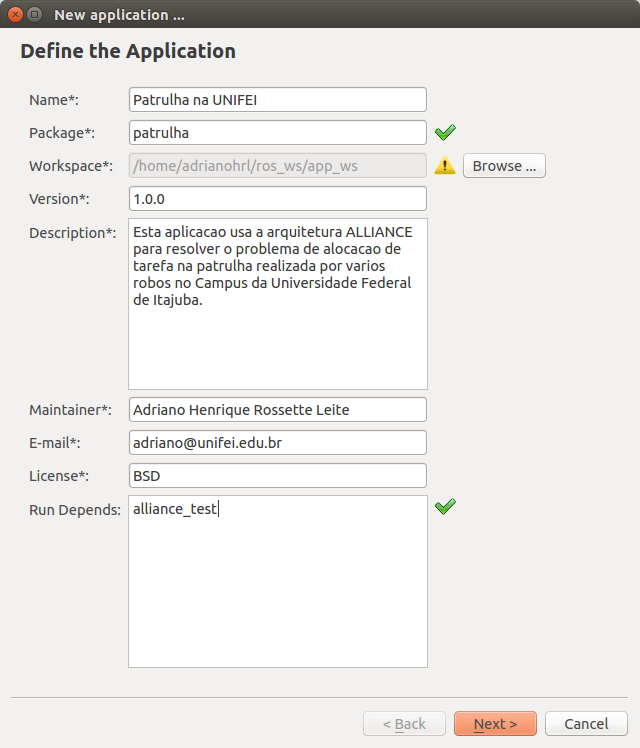
\includegraphics[width=.31\textwidth]{Figuras/4_resultados/patrulha_def_app.png}
                    \label{fig:patrulha_def_app}
                }
                \subfloat[Escolha da arquitetura.]{
                    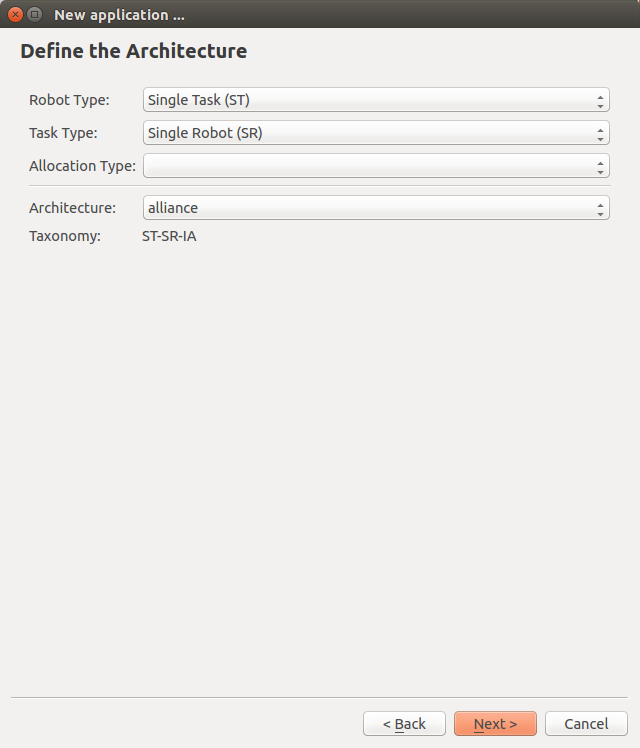
\includegraphics[width=.31\textwidth]{Figuras/4_resultados/patrulha_def_arch.png}
                    \label{fig:patrulha_def_arch}
                }
                \subfloat[Definição dos robôs do sistema.]{
                    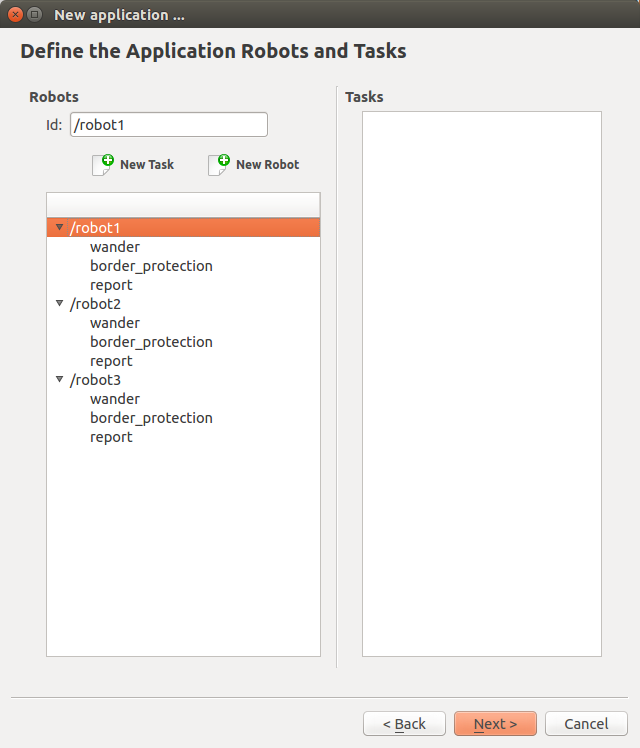
\includegraphics[width=.31\textwidth]{Figuras/4_resultados/patrulha_def_robots.png}
                    \label{fig:patrulha_def_robots}
                }
                
                \subfloat[Parametrização da arquitetura.]{
                    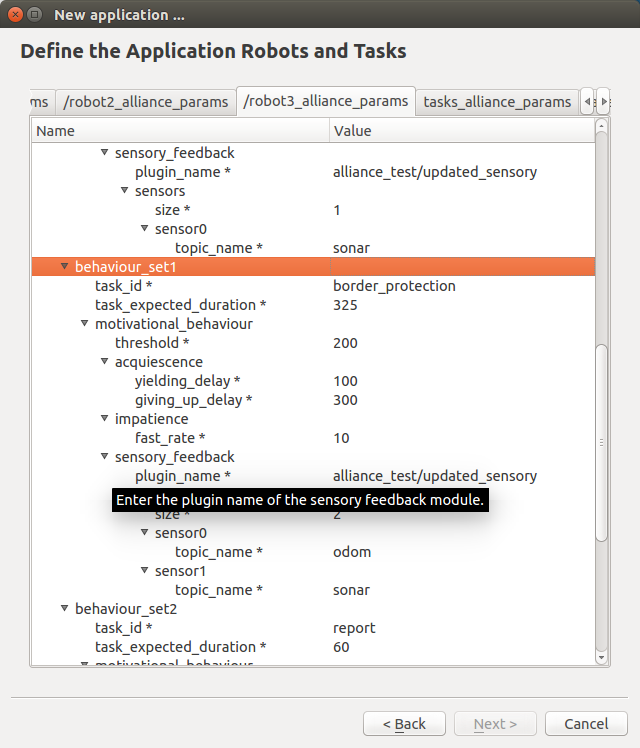
\includegraphics[width=.31\textwidth]{Figuras/4_resultados/patrulha_def_params.png}
                    \label{fig:patrulha_def_params}
                }
                \subfloat[Sumário.]{
                    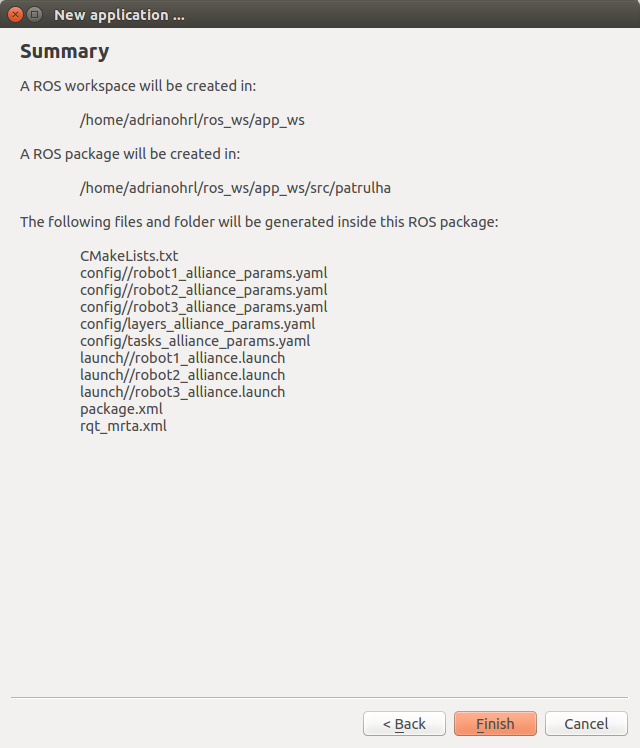
\includegraphics[width=.31\textwidth]{Figuras/4_resultados/patrulha_summary.png}
                    \label{fig:patrulha_summary}
                }
                \caption{\textit{Wizard} para a criação de uma aplicação \textit{patrulha}.} \label{fig:patrulha_new_app}
            \end{figure}
            
            \begin{figure}[htb]
                \centering
                \subfloat[Pacote.]{
                    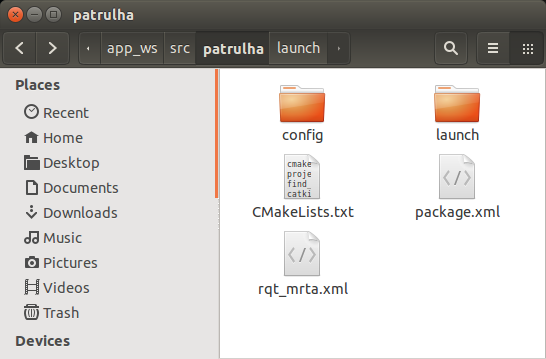
\includegraphics[width=.4\textwidth]{Figuras/4_resultados/patrulha_pkg.png}
                    \label{fig:patrulha_pkg}
                }
                \subfloat[Arquivos de parâmetro.]{
                    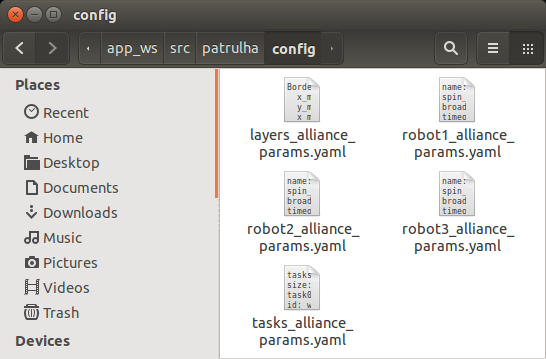
\includegraphics[width=.4\textwidth]{Figuras/4_resultados/patrulha_pkg_config.png}
                    \label{fig:patrulha_pkg_config}
                }
                
                \subfloat[Arquivos de inicialização.]{
                    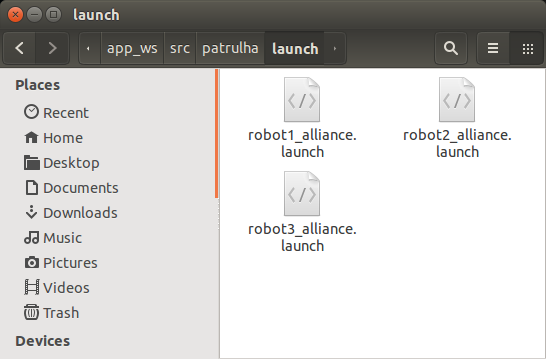
\includegraphics[width=.4\textwidth]{Figuras/4_resultados/patrulha_pkg_launch.png}
                    \label{fig:patrulha_pkg_launch}
                }
                \caption{Pastas e arquivos gerados após a criação de uma aplicação.} \label{fig:patrulha}
            \end{figure}
\chapter[Conclusão e Trabalhos Futuros]{Conclusão e Trabalhos Futuros} \label{cap:conclusao}

    \section{Conclusão}
    
    \section{Trabalhos Futuros}
        Uma melhoria significativa desta aplicação seria possibilitar a inscrição de novas arquiteturas devidamente configuradas no repositório deste projeto. De modo que, sempre que uma nova inscrição ocorresse no \textit{rqt\_mrta}, seria solicitada uma nova atualização a todos usuários do pacote \textit{rqt\_mrta} para baixar e instalar a nova arquitetura inscrita. Isso eliminaria a necessidade de procurar novas abordagens na comunidade ROS.
        
        Adição de mais recursos gráficos para a supervisão e monitoramento do sistema e da arquitetura em tempo de execução. Como alarmes identificando a falha na comunicação de algum robô, gráficos temporais de agenda ...

% Elementos pós-textuais
\postextual

\phantompart	% adiciona espaço no sumário
% Referências bibliográficas - obrigatório
\bibliography{6_Referencias/bibliografia.bib}

% Apêndices - opcional
\apendices
\partapendices 	% imprime uma página indicando o início dos apêndices
\chapter{Exemplo de um arquivo de configuração de arquitetura para o \textit{rqt\_mrta}} \label{app:arch_config}
    \lstset{
        language=XML,
        breaklines=true,
        morekeywords={
            xml, version, encoding,
            rqt_mrta, format,
                architecture,
                    name,
                    robots,
                        busy_robots,
                        idle_robots,
                        config_id,
                        launch_id,
                    tasks,
                        incoming_tasks,
                    allocations,
                        allocated_tasks,
                        type,
                        topic,
                            value,
                            field,
                            queue_size,
                            timeout,
                configs,
                    config_0,
                    config_1,
                    config_2,
                    config_3,
                    config_4,
                    config_5,
                        id,
                        param_0,
                        param_1,
                        param_2,
                        param_3,
                        param_4,
                        param_5,
                        param_6,
                        param_7,
                        param_8,
                        param_9,
                        param_10,
                        params_0,
                        params_1,
                        params_2,
                        params_3,
                        params_4,
                        params_5,
                        params_6,
                        params_7,
                        params_8,
                        params_9,
                        params_10,
                        array_0,
                        array_1,
                        array_2,
                        array_3,
                        array_4,
                        array_5,
                        array_6,
                        array_7,
                        array_8,
                        array_9,
                        array_10,
                            tool_tip,
                launches,
                    launch_0,
                    launch_1,
                    launch_2,
                    launch_3,
                    launch_4,
                    launch_5,
                    launch_6,
                    launch_7,
                    launch_8,
                    launch_9,
                    launch_10,
                    includes,
                        include_0,
                        include_1,
                        include_2,
                        include_3,
                        include_4,
                        include_5,
                        include_6,
                        include_7,
                        include_8,
                        include_9,
                        include_10,
                            file,
                            args,
                                arg_0,
                                arg_1,
                                arg_2,
                                arg_3,
                                arg_4,
                                arg_5,
                                arg_6,
                                arg_7,
                                arg_8,
                                arg_9,
                                arg_10,
                widgets,
                    widget_0,
                    widget_1,
                    widget_2,
                    widget_3,
                    widget_4,
                    widget_5,
                        plugin_name,
        }
    }
    \lstinputlisting{Outros/Arquivos/a_arch_config/rqt_mrta.xml}
\chapter{Exemplo de um arquivo de configuração de aplicação para o \textit{rqt\_mrta}} \label{app:app_config}
    \lstset{
        language=XML,
        breaklines=true,
        morekeywords={
            xml, encoding,
            rqt_mrta, format,
                application,
                    name,
                    url,
                    robots,
                        robot_0,
                        robot_1,
                        robot_2,
                        robot_3,
                        robot_4,
                        robot_5,
                        robot_6,
                        robot_7,
                        robot_8,
                        robot_9,
                        robot_10,
                            id,
                    tasks,
                        task_0,
                        task_1,
                        task_2,
                        task_3,
                        task_4,
                        task_5,
                        task_6,
                        task_7,
                        task_8,
                        task_9,
                        task_10,
                architecture,
                    robots,
                        busy_robots,
                        idle_robots,
                    tasks,
                        incoming_tasks,
                    allocations,
                        allocated_tasks,
                        type,
                        topic,
                            name,
                            value,
                            field,
                            queue_size,
                            timeout,
                            horizon,
                configs,
                    config_0,
                    config_1,
                    config_2,
                    config_3,
                    config_4,
                    config_5,
                        id,
                        param_0,
                        param_1,
                        param_2,
                        param_3,
                        param_4,
                        param_5,
                        param_6,
                        param_7,
                        param_8,
                        param_9,
                        param_10,
                        params_0,
                        params_1,
                        params_2,
                        params_3,
                        params_4,
                        params_5,
                        params_6,
                        params_7,
                        params_8,
                        params_9,
                        params_10,
                        array_0,
                        array_1,
                        array_2,
                        array_3,
                        array_4,
                        array_5,
                        array_6,
                        array_7,
                        array_8,
                        array_9,
                        array_10,
                            tool_tip,
                widgets,
                    widget_0,
                    widget_1,
                    widget_2,
                    widget_3,
                    widget_4,
                    widget_5,
                        plugin_name,
        }
    }
    \lstinputlisting{Outros/Arquivos/b_app_config/rqt_mrta.xml}
\chapter{Exemplo de manifesto de pacote para arquitetura} \label{app:arch_manifest}
    \lstset{
        language=XML,
        breaklines=true,
        morekeywords={
            xml, encoding,
            package, format,
            name,
            version,
            description,
            maintainer, email,
            author,
            license,
            url, type,
            buildtool_depend,
            build_depend,
            run_depend,
            export,
                metapackage,
                plugin,
                rqt_gui,
                alliance,
                rqt_mrta, application, architecture
        }
    }
    \lstinputlisting{Outros/Arquivos/c_arch_manifest/package.xml}
\chapter{Exemplo de manifesto de pacote para aplicação} \label{app:app_manifest}
    \lstset{
        language=XML,
        breaklines=true,
        morekeywords={
            xml, encoding,
            package, format,
            name,
            version,
            description,
            maintainer, email,
            author,
            license,
            url, type,
            buildtool_depend,
            build_depend,
            run_depend,
            export,
                metapackage,
                plugin,
                rqt_gui,
                alliance,
                rqt_mrta, application, architecture
        }
    }
    \lstinputlisting{Outros/Arquivos/d_app_manifest/package.xml}
\chapter{ALLIANCE} \label{app:alliance}
    Esta é uma arquitetura totalmente distribuída, tolerante a falhas, que visa atingir controle cooperativo e atender os requisitos de uma missão à ser desempenhada por um grupo de robôs heterogêneos \cite{ref:parker1998alliance}. Cada robô é modelado usando uma aproximação baseada em comportamentos. A partir do estado do ambiente e dos outros robôs cooperadores, uma configuração de comportamento é selecionada conforme sua respectiva função de realização de tarefa na camada de alto nível de abstração. Cada configuração de comportamento permite controlar os atuadores do robô em questão de um modo diferente.
    
    Sejam $R=\{r_1, r_2, \cdots, r_n\}$, o conjunto de $n$ robôs heterogêneos, e $A=\{a_1,a_2, \cdots,\allowbreak a_m\}$, o conjunto de $m$ sub-tarefas independentes que compõem uma dada missão. Na arquitetura ALLIANCE, cada robô $r_i$ possui um conjunto de $p$ configurações de comportamento, dado por $C_i=\{c_{i1}, c_{i2},\cdots, c_{ip}\}$. Cada configuração de comportamento fornece ao seu robô uma função de realização de tarefa em alto nível, conforme definido em \cite{ref:brooks1986robust}. Por fim, é possível saber qual tarefa em $A$ é executada por $r_i$ quando sua configuração de ativação $c_{ik}$ é ativa. Tal informação é obtida através da função $h_i(c_{ik})$, a qual pertence ao conjunto de $n$ funções $H : C_i \to A$, $H = \{h_1(c_{1k}),\allowbreak h_2(c_{2k}), \cdots, h_n(c_{nk})\}$.
    
    A ativação de uma dada configuração de comportamento $c_{ij}$ do robô $r_i$ para a execução da tarefa $h_i(c_{ij})$ em um dado instante, é dada pelo cálculo de motivação do seu comportamento motivacional. Por sua vez, cada comportamento motivacional possui um conjunto de módulos que tem a responsabilidade de monitorar alguma informação relevante sobre o sistema. Será detalhado a seguir o papel de cada um desses módulos e suas contribuições para o cálculo de motivação.
    
    A primeira função, definida pela Equação \ref{eq:alliance_aplicavel}, tem como responsabilidade identificar quando a configuração de comportamento $c_{ij}$ é aplicável. Esta função lógica é implementada no módulo de \textit{feedback} sensorial, o qual observa constantemente as condições do ambiente por meio de sensores e, então, verifica se o sistema é favorecido se $c_{ij}$ estiver ativada.
    
    \begin{equation} \label{eq:alliance_aplicavel}
        aplic\acute{a}vel_{ij}(t) =
        \begin{cases}
            1, & \parbox[t]{.5\textwidth}{se o módulo de \textit{feedback} sensorial da configuração de comportamento $c_{ij}$ do robô $r_i$ indicar que esta configuração é aplicável mediante ao estado atual do ambiente no instante $t$;} \\
            0, & \text{caso contrário.}
        \end{cases}
    \end{equation}
    
    A Equação \ref{eq:alliance_inibida} mostra uma das funções lógicas que também compõe o cálculo para ativação de $c_{ij}$. Seu papel, neste cálculo, é garantir que o robô $r_i$ só tenha uma configuração de comportamento ativa por vez. Essa função é implementada pelo módulo de supressão, o qual observa a ativação das demais configurações de comportamento de $r_i$. 
    
    \begin{equation} \label{eq:alliance_inibida}
        inibida_{ij}(t) =
        \begin{cases}
            1, & \parbox[t]{.5\textwidth}{se outra configuração de comportamento $c_{ik}$ (com $k \neq j$) está ativa no robô $r_i$ no instante $t$;} \\
            0, & \text{caso contrário.}
        \end{cases}
    \end{equation}
    
    Cada configuração de comportamento $c_{ij}$ possui um módulo de comunicação que auxilia vários outros módulos de $c_{ij}$ por meio do monitoramento da comunicação entre os robôs do sistema. Este módulo mantém o histórico das atividades dos demais robôs do sistema no que diz respeito à execução da tarefa $h_i(c_{ij})$. Deste modo, os demais módulos de $c_{ij}$ podem consultar se os outros robôs estavam executando a tarefa $h_i(c_{ij})$ em um dado intervalo de tempo $[t_1; t_2]$, conforme mostra a Equação \ref{eq:alliance_recebida}. Existem dois parâmetros no ALLIANCE que influenciam diretamente no módulo de comunicação de cada comportamento motivacional. O primeiro parâmetro, $\rho_i$, define a frequência com que $r_i$ atualiza suas configurações de comportamento e publica seu estado atual, no que diz respeito à arquitetura. O segundo parâmetro, $\tau_i$, indica a duração de tempo máxima que o robô $r_i$ permite ficar sem receber mensagens do estado de qualquer outro robô do sistema. Quando esta duração é excedida para um dado robô $r_k$, o robô $r_i$ passa considerar que $r_k$ cessou sua atividade. A utilização deste parâmetro visa prever falhas de comunicação e de mal funcionamento.
    
    \begin{equation} \label{eq:alliance_recebida}
        recebida_{ij}(k, t_1, t_2) =
        \begin{cases}
            1, & \parbox[t]{.5\textwidth}{se o robô $r_i$ recebeu mensagem do robô $r_k$ referente à tarefa $h_i(c_{ij})$ dentro do intervalo de tempo $[t_1; t_2]$, em que $t_1 < t_2$;} \\
            0, & \text{caso contrário.}
        \end{cases}
    \end{equation}
    
    A próxima função tem a incumbência de reiniciar o cálculo para a ativação da configuração de comportamento $c_{ij}$. Essa função lógica é impulsionada apenas uma vez para cada robô que tenta executar a tarefa $h_i(c_{ij})$. Isto é, no instante em que acontece a primeira rampa de subida na Equação \ref{eq:alliance_recebida} para cada robô $r_k$, está função retorna um nível lógico alto. Essa condição evita que problemas de falhas persistentes não comprometam a completude da missão.
    %
    \begin{equation} \label{eq:alliance_reiniciada}
        reiniciada_{ij}(t) = \exists x, (recebida_{ij}(x, t - dt, t) \land \lnot recebida_{ij}(x, 0, t - dt))
    \end{equation}
    %
    onde $dt$ é o tempo decorrido desde a última verificação de comunicação.
    
    A Equação \ref{eq:alliance_ativa_intervalo} auxilia o módulo de aquiescência no cálculo de desistência para a desativação de $c_{ij}$. Baseando-se no histórico de ativação de $c_{ij}$, o módulo de comportamento motivacional disponibiliza essa função lógica que verifica se $c_{ij}$ ficou mantida ativa por um dado período de tempo até o instante desejado.
    
    \begin{equation} \label{eq:alliance_ativa_intervalo}
        ativa_{ij}(\Delta t, t) =
        \begin{cases}
            1, & \parbox[t]{.5\textwidth}{se a configuração de comportamento $c_{ij}$ do robô $r_i$ estiver ativa por mais de $\Delta t$ unidades de tempo no instante $t$;} \\
            0, & \text{caso contrário.}
        \end{cases}
    \end{equation}
    
    O módulo de aquiescência monitora o tempo decorrido após a ativação da configuração de comportamento $c_{ij}$ do robô $r_i$ com o auxílio da Equação \ref{eq:alliance_ativa_intervalo}. São duas as suas preocupações: (1) verificar se $c_{ij}$ permaneceu ativa por mais tempo que o esperado e (2) verificar se o tempo decorrido após um outro robô $r_k$ ter iniciado a execução da tarefa $h_i(c_{ij})$, enquanto $c_{ij}$ estava ativa, tenha excedido o tempo configurado para $r_i$ passar sua vez para esse outro robô. A Equação \ref{eq:alliance_aquiescente} define as condições em que $r_i$ está aquiescente à desativação de $c_{ij}$.
    %
    \begin{equation} \label{eq:alliance_aquiescente}
        \begin{aligned}
            aquiescente_{ij}(t) = \
            & (ativa_{ij}(\psi_{ij}(t), t) \land \exists x, recebida_{ij}(x, t - \tau_i, t)) \\
            & \lor ativa_{ij}(\lambda_{ij}(t), t)
        \end{aligned}
    \end{equation}
    %
    onde $\psi_{ij}(t)$ é a duração de tempo que $r_i$ deseja manter a configuração de comportamento $c_{ij}$ ativa antes de dar preferência para outro robô executar a tarefa $h_i(c_{ij})$; e $\lambda_{ij}(t)$ é a duração de tempo que $r_i$ deseja manter $c_{ij}$ ativa antes de desistir para possivelmente tentar outra configuração de comportamento.
    
    A impaciência de $r_i$ para a ativação de $c_{ij}$ cresce linearmente mediante a taxa de impaciência instantânea. Assim, o módulo de impaciência de $c_{ij}$ é responsável por identificar falhas de execução da tarefa $h_i(c_{ij})$ por outros robôs do sistema e quantificar a insatisfação de $r_i$ concernente à essa tarefa, conforme visto na Equação \ref{eq:alliance_impaciencia}. Para isso, três parâmetros são utilizados: (1) $\phi_{ij}(k, t)$, o qual estabelece o tempo máximo que $r_i$ permite a um outro robô $r_k$ executar a tarefa $h_i(c_{ij})$ antes dele próprio iniciar sua tentativa; (2) $\delta_{slow_{ij}}(k, t)$, que determina a taxa de impaciência do robô $r_i$ com respeito à configuração de comportamento $c_{ij}$ enquanto o robô $r_k$ está executando a tarefa correspondente à $c_{ij}$; e (3) $\delta_{fast_{ij}}(t)$, que determina a taxa de impaciência de $r_i$ com relação à $c_{ij}$ quando nenhum outro robô está executando a tarefa $h_i(c_{ij})$.
    %
    \begin{equation} \label{eq:alliance_impaciencia}
        impaci\hat{e}ncia_{ij}(t) =
        \begin{cases}
            \min\limits_{x}\delta_{slow_{ij}}(x, t), & \parbox[t]{.5\textwidth}{se $recebida_{ij}(x, t - \tau_i, t) \land \lnot recebida_{ij}(x, 0, t - \phi_{ij}(x, t)$;} \\
            \delta_{fast_{ij}}(t), & \text{caso contrário.}
        \end{cases}
    \end{equation}
    %
    Note que o método usado incrementa a motivação à uma taxa que permita que o robô mais lento $r_k$ continue sua tentativa de execução de $h(c_{ij})$, desde que seja respeitada a duração máxima estipulada pelo parâmetro $\phi_{ij}(k, t)$.
    
    A Equação \ref{eq:alliance_motivacao} mostra a função de motivação, a qual combina todas as funções mencionadas anteriormente para a ativação da configuração de comportamento $c_{ij}$. Seu valor inicial é nulo e aumenta mediante a taxa de impaciência instantânea de $r_i$ para ativar $c_{ij}$ quando satisfeitas as seguintes condições: (1) $c_{ij}$ seja aplicável, (2) mas não tenha sido inibida, (3) nem reiniciada; (4) e, ainda, $r_i$ não seja aquiescente em desistir de manter $c_{ij}$ ativa. Quando uma das condições citadas não é satisfeita, seu valor volta a ser nulo. 
    
    \begin{equation} \label{eq:alliance_motivacao}
        \begin{aligned}
            motiva\textit{ç}\tilde{a}o_{ij}(0) = \ & 0 \\
            motiva\textit{ç}\tilde{a}o_{ij}(t) = \ & (motiva\textit{ç}\tilde{a}o_{ij}(t - dt) + impaci\hat{e}ncia_{ij}(t)) \\
            & \times aplic\acute{a}vel_{ij}(t) \times inibida_{ij}(t) \\
            & \times reiniciada_{ij}(t) \times aquiescente_{ij}(t).
        \end{aligned}
    \end{equation}
    
    Assim que a motivação de $r_i$ para ativar $c_{ij}$ ultrapassa o limite de ativação, essa configuração de comportamento é ativada, conforme a Equação \ref{eq:alliance_ativa}:
    %
    \begin{equation} \label{eq:alliance_ativa}
        ativa_{ij}(t) = motiva\textit{ç}\tilde{a}o_{ij}(t) \geq \theta
    \end{equation}
    %
    onde $\theta$ é o limite de ativação.
    
    Fazendo uma análise das equações acima, verifica-se que, enquanto sua motivação cresce, é possível estimar quanto tempo resta para que a configuração de comportamento $c_{ij}$ se torne ativa. 
    %
    \begin{equation} \label{eq:alliance_estimativa_ativacao}
        \overline{\Delta t}_{ativa\textit{ç}\tilde{a}o_{ij}} = \frac{\theta - motiva\textit{ç}\tilde{a}o_{ij}(t)}{impaci\hat{e}ncia_{ij}(t) \rho_i}
    \end{equation}
    %
    onde $\rho_i$ é a frequência aproximada, em [\si{\hertz}], com que $r_i$ atualiza as motivação das configurações de comportamento em $C_i$ e, ainda, publica seu estado comportamental. Como a taxa de impaciência não é constante, a Equação \ref{eq:alliance_estimativa_ativacao} é apenas uma estimativa, dada em [\si{\second}].
    
    Em conformidade com o que foi exposto, pode-se observar que é possível normalizar todas as funções de motivação, de modo que a imagem de cada uma delas pertença ao intervalo $[0; 1] \subset \mathbb{R}_+$. Para isso, é necessário: (1) parametrizar o módulo de impaciência de cada configuração de comportamento $c_{ij}$, de maneira que a imagem da sua função de taxa de impaciência instantânea pertença ao intervalo $(0; 1) \subset \mathbb{R}_+^*$; além disso, (2) atribuir o valor unitário ao limite de ativação; bem como, (3) saturar a função de motivação no limite de ativação. Como resultado, as Equações \ref{eq:alliance_ativa} e \ref{eq:alliance_estimativa_ativacao} podem ser rescritas como as Equações \ref{eq:alliance_ativa_nova} e \ref{eq:alliance_estimativa_ativacao_nova}, respectivamente.
    
    \begin{equation} \label{eq:alliance_ativa_nova}
        ativa_{ij}(t) = motiva\textit{ç}\tilde{a}o_{ij}(t) == 1
    \end{equation}
    
    \begin{equation} \label{eq:alliance_estimativa_ativacao_nova}
        \overline{\Delta t}_{ativa\textit{ç}\tilde{a}o_{ij}} = \frac{1 - motiva\textit{ç}\tilde{a}o_{ij}(t)}{impaci\hat{e}ncia_{ij}(t) \rho_i}
    \end{equation}
    
    \citeonline{ref:parker1996lalliance} desenvolveu também uma variação do ALLIANCE, chamada L-ALLIANCE, capaz de estimar alguns parâmetros do ALLIANCE durante a fase de aprendizado.
% Anexos - opcional
% \anexos
% \partanexos		% imprime uma página indicando o início dos anexos
% \chapter{Artigo publicado}

\lipsum[30]

% Índice remissivo - opcional
\printindex	% imprime as páginas nas quais as macros \index{palavra a ser indexada} apareceram.

% Fim do documento
\end{document}